\documentclass[twoside]{book}

% Packages required by doxygen
\usepackage{fixltx2e}
\usepackage{calc}
\usepackage{doxygen}
\usepackage[export]{adjustbox} % also loads graphicx
\usepackage{graphicx}
\usepackage[utf8]{inputenc}
\usepackage{makeidx}
\usepackage{multicol}
\usepackage{multirow}
\PassOptionsToPackage{warn}{textcomp}
\usepackage{textcomp}
\usepackage[nointegrals]{wasysym}
\usepackage[table]{xcolor}

% Font selection
\usepackage[T1]{fontenc}
\usepackage[scaled=.90]{helvet}
\usepackage{courier}
\usepackage{amssymb}
\usepackage{sectsty}
\renewcommand{\familydefault}{\sfdefault}
\allsectionsfont{%
  \fontseries{bc}\selectfont%
  \color{darkgray}%
}
\renewcommand{\DoxyLabelFont}{%
  \fontseries{bc}\selectfont%
  \color{darkgray}%
}
\newcommand{\+}{\discretionary{\mbox{\scriptsize$\hookleftarrow$}}{}{}}

% Page & text layout
\usepackage{geometry}
\geometry{%
  a4paper,%
  top=2.5cm,%
  bottom=2.5cm,%
  left=2.5cm,%
  right=2.5cm%
}
\tolerance=750
\hfuzz=15pt
\hbadness=750
\setlength{\emergencystretch}{15pt}
\setlength{\parindent}{0cm}
\setlength{\parskip}{3ex plus 2ex minus 2ex}
\makeatletter
\renewcommand{\paragraph}{%
  \@startsection{paragraph}{4}{0ex}{-1.0ex}{1.0ex}{%
    \normalfont\normalsize\bfseries\SS@parafont%
  }%
}
\renewcommand{\subparagraph}{%
  \@startsection{subparagraph}{5}{0ex}{-1.0ex}{1.0ex}{%
    \normalfont\normalsize\bfseries\SS@subparafont%
  }%
}
\makeatother

% Headers & footers
\usepackage{fancyhdr}
\pagestyle{fancyplain}
\fancyhead[LE]{\fancyplain{}{\bfseries\thepage}}
\fancyhead[CE]{\fancyplain{}{}}
\fancyhead[RE]{\fancyplain{}{\bfseries\leftmark}}
\fancyhead[LO]{\fancyplain{}{\bfseries\rightmark}}
\fancyhead[CO]{\fancyplain{}{}}
\fancyhead[RO]{\fancyplain{}{\bfseries\thepage}}
\fancyfoot[LE]{\fancyplain{}{}}
\fancyfoot[CE]{\fancyplain{}{}}
\fancyfoot[RE]{\fancyplain{}{\bfseries\scriptsize Generated by Doxygen }}
\fancyfoot[LO]{\fancyplain{}{\bfseries\scriptsize Generated by Doxygen }}
\fancyfoot[CO]{\fancyplain{}{}}
\fancyfoot[RO]{\fancyplain{}{}}
\renewcommand{\footrulewidth}{0.4pt}
\renewcommand{\chaptermark}[1]{%
  \markboth{#1}{}%
}
\renewcommand{\sectionmark}[1]{%
  \markright{\thesection\ #1}%
}

% Indices & bibliography
\usepackage{natbib}
\usepackage[titles]{tocloft}
\setcounter{tocdepth}{3}
\setcounter{secnumdepth}{5}
\makeindex

% Hyperlinks (required, but should be loaded last)
\usepackage{ifpdf}
\ifpdf
  \usepackage[pdftex,pagebackref=true]{hyperref}
\else
  \usepackage[ps2pdf,pagebackref=true]{hyperref}
\fi
\hypersetup{%
  colorlinks=true,%
  linkcolor=blue,%
  citecolor=blue,%
  unicode%
}

% Custom commands
\newcommand{\clearemptydoublepage}{%
  \newpage{\pagestyle{empty}\cleardoublepage}%
}

\usepackage{caption}
\captionsetup{labelsep=space,justification=centering,font={bf},singlelinecheck=off,skip=4pt,position=top}

%===== C O N T E N T S =====

\begin{document}

% Titlepage & ToC
\hypersetup{pageanchor=false,
             bookmarksnumbered=true,
             pdfencoding=unicode
            }
\pagenumbering{alph}
\begin{titlepage}
\vspace*{7cm}
\begin{center}%
{\Large “\+H\+T\+M\+\_\+16\+\_\+2” \\[1ex]\large 1 }\\
\vspace*{1cm}
{\large Generated by Doxygen 1.8.13}\\
\end{center}
\end{titlepage}
\clearemptydoublepage
\pagenumbering{roman}
\tableofcontents
\clearemptydoublepage
\pagenumbering{arabic}
\hypersetup{pageanchor=true}

%--- Begin generated contents ---
\chapter{Todo List}
\label{todo}
\Hypertarget{todo}

\begin{DoxyRefList}
\item[\label{todo__todo000001}%
\Hypertarget{todo__todo000001}%
File \hyperlink{_context_tables_8h}{Context\+Tables.h} ]number of context models is not matched to actual use, should be fixed  
\item[\label{todo__todo000002}%
\Hypertarget{todo__todo000002}%
File \hyperlink{_t_com_data_c_u_8cpp}{T\+Com\+Data\+CU.cpp} ]not all entities are documented  
\item[\label{todo__todo000003}%
\Hypertarget{todo__todo000003}%
File \hyperlink{_t_com_data_c_u_8h}{T\+Com\+Data\+CU.h} ]not all entities are documented  
\item[\label{todo__todo000004}%
\Hypertarget{todo__todo000004}%
File \hyperlink{_t_com_motion_info_8h}{T\+Com\+Motion\+Info.h} ]\hyperlink{class_t_com_mv_field}{T\+Com\+Mv\+Field} seems to be better to be inherited from \hyperlink{class_t_com_mv}{T\+Com\+Mv}  
\item[\label{todo__todo000005}%
\Hypertarget{todo__todo000005}%
File \hyperlink{_t_com_yuv_8cpp}{T\+Com\+Yuv.cpp} ]this should be merged with \hyperlink{class_t_com_pic_yuv}{T\+Com\+Pic\+Yuv}  
\item[\label{todo__todo000006}%
\Hypertarget{todo__todo000006}%
File \hyperlink{_t_com_yuv_8h}{T\+Com\+Yuv.h} ]this should be merged with \hyperlink{class_t_com_pic_yuv}{T\+Com\+Pic\+Yuv} ~\newline
 check usage of remove\+High\+Freq function  
\item[\label{todo__todo000007}%
\Hypertarget{todo__todo000007}%
Member \hyperlink{class_t_enc_top_a86ea6d845658a966b318b15366d189a0}{T\+Enc\+Top\+:\+:x\+Init\+Hrd\+Parameters} ()]check for possible P\+TL violations 
\end{DoxyRefList}
\chapter{Namespace Index}
\section{Namespace List}
Here is a list of all documented namespaces with brief descriptions\+:\begin{DoxyCompactList}
\item\contentsline{section}{\hyperlink{namespace_t_com_rd_cost_weight_prediction}{T\+Com\+Rd\+Cost\+Weight\+Prediction} \\*RD cost computation namespace, with Weighted Prediction }{\pageref{namespace_t_com_rd_cost_weight_prediction}}{}
\end{DoxyCompactList}

\chapter{Hierarchical Index}
\section{Class Hierarchy}
This inheritance list is sorted roughly, but not completely, alphabetically\+:\begin{DoxyCompactList}
\item \contentsline{section}{\+\_\+\+A\+M\+V\+P\+Info}{\pageref{struct___a_m_v_p_info}}{}
\item \contentsline{section}{\+\_\+context\+\_\+md5\+\_\+t}{\pageref{struct__context__md5__t}}{}
\item \contentsline{section}{\+\_\+\+D\+B\+B\+P\+Tmp\+Data}{\pageref{struct___d_b_b_p_tmp_data}}{}
\item \contentsline{section}{\+\_\+\+Dis\+Cand}{\pageref{struct___dis_cand}}{}
\item \contentsline{section}{\+\_\+\+I\+D\+V\+Cand}{\pageref{struct___i_d_v_cand}}{}
\item \contentsline{section}{\+\_\+\+L\+F\+C\+U\+Param}{\pageref{struct___l_f_c_u_param}}{}
\item \contentsline{section}{Annex\+B\+Stats}{\pageref{struct_annex_b_stats}}{}
\item \contentsline{section}{Bit\+Depths}{\pageref{struct_bit_depths}}{}
\item \contentsline{section}{Chroma\+Qp\+Adj}{\pageref{struct_chroma_qp_adj}}{}
\item \contentsline{section}{coeff\+Group\+R\+D\+Stats}{\pageref{structcoeff_group_r_d_stats}}{}
\item \contentsline{section}{Context\+Model}{\pageref{class_context_model}}{}
\item \contentsline{section}{Context\+Model3\+D\+Buffer}{\pageref{class_context_model3_d_buffer}}{}
\item \contentsline{section}{S\+E\+I\+Colour\+Remapping\+Info\+:\+:C\+R\+Ilut}{\pageref{struct_s_e_i_colour_remapping_info_1_1_c_r_ilut}}{}
\item \contentsline{section}{Dist\+Param}{\pageref{class_dist_param}}{}
\item \contentsline{section}{Efficient\+Field\+I\+R\+A\+P\+Mapping}{\pageref{class_efficient_field_i_r_a_p_mapping}}{}
\item \contentsline{section}{Env\+Var}{\pageref{class_env_var}}{}
\item \contentsline{section}{df\+:\+:program\+\_\+options\+\_\+lite\+:\+:Error\+Reporter}{\pageref{structdf_1_1program__options__lite_1_1_error_reporter}}{}
\item \contentsline{section}{est\+Bits\+Sbac\+Struct}{\pageref{structest_bits_sbac_struct}}{}
\item exception\begin{DoxyCompactList}
\item \contentsline{section}{df\+:\+:program\+\_\+options\+\_\+lite\+:\+:Parse\+Failure}{\pageref{structdf_1_1program__options__lite_1_1_parse_failure}}{}
\end{DoxyCompactList}
\item \contentsline{section}{G\+O\+P\+Entry}{\pageref{struct_g_o_p_entry}}{}
\item \contentsline{section}{Hrd\+Sub\+Layer\+Info}{\pageref{struct_hrd_sub_layer_info}}{}
\item \contentsline{section}{Input\+Byte\+Stream}{\pageref{class_input_byte_stream}}{}
\item \contentsline{section}{T\+Enc\+Search\+:\+:Int\+T\+Z\+Search\+Struct}{\pageref{struct_t_enc_search_1_1_int_t_z_search_struct}}{}
\item list\begin{DoxyCompactList}
\item \contentsline{section}{Access\+Unit}{\pageref{class_access_unit}}{}
\item \contentsline{section}{T\+Com\+List$<$ C $>$}{\pageref{class_t_com_list}}{}
\item \contentsline{section}{T\+Com\+List$<$ T\+Com\+Au $\ast$ $>$}{\pageref{class_t_com_list}}{}
\item \contentsline{section}{T\+Com\+List$<$ T\+Com\+Pic $\ast$$>$}{\pageref{class_t_com_list}}{}
\begin{DoxyCompactList}
\item \contentsline{section}{T\+Com\+Au}{\pageref{class_t_com_au}}{}
\item \contentsline{section}{T\+Com\+Sub\+Dpb}{\pageref{class_t_com_sub_dpb}}{}
\end{DoxyCompactList}
\item \contentsline{section}{T\+Com\+List$<$ T\+Com\+Pic\+Yuv $\ast$$>$}{\pageref{class_t_com_list}}{}
\item \contentsline{section}{T\+Com\+List$<$ T\+Com\+Sub\+Dpb $\ast$$>$}{\pageref{class_t_com_list}}{}
\end{DoxyCompactList}
\item \contentsline{section}{Parameter\+Set\+Map$<$ T $>$\+:\+:Map\+Data$<$ Tm $>$}{\pageref{struct_parameter_set_map_1_1_map_data}}{}
\item \contentsline{section}{M\+D5}{\pageref{class_m_d5}}{}
\item \contentsline{section}{Meta\+Log\+Entry$<$ T\+Lambda\+Modifier $>$}{\pageref{struct_meta_log_entry}}{}
\item \contentsline{section}{N\+A\+L\+Unit}{\pageref{struct_n_a_l_unit}}{}
\begin{DoxyCompactList}
\item \contentsline{section}{Input\+N\+A\+L\+Unit}{\pageref{class_input_n_a_l_unit}}{}
\item \contentsline{section}{N\+A\+L\+Unit\+E\+B\+SP}{\pageref{struct_n_a_l_unit_e_b_s_p}}{}
\item \contentsline{section}{Output\+N\+A\+L\+Unit}{\pageref{struct_output_n_a_l_unit}}{}
\end{DoxyCompactList}
\item \contentsline{section}{df\+:\+:program\+\_\+options\+\_\+lite\+:\+:Options\+:\+:Names}{\pageref{structdf_1_1program__options__lite_1_1_options_1_1_names}}{}
\item \contentsline{section}{df\+:\+:program\+\_\+options\+\_\+lite\+:\+:Option\+Base}{\pageref{structdf_1_1program__options__lite_1_1_option_base}}{}
\begin{DoxyCompactList}
\item \contentsline{section}{df\+:\+:program\+\_\+options\+\_\+lite\+:\+:Option$<$ T $>$}{\pageref{structdf_1_1program__options__lite_1_1_option}}{}
\item \contentsline{section}{df\+:\+:program\+\_\+options\+\_\+lite\+:\+:Option\+Func}{\pageref{structdf_1_1program__options__lite_1_1_option_func}}{}
\end{DoxyCompactList}
\item \contentsline{section}{df\+:\+:program\+\_\+options\+\_\+lite\+:\+:Options}{\pageref{structdf_1_1program__options__lite_1_1_options}}{}
\item \contentsline{section}{df\+:\+:program\+\_\+options\+\_\+lite\+:\+:Option\+Specific}{\pageref{classdf_1_1program__options__lite_1_1_option_specific}}{}
\item \contentsline{section}{df\+:\+:program\+\_\+options\+\_\+lite\+:\+:Option\+Writer}{\pageref{structdf_1_1program__options__lite_1_1_option_writer}}{}
\begin{DoxyCompactList}
\item \contentsline{section}{df\+:\+:program\+\_\+options\+\_\+lite\+:\+:Argv\+Parser}{\pageref{structdf_1_1program__options__lite_1_1_argv_parser}}{}
\item \contentsline{section}{df\+:\+:program\+\_\+options\+\_\+lite\+:\+:Cfg\+Stream\+Parser}{\pageref{structdf_1_1program__options__lite_1_1_cfg_stream_parser}}{}
\end{DoxyCompactList}
\item \contentsline{section}{Parameter\+Set\+Manager}{\pageref{class_parameter_set_manager}}{}
\item \contentsline{section}{Parameter\+Set\+Map$<$ T $>$}{\pageref{class_parameter_set_map}}{}
\item \contentsline{section}{Parameter\+Set\+Map$<$ T\+Com\+P\+PS $>$}{\pageref{class_parameter_set_map}}{}
\item \contentsline{section}{Parameter\+Set\+Map$<$ T\+Com\+S\+PS $>$}{\pageref{class_parameter_set_map}}{}
\item \contentsline{section}{Parameter\+Set\+Map$<$ T\+Com\+V\+PS $>$}{\pageref{class_parameter_set_map}}{}
\item \contentsline{section}{Point}{\pageref{struct_point}}{}
\item \contentsline{section}{Profile\+Tier\+Level}{\pageref{class_profile_tier_level}}{}
\item \contentsline{section}{Qp\+Param}{\pageref{struct_qp_param}}{}
\item runtime\+\_\+error\begin{DoxyCompactList}
\item \contentsline{section}{Runtime\+Error}{\pageref{class_runtime_error}}{}
\begin{DoxyCompactList}
\item \contentsline{section}{Initial\+Adjustment\+Parameter\+Parse\+Exception}{\pageref{class_initial_adjustment_parameter_parse_exception}}{}
\item \contentsline{section}{Meta\+Log\+Parse\+Exception}{\pageref{class_meta_log_parse_exception}}{}
\item \contentsline{section}{Mismatched\+Indexes\+Exception}{\pageref{class_mismatched_indexes_exception}}{}
\item \contentsline{section}{Non\+Contiguous\+Q\+P\+Set\+Exception}{\pageref{class_non_contiguous_q_p_set_exception}}{}
\item \contentsline{section}{P\+O\+C\+Parse\+Exception}{\pageref{class_p_o_c_parse_exception}}{}
\item \contentsline{section}{Targets\+Parse\+Exception}{\pageref{class_targets_parse_exception}}{}
\item \contentsline{section}{Wrong\+Number\+Of\+Arguments\+Exception}{\pageref{class_wrong_number_of_arguments_exception}}{}
\end{DoxyCompactList}
\end{DoxyCompactList}
\item \contentsline{section}{S\+A\+O\+Blk\+Param}{\pageref{struct_s_a_o_blk_param}}{}
\item \contentsline{section}{S\+A\+O\+Offset}{\pageref{struct_s_a_o_offset}}{}
\item \contentsline{section}{S\+A\+O\+Stat\+Data}{\pageref{struct_s_a_o_stat_data}}{}
\item \contentsline{section}{Scan\+Generator}{\pageref{class_scan_generator}}{}
\item \contentsline{section}{S\+EI}{\pageref{class_s_e_i}}{}
\begin{DoxyCompactList}
\item \contentsline{section}{S\+E\+I\+Active\+Parameter\+Sets}{\pageref{class_s_e_i_active_parameter_sets}}{}
\item \contentsline{section}{S\+E\+I\+Alpha\+Channel\+Info}{\pageref{class_s_e_i_alpha_channel_info}}{}
\item \contentsline{section}{S\+E\+I\+Alternative\+Depth\+Info}{\pageref{class_s_e_i_alternative_depth_info}}{}
\item \contentsline{section}{S\+E\+I\+Alternative\+Transfer\+Characteristics}{\pageref{class_s_e_i_alternative_transfer_characteristics}}{}
\item \contentsline{section}{S\+E\+I\+Buffering\+Period}{\pageref{class_s_e_i_buffering_period}}{}
\item \contentsline{section}{S\+E\+I\+Chroma\+Resampling\+Filter\+Hint}{\pageref{class_s_e_i_chroma_resampling_filter_hint}}{}
\item \contentsline{section}{S\+E\+I\+Colour\+Remapping\+Info}{\pageref{class_s_e_i_colour_remapping_info}}{}
\item \contentsline{section}{S\+E\+I\+Decoded\+Picture\+Hash}{\pageref{class_s_e_i_decoded_picture_hash}}{}
\item \contentsline{section}{S\+E\+I\+Decoding\+Unit\+Info}{\pageref{class_s_e_i_decoding_unit_info}}{}
\item \contentsline{section}{S\+E\+I\+Depth\+Representation\+Info}{\pageref{class_s_e_i_depth_representation_info}}{}
\item \contentsline{section}{S\+E\+I\+Display\+Orientation}{\pageref{class_s_e_i_display_orientation}}{}
\item \contentsline{section}{S\+E\+I\+Frame\+Packing}{\pageref{class_s_e_i_frame_packing}}{}
\item \contentsline{section}{S\+E\+I\+Gradual\+Decoding\+Refresh\+Info}{\pageref{class_s_e_i_gradual_decoding_refresh_info}}{}
\item \contentsline{section}{S\+E\+I\+Inter\+Layer\+Constrained\+Tile\+Sets}{\pageref{class_s_e_i_inter_layer_constrained_tile_sets}}{}
\item \contentsline{section}{S\+E\+I\+Knee\+Function\+Info}{\pageref{class_s_e_i_knee_function_info}}{}
\item \contentsline{section}{S\+E\+I\+Layers\+Not\+Present}{\pageref{class_s_e_i_layers_not_present}}{}
\item \contentsline{section}{S\+E\+I\+Mastering\+Display\+Colour\+Volume}{\pageref{class_s_e_i_mastering_display_colour_volume}}{}
\item \contentsline{section}{S\+E\+I\+Multiview\+Acquisition\+Info}{\pageref{class_s_e_i_multiview_acquisition_info}}{}
\item \contentsline{section}{S\+E\+I\+Multiview\+Scene\+Info}{\pageref{class_s_e_i_multiview_scene_info}}{}
\item \contentsline{section}{S\+E\+I\+Multiview\+View\+Position}{\pageref{class_s_e_i_multiview_view_position}}{}
\item \contentsline{section}{S\+E\+I\+No\+Display}{\pageref{class_s_e_i_no_display}}{}
\item \contentsline{section}{S\+E\+I\+Overlay\+Info}{\pageref{class_s_e_i_overlay_info}}{}
\item \contentsline{section}{S\+E\+I\+Picture\+Timing}{\pageref{class_s_e_i_picture_timing}}{}
\item \contentsline{section}{S\+E\+I\+Recovery\+Point}{\pageref{class_s_e_i_recovery_point}}{}
\item \contentsline{section}{S\+E\+I\+Scalable\+Nesting}{\pageref{class_s_e_i_scalable_nesting}}{}
\item \contentsline{section}{S\+E\+I\+Segmented\+Rect\+Frame\+Packing}{\pageref{class_s_e_i_segmented_rect_frame_packing}}{}
\item \contentsline{section}{S\+E\+I\+S\+O\+P\+Description}{\pageref{class_s_e_i_s_o_p_description}}{}
\item \contentsline{section}{S\+E\+I\+Sub\+Bitstream\+Property}{\pageref{class_s_e_i_sub_bitstream_property}}{}
\item \contentsline{section}{S\+E\+I\+Temp\+Motion\+Constrained\+Tile\+Sets}{\pageref{class_s_e_i_temp_motion_constrained_tile_sets}}{}
\item \contentsline{section}{S\+E\+I\+Temporal\+Level0\+Index}{\pageref{class_s_e_i_temporal_level0_index}}{}
\item \contentsline{section}{S\+E\+I\+Temporal\+Mv\+Prediction\+Constraints}{\pageref{class_s_e_i_temporal_mv_prediction_constraints}}{}
\item \contentsline{section}{S\+E\+I\+Three\+Dimensional\+Reference\+Displays\+Info}{\pageref{class_s_e_i_three_dimensional_reference_displays_info}}{}
\item \contentsline{section}{S\+E\+I\+Time\+Code}{\pageref{class_s_e_i_time_code}}{}
\item \contentsline{section}{S\+E\+I\+Tone\+Mapping\+Info}{\pageref{class_s_e_i_tone_mapping_info}}{}
\item \contentsline{section}{S\+E\+Iuser\+Data\+Unregistered}{\pageref{class_s_e_iuser_data_unregistered}}{}
\end{DoxyCompactList}
\item \contentsline{section}{S\+E\+I\+Encoder}{\pageref{class_s_e_i_encoder}}{}
\item \contentsline{section}{S\+Multi\+Value\+Input$<$ T $>$}{\pageref{struct_s_multi_value_input}}{}
\item \contentsline{section}{T\+Com\+Coding\+Statistics\+:\+:S\+Stat}{\pageref{struct_t_com_coding_statistics_1_1_s_stat}}{}
\item \contentsline{section}{T\+Com\+Coding\+Statistics\+:\+:Stat\+Log\+Value}{\pageref{struct_t_com_coding_statistics_1_1_stat_log_value}}{}
\item \contentsline{section}{Syntax\+Element\+Parser}{\pageref{class_syntax_element_parser}}{}
\begin{DoxyCompactList}
\item \contentsline{section}{A\+U\+D\+Reader}{\pageref{class_a_u_d_reader}}{}
\item \contentsline{section}{F\+D\+Reader}{\pageref{class_f_d_reader}}{}
\item \contentsline{section}{S\+E\+I\+Reader}{\pageref{class_s_e_i_reader}}{}
\item \contentsline{section}{T\+Dec\+Cavlc}{\pageref{class_t_dec_cavlc}}{}
\end{DoxyCompactList}
\item \contentsline{section}{Syntax\+Element\+Writer}{\pageref{class_syntax_element_writer}}{}
\begin{DoxyCompactList}
\item \contentsline{section}{A\+U\+D\+Writer}{\pageref{class_a_u_d_writer}}{}
\item \contentsline{section}{S\+E\+I\+Writer}{\pageref{class_s_e_i_writer}}{}
\item \contentsline{section}{T\+Enc\+Cavlc}{\pageref{class_t_enc_cavlc}}{}
\end{DoxyCompactList}
\item \contentsline{section}{T\+App\+Com\+Cam\+Para}{\pageref{class_t_app_com_cam_para}}{}
\item \contentsline{section}{T\+App\+Dec\+Cfg}{\pageref{class_t_app_dec_cfg}}{}
\begin{DoxyCompactList}
\item \contentsline{section}{T\+App\+Dec\+Top}{\pageref{class_t_app_dec_top}}{}
\end{DoxyCompactList}
\item \contentsline{section}{T\+App\+Enc\+Cfg}{\pageref{class_t_app_enc_cfg}}{}
\begin{DoxyCompactList}
\item \contentsline{section}{T\+App\+Enc\+Top}{\pageref{class_t_app_enc_top}}{}
\end{DoxyCompactList}
\item \contentsline{section}{T\+App\+Extr\+Cfg}{\pageref{class_t_app_extr_cfg}}{}
\begin{DoxyCompactList}
\item \contentsline{section}{T\+App\+Extr\+Top}{\pageref{class_t_app_extr_top}}{}
\end{DoxyCompactList}
\item \contentsline{section}{T\+App\+Renderer\+Cfg}{\pageref{class_t_app_renderer_cfg}}{}
\begin{DoxyCompactList}
\item \contentsline{section}{T\+App\+Renderer\+Top}{\pageref{class_t_app_renderer_top}}{}
\end{DoxyCompactList}
\item \contentsline{section}{T\+Com\+Bit\+If}{\pageref{class_t_com_bit_if}}{}
\begin{DoxyCompactList}
\item \contentsline{section}{T\+Com\+Bit\+Counter}{\pageref{class_t_com_bit_counter}}{}
\item \contentsline{section}{T\+Com\+Output\+Bitstream}{\pageref{class_t_com_output_bitstream}}{}
\end{DoxyCompactList}
\item \contentsline{section}{T\+Com\+C\+A\+B\+A\+C\+Tables}{\pageref{class_t_com_c_a_b_a_c_tables}}{}
\item \contentsline{section}{T\+Com\+Coding\+Statistics}{\pageref{class_t_com_coding_statistics}}{}
\item \contentsline{section}{T\+Com\+Coding\+Statistics\+Class\+Type}{\pageref{class_t_com_coding_statistics_class_type}}{}
\item \contentsline{section}{T\+Com\+Coding\+Statistics\+:\+:T\+Com\+Coding\+Statistics\+Data}{\pageref{class_t_com_coding_statistics_1_1_t_com_coding_statistics_data}}{}
\item \contentsline{section}{T\+Com\+C\+U\+Mv\+Field}{\pageref{class_t_com_c_u_mv_field}}{}
\item \contentsline{section}{T\+Com\+Data\+CU}{\pageref{class_t_com_data_c_u}}{}
\item \contentsline{section}{T\+Com\+Decoded\+Rps}{\pageref{class_t_com_decoded_rps}}{}
\item \contentsline{section}{T\+Com\+D\+LT}{\pageref{class_t_com_d_l_t}}{}
\item \contentsline{section}{T\+Com\+Dpb\+Size}{\pageref{class_t_com_dpb_size}}{}
\item \contentsline{section}{T\+Com\+H\+RD}{\pageref{class_t_com_h_r_d}}{}
\item \contentsline{section}{T\+Com\+Input\+Bitstream}{\pageref{class_t_com_input_bitstream}}{}
\item \contentsline{section}{T\+Com\+Interpolation\+Filter}{\pageref{class_t_com_interpolation_filter}}{}
\item \contentsline{section}{T\+Com\+Loop\+Filter}{\pageref{class_t_com_loop_filter}}{}
\item \contentsline{section}{T\+Com\+Motion\+Cand}{\pageref{class_t_com_motion_cand}}{}
\item \contentsline{section}{T\+Com\+Mv}{\pageref{class_t_com_mv}}{}
\item \contentsline{section}{T\+Com\+Mv\+Field}{\pageref{class_t_com_mv_field}}{}
\item \contentsline{section}{T\+Com\+Pattern}{\pageref{class_t_com_pattern}}{}
\item \contentsline{section}{T\+Com\+Pattern\+Param}{\pageref{class_t_com_pattern_param}}{}
\item \contentsline{section}{T\+Com\+Pic}{\pageref{class_t_com_pic}}{}
\begin{DoxyCompactList}
\item \contentsline{section}{T\+Enc\+Pic}{\pageref{class_t_enc_pic}}{}
\end{DoxyCompactList}
\item \contentsline{section}{T\+Com\+Pic\+Lists}{\pageref{class_t_com_pic_lists}}{}
\item \contentsline{section}{T\+Com\+Pic\+Sym}{\pageref{class_t_com_pic_sym}}{}
\item \contentsline{section}{T\+Com\+Picture\+Hash}{\pageref{struct_t_com_picture_hash}}{}
\item \contentsline{section}{T\+Com\+Pic\+Yuv}{\pageref{class_t_com_pic_yuv}}{}
\item \contentsline{section}{T\+Com\+P\+PS}{\pageref{class_t_com_p_p_s}}{}
\item \contentsline{section}{T\+Com\+P\+P\+S\+R\+Ext}{\pageref{class_t_com_p_p_s_r_ext}}{}
\item \contentsline{section}{T\+Com\+P\+TL}{\pageref{class_t_com_p_t_l}}{}
\item \contentsline{section}{T\+Com\+Rd\+Cost}{\pageref{class_t_com_rd_cost}}{}
\item \contentsline{section}{T\+Com\+Rectangle}{\pageref{struct_t_com_rectangle}}{}
\item \contentsline{section}{T\+Com\+Reference\+Picture\+Set}{\pageref{class_t_com_reference_picture_set}}{}
\item \contentsline{section}{T\+Com\+Ref\+Pic\+List\+Modification}{\pageref{class_t_com_ref_pic_list_modification}}{}
\item \contentsline{section}{T\+Com\+Rep\+Format}{\pageref{class_t_com_rep_format}}{}
\item \contentsline{section}{T\+Com\+R\+P\+S\+List}{\pageref{class_t_com_r_p_s_list}}{}
\item \contentsline{section}{T\+Com\+Sample\+Adaptive\+Offset}{\pageref{class_t_com_sample_adaptive_offset}}{}
\begin{DoxyCompactList}
\item \contentsline{section}{T\+Enc\+Sample\+Adaptive\+Offset}{\pageref{class_t_enc_sample_adaptive_offset}}{}
\end{DoxyCompactList}
\item \contentsline{section}{T\+Com\+Scaling\+List}{\pageref{class_t_com_scaling_list}}{}
\item \contentsline{section}{T\+Com\+S\+E\+I\+Mastering\+Display}{\pageref{struct_t_com_s_e_i_mastering_display}}{}
\item \contentsline{section}{T\+Com\+S\+E\+I\+Time\+Set}{\pageref{struct_t_com_s_e_i_time_set}}{}
\item \contentsline{section}{T\+Com\+Slice}{\pageref{class_t_com_slice}}{}
\item \contentsline{section}{T\+Com\+S\+PS}{\pageref{class_t_com_s_p_s}}{}
\item \contentsline{section}{T\+Com\+Sps3d\+Extension}{\pageref{class_t_com_sps3d_extension}}{}
\item \contentsline{section}{T\+Com\+S\+P\+S\+R\+Ext}{\pageref{class_t_com_s_p_s_r_ext}}{}
\item \contentsline{section}{T\+Com\+St\+Ref\+Pic\+Set}{\pageref{class_t_com_st_ref_pic_set}}{}
\item \contentsline{section}{T\+Com\+Tile}{\pageref{class_t_com_tile}}{}
\item \contentsline{section}{T\+Com\+Tr\+Quant}{\pageref{class_t_com_tr_quant}}{}
\item \contentsline{section}{T\+Com\+TU}{\pageref{class_t_com_t_u}}{}
\begin{DoxyCompactList}
\item \contentsline{section}{T\+Com\+T\+U\+Recurse}{\pageref{class_t_com_t_u_recurse}}{}
\end{DoxyCompactList}
\item \contentsline{section}{T\+Com\+Video\+Signal\+Info}{\pageref{class_t_com_video_signal_info}}{}
\item \contentsline{section}{T\+Com\+V\+PS}{\pageref{class_t_com_v_p_s}}{}
\item \contentsline{section}{T\+Com\+V\+P\+S\+V\+UI}{\pageref{class_t_com_v_p_s_v_u_i}}{}
\item \contentsline{section}{T\+Com\+Vps\+Vui\+Bsp\+Hrd\+Parameters}{\pageref{class_t_com_vps_vui_bsp_hrd_parameters}}{}
\item \contentsline{section}{T\+Com\+V\+UI}{\pageref{class_t_com_v_u_i}}{}
\item \contentsline{section}{T\+Com\+Wedgelet}{\pageref{class_t_com_wedgelet}}{}
\item \contentsline{section}{T\+Com\+Wedge\+Node}{\pageref{class_t_com_wedge_node}}{}
\item \contentsline{section}{T\+Com\+Wedge\+Ref}{\pageref{class_t_com_wedge_ref}}{}
\item \contentsline{section}{T\+Com\+Weight\+Prediction}{\pageref{class_t_com_weight_prediction}}{}
\begin{DoxyCompactList}
\item \contentsline{section}{T\+Com\+Prediction}{\pageref{class_t_com_prediction}}{}
\begin{DoxyCompactList}
\item \contentsline{section}{T\+Enc\+Search}{\pageref{class_t_enc_search}}{}
\end{DoxyCompactList}
\end{DoxyCompactList}
\item \contentsline{section}{T\+Com\+Yuv}{\pageref{class_t_com_yuv}}{}
\item \contentsline{section}{T\+Dec\+Bin\+If}{\pageref{class_t_dec_bin_if}}{}
\begin{DoxyCompactList}
\item \contentsline{section}{T\+Dec\+Bin\+C\+A\+B\+AC}{\pageref{class_t_dec_bin_c_a_b_a_c}}{}
\end{DoxyCompactList}
\item \contentsline{section}{T\+Dec\+Cu}{\pageref{class_t_dec_cu}}{}
\item \contentsline{section}{T\+Dec\+Entropy}{\pageref{class_t_dec_entropy}}{}
\item \contentsline{section}{T\+Dec\+Entropy\+If}{\pageref{class_t_dec_entropy_if}}{}
\begin{DoxyCompactList}
\item \contentsline{section}{T\+Dec\+Cavlc}{\pageref{class_t_dec_cavlc}}{}
\item \contentsline{section}{T\+Dec\+Sbac}{\pageref{class_t_dec_sbac}}{}
\end{DoxyCompactList}
\item \contentsline{section}{T\+Dec\+Gop}{\pageref{class_t_dec_gop}}{}
\item \contentsline{section}{T\+Dec\+Slice}{\pageref{class_t_dec_slice}}{}
\item \contentsline{section}{T\+Dec\+Top}{\pageref{class_t_dec_top}}{}
\item \contentsline{section}{T\+Enc\+Analyze}{\pageref{class_t_enc_analyze}}{}
\item \contentsline{section}{T\+Enc\+Bin\+If}{\pageref{class_t_enc_bin_if}}{}
\begin{DoxyCompactList}
\item \contentsline{section}{T\+Enc\+Bin\+C\+A\+B\+AC}{\pageref{class_t_enc_bin_c_a_b_a_c}}{}
\end{DoxyCompactList}
\item \contentsline{section}{T\+Enc\+Cfg}{\pageref{class_t_enc_cfg}}{}
\begin{DoxyCompactList}
\item \contentsline{section}{T\+Enc\+Top}{\pageref{class_t_enc_top}}{}
\end{DoxyCompactList}
\item \contentsline{section}{T\+Enc\+Cu}{\pageref{class_t_enc_cu}}{}
\item \contentsline{section}{T\+Enc\+Entropy}{\pageref{class_t_enc_entropy}}{}
\item \contentsline{section}{T\+Enc\+Entropy\+If}{\pageref{class_t_enc_entropy_if}}{}
\begin{DoxyCompactList}
\item \contentsline{section}{T\+Enc\+Cavlc}{\pageref{class_t_enc_cavlc}}{}
\item \contentsline{section}{T\+Enc\+Sbac}{\pageref{class_t_enc_sbac}}{}
\end{DoxyCompactList}
\item \contentsline{section}{T\+Enc\+G\+OP}{\pageref{class_t_enc_g_o_p}}{}
\item \contentsline{section}{T\+Enc\+Pic\+Q\+P\+Adaptation\+Layer}{\pageref{class_t_enc_pic_q_p_adaptation_layer}}{}
\item \contentsline{section}{T\+Enc\+Preanalyzer}{\pageref{class_t_enc_preanalyzer}}{}
\item \contentsline{section}{T\+Enc\+Q\+P\+Adaptation\+Unit}{\pageref{class_t_enc_q_p_adaptation_unit}}{}
\item \contentsline{section}{T\+Enc\+Rate\+Ctrl}{\pageref{class_t_enc_rate_ctrl}}{}
\item \contentsline{section}{T\+Enc\+R\+C\+G\+OP}{\pageref{class_t_enc_r_c_g_o_p}}{}
\item \contentsline{section}{T\+Enc\+R\+C\+Pic}{\pageref{class_t_enc_r_c_pic}}{}
\item \contentsline{section}{T\+Enc\+R\+C\+Seq}{\pageref{class_t_enc_r_c_seq}}{}
\item \contentsline{section}{T\+Extr\+Top}{\pageref{class_t_extr_top}}{}
\item \contentsline{section}{Timing\+Info}{\pageref{class_timing_info}}{}
\item \contentsline{section}{T\+R\+C\+L\+CU}{\pageref{struct_t_r_c_l_c_u}}{}
\item \contentsline{section}{T\+R\+C\+Parameter}{\pageref{struct_t_r_c_parameter}}{}
\item \contentsline{section}{T\+Ren\+Filter$<$ bit\+Depth\+Luma $>$}{\pageref{class_t_ren_filter}}{}
\item \contentsline{section}{T\+Ren\+Image$<$ T $>$}{\pageref{class_t_ren_image}}{}
\item \contentsline{section}{T\+Ren\+Image\+Plane$<$ T $>$}{\pageref{class_t_ren_image_plane}}{}
\begin{DoxyCompactList}
\item \contentsline{section}{T\+Ren\+Image\+Plane\+Part$<$ T $>$}{\pageref{class_t_ren_image_plane_part}}{}
\end{DoxyCompactList}
\item \contentsline{section}{T\+Ren\+Model}{\pageref{class_t_ren_model}}{}
\item \contentsline{section}{T\+Ren\+Mod\+Setup\+Str\+Parser}{\pageref{class_t_ren_mod_setup_str_parser}}{}
\item \contentsline{section}{T\+Ren\+Single\+Model}{\pageref{class_t_ren_single_model}}{}
\begin{DoxyCompactList}
\item \contentsline{section}{T\+Ren\+Single\+ModelC$<$ i\+BM, b\+Bit\+Inc $>$}{\pageref{class_t_ren_single_model_c}}{}
\end{DoxyCompactList}
\item \contentsline{section}{T\+Ren\+Top}{\pageref{class_t_ren_top}}{}
\item \contentsline{section}{T\+U\+Entropy\+Coding\+Parameters}{\pageref{struct_t_u_entropy_coding_parameters}}{}
\item \contentsline{section}{T\+Video\+I\+O\+Yuv}{\pageref{class_t_video_i_o_yuv}}{}
\item \contentsline{section}{Weight\+Pred\+Analysis}{\pageref{class_weight_pred_analysis}}{}
\begin{DoxyCompactList}
\item \contentsline{section}{T\+Enc\+Slice}{\pageref{class_t_enc_slice}}{}
\end{DoxyCompactList}
\item \contentsline{section}{Window}{\pageref{class_window}}{}
\item \contentsline{section}{W\+P\+A\+C\+D\+C\+Param}{\pageref{struct_w_p_a_c_d_c_param}}{}
\item \contentsline{section}{W\+P\+Scaling\+Param}{\pageref{struct_w_p_scaling_param}}{}
\end{DoxyCompactList}

\chapter{Class Index}
\section{Class List}
Here are the classes, structs, unions and interfaces with brief descriptions\+:\begin{DoxyCompactList}
\item\contentsline{section}{\hyperlink{struct___a_m_v_p_info}{\+\_\+\+A\+M\+V\+P\+Info} \\*Parameters for A\+M\+VP }{\pageref{struct___a_m_v_p_info}}{}
\item\contentsline{section}{\hyperlink{struct__context__md5__t}{\+\_\+context\+\_\+md5\+\_\+t} }{\pageref{struct__context__md5__t}}{}
\item\contentsline{section}{\hyperlink{struct___d_b_b_p_tmp_data}{\+\_\+\+D\+B\+B\+P\+Tmp\+Data} }{\pageref{struct___d_b_b_p_tmp_data}}{}
\item\contentsline{section}{\hyperlink{struct___dis_cand}{\+\_\+\+Dis\+Cand} }{\pageref{struct___dis_cand}}{}
\item\contentsline{section}{\hyperlink{struct___i_d_v_cand}{\+\_\+\+I\+D\+V\+Cand} }{\pageref{struct___i_d_v_cand}}{}
\item\contentsline{section}{\hyperlink{struct___l_f_c_u_param}{\+\_\+\+L\+F\+C\+U\+Param} \\*Parameters for deblocking filter }{\pageref{struct___l_f_c_u_param}}{}
\item\contentsline{section}{\hyperlink{class_access_unit}{Access\+Unit} }{\pageref{class_access_unit}}{}
\item\contentsline{section}{\hyperlink{struct_annex_b_stats}{Annex\+B\+Stats} }{\pageref{struct_annex_b_stats}}{}
\item\contentsline{section}{\hyperlink{structdf_1_1program__options__lite_1_1_argv_parser}{df\+::program\+\_\+options\+\_\+lite\+::\+Argv\+Parser} }{\pageref{structdf_1_1program__options__lite_1_1_argv_parser}}{}
\item\contentsline{section}{\hyperlink{class_a_u_d_reader}{A\+U\+D\+Reader} }{\pageref{class_a_u_d_reader}}{}
\item\contentsline{section}{\hyperlink{class_a_u_d_writer}{A\+U\+D\+Writer} }{\pageref{class_a_u_d_writer}}{}
\item\contentsline{section}{\hyperlink{struct_bit_depths}{Bit\+Depths} }{\pageref{struct_bit_depths}}{}
\item\contentsline{section}{\hyperlink{structdf_1_1program__options__lite_1_1_cfg_stream_parser}{df\+::program\+\_\+options\+\_\+lite\+::\+Cfg\+Stream\+Parser} }{\pageref{structdf_1_1program__options__lite_1_1_cfg_stream_parser}}{}
\item\contentsline{section}{\hyperlink{struct_chroma_qp_adj}{Chroma\+Qp\+Adj} }{\pageref{struct_chroma_qp_adj}}{}
\item\contentsline{section}{\hyperlink{structcoeff_group_r_d_stats}{coeff\+Group\+R\+D\+Stats} }{\pageref{structcoeff_group_r_d_stats}}{}
\item\contentsline{section}{\hyperlink{class_context_model}{Context\+Model} \\*Context model class }{\pageref{class_context_model}}{}
\item\contentsline{section}{\hyperlink{class_context_model3_d_buffer}{Context\+Model3\+D\+Buffer} \\*Context model 3D buffer class }{\pageref{class_context_model3_d_buffer}}{}
\item\contentsline{section}{\hyperlink{struct_s_e_i_colour_remapping_info_1_1_c_r_ilut}{S\+E\+I\+Colour\+Remapping\+Info\+::\+C\+R\+Ilut} }{\pageref{struct_s_e_i_colour_remapping_info_1_1_c_r_ilut}}{}
\item\contentsline{section}{\hyperlink{class_dist_param}{Dist\+Param} \\*Distortion parameter class }{\pageref{class_dist_param}}{}
\item\contentsline{section}{\hyperlink{class_efficient_field_i_r_a_p_mapping}{Efficient\+Field\+I\+R\+A\+P\+Mapping} }{\pageref{class_efficient_field_i_r_a_p_mapping}}{}
\item\contentsline{section}{\hyperlink{class_env_var}{Env\+Var} }{\pageref{class_env_var}}{}
\item\contentsline{section}{\hyperlink{structdf_1_1program__options__lite_1_1_error_reporter}{df\+::program\+\_\+options\+\_\+lite\+::\+Error\+Reporter} }{\pageref{structdf_1_1program__options__lite_1_1_error_reporter}}{}
\item\contentsline{section}{\hyperlink{structest_bits_sbac_struct}{est\+Bits\+Sbac\+Struct} }{\pageref{structest_bits_sbac_struct}}{}
\item\contentsline{section}{\hyperlink{class_f_d_reader}{F\+D\+Reader} }{\pageref{class_f_d_reader}}{}
\item\contentsline{section}{\hyperlink{struct_g_o_p_entry}{G\+O\+P\+Entry} }{\pageref{struct_g_o_p_entry}}{}
\item\contentsline{section}{\hyperlink{struct_hrd_sub_layer_info}{Hrd\+Sub\+Layer\+Info} \\*V\+PS class }{\pageref{struct_hrd_sub_layer_info}}{}
\item\contentsline{section}{\hyperlink{class_initial_adjustment_parameter_parse_exception}{Initial\+Adjustment\+Parameter\+Parse\+Exception} \\*Thrown if there is an error parsing the initial adjustment parameter }{\pageref{class_initial_adjustment_parameter_parse_exception}}{}
\item\contentsline{section}{\hyperlink{class_input_byte_stream}{Input\+Byte\+Stream} }{\pageref{class_input_byte_stream}}{}
\item\contentsline{section}{\hyperlink{class_input_n_a_l_unit}{Input\+N\+A\+L\+Unit} }{\pageref{class_input_n_a_l_unit}}{}
\item\contentsline{section}{\hyperlink{struct_t_enc_search_1_1_int_t_z_search_struct}{T\+Enc\+Search\+::\+Int\+T\+Z\+Search\+Struct} }{\pageref{struct_t_enc_search_1_1_int_t_z_search_struct}}{}
\item\contentsline{section}{\hyperlink{struct_parameter_set_map_1_1_map_data}{Parameter\+Set\+Map$<$ T $>$\+::\+Map\+Data$<$ Tm $>$} }{\pageref{struct_parameter_set_map_1_1_map_data}}{}
\item\contentsline{section}{\hyperlink{class_m_d5}{M\+D5} }{\pageref{class_m_d5}}{}
\item\contentsline{section}{\hyperlink{struct_meta_log_entry}{Meta\+Log\+Entry$<$ T\+Lambda\+Modifier $>$} \\*Full meta-\/log entry }{\pageref{struct_meta_log_entry}}{}
\item\contentsline{section}{\hyperlink{class_meta_log_parse_exception}{Meta\+Log\+Parse\+Exception} \\*Thrown if there is an error parsing the meta-\/log }{\pageref{class_meta_log_parse_exception}}{}
\item\contentsline{section}{\hyperlink{class_mismatched_indexes_exception}{Mismatched\+Indexes\+Exception} \\*Thrown if there is a mismatch in the vector sizes or the Lambda-\/modifier indexes }{\pageref{class_mismatched_indexes_exception}}{}
\item\contentsline{section}{\hyperlink{struct_n_a_l_unit}{N\+A\+L\+Unit} }{\pageref{struct_n_a_l_unit}}{}
\item\contentsline{section}{\hyperlink{struct_n_a_l_unit_e_b_s_p}{N\+A\+L\+Unit\+E\+B\+SP} }{\pageref{struct_n_a_l_unit_e_b_s_p}}{}
\item\contentsline{section}{\hyperlink{structdf_1_1program__options__lite_1_1_options_1_1_names}{df\+::program\+\_\+options\+\_\+lite\+::\+Options\+::\+Names} }{\pageref{structdf_1_1program__options__lite_1_1_options_1_1_names}}{}
\item\contentsline{section}{\hyperlink{class_non_contiguous_q_p_set_exception}{Non\+Contiguous\+Q\+P\+Set\+Exception} \\*The QP set from the log file was not contiguous. The QP set must be contiguous to be able to convert the results into a vector }{\pageref{class_non_contiguous_q_p_set_exception}}{}
\item\contentsline{section}{\hyperlink{structdf_1_1program__options__lite_1_1_option}{df\+::program\+\_\+options\+\_\+lite\+::\+Option$<$ T $>$} }{\pageref{structdf_1_1program__options__lite_1_1_option}}{}
\item\contentsline{section}{\hyperlink{structdf_1_1program__options__lite_1_1_option_base}{df\+::program\+\_\+options\+\_\+lite\+::\+Option\+Base} }{\pageref{structdf_1_1program__options__lite_1_1_option_base}}{}
\item\contentsline{section}{\hyperlink{structdf_1_1program__options__lite_1_1_option_func}{df\+::program\+\_\+options\+\_\+lite\+::\+Option\+Func} }{\pageref{structdf_1_1program__options__lite_1_1_option_func}}{}
\item\contentsline{section}{\hyperlink{structdf_1_1program__options__lite_1_1_options}{df\+::program\+\_\+options\+\_\+lite\+::\+Options} }{\pageref{structdf_1_1program__options__lite_1_1_options}}{}
\item\contentsline{section}{\hyperlink{classdf_1_1program__options__lite_1_1_option_specific}{df\+::program\+\_\+options\+\_\+lite\+::\+Option\+Specific} }{\pageref{classdf_1_1program__options__lite_1_1_option_specific}}{}
\item\contentsline{section}{\hyperlink{structdf_1_1program__options__lite_1_1_option_writer}{df\+::program\+\_\+options\+\_\+lite\+::\+Option\+Writer} }{\pageref{structdf_1_1program__options__lite_1_1_option_writer}}{}
\item\contentsline{section}{\hyperlink{struct_output_n_a_l_unit}{Output\+N\+A\+L\+Unit} }{\pageref{struct_output_n_a_l_unit}}{}
\item\contentsline{section}{\hyperlink{class_parameter_set_manager}{Parameter\+Set\+Manager} }{\pageref{class_parameter_set_manager}}{}
\item\contentsline{section}{\hyperlink{class_parameter_set_map}{Parameter\+Set\+Map$<$ T $>$} }{\pageref{class_parameter_set_map}}{}
\item\contentsline{section}{\hyperlink{structdf_1_1program__options__lite_1_1_parse_failure}{df\+::program\+\_\+options\+\_\+lite\+::\+Parse\+Failure} }{\pageref{structdf_1_1program__options__lite_1_1_parse_failure}}{}
\item\contentsline{section}{\hyperlink{class_p_o_c_parse_exception}{P\+O\+C\+Parse\+Exception} \\*An error occured while parsing a P\+OC line from within a log file }{\pageref{class_p_o_c_parse_exception}}{}
\item\contentsline{section}{\hyperlink{struct_point}{Point} \\*Contains a Lambda-\/modifier and bitrate for only a single index }{\pageref{struct_point}}{}
\item\contentsline{section}{\hyperlink{class_profile_tier_level}{Profile\+Tier\+Level} }{\pageref{class_profile_tier_level}}{}
\item\contentsline{section}{\hyperlink{struct_qp_param}{Qp\+Param} \\*QP struct }{\pageref{struct_qp_param}}{}
\item\contentsline{section}{\hyperlink{class_runtime_error}{Runtime\+Error} \\*This class serves the same purpose as std\+::runtime\+\_\+error, but it can be more convenient to use }{\pageref{class_runtime_error}}{}
\item\contentsline{section}{\hyperlink{struct_s_a_o_blk_param}{S\+A\+O\+Blk\+Param} }{\pageref{struct_s_a_o_blk_param}}{}
\item\contentsline{section}{\hyperlink{struct_s_a_o_offset}{S\+A\+O\+Offset} }{\pageref{struct_s_a_o_offset}}{}
\item\contentsline{section}{\hyperlink{struct_s_a_o_stat_data}{S\+A\+O\+Stat\+Data} }{\pageref{struct_s_a_o_stat_data}}{}
\item\contentsline{section}{\hyperlink{class_scan_generator}{Scan\+Generator} }{\pageref{class_scan_generator}}{}
\item\contentsline{section}{\hyperlink{class_s_e_i}{S\+EI} }{\pageref{class_s_e_i}}{}
\item\contentsline{section}{\hyperlink{class_s_e_i_active_parameter_sets}{S\+E\+I\+Active\+Parameter\+Sets} }{\pageref{class_s_e_i_active_parameter_sets}}{}
\item\contentsline{section}{\hyperlink{class_s_e_i_alpha_channel_info}{S\+E\+I\+Alpha\+Channel\+Info} }{\pageref{class_s_e_i_alpha_channel_info}}{}
\item\contentsline{section}{\hyperlink{class_s_e_i_alternative_depth_info}{S\+E\+I\+Alternative\+Depth\+Info} }{\pageref{class_s_e_i_alternative_depth_info}}{}
\item\contentsline{section}{\hyperlink{class_s_e_i_alternative_transfer_characteristics}{S\+E\+I\+Alternative\+Transfer\+Characteristics} }{\pageref{class_s_e_i_alternative_transfer_characteristics}}{}
\item\contentsline{section}{\hyperlink{class_s_e_i_buffering_period}{S\+E\+I\+Buffering\+Period} }{\pageref{class_s_e_i_buffering_period}}{}
\item\contentsline{section}{\hyperlink{class_s_e_i_chroma_resampling_filter_hint}{S\+E\+I\+Chroma\+Resampling\+Filter\+Hint} }{\pageref{class_s_e_i_chroma_resampling_filter_hint}}{}
\item\contentsline{section}{\hyperlink{class_s_e_i_colour_remapping_info}{S\+E\+I\+Colour\+Remapping\+Info} }{\pageref{class_s_e_i_colour_remapping_info}}{}
\item\contentsline{section}{\hyperlink{class_s_e_i_decoded_picture_hash}{S\+E\+I\+Decoded\+Picture\+Hash} }{\pageref{class_s_e_i_decoded_picture_hash}}{}
\item\contentsline{section}{\hyperlink{class_s_e_i_decoding_unit_info}{S\+E\+I\+Decoding\+Unit\+Info} }{\pageref{class_s_e_i_decoding_unit_info}}{}
\item\contentsline{section}{\hyperlink{class_s_e_i_depth_representation_info}{S\+E\+I\+Depth\+Representation\+Info} }{\pageref{class_s_e_i_depth_representation_info}}{}
\item\contentsline{section}{\hyperlink{class_s_e_i_display_orientation}{S\+E\+I\+Display\+Orientation} }{\pageref{class_s_e_i_display_orientation}}{}
\item\contentsline{section}{\hyperlink{class_s_e_i_encoder}{S\+E\+I\+Encoder} \\*Initializes different \hyperlink{class_s_e_i}{S\+EI} message types based on given encoder configuration parameters }{\pageref{class_s_e_i_encoder}}{}
\item\contentsline{section}{\hyperlink{class_s_e_i_frame_packing}{S\+E\+I\+Frame\+Packing} }{\pageref{class_s_e_i_frame_packing}}{}
\item\contentsline{section}{\hyperlink{class_s_e_i_gradual_decoding_refresh_info}{S\+E\+I\+Gradual\+Decoding\+Refresh\+Info} }{\pageref{class_s_e_i_gradual_decoding_refresh_info}}{}
\item\contentsline{section}{\hyperlink{class_s_e_i_inter_layer_constrained_tile_sets}{S\+E\+I\+Inter\+Layer\+Constrained\+Tile\+Sets} }{\pageref{class_s_e_i_inter_layer_constrained_tile_sets}}{}
\item\contentsline{section}{\hyperlink{class_s_e_i_knee_function_info}{S\+E\+I\+Knee\+Function\+Info} }{\pageref{class_s_e_i_knee_function_info}}{}
\item\contentsline{section}{\hyperlink{class_s_e_i_layers_not_present}{S\+E\+I\+Layers\+Not\+Present} }{\pageref{class_s_e_i_layers_not_present}}{}
\item\contentsline{section}{\hyperlink{class_s_e_i_mastering_display_colour_volume}{S\+E\+I\+Mastering\+Display\+Colour\+Volume} }{\pageref{class_s_e_i_mastering_display_colour_volume}}{}
\item\contentsline{section}{\hyperlink{class_s_e_i_multiview_acquisition_info}{S\+E\+I\+Multiview\+Acquisition\+Info} }{\pageref{class_s_e_i_multiview_acquisition_info}}{}
\item\contentsline{section}{\hyperlink{class_s_e_i_multiview_scene_info}{S\+E\+I\+Multiview\+Scene\+Info} }{\pageref{class_s_e_i_multiview_scene_info}}{}
\item\contentsline{section}{\hyperlink{class_s_e_i_multiview_view_position}{S\+E\+I\+Multiview\+View\+Position} }{\pageref{class_s_e_i_multiview_view_position}}{}
\item\contentsline{section}{\hyperlink{class_s_e_i_no_display}{S\+E\+I\+No\+Display} }{\pageref{class_s_e_i_no_display}}{}
\item\contentsline{section}{\hyperlink{class_s_e_i_overlay_info}{S\+E\+I\+Overlay\+Info} }{\pageref{class_s_e_i_overlay_info}}{}
\item\contentsline{section}{\hyperlink{class_s_e_i_picture_timing}{S\+E\+I\+Picture\+Timing} }{\pageref{class_s_e_i_picture_timing}}{}
\item\contentsline{section}{\hyperlink{class_s_e_i_reader}{S\+E\+I\+Reader} }{\pageref{class_s_e_i_reader}}{}
\item\contentsline{section}{\hyperlink{class_s_e_i_recovery_point}{S\+E\+I\+Recovery\+Point} }{\pageref{class_s_e_i_recovery_point}}{}
\item\contentsline{section}{\hyperlink{class_s_e_i_scalable_nesting}{S\+E\+I\+Scalable\+Nesting} }{\pageref{class_s_e_i_scalable_nesting}}{}
\item\contentsline{section}{\hyperlink{class_s_e_i_segmented_rect_frame_packing}{S\+E\+I\+Segmented\+Rect\+Frame\+Packing} }{\pageref{class_s_e_i_segmented_rect_frame_packing}}{}
\item\contentsline{section}{\hyperlink{class_s_e_i_s_o_p_description}{S\+E\+I\+S\+O\+P\+Description} }{\pageref{class_s_e_i_s_o_p_description}}{}
\item\contentsline{section}{\hyperlink{class_s_e_i_sub_bitstream_property}{S\+E\+I\+Sub\+Bitstream\+Property} }{\pageref{class_s_e_i_sub_bitstream_property}}{}
\item\contentsline{section}{\hyperlink{class_s_e_i_temp_motion_constrained_tile_sets}{S\+E\+I\+Temp\+Motion\+Constrained\+Tile\+Sets} }{\pageref{class_s_e_i_temp_motion_constrained_tile_sets}}{}
\item\contentsline{section}{\hyperlink{class_s_e_i_temporal_level0_index}{S\+E\+I\+Temporal\+Level0\+Index} }{\pageref{class_s_e_i_temporal_level0_index}}{}
\item\contentsline{section}{\hyperlink{class_s_e_i_temporal_mv_prediction_constraints}{S\+E\+I\+Temporal\+Mv\+Prediction\+Constraints} }{\pageref{class_s_e_i_temporal_mv_prediction_constraints}}{}
\item\contentsline{section}{\hyperlink{class_s_e_i_three_dimensional_reference_displays_info}{S\+E\+I\+Three\+Dimensional\+Reference\+Displays\+Info} }{\pageref{class_s_e_i_three_dimensional_reference_displays_info}}{}
\item\contentsline{section}{\hyperlink{class_s_e_i_time_code}{S\+E\+I\+Time\+Code} }{\pageref{class_s_e_i_time_code}}{}
\item\contentsline{section}{\hyperlink{class_s_e_i_tone_mapping_info}{S\+E\+I\+Tone\+Mapping\+Info} }{\pageref{class_s_e_i_tone_mapping_info}}{}
\item\contentsline{section}{\hyperlink{class_s_e_iuser_data_unregistered}{S\+E\+Iuser\+Data\+Unregistered} }{\pageref{class_s_e_iuser_data_unregistered}}{}
\item\contentsline{section}{\hyperlink{class_s_e_i_writer}{S\+E\+I\+Writer} }{\pageref{class_s_e_i_writer}}{}
\item\contentsline{section}{\hyperlink{struct_s_multi_value_input}{S\+Multi\+Value\+Input$<$ T $>$} }{\pageref{struct_s_multi_value_input}}{}
\item\contentsline{section}{\hyperlink{struct_t_com_coding_statistics_1_1_s_stat}{T\+Com\+Coding\+Statistics\+::\+S\+Stat} }{\pageref{struct_t_com_coding_statistics_1_1_s_stat}}{}
\item\contentsline{section}{\hyperlink{struct_t_com_coding_statistics_1_1_stat_log_value}{T\+Com\+Coding\+Statistics\+::\+Stat\+Log\+Value} }{\pageref{struct_t_com_coding_statistics_1_1_stat_log_value}}{}
\item\contentsline{section}{\hyperlink{class_syntax_element_parser}{Syntax\+Element\+Parser} }{\pageref{class_syntax_element_parser}}{}
\item\contentsline{section}{\hyperlink{class_syntax_element_writer}{Syntax\+Element\+Writer} }{\pageref{class_syntax_element_writer}}{}
\item\contentsline{section}{\hyperlink{class_t_app_com_cam_para}{T\+App\+Com\+Cam\+Para} }{\pageref{class_t_app_com_cam_para}}{}
\item\contentsline{section}{\hyperlink{class_t_app_dec_cfg}{T\+App\+Dec\+Cfg} \\*Decoder configuration class }{\pageref{class_t_app_dec_cfg}}{}
\item\contentsline{section}{\hyperlink{class_t_app_dec_top}{T\+App\+Dec\+Top} \\*Decoder application class }{\pageref{class_t_app_dec_top}}{}
\item\contentsline{section}{\hyperlink{class_t_app_enc_cfg}{T\+App\+Enc\+Cfg} \\*Encoder configuration class }{\pageref{class_t_app_enc_cfg}}{}
\item\contentsline{section}{\hyperlink{class_t_app_enc_top}{T\+App\+Enc\+Top} \\*Encoder application class }{\pageref{class_t_app_enc_top}}{}
\item\contentsline{section}{\hyperlink{class_t_app_extr_cfg}{T\+App\+Extr\+Cfg} \\*Extractor configuration class }{\pageref{class_t_app_extr_cfg}}{}
\item\contentsline{section}{\hyperlink{class_t_app_extr_top}{T\+App\+Extr\+Top} \\*Extractor application class }{\pageref{class_t_app_extr_top}}{}
\item\contentsline{section}{\hyperlink{class_t_app_renderer_cfg}{T\+App\+Renderer\+Cfg} \\*Encoder configuration class }{\pageref{class_t_app_renderer_cfg}}{}
\item\contentsline{section}{\hyperlink{class_t_app_renderer_top}{T\+App\+Renderer\+Top} \\*Encoder application class }{\pageref{class_t_app_renderer_top}}{}
\item\contentsline{section}{\hyperlink{class_targets_parse_exception}{Targets\+Parse\+Exception} \\*Thrown if there is an error parsing the targets }{\pageref{class_targets_parse_exception}}{}
\item\contentsline{section}{\hyperlink{class_t_com_au}{T\+Com\+Au} }{\pageref{class_t_com_au}}{}
\item\contentsline{section}{\hyperlink{class_t_com_bit_counter}{T\+Com\+Bit\+Counter} \\*Class for counting bits }{\pageref{class_t_com_bit_counter}}{}
\item\contentsline{section}{\hyperlink{class_t_com_bit_if}{T\+Com\+Bit\+If} \\*Pure virtual class for basic bit handling }{\pageref{class_t_com_bit_if}}{}
\item\contentsline{section}{\hyperlink{class_t_com_c_a_b_a_c_tables}{T\+Com\+C\+A\+B\+A\+C\+Tables} \\*Static class for C\+A\+B\+AC tables }{\pageref{class_t_com_c_a_b_a_c_tables}}{}
\item\contentsline{section}{\hyperlink{class_t_com_coding_statistics}{T\+Com\+Coding\+Statistics} }{\pageref{class_t_com_coding_statistics}}{}
\item\contentsline{section}{\hyperlink{class_t_com_coding_statistics_class_type}{T\+Com\+Coding\+Statistics\+Class\+Type} }{\pageref{class_t_com_coding_statistics_class_type}}{}
\item\contentsline{section}{\hyperlink{class_t_com_coding_statistics_1_1_t_com_coding_statistics_data}{T\+Com\+Coding\+Statistics\+::\+T\+Com\+Coding\+Statistics\+Data} }{\pageref{class_t_com_coding_statistics_1_1_t_com_coding_statistics_data}}{}
\item\contentsline{section}{\hyperlink{class_t_com_c_u_mv_field}{T\+Com\+C\+U\+Mv\+Field} \\*Class for motion information in one CU }{\pageref{class_t_com_c_u_mv_field}}{}
\item\contentsline{section}{\hyperlink{class_t_com_data_c_u}{T\+Com\+Data\+CU} \\*CU data structure class }{\pageref{class_t_com_data_c_u}}{}
\item\contentsline{section}{\hyperlink{class_t_com_decoded_rps}{T\+Com\+Decoded\+Rps} }{\pageref{class_t_com_decoded_rps}}{}
\item\contentsline{section}{\hyperlink{class_t_com_d_l_t}{T\+Com\+D\+LT} }{\pageref{class_t_com_d_l_t}}{}
\item\contentsline{section}{\hyperlink{class_t_com_dpb_size}{T\+Com\+Dpb\+Size} }{\pageref{class_t_com_dpb_size}}{}
\item\contentsline{section}{\hyperlink{class_t_com_h_r_d}{T\+Com\+H\+RD} }{\pageref{class_t_com_h_r_d}}{}
\item\contentsline{section}{\hyperlink{class_t_com_input_bitstream}{T\+Com\+Input\+Bitstream} }{\pageref{class_t_com_input_bitstream}}{}
\item\contentsline{section}{\hyperlink{class_t_com_interpolation_filter}{T\+Com\+Interpolation\+Filter} \\*Interpolation filter class }{\pageref{class_t_com_interpolation_filter}}{}
\item\contentsline{section}{\hyperlink{class_t_com_list}{T\+Com\+List$<$ C $>$} \\*List template }{\pageref{class_t_com_list}}{}
\item\contentsline{section}{\hyperlink{class_t_com_loop_filter}{T\+Com\+Loop\+Filter} \\*Deblocking filter class }{\pageref{class_t_com_loop_filter}}{}
\item\contentsline{section}{\hyperlink{class_t_com_motion_cand}{T\+Com\+Motion\+Cand} \\*Class for container of merge candidate }{\pageref{class_t_com_motion_cand}}{}
\item\contentsline{section}{\hyperlink{class_t_com_mv}{T\+Com\+Mv} \\*Basic motion vector class }{\pageref{class_t_com_mv}}{}
\item\contentsline{section}{\hyperlink{class_t_com_mv_field}{T\+Com\+Mv\+Field} \\*Class for motion vector with reference index }{\pageref{class_t_com_mv_field}}{}
\item\contentsline{section}{\hyperlink{class_t_com_output_bitstream}{T\+Com\+Output\+Bitstream} }{\pageref{class_t_com_output_bitstream}}{}
\item\contentsline{section}{\hyperlink{class_t_com_pattern}{T\+Com\+Pattern} \\*Neighbouring pixel access class for all components }{\pageref{class_t_com_pattern}}{}
\item\contentsline{section}{\hyperlink{class_t_com_pattern_param}{T\+Com\+Pattern\+Param} \\*Neighbouring pixel access class for one component }{\pageref{class_t_com_pattern_param}}{}
\item\contentsline{section}{\hyperlink{class_t_com_pic}{T\+Com\+Pic} }{\pageref{class_t_com_pic}}{}
\item\contentsline{section}{\hyperlink{class_t_com_pic_lists}{T\+Com\+Pic\+Lists} }{\pageref{class_t_com_pic_lists}}{}
\item\contentsline{section}{\hyperlink{class_t_com_pic_sym}{T\+Com\+Pic\+Sym} \\*Picture symbol class }{\pageref{class_t_com_pic_sym}}{}
\item\contentsline{section}{\hyperlink{struct_t_com_picture_hash}{T\+Com\+Picture\+Hash} }{\pageref{struct_t_com_picture_hash}}{}
\item\contentsline{section}{\hyperlink{class_t_com_pic_yuv}{T\+Com\+Pic\+Yuv} \\*Picture Y\+UV buffer class }{\pageref{class_t_com_pic_yuv}}{}
\item\contentsline{section}{\hyperlink{class_t_com_p_p_s}{T\+Com\+P\+PS} \\*P\+PS class }{\pageref{class_t_com_p_p_s}}{}
\item\contentsline{section}{\hyperlink{class_t_com_p_p_s_r_ext}{T\+Com\+P\+P\+S\+R\+Ext} \\*P\+PS R\+Ext class }{\pageref{class_t_com_p_p_s_r_ext}}{}
\item\contentsline{section}{\hyperlink{class_t_com_prediction}{T\+Com\+Prediction} }{\pageref{class_t_com_prediction}}{}
\item\contentsline{section}{\hyperlink{class_t_com_p_t_l}{T\+Com\+P\+TL} }{\pageref{class_t_com_p_t_l}}{}
\item\contentsline{section}{\hyperlink{class_t_com_rd_cost}{T\+Com\+Rd\+Cost} \\*RD cost computation class }{\pageref{class_t_com_rd_cost}}{}
\item\contentsline{section}{\hyperlink{struct_t_com_rectangle}{T\+Com\+Rectangle} }{\pageref{struct_t_com_rectangle}}{}
\item\contentsline{section}{\hyperlink{class_t_com_reference_picture_set}{T\+Com\+Reference\+Picture\+Set} }{\pageref{class_t_com_reference_picture_set}}{}
\item\contentsline{section}{\hyperlink{class_t_com_ref_pic_list_modification}{T\+Com\+Ref\+Pic\+List\+Modification} \\*Reference Picture Lists class }{\pageref{class_t_com_ref_pic_list_modification}}{}
\item\contentsline{section}{\hyperlink{class_t_com_rep_format}{T\+Com\+Rep\+Format} }{\pageref{class_t_com_rep_format}}{}
\item\contentsline{section}{\hyperlink{class_t_com_r_p_s_list}{T\+Com\+R\+P\+S\+List} \\*Reference Picture Set set class }{\pageref{class_t_com_r_p_s_list}}{}
\item\contentsline{section}{\hyperlink{class_t_com_sample_adaptive_offset}{T\+Com\+Sample\+Adaptive\+Offset} }{\pageref{class_t_com_sample_adaptive_offset}}{}
\item\contentsline{section}{\hyperlink{class_t_com_scaling_list}{T\+Com\+Scaling\+List} \\*S\+C\+A\+L\+I\+N\+G\+\_\+\+L\+I\+ST class }{\pageref{class_t_com_scaling_list}}{}
\item\contentsline{section}{\hyperlink{struct_t_com_s_e_i_mastering_display}{T\+Com\+S\+E\+I\+Mastering\+Display} }{\pageref{struct_t_com_s_e_i_mastering_display}}{}
\item\contentsline{section}{\hyperlink{struct_t_com_s_e_i_time_set}{T\+Com\+S\+E\+I\+Time\+Set} }{\pageref{struct_t_com_s_e_i_time_set}}{}
\item\contentsline{section}{\hyperlink{class_t_com_slice}{T\+Com\+Slice} \\*Slice header class }{\pageref{class_t_com_slice}}{}
\item\contentsline{section}{\hyperlink{class_t_com_s_p_s}{T\+Com\+S\+PS} \\*S\+PS class }{\pageref{class_t_com_s_p_s}}{}
\item\contentsline{section}{\hyperlink{class_t_com_sps3d_extension}{T\+Com\+Sps3d\+Extension} }{\pageref{class_t_com_sps3d_extension}}{}
\item\contentsline{section}{\hyperlink{class_t_com_s_p_s_r_ext}{T\+Com\+S\+P\+S\+R\+Ext} \\*S\+PS R\+Ext class }{\pageref{class_t_com_s_p_s_r_ext}}{}
\item\contentsline{section}{\hyperlink{class_t_com_st_ref_pic_set}{T\+Com\+St\+Ref\+Pic\+Set} \\*Reference Picture Set class }{\pageref{class_t_com_st_ref_pic_set}}{}
\item\contentsline{section}{\hyperlink{class_t_com_sub_dpb}{T\+Com\+Sub\+Dpb} }{\pageref{class_t_com_sub_dpb}}{}
\item\contentsline{section}{\hyperlink{class_t_com_tile}{T\+Com\+Tile} }{\pageref{class_t_com_tile}}{}
\item\contentsline{section}{\hyperlink{class_t_com_tr_quant}{T\+Com\+Tr\+Quant} \\*Transform and quantization class }{\pageref{class_t_com_tr_quant}}{}
\item\contentsline{section}{\hyperlink{class_t_com_t_u}{T\+Com\+TU} }{\pageref{class_t_com_t_u}}{}
\item\contentsline{section}{\hyperlink{class_t_com_t_u_recurse}{T\+Com\+T\+U\+Recurse} }{\pageref{class_t_com_t_u_recurse}}{}
\item\contentsline{section}{\hyperlink{class_t_com_video_signal_info}{T\+Com\+Video\+Signal\+Info} }{\pageref{class_t_com_video_signal_info}}{}
\item\contentsline{section}{\hyperlink{class_t_com_v_p_s}{T\+Com\+V\+PS} }{\pageref{class_t_com_v_p_s}}{}
\item\contentsline{section}{\hyperlink{class_t_com_v_p_s_v_u_i}{T\+Com\+V\+P\+S\+V\+UI} }{\pageref{class_t_com_v_p_s_v_u_i}}{}
\item\contentsline{section}{\hyperlink{class_t_com_vps_vui_bsp_hrd_parameters}{T\+Com\+Vps\+Vui\+Bsp\+Hrd\+Parameters} }{\pageref{class_t_com_vps_vui_bsp_hrd_parameters}}{}
\item\contentsline{section}{\hyperlink{class_t_com_v_u_i}{T\+Com\+V\+UI} }{\pageref{class_t_com_v_u_i}}{}
\item\contentsline{section}{\hyperlink{class_t_com_wedgelet}{T\+Com\+Wedgelet} }{\pageref{class_t_com_wedgelet}}{}
\item\contentsline{section}{\hyperlink{class_t_com_wedge_node}{T\+Com\+Wedge\+Node} }{\pageref{class_t_com_wedge_node}}{}
\item\contentsline{section}{\hyperlink{class_t_com_wedge_ref}{T\+Com\+Wedge\+Ref} }{\pageref{class_t_com_wedge_ref}}{}
\item\contentsline{section}{\hyperlink{class_t_com_weight_prediction}{T\+Com\+Weight\+Prediction} \\*Weighting prediction class }{\pageref{class_t_com_weight_prediction}}{}
\item\contentsline{section}{\hyperlink{class_t_com_yuv}{T\+Com\+Yuv} \\*General Y\+UV buffer class }{\pageref{class_t_com_yuv}}{}
\item\contentsline{section}{\hyperlink{class_t_dec_bin_c_a_b_a_c}{T\+Dec\+Bin\+C\+A\+B\+AC} }{\pageref{class_t_dec_bin_c_a_b_a_c}}{}
\item\contentsline{section}{\hyperlink{class_t_dec_bin_if}{T\+Dec\+Bin\+If} }{\pageref{class_t_dec_bin_if}}{}
\item\contentsline{section}{\hyperlink{class_t_dec_cavlc}{T\+Dec\+Cavlc} \\*C\+A\+V\+LC decoder class }{\pageref{class_t_dec_cavlc}}{}
\item\contentsline{section}{\hyperlink{class_t_dec_cu}{T\+Dec\+Cu} \\*CU decoder class }{\pageref{class_t_dec_cu}}{}
\item\contentsline{section}{\hyperlink{class_t_dec_entropy}{T\+Dec\+Entropy} \\*Entropy decoder class }{\pageref{class_t_dec_entropy}}{}
\item\contentsline{section}{\hyperlink{class_t_dec_entropy_if}{T\+Dec\+Entropy\+If} \\*Entropy decoder pure class }{\pageref{class_t_dec_entropy_if}}{}
\item\contentsline{section}{\hyperlink{class_t_dec_gop}{T\+Dec\+Gop} \\*G\+OP decoder class }{\pageref{class_t_dec_gop}}{}
\item\contentsline{section}{\hyperlink{class_t_dec_sbac}{T\+Dec\+Sbac} \\*S\+B\+AC decoder class }{\pageref{class_t_dec_sbac}}{}
\item\contentsline{section}{\hyperlink{class_t_dec_slice}{T\+Dec\+Slice} \\*Slice decoder class }{\pageref{class_t_dec_slice}}{}
\item\contentsline{section}{\hyperlink{class_t_dec_top}{T\+Dec\+Top} \\*Decoder class }{\pageref{class_t_dec_top}}{}
\item\contentsline{section}{\hyperlink{class_t_enc_analyze}{T\+Enc\+Analyze} \\*Encoder analyzer class }{\pageref{class_t_enc_analyze}}{}
\item\contentsline{section}{\hyperlink{class_t_enc_bin_c_a_b_a_c}{T\+Enc\+Bin\+C\+A\+B\+AC} }{\pageref{class_t_enc_bin_c_a_b_a_c}}{}
\item\contentsline{section}{\hyperlink{class_t_enc_bin_if}{T\+Enc\+Bin\+If} }{\pageref{class_t_enc_bin_if}}{}
\item\contentsline{section}{\hyperlink{class_t_enc_cavlc}{T\+Enc\+Cavlc} \\*C\+A\+V\+LC encoder class }{\pageref{class_t_enc_cavlc}}{}
\item\contentsline{section}{\hyperlink{class_t_enc_cfg}{T\+Enc\+Cfg} \\*Encoder configuration class }{\pageref{class_t_enc_cfg}}{}
\item\contentsline{section}{\hyperlink{class_t_enc_cu}{T\+Enc\+Cu} \\*CU encoder class }{\pageref{class_t_enc_cu}}{}
\item\contentsline{section}{\hyperlink{class_t_enc_entropy}{T\+Enc\+Entropy} \\*Entropy encoder class }{\pageref{class_t_enc_entropy}}{}
\item\contentsline{section}{\hyperlink{class_t_enc_entropy_if}{T\+Enc\+Entropy\+If} \\*Entropy encoder pure class }{\pageref{class_t_enc_entropy_if}}{}
\item\contentsline{section}{\hyperlink{class_t_enc_g_o_p}{T\+Enc\+G\+OP} }{\pageref{class_t_enc_g_o_p}}{}
\item\contentsline{section}{\hyperlink{class_t_enc_pic}{T\+Enc\+Pic} \\*Picture class including local image characteristics information for QP adaptation }{\pageref{class_t_enc_pic}}{}
\item\contentsline{section}{\hyperlink{class_t_enc_pic_q_p_adaptation_layer}{T\+Enc\+Pic\+Q\+P\+Adaptation\+Layer} \\*Local image characteristics for C\+Us on a specific depth }{\pageref{class_t_enc_pic_q_p_adaptation_layer}}{}
\item\contentsline{section}{\hyperlink{class_t_enc_preanalyzer}{T\+Enc\+Preanalyzer} \\*Source picture analyzer class }{\pageref{class_t_enc_preanalyzer}}{}
\item\contentsline{section}{\hyperlink{class_t_enc_q_p_adaptation_unit}{T\+Enc\+Q\+P\+Adaptation\+Unit} \\*Unit block for storing image characteristics }{\pageref{class_t_enc_q_p_adaptation_unit}}{}
\item\contentsline{section}{\hyperlink{class_t_enc_rate_ctrl}{T\+Enc\+Rate\+Ctrl} }{\pageref{class_t_enc_rate_ctrl}}{}
\item\contentsline{section}{\hyperlink{class_t_enc_r_c_g_o_p}{T\+Enc\+R\+C\+G\+OP} }{\pageref{class_t_enc_r_c_g_o_p}}{}
\item\contentsline{section}{\hyperlink{class_t_enc_r_c_pic}{T\+Enc\+R\+C\+Pic} }{\pageref{class_t_enc_r_c_pic}}{}
\item\contentsline{section}{\hyperlink{class_t_enc_r_c_seq}{T\+Enc\+R\+C\+Seq} }{\pageref{class_t_enc_r_c_seq}}{}
\item\contentsline{section}{\hyperlink{class_t_enc_sample_adaptive_offset}{T\+Enc\+Sample\+Adaptive\+Offset} }{\pageref{class_t_enc_sample_adaptive_offset}}{}
\item\contentsline{section}{\hyperlink{class_t_enc_sbac}{T\+Enc\+Sbac} \\*S\+B\+AC encoder class }{\pageref{class_t_enc_sbac}}{}
\item\contentsline{section}{\hyperlink{class_t_enc_search}{T\+Enc\+Search} \\*Encoder search class }{\pageref{class_t_enc_search}}{}
\item\contentsline{section}{\hyperlink{class_t_enc_slice}{T\+Enc\+Slice} \\*Slice encoder class }{\pageref{class_t_enc_slice}}{}
\item\contentsline{section}{\hyperlink{class_t_enc_top}{T\+Enc\+Top} \\*Encoder class }{\pageref{class_t_enc_top}}{}
\item\contentsline{section}{\hyperlink{class_t_extr_top}{T\+Extr\+Top} \\*Decoder class }{\pageref{class_t_extr_top}}{}
\item\contentsline{section}{\hyperlink{class_timing_info}{Timing\+Info} }{\pageref{class_timing_info}}{}
\item\contentsline{section}{\hyperlink{struct_t_r_c_l_c_u}{T\+R\+C\+L\+CU} }{\pageref{struct_t_r_c_l_c_u}}{}
\item\contentsline{section}{\hyperlink{struct_t_r_c_parameter}{T\+R\+C\+Parameter} }{\pageref{struct_t_r_c_parameter}}{}
\item\contentsline{section}{\hyperlink{class_t_ren_filter}{T\+Ren\+Filter$<$ bit\+Depth\+Luma $>$} }{\pageref{class_t_ren_filter}}{}
\item\contentsline{section}{\hyperlink{class_t_ren_image}{T\+Ren\+Image$<$ T $>$} }{\pageref{class_t_ren_image}}{}
\item\contentsline{section}{\hyperlink{class_t_ren_image_plane}{T\+Ren\+Image\+Plane$<$ T $>$} }{\pageref{class_t_ren_image_plane}}{}
\item\contentsline{section}{\hyperlink{class_t_ren_image_plane_part}{T\+Ren\+Image\+Plane\+Part$<$ T $>$} }{\pageref{class_t_ren_image_plane_part}}{}
\item\contentsline{section}{\hyperlink{class_t_ren_model}{T\+Ren\+Model} }{\pageref{class_t_ren_model}}{}
\item\contentsline{section}{\hyperlink{class_t_ren_mod_setup_str_parser}{T\+Ren\+Mod\+Setup\+Str\+Parser} }{\pageref{class_t_ren_mod_setup_str_parser}}{}
\item\contentsline{section}{\hyperlink{class_t_ren_single_model}{T\+Ren\+Single\+Model} }{\pageref{class_t_ren_single_model}}{}
\item\contentsline{section}{\hyperlink{class_t_ren_single_model_c}{T\+Ren\+Single\+Model\+C$<$ i\+B\+M, b\+Bit\+Inc $>$} }{\pageref{class_t_ren_single_model_c}}{}
\item\contentsline{section}{\hyperlink{class_t_ren_top}{T\+Ren\+Top} }{\pageref{class_t_ren_top}}{}
\item\contentsline{section}{\hyperlink{struct_t_u_entropy_coding_parameters}{T\+U\+Entropy\+Coding\+Parameters} }{\pageref{struct_t_u_entropy_coding_parameters}}{}
\item\contentsline{section}{\hyperlink{class_t_video_i_o_yuv}{T\+Video\+I\+O\+Yuv} \\*Y\+UV file I/O class }{\pageref{class_t_video_i_o_yuv}}{}
\item\contentsline{section}{\hyperlink{class_weight_pred_analysis}{Weight\+Pred\+Analysis} }{\pageref{class_weight_pred_analysis}}{}
\item\contentsline{section}{\hyperlink{class_window}{Window} }{\pageref{class_window}}{}
\item\contentsline{section}{\hyperlink{struct_w_p_a_c_d_c_param}{W\+P\+A\+C\+D\+C\+Param} }{\pageref{struct_w_p_a_c_d_c_param}}{}
\item\contentsline{section}{\hyperlink{struct_w_p_scaling_param}{W\+P\+Scaling\+Param} }{\pageref{struct_w_p_scaling_param}}{}
\item\contentsline{section}{\hyperlink{class_wrong_number_of_arguments_exception}{Wrong\+Number\+Of\+Arguments\+Exception} }{\pageref{class_wrong_number_of_arguments_exception}}{}
\end{DoxyCompactList}

\chapter{File Index}
\section{File List}
Here is a list of all documented files with brief descriptions\+:\begin{DoxyCompactList}
\item\contentsline{section}{App/\+T\+App\+Decoder/\hyperlink{decmain_8cpp}{decmain.\+cpp} \\*Decoder application main }{\pageref{decmain_8cpp}}{}
\item\contentsline{section}{App/\+T\+App\+Decoder/\hyperlink{_t_app_dec_cfg_8cpp}{T\+App\+Dec\+Cfg.\+cpp} \\*Decoder configuration class }{\pageref{_t_app_dec_cfg_8cpp}}{}
\item\contentsline{section}{App/\+T\+App\+Decoder/\hyperlink{_t_app_dec_cfg_8h}{T\+App\+Dec\+Cfg.\+h} \\*Decoder configuration class (header) }{\pageref{_t_app_dec_cfg_8h}}{}
\item\contentsline{section}{App/\+T\+App\+Decoder/\hyperlink{_t_app_dec_top_8cpp}{T\+App\+Dec\+Top.\+cpp} \\*Decoder application class }{\pageref{_t_app_dec_top_8cpp}}{}
\item\contentsline{section}{App/\+T\+App\+Decoder/\hyperlink{_t_app_dec_top_8h}{T\+App\+Dec\+Top.\+h} \\*Decoder application class (header) }{\pageref{_t_app_dec_top_8h}}{}
\item\contentsline{section}{App/\+T\+App\+Encoder/\hyperlink{encmain_8cpp}{encmain.\+cpp} \\*Encoder application main }{\pageref{encmain_8cpp}}{}
\item\contentsline{section}{App/\+T\+App\+Encoder/\hyperlink{_t_app_enc_cfg_8cpp}{T\+App\+Enc\+Cfg.\+cpp} \\*Handle encoder configuration parameters }{\pageref{_t_app_enc_cfg_8cpp}}{}
\item\contentsline{section}{App/\+T\+App\+Encoder/\hyperlink{_t_app_enc_cfg_8h}{T\+App\+Enc\+Cfg.\+h} \\*Handle encoder configuration parameters (header) }{\pageref{_t_app_enc_cfg_8h}}{}
\item\contentsline{section}{App/\+T\+App\+Encoder/\hyperlink{_t_app_enc_top_8cpp}{T\+App\+Enc\+Top.\+cpp} \\*Encoder application class }{\pageref{_t_app_enc_top_8cpp}}{}
\item\contentsline{section}{App/\+T\+App\+Encoder/\hyperlink{_t_app_enc_top_8h}{T\+App\+Enc\+Top.\+h} \\*Encoder application class (header) }{\pageref{_t_app_enc_top_8h}}{}
\item\contentsline{section}{App/\+T\+App\+Extractor/\hyperlink{extrmain_8cpp}{extrmain.\+cpp} \\*Extractor application main }{\pageref{extrmain_8cpp}}{}
\item\contentsline{section}{App/\+T\+App\+Extractor/\hyperlink{_t_app_extr_cfg_8cpp}{T\+App\+Extr\+Cfg.\+cpp} \\*Extractor configuration class }{\pageref{_t_app_extr_cfg_8cpp}}{}
\item\contentsline{section}{App/\+T\+App\+Extractor/\hyperlink{_t_app_extr_cfg_8h}{T\+App\+Extr\+Cfg.\+h} \\*Extractor configuration class (header) }{\pageref{_t_app_extr_cfg_8h}}{}
\item\contentsline{section}{App/\+T\+App\+Extractor/\hyperlink{_t_app_extr_top_8cpp}{T\+App\+Extr\+Top.\+cpp} \\*Extractor application class }{\pageref{_t_app_extr_top_8cpp}}{}
\item\contentsline{section}{App/\+T\+App\+Extractor/\hyperlink{_t_app_extr_top_8h}{T\+App\+Extr\+Top.\+h} \\*Extractor application class (header) }{\pageref{_t_app_extr_top_8h}}{}
\item\contentsline{section}{App/\+T\+App\+Renderer/{\bfseries T\+App\+Renderer\+Cfg.\+h} }{\pageref{_t_app_renderer_cfg_8h}}{}
\item\contentsline{section}{App/\+T\+App\+Renderer/{\bfseries T\+App\+Renderer\+Top.\+h} }{\pageref{_t_app_renderer_top_8h}}{}
\item\contentsline{section}{App/utils/\+Bitrate\+Targeting/{\bfseries Extract\+Bitrates.\+h} }{\pageref{_extract_bitrates_8h}}{}
\item\contentsline{section}{App/utils/\+Bitrate\+Targeting/{\bfseries Guess\+Lambda\+Modifiers.\+h} }{\pageref{_guess_lambda_modifiers_8h}}{}
\item\contentsline{section}{App/utils/\+Bitrate\+Targeting/{\bfseries Runtime\+Error.\+h} }{\pageref{_runtime_error_8h}}{}
\item\contentsline{section}{Lib/libmd5/{\bfseries libmd5.\+h} }{\pageref{libmd5_8h}}{}
\item\contentsline{section}{Lib/libmd5/{\bfseries M\+D5.\+h} }{\pageref{_m_d5_8h}}{}
\item\contentsline{section}{Lib/\+T\+App\+Common/{\bfseries program\+\_\+options\+\_\+lite.\+h} }{\pageref{program__options__lite_8h}}{}
\item\contentsline{section}{Lib/\+T\+App\+Common/{\bfseries T\+App\+Com\+Cam\+Para.\+h} }{\pageref{_t_app_com_cam_para_8h}}{}
\item\contentsline{section}{Lib/\+T\+Lib\+Common/\hyperlink{_access_unit_8h}{Access\+Unit.\+h} \\*Access Unit class (header) }{\pageref{_access_unit_8h}}{}
\item\contentsline{section}{Lib/\+T\+Lib\+Common/\hyperlink{_common_def_8h}{Common\+Def.\+h} \\*Defines version information, constants and small in-\/line functions }{\pageref{_common_def_8h}}{}
\item\contentsline{section}{Lib/\+T\+Lib\+Common/\hyperlink{_context_model_8cpp}{Context\+Model.\+cpp} \\*Context model class }{\pageref{_context_model_8cpp}}{}
\item\contentsline{section}{Lib/\+T\+Lib\+Common/\hyperlink{_context_model_8h}{Context\+Model.\+h} \\*Context model class (header) }{\pageref{_context_model_8h}}{}
\item\contentsline{section}{Lib/\+T\+Lib\+Common/\hyperlink{_context_model3_d_buffer_8cpp}{Context\+Model3\+D\+Buffer.\+cpp} \\*Context model 3D buffer class }{\pageref{_context_model3_d_buffer_8cpp}}{}
\item\contentsline{section}{Lib/\+T\+Lib\+Common/\hyperlink{_context_model3_d_buffer_8h}{Context\+Model3\+D\+Buffer.\+h} \\*Context model 3D buffer class (header) }{\pageref{_context_model3_d_buffer_8h}}{}
\item\contentsline{section}{Lib/\+T\+Lib\+Common/\hyperlink{_context_tables_8h}{Context\+Tables.\+h} \\*Defines constants and tables for S\+B\+AC }{\pageref{_context_tables_8h}}{}
\item\contentsline{section}{Lib/\+T\+Lib\+Common/\hyperlink{_debug_8cpp}{Debug.\+cpp} \\*Defines types and objects for environment-\/variable-\/based debugging and feature control }{\pageref{_debug_8cpp}}{}
\item\contentsline{section}{Lib/\+T\+Lib\+Common/\hyperlink{_debug_8h}{Debug.\+h} \\*Defines types and objects for environment-\/variable-\/based debugging and feature control }{\pageref{_debug_8h}}{}
\item\contentsline{section}{Lib/\+T\+Lib\+Common/{\bfseries N\+A\+L.\+h} }{\pageref{_n_a_l_8h}}{}
\item\contentsline{section}{Lib/\+T\+Lib\+Common/\hyperlink{_s_e_i_8cpp}{S\+E\+I.\+cpp} \\*Helper functions for \hyperlink{class_s_e_i}{S\+EI} handling }{\pageref{_s_e_i_8cpp}}{}
\item\contentsline{section}{Lib/\+T\+Lib\+Common/{\bfseries S\+E\+I.\+h} }{\pageref{_s_e_i_8h}}{}
\item\contentsline{section}{Lib/\+T\+Lib\+Common/\hyperlink{_t_com_bit_counter_8h}{T\+Com\+Bit\+Counter.\+h} \\*Class for counting bits (header) }{\pageref{_t_com_bit_counter_8h}}{}
\item\contentsline{section}{Lib/\+T\+Lib\+Common/\hyperlink{_t_com_bit_stream_8cpp}{T\+Com\+Bit\+Stream.\+cpp} \\*Class for handling bitstream }{\pageref{_t_com_bit_stream_8cpp}}{}
\item\contentsline{section}{Lib/\+T\+Lib\+Common/\hyperlink{_t_com_bit_stream_8h}{T\+Com\+Bit\+Stream.\+h} \\*Class for handling bitstream (header) }{\pageref{_t_com_bit_stream_8h}}{}
\item\contentsline{section}{Lib/\+T\+Lib\+Common/\hyperlink{_t_com_c_a_b_a_c_tables_8cpp}{T\+Com\+C\+A\+B\+A\+C\+Tables.\+cpp} \\*Static class for C\+A\+B\+AC tables }{\pageref{_t_com_c_a_b_a_c_tables_8cpp}}{}
\item\contentsline{section}{Lib/\+T\+Lib\+Common/\hyperlink{_t_com_c_a_b_a_c_tables_8h}{T\+Com\+C\+A\+B\+A\+C\+Tables.\+h} \\*Static class for C\+A\+B\+AC tables }{\pageref{_t_com_c_a_b_a_c_tables_8h}}{}
\item\contentsline{section}{Lib/\+T\+Lib\+Common/{\bfseries T\+Com\+Chroma\+Format.\+h} }{\pageref{_t_com_chroma_format_8h}}{}
\item\contentsline{section}{Lib/\+T\+Lib\+Common/{\bfseries T\+Com\+Coding\+Statistics.\+h} }{\pageref{_t_com_coding_statistics_8h}}{}
\item\contentsline{section}{Lib/\+T\+Lib\+Common/\hyperlink{_t_com_data_c_u_8cpp}{T\+Com\+Data\+C\+U.\+cpp} \\*CU data structure }{\pageref{_t_com_data_c_u_8cpp}}{}
\item\contentsline{section}{Lib/\+T\+Lib\+Common/\hyperlink{_t_com_data_c_u_8h}{T\+Com\+Data\+C\+U.\+h} \\*CU data structure (header) }{\pageref{_t_com_data_c_u_8h}}{}
\item\contentsline{section}{Lib/\+T\+Lib\+Common/\hyperlink{_t_com_interpolation_filter_8cpp}{T\+Com\+Interpolation\+Filter.\+cpp} \\*Implementation of \hyperlink{class_t_com_interpolation_filter}{T\+Com\+Interpolation\+Filter} class }{\pageref{_t_com_interpolation_filter_8cpp}}{}
\item\contentsline{section}{Lib/\+T\+Lib\+Common/\hyperlink{_t_com_interpolation_filter_8h}{T\+Com\+Interpolation\+Filter.\+h} \\*Declaration of \hyperlink{class_t_com_interpolation_filter}{T\+Com\+Interpolation\+Filter} class }{\pageref{_t_com_interpolation_filter_8h}}{}
\item\contentsline{section}{Lib/\+T\+Lib\+Common/\hyperlink{_t_com_list_8h}{T\+Com\+List.\+h} \\*General list class (header) }{\pageref{_t_com_list_8h}}{}
\item\contentsline{section}{Lib/\+T\+Lib\+Common/\hyperlink{_t_com_loop_filter_8cpp}{T\+Com\+Loop\+Filter.\+cpp} \\*Deblocking filter }{\pageref{_t_com_loop_filter_8cpp}}{}
\item\contentsline{section}{Lib/\+T\+Lib\+Common/\hyperlink{_t_com_loop_filter_8h}{T\+Com\+Loop\+Filter.\+h} \\*Deblocking filter (header) }{\pageref{_t_com_loop_filter_8h}}{}
\item\contentsline{section}{Lib/\+T\+Lib\+Common/\hyperlink{_t_com_motion_info_8cpp}{T\+Com\+Motion\+Info.\+cpp} \\*Motion information handling classes }{\pageref{_t_com_motion_info_8cpp}}{}
\item\contentsline{section}{Lib/\+T\+Lib\+Common/\hyperlink{_t_com_motion_info_8h}{T\+Com\+Motion\+Info.\+h} \\*Motion information handling classes (header) }{\pageref{_t_com_motion_info_8h}}{}
\item\contentsline{section}{Lib/\+T\+Lib\+Common/\hyperlink{_t_com_mv_8h}{T\+Com\+Mv.\+h} \\*Motion vector class (header) }{\pageref{_t_com_mv_8h}}{}
\item\contentsline{section}{Lib/\+T\+Lib\+Common/\hyperlink{_t_com_pattern_8cpp}{T\+Com\+Pattern.\+cpp} \\*Neighbouring pixel access classes }{\pageref{_t_com_pattern_8cpp}}{}
\item\contentsline{section}{Lib/\+T\+Lib\+Common/\hyperlink{_t_com_pattern_8h}{T\+Com\+Pattern.\+h} \\*Neighbouring pixel access classes (header) }{\pageref{_t_com_pattern_8h}}{}
\item\contentsline{section}{Lib/\+T\+Lib\+Common/\hyperlink{_t_com_pic_8cpp}{T\+Com\+Pic.\+cpp} \\*Picture class }{\pageref{_t_com_pic_8cpp}}{}
\item\contentsline{section}{Lib/\+T\+Lib\+Common/\hyperlink{_t_com_pic_8h}{T\+Com\+Pic.\+h} \\*Picture class (header) }{\pageref{_t_com_pic_8h}}{}
\item\contentsline{section}{Lib/\+T\+Lib\+Common/\hyperlink{_t_com_pic_sym_8cpp}{T\+Com\+Pic\+Sym.\+cpp} \\*Picture symbol class }{\pageref{_t_com_pic_sym_8cpp}}{}
\item\contentsline{section}{Lib/\+T\+Lib\+Common/\hyperlink{_t_com_pic_sym_8h}{T\+Com\+Pic\+Sym.\+h} \\*Picture symbol class (header) }{\pageref{_t_com_pic_sym_8h}}{}
\item\contentsline{section}{Lib/\+T\+Lib\+Common/\hyperlink{_t_com_pic_yuv_8cpp}{T\+Com\+Pic\+Yuv.\+cpp} \\*Picture Y\+UV buffer class }{\pageref{_t_com_pic_yuv_8cpp}}{}
\item\contentsline{section}{Lib/\+T\+Lib\+Common/\hyperlink{_t_com_pic_yuv_8h}{T\+Com\+Pic\+Yuv.\+h} \\*Picture Y\+UV buffer class (header) }{\pageref{_t_com_pic_yuv_8h}}{}
\item\contentsline{section}{Lib/\+T\+Lib\+Common/\hyperlink{_t_com_prediction_8cpp}{T\+Com\+Prediction.\+cpp} \\*Prediction class }{\pageref{_t_com_prediction_8cpp}}{}
\item\contentsline{section}{Lib/\+T\+Lib\+Common/\hyperlink{_t_com_prediction_8h}{T\+Com\+Prediction.\+h} \\*Prediction class (header) }{\pageref{_t_com_prediction_8h}}{}
\item\contentsline{section}{Lib/\+T\+Lib\+Common/\hyperlink{_t_com_rd_cost_8cpp}{T\+Com\+Rd\+Cost.\+cpp} \\*RD cost computation class }{\pageref{_t_com_rd_cost_8cpp}}{}
\item\contentsline{section}{Lib/\+T\+Lib\+Common/\hyperlink{_t_com_rd_cost_8h}{T\+Com\+Rd\+Cost.\+h} \\*RD cost computation classes (header) }{\pageref{_t_com_rd_cost_8h}}{}
\item\contentsline{section}{Lib/\+T\+Lib\+Common/\hyperlink{_t_com_rd_cost_weight_prediction_8cpp}{T\+Com\+Rd\+Cost\+Weight\+Prediction.\+cpp} \\*RD cost computation class with Weighted-\/\+Prediction }{\pageref{_t_com_rd_cost_weight_prediction_8cpp}}{}
\item\contentsline{section}{Lib/\+T\+Lib\+Common/\hyperlink{_t_com_rd_cost_weight_prediction_8h}{T\+Com\+Rd\+Cost\+Weight\+Prediction.\+h} \\*RD cost computation namespace (header) }{\pageref{_t_com_rd_cost_weight_prediction_8h}}{}
\item\contentsline{section}{Lib/\+T\+Lib\+Common/{\bfseries T\+Com\+Rectangle.\+h} }{\pageref{_t_com_rectangle_8h}}{}
\item\contentsline{section}{Lib/\+T\+Lib\+Common/\hyperlink{_t_com_rom_8cpp}{T\+Com\+Rom.\+cpp} \\*Global variables \& functions }{\pageref{_t_com_rom_8cpp}}{}
\item\contentsline{section}{Lib/\+T\+Lib\+Common/\hyperlink{_t_com_rom_8h}{T\+Com\+Rom.\+h} \\*Global variables \& functions (header) }{\pageref{_t_com_rom_8h}}{}
\item\contentsline{section}{Lib/\+T\+Lib\+Common/\hyperlink{_t_com_sample_adaptive_offset_8cpp}{T\+Com\+Sample\+Adaptive\+Offset.\+cpp} \\*Sample adaptive offset class }{\pageref{_t_com_sample_adaptive_offset_8cpp}}{}
\item\contentsline{section}{Lib/\+T\+Lib\+Common/\hyperlink{_t_com_sample_adaptive_offset_8h}{T\+Com\+Sample\+Adaptive\+Offset.\+h} \\*Sample adaptive offset class (header) }{\pageref{_t_com_sample_adaptive_offset_8h}}{}
\item\contentsline{section}{Lib/\+T\+Lib\+Common/\hyperlink{_t_com_slice_8cpp}{T\+Com\+Slice.\+cpp} \\*Slice header and S\+PS class }{\pageref{_t_com_slice_8cpp}}{}
\item\contentsline{section}{Lib/\+T\+Lib\+Common/\hyperlink{_t_com_slice_8h}{T\+Com\+Slice.\+h} \\*Slice header and S\+PS class (header) }{\pageref{_t_com_slice_8h}}{}
\item\contentsline{section}{Lib/\+T\+Lib\+Common/\hyperlink{_t_com_tr_quant_8cpp}{T\+Com\+Tr\+Quant.\+cpp} \\*Transform and quantization class }{\pageref{_t_com_tr_quant_8cpp}}{}
\item\contentsline{section}{Lib/\+T\+Lib\+Common/\hyperlink{_t_com_tr_quant_8h}{T\+Com\+Tr\+Quant.\+h} \\*Transform and quantization class (header) }{\pageref{_t_com_tr_quant_8h}}{}
\item\contentsline{section}{Lib/\+T\+Lib\+Common/{\bfseries T\+Com\+T\+U.\+h} }{\pageref{_t_com_t_u_8h}}{}
\item\contentsline{section}{Lib/\+T\+Lib\+Common/{\bfseries T\+Com\+Wedgelet.\+h} }{\pageref{_t_com_wedgelet_8h}}{}
\item\contentsline{section}{Lib/\+T\+Lib\+Common/\hyperlink{_t_com_weight_prediction_8h}{T\+Com\+Weight\+Prediction.\+h} \\*Weighting prediction class (header) }{\pageref{_t_com_weight_prediction_8h}}{}
\item\contentsline{section}{Lib/\+T\+Lib\+Common/\hyperlink{_t_com_yuv_8cpp}{T\+Com\+Yuv.\+cpp} \\*General Y\+UV buffer class }{\pageref{_t_com_yuv_8cpp}}{}
\item\contentsline{section}{Lib/\+T\+Lib\+Common/\hyperlink{_t_com_yuv_8h}{T\+Com\+Yuv.\+h} \\*General Y\+UV buffer class (header) }{\pageref{_t_com_yuv_8h}}{}
\item\contentsline{section}{Lib/\+T\+Lib\+Common/\hyperlink{_type_def_8h}{Type\+Def.\+h} \\*Define macros, basic types, new types and enumerations }{\pageref{_type_def_8h}}{}
\item\contentsline{section}{Lib/\+T\+Lib\+Decoder/\hyperlink{_annex_bread_8cpp}{Annex\+Bread.\+cpp} \\*Reading functions for Annex B byte streams }{\pageref{_annex_bread_8cpp}}{}
\item\contentsline{section}{Lib/\+T\+Lib\+Decoder/\hyperlink{_annex_bread_8h}{Annex\+Bread.\+h} \\*Reading functions for Annex B byte streams }{\pageref{_annex_bread_8h}}{}
\item\contentsline{section}{Lib/\+T\+Lib\+Decoder/\hyperlink{_n_a_lread_8cpp}{N\+A\+Lread.\+cpp} \\*Reading functionality for N\+AL units }{\pageref{_n_a_lread_8cpp}}{}
\item\contentsline{section}{Lib/\+T\+Lib\+Decoder/\hyperlink{_n_a_lread_8h}{N\+A\+Lread.\+h} \\*Reading functionality for N\+AL units }{\pageref{_n_a_lread_8h}}{}
\item\contentsline{section}{Lib/\+T\+Lib\+Decoder/\hyperlink{_s_e_iread_8cpp}{S\+E\+Iread.\+cpp} \\*Reading funtionality for \hyperlink{class_s_e_i}{S\+EI} messages }{\pageref{_s_e_iread_8cpp}}{}
\item\contentsline{section}{Lib/\+T\+Lib\+Decoder/\hyperlink{_s_e_iread_8h}{S\+E\+Iread.\+h} \\*Reading funtionality for \hyperlink{class_s_e_i}{S\+EI} messages }{\pageref{_s_e_iread_8h}}{}
\item\contentsline{section}{Lib/\+T\+Lib\+Decoder/\hyperlink{_syntax_element_parser_8cpp}{Syntax\+Element\+Parser.\+cpp} \\*Parsing functionality high level syntax }{\pageref{_syntax_element_parser_8cpp}}{}
\item\contentsline{section}{Lib/\+T\+Lib\+Decoder/\hyperlink{_syntax_element_parser_8h}{Syntax\+Element\+Parser.\+h} \\*Parsing functionality high level syntax }{\pageref{_syntax_element_parser_8h}}{}
\item\contentsline{section}{Lib/\+T\+Lib\+Decoder/\hyperlink{_t_dec_bin_coder_8h}{T\+Dec\+Bin\+Coder.\+h} \\*Binary entropy decoder interface }{\pageref{_t_dec_bin_coder_8h}}{}
\item\contentsline{section}{Lib/\+T\+Lib\+Decoder/\hyperlink{_t_dec_bin_coder_c_a_b_a_c_8cpp}{T\+Dec\+Bin\+Coder\+C\+A\+B\+A\+C.\+cpp} \\*Binary entropy decoder of C\+A\+B\+AC }{\pageref{_t_dec_bin_coder_c_a_b_a_c_8cpp}}{}
\item\contentsline{section}{Lib/\+T\+Lib\+Decoder/\hyperlink{_t_dec_bin_coder_c_a_b_a_c_8h}{T\+Dec\+Bin\+Coder\+C\+A\+B\+A\+C.\+h} \\*Binary entropy decoder of C\+A\+B\+AC }{\pageref{_t_dec_bin_coder_c_a_b_a_c_8h}}{}
\item\contentsline{section}{Lib/\+T\+Lib\+Decoder/\hyperlink{_t_dec_c_a_v_l_c_8cpp}{T\+Dec\+C\+A\+V\+L\+C.\+cpp} \\*C\+A\+V\+LC decoder class }{\pageref{_t_dec_c_a_v_l_c_8cpp}}{}
\item\contentsline{section}{Lib/\+T\+Lib\+Decoder/\hyperlink{_t_dec_c_a_v_l_c_8h}{T\+Dec\+C\+A\+V\+L\+C.\+h} \\*C\+A\+V\+LC decoder class (header) }{\pageref{_t_dec_c_a_v_l_c_8h}}{}
\item\contentsline{section}{Lib/\+T\+Lib\+Decoder/\hyperlink{_t_dec_cu_8cpp}{T\+Dec\+Cu.\+cpp} \\*CU decoder class }{\pageref{_t_dec_cu_8cpp}}{}
\item\contentsline{section}{Lib/\+T\+Lib\+Decoder/\hyperlink{_t_dec_cu_8h}{T\+Dec\+Cu.\+h} \\*CU decoder class (header) }{\pageref{_t_dec_cu_8h}}{}
\item\contentsline{section}{Lib/\+T\+Lib\+Decoder/\hyperlink{_t_dec_entropy_8cpp}{T\+Dec\+Entropy.\+cpp} \\*Entropy decoder class }{\pageref{_t_dec_entropy_8cpp}}{}
\item\contentsline{section}{Lib/\+T\+Lib\+Decoder/\hyperlink{_t_dec_entropy_8h}{T\+Dec\+Entropy.\+h} \\*Entropy decoder class (header) }{\pageref{_t_dec_entropy_8h}}{}
\item\contentsline{section}{Lib/\+T\+Lib\+Decoder/\hyperlink{_t_dec_gop_8cpp}{T\+Dec\+Gop.\+cpp} \\*G\+OP decoder class }{\pageref{_t_dec_gop_8cpp}}{}
\item\contentsline{section}{Lib/\+T\+Lib\+Decoder/\hyperlink{_t_dec_gop_8h}{T\+Dec\+Gop.\+h} \\*G\+OP decoder class (header) }{\pageref{_t_dec_gop_8h}}{}
\item\contentsline{section}{Lib/\+T\+Lib\+Decoder/\hyperlink{_t_dec_sbac_8cpp}{T\+Dec\+Sbac.\+cpp} \\*Context-\/adaptive entropy decoder class }{\pageref{_t_dec_sbac_8cpp}}{}
\item\contentsline{section}{Lib/\+T\+Lib\+Decoder/\hyperlink{_t_dec_sbac_8h}{T\+Dec\+Sbac.\+h} \\*S\+B\+AC decoder class (header) }{\pageref{_t_dec_sbac_8h}}{}
\item\contentsline{section}{Lib/\+T\+Lib\+Decoder/\hyperlink{_t_dec_slice_8cpp}{T\+Dec\+Slice.\+cpp} \\*Slice decoder class }{\pageref{_t_dec_slice_8cpp}}{}
\item\contentsline{section}{Lib/\+T\+Lib\+Decoder/\hyperlink{_t_dec_slice_8h}{T\+Dec\+Slice.\+h} \\*Slice decoder class (header) }{\pageref{_t_dec_slice_8h}}{}
\item\contentsline{section}{Lib/\+T\+Lib\+Decoder/\hyperlink{_t_dec_top_8cpp}{T\+Dec\+Top.\+cpp} \\*Decoder class }{\pageref{_t_dec_top_8cpp}}{}
\item\contentsline{section}{Lib/\+T\+Lib\+Decoder/\hyperlink{_t_dec_top_8h}{T\+Dec\+Top.\+h} \\*Decoder class (header) }{\pageref{_t_dec_top_8h}}{}
\item\contentsline{section}{Lib/\+T\+Lib\+Encoder/{\bfseries Annex\+Bwrite.\+h} }{\pageref{_annex_bwrite_8h}}{}
\item\contentsline{section}{Lib/\+T\+Lib\+Encoder/{\bfseries N\+A\+Lwrite.\+h} }{\pageref{_n_a_lwrite_8h}}{}
\item\contentsline{section}{Lib/\+T\+Lib\+Encoder/{\bfseries S\+E\+I\+Encoder.\+h} }{\pageref{_s_e_i_encoder_8h}}{}
\item\contentsline{section}{Lib/\+T\+Lib\+Encoder/{\bfseries S\+E\+Iwrite.\+h} }{\pageref{_s_e_iwrite_8h}}{}
\item\contentsline{section}{Lib/\+T\+Lib\+Encoder/\hyperlink{_syntax_element_writer_8cpp}{Syntax\+Element\+Writer.\+cpp} \\*C\+A\+V\+LC encoder class }{\pageref{_syntax_element_writer_8cpp}}{}
\item\contentsline{section}{Lib/\+T\+Lib\+Encoder/\hyperlink{_syntax_element_writer_8h}{Syntax\+Element\+Writer.\+h} \\*C\+A\+V\+LC encoder class (header) }{\pageref{_syntax_element_writer_8h}}{}
\item\contentsline{section}{Lib/\+T\+Lib\+Encoder/\hyperlink{_t_enc_analyze_8h}{T\+Enc\+Analyze.\+h} \\*Encoder analyzer class (header) }{\pageref{_t_enc_analyze_8h}}{}
\item\contentsline{section}{Lib/\+T\+Lib\+Encoder/\hyperlink{_t_enc_bin_coder_8h}{T\+Enc\+Bin\+Coder.\+h} \\*Binary entropy encoder interface }{\pageref{_t_enc_bin_coder_8h}}{}
\item\contentsline{section}{Lib/\+T\+Lib\+Encoder/\hyperlink{_t_enc_bin_coder_c_a_b_a_c_8cpp}{T\+Enc\+Bin\+Coder\+C\+A\+B\+A\+C.\+cpp} \\*Binary entropy encoder of C\+A\+B\+AC }{\pageref{_t_enc_bin_coder_c_a_b_a_c_8cpp}}{}
\item\contentsline{section}{Lib/\+T\+Lib\+Encoder/\hyperlink{_t_enc_bin_coder_c_a_b_a_c_8h}{T\+Enc\+Bin\+Coder\+C\+A\+B\+A\+C.\+h} \\*Binary entropy encoder of C\+A\+B\+AC }{\pageref{_t_enc_bin_coder_c_a_b_a_c_8h}}{}
\item\contentsline{section}{Lib/\+T\+Lib\+Encoder/{\bfseries T\+Enc\+Bin\+Coder\+C\+A\+B\+A\+C\+Counter.\+h} }{\pageref{_t_enc_bin_coder_c_a_b_a_c_counter_8h}}{}
\item\contentsline{section}{Lib/\+T\+Lib\+Encoder/\hyperlink{_t_enc_cavlc_8cpp}{T\+Enc\+Cavlc.\+cpp} \\*C\+A\+V\+LC encoder class }{\pageref{_t_enc_cavlc_8cpp}}{}
\item\contentsline{section}{Lib/\+T\+Lib\+Encoder/\hyperlink{_t_enc_cavlc_8h}{T\+Enc\+Cavlc.\+h} \\*C\+A\+V\+LC encoder class (header) }{\pageref{_t_enc_cavlc_8h}}{}
\item\contentsline{section}{Lib/\+T\+Lib\+Encoder/\hyperlink{_t_enc_cfg_8h}{T\+Enc\+Cfg.\+h} \\*Encoder configuration class (header) }{\pageref{_t_enc_cfg_8h}}{}
\item\contentsline{section}{Lib/\+T\+Lib\+Encoder/\hyperlink{_t_enc_cu_8cpp}{T\+Enc\+Cu.\+cpp} \\*Coding Unit (CU) encoder class }{\pageref{_t_enc_cu_8cpp}}{}
\item\contentsline{section}{Lib/\+T\+Lib\+Encoder/\hyperlink{_t_enc_cu_8h}{T\+Enc\+Cu.\+h} \\*Coding Unit (CU) encoder class (header) }{\pageref{_t_enc_cu_8h}}{}
\item\contentsline{section}{Lib/\+T\+Lib\+Encoder/\hyperlink{_t_enc_entropy_8cpp}{T\+Enc\+Entropy.\+cpp} \\*Entropy encoder class }{\pageref{_t_enc_entropy_8cpp}}{}
\item\contentsline{section}{Lib/\+T\+Lib\+Encoder/\hyperlink{_t_enc_entropy_8h}{T\+Enc\+Entropy.\+h} \\*Entropy encoder class (header) }{\pageref{_t_enc_entropy_8h}}{}
\item\contentsline{section}{Lib/\+T\+Lib\+Encoder/\hyperlink{_t_enc_g_o_p_8cpp}{T\+Enc\+G\+O\+P.\+cpp} \\*G\+OP encoder class }{\pageref{_t_enc_g_o_p_8cpp}}{}
\item\contentsline{section}{Lib/\+T\+Lib\+Encoder/\hyperlink{_t_enc_g_o_p_8h}{T\+Enc\+G\+O\+P.\+h} \\*G\+OP encoder class (header) }{\pageref{_t_enc_g_o_p_8h}}{}
\item\contentsline{section}{Lib/\+T\+Lib\+Encoder/\hyperlink{_t_enc_pic_8cpp}{T\+Enc\+Pic.\+cpp} \\*Class of picture which includes side information for encoder }{\pageref{_t_enc_pic_8cpp}}{}
\item\contentsline{section}{Lib/\+T\+Lib\+Encoder/\hyperlink{_t_enc_pic_8h}{T\+Enc\+Pic.\+h} \\*Class of picture which includes side information for encoder (header) }{\pageref{_t_enc_pic_8h}}{}
\item\contentsline{section}{Lib/\+T\+Lib\+Encoder/\hyperlink{_t_enc_preanalyzer_8cpp}{T\+Enc\+Preanalyzer.\+cpp} \\*Source picture analyzer class }{\pageref{_t_enc_preanalyzer_8cpp}}{}
\item\contentsline{section}{Lib/\+T\+Lib\+Encoder/\hyperlink{_t_enc_preanalyzer_8h}{T\+Enc\+Preanalyzer.\+h} \\*Source picture analyzer class (header) }{\pageref{_t_enc_preanalyzer_8h}}{}
\item\contentsline{section}{Lib/\+T\+Lib\+Encoder/\hyperlink{_t_enc_rate_ctrl_8cpp}{T\+Enc\+Rate\+Ctrl.\+cpp} \\*Rate control manager class }{\pageref{_t_enc_rate_ctrl_8cpp}}{}
\item\contentsline{section}{Lib/\+T\+Lib\+Encoder/\hyperlink{_t_enc_rate_ctrl_8h}{T\+Enc\+Rate\+Ctrl.\+h} \\*Rate control manager class }{\pageref{_t_enc_rate_ctrl_8h}}{}
\item\contentsline{section}{Lib/\+T\+Lib\+Encoder/\hyperlink{_t_enc_sample_adaptive_offset_8cpp}{T\+Enc\+Sample\+Adaptive\+Offset.\+cpp} \\*Estimation part of sample adaptive offset class }{\pageref{_t_enc_sample_adaptive_offset_8cpp}}{}
\item\contentsline{section}{Lib/\+T\+Lib\+Encoder/\hyperlink{_t_enc_sample_adaptive_offset_8h}{T\+Enc\+Sample\+Adaptive\+Offset.\+h} \\*Estimation part of sample adaptive offset class (header) }{\pageref{_t_enc_sample_adaptive_offset_8h}}{}
\item\contentsline{section}{Lib/\+T\+Lib\+Encoder/\hyperlink{_t_enc_sbac_8cpp}{T\+Enc\+Sbac.\+cpp} \\*S\+B\+AC encoder class }{\pageref{_t_enc_sbac_8cpp}}{}
\item\contentsline{section}{Lib/\+T\+Lib\+Encoder/\hyperlink{_t_enc_sbac_8h}{T\+Enc\+Sbac.\+h} \\*Context-\/adaptive entropy encoder class (header) }{\pageref{_t_enc_sbac_8h}}{}
\item\contentsline{section}{Lib/\+T\+Lib\+Encoder/\hyperlink{_t_enc_search_8cpp}{T\+Enc\+Search.\+cpp} \\*Encoder search class }{\pageref{_t_enc_search_8cpp}}{}
\item\contentsline{section}{Lib/\+T\+Lib\+Encoder/\hyperlink{_t_enc_search_8h}{T\+Enc\+Search.\+h} \\*Encoder search class (header) }{\pageref{_t_enc_search_8h}}{}
\item\contentsline{section}{Lib/\+T\+Lib\+Encoder/\hyperlink{_t_enc_slice_8cpp}{T\+Enc\+Slice.\+cpp} \\*Slice encoder class }{\pageref{_t_enc_slice_8cpp}}{}
\item\contentsline{section}{Lib/\+T\+Lib\+Encoder/\hyperlink{_t_enc_slice_8h}{T\+Enc\+Slice.\+h} \\*Slice encoder class (header) }{\pageref{_t_enc_slice_8h}}{}
\item\contentsline{section}{Lib/\+T\+Lib\+Encoder/\hyperlink{_t_enc_top_8cpp}{T\+Enc\+Top.\+cpp} \\*Encoder class }{\pageref{_t_enc_top_8cpp}}{}
\item\contentsline{section}{Lib/\+T\+Lib\+Encoder/\hyperlink{_t_enc_top_8h}{T\+Enc\+Top.\+h} \\*Encoder class (header) }{\pageref{_t_enc_top_8h}}{}
\item\contentsline{section}{Lib/\+T\+Lib\+Encoder/\hyperlink{_weight_pred_analysis_8cpp}{Weight\+Pred\+Analysis.\+cpp} \\*Weighted prediction encoder class }{\pageref{_weight_pred_analysis_8cpp}}{}
\item\contentsline{section}{Lib/\+T\+Lib\+Encoder/\hyperlink{_weight_pred_analysis_8h}{Weight\+Pred\+Analysis.\+h} \\*Weighted prediction encoder class }{\pageref{_weight_pred_analysis_8h}}{}
\item\contentsline{section}{Lib/\+T\+Lib\+Extractor/\hyperlink{_t_extr_top_8cpp}{T\+Extr\+Top.\+cpp} \\*Extractor class }{\pageref{_t_extr_top_8cpp}}{}
\item\contentsline{section}{Lib/\+T\+Lib\+Extractor/{\bfseries T\+Extr\+Top.\+h} }{\pageref{_t_extr_top_8h}}{}
\item\contentsline{section}{Lib/\+T\+Lib\+Renderer/{\bfseries T\+Ren\+Filter.\+h} }{\pageref{_t_ren_filter_8h}}{}
\item\contentsline{section}{Lib/\+T\+Lib\+Renderer/{\bfseries T\+Ren\+Image.\+h} }{\pageref{_t_ren_image_8h}}{}
\item\contentsline{section}{Lib/\+T\+Lib\+Renderer/{\bfseries T\+Ren\+Image\+Plane.\+h} }{\pageref{_t_ren_image_plane_8h}}{}
\item\contentsline{section}{Lib/\+T\+Lib\+Renderer/\hyperlink{_t_ren_interp_filter_8cpp}{T\+Ren\+Interp\+Filter.\+cpp} \\*Interpolation filter class (From HM 3.\+0 T\+Com\+Pred\+Filter) }{\pageref{_t_ren_interp_filter_8cpp}}{}
\item\contentsline{section}{Lib/\+T\+Lib\+Renderer/\hyperlink{_t_ren_interp_filter_8h}{T\+Ren\+Interp\+Filter.\+h} \\*Interpolation filter class (header), (From HM 3.\+0 T\+Com\+Pred\+Filter)) }{\pageref{_t_ren_interp_filter_8h}}{}
\item\contentsline{section}{Lib/\+T\+Lib\+Renderer/{\bfseries T\+Ren\+Model.\+h} }{\pageref{_t_ren_model_8h}}{}
\item\contentsline{section}{Lib/\+T\+Lib\+Renderer/{\bfseries T\+Ren\+Mod\+Setup\+Str\+Parser.\+h} }{\pageref{_t_ren_mod_setup_str_parser_8h}}{}
\item\contentsline{section}{Lib/\+T\+Lib\+Renderer/{\bfseries T\+Ren\+Single\+Model.\+h} }{\pageref{_t_ren_single_model_8h}}{}
\item\contentsline{section}{Lib/\+T\+Lib\+Renderer/{\bfseries T\+Ren\+Top.\+h} }{\pageref{_t_ren_top_8h}}{}
\item\contentsline{section}{Lib/\+T\+Lib\+Video\+I\+O/\hyperlink{_t_video_i_o_yuv_8cpp}{T\+Video\+I\+O\+Yuv.\+cpp} \\*Y\+UV file I/O class }{\pageref{_t_video_i_o_yuv_8cpp}}{}
\item\contentsline{section}{Lib/\+T\+Lib\+Video\+I\+O/\hyperlink{_t_video_i_o_yuv_8h}{T\+Video\+I\+O\+Yuv.\+h} \\*Y\+UV file I/O class (header) }{\pageref{_t_video_i_o_yuv_8h}}{}
\end{DoxyCompactList}

\chapter{Namespace Documentation}
\hypertarget{namespace_t_com_rd_cost_weight_prediction}{}\section{T\+Com\+Rd\+Cost\+Weight\+Prediction Namespace Reference}
\label{namespace_t_com_rd_cost_weight_prediction}\index{T\+Com\+Rd\+Cost\+Weight\+Prediction@{T\+Com\+Rd\+Cost\+Weight\+Prediction}}


RD cost computation namespace, with Weighted Prediction.  


\subsection*{Functions}
\begin{DoxyCompactItemize}
\item 
\hyperlink{_type_def_8h_aed82b23ef6849d0bc3d95c92102d5b50}{Distortion} \hyperlink{namespace_t_com_rd_cost_weight_prediction_aacf668d0358c2086fa8139f8fd4ce7ac}{x\+Get\+S\+S\+Ew} (\hyperlink{class_dist_param}{Dist\+Param} $\ast$pc\+Dt\+Param)
\item 
\hyperlink{_type_def_8h_aed82b23ef6849d0bc3d95c92102d5b50}{Distortion} \hyperlink{namespace_t_com_rd_cost_weight_prediction_aa223cfb4f77a4441935103d5aebbcc89}{x\+Get\+S\+A\+Dw} (\hyperlink{class_dist_param}{Dist\+Param} $\ast$pc\+Dt\+Param)
\item 
\mbox{\Hypertarget{namespace_t_com_rd_cost_weight_prediction_a98e0605fc5ad641ba2ef56da974634d2}\label{namespace_t_com_rd_cost_weight_prediction_a98e0605fc5ad641ba2ef56da974634d2}} 
\hyperlink{_type_def_8h_aed82b23ef6849d0bc3d95c92102d5b50}{Distortion} \hyperlink{namespace_t_com_rd_cost_weight_prediction_a98e0605fc5ad641ba2ef56da974634d2}{x\+Get\+H\+A\+Dsw} (\hyperlink{class_dist_param}{Dist\+Param} $\ast$pc\+Dt\+Param)
\begin{DoxyCompactList}\small\item\em get weighted Hadamard cost \end{DoxyCompactList}\end{DoxyCompactItemize}


\subsection{Detailed Description}
RD cost computation namespace, with Weighted Prediction. 

\subsection{Function Documentation}
\mbox{\Hypertarget{namespace_t_com_rd_cost_weight_prediction_aa223cfb4f77a4441935103d5aebbcc89}\label{namespace_t_com_rd_cost_weight_prediction_aa223cfb4f77a4441935103d5aebbcc89}} 
\index{T\+Com\+Rd\+Cost\+Weight\+Prediction@{T\+Com\+Rd\+Cost\+Weight\+Prediction}!x\+Get\+S\+A\+Dw@{x\+Get\+S\+A\+Dw}}
\index{x\+Get\+S\+A\+Dw@{x\+Get\+S\+A\+Dw}!T\+Com\+Rd\+Cost\+Weight\+Prediction@{T\+Com\+Rd\+Cost\+Weight\+Prediction}}
\subsubsection{\texorpdfstring{x\+Get\+S\+A\+Dw()}{xGetSADw()}}
{\footnotesize\ttfamily \hyperlink{_type_def_8h_aed82b23ef6849d0bc3d95c92102d5b50}{Distortion} T\+Com\+Rd\+Cost\+Weight\+Prediction\+::x\+Get\+S\+A\+Dw (\begin{DoxyParamCaption}\item[{\hyperlink{class_dist_param}{Dist\+Param} $\ast$}]{pc\+Dt\+Param }\end{DoxyParamCaption})}

get weighted S\+AD cost 
\begin{DoxyParams}{Parameters}
{\em pc\+Dt\+Param} & \\
\hline
\end{DoxyParams}
\begin{DoxyReturn}{Returns}
Distortion 
\end{DoxyReturn}
\mbox{\Hypertarget{namespace_t_com_rd_cost_weight_prediction_aacf668d0358c2086fa8139f8fd4ce7ac}\label{namespace_t_com_rd_cost_weight_prediction_aacf668d0358c2086fa8139f8fd4ce7ac}} 
\index{T\+Com\+Rd\+Cost\+Weight\+Prediction@{T\+Com\+Rd\+Cost\+Weight\+Prediction}!x\+Get\+S\+S\+Ew@{x\+Get\+S\+S\+Ew}}
\index{x\+Get\+S\+S\+Ew@{x\+Get\+S\+S\+Ew}!T\+Com\+Rd\+Cost\+Weight\+Prediction@{T\+Com\+Rd\+Cost\+Weight\+Prediction}}
\subsubsection{\texorpdfstring{x\+Get\+S\+S\+Ew()}{xGetSSEw()}}
{\footnotesize\ttfamily \hyperlink{_type_def_8h_aed82b23ef6849d0bc3d95c92102d5b50}{Distortion} T\+Com\+Rd\+Cost\+Weight\+Prediction\+::x\+Get\+S\+S\+Ew (\begin{DoxyParamCaption}\item[{\hyperlink{class_dist_param}{Dist\+Param} $\ast$}]{pc\+Dt\+Param }\end{DoxyParamCaption})}

get weighted S\+SD cost 
\begin{DoxyParams}{Parameters}
{\em pc\+Dt\+Param} & \\
\hline
\end{DoxyParams}
\begin{DoxyReturn}{Returns}
Distortion 
\end{DoxyReturn}

\chapter{Class Documentation}
\hypertarget{struct___a_m_v_p_info}{}\section{\+\_\+\+A\+M\+V\+P\+Info Struct Reference}
\label{struct___a_m_v_p_info}\index{\+\_\+\+A\+M\+V\+P\+Info@{\+\_\+\+A\+M\+V\+P\+Info}}


parameters for A\+M\+VP  




{\ttfamily \#include $<$T\+Com\+Motion\+Info.\+h$>$}



Collaboration diagram for \+\_\+\+A\+M\+V\+P\+Info\+:
\nopagebreak
\begin{figure}[H]
\begin{center}
\leavevmode
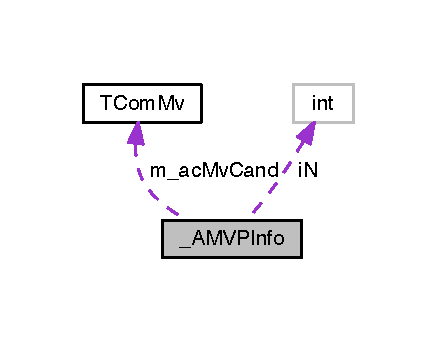
\includegraphics[width=210pt]{d0/d4b/struct___a_m_v_p_info__coll__graph}
\end{center}
\end{figure}
\subsection*{Public Attributes}
\begin{DoxyCompactItemize}
\item 
\mbox{\Hypertarget{struct___a_m_v_p_info_a1a06c043343f0edf7691cacafa886728}\label{struct___a_m_v_p_info_a1a06c043343f0edf7691cacafa886728}} 
\hyperlink{class_t_com_mv}{T\+Com\+Mv} \hyperlink{struct___a_m_v_p_info_a1a06c043343f0edf7691cacafa886728}{m\+\_\+ac\+Mv\+Cand} \mbox{[}A\+M\+V\+P\+\_\+\+M\+A\+X\+\_\+\+N\+U\+M\+\_\+\+C\+A\+N\+DS\mbox{]}
\begin{DoxyCompactList}\small\item\em array of motion vector predictor candidates \end{DoxyCompactList}\item 
\mbox{\Hypertarget{struct___a_m_v_p_info_a921ce7317be0b56cbecba7e73d8f8672}\label{struct___a_m_v_p_info_a921ce7317be0b56cbecba7e73d8f8672}} 
Int \hyperlink{struct___a_m_v_p_info_a921ce7317be0b56cbecba7e73d8f8672}{iN}
\begin{DoxyCompactList}\small\item\em number of motion vector predictor candidates \end{DoxyCompactList}\end{DoxyCompactItemize}


\subsection{Detailed Description}
parameters for A\+M\+VP 

The documentation for this struct was generated from the following file\+:\begin{DoxyCompactItemize}
\item 
Lib/\+T\+Lib\+Common/\hyperlink{_t_com_motion_info_8h}{T\+Com\+Motion\+Info.\+h}\end{DoxyCompactItemize}

\hypertarget{struct__context__md5__t}{}\section{\+\_\+context\+\_\+md5\+\_\+t Struct Reference}
\label{struct__context__md5__t}\index{\+\_\+context\+\_\+md5\+\_\+t@{\+\_\+context\+\_\+md5\+\_\+t}}


Collaboration diagram for \+\_\+context\+\_\+md5\+\_\+t\+:
\nopagebreak
\begin{figure}[H]
\begin{center}
\leavevmode
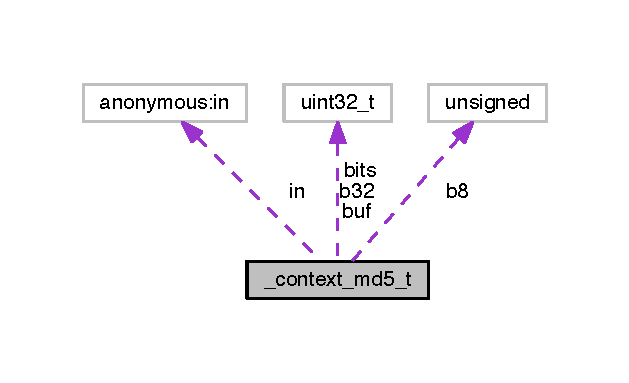
\includegraphics[width=302pt]{d2/dfc/struct__context__md5__t__coll__graph}
\end{center}
\end{figure}
\subsection*{Public Attributes}
\begin{DoxyCompactItemize}
\item 
\mbox{\Hypertarget{struct__context__md5__t_a5587845ac35afcdcf8e0455ed8f0cf17}\label{struct__context__md5__t_a5587845ac35afcdcf8e0455ed8f0cf17}} 
uint32\+\_\+t {\bfseries buf} \mbox{[}4\mbox{]}
\item 
\mbox{\Hypertarget{struct__context__md5__t_a659f4871283f01952f940d92874362cc}\label{struct__context__md5__t_a659f4871283f01952f940d92874362cc}} 
uint32\+\_\+t {\bfseries bits} \mbox{[}2\mbox{]}
\item 
\mbox{\Hypertarget{struct__context__md5__t_a1d8de42dabaab4442741a50dd9c338c0}\label{struct__context__md5__t_a1d8de42dabaab4442741a50dd9c338c0}} 
\begin{tabbing}
xx\=xx\=xx\=xx\=xx\=xx\=xx\=xx\=xx\=\kill
union \{\\
\>unsigned char {\bfseries b8} \mbox{[}64\mbox{]}\\
\>uint32\_t {\bfseries b32} \mbox{[}16\mbox{]}\\
\} {\bfseries in}\\

\end{tabbing}\end{DoxyCompactItemize}


The documentation for this struct was generated from the following file\+:\begin{DoxyCompactItemize}
\item 
Lib/libmd5/libmd5.\+h\end{DoxyCompactItemize}

\hypertarget{struct___d_b_b_p_tmp_data}{}\section{\+\_\+\+D\+B\+B\+P\+Tmp\+Data Struct Reference}
\label{struct___d_b_b_p_tmp_data}\index{\+\_\+\+D\+B\+B\+P\+Tmp\+Data@{\+\_\+\+D\+B\+B\+P\+Tmp\+Data}}


Collaboration diagram for \+\_\+\+D\+B\+B\+P\+Tmp\+Data\+:
\nopagebreak
\begin{figure}[H]
\begin{center}
\leavevmode
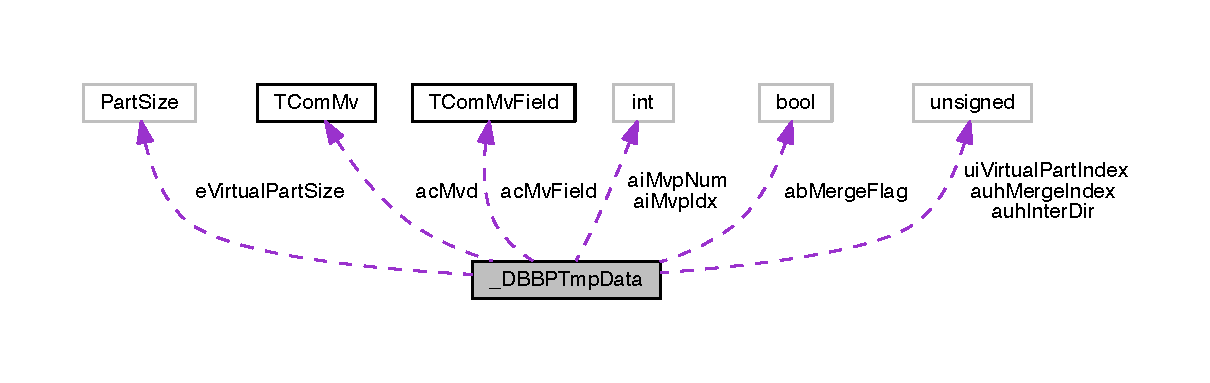
\includegraphics[width=350pt]{db/d48/struct___d_b_b_p_tmp_data__coll__graph}
\end{center}
\end{figure}
\subsection*{Public Attributes}
\begin{DoxyCompactItemize}
\item 
\mbox{\Hypertarget{struct___d_b_b_p_tmp_data_adf1909f41320942579635a720bbb249b}\label{struct___d_b_b_p_tmp_data_adf1909f41320942579635a720bbb249b}} 
\hyperlink{class_t_com_mv}{T\+Com\+Mv} {\bfseries ac\+Mvd} \mbox{[}2\mbox{]}\mbox{[}2\mbox{]}
\item 
\mbox{\Hypertarget{struct___d_b_b_p_tmp_data_a224d16d2a1fc07bfeec2800671fcda62}\label{struct___d_b_b_p_tmp_data_a224d16d2a1fc07bfeec2800671fcda62}} 
\hyperlink{class_t_com_mv_field}{T\+Com\+Mv\+Field} {\bfseries ac\+Mv\+Field} \mbox{[}2\mbox{]}\mbox{[}2\mbox{]}
\item 
\mbox{\Hypertarget{struct___d_b_b_p_tmp_data_a7609ef089dc6f6343eb6daddb2516cdd}\label{struct___d_b_b_p_tmp_data_a7609ef089dc6f6343eb6daddb2516cdd}} 
Int {\bfseries ai\+Mvp\+Num} \mbox{[}2\mbox{]}\mbox{[}2\mbox{]}
\item 
\mbox{\Hypertarget{struct___d_b_b_p_tmp_data_a97267ec9c4852a8270b46278ff5c736c}\label{struct___d_b_b_p_tmp_data_a97267ec9c4852a8270b46278ff5c736c}} 
Int {\bfseries ai\+Mvp\+Idx} \mbox{[}2\mbox{]}\mbox{[}2\mbox{]}
\item 
\mbox{\Hypertarget{struct___d_b_b_p_tmp_data_a11982df8f479316b70ed5ac7ea380302}\label{struct___d_b_b_p_tmp_data_a11982df8f479316b70ed5ac7ea380302}} 
U\+Char {\bfseries auh\+Inter\+Dir} \mbox{[}2\mbox{]}
\item 
\mbox{\Hypertarget{struct___d_b_b_p_tmp_data_a93965876364474b2fbcbb19888137389}\label{struct___d_b_b_p_tmp_data_a93965876364474b2fbcbb19888137389}} 
Bool {\bfseries ab\+Merge\+Flag} \mbox{[}2\mbox{]}
\item 
\mbox{\Hypertarget{struct___d_b_b_p_tmp_data_a79ce04f58cf353eba1d6d3f1cb9323bd}\label{struct___d_b_b_p_tmp_data_a79ce04f58cf353eba1d6d3f1cb9323bd}} 
U\+Char {\bfseries auh\+Merge\+Index} \mbox{[}2\mbox{]}
\item 
\mbox{\Hypertarget{struct___d_b_b_p_tmp_data_aeb6ad368715d8cb9f7931f98ab27764f}\label{struct___d_b_b_p_tmp_data_aeb6ad368715d8cb9f7931f98ab27764f}} 
\hyperlink{_type_def_8h_a0093b7809f3cfae06fda9d67441267bd}{Part\+Size} {\bfseries e\+Virtual\+Part\+Size}
\item 
\mbox{\Hypertarget{struct___d_b_b_p_tmp_data_a2c97c0cf1941fc1b90b86e46258753bf}\label{struct___d_b_b_p_tmp_data_a2c97c0cf1941fc1b90b86e46258753bf}} 
U\+Int {\bfseries ui\+Virtual\+Part\+Index}
\end{DoxyCompactItemize}


The documentation for this struct was generated from the following file\+:\begin{DoxyCompactItemize}
\item 
Lib/\+T\+Lib\+Common/\hyperlink{_t_com_data_c_u_8h}{T\+Com\+Data\+C\+U.\+h}\end{DoxyCompactItemize}

\hypertarget{struct___dis_cand}{}\section{\+\_\+\+Dis\+Cand Struct Reference}
\label{struct___dis_cand}\index{\+\_\+\+Dis\+Cand@{\+\_\+\+Dis\+Cand}}


Collaboration diagram for \+\_\+\+Dis\+Cand\+:
\nopagebreak
\begin{figure}[H]
\begin{center}
\leavevmode
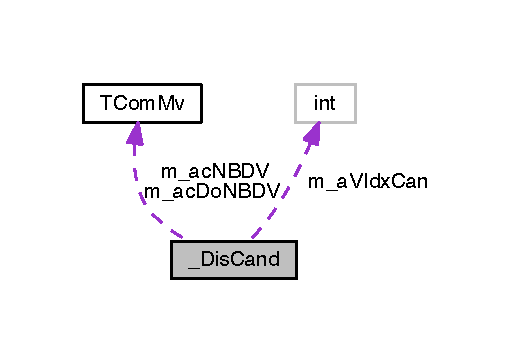
\includegraphics[width=246pt]{d9/da0/struct___dis_cand__coll__graph}
\end{center}
\end{figure}
\subsection*{Public Attributes}
\begin{DoxyCompactItemize}
\item 
\mbox{\Hypertarget{struct___dis_cand_afd2a831262d6388645ce6432577bebe5}\label{struct___dis_cand_afd2a831262d6388645ce6432577bebe5}} 
\hyperlink{class_t_com_mv}{T\+Com\+Mv} {\bfseries m\+\_\+ac\+N\+B\+DV}
\item 
\mbox{\Hypertarget{struct___dis_cand_a1da3259ad5d1438cdb4ffea95f6dc274}\label{struct___dis_cand_a1da3259ad5d1438cdb4ffea95f6dc274}} 
\hyperlink{class_t_com_mv}{T\+Com\+Mv} {\bfseries m\+\_\+ac\+Do\+N\+B\+DV}
\item 
\mbox{\Hypertarget{struct___dis_cand_a4dce20e1ebd1cbdb8e8e390d2945fcc1}\label{struct___dis_cand_a4dce20e1ebd1cbdb8e8e390d2945fcc1}} 
Int {\bfseries m\+\_\+a\+V\+Idx\+Can}
\end{DoxyCompactItemize}


The documentation for this struct was generated from the following file\+:\begin{DoxyCompactItemize}
\item 
Lib/\+T\+Lib\+Common/\hyperlink{_t_com_motion_info_8h}{T\+Com\+Motion\+Info.\+h}\end{DoxyCompactItemize}

\hypertarget{struct___i_d_v_cand}{}\section{\+\_\+\+I\+D\+V\+Cand Struct Reference}
\label{struct___i_d_v_cand}\index{\+\_\+\+I\+D\+V\+Cand@{\+\_\+\+I\+D\+V\+Cand}}


Collaboration diagram for \+\_\+\+I\+D\+V\+Cand\+:
\nopagebreak
\begin{figure}[H]
\begin{center}
\leavevmode
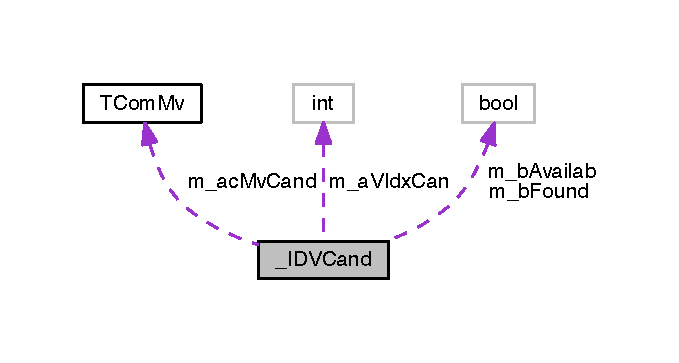
\includegraphics[width=326pt]{dd/d3c/struct___i_d_v_cand__coll__graph}
\end{center}
\end{figure}
\subsection*{Public Attributes}
\begin{DoxyCompactItemize}
\item 
\mbox{\Hypertarget{struct___i_d_v_cand_aa6d8d7ce9ed9a39a859e93d04d8054b5}\label{struct___i_d_v_cand_aa6d8d7ce9ed9a39a859e93d04d8054b5}} 
\hyperlink{class_t_com_mv}{T\+Com\+Mv} {\bfseries m\+\_\+ac\+Mv\+Cand} \mbox{[}2\mbox{]}\mbox{[}I\+D\+V\+\_\+\+C\+A\+N\+DS\mbox{]}
\item 
\mbox{\Hypertarget{struct___i_d_v_cand_a4ae26ca3b63cb0d083dc2ce650a43433}\label{struct___i_d_v_cand_a4ae26ca3b63cb0d083dc2ce650a43433}} 
Int {\bfseries m\+\_\+a\+V\+Idx\+Can} \mbox{[}2\mbox{]}\mbox{[}I\+D\+V\+\_\+\+C\+A\+N\+DS\mbox{]}
\item 
\mbox{\Hypertarget{struct___i_d_v_cand_a184082dee69556b4161c01e582847dc1}\label{struct___i_d_v_cand_a184082dee69556b4161c01e582847dc1}} 
Bool {\bfseries m\+\_\+b\+Availab} \mbox{[}2\mbox{]}\mbox{[}I\+D\+V\+\_\+\+C\+A\+N\+DS\mbox{]}
\item 
\mbox{\Hypertarget{struct___i_d_v_cand_a07df957b4920d84789de56535979bc4a}\label{struct___i_d_v_cand_a07df957b4920d84789de56535979bc4a}} 
Bool {\bfseries m\+\_\+b\+Found}
\end{DoxyCompactItemize}


The documentation for this struct was generated from the following file\+:\begin{DoxyCompactItemize}
\item 
Lib/\+T\+Lib\+Common/\hyperlink{_t_com_motion_info_8h}{T\+Com\+Motion\+Info.\+h}\end{DoxyCompactItemize}

\hypertarget{struct___l_f_c_u_param}{}\section{\+\_\+\+L\+F\+C\+U\+Param Struct Reference}
\label{struct___l_f_c_u_param}\index{\+\_\+\+L\+F\+C\+U\+Param@{\+\_\+\+L\+F\+C\+U\+Param}}


parameters for deblocking filter  




{\ttfamily \#include $<$Type\+Def.\+h$>$}



Collaboration diagram for \+\_\+\+L\+F\+C\+U\+Param\+:
\nopagebreak
\begin{figure}[H]
\begin{center}
\leavevmode
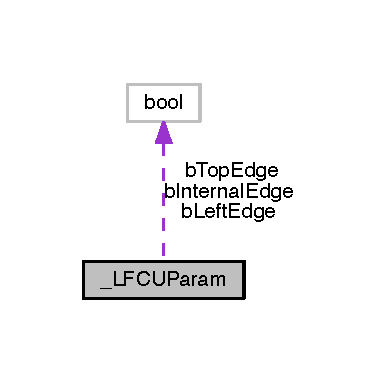
\includegraphics[width=181pt]{dc/df1/struct___l_f_c_u_param__coll__graph}
\end{center}
\end{figure}
\subsection*{Public Attributes}
\begin{DoxyCompactItemize}
\item 
\mbox{\Hypertarget{struct___l_f_c_u_param_a7f4f9423140f9367ecd26c7ce9ae28d4}\label{struct___l_f_c_u_param_a7f4f9423140f9367ecd26c7ce9ae28d4}} 
Bool \hyperlink{struct___l_f_c_u_param_a7f4f9423140f9367ecd26c7ce9ae28d4}{b\+Internal\+Edge}
\begin{DoxyCompactList}\small\item\em indicates internal edge \end{DoxyCompactList}\item 
\mbox{\Hypertarget{struct___l_f_c_u_param_a519ab1d44cf9e8ad89a1bb7709f5a514}\label{struct___l_f_c_u_param_a519ab1d44cf9e8ad89a1bb7709f5a514}} 
Bool \hyperlink{struct___l_f_c_u_param_a519ab1d44cf9e8ad89a1bb7709f5a514}{b\+Left\+Edge}
\begin{DoxyCompactList}\small\item\em indicates left edge \end{DoxyCompactList}\item 
\mbox{\Hypertarget{struct___l_f_c_u_param_a106cd6313ee566a3c29e973762692db4}\label{struct___l_f_c_u_param_a106cd6313ee566a3c29e973762692db4}} 
Bool \hyperlink{struct___l_f_c_u_param_a106cd6313ee566a3c29e973762692db4}{b\+Top\+Edge}
\begin{DoxyCompactList}\small\item\em indicates top edge \end{DoxyCompactList}\end{DoxyCompactItemize}


\subsection{Detailed Description}
parameters for deblocking filter 

The documentation for this struct was generated from the following file\+:\begin{DoxyCompactItemize}
\item 
Lib/\+T\+Lib\+Common/\hyperlink{_type_def_8h}{Type\+Def.\+h}\end{DoxyCompactItemize}

\hypertarget{class_access_unit}{}\section{Access\+Unit Class Reference}
\label{class_access_unit}\index{Access\+Unit@{Access\+Unit}}


{\ttfamily \#include $<$Access\+Unit.\+h$>$}



Inheritance diagram for Access\+Unit\+:
\nopagebreak
\begin{figure}[H]
\begin{center}
\leavevmode
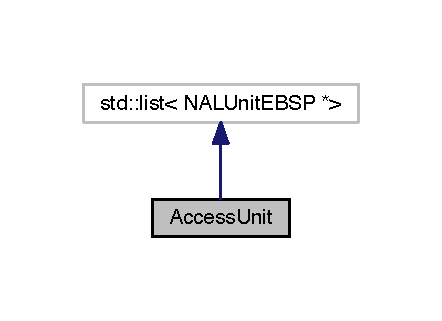
\includegraphics[width=212pt]{d4/da5/class_access_unit__inherit__graph}
\end{center}
\end{figure}


Collaboration diagram for Access\+Unit\+:
\nopagebreak
\begin{figure}[H]
\begin{center}
\leavevmode
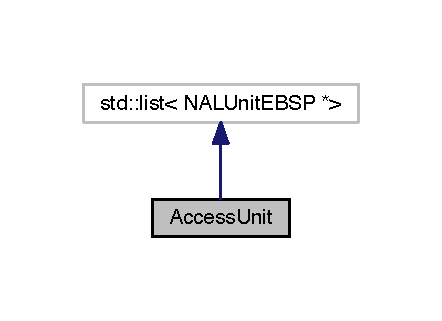
\includegraphics[width=212pt]{d3/d00/class_access_unit__coll__graph}
\end{center}
\end{figure}


\subsection{Detailed Description}
An \hyperlink{class_access_unit}{Access\+Unit} is a list of one or more N\+AL units, according to the working draft. All N\+AL units within the object belong to the same access unit.

N\+A\+L\+Units held in the \hyperlink{class_access_unit}{Access\+Unit} list are in E\+B\+SP format. Attempting to insert an \hyperlink{struct_output_n_a_l_unit}{Output\+N\+A\+L\+Unit} into the access unit will automatically cause the nalunit to have its headers written and anti-\/emulation performed.

The \hyperlink{class_access_unit}{Access\+Unit} owns all pointers stored within. Destroying the \hyperlink{class_access_unit}{Access\+Unit} will delete all contained objects. 

The documentation for this class was generated from the following file\+:\begin{DoxyCompactItemize}
\item 
Lib/\+T\+Lib\+Common/\hyperlink{_access_unit_8h}{Access\+Unit.\+h}\end{DoxyCompactItemize}

\hypertarget{struct_annex_b_stats}{}\section{Annex\+B\+Stats Struct Reference}
\label{struct_annex_b_stats}\index{Annex\+B\+Stats@{Annex\+B\+Stats}}


{\ttfamily \#include $<$Annex\+Bread.\+h$>$}



Collaboration diagram for Annex\+B\+Stats\+:
\nopagebreak
\begin{figure}[H]
\begin{center}
\leavevmode
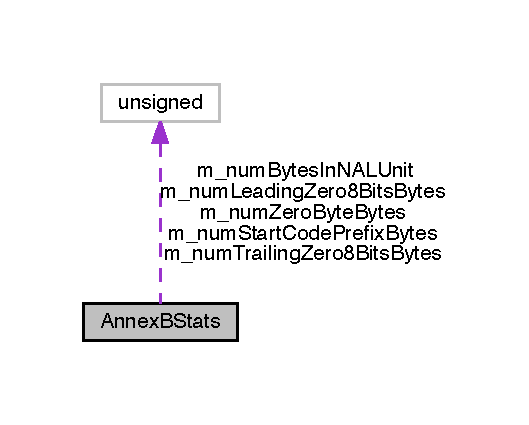
\includegraphics[width=254pt]{d4/df5/struct_annex_b_stats__coll__graph}
\end{center}
\end{figure}
\subsection*{Public Member Functions}
\begin{DoxyCompactItemize}
\item 
\mbox{\Hypertarget{struct_annex_b_stats_a835da7e3a6e7a9d3807ed0f44f49228e}\label{struct_annex_b_stats_a835da7e3a6e7a9d3807ed0f44f49228e}} 
\hyperlink{struct_annex_b_stats}{Annex\+B\+Stats} \& {\bfseries operator+=} (const \hyperlink{struct_annex_b_stats}{Annex\+B\+Stats} \&rhs)
\end{DoxyCompactItemize}
\subsection*{Public Attributes}
\begin{DoxyCompactItemize}
\item 
\mbox{\Hypertarget{struct_annex_b_stats_a556514dec1c3e2809885e3a3d28fd120}\label{struct_annex_b_stats_a556514dec1c3e2809885e3a3d28fd120}} 
U\+Int {\bfseries m\+\_\+num\+Leading\+Zero8\+Bits\+Bytes}
\item 
\mbox{\Hypertarget{struct_annex_b_stats_a11772dc9f6e30684372f339c0f82a362}\label{struct_annex_b_stats_a11772dc9f6e30684372f339c0f82a362}} 
U\+Int {\bfseries m\+\_\+num\+Zero\+Byte\+Bytes}
\item 
\mbox{\Hypertarget{struct_annex_b_stats_adec7ceaf29da5abcb1c12af030211220}\label{struct_annex_b_stats_adec7ceaf29da5abcb1c12af030211220}} 
U\+Int {\bfseries m\+\_\+num\+Start\+Code\+Prefix\+Bytes}
\item 
\mbox{\Hypertarget{struct_annex_b_stats_af2f5be6976825eff9fc819b5d6a69913}\label{struct_annex_b_stats_af2f5be6976825eff9fc819b5d6a69913}} 
U\+Int {\bfseries m\+\_\+num\+Bytes\+In\+N\+A\+L\+Unit}
\item 
\mbox{\Hypertarget{struct_annex_b_stats_ab01e1cc2a61a694deca7ecd53cdbc07b}\label{struct_annex_b_stats_ab01e1cc2a61a694deca7ecd53cdbc07b}} 
U\+Int {\bfseries m\+\_\+num\+Trailing\+Zero8\+Bits\+Bytes}
\end{DoxyCompactItemize}


\subsection{Detailed Description}
Statistics associated with AnnexB bytestreams 

The documentation for this struct was generated from the following file\+:\begin{DoxyCompactItemize}
\item 
Lib/\+T\+Lib\+Decoder/\hyperlink{_annex_bread_8h}{Annex\+Bread.\+h}\end{DoxyCompactItemize}

\hypertarget{structdf_1_1program__options__lite_1_1_argv_parser}{}\section{df\+:\+:program\+\_\+options\+\_\+lite\+:\+:Argv\+Parser Struct Reference}
\label{structdf_1_1program__options__lite_1_1_argv_parser}\index{df\+::program\+\_\+options\+\_\+lite\+::\+Argv\+Parser@{df\+::program\+\_\+options\+\_\+lite\+::\+Argv\+Parser}}


Inheritance diagram for df\+:\+:program\+\_\+options\+\_\+lite\+:\+:Argv\+Parser\+:
\nopagebreak
\begin{figure}[H]
\begin{center}
\leavevmode
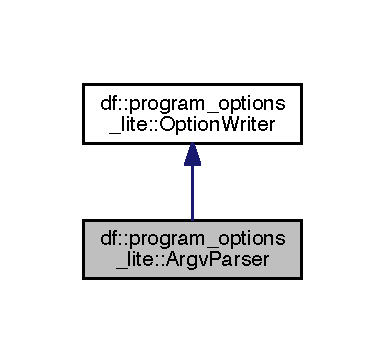
\includegraphics[width=185pt]{de/d0c/structdf_1_1program__options__lite_1_1_argv_parser__inherit__graph}
\end{center}
\end{figure}


Collaboration diagram for df\+:\+:program\+\_\+options\+\_\+lite\+:\+:Argv\+Parser\+:
\nopagebreak
\begin{figure}[H]
\begin{center}
\leavevmode
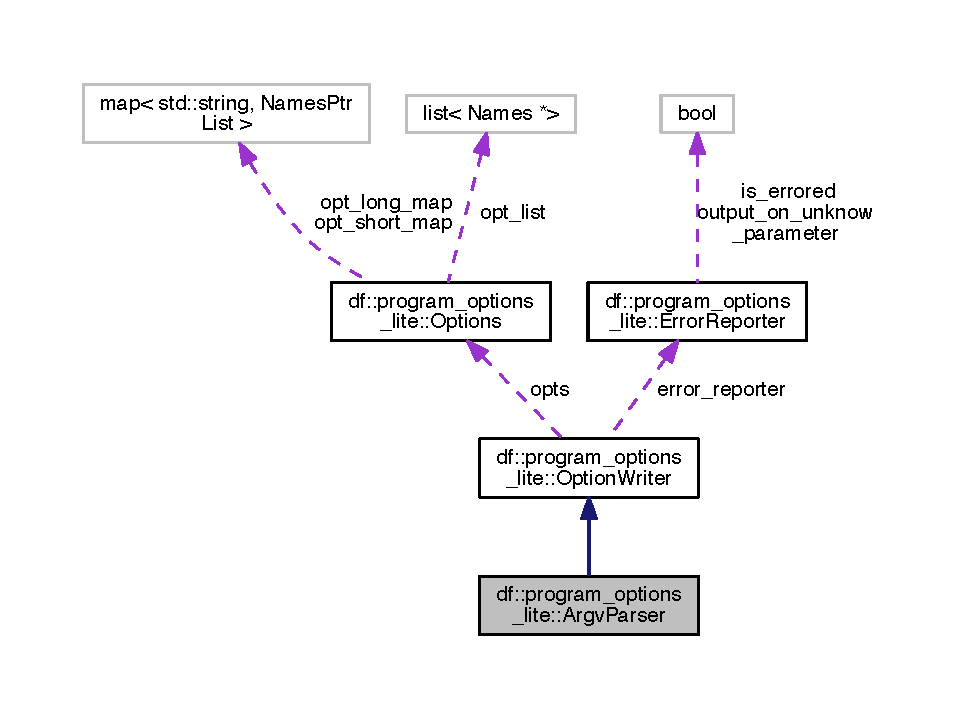
\includegraphics[width=350pt]{d4/d3a/structdf_1_1program__options__lite_1_1_argv_parser__coll__graph}
\end{center}
\end{figure}
\subsection*{Public Member Functions}
\begin{DoxyCompactItemize}
\item 
\mbox{\Hypertarget{structdf_1_1program__options__lite_1_1_argv_parser_a53775823e982fd5946dfcd484316522c}\label{structdf_1_1program__options__lite_1_1_argv_parser_a53775823e982fd5946dfcd484316522c}} 
{\bfseries Argv\+Parser} (\hyperlink{structdf_1_1program__options__lite_1_1_options}{Options} \&r\+Opts, \hyperlink{structdf_1_1program__options__lite_1_1_error_reporter}{Error\+Reporter} \&r\+Error\+\_\+reporter)
\item 
\mbox{\Hypertarget{structdf_1_1program__options__lite_1_1_argv_parser_a8612ce7734bdd05e7f7014c56665ea62}\label{structdf_1_1program__options__lite_1_1_argv_parser_a8612ce7734bdd05e7f7014c56665ea62}} 
const string {\bfseries where} ()
\item 
unsigned \hyperlink{structdf_1_1program__options__lite_1_1_argv_parser_adbb297897d306bbc09390750c297d823}{parse\+G\+NU} (unsigned argc, const char $\ast$argv\mbox{[}$\,$\mbox{]})
\item 
\mbox{\Hypertarget{structdf_1_1program__options__lite_1_1_argv_parser_a9fa36499ff6f0d2f9f4609f63885faed}\label{structdf_1_1program__options__lite_1_1_argv_parser_a9fa36499ff6f0d2f9f4609f63885faed}} 
unsigned {\bfseries parse\+S\+H\+O\+RT} (unsigned argc, const char $\ast$argv\mbox{[}$\,$\mbox{]})
\end{DoxyCompactItemize}
\subsection*{Additional Inherited Members}


\subsection{Member Function Documentation}
\mbox{\Hypertarget{structdf_1_1program__options__lite_1_1_argv_parser_adbb297897d306bbc09390750c297d823}\label{structdf_1_1program__options__lite_1_1_argv_parser_adbb297897d306bbc09390750c297d823}} 
\index{df\+::program\+\_\+options\+\_\+lite\+::\+Argv\+Parser@{df\+::program\+\_\+options\+\_\+lite\+::\+Argv\+Parser}!parse\+G\+NU@{parse\+G\+NU}}
\index{parse\+G\+NU@{parse\+G\+NU}!df\+::program\+\_\+options\+\_\+lite\+::\+Argv\+Parser@{df\+::program\+\_\+options\+\_\+lite\+::\+Argv\+Parser}}
\subsubsection{\texorpdfstring{parse\+G\+N\+U()}{parseGNU()}}
{\footnotesize\ttfamily unsigned df\+::program\+\_\+options\+\_\+lite\+::\+Argv\+Parser\+::parse\+G\+NU (\begin{DoxyParamCaption}\item[{unsigned}]{argc,  }\item[{const char $\ast$}]{argv\mbox{[}$\,$\mbox{]} }\end{DoxyParamCaption})}

returns number of extra arguments consumed 

The documentation for this struct was generated from the following file\+:\begin{DoxyCompactItemize}
\item 
Lib/\+T\+App\+Common/program\+\_\+options\+\_\+lite.\+cpp\end{DoxyCompactItemize}

\hypertarget{class_a_u_d_reader}{}\section{A\+U\+D\+Reader Class Reference}
\label{class_a_u_d_reader}\index{A\+U\+D\+Reader@{A\+U\+D\+Reader}}


Inheritance diagram for A\+U\+D\+Reader\+:
\nopagebreak
\begin{figure}[H]
\begin{center}
\leavevmode
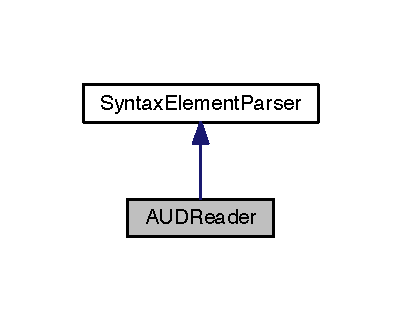
\includegraphics[width=193pt]{d0/d9a/class_a_u_d_reader__inherit__graph}
\end{center}
\end{figure}


Collaboration diagram for A\+U\+D\+Reader\+:
\nopagebreak
\begin{figure}[H]
\begin{center}
\leavevmode
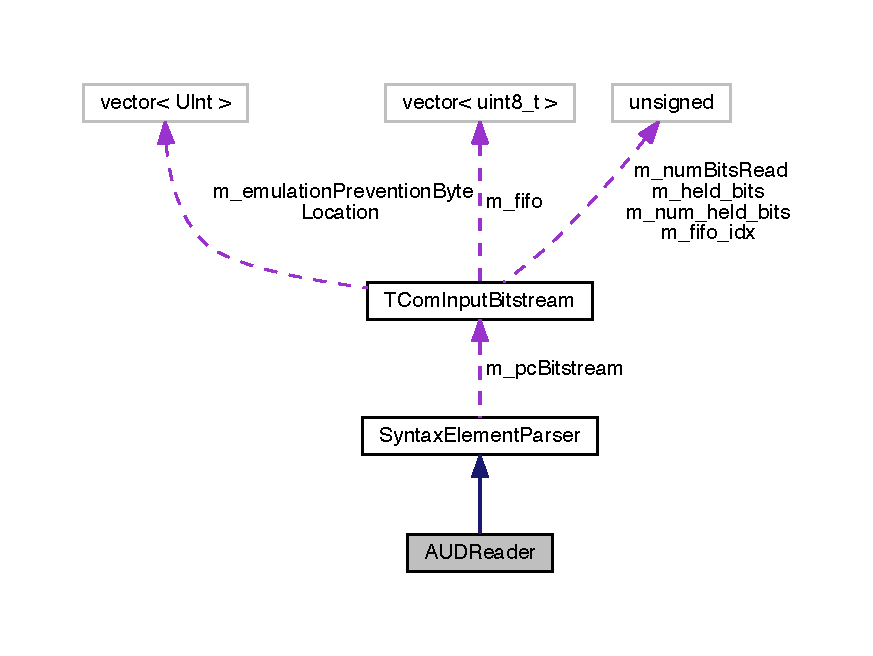
\includegraphics[width=350pt]{d2/d20/class_a_u_d_reader__coll__graph}
\end{center}
\end{figure}
\subsection*{Public Member Functions}
{\bf }\par
\begin{DoxyCompactItemize}
\item 
\mbox{\Hypertarget{class_a_u_d_reader_afff063b5995484feccf4622b5c85bd01}\label{class_a_u_d_reader_afff063b5995484feccf4622b5c85bd01}} 
Void {\bfseries parse\+Access\+Unit\+Delimiter} (\hyperlink{class_t_com_input_bitstream}{T\+Com\+Input\+Bitstream} $\ast$bs, U\+Int \&pic\+Type)
\end{DoxyCompactItemize}

\subsection*{Additional Inherited Members}


The documentation for this class was generated from the following files\+:\begin{DoxyCompactItemize}
\item 
Lib/\+T\+Lib\+Decoder/\hyperlink{_syntax_element_parser_8h}{Syntax\+Element\+Parser.\+h}\item 
Lib/\+T\+Lib\+Decoder/\hyperlink{_syntax_element_parser_8cpp}{Syntax\+Element\+Parser.\+cpp}\end{DoxyCompactItemize}

\hypertarget{class_a_u_d_writer}{}\section{A\+U\+D\+Writer Class Reference}
\label{class_a_u_d_writer}\index{A\+U\+D\+Writer@{A\+U\+D\+Writer}}


Inheritance diagram for A\+U\+D\+Writer\+:
\nopagebreak
\begin{figure}[H]
\begin{center}
\leavevmode
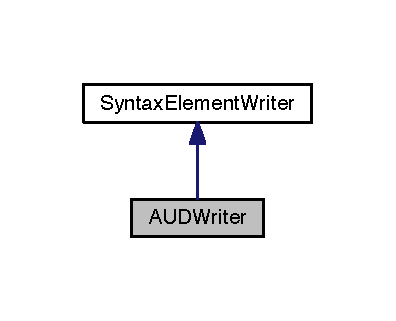
\includegraphics[width=190pt]{de/d58/class_a_u_d_writer__inherit__graph}
\end{center}
\end{figure}


Collaboration diagram for A\+U\+D\+Writer\+:
\nopagebreak
\begin{figure}[H]
\begin{center}
\leavevmode
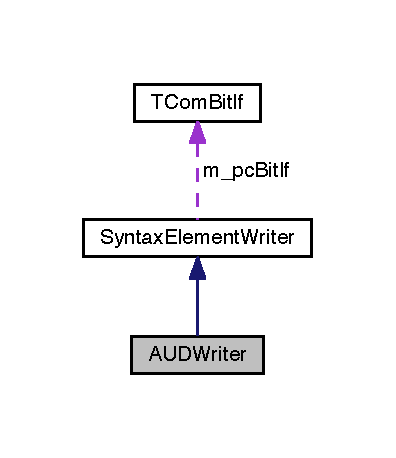
\includegraphics[width=190pt]{d9/d2b/class_a_u_d_writer__coll__graph}
\end{center}
\end{figure}
\subsection*{Public Member Functions}
{\bf }\par
\begin{DoxyCompactItemize}
\item 
\mbox{\Hypertarget{class_a_u_d_writer_af0106f77e5b7f2959b94880c8af9fca1}\label{class_a_u_d_writer_af0106f77e5b7f2959b94880c8af9fca1}} 
Void {\bfseries code\+A\+UD} (\hyperlink{class_t_com_bit_if}{T\+Com\+Bit\+If} \&bs, const Int picture\+Type)
\end{DoxyCompactItemize}

\subsection*{Additional Inherited Members}


The documentation for this class was generated from the following files\+:\begin{DoxyCompactItemize}
\item 
Lib/\+T\+Lib\+Encoder/\hyperlink{_t_enc_cavlc_8h}{T\+Enc\+Cavlc.\+h}\item 
Lib/\+T\+Lib\+Encoder/\hyperlink{_t_enc_cavlc_8cpp}{T\+Enc\+Cavlc.\+cpp}\end{DoxyCompactItemize}

\hypertarget{struct_bit_depths}{}\section{Bit\+Depths Struct Reference}
\label{struct_bit_depths}\index{Bit\+Depths@{Bit\+Depths}}


Collaboration diagram for Bit\+Depths\+:
\nopagebreak
\begin{figure}[H]
\begin{center}
\leavevmode
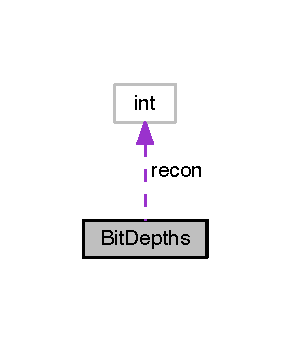
\includegraphics[width=139pt]{dd/d7e/struct_bit_depths__coll__graph}
\end{center}
\end{figure}
\subsection*{Public Attributes}
\begin{DoxyCompactItemize}
\item 
\mbox{\Hypertarget{struct_bit_depths_ab96fb4630b7c08f91c84d072240ef6ea}\label{struct_bit_depths_ab96fb4630b7c08f91c84d072240ef6ea}} 
Int \hyperlink{struct_bit_depths_ab96fb4630b7c08f91c84d072240ef6ea}{recon} \mbox{[}M\+A\+X\+\_\+\+N\+U\+M\+\_\+\+C\+H\+A\+N\+N\+E\+L\+\_\+\+T\+Y\+PE\mbox{]}
\begin{DoxyCompactList}\small\item\em the bit depth as indicated in the S\+PS \end{DoxyCompactList}\end{DoxyCompactItemize}


The documentation for this struct was generated from the following file\+:\begin{DoxyCompactItemize}
\item 
Lib/\+T\+Lib\+Common/\hyperlink{_type_def_8h}{Type\+Def.\+h}\end{DoxyCompactItemize}

\hypertarget{structdf_1_1program__options__lite_1_1_cfg_stream_parser}{}\section{df\+:\+:program\+\_\+options\+\_\+lite\+:\+:Cfg\+Stream\+Parser Struct Reference}
\label{structdf_1_1program__options__lite_1_1_cfg_stream_parser}\index{df\+::program\+\_\+options\+\_\+lite\+::\+Cfg\+Stream\+Parser@{df\+::program\+\_\+options\+\_\+lite\+::\+Cfg\+Stream\+Parser}}


Inheritance diagram for df\+:\+:program\+\_\+options\+\_\+lite\+:\+:Cfg\+Stream\+Parser\+:
\nopagebreak
\begin{figure}[H]
\begin{center}
\leavevmode
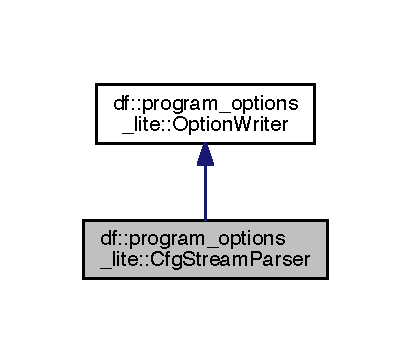
\includegraphics[width=197pt]{d6/ddc/structdf_1_1program__options__lite_1_1_cfg_stream_parser__inherit__graph}
\end{center}
\end{figure}


Collaboration diagram for df\+:\+:program\+\_\+options\+\_\+lite\+:\+:Cfg\+Stream\+Parser\+:
\nopagebreak
\begin{figure}[H]
\begin{center}
\leavevmode
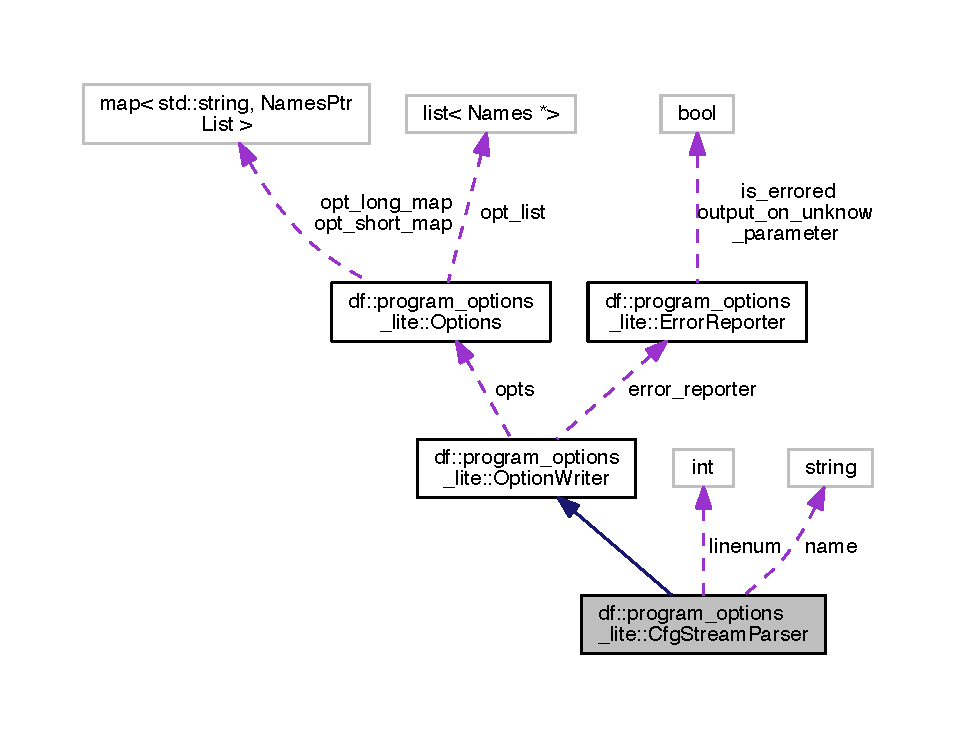
\includegraphics[width=350pt]{d9/db1/structdf_1_1program__options__lite_1_1_cfg_stream_parser__coll__graph}
\end{center}
\end{figure}
\subsection*{Public Member Functions}
\begin{DoxyCompactItemize}
\item 
\mbox{\Hypertarget{structdf_1_1program__options__lite_1_1_cfg_stream_parser_a22c100e9cf758b4bf0adb65bfb25424b}\label{structdf_1_1program__options__lite_1_1_cfg_stream_parser_a22c100e9cf758b4bf0adb65bfb25424b}} 
{\bfseries Cfg\+Stream\+Parser} (const string \&r\+Name, \hyperlink{structdf_1_1program__options__lite_1_1_options}{Options} \&r\+Opts, \hyperlink{structdf_1_1program__options__lite_1_1_error_reporter}{Error\+Reporter} \&r\+Error\+\_\+reporter)
\item 
\mbox{\Hypertarget{structdf_1_1program__options__lite_1_1_cfg_stream_parser_a7ee5e9e3e518eb4a3289cd40c0883c9a}\label{structdf_1_1program__options__lite_1_1_cfg_stream_parser_a7ee5e9e3e518eb4a3289cd40c0883c9a}} 
const string {\bfseries where} ()
\item 
\mbox{\Hypertarget{structdf_1_1program__options__lite_1_1_cfg_stream_parser_a2ce0529549147ca927343f8d8087cad2}\label{structdf_1_1program__options__lite_1_1_cfg_stream_parser_a2ce0529549147ca927343f8d8087cad2}} 
void {\bfseries scan\+Line} (string \&line)
\item 
\mbox{\Hypertarget{structdf_1_1program__options__lite_1_1_cfg_stream_parser_a217e7930e78de71d15f7221ecf2bdbca}\label{structdf_1_1program__options__lite_1_1_cfg_stream_parser_a217e7930e78de71d15f7221ecf2bdbca}} 
void {\bfseries scan\+Stream} (istream \&in)
\end{DoxyCompactItemize}
\subsection*{Public Attributes}
\begin{DoxyCompactItemize}
\item 
\mbox{\Hypertarget{structdf_1_1program__options__lite_1_1_cfg_stream_parser_a741c54e6b713aa3832d254b0d4a3a1f3}\label{structdf_1_1program__options__lite_1_1_cfg_stream_parser_a741c54e6b713aa3832d254b0d4a3a1f3}} 
const string {\bfseries name}
\item 
\mbox{\Hypertarget{structdf_1_1program__options__lite_1_1_cfg_stream_parser_a7e29e76109fccd236c1433fff76cf51e}\label{structdf_1_1program__options__lite_1_1_cfg_stream_parser_a7e29e76109fccd236c1433fff76cf51e}} 
int {\bfseries linenum}
\end{DoxyCompactItemize}


The documentation for this struct was generated from the following file\+:\begin{DoxyCompactItemize}
\item 
Lib/\+T\+App\+Common/program\+\_\+options\+\_\+lite.\+cpp\end{DoxyCompactItemize}

\hypertarget{struct_chroma_qp_adj}{}\section{Chroma\+Qp\+Adj Struct Reference}
\label{struct_chroma_qp_adj}\index{Chroma\+Qp\+Adj@{Chroma\+Qp\+Adj}}


Collaboration diagram for Chroma\+Qp\+Adj\+:
\nopagebreak
\begin{figure}[H]
\begin{center}
\leavevmode
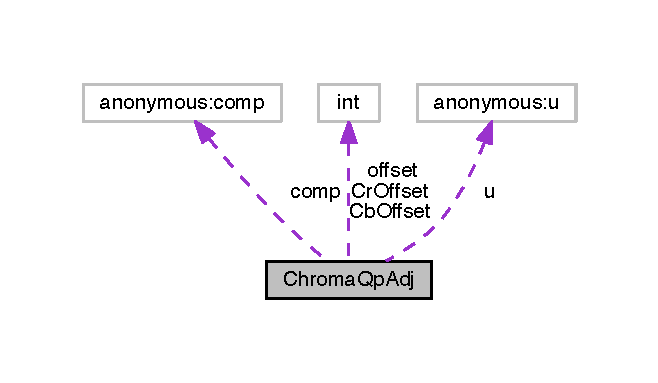
\includegraphics[width=316pt]{d4/d0e/struct_chroma_qp_adj__coll__graph}
\end{center}
\end{figure}
\subsection*{Public Attributes}
\begin{DoxyCompactItemize}
\item 
\mbox{\Hypertarget{struct_chroma_qp_adj_a6753b8c24e00c7dde7b30b6ca9f4b303}\label{struct_chroma_qp_adj_a6753b8c24e00c7dde7b30b6ca9f4b303}} 
\begin{tabbing}
xx\=xx\=xx\=xx\=xx\=xx\=xx\=xx\=xx\=\kill
union \{\\
\>struct \{\\
\>\>Int {\bfseries CbOffset}\\
\>\>Int {\bfseries CrOffset}\\
\>\} {\bfseries comp}\\
\>Int {\bfseries offset} \mbox{[}2\mbox{]}\\
\} {\bfseries u}\\

\end{tabbing}\end{DoxyCompactItemize}


The documentation for this struct was generated from the following file\+:\begin{DoxyCompactItemize}
\item 
Lib/\+T\+Lib\+Common/\hyperlink{_t_com_slice_8h}{T\+Com\+Slice.\+h}\end{DoxyCompactItemize}

\hypertarget{structcoeff_group_r_d_stats}{}\section{coeff\+Group\+R\+D\+Stats Struct Reference}
\label{structcoeff_group_r_d_stats}\index{coeff\+Group\+R\+D\+Stats@{coeff\+Group\+R\+D\+Stats}}


Collaboration diagram for coeff\+Group\+R\+D\+Stats\+:
\nopagebreak
\begin{figure}[H]
\begin{center}
\leavevmode
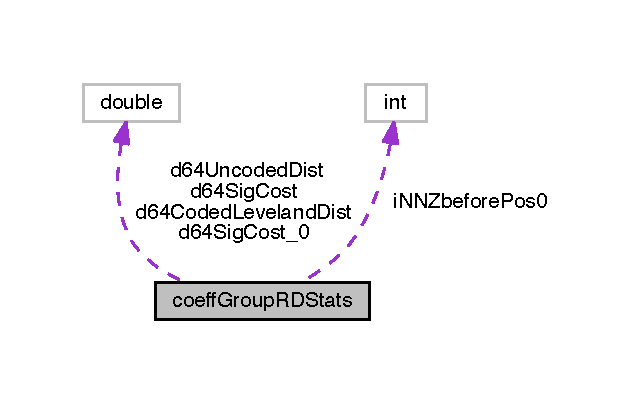
\includegraphics[width=303pt]{dc/d47/structcoeff_group_r_d_stats__coll__graph}
\end{center}
\end{figure}
\subsection*{Public Attributes}
\begin{DoxyCompactItemize}
\item 
\mbox{\Hypertarget{structcoeff_group_r_d_stats_a38af0953e58b813f269807b50d74d86c}\label{structcoeff_group_r_d_stats_a38af0953e58b813f269807b50d74d86c}} 
Int {\bfseries i\+N\+N\+Zbefore\+Pos0}
\item 
\mbox{\Hypertarget{structcoeff_group_r_d_stats_a77d4db46c9636552883fc3e17ef4a56f}\label{structcoeff_group_r_d_stats_a77d4db46c9636552883fc3e17ef4a56f}} 
Double {\bfseries d64\+Coded\+Leveland\+Dist}
\item 
\mbox{\Hypertarget{structcoeff_group_r_d_stats_a530b4ab91fb7119f670547c791cd2861}\label{structcoeff_group_r_d_stats_a530b4ab91fb7119f670547c791cd2861}} 
Double {\bfseries d64\+Uncoded\+Dist}
\item 
\mbox{\Hypertarget{structcoeff_group_r_d_stats_a4eb5b7e1cdfa8c2dce3e568fe75e96c6}\label{structcoeff_group_r_d_stats_a4eb5b7e1cdfa8c2dce3e568fe75e96c6}} 
Double {\bfseries d64\+Sig\+Cost}
\item 
\mbox{\Hypertarget{structcoeff_group_r_d_stats_a696e1f8b2e5cbddae21bf22c2056e06a}\label{structcoeff_group_r_d_stats_a696e1f8b2e5cbddae21bf22c2056e06a}} 
Double {\bfseries d64\+Sig\+Cost\+\_\+0}
\end{DoxyCompactItemize}


The documentation for this struct was generated from the following file\+:\begin{DoxyCompactItemize}
\item 
Lib/\+T\+Lib\+Common/\hyperlink{_t_com_tr_quant_8cpp}{T\+Com\+Tr\+Quant.\+cpp}\end{DoxyCompactItemize}

\hypertarget{class_context_model}{}\section{Context\+Model Class Reference}
\label{class_context_model}\index{Context\+Model@{Context\+Model}}


context model class  




{\ttfamily \#include $<$Context\+Model.\+h$>$}

\subsection*{Public Member Functions}
\begin{DoxyCompactItemize}
\item 
\mbox{\Hypertarget{class_context_model_a119155560379e40c12778c7dcec47ad6}\label{class_context_model_a119155560379e40c12778c7dcec47ad6}} 
U\+Char \hyperlink{class_context_model_a119155560379e40c12778c7dcec47ad6}{get\+State} ()
\begin{DoxyCompactList}\small\item\em get current state \end{DoxyCompactList}\item 
\mbox{\Hypertarget{class_context_model_ab163ff84c2c7b5b908d6d0219bc18003}\label{class_context_model_ab163ff84c2c7b5b908d6d0219bc18003}} 
U\+Char \hyperlink{class_context_model_ab163ff84c2c7b5b908d6d0219bc18003}{get\+Mps} ()
\begin{DoxyCompactList}\small\item\em get curret M\+PS \end{DoxyCompactList}\item 
\mbox{\Hypertarget{class_context_model_a3aa54cbafb0e71b4de10ea6a976e34e8}\label{class_context_model_a3aa54cbafb0e71b4de10ea6a976e34e8}} 
Void \hyperlink{class_context_model_a3aa54cbafb0e71b4de10ea6a976e34e8}{set\+State\+And\+Mps} (U\+Char uc\+State, U\+Char uc\+M\+PS)
\begin{DoxyCompactList}\small\item\em set state and M\+PS \end{DoxyCompactList}\item 
\mbox{\Hypertarget{class_context_model_a07da41567a7e8d20c8a2e065c3fc4b83}\label{class_context_model_a07da41567a7e8d20c8a2e065c3fc4b83}} 
Void {\bfseries update\+L\+PS} ()
\item 
\mbox{\Hypertarget{class_context_model_a49c06d908140dfd49d09e66b9356cac6}\label{class_context_model_a49c06d908140dfd49d09e66b9356cac6}} 
Void {\bfseries update\+M\+PS} ()
\item 
\mbox{\Hypertarget{class_context_model_ad8db1ed3ede769929b4c0fec5c1687ec}\label{class_context_model_ad8db1ed3ede769929b4c0fec5c1687ec}} 
Int {\bfseries get\+Entropy\+Bits} (Short val)
\item 
\mbox{\Hypertarget{class_context_model_a585647408bc9ccd6e5e2850cf34ddc8a}\label{class_context_model_a585647408bc9ccd6e5e2850cf34ddc8a}} 
Void {\bfseries update} (Int bin\+Val)
\item 
\mbox{\Hypertarget{class_context_model_aa89e7ddd62d2d47c2b7fa8e4ab8bdb21}\label{class_context_model_aa89e7ddd62d2d47c2b7fa8e4ab8bdb21}} 
Void {\bfseries set\+Bins\+Coded} (U\+Int val)
\item 
\mbox{\Hypertarget{class_context_model_aab00f8121ca8df77402bd541147d8a25}\label{class_context_model_aab00f8121ca8df77402bd541147d8a25}} 
U\+Int {\bfseries get\+Bins\+Coded} ()
\end{DoxyCompactItemize}
\subsection*{Static Public Member Functions}
\begin{DoxyCompactItemize}
\item 
\mbox{\Hypertarget{class_context_model_af695df0920a820e36947e805189abd0b}\label{class_context_model_af695df0920a820e36947e805189abd0b}} 
static Int {\bfseries get\+Entropy\+Bits\+Trm} (Int val)
\end{DoxyCompactItemize}
\begin{DoxyCompactItemize}
\item 
Void \hyperlink{class_context_model_aaa5e3418f274f7de8f7d99731a130f1a}{init} (Int qp, Int init\+Value)
\begin{DoxyCompactList}\small\item\em initialize state with initial probability \end{DoxyCompactList}\item 
\mbox{\Hypertarget{class_context_model_aa4753719bb2ceccbe83c59f0ecf01b6d}\label{class_context_model_aa4753719bb2ceccbe83c59f0ecf01b6d}} 
static Void {\bfseries build\+Next\+State\+Table} ()
\end{DoxyCompactItemize}


\subsection{Detailed Description}
context model class 

\subsection{Member Function Documentation}
\mbox{\Hypertarget{class_context_model_aaa5e3418f274f7de8f7d99731a130f1a}\label{class_context_model_aaa5e3418f274f7de8f7d99731a130f1a}} 
\index{Context\+Model@{Context\+Model}!init@{init}}
\index{init@{init}!Context\+Model@{Context\+Model}}
\subsubsection{\texorpdfstring{init()}{init()}}
{\footnotesize\ttfamily Void Context\+Model\+::init (\begin{DoxyParamCaption}\item[{Int}]{qp,  }\item[{Int}]{init\+Value }\end{DoxyParamCaption})}



initialize state with initial probability 


\begin{DoxyItemize}
\item initialize context model with respect to QP and initialization value
\end{DoxyItemize}
\begin{DoxyParams}{Parameters}
{\em qp} & input QP value \\
\hline
{\em init\+Value} & 8 bit initialization value \\
\hline
\end{DoxyParams}


The documentation for this class was generated from the following files\+:\begin{DoxyCompactItemize}
\item 
Lib/\+T\+Lib\+Common/\hyperlink{_context_model_8h}{Context\+Model.\+h}\item 
Lib/\+T\+Lib\+Common/\hyperlink{_context_model_8cpp}{Context\+Model.\+cpp}\end{DoxyCompactItemize}

\hypertarget{class_context_model3_d_buffer}{}\section{Context\+Model3\+D\+Buffer Class Reference}
\label{class_context_model3_d_buffer}\index{Context\+Model3\+D\+Buffer@{Context\+Model3\+D\+Buffer}}


context model 3D buffer class  




{\ttfamily \#include $<$Context\+Model3\+D\+Buffer.\+h$>$}



Collaboration diagram for Context\+Model3\+D\+Buffer\+:
\nopagebreak
\begin{figure}[H]
\begin{center}
\leavevmode
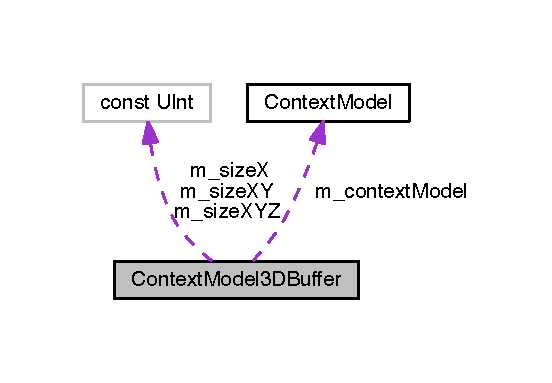
\includegraphics[width=265pt]{d9/dc6/class_context_model3_d_buffer__coll__graph}
\end{center}
\end{figure}
\subsection*{Public Member Functions}
\begin{DoxyCompactItemize}
\item 
\mbox{\Hypertarget{class_context_model3_d_buffer_a5f0be0638598ba0bd552335f92d4f0b6}\label{class_context_model3_d_buffer_a5f0be0638598ba0bd552335f92d4f0b6}} 
\hyperlink{class_context_model}{Context\+Model} \& {\bfseries get} (U\+Int uiZ, U\+Int uiY, U\+Int uiX)
\item 
\mbox{\Hypertarget{class_context_model3_d_buffer_a038d0eef0b3911c98a21be6c394096ce}\label{class_context_model3_d_buffer_a038d0eef0b3911c98a21be6c394096ce}} 
\hyperlink{class_context_model}{Context\+Model} $\ast$ {\bfseries get} (U\+Int uiZ, U\+Int uiY)
\item 
\mbox{\Hypertarget{class_context_model3_d_buffer_a70ed7ef9f395bc0610a0047640df3cb4}\label{class_context_model3_d_buffer_a70ed7ef9f395bc0610a0047640df3cb4}} 
\hyperlink{class_context_model}{Context\+Model} $\ast$ {\bfseries get} (U\+Int uiZ)
\item 
Void \hyperlink{class_context_model3_d_buffer_a3d73c7fc6d143aac1d7fdafd32e986d1}{copy\+From} (const \hyperlink{class_context_model3_d_buffer}{Context\+Model3\+D\+Buffer} $\ast$src)
\end{DoxyCompactItemize}
{\bf }\par
\begin{DoxyCompactItemize}
\item 
\mbox{\Hypertarget{class_context_model3_d_buffer_a37a8f7e525264bca5f500b2cb938f740}\label{class_context_model3_d_buffer_a37a8f7e525264bca5f500b2cb938f740}} 
{\bfseries Context\+Model3\+D\+Buffer} (U\+Int ui\+SizeZ, U\+Int ui\+SizeY, U\+Int ui\+SizeX, \hyperlink{class_context_model}{Context\+Model} $\ast$base\+Ptr, Int \&count)
\item 
Void \hyperlink{class_context_model3_d_buffer_a239420ca283a9f98e928a0d4e239fa0d}{init\+Buffer} (\hyperlink{_type_def_8h_a8fc5fd31653a387f7430d29863620f71}{Slice\+Type} e\+Slice\+Type, Int i\+Qp, U\+Char $\ast$ctx\+Model)
\begin{DoxyCompactList}\small\item\em initialize 3D buffer by slice type \& QP \end{DoxyCompactList}\item 
U\+Int \hyperlink{class_context_model3_d_buffer_abc2178783028a2556a5c8c24e67811dc}{calc\+Cost} (\hyperlink{_type_def_8h_a8fc5fd31653a387f7430d29863620f71}{Slice\+Type} slice\+Type, Int qp, U\+Char $\ast$ctx\+Model)
\begin{DoxyCompactList}\small\item\em determine cost of choosing a probability table based on current probabilities \end{DoxyCompactList}\end{DoxyCompactItemize}

\subsection*{Protected Attributes}
\begin{DoxyCompactItemize}
\item 
\mbox{\Hypertarget{class_context_model3_d_buffer_a302c83d47ee3e91238f04639738d997c}\label{class_context_model3_d_buffer_a302c83d47ee3e91238f04639738d997c}} 
\hyperlink{class_context_model}{Context\+Model} $\ast$ \hyperlink{class_context_model3_d_buffer_a302c83d47ee3e91238f04639738d997c}{m\+\_\+context\+Model}
\begin{DoxyCompactList}\small\item\em array of context models \end{DoxyCompactList}\item 
\mbox{\Hypertarget{class_context_model3_d_buffer_a6291577a0880fb9f839b9e27de1b47f9}\label{class_context_model3_d_buffer_a6291577a0880fb9f839b9e27de1b47f9}} 
const U\+Int \hyperlink{class_context_model3_d_buffer_a6291577a0880fb9f839b9e27de1b47f9}{m\+\_\+sizeX}
\begin{DoxyCompactList}\small\item\em X size of 3D buffer. \end{DoxyCompactList}\item 
\mbox{\Hypertarget{class_context_model3_d_buffer_a084e9fecdf5404bff4b1e209398a184a}\label{class_context_model3_d_buffer_a084e9fecdf5404bff4b1e209398a184a}} 
const U\+Int \hyperlink{class_context_model3_d_buffer_a084e9fecdf5404bff4b1e209398a184a}{m\+\_\+size\+XY}
\begin{DoxyCompactList}\small\item\em X times Y size of 3D buffer. \end{DoxyCompactList}\item 
\mbox{\Hypertarget{class_context_model3_d_buffer_a93d3fd4bbab4de2d4727f9f717f32d0b}\label{class_context_model3_d_buffer_a93d3fd4bbab4de2d4727f9f717f32d0b}} 
const U\+Int \hyperlink{class_context_model3_d_buffer_a93d3fd4bbab4de2d4727f9f717f32d0b}{m\+\_\+size\+X\+YZ}
\begin{DoxyCompactList}\small\item\em total size of 3D buffer \end{DoxyCompactList}\end{DoxyCompactItemize}


\subsection{Detailed Description}
context model 3D buffer class 

\subsection{Member Function Documentation}
\mbox{\Hypertarget{class_context_model3_d_buffer_abc2178783028a2556a5c8c24e67811dc}\label{class_context_model3_d_buffer_abc2178783028a2556a5c8c24e67811dc}} 
\index{Context\+Model3\+D\+Buffer@{Context\+Model3\+D\+Buffer}!calc\+Cost@{calc\+Cost}}
\index{calc\+Cost@{calc\+Cost}!Context\+Model3\+D\+Buffer@{Context\+Model3\+D\+Buffer}}
\subsubsection{\texorpdfstring{calc\+Cost()}{calcCost()}}
{\footnotesize\ttfamily U\+Int Context\+Model3\+D\+Buffer\+::calc\+Cost (\begin{DoxyParamCaption}\item[{\hyperlink{_type_def_8h_a8fc5fd31653a387f7430d29863620f71}{Slice\+Type}}]{slice\+Type,  }\item[{Int}]{qp,  }\item[{U\+Char $\ast$}]{ctx\+Model }\end{DoxyParamCaption})}



determine cost of choosing a probability table based on current probabilities 

Calculate the cost of choosing a probability table based on the current probability of C\+A\+B\+AC at encoder


\begin{DoxyParams}{Parameters}
{\em slice\+Type} & slice type \\
\hline
{\em qp} & input QP value \\
\hline
{\em ctx\+Model} & given probability table \\
\hline
\end{DoxyParams}
\mbox{\Hypertarget{class_context_model3_d_buffer_a3d73c7fc6d143aac1d7fdafd32e986d1}\label{class_context_model3_d_buffer_a3d73c7fc6d143aac1d7fdafd32e986d1}} 
\index{Context\+Model3\+D\+Buffer@{Context\+Model3\+D\+Buffer}!copy\+From@{copy\+From}}
\index{copy\+From@{copy\+From}!Context\+Model3\+D\+Buffer@{Context\+Model3\+D\+Buffer}}
\subsubsection{\texorpdfstring{copy\+From()}{copyFrom()}}
{\footnotesize\ttfamily Void Context\+Model3\+D\+Buffer\+::copy\+From (\begin{DoxyParamCaption}\item[{const \hyperlink{class_context_model3_d_buffer}{Context\+Model3\+D\+Buffer} $\ast$}]{src }\end{DoxyParamCaption})\hspace{0.3cm}{\ttfamily [inline]}}

copy from another buffer 
\begin{DoxyParams}{Parameters}
{\em src} & buffer to copy from \\
\hline
\end{DoxyParams}
\mbox{\Hypertarget{class_context_model3_d_buffer_a239420ca283a9f98e928a0d4e239fa0d}\label{class_context_model3_d_buffer_a239420ca283a9f98e928a0d4e239fa0d}} 
\index{Context\+Model3\+D\+Buffer@{Context\+Model3\+D\+Buffer}!init\+Buffer@{init\+Buffer}}
\index{init\+Buffer@{init\+Buffer}!Context\+Model3\+D\+Buffer@{Context\+Model3\+D\+Buffer}}
\subsubsection{\texorpdfstring{init\+Buffer()}{initBuffer()}}
{\footnotesize\ttfamily Void Context\+Model3\+D\+Buffer\+::init\+Buffer (\begin{DoxyParamCaption}\item[{\hyperlink{_type_def_8h_a8fc5fd31653a387f7430d29863620f71}{Slice\+Type}}]{slice\+Type,  }\item[{Int}]{qp,  }\item[{U\+Char $\ast$}]{ctx\+Model }\end{DoxyParamCaption})}



initialize 3D buffer by slice type \& QP 

Initialize 3D buffer with respect to slice type, QP and given initial probability table


\begin{DoxyParams}{Parameters}
{\em slice\+Type} & slice type \\
\hline
{\em qp} & input QP value \\
\hline
{\em ctx\+Model} & given probability table \\
\hline
\end{DoxyParams}


The documentation for this class was generated from the following files\+:\begin{DoxyCompactItemize}
\item 
Lib/\+T\+Lib\+Common/\hyperlink{_context_model3_d_buffer_8h}{Context\+Model3\+D\+Buffer.\+h}\item 
Lib/\+T\+Lib\+Common/\hyperlink{_context_model3_d_buffer_8cpp}{Context\+Model3\+D\+Buffer.\+cpp}\end{DoxyCompactItemize}

\hypertarget{struct_s_e_i_colour_remapping_info_1_1_c_r_ilut}{}\section{S\+E\+I\+Colour\+Remapping\+Info\+:\+:C\+R\+Ilut Struct Reference}
\label{struct_s_e_i_colour_remapping_info_1_1_c_r_ilut}\index{S\+E\+I\+Colour\+Remapping\+Info\+::\+C\+R\+Ilut@{S\+E\+I\+Colour\+Remapping\+Info\+::\+C\+R\+Ilut}}


Collaboration diagram for S\+E\+I\+Colour\+Remapping\+Info\+:\+:C\+R\+Ilut\+:
\nopagebreak
\begin{figure}[H]
\begin{center}
\leavevmode
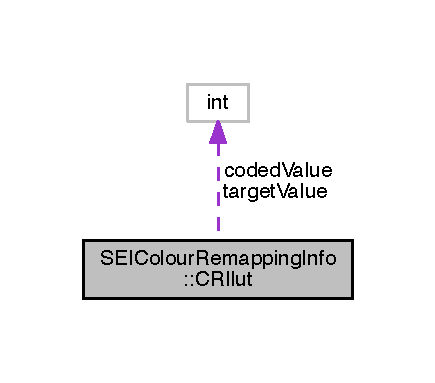
\includegraphics[width=209pt]{db/d03/struct_s_e_i_colour_remapping_info_1_1_c_r_ilut__coll__graph}
\end{center}
\end{figure}
\subsection*{Public Member Functions}
\begin{DoxyCompactItemize}
\item 
\mbox{\Hypertarget{struct_s_e_i_colour_remapping_info_1_1_c_r_ilut_a447dec24e005e671b40f655b2ad0cb16}\label{struct_s_e_i_colour_remapping_info_1_1_c_r_ilut_a447dec24e005e671b40f655b2ad0cb16}} 
bool {\bfseries operator$<$} (const \hyperlink{struct_s_e_i_colour_remapping_info_1_1_c_r_ilut}{C\+R\+Ilut} \&a) const
\end{DoxyCompactItemize}
\subsection*{Public Attributes}
\begin{DoxyCompactItemize}
\item 
\mbox{\Hypertarget{struct_s_e_i_colour_remapping_info_1_1_c_r_ilut_aff58175db1e95e725b85f43b0c8147a5}\label{struct_s_e_i_colour_remapping_info_1_1_c_r_ilut_aff58175db1e95e725b85f43b0c8147a5}} 
Int {\bfseries coded\+Value}
\item 
\mbox{\Hypertarget{struct_s_e_i_colour_remapping_info_1_1_c_r_ilut_a860344f95eb09395c962d79aaff2cb65}\label{struct_s_e_i_colour_remapping_info_1_1_c_r_ilut_a860344f95eb09395c962d79aaff2cb65}} 
Int {\bfseries target\+Value}
\end{DoxyCompactItemize}


The documentation for this struct was generated from the following file\+:\begin{DoxyCompactItemize}
\item 
Lib/\+T\+Lib\+Common/S\+E\+I.\+h\end{DoxyCompactItemize}

\hypertarget{class_dist_param}{}\section{Dist\+Param Class Reference}
\label{class_dist_param}\index{Dist\+Param@{Dist\+Param}}


distortion parameter class  




{\ttfamily \#include $<$T\+Com\+Rd\+Cost.\+h$>$}



Collaboration diagram for Dist\+Param\+:
\nopagebreak
\begin{figure}[H]
\begin{center}
\leavevmode
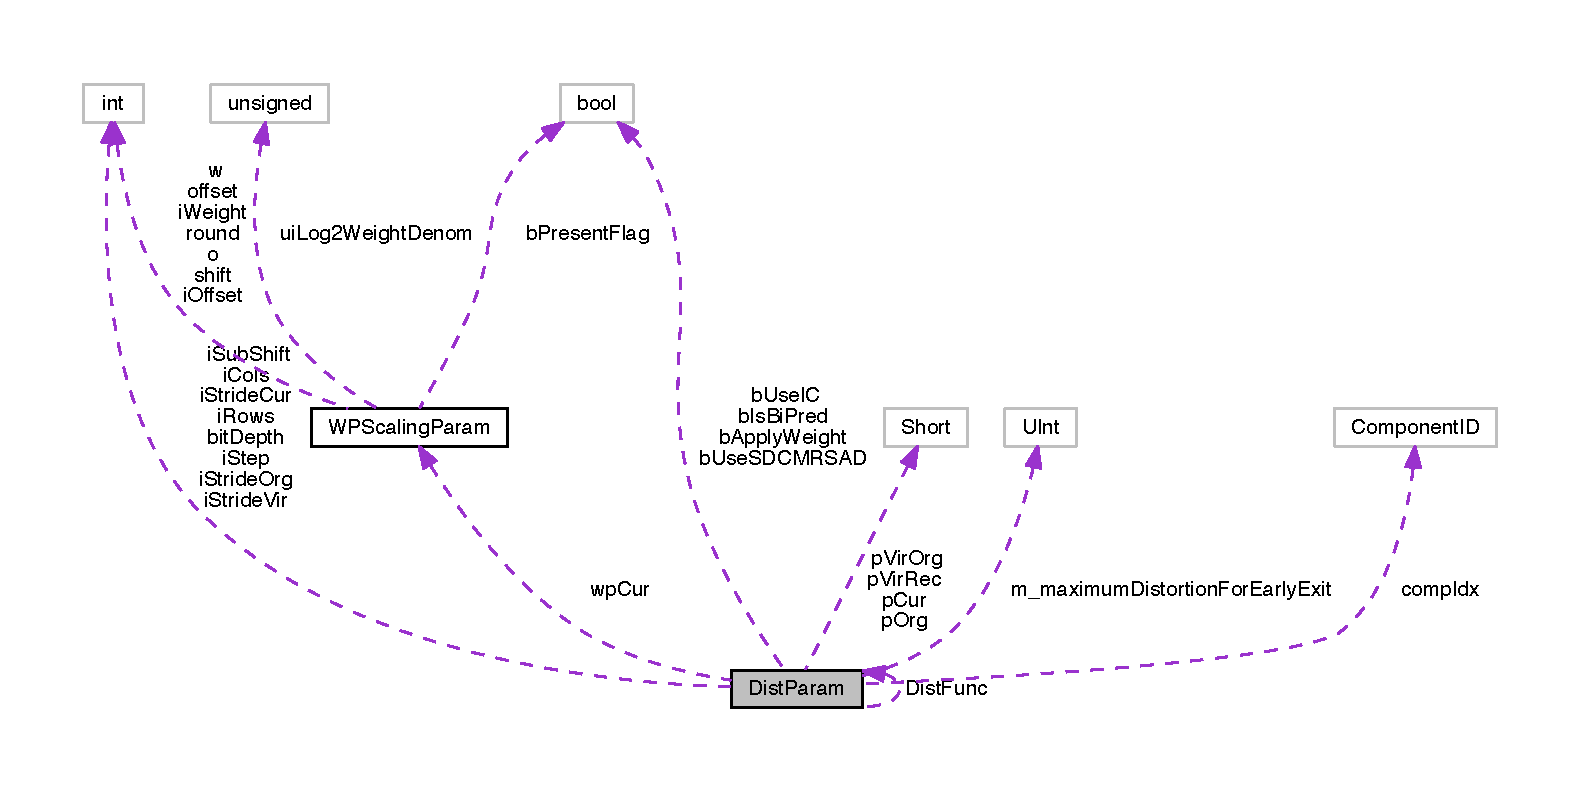
\includegraphics[width=350pt]{d0/d7f/class_dist_param__coll__graph}
\end{center}
\end{figure}
\subsection*{Public Attributes}
\begin{DoxyCompactItemize}
\item 
\mbox{\Hypertarget{class_dist_param_a1b1ee4ff034d6332c2438683f70c662a}\label{class_dist_param_a1b1ee4ff034d6332c2438683f70c662a}} 
const \hyperlink{_type_def_8h_af92141699657699b4b547be0c8517541}{Pel} $\ast$ {\bfseries p\+Org}
\item 
\mbox{\Hypertarget{class_dist_param_a926f9ff6b9644b17227dcad0914fc437}\label{class_dist_param_a926f9ff6b9644b17227dcad0914fc437}} 
const \hyperlink{_type_def_8h_af92141699657699b4b547be0c8517541}{Pel} $\ast$ {\bfseries p\+Cur}
\item 
\mbox{\Hypertarget{class_dist_param_aef12cf9cc725e4dcd0b1185ea750a936}\label{class_dist_param_aef12cf9cc725e4dcd0b1185ea750a936}} 
Int {\bfseries i\+Stride\+Org}
\item 
\mbox{\Hypertarget{class_dist_param_a1fd18063e458b91cf52bc4fb656f2479}\label{class_dist_param_a1fd18063e458b91cf52bc4fb656f2479}} 
Int {\bfseries i\+Stride\+Cur}
\item 
\mbox{\Hypertarget{class_dist_param_a0c6a89e1715ec192d066fab91cd80fe8}\label{class_dist_param_a0c6a89e1715ec192d066fab91cd80fe8}} 
\hyperlink{_type_def_8h_af92141699657699b4b547be0c8517541}{Pel} $\ast$ {\bfseries p\+Vir\+Rec}
\item 
\mbox{\Hypertarget{class_dist_param_a99187749c16036b81b00fbd8a5237b29}\label{class_dist_param_a99187749c16036b81b00fbd8a5237b29}} 
\hyperlink{_type_def_8h_af92141699657699b4b547be0c8517541}{Pel} $\ast$ {\bfseries p\+Vir\+Org}
\item 
\mbox{\Hypertarget{class_dist_param_a37ace4b09d8895facabec19573603fce}\label{class_dist_param_a37ace4b09d8895facabec19573603fce}} 
Int {\bfseries i\+Stride\+Vir}
\item 
\mbox{\Hypertarget{class_dist_param_a061af83280b27255226c1c9914f46e28}\label{class_dist_param_a061af83280b27255226c1c9914f46e28}} 
Bool {\bfseries b\+Use\+IC}
\item 
\mbox{\Hypertarget{class_dist_param_a3ce1f8b67427a7b75b28592d80859e56}\label{class_dist_param_a3ce1f8b67427a7b75b28592d80859e56}} 
Bool {\bfseries b\+Use\+S\+D\+C\+M\+R\+S\+AD}
\item 
\mbox{\Hypertarget{class_dist_param_a341628b73aba590acbdbc9539b4e462e}\label{class_dist_param_a341628b73aba590acbdbc9539b4e462e}} 
Int {\bfseries i\+Rows}
\item 
\mbox{\Hypertarget{class_dist_param_a9d372127b6ae9c260ff0a1320732eb2f}\label{class_dist_param_a9d372127b6ae9c260ff0a1320732eb2f}} 
Int {\bfseries i\+Cols}
\item 
\mbox{\Hypertarget{class_dist_param_a2589c0f4852def35e54c2e2fdb45981c}\label{class_dist_param_a2589c0f4852def35e54c2e2fdb45981c}} 
Int {\bfseries i\+Step}
\item 
\mbox{\Hypertarget{class_dist_param_ad9217506bbc0efce35992e21ec27b9fd}\label{class_dist_param_ad9217506bbc0efce35992e21ec27b9fd}} 
Fp\+Dist\+Func {\bfseries Dist\+Func}
\item 
\mbox{\Hypertarget{class_dist_param_a435119776ba8790a484bd1ff990e6b7a}\label{class_dist_param_a435119776ba8790a484bd1ff990e6b7a}} 
Int {\bfseries bit\+Depth}
\item 
\mbox{\Hypertarget{class_dist_param_a1291154be19384395f2dc7238f215d6e}\label{class_dist_param_a1291154be19384395f2dc7238f215d6e}} 
Bool {\bfseries b\+Apply\+Weight}
\item 
\mbox{\Hypertarget{class_dist_param_af416e6a0e2c35aa05ec8d2406ffeb48b}\label{class_dist_param_af416e6a0e2c35aa05ec8d2406ffeb48b}} 
Bool {\bfseries b\+Is\+Bi\+Pred}
\item 
\mbox{\Hypertarget{class_dist_param_a250fe2131cc7706e28c16af1d7985fe6}\label{class_dist_param_a250fe2131cc7706e28c16af1d7985fe6}} 
const \hyperlink{struct_w_p_scaling_param}{W\+P\+Scaling\+Param} $\ast$ {\bfseries wp\+Cur}
\item 
\mbox{\Hypertarget{class_dist_param_acc58d5e29df32b0c7910966189a58eac}\label{class_dist_param_acc58d5e29df32b0c7910966189a58eac}} 
Component\+ID {\bfseries comp\+Idx}
\item 
\mbox{\Hypertarget{class_dist_param_ad38cf08a103b178e19c698326498904d}\label{class_dist_param_ad38cf08a103b178e19c698326498904d}} 
\hyperlink{_type_def_8h_aed82b23ef6849d0bc3d95c92102d5b50}{Distortion} {\bfseries m\+\_\+maximum\+Distortion\+For\+Early\+Exit}
\item 
\mbox{\Hypertarget{class_dist_param_a7a06ed325f601121ef3629d23b27f538}\label{class_dist_param_a7a06ed325f601121ef3629d23b27f538}} 
Int \hyperlink{class_dist_param_a7a06ed325f601121ef3629d23b27f538}{i\+Sub\+Shift}
\begin{DoxyCompactList}\small\item\em During cost calculations, if distortion exceeds this value, cost calculations may early-\/terminate. \end{DoxyCompactList}\end{DoxyCompactItemize}


\subsection{Detailed Description}
distortion parameter class 

The documentation for this class was generated from the following file\+:\begin{DoxyCompactItemize}
\item 
Lib/\+T\+Lib\+Common/\hyperlink{_t_com_rd_cost_8h}{T\+Com\+Rd\+Cost.\+h}\end{DoxyCompactItemize}

\hypertarget{class_efficient_field_i_r_a_p_mapping}{}\section{Efficient\+Field\+I\+R\+A\+P\+Mapping Class Reference}
\label{class_efficient_field_i_r_a_p_mapping}\index{Efficient\+Field\+I\+R\+A\+P\+Mapping@{Efficient\+Field\+I\+R\+A\+P\+Mapping}}
\subsection*{Public Member Functions}
\begin{DoxyCompactItemize}
\item 
\mbox{\Hypertarget{class_efficient_field_i_r_a_p_mapping_adb25ecb5449c6742ac7db401701153f4}\label{class_efficient_field_i_r_a_p_mapping_adb25ecb5449c6742ac7db401701153f4}} 
Int {\bfseries Get\+I\+R\+A\+P\+G\+O\+Pid} () const
\end{DoxyCompactItemize}
{\bf }\par
\begin{DoxyCompactItemize}
\item 
\mbox{\Hypertarget{class_efficient_field_i_r_a_p_mapping_a5aa6667d7769a1fb42c83bb06cbfd03b}\label{class_efficient_field_i_r_a_p_mapping_a5aa6667d7769a1fb42c83bb06cbfd03b}} 
Void {\bfseries initialize} (const Bool is\+Field, const Int gop\+Size, const Int P\+O\+C\+Last, const Int num\+Pic\+Rcvd, const Int last\+I\+DR, \hyperlink{class_t_enc_g_o_p}{T\+Enc\+G\+OP} $\ast$p\+Enc\+Gop, \hyperlink{class_t_enc_cfg}{T\+Enc\+Cfg} $\ast$p\+Cfg)
\item 
\mbox{\Hypertarget{class_efficient_field_i_r_a_p_mapping_a271040a7ee80df43d8dd7e15bd55be7d}\label{class_efficient_field_i_r_a_p_mapping_a271040a7ee80df43d8dd7e15bd55be7d}} 
Int {\bfseries adjust\+G\+O\+Pid} (const Int gop\+ID)
\item 
\mbox{\Hypertarget{class_efficient_field_i_r_a_p_mapping_a69a2bab4fbf04dbfe912b11430c7be70}\label{class_efficient_field_i_r_a_p_mapping_a69a2bab4fbf04dbfe912b11430c7be70}} 
Int {\bfseries restore\+G\+O\+Pid} (const Int gop\+ID)
\end{DoxyCompactItemize}



The documentation for this class was generated from the following file\+:\begin{DoxyCompactItemize}
\item 
Lib/\+T\+Lib\+Encoder/\hyperlink{_t_enc_g_o_p_8cpp}{T\+Enc\+G\+O\+P.\+cpp}\end{DoxyCompactItemize}

\hypertarget{class_env_var}{}\section{Env\+Var Class Reference}
\label{class_env_var}\index{Env\+Var@{Env\+Var}}
\subsection*{Public Member Functions}
\begin{DoxyCompactItemize}
\item 
\mbox{\Hypertarget{class_env_var_a43c64ab8cb6e2f5fefb48bb23f0a1ebc}\label{class_env_var_a43c64ab8cb6e2f5fefb48bb23f0a1ebc}} 
{\bfseries Env\+Var} (const std\+::string \&s\+Name, const std\+::string \&s\+Default, const std\+::string \&s\+Help)
\item 
\mbox{\Hypertarget{class_env_var_a3c362974643e9562c41ed9c16061aaba}\label{class_env_var_a3c362974643e9562c41ed9c16061aaba}} 
Double {\bfseries get\+Double} () const
\item 
\mbox{\Hypertarget{class_env_var_af0c4930ea53ed39ab50a66b6d3654f33}\label{class_env_var_af0c4930ea53ed39ab50a66b6d3654f33}} 
Int {\bfseries get\+Int} () const
\item 
\mbox{\Hypertarget{class_env_var_a9ec469eeeae266d0ebef01f6e0fe73ea}\label{class_env_var_a9ec469eeeae266d0ebef01f6e0fe73ea}} 
const std\+::string \& {\bfseries get\+String} () const
\item 
\mbox{\Hypertarget{class_env_var_ab10cf37f2605210a803098c9327db066}\label{class_env_var_ab10cf37f2605210a803098c9327db066}} 
Bool {\bfseries is\+Set} () const
\item 
\mbox{\Hypertarget{class_env_var_ae48015871f2bae664a5cc9fc059c7dde}\label{class_env_var_ae48015871f2bae664a5cc9fc059c7dde}} 
Bool {\bfseries is\+True} () const
\item 
\mbox{\Hypertarget{class_env_var_a5a8bbbecae236448786e9c1eac869639}\label{class_env_var_a5a8bbbecae236448786e9c1eac869639}} 
const std\+::string \& {\bfseries get\+Name} () const
\end{DoxyCompactItemize}
\subsection*{Static Public Member Functions}
\begin{DoxyCompactItemize}
\item 
\mbox{\Hypertarget{class_env_var_a3a7189a88899dca2fb0f86ed9ad704de}\label{class_env_var_a3a7189a88899dca2fb0f86ed9ad704de}} 
static std\+::list$<$ std\+::pair$<$ std\+::string, std\+::string $>$ $>$ \& {\bfseries get\+Env\+Var\+List} ()
\item 
\mbox{\Hypertarget{class_env_var_a455283723f3b43d59e343d6eb0d9b3a1}\label{class_env_var_a455283723f3b43d59e343d6eb0d9b3a1}} 
static std\+::list$<$ \hyperlink{class_env_var}{Env\+Var} $\ast$ $>$ \& {\bfseries get\+Env\+Var\+In\+Use} ()
\item 
\mbox{\Hypertarget{class_env_var_a6e5575ec4bf81f2464b0c56aa49dafb9}\label{class_env_var_a6e5575ec4bf81f2464b0c56aa49dafb9}} 
static Void {\bfseries print\+Env\+Var} ()
\item 
\mbox{\Hypertarget{class_env_var_a9a4f697f1462d1ed8d5f1ff603932f93}\label{class_env_var_a9a4f697f1462d1ed8d5f1ff603932f93}} 
static Void {\bfseries print\+Env\+Var\+In\+Use} ()
\end{DoxyCompactItemize}


The documentation for this class was generated from the following files\+:\begin{DoxyCompactItemize}
\item 
Lib/\+T\+Lib\+Common/\hyperlink{_debug_8h}{Debug.\+h}\item 
Lib/\+T\+Lib\+Common/\hyperlink{_debug_8cpp}{Debug.\+cpp}\end{DoxyCompactItemize}

\hypertarget{structdf_1_1program__options__lite_1_1_error_reporter}{}\section{df\+:\+:program\+\_\+options\+\_\+lite\+:\+:Error\+Reporter Struct Reference}
\label{structdf_1_1program__options__lite_1_1_error_reporter}\index{df\+::program\+\_\+options\+\_\+lite\+::\+Error\+Reporter@{df\+::program\+\_\+options\+\_\+lite\+::\+Error\+Reporter}}


Collaboration diagram for df\+:\+:program\+\_\+options\+\_\+lite\+:\+:Error\+Reporter\+:
\nopagebreak
\begin{figure}[H]
\begin{center}
\leavevmode
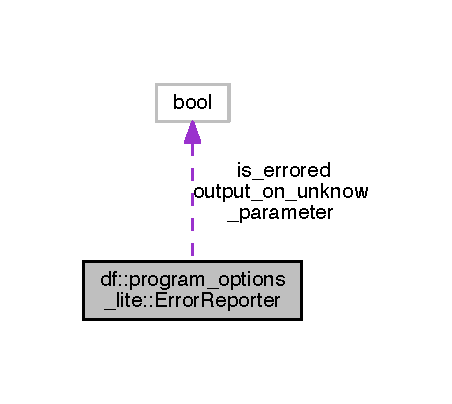
\includegraphics[width=217pt]{d5/d07/structdf_1_1program__options__lite_1_1_error_reporter__coll__graph}
\end{center}
\end{figure}
\subsection*{Public Member Functions}
\begin{DoxyCompactItemize}
\item 
\mbox{\Hypertarget{structdf_1_1program__options__lite_1_1_error_reporter_a48a69576c1eaa03af66cade8ee9b2df4}\label{structdf_1_1program__options__lite_1_1_error_reporter_a48a69576c1eaa03af66cade8ee9b2df4}} 
virtual std\+::ostream \& {\bfseries error} (const std\+::string \&where)
\item 
\mbox{\Hypertarget{structdf_1_1program__options__lite_1_1_error_reporter_a7ab5233983ae6ca3ce93f3d4f2cb153f}\label{structdf_1_1program__options__lite_1_1_error_reporter_a7ab5233983ae6ca3ce93f3d4f2cb153f}} 
virtual std\+::ostream \& {\bfseries warn} (const std\+::string \&where)
\end{DoxyCompactItemize}
\subsection*{Public Attributes}
\begin{DoxyCompactItemize}
\item 
\mbox{\Hypertarget{structdf_1_1program__options__lite_1_1_error_reporter_ad25ff3165311cba2f3c12d25843a7cc2}\label{structdf_1_1program__options__lite_1_1_error_reporter_ad25ff3165311cba2f3c12d25843a7cc2}} 
bool {\bfseries is\+\_\+errored}
\item 
\mbox{\Hypertarget{structdf_1_1program__options__lite_1_1_error_reporter_af2503a95e98ec411fadfb1f6d1ca1086}\label{structdf_1_1program__options__lite_1_1_error_reporter_af2503a95e98ec411fadfb1f6d1ca1086}} 
bool {\bfseries output\+\_\+on\+\_\+unknow\+\_\+parameter}
\end{DoxyCompactItemize}


The documentation for this struct was generated from the following files\+:\begin{DoxyCompactItemize}
\item 
Lib/\+T\+App\+Common/program\+\_\+options\+\_\+lite.\+h\item 
Lib/\+T\+App\+Common/program\+\_\+options\+\_\+lite.\+cpp\end{DoxyCompactItemize}

\hypertarget{structest_bits_sbac_struct}{}\section{est\+Bits\+Sbac\+Struct Struct Reference}
\label{structest_bits_sbac_struct}\index{est\+Bits\+Sbac\+Struct@{est\+Bits\+Sbac\+Struct}}


Collaboration diagram for est\+Bits\+Sbac\+Struct\+:
\nopagebreak
\begin{figure}[H]
\begin{center}
\leavevmode
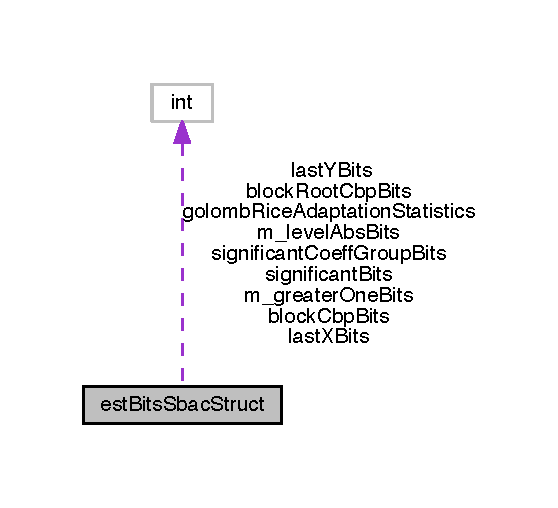
\includegraphics[width=268pt]{d4/d86/structest_bits_sbac_struct__coll__graph}
\end{center}
\end{figure}
\subsection*{Public Attributes}
\begin{DoxyCompactItemize}
\item 
\mbox{\Hypertarget{structest_bits_sbac_struct_a93d160dbbb7c4e9ada68c8d01b7d2ed7}\label{structest_bits_sbac_struct_a93d160dbbb7c4e9ada68c8d01b7d2ed7}} 
Int {\bfseries significant\+Coeff\+Group\+Bits} \mbox{[}\hyperlink{_context_tables_8h_a95362f072f2eefa97ebac51d3e01263e}{N\+U\+M\+\_\+\+S\+I\+G\+\_\+\+C\+G\+\_\+\+F\+L\+A\+G\+\_\+\+C\+TX}\mbox{]}\mbox{[}2\mbox{]}
\item 
\mbox{\Hypertarget{structest_bits_sbac_struct_a1ddcf0fb30662b8f25fd4f4aa547efab}\label{structest_bits_sbac_struct_a1ddcf0fb30662b8f25fd4f4aa547efab}} 
Int {\bfseries significant\+Bits} \mbox{[}\hyperlink{_context_tables_8h_a0607d830ae7ae04b190ab90bdeaefc5f}{N\+U\+M\+\_\+\+S\+I\+G\+\_\+\+F\+L\+A\+G\+\_\+\+C\+TX}\mbox{]}\mbox{[}2\mbox{]}
\item 
\mbox{\Hypertarget{structest_bits_sbac_struct_a562f15a1bd86a339c2bdfdb431c62f3f}\label{structest_bits_sbac_struct_a562f15a1bd86a339c2bdfdb431c62f3f}} 
Int {\bfseries last\+X\+Bits} \mbox{[}M\+A\+X\+\_\+\+N\+U\+M\+\_\+\+C\+H\+A\+N\+N\+E\+L\+\_\+\+T\+Y\+PE\mbox{]}\mbox{[}L\+A\+S\+T\+\_\+\+S\+I\+G\+N\+I\+F\+I\+C\+A\+N\+T\+\_\+\+G\+R\+O\+U\+PS\mbox{]}
\item 
\mbox{\Hypertarget{structest_bits_sbac_struct_af83a80e4ff2064c99000908062931ca2}\label{structest_bits_sbac_struct_af83a80e4ff2064c99000908062931ca2}} 
Int {\bfseries last\+Y\+Bits} \mbox{[}M\+A\+X\+\_\+\+N\+U\+M\+\_\+\+C\+H\+A\+N\+N\+E\+L\+\_\+\+T\+Y\+PE\mbox{]}\mbox{[}L\+A\+S\+T\+\_\+\+S\+I\+G\+N\+I\+F\+I\+C\+A\+N\+T\+\_\+\+G\+R\+O\+U\+PS\mbox{]}
\item 
\mbox{\Hypertarget{structest_bits_sbac_struct_aafb182b5a8da4b717eb05e8e738bb81e}\label{structest_bits_sbac_struct_aafb182b5a8da4b717eb05e8e738bb81e}} 
Int {\bfseries m\+\_\+greater\+One\+Bits} \mbox{[}\hyperlink{_context_tables_8h_a6d9111fbd577c4835158707c5ac14a9f}{N\+U\+M\+\_\+\+O\+N\+E\+\_\+\+F\+L\+A\+G\+\_\+\+C\+TX}\mbox{]}\mbox{[}2\mbox{]}
\item 
\mbox{\Hypertarget{structest_bits_sbac_struct_a045b71f97120c4988ad5688ba9b62edb}\label{structest_bits_sbac_struct_a045b71f97120c4988ad5688ba9b62edb}} 
Int {\bfseries m\+\_\+level\+Abs\+Bits} \mbox{[}\hyperlink{_context_tables_8h_aca5bcfa2258b46bb400d5fb185279ad1}{N\+U\+M\+\_\+\+A\+B\+S\+\_\+\+F\+L\+A\+G\+\_\+\+C\+TX}\mbox{]}\mbox{[}2\mbox{]}
\item 
\mbox{\Hypertarget{structest_bits_sbac_struct_a5d5cb7f246abb10d0c4ed4dd6fc78031}\label{structest_bits_sbac_struct_a5d5cb7f246abb10d0c4ed4dd6fc78031}} 
Int {\bfseries block\+Cbp\+Bits} \mbox{[}N\+U\+M\+\_\+\+Q\+T\+\_\+\+C\+B\+F\+\_\+\+C\+T\+X\+\_\+\+S\+E\+TS $\ast$\hyperlink{_context_tables_8h_ae0b676e1722b659e8783940a0545d70a}{N\+U\+M\+\_\+\+Q\+T\+\_\+\+C\+B\+F\+\_\+\+C\+T\+X\+\_\+\+P\+E\+R\+\_\+\+S\+ET}\mbox{]}\mbox{[}2\mbox{]}
\item 
\mbox{\Hypertarget{structest_bits_sbac_struct_a3a126e7944fd32ca52e03fa39ad3f5cd}\label{structest_bits_sbac_struct_a3a126e7944fd32ca52e03fa39ad3f5cd}} 
Int {\bfseries block\+Root\+Cbp\+Bits} \mbox{[}4\mbox{]}\mbox{[}2\mbox{]}
\item 
\mbox{\Hypertarget{structest_bits_sbac_struct_a8dcb2f469377c35975b119b13cd2a6aa}\label{structest_bits_sbac_struct_a8dcb2f469377c35975b119b13cd2a6aa}} 
Int {\bfseries golomb\+Rice\+Adaptation\+Statistics} \mbox{[}R\+Ext\+\_\+\+\_\+\+G\+O\+L\+O\+M\+B\+\_\+\+R\+I\+C\+E\+\_\+\+A\+D\+A\+P\+T\+A\+T\+I\+O\+N\+\_\+\+S\+T\+A\+T\+I\+S\+T\+I\+C\+S\+\_\+\+S\+E\+TS\mbox{]}
\end{DoxyCompactItemize}


The documentation for this struct was generated from the following file\+:\begin{DoxyCompactItemize}
\item 
Lib/\+T\+Lib\+Common/\hyperlink{_t_com_tr_quant_8h}{T\+Com\+Tr\+Quant.\+h}\end{DoxyCompactItemize}

\hypertarget{class_f_d_reader}{}\section{F\+D\+Reader Class Reference}
\label{class_f_d_reader}\index{F\+D\+Reader@{F\+D\+Reader}}


Inheritance diagram for F\+D\+Reader\+:
\nopagebreak
\begin{figure}[H]
\begin{center}
\leavevmode
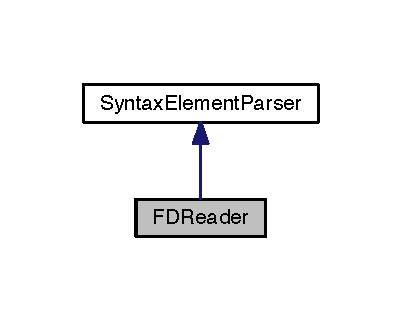
\includegraphics[width=193pt]{df/d5d/class_f_d_reader__inherit__graph}
\end{center}
\end{figure}


Collaboration diagram for F\+D\+Reader\+:
\nopagebreak
\begin{figure}[H]
\begin{center}
\leavevmode
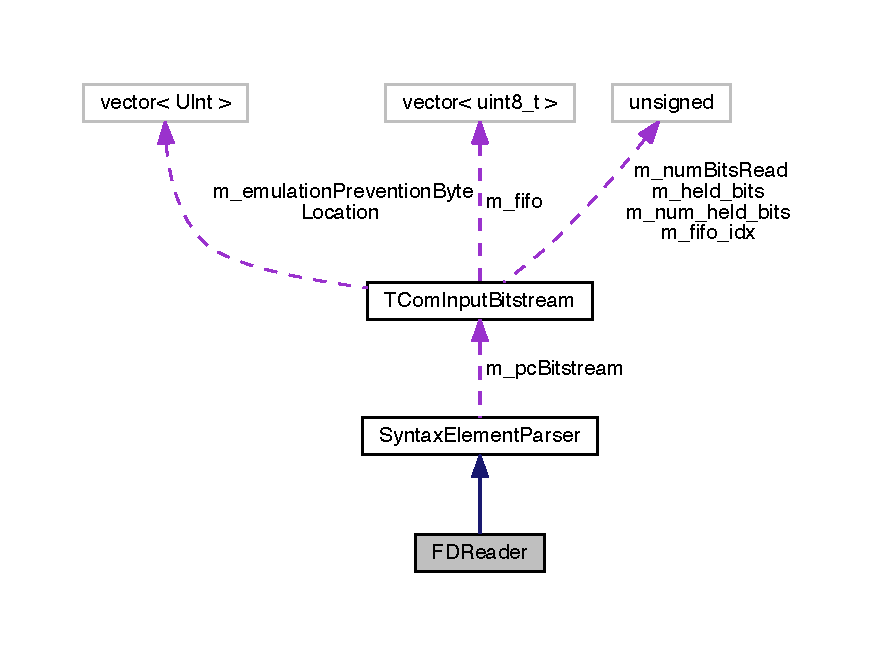
\includegraphics[width=350pt]{d8/d9e/class_f_d_reader__coll__graph}
\end{center}
\end{figure}
\subsection*{Public Member Functions}
{\bf }\par
\begin{DoxyCompactItemize}
\item 
\mbox{\Hypertarget{class_f_d_reader_ae4fd6c0ebbffc354c925e7277237b434}\label{class_f_d_reader_ae4fd6c0ebbffc354c925e7277237b434}} 
Void {\bfseries parse\+Filler\+Data} (\hyperlink{class_t_com_input_bitstream}{T\+Com\+Input\+Bitstream} $\ast$bs, U\+Int \&fd\+Size)
\end{DoxyCompactItemize}

\subsection*{Additional Inherited Members}


The documentation for this class was generated from the following files\+:\begin{DoxyCompactItemize}
\item 
Lib/\+T\+Lib\+Decoder/\hyperlink{_syntax_element_parser_8h}{Syntax\+Element\+Parser.\+h}\item 
Lib/\+T\+Lib\+Decoder/\hyperlink{_syntax_element_parser_8cpp}{Syntax\+Element\+Parser.\+cpp}\end{DoxyCompactItemize}

\hypertarget{struct_g_o_p_entry}{}\section{G\+O\+P\+Entry Struct Reference}
\label{struct_g_o_p_entry}\index{G\+O\+P\+Entry@{G\+O\+P\+Entry}}


Collaboration diagram for G\+O\+P\+Entry\+:
\nopagebreak
\begin{figure}[H]
\begin{center}
\leavevmode
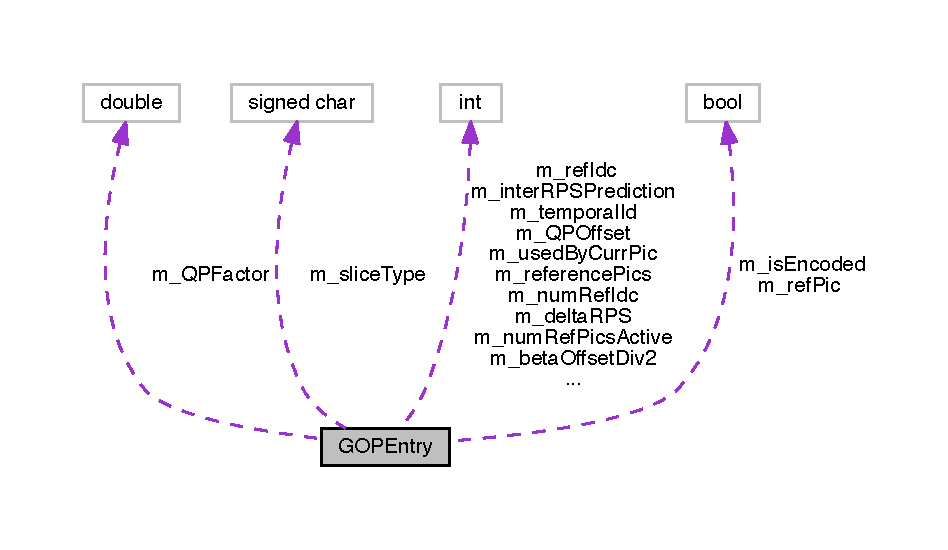
\includegraphics[width=350pt]{dd/d09/struct_g_o_p_entry__coll__graph}
\end{center}
\end{figure}
\subsection*{Public Attributes}
\begin{DoxyCompactItemize}
\item 
\mbox{\Hypertarget{struct_g_o_p_entry_aca36be0a58cbed7b2e2fe3ccb7f7c74b}\label{struct_g_o_p_entry_aca36be0a58cbed7b2e2fe3ccb7f7c74b}} 
Int {\bfseries m\+\_\+\+P\+OC}
\item 
\mbox{\Hypertarget{struct_g_o_p_entry_ad38552b4af3be8588d47c5a75bffece3}\label{struct_g_o_p_entry_ad38552b4af3be8588d47c5a75bffece3}} 
Int {\bfseries m\+\_\+\+Q\+P\+Offset}
\item 
\mbox{\Hypertarget{struct_g_o_p_entry_a7364f0bb0a976b4d1e4c67edd3eb6f4d}\label{struct_g_o_p_entry_a7364f0bb0a976b4d1e4c67edd3eb6f4d}} 
Double {\bfseries m\+\_\+\+Q\+P\+Factor}
\item 
\mbox{\Hypertarget{struct_g_o_p_entry_ad2e31c3f6d8015a62eff0ec15ac153c1}\label{struct_g_o_p_entry_ad2e31c3f6d8015a62eff0ec15ac153c1}} 
Int {\bfseries m\+\_\+tc\+Offset\+Div2}
\item 
\mbox{\Hypertarget{struct_g_o_p_entry_ae8815062d7c7037528ade6c3c6f9d0bc}\label{struct_g_o_p_entry_ae8815062d7c7037528ade6c3c6f9d0bc}} 
Int {\bfseries m\+\_\+beta\+Offset\+Div2}
\item 
\mbox{\Hypertarget{struct_g_o_p_entry_ad242c9751d7352bb4544c98dd42f4f9b}\label{struct_g_o_p_entry_ad242c9751d7352bb4544c98dd42f4f9b}} 
Int {\bfseries m\+\_\+temporal\+Id}
\item 
\mbox{\Hypertarget{struct_g_o_p_entry_ad948dd70ba8f0071763f2354433189bb}\label{struct_g_o_p_entry_ad948dd70ba8f0071763f2354433189bb}} 
Bool {\bfseries m\+\_\+ref\+Pic}
\item 
\mbox{\Hypertarget{struct_g_o_p_entry_a9611cafff9cbde9bd2a6def0a2f922b5}\label{struct_g_o_p_entry_a9611cafff9cbde9bd2a6def0a2f922b5}} 
Int {\bfseries m\+\_\+num\+Ref\+Pics\+Active}
\item 
\mbox{\Hypertarget{struct_g_o_p_entry_ac06c61535222d5cb1e0844f435f357ba}\label{struct_g_o_p_entry_ac06c61535222d5cb1e0844f435f357ba}} 
S\+Char {\bfseries m\+\_\+slice\+Type}
\item 
\mbox{\Hypertarget{struct_g_o_p_entry_a11927e2a6b55b8c5f2a0c7966663b63f}\label{struct_g_o_p_entry_a11927e2a6b55b8c5f2a0c7966663b63f}} 
Int {\bfseries m\+\_\+num\+Ref\+Pics}
\item 
\mbox{\Hypertarget{struct_g_o_p_entry_abace297545c339dd323bba332e3d0277}\label{struct_g_o_p_entry_abace297545c339dd323bba332e3d0277}} 
Int {\bfseries m\+\_\+reference\+Pics} \mbox{[}M\+A\+X\+\_\+\+N\+U\+M\+\_\+\+R\+E\+F\+\_\+\+P\+I\+CS\mbox{]}
\item 
\mbox{\Hypertarget{struct_g_o_p_entry_a4c11d80bed3aab0e7cd45637214f6a0e}\label{struct_g_o_p_entry_a4c11d80bed3aab0e7cd45637214f6a0e}} 
Int {\bfseries m\+\_\+used\+By\+Curr\+Pic} \mbox{[}M\+A\+X\+\_\+\+N\+U\+M\+\_\+\+R\+E\+F\+\_\+\+P\+I\+CS\mbox{]}
\item 
\mbox{\Hypertarget{struct_g_o_p_entry_a86e2434cc7218a011365ac4edbdb2261}\label{struct_g_o_p_entry_a86e2434cc7218a011365ac4edbdb2261}} 
Int {\bfseries m\+\_\+inter\+R\+P\+S\+Prediction}
\item 
\mbox{\Hypertarget{struct_g_o_p_entry_ae1205e8365fa2ff0d444b3d9d60d9565}\label{struct_g_o_p_entry_ae1205e8365fa2ff0d444b3d9d60d9565}} 
Int {\bfseries m\+\_\+delta\+R\+PS}
\item 
\mbox{\Hypertarget{struct_g_o_p_entry_a7fb2d245f2e3733c9b4d5f23f2c1bbf7}\label{struct_g_o_p_entry_a7fb2d245f2e3733c9b4d5f23f2c1bbf7}} 
Int {\bfseries m\+\_\+num\+Ref\+Idc}
\item 
\mbox{\Hypertarget{struct_g_o_p_entry_ac69ebc8d74b04c654495c883b4a06206}\label{struct_g_o_p_entry_ac69ebc8d74b04c654495c883b4a06206}} 
Int {\bfseries m\+\_\+ref\+Idc} \mbox{[}M\+A\+X\+\_\+\+N\+U\+M\+\_\+\+R\+E\+F\+\_\+\+P\+I\+CS+1\mbox{]}
\item 
\mbox{\Hypertarget{struct_g_o_p_entry_a0cf4132767543a0d2043a7d0e50cb2a4}\label{struct_g_o_p_entry_a0cf4132767543a0d2043a7d0e50cb2a4}} 
Bool {\bfseries m\+\_\+is\+Encoded}
\end{DoxyCompactItemize}


The documentation for this struct was generated from the following file\+:\begin{DoxyCompactItemize}
\item 
Lib/\+T\+Lib\+Encoder/\hyperlink{_t_enc_cfg_8h}{T\+Enc\+Cfg.\+h}\end{DoxyCompactItemize}

\hypertarget{struct_hrd_sub_layer_info}{}\section{Hrd\+Sub\+Layer\+Info Struct Reference}
\label{struct_hrd_sub_layer_info}\index{Hrd\+Sub\+Layer\+Info@{Hrd\+Sub\+Layer\+Info}}


V\+PS class.  




{\ttfamily \#include $<$T\+Com\+Slice.\+h$>$}



Collaboration diagram for Hrd\+Sub\+Layer\+Info\+:
\nopagebreak
\begin{figure}[H]
\begin{center}
\leavevmode
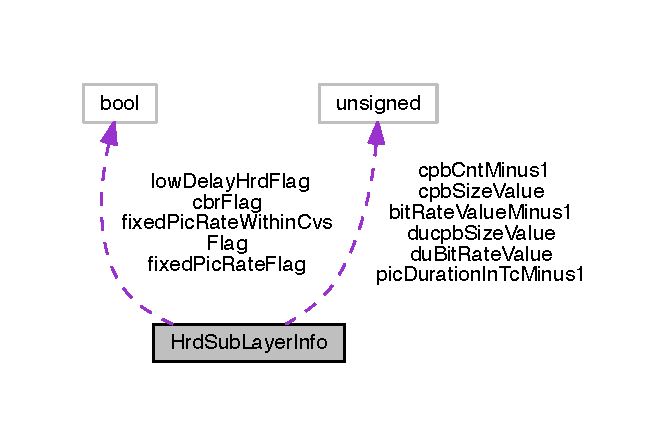
\includegraphics[width=322pt]{df/def/struct_hrd_sub_layer_info__coll__graph}
\end{center}
\end{figure}
\subsection*{Public Attributes}
\begin{DoxyCompactItemize}
\item 
\mbox{\Hypertarget{struct_hrd_sub_layer_info_a9d8ff0ed124ccb3a5e2c333da75e0b20}\label{struct_hrd_sub_layer_info_a9d8ff0ed124ccb3a5e2c333da75e0b20}} 
Bool {\bfseries fixed\+Pic\+Rate\+Flag}
\item 
\mbox{\Hypertarget{struct_hrd_sub_layer_info_a78225a271fbfaf8cd63387f3769d8be1}\label{struct_hrd_sub_layer_info_a78225a271fbfaf8cd63387f3769d8be1}} 
Bool {\bfseries fixed\+Pic\+Rate\+Within\+Cvs\+Flag}
\item 
\mbox{\Hypertarget{struct_hrd_sub_layer_info_a48d0929fa015e06402cb672532418fc5}\label{struct_hrd_sub_layer_info_a48d0929fa015e06402cb672532418fc5}} 
U\+Int {\bfseries pic\+Duration\+In\+Tc\+Minus1}
\item 
\mbox{\Hypertarget{struct_hrd_sub_layer_info_acad89ed58b01378380f49af48889f442}\label{struct_hrd_sub_layer_info_acad89ed58b01378380f49af48889f442}} 
Bool {\bfseries low\+Delay\+Hrd\+Flag}
\item 
\mbox{\Hypertarget{struct_hrd_sub_layer_info_ac028468ca600b2581a4c0072e665a4ef}\label{struct_hrd_sub_layer_info_ac028468ca600b2581a4c0072e665a4ef}} 
U\+Int {\bfseries cpb\+Cnt\+Minus1}
\item 
\mbox{\Hypertarget{struct_hrd_sub_layer_info_a4df37e1d75de994d4cbcd78112dd831f}\label{struct_hrd_sub_layer_info_a4df37e1d75de994d4cbcd78112dd831f}} 
U\+Int {\bfseries bit\+Rate\+Value\+Minus1} \mbox{[}M\+A\+X\+\_\+\+C\+P\+B\+\_\+\+C\+NT\mbox{]}\mbox{[}2\mbox{]}
\item 
\mbox{\Hypertarget{struct_hrd_sub_layer_info_af48dc1254605d1d3cf1689eaede9525c}\label{struct_hrd_sub_layer_info_af48dc1254605d1d3cf1689eaede9525c}} 
U\+Int {\bfseries cpb\+Size\+Value} \mbox{[}M\+A\+X\+\_\+\+C\+P\+B\+\_\+\+C\+NT\mbox{]}\mbox{[}2\mbox{]}
\item 
\mbox{\Hypertarget{struct_hrd_sub_layer_info_a275b31e8807c75d9fcdd8d7b3f0b91e6}\label{struct_hrd_sub_layer_info_a275b31e8807c75d9fcdd8d7b3f0b91e6}} 
U\+Int {\bfseries ducpb\+Size\+Value} \mbox{[}M\+A\+X\+\_\+\+C\+P\+B\+\_\+\+C\+NT\mbox{]}\mbox{[}2\mbox{]}
\item 
\mbox{\Hypertarget{struct_hrd_sub_layer_info_a6466e554236cf37947955455d673a2d2}\label{struct_hrd_sub_layer_info_a6466e554236cf37947955455d673a2d2}} 
Bool {\bfseries cbr\+Flag} \mbox{[}M\+A\+X\+\_\+\+C\+P\+B\+\_\+\+C\+NT\mbox{]}\mbox{[}2\mbox{]}
\item 
\mbox{\Hypertarget{struct_hrd_sub_layer_info_a586bdf4c34989403f83adf4a024006ed}\label{struct_hrd_sub_layer_info_a586bdf4c34989403f83adf4a024006ed}} 
U\+Int {\bfseries du\+Bit\+Rate\+Value} \mbox{[}M\+A\+X\+\_\+\+C\+P\+B\+\_\+\+C\+NT\mbox{]}\mbox{[}2\mbox{]}
\end{DoxyCompactItemize}


\subsection{Detailed Description}
V\+PS class. 

The documentation for this struct was generated from the following file\+:\begin{DoxyCompactItemize}
\item 
Lib/\+T\+Lib\+Common/\hyperlink{_t_com_slice_8h}{T\+Com\+Slice.\+h}\end{DoxyCompactItemize}

\hypertarget{class_initial_adjustment_parameter_parse_exception}{}\section{Initial\+Adjustment\+Parameter\+Parse\+Exception Class Reference}
\label{class_initial_adjustment_parameter_parse_exception}\index{Initial\+Adjustment\+Parameter\+Parse\+Exception@{Initial\+Adjustment\+Parameter\+Parse\+Exception}}


Thrown if there is an error parsing the initial adjustment parameter.  




{\ttfamily \#include $<$Guess\+Lambda\+Modifiers.\+h$>$}



Inheritance diagram for Initial\+Adjustment\+Parameter\+Parse\+Exception\+:
\nopagebreak
\begin{figure}[H]
\begin{center}
\leavevmode
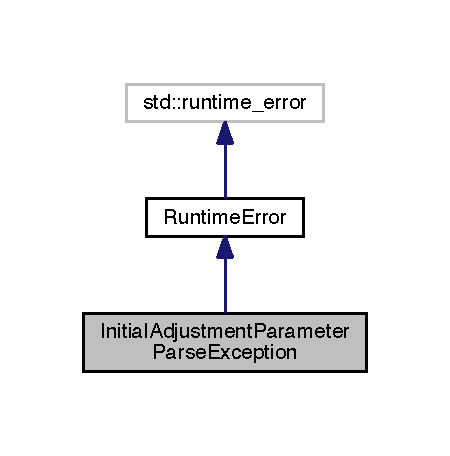
\includegraphics[width=216pt]{df/d6d/class_initial_adjustment_parameter_parse_exception__inherit__graph}
\end{center}
\end{figure}


Collaboration diagram for Initial\+Adjustment\+Parameter\+Parse\+Exception\+:
\nopagebreak
\begin{figure}[H]
\begin{center}
\leavevmode
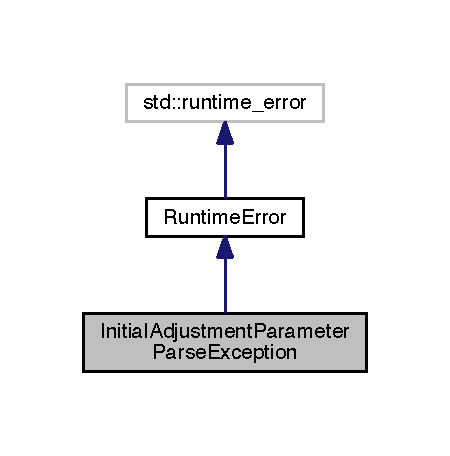
\includegraphics[width=216pt]{da/d9e/class_initial_adjustment_parameter_parse_exception__coll__graph}
\end{center}
\end{figure}
\subsection*{Protected Member Functions}
\begin{DoxyCompactItemize}
\item 
void \hyperlink{class_initial_adjustment_parameter_parse_exception_a4ca2931ba18ec5cecb76b7891aa9d2eb}{output\+What} (std\+::ostream \&o) const
\end{DoxyCompactItemize}
\subsection*{Additional Inherited Members}


\subsection{Detailed Description}
Thrown if there is an error parsing the initial adjustment parameter. 

\subsection{Member Function Documentation}
\mbox{\Hypertarget{class_initial_adjustment_parameter_parse_exception_a4ca2931ba18ec5cecb76b7891aa9d2eb}\label{class_initial_adjustment_parameter_parse_exception_a4ca2931ba18ec5cecb76b7891aa9d2eb}} 
\index{Initial\+Adjustment\+Parameter\+Parse\+Exception@{Initial\+Adjustment\+Parameter\+Parse\+Exception}!output\+What@{output\+What}}
\index{output\+What@{output\+What}!Initial\+Adjustment\+Parameter\+Parse\+Exception@{Initial\+Adjustment\+Parameter\+Parse\+Exception}}
\subsubsection{\texorpdfstring{output\+What()}{outputWhat()}}
{\footnotesize\ttfamily void Initial\+Adjustment\+Parameter\+Parse\+Exception\+::output\+What (\begin{DoxyParamCaption}\item[{std\+::ostream \&}]{o }\end{DoxyParamCaption}) const\hspace{0.3cm}{\ttfamily [inline]}, {\ttfamily [protected]}, {\ttfamily [virtual]}}

The implementing class implements this method to customize the what output 
\begin{DoxyParams}{Parameters}
{\em o} & The what stream is outputted to this parameter \\
\hline
\end{DoxyParams}


Implements \hyperlink{class_runtime_error_a5020b04a2a7fac8b1dbfbfe4a30055b0}{Runtime\+Error}.



The documentation for this class was generated from the following file\+:\begin{DoxyCompactItemize}
\item 
App/utils/\+Bitrate\+Targeting/Guess\+Lambda\+Modifiers.\+h\end{DoxyCompactItemize}

\hypertarget{class_input_byte_stream}{}\section{Input\+Byte\+Stream Class Reference}
\label{class_input_byte_stream}\index{Input\+Byte\+Stream@{Input\+Byte\+Stream}}
\subsection*{Public Member Functions}
\begin{DoxyCompactItemize}
\item 
\hyperlink{class_input_byte_stream_a1804631987950a7666072d2d1c43071a}{Input\+Byte\+Stream} (std\+::istream \&istream)
\item 
Void \hyperlink{class_input_byte_stream_a7f10425050d4ab289a554ba4dc393b6e}{reset} ()
\item 
Bool \hyperlink{class_input_byte_stream_ae4aafbd84cda302960e5f7497bdbd227}{eof\+Before\+N\+Bytes} (U\+Int n)
\item 
uint32\+\_\+t \hyperlink{class_input_byte_stream_a48ed506d95bbcbc505b2b077914aa174}{peek\+Bytes} (U\+Int n)
\item 
uint8\+\_\+t \hyperlink{class_input_byte_stream_aeb1e7066dd0598ff699fbcdaf4cba65d}{read\+Byte} ()
\item 
uint32\+\_\+t \hyperlink{class_input_byte_stream_a39c4f28d59c707f2c1d06603f6eefa0e}{read\+Bytes} (U\+Int n)
\end{DoxyCompactItemize}


\subsection{Constructor \& Destructor Documentation}
\mbox{\Hypertarget{class_input_byte_stream_a1804631987950a7666072d2d1c43071a}\label{class_input_byte_stream_a1804631987950a7666072d2d1c43071a}} 
\index{Input\+Byte\+Stream@{Input\+Byte\+Stream}!Input\+Byte\+Stream@{Input\+Byte\+Stream}}
\index{Input\+Byte\+Stream@{Input\+Byte\+Stream}!Input\+Byte\+Stream@{Input\+Byte\+Stream}}
\subsubsection{\texorpdfstring{Input\+Byte\+Stream()}{InputByteStream()}}
{\footnotesize\ttfamily Input\+Byte\+Stream\+::\+Input\+Byte\+Stream (\begin{DoxyParamCaption}\item[{std\+::istream \&}]{istream }\end{DoxyParamCaption})\hspace{0.3cm}{\ttfamily [inline]}}

Create a bytestream reader that will extract bytes from istream.

NB, it isn\textquotesingle{}t safe to access istream while in use by a \hyperlink{class_input_byte_stream}{Input\+Byte\+Stream}.

Side-\/effects\+: the exception mask of istream is set to eofbit 

\subsection{Member Function Documentation}
\mbox{\Hypertarget{class_input_byte_stream_ae4aafbd84cda302960e5f7497bdbd227}\label{class_input_byte_stream_ae4aafbd84cda302960e5f7497bdbd227}} 
\index{Input\+Byte\+Stream@{Input\+Byte\+Stream}!eof\+Before\+N\+Bytes@{eof\+Before\+N\+Bytes}}
\index{eof\+Before\+N\+Bytes@{eof\+Before\+N\+Bytes}!Input\+Byte\+Stream@{Input\+Byte\+Stream}}
\subsubsection{\texorpdfstring{eof\+Before\+N\+Bytes()}{eofBeforeNBytes()}}
{\footnotesize\ttfamily Bool Input\+Byte\+Stream\+::eof\+Before\+N\+Bytes (\begin{DoxyParamCaption}\item[{U\+Int}]{n }\end{DoxyParamCaption})\hspace{0.3cm}{\ttfamily [inline]}}

returns true if an E\+OF will be encountered within the next n bytes. \mbox{\Hypertarget{class_input_byte_stream_a48ed506d95bbcbc505b2b077914aa174}\label{class_input_byte_stream_a48ed506d95bbcbc505b2b077914aa174}} 
\index{Input\+Byte\+Stream@{Input\+Byte\+Stream}!peek\+Bytes@{peek\+Bytes}}
\index{peek\+Bytes@{peek\+Bytes}!Input\+Byte\+Stream@{Input\+Byte\+Stream}}
\subsubsection{\texorpdfstring{peek\+Bytes()}{peekBytes()}}
{\footnotesize\ttfamily uint32\+\_\+t Input\+Byte\+Stream\+::peek\+Bytes (\begin{DoxyParamCaption}\item[{U\+Int}]{n }\end{DoxyParamCaption})\hspace{0.3cm}{\ttfamily [inline]}}

return the next n bytes in the stream without advancing the stream pointer.

Returns\+: an unsigned integer representing an n byte bigendian word.

If an attempt is made to read past E\+OF, an n-\/byte word is returned, but the portion that required input bytes beyond E\+OF is undefined. \mbox{\Hypertarget{class_input_byte_stream_aeb1e7066dd0598ff699fbcdaf4cba65d}\label{class_input_byte_stream_aeb1e7066dd0598ff699fbcdaf4cba65d}} 
\index{Input\+Byte\+Stream@{Input\+Byte\+Stream}!read\+Byte@{read\+Byte}}
\index{read\+Byte@{read\+Byte}!Input\+Byte\+Stream@{Input\+Byte\+Stream}}
\subsubsection{\texorpdfstring{read\+Byte()}{readByte()}}
{\footnotesize\ttfamily uint8\+\_\+t Input\+Byte\+Stream\+::read\+Byte (\begin{DoxyParamCaption}{ }\end{DoxyParamCaption})\hspace{0.3cm}{\ttfamily [inline]}}

consume and return one byte from the input.

If bytestream is already at E\+OF prior to a call to \hyperlink{class_input_byte_stream_aeb1e7066dd0598ff699fbcdaf4cba65d}{read\+Byte()}, an exception std\+::ios\+\_\+base\+::failure is thrown. \mbox{\Hypertarget{class_input_byte_stream_a39c4f28d59c707f2c1d06603f6eefa0e}\label{class_input_byte_stream_a39c4f28d59c707f2c1d06603f6eefa0e}} 
\index{Input\+Byte\+Stream@{Input\+Byte\+Stream}!read\+Bytes@{read\+Bytes}}
\index{read\+Bytes@{read\+Bytes}!Input\+Byte\+Stream@{Input\+Byte\+Stream}}
\subsubsection{\texorpdfstring{read\+Bytes()}{readBytes()}}
{\footnotesize\ttfamily uint32\+\_\+t Input\+Byte\+Stream\+::read\+Bytes (\begin{DoxyParamCaption}\item[{U\+Int}]{n }\end{DoxyParamCaption})\hspace{0.3cm}{\ttfamily [inline]}}

consume and return n bytes from the input. n bytes from bytestream are interpreted as bigendian when assembling the return value. \mbox{\Hypertarget{class_input_byte_stream_a7f10425050d4ab289a554ba4dc393b6e}\label{class_input_byte_stream_a7f10425050d4ab289a554ba4dc393b6e}} 
\index{Input\+Byte\+Stream@{Input\+Byte\+Stream}!reset@{reset}}
\index{reset@{reset}!Input\+Byte\+Stream@{Input\+Byte\+Stream}}
\subsubsection{\texorpdfstring{reset()}{reset()}}
{\footnotesize\ttfamily Void Input\+Byte\+Stream\+::reset (\begin{DoxyParamCaption}{ }\end{DoxyParamCaption})\hspace{0.3cm}{\ttfamily [inline]}}

Reset the internal state. Must be called if input stream is modified externally to this class 

The documentation for this class was generated from the following file\+:\begin{DoxyCompactItemize}
\item 
Lib/\+T\+Lib\+Decoder/\hyperlink{_annex_bread_8h}{Annex\+Bread.\+h}\end{DoxyCompactItemize}

\hypertarget{class_input_n_a_l_unit}{}\section{Input\+N\+A\+L\+Unit Class Reference}
\label{class_input_n_a_l_unit}\index{Input\+N\+A\+L\+Unit@{Input\+N\+A\+L\+Unit}}


{\ttfamily \#include $<$N\+A\+Lread.\+h$>$}



Inheritance diagram for Input\+N\+A\+L\+Unit\+:
\nopagebreak
\begin{figure}[H]
\begin{center}
\leavevmode
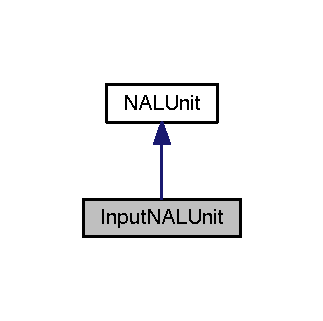
\includegraphics[width=155pt]{de/d28/class_input_n_a_l_unit__inherit__graph}
\end{center}
\end{figure}


Collaboration diagram for Input\+N\+A\+L\+Unit\+:
\nopagebreak
\begin{figure}[H]
\begin{center}
\leavevmode
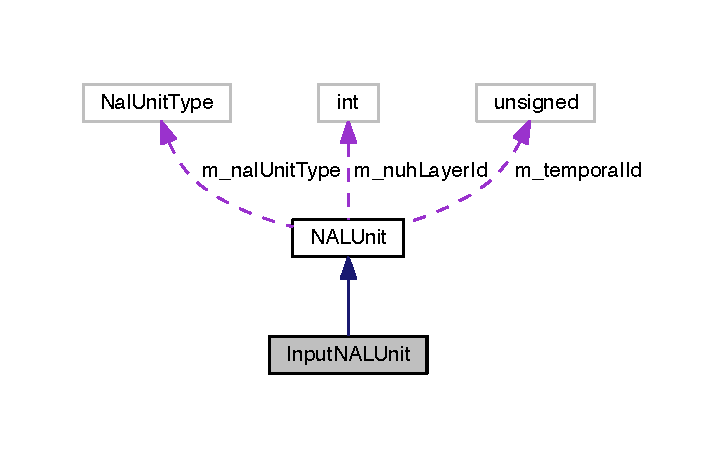
\includegraphics[width=348pt]{d9/d68/class_input_n_a_l_unit__coll__graph}
\end{center}
\end{figure}
\subsection*{Public Member Functions}
\begin{DoxyCompactItemize}
\item 
\mbox{\Hypertarget{class_input_n_a_l_unit_a5b552d19e575a7ccfc593f36e58e8234}\label{class_input_n_a_l_unit_a5b552d19e575a7ccfc593f36e58e8234}} 
{\bfseries Input\+N\+A\+L\+Unit} (const \hyperlink{class_input_n_a_l_unit}{Input\+N\+A\+L\+Unit} \&src)
\item 
\mbox{\Hypertarget{class_input_n_a_l_unit_aa6b44dbc27ae3a26bfb7cb30c00fbd4b}\label{class_input_n_a_l_unit_aa6b44dbc27ae3a26bfb7cb30c00fbd4b}} 
const \hyperlink{class_t_com_input_bitstream}{T\+Com\+Input\+Bitstream} \& {\bfseries get\+Bitstream} () const
\item 
\mbox{\Hypertarget{class_input_n_a_l_unit_adcbc290e85137ac1a143591fbd3bfd6c}\label{class_input_n_a_l_unit_adcbc290e85137ac1a143591fbd3bfd6c}} 
\hyperlink{class_t_com_input_bitstream}{T\+Com\+Input\+Bitstream} \& {\bfseries get\+Bitstream} ()
\end{DoxyCompactItemize}
\subsection*{Additional Inherited Members}


\subsection{Detailed Description}
A convenience wrapper to \hyperlink{struct_n_a_l_unit}{N\+A\+L\+Unit} that also provides a bitstream object. 

The documentation for this class was generated from the following file\+:\begin{DoxyCompactItemize}
\item 
Lib/\+T\+Lib\+Decoder/\hyperlink{_n_a_lread_8h}{N\+A\+Lread.\+h}\end{DoxyCompactItemize}

\hypertarget{struct_t_enc_search_1_1_int_t_z_search_struct}{}\section{T\+Enc\+Search\+:\+:Int\+T\+Z\+Search\+Struct Struct Reference}
\label{struct_t_enc_search_1_1_int_t_z_search_struct}\index{T\+Enc\+Search\+::\+Int\+T\+Z\+Search\+Struct@{T\+Enc\+Search\+::\+Int\+T\+Z\+Search\+Struct}}


Collaboration diagram for T\+Enc\+Search\+:\+:Int\+T\+Z\+Search\+Struct\+:
\nopagebreak
\begin{figure}[H]
\begin{center}
\leavevmode
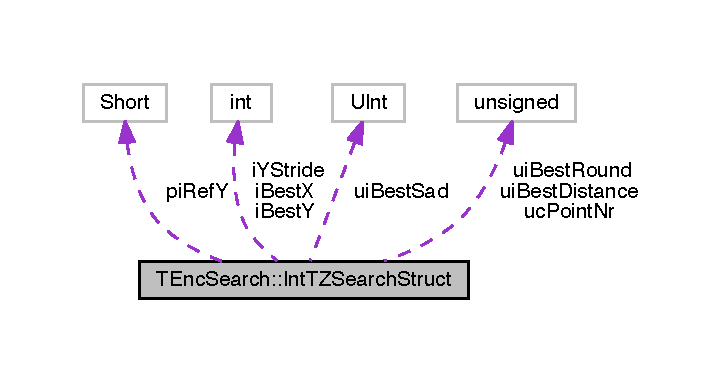
\includegraphics[width=347pt]{d4/ddb/struct_t_enc_search_1_1_int_t_z_search_struct__coll__graph}
\end{center}
\end{figure}
\subsection*{Public Attributes}
\begin{DoxyCompactItemize}
\item 
\mbox{\Hypertarget{struct_t_enc_search_1_1_int_t_z_search_struct_afc2170b14599ab7fddcf694e2f92e346}\label{struct_t_enc_search_1_1_int_t_z_search_struct_afc2170b14599ab7fddcf694e2f92e346}} 
const \hyperlink{_type_def_8h_af92141699657699b4b547be0c8517541}{Pel} $\ast$ {\bfseries pi\+RefY}
\item 
\mbox{\Hypertarget{struct_t_enc_search_1_1_int_t_z_search_struct_abb59bd7931913de72e7ffb27ec981d5d}\label{struct_t_enc_search_1_1_int_t_z_search_struct_abb59bd7931913de72e7ffb27ec981d5d}} 
Int {\bfseries i\+Y\+Stride}
\item 
\mbox{\Hypertarget{struct_t_enc_search_1_1_int_t_z_search_struct_a5a8f5b6547df163b5461b3e668cf7b50}\label{struct_t_enc_search_1_1_int_t_z_search_struct_a5a8f5b6547df163b5461b3e668cf7b50}} 
Int {\bfseries i\+BestX}
\item 
\mbox{\Hypertarget{struct_t_enc_search_1_1_int_t_z_search_struct_a5a3449eb12e4be90c41bf70256f5a92e}\label{struct_t_enc_search_1_1_int_t_z_search_struct_a5a3449eb12e4be90c41bf70256f5a92e}} 
Int {\bfseries i\+BestY}
\item 
\mbox{\Hypertarget{struct_t_enc_search_1_1_int_t_z_search_struct_a7f0d20db5ff211b3526039bb84432155}\label{struct_t_enc_search_1_1_int_t_z_search_struct_a7f0d20db5ff211b3526039bb84432155}} 
U\+Int {\bfseries ui\+Best\+Round}
\item 
\mbox{\Hypertarget{struct_t_enc_search_1_1_int_t_z_search_struct_a32eb5dba242d71f1156b063bbab4458a}\label{struct_t_enc_search_1_1_int_t_z_search_struct_a32eb5dba242d71f1156b063bbab4458a}} 
U\+Int {\bfseries ui\+Best\+Distance}
\item 
\mbox{\Hypertarget{struct_t_enc_search_1_1_int_t_z_search_struct_a8a820a2b2483c40e25b652ec93e603fa}\label{struct_t_enc_search_1_1_int_t_z_search_struct_a8a820a2b2483c40e25b652ec93e603fa}} 
\hyperlink{_type_def_8h_aed82b23ef6849d0bc3d95c92102d5b50}{Distortion} {\bfseries ui\+Best\+Sad}
\item 
\mbox{\Hypertarget{struct_t_enc_search_1_1_int_t_z_search_struct_a73dadd6074fef3e5876831dd237228e4}\label{struct_t_enc_search_1_1_int_t_z_search_struct_a73dadd6074fef3e5876831dd237228e4}} 
U\+Char {\bfseries uc\+Point\+Nr}
\end{DoxyCompactItemize}


The documentation for this struct was generated from the following file\+:\begin{DoxyCompactItemize}
\item 
Lib/\+T\+Lib\+Encoder/\hyperlink{_t_enc_search_8h}{T\+Enc\+Search.\+h}\end{DoxyCompactItemize}

\hypertarget{struct_parameter_set_map_1_1_map_data}{}\section{Parameter\+Set\+Map$<$ T $>$\+:\+:Map\+Data$<$ Tm $>$ Struct Template Reference}
\label{struct_parameter_set_map_1_1_map_data}\index{Parameter\+Set\+Map$<$ T $>$\+::\+Map\+Data$<$ Tm $>$@{Parameter\+Set\+Map$<$ T $>$\+::\+Map\+Data$<$ Tm $>$}}


Collaboration diagram for Parameter\+Set\+Map$<$ T $>$\+:\+:Map\+Data$<$ Tm $>$\+:
\nopagebreak
\begin{figure}[H]
\begin{center}
\leavevmode
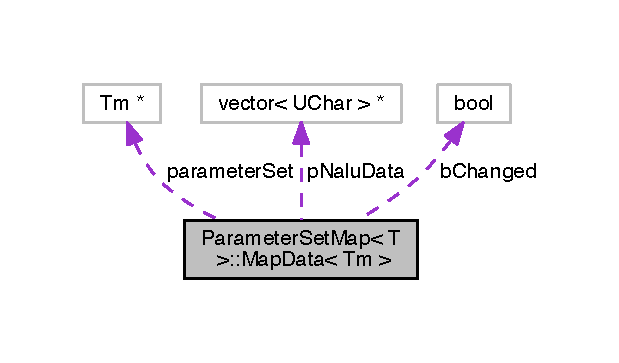
\includegraphics[width=297pt]{de/dd5/struct_parameter_set_map_1_1_map_data__coll__graph}
\end{center}
\end{figure}
\subsection*{Public Attributes}
\begin{DoxyCompactItemize}
\item 
\mbox{\Hypertarget{struct_parameter_set_map_1_1_map_data_a61097b235246a9ea8db86febdf943601}\label{struct_parameter_set_map_1_1_map_data_a61097b235246a9ea8db86febdf943601}} 
Bool {\bfseries b\+Changed}
\item 
\mbox{\Hypertarget{struct_parameter_set_map_1_1_map_data_a33457d16b94f734857094bc85a89511d}\label{struct_parameter_set_map_1_1_map_data_a33457d16b94f734857094bc85a89511d}} 
std\+::vector$<$ U\+Char $>$ $\ast$ {\bfseries p\+Nalu\+Data}
\item 
\mbox{\Hypertarget{struct_parameter_set_map_1_1_map_data_a17c1a8dd8e680a87f7f67fce7cbe3540}\label{struct_parameter_set_map_1_1_map_data_a17c1a8dd8e680a87f7f67fce7cbe3540}} 
Tm $\ast$ {\bfseries parameter\+Set}
\end{DoxyCompactItemize}


The documentation for this struct was generated from the following file\+:\begin{DoxyCompactItemize}
\item 
Lib/\+T\+Lib\+Common/\hyperlink{_t_com_slice_8h}{T\+Com\+Slice.\+h}\end{DoxyCompactItemize}

\hypertarget{class_m_d5}{}\section{M\+D5 Class Reference}
\label{class_m_d5}\index{M\+D5@{M\+D5}}
\subsection*{Public Member Functions}
\begin{DoxyCompactItemize}
\item 
\hyperlink{class_m_d5_afa6155ec36de415ab2dcf5e54b670d13}{M\+D5} ()
\item 
void \hyperlink{class_m_d5_a52c7dbe8d4a57e8c79d4c905205e24d0}{update} (unsigned char $\ast$buf, unsigned len)
\item 
void \hyperlink{class_m_d5_a16e5a96e255621d00ff682284cd7b69c}{finalize} (unsigned char digest\mbox{[}M\+D5\+\_\+\+D\+I\+G\+E\+S\+T\+\_\+\+S\+T\+R\+I\+N\+G\+\_\+\+L\+E\+N\+G\+TH\mbox{]})
\end{DoxyCompactItemize}


\subsection{Constructor \& Destructor Documentation}
\mbox{\Hypertarget{class_m_d5_afa6155ec36de415ab2dcf5e54b670d13}\label{class_m_d5_afa6155ec36de415ab2dcf5e54b670d13}} 
\index{M\+D5@{M\+D5}!M\+D5@{M\+D5}}
\index{M\+D5@{M\+D5}!M\+D5@{M\+D5}}
\subsubsection{\texorpdfstring{M\+D5()}{MD5()}}
{\footnotesize\ttfamily M\+D5\+::\+M\+D5 (\begin{DoxyParamCaption}{ }\end{DoxyParamCaption})\hspace{0.3cm}{\ttfamily [inline]}}

initialize digest state 

\subsection{Member Function Documentation}
\mbox{\Hypertarget{class_m_d5_a16e5a96e255621d00ff682284cd7b69c}\label{class_m_d5_a16e5a96e255621d00ff682284cd7b69c}} 
\index{M\+D5@{M\+D5}!finalize@{finalize}}
\index{finalize@{finalize}!M\+D5@{M\+D5}}
\subsubsection{\texorpdfstring{finalize()}{finalize()}}
{\footnotesize\ttfamily void M\+D5\+::finalize (\begin{DoxyParamCaption}\item[{unsigned char}]{digest\mbox{[}\+M\+D5\+\_\+\+D\+I\+G\+E\+S\+T\+\_\+\+S\+T\+R\+I\+N\+G\+\_\+\+L\+E\+N\+G\+T\+H\mbox{]} }\end{DoxyParamCaption})\hspace{0.3cm}{\ttfamily [inline]}}

flush any outstanding \hyperlink{class_m_d5}{M\+D5} data, write the digest into digest. \mbox{\Hypertarget{class_m_d5_a52c7dbe8d4a57e8c79d4c905205e24d0}\label{class_m_d5_a52c7dbe8d4a57e8c79d4c905205e24d0}} 
\index{M\+D5@{M\+D5}!update@{update}}
\index{update@{update}!M\+D5@{M\+D5}}
\subsubsection{\texorpdfstring{update()}{update()}}
{\footnotesize\ttfamily void M\+D5\+::update (\begin{DoxyParamCaption}\item[{unsigned char $\ast$}]{buf,  }\item[{unsigned}]{len }\end{DoxyParamCaption})\hspace{0.3cm}{\ttfamily [inline]}}

compute digest over buf of length len. multiple calls may extend the digest over more data. 

The documentation for this class was generated from the following file\+:\begin{DoxyCompactItemize}
\item 
Lib/libmd5/M\+D5.\+h\end{DoxyCompactItemize}

\hypertarget{struct_meta_log_entry}{}\section{Meta\+Log\+Entry$<$ T\+Lambda\+Modifier $>$ Struct Template Reference}
\label{struct_meta_log_entry}\index{Meta\+Log\+Entry$<$ T\+Lambda\+Modifier $>$@{Meta\+Log\+Entry$<$ T\+Lambda\+Modifier $>$}}


Full meta-\/log entry.  




{\ttfamily \#include $<$Guess\+Lambda\+Modifiers.\+h$>$}



Collaboration diagram for Meta\+Log\+Entry$<$ T\+Lambda\+Modifier $>$\+:
\nopagebreak
\begin{figure}[H]
\begin{center}
\leavevmode
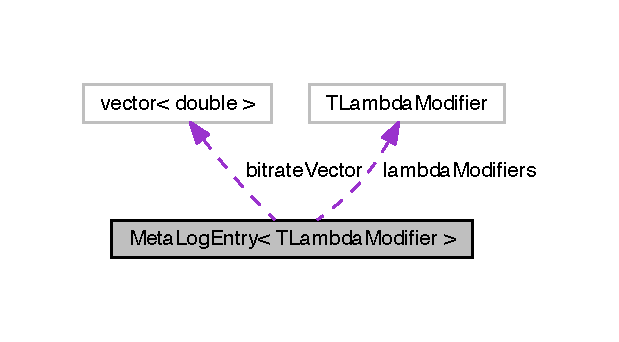
\includegraphics[width=297pt]{de/dc8/struct_meta_log_entry__coll__graph}
\end{center}
\end{figure}
\subsection*{Public Attributes}
\begin{DoxyCompactItemize}
\item 
\mbox{\Hypertarget{struct_meta_log_entry_a494dc8b5757c8b0411c95d2998492cbf}\label{struct_meta_log_entry_a494dc8b5757c8b0411c95d2998492cbf}} 
T\+Lambda\+Modifier {\bfseries lambda\+Modifiers}
\item 
\mbox{\Hypertarget{struct_meta_log_entry_af7f96ccf26841875ab7091cea40f4321}\label{struct_meta_log_entry_af7f96ccf26841875ab7091cea40f4321}} 
std\+::vector$<$ double $>$ {\bfseries bitrate\+Vector}
\end{DoxyCompactItemize}


\subsection{Detailed Description}
\subsubsection*{template$<$typename T\+Lambda\+Modifier$>$\newline
struct Meta\+Log\+Entry$<$ T\+Lambda\+Modifier $>$}

Full meta-\/log entry. 

The documentation for this struct was generated from the following file\+:\begin{DoxyCompactItemize}
\item 
App/utils/\+Bitrate\+Targeting/Guess\+Lambda\+Modifiers.\+h\end{DoxyCompactItemize}

\hypertarget{class_meta_log_parse_exception}{}\section{Meta\+Log\+Parse\+Exception Class Reference}
\label{class_meta_log_parse_exception}\index{Meta\+Log\+Parse\+Exception@{Meta\+Log\+Parse\+Exception}}


Thrown if there is an error parsing the meta-\/log.  




{\ttfamily \#include $<$Guess\+Lambda\+Modifiers.\+h$>$}



Inheritance diagram for Meta\+Log\+Parse\+Exception\+:
\nopagebreak
\begin{figure}[H]
\begin{center}
\leavevmode
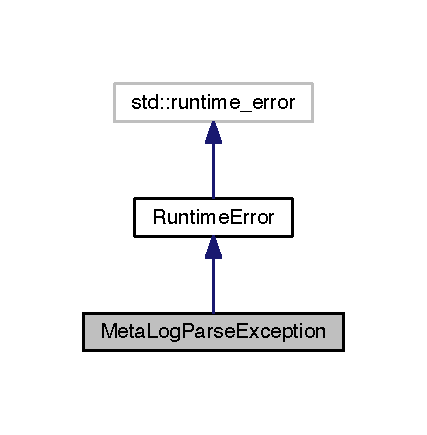
\includegraphics[width=205pt]{d6/d0c/class_meta_log_parse_exception__inherit__graph}
\end{center}
\end{figure}


Collaboration diagram for Meta\+Log\+Parse\+Exception\+:
\nopagebreak
\begin{figure}[H]
\begin{center}
\leavevmode
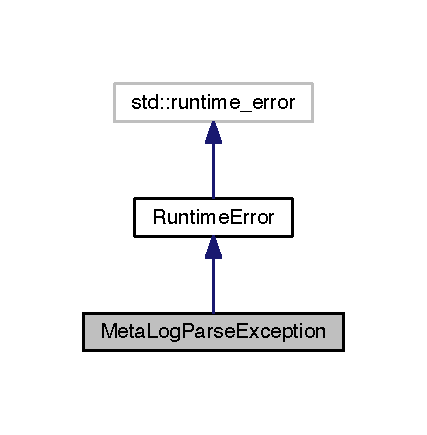
\includegraphics[width=205pt]{d2/d37/class_meta_log_parse_exception__coll__graph}
\end{center}
\end{figure}
\subsection*{Protected Member Functions}
\begin{DoxyCompactItemize}
\item 
void \hyperlink{class_meta_log_parse_exception_a18d40347b5a6eeef08b2c0d51a248898}{output\+What} (std\+::ostream \&o) const
\end{DoxyCompactItemize}
\subsection*{Additional Inherited Members}


\subsection{Detailed Description}
Thrown if there is an error parsing the meta-\/log. 

\subsection{Member Function Documentation}
\mbox{\Hypertarget{class_meta_log_parse_exception_a18d40347b5a6eeef08b2c0d51a248898}\label{class_meta_log_parse_exception_a18d40347b5a6eeef08b2c0d51a248898}} 
\index{Meta\+Log\+Parse\+Exception@{Meta\+Log\+Parse\+Exception}!output\+What@{output\+What}}
\index{output\+What@{output\+What}!Meta\+Log\+Parse\+Exception@{Meta\+Log\+Parse\+Exception}}
\subsubsection{\texorpdfstring{output\+What()}{outputWhat()}}
{\footnotesize\ttfamily void Meta\+Log\+Parse\+Exception\+::output\+What (\begin{DoxyParamCaption}\item[{std\+::ostream \&}]{o }\end{DoxyParamCaption}) const\hspace{0.3cm}{\ttfamily [inline]}, {\ttfamily [protected]}, {\ttfamily [virtual]}}

The implementing class implements this method to customize the what output 
\begin{DoxyParams}{Parameters}
{\em o} & The what stream is outputted to this parameter \\
\hline
\end{DoxyParams}


Implements \hyperlink{class_runtime_error_a5020b04a2a7fac8b1dbfbfe4a30055b0}{Runtime\+Error}.



The documentation for this class was generated from the following file\+:\begin{DoxyCompactItemize}
\item 
App/utils/\+Bitrate\+Targeting/Guess\+Lambda\+Modifiers.\+h\end{DoxyCompactItemize}

\hypertarget{class_mismatched_indexes_exception}{}\section{Mismatched\+Indexes\+Exception Class Reference}
\label{class_mismatched_indexes_exception}\index{Mismatched\+Indexes\+Exception@{Mismatched\+Indexes\+Exception}}


Thrown if there is a mismatch in the vector sizes or the Lambda-\/modifier indexes.  




{\ttfamily \#include $<$Guess\+Lambda\+Modifiers.\+h$>$}



Inheritance diagram for Mismatched\+Indexes\+Exception\+:
\nopagebreak
\begin{figure}[H]
\begin{center}
\leavevmode
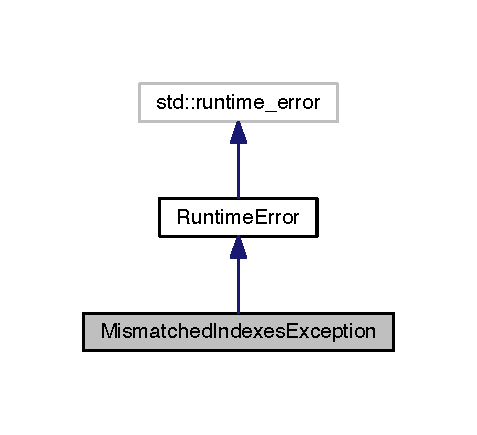
\includegraphics[width=229pt]{df/dfa/class_mismatched_indexes_exception__inherit__graph}
\end{center}
\end{figure}


Collaboration diagram for Mismatched\+Indexes\+Exception\+:
\nopagebreak
\begin{figure}[H]
\begin{center}
\leavevmode
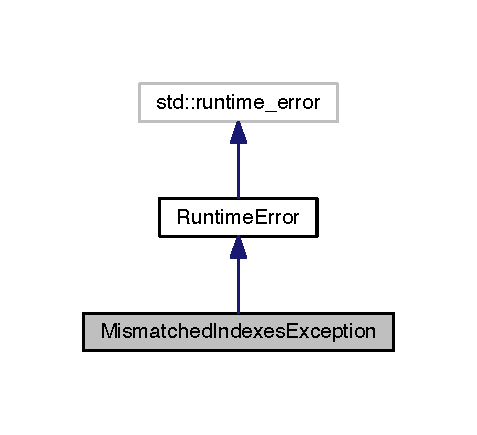
\includegraphics[width=229pt]{d5/d05/class_mismatched_indexes_exception__coll__graph}
\end{center}
\end{figure}
\subsection*{Protected Member Functions}
\begin{DoxyCompactItemize}
\item 
void \hyperlink{class_mismatched_indexes_exception_a139455007e7a5bb092650d4f2929068a}{output\+What} (std\+::ostream \&o) const
\end{DoxyCompactItemize}
\subsection*{Additional Inherited Members}


\subsection{Detailed Description}
Thrown if there is a mismatch in the vector sizes or the Lambda-\/modifier indexes. 

\subsection{Member Function Documentation}
\mbox{\Hypertarget{class_mismatched_indexes_exception_a139455007e7a5bb092650d4f2929068a}\label{class_mismatched_indexes_exception_a139455007e7a5bb092650d4f2929068a}} 
\index{Mismatched\+Indexes\+Exception@{Mismatched\+Indexes\+Exception}!output\+What@{output\+What}}
\index{output\+What@{output\+What}!Mismatched\+Indexes\+Exception@{Mismatched\+Indexes\+Exception}}
\subsubsection{\texorpdfstring{output\+What()}{outputWhat()}}
{\footnotesize\ttfamily void Mismatched\+Indexes\+Exception\+::output\+What (\begin{DoxyParamCaption}\item[{std\+::ostream \&}]{o }\end{DoxyParamCaption}) const\hspace{0.3cm}{\ttfamily [inline]}, {\ttfamily [protected]}, {\ttfamily [virtual]}}

The implementing class implements this method to customize the what output 
\begin{DoxyParams}{Parameters}
{\em o} & The what stream is outputted to this parameter \\
\hline
\end{DoxyParams}


Implements \hyperlink{class_runtime_error_a5020b04a2a7fac8b1dbfbfe4a30055b0}{Runtime\+Error}.



The documentation for this class was generated from the following file\+:\begin{DoxyCompactItemize}
\item 
App/utils/\+Bitrate\+Targeting/Guess\+Lambda\+Modifiers.\+h\end{DoxyCompactItemize}

\hypertarget{struct_n_a_l_unit}{}\section{N\+A\+L\+Unit Struct Reference}
\label{struct_n_a_l_unit}\index{N\+A\+L\+Unit@{N\+A\+L\+Unit}}


{\ttfamily \#include $<$N\+A\+L.\+h$>$}



Inheritance diagram for N\+A\+L\+Unit\+:
\nopagebreak
\begin{figure}[H]
\begin{center}
\leavevmode
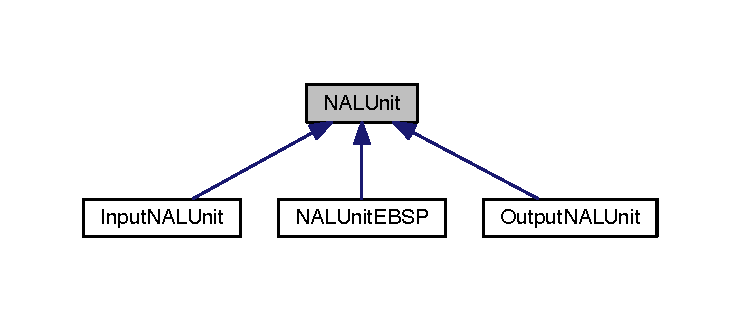
\includegraphics[width=350pt]{d5/dc1/struct_n_a_l_unit__inherit__graph}
\end{center}
\end{figure}


Collaboration diagram for N\+A\+L\+Unit\+:
\nopagebreak
\begin{figure}[H]
\begin{center}
\leavevmode
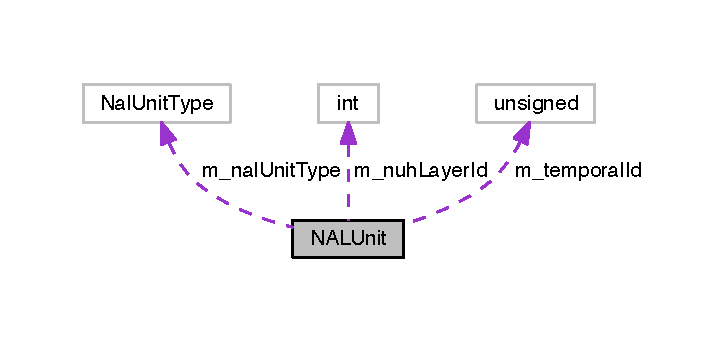
\includegraphics[width=348pt]{de/d23/struct_n_a_l_unit__coll__graph}
\end{center}
\end{figure}
\subsection*{Public Member Functions}
\begin{DoxyCompactItemize}
\item 
\mbox{\Hypertarget{struct_n_a_l_unit_af40251f18ebbc6d071fb43be17d742f9}\label{struct_n_a_l_unit_af40251f18ebbc6d071fb43be17d742f9}} 
{\bfseries N\+A\+L\+Unit} (const \hyperlink{struct_n_a_l_unit}{N\+A\+L\+Unit} \&src)
\item 
\hyperlink{struct_n_a_l_unit_a6c3d113f4dedfc580c685330abd8d66c}{N\+A\+L\+Unit} (Nal\+Unit\+Type nal\+Unit\+Type, Int temporal\+Id=0, Int nuh\+Layer\+Id=0)
\item 
\hyperlink{struct_n_a_l_unit_a6733403da92fa97139104c47545c9ad7}{N\+A\+L\+Unit} ()
\item 
Bool \hyperlink{struct_n_a_l_unit_a94af464dfd41d51ff179026e02d9926b}{is\+Slice} ()
\item 
\mbox{\Hypertarget{struct_n_a_l_unit_ab1fee63a3d57d9f4b097070c22bff2bf}\label{struct_n_a_l_unit_ab1fee63a3d57d9f4b097070c22bff2bf}} 
Bool {\bfseries is\+Irap} ()
\item 
\mbox{\Hypertarget{struct_n_a_l_unit_a79ae520a483aa460222f6e400337ff06}\label{struct_n_a_l_unit_a79ae520a483aa460222f6e400337ff06}} 
Bool {\bfseries is\+Idr} ()
\item 
\mbox{\Hypertarget{struct_n_a_l_unit_aec31f38c94df5616a26398692881756b}\label{struct_n_a_l_unit_aec31f38c94df5616a26398692881756b}} 
Bool {\bfseries is\+Bla} ()
\item 
\mbox{\Hypertarget{struct_n_a_l_unit_ab3b3e194ce52c1d26af37fa923509b9c}\label{struct_n_a_l_unit_ab3b3e194ce52c1d26af37fa923509b9c}} 
Bool {\bfseries is\+Cra} ()
\item 
\mbox{\Hypertarget{struct_n_a_l_unit_a4b5404a66f6fb684ab55bce8ffdaf978}\label{struct_n_a_l_unit_a4b5404a66f6fb684ab55bce8ffdaf978}} 
Bool {\bfseries is\+Sei} ()
\item 
\mbox{\Hypertarget{struct_n_a_l_unit_a801b82cb276b125592d891804ab2f8a9}\label{struct_n_a_l_unit_a801b82cb276b125592d891804ab2f8a9}} 
Bool {\bfseries is\+Vcl} ()
\item 
\mbox{\Hypertarget{struct_n_a_l_unit_a7a1937ab72316b6d8a76fe1de6e09a88}\label{struct_n_a_l_unit_a7a1937ab72316b6d8a76fe1de6e09a88}} 
Void {\bfseries print} ()
\end{DoxyCompactItemize}
\subsection*{Public Attributes}
\begin{DoxyCompactItemize}
\item 
\mbox{\Hypertarget{struct_n_a_l_unit_aa80725122142d6870e41aed24dc8deb6}\label{struct_n_a_l_unit_aa80725122142d6870e41aed24dc8deb6}} 
Nal\+Unit\+Type \hyperlink{struct_n_a_l_unit_aa80725122142d6870e41aed24dc8deb6}{m\+\_\+nal\+Unit\+Type}
\begin{DoxyCompactList}\small\item\em nal\+\_\+unit\+\_\+type \end{DoxyCompactList}\item 
\mbox{\Hypertarget{struct_n_a_l_unit_a588e88c076ed4bfff3ccae67449d1676}\label{struct_n_a_l_unit_a588e88c076ed4bfff3ccae67449d1676}} 
U\+Int \hyperlink{struct_n_a_l_unit_a588e88c076ed4bfff3ccae67449d1676}{m\+\_\+temporal\+Id}
\begin{DoxyCompactList}\small\item\em temporal\+\_\+id \end{DoxyCompactList}\item 
\mbox{\Hypertarget{struct_n_a_l_unit_a001e256a9e5c0a4eb596e6cb910ed787}\label{struct_n_a_l_unit_a001e256a9e5c0a4eb596e6cb910ed787}} 
Int \hyperlink{struct_n_a_l_unit_a001e256a9e5c0a4eb596e6cb910ed787}{m\+\_\+nuh\+Layer\+Id}
\begin{DoxyCompactList}\small\item\em layer id \end{DoxyCompactList}\end{DoxyCompactItemize}


\subsection{Detailed Description}
Represents a single N\+A\+Lunit header and the associated R\+B\+S\+Payload 

\subsection{Constructor \& Destructor Documentation}
\mbox{\Hypertarget{struct_n_a_l_unit_a6c3d113f4dedfc580c685330abd8d66c}\label{struct_n_a_l_unit_a6c3d113f4dedfc580c685330abd8d66c}} 
\index{N\+A\+L\+Unit@{N\+A\+L\+Unit}!N\+A\+L\+Unit@{N\+A\+L\+Unit}}
\index{N\+A\+L\+Unit@{N\+A\+L\+Unit}!N\+A\+L\+Unit@{N\+A\+L\+Unit}}
\subsubsection{\texorpdfstring{N\+A\+L\+Unit()}{NALUnit()}\hspace{0.1cm}{\footnotesize\ttfamily [1/2]}}
{\footnotesize\ttfamily N\+A\+L\+Unit\+::\+N\+A\+L\+Unit (\begin{DoxyParamCaption}\item[{Nal\+Unit\+Type}]{nal\+Unit\+Type,  }\item[{Int}]{temporal\+Id = {\ttfamily 0},  }\item[{Int}]{nuh\+Layer\+Id = {\ttfamily 0} }\end{DoxyParamCaption})\hspace{0.3cm}{\ttfamily [inline]}}

construct an N\+A\+Lunit structure with given header values. \mbox{\Hypertarget{struct_n_a_l_unit_a6733403da92fa97139104c47545c9ad7}\label{struct_n_a_l_unit_a6733403da92fa97139104c47545c9ad7}} 
\index{N\+A\+L\+Unit@{N\+A\+L\+Unit}!N\+A\+L\+Unit@{N\+A\+L\+Unit}}
\index{N\+A\+L\+Unit@{N\+A\+L\+Unit}!N\+A\+L\+Unit@{N\+A\+L\+Unit}}
\subsubsection{\texorpdfstring{N\+A\+L\+Unit()}{NALUnit()}\hspace{0.1cm}{\footnotesize\ttfamily [2/2]}}
{\footnotesize\ttfamily N\+A\+L\+Unit\+::\+N\+A\+L\+Unit (\begin{DoxyParamCaption}{ }\end{DoxyParamCaption})\hspace{0.3cm}{\ttfamily [inline]}}

default constructor -\/ no initialization; must be performed by user 

\subsection{Member Function Documentation}
\mbox{\Hypertarget{struct_n_a_l_unit_a94af464dfd41d51ff179026e02d9926b}\label{struct_n_a_l_unit_a94af464dfd41d51ff179026e02d9926b}} 
\index{N\+A\+L\+Unit@{N\+A\+L\+Unit}!is\+Slice@{is\+Slice}}
\index{is\+Slice@{is\+Slice}!N\+A\+L\+Unit@{N\+A\+L\+Unit}}
\subsubsection{\texorpdfstring{is\+Slice()}{isSlice()}}
{\footnotesize\ttfamily Bool N\+A\+L\+Unit\+::is\+Slice (\begin{DoxyParamCaption}{ }\end{DoxyParamCaption})\hspace{0.3cm}{\ttfamily [inline]}}

returns true if the N\+A\+Lunit is a slice N\+A\+Lunit 

The documentation for this struct was generated from the following file\+:\begin{DoxyCompactItemize}
\item 
Lib/\+T\+Lib\+Common/N\+A\+L.\+h\end{DoxyCompactItemize}

\hypertarget{struct_n_a_l_unit_e_b_s_p}{}\section{N\+A\+L\+Unit\+E\+B\+SP Struct Reference}
\label{struct_n_a_l_unit_e_b_s_p}\index{N\+A\+L\+Unit\+E\+B\+SP@{N\+A\+L\+Unit\+E\+B\+SP}}


{\ttfamily \#include $<$N\+A\+L.\+h$>$}



Inheritance diagram for N\+A\+L\+Unit\+E\+B\+SP\+:
\nopagebreak
\begin{figure}[H]
\begin{center}
\leavevmode
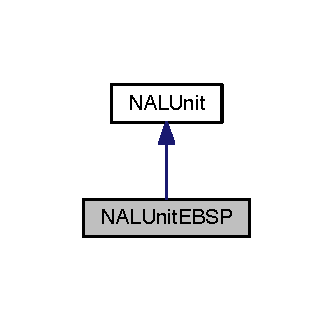
\includegraphics[width=160pt]{d6/d0f/struct_n_a_l_unit_e_b_s_p__inherit__graph}
\end{center}
\end{figure}


Collaboration diagram for N\+A\+L\+Unit\+E\+B\+SP\+:
\nopagebreak
\begin{figure}[H]
\begin{center}
\leavevmode
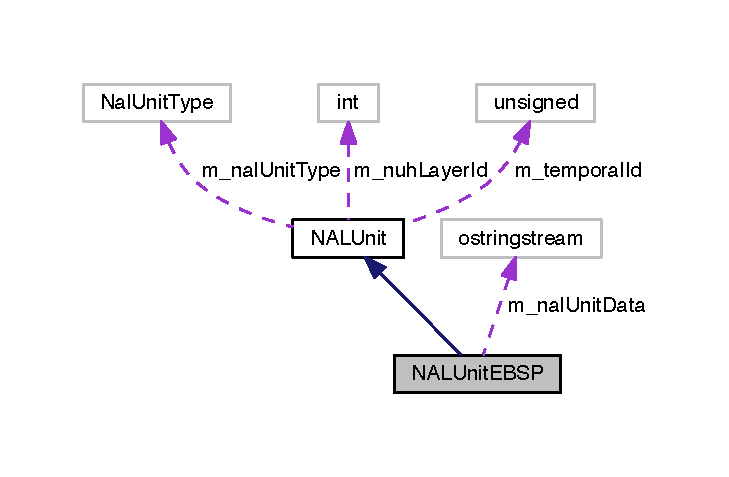
\includegraphics[width=350pt]{df/dcd/struct_n_a_l_unit_e_b_s_p__coll__graph}
\end{center}
\end{figure}
\subsection*{Public Member Functions}
{\bf }\par
\begin{DoxyCompactItemize}
\item 
\hyperlink{struct_n_a_l_unit_e_b_s_p_a57fe5aeb0568830923c3d7f00052cccf}{N\+A\+L\+Unit\+E\+B\+SP} (\hyperlink{struct_output_n_a_l_unit}{Output\+N\+A\+L\+Unit} \&nalu)
\end{DoxyCompactItemize}

\subsection*{Public Attributes}
\begin{DoxyCompactItemize}
\item 
\mbox{\Hypertarget{struct_n_a_l_unit_e_b_s_p_a5066d41cf931afb3dd8341c1ced30ab6}\label{struct_n_a_l_unit_e_b_s_p_a5066d41cf931afb3dd8341c1ced30ab6}} 
std\+::ostringstream {\bfseries m\+\_\+nal\+Unit\+Data}
\end{DoxyCompactItemize}


\subsection{Detailed Description}
A single N\+A\+Lunit, with complete payload in E\+B\+SP format. 

\subsection{Constructor \& Destructor Documentation}
\mbox{\Hypertarget{struct_n_a_l_unit_e_b_s_p_a57fe5aeb0568830923c3d7f00052cccf}\label{struct_n_a_l_unit_e_b_s_p_a57fe5aeb0568830923c3d7f00052cccf}} 
\index{N\+A\+L\+Unit\+E\+B\+SP@{N\+A\+L\+Unit\+E\+B\+SP}!N\+A\+L\+Unit\+E\+B\+SP@{N\+A\+L\+Unit\+E\+B\+SP}}
\index{N\+A\+L\+Unit\+E\+B\+SP@{N\+A\+L\+Unit\+E\+B\+SP}!N\+A\+L\+Unit\+E\+B\+SP@{N\+A\+L\+Unit\+E\+B\+SP}}
\subsubsection{\texorpdfstring{N\+A\+L\+Unit\+E\+B\+S\+P()}{NALUnitEBSP()}}
{\footnotesize\ttfamily N\+A\+L\+Unit\+E\+B\+S\+P\+::\+N\+A\+L\+Unit\+E\+B\+SP (\begin{DoxyParamCaption}\item[{\hyperlink{struct_output_n_a_l_unit}{Output\+N\+A\+L\+Unit} \&}]{nalu }\end{DoxyParamCaption})\hspace{0.3cm}{\ttfamily [inline]}}

convert the \hyperlink{struct_output_n_a_l_unit}{Output\+N\+A\+L\+Unit} nalu into E\+B\+SP format by writing out the \hyperlink{struct_n_a_l_unit}{N\+A\+L\+Unit} header, then the rbsp\+\_\+bytes including any emulation\+\_\+prevention\+\_\+three\+\_\+byte symbols. 

The documentation for this struct was generated from the following files\+:\begin{DoxyCompactItemize}
\item 
Lib/\+T\+Lib\+Common/N\+A\+L.\+h\item 
Lib/\+T\+Lib\+Encoder/N\+A\+Lwrite.\+h\end{DoxyCompactItemize}

\hypertarget{structdf_1_1program__options__lite_1_1_options_1_1_names}{}\section{df\+:\+:program\+\_\+options\+\_\+lite\+:\+:Options\+:\+:Names Struct Reference}
\label{structdf_1_1program__options__lite_1_1_options_1_1_names}\index{df\+::program\+\_\+options\+\_\+lite\+::\+Options\+::\+Names@{df\+::program\+\_\+options\+\_\+lite\+::\+Options\+::\+Names}}


Collaboration diagram for df\+:\+:program\+\_\+options\+\_\+lite\+:\+:Options\+:\+:Names\+:
\nopagebreak
\begin{figure}[H]
\begin{center}
\leavevmode
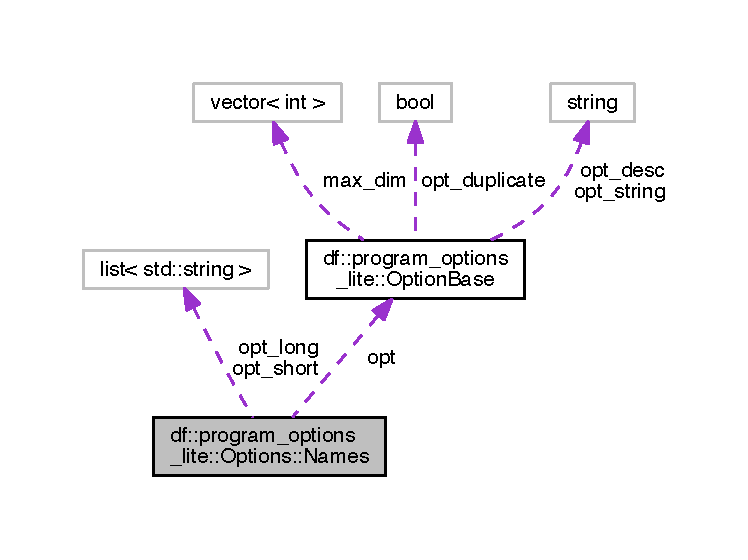
\includegraphics[width=350pt]{d5/d00/structdf_1_1program__options__lite_1_1_options_1_1_names__coll__graph}
\end{center}
\end{figure}
\subsection*{Public Attributes}
\begin{DoxyCompactItemize}
\item 
\mbox{\Hypertarget{structdf_1_1program__options__lite_1_1_options_1_1_names_a21cc23896ea246d515ca3864b8ccc672}\label{structdf_1_1program__options__lite_1_1_options_1_1_names_a21cc23896ea246d515ca3864b8ccc672}} 
std\+::list$<$ std\+::string $>$ {\bfseries opt\+\_\+long}
\item 
\mbox{\Hypertarget{structdf_1_1program__options__lite_1_1_options_1_1_names_a8962e18d10f3b0c52a4a69a1849f1d27}\label{structdf_1_1program__options__lite_1_1_options_1_1_names_a8962e18d10f3b0c52a4a69a1849f1d27}} 
std\+::list$<$ std\+::string $>$ {\bfseries opt\+\_\+short}
\item 
\mbox{\Hypertarget{structdf_1_1program__options__lite_1_1_options_1_1_names_ad69087ab3e33f09961ce3b2fc4e7ea4a}\label{structdf_1_1program__options__lite_1_1_options_1_1_names_ad69087ab3e33f09961ce3b2fc4e7ea4a}} 
\hyperlink{structdf_1_1program__options__lite_1_1_option_base}{Option\+Base} $\ast$ {\bfseries opt}
\end{DoxyCompactItemize}


The documentation for this struct was generated from the following file\+:\begin{DoxyCompactItemize}
\item 
Lib/\+T\+App\+Common/program\+\_\+options\+\_\+lite.\+h\end{DoxyCompactItemize}

\hypertarget{class_non_contiguous_q_p_set_exception}{}\section{Non\+Contiguous\+Q\+P\+Set\+Exception Class Reference}
\label{class_non_contiguous_q_p_set_exception}\index{Non\+Contiguous\+Q\+P\+Set\+Exception@{Non\+Contiguous\+Q\+P\+Set\+Exception}}


The QP set from the log file was not contiguous. The QP set must be contiguous to be able to convert the results into a vector.  




{\ttfamily \#include $<$Extract\+Bitrates.\+h$>$}



Inheritance diagram for Non\+Contiguous\+Q\+P\+Set\+Exception\+:
\nopagebreak
\begin{figure}[H]
\begin{center}
\leavevmode
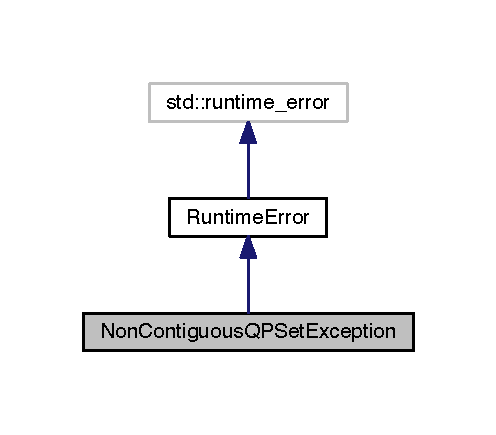
\includegraphics[width=238pt]{dd/d0b/class_non_contiguous_q_p_set_exception__inherit__graph}
\end{center}
\end{figure}


Collaboration diagram for Non\+Contiguous\+Q\+P\+Set\+Exception\+:
\nopagebreak
\begin{figure}[H]
\begin{center}
\leavevmode
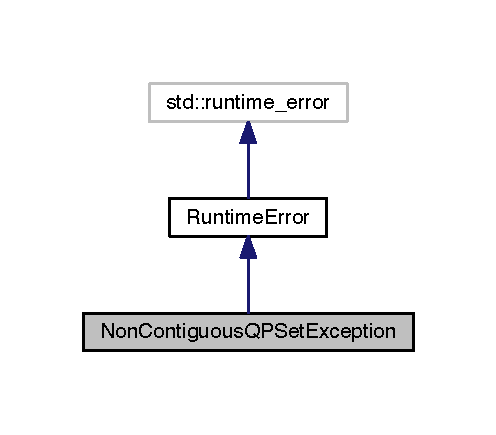
\includegraphics[width=238pt]{df/dca/class_non_contiguous_q_p_set_exception__coll__graph}
\end{center}
\end{figure}
\subsection*{Protected Member Functions}
\begin{DoxyCompactItemize}
\item 
void \hyperlink{class_non_contiguous_q_p_set_exception_a0b3c362380db281c07b3c8a016a73c32}{output\+What} (std\+::ostream \&o) const
\end{DoxyCompactItemize}
\subsection*{Additional Inherited Members}


\subsection{Detailed Description}
The QP set from the log file was not contiguous. The QP set must be contiguous to be able to convert the results into a vector. 

\subsection{Member Function Documentation}
\mbox{\Hypertarget{class_non_contiguous_q_p_set_exception_a0b3c362380db281c07b3c8a016a73c32}\label{class_non_contiguous_q_p_set_exception_a0b3c362380db281c07b3c8a016a73c32}} 
\index{Non\+Contiguous\+Q\+P\+Set\+Exception@{Non\+Contiguous\+Q\+P\+Set\+Exception}!output\+What@{output\+What}}
\index{output\+What@{output\+What}!Non\+Contiguous\+Q\+P\+Set\+Exception@{Non\+Contiguous\+Q\+P\+Set\+Exception}}
\subsubsection{\texorpdfstring{output\+What()}{outputWhat()}}
{\footnotesize\ttfamily void Non\+Contiguous\+Q\+P\+Set\+Exception\+::output\+What (\begin{DoxyParamCaption}\item[{std\+::ostream \&}]{o }\end{DoxyParamCaption}) const\hspace{0.3cm}{\ttfamily [inline]}, {\ttfamily [protected]}, {\ttfamily [virtual]}}

The implementing class implements this method to customize the what output 
\begin{DoxyParams}{Parameters}
{\em o} & The what stream is outputted to this parameter \\
\hline
\end{DoxyParams}


Implements \hyperlink{class_runtime_error_a5020b04a2a7fac8b1dbfbfe4a30055b0}{Runtime\+Error}.



The documentation for this class was generated from the following file\+:\begin{DoxyCompactItemize}
\item 
App/utils/\+Bitrate\+Targeting/Extract\+Bitrates.\+h\end{DoxyCompactItemize}

\hypertarget{structdf_1_1program__options__lite_1_1_option}{}\section{df\+:\+:program\+\_\+options\+\_\+lite\+:\+:Option$<$ T $>$ Struct Template Reference}
\label{structdf_1_1program__options__lite_1_1_option}\index{df\+::program\+\_\+options\+\_\+lite\+::\+Option$<$ T $>$@{df\+::program\+\_\+options\+\_\+lite\+::\+Option$<$ T $>$}}


{\ttfamily \#include $<$program\+\_\+options\+\_\+lite.\+h$>$}



Inheritance diagram for df\+:\+:program\+\_\+options\+\_\+lite\+:\+:Option$<$ T $>$\+:
\nopagebreak
\begin{figure}[H]
\begin{center}
\leavevmode
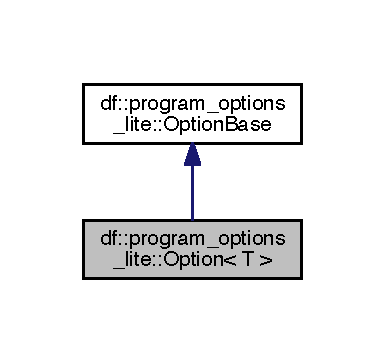
\includegraphics[width=185pt]{d6/d94/structdf_1_1program__options__lite_1_1_option__inherit__graph}
\end{center}
\end{figure}


Collaboration diagram for df\+:\+:program\+\_\+options\+\_\+lite\+:\+:Option$<$ T $>$\+:
\nopagebreak
\begin{figure}[H]
\begin{center}
\leavevmode
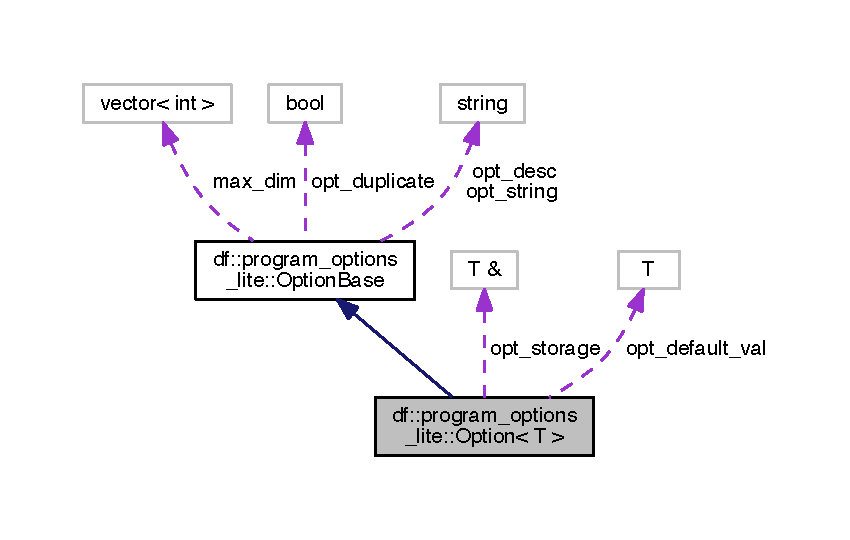
\includegraphics[width=350pt]{d2/dd2/structdf_1_1program__options__lite_1_1_option__coll__graph}
\end{center}
\end{figure}
\subsection*{Public Member Functions}
\begin{DoxyCompactItemize}
\item 
\mbox{\Hypertarget{structdf_1_1program__options__lite_1_1_option_a4663cc930a0cf449dab82a8416e68a1d}\label{structdf_1_1program__options__lite_1_1_option_a4663cc930a0cf449dab82a8416e68a1d}} 
{\bfseries Option} (const std\+::string \&name, T \&storage, T default\+\_\+val, const std\+::string \&desc, bool duplicate=false, std\+::vector$<$ int $>$ maxdim=std\+::vector$<$ int $>$(0))
\item 
\mbox{\Hypertarget{structdf_1_1program__options__lite_1_1_option_ae20d45acd9abcf807f6ce2905698d9ce}\label{structdf_1_1program__options__lite_1_1_option_ae20d45acd9abcf807f6ce2905698d9ce}} 
void {\bfseries parse} (const std\+::string \&arg, const std\+::vector$<$ int $>$ \&idcs, \hyperlink{structdf_1_1program__options__lite_1_1_error_reporter}{Error\+Reporter} \&)
\item 
\mbox{\Hypertarget{structdf_1_1program__options__lite_1_1_option_a07eb5c13acbe8d77db2b8bca02ae593f}\label{structdf_1_1program__options__lite_1_1_option_a07eb5c13acbe8d77db2b8bca02ae593f}} 
void {\bfseries set\+Default} ()
\item 
\mbox{\Hypertarget{structdf_1_1program__options__lite_1_1_option_a69d718b5fc14b208eb7df3ca2ca21981}\label{structdf_1_1program__options__lite_1_1_option_a69d718b5fc14b208eb7df3ca2ca21981}} 
{\footnotesize template$<$$>$ }\\void {\bfseries parse} (const std\+::string \&arg, const std\+::vector$<$ int $>$ \&idcs, \hyperlink{structdf_1_1program__options__lite_1_1_error_reporter}{Error\+Reporter} \&)
\item 
\mbox{\Hypertarget{structdf_1_1program__options__lite_1_1_option_a99a149001618b7c148b40fa3b3fbdd0e}\label{structdf_1_1program__options__lite_1_1_option_a99a149001618b7c148b40fa3b3fbdd0e}} 
{\footnotesize template$<$$>$ }\\void {\bfseries parse} (const std\+::string \&arg, const std\+::vector$<$ int $>$ \&idcs, \hyperlink{structdf_1_1program__options__lite_1_1_error_reporter}{Error\+Reporter} \&)
\item 
\mbox{\Hypertarget{structdf_1_1program__options__lite_1_1_option_ab486abce0890546b8bb1fb9f343a3d04}\label{structdf_1_1program__options__lite_1_1_option_ab486abce0890546b8bb1fb9f343a3d04}} 
{\footnotesize template$<$$>$ }\\void {\bfseries parse} (const std\+::string \&arg, const std\+::vector$<$ int $>$ \&idcs, \hyperlink{structdf_1_1program__options__lite_1_1_error_reporter}{Error\+Reporter} \&)
\item 
\mbox{\Hypertarget{structdf_1_1program__options__lite_1_1_option_a0f8ebb90e4df65d8f78c0003f29c09c5}\label{structdf_1_1program__options__lite_1_1_option_a0f8ebb90e4df65d8f78c0003f29c09c5}} 
{\footnotesize template$<$$>$ }\\void {\bfseries parse} (const std\+::string \&arg, const Int\+Ary1d \&idcs, \hyperlink{structdf_1_1program__options__lite_1_1_error_reporter}{Error\+Reporter} \&err)
\item 
\mbox{\Hypertarget{structdf_1_1program__options__lite_1_1_option_a4c201c44f50900fcc389d8d11ec78bb9}\label{structdf_1_1program__options__lite_1_1_option_a4c201c44f50900fcc389d8d11ec78bb9}} 
{\footnotesize template$<$$>$ }\\void {\bfseries parse} (const std\+::string \&arg, const Int\+Ary1d \&idcs, \hyperlink{structdf_1_1program__options__lite_1_1_error_reporter}{Error\+Reporter} \&)
\item 
\mbox{\Hypertarget{structdf_1_1program__options__lite_1_1_option_a820c2c0324cd4fa10ec92f7c678b7219}\label{structdf_1_1program__options__lite_1_1_option_a820c2c0324cd4fa10ec92f7c678b7219}} 
{\footnotesize template$<$$>$ }\\void {\bfseries parse} (const std\+::string \&arg, const Int\+Ary1d \&idcs, \hyperlink{structdf_1_1program__options__lite_1_1_error_reporter}{Error\+Reporter} \&)
\item 
\mbox{\Hypertarget{structdf_1_1program__options__lite_1_1_option_a3c0cf3d3832a1f3dc50ecafff2fa0deb}\label{structdf_1_1program__options__lite_1_1_option_a3c0cf3d3832a1f3dc50ecafff2fa0deb}} 
{\footnotesize template$<$$>$ }\\void {\bfseries parse} (const std\+::string \&arg, const Int\+Ary1d \&idcs, \hyperlink{structdf_1_1program__options__lite_1_1_error_reporter}{Error\+Reporter} \&)
\item 
\mbox{\Hypertarget{structdf_1_1program__options__lite_1_1_option_ac4207cd6d487a958c2acf687ad2c9a1a}\label{structdf_1_1program__options__lite_1_1_option_ac4207cd6d487a958c2acf687ad2c9a1a}} 
{\footnotesize template$<$$>$ }\\void {\bfseries parse} (const std\+::string \&arg, const std\+::vector$<$ int $>$ \&idcs, \hyperlink{structdf_1_1program__options__lite_1_1_error_reporter}{Error\+Reporter} \&err)
\item 
\mbox{\Hypertarget{structdf_1_1program__options__lite_1_1_option_adba4874f091e49deeb4d6ffed5ae0349}\label{structdf_1_1program__options__lite_1_1_option_adba4874f091e49deeb4d6ffed5ae0349}} 
{\footnotesize template$<$$>$ }\\void {\bfseries parse} (const std\+::string \&arg, const std\+::vector$<$ int $>$ \&idcs, \hyperlink{structdf_1_1program__options__lite_1_1_error_reporter}{Error\+Reporter} \&err)
\item 
\mbox{\Hypertarget{structdf_1_1program__options__lite_1_1_option_a4ff45180263bba562fdee9193d39c6ca}\label{structdf_1_1program__options__lite_1_1_option_a4ff45180263bba562fdee9193d39c6ca}} 
{\footnotesize template$<$$>$ }\\void {\bfseries parse} (const std\+::string \&arg, const std\+::vector$<$ int $>$ \&idcs, \hyperlink{structdf_1_1program__options__lite_1_1_error_reporter}{Error\+Reporter} \&err)
\item 
\mbox{\Hypertarget{structdf_1_1program__options__lite_1_1_option_a609bddd503b6656239b8c15c16074617}\label{structdf_1_1program__options__lite_1_1_option_a609bddd503b6656239b8c15c16074617}} 
{\footnotesize template$<$$>$ }\\void {\bfseries parse} (const std\+::string \&arg, const std\+::vector$<$ int $>$ \&idcs, \hyperlink{structdf_1_1program__options__lite_1_1_error_reporter}{Error\+Reporter} \&err)
\item 
\mbox{\Hypertarget{structdf_1_1program__options__lite_1_1_option_aa2100f00d2c18b7d92b689044617869e}\label{structdf_1_1program__options__lite_1_1_option_aa2100f00d2c18b7d92b689044617869e}} 
{\footnotesize template$<$$>$ }\\void {\bfseries parse} (const std\+::string \&arg, const Int\+Ary1d \&idcs, \hyperlink{structdf_1_1program__options__lite_1_1_error_reporter}{Error\+Reporter} \&err)
\item 
\mbox{\Hypertarget{structdf_1_1program__options__lite_1_1_option_a9f7c14bf343c7d20217a32f0b7ebda0f}\label{structdf_1_1program__options__lite_1_1_option_a9f7c14bf343c7d20217a32f0b7ebda0f}} 
{\footnotesize template$<$$>$ }\\void {\bfseries parse} (const std\+::string \&arg, const Int\+Ary1d \&idcs, \hyperlink{structdf_1_1program__options__lite_1_1_error_reporter}{Error\+Reporter} \&err)
\end{DoxyCompactItemize}
\subsection*{Public Attributes}
\begin{DoxyCompactItemize}
\item 
\mbox{\Hypertarget{structdf_1_1program__options__lite_1_1_option_ae45670761ecfa6a083903cbc0dad6cfb}\label{structdf_1_1program__options__lite_1_1_option_ae45670761ecfa6a083903cbc0dad6cfb}} 
T \& {\bfseries opt\+\_\+storage}
\item 
\mbox{\Hypertarget{structdf_1_1program__options__lite_1_1_option_ae6ff1c76bc8657da45fca6a67f07be69}\label{structdf_1_1program__options__lite_1_1_option_ae6ff1c76bc8657da45fca6a67f07be69}} 
T {\bfseries opt\+\_\+default\+\_\+val}
\end{DoxyCompactItemize}


\subsection{Detailed Description}
\subsubsection*{template$<$typename T$>$\newline
struct df\+::program\+\_\+options\+\_\+lite\+::\+Option$<$ T $>$}

Type specific option storage 

The documentation for this struct was generated from the following file\+:\begin{DoxyCompactItemize}
\item 
Lib/\+T\+App\+Common/program\+\_\+options\+\_\+lite.\+h\end{DoxyCompactItemize}

\hypertarget{structdf_1_1program__options__lite_1_1_option_base}{}\section{df\+:\+:program\+\_\+options\+\_\+lite\+:\+:Option\+Base Struct Reference}
\label{structdf_1_1program__options__lite_1_1_option_base}\index{df\+::program\+\_\+options\+\_\+lite\+::\+Option\+Base@{df\+::program\+\_\+options\+\_\+lite\+::\+Option\+Base}}


{\ttfamily \#include $<$program\+\_\+options\+\_\+lite.\+h$>$}



Inheritance diagram for df\+:\+:program\+\_\+options\+\_\+lite\+:\+:Option\+Base\+:
\nopagebreak
\begin{figure}[H]
\begin{center}
\leavevmode
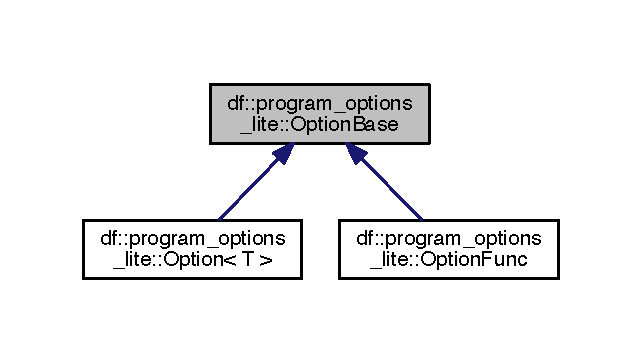
\includegraphics[width=308pt]{df/dad/structdf_1_1program__options__lite_1_1_option_base__inherit__graph}
\end{center}
\end{figure}


Collaboration diagram for df\+:\+:program\+\_\+options\+\_\+lite\+:\+:Option\+Base\+:
\nopagebreak
\begin{figure}[H]
\begin{center}
\leavevmode
\includegraphics[width=307pt]{d5/d86/structdf_1_1program__options__lite_1_1_option_base__coll__graph}
\end{center}
\end{figure}
\subsection*{Public Member Functions}
\begin{DoxyCompactItemize}
\item 
\mbox{\Hypertarget{structdf_1_1program__options__lite_1_1_option_base_ae2064404892b02b2da01c3dcc4428a1f}\label{structdf_1_1program__options__lite_1_1_option_base_ae2064404892b02b2da01c3dcc4428a1f}} 
{\bfseries Option\+Base} (const std\+::string \&name, const std\+::string \&desc, bool duplicate=false, std\+::vector$<$ int $>$ maxdim=std\+::vector$<$ int $>$(0))
\item 
\mbox{\Hypertarget{structdf_1_1program__options__lite_1_1_option_base_a703dc431b1fa8bca97808e98cbd32ebb}\label{structdf_1_1program__options__lite_1_1_option_base_a703dc431b1fa8bca97808e98cbd32ebb}} 
virtual void {\bfseries parse} (const std\+::string \&arg, const std\+::vector$<$ int $>$ \&idcs, \hyperlink{structdf_1_1program__options__lite_1_1_error_reporter}{Error\+Reporter} \&)=0
\item 
\mbox{\Hypertarget{structdf_1_1program__options__lite_1_1_option_base_ad3d25c54abf2c0d1d8146fe30cef1516}\label{structdf_1_1program__options__lite_1_1_option_base_ad3d25c54abf2c0d1d8146fe30cef1516}} 
bool {\bfseries check\+Dim} (std\+::vector$<$ int $>$ dims, \hyperlink{structdf_1_1program__options__lite_1_1_error_reporter}{Error\+Reporter} \&err)
\item 
\mbox{\Hypertarget{structdf_1_1program__options__lite_1_1_option_base_a9455c046218bee77d70ca4fe86757813}\label{structdf_1_1program__options__lite_1_1_option_base_a9455c046218bee77d70ca4fe86757813}} 
void {\bfseries x\+Parse\+Vec} (const std\+::string \&arg, Bool\+Ary1d \&storage)
\item 
\mbox{\Hypertarget{structdf_1_1program__options__lite_1_1_option_base_ae02e8bb720630aec3ea34731f27f638c}\label{structdf_1_1program__options__lite_1_1_option_base_ae02e8bb720630aec3ea34731f27f638c}} 
void {\bfseries x\+Parse\+Vec} (const std\+::string \&arg, Int\+Ary1d \&storage)
\item 
\mbox{\Hypertarget{structdf_1_1program__options__lite_1_1_option_base_a982c89928b3f6634546b5f0a7ee305f4}\label{structdf_1_1program__options__lite_1_1_option_base_a982c89928b3f6634546b5f0a7ee305f4}} 
virtual void {\bfseries set\+Default} ()=0
\end{DoxyCompactItemize}
\subsection*{Public Attributes}
\begin{DoxyCompactItemize}
\item 
\mbox{\Hypertarget{structdf_1_1program__options__lite_1_1_option_base_a69d5385baaf7b8261d7452bfaaa913be}\label{structdf_1_1program__options__lite_1_1_option_base_a69d5385baaf7b8261d7452bfaaa913be}} 
std\+::string {\bfseries opt\+\_\+string}
\item 
\mbox{\Hypertarget{structdf_1_1program__options__lite_1_1_option_base_a7a5403f473fe8c04fca4dcf2546592ea}\label{structdf_1_1program__options__lite_1_1_option_base_a7a5403f473fe8c04fca4dcf2546592ea}} 
std\+::string {\bfseries opt\+\_\+desc}
\item 
\mbox{\Hypertarget{structdf_1_1program__options__lite_1_1_option_base_aabf5b65dac0574ab3bba15b1136a33df}\label{structdf_1_1program__options__lite_1_1_option_base_aabf5b65dac0574ab3bba15b1136a33df}} 
bool {\bfseries opt\+\_\+duplicate}
\item 
\mbox{\Hypertarget{structdf_1_1program__options__lite_1_1_option_base_aa219ad152c828cbef1ff48ddbcdbc40f}\label{structdf_1_1program__options__lite_1_1_option_base_aa219ad152c828cbef1ff48ddbcdbc40f}} 
std\+::vector$<$ int $>$ {\bfseries max\+\_\+dim}
\end{DoxyCompactItemize}


\subsection{Detailed Description}
\hyperlink{structdf_1_1program__options__lite_1_1_option_base}{Option\+Base}\+: Virtual base class for storing information relating to a specific option This base class describes common elements. Type specific information should be stored in a derived class. 

The documentation for this struct was generated from the following file\+:\begin{DoxyCompactItemize}
\item 
Lib/\+T\+App\+Common/program\+\_\+options\+\_\+lite.\+h\end{DoxyCompactItemize}

\hypertarget{structdf_1_1program__options__lite_1_1_option_func}{}\section{df\+:\+:program\+\_\+options\+\_\+lite\+:\+:Option\+Func Struct Reference}
\label{structdf_1_1program__options__lite_1_1_option_func}\index{df\+::program\+\_\+options\+\_\+lite\+::\+Option\+Func@{df\+::program\+\_\+options\+\_\+lite\+::\+Option\+Func}}


{\ttfamily \#include $<$program\+\_\+options\+\_\+lite.\+h$>$}



Inheritance diagram for df\+:\+:program\+\_\+options\+\_\+lite\+:\+:Option\+Func\+:
\nopagebreak
\begin{figure}[H]
\begin{center}
\leavevmode
\includegraphics[width=185pt]{dd/d17/structdf_1_1program__options__lite_1_1_option_func__inherit__graph}
\end{center}
\end{figure}


Collaboration diagram for df\+:\+:program\+\_\+options\+\_\+lite\+:\+:Option\+Func\+:
\nopagebreak
\begin{figure}[H]
\begin{center}
\leavevmode
\includegraphics[width=307pt]{d6/d22/structdf_1_1program__options__lite_1_1_option_func__coll__graph}
\end{center}
\end{figure}
\subsection*{Public Types}
\begin{DoxyCompactItemize}
\item 
\mbox{\Hypertarget{structdf_1_1program__options__lite_1_1_option_func_af23fd41d068f521d302095bb068ff66d}\label{structdf_1_1program__options__lite_1_1_option_func_af23fd41d068f521d302095bb068ff66d}} 
typedef void() {\bfseries Func}(\hyperlink{structdf_1_1program__options__lite_1_1_options}{Options} \&, const std\+::string \&, \hyperlink{structdf_1_1program__options__lite_1_1_error_reporter}{Error\+Reporter} \&)
\end{DoxyCompactItemize}
\subsection*{Public Member Functions}
\begin{DoxyCompactItemize}
\item 
\mbox{\Hypertarget{structdf_1_1program__options__lite_1_1_option_func_afc975804044168ce285b9ae25a4248e7}\label{structdf_1_1program__options__lite_1_1_option_func_afc975804044168ce285b9ae25a4248e7}} 
{\bfseries Option\+Func} (const std\+::string \&name, \hyperlink{structdf_1_1program__options__lite_1_1_options}{Options} \&parent\+\_\+, Func $\ast$func\+\_\+, const std\+::string \&desc)
\item 
\mbox{\Hypertarget{structdf_1_1program__options__lite_1_1_option_func_af412834e436aed1c7df48a7d38e84513}\label{structdf_1_1program__options__lite_1_1_option_func_af412834e436aed1c7df48a7d38e84513}} 
void {\bfseries parse} (const std\+::string \&arg, const std\+::vector$<$ int $>$ \&idcs, \hyperlink{structdf_1_1program__options__lite_1_1_error_reporter}{Error\+Reporter} \&error\+\_\+reporter)
\item 
\mbox{\Hypertarget{structdf_1_1program__options__lite_1_1_option_func_ab8e6b6828a1fbda1c1d15d5b80d55e89}\label{structdf_1_1program__options__lite_1_1_option_func_ab8e6b6828a1fbda1c1d15d5b80d55e89}} 
void {\bfseries set\+Default} ()
\end{DoxyCompactItemize}
\subsection*{Additional Inherited Members}


\subsection{Detailed Description}
\hyperlink{structdf_1_1program__options__lite_1_1_option}{Option} class for argument handling using a user provided function 

The documentation for this struct was generated from the following file\+:\begin{DoxyCompactItemize}
\item 
Lib/\+T\+App\+Common/program\+\_\+options\+\_\+lite.\+h\end{DoxyCompactItemize}

\hypertarget{structdf_1_1program__options__lite_1_1_options}{}\section{df\+:\+:program\+\_\+options\+\_\+lite\+:\+:Options Struct Reference}
\label{structdf_1_1program__options__lite_1_1_options}\index{df\+::program\+\_\+options\+\_\+lite\+::\+Options@{df\+::program\+\_\+options\+\_\+lite\+::\+Options}}


Collaboration diagram for df\+:\+:program\+\_\+options\+\_\+lite\+:\+:Options\+:
\nopagebreak
\begin{figure}[H]
\begin{center}
\leavevmode
\includegraphics[width=316pt]{db/df0/structdf_1_1program__options__lite_1_1_options__coll__graph}
\end{center}
\end{figure}
\subsection*{Classes}
\begin{DoxyCompactItemize}
\item 
struct \hyperlink{structdf_1_1program__options__lite_1_1_options_1_1_names}{Names}
\end{DoxyCompactItemize}
\subsection*{Public Types}
\begin{DoxyCompactItemize}
\item 
\mbox{\Hypertarget{structdf_1_1program__options__lite_1_1_options_abb4321b12aeeac38f8171ec190e140e7}\label{structdf_1_1program__options__lite_1_1_options_abb4321b12aeeac38f8171ec190e140e7}} 
typedef std\+::list$<$ \hyperlink{structdf_1_1program__options__lite_1_1_options_1_1_names}{Names} $\ast$ $>$ {\bfseries Names\+Ptr\+List}
\item 
\mbox{\Hypertarget{structdf_1_1program__options__lite_1_1_options_a637581d7ecf751d144bf6eea702c0f74}\label{structdf_1_1program__options__lite_1_1_options_a637581d7ecf751d144bf6eea702c0f74}} 
typedef std\+::map$<$ std\+::string, Names\+Ptr\+List $>$ {\bfseries Names\+Map}
\end{DoxyCompactItemize}
\subsection*{Public Member Functions}
\begin{DoxyCompactItemize}
\item 
\mbox{\Hypertarget{structdf_1_1program__options__lite_1_1_options_aaf11f3eae6d9236600b324ebb173a69f}\label{structdf_1_1program__options__lite_1_1_options_aaf11f3eae6d9236600b324ebb173a69f}} 
\hyperlink{classdf_1_1program__options__lite_1_1_option_specific}{Option\+Specific} {\bfseries add\+Options} ()
\item 
\mbox{\Hypertarget{structdf_1_1program__options__lite_1_1_options_a493922413951537a977c7a450431e311}\label{structdf_1_1program__options__lite_1_1_options_a493922413951537a977c7a450431e311}} 
void {\bfseries add\+Option} (\hyperlink{structdf_1_1program__options__lite_1_1_option_base}{Option\+Base} $\ast$opt)
\end{DoxyCompactItemize}
\subsection*{Public Attributes}
\begin{DoxyCompactItemize}
\item 
\mbox{\Hypertarget{structdf_1_1program__options__lite_1_1_options_a7aebeb799410bdcc9135365f34c77237}\label{structdf_1_1program__options__lite_1_1_options_a7aebeb799410bdcc9135365f34c77237}} 
Names\+Ptr\+List {\bfseries opt\+\_\+list}
\item 
\mbox{\Hypertarget{structdf_1_1program__options__lite_1_1_options_a266a5705946be63711b96d564c2bd744}\label{structdf_1_1program__options__lite_1_1_options_a266a5705946be63711b96d564c2bd744}} 
Names\+Map {\bfseries opt\+\_\+long\+\_\+map}
\item 
\mbox{\Hypertarget{structdf_1_1program__options__lite_1_1_options_a65bb6cda04f4c6a3d792bfd1d4d4f0fd}\label{structdf_1_1program__options__lite_1_1_options_a65bb6cda04f4c6a3d792bfd1d4d4f0fd}} 
Names\+Map {\bfseries opt\+\_\+short\+\_\+map}
\end{DoxyCompactItemize}


The documentation for this struct was generated from the following files\+:\begin{DoxyCompactItemize}
\item 
Lib/\+T\+App\+Common/program\+\_\+options\+\_\+lite.\+h\item 
Lib/\+T\+App\+Common/program\+\_\+options\+\_\+lite.\+cpp\end{DoxyCompactItemize}

\hypertarget{classdf_1_1program__options__lite_1_1_option_specific}{}\section{df\+:\+:program\+\_\+options\+\_\+lite\+:\+:Option\+Specific Class Reference}
\label{classdf_1_1program__options__lite_1_1_option_specific}\index{df\+::program\+\_\+options\+\_\+lite\+::\+Option\+Specific@{df\+::program\+\_\+options\+\_\+lite\+::\+Option\+Specific}}
\subsection*{Public Member Functions}
\begin{DoxyCompactItemize}
\item 
\mbox{\Hypertarget{classdf_1_1program__options__lite_1_1_option_specific_a77c7c1f10b614b9eecc9e91f8e9a9f1f}\label{classdf_1_1program__options__lite_1_1_option_specific_a77c7c1f10b614b9eecc9e91f8e9a9f1f}} 
{\bfseries Option\+Specific} (\hyperlink{structdf_1_1program__options__lite_1_1_options}{Options} \&parent\+\_\+)
\item 
{\footnotesize template$<$typename T $>$ }\\\hyperlink{classdf_1_1program__options__lite_1_1_option_specific}{Option\+Specific} \& \hyperlink{classdf_1_1program__options__lite_1_1_option_specific_acea9355e21c8508c877d026b0607dc43}{operator()} (const std\+::string \&name, T \&storage, T default\+\_\+val, const std\+::string \&desc=\char`\"{}\char`\"{})
\item 
\mbox{\Hypertarget{classdf_1_1program__options__lite_1_1_option_specific_a8c281b88ceafb34f0e857403f3be0190}\label{classdf_1_1program__options__lite_1_1_option_specific_a8c281b88ceafb34f0e857403f3be0190}} 
{\footnotesize template$<$typename T $>$ }\\\hyperlink{classdf_1_1program__options__lite_1_1_option_specific}{Option\+Specific} \& {\bfseries operator()} (const std\+::string \&name, std\+::vector$<$ T $>$ \&storage, T default\+\_\+val, unsigned ui\+Max\+Num, const std\+::string \&desc=\char`\"{}\char`\"{})
\item 
\mbox{\Hypertarget{classdf_1_1program__options__lite_1_1_option_specific_a10273a65b1a657e814906ba3629f4e46}\label{classdf_1_1program__options__lite_1_1_option_specific_a10273a65b1a657e814906ba3629f4e46}} 
{\footnotesize template$<$typename T $>$ }\\\hyperlink{classdf_1_1program__options__lite_1_1_option_specific}{Option\+Specific} \& {\bfseries operator()} (const std\+::string \&name, std\+::vector$<$ std\+::vector$<$ T $>$ $>$ \&storage, T default\+\_\+val, unsigned ui\+Max\+Num\+Dim1, unsigned ui\+Max\+Num\+Dim2, const std\+::string \&desc=\char`\"{}\char`\"{})
\item 
\hyperlink{classdf_1_1program__options__lite_1_1_option_specific}{Option\+Specific} \& \hyperlink{classdf_1_1program__options__lite_1_1_option_specific_a757b17855cd89bc536c51f5c7e716d83}{operator()} (const std\+::string \&name, Option\+Func\+::\+Func $\ast$func, const std\+::string \&desc=\char`\"{}\char`\"{})
\end{DoxyCompactItemize}


\subsection{Member Function Documentation}
\mbox{\Hypertarget{classdf_1_1program__options__lite_1_1_option_specific_acea9355e21c8508c877d026b0607dc43}\label{classdf_1_1program__options__lite_1_1_option_specific_acea9355e21c8508c877d026b0607dc43}} 
\index{df\+::program\+\_\+options\+\_\+lite\+::\+Option\+Specific@{df\+::program\+\_\+options\+\_\+lite\+::\+Option\+Specific}!operator()@{operator()}}
\index{operator()@{operator()}!df\+::program\+\_\+options\+\_\+lite\+::\+Option\+Specific@{df\+::program\+\_\+options\+\_\+lite\+::\+Option\+Specific}}
\subsubsection{\texorpdfstring{operator()()}{operator()()}\hspace{0.1cm}{\footnotesize\ttfamily [1/2]}}
{\footnotesize\ttfamily template$<$typename T $>$ \\
\hyperlink{classdf_1_1program__options__lite_1_1_option_specific}{Option\+Specific}\& df\+::program\+\_\+options\+\_\+lite\+::\+Option\+Specific\+::operator() (\begin{DoxyParamCaption}\item[{const std\+::string \&}]{name,  }\item[{T \&}]{storage,  }\item[{T}]{default\+\_\+val,  }\item[{const std\+::string \&}]{desc = {\ttfamily \char`\"{}\char`\"{}} }\end{DoxyParamCaption})\hspace{0.3cm}{\ttfamily [inline]}}

Add option described by name to the parent \hyperlink{structdf_1_1program__options__lite_1_1_options}{Options} list, with storage for the option\textquotesingle{}s value with default\+\_\+val as the default value with desc as an optional help description \mbox{\Hypertarget{classdf_1_1program__options__lite_1_1_option_specific_a757b17855cd89bc536c51f5c7e716d83}\label{classdf_1_1program__options__lite_1_1_option_specific_a757b17855cd89bc536c51f5c7e716d83}} 
\index{df\+::program\+\_\+options\+\_\+lite\+::\+Option\+Specific@{df\+::program\+\_\+options\+\_\+lite\+::\+Option\+Specific}!operator()@{operator()}}
\index{operator()@{operator()}!df\+::program\+\_\+options\+\_\+lite\+::\+Option\+Specific@{df\+::program\+\_\+options\+\_\+lite\+::\+Option\+Specific}}
\subsubsection{\texorpdfstring{operator()()}{operator()()}\hspace{0.1cm}{\footnotesize\ttfamily [2/2]}}
{\footnotesize\ttfamily \hyperlink{classdf_1_1program__options__lite_1_1_option_specific}{Option\+Specific}\& df\+::program\+\_\+options\+\_\+lite\+::\+Option\+Specific\+::operator() (\begin{DoxyParamCaption}\item[{const std\+::string \&}]{name,  }\item[{Option\+Func\+::\+Func $\ast$}]{func,  }\item[{const std\+::string \&}]{desc = {\ttfamily \char`\"{}\char`\"{}} }\end{DoxyParamCaption})\hspace{0.3cm}{\ttfamily [inline]}}

Add option described by name to the parent \hyperlink{structdf_1_1program__options__lite_1_1_options}{Options} list, with desc as an optional help description instead of storing the value somewhere, a function of type Option\+Func\+::\+Func is called. It is upto this function to correctly handle evaluating the option\textquotesingle{}s value. 

The documentation for this class was generated from the following file\+:\begin{DoxyCompactItemize}
\item 
Lib/\+T\+App\+Common/program\+\_\+options\+\_\+lite.\+h\end{DoxyCompactItemize}

\hypertarget{structdf_1_1program__options__lite_1_1_option_writer}{}\section{df\+:\+:program\+\_\+options\+\_\+lite\+:\+:Option\+Writer Struct Reference}
\label{structdf_1_1program__options__lite_1_1_option_writer}\index{df\+::program\+\_\+options\+\_\+lite\+::\+Option\+Writer@{df\+::program\+\_\+options\+\_\+lite\+::\+Option\+Writer}}


Inheritance diagram for df\+:\+:program\+\_\+options\+\_\+lite\+:\+:Option\+Writer\+:
\nopagebreak
\begin{figure}[H]
\begin{center}
\leavevmode
\includegraphics[width=320pt]{df/d1f/structdf_1_1program__options__lite_1_1_option_writer__inherit__graph}
\end{center}
\end{figure}


Collaboration diagram for df\+:\+:program\+\_\+options\+\_\+lite\+:\+:Option\+Writer\+:
\nopagebreak
\begin{figure}[H]
\begin{center}
\leavevmode
\includegraphics[width=350pt]{de/d37/structdf_1_1program__options__lite_1_1_option_writer__coll__graph}
\end{center}
\end{figure}
\subsection*{Public Member Functions}
\begin{DoxyCompactItemize}
\item 
\mbox{\Hypertarget{structdf_1_1program__options__lite_1_1_option_writer_a26aca61b018a91a67880379205f1a3bf}\label{structdf_1_1program__options__lite_1_1_option_writer_a26aca61b018a91a67880379205f1a3bf}} 
{\bfseries Option\+Writer} (\hyperlink{structdf_1_1program__options__lite_1_1_options}{Options} \&r\+Opts, \hyperlink{structdf_1_1program__options__lite_1_1_error_reporter}{Error\+Reporter} \&err)
\item 
\mbox{\Hypertarget{structdf_1_1program__options__lite_1_1_option_writer_a7275abf255aa1227579e9f194639ec77}\label{structdf_1_1program__options__lite_1_1_option_writer_a7275abf255aa1227579e9f194639ec77}} 
virtual const string {\bfseries where} ()=0
\item 
\mbox{\Hypertarget{structdf_1_1program__options__lite_1_1_option_writer_a7661035ecdccd15503e6d1a88ec78d50}\label{structdf_1_1program__options__lite_1_1_option_writer_a7661035ecdccd15503e6d1a88ec78d50}} 
bool {\bfseries store\+Pair} (bool allow\+\_\+long, bool allow\+\_\+short, const string \&name, const string \&value)
\item 
\mbox{\Hypertarget{structdf_1_1program__options__lite_1_1_option_writer_a024de1064034bc9585c1477fa3dc1e73}\label{structdf_1_1program__options__lite_1_1_option_writer_a024de1064034bc9585c1477fa3dc1e73}} 
bool {\bfseries store\+Pair} (const string \&name, const string \&value)
\end{DoxyCompactItemize}
\subsection*{Public Attributes}
\begin{DoxyCompactItemize}
\item 
\mbox{\Hypertarget{structdf_1_1program__options__lite_1_1_option_writer_afc19de93afdfd2848bc56e050bcc6595}\label{structdf_1_1program__options__lite_1_1_option_writer_afc19de93afdfd2848bc56e050bcc6595}} 
\hyperlink{structdf_1_1program__options__lite_1_1_options}{Options} \& {\bfseries opts}
\item 
\mbox{\Hypertarget{structdf_1_1program__options__lite_1_1_option_writer_a990c25cd507460cfce1e81ef25ec367e}\label{structdf_1_1program__options__lite_1_1_option_writer_a990c25cd507460cfce1e81ef25ec367e}} 
\hyperlink{structdf_1_1program__options__lite_1_1_error_reporter}{Error\+Reporter} \& {\bfseries error\+\_\+reporter}
\end{DoxyCompactItemize}


The documentation for this struct was generated from the following file\+:\begin{DoxyCompactItemize}
\item 
Lib/\+T\+App\+Common/program\+\_\+options\+\_\+lite.\+cpp\end{DoxyCompactItemize}

\hypertarget{struct_output_n_a_l_unit}{}\section{Output\+N\+A\+L\+Unit Struct Reference}
\label{struct_output_n_a_l_unit}\index{Output\+N\+A\+L\+Unit@{Output\+N\+A\+L\+Unit}}


{\ttfamily \#include $<$N\+A\+Lwrite.\+h$>$}



Inheritance diagram for Output\+N\+A\+L\+Unit\+:
\nopagebreak
\begin{figure}[H]
\begin{center}
\leavevmode
\includegraphics[width=163pt]{d8/d8d/struct_output_n_a_l_unit__inherit__graph}
\end{center}
\end{figure}


Collaboration diagram for Output\+N\+A\+L\+Unit\+:
\nopagebreak
\begin{figure}[H]
\begin{center}
\leavevmode
\includegraphics[width=350pt]{d1/d24/struct_output_n_a_l_unit__coll__graph}
\end{center}
\end{figure}
\subsection*{Public Member Functions}
\begin{DoxyCompactItemize}
\item 
\hyperlink{struct_output_n_a_l_unit_a7dffded9144a8059e39113401d23703f}{Output\+N\+A\+L\+Unit} (Nal\+Unit\+Type nal\+Unit\+Type, U\+Int temporal\+ID=0, U\+Int reserved\+\_\+zero\+\_\+6bits=0)
\item 
\mbox{\Hypertarget{struct_output_n_a_l_unit_a0c7e9355cc4f73b519813628b0ef69e6}\label{struct_output_n_a_l_unit_a0c7e9355cc4f73b519813628b0ef69e6}} 
\hyperlink{struct_output_n_a_l_unit}{Output\+N\+A\+L\+Unit} \& {\bfseries operator=} (const \hyperlink{struct_n_a_l_unit}{N\+A\+L\+Unit} \&src)
\end{DoxyCompactItemize}
\subsection*{Public Attributes}
\begin{DoxyCompactItemize}
\item 
\mbox{\Hypertarget{struct_output_n_a_l_unit_a2994708c7a43dda8d1bfd18d5229074d}\label{struct_output_n_a_l_unit_a2994708c7a43dda8d1bfd18d5229074d}} 
\hyperlink{class_t_com_output_bitstream}{T\+Com\+Output\+Bitstream} {\bfseries m\+\_\+\+Bitstream}
\end{DoxyCompactItemize}


\subsection{Detailed Description}
A convenience wrapper to \hyperlink{struct_n_a_l_unit}{N\+A\+L\+Unit} that also provides a bitstream object. 

\subsection{Constructor \& Destructor Documentation}
\mbox{\Hypertarget{struct_output_n_a_l_unit_a7dffded9144a8059e39113401d23703f}\label{struct_output_n_a_l_unit_a7dffded9144a8059e39113401d23703f}} 
\index{Output\+N\+A\+L\+Unit@{Output\+N\+A\+L\+Unit}!Output\+N\+A\+L\+Unit@{Output\+N\+A\+L\+Unit}}
\index{Output\+N\+A\+L\+Unit@{Output\+N\+A\+L\+Unit}!Output\+N\+A\+L\+Unit@{Output\+N\+A\+L\+Unit}}
\subsubsection{\texorpdfstring{Output\+N\+A\+L\+Unit()}{OutputNALUnit()}}
{\footnotesize\ttfamily Output\+N\+A\+L\+Unit\+::\+Output\+N\+A\+L\+Unit (\begin{DoxyParamCaption}\item[{Nal\+Unit\+Type}]{nal\+Unit\+Type,  }\item[{U\+Int}]{temporal\+ID = {\ttfamily 0},  }\item[{U\+Int}]{reserved\+\_\+zero\+\_\+6bits = {\ttfamily 0} }\end{DoxyParamCaption})\hspace{0.3cm}{\ttfamily [inline]}}

construct an Output\+N\+A\+Lunit structure with given header values and storage for a bitstream. Upon construction the N\+A\+Lunit header is written to the bitstream. 

The documentation for this struct was generated from the following file\+:\begin{DoxyCompactItemize}
\item 
Lib/\+T\+Lib\+Encoder/N\+A\+Lwrite.\+h\end{DoxyCompactItemize}

\hypertarget{class_parameter_set_manager}{}\section{Parameter\+Set\+Manager Class Reference}
\label{class_parameter_set_manager}\index{Parameter\+Set\+Manager@{Parameter\+Set\+Manager}}


Collaboration diagram for Parameter\+Set\+Manager\+:
\nopagebreak
\begin{figure}[H]
\begin{center}
\leavevmode
\includegraphics[width=350pt]{d4/d59/class_parameter_set_manager__coll__graph}
\end{center}
\end{figure}
\subsection*{Public Member Functions}
\begin{DoxyCompactItemize}
\item 
\mbox{\Hypertarget{class_parameter_set_manager_a7ef2a34a8f0c99e06464835805b1bf09}\label{class_parameter_set_manager_a7ef2a34a8f0c99e06464835805b1bf09}} 
Void \hyperlink{class_parameter_set_manager_a7ef2a34a8f0c99e06464835805b1bf09}{store\+V\+PS} (\hyperlink{class_t_com_v_p_s}{T\+Com\+V\+PS} $\ast$vps, const std\+::vector$<$ U\+Char $>$ \&nalu\+Data)
\begin{DoxyCompactList}\small\item\em store sequence parameter set and take ownership of it \end{DoxyCompactList}\item 
\mbox{\Hypertarget{class_parameter_set_manager_a0c1062f78b2d8c5761ac770fd2dbb9f9}\label{class_parameter_set_manager_a0c1062f78b2d8c5761ac770fd2dbb9f9}} 
\hyperlink{class_t_com_v_p_s}{T\+Com\+V\+PS} $\ast$ \hyperlink{class_parameter_set_manager_a0c1062f78b2d8c5761ac770fd2dbb9f9}{get\+V\+PS} (Int vps\+Id)
\begin{DoxyCompactList}\small\item\em get pointer to existing video parameter set \end{DoxyCompactList}\item 
\mbox{\Hypertarget{class_parameter_set_manager_abf293fdfc0161f1ada16790776db3911}\label{class_parameter_set_manager_abf293fdfc0161f1ada16790776db3911}} 
Bool {\bfseries get\+V\+P\+S\+Changed\+Flag} (Int vps\+Id) const
\item 
\mbox{\Hypertarget{class_parameter_set_manager_a9b3d5a49cb893f99eb8f7041511fdcbf}\label{class_parameter_set_manager_a9b3d5a49cb893f99eb8f7041511fdcbf}} 
Void {\bfseries clear\+V\+P\+S\+Changed\+Flag} (Int vps\+Id)
\item 
\mbox{\Hypertarget{class_parameter_set_manager_a14ab75cc8e418e0d67ee1e5edff1808e}\label{class_parameter_set_manager_a14ab75cc8e418e0d67ee1e5edff1808e}} 
\hyperlink{class_t_com_v_p_s}{T\+Com\+V\+PS} $\ast$ {\bfseries get\+First\+V\+PS} ()
\item 
\mbox{\Hypertarget{class_parameter_set_manager_a2a776fec1bfb76da73c6af4eaaedbd91}\label{class_parameter_set_manager_a2a776fec1bfb76da73c6af4eaaedbd91}} 
Void \hyperlink{class_parameter_set_manager_a2a776fec1bfb76da73c6af4eaaedbd91}{store\+S\+PS} (\hyperlink{class_t_com_s_p_s}{T\+Com\+S\+PS} $\ast$sps, const std\+::vector$<$ U\+Char $>$ \&nalu\+Data)
\begin{DoxyCompactList}\small\item\em store sequence parameter set and take ownership of it \end{DoxyCompactList}\item 
\mbox{\Hypertarget{class_parameter_set_manager_ac8179c044dcf8081f2e200ccf901b357}\label{class_parameter_set_manager_ac8179c044dcf8081f2e200ccf901b357}} 
\hyperlink{class_t_com_s_p_s}{T\+Com\+S\+PS} $\ast$ \hyperlink{class_parameter_set_manager_ac8179c044dcf8081f2e200ccf901b357}{get\+S\+PS} (Int sps\+Id)
\begin{DoxyCompactList}\small\item\em get pointer to existing sequence parameter set \end{DoxyCompactList}\item 
\mbox{\Hypertarget{class_parameter_set_manager_a570af47f101435bb0b0f7a73f3f6174b}\label{class_parameter_set_manager_a570af47f101435bb0b0f7a73f3f6174b}} 
Bool {\bfseries get\+S\+P\+S\+Changed\+Flag} (Int sps\+Id) const
\item 
\mbox{\Hypertarget{class_parameter_set_manager_a4a621e3ab9f65606a2156d13b75185b9}\label{class_parameter_set_manager_a4a621e3ab9f65606a2156d13b75185b9}} 
Void {\bfseries clear\+S\+P\+S\+Changed\+Flag} (Int sps\+Id)
\item 
\mbox{\Hypertarget{class_parameter_set_manager_a029484f09b1d327623cba4469bd68cd3}\label{class_parameter_set_manager_a029484f09b1d327623cba4469bd68cd3}} 
\hyperlink{class_t_com_s_p_s}{T\+Com\+S\+PS} $\ast$ {\bfseries get\+First\+S\+PS} ()
\item 
\mbox{\Hypertarget{class_parameter_set_manager_a9209bf3d5dd9a67767c613ef2cc9ce88}\label{class_parameter_set_manager_a9209bf3d5dd9a67767c613ef2cc9ce88}} 
Void \hyperlink{class_parameter_set_manager_a9209bf3d5dd9a67767c613ef2cc9ce88}{store\+P\+PS} (\hyperlink{class_t_com_p_p_s}{T\+Com\+P\+PS} $\ast$pps, const std\+::vector$<$ U\+Char $>$ \&nalu\+Data)
\begin{DoxyCompactList}\small\item\em store picture parameter set and take ownership of it \end{DoxyCompactList}\item 
\mbox{\Hypertarget{class_parameter_set_manager_af8f982ee9c0f6899e91e250ad25ac805}\label{class_parameter_set_manager_af8f982ee9c0f6899e91e250ad25ac805}} 
\hyperlink{class_t_com_p_p_s}{T\+Com\+P\+PS} $\ast$ \hyperlink{class_parameter_set_manager_af8f982ee9c0f6899e91e250ad25ac805}{get\+P\+PS} (Int pps\+Id)
\begin{DoxyCompactList}\small\item\em get pointer to existing picture parameter set \end{DoxyCompactList}\item 
\mbox{\Hypertarget{class_parameter_set_manager_a014e130704936159146686b7cb63d7d6}\label{class_parameter_set_manager_a014e130704936159146686b7cb63d7d6}} 
Bool {\bfseries get\+P\+P\+S\+Changed\+Flag} (Int pps\+Id) const
\item 
\mbox{\Hypertarget{class_parameter_set_manager_a2136d3694effb530bac584e037c64724}\label{class_parameter_set_manager_a2136d3694effb530bac584e037c64724}} 
Void {\bfseries clear\+P\+P\+S\+Changed\+Flag} (Int pps\+Id)
\item 
\mbox{\Hypertarget{class_parameter_set_manager_ae1ef34e44082f3183ac8356702f50d52}\label{class_parameter_set_manager_ae1ef34e44082f3183ac8356702f50d52}} 
\hyperlink{class_t_com_p_p_s}{T\+Com\+P\+PS} $\ast$ {\bfseries get\+First\+P\+PS} ()
\item 
\mbox{\Hypertarget{class_parameter_set_manager_af65dcd202bf56e0c6bd1e2038ce7ef11}\label{class_parameter_set_manager_af65dcd202bf56e0c6bd1e2038ce7ef11}} 
const \hyperlink{class_t_com_v_p_s}{T\+Com\+V\+PS} $\ast$ {\bfseries get\+Active\+V\+PS} () const
\item 
\mbox{\Hypertarget{class_parameter_set_manager_a4f8c560b94e0735ea8c1c97b15660745}\label{class_parameter_set_manager_a4f8c560b94e0735ea8c1c97b15660745}} 
const \hyperlink{class_t_com_s_p_s}{T\+Com\+S\+PS} $\ast$ {\bfseries get\+Active\+S\+PS} (Int layer) const
\end{DoxyCompactItemize}
{\bf }\par
\begin{DoxyCompactItemize}
\item 
Bool \hyperlink{class_parameter_set_manager_a7a8bef7b80abb0b30832c5d4d4d1939c}{activate\+P\+PS} (Int pps\+Id, Bool is\+I\+R\+AP, Int layer\+Id)
\end{DoxyCompactItemize}

\subsection*{Protected Attributes}
\begin{DoxyCompactItemize}
\item 
\mbox{\Hypertarget{class_parameter_set_manager_a1cedd9eb1cd2a28ce2f1726e5950d985}\label{class_parameter_set_manager_a1cedd9eb1cd2a28ce2f1726e5950d985}} 
\hyperlink{class_parameter_set_map}{Parameter\+Set\+Map}$<$ \hyperlink{class_t_com_v_p_s}{T\+Com\+V\+PS} $>$ {\bfseries m\+\_\+vps\+Map}
\item 
\mbox{\Hypertarget{class_parameter_set_manager_a7eb3a92da6ee88817314524e8ac3fd6a}\label{class_parameter_set_manager_a7eb3a92da6ee88817314524e8ac3fd6a}} 
\hyperlink{class_parameter_set_map}{Parameter\+Set\+Map}$<$ \hyperlink{class_t_com_s_p_s}{T\+Com\+S\+PS} $>$ {\bfseries m\+\_\+sps\+Map}
\item 
\mbox{\Hypertarget{class_parameter_set_manager_adc83b61e141361453fd55b7ba4355ea5}\label{class_parameter_set_manager_adc83b61e141361453fd55b7ba4355ea5}} 
\hyperlink{class_parameter_set_map}{Parameter\+Set\+Map}$<$ \hyperlink{class_t_com_p_p_s}{T\+Com\+P\+PS} $>$ {\bfseries m\+\_\+pps\+Map}
\item 
\mbox{\Hypertarget{class_parameter_set_manager_a1887f1585520e458164e8aa7ea3e6e2f}\label{class_parameter_set_manager_a1887f1585520e458164e8aa7ea3e6e2f}} 
Int {\bfseries m\+\_\+active\+V\+P\+S\+Id}
\item 
\mbox{\Hypertarget{class_parameter_set_manager_aef4b5ffe31419001cbf48ffa41a4ce2c}\label{class_parameter_set_manager_aef4b5ffe31419001cbf48ffa41a4ce2c}} 
Int {\bfseries m\+\_\+active\+S\+P\+S\+Id} \mbox{[}M\+A\+X\+\_\+\+N\+U\+M\+\_\+\+L\+A\+Y\+E\+RS\mbox{]}
\end{DoxyCompactItemize}


\subsection{Member Function Documentation}
\mbox{\Hypertarget{class_parameter_set_manager_a7a8bef7b80abb0b30832c5d4d4d1939c}\label{class_parameter_set_manager_a7a8bef7b80abb0b30832c5d4d4d1939c}} 
\index{Parameter\+Set\+Manager@{Parameter\+Set\+Manager}!activate\+P\+PS@{activate\+P\+PS}}
\index{activate\+P\+PS@{activate\+P\+PS}!Parameter\+Set\+Manager@{Parameter\+Set\+Manager}}
\subsubsection{\texorpdfstring{activate\+P\+P\+S()}{activatePPS()}}
{\footnotesize\ttfamily Bool Parameter\+Set\+Manager\+::activate\+P\+PS (\begin{DoxyParamCaption}\item[{Int}]{pps\+Id,  }\item[{Bool}]{is\+I\+R\+AP,  }\item[{Int}]{layer\+Id }\end{DoxyParamCaption})}

activate a S\+PS from a active parameter sets \hyperlink{class_s_e_i}{S\+EI} message \begin{DoxyReturn}{Returns}
true, if activation is successful activate a P\+PS and depending on is\+I\+DR parameter also S\+PS and V\+PS 

true, if activation is successful 
\end{DoxyReturn}


The documentation for this class was generated from the following files\+:\begin{DoxyCompactItemize}
\item 
Lib/\+T\+Lib\+Common/\hyperlink{_t_com_slice_8h}{T\+Com\+Slice.\+h}\item 
Lib/\+T\+Lib\+Common/\hyperlink{_t_com_slice_8cpp}{T\+Com\+Slice.\+cpp}\end{DoxyCompactItemize}

\hypertarget{class_parameter_set_map}{}\section{Parameter\+Set\+Map$<$ T $>$ Class Template Reference}
\label{class_parameter_set_map}\index{Parameter\+Set\+Map$<$ T $>$@{Parameter\+Set\+Map$<$ T $>$}}
\subsection*{Classes}
\begin{DoxyCompactItemize}
\item 
struct \hyperlink{struct_parameter_set_map_1_1_map_data}{Map\+Data}
\end{DoxyCompactItemize}
\subsection*{Public Member Functions}
\begin{DoxyCompactItemize}
\item 
\mbox{\Hypertarget{class_parameter_set_map_a4ae2d9ea9b9849b32f2461a6ef5af0a8}\label{class_parameter_set_map_a4ae2d9ea9b9849b32f2461a6ef5af0a8}} 
{\bfseries Parameter\+Set\+Map} (Int max\+Id)
\item 
\mbox{\Hypertarget{class_parameter_set_map_a3947887d2a7d3c25e8ea116e4a2cf499}\label{class_parameter_set_map_a3947887d2a7d3c25e8ea116e4a2cf499}} 
Void {\bfseries store\+PS} (Int ps\+Id, T $\ast$ps, const std\+::vector$<$ U\+Char $>$ \&nalu\+Data)
\item 
\mbox{\Hypertarget{class_parameter_set_map_a334a95b9e04f42dd0591e05fe014608b}\label{class_parameter_set_map_a334a95b9e04f42dd0591e05fe014608b}} 
Void {\bfseries clear\+Changed\+Flag} (Int ps\+Id)
\item 
\mbox{\Hypertarget{class_parameter_set_map_a6639df4f624f09ae33e4e01715e70d77}\label{class_parameter_set_map_a6639df4f624f09ae33e4e01715e70d77}} 
Bool {\bfseries get\+Changed\+Flag} (Int ps\+Id) const
\item 
\mbox{\Hypertarget{class_parameter_set_map_aac75ef3d5cf313c2a8d7dbc559d18651}\label{class_parameter_set_map_aac75ef3d5cf313c2a8d7dbc559d18651}} 
T $\ast$ {\bfseries get\+PS} (Int ps\+Id)
\item 
\mbox{\Hypertarget{class_parameter_set_map_abe6156bdc16719b254f84cbaa582458d}\label{class_parameter_set_map_abe6156bdc16719b254f84cbaa582458d}} 
const T $\ast$ {\bfseries get\+PS} (Int ps\+Id) const
\item 
\mbox{\Hypertarget{class_parameter_set_map_a16a0e734bc7c34fbc5ee30536faaf4f8}\label{class_parameter_set_map_a16a0e734bc7c34fbc5ee30536faaf4f8}} 
T $\ast$ {\bfseries get\+First\+PS} ()
\end{DoxyCompactItemize}


The documentation for this class was generated from the following file\+:\begin{DoxyCompactItemize}
\item 
Lib/\+T\+Lib\+Common/\hyperlink{_t_com_slice_8h}{T\+Com\+Slice.\+h}\end{DoxyCompactItemize}

\hypertarget{structdf_1_1program__options__lite_1_1_parse_failure}{}\section{df\+:\+:program\+\_\+options\+\_\+lite\+:\+:Parse\+Failure Struct Reference}
\label{structdf_1_1program__options__lite_1_1_parse_failure}\index{df\+::program\+\_\+options\+\_\+lite\+::\+Parse\+Failure@{df\+::program\+\_\+options\+\_\+lite\+::\+Parse\+Failure}}


Inheritance diagram for df\+:\+:program\+\_\+options\+\_\+lite\+:\+:Parse\+Failure\+:
\nopagebreak
\begin{figure}[H]
\begin{center}
\leavevmode
\includegraphics[width=185pt]{db/d47/structdf_1_1program__options__lite_1_1_parse_failure__inherit__graph}
\end{center}
\end{figure}


Collaboration diagram for df\+:\+:program\+\_\+options\+\_\+lite\+:\+:Parse\+Failure\+:
\nopagebreak
\begin{figure}[H]
\begin{center}
\leavevmode
\includegraphics[width=216pt]{d2/d81/structdf_1_1program__options__lite_1_1_parse_failure__coll__graph}
\end{center}
\end{figure}
\subsection*{Public Member Functions}
\begin{DoxyCompactItemize}
\item 
\mbox{\Hypertarget{structdf_1_1program__options__lite_1_1_parse_failure_a0ba8f498b1be069669a8e77d1209dd4e}\label{structdf_1_1program__options__lite_1_1_parse_failure_a0ba8f498b1be069669a8e77d1209dd4e}} 
{\bfseries Parse\+Failure} (std\+::string arg0, std\+::string val0)  throw ()
\item 
\mbox{\Hypertarget{structdf_1_1program__options__lite_1_1_parse_failure_a098f417775ffe207902facd3391283b8}\label{structdf_1_1program__options__lite_1_1_parse_failure_a098f417775ffe207902facd3391283b8}} 
const char $\ast$ {\bfseries what} () const  throw ()
\end{DoxyCompactItemize}
\subsection*{Public Attributes}
\begin{DoxyCompactItemize}
\item 
\mbox{\Hypertarget{structdf_1_1program__options__lite_1_1_parse_failure_a81510e2209fd364c51199b964009ea49}\label{structdf_1_1program__options__lite_1_1_parse_failure_a81510e2209fd364c51199b964009ea49}} 
std\+::string {\bfseries arg}
\item 
\mbox{\Hypertarget{structdf_1_1program__options__lite_1_1_parse_failure_afab39021f047e1de32cd5d81b7b1b463}\label{structdf_1_1program__options__lite_1_1_parse_failure_afab39021f047e1de32cd5d81b7b1b463}} 
std\+::string {\bfseries val}
\end{DoxyCompactItemize}


The documentation for this struct was generated from the following file\+:\begin{DoxyCompactItemize}
\item 
Lib/\+T\+App\+Common/program\+\_\+options\+\_\+lite.\+h\end{DoxyCompactItemize}

\hypertarget{class_p_o_c_parse_exception}{}\section{P\+O\+C\+Parse\+Exception Class Reference}
\label{class_p_o_c_parse_exception}\index{P\+O\+C\+Parse\+Exception@{P\+O\+C\+Parse\+Exception}}


An error occured while parsing a P\+OC line from within a log file.  




{\ttfamily \#include $<$Extract\+Bitrates.\+h$>$}



Inheritance diagram for P\+O\+C\+Parse\+Exception\+:
\nopagebreak
\begin{figure}[H]
\begin{center}
\leavevmode
\includegraphics[width=188pt]{d7/d70/class_p_o_c_parse_exception__inherit__graph}
\end{center}
\end{figure}


Collaboration diagram for P\+O\+C\+Parse\+Exception\+:
\nopagebreak
\begin{figure}[H]
\begin{center}
\leavevmode
\includegraphics[width=188pt]{d6/dab/class_p_o_c_parse_exception__coll__graph}
\end{center}
\end{figure}
\subsection*{Public Member Functions}
\begin{DoxyCompactItemize}
\item 
\mbox{\Hypertarget{class_p_o_c_parse_exception_a9e0a2148682a5458be2cefef2e2f02ed}\label{class_p_o_c_parse_exception_a9e0a2148682a5458be2cefef2e2f02ed}} 
{\bfseries P\+O\+C\+Parse\+Exception} (const std\+::string \&poc\+Line)
\end{DoxyCompactItemize}
\subsection*{Protected Member Functions}
\begin{DoxyCompactItemize}
\item 
void \hyperlink{class_p_o_c_parse_exception_a10ddedc5f13b259d4eeda78273e2ad4a}{output\+What} (std\+::ostream \&o) const
\end{DoxyCompactItemize}


\subsection{Detailed Description}
An error occured while parsing a P\+OC line from within a log file. 

\subsection{Member Function Documentation}
\mbox{\Hypertarget{class_p_o_c_parse_exception_a10ddedc5f13b259d4eeda78273e2ad4a}\label{class_p_o_c_parse_exception_a10ddedc5f13b259d4eeda78273e2ad4a}} 
\index{P\+O\+C\+Parse\+Exception@{P\+O\+C\+Parse\+Exception}!output\+What@{output\+What}}
\index{output\+What@{output\+What}!P\+O\+C\+Parse\+Exception@{P\+O\+C\+Parse\+Exception}}
\subsubsection{\texorpdfstring{output\+What()}{outputWhat()}}
{\footnotesize\ttfamily void P\+O\+C\+Parse\+Exception\+::output\+What (\begin{DoxyParamCaption}\item[{std\+::ostream \&}]{o }\end{DoxyParamCaption}) const\hspace{0.3cm}{\ttfamily [inline]}, {\ttfamily [protected]}, {\ttfamily [virtual]}}

The implementing class implements this method to customize the what output 
\begin{DoxyParams}{Parameters}
{\em o} & The what stream is outputted to this parameter \\
\hline
\end{DoxyParams}


Implements \hyperlink{class_runtime_error_a5020b04a2a7fac8b1dbfbfe4a30055b0}{Runtime\+Error}.



The documentation for this class was generated from the following file\+:\begin{DoxyCompactItemize}
\item 
App/utils/\+Bitrate\+Targeting/Extract\+Bitrates.\+h\end{DoxyCompactItemize}

\hypertarget{struct_point}{}\section{Point Struct Reference}
\label{struct_point}\index{Point@{Point}}


Contains a Lambda-\/modifier and bitrate for only a single index.  




{\ttfamily \#include $<$Guess\+Lambda\+Modifiers.\+h$>$}



Collaboration diagram for Point\+:
\nopagebreak
\begin{figure}[H]
\begin{center}
\leavevmode
\includegraphics[width=174pt]{d6/d9a/struct_point__coll__graph}
\end{center}
\end{figure}
\subsection*{Public Attributes}
\begin{DoxyCompactItemize}
\item 
\mbox{\Hypertarget{struct_point_a69c2c1efa78f61f04caa86ff16ab5869}\label{struct_point_a69c2c1efa78f61f04caa86ff16ab5869}} 
double {\bfseries lambda\+Modifier}
\item 
\mbox{\Hypertarget{struct_point_af17bb2016efff077c827a5c0d4ea8d31}\label{struct_point_af17bb2016efff077c827a5c0d4ea8d31}} 
double {\bfseries bitrate}
\end{DoxyCompactItemize}


\subsection{Detailed Description}
Contains a Lambda-\/modifier and bitrate for only a single index. 

The documentation for this struct was generated from the following file\+:\begin{DoxyCompactItemize}
\item 
App/utils/\+Bitrate\+Targeting/Guess\+Lambda\+Modifiers.\+h\end{DoxyCompactItemize}

\hypertarget{class_profile_tier_level}{}\section{Profile\+Tier\+Level Class Reference}
\label{class_profile_tier_level}\index{Profile\+Tier\+Level@{Profile\+Tier\+Level}}
\subsection*{Public Member Functions}
\begin{DoxyCompactItemize}
\item 
\mbox{\Hypertarget{class_profile_tier_level_aa0201129cbc97194126feb538b8b3fbe}\label{class_profile_tier_level_aa0201129cbc97194126feb538b8b3fbe}} 
Int {\bfseries get\+Profile\+Space} () const
\item 
\mbox{\Hypertarget{class_profile_tier_level_a7ea376109af558f37626958fba18adb4}\label{class_profile_tier_level_a7ea376109af558f37626958fba18adb4}} 
Void {\bfseries set\+Profile\+Space} (Int x)
\item 
\mbox{\Hypertarget{class_profile_tier_level_a1b0cdb43cb590a89a2f23f288a404e37}\label{class_profile_tier_level_a1b0cdb43cb590a89a2f23f288a404e37}} 
Level\+::\+Tier {\bfseries get\+Tier\+Flag} () const
\item 
\mbox{\Hypertarget{class_profile_tier_level_ae9d355905d3dd88c306bb9b7d96d93f7}\label{class_profile_tier_level_ae9d355905d3dd88c306bb9b7d96d93f7}} 
Void {\bfseries set\+Tier\+Flag} (Level\+::\+Tier x)
\item 
\mbox{\Hypertarget{class_profile_tier_level_a5975e8b4056dd6f484e4bb28d1f8d1c0}\label{class_profile_tier_level_a5975e8b4056dd6f484e4bb28d1f8d1c0}} 
Profile\+::\+Name {\bfseries get\+Profile\+Idc} () const
\item 
\mbox{\Hypertarget{class_profile_tier_level_a49f2de3e995db16597934f914766305f}\label{class_profile_tier_level_a49f2de3e995db16597934f914766305f}} 
Void {\bfseries set\+Profile\+Idc} (Profile\+::\+Name x)
\item 
\mbox{\Hypertarget{class_profile_tier_level_aa54c6787ee588abf7770143aa7400e00}\label{class_profile_tier_level_aa54c6787ee588abf7770143aa7400e00}} 
Bool {\bfseries get\+Profile\+Compatibility\+Flag} (Int i) const
\item 
\mbox{\Hypertarget{class_profile_tier_level_af84e22f38e23e842d66e38aa5a74c528}\label{class_profile_tier_level_af84e22f38e23e842d66e38aa5a74c528}} 
Void {\bfseries set\+Profile\+Compatibility\+Flag} (Int i, Bool x)
\item 
\mbox{\Hypertarget{class_profile_tier_level_aafa18c302618add3da8b92e140f0adb7}\label{class_profile_tier_level_aafa18c302618add3da8b92e140f0adb7}} 
Level\+::\+Name {\bfseries get\+Level\+Idc} () const
\item 
\mbox{\Hypertarget{class_profile_tier_level_ab1ea1668080aa6df9ab0c70d8e8fa585}\label{class_profile_tier_level_ab1ea1668080aa6df9ab0c70d8e8fa585}} 
Void {\bfseries set\+Level\+Idc} (Level\+::\+Name x)
\item 
\mbox{\Hypertarget{class_profile_tier_level_ac093c292944365691f6678b6533d25e6}\label{class_profile_tier_level_ac093c292944365691f6678b6533d25e6}} 
Bool {\bfseries get\+Progressive\+Source\+Flag} () const
\item 
\mbox{\Hypertarget{class_profile_tier_level_a055ca3cfd97914b3186fd3410fdaafce}\label{class_profile_tier_level_a055ca3cfd97914b3186fd3410fdaafce}} 
Void {\bfseries set\+Progressive\+Source\+Flag} (Bool b)
\item 
\mbox{\Hypertarget{class_profile_tier_level_adf6eb53eda354197595c74441c219484}\label{class_profile_tier_level_adf6eb53eda354197595c74441c219484}} 
Bool {\bfseries get\+Interlaced\+Source\+Flag} () const
\item 
\mbox{\Hypertarget{class_profile_tier_level_af33ab0c09dc894d968d8753946d2681a}\label{class_profile_tier_level_af33ab0c09dc894d968d8753946d2681a}} 
Void {\bfseries set\+Interlaced\+Source\+Flag} (Bool b)
\item 
\mbox{\Hypertarget{class_profile_tier_level_aaf0b1cc9ea04d4b62e1fa124d3d16b6a}\label{class_profile_tier_level_aaf0b1cc9ea04d4b62e1fa124d3d16b6a}} 
Bool {\bfseries get\+Non\+Packed\+Constraint\+Flag} () const
\item 
\mbox{\Hypertarget{class_profile_tier_level_a9cb674b2a8e38ecdba652d59b72c080a}\label{class_profile_tier_level_a9cb674b2a8e38ecdba652d59b72c080a}} 
Void {\bfseries set\+Non\+Packed\+Constraint\+Flag} (Bool b)
\item 
\mbox{\Hypertarget{class_profile_tier_level_a517a871b7510d10c7c4eeaa0c9148e67}\label{class_profile_tier_level_a517a871b7510d10c7c4eeaa0c9148e67}} 
Bool {\bfseries get\+Frame\+Only\+Constraint\+Flag} () const
\item 
\mbox{\Hypertarget{class_profile_tier_level_ab3a988e7ba902248d16f9c0c93effcfd}\label{class_profile_tier_level_ab3a988e7ba902248d16f9c0c93effcfd}} 
Void {\bfseries set\+Frame\+Only\+Constraint\+Flag} (Bool b)
\item 
\mbox{\Hypertarget{class_profile_tier_level_ad2277e372d0243c7803bb763cbc73ad4}\label{class_profile_tier_level_ad2277e372d0243c7803bb763cbc73ad4}} 
U\+Int {\bfseries get\+Bit\+Depth\+Constraint} () const
\item 
\mbox{\Hypertarget{class_profile_tier_level_a2602f2b028405dca85573b60588834cf}\label{class_profile_tier_level_a2602f2b028405dca85573b60588834cf}} 
Void {\bfseries set\+Bit\+Depth\+Constraint} (U\+Int bit\+Depth)
\item 
\mbox{\Hypertarget{class_profile_tier_level_aa49c99de4aae5e280eab13b027a9ae2a}\label{class_profile_tier_level_aa49c99de4aae5e280eab13b027a9ae2a}} 
\hyperlink{_type_def_8h_a4a6c51c10f2eb04abc7209db7caff39f}{Chroma\+Format} {\bfseries get\+Chroma\+Format\+Constraint} () const
\item 
\mbox{\Hypertarget{class_profile_tier_level_a1b24f7e278a85f4e2808d6eaf3d26441}\label{class_profile_tier_level_a1b24f7e278a85f4e2808d6eaf3d26441}} 
Void {\bfseries set\+Chroma\+Format\+Constraint} (\hyperlink{_type_def_8h_a4a6c51c10f2eb04abc7209db7caff39f}{Chroma\+Format} fmt)
\item 
\mbox{\Hypertarget{class_profile_tier_level_a1cf011916f604703b7495cd2d085b7a6}\label{class_profile_tier_level_a1cf011916f604703b7495cd2d085b7a6}} 
Bool {\bfseries get\+Intra\+Constraint\+Flag} () const
\item 
\mbox{\Hypertarget{class_profile_tier_level_a7c17491d572e79e928a1aa6df89e9292}\label{class_profile_tier_level_a7c17491d572e79e928a1aa6df89e9292}} 
Void {\bfseries set\+Intra\+Constraint\+Flag} (Bool b)
\item 
\mbox{\Hypertarget{class_profile_tier_level_a2d001038994ea420834c75be7df6dd73}\label{class_profile_tier_level_a2d001038994ea420834c75be7df6dd73}} 
Bool {\bfseries get\+One\+Picture\+Only\+Constraint\+Flag} () const
\item 
\mbox{\Hypertarget{class_profile_tier_level_a51356cd38b47b5403a0a84ed7cd081c9}\label{class_profile_tier_level_a51356cd38b47b5403a0a84ed7cd081c9}} 
Void {\bfseries set\+One\+Picture\+Only\+Constraint\+Flag} (Bool b)
\item 
\mbox{\Hypertarget{class_profile_tier_level_a687fddb687bba24b656cbeaa18783084}\label{class_profile_tier_level_a687fddb687bba24b656cbeaa18783084}} 
Bool {\bfseries get\+Lower\+Bit\+Rate\+Constraint\+Flag} () const
\item 
\mbox{\Hypertarget{class_profile_tier_level_aa359704334eb05dd4dba9b39dcb5676a}\label{class_profile_tier_level_aa359704334eb05dd4dba9b39dcb5676a}} 
Void {\bfseries set\+Lower\+Bit\+Rate\+Constraint\+Flag} (Bool b)
\item 
\mbox{\Hypertarget{class_profile_tier_level_af0c006bbc4c4c6b86681d7fc1059243c}\label{class_profile_tier_level_af0c006bbc4c4c6b86681d7fc1059243c}} 
Void {\bfseries set\+Max12bit\+Constraint\+Flag} (Bool flag)
\item 
\mbox{\Hypertarget{class_profile_tier_level_a1d3fe3f9304bfec7cdd9a5800e13d361}\label{class_profile_tier_level_a1d3fe3f9304bfec7cdd9a5800e13d361}} 
Bool {\bfseries get\+Max12bit\+Constraint\+Flag} () const
\item 
\mbox{\Hypertarget{class_profile_tier_level_af107d85a6ae02448c0d7ef5b2e9b8d8d}\label{class_profile_tier_level_af107d85a6ae02448c0d7ef5b2e9b8d8d}} 
Void {\bfseries set\+Max10bit\+Constraint\+Flag} (Bool flag)
\item 
\mbox{\Hypertarget{class_profile_tier_level_af8faa4fd9fbcdf9d054a19c6af368c21}\label{class_profile_tier_level_af8faa4fd9fbcdf9d054a19c6af368c21}} 
Bool {\bfseries get\+Max10bit\+Constraint\+Flag} () const
\item 
\mbox{\Hypertarget{class_profile_tier_level_acfe0585d45a6956fac8308fe5f0ef3ff}\label{class_profile_tier_level_acfe0585d45a6956fac8308fe5f0ef3ff}} 
Void {\bfseries set\+Max8bit\+Constraint\+Flag} (Bool flag)
\item 
\mbox{\Hypertarget{class_profile_tier_level_afb9390eeb0956c598a497136620c9734}\label{class_profile_tier_level_afb9390eeb0956c598a497136620c9734}} 
Bool {\bfseries get\+Max8bit\+Constraint\+Flag} () const
\item 
\mbox{\Hypertarget{class_profile_tier_level_a09cc860621803d32d29874450aee2c17}\label{class_profile_tier_level_a09cc860621803d32d29874450aee2c17}} 
Void {\bfseries set\+Max422chroma\+Constraint\+Flag} (Bool flag)
\item 
\mbox{\Hypertarget{class_profile_tier_level_aaac61e70f6121773ed6fe4fb9e875622}\label{class_profile_tier_level_aaac61e70f6121773ed6fe4fb9e875622}} 
Bool {\bfseries get\+Max422chroma\+Constraint\+Flag} () const
\item 
\mbox{\Hypertarget{class_profile_tier_level_a4e9ec8243ec66ecc41f9a76e19d491a3}\label{class_profile_tier_level_a4e9ec8243ec66ecc41f9a76e19d491a3}} 
Void {\bfseries set\+Max420chroma\+Constraint\+Flag} (Bool flag)
\item 
\mbox{\Hypertarget{class_profile_tier_level_a7bc6ed2377c0cc2532497d06088f36e7}\label{class_profile_tier_level_a7bc6ed2377c0cc2532497d06088f36e7}} 
Bool {\bfseries get\+Max420chroma\+Constraint\+Flag} () const
\item 
\mbox{\Hypertarget{class_profile_tier_level_a2d5abc7e79bf431025db14449f3636e8}\label{class_profile_tier_level_a2d5abc7e79bf431025db14449f3636e8}} 
Void {\bfseries set\+Max\+Monochrome\+Constraint\+Flag} (Bool flag)
\item 
\mbox{\Hypertarget{class_profile_tier_level_a7201e31fb815c284bf53c5365ca86efb}\label{class_profile_tier_level_a7201e31fb815c284bf53c5365ca86efb}} 
Bool {\bfseries get\+Max\+Monochrome\+Constraint\+Flag} () const
\item 
\mbox{\Hypertarget{class_profile_tier_level_af11071b72e5a19769a64572710f77ca7}\label{class_profile_tier_level_af11071b72e5a19769a64572710f77ca7}} 
Void {\bfseries set\+Inbld\+Flag} (Bool flag)
\item 
\mbox{\Hypertarget{class_profile_tier_level_a16ff2068610f71858ffa2840ca74fe89}\label{class_profile_tier_level_a16ff2068610f71858ffa2840ca74fe89}} 
Bool {\bfseries get\+Inbld\+Flag} () const
\end{DoxyCompactItemize}
{\bf }\par
\begin{DoxyCompactItemize}
\item 
\mbox{\Hypertarget{class_profile_tier_level_aea663629537c7666bb0ef8a167c832c7}\label{class_profile_tier_level_aea663629537c7666bb0ef8a167c832c7}} 
Bool {\bfseries get\+V2\+Constraints\+Present\+Flag} () const
\item 
\mbox{\Hypertarget{class_profile_tier_level_a1f6b271eb359a5c8a2772bfd626e565f}\label{class_profile_tier_level_a1f6b271eb359a5c8a2772bfd626e565f}} 
Bool {\bfseries get\+Inbld\+Present\+Flag} () const
\item 
\mbox{\Hypertarget{class_profile_tier_level_a0dd797d45cb8d8809e5125d6870f9938}\label{class_profile_tier_level_a0dd797d45cb8d8809e5125d6870f9938}} 
Void {\bfseries copy\+V2\+Constraint\+Flags} (\hyperlink{class_profile_tier_level}{Profile\+Tier\+Level} $\ast$ptl\+Ref)
\item 
\mbox{\Hypertarget{class_profile_tier_level_aab07ce7f16edc0ee0f0d97ec41933243}\label{class_profile_tier_level_aab07ce7f16edc0ee0f0d97ec41933243}} 
Void {\bfseries copy\+Profile} (\hyperlink{class_profile_tier_level}{Profile\+Tier\+Level} $\ast$ptl\+Ref)
\end{DoxyCompactItemize}



The documentation for this class was generated from the following files\+:\begin{DoxyCompactItemize}
\item 
Lib/\+T\+Lib\+Common/\hyperlink{_t_com_slice_8h}{T\+Com\+Slice.\+h}\item 
Lib/\+T\+Lib\+Common/\hyperlink{_t_com_slice_8cpp}{T\+Com\+Slice.\+cpp}\end{DoxyCompactItemize}

\hypertarget{struct_qp_param}{}\section{Qp\+Param Struct Reference}
\label{struct_qp_param}\index{Qp\+Param@{Qp\+Param}}


QP struct.  




{\ttfamily \#include $<$T\+Com\+Tr\+Quant.\+h$>$}



Collaboration diagram for Qp\+Param\+:
\nopagebreak
\begin{figure}[H]
\begin{center}
\leavevmode
\includegraphics[width=139pt]{d5/d0f/struct_qp_param__coll__graph}
\end{center}
\end{figure}
\subsection*{Public Member Functions}
{\bf }\par
\begin{DoxyCompactItemize}
\item 
\mbox{\Hypertarget{struct_qp_param_a874ea354f9ecfa5e9f1c0b6cfd632ada}\label{struct_qp_param_a874ea354f9ecfa5e9f1c0b6cfd632ada}} 
{\bfseries Qp\+Param} (const Int qpy, const Channel\+Type ch\+Type, const Int qp\+Bd\+Offset, const Int chroma\+Q\+P\+Offset, const \hyperlink{_type_def_8h_a4a6c51c10f2eb04abc7209db7caff39f}{Chroma\+Format} ch\+Fmt)
\item 
\mbox{\Hypertarget{struct_qp_param_adc7f5fe381fe63a1e5c17fe61f25d1c5}\label{struct_qp_param_adc7f5fe381fe63a1e5c17fe61f25d1c5}} 
{\bfseries Qp\+Param} (const \hyperlink{class_t_com_data_c_u}{T\+Com\+Data\+CU} \&cu, const Component\+ID comp\+ID)
\end{DoxyCompactItemize}

\subsection*{Public Attributes}
\begin{DoxyCompactItemize}
\item 
\mbox{\Hypertarget{struct_qp_param_acef365805e44a0b35ef79b7659ece664}\label{struct_qp_param_acef365805e44a0b35ef79b7659ece664}} 
Int {\bfseries Qp}
\item 
\mbox{\Hypertarget{struct_qp_param_ada71979d1382797e7e1d8835ec47d266}\label{struct_qp_param_ada71979d1382797e7e1d8835ec47d266}} 
Int {\bfseries per}
\item 
\mbox{\Hypertarget{struct_qp_param_ab8c1d64d2561f8d9f388859e1733084d}\label{struct_qp_param_ab8c1d64d2561f8d9f388859e1733084d}} 
Int {\bfseries rem}
\end{DoxyCompactItemize}


\subsection{Detailed Description}
QP struct. 

The documentation for this struct was generated from the following files\+:\begin{DoxyCompactItemize}
\item 
Lib/\+T\+Lib\+Common/\hyperlink{_t_com_tr_quant_8h}{T\+Com\+Tr\+Quant.\+h}\item 
Lib/\+T\+Lib\+Common/\hyperlink{_t_com_tr_quant_8cpp}{T\+Com\+Tr\+Quant.\+cpp}\end{DoxyCompactItemize}

\hypertarget{class_runtime_error}{}\section{Runtime\+Error Class Reference}
\label{class_runtime_error}\index{Runtime\+Error@{Runtime\+Error}}


This class serves the same purpose as std\+::runtime\+\_\+error, but it can be more convenient to use.  




{\ttfamily \#include $<$Runtime\+Error.\+h$>$}



Inheritance diagram for Runtime\+Error\+:
\nopagebreak
\begin{figure}[H]
\begin{center}
\leavevmode
\includegraphics[width=350pt]{da/d57/class_runtime_error__inherit__graph}
\end{center}
\end{figure}


Collaboration diagram for Runtime\+Error\+:
\nopagebreak
\begin{figure}[H]
\begin{center}
\leavevmode
\includegraphics[width=175pt]{d3/d6d/class_runtime_error__coll__graph}
\end{center}
\end{figure}
\subsection*{Public Member Functions}
\begin{DoxyCompactItemize}
\item 
\mbox{\Hypertarget{class_runtime_error_a7f870aa3e981b604d68555bbfbb7b13e}\label{class_runtime_error_a7f870aa3e981b604d68555bbfbb7b13e}} 
const char $\ast$ \hyperlink{class_runtime_error_a7f870aa3e981b604d68555bbfbb7b13e}{what} () const  throw ( )
\begin{DoxyCompactList}\small\item\em Implementation of the std\+::exception\+::what method. \end{DoxyCompactList}\end{DoxyCompactItemize}
\subsection*{Protected Member Functions}
\begin{DoxyCompactItemize}
\item 
virtual void \hyperlink{class_runtime_error_a5020b04a2a7fac8b1dbfbfe4a30055b0}{output\+What} (std\+::ostream \&o) const =0
\end{DoxyCompactItemize}


\subsection{Detailed Description}
This class serves the same purpose as std\+::runtime\+\_\+error, but it can be more convenient to use. 

\subsection{Member Function Documentation}
\mbox{\Hypertarget{class_runtime_error_a5020b04a2a7fac8b1dbfbfe4a30055b0}\label{class_runtime_error_a5020b04a2a7fac8b1dbfbfe4a30055b0}} 
\index{Runtime\+Error@{Runtime\+Error}!output\+What@{output\+What}}
\index{output\+What@{output\+What}!Runtime\+Error@{Runtime\+Error}}
\subsubsection{\texorpdfstring{output\+What()}{outputWhat()}}
{\footnotesize\ttfamily virtual void Runtime\+Error\+::output\+What (\begin{DoxyParamCaption}\item[{std\+::ostream \&}]{o }\end{DoxyParamCaption}) const\hspace{0.3cm}{\ttfamily [protected]}, {\ttfamily [pure virtual]}}

The implementing class implements this method to customize the what output 
\begin{DoxyParams}{Parameters}
{\em o} & The what stream is outputted to this parameter \\
\hline
\end{DoxyParams}


Implemented in \hyperlink{class_mismatched_indexes_exception_a139455007e7a5bb092650d4f2929068a}{Mismatched\+Indexes\+Exception}, \hyperlink{class_meta_log_parse_exception_a18d40347b5a6eeef08b2c0d51a248898}{Meta\+Log\+Parse\+Exception}, \hyperlink{class_non_contiguous_q_p_set_exception_a0b3c362380db281c07b3c8a016a73c32}{Non\+Contiguous\+Q\+P\+Set\+Exception}, \hyperlink{class_targets_parse_exception_a8a1d505082502689960f60572ca4238a}{Targets\+Parse\+Exception}, \hyperlink{class_initial_adjustment_parameter_parse_exception_a4ca2931ba18ec5cecb76b7891aa9d2eb}{Initial\+Adjustment\+Parameter\+Parse\+Exception}, \hyperlink{class_p_o_c_parse_exception_a10ddedc5f13b259d4eeda78273e2ad4a}{P\+O\+C\+Parse\+Exception}, and \hyperlink{class_wrong_number_of_arguments_exception_aea3df412ea5cb97aa284b258021532c2}{Wrong\+Number\+Of\+Arguments\+Exception}.



The documentation for this class was generated from the following file\+:\begin{DoxyCompactItemize}
\item 
App/utils/\+Bitrate\+Targeting/Runtime\+Error.\+h\end{DoxyCompactItemize}

\hypertarget{struct_s_a_o_blk_param}{}\section{S\+A\+O\+Blk\+Param Struct Reference}
\label{struct_s_a_o_blk_param}\index{S\+A\+O\+Blk\+Param@{S\+A\+O\+Blk\+Param}}
\subsection*{Public Member Functions}
\begin{DoxyCompactItemize}
\item 
\mbox{\Hypertarget{struct_s_a_o_blk_param_a950b1dca932b7e3470a26b2c10de51a2}\label{struct_s_a_o_blk_param_a950b1dca932b7e3470a26b2c10de51a2}} 
\hyperlink{struct_s_a_o_offset}{S\+A\+O\+Offset} \& {\bfseries operator\mbox{[}$\,$\mbox{]}} (Int comp\+Idx)
\end{DoxyCompactItemize}
{\bf }\par
\begin{DoxyCompactItemize}
\item 
\mbox{\Hypertarget{struct_s_a_o_blk_param_afe21a0b18ac66c0fd345f2b2097cd1c3}\label{struct_s_a_o_blk_param_afe21a0b18ac66c0fd345f2b2097cd1c3}} 
Void {\bfseries reset} ()
\item 
\mbox{\Hypertarget{struct_s_a_o_blk_param_a82435e6a7e11172a278376f0e6e759f7}\label{struct_s_a_o_blk_param_a82435e6a7e11172a278376f0e6e759f7}} 
const \hyperlink{struct_s_a_o_blk_param}{S\+A\+O\+Blk\+Param} \& {\bfseries operator=} (const \hyperlink{struct_s_a_o_blk_param}{S\+A\+O\+Blk\+Param} \&src)
\end{DoxyCompactItemize}



The documentation for this struct was generated from the following files\+:\begin{DoxyCompactItemize}
\item 
Lib/\+T\+Lib\+Common/\hyperlink{_type_def_8h}{Type\+Def.\+h}\item 
Lib/\+T\+Lib\+Common/\hyperlink{_t_com_sample_adaptive_offset_8cpp}{T\+Com\+Sample\+Adaptive\+Offset.\+cpp}\end{DoxyCompactItemize}

\hypertarget{struct_s_a_o_offset}{}\section{S\+A\+O\+Offset Struct Reference}
\label{struct_s_a_o_offset}\index{S\+A\+O\+Offset@{S\+A\+O\+Offset}}


Collaboration diagram for S\+A\+O\+Offset\+:
\nopagebreak
\begin{figure}[H]
\begin{center}
\leavevmode
\includegraphics[width=203pt]{d2/dcc/struct_s_a_o_offset__coll__graph}
\end{center}
\end{figure}
\subsection*{Public Member Functions}
{\bf }\par
\begin{DoxyCompactItemize}
\item 
\mbox{\Hypertarget{struct_s_a_o_offset_aa36f5cea0fc2fed2b90d2cd843655715}\label{struct_s_a_o_offset_aa36f5cea0fc2fed2b90d2cd843655715}} 
Void {\bfseries reset} ()
\item 
\mbox{\Hypertarget{struct_s_a_o_offset_add9cec3f5cf743ecd99e1ef7fd326e48}\label{struct_s_a_o_offset_add9cec3f5cf743ecd99e1ef7fd326e48}} 
const \hyperlink{struct_s_a_o_offset}{S\+A\+O\+Offset} \& {\bfseries operator=} (const \hyperlink{struct_s_a_o_offset}{S\+A\+O\+Offset} \&src)
\end{DoxyCompactItemize}

\subsection*{Public Attributes}
\begin{DoxyCompactItemize}
\item 
\mbox{\Hypertarget{struct_s_a_o_offset_af97d2a097a098aee07c884b5dd0315ea}\label{struct_s_a_o_offset_af97d2a097a098aee07c884b5dd0315ea}} 
S\+A\+O\+Mode {\bfseries mode\+Idc}
\item 
\mbox{\Hypertarget{struct_s_a_o_offset_af7dc58e3e74ce79d3c4d991af292c466}\label{struct_s_a_o_offset_af7dc58e3e74ce79d3c4d991af292c466}} 
Int {\bfseries type\+Idc}
\item 
\mbox{\Hypertarget{struct_s_a_o_offset_aed84f8aa47d1be892b8e312716de4257}\label{struct_s_a_o_offset_aed84f8aa47d1be892b8e312716de4257}} 
Int {\bfseries type\+Aux\+Info}
\item 
\mbox{\Hypertarget{struct_s_a_o_offset_a3017a38b030288c238f90f2754342978}\label{struct_s_a_o_offset_a3017a38b030288c238f90f2754342978}} 
Int {\bfseries offset} \mbox{[}M\+A\+X\+\_\+\+N\+U\+M\+\_\+\+S\+A\+O\+\_\+\+C\+L\+A\+S\+S\+ES\mbox{]}
\end{DoxyCompactItemize}


The documentation for this struct was generated from the following files\+:\begin{DoxyCompactItemize}
\item 
Lib/\+T\+Lib\+Common/\hyperlink{_type_def_8h}{Type\+Def.\+h}\item 
Lib/\+T\+Lib\+Common/\hyperlink{_t_com_sample_adaptive_offset_8cpp}{T\+Com\+Sample\+Adaptive\+Offset.\+cpp}\end{DoxyCompactItemize}

\hypertarget{struct_s_a_o_stat_data}{}\section{S\+A\+O\+Stat\+Data Struct Reference}
\label{struct_s_a_o_stat_data}\index{S\+A\+O\+Stat\+Data@{S\+A\+O\+Stat\+Data}}


Collaboration diagram for S\+A\+O\+Stat\+Data\+:
\nopagebreak
\begin{figure}[H]
\begin{center}
\leavevmode
\includegraphics[width=156pt]{d6/df4/struct_s_a_o_stat_data__coll__graph}
\end{center}
\end{figure}
\subsection*{Public Member Functions}
\begin{DoxyCompactItemize}
\item 
\mbox{\Hypertarget{struct_s_a_o_stat_data_a4417252babf954782c461b00aa2b52cb}\label{struct_s_a_o_stat_data_a4417252babf954782c461b00aa2b52cb}} 
Void {\bfseries reset} ()
\item 
\mbox{\Hypertarget{struct_s_a_o_stat_data_add4285a945715d83984e4520117c3a40}\label{struct_s_a_o_stat_data_add4285a945715d83984e4520117c3a40}} 
const \hyperlink{struct_s_a_o_stat_data}{S\+A\+O\+Stat\+Data} \& {\bfseries operator=} (const \hyperlink{struct_s_a_o_stat_data}{S\+A\+O\+Stat\+Data} \&src)
\item 
\mbox{\Hypertarget{struct_s_a_o_stat_data_a4e72b4b413d572ead8128a11ddcc529d}\label{struct_s_a_o_stat_data_a4e72b4b413d572ead8128a11ddcc529d}} 
const \hyperlink{struct_s_a_o_stat_data}{S\+A\+O\+Stat\+Data} \& {\bfseries operator+=} (const \hyperlink{struct_s_a_o_stat_data}{S\+A\+O\+Stat\+Data} \&src)
\end{DoxyCompactItemize}
\subsection*{Public Attributes}
\begin{DoxyCompactItemize}
\item 
\mbox{\Hypertarget{struct_s_a_o_stat_data_a30fd6c987d72c378dcc6328c09f32657}\label{struct_s_a_o_stat_data_a30fd6c987d72c378dcc6328c09f32657}} 
Int64 {\bfseries diff} \mbox{[}M\+A\+X\+\_\+\+N\+U\+M\+\_\+\+S\+A\+O\+\_\+\+C\+L\+A\+S\+S\+ES\mbox{]}
\item 
\mbox{\Hypertarget{struct_s_a_o_stat_data_af971f5977aafb969bac60b506edaf33c}\label{struct_s_a_o_stat_data_af971f5977aafb969bac60b506edaf33c}} 
Int64 {\bfseries count} \mbox{[}M\+A\+X\+\_\+\+N\+U\+M\+\_\+\+S\+A\+O\+\_\+\+C\+L\+A\+S\+S\+ES\mbox{]}
\end{DoxyCompactItemize}


The documentation for this struct was generated from the following file\+:\begin{DoxyCompactItemize}
\item 
Lib/\+T\+Lib\+Encoder/\hyperlink{_t_enc_sample_adaptive_offset_8h}{T\+Enc\+Sample\+Adaptive\+Offset.\+h}\end{DoxyCompactItemize}

\hypertarget{class_scan_generator}{}\section{Scan\+Generator Class Reference}
\label{class_scan_generator}\index{Scan\+Generator@{Scan\+Generator}}
\subsection*{Public Member Functions}
\begin{DoxyCompactItemize}
\item 
\mbox{\Hypertarget{class_scan_generator_a4973c3abbc0dc52abbe6d2295f0af205}\label{class_scan_generator_a4973c3abbc0dc52abbe6d2295f0af205}} 
{\bfseries Scan\+Generator} (U\+Int block\+Width, U\+Int block\+Height, U\+Int stride, \hyperlink{_type_def_8h_a30c02674008b9ee63cee39a5e1261884}{C\+O\+E\+F\+F\+\_\+\+S\+C\+A\+N\+\_\+\+T\+Y\+PE} scan\+Type)
\item 
\mbox{\Hypertarget{class_scan_generator_a5fa6f7d0ee7921f86b73bfe2140d041b}\label{class_scan_generator_a5fa6f7d0ee7921f86b73bfe2140d041b}} 
U\+Int {\bfseries Get\+CurrentX} () const
\item 
\mbox{\Hypertarget{class_scan_generator_a55b8fb71f1ce8d4febd74e90c79fd64b}\label{class_scan_generator_a55b8fb71f1ce8d4febd74e90c79fd64b}} 
U\+Int {\bfseries Get\+CurrentY} () const
\item 
\mbox{\Hypertarget{class_scan_generator_aeb94a86412e58e19a99f41fce4d7189b}\label{class_scan_generator_aeb94a86412e58e19a99f41fce4d7189b}} 
U\+Int {\bfseries Get\+Next\+Index} (U\+Int block\+OffsetX, U\+Int block\+OffsetY)
\end{DoxyCompactItemize}


The documentation for this class was generated from the following file\+:\begin{DoxyCompactItemize}
\item 
Lib/\+T\+Lib\+Common/\hyperlink{_t_com_rom_8cpp}{T\+Com\+Rom.\+cpp}\end{DoxyCompactItemize}

\hypertarget{class_s_e_i}{}\section{S\+EI Class Reference}
\label{class_s_e_i}\index{S\+EI@{S\+EI}}


{\ttfamily \#include $<$S\+E\+I.\+h$>$}



Inheritance diagram for S\+EI\+:
\nopagebreak
\begin{figure}[H]
\begin{center}
\leavevmode
\includegraphics[height=550pt]{d0/daa/class_s_e_i__inherit__graph}
\end{center}
\end{figure}


Collaboration diagram for S\+EI\+:
\nopagebreak
\begin{figure}[H]
\begin{center}
\leavevmode
\includegraphics[width=350pt]{d3/d5a/class_s_e_i__coll__graph}
\end{center}
\end{figure}
\subsection*{Public Types}
\begin{DoxyCompactItemize}
\item 
\mbox{\Hypertarget{class_s_e_i_a35db73eef49d1f8545e6a062d16903a7}\label{class_s_e_i_a35db73eef49d1f8545e6a062d16903a7}} 
enum {\bfseries Payload\+Type} \{ \newline
{\bfseries B\+U\+F\+F\+E\+R\+I\+N\+G\+\_\+\+P\+E\+R\+I\+OD} = 0, 
{\bfseries P\+I\+C\+T\+U\+R\+E\+\_\+\+T\+I\+M\+I\+NG} = 1, 
{\bfseries P\+A\+N\+\_\+\+S\+C\+A\+N\+\_\+\+R\+E\+CT} = 2, 
{\bfseries F\+I\+L\+L\+E\+R\+\_\+\+P\+A\+Y\+L\+O\+AD} = 3, 
\newline
{\bfseries U\+S\+E\+R\+\_\+\+D\+A\+T\+A\+\_\+\+R\+E\+G\+I\+S\+T\+E\+R\+E\+D\+\_\+\+I\+T\+U\+\_\+\+T\+\_\+\+T35} = 4, 
{\bfseries U\+S\+E\+R\+\_\+\+D\+A\+T\+A\+\_\+\+U\+N\+R\+E\+G\+I\+S\+T\+E\+R\+ED} = 5, 
{\bfseries R\+E\+C\+O\+V\+E\+R\+Y\+\_\+\+P\+O\+I\+NT} = 6, 
{\bfseries S\+C\+E\+N\+E\+\_\+\+I\+N\+FO} = 9, 
\newline
{\bfseries F\+U\+L\+L\+\_\+\+F\+R\+A\+M\+E\+\_\+\+S\+N\+A\+P\+S\+H\+OT} = 15, 
{\bfseries P\+R\+O\+G\+R\+E\+S\+S\+I\+V\+E\+\_\+\+R\+E\+F\+I\+N\+E\+M\+E\+N\+T\+\_\+\+S\+E\+G\+M\+E\+N\+T\+\_\+\+S\+T\+A\+RT} = 16, 
{\bfseries P\+R\+O\+G\+R\+E\+S\+S\+I\+V\+E\+\_\+\+R\+E\+F\+I\+N\+E\+M\+E\+N\+T\+\_\+\+S\+E\+G\+M\+E\+N\+T\+\_\+\+E\+ND} = 17, 
{\bfseries F\+I\+L\+M\+\_\+\+G\+R\+A\+I\+N\+\_\+\+C\+H\+A\+R\+A\+C\+T\+E\+R\+I\+S\+T\+I\+CS} = 19, 
\newline
{\bfseries P\+O\+S\+T\+\_\+\+F\+I\+L\+T\+E\+R\+\_\+\+H\+I\+NT} = 22, 
{\bfseries T\+O\+N\+E\+\_\+\+M\+A\+P\+P\+I\+N\+G\+\_\+\+I\+N\+FO} = 23, 
{\bfseries F\+R\+A\+M\+E\+\_\+\+P\+A\+C\+K\+I\+NG} = 45, 
{\bfseries D\+I\+S\+P\+L\+A\+Y\+\_\+\+O\+R\+I\+E\+N\+T\+A\+T\+I\+ON} = 47, 
\newline
{\bfseries S\+O\+P\+\_\+\+D\+E\+S\+C\+R\+I\+P\+T\+I\+ON} = 128, 
{\bfseries A\+C\+T\+I\+V\+E\+\_\+\+P\+A\+R\+A\+M\+E\+T\+E\+R\+\_\+\+S\+E\+TS} = 129, 
{\bfseries D\+E\+C\+O\+D\+I\+N\+G\+\_\+\+U\+N\+I\+T\+\_\+\+I\+N\+FO} = 130, 
{\bfseries T\+E\+M\+P\+O\+R\+A\+L\+\_\+\+L\+E\+V\+E\+L0\+\_\+\+I\+N\+D\+EX} = 131, 
\newline
{\bfseries D\+E\+C\+O\+D\+E\+D\+\_\+\+P\+I\+C\+T\+U\+R\+E\+\_\+\+H\+A\+SH} = 132, 
{\bfseries S\+C\+A\+L\+A\+B\+L\+E\+\_\+\+N\+E\+S\+T\+I\+NG} = 133, 
{\bfseries R\+E\+G\+I\+O\+N\+\_\+\+R\+E\+F\+R\+E\+S\+H\+\_\+\+I\+N\+FO} = 134, 
{\bfseries N\+O\+\_\+\+D\+I\+S\+P\+L\+AY} = 135, 
\newline
{\bfseries T\+I\+M\+E\+\_\+\+C\+O\+DE} = 136, 
{\bfseries M\+A\+S\+T\+E\+R\+I\+N\+G\+\_\+\+D\+I\+S\+P\+L\+A\+Y\+\_\+\+C\+O\+L\+O\+U\+R\+\_\+\+V\+O\+L\+U\+ME} = 137, 
{\bfseries S\+E\+G\+M\+\_\+\+R\+E\+C\+T\+\_\+\+F\+R\+A\+M\+E\+\_\+\+P\+A\+C\+K\+I\+NG} = 138, 
{\bfseries T\+E\+M\+P\+\_\+\+M\+O\+T\+I\+O\+N\+\_\+\+C\+O\+N\+S\+T\+R\+A\+I\+N\+E\+D\+\_\+\+T\+I\+L\+E\+\_\+\+S\+E\+TS} = 139, 
\newline
{\bfseries C\+H\+R\+O\+M\+A\+\_\+\+R\+E\+S\+A\+M\+P\+L\+I\+N\+G\+\_\+\+F\+I\+L\+T\+E\+R\+\_\+\+H\+I\+NT} = 140, 
{\bfseries K\+N\+E\+E\+\_\+\+F\+U\+N\+C\+T\+I\+O\+N\+\_\+\+I\+N\+FO} = 141, 
{\bfseries C\+O\+L\+O\+U\+R\+\_\+\+R\+E\+M\+A\+P\+P\+I\+N\+G\+\_\+\+I\+N\+FO} = 142, 
{\bfseries A\+L\+T\+E\+R\+N\+A\+T\+I\+V\+E\+\_\+\+T\+R\+A\+N\+S\+F\+E\+R\+\_\+\+C\+H\+A\+R\+A\+C\+T\+E\+R\+I\+S\+T\+I\+CS} = 182, 
\newline
{\bfseries D\+E\+I\+N\+T\+E\+R\+L\+A\+C\+E\+D\+\_\+\+F\+I\+E\+L\+D\+\_\+\+I\+D\+E\+N\+T\+I\+F\+I\+C\+A\+T\+I\+ON} = 143, 
{\bfseries L\+A\+Y\+E\+R\+S\+\_\+\+N\+O\+T\+\_\+\+P\+R\+E\+S\+E\+NT} = 160, 
{\bfseries I\+N\+T\+E\+R\+\_\+\+L\+A\+Y\+E\+R\+\_\+\+C\+O\+N\+S\+T\+R\+A\+I\+N\+E\+D\+\_\+\+T\+I\+L\+E\+\_\+\+S\+E\+TS} = 161, 
{\bfseries B\+S\+P\+\_\+\+N\+E\+S\+T\+I\+NG} = 162, 
\newline
{\bfseries B\+S\+P\+\_\+\+I\+N\+I\+T\+I\+A\+L\+\_\+\+A\+R\+R\+I\+V\+A\+L\+\_\+\+T\+I\+ME} = 163, 
{\bfseries S\+U\+B\+\_\+\+B\+I\+T\+S\+T\+R\+E\+A\+M\+\_\+\+P\+R\+O\+P\+E\+R\+TY} = 164, 
{\bfseries A\+L\+P\+H\+A\+\_\+\+C\+H\+A\+N\+N\+E\+L\+\_\+\+I\+N\+FO} = 165, 
{\bfseries O\+V\+E\+R\+L\+A\+Y\+\_\+\+I\+N\+FO} = 166, 
\newline
{\bfseries T\+E\+M\+P\+O\+R\+A\+L\+\_\+\+M\+V\+\_\+\+P\+R\+E\+D\+I\+C\+T\+I\+O\+N\+\_\+\+C\+O\+N\+S\+T\+R\+A\+I\+N\+TS} = 167, 
{\bfseries F\+R\+A\+M\+E\+\_\+\+F\+I\+E\+L\+D\+\_\+\+I\+N\+FO} = 168, 
{\bfseries T\+H\+R\+E\+E\+\_\+\+D\+I\+M\+E\+N\+S\+I\+O\+N\+A\+L\+\_\+\+R\+E\+F\+E\+R\+E\+N\+C\+E\+\_\+\+D\+I\+S\+P\+L\+A\+Y\+S\+\_\+\+I\+N\+FO} = 176, 
{\bfseries D\+E\+P\+T\+H\+\_\+\+R\+E\+P\+R\+E\+S\+E\+N\+T\+A\+T\+I\+O\+N\+\_\+\+I\+N\+FO} = 177, 
\newline
{\bfseries M\+U\+L\+T\+I\+V\+I\+E\+W\+\_\+\+S\+C\+E\+N\+E\+\_\+\+I\+N\+FO} = 178, 
{\bfseries M\+U\+L\+T\+I\+V\+I\+E\+W\+\_\+\+A\+C\+Q\+U\+I\+S\+I\+T\+I\+O\+N\+\_\+\+I\+N\+FO} = 179, 
{\bfseries M\+U\+L\+T\+I\+V\+I\+E\+W\+\_\+\+V\+I\+E\+W\+\_\+\+P\+O\+S\+I\+T\+I\+ON} = 180, 
{\bfseries A\+L\+T\+E\+R\+N\+A\+T\+I\+V\+E\+\_\+\+D\+E\+P\+T\+H\+\_\+\+I\+N\+FO} = 181
 \}
\end{DoxyCompactItemize}
\subsection*{Public Member Functions}
\begin{DoxyCompactItemize}
\item 
\mbox{\Hypertarget{class_s_e_i_a9409e77d15b1567b90b1000e2449b6a2}\label{class_s_e_i_a9409e77d15b1567b90b1000e2449b6a2}} 
virtual Payload\+Type {\bfseries payload\+Type} () const =0
\item 
\mbox{\Hypertarget{class_s_e_i_a3d771ca81e44ec59d2060645cf799a67}\label{class_s_e_i_a3d771ca81e44ec59d2060645cf799a67}} 
virtual \hyperlink{class_s_e_i}{S\+EI} $\ast$ {\bfseries get\+Copy} () const
\item 
\mbox{\Hypertarget{class_s_e_i_a37d03ec0ae4baf425c1568334d1b3944}\label{class_s_e_i_a37d03ec0ae4baf425c1568334d1b3944}} 
Bool {\bfseries insert\+Sei} (Int cur\+Layer\+Id, Int cur\+Poc, Int cur\+Tid, Int cur\+Nalu\+Type) const
\item 
\mbox{\Hypertarget{class_s_e_i_ae9a76e9917edddf667a2caed26111c67}\label{class_s_e_i_ae9a76e9917edddf667a2caed26111c67}} 
virtual Void {\bfseries setup\+From\+Slice} (const \hyperlink{class_t_com_slice}{T\+Com\+Slice} $\ast$slice)
\item 
\mbox{\Hypertarget{class_s_e_i_ac4c1601dae04466b3394d77e857d9ae0}\label{class_s_e_i_ac4c1601dae04466b3394d77e857d9ae0}} 
virtual Void {\bfseries setup\+From\+Cfg\+File} (const T\+Char $\ast$cfg\+File)
\item 
\mbox{\Hypertarget{class_s_e_i_a0daba96a8529c80f8d9f6e7c9a2eaa87}\label{class_s_e_i_a0daba96a8529c80f8d9f6e7c9a2eaa87}} 
virtual Bool {\bfseries check\+Cfg} (const \hyperlink{class_t_com_slice}{T\+Com\+Slice} $\ast$slice)
\item 
\mbox{\Hypertarget{class_s_e_i_a6d5c1fc62153e2f9bee8f367cbb9c2c3}\label{class_s_e_i_a6d5c1fc62153e2f9bee8f367cbb9c2c3}} 
Void {\bfseries x\+Print\+Cfg\+Error\+Intro} ()
\item 
\mbox{\Hypertarget{class_s_e_i_acda34f496ba1af85aa2f8ec620679607}\label{class_s_e_i_acda34f496ba1af85aa2f8ec620679607}} 
Void {\bfseries x\+Check\+Cfg\+Range} (Bool \&wrong\+Config, Int val, Int min\+Val, Int max\+Val, const T\+Char $\ast$se\+Name)
\item 
\mbox{\Hypertarget{class_s_e_i_a8b472c7ab19d367b897475f05088246b}\label{class_s_e_i_a8b472c7ab19d367b897475f05088246b}} 
Void {\bfseries x\+Check\+Cfg} (Bool \&wrong\+Config, Bool cond, const T\+Char $\ast$err\+Str)
\item 
\mbox{\Hypertarget{class_s_e_i_a94f391f4d4cb8691777255bee620db23}\label{class_s_e_i_a94f391f4d4cb8691777255bee620db23}} 
Void {\bfseries x\+Add\+General\+Opts} (\hyperlink{structdf_1_1program__options__lite_1_1_options}{po\+::\+Options} \&opts, Int\+Ary1d def\+App\+Layer\+Ids, Int\+Ary1d def\+App\+Pocs, Int\+Ary1d def\+App\+Tids, Int\+Ary1d def\+App\+Vcl\+Nalu\+Types, Int def\+Sei\+Nalu\+Id, Int def\+Position\+In\+Sei\+Nalu, Bool def\+Modify\+By\+Encoder)
\end{DoxyCompactItemize}
\subsection*{Static Public Member Functions}
\begin{DoxyCompactItemize}
\item 
\mbox{\Hypertarget{class_s_e_i_a25a3f6f1b193c5ef95b6f849d1bc9c39}\label{class_s_e_i_a25a3f6f1b193c5ef95b6f849d1bc9c39}} 
static const T\+Char $\ast$ {\bfseries get\+S\+E\+I\+Message\+String} (S\+E\+I\+::\+Payload\+Type payload\+Type)
\item 
\mbox{\Hypertarget{class_s_e_i_a2722994379e1eeda4609438c61e3c040}\label{class_s_e_i_a2722994379e1eeda4609438c61e3c040}} 
static \hyperlink{class_s_e_i}{S\+EI} $\ast$ {\bfseries get\+New\+S\+E\+I\+Message} (S\+E\+I\+::\+Payload\+Type payload\+Type)
\end{DoxyCompactItemize}
\subsection*{Public Attributes}
\begin{DoxyCompactItemize}
\item 
\mbox{\Hypertarget{class_s_e_i_a1829dca9ed3c17f743f1f016307ed80e}\label{class_s_e_i_a1829dca9ed3c17f743f1f016307ed80e}} 
Int\+Ary1d {\bfseries m\+\_\+applicable\+Layer\+Ids}
\item 
\mbox{\Hypertarget{class_s_e_i_ad346eb25d4f4f38ee9593aa7316cbaad}\label{class_s_e_i_ad346eb25d4f4f38ee9593aa7316cbaad}} 
Int\+Ary1d {\bfseries m\+\_\+applicable\+Pocs}
\item 
\mbox{\Hypertarget{class_s_e_i_ae238692b6d5e731bcd90af02409ac7ff}\label{class_s_e_i_ae238692b6d5e731bcd90af02409ac7ff}} 
Int\+Ary1d {\bfseries m\+\_\+applicable\+Tids}
\item 
\mbox{\Hypertarget{class_s_e_i_afcbf9fe98b943777b0a470772ee3f55c}\label{class_s_e_i_afcbf9fe98b943777b0a470772ee3f55c}} 
Int\+Ary1d {\bfseries m\+\_\+applicable\+Vcl\+Nalu\+Types}
\item 
\mbox{\Hypertarget{class_s_e_i_a10fa529d02eeadc5cf1bbda00d5a9550}\label{class_s_e_i_a10fa529d02eeadc5cf1bbda00d5a9550}} 
Int {\bfseries m\+\_\+payload\+Type}
\item 
\mbox{\Hypertarget{class_s_e_i_a29f0ecc236eaeeee1c6027c5be86ed4d}\label{class_s_e_i_a29f0ecc236eaeeee1c6027c5be86ed4d}} 
Int {\bfseries m\+\_\+sei\+Nalu\+Id}
\item 
\mbox{\Hypertarget{class_s_e_i_add28a238730dea6b5e7041e29af8c9d8}\label{class_s_e_i_add28a238730dea6b5e7041e29af8c9d8}} 
Int {\bfseries m\+\_\+position\+In\+Sei\+Nalu}
\item 
\mbox{\Hypertarget{class_s_e_i_a52c25ac0754eef6820749519af1f1ad6}\label{class_s_e_i_a52c25ac0754eef6820749519af1f1ad6}} 
Bool {\bfseries m\+\_\+modify\+By\+Encoder}
\item 
\mbox{\Hypertarget{class_s_e_i_aadd4d286f2339d32c0a553b85b25ffa3}\label{class_s_e_i_aadd4d286f2339d32c0a553b85b25ffa3}} 
\hyperlink{class_s_e_i_scalable_nesting}{S\+E\+I\+Scalable\+Nesting} $\ast$ {\bfseries m\+\_\+scal\+Nest\+Sei\+Cont\+This\+Sei}
\end{DoxyCompactItemize}


\subsection{Detailed Description}
Abstract class representing an \hyperlink{class_s_e_i}{S\+EI} message with lightweight R\+T\+TI. 

The documentation for this class was generated from the following files\+:\begin{DoxyCompactItemize}
\item 
Lib/\+T\+Lib\+Common/S\+E\+I.\+h\item 
Lib/\+T\+Lib\+Common/\hyperlink{_s_e_i_8cpp}{S\+E\+I.\+cpp}\end{DoxyCompactItemize}

\hypertarget{class_s_e_i_active_parameter_sets}{}\section{S\+E\+I\+Active\+Parameter\+Sets Class Reference}
\label{class_s_e_i_active_parameter_sets}\index{S\+E\+I\+Active\+Parameter\+Sets@{S\+E\+I\+Active\+Parameter\+Sets}}


Inheritance diagram for S\+E\+I\+Active\+Parameter\+Sets\+:
\nopagebreak
\begin{figure}[H]
\begin{center}
\leavevmode
\includegraphics[width=206pt]{dc/def/class_s_e_i_active_parameter_sets__inherit__graph}
\end{center}
\end{figure}


Collaboration diagram for S\+E\+I\+Active\+Parameter\+Sets\+:
\nopagebreak
\begin{figure}[H]
\begin{center}
\leavevmode
\includegraphics[width=350pt]{d5/d56/class_s_e_i_active_parameter_sets__coll__graph}
\end{center}
\end{figure}
\subsection*{Public Member Functions}
\begin{DoxyCompactItemize}
\item 
\mbox{\Hypertarget{class_s_e_i_active_parameter_sets_aa2cab22037514711dff5dba4ddeaaa65}\label{class_s_e_i_active_parameter_sets_aa2cab22037514711dff5dba4ddeaaa65}} 
Payload\+Type {\bfseries payload\+Type} () const
\end{DoxyCompactItemize}
\subsection*{Public Attributes}
\begin{DoxyCompactItemize}
\item 
\mbox{\Hypertarget{class_s_e_i_active_parameter_sets_ac3b59a2fefa471c1eab9a86a21d09b25}\label{class_s_e_i_active_parameter_sets_ac3b59a2fefa471c1eab9a86a21d09b25}} 
Int {\bfseries active\+V\+P\+S\+Id}
\item 
\mbox{\Hypertarget{class_s_e_i_active_parameter_sets_a592a8f15c395bb53be908473959a4ec4}\label{class_s_e_i_active_parameter_sets_a592a8f15c395bb53be908473959a4ec4}} 
Bool {\bfseries m\+\_\+self\+Contained\+Cvs\+Flag}
\item 
\mbox{\Hypertarget{class_s_e_i_active_parameter_sets_ad35c033d57738ac4eea40ba75551582f}\label{class_s_e_i_active_parameter_sets_ad35c033d57738ac4eea40ba75551582f}} 
Bool {\bfseries m\+\_\+no\+Parameter\+Set\+Update\+Flag}
\item 
\mbox{\Hypertarget{class_s_e_i_active_parameter_sets_a3e19626b749c69e1147284ab6adffa33}\label{class_s_e_i_active_parameter_sets_a3e19626b749c69e1147284ab6adffa33}} 
Int {\bfseries num\+Sps\+Ids\+Minus1}
\item 
\mbox{\Hypertarget{class_s_e_i_active_parameter_sets_a2059e7b53d65462ae6c1f730f40dcc07}\label{class_s_e_i_active_parameter_sets_a2059e7b53d65462ae6c1f730f40dcc07}} 
std\+::vector$<$ Int $>$ {\bfseries active\+Seq\+Parameter\+Set\+Id}
\end{DoxyCompactItemize}
\subsection*{Additional Inherited Members}


The documentation for this class was generated from the following file\+:\begin{DoxyCompactItemize}
\item 
Lib/\+T\+Lib\+Common/S\+E\+I.\+h\end{DoxyCompactItemize}

\hypertarget{class_s_e_i_alpha_channel_info}{}\section{S\+E\+I\+Alpha\+Channel\+Info Class Reference}
\label{class_s_e_i_alpha_channel_info}\index{S\+E\+I\+Alpha\+Channel\+Info@{S\+E\+I\+Alpha\+Channel\+Info}}


Inheritance diagram for S\+E\+I\+Alpha\+Channel\+Info\+:
\nopagebreak
\begin{figure}[H]
\begin{center}
\leavevmode
\includegraphics[width=192pt]{db/d18/class_s_e_i_alpha_channel_info__inherit__graph}
\end{center}
\end{figure}


Collaboration diagram for S\+E\+I\+Alpha\+Channel\+Info\+:
\nopagebreak
\begin{figure}[H]
\begin{center}
\leavevmode
\includegraphics[width=350pt]{de/d55/class_s_e_i_alpha_channel_info__coll__graph}
\end{center}
\end{figure}
\subsection*{Public Member Functions}
\begin{DoxyCompactItemize}
\item 
\mbox{\Hypertarget{class_s_e_i_alpha_channel_info_a9e063bd85f2581297a7130ee7a7d8d93}\label{class_s_e_i_alpha_channel_info_a9e063bd85f2581297a7130ee7a7d8d93}} 
Payload\+Type {\bfseries payload\+Type} () const
\item 
\mbox{\Hypertarget{class_s_e_i_alpha_channel_info_a75847698268c91c11d78e83e6275718f}\label{class_s_e_i_alpha_channel_info_a75847698268c91c11d78e83e6275718f}} 
\hyperlink{class_s_e_i}{S\+EI} $\ast$ {\bfseries get\+Copy} () const
\item 
\mbox{\Hypertarget{class_s_e_i_alpha_channel_info_a3a47dd2607947f3c1d4a01abad57b593}\label{class_s_e_i_alpha_channel_info_a3a47dd2607947f3c1d4a01abad57b593}} 
Void {\bfseries setup\+From\+Cfg\+File} (const T\+Char $\ast$cfg\+File)
\item 
\mbox{\Hypertarget{class_s_e_i_alpha_channel_info_aba08ffb61f80069ada728c42bde7aa96}\label{class_s_e_i_alpha_channel_info_aba08ffb61f80069ada728c42bde7aa96}} 
Bool {\bfseries check\+Cfg} (const \hyperlink{class_t_com_slice}{T\+Com\+Slice} $\ast$slice)
\end{DoxyCompactItemize}
\subsection*{Public Attributes}
\begin{DoxyCompactItemize}
\item 
\mbox{\Hypertarget{class_s_e_i_alpha_channel_info_ab8ab79f115aca8c954c165931a248c08}\label{class_s_e_i_alpha_channel_info_ab8ab79f115aca8c954c165931a248c08}} 
Bool {\bfseries m\+\_\+alpha\+Channel\+Cancel\+Flag}
\item 
\mbox{\Hypertarget{class_s_e_i_alpha_channel_info_adae93659cc43908ccf56b0c82ede6f3a}\label{class_s_e_i_alpha_channel_info_adae93659cc43908ccf56b0c82ede6f3a}} 
Int {\bfseries m\+\_\+alpha\+Channel\+Use\+Idc}
\item 
\mbox{\Hypertarget{class_s_e_i_alpha_channel_info_aad23c96fe7a271d0470892dc0ca8763d}\label{class_s_e_i_alpha_channel_info_aad23c96fe7a271d0470892dc0ca8763d}} 
Int {\bfseries m\+\_\+alpha\+Channel\+Bit\+Depth\+Minus8}
\item 
\mbox{\Hypertarget{class_s_e_i_alpha_channel_info_a4371d87fa335ee6ecd9fbc0c7f8c4a3d}\label{class_s_e_i_alpha_channel_info_a4371d87fa335ee6ecd9fbc0c7f8c4a3d}} 
Int {\bfseries m\+\_\+alpha\+Transparent\+Value}
\item 
\mbox{\Hypertarget{class_s_e_i_alpha_channel_info_a7f41cb23dee8210fc9107415532bdde6}\label{class_s_e_i_alpha_channel_info_a7f41cb23dee8210fc9107415532bdde6}} 
Int {\bfseries m\+\_\+alpha\+Opaque\+Value}
\item 
\mbox{\Hypertarget{class_s_e_i_alpha_channel_info_af34f9ce1cf442d2c46e00a7b65d15d9d}\label{class_s_e_i_alpha_channel_info_af34f9ce1cf442d2c46e00a7b65d15d9d}} 
Bool {\bfseries m\+\_\+alpha\+Channel\+Incr\+Flag}
\item 
\mbox{\Hypertarget{class_s_e_i_alpha_channel_info_ac75f1d152064a82da576029d459b732d}\label{class_s_e_i_alpha_channel_info_ac75f1d152064a82da576029d459b732d}} 
Bool {\bfseries m\+\_\+alpha\+Channel\+Clip\+Flag}
\item 
\mbox{\Hypertarget{class_s_e_i_alpha_channel_info_a3952ea4ccc534826039addd8605ebaea}\label{class_s_e_i_alpha_channel_info_a3952ea4ccc534826039addd8605ebaea}} 
Bool {\bfseries m\+\_\+alpha\+Channel\+Clip\+Type\+Flag}
\end{DoxyCompactItemize}
\subsection*{Additional Inherited Members}


The documentation for this class was generated from the following files\+:\begin{DoxyCompactItemize}
\item 
Lib/\+T\+Lib\+Common/S\+E\+I.\+h\item 
Lib/\+T\+Lib\+Common/\hyperlink{_s_e_i_8cpp}{S\+E\+I.\+cpp}\end{DoxyCompactItemize}

\hypertarget{class_s_e_i_alternative_depth_info}{}\section{S\+E\+I\+Alternative\+Depth\+Info Class Reference}
\label{class_s_e_i_alternative_depth_info}\index{S\+E\+I\+Alternative\+Depth\+Info@{S\+E\+I\+Alternative\+Depth\+Info}}


Inheritance diagram for S\+E\+I\+Alternative\+Depth\+Info\+:
\nopagebreak
\begin{figure}[H]
\begin{center}
\leavevmode
\includegraphics[width=203pt]{d7/d16/class_s_e_i_alternative_depth_info__inherit__graph}
\end{center}
\end{figure}


Collaboration diagram for S\+E\+I\+Alternative\+Depth\+Info\+:
\nopagebreak
\begin{figure}[H]
\begin{center}
\leavevmode
\includegraphics[width=350pt]{d9/d8a/class_s_e_i_alternative_depth_info__coll__graph}
\end{center}
\end{figure}
\subsection*{Public Member Functions}
\begin{DoxyCompactItemize}
\item 
\mbox{\Hypertarget{class_s_e_i_alternative_depth_info_a06811550c9322206638b83ecfa68bce5}\label{class_s_e_i_alternative_depth_info_a06811550c9322206638b83ecfa68bce5}} 
Payload\+Type {\bfseries payload\+Type} () const
\item 
\mbox{\Hypertarget{class_s_e_i_alternative_depth_info_a80ae7ca1817315d946900f9f2e112109}\label{class_s_e_i_alternative_depth_info_a80ae7ca1817315d946900f9f2e112109}} 
\hyperlink{class_s_e_i}{S\+EI} $\ast$ {\bfseries get\+Copy} () const
\item 
\mbox{\Hypertarget{class_s_e_i_alternative_depth_info_af85cff9a2bafe6112279129711b41a32}\label{class_s_e_i_alternative_depth_info_af85cff9a2bafe6112279129711b41a32}} 
Void {\bfseries setup\+From\+Cfg\+File} (const T\+Char $\ast$cfg\+File)
\item 
\mbox{\Hypertarget{class_s_e_i_alternative_depth_info_a9ad94714d5e2c6f3ea04c7b190e832c9}\label{class_s_e_i_alternative_depth_info_a9ad94714d5e2c6f3ea04c7b190e832c9}} 
Bool {\bfseries check\+Cfg} (const \hyperlink{class_t_com_slice}{T\+Com\+Slice} $\ast$slice)
\item 
\mbox{\Hypertarget{class_s_e_i_alternative_depth_info_a915763a46775db1159683b67a04c0180}\label{class_s_e_i_alternative_depth_info_a915763a46775db1159683b67a04c0180}} 
U\+Int {\bfseries get\+Man\+Gvd\+Focal\+Length\+X\+Len} (Int i, Int j) const
\item 
\mbox{\Hypertarget{class_s_e_i_alternative_depth_info_aa44aee3ad844abe944712f8566934a49}\label{class_s_e_i_alternative_depth_info_aa44aee3ad844abe944712f8566934a49}} 
U\+Int {\bfseries get\+Man\+Gvd\+Focal\+Length\+Y\+Len} (Int i, Int j) const
\item 
\mbox{\Hypertarget{class_s_e_i_alternative_depth_info_a20132e784dc472ef89c6fd99eb928d12}\label{class_s_e_i_alternative_depth_info_a20132e784dc472ef89c6fd99eb928d12}} 
U\+Int {\bfseries get\+Man\+Gvd\+Principal\+Point\+X\+Len} (Int i, Int j) const
\item 
\mbox{\Hypertarget{class_s_e_i_alternative_depth_info_ab71c3533f423c98266255bca91e06b50}\label{class_s_e_i_alternative_depth_info_ab71c3533f423c98266255bca91e06b50}} 
U\+Int {\bfseries get\+Man\+Gvd\+Principal\+Point\+Y\+Len} (Int i, Int j) const
\item 
\mbox{\Hypertarget{class_s_e_i_alternative_depth_info_ad39f5bebf6359d80370a8372845ae4c4}\label{class_s_e_i_alternative_depth_info_ad39f5bebf6359d80370a8372845ae4c4}} 
U\+Int {\bfseries get\+Man\+Gvd\+T\+X\+Len} (Int i, Int j) const
\item 
\mbox{\Hypertarget{class_s_e_i_alternative_depth_info_ac1505cc70fa80e624c0919c5c1f4985f}\label{class_s_e_i_alternative_depth_info_ac1505cc70fa80e624c0919c5c1f4985f}} 
U\+Int {\bfseries x\+Get\+Syntax\+Element\+Len} (Int expo, Int prec, Int val) const
\item 
\mbox{\Hypertarget{class_s_e_i_alternative_depth_info_a0f36c76ae35d34f0f36e6784f3490fe5}\label{class_s_e_i_alternative_depth_info_a0f36c76ae35d34f0f36e6784f3490fe5}} 
Void {\bfseries resize\+Arrays} ()
\end{DoxyCompactItemize}
\subsection*{Public Attributes}
\begin{DoxyCompactItemize}
\item 
\mbox{\Hypertarget{class_s_e_i_alternative_depth_info_a25871064b8434b1f4fae6bacb44d037b}\label{class_s_e_i_alternative_depth_info_a25871064b8434b1f4fae6bacb44d037b}} 
Bool {\bfseries m\+\_\+alternative\+Depth\+Info\+Cancel\+Flag}
\item 
\mbox{\Hypertarget{class_s_e_i_alternative_depth_info_a8693984fdd879c7c6984d185cb51068c}\label{class_s_e_i_alternative_depth_info_a8693984fdd879c7c6984d185cb51068c}} 
Int {\bfseries m\+\_\+depth\+Type}
\item 
\mbox{\Hypertarget{class_s_e_i_alternative_depth_info_ae5cc76c9a2aba9e4067ea943b9a9a3a3}\label{class_s_e_i_alternative_depth_info_ae5cc76c9a2aba9e4067ea943b9a9a3a3}} 
Int {\bfseries m\+\_\+num\+Constituent\+Views\+Gvd\+Minus1}
\item 
\mbox{\Hypertarget{class_s_e_i_alternative_depth_info_a42b7daaf3c20404bf0ef6db503250ac1}\label{class_s_e_i_alternative_depth_info_a42b7daaf3c20404bf0ef6db503250ac1}} 
Bool {\bfseries m\+\_\+depth\+Present\+Gvd\+Flag}
\item 
\mbox{\Hypertarget{class_s_e_i_alternative_depth_info_a5076aa1ec96d671b4597fd2ac326daba}\label{class_s_e_i_alternative_depth_info_a5076aa1ec96d671b4597fd2ac326daba}} 
Bool {\bfseries m\+\_\+z\+Gvd\+Flag}
\item 
\mbox{\Hypertarget{class_s_e_i_alternative_depth_info_ad1ae31b4babf14d34ae57a1939230c2f}\label{class_s_e_i_alternative_depth_info_ad1ae31b4babf14d34ae57a1939230c2f}} 
Bool {\bfseries m\+\_\+intrinsic\+Param\+Gvd\+Flag}
\item 
\mbox{\Hypertarget{class_s_e_i_alternative_depth_info_a57cd6f176e75f710ac8d458f03e9beed}\label{class_s_e_i_alternative_depth_info_a57cd6f176e75f710ac8d458f03e9beed}} 
Bool {\bfseries m\+\_\+rotation\+Gvd\+Flag}
\item 
\mbox{\Hypertarget{class_s_e_i_alternative_depth_info_ab24b955bff2076501e26bcf333bb09b1}\label{class_s_e_i_alternative_depth_info_ab24b955bff2076501e26bcf333bb09b1}} 
Bool {\bfseries m\+\_\+translation\+Gvd\+Flag}
\item 
\mbox{\Hypertarget{class_s_e_i_alternative_depth_info_ae97a9d5fb98c78d3beda4b0f3d0b0e3e}\label{class_s_e_i_alternative_depth_info_ae97a9d5fb98c78d3beda4b0f3d0b0e3e}} 
Bool\+Ary2d {\bfseries m\+\_\+sign\+Gvd\+Z\+Near\+Flag}
\item 
\mbox{\Hypertarget{class_s_e_i_alternative_depth_info_a99e3747e8fd823f1287ee7cf25b551a1}\label{class_s_e_i_alternative_depth_info_a99e3747e8fd823f1287ee7cf25b551a1}} 
Int\+Ary2d {\bfseries m\+\_\+exp\+Gvd\+Z\+Near}
\item 
\mbox{\Hypertarget{class_s_e_i_alternative_depth_info_a676ba239415dead62b02699b9ad90cc9}\label{class_s_e_i_alternative_depth_info_a676ba239415dead62b02699b9ad90cc9}} 
Int\+Ary2d {\bfseries m\+\_\+man\+Len\+Gvd\+Z\+Near\+Minus1}
\item 
\mbox{\Hypertarget{class_s_e_i_alternative_depth_info_a9dc48f38f27f5de078297e53cc4ebb66}\label{class_s_e_i_alternative_depth_info_a9dc48f38f27f5de078297e53cc4ebb66}} 
Int\+Ary2d {\bfseries m\+\_\+man\+Gvd\+Z\+Near}
\item 
\mbox{\Hypertarget{class_s_e_i_alternative_depth_info_af2139ed109ee3895cb0da7fb1a3761b0}\label{class_s_e_i_alternative_depth_info_af2139ed109ee3895cb0da7fb1a3761b0}} 
Bool\+Ary2d {\bfseries m\+\_\+sign\+Gvd\+Z\+Far\+Flag}
\item 
\mbox{\Hypertarget{class_s_e_i_alternative_depth_info_ac8140e973e4cf4f1ce50048d8fcfc869}\label{class_s_e_i_alternative_depth_info_ac8140e973e4cf4f1ce50048d8fcfc869}} 
Int\+Ary2d {\bfseries m\+\_\+exp\+Gvd\+Z\+Far}
\item 
\mbox{\Hypertarget{class_s_e_i_alternative_depth_info_a5f0f72289f45d066b3cf53b9b042f0ff}\label{class_s_e_i_alternative_depth_info_a5f0f72289f45d066b3cf53b9b042f0ff}} 
Int\+Ary2d {\bfseries m\+\_\+man\+Len\+Gvd\+Z\+Far\+Minus1}
\item 
\mbox{\Hypertarget{class_s_e_i_alternative_depth_info_acad3a7e6ca77b5bb74a02fbdfc3e8d02}\label{class_s_e_i_alternative_depth_info_acad3a7e6ca77b5bb74a02fbdfc3e8d02}} 
Int\+Ary2d {\bfseries m\+\_\+man\+Gvd\+Z\+Far}
\item 
\mbox{\Hypertarget{class_s_e_i_alternative_depth_info_af97b04e1ea66b6e5dcf6b2abbd5e5bbb}\label{class_s_e_i_alternative_depth_info_af97b04e1ea66b6e5dcf6b2abbd5e5bbb}} 
Int {\bfseries m\+\_\+prec\+Gvd\+Focal\+Length}
\item 
\mbox{\Hypertarget{class_s_e_i_alternative_depth_info_a5424ef05856ea04d54bab83bd5ce19d1}\label{class_s_e_i_alternative_depth_info_a5424ef05856ea04d54bab83bd5ce19d1}} 
Int {\bfseries m\+\_\+prec\+Gvd\+Principal\+Point}
\item 
\mbox{\Hypertarget{class_s_e_i_alternative_depth_info_a63bd543f1d86d848213ac0f167edc17b}\label{class_s_e_i_alternative_depth_info_a63bd543f1d86d848213ac0f167edc17b}} 
Int {\bfseries m\+\_\+prec\+Gvd\+Rotation\+Param}
\item 
\mbox{\Hypertarget{class_s_e_i_alternative_depth_info_a7b7705f3490d19a7c0170c13ecff515b}\label{class_s_e_i_alternative_depth_info_a7b7705f3490d19a7c0170c13ecff515b}} 
Int {\bfseries m\+\_\+prec\+Gvd\+Translation\+Param}
\item 
\mbox{\Hypertarget{class_s_e_i_alternative_depth_info_ab21ff6626b91c1863393831adf097419}\label{class_s_e_i_alternative_depth_info_ab21ff6626b91c1863393831adf097419}} 
Bool\+Ary2d {\bfseries m\+\_\+sign\+Gvd\+Focal\+LengthX}
\item 
\mbox{\Hypertarget{class_s_e_i_alternative_depth_info_a0dca89e793faa73a791cdea656f59ba2}\label{class_s_e_i_alternative_depth_info_a0dca89e793faa73a791cdea656f59ba2}} 
Int\+Ary2d {\bfseries m\+\_\+exp\+Gvd\+Focal\+LengthX}
\item 
\mbox{\Hypertarget{class_s_e_i_alternative_depth_info_a13cdce95cbb471ff2ed3ee0b7718524d}\label{class_s_e_i_alternative_depth_info_a13cdce95cbb471ff2ed3ee0b7718524d}} 
Int\+Ary2d {\bfseries m\+\_\+man\+Gvd\+Focal\+LengthX}
\item 
\mbox{\Hypertarget{class_s_e_i_alternative_depth_info_a787e032aa03514c83c73b6ce97530962}\label{class_s_e_i_alternative_depth_info_a787e032aa03514c83c73b6ce97530962}} 
Bool\+Ary2d {\bfseries m\+\_\+sign\+Gvd\+Focal\+LengthY}
\item 
\mbox{\Hypertarget{class_s_e_i_alternative_depth_info_ad9d7113f17b227365b5c51330ab70b23}\label{class_s_e_i_alternative_depth_info_ad9d7113f17b227365b5c51330ab70b23}} 
Int\+Ary2d {\bfseries m\+\_\+exp\+Gvd\+Focal\+LengthY}
\item 
\mbox{\Hypertarget{class_s_e_i_alternative_depth_info_a88cc40a915f93fb937ff291940d2bd73}\label{class_s_e_i_alternative_depth_info_a88cc40a915f93fb937ff291940d2bd73}} 
Int\+Ary2d {\bfseries m\+\_\+man\+Gvd\+Focal\+LengthY}
\item 
\mbox{\Hypertarget{class_s_e_i_alternative_depth_info_a08a155dfd20f450dd272676a05ac6e92}\label{class_s_e_i_alternative_depth_info_a08a155dfd20f450dd272676a05ac6e92}} 
Bool\+Ary2d {\bfseries m\+\_\+sign\+Gvd\+Principal\+PointX}
\item 
\mbox{\Hypertarget{class_s_e_i_alternative_depth_info_abe5abdf7a07cf1ca87e2bcd84a8f803a}\label{class_s_e_i_alternative_depth_info_abe5abdf7a07cf1ca87e2bcd84a8f803a}} 
Int\+Ary2d {\bfseries m\+\_\+exp\+Gvd\+Principal\+PointX}
\item 
\mbox{\Hypertarget{class_s_e_i_alternative_depth_info_ac5cce50762a1d1fe61590c56cecf4da6}\label{class_s_e_i_alternative_depth_info_ac5cce50762a1d1fe61590c56cecf4da6}} 
Int\+Ary2d {\bfseries m\+\_\+man\+Gvd\+Principal\+PointX}
\item 
\mbox{\Hypertarget{class_s_e_i_alternative_depth_info_ab800f27b1fb9c94f2d9f9d5286055a35}\label{class_s_e_i_alternative_depth_info_ab800f27b1fb9c94f2d9f9d5286055a35}} 
Bool\+Ary2d {\bfseries m\+\_\+sign\+Gvd\+Principal\+PointY}
\item 
\mbox{\Hypertarget{class_s_e_i_alternative_depth_info_a44c064fb64ea00fe895e70d1da1c0b9d}\label{class_s_e_i_alternative_depth_info_a44c064fb64ea00fe895e70d1da1c0b9d}} 
Int\+Ary2d {\bfseries m\+\_\+exp\+Gvd\+Principal\+PointY}
\item 
\mbox{\Hypertarget{class_s_e_i_alternative_depth_info_a419b838a833c7781059df7141870d209}\label{class_s_e_i_alternative_depth_info_a419b838a833c7781059df7141870d209}} 
Int\+Ary2d {\bfseries m\+\_\+man\+Gvd\+Principal\+PointY}
\item 
\mbox{\Hypertarget{class_s_e_i_alternative_depth_info_a7399f81f0f4ef26a8a337c8306a86bd4}\label{class_s_e_i_alternative_depth_info_a7399f81f0f4ef26a8a337c8306a86bd4}} 
Bool\+Ary2d {\bfseries m\+\_\+sign\+Gvd\+R00}
\item 
\mbox{\Hypertarget{class_s_e_i_alternative_depth_info_a78939c3caafff371825c5a0e59f27601}\label{class_s_e_i_alternative_depth_info_a78939c3caafff371825c5a0e59f27601}} 
Int\+Ary2d {\bfseries m\+\_\+exp\+Gvd\+R00}
\item 
\mbox{\Hypertarget{class_s_e_i_alternative_depth_info_a5f49e9b050b82f9d2fda25c1f206592a}\label{class_s_e_i_alternative_depth_info_a5f49e9b050b82f9d2fda25c1f206592a}} 
Int\+Ary2d {\bfseries m\+\_\+man\+Gvd\+R00}
\item 
\mbox{\Hypertarget{class_s_e_i_alternative_depth_info_ad4ce2954bf34e0bf0e985209fcb408ef}\label{class_s_e_i_alternative_depth_info_ad4ce2954bf34e0bf0e985209fcb408ef}} 
Bool\+Ary2d {\bfseries m\+\_\+sign\+Gvd\+R01}
\item 
\mbox{\Hypertarget{class_s_e_i_alternative_depth_info_a9ec25d65dc6d3ea17f5bea74ae43fb80}\label{class_s_e_i_alternative_depth_info_a9ec25d65dc6d3ea17f5bea74ae43fb80}} 
Int\+Ary2d {\bfseries m\+\_\+exp\+Gvd\+R01}
\item 
\mbox{\Hypertarget{class_s_e_i_alternative_depth_info_ad5938710f6eb0554b76cd5ba938a7a1e}\label{class_s_e_i_alternative_depth_info_ad5938710f6eb0554b76cd5ba938a7a1e}} 
Int\+Ary2d {\bfseries m\+\_\+man\+Gvd\+R01}
\item 
\mbox{\Hypertarget{class_s_e_i_alternative_depth_info_a004822e7ae2af6b31850ae16a04085c4}\label{class_s_e_i_alternative_depth_info_a004822e7ae2af6b31850ae16a04085c4}} 
Bool\+Ary2d {\bfseries m\+\_\+sign\+Gvd\+R02}
\item 
\mbox{\Hypertarget{class_s_e_i_alternative_depth_info_af59b54011b580ef3daa4b66cabe1eb44}\label{class_s_e_i_alternative_depth_info_af59b54011b580ef3daa4b66cabe1eb44}} 
Int\+Ary2d {\bfseries m\+\_\+exp\+Gvd\+R02}
\item 
\mbox{\Hypertarget{class_s_e_i_alternative_depth_info_ae932298e020aa4593a701152fe9199ed}\label{class_s_e_i_alternative_depth_info_ae932298e020aa4593a701152fe9199ed}} 
Int\+Ary2d {\bfseries m\+\_\+man\+Gvd\+R02}
\item 
\mbox{\Hypertarget{class_s_e_i_alternative_depth_info_aed8ea2532faf4330aa4ae3096e8634c8}\label{class_s_e_i_alternative_depth_info_aed8ea2532faf4330aa4ae3096e8634c8}} 
Bool\+Ary2d {\bfseries m\+\_\+sign\+Gvd\+R10}
\item 
\mbox{\Hypertarget{class_s_e_i_alternative_depth_info_a4840c6e708e8e2a4df1ce4d629bc3fb5}\label{class_s_e_i_alternative_depth_info_a4840c6e708e8e2a4df1ce4d629bc3fb5}} 
Int\+Ary2d {\bfseries m\+\_\+exp\+Gvd\+R10}
\item 
\mbox{\Hypertarget{class_s_e_i_alternative_depth_info_a0908f1897f89feb2b9104d12c221dc32}\label{class_s_e_i_alternative_depth_info_a0908f1897f89feb2b9104d12c221dc32}} 
Int\+Ary2d {\bfseries m\+\_\+man\+Gvd\+R10}
\item 
\mbox{\Hypertarget{class_s_e_i_alternative_depth_info_a865a9594bd2c01de9d0ae65b5c3dfcf9}\label{class_s_e_i_alternative_depth_info_a865a9594bd2c01de9d0ae65b5c3dfcf9}} 
Bool\+Ary2d {\bfseries m\+\_\+sign\+Gvd\+R11}
\item 
\mbox{\Hypertarget{class_s_e_i_alternative_depth_info_ae9ec7d5e95d9a64358e0099cb322e8d7}\label{class_s_e_i_alternative_depth_info_ae9ec7d5e95d9a64358e0099cb322e8d7}} 
Int\+Ary2d {\bfseries m\+\_\+exp\+Gvd\+R11}
\item 
\mbox{\Hypertarget{class_s_e_i_alternative_depth_info_ad978b30fefa82588fbd221f5b0d4dab9}\label{class_s_e_i_alternative_depth_info_ad978b30fefa82588fbd221f5b0d4dab9}} 
Int\+Ary2d {\bfseries m\+\_\+man\+Gvd\+R11}
\item 
\mbox{\Hypertarget{class_s_e_i_alternative_depth_info_a9dfe21588683d7e12fe95b7260f76f86}\label{class_s_e_i_alternative_depth_info_a9dfe21588683d7e12fe95b7260f76f86}} 
Bool\+Ary2d {\bfseries m\+\_\+sign\+Gvd\+R12}
\item 
\mbox{\Hypertarget{class_s_e_i_alternative_depth_info_a829bbf7006c9b8998e9fb6765366be3b}\label{class_s_e_i_alternative_depth_info_a829bbf7006c9b8998e9fb6765366be3b}} 
Int\+Ary2d {\bfseries m\+\_\+exp\+Gvd\+R12}
\item 
\mbox{\Hypertarget{class_s_e_i_alternative_depth_info_a876daf58685771c3a4f294d5501cb1d9}\label{class_s_e_i_alternative_depth_info_a876daf58685771c3a4f294d5501cb1d9}} 
Int\+Ary2d {\bfseries m\+\_\+man\+Gvd\+R12}
\item 
\mbox{\Hypertarget{class_s_e_i_alternative_depth_info_a069f52ae7ae097b21096de4b6b72952d}\label{class_s_e_i_alternative_depth_info_a069f52ae7ae097b21096de4b6b72952d}} 
Bool\+Ary2d {\bfseries m\+\_\+sign\+Gvd\+R20}
\item 
\mbox{\Hypertarget{class_s_e_i_alternative_depth_info_a72eb0eed4b5672219b24ea01dea43078}\label{class_s_e_i_alternative_depth_info_a72eb0eed4b5672219b24ea01dea43078}} 
Int\+Ary2d {\bfseries m\+\_\+exp\+Gvd\+R20}
\item 
\mbox{\Hypertarget{class_s_e_i_alternative_depth_info_aef9721d5ca694993a913f2072b837c09}\label{class_s_e_i_alternative_depth_info_aef9721d5ca694993a913f2072b837c09}} 
Int\+Ary2d {\bfseries m\+\_\+man\+Gvd\+R20}
\item 
\mbox{\Hypertarget{class_s_e_i_alternative_depth_info_adff91e55a2383ed88378cb00bf81468c}\label{class_s_e_i_alternative_depth_info_adff91e55a2383ed88378cb00bf81468c}} 
Bool\+Ary2d {\bfseries m\+\_\+sign\+Gvd\+R21}
\item 
\mbox{\Hypertarget{class_s_e_i_alternative_depth_info_a9fd45c1f7863e9dcd8e0fc6f8a3fd086}\label{class_s_e_i_alternative_depth_info_a9fd45c1f7863e9dcd8e0fc6f8a3fd086}} 
Int\+Ary2d {\bfseries m\+\_\+exp\+Gvd\+R21}
\item 
\mbox{\Hypertarget{class_s_e_i_alternative_depth_info_a3ef6b5c18f4fa1ad59e2095318ec29e7}\label{class_s_e_i_alternative_depth_info_a3ef6b5c18f4fa1ad59e2095318ec29e7}} 
Int\+Ary2d {\bfseries m\+\_\+man\+Gvd\+R21}
\item 
\mbox{\Hypertarget{class_s_e_i_alternative_depth_info_aaf84d20542843a67345fc2576d2bf73b}\label{class_s_e_i_alternative_depth_info_aaf84d20542843a67345fc2576d2bf73b}} 
Bool\+Ary2d {\bfseries m\+\_\+sign\+Gvd\+R22}
\item 
\mbox{\Hypertarget{class_s_e_i_alternative_depth_info_a61e75c24f1923248f77ed54441c5c9fe}\label{class_s_e_i_alternative_depth_info_a61e75c24f1923248f77ed54441c5c9fe}} 
Int\+Ary2d {\bfseries m\+\_\+exp\+Gvd\+R22}
\item 
\mbox{\Hypertarget{class_s_e_i_alternative_depth_info_ac2a1bc0417b1b68e1acbd0a9ea9ffe3e}\label{class_s_e_i_alternative_depth_info_ac2a1bc0417b1b68e1acbd0a9ea9ffe3e}} 
Int\+Ary2d {\bfseries m\+\_\+man\+Gvd\+R22}
\item 
\mbox{\Hypertarget{class_s_e_i_alternative_depth_info_a347d43723e892cae29f069697733fa21}\label{class_s_e_i_alternative_depth_info_a347d43723e892cae29f069697733fa21}} 
Bool\+Ary2d {\bfseries m\+\_\+sign\+Gvd\+TX}
\item 
\mbox{\Hypertarget{class_s_e_i_alternative_depth_info_af590a8e3f260b3f88ccaac3c4a096708}\label{class_s_e_i_alternative_depth_info_af590a8e3f260b3f88ccaac3c4a096708}} 
Int\+Ary2d {\bfseries m\+\_\+exp\+Gvd\+TX}
\item 
\mbox{\Hypertarget{class_s_e_i_alternative_depth_info_a4f4d156629d2c59631f821a5dc8a7cd4}\label{class_s_e_i_alternative_depth_info_a4f4d156629d2c59631f821a5dc8a7cd4}} 
Int\+Ary2d {\bfseries m\+\_\+man\+Gvd\+TX}
\item 
\mbox{\Hypertarget{class_s_e_i_alternative_depth_info_ae905b338606c00c82670895f461145e1}\label{class_s_e_i_alternative_depth_info_ae905b338606c00c82670895f461145e1}} 
Int {\bfseries m\+\_\+min\+Offset\+X\+Int}
\item 
\mbox{\Hypertarget{class_s_e_i_alternative_depth_info_a9204ce370fd13e168416a4b36d91ed44}\label{class_s_e_i_alternative_depth_info_a9204ce370fd13e168416a4b36d91ed44}} 
Int {\bfseries m\+\_\+min\+Offset\+X\+Frac}
\item 
\mbox{\Hypertarget{class_s_e_i_alternative_depth_info_ab5cb14ada00b711007ae3ab50bb81da7}\label{class_s_e_i_alternative_depth_info_ab5cb14ada00b711007ae3ab50bb81da7}} 
Int {\bfseries m\+\_\+max\+Offset\+X\+Int}
\item 
\mbox{\Hypertarget{class_s_e_i_alternative_depth_info_a2cdb9fad34c3f1642afcb144ffd990c1}\label{class_s_e_i_alternative_depth_info_a2cdb9fad34c3f1642afcb144ffd990c1}} 
Int {\bfseries m\+\_\+max\+Offset\+X\+Frac}
\item 
\mbox{\Hypertarget{class_s_e_i_alternative_depth_info_a503576054f22ac187fdabafa5af72f04}\label{class_s_e_i_alternative_depth_info_a503576054f22ac187fdabafa5af72f04}} 
Bool {\bfseries m\+\_\+offset\+Y\+Present\+Flag}
\item 
\mbox{\Hypertarget{class_s_e_i_alternative_depth_info_a602bc9e4987781e0d408a021af27b397}\label{class_s_e_i_alternative_depth_info_a602bc9e4987781e0d408a021af27b397}} 
Int {\bfseries m\+\_\+min\+Offset\+Y\+Int}
\item 
\mbox{\Hypertarget{class_s_e_i_alternative_depth_info_a738da1f89dd1fc20b54f2b8b765ef308}\label{class_s_e_i_alternative_depth_info_a738da1f89dd1fc20b54f2b8b765ef308}} 
Int {\bfseries m\+\_\+min\+Offset\+Y\+Frac}
\item 
\mbox{\Hypertarget{class_s_e_i_alternative_depth_info_a900a8e9b692d64d3c149a1caaa7cc03a}\label{class_s_e_i_alternative_depth_info_a900a8e9b692d64d3c149a1caaa7cc03a}} 
Int {\bfseries m\+\_\+max\+Offset\+Y\+Int}
\item 
\mbox{\Hypertarget{class_s_e_i_alternative_depth_info_a9ac92225ceacf9b3be21341935cf853a}\label{class_s_e_i_alternative_depth_info_a9ac92225ceacf9b3be21341935cf853a}} 
Int {\bfseries m\+\_\+max\+Offset\+Y\+Frac}
\item 
\mbox{\Hypertarget{class_s_e_i_alternative_depth_info_a7865c49f0f1b6c0aa9ac951f7a717006}\label{class_s_e_i_alternative_depth_info_a7865c49f0f1b6c0aa9ac951f7a717006}} 
Bool {\bfseries m\+\_\+warp\+Map\+Size\+Present\+Flag}
\item 
\mbox{\Hypertarget{class_s_e_i_alternative_depth_info_ac41d1608ac328bf7a33e13fa09e0ee90}\label{class_s_e_i_alternative_depth_info_ac41d1608ac328bf7a33e13fa09e0ee90}} 
Int {\bfseries m\+\_\+warp\+Map\+Width\+Minus2}
\item 
\mbox{\Hypertarget{class_s_e_i_alternative_depth_info_ae13cd9b602dcaae7ac6dacfd1e84a5ef}\label{class_s_e_i_alternative_depth_info_ae13cd9b602dcaae7ac6dacfd1e84a5ef}} 
Int {\bfseries m\+\_\+warp\+Map\+Height\+Minus2}
\end{DoxyCompactItemize}
\subsection*{Additional Inherited Members}


The documentation for this class was generated from the following files\+:\begin{DoxyCompactItemize}
\item 
Lib/\+T\+Lib\+Common/S\+E\+I.\+h\item 
Lib/\+T\+Lib\+Common/\hyperlink{_s_e_i_8cpp}{S\+E\+I.\+cpp}\end{DoxyCompactItemize}

\hypertarget{class_s_e_i_alternative_transfer_characteristics}{}\section{S\+E\+I\+Alternative\+Transfer\+Characteristics Class Reference}
\label{class_s_e_i_alternative_transfer_characteristics}\index{S\+E\+I\+Alternative\+Transfer\+Characteristics@{S\+E\+I\+Alternative\+Transfer\+Characteristics}}


Inheritance diagram for S\+E\+I\+Alternative\+Transfer\+Characteristics\+:
\nopagebreak
\begin{figure}[H]
\begin{center}
\leavevmode
\includegraphics[width=262pt]{d6/d34/class_s_e_i_alternative_transfer_characteristics__inherit__graph}
\end{center}
\end{figure}


Collaboration diagram for S\+E\+I\+Alternative\+Transfer\+Characteristics\+:
\nopagebreak
\begin{figure}[H]
\begin{center}
\leavevmode
\includegraphics[width=350pt]{df/d98/class_s_e_i_alternative_transfer_characteristics__coll__graph}
\end{center}
\end{figure}
\subsection*{Public Member Functions}
\begin{DoxyCompactItemize}
\item 
\mbox{\Hypertarget{class_s_e_i_alternative_transfer_characteristics_a8c189f27cfd4bc92e9accf2a5726cfe2}\label{class_s_e_i_alternative_transfer_characteristics_a8c189f27cfd4bc92e9accf2a5726cfe2}} 
Payload\+Type {\bfseries payload\+Type} () const
\end{DoxyCompactItemize}
\subsection*{Public Attributes}
\begin{DoxyCompactItemize}
\item 
\mbox{\Hypertarget{class_s_e_i_alternative_transfer_characteristics_ab7c2c956b46972760128aa6739a5ac29}\label{class_s_e_i_alternative_transfer_characteristics_ab7c2c956b46972760128aa6739a5ac29}} 
U\+Int {\bfseries m\+\_\+preferred\+Transfer\+Characteristics}
\end{DoxyCompactItemize}
\subsection*{Additional Inherited Members}


The documentation for this class was generated from the following file\+:\begin{DoxyCompactItemize}
\item 
Lib/\+T\+Lib\+Common/S\+E\+I.\+h\end{DoxyCompactItemize}

\hypertarget{class_s_e_i_buffering_period}{}\section{S\+E\+I\+Buffering\+Period Class Reference}
\label{class_s_e_i_buffering_period}\index{S\+E\+I\+Buffering\+Period@{S\+E\+I\+Buffering\+Period}}


Inheritance diagram for S\+E\+I\+Buffering\+Period\+:
\nopagebreak
\begin{figure}[H]
\begin{center}
\leavevmode
\includegraphics[width=181pt]{df/dca/class_s_e_i_buffering_period__inherit__graph}
\end{center}
\end{figure}


Collaboration diagram for S\+E\+I\+Buffering\+Period\+:
\nopagebreak
\begin{figure}[H]
\begin{center}
\leavevmode
\includegraphics[width=350pt]{da/d65/class_s_e_i_buffering_period__coll__graph}
\end{center}
\end{figure}
\subsection*{Public Member Functions}
\begin{DoxyCompactItemize}
\item 
\mbox{\Hypertarget{class_s_e_i_buffering_period_ad79f6da92577c4457fe229f1e0e87331}\label{class_s_e_i_buffering_period_ad79f6da92577c4457fe229f1e0e87331}} 
Payload\+Type {\bfseries payload\+Type} () const
\item 
\mbox{\Hypertarget{class_s_e_i_buffering_period_a54a904c09b35ffdf6739c7523a9b0582}\label{class_s_e_i_buffering_period_a54a904c09b35ffdf6739c7523a9b0582}} 
void {\bfseries copy\+To} (\hyperlink{class_s_e_i_buffering_period}{S\+E\+I\+Buffering\+Period} \&target)
\end{DoxyCompactItemize}
\subsection*{Public Attributes}
\begin{DoxyCompactItemize}
\item 
\mbox{\Hypertarget{class_s_e_i_buffering_period_a9230824b1c19800c2ce3e707efda91ba}\label{class_s_e_i_buffering_period_a9230824b1c19800c2ce3e707efda91ba}} 
U\+Int {\bfseries m\+\_\+bp\+Seq\+Parameter\+Set\+Id}
\item 
\mbox{\Hypertarget{class_s_e_i_buffering_period_a1a97240913ca74b164d97b3d53edb465}\label{class_s_e_i_buffering_period_a1a97240913ca74b164d97b3d53edb465}} 
Bool {\bfseries m\+\_\+rap\+Cpb\+Params\+Present\+Flag}
\item 
\mbox{\Hypertarget{class_s_e_i_buffering_period_a51daa502f7f96913e2d4f87e556c3734}\label{class_s_e_i_buffering_period_a51daa502f7f96913e2d4f87e556c3734}} 
U\+Int {\bfseries m\+\_\+cpb\+Delay\+Offset}
\item 
\mbox{\Hypertarget{class_s_e_i_buffering_period_a590d3eaada97380ff0d88f23f13ae846}\label{class_s_e_i_buffering_period_a590d3eaada97380ff0d88f23f13ae846}} 
U\+Int {\bfseries m\+\_\+dpb\+Delay\+Offset}
\item 
\mbox{\Hypertarget{class_s_e_i_buffering_period_a1336f1da7278f40da47be2a817de8a8f}\label{class_s_e_i_buffering_period_a1336f1da7278f40da47be2a817de8a8f}} 
U\+Int {\bfseries m\+\_\+initial\+Cpb\+Removal\+Delay} \mbox{[}M\+A\+X\+\_\+\+C\+P\+B\+\_\+\+C\+NT\mbox{]}\mbox{[}2\mbox{]}
\item 
\mbox{\Hypertarget{class_s_e_i_buffering_period_a979fdf7faae8e48a5ac227591091097e}\label{class_s_e_i_buffering_period_a979fdf7faae8e48a5ac227591091097e}} 
U\+Int {\bfseries m\+\_\+initial\+Cpb\+Removal\+Delay\+Offset} \mbox{[}M\+A\+X\+\_\+\+C\+P\+B\+\_\+\+C\+NT\mbox{]}\mbox{[}2\mbox{]}
\item 
\mbox{\Hypertarget{class_s_e_i_buffering_period_a18729f3089707723bcae7091fc11fedf}\label{class_s_e_i_buffering_period_a18729f3089707723bcae7091fc11fedf}} 
U\+Int {\bfseries m\+\_\+initial\+Alt\+Cpb\+Removal\+Delay} \mbox{[}M\+A\+X\+\_\+\+C\+P\+B\+\_\+\+C\+NT\mbox{]}\mbox{[}2\mbox{]}
\item 
\mbox{\Hypertarget{class_s_e_i_buffering_period_aa688fef65f203575718057c5eba10a21}\label{class_s_e_i_buffering_period_aa688fef65f203575718057c5eba10a21}} 
U\+Int {\bfseries m\+\_\+initial\+Alt\+Cpb\+Removal\+Delay\+Offset} \mbox{[}M\+A\+X\+\_\+\+C\+P\+B\+\_\+\+C\+NT\mbox{]}\mbox{[}2\mbox{]}
\item 
\mbox{\Hypertarget{class_s_e_i_buffering_period_a28309569ab5062bfa1b4e6880a9daed4}\label{class_s_e_i_buffering_period_a28309569ab5062bfa1b4e6880a9daed4}} 
Bool {\bfseries m\+\_\+concatenation\+Flag}
\item 
\mbox{\Hypertarget{class_s_e_i_buffering_period_a9ff1d726f2fdbe1f3c5b555d7f0a5911}\label{class_s_e_i_buffering_period_a9ff1d726f2fdbe1f3c5b555d7f0a5911}} 
U\+Int {\bfseries m\+\_\+au\+Cpb\+Removal\+Delay\+Delta}
\end{DoxyCompactItemize}
\subsection*{Additional Inherited Members}


The documentation for this class was generated from the following files\+:\begin{DoxyCompactItemize}
\item 
Lib/\+T\+Lib\+Common/S\+E\+I.\+h\item 
Lib/\+T\+Lib\+Common/\hyperlink{_s_e_i_8cpp}{S\+E\+I.\+cpp}\end{DoxyCompactItemize}

\hypertarget{class_s_e_i_chroma_resampling_filter_hint}{}\section{S\+E\+I\+Chroma\+Resampling\+Filter\+Hint Class Reference}
\label{class_s_e_i_chroma_resampling_filter_hint}\index{S\+E\+I\+Chroma\+Resampling\+Filter\+Hint@{S\+E\+I\+Chroma\+Resampling\+Filter\+Hint}}


Inheritance diagram for S\+E\+I\+Chroma\+Resampling\+Filter\+Hint\+:
\nopagebreak
\begin{figure}[H]
\begin{center}
\leavevmode
\includegraphics[width=240pt]{db/d98/class_s_e_i_chroma_resampling_filter_hint__inherit__graph}
\end{center}
\end{figure}


Collaboration diagram for S\+E\+I\+Chroma\+Resampling\+Filter\+Hint\+:
\nopagebreak
\begin{figure}[H]
\begin{center}
\leavevmode
\includegraphics[width=350pt]{dc/d93/class_s_e_i_chroma_resampling_filter_hint__coll__graph}
\end{center}
\end{figure}
\subsection*{Public Member Functions}
\begin{DoxyCompactItemize}
\item 
\mbox{\Hypertarget{class_s_e_i_chroma_resampling_filter_hint_a55cfa06082c80b11691408267a9f7993}\label{class_s_e_i_chroma_resampling_filter_hint_a55cfa06082c80b11691408267a9f7993}} 
Payload\+Type {\bfseries payload\+Type} () const
\end{DoxyCompactItemize}
\subsection*{Public Attributes}
\begin{DoxyCompactItemize}
\item 
\mbox{\Hypertarget{class_s_e_i_chroma_resampling_filter_hint_a6e83e301e0ef56b6066257b7ca1bea90}\label{class_s_e_i_chroma_resampling_filter_hint_a6e83e301e0ef56b6066257b7ca1bea90}} 
Int {\bfseries m\+\_\+ver\+Chroma\+Filter\+Idc}
\item 
\mbox{\Hypertarget{class_s_e_i_chroma_resampling_filter_hint_a9908acdeedca756fec39a1e19eb9aee7}\label{class_s_e_i_chroma_resampling_filter_hint_a9908acdeedca756fec39a1e19eb9aee7}} 
Int {\bfseries m\+\_\+hor\+Chroma\+Filter\+Idc}
\item 
\mbox{\Hypertarget{class_s_e_i_chroma_resampling_filter_hint_a9aaaef48624a2574d3bd7af01f9d37be}\label{class_s_e_i_chroma_resampling_filter_hint_a9aaaef48624a2574d3bd7af01f9d37be}} 
Bool {\bfseries m\+\_\+ver\+Filtering\+Field\+Processing\+Flag}
\item 
\mbox{\Hypertarget{class_s_e_i_chroma_resampling_filter_hint_af044ce0a57ffa5edf2d493411f214bf9}\label{class_s_e_i_chroma_resampling_filter_hint_af044ce0a57ffa5edf2d493411f214bf9}} 
Int {\bfseries m\+\_\+target\+Format\+Idc}
\item 
\mbox{\Hypertarget{class_s_e_i_chroma_resampling_filter_hint_a03219bfef608e2b6b293f9593fdeb96c}\label{class_s_e_i_chroma_resampling_filter_hint_a03219bfef608e2b6b293f9593fdeb96c}} 
Bool {\bfseries m\+\_\+perfect\+Reconstruction\+Flag}
\item 
\mbox{\Hypertarget{class_s_e_i_chroma_resampling_filter_hint_a080c6e3cf9c96f8dec5e521011419025}\label{class_s_e_i_chroma_resampling_filter_hint_a080c6e3cf9c96f8dec5e521011419025}} 
std\+::vector$<$ std\+::vector$<$ Int $>$ $>$ {\bfseries m\+\_\+ver\+Filter\+Coeff}
\item 
\mbox{\Hypertarget{class_s_e_i_chroma_resampling_filter_hint_a52332ce6f368d7dd1548fb2dfbfcd3b1}\label{class_s_e_i_chroma_resampling_filter_hint_a52332ce6f368d7dd1548fb2dfbfcd3b1}} 
std\+::vector$<$ std\+::vector$<$ Int $>$ $>$ {\bfseries m\+\_\+hor\+Filter\+Coeff}
\end{DoxyCompactItemize}
\subsection*{Additional Inherited Members}


The documentation for this class was generated from the following file\+:\begin{DoxyCompactItemize}
\item 
Lib/\+T\+Lib\+Common/S\+E\+I.\+h\end{DoxyCompactItemize}

\hypertarget{class_s_e_i_colour_remapping_info}{}\section{S\+E\+I\+Colour\+Remapping\+Info Class Reference}
\label{class_s_e_i_colour_remapping_info}\index{S\+E\+I\+Colour\+Remapping\+Info@{S\+E\+I\+Colour\+Remapping\+Info}}


Inheritance diagram for S\+E\+I\+Colour\+Remapping\+Info\+:
\nopagebreak
\begin{figure}[H]
\begin{center}
\leavevmode
\includegraphics[width=209pt]{d8/d13/class_s_e_i_colour_remapping_info__inherit__graph}
\end{center}
\end{figure}


Collaboration diagram for S\+E\+I\+Colour\+Remapping\+Info\+:
\nopagebreak
\begin{figure}[H]
\begin{center}
\leavevmode
\includegraphics[width=350pt]{d5/dfa/class_s_e_i_colour_remapping_info__coll__graph}
\end{center}
\end{figure}
\subsection*{Classes}
\begin{DoxyCompactItemize}
\item 
struct \hyperlink{struct_s_e_i_colour_remapping_info_1_1_c_r_ilut}{C\+R\+Ilut}
\end{DoxyCompactItemize}
\subsection*{Public Member Functions}
\begin{DoxyCompactItemize}
\item 
\mbox{\Hypertarget{class_s_e_i_colour_remapping_info_a21807fc4e0b3fe9c7e640f789d8b4dec}\label{class_s_e_i_colour_remapping_info_a21807fc4e0b3fe9c7e640f789d8b4dec}} 
Payload\+Type {\bfseries payload\+Type} () const
\item 
\mbox{\Hypertarget{class_s_e_i_colour_remapping_info_a4346d6028da74fcc821a7d9b2d02c71d}\label{class_s_e_i_colour_remapping_info_a4346d6028da74fcc821a7d9b2d02c71d}} 
Void {\bfseries copy\+From} (const \hyperlink{class_s_e_i_colour_remapping_info}{S\+E\+I\+Colour\+Remapping\+Info} \&sei\+Cri\+Input)
\end{DoxyCompactItemize}
\subsection*{Public Attributes}
\begin{DoxyCompactItemize}
\item 
\mbox{\Hypertarget{class_s_e_i_colour_remapping_info_a9fac3fe48598b63f3dcba1e20fae9575}\label{class_s_e_i_colour_remapping_info_a9fac3fe48598b63f3dcba1e20fae9575}} 
U\+Int {\bfseries m\+\_\+colour\+Remap\+Id}
\item 
\mbox{\Hypertarget{class_s_e_i_colour_remapping_info_a576a297b74f9942ea0ef31034bea80d5}\label{class_s_e_i_colour_remapping_info_a576a297b74f9942ea0ef31034bea80d5}} 
Bool {\bfseries m\+\_\+colour\+Remap\+Cancel\+Flag}
\item 
\mbox{\Hypertarget{class_s_e_i_colour_remapping_info_a68d6f1053bb0c70b87467aa0ef981f95}\label{class_s_e_i_colour_remapping_info_a68d6f1053bb0c70b87467aa0ef981f95}} 
Bool {\bfseries m\+\_\+colour\+Remap\+Persistence\+Flag}
\item 
\mbox{\Hypertarget{class_s_e_i_colour_remapping_info_a36dceb0cc6490eec0333a31461fa363f}\label{class_s_e_i_colour_remapping_info_a36dceb0cc6490eec0333a31461fa363f}} 
Bool {\bfseries m\+\_\+colour\+Remap\+Video\+Signal\+Info\+Present\+Flag}
\item 
\mbox{\Hypertarget{class_s_e_i_colour_remapping_info_a41abb75808ea39994c6c94944cf4df02}\label{class_s_e_i_colour_remapping_info_a41abb75808ea39994c6c94944cf4df02}} 
Bool {\bfseries m\+\_\+colour\+Remap\+Full\+Range\+Flag}
\item 
\mbox{\Hypertarget{class_s_e_i_colour_remapping_info_a5a36f7f9313dd357b5e277cfb6c1ac87}\label{class_s_e_i_colour_remapping_info_a5a36f7f9313dd357b5e277cfb6c1ac87}} 
Int {\bfseries m\+\_\+colour\+Remap\+Primaries}
\item 
\mbox{\Hypertarget{class_s_e_i_colour_remapping_info_a870908eff34d150df3b123940464d543}\label{class_s_e_i_colour_remapping_info_a870908eff34d150df3b123940464d543}} 
Int {\bfseries m\+\_\+colour\+Remap\+Transfer\+Function}
\item 
\mbox{\Hypertarget{class_s_e_i_colour_remapping_info_ad90c0ecd28cdd677af69a31c1ecef676}\label{class_s_e_i_colour_remapping_info_ad90c0ecd28cdd677af69a31c1ecef676}} 
Int {\bfseries m\+\_\+colour\+Remap\+Matrix\+Coefficients}
\item 
\mbox{\Hypertarget{class_s_e_i_colour_remapping_info_a1217eeda042dd953fd6ddac1757e5eb7}\label{class_s_e_i_colour_remapping_info_a1217eeda042dd953fd6ddac1757e5eb7}} 
Int {\bfseries m\+\_\+colour\+Remap\+Input\+Bit\+Depth}
\item 
\mbox{\Hypertarget{class_s_e_i_colour_remapping_info_ad3ddd692b51212b40cd3d468e1772eda}\label{class_s_e_i_colour_remapping_info_ad3ddd692b51212b40cd3d468e1772eda}} 
Int {\bfseries m\+\_\+colour\+Remap\+Bit\+Depth}
\item 
\mbox{\Hypertarget{class_s_e_i_colour_remapping_info_aa8bd3d3abc6130df1340ce702e711489}\label{class_s_e_i_colour_remapping_info_aa8bd3d3abc6130df1340ce702e711489}} 
Int {\bfseries m\+\_\+pre\+Lut\+Num\+Val\+Minus1} \mbox{[}3\mbox{]}
\item 
\mbox{\Hypertarget{class_s_e_i_colour_remapping_info_a01098088d6b2a8e0710ec396111d0517}\label{class_s_e_i_colour_remapping_info_a01098088d6b2a8e0710ec396111d0517}} 
std\+::vector$<$ \hyperlink{struct_s_e_i_colour_remapping_info_1_1_c_r_ilut}{C\+R\+Ilut} $>$ {\bfseries m\+\_\+pre\+Lut} \mbox{[}3\mbox{]}
\item 
\mbox{\Hypertarget{class_s_e_i_colour_remapping_info_a83fd91ab23946ef02048a2accc0d787d}\label{class_s_e_i_colour_remapping_info_a83fd91ab23946ef02048a2accc0d787d}} 
Bool {\bfseries m\+\_\+colour\+Remap\+Matrix\+Present\+Flag}
\item 
\mbox{\Hypertarget{class_s_e_i_colour_remapping_info_a97ecf30ec961cce6f7b96b1757df0920}\label{class_s_e_i_colour_remapping_info_a97ecf30ec961cce6f7b96b1757df0920}} 
Int {\bfseries m\+\_\+log2\+Matrix\+Denom}
\item 
\mbox{\Hypertarget{class_s_e_i_colour_remapping_info_af10c1420862e07cf9831a77776d48329}\label{class_s_e_i_colour_remapping_info_af10c1420862e07cf9831a77776d48329}} 
Int {\bfseries m\+\_\+colour\+Remap\+Coeffs} \mbox{[}3\mbox{]}\mbox{[}3\mbox{]}
\item 
\mbox{\Hypertarget{class_s_e_i_colour_remapping_info_a78e3e6b3a05fdf36d98f610986c44c0a}\label{class_s_e_i_colour_remapping_info_a78e3e6b3a05fdf36d98f610986c44c0a}} 
Int {\bfseries m\+\_\+post\+Lut\+Num\+Val\+Minus1} \mbox{[}3\mbox{]}
\item 
\mbox{\Hypertarget{class_s_e_i_colour_remapping_info_abd4971cf45bb1a102137f8a246e73fc3}\label{class_s_e_i_colour_remapping_info_abd4971cf45bb1a102137f8a246e73fc3}} 
std\+::vector$<$ \hyperlink{struct_s_e_i_colour_remapping_info_1_1_c_r_ilut}{C\+R\+Ilut} $>$ {\bfseries m\+\_\+post\+Lut} \mbox{[}3\mbox{]}
\end{DoxyCompactItemize}
\subsection*{Additional Inherited Members}


The documentation for this class was generated from the following file\+:\begin{DoxyCompactItemize}
\item 
Lib/\+T\+Lib\+Common/S\+E\+I.\+h\end{DoxyCompactItemize}

\hypertarget{class_s_e_i_decoded_picture_hash}{}\section{S\+E\+I\+Decoded\+Picture\+Hash Class Reference}
\label{class_s_e_i_decoded_picture_hash}\index{S\+E\+I\+Decoded\+Picture\+Hash@{S\+E\+I\+Decoded\+Picture\+Hash}}


Inheritance diagram for S\+E\+I\+Decoded\+Picture\+Hash\+:
\nopagebreak
\begin{figure}[H]
\begin{center}
\leavevmode
\includegraphics[width=207pt]{dc/d64/class_s_e_i_decoded_picture_hash__inherit__graph}
\end{center}
\end{figure}


Collaboration diagram for S\+E\+I\+Decoded\+Picture\+Hash\+:
\nopagebreak
\begin{figure}[H]
\begin{center}
\leavevmode
\includegraphics[width=350pt]{df/d24/class_s_e_i_decoded_picture_hash__coll__graph}
\end{center}
\end{figure}
\subsection*{Public Member Functions}
\begin{DoxyCompactItemize}
\item 
\mbox{\Hypertarget{class_s_e_i_decoded_picture_hash_a200ead1d33ec2322589870a1e25a7cb4}\label{class_s_e_i_decoded_picture_hash_a200ead1d33ec2322589870a1e25a7cb4}} 
Payload\+Type {\bfseries payload\+Type} () const
\end{DoxyCompactItemize}
\subsection*{Public Attributes}
\begin{DoxyCompactItemize}
\item 
\mbox{\Hypertarget{class_s_e_i_decoded_picture_hash_a892f3205402b2ab93991a6db41e8f939}\label{class_s_e_i_decoded_picture_hash_a892f3205402b2ab93991a6db41e8f939}} 
Hash\+Type {\bfseries method}
\item 
\mbox{\Hypertarget{class_s_e_i_decoded_picture_hash_aca77d3fbbce02d045de8ebd32072f213}\label{class_s_e_i_decoded_picture_hash_aca77d3fbbce02d045de8ebd32072f213}} 
\hyperlink{struct_t_com_picture_hash}{T\+Com\+Picture\+Hash} {\bfseries m\+\_\+picture\+Hash}
\end{DoxyCompactItemize}
\subsection*{Additional Inherited Members}


The documentation for this class was generated from the following file\+:\begin{DoxyCompactItemize}
\item 
Lib/\+T\+Lib\+Common/S\+E\+I.\+h\end{DoxyCompactItemize}

\hypertarget{class_s_e_i_decoding_unit_info}{}\section{S\+E\+I\+Decoding\+Unit\+Info Class Reference}
\label{class_s_e_i_decoding_unit_info}\index{S\+E\+I\+Decoding\+Unit\+Info@{S\+E\+I\+Decoding\+Unit\+Info}}


Inheritance diagram for S\+E\+I\+Decoding\+Unit\+Info\+:
\nopagebreak
\begin{figure}[H]
\begin{center}
\leavevmode
\includegraphics[width=189pt]{db/de6/class_s_e_i_decoding_unit_info__inherit__graph}
\end{center}
\end{figure}


Collaboration diagram for S\+E\+I\+Decoding\+Unit\+Info\+:
\nopagebreak
\begin{figure}[H]
\begin{center}
\leavevmode
\includegraphics[width=350pt]{d3/deb/class_s_e_i_decoding_unit_info__coll__graph}
\end{center}
\end{figure}
\subsection*{Public Member Functions}
\begin{DoxyCompactItemize}
\item 
\mbox{\Hypertarget{class_s_e_i_decoding_unit_info_a852afec567f3613be47539ac925cb026}\label{class_s_e_i_decoding_unit_info_a852afec567f3613be47539ac925cb026}} 
Payload\+Type {\bfseries payload\+Type} () const
\end{DoxyCompactItemize}
\subsection*{Public Attributes}
\begin{DoxyCompactItemize}
\item 
\mbox{\Hypertarget{class_s_e_i_decoding_unit_info_a088ca2eda3ecc171d02ec745a75f5649}\label{class_s_e_i_decoding_unit_info_a088ca2eda3ecc171d02ec745a75f5649}} 
Int {\bfseries m\+\_\+decoding\+Unit\+Idx}
\item 
\mbox{\Hypertarget{class_s_e_i_decoding_unit_info_a4cc133831341719ebac47ac50c7f7bea}\label{class_s_e_i_decoding_unit_info_a4cc133831341719ebac47ac50c7f7bea}} 
Int {\bfseries m\+\_\+du\+Spt\+Cpb\+Removal\+Delay}
\item 
\mbox{\Hypertarget{class_s_e_i_decoding_unit_info_ad9f048d0e73179ac1915cec23cc1d74d}\label{class_s_e_i_decoding_unit_info_ad9f048d0e73179ac1915cec23cc1d74d}} 
Bool {\bfseries m\+\_\+dpb\+Output\+Du\+Delay\+Present\+Flag}
\item 
\mbox{\Hypertarget{class_s_e_i_decoding_unit_info_a4f706aa3f85555f03af6b5107574057e}\label{class_s_e_i_decoding_unit_info_a4f706aa3f85555f03af6b5107574057e}} 
Int {\bfseries m\+\_\+pic\+Spt\+Dpb\+Output\+Du\+Delay}
\end{DoxyCompactItemize}
\subsection*{Additional Inherited Members}


The documentation for this class was generated from the following file\+:\begin{DoxyCompactItemize}
\item 
Lib/\+T\+Lib\+Common/S\+E\+I.\+h\end{DoxyCompactItemize}

\hypertarget{class_s_e_i_depth_representation_info}{}\section{S\+E\+I\+Depth\+Representation\+Info Class Reference}
\label{class_s_e_i_depth_representation_info}\index{S\+E\+I\+Depth\+Representation\+Info@{S\+E\+I\+Depth\+Representation\+Info}}


Inheritance diagram for S\+E\+I\+Depth\+Representation\+Info\+:
\nopagebreak
\begin{figure}[H]
\begin{center}
\leavevmode
\includegraphics[width=223pt]{de/d3b/class_s_e_i_depth_representation_info__inherit__graph}
\end{center}
\end{figure}


Collaboration diagram for S\+E\+I\+Depth\+Representation\+Info\+:
\nopagebreak
\begin{figure}[H]
\begin{center}
\leavevmode
\includegraphics[width=350pt]{da/d8c/class_s_e_i_depth_representation_info__coll__graph}
\end{center}
\end{figure}
\subsection*{Public Member Functions}
\begin{DoxyCompactItemize}
\item 
\mbox{\Hypertarget{class_s_e_i_depth_representation_info_a4b15e28bb43677fb690f620f29fe17fc}\label{class_s_e_i_depth_representation_info_a4b15e28bb43677fb690f620f29fe17fc}} 
Payload\+Type {\bfseries payload\+Type} () const
\item 
\mbox{\Hypertarget{class_s_e_i_depth_representation_info_a4fb0035141ec9c5e54f14c8bc6408ddf}\label{class_s_e_i_depth_representation_info_a4fb0035141ec9c5e54f14c8bc6408ddf}} 
\hyperlink{class_s_e_i}{S\+EI} $\ast$ {\bfseries get\+Copy} () const
\item 
\mbox{\Hypertarget{class_s_e_i_depth_representation_info_aad10bf2679868b058b7a9a89900a4f30}\label{class_s_e_i_depth_representation_info_aad10bf2679868b058b7a9a89900a4f30}} 
Void {\bfseries setup\+From\+Cfg\+File} (const T\+Char $\ast$cfg\+File)
\item 
\mbox{\Hypertarget{class_s_e_i_depth_representation_info_a57dea9e7c6d50166a7102d04bdb811f0}\label{class_s_e_i_depth_representation_info_a57dea9e7c6d50166a7102d04bdb811f0}} 
Void {\bfseries setup\+From\+Slice} (const \hyperlink{class_t_com_slice}{T\+Com\+Slice} $\ast$slice)
\item 
\mbox{\Hypertarget{class_s_e_i_depth_representation_info_af27ceb70c658142bcfa716dcc9fda84c}\label{class_s_e_i_depth_representation_info_af27ceb70c658142bcfa716dcc9fda84c}} 
Bool {\bfseries check\+Cfg} (const \hyperlink{class_t_com_slice}{T\+Com\+Slice} $\ast$slice)
\item 
\mbox{\Hypertarget{class_s_e_i_depth_representation_info_a834a34093d96319de80dfd9af3bad18f}\label{class_s_e_i_depth_representation_info_a834a34093d96319de80dfd9af3bad18f}} 
Void {\bfseries clear} ()
\end{DoxyCompactItemize}
\subsection*{Public Attributes}
\begin{DoxyCompactItemize}
\item 
\mbox{\Hypertarget{class_s_e_i_depth_representation_info_a5d882561735137be5faac43f0d3f16e3}\label{class_s_e_i_depth_representation_info_a5d882561735137be5faac43f0d3f16e3}} 
Int {\bfseries m\+\_\+curr\+Layer\+ID}
\item 
\mbox{\Hypertarget{class_s_e_i_depth_representation_info_a77812caa887422445fae3250c88b1443}\label{class_s_e_i_depth_representation_info_a77812caa887422445fae3250c88b1443}} 
Bool\+Ary1d {\bfseries m\+\_\+z\+Near\+Flag}
\item 
\mbox{\Hypertarget{class_s_e_i_depth_representation_info_ad81e66ba53d47433f88e9eeb61977a5c}\label{class_s_e_i_depth_representation_info_ad81e66ba53d47433f88e9eeb61977a5c}} 
Bool\+Ary1d {\bfseries m\+\_\+z\+Far\+Flag}
\item 
\mbox{\Hypertarget{class_s_e_i_depth_representation_info_a8c1a5f6cab12bc294ee51e44e10e00a7}\label{class_s_e_i_depth_representation_info_a8c1a5f6cab12bc294ee51e44e10e00a7}} 
Bool\+Ary1d {\bfseries m\+\_\+d\+Min\+Flag}
\item 
\mbox{\Hypertarget{class_s_e_i_depth_representation_info_adf43e6451751e413cbe19c339d339813}\label{class_s_e_i_depth_representation_info_adf43e6451751e413cbe19c339d339813}} 
Bool\+Ary1d {\bfseries m\+\_\+d\+Max\+Flag}
\item 
\mbox{\Hypertarget{class_s_e_i_depth_representation_info_a523bb2943f49b5a5ab543ad4cc6a93b7}\label{class_s_e_i_depth_representation_info_a523bb2943f49b5a5ab543ad4cc6a93b7}} 
Bool\+Ary2d {\bfseries m\+\_\+depth\+Representation\+Info\+Sei\+Present\+Flag}
\item 
\mbox{\Hypertarget{class_s_e_i_depth_representation_info_a0bb8463ab0be63ca0ba2c28f9363fb0c}\label{class_s_e_i_depth_representation_info_a0bb8463ab0be63ca0ba2c28f9363fb0c}} 
std\+::vector$<$ std\+::vector$<$ Double $>$ $>$ {\bfseries m\+\_\+z\+Near}
\item 
\mbox{\Hypertarget{class_s_e_i_depth_representation_info_ac0ad25e5d92b714b6699a09e923a2a4b}\label{class_s_e_i_depth_representation_info_ac0ad25e5d92b714b6699a09e923a2a4b}} 
std\+::vector$<$ std\+::vector$<$ Double $>$ $>$ {\bfseries m\+\_\+z\+Far}
\item 
\mbox{\Hypertarget{class_s_e_i_depth_representation_info_abd024eb978fcb2d50e2b89c765e128e9}\label{class_s_e_i_depth_representation_info_abd024eb978fcb2d50e2b89c765e128e9}} 
std\+::vector$<$ std\+::vector$<$ Double $>$ $>$ {\bfseries m\+\_\+d\+Min}
\item 
\mbox{\Hypertarget{class_s_e_i_depth_representation_info_ad2f6073368b6b67ab301fc80b6fbdd29}\label{class_s_e_i_depth_representation_info_ad2f6073368b6b67ab301fc80b6fbdd29}} 
std\+::vector$<$ std\+::vector$<$ Double $>$ $>$ {\bfseries m\+\_\+d\+Max}
\item 
\mbox{\Hypertarget{class_s_e_i_depth_representation_info_a45acc18ef49a21c145fc756abd3ec885}\label{class_s_e_i_depth_representation_info_a45acc18ef49a21c145fc756abd3ec885}} 
Int\+Ary2d {\bfseries m\+\_\+depth\+Representation\+Type}
\item 
\mbox{\Hypertarget{class_s_e_i_depth_representation_info_ad1ebedc2335e13fc175054602d31ae1c}\label{class_s_e_i_depth_representation_info_ad1ebedc2335e13fc175054602d31ae1c}} 
Int\+Ary2d {\bfseries m\+\_\+disparity\+Ref\+View\+Id}
\item 
\mbox{\Hypertarget{class_s_e_i_depth_representation_info_ae95ba52e085b8037ad2263492e269e8a}\label{class_s_e_i_depth_representation_info_ae95ba52e085b8037ad2263492e269e8a}} 
Int\+Ary2d {\bfseries m\+\_\+depth\+Nonlinear\+Representation\+Num\+Minus1}
\item 
\mbox{\Hypertarget{class_s_e_i_depth_representation_info_aaf706310ba3dba118b35bc0af4244ab2}\label{class_s_e_i_depth_representation_info_aaf706310ba3dba118b35bc0af4244ab2}} 
Int\+Ary2d {\bfseries m\+\_\+depth\+\_\+nonlinear\+\_\+representation\+\_\+model}
\end{DoxyCompactItemize}
\subsection*{Additional Inherited Members}


The documentation for this class was generated from the following files\+:\begin{DoxyCompactItemize}
\item 
Lib/\+T\+Lib\+Common/S\+E\+I.\+h\item 
Lib/\+T\+Lib\+Common/\hyperlink{_s_e_i_8cpp}{S\+E\+I.\+cpp}\end{DoxyCompactItemize}

\hypertarget{class_s_e_i_display_orientation}{}\section{S\+E\+I\+Display\+Orientation Class Reference}
\label{class_s_e_i_display_orientation}\index{S\+E\+I\+Display\+Orientation@{S\+E\+I\+Display\+Orientation}}


Inheritance diagram for S\+E\+I\+Display\+Orientation\+:
\nopagebreak
\begin{figure}[H]
\begin{center}
\leavevmode
\includegraphics[width=194pt]{de/d96/class_s_e_i_display_orientation__inherit__graph}
\end{center}
\end{figure}


Collaboration diagram for S\+E\+I\+Display\+Orientation\+:
\nopagebreak
\begin{figure}[H]
\begin{center}
\leavevmode
\includegraphics[width=350pt]{d9/d70/class_s_e_i_display_orientation__coll__graph}
\end{center}
\end{figure}
\subsection*{Public Member Functions}
\begin{DoxyCompactItemize}
\item 
\mbox{\Hypertarget{class_s_e_i_display_orientation_ac9abcb27f4a2b0555eb71cdb112a542b}\label{class_s_e_i_display_orientation_ac9abcb27f4a2b0555eb71cdb112a542b}} 
Payload\+Type {\bfseries payload\+Type} () const
\end{DoxyCompactItemize}
\subsection*{Public Attributes}
\begin{DoxyCompactItemize}
\item 
\mbox{\Hypertarget{class_s_e_i_display_orientation_acf8c84eb762c8f402567a0167265c5c5}\label{class_s_e_i_display_orientation_acf8c84eb762c8f402567a0167265c5c5}} 
Bool {\bfseries cancel\+Flag}
\item 
\mbox{\Hypertarget{class_s_e_i_display_orientation_ae3517659d75dc30822553c1da09246b5}\label{class_s_e_i_display_orientation_ae3517659d75dc30822553c1da09246b5}} 
Bool {\bfseries hor\+Flip}
\item 
\mbox{\Hypertarget{class_s_e_i_display_orientation_a24c1ad305be140b68b352f0fc0486b5c}\label{class_s_e_i_display_orientation_a24c1ad305be140b68b352f0fc0486b5c}} 
Bool {\bfseries ver\+Flip}
\item 
\mbox{\Hypertarget{class_s_e_i_display_orientation_acd11227909e30b51d481540c70e82e93}\label{class_s_e_i_display_orientation_acd11227909e30b51d481540c70e82e93}} 
U\+Int {\bfseries anticlockwise\+Rotation}
\item 
\mbox{\Hypertarget{class_s_e_i_display_orientation_a578c17b3cedb0f78be2ccf602a928004}\label{class_s_e_i_display_orientation_a578c17b3cedb0f78be2ccf602a928004}} 
Bool {\bfseries persistence\+Flag}
\item 
\mbox{\Hypertarget{class_s_e_i_display_orientation_aae5388d20448b1b21b08f340f760d431}\label{class_s_e_i_display_orientation_aae5388d20448b1b21b08f340f760d431}} 
Bool {\bfseries extension\+Flag}
\end{DoxyCompactItemize}
\subsection*{Additional Inherited Members}


The documentation for this class was generated from the following file\+:\begin{DoxyCompactItemize}
\item 
Lib/\+T\+Lib\+Common/S\+E\+I.\+h\end{DoxyCompactItemize}

\hypertarget{class_s_e_i_encoder}{}\section{S\+E\+I\+Encoder Class Reference}
\label{class_s_e_i_encoder}\index{S\+E\+I\+Encoder@{S\+E\+I\+Encoder}}


Initializes different \hyperlink{class_s_e_i}{S\+EI} message types based on given encoder configuration parameters.  




{\ttfamily \#include $<$S\+E\+I\+Encoder.\+h$>$}

\subsection*{Public Member Functions}
\begin{DoxyCompactItemize}
\item 
\mbox{\Hypertarget{class_s_e_i_encoder_a689f4c49513d0e8e5891374ab7b65c1d}\label{class_s_e_i_encoder_a689f4c49513d0e8e5891374ab7b65c1d}} 
Void {\bfseries init} (\hyperlink{class_t_enc_cfg}{T\+Enc\+Cfg} $\ast$enc\+Cfg, \hyperlink{class_t_enc_top}{T\+Enc\+Top} $\ast$enc\+Top, \hyperlink{class_t_enc_g_o_p}{T\+Enc\+G\+OP} $\ast$enc\+G\+OP)
\end{DoxyCompactItemize}
{\bf }\par
\begin{DoxyCompactItemize}
\item 
\mbox{\Hypertarget{class_s_e_i_encoder_a5bfb259c85f306582eb0acb11ca10ba3}\label{class_s_e_i_encoder_a5bfb259c85f306582eb0acb11ca10ba3}} 
Void {\bfseries init\+S\+E\+I\+Active\+Parameter\+Sets} (\hyperlink{class_s_e_i_active_parameter_sets}{S\+E\+I\+Active\+Parameter\+Sets} $\ast$sei, const \hyperlink{class_t_com_v_p_s}{T\+Com\+V\+PS} $\ast$vps, const \hyperlink{class_t_com_s_p_s}{T\+Com\+S\+PS} $\ast$sps)
\item 
\mbox{\Hypertarget{class_s_e_i_encoder_ac0037d71501247a312524fcd7423f0ec}\label{class_s_e_i_encoder_ac0037d71501247a312524fcd7423f0ec}} 
Void {\bfseries init\+S\+E\+I\+Frame\+Packing} (\hyperlink{class_s_e_i_frame_packing}{S\+E\+I\+Frame\+Packing} $\ast$sei, Int curr\+Pic\+Num)
\item 
\mbox{\Hypertarget{class_s_e_i_encoder_aec39563154ef5d15e32bee61535e6a2c}\label{class_s_e_i_encoder_aec39563154ef5d15e32bee61535e6a2c}} 
Void {\bfseries init\+S\+E\+I\+Display\+Orientation} (\hyperlink{class_s_e_i_display_orientation}{S\+E\+I\+Display\+Orientation} $\ast$sei)
\item 
\mbox{\Hypertarget{class_s_e_i_encoder_a22a4dde35f23d228181e48bba5d3e3ca}\label{class_s_e_i_encoder_a22a4dde35f23d228181e48bba5d3e3ca}} 
Void {\bfseries init\+S\+E\+I\+Tone\+Mapping\+Info} (\hyperlink{class_s_e_i_tone_mapping_info}{S\+E\+I\+Tone\+Mapping\+Info} $\ast$sei)
\item 
\mbox{\Hypertarget{class_s_e_i_encoder_ab359e728c3566068cfdb24a8a51bb657}\label{class_s_e_i_encoder_ab359e728c3566068cfdb24a8a51bb657}} 
Void {\bfseries init\+S\+E\+I\+S\+O\+P\+Description} (\hyperlink{class_s_e_i_s_o_p_description}{S\+E\+I\+S\+O\+P\+Description} $\ast$sei, \hyperlink{class_t_com_slice}{T\+Com\+Slice} $\ast$slice, Int pic\+In\+G\+OP, Int last\+Idr, Int curr\+G\+O\+P\+Size)
\item 
\mbox{\Hypertarget{class_s_e_i_encoder_a24c5d92db8f71d0d6059f55a9acfe67c}\label{class_s_e_i_encoder_a24c5d92db8f71d0d6059f55a9acfe67c}} 
Void {\bfseries init\+S\+E\+I\+Buffering\+Period} (\hyperlink{class_s_e_i_buffering_period}{S\+E\+I\+Buffering\+Period} $\ast$sei, \hyperlink{class_t_com_slice}{T\+Com\+Slice} $\ast$slice)
\item 
Void \hyperlink{class_s_e_i_encoder_a1ea62701c0f010e2018c00a20d1357d1}{init\+S\+E\+I\+Scalable\+Nesting} (\hyperlink{class_s_e_i_scalable_nesting}{S\+E\+I\+Scalable\+Nesting} $\ast$sei, S\+E\+I\+Messages \&nested\+S\+E\+Is)
\item 
\mbox{\Hypertarget{class_s_e_i_encoder_a218e6403fc91810d4c0a489411663236}\label{class_s_e_i_encoder_a218e6403fc91810d4c0a489411663236}} 
Void {\bfseries init\+S\+E\+I\+Recovery\+Point} (\hyperlink{class_s_e_i_recovery_point}{S\+E\+I\+Recovery\+Point} $\ast$sei, \hyperlink{class_t_com_slice}{T\+Com\+Slice} $\ast$slice)
\item 
\mbox{\Hypertarget{class_s_e_i_encoder_a2e3dfdc3c49801e80538d62555e8d483}\label{class_s_e_i_encoder_a2e3dfdc3c49801e80538d62555e8d483}} 
Void {\bfseries init\+S\+E\+I\+Segmented\+Rect\+Frame\+Packing} (\hyperlink{class_s_e_i_segmented_rect_frame_packing}{S\+E\+I\+Segmented\+Rect\+Frame\+Packing} $\ast$sei)
\item 
\mbox{\Hypertarget{class_s_e_i_encoder_abfc18ac41f20fa57a92a7e2d9a798df2}\label{class_s_e_i_encoder_abfc18ac41f20fa57a92a7e2d9a798df2}} 
Void {\bfseries init\+S\+E\+I\+Temp\+Motion\+Constrained\+Tile\+Sets} (\hyperlink{class_s_e_i_temp_motion_constrained_tile_sets}{S\+E\+I\+Temp\+Motion\+Constrained\+Tile\+Sets} $\ast$sei, const \hyperlink{class_t_com_p_p_s}{T\+Com\+P\+PS} $\ast$pps)
\item 
\mbox{\Hypertarget{class_s_e_i_encoder_a7df76ce6015c3d2c72092a548af4b2c0}\label{class_s_e_i_encoder_a7df76ce6015c3d2c72092a548af4b2c0}} 
Void {\bfseries init\+S\+E\+I\+Knee\+Function\+Info} (\hyperlink{class_s_e_i_knee_function_info}{S\+E\+I\+Knee\+Function\+Info} $\ast$sei)
\item 
\mbox{\Hypertarget{class_s_e_i_encoder_a9c853e6649fb587667a2245f060b3af1}\label{class_s_e_i_encoder_a9c853e6649fb587667a2245f060b3af1}} 
Void {\bfseries init\+S\+E\+I\+Chroma\+Resampling\+Filter\+Hint} (\hyperlink{class_s_e_i_chroma_resampling_filter_hint}{S\+E\+I\+Chroma\+Resampling\+Filter\+Hint} $\ast$sei, Int i\+Hor\+Filter\+Index, Int i\+Ver\+Filter\+Index)
\item 
\mbox{\Hypertarget{class_s_e_i_encoder_ae18fdce999c19b17c8dd2cb7c2660d75}\label{class_s_e_i_encoder_ae18fdce999c19b17c8dd2cb7c2660d75}} 
Void {\bfseries init\+S\+E\+I\+Time\+Code} (\hyperlink{class_s_e_i_time_code}{S\+E\+I\+Time\+Code} $\ast$sei)
\item 
\mbox{\Hypertarget{class_s_e_i_encoder_a3bd00ffb5f95a153bfe5c3c20ed1fbde}\label{class_s_e_i_encoder_a3bd00ffb5f95a153bfe5c3c20ed1fbde}} 
Bool {\bfseries init\+S\+E\+I\+Colour\+Remapping\+Info} (\hyperlink{class_s_e_i_colour_remapping_info}{S\+E\+I\+Colour\+Remapping\+Info} $\ast$sei, Int curr\+P\+OC)
\item 
\mbox{\Hypertarget{class_s_e_i_encoder_a76ec3fabc1aa59a47c57cffbb2957010}\label{class_s_e_i_encoder_a76ec3fabc1aa59a47c57cffbb2957010}} 
Void \hyperlink{class_s_e_i_encoder_a76ec3fabc1aa59a47c57cffbb2957010}{init\+Decoded\+Picture\+Hash\+S\+EI} (\hyperlink{class_s_e_i_decoded_picture_hash}{S\+E\+I\+Decoded\+Picture\+Hash} $\ast$sei, \hyperlink{class_t_com_pic}{T\+Com\+Pic} $\ast$pc\+Pic, std\+::string \&r\+Hash\+String, const \hyperlink{struct_bit_depths}{Bit\+Depths} \&bit\+Depths)
\begin{DoxyCompactList}\small\item\em calculate hashes for entire reconstructed picture \end{DoxyCompactList}\item 
\mbox{\Hypertarget{class_s_e_i_encoder_afa8dac23aa670aa2a9903c9075231e8a}\label{class_s_e_i_encoder_afa8dac23aa670aa2a9903c9075231e8a}} 
Void {\bfseries init\+Temporal\+Level0\+Index\+S\+EI} (\hyperlink{class_s_e_i_temporal_level0_index}{S\+E\+I\+Temporal\+Level0\+Index} $\ast$sei, \hyperlink{class_t_com_slice}{T\+Com\+Slice} $\ast$slice)
\end{DoxyCompactItemize}



\subsection{Detailed Description}
Initializes different \hyperlink{class_s_e_i}{S\+EI} message types based on given encoder configuration parameters. 

\subsection{Member Function Documentation}
\mbox{\Hypertarget{class_s_e_i_encoder_a1ea62701c0f010e2018c00a20d1357d1}\label{class_s_e_i_encoder_a1ea62701c0f010e2018c00a20d1357d1}} 
\index{S\+E\+I\+Encoder@{S\+E\+I\+Encoder}!init\+S\+E\+I\+Scalable\+Nesting@{init\+S\+E\+I\+Scalable\+Nesting}}
\index{init\+S\+E\+I\+Scalable\+Nesting@{init\+S\+E\+I\+Scalable\+Nesting}!S\+E\+I\+Encoder@{S\+E\+I\+Encoder}}
\subsubsection{\texorpdfstring{init\+S\+E\+I\+Scalable\+Nesting()}{initSEIScalableNesting()}}
{\footnotesize\ttfamily Void S\+E\+I\+Encoder\+::init\+S\+E\+I\+Scalable\+Nesting (\begin{DoxyParamCaption}\item[{\hyperlink{class_s_e_i_scalable_nesting}{S\+E\+I\+Scalable\+Nesting} $\ast$}]{scalable\+Nesting\+S\+EI,  }\item[{S\+E\+I\+Messages \&}]{nested\+S\+E\+Is }\end{DoxyParamCaption})}

initialize scalable nesting \hyperlink{class_s_e_i}{S\+EI} message. Note\+: The \hyperlink{class_s_e_i}{S\+EI} message structures input into this function will become part of the scalable nesting \hyperlink{class_s_e_i}{S\+EI} and will be automatically freed, when the nesting \hyperlink{class_s_e_i}{S\+EI} is disposed. 

The documentation for this class was generated from the following files\+:\begin{DoxyCompactItemize}
\item 
Lib/\+T\+Lib\+Encoder/S\+E\+I\+Encoder.\+h\item 
Lib/\+T\+Lib\+Encoder/S\+E\+I\+Encoder.\+cpp\end{DoxyCompactItemize}

\hypertarget{class_s_e_i_frame_packing}{}\section{S\+E\+I\+Frame\+Packing Class Reference}
\label{class_s_e_i_frame_packing}\index{S\+E\+I\+Frame\+Packing@{S\+E\+I\+Frame\+Packing}}


Inheritance diagram for S\+E\+I\+Frame\+Packing\+:
\nopagebreak
\begin{figure}[H]
\begin{center}
\leavevmode
\includegraphics[width=177pt]{d9/dd5/class_s_e_i_frame_packing__inherit__graph}
\end{center}
\end{figure}


Collaboration diagram for S\+E\+I\+Frame\+Packing\+:
\nopagebreak
\begin{figure}[H]
\begin{center}
\leavevmode
\includegraphics[width=350pt]{dd/d42/class_s_e_i_frame_packing__coll__graph}
\end{center}
\end{figure}
\subsection*{Public Member Functions}
\begin{DoxyCompactItemize}
\item 
\mbox{\Hypertarget{class_s_e_i_frame_packing_a5d1b84959880ac0416260abb4883e3c0}\label{class_s_e_i_frame_packing_a5d1b84959880ac0416260abb4883e3c0}} 
Payload\+Type {\bfseries payload\+Type} () const
\end{DoxyCompactItemize}
\subsection*{Public Attributes}
\begin{DoxyCompactItemize}
\item 
\mbox{\Hypertarget{class_s_e_i_frame_packing_a5875a92bbe180b07a2223a4f57425924}\label{class_s_e_i_frame_packing_a5875a92bbe180b07a2223a4f57425924}} 
Int {\bfseries m\+\_\+arrangement\+Id}
\item 
\mbox{\Hypertarget{class_s_e_i_frame_packing_a9759196e133604f757d51a2f37b0ffa7}\label{class_s_e_i_frame_packing_a9759196e133604f757d51a2f37b0ffa7}} 
Bool {\bfseries m\+\_\+arrangement\+Cancel\+Flag}
\item 
\mbox{\Hypertarget{class_s_e_i_frame_packing_a14e136e42aa10feb79122fe33891b16c}\label{class_s_e_i_frame_packing_a14e136e42aa10feb79122fe33891b16c}} 
Int {\bfseries m\+\_\+arrangement\+Type}
\item 
\mbox{\Hypertarget{class_s_e_i_frame_packing_abcfbe40f68a6b1bc021d88aecaba40bd}\label{class_s_e_i_frame_packing_abcfbe40f68a6b1bc021d88aecaba40bd}} 
Bool {\bfseries m\+\_\+quincunx\+Sampling\+Flag}
\item 
\mbox{\Hypertarget{class_s_e_i_frame_packing_a22192b3465883bb907371b8b04affd94}\label{class_s_e_i_frame_packing_a22192b3465883bb907371b8b04affd94}} 
Int {\bfseries m\+\_\+content\+Interpretation\+Type}
\item 
\mbox{\Hypertarget{class_s_e_i_frame_packing_a12d5f9f3a3e92db79cda201979fb66df}\label{class_s_e_i_frame_packing_a12d5f9f3a3e92db79cda201979fb66df}} 
Bool {\bfseries m\+\_\+spatial\+Flipping\+Flag}
\item 
\mbox{\Hypertarget{class_s_e_i_frame_packing_a29472a6e071e08d2eafb22f26c884579}\label{class_s_e_i_frame_packing_a29472a6e071e08d2eafb22f26c884579}} 
Bool {\bfseries m\+\_\+frame0\+Flipped\+Flag}
\item 
\mbox{\Hypertarget{class_s_e_i_frame_packing_a26f309bdcaf1db3a210983fd6c3e4c56}\label{class_s_e_i_frame_packing_a26f309bdcaf1db3a210983fd6c3e4c56}} 
Bool {\bfseries m\+\_\+field\+Views\+Flag}
\item 
\mbox{\Hypertarget{class_s_e_i_frame_packing_afd557fb8d070d8890c25c95db38b8c7e}\label{class_s_e_i_frame_packing_afd557fb8d070d8890c25c95db38b8c7e}} 
Bool {\bfseries m\+\_\+current\+Frame\+Is\+Frame0\+Flag}
\item 
\mbox{\Hypertarget{class_s_e_i_frame_packing_a2e8286885f2c78520ab232e8fbf131ca}\label{class_s_e_i_frame_packing_a2e8286885f2c78520ab232e8fbf131ca}} 
Bool {\bfseries m\+\_\+frame0\+Self\+Contained\+Flag}
\item 
\mbox{\Hypertarget{class_s_e_i_frame_packing_a452842318b90b7603d2422bf01ef03ee}\label{class_s_e_i_frame_packing_a452842318b90b7603d2422bf01ef03ee}} 
Bool {\bfseries m\+\_\+frame1\+Self\+Contained\+Flag}
\item 
\mbox{\Hypertarget{class_s_e_i_frame_packing_a3e71eafd91f446c86de670796170ba81}\label{class_s_e_i_frame_packing_a3e71eafd91f446c86de670796170ba81}} 
Int {\bfseries m\+\_\+frame0\+Grid\+PositionX}
\item 
\mbox{\Hypertarget{class_s_e_i_frame_packing_ad43e0ede764e4571dc198b05ff1042a2}\label{class_s_e_i_frame_packing_ad43e0ede764e4571dc198b05ff1042a2}} 
Int {\bfseries m\+\_\+frame0\+Grid\+PositionY}
\item 
\mbox{\Hypertarget{class_s_e_i_frame_packing_a0d586e33e61e87afb10b3ff353b48537}\label{class_s_e_i_frame_packing_a0d586e33e61e87afb10b3ff353b48537}} 
Int {\bfseries m\+\_\+frame1\+Grid\+PositionX}
\item 
\mbox{\Hypertarget{class_s_e_i_frame_packing_ab8d544c17a0287db3259bc4952f06aa7}\label{class_s_e_i_frame_packing_ab8d544c17a0287db3259bc4952f06aa7}} 
Int {\bfseries m\+\_\+frame1\+Grid\+PositionY}
\item 
\mbox{\Hypertarget{class_s_e_i_frame_packing_a92310f0fdc55bf11a54e61a66c3b9365}\label{class_s_e_i_frame_packing_a92310f0fdc55bf11a54e61a66c3b9365}} 
Int {\bfseries m\+\_\+arrangement\+Reserved\+Byte}
\item 
\mbox{\Hypertarget{class_s_e_i_frame_packing_a70c8cb53b8a24ea5227866dcfc8c84cb}\label{class_s_e_i_frame_packing_a70c8cb53b8a24ea5227866dcfc8c84cb}} 
Bool {\bfseries m\+\_\+arrangement\+Persistence\+Flag}
\item 
\mbox{\Hypertarget{class_s_e_i_frame_packing_ad1acd5b9bc784984b77bd3acceb28234}\label{class_s_e_i_frame_packing_ad1acd5b9bc784984b77bd3acceb28234}} 
Bool {\bfseries m\+\_\+upsampled\+Aspect\+Ratio}
\end{DoxyCompactItemize}
\subsection*{Additional Inherited Members}


The documentation for this class was generated from the following file\+:\begin{DoxyCompactItemize}
\item 
Lib/\+T\+Lib\+Common/S\+E\+I.\+h\end{DoxyCompactItemize}

\hypertarget{class_s_e_i_gradual_decoding_refresh_info}{}\section{S\+E\+I\+Gradual\+Decoding\+Refresh\+Info Class Reference}
\label{class_s_e_i_gradual_decoding_refresh_info}\index{S\+E\+I\+Gradual\+Decoding\+Refresh\+Info@{S\+E\+I\+Gradual\+Decoding\+Refresh\+Info}}


Inheritance diagram for S\+E\+I\+Gradual\+Decoding\+Refresh\+Info\+:
\nopagebreak
\begin{figure}[H]
\begin{center}
\leavevmode
\includegraphics[width=242pt]{d0/d56/class_s_e_i_gradual_decoding_refresh_info__inherit__graph}
\end{center}
\end{figure}


Collaboration diagram for S\+E\+I\+Gradual\+Decoding\+Refresh\+Info\+:
\nopagebreak
\begin{figure}[H]
\begin{center}
\leavevmode
\includegraphics[width=350pt]{db/d44/class_s_e_i_gradual_decoding_refresh_info__coll__graph}
\end{center}
\end{figure}
\subsection*{Public Member Functions}
\begin{DoxyCompactItemize}
\item 
\mbox{\Hypertarget{class_s_e_i_gradual_decoding_refresh_info_a379f5c75ec3ba9fecc85c45851776f7e}\label{class_s_e_i_gradual_decoding_refresh_info_a379f5c75ec3ba9fecc85c45851776f7e}} 
Payload\+Type {\bfseries payload\+Type} () const
\end{DoxyCompactItemize}
\subsection*{Public Attributes}
\begin{DoxyCompactItemize}
\item 
\mbox{\Hypertarget{class_s_e_i_gradual_decoding_refresh_info_a14af0d7fa6e1abda0ce5b8df04f89e4f}\label{class_s_e_i_gradual_decoding_refresh_info_a14af0d7fa6e1abda0ce5b8df04f89e4f}} 
Bool {\bfseries m\+\_\+gdr\+Foreground\+Flag}
\end{DoxyCompactItemize}
\subsection*{Additional Inherited Members}


The documentation for this class was generated from the following file\+:\begin{DoxyCompactItemize}
\item 
Lib/\+T\+Lib\+Common/S\+E\+I.\+h\end{DoxyCompactItemize}

\hypertarget{class_s_e_i_inter_layer_constrained_tile_sets}{}\section{S\+E\+I\+Inter\+Layer\+Constrained\+Tile\+Sets Class Reference}
\label{class_s_e_i_inter_layer_constrained_tile_sets}\index{S\+E\+I\+Inter\+Layer\+Constrained\+Tile\+Sets@{S\+E\+I\+Inter\+Layer\+Constrained\+Tile\+Sets}}


Inheritance diagram for S\+E\+I\+Inter\+Layer\+Constrained\+Tile\+Sets\+:
\nopagebreak
\begin{figure}[H]
\begin{center}
\leavevmode
\includegraphics[width=211pt]{dc/d7b/class_s_e_i_inter_layer_constrained_tile_sets__inherit__graph}
\end{center}
\end{figure}


Collaboration diagram for S\+E\+I\+Inter\+Layer\+Constrained\+Tile\+Sets\+:
\nopagebreak
\begin{figure}[H]
\begin{center}
\leavevmode
\includegraphics[width=350pt]{dd/d68/class_s_e_i_inter_layer_constrained_tile_sets__coll__graph}
\end{center}
\end{figure}
\subsection*{Public Member Functions}
\begin{DoxyCompactItemize}
\item 
\mbox{\Hypertarget{class_s_e_i_inter_layer_constrained_tile_sets_aca6ad90b47ab6f887a1dd4021221b53f}\label{class_s_e_i_inter_layer_constrained_tile_sets_aca6ad90b47ab6f887a1dd4021221b53f}} 
Payload\+Type {\bfseries payload\+Type} () const
\item 
\mbox{\Hypertarget{class_s_e_i_inter_layer_constrained_tile_sets_ac1aba1f5e3e5f2ba3e9aed337462dca5}\label{class_s_e_i_inter_layer_constrained_tile_sets_ac1aba1f5e3e5f2ba3e9aed337462dca5}} 
\hyperlink{class_s_e_i}{S\+EI} $\ast$ {\bfseries get\+Copy} () const
\item 
\mbox{\Hypertarget{class_s_e_i_inter_layer_constrained_tile_sets_ae04c1d8292f9725c64e814599dd639b5}\label{class_s_e_i_inter_layer_constrained_tile_sets_ae04c1d8292f9725c64e814599dd639b5}} 
Void {\bfseries setup\+From\+Cfg\+File} (const T\+Char $\ast$cfg\+File)
\item 
\mbox{\Hypertarget{class_s_e_i_inter_layer_constrained_tile_sets_a1507343b5616b9e32bc6a73f6cdcd6cf}\label{class_s_e_i_inter_layer_constrained_tile_sets_a1507343b5616b9e32bc6a73f6cdcd6cf}} 
Bool {\bfseries check\+Cfg} (const \hyperlink{class_t_com_slice}{T\+Com\+Slice} $\ast$slice)
\item 
\mbox{\Hypertarget{class_s_e_i_inter_layer_constrained_tile_sets_a643cad2f069b4eb183f0933f329e019b}\label{class_s_e_i_inter_layer_constrained_tile_sets_a643cad2f069b4eb183f0933f329e019b}} 
Void {\bfseries resize\+DimI} (Int size\+DimI)
\item 
\mbox{\Hypertarget{class_s_e_i_inter_layer_constrained_tile_sets_a2250d013acec6622045b28d50c56b0e2}\label{class_s_e_i_inter_layer_constrained_tile_sets_a2250d013acec6622045b28d50c56b0e2}} 
Void {\bfseries resize\+DimJ} (Int i, Int size\+DimJ)
\end{DoxyCompactItemize}
\subsection*{Public Attributes}
\begin{DoxyCompactItemize}
\item 
\mbox{\Hypertarget{class_s_e_i_inter_layer_constrained_tile_sets_a690428585810c2f9fcc010a2c99b17b8}\label{class_s_e_i_inter_layer_constrained_tile_sets_a690428585810c2f9fcc010a2c99b17b8}} 
Bool {\bfseries m\+\_\+il\+All\+Tiles\+Exact\+Sample\+Value\+Match\+Flag}
\item 
\mbox{\Hypertarget{class_s_e_i_inter_layer_constrained_tile_sets_acc74ea4782e2364f397fd32cb87952ec}\label{class_s_e_i_inter_layer_constrained_tile_sets_acc74ea4782e2364f397fd32cb87952ec}} 
Bool {\bfseries m\+\_\+il\+One\+Tile\+Per\+Tile\+Set\+Flag}
\item 
\mbox{\Hypertarget{class_s_e_i_inter_layer_constrained_tile_sets_a677c896de8d5a79838a03b9d1d50ab27}\label{class_s_e_i_inter_layer_constrained_tile_sets_a677c896de8d5a79838a03b9d1d50ab27}} 
Int {\bfseries m\+\_\+il\+Num\+Sets\+In\+Message\+Minus1}
\item 
\mbox{\Hypertarget{class_s_e_i_inter_layer_constrained_tile_sets_abee6b242561a6b0b2915c923fd05001b}\label{class_s_e_i_inter_layer_constrained_tile_sets_abee6b242561a6b0b2915c923fd05001b}} 
Bool {\bfseries m\+\_\+skipped\+Tile\+Set\+Present\+Flag}
\item 
\mbox{\Hypertarget{class_s_e_i_inter_layer_constrained_tile_sets_acf4f59df66135a43718d264a6a25ff4d}\label{class_s_e_i_inter_layer_constrained_tile_sets_acf4f59df66135a43718d264a6a25ff4d}} 
Int\+Ary1d {\bfseries m\+\_\+ilcts\+Id}
\item 
\mbox{\Hypertarget{class_s_e_i_inter_layer_constrained_tile_sets_a55f050fca94a1cdf2bf88eb1666135bb}\label{class_s_e_i_inter_layer_constrained_tile_sets_a55f050fca94a1cdf2bf88eb1666135bb}} 
Int\+Ary1d {\bfseries m\+\_\+il\+Num\+Tile\+Rects\+In\+Set\+Minus1}
\item 
\mbox{\Hypertarget{class_s_e_i_inter_layer_constrained_tile_sets_a5bb143472e981c4851eae21ece90a2dd}\label{class_s_e_i_inter_layer_constrained_tile_sets_a5bb143472e981c4851eae21ece90a2dd}} 
Int\+Ary2d {\bfseries m\+\_\+il\+Top\+Left\+Tile\+Index}
\item 
\mbox{\Hypertarget{class_s_e_i_inter_layer_constrained_tile_sets_a68f46d06444a2fa4483a93738af0f664}\label{class_s_e_i_inter_layer_constrained_tile_sets_a68f46d06444a2fa4483a93738af0f664}} 
Int\+Ary2d {\bfseries m\+\_\+il\+Bottom\+Right\+Tile\+Index}
\item 
\mbox{\Hypertarget{class_s_e_i_inter_layer_constrained_tile_sets_a21d125fb845c75254abf8e2850397ba7}\label{class_s_e_i_inter_layer_constrained_tile_sets_a21d125fb845c75254abf8e2850397ba7}} 
Int\+Ary1d {\bfseries m\+\_\+ilc\+Idc}
\item 
\mbox{\Hypertarget{class_s_e_i_inter_layer_constrained_tile_sets_ac92e59b036afe402c0240b2f21b2eda7}\label{class_s_e_i_inter_layer_constrained_tile_sets_ac92e59b036afe402c0240b2f21b2eda7}} 
Bool\+Ary1d {\bfseries m\+\_\+il\+Exact\+Sample\+Value\+Match\+Flag}
\item 
\mbox{\Hypertarget{class_s_e_i_inter_layer_constrained_tile_sets_af459030e9c5d3511bda806a8c728df23}\label{class_s_e_i_inter_layer_constrained_tile_sets_af459030e9c5d3511bda806a8c728df23}} 
Int {\bfseries m\+\_\+all\+Tiles\+Ilc\+Idc}
\end{DoxyCompactItemize}
\subsection*{Additional Inherited Members}


The documentation for this class was generated from the following files\+:\begin{DoxyCompactItemize}
\item 
Lib/\+T\+Lib\+Common/S\+E\+I.\+h\item 
Lib/\+T\+Lib\+Common/\hyperlink{_s_e_i_8cpp}{S\+E\+I.\+cpp}\end{DoxyCompactItemize}

\hypertarget{class_s_e_i_knee_function_info}{}\section{S\+E\+I\+Knee\+Function\+Info Class Reference}
\label{class_s_e_i_knee_function_info}\index{S\+E\+I\+Knee\+Function\+Info@{S\+E\+I\+Knee\+Function\+Info}}


Inheritance diagram for S\+E\+I\+Knee\+Function\+Info\+:
\nopagebreak
\begin{figure}[H]
\begin{center}
\leavevmode
\includegraphics[width=191pt]{da/d91/class_s_e_i_knee_function_info__inherit__graph}
\end{center}
\end{figure}


Collaboration diagram for S\+E\+I\+Knee\+Function\+Info\+:
\nopagebreak
\begin{figure}[H]
\begin{center}
\leavevmode
\includegraphics[width=350pt]{d7/d8a/class_s_e_i_knee_function_info__coll__graph}
\end{center}
\end{figure}
\subsection*{Public Member Functions}
\begin{DoxyCompactItemize}
\item 
\mbox{\Hypertarget{class_s_e_i_knee_function_info_ad113bf8378a5dbf892579bbc01abe0ab}\label{class_s_e_i_knee_function_info_ad113bf8378a5dbf892579bbc01abe0ab}} 
Payload\+Type {\bfseries payload\+Type} () const
\end{DoxyCompactItemize}
\subsection*{Public Attributes}
\begin{DoxyCompactItemize}
\item 
\mbox{\Hypertarget{class_s_e_i_knee_function_info_a0d10fe58f456faa7c567ae9289090035}\label{class_s_e_i_knee_function_info_a0d10fe58f456faa7c567ae9289090035}} 
Int {\bfseries m\+\_\+knee\+Id}
\item 
\mbox{\Hypertarget{class_s_e_i_knee_function_info_a8bfe60a14ae0475b7b305881aab12613}\label{class_s_e_i_knee_function_info_a8bfe60a14ae0475b7b305881aab12613}} 
Bool {\bfseries m\+\_\+knee\+Cancel\+Flag}
\item 
\mbox{\Hypertarget{class_s_e_i_knee_function_info_aa1a1b81fe19b86386d7edf2f50b78efd}\label{class_s_e_i_knee_function_info_aa1a1b81fe19b86386d7edf2f50b78efd}} 
Bool {\bfseries m\+\_\+knee\+Persistence\+Flag}
\item 
\mbox{\Hypertarget{class_s_e_i_knee_function_info_ac1c514cb3bd7f11050e48faebc686e52}\label{class_s_e_i_knee_function_info_ac1c514cb3bd7f11050e48faebc686e52}} 
Int {\bfseries m\+\_\+knee\+Input\+Drange}
\item 
\mbox{\Hypertarget{class_s_e_i_knee_function_info_a3497e31fc83c50390213a9e8190b9d16}\label{class_s_e_i_knee_function_info_a3497e31fc83c50390213a9e8190b9d16}} 
Int {\bfseries m\+\_\+knee\+Input\+Disp\+Luminance}
\item 
\mbox{\Hypertarget{class_s_e_i_knee_function_info_a6eba5fdf3035565d0c66527f4ab7d54e}\label{class_s_e_i_knee_function_info_a6eba5fdf3035565d0c66527f4ab7d54e}} 
Int {\bfseries m\+\_\+knee\+Output\+Drange}
\item 
\mbox{\Hypertarget{class_s_e_i_knee_function_info_ac128984f92a6a59e6756afc179cfdbb3}\label{class_s_e_i_knee_function_info_ac128984f92a6a59e6756afc179cfdbb3}} 
Int {\bfseries m\+\_\+knee\+Output\+Disp\+Luminance}
\item 
\mbox{\Hypertarget{class_s_e_i_knee_function_info_aa8e3166279f65f19fe598d4ae9737b86}\label{class_s_e_i_knee_function_info_aa8e3166279f65f19fe598d4ae9737b86}} 
Int {\bfseries m\+\_\+knee\+Num\+Knee\+Points\+Minus1}
\item 
\mbox{\Hypertarget{class_s_e_i_knee_function_info_a949a16d01117ed5e3e704d34d3e207e5}\label{class_s_e_i_knee_function_info_a949a16d01117ed5e3e704d34d3e207e5}} 
std\+::vector$<$ Int $>$ {\bfseries m\+\_\+knee\+Input\+Knee\+Point}
\item 
\mbox{\Hypertarget{class_s_e_i_knee_function_info_a9f9feba6b33a385805269f025907049a}\label{class_s_e_i_knee_function_info_a9f9feba6b33a385805269f025907049a}} 
std\+::vector$<$ Int $>$ {\bfseries m\+\_\+knee\+Output\+Knee\+Point}
\end{DoxyCompactItemize}
\subsection*{Additional Inherited Members}


The documentation for this class was generated from the following file\+:\begin{DoxyCompactItemize}
\item 
Lib/\+T\+Lib\+Common/S\+E\+I.\+h\end{DoxyCompactItemize}

\hypertarget{class_s_e_i_layers_not_present}{}\section{S\+E\+I\+Layers\+Not\+Present Class Reference}
\label{class_s_e_i_layers_not_present}\index{S\+E\+I\+Layers\+Not\+Present@{S\+E\+I\+Layers\+Not\+Present}}


Inheritance diagram for S\+E\+I\+Layers\+Not\+Present\+:
\nopagebreak
\begin{figure}[H]
\begin{center}
\leavevmode
\includegraphics[width=192pt]{dc/d7e/class_s_e_i_layers_not_present__inherit__graph}
\end{center}
\end{figure}


Collaboration diagram for S\+E\+I\+Layers\+Not\+Present\+:
\nopagebreak
\begin{figure}[H]
\begin{center}
\leavevmode
\includegraphics[width=350pt]{d1/d5b/class_s_e_i_layers_not_present__coll__graph}
\end{center}
\end{figure}
\subsection*{Public Member Functions}
\begin{DoxyCompactItemize}
\item 
\mbox{\Hypertarget{class_s_e_i_layers_not_present_a39a5477a394e25cd5e2ad9869ae915fd}\label{class_s_e_i_layers_not_present_a39a5477a394e25cd5e2ad9869ae915fd}} 
Payload\+Type {\bfseries payload\+Type} () const
\item 
\mbox{\Hypertarget{class_s_e_i_layers_not_present_ac2695f5a1885aa9482b542486b675cae}\label{class_s_e_i_layers_not_present_ac2695f5a1885aa9482b542486b675cae}} 
\hyperlink{class_s_e_i}{S\+EI} $\ast$ {\bfseries get\+Copy} () const
\item 
\mbox{\Hypertarget{class_s_e_i_layers_not_present_a610eb21dc4786c231a20c8cde5d91763}\label{class_s_e_i_layers_not_present_a610eb21dc4786c231a20c8cde5d91763}} 
Void {\bfseries setup\+From\+Cfg\+File} (const T\+Char $\ast$cfg\+File)
\item 
\mbox{\Hypertarget{class_s_e_i_layers_not_present_a158e6e58babbb51b8d315924792ff09d}\label{class_s_e_i_layers_not_present_a158e6e58babbb51b8d315924792ff09d}} 
Bool {\bfseries check\+Cfg} (const \hyperlink{class_t_com_slice}{T\+Com\+Slice} $\ast$slice)
\item 
\mbox{\Hypertarget{class_s_e_i_layers_not_present_a7ef48aa66f65e80f77d738d7de0cd7b2}\label{class_s_e_i_layers_not_present_a7ef48aa66f65e80f77d738d7de0cd7b2}} 
Void {\bfseries resize\+DimI} (Int size\+DimI)
\end{DoxyCompactItemize}
\subsection*{Public Attributes}
\begin{DoxyCompactItemize}
\item 
\mbox{\Hypertarget{class_s_e_i_layers_not_present_a56c432ba2cbabe464952259b9d08082b}\label{class_s_e_i_layers_not_present_a56c432ba2cbabe464952259b9d08082b}} 
Int {\bfseries m\+\_\+lnp\+Sei\+Active\+Vps\+Id}
\item 
\mbox{\Hypertarget{class_s_e_i_layers_not_present_af6c1ca40b3dccd4c60452de01212fe52}\label{class_s_e_i_layers_not_present_af6c1ca40b3dccd4c60452de01212fe52}} 
U\+Int {\bfseries m\+\_\+lnp\+Sei\+Max\+Layers}
\item 
\mbox{\Hypertarget{class_s_e_i_layers_not_present_a3b2af617bbf76b138cc5df44cfe086f3}\label{class_s_e_i_layers_not_present_a3b2af617bbf76b138cc5df44cfe086f3}} 
Bool\+Ary1d {\bfseries m\+\_\+layer\+Not\+Present\+Flag}
\end{DoxyCompactItemize}
\subsection*{Additional Inherited Members}


The documentation for this class was generated from the following files\+:\begin{DoxyCompactItemize}
\item 
Lib/\+T\+Lib\+Common/S\+E\+I.\+h\item 
Lib/\+T\+Lib\+Common/\hyperlink{_s_e_i_8cpp}{S\+E\+I.\+cpp}\end{DoxyCompactItemize}

\hypertarget{class_s_e_i_mastering_display_colour_volume}{}\section{S\+E\+I\+Mastering\+Display\+Colour\+Volume Class Reference}
\label{class_s_e_i_mastering_display_colour_volume}\index{S\+E\+I\+Mastering\+Display\+Colour\+Volume@{S\+E\+I\+Mastering\+Display\+Colour\+Volume}}


Inheritance diagram for S\+E\+I\+Mastering\+Display\+Colour\+Volume\+:
\nopagebreak
\begin{figure}[H]
\begin{center}
\leavevmode
\includegraphics[width=218pt]{df/d95/class_s_e_i_mastering_display_colour_volume__inherit__graph}
\end{center}
\end{figure}


Collaboration diagram for S\+E\+I\+Mastering\+Display\+Colour\+Volume\+:
\nopagebreak
\begin{figure}[H]
\begin{center}
\leavevmode
\includegraphics[width=350pt]{d5/d58/class_s_e_i_mastering_display_colour_volume__coll__graph}
\end{center}
\end{figure}
\subsection*{Public Member Functions}
\begin{DoxyCompactItemize}
\item 
\mbox{\Hypertarget{class_s_e_i_mastering_display_colour_volume_ad599f5f13901472ccef4ac1a009f1dd4}\label{class_s_e_i_mastering_display_colour_volume_ad599f5f13901472ccef4ac1a009f1dd4}} 
Payload\+Type {\bfseries payload\+Type} () const
\end{DoxyCompactItemize}
\subsection*{Public Attributes}
\begin{DoxyCompactItemize}
\item 
\mbox{\Hypertarget{class_s_e_i_mastering_display_colour_volume_af3cd7c4d57b98335d03414f2f03d111f}\label{class_s_e_i_mastering_display_colour_volume_af3cd7c4d57b98335d03414f2f03d111f}} 
\hyperlink{struct_t_com_s_e_i_mastering_display}{T\+Com\+S\+E\+I\+Mastering\+Display} {\bfseries values}
\end{DoxyCompactItemize}
\subsection*{Additional Inherited Members}


The documentation for this class was generated from the following file\+:\begin{DoxyCompactItemize}
\item 
Lib/\+T\+Lib\+Common/S\+E\+I.\+h\end{DoxyCompactItemize}

\hypertarget{class_s_e_i_multiview_acquisition_info}{}\section{S\+E\+I\+Multiview\+Acquisition\+Info Class Reference}
\label{class_s_e_i_multiview_acquisition_info}\index{S\+E\+I\+Multiview\+Acquisition\+Info@{S\+E\+I\+Multiview\+Acquisition\+Info}}


Inheritance diagram for S\+E\+I\+Multiview\+Acquisition\+Info\+:
\nopagebreak
\begin{figure}[H]
\begin{center}
\leavevmode
\includegraphics[width=218pt]{d2/d98/class_s_e_i_multiview_acquisition_info__inherit__graph}
\end{center}
\end{figure}


Collaboration diagram for S\+E\+I\+Multiview\+Acquisition\+Info\+:
\nopagebreak
\begin{figure}[H]
\begin{center}
\leavevmode
\includegraphics[width=350pt]{d3/d41/class_s_e_i_multiview_acquisition_info__coll__graph}
\end{center}
\end{figure}
\subsection*{Public Member Functions}
\begin{DoxyCompactItemize}
\item 
\mbox{\Hypertarget{class_s_e_i_multiview_acquisition_info_a722257da2493c836b1f06f23c8d717cd}\label{class_s_e_i_multiview_acquisition_info_a722257da2493c836b1f06f23c8d717cd}} 
Payload\+Type {\bfseries payload\+Type} () const
\item 
\mbox{\Hypertarget{class_s_e_i_multiview_acquisition_info_a92e06728bbfc2a9f1ca955013673eb8d}\label{class_s_e_i_multiview_acquisition_info_a92e06728bbfc2a9f1ca955013673eb8d}} 
\hyperlink{class_s_e_i}{S\+EI} $\ast$ {\bfseries get\+Copy} () const
\item 
\mbox{\Hypertarget{class_s_e_i_multiview_acquisition_info_a288b934464010dbe5e0248097abf85ca}\label{class_s_e_i_multiview_acquisition_info_a288b934464010dbe5e0248097abf85ca}} 
Void {\bfseries setup\+From\+Cfg\+File} (const T\+Char $\ast$cfg\+File)
\item 
\mbox{\Hypertarget{class_s_e_i_multiview_acquisition_info_ac56bcda3d1708baa26ea5ecee2e291e9}\label{class_s_e_i_multiview_acquisition_info_ac56bcda3d1708baa26ea5ecee2e291e9}} 
Bool {\bfseries check\+Cfg} (const \hyperlink{class_t_com_slice}{T\+Com\+Slice} $\ast$slice)
\item 
\mbox{\Hypertarget{class_s_e_i_multiview_acquisition_info_ac7f99e3dcee736299ced1ca89b4638c9}\label{class_s_e_i_multiview_acquisition_info_ac7f99e3dcee736299ced1ca89b4638c9}} 
Int {\bfseries get\+Num\+Views\+Minus1} () const
\item 
\mbox{\Hypertarget{class_s_e_i_multiview_acquisition_info_a3864bde75a24279a712a9c332ca34f43}\label{class_s_e_i_multiview_acquisition_info_a3864bde75a24279a712a9c332ca34f43}} 
Void {\bfseries resize\+Arrays} ()
\item 
\mbox{\Hypertarget{class_s_e_i_multiview_acquisition_info_acd09fca3b4ef2a99fc63724327a75607}\label{class_s_e_i_multiview_acquisition_info_acd09fca3b4ef2a99fc63724327a75607}} 
U\+Int {\bfseries get\+Mantissa\+Focal\+Length\+X\+Len} (Int i) const
\item 
\mbox{\Hypertarget{class_s_e_i_multiview_acquisition_info_aee8321ae7f9153c24ce7a3d941b22040}\label{class_s_e_i_multiview_acquisition_info_aee8321ae7f9153c24ce7a3d941b22040}} 
U\+Int {\bfseries get\+Mantissa\+Focal\+Length\+Y\+Len} (Int i) const
\item 
\mbox{\Hypertarget{class_s_e_i_multiview_acquisition_info_adec74303e6fe2cfd874311106a624cd1}\label{class_s_e_i_multiview_acquisition_info_adec74303e6fe2cfd874311106a624cd1}} 
U\+Int {\bfseries get\+Mantissa\+Principal\+Point\+X\+Len} (Int i) const
\item 
\mbox{\Hypertarget{class_s_e_i_multiview_acquisition_info_a70ac59ddfb952b7e5c17058ca5616d4f}\label{class_s_e_i_multiview_acquisition_info_a70ac59ddfb952b7e5c17058ca5616d4f}} 
U\+Int {\bfseries get\+Mantissa\+Principal\+Point\+Y\+Len} (Int i) const
\item 
\mbox{\Hypertarget{class_s_e_i_multiview_acquisition_info_acf487356298826e0e9cc9bb4ea467e93}\label{class_s_e_i_multiview_acquisition_info_acf487356298826e0e9cc9bb4ea467e93}} 
U\+Int {\bfseries get\+Mantissa\+Skew\+Factor\+Len} (Int i) const
\item 
\mbox{\Hypertarget{class_s_e_i_multiview_acquisition_info_a970e5f2ecaeca201fced8e59344350fc}\label{class_s_e_i_multiview_acquisition_info_a970e5f2ecaeca201fced8e59344350fc}} 
U\+Int {\bfseries get\+Mantissa\+R\+Len} (Int i, Int j, Int k) const
\item 
\mbox{\Hypertarget{class_s_e_i_multiview_acquisition_info_a560882280ea2418f89a0fdfcc778b94f}\label{class_s_e_i_multiview_acquisition_info_a560882280ea2418f89a0fdfcc778b94f}} 
U\+Int {\bfseries get\+Mantissa\+T\+Len} (Int i, Int j) const
\end{DoxyCompactItemize}
\subsection*{Public Attributes}
\begin{DoxyCompactItemize}
\item 
\mbox{\Hypertarget{class_s_e_i_multiview_acquisition_info_aaa62b970e5e327ef879e83cadecc880d}\label{class_s_e_i_multiview_acquisition_info_aaa62b970e5e327ef879e83cadecc880d}} 
Bool {\bfseries m\+\_\+intrinsic\+Param\+Flag}
\item 
\mbox{\Hypertarget{class_s_e_i_multiview_acquisition_info_ab7fdaf4560778e10118ede1a3c1f997d}\label{class_s_e_i_multiview_acquisition_info_ab7fdaf4560778e10118ede1a3c1f997d}} 
Bool {\bfseries m\+\_\+extrinsic\+Param\+Flag}
\item 
\mbox{\Hypertarget{class_s_e_i_multiview_acquisition_info_a7b9eb782c24ac1d6d536c787e80742e7}\label{class_s_e_i_multiview_acquisition_info_a7b9eb782c24ac1d6d536c787e80742e7}} 
Bool {\bfseries m\+\_\+intrinsic\+Params\+Equal\+Flag}
\item 
\mbox{\Hypertarget{class_s_e_i_multiview_acquisition_info_abd6b63dab23e3643713f7b6f0ab42079}\label{class_s_e_i_multiview_acquisition_info_abd6b63dab23e3643713f7b6f0ab42079}} 
Int {\bfseries m\+\_\+prec\+Focal\+Length}
\item 
\mbox{\Hypertarget{class_s_e_i_multiview_acquisition_info_af6ded766d9e38eb3a5da8ee3bfed7c10}\label{class_s_e_i_multiview_acquisition_info_af6ded766d9e38eb3a5da8ee3bfed7c10}} 
Int {\bfseries m\+\_\+prec\+Principal\+Point}
\item 
\mbox{\Hypertarget{class_s_e_i_multiview_acquisition_info_a9d642ea37fda7402f8d1bcfa2abd410c}\label{class_s_e_i_multiview_acquisition_info_a9d642ea37fda7402f8d1bcfa2abd410c}} 
Int {\bfseries m\+\_\+prec\+Skew\+Factor}
\item 
\mbox{\Hypertarget{class_s_e_i_multiview_acquisition_info_a1c723795e6fa5d6a64879685f97cccb3}\label{class_s_e_i_multiview_acquisition_info_a1c723795e6fa5d6a64879685f97cccb3}} 
Bool\+Ary1d {\bfseries m\+\_\+sign\+Focal\+LengthX}
\item 
\mbox{\Hypertarget{class_s_e_i_multiview_acquisition_info_a4c105bd733a8220dec69db390859cb44}\label{class_s_e_i_multiview_acquisition_info_a4c105bd733a8220dec69db390859cb44}} 
Int\+Ary1d {\bfseries m\+\_\+exponent\+Focal\+LengthX}
\item 
\mbox{\Hypertarget{class_s_e_i_multiview_acquisition_info_a01afe17203759750f7d737df242a0036}\label{class_s_e_i_multiview_acquisition_info_a01afe17203759750f7d737df242a0036}} 
Int\+Ary1d {\bfseries m\+\_\+mantissa\+Focal\+LengthX}
\item 
\mbox{\Hypertarget{class_s_e_i_multiview_acquisition_info_a0180c1afc40c3d0b47281f9ef5414286}\label{class_s_e_i_multiview_acquisition_info_a0180c1afc40c3d0b47281f9ef5414286}} 
Bool\+Ary1d {\bfseries m\+\_\+sign\+Focal\+LengthY}
\item 
\mbox{\Hypertarget{class_s_e_i_multiview_acquisition_info_a51ce3805fafbfbc083bc8187b41b2044}\label{class_s_e_i_multiview_acquisition_info_a51ce3805fafbfbc083bc8187b41b2044}} 
Int\+Ary1d {\bfseries m\+\_\+exponent\+Focal\+LengthY}
\item 
\mbox{\Hypertarget{class_s_e_i_multiview_acquisition_info_a272f0968dccd74edf51d68e9b0fdf7a6}\label{class_s_e_i_multiview_acquisition_info_a272f0968dccd74edf51d68e9b0fdf7a6}} 
Int\+Ary1d {\bfseries m\+\_\+mantissa\+Focal\+LengthY}
\item 
\mbox{\Hypertarget{class_s_e_i_multiview_acquisition_info_a40cf070006c0099107601c2997f63e05}\label{class_s_e_i_multiview_acquisition_info_a40cf070006c0099107601c2997f63e05}} 
Bool\+Ary1d {\bfseries m\+\_\+sign\+Principal\+PointX}
\item 
\mbox{\Hypertarget{class_s_e_i_multiview_acquisition_info_a694593c264f2d8b1771381fcc45aff73}\label{class_s_e_i_multiview_acquisition_info_a694593c264f2d8b1771381fcc45aff73}} 
Int\+Ary1d {\bfseries m\+\_\+exponent\+Principal\+PointX}
\item 
\mbox{\Hypertarget{class_s_e_i_multiview_acquisition_info_a43e19c7c141ecb2780ec0c9e3cdec890}\label{class_s_e_i_multiview_acquisition_info_a43e19c7c141ecb2780ec0c9e3cdec890}} 
Int\+Ary1d {\bfseries m\+\_\+mantissa\+Principal\+PointX}
\item 
\mbox{\Hypertarget{class_s_e_i_multiview_acquisition_info_ab6904d0753f0380c73aac6b866721fb7}\label{class_s_e_i_multiview_acquisition_info_ab6904d0753f0380c73aac6b866721fb7}} 
Bool\+Ary1d {\bfseries m\+\_\+sign\+Principal\+PointY}
\item 
\mbox{\Hypertarget{class_s_e_i_multiview_acquisition_info_a66ccf2b718a8b739f9ea473f26adc94a}\label{class_s_e_i_multiview_acquisition_info_a66ccf2b718a8b739f9ea473f26adc94a}} 
Int\+Ary1d {\bfseries m\+\_\+exponent\+Principal\+PointY}
\item 
\mbox{\Hypertarget{class_s_e_i_multiview_acquisition_info_a03e99d9e8fdce7b880581e25463b3923}\label{class_s_e_i_multiview_acquisition_info_a03e99d9e8fdce7b880581e25463b3923}} 
Int\+Ary1d {\bfseries m\+\_\+mantissa\+Principal\+PointY}
\item 
\mbox{\Hypertarget{class_s_e_i_multiview_acquisition_info_a42bfa4df3e4bcd4e232ac38d4e326ed5}\label{class_s_e_i_multiview_acquisition_info_a42bfa4df3e4bcd4e232ac38d4e326ed5}} 
Bool\+Ary1d {\bfseries m\+\_\+sign\+Skew\+Factor}
\item 
\mbox{\Hypertarget{class_s_e_i_multiview_acquisition_info_ae878bff41f69eb9b0ca27129892d73dc}\label{class_s_e_i_multiview_acquisition_info_ae878bff41f69eb9b0ca27129892d73dc}} 
Int\+Ary1d {\bfseries m\+\_\+exponent\+Skew\+Factor}
\item 
\mbox{\Hypertarget{class_s_e_i_multiview_acquisition_info_a540633bb57147653b40b592e8ac0aa3e}\label{class_s_e_i_multiview_acquisition_info_a540633bb57147653b40b592e8ac0aa3e}} 
Int\+Ary1d {\bfseries m\+\_\+mantissa\+Skew\+Factor}
\item 
\mbox{\Hypertarget{class_s_e_i_multiview_acquisition_info_ae1b363bcc02396537e292ce6221ec7fd}\label{class_s_e_i_multiview_acquisition_info_ae1b363bcc02396537e292ce6221ec7fd}} 
Int {\bfseries m\+\_\+prec\+Rotation\+Param}
\item 
\mbox{\Hypertarget{class_s_e_i_multiview_acquisition_info_ae753aeb219d9074f9eb3f0064e29ca40}\label{class_s_e_i_multiview_acquisition_info_ae753aeb219d9074f9eb3f0064e29ca40}} 
Int {\bfseries m\+\_\+prec\+Translation\+Param}
\item 
\mbox{\Hypertarget{class_s_e_i_multiview_acquisition_info_a630219d0824d061e0eb4559947192b1c}\label{class_s_e_i_multiview_acquisition_info_a630219d0824d061e0eb4559947192b1c}} 
Bool\+Ary3d {\bfseries m\+\_\+signR}
\item 
\mbox{\Hypertarget{class_s_e_i_multiview_acquisition_info_a3f2b60bfc0cf41a5b11c702f32d05795}\label{class_s_e_i_multiview_acquisition_info_a3f2b60bfc0cf41a5b11c702f32d05795}} 
Int\+Ary3d {\bfseries m\+\_\+exponentR}
\item 
\mbox{\Hypertarget{class_s_e_i_multiview_acquisition_info_ae2ab835b6aed61ac05cce9eac3b445b6}\label{class_s_e_i_multiview_acquisition_info_ae2ab835b6aed61ac05cce9eac3b445b6}} 
Int\+Ary3d {\bfseries m\+\_\+mantissaR}
\item 
\mbox{\Hypertarget{class_s_e_i_multiview_acquisition_info_a190c254e9c78d0e424d49ac026a0faa7}\label{class_s_e_i_multiview_acquisition_info_a190c254e9c78d0e424d49ac026a0faa7}} 
Bool\+Ary2d {\bfseries m\+\_\+signT}
\item 
\mbox{\Hypertarget{class_s_e_i_multiview_acquisition_info_ad5d9e1a0cc1823ee4bcce05da9dd6571}\label{class_s_e_i_multiview_acquisition_info_ad5d9e1a0cc1823ee4bcce05da9dd6571}} 
Int\+Ary2d {\bfseries m\+\_\+exponentT}
\item 
\mbox{\Hypertarget{class_s_e_i_multiview_acquisition_info_a2685edde67bc1d50f2ea9479989e4749}\label{class_s_e_i_multiview_acquisition_info_a2685edde67bc1d50f2ea9479989e4749}} 
Int\+Ary2d {\bfseries m\+\_\+mantissaT}
\end{DoxyCompactItemize}
\subsection*{Additional Inherited Members}


The documentation for this class was generated from the following files\+:\begin{DoxyCompactItemize}
\item 
Lib/\+T\+Lib\+Common/S\+E\+I.\+h\item 
Lib/\+T\+Lib\+Common/\hyperlink{_s_e_i_8cpp}{S\+E\+I.\+cpp}\end{DoxyCompactItemize}

\hypertarget{class_s_e_i_multiview_scene_info}{}\section{S\+E\+I\+Multiview\+Scene\+Info Class Reference}
\label{class_s_e_i_multiview_scene_info}\index{S\+E\+I\+Multiview\+Scene\+Info@{S\+E\+I\+Multiview\+Scene\+Info}}


Inheritance diagram for S\+E\+I\+Multiview\+Scene\+Info\+:
\nopagebreak
\begin{figure}[H]
\begin{center}
\leavevmode
\includegraphics[width=198pt]{d7/dbb/class_s_e_i_multiview_scene_info__inherit__graph}
\end{center}
\end{figure}


Collaboration diagram for S\+E\+I\+Multiview\+Scene\+Info\+:
\nopagebreak
\begin{figure}[H]
\begin{center}
\leavevmode
\includegraphics[width=350pt]{d4/d2c/class_s_e_i_multiview_scene_info__coll__graph}
\end{center}
\end{figure}
\subsection*{Public Member Functions}
\begin{DoxyCompactItemize}
\item 
\mbox{\Hypertarget{class_s_e_i_multiview_scene_info_ae882b7278684e28816f6f137a5bf121e}\label{class_s_e_i_multiview_scene_info_ae882b7278684e28816f6f137a5bf121e}} 
Payload\+Type {\bfseries payload\+Type} () const
\item 
\mbox{\Hypertarget{class_s_e_i_multiview_scene_info_a5f55e34071b6802ecf243662c2dc711a}\label{class_s_e_i_multiview_scene_info_a5f55e34071b6802ecf243662c2dc711a}} 
\hyperlink{class_s_e_i}{S\+EI} $\ast$ {\bfseries get\+Copy} () const
\item 
\mbox{\Hypertarget{class_s_e_i_multiview_scene_info_a6a0e6d3691b2cf5f157d99de8f6ebd0a}\label{class_s_e_i_multiview_scene_info_a6a0e6d3691b2cf5f157d99de8f6ebd0a}} 
Void {\bfseries setup\+From\+Cfg\+File} (const T\+Char $\ast$cfg\+File)
\item 
\mbox{\Hypertarget{class_s_e_i_multiview_scene_info_a0b47771d72b0c84d1bd72c0f90f680fb}\label{class_s_e_i_multiview_scene_info_a0b47771d72b0c84d1bd72c0f90f680fb}} 
Bool {\bfseries check\+Cfg} (const \hyperlink{class_t_com_slice}{T\+Com\+Slice} $\ast$slice)
\end{DoxyCompactItemize}
\subsection*{Public Attributes}
\begin{DoxyCompactItemize}
\item 
\mbox{\Hypertarget{class_s_e_i_multiview_scene_info_a1b620a0a9b75ed25a6bee97091baf6ea}\label{class_s_e_i_multiview_scene_info_a1b620a0a9b75ed25a6bee97091baf6ea}} 
Int {\bfseries m\+\_\+min\+Disparity}
\item 
\mbox{\Hypertarget{class_s_e_i_multiview_scene_info_aae573500e7df058a677cfa4261e5b801}\label{class_s_e_i_multiview_scene_info_aae573500e7df058a677cfa4261e5b801}} 
Int {\bfseries m\+\_\+max\+Disparity\+Range}
\end{DoxyCompactItemize}
\subsection*{Additional Inherited Members}


The documentation for this class was generated from the following files\+:\begin{DoxyCompactItemize}
\item 
Lib/\+T\+Lib\+Common/S\+E\+I.\+h\item 
Lib/\+T\+Lib\+Common/\hyperlink{_s_e_i_8cpp}{S\+E\+I.\+cpp}\end{DoxyCompactItemize}

\hypertarget{class_s_e_i_multiview_view_position}{}\section{S\+E\+I\+Multiview\+View\+Position Class Reference}
\label{class_s_e_i_multiview_view_position}\index{S\+E\+I\+Multiview\+View\+Position@{S\+E\+I\+Multiview\+View\+Position}}


Inheritance diagram for S\+E\+I\+Multiview\+View\+Position\+:
\nopagebreak
\begin{figure}[H]
\begin{center}
\leavevmode
\includegraphics[width=210pt]{d4/d53/class_s_e_i_multiview_view_position__inherit__graph}
\end{center}
\end{figure}


Collaboration diagram for S\+E\+I\+Multiview\+View\+Position\+:
\nopagebreak
\begin{figure}[H]
\begin{center}
\leavevmode
\includegraphics[width=350pt]{d8/d19/class_s_e_i_multiview_view_position__coll__graph}
\end{center}
\end{figure}
\subsection*{Public Member Functions}
\begin{DoxyCompactItemize}
\item 
\mbox{\Hypertarget{class_s_e_i_multiview_view_position_a8e59d2f53ab335ccbf90003e480eac36}\label{class_s_e_i_multiview_view_position_a8e59d2f53ab335ccbf90003e480eac36}} 
Payload\+Type {\bfseries payload\+Type} () const
\item 
\mbox{\Hypertarget{class_s_e_i_multiview_view_position_affaa4be847449f5a694047dc93d83314}\label{class_s_e_i_multiview_view_position_affaa4be847449f5a694047dc93d83314}} 
\hyperlink{class_s_e_i}{S\+EI} $\ast$ {\bfseries get\+Copy} () const
\item 
\mbox{\Hypertarget{class_s_e_i_multiview_view_position_ac0173c241147a8b5b81b112445b932b2}\label{class_s_e_i_multiview_view_position_ac0173c241147a8b5b81b112445b932b2}} 
Void {\bfseries setup\+From\+Cfg\+File} (const T\+Char $\ast$cfg\+File)
\item 
\mbox{\Hypertarget{class_s_e_i_multiview_view_position_a33d7c94f10d513937c416b4e8d74ea90}\label{class_s_e_i_multiview_view_position_a33d7c94f10d513937c416b4e8d74ea90}} 
Void {\bfseries setup\+From\+Slice} (const \hyperlink{class_t_com_slice}{T\+Com\+Slice} $\ast$slice)
\item 
\mbox{\Hypertarget{class_s_e_i_multiview_view_position_a5b112fdbc2deea833e58ae9d9a71fda5}\label{class_s_e_i_multiview_view_position_a5b112fdbc2deea833e58ae9d9a71fda5}} 
Bool {\bfseries check\+Cfg} (const \hyperlink{class_t_com_slice}{T\+Com\+Slice} $\ast$slice)
\end{DoxyCompactItemize}
\subsection*{Public Attributes}
\begin{DoxyCompactItemize}
\item 
\mbox{\Hypertarget{class_s_e_i_multiview_view_position_a912eb87d50bfd456ef9c013b72019197}\label{class_s_e_i_multiview_view_position_a912eb87d50bfd456ef9c013b72019197}} 
Int {\bfseries m\+\_\+num\+Views\+Minus1}
\item 
\mbox{\Hypertarget{class_s_e_i_multiview_view_position_ab03a3a0b4112738d6f871e6f2e0078cb}\label{class_s_e_i_multiview_view_position_ab03a3a0b4112738d6f871e6f2e0078cb}} 
Int\+Ary1d {\bfseries m\+\_\+view\+Position}
\end{DoxyCompactItemize}
\subsection*{Additional Inherited Members}


The documentation for this class was generated from the following files\+:\begin{DoxyCompactItemize}
\item 
Lib/\+T\+Lib\+Common/S\+E\+I.\+h\item 
Lib/\+T\+Lib\+Common/\hyperlink{_s_e_i_8cpp}{S\+E\+I.\+cpp}\end{DoxyCompactItemize}

\hypertarget{class_s_e_i_no_display}{}\section{S\+E\+I\+No\+Display Class Reference}
\label{class_s_e_i_no_display}\index{S\+E\+I\+No\+Display@{S\+E\+I\+No\+Display}}


Inheritance diagram for S\+E\+I\+No\+Display\+:
\nopagebreak
\begin{figure}[H]
\begin{center}
\leavevmode
\includegraphics[width=158pt]{db/d14/class_s_e_i_no_display__inherit__graph}
\end{center}
\end{figure}


Collaboration diagram for S\+E\+I\+No\+Display\+:
\nopagebreak
\begin{figure}[H]
\begin{center}
\leavevmode
\includegraphics[width=350pt]{db/d29/class_s_e_i_no_display__coll__graph}
\end{center}
\end{figure}
\subsection*{Public Member Functions}
\begin{DoxyCompactItemize}
\item 
\mbox{\Hypertarget{class_s_e_i_no_display_a58b2a2bd57ea53ef4408739c4f061dcd}\label{class_s_e_i_no_display_a58b2a2bd57ea53ef4408739c4f061dcd}} 
Payload\+Type {\bfseries payload\+Type} () const
\end{DoxyCompactItemize}
\subsection*{Public Attributes}
\begin{DoxyCompactItemize}
\item 
\mbox{\Hypertarget{class_s_e_i_no_display_aa75ddf8c18d6fc2f7ec8950766ca7594}\label{class_s_e_i_no_display_aa75ddf8c18d6fc2f7ec8950766ca7594}} 
Bool {\bfseries m\+\_\+no\+Display}
\end{DoxyCompactItemize}
\subsection*{Additional Inherited Members}


The documentation for this class was generated from the following file\+:\begin{DoxyCompactItemize}
\item 
Lib/\+T\+Lib\+Common/S\+E\+I.\+h\end{DoxyCompactItemize}

\hypertarget{class_s_e_i_overlay_info}{}\section{S\+E\+I\+Overlay\+Info Class Reference}
\label{class_s_e_i_overlay_info}\index{S\+E\+I\+Overlay\+Info@{S\+E\+I\+Overlay\+Info}}


Inheritance diagram for S\+E\+I\+Overlay\+Info\+:
\nopagebreak
\begin{figure}[H]
\begin{center}
\leavevmode
\includegraphics[width=163pt]{dd/dd2/class_s_e_i_overlay_info__inherit__graph}
\end{center}
\end{figure}


Collaboration diagram for S\+E\+I\+Overlay\+Info\+:
\nopagebreak
\begin{figure}[H]
\begin{center}
\leavevmode
\includegraphics[width=350pt]{da/dcd/class_s_e_i_overlay_info__coll__graph}
\end{center}
\end{figure}
\subsection*{Public Member Functions}
\begin{DoxyCompactItemize}
\item 
\mbox{\Hypertarget{class_s_e_i_overlay_info_a9e15d37dd704a5b9dc63be78d59430f6}\label{class_s_e_i_overlay_info_a9e15d37dd704a5b9dc63be78d59430f6}} 
Payload\+Type {\bfseries payload\+Type} () const
\item 
\mbox{\Hypertarget{class_s_e_i_overlay_info_aa803415929c40d511c868a2f5d100118}\label{class_s_e_i_overlay_info_aa803415929c40d511c868a2f5d100118}} 
\hyperlink{class_s_e_i}{S\+EI} $\ast$ {\bfseries get\+Copy} () const
\item 
\mbox{\Hypertarget{class_s_e_i_overlay_info_aa5b89f8b759204ea536548d346c6fc66}\label{class_s_e_i_overlay_info_aa5b89f8b759204ea536548d346c6fc66}} 
Void {\bfseries setup\+From\+Cfg\+File} (const T\+Char $\ast$cfg\+File)
\item 
\mbox{\Hypertarget{class_s_e_i_overlay_info_a8cd50d8cb0d172b68cf15f68c170894c}\label{class_s_e_i_overlay_info_a8cd50d8cb0d172b68cf15f68c170894c}} 
Bool {\bfseries check\+Cfg} (const \hyperlink{class_t_com_slice}{T\+Com\+Slice} $\ast$slice)
\end{DoxyCompactItemize}
\subsection*{Public Attributes}
\begin{DoxyCompactItemize}
\item 
\mbox{\Hypertarget{class_s_e_i_overlay_info_a36379b321a84fe6e3c7fb45b3b254887}\label{class_s_e_i_overlay_info_a36379b321a84fe6e3c7fb45b3b254887}} 
const Int {\bfseries m\+\_\+num\+Overlays\+Max}
\item 
\mbox{\Hypertarget{class_s_e_i_overlay_info_a31a8c0de04358f22c09e3c6e646e3ee3}\label{class_s_e_i_overlay_info_a31a8c0de04358f22c09e3c6e646e3ee3}} 
const Int {\bfseries m\+\_\+num\+Overlay\+Elements\+Max}
\item 
\mbox{\Hypertarget{class_s_e_i_overlay_info_ac4c3b08720c82cd883e459bc6bbe2afe}\label{class_s_e_i_overlay_info_ac4c3b08720c82cd883e459bc6bbe2afe}} 
const Int {\bfseries m\+\_\+num\+String\+Bytes\+Max}
\item 
\mbox{\Hypertarget{class_s_e_i_overlay_info_ab20c9d98ca577d75478562fcd13fd5d4}\label{class_s_e_i_overlay_info_ab20c9d98ca577d75478562fcd13fd5d4}} 
Bool {\bfseries m\+\_\+overlay\+Info\+Cancel\+Flag}
\item 
\mbox{\Hypertarget{class_s_e_i_overlay_info_a599427f46b70914ef0f6a2eac3a2adf3}\label{class_s_e_i_overlay_info_a599427f46b70914ef0f6a2eac3a2adf3}} 
Int {\bfseries m\+\_\+overlay\+Content\+Aux\+Id\+Minus128}
\item 
\mbox{\Hypertarget{class_s_e_i_overlay_info_a769cb27b14e3f100b712e7008fee28ab}\label{class_s_e_i_overlay_info_a769cb27b14e3f100b712e7008fee28ab}} 
Int {\bfseries m\+\_\+overlay\+Label\+Aux\+Id\+Minus128}
\item 
\mbox{\Hypertarget{class_s_e_i_overlay_info_a35ba0844af335af000cecd173b0b4cc1}\label{class_s_e_i_overlay_info_a35ba0844af335af000cecd173b0b4cc1}} 
Int {\bfseries m\+\_\+overlay\+Alpha\+Aux\+Id\+Minus128}
\item 
\mbox{\Hypertarget{class_s_e_i_overlay_info_aae65a7057684afca46aa97b74939f858}\label{class_s_e_i_overlay_info_aae65a7057684afca46aa97b74939f858}} 
Int {\bfseries m\+\_\+overlay\+Element\+Label\+Value\+Length\+Minus8}
\item 
\mbox{\Hypertarget{class_s_e_i_overlay_info_a6c29c9c22e5a8c04a2a2c3e84a64ad66}\label{class_s_e_i_overlay_info_a6c29c9c22e5a8c04a2a2c3e84a64ad66}} 
Int {\bfseries m\+\_\+num\+Overlays\+Minus1}
\item 
\mbox{\Hypertarget{class_s_e_i_overlay_info_a5eecacc734cd97a9d9b513129cb73636}\label{class_s_e_i_overlay_info_a5eecacc734cd97a9d9b513129cb73636}} 
Int\+Ary1d {\bfseries m\+\_\+overlay\+Idx}
\item 
\mbox{\Hypertarget{class_s_e_i_overlay_info_a7780eceeda633c180d18609acc5b4228}\label{class_s_e_i_overlay_info_a7780eceeda633c180d18609acc5b4228}} 
Bool\+Ary1d {\bfseries m\+\_\+language\+Overlay\+Present\+Flag}
\item 
\mbox{\Hypertarget{class_s_e_i_overlay_info_a99940d02742f9f9793a2f7dfc90e7261}\label{class_s_e_i_overlay_info_a99940d02742f9f9793a2f7dfc90e7261}} 
Int\+Ary1d {\bfseries m\+\_\+overlay\+Content\+Layer\+Id}
\item 
\mbox{\Hypertarget{class_s_e_i_overlay_info_a5a8c93725da9e5508fe47668e82faac5}\label{class_s_e_i_overlay_info_a5a8c93725da9e5508fe47668e82faac5}} 
Bool\+Ary1d {\bfseries m\+\_\+overlay\+Label\+Present\+Flag}
\item 
\mbox{\Hypertarget{class_s_e_i_overlay_info_ada3a51d11895241a2c3fb82ba483c957}\label{class_s_e_i_overlay_info_ada3a51d11895241a2c3fb82ba483c957}} 
Int\+Ary1d {\bfseries m\+\_\+overlay\+Label\+Layer\+Id}
\item 
\mbox{\Hypertarget{class_s_e_i_overlay_info_aa3dccf9f40a7ca9c68982503851cb619}\label{class_s_e_i_overlay_info_aa3dccf9f40a7ca9c68982503851cb619}} 
Bool\+Ary1d {\bfseries m\+\_\+overlay\+Alpha\+Present\+Flag}
\item 
\mbox{\Hypertarget{class_s_e_i_overlay_info_a6098188653dbd10a818617b813630947}\label{class_s_e_i_overlay_info_a6098188653dbd10a818617b813630947}} 
Int\+Ary1d {\bfseries m\+\_\+overlay\+Alpha\+Layer\+Id}
\item 
\mbox{\Hypertarget{class_s_e_i_overlay_info_a682bd6b738c6e0bce5a7a87d229e137e}\label{class_s_e_i_overlay_info_a682bd6b738c6e0bce5a7a87d229e137e}} 
Int\+Ary1d {\bfseries m\+\_\+num\+Overlay\+Elements\+Minus1}
\item 
\mbox{\Hypertarget{class_s_e_i_overlay_info_ab8091c756f98847cfe2c5f8b818880af}\label{class_s_e_i_overlay_info_ab8091c756f98847cfe2c5f8b818880af}} 
Int\+Ary2d {\bfseries m\+\_\+overlay\+Element\+Label\+Min}
\item 
\mbox{\Hypertarget{class_s_e_i_overlay_info_a5e8bcd6894972dabce7faf2d3ff53786}\label{class_s_e_i_overlay_info_a5e8bcd6894972dabce7faf2d3ff53786}} 
Int\+Ary2d {\bfseries m\+\_\+overlay\+Element\+Label\+Max}
\item 
\mbox{\Hypertarget{class_s_e_i_overlay_info_a97b93d215ddff6a5cdf2f3899cd11859}\label{class_s_e_i_overlay_info_a97b93d215ddff6a5cdf2f3899cd11859}} 
String\+Ary1d {\bfseries m\+\_\+overlay\+Language}
\item 
\mbox{\Hypertarget{class_s_e_i_overlay_info_ac3f815b3f95fb5a1e8f8b054e2369709}\label{class_s_e_i_overlay_info_ac3f815b3f95fb5a1e8f8b054e2369709}} 
String\+Ary1d {\bfseries m\+\_\+overlay\+Name}
\item 
\mbox{\Hypertarget{class_s_e_i_overlay_info_ad9945cd5068f675c2de265a4c2e9b192}\label{class_s_e_i_overlay_info_ad9945cd5068f675c2de265a4c2e9b192}} 
String\+Ary2d {\bfseries m\+\_\+overlay\+Element\+Name}
\item 
\mbox{\Hypertarget{class_s_e_i_overlay_info_a691af3ebabd60c97a72e35ffb6a10053}\label{class_s_e_i_overlay_info_a691af3ebabd60c97a72e35ffb6a10053}} 
Bool {\bfseries m\+\_\+overlay\+Info\+Persistence\+Flag}
\end{DoxyCompactItemize}
\subsection*{Additional Inherited Members}


The documentation for this class was generated from the following files\+:\begin{DoxyCompactItemize}
\item 
Lib/\+T\+Lib\+Common/S\+E\+I.\+h\item 
Lib/\+T\+Lib\+Common/\hyperlink{_s_e_i_8cpp}{S\+E\+I.\+cpp}\end{DoxyCompactItemize}

\hypertarget{class_s_e_i_picture_timing}{}\section{S\+E\+I\+Picture\+Timing Class Reference}
\label{class_s_e_i_picture_timing}\index{S\+E\+I\+Picture\+Timing@{S\+E\+I\+Picture\+Timing}}


Inheritance diagram for S\+E\+I\+Picture\+Timing\+:
\nopagebreak
\begin{figure}[H]
\begin{center}
\leavevmode
\includegraphics[width=173pt]{d4/d28/class_s_e_i_picture_timing__inherit__graph}
\end{center}
\end{figure}


Collaboration diagram for S\+E\+I\+Picture\+Timing\+:
\nopagebreak
\begin{figure}[H]
\begin{center}
\leavevmode
\includegraphics[width=350pt]{dd/dcf/class_s_e_i_picture_timing__coll__graph}
\end{center}
\end{figure}
\subsection*{Public Member Functions}
\begin{DoxyCompactItemize}
\item 
\mbox{\Hypertarget{class_s_e_i_picture_timing_a56a94860eb04186008112f16f10b51e2}\label{class_s_e_i_picture_timing_a56a94860eb04186008112f16f10b51e2}} 
Payload\+Type {\bfseries payload\+Type} () const
\item 
\mbox{\Hypertarget{class_s_e_i_picture_timing_a7faac0b07237e3c8ff5a2c25a1c8d4cb}\label{class_s_e_i_picture_timing_a7faac0b07237e3c8ff5a2c25a1c8d4cb}} 
void {\bfseries copy\+To} (\hyperlink{class_s_e_i_picture_timing}{S\+E\+I\+Picture\+Timing} \&target)
\end{DoxyCompactItemize}
\subsection*{Public Attributes}
\begin{DoxyCompactItemize}
\item 
\mbox{\Hypertarget{class_s_e_i_picture_timing_a48acb61c95f03928d784bab8c394e3af}\label{class_s_e_i_picture_timing_a48acb61c95f03928d784bab8c394e3af}} 
U\+Int {\bfseries m\+\_\+pic\+Struct}
\item 
\mbox{\Hypertarget{class_s_e_i_picture_timing_a6a6b7a3546aecbf1db2c1603c2f2fc9a}\label{class_s_e_i_picture_timing_a6a6b7a3546aecbf1db2c1603c2f2fc9a}} 
U\+Int {\bfseries m\+\_\+source\+Scan\+Type}
\item 
\mbox{\Hypertarget{class_s_e_i_picture_timing_a5f977d2aead15d352220bf866503764f}\label{class_s_e_i_picture_timing_a5f977d2aead15d352220bf866503764f}} 
Bool {\bfseries m\+\_\+duplicate\+Flag}
\item 
\mbox{\Hypertarget{class_s_e_i_picture_timing_a02064be79d611578130e24d26bd89862}\label{class_s_e_i_picture_timing_a02064be79d611578130e24d26bd89862}} 
U\+Int {\bfseries m\+\_\+au\+Cpb\+Removal\+Delay}
\item 
\mbox{\Hypertarget{class_s_e_i_picture_timing_a17945d3222b3aa42ded6aa54790b5436}\label{class_s_e_i_picture_timing_a17945d3222b3aa42ded6aa54790b5436}} 
U\+Int {\bfseries m\+\_\+pic\+Dpb\+Output\+Delay}
\item 
\mbox{\Hypertarget{class_s_e_i_picture_timing_a19a99ac22675810aff85eeeffe9b4bf4}\label{class_s_e_i_picture_timing_a19a99ac22675810aff85eeeffe9b4bf4}} 
U\+Int {\bfseries m\+\_\+pic\+Dpb\+Output\+Du\+Delay}
\item 
\mbox{\Hypertarget{class_s_e_i_picture_timing_a14df24fa63fdf5d1e204a973e5cc4b36}\label{class_s_e_i_picture_timing_a14df24fa63fdf5d1e204a973e5cc4b36}} 
U\+Int {\bfseries m\+\_\+num\+Decoding\+Units\+Minus1}
\item 
\mbox{\Hypertarget{class_s_e_i_picture_timing_a0116b1ad261dddb2d4713690a332e61b}\label{class_s_e_i_picture_timing_a0116b1ad261dddb2d4713690a332e61b}} 
Bool {\bfseries m\+\_\+du\+Common\+Cpb\+Removal\+Delay\+Flag}
\item 
\mbox{\Hypertarget{class_s_e_i_picture_timing_a8b773f42422b0064057230e48645375c}\label{class_s_e_i_picture_timing_a8b773f42422b0064057230e48645375c}} 
U\+Int {\bfseries m\+\_\+du\+Common\+Cpb\+Removal\+Delay\+Minus1}
\item 
\mbox{\Hypertarget{class_s_e_i_picture_timing_a03b5a987d99a57eb9388c9ea09fbc1d5}\label{class_s_e_i_picture_timing_a03b5a987d99a57eb9388c9ea09fbc1d5}} 
std\+::vector$<$ U\+Int $>$ {\bfseries m\+\_\+num\+Nalus\+In\+Du\+Minus1}
\item 
\mbox{\Hypertarget{class_s_e_i_picture_timing_accfac0d457891221ef51ec2b71b2eef3}\label{class_s_e_i_picture_timing_accfac0d457891221ef51ec2b71b2eef3}} 
std\+::vector$<$ U\+Int $>$ {\bfseries m\+\_\+du\+Cpb\+Removal\+Delay\+Minus1}
\end{DoxyCompactItemize}
\subsection*{Additional Inherited Members}


The documentation for this class was generated from the following files\+:\begin{DoxyCompactItemize}
\item 
Lib/\+T\+Lib\+Common/S\+E\+I.\+h\item 
Lib/\+T\+Lib\+Common/\hyperlink{_s_e_i_8cpp}{S\+E\+I.\+cpp}\end{DoxyCompactItemize}

\hypertarget{class_s_e_i_reader}{}\section{S\+E\+I\+Reader Class Reference}
\label{class_s_e_i_reader}\index{S\+E\+I\+Reader@{S\+E\+I\+Reader}}


Inheritance diagram for S\+E\+I\+Reader\+:
\nopagebreak
\begin{figure}[H]
\begin{center}
\leavevmode
\includegraphics[width=193pt]{d3/d14/class_s_e_i_reader__inherit__graph}
\end{center}
\end{figure}


Collaboration diagram for S\+E\+I\+Reader\+:
\nopagebreak
\begin{figure}[H]
\begin{center}
\leavevmode
\includegraphics[width=350pt]{dc/d6d/class_s_e_i_reader__coll__graph}
\end{center}
\end{figure}
\begin{DoxyCompactItemize}
\item 
Void \hyperlink{class_s_e_i_reader_aef2fb8032997b770594af56676ee34be}{parse\+S\+E\+Imessage} (\hyperlink{class_t_com_input_bitstream}{T\+Com\+Input\+Bitstream} $\ast$bs, S\+E\+I\+Messages \&seis, const Nal\+Unit\+Type nal\+Unit\+Type, const \hyperlink{class_t_com_s_p_s}{T\+Com\+S\+PS} $\ast$sps, std\+::ostream $\ast$p\+Decoded\+Message\+Output\+Stream)
\item 
\mbox{\Hypertarget{class_s_e_i_reader_a9e1c1e2d8c2c5432e596a82ad08b7357}\label{class_s_e_i_reader_a9e1c1e2d8c2c5432e596a82ad08b7357}} 
Void {\bfseries x\+Read\+S\+E\+Imessage} (S\+E\+I\+Messages \&seis, const Nal\+Unit\+Type nal\+Unit\+Type, const \hyperlink{class_t_com_s_p_s}{T\+Com\+S\+PS} $\ast$sps, std\+::ostream $\ast$p\+Decoded\+Message\+Output\+Stream)
\item 
Void \hyperlink{class_s_e_i_reader_a6bfdf54d8881252e817f5c03bcf73fca}{x\+Parse\+S\+E\+Iuser\+Data\+Unregistered} (\hyperlink{class_s_e_iuser_data_unregistered}{S\+E\+Iuser\+Data\+Unregistered} \&sei, U\+Int payload\+Size, std\+::ostream $\ast$p\+Decoded\+Message\+Output\+Stream)
\item 
\mbox{\Hypertarget{class_s_e_i_reader_a51fd9e71e0970028c25e393f4ebdef8c}\label{class_s_e_i_reader_a51fd9e71e0970028c25e393f4ebdef8c}} 
Void {\bfseries x\+Parse\+S\+E\+I\+Active\+Parameter\+Sets} (\hyperlink{class_s_e_i_active_parameter_sets}{S\+E\+I\+Active\+Parameter\+Sets} \&sei, U\+Int payload\+Size, std\+::ostream $\ast$p\+Decoded\+Message\+Output\+Stream)
\item 
\mbox{\Hypertarget{class_s_e_i_reader_a455089373405fbcdece1c262978be8be}\label{class_s_e_i_reader_a455089373405fbcdece1c262978be8be}} 
Void {\bfseries x\+Parse\+S\+E\+I\+Decoding\+Unit\+Info} (\hyperlink{class_s_e_i_decoding_unit_info}{S\+E\+I\+Decoding\+Unit\+Info} \&sei, U\+Int payload\+Size, const \hyperlink{class_t_com_s_p_s}{T\+Com\+S\+PS} $\ast$sps, std\+::ostream $\ast$p\+Decoded\+Message\+Output\+Stream)
\item 
Void \hyperlink{class_s_e_i_reader_ac7e9c9932d386e42e60a7b27a9dc42df}{x\+Parse\+S\+E\+I\+Decoded\+Picture\+Hash} (\hyperlink{class_s_e_i_decoded_picture_hash}{S\+E\+I\+Decoded\+Picture\+Hash} \&sei, U\+Int payload\+Size, std\+::ostream $\ast$p\+Decoded\+Message\+Output\+Stream)
\item 
\mbox{\Hypertarget{class_s_e_i_reader_a391f35c0966cb04406fbb0c0279d8ff4}\label{class_s_e_i_reader_a391f35c0966cb04406fbb0c0279d8ff4}} 
Void {\bfseries x\+Parse\+S\+E\+I\+Buffering\+Period} (\hyperlink{class_s_e_i_buffering_period}{S\+E\+I\+Buffering\+Period} \&sei, U\+Int payload\+Size, const \hyperlink{class_t_com_s_p_s}{T\+Com\+S\+PS} $\ast$sps, std\+::ostream $\ast$p\+Decoded\+Message\+Output\+Stream)
\item 
\mbox{\Hypertarget{class_s_e_i_reader_a5a13577a398a1304979b7cc699f063f2}\label{class_s_e_i_reader_a5a13577a398a1304979b7cc699f063f2}} 
Void {\bfseries x\+Parse\+S\+E\+I\+Picture\+Timing} (\hyperlink{class_s_e_i_picture_timing}{S\+E\+I\+Picture\+Timing} \&sei, U\+Int payload\+Size, const \hyperlink{class_t_com_s_p_s}{T\+Com\+S\+PS} $\ast$sps, std\+::ostream $\ast$p\+Decoded\+Message\+Output\+Stream)
\item 
\mbox{\Hypertarget{class_s_e_i_reader_a78c0dd29526c793e45607a6cb8aee412}\label{class_s_e_i_reader_a78c0dd29526c793e45607a6cb8aee412}} 
Void {\bfseries x\+Parse\+S\+E\+I\+Recovery\+Point} (\hyperlink{class_s_e_i_recovery_point}{S\+E\+I\+Recovery\+Point} \&sei, U\+Int payload\+Size, std\+::ostream $\ast$p\+Decoded\+Message\+Output\+Stream)
\item 
\mbox{\Hypertarget{class_s_e_i_reader_a07832d571306452ccd60eece10ed1f34}\label{class_s_e_i_reader_a07832d571306452ccd60eece10ed1f34}} 
Void {\bfseries x\+Parse\+S\+E\+I\+Frame\+Packing} (\hyperlink{class_s_e_i_frame_packing}{S\+E\+I\+Frame\+Packing} \&sei, U\+Int payload\+Size, std\+::ostream $\ast$p\+Decoded\+Message\+Output\+Stream)
\item 
\mbox{\Hypertarget{class_s_e_i_reader_a7844886fc0894def12a948687112ba4c}\label{class_s_e_i_reader_a7844886fc0894def12a948687112ba4c}} 
Void {\bfseries x\+Parse\+S\+E\+I\+Segmented\+Rect\+Frame\+Packing} (\hyperlink{class_s_e_i_segmented_rect_frame_packing}{S\+E\+I\+Segmented\+Rect\+Frame\+Packing} \&sei, U\+Int payload\+Size, std\+::ostream $\ast$p\+Decoded\+Message\+Output\+Stream)
\item 
\mbox{\Hypertarget{class_s_e_i_reader_a32fce67f07b27dbabdc8b8fc52d21277}\label{class_s_e_i_reader_a32fce67f07b27dbabdc8b8fc52d21277}} 
Void {\bfseries x\+Parse\+S\+E\+I\+Display\+Orientation} (\hyperlink{class_s_e_i_display_orientation}{S\+E\+I\+Display\+Orientation} \&sei, U\+Int payload\+Size, std\+::ostream $\ast$p\+Decoded\+Message\+Output\+Stream)
\item 
\mbox{\Hypertarget{class_s_e_i_reader_a57a40374cf4f889921cd09c08f6f7e8a}\label{class_s_e_i_reader_a57a40374cf4f889921cd09c08f6f7e8a}} 
Void {\bfseries x\+Parse\+S\+E\+I\+Temporal\+Level0\+Index} (\hyperlink{class_s_e_i_temporal_level0_index}{S\+E\+I\+Temporal\+Level0\+Index} \&sei, U\+Int payload\+Size, std\+::ostream $\ast$p\+Decoded\+Message\+Output\+Stream)
\item 
\mbox{\Hypertarget{class_s_e_i_reader_a98a4c4683b6cbf946ebfb18f2d2e2909}\label{class_s_e_i_reader_a98a4c4683b6cbf946ebfb18f2d2e2909}} 
Void {\bfseries x\+Parse\+S\+E\+I\+Region\+Refresh\+Info} (\hyperlink{class_s_e_i_gradual_decoding_refresh_info}{S\+E\+I\+Gradual\+Decoding\+Refresh\+Info} \&sei, U\+Int payload\+Size, std\+::ostream $\ast$p\+Decoded\+Message\+Output\+Stream)
\item 
\mbox{\Hypertarget{class_s_e_i_reader_a5e76699040256c3f7ace777ba98b189f}\label{class_s_e_i_reader_a5e76699040256c3f7ace777ba98b189f}} 
Void {\bfseries x\+Parse\+S\+E\+I\+No\+Display} (\hyperlink{class_s_e_i_no_display}{S\+E\+I\+No\+Display} \&sei, U\+Int payload\+Size, std\+::ostream $\ast$p\+Decoded\+Message\+Output\+Stream)
\item 
\mbox{\Hypertarget{class_s_e_i_reader_a543298feab67c4b9073525646848f792}\label{class_s_e_i_reader_a543298feab67c4b9073525646848f792}} 
Void {\bfseries x\+Parse\+S\+E\+I\+Tone\+Mapping\+Info} (\hyperlink{class_s_e_i_tone_mapping_info}{S\+E\+I\+Tone\+Mapping\+Info} \&sei, U\+Int payload\+Size, std\+::ostream $\ast$p\+Decoded\+Message\+Output\+Stream)
\item 
\mbox{\Hypertarget{class_s_e_i_reader_a69a401caf6469c7c0212e0bab4d4c43b}\label{class_s_e_i_reader_a69a401caf6469c7c0212e0bab4d4c43b}} 
Void {\bfseries x\+Parse\+S\+E\+I\+S\+O\+P\+Description} (\hyperlink{class_s_e_i_s_o_p_description}{S\+E\+I\+S\+O\+P\+Description} \&sei, U\+Int payload\+Size, std\+::ostream $\ast$p\+Decoded\+Message\+Output\+Stream)
\item 
\mbox{\Hypertarget{class_s_e_i_reader_ad734209b5dcd77f1d76f062a3f7c1809}\label{class_s_e_i_reader_ad734209b5dcd77f1d76f062a3f7c1809}} 
Void {\bfseries x\+Parse\+S\+E\+I\+Scalable\+Nesting} (\hyperlink{class_s_e_i_scalable_nesting}{S\+E\+I\+Scalable\+Nesting} \&sei, const Nal\+Unit\+Type nal\+Unit\+Type, U\+Int payload\+Size, const \hyperlink{class_t_com_s_p_s}{T\+Com\+S\+PS} $\ast$sps, std\+::ostream $\ast$p\+Decoded\+Message\+Output\+Stream)
\item 
\mbox{\Hypertarget{class_s_e_i_reader_a2bf8a1b98409cca43d54e6cefc6c1922}\label{class_s_e_i_reader_a2bf8a1b98409cca43d54e6cefc6c1922}} 
Void {\bfseries x\+Parse\+S\+E\+I\+Temp\+Motion\+Constraints\+Tile\+Sets} (\hyperlink{class_s_e_i_temp_motion_constrained_tile_sets}{S\+E\+I\+Temp\+Motion\+Constrained\+Tile\+Sets} \&sei, U\+Int payload\+Size, std\+::ostream $\ast$p\+Decoded\+Message\+Output\+Stream)
\item 
\mbox{\Hypertarget{class_s_e_i_reader_a5fb6805dcec45d4b0ef9a5498a2f8f97}\label{class_s_e_i_reader_a5fb6805dcec45d4b0ef9a5498a2f8f97}} 
Void {\bfseries x\+Parse\+S\+E\+I\+Time\+Code} (\hyperlink{class_s_e_i_time_code}{S\+E\+I\+Time\+Code} \&sei, U\+Int payload\+Size, std\+::ostream $\ast$p\+Decoded\+Message\+Output\+Stream)
\item 
\mbox{\Hypertarget{class_s_e_i_reader_a6c2ea4d014919566b1eaae37f847c564}\label{class_s_e_i_reader_a6c2ea4d014919566b1eaae37f847c564}} 
Void {\bfseries x\+Parse\+S\+E\+I\+Chroma\+Resampling\+Filter\+Hint} (\hyperlink{class_s_e_i_chroma_resampling_filter_hint}{S\+E\+I\+Chroma\+Resampling\+Filter\+Hint} \&sei, U\+Int payload\+Size, std\+::ostream $\ast$p\+Decoded\+Message\+Output\+Stream)
\item 
\mbox{\Hypertarget{class_s_e_i_reader_a8e39c4029ea3055526d420f032102111}\label{class_s_e_i_reader_a8e39c4029ea3055526d420f032102111}} 
Void {\bfseries x\+Parse\+S\+E\+I\+Knee\+Function\+Info} (\hyperlink{class_s_e_i_knee_function_info}{S\+E\+I\+Knee\+Function\+Info} \&sei, U\+Int payload\+Size, std\+::ostream $\ast$p\+Decoded\+Message\+Output\+Stream)
\item 
\mbox{\Hypertarget{class_s_e_i_reader_ad5248dc2fd5ca47788050818c3d15706}\label{class_s_e_i_reader_ad5248dc2fd5ca47788050818c3d15706}} 
Void {\bfseries x\+Parse\+S\+E\+I\+Mastering\+Display\+Colour\+Volume} (\hyperlink{class_s_e_i_mastering_display_colour_volume}{S\+E\+I\+Mastering\+Display\+Colour\+Volume} \&sei, U\+Int payload\+Size, std\+::ostream $\ast$p\+Decoded\+Message\+Output\+Stream)
\item 
\mbox{\Hypertarget{class_s_e_i_reader_aa30dc79ebdb1f77acad1afd3a9732fe3}\label{class_s_e_i_reader_aa30dc79ebdb1f77acad1afd3a9732fe3}} 
Void {\bfseries x\+Parse\+S\+E\+I\+Colour\+Remapping\+Info} (\hyperlink{class_s_e_i_colour_remapping_info}{S\+E\+I\+Colour\+Remapping\+Info} \&sei, U\+Int payload\+Size, std\+::ostream $\ast$p\+Decoded\+Message\+Output\+Stream)
\item 
\mbox{\Hypertarget{class_s_e_i_reader_a2b51601cd113677f0d693e5e6dd580c7}\label{class_s_e_i_reader_a2b51601cd113677f0d693e5e6dd580c7}} 
Void {\bfseries sei\+\_\+read\+\_\+code} (std\+::ostream $\ast$p\+OS, U\+Int ui\+Length, U\+Int \&rui\+Code, const T\+Char $\ast$p\+Symbol\+Name)
\item 
\mbox{\Hypertarget{class_s_e_i_reader_a770233b382fe544b6a01481eddbe13ee}\label{class_s_e_i_reader_a770233b382fe544b6a01481eddbe13ee}} 
Void {\bfseries sei\+\_\+read\+\_\+uvlc} (std\+::ostream $\ast$p\+OS, U\+Int \&rui\+Code, const T\+Char $\ast$p\+Symbol\+Name)
\item 
\mbox{\Hypertarget{class_s_e_i_reader_ab189d405f9ee989b454b61bf8b93ac6a}\label{class_s_e_i_reader_ab189d405f9ee989b454b61bf8b93ac6a}} 
Void {\bfseries sei\+\_\+read\+\_\+svlc} (std\+::ostream $\ast$p\+OS, Int \&rui\+Code, const T\+Char $\ast$p\+Symbol\+Name)
\item 
\mbox{\Hypertarget{class_s_e_i_reader_aa8d3998671b925a98b7528eff0016524}\label{class_s_e_i_reader_aa8d3998671b925a98b7528eff0016524}} 
Void {\bfseries sei\+\_\+read\+\_\+flag} (std\+::ostream $\ast$p\+OS, U\+Int \&rui\+Code, const T\+Char $\ast$p\+Symbol\+Name)
\end{DoxyCompactItemize}
\subsection*{Additional Inherited Members}


\subsection{Member Function Documentation}
\mbox{\Hypertarget{class_s_e_i_reader_aef2fb8032997b770594af56676ee34be}\label{class_s_e_i_reader_aef2fb8032997b770594af56676ee34be}} 
\index{S\+E\+I\+Reader@{S\+E\+I\+Reader}!parse\+S\+E\+Imessage@{parse\+S\+E\+Imessage}}
\index{parse\+S\+E\+Imessage@{parse\+S\+E\+Imessage}!S\+E\+I\+Reader@{S\+E\+I\+Reader}}
\subsubsection{\texorpdfstring{parse\+S\+E\+Imessage()}{parseSEImessage()}}
{\footnotesize\ttfamily Void S\+E\+I\+Reader\+::parse\+S\+E\+Imessage (\begin{DoxyParamCaption}\item[{\hyperlink{class_t_com_input_bitstream}{T\+Com\+Input\+Bitstream} $\ast$}]{bs,  }\item[{S\+E\+I\+Messages \&}]{seis,  }\item[{const Nal\+Unit\+Type}]{nal\+Unit\+Type,  }\item[{const \hyperlink{class_t_com_s_p_s}{T\+Com\+S\+PS} $\ast$}]{sps,  }\item[{std\+::ostream $\ast$}]{p\+Decoded\+Message\+Output\+Stream }\end{DoxyParamCaption})}

unmarshal a single \hyperlink{class_s_e_i}{S\+EI} message from bitstream bs \mbox{\Hypertarget{class_s_e_i_reader_ac7e9c9932d386e42e60a7b27a9dc42df}\label{class_s_e_i_reader_ac7e9c9932d386e42e60a7b27a9dc42df}} 
\index{S\+E\+I\+Reader@{S\+E\+I\+Reader}!x\+Parse\+S\+E\+I\+Decoded\+Picture\+Hash@{x\+Parse\+S\+E\+I\+Decoded\+Picture\+Hash}}
\index{x\+Parse\+S\+E\+I\+Decoded\+Picture\+Hash@{x\+Parse\+S\+E\+I\+Decoded\+Picture\+Hash}!S\+E\+I\+Reader@{S\+E\+I\+Reader}}
\subsubsection{\texorpdfstring{x\+Parse\+S\+E\+I\+Decoded\+Picture\+Hash()}{xParseSEIDecodedPictureHash()}}
{\footnotesize\ttfamily Void S\+E\+I\+Reader\+::x\+Parse\+S\+E\+I\+Decoded\+Picture\+Hash (\begin{DoxyParamCaption}\item[{\hyperlink{class_s_e_i_decoded_picture_hash}{S\+E\+I\+Decoded\+Picture\+Hash} \&}]{sei,  }\item[{U\+Int}]{payload\+Size,  }\item[{std\+::ostream $\ast$}]{p\+Decoded\+Message\+Output\+Stream }\end{DoxyParamCaption})\hspace{0.3cm}{\ttfamily [protected]}}

parse bitstream bs and unpack a decoded picture hash \hyperlink{class_s_e_i}{S\+EI} message of payload\+Size bytes into sei. \mbox{\Hypertarget{class_s_e_i_reader_a6bfdf54d8881252e817f5c03bcf73fca}\label{class_s_e_i_reader_a6bfdf54d8881252e817f5c03bcf73fca}} 
\index{S\+E\+I\+Reader@{S\+E\+I\+Reader}!x\+Parse\+S\+E\+Iuser\+Data\+Unregistered@{x\+Parse\+S\+E\+Iuser\+Data\+Unregistered}}
\index{x\+Parse\+S\+E\+Iuser\+Data\+Unregistered@{x\+Parse\+S\+E\+Iuser\+Data\+Unregistered}!S\+E\+I\+Reader@{S\+E\+I\+Reader}}
\subsubsection{\texorpdfstring{x\+Parse\+S\+E\+Iuser\+Data\+Unregistered()}{xParseSEIuserDataUnregistered()}}
{\footnotesize\ttfamily Void S\+E\+I\+Reader\+::x\+Parse\+S\+E\+Iuser\+Data\+Unregistered (\begin{DoxyParamCaption}\item[{\hyperlink{class_s_e_iuser_data_unregistered}{S\+E\+Iuser\+Data\+Unregistered} \&}]{sei,  }\item[{U\+Int}]{payload\+Size,  }\item[{std\+::ostream $\ast$}]{p\+Decoded\+Message\+Output\+Stream }\end{DoxyParamCaption})\hspace{0.3cm}{\ttfamily [protected]}}

parse bitstream bs and unpack a user\+\_\+data\+\_\+unregistered \hyperlink{class_s_e_i}{S\+EI} message of payloas\+Size bytes into sei. 

The documentation for this class was generated from the following files\+:\begin{DoxyCompactItemize}
\item 
Lib/\+T\+Lib\+Decoder/\hyperlink{_s_e_iread_8h}{S\+E\+Iread.\+h}\item 
Lib/\+T\+Lib\+Decoder/\hyperlink{_s_e_iread_8cpp}{S\+E\+Iread.\+cpp}\end{DoxyCompactItemize}

\hypertarget{class_s_e_i_recovery_point}{}\section{S\+E\+I\+Recovery\+Point Class Reference}
\label{class_s_e_i_recovery_point}\index{S\+E\+I\+Recovery\+Point@{S\+E\+I\+Recovery\+Point}}


Inheritance diagram for S\+E\+I\+Recovery\+Point\+:
\nopagebreak
\begin{figure}[H]
\begin{center}
\leavevmode
\includegraphics[width=177pt]{d0/de2/class_s_e_i_recovery_point__inherit__graph}
\end{center}
\end{figure}


Collaboration diagram for S\+E\+I\+Recovery\+Point\+:
\nopagebreak
\begin{figure}[H]
\begin{center}
\leavevmode
\includegraphics[width=350pt]{d8/de8/class_s_e_i_recovery_point__coll__graph}
\end{center}
\end{figure}
\subsection*{Public Member Functions}
\begin{DoxyCompactItemize}
\item 
\mbox{\Hypertarget{class_s_e_i_recovery_point_a81ac1f2660bfb2d52528b20d7b31e2e7}\label{class_s_e_i_recovery_point_a81ac1f2660bfb2d52528b20d7b31e2e7}} 
Payload\+Type {\bfseries payload\+Type} () const
\end{DoxyCompactItemize}
\subsection*{Public Attributes}
\begin{DoxyCompactItemize}
\item 
\mbox{\Hypertarget{class_s_e_i_recovery_point_af7326319ca880aa3cb257a59f5cd3ae8}\label{class_s_e_i_recovery_point_af7326319ca880aa3cb257a59f5cd3ae8}} 
Int {\bfseries m\+\_\+recovery\+Poc\+Cnt}
\item 
\mbox{\Hypertarget{class_s_e_i_recovery_point_aea0e47ac62be0aff0f906a3f624b8b42}\label{class_s_e_i_recovery_point_aea0e47ac62be0aff0f906a3f624b8b42}} 
Bool {\bfseries m\+\_\+exact\+Matching\+Flag}
\item 
\mbox{\Hypertarget{class_s_e_i_recovery_point_afc57e8ac41324b6ad4e7982d4d9ffebf}\label{class_s_e_i_recovery_point_afc57e8ac41324b6ad4e7982d4d9ffebf}} 
Bool {\bfseries m\+\_\+broken\+Link\+Flag}
\end{DoxyCompactItemize}
\subsection*{Additional Inherited Members}


The documentation for this class was generated from the following file\+:\begin{DoxyCompactItemize}
\item 
Lib/\+T\+Lib\+Common/S\+E\+I.\+h\end{DoxyCompactItemize}

\hypertarget{class_s_e_i_scalable_nesting}{}\section{S\+E\+I\+Scalable\+Nesting Class Reference}
\label{class_s_e_i_scalable_nesting}\index{S\+E\+I\+Scalable\+Nesting@{S\+E\+I\+Scalable\+Nesting}}


Inheritance diagram for S\+E\+I\+Scalable\+Nesting\+:
\nopagebreak
\begin{figure}[H]
\begin{center}
\leavevmode
\includegraphics[width=184pt]{d1/dbf/class_s_e_i_scalable_nesting__inherit__graph}
\end{center}
\end{figure}


Collaboration diagram for S\+E\+I\+Scalable\+Nesting\+:
\nopagebreak
\begin{figure}[H]
\begin{center}
\leavevmode
\includegraphics[width=350pt]{d3/d19/class_s_e_i_scalable_nesting__coll__graph}
\end{center}
\end{figure}
\subsection*{Public Member Functions}
\begin{DoxyCompactItemize}
\item 
\mbox{\Hypertarget{class_s_e_i_scalable_nesting_ae88af08667323563d5adaa131bcb12ee}\label{class_s_e_i_scalable_nesting_ae88af08667323563d5adaa131bcb12ee}} 
Payload\+Type {\bfseries payload\+Type} () const
\end{DoxyCompactItemize}
\subsection*{Public Attributes}
\begin{DoxyCompactItemize}
\item 
\mbox{\Hypertarget{class_s_e_i_scalable_nesting_a4fe84f6aa8e8664f3e652a6da513aaa9}\label{class_s_e_i_scalable_nesting_a4fe84f6aa8e8664f3e652a6da513aaa9}} 
Bool {\bfseries m\+\_\+bit\+Stream\+Subset\+Flag}
\item 
\mbox{\Hypertarget{class_s_e_i_scalable_nesting_a8aadb0a218959e89da9c7cd9821dded0}\label{class_s_e_i_scalable_nesting_a8aadb0a218959e89da9c7cd9821dded0}} 
Bool {\bfseries m\+\_\+nesting\+Op\+Flag}
\item 
\mbox{\Hypertarget{class_s_e_i_scalable_nesting_a59b08fcfb87b2cf0a37d72231488af78}\label{class_s_e_i_scalable_nesting_a59b08fcfb87b2cf0a37d72231488af78}} 
Bool {\bfseries m\+\_\+default\+Op\+Flag}
\item 
\mbox{\Hypertarget{class_s_e_i_scalable_nesting_a81d68564cc48103461b4c39a89dbe280}\label{class_s_e_i_scalable_nesting_a81d68564cc48103461b4c39a89dbe280}} 
U\+Int {\bfseries m\+\_\+nesting\+Num\+Ops\+Minus1}
\item 
\mbox{\Hypertarget{class_s_e_i_scalable_nesting_a9329f5054c9ab2f353b83ca7131f0408}\label{class_s_e_i_scalable_nesting_a9329f5054c9ab2f353b83ca7131f0408}} 
U\+Int {\bfseries m\+\_\+nesting\+Max\+Temporal\+Id\+Plus1} \mbox{[}M\+A\+X\+\_\+\+T\+L\+A\+Y\+ER\mbox{]}
\item 
\mbox{\Hypertarget{class_s_e_i_scalable_nesting_ab96bb0f3373e4d5305a9b4d05196839a}\label{class_s_e_i_scalable_nesting_ab96bb0f3373e4d5305a9b4d05196839a}} 
U\+Int {\bfseries m\+\_\+nesting\+Op\+Idx} \mbox{[}M\+A\+X\+\_\+\+N\+E\+S\+T\+I\+N\+G\+\_\+\+N\+U\+M\+\_\+\+O\+PS\mbox{]}
\item 
\mbox{\Hypertarget{class_s_e_i_scalable_nesting_ab5d7480c280af126955b735f6b5712d8}\label{class_s_e_i_scalable_nesting_ab5d7480c280af126955b735f6b5712d8}} 
Bool {\bfseries m\+\_\+all\+Layers\+Flag}
\item 
\mbox{\Hypertarget{class_s_e_i_scalable_nesting_a2c709375eb9ba3569cf890abb727b6e0}\label{class_s_e_i_scalable_nesting_a2c709375eb9ba3569cf890abb727b6e0}} 
U\+Int {\bfseries m\+\_\+nesting\+No\+Op\+Max\+Temporal\+Id\+Plus1}
\item 
\mbox{\Hypertarget{class_s_e_i_scalable_nesting_a46255cdfb220c46a9c959f2596303832}\label{class_s_e_i_scalable_nesting_a46255cdfb220c46a9c959f2596303832}} 
U\+Int {\bfseries m\+\_\+nesting\+Num\+Layers\+Minus1}
\item 
\mbox{\Hypertarget{class_s_e_i_scalable_nesting_a8d153462537832c2f6a134b1e50d1b3e}\label{class_s_e_i_scalable_nesting_a8d153462537832c2f6a134b1e50d1b3e}} 
U\+Char {\bfseries m\+\_\+nesting\+Layer\+Id} \mbox{[}M\+A\+X\+\_\+\+N\+E\+S\+T\+I\+N\+G\+\_\+\+N\+U\+M\+\_\+\+L\+A\+Y\+ER\mbox{]}
\item 
\mbox{\Hypertarget{class_s_e_i_scalable_nesting_a99acb8b03fd8be612aaba4242f68b860}\label{class_s_e_i_scalable_nesting_a99acb8b03fd8be612aaba4242f68b860}} 
S\+E\+I\+Messages {\bfseries m\+\_\+nested\+S\+E\+Is}
\end{DoxyCompactItemize}
\subsection*{Additional Inherited Members}


The documentation for this class was generated from the following file\+:\begin{DoxyCompactItemize}
\item 
Lib/\+T\+Lib\+Common/S\+E\+I.\+h\end{DoxyCompactItemize}

\hypertarget{class_s_e_i_segmented_rect_frame_packing}{}\section{S\+E\+I\+Segmented\+Rect\+Frame\+Packing Class Reference}
\label{class_s_e_i_segmented_rect_frame_packing}\index{S\+E\+I\+Segmented\+Rect\+Frame\+Packing@{S\+E\+I\+Segmented\+Rect\+Frame\+Packing}}


Inheritance diagram for S\+E\+I\+Segmented\+Rect\+Frame\+Packing\+:
\nopagebreak
\begin{figure}[H]
\begin{center}
\leavevmode
\includegraphics[width=248pt]{da/de6/class_s_e_i_segmented_rect_frame_packing__inherit__graph}
\end{center}
\end{figure}


Collaboration diagram for S\+E\+I\+Segmented\+Rect\+Frame\+Packing\+:
\nopagebreak
\begin{figure}[H]
\begin{center}
\leavevmode
\includegraphics[width=350pt]{dc/db2/class_s_e_i_segmented_rect_frame_packing__coll__graph}
\end{center}
\end{figure}
\subsection*{Public Member Functions}
\begin{DoxyCompactItemize}
\item 
\mbox{\Hypertarget{class_s_e_i_segmented_rect_frame_packing_adf0dfacc7023aae65d9be62c5105026b}\label{class_s_e_i_segmented_rect_frame_packing_adf0dfacc7023aae65d9be62c5105026b}} 
Payload\+Type {\bfseries payload\+Type} () const
\end{DoxyCompactItemize}
\subsection*{Public Attributes}
\begin{DoxyCompactItemize}
\item 
\mbox{\Hypertarget{class_s_e_i_segmented_rect_frame_packing_ac7eedd92d36abb0ead512bea53a72745}\label{class_s_e_i_segmented_rect_frame_packing_ac7eedd92d36abb0ead512bea53a72745}} 
Bool {\bfseries m\+\_\+arrangement\+Cancel\+Flag}
\item 
\mbox{\Hypertarget{class_s_e_i_segmented_rect_frame_packing_ad6a77806d138ad1b1a51c4b6c964c781}\label{class_s_e_i_segmented_rect_frame_packing_ad6a77806d138ad1b1a51c4b6c964c781}} 
Int {\bfseries m\+\_\+content\+Interpretation\+Type}
\item 
\mbox{\Hypertarget{class_s_e_i_segmented_rect_frame_packing_a82d1a4fa71a7b0c7ec1837b6b39c4f9c}\label{class_s_e_i_segmented_rect_frame_packing_a82d1a4fa71a7b0c7ec1837b6b39c4f9c}} 
Bool {\bfseries m\+\_\+arrangement\+Persistence\+Flag}
\end{DoxyCompactItemize}
\subsection*{Additional Inherited Members}


The documentation for this class was generated from the following file\+:\begin{DoxyCompactItemize}
\item 
Lib/\+T\+Lib\+Common/S\+E\+I.\+h\end{DoxyCompactItemize}

\hypertarget{class_s_e_i_s_o_p_description}{}\section{S\+E\+I\+S\+O\+P\+Description Class Reference}
\label{class_s_e_i_s_o_p_description}\index{S\+E\+I\+S\+O\+P\+Description@{S\+E\+I\+S\+O\+P\+Description}}


Inheritance diagram for S\+E\+I\+S\+O\+P\+Description\+:
\nopagebreak
\begin{figure}[H]
\begin{center}
\leavevmode
\includegraphics[width=183pt]{d7/dca/class_s_e_i_s_o_p_description__inherit__graph}
\end{center}
\end{figure}


Collaboration diagram for S\+E\+I\+S\+O\+P\+Description\+:
\nopagebreak
\begin{figure}[H]
\begin{center}
\leavevmode
\includegraphics[width=350pt]{d7/db1/class_s_e_i_s_o_p_description__coll__graph}
\end{center}
\end{figure}
\subsection*{Public Member Functions}
\begin{DoxyCompactItemize}
\item 
\mbox{\Hypertarget{class_s_e_i_s_o_p_description_a5a4c98d2b87158cb0c924dbfc9325f8a}\label{class_s_e_i_s_o_p_description_a5a4c98d2b87158cb0c924dbfc9325f8a}} 
Payload\+Type {\bfseries payload\+Type} () const
\end{DoxyCompactItemize}
\subsection*{Public Attributes}
\begin{DoxyCompactItemize}
\item 
\mbox{\Hypertarget{class_s_e_i_s_o_p_description_a98526fdf5e0ed5e81958e01b7c32bb2f}\label{class_s_e_i_s_o_p_description_a98526fdf5e0ed5e81958e01b7c32bb2f}} 
U\+Int {\bfseries m\+\_\+sop\+Seq\+Parameter\+Set\+Id}
\item 
\mbox{\Hypertarget{class_s_e_i_s_o_p_description_abda52b9e6a3ed9b5f05954a2f29fc4f6}\label{class_s_e_i_s_o_p_description_abda52b9e6a3ed9b5f05954a2f29fc4f6}} 
U\+Int {\bfseries m\+\_\+num\+Pics\+In\+Sop\+Minus1}
\item 
\mbox{\Hypertarget{class_s_e_i_s_o_p_description_a234b63621bff8b70a4e69b7ac96ade35}\label{class_s_e_i_s_o_p_description_a234b63621bff8b70a4e69b7ac96ade35}} 
U\+Int {\bfseries m\+\_\+sop\+Desc\+Vcl\+Nalu\+Type} \mbox{[}M\+A\+X\+\_\+\+N\+U\+M\+\_\+\+P\+I\+C\+S\+\_\+\+I\+N\+\_\+\+S\+OP\mbox{]}
\item 
\mbox{\Hypertarget{class_s_e_i_s_o_p_description_afbf452157c54de0eb6501a482661cd81}\label{class_s_e_i_s_o_p_description_afbf452157c54de0eb6501a482661cd81}} 
U\+Int {\bfseries m\+\_\+sop\+Desc\+Temporal\+Id} \mbox{[}M\+A\+X\+\_\+\+N\+U\+M\+\_\+\+P\+I\+C\+S\+\_\+\+I\+N\+\_\+\+S\+OP\mbox{]}
\item 
\mbox{\Hypertarget{class_s_e_i_s_o_p_description_a7f272a2c95890acabd704c6977c3942d}\label{class_s_e_i_s_o_p_description_a7f272a2c95890acabd704c6977c3942d}} 
U\+Int {\bfseries m\+\_\+sop\+Desc\+St\+Rps\+Idx} \mbox{[}M\+A\+X\+\_\+\+N\+U\+M\+\_\+\+P\+I\+C\+S\+\_\+\+I\+N\+\_\+\+S\+OP\mbox{]}
\item 
\mbox{\Hypertarget{class_s_e_i_s_o_p_description_ae85f54a09897515571854f16c0a89cd4}\label{class_s_e_i_s_o_p_description_ae85f54a09897515571854f16c0a89cd4}} 
Int {\bfseries m\+\_\+sop\+Desc\+Poc\+Delta} \mbox{[}M\+A\+X\+\_\+\+N\+U\+M\+\_\+\+P\+I\+C\+S\+\_\+\+I\+N\+\_\+\+S\+OP\mbox{]}
\end{DoxyCompactItemize}
\subsection*{Additional Inherited Members}


The documentation for this class was generated from the following file\+:\begin{DoxyCompactItemize}
\item 
Lib/\+T\+Lib\+Common/S\+E\+I.\+h\end{DoxyCompactItemize}

\hypertarget{class_s_e_i_sub_bitstream_property}{}\section{S\+E\+I\+Sub\+Bitstream\+Property Class Reference}
\label{class_s_e_i_sub_bitstream_property}\index{S\+E\+I\+Sub\+Bitstream\+Property@{S\+E\+I\+Sub\+Bitstream\+Property}}


Inheritance diagram for S\+E\+I\+Sub\+Bitstream\+Property\+:
\nopagebreak
\begin{figure}[H]
\begin{center}
\leavevmode
\includegraphics[width=210pt]{dd/d4b/class_s_e_i_sub_bitstream_property__inherit__graph}
\end{center}
\end{figure}


Collaboration diagram for S\+E\+I\+Sub\+Bitstream\+Property\+:
\nopagebreak
\begin{figure}[H]
\begin{center}
\leavevmode
\includegraphics[width=350pt]{d8/dbb/class_s_e_i_sub_bitstream_property__coll__graph}
\end{center}
\end{figure}
\subsection*{Public Member Functions}
\begin{DoxyCompactItemize}
\item 
\mbox{\Hypertarget{class_s_e_i_sub_bitstream_property_adcfb4deafa544aeafb8ba92fb31f6953}\label{class_s_e_i_sub_bitstream_property_adcfb4deafa544aeafb8ba92fb31f6953}} 
Payload\+Type {\bfseries payload\+Type} () const
\item 
\mbox{\Hypertarget{class_s_e_i_sub_bitstream_property_a742473c741f369ed94ea8e32103116ea}\label{class_s_e_i_sub_bitstream_property_a742473c741f369ed94ea8e32103116ea}} 
\hyperlink{class_s_e_i}{S\+EI} $\ast$ {\bfseries get\+Copy} () const
\item 
\mbox{\Hypertarget{class_s_e_i_sub_bitstream_property_aeb550bed86a8e17a284cb7809b4ac10d}\label{class_s_e_i_sub_bitstream_property_aeb550bed86a8e17a284cb7809b4ac10d}} 
Void {\bfseries setup\+From\+Cfg\+File} (const T\+Char $\ast$cfg\+File)
\item 
\mbox{\Hypertarget{class_s_e_i_sub_bitstream_property_a5be61b24ac6ece2132cfc7b996c09e1a}\label{class_s_e_i_sub_bitstream_property_a5be61b24ac6ece2132cfc7b996c09e1a}} 
Bool {\bfseries check\+Cfg} (const \hyperlink{class_t_com_slice}{T\+Com\+Slice} $\ast$slice)
\item 
\mbox{\Hypertarget{class_s_e_i_sub_bitstream_property_a7adeb0f1c0512a482eee0203a5da237a}\label{class_s_e_i_sub_bitstream_property_a7adeb0f1c0512a482eee0203a5da237a}} 
Void {\bfseries resize\+Arrays} ()
\end{DoxyCompactItemize}
\subsection*{Public Attributes}
\begin{DoxyCompactItemize}
\item 
\mbox{\Hypertarget{class_s_e_i_sub_bitstream_property_a203dd04f06ccdb3167f2835c84b8ad0b}\label{class_s_e_i_sub_bitstream_property_a203dd04f06ccdb3167f2835c84b8ad0b}} 
Int {\bfseries m\+\_\+sb\+Property\+Active\+Vps\+Id}
\item 
\mbox{\Hypertarget{class_s_e_i_sub_bitstream_property_a01d4554a62fed27b55cb714cff0ee4d8}\label{class_s_e_i_sub_bitstream_property_a01d4554a62fed27b55cb714cff0ee4d8}} 
Int {\bfseries m\+\_\+num\+Additional\+Sub\+Streams\+Minus1}
\item 
\mbox{\Hypertarget{class_s_e_i_sub_bitstream_property_a0ac327d0a7dfc5c6d236ff7dd527e0d3}\label{class_s_e_i_sub_bitstream_property_a0ac327d0a7dfc5c6d236ff7dd527e0d3}} 
Int\+Ary1d {\bfseries m\+\_\+sub\+Bitstream\+Mode}
\item 
\mbox{\Hypertarget{class_s_e_i_sub_bitstream_property_a22250830a8139ce38cb2160de960f802}\label{class_s_e_i_sub_bitstream_property_a22250830a8139ce38cb2160de960f802}} 
Int\+Ary1d {\bfseries m\+\_\+ols\+Idx\+To\+Vps}
\item 
\mbox{\Hypertarget{class_s_e_i_sub_bitstream_property_ad323b5bc289cd483e6c5b19ea368efef}\label{class_s_e_i_sub_bitstream_property_ad323b5bc289cd483e6c5b19ea368efef}} 
Int\+Ary1d {\bfseries m\+\_\+highest\+Sublayer\+Id}
\item 
\mbox{\Hypertarget{class_s_e_i_sub_bitstream_property_a132f70b8283e0a42912342063cf5c383}\label{class_s_e_i_sub_bitstream_property_a132f70b8283e0a42912342063cf5c383}} 
Int\+Ary1d {\bfseries m\+\_\+avg\+Sb\+Property\+Bit\+Rate}
\item 
\mbox{\Hypertarget{class_s_e_i_sub_bitstream_property_ab042a71fafa7987fc9b9422c41d93bbc}\label{class_s_e_i_sub_bitstream_property_ab042a71fafa7987fc9b9422c41d93bbc}} 
Int\+Ary1d {\bfseries m\+\_\+max\+Sb\+Property\+Bit\+Rate}
\end{DoxyCompactItemize}
\subsection*{Additional Inherited Members}


The documentation for this class was generated from the following files\+:\begin{DoxyCompactItemize}
\item 
Lib/\+T\+Lib\+Common/S\+E\+I.\+h\item 
Lib/\+T\+Lib\+Common/\hyperlink{_s_e_i_8cpp}{S\+E\+I.\+cpp}\end{DoxyCompactItemize}

\hypertarget{class_s_e_i_temp_motion_constrained_tile_sets}{}\section{S\+E\+I\+Temp\+Motion\+Constrained\+Tile\+Sets Class Reference}
\label{class_s_e_i_temp_motion_constrained_tile_sets}\index{S\+E\+I\+Temp\+Motion\+Constrained\+Tile\+Sets@{S\+E\+I\+Temp\+Motion\+Constrained\+Tile\+Sets}}


Inheritance diagram for S\+E\+I\+Temp\+Motion\+Constrained\+Tile\+Sets\+:
\nopagebreak
\begin{figure}[H]
\begin{center}
\leavevmode
\includegraphics[width=221pt]{d7/dde/class_s_e_i_temp_motion_constrained_tile_sets__inherit__graph}
\end{center}
\end{figure}


Collaboration diagram for S\+E\+I\+Temp\+Motion\+Constrained\+Tile\+Sets\+:
\nopagebreak
\begin{figure}[H]
\begin{center}
\leavevmode
\includegraphics[width=350pt]{d9/d8d/class_s_e_i_temp_motion_constrained_tile_sets__coll__graph}
\end{center}
\end{figure}
\subsection*{Public Member Functions}
\begin{DoxyCompactItemize}
\item 
\mbox{\Hypertarget{class_s_e_i_temp_motion_constrained_tile_sets_a1725cfeef1515476d01658469fc22980}\label{class_s_e_i_temp_motion_constrained_tile_sets_a1725cfeef1515476d01658469fc22980}} 
Payload\+Type {\bfseries payload\+Type} () const
\item 
\mbox{\Hypertarget{class_s_e_i_temp_motion_constrained_tile_sets_a53c85041672f2248b4c3eabe007db61a}\label{class_s_e_i_temp_motion_constrained_tile_sets_a53c85041672f2248b4c3eabe007db61a}} 
Void {\bfseries set\+Number\+Of\+Tile\+Sets} (const Int number)
\item 
\mbox{\Hypertarget{class_s_e_i_temp_motion_constrained_tile_sets_a1f88dec5a3d85eb0daa7db3f2330ef6d}\label{class_s_e_i_temp_motion_constrained_tile_sets_a1f88dec5a3d85eb0daa7db3f2330ef6d}} 
Int {\bfseries get\+Number\+Of\+Tile\+Sets} () const
\item 
\mbox{\Hypertarget{class_s_e_i_temp_motion_constrained_tile_sets_ae7d8d2dfb5ea6fe2e2984a8967881f5f}\label{class_s_e_i_temp_motion_constrained_tile_sets_ae7d8d2dfb5ea6fe2e2984a8967881f5f}} 
Tile\+Set\+Data \& {\bfseries tile\+Set\+Data} (const Int index)
\item 
\mbox{\Hypertarget{class_s_e_i_temp_motion_constrained_tile_sets_afdcedcc316ebdc1324c8d53922f2f923}\label{class_s_e_i_temp_motion_constrained_tile_sets_afdcedcc316ebdc1324c8d53922f2f923}} 
const Tile\+Set\+Data \& {\bfseries tile\+Set\+Data} (const Int index) const
\end{DoxyCompactItemize}
\subsection*{Public Attributes}
\begin{DoxyCompactItemize}
\item 
\mbox{\Hypertarget{class_s_e_i_temp_motion_constrained_tile_sets_ae32da9b6d53c51508f3d7af3e62f7142}\label{class_s_e_i_temp_motion_constrained_tile_sets_ae32da9b6d53c51508f3d7af3e62f7142}} 
Bool {\bfseries m\+\_\+mc\+\_\+all\+\_\+tiles\+\_\+exact\+\_\+sample\+\_\+value\+\_\+match\+\_\+flag}
\item 
\mbox{\Hypertarget{class_s_e_i_temp_motion_constrained_tile_sets_a4aa5683589d1f074d0b436531032314a}\label{class_s_e_i_temp_motion_constrained_tile_sets_a4aa5683589d1f074d0b436531032314a}} 
Bool {\bfseries m\+\_\+each\+\_\+tile\+\_\+one\+\_\+tile\+\_\+set\+\_\+flag}
\item 
\mbox{\Hypertarget{class_s_e_i_temp_motion_constrained_tile_sets_a3c76c8f71c7bd5c9b8db4452a53ca31b}\label{class_s_e_i_temp_motion_constrained_tile_sets_a3c76c8f71c7bd5c9b8db4452a53ca31b}} 
Bool {\bfseries m\+\_\+limited\+\_\+tile\+\_\+set\+\_\+display\+\_\+flag}
\item 
\mbox{\Hypertarget{class_s_e_i_temp_motion_constrained_tile_sets_a4a0b818b0c3e65a8169536344190675e}\label{class_s_e_i_temp_motion_constrained_tile_sets_a4a0b818b0c3e65a8169536344190675e}} 
Bool {\bfseries m\+\_\+max\+\_\+mcs\+\_\+tier\+\_\+level\+\_\+idc\+\_\+present\+\_\+flag}
\item 
\mbox{\Hypertarget{class_s_e_i_temp_motion_constrained_tile_sets_afde61d2525cb755fa3bd3d26fd9fbafb}\label{class_s_e_i_temp_motion_constrained_tile_sets_afde61d2525cb755fa3bd3d26fd9fbafb}} 
Bool {\bfseries m\+\_\+max\+\_\+mcts\+\_\+tier\+\_\+flag}
\item 
\mbox{\Hypertarget{class_s_e_i_temp_motion_constrained_tile_sets_a8205ff68a9d5c8a18819c9d8feadd99b}\label{class_s_e_i_temp_motion_constrained_tile_sets_a8205ff68a9d5c8a18819c9d8feadd99b}} 
Int {\bfseries m\+\_\+max\+\_\+mcts\+\_\+level\+\_\+idc}
\end{DoxyCompactItemize}
\subsection*{Protected Attributes}
\begin{DoxyCompactItemize}
\item 
\mbox{\Hypertarget{class_s_e_i_temp_motion_constrained_tile_sets_a4f36d4cc06868179b69f62510529e466}\label{class_s_e_i_temp_motion_constrained_tile_sets_a4f36d4cc06868179b69f62510529e466}} 
std\+::vector$<$ Tile\+Set\+Data $>$ {\bfseries m\+\_\+tile\+\_\+set\+\_\+data}
\end{DoxyCompactItemize}
\subsection*{Additional Inherited Members}


The documentation for this class was generated from the following file\+:\begin{DoxyCompactItemize}
\item 
Lib/\+T\+Lib\+Common/S\+E\+I.\+h\end{DoxyCompactItemize}

\hypertarget{class_s_e_i_temporal_level0_index}{}\section{S\+E\+I\+Temporal\+Level0\+Index Class Reference}
\label{class_s_e_i_temporal_level0_index}\index{S\+E\+I\+Temporal\+Level0\+Index@{S\+E\+I\+Temporal\+Level0\+Index}}


Inheritance diagram for S\+E\+I\+Temporal\+Level0\+Index\+:
\nopagebreak
\begin{figure}[H]
\begin{center}
\leavevmode
\includegraphics[width=207pt]{d1/d05/class_s_e_i_temporal_level0_index__inherit__graph}
\end{center}
\end{figure}


Collaboration diagram for S\+E\+I\+Temporal\+Level0\+Index\+:
\nopagebreak
\begin{figure}[H]
\begin{center}
\leavevmode
\includegraphics[width=350pt]{d9/d2c/class_s_e_i_temporal_level0_index__coll__graph}
\end{center}
\end{figure}
\subsection*{Public Member Functions}
\begin{DoxyCompactItemize}
\item 
\mbox{\Hypertarget{class_s_e_i_temporal_level0_index_a9064fa81ee35b43337aa2047bd80df29}\label{class_s_e_i_temporal_level0_index_a9064fa81ee35b43337aa2047bd80df29}} 
Payload\+Type {\bfseries payload\+Type} () const
\end{DoxyCompactItemize}
\subsection*{Public Attributes}
\begin{DoxyCompactItemize}
\item 
\mbox{\Hypertarget{class_s_e_i_temporal_level0_index_a9d5ef2110321b4d2ffbedd1922440971}\label{class_s_e_i_temporal_level0_index_a9d5ef2110321b4d2ffbedd1922440971}} 
U\+Int {\bfseries tl0\+Idx}
\item 
\mbox{\Hypertarget{class_s_e_i_temporal_level0_index_a089da3bced00a20d24abe42070e5fb88}\label{class_s_e_i_temporal_level0_index_a089da3bced00a20d24abe42070e5fb88}} 
U\+Int {\bfseries rap\+Idx}
\end{DoxyCompactItemize}
\subsection*{Additional Inherited Members}


The documentation for this class was generated from the following file\+:\begin{DoxyCompactItemize}
\item 
Lib/\+T\+Lib\+Common/S\+E\+I.\+h\end{DoxyCompactItemize}

\hypertarget{class_s_e_i_temporal_mv_prediction_constraints}{}\section{S\+E\+I\+Temporal\+Mv\+Prediction\+Constraints Class Reference}
\label{class_s_e_i_temporal_mv_prediction_constraints}\index{S\+E\+I\+Temporal\+Mv\+Prediction\+Constraints@{S\+E\+I\+Temporal\+Mv\+Prediction\+Constraints}}


Inheritance diagram for S\+E\+I\+Temporal\+Mv\+Prediction\+Constraints\+:
\nopagebreak
\begin{figure}[H]
\begin{center}
\leavevmode
\includegraphics[width=262pt]{db/d40/class_s_e_i_temporal_mv_prediction_constraints__inherit__graph}
\end{center}
\end{figure}


Collaboration diagram for S\+E\+I\+Temporal\+Mv\+Prediction\+Constraints\+:
\nopagebreak
\begin{figure}[H]
\begin{center}
\leavevmode
\includegraphics[width=350pt]{d3/d24/class_s_e_i_temporal_mv_prediction_constraints__coll__graph}
\end{center}
\end{figure}
\subsection*{Public Member Functions}
\begin{DoxyCompactItemize}
\item 
\mbox{\Hypertarget{class_s_e_i_temporal_mv_prediction_constraints_aaef82f1995edad600bea0b3ccccf5044}\label{class_s_e_i_temporal_mv_prediction_constraints_aaef82f1995edad600bea0b3ccccf5044}} 
Payload\+Type {\bfseries payload\+Type} () const
\item 
\mbox{\Hypertarget{class_s_e_i_temporal_mv_prediction_constraints_af9a84ceb2defe652c8aa1ec096b2e5c3}\label{class_s_e_i_temporal_mv_prediction_constraints_af9a84ceb2defe652c8aa1ec096b2e5c3}} 
\hyperlink{class_s_e_i}{S\+EI} $\ast$ {\bfseries get\+Copy} () const
\item 
\mbox{\Hypertarget{class_s_e_i_temporal_mv_prediction_constraints_a4e0cc1db558044b3f0b9b921111442c9}\label{class_s_e_i_temporal_mv_prediction_constraints_a4e0cc1db558044b3f0b9b921111442c9}} 
Void {\bfseries setup\+From\+Cfg\+File} (const T\+Char $\ast$cfg\+File)
\item 
\mbox{\Hypertarget{class_s_e_i_temporal_mv_prediction_constraints_a5eb628e99d00ba8d59c0252a89b6a683}\label{class_s_e_i_temporal_mv_prediction_constraints_a5eb628e99d00ba8d59c0252a89b6a683}} 
Bool {\bfseries check\+Cfg} (const \hyperlink{class_t_com_slice}{T\+Com\+Slice} $\ast$slice)
\end{DoxyCompactItemize}
\subsection*{Public Attributes}
\begin{DoxyCompactItemize}
\item 
\mbox{\Hypertarget{class_s_e_i_temporal_mv_prediction_constraints_ad9d2f2a10a674af67592c09299209ae5}\label{class_s_e_i_temporal_mv_prediction_constraints_ad9d2f2a10a674af67592c09299209ae5}} 
Bool {\bfseries m\+\_\+prev\+Pics\+Not\+Used\+Flag}
\item 
\mbox{\Hypertarget{class_s_e_i_temporal_mv_prediction_constraints_af5e05fb982c0738b378af0aee4ae2c46}\label{class_s_e_i_temporal_mv_prediction_constraints_af5e05fb982c0738b378af0aee4ae2c46}} 
Bool {\bfseries m\+\_\+no\+Intra\+Layer\+Col\+Pic\+Flag}
\end{DoxyCompactItemize}
\subsection*{Additional Inherited Members}


The documentation for this class was generated from the following files\+:\begin{DoxyCompactItemize}
\item 
Lib/\+T\+Lib\+Common/S\+E\+I.\+h\item 
Lib/\+T\+Lib\+Common/\hyperlink{_s_e_i_8cpp}{S\+E\+I.\+cpp}\end{DoxyCompactItemize}

\hypertarget{class_s_e_i_three_dimensional_reference_displays_info}{}\section{S\+E\+I\+Three\+Dimensional\+Reference\+Displays\+Info Class Reference}
\label{class_s_e_i_three_dimensional_reference_displays_info}\index{S\+E\+I\+Three\+Dimensional\+Reference\+Displays\+Info@{S\+E\+I\+Three\+Dimensional\+Reference\+Displays\+Info}}


Inheritance diagram for S\+E\+I\+Three\+Dimensional\+Reference\+Displays\+Info\+:
\nopagebreak
\begin{figure}[H]
\begin{center}
\leavevmode
\includegraphics[width=239pt]{d7/d9d/class_s_e_i_three_dimensional_reference_displays_info__inherit__graph}
\end{center}
\end{figure}


Collaboration diagram for S\+E\+I\+Three\+Dimensional\+Reference\+Displays\+Info\+:
\nopagebreak
\begin{figure}[H]
\begin{center}
\leavevmode
\includegraphics[width=350pt]{db/d01/class_s_e_i_three_dimensional_reference_displays_info__coll__graph}
\end{center}
\end{figure}
\subsection*{Public Member Functions}
\begin{DoxyCompactItemize}
\item 
\mbox{\Hypertarget{class_s_e_i_three_dimensional_reference_displays_info_ae82735168f80950eb3644d128d79634a}\label{class_s_e_i_three_dimensional_reference_displays_info_ae82735168f80950eb3644d128d79634a}} 
Payload\+Type {\bfseries payload\+Type} () const
\item 
\mbox{\Hypertarget{class_s_e_i_three_dimensional_reference_displays_info_abc7bc7d1e2eb208726f6dfc1d03f4963}\label{class_s_e_i_three_dimensional_reference_displays_info_abc7bc7d1e2eb208726f6dfc1d03f4963}} 
\hyperlink{class_s_e_i}{S\+EI} $\ast$ {\bfseries get\+Copy} () const
\item 
\mbox{\Hypertarget{class_s_e_i_three_dimensional_reference_displays_info_af21c0fee78296cf11f008cb01d8ce889}\label{class_s_e_i_three_dimensional_reference_displays_info_af21c0fee78296cf11f008cb01d8ce889}} 
Void {\bfseries setup\+From\+Cfg\+File} (const T\+Char $\ast$cfg\+File)
\item 
\mbox{\Hypertarget{class_s_e_i_three_dimensional_reference_displays_info_ab421d64b5662bb4f2ee5024bd18ecefd}\label{class_s_e_i_three_dimensional_reference_displays_info_ab421d64b5662bb4f2ee5024bd18ecefd}} 
Bool {\bfseries check\+Cfg} (const \hyperlink{class_t_com_slice}{T\+Com\+Slice} $\ast$slice)
\item 
\mbox{\Hypertarget{class_s_e_i_three_dimensional_reference_displays_info_a60323fa5f707f83b63e022fca74cf0b5}\label{class_s_e_i_three_dimensional_reference_displays_info_a60323fa5f707f83b63e022fca74cf0b5}} 
Int {\bfseries get\+Num\+Ref\+Displays\+Minus1} () const
\item 
\mbox{\Hypertarget{class_s_e_i_three_dimensional_reference_displays_info_a2cb8e84402baeac94b3a2f1466d1c17b}\label{class_s_e_i_three_dimensional_reference_displays_info_a2cb8e84402baeac94b3a2f1466d1c17b}} 
Void {\bfseries resize\+Arrays} ()
\item 
\mbox{\Hypertarget{class_s_e_i_three_dimensional_reference_displays_info_afbce831237e533c8ddef33a04aaa535f}\label{class_s_e_i_three_dimensional_reference_displays_info_afbce831237e533c8ddef33a04aaa535f}} 
U\+Int {\bfseries get\+Mantissa\+Reference\+Display\+Width\+Len} (Int i) const
\item 
\mbox{\Hypertarget{class_s_e_i_three_dimensional_reference_displays_info_aca332aa960b6e67841d16673c8940fb2}\label{class_s_e_i_three_dimensional_reference_displays_info_aca332aa960b6e67841d16673c8940fb2}} 
U\+Int {\bfseries get\+Mantissa\+Reference\+Viewing\+Distance\+Len} (Int i) const
\end{DoxyCompactItemize}
\subsection*{Public Attributes}
\begin{DoxyCompactItemize}
\item 
\mbox{\Hypertarget{class_s_e_i_three_dimensional_reference_displays_info_a2dc5dcbe6c1f6b51c092b61a0b32d0b7}\label{class_s_e_i_three_dimensional_reference_displays_info_a2dc5dcbe6c1f6b51c092b61a0b32d0b7}} 
Int {\bfseries m\+\_\+prec\+Ref\+Display\+Width}
\item 
\mbox{\Hypertarget{class_s_e_i_three_dimensional_reference_displays_info_aa4ca7cacf6ec5377881be801ebdef9ed}\label{class_s_e_i_three_dimensional_reference_displays_info_aa4ca7cacf6ec5377881be801ebdef9ed}} 
Bool {\bfseries m\+\_\+ref\+Viewing\+Distance\+Flag}
\item 
\mbox{\Hypertarget{class_s_e_i_three_dimensional_reference_displays_info_a92491a5adfb58ca2bd76a309549b22e5}\label{class_s_e_i_three_dimensional_reference_displays_info_a92491a5adfb58ca2bd76a309549b22e5}} 
Int {\bfseries m\+\_\+prec\+Ref\+Viewing\+Dist}
\item 
\mbox{\Hypertarget{class_s_e_i_three_dimensional_reference_displays_info_a9659c6fe9a4aaec53c2c6855919cac69}\label{class_s_e_i_three_dimensional_reference_displays_info_a9659c6fe9a4aaec53c2c6855919cac69}} 
Int {\bfseries m\+\_\+num\+Ref\+Displays\+Minus1}
\item 
\mbox{\Hypertarget{class_s_e_i_three_dimensional_reference_displays_info_ae7815e829be80422fe8d179bb9447456}\label{class_s_e_i_three_dimensional_reference_displays_info_ae7815e829be80422fe8d179bb9447456}} 
Int\+Ary1d {\bfseries m\+\_\+left\+View\+Id}
\item 
\mbox{\Hypertarget{class_s_e_i_three_dimensional_reference_displays_info_a8321356fa9e2e6f21bb513955bb91015}\label{class_s_e_i_three_dimensional_reference_displays_info_a8321356fa9e2e6f21bb513955bb91015}} 
Int\+Ary1d {\bfseries m\+\_\+right\+View\+Id}
\item 
\mbox{\Hypertarget{class_s_e_i_three_dimensional_reference_displays_info_adf318a9889272f8fa1b529d73c620aa5}\label{class_s_e_i_three_dimensional_reference_displays_info_adf318a9889272f8fa1b529d73c620aa5}} 
Int\+Ary1d {\bfseries m\+\_\+exponent\+Ref\+Display\+Width}
\item 
\mbox{\Hypertarget{class_s_e_i_three_dimensional_reference_displays_info_a6e64ea79b1885589fdf259d80d103268}\label{class_s_e_i_three_dimensional_reference_displays_info_a6e64ea79b1885589fdf259d80d103268}} 
Int\+Ary1d {\bfseries m\+\_\+mantissa\+Ref\+Display\+Width}
\item 
\mbox{\Hypertarget{class_s_e_i_three_dimensional_reference_displays_info_a73a6b7f042068b066a048c43e554b12a}\label{class_s_e_i_three_dimensional_reference_displays_info_a73a6b7f042068b066a048c43e554b12a}} 
Int\+Ary1d {\bfseries m\+\_\+exponent\+Ref\+Viewing\+Distance}
\item 
\mbox{\Hypertarget{class_s_e_i_three_dimensional_reference_displays_info_a202be31b52c9378b7a186787233ecdd2}\label{class_s_e_i_three_dimensional_reference_displays_info_a202be31b52c9378b7a186787233ecdd2}} 
Int\+Ary1d {\bfseries m\+\_\+mantissa\+Ref\+Viewing\+Distance}
\item 
\mbox{\Hypertarget{class_s_e_i_three_dimensional_reference_displays_info_a071173795049332c5c08aa7e8369b2df}\label{class_s_e_i_three_dimensional_reference_displays_info_a071173795049332c5c08aa7e8369b2df}} 
Bool\+Ary1d {\bfseries m\+\_\+additional\+Shift\+Present\+Flag}
\item 
\mbox{\Hypertarget{class_s_e_i_three_dimensional_reference_displays_info_ad8147581702b25da42026ebba2cde696}\label{class_s_e_i_three_dimensional_reference_displays_info_ad8147581702b25da42026ebba2cde696}} 
Int\+Ary1d {\bfseries m\+\_\+num\+Sample\+Shift\+Plus512}
\item 
\mbox{\Hypertarget{class_s_e_i_three_dimensional_reference_displays_info_af6c27c60b25814e82a5448da478ba8b2}\label{class_s_e_i_three_dimensional_reference_displays_info_af6c27c60b25814e82a5448da478ba8b2}} 
Bool {\bfseries m\+\_\+three\+Dimensional\+Reference\+Displays\+Extension\+Flag}
\end{DoxyCompactItemize}
\subsection*{Additional Inherited Members}


The documentation for this class was generated from the following files\+:\begin{DoxyCompactItemize}
\item 
Lib/\+T\+Lib\+Common/S\+E\+I.\+h\item 
Lib/\+T\+Lib\+Common/\hyperlink{_s_e_i_8cpp}{S\+E\+I.\+cpp}\end{DoxyCompactItemize}

\hypertarget{class_s_e_i_time_code}{}\section{S\+E\+I\+Time\+Code Class Reference}
\label{class_s_e_i_time_code}\index{S\+E\+I\+Time\+Code@{S\+E\+I\+Time\+Code}}


Inheritance diagram for S\+E\+I\+Time\+Code\+:
\nopagebreak
\begin{figure}[H]
\begin{center}
\leavevmode
\includegraphics[width=158pt]{d1/dbb/class_s_e_i_time_code__inherit__graph}
\end{center}
\end{figure}


Collaboration diagram for S\+E\+I\+Time\+Code\+:
\nopagebreak
\begin{figure}[H]
\begin{center}
\leavevmode
\includegraphics[width=350pt]{d9/db9/class_s_e_i_time_code__coll__graph}
\end{center}
\end{figure}
\subsection*{Public Member Functions}
\begin{DoxyCompactItemize}
\item 
\mbox{\Hypertarget{class_s_e_i_time_code_a7dec9efe4086a80f27bd63a13296c0b0}\label{class_s_e_i_time_code_a7dec9efe4086a80f27bd63a13296c0b0}} 
Payload\+Type {\bfseries payload\+Type} () const
\end{DoxyCompactItemize}
\subsection*{Public Attributes}
\begin{DoxyCompactItemize}
\item 
\mbox{\Hypertarget{class_s_e_i_time_code_aeeacb3c130f3e0ec2b098b6008bae336}\label{class_s_e_i_time_code_aeeacb3c130f3e0ec2b098b6008bae336}} 
U\+Int {\bfseries num\+Clock\+Ts}
\item 
\mbox{\Hypertarget{class_s_e_i_time_code_afc12d99c7e3c8855bb86a18dd4891045}\label{class_s_e_i_time_code_afc12d99c7e3c8855bb86a18dd4891045}} 
\hyperlink{struct_t_com_s_e_i_time_set}{T\+Com\+S\+E\+I\+Time\+Set} {\bfseries time\+Set\+Array} \mbox{[}M\+A\+X\+\_\+\+T\+I\+M\+E\+C\+O\+D\+E\+\_\+\+S\+E\+I\+\_\+\+S\+E\+TS\mbox{]}
\end{DoxyCompactItemize}
\subsection*{Additional Inherited Members}


The documentation for this class was generated from the following file\+:\begin{DoxyCompactItemize}
\item 
Lib/\+T\+Lib\+Common/S\+E\+I.\+h\end{DoxyCompactItemize}

\hypertarget{class_s_e_i_tone_mapping_info}{}\section{S\+E\+I\+Tone\+Mapping\+Info Class Reference}
\label{class_s_e_i_tone_mapping_info}\index{S\+E\+I\+Tone\+Mapping\+Info@{S\+E\+I\+Tone\+Mapping\+Info}}


Inheritance diagram for S\+E\+I\+Tone\+Mapping\+Info\+:
\nopagebreak
\begin{figure}[H]
\begin{center}
\leavevmode
\includegraphics[width=189pt]{d3/d75/class_s_e_i_tone_mapping_info__inherit__graph}
\end{center}
\end{figure}


Collaboration diagram for S\+E\+I\+Tone\+Mapping\+Info\+:
\nopagebreak
\begin{figure}[H]
\begin{center}
\leavevmode
\includegraphics[width=350pt]{dc/df5/class_s_e_i_tone_mapping_info__coll__graph}
\end{center}
\end{figure}
\subsection*{Public Member Functions}
\begin{DoxyCompactItemize}
\item 
\mbox{\Hypertarget{class_s_e_i_tone_mapping_info_ae023a6b1a566dd2deb1e530835b5f87e}\label{class_s_e_i_tone_mapping_info_ae023a6b1a566dd2deb1e530835b5f87e}} 
Payload\+Type {\bfseries payload\+Type} () const
\end{DoxyCompactItemize}
\subsection*{Public Attributes}
\begin{DoxyCompactItemize}
\item 
\mbox{\Hypertarget{class_s_e_i_tone_mapping_info_a4a729e11b99389990e549c3a8ac28778}\label{class_s_e_i_tone_mapping_info_a4a729e11b99389990e549c3a8ac28778}} 
Int {\bfseries m\+\_\+tone\+Map\+Id}
\item 
\mbox{\Hypertarget{class_s_e_i_tone_mapping_info_aed676d7de52b7c5fcd550dc8d1226ba4}\label{class_s_e_i_tone_mapping_info_aed676d7de52b7c5fcd550dc8d1226ba4}} 
Bool {\bfseries m\+\_\+tone\+Map\+Cancel\+Flag}
\item 
\mbox{\Hypertarget{class_s_e_i_tone_mapping_info_a26e28c52dcb1e05d9005da87d57916be}\label{class_s_e_i_tone_mapping_info_a26e28c52dcb1e05d9005da87d57916be}} 
Bool {\bfseries m\+\_\+tone\+Map\+Persistence\+Flag}
\item 
\mbox{\Hypertarget{class_s_e_i_tone_mapping_info_adbf67f9e63702d02a7d5af26599a5ed2}\label{class_s_e_i_tone_mapping_info_adbf67f9e63702d02a7d5af26599a5ed2}} 
Int {\bfseries m\+\_\+coded\+Data\+Bit\+Depth}
\item 
\mbox{\Hypertarget{class_s_e_i_tone_mapping_info_aed84e82b3df85b45ea644e26e603e1f1}\label{class_s_e_i_tone_mapping_info_aed84e82b3df85b45ea644e26e603e1f1}} 
Int {\bfseries m\+\_\+target\+Bit\+Depth}
\item 
\mbox{\Hypertarget{class_s_e_i_tone_mapping_info_a3e5ed9bc530b308f2a799d41b959c6d1}\label{class_s_e_i_tone_mapping_info_a3e5ed9bc530b308f2a799d41b959c6d1}} 
Int {\bfseries m\+\_\+model\+Id}
\item 
\mbox{\Hypertarget{class_s_e_i_tone_mapping_info_af28621cca59964cf2adaab637cb6242d}\label{class_s_e_i_tone_mapping_info_af28621cca59964cf2adaab637cb6242d}} 
Int {\bfseries m\+\_\+min\+Value}
\item 
\mbox{\Hypertarget{class_s_e_i_tone_mapping_info_afb9fc804da779bd128781b9c64c41e8d}\label{class_s_e_i_tone_mapping_info_afb9fc804da779bd128781b9c64c41e8d}} 
Int {\bfseries m\+\_\+max\+Value}
\item 
\mbox{\Hypertarget{class_s_e_i_tone_mapping_info_a77e571e5724ecb76a6906381a4bef8e0}\label{class_s_e_i_tone_mapping_info_a77e571e5724ecb76a6906381a4bef8e0}} 
Int {\bfseries m\+\_\+sigmoid\+Midpoint}
\item 
\mbox{\Hypertarget{class_s_e_i_tone_mapping_info_aaf4901e08d97b9d519a4208d34991bbc}\label{class_s_e_i_tone_mapping_info_aaf4901e08d97b9d519a4208d34991bbc}} 
Int {\bfseries m\+\_\+sigmoid\+Width}
\item 
\mbox{\Hypertarget{class_s_e_i_tone_mapping_info_a8cc2efe9c6e43cc4aafbe15d463314d6}\label{class_s_e_i_tone_mapping_info_a8cc2efe9c6e43cc4aafbe15d463314d6}} 
std\+::vector$<$ Int $>$ {\bfseries m\+\_\+start\+Of\+Coded\+Interval}
\item 
\mbox{\Hypertarget{class_s_e_i_tone_mapping_info_a85a2d1982b1bf5ebf137d5fbdbc6c596}\label{class_s_e_i_tone_mapping_info_a85a2d1982b1bf5ebf137d5fbdbc6c596}} 
Int {\bfseries m\+\_\+num\+Pivots}
\item 
\mbox{\Hypertarget{class_s_e_i_tone_mapping_info_a08d2e5ae9cd417fbc0410ce68f128c92}\label{class_s_e_i_tone_mapping_info_a08d2e5ae9cd417fbc0410ce68f128c92}} 
std\+::vector$<$ Int $>$ {\bfseries m\+\_\+coded\+Pivot\+Value}
\item 
\mbox{\Hypertarget{class_s_e_i_tone_mapping_info_a49bb532583f1a6469be9114de772433e}\label{class_s_e_i_tone_mapping_info_a49bb532583f1a6469be9114de772433e}} 
std\+::vector$<$ Int $>$ {\bfseries m\+\_\+target\+Pivot\+Value}
\item 
\mbox{\Hypertarget{class_s_e_i_tone_mapping_info_ae401adff83ba1a6faaaa943d6d7757c0}\label{class_s_e_i_tone_mapping_info_ae401adff83ba1a6faaaa943d6d7757c0}} 
Int {\bfseries m\+\_\+camera\+Iso\+Speed\+Idc}
\item 
\mbox{\Hypertarget{class_s_e_i_tone_mapping_info_a6ee8e06cf981a306cad029764dbcea65}\label{class_s_e_i_tone_mapping_info_a6ee8e06cf981a306cad029764dbcea65}} 
Int {\bfseries m\+\_\+camera\+Iso\+Speed\+Value}
\item 
\mbox{\Hypertarget{class_s_e_i_tone_mapping_info_a5c34fd36f812e3f13790e9d68bacc2e4}\label{class_s_e_i_tone_mapping_info_a5c34fd36f812e3f13790e9d68bacc2e4}} 
Int {\bfseries m\+\_\+exposure\+Index\+Idc}
\item 
\mbox{\Hypertarget{class_s_e_i_tone_mapping_info_abbbf06db8200cea5983959163f395f65}\label{class_s_e_i_tone_mapping_info_abbbf06db8200cea5983959163f395f65}} 
Int {\bfseries m\+\_\+exposure\+Index\+Value}
\item 
\mbox{\Hypertarget{class_s_e_i_tone_mapping_info_a09581d631bdc5ccc9a930f37eac9a4f5}\label{class_s_e_i_tone_mapping_info_a09581d631bdc5ccc9a930f37eac9a4f5}} 
Bool {\bfseries m\+\_\+exposure\+Compensation\+Value\+Sign\+Flag}
\item 
\mbox{\Hypertarget{class_s_e_i_tone_mapping_info_a53e87a7ba4b84b6faae17caf037508a4}\label{class_s_e_i_tone_mapping_info_a53e87a7ba4b84b6faae17caf037508a4}} 
Int {\bfseries m\+\_\+exposure\+Compensation\+Value\+Numerator}
\item 
\mbox{\Hypertarget{class_s_e_i_tone_mapping_info_adbcd651babe98845b088910b87e4436a}\label{class_s_e_i_tone_mapping_info_adbcd651babe98845b088910b87e4436a}} 
Int {\bfseries m\+\_\+exposure\+Compensation\+Value\+Denom\+Idc}
\item 
\mbox{\Hypertarget{class_s_e_i_tone_mapping_info_a08287240f3bde1ec29950e25a36a51ac}\label{class_s_e_i_tone_mapping_info_a08287240f3bde1ec29950e25a36a51ac}} 
Int {\bfseries m\+\_\+ref\+Screen\+Luminance\+White}
\item 
\mbox{\Hypertarget{class_s_e_i_tone_mapping_info_acab53b9f7ee20b3cc7b71cd5f24ae6e4}\label{class_s_e_i_tone_mapping_info_acab53b9f7ee20b3cc7b71cd5f24ae6e4}} 
Int {\bfseries m\+\_\+extended\+Range\+White\+Level}
\item 
\mbox{\Hypertarget{class_s_e_i_tone_mapping_info_a25c9d2b19498cdd190c5f9d8373f6e0c}\label{class_s_e_i_tone_mapping_info_a25c9d2b19498cdd190c5f9d8373f6e0c}} 
Int {\bfseries m\+\_\+nominal\+Black\+Level\+Luma\+Code\+Value}
\item 
\mbox{\Hypertarget{class_s_e_i_tone_mapping_info_ab17f5be23495c096485f35d3a41c8b37}\label{class_s_e_i_tone_mapping_info_ab17f5be23495c096485f35d3a41c8b37}} 
Int {\bfseries m\+\_\+nominal\+White\+Level\+Luma\+Code\+Value}
\item 
\mbox{\Hypertarget{class_s_e_i_tone_mapping_info_af0073628e11caaf3e46fecc4c384d4b1}\label{class_s_e_i_tone_mapping_info_af0073628e11caaf3e46fecc4c384d4b1}} 
Int {\bfseries m\+\_\+extended\+White\+Level\+Luma\+Code\+Value}
\end{DoxyCompactItemize}
\subsection*{Additional Inherited Members}


The documentation for this class was generated from the following file\+:\begin{DoxyCompactItemize}
\item 
Lib/\+T\+Lib\+Common/S\+E\+I.\+h\end{DoxyCompactItemize}

\hypertarget{class_s_e_iuser_data_unregistered}{}\section{S\+E\+Iuser\+Data\+Unregistered Class Reference}
\label{class_s_e_iuser_data_unregistered}\index{S\+E\+Iuser\+Data\+Unregistered@{S\+E\+Iuser\+Data\+Unregistered}}


Inheritance diagram for S\+E\+Iuser\+Data\+Unregistered\+:
\nopagebreak
\begin{figure}[H]
\begin{center}
\leavevmode
\includegraphics[width=210pt]{d2/d9c/class_s_e_iuser_data_unregistered__inherit__graph}
\end{center}
\end{figure}


Collaboration diagram for S\+E\+Iuser\+Data\+Unregistered\+:
\nopagebreak
\begin{figure}[H]
\begin{center}
\leavevmode
\includegraphics[width=350pt]{d9/d70/class_s_e_iuser_data_unregistered__coll__graph}
\end{center}
\end{figure}
\subsection*{Public Member Functions}
\begin{DoxyCompactItemize}
\item 
\mbox{\Hypertarget{class_s_e_iuser_data_unregistered_af7da374455ad834fe9bd08317a76fd2e}\label{class_s_e_iuser_data_unregistered_af7da374455ad834fe9bd08317a76fd2e}} 
Payload\+Type {\bfseries payload\+Type} () const
\end{DoxyCompactItemize}
\subsection*{Public Attributes}
\begin{DoxyCompactItemize}
\item 
\mbox{\Hypertarget{class_s_e_iuser_data_unregistered_add9bb4ff848156d800e3df3a782e6263}\label{class_s_e_iuser_data_unregistered_add9bb4ff848156d800e3df3a782e6263}} 
U\+Char {\bfseries uuid\+\_\+iso\+\_\+iec\+\_\+11578} \mbox{[}I\+S\+O\+\_\+\+I\+E\+C\+\_\+11578\+\_\+\+L\+EN\mbox{]}
\item 
\mbox{\Hypertarget{class_s_e_iuser_data_unregistered_aca03ccb003e03179da024ecb8320a213}\label{class_s_e_iuser_data_unregistered_aca03ccb003e03179da024ecb8320a213}} 
U\+Int {\bfseries user\+Data\+Length}
\item 
\mbox{\Hypertarget{class_s_e_iuser_data_unregistered_a0886d33c24cfe9b59ff0e1f30eb2e01f}\label{class_s_e_iuser_data_unregistered_a0886d33c24cfe9b59ff0e1f30eb2e01f}} 
U\+Char $\ast$ {\bfseries user\+Data}
\end{DoxyCompactItemize}
\subsection*{Additional Inherited Members}


The documentation for this class was generated from the following file\+:\begin{DoxyCompactItemize}
\item 
Lib/\+T\+Lib\+Common/S\+E\+I.\+h\end{DoxyCompactItemize}

\hypertarget{class_s_e_i_writer}{}\section{S\+E\+I\+Writer Class Reference}
\label{class_s_e_i_writer}\index{S\+E\+I\+Writer@{S\+E\+I\+Writer}}


Inheritance diagram for S\+E\+I\+Writer\+:
\nopagebreak
\begin{figure}[H]
\begin{center}
\leavevmode
\includegraphics[width=190pt]{dd/d38/class_s_e_i_writer__inherit__graph}
\end{center}
\end{figure}


Collaboration diagram for S\+E\+I\+Writer\+:
\nopagebreak
\begin{figure}[H]
\begin{center}
\leavevmode
\includegraphics[width=190pt]{d9/d35/class_s_e_i_writer__coll__graph}
\end{center}
\end{figure}
\begin{DoxyCompactItemize}
\item 
Void \hyperlink{class_s_e_i_writer_ab6f3f6ad919794f1b7ad8b3b52788939}{write\+S\+E\+Imessages} (\hyperlink{class_t_com_bit_if}{T\+Com\+Bit\+If} \&bs, const S\+E\+I\+Messages \&sei\+List, const \hyperlink{class_t_com_s_p_s}{T\+Com\+S\+PS} $\ast$sps, Bool is\+Nested)
\item 
Void \hyperlink{class_s_e_i_writer_ac056ab733ae9179df6f066b477c09934}{x\+Write\+S\+E\+Iuser\+Data\+Unregistered} (const \hyperlink{class_s_e_iuser_data_unregistered}{S\+E\+Iuser\+Data\+Unregistered} \&sei)
\item 
\mbox{\Hypertarget{class_s_e_i_writer_ad4e66b98e4d94795d5391194ca6d6277}\label{class_s_e_i_writer_ad4e66b98e4d94795d5391194ca6d6277}} 
Void {\bfseries x\+Write\+S\+E\+I\+Active\+Parameter\+Sets} (const \hyperlink{class_s_e_i_active_parameter_sets}{S\+E\+I\+Active\+Parameter\+Sets} \&sei)
\item 
\mbox{\Hypertarget{class_s_e_i_writer_a35392b01ea5f6851b0f8aba26f5a0af1}\label{class_s_e_i_writer_a35392b01ea5f6851b0f8aba26f5a0af1}} 
Void {\bfseries x\+Write\+S\+E\+I\+Decoding\+Unit\+Info} (const \hyperlink{class_s_e_i_decoding_unit_info}{S\+E\+I\+Decoding\+Unit\+Info} \&sei, const \hyperlink{class_t_com_s_p_s}{T\+Com\+S\+PS} $\ast$sps)
\item 
Void \hyperlink{class_s_e_i_writer_ade59880722c743ab362cbf0007f88b5b}{x\+Write\+S\+E\+I\+Decoded\+Picture\+Hash} (const \hyperlink{class_s_e_i_decoded_picture_hash}{S\+E\+I\+Decoded\+Picture\+Hash} \&sei)
\item 
\mbox{\Hypertarget{class_s_e_i_writer_acb6141c51f6046b15ab908d58660cba8}\label{class_s_e_i_writer_acb6141c51f6046b15ab908d58660cba8}} 
Void {\bfseries x\+Write\+S\+E\+I\+Buffering\+Period} (const \hyperlink{class_s_e_i_buffering_period}{S\+E\+I\+Buffering\+Period} \&sei, const \hyperlink{class_t_com_s_p_s}{T\+Com\+S\+PS} $\ast$sps)
\item 
\mbox{\Hypertarget{class_s_e_i_writer_a14617b8c7c15b5161c7de64fcb942f3f}\label{class_s_e_i_writer_a14617b8c7c15b5161c7de64fcb942f3f}} 
Void {\bfseries x\+Write\+S\+E\+I\+Picture\+Timing} (const \hyperlink{class_s_e_i_picture_timing}{S\+E\+I\+Picture\+Timing} \&sei, const \hyperlink{class_t_com_s_p_s}{T\+Com\+S\+PS} $\ast$sps)
\item 
\mbox{\Hypertarget{class_s_e_i_writer_a432c5dc0310bbf8b3553cdda53f1c054}\label{class_s_e_i_writer_a432c5dc0310bbf8b3553cdda53f1c054}} 
Void {\bfseries x\+Write\+S\+E\+I\+Recovery\+Point} (const \hyperlink{class_s_e_i_recovery_point}{S\+E\+I\+Recovery\+Point} \&sei)
\item 
\mbox{\Hypertarget{class_s_e_i_writer_ad2daee80f3eccfcae590359fb54fa780}\label{class_s_e_i_writer_ad2daee80f3eccfcae590359fb54fa780}} 
Void {\bfseries x\+Write\+S\+E\+I\+Frame\+Packing} (const \hyperlink{class_s_e_i_frame_packing}{S\+E\+I\+Frame\+Packing} \&sei)
\item 
\mbox{\Hypertarget{class_s_e_i_writer_a8d49d07d414d945844bcef1976ae35db}\label{class_s_e_i_writer_a8d49d07d414d945844bcef1976ae35db}} 
Void {\bfseries x\+Write\+S\+E\+I\+Segmented\+Rect\+Frame\+Packing} (const \hyperlink{class_s_e_i_segmented_rect_frame_packing}{S\+E\+I\+Segmented\+Rect\+Frame\+Packing} \&sei)
\item 
\mbox{\Hypertarget{class_s_e_i_writer_a136668b85ad67fa06b57a822aad7528a}\label{class_s_e_i_writer_a136668b85ad67fa06b57a822aad7528a}} 
Void {\bfseries x\+Write\+S\+E\+I\+Display\+Orientation} (const \hyperlink{class_s_e_i_display_orientation}{S\+E\+I\+Display\+Orientation} \&sei)
\item 
\mbox{\Hypertarget{class_s_e_i_writer_a97fdd4a751ab134fda67b9378255706b}\label{class_s_e_i_writer_a97fdd4a751ab134fda67b9378255706b}} 
Void {\bfseries x\+Write\+S\+E\+I\+Temporal\+Level0\+Index} (const \hyperlink{class_s_e_i_temporal_level0_index}{S\+E\+I\+Temporal\+Level0\+Index} \&sei)
\item 
\mbox{\Hypertarget{class_s_e_i_writer_a488a47082ad6295430670a243d21832c}\label{class_s_e_i_writer_a488a47082ad6295430670a243d21832c}} 
Void {\bfseries x\+Write\+S\+E\+I\+Gradual\+Decoding\+Refresh\+Info} (const \hyperlink{class_s_e_i_gradual_decoding_refresh_info}{S\+E\+I\+Gradual\+Decoding\+Refresh\+Info} \&sei)
\item 
\mbox{\Hypertarget{class_s_e_i_writer_acd3265240433e25da5c5b2b16fb3502b}\label{class_s_e_i_writer_acd3265240433e25da5c5b2b16fb3502b}} 
Void {\bfseries x\+Write\+S\+E\+I\+No\+Display} (const \hyperlink{class_s_e_i_no_display}{S\+E\+I\+No\+Display} \&sei)
\item 
\mbox{\Hypertarget{class_s_e_i_writer_aae13134e73be50fdf312952f70b56bca}\label{class_s_e_i_writer_aae13134e73be50fdf312952f70b56bca}} 
Void {\bfseries x\+Write\+S\+E\+I\+Tone\+Mapping\+Info} (const \hyperlink{class_s_e_i_tone_mapping_info}{S\+E\+I\+Tone\+Mapping\+Info} \&sei)
\item 
\mbox{\Hypertarget{class_s_e_i_writer_a2115bcc1fd2c573c221d95eb4905a6d9}\label{class_s_e_i_writer_a2115bcc1fd2c573c221d95eb4905a6d9}} 
Void {\bfseries x\+Write\+S\+E\+I\+S\+O\+P\+Description} (const \hyperlink{class_s_e_i_s_o_p_description}{S\+E\+I\+S\+O\+P\+Description} \&sei)
\item 
\mbox{\Hypertarget{class_s_e_i_writer_aebea68c96cc7ce571449d015ee2371b0}\label{class_s_e_i_writer_aebea68c96cc7ce571449d015ee2371b0}} 
Void {\bfseries x\+Write\+S\+E\+I\+Scalable\+Nesting} (\hyperlink{class_t_com_bit_if}{T\+Com\+Bit\+If} \&bs, const \hyperlink{class_s_e_i_scalable_nesting}{S\+E\+I\+Scalable\+Nesting} \&sei, const \hyperlink{class_t_com_s_p_s}{T\+Com\+S\+PS} $\ast$sps)
\item 
\mbox{\Hypertarget{class_s_e_i_writer_aad5da4da258eaa326f35ff0519b72c0f}\label{class_s_e_i_writer_aad5da4da258eaa326f35ff0519b72c0f}} 
Void {\bfseries x\+Write\+S\+E\+I\+Temp\+Motion\+Constrained\+Tile\+Sets} (const \hyperlink{class_s_e_i_temp_motion_constrained_tile_sets}{S\+E\+I\+Temp\+Motion\+Constrained\+Tile\+Sets} \&sei)
\item 
\mbox{\Hypertarget{class_s_e_i_writer_aa675ca5dd7985e9b3dfa2975851f8954}\label{class_s_e_i_writer_aa675ca5dd7985e9b3dfa2975851f8954}} 
Void {\bfseries x\+Write\+S\+E\+I\+Time\+Code} (const \hyperlink{class_s_e_i_time_code}{S\+E\+I\+Time\+Code} \&sei)
\item 
\mbox{\Hypertarget{class_s_e_i_writer_a863665f13b61c0bc72ec7fbc660006bf}\label{class_s_e_i_writer_a863665f13b61c0bc72ec7fbc660006bf}} 
Void {\bfseries x\+Write\+S\+E\+I\+Chroma\+Resampling\+Filter\+Hint} (const \hyperlink{class_s_e_i_chroma_resampling_filter_hint}{S\+E\+I\+Chroma\+Resampling\+Filter\+Hint} \&sei)
\item 
\mbox{\Hypertarget{class_s_e_i_writer_a77c66af5f9ca517886219ac203a25405}\label{class_s_e_i_writer_a77c66af5f9ca517886219ac203a25405}} 
Void {\bfseries x\+Write\+S\+E\+I\+Knee\+Function\+Info} (const \hyperlink{class_s_e_i_knee_function_info}{S\+E\+I\+Knee\+Function\+Info} \&sei)
\item 
\mbox{\Hypertarget{class_s_e_i_writer_a3ce427868505cd25270e49c78cc62b91}\label{class_s_e_i_writer_a3ce427868505cd25270e49c78cc62b91}} 
Void {\bfseries x\+Write\+S\+E\+I\+Colour\+Remapping\+Info} (const \hyperlink{class_s_e_i_colour_remapping_info}{S\+E\+I\+Colour\+Remapping\+Info} \&sei)
\item 
\mbox{\Hypertarget{class_s_e_i_writer_a140970522ce834ad62da16f1d9e6b893}\label{class_s_e_i_writer_a140970522ce834ad62da16f1d9e6b893}} 
Void {\bfseries x\+Write\+S\+E\+I\+Mastering\+Display\+Colour\+Volume} (const \hyperlink{class_s_e_i_mastering_display_colour_volume}{S\+E\+I\+Mastering\+Display\+Colour\+Volume} \&sei)
\item 
\mbox{\Hypertarget{class_s_e_i_writer_ae6c53d8a4192c379103ced7db84cebd3}\label{class_s_e_i_writer_ae6c53d8a4192c379103ced7db84cebd3}} 
Void {\bfseries x\+Write\+S\+E\+Ipayload\+Data} (\hyperlink{class_t_com_bit_if}{T\+Com\+Bit\+If} \&bs, const \hyperlink{class_s_e_i}{S\+EI} \&sei, const \hyperlink{class_t_com_s_p_s}{T\+Com\+S\+PS} $\ast$sps)
\item 
\mbox{\Hypertarget{class_s_e_i_writer_a63d2097594561b7671d81dabd9eb6982}\label{class_s_e_i_writer_a63d2097594561b7671d81dabd9eb6982}} 
Void {\bfseries x\+Write\+Byte\+Align} ()
\end{DoxyCompactItemize}
\subsection*{Additional Inherited Members}


\subsection{Member Function Documentation}
\mbox{\Hypertarget{class_s_e_i_writer_ab6f3f6ad919794f1b7ad8b3b52788939}\label{class_s_e_i_writer_ab6f3f6ad919794f1b7ad8b3b52788939}} 
\index{S\+E\+I\+Writer@{S\+E\+I\+Writer}!write\+S\+E\+Imessages@{write\+S\+E\+Imessages}}
\index{write\+S\+E\+Imessages@{write\+S\+E\+Imessages}!S\+E\+I\+Writer@{S\+E\+I\+Writer}}
\subsubsection{\texorpdfstring{write\+S\+E\+Imessages()}{writeSEImessages()}}
{\footnotesize\ttfamily Void S\+E\+I\+Writer\+::write\+S\+E\+Imessages (\begin{DoxyParamCaption}\item[{\hyperlink{class_t_com_bit_if}{T\+Com\+Bit\+If} \&}]{bs,  }\item[{const S\+E\+I\+Messages \&}]{sei\+List,  }\item[{const \hyperlink{class_t_com_s_p_s}{T\+Com\+S\+PS} $\ast$}]{sps,  }\item[{Bool}]{is\+Nested }\end{DoxyParamCaption})}

marshal all \hyperlink{class_s_e_i}{S\+EI} messages in provided list into one bitstream bs \mbox{\Hypertarget{class_s_e_i_writer_ade59880722c743ab362cbf0007f88b5b}\label{class_s_e_i_writer_ade59880722c743ab362cbf0007f88b5b}} 
\index{S\+E\+I\+Writer@{S\+E\+I\+Writer}!x\+Write\+S\+E\+I\+Decoded\+Picture\+Hash@{x\+Write\+S\+E\+I\+Decoded\+Picture\+Hash}}
\index{x\+Write\+S\+E\+I\+Decoded\+Picture\+Hash@{x\+Write\+S\+E\+I\+Decoded\+Picture\+Hash}!S\+E\+I\+Writer@{S\+E\+I\+Writer}}
\subsubsection{\texorpdfstring{x\+Write\+S\+E\+I\+Decoded\+Picture\+Hash()}{xWriteSEIDecodedPictureHash()}}
{\footnotesize\ttfamily Void S\+E\+I\+Writer\+::x\+Write\+S\+E\+I\+Decoded\+Picture\+Hash (\begin{DoxyParamCaption}\item[{const \hyperlink{class_s_e_i_decoded_picture_hash}{S\+E\+I\+Decoded\+Picture\+Hash} \&}]{sei }\end{DoxyParamCaption})\hspace{0.3cm}{\ttfamily [protected]}}

marshal a decoded picture hash \hyperlink{class_s_e_i}{S\+EI} message, storing the marshalled representation in bitstream bs. \mbox{\Hypertarget{class_s_e_i_writer_ac056ab733ae9179df6f066b477c09934}\label{class_s_e_i_writer_ac056ab733ae9179df6f066b477c09934}} 
\index{S\+E\+I\+Writer@{S\+E\+I\+Writer}!x\+Write\+S\+E\+Iuser\+Data\+Unregistered@{x\+Write\+S\+E\+Iuser\+Data\+Unregistered}}
\index{x\+Write\+S\+E\+Iuser\+Data\+Unregistered@{x\+Write\+S\+E\+Iuser\+Data\+Unregistered}!S\+E\+I\+Writer@{S\+E\+I\+Writer}}
\subsubsection{\texorpdfstring{x\+Write\+S\+E\+Iuser\+Data\+Unregistered()}{xWriteSEIuserDataUnregistered()}}
{\footnotesize\ttfamily Void S\+E\+I\+Writer\+::x\+Write\+S\+E\+Iuser\+Data\+Unregistered (\begin{DoxyParamCaption}\item[{const \hyperlink{class_s_e_iuser_data_unregistered}{S\+E\+Iuser\+Data\+Unregistered} \&}]{sei }\end{DoxyParamCaption})\hspace{0.3cm}{\ttfamily [protected]}}

marshal a user\+\_\+data\+\_\+unregistered \hyperlink{class_s_e_i}{S\+EI} message sei, storing the marshalled representation in bitstream bs. 

The documentation for this class was generated from the following files\+:\begin{DoxyCompactItemize}
\item 
Lib/\+T\+Lib\+Encoder/S\+E\+Iwrite.\+h\item 
Lib/\+T\+Lib\+Encoder/S\+E\+Iwrite.\+cpp\end{DoxyCompactItemize}

\hypertarget{struct_s_multi_value_input}{}\section{S\+Multi\+Value\+Input$<$ T $>$ Struct Template Reference}
\label{struct_s_multi_value_input}\index{S\+Multi\+Value\+Input$<$ T $>$@{S\+Multi\+Value\+Input$<$ T $>$}}


Collaboration diagram for S\+Multi\+Value\+Input$<$ T $>$\+:
\nopagebreak
\begin{figure}[H]
\begin{center}
\leavevmode
\includegraphics[width=311pt]{db/d0f/struct_s_multi_value_input__coll__graph}
\end{center}
\end{figure}
\subsection*{Public Member Functions}
\begin{DoxyCompactItemize}
\item 
\mbox{\Hypertarget{struct_s_multi_value_input_a1d51da5b6e07775d74a16da49a81cf39}\label{struct_s_multi_value_input_a1d51da5b6e07775d74a16da49a81cf39}} 
{\bfseries S\+Multi\+Value\+Input} (std\+::vector$<$ T $>$ \&defaults)
\item 
\mbox{\Hypertarget{struct_s_multi_value_input_ab518921a1f698fa1afc0d3e502dc75b0}\label{struct_s_multi_value_input_ab518921a1f698fa1afc0d3e502dc75b0}} 
{\bfseries S\+Multi\+Value\+Input} (const T \&min\+Value, const T \&max\+Value, std\+::size\+\_\+t min\+Number\+Values=0, std\+::size\+\_\+t max\+Number\+Values=0)
\item 
\mbox{\Hypertarget{struct_s_multi_value_input_a99e7a8cf11af168bb068c7ea3c8d911a}\label{struct_s_multi_value_input_a99e7a8cf11af168bb068c7ea3c8d911a}} 
{\bfseries S\+Multi\+Value\+Input} (const T \&min\+Value, const T \&max\+Value, std\+::size\+\_\+t min\+Number\+Values, std\+::size\+\_\+t max\+Number\+Values, const T $\ast$def\+Values, const U\+Int num\+Def\+Values)
\item 
\mbox{\Hypertarget{struct_s_multi_value_input_a3d82b11c0007cc82f4d1cdfd63da367a}\label{struct_s_multi_value_input_a3d82b11c0007cc82f4d1cdfd63da367a}} 
\hyperlink{struct_s_multi_value_input}{S\+Multi\+Value\+Input}$<$ T $>$ \& {\bfseries operator=} (const std\+::vector$<$ T $>$ \&user\+Values)
\item 
\mbox{\Hypertarget{struct_s_multi_value_input_ac5ddfd798b753b8e4c0a49a608c8d9ad}\label{struct_s_multi_value_input_ac5ddfd798b753b8e4c0a49a608c8d9ad}} 
\hyperlink{struct_s_multi_value_input}{S\+Multi\+Value\+Input}$<$ T $>$ \& {\bfseries operator=} (const \hyperlink{struct_s_multi_value_input}{S\+Multi\+Value\+Input}$<$ T $>$ \&user\+Values)
\item 
\mbox{\Hypertarget{struct_s_multi_value_input_a9c19e633f65d756d45e85799a62ff10a}\label{struct_s_multi_value_input_a9c19e633f65d756d45e85799a62ff10a}} 
T {\bfseries read\+Value} (const T\+Char $\ast$\&p\+Str, Bool \&b\+Success)
\end{DoxyCompactItemize}
{\bf }\par
\begin{DoxyCompactItemize}
\item 
\mbox{\Hypertarget{struct_s_multi_value_input_a3f71e03b83bef3b4fba7a8baff539d24}\label{struct_s_multi_value_input_a3f71e03b83bef3b4fba7a8baff539d24}} 
istream \& {\bfseries read\+Values} (std\+::istream \&in)
\item 
\mbox{\Hypertarget{struct_s_multi_value_input_ab218f0ea24ed652aa6f8980959b97bee}\label{struct_s_multi_value_input_ab218f0ea24ed652aa6f8980959b97bee}} 
{\footnotesize template$<$$>$ }\\U\+Int {\bfseries read\+Value} (const T\+Char $\ast$\&p\+Str, Bool \&b\+Success)
\item 
\mbox{\Hypertarget{struct_s_multi_value_input_a54064181ae79c9e456ccbb471297604f}\label{struct_s_multi_value_input_a54064181ae79c9e456ccbb471297604f}} 
{\footnotesize template$<$$>$ }\\Int {\bfseries read\+Value} (const T\+Char $\ast$\&p\+Str, Bool \&b\+Success)
\item 
\mbox{\Hypertarget{struct_s_multi_value_input_a064eac2d4be084a4a28b44664a66c9cc}\label{struct_s_multi_value_input_a064eac2d4be084a4a28b44664a66c9cc}} 
{\footnotesize template$<$$>$ }\\Double {\bfseries read\+Value} (const T\+Char $\ast$\&p\+Str, Bool \&b\+Success)
\item 
\mbox{\Hypertarget{struct_s_multi_value_input_a74f7b544ceb220bb04c55bf7847cf4e1}\label{struct_s_multi_value_input_a74f7b544ceb220bb04c55bf7847cf4e1}} 
{\footnotesize template$<$$>$ }\\Bool {\bfseries read\+Value} (const T\+Char $\ast$\&p\+Str, Bool \&b\+Success)
\end{DoxyCompactItemize}

\subsection*{Public Attributes}
\begin{DoxyCompactItemize}
\item 
\mbox{\Hypertarget{struct_s_multi_value_input_ad9293d64c0b8fb7a2a77e47c9308a077}\label{struct_s_multi_value_input_ad9293d64c0b8fb7a2a77e47c9308a077}} 
const T {\bfseries min\+Val\+Incl}
\item 
\mbox{\Hypertarget{struct_s_multi_value_input_aa6528b6f8c322ff95768f72b5c22956f}\label{struct_s_multi_value_input_aa6528b6f8c322ff95768f72b5c22956f}} 
const T {\bfseries max\+Val\+Incl}
\item 
\mbox{\Hypertarget{struct_s_multi_value_input_a0fc4f1478ce1f57f902573657bd59f82}\label{struct_s_multi_value_input_a0fc4f1478ce1f57f902573657bd59f82}} 
const std\+::size\+\_\+t {\bfseries min\+Num\+Values\+Incl}
\item 
\mbox{\Hypertarget{struct_s_multi_value_input_a9b375252d86144e5924056234f384d76}\label{struct_s_multi_value_input_a9b375252d86144e5924056234f384d76}} 
const std\+::size\+\_\+t {\bfseries max\+Num\+Values\+Incl}
\item 
\mbox{\Hypertarget{struct_s_multi_value_input_ad36d51db01c3ae9e3ca30397e93b7eeb}\label{struct_s_multi_value_input_ad36d51db01c3ae9e3ca30397e93b7eeb}} 
std\+::vector$<$ T $>$ {\bfseries values}
\end{DoxyCompactItemize}


The documentation for this struct was generated from the following file\+:\begin{DoxyCompactItemize}
\item 
App/\+T\+App\+Encoder/\hyperlink{_t_app_enc_cfg_8cpp}{T\+App\+Enc\+Cfg.\+cpp}\end{DoxyCompactItemize}

\hypertarget{struct_t_com_coding_statistics_1_1_s_stat}{}\section{T\+Com\+Coding\+Statistics\+:\+:S\+Stat Struct Reference}
\label{struct_t_com_coding_statistics_1_1_s_stat}\index{T\+Com\+Coding\+Statistics\+::\+S\+Stat@{T\+Com\+Coding\+Statistics\+::\+S\+Stat}}


Collaboration diagram for T\+Com\+Coding\+Statistics\+:\+:S\+Stat\+:
\nopagebreak
\begin{figure}[H]
\begin{center}
\leavevmode
\includegraphics[width=195pt]{dd/d6f/struct_t_com_coding_statistics_1_1_s_stat__coll__graph}
\end{center}
\end{figure}
\subsection*{Public Member Functions}
\begin{DoxyCompactItemize}
\item 
\mbox{\Hypertarget{struct_t_com_coding_statistics_1_1_s_stat_a0cb465e8382274dae2fc7f639896befa}\label{struct_t_com_coding_statistics_1_1_s_stat_a0cb465e8382274dae2fc7f639896befa}} 
Void {\bfseries clear} ()
\item 
\mbox{\Hypertarget{struct_t_com_coding_statistics_1_1_s_stat_afe1848f31e9a35267a22dcb5e628e494}\label{struct_t_com_coding_statistics_1_1_s_stat_afe1848f31e9a35267a22dcb5e628e494}} 
\hyperlink{struct_t_com_coding_statistics_1_1_s_stat}{S\+Stat} \& {\bfseries operator+=} (const \hyperlink{struct_t_com_coding_statistics_1_1_s_stat}{S\+Stat} \&src)
\end{DoxyCompactItemize}
\subsection*{Public Attributes}
\begin{DoxyCompactItemize}
\item 
\mbox{\Hypertarget{struct_t_com_coding_statistics_1_1_s_stat_ac5b44796f2d2164ac9dd1e9b0b5a3206}\label{struct_t_com_coding_statistics_1_1_s_stat_ac5b44796f2d2164ac9dd1e9b0b5a3206}} 
Int64 {\bfseries bits}
\item 
\mbox{\Hypertarget{struct_t_com_coding_statistics_1_1_s_stat_a46830e1611eb2487b3ab5ac937c042c4}\label{struct_t_com_coding_statistics_1_1_s_stat_a46830e1611eb2487b3ab5ac937c042c4}} 
Int64 {\bfseries count}
\item 
\mbox{\Hypertarget{struct_t_com_coding_statistics_1_1_s_stat_a1acebea1f6825910bf710db052bcbe3d}\label{struct_t_com_coding_statistics_1_1_s_stat_a1acebea1f6825910bf710db052bcbe3d}} 
Int64 {\bfseries sum}
\end{DoxyCompactItemize}


The documentation for this struct was generated from the following file\+:\begin{DoxyCompactItemize}
\item 
Lib/\+T\+Lib\+Common/T\+Com\+Coding\+Statistics.\+h\end{DoxyCompactItemize}

\hypertarget{struct_t_com_coding_statistics_1_1_stat_log_value}{}\section{T\+Com\+Coding\+Statistics\+:\+:Stat\+Log\+Value Struct Reference}
\label{struct_t_com_coding_statistics_1_1_stat_log_value}\index{T\+Com\+Coding\+Statistics\+::\+Stat\+Log\+Value@{T\+Com\+Coding\+Statistics\+::\+Stat\+Log\+Value}}


Collaboration diagram for T\+Com\+Coding\+Statistics\+:\+:Stat\+Log\+Value\+:
\nopagebreak
\begin{figure}[H]
\begin{center}
\leavevmode
\includegraphics[width=195pt]{df/dc3/struct_t_com_coding_statistics_1_1_stat_log_value__coll__graph}
\end{center}
\end{figure}
\subsection*{Public Attributes}
\begin{DoxyCompactItemize}
\item 
\mbox{\Hypertarget{struct_t_com_coding_statistics_1_1_stat_log_value_a2e9a61f06fb37f772edf217d32914c8c}\label{struct_t_com_coding_statistics_1_1_stat_log_value_a2e9a61f06fb37f772edf217d32914c8c}} 
U\+Int {\bfseries values} \mbox{[}512+1\mbox{]}
\end{DoxyCompactItemize}


The documentation for this struct was generated from the following file\+:\begin{DoxyCompactItemize}
\item 
Lib/\+T\+Lib\+Common/T\+Com\+Coding\+Statistics.\+h\end{DoxyCompactItemize}

\hypertarget{class_syntax_element_parser}{}\section{Syntax\+Element\+Parser Class Reference}
\label{class_syntax_element_parser}\index{Syntax\+Element\+Parser@{Syntax\+Element\+Parser}}


Inheritance diagram for Syntax\+Element\+Parser\+:
\nopagebreak
\begin{figure}[H]
\begin{center}
\leavevmode
\includegraphics[width=350pt]{d0/dd6/class_syntax_element_parser__inherit__graph}
\end{center}
\end{figure}


Collaboration diagram for Syntax\+Element\+Parser\+:
\nopagebreak
\begin{figure}[H]
\begin{center}
\leavevmode
\includegraphics[width=350pt]{de/d9a/class_syntax_element_parser__coll__graph}
\end{center}
\end{figure}
\subsection*{Public Member Functions}
\begin{DoxyCompactItemize}
\item 
\mbox{\Hypertarget{class_syntax_element_parser_a695c4c1cb4b80a8e033a3c9ca876a2e6}\label{class_syntax_element_parser_a695c4c1cb4b80a8e033a3c9ca876a2e6}} 
Void {\bfseries set\+Bitstream} (\hyperlink{class_t_com_input_bitstream}{T\+Com\+Input\+Bitstream} $\ast$p)
\item 
\mbox{\Hypertarget{class_syntax_element_parser_a559473fa61b335388be6bdd5459c28f8}\label{class_syntax_element_parser_a559473fa61b335388be6bdd5459c28f8}} 
\hyperlink{class_t_com_input_bitstream}{T\+Com\+Input\+Bitstream} $\ast$ {\bfseries get\+Bitstream} ()
\end{DoxyCompactItemize}
\subsection*{Protected Member Functions}
{\bf }\par
\begin{DoxyCompactItemize}
\item 
\mbox{\Hypertarget{class_syntax_element_parser_ac925da15e1257538195a68b2ed3c4fe8}\label{class_syntax_element_parser_ac925da15e1257538195a68b2ed3c4fe8}} 
Void {\bfseries x\+Read\+Code} (U\+Int length, U\+Int \&val)
\item 
\mbox{\Hypertarget{class_syntax_element_parser_a8302db84c82f0f3a8cf764e92f0ea143}\label{class_syntax_element_parser_a8302db84c82f0f3a8cf764e92f0ea143}} 
Void {\bfseries x\+Read\+Uvlc} (U\+Int \&val)
\item 
\mbox{\Hypertarget{class_syntax_element_parser_a463e2d5770220100dd757411001f051f}\label{class_syntax_element_parser_a463e2d5770220100dd757411001f051f}} 
Void {\bfseries x\+Read\+Svlc} (Int \&val)
\item 
\mbox{\Hypertarget{class_syntax_element_parser_a9da16157dcc13f44f2e0726426a4481f}\label{class_syntax_element_parser_a9da16157dcc13f44f2e0726426a4481f}} 
Void {\bfseries x\+Read\+Flag} (U\+Int \&val)
\item 
\mbox{\Hypertarget{class_syntax_element_parser_ab565694549fdf7e7a066abf4917b234d}\label{class_syntax_element_parser_ab565694549fdf7e7a066abf4917b234d}} 
Void {\bfseries x\+Read\+Rbsp\+Trailing\+Bits} ()
\end{DoxyCompactItemize}

\subsection*{Protected Attributes}
\begin{DoxyCompactItemize}
\item 
\mbox{\Hypertarget{class_syntax_element_parser_a28978d2d6cd180f3be8e99cb4e604c48}\label{class_syntax_element_parser_a28978d2d6cd180f3be8e99cb4e604c48}} 
\hyperlink{class_t_com_input_bitstream}{T\+Com\+Input\+Bitstream} $\ast$ {\bfseries m\+\_\+pc\+Bitstream}
\end{DoxyCompactItemize}


The documentation for this class was generated from the following files\+:\begin{DoxyCompactItemize}
\item 
Lib/\+T\+Lib\+Decoder/\hyperlink{_syntax_element_parser_8h}{Syntax\+Element\+Parser.\+h}\item 
Lib/\+T\+Lib\+Decoder/\hyperlink{_syntax_element_parser_8cpp}{Syntax\+Element\+Parser.\+cpp}\end{DoxyCompactItemize}

\hypertarget{class_syntax_element_writer}{}\section{Syntax\+Element\+Writer Class Reference}
\label{class_syntax_element_writer}\index{Syntax\+Element\+Writer@{Syntax\+Element\+Writer}}


Inheritance diagram for Syntax\+Element\+Writer\+:
\nopagebreak
\begin{figure}[H]
\begin{center}
\leavevmode
\includegraphics[width=302pt]{d0/dca/class_syntax_element_writer__inherit__graph}
\end{center}
\end{figure}


Collaboration diagram for Syntax\+Element\+Writer\+:
\nopagebreak
\begin{figure}[H]
\begin{center}
\leavevmode
\includegraphics[width=190pt]{dd/df0/class_syntax_element_writer__coll__graph}
\end{center}
\end{figure}
\subsection*{Protected Member Functions}
\begin{DoxyCompactItemize}
\item 
\mbox{\Hypertarget{class_syntax_element_writer_a8956e4a6b66f51c430d208ff9cdaf549}\label{class_syntax_element_writer_a8956e4a6b66f51c430d208ff9cdaf549}} 
Void {\bfseries set\+Bitstream} (\hyperlink{class_t_com_bit_if}{T\+Com\+Bit\+If} $\ast$p)
\item 
\mbox{\Hypertarget{class_syntax_element_writer_a586d9f35df1fbb751d00722545521567}\label{class_syntax_element_writer_a586d9f35df1fbb751d00722545521567}} 
U\+Int {\bfseries x\+Convert\+To\+U\+Int} (Int i\+Value)
\end{DoxyCompactItemize}
{\bf }\par
\begin{DoxyCompactItemize}
\item 
\mbox{\Hypertarget{class_syntax_element_writer_a209233e73f029f04259576e4fdedabbe}\label{class_syntax_element_writer_a209233e73f029f04259576e4fdedabbe}} 
Void {\bfseries x\+Write\+Code} (U\+Int ui\+Code, U\+Int ui\+Length)
\item 
\mbox{\Hypertarget{class_syntax_element_writer_ae87257420d582dceaa443e7d7e66efda}\label{class_syntax_element_writer_ae87257420d582dceaa443e7d7e66efda}} 
Void {\bfseries x\+Write\+Uvlc} (U\+Int ui\+Code)
\item 
\mbox{\Hypertarget{class_syntax_element_writer_a5e10d0c952a646d79a0c55e5f4c1051f}\label{class_syntax_element_writer_a5e10d0c952a646d79a0c55e5f4c1051f}} 
Void {\bfseries x\+Write\+Svlc} (Int i\+Code)
\item 
\mbox{\Hypertarget{class_syntax_element_writer_acd0f4ed8d20b0194981ad8805391cf6c}\label{class_syntax_element_writer_acd0f4ed8d20b0194981ad8805391cf6c}} 
Void {\bfseries x\+Write\+Flag} (U\+Int ui\+Code)
\item 
\mbox{\Hypertarget{class_syntax_element_writer_aa47f1c05d8879ca616bd474098a7b1da}\label{class_syntax_element_writer_aa47f1c05d8879ca616bd474098a7b1da}} 
Void {\bfseries x\+Write\+Rbsp\+Trailing\+Bits} ()
\end{DoxyCompactItemize}

\subsection*{Protected Attributes}
\begin{DoxyCompactItemize}
\item 
\mbox{\Hypertarget{class_syntax_element_writer_a7f28c1886fd8fd2b11b7fbeb465cba3b}\label{class_syntax_element_writer_a7f28c1886fd8fd2b11b7fbeb465cba3b}} 
\hyperlink{class_t_com_bit_if}{T\+Com\+Bit\+If} $\ast$ {\bfseries m\+\_\+pc\+Bit\+If}
\end{DoxyCompactItemize}


The documentation for this class was generated from the following files\+:\begin{DoxyCompactItemize}
\item 
Lib/\+T\+Lib\+Encoder/\hyperlink{_syntax_element_writer_8h}{Syntax\+Element\+Writer.\+h}\item 
Lib/\+T\+Lib\+Encoder/\hyperlink{_syntax_element_writer_8cpp}{Syntax\+Element\+Writer.\+cpp}\end{DoxyCompactItemize}

\hypertarget{class_t_app_com_cam_para}{}\section{T\+App\+Com\+Cam\+Para Class Reference}
\label{class_t_app_com_cam_para}\index{T\+App\+Com\+Cam\+Para@{T\+App\+Com\+Cam\+Para}}
\subsection*{Public Member Functions}
\begin{DoxyCompactItemize}
\item 
\mbox{\Hypertarget{class_t_app_com_cam_para_a8a242088adae8e94a2b8e1a0f99cd219}\label{class_t_app_com_cam_para_a8a242088adae8e94a2b8e1a0f99cd219}} 
Void {\bfseries init} (U\+Int ui\+Num\+Base\+Views, U\+Int ui\+Input\+Bit\+Depth, U\+Int ui\+Coded\+Cam\+Pars\+Precision, U\+Int ui\+Start\+Frame\+Id, U\+Int ui\+Num\+Frames, T\+Char $\ast$pch\+Cfg\+File\+Name, T\+Char $\ast$pch\+Base\+View\+Numbers, T\+Char $\ast$pch\+Synth\+View\+Numbers, std\+::vector$<$ Int $>$ $\ast$pai\+Synth\+View\+Numbers, Int i\+Log2\+Precision)
\item 
\mbox{\Hypertarget{class_t_app_com_cam_para_a9dd336d322b2be6e9e871e7ca966f093}\label{class_t_app_com_cam_para_a9dd336d322b2be6e9e871e7ca966f093}} 
Void {\bfseries init} (U\+Int ui\+Input\+Bit\+Depth, U\+Int ui\+Start\+Frame\+Id, U\+Int ui\+Num\+Frames, T\+Char $\ast$pch\+Cfg\+File\+Name, T\+Char $\ast$pch\+Synth\+View\+Numbers, std\+::vector$<$ Int $>$ $\ast$pai\+Synth\+View\+Numbers, Int i\+Log2\+Precision)
\item 
\mbox{\Hypertarget{class_t_app_com_cam_para_ac6c146fcd2aba624ce92f9c71f50462f}\label{class_t_app_com_cam_para_ac6c146fcd2aba624ce92f9c71f50462f}} 
Void {\bfseries check} (Bool b\+Check\+View\+Range, Bool b\+Check\+Frame\+Range)
\item 
\mbox{\Hypertarget{class_t_app_com_cam_para_a02836a9d44b43fc7f40feef15407d49f}\label{class_t_app_com_cam_para_a02836a9d44b43fc7f40feef15407d49f}} 
Void {\bfseries update} (U\+Int ui\+Frame\+Id)
\item 
\mbox{\Hypertarget{class_t_app_com_cam_para_a84b02674d0bf631c9a01ba3810efebaf}\label{class_t_app_com_cam_para_a84b02674d0bf631c9a01ba3810efebaf}} 
Int {\bfseries synth\+Rel\+Num2\+Idx} (Int i\+Rel\+Num)
\item 
\mbox{\Hypertarget{class_t_app_com_cam_para_a28cfe00a4626a684e495c1d6201615b5}\label{class_t_app_com_cam_para_a28cfe00a4626a684e495c1d6201615b5}} 
Bool {\bfseries get\+Left\+Right\+Base\+View} (Int i\+Synth\+View\+Idx, Int \&ri\+Left\+View\+Idx, Int \&ri\+Right\+View\+Idx, Int \&ri\+Rel\+Dist\+To\+Left, Bool \&rb\+Is\+Base\+View)
\item 
\mbox{\Hypertarget{class_t_app_com_cam_para_a87cbdc821ef5868ee4a26d709542dd8d}\label{class_t_app_com_cam_para_a87cbdc821ef5868ee4a26d709542dd8d}} 
Int {\bfseries get\+Rel\+Dist\+Left} (Int i\+Synth\+View\+Idx, Int i\+Left\+View\+Idx, Int i\+Right\+View\+Idx)
\item 
\mbox{\Hypertarget{class_t_app_com_cam_para_aac9559fc9c73655d4192c5e58eb53e0a}\label{class_t_app_com_cam_para_aac9559fc9c73655d4192c5e58eb53e0a}} 
U\+Int {\bfseries get\+Cur\+Frame\+Id} ()
\item 
\mbox{\Hypertarget{class_t_app_com_cam_para_a5f01375731e992fedff570a2f5f72142}\label{class_t_app_com_cam_para_a5f01375731e992fedff570a2f5f72142}} 
Void {\bfseries set\+Disp\+Coeff} (U\+Int ui\+Start\+Frame\+Id, Int i\+View\+Idx)
\item 
\mbox{\Hypertarget{class_t_app_com_cam_para_a63ee097b2c1c12760191fc9ddd0fa855}\label{class_t_app_com_cam_para_a63ee097b2c1c12760191fc9ddd0fa855}} 
Double {\bfseries get\+Disp\+Coeff} ()
\item 
\mbox{\Hypertarget{class_t_app_com_cam_para_a951cea4d21e101346926afbe4f9f1f3e}\label{class_t_app_com_cam_para_a951cea4d21e101346926afbe4f9f1f3e}} 
std\+::vector$<$ Int $>$ \& {\bfseries get\+Base\+View\+Numbers} ()
\item 
\mbox{\Hypertarget{class_t_app_com_cam_para_ada1de704849945a415e96ed58068bdce}\label{class_t_app_com_cam_para_ada1de704849945a415e96ed58068bdce}} 
std\+::vector$<$ Int $>$ \& {\bfseries get\+Sorted\+Base\+View\+Numbers} ()
\item 
\mbox{\Hypertarget{class_t_app_com_cam_para_a99924597fbf074b6b49a322bcd170b95}\label{class_t_app_com_cam_para_a99924597fbf074b6b49a322bcd170b95}} 
std\+::vector$<$ Int $>$ \& {\bfseries get\+Synth\+View\+Numbers} ()
\item 
\mbox{\Hypertarget{class_t_app_com_cam_para_a2ddab02c44c0bb26d97bd5153d86a6c3}\label{class_t_app_com_cam_para_a2ddab02c44c0bb26d97bd5153d86a6c3}} 
std\+::vector$<$ Int $>$ \& {\bfseries get\+Rel\+Synth\+View\+Numbers} ()
\item 
\mbox{\Hypertarget{class_t_app_com_cam_para_a9da1de054cd908206d9e137bf5a55f23}\label{class_t_app_com_cam_para_a9da1de054cd908206d9e137bf5a55f23}} 
std\+::vector$<$ Int $>$ \& {\bfseries get\+Base\+Id2\+Sorted\+Id} ()
\item 
\mbox{\Hypertarget{class_t_app_com_cam_para_a31cfbddcb7f8166762693606a1d5d80c}\label{class_t_app_com_cam_para_a31cfbddcb7f8166762693606a1d5d80c}} 
std\+::vector$<$ Int $>$ \& {\bfseries get\+Base\+Sorted\+Id2\+Id} ()
\item 
\mbox{\Hypertarget{class_t_app_com_cam_para_aa58807ba71bbd44c1a702309bc90ef80}\label{class_t_app_com_cam_para_aa58807ba71bbd44c1a702309bc90ef80}} 
Double $\ast$$\ast$$\ast$ {\bfseries get\+Base\+View\+Shift\+ParameterD} ()
\item 
\mbox{\Hypertarget{class_t_app_com_cam_para_ad858e15d1300e5672a6e030c5544700d}\label{class_t_app_com_cam_para_ad858e15d1300e5672a6e030c5544700d}} 
Int $\ast$$\ast$$\ast$ {\bfseries get\+Base\+View\+Shift\+ParameterI} ()
\item 
\mbox{\Hypertarget{class_t_app_com_cam_para_a5651a4823fb0b4911ff11d02583102e7}\label{class_t_app_com_cam_para_a5651a4823fb0b4911ff11d02583102e7}} 
Double $\ast$$\ast$$\ast$$\ast$ {\bfseries get\+Synth\+View\+Shift\+L\+U\+TD} ()
\item 
\mbox{\Hypertarget{class_t_app_com_cam_para_ae8542f736081b84fd90f85df540f523c}\label{class_t_app_com_cam_para_ae8542f736081b84fd90f85df540f523c}} 
Double $\ast$$\ast$$\ast$$\ast$ {\bfseries get\+Base\+View\+Shift\+L\+U\+TD} ()
\item 
\mbox{\Hypertarget{class_t_app_com_cam_para_a704770af6b5b617ab834fa6e7f8d3448}\label{class_t_app_com_cam_para_a704770af6b5b617ab834fa6e7f8d3448}} 
Int $\ast$$\ast$$\ast$$\ast$ {\bfseries get\+Synth\+View\+Shift\+L\+U\+TI} ()
\item 
\mbox{\Hypertarget{class_t_app_com_cam_para_a5d165e3c7690c24eb3ba2ae9f43c32cf}\label{class_t_app_com_cam_para_a5d165e3c7690c24eb3ba2ae9f43c32cf}} 
Int $\ast$$\ast$$\ast$$\ast$ {\bfseries get\+Base\+View\+Shift\+L\+U\+TI} ()
\item 
\mbox{\Hypertarget{class_t_app_com_cam_para_a88d91c694fddae263926fd4966a0bb6b}\label{class_t_app_com_cam_para_a88d91c694fddae263926fd4966a0bb6b}} 
Bool {\bfseries get\+Varying\+Camera\+Parameters} ()
\item 
\mbox{\Hypertarget{class_t_app_com_cam_para_a1377c6c07c9f94f87f5716fdba837972}\label{class_t_app_com_cam_para_a1377c6c07c9f94f87f5716fdba837972}} 
U\+Int {\bfseries get\+Cam\+Pars\+Coded\+Precision} ()
\item 
\mbox{\Hypertarget{class_t_app_com_cam_para_ab7cc26dc9e955d17b73d497a7ea8890e}\label{class_t_app_com_cam_para_ab7cc26dc9e955d17b73d497a7ea8890e}} 
Int $\ast$$\ast$ {\bfseries get\+Coded\+Scale} ()
\item 
\mbox{\Hypertarget{class_t_app_com_cam_para_ad6ec02fc84a317d29077170864d083de}\label{class_t_app_com_cam_para_ad6ec02fc84a317d29077170864d083de}} 
Int $\ast$$\ast$ {\bfseries get\+Coded\+Offset} ()
\end{DoxyCompactItemize}
\subsection*{Static Public Member Functions}
\begin{DoxyCompactItemize}
\item 
\mbox{\Hypertarget{class_t_app_com_cam_para_aaa3e07af5cbad081d74991748e7a52cf}\label{class_t_app_com_cam_para_aaa3e07af5cbad081d74991748e7a52cf}} 
static Void {\bfseries convert\+Number\+String} (T\+Char $\ast$pch\+View\+Number\+String, std\+::vector$<$ Int $>$ \&rai\+View\+Numbers, Double d\+View\+Num\+Prec)
\end{DoxyCompactItemize}
\subsection*{Protected Member Functions}
\begin{DoxyCompactItemize}
\item 
\mbox{\Hypertarget{class_t_app_com_cam_para_ae46d48a75c84da85524edea7f280320a}\label{class_t_app_com_cam_para_ae46d48a75c84da85524edea7f280320a}} 
Void {\bfseries x\+Create\+L\+U\+Ts} (U\+Int ui\+Number\+Source\+Views, U\+Int ui\+Number\+Target\+Views, Double $\ast$$\ast$$\ast$$\ast$\&rad\+L\+UT, Int $\ast$$\ast$$\ast$$\ast$\&rai\+L\+UT, Double $\ast$$\ast$$\ast$\&rad\+Shift\+Params, Int64 $\ast$$\ast$$\ast$\&rai\+Shift\+Params)
\item 
\mbox{\Hypertarget{class_t_app_com_cam_para_aa09642dc49b783bff93e04adb0de94a9}\label{class_t_app_com_cam_para_aa09642dc49b783bff93e04adb0de94a9}} 
Void {\bfseries x\+Create2d\+Array} (U\+Int ui\+Num1\+Ids, U\+Int ui\+Num2\+Ids, Int $\ast$$\ast$\&raai\+Array)
\item 
\mbox{\Hypertarget{class_t_app_com_cam_para_a6532f8637ce03349ebaabf6d0f31b094}\label{class_t_app_com_cam_para_a6532f8637ce03349ebaabf6d0f31b094}} 
Void {\bfseries x\+Init2d\+Array} (U\+Int ui\+Num1\+Ids, U\+Int ui\+Num2\+Ids, Int $\ast$$\ast$\&raai\+Array, Int i\+Value)
\item 
\mbox{\Hypertarget{class_t_app_com_cam_para_a00d2ae7b5e3565654db5863d2ae02e5c}\label{class_t_app_com_cam_para_a00d2ae7b5e3565654db5863d2ae02e5c}} 
{\footnotesize template$<$class T $>$ }\\Void {\bfseries x\+Delete\+Array} (T $\ast$\&rpt, U\+Int ui\+Size1, U\+Int ui\+Size2, U\+Int ui\+Size3)
\item 
\mbox{\Hypertarget{class_t_app_com_cam_para_a1f0f1757c1c684f13c508ec5c46d2007}\label{class_t_app_com_cam_para_a1f0f1757c1c684f13c508ec5c46d2007}} 
{\footnotesize template$<$class T $>$ }\\Void {\bfseries x\+Delete\+Array} (T $\ast$\&rpt, U\+Int ui\+Size1, U\+Int ui\+Size2)
\item 
\mbox{\Hypertarget{class_t_app_com_cam_para_a3aa84565608c0125645181e8c52ebae8}\label{class_t_app_com_cam_para_a3aa84565608c0125645181e8c52ebae8}} 
{\footnotesize template$<$class T $>$ }\\Void {\bfseries x\+Delete\+Array} (T $\ast$\&rpt, U\+Int ui\+Size)
\item 
\mbox{\Hypertarget{class_t_app_com_cam_para_abef63b0c4669e1a0c9034f5dbd400a60}\label{class_t_app_com_cam_para_abef63b0c4669e1a0c9034f5dbd400a60}} 
Void {\bfseries x\+Read\+Camera\+Parameter\+File} (T\+Char $\ast$pch\+Cfg\+File\+Name)
\item 
\mbox{\Hypertarget{class_t_app_com_cam_para_a798c522b6d04164e16928e7628926f3c}\label{class_t_app_com_cam_para_a798c522b6d04164e16928e7628926f3c}} 
Bool {\bfseries x\+Get\+Camera\+Data\+Row} (Int i\+View, U\+Int ui\+Frame, U\+Int \&rui\+Found\+Line)
\item 
\mbox{\Hypertarget{class_t_app_com_cam_para_af6767c1a5b9797d68a03c905599159ed}\label{class_t_app_com_cam_para_af6767c1a5b9797d68a03c905599159ed}} 
Void {\bfseries x\+Get\+Sorted\+View\+List} (const std\+::vector$<$ Int $>$ \&rai\+Views, std\+::vector$<$ Int $>$ \&rai\+Sorted\+Views, std\+::vector$<$ Int $>$ \&rai\+Id2\+Sorted\+Id, std\+::vector$<$ Int $>$ \&rai\+Sorted\+Id2\+Id)
\item 
\mbox{\Hypertarget{class_t_app_com_cam_para_ae393f95ccff16057b963fee96a93bcc2}\label{class_t_app_com_cam_para_ae393f95ccff16057b963fee96a93bcc2}} 
Void {\bfseries x\+Get\+View\+Order\+Indices} (const std\+::vector$<$ Int $>$ \&rai\+Id2\+Sorted\+Id, std\+::vector$<$ Int $>$ \&rai\+V\+O\+Idx)
\item 
\mbox{\Hypertarget{class_t_app_com_cam_para_a5b7d5f8e228e256a10607532de64eba4}\label{class_t_app_com_cam_para_a5b7d5f8e228e256a10607532de64eba4}} 
Bool {\bfseries x\+Get\+Cam\+Pars\+Change\+Flag} ()
\item 
\mbox{\Hypertarget{class_t_app_com_cam_para_ac1cc29a9edc3d572795ea4bdc85f6408}\label{class_t_app_com_cam_para_ac1cc29a9edc3d572795ea4bdc85f6408}} 
Int {\bfseries x\+Get\+Base\+View\+Id} (Int i\+Base\+View)
\item 
\mbox{\Hypertarget{class_t_app_com_cam_para_a7c3e2d0ffa17ec7c8aed9781facc5a39}\label{class_t_app_com_cam_para_a7c3e2d0ffa17ec7c8aed9781facc5a39}} 
Int {\bfseries x\+Get\+View\+Id} (std\+::vector$<$ Int $>$ ai\+View\+List, Int i\+Base\+View)
\item 
\mbox{\Hypertarget{class_t_app_com_cam_para_aad26e0f55875b5b34c97ef9cd40a9648}\label{class_t_app_com_cam_para_aad26e0f55875b5b34c97ef9cd40a9648}} 
Bool {\bfseries x\+Get\+Left\+Right\+View} (Int i\+View, std\+::vector$<$ Int $>$ ai\+Sorted\+Views, Int \&ri\+Left\+View, Int \&ri\+Right\+View, Int \&ri\+Left\+Sorted\+View\+Idx, Int \&ri\+Right\+Sorted\+View\+Idx)
\item 
\mbox{\Hypertarget{class_t_app_com_cam_para_a130f21a108ac1513780134ed4785b885}\label{class_t_app_com_cam_para_a130f21a108ac1513780134ed4785b885}} 
Void {\bfseries x\+Get\+Prev\+And\+Next\+Base\+View} (Int i\+Source\+View\+Num, Int i\+Target\+View\+Num, Int \&ri\+Prev\+Base\+View\+Num, Int \&ri\+Next\+Base\+View\+Num)
\item 
\mbox{\Hypertarget{class_t_app_com_cam_para_a35c4085582e5361d7e88132b35c70cbc}\label{class_t_app_com_cam_para_a35c4085582e5361d7e88132b35c70cbc}} 
Void {\bfseries x\+Get\+Z\+Near\+Z\+Far} (Int i\+View, U\+Int ui\+Frame, Double \&rd\+Z\+Near, Double \&rd\+Z\+Far)
\item 
\mbox{\Hypertarget{class_t_app_com_cam_para_ab875d1e9ff6c9b338852925ce3a21d7a}\label{class_t_app_com_cam_para_ab875d1e9ff6c9b338852925ce3a21d7a}} 
Void {\bfseries x\+Get\+Geometry\+Data} (Int d\+View, U\+Int ui\+Frame, Double \&rd\+Focal\+Length, Double \&rd\+Position, Double \&rd\+Camera\+Shift, Bool \&rb\+Interpolated)
\item 
\mbox{\Hypertarget{class_t_app_com_cam_para_a22addf1c5948926bfebc4418cf530948}\label{class_t_app_com_cam_para_a22addf1c5948926bfebc4418cf530948}} 
Void {\bfseries x\+Setup\+Base\+Views\+From\+Coded} ()
\item 
\mbox{\Hypertarget{class_t_app_com_cam_para_ab30f32adf2b5bafb494e1fb53fbcc7c1}\label{class_t_app_com_cam_para_ab30f32adf2b5bafb494e1fb53fbcc7c1}} 
Void {\bfseries x\+Setup\+Base\+Views} (T\+Char $\ast$pch\+Base\+View\+Numbers, U\+Int ui\+Num\+Base\+Views)
\item 
\mbox{\Hypertarget{class_t_app_com_cam_para_a801b4a1cd1c8dff4d200ad323d0c18d1}\label{class_t_app_com_cam_para_a801b4a1cd1c8dff4d200ad323d0c18d1}} 
Bool {\bfseries x\+Is\+In} (std\+::vector$<$ Int $>$ \&r\+Vec, Int i\+Number)
\item 
\mbox{\Hypertarget{class_t_app_com_cam_para_ac51dc6b7231f41e032c84120ecd01781}\label{class_t_app_com_cam_para_ac51dc6b7231f41e032c84120ecd01781}} 
Bool {\bfseries x\+Get\+Shift\+Parameter\+Real} (U\+Int ui\+Source\+View, U\+Int ui\+Target\+View, U\+Int ui\+Frame, Bool b\+External, Bool b\+By\+Idx, Double \&rd\+Scale, Double \&rd\+Offset)
\item 
\mbox{\Hypertarget{class_t_app_com_cam_para_aac4d5718fe7112b860499c5348f8db54}\label{class_t_app_com_cam_para_aac4d5718fe7112b860499c5348f8db54}} 
Void {\bfseries x\+Get\+Shift\+Parameter\+Coded} (U\+Int ui\+Source\+View, U\+Int ui\+Target\+View, U\+Int ui\+Frame, Bool b\+By\+Idx, Int \&ri\+Scale, Int \&ri\+Offset)
\item 
\mbox{\Hypertarget{class_t_app_com_cam_para_a644f92b0f8b3e15579e49088a5ffb5fc}\label{class_t_app_com_cam_para_a644f92b0f8b3e15579e49088a5ffb5fc}} 
Void {\bfseries x\+Get\+Shift\+Parameter\+Int} (U\+Int ui\+Source\+View, U\+Int ui\+Target\+View, U\+Int ui\+Frame, Bool b\+External, Bool b\+By\+Idx, Int64 \&ri\+Scale, Int64 \&ri\+Offset)
\item 
\mbox{\Hypertarget{class_t_app_com_cam_para_adc0e0d2a97f750d638cf39df3229c756}\label{class_t_app_com_cam_para_adc0e0d2a97f750d638cf39df3229c756}} 
Void {\bfseries x\+Get\+Coded\+Camera\+Data} (U\+Int ui\+Source\+View, U\+Int ui\+Target\+View, Bool b\+By\+Idx, U\+Int ui\+Frame, Int \&ri\+Scale, Int \&ri\+Offset, Int \&ri\+Precision)
\item 
\mbox{\Hypertarget{class_t_app_com_cam_para_a6c98605e118c53067f9344e4239c68d6}\label{class_t_app_com_cam_para_a6c98605e118c53067f9344e4239c68d6}} 
Void {\bfseries x\+Set\+Coded\+Scale\+Offset} (U\+Int ui\+Frame)
\item 
\mbox{\Hypertarget{class_t_app_com_cam_para_a23e3d01def98c04d1fdf16db6137402d}\label{class_t_app_com_cam_para_a23e3d01def98c04d1fdf16db6137402d}} 
Void {\bfseries x\+Set\+Shift\+Parameters\+And\+L\+UT} (U\+Int ui\+Num\+View\+Dim1, U\+Int ui\+Num\+View\+Dim2, U\+Int ui\+Frame, Bool b\+External\+Reference, Double $\ast$$\ast$$\ast$$\ast$\&rad\+L\+UT, Int $\ast$$\ast$$\ast$$\ast$\&rai\+L\+UT, Double $\ast$$\ast$$\ast$\&rad\+Shift\+Params, Int64 $\ast$$\ast$$\ast$\&rai\+Shift\+Params)
\item 
\mbox{\Hypertarget{class_t_app_com_cam_para_ad2ab4187296117b1ad3c8a178f529eb8}\label{class_t_app_com_cam_para_ad2ab4187296117b1ad3c8a178f529eb8}} 
Void {\bfseries x\+Set\+Shift\+Parameters\+And\+L\+UT} (U\+Int ui\+Frame)
\item 
\mbox{\Hypertarget{class_t_app_com_cam_para_ac06c7f1be0bd1f390b1cab2ba83d0f64}\label{class_t_app_com_cam_para_ac06c7f1be0bd1f390b1cab2ba83d0f64}} 
Void {\bfseries x\+Get\+Camera\+Shifts} (U\+Int ui\+Source\+View, U\+Int ui\+Target\+View, U\+Int ui\+Frame, Double \&rd\+Cam\+Pos\+Shift, Double \&rd\+Pic\+Pos\+Shift)
\end{DoxyCompactItemize}


The documentation for this class was generated from the following files\+:\begin{DoxyCompactItemize}
\item 
Lib/\+T\+App\+Common/T\+App\+Com\+Cam\+Para.\+h\item 
Lib/\+T\+App\+Common/T\+App\+Com\+Cam\+Para.\+cpp\end{DoxyCompactItemize}

\hypertarget{class_t_app_dec_cfg}{}\section{T\+App\+Dec\+Cfg Class Reference}
\label{class_t_app_dec_cfg}\index{T\+App\+Dec\+Cfg@{T\+App\+Dec\+Cfg}}


Decoder configuration class.  




{\ttfamily \#include $<$T\+App\+Dec\+Cfg.\+h$>$}



Inheritance diagram for T\+App\+Dec\+Cfg\+:
\nopagebreak
\begin{figure}[H]
\begin{center}
\leavevmode
\includegraphics[width=153pt]{d9/de8/class_t_app_dec_cfg__inherit__graph}
\end{center}
\end{figure}


Collaboration diagram for T\+App\+Dec\+Cfg\+:
\nopagebreak
\begin{figure}[H]
\begin{center}
\leavevmode
\includegraphics[width=350pt]{d8/dc2/class_t_app_dec_cfg__coll__graph}
\end{center}
\end{figure}
\subsection*{Public Member Functions}
{\bf }\par
\begin{DoxyCompactItemize}
\item 
Bool \hyperlink{class_t_app_dec_cfg_a838166e6f987ee444b97f9f244770132}{parse\+Cfg} (Int argc, T\+Char $\ast$argv\mbox{[}$\,$\mbox{]})
\begin{DoxyCompactList}\small\item\em initialize option class from configuration \end{DoxyCompactList}\end{DoxyCompactItemize}

\subsection*{Protected Attributes}
\begin{DoxyCompactItemize}
\item 
\mbox{\Hypertarget{class_t_app_dec_cfg_a7aecc540040bea15545aa0e9b2a87b73}\label{class_t_app_dec_cfg_a7aecc540040bea15545aa0e9b2a87b73}} 
std\+::string \hyperlink{class_t_app_dec_cfg_a7aecc540040bea15545aa0e9b2a87b73}{m\+\_\+bitstream\+File\+Name}
\begin{DoxyCompactList}\small\item\em input bitstream file name \end{DoxyCompactList}\item 
\mbox{\Hypertarget{class_t_app_dec_cfg_a278334f882a0a48b0cb14a2d3e90dbec}\label{class_t_app_dec_cfg_a278334f882a0a48b0cb14a2d3e90dbec}} 
std\+::string \hyperlink{class_t_app_dec_cfg_a278334f882a0a48b0cb14a2d3e90dbec}{m\+\_\+recon\+File\+Name}
\begin{DoxyCompactList}\small\item\em output reconstruction file name \end{DoxyCompactList}\item 
\mbox{\Hypertarget{class_t_app_dec_cfg_a3665b663132840bf4334db6b78348173}\label{class_t_app_dec_cfg_a3665b663132840bf4334db6b78348173}} 
Int \hyperlink{class_t_app_dec_cfg_a3665b663132840bf4334db6b78348173}{m\+\_\+i\+Skip\+Frame}
\begin{DoxyCompactList}\small\item\em counter for frames prior to the random access point to skip \end{DoxyCompactList}\item 
\mbox{\Hypertarget{class_t_app_dec_cfg_a1f7d011ec47a153b247aca128a6c253e}\label{class_t_app_dec_cfg_a1f7d011ec47a153b247aca128a6c253e}} 
Int \hyperlink{class_t_app_dec_cfg_a1f7d011ec47a153b247aca128a6c253e}{m\+\_\+output\+Bit\+Depth} \mbox{[}M\+A\+X\+\_\+\+N\+U\+M\+\_\+\+C\+H\+A\+N\+N\+E\+L\+\_\+\+T\+Y\+PE\mbox{]}
\begin{DoxyCompactList}\small\item\em bit depth used for writing output \end{DoxyCompactList}\item 
\mbox{\Hypertarget{class_t_app_dec_cfg_a4450c66b2fd4fa17f6612ab17d509223}\label{class_t_app_dec_cfg_a4450c66b2fd4fa17f6612ab17d509223}} 
Input\+Colour\+Space\+Conversion {\bfseries m\+\_\+output\+Colour\+Space\+Convert}
\item 
\mbox{\Hypertarget{class_t_app_dec_cfg_adfbca0a39ab597d661d79699add3c176}\label{class_t_app_dec_cfg_adfbca0a39ab597d661d79699add3c176}} 
Int \hyperlink{class_t_app_dec_cfg_adfbca0a39ab597d661d79699add3c176}{m\+\_\+i\+Max\+Temporal\+Layer}
\begin{DoxyCompactList}\small\item\em maximum temporal layer to be decoded \end{DoxyCompactList}\item 
\mbox{\Hypertarget{class_t_app_dec_cfg_a305eaca1ee22d9d5ed58c42c98fd1cc2}\label{class_t_app_dec_cfg_a305eaca1ee22d9d5ed58c42c98fd1cc2}} 
Int \hyperlink{class_t_app_dec_cfg_a305eaca1ee22d9d5ed58c42c98fd1cc2}{m\+\_\+decoded\+Picture\+Hash\+S\+E\+I\+Enabled}
\begin{DoxyCompactList}\small\item\em Checksum(3)/\+C\+RC(2)/\+M\+D5(1)/disable(0) acting on decoded picture hash \hyperlink{class_s_e_i}{S\+EI} message. \end{DoxyCompactList}\item 
\mbox{\Hypertarget{class_t_app_dec_cfg_ab7a15e455ed67daf2bcadee72d0f5b75}\label{class_t_app_dec_cfg_ab7a15e455ed67daf2bcadee72d0f5b75}} 
Bool \hyperlink{class_t_app_dec_cfg_ab7a15e455ed67daf2bcadee72d0f5b75}{m\+\_\+decoded\+No\+Display\+S\+E\+I\+Enabled}
\begin{DoxyCompactList}\small\item\em Enable(true)/disable(false) writing only pictures that get displayed based on the no display \hyperlink{class_s_e_i}{S\+EI} message. \end{DoxyCompactList}\item 
\mbox{\Hypertarget{class_t_app_dec_cfg_afa502d8af1679bde9baf41e35e791d13}\label{class_t_app_dec_cfg_afa502d8af1679bde9baf41e35e791d13}} 
std\+::string \hyperlink{class_t_app_dec_cfg_afa502d8af1679bde9baf41e35e791d13}{m\+\_\+colour\+Remap\+S\+E\+I\+File\+Name}
\begin{DoxyCompactList}\small\item\em output Colour Remapping file name \end{DoxyCompactList}\item 
\mbox{\Hypertarget{class_t_app_dec_cfg_a36f70e3c8762abf741aa35784393bcb7}\label{class_t_app_dec_cfg_a36f70e3c8762abf741aa35784393bcb7}} 
std\+::vector$<$ Int $>$ \hyperlink{class_t_app_dec_cfg_a36f70e3c8762abf741aa35784393bcb7}{m\+\_\+target\+Dec\+Layer\+Id\+Set}
\begin{DoxyCompactList}\small\item\em set of Layer\+Ids to be included in the sub-\/bitstream extraction process. \end{DoxyCompactList}\item 
\mbox{\Hypertarget{class_t_app_dec_cfg_a3f9086645457585320bbdf4573e256db}\label{class_t_app_dec_cfg_a3f9086645457585320bbdf4573e256db}} 
Int \hyperlink{class_t_app_dec_cfg_a3f9086645457585320bbdf4573e256db}{m\+\_\+respect\+Def\+Disp\+Window}
\begin{DoxyCompactList}\small\item\em Only output content inside the default display window. \end{DoxyCompactList}\item 
\mbox{\Hypertarget{class_t_app_dec_cfg_acccb4938fe59bbff920dd56a4c3f2045}\label{class_t_app_dec_cfg_acccb4938fe59bbff920dd56a4c3f2045}} 
std\+::string \hyperlink{class_t_app_dec_cfg_acccb4938fe59bbff920dd56a4c3f2045}{m\+\_\+output\+Decoded\+S\+E\+I\+Messages\+Filename}
\begin{DoxyCompactList}\small\item\em filename to output decoded \hyperlink{class_s_e_i}{S\+EI} messages to. If \textquotesingle{}-\/\textquotesingle{}, then use stdout. If empty, do not output details. \end{DoxyCompactList}\item 
\mbox{\Hypertarget{class_t_app_dec_cfg_ab90b455b765ae85dca5ad192d9f2b573}\label{class_t_app_dec_cfg_ab90b455b765ae85dca5ad192d9f2b573}} 
Bool \hyperlink{class_t_app_dec_cfg_ab90b455b765ae85dca5ad192d9f2b573}{m\+\_\+b\+Clip\+Output\+Video\+To\+Rec709\+Range}
\begin{DoxyCompactList}\small\item\em If true, clip the output video to the Rec 709 range on saving. \end{DoxyCompactList}\end{DoxyCompactItemize}


\subsection{Detailed Description}
Decoder configuration class. 

\subsection{Member Function Documentation}
\mbox{\Hypertarget{class_t_app_dec_cfg_a838166e6f987ee444b97f9f244770132}\label{class_t_app_dec_cfg_a838166e6f987ee444b97f9f244770132}} 
\index{T\+App\+Dec\+Cfg@{T\+App\+Dec\+Cfg}!parse\+Cfg@{parse\+Cfg}}
\index{parse\+Cfg@{parse\+Cfg}!T\+App\+Dec\+Cfg@{T\+App\+Dec\+Cfg}}
\subsubsection{\texorpdfstring{parse\+Cfg()}{parseCfg()}}
{\footnotesize\ttfamily Bool T\+App\+Dec\+Cfg\+::parse\+Cfg (\begin{DoxyParamCaption}\item[{Int}]{argc,  }\item[{T\+Char $\ast$}]{argv\mbox{[}$\,$\mbox{]} }\end{DoxyParamCaption})}



initialize option class from configuration 


\begin{DoxyParams}{Parameters}
{\em argc} & number of arguments \\
\hline
{\em argv} & array of arguments \\
\hline
\end{DoxyParams}


The documentation for this class was generated from the following files\+:\begin{DoxyCompactItemize}
\item 
App/\+T\+App\+Decoder/\hyperlink{_t_app_dec_cfg_8h}{T\+App\+Dec\+Cfg.\+h}\item 
App/\+T\+App\+Decoder/\hyperlink{_t_app_dec_cfg_8cpp}{T\+App\+Dec\+Cfg.\+cpp}\end{DoxyCompactItemize}

\hypertarget{class_t_app_dec_top}{}\section{T\+App\+Dec\+Top Class Reference}
\label{class_t_app_dec_top}\index{T\+App\+Dec\+Top@{T\+App\+Dec\+Top}}


decoder application class  




{\ttfamily \#include $<$T\+App\+Dec\+Top.\+h$>$}



Inheritance diagram for T\+App\+Dec\+Top\+:
\nopagebreak
\begin{figure}[H]
\begin{center}
\leavevmode
\includegraphics[width=153pt]{db/ded/class_t_app_dec_top__inherit__graph}
\end{center}
\end{figure}


Collaboration diagram for T\+App\+Dec\+Top\+:
\nopagebreak
\begin{figure}[H]
\begin{center}
\leavevmode
\includegraphics[width=350pt]{d8/dd7/class_t_app_dec_top__coll__graph}
\end{center}
\end{figure}
\subsection*{Public Member Functions}
\begin{DoxyCompactItemize}
\item 
\mbox{\Hypertarget{class_t_app_dec_top_a401859de77a00e8951fbd0157afa33d4}\label{class_t_app_dec_top_a401859de77a00e8951fbd0157afa33d4}} 
U\+Int {\bfseries get\+Number\+Of\+Checksum\+Errors\+Detected} () const
\end{DoxyCompactItemize}
\begin{DoxyCompactItemize}
\item 
\mbox{\Hypertarget{class_t_app_dec_top_abdce5e146711a64ac62f41919eca018c}\label{class_t_app_dec_top_abdce5e146711a64ac62f41919eca018c}} 
Void \hyperlink{class_t_app_dec_top_abdce5e146711a64ac62f41919eca018c}{create} ()
\begin{DoxyCompactList}\small\item\em create internal members \end{DoxyCompactList}\item 
\mbox{\Hypertarget{class_t_app_dec_top_a8a99b4998628f82c7d72f6fd6fb95a73}\label{class_t_app_dec_top_a8a99b4998628f82c7d72f6fd6fb95a73}} 
Void \hyperlink{class_t_app_dec_top_a8a99b4998628f82c7d72f6fd6fb95a73}{destroy} ()
\begin{DoxyCompactList}\small\item\em destroy internal members \end{DoxyCompactList}\item 
Void \hyperlink{class_t_app_dec_top_ac637a3c06eba887ddc200069b652628d}{decode} ()
\begin{DoxyCompactList}\small\item\em main decoding function \end{DoxyCompactList}\item 
\mbox{\Hypertarget{class_t_app_dec_top_a2b6c82e45cd60db5cfc1c0dfe2b4dbae}\label{class_t_app_dec_top_a2b6c82e45cd60db5cfc1c0dfe2b4dbae}} 
Void \hyperlink{class_t_app_dec_top_a2b6c82e45cd60db5cfc1c0dfe2b4dbae}{x\+Create\+Dec\+Lib} ()
\begin{DoxyCompactList}\small\item\em create internal classes \end{DoxyCompactList}\item 
\mbox{\Hypertarget{class_t_app_dec_top_a738726ba39e85dd4ad02fae121acb23c}\label{class_t_app_dec_top_a738726ba39e85dd4ad02fae121acb23c}} 
Void \hyperlink{class_t_app_dec_top_a738726ba39e85dd4ad02fae121acb23c}{x\+Destroy\+Dec\+Lib} ()
\begin{DoxyCompactList}\small\item\em destroy internal classes \end{DoxyCompactList}\item 
\mbox{\Hypertarget{class_t_app_dec_top_a99c7548a887e8f900ff9ac518cf58bdd}\label{class_t_app_dec_top_a99c7548a887e8f900ff9ac518cf58bdd}} 
Void \hyperlink{class_t_app_dec_top_a99c7548a887e8f900ff9ac518cf58bdd}{x\+Init\+Dec\+Lib} ()
\begin{DoxyCompactList}\small\item\em initialize decoder class \end{DoxyCompactList}\item 
Void \hyperlink{class_t_app_dec_top_af61c9ec5e471d49cf979288e60d8c65e}{x\+Write\+Output} (\hyperlink{class_t_com_list}{T\+Com\+List}$<$ \hyperlink{class_t_com_pic}{T\+Com\+Pic} $\ast$$>$ $\ast$pc\+List\+Pic, U\+Int t\+Id)
\begin{DoxyCompactList}\small\item\em write Y\+UV to file \end{DoxyCompactList}\item 
Void \hyperlink{class_t_app_dec_top_abc0fd7b3dce420f7f6adc78b434087c2}{x\+Flush\+Output} (\hyperlink{class_t_com_list}{T\+Com\+List}$<$ \hyperlink{class_t_com_pic}{T\+Com\+Pic} $\ast$$>$ $\ast$pc\+List\+Pic)
\begin{DoxyCompactList}\small\item\em flush all remaining decoded pictures to file \end{DoxyCompactList}\item 
Bool \hyperlink{class_t_app_dec_top_abd617b847de5611ff3d355ddbf580690}{is\+Nalu\+Within\+Target\+Dec\+Layer\+Id\+Set} (\hyperlink{class_input_n_a_l_unit}{Input\+N\+A\+L\+Unit} $\ast$nalu)
\begin{DoxyCompactList}\small\item\em check whether given Nalu is within target\+Dec\+Layer\+Id\+Set \end{DoxyCompactList}\end{DoxyCompactItemize}
\subsection*{Additional Inherited Members}


\subsection{Detailed Description}
decoder application class 

\subsection{Member Function Documentation}
\mbox{\Hypertarget{class_t_app_dec_top_ac637a3c06eba887ddc200069b652628d}\label{class_t_app_dec_top_ac637a3c06eba887ddc200069b652628d}} 
\index{T\+App\+Dec\+Top@{T\+App\+Dec\+Top}!decode@{decode}}
\index{decode@{decode}!T\+App\+Dec\+Top@{T\+App\+Dec\+Top}}
\subsubsection{\texorpdfstring{decode()}{decode()}}
{\footnotesize\ttfamily Void T\+App\+Dec\+Top\+::decode (\begin{DoxyParamCaption}{ }\end{DoxyParamCaption})}



main decoding function 


\begin{DoxyItemize}
\item create internal class
\item initialize internal class
\item until the end of the bitstream, call decoding function in \hyperlink{class_t_dec_top}{T\+Dec\+Top} class
\item delete allocated buffers
\item destroy internal class
\end{DoxyItemize}\mbox{\Hypertarget{class_t_app_dec_top_abd617b847de5611ff3d355ddbf580690}\label{class_t_app_dec_top_abd617b847de5611ff3d355ddbf580690}} 
\index{T\+App\+Dec\+Top@{T\+App\+Dec\+Top}!is\+Nalu\+Within\+Target\+Dec\+Layer\+Id\+Set@{is\+Nalu\+Within\+Target\+Dec\+Layer\+Id\+Set}}
\index{is\+Nalu\+Within\+Target\+Dec\+Layer\+Id\+Set@{is\+Nalu\+Within\+Target\+Dec\+Layer\+Id\+Set}!T\+App\+Dec\+Top@{T\+App\+Dec\+Top}}
\subsubsection{\texorpdfstring{is\+Nalu\+Within\+Target\+Dec\+Layer\+Id\+Set()}{isNaluWithinTargetDecLayerIdSet()}}
{\footnotesize\ttfamily Bool T\+App\+Dec\+Top\+::is\+Nalu\+Within\+Target\+Dec\+Layer\+Id\+Set (\begin{DoxyParamCaption}\item[{\hyperlink{class_input_n_a_l_unit}{Input\+N\+A\+L\+Unit} $\ast$}]{nalu }\end{DoxyParamCaption})\hspace{0.3cm}{\ttfamily [protected]}}



check whether given Nalu is within target\+Dec\+Layer\+Id\+Set 


\begin{DoxyParams}{Parameters}
{\em nalu} & Input nalu to check whether its Layer\+Id is within target\+Dec\+Layer\+Id\+Set \\
\hline
\end{DoxyParams}
\mbox{\Hypertarget{class_t_app_dec_top_abc0fd7b3dce420f7f6adc78b434087c2}\label{class_t_app_dec_top_abc0fd7b3dce420f7f6adc78b434087c2}} 
\index{T\+App\+Dec\+Top@{T\+App\+Dec\+Top}!x\+Flush\+Output@{x\+Flush\+Output}}
\index{x\+Flush\+Output@{x\+Flush\+Output}!T\+App\+Dec\+Top@{T\+App\+Dec\+Top}}
\subsubsection{\texorpdfstring{x\+Flush\+Output()}{xFlushOutput()}}
{\footnotesize\ttfamily Void T\+App\+Dec\+Top\+::x\+Flush\+Output (\begin{DoxyParamCaption}\item[{\hyperlink{class_t_com_list}{T\+Com\+List}$<$ \hyperlink{class_t_com_pic}{T\+Com\+Pic} $\ast$$>$ $\ast$}]{pc\+List\+Pic }\end{DoxyParamCaption})\hspace{0.3cm}{\ttfamily [protected]}}



flush all remaining decoded pictures to file 


\begin{DoxyParams}{Parameters}
{\em pc\+List\+Pic} & list of pictures to be written to file \\
\hline
\end{DoxyParams}
\mbox{\Hypertarget{class_t_app_dec_top_af61c9ec5e471d49cf979288e60d8c65e}\label{class_t_app_dec_top_af61c9ec5e471d49cf979288e60d8c65e}} 
\index{T\+App\+Dec\+Top@{T\+App\+Dec\+Top}!x\+Write\+Output@{x\+Write\+Output}}
\index{x\+Write\+Output@{x\+Write\+Output}!T\+App\+Dec\+Top@{T\+App\+Dec\+Top}}
\subsubsection{\texorpdfstring{x\+Write\+Output()}{xWriteOutput()}}
{\footnotesize\ttfamily Void T\+App\+Dec\+Top\+::x\+Write\+Output (\begin{DoxyParamCaption}\item[{\hyperlink{class_t_com_list}{T\+Com\+List}$<$ \hyperlink{class_t_com_pic}{T\+Com\+Pic} $\ast$$>$ $\ast$}]{pc\+List\+Pic,  }\item[{U\+Int}]{t\+Id }\end{DoxyParamCaption})\hspace{0.3cm}{\ttfamily [protected]}}



write Y\+UV to file 


\begin{DoxyParams}{Parameters}
{\em pc\+List\+Pic} & list of pictures to be written to file \\
\hline
{\em t\+Id} & temporal sub-\/layer ID \\
\hline
\end{DoxyParams}


The documentation for this class was generated from the following files\+:\begin{DoxyCompactItemize}
\item 
App/\+T\+App\+Decoder/\hyperlink{_t_app_dec_top_8h}{T\+App\+Dec\+Top.\+h}\item 
App/\+T\+App\+Decoder/\hyperlink{_t_app_dec_top_8cpp}{T\+App\+Dec\+Top.\+cpp}\end{DoxyCompactItemize}

\hypertarget{class_t_app_enc_cfg}{}\section{T\+App\+Enc\+Cfg Class Reference}
\label{class_t_app_enc_cfg}\index{T\+App\+Enc\+Cfg@{T\+App\+Enc\+Cfg}}


encoder configuration class  




{\ttfamily \#include $<$T\+App\+Enc\+Cfg.\+h$>$}



Inheritance diagram for T\+App\+Enc\+Cfg\+:
\nopagebreak
\begin{figure}[H]
\begin{center}
\leavevmode
\includegraphics[width=153pt]{d7/d50/class_t_app_enc_cfg__inherit__graph}
\end{center}
\end{figure}


Collaboration diagram for T\+App\+Enc\+Cfg\+:
\nopagebreak
\begin{figure}[H]
\begin{center}
\leavevmode
\includegraphics[height=550pt]{d9/d13/class_t_app_enc_cfg__coll__graph}
\end{center}
\end{figure}
\subsection*{Protected Member Functions}
\begin{DoxyCompactItemize}
\item 
\mbox{\Hypertarget{class_t_app_enc_cfg_aad1c0db89f50877796f33521972d8d8e}\label{class_t_app_enc_cfg_aad1c0db89f50877796f33521972d8d8e}} 
Void \hyperlink{class_t_app_enc_cfg_aad1c0db89f50877796f33521972d8d8e}{x\+Print\+Usage} ()
\begin{DoxyCompactList}\small\item\em print usage \end{DoxyCompactList}\end{DoxyCompactItemize}
\subsection*{Protected Attributes}
\begin{DoxyCompactItemize}
\item 
\mbox{\Hypertarget{class_t_app_enc_cfg_ae294312b91b8f7b0fac41c02350f6413}\label{class_t_app_enc_cfg_ae294312b91b8f7b0fac41c02350f6413}} 
std\+::string \hyperlink{class_t_app_enc_cfg_ae294312b91b8f7b0fac41c02350f6413}{m\+\_\+input\+File\+Name}
\begin{DoxyCompactList}\small\item\em source file name \end{DoxyCompactList}\item 
\mbox{\Hypertarget{class_t_app_enc_cfg_a910ab4bf6ecbd6c6794487f38c4eba2c}\label{class_t_app_enc_cfg_a910ab4bf6ecbd6c6794487f38c4eba2c}} 
std\+::string \hyperlink{class_t_app_enc_cfg_a910ab4bf6ecbd6c6794487f38c4eba2c}{m\+\_\+bitstream\+File\+Name}
\begin{DoxyCompactList}\small\item\em output bitstream file \end{DoxyCompactList}\item 
\mbox{\Hypertarget{class_t_app_enc_cfg_a2e90ea3ad1b8adf03d0896377732d67c}\label{class_t_app_enc_cfg_a2e90ea3ad1b8adf03d0896377732d67c}} 
std\+::string \hyperlink{class_t_app_enc_cfg_a2e90ea3ad1b8adf03d0896377732d67c}{m\+\_\+recon\+File\+Name}
\begin{DoxyCompactList}\small\item\em output reconstruction file \end{DoxyCompactList}\item 
\mbox{\Hypertarget{class_t_app_enc_cfg_a40489f9bbe52add29e27c6bd2426d122}\label{class_t_app_enc_cfg_a40489f9bbe52add29e27c6bd2426d122}} 
Double \hyperlink{class_t_app_enc_cfg_a40489f9bbe52add29e27c6bd2426d122}{m\+\_\+ad\+Lambda\+Modifier} \mbox{[}M\+A\+X\+\_\+\+T\+L\+A\+Y\+ER\mbox{]}
\begin{DoxyCompactList}\small\item\em Lambda modifier array for each temporal layer. \end{DoxyCompactList}\item 
\mbox{\Hypertarget{class_t_app_enc_cfg_a2a3d64021563037e1673dd6a6aa7093d}\label{class_t_app_enc_cfg_a2a3d64021563037e1673dd6a6aa7093d}} 
std\+::vector$<$ Double $>$ \hyperlink{class_t_app_enc_cfg_a2a3d64021563037e1673dd6a6aa7093d}{m\+\_\+ad\+Intra\+Lambda\+Modifier}
\begin{DoxyCompactList}\small\item\em Lambda modifier for Intra pictures, one for each temporal layer. If size$>$temporal\+Layer, then use \mbox{[}temporal\+Layer\mbox{]}, else if size$>$0, use \mbox{[}size()-\/1\mbox{]}, else use m\+\_\+ad\+Lambda\+Modifier. \end{DoxyCompactList}\item 
\mbox{\Hypertarget{class_t_app_enc_cfg_af6ba18acbc7a9f7f9b0cd126cbfb1cb1}\label{class_t_app_enc_cfg_af6ba18acbc7a9f7f9b0cd126cbfb1cb1}} 
Double \hyperlink{class_t_app_enc_cfg_af6ba18acbc7a9f7f9b0cd126cbfb1cb1}{m\+\_\+d\+Intra\+Qp\+Factor}
\begin{DoxyCompactList}\small\item\em Intra Q Factor. If negative, use a default equation\+: 0.\+57$\ast$(1.\+0 -\/ Clip3( 0.\+0, 0.\+5, 0.\+05$\ast$(Double)(is\+Field ? (Gop\+Size-\/1)/2 \+: Gop\+Size-\/1) )) \end{DoxyCompactList}\item 
\mbox{\Hypertarget{class_t_app_enc_cfg_a9efeb83bb6ea9053a6713d8e8eb41444}\label{class_t_app_enc_cfg_a9efeb83bb6ea9053a6713d8e8eb41444}} 
Int \hyperlink{class_t_app_enc_cfg_a9efeb83bb6ea9053a6713d8e8eb41444}{m\+\_\+i\+Frame\+Rate}
\begin{DoxyCompactList}\small\item\em source frame-\/rates (Hz) \end{DoxyCompactList}\item 
\mbox{\Hypertarget{class_t_app_enc_cfg_a899c90cf36c7dc23a238aab6b3e5dda5}\label{class_t_app_enc_cfg_a899c90cf36c7dc23a238aab6b3e5dda5}} 
U\+Int \hyperlink{class_t_app_enc_cfg_a899c90cf36c7dc23a238aab6b3e5dda5}{m\+\_\+\+Frame\+Skip}
\begin{DoxyCompactList}\small\item\em number of skipped frames from the beginning \end{DoxyCompactList}\item 
\mbox{\Hypertarget{class_t_app_enc_cfg_a9047e7fd19f3da19a3ba84f81617bf5b}\label{class_t_app_enc_cfg_a9047e7fd19f3da19a3ba84f81617bf5b}} 
U\+Int \hyperlink{class_t_app_enc_cfg_a9047e7fd19f3da19a3ba84f81617bf5b}{m\+\_\+temporal\+Subsample\+Ratio}
\begin{DoxyCompactList}\small\item\em temporal subsample ratio, 2 means code every two frames \end{DoxyCompactList}\item 
\mbox{\Hypertarget{class_t_app_enc_cfg_a269c94d738aae7f91b2f37984359bdc3}\label{class_t_app_enc_cfg_a269c94d738aae7f91b2f37984359bdc3}} 
Int \hyperlink{class_t_app_enc_cfg_a269c94d738aae7f91b2f37984359bdc3}{m\+\_\+i\+Source\+Width}
\begin{DoxyCompactList}\small\item\em source width in pixel \end{DoxyCompactList}\item 
\mbox{\Hypertarget{class_t_app_enc_cfg_a16534813acf51e721984eb6eec352426}\label{class_t_app_enc_cfg_a16534813acf51e721984eb6eec352426}} 
Int \hyperlink{class_t_app_enc_cfg_a16534813acf51e721984eb6eec352426}{m\+\_\+i\+Source\+Height}
\begin{DoxyCompactList}\small\item\em source height in pixel (when interlaced = field height) \end{DoxyCompactList}\item 
\mbox{\Hypertarget{class_t_app_enc_cfg_abb337431bd908fa26b3e9d5fb90eaedd}\label{class_t_app_enc_cfg_abb337431bd908fa26b3e9d5fb90eaedd}} 
Int \hyperlink{class_t_app_enc_cfg_abb337431bd908fa26b3e9d5fb90eaedd}{m\+\_\+i\+Source\+Height\+Org}
\begin{DoxyCompactList}\small\item\em original source height in pixel (when interlaced = frame height) \end{DoxyCompactList}\item 
\mbox{\Hypertarget{class_t_app_enc_cfg_a1463e2040b1a6193859147e3a2b9c2a9}\label{class_t_app_enc_cfg_a1463e2040b1a6193859147e3a2b9c2a9}} 
Bool \hyperlink{class_t_app_enc_cfg_a1463e2040b1a6193859147e3a2b9c2a9}{m\+\_\+is\+Field}
\begin{DoxyCompactList}\small\item\em enable field coding \end{DoxyCompactList}\item 
\mbox{\Hypertarget{class_t_app_enc_cfg_a3ca4952888f58297b1b93604db1b5d96}\label{class_t_app_enc_cfg_a3ca4952888f58297b1b93604db1b5d96}} 
Bool {\bfseries m\+\_\+is\+Top\+Field\+First}
\item 
\mbox{\Hypertarget{class_t_app_enc_cfg_a362a4adad1e1d6874f2480b0a2819fd0}\label{class_t_app_enc_cfg_a362a4adad1e1d6874f2480b0a2819fd0}} 
Bool \hyperlink{class_t_app_enc_cfg_a362a4adad1e1d6874f2480b0a2819fd0}{m\+\_\+b\+Efficient\+Field\+I\+R\+A\+P\+Enabled}
\begin{DoxyCompactList}\small\item\em enable an efficient field I\+R\+AP structure. \end{DoxyCompactList}\item 
\mbox{\Hypertarget{class_t_app_enc_cfg_a29ec6902f33cd69c359e368c231b9f55}\label{class_t_app_enc_cfg_a29ec6902f33cd69c359e368c231b9f55}} 
Bool {\bfseries m\+\_\+b\+Harmonize\+Gop\+First\+Field\+Couple\+Enabled}
\item 
\mbox{\Hypertarget{class_t_app_enc_cfg_aa7070db61a11f75c5e810b5623793c83}\label{class_t_app_enc_cfg_aa7070db61a11f75c5e810b5623793c83}} 
Int {\bfseries m\+\_\+conformance\+Window\+Mode}
\item 
\mbox{\Hypertarget{class_t_app_enc_cfg_a69fce1f85e5c893f5fad6017f625bfd1}\label{class_t_app_enc_cfg_a69fce1f85e5c893f5fad6017f625bfd1}} 
Int {\bfseries m\+\_\+conf\+Win\+Left}
\item 
\mbox{\Hypertarget{class_t_app_enc_cfg_a2e290e30bfc2152802b6b22cddb9bc20}\label{class_t_app_enc_cfg_a2e290e30bfc2152802b6b22cddb9bc20}} 
Int {\bfseries m\+\_\+conf\+Win\+Right}
\item 
\mbox{\Hypertarget{class_t_app_enc_cfg_aec57ad7d009b82b42431c56d7a363db7}\label{class_t_app_enc_cfg_aec57ad7d009b82b42431c56d7a363db7}} 
Int {\bfseries m\+\_\+conf\+Win\+Top}
\item 
\mbox{\Hypertarget{class_t_app_enc_cfg_a64785b61b43544dc87ed2d3cb1bfbce5}\label{class_t_app_enc_cfg_a64785b61b43544dc87ed2d3cb1bfbce5}} 
Int {\bfseries m\+\_\+conf\+Win\+Bottom}
\item 
\mbox{\Hypertarget{class_t_app_enc_cfg_aedcbde76a5bfc238e9bcae3dcae8cbb9}\label{class_t_app_enc_cfg_aedcbde76a5bfc238e9bcae3dcae8cbb9}} 
Int \hyperlink{class_t_app_enc_cfg_aedcbde76a5bfc238e9bcae3dcae8cbb9}{m\+\_\+frames\+To\+Be\+Encoded}
\begin{DoxyCompactList}\small\item\em number of encoded frames \end{DoxyCompactList}\item 
\mbox{\Hypertarget{class_t_app_enc_cfg_a5f207c033bafac3c1fa3fadfa1d5e72c}\label{class_t_app_enc_cfg_a5f207c033bafac3c1fa3fadfa1d5e72c}} 
Int \hyperlink{class_t_app_enc_cfg_a5f207c033bafac3c1fa3fadfa1d5e72c}{m\+\_\+ai\+Pad} \mbox{[}2\mbox{]}
\begin{DoxyCompactList}\small\item\em number of padded pixels for width and height \end{DoxyCompactList}\item 
\mbox{\Hypertarget{class_t_app_enc_cfg_adbd1e330753da37154e761d195e48a8f}\label{class_t_app_enc_cfg_adbd1e330753da37154e761d195e48a8f}} 
Bool \hyperlink{class_t_app_enc_cfg_adbd1e330753da37154e761d195e48a8f}{m\+\_\+\+Access\+Unit\+Delimiter}
\begin{DoxyCompactList}\small\item\em add Access Unit Delimiter N\+AL units \end{DoxyCompactList}\item 
\mbox{\Hypertarget{class_t_app_enc_cfg_ae58ea1b4272f242160b082f0c3bc1cd7}\label{class_t_app_enc_cfg_ae58ea1b4272f242160b082f0c3bc1cd7}} 
Input\+Colour\+Space\+Conversion \hyperlink{class_t_app_enc_cfg_ae58ea1b4272f242160b082f0c3bc1cd7}{m\+\_\+input\+Colour\+Space\+Convert}
\begin{DoxyCompactList}\small\item\em colour space conversion to apply to input video \end{DoxyCompactList}\item 
\mbox{\Hypertarget{class_t_app_enc_cfg_a03874abf3018a6713d96f5c023b6befc}\label{class_t_app_enc_cfg_a03874abf3018a6713d96f5c023b6befc}} 
Bool \hyperlink{class_t_app_enc_cfg_a03874abf3018a6713d96f5c023b6befc}{m\+\_\+snr\+Internal\+Colour\+Space}
\begin{DoxyCompactList}\small\item\em if true, then no colour space conversion is applied for snr calculation, otherwise inverse of input is applied. \end{DoxyCompactList}\item 
\mbox{\Hypertarget{class_t_app_enc_cfg_adda786f1b6d85ad792771096cc053b91}\label{class_t_app_enc_cfg_adda786f1b6d85ad792771096cc053b91}} 
Bool \hyperlink{class_t_app_enc_cfg_adda786f1b6d85ad792771096cc053b91}{m\+\_\+output\+Internal\+Colour\+Space}
\begin{DoxyCompactList}\small\item\em if true, then no colour space conversion is applied for reconstructed video, otherwise inverse of input is applied. \end{DoxyCompactList}\item 
\mbox{\Hypertarget{class_t_app_enc_cfg_a77613cb23db95a0e94a0ce42b5342ccb}\label{class_t_app_enc_cfg_a77613cb23db95a0e94a0ce42b5342ccb}} 
\hyperlink{_type_def_8h_a4a6c51c10f2eb04abc7209db7caff39f}{Chroma\+Format} {\bfseries m\+\_\+\+Input\+Chroma\+Format\+I\+DC}
\item 
\mbox{\Hypertarget{class_t_app_enc_cfg_a7d8f3934d3d17b6e73effc319dee8572}\label{class_t_app_enc_cfg_a7d8f3934d3d17b6e73effc319dee8572}} 
Bool {\bfseries m\+\_\+print\+M\+S\+E\+Based\+Sequence\+P\+S\+NR}
\item 
\mbox{\Hypertarget{class_t_app_enc_cfg_a7e1fb861039bedb8ee629109cfb67e0b}\label{class_t_app_enc_cfg_a7e1fb861039bedb8ee629109cfb67e0b}} 
Bool {\bfseries m\+\_\+print\+Frame\+M\+SE}
\item 
\mbox{\Hypertarget{class_t_app_enc_cfg_a87a1ea3f27e5021a14f367d71261b05c}\label{class_t_app_enc_cfg_a87a1ea3f27e5021a14f367d71261b05c}} 
Bool {\bfseries m\+\_\+print\+Sequence\+M\+SE}
\item 
\mbox{\Hypertarget{class_t_app_enc_cfg_a1552f30e2aa425921277142540e3e822}\label{class_t_app_enc_cfg_a1552f30e2aa425921277142540e3e822}} 
Bool {\bfseries m\+\_\+cabac\+Zero\+Word\+Padding\+Enabled}
\item 
\mbox{\Hypertarget{class_t_app_enc_cfg_a7815fb635685b62814e164dde3674e49}\label{class_t_app_enc_cfg_a7815fb635685b62814e164dde3674e49}} 
Bool {\bfseries m\+\_\+b\+Clip\+Input\+Video\+To\+Rec709\+Range}
\item 
\mbox{\Hypertarget{class_t_app_enc_cfg_ab52d52138d0a3525209cf1f6b3f9ca59}\label{class_t_app_enc_cfg_ab52d52138d0a3525209cf1f6b3f9ca59}} 
Bool {\bfseries m\+\_\+b\+Clip\+Output\+Video\+To\+Rec709\+Range}
\item 
\mbox{\Hypertarget{class_t_app_enc_cfg_ad8c76951bec4c04b281a6ee390421157}\label{class_t_app_enc_cfg_ad8c76951bec4c04b281a6ee390421157}} 
Profile\+::\+Name {\bfseries m\+\_\+profile}
\item 
\mbox{\Hypertarget{class_t_app_enc_cfg_a66c31fc75dea809f71d6766235f15ff0}\label{class_t_app_enc_cfg_a66c31fc75dea809f71d6766235f15ff0}} 
Level\+::\+Tier {\bfseries m\+\_\+level\+Tier}
\item 
\mbox{\Hypertarget{class_t_app_enc_cfg_a6c7bb3c7bc00c7d6df5ca21bc34c08b8}\label{class_t_app_enc_cfg_a6c7bb3c7bc00c7d6df5ca21bc34c08b8}} 
Level\+::\+Name {\bfseries m\+\_\+level}
\item 
\mbox{\Hypertarget{class_t_app_enc_cfg_a386c4013419555464f04eae205095de6}\label{class_t_app_enc_cfg_a386c4013419555464f04eae205095de6}} 
U\+Int {\bfseries m\+\_\+bit\+Depth\+Constraint}
\item 
\mbox{\Hypertarget{class_t_app_enc_cfg_ac160ee5c1f4679c93ff7d07dc903b0c4}\label{class_t_app_enc_cfg_ac160ee5c1f4679c93ff7d07dc903b0c4}} 
\hyperlink{_type_def_8h_a4a6c51c10f2eb04abc7209db7caff39f}{Chroma\+Format} {\bfseries m\+\_\+chroma\+Format\+Constraint}
\item 
\mbox{\Hypertarget{class_t_app_enc_cfg_aacb275d67cde4b7a43bef0a0b27bd497}\label{class_t_app_enc_cfg_aacb275d67cde4b7a43bef0a0b27bd497}} 
Bool {\bfseries m\+\_\+intra\+Constraint\+Flag}
\item 
\mbox{\Hypertarget{class_t_app_enc_cfg_ab9a7dcd1eec00b38b8adfb91cfa27eee}\label{class_t_app_enc_cfg_ab9a7dcd1eec00b38b8adfb91cfa27eee}} 
Bool {\bfseries m\+\_\+one\+Picture\+Only\+Constraint\+Flag}
\item 
\mbox{\Hypertarget{class_t_app_enc_cfg_ab81fd00141b523606d72d025ceef8113}\label{class_t_app_enc_cfg_ab81fd00141b523606d72d025ceef8113}} 
Bool {\bfseries m\+\_\+lower\+Bit\+Rate\+Constraint\+Flag}
\item 
\mbox{\Hypertarget{class_t_app_enc_cfg_a9d99f294631b1ab3ab18fa46fb0d20f8}\label{class_t_app_enc_cfg_a9d99f294631b1ab3ab18fa46fb0d20f8}} 
Bool {\bfseries m\+\_\+progressive\+Source\+Flag}
\item 
\mbox{\Hypertarget{class_t_app_enc_cfg_aa20f2b065c73eba2abc6fc8b5e89ffc4}\label{class_t_app_enc_cfg_aa20f2b065c73eba2abc6fc8b5e89ffc4}} 
Bool {\bfseries m\+\_\+interlaced\+Source\+Flag}
\item 
\mbox{\Hypertarget{class_t_app_enc_cfg_a22fd7b2200515c6c77931c633edad0eb}\label{class_t_app_enc_cfg_a22fd7b2200515c6c77931c633edad0eb}} 
Bool {\bfseries m\+\_\+non\+Packed\+Constraint\+Flag}
\item 
\mbox{\Hypertarget{class_t_app_enc_cfg_a70c8407863258c5fe754510d91873458}\label{class_t_app_enc_cfg_a70c8407863258c5fe754510d91873458}} 
Bool {\bfseries m\+\_\+frame\+Only\+Constraint\+Flag}
\item 
\mbox{\Hypertarget{class_t_app_enc_cfg_a3d2dd359c77e423350eeb0f33e2a1f37}\label{class_t_app_enc_cfg_a3d2dd359c77e423350eeb0f33e2a1f37}} 
Int \hyperlink{class_t_app_enc_cfg_a3d2dd359c77e423350eeb0f33e2a1f37}{m\+\_\+i\+Intra\+Period}
\begin{DoxyCompactList}\small\item\em period of I-\/slice (random access period) \end{DoxyCompactList}\item 
\mbox{\Hypertarget{class_t_app_enc_cfg_a668f81f9d8df0efb681b7cd1fa6bad81}\label{class_t_app_enc_cfg_a668f81f9d8df0efb681b7cd1fa6bad81}} 
Int \hyperlink{class_t_app_enc_cfg_a668f81f9d8df0efb681b7cd1fa6bad81}{m\+\_\+i\+Decoding\+Refresh\+Type}
\begin{DoxyCompactList}\small\item\em random access type \end{DoxyCompactList}\item 
\mbox{\Hypertarget{class_t_app_enc_cfg_abfeaf2754e302682c2e98d9c9b405456}\label{class_t_app_enc_cfg_abfeaf2754e302682c2e98d9c9b405456}} 
Int \hyperlink{class_t_app_enc_cfg_abfeaf2754e302682c2e98d9c9b405456}{m\+\_\+i\+G\+O\+P\+Size}
\begin{DoxyCompactList}\small\item\em G\+OP size of hierarchical structure. \end{DoxyCompactList}\item 
\mbox{\Hypertarget{class_t_app_enc_cfg_a03843364d4170f691712cb1e73792a7d}\label{class_t_app_enc_cfg_a03843364d4170f691712cb1e73792a7d}} 
Int \hyperlink{class_t_app_enc_cfg_a03843364d4170f691712cb1e73792a7d}{m\+\_\+extra\+R\+P\+Ss}
\begin{DoxyCompactList}\small\item\em extra R\+P\+Ss added to handle C\+RA \end{DoxyCompactList}\item 
\mbox{\Hypertarget{class_t_app_enc_cfg_ad0e50ba683b2bf7edf6b28cba06395e1}\label{class_t_app_enc_cfg_ad0e50ba683b2bf7edf6b28cba06395e1}} 
\hyperlink{struct_g_o_p_entry}{G\+O\+P\+Entry} \hyperlink{class_t_app_enc_cfg_ad0e50ba683b2bf7edf6b28cba06395e1}{m\+\_\+\+G\+O\+P\+List} \mbox{[}M\+A\+X\+\_\+\+G\+OP\mbox{]}
\begin{DoxyCompactList}\small\item\em the coding structure entries from the config file \end{DoxyCompactList}\item 
\mbox{\Hypertarget{class_t_app_enc_cfg_a3a366f66524b8974764231c0c9b9c739}\label{class_t_app_enc_cfg_a3a366f66524b8974764231c0c9b9c739}} 
Int \hyperlink{class_t_app_enc_cfg_a3a366f66524b8974764231c0c9b9c739}{m\+\_\+num\+Reorder\+Pics} \mbox{[}M\+A\+X\+\_\+\+T\+L\+A\+Y\+ER\mbox{]}
\begin{DoxyCompactList}\small\item\em total number of reorder pictures \end{DoxyCompactList}\item 
\mbox{\Hypertarget{class_t_app_enc_cfg_a0d18b8cd2368b941146c8e8bf76ef4c6}\label{class_t_app_enc_cfg_a0d18b8cd2368b941146c8e8bf76ef4c6}} 
Int \hyperlink{class_t_app_enc_cfg_a0d18b8cd2368b941146c8e8bf76ef4c6}{m\+\_\+max\+Dec\+Pic\+Buffering} \mbox{[}M\+A\+X\+\_\+\+T\+L\+A\+Y\+ER\mbox{]}
\begin{DoxyCompactList}\small\item\em total number of pictures in the decoded picture buffer \end{DoxyCompactList}\item 
\mbox{\Hypertarget{class_t_app_enc_cfg_a75dbb6e1c65d2e4ee1df3e157f9bdd60}\label{class_t_app_enc_cfg_a75dbb6e1c65d2e4ee1df3e157f9bdd60}} 
Bool \hyperlink{class_t_app_enc_cfg_a75dbb6e1c65d2e4ee1df3e157f9bdd60}{m\+\_\+cross\+Component\+Prediction\+Enabled\+Flag}
\begin{DoxyCompactList}\small\item\em flag enabling the use of cross-\/component prediction \end{DoxyCompactList}\item 
\mbox{\Hypertarget{class_t_app_enc_cfg_af77b09a2d57ccaeaffcda617de30d3a0}\label{class_t_app_enc_cfg_af77b09a2d57ccaeaffcda617de30d3a0}} 
Bool \hyperlink{class_t_app_enc_cfg_af77b09a2d57ccaeaffcda617de30d3a0}{m\+\_\+recon\+Based\+Cross\+C\+Prediction\+Estimate}
\begin{DoxyCompactList}\small\item\em causes the alpha calculation in encoder search to be based on the decoded residual rather than the pre-\/transform encoder-\/side residual \end{DoxyCompactList}\item 
\mbox{\Hypertarget{class_t_app_enc_cfg_aa1b2c05c6cf8ed675a198d4aabb1a7eb}\label{class_t_app_enc_cfg_aa1b2c05c6cf8ed675a198d4aabb1a7eb}} 
U\+Int \hyperlink{class_t_app_enc_cfg_aa1b2c05c6cf8ed675a198d4aabb1a7eb}{m\+\_\+log2\+Sao\+Offset\+Scale} \mbox{[}M\+A\+X\+\_\+\+N\+U\+M\+\_\+\+C\+H\+A\+N\+N\+E\+L\+\_\+\+T\+Y\+PE\mbox{]}
\begin{DoxyCompactList}\small\item\em number of bits for the upward bit shift operation on the decoded S\+AO offsets \end{DoxyCompactList}\item 
\mbox{\Hypertarget{class_t_app_enc_cfg_a3bd79a8d633dcab8dc44ba55657800e8}\label{class_t_app_enc_cfg_a3bd79a8d633dcab8dc44ba55657800e8}} 
Bool \hyperlink{class_t_app_enc_cfg_a3bd79a8d633dcab8dc44ba55657800e8}{m\+\_\+use\+Transform\+Skip}
\begin{DoxyCompactList}\small\item\em flag for enabling intra transform skipping \end{DoxyCompactList}\item 
\mbox{\Hypertarget{class_t_app_enc_cfg_aaa13b9ea001008775a99b4cd5a22e690}\label{class_t_app_enc_cfg_aaa13b9ea001008775a99b4cd5a22e690}} 
Bool \hyperlink{class_t_app_enc_cfg_aaa13b9ea001008775a99b4cd5a22e690}{m\+\_\+use\+Transform\+Skip\+Fast}
\begin{DoxyCompactList}\small\item\em flag for enabling fast intra transform skipping \end{DoxyCompactList}\item 
\mbox{\Hypertarget{class_t_app_enc_cfg_a63d6d3c774b1c4ffbe8910a5f804f1d7}\label{class_t_app_enc_cfg_a63d6d3c774b1c4ffbe8910a5f804f1d7}} 
U\+Int \hyperlink{class_t_app_enc_cfg_a63d6d3c774b1c4ffbe8910a5f804f1d7}{m\+\_\+log2\+Max\+Transform\+Skip\+Block\+Size}
\begin{DoxyCompactList}\small\item\em transform-\/skip maximum size (minimum of 2) \end{DoxyCompactList}\item 
\mbox{\Hypertarget{class_t_app_enc_cfg_a32b507941597c17c968c53757539ca8c}\label{class_t_app_enc_cfg_a32b507941597c17c968c53757539ca8c}} 
Bool \hyperlink{class_t_app_enc_cfg_a32b507941597c17c968c53757539ca8c}{m\+\_\+transform\+Skip\+Rotation\+Enabled\+Flag}
\begin{DoxyCompactList}\small\item\em control flag for transform-\/skip/transquant-\/bypass residual rotation \end{DoxyCompactList}\item 
\mbox{\Hypertarget{class_t_app_enc_cfg_a9329541c767ef48099077553369961a2}\label{class_t_app_enc_cfg_a9329541c767ef48099077553369961a2}} 
Bool \hyperlink{class_t_app_enc_cfg_a9329541c767ef48099077553369961a2}{m\+\_\+transform\+Skip\+Context\+Enabled\+Flag}
\begin{DoxyCompactList}\small\item\em control flag for transform-\/skip/transquant-\/bypass single significance map context \end{DoxyCompactList}\item 
\mbox{\Hypertarget{class_t_app_enc_cfg_ad5f0434195d9feabf365c1774fd4aa78}\label{class_t_app_enc_cfg_ad5f0434195d9feabf365c1774fd4aa78}} 
Bool \hyperlink{class_t_app_enc_cfg_ad5f0434195d9feabf365c1774fd4aa78}{m\+\_\+rdpcm\+Enabled\+Flag} \mbox{[}N\+U\+M\+B\+E\+R\+\_\+\+O\+F\+\_\+\+R\+D\+P\+C\+M\+\_\+\+S\+I\+G\+N\+A\+L\+L\+I\+N\+G\+\_\+\+M\+O\+D\+ES\mbox{]}
\begin{DoxyCompactList}\small\item\em control flags for residual D\+P\+CM \end{DoxyCompactList}\item 
\mbox{\Hypertarget{class_t_app_enc_cfg_aaf27d91a7d043325ccf35b5676f10945}\label{class_t_app_enc_cfg_aaf27d91a7d043325ccf35b5676f10945}} 
Bool {\bfseries m\+\_\+enable\+A\+MP}
\item 
\mbox{\Hypertarget{class_t_app_enc_cfg_a13dc010fa36f7e87eba7de0b0f0a1d4d}\label{class_t_app_enc_cfg_a13dc010fa36f7e87eba7de0b0f0a1d4d}} 
Bool \hyperlink{class_t_app_enc_cfg_a13dc010fa36f7e87eba7de0b0f0a1d4d}{m\+\_\+persistent\+Rice\+Adaptation\+Enabled\+Flag}
\begin{DoxyCompactList}\small\item\em control flag for Golomb-\/\+Rice parameter adaptation over each slice \end{DoxyCompactList}\item 
\mbox{\Hypertarget{class_t_app_enc_cfg_a21ff392609c6dac3d08ec919e76245b9}\label{class_t_app_enc_cfg_a21ff392609c6dac3d08ec919e76245b9}} 
Bool {\bfseries m\+\_\+cabac\+Bypass\+Alignment\+Enabled\+Flag}
\item 
\mbox{\Hypertarget{class_t_app_enc_cfg_a8b82bfe34ba37dc890d344ce158ef214}\label{class_t_app_enc_cfg_a8b82bfe34ba37dc890d344ce158ef214}} 
Double \hyperlink{class_t_app_enc_cfg_a8b82bfe34ba37dc890d344ce158ef214}{m\+\_\+f\+QP}
\begin{DoxyCompactList}\small\item\em QP value of key-\/picture (floating point) \end{DoxyCompactList}\item 
\mbox{\Hypertarget{class_t_app_enc_cfg_a6ee8734faf8374082dabbedf0031cf71}\label{class_t_app_enc_cfg_a6ee8734faf8374082dabbedf0031cf71}} 
Int \hyperlink{class_t_app_enc_cfg_a6ee8734faf8374082dabbedf0031cf71}{m\+\_\+i\+QP}
\begin{DoxyCompactList}\small\item\em QP value of key-\/picture (integer) \end{DoxyCompactList}\item 
\mbox{\Hypertarget{class_t_app_enc_cfg_a7f7e48023012fabd44aed72cbadee2e9}\label{class_t_app_enc_cfg_a7f7e48023012fabd44aed72cbadee2e9}} 
std\+::string \hyperlink{class_t_app_enc_cfg_a7f7e48023012fabd44aed72cbadee2e9}{m\+\_\+d\+Q\+P\+File\+Name}
\begin{DoxyCompactList}\small\item\em QP offset for each slice (initialized from external file) \end{DoxyCompactList}\item 
\mbox{\Hypertarget{class_t_app_enc_cfg_aad56a3c3ad2aec168c18eaf0cfabc551}\label{class_t_app_enc_cfg_aad56a3c3ad2aec168c18eaf0cfabc551}} 
Int $\ast$ \hyperlink{class_t_app_enc_cfg_aad56a3c3ad2aec168c18eaf0cfabc551}{m\+\_\+aid\+QP}
\begin{DoxyCompactList}\small\item\em array of slice QP values \end{DoxyCompactList}\item 
\mbox{\Hypertarget{class_t_app_enc_cfg_a4f53790ec8d9a05c7b04ce02ec6e9ad5}\label{class_t_app_enc_cfg_a4f53790ec8d9a05c7b04ce02ec6e9ad5}} 
Int \hyperlink{class_t_app_enc_cfg_a4f53790ec8d9a05c7b04ce02ec6e9ad5}{m\+\_\+i\+Max\+Delta\+QP}
\begin{DoxyCompactList}\small\item\em max. $\vert$delta Q\+P$\vert$ \end{DoxyCompactList}\item 
\mbox{\Hypertarget{class_t_app_enc_cfg_abef6196c36ebef24f6423ecead9f2fda}\label{class_t_app_enc_cfg_abef6196c36ebef24f6423ecead9f2fda}} 
U\+Int \hyperlink{class_t_app_enc_cfg_abef6196c36ebef24f6423ecead9f2fda}{m\+\_\+ui\+Delta\+Qp\+RD}
\begin{DoxyCompactList}\small\item\em d\+QP range for multi-\/pass slice QP optimization \end{DoxyCompactList}\item 
\mbox{\Hypertarget{class_t_app_enc_cfg_a39249e3d75d5d15c7f8a9f1eb03bb497}\label{class_t_app_enc_cfg_a39249e3d75d5d15c7f8a9f1eb03bb497}} 
Int \hyperlink{class_t_app_enc_cfg_a39249e3d75d5d15c7f8a9f1eb03bb497}{m\+\_\+i\+Max\+Cu\+D\+Q\+P\+Depth}
\begin{DoxyCompactList}\small\item\em Max. depth for a minimum Cu\+D\+Q\+P\+Size (0\+:default) \end{DoxyCompactList}\item 
\mbox{\Hypertarget{class_t_app_enc_cfg_aa66d16835c3eb7c4ee9aa7657781313b}\label{class_t_app_enc_cfg_aa66d16835c3eb7c4ee9aa7657781313b}} 
Int \hyperlink{class_t_app_enc_cfg_aa66d16835c3eb7c4ee9aa7657781313b}{m\+\_\+diff\+Cu\+Chroma\+Qp\+Offset\+Depth}
\begin{DoxyCompactList}\small\item\em If negative, then do not apply chroma qp offsets. \end{DoxyCompactList}\item 
\mbox{\Hypertarget{class_t_app_enc_cfg_a4b33578abd493548030d809486717afe}\label{class_t_app_enc_cfg_a4b33578abd493548030d809486717afe}} 
Bool \hyperlink{class_t_app_enc_cfg_a4b33578abd493548030d809486717afe}{m\+\_\+b\+Fast\+Delta\+QP}
\begin{DoxyCompactList}\small\item\em Fast Delta QP (false\+:default) \end{DoxyCompactList}\item 
\mbox{\Hypertarget{class_t_app_enc_cfg_a9d8734ae0405376110e153ff73239d85}\label{class_t_app_enc_cfg_a9d8734ae0405376110e153ff73239d85}} 
Int \hyperlink{class_t_app_enc_cfg_a9d8734ae0405376110e153ff73239d85}{m\+\_\+cb\+Qp\+Offset}
\begin{DoxyCompactList}\small\item\em Chroma Cb QP Offset (0\+:default) \end{DoxyCompactList}\item 
\mbox{\Hypertarget{class_t_app_enc_cfg_a44f4dde52fb4a5a6dba02f66602232e3}\label{class_t_app_enc_cfg_a44f4dde52fb4a5a6dba02f66602232e3}} 
Int \hyperlink{class_t_app_enc_cfg_a44f4dde52fb4a5a6dba02f66602232e3}{m\+\_\+cr\+Qp\+Offset}
\begin{DoxyCompactList}\small\item\em Chroma Cr QP Offset (0\+:default) \end{DoxyCompactList}\item 
\mbox{\Hypertarget{class_t_app_enc_cfg_aabfa4164f83c743f074a0393966bc9dd}\label{class_t_app_enc_cfg_aabfa4164f83c743f074a0393966bc9dd}} 
\hyperlink{struct_t_com_s_e_i_mastering_display}{T\+Com\+S\+E\+I\+Mastering\+Display} {\bfseries m\+\_\+mastering\+Display}
\item 
\mbox{\Hypertarget{class_t_app_enc_cfg_a31838a44159f1751687eab860db36aba}\label{class_t_app_enc_cfg_a31838a44159f1751687eab860db36aba}} 
Bool \hyperlink{class_t_app_enc_cfg_a31838a44159f1751687eab860db36aba}{m\+\_\+b\+Use\+Adaptive\+QP}
\begin{DoxyCompactList}\small\item\em Flag for enabling QP adaptation based on a psycho-\/visual model. \end{DoxyCompactList}\item 
\mbox{\Hypertarget{class_t_app_enc_cfg_a4f25a69b50bbeb83005606d61ad928f3}\label{class_t_app_enc_cfg_a4f25a69b50bbeb83005606d61ad928f3}} 
Int \hyperlink{class_t_app_enc_cfg_a4f25a69b50bbeb83005606d61ad928f3}{m\+\_\+i\+Q\+P\+Adaptation\+Range}
\begin{DoxyCompactList}\small\item\em d\+QP range by QP adaptation \end{DoxyCompactList}\item 
\mbox{\Hypertarget{class_t_app_enc_cfg_a731071e8f1a2b7419b31e9ef6995e836}\label{class_t_app_enc_cfg_a731071e8f1a2b7419b31e9ef6995e836}} 
Int \hyperlink{class_t_app_enc_cfg_a731071e8f1a2b7419b31e9ef6995e836}{m\+\_\+max\+Temp\+Layer}
\begin{DoxyCompactList}\small\item\em Max temporal layer. \end{DoxyCompactList}\item 
\mbox{\Hypertarget{class_t_app_enc_cfg_a337b9ead924d8fa6d2b045dbfbbdc635}\label{class_t_app_enc_cfg_a337b9ead924d8fa6d2b045dbfbbdc635}} 
U\+Int \hyperlink{class_t_app_enc_cfg_a337b9ead924d8fa6d2b045dbfbbdc635}{m\+\_\+ui\+Max\+C\+U\+Width}
\begin{DoxyCompactList}\small\item\em max. CU width in pixel \end{DoxyCompactList}\item 
\mbox{\Hypertarget{class_t_app_enc_cfg_ac409a2465a2301a4df4786f434e912bb}\label{class_t_app_enc_cfg_ac409a2465a2301a4df4786f434e912bb}} 
U\+Int \hyperlink{class_t_app_enc_cfg_ac409a2465a2301a4df4786f434e912bb}{m\+\_\+ui\+Max\+C\+U\+Height}
\begin{DoxyCompactList}\small\item\em max. CU height in pixel \end{DoxyCompactList}\item 
\mbox{\Hypertarget{class_t_app_enc_cfg_a67f36e7fcfa46732235a65ddd5dcacac}\label{class_t_app_enc_cfg_a67f36e7fcfa46732235a65ddd5dcacac}} 
U\+Int \hyperlink{class_t_app_enc_cfg_a67f36e7fcfa46732235a65ddd5dcacac}{m\+\_\+ui\+Max\+C\+U\+Depth}
\begin{DoxyCompactList}\small\item\em max. CU depth (as specified by command line) \end{DoxyCompactList}\item 
\mbox{\Hypertarget{class_t_app_enc_cfg_a7b32d426733f52a26f4663aee2a39eff}\label{class_t_app_enc_cfg_a7b32d426733f52a26f4663aee2a39eff}} 
U\+Int \hyperlink{class_t_app_enc_cfg_a7b32d426733f52a26f4663aee2a39eff}{m\+\_\+ui\+Max\+Total\+C\+U\+Depth}
\begin{DoxyCompactList}\small\item\em max. total CU depth -\/ includes depth of transform-\/block structure \end{DoxyCompactList}\item 
\mbox{\Hypertarget{class_t_app_enc_cfg_afabf2e2024b199324fd37278296c671e}\label{class_t_app_enc_cfg_afabf2e2024b199324fd37278296c671e}} 
U\+Int \hyperlink{class_t_app_enc_cfg_afabf2e2024b199324fd37278296c671e}{m\+\_\+ui\+Log2\+Diff\+Max\+Min\+Coding\+Block\+Size}
\begin{DoxyCompactList}\small\item\em difference between largest and smallest CU depth \end{DoxyCompactList}\item 
\mbox{\Hypertarget{class_t_app_enc_cfg_aa0df6873951af9831b74544b5687bee7}\label{class_t_app_enc_cfg_aa0df6873951af9831b74544b5687bee7}} 
U\+Int {\bfseries m\+\_\+ui\+Quadtree\+T\+U\+Log2\+Max\+Size}
\item 
\mbox{\Hypertarget{class_t_app_enc_cfg_ab5ca0177d2557fd9db810bcab474d8e8}\label{class_t_app_enc_cfg_ab5ca0177d2557fd9db810bcab474d8e8}} 
U\+Int {\bfseries m\+\_\+ui\+Quadtree\+T\+U\+Log2\+Min\+Size}
\item 
\mbox{\Hypertarget{class_t_app_enc_cfg_a5afb795c0306f148ef3928ad9859ddf4}\label{class_t_app_enc_cfg_a5afb795c0306f148ef3928ad9859ddf4}} 
U\+Int {\bfseries m\+\_\+ui\+Quadtree\+T\+U\+Max\+Depth\+Inter}
\item 
\mbox{\Hypertarget{class_t_app_enc_cfg_a66cc29dc73c7c7458ee44b021369b995}\label{class_t_app_enc_cfg_a66cc29dc73c7c7458ee44b021369b995}} 
U\+Int {\bfseries m\+\_\+ui\+Quadtree\+T\+U\+Max\+Depth\+Intra}
\item 
\mbox{\Hypertarget{class_t_app_enc_cfg_aa333ce7223805d71023d0f08d9d01027}\label{class_t_app_enc_cfg_aa333ce7223805d71023d0f08d9d01027}} 
Int \hyperlink{class_t_app_enc_cfg_aa333ce7223805d71023d0f08d9d01027}{m\+\_\+input\+Bit\+Depth} \mbox{[}M\+A\+X\+\_\+\+N\+U\+M\+\_\+\+C\+H\+A\+N\+N\+E\+L\+\_\+\+T\+Y\+PE\mbox{]}
\begin{DoxyCompactList}\small\item\em bit-\/depth of input file \end{DoxyCompactList}\item 
\mbox{\Hypertarget{class_t_app_enc_cfg_a196a88a2e316b193628273a0f702f9fc}\label{class_t_app_enc_cfg_a196a88a2e316b193628273a0f702f9fc}} 
Int \hyperlink{class_t_app_enc_cfg_a196a88a2e316b193628273a0f702f9fc}{m\+\_\+output\+Bit\+Depth} \mbox{[}M\+A\+X\+\_\+\+N\+U\+M\+\_\+\+C\+H\+A\+N\+N\+E\+L\+\_\+\+T\+Y\+PE\mbox{]}
\begin{DoxyCompactList}\small\item\em bit-\/depth of output file \end{DoxyCompactList}\item 
\mbox{\Hypertarget{class_t_app_enc_cfg_ac96d3054421f88cdb60f59148e35d82d}\label{class_t_app_enc_cfg_ac96d3054421f88cdb60f59148e35d82d}} 
Int \hyperlink{class_t_app_enc_cfg_ac96d3054421f88cdb60f59148e35d82d}{m\+\_\+\+M\+S\+B\+Extended\+Bit\+Depth} \mbox{[}M\+A\+X\+\_\+\+N\+U\+M\+\_\+\+C\+H\+A\+N\+N\+E\+L\+\_\+\+T\+Y\+PE\mbox{]}
\begin{DoxyCompactList}\small\item\em bit-\/depth of input samples after M\+SB extension \end{DoxyCompactList}\item 
\mbox{\Hypertarget{class_t_app_enc_cfg_a7a2fd61f72432ca3c14dffe14f8d3c11}\label{class_t_app_enc_cfg_a7a2fd61f72432ca3c14dffe14f8d3c11}} 
Int \hyperlink{class_t_app_enc_cfg_a7a2fd61f72432ca3c14dffe14f8d3c11}{m\+\_\+internal\+Bit\+Depth} \mbox{[}M\+A\+X\+\_\+\+N\+U\+M\+\_\+\+C\+H\+A\+N\+N\+E\+L\+\_\+\+T\+Y\+PE\mbox{]}
\begin{DoxyCompactList}\small\item\em bit-\/depth codec operates at (input/output files will be converted) \end{DoxyCompactList}\item 
\mbox{\Hypertarget{class_t_app_enc_cfg_a305b4c65678eda046bff0d916caf6ad9}\label{class_t_app_enc_cfg_a305b4c65678eda046bff0d916caf6ad9}} 
Bool {\bfseries m\+\_\+extended\+Precision\+Processing\+Flag}
\item 
\mbox{\Hypertarget{class_t_app_enc_cfg_a2f27b45b761cbf36998b5768022b9233}\label{class_t_app_enc_cfg_a2f27b45b761cbf36998b5768022b9233}} 
Bool {\bfseries m\+\_\+high\+Precision\+Offsets\+Enabled\+Flag}
\item 
\mbox{\Hypertarget{class_t_app_enc_cfg_afdf9dee8b8c911444913c0c85548a8d1}\label{class_t_app_enc_cfg_afdf9dee8b8c911444913c0c85548a8d1}} 
\hyperlink{_type_def_8h_a4a6c51c10f2eb04abc7209db7caff39f}{Chroma\+Format} {\bfseries m\+\_\+chroma\+Format\+I\+DC}
\item 
\mbox{\Hypertarget{class_t_app_enc_cfg_ac64f843dff87faff5c015899276c7e8b}\label{class_t_app_enc_cfg_ac64f843dff87faff5c015899276c7e8b}} 
Bool \hyperlink{class_t_app_enc_cfg_ac64f843dff87faff5c015899276c7e8b}{m\+\_\+b\+P\+C\+M\+Input\+Bit\+Depth\+Flag}
\begin{DoxyCompactList}\small\item\em 0\+: P\+CM bit-\/depth is internal bit-\/depth. 1\+: P\+CM bit-\/depth is input bit-\/depth. \end{DoxyCompactList}\item 
\mbox{\Hypertarget{class_t_app_enc_cfg_af93444fb1806e456d7163abb1de02b3f}\label{class_t_app_enc_cfg_af93444fb1806e456d7163abb1de02b3f}} 
Bool {\bfseries m\+\_\+b\+Use\+S\+AO}
\item 
\mbox{\Hypertarget{class_t_app_enc_cfg_aaaa0f1b9a8141beb8708a62a7723688f}\label{class_t_app_enc_cfg_aaaa0f1b9a8141beb8708a62a7723688f}} 
Bool {\bfseries m\+\_\+b\+Test\+S\+A\+O\+Disable\+At\+Picture\+Level}
\item 
\mbox{\Hypertarget{class_t_app_enc_cfg_a2731c4f44c6c630521dee19304a88e7a}\label{class_t_app_enc_cfg_a2731c4f44c6c630521dee19304a88e7a}} 
Double \hyperlink{class_t_app_enc_cfg_a2731c4f44c6c630521dee19304a88e7a}{m\+\_\+sao\+Encoding\+Rate}
\begin{DoxyCompactList}\small\item\em When $>$0 S\+AO early picture termination is enabled for luma and chroma. \end{DoxyCompactList}\item 
\mbox{\Hypertarget{class_t_app_enc_cfg_a47c81d6931a058dc70b13f86ef99ce02}\label{class_t_app_enc_cfg_a47c81d6931a058dc70b13f86ef99ce02}} 
Double \hyperlink{class_t_app_enc_cfg_a47c81d6931a058dc70b13f86ef99ce02}{m\+\_\+sao\+Encoding\+Rate\+Chroma}
\begin{DoxyCompactList}\small\item\em The S\+AO early picture termination rate to use for chroma (when m\+\_\+\+Sao\+Encoding\+Rate is $>$0). If $<$=0, use results for luma. \end{DoxyCompactList}\item 
\mbox{\Hypertarget{class_t_app_enc_cfg_a509788206ea72eac192325db90253cd4}\label{class_t_app_enc_cfg_a509788206ea72eac192325db90253cd4}} 
Int \hyperlink{class_t_app_enc_cfg_a509788206ea72eac192325db90253cd4}{m\+\_\+max\+Num\+Offsets\+Per\+Pic}
\begin{DoxyCompactList}\small\item\em S\+AO maximun number of offset per picture. \end{DoxyCompactList}\item 
\mbox{\Hypertarget{class_t_app_enc_cfg_abcdc30d3daa54aeb93b203f5ee02a07f}\label{class_t_app_enc_cfg_abcdc30d3daa54aeb93b203f5ee02a07f}} 
Bool \hyperlink{class_t_app_enc_cfg_abcdc30d3daa54aeb93b203f5ee02a07f}{m\+\_\+sao\+Ctu\+Boundary}
\begin{DoxyCompactList}\small\item\em S\+AO parameter estimation using non-\/deblocked pixels for C\+TU bottom and right boundary areas. \end{DoxyCompactList}\item 
\mbox{\Hypertarget{class_t_app_enc_cfg_a14b468a20d302bcf48e96a517e71fffc}\label{class_t_app_enc_cfg_a14b468a20d302bcf48e96a517e71fffc}} 
Bool \hyperlink{class_t_app_enc_cfg_a14b468a20d302bcf48e96a517e71fffc}{m\+\_\+b\+Loop\+Filter\+Disable}
\begin{DoxyCompactList}\small\item\em flag for using deblocking filter \end{DoxyCompactList}\item 
\mbox{\Hypertarget{class_t_app_enc_cfg_ac603aed5023e8fb8a1b9bb424235bd72}\label{class_t_app_enc_cfg_ac603aed5023e8fb8a1b9bb424235bd72}} 
Bool \hyperlink{class_t_app_enc_cfg_ac603aed5023e8fb8a1b9bb424235bd72}{m\+\_\+loop\+Filter\+Offset\+In\+P\+PS}
\begin{DoxyCompactList}\small\item\em offset for deblocking filter in 0 = slice header, 1 = P\+PS \end{DoxyCompactList}\item 
\mbox{\Hypertarget{class_t_app_enc_cfg_a31770cd959cc7457169989ad373fdd90}\label{class_t_app_enc_cfg_a31770cd959cc7457169989ad373fdd90}} 
Int \hyperlink{class_t_app_enc_cfg_a31770cd959cc7457169989ad373fdd90}{m\+\_\+loop\+Filter\+Beta\+Offset\+Div2}
\begin{DoxyCompactList}\small\item\em beta offset for deblocking filter \end{DoxyCompactList}\item 
\mbox{\Hypertarget{class_t_app_enc_cfg_a3a0ec44848e7f6070f77c97508977e0c}\label{class_t_app_enc_cfg_a3a0ec44848e7f6070f77c97508977e0c}} 
Int \hyperlink{class_t_app_enc_cfg_a3a0ec44848e7f6070f77c97508977e0c}{m\+\_\+loop\+Filter\+Tc\+Offset\+Div2}
\begin{DoxyCompactList}\small\item\em tc offset for deblocking filter \end{DoxyCompactList}\item 
\mbox{\Hypertarget{class_t_app_enc_cfg_aacd27d21246cfd8499dca6bb0e999b67}\label{class_t_app_enc_cfg_aacd27d21246cfd8499dca6bb0e999b67}} 
Bool \hyperlink{class_t_app_enc_cfg_aacd27d21246cfd8499dca6bb0e999b67}{m\+\_\+\+Deblocking\+Filter\+Metric}
\begin{DoxyCompactList}\small\item\em blockiness metric in encoder \end{DoxyCompactList}\item 
\mbox{\Hypertarget{class_t_app_enc_cfg_ab4b10642eeabf9eadd08d1ddd5193206}\label{class_t_app_enc_cfg_ab4b10642eeabf9eadd08d1ddd5193206}} 
Bool \hyperlink{class_t_app_enc_cfg_ab4b10642eeabf9eadd08d1ddd5193206}{m\+\_\+use\+P\+CM}
\begin{DoxyCompactList}\small\item\em flag for using I\+P\+CM \end{DoxyCompactList}\item 
\mbox{\Hypertarget{class_t_app_enc_cfg_afd79f300876fb030642374884a601dc7}\label{class_t_app_enc_cfg_afd79f300876fb030642374884a601dc7}} 
U\+Int \hyperlink{class_t_app_enc_cfg_afd79f300876fb030642374884a601dc7}{m\+\_\+pcm\+Log2\+Max\+Size}
\begin{DoxyCompactList}\small\item\em log2 of maximum P\+CM block size \end{DoxyCompactList}\item 
\mbox{\Hypertarget{class_t_app_enc_cfg_a37e2f527d47e7e643a3d616a87cd3cf8}\label{class_t_app_enc_cfg_a37e2f527d47e7e643a3d616a87cd3cf8}} 
U\+Int \hyperlink{class_t_app_enc_cfg_a37e2f527d47e7e643a3d616a87cd3cf8}{m\+\_\+ui\+P\+C\+M\+Log2\+Min\+Size}
\begin{DoxyCompactList}\small\item\em log2 of minimum P\+CM block size \end{DoxyCompactList}\item 
\mbox{\Hypertarget{class_t_app_enc_cfg_a080a218aa1b5cb15e511b4943161e6ec}\label{class_t_app_enc_cfg_a080a218aa1b5cb15e511b4943161e6ec}} 
Bool \hyperlink{class_t_app_enc_cfg_a080a218aa1b5cb15e511b4943161e6ec}{m\+\_\+b\+P\+C\+M\+Filter\+Disable\+Flag}
\begin{DoxyCompactList}\small\item\em P\+CM filter disable flag. \end{DoxyCompactList}\item 
\mbox{\Hypertarget{class_t_app_enc_cfg_a312bc4140cac28052edc1fad21ff6b92}\label{class_t_app_enc_cfg_a312bc4140cac28052edc1fad21ff6b92}} 
Bool \hyperlink{class_t_app_enc_cfg_a312bc4140cac28052edc1fad21ff6b92}{m\+\_\+enable\+Intra\+Reference\+Smoothing}
\begin{DoxyCompactList}\small\item\em flag for enabling(default)/disabling intra reference smoothing/filtering \end{DoxyCompactList}\item 
\mbox{\Hypertarget{class_t_app_enc_cfg_a18a8f5205602eed210dcd61d5c6c689a}\label{class_t_app_enc_cfg_a18a8f5205602eed210dcd61d5c6c689a}} 
Bool \hyperlink{class_t_app_enc_cfg_a18a8f5205602eed210dcd61d5c6c689a}{m\+\_\+b\+Use\+A\+SR}
\begin{DoxyCompactList}\small\item\em flag for using adaptive motion search range \end{DoxyCompactList}\item 
\mbox{\Hypertarget{class_t_app_enc_cfg_a1028ece26c65fe3513c731fdf408a46b}\label{class_t_app_enc_cfg_a1028ece26c65fe3513c731fdf408a46b}} 
Bool \hyperlink{class_t_app_enc_cfg_a1028ece26c65fe3513c731fdf408a46b}{m\+\_\+b\+Use\+H\+A\+D\+ME}
\begin{DoxyCompactList}\small\item\em flag for using H\+AD in sub-\/pel ME \end{DoxyCompactList}\item 
\mbox{\Hypertarget{class_t_app_enc_cfg_a5b9f26b1e36ad933e2a8e304d46f9849}\label{class_t_app_enc_cfg_a5b9f26b1e36ad933e2a8e304d46f9849}} 
Bool \hyperlink{class_t_app_enc_cfg_a5b9f26b1e36ad933e2a8e304d46f9849}{m\+\_\+use\+R\+D\+OQ}
\begin{DoxyCompactList}\small\item\em flag for using RD optimized quantization \end{DoxyCompactList}\item 
\mbox{\Hypertarget{class_t_app_enc_cfg_a3884a14af93034aaebb7db14a9477445}\label{class_t_app_enc_cfg_a3884a14af93034aaebb7db14a9477445}} 
Bool \hyperlink{class_t_app_enc_cfg_a3884a14af93034aaebb7db14a9477445}{m\+\_\+use\+R\+D\+O\+Q\+TS}
\begin{DoxyCompactList}\small\item\em flag for using RD optimized quantization for transform skip \end{DoxyCompactList}\item 
\mbox{\Hypertarget{class_t_app_enc_cfg_adc961ed78ec7ccf9bb88b4b3c7baf22b}\label{class_t_app_enc_cfg_adc961ed78ec7ccf9bb88b4b3c7baf22b}} 
Int \hyperlink{class_t_app_enc_cfg_adc961ed78ec7ccf9bb88b4b3c7baf22b}{m\+\_\+rd\+Penalty}
\begin{DoxyCompactList}\small\item\em R\+D-\/penalty for 32x32 TU for intra in non-\/intra slices (0\+: no R\+D-\/penalty, 1\+: R\+D-\/penalty, 2\+: maximum R\+D-\/penalty) \end{DoxyCompactList}\item 
\mbox{\Hypertarget{class_t_app_enc_cfg_ad00221a365cb161fa8c702fcbb4ad553}\label{class_t_app_enc_cfg_ad00221a365cb161fa8c702fcbb4ad553}} 
Bool \hyperlink{class_t_app_enc_cfg_ad00221a365cb161fa8c702fcbb4ad553}{m\+\_\+b\+Disable\+Intra\+P\+Us\+In\+Inter\+Slices}
\begin{DoxyCompactList}\small\item\em Flag for disabling intra predicted P\+Us in inter slices. \end{DoxyCompactList}\item 
\mbox{\Hypertarget{class_t_app_enc_cfg_ae0777726606b3615593e5fba0cb46e8d}\label{class_t_app_enc_cfg_ae0777726606b3615593e5fba0cb46e8d}} 
\hyperlink{_type_def_8h_a8aca966885e6dbeca4cabfc3530a9bde}{M\+E\+Search\+Method} {\bfseries m\+\_\+motion\+Estimation\+Search\+Method}
\item 
\mbox{\Hypertarget{class_t_app_enc_cfg_a773bc5fb9a1a542a4f39e60da6aed2d3}\label{class_t_app_enc_cfg_a773bc5fb9a1a542a4f39e60da6aed2d3}} 
Bool \hyperlink{class_t_app_enc_cfg_a773bc5fb9a1a542a4f39e60da6aed2d3}{m\+\_\+b\+Restrict\+M\+E\+Sampling}
\begin{DoxyCompactList}\small\item\em Restrict sampling for the Selective ME. \end{DoxyCompactList}\item 
\mbox{\Hypertarget{class_t_app_enc_cfg_a1c6e944862dad9bd738650e574a2b481}\label{class_t_app_enc_cfg_a1c6e944862dad9bd738650e574a2b481}} 
Int \hyperlink{class_t_app_enc_cfg_a1c6e944862dad9bd738650e574a2b481}{m\+\_\+i\+Search\+Range}
\begin{DoxyCompactList}\small\item\em ME search range. \end{DoxyCompactList}\item 
\mbox{\Hypertarget{class_t_app_enc_cfg_a426f2e7e8efa1d814aa4daa8d620d1e2}\label{class_t_app_enc_cfg_a426f2e7e8efa1d814aa4daa8d620d1e2}} 
Int \hyperlink{class_t_app_enc_cfg_a426f2e7e8efa1d814aa4daa8d620d1e2}{m\+\_\+bipred\+Search\+Range}
\begin{DoxyCompactList}\small\item\em ME search range for bipred refinement. \end{DoxyCompactList}\item 
\mbox{\Hypertarget{class_t_app_enc_cfg_ac46f81548f9165d72e784e1fac5ee9e1}\label{class_t_app_enc_cfg_ac46f81548f9165d72e784e1fac5ee9e1}} 
Int \hyperlink{class_t_app_enc_cfg_ac46f81548f9165d72e784e1fac5ee9e1}{m\+\_\+min\+Search\+Window}
\begin{DoxyCompactList}\small\item\em ME minimum search window size for the Adaptive \hyperlink{class_window}{Window} ME. \end{DoxyCompactList}\item 
\mbox{\Hypertarget{class_t_app_enc_cfg_a44e4bd57972aaebd920d8d1f72877b98}\label{class_t_app_enc_cfg_a44e4bd57972aaebd920d8d1f72877b98}} 
Bool \hyperlink{class_t_app_enc_cfg_a44e4bd57972aaebd920d8d1f72877b98}{m\+\_\+b\+Clip\+For\+Bi\+Pred\+Me\+Enabled}
\begin{DoxyCompactList}\small\item\em Enables clipping for Bi-\/\+Pred ME. \end{DoxyCompactList}\item 
\mbox{\Hypertarget{class_t_app_enc_cfg_adfbdd680bfac41dfab0723e28181dcea}\label{class_t_app_enc_cfg_adfbdd680bfac41dfab0723e28181dcea}} 
Bool \hyperlink{class_t_app_enc_cfg_adfbdd680bfac41dfab0723e28181dcea}{m\+\_\+b\+Fast\+M\+E\+Assuming\+Smoother\+M\+V\+Enabled}
\begin{DoxyCompactList}\small\item\em Enables fast ME assuming a smoother MV. \end{DoxyCompactList}\item 
\mbox{\Hypertarget{class_t_app_enc_cfg_a3f8e007d216b1b789c10486a15357e69}\label{class_t_app_enc_cfg_a3f8e007d216b1b789c10486a15357e69}} 
Fast\+Inter\+Search\+Mode \hyperlink{class_t_app_enc_cfg_a3f8e007d216b1b789c10486a15357e69}{m\+\_\+fast\+Inter\+Search\+Mode}
\begin{DoxyCompactList}\small\item\em Parameter that controls fast encoder settings. \end{DoxyCompactList}\item 
\mbox{\Hypertarget{class_t_app_enc_cfg_ab1964e4d5ba8366e6dffd9acf19cc0bd}\label{class_t_app_enc_cfg_ab1964e4d5ba8366e6dffd9acf19cc0bd}} 
Bool \hyperlink{class_t_app_enc_cfg_ab1964e4d5ba8366e6dffd9acf19cc0bd}{m\+\_\+b\+Use\+Early\+CU}
\begin{DoxyCompactList}\small\item\em flag for using Early CU setting \end{DoxyCompactList}\item 
\mbox{\Hypertarget{class_t_app_enc_cfg_ace4f38efb8000a6781a4afd01283009a}\label{class_t_app_enc_cfg_ace4f38efb8000a6781a4afd01283009a}} 
Bool \hyperlink{class_t_app_enc_cfg_ace4f38efb8000a6781a4afd01283009a}{m\+\_\+use\+Fast\+Decision\+For\+Merge}
\begin{DoxyCompactList}\small\item\em flag for using Fast Decision Merge R\+D-\/\+Cost \end{DoxyCompactList}\item 
\mbox{\Hypertarget{class_t_app_enc_cfg_a644321d96e759f67c4e16b1bb790a4ad}\label{class_t_app_enc_cfg_a644321d96e759f67c4e16b1bb790a4ad}} 
Bool \hyperlink{class_t_app_enc_cfg_a644321d96e759f67c4e16b1bb790a4ad}{m\+\_\+b\+Use\+Cbf\+Fast\+Mode}
\begin{DoxyCompactList}\small\item\em flag for using Cbf Fast PU Mode Decision \end{DoxyCompactList}\item 
\mbox{\Hypertarget{class_t_app_enc_cfg_a0f8588e327e9cfad83dee282dd0c9084}\label{class_t_app_enc_cfg_a0f8588e327e9cfad83dee282dd0c9084}} 
Bool \hyperlink{class_t_app_enc_cfg_a0f8588e327e9cfad83dee282dd0c9084}{m\+\_\+use\+Early\+Skip\+Detection}
\begin{DoxyCompactList}\small\item\em flag for using Early S\+K\+IP Detection \end{DoxyCompactList}\item 
\mbox{\Hypertarget{class_t_app_enc_cfg_a2210270f6a97619580f698db43b02df5}\label{class_t_app_enc_cfg_a2210270f6a97619580f698db43b02df5}} 
\hyperlink{_type_def_8h_add7235a66eb4e5f93c692468c39dde44}{Slice\+Constraint} {\bfseries m\+\_\+slice\+Mode}
\item 
\mbox{\Hypertarget{class_t_app_enc_cfg_aca2824591f12233e9c56da91bfeac893}\label{class_t_app_enc_cfg_aca2824591f12233e9c56da91bfeac893}} 
Int \hyperlink{class_t_app_enc_cfg_aca2824591f12233e9c56da91bfeac893}{m\+\_\+slice\+Argument}
\begin{DoxyCompactList}\small\item\em argument according to selected slice mode \end{DoxyCompactList}\item 
\mbox{\Hypertarget{class_t_app_enc_cfg_a7e5ae184647437c87172a25fcd4c37ef}\label{class_t_app_enc_cfg_a7e5ae184647437c87172a25fcd4c37ef}} 
\hyperlink{_type_def_8h_add7235a66eb4e5f93c692468c39dde44}{Slice\+Constraint} {\bfseries m\+\_\+slice\+Segment\+Mode}
\item 
\mbox{\Hypertarget{class_t_app_enc_cfg_a66c8053f66ceb163df0dd72fab37eebd}\label{class_t_app_enc_cfg_a66c8053f66ceb163df0dd72fab37eebd}} 
Int \hyperlink{class_t_app_enc_cfg_a66c8053f66ceb163df0dd72fab37eebd}{m\+\_\+slice\+Segment\+Argument}
\begin{DoxyCompactList}\small\item\em argument according to selected slice segment mode \end{DoxyCompactList}\item 
\mbox{\Hypertarget{class_t_app_enc_cfg_a8c247f600d2b343cd075f6fe2e11746e}\label{class_t_app_enc_cfg_a8c247f600d2b343cd075f6fe2e11746e}} 
Bool \hyperlink{class_t_app_enc_cfg_a8c247f600d2b343cd075f6fe2e11746e}{m\+\_\+b\+L\+F\+Cross\+Slice\+Boundary\+Flag}
\begin{DoxyCompactList}\small\item\em 1\+: filter across slice boundaries 0\+: do not filter across slice boundaries \end{DoxyCompactList}\item 
\mbox{\Hypertarget{class_t_app_enc_cfg_a739529fc31ba902de321d11a447c9818}\label{class_t_app_enc_cfg_a739529fc31ba902de321d11a447c9818}} 
Bool \hyperlink{class_t_app_enc_cfg_a739529fc31ba902de321d11a447c9818}{m\+\_\+b\+L\+F\+Cross\+Tile\+Boundary\+Flag}
\begin{DoxyCompactList}\small\item\em 1\+: filter across tile boundaries 0\+: do not filter across tile boundaries \end{DoxyCompactList}\item 
\mbox{\Hypertarget{class_t_app_enc_cfg_aa09f825eee1f5fdf61f5736c52d96316}\label{class_t_app_enc_cfg_aa09f825eee1f5fdf61f5736c52d96316}} 
Bool {\bfseries m\+\_\+tile\+Uniform\+Spacing\+Flag}
\item 
\mbox{\Hypertarget{class_t_app_enc_cfg_a9dc2d8594a0e3a1b336375efa258c69b}\label{class_t_app_enc_cfg_a9dc2d8594a0e3a1b336375efa258c69b}} 
Int {\bfseries m\+\_\+num\+Tile\+Columns\+Minus1}
\item 
\mbox{\Hypertarget{class_t_app_enc_cfg_a3340348296cc582cd35612b8b40edbfb}\label{class_t_app_enc_cfg_a3340348296cc582cd35612b8b40edbfb}} 
Int {\bfseries m\+\_\+num\+Tile\+Rows\+Minus1}
\item 
\mbox{\Hypertarget{class_t_app_enc_cfg_a6b02fb85818def495eab02a41ada588c}\label{class_t_app_enc_cfg_a6b02fb85818def495eab02a41ada588c}} 
std\+::vector$<$ Int $>$ {\bfseries m\+\_\+tile\+Column\+Width}
\item 
\mbox{\Hypertarget{class_t_app_enc_cfg_a33fdda1586ebefc5c3a4bb921367396a}\label{class_t_app_enc_cfg_a33fdda1586ebefc5c3a4bb921367396a}} 
std\+::vector$<$ Int $>$ {\bfseries m\+\_\+tile\+Row\+Height}
\item 
\mbox{\Hypertarget{class_t_app_enc_cfg_a95a3aefbe290fc2803edff36335b4807}\label{class_t_app_enc_cfg_a95a3aefbe290fc2803edff36335b4807}} 
Bool {\bfseries m\+\_\+entropy\+Coding\+Sync\+Enabled\+Flag}
\item 
\mbox{\Hypertarget{class_t_app_enc_cfg_ae96713e1f42a7a3fe63bf5d45cf0d03b}\label{class_t_app_enc_cfg_ae96713e1f42a7a3fe63bf5d45cf0d03b}} 
Bool \hyperlink{class_t_app_enc_cfg_ae96713e1f42a7a3fe63bf5d45cf0d03b}{m\+\_\+b\+Use\+Constrained\+Intra\+Pred}
\begin{DoxyCompactList}\small\item\em flag for using constrained intra prediction \end{DoxyCompactList}\item 
\mbox{\Hypertarget{class_t_app_enc_cfg_a93840b0e25bf9b880835b3344af1032d}\label{class_t_app_enc_cfg_a93840b0e25bf9b880835b3344af1032d}} 
Bool {\bfseries m\+\_\+b\+Fast\+U\+D\+I\+Use\+M\+P\+M\+Enabled}
\item 
\mbox{\Hypertarget{class_t_app_enc_cfg_a92cd3caa27c4afbcc158d32417650a93}\label{class_t_app_enc_cfg_a92cd3caa27c4afbcc158d32417650a93}} 
Bool {\bfseries m\+\_\+b\+Fast\+M\+E\+For\+Gen\+B\+Low\+Delay\+Enabled}
\item 
\mbox{\Hypertarget{class_t_app_enc_cfg_a225746d227220c64cff2b050d629eca7}\label{class_t_app_enc_cfg_a225746d227220c64cff2b050d629eca7}} 
Bool {\bfseries m\+\_\+b\+Use\+B\+Lambda\+For\+Non\+Key\+Low\+Delay\+Pictures}
\item 
\mbox{\Hypertarget{class_t_app_enc_cfg_a804cdc812b625fa3c98759e95f55a8df}\label{class_t_app_enc_cfg_a804cdc812b625fa3c98759e95f55a8df}} 
Hash\+Type \hyperlink{class_t_app_enc_cfg_a804cdc812b625fa3c98759e95f55a8df}{m\+\_\+decoded\+Picture\+Hash\+S\+E\+I\+Type}
\begin{DoxyCompactList}\small\item\em Checksum mode for decoded picture hash \hyperlink{class_s_e_i}{S\+EI} message. \end{DoxyCompactList}\item 
\mbox{\Hypertarget{class_t_app_enc_cfg_a53f8568a25c0140d34c36c7a15ba73a0}\label{class_t_app_enc_cfg_a53f8568a25c0140d34c36c7a15ba73a0}} 
Bool {\bfseries m\+\_\+recovery\+Point\+S\+E\+I\+Enabled}
\item 
\mbox{\Hypertarget{class_t_app_enc_cfg_a0d5f027529267b34f87586352bc29bb5}\label{class_t_app_enc_cfg_a0d5f027529267b34f87586352bc29bb5}} 
Bool {\bfseries m\+\_\+buffering\+Period\+S\+E\+I\+Enabled}
\item 
\mbox{\Hypertarget{class_t_app_enc_cfg_aff6ddf23cdb877c1a4f64851d2660a35}\label{class_t_app_enc_cfg_aff6ddf23cdb877c1a4f64851d2660a35}} 
Bool {\bfseries m\+\_\+picture\+Timing\+S\+E\+I\+Enabled}
\item 
\mbox{\Hypertarget{class_t_app_enc_cfg_ae129467c6fb8612ad8289543df94317c}\label{class_t_app_enc_cfg_ae129467c6fb8612ad8289543df94317c}} 
Bool {\bfseries m\+\_\+tone\+Mapping\+Info\+S\+E\+I\+Enabled}
\item 
\mbox{\Hypertarget{class_t_app_enc_cfg_a84ebd34fcc5db758c780a2490d2fe5af}\label{class_t_app_enc_cfg_a84ebd34fcc5db758c780a2490d2fe5af}} 
Bool {\bfseries m\+\_\+chroma\+Resampling\+Filter\+S\+E\+Ienabled}
\item 
\mbox{\Hypertarget{class_t_app_enc_cfg_adc8a637ba86cf2392ce395df07092e49}\label{class_t_app_enc_cfg_adc8a637ba86cf2392ce395df07092e49}} 
Int {\bfseries m\+\_\+chroma\+Resampling\+Hor\+Filter\+Idc}
\item 
\mbox{\Hypertarget{class_t_app_enc_cfg_af97b127f3cdb8ec43bd4afb438f09c76}\label{class_t_app_enc_cfg_af97b127f3cdb8ec43bd4afb438f09c76}} 
Int {\bfseries m\+\_\+chroma\+Resampling\+Ver\+Filter\+Idc}
\item 
\mbox{\Hypertarget{class_t_app_enc_cfg_ab5cc7f35280a4426250ee458e7470630}\label{class_t_app_enc_cfg_ab5cc7f35280a4426250ee458e7470630}} 
Int {\bfseries m\+\_\+tone\+Map\+Id}
\item 
\mbox{\Hypertarget{class_t_app_enc_cfg_a7800de98ceeff7613b226ab44a6d1e39}\label{class_t_app_enc_cfg_a7800de98ceeff7613b226ab44a6d1e39}} 
Bool {\bfseries m\+\_\+tone\+Map\+Cancel\+Flag}
\item 
\mbox{\Hypertarget{class_t_app_enc_cfg_a64ddbc910a88ff0951dc4a6807fb3801}\label{class_t_app_enc_cfg_a64ddbc910a88ff0951dc4a6807fb3801}} 
Bool {\bfseries m\+\_\+tone\+Map\+Persistence\+Flag}
\item 
\mbox{\Hypertarget{class_t_app_enc_cfg_aedbfd14b13c9af2845c0ae169815e840}\label{class_t_app_enc_cfg_aedbfd14b13c9af2845c0ae169815e840}} 
Int {\bfseries m\+\_\+tone\+Map\+Coded\+Data\+Bit\+Depth}
\item 
\mbox{\Hypertarget{class_t_app_enc_cfg_aabfad9895c928f4b1adf472b8d187405}\label{class_t_app_enc_cfg_aabfad9895c928f4b1adf472b8d187405}} 
Int {\bfseries m\+\_\+tone\+Map\+Target\+Bit\+Depth}
\item 
\mbox{\Hypertarget{class_t_app_enc_cfg_aafd2892c31466413fe429d872fdf6783}\label{class_t_app_enc_cfg_aafd2892c31466413fe429d872fdf6783}} 
Int {\bfseries m\+\_\+tone\+Map\+Model\+Id}
\item 
\mbox{\Hypertarget{class_t_app_enc_cfg_a162addbdc782eb44a5f501ee17059ded}\label{class_t_app_enc_cfg_a162addbdc782eb44a5f501ee17059ded}} 
Int {\bfseries m\+\_\+tone\+Map\+Min\+Value}
\item 
\mbox{\Hypertarget{class_t_app_enc_cfg_a20696d532bca9f095b80a45af394227d}\label{class_t_app_enc_cfg_a20696d532bca9f095b80a45af394227d}} 
Int {\bfseries m\+\_\+tone\+Map\+Max\+Value}
\item 
\mbox{\Hypertarget{class_t_app_enc_cfg_af828c52d0e3dc4b4ca976bb2d2a73a45}\label{class_t_app_enc_cfg_af828c52d0e3dc4b4ca976bb2d2a73a45}} 
Int {\bfseries m\+\_\+sigmoid\+Midpoint}
\item 
\mbox{\Hypertarget{class_t_app_enc_cfg_a67f73c428696d46f74921229060755a2}\label{class_t_app_enc_cfg_a67f73c428696d46f74921229060755a2}} 
Int {\bfseries m\+\_\+sigmoid\+Width}
\item 
\mbox{\Hypertarget{class_t_app_enc_cfg_a41308a4c2979369ff2188be1b356bac8}\label{class_t_app_enc_cfg_a41308a4c2979369ff2188be1b356bac8}} 
Int {\bfseries m\+\_\+num\+Pivots}
\item 
\mbox{\Hypertarget{class_t_app_enc_cfg_a68d1f0b554667b8f5d3133aa2ce73a3a}\label{class_t_app_enc_cfg_a68d1f0b554667b8f5d3133aa2ce73a3a}} 
Int {\bfseries m\+\_\+camera\+Iso\+Speed\+Idc}
\item 
\mbox{\Hypertarget{class_t_app_enc_cfg_ad5ac379369bdb79293816bd5f135b792}\label{class_t_app_enc_cfg_ad5ac379369bdb79293816bd5f135b792}} 
Int {\bfseries m\+\_\+camera\+Iso\+Speed\+Value}
\item 
\mbox{\Hypertarget{class_t_app_enc_cfg_a7d988c881eb8c5dd1e6fac2e1d28f668}\label{class_t_app_enc_cfg_a7d988c881eb8c5dd1e6fac2e1d28f668}} 
Int {\bfseries m\+\_\+exposure\+Index\+Idc}
\item 
\mbox{\Hypertarget{class_t_app_enc_cfg_a3688f97695959e59a88781ef59eaaf3d}\label{class_t_app_enc_cfg_a3688f97695959e59a88781ef59eaaf3d}} 
Int {\bfseries m\+\_\+exposure\+Index\+Value}
\item 
\mbox{\Hypertarget{class_t_app_enc_cfg_adb8e04be18be5aa0b536344379bcac40}\label{class_t_app_enc_cfg_adb8e04be18be5aa0b536344379bcac40}} 
Bool {\bfseries m\+\_\+exposure\+Compensation\+Value\+Sign\+Flag}
\item 
\mbox{\Hypertarget{class_t_app_enc_cfg_a8ad9ad7d9b8540f18deae09319b64226}\label{class_t_app_enc_cfg_a8ad9ad7d9b8540f18deae09319b64226}} 
Int {\bfseries m\+\_\+exposure\+Compensation\+Value\+Numerator}
\item 
\mbox{\Hypertarget{class_t_app_enc_cfg_af1c12d68f2386a4bdc8432a4399146cb}\label{class_t_app_enc_cfg_af1c12d68f2386a4bdc8432a4399146cb}} 
Int {\bfseries m\+\_\+exposure\+Compensation\+Value\+Denom\+Idc}
\item 
\mbox{\Hypertarget{class_t_app_enc_cfg_a6ebcbc2445178c5dccd38cbd9269f6db}\label{class_t_app_enc_cfg_a6ebcbc2445178c5dccd38cbd9269f6db}} 
Int {\bfseries m\+\_\+ref\+Screen\+Luminance\+White}
\item 
\mbox{\Hypertarget{class_t_app_enc_cfg_ab0f2c265a85e2ae24ac403a818ffaf64}\label{class_t_app_enc_cfg_ab0f2c265a85e2ae24ac403a818ffaf64}} 
Int {\bfseries m\+\_\+extended\+Range\+White\+Level}
\item 
\mbox{\Hypertarget{class_t_app_enc_cfg_aebde816e5e0bf3afbd3af08cb626ee59}\label{class_t_app_enc_cfg_aebde816e5e0bf3afbd3af08cb626ee59}} 
Int {\bfseries m\+\_\+nominal\+Black\+Level\+Luma\+Code\+Value}
\item 
\mbox{\Hypertarget{class_t_app_enc_cfg_aed5ab1ab0d7421f406556f6913f50b9d}\label{class_t_app_enc_cfg_aed5ab1ab0d7421f406556f6913f50b9d}} 
Int {\bfseries m\+\_\+nominal\+White\+Level\+Luma\+Code\+Value}
\item 
\mbox{\Hypertarget{class_t_app_enc_cfg_addd63ed89da5f9129caa96cd76d03b37}\label{class_t_app_enc_cfg_addd63ed89da5f9129caa96cd76d03b37}} 
Int {\bfseries m\+\_\+extended\+White\+Level\+Luma\+Code\+Value}
\item 
\mbox{\Hypertarget{class_t_app_enc_cfg_ae7c7d2219d01ad1953ee8b0524a874ce}\label{class_t_app_enc_cfg_ae7c7d2219d01ad1953ee8b0524a874ce}} 
Int $\ast$ {\bfseries m\+\_\+start\+Of\+Coded\+Interval}
\item 
\mbox{\Hypertarget{class_t_app_enc_cfg_a1fb7950208dbfa1082929661efd766af}\label{class_t_app_enc_cfg_a1fb7950208dbfa1082929661efd766af}} 
Int $\ast$ {\bfseries m\+\_\+coded\+Pivot\+Value}
\item 
\mbox{\Hypertarget{class_t_app_enc_cfg_ad53444ef650777570458d5b6b9354b40}\label{class_t_app_enc_cfg_ad53444ef650777570458d5b6b9354b40}} 
Int $\ast$ {\bfseries m\+\_\+target\+Pivot\+Value}
\item 
\mbox{\Hypertarget{class_t_app_enc_cfg_a4b68cea767d86553c30fbeb7e9c44051}\label{class_t_app_enc_cfg_a4b68cea767d86553c30fbeb7e9c44051}} 
Bool {\bfseries m\+\_\+frame\+Packing\+S\+E\+I\+Enabled}
\item 
\mbox{\Hypertarget{class_t_app_enc_cfg_acf2588c6b8de339ef71d0c987e1da3c0}\label{class_t_app_enc_cfg_acf2588c6b8de339ef71d0c987e1da3c0}} 
Int {\bfseries m\+\_\+frame\+Packing\+S\+E\+I\+Type}
\item 
\mbox{\Hypertarget{class_t_app_enc_cfg_a7a9b7224786b2dcb07462357dd48fbfe}\label{class_t_app_enc_cfg_a7a9b7224786b2dcb07462357dd48fbfe}} 
Int {\bfseries m\+\_\+frame\+Packing\+S\+E\+I\+Id}
\item 
\mbox{\Hypertarget{class_t_app_enc_cfg_ab8e8af489e83218ce8171549e034fcc4}\label{class_t_app_enc_cfg_ab8e8af489e83218ce8171549e034fcc4}} 
Int {\bfseries m\+\_\+frame\+Packing\+S\+E\+I\+Quincunx}
\item 
\mbox{\Hypertarget{class_t_app_enc_cfg_a688e27a875cd97bcd89e62da88b62f91}\label{class_t_app_enc_cfg_a688e27a875cd97bcd89e62da88b62f91}} 
Int {\bfseries m\+\_\+frame\+Packing\+S\+E\+I\+Interpretation}
\item 
\mbox{\Hypertarget{class_t_app_enc_cfg_adb6d7ea09906348409cca7704832c376}\label{class_t_app_enc_cfg_adb6d7ea09906348409cca7704832c376}} 
Bool {\bfseries m\+\_\+segmented\+Rect\+Frame\+Packing\+S\+E\+I\+Enabled}
\item 
\mbox{\Hypertarget{class_t_app_enc_cfg_a21de303524ecd265137c4b1b5c5cdc6f}\label{class_t_app_enc_cfg_a21de303524ecd265137c4b1b5c5cdc6f}} 
Bool {\bfseries m\+\_\+segmented\+Rect\+Frame\+Packing\+S\+E\+I\+Cancel}
\item 
\mbox{\Hypertarget{class_t_app_enc_cfg_a881a120d4fcafb351e1a28ddf3ad9bdb}\label{class_t_app_enc_cfg_a881a120d4fcafb351e1a28ddf3ad9bdb}} 
Int {\bfseries m\+\_\+segmented\+Rect\+Frame\+Packing\+S\+E\+I\+Type}
\item 
\mbox{\Hypertarget{class_t_app_enc_cfg_af1760da67f89bfd61cd8d7223a17fff3}\label{class_t_app_enc_cfg_af1760da67f89bfd61cd8d7223a17fff3}} 
Bool {\bfseries m\+\_\+segmented\+Rect\+Frame\+Packing\+S\+E\+I\+Persistence}
\item 
\mbox{\Hypertarget{class_t_app_enc_cfg_adb92cdb4163c5919f4d3f1e6e74fcfa9}\label{class_t_app_enc_cfg_adb92cdb4163c5919f4d3f1e6e74fcfa9}} 
Int {\bfseries m\+\_\+display\+Orientation\+S\+E\+I\+Angle}
\item 
\mbox{\Hypertarget{class_t_app_enc_cfg_afb9691fc3a7cc9147909d49a310d41ed}\label{class_t_app_enc_cfg_afb9691fc3a7cc9147909d49a310d41ed}} 
Bool {\bfseries m\+\_\+temporal\+Level0\+Index\+S\+E\+I\+Enabled}
\item 
\mbox{\Hypertarget{class_t_app_enc_cfg_a29afb4c2b5becb3f7f06a52f5accbaaf}\label{class_t_app_enc_cfg_a29afb4c2b5becb3f7f06a52f5accbaaf}} 
Bool {\bfseries m\+\_\+gradual\+Decoding\+Refresh\+Info\+Enabled}
\item 
\mbox{\Hypertarget{class_t_app_enc_cfg_a275cb7135b114c93688f37042bdee586}\label{class_t_app_enc_cfg_a275cb7135b114c93688f37042bdee586}} 
Int {\bfseries m\+\_\+no\+Display\+S\+E\+I\+T\+Layer}
\item 
\mbox{\Hypertarget{class_t_app_enc_cfg_ab9e7d813444cb99ab1a71d677bebd0e2}\label{class_t_app_enc_cfg_ab9e7d813444cb99ab1a71d677bebd0e2}} 
Bool {\bfseries m\+\_\+decoding\+Unit\+Info\+S\+E\+I\+Enabled}
\item 
\mbox{\Hypertarget{class_t_app_enc_cfg_a4884c47f921a0abd2d12acd1adfd00b9}\label{class_t_app_enc_cfg_a4884c47f921a0abd2d12acd1adfd00b9}} 
Bool {\bfseries m\+\_\+\+S\+O\+P\+Description\+S\+E\+I\+Enabled}
\item 
\mbox{\Hypertarget{class_t_app_enc_cfg_a2b16747b43d0d8743c9c144a674aaba4}\label{class_t_app_enc_cfg_a2b16747b43d0d8743c9c144a674aaba4}} 
Bool {\bfseries m\+\_\+scalable\+Nesting\+S\+E\+I\+Enabled}
\item 
\mbox{\Hypertarget{class_t_app_enc_cfg_ad3ec5d8dc7e75f1f33cc0ea0e95c648d}\label{class_t_app_enc_cfg_ad3ec5d8dc7e75f1f33cc0ea0e95c648d}} 
Bool {\bfseries m\+\_\+tmcts\+S\+E\+I\+Enabled}
\item 
\mbox{\Hypertarget{class_t_app_enc_cfg_aed13c51f2d27f7a6534a25d0b2023b33}\label{class_t_app_enc_cfg_aed13c51f2d27f7a6534a25d0b2023b33}} 
Bool {\bfseries m\+\_\+time\+Code\+S\+E\+I\+Enabled}
\item 
\mbox{\Hypertarget{class_t_app_enc_cfg_a43119a13e6143bd300ed3a36f3526cdf}\label{class_t_app_enc_cfg_a43119a13e6143bd300ed3a36f3526cdf}} 
Int {\bfseries m\+\_\+time\+Code\+S\+E\+I\+Num\+Ts}
\item 
\mbox{\Hypertarget{class_t_app_enc_cfg_aec5a98841658097c8ac5b5301334a54d}\label{class_t_app_enc_cfg_aec5a98841658097c8ac5b5301334a54d}} 
\hyperlink{struct_t_com_s_e_i_time_set}{T\+Com\+S\+E\+I\+Time\+Set} {\bfseries m\+\_\+time\+Set\+Array} \mbox{[}M\+A\+X\+\_\+\+T\+I\+M\+E\+C\+O\+D\+E\+\_\+\+S\+E\+I\+\_\+\+S\+E\+TS\mbox{]}
\item 
\mbox{\Hypertarget{class_t_app_enc_cfg_ac16a2f95e0eec0733abd04b98970527a}\label{class_t_app_enc_cfg_ac16a2f95e0eec0733abd04b98970527a}} 
Bool {\bfseries m\+\_\+knee\+S\+E\+I\+Enabled}
\item 
\mbox{\Hypertarget{class_t_app_enc_cfg_a6ccfff2c0970a04a3a93a6d4927f2591}\label{class_t_app_enc_cfg_a6ccfff2c0970a04a3a93a6d4927f2591}} 
Int {\bfseries m\+\_\+knee\+S\+E\+I\+Id}
\item 
\mbox{\Hypertarget{class_t_app_enc_cfg_a40f2869d68e57080ca38c508a607ac86}\label{class_t_app_enc_cfg_a40f2869d68e57080ca38c508a607ac86}} 
Bool {\bfseries m\+\_\+knee\+S\+E\+I\+Cancel\+Flag}
\item 
\mbox{\Hypertarget{class_t_app_enc_cfg_a4bf0332f0211161345046ba966867ac3}\label{class_t_app_enc_cfg_a4bf0332f0211161345046ba966867ac3}} 
Bool {\bfseries m\+\_\+knee\+S\+E\+I\+Persistence\+Flag}
\item 
\mbox{\Hypertarget{class_t_app_enc_cfg_a3e7142c9f8bd2f3b079f0dc344a8718b}\label{class_t_app_enc_cfg_a3e7142c9f8bd2f3b079f0dc344a8718b}} 
Int {\bfseries m\+\_\+knee\+S\+E\+I\+Input\+Drange}
\item 
\mbox{\Hypertarget{class_t_app_enc_cfg_a4743ad4e757052c5620cc04795a3dd31}\label{class_t_app_enc_cfg_a4743ad4e757052c5620cc04795a3dd31}} 
Int {\bfseries m\+\_\+knee\+S\+E\+I\+Input\+Disp\+Luminance}
\item 
\mbox{\Hypertarget{class_t_app_enc_cfg_a1e25fcaaac846c02fc12da04a1d187ff}\label{class_t_app_enc_cfg_a1e25fcaaac846c02fc12da04a1d187ff}} 
Int {\bfseries m\+\_\+knee\+S\+E\+I\+Output\+Drange}
\item 
\mbox{\Hypertarget{class_t_app_enc_cfg_a0257e1051b8bfe799c075be8bdff0c2e}\label{class_t_app_enc_cfg_a0257e1051b8bfe799c075be8bdff0c2e}} 
Int {\bfseries m\+\_\+knee\+S\+E\+I\+Output\+Disp\+Luminance}
\item 
\mbox{\Hypertarget{class_t_app_enc_cfg_ab84fccc4c60e67afc1a42b5bdb5c4c30}\label{class_t_app_enc_cfg_ab84fccc4c60e67afc1a42b5bdb5c4c30}} 
Int {\bfseries m\+\_\+knee\+S\+E\+I\+Num\+Knee\+Points\+Minus1}
\item 
\mbox{\Hypertarget{class_t_app_enc_cfg_ac35294b9690a1ad23b15142f5ba46f2c}\label{class_t_app_enc_cfg_ac35294b9690a1ad23b15142f5ba46f2c}} 
Int $\ast$ {\bfseries m\+\_\+knee\+S\+E\+I\+Input\+Knee\+Point}
\item 
\mbox{\Hypertarget{class_t_app_enc_cfg_a5b029778f62cd2e35547539d8e5d2e68}\label{class_t_app_enc_cfg_a5b029778f62cd2e35547539d8e5d2e68}} 
Int $\ast$ {\bfseries m\+\_\+knee\+S\+E\+I\+Output\+Knee\+Point}
\item 
\mbox{\Hypertarget{class_t_app_enc_cfg_acc23508c66c482cc9d119ea7a54c5365}\label{class_t_app_enc_cfg_acc23508c66c482cc9d119ea7a54c5365}} 
Bool \hyperlink{class_t_app_enc_cfg_acc23508c66c482cc9d119ea7a54c5365}{m\+\_\+use\+Weighted\+Pred}
\begin{DoxyCompactList}\small\item\em Use of weighted prediction in P slices. \end{DoxyCompactList}\item 
\mbox{\Hypertarget{class_t_app_enc_cfg_a59fbc838828d5014e1ed0f0b28f45711}\label{class_t_app_enc_cfg_a59fbc838828d5014e1ed0f0b28f45711}} 
Bool \hyperlink{class_t_app_enc_cfg_a59fbc838828d5014e1ed0f0b28f45711}{m\+\_\+use\+Weighted\+Bi\+Pred}
\begin{DoxyCompactList}\small\item\em Use of bi-\/directional weighted prediction in B slices. \end{DoxyCompactList}\item 
\mbox{\Hypertarget{class_t_app_enc_cfg_a09b1363fa3627b8a47c3969026788a39}\label{class_t_app_enc_cfg_a09b1363fa3627b8a47c3969026788a39}} 
Weighted\+Prediction\+Method {\bfseries m\+\_\+weighted\+Prediction\+Method}
\item 
\mbox{\Hypertarget{class_t_app_enc_cfg_a2f542c92d36cb051bdfb98bc383e4d00}\label{class_t_app_enc_cfg_a2f542c92d36cb051bdfb98bc383e4d00}} 
U\+Int \hyperlink{class_t_app_enc_cfg_a2f542c92d36cb051bdfb98bc383e4d00}{m\+\_\+log2\+Parallel\+Merge\+Level}
\begin{DoxyCompactList}\small\item\em Parallel merge estimation region. \end{DoxyCompactList}\item 
\mbox{\Hypertarget{class_t_app_enc_cfg_ab9b7958c13388b17e297d4a3b1e49fb6}\label{class_t_app_enc_cfg_ab9b7958c13388b17e297d4a3b1e49fb6}} 
U\+Int \hyperlink{class_t_app_enc_cfg_ab9b7958c13388b17e297d4a3b1e49fb6}{m\+\_\+max\+Num\+Merge\+Cand}
\begin{DoxyCompactList}\small\item\em Max number of merge candidates. \end{DoxyCompactList}\item 
\mbox{\Hypertarget{class_t_app_enc_cfg_a942da7fcc4d6e77aafb74e8fa38d6c3d}\label{class_t_app_enc_cfg_a942da7fcc4d6e77aafb74e8fa38d6c3d}} 
Int {\bfseries m\+\_\+\+T\+M\+V\+P\+Mode\+Id}
\item 
\mbox{\Hypertarget{class_t_app_enc_cfg_ab5537b14c84ca59c15d23fcccb1e9446}\label{class_t_app_enc_cfg_ab5537b14c84ca59c15d23fcccb1e9446}} 
Bool {\bfseries m\+\_\+sign\+Hide\+Flag}
\item 
\mbox{\Hypertarget{class_t_app_enc_cfg_a961f463a0465431bde05df77123ffa07}\label{class_t_app_enc_cfg_a961f463a0465431bde05df77123ffa07}} 
Bool \hyperlink{class_t_app_enc_cfg_a961f463a0465431bde05df77123ffa07}{m\+\_\+\+R\+C\+Enable\+Rate\+Control}
\begin{DoxyCompactList}\small\item\em enable rate control or not \end{DoxyCompactList}\item 
\mbox{\Hypertarget{class_t_app_enc_cfg_a96ae04d2b0516f93ad59417f29f96289}\label{class_t_app_enc_cfg_a96ae04d2b0516f93ad59417f29f96289}} 
Int \hyperlink{class_t_app_enc_cfg_a96ae04d2b0516f93ad59417f29f96289}{m\+\_\+\+R\+C\+Target\+Bitrate}
\begin{DoxyCompactList}\small\item\em target bitrate when rate control is enabled \end{DoxyCompactList}\item 
\mbox{\Hypertarget{class_t_app_enc_cfg_a182ed70a7c76ac62dbb480998974dddd}\label{class_t_app_enc_cfg_a182ed70a7c76ac62dbb480998974dddd}} 
Int \hyperlink{class_t_app_enc_cfg_a182ed70a7c76ac62dbb480998974dddd}{m\+\_\+\+R\+C\+Keep\+Hierarchical\+Bit}
\begin{DoxyCompactList}\small\item\em 0\+: equal bit allocation; 1\+: fixed ratio bit allocation; 2\+: adaptive ratio bit allocation \end{DoxyCompactList}\item 
\mbox{\Hypertarget{class_t_app_enc_cfg_a2d110f89bbff199e72684d8fd0c72ce6}\label{class_t_app_enc_cfg_a2d110f89bbff199e72684d8fd0c72ce6}} 
Bool \hyperlink{class_t_app_enc_cfg_a2d110f89bbff199e72684d8fd0c72ce6}{m\+\_\+\+R\+C\+L\+C\+U\+Level\+RC}
\begin{DoxyCompactList}\small\item\em true\+: L\+CU level rate control; false\+: picture level rate control N\+O\+TE\+: code-\/tidy -\/ rename to m\+\_\+\+R\+C\+Ctu\+Level\+RC \end{DoxyCompactList}\item 
\mbox{\Hypertarget{class_t_app_enc_cfg_aa9f315435c21ad0cdbd30696d7c401cf}\label{class_t_app_enc_cfg_aa9f315435c21ad0cdbd30696d7c401cf}} 
Bool \hyperlink{class_t_app_enc_cfg_aa9f315435c21ad0cdbd30696d7c401cf}{m\+\_\+\+R\+C\+Use\+L\+C\+U\+Separate\+Model}
\begin{DoxyCompactList}\small\item\em use separate R-\/lambda model at L\+CU level N\+O\+TE\+: code-\/tidy -\/ rename to m\+\_\+\+R\+C\+Use\+Ctu\+Separate\+Model \end{DoxyCompactList}\item 
\mbox{\Hypertarget{class_t_app_enc_cfg_a5da4a2af6351b59799dc2617eac8d99b}\label{class_t_app_enc_cfg_a5da4a2af6351b59799dc2617eac8d99b}} 
Int \hyperlink{class_t_app_enc_cfg_a5da4a2af6351b59799dc2617eac8d99b}{m\+\_\+\+R\+C\+Initial\+QP}
\begin{DoxyCompactList}\small\item\em inital QP for rate control \end{DoxyCompactList}\item 
\mbox{\Hypertarget{class_t_app_enc_cfg_aa82c89d15f6abc6f0d551cc27a77209a}\label{class_t_app_enc_cfg_aa82c89d15f6abc6f0d551cc27a77209a}} 
Bool \hyperlink{class_t_app_enc_cfg_aa82c89d15f6abc6f0d551cc27a77209a}{m\+\_\+\+R\+C\+Force\+Intra\+QP}
\begin{DoxyCompactList}\small\item\em force all intra picture to use initial QP or not \end{DoxyCompactList}\item 
\mbox{\Hypertarget{class_t_app_enc_cfg_a66d508e197366304924de450a9ab3a78}\label{class_t_app_enc_cfg_a66d508e197366304924de450a9ab3a78}} 
Scaling\+List\+Mode \hyperlink{class_t_app_enc_cfg_a66d508e197366304924de450a9ab3a78}{m\+\_\+use\+Scaling\+List\+Id}
\begin{DoxyCompactList}\small\item\em using quantization matrix \end{DoxyCompactList}\item 
\mbox{\Hypertarget{class_t_app_enc_cfg_a7a0d2782a5d72a725ece20f7cf9ce6f7}\label{class_t_app_enc_cfg_a7a0d2782a5d72a725ece20f7cf9ce6f7}} 
std\+::string \hyperlink{class_t_app_enc_cfg_a7a0d2782a5d72a725ece20f7cf9ce6f7}{m\+\_\+scaling\+List\+File\+Name}
\begin{DoxyCompactList}\small\item\em quantization matrix file name \end{DoxyCompactList}\item 
\mbox{\Hypertarget{class_t_app_enc_cfg_a9ad952b0aee0258c51bfd18cc6684242}\label{class_t_app_enc_cfg_a9ad952b0aee0258c51bfd18cc6684242}} 
Bool \hyperlink{class_t_app_enc_cfg_a9ad952b0aee0258c51bfd18cc6684242}{m\+\_\+\+Transquant\+Bypass\+Enable\+Flag}
\begin{DoxyCompactList}\small\item\em transquant\+\_\+bypass\+\_\+enable\+\_\+flag setting in P\+PS. \end{DoxyCompactList}\item 
\mbox{\Hypertarget{class_t_app_enc_cfg_a2da7d1982ea6c1802b048d3ac2f3bf65}\label{class_t_app_enc_cfg_a2da7d1982ea6c1802b048d3ac2f3bf65}} 
Bool \hyperlink{class_t_app_enc_cfg_a2da7d1982ea6c1802b048d3ac2f3bf65}{m\+\_\+\+C\+U\+Transquant\+Bypass\+Flag\+Force}
\begin{DoxyCompactList}\small\item\em if transquant\+\_\+bypass\+\_\+enable\+\_\+flag, then, if true, all CU transquant bypass flags will be set to true. \end{DoxyCompactList}\item 
\mbox{\Hypertarget{class_t_app_enc_cfg_af73ff42ba3449653e317dfab9823af73}\label{class_t_app_enc_cfg_af73ff42ba3449653e317dfab9823af73}} 
Cost\+Mode \hyperlink{class_t_app_enc_cfg_af73ff42ba3449653e317dfab9823af73}{m\+\_\+cost\+Mode}
\begin{DoxyCompactList}\small\item\em Cost mode to use. \end{DoxyCompactList}\item 
\mbox{\Hypertarget{class_t_app_enc_cfg_a2a216305eaeb4ffdf8d2a030b6dadf17}\label{class_t_app_enc_cfg_a2a216305eaeb4ffdf8d2a030b6dadf17}} 
Bool \hyperlink{class_t_app_enc_cfg_a2a216305eaeb4ffdf8d2a030b6dadf17}{m\+\_\+recalculate\+Q\+P\+According\+To\+Lambda}
\begin{DoxyCompactList}\small\item\em recalculate QP value according to the lambda value \end{DoxyCompactList}\item 
\mbox{\Hypertarget{class_t_app_enc_cfg_a7f302bed43a6d5f827c18b65d8fa8033}\label{class_t_app_enc_cfg_a7f302bed43a6d5f827c18b65d8fa8033}} 
Bool \hyperlink{class_t_app_enc_cfg_a7f302bed43a6d5f827c18b65d8fa8033}{m\+\_\+use\+Strong\+Intra\+Smoothing}
\begin{DoxyCompactList}\small\item\em enable strong intra smoothing for 32x32 blocks where the reference samples are flat \end{DoxyCompactList}\item 
\mbox{\Hypertarget{class_t_app_enc_cfg_a405460ddc1c86850ac5e87d04d0b5983}\label{class_t_app_enc_cfg_a405460ddc1c86850ac5e87d04d0b5983}} 
Int {\bfseries m\+\_\+active\+Parameter\+Sets\+S\+E\+I\+Enabled}
\item 
\mbox{\Hypertarget{class_t_app_enc_cfg_aa55edb8c4df866f25d10bf9a683a079d}\label{class_t_app_enc_cfg_aa55edb8c4df866f25d10bf9a683a079d}} 
Bool \hyperlink{class_t_app_enc_cfg_aa55edb8c4df866f25d10bf9a683a079d}{m\+\_\+vui\+Parameters\+Present\+Flag}
\begin{DoxyCompactList}\small\item\em enable generation of V\+UI parameters \end{DoxyCompactList}\item 
\mbox{\Hypertarget{class_t_app_enc_cfg_a2bdc8b567b98e65fa9824b0f23a85c08}\label{class_t_app_enc_cfg_a2bdc8b567b98e65fa9824b0f23a85c08}} 
Bool \hyperlink{class_t_app_enc_cfg_a2bdc8b567b98e65fa9824b0f23a85c08}{m\+\_\+aspect\+Ratio\+Info\+Present\+Flag}
\begin{DoxyCompactList}\small\item\em Signals whether aspect\+\_\+ratio\+\_\+idc is present. \end{DoxyCompactList}\item 
\mbox{\Hypertarget{class_t_app_enc_cfg_af6d1f77dca2496b06955c8aed62522c5}\label{class_t_app_enc_cfg_af6d1f77dca2496b06955c8aed62522c5}} 
Int \hyperlink{class_t_app_enc_cfg_af6d1f77dca2496b06955c8aed62522c5}{m\+\_\+aspect\+Ratio\+Idc}
\begin{DoxyCompactList}\small\item\em aspect\+\_\+ratio\+\_\+idc \end{DoxyCompactList}\item 
\mbox{\Hypertarget{class_t_app_enc_cfg_aaa945170c5010507367a7a185cfe1ad9}\label{class_t_app_enc_cfg_aaa945170c5010507367a7a185cfe1ad9}} 
Int \hyperlink{class_t_app_enc_cfg_aaa945170c5010507367a7a185cfe1ad9}{m\+\_\+sar\+Width}
\begin{DoxyCompactList}\small\item\em horizontal size of the sample aspect ratio \end{DoxyCompactList}\item 
\mbox{\Hypertarget{class_t_app_enc_cfg_a3135d0f9a8f854ecac3dca6cf35ea5df}\label{class_t_app_enc_cfg_a3135d0f9a8f854ecac3dca6cf35ea5df}} 
Int \hyperlink{class_t_app_enc_cfg_a3135d0f9a8f854ecac3dca6cf35ea5df}{m\+\_\+sar\+Height}
\begin{DoxyCompactList}\small\item\em vertical size of the sample aspect ratio \end{DoxyCompactList}\item 
\mbox{\Hypertarget{class_t_app_enc_cfg_a5e285a83282bfabd5fae65ccf8eaf5c7}\label{class_t_app_enc_cfg_a5e285a83282bfabd5fae65ccf8eaf5c7}} 
Bool \hyperlink{class_t_app_enc_cfg_a5e285a83282bfabd5fae65ccf8eaf5c7}{m\+\_\+overscan\+Info\+Present\+Flag}
\begin{DoxyCompactList}\small\item\em Signals whether overscan\+\_\+appropriate\+\_\+flag is present. \end{DoxyCompactList}\item 
\mbox{\Hypertarget{class_t_app_enc_cfg_a24643c2aa3795c3fcf73e3c91eaee624}\label{class_t_app_enc_cfg_a24643c2aa3795c3fcf73e3c91eaee624}} 
Bool \hyperlink{class_t_app_enc_cfg_a24643c2aa3795c3fcf73e3c91eaee624}{m\+\_\+overscan\+Appropriate\+Flag}
\begin{DoxyCompactList}\small\item\em Indicates whether conformant decoded pictures are suitable for display using overscan. \end{DoxyCompactList}\item 
\mbox{\Hypertarget{class_t_app_enc_cfg_ac728d6fa6fd161b90814defce0585681}\label{class_t_app_enc_cfg_ac728d6fa6fd161b90814defce0585681}} 
Bool \hyperlink{class_t_app_enc_cfg_ac728d6fa6fd161b90814defce0585681}{m\+\_\+video\+Signal\+Type\+Present\+Flag}
\begin{DoxyCompactList}\small\item\em Signals whether video\+\_\+format, video\+\_\+full\+\_\+range\+\_\+flag, and colour\+\_\+description\+\_\+present\+\_\+flag are present. \end{DoxyCompactList}\item 
\mbox{\Hypertarget{class_t_app_enc_cfg_aa33ba62c4208732f96f121e04e52d239}\label{class_t_app_enc_cfg_aa33ba62c4208732f96f121e04e52d239}} 
Int \hyperlink{class_t_app_enc_cfg_aa33ba62c4208732f96f121e04e52d239}{m\+\_\+video\+Format}
\begin{DoxyCompactList}\small\item\em Indicates representation of pictures. \end{DoxyCompactList}\item 
\mbox{\Hypertarget{class_t_app_enc_cfg_a9de6e7a06763f448281ea74c116fd889}\label{class_t_app_enc_cfg_a9de6e7a06763f448281ea74c116fd889}} 
Bool \hyperlink{class_t_app_enc_cfg_a9de6e7a06763f448281ea74c116fd889}{m\+\_\+video\+Full\+Range\+Flag}
\begin{DoxyCompactList}\small\item\em Indicates the black level and range of luma and chroma signals. \end{DoxyCompactList}\item 
\mbox{\Hypertarget{class_t_app_enc_cfg_a0eb49388c5029f76c1d02a8824c73a97}\label{class_t_app_enc_cfg_a0eb49388c5029f76c1d02a8824c73a97}} 
Bool \hyperlink{class_t_app_enc_cfg_a0eb49388c5029f76c1d02a8824c73a97}{m\+\_\+colour\+Description\+Present\+Flag}
\begin{DoxyCompactList}\small\item\em Signals whether colour\+\_\+primaries, transfer\+\_\+characteristics and matrix\+\_\+coefficients are present. \end{DoxyCompactList}\item 
\mbox{\Hypertarget{class_t_app_enc_cfg_a90b330a5f8a23ea69ec90839e3b4557b}\label{class_t_app_enc_cfg_a90b330a5f8a23ea69ec90839e3b4557b}} 
Int \hyperlink{class_t_app_enc_cfg_a90b330a5f8a23ea69ec90839e3b4557b}{m\+\_\+colour\+Primaries}
\begin{DoxyCompactList}\small\item\em Indicates chromaticity coordinates of the source primaries. \end{DoxyCompactList}\item 
\mbox{\Hypertarget{class_t_app_enc_cfg_a45beb4de1ad88817c97c86b6368dece2}\label{class_t_app_enc_cfg_a45beb4de1ad88817c97c86b6368dece2}} 
Int \hyperlink{class_t_app_enc_cfg_a45beb4de1ad88817c97c86b6368dece2}{m\+\_\+transfer\+Characteristics}
\begin{DoxyCompactList}\small\item\em Indicates the opto-\/electronic transfer characteristics of the source. \end{DoxyCompactList}\item 
\mbox{\Hypertarget{class_t_app_enc_cfg_a418bd739077f745089ff20900d526c71}\label{class_t_app_enc_cfg_a418bd739077f745089ff20900d526c71}} 
Int \hyperlink{class_t_app_enc_cfg_a418bd739077f745089ff20900d526c71}{m\+\_\+matrix\+Coefficients}
\begin{DoxyCompactList}\small\item\em Describes the matrix coefficients used in deriving luma and chroma from R\+GB primaries. \end{DoxyCompactList}\item 
\mbox{\Hypertarget{class_t_app_enc_cfg_a509636a6bf9b43d1519f8591a9116446}\label{class_t_app_enc_cfg_a509636a6bf9b43d1519f8591a9116446}} 
Bool \hyperlink{class_t_app_enc_cfg_a509636a6bf9b43d1519f8591a9116446}{m\+\_\+chroma\+Loc\+Info\+Present\+Flag}
\begin{DoxyCompactList}\small\item\em Signals whether chroma\+\_\+sample\+\_\+loc\+\_\+type\+\_\+top\+\_\+field and chroma\+\_\+sample\+\_\+loc\+\_\+type\+\_\+bottom\+\_\+field are present. \end{DoxyCompactList}\item 
\mbox{\Hypertarget{class_t_app_enc_cfg_a794a7462d79bc2c4ab728bf63826bb1d}\label{class_t_app_enc_cfg_a794a7462d79bc2c4ab728bf63826bb1d}} 
Int \hyperlink{class_t_app_enc_cfg_a794a7462d79bc2c4ab728bf63826bb1d}{m\+\_\+chroma\+Sample\+Loc\+Type\+Top\+Field}
\begin{DoxyCompactList}\small\item\em Specifies the location of chroma samples for top field. \end{DoxyCompactList}\item 
\mbox{\Hypertarget{class_t_app_enc_cfg_a9deac8ea16004a0d33f00a0a74142466}\label{class_t_app_enc_cfg_a9deac8ea16004a0d33f00a0a74142466}} 
Int \hyperlink{class_t_app_enc_cfg_a9deac8ea16004a0d33f00a0a74142466}{m\+\_\+chroma\+Sample\+Loc\+Type\+Bottom\+Field}
\begin{DoxyCompactList}\small\item\em Specifies the location of chroma samples for bottom field. \end{DoxyCompactList}\item 
\mbox{\Hypertarget{class_t_app_enc_cfg_a776da636da210a84a41aa5ffb5fb8089}\label{class_t_app_enc_cfg_a776da636da210a84a41aa5ffb5fb8089}} 
Bool \hyperlink{class_t_app_enc_cfg_a776da636da210a84a41aa5ffb5fb8089}{m\+\_\+neutral\+Chroma\+Indication\+Flag}
\begin{DoxyCompactList}\small\item\em Indicates that the value of all decoded chroma samples is equal to 1$<$$<$(Bit\+Depth\+Cr-\/1) \end{DoxyCompactList}\item 
\mbox{\Hypertarget{class_t_app_enc_cfg_a8c0239bb6f6a56fa82fce048d99066fe}\label{class_t_app_enc_cfg_a8c0239bb6f6a56fa82fce048d99066fe}} 
Bool \hyperlink{class_t_app_enc_cfg_a8c0239bb6f6a56fa82fce048d99066fe}{m\+\_\+default\+Display\+Window\+Flag}
\begin{DoxyCompactList}\small\item\em Indicates the presence of the default window parameters. \end{DoxyCompactList}\item 
\mbox{\Hypertarget{class_t_app_enc_cfg_a3d8009aaa9c52baef6ef136b2f2a8386}\label{class_t_app_enc_cfg_a3d8009aaa9c52baef6ef136b2f2a8386}} 
Int \hyperlink{class_t_app_enc_cfg_a3d8009aaa9c52baef6ef136b2f2a8386}{m\+\_\+def\+Disp\+Win\+Left\+Offset}
\begin{DoxyCompactList}\small\item\em Specifies the left offset from the conformance window of the default window. \end{DoxyCompactList}\item 
\mbox{\Hypertarget{class_t_app_enc_cfg_af1d6d65c0c4d5896a430db65bd768dc8}\label{class_t_app_enc_cfg_af1d6d65c0c4d5896a430db65bd768dc8}} 
Int \hyperlink{class_t_app_enc_cfg_af1d6d65c0c4d5896a430db65bd768dc8}{m\+\_\+def\+Disp\+Win\+Right\+Offset}
\begin{DoxyCompactList}\small\item\em Specifies the right offset from the conformance window of the default window. \end{DoxyCompactList}\item 
\mbox{\Hypertarget{class_t_app_enc_cfg_aa629b1b764edc96f503205f0b2e2fc70}\label{class_t_app_enc_cfg_aa629b1b764edc96f503205f0b2e2fc70}} 
Int \hyperlink{class_t_app_enc_cfg_aa629b1b764edc96f503205f0b2e2fc70}{m\+\_\+def\+Disp\+Win\+Top\+Offset}
\begin{DoxyCompactList}\small\item\em Specifies the top offset from the conformance window of the default window. \end{DoxyCompactList}\item 
\mbox{\Hypertarget{class_t_app_enc_cfg_aba5bd8611ead97d784e6ac41991a74a7}\label{class_t_app_enc_cfg_aba5bd8611ead97d784e6ac41991a74a7}} 
Int \hyperlink{class_t_app_enc_cfg_aba5bd8611ead97d784e6ac41991a74a7}{m\+\_\+def\+Disp\+Win\+Bottom\+Offset}
\begin{DoxyCompactList}\small\item\em Specifies the bottom offset from the conformance window of the default window. \end{DoxyCompactList}\item 
\mbox{\Hypertarget{class_t_app_enc_cfg_a76795f377997dc00deddbeb226b03ff5}\label{class_t_app_enc_cfg_a76795f377997dc00deddbeb226b03ff5}} 
Bool \hyperlink{class_t_app_enc_cfg_a76795f377997dc00deddbeb226b03ff5}{m\+\_\+frame\+Field\+Info\+Present\+Flag}
\begin{DoxyCompactList}\small\item\em Indicates that pic\+\_\+struct values are present in picture timing \hyperlink{class_s_e_i}{S\+EI} messages. \end{DoxyCompactList}\item 
\mbox{\Hypertarget{class_t_app_enc_cfg_a9631e41bcad7547f018e753a2300b301}\label{class_t_app_enc_cfg_a9631e41bcad7547f018e753a2300b301}} 
Bool \hyperlink{class_t_app_enc_cfg_a9631e41bcad7547f018e753a2300b301}{m\+\_\+poc\+Proportional\+To\+Timing\+Flag}
\begin{DoxyCompactList}\small\item\em Indicates that the P\+OC value is proportional to the output time w.\+r.\+t. first picture in C\+VS. \end{DoxyCompactList}\item 
\mbox{\Hypertarget{class_t_app_enc_cfg_add0a3b8d86b2cca3888440f3b6a85d1a}\label{class_t_app_enc_cfg_add0a3b8d86b2cca3888440f3b6a85d1a}} 
Int \hyperlink{class_t_app_enc_cfg_add0a3b8d86b2cca3888440f3b6a85d1a}{m\+\_\+num\+Ticks\+Poc\+Diff\+One\+Minus1}
\begin{DoxyCompactList}\small\item\em Number of ticks minus 1 that for a P\+OC difference of one. \end{DoxyCompactList}\item 
\mbox{\Hypertarget{class_t_app_enc_cfg_a77cc35c5e0ad0651c3894f9114f26da9}\label{class_t_app_enc_cfg_a77cc35c5e0ad0651c3894f9114f26da9}} 
Bool \hyperlink{class_t_app_enc_cfg_a77cc35c5e0ad0651c3894f9114f26da9}{m\+\_\+bitstream\+Restriction\+Flag}
\begin{DoxyCompactList}\small\item\em Signals whether bitstream restriction parameters are present. \end{DoxyCompactList}\item 
\mbox{\Hypertarget{class_t_app_enc_cfg_a72e6df73fff87104ea9296da404f1c9d}\label{class_t_app_enc_cfg_a72e6df73fff87104ea9296da404f1c9d}} 
Bool \hyperlink{class_t_app_enc_cfg_a72e6df73fff87104ea9296da404f1c9d}{m\+\_\+tiles\+Fixed\+Structure\+Flag}
\begin{DoxyCompactList}\small\item\em Indicates that each active picture parameter set has the same values of the syntax elements related to tiles. \end{DoxyCompactList}\item 
\mbox{\Hypertarget{class_t_app_enc_cfg_a8cfc9fcf73d75c56fb81e4d8443fd7ce}\label{class_t_app_enc_cfg_a8cfc9fcf73d75c56fb81e4d8443fd7ce}} 
Bool \hyperlink{class_t_app_enc_cfg_a8cfc9fcf73d75c56fb81e4d8443fd7ce}{m\+\_\+motion\+Vectors\+Over\+Pic\+Boundaries\+Flag}
\begin{DoxyCompactList}\small\item\em Indicates that no samples outside the picture boundaries are used for inter prediction. \end{DoxyCompactList}\item 
\mbox{\Hypertarget{class_t_app_enc_cfg_a099e10c553ea733d4269cbe2c3fda876}\label{class_t_app_enc_cfg_a099e10c553ea733d4269cbe2c3fda876}} 
Int \hyperlink{class_t_app_enc_cfg_a099e10c553ea733d4269cbe2c3fda876}{m\+\_\+min\+Spatial\+Segmentation\+Idc}
\begin{DoxyCompactList}\small\item\em Indicates the maximum size of the spatial segments in the pictures in the coded video sequence. \end{DoxyCompactList}\item 
\mbox{\Hypertarget{class_t_app_enc_cfg_af331adeae40ad40fd82b6184ac50511e}\label{class_t_app_enc_cfg_af331adeae40ad40fd82b6184ac50511e}} 
Int \hyperlink{class_t_app_enc_cfg_af331adeae40ad40fd82b6184ac50511e}{m\+\_\+max\+Bytes\+Per\+Pic\+Denom}
\begin{DoxyCompactList}\small\item\em Indicates a number of bytes not exceeded by the sum of the sizes of the V\+CL N\+AL units associated with any coded picture. \end{DoxyCompactList}\item 
\mbox{\Hypertarget{class_t_app_enc_cfg_a6e30ec5f9dc7958bba5bde962172e95b}\label{class_t_app_enc_cfg_a6e30ec5f9dc7958bba5bde962172e95b}} 
Int \hyperlink{class_t_app_enc_cfg_a6e30ec5f9dc7958bba5bde962172e95b}{m\+\_\+max\+Bits\+Per\+Min\+Cu\+Denom}
\begin{DoxyCompactList}\small\item\em Indicates an upper bound for the number of bits of coding\+\_\+unit() data. \end{DoxyCompactList}\item 
\mbox{\Hypertarget{class_t_app_enc_cfg_ab960226ce4d5fc9281853e7fd388a67a}\label{class_t_app_enc_cfg_ab960226ce4d5fc9281853e7fd388a67a}} 
Int \hyperlink{class_t_app_enc_cfg_ab960226ce4d5fc9281853e7fd388a67a}{m\+\_\+log2\+Max\+Mv\+Length\+Horizontal}
\begin{DoxyCompactList}\small\item\em Indicate the maximum absolute value of a decoded horizontal MV component in quarter-\/pel luma units. \end{DoxyCompactList}\item 
\mbox{\Hypertarget{class_t_app_enc_cfg_a9a10dfa4f195a962ce34afd349f684a3}\label{class_t_app_enc_cfg_a9a10dfa4f195a962ce34afd349f684a3}} 
Int \hyperlink{class_t_app_enc_cfg_a9a10dfa4f195a962ce34afd349f684a3}{m\+\_\+log2\+Max\+Mv\+Length\+Vertical}
\begin{DoxyCompactList}\small\item\em Indicate the maximum absolute value of a decoded vertical MV component in quarter-\/pel luma units. \end{DoxyCompactList}\item 
\mbox{\Hypertarget{class_t_app_enc_cfg_a95d08ef30c2fdcfdef97e80e94dec113}\label{class_t_app_enc_cfg_a95d08ef30c2fdcfdef97e80e94dec113}} 
std\+::string {\bfseries m\+\_\+colour\+Remap\+S\+E\+I\+File\+Root}
\item 
\mbox{\Hypertarget{class_t_app_enc_cfg_ac1749ad753e1810ab8b9f1a3f52fad05}\label{class_t_app_enc_cfg_ac1749ad753e1810ab8b9f1a3f52fad05}} 
std\+::string \hyperlink{class_t_app_enc_cfg_ac1749ad753e1810ab8b9f1a3f52fad05}{m\+\_\+summary\+Out\+Filename}
\begin{DoxyCompactList}\small\item\em filename to use for producing summary output file. \end{DoxyCompactList}\item 
\mbox{\Hypertarget{class_t_app_enc_cfg_aa858e9f71c2a731bc139cc6c4aba9bd9}\label{class_t_app_enc_cfg_aa858e9f71c2a731bc139cc6c4aba9bd9}} 
std\+::string \hyperlink{class_t_app_enc_cfg_aa858e9f71c2a731bc139cc6c4aba9bd9}{m\+\_\+summary\+Pic\+Filename\+Base}
\begin{DoxyCompactList}\small\item\em Base filename to use for producing summary picture output files. The actual filenames used will have I.\+txt, P.\+txt and B.\+txt appended. \end{DoxyCompactList}\item 
\mbox{\Hypertarget{class_t_app_enc_cfg_aa6b1fbcf5ca1462dbb364d72810130f6}\label{class_t_app_enc_cfg_aa6b1fbcf5ca1462dbb364d72810130f6}} 
U\+Int \hyperlink{class_t_app_enc_cfg_aa6b1fbcf5ca1462dbb364d72810130f6}{m\+\_\+summary\+Verboseness}
\begin{DoxyCompactList}\small\item\em Specifies the level of the verboseness of the text output. \end{DoxyCompactList}\end{DoxyCompactItemize}
\begin{DoxyCompactItemize}
\item 
\mbox{\Hypertarget{class_t_app_enc_cfg_a6119ea47ef5786407b9fd44decbcac18}\label{class_t_app_enc_cfg_a6119ea47ef5786407b9fd44decbcac18}} 
Void \hyperlink{class_t_app_enc_cfg_a6119ea47ef5786407b9fd44decbcac18}{x\+Check\+Parameter} ()
\begin{DoxyCompactList}\small\item\em check validity of configuration values \end{DoxyCompactList}\item 
\mbox{\Hypertarget{class_t_app_enc_cfg_a7c71b043b2008c953ad055ef0aa203bd}\label{class_t_app_enc_cfg_a7c71b043b2008c953ad055ef0aa203bd}} 
Void \hyperlink{class_t_app_enc_cfg_a7c71b043b2008c953ad055ef0aa203bd}{x\+Print\+Parameter} ()
\begin{DoxyCompactList}\small\item\em print configuration values \end{DoxyCompactList}\item 
\mbox{\Hypertarget{class_t_app_enc_cfg_a24d09f9eb45e738213f1d0f98502944b}\label{class_t_app_enc_cfg_a24d09f9eb45e738213f1d0f98502944b}} 
Void \hyperlink{class_t_app_enc_cfg_a24d09f9eb45e738213f1d0f98502944b}{create} ()
\begin{DoxyCompactList}\small\item\em create option handling class \end{DoxyCompactList}\item 
\mbox{\Hypertarget{class_t_app_enc_cfg_add60251d01bc8e366af9286bffaf2763}\label{class_t_app_enc_cfg_add60251d01bc8e366af9286bffaf2763}} 
Void \hyperlink{class_t_app_enc_cfg_add60251d01bc8e366af9286bffaf2763}{destroy} ()
\begin{DoxyCompactList}\small\item\em destroy option handling class \end{DoxyCompactList}\item 
Bool \hyperlink{class_t_app_enc_cfg_acb6272dfc9df18c30b610cd135c08085}{parse\+Cfg} (Int argc, T\+Char $\ast$argv\mbox{[}$\,$\mbox{]})
\begin{DoxyCompactList}\small\item\em parse configuration file to fill member variables \end{DoxyCompactList}\end{DoxyCompactItemize}


\subsection{Detailed Description}
encoder configuration class 

\subsection{Member Function Documentation}
\mbox{\Hypertarget{class_t_app_enc_cfg_acb6272dfc9df18c30b610cd135c08085}\label{class_t_app_enc_cfg_acb6272dfc9df18c30b610cd135c08085}} 
\index{T\+App\+Enc\+Cfg@{T\+App\+Enc\+Cfg}!parse\+Cfg@{parse\+Cfg}}
\index{parse\+Cfg@{parse\+Cfg}!T\+App\+Enc\+Cfg@{T\+App\+Enc\+Cfg}}
\subsubsection{\texorpdfstring{parse\+Cfg()}{parseCfg()}}
{\footnotesize\ttfamily Bool T\+App\+Enc\+Cfg\+::parse\+Cfg (\begin{DoxyParamCaption}\item[{Int}]{argc,  }\item[{T\+Char $\ast$}]{argv\mbox{[}$\,$\mbox{]} }\end{DoxyParamCaption})}



parse configuration file to fill member variables 


\begin{DoxyParams}{Parameters}
{\em argc} & number of arguments \\
\hline
{\em argv} & array of arguments \\
\hline
\end{DoxyParams}

\begin{DoxyRetVals}{Return values}
{\em true} & when success \\
\hline
\end{DoxyRetVals}
$<$ Lambda modifier for Intra pictures, one for each temporal layer. If size$>$temporal\+Layer, then use \mbox{[}temporal\+Layer\mbox{]}, else if size$>$0, use \mbox{[}size()-\/1\mbox{]}, else use m\+\_\+ad\+Lambda\+Modifier. 

The documentation for this class was generated from the following files\+:\begin{DoxyCompactItemize}
\item 
App/\+T\+App\+Encoder/\hyperlink{_t_app_enc_cfg_8h}{T\+App\+Enc\+Cfg.\+h}\item 
App/\+T\+App\+Encoder/\hyperlink{_t_app_enc_cfg_8cpp}{T\+App\+Enc\+Cfg.\+cpp}\end{DoxyCompactItemize}

\hypertarget{class_t_app_enc_top}{}\section{T\+App\+Enc\+Top Class Reference}
\label{class_t_app_enc_top}\index{T\+App\+Enc\+Top@{T\+App\+Enc\+Top}}


encoder application class  




{\ttfamily \#include $<$T\+App\+Enc\+Top.\+h$>$}



Inheritance diagram for T\+App\+Enc\+Top\+:
\nopagebreak
\begin{figure}[H]
\begin{center}
\leavevmode
\includegraphics[width=153pt]{d3/d0d/class_t_app_enc_top__inherit__graph}
\end{center}
\end{figure}


Collaboration diagram for T\+App\+Enc\+Top\+:
\nopagebreak
\begin{figure}[H]
\begin{center}
\leavevmode
\includegraphics[width=350pt]{d4/da9/class_t_app_enc_top__coll__graph}
\end{center}
\end{figure}
\subsection*{Public Member Functions}
\begin{DoxyCompactItemize}
\item 
\mbox{\Hypertarget{class_t_app_enc_top_a4aed66327b4d164ded4f86a33790fff0}\label{class_t_app_enc_top_a4aed66327b4d164ded4f86a33790fff0}} 
\hyperlink{class_t_enc_top}{T\+Enc\+Top} \& \hyperlink{class_t_app_enc_top_a4aed66327b4d164ded4f86a33790fff0}{get\+T\+Enc\+Top} ()
\begin{DoxyCompactList}\small\item\em return encoder class pointer reference \end{DoxyCompactList}\end{DoxyCompactItemize}
\begin{DoxyCompactItemize}
\item 
\mbox{\Hypertarget{class_t_app_enc_top_a557a8df2c4651809c790117ce5a78359}\label{class_t_app_enc_top_a557a8df2c4651809c790117ce5a78359}} 
Void \hyperlink{class_t_app_enc_top_a557a8df2c4651809c790117ce5a78359}{x\+Create\+Lib} ()
\begin{DoxyCompactList}\small\item\em create files \& encoder class \end{DoxyCompactList}\item 
\mbox{\Hypertarget{class_t_app_enc_top_a5eba16430b0b0d149712a67742f14b69}\label{class_t_app_enc_top_a5eba16430b0b0d149712a67742f14b69}} 
Void \hyperlink{class_t_app_enc_top_a5eba16430b0b0d149712a67742f14b69}{x\+Init\+Lib\+Cfg} ()
\begin{DoxyCompactList}\small\item\em initialize internal variables \end{DoxyCompactList}\item 
\mbox{\Hypertarget{class_t_app_enc_top_a225f177d69d5d0063662d34f060296f5}\label{class_t_app_enc_top_a225f177d69d5d0063662d34f060296f5}} 
Void \hyperlink{class_t_app_enc_top_a225f177d69d5d0063662d34f060296f5}{x\+Init\+Lib} (Bool is\+Field\+Coding)
\begin{DoxyCompactList}\small\item\em initialize encoder class \end{DoxyCompactList}\item 
\mbox{\Hypertarget{class_t_app_enc_top_abc08485291d4892647e46cdc369faf2e}\label{class_t_app_enc_top_abc08485291d4892647e46cdc369faf2e}} 
Void \hyperlink{class_t_app_enc_top_abc08485291d4892647e46cdc369faf2e}{x\+Destroy\+Lib} ()
\begin{DoxyCompactList}\small\item\em destroy encoder class \end{DoxyCompactList}\item 
Void \hyperlink{class_t_app_enc_top_a733e86171af314b24d237a78756e8d06}{x\+Get\+Buffer} (\hyperlink{class_t_com_pic_yuv}{T\+Com\+Pic\+Yuv} $\ast$\&rpc\+Pic\+Yuv\+Rec)
\begin{DoxyCompactList}\small\item\em obtain required buffers \end{DoxyCompactList}\item 
\mbox{\Hypertarget{class_t_app_enc_top_a5c55c7de47f425ee972a23e44c7120fd}\label{class_t_app_enc_top_a5c55c7de47f425ee972a23e44c7120fd}} 
Void \hyperlink{class_t_app_enc_top_a5c55c7de47f425ee972a23e44c7120fd}{x\+Delete\+Buffer} ()
\begin{DoxyCompactList}\small\item\em delete allocated buffers \end{DoxyCompactList}\item 
Void \hyperlink{class_t_app_enc_top_a2160a63710ccc356b36a78969d7ec089}{x\+Write\+Output} (std\+::ostream \&bitstream\+File, Int i\+Num\+Encoded, const std\+::list$<$ \hyperlink{class_access_unit}{Access\+Unit} $>$ \&access\+Units)
\begin{DoxyCompactList}\small\item\em write bitstream to file \end{DoxyCompactList}\item 
\mbox{\Hypertarget{class_t_app_enc_top_a23b617a85d010ca52f295e46c32fe422}\label{class_t_app_enc_top_a23b617a85d010ca52f295e46c32fe422}} 
Void {\bfseries rate\+Stats\+Accum} (const \hyperlink{class_access_unit}{Access\+Unit} \&au, const std\+::vector$<$ U\+Int $>$ \&stats)
\item 
\mbox{\Hypertarget{class_t_app_enc_top_a08caf8316a5c87a0178ca723eb8f0426}\label{class_t_app_enc_top_a08caf8316a5c87a0178ca723eb8f0426}} 
Void {\bfseries print\+Rate\+Summary} ()
\item 
\mbox{\Hypertarget{class_t_app_enc_top_a679530afcffc7a8c72df61b79628ec01}\label{class_t_app_enc_top_a679530afcffc7a8c72df61b79628ec01}} 
Void {\bfseries print\+Chroma\+Format} ()
\item 
Void \hyperlink{class_t_app_enc_top_ae02a50c8958014ff024234cd454d6cf8}{encode} ()
\begin{DoxyCompactList}\small\item\em main encoding function \end{DoxyCompactList}\end{DoxyCompactItemize}
\subsection*{Additional Inherited Members}


\subsection{Detailed Description}
encoder application class 

\subsection{Member Function Documentation}
\mbox{\Hypertarget{class_t_app_enc_top_ae02a50c8958014ff024234cd454d6cf8}\label{class_t_app_enc_top_ae02a50c8958014ff024234cd454d6cf8}} 
\index{T\+App\+Enc\+Top@{T\+App\+Enc\+Top}!encode@{encode}}
\index{encode@{encode}!T\+App\+Enc\+Top@{T\+App\+Enc\+Top}}
\subsubsection{\texorpdfstring{encode()}{encode()}}
{\footnotesize\ttfamily Void T\+App\+Enc\+Top\+::encode (\begin{DoxyParamCaption}{ }\end{DoxyParamCaption})}



main encoding function 


\begin{DoxyItemize}
\item create internal class
\item initialize internal variable
\item until the end of input Y\+UV file, call encoding function in \hyperlink{class_t_enc_top}{T\+Enc\+Top} class
\item delete allocated buffers
\item destroy internal class
\end{DoxyItemize}$<$ list of access units to write out. is populated by the encoding process \mbox{\Hypertarget{class_t_app_enc_top_a733e86171af314b24d237a78756e8d06}\label{class_t_app_enc_top_a733e86171af314b24d237a78756e8d06}} 
\index{T\+App\+Enc\+Top@{T\+App\+Enc\+Top}!x\+Get\+Buffer@{x\+Get\+Buffer}}
\index{x\+Get\+Buffer@{x\+Get\+Buffer}!T\+App\+Enc\+Top@{T\+App\+Enc\+Top}}
\subsubsection{\texorpdfstring{x\+Get\+Buffer()}{xGetBuffer()}}
{\footnotesize\ttfamily Void T\+App\+Enc\+Top\+::x\+Get\+Buffer (\begin{DoxyParamCaption}\item[{\hyperlink{class_t_com_pic_yuv}{T\+Com\+Pic\+Yuv} $\ast$\&}]{rpc\+Pic\+Yuv\+Rec }\end{DoxyParamCaption})\hspace{0.3cm}{\ttfamily [protected]}}



obtain required buffers 


\begin{DoxyItemize}
\item application has picture buffer list with size of G\+OP
\item picture buffer list acts as ring buffer
\item end of the list has the latest picture
\end{DoxyItemize}\mbox{\Hypertarget{class_t_app_enc_top_a2160a63710ccc356b36a78969d7ec089}\label{class_t_app_enc_top_a2160a63710ccc356b36a78969d7ec089}} 
\index{T\+App\+Enc\+Top@{T\+App\+Enc\+Top}!x\+Write\+Output@{x\+Write\+Output}}
\index{x\+Write\+Output@{x\+Write\+Output}!T\+App\+Enc\+Top@{T\+App\+Enc\+Top}}
\subsubsection{\texorpdfstring{x\+Write\+Output()}{xWriteOutput()}}
{\footnotesize\ttfamily Void T\+App\+Enc\+Top\+::x\+Write\+Output (\begin{DoxyParamCaption}\item[{std\+::ostream \&}]{bitstream\+File,  }\item[{Int}]{i\+Num\+Encoded,  }\item[{const std\+::list$<$ \hyperlink{class_access_unit}{Access\+Unit} $>$ \&}]{access\+Units }\end{DoxyParamCaption})\hspace{0.3cm}{\ttfamily [protected]}}



write bitstream to file 

Write access units to output file. 
\begin{DoxyParams}{Parameters}
{\em bitstream\+File} & target bitstream file \\
\hline
{\em i\+Num\+Encoded} & number of encoded frames \\
\hline
{\em access\+Units} & list of access units to be written \\
\hline
\end{DoxyParams}


The documentation for this class was generated from the following files\+:\begin{DoxyCompactItemize}
\item 
App/\+T\+App\+Encoder/\hyperlink{_t_app_enc_top_8h}{T\+App\+Enc\+Top.\+h}\item 
App/\+T\+App\+Encoder/\hyperlink{_t_app_enc_top_8cpp}{T\+App\+Enc\+Top.\+cpp}\end{DoxyCompactItemize}

\hypertarget{class_t_app_extr_cfg}{}\section{T\+App\+Extr\+Cfg Class Reference}
\label{class_t_app_extr_cfg}\index{T\+App\+Extr\+Cfg@{T\+App\+Extr\+Cfg}}


Extractor configuration class.  




{\ttfamily \#include $<$T\+App\+Extr\+Cfg.\+h$>$}



Inheritance diagram for T\+App\+Extr\+Cfg\+:
\nopagebreak
\begin{figure}[H]
\begin{center}
\leavevmode
\includegraphics[width=153pt]{d8/dc2/class_t_app_extr_cfg__inherit__graph}
\end{center}
\end{figure}


Collaboration diagram for T\+App\+Extr\+Cfg\+:
\nopagebreak
\begin{figure}[H]
\begin{center}
\leavevmode
\includegraphics[width=349pt]{d8/db5/class_t_app_extr_cfg__coll__graph}
\end{center}
\end{figure}
\subsection*{Public Member Functions}
\begin{DoxyCompactItemize}
\item 
Bool \hyperlink{class_t_app_extr_cfg_a684a727a13a5ebc0ab43e5193237ff12}{parse\+Cfg} (Int argc, T\+Char $\ast$argv\mbox{[}$\,$\mbox{]})
\begin{DoxyCompactList}\small\item\em initialize option class from configuration \end{DoxyCompactList}\end{DoxyCompactItemize}
\subsection*{Protected Member Functions}
\begin{DoxyCompactItemize}
\item 
\mbox{\Hypertarget{class_t_app_extr_cfg_af7d15ab7be4ac9e45fabf70837fa1dff}\label{class_t_app_extr_cfg_af7d15ab7be4ac9e45fabf70837fa1dff}} 
Void {\bfseries x\+Split\+U\+Int\+String} (const std\+::string \&r\+String, std\+::set$<$ U\+Int $>$ \&r\+List)
\end{DoxyCompactItemize}
\subsection*{Protected Attributes}
\begin{DoxyCompactItemize}
\item 
\mbox{\Hypertarget{class_t_app_extr_cfg_a5cdb1478553151628e90d275509830ca}\label{class_t_app_extr_cfg_a5cdb1478553151628e90d275509830ca}} 
char $\ast$ \hyperlink{class_t_app_extr_cfg_a5cdb1478553151628e90d275509830ca}{m\+\_\+pch\+Input\+Bitstream\+File}
\begin{DoxyCompactList}\small\item\em input bitstream file name \end{DoxyCompactList}\item 
\mbox{\Hypertarget{class_t_app_extr_cfg_a3a3e20c8135ebed37ccc28e1c89f4169}\label{class_t_app_extr_cfg_a3a3e20c8135ebed37ccc28e1c89f4169}} 
char $\ast$ \hyperlink{class_t_app_extr_cfg_a3a3e20c8135ebed37ccc28e1c89f4169}{m\+\_\+pch\+Output\+Bitstream\+File}
\begin{DoxyCompactList}\small\item\em output bitstream file name \end{DoxyCompactList}\item 
\mbox{\Hypertarget{class_t_app_extr_cfg_a3b438d9d5251f603f17a2e2e4cedd92a}\label{class_t_app_extr_cfg_a3b438d9d5251f603f17a2e2e4cedd92a}} 
char $\ast$ \hyperlink{class_t_app_extr_cfg_a3b438d9d5251f603f17a2e2e4cedd92a}{m\+\_\+pch\+Sps\+Info\+File}
\begin{DoxyCompactList}\small\item\em S\+PS information file name. \end{DoxyCompactList}\item 
\mbox{\Hypertarget{class_t_app_extr_cfg_affbe580c06d213fba837784ce6d5bc20}\label{class_t_app_extr_cfg_affbe580c06d213fba837784ce6d5bc20}} 
std\+::set$<$ U\+Int $>$ \hyperlink{class_t_app_extr_cfg_affbe580c06d213fba837784ce6d5bc20}{m\+\_\+sui\+Extract\+Layer\+Ids}
\begin{DoxyCompactList}\small\item\em list of layer I\+Ds to be extracted \end{DoxyCompactList}\end{DoxyCompactItemize}


\subsection{Detailed Description}
Extractor configuration class. 

\subsection{Member Function Documentation}
\mbox{\Hypertarget{class_t_app_extr_cfg_a684a727a13a5ebc0ab43e5193237ff12}\label{class_t_app_extr_cfg_a684a727a13a5ebc0ab43e5193237ff12}} 
\index{T\+App\+Extr\+Cfg@{T\+App\+Extr\+Cfg}!parse\+Cfg@{parse\+Cfg}}
\index{parse\+Cfg@{parse\+Cfg}!T\+App\+Extr\+Cfg@{T\+App\+Extr\+Cfg}}
\subsubsection{\texorpdfstring{parse\+Cfg()}{parseCfg()}}
{\footnotesize\ttfamily Bool T\+App\+Extr\+Cfg\+::parse\+Cfg (\begin{DoxyParamCaption}\item[{Int}]{argc,  }\item[{T\+Char $\ast$}]{argv\mbox{[}$\,$\mbox{]} }\end{DoxyParamCaption})}



initialize option class from configuration 


\begin{DoxyParams}{Parameters}
{\em argc} & number of arguments \\
\hline
{\em argv} & array of arguments \\
\hline
\end{DoxyParams}


The documentation for this class was generated from the following files\+:\begin{DoxyCompactItemize}
\item 
App/\+T\+App\+Extractor/\hyperlink{_t_app_extr_cfg_8h}{T\+App\+Extr\+Cfg.\+h}\item 
App/\+T\+App\+Extractor/\hyperlink{_t_app_extr_cfg_8cpp}{T\+App\+Extr\+Cfg.\+cpp}\end{DoxyCompactItemize}

\hypertarget{class_t_app_extr_top}{}\section{T\+App\+Extr\+Top Class Reference}
\label{class_t_app_extr_top}\index{T\+App\+Extr\+Top@{T\+App\+Extr\+Top}}


extractor application class  




{\ttfamily \#include $<$T\+App\+Extr\+Top.\+h$>$}



Inheritance diagram for T\+App\+Extr\+Top\+:
\nopagebreak
\begin{figure}[H]
\begin{center}
\leavevmode
\includegraphics[width=153pt]{db/d6f/class_t_app_extr_top__inherit__graph}
\end{center}
\end{figure}


Collaboration diagram for T\+App\+Extr\+Top\+:
\nopagebreak
\begin{figure}[H]
\begin{center}
\leavevmode
\includegraphics[width=349pt]{db/d75/class_t_app_extr_top__coll__graph}
\end{center}
\end{figure}
\subsection*{Public Member Functions}
\begin{DoxyCompactItemize}
\item 
\mbox{\Hypertarget{class_t_app_extr_top_a99c63b5e33e4aa187dd2ea466002a4f8}\label{class_t_app_extr_top_a99c63b5e33e4aa187dd2ea466002a4f8}} 
Void \hyperlink{class_t_app_extr_top_a99c63b5e33e4aa187dd2ea466002a4f8}{extract} ()
\begin{DoxyCompactList}\small\item\em main extraction function \end{DoxyCompactList}\end{DoxyCompactItemize}
\subsection*{Additional Inherited Members}


\subsection{Detailed Description}
extractor application class 

The documentation for this class was generated from the following file\+:\begin{DoxyCompactItemize}
\item 
App/\+T\+App\+Extractor/\hyperlink{_t_app_extr_top_8h}{T\+App\+Extr\+Top.\+h}\end{DoxyCompactItemize}

\hypertarget{class_t_app_renderer_cfg}{}\section{T\+App\+Renderer\+Cfg Class Reference}
\label{class_t_app_renderer_cfg}\index{T\+App\+Renderer\+Cfg@{T\+App\+Renderer\+Cfg}}


encoder configuration class  




{\ttfamily \#include $<$T\+App\+Renderer\+Cfg.\+h$>$}



Inheritance diagram for T\+App\+Renderer\+Cfg\+:
\nopagebreak
\begin{figure}[H]
\begin{center}
\leavevmode
\includegraphics[width=177pt]{d9/d61/class_t_app_renderer_cfg__inherit__graph}
\end{center}
\end{figure}


Collaboration diagram for T\+App\+Renderer\+Cfg\+:
\nopagebreak
\begin{figure}[H]
\begin{center}
\leavevmode
\includegraphics[width=350pt]{d5/dfb/class_t_app_renderer_cfg__coll__graph}
\end{center}
\end{figure}
\subsection*{Public Member Functions}
\begin{DoxyCompactItemize}
\item 
\mbox{\Hypertarget{class_t_app_renderer_cfg_ac3ccb635880c27e73cc2ce750e1f01a9}\label{class_t_app_renderer_cfg_ac3ccb635880c27e73cc2ce750e1f01a9}} 
Void \hyperlink{class_t_app_renderer_cfg_ac3ccb635880c27e73cc2ce750e1f01a9}{create} ()
\begin{DoxyCompactList}\small\item\em create option handling class \end{DoxyCompactList}\item 
\mbox{\Hypertarget{class_t_app_renderer_cfg_a8d9d74f43fcebb0ddd311b40f8a4bdc6}\label{class_t_app_renderer_cfg_a8d9d74f43fcebb0ddd311b40f8a4bdc6}} 
Void \hyperlink{class_t_app_renderer_cfg_a8d9d74f43fcebb0ddd311b40f8a4bdc6}{destroy} ()
\begin{DoxyCompactList}\small\item\em destroy option handling class \end{DoxyCompactList}\item 
Bool \hyperlink{class_t_app_renderer_cfg_a34af17ae3bc4e6a66c4b67b5914dcb51}{parse\+Cfg} (Int argc, T\+Char $\ast$argv\mbox{[}$\,$\mbox{]})
\begin{DoxyCompactList}\small\item\em parse configuration file to fill member variables \end{DoxyCompactList}\item 
\mbox{\Hypertarget{class_t_app_renderer_cfg_ac32f616c11e3c1181901a42998eb638b}\label{class_t_app_renderer_cfg_ac32f616c11e3c1181901a42998eb638b}} 
Bool {\bfseries x\+Confirm\+Parameter} (Bool bflag, const T\+Char $\ast$message)
\end{DoxyCompactItemize}
\subsection*{Protected Member Functions}
\begin{DoxyCompactItemize}
\item 
Void \hyperlink{class_t_app_renderer_cfg_ae527491bfd779c691f53f9d498ca82f0}{x\+Check\+Parameter} ()
\begin{DoxyCompactList}\small\item\em check validity of configuration values \end{DoxyCompactList}\item 
\mbox{\Hypertarget{class_t_app_renderer_cfg_a7fb014d40daf4e44b207febd96f7c7aa}\label{class_t_app_renderer_cfg_a7fb014d40daf4e44b207febd96f7c7aa}} 
Void \hyperlink{class_t_app_renderer_cfg_a7fb014d40daf4e44b207febd96f7c7aa}{x\+Print\+Parameter} ()
\begin{DoxyCompactList}\small\item\em print configuration values \end{DoxyCompactList}\item 
\mbox{\Hypertarget{class_t_app_renderer_cfg_acd88dfdea2798cdb695e371c3145abdd}\label{class_t_app_renderer_cfg_acd88dfdea2798cdb695e371c3145abdd}} 
Void \hyperlink{class_t_app_renderer_cfg_acd88dfdea2798cdb695e371c3145abdd}{x\+Print\+Usage} ()
\begin{DoxyCompactList}\small\item\em print usage \end{DoxyCompactList}\item 
\mbox{\Hypertarget{class_t_app_renderer_cfg_a8cf5ccf82936ed5b5b87478833c94b74}\label{class_t_app_renderer_cfg_a8cf5ccf82936ed5b5b87478833c94b74}} 
Void {\bfseries x\+Create\+File\+Names} ()
\item 
\mbox{\Hypertarget{class_t_app_renderer_cfg_ae004c61992b1f9f6beca698dc7468287}\label{class_t_app_renderer_cfg_ae004c61992b1f9f6beca698dc7468287}} 
Void {\bfseries x\+Get\+Max\+Precision} (Int\+Ary1d ad\+In, Int \&i\+Prec\+Before, Int \&i\+Prec\+After)
\item 
\mbox{\Hypertarget{class_t_app_renderer_cfg_acb46929cde94802d1e01342c4f3cc056}\label{class_t_app_renderer_cfg_acb46929cde94802d1e01342c4f3cc056}} 
Void {\bfseries x\+Add\+Number\+To\+File\+Name} (T\+Char $\ast$pch\+Source\+File\+Name, T\+Char $\ast$\&rpch\+Target\+File\+Name, Int i\+Number\+To\+Add, U\+Int ui\+Prec\+Before, U\+Int ui\+Prec\+After)
\end{DoxyCompactItemize}
\subsection*{Protected Attributes}
\begin{DoxyCompactItemize}
\item 
\mbox{\Hypertarget{class_t_app_renderer_cfg_a38464bb37eef1cc89a70716ee7bf568a}\label{class_t_app_renderer_cfg_a38464bb37eef1cc89a70716ee7bf568a}} 
T\+Char $\ast$ \hyperlink{class_t_app_renderer_cfg_a38464bb37eef1cc89a70716ee7bf568a}{m\+\_\+pch\+Video\+Input\+File\+Base\+Name}
\begin{DoxyCompactList}\small\item\em input video file base name, placeholder for numbering \$\$ \end{DoxyCompactList}\item 
\mbox{\Hypertarget{class_t_app_renderer_cfg_a4257d644b68ddf77761283f836d52e58}\label{class_t_app_renderer_cfg_a4257d644b68ddf77761283f836d52e58}} 
T\+Char $\ast$ \hyperlink{class_t_app_renderer_cfg_a4257d644b68ddf77761283f836d52e58}{m\+\_\+pch\+Depth\+Input\+File\+Base\+Name}
\begin{DoxyCompactList}\small\item\em input depth file base name, placeholder for numbering \$\$ \end{DoxyCompactList}\item 
\mbox{\Hypertarget{class_t_app_renderer_cfg_a545dc45a80d6c7561d39f42c3f8c1732}\label{class_t_app_renderer_cfg_a545dc45a80d6c7561d39f42c3f8c1732}} 
T\+Char $\ast$ \hyperlink{class_t_app_renderer_cfg_a545dc45a80d6c7561d39f42c3f8c1732}{m\+\_\+pch\+Synth\+Output\+File\+Base\+Name}
\begin{DoxyCompactList}\small\item\em output synth file base name, placeholder for numbering \$\$ \end{DoxyCompactList}\item 
\mbox{\Hypertarget{class_t_app_renderer_cfg_a382c2d0bc812c9bb8bc06d6b981798d0}\label{class_t_app_renderer_cfg_a382c2d0bc812c9bb8bc06d6b981798d0}} 
Bool \hyperlink{class_t_app_renderer_cfg_a382c2d0bc812c9bb8bc06d6b981798d0}{m\+\_\+b\+Cont\+Output\+File\+Numbering}
\begin{DoxyCompactList}\small\item\em use continous numbering instead of view numbering \end{DoxyCompactList}\item 
\mbox{\Hypertarget{class_t_app_renderer_cfg_a83a77a0cbaa0e80f11cdbba4c9949ea3}\label{class_t_app_renderer_cfg_a83a77a0cbaa0e80f11cdbba4c9949ea3}} 
Bool \hyperlink{class_t_app_renderer_cfg_a83a77a0cbaa0e80f11cdbba4c9949ea3}{m\+\_\+b\+Sweep}
\begin{DoxyCompactList}\small\item\em 1\+: Store view range in file \end{DoxyCompactList}\item 
\mbox{\Hypertarget{class_t_app_renderer_cfg_af34a98b64fb3c56845e4d16fadc72f72}\label{class_t_app_renderer_cfg_af34a98b64fb3c56845e4d16fadc72f72}} 
Int \hyperlink{class_t_app_renderer_cfg_af34a98b64fb3c56845e4d16fadc72f72}{m\+\_\+input\+Bit\+Depth} \mbox{[}2\mbox{]}
\begin{DoxyCompactList}\small\item\em bit-\/depth of input file (luma/chroma component) \end{DoxyCompactList}\item 
\mbox{\Hypertarget{class_t_app_renderer_cfg_a02e7c1a9c71ed007a43fcc9f48768cbd}\label{class_t_app_renderer_cfg_a02e7c1a9c71ed007a43fcc9f48768cbd}} 
Int \hyperlink{class_t_app_renderer_cfg_a02e7c1a9c71ed007a43fcc9f48768cbd}{m\+\_\+output\+Bit\+Depth} \mbox{[}2\mbox{]}
\begin{DoxyCompactList}\small\item\em bit-\/depth of output file (luma/chroma component) \end{DoxyCompactList}\item 
\mbox{\Hypertarget{class_t_app_renderer_cfg_a967273e682854f89f56c068358e4bd14}\label{class_t_app_renderer_cfg_a967273e682854f89f56c068358e4bd14}} 
Int \hyperlink{class_t_app_renderer_cfg_a967273e682854f89f56c068358e4bd14}{m\+\_\+internal\+Bit\+Depth} \mbox{[}2\mbox{]}
\begin{DoxyCompactList}\small\item\em bit-\/depth renderer operates at in luma/chroma (input/output files will be converted) \end{DoxyCompactList}\item 
\mbox{\Hypertarget{class_t_app_renderer_cfg_a205749ae0a4dc074bfd8fbd7301b88c6}\label{class_t_app_renderer_cfg_a205749ae0a4dc074bfd8fbd7301b88c6}} 
std\+::vector$<$ T\+Char $\ast$ $>$ \hyperlink{class_t_app_renderer_cfg_a205749ae0a4dc074bfd8fbd7301b88c6}{m\+\_\+pch\+Video\+Input\+File\+List}
\begin{DoxyCompactList}\small\item\em source file names \end{DoxyCompactList}\item 
\mbox{\Hypertarget{class_t_app_renderer_cfg_a09f816330c996f70000b5a5f40b0d3d7}\label{class_t_app_renderer_cfg_a09f816330c996f70000b5a5f40b0d3d7}} 
std\+::vector$<$ T\+Char $\ast$ $>$ \hyperlink{class_t_app_renderer_cfg_a09f816330c996f70000b5a5f40b0d3d7}{m\+\_\+pch\+Depth\+Input\+File\+List}
\begin{DoxyCompactList}\small\item\em source depth file names \end{DoxyCompactList}\item 
\mbox{\Hypertarget{class_t_app_renderer_cfg_ae9e31f6ae25990807ced39cc05d9a972}\label{class_t_app_renderer_cfg_ae9e31f6ae25990807ced39cc05d9a972}} 
std\+::vector$<$ T\+Char $\ast$ $>$ \hyperlink{class_t_app_renderer_cfg_ae9e31f6ae25990807ced39cc05d9a972}{m\+\_\+pch\+Synth\+Output\+File\+List}
\begin{DoxyCompactList}\small\item\em output reconstruction file names \end{DoxyCompactList}\item 
\mbox{\Hypertarget{class_t_app_renderer_cfg_abdd435caba311d035cea4aae1257498a}\label{class_t_app_renderer_cfg_abdd435caba311d035cea4aae1257498a}} 
Int \hyperlink{class_t_app_renderer_cfg_abdd435caba311d035cea4aae1257498a}{m\+\_\+i\+Source\+Width}
\begin{DoxyCompactList}\small\item\em source width in pixel \end{DoxyCompactList}\item 
\mbox{\Hypertarget{class_t_app_renderer_cfg_abf50afdf6783b60e3d7b9b1ddefae099}\label{class_t_app_renderer_cfg_abf50afdf6783b60e3d7b9b1ddefae099}} 
Int \hyperlink{class_t_app_renderer_cfg_abf50afdf6783b60e3d7b9b1ddefae099}{m\+\_\+i\+Source\+Height}
\begin{DoxyCompactList}\small\item\em source height in pixel \end{DoxyCompactList}\item 
\mbox{\Hypertarget{class_t_app_renderer_cfg_aefafa77a195b1f4c254e3edd64b400d7}\label{class_t_app_renderer_cfg_aefafa77a195b1f4c254e3edd64b400d7}} 
Int \hyperlink{class_t_app_renderer_cfg_aefafa77a195b1f4c254e3edd64b400d7}{m\+\_\+i\+Frame\+Skip}
\begin{DoxyCompactList}\small\item\em number of skipped frames from the beginning \end{DoxyCompactList}\item 
\mbox{\Hypertarget{class_t_app_renderer_cfg_afff9fec6eb3139afb11f9322cac34cc3}\label{class_t_app_renderer_cfg_afff9fec6eb3139afb11f9322cac34cc3}} 
Int \hyperlink{class_t_app_renderer_cfg_afff9fec6eb3139afb11f9322cac34cc3}{m\+\_\+i\+Frames\+To\+Be\+Rendered}
\begin{DoxyCompactList}\small\item\em number of rendered frames \end{DoxyCompactList}\item 
\mbox{\Hypertarget{class_t_app_renderer_cfg_a19e37254b9c46abbbc69d782e21d1fc6}\label{class_t_app_renderer_cfg_a19e37254b9c46abbbc69d782e21d1fc6}} 
T\+Char $\ast$ \hyperlink{class_t_app_renderer_cfg_a19e37254b9c46abbbc69d782e21d1fc6}{m\+\_\+pch\+Camera\+Parameter\+File}
\begin{DoxyCompactList}\small\item\em camera parameter file \end{DoxyCompactList}\item 
\mbox{\Hypertarget{class_t_app_renderer_cfg_ad29a12ae87c8059f061af96d69db4027}\label{class_t_app_renderer_cfg_ad29a12ae87c8059f061af96d69db4027}} 
T\+Char $\ast$ \hyperlink{class_t_app_renderer_cfg_ad29a12ae87c8059f061af96d69db4027}{m\+\_\+pch\+Synth\+View\+Camera\+Numbers}
\begin{DoxyCompactList}\small\item\em numbers of views to synthesize \end{DoxyCompactList}\item 
\mbox{\Hypertarget{class_t_app_renderer_cfg_af5809dd0510a39786dea9dfc78f49567}\label{class_t_app_renderer_cfg_af5809dd0510a39786dea9dfc78f49567}} 
T\+Char $\ast$ \hyperlink{class_t_app_renderer_cfg_af5809dd0510a39786dea9dfc78f49567}{m\+\_\+pch\+View\+Config}
\begin{DoxyCompactList}\small\item\em String to setup renderer. \end{DoxyCompactList}\item 
\mbox{\Hypertarget{class_t_app_renderer_cfg_a2dc479787bc78d66f5ecbd80c2e6ef67}\label{class_t_app_renderer_cfg_a2dc479787bc78d66f5ecbd80c2e6ef67}} 
T\+Char $\ast$ \hyperlink{class_t_app_renderer_cfg_a2dc479787bc78d66f5ecbd80c2e6ef67}{m\+\_\+pch\+Base\+View\+Camera\+Numbers}
\begin{DoxyCompactList}\small\item\em numbers of base views \end{DoxyCompactList}\item 
\mbox{\Hypertarget{class_t_app_renderer_cfg_a2b6f23082a01c351d1afa0bcce52bf16}\label{class_t_app_renderer_cfg_a2b6f23082a01c351d1afa0bcce52bf16}} 
\hyperlink{class_t_app_com_cam_para}{T\+App\+Com\+Cam\+Para} \hyperlink{class_t_app_renderer_cfg_a2b6f23082a01c351d1afa0bcce52bf16}{m\+\_\+c\+Camera\+Data}
\begin{DoxyCompactList}\small\item\em class to store camera parameters \end{DoxyCompactList}\item 
\mbox{\Hypertarget{class_t_app_renderer_cfg_aa02852936217e68577fa295ec0d047de}\label{class_t_app_renderer_cfg_aa02852936217e68577fa295ec0d047de}} 
\hyperlink{class_t_ren_mod_setup_str_parser}{T\+Ren\+Mod\+Setup\+Str\+Parser} \hyperlink{class_t_app_renderer_cfg_aa02852936217e68577fa295ec0d047de}{m\+\_\+c\+Ren\+Mod\+Str\+Parser}
\begin{DoxyCompactList}\small\item\em class to manage View to be rendered \end{DoxyCompactList}\item 
\mbox{\Hypertarget{class_t_app_renderer_cfg_a1766ad451611f3a52d9388f17e0bc053}\label{class_t_app_renderer_cfg_a1766ad451611f3a52d9388f17e0bc053}} 
Bool \hyperlink{class_t_app_renderer_cfg_a1766ad451611f3a52d9388f17e0bc053}{m\+\_\+b\+Use\+Setup\+String}
\begin{DoxyCompactList}\small\item\em true if setup string is used \end{DoxyCompactList}\item 
\mbox{\Hypertarget{class_t_app_renderer_cfg_a0c1487dc8df8c710f3297a585947809c}\label{class_t_app_renderer_cfg_a0c1487dc8df8c710f3297a585947809c}} 
Int \hyperlink{class_t_app_renderer_cfg_a0c1487dc8df8c710f3297a585947809c}{m\+\_\+i\+Number\+Of\+Input\+Views}
\begin{DoxyCompactList}\small\item\em number of input Views \end{DoxyCompactList}\item 
\mbox{\Hypertarget{class_t_app_renderer_cfg_af9d471288464d2d606041d30bfa9c4c7}\label{class_t_app_renderer_cfg_af9d471288464d2d606041d30bfa9c4c7}} 
Int \hyperlink{class_t_app_renderer_cfg_af9d471288464d2d606041d30bfa9c4c7}{m\+\_\+i\+Number\+Of\+Output\+Views}
\begin{DoxyCompactList}\small\item\em number views to synthesize \end{DoxyCompactList}\item 
\mbox{\Hypertarget{class_t_app_renderer_cfg_abcddda4ed89155319e95b88182d9eeaa}\label{class_t_app_renderer_cfg_abcddda4ed89155319e95b88182d9eeaa}} 
Int \hyperlink{class_t_app_renderer_cfg_abcddda4ed89155319e95b88182d9eeaa}{m\+\_\+i\+Render\+Direction}
\begin{DoxyCompactList}\small\item\em 0\+: interpolate, 1\+: extrapolate from left, 2\+: extrapolate from right \end{DoxyCompactList}\item 
\mbox{\Hypertarget{class_t_app_renderer_cfg_a0f4aadd93f3175dc2182e7b9ee120a15}\label{class_t_app_renderer_cfg_a0f4aadd93f3175dc2182e7b9ee120a15}} 
Int \hyperlink{class_t_app_renderer_cfg_a0f4aadd93f3175dc2182e7b9ee120a15}{m\+\_\+i\+Log2\+Sampling\+Factor}
\begin{DoxyCompactList}\small\item\em factor for horizontal upsampling before processing \end{DoxyCompactList}\item 
\mbox{\Hypertarget{class_t_app_renderer_cfg_a26d00299e52cb97593874c96f00348a7}\label{class_t_app_renderer_cfg_a26d00299e52cb97593874c96f00348a7}} 
Bool \hyperlink{class_t_app_renderer_cfg_a26d00299e52cb97593874c96f00348a7}{m\+\_\+b\+U\+V\+Up}
\begin{DoxyCompactList}\small\item\em upsampling of chroma planes before processing \end{DoxyCompactList}\item 
\mbox{\Hypertarget{class_t_app_renderer_cfg_a6cb27ce865d0bf2454dbd1b9ccd9c99d}\label{class_t_app_renderer_cfg_a6cb27ce865d0bf2454dbd1b9ccd9c99d}} 
Int \hyperlink{class_t_app_renderer_cfg_a6cb27ce865d0bf2454dbd1b9ccd9c99d}{m\+\_\+i\+Pre\+Proc\+Mode}
\begin{DoxyCompactList}\small\item\em depth pre-\/processing\+: 0 = none, 1 = binominal filtering \end{DoxyCompactList}\item 
\mbox{\Hypertarget{class_t_app_renderer_cfg_a2e36c503399b059aeae2d33f8a139a83}\label{class_t_app_renderer_cfg_a2e36c503399b059aeae2d33f8a139a83}} 
Int \hyperlink{class_t_app_renderer_cfg_a2e36c503399b059aeae2d33f8a139a83}{m\+\_\+i\+Pre\+Filter\+Size}
\begin{DoxyCompactList}\small\item\em for Pre\+Proc\+Mode = 1\+: size of filter kernel \end{DoxyCompactList}\item 
\mbox{\Hypertarget{class_t_app_renderer_cfg_ab9b21b9746b4a12cd86916c5771272c1}\label{class_t_app_renderer_cfg_ab9b21b9746b4a12cd86916c5771272c1}} 
Bool \hyperlink{class_t_app_renderer_cfg_ab9b21b9746b4a12cd86916c5771272c1}{m\+\_\+b\+Sim\+Enhance}
\begin{DoxyCompactList}\small\item\em Similarity enhancement before blending. \end{DoxyCompactList}\item 
\mbox{\Hypertarget{class_t_app_renderer_cfg_a2bc43326c086fcd2d125b079d809deff}\label{class_t_app_renderer_cfg_a2bc43326c086fcd2d125b079d809deff}} 
Int \hyperlink{class_t_app_renderer_cfg_a2bc43326c086fcd2d125b079d809deff}{m\+\_\+i\+Blend\+Mode}
\begin{DoxyCompactList}\small\item\em merging of left and right image\+: 0 = average, 1 = only holes from right, 2 = only holes from left \end{DoxyCompactList}\item 
\mbox{\Hypertarget{class_t_app_renderer_cfg_a4010f8f53a4cfa369c63ce80181d8ca6}\label{class_t_app_renderer_cfg_a4010f8f53a4cfa369c63ce80181d8ca6}} 
Int \hyperlink{class_t_app_renderer_cfg_a4010f8f53a4cfa369c63ce80181d8ca6}{m\+\_\+i\+Blend\+Z\+Thres\+Perc}
\begin{DoxyCompactList}\small\item\em z-\/difference threshold for blending in percent of total z-\/range \end{DoxyCompactList}\item 
\mbox{\Hypertarget{class_t_app_renderer_cfg_a50abf5a03bf147bd99e1a280132e1061}\label{class_t_app_renderer_cfg_a50abf5a03bf147bd99e1a280132e1061}} 
Bool \hyperlink{class_t_app_renderer_cfg_a50abf5a03bf147bd99e1a280132e1061}{m\+\_\+b\+Blend\+Use\+Dist\+Weight}
\begin{DoxyCompactList}\small\item\em 0\+: blend using average; 1\+: blend factor depends on view distance \end{DoxyCompactList}\item 
\mbox{\Hypertarget{class_t_app_renderer_cfg_a478081e1fc0d9431109a6ffc2d86b766}\label{class_t_app_renderer_cfg_a478081e1fc0d9431109a6ffc2d86b766}} 
Int \hyperlink{class_t_app_renderer_cfg_a478081e1fc0d9431109a6ffc2d86b766}{m\+\_\+i\+Blend\+Hole\+Margin}
\begin{DoxyCompactList}\small\item\em Margin around boundaries. \end{DoxyCompactList}\item 
\mbox{\Hypertarget{class_t_app_renderer_cfg_af45704adf25f7d975ff83638ef4b8019}\label{class_t_app_renderer_cfg_af45704adf25f7d975ff83638ef4b8019}} 
Bool \hyperlink{class_t_app_renderer_cfg_af45704adf25f7d975ff83638ef4b8019}{m\+\_\+b\+Temp\+Depth\+Filter}
\begin{DoxyCompactList}\small\item\em Zheijang temporal enhancement filter. \end{DoxyCompactList}\item 
\mbox{\Hypertarget{class_t_app_renderer_cfg_a0a31ccbafadf73e199baa7755cc98055}\label{class_t_app_renderer_cfg_a0a31ccbafadf73e199baa7755cc98055}} 
Int \hyperlink{class_t_app_renderer_cfg_a0a31ccbafadf73e199baa7755cc98055}{m\+\_\+i\+Interpolation\+Mode}
\begin{DoxyCompactList}\small\item\em 0\+: NN, 1\+: linear, 2\+: cspline \end{DoxyCompactList}\item 
\mbox{\Hypertarget{class_t_app_renderer_cfg_aea8eefc71b5943540366960ef0fb3ad2}\label{class_t_app_renderer_cfg_aea8eefc71b5943540366960ef0fb3ad2}} 
Int \hyperlink{class_t_app_renderer_cfg_aea8eefc71b5943540366960ef0fb3ad2}{m\+\_\+i\+Hole\+Filling\+Mode}
\begin{DoxyCompactList}\small\item\em 0\+: none, 1\+: line wise background extension \end{DoxyCompactList}\item 
\mbox{\Hypertarget{class_t_app_renderer_cfg_af55dc05f8c3e9175ab894aeda2148c1b}\label{class_t_app_renderer_cfg_af55dc05f8c3e9175ab894aeda2148c1b}} 
Int \hyperlink{class_t_app_renderer_cfg_af55dc05f8c3e9175ab894aeda2148c1b}{m\+\_\+i\+Post\+Proc\+Mode}
\begin{DoxyCompactList}\small\item\em 0\+: none, 1\+: horizontal 3-\/tap median \end{DoxyCompactList}\item 
\mbox{\Hypertarget{class_t_app_renderer_cfg_a79000bfe025c62cce310ad3393131e06}\label{class_t_app_renderer_cfg_a79000bfe025c62cce310ad3393131e06}} 
Int \hyperlink{class_t_app_renderer_cfg_a79000bfe025c62cce310ad3393131e06}{m\+\_\+i\+Render\+Mode}
\begin{DoxyCompactList}\small\item\em 0\+: use renderer \end{DoxyCompactList}\item 
\mbox{\Hypertarget{class_t_app_renderer_cfg_a19eabd993fba32ce00131b5c0042fb9d}\label{class_t_app_renderer_cfg_a19eabd993fba32ce00131b5c0042fb9d}} 
Int \hyperlink{class_t_app_renderer_cfg_a19eabd993fba32ce00131b5c0042fb9d}{m\+\_\+i\+Shift\+Precision}
\begin{DoxyCompactList}\small\item\em Precision used for Interpolation Mode 4. \end{DoxyCompactList}\item 
\mbox{\Hypertarget{class_t_app_renderer_cfg_a6041bc2cc5be62d429337f18987716a4}\label{class_t_app_renderer_cfg_a6041bc2cc5be62d429337f18987716a4}} 
Int \hyperlink{class_t_app_renderer_cfg_a6041bc2cc5be62d429337f18987716a4}{m\+\_\+i\+Used\+Pel\+Map\+Mar\+Ext}
\begin{DoxyCompactList}\small\item\em Used Pel map extra margin. \end{DoxyCompactList}\end{DoxyCompactItemize}


\subsection{Detailed Description}
encoder configuration class 

\subsection{Member Function Documentation}
\mbox{\Hypertarget{class_t_app_renderer_cfg_a34af17ae3bc4e6a66c4b67b5914dcb51}\label{class_t_app_renderer_cfg_a34af17ae3bc4e6a66c4b67b5914dcb51}} 
\index{T\+App\+Renderer\+Cfg@{T\+App\+Renderer\+Cfg}!parse\+Cfg@{parse\+Cfg}}
\index{parse\+Cfg@{parse\+Cfg}!T\+App\+Renderer\+Cfg@{T\+App\+Renderer\+Cfg}}
\subsubsection{\texorpdfstring{parse\+Cfg()}{parseCfg()}}
{\footnotesize\ttfamily Bool T\+App\+Renderer\+Cfg\+::parse\+Cfg (\begin{DoxyParamCaption}\item[{Int}]{argc,  }\item[{T\+Char $\ast$}]{argv\mbox{[}$\,$\mbox{]} }\end{DoxyParamCaption})}



parse configuration file to fill member variables 


\begin{DoxyParams}{Parameters}
{\em argc} & number of arguments \\
\hline
{\em argv} & array of arguments \\
\hline
\end{DoxyParams}

\begin{DoxyRetVals}{Return values}
{\em true} & when success \\
\hline
\end{DoxyRetVals}
\mbox{\Hypertarget{class_t_app_renderer_cfg_ae527491bfd779c691f53f9d498ca82f0}\label{class_t_app_renderer_cfg_ae527491bfd779c691f53f9d498ca82f0}} 
\index{T\+App\+Renderer\+Cfg@{T\+App\+Renderer\+Cfg}!x\+Check\+Parameter@{x\+Check\+Parameter}}
\index{x\+Check\+Parameter@{x\+Check\+Parameter}!T\+App\+Renderer\+Cfg@{T\+App\+Renderer\+Cfg}}
\subsubsection{\texorpdfstring{x\+Check\+Parameter()}{xCheckParameter()}}
{\footnotesize\ttfamily Void T\+App\+Renderer\+Cfg\+::x\+Check\+Parameter (\begin{DoxyParamCaption}{ }\end{DoxyParamCaption})\hspace{0.3cm}{\ttfamily [protected]}}



check validity of configuration values 

File I/O 

The documentation for this class was generated from the following files\+:\begin{DoxyCompactItemize}
\item 
App/\+T\+App\+Renderer/T\+App\+Renderer\+Cfg.\+h\item 
App/\+T\+App\+Renderer/T\+App\+Renderer\+Cfg.\+cpp\end{DoxyCompactItemize}

\hypertarget{class_t_app_renderer_top}{}\section{T\+App\+Renderer\+Top Class Reference}
\label{class_t_app_renderer_top}\index{T\+App\+Renderer\+Top@{T\+App\+Renderer\+Top}}


encoder application class  




{\ttfamily \#include $<$T\+App\+Renderer\+Top.\+h$>$}



Inheritance diagram for T\+App\+Renderer\+Top\+:
\nopagebreak
\begin{figure}[H]
\begin{center}
\leavevmode
\includegraphics[width=177pt]{d0/dbb/class_t_app_renderer_top__inherit__graph}
\end{center}
\end{figure}


Collaboration diagram for T\+App\+Renderer\+Top\+:
\nopagebreak
\begin{figure}[H]
\begin{center}
\leavevmode
\includegraphics[width=350pt]{d2/dee/class_t_app_renderer_top__coll__graph}
\end{center}
\end{figure}
\subsection*{Public Member Functions}
\begin{DoxyCompactItemize}
\item 
Void \hyperlink{class_t_app_renderer_top_a0f9693638b0bb6fa40fdab529974cb80}{render} ()
\begin{DoxyCompactList}\small\item\em main encoding function \end{DoxyCompactList}\item 
\mbox{\Hypertarget{class_t_app_renderer_top_ad7f92ae2fae2de4c45f59e38e03493fa}\label{class_t_app_renderer_top_ad7f92ae2fae2de4c45f59e38e03493fa}} 
Void {\bfseries render\+Model} ()
\item 
\mbox{\Hypertarget{class_t_app_renderer_top_ad0f85dc94dce01a94bc68ce161d98261}\label{class_t_app_renderer_top_ad0f85dc94dce01a94bc68ce161d98261}} 
Void {\bfseries go} ()
\item 
\mbox{\Hypertarget{class_t_app_renderer_top_a5571e70c841e08f4be10c2ee7ac56c39}\label{class_t_app_renderer_top_a5571e70c841e08f4be10c2ee7ac56c39}} 
Void {\bfseries render\+Used\+Pels\+Map} ()
\end{DoxyCompactItemize}
\subsection*{Protected Member Functions}
\begin{DoxyCompactItemize}
\item 
\mbox{\Hypertarget{class_t_app_renderer_top_a504e03b9658afd32b167f0424c8ec261}\label{class_t_app_renderer_top_a504e03b9658afd32b167f0424c8ec261}} 
Void \hyperlink{class_t_app_renderer_top_a504e03b9658afd32b167f0424c8ec261}{x\+Create\+Lib} ()
\begin{DoxyCompactList}\small\item\em create renderer class and video io \end{DoxyCompactList}\item 
\mbox{\Hypertarget{class_t_app_renderer_top_ab6e3b98d95b13973aa326f54b2df6ac3}\label{class_t_app_renderer_top_ab6e3b98d95b13973aa326f54b2df6ac3}} 
Void \hyperlink{class_t_app_renderer_top_ab6e3b98d95b13973aa326f54b2df6ac3}{x\+Init\+Lib} ()
\begin{DoxyCompactList}\small\item\em initialize renderer class \end{DoxyCompactList}\item 
\mbox{\Hypertarget{class_t_app_renderer_top_a4d6f12fc25a511ccb7b2bad85baca31f}\label{class_t_app_renderer_top_a4d6f12fc25a511ccb7b2bad85baca31f}} 
Void \hyperlink{class_t_app_renderer_top_a4d6f12fc25a511ccb7b2bad85baca31f}{x\+Destroy\+Lib} ()
\begin{DoxyCompactList}\small\item\em destroy renderer class and video io \end{DoxyCompactList}\item 
\mbox{\Hypertarget{class_t_app_renderer_top_a9cc2d36239e577ea4ea4828423c125a9}\label{class_t_app_renderer_top_a9cc2d36239e577ea4ea4828423c125a9}} 
Void \hyperlink{class_t_app_renderer_top_a9cc2d36239e577ea4ea4828423c125a9}{x\+Render\+Model\+From\+String} ()
\begin{DoxyCompactList}\small\item\em render using model using setup string \end{DoxyCompactList}\item 
Void \hyperlink{class_t_app_renderer_top_ac1d924fe9ae49d24ab3dab1cedc99a8a}{x\+Render\+Model\+From\+Nums} ()
\begin{DoxyCompactList}\small\item\em render using model using synth view numbers \end{DoxyCompactList}\end{DoxyCompactItemize}
\subsection*{Additional Inherited Members}


\subsection{Detailed Description}
encoder application class 

\subsection{Member Function Documentation}
\mbox{\Hypertarget{class_t_app_renderer_top_a0f9693638b0bb6fa40fdab529974cb80}\label{class_t_app_renderer_top_a0f9693638b0bb6fa40fdab529974cb80}} 
\index{T\+App\+Renderer\+Top@{T\+App\+Renderer\+Top}!render@{render}}
\index{render@{render}!T\+App\+Renderer\+Top@{T\+App\+Renderer\+Top}}
\subsubsection{\texorpdfstring{render()}{render()}}
{\footnotesize\ttfamily Void T\+App\+Renderer\+Top\+::render (\begin{DoxyParamCaption}{ }\end{DoxyParamCaption})}



main encoding function 

I\+N\+T\+E\+R\+P\+O\+L\+A\+T\+I\+ON

E\+X\+T\+R\+A\+P\+O\+L\+A\+T\+I\+ON F\+R\+OM L\+E\+FT

E\+X\+T\+R\+A\+P\+O\+L\+A\+T\+I\+ON F\+R\+OM R\+I\+G\+HT \mbox{\Hypertarget{class_t_app_renderer_top_ac1d924fe9ae49d24ab3dab1cedc99a8a}\label{class_t_app_renderer_top_ac1d924fe9ae49d24ab3dab1cedc99a8a}} 
\index{T\+App\+Renderer\+Top@{T\+App\+Renderer\+Top}!x\+Render\+Model\+From\+Nums@{x\+Render\+Model\+From\+Nums}}
\index{x\+Render\+Model\+From\+Nums@{x\+Render\+Model\+From\+Nums}!T\+App\+Renderer\+Top@{T\+App\+Renderer\+Top}}
\subsubsection{\texorpdfstring{x\+Render\+Model\+From\+Nums()}{xRenderModelFromNums()}}
{\footnotesize\ttfamily Void T\+App\+Renderer\+Top\+::x\+Render\+Model\+From\+Nums (\begin{DoxyParamCaption}{ }\end{DoxyParamCaption})\hspace{0.3cm}{\ttfamily [protected]}}



render using model using synth view numbers 

I\+N\+T\+E\+R\+P\+O\+L\+A\+T\+I\+ON

E\+X\+T\+R\+A\+P\+O\+L\+A\+T\+I\+ON F\+R\+OM L\+E\+FT

E\+X\+T\+R\+A\+P\+O\+L\+A\+T\+I\+ON F\+R\+OM R\+I\+G\+HT 

The documentation for this class was generated from the following files\+:\begin{DoxyCompactItemize}
\item 
App/\+T\+App\+Renderer/T\+App\+Renderer\+Top.\+h\item 
App/\+T\+App\+Renderer/T\+App\+Renderer\+Top.\+cpp\end{DoxyCompactItemize}

\hypertarget{class_targets_parse_exception}{}\section{Targets\+Parse\+Exception Class Reference}
\label{class_targets_parse_exception}\index{Targets\+Parse\+Exception@{Targets\+Parse\+Exception}}


Thrown if there is an error parsing the targets.  




{\ttfamily \#include $<$Guess\+Lambda\+Modifiers.\+h$>$}



Inheritance diagram for Targets\+Parse\+Exception\+:
\nopagebreak
\begin{figure}[H]
\begin{center}
\leavevmode
\includegraphics[width=199pt]{d9/dbd/class_targets_parse_exception__inherit__graph}
\end{center}
\end{figure}


Collaboration diagram for Targets\+Parse\+Exception\+:
\nopagebreak
\begin{figure}[H]
\begin{center}
\leavevmode
\includegraphics[width=199pt]{d5/d4f/class_targets_parse_exception__coll__graph}
\end{center}
\end{figure}
\subsection*{Protected Member Functions}
\begin{DoxyCompactItemize}
\item 
void \hyperlink{class_targets_parse_exception_a8a1d505082502689960f60572ca4238a}{output\+What} (std\+::ostream \&o) const
\end{DoxyCompactItemize}
\subsection*{Additional Inherited Members}


\subsection{Detailed Description}
Thrown if there is an error parsing the targets. 

\subsection{Member Function Documentation}
\mbox{\Hypertarget{class_targets_parse_exception_a8a1d505082502689960f60572ca4238a}\label{class_targets_parse_exception_a8a1d505082502689960f60572ca4238a}} 
\index{Targets\+Parse\+Exception@{Targets\+Parse\+Exception}!output\+What@{output\+What}}
\index{output\+What@{output\+What}!Targets\+Parse\+Exception@{Targets\+Parse\+Exception}}
\subsubsection{\texorpdfstring{output\+What()}{outputWhat()}}
{\footnotesize\ttfamily void Targets\+Parse\+Exception\+::output\+What (\begin{DoxyParamCaption}\item[{std\+::ostream \&}]{o }\end{DoxyParamCaption}) const\hspace{0.3cm}{\ttfamily [inline]}, {\ttfamily [protected]}, {\ttfamily [virtual]}}

The implementing class implements this method to customize the what output 
\begin{DoxyParams}{Parameters}
{\em o} & The what stream is outputted to this parameter \\
\hline
\end{DoxyParams}


Implements \hyperlink{class_runtime_error_a5020b04a2a7fac8b1dbfbfe4a30055b0}{Runtime\+Error}.



The documentation for this class was generated from the following file\+:\begin{DoxyCompactItemize}
\item 
App/utils/\+Bitrate\+Targeting/Guess\+Lambda\+Modifiers.\+h\end{DoxyCompactItemize}

\hypertarget{class_t_com_au}{}\section{T\+Com\+Au Class Reference}
\label{class_t_com_au}\index{T\+Com\+Au@{T\+Com\+Au}}


Inheritance diagram for T\+Com\+Au\+:
\nopagebreak
\begin{figure}[H]
\begin{center}
\leavevmode
\includegraphics[width=201pt]{db/d13/class_t_com_au__inherit__graph}
\end{center}
\end{figure}


Collaboration diagram for T\+Com\+Au\+:
\nopagebreak
\begin{figure}[H]
\begin{center}
\leavevmode
\includegraphics[width=201pt]{dd/dff/class_t_com_au__coll__graph}
\end{center}
\end{figure}
\subsection*{Public Member Functions}
\begin{DoxyCompactItemize}
\item 
\mbox{\Hypertarget{class_t_com_au_a420bdb61000304b8cd99b3882d5ed39a}\label{class_t_com_au_a420bdb61000304b8cd99b3882d5ed39a}} 
Int {\bfseries get\+Poc} ()
\item 
\mbox{\Hypertarget{class_t_com_au_a7ca4e89ce5b5338c6aeb6eedb82ace1d}\label{class_t_com_au_a7ca4e89ce5b5338c6aeb6eedb82ace1d}} 
Int {\bfseries get\+Pic\+Latency\+Count} ()
\end{DoxyCompactItemize}
{\bf }\par
\begin{DoxyCompactItemize}
\item 
\mbox{\Hypertarget{class_t_com_au_a7938ae0485f1a9bbc0e04e8a3f72220d}\label{class_t_com_au_a7938ae0485f1a9bbc0e04e8a3f72220d}} 
Void {\bfseries set\+Pic\+Latency\+Count} (Int pic\+Lateny\+Count)
\item 
\mbox{\Hypertarget{class_t_com_au_a15ad28d9f7c42514989948eeb9680459}\label{class_t_com_au_a15ad28d9f7c42514989948eeb9680459}} 
\hyperlink{class_t_com_pic}{T\+Com\+Pic} $\ast$ {\bfseries get\+Pic} (Int nuh\+Layer\+Id)
\item 
\mbox{\Hypertarget{class_t_com_au_ac9049c176a900bdbfa5d28698d634ab0}\label{class_t_com_au_ac9049c176a900bdbfa5d28698d634ab0}} 
Void {\bfseries add\+Pic} (\hyperlink{class_t_com_pic}{T\+Com\+Pic} $\ast$pic, Bool poc\+Unkown)
\item 
\mbox{\Hypertarget{class_t_com_au_a75386210163f6e8febbd1320e1d3a875}\label{class_t_com_au_a75386210163f6e8febbd1320e1d3a875}} 
Bool {\bfseries contains\+Pic} (\hyperlink{class_t_com_pic}{T\+Com\+Pic} $\ast$pic)
\end{DoxyCompactItemize}

\subsection*{Additional Inherited Members}


The documentation for this class was generated from the following files\+:\begin{DoxyCompactItemize}
\item 
Lib/\+T\+Lib\+Common/\hyperlink{_t_com_pic_8h}{T\+Com\+Pic.\+h}\item 
Lib/\+T\+Lib\+Common/\hyperlink{_t_com_pic_8cpp}{T\+Com\+Pic.\+cpp}\end{DoxyCompactItemize}

\hypertarget{class_t_com_bit_counter}{}\section{T\+Com\+Bit\+Counter Class Reference}
\label{class_t_com_bit_counter}\index{T\+Com\+Bit\+Counter@{T\+Com\+Bit\+Counter}}


class for counting bits  




{\ttfamily \#include $<$T\+Com\+Bit\+Counter.\+h$>$}



Inheritance diagram for T\+Com\+Bit\+Counter\+:
\nopagebreak
\begin{figure}[H]
\begin{center}
\leavevmode
\includegraphics[width=170pt]{d5/d74/class_t_com_bit_counter__inherit__graph}
\end{center}
\end{figure}


Collaboration diagram for T\+Com\+Bit\+Counter\+:
\nopagebreak
\begin{figure}[H]
\begin{center}
\leavevmode
\includegraphics[width=242pt]{de/d04/class_t_com_bit_counter__coll__graph}
\end{center}
\end{figure}
\subsection*{Public Member Functions}
\begin{DoxyCompactItemize}
\item 
\mbox{\Hypertarget{class_t_com_bit_counter_adbaebef7c5efaddf5849ec981750a039}\label{class_t_com_bit_counter_adbaebef7c5efaddf5849ec981750a039}} 
Void {\bfseries write} (U\+Int, U\+Int ui\+Number\+Of\+Bits)
\item 
\mbox{\Hypertarget{class_t_com_bit_counter_a99157edea6d8b547d6eefbc3b25675ff}\label{class_t_com_bit_counter_a99157edea6d8b547d6eefbc3b25675ff}} 
Void {\bfseries reset\+Bits} ()
\item 
\mbox{\Hypertarget{class_t_com_bit_counter_a2a16b29041cd88b9e6573cd408ab9184}\label{class_t_com_bit_counter_a2a16b29041cd88b9e6573cd408ab9184}} 
U\+Int {\bfseries get\+Number\+Of\+Written\+Bits} () const
\item 
\mbox{\Hypertarget{class_t_com_bit_counter_a81d1386ed9ac56b0748d1625be9e2a43}\label{class_t_com_bit_counter_a81d1386ed9ac56b0748d1625be9e2a43}} 
Int {\bfseries get\+Num\+Bits\+Until\+Byte\+Aligned} () const
\end{DoxyCompactItemize}
\subsection*{Protected Attributes}
\begin{DoxyCompactItemize}
\item 
\mbox{\Hypertarget{class_t_com_bit_counter_a8c8862a008ca641af7eb782c5dc17997}\label{class_t_com_bit_counter_a8c8862a008ca641af7eb782c5dc17997}} 
U\+Int {\bfseries m\+\_\+ui\+Bit\+Counter}
\end{DoxyCompactItemize}


\subsection{Detailed Description}
class for counting bits 

The documentation for this class was generated from the following file\+:\begin{DoxyCompactItemize}
\item 
Lib/\+T\+Lib\+Common/\hyperlink{_t_com_bit_counter_8h}{T\+Com\+Bit\+Counter.\+h}\end{DoxyCompactItemize}

\hypertarget{class_t_com_bit_if}{}\section{T\+Com\+Bit\+If Class Reference}
\label{class_t_com_bit_if}\index{T\+Com\+Bit\+If@{T\+Com\+Bit\+If}}


pure virtual class for basic bit handling  




{\ttfamily \#include $<$T\+Com\+Bit\+Stream.\+h$>$}



Inheritance diagram for T\+Com\+Bit\+If\+:
\nopagebreak
\begin{figure}[H]
\begin{center}
\leavevmode
\includegraphics[width=304pt]{db/db8/class_t_com_bit_if__inherit__graph}
\end{center}
\end{figure}
\subsection*{Public Member Functions}
\begin{DoxyCompactItemize}
\item 
\mbox{\Hypertarget{class_t_com_bit_if_a6108fee17446f2e83bc6075bc68acbe1}\label{class_t_com_bit_if_a6108fee17446f2e83bc6075bc68acbe1}} 
virtual Void {\bfseries write\+Align\+One} ()
\item 
\mbox{\Hypertarget{class_t_com_bit_if_accff98ede918d578b4d521e498b4a885}\label{class_t_com_bit_if_accff98ede918d578b4d521e498b4a885}} 
virtual Void {\bfseries write\+Align\+Zero} ()
\item 
\mbox{\Hypertarget{class_t_com_bit_if_a6046e15207509257bfc18788038f4a23}\label{class_t_com_bit_if_a6046e15207509257bfc18788038f4a23}} 
virtual Void {\bfseries write} (U\+Int ui\+Bits, U\+Int ui\+Number\+Of\+Bits)=0
\item 
\mbox{\Hypertarget{class_t_com_bit_if_a3a4899bb3adb46f34b3cb355de76dc1f}\label{class_t_com_bit_if_a3a4899bb3adb46f34b3cb355de76dc1f}} 
virtual Void {\bfseries reset\+Bits} ()=0
\item 
\mbox{\Hypertarget{class_t_com_bit_if_a9d4f21b59d67b6a579b0a075323ca35d}\label{class_t_com_bit_if_a9d4f21b59d67b6a579b0a075323ca35d}} 
virtual U\+Int {\bfseries get\+Number\+Of\+Written\+Bits} () const =0
\item 
\mbox{\Hypertarget{class_t_com_bit_if_a89b5b6e8bcf7d418dda65249aa7cdad5}\label{class_t_com_bit_if_a89b5b6e8bcf7d418dda65249aa7cdad5}} 
virtual Int {\bfseries get\+Num\+Bits\+Until\+Byte\+Aligned} () const =0
\end{DoxyCompactItemize}


\subsection{Detailed Description}
pure virtual class for basic bit handling 

The documentation for this class was generated from the following file\+:\begin{DoxyCompactItemize}
\item 
Lib/\+T\+Lib\+Common/\hyperlink{_t_com_bit_stream_8h}{T\+Com\+Bit\+Stream.\+h}\end{DoxyCompactItemize}

\hypertarget{class_t_com_c_a_b_a_c_tables}{}\section{T\+Com\+C\+A\+B\+A\+C\+Tables Class Reference}
\label{class_t_com_c_a_b_a_c_tables}\index{T\+Com\+C\+A\+B\+A\+C\+Tables@{T\+Com\+C\+A\+B\+A\+C\+Tables}}


static class for C\+A\+B\+AC tables  




{\ttfamily \#include $<$T\+Com\+C\+A\+B\+A\+C\+Tables.\+h$>$}



Collaboration diagram for T\+Com\+C\+A\+B\+A\+C\+Tables\+:
\nopagebreak
\begin{figure}[H]
\begin{center}
\leavevmode
\includegraphics[width=231pt]{d1/dd1/class_t_com_c_a_b_a_c_tables__coll__graph}
\end{center}
\end{figure}
\subsection*{Static Public Attributes}
{\bf }\par
\begin{DoxyCompactItemize}
\item 
\mbox{\Hypertarget{class_t_com_c_a_b_a_c_tables_a7983c4b645ef4f52ff146063ab066de6}\label{class_t_com_c_a_b_a_c_tables_a7983c4b645ef4f52ff146063ab066de6}} 
static const U\+Char {\bfseries sm\+\_\+auc\+L\+P\+S\+Table} \mbox{[}1$<$$<$ C\+O\+N\+T\+E\+X\+T\+\_\+\+S\+T\+A\+T\+E\+\_\+\+B\+I\+TS\mbox{]}\mbox{[}4\mbox{]}
\item 
static const U\+Char {\bfseries sm\+\_\+auc\+Renorm\+Table} \mbox{[}32\mbox{]}
\end{DoxyCompactItemize}



\subsection{Detailed Description}
static class for C\+A\+B\+AC tables 

\subsection{Member Data Documentation}
\mbox{\Hypertarget{class_t_com_c_a_b_a_c_tables_aa83f0c3e1f0cc8e253448663815a93fc}\label{class_t_com_c_a_b_a_c_tables_aa83f0c3e1f0cc8e253448663815a93fc}} 
\index{T\+Com\+C\+A\+B\+A\+C\+Tables@{T\+Com\+C\+A\+B\+A\+C\+Tables}!sm\+\_\+auc\+Renorm\+Table@{sm\+\_\+auc\+Renorm\+Table}}
\index{sm\+\_\+auc\+Renorm\+Table@{sm\+\_\+auc\+Renorm\+Table}!T\+Com\+C\+A\+B\+A\+C\+Tables@{T\+Com\+C\+A\+B\+A\+C\+Tables}}
\subsubsection{\texorpdfstring{sm\+\_\+auc\+Renorm\+Table}{sm\_aucRenormTable}}
{\footnotesize\ttfamily const U\+Char T\+Com\+C\+A\+B\+A\+C\+Tables\+::sm\+\_\+auc\+Renorm\+Table\hspace{0.3cm}{\ttfamily [static]}}

{\bfseries Initial value\+:}
\begin{DoxyCode}
=
\{
  6,  5,  4,  4,
  3,  3,  3,  3,
  2,  2,  2,  2,
  2,  2,  2,  2,
  1,  1,  1,  1,
  1,  1,  1,  1,
  1,  1,  1,  1,
  1,  1,  1,  1
\}
\end{DoxyCode}


The documentation for this class was generated from the following files\+:\begin{DoxyCompactItemize}
\item 
Lib/\+T\+Lib\+Common/\hyperlink{_t_com_c_a_b_a_c_tables_8h}{T\+Com\+C\+A\+B\+A\+C\+Tables.\+h}\item 
Lib/\+T\+Lib\+Common/\hyperlink{_t_com_c_a_b_a_c_tables_8cpp}{T\+Com\+C\+A\+B\+A\+C\+Tables.\+cpp}\end{DoxyCompactItemize}

\hypertarget{class_t_com_coding_statistics}{}\section{T\+Com\+Coding\+Statistics Class Reference}
\label{class_t_com_coding_statistics}\index{T\+Com\+Coding\+Statistics@{T\+Com\+Coding\+Statistics}}


Collaboration diagram for T\+Com\+Coding\+Statistics\+:
\nopagebreak
\begin{figure}[H]
\begin{center}
\leavevmode
\includegraphics[width=195pt]{d2/d42/class_t_com_coding_statistics__coll__graph}
\end{center}
\end{figure}
\subsection*{Classes}
\begin{DoxyCompactItemize}
\item 
struct \hyperlink{struct_t_com_coding_statistics_1_1_s_stat}{S\+Stat}
\item 
struct \hyperlink{struct_t_com_coding_statistics_1_1_stat_log_value}{Stat\+Log\+Value}
\item 
class \hyperlink{class_t_com_coding_statistics_1_1_t_com_coding_statistics_data}{T\+Com\+Coding\+Statistics\+Data}
\end{DoxyCompactItemize}
\subsection*{Static Public Member Functions}
\begin{DoxyCompactItemize}
\item 
\mbox{\Hypertarget{class_t_com_coding_statistics_acbe368218ff802d9d819e58a37c88f6b}\label{class_t_com_coding_statistics_acbe368218ff802d9d819e58a37c88f6b}} 
static \hyperlink{class_t_com_coding_statistics}{T\+Com\+Coding\+Statistics} \& {\bfseries Get\+Singleton\+Instance} ()
\item 
\mbox{\Hypertarget{class_t_com_coding_statistics_ab4dbc7969f0dc896c4f7acb94bd57801}\label{class_t_com_coding_statistics_ab4dbc7969f0dc896c4f7acb94bd57801}} 
static const \hyperlink{class_t_com_coding_statistics_1_1_t_com_coding_statistics_data}{T\+Com\+Coding\+Statistics\+Data} \& {\bfseries Get\+Statistics} ()
\item 
\mbox{\Hypertarget{class_t_com_coding_statistics_ace9a8aeffdbe3bb7464f03a5e8f37de2}\label{class_t_com_coding_statistics_ace9a8aeffdbe3bb7464f03a5e8f37de2}} 
static Void {\bfseries Set\+Statistics} (const \hyperlink{class_t_com_coding_statistics_1_1_t_com_coding_statistics_data}{T\+Com\+Coding\+Statistics\+Data} \&src)
\item 
\mbox{\Hypertarget{class_t_com_coding_statistics_a18359de64debe180ed4983c7f8e5d387}\label{class_t_com_coding_statistics_a18359de64debe180ed4983c7f8e5d387}} 
static \hyperlink{struct_t_com_coding_statistics_1_1_s_stat}{S\+Stat} \& {\bfseries Get\+Statistic\+EP} (const \hyperlink{class_t_com_coding_statistics_class_type}{T\+Com\+Coding\+Statistics\+Class\+Type} \&stat)
\item 
\mbox{\Hypertarget{class_t_com_coding_statistics_a79a0b08efddbaf64417789cebd3d566e}\label{class_t_com_coding_statistics_a79a0b08efddbaf64417789cebd3d566e}} 
static \hyperlink{struct_t_com_coding_statistics_1_1_s_stat}{S\+Stat} \& {\bfseries Get\+Statistic\+EP} (const std\+::string \&str)
\item 
\mbox{\Hypertarget{class_t_com_coding_statistics_a99833b93c0df9821b5113880656c3781}\label{class_t_com_coding_statistics_a99833b93c0df9821b5113880656c3781}} 
static \hyperlink{struct_t_com_coding_statistics_1_1_s_stat}{S\+Stat} \& {\bfseries Get\+Statistic\+EP} (const T\+Char $\ast$p\+Key)
\item 
\mbox{\Hypertarget{class_t_com_coding_statistics_a8b731c68a5e199e8844824172382ec2c}\label{class_t_com_coding_statistics_a8b731c68a5e199e8844824172382ec2c}} 
static Void {\bfseries Increment\+Statistic\+EP} (const \hyperlink{class_t_com_coding_statistics_class_type}{T\+Com\+Coding\+Statistics\+Class\+Type} \&stat, const Int num\+Bits, const Int value)
\item 
\mbox{\Hypertarget{class_t_com_coding_statistics_a08a76f4c094ae457a84e1db69fac4567}\label{class_t_com_coding_statistics_a08a76f4c094ae457a84e1db69fac4567}} 
static Void {\bfseries Increment\+Statistic\+EP} (const std\+::string \&str, const Int num\+Bits, const Int value)
\item 
\mbox{\Hypertarget{class_t_com_coding_statistics_a813774a335aa1d477672d910f8989ea0}\label{class_t_com_coding_statistics_a813774a335aa1d477672d910f8989ea0}} 
static Void {\bfseries Increment\+Statistic\+EP} (const T\+Char $\ast$p\+Key, const Int num\+Bits, const Int value)
\item 
\mbox{\Hypertarget{class_t_com_coding_statistics_aabc47895b6bc0cd15674f2d5bb0fc4db}\label{class_t_com_coding_statistics_aabc47895b6bc0cd15674f2d5bb0fc4db}} 
static Void {\bfseries Update\+C\+A\+B\+A\+C\+Stat} (const \hyperlink{class_t_com_coding_statistics_class_type}{T\+Com\+Coding\+Statistics\+Class\+Type} \&stat, U\+Int ui\+Range\+Before, U\+Int ui\+Range\+After, Int val)
\end{DoxyCompactItemize}
\subsection*{Public Attributes}
\begin{DoxyCompactItemize}
\item 
\mbox{\Hypertarget{class_t_com_coding_statistics_af2f2eba035ef777ceebc25c606a3e6f7}\label{class_t_com_coding_statistics_af2f2eba035ef777ceebc25c606a3e6f7}} 
\hyperlink{struct_t_com_coding_statistics_1_1_stat_log_value}{Stat\+Log\+Value} {\bfseries values}
\end{DoxyCompactItemize}


The documentation for this class was generated from the following file\+:\begin{DoxyCompactItemize}
\item 
Lib/\+T\+Lib\+Common/T\+Com\+Coding\+Statistics.\+h\end{DoxyCompactItemize}

\hypertarget{class_t_com_coding_statistics_class_type}{}\section{T\+Com\+Coding\+Statistics\+Class\+Type Class Reference}
\label{class_t_com_coding_statistics_class_type}\index{T\+Com\+Coding\+Statistics\+Class\+Type@{T\+Com\+Coding\+Statistics\+Class\+Type}}


Collaboration diagram for T\+Com\+Coding\+Statistics\+Class\+Type\+:
\nopagebreak
\begin{figure}[H]
\begin{center}
\leavevmode
\includegraphics[width=292pt]{df/d9e/class_t_com_coding_statistics_class_type__coll__graph}
\end{center}
\end{figure}
\subsection*{Public Member Functions}
\begin{DoxyCompactItemize}
\item 
\mbox{\Hypertarget{class_t_com_coding_statistics_class_type_a88751b1f1a6fe41e75ece1c8d9766402}\label{class_t_com_coding_statistics_class_type_a88751b1f1a6fe41e75ece1c8d9766402}} 
{\bfseries T\+Com\+Coding\+Statistics\+Class\+Type} (const T\+Com\+Coding\+Statistics\+Type t)
\item 
\mbox{\Hypertarget{class_t_com_coding_statistics_class_type_a13d88a4f22981629ec3a1a8012e830b1}\label{class_t_com_coding_statistics_class_type_a13d88a4f22981629ec3a1a8012e830b1}} 
{\bfseries T\+Com\+Coding\+Statistics\+Class\+Type} (const T\+Com\+Coding\+Statistics\+Type t, const U\+Int log2w)
\item 
\mbox{\Hypertarget{class_t_com_coding_statistics_class_type_a198b7cf95ded93942108277a1336f920}\label{class_t_com_coding_statistics_class_type_a198b7cf95ded93942108277a1336f920}} 
{\bfseries T\+Com\+Coding\+Statistics\+Class\+Type} (const T\+Com\+Coding\+Statistics\+Type t, const Int log2w)
\item 
\mbox{\Hypertarget{class_t_com_coding_statistics_class_type_a9b1644b33eff02fe4d877827315f050f}\label{class_t_com_coding_statistics_class_type_a9b1644b33eff02fe4d877827315f050f}} 
{\bfseries T\+Com\+Coding\+Statistics\+Class\+Type} (const T\+Com\+Coding\+Statistics\+Type t, const Component\+ID cid)
\item 
\mbox{\Hypertarget{class_t_com_coding_statistics_class_type_a5db55ca6413e10aa551a4657bf89474c}\label{class_t_com_coding_statistics_class_type_a5db55ca6413e10aa551a4657bf89474c}} 
{\bfseries T\+Com\+Coding\+Statistics\+Class\+Type} (const T\+Com\+Coding\+Statistics\+Type t, const Channel\+Type chid)
\item 
\mbox{\Hypertarget{class_t_com_coding_statistics_class_type_aaa0234c158956182677d3ce63288c4b1}\label{class_t_com_coding_statistics_class_type_aaa0234c158956182677d3ce63288c4b1}} 
{\bfseries T\+Com\+Coding\+Statistics\+Class\+Type} (const T\+Com\+Coding\+Statistics\+Type t, const U\+Int log2w, const Component\+ID cid)
\item 
\mbox{\Hypertarget{class_t_com_coding_statistics_class_type_ad0ca4c3a189d46ffbd9528edba0c982d}\label{class_t_com_coding_statistics_class_type_ad0ca4c3a189d46ffbd9528edba0c982d}} 
{\bfseries T\+Com\+Coding\+Statistics\+Class\+Type} (const T\+Com\+Coding\+Statistics\+Type t, const U\+Int log2w, const Channel\+Type chid)
\end{DoxyCompactItemize}
\subsection*{Static Public Member Functions}
\begin{DoxyCompactItemize}
\item 
\mbox{\Hypertarget{class_t_com_coding_statistics_class_type_a933cf310852ee3dccf9ea807f7c2b3c2}\label{class_t_com_coding_statistics_class_type_a933cf310852ee3dccf9ea807f7c2b3c2}} 
static U\+Int {\bfseries Get\+Sub\+Class\+Width} (const U\+Int sub\+Class)
\item 
\mbox{\Hypertarget{class_t_com_coding_statistics_class_type_a4fa6c763aec0cbf5c88023c69bc088bb}\label{class_t_com_coding_statistics_class_type_a4fa6c763aec0cbf5c88023c69bc088bb}} 
static const T\+Char $\ast$ {\bfseries Get\+Sub\+Class\+String} (const U\+Int sub\+Class)
\end{DoxyCompactItemize}
\subsection*{Public Attributes}
\begin{DoxyCompactItemize}
\item 
\mbox{\Hypertarget{class_t_com_coding_statistics_class_type_a0ab31c5c4f18782e3ccade671eec07c5}\label{class_t_com_coding_statistics_class_type_a0ab31c5c4f18782e3ccade671eec07c5}} 
T\+Com\+Coding\+Statistics\+Type {\bfseries type}
\item 
\mbox{\Hypertarget{class_t_com_coding_statistics_class_type_a2cdf82b9e2adebe35d3c6631ec00cba7}\label{class_t_com_coding_statistics_class_type_a2cdf82b9e2adebe35d3c6631ec00cba7}} 
U\+Int {\bfseries sub\+Class}
\end{DoxyCompactItemize}


The documentation for this class was generated from the following file\+:\begin{DoxyCompactItemize}
\item 
Lib/\+T\+Lib\+Common/T\+Com\+Coding\+Statistics.\+h\end{DoxyCompactItemize}

\hypertarget{class_t_com_coding_statistics_1_1_t_com_coding_statistics_data}{}\section{T\+Com\+Coding\+Statistics\+:\+:T\+Com\+Coding\+Statistics\+Data Class Reference}
\label{class_t_com_coding_statistics_1_1_t_com_coding_statistics_data}\index{T\+Com\+Coding\+Statistics\+::\+T\+Com\+Coding\+Statistics\+Data@{T\+Com\+Coding\+Statistics\+::\+T\+Com\+Coding\+Statistics\+Data}}
\subsection*{Friends}
\begin{DoxyCompactItemize}
\item 
\mbox{\Hypertarget{class_t_com_coding_statistics_1_1_t_com_coding_statistics_data_a77955ce0b9c4d9a343f7c7a9b6ce9e2a}\label{class_t_com_coding_statistics_1_1_t_com_coding_statistics_data_a77955ce0b9c4d9a343f7c7a9b6ce9e2a}} 
class {\bfseries T\+Com\+Coding\+Statistics}
\end{DoxyCompactItemize}


The documentation for this class was generated from the following file\+:\begin{DoxyCompactItemize}
\item 
Lib/\+T\+Lib\+Common/T\+Com\+Coding\+Statistics.\+h\end{DoxyCompactItemize}

\hypertarget{class_t_com_c_u_mv_field}{}\section{T\+Com\+C\+U\+Mv\+Field Class Reference}
\label{class_t_com_c_u_mv_field}\index{T\+Com\+C\+U\+Mv\+Field@{T\+Com\+C\+U\+Mv\+Field}}


class for motion information in one CU  




{\ttfamily \#include $<$T\+Com\+Motion\+Info.\+h$>$}

\subsection*{Public Member Functions}
\begin{DoxyCompactItemize}
\item 
\mbox{\Hypertarget{class_t_com_c_u_mv_field_a289e5f3f0ce07f695fcd566a20f26d8d}\label{class_t_com_c_u_mv_field_a289e5f3f0ce07f695fcd566a20f26d8d}} 
\hyperlink{class_t_com_mv}{T\+Com\+Mv} const  \& {\bfseries get\+Mv} (Int i\+Idx) const
\item 
\mbox{\Hypertarget{class_t_com_c_u_mv_field_a7ee899b48321d4a03888e94871b0fea7}\label{class_t_com_c_u_mv_field_a7ee899b48321d4a03888e94871b0fea7}} 
\hyperlink{class_t_com_mv}{T\+Com\+Mv} const  \& {\bfseries get\+Mvd} (Int i\+Idx) const
\item 
\mbox{\Hypertarget{class_t_com_c_u_mv_field_aba21a5bca7a53b92766ff4c3bfc0b16f}\label{class_t_com_c_u_mv_field_aba21a5bca7a53b92766ff4c3bfc0b16f}} 
Int {\bfseries get\+Ref\+Idx} (Int i\+Idx) const
\item 
\mbox{\Hypertarget{class_t_com_c_u_mv_field_ade093161258af55a7d9c65195684619d}\label{class_t_com_c_u_mv_field_ade093161258af55a7d9c65195684619d}} 
\hyperlink{_t_com_motion_info_8h_a4dfe7465dec69a9356d5166304173f8c}{A\+M\+V\+P\+Info} $\ast$ {\bfseries get\+A\+M\+V\+P\+Info} ()
\item 
\mbox{\Hypertarget{class_t_com_c_u_mv_field_a7db249b5d4a80926595e0bedafdafff8}\label{class_t_com_c_u_mv_field_a7db249b5d4a80926595e0bedafdafff8}} 
Void {\bfseries set\+Mv} (Int i\+Idx, \hyperlink{class_t_com_mv}{T\+Com\+Mv} const \&rc\+Mv)
\item 
\mbox{\Hypertarget{class_t_com_c_u_mv_field_ab4b28a29867820f75ad594732ab36b4f}\label{class_t_com_c_u_mv_field_ab4b28a29867820f75ad594732ab36b4f}} 
Void {\bfseries set\+Ref\+Idx} (Int i\+Idx, Int i\+Ref\+Idx)
\item 
\mbox{\Hypertarget{class_t_com_c_u_mv_field_ada099536226b785cfbe1bcb18b560572}\label{class_t_com_c_u_mv_field_ada099536226b785cfbe1bcb18b560572}} 
Void {\bfseries set\+Num\+Partition} (Int i\+Num\+Part)
\item 
\mbox{\Hypertarget{class_t_com_c_u_mv_field_a4a12f59df4b0fa791c82e53487faca8e}\label{class_t_com_c_u_mv_field_a4a12f59df4b0fa791c82e53487faca8e}} 
Void {\bfseries link\+To\+With\+Offset} (\hyperlink{class_t_com_c_u_mv_field}{T\+Com\+C\+U\+Mv\+Field} const $\ast$src, Int offset)
\end{DoxyCompactItemize}
\begin{DoxyCompactItemize}
\item 
\mbox{\Hypertarget{class_t_com_c_u_mv_field_a497c34b0ef11d48bad0a83c487cfffdd}\label{class_t_com_c_u_mv_field_a497c34b0ef11d48bad0a83c487cfffdd}} 
Void {\bfseries create} (U\+Int ui\+Num\+Partition)
\item 
\mbox{\Hypertarget{class_t_com_c_u_mv_field_aabd2ad99ca5944c9d3621ee8cc5fa395}\label{class_t_com_c_u_mv_field_aabd2ad99ca5944c9d3621ee8cc5fa395}} 
Void {\bfseries destroy} ()
\item 
\mbox{\Hypertarget{class_t_com_c_u_mv_field_a0b3da499c0b3c59df93113f9218d23c8}\label{class_t_com_c_u_mv_field_a0b3da499c0b3c59df93113f9218d23c8}} 
Void {\bfseries clear\+Mv\+Field} ()
\item 
\mbox{\Hypertarget{class_t_com_c_u_mv_field_ad48933c6dc49dd6965416cacba8072c5}\label{class_t_com_c_u_mv_field_ad48933c6dc49dd6965416cacba8072c5}} 
Void {\bfseries copy\+From} (\hyperlink{class_t_com_c_u_mv_field}{T\+Com\+C\+U\+Mv\+Field} const $\ast$pc\+C\+U\+Mv\+Field\+Src, Int i\+Num\+Part\+Src, Int i\+Part\+Addr\+Dst)
\item 
\mbox{\Hypertarget{class_t_com_c_u_mv_field_a89a9a69c77cfb985c0d6f2a79561f2a6}\label{class_t_com_c_u_mv_field_a89a9a69c77cfb985c0d6f2a79561f2a6}} 
Void {\bfseries copy\+To} (\hyperlink{class_t_com_c_u_mv_field}{T\+Com\+C\+U\+Mv\+Field} $\ast$pc\+C\+U\+Mv\+Field\+Dst, Int i\+Part\+Addr\+Dst) const
\item 
\mbox{\Hypertarget{class_t_com_c_u_mv_field_a674925fa54f1f8af4532a09ce3dfe24b}\label{class_t_com_c_u_mv_field_a674925fa54f1f8af4532a09ce3dfe24b}} 
Void {\bfseries copy\+To} (\hyperlink{class_t_com_c_u_mv_field}{T\+Com\+C\+U\+Mv\+Field} $\ast$pc\+C\+U\+Mv\+Field\+Dst, Int i\+Part\+Addr\+Dst, U\+Int ui\+Offset, U\+Int ui\+Num\+Part) const
\item 
\mbox{\Hypertarget{class_t_com_c_u_mv_field_a62d818c35146d83da5ac477e096fbecf}\label{class_t_com_c_u_mv_field_a62d818c35146d83da5ac477e096fbecf}} 
Void {\bfseries set\+All\+Mv} (\hyperlink{class_t_com_mv}{T\+Com\+Mv} const \&rc\+Mv, \hyperlink{_type_def_8h_a0093b7809f3cfae06fda9d67441267bd}{Part\+Size} e\+C\+U\+Mode, Int i\+Part\+Addr, U\+Int ui\+Depth, Int i\+Part\+Idx=0)
\item 
\mbox{\Hypertarget{class_t_com_c_u_mv_field_a3f177a52af15826620826c67607a1390}\label{class_t_com_c_u_mv_field_a3f177a52af15826620826c67607a1390}} 
Void {\bfseries set\+All\+Mvd} (\hyperlink{class_t_com_mv}{T\+Com\+Mv} const \&rc\+Mvd, \hyperlink{_type_def_8h_a0093b7809f3cfae06fda9d67441267bd}{Part\+Size} e\+C\+U\+Mode, Int i\+Part\+Addr, U\+Int ui\+Depth, Int i\+Part\+Idx=0)
\item 
\mbox{\Hypertarget{class_t_com_c_u_mv_field_af05197cef1e2813fe55db938d4383d13}\label{class_t_com_c_u_mv_field_af05197cef1e2813fe55db938d4383d13}} 
Void {\bfseries set\+All\+Ref\+Idx} (Int i\+Ref\+Idx, \hyperlink{_type_def_8h_a0093b7809f3cfae06fda9d67441267bd}{Part\+Size} e\+Mb\+Mode, Int i\+Part\+Addr, U\+Int ui\+Depth, Int i\+Part\+Idx=0)
\item 
\mbox{\Hypertarget{class_t_com_c_u_mv_field_a9adfed6589ce3fd585b9c90a58012fc0}\label{class_t_com_c_u_mv_field_a9adfed6589ce3fd585b9c90a58012fc0}} 
Void {\bfseries set\+All\+Mv\+Field} (\hyperlink{class_t_com_mv_field}{T\+Com\+Mv\+Field} const \&mv\+Field, \hyperlink{_type_def_8h_a0093b7809f3cfae06fda9d67441267bd}{Part\+Size} e\+Mb\+Mode, Int i\+Part\+Addr, U\+Int ui\+Depth, Int i\+Part\+Idx=0)
\item 
\mbox{\Hypertarget{class_t_com_c_u_mv_field_af256f3fbd8f6e9e23487415345c6daad}\label{class_t_com_c_u_mv_field_af256f3fbd8f6e9e23487415345c6daad}} 
Void {\bfseries set\+Mv\+Field\+SP} (\hyperlink{class_t_com_data_c_u}{T\+Com\+Data\+CU} $\ast$pc\+CU, U\+Int ui\+Abs\+Part\+Idx, \hyperlink{class_t_com_mv_field}{T\+Com\+Mv\+Field} c\+Mv\+Field, Int i\+Width, Int i\+Height)
\item 
Void \hyperlink{class_t_com_c_u_mv_field_a645ec19d78c32698e522dacc305792df}{compress} (S\+Char $\ast$pe\+Pred\+Mode, Int scale)
\item 
\mbox{\Hypertarget{class_t_com_c_u_mv_field_aa5a89d48a83b709f066994572f98408d}\label{class_t_com_c_u_mv_field_aa5a89d48a83b709f066994572f98408d}} 
Void {\bfseries print} (S\+Char $\ast$pe\+Pred\+Mode)
\end{DoxyCompactItemize}


\subsection{Detailed Description}
class for motion information in one CU 

\subsection{Member Function Documentation}
\mbox{\Hypertarget{class_t_com_c_u_mv_field_a645ec19d78c32698e522dacc305792df}\label{class_t_com_c_u_mv_field_a645ec19d78c32698e522dacc305792df}} 
\index{T\+Com\+C\+U\+Mv\+Field@{T\+Com\+C\+U\+Mv\+Field}!compress@{compress}}
\index{compress@{compress}!T\+Com\+C\+U\+Mv\+Field@{T\+Com\+C\+U\+Mv\+Field}}
\subsubsection{\texorpdfstring{compress()}{compress()}}
{\footnotesize\ttfamily Void T\+Com\+C\+U\+Mv\+Field\+::compress (\begin{DoxyParamCaption}\item[{S\+Char $\ast$}]{pe\+Pred\+Mode,  }\item[{Int}]{scale }\end{DoxyParamCaption})}

Subsampling of the stored prediction mode, reference index and motion vector 
\begin{DoxyParams}{Parameters}
{\em pe\+Pred\+Mode} & Pointer to prediction modes \\
\hline
{\em scale} & Factor by which to subsample motion information \\
\hline
\end{DoxyParams}


The documentation for this class was generated from the following files\+:\begin{DoxyCompactItemize}
\item 
Lib/\+T\+Lib\+Common/\hyperlink{_t_com_motion_info_8h}{T\+Com\+Motion\+Info.\+h}\item 
Lib/\+T\+Lib\+Common/\hyperlink{_t_com_motion_info_8cpp}{T\+Com\+Motion\+Info.\+cpp}\end{DoxyCompactItemize}

\hypertarget{class_t_com_data_c_u}{}\section{T\+Com\+Data\+CU Class Reference}
\label{class_t_com_data_c_u}\index{T\+Com\+Data\+CU@{T\+Com\+Data\+CU}}


CU data structure class.  




{\ttfamily \#include $<$T\+Com\+Data\+C\+U.\+h$>$}

\subsection*{Public Member Functions}
\begin{DoxyCompactItemize}
\item 
\mbox{\Hypertarget{class_t_com_data_c_u_a6df3f3e27fde8739ec004863aebeaba3}\label{class_t_com_data_c_u_a6df3f3e27fde8739ec004863aebeaba3}} 
\hyperlink{class_t_com_pic}{T\+Com\+Pic} $\ast$ {\bfseries get\+Pic} ()
\item 
\mbox{\Hypertarget{class_t_com_data_c_u_af7148dd91e3e705245abf206f0a6731f}\label{class_t_com_data_c_u_af7148dd91e3e705245abf206f0a6731f}} 
const \hyperlink{class_t_com_pic}{T\+Com\+Pic} $\ast$ {\bfseries get\+Pic} () const
\item 
\mbox{\Hypertarget{class_t_com_data_c_u_a5a3d856cf3cd8764aa8c0e0310feb287}\label{class_t_com_data_c_u_a5a3d856cf3cd8764aa8c0e0310feb287}} 
\hyperlink{class_t_com_slice}{T\+Com\+Slice} $\ast$ {\bfseries get\+Slice} ()
\item 
\mbox{\Hypertarget{class_t_com_data_c_u_af7a437165dd8b902b4f1721b86af5322}\label{class_t_com_data_c_u_af7a437165dd8b902b4f1721b86af5322}} 
const \hyperlink{class_t_com_slice}{T\+Com\+Slice} $\ast$ {\bfseries get\+Slice} () const
\item 
\mbox{\Hypertarget{class_t_com_data_c_u_a7579d6fb9dfe80bfa140499672575121}\label{class_t_com_data_c_u_a7579d6fb9dfe80bfa140499672575121}} 
U\+Int \& {\bfseries get\+Ctu\+Rs\+Addr} ()
\item 
\mbox{\Hypertarget{class_t_com_data_c_u_a5bba377428873b0e700d9ba88792bb4b}\label{class_t_com_data_c_u_a5bba377428873b0e700d9ba88792bb4b}} 
U\+Int {\bfseries get\+Ctu\+Rs\+Addr} () const
\item 
\mbox{\Hypertarget{class_t_com_data_c_u_a0ae66f49a161ee1c923b6a7c765e2712}\label{class_t_com_data_c_u_a0ae66f49a161ee1c923b6a7c765e2712}} 
U\+Int {\bfseries get\+Zorder\+Idx\+In\+Ctu} () const
\item 
\mbox{\Hypertarget{class_t_com_data_c_u_aca73fca991815c1fa97e5f689e214b7b}\label{class_t_com_data_c_u_aca73fca991815c1fa97e5f689e214b7b}} 
U\+Int {\bfseries get\+C\+U\+PelX} () const
\item 
\mbox{\Hypertarget{class_t_com_data_c_u_ac2ee78829f382eb92430f16a8bfb4e94}\label{class_t_com_data_c_u_ac2ee78829f382eb92430f16a8bfb4e94}} 
U\+Int {\bfseries get\+C\+U\+PelY} () const
\item 
\mbox{\Hypertarget{class_t_com_data_c_u_a4e19cd5bd68467645bdfe7e7b023944e}\label{class_t_com_data_c_u_a4e19cd5bd68467645bdfe7e7b023944e}} 
U\+Char $\ast$ {\bfseries get\+Depth} ()
\item 
\mbox{\Hypertarget{class_t_com_data_c_u_a3989758ff8819d9085e9bacb58921279}\label{class_t_com_data_c_u_a3989758ff8819d9085e9bacb58921279}} 
U\+Char {\bfseries get\+Depth} (U\+Int ui\+Idx) const
\item 
\mbox{\Hypertarget{class_t_com_data_c_u_a43330db75b9d873c6d144b7515b9594f}\label{class_t_com_data_c_u_a43330db75b9d873c6d144b7515b9594f}} 
Void {\bfseries set\+Depth} (U\+Int ui\+Idx, U\+Char uh)
\item 
\mbox{\Hypertarget{class_t_com_data_c_u_a78123cf4dde3dfe8290c33fb264fd97a}\label{class_t_com_data_c_u_a78123cf4dde3dfe8290c33fb264fd97a}} 
Void {\bfseries set\+Slice} (\hyperlink{class_t_com_slice}{T\+Com\+Slice} $\ast$pc\+Slice)
\item 
\mbox{\Hypertarget{class_t_com_data_c_u_aed5515c489292ab1883b660850ffc9f3}\label{class_t_com_data_c_u_aed5515c489292ab1883b660850ffc9f3}} 
Void {\bfseries set\+Pic} (\hyperlink{class_t_com_data_c_u}{T\+Com\+Data\+CU} $\ast$pc\+CU)
\item 
\mbox{\Hypertarget{class_t_com_data_c_u_ad71b10a599cb497aa240d2d18a0bc02e}\label{class_t_com_data_c_u_ad71b10a599cb497aa240d2d18a0bc02e}} 
S\+Char $\ast$ {\bfseries get\+Partition\+Size} ()
\item 
\mbox{\Hypertarget{class_t_com_data_c_u_a4ffdcc9830031d91ddaa4bb7d9406a43}\label{class_t_com_data_c_u_a4ffdcc9830031d91ddaa4bb7d9406a43}} 
\hyperlink{_type_def_8h_a0093b7809f3cfae06fda9d67441267bd}{Part\+Size} {\bfseries get\+Partition\+Size} (U\+Int ui\+Idx) const
\item 
\mbox{\Hypertarget{class_t_com_data_c_u_a9eee0ef08f46a9647d258147ea976d80}\label{class_t_com_data_c_u_a9eee0ef08f46a9647d258147ea976d80}} 
Void {\bfseries set\+Partition\+Size} (U\+Int ui\+Idx, \hyperlink{_type_def_8h_a0093b7809f3cfae06fda9d67441267bd}{Part\+Size} uh)
\item 
\mbox{\Hypertarget{class_t_com_data_c_u_a203da502f5c5cb48ec7cb886154915d9}\label{class_t_com_data_c_u_a203da502f5c5cb48ec7cb886154915d9}} 
Bool $\ast$ {\bfseries get\+Skip\+Flag} ()
\item 
\mbox{\Hypertarget{class_t_com_data_c_u_a2ca40eaf4b25f2653cfcaebb2034005c}\label{class_t_com_data_c_u_a2ca40eaf4b25f2653cfcaebb2034005c}} 
Bool {\bfseries get\+Skip\+Flag} (U\+Int idx) const
\item 
\mbox{\Hypertarget{class_t_com_data_c_u_a542809bc64c0752d9a9601e2563f80e3}\label{class_t_com_data_c_u_a542809bc64c0752d9a9601e2563f80e3}} 
Void {\bfseries set\+Skip\+Flag} (U\+Int idx, Bool skip)
\item 
\mbox{\Hypertarget{class_t_com_data_c_u_aec1707b6bfb19074fe4b3165bdadc634}\label{class_t_com_data_c_u_aec1707b6bfb19074fe4b3165bdadc634}} 
Bool $\ast$ {\bfseries get\+D\+I\+S\+Flag} ()
\item 
\mbox{\Hypertarget{class_t_com_data_c_u_ad683d40e1a296ce1eb42d8e28ce226bb}\label{class_t_com_data_c_u_ad683d40e1a296ce1eb42d8e28ce226bb}} 
Bool {\bfseries get\+D\+I\+S\+Flag} (U\+Int idx)
\item 
\mbox{\Hypertarget{class_t_com_data_c_u_aa9e0848323ae4f659fd9a34863552df4}\label{class_t_com_data_c_u_aa9e0848323ae4f659fd9a34863552df4}} 
Void {\bfseries set\+D\+I\+S\+Flag} (U\+Int idx, Bool b\+D\+IS)
\item 
\mbox{\Hypertarget{class_t_com_data_c_u_a9abe04b2bc042dd44fc2460fe41f188d}\label{class_t_com_data_c_u_a9abe04b2bc042dd44fc2460fe41f188d}} 
U\+Char $\ast$ {\bfseries get\+D\+I\+S\+Type} ()
\item 
\mbox{\Hypertarget{class_t_com_data_c_u_ae1fd6ba66451437b495f7af5d10c436a}\label{class_t_com_data_c_u_ae1fd6ba66451437b495f7af5d10c436a}} 
U\+Char {\bfseries get\+D\+I\+S\+Type} (U\+Int idx)
\item 
\mbox{\Hypertarget{class_t_com_data_c_u_af7f7ce91ef0e3918300daa686f6b44a7}\label{class_t_com_data_c_u_af7f7ce91ef0e3918300daa686f6b44a7}} 
Void {\bfseries get\+D\+I\+S\+Type} (U\+Int idx, U\+Char uc\+D\+I\+S\+Type)
\item 
\mbox{\Hypertarget{class_t_com_data_c_u_a3c92707b7566306c369b75a2c2558e88}\label{class_t_com_data_c_u_a3c92707b7566306c369b75a2c2558e88}} 
S\+Char $\ast$ {\bfseries get\+Prediction\+Mode} ()
\item 
\mbox{\Hypertarget{class_t_com_data_c_u_aa54429216a0e66c2bd7aa9cb41aa664d}\label{class_t_com_data_c_u_aa54429216a0e66c2bd7aa9cb41aa664d}} 
\hyperlink{_type_def_8h_a33d1666f1cc95252c96e39584255954e}{Pred\+Mode} {\bfseries get\+Prediction\+Mode} (U\+Int ui\+Idx) const
\item 
\mbox{\Hypertarget{class_t_com_data_c_u_a6997260164e53d1b8cef83170d493ab1}\label{class_t_com_data_c_u_a6997260164e53d1b8cef83170d493ab1}} 
Void {\bfseries set\+Prediction\+Mode} (U\+Int ui\+Idx, \hyperlink{_type_def_8h_a33d1666f1cc95252c96e39584255954e}{Pred\+Mode} uh)
\item 
\mbox{\Hypertarget{class_t_com_data_c_u_a0a8388463df2348866051018f9fab5f7}\label{class_t_com_data_c_u_a0a8388463df2348866051018f9fab5f7}} 
Bool $\ast$ {\bfseries get\+D\+B\+B\+P\+Flag} () const
\item 
\mbox{\Hypertarget{class_t_com_data_c_u_ac9ea4ac78668e9441d8c17af437489a9}\label{class_t_com_data_c_u_ac9ea4ac78668e9441d8c17af437489a9}} 
Bool {\bfseries get\+D\+B\+B\+P\+Flag} (U\+Int ui\+Idx) const
\item 
\mbox{\Hypertarget{class_t_com_data_c_u_aebf0cfa8e5e2f713546616c9f1214845}\label{class_t_com_data_c_u_aebf0cfa8e5e2f713546616c9f1214845}} 
Void {\bfseries set\+D\+B\+B\+P\+Flag} (U\+Int ui\+Idx, Bool b)
\item 
\mbox{\Hypertarget{class_t_com_data_c_u_ac71b6caef3912380e3236400eb8cc612}\label{class_t_com_data_c_u_ac71b6caef3912380e3236400eb8cc612}} 
\hyperlink{struct___d_b_b_p_tmp_data}{Dbbp\+Tmp\+Data} $\ast$ {\bfseries get\+D\+B\+B\+P\+Tmp\+Data} ()
\item 
\mbox{\Hypertarget{class_t_com_data_c_u_a311bb9bd77712e25a49acf0262969102}\label{class_t_com_data_c_u_a311bb9bd77712e25a49acf0262969102}} 
S\+Char $\ast$ {\bfseries get\+Cross\+Component\+Prediction\+Alpha} (Component\+ID comp\+ID)
\item 
\mbox{\Hypertarget{class_t_com_data_c_u_abf77af307946bb52a2fea6d34ec9b8b3}\label{class_t_com_data_c_u_abf77af307946bb52a2fea6d34ec9b8b3}} 
S\+Char {\bfseries get\+Cross\+Component\+Prediction\+Alpha} (U\+Int ui\+Idx, Component\+ID comp\+ID)
\item 
\mbox{\Hypertarget{class_t_com_data_c_u_a081cd0a24b1e95709f27eb09cf016ae7}\label{class_t_com_data_c_u_a081cd0a24b1e95709f27eb09cf016ae7}} 
Bool $\ast$ {\bfseries get\+C\+U\+Transquant\+Bypass} ()
\item 
\mbox{\Hypertarget{class_t_com_data_c_u_a9693390963aa8e41fcfc39be9f5990fb}\label{class_t_com_data_c_u_a9693390963aa8e41fcfc39be9f5990fb}} 
Bool {\bfseries get\+C\+U\+Transquant\+Bypass} (U\+Int ui\+Idx) const
\item 
\mbox{\Hypertarget{class_t_com_data_c_u_aabd545197c2c594acd6627f3e684181d}\label{class_t_com_data_c_u_aabd545197c2c594acd6627f3e684181d}} 
U\+Char $\ast$ {\bfseries get\+Width} ()
\item 
\mbox{\Hypertarget{class_t_com_data_c_u_aaff89dddf5bd28a41173db8d370b6799}\label{class_t_com_data_c_u_aaff89dddf5bd28a41173db8d370b6799}} 
U\+Char {\bfseries get\+Width} (U\+Int ui\+Idx) const
\item 
\mbox{\Hypertarget{class_t_com_data_c_u_a7db82449acfbcd9201985821d59cd575}\label{class_t_com_data_c_u_a7db82449acfbcd9201985821d59cd575}} 
Void {\bfseries set\+Width} (U\+Int ui\+Idx, U\+Char uh)
\item 
\mbox{\Hypertarget{class_t_com_data_c_u_afe9754b53606d33a506f8c070f84dc7a}\label{class_t_com_data_c_u_afe9754b53606d33a506f8c070f84dc7a}} 
U\+Char $\ast$ {\bfseries get\+Height} ()
\item 
\mbox{\Hypertarget{class_t_com_data_c_u_ac3f4883dbeadda544507135d9b659733}\label{class_t_com_data_c_u_ac3f4883dbeadda544507135d9b659733}} 
U\+Char {\bfseries get\+Height} (U\+Int ui\+Idx) const
\item 
\mbox{\Hypertarget{class_t_com_data_c_u_a6296517fccbdbd20567e219a22863b9c}\label{class_t_com_data_c_u_a6296517fccbdbd20567e219a22863b9c}} 
Void {\bfseries set\+Height} (U\+Int ui\+Idx, U\+Char uh)
\item 
\mbox{\Hypertarget{class_t_com_data_c_u_a49b71b35a7ec63cb4d6a963f3c5e3d08}\label{class_t_com_data_c_u_a49b71b35a7ec63cb4d6a963f3c5e3d08}} 
S\+Char $\ast$ {\bfseries get\+QP} ()
\item 
\mbox{\Hypertarget{class_t_com_data_c_u_ad32bd243097e0c713263344de9c799c0}\label{class_t_com_data_c_u_ad32bd243097e0c713263344de9c799c0}} 
S\+Char {\bfseries get\+QP} (U\+Int ui\+Idx) const
\item 
\mbox{\Hypertarget{class_t_com_data_c_u_a68728ff9bc79ff5dce7174b616f82004}\label{class_t_com_data_c_u_a68728ff9bc79ff5dce7174b616f82004}} 
Void {\bfseries set\+QP} (U\+Int ui\+Idx, S\+Char value)
\item 
\mbox{\Hypertarget{class_t_com_data_c_u_a3c54f50a28d55c1f7dfdc703807fe92a}\label{class_t_com_data_c_u_a3c54f50a28d55c1f7dfdc703807fe92a}} 
Void {\bfseries set\+Coded\+QP} (S\+Char qp)
\item 
\mbox{\Hypertarget{class_t_com_data_c_u_a06e9e197827980f7bed0128515624e84}\label{class_t_com_data_c_u_a06e9e197827980f7bed0128515624e84}} 
S\+Char {\bfseries get\+Coded\+QP} () const
\item 
\mbox{\Hypertarget{class_t_com_data_c_u_a5fb471621ed55e3a96be699225d13450}\label{class_t_com_data_c_u_a5fb471621ed55e3a96be699225d13450}} 
U\+Char $\ast$ \hyperlink{class_t_com_data_c_u_a5fb471621ed55e3a96be699225d13450}{get\+Chroma\+Qp\+Adj} ()
\begin{DoxyCompactList}\small\item\em array of chroma QP adjustments (indexed). when value = 0, cu\+\_\+chroma\+\_\+qp\+\_\+offset\+\_\+flag=0; when value$>$0, indicates cu\+\_\+chroma\+\_\+qp\+\_\+offset\+\_\+flag=1 and cu\+\_\+chroma\+\_\+qp\+\_\+offset\+\_\+idx=value-\/1 \end{DoxyCompactList}\item 
\mbox{\Hypertarget{class_t_com_data_c_u_a2267233e4f81120314abf4aeb6a607bb}\label{class_t_com_data_c_u_a2267233e4f81120314abf4aeb6a607bb}} 
U\+Char \hyperlink{class_t_com_data_c_u_a2267233e4f81120314abf4aeb6a607bb}{get\+Chroma\+Qp\+Adj} (Int idx) const
\begin{DoxyCompactList}\small\item\em When value = 0, cu\+\_\+chroma\+\_\+qp\+\_\+offset\+\_\+flag=0; when value$>$0, indicates cu\+\_\+chroma\+\_\+qp\+\_\+offset\+\_\+flag=1 and cu\+\_\+chroma\+\_\+qp\+\_\+offset\+\_\+idx=value-\/1. \end{DoxyCompactList}\item 
\mbox{\Hypertarget{class_t_com_data_c_u_a4294175c10a769a58e2bb5c29937500f}\label{class_t_com_data_c_u_a4294175c10a769a58e2bb5c29937500f}} 
Void \hyperlink{class_t_com_data_c_u_a4294175c10a769a58e2bb5c29937500f}{set\+Chroma\+Qp\+Adj} (Int idx, U\+Char val)
\begin{DoxyCompactList}\small\item\em When val = 0, cu\+\_\+chroma\+\_\+qp\+\_\+offset\+\_\+flag=0; when val$>$0, indicates cu\+\_\+chroma\+\_\+qp\+\_\+offset\+\_\+flag=1 and cu\+\_\+chroma\+\_\+qp\+\_\+offset\+\_\+idx=val-\/1. \end{DoxyCompactList}\item 
\mbox{\Hypertarget{class_t_com_data_c_u_a074b651cd8802ac62a62432a415b169a}\label{class_t_com_data_c_u_a074b651cd8802ac62a62432a415b169a}} 
Void {\bfseries set\+Coded\+Chroma\+Qp\+Adj} (S\+Char qp)
\item 
\mbox{\Hypertarget{class_t_com_data_c_u_aea335183fbb927d5b6fd091cffc2fba9}\label{class_t_com_data_c_u_aea335183fbb927d5b6fd091cffc2fba9}} 
S\+Char {\bfseries get\+Coded\+Chroma\+Qp\+Adj} () const
\item 
\mbox{\Hypertarget{class_t_com_data_c_u_ab4737eb78354f70e860fc11bffd08645}\label{class_t_com_data_c_u_ab4737eb78354f70e860fc11bffd08645}} 
U\+Char $\ast$ {\bfseries get\+Transform\+Idx} ()
\item 
\mbox{\Hypertarget{class_t_com_data_c_u_abcbaae7e233e6c6d49c270f4b1a58c6e}\label{class_t_com_data_c_u_abcbaae7e233e6c6d49c270f4b1a58c6e}} 
U\+Char {\bfseries get\+Transform\+Idx} (U\+Int ui\+Idx) const
\item 
\mbox{\Hypertarget{class_t_com_data_c_u_a11ed3d985e0fbdae1afbec2086f48154}\label{class_t_com_data_c_u_a11ed3d985e0fbdae1afbec2086f48154}} 
U\+Char $\ast$ {\bfseries get\+Transform\+Skip} (Component\+ID comp\+ID)
\item 
\mbox{\Hypertarget{class_t_com_data_c_u_a97a7586513dd29f55976358624a8155c}\label{class_t_com_data_c_u_a97a7586513dd29f55976358624a8155c}} 
U\+Char {\bfseries get\+Transform\+Skip} (U\+Int ui\+Idx, Component\+ID comp\+ID) const
\item 
\mbox{\Hypertarget{class_t_com_data_c_u_a8ec0578d14c202ad322a0cbbdf6a3066}\label{class_t_com_data_c_u_a8ec0578d14c202ad322a0cbbdf6a3066}} 
U\+Char $\ast$ {\bfseries get\+Explicit\+Rdpcm\+Mode} (Component\+ID component)
\item 
\mbox{\Hypertarget{class_t_com_data_c_u_a53912b1d4248172d44a9ea6c347af33b}\label{class_t_com_data_c_u_a53912b1d4248172d44a9ea6c347af33b}} 
U\+Char {\bfseries get\+Explicit\+Rdpcm\+Mode} (Component\+ID component, U\+Int part\+Idx) const
\item 
\mbox{\Hypertarget{class_t_com_data_c_u_aa0f85f6d5b6bc8d9366e68929fae4242}\label{class_t_com_data_c_u_aa0f85f6d5b6bc8d9366e68929fae4242}} 
Bool {\bfseries is\+R\+D\+P\+C\+M\+Enabled} (U\+Int ui\+Abs\+Part\+Idx) const
\item 
\mbox{\Hypertarget{class_t_com_data_c_u_a701c3ede21631f332ee0edf4d2793889}\label{class_t_com_data_c_u_a701c3ede21631f332ee0edf4d2793889}} 
\hyperlink{class_t_com_c_u_mv_field}{T\+Com\+C\+U\+Mv\+Field} $\ast$ {\bfseries get\+C\+U\+Mv\+Field} (\hyperlink{_type_def_8h_a93cea48eb9dcfd661168dee82e41b384}{Ref\+Pic\+List} e)
\item 
\mbox{\Hypertarget{class_t_com_data_c_u_aeac3fb134276d26a3f173df3487f08dd}\label{class_t_com_data_c_u_aeac3fb134276d26a3f173df3487f08dd}} 
const \hyperlink{class_t_com_c_u_mv_field}{T\+Com\+C\+U\+Mv\+Field} $\ast$ {\bfseries get\+C\+U\+Mv\+Field} (\hyperlink{_type_def_8h_a93cea48eb9dcfd661168dee82e41b384}{Ref\+Pic\+List} e) const
\item 
\mbox{\Hypertarget{class_t_com_data_c_u_a2f8657a9fdbe90af9d7be7f13e7e21f0}\label{class_t_com_data_c_u_a2f8657a9fdbe90af9d7be7f13e7e21f0}} 
\hyperlink{_type_def_8h_a5bdd3b17d14ed1978c366d2d958c0300}{T\+Coeff} $\ast$ {\bfseries get\+Coeff} (Component\+ID component)
\item 
\mbox{\Hypertarget{class_t_com_data_c_u_abeebc336a66a206b45bbe8b49688f171}\label{class_t_com_data_c_u_abeebc336a66a206b45bbe8b49688f171}} 
\hyperlink{_type_def_8h_a5bdd3b17d14ed1978c366d2d958c0300}{T\+Coeff} $\ast$ {\bfseries get\+Arl\+Coeff} (Component\+ID component)
\item 
\mbox{\Hypertarget{class_t_com_data_c_u_aa88aeaa11988f75909d9b2636330ad44}\label{class_t_com_data_c_u_aa88aeaa11988f75909d9b2636330ad44}} 
\hyperlink{_type_def_8h_af92141699657699b4b547be0c8517541}{Pel} $\ast$ {\bfseries get\+P\+C\+M\+Sample} (Component\+ID component)
\item 
\mbox{\Hypertarget{class_t_com_data_c_u_a40ae118bd03023358f2dfc9d30019660}\label{class_t_com_data_c_u_a40ae118bd03023358f2dfc9d30019660}} 
U\+Char {\bfseries get\+Cbf} (U\+Int ui\+Idx, Component\+ID e\+Type) const
\item 
\mbox{\Hypertarget{class_t_com_data_c_u_a0690ff6f2112355eeab24983e456f280}\label{class_t_com_data_c_u_a0690ff6f2112355eeab24983e456f280}} 
U\+Char $\ast$ {\bfseries get\+Cbf} (Component\+ID e\+Type)
\item 
\mbox{\Hypertarget{class_t_com_data_c_u_a7ceb677667a13082debf02e84517ba63}\label{class_t_com_data_c_u_a7ceb677667a13082debf02e84517ba63}} 
U\+Char {\bfseries get\+Cbf} (U\+Int ui\+Idx, Component\+ID e\+Type, U\+Int ui\+Tr\+Depth) const
\item 
\mbox{\Hypertarget{class_t_com_data_c_u_aef6aed57354789b9e4a76f6140ee93a4}\label{class_t_com_data_c_u_aef6aed57354789b9e4a76f6140ee93a4}} 
Void {\bfseries set\+Cbf} (U\+Int ui\+Idx, Component\+ID e\+Type, U\+Char uh)
\item 
\mbox{\Hypertarget{class_t_com_data_c_u_a5120692840bf9af39a85a6080dee34d1}\label{class_t_com_data_c_u_a5120692840bf9af39a85a6080dee34d1}} 
Bool $\ast$ {\bfseries get\+Merge\+Flag} ()
\item 
\mbox{\Hypertarget{class_t_com_data_c_u_ae244ddb5ad9fab1ee1830ed8d30e36f3}\label{class_t_com_data_c_u_ae244ddb5ad9fab1ee1830ed8d30e36f3}} 
Bool {\bfseries get\+Merge\+Flag} (U\+Int ui\+Idx) const
\item 
\mbox{\Hypertarget{class_t_com_data_c_u_a2e2d361fe6f622c53a7b2195af488404}\label{class_t_com_data_c_u_a2e2d361fe6f622c53a7b2195af488404}} 
Void {\bfseries set\+Merge\+Flag} (U\+Int ui\+Idx, Bool b)
\item 
\mbox{\Hypertarget{class_t_com_data_c_u_a0e59403e3f9475561caf66289c925e32}\label{class_t_com_data_c_u_a0e59403e3f9475561caf66289c925e32}} 
U\+Char $\ast$ {\bfseries get\+Merge\+Index} ()
\item 
\mbox{\Hypertarget{class_t_com_data_c_u_a9f18b1f073f748a5aae32c445187e8bb}\label{class_t_com_data_c_u_a9f18b1f073f748a5aae32c445187e8bb}} 
U\+Char {\bfseries get\+Merge\+Index} (U\+Int ui\+Idx) const
\item 
\mbox{\Hypertarget{class_t_com_data_c_u_aa364f6028c1721df4aec77aeb47ce3c6}\label{class_t_com_data_c_u_aa364f6028c1721df4aec77aeb47ce3c6}} 
Void {\bfseries set\+Merge\+Index} (U\+Int ui\+Idx, U\+Int ui\+Merge\+Index)
\item 
\mbox{\Hypertarget{class_t_com_data_c_u_a02bd06f894d5878d7535a7593b4954ed}\label{class_t_com_data_c_u_a02bd06f894d5878d7535a7593b4954ed}} 
Void {\bfseries set\+Merge\+A\+MP} (Bool b)
\item 
\mbox{\Hypertarget{class_t_com_data_c_u_a7bf75a2cdb43081e3f199e43211a9d32}\label{class_t_com_data_c_u_a7bf75a2cdb43081e3f199e43211a9d32}} 
Bool {\bfseries get\+Merge\+A\+MP} () const
\item 
\mbox{\Hypertarget{class_t_com_data_c_u_acbad1bbc23ac2220de56173243213d29}\label{class_t_com_data_c_u_acbad1bbc23ac2220de56173243213d29}} 
U\+Char $\ast$ {\bfseries get\+Intra\+Dir} (const Channel\+Type channel\+Type) const
\item 
\mbox{\Hypertarget{class_t_com_data_c_u_ad6935b149109b8ed5835c5a756a23925}\label{class_t_com_data_c_u_ad6935b149109b8ed5835c5a756a23925}} 
U\+Char {\bfseries get\+Intra\+Dir} (const Channel\+Type channel\+Type, const U\+Int ui\+Idx) const
\item 
\mbox{\Hypertarget{class_t_com_data_c_u_a4653ced37359067643bf1da6412a51ef}\label{class_t_com_data_c_u_a4653ced37359067643bf1da6412a51ef}} 
U\+Char $\ast$ {\bfseries get\+Inter\+Dir} ()
\item 
\mbox{\Hypertarget{class_t_com_data_c_u_a776ef84a8c10e5cb1b450dd4b4334be2}\label{class_t_com_data_c_u_a776ef84a8c10e5cb1b450dd4b4334be2}} 
U\+Char {\bfseries get\+Inter\+Dir} (U\+Int ui\+Idx) const
\item 
\mbox{\Hypertarget{class_t_com_data_c_u_acdac938626206561638a380d960d2a7e}\label{class_t_com_data_c_u_acdac938626206561638a380d960d2a7e}} 
Void {\bfseries set\+Inter\+Dir} (U\+Int ui\+Idx, U\+Char uh)
\item 
\mbox{\Hypertarget{class_t_com_data_c_u_a8e51044738c49342877d22b0e3a36ba9}\label{class_t_com_data_c_u_a8e51044738c49342877d22b0e3a36ba9}} 
Bool $\ast$ {\bfseries get\+I\+P\+C\+M\+Flag} ()
\item 
\mbox{\Hypertarget{class_t_com_data_c_u_a23445dfb62e8950ea2b34cfc636448bb}\label{class_t_com_data_c_u_a23445dfb62e8950ea2b34cfc636448bb}} 
Bool {\bfseries get\+I\+P\+C\+M\+Flag} (U\+Int ui\+Idx) const
\item 
\mbox{\Hypertarget{class_t_com_data_c_u_a6a7ef3aaa9d6e05cab2ffbf61266c48e}\label{class_t_com_data_c_u_a6a7ef3aaa9d6e05cab2ffbf61266c48e}} 
Void {\bfseries set\+I\+P\+C\+M\+Flag} (U\+Int ui\+Idx, Bool b)
\item 
\mbox{\Hypertarget{class_t_com_data_c_u_a63d35e3593bb4752b1717e817e052b02}\label{class_t_com_data_c_u_a63d35e3593bb4752b1717e817e052b02}} 
\hyperlink{struct___dis_cand}{Dis\+Info} $\ast$ {\bfseries get\+Dv\+Info} ()
\item 
\mbox{\Hypertarget{class_t_com_data_c_u_ab2b869b1ce548afd3a186ff80e56a503}\label{class_t_com_data_c_u_ab2b869b1ce548afd3a186ff80e56a503}} 
\hyperlink{struct___dis_cand}{Dis\+Info} {\bfseries get\+Dv\+Info} (U\+Int ui\+Idx)
\item 
\mbox{\Hypertarget{class_t_com_data_c_u_afd451409caa57c66ae5039f4fb681f78}\label{class_t_com_data_c_u_afd451409caa57c66ae5039f4fb681f78}} 
U\+Char $\ast$ {\bfseries get\+A\+R\+PW} () const
\item 
\mbox{\Hypertarget{class_t_com_data_c_u_a1d06832fba623b5ff05f4935c6516188}\label{class_t_com_data_c_u_a1d06832fba623b5ff05f4935c6516188}} 
U\+Char {\bfseries get\+A\+R\+PW} (U\+Int ui\+Idx) const
\item 
\mbox{\Hypertarget{class_t_com_data_c_u_a640ef10a67d66ccb8f44b03dcdffa2af}\label{class_t_com_data_c_u_a640ef10a67d66ccb8f44b03dcdffa2af}} 
Void {\bfseries set\+A\+R\+PW} (U\+Int ui\+Idx, U\+Char w)
\item 
\mbox{\Hypertarget{class_t_com_data_c_u_ab2f579298df644359cd131c578573114}\label{class_t_com_data_c_u_ab2f579298df644359cd131c578573114}} 
Bool $\ast$ {\bfseries get\+I\+C\+Flag} ()
\item 
\mbox{\Hypertarget{class_t_com_data_c_u_a30dfa8722fe0f604041b13c0bf2371b9}\label{class_t_com_data_c_u_a30dfa8722fe0f604041b13c0bf2371b9}} 
Bool {\bfseries get\+I\+C\+Flag} (U\+Int ui\+Idx)
\item 
\mbox{\Hypertarget{class_t_com_data_c_u_a8d6e58003f0e5ea1feb045b178d35601}\label{class_t_com_data_c_u_a8d6e58003f0e5ea1feb045b178d35601}} 
Void {\bfseries set\+I\+C\+Flag} (U\+Int ui\+Idx, Bool uh)
\item 
\mbox{\Hypertarget{class_t_com_data_c_u_a29a1fadac9360229522673afaf30ca32}\label{class_t_com_data_c_u_a29a1fadac9360229522673afaf30ca32}} 
\hyperlink{_type_def_8h_af92141699657699b4b547be0c8517541}{Pel} $\ast$ {\bfseries get\+Dmm\+Delta\+DC} (Dmm\+ID dmm\+Type, U\+Int seg\+Id)
\item 
\mbox{\Hypertarget{class_t_com_data_c_u_ad0b016c66395cb656f9024d2e0727397}\label{class_t_com_data_c_u_ad0b016c66395cb656f9024d2e0727397}} 
\hyperlink{_type_def_8h_af92141699657699b4b547be0c8517541}{Pel} {\bfseries get\+Dmm\+Delta\+DC} (Dmm\+ID dmm\+Type, U\+Int seg\+Id, U\+Int ui\+Idx)
\item 
\mbox{\Hypertarget{class_t_com_data_c_u_a610a237e7690eed108e99afada0434ef}\label{class_t_com_data_c_u_a610a237e7690eed108e99afada0434ef}} 
Void {\bfseries set\+Dmm\+Delta\+DC} (Dmm\+ID dmm\+Type, U\+Int seg\+Id, U\+Int ui\+Idx, \hyperlink{_type_def_8h_af92141699657699b4b547be0c8517541}{Pel} val)
\item 
\mbox{\Hypertarget{class_t_com_data_c_u_a4cbc1a6f8c29e5b895e6483a8a5fbbb1}\label{class_t_com_data_c_u_a4cbc1a6f8c29e5b895e6483a8a5fbbb1}} 
U\+Int $\ast$ {\bfseries get\+Dmm1\+Wedge\+Tab\+Idx} ()
\item 
\mbox{\Hypertarget{class_t_com_data_c_u_a56e4ca490b53b6e11b4ee0507a03f579}\label{class_t_com_data_c_u_a56e4ca490b53b6e11b4ee0507a03f579}} 
U\+Int {\bfseries get\+Dmm1\+Wedge\+Tab\+Idx} (U\+Int ui\+Idx)
\item 
\mbox{\Hypertarget{class_t_com_data_c_u_ae6095913d07df4f603b599d91b3359ac}\label{class_t_com_data_c_u_ae6095913d07df4f603b599d91b3359ac}} 
Void {\bfseries set\+Dmm1\+Wedge\+Tab\+Idx} (U\+Int ui\+Idx, U\+Int tab\+Idx)
\item 
\mbox{\Hypertarget{class_t_com_data_c_u_a0801de7a486224d572d1b5510c19a8be}\label{class_t_com_data_c_u_a0801de7a486224d572d1b5510c19a8be}} 
Bool $\ast$ {\bfseries get\+S\+D\+C\+Flag} ()
\item 
\mbox{\Hypertarget{class_t_com_data_c_u_a0d00860d85b6017be6b1216ba7609bd6}\label{class_t_com_data_c_u_a0d00860d85b6017be6b1216ba7609bd6}} 
Bool {\bfseries get\+S\+D\+C\+Flag} (U\+Int ui\+Idx)
\item 
\mbox{\Hypertarget{class_t_com_data_c_u_ad6ec84054ba38fa7e13a556fdfe32dcf}\label{class_t_com_data_c_u_ad6ec84054ba38fa7e13a556fdfe32dcf}} 
\hyperlink{_type_def_8h_af92141699657699b4b547be0c8517541}{Pel} $\ast$ {\bfseries get\+S\+D\+C\+Segment\+D\+C\+Offset} (U\+Int ui\+Seg)
\item 
\mbox{\Hypertarget{class_t_com_data_c_u_a9a05a00cef134074b87992963e957a58}\label{class_t_com_data_c_u_a9a05a00cef134074b87992963e957a58}} 
\hyperlink{_type_def_8h_af92141699657699b4b547be0c8517541}{Pel} {\bfseries get\+S\+D\+C\+Segment\+D\+C\+Offset} (U\+Int ui\+Seg, U\+Int ui\+Part\+Idx)
\item 
\mbox{\Hypertarget{class_t_com_data_c_u_a204e58c528f593dc1a8bd9f2fef392b0}\label{class_t_com_data_c_u_a204e58c528f593dc1a8bd9f2fef392b0}} 
Void {\bfseries set\+S\+D\+C\+Segment\+D\+C\+Offset} (\hyperlink{_type_def_8h_af92141699657699b4b547be0c8517541}{Pel} p\+Offset, U\+Int ui\+Seg, U\+Int ui\+Part\+Idx)
\item 
\mbox{\Hypertarget{class_t_com_data_c_u_afbe5a8de446b737865001f6c4dd23001}\label{class_t_com_data_c_u_afbe5a8de446b737865001f6c4dd23001}} 
Void {\bfseries set\+M\+V\+P\+Idx} (\hyperlink{_type_def_8h_a93cea48eb9dcfd661168dee82e41b384}{Ref\+Pic\+List} e\+Ref\+Pic\+List, U\+Int ui\+Idx, Int i\+M\+V\+P\+Idx)
\item 
\mbox{\Hypertarget{class_t_com_data_c_u_a4d21f5f0acff14afb53f2f926ed7764f}\label{class_t_com_data_c_u_a4d21f5f0acff14afb53f2f926ed7764f}} 
Int {\bfseries get\+M\+V\+P\+Idx} (\hyperlink{_type_def_8h_a93cea48eb9dcfd661168dee82e41b384}{Ref\+Pic\+List} e\+Ref\+Pic\+List, U\+Int ui\+Idx) const
\item 
\mbox{\Hypertarget{class_t_com_data_c_u_afb47f8c935e5ed680be148357e455e15}\label{class_t_com_data_c_u_afb47f8c935e5ed680be148357e455e15}} 
S\+Char $\ast$ {\bfseries get\+M\+V\+P\+Idx} (\hyperlink{_type_def_8h_a93cea48eb9dcfd661168dee82e41b384}{Ref\+Pic\+List} e\+Ref\+Pic\+List)
\item 
\mbox{\Hypertarget{class_t_com_data_c_u_a89055adcb3098b5808c2d7f6d405dce5}\label{class_t_com_data_c_u_a89055adcb3098b5808c2d7f6d405dce5}} 
Void {\bfseries set\+M\+V\+P\+Num} (\hyperlink{_type_def_8h_a93cea48eb9dcfd661168dee82e41b384}{Ref\+Pic\+List} e\+Ref\+Pic\+List, U\+Int ui\+Idx, Int i\+M\+V\+P\+Num)
\item 
\mbox{\Hypertarget{class_t_com_data_c_u_aaa8fa398d2f447653568f0517f9b26ce}\label{class_t_com_data_c_u_aaa8fa398d2f447653568f0517f9b26ce}} 
Int {\bfseries get\+M\+V\+P\+Num} (\hyperlink{_type_def_8h_a93cea48eb9dcfd661168dee82e41b384}{Ref\+Pic\+List} e\+Ref\+Pic\+List, U\+Int ui\+Idx) const
\item 
\mbox{\Hypertarget{class_t_com_data_c_u_a88590426963699f76875744363bb047a}\label{class_t_com_data_c_u_a88590426963699f76875744363bb047a}} 
S\+Char $\ast$ {\bfseries get\+M\+V\+P\+Num} (\hyperlink{_type_def_8h_a93cea48eb9dcfd661168dee82e41b384}{Ref\+Pic\+List} e\+Ref\+Pic\+List)
\item 
\mbox{\Hypertarget{class_t_com_data_c_u_a63f68a629c0eb4d26c66edbe6a4805bc}\label{class_t_com_data_c_u_a63f68a629c0eb4d26c66edbe6a4805bc}} 
Void {\bfseries get\+Mv\+Pred\+Left} (\hyperlink{class_t_com_mv}{T\+Com\+Mv} \&rc\+Mv\+Pred) const
\item 
\mbox{\Hypertarget{class_t_com_data_c_u_a07533d64f03aa825adb8a27c6cd76ebc}\label{class_t_com_data_c_u_a07533d64f03aa825adb8a27c6cd76ebc}} 
Void {\bfseries get\+Mv\+Pred\+Above} (\hyperlink{class_t_com_mv}{T\+Com\+Mv} \&rc\+Mv\+Pred) const
\item 
\mbox{\Hypertarget{class_t_com_data_c_u_af87ec6e5751a7cff57b7d6240229c29c}\label{class_t_com_data_c_u_af87ec6e5751a7cff57b7d6240229c29c}} 
Void {\bfseries get\+Mv\+Pred\+Above\+Right} (\hyperlink{class_t_com_mv}{T\+Com\+Mv} \&rc\+Mv\+Pred) const
\item 
\mbox{\Hypertarget{class_t_com_data_c_u_af1a1da576e24d9b46b4d4bbc67080e80}\label{class_t_com_data_c_u_af1a1da576e24d9b46b4d4bbc67080e80}} 
\hyperlink{class_t_com_data_c_u}{T\+Com\+Data\+CU} $\ast$ {\bfseries get\+Ctu\+Left} ()
\item 
\mbox{\Hypertarget{class_t_com_data_c_u_a89e623fe26fa1ab830d3126f5647b981}\label{class_t_com_data_c_u_a89e623fe26fa1ab830d3126f5647b981}} 
\hyperlink{class_t_com_data_c_u}{T\+Com\+Data\+CU} $\ast$ {\bfseries get\+Ctu\+Above} ()
\item 
\mbox{\Hypertarget{class_t_com_data_c_u_abbb6c17d151f833ba9c3e02cad40dcad}\label{class_t_com_data_c_u_abbb6c17d151f833ba9c3e02cad40dcad}} 
\hyperlink{class_t_com_data_c_u}{T\+Com\+Data\+CU} $\ast$ {\bfseries get\+Ctu\+Above\+Left} ()
\item 
\mbox{\Hypertarget{class_t_com_data_c_u_aab311da854744960e692bf9cf3f03e0f}\label{class_t_com_data_c_u_aab311da854744960e692bf9cf3f03e0f}} 
\hyperlink{class_t_com_data_c_u}{T\+Com\+Data\+CU} $\ast$ {\bfseries get\+Ctu\+Above\+Right} ()
\item 
\mbox{\Hypertarget{class_t_com_data_c_u_a5f10cfe45d13d62904c4fc8ccac05a9b}\label{class_t_com_data_c_u_a5f10cfe45d13d62904c4fc8ccac05a9b}} 
\hyperlink{class_t_com_data_c_u}{T\+Com\+Data\+CU} $\ast$ {\bfseries get\+C\+U\+Colocated} (\hyperlink{_type_def_8h_a93cea48eb9dcfd661168dee82e41b384}{Ref\+Pic\+List} e\+Ref\+Pic\+List)
\item 
\mbox{\Hypertarget{class_t_com_data_c_u_a96c07f7fb8e3ebe49e0c6967e1e5bfeb}\label{class_t_com_data_c_u_a96c07f7fb8e3ebe49e0c6967e1e5bfeb}} 
Bool {\bfseries C\+U\+Is\+From\+Same\+Slice} (const \hyperlink{class_t_com_data_c_u}{T\+Com\+Data\+CU} $\ast$p\+CU) const
\item 
\mbox{\Hypertarget{class_t_com_data_c_u_ab64f63ab93cad5d190ed5a2a3d058d83}\label{class_t_com_data_c_u_ab64f63ab93cad5d190ed5a2a3d058d83}} 
Bool {\bfseries get\+Available\+Flag\+A1} ()
\item 
\mbox{\Hypertarget{class_t_com_data_c_u_a4ca5f6f7be7c27357ba482a268ba4c8b}\label{class_t_com_data_c_u_a4ca5f6f7be7c27357ba482a268ba4c8b}} 
Bool {\bfseries get\+Available\+Flag\+B1} ()
\item 
\mbox{\Hypertarget{class_t_com_data_c_u_af9a3a17904e410834c513def8a4ae00b}\label{class_t_com_data_c_u_af9a3a17904e410834c513def8a4ae00b}} 
Bool {\bfseries get\+Available\+Flag\+B0} ()
\item 
\mbox{\Hypertarget{class_t_com_data_c_u_af39080cdfd189e4263801deb75c8f1b5}\label{class_t_com_data_c_u_af39080cdfd189e4263801deb75c8f1b5}} 
Bool {\bfseries get\+Available\+Flag\+A0} ()
\item 
\mbox{\Hypertarget{class_t_com_data_c_u_ac80a2dab8908cf0374fc19b2cc508b85}\label{class_t_com_data_c_u_ac80a2dab8908cf0374fc19b2cc508b85}} 
Bool {\bfseries get\+Available\+Flag\+B2} ()
\item 
\mbox{\Hypertarget{class_t_com_data_c_u_a2f8c1642e6f5a535d85c3371f0fd009b}\label{class_t_com_data_c_u_a2f8c1642e6f5a535d85c3371f0fd009b}} 
Void {\bfseries init\+Available\+Flags} ()
\item 
\mbox{\Hypertarget{class_t_com_data_c_u_a1002c7ddf33488120554fa3021dd4819}\label{class_t_com_data_c_u_a1002c7ddf33488120554fa3021dd4819}} 
Bool $\ast$ {\bfseries get\+S\+P\+I\+V\+M\+P\+Flag} () const
\item 
\mbox{\Hypertarget{class_t_com_data_c_u_a7970c505888323ed168f7cbf470f9411}\label{class_t_com_data_c_u_a7970c505888323ed168f7cbf470f9411}} 
Bool {\bfseries get\+S\+P\+I\+V\+M\+P\+Flag} (U\+Int ui\+Idx) const
\item 
\mbox{\Hypertarget{class_t_com_data_c_u_aee98a3bb4b9930a5f39d53f8de8c2504}\label{class_t_com_data_c_u_aee98a3bb4b9930a5f39d53f8de8c2504}} 
Void {\bfseries set\+S\+P\+I\+V\+M\+P\+Flag} (U\+Int ui\+Idx, Bool n)
\item 
\mbox{\Hypertarget{class_t_com_data_c_u_a06447ae2c6f819964a06d0f9204a24ea}\label{class_t_com_data_c_u_a06447ae2c6f819964a06d0f9204a24ea}} 
S\+Char $\ast$ {\bfseries get\+V\+S\+P\+Flag} () const
\item 
\mbox{\Hypertarget{class_t_com_data_c_u_a6252c5ee17931546d735927a8f092fd4}\label{class_t_com_data_c_u_a6252c5ee17931546d735927a8f092fd4}} 
S\+Char {\bfseries get\+V\+S\+P\+Flag} (U\+Int ui\+Idx) const
\item 
\mbox{\Hypertarget{class_t_com_data_c_u_af855c0bf7457c155780f793d4e8d0a70}\label{class_t_com_data_c_u_af855c0bf7457c155780f793d4e8d0a70}} 
Void {\bfseries set\+V\+S\+P\+Flag} (U\+Int ui\+Idx, Int n)
\item 
\mbox{\Hypertarget{class_t_com_data_c_u_a0e4a18bc3e80142e4efcbc225ed66587}\label{class_t_com_data_c_u_a0e4a18bc3e80142e4efcbc225ed66587}} 
Bool {\bfseries is\+Intra} (U\+Int ui\+Part\+Idx) const
\item 
\mbox{\Hypertarget{class_t_com_data_c_u_a9833f6e594cf3307fa07468f37c65d86}\label{class_t_com_data_c_u_a9833f6e594cf3307fa07468f37c65d86}} 
Bool {\bfseries is\+Inter} (U\+Int ui\+Part\+Idx) const
\item 
\mbox{\Hypertarget{class_t_com_data_c_u_ae62765454ff4167ee320214c147fcb30}\label{class_t_com_data_c_u_ae62765454ff4167ee320214c147fcb30}} 
U\+Int \& {\bfseries get\+Total\+Bins} ()
\item 
\mbox{\Hypertarget{class_t_com_data_c_u_af9c64c7ca00de4cef6f8879276f75d1c}\label{class_t_com_data_c_u_af9c64c7ca00de4cef6f8879276f75d1c}} 
Double \& {\bfseries get\+Total\+Cost} ()
\item 
\mbox{\Hypertarget{class_t_com_data_c_u_a9eefc7060a854b60deb96dd16cd4c301}\label{class_t_com_data_c_u_a9eefc7060a854b60deb96dd16cd4c301}} 
\hyperlink{_type_def_8h_a507835e5fb717ea5af4e8b075c8cbede}{Dist} \& {\bfseries get\+Total\+Distortion} ()
\item 
\mbox{\Hypertarget{class_t_com_data_c_u_a95de2f4656a321a37a78a228616396dd}\label{class_t_com_data_c_u_a95de2f4656a321a37a78a228616396dd}} 
U\+Int \& {\bfseries get\+Total\+Bits} ()
\item 
\mbox{\Hypertarget{class_t_com_data_c_u_a6500fa595ae3ba8b0d6276747b6818a9}\label{class_t_com_data_c_u_a6500fa595ae3ba8b0d6276747b6818a9}} 
U\+Int \& {\bfseries get\+Total\+Num\+Part} ()
\end{DoxyCompactItemize}
\begin{DoxyCompactItemize}
\item 
\mbox{\Hypertarget{class_t_com_data_c_u_a13b3e24ed9868985f9d311151ef47b21}\label{class_t_com_data_c_u_a13b3e24ed9868985f9d311151ef47b21}} 
Bool \hyperlink{class_t_com_data_c_u_a13b3e24ed9868985f9d311151ef47b21}{x\+Add\+M\+V\+P\+Cand\+Unscaled} (\hyperlink{_t_com_motion_info_8h_a4dfe7465dec69a9356d5166304173f8c}{A\+M\+V\+P\+Info} \&info, const \hyperlink{_type_def_8h_a93cea48eb9dcfd661168dee82e41b384}{Ref\+Pic\+List} e\+Ref\+Pic\+List, const Int i\+Ref\+Idx, const U\+Int ui\+Part\+Unit\+Idx, const \hyperlink{_type_def_8h_ab69fb1032d1b3f894ad3dd01e564e7e2}{M\+V\+P\+\_\+\+D\+IR} e\+Dir) const
\begin{DoxyCompactList}\small\item\em adds a single possible motion vector predictor candidate \end{DoxyCompactList}\item 
Bool \hyperlink{class_t_com_data_c_u_af40cec1fd2306b694327d4d8819c7cd4}{x\+Add\+M\+V\+P\+Cand\+With\+Scaling} (\hyperlink{_t_com_motion_info_8h_a4dfe7465dec69a9356d5166304173f8c}{A\+M\+V\+P\+Info} \&info, const \hyperlink{_type_def_8h_a93cea48eb9dcfd661168dee82e41b384}{Ref\+Pic\+List} e\+Ref\+Pic\+List, const Int i\+Ref\+Idx, const U\+Int ui\+Part\+Unit\+Idx, const \hyperlink{_type_def_8h_ab69fb1032d1b3f894ad3dd01e564e7e2}{M\+V\+P\+\_\+\+D\+IR} e\+Dir) const
\item 
Bool \hyperlink{class_t_com_data_c_u_a90212ef9990c07d10909f20ddad2cd93}{x\+Add\+Vsp\+Cand} (Int mrg\+Cand\+Idx, \hyperlink{struct___dis_cand}{Dis\+Info} $\ast$p\+D\+Info, Int \&i\+Count)
\item 
Bool \hyperlink{class_t_com_data_c_u_af79c124d8e9ce3c80d74fb8a1f52b805}{x\+Add\+Iv\+M\+R\+G\+Cand} (Int mrg\+Cand\+Idx, Int \&i\+Count, Int $\ast$iv\+Cand\+Dir, \hyperlink{class_t_com_mv}{T\+Com\+Mv} $\ast$iv\+Cand\+Mv, Int $\ast$iv\+Cand\+Ref\+Idx)
\item 
Void \hyperlink{class_t_com_data_c_u_a50d686881ee718b8d1b706a28ef9ae9f}{derive\+Right\+Bottom\+Idx} (U\+Int ui\+Part\+Idx, U\+Int \&rui\+Part\+Idx\+RB) const
\item 
\mbox{\Hypertarget{class_t_com_data_c_u_a1d40c52c132cd33cacb261e791407947}\label{class_t_com_data_c_u_a1d40c52c132cd33cacb261e791407947}} 
Bool {\bfseries x\+Get\+Col\+M\+VP} (const \hyperlink{_type_def_8h_a93cea48eb9dcfd661168dee82e41b384}{Ref\+Pic\+List} e\+Ref\+Pic\+List, const Int ctu\+Rs\+Addr, const Int part\+Unit\+Idx, \hyperlink{class_t_com_mv}{T\+Com\+Mv} \&rc\+Mv, Int \&ref\+Idx, Bool b\+M\+RG=true) const
\item 
\mbox{\Hypertarget{class_t_com_data_c_u_a468bab165a4291ffd84cfafc87d50305}\label{class_t_com_data_c_u_a468bab165a4291ffd84cfafc87d50305}} 
Void \hyperlink{class_t_com_data_c_u_a468bab165a4291ffd84cfafc87d50305}{x\+Derive\+Center\+Idx} (U\+Int ui\+Part\+Idx, U\+Int \&rui\+Part\+Idx\+Center) const
\begin{DoxyCompactList}\small\item\em compute scaling factor from P\+OC difference \end{DoxyCompactList}\item 
\mbox{\Hypertarget{class_t_com_data_c_u_a3182c5c9392c920427cf36794223921b}\label{class_t_com_data_c_u_a3182c5c9392c920427cf36794223921b}} 
Void {\bfseries x\+Set\+Mv\+Field\+For\+V\+SP} (\hyperlink{class_t_com_data_c_u}{T\+Com\+Data\+CU} $\ast$cu, \hyperlink{class_t_com_pic_yuv}{T\+Com\+Pic\+Yuv} $\ast$pic\+Ref\+Depth, \hyperlink{class_t_com_mv}{T\+Com\+Mv} $\ast$dv, U\+Int part\+Addr, Int width, Int height, Int $\ast$shift\+L\+UT, \hyperlink{_type_def_8h_a93cea48eb9dcfd661168dee82e41b384}{Ref\+Pic\+List} ref\+Pic\+List, Int ref\+Idx, Bool is\+Depth, Int \&vsp\+Size)
\item 
\mbox{\Hypertarget{class_t_com_data_c_u_a19bd58bf3871a2bcfb5633cdae578d10}\label{class_t_com_data_c_u_a19bd58bf3871a2bcfb5633cdae578d10}} 
static Int {\bfseries x\+Get\+Dist\+Scale\+Factor} (Int i\+Curr\+P\+OC, Int i\+Curr\+Ref\+P\+OC, Int i\+Col\+P\+OC, Int i\+Col\+Ref\+P\+OC)
\item 
\mbox{\Hypertarget{class_t_com_data_c_u_a9df6d8baeab2adb033e29de1540af995}\label{class_t_com_data_c_u_a9df6d8baeab2adb033e29de1540af995}} 
static Void {\bfseries get\+Mv\+Field} (const \hyperlink{class_t_com_data_c_u}{T\+Com\+Data\+CU} $\ast$pc\+CU, U\+Int ui\+Abs\+Part\+Idx, \hyperlink{_type_def_8h_a93cea48eb9dcfd661168dee82e41b384}{Ref\+Pic\+List} e\+Ref\+Pic\+List, \hyperlink{class_t_com_mv_field}{T\+Com\+Mv\+Field} \&rc\+Mv\+Field)
\item 
\mbox{\Hypertarget{class_t_com_data_c_u_a80ec1237d0997a02b0d939447841a2ed}\label{class_t_com_data_c_u_a80ec1237d0997a02b0d939447841a2ed}} 
Void {\bfseries create} (\hyperlink{_type_def_8h_a4a6c51c10f2eb04abc7209db7caff39f}{Chroma\+Format} chroma\+Format\+I\+DC, U\+Int ui\+Num\+Partition, U\+Int ui\+Width, U\+Int ui\+Height, Bool b\+Dec\+Sub\+Cu, Int unit\+Size, \hyperlink{_type_def_8h_a5bdd3b17d14ed1978c366d2d958c0300}{T\+Coeff} $\ast$p\+Parent\+A\+R\+L\+Buffer=0)
\item 
\mbox{\Hypertarget{class_t_com_data_c_u_a6502127af3cc5e9118abdad0840635ad}\label{class_t_com_data_c_u_a6502127af3cc5e9118abdad0840635ad}} 
Void {\bfseries destroy} ()
\item 
Void \hyperlink{class_t_com_data_c_u_ad5fda1e6ae341e2bbe617a4a1743b72e}{init\+Ctu} (\hyperlink{class_t_com_pic}{T\+Com\+Pic} $\ast$pc\+Pic, U\+Int ctu\+Rs\+Addr)
\item 
Void \hyperlink{class_t_com_data_c_u_aedc8736217f3c4bb6056748fe57f932f}{init\+Est\+Data} (const U\+Int ui\+Depth, const Int qp, const Bool b\+Transquant\+Bypass)
\item 
\mbox{\Hypertarget{class_t_com_data_c_u_a586bc93734fc92aa8d2dc66b3f74e2dd}\label{class_t_com_data_c_u_a586bc93734fc92aa8d2dc66b3f74e2dd}} 
Void {\bfseries init\+Sub\+CU} (\hyperlink{class_t_com_data_c_u}{T\+Com\+Data\+CU} $\ast$pc\+CU, U\+Int ui\+Part\+Unit\+Idx, U\+Int ui\+Depth, Int qp)
\item 
\mbox{\Hypertarget{class_t_com_data_c_u_a5feee1eed9f4aaa278747703c7625296}\label{class_t_com_data_c_u_a5feee1eed9f4aaa278747703c7625296}} 
Void {\bfseries set\+Outside\+C\+U\+Part} (U\+Int ui\+Abs\+Part\+Idx, U\+Int ui\+Depth)
\item 
\mbox{\Hypertarget{class_t_com_data_c_u_a3460ba31498feb63d585b4cdfa3ae39d}\label{class_t_com_data_c_u_a3460ba31498feb63d585b4cdfa3ae39d}} 
Void {\bfseries copy\+D\+V\+Info\+From} (\hyperlink{class_t_com_data_c_u}{T\+Com\+Data\+CU} $\ast$pc\+CU, U\+Int ui\+Abs\+Part\+Idx)
\item 
\mbox{\Hypertarget{class_t_com_data_c_u_af9d96274409c76b3d3331e66cdb7112a}\label{class_t_com_data_c_u_af9d96274409c76b3d3331e66cdb7112a}} 
Void {\bfseries copy\+Sub\+CU} (\hyperlink{class_t_com_data_c_u}{T\+Com\+Data\+CU} $\ast$pc\+CU, U\+Int ui\+Part\+Unit\+Idx)
\item 
\mbox{\Hypertarget{class_t_com_data_c_u_aa834f9a0b98931b309f2970f188885da}\label{class_t_com_data_c_u_aa834f9a0b98931b309f2970f188885da}} 
Void {\bfseries copy\+Inter\+Pred\+Info\+From} (\hyperlink{class_t_com_data_c_u}{T\+Com\+Data\+CU} $\ast$pc\+CU, U\+Int ui\+Abs\+Part\+Idx, \hyperlink{_type_def_8h_a93cea48eb9dcfd661168dee82e41b384}{Ref\+Pic\+List} e\+Ref\+Pic\+List, Bool b\+N\+B\+DV=false)
\item 
\mbox{\Hypertarget{class_t_com_data_c_u_a83af6d60676f83d0813ab5f80f73eb4c}\label{class_t_com_data_c_u_a83af6d60676f83d0813ab5f80f73eb4c}} 
Void {\bfseries copy\+Part\+From} (\hyperlink{class_t_com_data_c_u}{T\+Com\+Data\+CU} $\ast$pc\+CU, U\+Int ui\+Part\+Unit\+Idx, U\+Int ui\+Depth)
\item 
\mbox{\Hypertarget{class_t_com_data_c_u_a0a08570c65bac6a778df0f0b886e0e98}\label{class_t_com_data_c_u_a0a08570c65bac6a778df0f0b886e0e98}} 
Void {\bfseries copy\+To\+Pic} (U\+Char ui\+Depth)
\item 
\mbox{\Hypertarget{class_t_com_data_c_u_a5859a0f51a5d4a3c5c8369c8de60278a}\label{class_t_com_data_c_u_a5859a0f51a5d4a3c5c8369c8de60278a}} 
Void {\bfseries set\+Depth\+Sub\+Parts} (U\+Int ui\+Depth, U\+Int ui\+Abs\+Part\+Idx)
\item 
\mbox{\Hypertarget{class_t_com_data_c_u_aedb72291afbe009aa040308c6d4e2d9b}\label{class_t_com_data_c_u_aedb72291afbe009aa040308c6d4e2d9b}} 
Void {\bfseries get\+Pos\+In\+Pic} (U\+Int ui\+Abs\+Part\+Index, Int \&ri\+PosX, Int \&ri\+PosY) const
\item 
\mbox{\Hypertarget{class_t_com_data_c_u_a8a547cee915ed801d325f386ed564ab6}\label{class_t_com_data_c_u_a8a547cee915ed801d325f386ed564ab6}} 
Void {\bfseries set\+Part\+Size\+Sub\+Parts} (\hyperlink{_type_def_8h_a0093b7809f3cfae06fda9d67441267bd}{Part\+Size} e\+Mode, U\+Int ui\+Abs\+Part\+Idx, U\+Int ui\+Depth)
\item 
\mbox{\Hypertarget{class_t_com_data_c_u_a27e57c62b3c1a431c59108c3be3f7e33}\label{class_t_com_data_c_u_a27e57c62b3c1a431c59108c3be3f7e33}} 
Void {\bfseries set\+C\+U\+Transquant\+Bypass\+Sub\+Parts} (Bool flag, U\+Int ui\+Abs\+Part\+Idx, U\+Int ui\+Depth)
\item 
\mbox{\Hypertarget{class_t_com_data_c_u_a9b0c4a4d19b89b00c8caef97dd272038}\label{class_t_com_data_c_u_a9b0c4a4d19b89b00c8caef97dd272038}} 
\hyperlink{_type_def_8h_af92141699657699b4b547be0c8517541}{Pel} $\ast$ {\bfseries get\+Virtual\+Depth\+Block} (U\+Int ui\+Abs\+Part\+Idx, U\+Int ui\+Width, U\+Int ui\+Height, U\+Int \&ui\+Depth\+Stride)
\item 
\mbox{\Hypertarget{class_t_com_data_c_u_a4c3bd4b58362ef126e017e8b941fc211}\label{class_t_com_data_c_u_a4c3bd4b58362ef126e017e8b941fc211}} 
Void {\bfseries set\+Skip\+Flag\+Sub\+Parts} (Bool skip, U\+Int abs\+Part\+Idx, U\+Int depth)
\item 
\mbox{\Hypertarget{class_t_com_data_c_u_af91eec70179853febdce34fb3c9d1c86}\label{class_t_com_data_c_u_af91eec70179853febdce34fb3c9d1c86}} 
Void {\bfseries set\+D\+I\+S\+Flag\+Sub\+Parts} (Bool b\+D\+IS, U\+Int ui\+Abs\+Part\+Idx, U\+Int ui\+Depth)
\item 
\mbox{\Hypertarget{class_t_com_data_c_u_aa20700e8fd62bbdcb1cc99335f064b39}\label{class_t_com_data_c_u_aa20700e8fd62bbdcb1cc99335f064b39}} 
Void {\bfseries set\+D\+I\+S\+Type\+Sub\+Parts} (U\+Char uc\+D\+I\+S\+Type, U\+Int ui\+Abs\+Part\+Idx, U\+Int ui\+Depth)
\item 
\mbox{\Hypertarget{class_t_com_data_c_u_a8415fd3644d06e98d223913be2f8bd6b}\label{class_t_com_data_c_u_a8415fd3644d06e98d223913be2f8bd6b}} 
Void {\bfseries set\+Pred\+Mode\+Sub\+Parts} (\hyperlink{_type_def_8h_a33d1666f1cc95252c96e39584255954e}{Pred\+Mode} e\+Mode, U\+Int ui\+Abs\+Part\+Idx, U\+Int ui\+Depth)
\item 
\mbox{\Hypertarget{class_t_com_data_c_u_affc154ccf4828e3074885f373e706be6}\label{class_t_com_data_c_u_affc154ccf4828e3074885f373e706be6}} 
Void {\bfseries set\+D\+B\+B\+P\+Flag\+Sub\+Parts} (Bool b\+D\+B\+B\+P\+Flag, U\+Int ui\+Abs\+Part\+Idx, U\+Int ui\+Part\+Idx, U\+Int ui\+Depth)
\item 
\mbox{\Hypertarget{class_t_com_data_c_u_abc50d6425c08270a36461064c70501f7}\label{class_t_com_data_c_u_abc50d6425c08270a36461064c70501f7}} 
Void {\bfseries set\+Size\+Sub\+Parts} (U\+Int ui\+Width, U\+Int ui\+Height, U\+Int ui\+Abs\+Part\+Idx, U\+Int ui\+Depth)
\item 
\mbox{\Hypertarget{class_t_com_data_c_u_ac3246302ce9953c0a35844064172ffd4}\label{class_t_com_data_c_u_ac3246302ce9953c0a35844064172ffd4}} 
Void {\bfseries set\+Q\+P\+Sub\+Parts} (Int qp, U\+Int ui\+Abs\+Part\+Idx, U\+Int ui\+Depth)
\item 
\mbox{\Hypertarget{class_t_com_data_c_u_a36403968ff69fd621af8a5fbc58190a6}\label{class_t_com_data_c_u_a36403968ff69fd621af8a5fbc58190a6}} 
Int {\bfseries get\+Last\+Valid\+Part\+Idx} (Int i\+Abs\+Part\+Idx) const
\item 
\mbox{\Hypertarget{class_t_com_data_c_u_a1c9a6303fca104cbd9d26fa23cbbe601}\label{class_t_com_data_c_u_a1c9a6303fca104cbd9d26fa23cbbe601}} 
S\+Char {\bfseries get\+Last\+Coded\+QP} (U\+Int ui\+Abs\+Part\+Idx) const
\item 
\mbox{\Hypertarget{class_t_com_data_c_u_a695d2280a09196f506fc7339061bcb46}\label{class_t_com_data_c_u_a695d2280a09196f506fc7339061bcb46}} 
Void {\bfseries set\+Q\+P\+Sub\+C\+Us} (Int qp, U\+Int abs\+Part\+Idx, U\+Int depth, Bool \&found\+Non\+Zero\+Cbf)
\item 
\mbox{\Hypertarget{class_t_com_data_c_u_a1210a93f9a08238e3b87045f9259d089}\label{class_t_com_data_c_u_a1210a93f9a08238e3b87045f9259d089}} 
Void {\bfseries set\+Chroma\+Qp\+Adj\+Sub\+Parts} (U\+Char val, Int abs\+Part\+Idx, Int depth)
\item 
Bool \hyperlink{class_t_com_data_c_u_af89be4f7cbe9f6b2ea8e5ab1fb917364}{is\+Lossless\+Coded} (U\+Int abs\+Part\+Idx) const
\item 
\mbox{\Hypertarget{class_t_com_data_c_u_abe96242b8451ac1643a53d4fd21dea43}\label{class_t_com_data_c_u_abe96242b8451ac1643a53d4fd21dea43}} 
Void {\bfseries set\+Tr\+Idx\+Sub\+Parts} (U\+Int ui\+Tr\+Idx, U\+Int ui\+Abs\+Part\+Idx, U\+Int ui\+Depth)
\item 
\mbox{\Hypertarget{class_t_com_data_c_u_a2965453a59260dd633f65530f5a60395}\label{class_t_com_data_c_u_a2965453a59260dd633f65530f5a60395}} 
Void {\bfseries set\+Transform\+Skip\+Sub\+Parts} (U\+Int use\+Transform\+Skip, Component\+ID comp\+ID, U\+Int ui\+Abs\+Part\+Idx, U\+Int ui\+Depth)
\item 
\mbox{\Hypertarget{class_t_com_data_c_u_abf609cf38875bd7740325edb60750817}\label{class_t_com_data_c_u_abf609cf38875bd7740325edb60750817}} 
Void {\bfseries set\+Transform\+Skip\+Sub\+Parts} (const U\+Int use\+Transform\+Skip\mbox{[}M\+A\+X\+\_\+\+N\+U\+M\+\_\+\+C\+O\+M\+P\+O\+N\+E\+NT\mbox{]}, U\+Int ui\+Abs\+Part\+Idx, U\+Int ui\+Depth)
\item 
\mbox{\Hypertarget{class_t_com_data_c_u_a7c434919716dc41c1f40890207f0c6cb}\label{class_t_com_data_c_u_a7c434919716dc41c1f40890207f0c6cb}} 
Void {\bfseries set\+Explicit\+Rdpcm\+Mode\+Part\+Range} (U\+Int rdpcm\+Mode, Component\+ID comp\+ID, U\+Int ui\+Abs\+Part\+Idx, U\+Int ui\+Covered\+Part\+Idxes)
\item 
\mbox{\Hypertarget{class_t_com_data_c_u_a9c1462193898394708ccaad81f7f57ca}\label{class_t_com_data_c_u_a9c1462193898394708ccaad81f7f57ca}} 
Void {\bfseries set\+Cross\+Component\+Prediction\+Alpha\+Part\+Range} (S\+Char alpha\+Value, Component\+ID comp\+ID, U\+Int ui\+Abs\+Part\+Idx, U\+Int ui\+Covered\+Part\+Idxes)
\item 
\mbox{\Hypertarget{class_t_com_data_c_u_a3ba982c83f64e854d1d27a1ede4f4be0}\label{class_t_com_data_c_u_a3ba982c83f64e854d1d27a1ede4f4be0}} 
Void {\bfseries set\+Transform\+Skip\+Part\+Range} (U\+Int use\+Transform\+Skip, Component\+ID comp\+ID, U\+Int ui\+Abs\+Part\+Idx, U\+Int ui\+Covered\+Part\+Idxes)
\item 
\mbox{\Hypertarget{class_t_com_data_c_u_a309ac36b1186aa570c9186f9a6b3d086}\label{class_t_com_data_c_u_a309ac36b1186aa570c9186f9a6b3d086}} 
U\+Int {\bfseries get\+Quadtree\+T\+U\+Log2\+Min\+Size\+In\+CU} (U\+Int ui\+Idx) const
\item 
\mbox{\Hypertarget{class_t_com_data_c_u_aac124cfc45c3f1530fae8496877ffaed}\label{class_t_com_data_c_u_aac124cfc45c3f1530fae8496877ffaed}} 
Void {\bfseries clear\+Cbf} (U\+Int ui\+Idx, Component\+ID e\+Type, U\+Int ui\+Num\+Parts)
\item 
\mbox{\Hypertarget{class_t_com_data_c_u_aa0ccdd19e5f80cd5b618a971d24382c5}\label{class_t_com_data_c_u_aa0ccdd19e5f80cd5b618a971d24382c5}} 
U\+Char {\bfseries get\+Qt\+Root\+Cbf} (U\+Int ui\+Idx) const
\item 
\mbox{\Hypertarget{class_t_com_data_c_u_a5bfa8854e1e2c7afe3d4a1d211410b39}\label{class_t_com_data_c_u_a5bfa8854e1e2c7afe3d4a1d211410b39}} 
Void {\bfseries set\+Cbf\+Sub\+Parts} (const U\+Int ui\+Cbf\mbox{[}M\+A\+X\+\_\+\+N\+U\+M\+\_\+\+C\+O\+M\+P\+O\+N\+E\+NT\mbox{]}, U\+Int ui\+Abs\+Part\+Idx, U\+Int ui\+Depth)
\item 
\mbox{\Hypertarget{class_t_com_data_c_u_a8caad9fa92dc5bae8ed85b237dd1be46}\label{class_t_com_data_c_u_a8caad9fa92dc5bae8ed85b237dd1be46}} 
Void {\bfseries set\+Cbf\+Sub\+Parts} (U\+Int ui\+Cbf, Component\+ID comp\+ID, U\+Int ui\+Abs\+Part\+Idx, U\+Int ui\+Depth)
\item 
Void \hyperlink{class_t_com_data_c_u_a796f6a0d1263e828d8b66a24513f763a}{set\+Cbf\+Sub\+Parts} (U\+Int ui\+Cbf, Component\+ID comp\+ID, U\+Int ui\+Abs\+Part\+Idx, U\+Int ui\+Part\+Idx, U\+Int ui\+Depth)
\item 
\mbox{\Hypertarget{class_t_com_data_c_u_a1d056b7b6cc5597340fd8156b92c0e38}\label{class_t_com_data_c_u_a1d056b7b6cc5597340fd8156b92c0e38}} 
Void {\bfseries set\+Cbf\+Part\+Range} (U\+Int ui\+Cbf, Component\+ID comp\+ID, U\+Int ui\+Abs\+Part\+Idx, U\+Int ui\+Covered\+Part\+Idxes)
\item 
\mbox{\Hypertarget{class_t_com_data_c_u_a88a0a81f8f18369f4e4def9b2e43955b}\label{class_t_com_data_c_u_a88a0a81f8f18369f4e4def9b2e43955b}} 
Void {\bfseries bitwise\+Or\+Cbf\+Part\+Range} (U\+Int ui\+Cbf, Component\+ID comp\+ID, U\+Int ui\+Abs\+Part\+Idx, U\+Int ui\+Covered\+Part\+Idxes)
\item 
\mbox{\Hypertarget{class_t_com_data_c_u_a145f2ba914136bed2eefe5242ac5951f}\label{class_t_com_data_c_u_a145f2ba914136bed2eefe5242ac5951f}} 
Void {\bfseries set\+Merge\+Flag\+Sub\+Parts} (Bool b\+Merge\+Flag, U\+Int ui\+Abs\+Part\+Idx, U\+Int ui\+Part\+Idx, U\+Int ui\+Depth)
\item 
\mbox{\Hypertarget{class_t_com_data_c_u_aac7ca8aa3a2f31ef51412c170d4ac323}\label{class_t_com_data_c_u_aac7ca8aa3a2f31ef51412c170d4ac323}} 
Void {\bfseries set\+Merge\+Index\+Sub\+Parts} (U\+Int ui\+Merge\+Index, U\+Int ui\+Abs\+Part\+Idx, U\+Int ui\+Part\+Idx, U\+Int ui\+Depth)
\item 
\mbox{\Hypertarget{class_t_com_data_c_u_a4d48ef262ee166a0498c4f0507693a50}\label{class_t_com_data_c_u_a4d48ef262ee166a0498c4f0507693a50}} 
{\footnotesize template$<$typename T $>$ }\\Void {\bfseries set\+Sub\+Part} (T b\+Parameter, T $\ast$pb\+Base\+Ctu, U\+Int ui\+C\+U\+Addr, U\+Int ui\+C\+U\+Depth, U\+Int ui\+P\+U\+Idx)
\item 
\mbox{\Hypertarget{class_t_com_data_c_u_a2d14701fc84c538dd53acc2389c1ea54}\label{class_t_com_data_c_u_a2d14701fc84c538dd53acc2389c1ea54}} 
{\footnotesize template$<$typename T $>$ }\\Void {\bfseries set\+Sub\+PartT} (T ui\+Parameter, T $\ast$puh\+Base\+L\+CU, U\+Int ui\+C\+U\+Addr, U\+Int ui\+C\+U\+Depth, U\+Int ui\+P\+U\+Idx)
\item 
\mbox{\Hypertarget{class_t_com_data_c_u_a11c0dc78fd8f9ff8ff356a08fdd11f7f}\label{class_t_com_data_c_u_a11c0dc78fd8f9ff8ff356a08fdd11f7f}} 
Void {\bfseries set\+Intra\+Dir\+Sub\+Parts} (const Channel\+Type channel\+Type, const U\+Int ui\+Dir, const U\+Int ui\+Abs\+Part\+Idx, const U\+Int ui\+Depth)
\item 
\mbox{\Hypertarget{class_t_com_data_c_u_a007ff931bfc41d43f54d6757f7ac9357}\label{class_t_com_data_c_u_a007ff931bfc41d43f54d6757f7ac9357}} 
Void {\bfseries set\+Inter\+Dir\+Sub\+Parts} (U\+Int ui\+Dir, U\+Int ui\+Abs\+Part\+Idx, U\+Int ui\+Part\+Idx, U\+Int ui\+Depth)
\item 
Void \hyperlink{class_t_com_data_c_u_ac95621177b8187510ff1cf71ed5a11a0}{set\+I\+P\+C\+M\+Flag\+Sub\+Parts} (Bool b\+Ipcm\+Flag, U\+Int ui\+Abs\+Part\+Idx, U\+Int ui\+Depth)
\item 
\mbox{\Hypertarget{class_t_com_data_c_u_af33ae1ee3e9120a73a1f4bbc5b207ca3}\label{class_t_com_data_c_u_af33ae1ee3e9120a73a1f4bbc5b207ca3}} 
Void {\bfseries set\+Dv\+Info\+Sub\+Parts} (\hyperlink{struct___dis_cand}{Dis\+Info} c\+Dv\+Info, U\+Int ui\+Abs\+Part\+Idx, U\+Int ui\+Depth)
\item 
\mbox{\Hypertarget{class_t_com_data_c_u_a2ebf1d1715864545ce04942ef48bc4d7}\label{class_t_com_data_c_u_a2ebf1d1715864545ce04942ef48bc4d7}} 
Void {\bfseries set\+Dv\+Info\+Sub\+Parts} (\hyperlink{struct___dis_cand}{Dis\+Info} c\+Dv\+Info, U\+Int ui\+Abs\+Part\+Idx, U\+Int ui\+Part\+Idx, U\+Int ui\+Depth)
\item 
\mbox{\Hypertarget{class_t_com_data_c_u_a824eae0cc57f9d6f1d8a448f54595633}\label{class_t_com_data_c_u_a824eae0cc57f9d6f1d8a448f54595633}} 
Void {\bfseries x\+Derive\+Right\+Bottom\+Nb\+Idx} (Int \&ui\+L\+C\+U\+Idx\+R\+B\+Nb, Int \&ui\+Part\+Idx\+R\+B\+Nb)
\item 
\mbox{\Hypertarget{class_t_com_data_c_u_a33417fc5d42925a90ae2b3ac4e8aeae7}\label{class_t_com_data_c_u_a33417fc5d42925a90ae2b3ac4e8aeae7}} 
Bool {\bfseries x\+Check\+Spatial\+N\+B\+DV} (const \hyperlink{class_t_com_data_c_u}{T\+Com\+Data\+CU} $\ast$pc\+Tmp\+CU, U\+Int ui\+Idx, \hyperlink{struct___dis_cand}{Dis\+Info} $\ast$p\+Nb\+Dv\+Info, Bool b\+Search\+For\+Mvp\+Dv, \hyperlink{struct___i_d_v_cand}{I\+D\+V\+Info} $\ast$pa\+Mvp\+Dv\+Info, U\+Int ui\+Mvp\+Dv\+Pos, Bool b\+Depth\+Refine=false)
\item 
\mbox{\Hypertarget{class_t_com_data_c_u_a0362674c82b8a196113a650476bbfc95}\label{class_t_com_data_c_u_a0362674c82b8a196113a650476bbfc95}} 
Bool {\bfseries x\+Get\+Col\+Dis\+MV} (Int curr\+Cand\+Pic, \hyperlink{_type_def_8h_a93cea48eb9dcfd661168dee82e41b384}{Ref\+Pic\+List} e\+Ref\+Pic\+List, Int refidx, Int ui\+C\+U\+Addr, Int ui\+Part\+Unit\+Idx, \hyperlink{class_t_com_mv}{T\+Com\+Mv} \&rc\+Mv, Int \&i\+Target\+View\+Idx, Int \&i\+Start\+View\+Idx)
\item 
Void \hyperlink{class_t_com_data_c_u_adf26ab0a4dcd8111c7b6105c7704ee62}{get\+Dis\+Mvp\+Cand\+N\+B\+DV} (\hyperlink{struct___dis_cand}{Dis\+Info} $\ast$p\+D\+Info, Bool b\+Depth\+Refine=false)
\item 
\mbox{\Hypertarget{class_t_com_data_c_u_a2094727f1473a0c63c4a2c50d4ed4b85}\label{class_t_com_data_c_u_a2094727f1473a0c63c4a2c50d4ed4b85}} 
Void {\bfseries get\+Dispfor\+Depth} (U\+Int ui\+Part\+Idx, U\+Int ui\+Part\+Addr, \hyperlink{struct___dis_cand}{Dis\+Info} $\ast$c\+Disp)
\item 
\mbox{\Hypertarget{class_t_com_data_c_u_acc0ef99410fd9e4a4f6fff78c515f575}\label{class_t_com_data_c_u_acc0ef99410fd9e4a4f6fff78c515f575}} 
\hyperlink{_type_def_8h_af92141699657699b4b547be0c8517541}{Pel} {\bfseries get\+Mcp\+From\+DM} (\hyperlink{class_t_com_pic_yuv}{T\+Com\+Pic\+Yuv} $\ast$pc\+Base\+View\+Depth\+Pic\+Yuv, \hyperlink{class_t_com_mv}{T\+Com\+Mv} $\ast$mv, Int i\+BlkX, Int i\+BlkY, Int i\+Width, Int i\+Height, Int $\ast$ai\+Shift\+L\+UT)
\item 
\mbox{\Hypertarget{class_t_com_data_c_u_a6e24e9fc77ad9fe6c77490a62e77f609}\label{class_t_com_data_c_u_a6e24e9fc77ad9fe6c77490a62e77f609}} 
Void {\bfseries estimate\+D\+V\+From\+DM} (Int ref\+View\+Idx, U\+Int ui\+Part\+Idx, \hyperlink{class_t_com_pic}{T\+Com\+Pic} $\ast$pic\+Depth, U\+Int ui\+Part\+Addr, \hyperlink{class_t_com_mv}{T\+Com\+Mv} $\ast$c\+Mv\+Pred)
\item 
\mbox{\Hypertarget{class_t_com_data_c_u_ae5f8f692514f7344b97b7f58703f1acb}\label{class_t_com_data_c_u_ae5f8f692514f7344b97b7f58703f1acb}} 
Bool {\bfseries get\+Neigh\+Depth} (U\+Int ui\+Part\+Idx, U\+Int ui\+Part\+Addr, \hyperlink{_type_def_8h_af92141699657699b4b547be0c8517541}{Pel} $\ast$p\+Neigh\+Depth, Int index)
\item 
\mbox{\Hypertarget{class_t_com_data_c_u_a163808c887035c2416b7ddf3892ef235}\label{class_t_com_data_c_u_a163808c887035c2416b7ddf3892ef235}} 
Void {\bfseries get\+I\+V\+N\+Status} (U\+Int ui\+Part\+Idx, \hyperlink{struct___dis_cand}{Dis\+Info} $\ast$p\+D\+Info, Bool \&b\+I\+V\+F\+Merge, Int \&i\+I\+V\+F\+MaxD)
\item 
\mbox{\Hypertarget{class_t_com_data_c_u_aa8d1307b6ab1e3f0d830079e749c3d4e}\label{class_t_com_data_c_u_aa8d1307b6ab1e3f0d830079e749c3d4e}} 
Void {\bfseries get\+S\+P\+Para} (Int i\+P\+U\+Width, Int i\+P\+U\+Height, Int \&i\+Num\+SP, Int \&i\+Num\+S\+P\+In\+One\+Line, Int \&i\+S\+P\+Width, Int \&i\+S\+P\+Height)
\item 
\mbox{\Hypertarget{class_t_com_data_c_u_a33d2d1f1fd3f6281fc4e106950752cdb}\label{class_t_com_data_c_u_a33d2d1f1fd3f6281fc4e106950752cdb}} 
Void {\bfseries get\+S\+P\+Abs\+Part\+Idx} (U\+Int ui\+Base\+Abs\+Part\+Idx, Int i\+Width, Int i\+Height, Int i\+Part\+Idx, Int i\+Num\+Part\+Line, U\+Int \&rui\+Part\+Addr)
\item 
\mbox{\Hypertarget{class_t_com_data_c_u_a64d630899c1c235a6ded3ec62fc73268}\label{class_t_com_data_c_u_a64d630899c1c235a6ded3ec62fc73268}} 
Void {\bfseries set\+Inter\+Dir\+SP} (U\+Int ui\+Dir, U\+Int ui\+Abs\+Part\+Idx, Int i\+Width, Int i\+Height)
\item 
\mbox{\Hypertarget{class_t_com_data_c_u_a95b817bf83719cdd29f5d9053d9fcff4}\label{class_t_com_data_c_u_a95b817bf83719cdd29f5d9053d9fcff4}} 
Bool {\bfseries get\+Inter\+View\+Merge\+Cands} (U\+Int ui\+Part\+Idx, Int $\ast$pai\+Pdm\+Ref\+Idx, \hyperlink{class_t_com_mv}{T\+Com\+Mv} $\ast$pac\+Pdm\+Mv, \hyperlink{struct___dis_cand}{Dis\+Info} $\ast$p\+D\+Info, Int $\ast$available\+Mc\+Dc, Bool b\+Is\+Depth, \hyperlink{class_t_com_mv_field}{T\+Com\+Mv\+Field} $\ast$pc\+M\+Field\+SP, U\+Char $\ast$puh\+Inter\+Dir\+SP, Bool b\+I\+C\+Flag)
\item 
\mbox{\Hypertarget{class_t_com_data_c_u_affe922f6551700f5410548ae20e4dab7}\label{class_t_com_data_c_u_affe922f6551700f5410548ae20e4dab7}} 
Void {\bfseries set\+A\+R\+P\+W\+Sub\+Parts} (U\+Char w, U\+Int ui\+Abs\+Part\+Idx, U\+Int ui\+Depth)
\item 
\mbox{\Hypertarget{class_t_com_data_c_u_ad58dfc1d9d2d4650703bcadddb082f01}\label{class_t_com_data_c_u_ad58dfc1d9d2d4650703bcadddb082f01}} 
Void {\bfseries set\+I\+C\+Flag\+Sub\+Parts} (Bool b\+I\+C\+Flag, U\+Int ui\+Abs\+Part\+Idx, U\+Int ui\+Part\+Idx, U\+Int ui\+Depth)
\item 
\mbox{\Hypertarget{class_t_com_data_c_u_ac2b8df428031343633635b98b7a1f28e}\label{class_t_com_data_c_u_ac2b8df428031343633635b98b7a1f28e}} 
Bool {\bfseries is\+I\+C\+Flag\+Required} (U\+Int ui\+Abs\+Part\+Idx)
\item 
\mbox{\Hypertarget{class_t_com_data_c_u_af502b28af88f5806255a24fb4d7bed93}\label{class_t_com_data_c_u_af502b28af88f5806255a24fb4d7bed93}} 
Void {\bfseries get\+Part\+Index\+And\+Size} (U\+Int ui\+Part\+Idx, U\+Int \&rui\+Part\+Addr, Int \&ri\+Width, Int \&ri\+Height, U\+Int ui\+Abs\+Part\+Idx=0, Bool b\+L\+CU=false) const
\item 
\mbox{\Hypertarget{class_t_com_data_c_u_a1b5818c4d13dfaf8d00add0b19706aae}\label{class_t_com_data_c_u_a1b5818c4d13dfaf8d00add0b19706aae}} 
U\+Char {\bfseries get\+Num\+Partitions} (const U\+Int ui\+Abs\+Part\+Idx=0) const
\item 
\mbox{\Hypertarget{class_t_com_data_c_u_a55e2009a75837a189884270a0a6529b4}\label{class_t_com_data_c_u_a55e2009a75837a189884270a0a6529b4}} 
Bool {\bfseries is\+First\+Abs\+Zorder\+Idx\+In\+Depth} (U\+Int ui\+Abs\+Part\+Idx, U\+Int ui\+Depth) const
\item 
\mbox{\Hypertarget{class_t_com_data_c_u_ae81600e464434f4dc814f774dbde9dd8}\label{class_t_com_data_c_u_ae81600e464434f4dc814f774dbde9dd8}} 
Void {\bfseries set\+Dmm1\+Wedge\+Tab\+Idx\+Sub\+Parts} (U\+Int tab\+Idx, U\+Int ui\+Abs\+Part\+Idx, U\+Int ui\+Depth)
\item 
\mbox{\Hypertarget{class_t_com_data_c_u_a12792344d88ce9297849adc823ccd22d}\label{class_t_com_data_c_u_a12792344d88ce9297849adc823ccd22d}} 
Void {\bfseries set\+S\+D\+C\+Flag\+Sub\+Parts} (Bool b\+S\+D\+C\+Flag, U\+Int ui\+Abs\+Part\+Idx, U\+Int ui\+Depth)
\item 
\mbox{\Hypertarget{class_t_com_data_c_u_a09f56b68c268ff170b135874b05837cb}\label{class_t_com_data_c_u_a09f56b68c268ff170b135874b05837cb}} 
Bool {\bfseries get\+S\+D\+C\+Available} (U\+Int ui\+Abs\+Part\+Idx)
\item 
Void \hyperlink{class_t_com_data_c_u_ae25f9efe94d35362e3042f287810c12a}{fill\+Mvp\+Cand} (const U\+Int ui\+Part\+Idx, const U\+Int ui\+Part\+Addr, const \hyperlink{_type_def_8h_a93cea48eb9dcfd661168dee82e41b384}{Ref\+Pic\+List} e\+Ref\+Pic\+List, const Int i\+Ref\+Idx, \hyperlink{_t_com_motion_info_8h_a4dfe7465dec69a9356d5166304173f8c}{A\+M\+V\+P\+Info} $\ast$p\+Info) const
\item 
Bool \hyperlink{class_t_com_data_c_u_ae4a02a54f072f8c1e2d0c9d3654b350b}{is\+Diff\+M\+ER} (Int xN, Int yN, Int xP, Int yP) const
\item 
Void \hyperlink{class_t_com_data_c_u_a86e93d7523e3b74e5c7ba7c7736a62a1}{get\+Part\+Position} (U\+Int part\+Idx, Int \&xP, Int \&yP, Int \&n\+P\+SW, Int \&n\+P\+SH) const
\item 
\mbox{\Hypertarget{class_t_com_data_c_u_a162ef62775e3d429a5030816e5e3bc8d}\label{class_t_com_data_c_u_a162ef62775e3d429a5030816e5e3bc8d}} 
Void {\bfseries set\+M\+V\+P\+Idx\+Sub\+Parts} (Int i\+M\+V\+P\+Idx, \hyperlink{_type_def_8h_a93cea48eb9dcfd661168dee82e41b384}{Ref\+Pic\+List} e\+Ref\+Pic\+List, U\+Int ui\+Abs\+Part\+Idx, U\+Int ui\+Part\+Idx, U\+Int ui\+Depth)
\item 
\mbox{\Hypertarget{class_t_com_data_c_u_a63b6184524c7bd6d6a6d88c179aff582}\label{class_t_com_data_c_u_a63b6184524c7bd6d6a6d88c179aff582}} 
Void {\bfseries set\+M\+V\+P\+Num\+Sub\+Parts} (Int i\+M\+V\+P\+Num, \hyperlink{_type_def_8h_a93cea48eb9dcfd661168dee82e41b384}{Ref\+Pic\+List} e\+Ref\+Pic\+List, U\+Int ui\+Abs\+Part\+Idx, U\+Int ui\+Part\+Idx, U\+Int ui\+Depth)
\item 
\mbox{\Hypertarget{class_t_com_data_c_u_a8ec5a2906cc6c5276548f47b314e0817}\label{class_t_com_data_c_u_a8ec5a2906cc6c5276548f47b314e0817}} 
Void {\bfseries clip\+Mv} (\hyperlink{class_t_com_mv}{T\+Com\+Mv} \&rc\+Mv) const
\item 
\mbox{\Hypertarget{class_t_com_data_c_u_a7f227396c0270fc8c595fe2b0572a18a}\label{class_t_com_data_c_u_a7f227396c0270fc8c595fe2b0572a18a}} 
Void {\bfseries check\+Mv\+Vert\+Rest} (\hyperlink{class_t_com_mv}{T\+Com\+Mv} \&rc\+Mv, \hyperlink{_type_def_8h_a93cea48eb9dcfd661168dee82e41b384}{Ref\+Pic\+List} e\+Ref\+Pic\+List, int i\+Ref\+Idx)
\item 
\mbox{\Hypertarget{class_t_com_data_c_u_a2b4e8d70c10104a4861153d69b5193c3}\label{class_t_com_data_c_u_a2b4e8d70c10104a4861153d69b5193c3}} 
Void {\bfseries compress\+MV} (Int scale)
\item 
\mbox{\Hypertarget{class_t_com_data_c_u_aceb2ae68578cc58cfa2627af109ad477}\label{class_t_com_data_c_u_aceb2ae68578cc58cfa2627af109ad477}} 
Void {\bfseries print\+MV} ()
\item 
\mbox{\Hypertarget{class_t_com_data_c_u_accc642091172675998f505e49f087bdc}\label{class_t_com_data_c_u_accc642091172675998f505e49f087bdc}} 
Bool {\bfseries C\+U\+Is\+From\+Same\+Tile} (const \hyperlink{class_t_com_data_c_u}{T\+Com\+Data\+CU} $\ast$p\+CU) const
\item 
\mbox{\Hypertarget{class_t_com_data_c_u_ac4fdd4618189e1bb56b810e2f5cc621f}\label{class_t_com_data_c_u_ac4fdd4618189e1bb56b810e2f5cc621f}} 
Bool {\bfseries C\+U\+Is\+From\+Same\+Slice\+And\+Tile} (const \hyperlink{class_t_com_data_c_u}{T\+Com\+Data\+CU} $\ast$p\+CU) const
\item 
\mbox{\Hypertarget{class_t_com_data_c_u_abdde42e33d3a46c79a27deb997c831a2}\label{class_t_com_data_c_u_abdde42e33d3a46c79a27deb997c831a2}} 
Bool {\bfseries C\+U\+Is\+From\+Same\+Slice\+Tile\+And\+Wavefront\+Row} (const \hyperlink{class_t_com_data_c_u}{T\+Com\+Data\+CU} $\ast$p\+CU) const
\item 
\mbox{\Hypertarget{class_t_com_data_c_u_a2ea597064b32065e2063f4ef2cd5df08}\label{class_t_com_data_c_u_a2ea597064b32065e2063f4ef2cd5df08}} 
Bool {\bfseries is\+Last\+Sub\+C\+U\+Of\+Ctu} (const U\+Int abs\+Part\+Idx) const
\item 
\mbox{\Hypertarget{class_t_com_data_c_u_a271271d503febaa3d97abe8b2638365c}\label{class_t_com_data_c_u_a271271d503febaa3d97abe8b2638365c}} 
const \hyperlink{class_t_com_data_c_u}{T\+Com\+Data\+CU} $\ast$ {\bfseries get\+P\+U\+Left} (U\+Int \&ui\+L\+Part\+Unit\+Idx, U\+Int ui\+Curr\+Part\+Unit\+Idx, Bool b\+Enforce\+Slice\+Restriction=true, Bool b\+Enforce\+Tile\+Restriction=true) const
\item 
\mbox{\Hypertarget{class_t_com_data_c_u_acca9c31d21dcd8cf265ff1474f988d35}\label{class_t_com_data_c_u_acca9c31d21dcd8cf265ff1474f988d35}} 
const \hyperlink{class_t_com_data_c_u}{T\+Com\+Data\+CU} $\ast$ {\bfseries get\+P\+U\+Above} (U\+Int \&ui\+A\+Part\+Unit\+Idx, U\+Int ui\+Curr\+Part\+Unit\+Idx, Bool b\+Enforce\+Slice\+Restriction=true, Bool planar\+At\+C\+T\+U\+Boundary=false, Bool b\+Enforce\+Tile\+Restriction=true) const
\item 
\mbox{\Hypertarget{class_t_com_data_c_u_a242cce544bc0e0e11739041be0cff97d}\label{class_t_com_data_c_u_a242cce544bc0e0e11739041be0cff97d}} 
const \hyperlink{class_t_com_data_c_u}{T\+Com\+Data\+CU} $\ast$ {\bfseries get\+P\+U\+Above\+Left} (U\+Int \&ui\+A\+L\+Part\+Unit\+Idx, U\+Int ui\+Curr\+Part\+Unit\+Idx, Bool b\+Enforce\+Slice\+Restriction=true) const
\item 
const \hyperlink{class_t_com_data_c_u}{T\+Com\+Data\+CU} $\ast$ \hyperlink{class_t_com_data_c_u_ac16f296ef1a88489c5aba12a635fc135}{get\+Qp\+Min\+Cu\+Left} (U\+Int \&ui\+L\+Part\+Unit\+Idx, U\+Int ui\+Curr\+Abs\+Idx\+In\+Ctu) const
\item 
const \hyperlink{class_t_com_data_c_u}{T\+Com\+Data\+CU} $\ast$ \hyperlink{class_t_com_data_c_u_a0f68185a0c2c0671e1c4afc790173b70}{get\+Qp\+Min\+Cu\+Above} (U\+Int \&ui\+A\+Part\+Unit\+Idx, U\+Int ui\+Curr\+Abs\+Idx\+In\+Ctu) const
\item 
\mbox{\Hypertarget{class_t_com_data_c_u_a7899083f9a167b6f5f44e3ad5b57770e}\label{class_t_com_data_c_u_a7899083f9a167b6f5f44e3ad5b57770e}} 
const \hyperlink{class_t_com_data_c_u}{T\+Com\+Data\+CU} $\ast$ \hyperlink{class_t_com_data_c_u_a7899083f9a167b6f5f44e3ad5b57770e}{get\+P\+U\+Above\+Right} (U\+Int \&ui\+A\+R\+Part\+Unit\+Idx, U\+Int ui\+Curr\+Part\+Unit\+Idx, U\+Int ui\+Part\+Unit\+Offset=1, Bool b\+Enforce\+Slice\+Restriction=true) const
\begin{DoxyCompactList}\small\item\em returns CU and part index of the PU above the top row of the current ui\+Curr\+Part\+Unit\+Idx of the CU, at a horizontal offset (to the right) of ui\+Part\+Unit\+Offset (in parts) \end{DoxyCompactList}\item 
\mbox{\Hypertarget{class_t_com_data_c_u_acd64e7fd5eb897036a217ca86c819e16}\label{class_t_com_data_c_u_acd64e7fd5eb897036a217ca86c819e16}} 
const \hyperlink{class_t_com_data_c_u}{T\+Com\+Data\+CU} $\ast$ \hyperlink{class_t_com_data_c_u_acd64e7fd5eb897036a217ca86c819e16}{get\+P\+U\+Below\+Left} (U\+Int \&ui\+B\+L\+Part\+Unit\+Idx, U\+Int ui\+Curr\+Part\+Unit\+Idx, U\+Int ui\+Part\+Unit\+Offset=1, Bool b\+Enforce\+Slice\+Restriction=true) const
\begin{DoxyCompactList}\small\item\em returns CU and part index of the PU left of the lefthand column of the current ui\+Curr\+Part\+Unit\+Idx of the CU, at a vertical offset (below) of ui\+Part\+Unit\+Offset (in parts) \end{DoxyCompactList}\item 
S\+Char \hyperlink{class_t_com_data_c_u_a6106f12fbae81a13060b0587c5a5458f}{get\+Ref\+QP} (U\+Int ui\+Curr\+Abs\+Idx\+In\+Ctu) const
\item 
\mbox{\Hypertarget{class_t_com_data_c_u_ab938502165f73eedce541965cc3dd085}\label{class_t_com_data_c_u_ab938502165f73eedce541965cc3dd085}} 
Void {\bfseries derive\+Left\+Right\+Top\+Idx} (U\+Int ui\+Part\+Idx, U\+Int \&rui\+Part\+Idx\+LT, U\+Int \&rui\+Part\+Idx\+RT) const
\item 
\mbox{\Hypertarget{class_t_com_data_c_u_afd942604aaaf29dc70c55f38ecc5de0e}\label{class_t_com_data_c_u_afd942604aaaf29dc70c55f38ecc5de0e}} 
Void {\bfseries derive\+Left\+Bottom\+Idx} (U\+Int ui\+Part\+Idx, U\+Int \&rui\+Part\+Idx\+LB) const
\item 
\mbox{\Hypertarget{class_t_com_data_c_u_ac36c477a22b90b32a62901dee691630d}\label{class_t_com_data_c_u_ac36c477a22b90b32a62901dee691630d}} 
Bool {\bfseries has\+Equal\+Motion} (Int dirA, const \hyperlink{class_t_com_mv_field}{T\+Com\+Mv\+Field} $\ast$mv\+FieldA, Int dirB, const \hyperlink{class_t_com_mv_field}{T\+Com\+Mv\+Field} $\ast$mv\+FieldB)
\item 
\mbox{\Hypertarget{class_t_com_data_c_u_a073cc1f61ccd1a2fe5d21def067eab3c}\label{class_t_com_data_c_u_a073cc1f61ccd1a2fe5d21def067eab3c}} 
Bool {\bfseries has\+Equal\+Motion} (U\+Int ui\+Abs\+Part\+Idx, const \hyperlink{class_t_com_data_c_u}{T\+Com\+Data\+CU} $\ast$pc\+Cand\+CU, U\+Int ui\+Cand\+Abs\+Part\+Idx) const
\item 
Void \hyperlink{class_t_com_data_c_u_aa6997f12cfa3d044ba4e0dc4085dca1d}{build\+M\+CL} (\hyperlink{class_t_com_mv_field}{T\+Com\+Mv\+Field} $\ast$pc\+M\+Field\+Neighbours, U\+Char $\ast$puh\+Inter\+Dir\+Neighbours, Int $\ast$vsp\+Flag, Bool $\ast$pb\+S\+P\+I\+V\+M\+P\+Flag, Int \&num\+Valid\+Merge\+Cand)
\item 
Void \hyperlink{class_t_com_data_c_u_a9aa2ec0457f496a32d365b05337c50a9}{x\+Get\+Inter\+Merge\+Candidates} (U\+Int ui\+Abs\+Part\+Idx, U\+Int ui\+P\+U\+Idx, \hyperlink{class_t_com_mv_field}{T\+Com\+Mv\+Field} $\ast$pc\+M\+Field\+Neighbours, U\+Char $\ast$puh\+Inter\+Dir\+Neighbours, \hyperlink{class_t_com_mv_field}{T\+Com\+Mv\+Field} $\ast$pc\+Mv\+Field\+SP, U\+Char $\ast$puh\+Inter\+Dir\+SP, Int \&num\+Valid\+Merge\+Cand, Int mrg\+Cand\+Idx=-\/1)
\item 
\mbox{\Hypertarget{class_t_com_data_c_u_abcec83a63c8c2821b9f588d925d43990}\label{class_t_com_data_c_u_abcec83a63c8c2821b9f588d925d43990}} 
Void \hyperlink{class_t_com_data_c_u_abcec83a63c8c2821b9f588d925d43990}{get\+Inter\+Merge\+Candidates} (U\+Int ui\+Abs\+Part\+Idx, U\+Int ui\+P\+U\+Idx, \hyperlink{class_t_com_mv_field}{T\+Com\+Mv\+Field} $\ast$pc\+M\+Field\+Neighbours, U\+Char $\ast$puh\+Inter\+Dir\+Neighbours, Int \&num\+Valid\+Merge\+Cand, Int mrg\+Cand\+Idx=-\/1)
\begin{DoxyCompactList}\small\item\em Construct a list of merging candidates. \end{DoxyCompactList}\item 
\mbox{\Hypertarget{class_t_com_data_c_u_af2b5b70b81ba544a1571fad0a59627eb}\label{class_t_com_data_c_u_af2b5b70b81ba544a1571fad0a59627eb}} 
Void {\bfseries set\+S\+P\+I\+V\+M\+P\+Flag\+Sub\+Parts} (Bool b\+S\+P\+I\+V\+M\+P\+Flag, U\+Int ui\+Abs\+Part\+Idx, U\+Int ui\+Part\+Idx, U\+Int ui\+Depth)
\item 
\mbox{\Hypertarget{class_t_com_data_c_u_a52fe9922512902f6e4df42ee92841055}\label{class_t_com_data_c_u_a52fe9922512902f6e4df42ee92841055}} 
Void {\bfseries set\+V\+S\+P\+Flag\+Sub\+Parts} (S\+Char i\+V\+S\+P\+Flag, U\+Int ui\+Abs\+Part\+Idx, U\+Int ui\+Part\+Idx, U\+Int ui\+Depth)
\item 
\mbox{\Hypertarget{class_t_com_data_c_u_a60b1e8cfaf79c9df4e25e6f2b7d46c1e}\label{class_t_com_data_c_u_a60b1e8cfaf79c9df4e25e6f2b7d46c1e}} 
Void {\bfseries set\+Mv\+Field\+P\+U\+For\+V\+SP} (\hyperlink{class_t_com_data_c_u}{T\+Com\+Data\+CU} $\ast$cu, U\+Int part\+Addr, Int width, Int height, \hyperlink{_type_def_8h_a93cea48eb9dcfd661168dee82e41b384}{Ref\+Pic\+List} ref\+Pic\+List, Int ref\+Idx, Int \&vsp\+Size)
\item 
\mbox{\Hypertarget{class_t_com_data_c_u_a2f258a8403ca4d8e251196a770ce9a6f}\label{class_t_com_data_c_u_a2f258a8403ca4d8e251196a770ce9a6f}} 
Void {\bfseries derive\+Left\+Right\+Top\+Idx\+General} (U\+Int ui\+Abs\+Part\+Idx, U\+Int ui\+Part\+Idx, U\+Int \&rui\+Part\+Idx\+LT, U\+Int \&rui\+Part\+Idx\+RT) const
\item 
\mbox{\Hypertarget{class_t_com_data_c_u_aa40fd3bf93496e8df75e86c584da17df}\label{class_t_com_data_c_u_aa40fd3bf93496e8df75e86c584da17df}} 
Void {\bfseries derive\+Left\+Bottom\+Idx\+General} (U\+Int ui\+Abs\+Part\+Idx, U\+Int ui\+Part\+Idx, U\+Int \&rui\+Part\+Idx\+LB) const
\item 
Bool \hyperlink{class_t_com_data_c_u_a301d22fe94ab54f1422865deaea26c35}{is\+Skipped} (U\+Int ui\+Part\+Idx) const
\begin{DoxyCompactList}\small\item\em returns true, if the partiton is skipped \end{DoxyCompactList}\item 
\mbox{\Hypertarget{class_t_com_data_c_u_ab3ea10344f2001391c3afc69612e7427}\label{class_t_com_data_c_u_ab3ea10344f2001391c3afc69612e7427}} 
Bool {\bfseries is\+Bipred\+Restriction} (U\+Int pu\+Idx) const
\item 
\mbox{\Hypertarget{class_t_com_data_c_u_a13d4359a1586f5def75b919796f8f521}\label{class_t_com_data_c_u_a13d4359a1586f5def75b919796f8f521}} 
U\+Int {\bfseries get\+Intra\+Size\+Idx} (U\+Int ui\+Abs\+Part\+Idx) const
\item 
Void \hyperlink{class_t_com_data_c_u_a1cdabaa658f73f1ad84b576ef2458a6e}{get\+Allowed\+Chroma\+Dir} (U\+Int ui\+Abs\+Part\+Idx, U\+Int $\ast$ui\+Mode\+List) const
\item 
Void \hyperlink{class_t_com_data_c_u_a5d87e0e97be56079d6ce68dc4c2b8803}{get\+Intra\+Dir\+Predictor} (U\+Int ui\+Abs\+Part\+Idx, Int ui\+Intra\+Dir\+Pred\mbox{[}N\+U\+M\+\_\+\+M\+O\+S\+T\+\_\+\+P\+R\+O\+B\+A\+B\+L\+E\+\_\+\+M\+O\+D\+ES\mbox{]}, const Component\+ID comp\+ID, Int $\ast$pi\+Mode=N\+U\+LL) const
\item 
\mbox{\Hypertarget{class_t_com_data_c_u_a77670aaf66e58b41485c2c330065c19f}\label{class_t_com_data_c_u_a77670aaf66e58b41485c2c330065c19f}} 
U\+Int {\bfseries get\+Ctx\+Split\+Flag} (U\+Int ui\+Abs\+Part\+Idx, U\+Int ui\+Depth) const
\item 
\mbox{\Hypertarget{class_t_com_data_c_u_a3647c4fd5b1787f3c9ab7a0e6f7b8a15}\label{class_t_com_data_c_u_a3647c4fd5b1787f3c9ab7a0e6f7b8a15}} 
U\+Int {\bfseries get\+Ctx\+Qt\+Cbf} (\hyperlink{class_t_com_t_u}{T\+Com\+TU} \&r\+Tu, const Channel\+Type ch\+Type) const
\item 
\mbox{\Hypertarget{class_t_com_data_c_u_ad5ccc6660cec4c00592ba2baf67c03eb}\label{class_t_com_data_c_u_ad5ccc6660cec4c00592ba2baf67c03eb}} 
U\+Int {\bfseries get\+Ctx\+Skip\+Flag} (U\+Int ui\+Abs\+Part\+Idx) const
\item 
\mbox{\Hypertarget{class_t_com_data_c_u_abf22a4b8442d38fca00c934473cd3f80}\label{class_t_com_data_c_u_abf22a4b8442d38fca00c934473cd3f80}} 
U\+Int {\bfseries get\+Ctx\+Inter\+Dir} (U\+Int ui\+Abs\+Part\+Idx) const
\item 
\mbox{\Hypertarget{class_t_com_data_c_u_a12c3beb6b1ce1301290ffe4dfd0071d5}\label{class_t_com_data_c_u_a12c3beb6b1ce1301290ffe4dfd0071d5}} 
U\+Int {\bfseries get\+C\+T\+X\+A\+R\+P\+W\+Flag} (U\+Int ui\+Abs\+Part\+Idx)
\item 
\mbox{\Hypertarget{class_t_com_data_c_u_a36d2f75a7aa83b5e267e218a00491074}\label{class_t_com_data_c_u_a36d2f75a7aa83b5e267e218a00491074}} 
U\+Int {\bfseries get\+Coef\+Scan\+Idx} (const U\+Int ui\+Abs\+Part\+Idx, const U\+Int ui\+Width, const U\+Int ui\+Height, const Component\+ID comp\+ID) const
\end{DoxyCompactItemize}


\subsection{Detailed Description}
CU data structure class. 

\subsection{Member Function Documentation}
\mbox{\Hypertarget{class_t_com_data_c_u_aa6997f12cfa3d044ba4e0dc4085dca1d}\label{class_t_com_data_c_u_aa6997f12cfa3d044ba4e0dc4085dca1d}} 
\index{T\+Com\+Data\+CU@{T\+Com\+Data\+CU}!build\+M\+CL@{build\+M\+CL}}
\index{build\+M\+CL@{build\+M\+CL}!T\+Com\+Data\+CU@{T\+Com\+Data\+CU}}
\subsubsection{\texorpdfstring{build\+M\+C\+L()}{buildMCL()}}
{\footnotesize\ttfamily Void T\+Com\+Data\+C\+U\+::build\+M\+CL (\begin{DoxyParamCaption}\item[{\hyperlink{class_t_com_mv_field}{T\+Com\+Mv\+Field} $\ast$}]{pc\+Mv\+Field\+Neighbours,  }\item[{U\+Char $\ast$}]{puh\+Inter\+Dir\+Neighbours,  }\item[{Int $\ast$}]{vsp\+Flag,  }\item[{Bool $\ast$}]{pb\+S\+P\+I\+V\+M\+P\+Flag,  }\item[{Int \&}]{num\+Valid\+Merge\+Cand }\end{DoxyParamCaption})}

Construct a extended list of merging candidates 
\begin{DoxyParams}{Parameters}
{\em pc\+Mv\+Field\+Neighbours} & \\
\hline
{\em puh\+Inter\+Dir\+Neighbours} & \\
\hline
{\em vsp\+Flag} & \\
\hline
{\em pb\+S\+P\+I\+V\+M\+P\+Flag} & \\
\hline
{\em num\+Valid\+Merge\+Cand} & \\
\hline
\end{DoxyParams}
\mbox{\Hypertarget{class_t_com_data_c_u_a50d686881ee718b8d1b706a28ef9ae9f}\label{class_t_com_data_c_u_a50d686881ee718b8d1b706a28ef9ae9f}} 
\index{T\+Com\+Data\+CU@{T\+Com\+Data\+CU}!derive\+Right\+Bottom\+Idx@{derive\+Right\+Bottom\+Idx}}
\index{derive\+Right\+Bottom\+Idx@{derive\+Right\+Bottom\+Idx}!T\+Com\+Data\+CU@{T\+Com\+Data\+CU}}
\subsubsection{\texorpdfstring{derive\+Right\+Bottom\+Idx()}{deriveRightBottomIdx()}}
{\footnotesize\ttfamily Void T\+Com\+Data\+C\+U\+::derive\+Right\+Bottom\+Idx (\begin{DoxyParamCaption}\item[{U\+Int}]{ui\+Part\+Idx,  }\item[{U\+Int \&}]{rui\+Part\+Idx\+RB }\end{DoxyParamCaption}) const\hspace{0.3cm}{\ttfamily [protected]}}

Derive the partition index of neighbouring bottom right block 
\begin{DoxyParams}[1]{Parameters}
\mbox{\tt in}  & {\em ui\+Part\+Idx} & current partition index \\
\hline
\mbox{\tt out}  & {\em rui\+Part\+Idx\+RB} & partition index of neighbouring bottom right block \\
\hline
\end{DoxyParams}
\mbox{\Hypertarget{class_t_com_data_c_u_ae25f9efe94d35362e3042f287810c12a}\label{class_t_com_data_c_u_ae25f9efe94d35362e3042f287810c12a}} 
\index{T\+Com\+Data\+CU@{T\+Com\+Data\+CU}!fill\+Mvp\+Cand@{fill\+Mvp\+Cand}}
\index{fill\+Mvp\+Cand@{fill\+Mvp\+Cand}!T\+Com\+Data\+CU@{T\+Com\+Data\+CU}}
\subsubsection{\texorpdfstring{fill\+Mvp\+Cand()}{fillMvpCand()}}
{\footnotesize\ttfamily Void T\+Com\+Data\+C\+U\+::fill\+Mvp\+Cand (\begin{DoxyParamCaption}\item[{const U\+Int}]{part\+Idx,  }\item[{const U\+Int}]{part\+Addr,  }\item[{const \hyperlink{_type_def_8h_a93cea48eb9dcfd661168dee82e41b384}{Ref\+Pic\+List}}]{e\+Ref\+Pic\+List,  }\item[{const Int}]{ref\+Idx,  }\item[{\hyperlink{_t_com_motion_info_8h_a4dfe7465dec69a9356d5166304173f8c}{A\+M\+V\+P\+Info} $\ast$}]{p\+Info }\end{DoxyParamCaption}) const}

Constructs a list of candidates for A\+M\+VP (See specification, section \char`\"{}\+Derivation process for motion vector predictor candidates\char`\"{}) 
\begin{DoxyParams}{Parameters}
{\em ui\+Part\+Idx} & \\
\hline
{\em ui\+Part\+Addr} & \\
\hline
{\em e\+Ref\+Pic\+List} & \\
\hline
{\em i\+Ref\+Idx} & \\
\hline
{\em p\+Info} & \\
\hline
\end{DoxyParams}
variable name from specification; true when the P\+Us below left or left are available (available\+A0 $\vert$$\vert$ available\+A1). \mbox{\Hypertarget{class_t_com_data_c_u_a1cdabaa658f73f1ad84b576ef2458a6e}\label{class_t_com_data_c_u_a1cdabaa658f73f1ad84b576ef2458a6e}} 
\index{T\+Com\+Data\+CU@{T\+Com\+Data\+CU}!get\+Allowed\+Chroma\+Dir@{get\+Allowed\+Chroma\+Dir}}
\index{get\+Allowed\+Chroma\+Dir@{get\+Allowed\+Chroma\+Dir}!T\+Com\+Data\+CU@{T\+Com\+Data\+CU}}
\subsubsection{\texorpdfstring{get\+Allowed\+Chroma\+Dir()}{getAllowedChromaDir()}}
{\footnotesize\ttfamily Void T\+Com\+Data\+C\+U\+::get\+Allowed\+Chroma\+Dir (\begin{DoxyParamCaption}\item[{U\+Int}]{ui\+Abs\+Part\+Idx,  }\item[{U\+Int $\ast$}]{ui\+Mode\+List }\end{DoxyParamCaption}) const}

Get allowed chroma intra modes
\begin{DoxyItemize}
\item fills ui\+Mode\+List with chroma intra modes
\end{DoxyItemize}


\begin{DoxyParams}[1]{Parameters}
\mbox{\tt in}  & {\em ui\+Abs\+Part\+Idx} & \\
\hline
\mbox{\tt out}  & {\em ui\+Mode\+List} & pointer to chroma intra modes array \\
\hline
\end{DoxyParams}
\mbox{\Hypertarget{class_t_com_data_c_u_adf26ab0a4dcd8111c7b6105c7704ee62}\label{class_t_com_data_c_u_adf26ab0a4dcd8111c7b6105c7704ee62}} 
\index{T\+Com\+Data\+CU@{T\+Com\+Data\+CU}!get\+Dis\+Mvp\+Cand\+N\+B\+DV@{get\+Dis\+Mvp\+Cand\+N\+B\+DV}}
\index{get\+Dis\+Mvp\+Cand\+N\+B\+DV@{get\+Dis\+Mvp\+Cand\+N\+B\+DV}!T\+Com\+Data\+CU@{T\+Com\+Data\+CU}}
\subsubsection{\texorpdfstring{get\+Dis\+Mvp\+Cand\+N\+B\+D\+V()}{getDisMvpCandNBDV()}}
{\footnotesize\ttfamily Void T\+Com\+Data\+C\+U\+::get\+Dis\+Mvp\+Cand\+N\+B\+DV (\begin{DoxyParamCaption}\item[{\hyperlink{struct___dis_cand}{Dis\+Info} $\ast$}]{p\+D\+Info,  }\item[{Bool}]{b\+Depth\+Refine = {\ttfamily false} }\end{DoxyParamCaption})}

$\ast$$\ast$$\ast$ Derive center position $\ast$$\ast$$\ast$

$\ast$$\ast$$\ast$ Search temporal candidate pictures for disparity vector $\ast$$\ast$$\ast$ \mbox{\Hypertarget{class_t_com_data_c_u_a5d87e0e97be56079d6ce68dc4c2b8803}\label{class_t_com_data_c_u_a5d87e0e97be56079d6ce68dc4c2b8803}} 
\index{T\+Com\+Data\+CU@{T\+Com\+Data\+CU}!get\+Intra\+Dir\+Predictor@{get\+Intra\+Dir\+Predictor}}
\index{get\+Intra\+Dir\+Predictor@{get\+Intra\+Dir\+Predictor}!T\+Com\+Data\+CU@{T\+Com\+Data\+CU}}
\subsubsection{\texorpdfstring{get\+Intra\+Dir\+Predictor()}{getIntraDirPredictor()}}
{\footnotesize\ttfamily Void T\+Com\+Data\+C\+U\+::get\+Intra\+Dir\+Predictor (\begin{DoxyParamCaption}\item[{U\+Int}]{ui\+Abs\+Part\+Idx,  }\item[{Int}]{ui\+Intra\+Dir\+Pred\mbox{[}\+N\+U\+M\+\_\+\+M\+O\+S\+T\+\_\+\+P\+R\+O\+B\+A\+B\+L\+E\+\_\+\+M\+O\+D\+E\+S\mbox{]},  }\item[{const Component\+ID}]{comp\+ID,  }\item[{Int $\ast$}]{pi\+Mode = {\ttfamily NULL} }\end{DoxyParamCaption}) const}

Get most probable intra modes 
\begin{DoxyParams}{Parameters}
{\em ui\+Abs\+Part\+Idx} & partition index \\
\hline
{\em ui\+Intra\+Dir\+Pred} & pointer to the array for M\+PM storage \\
\hline
{\em comp\+ID} & colour component ID \\
\hline
{\em pi\+Mode} & it is set with M\+PM mode in case both M\+PM are equal. It is used to restrict RD search at encode side. \\
\hline
\end{DoxyParams}
\begin{DoxyReturn}{Returns}
Number of M\+PM 
\end{DoxyReturn}
\mbox{\Hypertarget{class_t_com_data_c_u_a86e93d7523e3b74e5c7ba7c7736a62a1}\label{class_t_com_data_c_u_a86e93d7523e3b74e5c7ba7c7736a62a1}} 
\index{T\+Com\+Data\+CU@{T\+Com\+Data\+CU}!get\+Part\+Position@{get\+Part\+Position}}
\index{get\+Part\+Position@{get\+Part\+Position}!T\+Com\+Data\+CU@{T\+Com\+Data\+CU}}
\subsubsection{\texorpdfstring{get\+Part\+Position()}{getPartPosition()}}
{\footnotesize\ttfamily Void T\+Com\+Data\+C\+U\+::get\+Part\+Position (\begin{DoxyParamCaption}\item[{U\+Int}]{part\+Idx,  }\item[{Int \&}]{xP,  }\item[{Int \&}]{yP,  }\item[{Int \&}]{n\+P\+SW,  }\item[{Int \&}]{n\+P\+SH }\end{DoxyParamCaption}) const}

Calculate the location of upper-\/left corner pixel and size of the current PU. 
\begin{DoxyParams}{Parameters}
{\em part\+Idx} & PU index within a CU \\
\hline
{\em xP,yP} & location of the upper-\/left corner pixel of the current PU \\
\hline
{\em n\+P\+SW,n\+P\+SH} & size of the current PU \\
\hline
\end{DoxyParams}
\mbox{\Hypertarget{class_t_com_data_c_u_a0f68185a0c2c0671e1c4afc790173b70}\label{class_t_com_data_c_u_a0f68185a0c2c0671e1c4afc790173b70}} 
\index{T\+Com\+Data\+CU@{T\+Com\+Data\+CU}!get\+Qp\+Min\+Cu\+Above@{get\+Qp\+Min\+Cu\+Above}}
\index{get\+Qp\+Min\+Cu\+Above@{get\+Qp\+Min\+Cu\+Above}!T\+Com\+Data\+CU@{T\+Com\+Data\+CU}}
\subsubsection{\texorpdfstring{get\+Qp\+Min\+Cu\+Above()}{getQpMinCuAbove()}}
{\footnotesize\ttfamily const \hyperlink{class_t_com_data_c_u}{T\+Com\+Data\+CU} $\ast$ T\+Com\+Data\+C\+U\+::get\+Qp\+Min\+Cu\+Above (\begin{DoxyParamCaption}\item[{U\+Int \&}]{ui\+A\+Part\+Unit\+Idx,  }\item[{U\+Int}]{ui\+Curr\+Abs\+Idx\+In\+Ctu }\end{DoxyParamCaption}) const}

Get Above Qp\+Min\+Cu 
\begin{DoxyParams}{Parameters}
{\em ui\+A\+Part\+Unit\+Idx} & \\
\hline
{\em ui\+Curr\+Abs\+Idx\+In\+Ctu} & \\
\hline
\end{DoxyParams}
\begin{DoxyReturn}{Returns}
T\+Com\+Data\+C\+U$\ast$ point of \hyperlink{class_t_com_data_c_u}{T\+Com\+Data\+CU} of above Qp\+Min\+Cu 
\end{DoxyReturn}
\mbox{\Hypertarget{class_t_com_data_c_u_ac16f296ef1a88489c5aba12a635fc135}\label{class_t_com_data_c_u_ac16f296ef1a88489c5aba12a635fc135}} 
\index{T\+Com\+Data\+CU@{T\+Com\+Data\+CU}!get\+Qp\+Min\+Cu\+Left@{get\+Qp\+Min\+Cu\+Left}}
\index{get\+Qp\+Min\+Cu\+Left@{get\+Qp\+Min\+Cu\+Left}!T\+Com\+Data\+CU@{T\+Com\+Data\+CU}}
\subsubsection{\texorpdfstring{get\+Qp\+Min\+Cu\+Left()}{getQpMinCuLeft()}}
{\footnotesize\ttfamily const \hyperlink{class_t_com_data_c_u}{T\+Com\+Data\+CU} $\ast$ T\+Com\+Data\+C\+U\+::get\+Qp\+Min\+Cu\+Left (\begin{DoxyParamCaption}\item[{U\+Int \&}]{ui\+L\+Part\+Unit\+Idx,  }\item[{U\+Int}]{ui\+Curr\+Abs\+Idx\+In\+Ctu }\end{DoxyParamCaption}) const}

Get left Qp\+Min\+Cu 
\begin{DoxyParams}{Parameters}
{\em ui\+L\+Part\+Unit\+Idx} & \\
\hline
{\em ui\+Curr\+Abs\+Idx\+In\+Ctu} & \\
\hline
\end{DoxyParams}
\begin{DoxyReturn}{Returns}
T\+Com\+Data\+C\+U$\ast$ point of \hyperlink{class_t_com_data_c_u}{T\+Com\+Data\+CU} of left Qp\+Min\+Cu 
\end{DoxyReturn}
\mbox{\Hypertarget{class_t_com_data_c_u_a6106f12fbae81a13060b0587c5a5458f}\label{class_t_com_data_c_u_a6106f12fbae81a13060b0587c5a5458f}} 
\index{T\+Com\+Data\+CU@{T\+Com\+Data\+CU}!get\+Ref\+QP@{get\+Ref\+QP}}
\index{get\+Ref\+QP@{get\+Ref\+QP}!T\+Com\+Data\+CU@{T\+Com\+Data\+CU}}
\subsubsection{\texorpdfstring{get\+Ref\+Q\+P()}{getRefQP()}}
{\footnotesize\ttfamily S\+Char T\+Com\+Data\+C\+U\+::get\+Ref\+QP (\begin{DoxyParamCaption}\item[{U\+Int}]{ui\+Curr\+Abs\+Idx\+In\+Ctu }\end{DoxyParamCaption}) const}

Get reference QP from left Qp\+Min\+Cu or latest coded QP 
\begin{DoxyParams}{Parameters}
{\em ui\+Curr\+Abs\+Idx\+In\+Ctu} & \\
\hline
\end{DoxyParams}
\begin{DoxyReturn}{Returns}
S\+Char reference QP value 
\end{DoxyReturn}
\mbox{\Hypertarget{class_t_com_data_c_u_ad5fda1e6ae341e2bbe617a4a1743b72e}\label{class_t_com_data_c_u_ad5fda1e6ae341e2bbe617a4a1743b72e}} 
\index{T\+Com\+Data\+CU@{T\+Com\+Data\+CU}!init\+Ctu@{init\+Ctu}}
\index{init\+Ctu@{init\+Ctu}!T\+Com\+Data\+CU@{T\+Com\+Data\+CU}}
\subsubsection{\texorpdfstring{init\+Ctu()}{initCtu()}}
{\footnotesize\ttfamily Void T\+Com\+Data\+C\+U\+::init\+Ctu (\begin{DoxyParamCaption}\item[{\hyperlink{class_t_com_pic}{T\+Com\+Pic} $\ast$}]{pc\+Pic,  }\item[{U\+Int}]{ctu\+Rs\+Addr }\end{DoxyParamCaption})}

Initialize top-\/level CU\+: create internal buffers and set initial values before encoding the C\+TU.


\begin{DoxyParams}{Parameters}
{\em pc\+Pic} & picture (\hyperlink{class_t_com_pic}{T\+Com\+Pic}) class pointer \\
\hline
{\em ctu\+Rs\+Addr} & C\+TU address in raster scan order \\
\hline
\end{DoxyParams}
\mbox{\Hypertarget{class_t_com_data_c_u_aedc8736217f3c4bb6056748fe57f932f}\label{class_t_com_data_c_u_aedc8736217f3c4bb6056748fe57f932f}} 
\index{T\+Com\+Data\+CU@{T\+Com\+Data\+CU}!init\+Est\+Data@{init\+Est\+Data}}
\index{init\+Est\+Data@{init\+Est\+Data}!T\+Com\+Data\+CU@{T\+Com\+Data\+CU}}
\subsubsection{\texorpdfstring{init\+Est\+Data()}{initEstData()}}
{\footnotesize\ttfamily Void T\+Com\+Data\+C\+U\+::init\+Est\+Data (\begin{DoxyParamCaption}\item[{const U\+Int}]{ui\+Depth,  }\item[{const Int}]{qp,  }\item[{const Bool}]{b\+Transquant\+Bypass }\end{DoxyParamCaption})}

Initialize prediction data with enabling sub-\/\+C\+T\+U-\/level delta QP.
\begin{DoxyItemize}
\item set CU width and CU height according to depth
\item set qp value according to input qp
\item set last-\/coded qp value according to input last-\/coded qp
\end{DoxyItemize}


\begin{DoxyParams}{Parameters}
{\em ui\+Depth} & depth of the current CU \\
\hline
{\em qp} & qp for the current CU \\
\hline
{\em b\+Transquant\+Bypass} & true for transquant bypass \\
\hline
\end{DoxyParams}
\mbox{\Hypertarget{class_t_com_data_c_u_ae4a02a54f072f8c1e2d0c9d3654b350b}\label{class_t_com_data_c_u_ae4a02a54f072f8c1e2d0c9d3654b350b}} 
\index{T\+Com\+Data\+CU@{T\+Com\+Data\+CU}!is\+Diff\+M\+ER@{is\+Diff\+M\+ER}}
\index{is\+Diff\+M\+ER@{is\+Diff\+M\+ER}!T\+Com\+Data\+CU@{T\+Com\+Data\+CU}}
\subsubsection{\texorpdfstring{is\+Diff\+M\+E\+R()}{isDiffMER()}}
{\footnotesize\ttfamily Bool T\+Com\+Data\+C\+U\+::is\+Diff\+M\+ER (\begin{DoxyParamCaption}\item[{Int}]{xN,  }\item[{Int}]{yN,  }\item[{Int}]{xP,  }\item[{Int}]{yP }\end{DoxyParamCaption}) const}

Check whether the current PU and a spatial neighboring PU are in a same ME region. 
\begin{DoxyParams}{Parameters}
{\em xN,yN} & location of the upper-\/left corner pixel of a neighboring PU \\
\hline
{\em xP,yP} & location of the upper-\/left corner pixel of the current PU \\
\hline
\end{DoxyParams}
\mbox{\Hypertarget{class_t_com_data_c_u_af89be4f7cbe9f6b2ea8e5ab1fb917364}\label{class_t_com_data_c_u_af89be4f7cbe9f6b2ea8e5ab1fb917364}} 
\index{T\+Com\+Data\+CU@{T\+Com\+Data\+CU}!is\+Lossless\+Coded@{is\+Lossless\+Coded}}
\index{is\+Lossless\+Coded@{is\+Lossless\+Coded}!T\+Com\+Data\+CU@{T\+Com\+Data\+CU}}
\subsubsection{\texorpdfstring{is\+Lossless\+Coded()}{isLosslessCoded()}}
{\footnotesize\ttfamily Bool T\+Com\+Data\+C\+U\+::is\+Lossless\+Coded (\begin{DoxyParamCaption}\item[{U\+Int}]{abs\+Part\+Idx }\end{DoxyParamCaption}) const}

Check whether the CU is coded in lossless coding mode. 
\begin{DoxyParams}{Parameters}
{\em abs\+Part\+Idx} & \\
\hline
\end{DoxyParams}
\begin{DoxyReturn}{Returns}
true if the CU is coded in lossless coding mode; false if otherwise 
\end{DoxyReturn}
\mbox{\Hypertarget{class_t_com_data_c_u_a301d22fe94ab54f1422865deaea26c35}\label{class_t_com_data_c_u_a301d22fe94ab54f1422865deaea26c35}} 
\index{T\+Com\+Data\+CU@{T\+Com\+Data\+CU}!is\+Skipped@{is\+Skipped}}
\index{is\+Skipped@{is\+Skipped}!T\+Com\+Data\+CU@{T\+Com\+Data\+CU}}
\subsubsection{\texorpdfstring{is\+Skipped()}{isSkipped()}}
{\footnotesize\ttfamily Bool T\+Com\+Data\+C\+U\+::is\+Skipped (\begin{DoxyParamCaption}\item[{U\+Int}]{ui\+Part\+Idx }\end{DoxyParamCaption}) const}



returns true, if the partiton is skipped 

Test whether the block at ui\+Part\+Idx is skipped. 
\begin{DoxyParams}{Parameters}
{\em ui\+Part\+Idx} & Partition index \\
\hline
\end{DoxyParams}
\begin{DoxyReturn}{Returns}
true if the current the block is skipped 
\end{DoxyReturn}
\mbox{\Hypertarget{class_t_com_data_c_u_a796f6a0d1263e828d8b66a24513f763a}\label{class_t_com_data_c_u_a796f6a0d1263e828d8b66a24513f763a}} 
\index{T\+Com\+Data\+CU@{T\+Com\+Data\+CU}!set\+Cbf\+Sub\+Parts@{set\+Cbf\+Sub\+Parts}}
\index{set\+Cbf\+Sub\+Parts@{set\+Cbf\+Sub\+Parts}!T\+Com\+Data\+CU@{T\+Com\+Data\+CU}}
\subsubsection{\texorpdfstring{set\+Cbf\+Sub\+Parts()}{setCbfSubParts()}}
{\footnotesize\ttfamily Void T\+Com\+Data\+C\+U\+::set\+Cbf\+Sub\+Parts (\begin{DoxyParamCaption}\item[{U\+Int}]{ui\+Cbf,  }\item[{Component\+ID}]{comp\+ID,  }\item[{U\+Int}]{ui\+Abs\+Part\+Idx,  }\item[{U\+Int}]{ui\+Part\+Idx,  }\item[{U\+Int}]{ui\+Depth }\end{DoxyParamCaption})}

Sets a coded block flag for all sub-\/partitions of a partition 
\begin{DoxyParams}{Parameters}
{\em ui\+Cbf} & The value of the coded block flag to be set \\
\hline
{\em comp\+ID} & \\
\hline
{\em ui\+Abs\+Part\+Idx} & \\
\hline
{\em ui\+Part\+Idx} & \\
\hline
{\em ui\+Depth} & \\
\hline
\end{DoxyParams}
\mbox{\Hypertarget{class_t_com_data_c_u_ac95621177b8187510ff1cf71ed5a11a0}\label{class_t_com_data_c_u_ac95621177b8187510ff1cf71ed5a11a0}} 
\index{T\+Com\+Data\+CU@{T\+Com\+Data\+CU}!set\+I\+P\+C\+M\+Flag\+Sub\+Parts@{set\+I\+P\+C\+M\+Flag\+Sub\+Parts}}
\index{set\+I\+P\+C\+M\+Flag\+Sub\+Parts@{set\+I\+P\+C\+M\+Flag\+Sub\+Parts}!T\+Com\+Data\+CU@{T\+Com\+Data\+CU}}
\subsubsection{\texorpdfstring{set\+I\+P\+C\+M\+Flag\+Sub\+Parts()}{setIPCMFlagSubParts()}}
{\footnotesize\ttfamily Void T\+Com\+Data\+C\+U\+::set\+I\+P\+C\+M\+Flag\+Sub\+Parts (\begin{DoxyParamCaption}\item[{Bool}]{b\+Ipcm\+Flag,  }\item[{U\+Int}]{ui\+Abs\+Part\+Idx,  }\item[{U\+Int}]{ui\+Depth }\end{DoxyParamCaption})}

Set a I\+\_\+\+P\+CM flag for all sub-\/partitions of a partition. 
\begin{DoxyParams}{Parameters}
{\em b\+Ipcm\+Flag} & I\+\_\+\+P\+CM flag \\
\hline
{\em ui\+Abs\+Part\+Idx} & patition index \\
\hline
{\em ui\+Depth} & CU depth \\
\hline
\end{DoxyParams}
\begin{DoxyReturn}{Returns}
Void 
\end{DoxyReturn}
\mbox{\Hypertarget{class_t_com_data_c_u_af79c124d8e9ce3c80d74fb8a1f52b805}\label{class_t_com_data_c_u_af79c124d8e9ce3c80d74fb8a1f52b805}} 
\index{T\+Com\+Data\+CU@{T\+Com\+Data\+CU}!x\+Add\+Iv\+M\+R\+G\+Cand@{x\+Add\+Iv\+M\+R\+G\+Cand}}
\index{x\+Add\+Iv\+M\+R\+G\+Cand@{x\+Add\+Iv\+M\+R\+G\+Cand}!T\+Com\+Data\+CU@{T\+Com\+Data\+CU}}
\subsubsection{\texorpdfstring{x\+Add\+Iv\+M\+R\+G\+Cand()}{xAddIvMRGCand()}}
{\footnotesize\ttfamily Bool T\+Com\+Data\+C\+U\+::x\+Add\+Iv\+M\+R\+G\+Cand (\begin{DoxyParamCaption}\item[{Int}]{mrg\+Cand\+Idx,  }\item[{Int \&}]{i\+Count,  }\item[{Int $\ast$}]{iv\+Cand\+Dir,  }\item[{\hyperlink{class_t_com_mv}{T\+Com\+Mv} $\ast$}]{iv\+Cand\+Mv,  }\item[{Int $\ast$}]{iv\+Cand\+Ref\+Idx }\end{DoxyParamCaption})\hspace{0.3cm}{\ttfamily [inline]}, {\ttfamily [protected]}}

i\+Loop = 0 --$>$ Iv\+M\+C\+Shift i\+Loop = 1 --$>$ Iv\+D\+C\+Shift (Derived from Iv\+DC) \mbox{\Hypertarget{class_t_com_data_c_u_af40cec1fd2306b694327d4d8819c7cd4}\label{class_t_com_data_c_u_af40cec1fd2306b694327d4d8819c7cd4}} 
\index{T\+Com\+Data\+CU@{T\+Com\+Data\+CU}!x\+Add\+M\+V\+P\+Cand\+With\+Scaling@{x\+Add\+M\+V\+P\+Cand\+With\+Scaling}}
\index{x\+Add\+M\+V\+P\+Cand\+With\+Scaling@{x\+Add\+M\+V\+P\+Cand\+With\+Scaling}!T\+Com\+Data\+CU@{T\+Com\+Data\+CU}}
\subsubsection{\texorpdfstring{x\+Add\+M\+V\+P\+Cand\+With\+Scaling()}{xAddMVPCandWithScaling()}}
{\footnotesize\ttfamily Bool T\+Com\+Data\+C\+U\+::x\+Add\+M\+V\+P\+Cand\+With\+Scaling (\begin{DoxyParamCaption}\item[{\hyperlink{_t_com_motion_info_8h_a4dfe7465dec69a9356d5166304173f8c}{A\+M\+V\+P\+Info} \&}]{info,  }\item[{const \hyperlink{_type_def_8h_a93cea48eb9dcfd661168dee82e41b384}{Ref\+Pic\+List}}]{e\+Ref\+Pic\+List,  }\item[{const Int}]{i\+Ref\+Idx,  }\item[{const U\+Int}]{ui\+Part\+Unit\+Idx,  }\item[{const \hyperlink{_type_def_8h_ab69fb1032d1b3f894ad3dd01e564e7e2}{M\+V\+P\+\_\+\+D\+IR}}]{e\+Dir }\end{DoxyParamCaption}) const\hspace{0.3cm}{\ttfamily [protected]}}


\begin{DoxyParams}{Parameters}
{\em p\+Info} & \\
\hline
{\em e\+Ref\+Pic\+List} & \\
\hline
{\em i\+Ref\+Idx} & \\
\hline
{\em ui\+Part\+Unit\+Idx} & \\
\hline
{\em e\+Dir} & \\
\hline
\end{DoxyParams}
\begin{DoxyReturn}{Returns}
Bool 
\end{DoxyReturn}
\mbox{\Hypertarget{class_t_com_data_c_u_a90212ef9990c07d10909f20ddad2cd93}\label{class_t_com_data_c_u_a90212ef9990c07d10909f20ddad2cd93}} 
\index{T\+Com\+Data\+CU@{T\+Com\+Data\+CU}!x\+Add\+Vsp\+Cand@{x\+Add\+Vsp\+Cand}}
\index{x\+Add\+Vsp\+Cand@{x\+Add\+Vsp\+Cand}!T\+Com\+Data\+CU@{T\+Com\+Data\+CU}}
\subsubsection{\texorpdfstring{x\+Add\+Vsp\+Cand()}{xAddVspCand()}}
{\footnotesize\ttfamily Bool T\+Com\+Data\+C\+U\+::x\+Add\+Vsp\+Cand (\begin{DoxyParamCaption}\item[{Int}]{mrg\+Cand\+Idx,  }\item[{\hyperlink{struct___dis_cand}{Dis\+Info} $\ast$}]{p\+D\+Info,  }\item[{Int \&}]{i\+Count }\end{DoxyParamCaption})\hspace{0.3cm}{\ttfamily [inline]}, {\ttfamily [protected]}}

Add a V\+SP merging candidate  
\begin{DoxyParams}{Parameters}
{\em ui\+P\+U\+Idx} & PU index within a CU \\
\hline
{\em uc\+Vsp\+Merge\+Pos} & Specify the V\+SP merge candidate position \\
\hline
{\em mrg\+Cand\+Idx} & Target merge candidate index. At encoder, it is set equal to -\/1, such that the whole merge candidate list will be constructed. \\
\hline
{\em p\+Dinfo} & The \char`\"{}disparity information\char`\"{} derived from neighboring blocks. Type 1 MV. \\
\hline
{\em ui\+Count} & The next position to add V\+SP merge candidate\\
\hline
{\em ui\+Count} & The next position to add merge candidate. Will be updated if V\+SP is successfully added \\
\hline
{\em ab\+Cand\+Is\+Inter} & ab\+Cand\+Is\+Inter\mbox{[}i\+Count\mbox{]} tells that V\+SP candidate is an Inter candidate, if V\+SP is successfully added \\
\hline
{\em pc\+Mv\+Field\+Neighbours} & Return combined motion information, then stored to a global buffer 1) the \char`\"{}disparity vector\char`\"{}. Type 1 MV. To be used to fetch a depth block. 2) the ref index /list. Type 2 reference picture pointer, typically for texture \\
\hline
{\em puh\+Inter\+Dir\+Neighbours} & Indicate the V\+SP prediction direction. \\
\hline
{\em vsp\+Flag} & vsp\+Flag\mbox{[}i\+Count\mbox{]} will be set (equal to 1), if V\+SP is successfully added. To be used to indicate the actual position of the V\+SP candidate\\
\hline
\end{DoxyParams}
true\+: if the V\+SP candidate is added at the target position false\+: otherwise \mbox{\Hypertarget{class_t_com_data_c_u_a9aa2ec0457f496a32d365b05337c50a9}\label{class_t_com_data_c_u_a9aa2ec0457f496a32d365b05337c50a9}} 
\index{T\+Com\+Data\+CU@{T\+Com\+Data\+CU}!x\+Get\+Inter\+Merge\+Candidates@{x\+Get\+Inter\+Merge\+Candidates}}
\index{x\+Get\+Inter\+Merge\+Candidates@{x\+Get\+Inter\+Merge\+Candidates}!T\+Com\+Data\+CU@{T\+Com\+Data\+CU}}
\subsubsection{\texorpdfstring{x\+Get\+Inter\+Merge\+Candidates()}{xGetInterMergeCandidates()}}
{\footnotesize\ttfamily Void T\+Com\+Data\+C\+U\+::x\+Get\+Inter\+Merge\+Candidates (\begin{DoxyParamCaption}\item[{U\+Int}]{ui\+Abs\+Part\+Idx,  }\item[{U\+Int}]{ui\+P\+U\+Idx,  }\item[{\hyperlink{class_t_com_mv_field}{T\+Com\+Mv\+Field} $\ast$}]{pc\+M\+Field\+Neighbours,  }\item[{U\+Char $\ast$}]{puh\+Inter\+Dir\+Neighbours,  }\item[{\hyperlink{class_t_com_mv_field}{T\+Com\+Mv\+Field} $\ast$}]{pc\+Mv\+Field\+SP,  }\item[{U\+Char $\ast$}]{puh\+Inter\+Dir\+SP,  }\item[{Int \&}]{num\+Valid\+Merge\+Cand,  }\item[{Int}]{mrg\+Cand\+Idx = {\ttfamily -\/1} }\end{DoxyParamCaption})}

Derive 3D merge candidates 
\begin{DoxyParams}{Parameters}
{\em ui\+Abs\+Part\+Idx} & \\
\hline
{\em ui\+P\+U\+Idx} & \\
\hline
{\em pc\+Mv\+Field\+Neighbours} & \\
\hline
{\em puh\+Inter\+Dir\+Neighbours} & \\
\hline
{\em pc\+Mv\+Field\+SP} & \\
\hline
{\em puh\+Inter\+Dir\+Neighbours} & \\
\hline
{\em num\+Valid\+Merge\+Cand} & \\
\hline
\end{DoxyParams}


The documentation for this class was generated from the following files\+:\begin{DoxyCompactItemize}
\item 
Lib/\+T\+Lib\+Common/\hyperlink{_t_com_data_c_u_8h}{T\+Com\+Data\+C\+U.\+h}\item 
Lib/\+T\+Lib\+Common/\hyperlink{_t_com_data_c_u_8cpp}{T\+Com\+Data\+C\+U.\+cpp}\end{DoxyCompactItemize}

\hypertarget{class_t_com_decoded_rps}{}\section{T\+Com\+Decoded\+Rps Class Reference}
\label{class_t_com_decoded_rps}\index{T\+Com\+Decoded\+Rps@{T\+Com\+Decoded\+Rps}}


Collaboration diagram for T\+Com\+Decoded\+Rps\+:
\nopagebreak
\begin{figure}[H]
\begin{center}
\leavevmode
\includegraphics[width=350pt]{da/d4c/class_t_com_decoded_rps__coll__graph}
\end{center}
\end{figure}
\subsection*{Public Attributes}
\begin{DoxyCompactItemize}
\item 
\mbox{\Hypertarget{class_t_com_decoded_rps_ae84d61b600be1abf7a38cc6583a86f21}\label{class_t_com_decoded_rps_ae84d61b600be1abf7a38cc6583a86f21}} 
std\+::vector$<$ Int $>$ {\bfseries m\+\_\+poc\+St\+Curr\+Before}
\item 
\mbox{\Hypertarget{class_t_com_decoded_rps_acc0092de12c837996c2df0231ec23438}\label{class_t_com_decoded_rps_acc0092de12c837996c2df0231ec23438}} 
std\+::vector$<$ Int $>$ {\bfseries m\+\_\+poc\+St\+Curr\+After}
\item 
\mbox{\Hypertarget{class_t_com_decoded_rps_a6e11219d9d20447155c2f2055fb27423}\label{class_t_com_decoded_rps_a6e11219d9d20447155c2f2055fb27423}} 
std\+::vector$<$ Int $>$ {\bfseries m\+\_\+poc\+St\+Foll}
\item 
\mbox{\Hypertarget{class_t_com_decoded_rps_af56e3d933588db4f20fcc31810aaab39}\label{class_t_com_decoded_rps_af56e3d933588db4f20fcc31810aaab39}} 
std\+::vector$<$ Int $>$ {\bfseries m\+\_\+poc\+Lt\+Curr}
\item 
\mbox{\Hypertarget{class_t_com_decoded_rps_ac36435113d1a0448fc264ac8fa6ee31b}\label{class_t_com_decoded_rps_ac36435113d1a0448fc264ac8fa6ee31b}} 
std\+::vector$<$ Int $>$ {\bfseries m\+\_\+poc\+Lt\+Foll}
\item 
\mbox{\Hypertarget{class_t_com_decoded_rps_a7f2588d847826a0a12a8669bab27fb94}\label{class_t_com_decoded_rps_a7f2588d847826a0a12a8669bab27fb94}} 
Int {\bfseries m\+\_\+num\+Poc\+St\+Curr\+Before}
\item 
\mbox{\Hypertarget{class_t_com_decoded_rps_a4b018826c2abeef318746711c7212743}\label{class_t_com_decoded_rps_a4b018826c2abeef318746711c7212743}} 
Int {\bfseries m\+\_\+num\+Poc\+St\+Curr\+After}
\item 
\mbox{\Hypertarget{class_t_com_decoded_rps_a87e7c14b95aed45682ed1270b522ac5e}\label{class_t_com_decoded_rps_a87e7c14b95aed45682ed1270b522ac5e}} 
Int {\bfseries m\+\_\+num\+Poc\+St\+Foll}
\item 
\mbox{\Hypertarget{class_t_com_decoded_rps_a204536934771842edd84eff2ea615f0d}\label{class_t_com_decoded_rps_a204536934771842edd84eff2ea615f0d}} 
Int {\bfseries m\+\_\+num\+Poc\+Lt\+Curr}
\item 
\mbox{\Hypertarget{class_t_com_decoded_rps_aa0f9e56e700894e974cce5f046a32650}\label{class_t_com_decoded_rps_aa0f9e56e700894e974cce5f046a32650}} 
Int {\bfseries m\+\_\+num\+Poc\+Lt\+Foll}
\item 
\mbox{\Hypertarget{class_t_com_decoded_rps_aa7a69e74d8ab8a63a96741028c3659a0}\label{class_t_com_decoded_rps_aa7a69e74d8ab8a63a96741028c3659a0}} 
std\+::vector$<$ \hyperlink{class_t_com_pic}{T\+Com\+Pic} $\ast$ $>$ {\bfseries m\+\_\+ref\+Pic\+Set\+St\+Curr\+Before}
\item 
\mbox{\Hypertarget{class_t_com_decoded_rps_af98067f1b90ad5df10d2cf1010daac31}\label{class_t_com_decoded_rps_af98067f1b90ad5df10d2cf1010daac31}} 
std\+::vector$<$ \hyperlink{class_t_com_pic}{T\+Com\+Pic} $\ast$ $>$ {\bfseries m\+\_\+ref\+Pic\+Set\+St\+Curr\+After}
\item 
\mbox{\Hypertarget{class_t_com_decoded_rps_a98965c10db85061f21844a3aaf0a69ff}\label{class_t_com_decoded_rps_a98965c10db85061f21844a3aaf0a69ff}} 
std\+::vector$<$ \hyperlink{class_t_com_pic}{T\+Com\+Pic} $\ast$ $>$ {\bfseries m\+\_\+ref\+Pic\+Set\+St\+Foll}
\item 
\mbox{\Hypertarget{class_t_com_decoded_rps_a17edd0f701143ddfc315a40261274515}\label{class_t_com_decoded_rps_a17edd0f701143ddfc315a40261274515}} 
std\+::vector$<$ \hyperlink{class_t_com_pic}{T\+Com\+Pic} $\ast$ $>$ {\bfseries m\+\_\+ref\+Pic\+Set\+Lt\+Curr}
\item 
\mbox{\Hypertarget{class_t_com_decoded_rps_a5ad876058fb6651ba1fd999ad55ab87a}\label{class_t_com_decoded_rps_a5ad876058fb6651ba1fd999ad55ab87a}} 
std\+::vector$<$ \hyperlink{class_t_com_pic}{T\+Com\+Pic} $\ast$ $>$ {\bfseries m\+\_\+ref\+Pic\+Set\+Lt\+Foll}
\item 
\mbox{\Hypertarget{class_t_com_decoded_rps_af545c684387fe8fcf8a615d88ff01429}\label{class_t_com_decoded_rps_af545c684387fe8fcf8a615d88ff01429}} 
std\+::vector$<$ \hyperlink{class_t_com_pic}{T\+Com\+Pic} $\ast$ $>$ $\ast$ {\bfseries m\+\_\+ref\+Pic\+Sets\+Curr} \mbox{[}3\mbox{]}
\item 
\mbox{\Hypertarget{class_t_com_decoded_rps_a483b2b7a6178db4cd71da9042e577f60}\label{class_t_com_decoded_rps_a483b2b7a6178db4cd71da9042e577f60}} 
std\+::vector$<$ \hyperlink{class_t_com_pic}{T\+Com\+Pic} $\ast$ $>$ $\ast$ {\bfseries m\+\_\+ref\+Pic\+Sets\+Lt} \mbox{[}2\mbox{]}
\item 
\mbox{\Hypertarget{class_t_com_decoded_rps_a7e45c1250918f036cb1f7519ae4e862f}\label{class_t_com_decoded_rps_a7e45c1250918f036cb1f7519ae4e862f}} 
std\+::vector$<$ \hyperlink{class_t_com_pic}{T\+Com\+Pic} $\ast$ $>$ $\ast$ {\bfseries m\+\_\+ref\+Pic\+Sets\+All} \mbox{[}5\mbox{]}
\item 
\mbox{\Hypertarget{class_t_com_decoded_rps_a3f559c81595b6ae151f64d7db6e3bf65}\label{class_t_com_decoded_rps_a3f559c81595b6ae151f64d7db6e3bf65}} 
Int {\bfseries m\+\_\+num\+Active\+Ref\+Layer\+Pics0}
\item 
\mbox{\Hypertarget{class_t_com_decoded_rps_aee5e3a6e7d44c28cd85edca607d88728}\label{class_t_com_decoded_rps_aee5e3a6e7d44c28cd85edca607d88728}} 
Int {\bfseries m\+\_\+num\+Active\+Ref\+Layer\+Pics1}
\item 
\mbox{\Hypertarget{class_t_com_decoded_rps_a2e9a6c82d44e17203a2e93bea737a7ad}\label{class_t_com_decoded_rps_a2e9a6c82d44e17203a2e93bea737a7ad}} 
std\+::vector$<$ \hyperlink{class_t_com_pic}{T\+Com\+Pic} $\ast$ $>$ {\bfseries m\+\_\+ref\+Pic\+Set\+Inter\+Layer0}
\item 
\mbox{\Hypertarget{class_t_com_decoded_rps_abf41258297fe9d966590c5d1f94c5a39}\label{class_t_com_decoded_rps_abf41258297fe9d966590c5d1f94c5a39}} 
std\+::vector$<$ \hyperlink{class_t_com_pic}{T\+Com\+Pic} $\ast$ $>$ {\bfseries m\+\_\+ref\+Pic\+Set\+Inter\+Layer1}
\end{DoxyCompactItemize}


The documentation for this class was generated from the following file\+:\begin{DoxyCompactItemize}
\item 
Lib/\+T\+Lib\+Common/\hyperlink{_t_com_pic_8h}{T\+Com\+Pic.\+h}\end{DoxyCompactItemize}

\hypertarget{class_t_com_d_l_t}{}\section{T\+Com\+D\+LT Class Reference}
\label{class_t_com_d_l_t}\index{T\+Com\+D\+LT@{T\+Com\+D\+LT}}
\subsection*{Public Member Functions}
\begin{DoxyCompactItemize}
\item 
\mbox{\Hypertarget{class_t_com_d_l_t_a8f3d4ef77e20736da059f3ca116d1337}\label{class_t_com_d_l_t_a8f3d4ef77e20736da059f3ca116d1337}} 
Int {\bfseries get\+Depth\+Idx\+To\+Layer\+Id} (Int depth\+Idx) const
\item 
\mbox{\Hypertarget{class_t_com_d_l_t_a201790c1ec944acdcb94c1b0518fe850}\label{class_t_com_d_l_t_a201790c1ec944acdcb94c1b0518fe850}} 
Void {\bfseries set\+Depth\+Idx\+To\+Layer\+Id} (Int depth\+Idx, Int layer\+Id)
\item 
\mbox{\Hypertarget{class_t_com_d_l_t_ac85581f000ea33307111768ad7c2dacc}\label{class_t_com_d_l_t_ac85581f000ea33307111768ad7c2dacc}} 
Bool {\bfseries get\+Dlt\+Present\+Flag} () const
\item 
\mbox{\Hypertarget{class_t_com_d_l_t_affb52a99670c6dd3b93a9bc1e11ba998}\label{class_t_com_d_l_t_affb52a99670c6dd3b93a9bc1e11ba998}} 
Void {\bfseries set\+Dlt\+Present\+Flag} (Bool b)
\item 
\mbox{\Hypertarget{class_t_com_d_l_t_a8e0b8dc1ebf8c0cf94507965aee8224b}\label{class_t_com_d_l_t_a8e0b8dc1ebf8c0cf94507965aee8224b}} 
Bool {\bfseries get\+Use\+D\+L\+T\+Flag} (Int layer\+Id\+In\+Vps) const
\item 
\mbox{\Hypertarget{class_t_com_d_l_t_aff152d079912560db0eb9c58c70b5eaa}\label{class_t_com_d_l_t_aff152d079912560db0eb9c58c70b5eaa}} 
Void {\bfseries set\+Use\+D\+L\+T\+Flag} (Int layer\+Id\+In\+Vps, Bool b)
\item 
\mbox{\Hypertarget{class_t_com_d_l_t_ab9e1ab44dbd5597c920b24da69ec2b71}\label{class_t_com_d_l_t_ab9e1ab44dbd5597c920b24da69ec2b71}} 
Bool {\bfseries get\+Inter\+View\+Dlt\+Pred\+Enable\+Flag} (Int layer\+Id\+In\+Vps) const
\item 
\mbox{\Hypertarget{class_t_com_d_l_t_a7f7448cee61b94cbbf498a3a1116ba62}\label{class_t_com_d_l_t_a7f7448cee61b94cbbf498a3a1116ba62}} 
Void {\bfseries set\+Inter\+View\+Dlt\+Pred\+Enable\+Flag} (Int layer\+Id\+In\+Vps, Bool b)
\item 
\mbox{\Hypertarget{class_t_com_d_l_t_a1c30dcee9cb3978f207238a6af5ee5da}\label{class_t_com_d_l_t_a1c30dcee9cb3978f207238a6af5ee5da}} 
Bool {\bfseries get\+Use\+Bitmap\+Rep} (Int layer\+Id\+In\+Vps) const
\item 
\mbox{\Hypertarget{class_t_com_d_l_t_aec47a59522baad954270e737ec517572}\label{class_t_com_d_l_t_aec47a59522baad954270e737ec517572}} 
Void {\bfseries set\+Use\+Bitmap\+Rep} (Int layer\+Id\+In\+Vps, Bool b)
\item 
\mbox{\Hypertarget{class_t_com_d_l_t_af9a106e9285540fa627e0f98f602115f}\label{class_t_com_d_l_t_af9a106e9285540fa627e0f98f602115f}} 
Void {\bfseries set\+Num\+Depth\+Views} (Int n)
\item 
\mbox{\Hypertarget{class_t_com_d_l_t_ab5faa05446471878bc3e934ed9250959}\label{class_t_com_d_l_t_ab5faa05446471878bc3e934ed9250959}} 
Int {\bfseries get\+Num\+Depth\+Views} () const
\item 
\mbox{\Hypertarget{class_t_com_d_l_t_a54bc11ced54324bd2b1f654d55d36112}\label{class_t_com_d_l_t_a54bc11ced54324bd2b1f654d55d36112}} 
Void {\bfseries set\+Depth\+View\+Bit\+Depth} (U\+Int n)
\item 
\mbox{\Hypertarget{class_t_com_d_l_t_a11ca665b11681752ebd1f25315ddebb7}\label{class_t_com_d_l_t_a11ca665b11681752ebd1f25315ddebb7}} 
U\+Int {\bfseries get\+Depth\+View\+Bit\+Depth} () const
\item 
\mbox{\Hypertarget{class_t_com_d_l_t_a30e5851b2e1f24e03a88a0e4573a53bf}\label{class_t_com_d_l_t_a30e5851b2e1f24e03a88a0e4573a53bf}} 
Int {\bfseries get\+Num\+Depth\+Values} (Int layer\+Id\+In\+Vps) const
\item 
\mbox{\Hypertarget{class_t_com_d_l_t_a1d3855150a6fcfbb6974c41131abdbe6}\label{class_t_com_d_l_t_a1d3855150a6fcfbb6974c41131abdbe6}} 
Int {\bfseries depth\+Value2idx} (Int layer\+Id\+In\+Vps, \hyperlink{_type_def_8h_af92141699657699b4b547be0c8517541}{Pel} value) const
\item 
\mbox{\Hypertarget{class_t_com_d_l_t_a077c3af72c155badd6fe64e85d89cc88}\label{class_t_com_d_l_t_a077c3af72c155badd6fe64e85d89cc88}} 
\hyperlink{_type_def_8h_af92141699657699b4b547be0c8517541}{Pel} {\bfseries idx2\+Depth\+Value} (Int layer\+Id\+In\+Vps, U\+Int ui\+Idx) const
\item 
\mbox{\Hypertarget{class_t_com_d_l_t_a38c6401be04c9c287662b8be418b8f26}\label{class_t_com_d_l_t_a38c6401be04c9c287662b8be418b8f26}} 
std\+::vector$<$ Int $>$ {\bfseries idx2\+Depth\+Value} (Int layer\+Id\+In\+Vps) const
\end{DoxyCompactItemize}
{\bf }\par
\begin{DoxyCompactItemize}
\item 
\mbox{\Hypertarget{class_t_com_d_l_t_a17c692eb97ff15e20c7464bb346d8af5}\label{class_t_com_d_l_t_a17c692eb97ff15e20c7464bb346d8af5}} 
Void {\bfseries set\+Depth\+L\+U\+Ts} (Int layer\+Id\+In\+Vps, std\+::vector$<$ Int $>$ idx2\+Depth\+Value, Int i\+Num\+Depth\+Values=0)
\item 
\mbox{\Hypertarget{class_t_com_d_l_t_ad0878fdecc20abf897497a2622802baf}\label{class_t_com_d_l_t_ad0878fdecc20abf897497a2622802baf}} 
Void {\bfseries get\+Delta\+D\+LT} (Int layer\+Id\+In\+Vps, std\+::vector$<$ Int $>$ pi\+D\+L\+T\+In\+Ref, U\+Int ui\+D\+L\+T\+In\+Ref\+Num, std\+::vector$<$ Int $>$ \&ri\+Delta\+D\+L\+T\+Out, U\+Int \&rui\+Delta\+D\+L\+T\+Out\+Num) const
\item 
\mbox{\Hypertarget{class_t_com_d_l_t_a764c4a31b60c7a50e7bfc659229fda3d}\label{class_t_com_d_l_t_a764c4a31b60c7a50e7bfc659229fda3d}} 
Void {\bfseries set\+Delta\+D\+LT} (Int layer\+Id\+In\+Vps, std\+::vector$<$ Int $>$ pi\+D\+L\+T\+In\+Ref, U\+Int ui\+D\+L\+T\+In\+Ref\+Num, std\+::vector$<$ Int $>$ pi\+Delta\+D\+L\+T\+In, U\+Int ui\+Delta\+D\+L\+T\+In\+Num)
\end{DoxyCompactItemize}



The documentation for this class was generated from the following files\+:\begin{DoxyCompactItemize}
\item 
Lib/\+T\+Lib\+Common/\hyperlink{_t_com_slice_8h}{T\+Com\+Slice.\+h}\item 
Lib/\+T\+Lib\+Common/\hyperlink{_t_com_slice_8cpp}{T\+Com\+Slice.\+cpp}\end{DoxyCompactItemize}

\hypertarget{class_t_com_dpb_size}{}\section{T\+Com\+Dpb\+Size Class Reference}
\label{class_t_com_dpb_size}\index{T\+Com\+Dpb\+Size@{T\+Com\+Dpb\+Size}}
\subsection*{Public Member Functions}
\begin{DoxyCompactItemize}
\item 
\mbox{\Hypertarget{class_t_com_dpb_size_a8149b50138ee6c2c854c84f7e000a2de}\label{class_t_com_dpb_size_a8149b50138ee6c2c854c84f7e000a2de}} 
Void {\bfseries init} (Int num\+Output\+Layer\+Sets, Int max\+Num\+Layer\+Ids, Int max\+Num\+Sub\+Layers)
\item 
\mbox{\Hypertarget{class_t_com_dpb_size_a8f93363b615c3be7366f018c4e97be28}\label{class_t_com_dpb_size_a8f93363b615c3be7366f018c4e97be28}} 
Void {\bfseries set\+Sub\+Layer\+Flag\+Info\+Present\+Flag} (Int i, Bool flag)
\item 
\mbox{\Hypertarget{class_t_com_dpb_size_aaa81c94eb84c6307626e32a470e06867}\label{class_t_com_dpb_size_aaa81c94eb84c6307626e32a470e06867}} 
Bool {\bfseries get\+Sub\+Layer\+Flag\+Info\+Present\+Flag} (Int i) const
\item 
\mbox{\Hypertarget{class_t_com_dpb_size_a5c7b1c7104f882f8cacde02f94ede4c0}\label{class_t_com_dpb_size_a5c7b1c7104f882f8cacde02f94ede4c0}} 
Void {\bfseries set\+Sub\+Layer\+Dpb\+Info\+Present\+Flag} (Int i, Int j, Bool flag)
\item 
\mbox{\Hypertarget{class_t_com_dpb_size_af01ab0a5ff7df7f4b1af1cf2b0c3bda6}\label{class_t_com_dpb_size_af01ab0a5ff7df7f4b1af1cf2b0c3bda6}} 
Bool {\bfseries get\+Sub\+Layer\+Dpb\+Info\+Present\+Flag} (Int i, Int j) const
\item 
\mbox{\Hypertarget{class_t_com_dpb_size_ac20e9aaf9b53dd340e4993b2332dafad}\label{class_t_com_dpb_size_ac20e9aaf9b53dd340e4993b2332dafad}} 
Void {\bfseries set\+Max\+Vps\+Dec\+Pic\+Buffering\+Minus1} (Int i, Int k, Int j, Int val)
\item 
\mbox{\Hypertarget{class_t_com_dpb_size_afcf97aac667b978b4552bcfdc5bbc5e0}\label{class_t_com_dpb_size_afcf97aac667b978b4552bcfdc5bbc5e0}} 
Int {\bfseries get\+Max\+Vps\+Dec\+Pic\+Buffering\+Minus1} (Int i, Int k, Int j) const
\item 
\mbox{\Hypertarget{class_t_com_dpb_size_a91f09757a072042218e53ea64a57cfaa}\label{class_t_com_dpb_size_a91f09757a072042218e53ea64a57cfaa}} 
Void {\bfseries set\+Max\+Vps\+Num\+Reorder\+Pics} (Int i, Int j, Int val)
\item 
\mbox{\Hypertarget{class_t_com_dpb_size_ac0a5db1cefda25408401b47fd11edd2e}\label{class_t_com_dpb_size_ac0a5db1cefda25408401b47fd11edd2e}} 
Int {\bfseries get\+Max\+Vps\+Num\+Reorder\+Pics} (Int i, Int j) const
\item 
\mbox{\Hypertarget{class_t_com_dpb_size_a31a6c8265629619d91004ecd8cbc26c7}\label{class_t_com_dpb_size_a31a6c8265629619d91004ecd8cbc26c7}} 
Void {\bfseries set\+Max\+Vps\+Latency\+Increase\+Plus1} (Int i, Int j, Int val)
\item 
\mbox{\Hypertarget{class_t_com_dpb_size_ab605a9f6551c7555b85fdf8ebdf934c1}\label{class_t_com_dpb_size_ab605a9f6551c7555b85fdf8ebdf934c1}} 
Int {\bfseries get\+Max\+Vps\+Latency\+Increase\+Plus1} (Int i, Int j) const
\item 
\mbox{\Hypertarget{class_t_com_dpb_size_a603169caa89bbbd404589f4aef9898fa}\label{class_t_com_dpb_size_a603169caa89bbbd404589f4aef9898fa}} 
Int {\bfseries get\+Vps\+Max\+Latency\+Pictures} (Int i, Int j) const
\end{DoxyCompactItemize}


The documentation for this class was generated from the following files\+:\begin{DoxyCompactItemize}
\item 
Lib/\+T\+Lib\+Common/\hyperlink{_t_com_slice_8h}{T\+Com\+Slice.\+h}\item 
Lib/\+T\+Lib\+Common/\hyperlink{_t_com_slice_8cpp}{T\+Com\+Slice.\+cpp}\end{DoxyCompactItemize}

\hypertarget{class_t_com_h_r_d}{}\section{T\+Com\+H\+RD Class Reference}
\label{class_t_com_h_r_d}\index{T\+Com\+H\+RD@{T\+Com\+H\+RD}}
\subsection*{Public Member Functions}
\begin{DoxyCompactItemize}
\item 
\mbox{\Hypertarget{class_t_com_h_r_d_a446e83545fac92aeca9f00b9b97ead5f}\label{class_t_com_h_r_d_a446e83545fac92aeca9f00b9b97ead5f}} 
Void {\bfseries set\+Nal\+Hrd\+Parameters\+Present\+Flag} (Bool flag)
\item 
\mbox{\Hypertarget{class_t_com_h_r_d_ada766cc0224ff8f95940a6de4bcba31d}\label{class_t_com_h_r_d_ada766cc0224ff8f95940a6de4bcba31d}} 
Bool {\bfseries get\+Nal\+Hrd\+Parameters\+Present\+Flag} () const
\item 
\mbox{\Hypertarget{class_t_com_h_r_d_a03072e562f20b97a13e860fb35f7f3b6}\label{class_t_com_h_r_d_a03072e562f20b97a13e860fb35f7f3b6}} 
Void {\bfseries set\+Vcl\+Hrd\+Parameters\+Present\+Flag} (Bool flag)
\item 
\mbox{\Hypertarget{class_t_com_h_r_d_a193abeaf60c51986a53511dec72ba72e}\label{class_t_com_h_r_d_a193abeaf60c51986a53511dec72ba72e}} 
Bool {\bfseries get\+Vcl\+Hrd\+Parameters\+Present\+Flag} () const
\item 
\mbox{\Hypertarget{class_t_com_h_r_d_ad17a37eda16ef21b9ce33d4c8499db74}\label{class_t_com_h_r_d_ad17a37eda16ef21b9ce33d4c8499db74}} 
Void {\bfseries set\+Sub\+Pic\+Cpb\+Params\+Present\+Flag} (Bool flag)
\item 
\mbox{\Hypertarget{class_t_com_h_r_d_a1fe69cb39368135d877f8ab36f68bea7}\label{class_t_com_h_r_d_a1fe69cb39368135d877f8ab36f68bea7}} 
Bool {\bfseries get\+Sub\+Pic\+Cpb\+Params\+Present\+Flag} () const
\item 
\mbox{\Hypertarget{class_t_com_h_r_d_ad3442a0184000b8effd03d8d6f0c700f}\label{class_t_com_h_r_d_ad3442a0184000b8effd03d8d6f0c700f}} 
Void {\bfseries set\+Tick\+Divisor\+Minus2} (U\+Int value)
\item 
\mbox{\Hypertarget{class_t_com_h_r_d_ad3fbc8c9f4053de264c8dfc27f3f2e8d}\label{class_t_com_h_r_d_ad3fbc8c9f4053de264c8dfc27f3f2e8d}} 
U\+Int {\bfseries get\+Tick\+Divisor\+Minus2} () const
\item 
\mbox{\Hypertarget{class_t_com_h_r_d_a9c38522b056fda7afbaa1b9d67c84cd8}\label{class_t_com_h_r_d_a9c38522b056fda7afbaa1b9d67c84cd8}} 
Void {\bfseries set\+Du\+Cpb\+Removal\+Delay\+Length\+Minus1} (U\+Int value)
\item 
\mbox{\Hypertarget{class_t_com_h_r_d_a3fa3edc5549b14f322706c75a80f8e2b}\label{class_t_com_h_r_d_a3fa3edc5549b14f322706c75a80f8e2b}} 
U\+Int {\bfseries get\+Du\+Cpb\+Removal\+Delay\+Length\+Minus1} () const
\item 
\mbox{\Hypertarget{class_t_com_h_r_d_a21e26e31dbce58b2b281bab88ecdbb29}\label{class_t_com_h_r_d_a21e26e31dbce58b2b281bab88ecdbb29}} 
Void {\bfseries set\+Sub\+Pic\+Cpb\+Params\+In\+Pic\+Timing\+S\+E\+I\+Flag} (Bool flag)
\item 
\mbox{\Hypertarget{class_t_com_h_r_d_afdf6d7170220ec04e1c97ad0c7edf9ba}\label{class_t_com_h_r_d_afdf6d7170220ec04e1c97ad0c7edf9ba}} 
Bool {\bfseries get\+Sub\+Pic\+Cpb\+Params\+In\+Pic\+Timing\+S\+E\+I\+Flag} () const
\item 
\mbox{\Hypertarget{class_t_com_h_r_d_a6a7e2c023fc4ef4c857844d78cffc947}\label{class_t_com_h_r_d_a6a7e2c023fc4ef4c857844d78cffc947}} 
Void {\bfseries set\+Dpb\+Output\+Delay\+Du\+Length\+Minus1} (U\+Int value)
\item 
\mbox{\Hypertarget{class_t_com_h_r_d_aaac2072824d4fff214b065806eb07dbf}\label{class_t_com_h_r_d_aaac2072824d4fff214b065806eb07dbf}} 
U\+Int {\bfseries get\+Dpb\+Output\+Delay\+Du\+Length\+Minus1} () const
\item 
\mbox{\Hypertarget{class_t_com_h_r_d_a98ff1d4e8a5dc6cc1579b0c3514b1c51}\label{class_t_com_h_r_d_a98ff1d4e8a5dc6cc1579b0c3514b1c51}} 
Void {\bfseries set\+Bit\+Rate\+Scale} (U\+Int value)
\item 
\mbox{\Hypertarget{class_t_com_h_r_d_a22f71add6f240230f20a7dfa4d16a890}\label{class_t_com_h_r_d_a22f71add6f240230f20a7dfa4d16a890}} 
U\+Int {\bfseries get\+Bit\+Rate\+Scale} () const
\item 
\mbox{\Hypertarget{class_t_com_h_r_d_a1b95e4f0d4ab4ef7b9a7a0dade39ca80}\label{class_t_com_h_r_d_a1b95e4f0d4ab4ef7b9a7a0dade39ca80}} 
Void {\bfseries set\+Cpb\+Size\+Scale} (U\+Int value)
\item 
\mbox{\Hypertarget{class_t_com_h_r_d_ad972d9bc8546411330ba27bad761f916}\label{class_t_com_h_r_d_ad972d9bc8546411330ba27bad761f916}} 
U\+Int {\bfseries get\+Cpb\+Size\+Scale} () const
\item 
\mbox{\Hypertarget{class_t_com_h_r_d_aa93727c211ec67f6e6f1710e3f18f3fe}\label{class_t_com_h_r_d_aa93727c211ec67f6e6f1710e3f18f3fe}} 
Void {\bfseries set\+Du\+Cpb\+Size\+Scale} (U\+Int value)
\item 
\mbox{\Hypertarget{class_t_com_h_r_d_a0dc6ce12ac7765febed446bae3b8582c}\label{class_t_com_h_r_d_a0dc6ce12ac7765febed446bae3b8582c}} 
U\+Int {\bfseries get\+Du\+Cpb\+Size\+Scale} () const
\item 
\mbox{\Hypertarget{class_t_com_h_r_d_a4ad7597220eeb58975dca0d42b758abe}\label{class_t_com_h_r_d_a4ad7597220eeb58975dca0d42b758abe}} 
Void {\bfseries set\+Initial\+Cpb\+Removal\+Delay\+Length\+Minus1} (U\+Int value)
\item 
\mbox{\Hypertarget{class_t_com_h_r_d_a4634f711689da0191279da01cb1106f9}\label{class_t_com_h_r_d_a4634f711689da0191279da01cb1106f9}} 
U\+Int {\bfseries get\+Initial\+Cpb\+Removal\+Delay\+Length\+Minus1} () const
\item 
\mbox{\Hypertarget{class_t_com_h_r_d_a0438089812b1a6416a706e0d24f6284e}\label{class_t_com_h_r_d_a0438089812b1a6416a706e0d24f6284e}} 
Void {\bfseries set\+Cpb\+Removal\+Delay\+Length\+Minus1} (U\+Int value)
\item 
\mbox{\Hypertarget{class_t_com_h_r_d_a1631e05f98ea4d9379dba6fdda624f46}\label{class_t_com_h_r_d_a1631e05f98ea4d9379dba6fdda624f46}} 
U\+Int {\bfseries get\+Cpb\+Removal\+Delay\+Length\+Minus1} () const
\item 
\mbox{\Hypertarget{class_t_com_h_r_d_ae1ff5d27116d01e11b005d42e59e9f25}\label{class_t_com_h_r_d_ae1ff5d27116d01e11b005d42e59e9f25}} 
Void {\bfseries set\+Dpb\+Output\+Delay\+Length\+Minus1} (U\+Int value)
\item 
\mbox{\Hypertarget{class_t_com_h_r_d_a860323ac91708bc7b896718591255c90}\label{class_t_com_h_r_d_a860323ac91708bc7b896718591255c90}} 
U\+Int {\bfseries get\+Dpb\+Output\+Delay\+Length\+Minus1} () const
\item 
\mbox{\Hypertarget{class_t_com_h_r_d_a3adc2c601f84dfe01128b77f4b4a9eb6}\label{class_t_com_h_r_d_a3adc2c601f84dfe01128b77f4b4a9eb6}} 
Void {\bfseries set\+Fixed\+Pic\+Rate\+Flag} (Int layer, Bool flag)
\item 
\mbox{\Hypertarget{class_t_com_h_r_d_a8dbb58b70a544c08acef852ecdf40230}\label{class_t_com_h_r_d_a8dbb58b70a544c08acef852ecdf40230}} 
Bool {\bfseries get\+Fixed\+Pic\+Rate\+Flag} (Int layer) const
\item 
\mbox{\Hypertarget{class_t_com_h_r_d_ae495b8f6dc9bfca59e6d03435dcddb08}\label{class_t_com_h_r_d_ae495b8f6dc9bfca59e6d03435dcddb08}} 
Void {\bfseries set\+Fixed\+Pic\+Rate\+Within\+Cvs\+Flag} (Int layer, Bool flag)
\item 
\mbox{\Hypertarget{class_t_com_h_r_d_add035dc9c24ace6ed67618a40c6893d2}\label{class_t_com_h_r_d_add035dc9c24ace6ed67618a40c6893d2}} 
Bool {\bfseries get\+Fixed\+Pic\+Rate\+Within\+Cvs\+Flag} (Int layer) const
\item 
\mbox{\Hypertarget{class_t_com_h_r_d_a5e3513b3af34bfe57e30611fc9edb469}\label{class_t_com_h_r_d_a5e3513b3af34bfe57e30611fc9edb469}} 
Void {\bfseries set\+Pic\+Duration\+In\+Tc\+Minus1} (Int layer, U\+Int value)
\item 
\mbox{\Hypertarget{class_t_com_h_r_d_a6dce3492f7dd3341c5e2504477cd5cf3}\label{class_t_com_h_r_d_a6dce3492f7dd3341c5e2504477cd5cf3}} 
U\+Int {\bfseries get\+Pic\+Duration\+In\+Tc\+Minus1} (Int layer) const
\item 
\mbox{\Hypertarget{class_t_com_h_r_d_ae15f9ad27995dc95ec2cc74adbdaf5a6}\label{class_t_com_h_r_d_ae15f9ad27995dc95ec2cc74adbdaf5a6}} 
Void {\bfseries set\+Low\+Delay\+Hrd\+Flag} (Int layer, Bool flag)
\item 
\mbox{\Hypertarget{class_t_com_h_r_d_af97c81e5e1ea47ee8a6c7bce689d7ea3}\label{class_t_com_h_r_d_af97c81e5e1ea47ee8a6c7bce689d7ea3}} 
Bool {\bfseries get\+Low\+Delay\+Hrd\+Flag} (Int layer) const
\item 
\mbox{\Hypertarget{class_t_com_h_r_d_a57614e66a5e9530d5cf0ed604cdaea1a}\label{class_t_com_h_r_d_a57614e66a5e9530d5cf0ed604cdaea1a}} 
Void {\bfseries set\+Cpb\+Cnt\+Minus1} (Int layer, U\+Int value)
\item 
\mbox{\Hypertarget{class_t_com_h_r_d_aef18858addc7c5ffdbf138bcfdf9b291}\label{class_t_com_h_r_d_aef18858addc7c5ffdbf138bcfdf9b291}} 
U\+Int {\bfseries get\+Cpb\+Cnt\+Minus1} (Int layer) const
\item 
\mbox{\Hypertarget{class_t_com_h_r_d_aab94ef6c37a31f469d9186f376fe3fce}\label{class_t_com_h_r_d_aab94ef6c37a31f469d9186f376fe3fce}} 
Void {\bfseries set\+Bit\+Rate\+Value\+Minus1} (Int layer, Int cpbcnt, Int nal\+Or\+Vcl, U\+Int value)
\item 
\mbox{\Hypertarget{class_t_com_h_r_d_a085984e2da939a067cc6767aefc5ca9e}\label{class_t_com_h_r_d_a085984e2da939a067cc6767aefc5ca9e}} 
U\+Int {\bfseries get\+Bit\+Rate\+Value\+Minus1} (Int layer, Int cpbcnt, Int nal\+Or\+Vcl) const
\item 
\mbox{\Hypertarget{class_t_com_h_r_d_a270aa20e32f679885a57f3381f3888c5}\label{class_t_com_h_r_d_a270aa20e32f679885a57f3381f3888c5}} 
Void {\bfseries set\+Cpb\+Size\+Value\+Minus1} (Int layer, Int cpbcnt, Int nal\+Or\+Vcl, U\+Int value)
\item 
\mbox{\Hypertarget{class_t_com_h_r_d_aba8c66aef99e25ca0ec26f00a9510928}\label{class_t_com_h_r_d_aba8c66aef99e25ca0ec26f00a9510928}} 
U\+Int {\bfseries get\+Cpb\+Size\+Value\+Minus1} (Int layer, Int cpbcnt, Int nal\+Or\+Vcl) const
\item 
\mbox{\Hypertarget{class_t_com_h_r_d_ab19e8f81bbdf3792c387b02ea7ae8c23}\label{class_t_com_h_r_d_ab19e8f81bbdf3792c387b02ea7ae8c23}} 
Void {\bfseries set\+Du\+Cpb\+Size\+Value\+Minus1} (Int layer, Int cpbcnt, Int nal\+Or\+Vcl, U\+Int value)
\item 
\mbox{\Hypertarget{class_t_com_h_r_d_a63680f83f28f538f1c889c0e0a2cef3f}\label{class_t_com_h_r_d_a63680f83f28f538f1c889c0e0a2cef3f}} 
U\+Int {\bfseries get\+Du\+Cpb\+Size\+Value\+Minus1} (Int layer, Int cpbcnt, Int nal\+Or\+Vcl) const
\item 
\mbox{\Hypertarget{class_t_com_h_r_d_a4962e7995cf5d3c303d013c1ff8ec2a2}\label{class_t_com_h_r_d_a4962e7995cf5d3c303d013c1ff8ec2a2}} 
Void {\bfseries set\+Du\+Bit\+Rate\+Value\+Minus1} (Int layer, Int cpbcnt, Int nal\+Or\+Vcl, U\+Int value)
\item 
\mbox{\Hypertarget{class_t_com_h_r_d_a5285a75c7b849b54b794f78fb10084e5}\label{class_t_com_h_r_d_a5285a75c7b849b54b794f78fb10084e5}} 
U\+Int {\bfseries get\+Du\+Bit\+Rate\+Value\+Minus1} (Int layer, Int cpbcnt, Int nal\+Or\+Vcl) const
\item 
\mbox{\Hypertarget{class_t_com_h_r_d_a80bf013b2dff0449a4b1c48d9cbeac54}\label{class_t_com_h_r_d_a80bf013b2dff0449a4b1c48d9cbeac54}} 
Void {\bfseries set\+Cbr\+Flag} (Int layer, Int cpbcnt, Int nal\+Or\+Vcl, Bool value)
\item 
\mbox{\Hypertarget{class_t_com_h_r_d_a5dc2d299f2dfebf2d8217dc24b8b8cab}\label{class_t_com_h_r_d_a5dc2d299f2dfebf2d8217dc24b8b8cab}} 
Bool {\bfseries get\+Cbr\+Flag} (Int layer, Int cpbcnt, Int nal\+Or\+Vcl) const
\item 
\mbox{\Hypertarget{class_t_com_h_r_d_a7e7b76476ba563493474ffe86fa39a22}\label{class_t_com_h_r_d_a7e7b76476ba563493474ffe86fa39a22}} 
Bool {\bfseries get\+Cpb\+Dpb\+Delays\+Present\+Flag} () const
\end{DoxyCompactItemize}


The documentation for this class was generated from the following file\+:\begin{DoxyCompactItemize}
\item 
Lib/\+T\+Lib\+Common/\hyperlink{_t_com_slice_8h}{T\+Com\+Slice.\+h}\end{DoxyCompactItemize}

\hypertarget{class_t_com_input_bitstream}{}\section{T\+Com\+Input\+Bitstream Class Reference}
\label{class_t_com_input_bitstream}\index{T\+Com\+Input\+Bitstream@{T\+Com\+Input\+Bitstream}}


{\ttfamily \#include $<$T\+Com\+Bit\+Stream.\+h$>$}



Collaboration diagram for T\+Com\+Input\+Bitstream\+:
\nopagebreak
\begin{figure}[H]
\begin{center}
\leavevmode
\includegraphics[width=350pt]{d5/dbe/class_t_com_input_bitstream__coll__graph}
\end{center}
\end{figure}
\subsection*{Public Member Functions}
\begin{DoxyCompactItemize}
\item 
\mbox{\Hypertarget{class_t_com_input_bitstream_a3eabe89bef2c94dd1518a196f98abe39}\label{class_t_com_input_bitstream_a3eabe89bef2c94dd1518a196f98abe39}} 
Void {\bfseries read\+Byte} (U\+Int \&rui\+Bits)
\item 
\mbox{\Hypertarget{class_t_com_input_bitstream_a5e5a2b89c98b7504f107e696e0b05d2a}\label{class_t_com_input_bitstream_a5e5a2b89c98b7504f107e696e0b05d2a}} 
Void {\bfseries peek\+Previous\+Byte} (U\+Int \&byte)
\item 
\mbox{\Hypertarget{class_t_com_input_bitstream_a0e5465698bdab2315dbfa82c5da215fa}\label{class_t_com_input_bitstream_a0e5465698bdab2315dbfa82c5da215fa}} 
U\+Char {\bfseries get\+Held\+Bits} ()
\item 
\mbox{\Hypertarget{class_t_com_input_bitstream_ad6ee7885871ae22f355bb63030d2246e}\label{class_t_com_input_bitstream_ad6ee7885871ae22f355bb63030d2246e}} 
\hyperlink{class_t_com_output_bitstream}{T\+Com\+Output\+Bitstream} \& {\bfseries operator=} (const \hyperlink{class_t_com_output_bitstream}{T\+Com\+Output\+Bitstream} \&src)
\item 
\mbox{\Hypertarget{class_t_com_input_bitstream_a5deb3b2c6f0680352963bfc1a463fa2c}\label{class_t_com_input_bitstream_a5deb3b2c6f0680352963bfc1a463fa2c}} 
U\+Int {\bfseries get\+Byte\+Location} ()
\item 
\mbox{\Hypertarget{class_t_com_input_bitstream_adb1bbf88ab0817c4026cc713687e8b07}\label{class_t_com_input_bitstream_adb1bbf88ab0817c4026cc713687e8b07}} 
U\+Int {\bfseries peek\+Bits} (U\+Int ui\+Bits)
\item 
\mbox{\Hypertarget{class_t_com_input_bitstream_a7aaab1fce25c2af37e1d84fa6ca583c0}\label{class_t_com_input_bitstream_a7aaab1fce25c2af37e1d84fa6ca583c0}} 
U\+Int {\bfseries read} (U\+Int number\+Of\+Bits)
\item 
\mbox{\Hypertarget{class_t_com_input_bitstream_a7ee8b7b524ce7280542f8766af13aa90}\label{class_t_com_input_bitstream_a7ee8b7b524ce7280542f8766af13aa90}} 
U\+Int {\bfseries read\+Byte} ()
\item 
\mbox{\Hypertarget{class_t_com_input_bitstream_a62fe749536724bcf2f34ca32c8646c68}\label{class_t_com_input_bitstream_a62fe749536724bcf2f34ca32c8646c68}} 
U\+Int {\bfseries get\+Num\+Bits\+Until\+Byte\+Aligned} ()
\item 
\mbox{\Hypertarget{class_t_com_input_bitstream_ad4d126328cbf4a46ecd85f249641d997}\label{class_t_com_input_bitstream_ad4d126328cbf4a46ecd85f249641d997}} 
U\+Int {\bfseries get\+Num\+Bits\+Left} ()
\item 
\mbox{\Hypertarget{class_t_com_input_bitstream_a5d57d5cc7f511cb0b9a55d41d00d3b9a}\label{class_t_com_input_bitstream_a5d57d5cc7f511cb0b9a55d41d00d3b9a}} 
U\+Int {\bfseries get\+Num\+Bits\+Read} ()
\item 
\mbox{\Hypertarget{class_t_com_input_bitstream_abff1646904759f347ed3dc1e0cc53a2d}\label{class_t_com_input_bitstream_abff1646904759f347ed3dc1e0cc53a2d}} 
Void {\bfseries push\+Emulation\+Prevention\+Byte\+Location} (U\+Int pos)
\item 
\mbox{\Hypertarget{class_t_com_input_bitstream_a6acbeac2976520701c1482c429c92c62}\label{class_t_com_input_bitstream_a6acbeac2976520701c1482c429c92c62}} 
U\+Int {\bfseries num\+Emulation\+Prevention\+Bytes\+Read} ()
\item 
\mbox{\Hypertarget{class_t_com_input_bitstream_ade5ce9df9e23ab040a654ac3fa060f20}\label{class_t_com_input_bitstream_ade5ce9df9e23ab040a654ac3fa060f20}} 
const std\+::vector$<$ U\+Int $>$ \& {\bfseries get\+Emulation\+Prevention\+Byte\+Location} () const
\item 
\mbox{\Hypertarget{class_t_com_input_bitstream_a3fd49adf853f9f79d51a519e5178752a}\label{class_t_com_input_bitstream_a3fd49adf853f9f79d51a519e5178752a}} 
U\+Int {\bfseries get\+Emulation\+Prevention\+Byte\+Location} (U\+Int idx)
\item 
\mbox{\Hypertarget{class_t_com_input_bitstream_a25aed1b01bd7d194fb20b9f6b212e51d}\label{class_t_com_input_bitstream_a25aed1b01bd7d194fb20b9f6b212e51d}} 
Void {\bfseries clear\+Emulation\+Prevention\+Byte\+Location} ()
\item 
\mbox{\Hypertarget{class_t_com_input_bitstream_a7d8e320872585390739c153b0dc5b6ad}\label{class_t_com_input_bitstream_a7d8e320872585390739c153b0dc5b6ad}} 
Void {\bfseries set\+Emulation\+Prevention\+Byte\+Location} (const std\+::vector$<$ U\+Int $>$ \&vec)
\item 
\mbox{\Hypertarget{class_t_com_input_bitstream_a431c4d7400c2c1e188659ad484855af0}\label{class_t_com_input_bitstream_a431c4d7400c2c1e188659ad484855af0}} 
const std\+::vector$<$ uint8\+\_\+t $>$ \& {\bfseries get\+Fifo} () const
\item 
\mbox{\Hypertarget{class_t_com_input_bitstream_afd0be844c598fe87ee6a3cc7004a0e8f}\label{class_t_com_input_bitstream_afd0be844c598fe87ee6a3cc7004a0e8f}} 
std\+::vector$<$ uint8\+\_\+t $>$ \& {\bfseries get\+Fifo} ()
\end{DoxyCompactItemize}
{\bf }\par
\begin{DoxyCompactItemize}
\item 
\hyperlink{class_t_com_input_bitstream_a1614ece9f93086929270fd9cacbe1fa5}{T\+Com\+Input\+Bitstream} ()
\item 
\mbox{\Hypertarget{class_t_com_input_bitstream_a030bcb39e6ddb911fde8c61e4b8203d7}\label{class_t_com_input_bitstream_a030bcb39e6ddb911fde8c61e4b8203d7}} 
{\bfseries T\+Com\+Input\+Bitstream} (const \hyperlink{class_t_com_input_bitstream}{T\+Com\+Input\+Bitstream} \&src)
\item 
\mbox{\Hypertarget{class_t_com_input_bitstream_a9510bf214a7941459044b878b429b04f}\label{class_t_com_input_bitstream_a9510bf214a7941459044b878b429b04f}} 
Void {\bfseries reset\+To\+Start} ()
\item 
Void \hyperlink{class_t_com_input_bitstream_a641f89e7e0d543aad8bf9aa9180878ae}{pseudo\+Read} (U\+Int ui\+Number\+Of\+Bits, U\+Int \&rui\+Bits)
\item 
\mbox{\Hypertarget{class_t_com_input_bitstream_ac4c03512a258dd676d98da15725b9442}\label{class_t_com_input_bitstream_ac4c03512a258dd676d98da15725b9442}} 
Void {\bfseries read} (U\+Int ui\+Number\+Of\+Bits, U\+Int \&rui\+Bits)
\item 
\mbox{\Hypertarget{class_t_com_input_bitstream_ada1a8907eaa008bb8985d0109713c616}\label{class_t_com_input_bitstream_ada1a8907eaa008bb8985d0109713c616}} 
U\+Int {\bfseries read\+Out\+Trailing\+Bits} ()
\item 
\hyperlink{class_t_com_input_bitstream}{T\+Com\+Input\+Bitstream} $\ast$ \hyperlink{class_t_com_input_bitstream_a8d6c02be422f2e8afea9b47b2f92581c}{extract\+Substream} (U\+Int ui\+Num\+Bits)
\item 
\mbox{\Hypertarget{class_t_com_input_bitstream_a704d4ab8f6a57b18c4041ae33b9ec478}\label{class_t_com_input_bitstream_a704d4ab8f6a57b18c4041ae33b9ec478}} 
U\+Int {\bfseries read\+Byte\+Alignment} ()
\end{DoxyCompactItemize}

\subsection*{Protected Attributes}
\begin{DoxyCompactItemize}
\item 
\mbox{\Hypertarget{class_t_com_input_bitstream_ad0e90464155dcbcad429ea13df618a50}\label{class_t_com_input_bitstream_ad0e90464155dcbcad429ea13df618a50}} 
std\+::vector$<$ uint8\+\_\+t $>$ {\bfseries m\+\_\+fifo}
\item 
\mbox{\Hypertarget{class_t_com_input_bitstream_a4a239e03accf4a5c3ab84a514b3bc332}\label{class_t_com_input_bitstream_a4a239e03accf4a5c3ab84a514b3bc332}} 
std\+::vector$<$ U\+Int $>$ \hyperlink{class_t_com_input_bitstream_a4a239e03accf4a5c3ab84a514b3bc332}{m\+\_\+emulation\+Prevention\+Byte\+Location}
\begin{DoxyCompactList}\small\item\em F\+I\+FO for storage of complete bytes. \end{DoxyCompactList}\item 
\mbox{\Hypertarget{class_t_com_input_bitstream_a9a8fb69a002ba6450d8a93dd3d6c9dcb}\label{class_t_com_input_bitstream_a9a8fb69a002ba6450d8a93dd3d6c9dcb}} 
U\+Int {\bfseries m\+\_\+fifo\+\_\+idx}
\item 
\mbox{\Hypertarget{class_t_com_input_bitstream_ab05c271de7377407555843c280f5a0d4}\label{class_t_com_input_bitstream_ab05c271de7377407555843c280f5a0d4}} 
U\+Int \hyperlink{class_t_com_input_bitstream_ab05c271de7377407555843c280f5a0d4}{m\+\_\+num\+\_\+held\+\_\+bits}
\begin{DoxyCompactList}\small\item\em Read index into m\+\_\+fifo. \end{DoxyCompactList}\item 
\mbox{\Hypertarget{class_t_com_input_bitstream_aff795915e44482761e3bfe6465d452b5}\label{class_t_com_input_bitstream_aff795915e44482761e3bfe6465d452b5}} 
U\+Char {\bfseries m\+\_\+held\+\_\+bits}
\item 
\mbox{\Hypertarget{class_t_com_input_bitstream_a805bdaa3c62bb93bb028d9820c9c260f}\label{class_t_com_input_bitstream_a805bdaa3c62bb93bb028d9820c9c260f}} 
U\+Int {\bfseries m\+\_\+num\+Bits\+Read}
\end{DoxyCompactItemize}


\subsection{Detailed Description}
Model of an input bitstream that extracts bits from a predefined bytestream. 

\subsection{Constructor \& Destructor Documentation}
\mbox{\Hypertarget{class_t_com_input_bitstream_a1614ece9f93086929270fd9cacbe1fa5}\label{class_t_com_input_bitstream_a1614ece9f93086929270fd9cacbe1fa5}} 
\index{T\+Com\+Input\+Bitstream@{T\+Com\+Input\+Bitstream}!T\+Com\+Input\+Bitstream@{T\+Com\+Input\+Bitstream}}
\index{T\+Com\+Input\+Bitstream@{T\+Com\+Input\+Bitstream}!T\+Com\+Input\+Bitstream@{T\+Com\+Input\+Bitstream}}
\subsubsection{\texorpdfstring{T\+Com\+Input\+Bitstream()}{TComInputBitstream()}}
{\footnotesize\ttfamily T\+Com\+Input\+Bitstream\+::\+T\+Com\+Input\+Bitstream (\begin{DoxyParamCaption}{ }\end{DoxyParamCaption})}

Create a new bitstream reader object that reads from buf. 

\subsection{Member Function Documentation}
\mbox{\Hypertarget{class_t_com_input_bitstream_a8d6c02be422f2e8afea9b47b2f92581c}\label{class_t_com_input_bitstream_a8d6c02be422f2e8afea9b47b2f92581c}} 
\index{T\+Com\+Input\+Bitstream@{T\+Com\+Input\+Bitstream}!extract\+Substream@{extract\+Substream}}
\index{extract\+Substream@{extract\+Substream}!T\+Com\+Input\+Bitstream@{T\+Com\+Input\+Bitstream}}
\subsubsection{\texorpdfstring{extract\+Substream()}{extractSubstream()}}
{\footnotesize\ttfamily \hyperlink{class_t_com_input_bitstream}{T\+Com\+Input\+Bitstream} $\ast$ T\+Com\+Input\+Bitstream\+::extract\+Substream (\begin{DoxyParamCaption}\item[{U\+Int}]{ui\+Num\+Bits }\end{DoxyParamCaption})}

Extract substream from the current bitstream.


\begin{DoxyParams}{Parameters}
{\em ui\+Num\+Bits} & number of bits to transfer \\
\hline
\end{DoxyParams}
\mbox{\Hypertarget{class_t_com_input_bitstream_a641f89e7e0d543aad8bf9aa9180878ae}\label{class_t_com_input_bitstream_a641f89e7e0d543aad8bf9aa9180878ae}} 
\index{T\+Com\+Input\+Bitstream@{T\+Com\+Input\+Bitstream}!pseudo\+Read@{pseudo\+Read}}
\index{pseudo\+Read@{pseudo\+Read}!T\+Com\+Input\+Bitstream@{T\+Com\+Input\+Bitstream}}
\subsubsection{\texorpdfstring{pseudo\+Read()}{pseudoRead()}}
{\footnotesize\ttfamily Void T\+Com\+Input\+Bitstream\+::pseudo\+Read (\begin{DoxyParamCaption}\item[{U\+Int}]{ui\+Number\+Of\+Bits,  }\item[{U\+Int \&}]{rui\+Bits }\end{DoxyParamCaption})}

read ui\+Number\+Of\+Bits from bitstream without updating the bitstream state, storing the result in rui\+Bits.

If reading ui\+Number\+Of\+Bits would overrun the bitstream buffer, the bitstream is effectively padded with sufficient zero-\/bits to avoid the overrun. 

The documentation for this class was generated from the following files\+:\begin{DoxyCompactItemize}
\item 
Lib/\+T\+Lib\+Common/\hyperlink{_t_com_bit_stream_8h}{T\+Com\+Bit\+Stream.\+h}\item 
Lib/\+T\+Lib\+Common/\hyperlink{_t_com_bit_stream_8cpp}{T\+Com\+Bit\+Stream.\+cpp}\end{DoxyCompactItemize}

\hypertarget{class_t_com_interpolation_filter}{}\section{T\+Com\+Interpolation\+Filter Class Reference}
\label{class_t_com_interpolation_filter}\index{T\+Com\+Interpolation\+Filter@{T\+Com\+Interpolation\+Filter}}


Interpolation filter class.  




{\ttfamily \#include $<$T\+Com\+Interpolation\+Filter.\+h$>$}

\begin{DoxyCompactItemize}
\item 
Void \hyperlink{class_t_com_interpolation_filter_a37c22c38efbf42d24b058b3538e13c0e}{filter\+Hor} (const Component\+ID comp\+ID, \hyperlink{_type_def_8h_af92141699657699b4b547be0c8517541}{Pel} $\ast$src, Int src\+Stride, \hyperlink{_type_def_8h_af92141699657699b4b547be0c8517541}{Pel} $\ast$dst, Int dst\+Stride, Int width, Int height, Int frac, Bool is\+Last, const \hyperlink{_type_def_8h_a4a6c51c10f2eb04abc7209db7caff39f}{Chroma\+Format} fmt, const Int bit\+Depth, Bool filter\+Type=false)
\begin{DoxyCompactList}\small\item\em Filter a block of Luma/\+Chroma samples (horizontal) \end{DoxyCompactList}\item 
Void \hyperlink{class_t_com_interpolation_filter_ad0dae7f8afc95ecc913cbd0fa091750b}{filter\+Ver} (const Component\+ID comp\+ID, \hyperlink{_type_def_8h_af92141699657699b4b547be0c8517541}{Pel} $\ast$src, Int src\+Stride, \hyperlink{_type_def_8h_af92141699657699b4b547be0c8517541}{Pel} $\ast$dst, Int dst\+Stride, Int width, Int height, Int frac, Bool is\+First, Bool is\+Last, const \hyperlink{_type_def_8h_a4a6c51c10f2eb04abc7209db7caff39f}{Chroma\+Format} fmt, const Int bit\+Depth, Bool filter\+Type=false)
\begin{DoxyCompactList}\small\item\em Filter a block of Luma/\+Chroma samples (vertical) \end{DoxyCompactList}\end{DoxyCompactItemize}


\subsection{Detailed Description}
Interpolation filter class. 

\subsection{Member Function Documentation}
\mbox{\Hypertarget{class_t_com_interpolation_filter_a37c22c38efbf42d24b058b3538e13c0e}\label{class_t_com_interpolation_filter_a37c22c38efbf42d24b058b3538e13c0e}} 
\index{T\+Com\+Interpolation\+Filter@{T\+Com\+Interpolation\+Filter}!filter\+Hor@{filter\+Hor}}
\index{filter\+Hor@{filter\+Hor}!T\+Com\+Interpolation\+Filter@{T\+Com\+Interpolation\+Filter}}
\subsubsection{\texorpdfstring{filter\+Hor()}{filterHor()}}
{\footnotesize\ttfamily Void T\+Com\+Interpolation\+Filter\+::filter\+Hor (\begin{DoxyParamCaption}\item[{const Component\+ID}]{comp\+ID,  }\item[{\hyperlink{_type_def_8h_af92141699657699b4b547be0c8517541}{Pel} $\ast$}]{src,  }\item[{Int}]{src\+Stride,  }\item[{\hyperlink{_type_def_8h_af92141699657699b4b547be0c8517541}{Pel} $\ast$}]{dst,  }\item[{Int}]{dst\+Stride,  }\item[{Int}]{width,  }\item[{Int}]{height,  }\item[{Int}]{frac,  }\item[{Bool}]{is\+Last,  }\item[{const \hyperlink{_type_def_8h_a4a6c51c10f2eb04abc7209db7caff39f}{Chroma\+Format}}]{fmt,  }\item[{const Int}]{bit\+Depth,  }\item[{Bool}]{filter\+Type = {\ttfamily false} }\end{DoxyParamCaption})}



Filter a block of Luma/\+Chroma samples (horizontal) 


\begin{DoxyParams}{Parameters}
{\em comp\+ID} & Chroma component ID \\
\hline
{\em src} & Pointer to source samples \\
\hline
{\em src\+Stride} & Stride of source samples \\
\hline
{\em dst} & Pointer to destination samples \\
\hline
{\em dst\+Stride} & Stride of destination samples \\
\hline
{\em width} & Width of block \\
\hline
{\em height} & Height of block \\
\hline
{\em frac} & Fractional sample offset \\
\hline
{\em is\+Last} & Flag indicating whether it is the last filtering operation \\
\hline
{\em fmt} & Chroma format \\
\hline
{\em bit\+Depth} & Bit depth \\
\hline
\end{DoxyParams}
\mbox{\Hypertarget{class_t_com_interpolation_filter_ad0dae7f8afc95ecc913cbd0fa091750b}\label{class_t_com_interpolation_filter_ad0dae7f8afc95ecc913cbd0fa091750b}} 
\index{T\+Com\+Interpolation\+Filter@{T\+Com\+Interpolation\+Filter}!filter\+Ver@{filter\+Ver}}
\index{filter\+Ver@{filter\+Ver}!T\+Com\+Interpolation\+Filter@{T\+Com\+Interpolation\+Filter}}
\subsubsection{\texorpdfstring{filter\+Ver()}{filterVer()}}
{\footnotesize\ttfamily Void T\+Com\+Interpolation\+Filter\+::filter\+Ver (\begin{DoxyParamCaption}\item[{const Component\+ID}]{comp\+ID,  }\item[{\hyperlink{_type_def_8h_af92141699657699b4b547be0c8517541}{Pel} $\ast$}]{src,  }\item[{Int}]{src\+Stride,  }\item[{\hyperlink{_type_def_8h_af92141699657699b4b547be0c8517541}{Pel} $\ast$}]{dst,  }\item[{Int}]{dst\+Stride,  }\item[{Int}]{width,  }\item[{Int}]{height,  }\item[{Int}]{frac,  }\item[{Bool}]{is\+First,  }\item[{Bool}]{is\+Last,  }\item[{const \hyperlink{_type_def_8h_a4a6c51c10f2eb04abc7209db7caff39f}{Chroma\+Format}}]{fmt,  }\item[{const Int}]{bit\+Depth,  }\item[{Bool}]{filter\+Type = {\ttfamily false} }\end{DoxyParamCaption})}



Filter a block of Luma/\+Chroma samples (vertical) 


\begin{DoxyParams}{Parameters}
{\em comp\+ID} & Colour component ID \\
\hline
{\em src} & Pointer to source samples \\
\hline
{\em src\+Stride} & Stride of source samples \\
\hline
{\em dst} & Pointer to destination samples \\
\hline
{\em dst\+Stride} & Stride of destination samples \\
\hline
{\em width} & Width of block \\
\hline
{\em height} & Height of block \\
\hline
{\em frac} & Fractional sample offset \\
\hline
{\em is\+First} & Flag indicating whether it is the first filtering operation \\
\hline
{\em is\+Last} & Flag indicating whether it is the last filtering operation \\
\hline
{\em fmt} & Chroma format \\
\hline
{\em bit\+Depth} & Bit depth \\
\hline
\end{DoxyParams}


The documentation for this class was generated from the following files\+:\begin{DoxyCompactItemize}
\item 
Lib/\+T\+Lib\+Common/\hyperlink{_t_com_interpolation_filter_8h}{T\+Com\+Interpolation\+Filter.\+h}\item 
Lib/\+T\+Lib\+Common/\hyperlink{_t_com_interpolation_filter_8cpp}{T\+Com\+Interpolation\+Filter.\+cpp}\end{DoxyCompactItemize}

\hypertarget{class_t_com_list}{}\section{T\+Com\+List$<$ C $>$ Class Template Reference}
\label{class_t_com_list}\index{T\+Com\+List$<$ C $>$@{T\+Com\+List$<$ C $>$}}


list template  




{\ttfamily \#include $<$T\+Com\+List.\+h$>$}



Inheritance diagram for T\+Com\+List$<$ C $>$\+:
\nopagebreak
\begin{figure}[H]
\begin{center}
\leavevmode
\includegraphics[width=163pt]{d6/d46/class_t_com_list__inherit__graph}
\end{center}
\end{figure}


Collaboration diagram for T\+Com\+List$<$ C $>$\+:
\nopagebreak
\begin{figure}[H]
\begin{center}
\leavevmode
\includegraphics[width=163pt]{db/d15/class_t_com_list__coll__graph}
\end{center}
\end{figure}
\subsection*{Public Types}
\begin{DoxyCompactItemize}
\item 
\mbox{\Hypertarget{class_t_com_list_a1e7367a858c9805b030591133d4842af}\label{class_t_com_list_a1e7367a858c9805b030591133d4842af}} 
typedef std\+::list$<$ C $>$\+::iterator {\bfseries T\+Com\+Iterator}
\end{DoxyCompactItemize}
\subsection*{Public Member Functions}
\begin{DoxyCompactItemize}
\item 
\mbox{\Hypertarget{class_t_com_list_a986db99c7f30341fbd70c7b6384c9b58}\label{class_t_com_list_a986db99c7f30341fbd70c7b6384c9b58}} 
\hyperlink{class_t_com_list}{T\+Com\+List} \& {\bfseries operator+=} (const \hyperlink{class_t_com_list}{T\+Com\+List} \&rc\+T\+Com\+List)
\item 
\mbox{\Hypertarget{class_t_com_list_a0eb1632c0c5cab06efb86bb71510111f}\label{class_t_com_list_a0eb1632c0c5cab06efb86bb71510111f}} 
C {\bfseries pop\+Back} ()
\item 
\mbox{\Hypertarget{class_t_com_list_a65ac506f0e629575ab66653bdaffa0ba}\label{class_t_com_list_a65ac506f0e629575ab66653bdaffa0ba}} 
C {\bfseries pop\+Front} ()
\item 
\mbox{\Hypertarget{class_t_com_list_a2c8752a6e3c7d4607ab83783dc0541c0}\label{class_t_com_list_a2c8752a6e3c7d4607ab83783dc0541c0}} 
Void {\bfseries push\+Back} (const C \&rcT)
\item 
\mbox{\Hypertarget{class_t_com_list_a06d1ce6bc779bdf1ecddeb3de403b6a8}\label{class_t_com_list_a06d1ce6bc779bdf1ecddeb3de403b6a8}} 
Void {\bfseries push\+Front} (const C \&rcT)
\item 
\mbox{\Hypertarget{class_t_com_list_a9f5d81a6da9ac30dfe89666f2f8f3338}\label{class_t_com_list_a9f5d81a6da9ac30dfe89666f2f8f3338}} 
T\+Com\+Iterator {\bfseries find} (const C \&rcT)
\end{DoxyCompactItemize}


\subsection{Detailed Description}
\subsubsection*{template$<$class C$>$\newline
class T\+Com\+List$<$ C $>$}

list template 

The documentation for this class was generated from the following file\+:\begin{DoxyCompactItemize}
\item 
Lib/\+T\+Lib\+Common/\hyperlink{_t_com_list_8h}{T\+Com\+List.\+h}\end{DoxyCompactItemize}

\hypertarget{class_t_com_loop_filter}{}\section{T\+Com\+Loop\+Filter Class Reference}
\label{class_t_com_loop_filter}\index{T\+Com\+Loop\+Filter@{T\+Com\+Loop\+Filter}}


deblocking filter class  




{\ttfamily \#include $<$T\+Com\+Loop\+Filter.\+h$>$}



Collaboration diagram for T\+Com\+Loop\+Filter\+:
\nopagebreak
\begin{figure}[H]
\begin{center}
\leavevmode
\includegraphics[width=194pt]{d1/d9a/class_t_com_loop_filter__coll__graph}
\end{center}
\end{figure}
\subsection*{Static Public Member Functions}
\begin{DoxyCompactItemize}
\item 
\mbox{\Hypertarget{class_t_com_loop_filter_ae9b8a496c08a8ab251d04202f885a506}\label{class_t_com_loop_filter_ae9b8a496c08a8ab251d04202f885a506}} 
static Int {\bfseries get\+Beta} (Int qp)
\end{DoxyCompactItemize}
\subsection*{Protected Member Functions}
\begin{DoxyCompactItemize}
\item 
\mbox{\Hypertarget{class_t_com_loop_filter_a833a2fce04e41fc628747ce8e328d836}\label{class_t_com_loop_filter_a833a2fce04e41fc628747ce8e328d836}} 
U\+Int {\bfseries x\+Calc\+Bs\+Idx} (\hyperlink{class_t_com_data_c_u}{T\+Com\+Data\+CU} $\ast$pc\+CU, U\+Int abs\+Z\+Idx\+In\+Ctu, Deblock\+Edge\+Dir edge\+Dir, Int i\+Edge\+Idx, Int i\+Base\+Unit\+Idx, const struct \hyperlink{struct_t_com_rectangle}{T\+Com\+Rectangle} $\ast$rect=N\+U\+LL)
\end{DoxyCompactItemize}
\begin{DoxyCompactItemize}
\item 
static const U\+Char {\bfseries sm\+\_\+tc\+Table} \mbox{[}54\mbox{]}
\item 
static const U\+Char {\bfseries sm\+\_\+beta\+Table} \mbox{[}52\mbox{]}
\item 
Void \hyperlink{class_t_com_loop_filter_a15915a5d41a74e4194af29f770b99a3d}{x\+Deblock\+CU} (\hyperlink{class_t_com_data_c_u}{T\+Com\+Data\+CU} $\ast$pc\+CU, U\+Int ui\+Abs\+Zorder\+Idx, U\+Int ui\+Depth, Deblock\+Edge\+Dir edge\+Dir)
\begin{DoxyCompactList}\small\item\em C\+U-\/level deblocking function. \end{DoxyCompactList}\item 
\mbox{\Hypertarget{class_t_com_loop_filter_a341c6c7c7528beac22527a5b903709c4}\label{class_t_com_loop_filter_a341c6c7c7528beac22527a5b903709c4}} 
Void {\bfseries x\+Set\+Loopfilter\+Param} (\hyperlink{class_t_com_data_c_u}{T\+Com\+Data\+CU} $\ast$pc\+CU, U\+Int ui\+Abs\+Zorder\+Idx)
\item 
\mbox{\Hypertarget{class_t_com_loop_filter_a9bce279c15d6d0f3214081cc796610ba}\label{class_t_com_loop_filter_a9bce279c15d6d0f3214081cc796610ba}} 
Void {\bfseries x\+Set\+Edgefilter\+TU} (\hyperlink{class_t_com_t_u}{T\+Com\+TU} \&r\+Tu)
\item 
\mbox{\Hypertarget{class_t_com_loop_filter_a9b6460744594120affd1b2a643c9091f}\label{class_t_com_loop_filter_a9b6460744594120affd1b2a643c9091f}} 
Void {\bfseries x\+Set\+Edgefilter\+PU} (\hyperlink{class_t_com_data_c_u}{T\+Com\+Data\+CU} $\ast$pc\+CU, U\+Int ui\+Abs\+Zorder\+Idx)
\item 
\mbox{\Hypertarget{class_t_com_loop_filter_a26eeeb3f9cb40e9cc239afab2c066864}\label{class_t_com_loop_filter_a26eeeb3f9cb40e9cc239afab2c066864}} 
Void {\bfseries x\+Get\+Boundary\+Strength\+Single} (\hyperlink{class_t_com_data_c_u}{T\+Com\+Data\+CU} $\ast$p\+Ctu, Deblock\+Edge\+Dir edge\+Dir, U\+Int ui\+Part\+Idx)
\item 
\mbox{\Hypertarget{class_t_com_loop_filter_a1c2b054e6d23a752ec6cd79bfe60bfd0}\label{class_t_com_loop_filter_a1c2b054e6d23a752ec6cd79bfe60bfd0}} 
Void {\bfseries x\+Set\+Edgefilter\+Multiple} (\hyperlink{class_t_com_data_c_u}{T\+Com\+Data\+CU} $\ast$pc\+CU, U\+Int ui\+Abs\+Zorder\+Idx, U\+Int ui\+Depth, Deblock\+Edge\+Dir edge\+Dir, Int i\+Edge\+Idx, Bool b\+Value, U\+Int ui\+Width\+In\+Base\+Units=0, U\+Int ui\+Height\+In\+Base\+Units=0, const \hyperlink{struct_t_com_rectangle}{T\+Com\+Rectangle} $\ast$rect=0)
\item 
\mbox{\Hypertarget{class_t_com_loop_filter_aefe0982634437078f939ae07ab397596}\label{class_t_com_loop_filter_aefe0982634437078f939ae07ab397596}} 
Void {\bfseries x\+Edge\+Filter\+Luma} (\hyperlink{class_t_com_data_c_u}{T\+Com\+Data\+CU} $\ast$const pc\+CU, const U\+Int ui\+Abs\+Zorder\+Idx, const U\+Int ui\+Depth, const Deblock\+Edge\+Dir edge\+Dir, const Int i\+Edge)
\item 
\mbox{\Hypertarget{class_t_com_loop_filter_aa2c3a17cf94a658d907ad7b67e29d154}\label{class_t_com_loop_filter_aa2c3a17cf94a658d907ad7b67e29d154}} 
Void {\bfseries x\+Edge\+Filter\+Chroma} (\hyperlink{class_t_com_data_c_u}{T\+Com\+Data\+CU} $\ast$const pc\+CU, const U\+Int ui\+Abs\+Zorder\+Idx, const U\+Int ui\+Depth, const Deblock\+Edge\+Dir edge\+Dir, const Int i\+Edge)
\item 
\+\_\+\+\_\+inline Void \hyperlink{class_t_com_loop_filter_a3caad5884d5fd7aaf54faa0c4b00ca29}{x\+Pel\+Filter\+Luma} (\hyperlink{_type_def_8h_af92141699657699b4b547be0c8517541}{Pel} $\ast$pi\+Src, Int i\+Offset, Int tc, Bool sw, Bool b\+Part\+P\+No\+Filter, Bool b\+Part\+Q\+No\+Filter, Int i\+Thr\+Cut, Bool b\+Filter\+SecondP, Bool b\+Filter\+SecondQ, const Int bit\+Depth\+Luma)
\item 
\+\_\+\+\_\+inline Void \hyperlink{class_t_com_loop_filter_a610728047ee14dc06ecaf40b77e5f0ba}{x\+Pel\+Filter\+Chroma} (\hyperlink{_type_def_8h_af92141699657699b4b547be0c8517541}{Pel} $\ast$pi\+Src, Int i\+Offset, Int tc, Bool b\+Part\+P\+No\+Filter, Bool b\+Part\+Q\+No\+Filter, const Int bit\+Depth\+Chroma)
\item 
\+\_\+\+\_\+inline Bool \hyperlink{class_t_com_loop_filter_abda3d54527317184fe88b377e1b89885}{x\+Use\+Strong\+Filtering} (Int offset, Int d, Int beta, Int tc, \hyperlink{_type_def_8h_af92141699657699b4b547be0c8517541}{Pel} $\ast$pi\+Src)
\item 
\mbox{\Hypertarget{class_t_com_loop_filter_a9962843128522e7a58a7930af003cd2f}\label{class_t_com_loop_filter_a9962843128522e7a58a7930af003cd2f}} 
\+\_\+\+\_\+inline Int {\bfseries x\+Calc\+DP} (\hyperlink{_type_def_8h_af92141699657699b4b547be0c8517541}{Pel} $\ast$pi\+Src, Int i\+Offset)
\item 
\mbox{\Hypertarget{class_t_com_loop_filter_a3652488c97ffec93500d5f86685bf88e}\label{class_t_com_loop_filter_a3652488c97ffec93500d5f86685bf88e}} 
\+\_\+\+\_\+inline Int {\bfseries x\+Calc\+DQ} (\hyperlink{_type_def_8h_af92141699657699b4b547be0c8517541}{Pel} $\ast$pi\+Src, Int i\+Offset)
\item 
\mbox{\Hypertarget{class_t_com_loop_filter_a87e2f4e740c16a044c7837ef491c3353}\label{class_t_com_loop_filter_a87e2f4e740c16a044c7837ef491c3353}} 
Void {\bfseries create} (U\+Int ui\+Max\+C\+U\+Depth)
\item 
\mbox{\Hypertarget{class_t_com_loop_filter_a9fe0a2eaeadc0b34efcc91083bce5641}\label{class_t_com_loop_filter_a9fe0a2eaeadc0b34efcc91083bce5641}} 
Void {\bfseries destroy} ()
\item 
\mbox{\Hypertarget{class_t_com_loop_filter_a714ba8dc0dfbac4328ec597560f14e1f}\label{class_t_com_loop_filter_a714ba8dc0dfbac4328ec597560f14e1f}} 
Void \hyperlink{class_t_com_loop_filter_a714ba8dc0dfbac4328ec597560f14e1f}{set\+Cfg} (Bool b\+L\+F\+Cross\+Tile\+Boundary)
\begin{DoxyCompactList}\small\item\em set configuration \end{DoxyCompactList}\item 
Void \hyperlink{class_t_com_loop_filter_ab4038985585a766477b8f58afdfbb2ff}{loop\+Filter\+Pic} (\hyperlink{class_t_com_pic}{T\+Com\+Pic} $\ast$pc\+Pic)
\begin{DoxyCompactList}\small\item\em picture-\/level deblocking filter \end{DoxyCompactList}\end{DoxyCompactItemize}


\subsection{Detailed Description}
deblocking filter class 

\subsection{Member Function Documentation}
\mbox{\Hypertarget{class_t_com_loop_filter_ab4038985585a766477b8f58afdfbb2ff}\label{class_t_com_loop_filter_ab4038985585a766477b8f58afdfbb2ff}} 
\index{T\+Com\+Loop\+Filter@{T\+Com\+Loop\+Filter}!loop\+Filter\+Pic@{loop\+Filter\+Pic}}
\index{loop\+Filter\+Pic@{loop\+Filter\+Pic}!T\+Com\+Loop\+Filter@{T\+Com\+Loop\+Filter}}
\subsubsection{\texorpdfstring{loop\+Filter\+Pic()}{loopFilterPic()}}
{\footnotesize\ttfamily Void T\+Com\+Loop\+Filter\+::loop\+Filter\+Pic (\begin{DoxyParamCaption}\item[{\hyperlink{class_t_com_pic}{T\+Com\+Pic} $\ast$}]{pc\+Pic }\end{DoxyParamCaption})}



picture-\/level deblocking filter 


\begin{DoxyItemize}
\item call deblocking function for every CU
\end{DoxyItemize}
\begin{DoxyParams}{Parameters}
{\em pc\+Pic} & picture class (\hyperlink{class_t_com_pic}{T\+Com\+Pic}) pointer \\
\hline
\end{DoxyParams}
\mbox{\Hypertarget{class_t_com_loop_filter_a15915a5d41a74e4194af29f770b99a3d}\label{class_t_com_loop_filter_a15915a5d41a74e4194af29f770b99a3d}} 
\index{T\+Com\+Loop\+Filter@{T\+Com\+Loop\+Filter}!x\+Deblock\+CU@{x\+Deblock\+CU}}
\index{x\+Deblock\+CU@{x\+Deblock\+CU}!T\+Com\+Loop\+Filter@{T\+Com\+Loop\+Filter}}
\subsubsection{\texorpdfstring{x\+Deblock\+C\+U()}{xDeblockCU()}}
{\footnotesize\ttfamily Void T\+Com\+Loop\+Filter\+::x\+Deblock\+CU (\begin{DoxyParamCaption}\item[{\hyperlink{class_t_com_data_c_u}{T\+Com\+Data\+CU} $\ast$}]{pc\+CU,  }\item[{U\+Int}]{ui\+Abs\+Zorder\+Idx,  }\item[{U\+Int}]{ui\+Depth,  }\item[{Deblock\+Edge\+Dir}]{edge\+Dir }\end{DoxyParamCaption})\hspace{0.3cm}{\ttfamily [protected]}}



C\+U-\/level deblocking function. 

Deblocking filter process in C\+U-\/based (the same function as conventional\textquotesingle{}s)


\begin{DoxyParams}{Parameters}
{\em pc\+CU} & Pointer to C\+T\+U/\+CU structure \\
\hline
{\em ui\+Abs\+Zorder\+Idx} & Position in CU \\
\hline
{\em ui\+Depth} & Depth in CU \\
\hline
{\em edge\+Dir} & the direction of the edge in block boundary (horizontal/vertical), which is added newly \\
\hline
\end{DoxyParams}
\mbox{\Hypertarget{class_t_com_loop_filter_a610728047ee14dc06ecaf40b77e5f0ba}\label{class_t_com_loop_filter_a610728047ee14dc06ecaf40b77e5f0ba}} 
\index{T\+Com\+Loop\+Filter@{T\+Com\+Loop\+Filter}!x\+Pel\+Filter\+Chroma@{x\+Pel\+Filter\+Chroma}}
\index{x\+Pel\+Filter\+Chroma@{x\+Pel\+Filter\+Chroma}!T\+Com\+Loop\+Filter@{T\+Com\+Loop\+Filter}}
\subsubsection{\texorpdfstring{x\+Pel\+Filter\+Chroma()}{xPelFilterChroma()}}
{\footnotesize\ttfamily \+\_\+\+\_\+inline Void T\+Com\+Loop\+Filter\+::x\+Pel\+Filter\+Chroma (\begin{DoxyParamCaption}\item[{\hyperlink{_type_def_8h_af92141699657699b4b547be0c8517541}{Pel} $\ast$}]{pi\+Src,  }\item[{Int}]{i\+Offset,  }\item[{Int}]{tc,  }\item[{Bool}]{b\+Part\+P\+No\+Filter,  }\item[{Bool}]{b\+Part\+Q\+No\+Filter,  }\item[{const Int}]{bit\+Depth\+Chroma }\end{DoxyParamCaption})\hspace{0.3cm}{\ttfamily [protected]}}


\begin{DoxyItemize}
\item Deblocking of one line/column for the chrominance component
\end{DoxyItemize}
\begin{DoxyParams}{Parameters}
{\em pi\+Src} & pointer to picture data \\
\hline
{\em i\+Offset} & offset value for picture data \\
\hline
{\em tc} & tc value \\
\hline
{\em b\+Part\+P\+No\+Filter} & indicator to disable filtering on partP \\
\hline
{\em b\+Part\+Q\+No\+Filter} & indicator to disable filtering on partQ \\
\hline
{\em bit\+Depth\+Chroma} & chroma bit depth \\
\hline
\end{DoxyParams}
\mbox{\Hypertarget{class_t_com_loop_filter_a3caad5884d5fd7aaf54faa0c4b00ca29}\label{class_t_com_loop_filter_a3caad5884d5fd7aaf54faa0c4b00ca29}} 
\index{T\+Com\+Loop\+Filter@{T\+Com\+Loop\+Filter}!x\+Pel\+Filter\+Luma@{x\+Pel\+Filter\+Luma}}
\index{x\+Pel\+Filter\+Luma@{x\+Pel\+Filter\+Luma}!T\+Com\+Loop\+Filter@{T\+Com\+Loop\+Filter}}
\subsubsection{\texorpdfstring{x\+Pel\+Filter\+Luma()}{xPelFilterLuma()}}
{\footnotesize\ttfamily \+\_\+\+\_\+inline Void T\+Com\+Loop\+Filter\+::x\+Pel\+Filter\+Luma (\begin{DoxyParamCaption}\item[{\hyperlink{_type_def_8h_af92141699657699b4b547be0c8517541}{Pel} $\ast$}]{pi\+Src,  }\item[{Int}]{i\+Offset,  }\item[{Int}]{tc,  }\item[{Bool}]{sw,  }\item[{Bool}]{b\+Part\+P\+No\+Filter,  }\item[{Bool}]{b\+Part\+Q\+No\+Filter,  }\item[{Int}]{i\+Thr\+Cut,  }\item[{Bool}]{b\+Filter\+SecondP,  }\item[{Bool}]{b\+Filter\+SecondQ,  }\item[{const Int}]{bit\+Depth\+Luma }\end{DoxyParamCaption})\hspace{0.3cm}{\ttfamily [protected]}}


\begin{DoxyItemize}
\item Deblocking for the luminance component with strong or weak filter
\end{DoxyItemize}
\begin{DoxyParams}{Parameters}
{\em pi\+Src} & pointer to picture data \\
\hline
{\em i\+Offset} & offset value for picture data \\
\hline
{\em tc} & tc value \\
\hline
{\em sw} & decision strong/weak filter \\
\hline
{\em b\+Part\+P\+No\+Filter} & indicator to disable filtering on partP \\
\hline
{\em b\+Part\+Q\+No\+Filter} & indicator to disable filtering on partQ \\
\hline
{\em i\+Thr\+Cut} & threshold value for weak filter decision \\
\hline
{\em b\+Filter\+SecondP} & decision weak filter/no filter for partP \\
\hline
{\em b\+Filter\+SecondQ} & decision weak filter/no filter for partQ \\
\hline
{\em bit\+Depth\+Luma} & luma bit depth \\
\hline
\end{DoxyParams}
\mbox{\Hypertarget{class_t_com_loop_filter_abda3d54527317184fe88b377e1b89885}\label{class_t_com_loop_filter_abda3d54527317184fe88b377e1b89885}} 
\index{T\+Com\+Loop\+Filter@{T\+Com\+Loop\+Filter}!x\+Use\+Strong\+Filtering@{x\+Use\+Strong\+Filtering}}
\index{x\+Use\+Strong\+Filtering@{x\+Use\+Strong\+Filtering}!T\+Com\+Loop\+Filter@{T\+Com\+Loop\+Filter}}
\subsubsection{\texorpdfstring{x\+Use\+Strong\+Filtering()}{xUseStrongFiltering()}}
{\footnotesize\ttfamily \+\_\+\+\_\+inline Bool T\+Com\+Loop\+Filter\+::x\+Use\+Strong\+Filtering (\begin{DoxyParamCaption}\item[{Int}]{offset,  }\item[{Int}]{d,  }\item[{Int}]{beta,  }\item[{Int}]{tc,  }\item[{\hyperlink{_type_def_8h_af92141699657699b4b547be0c8517541}{Pel} $\ast$}]{pi\+Src }\end{DoxyParamCaption})\hspace{0.3cm}{\ttfamily [protected]}}


\begin{DoxyItemize}
\item Decision between strong and weak filter
\end{DoxyItemize}
\begin{DoxyParams}{Parameters}
{\em offset} & offset value for picture data \\
\hline
{\em d} & d value \\
\hline
{\em beta} & beta value \\
\hline
{\em tc} & tc value \\
\hline
{\em pi\+Src} & pointer to picture data \\
\hline
\end{DoxyParams}


\subsection{Member Data Documentation}
\mbox{\Hypertarget{class_t_com_loop_filter_a6a0d0fac9d793acfe68ba145d9d80021}\label{class_t_com_loop_filter_a6a0d0fac9d793acfe68ba145d9d80021}} 
\index{T\+Com\+Loop\+Filter@{T\+Com\+Loop\+Filter}!sm\+\_\+beta\+Table@{sm\+\_\+beta\+Table}}
\index{sm\+\_\+beta\+Table@{sm\+\_\+beta\+Table}!T\+Com\+Loop\+Filter@{T\+Com\+Loop\+Filter}}
\subsubsection{\texorpdfstring{sm\+\_\+beta\+Table}{sm\_betaTable}}
{\footnotesize\ttfamily const U\+Char T\+Com\+Loop\+Filter\+::sm\+\_\+beta\+Table\hspace{0.3cm}{\ttfamily [static]}, {\ttfamily [protected]}}

{\bfseries Initial value\+:}
\begin{DoxyCode}
=
\{
  0,0,0,0,0,0,0,0,0,0,0,0,0,0,0,0,6,7,8,9,10,11,12,13,14,15,16,17,18,20,22,24,26,28,30,32,34,36,38,40,42,44
      ,46,48,50,52,54,56,58,60,62,64
\}
\end{DoxyCode}
\mbox{\Hypertarget{class_t_com_loop_filter_a20f67069ab66d912792981c5b12f6262}\label{class_t_com_loop_filter_a20f67069ab66d912792981c5b12f6262}} 
\index{T\+Com\+Loop\+Filter@{T\+Com\+Loop\+Filter}!sm\+\_\+tc\+Table@{sm\+\_\+tc\+Table}}
\index{sm\+\_\+tc\+Table@{sm\+\_\+tc\+Table}!T\+Com\+Loop\+Filter@{T\+Com\+Loop\+Filter}}
\subsubsection{\texorpdfstring{sm\+\_\+tc\+Table}{sm\_tcTable}}
{\footnotesize\ttfamily const U\+Char T\+Com\+Loop\+Filter\+::sm\+\_\+tc\+Table\hspace{0.3cm}{\ttfamily [static]}, {\ttfamily [protected]}}

{\bfseries Initial value\+:}
\begin{DoxyCode}
=
\{
  0,0,0,0,0,0,0,0,0,0,0,0,0,0,0,0,0,0,1,1,1,1,1,1,1,1,1,2,2,2,2,3,3,3,3,4,4,4,5,5,6,6,7,8,9,10,11,13,14,16,
      18,20,22,24
\}
\end{DoxyCode}


The documentation for this class was generated from the following files\+:\begin{DoxyCompactItemize}
\item 
Lib/\+T\+Lib\+Common/\hyperlink{_t_com_loop_filter_8h}{T\+Com\+Loop\+Filter.\+h}\item 
Lib/\+T\+Lib\+Common/\hyperlink{_t_com_loop_filter_8cpp}{T\+Com\+Loop\+Filter.\+cpp}\end{DoxyCompactItemize}

\hypertarget{class_t_com_motion_cand}{}\section{T\+Com\+Motion\+Cand Class Reference}
\label{class_t_com_motion_cand}\index{T\+Com\+Motion\+Cand@{T\+Com\+Motion\+Cand}}


class for container of merge candidate  




{\ttfamily \#include $<$T\+Com\+Motion\+Info.\+h$>$}



Collaboration diagram for T\+Com\+Motion\+Cand\+:
\nopagebreak
\begin{figure}[H]
\begin{center}
\leavevmode
\includegraphics[width=350pt]{d0/d3c/class_t_com_motion_cand__coll__graph}
\end{center}
\end{figure}
\subsection*{Public Member Functions}
\begin{DoxyCompactItemize}
\item 
\mbox{\Hypertarget{class_t_com_motion_cand_adb5e5f92cb4dbcdaba26818c2ef968bc}\label{class_t_com_motion_cand_adb5e5f92cb4dbcdaba26818c2ef968bc}} 
Void {\bfseries init} ()
\item 
\mbox{\Hypertarget{class_t_com_motion_cand_a10abafad7aa65b6eb015b0a2de5c76ed}\label{class_t_com_motion_cand_a10abafad7aa65b6eb015b0a2de5c76ed}} 
Void {\bfseries set\+Cand} (\hyperlink{class_t_com_mv_field}{T\+Com\+Mv\+Field} $\ast$pc\+Mv\+Field\+Neighbours, U\+Char uh\+Inter\+Dir\+Neighbours, Int vsp\+Flag, Bool b\+S\+P\+I\+V\+M\+P\+Flag)
\item 
\mbox{\Hypertarget{class_t_com_motion_cand_a069c5df5e1cf27c180c8d8b4b634136b}\label{class_t_com_motion_cand_a069c5df5e1cf27c180c8d8b4b634136b}} 
Void {\bfseries get\+Cand} (Int i\+Count, \hyperlink{class_t_com_mv_field}{T\+Com\+Mv\+Field} $\ast$pc\+Mv\+Field\+Neighbours, U\+Char $\ast$puh\+Inter\+Dir\+Neighbours, Int $\ast$vsp\+Flag, Bool $\ast$pb\+S\+P\+I\+V\+M\+P\+Flag)
\end{DoxyCompactItemize}
{\bf }\par
\begin{DoxyCompactItemize}
\item 
\mbox{\Hypertarget{class_t_com_motion_cand_af3963523f7d18a9ac7cdb39c783e230b}\label{class_t_com_motion_cand_af3963523f7d18a9ac7cdb39c783e230b}} 
Void {\bfseries print} (Int i)
\end{DoxyCompactItemize}

\subsection*{Public Attributes}
\begin{DoxyCompactItemize}
\item 
\mbox{\Hypertarget{class_t_com_motion_cand_aec5db434aac7f5c9c44a3a8ba7da4c1c}\label{class_t_com_motion_cand_aec5db434aac7f5c9c44a3a8ba7da4c1c}} 
Bool {\bfseries m\+\_\+b\+Available}
\item 
\mbox{\Hypertarget{class_t_com_motion_cand_a6547391ab8774b6ccd4811ed77bf27ff}\label{class_t_com_motion_cand_a6547391ab8774b6ccd4811ed77bf27ff}} 
\hyperlink{class_t_com_mv_field}{T\+Com\+Mv\+Field} {\bfseries m\+\_\+c\+Mv\+Field} \mbox{[}2\mbox{]}
\item 
\mbox{\Hypertarget{class_t_com_motion_cand_a5a46143def307799a21a4e73f4df8882}\label{class_t_com_motion_cand_a5a46143def307799a21a4e73f4df8882}} 
U\+Char {\bfseries m\+\_\+u\+Dir}
\item 
\mbox{\Hypertarget{class_t_com_motion_cand_ad8b1f42cdaf67e88ecff110e8ffb07eb}\label{class_t_com_motion_cand_ad8b1f42cdaf67e88ecff110e8ffb07eb}} 
Int {\bfseries m\+\_\+i\+Vsp\+Flag}
\item 
\mbox{\Hypertarget{class_t_com_motion_cand_a6147afb1b34c0b5407414f2eab21a4c0}\label{class_t_com_motion_cand_a6147afb1b34c0b5407414f2eab21a4c0}} 
Bool {\bfseries m\+\_\+b\+S\+P\+I\+V\+M\+P\+Flag}
\end{DoxyCompactItemize}


\subsection{Detailed Description}
class for container of merge candidate 

The documentation for this class was generated from the following files\+:\begin{DoxyCompactItemize}
\item 
Lib/\+T\+Lib\+Common/\hyperlink{_t_com_motion_info_8h}{T\+Com\+Motion\+Info.\+h}\item 
Lib/\+T\+Lib\+Common/\hyperlink{_t_com_motion_info_8cpp}{T\+Com\+Motion\+Info.\+cpp}\end{DoxyCompactItemize}

\hypertarget{class_t_com_mv}{}\section{T\+Com\+Mv Class Reference}
\label{class_t_com_mv}\index{T\+Com\+Mv@{T\+Com\+Mv}}


basic motion vector class  




{\ttfamily \#include $<$T\+Com\+Mv.\+h$>$}

\subsection*{Public Member Functions}
\begin{DoxyCompactItemize}
\item 
\mbox{\Hypertarget{class_t_com_mv_abae51b903011436e929d15de962efd98}\label{class_t_com_mv_abae51b903011436e929d15de962efd98}} 
{\bfseries T\+Com\+Mv} (Short i\+Hor, Short i\+Ver)
\item 
\mbox{\Hypertarget{class_t_com_mv_ae0ea4aaf7ecd175aac6089260d945469}\label{class_t_com_mv_ae0ea4aaf7ecd175aac6089260d945469}} 
Void {\bfseries set} (Short i\+Hor, Short i\+Ver)
\item 
\mbox{\Hypertarget{class_t_com_mv_a84a8b1b8e299ab06b52db82798aead4a}\label{class_t_com_mv_a84a8b1b8e299ab06b52db82798aead4a}} 
Void {\bfseries set\+Hor} (Short i)
\item 
\mbox{\Hypertarget{class_t_com_mv_a9af740d5c5c04cfc33c54edcec5a3cd4}\label{class_t_com_mv_a9af740d5c5c04cfc33c54edcec5a3cd4}} 
Void {\bfseries set\+Ver} (Short i)
\item 
\mbox{\Hypertarget{class_t_com_mv_a1e1eb09f2ced4653d1e4ad2a21179109}\label{class_t_com_mv_a1e1eb09f2ced4653d1e4ad2a21179109}} 
Void {\bfseries set\+Zero} ()
\item 
\mbox{\Hypertarget{class_t_com_mv_af63fbab6a081489073d73bac9941fe9e}\label{class_t_com_mv_af63fbab6a081489073d73bac9941fe9e}} 
Void {\bfseries set\+I\+D\+V\+Hor} (Short i)
\item 
\mbox{\Hypertarget{class_t_com_mv_adb4da91aecfbde8ddf7260df6d42a478}\label{class_t_com_mv_adb4da91aecfbde8ddf7260df6d42a478}} 
Void {\bfseries set\+I\+D\+V\+Ver} (Short i)
\item 
\mbox{\Hypertarget{class_t_com_mv_a519dfe88e97bb1ede8986915e4c0e70e}\label{class_t_com_mv_a519dfe88e97bb1ede8986915e4c0e70e}} 
Void {\bfseries set\+I\+D\+V\+Flag} (Bool b)
\item 
\mbox{\Hypertarget{class_t_com_mv_ac98674d305d7f4ddbff8c3fd671bc879}\label{class_t_com_mv_ac98674d305d7f4ddbff8c3fd671bc879}} 
Void {\bfseries set\+I\+D\+V\+V\+Id} (Short i)
\item 
\mbox{\Hypertarget{class_t_com_mv_a67aa4471fc572ebdf3a430637d3fe2ab}\label{class_t_com_mv_a67aa4471fc572ebdf3a430637d3fe2ab}} 
Int {\bfseries get\+Hor} () const
\item 
\mbox{\Hypertarget{class_t_com_mv_a707e0d88befeb7cdf0e0fdf7b74b9cd4}\label{class_t_com_mv_a707e0d88befeb7cdf0e0fdf7b74b9cd4}} 
Int {\bfseries get\+Ver} () const
\item 
\mbox{\Hypertarget{class_t_com_mv_a05bc7043b116e431e9327ccfec098e39}\label{class_t_com_mv_a05bc7043b116e431e9327ccfec098e39}} 
Int {\bfseries get\+Abs\+Hor} () const
\item 
\mbox{\Hypertarget{class_t_com_mv_a34018916ac52049d21bab9caeb3e0f21}\label{class_t_com_mv_a34018916ac52049d21bab9caeb3e0f21}} 
Int {\bfseries get\+Abs\+Ver} () const
\item 
\mbox{\Hypertarget{class_t_com_mv_a741d067fb03d15e78ab8d6e0456233a3}\label{class_t_com_mv_a741d067fb03d15e78ab8d6e0456233a3}} 
Short {\bfseries get\+I\+D\+V\+Hor} () const
\item 
\mbox{\Hypertarget{class_t_com_mv_afd1d3d3c696d94955d98990120db5881}\label{class_t_com_mv_afd1d3d3c696d94955d98990120db5881}} 
Short {\bfseries get\+I\+D\+V\+Ver} () const
\item 
\mbox{\Hypertarget{class_t_com_mv_a4cd4c361d66f5fb95aaf9eac66a0f0d6}\label{class_t_com_mv_a4cd4c361d66f5fb95aaf9eac66a0f0d6}} 
Bool {\bfseries get\+I\+D\+V\+Flag} () const
\item 
\mbox{\Hypertarget{class_t_com_mv_a48b174c599da760413d5f33af5b23fbe}\label{class_t_com_mv_a48b174c599da760413d5f33af5b23fbe}} 
Short {\bfseries get\+I\+D\+V\+V\+Id} () const
\item 
\mbox{\Hypertarget{class_t_com_mv_a4d8237e6e54125e78b730851087c39a5}\label{class_t_com_mv_a4d8237e6e54125e78b730851087c39a5}} 
const \hyperlink{class_t_com_mv}{T\+Com\+Mv} \& {\bfseries operator+=} (const \hyperlink{class_t_com_mv}{T\+Com\+Mv} \&rc\+Mv)
\item 
\mbox{\Hypertarget{class_t_com_mv_a7f586beb670db6b08292babdc53d8b74}\label{class_t_com_mv_a7f586beb670db6b08292babdc53d8b74}} 
const \hyperlink{class_t_com_mv}{T\+Com\+Mv} \& {\bfseries operator-\/=} (const \hyperlink{class_t_com_mv}{T\+Com\+Mv} \&rc\+Mv)
\item 
\mbox{\Hypertarget{class_t_com_mv_a610713fa09a21e4e94cddf0ade2a8c77}\label{class_t_com_mv_a610713fa09a21e4e94cddf0ade2a8c77}} 
const \hyperlink{class_t_com_mv}{T\+Com\+Mv} \& {\bfseries operator$>$$>$=} (const Int i)
\item 
\mbox{\Hypertarget{class_t_com_mv_ac65379667de620878ffee5956f4b0862}\label{class_t_com_mv_ac65379667de620878ffee5956f4b0862}} 
Void \hyperlink{class_t_com_mv_ac65379667de620878ffee5956f4b0862}{divide\+By\+Power\+Of2} (const Int i)
\begin{DoxyCompactList}\small\item\em shift right with rounding \end{DoxyCompactList}\item 
\mbox{\Hypertarget{class_t_com_mv_a8f0c29162ea488bbb7688e47338b4da0}\label{class_t_com_mv_a8f0c29162ea488bbb7688e47338b4da0}} 
const \hyperlink{class_t_com_mv}{T\+Com\+Mv} \& {\bfseries operator$<$$<$=} (const Int i)
\item 
\mbox{\Hypertarget{class_t_com_mv_ac92eef6139ac791bb2e5eb5a4850b9a4}\label{class_t_com_mv_ac92eef6139ac791bb2e5eb5a4850b9a4}} 
const \hyperlink{class_t_com_mv}{T\+Com\+Mv} {\bfseries operator-\/} (const \hyperlink{class_t_com_mv}{T\+Com\+Mv} \&rc\+Mv) const
\item 
\mbox{\Hypertarget{class_t_com_mv_a3430bf4109b589453164ac9f53791079}\label{class_t_com_mv_a3430bf4109b589453164ac9f53791079}} 
const \hyperlink{class_t_com_mv}{T\+Com\+Mv} {\bfseries operator+} (const \hyperlink{class_t_com_mv}{T\+Com\+Mv} \&rc\+Mv) const
\item 
\mbox{\Hypertarget{class_t_com_mv_a343f4a9ae678a94960813e603edc709a}\label{class_t_com_mv_a343f4a9ae678a94960813e603edc709a}} 
Bool {\bfseries operator==} (const \hyperlink{class_t_com_mv}{T\+Com\+Mv} \&rc\+Mv) const
\item 
\mbox{\Hypertarget{class_t_com_mv_a17bb192264a070e57bb0614f4a410ff8}\label{class_t_com_mv_a17bb192264a070e57bb0614f4a410ff8}} 
Bool {\bfseries operator!=} (const \hyperlink{class_t_com_mv}{T\+Com\+Mv} \&rc\+Mv) const
\item 
\mbox{\Hypertarget{class_t_com_mv_a49e68a254a4d0bcffc616f9d6f60b859}\label{class_t_com_mv_a49e68a254a4d0bcffc616f9d6f60b859}} 
const \hyperlink{class_t_com_mv}{T\+Com\+Mv} {\bfseries scale\+Mv} (Int i\+Scale) const
\end{DoxyCompactItemize}


\subsection{Detailed Description}
basic motion vector class 

The documentation for this class was generated from the following file\+:\begin{DoxyCompactItemize}
\item 
Lib/\+T\+Lib\+Common/\hyperlink{_t_com_mv_8h}{T\+Com\+Mv.\+h}\end{DoxyCompactItemize}

\hypertarget{class_t_com_mv_field}{}\section{T\+Com\+Mv\+Field Class Reference}
\label{class_t_com_mv_field}\index{T\+Com\+Mv\+Field@{T\+Com\+Mv\+Field}}


class for motion vector with reference index  




{\ttfamily \#include $<$T\+Com\+Motion\+Info.\+h$>$}

\subsection*{Public Member Functions}
\begin{DoxyCompactItemize}
\item 
\mbox{\Hypertarget{class_t_com_mv_field_af0b0094159f92f01d444323876ec1566}\label{class_t_com_mv_field_af0b0094159f92f01d444323876ec1566}} 
Void {\bfseries set\+Mv\+Field} (\hyperlink{class_t_com_mv}{T\+Com\+Mv} const \&c\+Mv, Int i\+Ref\+Idx)
\item 
\mbox{\Hypertarget{class_t_com_mv_field_a9cec78ca59c6e2a7969e16c27cf05745}\label{class_t_com_mv_field_a9cec78ca59c6e2a7969e16c27cf05745}} 
Void {\bfseries set\+Ref\+Idx} (Int ref\+Idx)
\item 
\mbox{\Hypertarget{class_t_com_mv_field_aaeaaca41c9a2ee28a111e935a5b87e3b}\label{class_t_com_mv_field_aaeaaca41c9a2ee28a111e935a5b87e3b}} 
\hyperlink{class_t_com_mv}{T\+Com\+Mv} const  \& {\bfseries get\+Mv} () const
\item 
\mbox{\Hypertarget{class_t_com_mv_field_a8fcfedc6a12d8f35d3eff692525b3dba}\label{class_t_com_mv_field_a8fcfedc6a12d8f35d3eff692525b3dba}} 
\hyperlink{class_t_com_mv}{T\+Com\+Mv} \& {\bfseries get\+Mv} ()
\item 
\mbox{\Hypertarget{class_t_com_mv_field_a821ab7623acbff113ffd0a8990230fcb}\label{class_t_com_mv_field_a821ab7623acbff113ffd0a8990230fcb}} 
Int {\bfseries get\+Ref\+Idx} () const
\item 
\mbox{\Hypertarget{class_t_com_mv_field_ac1aedaa220069ea6820f45e4b414f693}\label{class_t_com_mv_field_ac1aedaa220069ea6820f45e4b414f693}} 
Int {\bfseries get\+Hor} () const
\item 
\mbox{\Hypertarget{class_t_com_mv_field_a165a5a59292549cf8a68bda3575559bf}\label{class_t_com_mv_field_a165a5a59292549cf8a68bda3575559bf}} 
Int {\bfseries get\+Ver} () const
\item 
\mbox{\Hypertarget{class_t_com_mv_field_a59948d07d2d4f379798137db3e98a8e1}\label{class_t_com_mv_field_a59948d07d2d4f379798137db3e98a8e1}} 
Bool {\bfseries operator==} (const \hyperlink{class_t_com_mv_field}{T\+Com\+Mv\+Field} \&rc\+Mv) const
\end{DoxyCompactItemize}


\subsection{Detailed Description}
class for motion vector with reference index 

The documentation for this class was generated from the following file\+:\begin{DoxyCompactItemize}
\item 
Lib/\+T\+Lib\+Common/\hyperlink{_t_com_motion_info_8h}{T\+Com\+Motion\+Info.\+h}\end{DoxyCompactItemize}

\hypertarget{class_t_com_output_bitstream}{}\section{T\+Com\+Output\+Bitstream Class Reference}
\label{class_t_com_output_bitstream}\index{T\+Com\+Output\+Bitstream@{T\+Com\+Output\+Bitstream}}


{\ttfamily \#include $<$T\+Com\+Bit\+Stream.\+h$>$}



Inheritance diagram for T\+Com\+Output\+Bitstream\+:
\nopagebreak
\begin{figure}[H]
\begin{center}
\leavevmode
\includegraphics[width=195pt]{d8/da3/class_t_com_output_bitstream__inherit__graph}
\end{center}
\end{figure}


Collaboration diagram for T\+Com\+Output\+Bitstream\+:
\nopagebreak
\begin{figure}[H]
\begin{center}
\leavevmode
\includegraphics[width=195pt]{d7/d16/class_t_com_output_bitstream__coll__graph}
\end{center}
\end{figure}
\subsection*{Public Member Functions}
\begin{DoxyCompactItemize}
\item 
Void \hyperlink{class_t_com_output_bitstream_ae7470ca7d0deab9c5f7c327e17f0bce0}{reset\+Bits} ()
\item 
Int \hyperlink{class_t_com_output_bitstream_a1c5b3ca146b4c2828f2fde6a89bd8bf1}{get\+Num\+Bits\+Until\+Byte\+Aligned} () const
\item 
U\+Int \hyperlink{class_t_com_output_bitstream_a6adef3de1456ef6b024fcd432aa781fc}{get\+Number\+Of\+Written\+Bits} () const
\item 
std\+::vector$<$ uint8\+\_\+t $>$ \& \hyperlink{class_t_com_output_bitstream_aba619d657e7772f3736a15d4d03706d6}{get\+F\+I\+FO} ()
\item 
\mbox{\Hypertarget{class_t_com_output_bitstream_a66bda207843363df540fbcd2167f567e}\label{class_t_com_output_bitstream_a66bda207843363df540fbcd2167f567e}} 
U\+Char {\bfseries get\+Held\+Bits} ()
\item 
const std\+::vector$<$ uint8\+\_\+t $>$ \& \hyperlink{class_t_com_output_bitstream_a9b50f1e205ae3927803142d5cf74932c}{get\+F\+I\+FO} () const
\end{DoxyCompactItemize}
{\bf }\par
\begin{DoxyCompactItemize}
\item 
\hyperlink{class_t_com_output_bitstream_a9b96f12947371caf73bbc102c09fa3bc}{T\+Com\+Output\+Bitstream} ()
\begin{DoxyCompactList}\small\item\em this value is always msb-\/aligned, bigendian. \end{DoxyCompactList}\item 
Void \hyperlink{class_t_com_output_bitstream_a804f4dcb6c5182a8d360d68ac849a85a}{write} (U\+Int ui\+Bits, U\+Int ui\+Number\+Of\+Bits)
\item 
Void \hyperlink{class_t_com_output_bitstream_a5e2f3821fe5bb5adcf2df7895ee40ef5}{write\+Align\+One} ()
\item 
Void \hyperlink{class_t_com_output_bitstream_a44084ff25ad330d205b4ffff714b3df0}{write\+Align\+Zero} ()
\item 
U\+Char $\ast$ \hyperlink{class_t_com_output_bitstream_a5cad8768ff2ebd63d447500bd1d67848}{get\+Byte\+Stream} () const
\item 
U\+Int \hyperlink{class_t_com_output_bitstream_af38a55f59d7cf832844961a9a2d3ff5a}{get\+Byte\+Stream\+Length} ()
\item 
Void \hyperlink{class_t_com_output_bitstream_a7eef394424aa099a7e93a184163620de}{clear} ()
\item 
Void \hyperlink{class_t_com_output_bitstream_a2a2fc7f96529112e47950a7404a4713e}{insert\+At} (const \hyperlink{class_t_com_output_bitstream}{T\+Com\+Output\+Bitstream} \&src, U\+Int pos)
\item 
Void \hyperlink{class_t_com_output_bitstream_ad6e51419b95e94857b333cf1f5c997c9}{add\+Substream} (\hyperlink{class_t_com_output_bitstream}{T\+Com\+Output\+Bitstream} $\ast$pc\+Substream)
\item 
\mbox{\Hypertarget{class_t_com_output_bitstream_aeb49745ebaceac82f0b4d14ca9ce00f8}\label{class_t_com_output_bitstream_aeb49745ebaceac82f0b4d14ca9ce00f8}} 
Void {\bfseries write\+Byte\+Alignment} ()
\item 
\mbox{\Hypertarget{class_t_com_output_bitstream_a20f9963cf95535ea50b992dcd56be077}\label{class_t_com_output_bitstream_a20f9963cf95535ea50b992dcd56be077}} 
Int \hyperlink{class_t_com_output_bitstream_a20f9963cf95535ea50b992dcd56be077}{count\+Start\+Code\+Emulations} ()
\begin{DoxyCompactList}\small\item\em returns the number of start code emulations contained in the current buffer \end{DoxyCompactList}\end{DoxyCompactItemize}



\subsection{Detailed Description}
Model of a writable bitstream that accumulates bits to produce a bytestream. 

\subsection{Constructor \& Destructor Documentation}
\mbox{\Hypertarget{class_t_com_output_bitstream_a9b96f12947371caf73bbc102c09fa3bc}\label{class_t_com_output_bitstream_a9b96f12947371caf73bbc102c09fa3bc}} 
\index{T\+Com\+Output\+Bitstream@{T\+Com\+Output\+Bitstream}!T\+Com\+Output\+Bitstream@{T\+Com\+Output\+Bitstream}}
\index{T\+Com\+Output\+Bitstream@{T\+Com\+Output\+Bitstream}!T\+Com\+Output\+Bitstream@{T\+Com\+Output\+Bitstream}}
\subsubsection{\texorpdfstring{T\+Com\+Output\+Bitstream()}{TComOutputBitstream()}}
{\footnotesize\ttfamily T\+Com\+Output\+Bitstream\+::\+T\+Com\+Output\+Bitstream (\begin{DoxyParamCaption}{ }\end{DoxyParamCaption})}



this value is always msb-\/aligned, bigendian. 

the bits held and not flushed to bytestream. 

\subsection{Member Function Documentation}
\mbox{\Hypertarget{class_t_com_output_bitstream_ad6e51419b95e94857b333cf1f5c997c9}\label{class_t_com_output_bitstream_ad6e51419b95e94857b333cf1f5c997c9}} 
\index{T\+Com\+Output\+Bitstream@{T\+Com\+Output\+Bitstream}!add\+Substream@{add\+Substream}}
\index{add\+Substream@{add\+Substream}!T\+Com\+Output\+Bitstream@{T\+Com\+Output\+Bitstream}}
\subsubsection{\texorpdfstring{add\+Substream()}{addSubstream()}}
{\footnotesize\ttfamily Void T\+Com\+Output\+Bitstream\+::add\+Substream (\begin{DoxyParamCaption}\item[{\hyperlink{class_t_com_output_bitstream}{T\+Com\+Output\+Bitstream} $\ast$}]{pc\+Substream }\end{DoxyParamCaption})}


\begin{DoxyItemize}
\item add substream to the end of the current bitstream
\end{DoxyItemize}
\begin{DoxyParams}{Parameters}
{\em pc\+Substream} & substream to be added \\
\hline
\end{DoxyParams}
\mbox{\Hypertarget{class_t_com_output_bitstream_a7eef394424aa099a7e93a184163620de}\label{class_t_com_output_bitstream_a7eef394424aa099a7e93a184163620de}} 
\index{T\+Com\+Output\+Bitstream@{T\+Com\+Output\+Bitstream}!clear@{clear}}
\index{clear@{clear}!T\+Com\+Output\+Bitstream@{T\+Com\+Output\+Bitstream}}
\subsubsection{\texorpdfstring{clear()}{clear()}}
{\footnotesize\ttfamily Void T\+Com\+Output\+Bitstream\+::clear (\begin{DoxyParamCaption}{ }\end{DoxyParamCaption})}

Reset all internal state. \mbox{\Hypertarget{class_t_com_output_bitstream_a5cad8768ff2ebd63d447500bd1d67848}\label{class_t_com_output_bitstream_a5cad8768ff2ebd63d447500bd1d67848}} 
\index{T\+Com\+Output\+Bitstream@{T\+Com\+Output\+Bitstream}!get\+Byte\+Stream@{get\+Byte\+Stream}}
\index{get\+Byte\+Stream@{get\+Byte\+Stream}!T\+Com\+Output\+Bitstream@{T\+Com\+Output\+Bitstream}}
\subsubsection{\texorpdfstring{get\+Byte\+Stream()}{getByteStream()}}
{\footnotesize\ttfamily U\+Char $\ast$ T\+Com\+Output\+Bitstream\+::get\+Byte\+Stream (\begin{DoxyParamCaption}{ }\end{DoxyParamCaption}) const}

Return a pointer to the start of the byte-\/stream buffer. Pointer is valid until the next write/flush/reset call. NB, data is arranged such that subsequent bytes in the bytestream are stored in ascending addresses. \mbox{\Hypertarget{class_t_com_output_bitstream_af38a55f59d7cf832844961a9a2d3ff5a}\label{class_t_com_output_bitstream_af38a55f59d7cf832844961a9a2d3ff5a}} 
\index{T\+Com\+Output\+Bitstream@{T\+Com\+Output\+Bitstream}!get\+Byte\+Stream\+Length@{get\+Byte\+Stream\+Length}}
\index{get\+Byte\+Stream\+Length@{get\+Byte\+Stream\+Length}!T\+Com\+Output\+Bitstream@{T\+Com\+Output\+Bitstream}}
\subsubsection{\texorpdfstring{get\+Byte\+Stream\+Length()}{getByteStreamLength()}}
{\footnotesize\ttfamily U\+Int T\+Com\+Output\+Bitstream\+::get\+Byte\+Stream\+Length (\begin{DoxyParamCaption}{ }\end{DoxyParamCaption})}

Return the number of valid bytes available from \hyperlink{class_t_com_output_bitstream_a5cad8768ff2ebd63d447500bd1d67848}{get\+Byte\+Stream()} \mbox{\Hypertarget{class_t_com_output_bitstream_aba619d657e7772f3736a15d4d03706d6}\label{class_t_com_output_bitstream_aba619d657e7772f3736a15d4d03706d6}} 
\index{T\+Com\+Output\+Bitstream@{T\+Com\+Output\+Bitstream}!get\+F\+I\+FO@{get\+F\+I\+FO}}
\index{get\+F\+I\+FO@{get\+F\+I\+FO}!T\+Com\+Output\+Bitstream@{T\+Com\+Output\+Bitstream}}
\subsubsection{\texorpdfstring{get\+F\+I\+F\+O()}{getFIFO()}\hspace{0.1cm}{\footnotesize\ttfamily [1/2]}}
{\footnotesize\ttfamily std\+::vector$<$uint8\+\_\+t$>$\& T\+Com\+Output\+Bitstream\+::get\+F\+I\+FO (\begin{DoxyParamCaption}{ }\end{DoxyParamCaption})\hspace{0.3cm}{\ttfamily [inline]}}

Return a reference to the internal fifo \mbox{\Hypertarget{class_t_com_output_bitstream_a9b50f1e205ae3927803142d5cf74932c}\label{class_t_com_output_bitstream_a9b50f1e205ae3927803142d5cf74932c}} 
\index{T\+Com\+Output\+Bitstream@{T\+Com\+Output\+Bitstream}!get\+F\+I\+FO@{get\+F\+I\+FO}}
\index{get\+F\+I\+FO@{get\+F\+I\+FO}!T\+Com\+Output\+Bitstream@{T\+Com\+Output\+Bitstream}}
\subsubsection{\texorpdfstring{get\+F\+I\+F\+O()}{getFIFO()}\hspace{0.1cm}{\footnotesize\ttfamily [2/2]}}
{\footnotesize\ttfamily const std\+::vector$<$uint8\+\_\+t$>$\& T\+Com\+Output\+Bitstream\+::get\+F\+I\+FO (\begin{DoxyParamCaption}{ }\end{DoxyParamCaption}) const\hspace{0.3cm}{\ttfamily [inline]}}

Return a reference to the internal fifo \mbox{\Hypertarget{class_t_com_output_bitstream_a6adef3de1456ef6b024fcd432aa781fc}\label{class_t_com_output_bitstream_a6adef3de1456ef6b024fcd432aa781fc}} 
\index{T\+Com\+Output\+Bitstream@{T\+Com\+Output\+Bitstream}!get\+Number\+Of\+Written\+Bits@{get\+Number\+Of\+Written\+Bits}}
\index{get\+Number\+Of\+Written\+Bits@{get\+Number\+Of\+Written\+Bits}!T\+Com\+Output\+Bitstream@{T\+Com\+Output\+Bitstream}}
\subsubsection{\texorpdfstring{get\+Number\+Of\+Written\+Bits()}{getNumberOfWrittenBits()}}
{\footnotesize\ttfamily U\+Int T\+Com\+Output\+Bitstream\+::get\+Number\+Of\+Written\+Bits (\begin{DoxyParamCaption}{ }\end{DoxyParamCaption}) const\hspace{0.3cm}{\ttfamily [inline]}, {\ttfamily [virtual]}}

Return the number of bits that have been written since the last \hyperlink{class_t_com_output_bitstream_a7eef394424aa099a7e93a184163620de}{clear()} 

Implements \hyperlink{class_t_com_bit_if}{T\+Com\+Bit\+If}.

\mbox{\Hypertarget{class_t_com_output_bitstream_a1c5b3ca146b4c2828f2fde6a89bd8bf1}\label{class_t_com_output_bitstream_a1c5b3ca146b4c2828f2fde6a89bd8bf1}} 
\index{T\+Com\+Output\+Bitstream@{T\+Com\+Output\+Bitstream}!get\+Num\+Bits\+Until\+Byte\+Aligned@{get\+Num\+Bits\+Until\+Byte\+Aligned}}
\index{get\+Num\+Bits\+Until\+Byte\+Aligned@{get\+Num\+Bits\+Until\+Byte\+Aligned}!T\+Com\+Output\+Bitstream@{T\+Com\+Output\+Bitstream}}
\subsubsection{\texorpdfstring{get\+Num\+Bits\+Until\+Byte\+Aligned()}{getNumBitsUntilByteAligned()}}
{\footnotesize\ttfamily Int T\+Com\+Output\+Bitstream\+::get\+Num\+Bits\+Until\+Byte\+Aligned (\begin{DoxyParamCaption}{ }\end{DoxyParamCaption}) const\hspace{0.3cm}{\ttfamily [inline]}, {\ttfamily [virtual]}}

returns the number of bits that need to be written to achieve byte alignment. 

Implements \hyperlink{class_t_com_bit_if}{T\+Com\+Bit\+If}.

\mbox{\Hypertarget{class_t_com_output_bitstream_a2a2fc7f96529112e47950a7404a4713e}\label{class_t_com_output_bitstream_a2a2fc7f96529112e47950a7404a4713e}} 
\index{T\+Com\+Output\+Bitstream@{T\+Com\+Output\+Bitstream}!insert\+At@{insert\+At}}
\index{insert\+At@{insert\+At}!T\+Com\+Output\+Bitstream@{T\+Com\+Output\+Bitstream}}
\subsubsection{\texorpdfstring{insert\+At()}{insertAt()}}
{\footnotesize\ttfamily Void T\+Com\+Output\+Bitstream\+::insert\+At (\begin{DoxyParamCaption}\item[{const \hyperlink{class_t_com_output_bitstream}{T\+Com\+Output\+Bitstream} \&}]{src,  }\item[{U\+Int}]{pos }\end{DoxyParamCaption})}

insert the contents of the bytealigned (and flushed) bitstream src into this at byte position pos. \mbox{\Hypertarget{class_t_com_output_bitstream_ae7470ca7d0deab9c5f7c327e17f0bce0}\label{class_t_com_output_bitstream_ae7470ca7d0deab9c5f7c327e17f0bce0}} 
\index{T\+Com\+Output\+Bitstream@{T\+Com\+Output\+Bitstream}!reset\+Bits@{reset\+Bits}}
\index{reset\+Bits@{reset\+Bits}!T\+Com\+Output\+Bitstream@{T\+Com\+Output\+Bitstream}}
\subsubsection{\texorpdfstring{reset\+Bits()}{resetBits()}}
{\footnotesize\ttfamily Void T\+Com\+Output\+Bitstream\+::reset\+Bits (\begin{DoxyParamCaption}{ }\end{DoxyParamCaption})\hspace{0.3cm}{\ttfamily [inline]}, {\ttfamily [virtual]}}

this function should never be called 

Implements \hyperlink{class_t_com_bit_if}{T\+Com\+Bit\+If}.

\mbox{\Hypertarget{class_t_com_output_bitstream_a804f4dcb6c5182a8d360d68ac849a85a}\label{class_t_com_output_bitstream_a804f4dcb6c5182a8d360d68ac849a85a}} 
\index{T\+Com\+Output\+Bitstream@{T\+Com\+Output\+Bitstream}!write@{write}}
\index{write@{write}!T\+Com\+Output\+Bitstream@{T\+Com\+Output\+Bitstream}}
\subsubsection{\texorpdfstring{write()}{write()}}
{\footnotesize\ttfamily Void T\+Com\+Output\+Bitstream\+::write (\begin{DoxyParamCaption}\item[{U\+Int}]{ui\+Bits,  }\item[{U\+Int}]{ui\+Number\+Of\+Bits }\end{DoxyParamCaption})\hspace{0.3cm}{\ttfamily [virtual]}}

append ui\+Number\+Of\+Bits least significant bits of ui\+Bits to the current bitstream 

Implements \hyperlink{class_t_com_bit_if}{T\+Com\+Bit\+If}.

\mbox{\Hypertarget{class_t_com_output_bitstream_a5e2f3821fe5bb5adcf2df7895ee40ef5}\label{class_t_com_output_bitstream_a5e2f3821fe5bb5adcf2df7895ee40ef5}} 
\index{T\+Com\+Output\+Bitstream@{T\+Com\+Output\+Bitstream}!write\+Align\+One@{write\+Align\+One}}
\index{write\+Align\+One@{write\+Align\+One}!T\+Com\+Output\+Bitstream@{T\+Com\+Output\+Bitstream}}
\subsubsection{\texorpdfstring{write\+Align\+One()}{writeAlignOne()}}
{\footnotesize\ttfamily Void T\+Com\+Output\+Bitstream\+::write\+Align\+One (\begin{DoxyParamCaption}{ }\end{DoxyParamCaption})\hspace{0.3cm}{\ttfamily [virtual]}}

insert one bits until the bitstream is byte-\/aligned 

Reimplemented from \hyperlink{class_t_com_bit_if}{T\+Com\+Bit\+If}.

\mbox{\Hypertarget{class_t_com_output_bitstream_a44084ff25ad330d205b4ffff714b3df0}\label{class_t_com_output_bitstream_a44084ff25ad330d205b4ffff714b3df0}} 
\index{T\+Com\+Output\+Bitstream@{T\+Com\+Output\+Bitstream}!write\+Align\+Zero@{write\+Align\+Zero}}
\index{write\+Align\+Zero@{write\+Align\+Zero}!T\+Com\+Output\+Bitstream@{T\+Com\+Output\+Bitstream}}
\subsubsection{\texorpdfstring{write\+Align\+Zero()}{writeAlignZero()}}
{\footnotesize\ttfamily Void T\+Com\+Output\+Bitstream\+::write\+Align\+Zero (\begin{DoxyParamCaption}{ }\end{DoxyParamCaption})\hspace{0.3cm}{\ttfamily [virtual]}}

insert zero bits until the bitstream is byte-\/aligned 

Reimplemented from \hyperlink{class_t_com_bit_if}{T\+Com\+Bit\+If}.



The documentation for this class was generated from the following files\+:\begin{DoxyCompactItemize}
\item 
Lib/\+T\+Lib\+Common/\hyperlink{_t_com_bit_stream_8h}{T\+Com\+Bit\+Stream.\+h}\item 
Lib/\+T\+Lib\+Common/\hyperlink{_t_com_bit_stream_8cpp}{T\+Com\+Bit\+Stream.\+cpp}\end{DoxyCompactItemize}

\hypertarget{class_t_com_pattern}{}\section{T\+Com\+Pattern Class Reference}
\label{class_t_com_pattern}\index{T\+Com\+Pattern@{T\+Com\+Pattern}}


neighbouring pixel access class for all components  




{\ttfamily \#include $<$T\+Com\+Pattern.\+h$>$}

\subsection*{Public Member Functions}
\begin{DoxyCompactItemize}
\item 
\mbox{\Hypertarget{class_t_com_pattern_a4ee5282b5639f33b82c432305666f9e9}\label{class_t_com_pattern_a4ee5282b5639f33b82c432305666f9e9}} 
\hyperlink{_type_def_8h_af92141699657699b4b547be0c8517541}{Pel} $\ast$ {\bfseries get\+R\+O\+IY} ()
\item 
\mbox{\Hypertarget{class_t_com_pattern_a75b00a4f3b837cd12800a121b8fd5495}\label{class_t_com_pattern_a75b00a4f3b837cd12800a121b8fd5495}} 
const \hyperlink{_type_def_8h_af92141699657699b4b547be0c8517541}{Pel} $\ast$ {\bfseries get\+R\+O\+IY} () const
\item 
\mbox{\Hypertarget{class_t_com_pattern_a1e55238c5278c1662703dfcf0ad82a1a}\label{class_t_com_pattern_a1e55238c5278c1662703dfcf0ad82a1a}} 
Int {\bfseries get\+R\+O\+I\+Y\+Width} () const
\item 
\mbox{\Hypertarget{class_t_com_pattern_aec5a8f04c7436526b3172d6257d83c5f}\label{class_t_com_pattern_aec5a8f04c7436526b3172d6257d83c5f}} 
Int {\bfseries get\+R\+O\+I\+Y\+Height} () const
\item 
\mbox{\Hypertarget{class_t_com_pattern_a576e4ef425cccdcc84377708ad2f38ac}\label{class_t_com_pattern_a576e4ef425cccdcc84377708ad2f38ac}} 
Int {\bfseries get\+Pattern\+L\+Stride} () const
\item 
\mbox{\Hypertarget{class_t_com_pattern_a4d8e80175fc540b4709ec58a95788e89}\label{class_t_com_pattern_a4d8e80175fc540b4709ec58a95788e89}} 
Int {\bfseries get\+Bit\+DepthY} () const
\item 
\mbox{\Hypertarget{class_t_com_pattern_aa19ab29b28bf9160662267ca819ca6b2}\label{class_t_com_pattern_aa19ab29b28bf9160662267ca819ca6b2}} 
Bool {\bfseries get\+I\+C\+Flag} () const
\item 
\mbox{\Hypertarget{class_t_com_pattern_a4e271f0157066a52fe960eb43c86e419}\label{class_t_com_pattern_a4e271f0157066a52fe960eb43c86e419}} 
Void {\bfseries set\+I\+C\+Flag} (Bool b\+I\+C\+Flag)
\item 
\mbox{\Hypertarget{class_t_com_pattern_a46484cc642d58589bf79d1cf20a9ed36}\label{class_t_com_pattern_a46484cc642d58589bf79d1cf20a9ed36}} 
Bool {\bfseries get\+S\+D\+C\+M\+R\+S\+A\+D\+Flag} () const
\item 
\mbox{\Hypertarget{class_t_com_pattern_af779110ac947b28e053473117b0cbee2}\label{class_t_com_pattern_af779110ac947b28e053473117b0cbee2}} 
Void {\bfseries set\+S\+D\+C\+M\+R\+S\+A\+D\+Flag} (Bool b\+S\+D\+C\+M\+R\+S\+A\+D\+Flag)
\end{DoxyCompactItemize}
{\bf }\par
\begin{DoxyCompactItemize}
\item 
\mbox{\Hypertarget{class_t_com_pattern_a40aabef18769e50d662ae3d51901347d}\label{class_t_com_pattern_a40aabef18769e50d662ae3d51901347d}} 
Void \hyperlink{class_t_com_pattern_a40aabef18769e50d662ae3d51901347d}{init\+Pattern} (\hyperlink{_type_def_8h_af92141699657699b4b547be0c8517541}{Pel} $\ast$piY, Int i\+Roi\+Width, Int i\+Roi\+Height, Int i\+Stride, Int bit\+Depth\+Luma)
\begin{DoxyCompactList}\small\item\em set parameters from Pel buffers for accessing neighbouring pixels \end{DoxyCompactList}\end{DoxyCompactItemize}



\subsection{Detailed Description}
neighbouring pixel access class for all components 

The documentation for this class was generated from the following files\+:\begin{DoxyCompactItemize}
\item 
Lib/\+T\+Lib\+Common/\hyperlink{_t_com_pattern_8h}{T\+Com\+Pattern.\+h}\item 
Lib/\+T\+Lib\+Common/\hyperlink{_t_com_pattern_8cpp}{T\+Com\+Pattern.\+cpp}\end{DoxyCompactItemize}

\hypertarget{class_t_com_pattern_param}{}\section{T\+Com\+Pattern\+Param Class Reference}
\label{class_t_com_pattern_param}\index{T\+Com\+Pattern\+Param@{T\+Com\+Pattern\+Param}}


neighbouring pixel access class for one component  




{\ttfamily \#include $<$T\+Com\+Pattern.\+h$>$}



Collaboration diagram for T\+Com\+Pattern\+Param\+:
\nopagebreak
\begin{figure}[H]
\begin{center}
\leavevmode
\includegraphics[width=210pt]{d9/d0c/class_t_com_pattern_param__coll__graph}
\end{center}
\end{figure}
\subsection*{Public Member Functions}
\begin{DoxyCompactItemize}
\item 
\mbox{\Hypertarget{class_t_com_pattern_param_a02228f253fa2348e0ec0fc27998df252}\label{class_t_com_pattern_param_a02228f253fa2348e0ec0fc27998df252}} 
\+\_\+\+\_\+inline \hyperlink{_type_def_8h_af92141699657699b4b547be0c8517541}{Pel} $\ast$ \hyperlink{class_t_com_pattern_param_a02228f253fa2348e0ec0fc27998df252}{get\+R\+O\+I\+Origin} ()
\begin{DoxyCompactList}\small\item\em return starting position of R\+OI (R\+OI = \&pattern\mbox{[}Above\+Offset\mbox{]}\mbox{[}Left\+Offset\mbox{]}) \end{DoxyCompactList}\item 
\mbox{\Hypertarget{class_t_com_pattern_param_affd77b854a6796153374e2e8eb548b37}\label{class_t_com_pattern_param_affd77b854a6796153374e2e8eb548b37}} 
\+\_\+\+\_\+inline const \hyperlink{_type_def_8h_af92141699657699b4b547be0c8517541}{Pel} $\ast$ {\bfseries get\+R\+O\+I\+Origin} () const
\end{DoxyCompactItemize}
{\bf }\par
\begin{DoxyCompactItemize}
\item 
Void \hyperlink{class_t_com_pattern_param_a0ca8ed93aa14457531834f4d9bcb4bf6}{set\+Pattern\+Param\+Pel} (\hyperlink{_type_def_8h_af92141699657699b4b547be0c8517541}{Pel} $\ast$pi\+Texture, Int i\+Roi\+Width, Int i\+Roi\+Height, Int i\+Stride, Int bit\+Depth)
\begin{DoxyCompactList}\small\item\em set parameters from Pel buffer for accessing neighbouring pixels \end{DoxyCompactList}\end{DoxyCompactItemize}

\subsection*{Public Attributes}
\begin{DoxyCompactItemize}
\item 
\mbox{\Hypertarget{class_t_com_pattern_param_a8877895cdf04db4acca21164b7c8cd73}\label{class_t_com_pattern_param_a8877895cdf04db4acca21164b7c8cd73}} 
Int {\bfseries m\+\_\+i\+R\+O\+I\+Width}
\item 
\mbox{\Hypertarget{class_t_com_pattern_param_a087ad4d7e93ceb327810b9390d8e8eab}\label{class_t_com_pattern_param_a087ad4d7e93ceb327810b9390d8e8eab}} 
Int {\bfseries m\+\_\+i\+R\+O\+I\+Height}
\item 
\mbox{\Hypertarget{class_t_com_pattern_param_a211dff0bf26078ab154d593787d25305}\label{class_t_com_pattern_param_a211dff0bf26078ab154d593787d25305}} 
Int {\bfseries m\+\_\+i\+Pattern\+Stride}
\item 
\mbox{\Hypertarget{class_t_com_pattern_param_a86928b2b825b20dbce55dce18879c299}\label{class_t_com_pattern_param_a86928b2b825b20dbce55dce18879c299}} 
Int {\bfseries m\+\_\+bit\+Depth}
\end{DoxyCompactItemize}


\subsection{Detailed Description}
neighbouring pixel access class for one component 

\subsection{Member Function Documentation}
\mbox{\Hypertarget{class_t_com_pattern_param_a0ca8ed93aa14457531834f4d9bcb4bf6}\label{class_t_com_pattern_param_a0ca8ed93aa14457531834f4d9bcb4bf6}} 
\index{T\+Com\+Pattern\+Param@{T\+Com\+Pattern\+Param}!set\+Pattern\+Param\+Pel@{set\+Pattern\+Param\+Pel}}
\index{set\+Pattern\+Param\+Pel@{set\+Pattern\+Param\+Pel}!T\+Com\+Pattern\+Param@{T\+Com\+Pattern\+Param}}
\subsubsection{\texorpdfstring{set\+Pattern\+Param\+Pel()}{setPatternParamPel()}}
{\footnotesize\ttfamily Void T\+Com\+Pattern\+Param\+::set\+Pattern\+Param\+Pel (\begin{DoxyParamCaption}\item[{\hyperlink{_type_def_8h_af92141699657699b4b547be0c8517541}{Pel} $\ast$}]{pi\+Texture,  }\item[{Int}]{i\+Roi\+Width,  }\item[{Int}]{i\+Roi\+Height,  }\item[{Int}]{i\+Stride,  }\item[{Int}]{bit\+Depth }\end{DoxyParamCaption})}



set parameters from Pel buffer for accessing neighbouring pixels 


\begin{DoxyParams}{Parameters}
{\em pi\+Texture} & pixel data \\
\hline
{\em i\+Roi\+Width} & pattern width \\
\hline
{\em i\+Roi\+Height} & pattern height \\
\hline
{\em i\+Stride} & buffer stride \\
\hline
{\em bit\+Depth} & bit depth \\
\hline
\end{DoxyParams}


The documentation for this class was generated from the following files\+:\begin{DoxyCompactItemize}
\item 
Lib/\+T\+Lib\+Common/\hyperlink{_t_com_pattern_8h}{T\+Com\+Pattern.\+h}\item 
Lib/\+T\+Lib\+Common/\hyperlink{_t_com_pattern_8cpp}{T\+Com\+Pattern.\+cpp}\end{DoxyCompactItemize}

\hypertarget{class_t_com_pic}{}\section{T\+Com\+Pic Class Reference}
\label{class_t_com_pic}\index{T\+Com\+Pic@{T\+Com\+Pic}}


Inheritance diagram for T\+Com\+Pic\+:
\nopagebreak
\begin{figure}[H]
\begin{center}
\leavevmode
\includegraphics[width=137pt]{d7/d2c/class_t_com_pic__inherit__graph}
\end{center}
\end{figure}
\subsection*{Public Types}
\begin{DoxyCompactItemize}
\item 
\mbox{\Hypertarget{class_t_com_pic_a0b04aee800198e60201685146d712669}\label{class_t_com_pic_a0b04aee800198e60201685146d712669}} 
enum {\bfseries P\+I\+C\+\_\+\+Y\+U\+V\+\_\+T} \{ {\bfseries P\+I\+C\+\_\+\+Y\+U\+V\+\_\+\+O\+RG} =0, 
{\bfseries P\+I\+C\+\_\+\+Y\+U\+V\+\_\+\+R\+EC} =1, 
{\bfseries P\+I\+C\+\_\+\+Y\+U\+V\+\_\+\+T\+R\+U\+E\+\_\+\+O\+RG} =2, 
{\bfseries N\+U\+M\+\_\+\+P\+I\+C\+\_\+\+Y\+UV} =3
 \}
\end{DoxyCompactItemize}
\subsection*{Public Member Functions}
\begin{DoxyCompactItemize}
\item 
\mbox{\Hypertarget{class_t_com_pic_a202893da9e9e1b336dfde7835026ff0e}\label{class_t_com_pic_a202893da9e9e1b336dfde7835026ff0e}} 
\hyperlink{class_t_com_pic_yuv}{T\+Com\+Pic\+Yuv} $\ast$ {\bfseries get\+Pic\+Yuv\+True\+Org} ()
\item 
\mbox{\Hypertarget{class_t_com_pic_afbabdcbf3f942f44fbab401225a34a84}\label{class_t_com_pic_afbabdcbf3f942f44fbab401225a34a84}} 
U\+Int {\bfseries get\+T\+Layer} () const
\item 
\mbox{\Hypertarget{class_t_com_pic_af4f7581ffadc4c8b29729b0f9dd2d5c9}\label{class_t_com_pic_af4f7581ffadc4c8b29729b0f9dd2d5c9}} 
Void {\bfseries set\+T\+Layer} (U\+Int ui\+T\+Layer)
\item 
\mbox{\Hypertarget{class_t_com_pic_a3f44e12545139a37f9a1adec71af2cb9}\label{class_t_com_pic_a3f44e12545139a37f9a1adec71af2cb9}} 
Bool {\bfseries get\+Used\+By\+Curr} () const
\item 
\mbox{\Hypertarget{class_t_com_pic_a61e359d404790db00ce76d13dd2a9cd2}\label{class_t_com_pic_a61e359d404790db00ce76d13dd2a9cd2}} 
Void {\bfseries set\+Used\+By\+Curr} (Bool b\+Used)
\item 
\mbox{\Hypertarget{class_t_com_pic_a293d09f377d3df60a6747f7bfcfacbc7}\label{class_t_com_pic_a293d09f377d3df60a6747f7bfcfacbc7}} 
Bool {\bfseries get\+Is\+Long\+Term} () const
\item 
\mbox{\Hypertarget{class_t_com_pic_a1e812ffaaf871beea3839c3a45e01ecd}\label{class_t_com_pic_a1e812ffaaf871beea3839c3a45e01ecd}} 
Void {\bfseries set\+Is\+Long\+Term} (Bool lt)
\item 
\mbox{\Hypertarget{class_t_com_pic_a9d514f519ab9a3eb20a0781f910950ab}\label{class_t_com_pic_a9d514f519ab9a3eb20a0781f910950ab}} 
Void {\bfseries set\+Check\+L\+T\+M\+S\+B\+Present} (Bool b)
\item 
\mbox{\Hypertarget{class_t_com_pic_a97095f1cacb56d072cf65ea23d7ae859}\label{class_t_com_pic_a97095f1cacb56d072cf65ea23d7ae859}} 
Bool {\bfseries get\+Check\+L\+T\+M\+S\+B\+Present} ()
\item 
\mbox{\Hypertarget{class_t_com_pic_a301a333b37789c069c8632b68b602ac5}\label{class_t_com_pic_a301a333b37789c069c8632b68b602ac5}} 
\hyperlink{class_t_com_pic_sym}{T\+Com\+Pic\+Sym} $\ast$ {\bfseries get\+Pic\+Sym} ()
\item 
\mbox{\Hypertarget{class_t_com_pic_a659d1ce3ea69b904e177c5027cd1b5f5}\label{class_t_com_pic_a659d1ce3ea69b904e177c5027cd1b5f5}} 
const \hyperlink{class_t_com_pic_sym}{T\+Com\+Pic\+Sym} $\ast$ {\bfseries get\+Pic\+Sym} () const
\item 
\mbox{\Hypertarget{class_t_com_pic_addedf8c22692140944c95c5c7a177241}\label{class_t_com_pic_addedf8c22692140944c95c5c7a177241}} 
\hyperlink{class_t_com_slice}{T\+Com\+Slice} $\ast$ {\bfseries get\+Slice} (Int i)
\item 
\mbox{\Hypertarget{class_t_com_pic_ac4921b05553d9774fcf8a03aa719a1b3}\label{class_t_com_pic_ac4921b05553d9774fcf8a03aa719a1b3}} 
const \hyperlink{class_t_com_slice}{T\+Com\+Slice} $\ast$ {\bfseries get\+Slice} (Int i) const
\item 
\mbox{\Hypertarget{class_t_com_pic_aec7a831304bd4a63e702abd8b075d858}\label{class_t_com_pic_aec7a831304bd4a63e702abd8b075d858}} 
Int {\bfseries get\+P\+OC} () const
\item 
\mbox{\Hypertarget{class_t_com_pic_ab26eac7b8d3669779bbec5bdded7be01}\label{class_t_com_pic_ab26eac7b8d3669779bbec5bdded7be01}} 
\hyperlink{class_t_com_data_c_u}{T\+Com\+Data\+CU} $\ast$ {\bfseries get\+Ctu} (U\+Int ctu\+Rs\+Addr)
\item 
\mbox{\Hypertarget{class_t_com_pic_a035d64371b23fca1dfde85183047e219}\label{class_t_com_pic_a035d64371b23fca1dfde85183047e219}} 
const \hyperlink{class_t_com_data_c_u}{T\+Com\+Data\+CU} $\ast$ {\bfseries get\+Ctu} (U\+Int ctu\+Rs\+Addr) const
\item 
\mbox{\Hypertarget{class_t_com_pic_a22af78dde4cb3e3322d13ba6256bbf3f}\label{class_t_com_pic_a22af78dde4cb3e3322d13ba6256bbf3f}} 
\hyperlink{class_t_com_pic_yuv}{T\+Com\+Pic\+Yuv} $\ast$ {\bfseries get\+Pic\+Yuv\+Org} ()
\item 
\mbox{\Hypertarget{class_t_com_pic_a19afc0c53056e14aaacea2561916bf0e}\label{class_t_com_pic_a19afc0c53056e14aaacea2561916bf0e}} 
\hyperlink{class_t_com_pic_yuv}{T\+Com\+Pic\+Yuv} $\ast$ {\bfseries get\+Pic\+Yuv\+Rec} ()
\item 
\mbox{\Hypertarget{class_t_com_pic_afaddfe93ea7e2f12dc9e843eb27277f2}\label{class_t_com_pic_afaddfe93ea7e2f12dc9e843eb27277f2}} 
\hyperlink{class_t_com_pic_yuv}{T\+Com\+Pic\+Yuv} $\ast$ {\bfseries get\+Pic\+Yuv\+Pred} ()
\item 
\mbox{\Hypertarget{class_t_com_pic_a95e036f2f1718dd2087424da118d52b3}\label{class_t_com_pic_a95e036f2f1718dd2087424da118d52b3}} 
\hyperlink{class_t_com_pic_yuv}{T\+Com\+Pic\+Yuv} $\ast$ {\bfseries get\+Pic\+Yuv\+Resi} ()
\item 
\mbox{\Hypertarget{class_t_com_pic_a0b3b2029e22864607c60373bfaea23d9}\label{class_t_com_pic_a0b3b2029e22864607c60373bfaea23d9}} 
Void {\bfseries set\+Pic\+Yuv\+Pred} (\hyperlink{class_t_com_pic_yuv}{T\+Com\+Pic\+Yuv} $\ast$pc\+Pic\+Yuv)
\item 
\mbox{\Hypertarget{class_t_com_pic_a95efda3150ad8b1c1d5a3906e4d82882}\label{class_t_com_pic_a95efda3150ad8b1c1d5a3906e4d82882}} 
Void {\bfseries set\+Pic\+Yuv\+Resi} (\hyperlink{class_t_com_pic_yuv}{T\+Com\+Pic\+Yuv} $\ast$pc\+Pic\+Yuv)
\item 
\mbox{\Hypertarget{class_t_com_pic_aa94b7a896806f3b226a471c1cd48cb3c}\label{class_t_com_pic_aa94b7a896806f3b226a471c1cd48cb3c}} 
U\+Int {\bfseries get\+Number\+Of\+Ctus\+In\+Frame} () const
\item 
\mbox{\Hypertarget{class_t_com_pic_aeb5b5befe036ff8dc6407fabc6d698f7}\label{class_t_com_pic_aeb5b5befe036ff8dc6407fabc6d698f7}} 
U\+Int {\bfseries get\+Num\+Part\+In\+Ctu\+Width} () const
\item 
\mbox{\Hypertarget{class_t_com_pic_a24ea141e4296a9463616bd54c3afe66d}\label{class_t_com_pic_a24ea141e4296a9463616bd54c3afe66d}} 
U\+Int {\bfseries get\+Num\+Part\+In\+Ctu\+Height} () const
\item 
\mbox{\Hypertarget{class_t_com_pic_a349e1f78949408f2402773249a1e163d}\label{class_t_com_pic_a349e1f78949408f2402773249a1e163d}} 
U\+Int {\bfseries get\+Num\+Partitions\+In\+Ctu} () const
\item 
\mbox{\Hypertarget{class_t_com_pic_a448ec2c423966c6aeda96c2ab6ff3421}\label{class_t_com_pic_a448ec2c423966c6aeda96c2ab6ff3421}} 
U\+Int {\bfseries get\+Frame\+Width\+In\+Ctus} () const
\item 
\mbox{\Hypertarget{class_t_com_pic_adeb45a622f8f2f952a3964fdaaa17ff9}\label{class_t_com_pic_adeb45a622f8f2f952a3964fdaaa17ff9}} 
U\+Int {\bfseries get\+Frame\+Height\+In\+Ctus} () const
\item 
\mbox{\Hypertarget{class_t_com_pic_a51d829a23bcb2e09f12ac392f1d0459d}\label{class_t_com_pic_a51d829a23bcb2e09f12ac392f1d0459d}} 
U\+Int {\bfseries get\+Min\+C\+U\+Width} () const
\item 
\mbox{\Hypertarget{class_t_com_pic_a2530d0aefe3840dea91b70b69c1523ad}\label{class_t_com_pic_a2530d0aefe3840dea91b70b69c1523ad}} 
U\+Int {\bfseries get\+Min\+C\+U\+Height} () const
\item 
\mbox{\Hypertarget{class_t_com_pic_ae4a2017e971a025309f7d645e5164a5f}\label{class_t_com_pic_ae4a2017e971a025309f7d645e5164a5f}} 
Int {\bfseries get\+Stride} (const Component\+ID id) const
\item 
\mbox{\Hypertarget{class_t_com_pic_ac4112db5dbee1cd83046e30ce5042145}\label{class_t_com_pic_ac4112db5dbee1cd83046e30ce5042145}} 
Int {\bfseries get\+Component\+ScaleX} (const Component\+ID id) const
\item 
\mbox{\Hypertarget{class_t_com_pic_a3f81abd8fd43c6f9f2e75ff4a4408668}\label{class_t_com_pic_a3f81abd8fd43c6f9f2e75ff4a4408668}} 
Int {\bfseries get\+Component\+ScaleY} (const Component\+ID id) const
\item 
\mbox{\Hypertarget{class_t_com_pic_ac202ace36bc9494e57efc0488e47f4b3}\label{class_t_com_pic_ac202ace36bc9494e57efc0488e47f4b3}} 
\hyperlink{_type_def_8h_a4a6c51c10f2eb04abc7209db7caff39f}{Chroma\+Format} {\bfseries get\+Chroma\+Format} () const
\item 
\mbox{\Hypertarget{class_t_com_pic_aa34ed1d3329104bd2612f326f4c0be85}\label{class_t_com_pic_aa34ed1d3329104bd2612f326f4c0be85}} 
Int {\bfseries get\+Number\+Valid\+Components} () const
\item 
\mbox{\Hypertarget{class_t_com_pic_ad4f27a7d8ed12527e45ef670b342dc2d}\label{class_t_com_pic_ad4f27a7d8ed12527e45ef670b342dc2d}} 
Void {\bfseries set\+Recon\+Mark} (Bool b)
\item 
\mbox{\Hypertarget{class_t_com_pic_a6a81b6867ccfbf102a431a3869ff3281}\label{class_t_com_pic_a6a81b6867ccfbf102a431a3869ff3281}} 
Bool {\bfseries get\+Recon\+Mark} () const
\item 
\mbox{\Hypertarget{class_t_com_pic_a8603217bc9a69b6f2c596efb4d371b5c}\label{class_t_com_pic_a8603217bc9a69b6f2c596efb4d371b5c}} 
Void {\bfseries set\+Output\+Mark} (Bool b)
\item 
\mbox{\Hypertarget{class_t_com_pic_a6fc31a14ea94bc4ec57f5f079cb2b615}\label{class_t_com_pic_a6fc31a14ea94bc4ec57f5f079cb2b615}} 
Bool {\bfseries get\+Output\+Mark} () const
\item 
\mbox{\Hypertarget{class_t_com_pic_a162588f8bd80af59c81979af33d74c50}\label{class_t_com_pic_a162588f8bd80af59c81979af33d74c50}} 
U\+Int {\bfseries get\+Curr\+Slice\+Idx} () const
\item 
\mbox{\Hypertarget{class_t_com_pic_a034b753f77683a705d4039359733cce8}\label{class_t_com_pic_a034b753f77683a705d4039359733cce8}} 
Void {\bfseries set\+Curr\+Slice\+Idx} (U\+Int i)
\item 
\mbox{\Hypertarget{class_t_com_pic_a6e7397c0cc941e4f1ad51181449fcfa8}\label{class_t_com_pic_a6e7397c0cc941e4f1ad51181449fcfa8}} 
U\+Int {\bfseries get\+Num\+Allocated\+Slice} () const
\item 
\mbox{\Hypertarget{class_t_com_pic_adce1d900df59e9d84be18088382718b6}\label{class_t_com_pic_adce1d900df59e9d84be18088382718b6}} 
Void {\bfseries allocate\+New\+Slice} ()
\item 
\mbox{\Hypertarget{class_t_com_pic_acd151b115701b59e8585686b10434895}\label{class_t_com_pic_acd151b115701b59e8585686b10434895}} 
Void {\bfseries clear\+Slice\+Buffer} ()
\item 
\mbox{\Hypertarget{class_t_com_pic_a768ae1ed28f0211110fbff775325139d}\label{class_t_com_pic_a768ae1ed28f0211110fbff775325139d}} 
const \hyperlink{class_window}{Window} \& {\bfseries get\+Conformance\+Window} () const
\item 
\mbox{\Hypertarget{class_t_com_pic_a3969787e367c9b4f73f7c85299de83bd}\label{class_t_com_pic_a3969787e367c9b4f73f7c85299de83bd}} 
\hyperlink{class_window}{Window} {\bfseries get\+Def\+Display\+Window} () const
\item 
\mbox{\Hypertarget{class_t_com_pic_aad341e8741a10bb094d5eae97a041af3}\label{class_t_com_pic_aad341e8741a10bb094d5eae97a041af3}} 
Void {\bfseries set\+Top\+Field} (Bool b)
\item 
\mbox{\Hypertarget{class_t_com_pic_a13d3f92da3e58127155cdf2ef42c5411}\label{class_t_com_pic_a13d3f92da3e58127155cdf2ef42c5411}} 
Bool {\bfseries is\+Top\+Field} ()
\item 
\mbox{\Hypertarget{class_t_com_pic_aeda2316999f239d7b2ca5a9efe5cad94}\label{class_t_com_pic_aeda2316999f239d7b2ca5a9efe5cad94}} 
Void {\bfseries set\+Field} (Bool b)
\item 
\mbox{\Hypertarget{class_t_com_pic_a9e9c7d11663b8427a6be08f77ed98ad8}\label{class_t_com_pic_a9e9c7d11663b8427a6be08f77ed98ad8}} 
Bool {\bfseries is\+Field} ()
\item 
\mbox{\Hypertarget{class_t_com_pic_ae1fd40773d5fff54e7440faead4f000a}\label{class_t_com_pic_ae1fd40773d5fff54e7440faead4f000a}} 
Void {\bfseries set\+Layer\+Id} (Int layer\+Id)
\item 
\mbox{\Hypertarget{class_t_com_pic_a56c1ac8c129315ee5f1b6bbc91436178}\label{class_t_com_pic_a56c1ac8c129315ee5f1b6bbc91436178}} 
Int {\bfseries get\+Layer\+Id} () const
\item 
\mbox{\Hypertarget{class_t_com_pic_a6ee141b4c7aba19a05f7814c236e6a8f}\label{class_t_com_pic_a6ee141b4c7aba19a05f7814c236e6a8f}} 
Void {\bfseries set\+View\+Id} (Int view\+Id)
\item 
\mbox{\Hypertarget{class_t_com_pic_af1cc337d408b5d2dca1c91fb9fa3e4ac}\label{class_t_com_pic_af1cc337d408b5d2dca1c91fb9fa3e4ac}} 
Int {\bfseries get\+View\+Id} () const
\item 
\mbox{\Hypertarget{class_t_com_pic_ac47eca624b3a5b34681cdd70470281af}\label{class_t_com_pic_ac47eca624b3a5b34681cdd70470281af}} 
Void {\bfseries set\+Pic\+Output\+Flag} (Bool b)
\item 
\mbox{\Hypertarget{class_t_com_pic_a4cd30187aeb3e7312cf26ef0dcd0c028}\label{class_t_com_pic_a4cd30187aeb3e7312cf26ef0dcd0c028}} 
Bool {\bfseries get\+Pic\+Output\+Flag} () const
\item 
\mbox{\Hypertarget{class_t_com_pic_aba8449697473d80ba12aead5046473f0}\label{class_t_com_pic_aba8449697473d80ba12aead5046473f0}} 
Void {\bfseries set\+Has\+Generated\+Ref\+Pics} (Bool val)
\item 
\mbox{\Hypertarget{class_t_com_pic_a612cc5096eb1b8b3151020d0cbb14907}\label{class_t_com_pic_a612cc5096eb1b8b3151020d0cbb14907}} 
Bool {\bfseries get\+Has\+Generated\+Ref\+Pics} ()
\item 
\mbox{\Hypertarget{class_t_com_pic_ac687b719ce53a2418cfcabd723ce8fd0}\label{class_t_com_pic_ac687b719ce53a2418cfcabd723ce8fd0}} 
Void {\bfseries set\+Is\+Poc\+Resetting\+Pic} (Bool val)
\item 
\mbox{\Hypertarget{class_t_com_pic_a6933a8000ac0889f8d2e9454a1215752}\label{class_t_com_pic_a6933a8000ac0889f8d2e9454a1215752}} 
Bool {\bfseries get\+Is\+Poc\+Resetting\+Pic} ()
\item 
\mbox{\Hypertarget{class_t_com_pic_ade873796e542a3a87ade0495d705777a}\label{class_t_com_pic_ade873796e542a3a87ade0495d705777a}} 
Void {\bfseries set\+Is\+Fst\+Pic\+Of\+All\+Lay\+Of\+Poc\+Reset\+Per} (Bool val)
\item 
\mbox{\Hypertarget{class_t_com_pic_a1fc499666fc0d2b3dc19c19758e2231a}\label{class_t_com_pic_a1fc499666fc0d2b3dc19c19758e2231a}} 
Bool {\bfseries get\+Is\+Fst\+Pic\+Of\+All\+Lay\+Of\+Poc\+Reset\+Per} ()
\item 
\mbox{\Hypertarget{class_t_com_pic_af7862f5d424983584bce5bdd01b50c0e}\label{class_t_com_pic_af7862f5d424983584bce5bdd01b50c0e}} 
Int64 {\bfseries get\+Decoding\+Order} ()
\item 
\mbox{\Hypertarget{class_t_com_pic_a68667e648bacae1bfe372ca776cff50d}\label{class_t_com_pic_a68667e648bacae1bfe372ca776cff50d}} 
Void {\bfseries set\+Decoding\+Order} (U\+Int64 val)
\item 
\mbox{\Hypertarget{class_t_com_pic_a56749637cb995de31f726572ee9206d7}\label{class_t_com_pic_a56749637cb995de31f726572ee9206d7}} 
Bool {\bfseries get\+No\+Rasl\+Output\+Flag} ()
\item 
\mbox{\Hypertarget{class_t_com_pic_ae372624b40713a0fe034fa9be5ef036a}\label{class_t_com_pic_ae372624b40713a0fe034fa9be5ef036a}} 
Void {\bfseries set\+No\+Rasl\+Output\+Flag} (Bool b)
\item 
\mbox{\Hypertarget{class_t_com_pic_ae8b0401efe2825b1471859b33b8bb7d0}\label{class_t_com_pic_ae8b0401efe2825b1471859b33b8bb7d0}} 
Bool {\bfseries get\+No\+Clras\+Output\+Flag} ()
\item 
\mbox{\Hypertarget{class_t_com_pic_a527d3bc2504effe35eb012e33051fb15}\label{class_t_com_pic_a527d3bc2504effe35eb012e33051fb15}} 
Void {\bfseries set\+No\+Clras\+Output\+Flag} (Bool b)
\item 
\mbox{\Hypertarget{class_t_com_pic_a03c97e77bee6923037895b2f1073898c}\label{class_t_com_pic_a03c97e77bee6923037895b2f1073898c}} 
Int {\bfseries get\+Pic\+Latency\+Count} ()
\item 
\mbox{\Hypertarget{class_t_com_pic_af5783b3562acfe63b8c1134cb3ad0472}\label{class_t_com_pic_af5783b3562acfe63b8c1134cb3ad0472}} 
Void {\bfseries set\+Pic\+Latency\+Count} (Int val)
\item 
\mbox{\Hypertarget{class_t_com_pic_a8ae3ee18d71a0c2d8eac51a20090695f}\label{class_t_com_pic_a8ae3ee18d71a0c2d8eac51a20090695f}} 
Bool {\bfseries get\+Is\+Generated} () const
\item 
\mbox{\Hypertarget{class_t_com_pic_ac135a2e39f295dc38ef66f40a899606f}\label{class_t_com_pic_ac135a2e39f295dc38ef66f40a899606f}} 
Void {\bfseries set\+Is\+Generated} (Bool b)
\item 
\mbox{\Hypertarget{class_t_com_pic_a59a00888d663fb3a9e0ed38d34680457}\label{class_t_com_pic_a59a00888d663fb3a9e0ed38d34680457}} 
Bool {\bfseries get\+Is\+Generated\+Cl833} () const
\item 
\mbox{\Hypertarget{class_t_com_pic_afb7b99c565bcbe495eaba5e87de6ffb4}\label{class_t_com_pic_afb7b99c565bcbe495eaba5e87de6ffb4}} 
Void {\bfseries set\+Is\+Generated\+Cl833} (Bool b)
\item 
\mbox{\Hypertarget{class_t_com_pic_a1aa321955d7bc0ea64a9b192c56e88d7}\label{class_t_com_pic_a1aa321955d7bc0ea64a9b192c56e88d7}} 
Int {\bfseries get\+Temporal\+Id} ()
\item 
\mbox{\Hypertarget{class_t_com_pic_ac6c737910a48fc9c4986d2be782d8bf6}\label{class_t_com_pic_ac6c737910a48fc9c4986d2be782d8bf6}} 
Bool {\bfseries get\+Activates\+New\+Vps} ()
\item 
\mbox{\Hypertarget{class_t_com_pic_aa07622fef2400e017532acc28a4878e3}\label{class_t_com_pic_aa07622fef2400e017532acc28a4878e3}} 
Void {\bfseries set\+Activates\+New\+Vps} (Bool b)
\item 
\mbox{\Hypertarget{class_t_com_pic_a258f1b4ad8d880ed2c5e00d58a97c786}\label{class_t_com_pic_a258f1b4ad8d880ed2c5e00d58a97c786}} 
\hyperlink{class_t_com_decoded_rps}{T\+Com\+Decoded\+Rps} $\ast$ {\bfseries get\+Decoded\+Rps} ()
\item 
\mbox{\Hypertarget{class_t_com_pic_aec6b03f723a6a7e264b40540b11711ae}\label{class_t_com_pic_aec6b03f723a6a7e264b40540b11711ae}} 
Bool {\bfseries is\+Irap} ()
\item 
\mbox{\Hypertarget{class_t_com_pic_a4011d81ad4f654cf22f7815eadfaa7a6}\label{class_t_com_pic_a4011d81ad4f654cf22f7815eadfaa7a6}} 
Bool {\bfseries is\+Bla} ()
\item 
\mbox{\Hypertarget{class_t_com_pic_adedc853fe3a3d0a4e4a5bb2c9e172b15}\label{class_t_com_pic_adedc853fe3a3d0a4e4a5bb2c9e172b15}} 
Bool {\bfseries is\+Idr} ()
\item 
\mbox{\Hypertarget{class_t_com_pic_aa78c2fc53f84e6de1e01a59ee71f6add}\label{class_t_com_pic_aa78c2fc53f84e6de1e01a59ee71f6add}} 
Bool {\bfseries is\+Cra} ()
\item 
\mbox{\Hypertarget{class_t_com_pic_a9a8e4afa3c8ad917c7609cc73eda7e70}\label{class_t_com_pic_a9a8e4afa3c8ad917c7609cc73eda7e70}} 
Bool {\bfseries is\+Slnr} ()
\item 
\mbox{\Hypertarget{class_t_com_pic_a68fb32368df72f3beea301244bfacfb1}\label{class_t_com_pic_a68fb32368df72f3beea301244bfacfb1}} 
Bool {\bfseries is\+Rasl} ()
\item 
\mbox{\Hypertarget{class_t_com_pic_aae56a7719bd0705104f99a0cc91a87fd}\label{class_t_com_pic_aae56a7719bd0705104f99a0cc91a87fd}} 
Bool {\bfseries is\+Radl} ()
\item 
\mbox{\Hypertarget{class_t_com_pic_aae1b319ce11fdc9a185ff6cb412ca834}\label{class_t_com_pic_aae1b319ce11fdc9a185ff6cb412ca834}} 
Bool {\bfseries is\+Stsa} ()
\item 
\mbox{\Hypertarget{class_t_com_pic_ad7ee9c5c483578faaa4d1f1e64e1e689}\label{class_t_com_pic_ad7ee9c5c483578faaa4d1f1e64e1e689}} 
Bool {\bfseries is\+Tsa} ()
\item 
\mbox{\Hypertarget{class_t_com_pic_aeaae5d4b82fa21fc8c1ac3197db41383}\label{class_t_com_pic_aeaae5d4b82fa21fc8c1ac3197db41383}} 
Void {\bfseries set\+View\+Index} (Int view\+Index)
\item 
\mbox{\Hypertarget{class_t_com_pic_a0a677d6540f0ea1a34d8631d1902858c}\label{class_t_com_pic_a0a677d6540f0ea1a34d8631d1902858c}} 
Int {\bfseries get\+View\+Index} () const
\item 
\mbox{\Hypertarget{class_t_com_pic_a72f56b92064ecc97de3fa9daaf48babe}\label{class_t_com_pic_a72f56b92064ecc97de3fa9daaf48babe}} 
Void {\bfseries set\+Is\+Depth} (Bool is\+Depth)
\item 
\mbox{\Hypertarget{class_t_com_pic_abe892e16b7138778bc3303f3997a9aa6}\label{class_t_com_pic_abe892e16b7138778bc3303f3997a9aa6}} 
Bool {\bfseries get\+Is\+Depth} ()
\item 
\mbox{\Hypertarget{class_t_com_pic_ac06dd6e030251167d92417b748261c1f}\label{class_t_com_pic_ac06dd6e030251167d92417b748261c1f}} 
Void {\bfseries set\+Scale\+Offset} (Int $\ast$$\ast$pS, Int $\ast$$\ast$pO)
\item 
\mbox{\Hypertarget{class_t_com_pic_a72f1d1303bd7e83201d9f6571e70e4df}\label{class_t_com_pic_a72f1d1303bd7e83201d9f6571e70e4df}} 
Int $\ast$$\ast$ {\bfseries get\+Coded\+Scale} ()
\item 
\mbox{\Hypertarget{class_t_com_pic_a91ff635edc4526da50a5bedb30fa9967}\label{class_t_com_pic_a91ff635edc4526da50a5bedb30fa9967}} 
Int $\ast$$\ast$ {\bfseries get\+Coded\+Offset} ()
\item 
\mbox{\Hypertarget{class_t_com_pic_af238851281eeb834ae5cdff2d5e24449}\label{class_t_com_pic_af238851281eeb834ae5cdff2d5e24449}} 
Bool {\bfseries get\+Reduce\+Bits\+Flag} ()
\item 
\mbox{\Hypertarget{class_t_com_pic_ab1fde469b7e39888b74bcc888118ac58}\label{class_t_com_pic_ab1fde469b7e39888b74bcc888118ac58}} 
Void {\bfseries set\+Reduce\+Bits\+Flag} (Bool b\+Flag)
\item 
\mbox{\Hypertarget{class_t_com_pic_a839f5055c7b3add94ccd352c91a06502}\label{class_t_com_pic_a839f5055c7b3add94ccd352c91a06502}} 
Int {\bfseries get\+Num\+Ddv\+Cand\+Pics} ()
\item 
\mbox{\Hypertarget{class_t_com_pic_a79bd639b6fd5166b74363d430d985dcc}\label{class_t_com_pic_a79bd639b6fd5166b74363d430d985dcc}} 
Void {\bfseries set\+Rap\+Ref\+Idx} (U\+Int ui\+Rap\+Ref\+Idx)
\item 
\mbox{\Hypertarget{class_t_com_pic_a94bab6f44a92881d49c18413e25f16d7}\label{class_t_com_pic_a94bab6f44a92881d49c18413e25f16d7}} 
Void {\bfseries set\+Rap\+Ref\+List} (\hyperlink{_type_def_8h_a93cea48eb9dcfd661168dee82e41b384}{Ref\+Pic\+List} e\+Ref\+Pic\+List)
\item 
\mbox{\Hypertarget{class_t_com_pic_ab33334e9e777b3e9b29bca62d45fb20c}\label{class_t_com_pic_ab33334e9e777b3e9b29bca62d45fb20c}} 
Void {\bfseries set\+Num\+Ddv\+Cand\+Pics} (Int i)
\item 
\mbox{\Hypertarget{class_t_com_pic_a83d88910d50024e0146159d5bda1e300}\label{class_t_com_pic_a83d88910d50024e0146159d5bda1e300}} 
U\+Int {\bfseries get\+Rap\+Ref\+Idx} ()
\item 
\mbox{\Hypertarget{class_t_com_pic_a15c6fbc75fb6ef2d7a04bb5b051783cf}\label{class_t_com_pic_a15c6fbc75fb6ef2d7a04bb5b051783cf}} 
\hyperlink{_type_def_8h_a93cea48eb9dcfd661168dee82e41b384}{Ref\+Pic\+List} {\bfseries get\+Rap\+Ref\+List} ()
\item 
Void \hyperlink{class_t_com_pic_a7621684d3f2806eddff9868fc5f76c4e}{set\+S\+E\+Is} (S\+E\+I\+Messages \&seis)
\item 
S\+E\+I\+Messages \& \hyperlink{class_t_com_pic_ab7bea16171c30ecdfedf0a191b28cafc}{get\+S\+E\+Is} ()
\item 
const S\+E\+I\+Messages \& \hyperlink{class_t_com_pic_a2aaa31be1763985ca743712cbe1cd1d5}{get\+S\+E\+Is} () const
\end{DoxyCompactItemize}
{\bf }\par
\begin{DoxyCompactItemize}
\item 
\mbox{\Hypertarget{class_t_com_pic_a513397a59d2fe225ca877f2bcbfce941}\label{class_t_com_pic_a513397a59d2fe225ca877f2bcbfce941}} 
Void {\bfseries create} (const \hyperlink{class_t_com_s_p_s}{T\+Com\+S\+PS} \&sps, const \hyperlink{class_t_com_p_p_s}{T\+Com\+P\+PS} \&pps, const Bool b\+Is\+Virtual)
\item 
\mbox{\Hypertarget{class_t_com_pic_a1c8beb5b24400d6e6f4064f3f906b26e}\label{class_t_com_pic_a1c8beb5b24400d6e6f4064f3f906b26e}} 
virtual Void {\bfseries destroy} ()
\item 
\mbox{\Hypertarget{class_t_com_pic_a97f69be783c0aead90dbe59360c6e8bf}\label{class_t_com_pic_a97f69be783c0aead90dbe59360c6e8bf}} 
Bool {\bfseries get\+S\+A\+O\+Merge\+Availability} (Int curr\+Addr, Int merge\+Addr)
\item 
\mbox{\Hypertarget{class_t_com_pic_a9f9f754a802199c024a4f135e842c25a}\label{class_t_com_pic_a9f9f754a802199c024a4f135e842c25a}} 
U\+Int {\bfseries get\+Substream\+For\+Ctu\+Addr} (const U\+Int ctu\+Addr, const Bool b\+Address\+In\+Raster, \hyperlink{class_t_com_slice}{T\+Com\+Slice} $\ast$pc\+Slice)
\item 
\mbox{\Hypertarget{class_t_com_pic_a3529b68f5ae40afee1fa50007296dd39}\label{class_t_com_pic_a3529b68f5ae40afee1fa50007296dd39}} 
Bool {\bfseries get\+Poc\+Reset\+Period\+Id} ()
\item 
\mbox{\Hypertarget{class_t_com_pic_a5ee74f34792d69c14e77f6891218be00}\label{class_t_com_pic_a5ee74f34792d69c14e77f6891218be00}} 
Void {\bfseries mark\+As\+Used\+For\+Short\+Term\+Reference} ()
\item 
\mbox{\Hypertarget{class_t_com_pic_a36dc788fcd9b5a4b1fdf3a6d681b8eef}\label{class_t_com_pic_a36dc788fcd9b5a4b1fdf3a6d681b8eef}} 
Void {\bfseries mark\+As\+Used\+For\+Long\+Term\+Reference} ()
\item 
\mbox{\Hypertarget{class_t_com_pic_ad9ac7b43f7339c3647738cd672386877}\label{class_t_com_pic_ad9ac7b43f7339c3647738cd672386877}} 
Void {\bfseries mark\+As\+Unused\+For\+Reference} ()
\item 
\mbox{\Hypertarget{class_t_com_pic_a3a23c4ff1981d14ad604b845a1fe586c}\label{class_t_com_pic_a3a23c4ff1981d14ad604b845a1fe586c}} 
Bool {\bfseries get\+Marked\+Un\+Used\+For\+Reference} ()
\item 
\mbox{\Hypertarget{class_t_com_pic_a30fb85adfbecd2c770a41f5e34361286}\label{class_t_com_pic_a30fb85adfbecd2c770a41f5e34361286}} 
Bool {\bfseries get\+Marked\+As\+Short\+Term} ()
\item 
\mbox{\Hypertarget{class_t_com_pic_afd26e17d56b951f0765438b34f185f4f}\label{class_t_com_pic_afd26e17d56b951f0765438b34f185f4f}} 
Void {\bfseries print} (Int output\+Level)
\item 
\mbox{\Hypertarget{class_t_com_pic_af4f856350281e747a8ae85eb3b065c9c}\label{class_t_com_pic_af4f856350281e747a8ae85eb3b065c9c}} 
Void {\bfseries compress\+Motion} (Int scale)
\item 
\mbox{\Hypertarget{class_t_com_pic_a19565e94aace9b405026df2523de636b}\label{class_t_com_pic_a19565e94aace9b405026df2523de636b}} 
Void {\bfseries print\+Motion} ()
\item 
\mbox{\Hypertarget{class_t_com_pic_aeb6665238c75c2d287d57901871585d1}\label{class_t_com_pic_aeb6665238c75c2d287d57901871585d1}} 
Void {\bfseries get\+C\+U\+Addr\+And\+Part\+Idx} (Int iX, Int iY, Int \&ri\+Cu\+Addr, Int \&ri\+Abs\+Zorder\+Idx)
\item 
\mbox{\Hypertarget{class_t_com_pic_ae5909550412a0973cbbd036cb98ef017}\label{class_t_com_pic_ae5909550412a0973cbbd036cb98ef017}} 
Int {\bfseries get\+Dis\+Cand\+Ref\+Pictures} (Int i\+Col\+P\+OC)
\item 
\mbox{\Hypertarget{class_t_com_pic_a8af4cf58c8ae8a86f41665c79231ca0e}\label{class_t_com_pic_a8af4cf58c8ae8a86f41665c79231ca0e}} 
Void {\bfseries check\+Temporal\+I\+V\+Ref} ()
\item 
\mbox{\Hypertarget{class_t_com_pic_a443509df3774fb241e7a1773a71122c2}\label{class_t_com_pic_a443509df3774fb241e7a1773a71122c2}} 
Bool {\bfseries is\+Temp\+I\+V\+Ref\+Valid} (Int curr\+Cand\+Pic, Int i\+Temp\+Ref\+Dir, Int i\+Temp\+Ref\+Idx)
\item 
\mbox{\Hypertarget{class_t_com_pic_ab812aca39b8244b07f2dee6e4480caf9}\label{class_t_com_pic_ab812aca39b8244b07f2dee6e4480caf9}} 
Void {\bfseries check\+Texture\+Ref} ()
\item 
\mbox{\Hypertarget{class_t_com_pic_a0c514a62be082601db086c7e9cbcba04}\label{class_t_com_pic_a0c514a62be082601db086c7e9cbcba04}} 
Int {\bfseries is\+Text\+Ref\+Valid} (Int i\+Text\+Ref\+Dir, Int i\+Text\+Ref\+Idx)
\end{DoxyCompactItemize}



\subsection{Member Function Documentation}
\mbox{\Hypertarget{class_t_com_pic_ab7bea16171c30ecdfedf0a191b28cafc}\label{class_t_com_pic_ab7bea16171c30ecdfedf0a191b28cafc}} 
\index{T\+Com\+Pic@{T\+Com\+Pic}!get\+S\+E\+Is@{get\+S\+E\+Is}}
\index{get\+S\+E\+Is@{get\+S\+E\+Is}!T\+Com\+Pic@{T\+Com\+Pic}}
\subsubsection{\texorpdfstring{get\+S\+E\+Is()}{getSEIs()}\hspace{0.1cm}{\footnotesize\ttfamily [1/2]}}
{\footnotesize\ttfamily S\+E\+I\+Messages\& T\+Com\+Pic\+::get\+S\+E\+Is (\begin{DoxyParamCaption}{ }\end{DoxyParamCaption})\hspace{0.3cm}{\ttfamily [inline]}}

return the current list of \hyperlink{class_s_e_i}{S\+EI} messages associated with this picture. Pointer is valid until this-\/$>$destroy() is called \mbox{\Hypertarget{class_t_com_pic_a2aaa31be1763985ca743712cbe1cd1d5}\label{class_t_com_pic_a2aaa31be1763985ca743712cbe1cd1d5}} 
\index{T\+Com\+Pic@{T\+Com\+Pic}!get\+S\+E\+Is@{get\+S\+E\+Is}}
\index{get\+S\+E\+Is@{get\+S\+E\+Is}!T\+Com\+Pic@{T\+Com\+Pic}}
\subsubsection{\texorpdfstring{get\+S\+E\+Is()}{getSEIs()}\hspace{0.1cm}{\footnotesize\ttfamily [2/2]}}
{\footnotesize\ttfamily const S\+E\+I\+Messages\& T\+Com\+Pic\+::get\+S\+E\+Is (\begin{DoxyParamCaption}{ }\end{DoxyParamCaption}) const\hspace{0.3cm}{\ttfamily [inline]}}

return the current list of \hyperlink{class_s_e_i}{S\+EI} messages associated with this picture. Pointer is valid until this-\/$>$destroy() is called \mbox{\Hypertarget{class_t_com_pic_a7621684d3f2806eddff9868fc5f76c4e}\label{class_t_com_pic_a7621684d3f2806eddff9868fc5f76c4e}} 
\index{T\+Com\+Pic@{T\+Com\+Pic}!set\+S\+E\+Is@{set\+S\+E\+Is}}
\index{set\+S\+E\+Is@{set\+S\+E\+Is}!T\+Com\+Pic@{T\+Com\+Pic}}
\subsubsection{\texorpdfstring{set\+S\+E\+Is()}{setSEIs()}}
{\footnotesize\ttfamily Void T\+Com\+Pic\+::set\+S\+E\+Is (\begin{DoxyParamCaption}\item[{S\+E\+I\+Messages \&}]{seis }\end{DoxyParamCaption})\hspace{0.3cm}{\ttfamily [inline]}}

transfer ownership of seis to this picture 

The documentation for this class was generated from the following files\+:\begin{DoxyCompactItemize}
\item 
Lib/\+T\+Lib\+Common/\hyperlink{_t_com_pic_8h}{T\+Com\+Pic.\+h}\item 
Lib/\+T\+Lib\+Common/\hyperlink{_t_com_pic_8cpp}{T\+Com\+Pic.\+cpp}\end{DoxyCompactItemize}

\hypertarget{class_t_com_pic_lists}{}\section{T\+Com\+Pic\+Lists Class Reference}
\label{class_t_com_pic_lists}\index{T\+Com\+Pic\+Lists@{T\+Com\+Pic\+Lists}}
\subsection*{Public Member Functions}
\begin{DoxyCompactItemize}
\item 
\mbox{\Hypertarget{class_t_com_pic_lists_a73badb3c88d12c23cc264d5bd803904a}\label{class_t_com_pic_lists_a73badb3c88d12c23cc264d5bd803904a}} 
Void {\bfseries set\+Print\+Pic\+Output} (Bool print\+Pic\+Output)
\item 
\mbox{\Hypertarget{class_t_com_pic_lists_acea763862c0ef96ad3b5f82d5ef026f6}\label{class_t_com_pic_lists_acea763862c0ef96ad3b5f82d5ef026f6}} 
Void {\bfseries set\+V\+PS} (const \hyperlink{class_t_com_v_p_s}{T\+Com\+V\+PS} $\ast$vps)
\end{DoxyCompactItemize}
{\bf }\par
\begin{DoxyCompactItemize}
\item 
\mbox{\Hypertarget{class_t_com_pic_lists_a7f44fcd66d3ce37b8c73a73f65d96754}\label{class_t_com_pic_lists_a7f44fcd66d3ce37b8c73a73f65d96754}} 
Void {\bfseries add\+New\+Pic} (\hyperlink{class_t_com_pic}{T\+Com\+Pic} $\ast$pic)
\item 
\mbox{\Hypertarget{class_t_com_pic_lists_addee66c735981da969cdcfceebfbe555}\label{class_t_com_pic_lists_addee66c735981da969cdcfceebfbe555}} 
Void {\bfseries remove\+Pic} (\hyperlink{class_t_com_pic}{T\+Com\+Pic} $\ast$pic)
\item 
\mbox{\Hypertarget{class_t_com_pic_lists_a7ed2a756cbd8c03ca299c1e58cd618e5}\label{class_t_com_pic_lists_a7ed2a756cbd8c03ca299c1e58cd618e5}} 
\hyperlink{class_t_com_pic}{T\+Com\+Pic} $\ast$ {\bfseries get\+Pic} (Int layer\+Id\+In\+Nuh, Int poc)
\item 
\mbox{\Hypertarget{class_t_com_pic_lists_ac8dad5959d4030a98bf0722aa62a6a09}\label{class_t_com_pic_lists_ac8dad5959d4030a98bf0722aa62a6a09}} 
\hyperlink{class_t_com_pic_yuv}{T\+Com\+Pic\+Yuv} $\ast$ {\bfseries get\+Pic\+Yuv} (Int layer\+Id\+In\+Nuh, Int poc, Bool recon)
\item 
\mbox{\Hypertarget{class_t_com_pic_lists_a89f1ff3d1e3c22ad315d9f344baa6404}\label{class_t_com_pic_lists_a89f1ff3d1e3c22ad315d9f344baa6404}} 
\hyperlink{class_t_com_sub_dpb}{T\+Com\+Sub\+Dpb} $\ast$ {\bfseries get\+Sub\+Dpb} (Int nuh\+Layer\+Id, Bool create)
\item 
\mbox{\Hypertarget{class_t_com_pic_lists_afc0ec3baf1dab151b31a489bb19f5ed2}\label{class_t_com_pic_lists_afc0ec3baf1dab151b31a489bb19f5ed2}} 
\hyperlink{class_t_com_list}{T\+Com\+List}$<$ \hyperlink{class_t_com_sub_dpb}{T\+Com\+Sub\+Dpb} $\ast$ $>$ $\ast$ {\bfseries get\+Sub\+Dpbs} ()
\item 
\mbox{\Hypertarget{class_t_com_pic_lists_a7eeef4ff3f85d36526bbbc255e9d4a77}\label{class_t_com_pic_lists_a7eeef4ff3f85d36526bbbc255e9d4a77}} 
\hyperlink{class_t_com_au}{T\+Com\+Au} $\ast$ {\bfseries add\+Au} (Int poc)
\item 
\mbox{\Hypertarget{class_t_com_pic_lists_ad40b4e17f0bba6d3ec70605677f98164}\label{class_t_com_pic_lists_ad40b4e17f0bba6d3ec70605677f98164}} 
\hyperlink{class_t_com_au}{T\+Com\+Au} $\ast$ {\bfseries get\+Au} (Int poc, Bool create)
\item 
\mbox{\Hypertarget{class_t_com_pic_lists_a5e56449e948dc171698fc13aaa080659}\label{class_t_com_pic_lists_a5e56449e948dc171698fc13aaa080659}} 
\hyperlink{class_t_com_list}{T\+Com\+List}$<$ \hyperlink{class_t_com_au}{T\+Com\+Au} $\ast$ $>$ $\ast$ {\bfseries get\+Aus} ()
\item 
\mbox{\Hypertarget{class_t_com_pic_lists_a9a085dc518d6b9d20f0c18f03efed66c}\label{class_t_com_pic_lists_a9a085dc518d6b9d20f0c18f03efed66c}} 
\hyperlink{class_t_com_list}{T\+Com\+List}$<$ \hyperlink{class_t_com_au}{T\+Com\+Au} $\ast$ $>$ {\bfseries get\+Aus\+Having\+Pics\+Marked\+For\+Output} ()
\item 
\mbox{\Hypertarget{class_t_com_pic_lists_a30207dfa0b8376bab33b21bface2b2a9}\label{class_t_com_pic_lists_a30207dfa0b8376bab33b21bface2b2a9}} 
Void {\bfseries mark\+Sub\+Dpb\+As\+Unused\+For\+Reference} (Int layer\+Id\+In\+Nuh)
\item 
\mbox{\Hypertarget{class_t_com_pic_lists_a9274ff81000bab7c2b4ea28c6195addc}\label{class_t_com_pic_lists_a9274ff81000bab7c2b4ea28c6195addc}} 
Void {\bfseries mark\+Sub\+Dpb\+As\+Unused\+For\+Reference} (\hyperlink{class_t_com_sub_dpb}{T\+Com\+Sub\+Dpb} \&sub\+Dpb)
\item 
\mbox{\Hypertarget{class_t_com_pic_lists_a6aadb461844e2c52a94b7063c1c88bda}\label{class_t_com_pic_lists_a6aadb461844e2c52a94b7063c1c88bda}} 
Void {\bfseries mark\+All\+Sub\+Dpb\+As\+Unused\+For\+Reference} ()
\item 
\mbox{\Hypertarget{class_t_com_pic_lists_af9cb5b7410da689183b211c26030fe8e}\label{class_t_com_pic_lists_af9cb5b7410da689183b211c26030fe8e}} 
Void {\bfseries decrement\+Pocs\+In\+Sub\+Dpb} (Int nuh\+Layer\+Id, Int delta\+Poc\+Val)
\item 
\mbox{\Hypertarget{class_t_com_pic_lists_ae37ddb0e333aca5163b6bda50cc42e99}\label{class_t_com_pic_lists_ae37ddb0e333aca5163b6bda50cc42e99}} 
Void {\bfseries empty\+All\+Sub\+Dpbs} ()
\item 
\mbox{\Hypertarget{class_t_com_pic_lists_aa53033a217fdca5fa27198dcf9f91dd7}\label{class_t_com_pic_lists_aa53033a217fdca5fa27198dcf9f91dd7}} 
Void {\bfseries empty\+Sub\+Dpbs} (\hyperlink{class_t_com_list}{T\+Com\+List}$<$ \hyperlink{class_t_com_sub_dpb}{T\+Com\+Sub\+Dpb} $\ast$$>$ $\ast$sub\+Dpbs)
\item 
\mbox{\Hypertarget{class_t_com_pic_lists_aeb854949a73f2f197dd271915d54c0aa}\label{class_t_com_pic_lists_aeb854949a73f2f197dd271915d54c0aa}} 
Void {\bfseries empty\+Sub\+Dpb} (\hyperlink{class_t_com_sub_dpb}{T\+Com\+Sub\+Dpb} $\ast$sub\+Dpb)
\item 
\mbox{\Hypertarget{class_t_com_pic_lists_a99b871534cc8484875cb6932845511ee}\label{class_t_com_pic_lists_a99b871534cc8484875cb6932845511ee}} 
Void {\bfseries empty\+Sub\+Dpb} (Int nuh\+Layer\+Id)
\item 
\mbox{\Hypertarget{class_t_com_pic_lists_a65d63966854bc047866f36c3f1921463}\label{class_t_com_pic_lists_a65d63966854bc047866f36c3f1921463}} 
Void {\bfseries empty\+Not\+Need\+For\+Output\+And\+Unused\+For\+Ref} ()
\item 
\mbox{\Hypertarget{class_t_com_pic_lists_a14f83c45e83914d13eed1dae8c53c23d}\label{class_t_com_pic_lists_a14f83c45e83914d13eed1dae8c53c23d}} 
Void {\bfseries empty\+Sub\+Dpb\+Not\+Need\+For\+Output\+And\+Unused\+For\+Ref} (Int layer\+Id)
\item 
\mbox{\Hypertarget{class_t_com_pic_lists_af5b50bd8c0a709f94bccacd14dd39b51}\label{class_t_com_pic_lists_af5b50bd8c0a709f94bccacd14dd39b51}} 
Void {\bfseries empty\+Sub\+Dpb\+Not\+Need\+For\+Output\+And\+Unused\+For\+Ref} (\hyperlink{class_t_com_sub_dpb}{T\+Com\+Sub\+Dpb} sub\+Dpb)
\item 
\mbox{\Hypertarget{class_t_com_pic_lists_acae0e7a77dd0b11ee1feeca4175aa153}\label{class_t_com_pic_lists_acae0e7a77dd0b11ee1feeca4175aa153}} 
Void {\bfseries print} ()
\item 
\mbox{\Hypertarget{class_t_com_pic_lists_a5b2af87ee093ab8c6843509f9cdf6b6a}\label{class_t_com_pic_lists_a5b2af87ee093ab8c6843509f9cdf6b6a}} 
\hyperlink{class_t_com_pic}{T\+Com\+Pic} $\ast$ {\bfseries get\+Pic} (Int view\+Index, Bool depth\+Flag, Int aux\+Id, Int poc)
\item 
\mbox{\Hypertarget{class_t_com_pic_lists_a1747d6e6ccb0f229495a7c4a9653d9e9}\label{class_t_com_pic_lists_a1747d6e6ccb0f229495a7c4a9653d9e9}} 
\hyperlink{class_t_com_pic_yuv}{T\+Com\+Pic\+Yuv} $\ast$ {\bfseries get\+Pic\+Yuv} (Int view\+Index, Bool depth\+Flag, Int aux\+Id, Int poc, Bool recon)
\end{DoxyCompactItemize}



The documentation for this class was generated from the following files\+:\begin{DoxyCompactItemize}
\item 
Lib/\+T\+Lib\+Common/\hyperlink{_t_com_pic_8h}{T\+Com\+Pic.\+h}\item 
Lib/\+T\+Lib\+Common/\hyperlink{_t_com_pic_8cpp}{T\+Com\+Pic.\+cpp}\end{DoxyCompactItemize}

\hypertarget{class_t_com_pic_sym}{}\section{T\+Com\+Pic\+Sym Class Reference}
\label{class_t_com_pic_sym}\index{T\+Com\+Pic\+Sym@{T\+Com\+Pic\+Sym}}


picture symbol class  




{\ttfamily \#include $<$T\+Com\+Pic\+Sym.\+h$>$}

\subsection*{Public Member Functions}
\begin{DoxyCompactItemize}
\item 
\mbox{\Hypertarget{class_t_com_pic_sym_a2f7d839af0e5ad3ecc2708b7fea427b4}\label{class_t_com_pic_sym_a2f7d839af0e5ad3ecc2708b7fea427b4}} 
\hyperlink{class_t_com_slice}{T\+Com\+Slice} $\ast$ {\bfseries get\+Slice} (U\+Int i)
\item 
\mbox{\Hypertarget{class_t_com_pic_sym_a7fda9645fd65ed0a07cfd4a3fb946a20}\label{class_t_com_pic_sym_a7fda9645fd65ed0a07cfd4a3fb946a20}} 
const \hyperlink{class_t_com_slice}{T\+Com\+Slice} $\ast$ {\bfseries get\+Slice} (U\+Int i) const
\item 
\mbox{\Hypertarget{class_t_com_pic_sym_a94445dd74eb1214d61862cbcb221cb56}\label{class_t_com_pic_sym_a94445dd74eb1214d61862cbcb221cb56}} 
U\+Int {\bfseries get\+Frame\+Width\+In\+Ctus} () const
\item 
\mbox{\Hypertarget{class_t_com_pic_sym_a27874cfd5529f9cf0f31c91d67d4ad7c}\label{class_t_com_pic_sym_a27874cfd5529f9cf0f31c91d67d4ad7c}} 
U\+Int {\bfseries get\+Frame\+Height\+In\+Ctus} () const
\item 
\mbox{\Hypertarget{class_t_com_pic_sym_aaf87bc359059c8e89a335831ab77fb32}\label{class_t_com_pic_sym_aaf87bc359059c8e89a335831ab77fb32}} 
U\+Int {\bfseries get\+Min\+C\+U\+Width} () const
\item 
\mbox{\Hypertarget{class_t_com_pic_sym_aad8931cda1c3bc61b69c604e2442e01a}\label{class_t_com_pic_sym_aad8931cda1c3bc61b69c604e2442e01a}} 
U\+Int {\bfseries get\+Min\+C\+U\+Height} () const
\item 
\mbox{\Hypertarget{class_t_com_pic_sym_adb80f2451eae5eec856ca9e753647220}\label{class_t_com_pic_sym_adb80f2451eae5eec856ca9e753647220}} 
U\+Int {\bfseries get\+Number\+Of\+Ctus\+In\+Frame} () const
\item 
\mbox{\Hypertarget{class_t_com_pic_sym_a61309d94cab1e82808a564df077850f9}\label{class_t_com_pic_sym_a61309d94cab1e82808a564df077850f9}} 
\hyperlink{class_t_com_data_c_u}{T\+Com\+Data\+CU} $\ast$ {\bfseries get\+Ctu} (U\+Int ctu\+Rs\+Addr)
\item 
\mbox{\Hypertarget{class_t_com_pic_sym_a87c56a719ebc23eff2aa042bf243872b}\label{class_t_com_pic_sym_a87c56a719ebc23eff2aa042bf243872b}} 
const \hyperlink{class_t_com_data_c_u}{T\+Com\+Data\+CU} $\ast$ {\bfseries get\+Ctu} (U\+Int ctu\+Rs\+Addr) const
\item 
\mbox{\Hypertarget{class_t_com_pic_sym_a4b4620ea49f6171aaedf4e9a67195616}\label{class_t_com_pic_sym_a4b4620ea49f6171aaedf4e9a67195616}} 
const \hyperlink{class_t_com_s_p_s}{T\+Com\+S\+PS} \& {\bfseries get\+S\+PS} () const
\item 
\mbox{\Hypertarget{class_t_com_pic_sym_a8353abb2d23b38af6ca904cfc2395131}\label{class_t_com_pic_sym_a8353abb2d23b38af6ca904cfc2395131}} 
const \hyperlink{class_t_com_p_p_s}{T\+Com\+P\+PS} \& {\bfseries get\+P\+PS} () const
\item 
\mbox{\Hypertarget{class_t_com_pic_sym_a2ae06008b52129e91645abdfca0767d7}\label{class_t_com_pic_sym_a2ae06008b52129e91645abdfca0767d7}} 
\hyperlink{class_t_com_slice}{T\+Com\+Slice} $\ast$ {\bfseries swap\+Slice\+Object} (\hyperlink{class_t_com_slice}{T\+Com\+Slice} $\ast$p, U\+Int i)
\item 
\mbox{\Hypertarget{class_t_com_pic_sym_ac667fac380d6aacb6895bbbd91406219}\label{class_t_com_pic_sym_ac667fac380d6aacb6895bbbd91406219}} 
U\+Int {\bfseries get\+Num\+Allocated\+Slice} () const
\item 
\mbox{\Hypertarget{class_t_com_pic_sym_a5cc294479f1fd3031af31692d35d9622}\label{class_t_com_pic_sym_a5cc294479f1fd3031af31692d35d9622}} 
U\+Int {\bfseries get\+Num\+Partitions\+In\+Ctu} () const
\item 
\mbox{\Hypertarget{class_t_com_pic_sym_a6a138d3c1aed9cb8891ef18f540d8eda}\label{class_t_com_pic_sym_a6a138d3c1aed9cb8891ef18f540d8eda}} 
U\+Int {\bfseries get\+Num\+Part\+In\+Ctu\+Width} () const
\item 
\mbox{\Hypertarget{class_t_com_pic_sym_a797d4b33da3ab712b0e21834acdc2bd4}\label{class_t_com_pic_sym_a797d4b33da3ab712b0e21834acdc2bd4}} 
U\+Int {\bfseries get\+Num\+Part\+In\+Ctu\+Height} () const
\item 
\mbox{\Hypertarget{class_t_com_pic_sym_a1a8b95b7e518fadf90974f4ff135c2b6}\label{class_t_com_pic_sym_a1a8b95b7e518fadf90974f4ff135c2b6}} 
Int {\bfseries get\+Num\+Tile\+Columns\+Minus1} () const
\item 
\mbox{\Hypertarget{class_t_com_pic_sym_ab4af1024574d2555c45adfd8808af90b}\label{class_t_com_pic_sym_ab4af1024574d2555c45adfd8808af90b}} 
Int {\bfseries get\+Num\+Tile\+Rows\+Minus1} () const
\item 
\mbox{\Hypertarget{class_t_com_pic_sym_a13b5f6d378a5141759900c74db72b52c}\label{class_t_com_pic_sym_a13b5f6d378a5141759900c74db72b52c}} 
Int {\bfseries get\+Num\+Tiles} () const
\item 
\mbox{\Hypertarget{class_t_com_pic_sym_a3f325f7818d5656f9ce55ea291fe228a}\label{class_t_com_pic_sym_a3f325f7818d5656f9ce55ea291fe228a}} 
\hyperlink{class_t_com_tile}{T\+Com\+Tile} $\ast$ {\bfseries get\+T\+Com\+Tile} (U\+Int tile\+Idx)
\item 
\mbox{\Hypertarget{class_t_com_pic_sym_aad45eb3bf589ae0921fc407af81a8023}\label{class_t_com_pic_sym_aad45eb3bf589ae0921fc407af81a8023}} 
const \hyperlink{class_t_com_tile}{T\+Com\+Tile} $\ast$ {\bfseries get\+T\+Com\+Tile} (U\+Int tile\+Idx) const
\item 
\mbox{\Hypertarget{class_t_com_pic_sym_a4a9cdc6045eddb54a017e2436ad27401}\label{class_t_com_pic_sym_a4a9cdc6045eddb54a017e2436ad27401}} 
U\+Int {\bfseries get\+Ctu\+Ts\+To\+Rs\+Addr\+Map} (Int ctu\+Ts\+Addr) const
\item 
\mbox{\Hypertarget{class_t_com_pic_sym_aec05ed683a071976b7e2f625ded82763}\label{class_t_com_pic_sym_aec05ed683a071976b7e2f625ded82763}} 
U\+Int {\bfseries get\+Tile\+Idx\+Map} (Int ctu\+Rs\+Addr) const
\item 
\mbox{\Hypertarget{class_t_com_pic_sym_a2ecd350b6896ef44ccc444cdf80fdd3c}\label{class_t_com_pic_sym_a2ecd350b6896ef44ccc444cdf80fdd3c}} 
U\+Int {\bfseries get\+Ctu\+Rs\+To\+Ts\+Addr\+Map} (Int ctu\+Rs\+Addr) const
\item 
\mbox{\Hypertarget{class_t_com_pic_sym_aad3058952269cbe5b97a00d507cf55c0}\label{class_t_com_pic_sym_aad3058952269cbe5b97a00d507cf55c0}} 
\hyperlink{struct_s_a_o_blk_param}{S\+A\+O\+Blk\+Param} $\ast$ {\bfseries get\+S\+A\+O\+Blk\+Param} ()
\item 
\mbox{\Hypertarget{class_t_com_pic_sym_a0a68af093d8ffcaecf23e71fb2643e00}\label{class_t_com_pic_sym_a0a68af093d8ffcaecf23e71fb2643e00}} 
const \hyperlink{struct_s_a_o_blk_param}{S\+A\+O\+Blk\+Param} $\ast$ {\bfseries get\+S\+A\+O\+Blk\+Param} () const
\end{DoxyCompactItemize}
\begin{DoxyCompactItemize}
\item 
\mbox{\Hypertarget{class_t_com_pic_sym_adcae731e091189f6936526b6b58c43ee}\label{class_t_com_pic_sym_adcae731e091189f6936526b6b58c43ee}} 
Void {\bfseries create} (const \hyperlink{class_t_com_s_p_s}{T\+Com\+S\+PS} \&sps, const \hyperlink{class_t_com_p_p_s}{T\+Com\+P\+PS} \&pps, U\+Int ui\+Max\+Depth)
\item 
\mbox{\Hypertarget{class_t_com_pic_sym_a64ef9ef41c3542b9a58f3708590121d3}\label{class_t_com_pic_sym_a64ef9ef41c3542b9a58f3708590121d3}} 
Void {\bfseries destroy} ()
\item 
\mbox{\Hypertarget{class_t_com_pic_sym_aa0a96818a79995f1c026284e9e5ebc69}\label{class_t_com_pic_sym_aa0a96818a79995f1c026284e9e5ebc69}} 
Void {\bfseries allocate\+New\+Slice} ()
\item 
\mbox{\Hypertarget{class_t_com_pic_sym_a3b0ef903596fe1c2717fb59ad7b5a497}\label{class_t_com_pic_sym_a3b0ef903596fe1c2717fb59ad7b5a497}} 
Void {\bfseries clear\+Slice\+Buffer} ()
\item 
\mbox{\Hypertarget{class_t_com_pic_sym_a4cb4ebc4083a779a8992459a5b90c251}\label{class_t_com_pic_sym_a4cb4ebc4083a779a8992459a5b90c251}} 
Void {\bfseries derive\+Loop\+Filter\+Boundary\+Availibility} (Int ctu\+Rs\+Addr, Bool \&is\+Left\+Avail, Bool \&is\+Right\+Avail, Bool \&is\+Above\+Avail, Bool \&is\+Below\+Avail, Bool \&is\+Above\+Left\+Avail, Bool \&is\+Above\+Right\+Avail, Bool \&is\+Below\+Left\+Avail, Bool \&is\+Below\+Right\+Avail)
\item 
\mbox{\Hypertarget{class_t_com_pic_sym_a1d419584a5912523a5f221eec1550aed}\label{class_t_com_pic_sym_a1d419584a5912523a5f221eec1550aed}} 
U\+Int {\bfseries x\+Calculate\+Next\+Ctu\+R\+S\+Addr} (U\+Int ui\+Curr\+Ctu\+R\+S\+Addr)
\end{DoxyCompactItemize}


\subsection{Detailed Description}
picture symbol class 

The documentation for this class was generated from the following files\+:\begin{DoxyCompactItemize}
\item 
Lib/\+T\+Lib\+Common/\hyperlink{_t_com_pic_sym_8h}{T\+Com\+Pic\+Sym.\+h}\item 
Lib/\+T\+Lib\+Common/\hyperlink{_t_com_pic_sym_8cpp}{T\+Com\+Pic\+Sym.\+cpp}\end{DoxyCompactItemize}

\hypertarget{struct_t_com_picture_hash}{}\section{T\+Com\+Picture\+Hash Struct Reference}
\label{struct_t_com_picture_hash}\index{T\+Com\+Picture\+Hash@{T\+Com\+Picture\+Hash}}


Collaboration diagram for T\+Com\+Picture\+Hash\+:
\nopagebreak
\begin{figure}[H]
\begin{center}
\leavevmode
\includegraphics[width=178pt]{d0/d47/struct_t_com_picture_hash__coll__graph}
\end{center}
\end{figure}
\subsection*{Public Member Functions}
\begin{DoxyCompactItemize}
\item 
\mbox{\Hypertarget{struct_t_com_picture_hash_a3fdc9f3fff452ed4626ba643dc8b1b72}\label{struct_t_com_picture_hash_a3fdc9f3fff452ed4626ba643dc8b1b72}} 
Bool {\bfseries operator==} (const \hyperlink{struct_t_com_picture_hash}{T\+Com\+Picture\+Hash} \&other) const
\item 
\mbox{\Hypertarget{struct_t_com_picture_hash_a4eafb377af56a5d7b83568e174556a17}\label{struct_t_com_picture_hash_a4eafb377af56a5d7b83568e174556a17}} 
Bool {\bfseries operator!=} (const \hyperlink{struct_t_com_picture_hash}{T\+Com\+Picture\+Hash} \&other) const
\end{DoxyCompactItemize}
\subsection*{Public Attributes}
\begin{DoxyCompactItemize}
\item 
\mbox{\Hypertarget{struct_t_com_picture_hash_a5284d19ca4e6bc835c650576582db31c}\label{struct_t_com_picture_hash_a5284d19ca4e6bc835c650576582db31c}} 
std\+::vector$<$ U\+Char $>$ {\bfseries hash}
\end{DoxyCompactItemize}


The documentation for this struct was generated from the following file\+:\begin{DoxyCompactItemize}
\item 
Lib/\+T\+Lib\+Common/\hyperlink{_type_def_8h}{Type\+Def.\+h}\end{DoxyCompactItemize}

\hypertarget{class_t_com_pic_yuv}{}\section{T\+Com\+Pic\+Yuv Class Reference}
\label{class_t_com_pic_yuv}\index{T\+Com\+Pic\+Yuv@{T\+Com\+Pic\+Yuv}}


picture Y\+UV buffer class  




{\ttfamily \#include $<$T\+Com\+Pic\+Yuv.\+h$>$}

\subsection*{Public Member Functions}
\begin{DoxyCompactItemize}
\item 
\mbox{\Hypertarget{class_t_com_pic_yuv_a7e414e42fb5e052ea33774d3e7474ffd}\label{class_t_com_pic_yuv_a7e414e42fb5e052ea33774d3e7474ffd}} 
Int {\bfseries get\+Width} (const Component\+ID id) const
\item 
\mbox{\Hypertarget{class_t_com_pic_yuv_ac952dd04f0465a3f22be37ab70c6c526}\label{class_t_com_pic_yuv_ac952dd04f0465a3f22be37ab70c6c526}} 
Int {\bfseries get\+Height} (const Component\+ID id) const
\item 
\mbox{\Hypertarget{class_t_com_pic_yuv_a7be0bde6d4fc600836085ed135d5ec02}\label{class_t_com_pic_yuv_a7be0bde6d4fc600836085ed135d5ec02}} 
\hyperlink{_type_def_8h_a4a6c51c10f2eb04abc7209db7caff39f}{Chroma\+Format} {\bfseries get\+Chroma\+Format} () const
\item 
\mbox{\Hypertarget{class_t_com_pic_yuv_abae33190861be593a27775d1171e33c7}\label{class_t_com_pic_yuv_abae33190861be593a27775d1171e33c7}} 
U\+Int {\bfseries get\+Number\+Valid\+Components} () const
\item 
\mbox{\Hypertarget{class_t_com_pic_yuv_a8868c49ea8c92019cd6ccbe915cb8cd8}\label{class_t_com_pic_yuv_a8868c49ea8c92019cd6ccbe915cb8cd8}} 
Int {\bfseries get\+Stride} (const Component\+ID id) const
\item 
\mbox{\Hypertarget{class_t_com_pic_yuv_ad7c9d98422832bf68f299caa68ad7a64}\label{class_t_com_pic_yuv_ad7c9d98422832bf68f299caa68ad7a64}} 
Int {\bfseries get\+Total\+Height} (const Component\+ID id) const
\item 
\mbox{\Hypertarget{class_t_com_pic_yuv_af85a03927646cc9717a3fa30c5c96246}\label{class_t_com_pic_yuv_af85a03927646cc9717a3fa30c5c96246}} 
Int {\bfseries get\+MarginX} (const Component\+ID id) const
\item 
\mbox{\Hypertarget{class_t_com_pic_yuv_a011d679677064b6a259023bb1e83110b}\label{class_t_com_pic_yuv_a011d679677064b6a259023bb1e83110b}} 
Int {\bfseries get\+MarginY} (const Component\+ID id) const
\item 
\mbox{\Hypertarget{class_t_com_pic_yuv_ae5452f6f2c80e3c1a0e48dc8f2e05e3c}\label{class_t_com_pic_yuv_ae5452f6f2c80e3c1a0e48dc8f2e05e3c}} 
\hyperlink{_type_def_8h_af92141699657699b4b547be0c8517541}{Pel} $\ast$ {\bfseries get\+Buf} (const Component\+ID ch)
\item 
\mbox{\Hypertarget{class_t_com_pic_yuv_ac805b8e112bd659e36062aabca9018e3}\label{class_t_com_pic_yuv_ac805b8e112bd659e36062aabca9018e3}} 
const \hyperlink{_type_def_8h_af92141699657699b4b547be0c8517541}{Pel} $\ast$ {\bfseries get\+Buf} (const Component\+ID ch) const
\item 
\mbox{\Hypertarget{class_t_com_pic_yuv_af7e15f9ae979ee4d82d40a1218977aa4}\label{class_t_com_pic_yuv_af7e15f9ae979ee4d82d40a1218977aa4}} 
\hyperlink{_type_def_8h_af92141699657699b4b547be0c8517541}{Pel} $\ast$ {\bfseries get\+Addr} (const Component\+ID ch)
\item 
\mbox{\Hypertarget{class_t_com_pic_yuv_a91de0b338cfde787852f1d6eee531303}\label{class_t_com_pic_yuv_a91de0b338cfde787852f1d6eee531303}} 
const \hyperlink{_type_def_8h_af92141699657699b4b547be0c8517541}{Pel} $\ast$ {\bfseries get\+Addr} (const Component\+ID ch) const
\item 
\mbox{\Hypertarget{class_t_com_pic_yuv_a895a7230a09f8c92b1af2178877f8768}\label{class_t_com_pic_yuv_a895a7230a09f8c92b1af2178877f8768}} 
\hyperlink{_type_def_8h_af92141699657699b4b547be0c8517541}{Pel} $\ast$ {\bfseries get\+Addr} (const Component\+ID ch, const Int ctu\+R\+S\+Addr)
\item 
\mbox{\Hypertarget{class_t_com_pic_yuv_a6fe0437b3f1de2e870409ffa0d0fdd7c}\label{class_t_com_pic_yuv_a6fe0437b3f1de2e870409ffa0d0fdd7c}} 
const \hyperlink{_type_def_8h_af92141699657699b4b547be0c8517541}{Pel} $\ast$ {\bfseries get\+Addr} (const Component\+ID ch, const Int ctu\+R\+S\+Addr) const
\item 
\mbox{\Hypertarget{class_t_com_pic_yuv_a281cca406d37c4a66b6c656868a451f0}\label{class_t_com_pic_yuv_a281cca406d37c4a66b6c656868a451f0}} 
\hyperlink{_type_def_8h_af92141699657699b4b547be0c8517541}{Pel} $\ast$ {\bfseries get\+Addr} (const Component\+ID ch, const Int ctu\+R\+S\+Addr, const Int ui\+Abs\+Zorder\+Idx)
\item 
\mbox{\Hypertarget{class_t_com_pic_yuv_af00fd365c942a9041b12522b1d33d717}\label{class_t_com_pic_yuv_af00fd365c942a9041b12522b1d33d717}} 
const \hyperlink{_type_def_8h_af92141699657699b4b547be0c8517541}{Pel} $\ast$ {\bfseries get\+Addr} (const Component\+ID ch, const Int ctu\+R\+S\+Addr, const Int ui\+Abs\+Zorder\+Idx) const
\item 
\mbox{\Hypertarget{class_t_com_pic_yuv_a0cc8878845860c0011d0ad7eed3879c6}\label{class_t_com_pic_yuv_a0cc8878845860c0011d0ad7eed3879c6}} 
U\+Int {\bfseries get\+Component\+ScaleX} (const Component\+ID id) const
\item 
\mbox{\Hypertarget{class_t_com_pic_yuv_a7495b3a12eb4e6130c6234374a4bdafc}\label{class_t_com_pic_yuv_a7495b3a12eb4e6130c6234374a4bdafc}} 
U\+Int {\bfseries get\+Component\+ScaleY} (const Component\+ID id) const
\item 
\mbox{\Hypertarget{class_t_com_pic_yuv_a439581c2c4dfb7605ae75cdc08124ea8}\label{class_t_com_pic_yuv_a439581c2c4dfb7605ae75cdc08124ea8}} 
U\+Int {\bfseries get\+Channel\+Type\+ScaleX} (const Channel\+Type id) const
\item 
\mbox{\Hypertarget{class_t_com_pic_yuv_a1fc964b74972c0c11baa8e29f7a39e87}\label{class_t_com_pic_yuv_a1fc964b74972c0c11baa8e29f7a39e87}} 
U\+Int {\bfseries get\+Channel\+Type\+ScaleY} (const Channel\+Type id) const
\item 
\mbox{\Hypertarget{class_t_com_pic_yuv_add51fe3ae93ad8c11d2bb01f42620722}\label{class_t_com_pic_yuv_add51fe3ae93ad8c11d2bb01f42620722}} 
Void {\bfseries set\+Border\+Extension} (Bool b)
\item 
\mbox{\Hypertarget{class_t_com_pic_yuv_a79465315a84149319a72330fdfe23b21}\label{class_t_com_pic_yuv_a79465315a84149319a72330fdfe23b21}} 
Bool {\bfseries get\+Border\+Extension} ()
\item 
\mbox{\Hypertarget{class_t_com_pic_yuv_ac23bbfb9f6796d177e30af0689b33943}\label{class_t_com_pic_yuv_ac23bbfb9f6796d177e30af0689b33943}} 
Void {\bfseries set\+Luma\+To} (\hyperlink{_type_def_8h_af92141699657699b4b547be0c8517541}{Pel} p\+Val)
\end{DoxyCompactItemize}
\begin{DoxyCompactItemize}
\item 
Void \hyperlink{class_t_com_pic_yuv_a87b6364902cae5bd0284aa59087c2892}{create} (const Int pic\+Width, const Int pic\+Height, const \hyperlink{_type_def_8h_a4a6c51c10f2eb04abc7209db7caff39f}{Chroma\+Format} chroma\+Format\+I\+DC, const U\+Int max\+C\+U\+Width, const U\+Int max\+C\+U\+Height, const U\+Int max\+C\+U\+Depth, const Bool b\+Use\+Margin)
\begin{DoxyCompactList}\small\item\em if true, then a margin of ui\+Max\+C\+U\+Width+16 and ui\+Max\+C\+U\+Height+16 is created around the image. \end{DoxyCompactList}\item 
Void \hyperlink{class_t_com_pic_yuv_aef6e9501bd6200dbd134a6b8b8c16057}{create\+Without\+C\+U\+Info} (const Int pic\+Width, const Int pic\+Height, const \hyperlink{_type_def_8h_a4a6c51c10f2eb04abc7209db7caff39f}{Chroma\+Format} chroma\+Format\+I\+DC, const Bool b\+Use\+Margin=false, const U\+Int max\+C\+U\+Width=0, const U\+Int max\+C\+U\+Height=0)
\begin{DoxyCompactList}\small\item\em used for margin only \end{DoxyCompactList}\item 
\mbox{\Hypertarget{class_t_com_pic_yuv_a8b4f135fdff26e4deb0c54fc8737c9a4}\label{class_t_com_pic_yuv_a8b4f135fdff26e4deb0c54fc8737c9a4}} 
Void {\bfseries destroy} ()
\item 
\mbox{\Hypertarget{class_t_com_pic_yuv_a3a9c08511910de048186398e5348955f}\label{class_t_com_pic_yuv_a3a9c08511910de048186398e5348955f}} 
Void {\bfseries copy\+To\+Pic} (\hyperlink{class_t_com_pic_yuv}{T\+Com\+Pic\+Yuv} $\ast$pc\+Pic\+Yuv\+Dst) const
\item 
\mbox{\Hypertarget{class_t_com_pic_yuv_a21cc41802db4f9298827cc93ce7d9e3c}\label{class_t_com_pic_yuv_a21cc41802db4f9298827cc93ce7d9e3c}} 
Void {\bfseries extend\+Pic\+Border} ()
\item 
\mbox{\Hypertarget{class_t_com_pic_yuv_a1df0556dccd2bd65942958016974ff6c}\label{class_t_com_pic_yuv_a1df0556dccd2bd65942958016974ff6c}} 
Void {\bfseries dump} (const std\+::string \&file\+Name, const \hyperlink{struct_bit_depths}{Bit\+Depths} \&bit\+Depths, const Bool b\+Append=false, const Bool b\+Force\+To8\+Bit=false) const
\item 
\mbox{\Hypertarget{class_t_com_pic_yuv_a95855be57b5caa2d2f7bdfd13f2a30b3}\label{class_t_com_pic_yuv_a95855be57b5caa2d2f7bdfd13f2a30b3}} 
Void {\bfseries set\+Chroma\+To} (\hyperlink{_type_def_8h_af92141699657699b4b547be0c8517541}{Pel} p\+Val)
\item 
\mbox{\Hypertarget{class_t_com_pic_yuv_af87c8fd376f55702ba653e36bf80c893}\label{class_t_com_pic_yuv_af87c8fd376f55702ba653e36bf80c893}} 
Void {\bfseries get\+Top\+Left\+Sample\+Pos} (Int i\+Cu\+Addr, Int i\+Abs\+Zorder\+Idx, Int \&riX, Int \&riY)
\item 
\mbox{\Hypertarget{class_t_com_pic_yuv_a07f1cab6b1094c8543565ce4b2e10d97}\label{class_t_com_pic_yuv_a07f1cab6b1094c8543565ce4b2e10d97}} 
Void {\bfseries get\+C\+U\+Addr\+And\+Part\+Idx} (Int iX, Int iY, Int \&ri\+Cu\+Addr, Int \&ri\+Abs\+Zorder\+Idx)
\end{DoxyCompactItemize}


\subsection{Detailed Description}
picture Y\+UV buffer class 

\subsection{Member Function Documentation}
\mbox{\Hypertarget{class_t_com_pic_yuv_a87b6364902cae5bd0284aa59087c2892}\label{class_t_com_pic_yuv_a87b6364902cae5bd0284aa59087c2892}} 
\index{T\+Com\+Pic\+Yuv@{T\+Com\+Pic\+Yuv}!create@{create}}
\index{create@{create}!T\+Com\+Pic\+Yuv@{T\+Com\+Pic\+Yuv}}
\subsubsection{\texorpdfstring{create()}{create()}}
{\footnotesize\ttfamily Void T\+Com\+Pic\+Yuv\+::create (\begin{DoxyParamCaption}\item[{const Int}]{pic\+Width,  }\item[{const Int}]{pic\+Height,  }\item[{const \hyperlink{_type_def_8h_a4a6c51c10f2eb04abc7209db7caff39f}{Chroma\+Format}}]{chroma\+Format\+I\+DC,  }\item[{const U\+Int}]{max\+C\+U\+Width,  }\item[{const U\+Int}]{max\+C\+U\+Height,  }\item[{const U\+Int}]{max\+C\+U\+Depth,  }\item[{const Bool}]{b\+Use\+Margin }\end{DoxyParamCaption})}



if true, then a margin of ui\+Max\+C\+U\+Width+16 and ui\+Max\+C\+U\+Height+16 is created around the image. 


\begin{DoxyParams}{Parameters}
{\em pic\+Width} & picture width \\
\hline
{\em pic\+Height} & picture height \\
\hline
{\em chroma\+Format\+I\+DC} & chroma format \\
\hline
{\em max\+C\+U\+Width} & used for generating offsets to C\+Us. \\
\hline
{\em max\+C\+U\+Height} & used for generating offsets to C\+Us. \\
\hline
{\em max\+C\+U\+Depth} & used for generating offsets to C\+Us. \\
\hline
{\em b\+Use\+Margin} & if true, then a margin of ui\+Max\+C\+U\+Width+16 and ui\+Max\+C\+U\+Height+16 is created around the image. \\
\hline
\end{DoxyParams}
\mbox{\Hypertarget{class_t_com_pic_yuv_aef6e9501bd6200dbd134a6b8b8c16057}\label{class_t_com_pic_yuv_aef6e9501bd6200dbd134a6b8b8c16057}} 
\index{T\+Com\+Pic\+Yuv@{T\+Com\+Pic\+Yuv}!create\+Without\+C\+U\+Info@{create\+Without\+C\+U\+Info}}
\index{create\+Without\+C\+U\+Info@{create\+Without\+C\+U\+Info}!T\+Com\+Pic\+Yuv@{T\+Com\+Pic\+Yuv}}
\subsubsection{\texorpdfstring{create\+Without\+C\+U\+Info()}{createWithoutCUInfo()}}
{\footnotesize\ttfamily Void T\+Com\+Pic\+Yuv\+::create\+Without\+C\+U\+Info (\begin{DoxyParamCaption}\item[{const Int}]{pic\+Width,  }\item[{const Int}]{pic\+Height,  }\item[{const \hyperlink{_type_def_8h_a4a6c51c10f2eb04abc7209db7caff39f}{Chroma\+Format}}]{chroma\+Format\+I\+DC,  }\item[{const Bool}]{b\+Use\+Margin = {\ttfamily false},  }\item[{const U\+Int}]{max\+C\+U\+Width = {\ttfamily 0},  }\item[{const U\+Int}]{max\+C\+U\+Height = {\ttfamily 0} }\end{DoxyParamCaption})}



used for margin only 


\begin{DoxyParams}{Parameters}
{\em pic\+Width} & picture width \\
\hline
{\em pic\+Height} & picture height \\
\hline
{\em chroma\+Format\+I\+DC} & chroma format \\
\hline
{\em b\+Use\+Margin} & if true, then a margin of ui\+Max\+C\+U\+Width+16 and ui\+Max\+C\+U\+Height+16 is created around the image. \\
\hline
{\em max\+C\+U\+Width} & used for margin only \\
\hline
{\em max\+C\+U\+Height} & used for margin only \\
\hline
\end{DoxyParams}


The documentation for this class was generated from the following files\+:\begin{DoxyCompactItemize}
\item 
Lib/\+T\+Lib\+Common/\hyperlink{_t_com_pic_yuv_8h}{T\+Com\+Pic\+Yuv.\+h}\item 
Lib/\+T\+Lib\+Common/\hyperlink{_t_com_pic_yuv_8cpp}{T\+Com\+Pic\+Yuv.\+cpp}\end{DoxyCompactItemize}

\hypertarget{class_t_com_p_p_s}{}\section{T\+Com\+P\+PS Class Reference}
\label{class_t_com_p_p_s}\index{T\+Com\+P\+PS@{T\+Com\+P\+PS}}


P\+PS class.  




{\ttfamily \#include $<$T\+Com\+Slice.\+h$>$}

\subsection*{Public Member Functions}
\begin{DoxyCompactItemize}
\item 
\mbox{\Hypertarget{class_t_com_p_p_s_a76a392eb4a851a3d6f6ee9a9b68f1f87}\label{class_t_com_p_p_s_a76a392eb4a851a3d6f6ee9a9b68f1f87}} 
Int {\bfseries get\+P\+P\+S\+Id} () const
\item 
\mbox{\Hypertarget{class_t_com_p_p_s_ab524f9aa8affe07d05f653dccfc58d88}\label{class_t_com_p_p_s_ab524f9aa8affe07d05f653dccfc58d88}} 
Void {\bfseries set\+P\+P\+S\+Id} (Int i)
\item 
\mbox{\Hypertarget{class_t_com_p_p_s_aa714a323e0cb60c1c283b7d8175c9282}\label{class_t_com_p_p_s_aa714a323e0cb60c1c283b7d8175c9282}} 
Int {\bfseries get\+S\+P\+S\+Id} () const
\item 
\mbox{\Hypertarget{class_t_com_p_p_s_a9323f3d021047148f0089d459ec7c238}\label{class_t_com_p_p_s_a9323f3d021047148f0089d459ec7c238}} 
Void {\bfseries set\+S\+P\+S\+Id} (Int i)
\item 
\mbox{\Hypertarget{class_t_com_p_p_s_ac851aee9b9a39a641db0965efda4aaee}\label{class_t_com_p_p_s_ac851aee9b9a39a641db0965efda4aaee}} 
Int {\bfseries get\+Pic\+Init\+Q\+P\+Minus26} () const
\item 
\mbox{\Hypertarget{class_t_com_p_p_s_a8bf7b8c8030e5f0a9e3b3f34edec5893}\label{class_t_com_p_p_s_a8bf7b8c8030e5f0a9e3b3f34edec5893}} 
Void {\bfseries set\+Pic\+Init\+Q\+P\+Minus26} (Int i)
\item 
\mbox{\Hypertarget{class_t_com_p_p_s_ae46109765f9090307fa7c63b65b8f6eb}\label{class_t_com_p_p_s_ae46109765f9090307fa7c63b65b8f6eb}} 
Bool {\bfseries get\+Use\+D\+QP} () const
\item 
\mbox{\Hypertarget{class_t_com_p_p_s_a74ba8da0f4c8ceb0484f93aff85c952f}\label{class_t_com_p_p_s_a74ba8da0f4c8ceb0484f93aff85c952f}} 
Void {\bfseries set\+Use\+D\+QP} (Bool b)
\item 
\mbox{\Hypertarget{class_t_com_p_p_s_a2899b94adbec4d226f830e23977b3f5f}\label{class_t_com_p_p_s_a2899b94adbec4d226f830e23977b3f5f}} 
Bool {\bfseries get\+Constrained\+Intra\+Pred} () const
\item 
\mbox{\Hypertarget{class_t_com_p_p_s_a90f0fd555759c0a63dc6f12e5073755d}\label{class_t_com_p_p_s_a90f0fd555759c0a63dc6f12e5073755d}} 
Void {\bfseries set\+Constrained\+Intra\+Pred} (Bool b)
\item 
\mbox{\Hypertarget{class_t_com_p_p_s_a04e616598cde47aefddd06b3fd9937a7}\label{class_t_com_p_p_s_a04e616598cde47aefddd06b3fd9937a7}} 
Bool {\bfseries get\+Slice\+Chroma\+Qp\+Flag} () const
\item 
\mbox{\Hypertarget{class_t_com_p_p_s_a1d1abc453dda299c21f3bf7fae8fa4a7}\label{class_t_com_p_p_s_a1d1abc453dda299c21f3bf7fae8fa4a7}} 
Void {\bfseries set\+Slice\+Chroma\+Qp\+Flag} (Bool b)
\item 
\mbox{\Hypertarget{class_t_com_p_p_s_a08bec7abe5fe60da0b506a06217255e4}\label{class_t_com_p_p_s_a08bec7abe5fe60da0b506a06217255e4}} 
Void {\bfseries set\+Max\+Cu\+D\+Q\+P\+Depth} (U\+Int u)
\item 
\mbox{\Hypertarget{class_t_com_p_p_s_abc6eadf089950d66ade8d84fe1af2d78}\label{class_t_com_p_p_s_abc6eadf089950d66ade8d84fe1af2d78}} 
U\+Int {\bfseries get\+Max\+Cu\+D\+Q\+P\+Depth} () const
\item 
\mbox{\Hypertarget{class_t_com_p_p_s_a6d32176f26bdf85adaab0215a4db9a7d}\label{class_t_com_p_p_s_a6d32176f26bdf85adaab0215a4db9a7d}} 
Void {\bfseries set\+D\+LT} (\hyperlink{class_t_com_d_l_t}{T\+Com\+D\+LT} c\+D\+LT)
\item 
\mbox{\Hypertarget{class_t_com_p_p_s_a6432407c2047a8fe9f929c87bc6401a4}\label{class_t_com_p_p_s_a6432407c2047a8fe9f929c87bc6401a4}} 
const \hyperlink{class_t_com_d_l_t}{T\+Com\+D\+LT} $\ast$ {\bfseries get\+D\+LT} () const
\item 
\mbox{\Hypertarget{class_t_com_p_p_s_a2fe7d97798eb69474f855840bfbd4681}\label{class_t_com_p_p_s_a2fe7d97798eb69474f855840bfbd4681}} 
\hyperlink{class_t_com_d_l_t}{T\+Com\+D\+LT} $\ast$ {\bfseries get\+D\+LT} ()
\item 
\mbox{\Hypertarget{class_t_com_p_p_s_a02b9dfbb6c8ed6955f628c6394fcd5e7}\label{class_t_com_p_p_s_a02b9dfbb6c8ed6955f628c6394fcd5e7}} 
Void {\bfseries set\+Qp\+Offset} (Component\+ID comp\+ID, Int i)
\item 
\mbox{\Hypertarget{class_t_com_p_p_s_a59a9369813a3cbc005afb62231457aa7}\label{class_t_com_p_p_s_a59a9369813a3cbc005afb62231457aa7}} 
Int {\bfseries get\+Qp\+Offset} (Component\+ID comp\+ID) const
\item 
\mbox{\Hypertarget{class_t_com_p_p_s_a7f9c1af410c870d710cdf8b671010529}\label{class_t_com_p_p_s_a7f9c1af410c870d710cdf8b671010529}} 
Void {\bfseries set\+Num\+Ref\+Idx\+L0\+Default\+Active} (U\+Int ui)
\item 
\mbox{\Hypertarget{class_t_com_p_p_s_af58717947675db3ff5c2c03cabecb7f5}\label{class_t_com_p_p_s_af58717947675db3ff5c2c03cabecb7f5}} 
U\+Int {\bfseries get\+Num\+Ref\+Idx\+L0\+Default\+Active} () const
\item 
\mbox{\Hypertarget{class_t_com_p_p_s_a50dad07337ee3fc3745352f5b2b3a693}\label{class_t_com_p_p_s_a50dad07337ee3fc3745352f5b2b3a693}} 
Void {\bfseries set\+Num\+Ref\+Idx\+L1\+Default\+Active} (U\+Int ui)
\item 
\mbox{\Hypertarget{class_t_com_p_p_s_a451a1bbc039d99af0ceb47e296eecf78}\label{class_t_com_p_p_s_a451a1bbc039d99af0ceb47e296eecf78}} 
U\+Int {\bfseries get\+Num\+Ref\+Idx\+L1\+Default\+Active} () const
\item 
\mbox{\Hypertarget{class_t_com_p_p_s_aa2fbd2eaadd8664707dbf45380d73df7}\label{class_t_com_p_p_s_aa2fbd2eaadd8664707dbf45380d73df7}} 
Bool {\bfseries get\+Use\+WP} () const
\item 
\mbox{\Hypertarget{class_t_com_p_p_s_a3499e3586f8945a2e4b780e59adf0ec3}\label{class_t_com_p_p_s_a3499e3586f8945a2e4b780e59adf0ec3}} 
Bool {\bfseries get\+W\+P\+Bi\+Pred} () const
\item 
\mbox{\Hypertarget{class_t_com_p_p_s_a3821cb66cd6f6dcf68de3c117195b20e}\label{class_t_com_p_p_s_a3821cb66cd6f6dcf68de3c117195b20e}} 
Void {\bfseries set\+Use\+WP} (Bool b)
\item 
\mbox{\Hypertarget{class_t_com_p_p_s_a4266b73c8bcde43f76a42d91fad581c6}\label{class_t_com_p_p_s_a4266b73c8bcde43f76a42d91fad581c6}} 
Void {\bfseries set\+W\+P\+Bi\+Pred} (Bool b)
\item 
\mbox{\Hypertarget{class_t_com_p_p_s_a84a04b6a1dfef01c8db8fd1a6016d887}\label{class_t_com_p_p_s_a84a04b6a1dfef01c8db8fd1a6016d887}} 
Void {\bfseries set\+Output\+Flag\+Present\+Flag} (Bool b)
\item 
\mbox{\Hypertarget{class_t_com_p_p_s_a9e9176d1accc6a53678486a9d326555f}\label{class_t_com_p_p_s_a9e9176d1accc6a53678486a9d326555f}} 
Bool {\bfseries get\+Output\+Flag\+Present\+Flag} () const
\item 
\mbox{\Hypertarget{class_t_com_p_p_s_a2fb4087dbea230036aca464c1f32abd7}\label{class_t_com_p_p_s_a2fb4087dbea230036aca464c1f32abd7}} 
Void {\bfseries set\+Transquant\+Bypass\+Enable\+Flag} (Bool b)
\item 
\mbox{\Hypertarget{class_t_com_p_p_s_a2619237726e40cf68fd9204d67c639d3}\label{class_t_com_p_p_s_a2619237726e40cf68fd9204d67c639d3}} 
Bool {\bfseries get\+Transquant\+Bypass\+Enable\+Flag} () const
\item 
\mbox{\Hypertarget{class_t_com_p_p_s_af0beda52e84137cb908130322bf381db}\label{class_t_com_p_p_s_af0beda52e84137cb908130322bf381db}} 
Bool {\bfseries get\+Use\+Transform\+Skip} () const
\item 
\mbox{\Hypertarget{class_t_com_p_p_s_a69237dc6c8bbba6fb145c7806346feca}\label{class_t_com_p_p_s_a69237dc6c8bbba6fb145c7806346feca}} 
Void {\bfseries set\+Use\+Transform\+Skip} (Bool b)
\item 
\mbox{\Hypertarget{class_t_com_p_p_s_afb5487183bc9befb8f5f135df82622d8}\label{class_t_com_p_p_s_afb5487183bc9befb8f5f135df82622d8}} 
Void {\bfseries set\+Loop\+Filter\+Across\+Tiles\+Enabled\+Flag} (Bool b)
\item 
\mbox{\Hypertarget{class_t_com_p_p_s_af47f9bc2ddf39f8ed49c2a59f8c3b02d}\label{class_t_com_p_p_s_af47f9bc2ddf39f8ed49c2a59f8c3b02d}} 
Bool {\bfseries get\+Loop\+Filter\+Across\+Tiles\+Enabled\+Flag} () const
\item 
\mbox{\Hypertarget{class_t_com_p_p_s_aa41afe6050fb843184b65ccebbc17dc9}\label{class_t_com_p_p_s_aa41afe6050fb843184b65ccebbc17dc9}} 
Bool {\bfseries get\+Dependent\+Slice\+Segments\+Enabled\+Flag} () const
\item 
\mbox{\Hypertarget{class_t_com_p_p_s_ac54c58e01e7feff90ec4523cd664accd}\label{class_t_com_p_p_s_ac54c58e01e7feff90ec4523cd664accd}} 
Void {\bfseries set\+Dependent\+Slice\+Segments\+Enabled\+Flag} (Bool val)
\item 
\mbox{\Hypertarget{class_t_com_p_p_s_ad282c13459f07a28e09d19cf5c63df3b}\label{class_t_com_p_p_s_ad282c13459f07a28e09d19cf5c63df3b}} 
Bool {\bfseries get\+Entropy\+Coding\+Sync\+Enabled\+Flag} () const
\item 
\mbox{\Hypertarget{class_t_com_p_p_s_a3fdded1edd91de8509f915b57c087dfb}\label{class_t_com_p_p_s_a3fdded1edd91de8509f915b57c087dfb}} 
Void {\bfseries set\+Entropy\+Coding\+Sync\+Enabled\+Flag} (Bool val)
\item 
\mbox{\Hypertarget{class_t_com_p_p_s_ae75185d636d2082da9030cd96f216097}\label{class_t_com_p_p_s_ae75185d636d2082da9030cd96f216097}} 
Void {\bfseries set\+Tiles\+Enabled\+Flag} (Bool val)
\item 
\mbox{\Hypertarget{class_t_com_p_p_s_ac8c6af0aaa962ca7dd5e05a2da7008ca}\label{class_t_com_p_p_s_ac8c6af0aaa962ca7dd5e05a2da7008ca}} 
Bool {\bfseries get\+Tiles\+Enabled\+Flag} () const
\item 
\mbox{\Hypertarget{class_t_com_p_p_s_a98dd6ba7b921ae083ffa7049d6b68161}\label{class_t_com_p_p_s_a98dd6ba7b921ae083ffa7049d6b68161}} 
Void {\bfseries set\+Tile\+Uniform\+Spacing\+Flag} (Bool b)
\item 
\mbox{\Hypertarget{class_t_com_p_p_s_a44e98e7a6325db3176679dca2f13c943}\label{class_t_com_p_p_s_a44e98e7a6325db3176679dca2f13c943}} 
Bool {\bfseries get\+Tile\+Uniform\+Spacing\+Flag} () const
\item 
\mbox{\Hypertarget{class_t_com_p_p_s_a21f462ba09511cb955db25ef97d441a4}\label{class_t_com_p_p_s_a21f462ba09511cb955db25ef97d441a4}} 
Void {\bfseries set\+Num\+Tile\+Columns\+Minus1} (Int i)
\item 
\mbox{\Hypertarget{class_t_com_p_p_s_aaa3e7345dab15d266ac9d2d0d3d838bd}\label{class_t_com_p_p_s_aaa3e7345dab15d266ac9d2d0d3d838bd}} 
Int {\bfseries get\+Num\+Tile\+Columns\+Minus1} () const
\item 
\mbox{\Hypertarget{class_t_com_p_p_s_a39c4eddc1b377e44ba65acbdeba1188c}\label{class_t_com_p_p_s_a39c4eddc1b377e44ba65acbdeba1188c}} 
Void {\bfseries set\+Tile\+Column\+Width} (const std\+::vector$<$ Int $>$ \&column\+Width)
\item 
\mbox{\Hypertarget{class_t_com_p_p_s_aa89438569f17d7568bcbd0ccb567905c}\label{class_t_com_p_p_s_aa89438569f17d7568bcbd0ccb567905c}} 
U\+Int {\bfseries get\+Tile\+Column\+Width} (U\+Int column\+Idx) const
\item 
\mbox{\Hypertarget{class_t_com_p_p_s_aec905ede5218aeec2bf1247ec4101650}\label{class_t_com_p_p_s_aec905ede5218aeec2bf1247ec4101650}} 
Void {\bfseries set\+Num\+Tile\+Rows\+Minus1} (Int i)
\item 
\mbox{\Hypertarget{class_t_com_p_p_s_aee5b821bb97a2ee404b999da0d95a033}\label{class_t_com_p_p_s_aee5b821bb97a2ee404b999da0d95a033}} 
Int {\bfseries get\+Num\+Tile\+Rows\+Minus1} () const
\item 
\mbox{\Hypertarget{class_t_com_p_p_s_a56a16d450f1c1efebf17a10811929e4b}\label{class_t_com_p_p_s_a56a16d450f1c1efebf17a10811929e4b}} 
Void {\bfseries set\+Tile\+Row\+Height} (const std\+::vector$<$ Int $>$ \&row\+Height)
\item 
\mbox{\Hypertarget{class_t_com_p_p_s_a4800072b63d06af92deb0f42fe632e18}\label{class_t_com_p_p_s_a4800072b63d06af92deb0f42fe632e18}} 
U\+Int {\bfseries get\+Tile\+Row\+Height} (U\+Int row\+Idx) const
\item 
\mbox{\Hypertarget{class_t_com_p_p_s_a291adac85007445608e835a1a1103cbd}\label{class_t_com_p_p_s_a291adac85007445608e835a1a1103cbd}} 
Void {\bfseries set\+Sign\+Hide\+Flag} (Bool sign\+Hide\+Flag)
\item 
\mbox{\Hypertarget{class_t_com_p_p_s_a181c7519cc5fee6aa67dd192d3170c78}\label{class_t_com_p_p_s_a181c7519cc5fee6aa67dd192d3170c78}} 
Bool {\bfseries get\+Sign\+Hide\+Flag} () const
\item 
\mbox{\Hypertarget{class_t_com_p_p_s_a6da736a41b8bf1d866e0b0187c6af563}\label{class_t_com_p_p_s_a6da736a41b8bf1d866e0b0187c6af563}} 
Void {\bfseries set\+Cabac\+Init\+Present\+Flag} (Bool flag)
\item 
\mbox{\Hypertarget{class_t_com_p_p_s_ad5949cd56cf5fa4134b30320965d092e}\label{class_t_com_p_p_s_ad5949cd56cf5fa4134b30320965d092e}} 
Bool {\bfseries get\+Cabac\+Init\+Present\+Flag} () const
\item 
\mbox{\Hypertarget{class_t_com_p_p_s_a6af5a40e259337af87ccf8d078727c8d}\label{class_t_com_p_p_s_a6af5a40e259337af87ccf8d078727c8d}} 
Void {\bfseries set\+Deblocking\+Filter\+Control\+Present\+Flag} (Bool val)
\item 
\mbox{\Hypertarget{class_t_com_p_p_s_acd90e3a52a1cd5493b640e9e7f369f58}\label{class_t_com_p_p_s_acd90e3a52a1cd5493b640e9e7f369f58}} 
Bool {\bfseries get\+Deblocking\+Filter\+Control\+Present\+Flag} () const
\item 
\mbox{\Hypertarget{class_t_com_p_p_s_ae81a21f0c6fc00904d0c5ad434b19b52}\label{class_t_com_p_p_s_ae81a21f0c6fc00904d0c5ad434b19b52}} 
Void {\bfseries set\+Deblocking\+Filter\+Override\+Enabled\+Flag} (Bool val)
\item 
\mbox{\Hypertarget{class_t_com_p_p_s_a0b7954455acf6171c5036caf78d74df9}\label{class_t_com_p_p_s_a0b7954455acf6171c5036caf78d74df9}} 
Bool {\bfseries get\+Deblocking\+Filter\+Override\+Enabled\+Flag} () const
\item 
\mbox{\Hypertarget{class_t_com_p_p_s_a0f858cf3b0ade9d9faaae41446d8f64e}\label{class_t_com_p_p_s_a0f858cf3b0ade9d9faaae41446d8f64e}} 
Void \hyperlink{class_t_com_p_p_s_a0f858cf3b0ade9d9faaae41446d8f64e}{set\+Pic\+Disable\+Deblocking\+Filter\+Flag} (Bool val)
\begin{DoxyCompactList}\small\item\em set offset for deblocking filter disabled \end{DoxyCompactList}\item 
\mbox{\Hypertarget{class_t_com_p_p_s_a5e028a65423881f97ef243b0fb0e4b00}\label{class_t_com_p_p_s_a5e028a65423881f97ef243b0fb0e4b00}} 
Bool \hyperlink{class_t_com_p_p_s_a5e028a65423881f97ef243b0fb0e4b00}{get\+Pic\+Disable\+Deblocking\+Filter\+Flag} () const
\begin{DoxyCompactList}\small\item\em get offset for deblocking filter disabled \end{DoxyCompactList}\item 
\mbox{\Hypertarget{class_t_com_p_p_s_aa2654a797642eab1eb93be2fbee39674}\label{class_t_com_p_p_s_aa2654a797642eab1eb93be2fbee39674}} 
Void \hyperlink{class_t_com_p_p_s_aa2654a797642eab1eb93be2fbee39674}{set\+Deblocking\+Filter\+Beta\+Offset\+Div2} (Int val)
\begin{DoxyCompactList}\small\item\em set beta offset for deblocking filter \end{DoxyCompactList}\item 
\mbox{\Hypertarget{class_t_com_p_p_s_a0e4ed95a68bb6297681c4d8aaf0f061f}\label{class_t_com_p_p_s_a0e4ed95a68bb6297681c4d8aaf0f061f}} 
Int \hyperlink{class_t_com_p_p_s_a0e4ed95a68bb6297681c4d8aaf0f061f}{get\+Deblocking\+Filter\+Beta\+Offset\+Div2} () const
\begin{DoxyCompactList}\small\item\em get beta offset for deblocking filter \end{DoxyCompactList}\item 
\mbox{\Hypertarget{class_t_com_p_p_s_ae1d088328ab46acfcdfa75c8ffdbb3d7}\label{class_t_com_p_p_s_ae1d088328ab46acfcdfa75c8ffdbb3d7}} 
Void \hyperlink{class_t_com_p_p_s_ae1d088328ab46acfcdfa75c8ffdbb3d7}{set\+Deblocking\+Filter\+Tc\+Offset\+Div2} (Int val)
\begin{DoxyCompactList}\small\item\em set tc offset for deblocking filter \end{DoxyCompactList}\item 
\mbox{\Hypertarget{class_t_com_p_p_s_addc0c4dd1488d169029b684900f1be01}\label{class_t_com_p_p_s_addc0c4dd1488d169029b684900f1be01}} 
Int \hyperlink{class_t_com_p_p_s_addc0c4dd1488d169029b684900f1be01}{get\+Deblocking\+Filter\+Tc\+Offset\+Div2} () const
\begin{DoxyCompactList}\small\item\em get tc offset for deblocking filter \end{DoxyCompactList}\item 
\mbox{\Hypertarget{class_t_com_p_p_s_a78c0d7a0ed550833f864c59559ee8037}\label{class_t_com_p_p_s_a78c0d7a0ed550833f864c59559ee8037}} 
Bool {\bfseries get\+Scaling\+List\+Present\+Flag} () const
\item 
\mbox{\Hypertarget{class_t_com_p_p_s_a1ccbb828ed62f820e4eb70c1df0f60e0}\label{class_t_com_p_p_s_a1ccbb828ed62f820e4eb70c1df0f60e0}} 
Void {\bfseries set\+Scaling\+List\+Present\+Flag} (Bool b)
\item 
\mbox{\Hypertarget{class_t_com_p_p_s_ac1ffca87ccc4151c269612b40009a9f2}\label{class_t_com_p_p_s_ac1ffca87ccc4151c269612b40009a9f2}} 
\hyperlink{class_t_com_scaling_list}{T\+Com\+Scaling\+List} \& {\bfseries get\+Scaling\+List} ()
\item 
\mbox{\Hypertarget{class_t_com_p_p_s_a327bc7b761d36dbf66bd75299b5f2b4e}\label{class_t_com_p_p_s_a327bc7b761d36dbf66bd75299b5f2b4e}} 
const \hyperlink{class_t_com_scaling_list}{T\+Com\+Scaling\+List} \& {\bfseries get\+Scaling\+List} () const
\item 
\mbox{\Hypertarget{class_t_com_p_p_s_a99148ba64fc1f6cb3e3ff84426ffdf3d}\label{class_t_com_p_p_s_a99148ba64fc1f6cb3e3ff84426ffdf3d}} 
Bool {\bfseries get\+Lists\+Modification\+Present\+Flag} () const
\item 
\mbox{\Hypertarget{class_t_com_p_p_s_ae9a0541813fd4df97486437f03d595d0}\label{class_t_com_p_p_s_ae9a0541813fd4df97486437f03d595d0}} 
Void {\bfseries set\+Lists\+Modification\+Present\+Flag} (Bool b)
\item 
\mbox{\Hypertarget{class_t_com_p_p_s_abb7e956e28e8b253315659b44f7b9f46}\label{class_t_com_p_p_s_abb7e956e28e8b253315659b44f7b9f46}} 
U\+Int {\bfseries get\+Log2\+Parallel\+Merge\+Level\+Minus2} () const
\item 
\mbox{\Hypertarget{class_t_com_p_p_s_aca23b25d0a7cfc0d6af373431cd2340a}\label{class_t_com_p_p_s_aca23b25d0a7cfc0d6af373431cd2340a}} 
Void {\bfseries set\+Log2\+Parallel\+Merge\+Level\+Minus2} (U\+Int mrg\+Level)
\item 
\mbox{\Hypertarget{class_t_com_p_p_s_a79441f07af266d091cefde726f4d3d29}\label{class_t_com_p_p_s_a79441f07af266d091cefde726f4d3d29}} 
Int {\bfseries get\+Num\+Extra\+Slice\+Header\+Bits} () const
\item 
\mbox{\Hypertarget{class_t_com_p_p_s_abef93e97c3fbc1f70401f9f89193890c}\label{class_t_com_p_p_s_abef93e97c3fbc1f70401f9f89193890c}} 
Void {\bfseries set\+Num\+Extra\+Slice\+Header\+Bits} (Int i)
\item 
\mbox{\Hypertarget{class_t_com_p_p_s_a022abcb31c40c3226e70183db7b91959}\label{class_t_com_p_p_s_a022abcb31c40c3226e70183db7b91959}} 
Void {\bfseries set\+Loop\+Filter\+Across\+Slices\+Enabled\+Flag} (Bool b\+Value)
\item 
\mbox{\Hypertarget{class_t_com_p_p_s_a519e5ee9ac84776ea0c20b93bb5530a8}\label{class_t_com_p_p_s_a519e5ee9ac84776ea0c20b93bb5530a8}} 
Bool {\bfseries get\+Loop\+Filter\+Across\+Slices\+Enabled\+Flag} () const
\item 
\mbox{\Hypertarget{class_t_com_p_p_s_aca14d439d3b0b297e660974b328a49f9}\label{class_t_com_p_p_s_aca14d439d3b0b297e660974b328a49f9}} 
Bool {\bfseries get\+Slice\+Header\+Extension\+Present\+Flag} () const
\item 
\mbox{\Hypertarget{class_t_com_p_p_s_ab1029258892c03420a75b5f45333e17f}\label{class_t_com_p_p_s_ab1029258892c03420a75b5f45333e17f}} 
Void {\bfseries set\+Slice\+Header\+Extension\+Present\+Flag} (Bool val)
\item 
\mbox{\Hypertarget{class_t_com_p_p_s_aa2d3d8518cf64bf042a22a67f1209b09}\label{class_t_com_p_p_s_aa2d3d8518cf64bf042a22a67f1209b09}} 
const \hyperlink{class_t_com_p_p_s_r_ext}{T\+Com\+P\+P\+S\+R\+Ext} \& {\bfseries get\+Pps\+Range\+Extension} () const
\item 
\mbox{\Hypertarget{class_t_com_p_p_s_a538e7261a426993c7185409410ffd4a6}\label{class_t_com_p_p_s_a538e7261a426993c7185409410ffd4a6}} 
\hyperlink{class_t_com_p_p_s_r_ext}{T\+Com\+P\+P\+S\+R\+Ext} \& {\bfseries get\+Pps\+Range\+Extension} ()
\item 
\mbox{\Hypertarget{class_t_com_p_p_s_ad4dd0c04092a19e54c240259e9bac2ae}\label{class_t_com_p_p_s_ad4dd0c04092a19e54c240259e9bac2ae}} 
Void {\bfseries set\+Layer\+Id} (Int val)
\item 
\mbox{\Hypertarget{class_t_com_p_p_s_acae5cf4f18df9e9babce07c534acf4d9}\label{class_t_com_p_p_s_acae5cf4f18df9e9babce07c534acf4d9}} 
Int {\bfseries get\+Layer\+Id} () const
\item 
\mbox{\Hypertarget{class_t_com_p_p_s_a952a5c70332bd2e6fff725f44c8b6041}\label{class_t_com_p_p_s_a952a5c70332bd2e6fff725f44c8b6041}} 
Void {\bfseries set\+Pps\+Infer\+Scaling\+List\+Flag} (Bool flag)
\item 
\mbox{\Hypertarget{class_t_com_p_p_s_a75d9ad239a3da5152557f0da23b38854}\label{class_t_com_p_p_s_a75d9ad239a3da5152557f0da23b38854}} 
Bool {\bfseries get\+Pps\+Infer\+Scaling\+List\+Flag} () const
\item 
\mbox{\Hypertarget{class_t_com_p_p_s_ada61d9ebf996f5b932426c1d6c05a3da}\label{class_t_com_p_p_s_ada61d9ebf996f5b932426c1d6c05a3da}} 
Void {\bfseries set\+Pps\+Scaling\+List\+Ref\+Layer\+Id} (Int val)
\item 
\mbox{\Hypertarget{class_t_com_p_p_s_a88c5e624c007fa5ffbace1aa590c9eb1}\label{class_t_com_p_p_s_a88c5e624c007fa5ffbace1aa590c9eb1}} 
Int {\bfseries get\+Pps\+Scaling\+List\+Ref\+Layer\+Id} () const
\item 
\mbox{\Hypertarget{class_t_com_p_p_s_a8f6eb71847645af210f69c869e744a94}\label{class_t_com_p_p_s_a8f6eb71847645af210f69c869e744a94}} 
Void {\bfseries set\+Pps\+Range\+Extensions\+Flag} (Bool flag)
\item 
\mbox{\Hypertarget{class_t_com_p_p_s_a1eaa48ea6ead60939cd3a642862732fd}\label{class_t_com_p_p_s_a1eaa48ea6ead60939cd3a642862732fd}} 
Bool {\bfseries get\+Pps\+Range\+Extensions\+Flag} () const
\item 
\mbox{\Hypertarget{class_t_com_p_p_s_ad9aff40580f3568a45c71881e0007cd8}\label{class_t_com_p_p_s_ad9aff40580f3568a45c71881e0007cd8}} 
Void {\bfseries set\+Pps\+Multilayer\+Extension\+Flag} (Bool flag)
\item 
\mbox{\Hypertarget{class_t_com_p_p_s_ac8c716f121aedf81bd64c2f89375b710}\label{class_t_com_p_p_s_ac8c716f121aedf81bd64c2f89375b710}} 
Bool {\bfseries get\+Pps\+Multilayer\+Extension\+Flag} () const
\item 
\mbox{\Hypertarget{class_t_com_p_p_s_a62ad1e78cc61cd9c381ba054584cbc0d}\label{class_t_com_p_p_s_a62ad1e78cc61cd9c381ba054584cbc0d}} 
Void {\bfseries set\+Pps3d\+Extension\+Flag} (Bool flag)
\item 
\mbox{\Hypertarget{class_t_com_p_p_s_aeeb2e250550b9ff3fb8350be9af9195e}\label{class_t_com_p_p_s_aeeb2e250550b9ff3fb8350be9af9195e}} 
Bool {\bfseries get\+Pps3d\+Extension\+Flag} () const
\item 
\mbox{\Hypertarget{class_t_com_p_p_s_a145da6a9d8a494e54effb3ee61ecc7bb}\label{class_t_com_p_p_s_a145da6a9d8a494e54effb3ee61ecc7bb}} 
Void {\bfseries set\+Pps\+Extension5bits} (Int val)
\item 
\mbox{\Hypertarget{class_t_com_p_p_s_aceccba449da9d4cdb67768d6dcb81ae7}\label{class_t_com_p_p_s_aceccba449da9d4cdb67768d6dcb81ae7}} 
Int {\bfseries get\+Pps\+Extension5bits} () const
\item 
\mbox{\Hypertarget{class_t_com_p_p_s_a787ae7ba83195cdbb9f33d64807d3665}\label{class_t_com_p_p_s_a787ae7ba83195cdbb9f33d64807d3665}} 
Void {\bfseries set\+Poc\+Reset\+Info\+Present\+Flag} (Bool flag)
\item 
\mbox{\Hypertarget{class_t_com_p_p_s_ac6394e18f20d42b399a362ccbe45ac06}\label{class_t_com_p_p_s_ac6394e18f20d42b399a362ccbe45ac06}} 
Bool {\bfseries get\+Poc\+Reset\+Info\+Present\+Flag} () const
\end{DoxyCompactItemize}
{\bf }\par



\subsection{Detailed Description}
P\+PS class. 

The documentation for this class was generated from the following files\+:\begin{DoxyCompactItemize}
\item 
Lib/\+T\+Lib\+Common/\hyperlink{_t_com_slice_8h}{T\+Com\+Slice.\+h}\item 
Lib/\+T\+Lib\+Common/\hyperlink{_t_com_slice_8cpp}{T\+Com\+Slice.\+cpp}\end{DoxyCompactItemize}

\hypertarget{class_t_com_p_p_s_r_ext}{}\section{T\+Com\+P\+P\+S\+R\+Ext Class Reference}
\label{class_t_com_p_p_s_r_ext}\index{T\+Com\+P\+P\+S\+R\+Ext@{T\+Com\+P\+P\+S\+R\+Ext}}


P\+PS R\+Ext class.  




{\ttfamily \#include $<$T\+Com\+Slice.\+h$>$}

\subsection*{Public Member Functions}
\begin{DoxyCompactItemize}
\item 
\mbox{\Hypertarget{class_t_com_p_p_s_r_ext_a2babf25f7238b95d333341f2751a8ee4}\label{class_t_com_p_p_s_r_ext_a2babf25f7238b95d333341f2751a8ee4}} 
Bool {\bfseries settings\+Differ\+From\+Defaults} (const bool b\+Transform\+Skip\+Enabled\+Flag) const
\item 
\mbox{\Hypertarget{class_t_com_p_p_s_r_ext_a9b59cf9c9dd18754d1633e996e516cd4}\label{class_t_com_p_p_s_r_ext_a9b59cf9c9dd18754d1633e996e516cd4}} 
U\+Int {\bfseries get\+Log2\+Max\+Transform\+Skip\+Block\+Size} () const
\item 
\mbox{\Hypertarget{class_t_com_p_p_s_r_ext_a782d7349ef1ca9429baa3a3229659b13}\label{class_t_com_p_p_s_r_ext_a782d7349ef1ca9429baa3a3229659b13}} 
Void {\bfseries set\+Log2\+Max\+Transform\+Skip\+Block\+Size} (U\+Int u)
\item 
\mbox{\Hypertarget{class_t_com_p_p_s_r_ext_ab69e35fd246a2d8d06c0b85c79318009}\label{class_t_com_p_p_s_r_ext_ab69e35fd246a2d8d06c0b85c79318009}} 
Bool {\bfseries get\+Cross\+Component\+Prediction\+Enabled\+Flag} () const
\item 
\mbox{\Hypertarget{class_t_com_p_p_s_r_ext_a67c8f8de90b8aba7289ca11b1d6b6095}\label{class_t_com_p_p_s_r_ext_a67c8f8de90b8aba7289ca11b1d6b6095}} 
Void {\bfseries set\+Cross\+Component\+Prediction\+Enabled\+Flag} (Bool value)
\item 
\mbox{\Hypertarget{class_t_com_p_p_s_r_ext_a8aa941f003292e514e6a980cc416f47e}\label{class_t_com_p_p_s_r_ext_a8aa941f003292e514e6a980cc416f47e}} 
Void {\bfseries clear\+Chroma\+Qp\+Offset\+List} ()
\item 
\mbox{\Hypertarget{class_t_com_p_p_s_r_ext_ac510c7bc1994d57a1c3cd7a2f9cdbdf2}\label{class_t_com_p_p_s_r_ext_ac510c7bc1994d57a1c3cd7a2f9cdbdf2}} 
U\+Int {\bfseries get\+Diff\+Cu\+Chroma\+Qp\+Offset\+Depth} () const
\item 
\mbox{\Hypertarget{class_t_com_p_p_s_r_ext_ae4aebf02cb44020c0275c755b2208ae9}\label{class_t_com_p_p_s_r_ext_ae4aebf02cb44020c0275c755b2208ae9}} 
Void {\bfseries set\+Diff\+Cu\+Chroma\+Qp\+Offset\+Depth} (U\+Int u)
\item 
\mbox{\Hypertarget{class_t_com_p_p_s_r_ext_a30ec8cd317bc7fae1200051b0aed513f}\label{class_t_com_p_p_s_r_ext_a30ec8cd317bc7fae1200051b0aed513f}} 
Bool {\bfseries get\+Chroma\+Qp\+Offset\+List\+Enabled\+Flag} () const
\item 
\mbox{\Hypertarget{class_t_com_p_p_s_r_ext_ace144b2d0c9de0082d8492c1bfbcdd08}\label{class_t_com_p_p_s_r_ext_ace144b2d0c9de0082d8492c1bfbcdd08}} 
Int {\bfseries get\+Chroma\+Qp\+Offset\+List\+Len} () const
\item 
\mbox{\Hypertarget{class_t_com_p_p_s_r_ext_af123bd35162dd81f824601cdd16d5747}\label{class_t_com_p_p_s_r_ext_af123bd35162dd81f824601cdd16d5747}} 
const \hyperlink{struct_chroma_qp_adj}{Chroma\+Qp\+Adj} \& {\bfseries get\+Chroma\+Qp\+Offset\+List\+Entry} (Int cu\+Chroma\+Qp\+Offset\+Idx\+Plus1) const
\item 
\mbox{\Hypertarget{class_t_com_p_p_s_r_ext_acc3e91bac2ec52f3214ea5356b5848f7}\label{class_t_com_p_p_s_r_ext_acc3e91bac2ec52f3214ea5356b5848f7}} 
Void {\bfseries set\+Chroma\+Qp\+Offset\+List\+Entry} (Int cu\+Chroma\+Qp\+Offset\+Idx\+Plus1, Int cb\+Offset, Int cr\+Offset)
\item 
\mbox{\Hypertarget{class_t_com_p_p_s_r_ext_a4a5c5eea1ae135a3cc2ce49245161dff}\label{class_t_com_p_p_s_r_ext_a4a5c5eea1ae135a3cc2ce49245161dff}} 
U\+Int {\bfseries get\+Log2\+Sao\+Offset\+Scale} (Channel\+Type type) const
\item 
\mbox{\Hypertarget{class_t_com_p_p_s_r_ext_ac132a3f9069adb1ead5f1ce372401f10}\label{class_t_com_p_p_s_r_ext_ac132a3f9069adb1ead5f1ce372401f10}} 
Void {\bfseries set\+Log2\+Sao\+Offset\+Scale} (Channel\+Type type, U\+Int ui\+Bit\+Shift)
\end{DoxyCompactItemize}
{\bf }\par



\subsection{Detailed Description}
P\+PS R\+Ext class. 

The documentation for this class was generated from the following files\+:\begin{DoxyCompactItemize}
\item 
Lib/\+T\+Lib\+Common/\hyperlink{_t_com_slice_8h}{T\+Com\+Slice.\+h}\item 
Lib/\+T\+Lib\+Common/\hyperlink{_t_com_slice_8cpp}{T\+Com\+Slice.\+cpp}\end{DoxyCompactItemize}

\hypertarget{class_t_com_prediction}{}\section{T\+Com\+Prediction Class Reference}
\label{class_t_com_prediction}\index{T\+Com\+Prediction@{T\+Com\+Prediction}}


Inheritance diagram for T\+Com\+Prediction\+:
\nopagebreak
\begin{figure}[H]
\begin{center}
\leavevmode
\includegraphics[width=199pt]{df/d6b/class_t_com_prediction__inherit__graph}
\end{center}
\end{figure}


Collaboration diagram for T\+Com\+Prediction\+:
\nopagebreak
\begin{figure}[H]
\begin{center}
\leavevmode
\includegraphics[width=350pt]{de/d4c/class_t_com_prediction__coll__graph}
\end{center}
\end{figure}
\subsection*{Public Member Functions}
\begin{DoxyCompactItemize}
\item 
\mbox{\Hypertarget{class_t_com_prediction_aa748b39ae8eec82b420f14bbaa9f6247}\label{class_t_com_prediction_aa748b39ae8eec82b420f14bbaa9f6247}} 
\hyperlink{_type_def_8h_a4a6c51c10f2eb04abc7209db7caff39f}{Chroma\+Format} {\bfseries get\+Chroma\+Format} () const
\item 
\mbox{\Hypertarget{class_t_com_prediction_a1f488c406d98b7021911fff473ab4f6f}\label{class_t_com_prediction_a1f488c406d98b7021911fff473ab4f6f}} 
\hyperlink{_type_def_8h_af92141699657699b4b547be0c8517541}{Pel} {\bfseries pred\+Intra\+Get\+Pred\+Val\+DC} (const \hyperlink{_type_def_8h_af92141699657699b4b547be0c8517541}{Pel} $\ast$p\+Src, Int i\+Src\+Stride, U\+Int i\+Width, U\+Int i\+Height, Bool b\+Above, Bool b\+Left)
\item 
\mbox{\Hypertarget{class_t_com_prediction_a0dfab5a7f1128873d83771268eb59c28}\label{class_t_com_prediction_a0dfab5a7f1128873d83771268eb59c28}} 
\hyperlink{_type_def_8h_af92141699657699b4b547be0c8517541}{Pel} $\ast$ {\bfseries get\+Predictor\+Ptr} (const Component\+ID comp\+ID, const Bool b\+Use\+Filtered\+Predictions)
\end{DoxyCompactItemize}
\subsection*{Protected Member Functions}
\begin{DoxyCompactItemize}
\item 
\mbox{\Hypertarget{class_t_com_prediction_a8c6f0c257e0a12a1c91af172e8620afc}\label{class_t_com_prediction_a8c6f0c257e0a12a1c91af172e8620afc}} 
Void {\bfseries x\+Get\+L\+L\+S\+Prediction} (const \hyperlink{_type_def_8h_af92141699657699b4b547be0c8517541}{Pel} $\ast$p\+Src0, Int i\+Src\+Stride, \hyperlink{_type_def_8h_af92141699657699b4b547be0c8517541}{Pel} $\ast$p\+Dst0, Int i\+Dst\+Stride, U\+Int ui\+Width, U\+Int ui\+Height, U\+Int ui\+Ext0, const \hyperlink{_type_def_8h_a4a6c51c10f2eb04abc7209db7caff39f}{Chroma\+Format} ch\+Fmt D\+E\+B\+U\+G\+\_\+\+S\+T\+R\+I\+N\+G\+\_\+\+F\+N\+\_\+\+D\+E\+C\+L\+A\+RE(s\+Debug))
\end{DoxyCompactItemize}
\subsection*{Protected Attributes}
\begin{DoxyCompactItemize}
\item 
\mbox{\Hypertarget{class_t_com_prediction_a85b0d7ab30241360da93a247a8f12c51}\label{class_t_com_prediction_a85b0d7ab30241360da93a247a8f12c51}} 
\hyperlink{_type_def_8h_af92141699657699b4b547be0c8517541}{Pel} $\ast$ {\bfseries m\+\_\+pi\+Yuv\+Ext} \mbox{[}M\+A\+X\+\_\+\+N\+U\+M\+\_\+\+C\+O\+M\+P\+O\+N\+E\+NT\mbox{]}\mbox{[}N\+U\+M\+\_\+\+P\+R\+E\+D\+\_\+\+B\+UF\mbox{]}
\item 
\mbox{\Hypertarget{class_t_com_prediction_a8fa1bc346a0d23e8745d4b4a57fa35a0}\label{class_t_com_prediction_a8fa1bc346a0d23e8745d4b4a57fa35a0}} 
Int {\bfseries m\+\_\+i\+Yuv\+Ext\+Size}
\item 
\mbox{\Hypertarget{class_t_com_prediction_a35c79c38bb41850cf32758afc13b3ea9}\label{class_t_com_prediction_a35c79c38bb41850cf32758afc13b3ea9}} 
\hyperlink{class_t_com_yuv}{T\+Com\+Yuv} {\bfseries m\+\_\+ac\+Yuv\+Pred} \mbox{[}N\+U\+M\+\_\+\+R\+E\+F\+\_\+\+P\+I\+C\+\_\+\+L\+I\+S\+T\+\_\+01\mbox{]}
\item 
\mbox{\Hypertarget{class_t_com_prediction_aee1368ba40a14d9e38adf92f05513e89}\label{class_t_com_prediction_aee1368ba40a14d9e38adf92f05513e89}} 
\hyperlink{class_t_com_yuv}{T\+Com\+Yuv} {\bfseries m\+\_\+c\+Yuv\+Pred\+Temp}
\item 
\mbox{\Hypertarget{class_t_com_prediction_a234e454cfdce74d4fa5fc1b8dd248f48}\label{class_t_com_prediction_a234e454cfdce74d4fa5fc1b8dd248f48}} 
\hyperlink{class_t_com_yuv}{T\+Com\+Yuv} {\bfseries m\+\_\+ac\+Yuv\+Pred\+Base} \mbox{[}2\mbox{]}
\item 
\mbox{\Hypertarget{class_t_com_prediction_a3fcc3c7e22282e32f488b3c309fc6b1c}\label{class_t_com_prediction_a3fcc3c7e22282e32f488b3c309fc6b1c}} 
\hyperlink{class_t_com_yuv}{T\+Com\+Yuv} {\bfseries m\+\_\+filtered\+Block} \mbox{[}L\+U\+M\+A\+\_\+\+I\+N\+T\+E\+R\+P\+O\+L\+A\+T\+I\+O\+N\+\_\+\+F\+I\+L\+T\+E\+R\+\_\+\+S\+U\+B\+\_\+\+S\+A\+M\+P\+L\+E\+\_\+\+P\+O\+S\+I\+T\+I\+O\+NS\mbox{]}\mbox{[}L\+U\+M\+A\+\_\+\+I\+N\+T\+E\+R\+P\+O\+L\+A\+T\+I\+O\+N\+\_\+\+F\+I\+L\+T\+E\+R\+\_\+\+S\+U\+B\+\_\+\+S\+A\+M\+P\+L\+E\+\_\+\+P\+O\+S\+I\+T\+I\+O\+NS\mbox{]}
\item 
\mbox{\Hypertarget{class_t_com_prediction_a6b66291a117ac1e801f2145d90510e28}\label{class_t_com_prediction_a6b66291a117ac1e801f2145d90510e28}} 
\hyperlink{class_t_com_yuv}{T\+Com\+Yuv} {\bfseries m\+\_\+filtered\+Block\+Tmp} \mbox{[}L\+U\+M\+A\+\_\+\+I\+N\+T\+E\+R\+P\+O\+L\+A\+T\+I\+O\+N\+\_\+\+F\+I\+L\+T\+E\+R\+\_\+\+S\+U\+B\+\_\+\+S\+A\+M\+P\+L\+E\+\_\+\+P\+O\+S\+I\+T\+I\+O\+NS\mbox{]}
\item 
\mbox{\Hypertarget{class_t_com_prediction_a31fbf134f36b81e78e0d4fb313c7c240}\label{class_t_com_prediction_a31fbf134f36b81e78e0d4fb313c7c240}} 
\hyperlink{class_t_com_interpolation_filter}{T\+Com\+Interpolation\+Filter} {\bfseries m\+\_\+if}
\item 
\mbox{\Hypertarget{class_t_com_prediction_a2b228320a4833355b988c4faa0920d79}\label{class_t_com_prediction_a2b228320a4833355b988c4faa0920d79}} 
\hyperlink{_type_def_8h_af92141699657699b4b547be0c8517541}{Pel} $\ast$ \hyperlink{class_t_com_prediction_a2b228320a4833355b988c4faa0920d79}{m\+\_\+p\+Luma\+Rec\+Buffer}
\begin{DoxyCompactList}\small\item\em array for downsampled reconstructed luma sample \end{DoxyCompactList}\item 
\mbox{\Hypertarget{class_t_com_prediction_a114a5eb8eeef27c05cdc91fc8ccd3c73}\label{class_t_com_prediction_a114a5eb8eeef27c05cdc91fc8ccd3c73}} 
Int \hyperlink{class_t_com_prediction_a114a5eb8eeef27c05cdc91fc8ccd3c73}{m\+\_\+i\+Luma\+Rec\+Stride}
\begin{DoxyCompactList}\small\item\em stride of \hyperlink{class_t_com_prediction_a2b228320a4833355b988c4faa0920d79}{m\+\_\+p\+Luma\+Rec\+Buffer} array \end{DoxyCompactList}\item 
\mbox{\Hypertarget{class_t_com_prediction_aada29d53577ba75623711e6a38bfd3bf}\label{class_t_com_prediction_aada29d53577ba75623711e6a38bfd3bf}} 
U\+Int {\bfseries m\+\_\+uia\+Shift} \mbox{[}64\mbox{]}
\item 
\mbox{\Hypertarget{class_t_com_prediction_aa23b255780f12bd0900b9b4c7b34dd53}\label{class_t_com_prediction_aa23b255780f12bd0900b9b4c7b34dd53}} 
Int $\ast$ \hyperlink{class_t_com_prediction_aa23b255780f12bd0900b9b4c7b34dd53}{m\+\_\+p\+Depth\+Block}
\begin{DoxyCompactList}\small\item\em Store a depth block, local variable, to prevent memory allocation every time. \end{DoxyCompactList}\item 
\mbox{\Hypertarget{class_t_com_prediction_a222f0967ddbc528092d83e57fcc46896}\label{class_t_com_prediction_a222f0967ddbc528092d83e57fcc46896}} 
\hyperlink{class_t_com_yuv}{T\+Com\+Yuv} {\bfseries m\+\_\+c\+Yuv\+Depth\+On\+Vsp}
\end{DoxyCompactItemize}
\begin{DoxyCompactItemize}
\item 
\mbox{\Hypertarget{class_t_com_prediction_aedd02d40e0007a7814e072c5c90e5931}\label{class_t_com_prediction_aedd02d40e0007a7814e072c5c90e5931}} 
Void \hyperlink{class_t_com_prediction_aedd02d40e0007a7814e072c5c90e5931}{init\+Intra\+Pattern\+Ch\+Type} (\hyperlink{class_t_com_t_u}{T\+Com\+TU} \&r\+Tu, const Component\+ID comp\+ID, const Bool b\+Filter\+Ref\+Samples)
\begin{DoxyCompactList}\small\item\em set parameters from CU data for accessing intra data \end{DoxyCompactList}\item 
\mbox{\Hypertarget{class_t_com_prediction_a9ce2a5ad89e5e362cfd931343b3ac2ee}\label{class_t_com_prediction_a9ce2a5ad89e5e362cfd931343b3ac2ee}} 
static Bool {\bfseries filtering\+Intra\+Reference\+Samples} (const Component\+ID comp\+ID, U\+Int ui\+Dir\+Mode, U\+Int ui\+Tu\+Ch\+Width, U\+Int ui\+Tu\+Ch\+Height, const \hyperlink{_type_def_8h_a4a6c51c10f2eb04abc7209db7caff39f}{Chroma\+Format} ch\+Fmt, const Bool intra\+Reference\+Smoothing\+Disabled)
\end{DoxyCompactItemize}
\begin{DoxyCompactItemize}
\item 
Void \hyperlink{class_t_com_prediction_a726160946b2c5cb38e26afb9fc73833f}{x\+Pred\+Intra\+Ang} (Int bit\+Depth, const \hyperlink{_type_def_8h_af92141699657699b4b547be0c8517541}{Pel} $\ast$p\+Src, Int src\+Stride, \hyperlink{_type_def_8h_af92141699657699b4b547be0c8517541}{Pel} $\ast$p\+Dst, Int dst\+Stride, U\+Int width, U\+Int height, Channel\+Type channel\+Type, U\+Int dir\+Mode, const Bool b\+Enable\+Edge\+Filters)
\item 
Void \hyperlink{class_t_com_prediction_a4eee3804ca1fc40cbcfb43b395601bc5}{x\+Pred\+Intra\+Planar} (const \hyperlink{_type_def_8h_af92141699657699b4b547be0c8517541}{Pel} $\ast$p\+Src, Int src\+Stride, \hyperlink{_type_def_8h_af92141699657699b4b547be0c8517541}{Pel} $\ast$rp\+Dst, Int dst\+Stride, U\+Int width, U\+Int height)
\item 
\mbox{\Hypertarget{class_t_com_prediction_ad820111ee91c8e8eba0631ec99fb9683}\label{class_t_com_prediction_ad820111ee91c8e8eba0631ec99fb9683}} 
Void {\bfseries x\+Pred\+Inter\+Uni\+A\+RP} (\hyperlink{class_t_com_data_c_u}{T\+Com\+Data\+CU} $\ast$pc\+CU, U\+Int ui\+Part\+Addr, Int i\+Width, Int i\+Height, \hyperlink{_type_def_8h_a93cea48eb9dcfd661168dee82e41b384}{Ref\+Pic\+List} e\+Ref\+Pic\+List, \hyperlink{class_t_com_yuv}{T\+Com\+Yuv} $\ast$\&rpc\+Yuv\+Pred, Bool bi)
\item 
\mbox{\Hypertarget{class_t_com_prediction_a595fd5a729f94df85f03d23a4d93e3e9}\label{class_t_com_prediction_a595fd5a729f94df85f03d23a4d93e3e9}} 
Void {\bfseries x\+Pred\+Inter\+Uni\+A\+R\+Pview\+Ref} (\hyperlink{class_t_com_data_c_u}{T\+Com\+Data\+CU} $\ast$pc\+CU, U\+Int ui\+Part\+Addr, Int i\+Width, Int i\+Height, \hyperlink{_type_def_8h_a93cea48eb9dcfd661168dee82e41b384}{Ref\+Pic\+List} e\+Ref\+Pic\+List, \hyperlink{class_t_com_yuv}{T\+Com\+Yuv} $\ast$\&rpc\+Yuv\+Pred, Bool bi)
\item 
\mbox{\Hypertarget{class_t_com_prediction_aa14c079ec7e6d334eb69455ff827c7c8}\label{class_t_com_prediction_aa14c079ec7e6d334eb69455ff827c7c8}} 
Bool {\bfseries x\+Check\+Bi\+Interview\+A\+RP} (\hyperlink{class_t_com_data_c_u}{T\+Com\+Data\+CU} $\ast$pc\+CU, U\+Int ui\+Part\+Addr, Int i\+Width, Int i\+Height, \hyperlink{_type_def_8h_a93cea48eb9dcfd661168dee82e41b384}{Ref\+Pic\+List} e\+Base\+Ref\+Pic\+List, \hyperlink{class_t_com_pic}{T\+Com\+Pic} $\ast$\&pc\+Pic\+Yuv\+Curr\+T\+Ref, \hyperlink{class_t_com_mv}{T\+Com\+Mv} \&c\+Base\+T\+MV, Int \&i\+Curr\+T\+Ref\+Poc)
\item 
\mbox{\Hypertarget{class_t_com_prediction_a7073ca519fb2598055df00fe0cf811b3}\label{class_t_com_prediction_a7073ca519fb2598055df00fe0cf811b3}} 
Void {\bfseries x\+Pred\+Inter\+Uni} (\hyperlink{class_t_com_data_c_u}{T\+Com\+Data\+CU} $\ast$pc\+CU, U\+Int ui\+Part\+Addr, Int i\+Width, Int i\+Height, \hyperlink{_type_def_8h_a93cea48eb9dcfd661168dee82e41b384}{Ref\+Pic\+List} e\+Ref\+Pic\+List, \hyperlink{class_t_com_yuv}{T\+Com\+Yuv} $\ast$pc\+Yuv\+Pred, Bool bi=false)
\item 
\mbox{\Hypertarget{class_t_com_prediction_a398e854da5cb3496ac80cb20b23b2b52}\label{class_t_com_prediction_a398e854da5cb3496ac80cb20b23b2b52}} 
Void {\bfseries x\+Pred\+Inter\+Bi} (\hyperlink{class_t_com_data_c_u}{T\+Com\+Data\+CU} $\ast$pc\+CU, U\+Int ui\+Part\+Addr, Int i\+Width, Int i\+Height, \hyperlink{class_t_com_yuv}{T\+Com\+Yuv} $\ast$pc\+Yuv\+Pred)
\item 
\mbox{\Hypertarget{class_t_com_prediction_a7023a45b55a9cd75ea6e8ddf44c36089}\label{class_t_com_prediction_a7023a45b55a9cd75ea6e8ddf44c36089}} 
Void {\bfseries x\+Pred\+Inter\+Uni\+V\+SP} (\hyperlink{class_t_com_data_c_u}{T\+Com\+Data\+CU} $\ast$pc\+CU, U\+Int ui\+Part\+Addr, Int i\+Width, Int i\+Height, \hyperlink{_type_def_8h_a93cea48eb9dcfd661168dee82e41b384}{Ref\+Pic\+List} e\+Ref\+Pic\+List, \hyperlink{class_t_com_yuv}{T\+Com\+Yuv} $\ast$\&rpc\+Yuv\+Pred, Bool bi=false)
\item 
\mbox{\Hypertarget{class_t_com_prediction_afe349a531758e12241ec9bd73a799dc3}\label{class_t_com_prediction_afe349a531758e12241ec9bd73a799dc3}} 
Void {\bfseries x\+Pred\+Inter\+Bi\+V\+SP} (\hyperlink{class_t_com_data_c_u}{T\+Com\+Data\+CU} $\ast$pc\+CU, U\+Int ui\+Part\+Addr, Int i\+Width, Int i\+Height, \hyperlink{class_t_com_yuv}{T\+Com\+Yuv} $\ast$\&rpc\+Yuv\+Pred)
\item 
Void \hyperlink{class_t_com_prediction_a7a9e256d00059c789e8d4502a0047a63}{x\+Pred\+Inter\+Blk} (const Component\+ID comp\+ID, \hyperlink{class_t_com_data_c_u}{T\+Com\+Data\+CU} $\ast$cu, \hyperlink{class_t_com_pic_yuv}{T\+Com\+Pic\+Yuv} $\ast$ref\+Pic, U\+Int part\+Addr, \hyperlink{class_t_com_mv}{T\+Com\+Mv} $\ast$mv, Int width, Int height, \hyperlink{class_t_com_yuv}{T\+Com\+Yuv} $\ast$dst\+Pic, Bool bi, const Int bit\+Depth, Bool filter\+Type=false, Bool b\+I\+C\+Flag=false)
\begin{DoxyCompactList}\small\item\em Generate motion-\/compensated block. \end{DoxyCompactList}\item 
\mbox{\Hypertarget{class_t_com_prediction_aec9a87eb23d5cb3114147e1fe31347bc}\label{class_t_com_prediction_aec9a87eb23d5cb3114147e1fe31347bc}} 
Void {\bfseries x\+Pred\+Inter\+Uni\+Sub\+PU} (\hyperlink{class_t_com_data_c_u}{T\+Com\+Data\+CU} $\ast$cu, U\+Int ui\+Part\+Addr, Int i\+Width, Int i\+Height, \hyperlink{_type_def_8h_a93cea48eb9dcfd661168dee82e41b384}{Ref\+Pic\+List} e\+Ref\+Pic\+List, \hyperlink{class_t_com_yuv}{T\+Com\+Yuv} $\ast$\&rpc\+Yuv\+Pred, Bool bi, Int width\+Sub\+PU=4, Int height\+Sub\+PU=4)
\item 
\mbox{\Hypertarget{class_t_com_prediction_ab55321d5d8bcdcf5b8afc1dd1ec95fa9}\label{class_t_com_prediction_ab55321d5d8bcdcf5b8afc1dd1ec95fa9}} 
Void {\bfseries x\+Weighted\+Average} (\hyperlink{class_t_com_yuv}{T\+Com\+Yuv} $\ast$pc\+Yuv\+Src0, \hyperlink{class_t_com_yuv}{T\+Com\+Yuv} $\ast$pc\+Yuv\+Src1, Int i\+Ref\+Idx0, Int i\+Ref\+Idx1, U\+Int ui\+Part\+Addr, Int i\+Width, Int i\+Height, \hyperlink{class_t_com_yuv}{T\+Com\+Yuv} $\ast$pc\+Yuv\+Dst, const \hyperlink{struct_bit_depths}{Bit\+Depths} \&clip\+Bit\+Depths)
\item 
Void \hyperlink{class_t_com_prediction_a4538f283309c75fe30bd8ea44c5cfed7}{x\+Get\+L\+L\+S\+I\+C\+Prediction} (const Component\+ID comp\+ID, \hyperlink{class_t_com_data_c_u}{T\+Com\+Data\+CU} $\ast$pc\+CU, \hyperlink{class_t_com_mv}{T\+Com\+Mv} $\ast$p\+Mv, \hyperlink{class_t_com_pic_yuv}{T\+Com\+Pic\+Yuv} $\ast$p\+Ref\+Pic, Int \&a, Int \&b, const Int bit\+Depth)
\item 
Void \hyperlink{class_t_com_prediction_ad48e4196c150d1ded310988525d2b864}{x\+D\+C\+Pred\+Filtering} (const \hyperlink{_type_def_8h_af92141699657699b4b547be0c8517541}{Pel} $\ast$p\+Src, Int i\+Src\+Stride, \hyperlink{_type_def_8h_af92141699657699b4b547be0c8517541}{Pel} $\ast$p\+Dst, Int i\+Dst\+Stride, Int i\+Width, Int i\+Height, Channel\+Type channel\+Type)
\item 
Bool \hyperlink{class_t_com_prediction_ad9c1d83073b2ba0554d7ab9e8eafe7cf}{x\+Check\+Identical\+Motion} (\hyperlink{class_t_com_data_c_u}{T\+Com\+Data\+CU} $\ast$pc\+CU, U\+Int Part\+Addr)
\item 
\mbox{\Hypertarget{class_t_com_prediction_ad0ce2ab8f81517f5671b96cf65ef2387}\label{class_t_com_prediction_ad0ce2ab8f81517f5671b96cf65ef2387}} 
Bool {\bfseries x\+Check\+Two\+S\+P\+Motion} (\hyperlink{class_t_com_data_c_u}{T\+Com\+Data\+CU} $\ast$pc\+CU, U\+Int Part\+Addr0, U\+Int Part\+Addr1)
\item 
\mbox{\Hypertarget{class_t_com_prediction_a353dc63e490356d9d36159cedfadd868}\label{class_t_com_prediction_a353dc63e490356d9d36159cedfadd868}} 
Void {\bfseries x\+Get\+Sub\+P\+U\+Addr\+And\+Merge} (\hyperlink{class_t_com_data_c_u}{T\+Com\+Data\+CU} $\ast$pc\+CU, U\+Int ui\+Part\+Addr, Int i\+S\+P\+Width, Int i\+S\+P\+Height, Int i\+Num\+S\+P\+In\+One\+Line, Int i\+Num\+SP, U\+Int $\ast$ui\+Merged\+S\+PW, U\+Int $\ast$ui\+Merged\+S\+PH, U\+Int $\ast$ui\+S\+P\+Addr)
\item 
\mbox{\Hypertarget{class_t_com_prediction_a9b96e2800ce97c8c34636dee0c7e98fa}\label{class_t_com_prediction_a9b96e2800ce97c8c34636dee0c7e98fa}} 
Void {\bfseries destroy} ()
\item 
\mbox{\Hypertarget{class_t_com_prediction_a03373e23889fecf4fb2e41f629cd7000}\label{class_t_com_prediction_a03373e23889fecf4fb2e41f629cd7000}} 
Void {\bfseries init\+Temp\+Buff} (\hyperlink{_type_def_8h_a4a6c51c10f2eb04abc7209db7caff39f}{Chroma\+Format} chroma\+Format\+I\+DC)
\item 
\mbox{\Hypertarget{class_t_com_prediction_a81590583e0fa897d8257659323bc1924}\label{class_t_com_prediction_a81590583e0fa897d8257659323bc1924}} 
Void {\bfseries motion\+Compensation} (\hyperlink{class_t_com_data_c_u}{T\+Com\+Data\+CU} $\ast$pc\+CU, \hyperlink{class_t_com_yuv}{T\+Com\+Yuv} $\ast$pc\+Yuv\+Pred, \hyperlink{_type_def_8h_a93cea48eb9dcfd661168dee82e41b384}{Ref\+Pic\+List} e\+Ref\+Pic\+List=\hyperlink{_type_def_8h_a93cea48eb9dcfd661168dee82e41b384a4750af3c3dcdffb256d98e4ad103e675}{R\+E\+F\+\_\+\+P\+I\+C\+\_\+\+L\+I\+S\+T\+\_\+X}, Int i\+Part\+Idx=-\/1)
\item 
\mbox{\Hypertarget{class_t_com_prediction_acb7359806133d2280dc421d5eafe4d2e}\label{class_t_com_prediction_acb7359806133d2280dc421d5eafe4d2e}} 
Void {\bfseries get\+Mv\+Pred\+A\+M\+VP} (\hyperlink{class_t_com_data_c_u}{T\+Com\+Data\+CU} $\ast$pc\+CU, U\+Int ui\+Part\+Idx, U\+Int ui\+Part\+Addr, \hyperlink{_type_def_8h_a93cea48eb9dcfd661168dee82e41b384}{Ref\+Pic\+List} e\+Ref\+Pic\+List, \hyperlink{class_t_com_mv}{T\+Com\+Mv} \&rc\+Mv\+Pred)
\item 
\mbox{\Hypertarget{class_t_com_prediction_a0a599de6e25e450a1a0b59c96f18d590}\label{class_t_com_prediction_a0a599de6e25e450a1a0b59c96f18d590}} 
Void {\bfseries pred\+Intra\+Ang} (const Component\+ID comp\+ID, U\+Int ui\+Dir\+Mode, \hyperlink{_type_def_8h_af92141699657699b4b547be0c8517541}{Pel} $\ast$pi\+Org, U\+Int ui\+Org\+Stride, \hyperlink{_type_def_8h_af92141699657699b4b547be0c8517541}{Pel} $\ast$pi\+Pred, U\+Int ui\+Stride, \hyperlink{class_t_com_t_u}{T\+Com\+TU} \&r\+Tu, const Bool b\+Use\+Filtered\+Pred\+Samples, const Bool b\+Use\+Lossless\+D\+P\+CM=false)
\item 
\mbox{\Hypertarget{class_t_com_prediction_ab83de3cc1bc0fba2589a9a47700b63ae}\label{class_t_com_prediction_ab83de3cc1bc0fba2589a9a47700b63ae}} 
\hyperlink{_type_def_8h_af92141699657699b4b547be0c8517541}{Pel} {\bfseries pred\+Intra\+Get\+Pred\+Val\+DC} (const \hyperlink{_type_def_8h_af92141699657699b4b547be0c8517541}{Pel} $\ast$p\+Src, Int i\+Src\+Stride, U\+Int i\+Width, U\+Int i\+Height)
\item 
\mbox{\Hypertarget{class_t_com_prediction_a9e3e4687c7cf6306719d7770a6bd9b0c}\label{class_t_com_prediction_a9e3e4687c7cf6306719d7770a6bd9b0c}} 
Void {\bfseries pred\+Intra\+Luma\+Dmm} (\hyperlink{class_t_com_data_c_u}{T\+Com\+Data\+CU} $\ast$pc\+CU, U\+Int ui\+Abs\+Part\+Idx, Dmm\+ID dmm\+Type, \hyperlink{_type_def_8h_af92141699657699b4b547be0c8517541}{Pel} $\ast$pi\+Pred, U\+Int ui\+Stride, Int i\+Width, Int i\+Height)
\item 
\mbox{\Hypertarget{class_t_com_prediction_a8e73e0ac213b1493df66ec7a0a286bad}\label{class_t_com_prediction_a8e73e0ac213b1493df66ec7a0a286bad}} 
Void {\bfseries pred\+Contour\+From\+Tex} (\hyperlink{class_t_com_data_c_u}{T\+Com\+Data\+CU} $\ast$pc\+CU, U\+Int ui\+Abs\+Part\+Idx, U\+Int ui\+Width, U\+Int ui\+Height, Bool $\ast$seg\+Pattern)
\item 
\mbox{\Hypertarget{class_t_com_prediction_a89af8ba0aab9618ce4e6eca09664c5d1}\label{class_t_com_prediction_a89af8ba0aab9618ce4e6eca09664c5d1}} 
Void {\bfseries pred\+Bi\+Seg\+D\+Cs} (\hyperlink{class_t_com_data_c_u}{T\+Com\+Data\+CU} $\ast$pc\+CU, U\+Int ui\+Abs\+Part\+Idx, U\+Int ui\+Width, U\+Int ui\+Height, Bool $\ast$bi\+Seg\+Pattern, Int pattern\+Stride, \hyperlink{_type_def_8h_af92141699657699b4b547be0c8517541}{Pel} \&pred\+D\+C1, \hyperlink{_type_def_8h_af92141699657699b4b547be0c8517541}{Pel} \&pred\+D\+C2)
\item 
\mbox{\Hypertarget{class_t_com_prediction_a4a80010e4dba0f3a479016d777e67ef0}\label{class_t_com_prediction_a4a80010e4dba0f3a479016d777e67ef0}} 
Void {\bfseries assign\+Bi\+Seg\+D\+Cs} (\hyperlink{_type_def_8h_af92141699657699b4b547be0c8517541}{Pel} $\ast$ptr\+Dst, U\+Int dst\+Stride, Bool $\ast$bi\+Seg\+Pattern, Int pattern\+Stride, \hyperlink{_type_def_8h_af92141699657699b4b547be0c8517541}{Pel} val\+D\+C1, \hyperlink{_type_def_8h_af92141699657699b4b547be0c8517541}{Pel} val\+D\+C2)
\item 
\mbox{\Hypertarget{class_t_com_prediction_ab14ebbab06cedfb3164b8234ab4a8c55}\label{class_t_com_prediction_ab14ebbab06cedfb3164b8234ab4a8c55}} 
Void {\bfseries pred\+Constant\+S\+DC} (\hyperlink{_type_def_8h_af92141699657699b4b547be0c8517541}{Pel} $\ast$ptr\+Src, U\+Int src\+Stride, U\+Int ui\+Size, \hyperlink{_type_def_8h_af92141699657699b4b547be0c8517541}{Pel} \&pred\+DC)
\item 
\mbox{\Hypertarget{class_t_com_prediction_a40faf6aca875f29838a0e772e8fe03af}\label{class_t_com_prediction_a40faf6aca875f29838a0e772e8fe03af}} 
\hyperlink{_type_def_8h_a0093b7809f3cfae06fda9d67441267bd}{Part\+Size} {\bfseries get\+Partition\+Size\+From\+Depth} (\hyperlink{_type_def_8h_af92141699657699b4b547be0c8517541}{Pel} $\ast$p\+Depth\+Pels, U\+Int ui\+Depth\+Stride, U\+Int ui\+Size, \hyperlink{class_t_com_data_c_u}{T\+Com\+Data\+CU} $\ast$\&pc\+CU)
\item 
\mbox{\Hypertarget{class_t_com_prediction_a7d113b4f4ef13002c64ca810f08f0515}\label{class_t_com_prediction_a7d113b4f4ef13002c64ca810f08f0515}} 
Bool {\bfseries get\+Segment\+Mask\+From\+Depth} (\hyperlink{_type_def_8h_af92141699657699b4b547be0c8517541}{Pel} $\ast$p\+Depth\+Pels, U\+Int ui\+Depth\+Stride, U\+Int ui\+Width, U\+Int ui\+Height, Bool $\ast$p\+Mask, \hyperlink{class_t_com_data_c_u}{T\+Com\+Data\+CU} $\ast$\&pc\+CU)
\item 
\mbox{\Hypertarget{class_t_com_prediction_a26f3e29114f250d18e6300d6df5424c4}\label{class_t_com_prediction_a26f3e29114f250d18e6300d6df5424c4}} 
Void {\bfseries combine\+Segments\+With\+Mask} (\hyperlink{class_t_com_yuv}{T\+Com\+Yuv} $\ast$p\+In\+Yuv\mbox{[}2\mbox{]}, \hyperlink{class_t_com_yuv}{T\+Com\+Yuv} $\ast$p\+Out\+Yuv, Bool $\ast$p\+Mask, U\+Int ui\+Width, U\+Int ui\+Height, U\+Int ui\+Part\+Addr, U\+Int part\+Size, Int bit\+DepthY)
\item 
\mbox{\Hypertarget{class_t_com_prediction_a0141614dcf5d0becf3dbf16ff7bec3d6}\label{class_t_com_prediction_a0141614dcf5d0becf3dbf16ff7bec3d6}} 
static Bool {\bfseries Use\+D\+P\+C\+M\+For\+First\+Pass\+Intra\+Estimation} (\hyperlink{class_t_com_t_u}{T\+Com\+TU} \&r\+Tu, const U\+Int ui\+Dir\+Mode)
\end{DoxyCompactItemize}


\subsection{Member Function Documentation}
\mbox{\Hypertarget{class_t_com_prediction_ad9c1d83073b2ba0554d7ab9e8eafe7cf}\label{class_t_com_prediction_ad9c1d83073b2ba0554d7ab9e8eafe7cf}} 
\index{T\+Com\+Prediction@{T\+Com\+Prediction}!x\+Check\+Identical\+Motion@{x\+Check\+Identical\+Motion}}
\index{x\+Check\+Identical\+Motion@{x\+Check\+Identical\+Motion}!T\+Com\+Prediction@{T\+Com\+Prediction}}
\subsubsection{\texorpdfstring{x\+Check\+Identical\+Motion()}{xCheckIdenticalMotion()}}
{\footnotesize\ttfamily Bool T\+Com\+Prediction\+::x\+Check\+Identical\+Motion (\begin{DoxyParamCaption}\item[{\hyperlink{class_t_com_data_c_u}{T\+Com\+Data\+CU} $\ast$}]{pc\+CU,  }\item[{U\+Int}]{Part\+Addr }\end{DoxyParamCaption})\hspace{0.3cm}{\ttfamily [protected]}}

Check for identical motion in both motion vector direction of a bi-\/directional predicted CU \begin{DoxyReturn}{Returns}
true, if motion vectors and reference pictures match 
\end{DoxyReturn}
\mbox{\Hypertarget{class_t_com_prediction_ad48e4196c150d1ded310988525d2b864}\label{class_t_com_prediction_ad48e4196c150d1ded310988525d2b864}} 
\index{T\+Com\+Prediction@{T\+Com\+Prediction}!x\+D\+C\+Pred\+Filtering@{x\+D\+C\+Pred\+Filtering}}
\index{x\+D\+C\+Pred\+Filtering@{x\+D\+C\+Pred\+Filtering}!T\+Com\+Prediction@{T\+Com\+Prediction}}
\subsubsection{\texorpdfstring{x\+D\+C\+Pred\+Filtering()}{xDCPredFiltering()}}
{\footnotesize\ttfamily Void T\+Com\+Prediction\+::x\+D\+C\+Pred\+Filtering (\begin{DoxyParamCaption}\item[{const \hyperlink{_type_def_8h_af92141699657699b4b547be0c8517541}{Pel} $\ast$}]{p\+Src,  }\item[{Int}]{i\+Src\+Stride,  }\item[{\hyperlink{_type_def_8h_af92141699657699b4b547be0c8517541}{Pel} $\ast$}]{p\+Dst,  }\item[{Int}]{i\+Dst\+Stride,  }\item[{Int}]{i\+Width,  }\item[{Int}]{i\+Height,  }\item[{Channel\+Type}]{channel\+Type }\end{DoxyParamCaption})\hspace{0.3cm}{\ttfamily [protected]}}

Function for filtering intra DC predictor. 
\begin{DoxyParams}{Parameters}
{\em p\+Src} & pointer to reconstructed sample array \\
\hline
{\em i\+Src\+Stride} & the stride of the reconstructed sample array \\
\hline
{\em p\+Dst} & reference to pointer for the prediction sample array \\
\hline
{\em i\+Dst\+Stride} & the stride of the prediction sample array \\
\hline
{\em i\+Width} & the width of the block \\
\hline
{\em i\+Height} & the height of the block \\
\hline
{\em channel\+Type} & type of pel array (luma, chroma)\\
\hline
\end{DoxyParams}
This function performs filtering left and top edges of the prediction samples for DC mode (intra coding). \mbox{\Hypertarget{class_t_com_prediction_a4538f283309c75fe30bd8ea44c5cfed7}\label{class_t_com_prediction_a4538f283309c75fe30bd8ea44c5cfed7}} 
\index{T\+Com\+Prediction@{T\+Com\+Prediction}!x\+Get\+L\+L\+S\+I\+C\+Prediction@{x\+Get\+L\+L\+S\+I\+C\+Prediction}}
\index{x\+Get\+L\+L\+S\+I\+C\+Prediction@{x\+Get\+L\+L\+S\+I\+C\+Prediction}!T\+Com\+Prediction@{T\+Com\+Prediction}}
\subsubsection{\texorpdfstring{x\+Get\+L\+L\+S\+I\+C\+Prediction()}{xGetLLSICPrediction()}}
{\footnotesize\ttfamily Void T\+Com\+Prediction\+::x\+Get\+L\+L\+S\+I\+C\+Prediction (\begin{DoxyParamCaption}\item[{const Component\+ID}]{comp\+ID,  }\item[{\hyperlink{class_t_com_data_c_u}{T\+Com\+Data\+CU} $\ast$}]{pc\+CU,  }\item[{\hyperlink{class_t_com_mv}{T\+Com\+Mv} $\ast$}]{p\+Mv,  }\item[{\hyperlink{class_t_com_pic_yuv}{T\+Com\+Pic\+Yuv} $\ast$}]{p\+Ref\+Pic,  }\item[{Int \&}]{a,  }\item[{Int \&}]{b,  }\item[{const Int}]{bit\+Depth }\end{DoxyParamCaption})\hspace{0.3cm}{\ttfamily [protected]}}

Function for deriving LM illumination compensation. \mbox{\Hypertarget{class_t_com_prediction_a7a9e256d00059c789e8d4502a0047a63}\label{class_t_com_prediction_a7a9e256d00059c789e8d4502a0047a63}} 
\index{T\+Com\+Prediction@{T\+Com\+Prediction}!x\+Pred\+Inter\+Blk@{x\+Pred\+Inter\+Blk}}
\index{x\+Pred\+Inter\+Blk@{x\+Pred\+Inter\+Blk}!T\+Com\+Prediction@{T\+Com\+Prediction}}
\subsubsection{\texorpdfstring{x\+Pred\+Inter\+Blk()}{xPredInterBlk()}}
{\footnotesize\ttfamily Void T\+Com\+Prediction\+::x\+Pred\+Inter\+Blk (\begin{DoxyParamCaption}\item[{const Component\+ID}]{comp\+ID,  }\item[{\hyperlink{class_t_com_data_c_u}{T\+Com\+Data\+CU} $\ast$}]{cu,  }\item[{\hyperlink{class_t_com_pic_yuv}{T\+Com\+Pic\+Yuv} $\ast$}]{ref\+Pic,  }\item[{U\+Int}]{part\+Addr,  }\item[{\hyperlink{class_t_com_mv}{T\+Com\+Mv} $\ast$}]{mv,  }\item[{Int}]{width,  }\item[{Int}]{height,  }\item[{\hyperlink{class_t_com_yuv}{T\+Com\+Yuv} $\ast$}]{dst\+Pic,  }\item[{Bool}]{bi,  }\item[{const Int}]{bit\+Depth,  }\item[{Bool}]{filter\+Type = {\ttfamily false},  }\item[{Bool}]{b\+I\+C\+Flag = {\ttfamily false} }\end{DoxyParamCaption})\hspace{0.3cm}{\ttfamily [protected]}}



Generate motion-\/compensated block. 


\begin{DoxyParams}{Parameters}
{\em comp\+ID} & Colour component ID \\
\hline
{\em cu} & Pointer to current CU \\
\hline
{\em ref\+Pic} & Pointer to reference picture \\
\hline
{\em part\+Addr} & Address of block within CU \\
\hline
{\em mv} & Motion vector \\
\hline
{\em width} & Width of block \\
\hline
{\em height} & Height of block \\
\hline
{\em dst\+Pic} & Pointer to destination picture \\
\hline
{\em bi} & Flag indicating whether bipred is used \\
\hline
{\em bit\+Depth} & Bit depth \\
\hline
\end{DoxyParams}
\mbox{\Hypertarget{class_t_com_prediction_a726160946b2c5cb38e26afb9fc73833f}\label{class_t_com_prediction_a726160946b2c5cb38e26afb9fc73833f}} 
\index{T\+Com\+Prediction@{T\+Com\+Prediction}!x\+Pred\+Intra\+Ang@{x\+Pred\+Intra\+Ang}}
\index{x\+Pred\+Intra\+Ang@{x\+Pred\+Intra\+Ang}!T\+Com\+Prediction@{T\+Com\+Prediction}}
\subsubsection{\texorpdfstring{x\+Pred\+Intra\+Ang()}{xPredIntraAng()}}
{\footnotesize\ttfamily Void T\+Com\+Prediction\+::x\+Pred\+Intra\+Ang (\begin{DoxyParamCaption}\item[{Int}]{bit\+Depth,  }\item[{const \hyperlink{_type_def_8h_af92141699657699b4b547be0c8517541}{Pel} $\ast$}]{p\+Src,  }\item[{Int}]{src\+Stride,  }\item[{\hyperlink{_type_def_8h_af92141699657699b4b547be0c8517541}{Pel} $\ast$}]{p\+True\+Dst,  }\item[{Int}]{dst\+Stride\+True,  }\item[{U\+Int}]{ui\+Width,  }\item[{U\+Int}]{ui\+Height,  }\item[{Channel\+Type}]{channel\+Type,  }\item[{U\+Int}]{dir\+Mode,  }\item[{const Bool}]{b\+Enable\+Edge\+Filters }\end{DoxyParamCaption})\hspace{0.3cm}{\ttfamily [protected]}}

Function for deriving the simplified angular intra predictions. 
\begin{DoxyParams}{Parameters}
{\em bit\+Depth} & bit depth \\
\hline
{\em p\+Src} & pointer to reconstructed sample array \\
\hline
{\em src\+Stride} & the stride of the reconstructed sample array \\
\hline
{\em p\+True\+Dst} & reference to pointer for the prediction sample array \\
\hline
{\em dst\+Stride\+True} & the stride of the prediction sample array \\
\hline
{\em ui\+Width} & the width of the block \\
\hline
{\em ui\+Height} & the height of the block \\
\hline
{\em channel\+Type} & type of pel array (luma/chroma) \\
\hline
{\em format} & chroma format \\
\hline
{\em dir\+Mode} & the intra prediction mode index \\
\hline
{\em blk\+Above\+Available} & boolean indication if the block above is available \\
\hline
{\em blk\+Left\+Available} & boolean indication if the block to the left is available \\
\hline
{\em b\+Enable\+Edge\+Filters} & indication whether to enable edge filters\\
\hline
\end{DoxyParams}
This function derives the prediction samples for the angular mode based on the prediction direction indicated by the prediction mode index. The prediction direction is given by the displacement of the bottom row of the block and the reference row above the block in the case of vertical prediction or displacement of the rightmost column of the block and reference column left from the block in the case of the horizontal prediction. The displacement is signalled at 1/32 pixel accuracy. When projection of the predicted pixel falls inbetween reference samples, the predicted value for the pixel is linearly interpolated from the reference samples. All reference samples are taken from the extended main reference. \mbox{\Hypertarget{class_t_com_prediction_a4eee3804ca1fc40cbcfb43b395601bc5}\label{class_t_com_prediction_a4eee3804ca1fc40cbcfb43b395601bc5}} 
\index{T\+Com\+Prediction@{T\+Com\+Prediction}!x\+Pred\+Intra\+Planar@{x\+Pred\+Intra\+Planar}}
\index{x\+Pred\+Intra\+Planar@{x\+Pred\+Intra\+Planar}!T\+Com\+Prediction@{T\+Com\+Prediction}}
\subsubsection{\texorpdfstring{x\+Pred\+Intra\+Planar()}{xPredIntraPlanar()}}
{\footnotesize\ttfamily Void T\+Com\+Prediction\+::x\+Pred\+Intra\+Planar (\begin{DoxyParamCaption}\item[{const \hyperlink{_type_def_8h_af92141699657699b4b547be0c8517541}{Pel} $\ast$}]{p\+Src,  }\item[{Int}]{src\+Stride,  }\item[{\hyperlink{_type_def_8h_af92141699657699b4b547be0c8517541}{Pel} $\ast$}]{rp\+Dst,  }\item[{Int}]{dst\+Stride,  }\item[{U\+Int}]{width,  }\item[{U\+Int}]{height }\end{DoxyParamCaption})\hspace{0.3cm}{\ttfamily [protected]}}

Function for deriving planar intra prediction. 
\begin{DoxyParams}{Parameters}
{\em p\+Src} & pointer to reconstructed sample array \\
\hline
{\em src\+Stride} & the stride of the reconstructed sample array \\
\hline
{\em rp\+Dst} & reference to pointer for the prediction sample array \\
\hline
{\em dst\+Stride} & the stride of the prediction sample array \\
\hline
{\em width} & the width of the block \\
\hline
{\em height} & the height of the block \\
\hline
{\em channel\+Type} & type of pel array (luma, chroma) \\
\hline
{\em format} & chroma format\\
\hline
\end{DoxyParams}
This function derives the prediction samples for planar mode (intra coding). 

The documentation for this class was generated from the following files\+:\begin{DoxyCompactItemize}
\item 
Lib/\+T\+Lib\+Common/\hyperlink{_t_com_prediction_8h}{T\+Com\+Prediction.\+h}\item 
Lib/\+T\+Lib\+Common/\hyperlink{_t_com_pattern_8cpp}{T\+Com\+Pattern.\+cpp}\item 
Lib/\+T\+Lib\+Common/\hyperlink{_t_com_prediction_8cpp}{T\+Com\+Prediction.\+cpp}\end{DoxyCompactItemize}

\hypertarget{class_t_com_p_t_l}{}\section{T\+Com\+P\+TL Class Reference}
\label{class_t_com_p_t_l}\index{T\+Com\+P\+TL@{T\+Com\+P\+TL}}
\subsection*{Public Member Functions}
\begin{DoxyCompactItemize}
\item 
\mbox{\Hypertarget{class_t_com_p_t_l_a49a1ec26afd620b9fd1f248842a84b3d}\label{class_t_com_p_t_l_a49a1ec26afd620b9fd1f248842a84b3d}} 
Bool {\bfseries get\+Sub\+Layer\+Profile\+Present\+Flag} (Int i) const
\item 
\mbox{\Hypertarget{class_t_com_p_t_l_a55272dad771a9d43506e939a29630022}\label{class_t_com_p_t_l_a55272dad771a9d43506e939a29630022}} 
Void {\bfseries set\+Sub\+Layer\+Profile\+Present\+Flag} (Int i, Bool x)
\item 
\mbox{\Hypertarget{class_t_com_p_t_l_a6bc4f31d0371eaffe497c1a7c231d508}\label{class_t_com_p_t_l_a6bc4f31d0371eaffe497c1a7c231d508}} 
Bool {\bfseries get\+Sub\+Layer\+Level\+Present\+Flag} (Int i) const
\item 
\mbox{\Hypertarget{class_t_com_p_t_l_a452eea9f0b88a06fc890938247e2e652}\label{class_t_com_p_t_l_a452eea9f0b88a06fc890938247e2e652}} 
Void {\bfseries set\+Sub\+Layer\+Level\+Present\+Flag} (Int i, Bool x)
\item 
\mbox{\Hypertarget{class_t_com_p_t_l_adbca26843f058ebc9b0bbd954c105e83}\label{class_t_com_p_t_l_adbca26843f058ebc9b0bbd954c105e83}} 
\hyperlink{class_profile_tier_level}{Profile\+Tier\+Level} $\ast$ {\bfseries get\+General\+P\+TL} ()
\item 
\mbox{\Hypertarget{class_t_com_p_t_l_ade956101723fc0b344db57b66f2756de}\label{class_t_com_p_t_l_ade956101723fc0b344db57b66f2756de}} 
const \hyperlink{class_profile_tier_level}{Profile\+Tier\+Level} $\ast$ {\bfseries get\+General\+P\+TL} () const
\item 
\mbox{\Hypertarget{class_t_com_p_t_l_ac029d9ff80df20f94c92cd99a904320b}\label{class_t_com_p_t_l_ac029d9ff80df20f94c92cd99a904320b}} 
\hyperlink{class_profile_tier_level}{Profile\+Tier\+Level} $\ast$ {\bfseries get\+Sub\+Layer\+P\+TL} (Int i)
\item 
\mbox{\Hypertarget{class_t_com_p_t_l_a7bfa3899c1cfde16751f2e5432016615}\label{class_t_com_p_t_l_a7bfa3899c1cfde16751f2e5432016615}} 
const \hyperlink{class_profile_tier_level}{Profile\+Tier\+Level} $\ast$ {\bfseries get\+Sub\+Layer\+P\+TL} (Int i) const
\end{DoxyCompactItemize}
{\bf }\par
\begin{DoxyCompactItemize}
\item 
\mbox{\Hypertarget{class_t_com_p_t_l_afef4560dd422a66f3011524d921069ab}\label{class_t_com_p_t_l_afef4560dd422a66f3011524d921069ab}} 
Void {\bfseries infer\+General\+Values} (Bool profile\+Present\+Flag, Int k, \hyperlink{class_t_com_p_t_l}{T\+Com\+P\+TL} $\ast$ref\+P\+TL)
\item 
\mbox{\Hypertarget{class_t_com_p_t_l_ab2cef8897d19f8f4e878d37248f17954}\label{class_t_com_p_t_l_ab2cef8897d19f8f4e878d37248f17954}} 
Void {\bfseries infer\+Sub\+Layer\+Values} (Int max\+Num\+Sub\+Layers\+Minus1, Int k, \hyperlink{class_t_com_p_t_l}{T\+Com\+P\+TL} $\ast$ref\+P\+TL)
\end{DoxyCompactItemize}



The documentation for this class was generated from the following files\+:\begin{DoxyCompactItemize}
\item 
Lib/\+T\+Lib\+Common/\hyperlink{_t_com_slice_8h}{T\+Com\+Slice.\+h}\item 
Lib/\+T\+Lib\+Common/\hyperlink{_t_com_slice_8cpp}{T\+Com\+Slice.\+cpp}\end{DoxyCompactItemize}

\hypertarget{class_t_com_rd_cost}{}\section{T\+Com\+Rd\+Cost Class Reference}
\label{class_t_com_rd_cost}\index{T\+Com\+Rd\+Cost@{T\+Com\+Rd\+Cost}}


RD cost computation class.  




{\ttfamily \#include $<$T\+Com\+Rd\+Cost.\+h$>$}

\subsection*{Public Member Functions}
\begin{DoxyCompactItemize}
\item 
\mbox{\Hypertarget{class_t_com_rd_cost_a6fc1b9bf8387869062457d695a02c432}\label{class_t_com_rd_cost_a6fc1b9bf8387869062457d695a02c432}} 
Double {\bfseries calc\+Rd\+Cost64} (U\+Int64 ui\+Bits, Dist64 ui\+Distortion, Bool b\+Flag=false, \hyperlink{_type_def_8h_ac19dbe1a542fc0c0bc8a94fcc55907c8}{D\+Func} e\+D\+Func=D\+F\+\_\+\+D\+E\+F\+A\+U\+LT)
\item 
\mbox{\Hypertarget{class_t_com_rd_cost_a4580de47a4964c5baf586816bea448b6}\label{class_t_com_rd_cost_a4580de47a4964c5baf586816bea448b6}} 
Void {\bfseries set\+Distortion\+Weight} (const Component\+ID comp\+ID, const Double distortion\+Weight)
\item 
\mbox{\Hypertarget{class_t_com_rd_cost_af22c42a2a1f60e0037ef63f5b9d25c41}\label{class_t_com_rd_cost_af22c42a2a1f60e0037ef63f5b9d25c41}} 
Void {\bfseries set\+Frame\+Lambda} (Double d\+Lambda)
\item 
\mbox{\Hypertarget{class_t_com_rd_cost_af1dba5636a1176cd9ef443c1ae688c32}\label{class_t_com_rd_cost_af1dba5636a1176cd9ef443c1ae688c32}} 
Double {\bfseries get\+Sqrt\+Lambda} ()
\item 
\mbox{\Hypertarget{class_t_com_rd_cost_aebab02844683472be2c87266248ad303}\label{class_t_com_rd_cost_aebab02844683472be2c87266248ad303}} 
Void {\bfseries set\+Disparity\+Coeff} (Double d\+Disparity\+Coeff)
\item 
\mbox{\Hypertarget{class_t_com_rd_cost_a3a5d2540b9e83cd3fbdd20dbd87dd98f}\label{class_t_com_rd_cost_a3a5d2540b9e83cd3fbdd20dbd87dd98f}} 
Double {\bfseries get\+Disparity\+Coeff} ()
\item 
\mbox{\Hypertarget{class_t_com_rd_cost_a2b1a80d86014bb6a70f18f47b50cddd2}\label{class_t_com_rd_cost_a2b1a80d86014bb6a70f18f47b50cddd2}} 
Double {\bfseries get\+Lambda} ()
\item 
\mbox{\Hypertarget{class_t_com_rd_cost_a871489fd2200b885f66f76a62fdca28c}\label{class_t_com_rd_cost_a871489fd2200b885f66f76a62fdca28c}} 
Double {\bfseries get\+Chroma\+Weight} ()
\item 
\mbox{\Hypertarget{class_t_com_rd_cost_a502731bf175254a1d25619459229c2d3}\label{class_t_com_rd_cost_a502731bf175254a1d25619459229c2d3}} 
Void {\bfseries set\+Cost\+Mode} (Cost\+Mode m)
\item 
\mbox{\Hypertarget{class_t_com_rd_cost_a4bf86fee8413ab6fce69e975212d5ba8}\label{class_t_com_rd_cost_a4bf86fee8413ab6fce69e975212d5ba8}} 
Void {\bfseries set\+Use\+Mask} (Bool b)
\item 
\mbox{\Hypertarget{class_t_com_rd_cost_a86df589a5c1a17561352e3a1b30eedb1}\label{class_t_com_rd_cost_a86df589a5c1a17561352e3a1b30eedb1}} 
Void {\bfseries select\+Motion\+Lambda} (Bool b\+Sad, Int i\+Add, Bool b\+Is\+Transquant\+Bypass)
\item 
\mbox{\Hypertarget{class_t_com_rd_cost_a1c853bb499d6898b9dea2e8f9ca09d03}\label{class_t_com_rd_cost_a1c853bb499d6898b9dea2e8f9ca09d03}} 
Void {\bfseries set\+Predictor} (\hyperlink{class_t_com_mv}{T\+Com\+Mv} \&rc\+Mv)
\item 
\mbox{\Hypertarget{class_t_com_rd_cost_aaf17781b4630eca1bd1c2d5f27117669}\label{class_t_com_rd_cost_aaf17781b4630eca1bd1c2d5f27117669}} 
Void {\bfseries set\+Cost\+Scale} (Int i\+Cost\+Scale)
\item 
\mbox{\Hypertarget{class_t_com_rd_cost_af2ca840bbc51b04c2b1e3452eac1ea99}\label{class_t_com_rd_cost_af2ca840bbc51b04c2b1e3452eac1ea99}} 
\hyperlink{_type_def_8h_aed82b23ef6849d0bc3d95c92102d5b50}{Distortion} {\bfseries get\+Cost} (U\+Int b)
\item 
\mbox{\Hypertarget{class_t_com_rd_cost_ad112d2c057568cc6fc95a9a4935ddd8a}\label{class_t_com_rd_cost_ad112d2c057568cc6fc95a9a4935ddd8a}} 
\hyperlink{_type_def_8h_aed82b23ef6849d0bc3d95c92102d5b50}{Distortion} {\bfseries get\+Cost\+Of\+Vector\+With\+Predictor} (const Int x, const Int y)
\item 
\mbox{\Hypertarget{class_t_com_rd_cost_ab5cb37e438f6707979fbb74be36c9a57}\label{class_t_com_rd_cost_ab5cb37e438f6707979fbb74be36c9a57}} 
U\+Int {\bfseries get\+Bits\+Of\+Vector\+With\+Predictor} (const Int x, const Int y)
\item 
\mbox{\Hypertarget{class_t_com_rd_cost_a15c20b82fb573e5c0db77ef592430f4c}\label{class_t_com_rd_cost_a15c20b82fb573e5c0db77ef592430f4c}} 
Void {\bfseries set\+Ren\+Model} (\hyperlink{class_t_ren_model}{T\+Ren\+Model} $\ast$pc\+Ren\+Model)
\item 
\mbox{\Hypertarget{class_t_com_rd_cost_a99f397ae6ec8fd6692c888c8e066e4d0}\label{class_t_com_rd_cost_a99f397ae6ec8fd6692c888c8e066e4d0}} 
\hyperlink{class_t_ren_model}{T\+Ren\+Model} $\ast$ {\bfseries get\+Ren\+Model} ()
\item 
\mbox{\Hypertarget{class_t_com_rd_cost_aae864af2e6bf63e30a4c8bcaee22a4ba}\label{class_t_com_rd_cost_aae864af2e6bf63e30a4c8bcaee22a4ba}} 
Void {\bfseries set\+Frame\+Lambda\+V\+SO} (Double d\+Lambda)
\item 
\mbox{\Hypertarget{class_t_com_rd_cost_a2b0ae5c3ee8455eb2fdfba20eebcebea}\label{class_t_com_rd_cost_a2b0ae5c3ee8455eb2fdfba20eebcebea}} 
Void {\bfseries set\+Use\+V\+SO} (Bool b\+In)
\item 
\mbox{\Hypertarget{class_t_com_rd_cost_a1ea5ca0b7eeac028d011c8c70b34ffe9}\label{class_t_com_rd_cost_a1ea5ca0b7eeac028d011c8c70b34ffe9}} 
Bool {\bfseries get\+Use\+V\+SO} ()
\item 
\mbox{\Hypertarget{class_t_com_rd_cost_ae0b97e8070a6e3fa0106d67204a5a297}\label{class_t_com_rd_cost_ae0b97e8070a6e3fa0106d67204a5a297}} 
Bool {\bfseries get\+Use\+Ren\+Model} ()
\item 
\mbox{\Hypertarget{class_t_com_rd_cost_af3295fbada15b39205089a4190f8f5d1}\label{class_t_com_rd_cost_af3295fbada15b39205089a4190f8f5d1}} 
Void {\bfseries set\+Use\+Lambda\+Scale\+V\+SO} (Bool b\+In)
\item 
\mbox{\Hypertarget{class_t_com_rd_cost_aa6b17b7f6e103dd3ab4bf338ec935a53}\label{class_t_com_rd_cost_aa6b17b7f6e103dd3ab4bf338ec935a53}} 
Bool {\bfseries get\+Use\+Lambda\+Scale\+V\+SO} ()
\item 
\mbox{\Hypertarget{class_t_com_rd_cost_a75b4a2f7e4157a188214e065c74cf12c}\label{class_t_com_rd_cost_a75b4a2f7e4157a188214e065c74cf12c}} 
U\+Int {\bfseries get\+V\+S\+O\+Mode} ()
\item 
\mbox{\Hypertarget{class_t_com_rd_cost_aa7c64e1fd36376337aad4fbceff10fe9}\label{class_t_com_rd_cost_aa7c64e1fd36376337aad4fbceff10fe9}} 
Double {\bfseries get\+Sqrt\+Lambda\+V\+SO} ()
\item 
\mbox{\Hypertarget{class_t_com_rd_cost_af4df712b89d92065f8f94679775bb6b6}\label{class_t_com_rd_cost_af4df712b89d92065f8f94679775bb6b6}} 
Double {\bfseries get\+Lambda\+V\+SO} ()
\item 
\mbox{\Hypertarget{class_t_com_rd_cost_a46bfd1f3c226c0d8a8ad7a3fadd756b1}\label{class_t_com_rd_cost_a46bfd1f3c226c0d8a8ad7a3fadd756b1}} 
Bool {\bfseries get\+Use\+Estimated\+V\+SD} ()
\item 
\mbox{\Hypertarget{class_t_com_rd_cost_a855b1432afefa68705d82d88c1f3bdd3}\label{class_t_com_rd_cost_a855b1432afefa68705d82d88c1f3bdd3}} 
Void {\bfseries set\+Use\+Estimated\+V\+SD} (Bool b\+In)
\item 
\mbox{\Hypertarget{class_t_com_rd_cost_a70a95008c0d199b55db0edac445a5094}\label{class_t_com_rd_cost_a70a95008c0d199b55db0edac445a5094}} 
\hyperlink{class_t_com_pic_yuv}{T\+Com\+Pic\+Yuv} $\ast$ {\bfseries get\+Video\+Rec\+Pic\+Yuv} ()
\item 
\mbox{\Hypertarget{class_t_com_rd_cost_ab7b35e344c4e217671378a4bbf369240}\label{class_t_com_rd_cost_ab7b35e344c4e217671378a4bbf369240}} 
Void {\bfseries set\+Video\+Rec\+Pic\+Yuv} (\hyperlink{class_t_com_pic_yuv}{T\+Com\+Pic\+Yuv} $\ast$pc\+Video\+Rec\+Pic\+Yuv)
\item 
\mbox{\Hypertarget{class_t_com_rd_cost_afa1344eae2fc54b763d563f39fa0e1a2}\label{class_t_com_rd_cost_afa1344eae2fc54b763d563f39fa0e1a2}} 
\hyperlink{class_t_com_pic_yuv}{T\+Com\+Pic\+Yuv} $\ast$ {\bfseries get\+Depth\+Pic\+Yuv} ()
\item 
\mbox{\Hypertarget{class_t_com_rd_cost_a77b1874d9ba580d08bade715f7f1966d}\label{class_t_com_rd_cost_a77b1874d9ba580d08bade715f7f1966d}} 
Void {\bfseries set\+Depth\+Pic\+Yuv} (\hyperlink{class_t_com_pic_yuv}{T\+Com\+Pic\+Yuv} $\ast$pc\+Depth\+Pic\+Yuv)
\item 
\mbox{\Hypertarget{class_t_com_rd_cost_a89abf6cdea6fb4cde17f87a71494a8fa}\label{class_t_com_rd_cost_a89abf6cdea6fb4cde17f87a71494a8fa}} 
Void {\bfseries set\+Use\+W\+V\+SO} (Bool b\+In)
\item 
\mbox{\Hypertarget{class_t_com_rd_cost_a2580d3cedfa38702bff50af3f4c442c0}\label{class_t_com_rd_cost_a2580d3cedfa38702bff50af3f4c442c0}} 
Bool {\bfseries get\+Use\+W\+V\+SO} ()
\item 
\mbox{\Hypertarget{class_t_com_rd_cost_a11194b4df9f6d344adaa334a57cc12c1}\label{class_t_com_rd_cost_a11194b4df9f6d344adaa334a57cc12c1}} 
Void {\bfseries set\+D\+Weight} (Int i\+D\+Weight)
\item 
\mbox{\Hypertarget{class_t_com_rd_cost_a377bc972e749debdacd62e3c3555e71a}\label{class_t_com_rd_cost_a377bc972e749debdacd62e3c3555e71a}} 
Int {\bfseries get\+D\+Weight} ()
\item 
\mbox{\Hypertarget{class_t_com_rd_cost_a50fed49f341e2250836266d52ab19c8d}\label{class_t_com_rd_cost_a50fed49f341e2250836266d52ab19c8d}} 
Void {\bfseries set\+V\+S\+O\+Weight} (Int i\+V\+S\+O\+Weight)
\item 
\mbox{\Hypertarget{class_t_com_rd_cost_ae2258dd6f5c5f009088074e2d083cf31}\label{class_t_com_rd_cost_ae2258dd6f5c5f009088074e2d083cf31}} 
Int {\bfseries get\+V\+S\+O\+Weight} ()
\item 
\mbox{\Hypertarget{class_t_com_rd_cost_a5021614841fa1c2561c272eb6df12975}\label{class_t_com_rd_cost_a5021614841fa1c2561c272eb6df12975}} 
Void {\bfseries set\+V\+S\+D\+Weight} (Int i\+V\+S\+D\+Weight)
\item 
\mbox{\Hypertarget{class_t_com_rd_cost_a1845c63ed8950d250d88f5eac1db7d53}\label{class_t_com_rd_cost_a1845c63ed8950d250d88f5eac1db7d53}} 
Int {\bfseries get\+V\+S\+D\+Weight} ()
\end{DoxyCompactItemize}
\begin{DoxyCompactItemize}
\item 
\mbox{\Hypertarget{class_t_com_rd_cost_a07ef20f52c976f9154cd950c754ef23a}\label{class_t_com_rd_cost_a07ef20f52c976f9154cd950c754ef23a}} 
Double {\bfseries calc\+Rd\+Cost} (Double num\+Bits, \hyperlink{_type_def_8h_a507835e5fb717ea5af4e8b075c8cbede}{Dist} int\+Distortion, \hyperlink{_type_def_8h_ac19dbe1a542fc0c0bc8a94fcc55907c8}{D\+Func} e\+D\+Func=D\+F\+\_\+\+D\+E\+F\+A\+U\+LT)
\item 
\mbox{\Hypertarget{class_t_com_rd_cost_a574bc80780c426d63ae96b1b3c904d8f}\label{class_t_com_rd_cost_a574bc80780c426d63ae96b1b3c904d8f}} 
Void {\bfseries set\+Lambda} (Double d\+Lambda, const \hyperlink{struct_bit_depths}{Bit\+Depths} \&bit\+Depths)
\item 
\mbox{\Hypertarget{class_t_com_rd_cost_a3281224638d4defac623c1ceee1ac68e}\label{class_t_com_rd_cost_a3281224638d4defac623c1ceee1ac68e}} 
Void {\bfseries init} ()
\item 
\mbox{\Hypertarget{class_t_com_rd_cost_a308d676e9f6d66356e4446c746ae8d45}\label{class_t_com_rd_cost_a308d676e9f6d66356e4446c746ae8d45}} 
Void {\bfseries set\+Dist\+Param} (U\+Int ui\+Blk\+Width, U\+Int ui\+Blk\+Height, \hyperlink{_type_def_8h_ac19dbe1a542fc0c0bc8a94fcc55907c8}{D\+Func} e\+D\+Func, \hyperlink{class_dist_param}{Dist\+Param} \&rc\+Dist\+Param)
\item 
\mbox{\Hypertarget{class_t_com_rd_cost_a3615af5c9616c56924fd37338a76823b}\label{class_t_com_rd_cost_a3615af5c9616c56924fd37338a76823b}} 
Void {\bfseries set\+Dist\+Param} (const \hyperlink{class_t_com_pattern}{T\+Com\+Pattern} $\ast$const pc\+Pattern\+Key, const \hyperlink{_type_def_8h_af92141699657699b4b547be0c8517541}{Pel} $\ast$pi\+RefY, Int i\+Ref\+Stride, \hyperlink{class_dist_param}{Dist\+Param} \&rc\+Dist\+Param)
\item 
\mbox{\Hypertarget{class_t_com_rd_cost_a5947b47ae354cb6df97387ae39489834}\label{class_t_com_rd_cost_a5947b47ae354cb6df97387ae39489834}} 
Void {\bfseries set\+Dist\+Param} (const \hyperlink{class_t_com_pattern}{T\+Com\+Pattern} $\ast$const pc\+Pattern\+Key, const \hyperlink{_type_def_8h_af92141699657699b4b547be0c8517541}{Pel} $\ast$pi\+RefY, Int i\+Ref\+Stride, Int i\+Step, \hyperlink{class_dist_param}{Dist\+Param} \&rc\+Dist\+Param, Bool b\+H\+A\+D\+ME=false)
\item 
\mbox{\Hypertarget{class_t_com_rd_cost_ae98c04b497b4092d01272ef1b7edc2ca}\label{class_t_com_rd_cost_ae98c04b497b4092d01272ef1b7edc2ca}} 
Void {\bfseries set\+Dist\+Param} (\hyperlink{class_dist_param}{Dist\+Param} \&rc\+DP, Int bit\+Depth, const \hyperlink{_type_def_8h_af92141699657699b4b547be0c8517541}{Pel} $\ast$p1, Int i\+Stride1, const \hyperlink{_type_def_8h_af92141699657699b4b547be0c8517541}{Pel} $\ast$p2, Int i\+Stride2, Int i\+Width, Int i\+Height, Bool b\+Hadamard=false)
\item 
\mbox{\Hypertarget{class_t_com_rd_cost_a3032d9785d976e4788d58c2fb4a293c3}\label{class_t_com_rd_cost_a3032d9785d976e4788d58c2fb4a293c3}} 
\hyperlink{_type_def_8h_aed82b23ef6849d0bc3d95c92102d5b50}{Distortion} {\bfseries calc\+H\+AD} (Int bit\+Depth, const \hyperlink{_type_def_8h_af92141699657699b4b547be0c8517541}{Pel} $\ast$pi0, Int i\+Stride0, const \hyperlink{_type_def_8h_af92141699657699b4b547be0c8517541}{Pel} $\ast$pi1, Int i\+Stride1, Int i\+Width, Int i\+Height)
\item 
\mbox{\Hypertarget{class_t_com_rd_cost_a0886223bc10af6539915a65868ffdf71}\label{class_t_com_rd_cost_a0886223bc10af6539915a65868ffdf71}} 
U\+Int {\bfseries calc\+V\+AR} (\hyperlink{_type_def_8h_af92141699657699b4b547be0c8517541}{Pel} $\ast$pi0, Int stride, Int width, Int height, Int cu\+Depth, U\+Int max\+Cu\+Width)
\item 
\mbox{\Hypertarget{class_t_com_rd_cost_a7dcc3ba0cd948ed8e28b1683cb024357}\label{class_t_com_rd_cost_a7dcc3ba0cd948ed8e28b1683cb024357}} 
\hyperlink{_type_def_8h_aed82b23ef6849d0bc3d95c92102d5b50}{Distortion} {\bfseries get\+Dist\+Part} (Int bit\+Depth, const \hyperlink{_type_def_8h_af92141699657699b4b547be0c8517541}{Pel} $\ast$pi\+Cur, Int i\+Cur\+Stride, const \hyperlink{_type_def_8h_af92141699657699b4b547be0c8517541}{Pel} $\ast$pi\+Org, Int i\+Org\+Stride, U\+Int ui\+Blk\+Width, U\+Int ui\+Blk\+Height, const Component\+ID comp\+ID, \hyperlink{_type_def_8h_ac19dbe1a542fc0c0bc8a94fcc55907c8}{D\+Func} e\+D\+Func=\hyperlink{_type_def_8h_ac19dbe1a542fc0c0bc8a94fcc55907c8a02dd0fe46fdd40822e75f94bcd350e18}{D\+F\+\_\+\+S\+SE})
\item 
\mbox{\Hypertarget{class_t_com_rd_cost_a2bfb26ed8eea66bfd2e5a694483eca90}\label{class_t_com_rd_cost_a2bfb26ed8eea66bfd2e5a694483eca90}} 
U\+Int {\bfseries get\+Dist\+Part\+V\+SD} (\hyperlink{class_t_com_data_c_u}{T\+Com\+Data\+CU} $\ast$pc\+Cu, U\+Int ui\+Part\+Offset, Int bit\+Depth, \hyperlink{_type_def_8h_af92141699657699b4b547be0c8517541}{Pel} $\ast$pi\+Cur, Int i\+Cur\+Stride, \hyperlink{_type_def_8h_af92141699657699b4b547be0c8517541}{Pel} $\ast$pi\+Org, Int i\+Org\+Stride, U\+Int ui\+Blk\+Width, U\+Int ui\+Blk\+Height, Bool b\+Had, \hyperlink{_type_def_8h_ac19dbe1a542fc0c0bc8a94fcc55907c8}{D\+Func} e\+D\+Func=\hyperlink{_type_def_8h_ac19dbe1a542fc0c0bc8a94fcc55907c8a939d54d44725c6e63ad22af43bc9efee}{D\+F\+\_\+\+V\+SD})
\item 
\mbox{\Hypertarget{class_t_com_rd_cost_af44c46ab7ae998f3fb8e76eb574d49fd}\label{class_t_com_rd_cost_af44c46ab7ae998f3fb8e76eb574d49fd}} 
Void {\bfseries set\+Ren\+Model\+Data} (const \hyperlink{class_t_com_data_c_u}{T\+Com\+Data\+CU} $\ast$pc\+CU, U\+Int ui\+Abs\+Part\+Index, const \hyperlink{class_t_com_yuv}{T\+Com\+Yuv} $\ast$pc\+Yuv, const \hyperlink{class_t_com_t_u_recurse}{T\+Com\+T\+U\+Recurse} $\ast$tu\+Recurse\+With\+PU)
\item 
\mbox{\Hypertarget{class_t_com_rd_cost_a58bb6398b5b93ea3aa5668b0d4952c6c}\label{class_t_com_rd_cost_a58bb6398b5b93ea3aa5668b0d4952c6c}} 
Void {\bfseries set\+Ren\+Model\+Data} (const \hyperlink{class_t_com_data_c_u}{T\+Com\+Data\+CU} $\ast$pc\+CU, U\+Int ui\+Abs\+Part\+Index, const \hyperlink{_type_def_8h_af92141699657699b4b547be0c8517541}{Pel} $\ast$pi\+Data, Int i\+Stride, Int i\+Blk\+Width, Int i\+Blk\+Height)
\item 
\mbox{\Hypertarget{class_t_com_rd_cost_a194f2d90ee696e88907224a3436191ac}\label{class_t_com_rd_cost_a194f2d90ee696e88907224a3436191ac}} 
Void {\bfseries set\+Lambda\+V\+SO} (Double d\+Lambda)
\item 
\mbox{\Hypertarget{class_t_com_rd_cost_af754a964ad6b28c7495dc211ca6b5b4e}\label{class_t_com_rd_cost_af754a964ad6b28c7495dc211ca6b5b4e}} 
Void {\bfseries set\+V\+S\+O\+Mode} (U\+Int ui\+In)
\item 
\mbox{\Hypertarget{class_t_com_rd_cost_af2b70e9f32cf3700fb1bf08cd9deb064}\label{class_t_com_rd_cost_af2b70e9f32cf3700fb1bf08cd9deb064}} 
Void {\bfseries set\+Allow\+Neg\+Dist} (Bool b\+Allow\+Neg\+Dist)
\item 
\mbox{\Hypertarget{class_t_com_rd_cost_a252ef747f449a0ce9d95f4393f771118}\label{class_t_com_rd_cost_a252ef747f449a0ce9d95f4393f771118}} 
\hyperlink{_type_def_8h_a507835e5fb717ea5af4e8b075c8cbede}{Dist} {\bfseries get\+Dist\+Part\+V\+SO} (\hyperlink{class_t_com_data_c_u}{T\+Com\+Data\+CU} $\ast$pc\+CU, U\+Int ui\+Abs\+Part\+Index, Int bitd\+Depth, \hyperlink{_type_def_8h_af92141699657699b4b547be0c8517541}{Pel} $\ast$pi\+Cur, Int i\+Cur\+Stride, \hyperlink{_type_def_8h_af92141699657699b4b547be0c8517541}{Pel} $\ast$pi\+Org, Int i\+Org\+Stride, U\+Int ui\+Blk\+Width, U\+Int ui\+Blk\+Height, Bool b\+S\+AD)
\item 
\mbox{\Hypertarget{class_t_com_rd_cost_ae0e5eac1046d8324c878a67dbf171e5a}\label{class_t_com_rd_cost_ae0e5eac1046d8324c878a67dbf171e5a}} 
Double {\bfseries calc\+Rd\+Cost\+V\+SO} (U\+Int ui\+Bits, \hyperlink{_type_def_8h_a507835e5fb717ea5af4e8b075c8cbede}{Dist} ui\+Distortion, Bool b\+Flag=false, \hyperlink{_type_def_8h_ac19dbe1a542fc0c0bc8a94fcc55907c8}{D\+Func} e\+D\+Func=D\+F\+\_\+\+D\+E\+F\+A\+U\+LT)
\item 
\mbox{\Hypertarget{class_t_com_rd_cost_ac3d49589fe985e4c5235541f40e6f2e8}\label{class_t_com_rd_cost_ac3d49589fe985e4c5235541f40e6f2e8}} 
static U\+Int {\bfseries x\+Get\+Exp\+Golomb\+Number\+Of\+Bits} (Int i\+Val)
\item 
\mbox{\Hypertarget{class_t_com_rd_cost_a2aa58149fc667dc46353b3056997b55e}\label{class_t_com_rd_cost_a2aa58149fc667dc46353b3056997b55e}} 
static U\+Int {\bfseries get\+V\+S\+D\+Estimate} (Int d\+DM, const \hyperlink{_type_def_8h_af92141699657699b4b547be0c8517541}{Pel} $\ast$p\+Org, Int i\+Org\+Stride, const \hyperlink{_type_def_8h_af92141699657699b4b547be0c8517541}{Pel} $\ast$p\+Vir\+Rec, const \hyperlink{_type_def_8h_af92141699657699b4b547be0c8517541}{Pel} $\ast$p\+Vir\+Org, Int i\+Vir\+Stride, Int x, Int y)
\end{DoxyCompactItemize}


\subsection{Detailed Description}
RD cost computation class. 

The documentation for this class was generated from the following files\+:\begin{DoxyCompactItemize}
\item 
Lib/\+T\+Lib\+Common/\hyperlink{_t_com_rd_cost_8h}{T\+Com\+Rd\+Cost.\+h}\item 
Lib/\+T\+Lib\+Common/\hyperlink{_t_com_rd_cost_8cpp}{T\+Com\+Rd\+Cost.\+cpp}\end{DoxyCompactItemize}

\hypertarget{struct_t_com_rectangle}{}\section{T\+Com\+Rectangle Struct Reference}
\label{struct_t_com_rectangle}\index{T\+Com\+Rectangle@{T\+Com\+Rectangle}}


Collaboration diagram for T\+Com\+Rectangle\+:
\nopagebreak
\begin{figure}[H]
\begin{center}
\leavevmode
\includegraphics[width=168pt]{de/df0/struct_t_com_rectangle__coll__graph}
\end{center}
\end{figure}
\subsection*{Public Attributes}
\begin{DoxyCompactItemize}
\item 
\mbox{\Hypertarget{struct_t_com_rectangle_ad690f8a2debedbeaa3ff4bf77b1abdb4}\label{struct_t_com_rectangle_ad690f8a2debedbeaa3ff4bf77b1abdb4}} 
U\+Int {\bfseries width}
\item 
\mbox{\Hypertarget{struct_t_com_rectangle_adb76c4d43a9ff3de091f149e2d56f1d5}\label{struct_t_com_rectangle_adb76c4d43a9ff3de091f149e2d56f1d5}} 
U\+Int {\bfseries height}
\item 
\mbox{\Hypertarget{struct_t_com_rectangle_a9b0cdb7c521ddeacafd6364d6c5d701d}\label{struct_t_com_rectangle_a9b0cdb7c521ddeacafd6364d6c5d701d}} 
U\+Int {\bfseries x0}
\item 
\mbox{\Hypertarget{struct_t_com_rectangle_a551b8cbfee2e24e4de68ee45ec561319}\label{struct_t_com_rectangle_a551b8cbfee2e24e4de68ee45ec561319}} 
U\+Int {\bfseries y0}
\end{DoxyCompactItemize}


The documentation for this struct was generated from the following file\+:\begin{DoxyCompactItemize}
\item 
Lib/\+T\+Lib\+Common/T\+Com\+Rectangle.\+h\end{DoxyCompactItemize}

\hypertarget{class_t_com_reference_picture_set}{}\section{T\+Com\+Reference\+Picture\+Set Class Reference}
\label{class_t_com_reference_picture_set}\index{T\+Com\+Reference\+Picture\+Set@{T\+Com\+Reference\+Picture\+Set}}
\subsection*{Public Member Functions}
\begin{DoxyCompactItemize}
\item 
\mbox{\Hypertarget{class_t_com_reference_picture_set_a1ce227c73ffed287f761c104e7f0b77e}\label{class_t_com_reference_picture_set_a1ce227c73ffed287f761c104e7f0b77e}} 
Int {\bfseries get\+Poc\+L\+S\+B\+LT} (Int i) const
\item 
\mbox{\Hypertarget{class_t_com_reference_picture_set_a45f46d3d3524c5876ce7304b3e833e47}\label{class_t_com_reference_picture_set_a45f46d3d3524c5876ce7304b3e833e47}} 
Void {\bfseries set\+Poc\+L\+S\+B\+LT} (Int i, Int x)
\item 
\mbox{\Hypertarget{class_t_com_reference_picture_set_a55068976a05cccc8c1eb831ae6677462}\label{class_t_com_reference_picture_set_a55068976a05cccc8c1eb831ae6677462}} 
Int {\bfseries get\+Delta\+Poc\+M\+S\+B\+Cycle\+LT} (Int i) const
\item 
\mbox{\Hypertarget{class_t_com_reference_picture_set_aac8ede9dd0a4dcca83d592d8c01ceaf9}\label{class_t_com_reference_picture_set_aac8ede9dd0a4dcca83d592d8c01ceaf9}} 
Void {\bfseries set\+Delta\+Poc\+M\+S\+B\+Cycle\+LT} (Int i, Int x)
\item 
\mbox{\Hypertarget{class_t_com_reference_picture_set_ad692c61ca0faf81917ba414604003851}\label{class_t_com_reference_picture_set_ad692c61ca0faf81917ba414604003851}} 
Bool {\bfseries get\+Delta\+Poc\+M\+S\+B\+Present\+Flag} (Int i) const
\item 
\mbox{\Hypertarget{class_t_com_reference_picture_set_a47366bfe77c8ff10be5074722d544eda}\label{class_t_com_reference_picture_set_a47366bfe77c8ff10be5074722d544eda}} 
Void {\bfseries set\+Delta\+Poc\+M\+S\+B\+Present\+Flag} (Int i, Bool x)
\item 
\mbox{\Hypertarget{class_t_com_reference_picture_set_ae2fd1024955ec1c783343b964a3a4bae}\label{class_t_com_reference_picture_set_ae2fd1024955ec1c783343b964a3a4bae}} 
Void {\bfseries set\+Number\+Of\+Negative\+Pictures} (Int number)
\item 
\mbox{\Hypertarget{class_t_com_reference_picture_set_a5e8e884212581265b61e718ac61735de}\label{class_t_com_reference_picture_set_a5e8e884212581265b61e718ac61735de}} 
Int {\bfseries get\+Number\+Of\+Negative\+Pictures} () const
\item 
\mbox{\Hypertarget{class_t_com_reference_picture_set_aa51da913b081efd5904bcfbad50ffad4}\label{class_t_com_reference_picture_set_aa51da913b081efd5904bcfbad50ffad4}} 
Void {\bfseries set\+Number\+Of\+Positive\+Pictures} (Int number)
\item 
\mbox{\Hypertarget{class_t_com_reference_picture_set_a067c38900f8ecb428dc0d45ec976c389}\label{class_t_com_reference_picture_set_a067c38900f8ecb428dc0d45ec976c389}} 
Int {\bfseries get\+Number\+Of\+Positive\+Pictures} () const
\item 
\mbox{\Hypertarget{class_t_com_reference_picture_set_a672cc7644944db544f2c1c2adb5083e5}\label{class_t_com_reference_picture_set_a672cc7644944db544f2c1c2adb5083e5}} 
Void {\bfseries set\+Number\+Of\+Longterm\+Pictures} (Int number)
\item 
\mbox{\Hypertarget{class_t_com_reference_picture_set_ab053ad303db17dc94ec689022f3f0498}\label{class_t_com_reference_picture_set_ab053ad303db17dc94ec689022f3f0498}} 
Int {\bfseries get\+Number\+Of\+Longterm\+Pictures} () const
\item 
\mbox{\Hypertarget{class_t_com_reference_picture_set_a17c54ed2467131fb9a65b48e512f6644}\label{class_t_com_reference_picture_set_a17c54ed2467131fb9a65b48e512f6644}} 
Void {\bfseries set\+Inter\+R\+P\+S\+Prediction} (Bool flag)
\item 
\mbox{\Hypertarget{class_t_com_reference_picture_set_a61dea56f774303a17ef6188f8f7f1670}\label{class_t_com_reference_picture_set_a61dea56f774303a17ef6188f8f7f1670}} 
Bool {\bfseries get\+Inter\+R\+P\+S\+Prediction} () const
\item 
\mbox{\Hypertarget{class_t_com_reference_picture_set_a116a35c927eb69c19822eef82e67031e}\label{class_t_com_reference_picture_set_a116a35c927eb69c19822eef82e67031e}} 
Void {\bfseries set\+Delta\+R\+Idx\+Minus1} (Int x)
\item 
\mbox{\Hypertarget{class_t_com_reference_picture_set_a2c4726fe58fa197f22a2fc6fa8f983a4}\label{class_t_com_reference_picture_set_a2c4726fe58fa197f22a2fc6fa8f983a4}} 
Int {\bfseries get\+Delta\+R\+Idx\+Minus1} () const
\item 
\mbox{\Hypertarget{class_t_com_reference_picture_set_adca7018643b9baae1f3807f54b030bb6}\label{class_t_com_reference_picture_set_adca7018643b9baae1f3807f54b030bb6}} 
Void {\bfseries set\+Delta\+R\+PS} (Int x)
\item 
\mbox{\Hypertarget{class_t_com_reference_picture_set_a38a1a7bf6b9173062b067d732d4ee6dd}\label{class_t_com_reference_picture_set_a38a1a7bf6b9173062b067d732d4ee6dd}} 
Int {\bfseries get\+Delta\+R\+PS} () const
\item 
\mbox{\Hypertarget{class_t_com_reference_picture_set_ac61a77068623647404145298c73a9926}\label{class_t_com_reference_picture_set_ac61a77068623647404145298c73a9926}} 
Void {\bfseries set\+Num\+Ref\+Idc} (Int x)
\item 
\mbox{\Hypertarget{class_t_com_reference_picture_set_a019f5e573a1ff02c1ad66407f9635ce3}\label{class_t_com_reference_picture_set_a019f5e573a1ff02c1ad66407f9635ce3}} 
Int {\bfseries get\+Num\+Ref\+Idc} () const
\end{DoxyCompactItemize}
{\bf }\par
\begin{DoxyCompactItemize}
\item 
\mbox{\Hypertarget{class_t_com_reference_picture_set_af2dd35186628637dc4ce8022647c812b}\label{class_t_com_reference_picture_set_af2dd35186628637dc4ce8022647c812b}} 
Void {\bfseries set\+Used} (Int buffer\+Num, Bool used)
\item 
\mbox{\Hypertarget{class_t_com_reference_picture_set_a562ec5c2fbf01e81dba729357c7dca8e}\label{class_t_com_reference_picture_set_a562ec5c2fbf01e81dba729357c7dca8e}} 
Void {\bfseries set\+Delta\+P\+OC} (Int buffer\+Num, Int delta\+P\+OC)
\item 
\mbox{\Hypertarget{class_t_com_reference_picture_set_aada88b40dbe04ac220c7315b35d11e39}\label{class_t_com_reference_picture_set_aada88b40dbe04ac220c7315b35d11e39}} 
Void {\bfseries set\+P\+OC} (Int buffer\+Num, Int delta\+P\+OC)
\item 
\mbox{\Hypertarget{class_t_com_reference_picture_set_a1a13086309860b1665555d90edb053f2}\label{class_t_com_reference_picture_set_a1a13086309860b1665555d90edb053f2}} 
Void {\bfseries set\+Number\+Of\+Pictures} (Int number\+Of\+Pictures)
\item 
\mbox{\Hypertarget{class_t_com_reference_picture_set_af2281c046da006d1469c990398b874f2}\label{class_t_com_reference_picture_set_af2281c046da006d1469c990398b874f2}} 
Void {\bfseries set\+Check\+L\+T\+M\+S\+B\+Present} (Int buffer\+Num, Bool b)
\item 
\mbox{\Hypertarget{class_t_com_reference_picture_set_a0c7ebde458bcd06a95a7b26c82456226}\label{class_t_com_reference_picture_set_a0c7ebde458bcd06a95a7b26c82456226}} 
Bool {\bfseries get\+Check\+L\+T\+M\+S\+B\+Present} (Int buffer\+Num) const
\item 
\mbox{\Hypertarget{class_t_com_reference_picture_set_ae582b823ed5c46bcb731c9d895728111}\label{class_t_com_reference_picture_set_ae582b823ed5c46bcb731c9d895728111}} 
Int {\bfseries get\+Used} (Int buffer\+Num) const
\item 
\mbox{\Hypertarget{class_t_com_reference_picture_set_ab081acf1cb351597e392747ccdc7ef6b}\label{class_t_com_reference_picture_set_ab081acf1cb351597e392747ccdc7ef6b}} 
Int {\bfseries get\+Delta\+P\+OC} (Int buffer\+Num) const
\item 
\mbox{\Hypertarget{class_t_com_reference_picture_set_a0e7927bf06828100216430a274d29a9e}\label{class_t_com_reference_picture_set_a0e7927bf06828100216430a274d29a9e}} 
Int {\bfseries get\+P\+OC} (Int buffer\+Num) const
\item 
\mbox{\Hypertarget{class_t_com_reference_picture_set_a2d57ff6926ea670b717c5aee2fcdb874}\label{class_t_com_reference_picture_set_a2d57ff6926ea670b717c5aee2fcdb874}} 
Int {\bfseries get\+Number\+Of\+Pictures} () const
\item 
\mbox{\Hypertarget{class_t_com_reference_picture_set_a7aa9e451882769d60654b91952b0414e}\label{class_t_com_reference_picture_set_a7aa9e451882769d60654b91952b0414e}} 
Void \hyperlink{class_t_com_reference_picture_set_a7aa9e451882769d60654b91952b0414e}{set\+Ref\+Idc} (Int buffer\+Num, Int ref\+Idc)
\begin{DoxyCompactList}\small\item\em set the reference idc value at ui\+Buffer\+Num entry to the value of i\+Ref\+Idc \end{DoxyCompactList}\item 
\mbox{\Hypertarget{class_t_com_reference_picture_set_a8e161d40e3ee8b234d40dcde5c8a8415}\label{class_t_com_reference_picture_set_a8e161d40e3ee8b234d40dcde5c8a8415}} 
Int \hyperlink{class_t_com_reference_picture_set_a8e161d40e3ee8b234d40dcde5c8a8415}{get\+Ref\+Idc} (Int buffer\+Num) const
\begin{DoxyCompactList}\small\item\em get the reference idc value at ui\+Buffer\+Num \end{DoxyCompactList}\item 
Void \hyperlink{class_t_com_reference_picture_set_a471d8a5c5c33e6d576f0831e6ee53db9}{sort\+Delta\+P\+OC} ()
\item 
Void \hyperlink{class_t_com_reference_picture_set_a8260f0649f6712db47d3836517478deb}{print\+Delta\+P\+OC} () const
\item 
\mbox{\Hypertarget{class_t_com_reference_picture_set_a0178a69e3f2226b679adfaf0fe0e301a}\label{class_t_com_reference_picture_set_a0178a69e3f2226b679adfaf0fe0e301a}} 
Void {\bfseries check\+Max\+Num\+Pics} (Bool vps\+Extension\+Flag, Int max\+Num\+Pics, Int nuh\+Layer\+Id, Int sps\+Max\+Dec\+Pic\+Buffering\+Minus1) const
\end{DoxyCompactItemize}



\subsection{Member Function Documentation}
\mbox{\Hypertarget{class_t_com_reference_picture_set_a8260f0649f6712db47d3836517478deb}\label{class_t_com_reference_picture_set_a8260f0649f6712db47d3836517478deb}} 
\index{T\+Com\+Reference\+Picture\+Set@{T\+Com\+Reference\+Picture\+Set}!print\+Delta\+P\+OC@{print\+Delta\+P\+OC}}
\index{print\+Delta\+P\+OC@{print\+Delta\+P\+OC}!T\+Com\+Reference\+Picture\+Set@{T\+Com\+Reference\+Picture\+Set}}
\subsubsection{\texorpdfstring{print\+Delta\+P\+O\+C()}{printDeltaPOC()}}
{\footnotesize\ttfamily Void T\+Com\+Reference\+Picture\+Set\+::print\+Delta\+P\+OC (\begin{DoxyParamCaption}{ }\end{DoxyParamCaption}) const}

Prints the delta\+P\+OC and Ref\+Idc (if available) values in the R\+PS. A \char`\"{}$\ast$\char`\"{} is added to the delta\+P\+OC value if it is Used bu current. \begin{DoxyReturn}{Returns}
Void 
\end{DoxyReturn}
\mbox{\Hypertarget{class_t_com_reference_picture_set_a471d8a5c5c33e6d576f0831e6ee53db9}\label{class_t_com_reference_picture_set_a471d8a5c5c33e6d576f0831e6ee53db9}} 
\index{T\+Com\+Reference\+Picture\+Set@{T\+Com\+Reference\+Picture\+Set}!sort\+Delta\+P\+OC@{sort\+Delta\+P\+OC}}
\index{sort\+Delta\+P\+OC@{sort\+Delta\+P\+OC}!T\+Com\+Reference\+Picture\+Set@{T\+Com\+Reference\+Picture\+Set}}
\subsubsection{\texorpdfstring{sort\+Delta\+P\+O\+C()}{sortDeltaPOC()}}
{\footnotesize\ttfamily Void T\+Com\+Reference\+Picture\+Set\+::sort\+Delta\+P\+OC (\begin{DoxyParamCaption}{ }\end{DoxyParamCaption})}

Sorts the delta\+P\+OC and Used by current values in the R\+PS based on the delta\+P\+OC values. delta\+P\+OC values are sorted with -\/ve values before the +ve values. -\/ve values are in decreasing order. +ve values are in increasing order. \begin{DoxyReturn}{Returns}
Void 
\end{DoxyReturn}


The documentation for this class was generated from the following files\+:\begin{DoxyCompactItemize}
\item 
Lib/\+T\+Lib\+Common/\hyperlink{_t_com_slice_8h}{T\+Com\+Slice.\+h}\item 
Lib/\+T\+Lib\+Common/\hyperlink{_t_com_slice_8cpp}{T\+Com\+Slice.\+cpp}\end{DoxyCompactItemize}

\hypertarget{class_t_com_ref_pic_list_modification}{}\section{T\+Com\+Ref\+Pic\+List\+Modification Class Reference}
\label{class_t_com_ref_pic_list_modification}\index{T\+Com\+Ref\+Pic\+List\+Modification@{T\+Com\+Ref\+Pic\+List\+Modification}}


Reference Picture Lists class.  




{\ttfamily \#include $<$T\+Com\+Slice.\+h$>$}

\subsection*{Public Member Functions}
\begin{DoxyCompactItemize}
\item 
\mbox{\Hypertarget{class_t_com_ref_pic_list_modification_af00e4ef1ff1eb014bc523535dfe22b09}\label{class_t_com_ref_pic_list_modification_af00e4ef1ff1eb014bc523535dfe22b09}} 
Bool {\bfseries get\+Ref\+Pic\+List\+Modification\+Flag\+L0} () const
\item 
\mbox{\Hypertarget{class_t_com_ref_pic_list_modification_acfd3ab4d99bbd5db007d92dbe8b9e4d8}\label{class_t_com_ref_pic_list_modification_acfd3ab4d99bbd5db007d92dbe8b9e4d8}} 
Void {\bfseries set\+Ref\+Pic\+List\+Modification\+Flag\+L0} (Bool flag)
\item 
\mbox{\Hypertarget{class_t_com_ref_pic_list_modification_a0a60b98d698a0590ab89a19e6afd0dce}\label{class_t_com_ref_pic_list_modification_a0a60b98d698a0590ab89a19e6afd0dce}} 
Bool {\bfseries get\+Ref\+Pic\+List\+Modification\+Flag\+L1} () const
\item 
\mbox{\Hypertarget{class_t_com_ref_pic_list_modification_a68b1f9ceb60a53f254902d9163681911}\label{class_t_com_ref_pic_list_modification_a68b1f9ceb60a53f254902d9163681911}} 
Void {\bfseries set\+Ref\+Pic\+List\+Modification\+Flag\+L1} (Bool flag)
\item 
\mbox{\Hypertarget{class_t_com_ref_pic_list_modification_a02d6223ce29e91cbe095416ebbe3601c}\label{class_t_com_ref_pic_list_modification_a02d6223ce29e91cbe095416ebbe3601c}} 
U\+Int {\bfseries get\+Ref\+Pic\+Set\+Idx\+L0} (U\+Int idx) const
\item 
\mbox{\Hypertarget{class_t_com_ref_pic_list_modification_a28d723ba60f5ce9aa592f86ca494c5b6}\label{class_t_com_ref_pic_list_modification_a28d723ba60f5ce9aa592f86ca494c5b6}} 
Void {\bfseries set\+Ref\+Pic\+Set\+Idx\+L0} (U\+Int idx, U\+Int ref\+Pic\+Set\+Idx)
\item 
\mbox{\Hypertarget{class_t_com_ref_pic_list_modification_a1f678d2c1880d6f1a72eeef8f4a8bf2b}\label{class_t_com_ref_pic_list_modification_a1f678d2c1880d6f1a72eeef8f4a8bf2b}} 
U\+Int {\bfseries get\+Ref\+Pic\+Set\+Idx\+L1} (U\+Int idx) const
\item 
\mbox{\Hypertarget{class_t_com_ref_pic_list_modification_a62c0cd986c17fd912c19ece48b5562dc}\label{class_t_com_ref_pic_list_modification_a62c0cd986c17fd912c19ece48b5562dc}} 
Void {\bfseries set\+Ref\+Pic\+Set\+Idx\+L1} (U\+Int idx, U\+Int ref\+Pic\+Set\+Idx)
\item 
\mbox{\Hypertarget{class_t_com_ref_pic_list_modification_afad7aacddca058c9495ba936efc1424a}\label{class_t_com_ref_pic_list_modification_afad7aacddca058c9495ba936efc1424a}} 
Void {\bfseries set\+Ref\+Pic\+Set\+IdxL} (U\+Int li, U\+Int idx, U\+Int ref\+Pic\+Set\+Idx)
\item 
\mbox{\Hypertarget{class_t_com_ref_pic_list_modification_a9888244793d53d532daa7be7b0e35911}\label{class_t_com_ref_pic_list_modification_a9888244793d53d532daa7be7b0e35911}} 
U\+Int {\bfseries get\+Ref\+Pic\+Set\+IdxL} (U\+Int li, U\+Int idx)
\item 
\mbox{\Hypertarget{class_t_com_ref_pic_list_modification_a6b93aa22528367971ac6640f24f7347a}\label{class_t_com_ref_pic_list_modification_a6b93aa22528367971ac6640f24f7347a}} 
Void {\bfseries set\+Ref\+Pic\+List\+Modification\+FlagL} (U\+Int li, Bool flag)
\item 
\mbox{\Hypertarget{class_t_com_ref_pic_list_modification_a467e196e20d5d7527e27ea77e5c2dbfb}\label{class_t_com_ref_pic_list_modification_a467e196e20d5d7527e27ea77e5c2dbfb}} 
Bool {\bfseries get\+Ref\+Pic\+List\+Modification\+FlagL} (U\+Int li)
\item 
\mbox{\Hypertarget{class_t_com_ref_pic_list_modification_ab30d4329cae5aea65d71b9d4535aff12}\label{class_t_com_ref_pic_list_modification_ab30d4329cae5aea65d71b9d4535aff12}} 
Int {\bfseries get\+List\+Entry\+L0} (Int i) const
\item 
\mbox{\Hypertarget{class_t_com_ref_pic_list_modification_a0f48a771f6dea915726add56a828b67b}\label{class_t_com_ref_pic_list_modification_a0f48a771f6dea915726add56a828b67b}} 
Int {\bfseries get\+List\+Entry\+L1} (Int i) const
\item 
\mbox{\Hypertarget{class_t_com_ref_pic_list_modification_aeec0f32c0d0d860a56e64b74f61864bb}\label{class_t_com_ref_pic_list_modification_aeec0f32c0d0d860a56e64b74f61864bb}} 
Int {\bfseries get\+List\+Entry\+L\+X\+Len} (Int num\+Pic\+Total\+Cur) const
\item 
\mbox{\Hypertarget{class_t_com_ref_pic_list_modification_a333f753eacaee30a2edc9dfc8be674d1}\label{class_t_com_ref_pic_list_modification_a333f753eacaee30a2edc9dfc8be674d1}} 
Void {\bfseries set\+List\+Entry\+L0} (Int i, Int val)
\item 
\mbox{\Hypertarget{class_t_com_ref_pic_list_modification_ae9a860cfe70f13d4263f4dbc344b1bf2}\label{class_t_com_ref_pic_list_modification_ae9a860cfe70f13d4263f4dbc344b1bf2}} 
Void {\bfseries set\+List\+Entry\+L1} (Int i, Int val)
\end{DoxyCompactItemize}
{\bf }\par



\subsection{Detailed Description}
Reference Picture Lists class. 

The documentation for this class was generated from the following files\+:\begin{DoxyCompactItemize}
\item 
Lib/\+T\+Lib\+Common/\hyperlink{_t_com_slice_8h}{T\+Com\+Slice.\+h}\item 
Lib/\+T\+Lib\+Common/\hyperlink{_t_com_slice_8cpp}{T\+Com\+Slice.\+cpp}\end{DoxyCompactItemize}

\hypertarget{class_t_com_rep_format}{}\section{T\+Com\+Rep\+Format Class Reference}
\label{class_t_com_rep_format}\index{T\+Com\+Rep\+Format@{T\+Com\+Rep\+Format}}
\subsection*{Public Member Functions}
\begin{DoxyCompactItemize}
\item 
\mbox{\Hypertarget{class_t_com_rep_format_a3749300b5e03e11d1bc989f89fd0e0ab}\label{class_t_com_rep_format_a3749300b5e03e11d1bc989f89fd0e0ab}} 
Void {\bfseries set\+Chroma\+And\+Bit\+Depth\+Vps\+Present\+Flag} (Bool flag)
\item 
\mbox{\Hypertarget{class_t_com_rep_format_aaf6c0c0edf4bd1122dc95efb1a766424}\label{class_t_com_rep_format_aaf6c0c0edf4bd1122dc95efb1a766424}} 
Bool {\bfseries get\+Chroma\+And\+Bit\+Depth\+Vps\+Present\+Flag} () const
\item 
\mbox{\Hypertarget{class_t_com_rep_format_abcdfb71d95cf755c4f6abcd076b47b84}\label{class_t_com_rep_format_abcdfb71d95cf755c4f6abcd076b47b84}} 
Void {\bfseries check\+Chroma\+And\+Bit\+Depth\+Vps\+Present\+Flag} (Int i) const
\item 
\mbox{\Hypertarget{class_t_com_rep_format_ab84df96ec22d61653ce114e32ab990d7}\label{class_t_com_rep_format_ab84df96ec22d61653ce114e32ab990d7}} 
Void {\bfseries infer\+Chroma\+And\+Bit\+Depth} (const \hyperlink{class_t_com_rep_format}{T\+Com\+Rep\+Format} $\ast$prev\+Rep\+Format)
\item 
\mbox{\Hypertarget{class_t_com_rep_format_a70583786455fa4545200a5c12710eee0}\label{class_t_com_rep_format_a70583786455fa4545200a5c12710eee0}} 
Void {\bfseries check\+Infer\+Chroma\+And\+Bit\+Depth} (const \hyperlink{class_t_com_rep_format}{T\+Com\+Rep\+Format} $\ast$prev\+Rep\+Format) const
\item 
\mbox{\Hypertarget{class_t_com_rep_format_ad1bb37fac2b62bb4811396bad68e59c5}\label{class_t_com_rep_format_ad1bb37fac2b62bb4811396bad68e59c5}} 
Void {\bfseries set\+Chroma\+Format\+Vps\+Idc} (Int val)
\item 
\mbox{\Hypertarget{class_t_com_rep_format_a797dc647d6bc03a7485a8f38da3edea0}\label{class_t_com_rep_format_a797dc647d6bc03a7485a8f38da3edea0}} 
Int {\bfseries get\+Chroma\+Format\+Vps\+Idc} () const
\item 
\mbox{\Hypertarget{class_t_com_rep_format_a99c48fc30dc6ecdd004ead2ca4f98799}\label{class_t_com_rep_format_a99c48fc30dc6ecdd004ead2ca4f98799}} 
Void {\bfseries set\+Separate\+Colour\+Plane\+Vps\+Flag} (Bool flag)
\item 
\mbox{\Hypertarget{class_t_com_rep_format_a35df9660c441fdcccc7039c0dfc1ec2d}\label{class_t_com_rep_format_a35df9660c441fdcccc7039c0dfc1ec2d}} 
Bool {\bfseries get\+Separate\+Colour\+Plane\+Vps\+Flag} () const
\item 
\mbox{\Hypertarget{class_t_com_rep_format_ac2276d28614978c103b6e8d6b95ba63b}\label{class_t_com_rep_format_ac2276d28614978c103b6e8d6b95ba63b}} 
Void {\bfseries set\+Pic\+Width\+Vps\+In\+Luma\+Samples} (Int val)
\item 
\mbox{\Hypertarget{class_t_com_rep_format_a6107c54748bafaa3dd20888add687b35}\label{class_t_com_rep_format_a6107c54748bafaa3dd20888add687b35}} 
Int {\bfseries get\+Pic\+Width\+Vps\+In\+Luma\+Samples} () const
\item 
\mbox{\Hypertarget{class_t_com_rep_format_a12c97ace85e7bf36d6c6cfb489b197d2}\label{class_t_com_rep_format_a12c97ace85e7bf36d6c6cfb489b197d2}} 
Void {\bfseries set\+Pic\+Height\+Vps\+In\+Luma\+Samples} (Int val)
\item 
\mbox{\Hypertarget{class_t_com_rep_format_a1ce46f9f09e108b813496ac6430267e6}\label{class_t_com_rep_format_a1ce46f9f09e108b813496ac6430267e6}} 
Int {\bfseries get\+Pic\+Height\+Vps\+In\+Luma\+Samples} () const
\item 
\mbox{\Hypertarget{class_t_com_rep_format_a5d6e37c6dd591d7b87748c360f3ba7da}\label{class_t_com_rep_format_a5d6e37c6dd591d7b87748c360f3ba7da}} 
Void {\bfseries set\+Bit\+Depth\+Vps\+Luma\+Minus8} (Int val)
\item 
\mbox{\Hypertarget{class_t_com_rep_format_aad587894a66fab385568babef04e49e9}\label{class_t_com_rep_format_aad587894a66fab385568babef04e49e9}} 
Int {\bfseries get\+Bit\+Depth\+Vps\+Luma\+Minus8} () const
\item 
\mbox{\Hypertarget{class_t_com_rep_format_a34fd41a5c1a16d5451ff736a7e82eb24}\label{class_t_com_rep_format_a34fd41a5c1a16d5451ff736a7e82eb24}} 
Void {\bfseries set\+Bit\+Depth\+Vps\+Chroma\+Minus8} (Int val)
\item 
\mbox{\Hypertarget{class_t_com_rep_format_aa50543046f63789a7435005039f481cf}\label{class_t_com_rep_format_aa50543046f63789a7435005039f481cf}} 
Int {\bfseries get\+Bit\+Depth\+Vps\+Chroma\+Minus8} () const
\item 
\mbox{\Hypertarget{class_t_com_rep_format_a43822669b13765bfa620f435a5a820e9}\label{class_t_com_rep_format_a43822669b13765bfa620f435a5a820e9}} 
Void {\bfseries set\+Conformance\+Window\+Vps\+Flag} (Bool flag)
\item 
\mbox{\Hypertarget{class_t_com_rep_format_af0bc911c349e8ff51f1b2bcaa220324b}\label{class_t_com_rep_format_af0bc911c349e8ff51f1b2bcaa220324b}} 
Bool {\bfseries get\+Conformance\+Window\+Vps\+Flag} () const
\item 
\mbox{\Hypertarget{class_t_com_rep_format_abc42640ba8c77b9edfe47dad6f3f8e0b}\label{class_t_com_rep_format_abc42640ba8c77b9edfe47dad6f3f8e0b}} 
Void {\bfseries set\+Conf\+Win\+Vps\+Left\+Offset} (Int val)
\item 
\mbox{\Hypertarget{class_t_com_rep_format_a93ea5331c47b3a81b08971c338eaae20}\label{class_t_com_rep_format_a93ea5331c47b3a81b08971c338eaae20}} 
Int {\bfseries get\+Conf\+Win\+Vps\+Left\+Offset} () const
\item 
\mbox{\Hypertarget{class_t_com_rep_format_af2edee9f3c57ccbdce9753c2bbf2ba17}\label{class_t_com_rep_format_af2edee9f3c57ccbdce9753c2bbf2ba17}} 
Void {\bfseries set\+Conf\+Win\+Vps\+Right\+Offset} (Int val)
\item 
\mbox{\Hypertarget{class_t_com_rep_format_af3d1c115ad5f5e9c61bbd2a41f5a84d2}\label{class_t_com_rep_format_af3d1c115ad5f5e9c61bbd2a41f5a84d2}} 
Int {\bfseries get\+Conf\+Win\+Vps\+Right\+Offset} () const
\item 
\mbox{\Hypertarget{class_t_com_rep_format_a6e92bceab038100dd9c837b9ae062898}\label{class_t_com_rep_format_a6e92bceab038100dd9c837b9ae062898}} 
Void {\bfseries set\+Conf\+Win\+Vps\+Top\+Offset} (Int val)
\item 
\mbox{\Hypertarget{class_t_com_rep_format_a80b9258a36beeee1ea4577b512900b83}\label{class_t_com_rep_format_a80b9258a36beeee1ea4577b512900b83}} 
Int {\bfseries get\+Conf\+Win\+Vps\+Top\+Offset} () const
\item 
\mbox{\Hypertarget{class_t_com_rep_format_ac7d2ddd009f9e4767703da1343c4e676}\label{class_t_com_rep_format_ac7d2ddd009f9e4767703da1343c4e676}} 
Void {\bfseries set\+Conf\+Win\+Vps\+Bottom\+Offset} (Int val)
\item 
\mbox{\Hypertarget{class_t_com_rep_format_af306b02bac59cc7d11aef88afd918d4f}\label{class_t_com_rep_format_af306b02bac59cc7d11aef88afd918d4f}} 
Int {\bfseries get\+Conf\+Win\+Vps\+Bottom\+Offset} () const
\end{DoxyCompactItemize}


The documentation for this class was generated from the following files\+:\begin{DoxyCompactItemize}
\item 
Lib/\+T\+Lib\+Common/\hyperlink{_t_com_slice_8h}{T\+Com\+Slice.\+h}\item 
Lib/\+T\+Lib\+Common/\hyperlink{_t_com_slice_8cpp}{T\+Com\+Slice.\+cpp}\end{DoxyCompactItemize}

\hypertarget{class_t_com_r_p_s_list}{}\section{T\+Com\+R\+P\+S\+List Class Reference}
\label{class_t_com_r_p_s_list}\index{T\+Com\+R\+P\+S\+List@{T\+Com\+R\+P\+S\+List}}


Reference Picture Set set class.  




{\ttfamily \#include $<$T\+Com\+Slice.\+h$>$}

\subsection*{Public Member Functions}
\begin{DoxyCompactItemize}
\item 
\mbox{\Hypertarget{class_t_com_r_p_s_list_abccade1516c65b772d86b7a2ec951f14}\label{class_t_com_r_p_s_list_abccade1516c65b772d86b7a2ec951f14}} 
Void {\bfseries create} (Int number\+Of\+Entries)
\item 
\mbox{\Hypertarget{class_t_com_r_p_s_list_abc65ca6bcdf1a9ae08efbcc584636e86}\label{class_t_com_r_p_s_list_abc65ca6bcdf1a9ae08efbcc584636e86}} 
Void {\bfseries destroy} ()
\item 
\mbox{\Hypertarget{class_t_com_r_p_s_list_a080f2e41725e6cffc28b9912a6c19ba2}\label{class_t_com_r_p_s_list_a080f2e41725e6cffc28b9912a6c19ba2}} 
\hyperlink{class_t_com_reference_picture_set}{T\+Com\+Reference\+Picture\+Set} $\ast$ {\bfseries get\+Reference\+Picture\+Set} (Int reference\+Picture\+Set\+Num)
\item 
\mbox{\Hypertarget{class_t_com_r_p_s_list_a6cb262d34c926a08dc1caf87a8295dad}\label{class_t_com_r_p_s_list_a6cb262d34c926a08dc1caf87a8295dad}} 
const \hyperlink{class_t_com_reference_picture_set}{T\+Com\+Reference\+Picture\+Set} $\ast$ {\bfseries get\+Reference\+Picture\+Set} (Int reference\+Picture\+Set\+Num) const
\item 
\mbox{\Hypertarget{class_t_com_r_p_s_list_a0690dae2a9abbc14ba053f37480097ac}\label{class_t_com_r_p_s_list_a0690dae2a9abbc14ba053f37480097ac}} 
Int {\bfseries get\+Number\+Of\+Reference\+Picture\+Sets} () const
\end{DoxyCompactItemize}


\subsection{Detailed Description}
Reference Picture Set set class. 

The documentation for this class was generated from the following file\+:\begin{DoxyCompactItemize}
\item 
Lib/\+T\+Lib\+Common/\hyperlink{_t_com_slice_8h}{T\+Com\+Slice.\+h}\end{DoxyCompactItemize}

\hypertarget{class_t_com_sample_adaptive_offset}{}\section{T\+Com\+Sample\+Adaptive\+Offset Class Reference}
\label{class_t_com_sample_adaptive_offset}\index{T\+Com\+Sample\+Adaptive\+Offset@{T\+Com\+Sample\+Adaptive\+Offset}}


Inheritance diagram for T\+Com\+Sample\+Adaptive\+Offset\+:
\nopagebreak
\begin{figure}[H]
\begin{center}
\leavevmode
\includegraphics[width=223pt]{dd/de6/class_t_com_sample_adaptive_offset__inherit__graph}
\end{center}
\end{figure}


Collaboration diagram for T\+Com\+Sample\+Adaptive\+Offset\+:
\nopagebreak
\begin{figure}[H]
\begin{center}
\leavevmode
\includegraphics[width=350pt]{dc/dc6/class_t_com_sample_adaptive_offset__coll__graph}
\end{center}
\end{figure}
\subsection*{Static Public Member Functions}
\begin{DoxyCompactItemize}
\item 
\mbox{\Hypertarget{class_t_com_sample_adaptive_offset_afc7f20c9753d079edd56dabbdd7862a9}\label{class_t_com_sample_adaptive_offset_afc7f20c9753d079edd56dabbdd7862a9}} 
static Int {\bfseries get\+Max\+Offset\+Q\+Val} (const Int channel\+Bit\+Depth)
\end{DoxyCompactItemize}
\subsection*{Protected Attributes}
\begin{DoxyCompactItemize}
\item 
\mbox{\Hypertarget{class_t_com_sample_adaptive_offset_a8216941241780bc490595ad42c6064c4}\label{class_t_com_sample_adaptive_offset_a8216941241780bc490595ad42c6064c4}} 
U\+Int {\bfseries m\+\_\+offset\+Step\+Log2} \mbox{[}M\+A\+X\+\_\+\+N\+U\+M\+\_\+\+C\+O\+M\+P\+O\+N\+E\+NT\mbox{]}
\item 
\mbox{\Hypertarget{class_t_com_sample_adaptive_offset_a19821b82b503165acb0c544f78b72f39}\label{class_t_com_sample_adaptive_offset_a19821b82b503165acb0c544f78b72f39}} 
\hyperlink{class_t_com_pic_yuv}{T\+Com\+Pic\+Yuv} $\ast$ {\bfseries m\+\_\+temp\+Pic\+Yuv}
\item 
\mbox{\Hypertarget{class_t_com_sample_adaptive_offset_aca300c001ee4f4630bde022d1f1c564b}\label{class_t_com_sample_adaptive_offset_aca300c001ee4f4630bde022d1f1c564b}} 
Int {\bfseries m\+\_\+pic\+Width}
\item 
\mbox{\Hypertarget{class_t_com_sample_adaptive_offset_a9ee9664e8d820f1a7e90d72ea10631db}\label{class_t_com_sample_adaptive_offset_a9ee9664e8d820f1a7e90d72ea10631db}} 
Int {\bfseries m\+\_\+pic\+Height}
\item 
\mbox{\Hypertarget{class_t_com_sample_adaptive_offset_a5a88dab2978c70121b14af28b438192e}\label{class_t_com_sample_adaptive_offset_a5a88dab2978c70121b14af28b438192e}} 
Int {\bfseries m\+\_\+max\+C\+U\+Width}
\item 
\mbox{\Hypertarget{class_t_com_sample_adaptive_offset_a856ea4fcdd09457e3e4351472e092666}\label{class_t_com_sample_adaptive_offset_a856ea4fcdd09457e3e4351472e092666}} 
Int {\bfseries m\+\_\+max\+C\+U\+Height}
\item 
\mbox{\Hypertarget{class_t_com_sample_adaptive_offset_a7eb84e460535ef20473da84a8333d6f7}\label{class_t_com_sample_adaptive_offset_a7eb84e460535ef20473da84a8333d6f7}} 
Int {\bfseries m\+\_\+num\+C\+T\+U\+In\+Width}
\item 
\mbox{\Hypertarget{class_t_com_sample_adaptive_offset_aaa8573ed657a29c9766970ed20a159ef}\label{class_t_com_sample_adaptive_offset_aaa8573ed657a29c9766970ed20a159ef}} 
Int {\bfseries m\+\_\+num\+C\+T\+U\+In\+Height}
\item 
\mbox{\Hypertarget{class_t_com_sample_adaptive_offset_af6c5e8b4646a047216313f0991a5b741}\label{class_t_com_sample_adaptive_offset_af6c5e8b4646a047216313f0991a5b741}} 
Int {\bfseries m\+\_\+num\+C\+T\+Us\+Pic}
\item 
\mbox{\Hypertarget{class_t_com_sample_adaptive_offset_afc5f7571f4cee00e08b4c2ea0d133451}\label{class_t_com_sample_adaptive_offset_afc5f7571f4cee00e08b4c2ea0d133451}} 
Int {\bfseries m\+\_\+line\+Buf\+Width}
\item 
\mbox{\Hypertarget{class_t_com_sample_adaptive_offset_af8d124901dde09c80011ede056bac5b6}\label{class_t_com_sample_adaptive_offset_af8d124901dde09c80011ede056bac5b6}} 
S\+Char $\ast$ {\bfseries m\+\_\+sign\+Line\+Buf1}
\item 
\mbox{\Hypertarget{class_t_com_sample_adaptive_offset_a653f3f13d9dc19f2d5de3f1d8844190f}\label{class_t_com_sample_adaptive_offset_a653f3f13d9dc19f2d5de3f1d8844190f}} 
S\+Char $\ast$ {\bfseries m\+\_\+sign\+Line\+Buf2}
\item 
\mbox{\Hypertarget{class_t_com_sample_adaptive_offset_a16c4036fa798018c855443103343f4da}\label{class_t_com_sample_adaptive_offset_a16c4036fa798018c855443103343f4da}} 
\hyperlink{_type_def_8h_a4a6c51c10f2eb04abc7209db7caff39f}{Chroma\+Format} {\bfseries m\+\_\+chroma\+Format\+I\+DC}
\end{DoxyCompactItemize}
\begin{DoxyCompactItemize}
\item 
\mbox{\Hypertarget{class_t_com_sample_adaptive_offset_a45651c2d247bc0727afef445cd86a773}\label{class_t_com_sample_adaptive_offset_a45651c2d247bc0727afef445cd86a773}} 
Void {\bfseries S\+A\+O\+Process} (\hyperlink{class_t_com_pic}{T\+Com\+Pic} $\ast$p\+Dec\+Pic)
\item 
\mbox{\Hypertarget{class_t_com_sample_adaptive_offset_a6e1fc003ae413f08fcf16c4c7a9714a1}\label{class_t_com_sample_adaptive_offset_a6e1fc003ae413f08fcf16c4c7a9714a1}} 
Void {\bfseries create} (Int pic\+Width, Int pic\+Height, \hyperlink{_type_def_8h_a4a6c51c10f2eb04abc7209db7caff39f}{Chroma\+Format} format, U\+Int max\+C\+U\+Width, U\+Int max\+C\+U\+Height, U\+Int max\+C\+U\+Depth, U\+Int luma\+Bit\+Shift, U\+Int chroma\+Bit\+Shift)
\item 
\mbox{\Hypertarget{class_t_com_sample_adaptive_offset_a01bd3f070a0252ce87ec6c99d21b4dcf}\label{class_t_com_sample_adaptive_offset_a01bd3f070a0252ce87ec6c99d21b4dcf}} 
Void {\bfseries destroy} ()
\item 
\mbox{\Hypertarget{class_t_com_sample_adaptive_offset_a6929928910b673b9972ff4cfbd2c8e8f}\label{class_t_com_sample_adaptive_offset_a6929928910b673b9972ff4cfbd2c8e8f}} 
Void {\bfseries reconstruct\+Blk\+S\+A\+O\+Params} (\hyperlink{class_t_com_pic}{T\+Com\+Pic} $\ast$pic, \hyperlink{struct_s_a_o_blk_param}{S\+A\+O\+Blk\+Param} $\ast$sao\+Blk\+Params)
\item 
Void \hyperlink{class_t_com_sample_adaptive_offset_a29e664fe0b361ebc41344885fd0bf1c5}{P\+C\+M\+L\+F\+Disable\+Process} (\hyperlink{class_t_com_pic}{T\+Com\+Pic} $\ast$pc\+Pic)
\item 
\mbox{\Hypertarget{class_t_com_sample_adaptive_offset_a3c35ba253d55dacdfcb9aaf83926f6ed}\label{class_t_com_sample_adaptive_offset_a3c35ba253d55dacdfcb9aaf83926f6ed}} 
Void {\bfseries offset\+Block} (const Int channel\+Bit\+Depth, Int type\+Idx, Int $\ast$offset, \hyperlink{_type_def_8h_af92141699657699b4b547be0c8517541}{Pel} $\ast$src\+Blk, \hyperlink{_type_def_8h_af92141699657699b4b547be0c8517541}{Pel} $\ast$res\+Blk, Int src\+Stride, Int res\+Stride, Int width, Int height, Bool is\+Left\+Avail, Bool is\+Right\+Avail, Bool is\+Above\+Avail, Bool is\+Below\+Avail, Bool is\+Above\+Left\+Avail, Bool is\+Above\+Right\+Avail, Bool is\+Below\+Left\+Avail, Bool is\+Below\+Right\+Avail)
\item 
\mbox{\Hypertarget{class_t_com_sample_adaptive_offset_a0efe5807b1738dcc6b7456d98bd13cdf}\label{class_t_com_sample_adaptive_offset_a0efe5807b1738dcc6b7456d98bd13cdf}} 
Void {\bfseries invert\+Quant\+Offsets} (Component\+ID comp\+Idx, Int type\+Idc, Int type\+Aux\+Info, Int $\ast$dst\+Offsets, Int $\ast$src\+Offsets)
\item 
\mbox{\Hypertarget{class_t_com_sample_adaptive_offset_afbb74f87435a1369e9699de17615c308}\label{class_t_com_sample_adaptive_offset_afbb74f87435a1369e9699de17615c308}} 
Void {\bfseries reconstruct\+Blk\+S\+A\+O\+Param} (\hyperlink{struct_s_a_o_blk_param}{S\+A\+O\+Blk\+Param} \&rec\+Param, \hyperlink{struct_s_a_o_blk_param}{S\+A\+O\+Blk\+Param} $\ast$merge\+List\mbox{[}N\+U\+M\+\_\+\+S\+A\+O\+\_\+\+M\+E\+R\+G\+E\+\_\+\+T\+Y\+P\+ES\mbox{]})
\item 
\mbox{\Hypertarget{class_t_com_sample_adaptive_offset_a0ba9fc7a190e1e33c5bc63c35c1cc074}\label{class_t_com_sample_adaptive_offset_a0ba9fc7a190e1e33c5bc63c35c1cc074}} 
Int {\bfseries get\+Merge\+List} (\hyperlink{class_t_com_pic}{T\+Com\+Pic} $\ast$pic, Int ctu\+Rs\+Addr, \hyperlink{struct_s_a_o_blk_param}{S\+A\+O\+Blk\+Param} $\ast$blk\+Params, \hyperlink{struct_s_a_o_blk_param}{S\+A\+O\+Blk\+Param} $\ast$merge\+List\mbox{[}N\+U\+M\+\_\+\+S\+A\+O\+\_\+\+M\+E\+R\+G\+E\+\_\+\+T\+Y\+P\+ES\mbox{]})
\item 
\mbox{\Hypertarget{class_t_com_sample_adaptive_offset_a6b56324a04ebbc6bfaf69c061c48a291}\label{class_t_com_sample_adaptive_offset_a6b56324a04ebbc6bfaf69c061c48a291}} 
Void {\bfseries offset\+C\+TU} (Int ctu\+Rs\+Addr, \hyperlink{class_t_com_pic_yuv}{T\+Com\+Pic\+Yuv} $\ast$src\+Yuv, \hyperlink{class_t_com_pic_yuv}{T\+Com\+Pic\+Yuv} $\ast$res\+Yuv, \hyperlink{struct_s_a_o_blk_param}{S\+A\+O\+Blk\+Param} \&saoblk\+Param, \hyperlink{class_t_com_pic}{T\+Com\+Pic} $\ast$p\+Pic)
\item 
Void \hyperlink{class_t_com_sample_adaptive_offset_a70a2ba8bc06c8508a5a22b8158e4be03}{x\+P\+C\+M\+Restoration} (\hyperlink{class_t_com_pic}{T\+Com\+Pic} $\ast$pc\+Pic)
\item 
Void \hyperlink{class_t_com_sample_adaptive_offset_a64607aac63f53c0c2a8ef083a7cb97a4}{x\+P\+C\+M\+C\+U\+Restoration} (\hyperlink{class_t_com_data_c_u}{T\+Com\+Data\+CU} $\ast$pc\+CU, U\+Int ui\+Abs\+Zorder\+Idx, U\+Int ui\+Depth)
\item 
Void \hyperlink{class_t_com_sample_adaptive_offset_a3051d1ba9e192dbc222906db2f6a4430}{x\+P\+C\+M\+Sample\+Restoration} (\hyperlink{class_t_com_data_c_u}{T\+Com\+Data\+CU} $\ast$pc\+CU, U\+Int ui\+Abs\+Zorder\+Idx, U\+Int ui\+Depth, const Component\+ID comp\+ID)
\end{DoxyCompactItemize}


\subsection{Member Function Documentation}
\mbox{\Hypertarget{class_t_com_sample_adaptive_offset_a29e664fe0b361ebc41344885fd0bf1c5}\label{class_t_com_sample_adaptive_offset_a29e664fe0b361ebc41344885fd0bf1c5}} 
\index{T\+Com\+Sample\+Adaptive\+Offset@{T\+Com\+Sample\+Adaptive\+Offset}!P\+C\+M\+L\+F\+Disable\+Process@{P\+C\+M\+L\+F\+Disable\+Process}}
\index{P\+C\+M\+L\+F\+Disable\+Process@{P\+C\+M\+L\+F\+Disable\+Process}!T\+Com\+Sample\+Adaptive\+Offset@{T\+Com\+Sample\+Adaptive\+Offset}}
\subsubsection{\texorpdfstring{P\+C\+M\+L\+F\+Disable\+Process()}{PCMLFDisableProcess()}}
{\footnotesize\ttfamily Void T\+Com\+Sample\+Adaptive\+Offset\+::\+P\+C\+M\+L\+F\+Disable\+Process (\begin{DoxyParamCaption}\item[{\hyperlink{class_t_com_pic}{T\+Com\+Pic} $\ast$}]{pc\+Pic }\end{DoxyParamCaption})}

P\+CM LF disable process. 
\begin{DoxyParams}{Parameters}
{\em pc\+Pic} & picture (\hyperlink{class_t_com_pic}{T\+Com\+Pic}) pointer\\
\hline
\end{DoxyParams}
\begin{DoxyNote}{Note}
Replace filtered sample values of P\+CM mode blocks with the transmitted and reconstructed ones. 
\end{DoxyNote}
\mbox{\Hypertarget{class_t_com_sample_adaptive_offset_a64607aac63f53c0c2a8ef083a7cb97a4}\label{class_t_com_sample_adaptive_offset_a64607aac63f53c0c2a8ef083a7cb97a4}} 
\index{T\+Com\+Sample\+Adaptive\+Offset@{T\+Com\+Sample\+Adaptive\+Offset}!x\+P\+C\+M\+C\+U\+Restoration@{x\+P\+C\+M\+C\+U\+Restoration}}
\index{x\+P\+C\+M\+C\+U\+Restoration@{x\+P\+C\+M\+C\+U\+Restoration}!T\+Com\+Sample\+Adaptive\+Offset@{T\+Com\+Sample\+Adaptive\+Offset}}
\subsubsection{\texorpdfstring{x\+P\+C\+M\+C\+U\+Restoration()}{xPCMCURestoration()}}
{\footnotesize\ttfamily Void T\+Com\+Sample\+Adaptive\+Offset\+::x\+P\+C\+M\+C\+U\+Restoration (\begin{DoxyParamCaption}\item[{\hyperlink{class_t_com_data_c_u}{T\+Com\+Data\+CU} $\ast$}]{pc\+CU,  }\item[{U\+Int}]{ui\+Abs\+Zorder\+Idx,  }\item[{U\+Int}]{ui\+Depth }\end{DoxyParamCaption})\hspace{0.3cm}{\ttfamily [protected]}}

P\+CM CU restoration. 
\begin{DoxyParams}{Parameters}
{\em pc\+CU} & pointer to current CU \\
\hline
{\em ui\+Abs\+Zorder\+Idx} & part index \\
\hline
{\em ui\+Depth} & CU depth \\
\hline
\end{DoxyParams}
\mbox{\Hypertarget{class_t_com_sample_adaptive_offset_a70a2ba8bc06c8508a5a22b8158e4be03}\label{class_t_com_sample_adaptive_offset_a70a2ba8bc06c8508a5a22b8158e4be03}} 
\index{T\+Com\+Sample\+Adaptive\+Offset@{T\+Com\+Sample\+Adaptive\+Offset}!x\+P\+C\+M\+Restoration@{x\+P\+C\+M\+Restoration}}
\index{x\+P\+C\+M\+Restoration@{x\+P\+C\+M\+Restoration}!T\+Com\+Sample\+Adaptive\+Offset@{T\+Com\+Sample\+Adaptive\+Offset}}
\subsubsection{\texorpdfstring{x\+P\+C\+M\+Restoration()}{xPCMRestoration()}}
{\footnotesize\ttfamily Void T\+Com\+Sample\+Adaptive\+Offset\+::x\+P\+C\+M\+Restoration (\begin{DoxyParamCaption}\item[{\hyperlink{class_t_com_pic}{T\+Com\+Pic} $\ast$}]{pc\+Pic }\end{DoxyParamCaption})\hspace{0.3cm}{\ttfamily [protected]}}

Picture-\/level P\+CM restoration. 
\begin{DoxyParams}{Parameters}
{\em pc\+Pic} & picture (\hyperlink{class_t_com_pic}{T\+Com\+Pic}) pointer \\
\hline
\end{DoxyParams}
\mbox{\Hypertarget{class_t_com_sample_adaptive_offset_a3051d1ba9e192dbc222906db2f6a4430}\label{class_t_com_sample_adaptive_offset_a3051d1ba9e192dbc222906db2f6a4430}} 
\index{T\+Com\+Sample\+Adaptive\+Offset@{T\+Com\+Sample\+Adaptive\+Offset}!x\+P\+C\+M\+Sample\+Restoration@{x\+P\+C\+M\+Sample\+Restoration}}
\index{x\+P\+C\+M\+Sample\+Restoration@{x\+P\+C\+M\+Sample\+Restoration}!T\+Com\+Sample\+Adaptive\+Offset@{T\+Com\+Sample\+Adaptive\+Offset}}
\subsubsection{\texorpdfstring{x\+P\+C\+M\+Sample\+Restoration()}{xPCMSampleRestoration()}}
{\footnotesize\ttfamily Void T\+Com\+Sample\+Adaptive\+Offset\+::x\+P\+C\+M\+Sample\+Restoration (\begin{DoxyParamCaption}\item[{\hyperlink{class_t_com_data_c_u}{T\+Com\+Data\+CU} $\ast$}]{pc\+CU,  }\item[{U\+Int}]{ui\+Abs\+Zorder\+Idx,  }\item[{U\+Int}]{ui\+Depth,  }\item[{const Component\+ID}]{comp\+ID }\end{DoxyParamCaption})\hspace{0.3cm}{\ttfamily [protected]}}

P\+CM sample restoration. 
\begin{DoxyParams}{Parameters}
{\em pc\+CU} & pointer to current CU \\
\hline
{\em ui\+Abs\+Zorder\+Idx} & part index \\
\hline
{\em ui\+Depth} & CU depth \\
\hline
{\em comp\+ID} & texture component type \\
\hline
\end{DoxyParams}


The documentation for this class was generated from the following files\+:\begin{DoxyCompactItemize}
\item 
Lib/\+T\+Lib\+Common/\hyperlink{_t_com_sample_adaptive_offset_8h}{T\+Com\+Sample\+Adaptive\+Offset.\+h}\item 
Lib/\+T\+Lib\+Common/\hyperlink{_t_com_sample_adaptive_offset_8cpp}{T\+Com\+Sample\+Adaptive\+Offset.\+cpp}\end{DoxyCompactItemize}

\hypertarget{class_t_com_scaling_list}{}\section{T\+Com\+Scaling\+List Class Reference}
\label{class_t_com_scaling_list}\index{T\+Com\+Scaling\+List@{T\+Com\+Scaling\+List}}


S\+C\+A\+L\+I\+N\+G\+\_\+\+L\+I\+ST class.  




{\ttfamily \#include $<$T\+Com\+Slice.\+h$>$}

\subsection*{Public Member Functions}
\begin{DoxyCompactItemize}
\item 
\mbox{\Hypertarget{class_t_com_scaling_list_aa6f051c260f447d9f98a985565fc59dd}\label{class_t_com_scaling_list_aa6f051c260f447d9f98a985565fc59dd}} 
Int $\ast$ \hyperlink{class_t_com_scaling_list_aa6f051c260f447d9f98a985565fc59dd}{get\+Scaling\+List\+Address} (U\+Int size\+Id, U\+Int list\+Id)
\begin{DoxyCompactList}\small\item\em get matrix coefficient \end{DoxyCompactList}\item 
\mbox{\Hypertarget{class_t_com_scaling_list_a774b2a09cc7f9ff96e41f5b01509e300}\label{class_t_com_scaling_list_a774b2a09cc7f9ff96e41f5b01509e300}} 
const Int $\ast$ \hyperlink{class_t_com_scaling_list_a774b2a09cc7f9ff96e41f5b01509e300}{get\+Scaling\+List\+Address} (U\+Int size\+Id, U\+Int list\+Id) const
\begin{DoxyCompactList}\small\item\em get matrix coefficient \end{DoxyCompactList}\item 
\mbox{\Hypertarget{class_t_com_scaling_list_a8fb0d4a8f32d7313e4829fc98130ea35}\label{class_t_com_scaling_list_a8fb0d4a8f32d7313e4829fc98130ea35}} 
Void \hyperlink{class_t_com_scaling_list_a8fb0d4a8f32d7313e4829fc98130ea35}{set\+Ref\+Matrix\+Id} (U\+Int size\+Id, U\+Int list\+Id, U\+Int u)
\begin{DoxyCompactList}\small\item\em set reference matrix ID \end{DoxyCompactList}\item 
\mbox{\Hypertarget{class_t_com_scaling_list_a6f180c44df5ad18677c56146523f17d3}\label{class_t_com_scaling_list_a6f180c44df5ad18677c56146523f17d3}} 
U\+Int \hyperlink{class_t_com_scaling_list_a6f180c44df5ad18677c56146523f17d3}{get\+Ref\+Matrix\+Id} (U\+Int size\+Id, U\+Int list\+Id) const
\begin{DoxyCompactList}\small\item\em get reference matrix ID \end{DoxyCompactList}\item 
\mbox{\Hypertarget{class_t_com_scaling_list_a45adf1f6d369d5251b72fc8b7a9d6515}\label{class_t_com_scaling_list_a45adf1f6d369d5251b72fc8b7a9d6515}} 
Void \hyperlink{class_t_com_scaling_list_a45adf1f6d369d5251b72fc8b7a9d6515}{set\+Scaling\+List\+DC} (U\+Int size\+Id, U\+Int list\+Id, U\+Int u)
\begin{DoxyCompactList}\small\item\em set DC value \end{DoxyCompactList}\item 
\mbox{\Hypertarget{class_t_com_scaling_list_a3ddc78d7c2284e74cdff255d2b0377b6}\label{class_t_com_scaling_list_a3ddc78d7c2284e74cdff255d2b0377b6}} 
Int \hyperlink{class_t_com_scaling_list_a3ddc78d7c2284e74cdff255d2b0377b6}{get\+Scaling\+List\+DC} (U\+Int size\+Id, U\+Int list\+Id) const
\begin{DoxyCompactList}\small\item\em get DC value \end{DoxyCompactList}\item 
\mbox{\Hypertarget{class_t_com_scaling_list_a5b4e83675e40b260a9269eaa4799415e}\label{class_t_com_scaling_list_a5b4e83675e40b260a9269eaa4799415e}} 
Void {\bfseries set\+Scaling\+List\+Pred\+Mode\+Flag} (U\+Int size\+Id, U\+Int list\+Id, Bool b\+Is\+D\+P\+CM)
\item 
\mbox{\Hypertarget{class_t_com_scaling_list_a5e717fb97d8ca43741ae6fac91adcb97}\label{class_t_com_scaling_list_a5e717fb97d8ca43741ae6fac91adcb97}} 
Bool {\bfseries get\+Scaling\+List\+Pred\+Mode\+Flag} (U\+Int size\+Id, U\+Int list\+Id) const
\end{DoxyCompactItemize}
\begin{DoxyCompactItemize}
\item 
\mbox{\Hypertarget{class_t_com_scaling_list_af696e9efeb53d0661b6b0abddeca447d}\label{class_t_com_scaling_list_af696e9efeb53d0661b6b0abddeca447d}} 
Void {\bfseries check\+Pred\+Mode} (U\+Int size\+Id, U\+Int list\+Id)
\item 
const Int $\ast$ \hyperlink{class_t_com_scaling_list_a350f921a49148b73860de67d57ddd51b}{get\+Scaling\+List\+Default\+Address} (U\+Int size\+Id, U\+Int list\+Id)
\begin{DoxyCompactList}\small\item\em get default matrix coefficient \end{DoxyCompactList}\item 
Void \hyperlink{class_t_com_scaling_list_a97e70eaa265724a81a202c2a38b9d879}{process\+Default\+Matrix} (U\+Int size\+Id, U\+Int list\+Id)
\item 
Void \hyperlink{class_t_com_scaling_list_aa05e7f144d39d205b8b6250d44a8fbf3}{check\+Dc\+Of\+Matrix} ()
\item 
Void \hyperlink{class_t_com_scaling_list_a92e63bd00c7c2645debc8ea87b8671f1}{process\+Ref\+Matrix} (U\+Int size\+Id, U\+Int list\+Id, U\+Int ref\+List\+Id)
\item 
\mbox{\Hypertarget{class_t_com_scaling_list_af6c457729feea3eb085fd65e280ce699}\label{class_t_com_scaling_list_af6c457729feea3eb085fd65e280ce699}} 
Bool {\bfseries x\+Parse\+Scaling\+List} (const std\+::string \&file\+Name)
\item 
\mbox{\Hypertarget{class_t_com_scaling_list_a3426f045263a467ffbf3fe59d6eccc0f}\label{class_t_com_scaling_list_a3426f045263a467ffbf3fe59d6eccc0f}} 
Void {\bfseries infer\+From} (const \hyperlink{class_t_com_scaling_list}{T\+Com\+Scaling\+List} \&src\+Sc\+Li)
\item 
Void \hyperlink{class_t_com_scaling_list_a14c7945cc8ad56146969307eadd066a1}{set\+Default\+Scaling\+List} ()
\item 
Bool \hyperlink{class_t_com_scaling_list_ace5822827a13edfd286189816315adcd}{check\+Default\+Scaling\+List} ()
\end{DoxyCompactItemize}


\subsection{Detailed Description}
S\+C\+A\+L\+I\+N\+G\+\_\+\+L\+I\+ST class. 

\subsection{Member Function Documentation}
\mbox{\Hypertarget{class_t_com_scaling_list_aa05e7f144d39d205b8b6250d44a8fbf3}\label{class_t_com_scaling_list_aa05e7f144d39d205b8b6250d44a8fbf3}} 
\index{T\+Com\+Scaling\+List@{T\+Com\+Scaling\+List}!check\+Dc\+Of\+Matrix@{check\+Dc\+Of\+Matrix}}
\index{check\+Dc\+Of\+Matrix@{check\+Dc\+Of\+Matrix}!T\+Com\+Scaling\+List@{T\+Com\+Scaling\+List}}
\subsubsection{\texorpdfstring{check\+Dc\+Of\+Matrix()}{checkDcOfMatrix()}}
{\footnotesize\ttfamily Void T\+Com\+Scaling\+List\+::check\+Dc\+Of\+Matrix (\begin{DoxyParamCaption}{ }\end{DoxyParamCaption})}

check DC value of matrix for default matrix signaling \mbox{\Hypertarget{class_t_com_scaling_list_ace5822827a13edfd286189816315adcd}\label{class_t_com_scaling_list_ace5822827a13edfd286189816315adcd}} 
\index{T\+Com\+Scaling\+List@{T\+Com\+Scaling\+List}!check\+Default\+Scaling\+List@{check\+Default\+Scaling\+List}}
\index{check\+Default\+Scaling\+List@{check\+Default\+Scaling\+List}!T\+Com\+Scaling\+List@{T\+Com\+Scaling\+List}}
\subsubsection{\texorpdfstring{check\+Default\+Scaling\+List()}{checkDefaultScalingList()}}
{\footnotesize\ttfamily Bool T\+Com\+Scaling\+List\+::check\+Default\+Scaling\+List (\begin{DoxyParamCaption}{ }\end{DoxyParamCaption})}

check if use default quantization matrix \begin{DoxyReturn}{Returns}
true if use default quantization matrix in all size 
\end{DoxyReturn}
\mbox{\Hypertarget{class_t_com_scaling_list_a350f921a49148b73860de67d57ddd51b}\label{class_t_com_scaling_list_a350f921a49148b73860de67d57ddd51b}} 
\index{T\+Com\+Scaling\+List@{T\+Com\+Scaling\+List}!get\+Scaling\+List\+Default\+Address@{get\+Scaling\+List\+Default\+Address}}
\index{get\+Scaling\+List\+Default\+Address@{get\+Scaling\+List\+Default\+Address}!T\+Com\+Scaling\+List@{T\+Com\+Scaling\+List}}
\subsubsection{\texorpdfstring{get\+Scaling\+List\+Default\+Address()}{getScalingListDefaultAddress()}}
{\footnotesize\ttfamily const Int $\ast$ T\+Com\+Scaling\+List\+::get\+Scaling\+List\+Default\+Address (\begin{DoxyParamCaption}\item[{U\+Int}]{size\+Id,  }\item[{U\+Int}]{list\+Id }\end{DoxyParamCaption})}



get default matrix coefficient 

get default address of quantization matrix 
\begin{DoxyParams}{Parameters}
{\em size\+Id} & size index \\
\hline
{\em list\+Id} & list index \\
\hline
\end{DoxyParams}
\begin{DoxyReturn}{Returns}
pointer of quantization matrix 
\end{DoxyReturn}
\mbox{\Hypertarget{class_t_com_scaling_list_a97e70eaa265724a81a202c2a38b9d879}\label{class_t_com_scaling_list_a97e70eaa265724a81a202c2a38b9d879}} 
\index{T\+Com\+Scaling\+List@{T\+Com\+Scaling\+List}!process\+Default\+Matrix@{process\+Default\+Matrix}}
\index{process\+Default\+Matrix@{process\+Default\+Matrix}!T\+Com\+Scaling\+List@{T\+Com\+Scaling\+List}}
\subsubsection{\texorpdfstring{process\+Default\+Matrix()}{processDefaultMatrix()}}
{\footnotesize\ttfamily Void T\+Com\+Scaling\+List\+::process\+Default\+Matrix (\begin{DoxyParamCaption}\item[{U\+Int}]{size\+Id,  }\item[{U\+Int}]{list\+Id }\end{DoxyParamCaption})}

process of default matrix 
\begin{DoxyParams}{Parameters}
{\em size\+Id} & size index \\
\hline
{\em list\+Id} & index of input matrix \\
\hline
\end{DoxyParams}
\mbox{\Hypertarget{class_t_com_scaling_list_a92e63bd00c7c2645debc8ea87b8671f1}\label{class_t_com_scaling_list_a92e63bd00c7c2645debc8ea87b8671f1}} 
\index{T\+Com\+Scaling\+List@{T\+Com\+Scaling\+List}!process\+Ref\+Matrix@{process\+Ref\+Matrix}}
\index{process\+Ref\+Matrix@{process\+Ref\+Matrix}!T\+Com\+Scaling\+List@{T\+Com\+Scaling\+List}}
\subsubsection{\texorpdfstring{process\+Ref\+Matrix()}{processRefMatrix()}}
{\footnotesize\ttfamily Void T\+Com\+Scaling\+List\+::process\+Ref\+Matrix (\begin{DoxyParamCaption}\item[{U\+Int}]{size\+Id,  }\item[{U\+Int}]{list\+Id,  }\item[{U\+Int}]{ref\+List\+Id }\end{DoxyParamCaption})}

get scaling matrix from Ref\+Matrix\+ID 
\begin{DoxyParams}{Parameters}
{\em size\+Id} & size index \\
\hline
{\em list\+Id} & index of input matrix \\
\hline
{\em ref\+List\+Id} & index of reference matrix \\
\hline
\end{DoxyParams}
\mbox{\Hypertarget{class_t_com_scaling_list_a14c7945cc8ad56146969307eadd066a1}\label{class_t_com_scaling_list_a14c7945cc8ad56146969307eadd066a1}} 
\index{T\+Com\+Scaling\+List@{T\+Com\+Scaling\+List}!set\+Default\+Scaling\+List@{set\+Default\+Scaling\+List}}
\index{set\+Default\+Scaling\+List@{set\+Default\+Scaling\+List}!T\+Com\+Scaling\+List@{T\+Com\+Scaling\+List}}
\subsubsection{\texorpdfstring{set\+Default\+Scaling\+List()}{setDefaultScalingList()}}
{\footnotesize\ttfamily Void T\+Com\+Scaling\+List\+::set\+Default\+Scaling\+List (\begin{DoxyParamCaption}{ }\end{DoxyParamCaption})}

set default quantization matrix to array 

The documentation for this class was generated from the following files\+:\begin{DoxyCompactItemize}
\item 
Lib/\+T\+Lib\+Common/\hyperlink{_t_com_slice_8h}{T\+Com\+Slice.\+h}\item 
Lib/\+T\+Lib\+Common/\hyperlink{_t_com_slice_8cpp}{T\+Com\+Slice.\+cpp}\end{DoxyCompactItemize}

\hypertarget{struct_t_com_s_e_i_mastering_display}{}\section{T\+Com\+S\+E\+I\+Mastering\+Display Struct Reference}
\label{struct_t_com_s_e_i_mastering_display}\index{T\+Com\+S\+E\+I\+Mastering\+Display@{T\+Com\+S\+E\+I\+Mastering\+Display}}


Collaboration diagram for T\+Com\+S\+E\+I\+Mastering\+Display\+:
\nopagebreak
\begin{figure}[H]
\begin{center}
\leavevmode
\includegraphics[width=300pt]{d5/de4/struct_t_com_s_e_i_mastering_display__coll__graph}
\end{center}
\end{figure}
\subsection*{Public Attributes}
\begin{DoxyCompactItemize}
\item 
\mbox{\Hypertarget{struct_t_com_s_e_i_mastering_display_a82f6d52f4115367f2e009fe3be6a9c34}\label{struct_t_com_s_e_i_mastering_display_a82f6d52f4115367f2e009fe3be6a9c34}} 
Bool {\bfseries colour\+Volume\+S\+E\+I\+Enabled}
\item 
\mbox{\Hypertarget{struct_t_com_s_e_i_mastering_display_a37dcc85dd6b9ba194bf68639fc6bfc35}\label{struct_t_com_s_e_i_mastering_display_a37dcc85dd6b9ba194bf68639fc6bfc35}} 
U\+Int {\bfseries max\+Luminance}
\item 
\mbox{\Hypertarget{struct_t_com_s_e_i_mastering_display_a9610cb60a943a14465c836e1ea4b75b6}\label{struct_t_com_s_e_i_mastering_display_a9610cb60a943a14465c836e1ea4b75b6}} 
U\+Int {\bfseries min\+Luminance}
\item 
\mbox{\Hypertarget{struct_t_com_s_e_i_mastering_display_aa3802dd1e852085e7844516c8748d568}\label{struct_t_com_s_e_i_mastering_display_aa3802dd1e852085e7844516c8748d568}} 
U\+Short {\bfseries primaries} \mbox{[}3\mbox{]}\mbox{[}2\mbox{]}
\item 
\mbox{\Hypertarget{struct_t_com_s_e_i_mastering_display_af8496eed1ca03c06b661b3a2a085ff13}\label{struct_t_com_s_e_i_mastering_display_af8496eed1ca03c06b661b3a2a085ff13}} 
U\+Short {\bfseries white\+Point} \mbox{[}2\mbox{]}
\end{DoxyCompactItemize}


The documentation for this struct was generated from the following file\+:\begin{DoxyCompactItemize}
\item 
Lib/\+T\+Lib\+Common/\hyperlink{_type_def_8h}{Type\+Def.\+h}\end{DoxyCompactItemize}

\hypertarget{struct_t_com_s_e_i_time_set}{}\section{T\+Com\+S\+E\+I\+Time\+Set Struct Reference}
\label{struct_t_com_s_e_i_time_set}\index{T\+Com\+S\+E\+I\+Time\+Set@{T\+Com\+S\+E\+I\+Time\+Set}}


Collaboration diagram for T\+Com\+S\+E\+I\+Time\+Set\+:
\nopagebreak
\begin{figure}[H]
\begin{center}
\leavevmode
\includegraphics[width=302pt]{d5/d41/struct_t_com_s_e_i_time_set__coll__graph}
\end{center}
\end{figure}
\subsection*{Public Attributes}
\begin{DoxyCompactItemize}
\item 
\mbox{\Hypertarget{struct_t_com_s_e_i_time_set_a0278d5325328da4e9db064b0aad3935f}\label{struct_t_com_s_e_i_time_set_a0278d5325328da4e9db064b0aad3935f}} 
Bool {\bfseries clock\+Time\+Stamp\+Flag}
\item 
\mbox{\Hypertarget{struct_t_com_s_e_i_time_set_ab82abc8fddbfee9b736ed91572affbc3}\label{struct_t_com_s_e_i_time_set_ab82abc8fddbfee9b736ed91572affbc3}} 
Bool {\bfseries num\+Unit\+Field\+Based\+Flag}
\item 
\mbox{\Hypertarget{struct_t_com_s_e_i_time_set_af3ac409e7f9b1b5d234b941914b8e80c}\label{struct_t_com_s_e_i_time_set_af3ac409e7f9b1b5d234b941914b8e80c}} 
Int {\bfseries counting\+Type}
\item 
\mbox{\Hypertarget{struct_t_com_s_e_i_time_set_a03d0c9260200a023b262847ff4ae3b55}\label{struct_t_com_s_e_i_time_set_a03d0c9260200a023b262847ff4ae3b55}} 
Bool {\bfseries full\+Time\+Stamp\+Flag}
\item 
\mbox{\Hypertarget{struct_t_com_s_e_i_time_set_a64f37b6dbc379762a84e93efb1f59052}\label{struct_t_com_s_e_i_time_set_a64f37b6dbc379762a84e93efb1f59052}} 
Bool {\bfseries discontinuity\+Flag}
\item 
\mbox{\Hypertarget{struct_t_com_s_e_i_time_set_a06a214f8d64563ba96dbb74f67d5b9f9}\label{struct_t_com_s_e_i_time_set_a06a214f8d64563ba96dbb74f67d5b9f9}} 
Bool {\bfseries cnt\+Dropped\+Flag}
\item 
\mbox{\Hypertarget{struct_t_com_s_e_i_time_set_a3b4f0ee597962d9890ec42d494767e81}\label{struct_t_com_s_e_i_time_set_a3b4f0ee597962d9890ec42d494767e81}} 
Int {\bfseries number\+Of\+Frames}
\item 
\mbox{\Hypertarget{struct_t_com_s_e_i_time_set_ad438ef25f055c13baf65b46579f67330}\label{struct_t_com_s_e_i_time_set_ad438ef25f055c13baf65b46579f67330}} 
Int {\bfseries seconds\+Value}
\item 
\mbox{\Hypertarget{struct_t_com_s_e_i_time_set_a26d722350af74121052ec4009cc38dbd}\label{struct_t_com_s_e_i_time_set_a26d722350af74121052ec4009cc38dbd}} 
Int {\bfseries minutes\+Value}
\item 
\mbox{\Hypertarget{struct_t_com_s_e_i_time_set_a14d3cd23e6b79e691b87458590aadb47}\label{struct_t_com_s_e_i_time_set_a14d3cd23e6b79e691b87458590aadb47}} 
Int {\bfseries hours\+Value}
\item 
\mbox{\Hypertarget{struct_t_com_s_e_i_time_set_ac07144939d70d6e6a2f22ec247709088}\label{struct_t_com_s_e_i_time_set_ac07144939d70d6e6a2f22ec247709088}} 
Bool {\bfseries seconds\+Flag}
\item 
\mbox{\Hypertarget{struct_t_com_s_e_i_time_set_a37e5ea34539eeae08523dc3deb09677e}\label{struct_t_com_s_e_i_time_set_a37e5ea34539eeae08523dc3deb09677e}} 
Bool {\bfseries minutes\+Flag}
\item 
\mbox{\Hypertarget{struct_t_com_s_e_i_time_set_a24a1a9536204e3e28c6bc0860b1f412d}\label{struct_t_com_s_e_i_time_set_a24a1a9536204e3e28c6bc0860b1f412d}} 
Bool {\bfseries hours\+Flag}
\item 
\mbox{\Hypertarget{struct_t_com_s_e_i_time_set_af7d9b53e4dfff3e81c09450adf8fbece}\label{struct_t_com_s_e_i_time_set_af7d9b53e4dfff3e81c09450adf8fbece}} 
Int {\bfseries time\+Offset\+Length}
\item 
\mbox{\Hypertarget{struct_t_com_s_e_i_time_set_affb41ae7454da767622f140aec203dbf}\label{struct_t_com_s_e_i_time_set_affb41ae7454da767622f140aec203dbf}} 
Int {\bfseries time\+Offset\+Value}
\end{DoxyCompactItemize}


The documentation for this struct was generated from the following file\+:\begin{DoxyCompactItemize}
\item 
Lib/\+T\+Lib\+Common/\hyperlink{_type_def_8h}{Type\+Def.\+h}\end{DoxyCompactItemize}

\hypertarget{class_t_com_slice}{}\section{T\+Com\+Slice Class Reference}
\label{class_t_com_slice}\index{T\+Com\+Slice@{T\+Com\+Slice}}


slice header class  




{\ttfamily \#include $<$T\+Com\+Slice.\+h$>$}

\subsection*{Public Member Functions}
\begin{DoxyCompactItemize}
\item 
\mbox{\Hypertarget{class_t_com_slice_a8ea6d9be2f99a1b6b20879cc84055511}\label{class_t_com_slice_a8ea6d9be2f99a1b6b20879cc84055511}} 
Void {\bfseries set\+V\+PS} (\hyperlink{class_t_com_v_p_s}{T\+Com\+V\+PS} $\ast$pc\+V\+PS)
\item 
\mbox{\Hypertarget{class_t_com_slice_aba32af9cc713c58a58bc856a9304a5cc}\label{class_t_com_slice_aba32af9cc713c58a58bc856a9304a5cc}} 
const \hyperlink{class_t_com_v_p_s}{T\+Com\+V\+PS} $\ast$ {\bfseries get\+V\+PS} () const
\item 
\mbox{\Hypertarget{class_t_com_slice_a36867df6220afaf9f9cbc7cf01ba6b93}\label{class_t_com_slice_a36867df6220afaf9f9cbc7cf01ba6b93}} 
Void {\bfseries set\+S\+PS} (const \hyperlink{class_t_com_s_p_s}{T\+Com\+S\+PS} $\ast$pc\+S\+PS)
\item 
\mbox{\Hypertarget{class_t_com_slice_a36726cfc7fe25350e834289a0f10473d}\label{class_t_com_slice_a36726cfc7fe25350e834289a0f10473d}} 
const \hyperlink{class_t_com_s_p_s}{T\+Com\+S\+PS} $\ast$ {\bfseries get\+S\+PS} () const
\item 
\mbox{\Hypertarget{class_t_com_slice_a6997c5aa335cc19a79c6916766acbbaa}\label{class_t_com_slice_a6997c5aa335cc19a79c6916766acbbaa}} 
Void {\bfseries set\+P\+PS} (const \hyperlink{class_t_com_p_p_s}{T\+Com\+P\+PS} $\ast$pc\+P\+PS)
\item 
\mbox{\Hypertarget{class_t_com_slice_aeb0753f729b40069799737f26f0d5190}\label{class_t_com_slice_aeb0753f729b40069799737f26f0d5190}} 
const \hyperlink{class_t_com_p_p_s}{T\+Com\+P\+PS} $\ast$ {\bfseries get\+P\+PS} () const
\item 
\mbox{\Hypertarget{class_t_com_slice_ae138903baae525372622a6b345885ffe}\label{class_t_com_slice_ae138903baae525372622a6b345885ffe}} 
Void {\bfseries set\+P\+P\+S\+Id} (Int P\+P\+S\+Id)
\item 
\mbox{\Hypertarget{class_t_com_slice_a755e4f9e5bb82d73bcacf65140afa4b0}\label{class_t_com_slice_a755e4f9e5bb82d73bcacf65140afa4b0}} 
Int {\bfseries get\+P\+P\+S\+Id} () const
\item 
\mbox{\Hypertarget{class_t_com_slice_a2adcd36a9f0672a4d40712d9d43774d6}\label{class_t_com_slice_a2adcd36a9f0672a4d40712d9d43774d6}} 
Void {\bfseries set\+Pic\+Output\+Flag} (Bool b)
\item 
\mbox{\Hypertarget{class_t_com_slice_ad0bdf53fc760150f19b290116f1336b8}\label{class_t_com_slice_ad0bdf53fc760150f19b290116f1336b8}} 
Void {\bfseries set\+Slice\+Pic\+Order\+Cnt\+Lsb} (Int i)
\item 
\mbox{\Hypertarget{class_t_com_slice_a2a153bfdd5180aaa65251a23b7653155}\label{class_t_com_slice_a2a153bfdd5180aaa65251a23b7653155}} 
Int {\bfseries get\+Slice\+Pic\+Order\+Cnt\+Lsb} () const
\item 
\mbox{\Hypertarget{class_t_com_slice_a01225b97a7a10721c69220477bf55b93}\label{class_t_com_slice_a01225b97a7a10721c69220477bf55b93}} 
Bool {\bfseries get\+First\+Slice\+Segement\+In\+Pic\+Flag} () const
\item 
\mbox{\Hypertarget{class_t_com_slice_a4e2d47af978d1e841208e54da7dff746}\label{class_t_com_slice_a4e2d47af978d1e841208e54da7dff746}} 
Void {\bfseries set\+First\+Slice\+Segement\+In\+Pic\+Flag} (Bool val)
\item 
\mbox{\Hypertarget{class_t_com_slice_a7b3045c8814544253dd9a0a8308c5d5c}\label{class_t_com_slice_a7b3045c8814544253dd9a0a8308c5d5c}} 
Bool {\bfseries get\+Pic\+Output\+Flag} () const
\item 
\mbox{\Hypertarget{class_t_com_slice_aee400c23f00cdb2e638b882fcca3243e}\label{class_t_com_slice_aee400c23f00cdb2e638b882fcca3243e}} 
Void {\bfseries set\+Sao\+Enabled\+Flag} (Channel\+Type ch\+Type, Bool s)
\item 
\mbox{\Hypertarget{class_t_com_slice_ac070a6874f258fa8c29d7cdec417c110}\label{class_t_com_slice_ac070a6874f258fa8c29d7cdec417c110}} 
Bool {\bfseries get\+Sao\+Enabled\+Flag} (Channel\+Type ch\+Type) const
\item 
\mbox{\Hypertarget{class_t_com_slice_a3148021c5fbc1c382861ad94099abf9b}\label{class_t_com_slice_a3148021c5fbc1c382861ad94099abf9b}} 
Void {\bfseries set\+R\+PS} (const \hyperlink{class_t_com_reference_picture_set}{T\+Com\+Reference\+Picture\+Set} $\ast$pc\+R\+PS)
\item 
\mbox{\Hypertarget{class_t_com_slice_a9d8c680be9df1e4eb9960d2c9a8fa9ba}\label{class_t_com_slice_a9d8c680be9df1e4eb9960d2c9a8fa9ba}} 
const \hyperlink{class_t_com_reference_picture_set}{T\+Com\+Reference\+Picture\+Set} $\ast$ {\bfseries get\+R\+PS} ()
\item 
\mbox{\Hypertarget{class_t_com_slice_a379d9df4f834563f46fd3786ff16b93c}\label{class_t_com_slice_a379d9df4f834563f46fd3786ff16b93c}} 
\hyperlink{class_t_com_reference_picture_set}{T\+Com\+Reference\+Picture\+Set} $\ast$ {\bfseries get\+Local\+R\+PS} ()
\item 
\mbox{\Hypertarget{class_t_com_slice_a2ab306e9cde5d046ed30e4a396e7f0f8}\label{class_t_com_slice_a2ab306e9cde5d046ed30e4a396e7f0f8}} 
Void {\bfseries set\+R\+P\+Sidx} (Int rps\+Idx)
\item 
\mbox{\Hypertarget{class_t_com_slice_af39a36fb50f8451c5de2b67ba9f7fa1a}\label{class_t_com_slice_af39a36fb50f8451c5de2b67ba9f7fa1a}} 
Int {\bfseries get\+R\+P\+Sidx} () const
\item 
\mbox{\Hypertarget{class_t_com_slice_ac6dddedc5caecb2e6384697854098b98}\label{class_t_com_slice_ac6dddedc5caecb2e6384697854098b98}} 
\hyperlink{class_t_com_ref_pic_list_modification}{T\+Com\+Ref\+Pic\+List\+Modification} $\ast$ {\bfseries get\+Ref\+Pic\+List\+Modification} ()
\item 
\mbox{\Hypertarget{class_t_com_slice_aae7aacfcf08c9bbb1766b67a69343e3e}\label{class_t_com_slice_aae7aacfcf08c9bbb1766b67a69343e3e}} 
Void {\bfseries set\+Last\+I\+DR} (Int i\+I\+D\+R\+P\+OC)
\item 
\mbox{\Hypertarget{class_t_com_slice_a99386d824431f31c38378dda33613372}\label{class_t_com_slice_a99386d824431f31c38378dda33613372}} 
Int {\bfseries get\+Last\+I\+DR} () const
\item 
\mbox{\Hypertarget{class_t_com_slice_adf45a20d1d023c287dce1ecfbca0fdff}\label{class_t_com_slice_adf45a20d1d023c287dce1ecfbca0fdff}} 
Void {\bfseries set\+Associated\+I\+R\+A\+P\+P\+OC} (Int i\+Associated\+I\+R\+A\+P\+P\+OC)
\item 
\mbox{\Hypertarget{class_t_com_slice_a154c28f786cb31abfe6be737595c2e0c}\label{class_t_com_slice_a154c28f786cb31abfe6be737595c2e0c}} 
Int {\bfseries get\+Associated\+I\+R\+A\+P\+P\+OC} () const
\item 
\mbox{\Hypertarget{class_t_com_slice_aa5d72dfa4fced1872b718ddafcad4d34}\label{class_t_com_slice_aa5d72dfa4fced1872b718ddafcad4d34}} 
Void {\bfseries set\+Associated\+I\+R\+A\+P\+Type} (Nal\+Unit\+Type associated\+I\+R\+A\+P\+Type)
\item 
\mbox{\Hypertarget{class_t_com_slice_a9bf5c1cfad69632942bf4853f91bf974}\label{class_t_com_slice_a9bf5c1cfad69632942bf4853f91bf974}} 
Nal\+Unit\+Type {\bfseries get\+Associated\+I\+R\+A\+P\+Type} () const
\item 
\mbox{\Hypertarget{class_t_com_slice_a2dcdce010ff27c8c3a8d3406fa8695fe}\label{class_t_com_slice_a2dcdce010ff27c8c3a8d3406fa8695fe}} 
\hyperlink{_type_def_8h_a8fc5fd31653a387f7430d29863620f71}{Slice\+Type} {\bfseries get\+Slice\+Type} () const
\item 
\mbox{\Hypertarget{class_t_com_slice_abe37c9accf0359d080d0bbc5fb076119}\label{class_t_com_slice_abe37c9accf0359d080d0bbc5fb076119}} 
Int {\bfseries get\+P\+OC} () const
\item 
\mbox{\Hypertarget{class_t_com_slice_ab6d76ea35e24a9c2c23962a6425bea1c}\label{class_t_com_slice_ab6d76ea35e24a9c2c23962a6425bea1c}} 
Int {\bfseries get\+Slice\+Qp} () const
\item 
\mbox{\Hypertarget{class_t_com_slice_a1f71229dbd8ae63ee38f0de168f730d2}\label{class_t_com_slice_a1f71229dbd8ae63ee38f0de168f730d2}} 
Bool {\bfseries get\+Use\+Weighted\+Prediction} () const
\item 
\mbox{\Hypertarget{class_t_com_slice_a6b9b7c4f89410bbdcc0ef9781e62e5f1}\label{class_t_com_slice_a6b9b7c4f89410bbdcc0ef9781e62e5f1}} 
Bool {\bfseries get\+Dependent\+Slice\+Segment\+Flag} () const
\item 
\mbox{\Hypertarget{class_t_com_slice_ab0a3e19841efd7509aceb1bd8bc49ece}\label{class_t_com_slice_ab0a3e19841efd7509aceb1bd8bc49ece}} 
Void {\bfseries set\+Dependent\+Slice\+Segment\+Flag} (Bool val)
\item 
\mbox{\Hypertarget{class_t_com_slice_a1c0de0092b7f0656b39341dcc02ebeac}\label{class_t_com_slice_a1c0de0092b7f0656b39341dcc02ebeac}} 
Int {\bfseries get\+Slice\+Qp\+Base} () const
\item 
\mbox{\Hypertarget{class_t_com_slice_a19325f23d409999d96209e1258027e00}\label{class_t_com_slice_a19325f23d409999d96209e1258027e00}} 
Int {\bfseries get\+Slice\+Qp\+Delta} () const
\item 
\mbox{\Hypertarget{class_t_com_slice_a77493339f9aba5d3610ff74ce6f33b58}\label{class_t_com_slice_a77493339f9aba5d3610ff74ce6f33b58}} 
Int {\bfseries get\+Slice\+Chroma\+Qp\+Delta} (Component\+ID comp\+ID) const
\item 
\mbox{\Hypertarget{class_t_com_slice_adadc87cc0578089eed6e019b46cd928c}\label{class_t_com_slice_adadc87cc0578089eed6e019b46cd928c}} 
Bool {\bfseries get\+Use\+Chroma\+Qp\+Adj} () const
\item 
\mbox{\Hypertarget{class_t_com_slice_a2b1e6369ff8dc363d6e9c3eb4aeeb684}\label{class_t_com_slice_a2b1e6369ff8dc363d6e9c3eb4aeeb684}} 
Bool {\bfseries get\+Deblocking\+Filter\+Disable} () const
\item 
\mbox{\Hypertarget{class_t_com_slice_a1e659e793dde5f7b2d03ec276313ebf1}\label{class_t_com_slice_a1e659e793dde5f7b2d03ec276313ebf1}} 
Bool {\bfseries get\+Deblocking\+Filter\+Override\+Flag} () const
\item 
\mbox{\Hypertarget{class_t_com_slice_a3b838c9a7c4c88ec24a5751729e3a332}\label{class_t_com_slice_a3b838c9a7c4c88ec24a5751729e3a332}} 
Int {\bfseries get\+Deblocking\+Filter\+Beta\+Offset\+Div2} () const
\item 
\mbox{\Hypertarget{class_t_com_slice_aef6c9ef147b1ae9c7836de9e0e0ed391}\label{class_t_com_slice_aef6c9ef147b1ae9c7836de9e0e0ed391}} 
Int {\bfseries get\+Deblocking\+Filter\+Tc\+Offset\+Div2} () const
\item 
\mbox{\Hypertarget{class_t_com_slice_adb557a6dce957b655a56f695a48fc2ec}\label{class_t_com_slice_adb557a6dce957b655a56f695a48fc2ec}} 
Int {\bfseries get\+Num\+Ref\+Idx} (\hyperlink{_type_def_8h_a93cea48eb9dcfd661168dee82e41b384}{Ref\+Pic\+List} e) const
\item 
\mbox{\Hypertarget{class_t_com_slice_a22318d8d67d332c2c0820e8fb594e766}\label{class_t_com_slice_a22318d8d67d332c2c0820e8fb594e766}} 
\hyperlink{class_t_com_pic}{T\+Com\+Pic} $\ast$ {\bfseries get\+Pic} ()
\item 
\mbox{\Hypertarget{class_t_com_slice_adfa1edb51f76771b5bc1788dab090e17}\label{class_t_com_slice_adfa1edb51f76771b5bc1788dab090e17}} 
\hyperlink{class_t_com_pic}{T\+Com\+Pic} $\ast$ {\bfseries get\+Ref\+Pic} (\hyperlink{_type_def_8h_a93cea48eb9dcfd661168dee82e41b384}{Ref\+Pic\+List} e, Int i\+Ref\+Idx)
\item 
\mbox{\Hypertarget{class_t_com_slice_a941812b388ca34808823f1eb2616b2a6}\label{class_t_com_slice_a941812b388ca34808823f1eb2616b2a6}} 
const \hyperlink{class_t_com_pic}{T\+Com\+Pic} $\ast$ {\bfseries get\+Ref\+Pic} (\hyperlink{_type_def_8h_a93cea48eb9dcfd661168dee82e41b384}{Ref\+Pic\+List} e, Int i\+Ref\+Idx) const
\item 
\mbox{\Hypertarget{class_t_com_slice_a0441bb216541d28b2b62a11a406d36bc}\label{class_t_com_slice_a0441bb216541d28b2b62a11a406d36bc}} 
Int {\bfseries get\+Ref\+P\+OC} (\hyperlink{_type_def_8h_a93cea48eb9dcfd661168dee82e41b384}{Ref\+Pic\+List} e, Int i\+Ref\+Idx) const
\item 
\mbox{\Hypertarget{class_t_com_slice_ad4a9eff0f1e150b42f31640bc16cd89e}\label{class_t_com_slice_ad4a9eff0f1e150b42f31640bc16cd89e}} 
Bool {\bfseries get\+In\+Cmp\+Pred\+Avail\+Flag} () const
\item 
\mbox{\Hypertarget{class_t_com_slice_ad130bcc625bc1fa72a0e6fc7557172cc}\label{class_t_com_slice_ad130bcc625bc1fa72a0e6fc7557172cc}} 
Bool {\bfseries get\+Cp\+Available\+Flag} () const
\item 
\mbox{\Hypertarget{class_t_com_slice_a682026411538b82394a27567fff98b1c}\label{class_t_com_slice_a682026411538b82394a27567fff98b1c}} 
Bool {\bfseries get\+In\+Comp\+Pred\+Flag} () const
\item 
\mbox{\Hypertarget{class_t_com_slice_a62ff65ecfbe80de316e64fb556f7d975}\label{class_t_com_slice_a62ff65ecfbe80de316e64fb556f7d975}} 
Void {\bfseries set\+In\+Comp\+Pred\+Flag} (Bool b)
\item 
\mbox{\Hypertarget{class_t_com_slice_a37691df740cc474ec54f88a39b423b4e}\label{class_t_com_slice_a37691df740cc474ec54f88a39b423b4e}} 
Int {\bfseries get\+In\+Cmp\+Ref\+View\+Idcs} (Int i) const
\item 
\mbox{\Hypertarget{class_t_com_slice_aaf15030fd5f539986f4f799edfe5fd89}\label{class_t_com_slice_aaf15030fd5f539986f4f799edfe5fd89}} 
Int {\bfseries get\+Num\+Cur\+Cmp\+L\+Ids} () const
\item 
\mbox{\Hypertarget{class_t_com_slice_a301d36d22b5f5bbfb970a8f319a9e325}\label{class_t_com_slice_a301d36d22b5f5bbfb970a8f319a9e325}} 
\hyperlink{class_t_com_pic}{T\+Com\+Pic} $\ast$ {\bfseries get\+Iv\+Pic} (Bool depth\+Flag, Int view\+Index) const
\item 
\mbox{\Hypertarget{class_t_com_slice_a6cb4eb28000376ea35851393d1343de1}\label{class_t_com_slice_a6cb4eb28000376ea35851393d1343de1}} 
\hyperlink{class_t_com_pic}{T\+Com\+Pic} $\ast$ {\bfseries get\+Texture\+Pic} ()
\item 
\mbox{\Hypertarget{class_t_com_slice_a506d043418e30eb28bff81b28d0526f2}\label{class_t_com_slice_a506d043418e30eb28bff81b28d0526f2}} 
Void {\bfseries set\+Apply\+IC} (Bool b)
\item 
\mbox{\Hypertarget{class_t_com_slice_a92d5e8ef40787983f6b070f9d16faae7}\label{class_t_com_slice_a92d5e8ef40787983f6b070f9d16faae7}} 
Bool {\bfseries get\+Apply\+IC} ()
\item 
\mbox{\Hypertarget{class_t_com_slice_af37d1f5f1c024ff6c8d8427d789d6a86}\label{class_t_com_slice_af37d1f5f1c024ff6c8d8427d789d6a86}} 
Void {\bfseries x\+Set\+Apply\+IC} ()
\item 
\mbox{\Hypertarget{class_t_com_slice_ad78f4abc7650efd274c616f04267d3ff}\label{class_t_com_slice_ad78f4abc7650efd274c616f04267d3ff}} 
Void {\bfseries set\+Ic\+Skip\+Parse\+Flag} (Bool b)
\item 
\mbox{\Hypertarget{class_t_com_slice_ab79e2825f0af1aa3e3c3c8c5c7a55ca8}\label{class_t_com_slice_ab79e2825f0af1aa3e3c3c8c5c7a55ca8}} 
Bool {\bfseries get\+Ic\+Skip\+Parse\+Flag} ()
\item 
\mbox{\Hypertarget{class_t_com_slice_a989b5c880ae33fa818b508aa4d7b9b14}\label{class_t_com_slice_a989b5c880ae33fa818b508aa4d7b9b14}} 
Void {\bfseries set\+Base\+View\+Ref\+Pic\+List} (\hyperlink{class_t_com_list}{T\+Com\+List}$<$ \hyperlink{class_t_com_pic}{T\+Com\+Pic} $\ast$$>$ $\ast$p\+List\+Pic, Int i\+View\+Idx)
\item 
\mbox{\Hypertarget{class_t_com_slice_a8787f01bf0f0d9d2c21d83c454a4f387}\label{class_t_com_slice_a8787f01bf0f0d9d2c21d83c454a4f387}} 
\hyperlink{class_t_com_pic}{T\+Com\+Pic} $\ast$ {\bfseries get\+Base\+View\+Ref\+Pic} (U\+Int ui\+P\+OC, Int i\+View\+Idx)
\item 
\mbox{\Hypertarget{class_t_com_slice_a58c2f85802fc5518046e32a75e908bf2}\label{class_t_com_slice_a58c2f85802fc5518046e32a75e908bf2}} 
U\+Int {\bfseries get\+A\+R\+P\+Step\+Num} ()
\item 
\mbox{\Hypertarget{class_t_com_slice_ae96044715ff8fed6b447e4558ce7328d}\label{class_t_com_slice_ae96044715ff8fed6b447e4558ce7328d}} 
Int {\bfseries get\+Depth} () const
\item 
\mbox{\Hypertarget{class_t_com_slice_a4ec637e901e06021b31d9624ae95b91d}\label{class_t_com_slice_a4ec637e901e06021b31d9624ae95b91d}} 
Bool {\bfseries get\+Col\+From\+L0\+Flag} () const
\item 
\mbox{\Hypertarget{class_t_com_slice_ab655564f2e599891f02834028e70921e}\label{class_t_com_slice_ab655564f2e599891f02834028e70921e}} 
U\+Int {\bfseries get\+Col\+Ref\+Idx} () const
\item 
\mbox{\Hypertarget{class_t_com_slice_a17fefe469255062aa0be556d6a005e62}\label{class_t_com_slice_a17fefe469255062aa0be556d6a005e62}} 
Bool {\bfseries get\+Is\+Used\+As\+Long\+Term} (Int i, Int j) const
\item 
\mbox{\Hypertarget{class_t_com_slice_a81de2e17beeb5cf1ac7420baeae42c6d}\label{class_t_com_slice_a81de2e17beeb5cf1ac7420baeae42c6d}} 
Void {\bfseries set\+Is\+Used\+As\+Long\+Term} (Int i, Int j, Bool value)
\item 
\mbox{\Hypertarget{class_t_com_slice_a637234d9069b59736787e49d5fa18ea5}\label{class_t_com_slice_a637234d9069b59736787e49d5fa18ea5}} 
Bool {\bfseries get\+Check\+L\+DC} () const
\item 
\mbox{\Hypertarget{class_t_com_slice_ab0778954ef4926d7e67779bbaaea1f2a}\label{class_t_com_slice_ab0778954ef4926d7e67779bbaaea1f2a}} 
Bool {\bfseries get\+Mvd\+L1\+Zero\+Flag} () const
\item 
\mbox{\Hypertarget{class_t_com_slice_aaf18a07f61dbe667dcff929d23bbd7a0}\label{class_t_com_slice_aaf18a07f61dbe667dcff929d23bbd7a0}} 
Int {\bfseries get\+List1\+Idx\+To\+List0\+Idx} (Int list1\+Idx) const
\item 
\mbox{\Hypertarget{class_t_com_slice_a8280e8990f6848e439210342d1cefd97}\label{class_t_com_slice_a8280e8990f6848e439210342d1cefd97}} 
Void {\bfseries set\+Referenced} (Bool b)
\item 
\mbox{\Hypertarget{class_t_com_slice_a29139de231fde828e590565d439653bc}\label{class_t_com_slice_a29139de231fde828e590565d439653bc}} 
Bool {\bfseries is\+Referenced} () const
\item 
\mbox{\Hypertarget{class_t_com_slice_a5948c0458b06e3d1b0b9a4547b7bd19b}\label{class_t_com_slice_a5948c0458b06e3d1b0b9a4547b7bd19b}} 
Bool {\bfseries is\+Reference\+Nalu} () const
\item 
\mbox{\Hypertarget{class_t_com_slice_a11ea629f5ff0a2073ac28685fad9e8a0}\label{class_t_com_slice_a11ea629f5ff0a2073ac28685fad9e8a0}} 
Void {\bfseries set\+P\+OC} (Int i)
\item 
\mbox{\Hypertarget{class_t_com_slice_ac8b78f8509f8435030a9c07a58a42bf6}\label{class_t_com_slice_ac8b78f8509f8435030a9c07a58a42bf6}} 
Void {\bfseries set\+Nal\+Unit\+Type} (Nal\+Unit\+Type e)
\item 
\mbox{\Hypertarget{class_t_com_slice_a0c7688d356b1af67f6cbe7e69cfe1549}\label{class_t_com_slice_a0c7688d356b1af67f6cbe7e69cfe1549}} 
Nal\+Unit\+Type {\bfseries get\+Nal\+Unit\+Type} () const
\item 
\mbox{\Hypertarget{class_t_com_slice_acba99171a1d7e0c3e015682678feae40}\label{class_t_com_slice_acba99171a1d7e0c3e015682678feae40}} 
std\+::string {\bfseries get\+Nal\+Unit\+Type\+String} ()
\item 
\mbox{\Hypertarget{class_t_com_slice_aab0cb1891986455a8fcf92d0ce5bdd79}\label{class_t_com_slice_aab0cb1891986455a8fcf92d0ce5bdd79}} 
Bool {\bfseries get\+Idr\+Pic\+Flag} () const
\item 
\mbox{\Hypertarget{class_t_com_slice_ad64816cd07a371f3530cfde33020b544}\label{class_t_com_slice_ad64816cd07a371f3530cfde33020b544}} 
Bool {\bfseries is\+I\+R\+AP} () const
\item 
\mbox{\Hypertarget{class_t_com_slice_a93107c0133c369c7b2e234e4159638b7}\label{class_t_com_slice_a93107c0133c369c7b2e234e4159638b7}} 
Bool {\bfseries is\+Bla} () const
\item 
\mbox{\Hypertarget{class_t_com_slice_aeb1977213161f5502a11c9278f906ee5}\label{class_t_com_slice_aeb1977213161f5502a11c9278f906ee5}} 
Bool {\bfseries is\+Idr} () const
\item 
\mbox{\Hypertarget{class_t_com_slice_a7866e7835b8d4457b20975d038da6115}\label{class_t_com_slice_a7866e7835b8d4457b20975d038da6115}} 
Bool {\bfseries is\+Cra} () const
\item 
\mbox{\Hypertarget{class_t_com_slice_a901cdf4d58da08551a81a8964382f158}\label{class_t_com_slice_a901cdf4d58da08551a81a8964382f158}} 
Bool {\bfseries is\+Slnr} () const
\item 
\mbox{\Hypertarget{class_t_com_slice_a02bc75f1f7c6f30c98f6825506be6f12}\label{class_t_com_slice_a02bc75f1f7c6f30c98f6825506be6f12}} 
Bool {\bfseries is\+Rasl} () const
\item 
\mbox{\Hypertarget{class_t_com_slice_a061f1a9ab245acd5538772ba12318764}\label{class_t_com_slice_a061f1a9ab245acd5538772ba12318764}} 
Bool {\bfseries is\+Radl} () const
\item 
\mbox{\Hypertarget{class_t_com_slice_a669176a408ec667c0fa088ce95302d5a}\label{class_t_com_slice_a669176a408ec667c0fa088ce95302d5a}} 
Bool {\bfseries is\+Stsa} () const
\item 
\mbox{\Hypertarget{class_t_com_slice_a6d281bda255210738ebe3e75e2895695}\label{class_t_com_slice_a6d281bda255210738ebe3e75e2895695}} 
Bool {\bfseries is\+Tsa} () const
\item 
\mbox{\Hypertarget{class_t_com_slice_a461e00dc6d5163dd80865eed9a79f24d}\label{class_t_com_slice_a461e00dc6d5163dd80865eed9a79f24d}} 
Bool {\bfseries dec\+Proc\+Clause8} () const
\item 
\mbox{\Hypertarget{class_t_com_slice_ad3244beefda401082a3a16fb25091e5c}\label{class_t_com_slice_ad3244beefda401082a3a16fb25091e5c}} 
Bool {\bfseries dec\+Proc\+AnnexF} () const
\item 
\mbox{\Hypertarget{class_t_com_slice_a571d36d80b64c4d4e130bd2274f646af}\label{class_t_com_slice_a571d36d80b64c4d4e130bd2274f646af}} 
Bool {\bfseries dec\+Proc\+AnnexG} () const
\item 
\mbox{\Hypertarget{class_t_com_slice_a2208770943e14dc8fde34ddb35b0bd66}\label{class_t_com_slice_a2208770943e14dc8fde34ddb35b0bd66}} 
Bool {\bfseries dec\+Proc\+AnnexH} () const
\item 
\mbox{\Hypertarget{class_t_com_slice_a7fd83fd7d29f0ca2226604d0db4494d6}\label{class_t_com_slice_a7fd83fd7d29f0ca2226604d0db4494d6}} 
Bool {\bfseries dec\+Proc\+AnnexI} () const
\item 
\mbox{\Hypertarget{class_t_com_slice_aecf3927a0870be448b812ce9752db8f6}\label{class_t_com_slice_aecf3927a0870be448b812ce9752db8f6}} 
Int {\bfseries get\+Curr\+Rps\+Idx} () const
\item 
\mbox{\Hypertarget{class_t_com_slice_a2c57af6a6101872797376285c9de44ee}\label{class_t_com_slice_a2c57af6a6101872797376285c9de44ee}} 
Void {\bfseries set\+Slice\+Type} (\hyperlink{_type_def_8h_a8fc5fd31653a387f7430d29863620f71}{Slice\+Type} e)
\item 
\mbox{\Hypertarget{class_t_com_slice_aa85e362d8735e50a3d4a507128294839}\label{class_t_com_slice_aa85e362d8735e50a3d4a507128294839}} 
Void {\bfseries set\+Slice\+Qp} (Int i)
\item 
\mbox{\Hypertarget{class_t_com_slice_a083870be5f3a43640a3281ef32a772e8}\label{class_t_com_slice_a083870be5f3a43640a3281ef32a772e8}} 
Void {\bfseries set\+Slice\+Qp\+Base} (Int i)
\item 
\mbox{\Hypertarget{class_t_com_slice_a89dd9ad458706fdb857ba22b6035a12b}\label{class_t_com_slice_a89dd9ad458706fdb857ba22b6035a12b}} 
Void {\bfseries set\+Slice\+Qp\+Delta} (Int i)
\item 
\mbox{\Hypertarget{class_t_com_slice_ab4fcdbdfdf0a279a864d08c7fe42f80f}\label{class_t_com_slice_ab4fcdbdfdf0a279a864d08c7fe42f80f}} 
Void {\bfseries set\+Slice\+Chroma\+Qp\+Delta} (Component\+ID comp\+ID, Int i)
\item 
\mbox{\Hypertarget{class_t_com_slice_a76c17fe3b9dfc374b1c5f27778debf69}\label{class_t_com_slice_a76c17fe3b9dfc374b1c5f27778debf69}} 
Void {\bfseries set\+Use\+Chroma\+Qp\+Adj} (Bool b)
\item 
\mbox{\Hypertarget{class_t_com_slice_a0b88809521db3b47d46c7fe5f0f784e8}\label{class_t_com_slice_a0b88809521db3b47d46c7fe5f0f784e8}} 
Void {\bfseries set\+Deblocking\+Filter\+Disable} (Bool b)
\item 
\mbox{\Hypertarget{class_t_com_slice_a9f17917f670b89bba34587fadbed420e}\label{class_t_com_slice_a9f17917f670b89bba34587fadbed420e}} 
Void {\bfseries set\+Deblocking\+Filter\+Override\+Flag} (Bool b)
\item 
\mbox{\Hypertarget{class_t_com_slice_a6fd97fd60a6ac2ebb3884b9b25fb05de}\label{class_t_com_slice_a6fd97fd60a6ac2ebb3884b9b25fb05de}} 
Void {\bfseries set\+Deblocking\+Filter\+Beta\+Offset\+Div2} (Int i)
\item 
\mbox{\Hypertarget{class_t_com_slice_ad762f2ae47b4ca71030fb20a36410293}\label{class_t_com_slice_ad762f2ae47b4ca71030fb20a36410293}} 
Void {\bfseries set\+Deblocking\+Filter\+Tc\+Offset\+Div2} (Int i)
\item 
\mbox{\Hypertarget{class_t_com_slice_a13e073ac20ddf4ab2626a44c49a0ac2f}\label{class_t_com_slice_a13e073ac20ddf4ab2626a44c49a0ac2f}} 
Void {\bfseries set\+Ref\+Pic} (\hyperlink{class_t_com_pic}{T\+Com\+Pic} $\ast$p, \hyperlink{_type_def_8h_a93cea48eb9dcfd661168dee82e41b384}{Ref\+Pic\+List} e, Int i\+Ref\+Idx)
\item 
\mbox{\Hypertarget{class_t_com_slice_ae1395233e68260001b2f3dcd6a897621}\label{class_t_com_slice_ae1395233e68260001b2f3dcd6a897621}} 
Void {\bfseries set\+Ref\+P\+OC} (Int i, \hyperlink{_type_def_8h_a93cea48eb9dcfd661168dee82e41b384}{Ref\+Pic\+List} e, Int i\+Ref\+Idx)
\item 
\mbox{\Hypertarget{class_t_com_slice_a63b039353626f1019a57b1911ee0f625}\label{class_t_com_slice_a63b039353626f1019a57b1911ee0f625}} 
Void {\bfseries set\+Num\+Ref\+Idx} (\hyperlink{_type_def_8h_a93cea48eb9dcfd661168dee82e41b384}{Ref\+Pic\+List} e, Int i)
\item 
\mbox{\Hypertarget{class_t_com_slice_ac030f4c8d25973319ccebdcc8914eacc}\label{class_t_com_slice_ac030f4c8d25973319ccebdcc8914eacc}} 
Int {\bfseries get\+Num\+Ref\+Idx\+L0\+Active\+Minus1} () const
\item 
\mbox{\Hypertarget{class_t_com_slice_afc3cd87a44a4b37e1bc13eba13584da3}\label{class_t_com_slice_afc3cd87a44a4b37e1bc13eba13584da3}} 
Int {\bfseries get\+Num\+Ref\+Idx\+L1\+Active\+Minus1} () const
\item 
\mbox{\Hypertarget{class_t_com_slice_af4bcbb3f2d23c041f89c6ab5bc718729}\label{class_t_com_slice_af4bcbb3f2d23c041f89c6ab5bc718729}} 
Void {\bfseries set\+Pic} (\hyperlink{class_t_com_pic}{T\+Com\+Pic} $\ast$p)
\item 
\mbox{\Hypertarget{class_t_com_slice_a00d82216bcf0c2f2db31e627019426dd}\label{class_t_com_slice_a00d82216bcf0c2f2db31e627019426dd}} 
Void {\bfseries set\+Depth} (Int i\+Depth)
\item 
\mbox{\Hypertarget{class_t_com_slice_ab9115c616eb654f8c664555683575372}\label{class_t_com_slice_ab9115c616eb654f8c664555683575372}} 
Void {\bfseries set\+Poc\+Before\+Reset} (Int i)
\item 
\mbox{\Hypertarget{class_t_com_slice_a6820f93a3a072ce0bcfacdcfa116f5b2}\label{class_t_com_slice_a6820f93a3a072ce0bcfacdcfa116f5b2}} 
Int {\bfseries get\+Poc\+Before\+Reset} ()
\item 
\mbox{\Hypertarget{class_t_com_slice_a2faaca9628d76e3f2990dd670a36a147}\label{class_t_com_slice_a2faaca9628d76e3f2990dd670a36a147}} 
Int {\bfseries get\+Ref\+Layer\+Id} (\hyperlink{_type_def_8h_a93cea48eb9dcfd661168dee82e41b384}{Ref\+Pic\+List} e, Int i\+Ref\+Idx)
\item 
\mbox{\Hypertarget{class_t_com_slice_a93219ed1971d2f43d64961464f65e3b6}\label{class_t_com_slice_a93219ed1971d2f43d64961464f65e3b6}} 
Void {\bfseries set\+Ref\+Layer\+Id} (Int i, \hyperlink{_type_def_8h_a93cea48eb9dcfd661168dee82e41b384}{Ref\+Pic\+List} e, Int i\+Ref\+Idx)
\item 
\mbox{\Hypertarget{class_t_com_slice_a2e82a19e27f3c0db2d9dd9046403bcdd}\label{class_t_com_slice_a2e82a19e27f3c0db2d9dd9046403bcdd}} 
Void {\bfseries set\+Col\+From\+L0\+Flag} (Bool col\+From\+L0)
\item 
\mbox{\Hypertarget{class_t_com_slice_a5e86ec40fa7d9978dc28018f037d33c8}\label{class_t_com_slice_a5e86ec40fa7d9978dc28018f037d33c8}} 
Void {\bfseries set\+Col\+Ref\+Idx} (U\+Int ref\+Idx)
\item 
\mbox{\Hypertarget{class_t_com_slice_aa1e997047c3108ccc99d38c6b9a3e2e8}\label{class_t_com_slice_aa1e997047c3108ccc99d38c6b9a3e2e8}} 
Void {\bfseries set\+Check\+L\+DC} (Bool b)
\item 
\mbox{\Hypertarget{class_t_com_slice_a7c4cd3992ede415eb80207e4ddcfc1a8}\label{class_t_com_slice_a7c4cd3992ede415eb80207e4ddcfc1a8}} 
Void {\bfseries set\+Mvd\+L1\+Zero\+Flag} (Bool b)
\item 
\mbox{\Hypertarget{class_t_com_slice_a68866d3d93e61296223961af01da0f13}\label{class_t_com_slice_a68866d3d93e61296223961af01da0f13}} 
Bool {\bfseries is\+Intra} () const
\item 
\mbox{\Hypertarget{class_t_com_slice_a9f0ff49e88b75e4e8b464916b2c6f327}\label{class_t_com_slice_a9f0ff49e88b75e4e8b464916b2c6f327}} 
Bool {\bfseries is\+InterB} () const
\item 
\mbox{\Hypertarget{class_t_com_slice_a7c25c643745edff7f36c02cda3427905}\label{class_t_com_slice_a7c25c643745edff7f36c02cda3427905}} 
Bool {\bfseries is\+InterP} () const
\item 
\mbox{\Hypertarget{class_t_com_slice_a46fd8f073c1b65ad9dff23b67b5313b6}\label{class_t_com_slice_a46fd8f073c1b65ad9dff23b67b5313b6}} 
Void {\bfseries set\+Lambdas} (const Double lambdas\mbox{[}M\+A\+X\+\_\+\+N\+U\+M\+\_\+\+C\+O\+M\+P\+O\+N\+E\+NT\mbox{]})
\item 
\mbox{\Hypertarget{class_t_com_slice_a46f49ee2d88174db2334cf8d2b25eec0}\label{class_t_com_slice_a46f49ee2d88174db2334cf8d2b25eec0}} 
const Double $\ast$ {\bfseries get\+Lambdas} () const
\item 
\mbox{\Hypertarget{class_t_com_slice_a77cf7dfc61704262ef19c705c1d923aa}\label{class_t_com_slice_a77cf7dfc61704262ef19c705c1d923aa}} 
Bool {\bfseries is\+Equal\+Ref} (\hyperlink{_type_def_8h_a93cea48eb9dcfd661168dee82e41b384}{Ref\+Pic\+List} e, Int i\+Ref\+Idx1, Int i\+Ref\+Idx2)
\item 
\mbox{\Hypertarget{class_t_com_slice_a18a33f793893c1ef7e1d0886df1cdf6b}\label{class_t_com_slice_a18a33f793893c1ef7e1d0886df1cdf6b}} 
Void {\bfseries set\+Equal\+Ref} (\hyperlink{_type_def_8h_a93cea48eb9dcfd661168dee82e41b384}{Ref\+Pic\+List} e, Int i\+Ref\+Idx1, Int i\+Ref\+Idx2, Bool b)
\item 
\mbox{\Hypertarget{class_t_com_slice_a3d92cd6aaf35552e3e07b11524069942}\label{class_t_com_slice_a3d92cd6aaf35552e3e07b11524069942}} 
U\+Int {\bfseries get\+T\+Layer} () const
\item 
\mbox{\Hypertarget{class_t_com_slice_a5788c5c716957a08d6573fcce7b0a5f9}\label{class_t_com_slice_a5788c5c716957a08d6573fcce7b0a5f9}} 
Void {\bfseries set\+T\+Layer} (U\+Int ui\+T\+Layer)
\item 
\mbox{\Hypertarget{class_t_com_slice_afc2dcf384c6991a288c4956869a83b82}\label{class_t_com_slice_afc2dcf384c6991a288c4956869a83b82}} 
Int {\bfseries get\+Temporal\+Id} () const
\item 
\mbox{\Hypertarget{class_t_com_slice_aeacd30f5f8ce884c283563a3e11e04ce}\label{class_t_com_slice_aeacd30f5f8ce884c283563a3e11e04ce}} 
Void {\bfseries decoding\+Marking} (\hyperlink{class_t_com_list}{T\+Com\+List}$<$ \hyperlink{class_t_com_pic}{T\+Com\+Pic} $\ast$$>$ \&rc\+List\+Pic, Int i\+G\+O\+P\+S\+Ize, Int \&i\+Max\+Ref\+Pic\+Num)
\item 
\mbox{\Hypertarget{class_t_com_slice_a5cf265a838065536d448a60d3a2dd215}\label{class_t_com_slice_a5cf265a838065536d448a60d3a2dd215}} 
Void {\bfseries set\+Max\+Num\+Merge\+Cand} (U\+Int val)
\item 
\mbox{\Hypertarget{class_t_com_slice_ade958259d2f317eae51b0e55d0d03b89}\label{class_t_com_slice_ade958259d2f317eae51b0e55d0d03b89}} 
U\+Int {\bfseries get\+Max\+Num\+Merge\+Cand} () const
\item 
\mbox{\Hypertarget{class_t_com_slice_ac1488876974833f435b533960f13690b}\label{class_t_com_slice_ac1488876974833f435b533960f13690b}} 
Void {\bfseries set\+No\+Output\+Prior\+Pics\+Flag} (Bool val)
\item 
\mbox{\Hypertarget{class_t_com_slice_a048903039cf7e5e514d9867495724133}\label{class_t_com_slice_a048903039cf7e5e514d9867495724133}} 
Bool {\bfseries get\+No\+Output\+Prior\+Pics\+Flag} () const
\item 
\mbox{\Hypertarget{class_t_com_slice_af25dee60033f61d8b2ead15f0bf0e132}\label{class_t_com_slice_af25dee60033f61d8b2ead15f0bf0e132}} 
Void {\bfseries set\+No\+Rasl\+Output\+Flag} (Bool val)
\item 
\mbox{\Hypertarget{class_t_com_slice_a3dee262aaff8cfa5a57e86021be68a4b}\label{class_t_com_slice_a3dee262aaff8cfa5a57e86021be68a4b}} 
Bool {\bfseries get\+No\+Rasl\+Output\+Flag} () const
\item 
\mbox{\Hypertarget{class_t_com_slice_a37de9a5da11670dde843867f5ee845af}\label{class_t_com_slice_a37de9a5da11670dde843867f5ee845af}} 
Void {\bfseries set\+Handle\+Cra\+As\+Bla\+Flag} (Bool val)
\item 
\mbox{\Hypertarget{class_t_com_slice_a74cc04cdc3c5f63c757ad7abdf49b25d}\label{class_t_com_slice_a74cc04cdc3c5f63c757ad7abdf49b25d}} 
Bool {\bfseries get\+Handle\+Cra\+As\+Bla\+Flag} () const
\item 
\mbox{\Hypertarget{class_t_com_slice_ac66b444e6ede56ab401f8817b7ac4a6e}\label{class_t_com_slice_ac66b444e6ede56ab401f8817b7ac4a6e}} 
Void {\bfseries set\+Slice\+Mode} (\hyperlink{_type_def_8h_add7235a66eb4e5f93c692468c39dde44}{Slice\+Constraint} mode)
\item 
\mbox{\Hypertarget{class_t_com_slice_a2c9941e6bbf99437dc17195c0fa65a43}\label{class_t_com_slice_a2c9941e6bbf99437dc17195c0fa65a43}} 
\hyperlink{_type_def_8h_add7235a66eb4e5f93c692468c39dde44}{Slice\+Constraint} {\bfseries get\+Slice\+Mode} () const
\item 
\mbox{\Hypertarget{class_t_com_slice_a1d4a5ef328a9fd91d77322d2b1ab3a94}\label{class_t_com_slice_a1d4a5ef328a9fd91d77322d2b1ab3a94}} 
Void {\bfseries set\+Slice\+Argument} (U\+Int ui\+Argument)
\item 
\mbox{\Hypertarget{class_t_com_slice_adfde9aceffa2570f7d4cc1a1694c0311}\label{class_t_com_slice_adfde9aceffa2570f7d4cc1a1694c0311}} 
U\+Int {\bfseries get\+Slice\+Argument} () const
\item 
\mbox{\Hypertarget{class_t_com_slice_a5581bc2077c7cf309a635c26df682875}\label{class_t_com_slice_a5581bc2077c7cf309a635c26df682875}} 
Void {\bfseries set\+Slice\+Cur\+Start\+Ctu\+Ts\+Addr} (U\+Int ctu\+Ts\+Addr)
\item 
\mbox{\Hypertarget{class_t_com_slice_aa6b9a7e8ebf62af285ade38342ddb072}\label{class_t_com_slice_aa6b9a7e8ebf62af285ade38342ddb072}} 
U\+Int {\bfseries get\+Slice\+Cur\+Start\+Ctu\+Ts\+Addr} () const
\item 
\mbox{\Hypertarget{class_t_com_slice_af549011a8e03fce0912e8865c5c8ebcc}\label{class_t_com_slice_af549011a8e03fce0912e8865c5c8ebcc}} 
Void {\bfseries set\+Slice\+Cur\+End\+Ctu\+Ts\+Addr} (U\+Int ctu\+Ts\+Addr)
\item 
\mbox{\Hypertarget{class_t_com_slice_a3c21478edb085de81ef57667c31b7f84}\label{class_t_com_slice_a3c21478edb085de81ef57667c31b7f84}} 
U\+Int {\bfseries get\+Slice\+Cur\+End\+Ctu\+Ts\+Addr} () const
\item 
\mbox{\Hypertarget{class_t_com_slice_aac0b2595274279dfaaded816086d0f23}\label{class_t_com_slice_aac0b2595274279dfaaded816086d0f23}} 
Void {\bfseries set\+Slice\+Idx} (U\+Int i)
\item 
\mbox{\Hypertarget{class_t_com_slice_a894494c9164a49494ff673ab62bcebd0}\label{class_t_com_slice_a894494c9164a49494ff673ab62bcebd0}} 
U\+Int {\bfseries get\+Slice\+Idx} () const
\item 
\mbox{\Hypertarget{class_t_com_slice_a9ef5599af5a887057537a39711c7820e}\label{class_t_com_slice_a9ef5599af5a887057537a39711c7820e}} 
Void {\bfseries set\+Slice\+Segment\+Mode} (\hyperlink{_type_def_8h_add7235a66eb4e5f93c692468c39dde44}{Slice\+Constraint} mode)
\item 
\mbox{\Hypertarget{class_t_com_slice_af0c3cb7f0acb0484e360f2f3decee39b}\label{class_t_com_slice_af0c3cb7f0acb0484e360f2f3decee39b}} 
\hyperlink{_type_def_8h_add7235a66eb4e5f93c692468c39dde44}{Slice\+Constraint} {\bfseries get\+Slice\+Segment\+Mode} () const
\item 
\mbox{\Hypertarget{class_t_com_slice_afa1360717ff015d1f9e416672f3bb496}\label{class_t_com_slice_afa1360717ff015d1f9e416672f3bb496}} 
Void {\bfseries set\+Slice\+Segment\+Argument} (U\+Int ui\+Argument)
\item 
\mbox{\Hypertarget{class_t_com_slice_a2132859da95d5f148a1216661d8f88ac}\label{class_t_com_slice_a2132859da95d5f148a1216661d8f88ac}} 
U\+Int {\bfseries get\+Slice\+Segment\+Argument} () const
\item 
\mbox{\Hypertarget{class_t_com_slice_a6c0e7503283c6f8a353232fc7d79e2e1}\label{class_t_com_slice_a6c0e7503283c6f8a353232fc7d79e2e1}} 
Void {\bfseries set\+Slice\+Segment\+Cur\+Start\+Ctu\+Ts\+Addr} (U\+Int ctu\+Ts\+Addr)
\item 
\mbox{\Hypertarget{class_t_com_slice_a75481306690e3946e27203e6009204ec}\label{class_t_com_slice_a75481306690e3946e27203e6009204ec}} 
U\+Int {\bfseries get\+Slice\+Segment\+Cur\+Start\+Ctu\+Ts\+Addr} () const
\item 
\mbox{\Hypertarget{class_t_com_slice_a31353021d7a50cda1dd7e81688216d82}\label{class_t_com_slice_a31353021d7a50cda1dd7e81688216d82}} 
Void {\bfseries set\+Slice\+Segment\+Cur\+End\+Ctu\+Ts\+Addr} (U\+Int ctu\+Ts\+Addr)
\item 
\mbox{\Hypertarget{class_t_com_slice_aa59c69881528a93faebb386204d0d9e2}\label{class_t_com_slice_aa59c69881528a93faebb386204d0d9e2}} 
U\+Int {\bfseries get\+Slice\+Segment\+Cur\+End\+Ctu\+Ts\+Addr} () const
\item 
\mbox{\Hypertarget{class_t_com_slice_a976593b0583da2384838070006f4c8df}\label{class_t_com_slice_a976593b0583da2384838070006f4c8df}} 
Void {\bfseries set\+Slice\+Bits} (U\+Int ui\+Val)
\item 
\mbox{\Hypertarget{class_t_com_slice_afefce7cc5d3c4b2080593db2f2e37c4e}\label{class_t_com_slice_afefce7cc5d3c4b2080593db2f2e37c4e}} 
U\+Int {\bfseries get\+Slice\+Bits} () const
\item 
\mbox{\Hypertarget{class_t_com_slice_a808ba641e8b6f7ad6ceb89d2c7ea5035}\label{class_t_com_slice_a808ba641e8b6f7ad6ceb89d2c7ea5035}} 
Void {\bfseries set\+Slice\+Segment\+Bits} (U\+Int ui\+Val)
\item 
\mbox{\Hypertarget{class_t_com_slice_a976d2a1b2d19cf13fb415b7bfe37f090}\label{class_t_com_slice_a976d2a1b2d19cf13fb415b7bfe37f090}} 
U\+Int {\bfseries get\+Slice\+Segment\+Bits} () const
\item 
\mbox{\Hypertarget{class_t_com_slice_a8b0cbe672e4a2a283b5c49f89d8bb417}\label{class_t_com_slice_a8b0cbe672e4a2a283b5c49f89d8bb417}} 
Void {\bfseries set\+Finalized} (Bool ui\+Val)
\item 
\mbox{\Hypertarget{class_t_com_slice_a6b17efd70c1feceb573f7aa101160f7f}\label{class_t_com_slice_a6b17efd70c1feceb573f7aa101160f7f}} 
Bool {\bfseries get\+Finalized} () const
\item 
\mbox{\Hypertarget{class_t_com_slice_ac6aa3c6b574b74905663b267c18bd6f5}\label{class_t_com_slice_ac6aa3c6b574b74905663b267c18bd6f5}} 
Bool {\bfseries test\+Weight\+Pred} () const
\item 
\mbox{\Hypertarget{class_t_com_slice_a2b5a76bb18b3b40238026ef71decf8ca}\label{class_t_com_slice_a2b5a76bb18b3b40238026ef71decf8ca}} 
Void {\bfseries set\+Test\+Weight\+Pred} (Bool b\+Value)
\item 
\mbox{\Hypertarget{class_t_com_slice_a972fd58eb2e5ce659758bd8131dd5fd4}\label{class_t_com_slice_a972fd58eb2e5ce659758bd8131dd5fd4}} 
Bool {\bfseries test\+Weight\+Bi\+Pred} () const
\item 
\mbox{\Hypertarget{class_t_com_slice_a10041bde12fd21060ea31ba86c08f8c5}\label{class_t_com_slice_a10041bde12fd21060ea31ba86c08f8c5}} 
Void {\bfseries set\+Test\+Weight\+Bi\+Pred} (Bool b\+Value)
\item 
\mbox{\Hypertarget{class_t_com_slice_a99019490942e0a475e93c5dbd08b518c}\label{class_t_com_slice_a99019490942e0a475e93c5dbd08b518c}} 
Void {\bfseries set\+Wp\+Scaling} (\hyperlink{struct_w_p_scaling_param}{W\+P\+Scaling\+Param} wp\mbox{[}N\+U\+M\+\_\+\+R\+E\+F\+\_\+\+P\+I\+C\+\_\+\+L\+I\+S\+T\+\_\+01\mbox{]}\mbox{[}M\+A\+X\+\_\+\+N\+U\+M\+\_\+\+R\+EF\mbox{]}\mbox{[}M\+A\+X\+\_\+\+N\+U\+M\+\_\+\+C\+O\+M\+P\+O\+N\+E\+NT\mbox{]})
\item 
\mbox{\Hypertarget{class_t_com_slice_a37e029fc02056f2bd63a9f323bb2d5a5}\label{class_t_com_slice_a37e029fc02056f2bd63a9f323bb2d5a5}} 
Void {\bfseries set\+Wp\+Ac\+Dc\+Param} (\hyperlink{struct_w_p_a_c_d_c_param}{W\+P\+A\+C\+D\+C\+Param} wp\mbox{[}M\+A\+X\+\_\+\+N\+U\+M\+\_\+\+C\+O\+M\+P\+O\+N\+E\+NT\mbox{]})
\item 
\mbox{\Hypertarget{class_t_com_slice_a65d7e9fb80308ea2e574f7846bc42319}\label{class_t_com_slice_a65d7e9fb80308ea2e574f7846bc42319}} 
Void {\bfseries clear\+Substream\+Sizes} ()
\item 
\mbox{\Hypertarget{class_t_com_slice_a356181377caf24561e2a751b468a55bd}\label{class_t_com_slice_a356181377caf24561e2a751b468a55bd}} 
U\+Int {\bfseries get\+Number\+Of\+Substream\+Sizes} ()
\item 
\mbox{\Hypertarget{class_t_com_slice_aa6e63dbe7de9d2fbc92b98b0df0d6d43}\label{class_t_com_slice_aa6e63dbe7de9d2fbc92b98b0df0d6d43}} 
Void {\bfseries add\+Substream\+Size} (U\+Int size)
\item 
\mbox{\Hypertarget{class_t_com_slice_a4c233269244764c834f87986c6237d15}\label{class_t_com_slice_a4c233269244764c834f87986c6237d15}} 
U\+Int {\bfseries get\+Substream\+Size} (Int idx)
\item 
\mbox{\Hypertarget{class_t_com_slice_a30d1a67ddfad800ce274dedb0e30f02e}\label{class_t_com_slice_a30d1a67ddfad800ce274dedb0e30f02e}} 
Void \hyperlink{class_t_com_slice_a30d1a67ddfad800ce274dedb0e30f02e}{set\+Cabac\+Init\+Flag} (Bool val)
\begin{DoxyCompactList}\small\item\em set C\+A\+B\+AC initial flag \end{DoxyCompactList}\item 
\mbox{\Hypertarget{class_t_com_slice_a3af7039ba998848de34d44925c02069e}\label{class_t_com_slice_a3af7039ba998848de34d44925c02069e}} 
Bool \hyperlink{class_t_com_slice_a3af7039ba998848de34d44925c02069e}{get\+Cabac\+Init\+Flag} ()
\begin{DoxyCompactList}\small\item\em get C\+A\+B\+AC initial flag \end{DoxyCompactList}\item 
\mbox{\Hypertarget{class_t_com_slice_a01c1c80267b1740c41ad71a2587c64f2}\label{class_t_com_slice_a01c1c80267b1740c41ad71a2587c64f2}} 
Bool {\bfseries get\+Temporal\+Layer\+Non\+Reference\+Flag} ()
\item 
\mbox{\Hypertarget{class_t_com_slice_ac47bae1a271167352efc52844053fcbf}\label{class_t_com_slice_ac47bae1a271167352efc52844053fcbf}} 
Void {\bfseries set\+Temporal\+Layer\+Non\+Reference\+Flag} (Bool x)
\item 
\mbox{\Hypertarget{class_t_com_slice_a05df52aab099aaaa8645478b70a5c740}\label{class_t_com_slice_a05df52aab099aaaa8645478b70a5c740}} 
Void {\bfseries set\+L\+F\+Cross\+Slice\+Boundary\+Flag} (Bool val)
\item 
\mbox{\Hypertarget{class_t_com_slice_aaf9987260e77ec85f4ff1e357407b9c4}\label{class_t_com_slice_aaf9987260e77ec85f4ff1e357407b9c4}} 
Bool {\bfseries get\+L\+F\+Cross\+Slice\+Boundary\+Flag} ()
\item 
\mbox{\Hypertarget{class_t_com_slice_ad32ebf8f89290c3283779be48da55b3e}\label{class_t_com_slice_ad32ebf8f89290c3283779be48da55b3e}} 
Void {\bfseries set\+Short\+Term\+Ref\+Pic\+Set\+Sps\+Flag} (Bool flag)
\item 
\mbox{\Hypertarget{class_t_com_slice_a020435bb994f20c957dc1d20c001fd8e}\label{class_t_com_slice_a020435bb994f20c957dc1d20c001fd8e}} 
Bool {\bfseries get\+Short\+Term\+Ref\+Pic\+Set\+Sps\+Flag} () const
\item 
\mbox{\Hypertarget{class_t_com_slice_a1d0754ee82f40e3b87336c42b91e867f}\label{class_t_com_slice_a1d0754ee82f40e3b87336c42b91e867f}} 
Int {\bfseries get\+Short\+Term\+Ref\+Pic\+Set\+Idx\+Len} () const
\item 
\mbox{\Hypertarget{class_t_com_slice_aaff801c8be8e4efa451d4c23356bf738}\label{class_t_com_slice_aaff801c8be8e4efa451d4c23356bf738}} 
Void {\bfseries set\+Short\+Term\+Ref\+Pic\+Set\+Idx} (Int val)
\item 
\mbox{\Hypertarget{class_t_com_slice_a9c02a28208f043252ae7af55e3622d15}\label{class_t_com_slice_a9c02a28208f043252ae7af55e3622d15}} 
Int {\bfseries get\+Short\+Term\+Ref\+Pic\+Set\+Idx} () const
\item 
\mbox{\Hypertarget{class_t_com_slice_a9a5579f75b50ff207e7d48ae3d9efb10}\label{class_t_com_slice_a9a5579f75b50ff207e7d48ae3d9efb10}} 
Void {\bfseries set\+Num\+Long\+Term\+Sps} (Int val)
\item 
\mbox{\Hypertarget{class_t_com_slice_a1970fedccb0e8c41748c13df8722b674}\label{class_t_com_slice_a1970fedccb0e8c41748c13df8722b674}} 
Int {\bfseries get\+Num\+Long\+Term\+Sps} () const
\item 
\mbox{\Hypertarget{class_t_com_slice_af230f1e9371035fdf8345bfea96b73af}\label{class_t_com_slice_af230f1e9371035fdf8345bfea96b73af}} 
Void {\bfseries set\+Num\+Long\+Term\+Pics} (Int val)
\item 
\mbox{\Hypertarget{class_t_com_slice_a909639681a97bd3688f219d166af815f}\label{class_t_com_slice_a909639681a97bd3688f219d166af815f}} 
Int {\bfseries get\+Num\+Long\+Term\+Pics} () const
\item 
\mbox{\Hypertarget{class_t_com_slice_acec33859536ef193890570e36bf9057b}\label{class_t_com_slice_acec33859536ef193890570e36bf9057b}} 
Int {\bfseries get\+Lt\+Idx\+Sps\+Len} () const
\item 
\mbox{\Hypertarget{class_t_com_slice_a2b1cc7eab1f7079d693713b3f2f16ddf}\label{class_t_com_slice_a2b1cc7eab1f7079d693713b3f2f16ddf}} 
Void {\bfseries set\+Lt\+Idx\+Sps} (Int i, Int val)
\item 
\mbox{\Hypertarget{class_t_com_slice_acaea877ad33ca886833e294277ea705f}\label{class_t_com_slice_acaea877ad33ca886833e294277ea705f}} 
Int {\bfseries get\+Lt\+Idx\+Sps} (Int i) const
\item 
\mbox{\Hypertarget{class_t_com_slice_aea130f23e0b80063f4196fd95efecddd}\label{class_t_com_slice_aea130f23e0b80063f4196fd95efecddd}} 
Int {\bfseries get\+Poc\+Lsb\+Lt\+Len} () const
\item 
\mbox{\Hypertarget{class_t_com_slice_a487f9b9634cf647da70e2f7bd8e28922}\label{class_t_com_slice_a487f9b9634cf647da70e2f7bd8e28922}} 
Void {\bfseries set\+Poc\+Lsb\+Lt} (Int i, Int val)
\item 
\mbox{\Hypertarget{class_t_com_slice_a50dd460bb34dce78b8b206b4e3da12bf}\label{class_t_com_slice_a50dd460bb34dce78b8b206b4e3da12bf}} 
Int {\bfseries get\+Poc\+Lsb\+Lt} (Int i) const
\item 
\mbox{\Hypertarget{class_t_com_slice_aca6c6ff0fccbbad134ba227ee5862b83}\label{class_t_com_slice_aca6c6ff0fccbbad134ba227ee5862b83}} 
Void {\bfseries set\+Used\+By\+Curr\+Pic\+Lt\+Flag} (Int i, Bool flag)
\item 
\mbox{\Hypertarget{class_t_com_slice_a4dd5411ef28c3f49fa0101fb1b68401a}\label{class_t_com_slice_a4dd5411ef28c3f49fa0101fb1b68401a}} 
Bool {\bfseries get\+Used\+By\+Curr\+Pic\+Lt\+Flag} (Int i) const
\item 
\mbox{\Hypertarget{class_t_com_slice_ac3cd352773c0ef64f55115b181be6aba}\label{class_t_com_slice_ac3cd352773c0ef64f55115b181be6aba}} 
Void {\bfseries set\+Delta\+Poc\+Msb\+Present\+Flag} (Int i, Bool flag)
\item 
\mbox{\Hypertarget{class_t_com_slice_aa1b79e78562e8fb47d47085fb44f538a}\label{class_t_com_slice_aa1b79e78562e8fb47d47085fb44f538a}} 
Bool {\bfseries get\+Delta\+Poc\+Msb\+Present\+Flag} (Int i) const
\item 
\mbox{\Hypertarget{class_t_com_slice_ad0878617765e4f431293368839120689}\label{class_t_com_slice_ad0878617765e4f431293368839120689}} 
Void {\bfseries set\+Delta\+Poc\+Msb\+Cycle\+Lt} (Int i, Int val)
\item 
\mbox{\Hypertarget{class_t_com_slice_a21add868245e32c47ddc37dad916c760}\label{class_t_com_slice_a21add868245e32c47ddc37dad916c760}} 
Int {\bfseries get\+Delta\+Poc\+Msb\+Cycle\+Lt} (Int i) const
\item 
\mbox{\Hypertarget{class_t_com_slice_a4f3bd0e41ee00aa13e431f5c41513d56}\label{class_t_com_slice_a4f3bd0e41ee00aa13e431f5c41513d56}} 
Void {\bfseries set\+Slice\+Temporal\+Mvp\+Enabled\+Flag} (Bool flag)
\item 
\mbox{\Hypertarget{class_t_com_slice_adfb066fe7092db8221f98427d03d33a5}\label{class_t_com_slice_adfb066fe7092db8221f98427d03d33a5}} 
Bool {\bfseries get\+Slice\+Temporal\+Mvp\+Enabled\+Flag} () const
\item 
\mbox{\Hypertarget{class_t_com_slice_a2cd48574f3b9889e10b6c00b5f3f1105}\label{class_t_com_slice_a2cd48574f3b9889e10b6c00b5f3f1105}} 
\hyperlink{class_t_com_st_ref_pic_set}{T\+Com\+St\+Ref\+Pic\+Set} $\ast$ {\bfseries get\+Local\+St\+Rps} ()
\item 
\mbox{\Hypertarget{class_t_com_slice_a22856d1ca7de3af19ae5ec97afb5025e}\label{class_t_com_slice_a22856d1ca7de3af19ae5ec97afb5025e}} 
const \hyperlink{class_t_com_st_ref_pic_set}{T\+Com\+St\+Ref\+Pic\+Set} $\ast$ {\bfseries get\+St\+Rps} (Int st\+Rps\+Idx) const
\item 
\mbox{\Hypertarget{class_t_com_slice_a780664a5b0fa24b1225a436ab2445096}\label{class_t_com_slice_a780664a5b0fa24b1225a436ab2445096}} 
Void {\bfseries set\+Enable\+T\+M\+V\+P\+Flag} (Bool b)
\item 
\mbox{\Hypertarget{class_t_com_slice_ada05b53c1a26e342dcb1c0c415eb0bfb}\label{class_t_com_slice_ada05b53c1a26e342dcb1c0c415eb0bfb}} 
Bool {\bfseries get\+Enable\+T\+M\+V\+P\+Flag} () const
\item 
\mbox{\Hypertarget{class_t_com_slice_a9a921133249ec0b59a0424052f10fbc3}\label{class_t_com_slice_a9a921133249ec0b59a0424052f10fbc3}} 
Void {\bfseries set\+Enc\+C\+A\+B\+A\+C\+Table\+Idx} (\hyperlink{_type_def_8h_a8fc5fd31653a387f7430d29863620f71}{Slice\+Type} idx)
\item 
\mbox{\Hypertarget{class_t_com_slice_aaf413a9ca7e9f896fa91df77cc21c5e5}\label{class_t_com_slice_aaf413a9ca7e9f896fa91df77cc21c5e5}} 
\hyperlink{_type_def_8h_a8fc5fd31653a387f7430d29863620f71}{Slice\+Type} {\bfseries get\+Enc\+C\+A\+B\+A\+C\+Table\+Idx} () const
\item 
\mbox{\Hypertarget{class_t_com_slice_a09afe04011561337f32412ac9e75cdc3}\label{class_t_com_slice_a09afe04011561337f32412ac9e75cdc3}} 
Void {\bfseries set\+Layer\+Id} (Int layer\+Id)
\item 
\mbox{\Hypertarget{class_t_com_slice_a02be4220f74ee727431d7a53a8bce533}\label{class_t_com_slice_a02be4220f74ee727431d7a53a8bce533}} 
Int {\bfseries get\+Layer\+Id} () const
\item 
\mbox{\Hypertarget{class_t_com_slice_a602c6c86f6b3654e78a716e722ed534e}\label{class_t_com_slice_a602c6c86f6b3654e78a716e722ed534e}} 
Int {\bfseries get\+Layer\+Id\+In\+Vps} () const
\item 
\mbox{\Hypertarget{class_t_com_slice_a1030920ee617b14ae7e15abc2393f3a2}\label{class_t_com_slice_a1030920ee617b14ae7e15abc2393f3a2}} 
Void {\bfseries set\+View\+Id} (Int view\+Id)
\item 
\mbox{\Hypertarget{class_t_com_slice_a80728df1b935d7b0c8c4c0614c723d4b}\label{class_t_com_slice_a80728df1b935d7b0c8c4c0614c723d4b}} 
Int {\bfseries get\+View\+Id} () const
\item 
\mbox{\Hypertarget{class_t_com_slice_a5791c46c7999398a4e3f98b4e222de0c}\label{class_t_com_slice_a5791c46c7999398a4e3f98b4e222de0c}} 
Void {\bfseries set\+View\+Index} (Int view\+Index)
\item 
\mbox{\Hypertarget{class_t_com_slice_ae7793f57bec6d5068e9247919c3530e3}\label{class_t_com_slice_ae7793f57bec6d5068e9247919c3530e3}} 
Int {\bfseries get\+View\+Index} () const
\item 
\mbox{\Hypertarget{class_t_com_slice_a6a54783f4b324ce1760062b0c952ea96}\label{class_t_com_slice_a6a54783f4b324ce1760062b0c952ea96}} 
Void {\bfseries set\+Decoding\+Process} (Decoding\+Process dec\+Proc)
\item 
\mbox{\Hypertarget{class_t_com_slice_adad6b57230fa2065babd33c47e38b5fb}\label{class_t_com_slice_adad6b57230fa2065babd33c47e38b5fb}} 
Void {\bfseries set\+Alter\+Ref\+Idx} (\hyperlink{_type_def_8h_a93cea48eb9dcfd661168dee82e41b384}{Ref\+Pic\+List} e, Int i)
\item 
\mbox{\Hypertarget{class_t_com_slice_a15c9b6dd4dc5167f44ba361f6e97ced9}\label{class_t_com_slice_a15c9b6dd4dc5167f44ba361f6e97ced9}} 
Int {\bfseries get\+Alter\+Ref\+Idx} (\hyperlink{_type_def_8h_a93cea48eb9dcfd661168dee82e41b384}{Ref\+Pic\+List} e)
\item 
\mbox{\Hypertarget{class_t_com_slice_aff0fe3dd89bed16de9e92e7971c89aa0}\label{class_t_com_slice_aff0fe3dd89bed16de9e92e7971c89aa0}} 
Int {\bfseries get\+First\+T\+Ref\+Idx} (\hyperlink{_type_def_8h_a93cea48eb9dcfd661168dee82e41b384}{Ref\+Pic\+List} e)
\item 
\mbox{\Hypertarget{class_t_com_slice_a82d8f41eed85b7ea524157d9fb9f51bc}\label{class_t_com_slice_a82d8f41eed85b7ea524157d9fb9f51bc}} 
Void {\bfseries set\+First\+T\+Ref\+Idx} (\hyperlink{_type_def_8h_a93cea48eb9dcfd661168dee82e41b384}{Ref\+Pic\+List} e, Int i)
\item 
\mbox{\Hypertarget{class_t_com_slice_ac742c371ffb693cb518830ab76b9e9e2}\label{class_t_com_slice_ac742c371ffb693cb518830ab76b9e9e2}} 
Bool {\bfseries get\+Arp\+Ref\+Pic\+Available} (\hyperlink{_type_def_8h_a93cea48eb9dcfd661168dee82e41b384}{Ref\+Pic\+List} e, Int view\+Idx)
\item 
\mbox{\Hypertarget{class_t_com_slice_a3daf43e284627d4909767f90b0cc3704}\label{class_t_com_slice_a3daf43e284627d4909767f90b0cc3704}} 
Int\+Ary1d {\bfseries get\+Pocs\+In\+Curr\+R\+P\+Ss} ()
\item 
\mbox{\Hypertarget{class_t_com_slice_ac45071c50465b04254e1de2a48772e88}\label{class_t_com_slice_ac45071c50465b04254e1de2a48772e88}} 
Void {\bfseries set\+Is\+Depth} (Bool is\+Depth)
\item 
\mbox{\Hypertarget{class_t_com_slice_ac78544cd608d56ac9cc28abd90af4325}\label{class_t_com_slice_ac78544cd608d56ac9cc28abd90af4325}} 
Bool {\bfseries get\+Is\+Depth} () const
\item 
\mbox{\Hypertarget{class_t_com_slice_a514ce701b270313bf3ccf7bb2c3e9e64}\label{class_t_com_slice_a514ce701b270313bf3ccf7bb2c3e9e64}} 
Int\+Ary1d {\bfseries get\+Coded\+Scale} () const
\item 
\mbox{\Hypertarget{class_t_com_slice_a2bff7b25640f09b9e0868c5a47563761}\label{class_t_com_slice_a2bff7b25640f09b9e0868c5a47563761}} 
Int\+Ary1d {\bfseries get\+Coded\+Offset} () const
\item 
\mbox{\Hypertarget{class_t_com_slice_a1ec3c6653a91cb9900c8520a43f3d24a}\label{class_t_com_slice_a1ec3c6653a91cb9900c8520a43f3d24a}} 
Int\+Ary1d {\bfseries get\+Inv\+Coded\+Scale} () const
\item 
\mbox{\Hypertarget{class_t_com_slice_ab2fecd36632cd1167ab1727f3622cb4e}\label{class_t_com_slice_ab2fecd36632cd1167ab1727f3622cb4e}} 
Int\+Ary1d {\bfseries get\+Inv\+Coded\+Offset} () const
\item 
\mbox{\Hypertarget{class_t_com_slice_a503f26a9b81c40ee550abee9ce072ed9}\label{class_t_com_slice_a503f26a9b81c40ee550abee9ce072ed9}} 
Void {\bfseries set\+Cp\+Scale} (Int j, Int val)
\item 
\mbox{\Hypertarget{class_t_com_slice_ab9eeb6fc9b263542e5c2b3c356c3d256}\label{class_t_com_slice_ab9eeb6fc9b263542e5c2b3c356c3d256}} 
Int {\bfseries get\+Cp\+Scale} (Int j)
\item 
\mbox{\Hypertarget{class_t_com_slice_adad2954d6f4d743dcc679f3ab1e01a4b}\label{class_t_com_slice_adad2954d6f4d743dcc679f3ab1e01a4b}} 
Void {\bfseries set\+Cp\+Off} (Int j, Int val)
\item 
\mbox{\Hypertarget{class_t_com_slice_a84609257e3292e18ed8081a06e3ed55d}\label{class_t_com_slice_a84609257e3292e18ed8081a06e3ed55d}} 
Int {\bfseries get\+Cp\+Off} (Int j)
\item 
\mbox{\Hypertarget{class_t_com_slice_a48bcb98610c4412953efde44af048ba4}\label{class_t_com_slice_a48bcb98610c4412953efde44af048ba4}} 
Void {\bfseries set\+Cp\+Inv\+Scale} (Int j, Int val)
\item 
\mbox{\Hypertarget{class_t_com_slice_a86f53646186d9ae8fadb8a02e1953fe0}\label{class_t_com_slice_a86f53646186d9ae8fadb8a02e1953fe0}} 
Int {\bfseries get\+Cp\+Inv\+Scale} (Int j)
\item 
\mbox{\Hypertarget{class_t_com_slice_ae78e4f3bcf2d5d88bcff960c6029a560}\label{class_t_com_slice_ae78e4f3bcf2d5d88bcff960c6029a560}} 
Void {\bfseries set\+Cp\+Inv\+Off} (Int j, Int val)
\item 
\mbox{\Hypertarget{class_t_com_slice_a5b1249c20f99aa35fd982fc7145c9245}\label{class_t_com_slice_a5b1249c20f99aa35fd982fc7145c9245}} 
Int {\bfseries get\+Cp\+Inv\+Off} (Int j)
\item 
\mbox{\Hypertarget{class_t_com_slice_a0abcafcd2203d726c7a72fe3b1033eda}\label{class_t_com_slice_a0abcafcd2203d726c7a72fe3b1033eda}} 
Int $\ast$ {\bfseries get\+Depth\+To\+DisparityB} (Int ref\+View\+Idx)
\item 
\mbox{\Hypertarget{class_t_com_slice_a5c538c26f30249cfb15f9810d9cb846e}\label{class_t_com_slice_a5c538c26f30249cfb15f9810d9cb846e}} 
Int $\ast$ {\bfseries get\+Depth\+To\+DisparityF} (Int ref\+View\+Idx)
\item 
\mbox{\Hypertarget{class_t_com_slice_a2163e3a96570e4bfbba6dafc388f2419}\label{class_t_com_slice_a2163e3a96570e4bfbba6dafc388f2419}} 
Void {\bfseries set\+I\+C\+Enable\+Candidate} (Int $\ast$ic\+Enable\+Candidate)
\item 
\mbox{\Hypertarget{class_t_com_slice_a224f52e16d9aafb52f9e967ff931b1ed}\label{class_t_com_slice_a224f52e16d9aafb52f9e967ff931b1ed}} 
Void {\bfseries set\+I\+C\+Enable\+Num} (Int $\ast$ic\+Enable\+Num)
\item 
\mbox{\Hypertarget{class_t_com_slice_a55f1d478da4b64568298015063df849e}\label{class_t_com_slice_a55f1d478da4b64568298015063df849e}} 
Void {\bfseries set\+I\+C\+Enable\+Candidate} (U\+Int layer, Int value)
\item 
\mbox{\Hypertarget{class_t_com_slice_a24f6c6def4bfaff57cc6554afe07c401}\label{class_t_com_slice_a24f6c6def4bfaff57cc6554afe07c401}} 
Void {\bfseries set\+I\+C\+Enable\+Num} (U\+Int layer, Int value)
\item 
\mbox{\Hypertarget{class_t_com_slice_afc100ab4a82e97ca22071e6029f9ef08}\label{class_t_com_slice_afc100ab4a82e97ca22071e6029f9ef08}} 
Int {\bfseries get\+I\+C\+Enable\+Candidate} (Int layer)
\item 
\mbox{\Hypertarget{class_t_com_slice_a9dffd1274079afd2d4b03d86f7f214d9}\label{class_t_com_slice_a9dffd1274079afd2d4b03d86f7f214d9}} 
Int {\bfseries get\+I\+C\+Enable\+Num} (Int layer)
\item 
\mbox{\Hypertarget{class_t_com_slice_ac25b66236a05971404afa3af06ae7a9c}\label{class_t_com_slice_ac25b66236a05971404afa3af06ae7a9c}} 
Void {\bfseries set\+Cross\+Layer\+Bla\+Flag} (Bool flag)
\item 
\mbox{\Hypertarget{class_t_com_slice_ab2ea64596c7f56a6e5dfb24db9849001}\label{class_t_com_slice_ab2ea64596c7f56a6e5dfb24db9849001}} 
Bool {\bfseries get\+Cross\+Layer\+Bla\+Flag} () const
\item 
\mbox{\Hypertarget{class_t_com_slice_a34bb5171e09d1993a9de36943fb77a9d}\label{class_t_com_slice_a34bb5171e09d1993a9de36943fb77a9d}} 
Void {\bfseries set\+Poc\+Reset\+Flag} (Bool flag)
\item 
\mbox{\Hypertarget{class_t_com_slice_a0bde7c9a77b1b13a0d777c05e434e46f}\label{class_t_com_slice_a0bde7c9a77b1b13a0d777c05e434e46f}} 
Bool {\bfseries get\+Poc\+Reset\+Flag} () const
\item 
\mbox{\Hypertarget{class_t_com_slice_aa9e85088c6e3a71c00fdef4e5930cea6}\label{class_t_com_slice_aa9e85088c6e3a71c00fdef4e5930cea6}} 
Void {\bfseries set\+Discardable\+Flag} (Bool flag)
\item 
\mbox{\Hypertarget{class_t_com_slice_a5cd5953922ed1ce28db3719685d271c7}\label{class_t_com_slice_a5cd5953922ed1ce28db3719685d271c7}} 
Bool {\bfseries get\+Discardable\+Flag} () const
\item 
\mbox{\Hypertarget{class_t_com_slice_a1ee1b673702b29284a50f2d6d1409e28}\label{class_t_com_slice_a1ee1b673702b29284a50f2d6d1409e28}} 
Void {\bfseries set\+Inter\+Layer\+Pred\+Enabled\+Flag} (Bool flag)
\item 
\mbox{\Hypertarget{class_t_com_slice_a3bcdd33260df3d4498746b8e55c09c03}\label{class_t_com_slice_a3bcdd33260df3d4498746b8e55c09c03}} 
Bool {\bfseries get\+Inter\+Layer\+Pred\+Enabled\+Flag} () const
\item 
\mbox{\Hypertarget{class_t_com_slice_a037ec3889ebe17af088d22e16f8ae718}\label{class_t_com_slice_a037ec3889ebe17af088d22e16f8ae718}} 
Void {\bfseries set\+Num\+Inter\+Layer\+Ref\+Pics\+Minus1} (Int val)
\item 
\mbox{\Hypertarget{class_t_com_slice_a371bd873b46d1b193ceb9e6ebf28485d}\label{class_t_com_slice_a371bd873b46d1b193ceb9e6ebf28485d}} 
Int {\bfseries get\+Num\+Inter\+Layer\+Ref\+Pics\+Minus1} () const
\item 
\mbox{\Hypertarget{class_t_com_slice_a6bc6e59066fddf5d23dc3f5c0696922a}\label{class_t_com_slice_a6bc6e59066fddf5d23dc3f5c0696922a}} 
Void {\bfseries set\+Inter\+Layer\+Pred\+Layer\+Idc} (Int i, Int val)
\item 
\mbox{\Hypertarget{class_t_com_slice_ac5bf81aef20559d624c0a4fe10919f40}\label{class_t_com_slice_ac5bf81aef20559d624c0a4fe10919f40}} 
Int {\bfseries get\+Inter\+Layer\+Pred\+Layer\+Idc} (Int i) const
\item 
\mbox{\Hypertarget{class_t_com_slice_a2fa3bd7be89be627a426da15114416a8}\label{class_t_com_slice_a2fa3bd7be89be627a426da15114416a8}} 
Void {\bfseries set\+Slice\+Segment\+Header\+Extension\+Length} (Int val)
\item 
\mbox{\Hypertarget{class_t_com_slice_a289e417775817254ca5adbe189a97d10}\label{class_t_com_slice_a289e417775817254ca5adbe189a97d10}} 
Int {\bfseries get\+Slice\+Segment\+Header\+Extension\+Length} () const
\item 
\mbox{\Hypertarget{class_t_com_slice_a5e4d67d15063a1e70734904e38a3dc45}\label{class_t_com_slice_a5e4d67d15063a1e70734904e38a3dc45}} 
Void {\bfseries set\+Poc\+Reset\+Idc} (Int val)
\item 
\mbox{\Hypertarget{class_t_com_slice_afd348b1d11e8037161d9b3da00722e6b}\label{class_t_com_slice_afd348b1d11e8037161d9b3da00722e6b}} 
Int {\bfseries get\+Poc\+Reset\+Idc} () const
\item 
\mbox{\Hypertarget{class_t_com_slice_ab2966cfec45e0d56a4f7ced6bf6c3618}\label{class_t_com_slice_ab2966cfec45e0d56a4f7ced6bf6c3618}} 
Void {\bfseries check\+Poc\+Reset\+Idc} () const
\item 
\mbox{\Hypertarget{class_t_com_slice_a7d21f34edbfbe058f471772610b057d1}\label{class_t_com_slice_a7d21f34edbfbe058f471772610b057d1}} 
Void {\bfseries set\+Poc\+Reset\+Period\+Id} (Int val)
\item 
\mbox{\Hypertarget{class_t_com_slice_a8ee22a2943d871e7655f10c8b92ba5e1}\label{class_t_com_slice_a8ee22a2943d871e7655f10c8b92ba5e1}} 
Int {\bfseries get\+Poc\+Reset\+Period\+Id} () const
\item 
\mbox{\Hypertarget{class_t_com_slice_a06c8cb733b48e5d7a12f87a0d4c32e89}\label{class_t_com_slice_a06c8cb733b48e5d7a12f87a0d4c32e89}} 
Void {\bfseries set\+Full\+Poc\+Reset\+Flag} (Bool flag)
\item 
\mbox{\Hypertarget{class_t_com_slice_a45b5dfe45f96052226365b078c85ff17}\label{class_t_com_slice_a45b5dfe45f96052226365b078c85ff17}} 
Bool {\bfseries get\+Full\+Poc\+Reset\+Flag} () const
\item 
\mbox{\Hypertarget{class_t_com_slice_a5c331bd2e942ecdaff6f1497d042b91a}\label{class_t_com_slice_a5c331bd2e942ecdaff6f1497d042b91a}} 
Void {\bfseries set\+Poc\+Lsb\+Val} (Int val)
\item 
\mbox{\Hypertarget{class_t_com_slice_a7ae8c56d166794ac853a7811a2131461}\label{class_t_com_slice_a7ae8c56d166794ac853a7811a2131461}} 
Int {\bfseries get\+Poc\+Lsb\+Val} () const
\item 
\mbox{\Hypertarget{class_t_com_slice_ae30399b0c243055f601fa6486adae509}\label{class_t_com_slice_ae30399b0c243055f601fa6486adae509}} 
Void {\bfseries check\+Poc\+Lsb\+Val} () const
\item 
\mbox{\Hypertarget{class_t_com_slice_a90c45479b12a03f26d85ec78de64511b}\label{class_t_com_slice_a90c45479b12a03f26d85ec78de64511b}} 
Void {\bfseries set\+Has\+Poc\+Reset\+Period\+Id\+Present} (Bool val)
\item 
\mbox{\Hypertarget{class_t_com_slice_abdc8467f7d242a10498af8bb3ad965e9}\label{class_t_com_slice_abdc8467f7d242a10498af8bb3ad965e9}} 
Bool {\bfseries get\+Has\+Poc\+Reset\+Period\+Id\+Present} () const
\item 
\mbox{\Hypertarget{class_t_com_slice_a5b0ed18628be5dc6b90375379ec3a885}\label{class_t_com_slice_a5b0ed18628be5dc6b90375379ec3a885}} 
Void {\bfseries set\+Poc\+Msb\+Cycle\+Val\+Present\+Flag} (Bool flag)
\item 
\mbox{\Hypertarget{class_t_com_slice_a5605872c64120b9c3b4d8aa52186a842}\label{class_t_com_slice_a5605872c64120b9c3b4d8aa52186a842}} 
Bool {\bfseries get\+Poc\+Msb\+Cycle\+Val\+Present\+Flag} () const
\item 
\mbox{\Hypertarget{class_t_com_slice_ae76942ed32f0757eb4e768302ea734ae}\label{class_t_com_slice_ae76942ed32f0757eb4e768302ea734ae}} 
Void {\bfseries set\+Poc\+Msb\+Cycle\+Val} (Int val)
\item 
\mbox{\Hypertarget{class_t_com_slice_ae69f0beb0146d59b28f3147de910ee50}\label{class_t_com_slice_ae69f0beb0146d59b28f3147de910ee50}} 
Int {\bfseries get\+Poc\+Msb\+Cycle\+Val} () const
\item 
\mbox{\Hypertarget{class_t_com_slice_aab953dcddc37c8d6b7a5135485006f51}\label{class_t_com_slice_aab953dcddc37c8d6b7a5135485006f51}} 
Bool {\bfseries get\+Cra\+Or\+Bla\+Pic\+Flag} () const
\item 
\mbox{\Hypertarget{class_t_com_slice_a04da007019e5fd5de5ec4098e7c78eab}\label{class_t_com_slice_a04da007019e5fd5de5ec4098e7c78eab}} 
Bool {\bfseries get\+Poc\+Msb\+Val\+Required\+Flag} () const
\item 
\mbox{\Hypertarget{class_t_com_slice_af1907ecd54bb9119508c08c2be4461ec}\label{class_t_com_slice_af1907ecd54bb9119508c08c2be4461ec}} 
U\+Int {\bfseries get\+Poc\+Lsb\+Val\+Len} () const
\item 
\mbox{\Hypertarget{class_t_com_slice_a79e87f91d4b703fc233090a3b6e2b043}\label{class_t_com_slice_a79e87f91d4b703fc233090a3b6e2b043}} 
Bool {\bfseries get\+Bla\+Pic\+Flag} () const
\item 
\mbox{\Hypertarget{class_t_com_slice_a9a564e8b5030b39d0a94bb47cce030c0}\label{class_t_com_slice_a9a564e8b5030b39d0a94bb47cce030c0}} 
Bool {\bfseries get\+Cra\+Pic\+Flag} () const
\item 
\mbox{\Hypertarget{class_t_com_slice_a8f6bacfaa9710665f1b7ebe72c34141e}\label{class_t_com_slice_a8f6bacfaa9710665f1b7ebe72c34141e}} 
Int {\bfseries get\+Num\+Inter\+Layer\+Ref\+Pics\+Minus1\+Len} () const
\item 
\mbox{\Hypertarget{class_t_com_slice_a4d3d72e9568e1a46cface346086eb22b}\label{class_t_com_slice_a4d3d72e9568e1a46cface346086eb22b}} 
Int {\bfseries get\+Inter\+Layer\+Pred\+Layer\+Idc\+Len} () const
\item 
\mbox{\Hypertarget{class_t_com_slice_ad31fcfb07205ee80b1fc4678dcb058ff}\label{class_t_com_slice_ad31fcfb07205ee80b1fc4678dcb058ff}} 
Int {\bfseries get\+Num\+Active\+Ref\+Layer\+Pics0} () const
\item 
\mbox{\Hypertarget{class_t_com_slice_a143c3e1a32a7dbda0b0ab527ef55e99a}\label{class_t_com_slice_a143c3e1a32a7dbda0b0ab527ef55e99a}} 
Int {\bfseries get\+Num\+Active\+Ref\+Layer\+Pics1} () const
\item 
\mbox{\Hypertarget{class_t_com_slice_a7f481214a4ad6ea96942ad9ddc69e7a2}\label{class_t_com_slice_a7f481214a4ad6ea96942ad9ddc69e7a2}} 
Bool {\bfseries get\+Iv\+Mv\+Pred\+Flag} ()
\item 
\mbox{\Hypertarget{class_t_com_slice_af4b88f5270597f2b7e4c6dd7e1cf0e3b}\label{class_t_com_slice_af4b88f5270597f2b7e4c6dd7e1cf0e3b}} 
Bool {\bfseries get\+Iv\+Mv\+Scaling\+Flag} ()
\item 
\mbox{\Hypertarget{class_t_com_slice_a24c08be29fb47eefbf1dcc46945f6c1a}\label{class_t_com_slice_a24c08be29fb47eefbf1dcc46945f6c1a}} 
Bool {\bfseries get\+Iv\+Res\+Pred\+Flag} ()
\item 
\mbox{\Hypertarget{class_t_com_slice_abd1195c48faa825432225e55781232db}\label{class_t_com_slice_abd1195c48faa825432225e55781232db}} 
Bool {\bfseries get\+Depth\+Refinement\+Flag} ()
\item 
\mbox{\Hypertarget{class_t_com_slice_a3c850aa1720df8d86411d9cd942e1ba2}\label{class_t_com_slice_a3c850aa1720df8d86411d9cd942e1ba2}} 
Bool {\bfseries get\+View\+Synthesis\+Pred\+Flag} ()
\item 
\mbox{\Hypertarget{class_t_com_slice_a7c64ed9cc43525cd103e84138ed31919}\label{class_t_com_slice_a7c64ed9cc43525cd103e84138ed31919}} 
Bool {\bfseries get\+Depth\+Based\+Blk\+Part\+Flag} ()
\item 
\mbox{\Hypertarget{class_t_com_slice_a2a0e83ec38985f739d29463e5248087f}\label{class_t_com_slice_a2a0e83ec38985f739d29463e5248087f}} 
Bool {\bfseries get\+Mpi\+Flag} ()
\item 
\mbox{\Hypertarget{class_t_com_slice_aebd8d789efcbfab980379502f760e47f}\label{class_t_com_slice_aebd8d789efcbfab980379502f760e47f}} 
Bool {\bfseries get\+Intra\+Contour\+Flag} ()
\item 
\mbox{\Hypertarget{class_t_com_slice_a803a5977cf4ea65251b91555cb4d887b}\label{class_t_com_slice_a803a5977cf4ea65251b91555cb4d887b}} 
Bool {\bfseries get\+Intra\+Sdc\+Wedge\+Flag} ()
\item 
\mbox{\Hypertarget{class_t_com_slice_abf9d3e3063ac2c42de76fd0482bfddf0}\label{class_t_com_slice_abf9d3e3063ac2c42de76fd0482bfddf0}} 
Bool {\bfseries get\+Qt\+Pred\+Flag} ()
\item 
\mbox{\Hypertarget{class_t_com_slice_a4e3659f49f48481f0dabf7148ebc2d70}\label{class_t_com_slice_a4e3659f49f48481f0dabf7148ebc2d70}} 
Bool {\bfseries get\+Inter\+Sdc\+Flag} ()
\item 
\mbox{\Hypertarget{class_t_com_slice_a9c523049506907550665a4e68c341b29}\label{class_t_com_slice_a9c523049506907550665a4e68c341b29}} 
Bool {\bfseries get\+Depth\+Intra\+Skip\+Flag} ()
\item 
\mbox{\Hypertarget{class_t_com_slice_a76a8da0445d3c3390b180a20d1f708c5}\label{class_t_com_slice_a76a8da0445d3c3390b180a20d1f708c5}} 
Int {\bfseries get\+Mpi\+Sub\+Pb\+Size} ()
\item 
\mbox{\Hypertarget{class_t_com_slice_a1d0f3f3e6e90d4d25d38dc491bd5698a}\label{class_t_com_slice_a1d0f3f3e6e90d4d25d38dc491bd5698a}} 
Int {\bfseries get\+Sub\+Pb\+Size} ()
\item 
\mbox{\Hypertarget{class_t_com_slice_aefa15806e3aca5c18c5963a01f0aa8ac}\label{class_t_com_slice_aefa15806e3aca5c18c5963a01f0aa8ac}} 
Int {\bfseries get\+Default\+Ref\+View\+Idx} ()
\item 
\mbox{\Hypertarget{class_t_com_slice_a852c24f8bb8be915d2ec8c865c9b25d8}\label{class_t_com_slice_a852c24f8bb8be915d2ec8c865c9b25d8}} 
Void {\bfseries set\+Default\+Ref\+View\+Idx} (Int i\+View\+Idx)
\item 
\mbox{\Hypertarget{class_t_com_slice_ae97d04d053a1abc5e12c3f5e59808480}\label{class_t_com_slice_ae97d04d053a1abc5e12c3f5e59808480}} 
Bool {\bfseries get\+Default\+Ref\+View\+Idx\+Available\+Flag} ()
\item 
\mbox{\Hypertarget{class_t_com_slice_a70533eb59e6d3c8da89fb543f4010a5a}\label{class_t_com_slice_a70533eb59e6d3c8da89fb543f4010a5a}} 
Void {\bfseries set\+Default\+Ref\+View\+Idx\+Available\+Flag} (Bool b\+View\+Idx)
\end{DoxyCompactItemize}
\subsection*{Protected Member Functions}
\begin{DoxyCompactItemize}
\item 
\mbox{\Hypertarget{class_t_com_slice_ab6e1a301cf552cdaf1a799a63e3d642f}\label{class_t_com_slice_ab6e1a301cf552cdaf1a799a63e3d642f}} 
\hyperlink{class_t_com_pic}{T\+Com\+Pic} $\ast$ {\bfseries x\+Get\+Inter\+Layer\+Ref\+Pic} (std\+::vector$<$ \hyperlink{class_t_com_pic}{T\+Com\+Pic} $\ast$$>$ \&rc\+List\+Il\+Pic, Int layer\+Id)
\end{DoxyCompactItemize}
\begin{DoxyCompactItemize}
\item 
\mbox{\Hypertarget{class_t_com_slice_a920b8758fc1f7bd2e2e4b9513cee4790}\label{class_t_com_slice_a920b8758fc1f7bd2e2e4b9513cee4790}} 
Void {\bfseries init\+Slice} ()
\item 
\mbox{\Hypertarget{class_t_com_slice_acda8167443744ecb28fb2b693f6d15f5}\label{class_t_com_slice_acda8167443744ecb28fb2b693f6d15f5}} 
Void {\bfseries x\+Set\+Apply\+IC} (Bool b\+Use\+Low\+Latency\+I\+C\+Enc)
\item 
\mbox{\Hypertarget{class_t_com_slice_a2b9cebe6c1d1d816fbc9cf46fadf3a8b}\label{class_t_com_slice_a2b9cebe6c1d1d816fbc9cf46fadf3a8b}} 
Void {\bfseries set\+A\+R\+P\+Step\+Num} (\hyperlink{class_t_com_pic_lists}{T\+Com\+Pic\+Lists} $\ast$iv\+Pic\+Lists)
\item 
\mbox{\Hypertarget{class_t_com_slice_a1ab0c1aa7956b324500e92f821821564}\label{class_t_com_slice_a1ab0c1aa7956b324500e92f821821564}} 
Void {\bfseries set\+Pocs\+In\+Curr\+R\+P\+Ss} ()
\item 
\mbox{\Hypertarget{class_t_com_slice_a13b4e9d7a39afcb75daa789519975f12}\label{class_t_com_slice_a13b4e9d7a39afcb75daa789519975f12}} 
Void {\bfseries check\+Col\+Ref\+Idx} (U\+Int cur\+Slice\+Idx, \hyperlink{class_t_com_pic}{T\+Com\+Pic} $\ast$pic)
\item 
\mbox{\Hypertarget{class_t_com_slice_a45e2a615f86af2347dc33ef5df3ba974}\label{class_t_com_slice_a45e2a615f86af2347dc33ef5df3ba974}} 
Int {\bfseries get\+Num\+Rps\+Curr\+Temp\+List} () const
\item 
\mbox{\Hypertarget{class_t_com_slice_aaaeb2bb4ccb488f05636cd90ac4bc75f}\label{class_t_com_slice_aaaeb2bb4ccb488f05636cd90ac4bc75f}} 
Int {\bfseries get\+Num\+Pic\+Total\+Curr} () const
\item 
\mbox{\Hypertarget{class_t_com_slice_ad731fea578d25390c1f4f884e99ac23b}\label{class_t_com_slice_ad731fea578d25390c1f4f884e99ac23b}} 
Bool {\bfseries get\+Rap\+Pic\+Flag} () const
\item 
\mbox{\Hypertarget{class_t_com_slice_a89ed5bb2fed18eae436c03267d728a6e}\label{class_t_com_slice_a89ed5bb2fed18eae436c03267d728a6e}} 
Void {\bfseries check\+C\+RA} (const \hyperlink{class_t_com_reference_picture_set}{T\+Com\+Reference\+Picture\+Set} $\ast$p\+Reference\+Picture\+Set, Int \&poc\+C\+RA, Nal\+Unit\+Type \&associated\+I\+R\+A\+P\+Type, \hyperlink{class_t_com_list}{T\+Com\+List}$<$ \hyperlink{class_t_com_pic}{T\+Com\+Pic} $\ast$$>$ \&rc\+List\+Pic)
\item 
Void \hyperlink{class_t_com_slice_aa4a3c623876f4f967def7faf17ad8453}{decoding\+Refresh\+Marking} (Int \&poc\+C\+RA, Bool \&b\+Refresh\+Pending, \hyperlink{class_t_com_list}{T\+Com\+List}$<$ \hyperlink{class_t_com_pic}{T\+Com\+Pic} $\ast$$>$ \&rc\+List\+Pic, const bool b\+Efficient\+Field\+I\+R\+A\+P\+Enabled)
\item 
\mbox{\Hypertarget{class_t_com_slice_a07a2698266adc8132e9fbb754f463303}\label{class_t_com_slice_a07a2698266adc8132e9fbb754f463303}} 
Void {\bfseries get\+Temp\+Ref\+Pic\+Lists} (\hyperlink{class_t_com_list}{T\+Com\+List}$<$ \hyperlink{class_t_com_pic}{T\+Com\+Pic} $\ast$$>$ \&rc\+List\+Pic, std\+::vector$<$ \hyperlink{class_t_com_pic}{T\+Com\+Pic} $\ast$$>$ \&ref\+Pic\+Set\+Inter\+Layer0, std\+::vector$<$ \hyperlink{class_t_com_pic}{T\+Com\+Pic} $\ast$$>$ \&ref\+Pic\+Set\+Inter\+Layer1, std\+::vector$<$ \hyperlink{class_t_com_pic}{T\+Com\+Pic} $\ast$$>$ rps\+Curr\+List\mbox{[}2\mbox{]}, Bool\+Ary1d used\+As\+Long\+Term\mbox{[}2\mbox{]}, Int \&num\+Poc\+Total\+Curr, Bool check\+Num\+Poc\+Total\+Curr=false)
\item 
\mbox{\Hypertarget{class_t_com_slice_a16b9876c995f9ea62d6870de471f650a}\label{class_t_com_slice_a16b9876c995f9ea62d6870de471f650a}} 
Void {\bfseries set\+Ref\+Pic\+List} (std\+::vector$<$ \hyperlink{class_t_com_pic}{T\+Com\+Pic} $\ast$$>$ rps\+Curr\+List\mbox{[}2\mbox{]}, Bool\+Ary1d used\+As\+Long\+Term\mbox{[}2\mbox{]}, Int num\+Poc\+Total\+Curr, Bool check\+Num\+Poc\+Total\+Curr=false)
\item 
\mbox{\Hypertarget{class_t_com_slice_a38a7efb91cabc9b3a968088363bc94a5}\label{class_t_com_slice_a38a7efb91cabc9b3a968088363bc94a5}} 
Void {\bfseries set\+Ref\+P\+O\+C\+List} ()
\item 
\mbox{\Hypertarget{class_t_com_slice_a319fe101d0dd9f253e771f3a1e962a72}\label{class_t_com_slice_a319fe101d0dd9f253e771f3a1e962a72}} 
Void {\bfseries init\+Equal\+Ref} ()
\item 
\mbox{\Hypertarget{class_t_com_slice_a590dd348251b4f650c75672727ef8faf}\label{class_t_com_slice_a590dd348251b4f650c75672727ef8faf}} 
Void {\bfseries set\+List1\+Idx\+To\+List0\+Idx} ()
\item 
Void \hyperlink{class_t_com_slice_aad39642ed9fcb4b389162c5ccf6e07de}{set\+T\+Layer\+Info} (U\+Int ui\+T\+Layer)
\item 
\mbox{\Hypertarget{class_t_com_slice_a9021c40cb19868b4227516ddc24f31a5}\label{class_t_com_slice_a9021c40cb19868b4227516ddc24f31a5}} 
Void {\bfseries check\+Leading\+Picture\+Restrictions} (\hyperlink{class_t_com_list}{T\+Com\+List}$<$ \hyperlink{class_t_com_pic}{T\+Com\+Pic} $\ast$$>$ \&rc\+List\+Pic)
\item 
Void \hyperlink{class_t_com_slice_af77420f65101545300fbb008b6304b7a}{apply\+Reference\+Picture\+Set} (\hyperlink{class_t_com_list}{T\+Com\+List}$<$ \hyperlink{class_t_com_pic}{T\+Com\+Pic} $\ast$$>$ \&rc\+List\+Pic, const \hyperlink{class_t_com_reference_picture_set}{T\+Com\+Reference\+Picture\+Set} $\ast$R\+P\+S\+List)
\item 
\mbox{\Hypertarget{class_t_com_slice_a51e9d22d69328ddaca65e42fa103ceac}\label{class_t_com_slice_a51e9d22d69328ddaca65e42fa103ceac}} 
Void {\bfseries create\+Inter\+Layer\+Reference\+Picture\+Set} (\hyperlink{class_t_com_pic_lists}{T\+Com\+Pic\+Lists} $\ast$iv\+Pic\+Lists, std\+::vector$<$ \hyperlink{class_t_com_pic}{T\+Com\+Pic} $\ast$$>$ \&ref\+Pic\+Set\+Inter\+Layer0, std\+::vector$<$ \hyperlink{class_t_com_pic}{T\+Com\+Pic} $\ast$$>$ \&ref\+Pic\+Set\+Inter\+Layer1)
\item 
\mbox{\Hypertarget{class_t_com_slice_ae0e6c4674464dcd6ce5c5aaae5ebf960}\label{class_t_com_slice_ae0e6c4674464dcd6ce5c5aaae5ebf960}} 
Void {\bfseries f834dec\+Proc\+For\+Ref\+Pic\+List\+Const} ()
\item 
\mbox{\Hypertarget{class_t_com_slice_a574b4590e275ead3437ffb864694f139}\label{class_t_com_slice_a574b4590e275ead3437ffb864694f139}} 
Void {\bfseries cl834\+Dec\+Proc\+For\+Ref\+Pic\+List\+Const} ()
\item 
\mbox{\Hypertarget{class_t_com_slice_a1b442af45d336ce5fe29d4dd5afb49ff}\label{class_t_com_slice_a1b442af45d336ce5fe29d4dd5afb49ff}} 
Void {\bfseries print\+Ref\+Pic\+List} ()
\item 
Bool \hyperlink{class_t_com_slice_a1df3066ceffd59c19a99890f1da7dac3}{is\+Temporal\+Layer\+Switching\+Point} (\hyperlink{class_t_com_list}{T\+Com\+List}$<$ \hyperlink{class_t_com_pic}{T\+Com\+Pic} $\ast$$>$ \&rc\+List\+Pic)
\item 
Bool \hyperlink{class_t_com_slice_a97b3d5d733b666f3f432041910dc8aae}{is\+Stepwise\+Temporal\+Layer\+Switching\+Point\+Candidate} (\hyperlink{class_t_com_list}{T\+Com\+List}$<$ \hyperlink{class_t_com_pic}{T\+Com\+Pic} $\ast$$>$ \&rc\+List\+Pic)
\item 
Int \hyperlink{class_t_com_slice_a7e209d103c42543b321bd2c370749d43}{check\+That\+All\+Ref\+Pics\+Are\+Available} (\hyperlink{class_t_com_list}{T\+Com\+List}$<$ \hyperlink{class_t_com_pic}{T\+Com\+Pic} $\ast$$>$ \&rc\+List\+Pic, const \hyperlink{class_t_com_reference_picture_set}{T\+Com\+Reference\+Picture\+Set} $\ast$p\+Reference\+Picture\+Set, Bool print\+Errors, Int poc\+Random\+Access=0, Bool b\+Use\+Recovery\+Point=false)
\item 
Void \hyperlink{class_t_com_slice_a9dd70038c6ecdc52638d2f4261b3f2b3}{create\+Explicit\+Reference\+Picture\+Set\+From\+Reference} (\hyperlink{class_t_com_list}{T\+Com\+List}$<$ \hyperlink{class_t_com_pic}{T\+Com\+Pic} $\ast$$>$ \&rc\+List\+Pic, const \hyperlink{class_t_com_reference_picture_set}{T\+Com\+Reference\+Picture\+Set} $\ast$p\+Reference\+Picture\+Set, Bool is\+R\+AP, Int poc\+Random\+Access, Bool b\+Use\+Recovery\+Point, const Bool b\+Efficient\+Field\+I\+R\+A\+P\+Enabled)
\item 
\mbox{\Hypertarget{class_t_com_slice_abcaf372f86a26d674e596127c866ffd2}\label{class_t_com_slice_abcaf372f86a26d674e596127c866ffd2}} 
Void {\bfseries copy\+Slice\+Info} (\hyperlink{class_t_com_slice}{T\+Com\+Slice} $\ast$pc\+Slice\+Src)
\item 
\mbox{\Hypertarget{class_t_com_slice_abc0fa7bb5c165487482f48b98bc4a66e}\label{class_t_com_slice_abc0fa7bb5c165487482f48b98bc4a66e}} 
Void \hyperlink{class_t_com_slice_abc0fa7bb5c165487482f48b98bc4a66e}{get\+Wp\+Scaling} (\hyperlink{_type_def_8h_a93cea48eb9dcfd661168dee82e41b384}{Ref\+Pic\+List} e, Int i\+Ref\+Idx, \hyperlink{struct_w_p_scaling_param}{W\+P\+Scaling\+Param} $\ast$\&wp)
\begin{DoxyCompactList}\small\item\em get tables for weighted prediction \end{DoxyCompactList}\item 
\mbox{\Hypertarget{class_t_com_slice_a7ef4b01d0b4803aaeb8c9b8f587045d2}\label{class_t_com_slice_a7ef4b01d0b4803aaeb8c9b8f587045d2}} 
Void \hyperlink{class_t_com_slice_a7ef4b01d0b4803aaeb8c9b8f587045d2}{reset\+Wp\+Scaling} ()
\begin{DoxyCompactList}\small\item\em reset Default WP tables settings \+: no weight. \end{DoxyCompactList}\item 
\mbox{\Hypertarget{class_t_com_slice_ac4de3215f281148d77927bd3aece4bd6}\label{class_t_com_slice_ac4de3215f281148d77927bd3aece4bd6}} 
Void \hyperlink{class_t_com_slice_ac4de3215f281148d77927bd3aece4bd6}{init\+Wp\+Scaling} (const \hyperlink{class_t_com_s_p_s}{T\+Com\+S\+PS} $\ast$sps)
\begin{DoxyCompactList}\small\item\em init WP table \end{DoxyCompactList}\item 
\mbox{\Hypertarget{class_t_com_slice_a07b8559929f608df9e6f6cd57621514b}\label{class_t_com_slice_a07b8559929f608df9e6f6cd57621514b}} 
Void \hyperlink{class_t_com_slice_a07b8559929f608df9e6f6cd57621514b}{get\+Wp\+Ac\+Dc\+Param} (\hyperlink{struct_w_p_a_c_d_c_param}{W\+P\+A\+C\+D\+C\+Param} $\ast$\&wp)
\begin{DoxyCompactList}\small\item\em get AC and DC values for weighted pred \end{DoxyCompactList}\item 
\mbox{\Hypertarget{class_t_com_slice_ae11d7d03f17eaff0c68d6276eb7b5944}\label{class_t_com_slice_ae11d7d03f17eaff0c68d6276eb7b5944}} 
Void \hyperlink{class_t_com_slice_ae11d7d03f17eaff0c68d6276eb7b5944}{init\+Wp\+Ac\+Dc\+Param} ()
\begin{DoxyCompactList}\small\item\em init AC and DC values for weighted pred \end{DoxyCompactList}\item 
\mbox{\Hypertarget{class_t_com_slice_a92ed0c9f96c2b0dd1b99f4c34f16295e}\label{class_t_com_slice_a92ed0c9f96c2b0dd1b99f4c34f16295e}} 
Void {\bfseries generate\+Alter\+Reffor\+T\+M\+VP} ()
\item 
\mbox{\Hypertarget{class_t_com_slice_ad3e17571f056012ef592473ac2c73626}\label{class_t_com_slice_ad3e17571f056012ef592473ac2c73626}} 
Void {\bfseries set\+Campara\+Slice} (Int $\ast$$\ast$aai\+Scale=0, Int $\ast$$\ast$aai\+Offset=0)
\item 
\mbox{\Hypertarget{class_t_com_slice_a16756116c42b000c5d31e59c6c0627f0}\label{class_t_com_slice_a16756116c42b000c5d31e59c6c0627f0}} 
Void {\bfseries set\+Iv\+Pic\+Lists} (\hyperlink{class_t_com_pic_lists}{T\+Com\+Pic\+Lists} $\ast$m\+\_\+iv\+Pic\+Lists)
\item 
Void \hyperlink{class_t_com_slice_a1fa7a79ca204a2230ed23c8d339b78f7}{set\+Depth\+To\+Disparity\+L\+U\+Ts} ()
\item 
\mbox{\Hypertarget{class_t_com_slice_aeb7cad431e5708a922f6ab05aca58f4a}\label{class_t_com_slice_aeb7cad431e5708a922f6ab05aca58f4a}} 
Void {\bfseries check\+Cross\+Layer\+Bla\+Flag} () const
\item 
\mbox{\Hypertarget{class_t_com_slice_a8a3c4f421a5769dad8a8d543a34faff1}\label{class_t_com_slice_a8a3c4f421a5769dad8a8d543a34faff1}} 
Int {\bfseries get\+Poc\+Lsb\+Lt\+Var} (Int i)
\item 
\mbox{\Hypertarget{class_t_com_slice_a5973b7e1a557ced73cfd2e92cae53f77}\label{class_t_com_slice_a5973b7e1a557ced73cfd2e92cae53f77}} 
Bool {\bfseries get\+Used\+By\+Curr\+Pic\+Lt\+Var} (Int i) const
\item 
\mbox{\Hypertarget{class_t_com_slice_ac12da716260aef29d99dda9a763ca883}\label{class_t_com_slice_ac12da716260aef29d99dda9a763ca883}} 
Int {\bfseries get\+Delta\+Poc\+Msb\+Cycle\+Lt\+Var} (Int i) const
\item 
\mbox{\Hypertarget{class_t_com_slice_adbe58ba85ea083a0051a2acd437363e7}\label{class_t_com_slice_adbe58ba85ea083a0051a2acd437363e7}} 
Int {\bfseries get\+Ref\+Layer\+Pic\+Flag} (Int i) const
\item 
\mbox{\Hypertarget{class_t_com_slice_a22046bc8b573c9da2a5d4e38421893d2}\label{class_t_com_slice_a22046bc8b573c9da2a5d4e38421893d2}} 
Int {\bfseries get\+Ref\+Layer\+Pic\+Idc} (Int j) const
\item 
\mbox{\Hypertarget{class_t_com_slice_abfe3b7a4d74926a40624ffd8fb701dce}\label{class_t_com_slice_abfe3b7a4d74926a40624ffd8fb701dce}} 
Int {\bfseries get\+Num\+Ref\+Layer\+Pics} () const
\item 
\mbox{\Hypertarget{class_t_com_slice_ae0a136306f0678e0dd44ead74332cb9b}\label{class_t_com_slice_ae0a136306f0678e0dd44ead74332cb9b}} 
Int {\bfseries get\+Num\+Active\+Ref\+Layer\+Pics} () const
\item 
\mbox{\Hypertarget{class_t_com_slice_af942ce5909598a8e513b0ea682877021}\label{class_t_com_slice_af942ce5909598a8e513b0ea682877021}} 
Int {\bfseries get\+Ref\+Pic\+Layer\+Id} (Int i) const
\item 
\mbox{\Hypertarget{class_t_com_slice_a4389d8d6dca41cd94faf83626ad902d2}\label{class_t_com_slice_a4389d8d6dca41cd94faf83626ad902d2}} 
Void {\bfseries set\+Ref\+Pic\+Set\+Inter\+Layer} (std\+::vector$<$ \hyperlink{class_t_com_pic}{T\+Com\+Pic} $\ast$$>$ $\ast$ref\+Pic\+Set\+Inter\+Layer0, std\+::vector$<$ \hyperlink{class_t_com_pic}{T\+Com\+Pic} $\ast$$>$ $\ast$ref\+Pic\+Set\+Inter\+Layer1)
\item 
\mbox{\Hypertarget{class_t_com_slice_a49586b5b630adc88c0244de7686477b6}\label{class_t_com_slice_a49586b5b630adc88c0244de7686477b6}} 
\hyperlink{class_t_com_pic}{T\+Com\+Pic} $\ast$ {\bfseries get\+Pic\+From\+Ref\+Pic\+Set\+Inter\+Layer} (Int set\+Idc, Int layer\+Id) const
\item 
\mbox{\Hypertarget{class_t_com_slice_a2263bcb9e38870fcd96b59c7a5080722}\label{class_t_com_slice_a2263bcb9e38870fcd96b59c7a5080722}} 
Void {\bfseries derive\+In\+Cmp\+Pred\+And\+Cp\+Avail\+Flag} ()
\item 
\mbox{\Hypertarget{class_t_com_slice_aa2046a7ac44b2ba10f822edc9dae45af}\label{class_t_com_slice_aa2046a7ac44b2ba10f822edc9dae45af}} 
Void {\bfseries init3d\+Tool\+Parameters} ()
\item 
\mbox{\Hypertarget{class_t_com_slice_a29b79cff252921d00b299edc6b11f39e}\label{class_t_com_slice_a29b79cff252921d00b299edc6b11f39e}} 
Void {\bfseries check\+In\+Comp\+Pred\+Ref\+Layers} ()
\item 
\mbox{\Hypertarget{class_t_com_slice_a5541838eea0baecd7d6ca1fb8268eb4a}\label{class_t_com_slice_a5541838eea0baecd7d6ca1fb8268eb4a}} 
Void {\bfseries set\+Default\+Ref\+View} ()
\item 
\mbox{\Hypertarget{class_t_com_slice_a860f2b06847d428dd811bd1b16c3d758}\label{class_t_com_slice_a860f2b06847d428dd811bd1b16c3d758}} 
\hyperlink{class_t_com_pic}{T\+Com\+Pic} $\ast$ {\bfseries get\+Ref\+Pic\+Set\+Inter\+Layer} (Int set\+Idc, Int i) const
\item 
\mbox{\Hypertarget{class_t_com_slice_a281994e8a35b550db8dea807fbcf713c}\label{class_t_com_slice_a281994e8a35b550db8dea807fbcf713c}} 
Bool {\bfseries infer\+Poc\+Msb\+Cycle\+Val\+Present\+Flag} ()
\item 
\mbox{\Hypertarget{class_t_com_slice_a12e8cf482799b1f47e5b353a20e1b34a}\label{class_t_com_slice_a12e8cf482799b1f47e5b353a20e1b34a}} 
static Void {\bfseries sort\+Pic\+List} (\hyperlink{class_t_com_list}{T\+Com\+List}$<$ \hyperlink{class_t_com_pic}{T\+Com\+Pic} $\ast$$>$ \&rc\+List\+Pic)
\item 
\mbox{\Hypertarget{class_t_com_slice_a48a47edf0d2757362a623d7dc328079d}\label{class_t_com_slice_a48a47edf0d2757362a623d7dc328079d}} 
static Void {\bfseries mark\+Iv\+Ref\+Pics\+As\+Short\+Term} (std\+::vector$<$ \hyperlink{class_t_com_pic}{T\+Com\+Pic} $\ast$$>$ ref\+Pic\+Set\+Inter\+Layer0, std\+::vector$<$ \hyperlink{class_t_com_pic}{T\+Com\+Pic} $\ast$$>$ ref\+Pic\+Set\+Inter\+Layer1)
\item 
\mbox{\Hypertarget{class_t_com_slice_ae9d9fa7900269ea3b719aa82423e7ee2}\label{class_t_com_slice_ae9d9fa7900269ea3b719aa82423e7ee2}} 
static Void {\bfseries mark\+Curr\+Pic} (\hyperlink{class_t_com_pic}{T\+Com\+Pic} $\ast$curr\+Pic)
\item 
\mbox{\Hypertarget{class_t_com_slice_a9298eaf290059bdf4e8b557ce1cb83fb}\label{class_t_com_slice_a9298eaf290059bdf4e8b557ce1cb83fb}} 
\hyperlink{class_t_com_pic}{T\+Com\+Pic} $\ast$ {\bfseries x\+Get\+Ref\+Pic} (\hyperlink{class_t_com_list}{T\+Com\+List}$<$ \hyperlink{class_t_com_pic}{T\+Com\+Pic} $\ast$$>$ \&rc\+List\+Pic, Int poc)
\item 
\mbox{\Hypertarget{class_t_com_slice_a90305188aae89b2148de13c4aa1a284c}\label{class_t_com_slice_a90305188aae89b2148de13c4aa1a284c}} 
\hyperlink{class_t_com_pic}{T\+Com\+Pic} $\ast$ {\bfseries x\+Get\+Long\+Term\+Ref\+Pic} (\hyperlink{class_t_com_list}{T\+Com\+List}$<$ \hyperlink{class_t_com_pic}{T\+Com\+Pic} $\ast$$>$ \&rc\+List\+Pic, Int poc, Bool poc\+Has\+Msb)
\end{DoxyCompactItemize}


\subsection{Detailed Description}
slice header class 

\subsection{Member Function Documentation}
\mbox{\Hypertarget{class_t_com_slice_af77420f65101545300fbb008b6304b7a}\label{class_t_com_slice_af77420f65101545300fbb008b6304b7a}} 
\index{T\+Com\+Slice@{T\+Com\+Slice}!apply\+Reference\+Picture\+Set@{apply\+Reference\+Picture\+Set}}
\index{apply\+Reference\+Picture\+Set@{apply\+Reference\+Picture\+Set}!T\+Com\+Slice@{T\+Com\+Slice}}
\subsubsection{\texorpdfstring{apply\+Reference\+Picture\+Set()}{applyReferencePictureSet()}}
{\footnotesize\ttfamily Void T\+Com\+Slice\+::apply\+Reference\+Picture\+Set (\begin{DoxyParamCaption}\item[{\hyperlink{class_t_com_list}{T\+Com\+List}$<$ \hyperlink{class_t_com_pic}{T\+Com\+Pic} $\ast$$>$ \&}]{rc\+List\+Pic,  }\item[{const \hyperlink{class_t_com_reference_picture_set}{T\+Com\+Reference\+Picture\+Set} $\ast$}]{p\+Reference\+Picture\+Set }\end{DoxyParamCaption})}

Function for applying picture marking based on the Reference Picture Set in p\+Reference\+Picture\+Set. \mbox{\Hypertarget{class_t_com_slice_a7e209d103c42543b321bd2c370749d43}\label{class_t_com_slice_a7e209d103c42543b321bd2c370749d43}} 
\index{T\+Com\+Slice@{T\+Com\+Slice}!check\+That\+All\+Ref\+Pics\+Are\+Available@{check\+That\+All\+Ref\+Pics\+Are\+Available}}
\index{check\+That\+All\+Ref\+Pics\+Are\+Available@{check\+That\+All\+Ref\+Pics\+Are\+Available}!T\+Com\+Slice@{T\+Com\+Slice}}
\subsubsection{\texorpdfstring{check\+That\+All\+Ref\+Pics\+Are\+Available()}{checkThatAllRefPicsAreAvailable()}}
{\footnotesize\ttfamily Int T\+Com\+Slice\+::check\+That\+All\+Ref\+Pics\+Are\+Available (\begin{DoxyParamCaption}\item[{\hyperlink{class_t_com_list}{T\+Com\+List}$<$ \hyperlink{class_t_com_pic}{T\+Com\+Pic} $\ast$$>$ \&}]{rc\+List\+Pic,  }\item[{const \hyperlink{class_t_com_reference_picture_set}{T\+Com\+Reference\+Picture\+Set} $\ast$}]{p\+Reference\+Picture\+Set,  }\item[{Bool}]{print\+Errors,  }\item[{Int}]{poc\+Random\+Access = {\ttfamily 0},  }\item[{Bool}]{b\+Use\+Recovery\+Point = {\ttfamily false} }\end{DoxyParamCaption})}

Function for applying picture marking based on the Reference Picture Set in p\+Reference\+Picture\+Set. \mbox{\Hypertarget{class_t_com_slice_a9dd70038c6ecdc52638d2f4261b3f2b3}\label{class_t_com_slice_a9dd70038c6ecdc52638d2f4261b3f2b3}} 
\index{T\+Com\+Slice@{T\+Com\+Slice}!create\+Explicit\+Reference\+Picture\+Set\+From\+Reference@{create\+Explicit\+Reference\+Picture\+Set\+From\+Reference}}
\index{create\+Explicit\+Reference\+Picture\+Set\+From\+Reference@{create\+Explicit\+Reference\+Picture\+Set\+From\+Reference}!T\+Com\+Slice@{T\+Com\+Slice}}
\subsubsection{\texorpdfstring{create\+Explicit\+Reference\+Picture\+Set\+From\+Reference()}{createExplicitReferencePictureSetFromReference()}}
{\footnotesize\ttfamily Void T\+Com\+Slice\+::create\+Explicit\+Reference\+Picture\+Set\+From\+Reference (\begin{DoxyParamCaption}\item[{\hyperlink{class_t_com_list}{T\+Com\+List}$<$ \hyperlink{class_t_com_pic}{T\+Com\+Pic} $\ast$$>$ \&}]{rc\+List\+Pic,  }\item[{const \hyperlink{class_t_com_reference_picture_set}{T\+Com\+Reference\+Picture\+Set} $\ast$}]{p\+Reference\+Picture\+Set,  }\item[{Bool}]{is\+R\+AP,  }\item[{Int}]{poc\+Random\+Access,  }\item[{Bool}]{b\+Use\+Recovery\+Point,  }\item[{const Bool}]{b\+Efficient\+Field\+I\+R\+A\+P\+Enabled }\end{DoxyParamCaption})}

Function for constructing an explicit Reference Picture Set out of the available pictures in a referenced Reference Picture Set \mbox{\Hypertarget{class_t_com_slice_aa4a3c623876f4f967def7faf17ad8453}\label{class_t_com_slice_aa4a3c623876f4f967def7faf17ad8453}} 
\index{T\+Com\+Slice@{T\+Com\+Slice}!decoding\+Refresh\+Marking@{decoding\+Refresh\+Marking}}
\index{decoding\+Refresh\+Marking@{decoding\+Refresh\+Marking}!T\+Com\+Slice@{T\+Com\+Slice}}
\subsubsection{\texorpdfstring{decoding\+Refresh\+Marking()}{decodingRefreshMarking()}}
{\footnotesize\ttfamily Void T\+Com\+Slice\+::decoding\+Refresh\+Marking (\begin{DoxyParamCaption}\item[{Int \&}]{poc\+C\+RA,  }\item[{Bool \&}]{b\+Refresh\+Pending,  }\item[{\hyperlink{class_t_com_list}{T\+Com\+List}$<$ \hyperlink{class_t_com_pic}{T\+Com\+Pic} $\ast$$>$ \&}]{rc\+List\+Pic,  }\item[{const bool}]{b\+Efficient\+Field\+I\+R\+A\+P\+Enabled }\end{DoxyParamCaption})}

Function for marking the reference pictures when an I\+D\+R/\+C\+R\+A/\+C\+R\+A\+N\+T/\+B\+L\+A/\+B\+L\+A\+NT is encountered. 
\begin{DoxyParams}{Parameters}
{\em poc\+C\+RA} & P\+OC of the C\+R\+A/\+C\+R\+A\+N\+T/\+B\+L\+A/\+B\+L\+A\+NT picture \\
\hline
{\em b\+Refresh\+Pending} & flag indicating if a deferred decoding refresh is pending \\
\hline
{\em rc\+List\+Pic} & reference to the reference picture list This function marks the reference pictures as \char`\"{}unused for reference\char`\"{} in the following conditions. If the nal\+\_\+unit\+\_\+type is I\+D\+R/\+B\+L\+A/\+B\+L\+A\+NT, all pictures in the reference picture list are marked as \char`\"{}unused for reference\char`\"{} If the nal\+\_\+unit\+\_\+type is B\+L\+A/\+B\+L\+A\+NT, set the poc\+C\+RA to the temporal reference of the current picture. Otherwise If the b\+Refresh\+Pending flag is true (a deferred decoding refresh is pending) and the current temporal reference is greater than the temporal reference of the latest C\+R\+A/\+C\+R\+A\+N\+T/\+B\+L\+A/\+B\+L\+A\+NT picture (poc\+C\+RA), mark all reference pictures except the latest C\+R\+A/\+C\+R\+A\+N\+T/\+B\+L\+A/\+B\+L\+A\+NT picture as \char`\"{}unused for reference\char`\"{} and set the b\+Refresh\+Pending flag to false. If the nal\+\_\+unit\+\_\+type is C\+R\+A/\+C\+R\+A\+NT, set the b\+Refresh\+Pending flag to true and poc\+C\+RA to the temporal reference of the current picture. Note that the current picture is already placed in the reference list and its marking is not changed. If the current picture has a nal\+\_\+ref\+\_\+idc that is not 0, it will remain marked as \char`\"{}used for reference\char`\"{}. \\
\hline
\end{DoxyParams}
\mbox{\Hypertarget{class_t_com_slice_a97b3d5d733b666f3f432041910dc8aae}\label{class_t_com_slice_a97b3d5d733b666f3f432041910dc8aae}} 
\index{T\+Com\+Slice@{T\+Com\+Slice}!is\+Stepwise\+Temporal\+Layer\+Switching\+Point\+Candidate@{is\+Stepwise\+Temporal\+Layer\+Switching\+Point\+Candidate}}
\index{is\+Stepwise\+Temporal\+Layer\+Switching\+Point\+Candidate@{is\+Stepwise\+Temporal\+Layer\+Switching\+Point\+Candidate}!T\+Com\+Slice@{T\+Com\+Slice}}
\subsubsection{\texorpdfstring{is\+Stepwise\+Temporal\+Layer\+Switching\+Point\+Candidate()}{isStepwiseTemporalLayerSwitchingPointCandidate()}}
{\footnotesize\ttfamily Bool T\+Com\+Slice\+::is\+Stepwise\+Temporal\+Layer\+Switching\+Point\+Candidate (\begin{DoxyParamCaption}\item[{\hyperlink{class_t_com_list}{T\+Com\+List}$<$ \hyperlink{class_t_com_pic}{T\+Com\+Pic} $\ast$$>$ \&}]{rc\+List\+Pic }\end{DoxyParamCaption})}

Function for checking if this is a S\+T\+SA candidate \mbox{\Hypertarget{class_t_com_slice_a1df3066ceffd59c19a99890f1da7dac3}\label{class_t_com_slice_a1df3066ceffd59c19a99890f1da7dac3}} 
\index{T\+Com\+Slice@{T\+Com\+Slice}!is\+Temporal\+Layer\+Switching\+Point@{is\+Temporal\+Layer\+Switching\+Point}}
\index{is\+Temporal\+Layer\+Switching\+Point@{is\+Temporal\+Layer\+Switching\+Point}!T\+Com\+Slice@{T\+Com\+Slice}}
\subsubsection{\texorpdfstring{is\+Temporal\+Layer\+Switching\+Point()}{isTemporalLayerSwitchingPoint()}}
{\footnotesize\ttfamily Bool T\+Com\+Slice\+::is\+Temporal\+Layer\+Switching\+Point (\begin{DoxyParamCaption}\item[{\hyperlink{class_t_com_list}{T\+Com\+List}$<$ \hyperlink{class_t_com_pic}{T\+Com\+Pic} $\ast$$>$ \&}]{rc\+List\+Pic }\end{DoxyParamCaption})}

Function for checking if this is a switching-\/point \mbox{\Hypertarget{class_t_com_slice_a1fa7a79ca204a2230ed23c8d339b78f7}\label{class_t_com_slice_a1fa7a79ca204a2230ed23c8d339b78f7}} 
\index{T\+Com\+Slice@{T\+Com\+Slice}!set\+Depth\+To\+Disparity\+L\+U\+Ts@{set\+Depth\+To\+Disparity\+L\+U\+Ts}}
\index{set\+Depth\+To\+Disparity\+L\+U\+Ts@{set\+Depth\+To\+Disparity\+L\+U\+Ts}!T\+Com\+Slice@{T\+Com\+Slice}}
\subsubsection{\texorpdfstring{set\+Depth\+To\+Disparity\+L\+U\+Ts()}{setDepthToDisparityLUTs()}}
{\footnotesize\ttfamily Void T\+Com\+Slice\+::set\+Depth\+To\+Disparity\+L\+U\+Ts (\begin{DoxyParamCaption}{ }\end{DoxyParamCaption})}

GT\+: Allocation should be moved to a better place later; \mbox{\Hypertarget{class_t_com_slice_aad39642ed9fcb4b389162c5ccf6e07de}\label{class_t_com_slice_aad39642ed9fcb4b389162c5ccf6e07de}} 
\index{T\+Com\+Slice@{T\+Com\+Slice}!set\+T\+Layer\+Info@{set\+T\+Layer\+Info}}
\index{set\+T\+Layer\+Info@{set\+T\+Layer\+Info}!T\+Com\+Slice@{T\+Com\+Slice}}
\subsubsection{\texorpdfstring{set\+T\+Layer\+Info()}{setTLayerInfo()}}
{\footnotesize\ttfamily Void T\+Com\+Slice\+::set\+T\+Layer\+Info (\begin{DoxyParamCaption}\item[{U\+Int}]{ui\+T\+Layer }\end{DoxyParamCaption})}

Function for setting the slice\textquotesingle{}s temporal layer ID and corresponding temporal\+\_\+layer\+\_\+switching\+\_\+point\+\_\+flag. 
\begin{DoxyParams}{Parameters}
{\em ui\+T\+Layer} & Temporal layer ID of the current slice The decoder calls this function to set temporal\+\_\+layer\+\_\+switching\+\_\+point\+\_\+flag for each temporal layer based on the S\+PS\textquotesingle{}s temporal\+\_\+id\+\_\+nesting\+\_\+flag and the parsed P\+PS. Then, current slice\textquotesingle{}s temporal layer ID and temporal\+\_\+layer\+\_\+switching\+\_\+point\+\_\+flag is set accordingly. \\
\hline
\end{DoxyParams}


The documentation for this class was generated from the following files\+:\begin{DoxyCompactItemize}
\item 
Lib/\+T\+Lib\+Common/\hyperlink{_t_com_slice_8h}{T\+Com\+Slice.\+h}\item 
Lib/\+T\+Lib\+Common/\hyperlink{_t_com_slice_8cpp}{T\+Com\+Slice.\+cpp}\end{DoxyCompactItemize}

\hypertarget{class_t_com_s_p_s}{}\section{T\+Com\+S\+PS Class Reference}
\label{class_t_com_s_p_s}\index{T\+Com\+S\+PS@{T\+Com\+S\+PS}}


S\+PS class.  




{\ttfamily \#include $<$T\+Com\+Slice.\+h$>$}

\subsection*{Public Member Functions}
\begin{DoxyCompactItemize}
\item 
\mbox{\Hypertarget{class_t_com_s_p_s_af446194c266dd719fd5c685de31ae8d3}\label{class_t_com_s_p_s_af446194c266dd719fd5c685de31ae8d3}} 
Int {\bfseries get\+V\+P\+S\+Id} () const
\item 
\mbox{\Hypertarget{class_t_com_s_p_s_abf700bd075dbfcf5e5478607d9785151}\label{class_t_com_s_p_s_abf700bd075dbfcf5e5478607d9785151}} 
Void {\bfseries set\+V\+P\+S\+Id} (Int i)
\item 
\mbox{\Hypertarget{class_t_com_s_p_s_aba4394331d1500eb70c98de043d48fa6}\label{class_t_com_s_p_s_aba4394331d1500eb70c98de043d48fa6}} 
Int {\bfseries get\+S\+P\+S\+Id} () const
\item 
\mbox{\Hypertarget{class_t_com_s_p_s_a55dad154ece4af931cb52abcdc2860ea}\label{class_t_com_s_p_s_a55dad154ece4af931cb52abcdc2860ea}} 
Void {\bfseries set\+S\+P\+S\+Id} (Int i)
\item 
\mbox{\Hypertarget{class_t_com_s_p_s_a30bd50fcecaaded33042906d5219484a}\label{class_t_com_s_p_s_a30bd50fcecaaded33042906d5219484a}} 
\hyperlink{_type_def_8h_a4a6c51c10f2eb04abc7209db7caff39f}{Chroma\+Format} {\bfseries get\+Chroma\+Format\+Idc} () const
\item 
\mbox{\Hypertarget{class_t_com_s_p_s_a3a5a3ce8ffec170ab38c2e7846a91b2a}\label{class_t_com_s_p_s_a3a5a3ce8ffec170ab38c2e7846a91b2a}} 
Void {\bfseries set\+Chroma\+Format\+Idc} (\hyperlink{_type_def_8h_a4a6c51c10f2eb04abc7209db7caff39f}{Chroma\+Format} i)
\item 
\mbox{\Hypertarget{class_t_com_s_p_s_afde1756722dd1460a31504d725854001}\label{class_t_com_s_p_s_afde1756722dd1460a31504d725854001}} 
Void {\bfseries set\+Pic\+Width\+In\+Luma\+Samples} (U\+Int u)
\item 
\mbox{\Hypertarget{class_t_com_s_p_s_af7e3d016a35b10c61c9ac1521d847625}\label{class_t_com_s_p_s_af7e3d016a35b10c61c9ac1521d847625}} 
U\+Int {\bfseries get\+Pic\+Width\+In\+Luma\+Samples} () const
\item 
\mbox{\Hypertarget{class_t_com_s_p_s_a3f3f274cebbbb3a21656428ee1961612}\label{class_t_com_s_p_s_a3f3f274cebbbb3a21656428ee1961612}} 
Void {\bfseries set\+Pic\+Height\+In\+Luma\+Samples} (U\+Int u)
\item 
\mbox{\Hypertarget{class_t_com_s_p_s_a5475b9e3101ef9c9080ad2cf05e1d7af}\label{class_t_com_s_p_s_a5475b9e3101ef9c9080ad2cf05e1d7af}} 
U\+Int {\bfseries get\+Pic\+Height\+In\+Luma\+Samples} () const
\item 
\mbox{\Hypertarget{class_t_com_s_p_s_a598a9a6437edcdbda1f964e75c587e2d}\label{class_t_com_s_p_s_a598a9a6437edcdbda1f964e75c587e2d}} 
\hyperlink{class_window}{Window} \& {\bfseries get\+Conformance\+Window} ()
\item 
\mbox{\Hypertarget{class_t_com_s_p_s_a11879bb84e3002bcb7f8bf438e2bee5d}\label{class_t_com_s_p_s_a11879bb84e3002bcb7f8bf438e2bee5d}} 
const \hyperlink{class_window}{Window} \& {\bfseries get\+Conformance\+Window} () const
\item 
\mbox{\Hypertarget{class_t_com_s_p_s_a6303ede4f790dde4e49e7b07bb9b96cb}\label{class_t_com_s_p_s_a6303ede4f790dde4e49e7b07bb9b96cb}} 
Void {\bfseries set\+Conformance\+Window} (\hyperlink{class_window}{Window} \&conformance\+Window)
\item 
\mbox{\Hypertarget{class_t_com_s_p_s_a96cb4abc3f49c5d1371af18f9f56a005}\label{class_t_com_s_p_s_a96cb4abc3f49c5d1371af18f9f56a005}} 
U\+Int {\bfseries get\+Num\+Long\+Term\+Ref\+Pics\+Sps} () const
\item 
\mbox{\Hypertarget{class_t_com_s_p_s_ac2ca208bf6e07ad9e14ae773dc53f35b}\label{class_t_com_s_p_s_ac2ca208bf6e07ad9e14ae773dc53f35b}} 
U\+Int {\bfseries get\+Num\+Long\+Term\+Ref\+Pic\+S\+PS} () const
\item 
\mbox{\Hypertarget{class_t_com_s_p_s_ac167f5a31c4bff533608930b977a981d}\label{class_t_com_s_p_s_ac167f5a31c4bff533608930b977a981d}} 
Void {\bfseries set\+Num\+Long\+Term\+Ref\+Pic\+S\+PS} (U\+Int val)
\item 
\mbox{\Hypertarget{class_t_com_s_p_s_ad47e31f4e505552116a650b843c53f8e}\label{class_t_com_s_p_s_ad47e31f4e505552116a650b843c53f8e}} 
U\+Int {\bfseries get\+Lt\+Ref\+Pic\+Poc\+Lsb\+Sps} (U\+Int index) const
\item 
\mbox{\Hypertarget{class_t_com_s_p_s_aa90e66f0e215108527bd952c6ee1019c}\label{class_t_com_s_p_s_aa90e66f0e215108527bd952c6ee1019c}} 
Void {\bfseries set\+Lt\+Ref\+Pic\+Poc\+Lsb\+Sps} (U\+Int index, U\+Int val)
\item 
\mbox{\Hypertarget{class_t_com_s_p_s_a30ecc2b165b7976dd3812a8a5b343597}\label{class_t_com_s_p_s_a30ecc2b165b7976dd3812a8a5b343597}} 
Bool {\bfseries get\+Used\+By\+Curr\+Pic\+Lt\+S\+P\+S\+Flag} (Int i) const
\item 
\mbox{\Hypertarget{class_t_com_s_p_s_a2978bb4216c81690da7bf69051a73ccf}\label{class_t_com_s_p_s_a2978bb4216c81690da7bf69051a73ccf}} 
Void {\bfseries set\+Used\+By\+Curr\+Pic\+Lt\+S\+P\+S\+Flag} (Int i, Bool x)
\item 
\mbox{\Hypertarget{class_t_com_s_p_s_ae5cb42ae3559d313d64a193022a80b8e}\label{class_t_com_s_p_s_ae5cb42ae3559d313d64a193022a80b8e}} 
Int {\bfseries get\+Log2\+Min\+Coding\+Block\+Size} () const
\item 
\mbox{\Hypertarget{class_t_com_s_p_s_afc9801150a170e891df7e81eb9bdccec}\label{class_t_com_s_p_s_afc9801150a170e891df7e81eb9bdccec}} 
Void {\bfseries set\+Log2\+Min\+Coding\+Block\+Size} (Int val)
\item 
\mbox{\Hypertarget{class_t_com_s_p_s_ad446b6253a31ecd562b327b761ce57f8}\label{class_t_com_s_p_s_ad446b6253a31ecd562b327b761ce57f8}} 
Int {\bfseries get\+Log2\+Diff\+Max\+Min\+Coding\+Block\+Size} () const
\item 
\mbox{\Hypertarget{class_t_com_s_p_s_a654cb2df8e7a92ff3d931f58c00c17eb}\label{class_t_com_s_p_s_a654cb2df8e7a92ff3d931f58c00c17eb}} 
Void {\bfseries set\+Log2\+Diff\+Max\+Min\+Coding\+Block\+Size} (Int val)
\item 
\mbox{\Hypertarget{class_t_com_s_p_s_afc5b980f5424c9deb17bdc4c8404f904}\label{class_t_com_s_p_s_afc5b980f5424c9deb17bdc4c8404f904}} 
Void {\bfseries set\+Max\+C\+U\+Width} (U\+Int u)
\item 
\mbox{\Hypertarget{class_t_com_s_p_s_a78357c2b0f16ef23cea90f469c2992b2}\label{class_t_com_s_p_s_a78357c2b0f16ef23cea90f469c2992b2}} 
U\+Int {\bfseries get\+Max\+C\+U\+Width} () const
\item 
\mbox{\Hypertarget{class_t_com_s_p_s_a81f882d7d20b2c5316e3cf601b860fd6}\label{class_t_com_s_p_s_a81f882d7d20b2c5316e3cf601b860fd6}} 
Void {\bfseries set\+Max\+C\+U\+Height} (U\+Int u)
\item 
\mbox{\Hypertarget{class_t_com_s_p_s_a1189453580eba1ea7b585132dd8070ed}\label{class_t_com_s_p_s_a1189453580eba1ea7b585132dd8070ed}} 
U\+Int {\bfseries get\+Max\+C\+U\+Height} () const
\item 
\mbox{\Hypertarget{class_t_com_s_p_s_a20fb32ee272b28ba27f9fdd233b6dacf}\label{class_t_com_s_p_s_a20fb32ee272b28ba27f9fdd233b6dacf}} 
Void {\bfseries set\+Max\+Total\+C\+U\+Depth} (U\+Int u)
\item 
\mbox{\Hypertarget{class_t_com_s_p_s_a078827e6e1d12f7f6d5bd493a0dc3fd6}\label{class_t_com_s_p_s_a078827e6e1d12f7f6d5bd493a0dc3fd6}} 
U\+Int {\bfseries get\+Max\+Total\+C\+U\+Depth} () const
\item 
\mbox{\Hypertarget{class_t_com_s_p_s_aa8c18339c7f8a64b457b2591ce1e0daa}\label{class_t_com_s_p_s_aa8c18339c7f8a64b457b2591ce1e0daa}} 
Void {\bfseries set\+Use\+P\+CM} (Bool b)
\item 
\mbox{\Hypertarget{class_t_com_s_p_s_a60622af207998aa636bac2ae7783f20d}\label{class_t_com_s_p_s_a60622af207998aa636bac2ae7783f20d}} 
Bool {\bfseries get\+Use\+P\+CM} () const
\item 
\mbox{\Hypertarget{class_t_com_s_p_s_aace76d26eaba90398db00ef53795491a}\label{class_t_com_s_p_s_aace76d26eaba90398db00ef53795491a}} 
Void {\bfseries set\+P\+C\+M\+Log2\+Max\+Size} (U\+Int u)
\item 
\mbox{\Hypertarget{class_t_com_s_p_s_a95a185d70a3552d9b927bb30df1624ac}\label{class_t_com_s_p_s_a95a185d70a3552d9b927bb30df1624ac}} 
U\+Int {\bfseries get\+P\+C\+M\+Log2\+Max\+Size} () const
\item 
\mbox{\Hypertarget{class_t_com_s_p_s_a8217bd64f5708c603636a7bb1a1c3f08}\label{class_t_com_s_p_s_a8217bd64f5708c603636a7bb1a1c3f08}} 
Void {\bfseries set\+P\+C\+M\+Log2\+Min\+Size} (U\+Int u)
\item 
\mbox{\Hypertarget{class_t_com_s_p_s_a1610532532173366b7e0f3654f7f197f}\label{class_t_com_s_p_s_a1610532532173366b7e0f3654f7f197f}} 
U\+Int {\bfseries get\+P\+C\+M\+Log2\+Min\+Size} () const
\item 
\mbox{\Hypertarget{class_t_com_s_p_s_a30a793f53b6fc50df1b9f4588c850010}\label{class_t_com_s_p_s_a30a793f53b6fc50df1b9f4588c850010}} 
Void {\bfseries set\+Bits\+For\+P\+OC} (U\+Int u)
\item 
\mbox{\Hypertarget{class_t_com_s_p_s_a424c057d4fd0c1bee7f871134a85fe67}\label{class_t_com_s_p_s_a424c057d4fd0c1bee7f871134a85fe67}} 
U\+Int {\bfseries get\+Bits\+For\+P\+OC} () const
\item 
\mbox{\Hypertarget{class_t_com_s_p_s_a559a7e85d58c98ac84cdfdb55c7c6398}\label{class_t_com_s_p_s_a559a7e85d58c98ac84cdfdb55c7c6398}} 
U\+Int {\bfseries get\+Max\+Pic\+Order\+Cnt\+Lsb} () const
\item 
\mbox{\Hypertarget{class_t_com_s_p_s_a8d4a7c9feb1f6a3aa1aebcfb6e449f4b}\label{class_t_com_s_p_s_a8d4a7c9feb1f6a3aa1aebcfb6e449f4b}} 
Int {\bfseries get\+Log2\+Max\+Pic\+Order\+Cnt\+Lsb\+Minus4} () const
\item 
\mbox{\Hypertarget{class_t_com_s_p_s_a7e131a4be122b35a75940734b9677aed}\label{class_t_com_s_p_s_a7e131a4be122b35a75940734b9677aed}} 
Bool {\bfseries get\+Use\+A\+MP} () const
\item 
\mbox{\Hypertarget{class_t_com_s_p_s_a0aee9f3ef8f2a2457275237912feeef1}\label{class_t_com_s_p_s_a0aee9f3ef8f2a2457275237912feeef1}} 
Void {\bfseries set\+Use\+A\+MP} (Bool b)
\item 
\mbox{\Hypertarget{class_t_com_s_p_s_a6ebf88306790e9f6b05ad9411ea4a43e}\label{class_t_com_s_p_s_a6ebf88306790e9f6b05ad9411ea4a43e}} 
Void {\bfseries set\+Quadtree\+T\+U\+Log2\+Max\+Size} (U\+Int u)
\item 
\mbox{\Hypertarget{class_t_com_s_p_s_a882b6c2e283e69e7d040d79ffbc5fc74}\label{class_t_com_s_p_s_a882b6c2e283e69e7d040d79ffbc5fc74}} 
U\+Int {\bfseries get\+Quadtree\+T\+U\+Log2\+Max\+Size} () const
\item 
\mbox{\Hypertarget{class_t_com_s_p_s_a9e2e5d96bb7918241feb00605f6fddfd}\label{class_t_com_s_p_s_a9e2e5d96bb7918241feb00605f6fddfd}} 
Void {\bfseries set\+Quadtree\+T\+U\+Log2\+Min\+Size} (U\+Int u)
\item 
\mbox{\Hypertarget{class_t_com_s_p_s_a0b0beac7e706cb8b78f6a6d868bc254a}\label{class_t_com_s_p_s_a0b0beac7e706cb8b78f6a6d868bc254a}} 
U\+Int {\bfseries get\+Quadtree\+T\+U\+Log2\+Min\+Size} () const
\item 
\mbox{\Hypertarget{class_t_com_s_p_s_aa1cdc22a11c315b2457e38bd69962f9b}\label{class_t_com_s_p_s_aa1cdc22a11c315b2457e38bd69962f9b}} 
Void {\bfseries set\+Quadtree\+T\+U\+Max\+Depth\+Inter} (U\+Int u)
\item 
\mbox{\Hypertarget{class_t_com_s_p_s_a67d872d72ef626a2407711fcbb5505f6}\label{class_t_com_s_p_s_a67d872d72ef626a2407711fcbb5505f6}} 
Void {\bfseries set\+Quadtree\+T\+U\+Max\+Depth\+Intra} (U\+Int u)
\item 
\mbox{\Hypertarget{class_t_com_s_p_s_a57d5f1b02d319335a9ff39b0df5001ac}\label{class_t_com_s_p_s_a57d5f1b02d319335a9ff39b0df5001ac}} 
U\+Int {\bfseries get\+Quadtree\+T\+U\+Max\+Depth\+Inter} () const
\item 
\mbox{\Hypertarget{class_t_com_s_p_s_a1e1b4bf1d7c02990c3a3d0acb42d36a7}\label{class_t_com_s_p_s_a1e1b4bf1d7c02990c3a3d0acb42d36a7}} 
U\+Int {\bfseries get\+Quadtree\+T\+U\+Max\+Depth\+Intra} () const
\item 
\mbox{\Hypertarget{class_t_com_s_p_s_ace738fe86afd184e0ced7b5306fb9585}\label{class_t_com_s_p_s_ace738fe86afd184e0ced7b5306fb9585}} 
Void {\bfseries set\+Num\+Reorder\+Pics} (Int i, U\+Int tlayer)
\item 
\mbox{\Hypertarget{class_t_com_s_p_s_a9e1c9d3bf172e6cb429747d9e08fe577}\label{class_t_com_s_p_s_a9e1c9d3bf172e6cb429747d9e08fe577}} 
Int {\bfseries get\+Num\+Reorder\+Pics} (U\+Int tlayer) const
\item 
\mbox{\Hypertarget{class_t_com_s_p_s_a97bf5db999d432065dbcc36e7311140d}\label{class_t_com_s_p_s_a97bf5db999d432065dbcc36e7311140d}} 
const \hyperlink{class_t_com_r_p_s_list}{T\+Com\+R\+P\+S\+List} $\ast$ {\bfseries get\+R\+P\+S\+List} () const
\item 
\mbox{\Hypertarget{class_t_com_s_p_s_a1a01966d7b069263814d68ea8868951f}\label{class_t_com_s_p_s_a1a01966d7b069263814d68ea8868951f}} 
\hyperlink{class_t_com_r_p_s_list}{T\+Com\+R\+P\+S\+List} $\ast$ {\bfseries get\+R\+P\+S\+List} ()
\item 
\mbox{\Hypertarget{class_t_com_s_p_s_a463c72b705c68f9bf894646fa999cf8b}\label{class_t_com_s_p_s_a463c72b705c68f9bf894646fa999cf8b}} 
Void {\bfseries init\+St\+Ref\+Pic\+Sets} ()
\item 
\mbox{\Hypertarget{class_t_com_s_p_s_a257f103c62df86f659d7ba4cbf1fb1e1}\label{class_t_com_s_p_s_a257f103c62df86f659d7ba4cbf1fb1e1}} 
\hyperlink{class_t_com_st_ref_pic_set}{T\+Com\+St\+Ref\+Pic\+Set} $\ast$ {\bfseries get\+St\+Ref\+Pic\+Set} (Int i)
\item 
\mbox{\Hypertarget{class_t_com_s_p_s_a6c5c94c0a9ae443e629fb2deb3f87750}\label{class_t_com_s_p_s_a6c5c94c0a9ae443e629fb2deb3f87750}} 
const \hyperlink{class_t_com_st_ref_pic_set}{T\+Com\+St\+Ref\+Pic\+Set} $\ast$ {\bfseries get\+St\+Ref\+Pic\+Set} (Int i) const
\item 
\mbox{\Hypertarget{class_t_com_s_p_s_a3636a5241bb7dfe74a72f9f141de6df6}\label{class_t_com_s_p_s_a3636a5241bb7dfe74a72f9f141de6df6}} 
Bool {\bfseries get\+Long\+Term\+Ref\+Pics\+Present\+Flag} () const
\item 
\mbox{\Hypertarget{class_t_com_s_p_s_a38111bcf8f522f40cdfb4f78b3e15503}\label{class_t_com_s_p_s_a38111bcf8f522f40cdfb4f78b3e15503}} 
Void {\bfseries set\+Long\+Term\+Ref\+Pics\+Present\+Flag} (Bool b)
\item 
\mbox{\Hypertarget{class_t_com_s_p_s_a2faf2cc153a7a260640a6eaa6e0e2748}\label{class_t_com_s_p_s_a2faf2cc153a7a260640a6eaa6e0e2748}} 
Bool {\bfseries get\+T\+M\+V\+P\+Flags\+Present} () const
\item 
\mbox{\Hypertarget{class_t_com_s_p_s_a782174956a249ffe259c898568c2f21e}\label{class_t_com_s_p_s_a782174956a249ffe259c898568c2f21e}} 
Void {\bfseries set\+T\+M\+V\+P\+Flags\+Present} (Bool b)
\item 
\mbox{\Hypertarget{class_t_com_s_p_s_a827c685220a82486a378dbc8252ac41c}\label{class_t_com_s_p_s_a827c685220a82486a378dbc8252ac41c}} 
Bool {\bfseries get\+Sps\+Temporal\+Mvp\+Enabled\+Flag} () const
\item 
\mbox{\Hypertarget{class_t_com_s_p_s_a3e74e66627b11e7c95df81233f879c8f}\label{class_t_com_s_p_s_a3e74e66627b11e7c95df81233f879c8f}} 
Void {\bfseries set\+Max\+Tr\+Size} (U\+Int u)
\item 
\mbox{\Hypertarget{class_t_com_s_p_s_ad7947cbffd25ad67e61a710f06a3ad2a}\label{class_t_com_s_p_s_ad7947cbffd25ad67e61a710f06a3ad2a}} 
U\+Int {\bfseries get\+Max\+Tr\+Size} () const
\item 
\mbox{\Hypertarget{class_t_com_s_p_s_a8ad4254325844218905dfd22a4f8a310}\label{class_t_com_s_p_s_a8ad4254325844218905dfd22a4f8a310}} 
Int {\bfseries get\+Bit\+Depth} (Channel\+Type type) const
\item 
\mbox{\Hypertarget{class_t_com_s_p_s_a109a8524a1c65da1c8c57d3e239a0f9d}\label{class_t_com_s_p_s_a109a8524a1c65da1c8c57d3e239a0f9d}} 
Void {\bfseries set\+Bit\+Depth} (Channel\+Type type, Int u)
\item 
\mbox{\Hypertarget{class_t_com_s_p_s_a9e29119c6bf96aa0ccbf289dc03927d7}\label{class_t_com_s_p_s_a9e29119c6bf96aa0ccbf289dc03927d7}} 
const \hyperlink{struct_bit_depths}{Bit\+Depths} \& {\bfseries get\+Bit\+Depths} () const
\item 
\mbox{\Hypertarget{class_t_com_s_p_s_a7407d043ce056aff1f8446386671a873}\label{class_t_com_s_p_s_a7407d043ce056aff1f8446386671a873}} 
Int {\bfseries get\+Max\+Log2\+Tr\+Dynamic\+Range} (Channel\+Type channel\+Type) const
\item 
\mbox{\Hypertarget{class_t_com_s_p_s_a4b25d88eec90ed916e0bd097b49fbe50}\label{class_t_com_s_p_s_a4b25d88eec90ed916e0bd097b49fbe50}} 
Int {\bfseries get\+Differential\+Luma\+Chroma\+Bit\+Depth} () const
\item 
\mbox{\Hypertarget{class_t_com_s_p_s_a74b9c64afdacfff5de67c2d9bb69e59a}\label{class_t_com_s_p_s_a74b9c64afdacfff5de67c2d9bb69e59a}} 
Int {\bfseries get\+Qp\+B\+D\+Offset} (Channel\+Type type) const
\item 
\mbox{\Hypertarget{class_t_com_s_p_s_a7f7ca85839194fbceb65d4dde52814ca}\label{class_t_com_s_p_s_a7f7ca85839194fbceb65d4dde52814ca}} 
Void {\bfseries set\+Qp\+B\+D\+Offset} (Channel\+Type type, Int i)
\item 
\mbox{\Hypertarget{class_t_com_s_p_s_a11caae1a6ce57c9c6f77eab2a9d1e665}\label{class_t_com_s_p_s_a11caae1a6ce57c9c6f77eab2a9d1e665}} 
Void {\bfseries set\+Use\+S\+AO} (Bool b\+Val)
\item 
\mbox{\Hypertarget{class_t_com_s_p_s_a8d4a2602cf9fa9bfaf87f011c1ccf3b5}\label{class_t_com_s_p_s_a8d4a2602cf9fa9bfaf87f011c1ccf3b5}} 
Bool {\bfseries get\+Use\+S\+AO} () const
\item 
\mbox{\Hypertarget{class_t_com_s_p_s_afeb5aff7b9604a20bbc86f0c01d27fa3}\label{class_t_com_s_p_s_afeb5aff7b9604a20bbc86f0c01d27fa3}} 
U\+Int {\bfseries get\+Max\+T\+Layers} () const
\item 
\mbox{\Hypertarget{class_t_com_s_p_s_a345dc71794d5f851b8c4da6bab1c164e}\label{class_t_com_s_p_s_a345dc71794d5f851b8c4da6bab1c164e}} 
Void {\bfseries set\+Max\+T\+Layers} (U\+Int ui\+Max\+T\+Layers)
\item 
\mbox{\Hypertarget{class_t_com_s_p_s_a41c28d19c7dc2d75442393f933f97284}\label{class_t_com_s_p_s_a41c28d19c7dc2d75442393f933f97284}} 
Bool {\bfseries get\+Temporal\+Id\+Nesting\+Flag} () const
\item 
\mbox{\Hypertarget{class_t_com_s_p_s_a5fbb0e8ef3a4b726f17048260e0ac558}\label{class_t_com_s_p_s_a5fbb0e8ef3a4b726f17048260e0ac558}} 
Void {\bfseries set\+Temporal\+Id\+Nesting\+Flag} (Bool b\+Value)
\item 
\mbox{\Hypertarget{class_t_com_s_p_s_a2cbfc25cbc3c56a85595f21a2cd128c9}\label{class_t_com_s_p_s_a2cbfc25cbc3c56a85595f21a2cd128c9}} 
U\+Int {\bfseries get\+P\+C\+M\+Bit\+Depth} (Channel\+Type type) const
\item 
\mbox{\Hypertarget{class_t_com_s_p_s_a4d4a5c2debb0d396c1909b072f3c36b6}\label{class_t_com_s_p_s_a4d4a5c2debb0d396c1909b072f3c36b6}} 
Void {\bfseries set\+P\+C\+M\+Bit\+Depth} (Channel\+Type type, U\+Int u)
\item 
\mbox{\Hypertarget{class_t_com_s_p_s_a6404a3767fa2c7e5da2d81dd7dd3bdc7}\label{class_t_com_s_p_s_a6404a3767fa2c7e5da2d81dd7dd3bdc7}} 
Void {\bfseries set\+P\+C\+M\+Filter\+Disable\+Flag} (Bool b\+Value)
\item 
\mbox{\Hypertarget{class_t_com_s_p_s_ab0e047d927a0406fc07f31c1b53501ba}\label{class_t_com_s_p_s_ab0e047d927a0406fc07f31c1b53501ba}} 
Bool {\bfseries get\+P\+C\+M\+Filter\+Disable\+Flag} () const
\item 
\mbox{\Hypertarget{class_t_com_s_p_s_a3f848d19a31e7bfd46e17d07bfe8c041}\label{class_t_com_s_p_s_a3f848d19a31e7bfd46e17d07bfe8c041}} 
Void {\bfseries set\+Num\+Short\+Term\+Ref\+Pic\+Sets} (Int val)
\item 
\mbox{\Hypertarget{class_t_com_s_p_s_a1e57d054673dbd647070310bac558d75}\label{class_t_com_s_p_s_a1e57d054673dbd647070310bac558d75}} 
Int {\bfseries get\+Num\+Short\+Term\+Ref\+Pic\+Sets} () const
\item 
\mbox{\Hypertarget{class_t_com_s_p_s_aafb363356be360f777bb2d12577ea837}\label{class_t_com_s_p_s_aafb363356be360f777bb2d12577ea837}} 
Bool {\bfseries get\+Scaling\+List\+Flag} () const
\item 
\mbox{\Hypertarget{class_t_com_s_p_s_a612bf167ea7a974eae1c3b782d51df3f}\label{class_t_com_s_p_s_a612bf167ea7a974eae1c3b782d51df3f}} 
Void {\bfseries set\+Scaling\+List\+Flag} (Bool b)
\item 
\mbox{\Hypertarget{class_t_com_s_p_s_a7ef2624c4be854aef86cd101a96a610a}\label{class_t_com_s_p_s_a7ef2624c4be854aef86cd101a96a610a}} 
Bool {\bfseries get\+Scaling\+List\+Present\+Flag} () const
\item 
\mbox{\Hypertarget{class_t_com_s_p_s_ab34e0b1d667d2914c8bc9f44a47dd4f2}\label{class_t_com_s_p_s_ab34e0b1d667d2914c8bc9f44a47dd4f2}} 
Void {\bfseries set\+Scaling\+List\+Present\+Flag} (Bool b)
\item 
\mbox{\Hypertarget{class_t_com_s_p_s_a0c515b2d143eff3ad18ada215b332482}\label{class_t_com_s_p_s_a0c515b2d143eff3ad18ada215b332482}} 
\hyperlink{class_t_com_scaling_list}{T\+Com\+Scaling\+List} \& {\bfseries get\+Scaling\+List} ()
\item 
\mbox{\Hypertarget{class_t_com_s_p_s_ad1b6ae94a8a0ff0f1cd7cd7cf1451798}\label{class_t_com_s_p_s_ad1b6ae94a8a0ff0f1cd7cd7cf1451798}} 
const \hyperlink{class_t_com_scaling_list}{T\+Com\+Scaling\+List} \& {\bfseries get\+Scaling\+List} () const
\item 
\mbox{\Hypertarget{class_t_com_s_p_s_a2c3352bdf4b9980998c94fcf5dfc73e5}\label{class_t_com_s_p_s_a2c3352bdf4b9980998c94fcf5dfc73e5}} 
U\+Int {\bfseries get\+Max\+Dec\+Pic\+Buffering} (U\+Int tlayer) const
\item 
\mbox{\Hypertarget{class_t_com_s_p_s_a7510d5d833889bb82a4f387f74701db5}\label{class_t_com_s_p_s_a7510d5d833889bb82a4f387f74701db5}} 
Void {\bfseries set\+Max\+Dec\+Pic\+Buffering} (U\+Int ui, U\+Int tlayer)
\item 
\mbox{\Hypertarget{class_t_com_s_p_s_ae036a27faaa68185aff82ab7a8c82197}\label{class_t_com_s_p_s_ae036a27faaa68185aff82ab7a8c82197}} 
U\+Int {\bfseries get\+Sps\+Max\+Dec\+Pic\+Buffering\+Minus1} (U\+Int tlayer) const
\item 
\mbox{\Hypertarget{class_t_com_s_p_s_a59de4db5517bbd6589f5d3c5cc649c0f}\label{class_t_com_s_p_s_a59de4db5517bbd6589f5d3c5cc649c0f}} 
U\+Int {\bfseries get\+Sps\+Max\+Latency\+Increase\+Plus1} (U\+Int tlayer) const
\item 
\mbox{\Hypertarget{class_t_com_s_p_s_a2b349516967fb8e01c21f2b15ae15f96}\label{class_t_com_s_p_s_a2b349516967fb8e01c21f2b15ae15f96}} 
Void {\bfseries set\+Sps\+Max\+Latency\+Increase\+Plus1} (U\+Int ui, U\+Int tlayer)
\item 
\mbox{\Hypertarget{class_t_com_s_p_s_a38d5a583de5683dd495e4c7da63eee27}\label{class_t_com_s_p_s_a38d5a583de5683dd495e4c7da63eee27}} 
Int {\bfseries get\+Sps\+Max\+Latency\+Pictures} (Int i) const
\item 
\mbox{\Hypertarget{class_t_com_s_p_s_a642f66f833b7af05cc189efec6c1beb2}\label{class_t_com_s_p_s_a642f66f833b7af05cc189efec6c1beb2}} 
Int {\bfseries get\+Sps\+Max\+Num\+Reorder\+Pics} (Int i) const
\item 
\mbox{\Hypertarget{class_t_com_s_p_s_ab4f873f69744fbc738849765c74b0130}\label{class_t_com_s_p_s_ab4f873f69744fbc738849765c74b0130}} 
Void {\bfseries set\+Use\+Strong\+Intra\+Smoothing} (Bool b\+Val)
\item 
\mbox{\Hypertarget{class_t_com_s_p_s_aab23e68f385f1d3294b1c4e16c0b04ad}\label{class_t_com_s_p_s_aab23e68f385f1d3294b1c4e16c0b04ad}} 
Bool {\bfseries get\+Use\+Strong\+Intra\+Smoothing} () const
\item 
\mbox{\Hypertarget{class_t_com_s_p_s_a229be9bbff63cfe0162fe4e2109d182f}\label{class_t_com_s_p_s_a229be9bbff63cfe0162fe4e2109d182f}} 
Bool {\bfseries get\+Vui\+Parameters\+Present\+Flag} () const
\item 
\mbox{\Hypertarget{class_t_com_s_p_s_a2014d621d670f7a43c6be32227f9b533}\label{class_t_com_s_p_s_a2014d621d670f7a43c6be32227f9b533}} 
Void {\bfseries set\+Vui\+Parameters\+Present\+Flag} (Bool b)
\item 
\mbox{\Hypertarget{class_t_com_s_p_s_a132f47f6403fe30dd1906234b0766ae6}\label{class_t_com_s_p_s_a132f47f6403fe30dd1906234b0766ae6}} 
\hyperlink{class_t_com_v_u_i}{T\+Com\+V\+UI} $\ast$ {\bfseries get\+Vui\+Parameters} ()
\item 
\mbox{\Hypertarget{class_t_com_s_p_s_a16ea6ce522968d759f046f42ddf853ca}\label{class_t_com_s_p_s_a16ea6ce522968d759f046f42ddf853ca}} 
const \hyperlink{class_t_com_v_u_i}{T\+Com\+V\+UI} $\ast$ {\bfseries get\+Vui\+Parameters} () const
\item 
\mbox{\Hypertarget{class_t_com_s_p_s_aeea0e0b664729f0a569f4b58e8d9bf6b}\label{class_t_com_s_p_s_aeea0e0b664729f0a569f4b58e8d9bf6b}} 
const \hyperlink{class_t_com_p_t_l}{T\+Com\+P\+TL} $\ast$ {\bfseries get\+P\+TL} () const
\item 
\mbox{\Hypertarget{class_t_com_s_p_s_a17fa3c81b8cf900006540da552763c98}\label{class_t_com_s_p_s_a17fa3c81b8cf900006540da552763c98}} 
\hyperlink{class_t_com_p_t_l}{T\+Com\+P\+TL} $\ast$ {\bfseries get\+P\+TL} ()
\item 
\mbox{\Hypertarget{class_t_com_s_p_s_a58f2fc5b98fd162c6f0c52c6a67c70af}\label{class_t_com_s_p_s_a58f2fc5b98fd162c6f0c52c6a67c70af}} 
const \hyperlink{class_t_com_s_p_s_r_ext}{T\+Com\+S\+P\+S\+R\+Ext} \& {\bfseries get\+Sps\+Range\+Extension} () const
\item 
\mbox{\Hypertarget{class_t_com_s_p_s_a4c7c4d60680589e091af13f69e2f98a7}\label{class_t_com_s_p_s_a4c7c4d60680589e091af13f69e2f98a7}} 
\hyperlink{class_t_com_s_p_s_r_ext}{T\+Com\+S\+P\+S\+R\+Ext} \& {\bfseries get\+Sps\+Range\+Extension} ()
\item 
\mbox{\Hypertarget{class_t_com_s_p_s_a55e91b9971669896fbaa00a329ab162a}\label{class_t_com_s_p_s_a55e91b9971669896fbaa00a329ab162a}} 
U\+Int {\bfseries get\+Sps\+Max\+Sub\+Layers\+Minus1} () const
\item 
\mbox{\Hypertarget{class_t_com_s_p_s_a0a251c0f0afff6636d53a325ac0837b0}\label{class_t_com_s_p_s_a0a251c0f0afff6636d53a325ac0837b0}} 
Void {\bfseries set\+Sps\+Max\+Sub\+Layers\+Minus1} (U\+Int val)
\item 
\mbox{\Hypertarget{class_t_com_s_p_s_a713dd01019d3fe4520cb35a9d6e20747}\label{class_t_com_s_p_s_a713dd01019d3fe4520cb35a9d6e20747}} 
Void {\bfseries set\+Sps\+Ext\+Or\+Max\+Sub\+Layers\+Minus1} (Int val)
\item 
\mbox{\Hypertarget{class_t_com_s_p_s_a3d56c775efddb0772e2daf6158ab09ba}\label{class_t_com_s_p_s_a3d56c775efddb0772e2daf6158ab09ba}} 
Int {\bfseries get\+Sps\+Ext\+Or\+Max\+Sub\+Layers\+Minus1} () const
\item 
\mbox{\Hypertarget{class_t_com_s_p_s_aff6876034410c545f665828cc6e6aa2a}\label{class_t_com_s_p_s_aff6876034410c545f665828cc6e6aa2a}} 
Bool {\bfseries get\+Multi\+Layer\+Ext\+Sps\+Flag} () const
\item 
\mbox{\Hypertarget{class_t_com_s_p_s_a38892cf0693d2e814346fcd7a6f75f17}\label{class_t_com_s_p_s_a38892cf0693d2e814346fcd7a6f75f17}} 
Void {\bfseries set\+Sps\+Extension\+Present\+Flag} (Bool flag)
\item 
\mbox{\Hypertarget{class_t_com_s_p_s_a11572c083254743d6db2c74ab10e531b}\label{class_t_com_s_p_s_a11572c083254743d6db2c74ab10e531b}} 
Bool {\bfseries get\+Sps\+Extension\+Present\+Flag} () const
\item 
\mbox{\Hypertarget{class_t_com_s_p_s_a30077c7cc39a413792aea30545be8f99}\label{class_t_com_s_p_s_a30077c7cc39a413792aea30545be8f99}} 
Void {\bfseries set\+Sps\+Range\+Extensions\+Flag} (Bool flag)
\item 
\mbox{\Hypertarget{class_t_com_s_p_s_a25f3155c212e841f5f0baa4b90660771}\label{class_t_com_s_p_s_a25f3155c212e841f5f0baa4b90660771}} 
Bool {\bfseries get\+Sps\+Range\+Extensions\+Flag} () const
\item 
\mbox{\Hypertarget{class_t_com_s_p_s_a838888d6a01ae9e844e1314c09a1ef00}\label{class_t_com_s_p_s_a838888d6a01ae9e844e1314c09a1ef00}} 
Void {\bfseries set\+Sps\+Multilayer\+Extension\+Flag} (Bool flag)
\item 
\mbox{\Hypertarget{class_t_com_s_p_s_a0fdc89d13b2472e697486c3c5debfe30}\label{class_t_com_s_p_s_a0fdc89d13b2472e697486c3c5debfe30}} 
Bool {\bfseries get\+Sps\+Multilayer\+Extension\+Flag} () const
\item 
\mbox{\Hypertarget{class_t_com_s_p_s_a41d86372eed144182198a9487579639a}\label{class_t_com_s_p_s_a41d86372eed144182198a9487579639a}} 
Void {\bfseries set\+Sps3d\+Extension\+Flag} (Bool flag)
\item 
\mbox{\Hypertarget{class_t_com_s_p_s_ad4149671601d30e84137c680c4cfcfc2}\label{class_t_com_s_p_s_ad4149671601d30e84137c680c4cfcfc2}} 
Bool {\bfseries get\+Sps3d\+Extension\+Flag} () const
\item 
\mbox{\Hypertarget{class_t_com_s_p_s_a1faf77ddc75fceee6bd4a797c314516b}\label{class_t_com_s_p_s_a1faf77ddc75fceee6bd4a797c314516b}} 
Void {\bfseries set\+Sps\+Extension5bits} (Int val)
\item 
\mbox{\Hypertarget{class_t_com_s_p_s_a2874fa2764b6bde7231337251a771ffa}\label{class_t_com_s_p_s_a2874fa2764b6bde7231337251a771ffa}} 
Int {\bfseries get\+Sps\+Extension5bits} () const
\item 
\mbox{\Hypertarget{class_t_com_s_p_s_a5c337cd6363e615121e3cb3e2511a56d}\label{class_t_com_s_p_s_a5c337cd6363e615121e3cb3e2511a56d}} 
Void {\bfseries set\+V\+PS} (\hyperlink{class_t_com_v_p_s}{T\+Com\+V\+PS} $\ast$pc\+V\+PS)
\item 
\mbox{\Hypertarget{class_t_com_s_p_s_afc80fd142b8a48ab3cc73b365216949f}\label{class_t_com_s_p_s_afc80fd142b8a48ab3cc73b365216949f}} 
\hyperlink{class_t_com_v_p_s}{T\+Com\+V\+PS} $\ast$ {\bfseries get\+V\+PS} () const
\item 
\mbox{\Hypertarget{class_t_com_s_p_s_a6122477824c161d59ed35a0a3fc3d910}\label{class_t_com_s_p_s_a6122477824c161d59ed35a0a3fc3d910}} 
Void {\bfseries set\+Sps\+Infer\+Scaling\+List\+Flag} (Bool flag)
\item 
\mbox{\Hypertarget{class_t_com_s_p_s_a3e81045e6087ad1ab7ac2ec843d147e7}\label{class_t_com_s_p_s_a3e81045e6087ad1ab7ac2ec843d147e7}} 
Bool {\bfseries get\+Sps\+Infer\+Scaling\+List\+Flag} () const
\item 
\mbox{\Hypertarget{class_t_com_s_p_s_aa148ab3a4f6af778df6e63110a9eaafc}\label{class_t_com_s_p_s_aa148ab3a4f6af778df6e63110a9eaafc}} 
Void {\bfseries set\+Sps\+Scaling\+List\+Ref\+Layer\+Id} (Int val)
\item 
\mbox{\Hypertarget{class_t_com_s_p_s_a3b2e478c3c302723f5c5651ace9e7fd8}\label{class_t_com_s_p_s_a3b2e478c3c302723f5c5651ace9e7fd8}} 
Int {\bfseries get\+Sps\+Scaling\+List\+Ref\+Layer\+Id} () const
\item 
\mbox{\Hypertarget{class_t_com_s_p_s_a449550cbe1aa8bebb0a1d916de7a54b0}\label{class_t_com_s_p_s_a449550cbe1aa8bebb0a1d916de7a54b0}} 
Void {\bfseries set\+Update\+Rep\+Format\+Flag} (Bool flag)
\item 
\mbox{\Hypertarget{class_t_com_s_p_s_affed6d5cc410c4fcfcc638944657ec81}\label{class_t_com_s_p_s_affed6d5cc410c4fcfcc638944657ec81}} 
Bool {\bfseries get\+Update\+Rep\+Format\+Flag} () const
\item 
\mbox{\Hypertarget{class_t_com_s_p_s_aaea8406771ffdf47724bc1a5611effda}\label{class_t_com_s_p_s_aaea8406771ffdf47724bc1a5611effda}} 
Void {\bfseries set\+Sps\+Rep\+Format\+Idx} (Int val)
\item 
\mbox{\Hypertarget{class_t_com_s_p_s_a7ec11760731ae07b87fe9ceb3f216dc0}\label{class_t_com_s_p_s_a7ec11760731ae07b87fe9ceb3f216dc0}} 
Int {\bfseries get\+Sps\+Rep\+Format\+Idx} () const
\item 
\mbox{\Hypertarget{class_t_com_s_p_s_a1beee8697cf1a3d94744a64cf2d44628}\label{class_t_com_s_p_s_a1beee8697cf1a3d94744a64cf2d44628}} 
Void {\bfseries set\+Inter\+View\+Mv\+Vert\+Constraint\+Flag} (Bool val)
\item 
\mbox{\Hypertarget{class_t_com_s_p_s_a11d7b9029370385e65ceb76a079b39bd}\label{class_t_com_s_p_s_a11d7b9029370385e65ceb76a079b39bd}} 
Bool {\bfseries get\+Inter\+View\+Mv\+Vert\+Constraint\+Flag} () const
\item 
\mbox{\Hypertarget{class_t_com_s_p_s_ac41a8ad1b7b443b1d44beab1f60afafb}\label{class_t_com_s_p_s_ac41a8ad1b7b443b1d44beab1f60afafb}} 
Void {\bfseries set\+Sps3d\+Extension} (\hyperlink{class_t_com_sps3d_extension}{T\+Com\+Sps3d\+Extension} \&sps3d\+Extension)
\item 
\mbox{\Hypertarget{class_t_com_s_p_s_a2a2919d5bf7aae68d2d73f5eabf7de0b}\label{class_t_com_s_p_s_a2a2919d5bf7aae68d2d73f5eabf7de0b}} 
const \hyperlink{class_t_com_sps3d_extension}{T\+Com\+Sps3d\+Extension} $\ast$ {\bfseries get\+Sps3d\+Extension} () const
\item 
\mbox{\Hypertarget{class_t_com_s_p_s_aa5eb4aca2e8411c3126bfb3f55ff4065}\label{class_t_com_s_p_s_aa5eb4aca2e8411c3126bfb3f55ff4065}} 
Int {\bfseries get\+Layer\+Id} () const
\item 
\mbox{\Hypertarget{class_t_com_s_p_s_a99fd040b5c5370c72e2c1cb7dc4cc780}\label{class_t_com_s_p_s_a99fd040b5c5370c72e2c1cb7dc4cc780}} 
Void {\bfseries set\+Layer\+Id} (Int val)
\end{DoxyCompactItemize}
\subsection*{Static Public Member Functions}
\begin{DoxyCompactItemize}
\item 
\mbox{\Hypertarget{class_t_com_s_p_s_a81e4d8556270e01c354a7891fa98c976}\label{class_t_com_s_p_s_a81e4d8556270e01c354a7891fa98c976}} 
static Int {\bfseries get\+Win\+UnitX} (Int chroma\+Format\+Idc)
\item 
\mbox{\Hypertarget{class_t_com_s_p_s_ae8e765e50adf0ca25b73a081dc933e0f}\label{class_t_com_s_p_s_ae8e765e50adf0ca25b73a081dc933e0f}} 
static Int {\bfseries get\+Win\+UnitY} (Int chroma\+Format\+Idc)
\end{DoxyCompactItemize}
\begin{DoxyCompactItemize}
\item 
\mbox{\Hypertarget{class_t_com_s_p_s_ae1ec7022106bcde1a8bde6c9ecc11ce9}\label{class_t_com_s_p_s_ae1ec7022106bcde1a8bde6c9ecc11ce9}} 
Void {\bfseries create\+R\+P\+S\+List} (Int num\+R\+PS)
\item 
\mbox{\Hypertarget{class_t_com_s_p_s_a4878acef7ef1704037556d12f5b39b28}\label{class_t_com_s_p_s_a4878acef7ef1704037556d12f5b39b28}} 
Void {\bfseries infer\+Sps\+Max\+Sub\+Layers\+Minus1} (Bool at\+Ps\+Activation, \hyperlink{class_t_com_v_p_s}{T\+Com\+V\+PS} $\ast$vps)
\item 
\mbox{\Hypertarget{class_t_com_s_p_s_a2012cd9b644b80eab71efb02903bfc9d}\label{class_t_com_s_p_s_a2012cd9b644b80eab71efb02903bfc9d}} 
Void {\bfseries infer\+Sps\+Max\+Dec\+Pic\+Buffering\+Minus1} (\hyperlink{class_t_com_v_p_s}{T\+Com\+V\+PS} $\ast$vps, Int target\+Opt\+Layer\+Set\+Idx, Int curr\+Layer\+Id, Bool encoder)
\item 
\mbox{\Hypertarget{class_t_com_s_p_s_aaa856cd6e9b32818924820c822fdcc68}\label{class_t_com_s_p_s_aaa856cd6e9b32818924820c822fdcc68}} 
Void {\bfseries infer\+Rep\+Format} (\hyperlink{class_t_com_v_p_s}{T\+Com\+V\+PS} $\ast$vps, Int layer\+Id\+Curr, Bool encoder)
\item 
\mbox{\Hypertarget{class_t_com_s_p_s_ac878cf3d84091466c5679ddfff25e27a}\label{class_t_com_s_p_s_ac878cf3d84091466c5679ddfff25e27a}} 
Void {\bfseries infer\+Scaling\+List} (const \hyperlink{class_t_com_s_p_s}{T\+Com\+S\+PS} $\ast$sps\+Src)
\item 
\mbox{\Hypertarget{class_t_com_s_p_s_aa576d9aa786e6ce6635714bbdac249c3}\label{class_t_com_s_p_s_aa576d9aa786e6ce6635714bbdac249c3}} 
Void {\bfseries check\+Rps\+Max\+Num\+Pics} (const \hyperlink{class_t_com_v_p_s}{T\+Com\+V\+PS} $\ast$vps, Int curr\+Layer\+Id) const
\end{DoxyCompactItemize}


\subsection{Detailed Description}
S\+PS class. 

The documentation for this class was generated from the following files\+:\begin{DoxyCompactItemize}
\item 
Lib/\+T\+Lib\+Common/\hyperlink{_t_com_slice_8h}{T\+Com\+Slice.\+h}\item 
Lib/\+T\+Lib\+Common/\hyperlink{_t_com_slice_8cpp}{T\+Com\+Slice.\+cpp}\end{DoxyCompactItemize}

\hypertarget{class_t_com_sps3d_extension}{}\section{T\+Com\+Sps3d\+Extension Class Reference}
\label{class_t_com_sps3d_extension}\index{T\+Com\+Sps3d\+Extension@{T\+Com\+Sps3d\+Extension}}
\subsection*{Public Member Functions}
\begin{DoxyCompactItemize}
\item 
\mbox{\Hypertarget{class_t_com_sps3d_extension_ac7528c8e7c7ffe3898f5b845fb926958}\label{class_t_com_sps3d_extension_ac7528c8e7c7ffe3898f5b845fb926958}} 
Void {\bfseries set\+Iv\+Di\+Mc\+Enabled\+Flag} (Int d, Bool flag)
\item 
\mbox{\Hypertarget{class_t_com_sps3d_extension_a03303635568c0e3477e244f2e4c78eef}\label{class_t_com_sps3d_extension_a03303635568c0e3477e244f2e4c78eef}} 
Bool {\bfseries get\+Iv\+Di\+Mc\+Enabled\+Flag} (Int d) const
\item 
\mbox{\Hypertarget{class_t_com_sps3d_extension_a21d6bbfc2974f7a64ec3bdac13b9fbcf}\label{class_t_com_sps3d_extension_a21d6bbfc2974f7a64ec3bdac13b9fbcf}} 
Void {\bfseries set\+Iv\+Mv\+Scal\+Enabled\+Flag} (Int d, Bool flag)
\item 
\mbox{\Hypertarget{class_t_com_sps3d_extension_aa8f9c2f4f8be3576f8744a3eb563dea0}\label{class_t_com_sps3d_extension_aa8f9c2f4f8be3576f8744a3eb563dea0}} 
Bool {\bfseries get\+Iv\+Mv\+Scal\+Enabled\+Flag} (Int d) const
\item 
\mbox{\Hypertarget{class_t_com_sps3d_extension_a2db7ace45ee5e1e9b7f2084ad20e949b}\label{class_t_com_sps3d_extension_a2db7ace45ee5e1e9b7f2084ad20e949b}} 
Void {\bfseries set\+Log2\+Ivmc\+Sub\+Pb\+Size\+Minus3} (Int d, Int val)
\item 
\mbox{\Hypertarget{class_t_com_sps3d_extension_abba52328531bd2e45bed0fefd7aa00cd}\label{class_t_com_sps3d_extension_abba52328531bd2e45bed0fefd7aa00cd}} 
Int {\bfseries get\+Log2\+Ivmc\+Sub\+Pb\+Size\+Minus3} (Int d) const
\item 
\mbox{\Hypertarget{class_t_com_sps3d_extension_aa8027276f1e9b832e7dc25cae16fac33}\label{class_t_com_sps3d_extension_aa8027276f1e9b832e7dc25cae16fac33}} 
Void {\bfseries set\+Iv\+Res\+Pred\+Enabled\+Flag} (Int d, Bool flag)
\item 
\mbox{\Hypertarget{class_t_com_sps3d_extension_aea6b1823cf539b18da895b173274aa8e}\label{class_t_com_sps3d_extension_aea6b1823cf539b18da895b173274aa8e}} 
Bool {\bfseries get\+Iv\+Res\+Pred\+Enabled\+Flag} (Int d) const
\item 
\mbox{\Hypertarget{class_t_com_sps3d_extension_a622f651c8ed46515c2198058aa6393a4}\label{class_t_com_sps3d_extension_a622f651c8ed46515c2198058aa6393a4}} 
Void {\bfseries set\+Depth\+Ref\+Enabled\+Flag} (Int d, Bool flag)
\item 
\mbox{\Hypertarget{class_t_com_sps3d_extension_abc8bd56fd310d564c6a039b393ee9966}\label{class_t_com_sps3d_extension_abc8bd56fd310d564c6a039b393ee9966}} 
Bool {\bfseries get\+Depth\+Ref\+Enabled\+Flag} (Int d) const
\item 
\mbox{\Hypertarget{class_t_com_sps3d_extension_a5ce4cd7c28d6f1e6358e8fc8cf8bc8bf}\label{class_t_com_sps3d_extension_a5ce4cd7c28d6f1e6358e8fc8cf8bc8bf}} 
Void {\bfseries set\+Vsp\+Mc\+Enabled\+Flag} (Int d, Bool flag)
\item 
\mbox{\Hypertarget{class_t_com_sps3d_extension_ad3150da5ccead9c5b4af7b849c380ee4}\label{class_t_com_sps3d_extension_ad3150da5ccead9c5b4af7b849c380ee4}} 
Bool {\bfseries get\+Vsp\+Mc\+Enabled\+Flag} (Int d) const
\item 
\mbox{\Hypertarget{class_t_com_sps3d_extension_a036b136a0ff7f03a443ca32eaad38cdc}\label{class_t_com_sps3d_extension_a036b136a0ff7f03a443ca32eaad38cdc}} 
Void {\bfseries set\+Dbbp\+Enabled\+Flag} (Int d, Bool flag)
\item 
\mbox{\Hypertarget{class_t_com_sps3d_extension_a9103167c701475373f7dd43e5ff9762a}\label{class_t_com_sps3d_extension_a9103167c701475373f7dd43e5ff9762a}} 
Bool {\bfseries get\+Dbbp\+Enabled\+Flag} (Int d) const
\item 
\mbox{\Hypertarget{class_t_com_sps3d_extension_a2d0a874f2a4902065c2ad5d7cb770f59}\label{class_t_com_sps3d_extension_a2d0a874f2a4902065c2ad5d7cb770f59}} 
Void {\bfseries set\+Tex\+Mc\+Enabled\+Flag} (Int d, Bool flag)
\item 
\mbox{\Hypertarget{class_t_com_sps3d_extension_a1a03ea49c714ef0ab940558e9ad84f32}\label{class_t_com_sps3d_extension_a1a03ea49c714ef0ab940558e9ad84f32}} 
Bool {\bfseries get\+Tex\+Mc\+Enabled\+Flag} (Int d) const
\item 
\mbox{\Hypertarget{class_t_com_sps3d_extension_a762c9997eeeda9e254d46ff1120e7d5f}\label{class_t_com_sps3d_extension_a762c9997eeeda9e254d46ff1120e7d5f}} 
Void {\bfseries set\+Log2\+Texmc\+Sub\+Pb\+Size\+Minus3} (Int d, Int val)
\item 
\mbox{\Hypertarget{class_t_com_sps3d_extension_a35662de6b093933ac8f0b2a44be81c9d}\label{class_t_com_sps3d_extension_a35662de6b093933ac8f0b2a44be81c9d}} 
Int {\bfseries get\+Log2\+Texmc\+Sub\+Pb\+Size\+Minus3} (Int d) const
\item 
\mbox{\Hypertarget{class_t_com_sps3d_extension_aaeb02dcd1948e96cfa13f5646861252d}\label{class_t_com_sps3d_extension_aaeb02dcd1948e96cfa13f5646861252d}} 
Void {\bfseries set\+Intra\+Contour\+Enabled\+Flag} (Int d, Bool flag)
\item 
\mbox{\Hypertarget{class_t_com_sps3d_extension_a20f1e8a5ee2f573bc3aaac66e9000aa9}\label{class_t_com_sps3d_extension_a20f1e8a5ee2f573bc3aaac66e9000aa9}} 
Bool {\bfseries get\+Intra\+Contour\+Enabled\+Flag} (Int d) const
\item 
\mbox{\Hypertarget{class_t_com_sps3d_extension_acc7bf0d2177835e8acc5616111e718d9}\label{class_t_com_sps3d_extension_acc7bf0d2177835e8acc5616111e718d9}} 
Void {\bfseries set\+Intra\+Dc\+Only\+Wedge\+Enabled\+Flag} (Int d, Bool flag)
\item 
\mbox{\Hypertarget{class_t_com_sps3d_extension_a27b7d3fb1cbda62a9c3db40788c54882}\label{class_t_com_sps3d_extension_a27b7d3fb1cbda62a9c3db40788c54882}} 
Bool {\bfseries get\+Intra\+Dc\+Only\+Wedge\+Enabled\+Flag} (Int d) const
\item 
\mbox{\Hypertarget{class_t_com_sps3d_extension_ac2fe73da7fcce6fea0f5008eb2d5e09b}\label{class_t_com_sps3d_extension_ac2fe73da7fcce6fea0f5008eb2d5e09b}} 
Void {\bfseries set\+Cqt\+Cu\+Part\+Pred\+Enabled\+Flag} (Int d, Bool flag)
\item 
\mbox{\Hypertarget{class_t_com_sps3d_extension_a1e6c581f04828fc78b6bf025035d0508}\label{class_t_com_sps3d_extension_a1e6c581f04828fc78b6bf025035d0508}} 
Bool {\bfseries get\+Cqt\+Cu\+Part\+Pred\+Enabled\+Flag} (Int d) const
\item 
\mbox{\Hypertarget{class_t_com_sps3d_extension_a9ffd98d94be241ae86a1cbf95924371f}\label{class_t_com_sps3d_extension_a9ffd98d94be241ae86a1cbf95924371f}} 
Void {\bfseries set\+Inter\+Dc\+Only\+Enabled\+Flag} (Int d, Bool flag)
\item 
\mbox{\Hypertarget{class_t_com_sps3d_extension_a6c62ff2cf8b714a725030e2c10022360}\label{class_t_com_sps3d_extension_a6c62ff2cf8b714a725030e2c10022360}} 
Bool {\bfseries get\+Inter\+Dc\+Only\+Enabled\+Flag} (Int d) const
\item 
\mbox{\Hypertarget{class_t_com_sps3d_extension_afff558570fca28315cd128a6c2c05365}\label{class_t_com_sps3d_extension_afff558570fca28315cd128a6c2c05365}} 
Void {\bfseries set\+Skip\+Intra\+Enabled\+Flag} (Int d, Bool flag)
\item 
\mbox{\Hypertarget{class_t_com_sps3d_extension_a7cedaa739b7a20a99c556eab01d58203}\label{class_t_com_sps3d_extension_a7cedaa739b7a20a99c556eab01d58203}} 
Bool {\bfseries get\+Skip\+Intra\+Enabled\+Flag} (Int d) const
\end{DoxyCompactItemize}


The documentation for this class was generated from the following file\+:\begin{DoxyCompactItemize}
\item 
Lib/\+T\+Lib\+Common/\hyperlink{_t_com_slice_8h}{T\+Com\+Slice.\+h}\end{DoxyCompactItemize}

\hypertarget{class_t_com_s_p_s_r_ext}{}\section{T\+Com\+S\+P\+S\+R\+Ext Class Reference}
\label{class_t_com_s_p_s_r_ext}\index{T\+Com\+S\+P\+S\+R\+Ext@{T\+Com\+S\+P\+S\+R\+Ext}}


S\+PS R\+Ext class.  




{\ttfamily \#include $<$T\+Com\+Slice.\+h$>$}

\subsection*{Public Member Functions}
\begin{DoxyCompactItemize}
\item 
\mbox{\Hypertarget{class_t_com_s_p_s_r_ext_a4728e03a54d0404cd2c441a55e38df99}\label{class_t_com_s_p_s_r_ext_a4728e03a54d0404cd2c441a55e38df99}} 
Bool {\bfseries settings\+Differ\+From\+Defaults} () const
\item 
\mbox{\Hypertarget{class_t_com_s_p_s_r_ext_a2aca1c616ed3f8a3fc0d2a4824badf57}\label{class_t_com_s_p_s_r_ext_a2aca1c616ed3f8a3fc0d2a4824badf57}} 
Bool {\bfseries get\+Transform\+Skip\+Rotation\+Enabled\+Flag} () const
\item 
\mbox{\Hypertarget{class_t_com_s_p_s_r_ext_a5f6b9d4eb338207e92f0f05d7aa2bd04}\label{class_t_com_s_p_s_r_ext_a5f6b9d4eb338207e92f0f05d7aa2bd04}} 
Void {\bfseries set\+Transform\+Skip\+Rotation\+Enabled\+Flag} (const Bool value)
\item 
\mbox{\Hypertarget{class_t_com_s_p_s_r_ext_a450a843de29e102f32c5937b2279302c}\label{class_t_com_s_p_s_r_ext_a450a843de29e102f32c5937b2279302c}} 
Bool {\bfseries get\+Transform\+Skip\+Context\+Enabled\+Flag} () const
\item 
\mbox{\Hypertarget{class_t_com_s_p_s_r_ext_a15b2f0fe0c8470ab0e7941daa4d04b7f}\label{class_t_com_s_p_s_r_ext_a15b2f0fe0c8470ab0e7941daa4d04b7f}} 
Void {\bfseries set\+Transform\+Skip\+Context\+Enabled\+Flag} (const Bool value)
\item 
\mbox{\Hypertarget{class_t_com_s_p_s_r_ext_a24ff76b7ba61a4fd81afbe39b98fd39d}\label{class_t_com_s_p_s_r_ext_a24ff76b7ba61a4fd81afbe39b98fd39d}} 
Bool {\bfseries get\+Rdpcm\+Enabled\+Flag} (const R\+D\+P\+C\+M\+Signalling\+Mode signalling\+Mode) const
\item 
\mbox{\Hypertarget{class_t_com_s_p_s_r_ext_a798809c6ff5a706d644cd4d2487c2409}\label{class_t_com_s_p_s_r_ext_a798809c6ff5a706d644cd4d2487c2409}} 
Void {\bfseries set\+Rdpcm\+Enabled\+Flag} (const R\+D\+P\+C\+M\+Signalling\+Mode signalling\+Mode, const Bool value)
\item 
\mbox{\Hypertarget{class_t_com_s_p_s_r_ext_a97c1b726f932695375a102bd8ecd5296}\label{class_t_com_s_p_s_r_ext_a97c1b726f932695375a102bd8ecd5296}} 
Bool {\bfseries get\+Extended\+Precision\+Processing\+Flag} () const
\item 
\mbox{\Hypertarget{class_t_com_s_p_s_r_ext_a4df11ab24809e3f7bf8aef2a4e75a682}\label{class_t_com_s_p_s_r_ext_a4df11ab24809e3f7bf8aef2a4e75a682}} 
Void {\bfseries set\+Extended\+Precision\+Processing\+Flag} (Bool value)
\item 
\mbox{\Hypertarget{class_t_com_s_p_s_r_ext_abf735a47bb2d0e1f3f2945ca6fb3d0a8}\label{class_t_com_s_p_s_r_ext_abf735a47bb2d0e1f3f2945ca6fb3d0a8}} 
Bool {\bfseries get\+Intra\+Smoothing\+Disabled\+Flag} () const
\item 
\mbox{\Hypertarget{class_t_com_s_p_s_r_ext_abe4fa2f6d73761400647af3e0c4277a8}\label{class_t_com_s_p_s_r_ext_abe4fa2f6d73761400647af3e0c4277a8}} 
Void {\bfseries set\+Intra\+Smoothing\+Disabled\+Flag} (Bool b\+Value)
\item 
\mbox{\Hypertarget{class_t_com_s_p_s_r_ext_a1eaf8e8220c5b2074cddbdcb121db350}\label{class_t_com_s_p_s_r_ext_a1eaf8e8220c5b2074cddbdcb121db350}} 
Bool {\bfseries get\+High\+Precision\+Offsets\+Enabled\+Flag} () const
\item 
\mbox{\Hypertarget{class_t_com_s_p_s_r_ext_ad0ab483570725e71546e96f592dc720d}\label{class_t_com_s_p_s_r_ext_ad0ab483570725e71546e96f592dc720d}} 
Void {\bfseries set\+High\+Precision\+Offsets\+Enabled\+Flag} (Bool value)
\item 
\mbox{\Hypertarget{class_t_com_s_p_s_r_ext_a52bc91996f6877c5c6f3c8bcdecf1566}\label{class_t_com_s_p_s_r_ext_a52bc91996f6877c5c6f3c8bcdecf1566}} 
Bool {\bfseries get\+Persistent\+Rice\+Adaptation\+Enabled\+Flag} () const
\item 
\mbox{\Hypertarget{class_t_com_s_p_s_r_ext_a0b8b162b9b8f4a349de49d58aa4e0002}\label{class_t_com_s_p_s_r_ext_a0b8b162b9b8f4a349de49d58aa4e0002}} 
Void {\bfseries set\+Persistent\+Rice\+Adaptation\+Enabled\+Flag} (const Bool value)
\item 
\mbox{\Hypertarget{class_t_com_s_p_s_r_ext_ad60ea7e12dc1fa55da8fd38b60d0ce0e}\label{class_t_com_s_p_s_r_ext_ad60ea7e12dc1fa55da8fd38b60d0ce0e}} 
Bool {\bfseries get\+Cabac\+Bypass\+Alignment\+Enabled\+Flag} () const
\item 
\mbox{\Hypertarget{class_t_com_s_p_s_r_ext_a74803fb458e04695a4bd4503d74d89ed}\label{class_t_com_s_p_s_r_ext_a74803fb458e04695a4bd4503d74d89ed}} 
Void {\bfseries set\+Cabac\+Bypass\+Alignment\+Enabled\+Flag} (const Bool value)
\end{DoxyCompactItemize}
{\bf }\par



\subsection{Detailed Description}
S\+PS R\+Ext class. 

The documentation for this class was generated from the following files\+:\begin{DoxyCompactItemize}
\item 
Lib/\+T\+Lib\+Common/\hyperlink{_t_com_slice_8h}{T\+Com\+Slice.\+h}\item 
Lib/\+T\+Lib\+Common/\hyperlink{_t_com_slice_8cpp}{T\+Com\+Slice.\+cpp}\end{DoxyCompactItemize}

\hypertarget{class_t_com_st_ref_pic_set}{}\section{T\+Com\+St\+Ref\+Pic\+Set Class Reference}
\label{class_t_com_st_ref_pic_set}\index{T\+Com\+St\+Ref\+Pic\+Set@{T\+Com\+St\+Ref\+Pic\+Set}}


Reference Picture Set class.  




{\ttfamily \#include $<$T\+Com\+Slice.\+h$>$}

\subsection*{Public Member Functions}
\begin{DoxyCompactItemize}
\item 
\mbox{\Hypertarget{class_t_com_st_ref_pic_set_a0aa43357598b6c453f0dbe202c67326c}\label{class_t_com_st_ref_pic_set_a0aa43357598b6c453f0dbe202c67326c}} 
Void {\bfseries set\+Inter\+Ref\+Pic\+Set\+Prediction\+Flag} (Bool flag)
\item 
\mbox{\Hypertarget{class_t_com_st_ref_pic_set_af992f4b5cbcc61dfd043a223544010d1}\label{class_t_com_st_ref_pic_set_af992f4b5cbcc61dfd043a223544010d1}} 
Bool {\bfseries get\+Inter\+Ref\+Pic\+Set\+Prediction\+Flag} () const
\item 
\mbox{\Hypertarget{class_t_com_st_ref_pic_set_a8af10ec96fac9b384683a35e14ef397a}\label{class_t_com_st_ref_pic_set_a8af10ec96fac9b384683a35e14ef397a}} 
Void {\bfseries set\+Delta\+Idx\+Minus1} (Int val)
\item 
\mbox{\Hypertarget{class_t_com_st_ref_pic_set_a2cbe56ad4478f267a00fe6279130694d}\label{class_t_com_st_ref_pic_set_a2cbe56ad4478f267a00fe6279130694d}} 
Int {\bfseries get\+Delta\+Idx\+Minus1} () const
\item 
\mbox{\Hypertarget{class_t_com_st_ref_pic_set_a64b6826221aed787b73eec57c550f67b}\label{class_t_com_st_ref_pic_set_a64b6826221aed787b73eec57c550f67b}} 
Void {\bfseries set\+Delta\+Rps\+Sign} (Bool flag)
\item 
\mbox{\Hypertarget{class_t_com_st_ref_pic_set_a5769d8fec965c46ec43bb2efb62c0c22}\label{class_t_com_st_ref_pic_set_a5769d8fec965c46ec43bb2efb62c0c22}} 
Bool {\bfseries get\+Delta\+Rps\+Sign} () const
\item 
\mbox{\Hypertarget{class_t_com_st_ref_pic_set_a914c7f9cb6220f98c2a4db179bd6987c}\label{class_t_com_st_ref_pic_set_a914c7f9cb6220f98c2a4db179bd6987c}} 
Void {\bfseries set\+Abs\+Delta\+Rps\+Minus1} (Int val)
\item 
\mbox{\Hypertarget{class_t_com_st_ref_pic_set_a86951021458aae74ce00115eff391735}\label{class_t_com_st_ref_pic_set_a86951021458aae74ce00115eff391735}} 
Int {\bfseries get\+Abs\+Delta\+Rps\+Minus1} () const
\item 
\mbox{\Hypertarget{class_t_com_st_ref_pic_set_a40c198e266011adb0d5ea9234983df2c}\label{class_t_com_st_ref_pic_set_a40c198e266011adb0d5ea9234983df2c}} 
Void {\bfseries set\+Used\+By\+Curr\+Pic\+Flag} (Int j, Bool flag)
\item 
\mbox{\Hypertarget{class_t_com_st_ref_pic_set_a6ad37622ff1e0e32b9fb4becc523aede}\label{class_t_com_st_ref_pic_set_a6ad37622ff1e0e32b9fb4becc523aede}} 
Bool {\bfseries get\+Used\+By\+Curr\+Pic\+Flag} (Int j) const
\item 
\mbox{\Hypertarget{class_t_com_st_ref_pic_set_a8439c2bb730a67640e7d309bcafcc47e}\label{class_t_com_st_ref_pic_set_a8439c2bb730a67640e7d309bcafcc47e}} 
Void {\bfseries set\+Use\+Delta\+Flag} (Int j, Bool flag)
\item 
\mbox{\Hypertarget{class_t_com_st_ref_pic_set_ac0ddd9f555c6c05ec5e439cdf67db134}\label{class_t_com_st_ref_pic_set_ac0ddd9f555c6c05ec5e439cdf67db134}} 
Bool {\bfseries get\+Use\+Delta\+Flag} (Int j) const
\item 
\mbox{\Hypertarget{class_t_com_st_ref_pic_set_a8a7c57ca4f93017f4dc20963543da45e}\label{class_t_com_st_ref_pic_set_a8a7c57ca4f93017f4dc20963543da45e}} 
Void {\bfseries set\+Num\+Negative\+Pics} (Int val)
\item 
\mbox{\Hypertarget{class_t_com_st_ref_pic_set_a46ce81e393d2453c0cdc69d759f88a1c}\label{class_t_com_st_ref_pic_set_a46ce81e393d2453c0cdc69d759f88a1c}} 
Int {\bfseries get\+Num\+Negative\+Pics} () const
\item 
\mbox{\Hypertarget{class_t_com_st_ref_pic_set_aecb98cf18800e75e55b4d2abdc149d1d}\label{class_t_com_st_ref_pic_set_aecb98cf18800e75e55b4d2abdc149d1d}} 
Void {\bfseries set\+Num\+Positive\+Pics} (Int val)
\item 
\mbox{\Hypertarget{class_t_com_st_ref_pic_set_a10444ed6b621b329ee5614e50b6b64fa}\label{class_t_com_st_ref_pic_set_a10444ed6b621b329ee5614e50b6b64fa}} 
Int {\bfseries get\+Num\+Positive\+Pics} () const
\item 
\mbox{\Hypertarget{class_t_com_st_ref_pic_set_acdf2295a394931e6337ae7c08af50b77}\label{class_t_com_st_ref_pic_set_acdf2295a394931e6337ae7c08af50b77}} 
Void {\bfseries set\+Delta\+Poc\+S0\+Minus1} (Int i, Int val)
\item 
\mbox{\Hypertarget{class_t_com_st_ref_pic_set_a9cee40ed6b91d1c33808d036a38e6905}\label{class_t_com_st_ref_pic_set_a9cee40ed6b91d1c33808d036a38e6905}} 
Int {\bfseries get\+Delta\+Poc\+S0\+Minus1} (Int i) const
\item 
\mbox{\Hypertarget{class_t_com_st_ref_pic_set_a230529a9657aa1d92aae9363efa18434}\label{class_t_com_st_ref_pic_set_a230529a9657aa1d92aae9363efa18434}} 
Void {\bfseries set\+Used\+By\+Curr\+Pic\+S0\+Flag} (Int i, Bool flag)
\item 
\mbox{\Hypertarget{class_t_com_st_ref_pic_set_ae473904e2e31b0c760e2ab34c3f46f92}\label{class_t_com_st_ref_pic_set_ae473904e2e31b0c760e2ab34c3f46f92}} 
Bool {\bfseries get\+Used\+By\+Curr\+Pic\+S0\+Flag} (Int i) const
\item 
\mbox{\Hypertarget{class_t_com_st_ref_pic_set_a8d7fca33d2f0b052ce4d30c0a8cf9f4b}\label{class_t_com_st_ref_pic_set_a8d7fca33d2f0b052ce4d30c0a8cf9f4b}} 
Void {\bfseries set\+Delta\+Poc\+S1\+Minus1} (Int i, Int val)
\item 
\mbox{\Hypertarget{class_t_com_st_ref_pic_set_a01c61556da07e8d6f363942f90326030}\label{class_t_com_st_ref_pic_set_a01c61556da07e8d6f363942f90326030}} 
Int {\bfseries get\+Delta\+Poc\+S1\+Minus1} (Int i) const
\item 
\mbox{\Hypertarget{class_t_com_st_ref_pic_set_a7ea3519db6393afbe40e32fdd8c97504}\label{class_t_com_st_ref_pic_set_a7ea3519db6393afbe40e32fdd8c97504}} 
Void {\bfseries set\+Used\+By\+Curr\+Pic\+S1\+Flag} (Int i, Bool flag)
\item 
\mbox{\Hypertarget{class_t_com_st_ref_pic_set_afc3ca091c1c9bcb6975d35dd45e724fe}\label{class_t_com_st_ref_pic_set_afc3ca091c1c9bcb6975d35dd45e724fe}} 
Bool {\bfseries get\+Used\+By\+Curr\+Pic\+S1\+Flag} (Int i) const
\item 
\mbox{\Hypertarget{class_t_com_st_ref_pic_set_ac1fd33f46dcbd007ba9d82e23abbbdef}\label{class_t_com_st_ref_pic_set_ac1fd33f46dcbd007ba9d82e23abbbdef}} 
Int {\bfseries get\+Ref\+Rps\+Idx} (Int st\+Rps\+Idx) const
\item 
\mbox{\Hypertarget{class_t_com_st_ref_pic_set_ae40cfc10990eb5584d18d2675539f4e8}\label{class_t_com_st_ref_pic_set_ae40cfc10990eb5584d18d2675539f4e8}} 
Int {\bfseries get\+Delta\+Rps} () const
\item 
\mbox{\Hypertarget{class_t_com_st_ref_pic_set_ad705a237222150b1881edb5c7faf4d5c}\label{class_t_com_st_ref_pic_set_ad705a237222150b1881edb5c7faf4d5c}} 
Int {\bfseries get\+Num\+Delta\+Pocs} () const
\item 
\mbox{\Hypertarget{class_t_com_st_ref_pic_set_a0881291ce12e2ac5b7b6dd8fc515cead}\label{class_t_com_st_ref_pic_set_a0881291ce12e2ac5b7b6dd8fc515cead}} 
Void {\bfseries set\+Num\+Negative\+Pics\+Var} (Int val)
\item 
\mbox{\Hypertarget{class_t_com_st_ref_pic_set_ac1bf7744ec61b5ae320f9cb69cbf803d}\label{class_t_com_st_ref_pic_set_ac1bf7744ec61b5ae320f9cb69cbf803d}} 
Int {\bfseries get\+Num\+Negative\+Pics\+Var} () const
\item 
\mbox{\Hypertarget{class_t_com_st_ref_pic_set_a9fd032ba41946b30230864be3c2641d6}\label{class_t_com_st_ref_pic_set_a9fd032ba41946b30230864be3c2641d6}} 
Void {\bfseries set\+Num\+Positive\+Pics\+Var} (Int val)
\item 
\mbox{\Hypertarget{class_t_com_st_ref_pic_set_ad2819ff27824ebd422b7fb2752e0336b}\label{class_t_com_st_ref_pic_set_ad2819ff27824ebd422b7fb2752e0336b}} 
Int {\bfseries get\+Num\+Positive\+Pics\+Var} () const
\item 
\mbox{\Hypertarget{class_t_com_st_ref_pic_set_ad466476b9fb951960ac39dfd475260c8}\label{class_t_com_st_ref_pic_set_ad466476b9fb951960ac39dfd475260c8}} 
Void {\bfseries set\+Delta\+Poc\+S0\+Var} (Int i, Int val)
\item 
\mbox{\Hypertarget{class_t_com_st_ref_pic_set_ab92ce43eace07cc263de279421268811}\label{class_t_com_st_ref_pic_set_ab92ce43eace07cc263de279421268811}} 
Int {\bfseries get\+Delta\+Poc\+S0\+Var} (Int i) const
\item 
\mbox{\Hypertarget{class_t_com_st_ref_pic_set_a338a2d0d0d6f7ff13e00ad05da45b0ca}\label{class_t_com_st_ref_pic_set_a338a2d0d0d6f7ff13e00ad05da45b0ca}} 
Void {\bfseries set\+Used\+By\+Curr\+Pic\+S0\+Var} (Int i, Bool flag)
\item 
\mbox{\Hypertarget{class_t_com_st_ref_pic_set_aeb5a2fd7b7a004a64045fa9e0289f124}\label{class_t_com_st_ref_pic_set_aeb5a2fd7b7a004a64045fa9e0289f124}} 
Bool {\bfseries get\+Used\+By\+Curr\+Pic\+S0\+Var} (Int i) const
\item 
\mbox{\Hypertarget{class_t_com_st_ref_pic_set_a8dc725401b65ed80288082d30db0c1ba}\label{class_t_com_st_ref_pic_set_a8dc725401b65ed80288082d30db0c1ba}} 
Void {\bfseries set\+Delta\+Poc\+S1\+Var} (Int i, Int val)
\item 
\mbox{\Hypertarget{class_t_com_st_ref_pic_set_a93fa3e3c62bb9dc533bbb5a3411b7ab5}\label{class_t_com_st_ref_pic_set_a93fa3e3c62bb9dc533bbb5a3411b7ab5}} 
Int {\bfseries get\+Delta\+Poc\+S1\+Var} (Int i) const
\item 
\mbox{\Hypertarget{class_t_com_st_ref_pic_set_a33b927e2f4720c5277b7249239e7eec5}\label{class_t_com_st_ref_pic_set_a33b927e2f4720c5277b7249239e7eec5}} 
Void {\bfseries set\+Used\+By\+Curr\+Pic\+S1\+Var} (Int i, Bool flag)
\item 
\mbox{\Hypertarget{class_t_com_st_ref_pic_set_ad8ab6285381edb1028730b10acbdf2bb}\label{class_t_com_st_ref_pic_set_ad8ab6285381edb1028730b10acbdf2bb}} 
Bool {\bfseries get\+Used\+By\+Curr\+Pic\+S1\+Var} (Int i) const
\item 
\mbox{\Hypertarget{class_t_com_st_ref_pic_set_a6da658d4a345cbeb9b41d7dc95e5dbda}\label{class_t_com_st_ref_pic_set_a6da658d4a345cbeb9b41d7dc95e5dbda}} 
Void {\bfseries infer\+Rps} (Int st\+Rps\+Idx, \hyperlink{class_t_com_s_p_s}{T\+Com\+S\+PS} $\ast$sps, Bool encoder)
\end{DoxyCompactItemize}


\subsection{Detailed Description}
Reference Picture Set class. 

The documentation for this class was generated from the following files\+:\begin{DoxyCompactItemize}
\item 
Lib/\+T\+Lib\+Common/\hyperlink{_t_com_slice_8h}{T\+Com\+Slice.\+h}\item 
Lib/\+T\+Lib\+Common/\hyperlink{_t_com_slice_8cpp}{T\+Com\+Slice.\+cpp}\end{DoxyCompactItemize}

\hypertarget{class_t_com_sub_dpb}{}\section{T\+Com\+Sub\+Dpb Class Reference}
\label{class_t_com_sub_dpb}\index{T\+Com\+Sub\+Dpb@{T\+Com\+Sub\+Dpb}}


Inheritance diagram for T\+Com\+Sub\+Dpb\+:
\nopagebreak
\begin{figure}[H]
\begin{center}
\leavevmode
\includegraphics[width=201pt]{d2/df3/class_t_com_sub_dpb__inherit__graph}
\end{center}
\end{figure}


Collaboration diagram for T\+Com\+Sub\+Dpb\+:
\nopagebreak
\begin{figure}[H]
\begin{center}
\leavevmode
\includegraphics[width=201pt]{da/d7d/class_t_com_sub_dpb__coll__graph}
\end{center}
\end{figure}
\subsection*{Public Member Functions}
\begin{DoxyCompactItemize}
\item 
\mbox{\Hypertarget{class_t_com_sub_dpb_ac70acec8678eb669560d1a8d147c2a15}\label{class_t_com_sub_dpb_ac70acec8678eb669560d1a8d147c2a15}} 
Int {\bfseries get\+Layer\+Id} ()
\end{DoxyCompactItemize}
{\bf }\par
\begin{DoxyCompactItemize}
\item 
\mbox{\Hypertarget{class_t_com_sub_dpb_a9775ec2e7bcf5a13ba564a228ecd599b}\label{class_t_com_sub_dpb_a9775ec2e7bcf5a13ba564a228ecd599b}} 
{\bfseries T\+Com\+Sub\+Dpb} (Int nuh\+Layerid)
\item 
\mbox{\Hypertarget{class_t_com_sub_dpb_aeb9ec15434df6d54206ef75a4ca92509}\label{class_t_com_sub_dpb_aeb9ec15434df6d54206ef75a4ca92509}} 
\hyperlink{class_t_com_pic}{T\+Com\+Pic} $\ast$ {\bfseries get\+Pic} (Int poc)
\item 
\mbox{\Hypertarget{class_t_com_sub_dpb_aecbf4fbf933fe69947a63d423509c941}\label{class_t_com_sub_dpb_aecbf4fbf933fe69947a63d423509c941}} 
\hyperlink{class_t_com_pic}{T\+Com\+Pic} $\ast$ {\bfseries get\+Pic\+From\+Lsb} (Int poc\+Lsb, Int max\+Pic\+Order\+Cnt\+Lsb)
\item 
\mbox{\Hypertarget{class_t_com_sub_dpb_a8eb9e01240d13d7cfdcac0b9721fb63b}\label{class_t_com_sub_dpb_a8eb9e01240d13d7cfdcac0b9721fb63b}} 
\hyperlink{class_t_com_pic}{T\+Com\+Pic} $\ast$ {\bfseries get\+Short\+Term\+Ref\+Pic} (Int poc)
\item 
\mbox{\Hypertarget{class_t_com_sub_dpb_aae0716e438771044562959b7df6115cd}\label{class_t_com_sub_dpb_aae0716e438771044562959b7df6115cd}} 
\hyperlink{class_t_com_list}{T\+Com\+List}$<$ \hyperlink{class_t_com_pic}{T\+Com\+Pic} $\ast$ $>$ {\bfseries get\+Pics\+Marked\+Need\+For\+Output} ()
\item 
\mbox{\Hypertarget{class_t_com_sub_dpb_a3c09521ed0a57d3c3e88409c6c225e32}\label{class_t_com_sub_dpb_a3c09521ed0a57d3c3e88409c6c225e32}} 
Void {\bfseries mark\+All\+As\+Unused\+For\+Reference} ()
\item 
\mbox{\Hypertarget{class_t_com_sub_dpb_a53815e5b4fdd83841d7f4a47357d4da0}\label{class_t_com_sub_dpb_a53815e5b4fdd83841d7f4a47357d4da0}} 
Void {\bfseries add\+Pic} (\hyperlink{class_t_com_pic}{T\+Com\+Pic} $\ast$pic)
\item 
\mbox{\Hypertarget{class_t_com_sub_dpb_a559e2632e310639b81e9978da47ec434}\label{class_t_com_sub_dpb_a559e2632e310639b81e9978da47ec434}} 
Void {\bfseries remove\+Pics} (std\+::vector$<$ \hyperlink{class_t_com_pic}{T\+Com\+Pic} $\ast$$>$ pic\+To\+Remove)
\item 
\mbox{\Hypertarget{class_t_com_sub_dpb_a8dfdb22001d3443f61fb6c7cc5b2bc79}\label{class_t_com_sub_dpb_a8dfdb22001d3443f61fb6c7cc5b2bc79}} 
Bool {\bfseries are\+All\+Pics\+Marked\+Not\+Need\+For\+Output} ()
\end{DoxyCompactItemize}

\subsection*{Additional Inherited Members}


The documentation for this class was generated from the following files\+:\begin{DoxyCompactItemize}
\item 
Lib/\+T\+Lib\+Common/\hyperlink{_t_com_pic_8h}{T\+Com\+Pic.\+h}\item 
Lib/\+T\+Lib\+Common/\hyperlink{_t_com_pic_8cpp}{T\+Com\+Pic.\+cpp}\end{DoxyCompactItemize}

\hypertarget{class_t_com_tile}{}\section{T\+Com\+Tile Class Reference}
\label{class_t_com_tile}\index{T\+Com\+Tile@{T\+Com\+Tile}}
\subsection*{Public Member Functions}
\begin{DoxyCompactItemize}
\item 
\mbox{\Hypertarget{class_t_com_tile_acc6e91457f66bf3acf41a92f07937d15}\label{class_t_com_tile_acc6e91457f66bf3acf41a92f07937d15}} 
Void {\bfseries set\+Tile\+Width\+In\+Ctus} (U\+Int i)
\item 
\mbox{\Hypertarget{class_t_com_tile_a5bd52e246fafcb0dcaa5a4e7909b80ef}\label{class_t_com_tile_a5bd52e246fafcb0dcaa5a4e7909b80ef}} 
U\+Int {\bfseries get\+Tile\+Width\+In\+Ctus} () const
\item 
\mbox{\Hypertarget{class_t_com_tile_ad1966f3650836defad7352cca68aab84}\label{class_t_com_tile_ad1966f3650836defad7352cca68aab84}} 
Void {\bfseries set\+Tile\+Height\+In\+Ctus} (U\+Int i)
\item 
\mbox{\Hypertarget{class_t_com_tile_a5c3515ebd4544fa725007aa8bb97a903}\label{class_t_com_tile_a5c3515ebd4544fa725007aa8bb97a903}} 
U\+Int {\bfseries get\+Tile\+Height\+In\+Ctus} () const
\item 
\mbox{\Hypertarget{class_t_com_tile_a9d5fb4104ff80482256bb85a73723723}\label{class_t_com_tile_a9d5fb4104ff80482256bb85a73723723}} 
Void {\bfseries set\+Right\+Edge\+Pos\+In\+Ctus} (U\+Int i)
\item 
\mbox{\Hypertarget{class_t_com_tile_a49ce18883ca83ecaa43c364b3f2b7040}\label{class_t_com_tile_a49ce18883ca83ecaa43c364b3f2b7040}} 
U\+Int {\bfseries get\+Right\+Edge\+Pos\+In\+Ctus} () const
\item 
\mbox{\Hypertarget{class_t_com_tile_a393e6717d1a2106eec30149a5be33eb5}\label{class_t_com_tile_a393e6717d1a2106eec30149a5be33eb5}} 
Void {\bfseries set\+Bottom\+Edge\+Pos\+In\+Ctus} (U\+Int i)
\item 
\mbox{\Hypertarget{class_t_com_tile_a630d014b8b32e951b48af095eb88761a}\label{class_t_com_tile_a630d014b8b32e951b48af095eb88761a}} 
U\+Int {\bfseries get\+Bottom\+Edge\+Pos\+In\+Ctus} () const
\item 
\mbox{\Hypertarget{class_t_com_tile_a27156c9e5943c923adfbe7b07d1d658e}\label{class_t_com_tile_a27156c9e5943c923adfbe7b07d1d658e}} 
Void {\bfseries set\+First\+Ctu\+Rs\+Addr} (U\+Int i)
\item 
\mbox{\Hypertarget{class_t_com_tile_a5e5a93f6818e56d859e52ebaab81894b}\label{class_t_com_tile_a5e5a93f6818e56d859e52ebaab81894b}} 
U\+Int {\bfseries get\+First\+Ctu\+Rs\+Addr} () const
\end{DoxyCompactItemize}
{\bf }\par



The documentation for this class was generated from the following files\+:\begin{DoxyCompactItemize}
\item 
Lib/\+T\+Lib\+Common/\hyperlink{_t_com_pic_sym_8h}{T\+Com\+Pic\+Sym.\+h}\item 
Lib/\+T\+Lib\+Common/\hyperlink{_t_com_pic_sym_8cpp}{T\+Com\+Pic\+Sym.\+cpp}\end{DoxyCompactItemize}

\hypertarget{class_t_com_tr_quant}{}\section{T\+Com\+Tr\+Quant Class Reference}
\label{class_t_com_tr_quant}\index{T\+Com\+Tr\+Quant@{T\+Com\+Tr\+Quant}}


transform and quantization class  




{\ttfamily \#include $<$T\+Com\+Tr\+Quant.\+h$>$}



Collaboration diagram for T\+Com\+Tr\+Quant\+:
\nopagebreak
\begin{figure}[H]
\begin{center}
\leavevmode
\includegraphics[width=350pt]{d3/dea/class_t_com_tr_quant__coll__graph}
\end{center}
\end{figure}
\subsection*{Public Member Functions}
\begin{DoxyCompactItemize}
\item 
\mbox{\Hypertarget{class_t_com_tr_quant_a898d9717f837e48fb4223e7151d246fc}\label{class_t_com_tr_quant_a898d9717f837e48fb4223e7151d246fc}} 
Void {\bfseries set\+Lambdas} (const Double lambdas\mbox{[}M\+A\+X\+\_\+\+N\+U\+M\+\_\+\+C\+O\+M\+P\+O\+N\+E\+NT\mbox{]})
\item 
\mbox{\Hypertarget{class_t_com_tr_quant_a6f51df86bbc753d3793f0d07631159a5}\label{class_t_com_tr_quant_a6f51df86bbc753d3793f0d07631159a5}} 
Void {\bfseries select\+Lambda} (const Component\+ID comp\+Idx)
\item 
\mbox{\Hypertarget{class_t_com_tr_quant_ab73d2daa14aac8ed69cc1a5b5601bb1a}\label{class_t_com_tr_quant_ab73d2daa14aac8ed69cc1a5b5601bb1a}} 
Void {\bfseries set\+R\+D\+O\+Q\+Offset} (U\+Int ui\+R\+D\+O\+Q\+Offset)
\item 
\mbox{\Hypertarget{class_t_com_tr_quant_ae99b7040c2d48b94eb79e17290d0f20b}\label{class_t_com_tr_quant_ae99b7040c2d48b94eb79e17290d0f20b}} 
Double $\ast$ {\bfseries get\+Err\+Scale\+Coeff} (U\+Int list, U\+Int size, Int qp)
\item 
\mbox{\Hypertarget{class_t_com_tr_quant_a4b0086105317f9d1198af88a482dd253}\label{class_t_com_tr_quant_a4b0086105317f9d1198af88a482dd253}} 
Double \& \hyperlink{class_t_com_tr_quant_a4b0086105317f9d1198af88a482dd253}{get\+Err\+Scale\+Coeff\+No\+Scaling\+List} (U\+Int list, U\+Int size, Int qp)
\begin{DoxyCompactList}\small\item\em get Error Scale Coefficent \end{DoxyCompactList}\item 
\mbox{\Hypertarget{class_t_com_tr_quant_a1c0a4819a45dc37a69b2ea3cc63323db}\label{class_t_com_tr_quant_a1c0a4819a45dc37a69b2ea3cc63323db}} 
Int $\ast$ \hyperlink{class_t_com_tr_quant_a1c0a4819a45dc37a69b2ea3cc63323db}{get\+Quant\+Coeff} (U\+Int list, Int qp, U\+Int size)
\begin{DoxyCompactList}\small\item\em get Error Scale Coefficent \end{DoxyCompactList}\item 
\mbox{\Hypertarget{class_t_com_tr_quant_ad7a885d13dbbad93bb0c41a885041732}\label{class_t_com_tr_quant_ad7a885d13dbbad93bb0c41a885041732}} 
Int $\ast$ \hyperlink{class_t_com_tr_quant_ad7a885d13dbbad93bb0c41a885041732}{get\+Dequant\+Coeff} (U\+Int list, Int qp, U\+Int size)
\begin{DoxyCompactList}\small\item\em get Quant Coefficent \end{DoxyCompactList}\item 
\mbox{\Hypertarget{class_t_com_tr_quant_a708a4e3947e780ef0e2affc32ac44758}\label{class_t_com_tr_quant_a708a4e3947e780ef0e2affc32ac44758}} 
Void \hyperlink{class_t_com_tr_quant_a708a4e3947e780ef0e2affc32ac44758}{set\+Use\+Scaling\+List} (Bool b\+Use\+Scaling\+List)
\begin{DoxyCompactList}\small\item\em get De\+Quant Coefficent \end{DoxyCompactList}\item 
\mbox{\Hypertarget{class_t_com_tr_quant_af6d2b8039080e66ee2b932f3ae1cf475}\label{class_t_com_tr_quant_af6d2b8039080e66ee2b932f3ae1cf475}} 
Bool {\bfseries get\+Use\+Scaling\+List} (const U\+Int width, const U\+Int height, const Bool is\+Transform\+Skip)
\item 
\mbox{\Hypertarget{class_t_com_tr_quant_a6c0f7cb2c8aeab93f4f1fc503e838ebe}\label{class_t_com_tr_quant_a6c0f7cb2c8aeab93f4f1fc503e838ebe}} 
Int {\bfseries get\+Qp\+Delta} (Int qp)
\item 
\mbox{\Hypertarget{class_t_com_tr_quant_a16cf346dd173fe7d367a8e82ab6475fc}\label{class_t_com_tr_quant_a16cf346dd173fe7d367a8e82ab6475fc}} 
Int $\ast$ {\bfseries get\+Slice\+N\+Samples} ()
\item 
\mbox{\Hypertarget{class_t_com_tr_quant_a7d04cdf841ecf4eaba1038ed98c8d64a}\label{class_t_com_tr_quant_a7d04cdf841ecf4eaba1038ed98c8d64a}} 
Double $\ast$ {\bfseries get\+Slice\+SumC} ()
\end{DoxyCompactItemize}
\subsection*{Public Attributes}
\begin{DoxyCompactItemize}
\item 
\mbox{\Hypertarget{class_t_com_tr_quant_a497bf6e379dd3d89997238b06e28020f}\label{class_t_com_tr_quant_a497bf6e379dd3d89997238b06e28020f}} 
\hyperlink{structest_bits_sbac_struct}{est\+Bits\+Sbac\+Struct} $\ast$ {\bfseries m\+\_\+pc\+Est\+Bits\+Sbac}
\end{DoxyCompactItemize}
\subsection*{Protected Attributes}
\begin{DoxyCompactItemize}
\item 
\mbox{\Hypertarget{class_t_com_tr_quant_a093f5ea34e7829fc459db0e809ba015b}\label{class_t_com_tr_quant_a093f5ea34e7829fc459db0e809ba015b}} 
Int {\bfseries m\+\_\+qp\+Delta} \mbox{[}M\+A\+X\+\_\+\+QP+1\mbox{]}
\item 
\mbox{\Hypertarget{class_t_com_tr_quant_a333d28aef8a5b9a9299986b32a41deca}\label{class_t_com_tr_quant_a333d28aef8a5b9a9299986b32a41deca}} 
Int {\bfseries m\+\_\+slice\+Nsamples} \mbox{[}L\+E\+V\+E\+L\+\_\+\+R\+A\+N\+GE+1\mbox{]}
\item 
\mbox{\Hypertarget{class_t_com_tr_quant_a16da6ae0be268a6d5853aa996f5b21c0}\label{class_t_com_tr_quant_a16da6ae0be268a6d5853aa996f5b21c0}} 
Double {\bfseries m\+\_\+slice\+SumC} \mbox{[}L\+E\+V\+E\+L\+\_\+\+R\+A\+N\+GE+1\mbox{]}
\item 
\mbox{\Hypertarget{class_t_com_tr_quant_ad36ef5082b4df90a0c798419b92d3924}\label{class_t_com_tr_quant_ad36ef5082b4df90a0c798419b92d3924}} 
\hyperlink{_type_def_8h_a5bdd3b17d14ed1978c366d2d958c0300}{T\+Coeff} $\ast$ {\bfseries m\+\_\+pl\+Temp\+Coeff}
\item 
\mbox{\Hypertarget{class_t_com_tr_quant_ab231dc5ddd760944bac83f85e1644f02}\label{class_t_com_tr_quant_ab231dc5ddd760944bac83f85e1644f02}} 
Double {\bfseries m\+\_\+lambdas} \mbox{[}M\+A\+X\+\_\+\+N\+U\+M\+\_\+\+C\+O\+M\+P\+O\+N\+E\+NT\mbox{]}
\item 
\mbox{\Hypertarget{class_t_com_tr_quant_a5b3f5fb7f8f9127d9c509d078aa797c0}\label{class_t_com_tr_quant_a5b3f5fb7f8f9127d9c509d078aa797c0}} 
Double {\bfseries m\+\_\+d\+Lambda}
\item 
\mbox{\Hypertarget{class_t_com_tr_quant_a191866ecaa942370e17b6154f3824c4d}\label{class_t_com_tr_quant_a191866ecaa942370e17b6154f3824c4d}} 
U\+Int {\bfseries m\+\_\+ui\+R\+D\+O\+Q\+Offset}
\item 
\mbox{\Hypertarget{class_t_com_tr_quant_af828865455ccd06092f702a84e87e07d}\label{class_t_com_tr_quant_af828865455ccd06092f702a84e87e07d}} 
U\+Int {\bfseries m\+\_\+ui\+Max\+Tr\+Size}
\item 
\mbox{\Hypertarget{class_t_com_tr_quant_a0b60c138cd552195f086bb429e930222}\label{class_t_com_tr_quant_a0b60c138cd552195f086bb429e930222}} 
Bool {\bfseries m\+\_\+b\+Enc}
\item 
\mbox{\Hypertarget{class_t_com_tr_quant_abb1f41a936001c286bd4367679a1d6e5}\label{class_t_com_tr_quant_abb1f41a936001c286bd4367679a1d6e5}} 
Bool {\bfseries m\+\_\+use\+R\+D\+OQ}
\item 
\mbox{\Hypertarget{class_t_com_tr_quant_ada84899f0f0dd759febf11cf5fb4f7f8}\label{class_t_com_tr_quant_ada84899f0f0dd759febf11cf5fb4f7f8}} 
Bool {\bfseries m\+\_\+use\+R\+D\+O\+Q\+TS}
\item 
\mbox{\Hypertarget{class_t_com_tr_quant_a10e8510b5bf7a94110cb80bc4aabcd2b}\label{class_t_com_tr_quant_a10e8510b5bf7a94110cb80bc4aabcd2b}} 
Bool {\bfseries m\+\_\+use\+Selective\+R\+D\+OQ}
\item 
\mbox{\Hypertarget{class_t_com_tr_quant_a690c17e42cb34d9afc405610081aea95}\label{class_t_com_tr_quant_a690c17e42cb34d9afc405610081aea95}} 
Bool {\bfseries m\+\_\+b\+Use\+Adapt\+Qp\+Select}
\item 
\mbox{\Hypertarget{class_t_com_tr_quant_a5ffb734982d55a6d3537733b425a3a2e}\label{class_t_com_tr_quant_a5ffb734982d55a6d3537733b425a3a2e}} 
Bool {\bfseries m\+\_\+use\+Transform\+Skip\+Fast}
\item 
\mbox{\Hypertarget{class_t_com_tr_quant_ad21551ab99a4cb2380d0967411e8a8c2}\label{class_t_com_tr_quant_ad21551ab99a4cb2380d0967411e8a8c2}} 
Bool {\bfseries m\+\_\+scaling\+List\+Enabled\+Flag}
\item 
\mbox{\Hypertarget{class_t_com_tr_quant_af02d6dd667014d6a26a10565fd975fc6}\label{class_t_com_tr_quant_af02d6dd667014d6a26a10565fd975fc6}} 
Int $\ast$ \hyperlink{class_t_com_tr_quant_af02d6dd667014d6a26a10565fd975fc6}{m\+\_\+quant\+Coef} \mbox{[}S\+C\+A\+L\+I\+N\+G\+\_\+\+L\+I\+S\+T\+\_\+\+S\+I\+Z\+E\+\_\+\+N\+UM\mbox{]}\mbox{[}S\+C\+A\+L\+I\+N\+G\+\_\+\+L\+I\+S\+T\+\_\+\+N\+UM\mbox{]}\mbox{[}S\+C\+A\+L\+I\+N\+G\+\_\+\+L\+I\+S\+T\+\_\+\+R\+E\+M\+\_\+\+N\+UM\mbox{]}
\begin{DoxyCompactList}\small\item\em array of quantization matrix coefficient 4x4 \end{DoxyCompactList}\item 
\mbox{\Hypertarget{class_t_com_tr_quant_acaaa227022504c40deb3898dca6df5ba}\label{class_t_com_tr_quant_acaaa227022504c40deb3898dca6df5ba}} 
Int $\ast$ \hyperlink{class_t_com_tr_quant_acaaa227022504c40deb3898dca6df5ba}{m\+\_\+dequant\+Coef} \mbox{[}S\+C\+A\+L\+I\+N\+G\+\_\+\+L\+I\+S\+T\+\_\+\+S\+I\+Z\+E\+\_\+\+N\+UM\mbox{]}\mbox{[}S\+C\+A\+L\+I\+N\+G\+\_\+\+L\+I\+S\+T\+\_\+\+N\+UM\mbox{]}\mbox{[}S\+C\+A\+L\+I\+N\+G\+\_\+\+L\+I\+S\+T\+\_\+\+R\+E\+M\+\_\+\+N\+UM\mbox{]}
\begin{DoxyCompactList}\small\item\em array of dequantization matrix coefficient 4x4 \end{DoxyCompactList}\item 
\mbox{\Hypertarget{class_t_com_tr_quant_ae164e5a44202250a5d34b94b310e84c9}\label{class_t_com_tr_quant_ae164e5a44202250a5d34b94b310e84c9}} 
Double $\ast$ \hyperlink{class_t_com_tr_quant_ae164e5a44202250a5d34b94b310e84c9}{m\+\_\+err\+Scale} \mbox{[}S\+C\+A\+L\+I\+N\+G\+\_\+\+L\+I\+S\+T\+\_\+\+S\+I\+Z\+E\+\_\+\+N\+UM\mbox{]}\mbox{[}S\+C\+A\+L\+I\+N\+G\+\_\+\+L\+I\+S\+T\+\_\+\+N\+UM\mbox{]}\mbox{[}S\+C\+A\+L\+I\+N\+G\+\_\+\+L\+I\+S\+T\+\_\+\+R\+E\+M\+\_\+\+N\+UM\mbox{]}
\begin{DoxyCompactList}\small\item\em array of quantization matrix coefficient 4x4 \end{DoxyCompactList}\item 
\mbox{\Hypertarget{class_t_com_tr_quant_a4c6bfd49a2d49f8e7fa535b04571ab03}\label{class_t_com_tr_quant_a4c6bfd49a2d49f8e7fa535b04571ab03}} 
Double \hyperlink{class_t_com_tr_quant_a4c6bfd49a2d49f8e7fa535b04571ab03}{m\+\_\+err\+Scale\+No\+Scaling\+List} \mbox{[}S\+C\+A\+L\+I\+N\+G\+\_\+\+L\+I\+S\+T\+\_\+\+S\+I\+Z\+E\+\_\+\+N\+UM\mbox{]}\mbox{[}S\+C\+A\+L\+I\+N\+G\+\_\+\+L\+I\+S\+T\+\_\+\+N\+UM\mbox{]}\mbox{[}S\+C\+A\+L\+I\+N\+G\+\_\+\+L\+I\+S\+T\+\_\+\+R\+E\+M\+\_\+\+N\+UM\mbox{]}
\begin{DoxyCompactList}\small\item\em array of quantization matrix coefficient 4x4 \end{DoxyCompactList}\end{DoxyCompactItemize}
\begin{DoxyCompactItemize}
\item 
\mbox{\Hypertarget{class_t_com_tr_quant_a3afe891b9568e81184ddaa7e0342e65c}\label{class_t_com_tr_quant_a3afe891b9568e81184ddaa7e0342e65c}} 
Void {\bfseries init} (U\+Int ui\+Max\+Tr\+Size, Bool use\+R\+D\+OQ=false, Bool use\+R\+D\+O\+Q\+TS=false, Bool use\+Selective\+R\+D\+OQ=false, Bool b\+Enc=false, Bool use\+Transform\+Skip\+Fast=false, Bool b\+Use\+Adapt\+Qp\+Select=false)
\item 
\mbox{\Hypertarget{class_t_com_tr_quant_ae58f38b985a4c2ace5a6b59e7e74d9be}\label{class_t_com_tr_quant_ae58f38b985a4c2ace5a6b59e7e74d9be}} 
Void {\bfseries transform\+NxN} (\hyperlink{class_t_com_t_u}{T\+Com\+TU} \&r\+Tu, const Component\+ID comp\+ID, \hyperlink{_type_def_8h_af92141699657699b4b547be0c8517541}{Pel} $\ast$pc\+Residual, const U\+Int ui\+Stride, \hyperlink{_type_def_8h_a5bdd3b17d14ed1978c366d2d958c0300}{T\+Coeff} $\ast$rpc\+Coeff, \hyperlink{_type_def_8h_a5bdd3b17d14ed1978c366d2d958c0300}{T\+Coeff} $\ast$rpc\+Arl\+Coeff, \hyperlink{_type_def_8h_a5bdd3b17d14ed1978c366d2d958c0300}{T\+Coeff} \&ui\+Abs\+Sum, const \hyperlink{struct_qp_param}{Qp\+Param} \&c\+QP)
\item 
\mbox{\Hypertarget{class_t_com_tr_quant_aae5d06dc2cec45706656f2e9feb3bddc}\label{class_t_com_tr_quant_aae5d06dc2cec45706656f2e9feb3bddc}} 
Void {\bfseries inv\+Transform\+NxN} (\hyperlink{class_t_com_t_u}{T\+Com\+TU} \&r\+Tu, const Component\+ID comp\+ID, \hyperlink{_type_def_8h_af92141699657699b4b547be0c8517541}{Pel} $\ast$pc\+Residual, const U\+Int ui\+Stride, \hyperlink{_type_def_8h_a5bdd3b17d14ed1978c366d2d958c0300}{T\+Coeff} $\ast$pc\+Coeff, const \hyperlink{struct_qp_param}{Qp\+Param} \&c\+QP D\+E\+B\+U\+G\+\_\+\+S\+T\+R\+I\+N\+G\+\_\+\+F\+N\+\_\+\+D\+E\+C\+L\+A\+R\+EP(ps\+Debug))
\item 
\mbox{\Hypertarget{class_t_com_tr_quant_a164e2eb922913d878b444413d78e7144}\label{class_t_com_tr_quant_a164e2eb922913d878b444413d78e7144}} 
Void {\bfseries inv\+Recur\+Transform\+NxN} (const Component\+ID comp\+ID, \hyperlink{class_t_com_yuv}{T\+Com\+Yuv} $\ast$p\+Residual, \hyperlink{class_t_com_t_u}{T\+Com\+TU} \&r\+Tu)
\item 
\mbox{\Hypertarget{class_t_com_tr_quant_a540adb37fb004b58e6008bbb485543bd}\label{class_t_com_tr_quant_a540adb37fb004b58e6008bbb485543bd}} 
Void {\bfseries rdpcm\+NxN} (\hyperlink{class_t_com_t_u}{T\+Com\+TU} \&r\+Tu, const Component\+ID comp\+ID, \hyperlink{_type_def_8h_af92141699657699b4b547be0c8517541}{Pel} $\ast$pc\+Residual, const U\+Int ui\+Stride, const \hyperlink{struct_qp_param}{Qp\+Param} \&c\+QP, \hyperlink{_type_def_8h_a5bdd3b17d14ed1978c366d2d958c0300}{T\+Coeff} $\ast$pc\+Coeff, \hyperlink{_type_def_8h_a5bdd3b17d14ed1978c366d2d958c0300}{T\+Coeff} \&ui\+Abs\+Sum, R\+D\+P\+C\+M\+Mode \&rdpcm\+Mode)
\item 
\mbox{\Hypertarget{class_t_com_tr_quant_aa8c4f81a49a41d3ec183c047b971b304}\label{class_t_com_tr_quant_aa8c4f81a49a41d3ec183c047b971b304}} 
Void {\bfseries inv\+Rdpcm\+NxN} (\hyperlink{class_t_com_t_u}{T\+Com\+TU} \&r\+Tu, const Component\+ID comp\+ID, \hyperlink{_type_def_8h_af92141699657699b4b547be0c8517541}{Pel} $\ast$pc\+Residual, const U\+Int ui\+Stride)
\item 
\mbox{\Hypertarget{class_t_com_tr_quant_a86b2c6c76feb56e3a4c9d5fd7e9a0044}\label{class_t_com_tr_quant_a86b2c6c76feb56e3a4c9d5fd7e9a0044}} 
Void {\bfseries apply\+Forward\+R\+D\+P\+CM} (\hyperlink{class_t_com_t_u}{T\+Com\+TU} \&r\+Tu, const Component\+ID comp\+ID, \hyperlink{_type_def_8h_af92141699657699b4b547be0c8517541}{Pel} $\ast$pc\+Residual, const U\+Int ui\+Stride, const \hyperlink{struct_qp_param}{Qp\+Param} \&c\+QP, \hyperlink{_type_def_8h_a5bdd3b17d14ed1978c366d2d958c0300}{T\+Coeff} $\ast$pc\+Coeff, \hyperlink{_type_def_8h_a5bdd3b17d14ed1978c366d2d958c0300}{T\+Coeff} \&ui\+Abs\+Sum, const R\+D\+P\+C\+M\+Mode mode)
\item 
Void \hyperlink{class_t_com_tr_quant_a5510fb7211905c436e1de355188a20e7}{init\+Scaling\+List} ()
\item 
Void \hyperlink{class_t_com_tr_quant_ad31a45f114c1005a9b12f1747c9381a0}{destroy\+Scaling\+List} ()
\item 
Void \hyperlink{class_t_com_tr_quant_aeffe0e7e8256286a627f9442c1b425db}{set\+Err\+Scale\+Coeff} (U\+Int list, U\+Int size, Int qp, const Int max\+Log2\+Tr\+Dynamic\+Range\mbox{[}M\+A\+X\+\_\+\+N\+U\+M\+\_\+\+C\+H\+A\+N\+N\+E\+L\+\_\+\+T\+Y\+PE\mbox{]}, const \hyperlink{struct_bit_depths}{Bit\+Depths} \&bit\+Depths)
\item 
Void \hyperlink{class_t_com_tr_quant_a52b99b63d50a0573d23e34ccdb88c5de}{set\+Flat\+Scaling\+List} (const Int max\+Log2\+Tr\+Dynamic\+Range\mbox{[}M\+A\+X\+\_\+\+N\+U\+M\+\_\+\+C\+H\+A\+N\+N\+E\+L\+\_\+\+T\+Y\+PE\mbox{]}, const \hyperlink{struct_bit_depths}{Bit\+Depths} \&bit\+Depths)
\item 
Void \hyperlink{class_t_com_tr_quant_abc7b69ee11eb57b28b81cee626bc2112}{xset\+Flat\+Scaling\+List} (U\+Int list, U\+Int size, Int qp)
\item 
Void \hyperlink{class_t_com_tr_quant_a9d5822af574f183c893b6ea060027fbf}{x\+Set\+Scaling\+List\+Enc} (\hyperlink{class_t_com_scaling_list}{T\+Com\+Scaling\+List} $\ast$scaling\+List, U\+Int list, U\+Int size, Int qp)
\item 
Void \hyperlink{class_t_com_tr_quant_a27d473a108b43a8826fa966df8adb8de}{x\+Set\+Scaling\+List\+Dec} (const \hyperlink{class_t_com_scaling_list}{T\+Com\+Scaling\+List} \&scaling\+List, U\+Int list, U\+Int size, Int qp)
\item 
Void \hyperlink{class_t_com_tr_quant_aed9e2ba6bde5cd40f6190fc0bcd71322}{set\+Scaling\+List} (\hyperlink{class_t_com_scaling_list}{T\+Com\+Scaling\+List} $\ast$scaling\+List, const Int max\+Log2\+Tr\+Dynamic\+Range\mbox{[}M\+A\+X\+\_\+\+N\+U\+M\+\_\+\+C\+H\+A\+N\+N\+E\+L\+\_\+\+T\+Y\+PE\mbox{]}, const \hyperlink{struct_bit_depths}{Bit\+Depths} \&bit\+Depths)
\item 
Void \hyperlink{class_t_com_tr_quant_a06d626b693c554131753a3e632b2cdba}{set\+Scaling\+List\+Dec} (const \hyperlink{class_t_com_scaling_list}{T\+Com\+Scaling\+List} \&scaling\+List)
\item 
Void \hyperlink{class_t_com_tr_quant_abbafcefed9e54ca6236a8d24540ebeec}{process\+Scaling\+List\+Enc} (Int $\ast$coeff, Int $\ast$quantcoeff, Int quant\+Scales, U\+Int height, U\+Int width, U\+Int ratio, Int sizu\+Num, U\+Int dc)
\item 
Void \hyperlink{class_t_com_tr_quant_a660cb31f22773b50f551682135e3f70d}{process\+Scaling\+List\+Dec} (const Int $\ast$coeff, Int $\ast$dequantcoeff, Int inv\+Quant\+Scales, U\+Int height, U\+Int width, U\+Int ratio, Int sizu\+Num, U\+Int dc)
\item 
\mbox{\Hypertarget{class_t_com_tr_quant_a06354de4de2d3d787bd07b6fc433e07d}\label{class_t_com_tr_quant_a06354de4de2d3d787bd07b6fc433e07d}} 
Void {\bfseries init\+Slice\+Qp\+Delta} ()
\item 
\mbox{\Hypertarget{class_t_com_tr_quant_aab0b6e2b303d1bb866e3300baf6118d0}\label{class_t_com_tr_quant_aab0b6e2b303d1bb866e3300baf6118d0}} 
Void {\bfseries store\+Slice\+Qp\+Next} (\hyperlink{class_t_com_slice}{T\+Com\+Slice} $\ast$pc\+Slice)
\item 
\mbox{\Hypertarget{class_t_com_tr_quant_ae9956822f5f7a04a0cdb6709f5b729eb}\label{class_t_com_tr_quant_ae9956822f5f7a04a0cdb6709f5b729eb}} 
Void {\bfseries clear\+Slice\+A\+R\+L\+Cnt} ()
\item 
\mbox{\Hypertarget{class_t_com_tr_quant_ae8091e2577c812c8dd5f223d3c83365a}\label{class_t_com_tr_quant_ae8091e2577c812c8dd5f223d3c83365a}} 
Void {\bfseries transform\+Skip\+Quant\+One\+Sample} (\hyperlink{class_t_com_t_u}{T\+Com\+TU} \&r\+Tu, const Component\+ID comp\+ID, const \hyperlink{_type_def_8h_a5bdd3b17d14ed1978c366d2d958c0300}{T\+Coeff} resi\+Diff, \hyperlink{_type_def_8h_a5bdd3b17d14ed1978c366d2d958c0300}{T\+Coeff} $\ast$pc\+Coeff, const U\+Int ui\+Pos, const \hyperlink{struct_qp_param}{Qp\+Param} \&c\+QP, const Bool b\+Use\+Half\+Rounding\+Point)
\item 
\mbox{\Hypertarget{class_t_com_tr_quant_a5342a1ebf7d2ccd626dfe6330391d071}\label{class_t_com_tr_quant_a5342a1ebf7d2ccd626dfe6330391d071}} 
Void {\bfseries inv\+Tr\+Skip\+De\+Quant\+One\+Sample} (\hyperlink{class_t_com_t_u}{T\+Com\+TU} \&r\+Tu, Component\+ID comp\+ID, \hyperlink{_type_def_8h_a5bdd3b17d14ed1978c366d2d958c0300}{T\+Coeff} pc\+Coeff, \hyperlink{_type_def_8h_af92141699657699b4b547be0c8517541}{Pel} \&recon\+Sample, const \hyperlink{struct_qp_param}{Qp\+Param} \&c\+QP, U\+Int ui\+Pos)
\item 
static Int \hyperlink{class_t_com_tr_quant_a646d5f830c4a86368e22f0df73ae0265}{calc\+Pattern\+Sig\+Ctx} (const U\+Int $\ast$sig\+Coeff\+Group\+Flag, U\+Int ui\+C\+G\+PosX, U\+Int ui\+C\+G\+PosY, U\+Int width\+In\+Groups, U\+Int height\+In\+Groups)
\item 
static Int \hyperlink{class_t_com_tr_quant_afb180cf8cdfc5e48056967eb62e005df}{get\+Sig\+Ctx\+Inc} (Int pattern\+Sig\+Ctx, const \hyperlink{struct_t_u_entropy_coding_parameters}{T\+U\+Entropy\+Coding\+Parameters} \&coding\+Parameters, const Int scan\+Position, const Int log2\+Block\+Width, const Int log2\+Block\+Height, const Channel\+Type chan\+Type)
\item 
static U\+Int \hyperlink{class_t_com_tr_quant_a2bde3e265497ade4354329b4e2ad999d}{get\+Sig\+Coeff\+Group\+Ctx\+Inc} (const U\+Int $\ast$ui\+Sig\+Coeff\+Group\+Flag, const U\+Int ui\+C\+G\+PosX, const U\+Int ui\+C\+G\+PosY, const U\+Int width\+In\+Groups, const U\+Int height\+In\+Groups)
\item 
\mbox{\Hypertarget{class_t_com_tr_quant_a634d825d2b77ef649839e155e258247d}\label{class_t_com_tr_quant_a634d825d2b77ef649839e155e258247d}} 
static Void {\bfseries cross\+Component\+Prediction} (\hyperlink{class_t_com_t_u}{T\+Com\+TU} \&r\+Tu, const Component\+ID comp\+ID, const \hyperlink{_type_def_8h_af92141699657699b4b547be0c8517541}{Pel} $\ast$pi\+ResiL, const \hyperlink{_type_def_8h_af92141699657699b4b547be0c8517541}{Pel} $\ast$pi\+ResiC, \hyperlink{_type_def_8h_af92141699657699b4b547be0c8517541}{Pel} $\ast$pi\+ResiT, const Int width, const Int height, const Int strideL, const Int strideC, const Int strideT, const Bool reverse)
\end{DoxyCompactItemize}


\subsection{Detailed Description}
transform and quantization class 

\subsection{Member Function Documentation}
\mbox{\Hypertarget{class_t_com_tr_quant_a646d5f830c4a86368e22f0df73ae0265}\label{class_t_com_tr_quant_a646d5f830c4a86368e22f0df73ae0265}} 
\index{T\+Com\+Tr\+Quant@{T\+Com\+Tr\+Quant}!calc\+Pattern\+Sig\+Ctx@{calc\+Pattern\+Sig\+Ctx}}
\index{calc\+Pattern\+Sig\+Ctx@{calc\+Pattern\+Sig\+Ctx}!T\+Com\+Tr\+Quant@{T\+Com\+Tr\+Quant}}
\subsubsection{\texorpdfstring{calc\+Pattern\+Sig\+Ctx()}{calcPatternSigCtx()}}
{\footnotesize\ttfamily Int T\+Com\+Tr\+Quant\+::calc\+Pattern\+Sig\+Ctx (\begin{DoxyParamCaption}\item[{const U\+Int $\ast$}]{sig\+Coeff\+Group\+Flag,  }\item[{U\+Int}]{ui\+C\+G\+PosX,  }\item[{U\+Int}]{ui\+C\+G\+PosY,  }\item[{U\+Int}]{width\+In\+Groups,  }\item[{U\+Int}]{height\+In\+Groups }\end{DoxyParamCaption})\hspace{0.3cm}{\ttfamily [static]}}

Pattern decision for context derivation process of significant\+\_\+coeff\+\_\+flag 
\begin{DoxyParams}{Parameters}
{\em sig\+Coeff\+Group\+Flag} & pointer to prior coded significant coeff group \\
\hline
{\em ui\+C\+G\+PosX} & column of current coefficient group \\
\hline
{\em ui\+C\+G\+PosY} & row of current coefficient group \\
\hline
{\em width\+In\+Groups} & width of the block \\
\hline
{\em height\+In\+Groups} & height of the block \\
\hline
\end{DoxyParams}
\begin{DoxyReturn}{Returns}
pattern for current coefficient group 
\end{DoxyReturn}
\mbox{\Hypertarget{class_t_com_tr_quant_ad31a45f114c1005a9b12f1747c9381a0}\label{class_t_com_tr_quant_ad31a45f114c1005a9b12f1747c9381a0}} 
\index{T\+Com\+Tr\+Quant@{T\+Com\+Tr\+Quant}!destroy\+Scaling\+List@{destroy\+Scaling\+List}}
\index{destroy\+Scaling\+List@{destroy\+Scaling\+List}!T\+Com\+Tr\+Quant@{T\+Com\+Tr\+Quant}}
\subsubsection{\texorpdfstring{destroy\+Scaling\+List()}{destroyScalingList()}}
{\footnotesize\ttfamily Void T\+Com\+Tr\+Quant\+::destroy\+Scaling\+List (\begin{DoxyParamCaption}{ }\end{DoxyParamCaption})}

destroy quantization matrix array \mbox{\Hypertarget{class_t_com_tr_quant_a2bde3e265497ade4354329b4e2ad999d}\label{class_t_com_tr_quant_a2bde3e265497ade4354329b4e2ad999d}} 
\index{T\+Com\+Tr\+Quant@{T\+Com\+Tr\+Quant}!get\+Sig\+Coeff\+Group\+Ctx\+Inc@{get\+Sig\+Coeff\+Group\+Ctx\+Inc}}
\index{get\+Sig\+Coeff\+Group\+Ctx\+Inc@{get\+Sig\+Coeff\+Group\+Ctx\+Inc}!T\+Com\+Tr\+Quant@{T\+Com\+Tr\+Quant}}
\subsubsection{\texorpdfstring{get\+Sig\+Coeff\+Group\+Ctx\+Inc()}{getSigCoeffGroupCtxInc()}}
{\footnotesize\ttfamily U\+Int T\+Com\+Tr\+Quant\+::get\+Sig\+Coeff\+Group\+Ctx\+Inc (\begin{DoxyParamCaption}\item[{const U\+Int $\ast$}]{ui\+Sig\+Coeff\+Group\+Flag,  }\item[{const U\+Int}]{ui\+C\+G\+PosX,  }\item[{const U\+Int}]{ui\+C\+G\+PosY,  }\item[{const U\+Int}]{width\+In\+Groups,  }\item[{const U\+Int}]{height\+In\+Groups }\end{DoxyParamCaption})\hspace{0.3cm}{\ttfamily [static]}}

Context derivation process of coeff\+\_\+abs\+\_\+significant\+\_\+flag 
\begin{DoxyParams}{Parameters}
{\em ui\+Sig\+Coeff\+Group\+Flag} & significance map of L1 \\
\hline
{\em ui\+C\+G\+PosX} & column of current scan position \\
\hline
{\em ui\+C\+G\+PosY} & row of current scan position \\
\hline
{\em width\+In\+Groups} & width of the block \\
\hline
{\em height\+In\+Groups} & height of the block \\
\hline
\end{DoxyParams}
\begin{DoxyReturn}{Returns}
ctx\+Inc for current scan position 
\end{DoxyReturn}
\mbox{\Hypertarget{class_t_com_tr_quant_afb180cf8cdfc5e48056967eb62e005df}\label{class_t_com_tr_quant_afb180cf8cdfc5e48056967eb62e005df}} 
\index{T\+Com\+Tr\+Quant@{T\+Com\+Tr\+Quant}!get\+Sig\+Ctx\+Inc@{get\+Sig\+Ctx\+Inc}}
\index{get\+Sig\+Ctx\+Inc@{get\+Sig\+Ctx\+Inc}!T\+Com\+Tr\+Quant@{T\+Com\+Tr\+Quant}}
\subsubsection{\texorpdfstring{get\+Sig\+Ctx\+Inc()}{getSigCtxInc()}}
{\footnotesize\ttfamily Int T\+Com\+Tr\+Quant\+::get\+Sig\+Ctx\+Inc (\begin{DoxyParamCaption}\item[{Int}]{pattern\+Sig\+Ctx,  }\item[{const \hyperlink{struct_t_u_entropy_coding_parameters}{T\+U\+Entropy\+Coding\+Parameters} \&}]{coding\+Parameters,  }\item[{const Int}]{scan\+Position,  }\item[{const Int}]{log2\+Block\+Width,  }\item[{const Int}]{log2\+Block\+Height,  }\item[{const Channel\+Type}]{chan\+Type }\end{DoxyParamCaption})\hspace{0.3cm}{\ttfamily [static]}}

Context derivation process of coeff\+\_\+abs\+\_\+significant\+\_\+flag 
\begin{DoxyParams}{Parameters}
{\em pattern\+Sig\+Ctx} & pattern for current coefficient group \\
\hline
{\em coding\+Parameters} & coding parameters for the TU (includes the scan) \\
\hline
{\em scan\+Position} & current position in scan order \\
\hline
{\em log2\+Block\+Width} & log2 width of the block \\
\hline
{\em log2\+Block\+Height} & log2 height of the block \\
\hline
{\em chan\+Type} & channel type (C\+H\+A\+N\+N\+E\+L\+\_\+\+T\+Y\+P\+E\+\_\+\+L\+U\+M\+A/\+C\+H\+R\+O\+MA) \\
\hline
\end{DoxyParams}
\begin{DoxyReturn}{Returns}
ctx\+Inc for current scan position 
\end{DoxyReturn}
\mbox{\Hypertarget{class_t_com_tr_quant_a5510fb7211905c436e1de355188a20e7}\label{class_t_com_tr_quant_a5510fb7211905c436e1de355188a20e7}} 
\index{T\+Com\+Tr\+Quant@{T\+Com\+Tr\+Quant}!init\+Scaling\+List@{init\+Scaling\+List}}
\index{init\+Scaling\+List@{init\+Scaling\+List}!T\+Com\+Tr\+Quant@{T\+Com\+Tr\+Quant}}
\subsubsection{\texorpdfstring{init\+Scaling\+List()}{initScalingList()}}
{\footnotesize\ttfamily Void T\+Com\+Tr\+Quant\+::init\+Scaling\+List (\begin{DoxyParamCaption}{ }\end{DoxyParamCaption})}

initialization process of scaling list array \mbox{\Hypertarget{class_t_com_tr_quant_a660cb31f22773b50f551682135e3f70d}\label{class_t_com_tr_quant_a660cb31f22773b50f551682135e3f70d}} 
\index{T\+Com\+Tr\+Quant@{T\+Com\+Tr\+Quant}!process\+Scaling\+List\+Dec@{process\+Scaling\+List\+Dec}}
\index{process\+Scaling\+List\+Dec@{process\+Scaling\+List\+Dec}!T\+Com\+Tr\+Quant@{T\+Com\+Tr\+Quant}}
\subsubsection{\texorpdfstring{process\+Scaling\+List\+Dec()}{processScalingListDec()}}
{\footnotesize\ttfamily Void T\+Com\+Tr\+Quant\+::process\+Scaling\+List\+Dec (\begin{DoxyParamCaption}\item[{const Int $\ast$}]{coeff,  }\item[{Int $\ast$}]{dequantcoeff,  }\item[{Int}]{inv\+Quant\+Scales,  }\item[{U\+Int}]{height,  }\item[{U\+Int}]{width,  }\item[{U\+Int}]{ratio,  }\item[{Int}]{sizu\+Num,  }\item[{U\+Int}]{dc }\end{DoxyParamCaption})}

set quantized matrix coefficient for decode 
\begin{DoxyParams}{Parameters}
{\em coeff} & quantaized matrix address \\
\hline
{\em dequantcoeff} & quantaized matrix address \\
\hline
{\em inv\+Quant\+Scales} & IQ(QP\%6)) \\
\hline
{\em height} & height \\
\hline
{\em width} & width \\
\hline
{\em ratio} & ratio for upscale \\
\hline
{\em sizu\+Num} & matrix size \\
\hline
{\em dc} & dc parameter \\
\hline
\end{DoxyParams}
\mbox{\Hypertarget{class_t_com_tr_quant_abbafcefed9e54ca6236a8d24540ebeec}\label{class_t_com_tr_quant_abbafcefed9e54ca6236a8d24540ebeec}} 
\index{T\+Com\+Tr\+Quant@{T\+Com\+Tr\+Quant}!process\+Scaling\+List\+Enc@{process\+Scaling\+List\+Enc}}
\index{process\+Scaling\+List\+Enc@{process\+Scaling\+List\+Enc}!T\+Com\+Tr\+Quant@{T\+Com\+Tr\+Quant}}
\subsubsection{\texorpdfstring{process\+Scaling\+List\+Enc()}{processScalingListEnc()}}
{\footnotesize\ttfamily Void T\+Com\+Tr\+Quant\+::process\+Scaling\+List\+Enc (\begin{DoxyParamCaption}\item[{Int $\ast$}]{coeff,  }\item[{Int $\ast$}]{quantcoeff,  }\item[{Int}]{quant\+Scales,  }\item[{U\+Int}]{height,  }\item[{U\+Int}]{width,  }\item[{U\+Int}]{ratio,  }\item[{Int}]{sizu\+Num,  }\item[{U\+Int}]{dc }\end{DoxyParamCaption})}

set quantized matrix coefficient for encode 
\begin{DoxyParams}{Parameters}
{\em coeff} & quantaized matrix address \\
\hline
{\em quantcoeff} & quantaized matrix address \\
\hline
{\em quant\+Scales} & Q(QP\%6) \\
\hline
{\em height} & height \\
\hline
{\em width} & width \\
\hline
{\em ratio} & ratio for upscale \\
\hline
{\em sizu\+Num} & matrix size \\
\hline
{\em dc} & dc parameter \\
\hline
\end{DoxyParams}
\mbox{\Hypertarget{class_t_com_tr_quant_aeffe0e7e8256286a627f9442c1b425db}\label{class_t_com_tr_quant_aeffe0e7e8256286a627f9442c1b425db}} 
\index{T\+Com\+Tr\+Quant@{T\+Com\+Tr\+Quant}!set\+Err\+Scale\+Coeff@{set\+Err\+Scale\+Coeff}}
\index{set\+Err\+Scale\+Coeff@{set\+Err\+Scale\+Coeff}!T\+Com\+Tr\+Quant@{T\+Com\+Tr\+Quant}}
\subsubsection{\texorpdfstring{set\+Err\+Scale\+Coeff()}{setErrScaleCoeff()}}
{\footnotesize\ttfamily Void T\+Com\+Tr\+Quant\+::set\+Err\+Scale\+Coeff (\begin{DoxyParamCaption}\item[{U\+Int}]{list,  }\item[{U\+Int}]{size,  }\item[{Int}]{qp,  }\item[{const Int}]{max\+Log2\+Tr\+Dynamic\+Range\mbox{[}\+M\+A\+X\+\_\+\+N\+U\+M\+\_\+\+C\+H\+A\+N\+N\+E\+L\+\_\+\+T\+Y\+P\+E\mbox{]},  }\item[{const \hyperlink{struct_bit_depths}{Bit\+Depths} \&}]{bit\+Depths }\end{DoxyParamCaption})}

set error scale coefficients 
\begin{DoxyParams}{Parameters}
{\em list} & list ID \\
\hline
{\em size} & \\
\hline
{\em qp} & quantization parameter \\
\hline
{\em max\+Log2\+Tr\+Dynamic\+Range} & \\
\hline
{\em bit\+Depths} & reference to bit depth array for all channels \\
\hline
\end{DoxyParams}
\mbox{\Hypertarget{class_t_com_tr_quant_a52b99b63d50a0573d23e34ccdb88c5de}\label{class_t_com_tr_quant_a52b99b63d50a0573d23e34ccdb88c5de}} 
\index{T\+Com\+Tr\+Quant@{T\+Com\+Tr\+Quant}!set\+Flat\+Scaling\+List@{set\+Flat\+Scaling\+List}}
\index{set\+Flat\+Scaling\+List@{set\+Flat\+Scaling\+List}!T\+Com\+Tr\+Quant@{T\+Com\+Tr\+Quant}}
\subsubsection{\texorpdfstring{set\+Flat\+Scaling\+List()}{setFlatScalingList()}}
{\footnotesize\ttfamily Void T\+Com\+Tr\+Quant\+::set\+Flat\+Scaling\+List (\begin{DoxyParamCaption}\item[{const Int}]{max\+Log2\+Tr\+Dynamic\+Range\mbox{[}\+M\+A\+X\+\_\+\+N\+U\+M\+\_\+\+C\+H\+A\+N\+N\+E\+L\+\_\+\+T\+Y\+P\+E\mbox{]},  }\item[{const \hyperlink{struct_bit_depths}{Bit\+Depths} \&}]{bit\+Depths }\end{DoxyParamCaption})}

set flat matrix value to quantized coefficient \mbox{\Hypertarget{class_t_com_tr_quant_aed9e2ba6bde5cd40f6190fc0bcd71322}\label{class_t_com_tr_quant_aed9e2ba6bde5cd40f6190fc0bcd71322}} 
\index{T\+Com\+Tr\+Quant@{T\+Com\+Tr\+Quant}!set\+Scaling\+List@{set\+Scaling\+List}}
\index{set\+Scaling\+List@{set\+Scaling\+List}!T\+Com\+Tr\+Quant@{T\+Com\+Tr\+Quant}}
\subsubsection{\texorpdfstring{set\+Scaling\+List()}{setScalingList()}}
{\footnotesize\ttfamily Void T\+Com\+Tr\+Quant\+::set\+Scaling\+List (\begin{DoxyParamCaption}\item[{\hyperlink{class_t_com_scaling_list}{T\+Com\+Scaling\+List} $\ast$}]{scaling\+List,  }\item[{const Int}]{max\+Log2\+Tr\+Dynamic\+Range\mbox{[}\+M\+A\+X\+\_\+\+N\+U\+M\+\_\+\+C\+H\+A\+N\+N\+E\+L\+\_\+\+T\+Y\+P\+E\mbox{]},  }\item[{const \hyperlink{struct_bit_depths}{Bit\+Depths} \&}]{bit\+Depths }\end{DoxyParamCaption})}

set quantized matrix coefficient for encode 
\begin{DoxyParams}{Parameters}
{\em scaling\+List} & quantized matrix address \\
\hline
{\em format} & chroma format \\
\hline
{\em max\+Log2\+Tr\+Dynamic\+Range} & \\
\hline
{\em bit\+Depths} & reference to bit depth array for all channels \\
\hline
\end{DoxyParams}
\mbox{\Hypertarget{class_t_com_tr_quant_a06d626b693c554131753a3e632b2cdba}\label{class_t_com_tr_quant_a06d626b693c554131753a3e632b2cdba}} 
\index{T\+Com\+Tr\+Quant@{T\+Com\+Tr\+Quant}!set\+Scaling\+List\+Dec@{set\+Scaling\+List\+Dec}}
\index{set\+Scaling\+List\+Dec@{set\+Scaling\+List\+Dec}!T\+Com\+Tr\+Quant@{T\+Com\+Tr\+Quant}}
\subsubsection{\texorpdfstring{set\+Scaling\+List\+Dec()}{setScalingListDec()}}
{\footnotesize\ttfamily Void T\+Com\+Tr\+Quant\+::set\+Scaling\+List\+Dec (\begin{DoxyParamCaption}\item[{const \hyperlink{class_t_com_scaling_list}{T\+Com\+Scaling\+List} \&}]{scaling\+List }\end{DoxyParamCaption})}

set quantized matrix coefficient for decode 
\begin{DoxyParams}{Parameters}
{\em scaling\+List} & quantized matrix address \\
\hline
{\em format} & chroma format \\
\hline
\end{DoxyParams}
\mbox{\Hypertarget{class_t_com_tr_quant_abc7b69ee11eb57b28b81cee626bc2112}\label{class_t_com_tr_quant_abc7b69ee11eb57b28b81cee626bc2112}} 
\index{T\+Com\+Tr\+Quant@{T\+Com\+Tr\+Quant}!xset\+Flat\+Scaling\+List@{xset\+Flat\+Scaling\+List}}
\index{xset\+Flat\+Scaling\+List@{xset\+Flat\+Scaling\+List}!T\+Com\+Tr\+Quant@{T\+Com\+Tr\+Quant}}
\subsubsection{\texorpdfstring{xset\+Flat\+Scaling\+List()}{xsetFlatScalingList()}}
{\footnotesize\ttfamily Void T\+Com\+Tr\+Quant\+::xset\+Flat\+Scaling\+List (\begin{DoxyParamCaption}\item[{U\+Int}]{list,  }\item[{U\+Int}]{size,  }\item[{Int}]{qp }\end{DoxyParamCaption})}

set flat matrix value to quantized coefficient 
\begin{DoxyParams}{Parameters}
{\em list} & List ID \\
\hline
{\em size} & size index \\
\hline
{\em qp} & Quantization parameter \\
\hline
{\em format} & chroma format \\
\hline
\end{DoxyParams}
\mbox{\Hypertarget{class_t_com_tr_quant_a27d473a108b43a8826fa966df8adb8de}\label{class_t_com_tr_quant_a27d473a108b43a8826fa966df8adb8de}} 
\index{T\+Com\+Tr\+Quant@{T\+Com\+Tr\+Quant}!x\+Set\+Scaling\+List\+Dec@{x\+Set\+Scaling\+List\+Dec}}
\index{x\+Set\+Scaling\+List\+Dec@{x\+Set\+Scaling\+List\+Dec}!T\+Com\+Tr\+Quant@{T\+Com\+Tr\+Quant}}
\subsubsection{\texorpdfstring{x\+Set\+Scaling\+List\+Dec()}{xSetScalingListDec()}}
{\footnotesize\ttfamily Void T\+Com\+Tr\+Quant\+::x\+Set\+Scaling\+List\+Dec (\begin{DoxyParamCaption}\item[{const \hyperlink{class_t_com_scaling_list}{T\+Com\+Scaling\+List} \&}]{scaling\+List,  }\item[{U\+Int}]{list\+Id,  }\item[{U\+Int}]{size\+Id,  }\item[{Int}]{qp }\end{DoxyParamCaption})}

set quantized matrix coefficient for decode 
\begin{DoxyParams}{Parameters}
{\em scaling\+List} & quantaized matrix address \\
\hline
{\em list\+Id} & List index \\
\hline
{\em size\+Id} & size index \\
\hline
{\em qp} & Quantization parameter \\
\hline
{\em format} & chroma format \\
\hline
\end{DoxyParams}
\mbox{\Hypertarget{class_t_com_tr_quant_a9d5822af574f183c893b6ea060027fbf}\label{class_t_com_tr_quant_a9d5822af574f183c893b6ea060027fbf}} 
\index{T\+Com\+Tr\+Quant@{T\+Com\+Tr\+Quant}!x\+Set\+Scaling\+List\+Enc@{x\+Set\+Scaling\+List\+Enc}}
\index{x\+Set\+Scaling\+List\+Enc@{x\+Set\+Scaling\+List\+Enc}!T\+Com\+Tr\+Quant@{T\+Com\+Tr\+Quant}}
\subsubsection{\texorpdfstring{x\+Set\+Scaling\+List\+Enc()}{xSetScalingListEnc()}}
{\footnotesize\ttfamily Void T\+Com\+Tr\+Quant\+::x\+Set\+Scaling\+List\+Enc (\begin{DoxyParamCaption}\item[{\hyperlink{class_t_com_scaling_list}{T\+Com\+Scaling\+List} $\ast$}]{scaling\+List,  }\item[{U\+Int}]{list\+Id,  }\item[{U\+Int}]{size\+Id,  }\item[{Int}]{qp }\end{DoxyParamCaption})}

set quantized matrix coefficient for encode 
\begin{DoxyParams}{Parameters}
{\em scaling\+List} & quantized matrix address \\
\hline
{\em list\+Id} & List index \\
\hline
{\em size\+Id} & size index \\
\hline
{\em qp} & Quantization parameter \\
\hline
{\em format} & chroma format \\
\hline
\end{DoxyParams}


The documentation for this class was generated from the following files\+:\begin{DoxyCompactItemize}
\item 
Lib/\+T\+Lib\+Common/\hyperlink{_t_com_tr_quant_8h}{T\+Com\+Tr\+Quant.\+h}\item 
Lib/\+T\+Lib\+Common/\hyperlink{_t_com_tr_quant_8cpp}{T\+Com\+Tr\+Quant.\+cpp}\end{DoxyCompactItemize}

\hypertarget{class_t_com_t_u}{}\section{T\+Com\+TU Class Reference}
\label{class_t_com_t_u}\index{T\+Com\+TU@{T\+Com\+TU}}


Inheritance diagram for T\+Com\+TU\+:
\nopagebreak
\begin{figure}[H]
\begin{center}
\leavevmode
\includegraphics[width=174pt]{dc/d9f/class_t_com_t_u__inherit__graph}
\end{center}
\end{figure}


Collaboration diagram for T\+Com\+TU\+:
\nopagebreak
\begin{figure}[H]
\begin{center}
\leavevmode
\includegraphics[width=350pt]{dd/d61/class_t_com_t_u__coll__graph}
\end{center}
\end{figure}
\subsection*{Public Types}
\begin{DoxyCompactItemize}
\item 
\mbox{\Hypertarget{class_t_com_t_u_a742584c90862540f10ba6bc09fb78f2e}\label{class_t_com_t_u_a742584c90862540f10ba6bc09fb78f2e}} 
enum {\bfseries T\+U\+\_\+\+S\+P\+L\+I\+T\+\_\+\+M\+O\+DE} \{ {\bfseries D\+O\+N\+T\+\_\+\+S\+P\+L\+IT} =0, 
{\bfseries V\+E\+R\+T\+I\+C\+A\+L\+\_\+\+S\+P\+L\+IT} =1, 
{\bfseries Q\+U\+A\+D\+\_\+\+S\+P\+L\+IT} =2, 
{\bfseries N\+U\+M\+B\+E\+R\+\_\+\+O\+F\+\_\+\+S\+P\+L\+I\+T\+\_\+\+M\+O\+D\+ES} =3
 \}
\item 
\mbox{\Hypertarget{class_t_com_t_u_a547fec34d2bc14b381e62de4080ac033}\label{class_t_com_t_u_a547fec34d2bc14b381e62de4080ac033}} 
typedef enum T\+Com\+T\+U\+::\+T\+U\+\_\+\+S\+P\+L\+I\+T\+\_\+\+M\+O\+DE {\bfseries S\+P\+L\+I\+T\+\_\+\+M\+O\+DE}
\end{DoxyCompactItemize}
\subsection*{Public Member Functions}
\begin{DoxyCompactItemize}
\item 
\mbox{\Hypertarget{class_t_com_t_u_af8bcd1dc2692ff94d55dcafef482bb6c}\label{class_t_com_t_u_af8bcd1dc2692ff94d55dcafef482bb6c}} 
{\bfseries T\+Com\+TU} (\hyperlink{class_t_com_data_c_u}{T\+Com\+Data\+CU} $\ast$pc\+CU, const U\+Int abs\+Part\+Idx\+CU, const U\+Int cu\+Depth, const U\+Int init\+Tr\+Depth\+Rel\+CU)
\item 
\mbox{\Hypertarget{class_t_com_t_u_a3c4408c6887b074568905735a63842a3}\label{class_t_com_t_u_a3c4408c6887b074568905735a63842a3}} 
\hyperlink{class_t_com_t_u}{T\+Com\+TU} $\ast$ {\bfseries Parent} ()
\item 
\mbox{\Hypertarget{class_t_com_t_u_a6897276492e40c8ed66728ec769ca110}\label{class_t_com_t_u_a6897276492e40c8ed66728ec769ca110}} 
const \hyperlink{class_t_com_t_u}{T\+Com\+TU} $\ast$ {\bfseries Parent} () const
\item 
\mbox{\Hypertarget{class_t_com_t_u_aaa057a81fb1c3fa3007e63b50c4be142}\label{class_t_com_t_u_aaa057a81fb1c3fa3007e63b50c4be142}} 
U\+Int {\bfseries get\+Coefficient\+Offset} (const Component\+ID comp\+ID) const
\item 
\mbox{\Hypertarget{class_t_com_t_u_a17c5a3b40b297659189af49bf2aa5b3c}\label{class_t_com_t_u_a17c5a3b40b297659189af49bf2aa5b3c}} 
const \hyperlink{struct_t_com_rectangle}{T\+Com\+Rectangle} \& {\bfseries get\+Rect} (const Component\+ID comp\+ID) const
\item 
\mbox{\Hypertarget{class_t_com_t_u_a6d04f5290075cb879562c73f603631d6}\label{class_t_com_t_u_a6d04f5290075cb879562c73f603631d6}} 
Bool {\bfseries Processing\+All\+Quadrants} (const Component\+ID comp\+ID) const
\item 
\mbox{\Hypertarget{class_t_com_t_u_ae93dc3d8b872abe174a610d64845ecb1}\label{class_t_com_t_u_ae93dc3d8b872abe174a610d64845ecb1}} 
Bool {\bfseries Process\+Component\+Section} (const Component\+ID comp\+ID) const
\item 
\mbox{\Hypertarget{class_t_com_t_u_a63f031a5cf190bbd7c7ef5bf6681ebef}\label{class_t_com_t_u_a63f031a5cf190bbd7c7ef5bf6681ebef}} 
Bool {\bfseries Process\+Channel\+Section} (const Channel\+Type ch\+Type) const
\item 
\mbox{\Hypertarget{class_t_com_t_u_ae33d8a9122f887430d6396438c075c60}\label{class_t_com_t_u_ae33d8a9122f887430d6396438c075c60}} 
U\+Int {\bfseries Get\+Section\+Number} () const
\item 
\mbox{\Hypertarget{class_t_com_t_u_a96722af90802c25f574461c6e7fb8994}\label{class_t_com_t_u_a96722af90802c25f574461c6e7fb8994}} 
U\+Int {\bfseries get\+C\+U\+Depth} () const
\item 
\mbox{\Hypertarget{class_t_com_t_u_a9e6f6d4fef3c7993ba519bba39c63f3a}\label{class_t_com_t_u_a9e6f6d4fef3c7993ba519bba39c63f3a}} 
U\+Int {\bfseries Get\+Transform\+Depth\+Total} () const
\item 
\mbox{\Hypertarget{class_t_com_t_u_a65a4e9b6e5193082b36e8ea927e896a3}\label{class_t_com_t_u_a65a4e9b6e5193082b36e8ea927e896a3}} 
U\+Int {\bfseries Get\+Transform\+Depth\+Total\+Adj} (const Component\+ID comp\+ID) const
\item 
\mbox{\Hypertarget{class_t_com_t_u_adbba4af2d7e7a8cd09175dcd04e901f2}\label{class_t_com_t_u_adbba4af2d7e7a8cd09175dcd04e901f2}} 
U\+Int {\bfseries Get\+Transform\+Depth\+Rel} () const
\item 
\mbox{\Hypertarget{class_t_com_t_u_ab68b5cde1c3992eac5a6f5f495ec8adc}\label{class_t_com_t_u_ab68b5cde1c3992eac5a6f5f495ec8adc}} 
U\+Int {\bfseries Get\+Transform\+Depth\+Rel\+Adj} (const Component\+ID comp\+ID) const
\item 
\mbox{\Hypertarget{class_t_com_t_u_a52e7657e0a4a1359505a17b7ece98a0c}\label{class_t_com_t_u_a52e7657e0a4a1359505a17b7ece98a0c}} 
U\+Int {\bfseries Get\+Transform\+Depth\+Rel\+Adj} (const Channel\+Type ch\+Type) const
\item 
\mbox{\Hypertarget{class_t_com_t_u_ac571da5806605306bd1159ff420798b8}\label{class_t_com_t_u_ac571da5806605306bd1159ff420798b8}} 
U\+Int {\bfseries Get\+Abs\+Part\+Idx\+CU} () const
\item 
\mbox{\Hypertarget{class_t_com_t_u_a65067ed61f8bf788271a204b34c4dbde}\label{class_t_com_t_u_a65067ed61f8bf788271a204b34c4dbde}} 
U\+Int {\bfseries Get\+Rel\+Part\+Idx\+TU} () const
\item 
\mbox{\Hypertarget{class_t_com_t_u_aba140b688d019bc11c0d380c93130c49}\label{class_t_com_t_u_aba140b688d019bc11c0d380c93130c49}} 
U\+Int {\bfseries Get\+Rel\+Part\+Idx\+TU} (const Component\+ID comp\+ID) const
\item 
\mbox{\Hypertarget{class_t_com_t_u_ac39f11c49e9381cee5834f4cf0590eb3}\label{class_t_com_t_u_ac39f11c49e9381cee5834f4cf0590eb3}} 
U\+Int {\bfseries Get\+Abs\+Part\+Idx\+TU} () const
\item 
\mbox{\Hypertarget{class_t_com_t_u_ad2d42747423c8844f8551c34af0918e5}\label{class_t_com_t_u_ad2d42747423c8844f8551c34af0918e5}} 
U\+Int {\bfseries Get\+Abs\+Part\+Idx\+TU} (const Component\+ID comp\+ID) const
\item 
\mbox{\Hypertarget{class_t_com_t_u_af9bfe1f9b2e8c3320eccbf4af9b005df}\label{class_t_com_t_u_af9bfe1f9b2e8c3320eccbf4af9b005df}} 
U\+Int {\bfseries Get\+Abs\+Part\+Idx\+Num\+Parts} () const
\item 
\mbox{\Hypertarget{class_t_com_t_u_a5dabaad5ca4f2695a67a6604469115e6}\label{class_t_com_t_u_a5dabaad5ca4f2695a67a6604469115e6}} 
U\+Int {\bfseries Get\+Abs\+Part\+Idx\+Num\+Parts} (const Component\+ID comp\+ID) const
\item 
\mbox{\Hypertarget{class_t_com_t_u_a001d8db7b7a2264b1c49a72e38b0e394}\label{class_t_com_t_u_a001d8db7b7a2264b1c49a72e38b0e394}} 
\hyperlink{_type_def_8h_a4a6c51c10f2eb04abc7209db7caff39f}{Chroma\+Format} {\bfseries Get\+Chroma\+Format} () const
\item 
\mbox{\Hypertarget{class_t_com_t_u_aeacf570de21e3d1d32881deaf3a4f475}\label{class_t_com_t_u_aeacf570de21e3d1d32881deaf3a4f475}} 
\hyperlink{class_t_com_data_c_u}{T\+Com\+Data\+CU} $\ast$ {\bfseries get\+CU} ()
\item 
\mbox{\Hypertarget{class_t_com_t_u_a3c16c2bb21d162f20766d016124090d2}\label{class_t_com_t_u_a3c16c2bb21d162f20766d016124090d2}} 
const \hyperlink{class_t_com_data_c_u}{T\+Com\+Data\+CU} $\ast$ {\bfseries get\+CU} () const
\item 
\mbox{\Hypertarget{class_t_com_t_u_a7e0e0125c6e485312b3808a654aec607}\label{class_t_com_t_u_a7e0e0125c6e485312b3808a654aec607}} 
Bool {\bfseries Is\+Last\+Section} () const
\item 
\mbox{\Hypertarget{class_t_com_t_u_a7fab21576a769740ed5245d24d078db2}\label{class_t_com_t_u_a7fab21576a769740ed5245d24d078db2}} 
U\+Int {\bfseries Get\+Log2\+Luma\+Tr\+Size} () const
\item 
\mbox{\Hypertarget{class_t_com_t_u_a2d84c979942eb4af0a27e57c6639baa8}\label{class_t_com_t_u_a2d84c979942eb4af0a27e57c6639baa8}} 
U\+Int {\bfseries Get\+Equivalent\+Log2\+Tr\+Size} (const Component\+ID comp\+ID) const
\item 
\mbox{\Hypertarget{class_t_com_t_u_af7b587287ab328586068141db580c86c}\label{class_t_com_t_u_af7b587287ab328586068141db580c86c}} 
T\+U\+\_\+\+S\+P\+L\+I\+T\+\_\+\+M\+O\+DE {\bfseries Get\+Split\+Mode} () const
\item 
\mbox{\Hypertarget{class_t_com_t_u_ad2c778a2e2f7a17a99c20a6790fce90d}\label{class_t_com_t_u_ad2c778a2e2f7a17a99c20a6790fce90d}} 
Bool {\bfseries use\+D\+ST} (const Component\+ID comp\+ID)
\item 
\mbox{\Hypertarget{class_t_com_t_u_a2cadb10f5a948fac113d593822858c90}\label{class_t_com_t_u_a2cadb10f5a948fac113d593822858c90}} 
Bool {\bfseries is\+Non\+Transformed\+Residual\+Rotated} (const Component\+ID comp\+ID)
\item 
\mbox{\Hypertarget{class_t_com_t_u_a203dd0f5acb7546b42f754324d4efaad}\label{class_t_com_t_u_a203dd0f5acb7546b42f754324d4efaad}} 
U\+Int {\bfseries get\+Golomb\+Rice\+Statistics\+Index} (const Component\+ID comp\+ID)
\end{DoxyCompactItemize}
\subsection*{Static Public Attributes}
\begin{DoxyCompactItemize}
\item 
\mbox{\Hypertarget{class_t_com_t_u_a00377729a1433465afc5338043399a3f}\label{class_t_com_t_u_a00377729a1433465afc5338043399a3f}} 
static const U\+Int {\bfseries N\+U\+M\+B\+E\+R\+\_\+\+O\+F\+\_\+\+S\+E\+C\+T\+I\+O\+NS} \mbox{[}N\+U\+M\+B\+E\+R\+\_\+\+O\+F\+\_\+\+S\+P\+L\+I\+T\+\_\+\+M\+O\+D\+ES\mbox{]} = \{ 1, 2, 4 \}
\end{DoxyCompactItemize}
\subsection*{Protected Member Functions}
\begin{DoxyCompactItemize}
\item 
\mbox{\Hypertarget{class_t_com_t_u_acf8261bb64e704764954607ff74fc139}\label{class_t_com_t_u_acf8261bb64e704764954607ff74fc139}} 
{\bfseries T\+Com\+TU} (const \hyperlink{class_t_com_t_u}{T\+Com\+TU} \&)
\item 
\mbox{\Hypertarget{class_t_com_t_u_a391ed4f84237337a696c310666e16e63}\label{class_t_com_t_u_a391ed4f84237337a696c310666e16e63}} 
\hyperlink{class_t_com_t_u}{T\+Com\+TU} \& {\bfseries operator=} (const \hyperlink{class_t_com_t_u}{T\+Com\+TU} \&)
\item 
\mbox{\Hypertarget{class_t_com_t_u_a19f7ac9c4490fb9e012265d40f205345}\label{class_t_com_t_u_a19f7ac9c4490fb9e012265d40f205345}} 
{\bfseries T\+Com\+TU} (\hyperlink{class_t_com_t_u}{T\+Com\+TU} \&parent\+Level, const Bool b\+Process\+Last\+Of\+Level, const T\+U\+\_\+\+S\+P\+L\+I\+T\+\_\+\+M\+O\+DE split\+Mode=Q\+U\+A\+D\+\_\+\+S\+P\+L\+IT, const Bool split\+At\+Current\+Depth=false, const Component\+ID abs\+Part\+Idx\+Source\+Component=C\+O\+M\+P\+O\+N\+E\+N\+T\+\_\+Y)
\end{DoxyCompactItemize}
\subsection*{Protected Attributes}
\begin{DoxyCompactItemize}
\item 
\mbox{\Hypertarget{class_t_com_t_u_a5630f87427889845b6d9533370a603b1}\label{class_t_com_t_u_a5630f87427889845b6d9533370a603b1}} 
\hyperlink{_type_def_8h_a4a6c51c10f2eb04abc7209db7caff39f}{Chroma\+Format} {\bfseries m\+Chroma\+Format}
\item 
\mbox{\Hypertarget{class_t_com_t_u_a62fbfbfd398153185c95007589590e66}\label{class_t_com_t_u_a62fbfbfd398153185c95007589590e66}} 
Bool {\bfseries mb\+Process\+Last\+Of\+Level}
\item 
\mbox{\Hypertarget{class_t_com_t_u_a099df28a45e7e9546fb494906fcd5b2c}\label{class_t_com_t_u_a099df28a45e7e9546fb494906fcd5b2c}} 
U\+Int {\bfseries m\+Cu\+Depth}
\item 
\mbox{\Hypertarget{class_t_com_t_u_af7157eec904ed9418bfc2b226f89619b}\label{class_t_com_t_u_af7157eec904ed9418bfc2b226f89619b}} 
U\+Int {\bfseries m\+Tr\+Depth\+Rel\+CU} \mbox{[}M\+A\+X\+\_\+\+N\+U\+M\+\_\+\+C\+O\+M\+P\+O\+N\+E\+NT\mbox{]}
\item 
\mbox{\Hypertarget{class_t_com_t_u_a182eb1a97198f5764b7bad101a8dfe3f}\label{class_t_com_t_u_a182eb1a97198f5764b7bad101a8dfe3f}} 
U\+Int {\bfseries m\+Section}
\item 
\mbox{\Hypertarget{class_t_com_t_u_a4f6254b6e48963cbdbdb419c3df023c5}\label{class_t_com_t_u_a4f6254b6e48963cbdbdb419c3df023c5}} 
T\+U\+\_\+\+S\+P\+L\+I\+T\+\_\+\+M\+O\+DE {\bfseries m\+Split\+Mode}
\item 
\mbox{\Hypertarget{class_t_com_t_u_a23427f02ca706b668ebdef741431439f}\label{class_t_com_t_u_a23427f02ca706b668ebdef741431439f}} 
\hyperlink{struct_t_com_rectangle}{T\+Com\+Rectangle} {\bfseries m\+Rect} \mbox{[}M\+A\+X\+\_\+\+N\+U\+M\+\_\+\+C\+O\+M\+P\+O\+N\+E\+NT\mbox{]}
\item 
\mbox{\Hypertarget{class_t_com_t_u_a309b34a58a2ec741f415e653448c4081}\label{class_t_com_t_u_a309b34a58a2ec741f415e653448c4081}} 
Bool {\bfseries m\+Code\+All} \mbox{[}M\+A\+X\+\_\+\+N\+U\+M\+\_\+\+C\+O\+M\+P\+O\+N\+E\+NT\mbox{]}
\item 
\mbox{\Hypertarget{class_t_com_t_u_a71fb12af71fd076b787a239c5a92d6f1}\label{class_t_com_t_u_a71fb12af71fd076b787a239c5a92d6f1}} 
U\+Int {\bfseries m\+Orig\+Width} \mbox{[}M\+A\+X\+\_\+\+N\+U\+M\+\_\+\+C\+O\+M\+P\+O\+N\+E\+NT\mbox{]}
\item 
\mbox{\Hypertarget{class_t_com_t_u_ac4e228e1b273df05db85de83eedb926c}\label{class_t_com_t_u_ac4e228e1b273df05db85de83eedb926c}} 
U\+Int {\bfseries m\+Offsets} \mbox{[}M\+A\+X\+\_\+\+N\+U\+M\+\_\+\+C\+O\+M\+P\+O\+N\+E\+NT\mbox{]}
\item 
\mbox{\Hypertarget{class_t_com_t_u_a29145abd140dda6d1204eee4e34904a1}\label{class_t_com_t_u_a29145abd140dda6d1204eee4e34904a1}} 
U\+Int {\bfseries m\+Abs\+Part\+Idx\+CU}
\item 
\mbox{\Hypertarget{class_t_com_t_u_ae29a393a22d69e4722e11fbfbca7f440}\label{class_t_com_t_u_ae29a393a22d69e4722e11fbfbca7f440}} 
U\+Int {\bfseries m\+Abs\+Part\+Idx\+T\+U\+Rel\+CU}
\item 
\mbox{\Hypertarget{class_t_com_t_u_ad72b82190ae671d4d38cb90c170affe9}\label{class_t_com_t_u_ad72b82190ae671d4d38cb90c170affe9}} 
U\+Int {\bfseries m\+Abs\+Part\+Idx\+Step}
\item 
\mbox{\Hypertarget{class_t_com_t_u_a65bd3f828a4ea43cca9e2349c9269b75}\label{class_t_com_t_u_a65bd3f828a4ea43cca9e2349c9269b75}} 
\hyperlink{class_t_com_data_c_u}{T\+Com\+Data\+CU} $\ast$ {\bfseries mpc\+CU}
\item 
\mbox{\Hypertarget{class_t_com_t_u_a4ae768ce870c5d1cf8f7fc9eb8022676}\label{class_t_com_t_u_a4ae768ce870c5d1cf8f7fc9eb8022676}} 
U\+Int {\bfseries m\+Log2\+Tr\+Luma\+Size}
\item 
\mbox{\Hypertarget{class_t_com_t_u_a7fb71a24c6165bead5baea752eb0b557}\label{class_t_com_t_u_a7fb71a24c6165bead5baea752eb0b557}} 
\hyperlink{class_t_com_t_u}{T\+Com\+TU} $\ast$ {\bfseries mp\+Parent}
\end{DoxyCompactItemize}


The documentation for this class was generated from the following files\+:\begin{DoxyCompactItemize}
\item 
Lib/\+T\+Lib\+Common/T\+Com\+T\+U.\+h\item 
Lib/\+T\+Lib\+Common/T\+Com\+T\+U.\+cpp\end{DoxyCompactItemize}

\hypertarget{class_t_com_t_u_recurse}{}\section{T\+Com\+T\+U\+Recurse Class Reference}
\label{class_t_com_t_u_recurse}\index{T\+Com\+T\+U\+Recurse@{T\+Com\+T\+U\+Recurse}}


Inheritance diagram for T\+Com\+T\+U\+Recurse\+:
\nopagebreak
\begin{figure}[H]
\begin{center}
\leavevmode
\includegraphics[width=174pt]{d7/db7/class_t_com_t_u_recurse__inherit__graph}
\end{center}
\end{figure}


Collaboration diagram for T\+Com\+T\+U\+Recurse\+:
\nopagebreak
\begin{figure}[H]
\begin{center}
\leavevmode
\includegraphics[width=350pt]{d6/df8/class_t_com_t_u_recurse__coll__graph}
\end{center}
\end{figure}
\subsection*{Public Member Functions}
\begin{DoxyCompactItemize}
\item 
\mbox{\Hypertarget{class_t_com_t_u_recurse_a9ddc94289b260429ccd3db62284ecb42}\label{class_t_com_t_u_recurse_a9ddc94289b260429ccd3db62284ecb42}} 
{\bfseries T\+Com\+T\+U\+Recurse} (\hyperlink{class_t_com_data_c_u}{T\+Com\+Data\+CU} $\ast$pc\+CU, const U\+Int abs\+Part\+Idx\+CU, const U\+Int forced\+Depth\+Of\+CU)
\item 
\mbox{\Hypertarget{class_t_com_t_u_recurse_a55f078d7d487fdeb5e5256b87fdfc0e0}\label{class_t_com_t_u_recurse_a55f078d7d487fdeb5e5256b87fdfc0e0}} 
{\bfseries T\+Com\+T\+U\+Recurse} (\hyperlink{class_t_com_data_c_u}{T\+Com\+Data\+CU} $\ast$pc\+CU, const U\+Int abs\+Part\+Idx\+CU)
\item 
\mbox{\Hypertarget{class_t_com_t_u_recurse_ae5df3d36e3955f779d9de606377a5376}\label{class_t_com_t_u_recurse_ae5df3d36e3955f779d9de606377a5376}} 
{\bfseries T\+Com\+T\+U\+Recurse} (\hyperlink{class_t_com_t_u}{T\+Com\+TU} \&parent\+Level, const Bool b\+Process\+Last\+Of\+Level, const T\+U\+\_\+\+S\+P\+L\+I\+T\+\_\+\+M\+O\+DE split\+Mode=Q\+U\+A\+D\+\_\+\+S\+P\+L\+IT, const Bool split\+At\+Current\+Depth=false, const Component\+ID abs\+Part\+Idx\+Source\+Component=C\+O\+M\+P\+O\+N\+E\+N\+T\+\_\+Y)
\item 
\mbox{\Hypertarget{class_t_com_t_u_recurse_a443c637b0d490665c62d5147b8440e69}\label{class_t_com_t_u_recurse_a443c637b0d490665c62d5147b8440e69}} 
Bool {\bfseries next\+Section} (const \hyperlink{class_t_com_t_u}{T\+Com\+TU} \&parent)
\end{DoxyCompactItemize}
\subsection*{Additional Inherited Members}


The documentation for this class was generated from the following files\+:\begin{DoxyCompactItemize}
\item 
Lib/\+T\+Lib\+Common/T\+Com\+T\+U.\+h\item 
Lib/\+T\+Lib\+Common/T\+Com\+T\+U.\+cpp\end{DoxyCompactItemize}

\hypertarget{class_t_com_video_signal_info}{}\section{T\+Com\+Video\+Signal\+Info Class Reference}
\label{class_t_com_video_signal_info}\index{T\+Com\+Video\+Signal\+Info@{T\+Com\+Video\+Signal\+Info}}
\subsection*{Public Member Functions}
\begin{DoxyCompactItemize}
\item 
\mbox{\Hypertarget{class_t_com_video_signal_info_a13e688f92985c398076bee9540182828}\label{class_t_com_video_signal_info_a13e688f92985c398076bee9540182828}} 
Void {\bfseries set\+Video\+Vps\+Format} (Int val)
\item 
\mbox{\Hypertarget{class_t_com_video_signal_info_a98568b99b22879ff52bafed9948b0c03}\label{class_t_com_video_signal_info_a98568b99b22879ff52bafed9948b0c03}} 
Int {\bfseries get\+Video\+Vps\+Format} () const
\item 
\mbox{\Hypertarget{class_t_com_video_signal_info_a415cc40aec358d2f70efafbe4598575c}\label{class_t_com_video_signal_info_a415cc40aec358d2f70efafbe4598575c}} 
Void {\bfseries set\+Video\+Full\+Range\+Vps\+Flag} (Bool flag)
\item 
\mbox{\Hypertarget{class_t_com_video_signal_info_a19e7953005efaeebfb641329eeff1781}\label{class_t_com_video_signal_info_a19e7953005efaeebfb641329eeff1781}} 
Bool {\bfseries get\+Video\+Full\+Range\+Vps\+Flag} () const
\item 
\mbox{\Hypertarget{class_t_com_video_signal_info_ab072877579d2ced8048ae6b3aef9f44c}\label{class_t_com_video_signal_info_ab072877579d2ced8048ae6b3aef9f44c}} 
Void {\bfseries set\+Colour\+Primaries\+Vps} (Int val)
\item 
\mbox{\Hypertarget{class_t_com_video_signal_info_a298f8a8fefdc14e57e9f5982b5165ea1}\label{class_t_com_video_signal_info_a298f8a8fefdc14e57e9f5982b5165ea1}} 
Int {\bfseries get\+Colour\+Primaries\+Vps} () const
\item 
\mbox{\Hypertarget{class_t_com_video_signal_info_a83f9e5458b28e4c69ce07ff2a221753f}\label{class_t_com_video_signal_info_a83f9e5458b28e4c69ce07ff2a221753f}} 
Void {\bfseries set\+Transfer\+Characteristics\+Vps} (Int val)
\item 
\mbox{\Hypertarget{class_t_com_video_signal_info_a50cfc0f14108ce222520e072a0492f02}\label{class_t_com_video_signal_info_a50cfc0f14108ce222520e072a0492f02}} 
Int {\bfseries get\+Transfer\+Characteristics\+Vps} () const
\item 
\mbox{\Hypertarget{class_t_com_video_signal_info_a199836cc826bec90ab38ba4db2b4d7d1}\label{class_t_com_video_signal_info_a199836cc826bec90ab38ba4db2b4d7d1}} 
Void {\bfseries set\+Matrix\+Coeffs\+Vps} (Int val)
\item 
\mbox{\Hypertarget{class_t_com_video_signal_info_a626bae5caf0d32621dfd99df074da159}\label{class_t_com_video_signal_info_a626bae5caf0d32621dfd99df074da159}} 
Int {\bfseries get\+Matrix\+Coeffs\+Vps} () const
\end{DoxyCompactItemize}


The documentation for this class was generated from the following file\+:\begin{DoxyCompactItemize}
\item 
Lib/\+T\+Lib\+Common/\hyperlink{_t_com_slice_8h}{T\+Com\+Slice.\+h}\end{DoxyCompactItemize}

\hypertarget{class_t_com_v_p_s}{}\section{T\+Com\+V\+PS Class Reference}
\label{class_t_com_v_p_s}\index{T\+Com\+V\+PS@{T\+Com\+V\+PS}}
\subsection*{Public Member Functions}
\begin{DoxyCompactItemize}
\item 
\mbox{\Hypertarget{class_t_com_v_p_s_aa7531f7c8d349e75be9458b4e496c5d4}\label{class_t_com_v_p_s_aa7531f7c8d349e75be9458b4e496c5d4}} 
Void {\bfseries create\+Hrd\+Param\+Buffer} ()
\item 
\mbox{\Hypertarget{class_t_com_v_p_s_a53fe30eb5e3a325a5fc4556c2a9c3eba}\label{class_t_com_v_p_s_a53fe30eb5e3a325a5fc4556c2a9c3eba}} 
\hyperlink{class_t_com_h_r_d}{T\+Com\+H\+RD} $\ast$ {\bfseries get\+Hrd\+Parameters} (U\+Int i)
\item 
\mbox{\Hypertarget{class_t_com_v_p_s_a3c853cd7f269abb501f75da4c943e985}\label{class_t_com_v_p_s_a3c853cd7f269abb501f75da4c943e985}} 
const \hyperlink{class_t_com_h_r_d}{T\+Com\+H\+RD} $\ast$ {\bfseries get\+Hrd\+Parameters} (U\+Int i) const
\item 
\mbox{\Hypertarget{class_t_com_v_p_s_aab88f219dbb32384588bbed481e7fab9}\label{class_t_com_v_p_s_aab88f219dbb32384588bbed481e7fab9}} 
U\+Int {\bfseries get\+Hrd\+Op\+Set\+Idx} (U\+Int i) const
\item 
\mbox{\Hypertarget{class_t_com_v_p_s_a063fe63fc5081d90e84e6290053c2393}\label{class_t_com_v_p_s_a063fe63fc5081d90e84e6290053c2393}} 
Void {\bfseries set\+Hrd\+Op\+Set\+Idx} (U\+Int val, U\+Int i)
\item 
\mbox{\Hypertarget{class_t_com_v_p_s_a71d8575e0e08a7bd6ace1c0edb78cda4}\label{class_t_com_v_p_s_a71d8575e0e08a7bd6ace1c0edb78cda4}} 
Bool {\bfseries get\+Cprms\+Present\+Flag} (U\+Int i) const
\item 
\mbox{\Hypertarget{class_t_com_v_p_s_af89c7cab00491964ec5558bebe4cee8f}\label{class_t_com_v_p_s_af89c7cab00491964ec5558bebe4cee8f}} 
Void {\bfseries set\+Cprms\+Present\+Flag} (Bool val, U\+Int i)
\item 
\mbox{\Hypertarget{class_t_com_v_p_s_a3e0dc8a28a790381d549798b2e768dd2}\label{class_t_com_v_p_s_a3e0dc8a28a790381d549798b2e768dd2}} 
Int {\bfseries get\+V\+P\+S\+Id} () const
\item 
\mbox{\Hypertarget{class_t_com_v_p_s_a13ccb2088fe0d4609e16a1c2c3d032e4}\label{class_t_com_v_p_s_a13ccb2088fe0d4609e16a1c2c3d032e4}} 
Void {\bfseries set\+V\+P\+S\+Id} (Int i)
\item 
\mbox{\Hypertarget{class_t_com_v_p_s_a0e60c8c5dfd1ef3ec34d29c2f0ad122e}\label{class_t_com_v_p_s_a0e60c8c5dfd1ef3ec34d29c2f0ad122e}} 
Void {\bfseries set\+Vps\+Base\+Layer\+Internal\+Flag} (Bool flag)
\item 
\mbox{\Hypertarget{class_t_com_v_p_s_af67f2a12386cfdb890748749533bf29d}\label{class_t_com_v_p_s_af67f2a12386cfdb890748749533bf29d}} 
Bool {\bfseries get\+Vps\+Base\+Layer\+Internal\+Flag} () const
\item 
\mbox{\Hypertarget{class_t_com_v_p_s_a164d0099f00b751f3415d092dd38a980}\label{class_t_com_v_p_s_a164d0099f00b751f3415d092dd38a980}} 
Void {\bfseries set\+Vps\+Base\+Layer\+Available\+Flag} (Bool flag)
\item 
\mbox{\Hypertarget{class_t_com_v_p_s_a1aa96e477ff420a690cf5cdce8bbf8c7}\label{class_t_com_v_p_s_a1aa96e477ff420a690cf5cdce8bbf8c7}} 
Bool {\bfseries get\+Vps\+Base\+Layer\+Available\+Flag} () const
\item 
\mbox{\Hypertarget{class_t_com_v_p_s_a94302ccf060fe310dbb35660cd6c68e9}\label{class_t_com_v_p_s_a94302ccf060fe310dbb35660cd6c68e9}} 
U\+Int {\bfseries get\+Max\+T\+Layers} () const
\item 
\mbox{\Hypertarget{class_t_com_v_p_s_a46269778fba013b707d15bfdc8df3255}\label{class_t_com_v_p_s_a46269778fba013b707d15bfdc8df3255}} 
Void {\bfseries set\+Max\+T\+Layers} (U\+Int t)
\item 
\mbox{\Hypertarget{class_t_com_v_p_s_a932b7ef2e385b217eddc2ad402165e2a}\label{class_t_com_v_p_s_a932b7ef2e385b217eddc2ad402165e2a}} 
U\+Int {\bfseries get\+Max\+Sub\+Layers\+Minus1} () const
\item 
\mbox{\Hypertarget{class_t_com_v_p_s_a34040bdc296519e8bf3d0189d21671db}\label{class_t_com_v_p_s_a34040bdc296519e8bf3d0189d21671db}} 
Void {\bfseries set\+Max\+Sub\+Layers\+Minus1} (U\+Int val)
\item 
\mbox{\Hypertarget{class_t_com_v_p_s_a4b3651decb07da59b641b033f628225b}\label{class_t_com_v_p_s_a4b3651decb07da59b641b033f628225b}} 
U\+Int {\bfseries get\+Max\+Layers\+Minus1} () const
\item 
\mbox{\Hypertarget{class_t_com_v_p_s_a6191fb30464f9ec3db87fe53267c1caf}\label{class_t_com_v_p_s_a6191fb30464f9ec3db87fe53267c1caf}} 
Void {\bfseries set\+Max\+Layers\+Minus1} (U\+Int l)
\item 
\mbox{\Hypertarget{class_t_com_v_p_s_af4d07e41b14e7a8b0f4cc723717d2a92}\label{class_t_com_v_p_s_af4d07e41b14e7a8b0f4cc723717d2a92}} 
Bool {\bfseries get\+Temporal\+Nesting\+Flag} () const
\item 
\mbox{\Hypertarget{class_t_com_v_p_s_abd3ce21e4756ada7d0b3590f350684a1}\label{class_t_com_v_p_s_abd3ce21e4756ada7d0b3590f350684a1}} 
Void {\bfseries set\+Temporal\+Nesting\+Flag} (Bool t)
\item 
\mbox{\Hypertarget{class_t_com_v_p_s_ab9c54648ca873c20e6c3198d32f188b3}\label{class_t_com_v_p_s_ab9c54648ca873c20e6c3198d32f188b3}} 
Void {\bfseries set\+Num\+Reorder\+Pics} (U\+Int v, U\+Int t\+Layer)
\item 
\mbox{\Hypertarget{class_t_com_v_p_s_ab6c07be26f54a12d9b02fe4c61568642}\label{class_t_com_v_p_s_ab6c07be26f54a12d9b02fe4c61568642}} 
U\+Int {\bfseries get\+Num\+Reorder\+Pics} (U\+Int t\+Layer) const
\item 
\mbox{\Hypertarget{class_t_com_v_p_s_a1f34cec6ff523ec9d01b295277e683cb}\label{class_t_com_v_p_s_a1f34cec6ff523ec9d01b295277e683cb}} 
Void {\bfseries set\+Max\+Dec\+Pic\+Buffering} (U\+Int v, U\+Int t\+Layer)
\item 
\mbox{\Hypertarget{class_t_com_v_p_s_a6c11a703e749e3954f19c733a0e45724}\label{class_t_com_v_p_s_a6c11a703e749e3954f19c733a0e45724}} 
U\+Int {\bfseries get\+Max\+Dec\+Pic\+Buffering} (U\+Int t\+Layer) const
\item 
\mbox{\Hypertarget{class_t_com_v_p_s_ad0c3d90803aba8a500df97da474b421f}\label{class_t_com_v_p_s_ad0c3d90803aba8a500df97da474b421f}} 
Void {\bfseries set\+Max\+Latency\+Increase} (U\+Int v, U\+Int t\+Layer)
\item 
\mbox{\Hypertarget{class_t_com_v_p_s_ae3ff3a5bd45cfe28368211bba32df79d}\label{class_t_com_v_p_s_ae3ff3a5bd45cfe28368211bba32df79d}} 
U\+Int {\bfseries get\+Max\+Latency\+Increase} (U\+Int t\+Layer) const
\item 
\mbox{\Hypertarget{class_t_com_v_p_s_a0818ad87deafa559c1fc89f54fde15d9}\label{class_t_com_v_p_s_a0818ad87deafa559c1fc89f54fde15d9}} 
U\+Int {\bfseries get\+Num\+Hrd\+Parameters} () const
\item 
\mbox{\Hypertarget{class_t_com_v_p_s_a5a9aafbb5b0de5ffacdd85693c5ba72f}\label{class_t_com_v_p_s_a5a9aafbb5b0de5ffacdd85693c5ba72f}} 
Void {\bfseries set\+Num\+Hrd\+Parameters} (U\+Int v)
\item 
\mbox{\Hypertarget{class_t_com_v_p_s_a7c58ccb58650f5861b24a1df4183cd83}\label{class_t_com_v_p_s_a7c58ccb58650f5861b24a1df4183cd83}} 
U\+Int {\bfseries get\+Vps\+Max\+Layer\+Id} () const
\item 
\mbox{\Hypertarget{class_t_com_v_p_s_abcba2f5404af5d488b5f3dd406edfe21}\label{class_t_com_v_p_s_abcba2f5404af5d488b5f3dd406edfe21}} 
Void {\bfseries set\+Vps\+Max\+Layer\+Id} (U\+Int v)
\item 
\mbox{\Hypertarget{class_t_com_v_p_s_a409a4812cb052304fb262f73e2020818}\label{class_t_com_v_p_s_a409a4812cb052304fb262f73e2020818}} 
U\+Int {\bfseries get\+Vps\+Num\+Layer\+Sets\+Minus1} () const
\item 
\mbox{\Hypertarget{class_t_com_v_p_s_a5c6413570229f9c6a88b014f301ae50a}\label{class_t_com_v_p_s_a5c6413570229f9c6a88b014f301ae50a}} 
Void {\bfseries set\+Vps\+Num\+Layer\+Sets\+Minus1} (U\+Int v)
\item 
\mbox{\Hypertarget{class_t_com_v_p_s_a28cc8b9eaab2ef9c5c30436172e4c498}\label{class_t_com_v_p_s_a28cc8b9eaab2ef9c5c30436172e4c498}} 
Bool {\bfseries get\+Layer\+Id\+Included\+Flag} (U\+Int ops\+Idx, U\+Int id) const
\item 
\mbox{\Hypertarget{class_t_com_v_p_s_a125db77caa9656c7b43adf632f5f30b9}\label{class_t_com_v_p_s_a125db77caa9656c7b43adf632f5f30b9}} 
Void {\bfseries set\+Layer\+Id\+Included\+Flag} (Bool v, U\+Int ops\+Idx, U\+Int id)
\item 
\mbox{\Hypertarget{class_t_com_v_p_s_a4e216f24a87ce56bf4e21e549b296d55}\label{class_t_com_v_p_s_a4e216f24a87ce56bf4e21e549b296d55}} 
\hyperlink{class_t_com_p_t_l}{T\+Com\+P\+TL} $\ast$ {\bfseries get\+P\+TL} (Int idx=0)
\item 
\mbox{\Hypertarget{class_t_com_v_p_s_a041a1b6dd90e9a8e84eef4a22c3060e4}\label{class_t_com_v_p_s_a041a1b6dd90e9a8e84eef4a22c3060e4}} 
const \hyperlink{class_t_com_p_t_l}{T\+Com\+P\+TL} $\ast$ {\bfseries get\+P\+TL} (Int idx=0) const
\item 
\mbox{\Hypertarget{class_t_com_v_p_s_abd9a7d511d01738a40691b92749b3952}\label{class_t_com_v_p_s_abd9a7d511d01738a40691b92749b3952}} 
\hyperlink{class_timing_info}{Timing\+Info} $\ast$ {\bfseries get\+Timing\+Info} ()
\item 
\mbox{\Hypertarget{class_t_com_v_p_s_a73fed8c14724b69109aa563192ed52ad}\label{class_t_com_v_p_s_a73fed8c14724b69109aa563192ed52ad}} 
const \hyperlink{class_timing_info}{Timing\+Info} $\ast$ {\bfseries get\+Timing\+Info} () const
\item 
\mbox{\Hypertarget{class_t_com_v_p_s_a1db3ec88ba00ab3b2131a4d073869bd5}\label{class_t_com_v_p_s_a1db3ec88ba00ab3b2131a4d073869bd5}} 
Void {\bfseries set\+Vps\+Extension\+Flag} (Bool flag)
\item 
\mbox{\Hypertarget{class_t_com_v_p_s_a5599e3b0426d8bfab5eaaff1d3879275}\label{class_t_com_v_p_s_a5599e3b0426d8bfab5eaaff1d3879275}} 
Bool {\bfseries get\+Vps\+Extension\+Flag} () const
\item 
\mbox{\Hypertarget{class_t_com_v_p_s_a431b3073a275ddaf94657dce383853ab}\label{class_t_com_v_p_s_a431b3073a275ddaf94657dce383853ab}} 
Void {\bfseries set\+Vps\+Non\+Vui\+Extension\+Length} (Int val)
\item 
\mbox{\Hypertarget{class_t_com_v_p_s_a150e94422cde3bb91895200ec1159b6a}\label{class_t_com_v_p_s_a150e94422cde3bb91895200ec1159b6a}} 
Int {\bfseries get\+Vps\+Non\+Vui\+Extension\+Length} () const
\item 
\mbox{\Hypertarget{class_t_com_v_p_s_a7a03a3da1899323036bc1e9c901f40d7}\label{class_t_com_v_p_s_a7a03a3da1899323036bc1e9c901f40d7}} 
Void {\bfseries set\+Splitting\+Flag} (Bool val)
\item 
\mbox{\Hypertarget{class_t_com_v_p_s_a4839a9dd94465afe6ff6b6e3af5697aa}\label{class_t_com_v_p_s_a4839a9dd94465afe6ff6b6e3af5697aa}} 
Bool {\bfseries get\+Splitting\+Flag} () const
\item 
\mbox{\Hypertarget{class_t_com_v_p_s_a1b76439a5a3e9c10eaf161766774dab8}\label{class_t_com_v_p_s_a1b76439a5a3e9c10eaf161766774dab8}} 
Void {\bfseries set\+Scalability\+Mask\+Flag} (Int scal\+Type, Bool val)
\item 
\mbox{\Hypertarget{class_t_com_v_p_s_af93d305f642c32762da0330bba5ead5e}\label{class_t_com_v_p_s_af93d305f642c32762da0330bba5ead5e}} 
Bool {\bfseries get\+Scalability\+Mask\+Flag} (Int scal\+Type) const
\item 
\mbox{\Hypertarget{class_t_com_v_p_s_ac957bdfdc209e10f8d92631301801599}\label{class_t_com_v_p_s_ac957bdfdc209e10f8d92631301801599}} 
Void {\bfseries set\+Dimension\+Id\+Len} (Int s\+Idx, Int val)
\item 
\mbox{\Hypertarget{class_t_com_v_p_s_ab82bc20498a7b0229f15802aa28bad89}\label{class_t_com_v_p_s_ab82bc20498a7b0229f15802aa28bad89}} 
Int {\bfseries get\+Dimension\+Id\+Len} (Int s\+Idx) const
\item 
\mbox{\Hypertarget{class_t_com_v_p_s_a6cc6cd3ec81032d5987afd08732b8960}\label{class_t_com_v_p_s_a6cc6cd3ec81032d5987afd08732b8960}} 
Void {\bfseries set\+Vps\+Nuh\+Layer\+Id\+Present\+Flag} (Bool val)
\item 
\mbox{\Hypertarget{class_t_com_v_p_s_a69525f6e464bb60672708bbda9adb978}\label{class_t_com_v_p_s_a69525f6e464bb60672708bbda9adb978}} 
Bool {\bfseries get\+Vps\+Nuh\+Layer\+Id\+Present\+Flag} () const
\item 
\mbox{\Hypertarget{class_t_com_v_p_s_ac5d8ffccd923908cd9c2fcc31f01dcd0}\label{class_t_com_v_p_s_ac5d8ffccd923908cd9c2fcc31f01dcd0}} 
Void {\bfseries set\+Layer\+Id\+In\+Nuh} (Int layer\+Id\+In\+Vps, Int val)
\item 
\mbox{\Hypertarget{class_t_com_v_p_s_a3eaf7e8a2c8ede2637840138c389c3ec}\label{class_t_com_v_p_s_a3eaf7e8a2c8ede2637840138c389c3ec}} 
Int {\bfseries get\+Layer\+Id\+In\+Nuh} (Int layer\+Id\+In\+Vps) const
\item 
\mbox{\Hypertarget{class_t_com_v_p_s_a3a1e5b419fae04711371118a17616de8}\label{class_t_com_v_p_s_a3a1e5b419fae04711371118a17616de8}} 
Bool {\bfseries nuh\+Layer\+Id\+Included} (Int layer\+Idin\+Nuh) const
\item 
\mbox{\Hypertarget{class_t_com_v_p_s_a6c4f0fe19df71d5e0bbf0fbe9c25198a}\label{class_t_com_v_p_s_a6c4f0fe19df71d5e0bbf0fbe9c25198a}} 
Void {\bfseries set\+Dimension\+Id} (Int layer\+Id\+In\+Vps, Int scal\+Idx, Int val)
\item 
\mbox{\Hypertarget{class_t_com_v_p_s_a770ce6b3ca6c4a73941c2835e6930fa3}\label{class_t_com_v_p_s_a770ce6b3ca6c4a73941c2835e6930fa3}} 
Int {\bfseries get\+Dimension\+Id} (Int layer\+Id\+In\+Vps, Int scal\+Idx) const
\item 
\mbox{\Hypertarget{class_t_com_v_p_s_aaf65df925d09da364aa24455db1e013a}\label{class_t_com_v_p_s_aaf65df925d09da364aa24455db1e013a}} 
Void {\bfseries set\+View\+Id\+Len} (Int val)
\item 
\mbox{\Hypertarget{class_t_com_v_p_s_ab1998c18679d02c1fcbfd42b2c97d425}\label{class_t_com_v_p_s_ab1998c18679d02c1fcbfd42b2c97d425}} 
Int {\bfseries get\+View\+Id\+Len} () const
\item 
\mbox{\Hypertarget{class_t_com_v_p_s_a6c1034db4f83e2e2c0bafaa4f77bb295}\label{class_t_com_v_p_s_a6c1034db4f83e2e2c0bafaa4f77bb295}} 
Void {\bfseries set\+View\+Id\+Val} (Int view\+Order\+Index, Int val)
\item 
\mbox{\Hypertarget{class_t_com_v_p_s_aaa0a8deaad7bb3d51217e07303e697ab}\label{class_t_com_v_p_s_aaa0a8deaad7bb3d51217e07303e697ab}} 
Int {\bfseries get\+View\+Id\+Val} (Int view\+Order\+Index) const
\item 
\mbox{\Hypertarget{class_t_com_v_p_s_ab9fdaee86569993384bc64d033f8ff3e}\label{class_t_com_v_p_s_ab9fdaee86569993384bc64d033f8ff3e}} 
Void {\bfseries set\+Direct\+Dependency\+Flag} (Int dep\+Layerid\+In\+Vps, Int ref\+Layerid\+In\+Vps, Bool val)
\item 
\mbox{\Hypertarget{class_t_com_v_p_s_a7232454fd5c0b072271223139fc96525}\label{class_t_com_v_p_s_a7232454fd5c0b072271223139fc96525}} 
Bool {\bfseries get\+Direct\+Dependency\+Flag} (Int dep\+Layerid\+In\+Vps, Int ref\+Layerid\+In\+Vps) const
\item 
\mbox{\Hypertarget{class_t_com_v_p_s_a0bfbe3bf9a9d2ed0fbb90ab78caa41b5}\label{class_t_com_v_p_s_a0bfbe3bf9a9d2ed0fbb90ab78caa41b5}} 
Void {\bfseries set\+Vps\+Sub\+Layers\+Max\+Minus1\+Present\+Flag} (Bool flag)
\item 
\mbox{\Hypertarget{class_t_com_v_p_s_a60e3defe3d826f900aaeeb0ddfdfc381}\label{class_t_com_v_p_s_a60e3defe3d826f900aaeeb0ddfdfc381}} 
Bool {\bfseries get\+Vps\+Sub\+Layers\+Max\+Minus1\+Present\+Flag} () const
\item 
\mbox{\Hypertarget{class_t_com_v_p_s_a023d6536486054c533dcd7cfa4af1676}\label{class_t_com_v_p_s_a023d6536486054c533dcd7cfa4af1676}} 
Void {\bfseries set\+Sub\+Layers\+Vps\+Max\+Minus1} (Int i, Int val)
\item 
\mbox{\Hypertarget{class_t_com_v_p_s_a92f0a7c74228c15e6d67806f78b9f20c}\label{class_t_com_v_p_s_a92f0a7c74228c15e6d67806f78b9f20c}} 
Int {\bfseries get\+Sub\+Layers\+Vps\+Max\+Minus1} (Int i) const
\item 
\mbox{\Hypertarget{class_t_com_v_p_s_a6f19f2733083f476a4745a008a7170ed}\label{class_t_com_v_p_s_a6f19f2733083f476a4745a008a7170ed}} 
Void {\bfseries check\+Sub\+Layers\+Vps\+Max\+Minus1} (Int i) const
\item 
\mbox{\Hypertarget{class_t_com_v_p_s_a5acb445dc1bc9b2f7472d9433fc216f1}\label{class_t_com_v_p_s_a5acb445dc1bc9b2f7472d9433fc216f1}} 
Void {\bfseries set\+Max\+Tid\+Ref\+Present\+Flag} (Bool flag)
\item 
\mbox{\Hypertarget{class_t_com_v_p_s_a54ae38ef1fbaef99394a97a37073c8f5}\label{class_t_com_v_p_s_a54ae38ef1fbaef99394a97a37073c8f5}} 
Bool {\bfseries get\+Max\+Tid\+Ref\+Present\+Flag} () const
\item 
\mbox{\Hypertarget{class_t_com_v_p_s_a3cc14bea2daaf17399b88aa75f280c27}\label{class_t_com_v_p_s_a3cc14bea2daaf17399b88aa75f280c27}} 
Void {\bfseries set\+Max\+Tid\+Il\+Ref\+Pics\+Plus1} (Int i, Int j, Int val)
\item 
\mbox{\Hypertarget{class_t_com_v_p_s_aa7876481cec8f13b9c33811404acab3f}\label{class_t_com_v_p_s_aa7876481cec8f13b9c33811404acab3f}} 
Int {\bfseries get\+Max\+Tid\+Il\+Ref\+Pics\+Plus1} (Int i, Int j) const
\item 
\mbox{\Hypertarget{class_t_com_v_p_s_a05c651b784bc0f453e398891ed7e716e}\label{class_t_com_v_p_s_a05c651b784bc0f453e398891ed7e716e}} 
Void {\bfseries set\+All\+Ref\+Layers\+Active\+Flag} (Bool flag)
\item 
\mbox{\Hypertarget{class_t_com_v_p_s_a046c562d41c926377bf7696bbfc6143f}\label{class_t_com_v_p_s_a046c562d41c926377bf7696bbfc6143f}} 
Bool {\bfseries get\+All\+Ref\+Layers\+Active\+Flag} () const
\item 
\mbox{\Hypertarget{class_t_com_v_p_s_a0c0f605368547ddc9b6084b9f2a31f64}\label{class_t_com_v_p_s_a0c0f605368547ddc9b6084b9f2a31f64}} 
Void {\bfseries set\+Vps\+Num\+Profile\+Tier\+Level\+Minus1} (Int val)
\item 
\mbox{\Hypertarget{class_t_com_v_p_s_abc2e7ac5553fd6464706959aa2d7d47c}\label{class_t_com_v_p_s_abc2e7ac5553fd6464706959aa2d7d47c}} 
Int {\bfseries get\+Vps\+Num\+Profile\+Tier\+Level\+Minus1} () const
\item 
\mbox{\Hypertarget{class_t_com_v_p_s_a1268a365311c45136660817ef6c283f7}\label{class_t_com_v_p_s_a1268a365311c45136660817ef6c283f7}} 
Void {\bfseries set\+Vps\+Profile\+Present\+Flag} (Int idx, Bool val)
\item 
\mbox{\Hypertarget{class_t_com_v_p_s_a6d784e5f24fe07c1d88588c5b05455b1}\label{class_t_com_v_p_s_a6d784e5f24fe07c1d88588c5b05455b1}} 
Bool {\bfseries get\+Vps\+Profile\+Present\+Flag} (Int idx) const
\item 
\mbox{\Hypertarget{class_t_com_v_p_s_a506de30786df0638f46de3483f1e9c9e}\label{class_t_com_v_p_s_a506de30786df0638f46de3483f1e9c9e}} 
Void {\bfseries set\+Num\+Add\+Layer\+Sets} (Int val)
\item 
\mbox{\Hypertarget{class_t_com_v_p_s_a9412670984719782b10e768e9011bccc}\label{class_t_com_v_p_s_a9412670984719782b10e768e9011bccc}} 
Int {\bfseries get\+Num\+Add\+Layer\+Sets} () const
\item 
\mbox{\Hypertarget{class_t_com_v_p_s_afc5844e789ad5f5e4b68a4b7dd9fc045}\label{class_t_com_v_p_s_afc5844e789ad5f5e4b68a4b7dd9fc045}} 
Void {\bfseries set\+Highest\+Layer\+Idx\+Plus1} (Int i, Int j, Int val)
\item 
\mbox{\Hypertarget{class_t_com_v_p_s_aefe1f8cefcfc10f9d90d77d8dadffe4a}\label{class_t_com_v_p_s_aefe1f8cefcfc10f9d90d77d8dadffe4a}} 
Int {\bfseries get\+Highest\+Layer\+Idx\+Plus1} (Int i, Int j) const
\item 
\mbox{\Hypertarget{class_t_com_v_p_s_abb75e72a1d1333fe9c03bc2f01d20faf}\label{class_t_com_v_p_s_abb75e72a1d1333fe9c03bc2f01d20faf}} 
Void {\bfseries set\+Num\+Add\+Olss} (Int val)
\item 
\mbox{\Hypertarget{class_t_com_v_p_s_a6a85487b63ec9f9cf160c38860d5c492}\label{class_t_com_v_p_s_a6a85487b63ec9f9cf160c38860d5c492}} 
Int {\bfseries get\+Num\+Add\+Olss} () const
\item 
\mbox{\Hypertarget{class_t_com_v_p_s_a24305bac4a4d2ad0fe2535b64cfef065}\label{class_t_com_v_p_s_a24305bac4a4d2ad0fe2535b64cfef065}} 
Void {\bfseries set\+Default\+Output\+Layer\+Idc} (Int val)
\item 
\mbox{\Hypertarget{class_t_com_v_p_s_a415ca5b72b0bfa65db487e980fcc6b87}\label{class_t_com_v_p_s_a415ca5b72b0bfa65db487e980fcc6b87}} 
Int {\bfseries get\+Default\+Output\+Layer\+Idc} () const
\item 
\mbox{\Hypertarget{class_t_com_v_p_s_ac40510509b111fe6df043bae0ec150aa}\label{class_t_com_v_p_s_ac40510509b111fe6df043bae0ec150aa}} 
Void {\bfseries set\+Layer\+Set\+Idx\+For\+Ols\+Minus1} (Int out\+Layer\+Set\+Idx, Int val)
\item 
\mbox{\Hypertarget{class_t_com_v_p_s_a51ebd72c0cbe1fee6b83019161807928}\label{class_t_com_v_p_s_a51ebd72c0cbe1fee6b83019161807928}} 
Int {\bfseries get\+Layer\+Set\+Idx\+For\+Ols\+Minus1} (Int out\+Layer\+Set\+Idx) const
\item 
\mbox{\Hypertarget{class_t_com_v_p_s_a419f7e5c8bcde65c08caf17cf0868784}\label{class_t_com_v_p_s_a419f7e5c8bcde65c08caf17cf0868784}} 
Int {\bfseries get\+Layer\+Set\+Idx\+For\+Ols\+Minus1\+Len} (Int out\+Layer\+Set\+Idx) const
\item 
\mbox{\Hypertarget{class_t_com_v_p_s_a4d29d9cb94c9a2f095129c2318decf02}\label{class_t_com_v_p_s_a4d29d9cb94c9a2f095129c2318decf02}} 
Void {\bfseries set\+Output\+Layer\+Flag} (Int out\+Layer\+Set\+Idx, Int i, Bool flag)
\item 
\mbox{\Hypertarget{class_t_com_v_p_s_a84bc3b60cc57d86a6db9edd90e805463}\label{class_t_com_v_p_s_a84bc3b60cc57d86a6db9edd90e805463}} 
Bool {\bfseries get\+Output\+Layer\+Flag} (Int out\+Layer\+Set\+Idx, Int i) const
\item 
\mbox{\Hypertarget{class_t_com_v_p_s_aad03418871e9ec1a2c4948d822156ed2}\label{class_t_com_v_p_s_aad03418871e9ec1a2c4948d822156ed2}} 
Void {\bfseries set\+Profile\+Tier\+Level\+Idx} (Int i, Int j, Int val)
\item 
\mbox{\Hypertarget{class_t_com_v_p_s_af97e5e9da6ca2ce57f64825cbba29087}\label{class_t_com_v_p_s_af97e5e9da6ca2ce57f64825cbba29087}} 
Int {\bfseries get\+Profile\+Tier\+Level\+Idx} (Int i, Int j) const
\item 
\mbox{\Hypertarget{class_t_com_v_p_s_ae92c5658488beb9c36255c50330bad00}\label{class_t_com_v_p_s_ae92c5658488beb9c36255c50330bad00}} 
Void {\bfseries set\+Alt\+Output\+Layer\+Flag} (Int i, Bool flag)
\item 
\mbox{\Hypertarget{class_t_com_v_p_s_a030dfffa6686c36f4cb6d11879684608}\label{class_t_com_v_p_s_a030dfffa6686c36f4cb6d11879684608}} 
Bool {\bfseries get\+Alt\+Output\+Layer\+Flag} (Int i) const
\item 
\mbox{\Hypertarget{class_t_com_v_p_s_ad88d4b74e9ab67ee3ae78e63fd209fd0}\label{class_t_com_v_p_s_ad88d4b74e9ab67ee3ae78e63fd209fd0}} 
Void {\bfseries set\+Rep\+Format\+Idx\+Present\+Flag} (Bool flag)
\item 
\mbox{\Hypertarget{class_t_com_v_p_s_a2fe84453a2c759a99516ddb50f95b0b1}\label{class_t_com_v_p_s_a2fe84453a2c759a99516ddb50f95b0b1}} 
Bool {\bfseries get\+Rep\+Format\+Idx\+Present\+Flag} () const
\item 
\mbox{\Hypertarget{class_t_com_v_p_s_a14d0cf977ab0f429285350a372ba0254}\label{class_t_com_v_p_s_a14d0cf977ab0f429285350a372ba0254}} 
Void {\bfseries set\+Vps\+Num\+Rep\+Formats\+Minus1} (Int val)
\item 
\mbox{\Hypertarget{class_t_com_v_p_s_a485550041a9ffa88f1f59f9fbd5365de}\label{class_t_com_v_p_s_a485550041a9ffa88f1f59f9fbd5365de}} 
Int {\bfseries get\+Vps\+Num\+Rep\+Formats\+Minus1} () const
\item 
\mbox{\Hypertarget{class_t_com_v_p_s_ac905cc487e80a539247bf9c7df7beb26}\label{class_t_com_v_p_s_ac905cc487e80a539247bf9c7df7beb26}} 
Void {\bfseries set\+Vps\+Rep\+Format\+Idx} (Int i, Int val)
\item 
\mbox{\Hypertarget{class_t_com_v_p_s_a8fe83e06bc52f583ec411673a7f76b40}\label{class_t_com_v_p_s_a8fe83e06bc52f583ec411673a7f76b40}} 
Int {\bfseries get\+Vps\+Rep\+Format\+Idx} (Int i) const
\item 
\mbox{\Hypertarget{class_t_com_v_p_s_a6d28e9868f91bd5653bc3e267b0e6977}\label{class_t_com_v_p_s_a6d28e9868f91bd5653bc3e267b0e6977}} 
Int {\bfseries infer\+Vps\+Rep\+Format\+Idx} (Int i) const
\item 
\mbox{\Hypertarget{class_t_com_v_p_s_a00b19545a54f98f819bf6afcd6ef429c}\label{class_t_com_v_p_s_a00b19545a54f98f819bf6afcd6ef429c}} 
Void {\bfseries set\+Rep\+Format} (Int i, \hyperlink{class_t_com_rep_format}{T\+Com\+Rep\+Format} val)
\item 
\mbox{\Hypertarget{class_t_com_v_p_s_afeaa32bce3656f3d15ebe37771850f7a}\label{class_t_com_v_p_s_afeaa32bce3656f3d15ebe37771850f7a}} 
Void {\bfseries set\+Rep\+Format} (std\+::vector$<$ \hyperlink{class_t_com_rep_format}{T\+Com\+Rep\+Format} $>$ val)
\item 
\mbox{\Hypertarget{class_t_com_v_p_s_af53e18cff5a1d5d01006e118137bfa00}\label{class_t_com_v_p_s_af53e18cff5a1d5d01006e118137bfa00}} 
const \hyperlink{class_t_com_rep_format}{T\+Com\+Rep\+Format} $\ast$ {\bfseries get\+Rep\+Format} (Int i) const
\item 
\mbox{\Hypertarget{class_t_com_v_p_s_a75a630f38a5cb9034b3591432322d1e2}\label{class_t_com_v_p_s_a75a630f38a5cb9034b3591432322d1e2}} 
Void {\bfseries set\+Max\+One\+Active\+Ref\+Layer\+Flag} (Bool flag)
\item 
\mbox{\Hypertarget{class_t_com_v_p_s_a93dedfb65e835bab0bd02308faf938d0}\label{class_t_com_v_p_s_a93dedfb65e835bab0bd02308faf938d0}} 
Bool {\bfseries get\+Max\+One\+Active\+Ref\+Layer\+Flag} () const
\item 
\mbox{\Hypertarget{class_t_com_v_p_s_a5dce067f9c0fbc450ceea4a6381bc07f}\label{class_t_com_v_p_s_a5dce067f9c0fbc450ceea4a6381bc07f}} 
Void {\bfseries set\+Vps\+Poc\+Lsb\+Aligned\+Flag} (Bool flag)
\item 
\mbox{\Hypertarget{class_t_com_v_p_s_a27e6efd77f00ebb8a67ae0097c7ae090}\label{class_t_com_v_p_s_a27e6efd77f00ebb8a67ae0097c7ae090}} 
Bool {\bfseries get\+Vps\+Poc\+Lsb\+Aligned\+Flag} () const
\item 
\mbox{\Hypertarget{class_t_com_v_p_s_a28bc17652b12ae43eabbaf50cf5d46aa}\label{class_t_com_v_p_s_a28bc17652b12ae43eabbaf50cf5d46aa}} 
Void {\bfseries set\+Dpb\+Size} (\hyperlink{class_t_com_dpb_size}{T\+Com\+Dpb\+Size} val)
\item 
\mbox{\Hypertarget{class_t_com_v_p_s_a453f17cd930eaf0bfff86a0aa2d0e853}\label{class_t_com_v_p_s_a453f17cd930eaf0bfff86a0aa2d0e853}} 
const \hyperlink{class_t_com_dpb_size}{T\+Com\+Dpb\+Size} $\ast$ {\bfseries get\+Dpb\+Size} () const
\item 
\mbox{\Hypertarget{class_t_com_v_p_s_a370fcabc17a78eae2e5954e5a45daf9f}\label{class_t_com_v_p_s_a370fcabc17a78eae2e5954e5a45daf9f}} 
Void {\bfseries set\+Poc\+Lsb\+Not\+Present\+Flag} (Int i, Bool flag)
\item 
\mbox{\Hypertarget{class_t_com_v_p_s_a1adc355b0e118d99d8617bd5cafb1bb3}\label{class_t_com_v_p_s_a1adc355b0e118d99d8617bd5cafb1bb3}} 
Bool {\bfseries get\+Poc\+Lsb\+Not\+Present\+Flag} (Int i) const
\item 
\mbox{\Hypertarget{class_t_com_v_p_s_ae8cf80b47a9f317901a4a478bce3e2d9}\label{class_t_com_v_p_s_ae8cf80b47a9f317901a4a478bce3e2d9}} 
Void {\bfseries set\+Direct\+Dep\+Type\+Len\+Minus2} (Int val)
\item 
\mbox{\Hypertarget{class_t_com_v_p_s_a2187654ac0a4b00b57702c132583c065}\label{class_t_com_v_p_s_a2187654ac0a4b00b57702c132583c065}} 
Int {\bfseries get\+Direct\+Dep\+Type\+Len\+Minus2} () const
\item 
\mbox{\Hypertarget{class_t_com_v_p_s_ab691e4255bf5fb60d466a6485f35c421}\label{class_t_com_v_p_s_ab691e4255bf5fb60d466a6485f35c421}} 
Void {\bfseries set\+Default\+Direct\+Dependency\+Flag} (Bool flag)
\item 
\mbox{\Hypertarget{class_t_com_v_p_s_a8392f09efb63edb22e354e382e9945ad}\label{class_t_com_v_p_s_a8392f09efb63edb22e354e382e9945ad}} 
Bool {\bfseries get\+Default\+Direct\+Dependency\+Flag} () const
\item 
\mbox{\Hypertarget{class_t_com_v_p_s_acba5216d33a0e5fdfac6ba12d9d16c2c}\label{class_t_com_v_p_s_acba5216d33a0e5fdfac6ba12d9d16c2c}} 
Void {\bfseries set\+Default\+Direct\+Dependency\+Type} (Int val)
\item 
\mbox{\Hypertarget{class_t_com_v_p_s_a26ce7266def72a2f55d28aa0f453ab7b}\label{class_t_com_v_p_s_a26ce7266def72a2f55d28aa0f453ab7b}} 
Int {\bfseries get\+Default\+Direct\+Dependency\+Type} () const
\item 
\mbox{\Hypertarget{class_t_com_v_p_s_add1ba6da1969b72a01ad4a17bbd085b2}\label{class_t_com_v_p_s_add1ba6da1969b72a01ad4a17bbd085b2}} 
Void {\bfseries set\+Direct\+Dependency\+Type} (Int dep\+Layerid\+In\+Vps, Int ref\+Layerid\+In\+Vps, Int val)
\item 
\mbox{\Hypertarget{class_t_com_v_p_s_a7b83694e4a5fe552fcd61869d018b10b}\label{class_t_com_v_p_s_a7b83694e4a5fe552fcd61869d018b10b}} 
Int {\bfseries get\+Direct\+Dependency\+Type} (Int dep\+Layerid\+In\+Vps, Int ref\+Layerid\+In\+Vps) const
\item 
\mbox{\Hypertarget{class_t_com_v_p_s_af14f34f478610ffd9eb48e86fe7483a6}\label{class_t_com_v_p_s_af14f34f478610ffd9eb48e86fe7483a6}} 
Void {\bfseries set\+Vps\+Vui\+Present\+Flag} (Bool flag)
\item 
\mbox{\Hypertarget{class_t_com_v_p_s_a49ec562c7083e87fb80f47aba9b0d73c}\label{class_t_com_v_p_s_a49ec562c7083e87fb80f47aba9b0d73c}} 
Bool {\bfseries get\+Vps\+Vui\+Present\+Flag} () const
\item 
\mbox{\Hypertarget{class_t_com_v_p_s_ab01e27adebc63f22f1070eee1f00c5a2}\label{class_t_com_v_p_s_ab01e27adebc63f22f1070eee1f00c5a2}} 
const \hyperlink{class_t_com_v_p_s_v_u_i}{T\+Com\+V\+P\+S\+V\+UI} $\ast$ {\bfseries get\+V\+P\+S\+V\+UI} () const
\item 
\mbox{\Hypertarget{class_t_com_v_p_s_a480ae44e40848dbb4909eff33b6af11e}\label{class_t_com_v_p_s_a480ae44e40848dbb4909eff33b6af11e}} 
Void {\bfseries set\+V\+P\+S\+V\+UI} (\hyperlink{class_t_com_v_p_s_v_u_i}{T\+Com\+V\+P\+S\+V\+UI} val)
\item 
\mbox{\Hypertarget{class_t_com_v_p_s_a61ecb9a4ae341ed6713a3c7b44496b7f}\label{class_t_com_v_p_s_a61ecb9a4ae341ed6713a3c7b44496b7f}} 
Void {\bfseries set\+Layer\+Id\+In\+Vps} (Int layer\+Id\+In\+Nuh, Int val)
\item 
\mbox{\Hypertarget{class_t_com_v_p_s_a295f65b69335045e113b3fea883589e8}\label{class_t_com_v_p_s_a295f65b69335045e113b3fea883589e8}} 
Int {\bfseries get\+Layer\+Id\+In\+Vps} (Int layer\+Id\+In\+Nuh) const
\item 
\mbox{\Hypertarget{class_t_com_v_p_s_a248b73452230950cf8d59722b968d817}\label{class_t_com_v_p_s_a248b73452230950cf8d59722b968d817}} 
Int {\bfseries get\+View\+Id} (Int layer\+Id\+In\+Nuh) const
\item 
\mbox{\Hypertarget{class_t_com_v_p_s_ab8a3fb769dd06926bba58450055e5050}\label{class_t_com_v_p_s_ab8a3fb769dd06926bba58450055e5050}} 
Int {\bfseries get\+View\+Order\+Idx} (Int layer\+Id\+In\+Nuh) const
\item 
\mbox{\Hypertarget{class_t_com_v_p_s_abf14918293c0fbdb37fab3b6bf19c6e2}\label{class_t_com_v_p_s_abf14918293c0fbdb37fab3b6bf19c6e2}} 
Int {\bfseries get\+View\+Index} (Int layer\+Id\+In\+Nuh) const
\item 
\mbox{\Hypertarget{class_t_com_v_p_s_adad44c34d60b60963211647faccd9192}\label{class_t_com_v_p_s_adad44c34d60b60963211647faccd9192}} 
Int {\bfseries get\+Aux\+Id} (Int layer\+Id\+In\+Nuh) const
\item 
\mbox{\Hypertarget{class_t_com_v_p_s_a2455290416378d06e7062ad3c42539fe}\label{class_t_com_v_p_s_a2455290416378d06e7062ad3c42539fe}} 
Int {\bfseries get\+Dependency\+Id} (Int layer\+Id\+In\+Nuh) const
\item 
\mbox{\Hypertarget{class_t_com_v_p_s_a01da73dfcecd999026e37b75ba09b6b2}\label{class_t_com_v_p_s_a01da73dfcecd999026e37b75ba09b6b2}} 
Int {\bfseries get\+Num\+Views} () const
\item 
\mbox{\Hypertarget{class_t_com_v_p_s_a81b1f7988e03a37851ecee035cce591c}\label{class_t_com_v_p_s_a81b1f7988e03a37851ecee035cce591c}} 
Int {\bfseries get\+View\+O\+Idx\+List} (Int i) const
\item 
\mbox{\Hypertarget{class_t_com_v_p_s_ac056510f30bdddd644f6455eb9462d9e}\label{class_t_com_v_p_s_ac056510f30bdddd644f6455eb9462d9e}} 
std\+::vector$<$ Int $>$ {\bfseries get\+View\+O\+Idx\+List} () const
\item 
\mbox{\Hypertarget{class_t_com_v_p_s_a2a03db8c5aed243a87c89ad0e0062820}\label{class_t_com_v_p_s_a2a03db8c5aed243a87c89ad0e0062820}} 
Bool {\bfseries get\+View\+Comp\+Layer\+Present\+Flag} (Int i, Bool d) const
\item 
\mbox{\Hypertarget{class_t_com_v_p_s_a077786c679255cf6fd9c14fb4730777b}\label{class_t_com_v_p_s_a077786c679255cf6fd9c14fb4730777b}} 
Bool {\bfseries get\+View\+Comp\+Layer\+Id} (Int i, Bool d) const
\item 
\mbox{\Hypertarget{class_t_com_v_p_s_abb0ff271192c3d90bd4a42d0c99fdbef}\label{class_t_com_v_p_s_abb0ff271192c3d90bd4a42d0c99fdbef}} 
Bool {\bfseries get\+Dependency\+Flag} (Int i, Int j) const
\item 
\mbox{\Hypertarget{class_t_com_v_p_s_a26621a59686f3831f16d0cc9cc7b7d35}\label{class_t_com_v_p_s_a26621a59686f3831f16d0cc9cc7b7d35}} 
Int {\bfseries get\+Num\+Direct\+Ref\+Layers} (Int layer\+Id\+In\+Nuh) const
\item 
\mbox{\Hypertarget{class_t_com_v_p_s_abcfe2b9b7ab91c75a51ada3983f80db0}\label{class_t_com_v_p_s_abcfe2b9b7ab91c75a51ada3983f80db0}} 
Int {\bfseries get\+Num\+Ref\+List\+Layers} (Int layer\+Id\+In\+Nuh) const
\item 
\mbox{\Hypertarget{class_t_com_v_p_s_ad7680f9908143c5dab3fcdd643f67035}\label{class_t_com_v_p_s_ad7680f9908143c5dab3fcdd643f67035}} 
Int {\bfseries get\+Num\+Ref\+Layers} (Int i) const
\item 
\mbox{\Hypertarget{class_t_com_v_p_s_ae967d9cc815c7186c6840a6823b829c9}\label{class_t_com_v_p_s_ae967d9cc815c7186c6840a6823b829c9}} 
Int {\bfseries get\+Num\+Predicted\+Layers} (Int i) const
\item 
\mbox{\Hypertarget{class_t_com_v_p_s_ae93a2bbfd820c6209dd71a94557dacc5}\label{class_t_com_v_p_s_ae93a2bbfd820c6209dd71a94557dacc5}} 
Int {\bfseries get\+Id\+Ref\+Layer} (Int i, Int j) const
\item 
\mbox{\Hypertarget{class_t_com_v_p_s_abbc7c60f312c982340915a4cdcda7086}\label{class_t_com_v_p_s_abbc7c60f312c982340915a4cdcda7086}} 
Int {\bfseries get\+Id\+Predicted\+Layer} (Int i, Int j) const
\item 
\mbox{\Hypertarget{class_t_com_v_p_s_a79ccbbb730105cd6f30fa1fae9e9f3a9}\label{class_t_com_v_p_s_a79ccbbb730105cd6f30fa1fae9e9f3a9}} 
Int {\bfseries get\+Id\+Direct\+Ref\+Layer} (Int i, Int j) const
\item 
\mbox{\Hypertarget{class_t_com_v_p_s_aa01c8f37c5f1d149d56bda18f598c300}\label{class_t_com_v_p_s_aa01c8f37c5f1d149d56bda18f598c300}} 
Int {\bfseries get\+Id\+Ref\+List\+Layer} (Int i, Int j) const
\item 
\mbox{\Hypertarget{class_t_com_v_p_s_ac1775522ad07e7b5c38edbd1e99b7c8d}\label{class_t_com_v_p_s_ac1775522ad07e7b5c38edbd1e99b7c8d}} 
Int {\bfseries get\+Num\+Independent\+Layers} () const
\item 
\mbox{\Hypertarget{class_t_com_v_p_s_a43d2801e0f09b01207b3b0bcfe5ef899}\label{class_t_com_v_p_s_a43d2801e0f09b01207b3b0bcfe5ef899}} 
Int {\bfseries get\+Num\+Layers\+In\+Tree\+Partition} (Int i) const
\item 
\mbox{\Hypertarget{class_t_com_v_p_s_a02be2cba1a2f92f04143c5df3c3a0802}\label{class_t_com_v_p_s_a02be2cba1a2f92f04143c5df3c3a0802}} 
Int {\bfseries get\+Tree\+Partition\+Layer\+Id\+List} (Int i, Int j) const
\item 
\mbox{\Hypertarget{class_t_com_v_p_s_ac315187ab5411d39d8b64e6221aa7f53}\label{class_t_com_v_p_s_ac315187ab5411d39d8b64e6221aa7f53}} 
Bool {\bfseries get\+Recursive\+Ref\+Layer\+Flag} (Int i, Int j) const
\item 
\mbox{\Hypertarget{class_t_com_v_p_s_ad1aceb89a4793ad65e4437ac9547fb04}\label{class_t_com_v_p_s_ad1aceb89a4793ad65e4437ac9547fb04}} 
Int {\bfseries get\+Num\+Layer\+Sets} () const
\item 
\mbox{\Hypertarget{class_t_com_v_p_s_a3a5088701030ff504a39d70faa56e0fc}\label{class_t_com_v_p_s_a3a5088701030ff504a39d70faa56e0fc}} 
Int {\bfseries get\+First\+Add\+Layer\+Set\+Idx} () const
\item 
\mbox{\Hypertarget{class_t_com_v_p_s_ac89dcd2bed82a11e6d9703161b65eaa8}\label{class_t_com_v_p_s_ac89dcd2bed82a11e6d9703161b65eaa8}} 
Int {\bfseries get\+Last\+Add\+Layer\+Set\+Idx} () const
\item 
\mbox{\Hypertarget{class_t_com_v_p_s_afdc04346130a2002fb07bdb6a2af9106}\label{class_t_com_v_p_s_afdc04346130a2002fb07bdb6a2af9106}} 
Int {\bfseries get\+Profile\+Tier\+Level\+Idx\+Len} () const
\item 
\mbox{\Hypertarget{class_t_com_v_p_s_afa28963acf2081e762e870cd5c43bd5b}\label{class_t_com_v_p_s_afa28963acf2081e762e870cd5c43bd5b}} 
Int {\bfseries get\+Vps\+Rep\+Format\+Idx\+Len} () const
\item 
\mbox{\Hypertarget{class_t_com_v_p_s_a8042fc1e5c0ba3bed0ca8cf5f8a72b11}\label{class_t_com_v_p_s_a8042fc1e5c0ba3bed0ca8cf5f8a72b11}} 
Int {\bfseries get\+Layer\+Set\+Layer\+Id\+List} (Int ls\+Idx, Int j) const
\item 
\mbox{\Hypertarget{class_t_com_v_p_s_a9b8a373ee73c58c4dc4d2d06151005c2}\label{class_t_com_v_p_s_a9b8a373ee73c58c4dc4d2d06151005c2}} 
Bool {\bfseries is\+Output\+Layer} (Int out\+Layer\+Set\+Idx, Int layer\+Id\+In\+Nuh) const
\item 
\mbox{\Hypertarget{class_t_com_v_p_s_a3f08052f0a5fb8780e62407d2b2d5941}\label{class_t_com_v_p_s_a3f08052f0a5fb8780e62407d2b2d5941}} 
Int {\bfseries ols\+Idx\+To\+Ls\+Idx} (Int i) const
\item 
\mbox{\Hypertarget{class_t_com_v_p_s_af1a81de2cfb0b85388cb6662a63b8eef}\label{class_t_com_v_p_s_af1a81de2cfb0b85388cb6662a63b8eef}} 
std\+::vector$<$ Int $>$ {\bfseries get\+Target\+Dec\+Layer\+Id\+List} (Int target\+Dec\+Layer\+Set\+Idx) const
\item 
\mbox{\Hypertarget{class_t_com_v_p_s_af27f11e4427bcf814c24295d85ad205c}\label{class_t_com_v_p_s_af27f11e4427bcf814c24295d85ad205c}} 
std\+::vector$<$ Int $>$ {\bfseries get\+Target\+Opt\+Layer\+Id\+List} (Int target\+Opt\+Layer\+Set\+Idx) const
\item 
\mbox{\Hypertarget{class_t_com_v_p_s_a70bc8dafe41b741b6f9762b5f90d87c9}\label{class_t_com_v_p_s_a70bc8dafe41b741b6f9762b5f90d87c9}} 
Int {\bfseries get\+Num\+Output\+Layers\+In\+Output\+Layer\+Set} (Int i) const
\item 
\mbox{\Hypertarget{class_t_com_v_p_s_ab1ec267ea23256befa4ebedc91de74f4}\label{class_t_com_v_p_s_ab1ec267ea23256befa4ebedc91de74f4}} 
Int {\bfseries get\+Ols\+Highest\+Output\+Layer\+Id} (Int i) const
\item 
\mbox{\Hypertarget{class_t_com_v_p_s_a0bfd94bc9b603cef90eee97ef14d4664}\label{class_t_com_v_p_s_a0bfd94bc9b603cef90eee97ef14d4664}} 
Int {\bfseries get\+Necessary\+Layer\+Flag} (Int i, Int j) const
\item 
\mbox{\Hypertarget{class_t_com_v_p_s_a271aa1938548dcb9309f1c6bc7bb909b}\label{class_t_com_v_p_s_a271aa1938548dcb9309f1c6bc7bb909b}} 
Int {\bfseries get\+Highest\+Layer\+Idx\+Plus1\+Len} (Int j) const
\item 
\mbox{\Hypertarget{class_t_com_v_p_s_a1cb645870850fcccc38a5d23be4aad4f}\label{class_t_com_v_p_s_a1cb645870850fcccc38a5d23be4aad4f}} 
Int \hyperlink{class_t_com_v_p_s_a1cb645870850fcccc38a5d23be4aad4f}{get\+Depth\+Id} (Int layer\+Id\+In\+Nuh) const
\begin{DoxyCompactList}\small\item\em V\+PS E\+X\+T\+E\+N\+S\+I\+ON 2 S\+Y\+N\+T\+AX E\+L\+E\+M\+E\+N\+TS. \end{DoxyCompactList}\item 
\mbox{\Hypertarget{class_t_com_v_p_s_a8b16d55600b791ae8cc51bf47717e763}\label{class_t_com_v_p_s_a8b16d55600b791ae8cc51bf47717e763}} 
Bool {\bfseries get\+Vps\+Depth\+Flag} (Int layer\+Id\+In\+Nuh) const
\item 
\mbox{\Hypertarget{class_t_com_v_p_s_a657a1f877e94e0407bbff03f1f8fa6f8}\label{class_t_com_v_p_s_a657a1f877e94e0407bbff03f1f8fa6f8}} 
Void {\bfseries init\+Cam\+Para\+V\+PS} (Int v\+O\+Idx\+In\+Vps, Int num\+Cp, Bool cp\+In\+Slice\+Segment\+Header\+Flag, Int $\ast$cp\+Ref\+Voi, Int $\ast$$\ast$aai\+Scale, Int $\ast$$\ast$aai\+Offset)
\item 
\mbox{\Hypertarget{class_t_com_v_p_s_a289afd394fd4d3c53669353653d3063e}\label{class_t_com_v_p_s_a289afd394fd4d3c53669353653d3063e}} 
Void {\bfseries set\+Cp\+Precision} (Int val)
\item 
\mbox{\Hypertarget{class_t_com_v_p_s_ae65eab5d3c9aebf3c089f40e0952afd5}\label{class_t_com_v_p_s_ae65eab5d3c9aebf3c089f40e0952afd5}} 
Int {\bfseries get\+Cp\+Precision} () const
\item 
\mbox{\Hypertarget{class_t_com_v_p_s_afad0e89cf9645d9ff8ff5e0aeab528ac}\label{class_t_com_v_p_s_afad0e89cf9645d9ff8ff5e0aeab528ac}} 
Void {\bfseries set\+Num\+Cp} (Int i, Int val)
\item 
\mbox{\Hypertarget{class_t_com_v_p_s_ac3d372b034ed04eaaeb2a03b0b151a6e}\label{class_t_com_v_p_s_ac3d372b034ed04eaaeb2a03b0b151a6e}} 
Int {\bfseries get\+Num\+Cp} (Int i) const
\item 
\mbox{\Hypertarget{class_t_com_v_p_s_a106d882ecbc0878f10bdc6fdd23b4bd6}\label{class_t_com_v_p_s_a106d882ecbc0878f10bdc6fdd23b4bd6}} 
Void {\bfseries set\+Cp\+Ref\+Voi} (Int i, Int m, Int val)
\item 
\mbox{\Hypertarget{class_t_com_v_p_s_a90c23ff76dfd8f9c306773d49512f999}\label{class_t_com_v_p_s_a90c23ff76dfd8f9c306773d49512f999}} 
Int {\bfseries get\+Cp\+Ref\+Voi} (Int i, Int m) const
\item 
\mbox{\Hypertarget{class_t_com_v_p_s_a96e5cfe95d0bd26cecd8ac7e4a2dc87a}\label{class_t_com_v_p_s_a96e5cfe95d0bd26cecd8ac7e4a2dc87a}} 
Void {\bfseries set\+Cp\+In\+Slice\+Segment\+Header\+Flag} (Int i, Bool flag)
\item 
\mbox{\Hypertarget{class_t_com_v_p_s_aa2384ed37bf016b76ba8b5ba18bb2fc1}\label{class_t_com_v_p_s_aa2384ed37bf016b76ba8b5ba18bb2fc1}} 
Bool {\bfseries get\+Cp\+In\+Slice\+Segment\+Header\+Flag} (Int i) const
\item 
\mbox{\Hypertarget{class_t_com_v_p_s_aca49fa2256073f79009ed333eef53ebb}\label{class_t_com_v_p_s_aca49fa2256073f79009ed333eef53ebb}} 
Void {\bfseries set\+Vps\+Cp\+Scale} (Int i, Int j, Int val)
\item 
\mbox{\Hypertarget{class_t_com_v_p_s_a67b9038798a4d6017dd7c7ad4987b05b}\label{class_t_com_v_p_s_a67b9038798a4d6017dd7c7ad4987b05b}} 
Int {\bfseries get\+Vps\+Cp\+Scale} (Int i, Int j) const
\item 
\mbox{\Hypertarget{class_t_com_v_p_s_aadaa268072e5605d52ed47093b7505ec}\label{class_t_com_v_p_s_aadaa268072e5605d52ed47093b7505ec}} 
Void {\bfseries set\+Vps\+Cp\+Off} (Int i, Int j, Int val)
\item 
\mbox{\Hypertarget{class_t_com_v_p_s_ab777bce6552682e953db8343ca5b8f0b}\label{class_t_com_v_p_s_ab777bce6552682e953db8343ca5b8f0b}} 
Int {\bfseries get\+Vps\+Cp\+Off} (Int i, Int j) const
\item 
\mbox{\Hypertarget{class_t_com_v_p_s_a4f2fe21bcf3e2edd65c07f3d1eb6826a}\label{class_t_com_v_p_s_a4f2fe21bcf3e2edd65c07f3d1eb6826a}} 
Void {\bfseries set\+Vps\+Cp\+Inv\+Scale} (Int i, Int j, Int val)
\item 
\mbox{\Hypertarget{class_t_com_v_p_s_a6071c2491e8939efd420da0543c20ca0}\label{class_t_com_v_p_s_a6071c2491e8939efd420da0543c20ca0}} 
Int {\bfseries get\+Vps\+Cp\+Inv\+Scale} (Int i, Int j) const
\item 
\mbox{\Hypertarget{class_t_com_v_p_s_a467a4c54ebd1fefe7caa39f268a06d6a}\label{class_t_com_v_p_s_a467a4c54ebd1fefe7caa39f268a06d6a}} 
Void {\bfseries set\+Vps\+Cp\+Inv\+Off} (Int i, Int j, Int val)
\item 
\mbox{\Hypertarget{class_t_com_v_p_s_ae30183b7a614688cf8a5bdbe878b2e48}\label{class_t_com_v_p_s_ae30183b7a614688cf8a5bdbe878b2e48}} 
Int {\bfseries get\+Vps\+Cp\+Inv\+Off} (Int i, Int j) const
\item 
\mbox{\Hypertarget{class_t_com_v_p_s_ad530da74416520fee31c1a5e2ed394d7}\label{class_t_com_v_p_s_ad530da74416520fee31c1a5e2ed394d7}} 
Void {\bfseries set\+Cp\+Present\+Flag} (Int i, Int m, Bool flag)
\item 
\mbox{\Hypertarget{class_t_com_v_p_s_a7f92e8bac5cc1699c7e7c75c1ad38a59}\label{class_t_com_v_p_s_a7f92e8bac5cc1699c7e7c75c1ad38a59}} 
Bool {\bfseries get\+Cp\+Present\+Flag} (Int i, Int m) const
\item 
\mbox{\Hypertarget{class_t_com_v_p_s_a003a6f99d3a79e22e4ea2ad6baefb162}\label{class_t_com_v_p_s_a003a6f99d3a79e22e4ea2ad6baefb162}} 
const Int\+Ary1d \& {\bfseries get\+Coded\+Scale} (Int view\+Index) const
\item 
\mbox{\Hypertarget{class_t_com_v_p_s_a59db2e70496bf9598f8600720385f68b}\label{class_t_com_v_p_s_a59db2e70496bf9598f8600720385f68b}} 
const Int\+Ary1d \& {\bfseries get\+Coded\+Offset} (Int view\+Index) const
\item 
\mbox{\Hypertarget{class_t_com_v_p_s_a90aee458903aa320bf4f50493c0339d8}\label{class_t_com_v_p_s_a90aee458903aa320bf4f50493c0339d8}} 
const Int\+Ary1d \& {\bfseries get\+Inv\+Coded\+Scale} (Int view\+Index) const
\item 
\mbox{\Hypertarget{class_t_com_v_p_s_a1d6c55ac410bb2511d170d19614756c7}\label{class_t_com_v_p_s_a1d6c55ac410bb2511d170d19614756c7}} 
const Int\+Ary1d \& {\bfseries get\+Inv\+Coded\+Offset} (Int view\+Index) const
\item 
\mbox{\Hypertarget{class_t_com_v_p_s_a59edebd35754cc161fd3070609b34a6c}\label{class_t_com_v_p_s_a59edebd35754cc161fd3070609b34a6c}} 
{\footnotesize template$<$typename T , typename S , typename U $>$ }\\Void {\bfseries x\+Print\+Array} (const T\+Char $\ast$name, Int num\+Elem\+Dim1, U idx, S num\+Elem\+Dim2, T vec, Bool print\+Number, Bool print\+Idx=true) const
\item 
\mbox{\Hypertarget{class_t_com_v_p_s_a703ec834eb2760ad960c31870d92c61d}\label{class_t_com_v_p_s_a703ec834eb2760ad960c31870d92c61d}} 
{\footnotesize template$<$typename T $>$ }\\Void {\bfseries x\+Print\+Array} (const char $\ast$name, Int num\+Elem, T vec, Bool print\+Number) const
\end{DoxyCompactItemize}
\begin{DoxyCompactItemize}
\item 
\mbox{\Hypertarget{class_t_com_v_p_s_a4aa5fd61b9b3c47ff8d35fad30d40d9b}\label{class_t_com_v_p_s_a4aa5fd61b9b3c47ff8d35fad30d40d9b}} 
Void {\bfseries set\+Scalability\+Mask\+Flag} (U\+Int val)
\item 
\mbox{\Hypertarget{class_t_com_v_p_s_ade2ef0ca743e59806a42913816e7a544}\label{class_t_com_v_p_s_ade2ef0ca743e59806a42913816e7a544}} 
Int {\bfseries get\+Num\+Scalability\+Types} () const
\item 
\mbox{\Hypertarget{class_t_com_v_p_s_ae27d01534883e94f9502d3666deb8a1a}\label{class_t_com_v_p_s_ae27d01534883e94f9502d3666deb8a1a}} 
Bool {\bfseries infer\+Output\+Layer\+Flag} (Int i, Int j) const
\item 
\mbox{\Hypertarget{class_t_com_v_p_s_a26a3c1bdebe6cea7fb124099593f10b0}\label{class_t_com_v_p_s_a26a3c1bdebe6cea7fb124099593f10b0}} 
Int {\bfseries infer\+Profile\+Tier\+Level\+Idx} (Int i, Int j) const
\item 
\mbox{\Hypertarget{class_t_com_v_p_s_a405feaf31803c437876a28a34ea0c510}\label{class_t_com_v_p_s_a405feaf31803c437876a28a34ea0c510}} 
Int {\bfseries get\+Scalability\+Id} (Int layer\+Id\+In\+Vps, \hyperlink{_type_def_8h_a07802c9da35e1a2d39714383ead3ce41}{Scalability\+Type} scal\+Type) const
\item 
\mbox{\Hypertarget{class_t_com_v_p_s_a33278387eb716dd7640e9e02c4c762db}\label{class_t_com_v_p_s_a33278387eb716dd7640e9e02c4c762db}} 
Void {\bfseries set\+Ref\+Layers} ()
\item 
\mbox{\Hypertarget{class_t_com_v_p_s_a3f664d1522ca90015d8366335aa08470}\label{class_t_com_v_p_s_a3f664d1522ca90015d8366335aa08470}} 
Void {\bfseries init\+Num\+Views} ()
\item 
\mbox{\Hypertarget{class_t_com_v_p_s_ab44540968234390b4a83c3000e26472f}\label{class_t_com_v_p_s_ab44540968234390b4a83c3000e26472f}} 
Void {\bfseries init\+View\+Comp\+Layer} ()
\item 
\mbox{\Hypertarget{class_t_com_v_p_s_acc43f4ec85d4b6e60ca809ebf9cf97fb}\label{class_t_com_v_p_s_acc43f4ec85d4b6e60ca809ebf9cf97fb}} 
Int {\bfseries get\+Voi\+In\+Vps} (Int view\+O\+Idx) const
\item 
\mbox{\Hypertarget{class_t_com_v_p_s_a7c324b68b83c8096318b21fa5068f36c}\label{class_t_com_v_p_s_a7c324b68b83c8096318b21fa5068f36c}} 
Bool {\bfseries check\+V\+P\+S\+Extension\+Syntax} ()
\item 
\mbox{\Hypertarget{class_t_com_v_p_s_afbb46636ff00f2364d9302296b1d1d91}\label{class_t_com_v_p_s_afbb46636ff00f2364d9302296b1d1d91}} 
Int {\bfseries scal\+Type\+To\+Scal\+Idx} (\hyperlink{_type_def_8h_a07802c9da35e1a2d39714383ead3ce41}{Scalability\+Type} scal\+Type) const
\item 
\mbox{\Hypertarget{class_t_com_v_p_s_a574487fa2c968faa3152506154926b61}\label{class_t_com_v_p_s_a574487fa2c968faa3152506154926b61}} 
Int {\bfseries get\+Num\+Layers\+In\+Id\+List} (Int ls\+Idx) const
\item 
\mbox{\Hypertarget{class_t_com_v_p_s_a05eb933b13e39d485a24b8d0cc8b0792}\label{class_t_com_v_p_s_a05eb933b13e39d485a24b8d0cc8b0792}} 
Int {\bfseries get\+Num\+Output\+Layer\+Sets} () const
\item 
\mbox{\Hypertarget{class_t_com_v_p_s_a53e4dea609c2efd92e22e4ad80102431}\label{class_t_com_v_p_s_a53e4dea609c2efd92e22e4ad80102431}} 
Void {\bfseries derive\+Layer\+Set\+Layer\+Id\+List} ()
\item 
\mbox{\Hypertarget{class_t_com_v_p_s_a20c022676f9820cb7fb3cb93c1e1e4a2}\label{class_t_com_v_p_s_a20c022676f9820cb7fb3cb93c1e1e4a2}} 
Void {\bfseries init\+Target\+Layer\+Id\+Lists} ()
\item 
\mbox{\Hypertarget{class_t_com_v_p_s_a7e4c38250eefba0b6a1811d1da791235}\label{class_t_com_v_p_s_a7e4c38250eefba0b6a1811d1da791235}} 
Void {\bfseries derive\+Target\+Layer\+Id\+List} (Int i)
\item 
\mbox{\Hypertarget{class_t_com_v_p_s_ad5c3220d95b4f71449c4c4df5385099d}\label{class_t_com_v_p_s_ad5c3220d95b4f71449c4c4df5385099d}} 
Void {\bfseries derive\+Add\+Layer\+Set\+Layer\+Id\+List} (Int i)
\item 
\mbox{\Hypertarget{class_t_com_v_p_s_a0c46bed58e3a41e143b1fcb9acfa7faf}\label{class_t_com_v_p_s_a0c46bed58e3a41e143b1fcb9acfa7faf}} 
Void {\bfseries derive\+Necessary\+Layer\+Flags} (Int ols\+Idx)
\item 
\mbox{\Hypertarget{class_t_com_v_p_s_a28c1b9ab39d4726b6155b40f76699169}\label{class_t_com_v_p_s_a28c1b9ab39d4726b6155b40f76699169}} 
Int {\bfseries get\+Max\+Sub\+Layers\+In\+Layer\+Set\+Minus1} (Int i) const
\item 
\mbox{\Hypertarget{class_t_com_v_p_s_a2adf5dae98b5d3b38333117e82990a10}\label{class_t_com_v_p_s_a2adf5dae98b5d3b38333117e82990a10}} 
Bool {\bfseries get\+Alt\+Output\+Layer\+Flag\+Var} (Int i) const
\item 
\mbox{\Hypertarget{class_t_com_v_p_s_acc629ed2f88a95046e83a39b88eae076}\label{class_t_com_v_p_s_acc629ed2f88a95046e83a39b88eae076}} 
Int {\bfseries infer\+Dimension\+Id} (Int i, Int j) const
\item 
\mbox{\Hypertarget{class_t_com_v_p_s_a3a8ea773623143b32431a4b4889fc67b}\label{class_t_com_v_p_s_a3a8ea773623143b32431a4b4889fc67b}} 
Int {\bfseries infer\+Last\+Dimsion\+Id\+Len\+Minus1} () const
\item 
\mbox{\Hypertarget{class_t_com_v_p_s_ab693d26589a16f90f6168ea858cb7b8c}\label{class_t_com_v_p_s_ab693d26589a16f90f6168ea858cb7b8c}} 
Void {\bfseries print\+P\+TL} () const
\item 
\mbox{\Hypertarget{class_t_com_v_p_s_addfb2f2160bd83ee29505eac53fb4176}\label{class_t_com_v_p_s_addfb2f2160bd83ee29505eac53fb4176}} 
Void {\bfseries print\+Layer\+Dependencies} () const
\item 
\mbox{\Hypertarget{class_t_com_v_p_s_aef60f77a62ed01f3b817abac2491c6a0}\label{class_t_com_v_p_s_aef60f77a62ed01f3b817abac2491c6a0}} 
Void {\bfseries print\+Scalability\+Id} () const
\item 
\mbox{\Hypertarget{class_t_com_v_p_s_a9cf96875c7f092d8512ce5b0a486c3df}\label{class_t_com_v_p_s_a9cf96875c7f092d8512ce5b0a486c3df}} 
Void {\bfseries print\+Layer\+Sets} () const
\item 
\mbox{\Hypertarget{class_t_com_v_p_s_aae519e87060ec934d12d77f273408cc6}\label{class_t_com_v_p_s_aae519e87060ec934d12d77f273408cc6}} 
Int {\bfseries get\+Layer\+Id\+In\+Nuh} (Int view\+Index, Bool depth\+Flag, Int aux\+Id) const
\item 
\mbox{\Hypertarget{class_t_com_v_p_s_a24360cfb32e60efa398ed0851760de42}\label{class_t_com_v_p_s_a24360cfb32e60efa398ed0851760de42}} 
Void {\bfseries create\+Cam\+Pars} (Int i\+Num\+Views)
\item 
\mbox{\Hypertarget{class_t_com_v_p_s_abdecf5da8703111e1419734d0b6de751}\label{class_t_com_v_p_s_abdecf5da8703111e1419734d0b6de751}} 
Void {\bfseries derive\+Cp\+Present\+Flag} ()
\end{DoxyCompactItemize}


The documentation for this class was generated from the following files\+:\begin{DoxyCompactItemize}
\item 
Lib/\+T\+Lib\+Common/\hyperlink{_t_com_slice_8h}{T\+Com\+Slice.\+h}\item 
Lib/\+T\+Lib\+Common/\hyperlink{_t_com_slice_8cpp}{T\+Com\+Slice.\+cpp}\end{DoxyCompactItemize}

\hypertarget{class_t_com_v_p_s_v_u_i}{}\section{T\+Com\+V\+P\+S\+V\+UI Class Reference}
\label{class_t_com_v_p_s_v_u_i}\index{T\+Com\+V\+P\+S\+V\+UI@{T\+Com\+V\+P\+S\+V\+UI}}
\subsection*{Public Member Functions}
\begin{DoxyCompactItemize}
\item 
\mbox{\Hypertarget{class_t_com_v_p_s_v_u_i_a90c186feb0ebe9010ec0c8f7d0dc296e}\label{class_t_com_v_p_s_v_u_i_a90c186feb0ebe9010ec0c8f7d0dc296e}} 
Void {\bfseries init} (Int num\+Layer\+Sets, Int max\+Num\+Sub\+Layers, Int max\+Num\+Layers)
\item 
\mbox{\Hypertarget{class_t_com_v_p_s_v_u_i_abc4b65289d2653b64f7cc5ce345b4b4d}\label{class_t_com_v_p_s_v_u_i_abc4b65289d2653b64f7cc5ce345b4b4d}} 
Void {\bfseries set\+Cross\+Layer\+Pic\+Type\+Aligned\+Flag} (Bool flag)
\item 
\mbox{\Hypertarget{class_t_com_v_p_s_v_u_i_abbe673461a274849b5989014d0c96e41}\label{class_t_com_v_p_s_v_u_i_abbe673461a274849b5989014d0c96e41}} 
Bool {\bfseries get\+Cross\+Layer\+Pic\+Type\+Aligned\+Flag} () const
\item 
\mbox{\Hypertarget{class_t_com_v_p_s_v_u_i_adc874238037a2423c4a6392725e62cd8}\label{class_t_com_v_p_s_v_u_i_adc874238037a2423c4a6392725e62cd8}} 
Void {\bfseries set\+Cross\+Layer\+Irap\+Aligned\+Flag} (Bool flag)
\item 
\mbox{\Hypertarget{class_t_com_v_p_s_v_u_i_adf224f3d0dab1cb62c7350dd87446a9f}\label{class_t_com_v_p_s_v_u_i_adf224f3d0dab1cb62c7350dd87446a9f}} 
Bool {\bfseries get\+Cross\+Layer\+Irap\+Aligned\+Flag} () const
\item 
\mbox{\Hypertarget{class_t_com_v_p_s_v_u_i_ae1ba007b3f745464bc9b7aa871deee89}\label{class_t_com_v_p_s_v_u_i_ae1ba007b3f745464bc9b7aa871deee89}} 
Void {\bfseries set\+All\+Layers\+Idr\+Aligned\+Flag} (Bool flag)
\item 
\mbox{\Hypertarget{class_t_com_v_p_s_v_u_i_a8bbd91633959faa43c9b3775844caa32}\label{class_t_com_v_p_s_v_u_i_a8bbd91633959faa43c9b3775844caa32}} 
Bool {\bfseries get\+All\+Layers\+Idr\+Aligned\+Flag} () const
\item 
\mbox{\Hypertarget{class_t_com_v_p_s_v_u_i_ac9c6ac617ef8307ed7b4fcb1f86b0cb1}\label{class_t_com_v_p_s_v_u_i_ac9c6ac617ef8307ed7b4fcb1f86b0cb1}} 
Void {\bfseries set\+Bit\+Rate\+Present\+Vps\+Flag} (Bool flag)
\item 
\mbox{\Hypertarget{class_t_com_v_p_s_v_u_i_add68467737a36846513facfe7f5f335b}\label{class_t_com_v_p_s_v_u_i_add68467737a36846513facfe7f5f335b}} 
Bool {\bfseries get\+Bit\+Rate\+Present\+Vps\+Flag} () const
\item 
\mbox{\Hypertarget{class_t_com_v_p_s_v_u_i_ad59abdab77d15a6c191df050b5f6e853}\label{class_t_com_v_p_s_v_u_i_ad59abdab77d15a6c191df050b5f6e853}} 
Void {\bfseries set\+Pic\+Rate\+Present\+Vps\+Flag} (Bool flag)
\item 
\mbox{\Hypertarget{class_t_com_v_p_s_v_u_i_a3d2e22c00f79ec0ca2810f8421edfdfd}\label{class_t_com_v_p_s_v_u_i_a3d2e22c00f79ec0ca2810f8421edfdfd}} 
Bool {\bfseries get\+Pic\+Rate\+Present\+Vps\+Flag} () const
\item 
\mbox{\Hypertarget{class_t_com_v_p_s_v_u_i_ad6dcf2ab46e05595162ed9c1577d212b}\label{class_t_com_v_p_s_v_u_i_ad6dcf2ab46e05595162ed9c1577d212b}} 
Void {\bfseries set\+Bit\+Rate\+Present\+Flag} (Int i, Int j, Bool flag)
\item 
\mbox{\Hypertarget{class_t_com_v_p_s_v_u_i_a60a3f7b1728f4c4bdabedba04da12f31}\label{class_t_com_v_p_s_v_u_i_a60a3f7b1728f4c4bdabedba04da12f31}} 
Bool {\bfseries get\+Bit\+Rate\+Present\+Flag} (Int i, Int j) const
\item 
\mbox{\Hypertarget{class_t_com_v_p_s_v_u_i_a25a3711f595a076346c3cbbeb7189eb1}\label{class_t_com_v_p_s_v_u_i_a25a3711f595a076346c3cbbeb7189eb1}} 
Void {\bfseries set\+Pic\+Rate\+Present\+Flag} (Int i, Int j, Bool flag)
\item 
\mbox{\Hypertarget{class_t_com_v_p_s_v_u_i_ab0f84eb61a9524c2d042f1877ba79b9b}\label{class_t_com_v_p_s_v_u_i_ab0f84eb61a9524c2d042f1877ba79b9b}} 
Bool {\bfseries get\+Pic\+Rate\+Present\+Flag} (Int i, Int j) const
\item 
\mbox{\Hypertarget{class_t_com_v_p_s_v_u_i_acaab8f50c316b66f0b3924fc3b6b2b06}\label{class_t_com_v_p_s_v_u_i_acaab8f50c316b66f0b3924fc3b6b2b06}} 
Void {\bfseries set\+Avg\+Bit\+Rate} (Int i, Int j, Int val)
\item 
\mbox{\Hypertarget{class_t_com_v_p_s_v_u_i_a2ce6dac2da6162f579b36274c212e36c}\label{class_t_com_v_p_s_v_u_i_a2ce6dac2da6162f579b36274c212e36c}} 
Int {\bfseries get\+Avg\+Bit\+Rate} (Int i, Int j) const
\item 
\mbox{\Hypertarget{class_t_com_v_p_s_v_u_i_adff2fd1637e04e00e80d89acba242c37}\label{class_t_com_v_p_s_v_u_i_adff2fd1637e04e00e80d89acba242c37}} 
Void {\bfseries set\+Max\+Bit\+Rate} (Int i, Int j, Int val)
\item 
\mbox{\Hypertarget{class_t_com_v_p_s_v_u_i_af74b69c8d2fbb6837ecfedd8ce80962c}\label{class_t_com_v_p_s_v_u_i_af74b69c8d2fbb6837ecfedd8ce80962c}} 
Int {\bfseries get\+Max\+Bit\+Rate} (Int i, Int j) const
\item 
\mbox{\Hypertarget{class_t_com_v_p_s_v_u_i_aa4d2a98d62ef5a34a85c60bfe7d4f899}\label{class_t_com_v_p_s_v_u_i_aa4d2a98d62ef5a34a85c60bfe7d4f899}} 
Void {\bfseries set\+Constant\+Pic\+Rate\+Idc} (Int i, Int j, Int val)
\item 
\mbox{\Hypertarget{class_t_com_v_p_s_v_u_i_a8f3c8a935edde22f3dc85e88600540d6}\label{class_t_com_v_p_s_v_u_i_a8f3c8a935edde22f3dc85e88600540d6}} 
Int {\bfseries get\+Constant\+Pic\+Rate\+Idc} (Int i, Int j) const
\item 
\mbox{\Hypertarget{class_t_com_v_p_s_v_u_i_a0553131a609d1237583fcada5601e19c}\label{class_t_com_v_p_s_v_u_i_a0553131a609d1237583fcada5601e19c}} 
Void {\bfseries set\+Avg\+Pic\+Rate} (Int i, Int j, Int val)
\item 
\mbox{\Hypertarget{class_t_com_v_p_s_v_u_i_a1730f7e50cfe8aad847e26da0c68772c}\label{class_t_com_v_p_s_v_u_i_a1730f7e50cfe8aad847e26da0c68772c}} 
Int {\bfseries get\+Avg\+Pic\+Rate} (Int i, Int j) const
\item 
\mbox{\Hypertarget{class_t_com_v_p_s_v_u_i_a6e9b499e77fe43fd62e9765b452832d1}\label{class_t_com_v_p_s_v_u_i_a6e9b499e77fe43fd62e9765b452832d1}} 
Void {\bfseries set\+Video\+Signal\+Info\+Idx\+Present\+Flag} (Bool flag)
\item 
\mbox{\Hypertarget{class_t_com_v_p_s_v_u_i_ae16f7697b0bbc99cf78964187a9e859c}\label{class_t_com_v_p_s_v_u_i_ae16f7697b0bbc99cf78964187a9e859c}} 
Bool {\bfseries get\+Video\+Signal\+Info\+Idx\+Present\+Flag} () const
\item 
\mbox{\Hypertarget{class_t_com_v_p_s_v_u_i_a35377ec525c4f52d35a6b411b8773db7}\label{class_t_com_v_p_s_v_u_i_a35377ec525c4f52d35a6b411b8773db7}} 
Void {\bfseries set\+Video\+Signal\+Info} (std\+::vector$<$ \hyperlink{class_t_com_video_signal_info}{T\+Com\+Video\+Signal\+Info} $>$ val)
\item 
\mbox{\Hypertarget{class_t_com_v_p_s_v_u_i_ac8001677f67349b9455ac5e4a24eb792}\label{class_t_com_v_p_s_v_u_i_ac8001677f67349b9455ac5e4a24eb792}} 
const \hyperlink{class_t_com_video_signal_info}{T\+Com\+Video\+Signal\+Info} $\ast$ {\bfseries get\+Video\+Signal\+Info} (Int i) const
\item 
\mbox{\Hypertarget{class_t_com_v_p_s_v_u_i_a44916f4365473cb5be1ae930685479c1}\label{class_t_com_v_p_s_v_u_i_a44916f4365473cb5be1ae930685479c1}} 
Void {\bfseries set\+Vps\+Num\+Video\+Signal\+Info\+Minus1} (Int val)
\item 
\mbox{\Hypertarget{class_t_com_v_p_s_v_u_i_a654cd74578231d74d2ca9f8e0016b4c7}\label{class_t_com_v_p_s_v_u_i_a654cd74578231d74d2ca9f8e0016b4c7}} 
Int {\bfseries get\+Vps\+Num\+Video\+Signal\+Info\+Minus1} () const
\item 
\mbox{\Hypertarget{class_t_com_v_p_s_v_u_i_a46ae31b68163419575b90fed47fdfcab}\label{class_t_com_v_p_s_v_u_i_a46ae31b68163419575b90fed47fdfcab}} 
Void {\bfseries set\+Vps\+Video\+Signal\+Info\+Idx} (Int i, Int val)
\item 
\mbox{\Hypertarget{class_t_com_v_p_s_v_u_i_a5dd0201632ada0fce47545c01f494389}\label{class_t_com_v_p_s_v_u_i_a5dd0201632ada0fce47545c01f494389}} 
Int {\bfseries get\+Vps\+Video\+Signal\+Info\+Idx} (Int i) const
\item 
\mbox{\Hypertarget{class_t_com_v_p_s_v_u_i_ab96420fb79c85a1c4766da52b0e3809f}\label{class_t_com_v_p_s_v_u_i_ab96420fb79c85a1c4766da52b0e3809f}} 
Void {\bfseries set\+Tiles\+Not\+In\+Use\+Flag} (Bool flag)
\item 
\mbox{\Hypertarget{class_t_com_v_p_s_v_u_i_a62eaed0e6088ac0d33f91b1b554b4dc0}\label{class_t_com_v_p_s_v_u_i_a62eaed0e6088ac0d33f91b1b554b4dc0}} 
Bool {\bfseries get\+Tiles\+Not\+In\+Use\+Flag} () const
\item 
\mbox{\Hypertarget{class_t_com_v_p_s_v_u_i_a01a37f64b61982588d9750045e9f4d5d}\label{class_t_com_v_p_s_v_u_i_a01a37f64b61982588d9750045e9f4d5d}} 
Void {\bfseries set\+Tiles\+In\+Use\+Flag} (Int i, Bool flag)
\item 
\mbox{\Hypertarget{class_t_com_v_p_s_v_u_i_a248404844c158e0e9bbcded3374bdcf4}\label{class_t_com_v_p_s_v_u_i_a248404844c158e0e9bbcded3374bdcf4}} 
Bool {\bfseries get\+Tiles\+In\+Use\+Flag} (Int i) const
\item 
\mbox{\Hypertarget{class_t_com_v_p_s_v_u_i_a13c116518e9a67e711f5f8a5ee992c7c}\label{class_t_com_v_p_s_v_u_i_a13c116518e9a67e711f5f8a5ee992c7c}} 
Void {\bfseries set\+Loop\+Filter\+Not\+Across\+Tiles\+Flag} (Int i, Int val)
\item 
\mbox{\Hypertarget{class_t_com_v_p_s_v_u_i_abf0b696b419e53408664c6cad5dd8af9}\label{class_t_com_v_p_s_v_u_i_abf0b696b419e53408664c6cad5dd8af9}} 
Bool {\bfseries get\+Loop\+Filter\+Not\+Across\+Tiles\+Flag} (Int i) const
\item 
\mbox{\Hypertarget{class_t_com_v_p_s_v_u_i_a5f0db3b247139a433a4d25f059cbe93f}\label{class_t_com_v_p_s_v_u_i_a5f0db3b247139a433a4d25f059cbe93f}} 
Void {\bfseries set\+Tile\+Boundaries\+Aligned\+Flag} (Int i, Int j, Bool flag)
\item 
\mbox{\Hypertarget{class_t_com_v_p_s_v_u_i_a362ac1940550eda92c51890c169e21d8}\label{class_t_com_v_p_s_v_u_i_a362ac1940550eda92c51890c169e21d8}} 
Bool {\bfseries get\+Tile\+Boundaries\+Aligned\+Flag} (Int i, Int j) const
\item 
\mbox{\Hypertarget{class_t_com_v_p_s_v_u_i_a8adc3d64df0e9ad3eacd539600abbfe5}\label{class_t_com_v_p_s_v_u_i_a8adc3d64df0e9ad3eacd539600abbfe5}} 
Void {\bfseries set\+Wpp\+Not\+In\+Use\+Flag} (Bool flag)
\item 
\mbox{\Hypertarget{class_t_com_v_p_s_v_u_i_abad449837eb2bd2923307280583b9dcd}\label{class_t_com_v_p_s_v_u_i_abad449837eb2bd2923307280583b9dcd}} 
Bool {\bfseries get\+Wpp\+Not\+In\+Use\+Flag} () const
\item 
\mbox{\Hypertarget{class_t_com_v_p_s_v_u_i_a934e892bb5755cd6340a93e4f9de6bb6}\label{class_t_com_v_p_s_v_u_i_a934e892bb5755cd6340a93e4f9de6bb6}} 
Void {\bfseries set\+Wpp\+In\+Use\+Flag} (Int i, Bool flag)
\item 
\mbox{\Hypertarget{class_t_com_v_p_s_v_u_i_ae7581d6085590cb22321d3b04a00d29b}\label{class_t_com_v_p_s_v_u_i_ae7581d6085590cb22321d3b04a00d29b}} 
Bool {\bfseries get\+Wpp\+In\+Use\+Flag} (Int i) const
\item 
\mbox{\Hypertarget{class_t_com_v_p_s_v_u_i_a2ffb39f9a815cc2f9034d4f188a35f33}\label{class_t_com_v_p_s_v_u_i_a2ffb39f9a815cc2f9034d4f188a35f33}} 
Void {\bfseries set\+Single\+Layer\+For\+Non\+Irap\+Flag} (Bool flag)
\item 
\mbox{\Hypertarget{class_t_com_v_p_s_v_u_i_a769062e7ff48913f6f337d6ba884108d}\label{class_t_com_v_p_s_v_u_i_a769062e7ff48913f6f337d6ba884108d}} 
Bool {\bfseries get\+Single\+Layer\+For\+Non\+Irap\+Flag} () const
\item 
\mbox{\Hypertarget{class_t_com_v_p_s_v_u_i_a0a11cd2722b434d2c7c49f498c6ddb6a}\label{class_t_com_v_p_s_v_u_i_a0a11cd2722b434d2c7c49f498c6ddb6a}} 
Void {\bfseries set\+Higher\+Layer\+Irap\+Skip\+Flag} (Bool flag)
\item 
\mbox{\Hypertarget{class_t_com_v_p_s_v_u_i_a0856a65fd2b5a8bb644945ec00ee5d42}\label{class_t_com_v_p_s_v_u_i_a0856a65fd2b5a8bb644945ec00ee5d42}} 
Bool {\bfseries get\+Higher\+Layer\+Irap\+Skip\+Flag} () const
\item 
\mbox{\Hypertarget{class_t_com_v_p_s_v_u_i_af2df6b43addfd46608e517298ff365e6}\label{class_t_com_v_p_s_v_u_i_af2df6b43addfd46608e517298ff365e6}} 
Void {\bfseries set\+Ilp\+Restricted\+Ref\+Layers\+Flag} (Bool flag)
\item 
\mbox{\Hypertarget{class_t_com_v_p_s_v_u_i_a09940f8250b1e64af1f845800dbe1fd5}\label{class_t_com_v_p_s_v_u_i_a09940f8250b1e64af1f845800dbe1fd5}} 
Bool {\bfseries get\+Ilp\+Restricted\+Ref\+Layers\+Flag} () const
\item 
\mbox{\Hypertarget{class_t_com_v_p_s_v_u_i_a58e8d3866c8960a270a41383c7fd5fda}\label{class_t_com_v_p_s_v_u_i_a58e8d3866c8960a270a41383c7fd5fda}} 
Void {\bfseries set\+Min\+Spatial\+Segment\+Offset\+Plus1} (Int i, Int j, Int val)
\item 
\mbox{\Hypertarget{class_t_com_v_p_s_v_u_i_a339d98130f830b4c6a67ecf1703fc6e7}\label{class_t_com_v_p_s_v_u_i_a339d98130f830b4c6a67ecf1703fc6e7}} 
Int {\bfseries get\+Min\+Spatial\+Segment\+Offset\+Plus1} (Int i, Int j) const
\item 
\mbox{\Hypertarget{class_t_com_v_p_s_v_u_i_af5678c49f2f423c8bbfcf8b6b39e8974}\label{class_t_com_v_p_s_v_u_i_af5678c49f2f423c8bbfcf8b6b39e8974}} 
Void {\bfseries set\+Ctu\+Based\+Offset\+Enabled\+Flag} (Int i, Int j, Bool flag)
\item 
\mbox{\Hypertarget{class_t_com_v_p_s_v_u_i_a8d789b1b95d67e16efd30e753514f2fa}\label{class_t_com_v_p_s_v_u_i_a8d789b1b95d67e16efd30e753514f2fa}} 
Bool {\bfseries get\+Ctu\+Based\+Offset\+Enabled\+Flag} (Int i, Int j) const
\item 
\mbox{\Hypertarget{class_t_com_v_p_s_v_u_i_af2fde510a2eaee4c5bef57ed3e4ce01c}\label{class_t_com_v_p_s_v_u_i_af2fde510a2eaee4c5bef57ed3e4ce01c}} 
Void {\bfseries set\+Min\+Horizontal\+Ctu\+Offset\+Plus1} (Int i, Int j, Int val)
\item 
\mbox{\Hypertarget{class_t_com_v_p_s_v_u_i_a6f22946a4a0884debbf411d44ea9d593}\label{class_t_com_v_p_s_v_u_i_a6f22946a4a0884debbf411d44ea9d593}} 
Int {\bfseries get\+Min\+Horizontal\+Ctu\+Offset\+Plus1} (Int i, Int j) const
\item 
\mbox{\Hypertarget{class_t_com_v_p_s_v_u_i_a7dee8643b58ab2426ef70c09697a5795}\label{class_t_com_v_p_s_v_u_i_a7dee8643b58ab2426ef70c09697a5795}} 
Void {\bfseries set\+Vps\+Vui\+Bsp\+Hrd\+Present\+Flag} (Bool flag)
\item 
\mbox{\Hypertarget{class_t_com_v_p_s_v_u_i_a03282d7a376c1869dc65447a0aa3efc0}\label{class_t_com_v_p_s_v_u_i_a03282d7a376c1869dc65447a0aa3efc0}} 
Bool {\bfseries get\+Vps\+Vui\+Bsp\+Hrd\+Present\+Flag} () const
\item 
\mbox{\Hypertarget{class_t_com_v_p_s_v_u_i_a035598ca1024905d8863723e113e70b8}\label{class_t_com_v_p_s_v_u_i_a035598ca1024905d8863723e113e70b8}} 
Void {\bfseries set\+Vps\+Vui\+Bsp\+Hrd\+Parameters} (\hyperlink{class_t_com_vps_vui_bsp_hrd_parameters}{T\+Com\+Vps\+Vui\+Bsp\+Hrd\+Parameters} val)
\item 
\mbox{\Hypertarget{class_t_com_v_p_s_v_u_i_ad8626b5e1193b28994e7c779775e6ad4}\label{class_t_com_v_p_s_v_u_i_ad8626b5e1193b28994e7c779775e6ad4}} 
const \hyperlink{class_t_com_vps_vui_bsp_hrd_parameters}{T\+Com\+Vps\+Vui\+Bsp\+Hrd\+Parameters} $\ast$ {\bfseries get\+Vps\+Vui\+Bsp\+Hrd\+Parameters} () const
\item 
\mbox{\Hypertarget{class_t_com_v_p_s_v_u_i_a9eb2e44badb14a2698f0c0089d0839b2}\label{class_t_com_v_p_s_v_u_i_a9eb2e44badb14a2698f0c0089d0839b2}} 
Void {\bfseries set\+Base\+Layer\+Parameter\+Set\+Compatibility\+Flag} (Int i, Bool flag)
\item 
\mbox{\Hypertarget{class_t_com_v_p_s_v_u_i_ac246c0dec66e8e926ded35015d805d4d}\label{class_t_com_v_p_s_v_u_i_ac246c0dec66e8e926ded35015d805d4d}} 
Bool {\bfseries get\+Base\+Layer\+Parameter\+Set\+Compatibility\+Flag} (Int i) const
\end{DoxyCompactItemize}


The documentation for this class was generated from the following files\+:\begin{DoxyCompactItemize}
\item 
Lib/\+T\+Lib\+Common/\hyperlink{_t_com_slice_8h}{T\+Com\+Slice.\+h}\item 
Lib/\+T\+Lib\+Common/\hyperlink{_t_com_slice_8cpp}{T\+Com\+Slice.\+cpp}\end{DoxyCompactItemize}

\hypertarget{class_t_com_vps_vui_bsp_hrd_parameters}{}\section{T\+Com\+Vps\+Vui\+Bsp\+Hrd\+Parameters Class Reference}
\label{class_t_com_vps_vui_bsp_hrd_parameters}\index{T\+Com\+Vps\+Vui\+Bsp\+Hrd\+Parameters@{T\+Com\+Vps\+Vui\+Bsp\+Hrd\+Parameters}}
\subsection*{Public Member Functions}
\begin{DoxyCompactItemize}
\item 
\mbox{\Hypertarget{class_t_com_vps_vui_bsp_hrd_parameters_ae54b7b2b786956afb6f22e9733a36e95}\label{class_t_com_vps_vui_bsp_hrd_parameters_ae54b7b2b786956afb6f22e9733a36e95}} 
Void {\bfseries create\+After\+Vps\+Num\+Add\+Hrd\+Params} (const \hyperlink{class_t_com_v_p_s}{T\+Com\+V\+PS} $\ast$vps)
\item 
\mbox{\Hypertarget{class_t_com_vps_vui_bsp_hrd_parameters_aa99134bc504f8c461fa9b9103c22482d}\label{class_t_com_vps_vui_bsp_hrd_parameters_aa99134bc504f8c461fa9b9103c22482d}} 
Void {\bfseries create\+After\+Num\+Signalled\+Partitioning\+Schemes} (const \hyperlink{class_t_com_v_p_s}{T\+Com\+V\+PS} $\ast$vps, Int h)
\item 
\mbox{\Hypertarget{class_t_com_vps_vui_bsp_hrd_parameters_ac4cb25cf9afb5f4ea84ff872726c83bd}\label{class_t_com_vps_vui_bsp_hrd_parameters_ac4cb25cf9afb5f4ea84ff872726c83bd}} 
Void {\bfseries create\+After\+Num\+Partitions\+In\+Scheme\+Minus1} (const \hyperlink{class_t_com_v_p_s}{T\+Com\+V\+PS} $\ast$vps, Int h, Int j)
\item 
\mbox{\Hypertarget{class_t_com_vps_vui_bsp_hrd_parameters_af1d7262b11fa271f51e6d52d666ef7f0}\label{class_t_com_vps_vui_bsp_hrd_parameters_af1d7262b11fa271f51e6d52d666ef7f0}} 
Void {\bfseries create\+After\+Num\+Bsp\+Schedules\+Minus1} (const \hyperlink{class_t_com_v_p_s}{T\+Com\+V\+PS} $\ast$vps, Int h, Int i, Int t)
\item 
\mbox{\Hypertarget{class_t_com_vps_vui_bsp_hrd_parameters_ae67c8d09e1117de3bbd42308dba2f82f}\label{class_t_com_vps_vui_bsp_hrd_parameters_ae67c8d09e1117de3bbd42308dba2f82f}} 
Void {\bfseries set\+Vps\+Num\+Add\+Hrd\+Params} (Int val)
\item 
\mbox{\Hypertarget{class_t_com_vps_vui_bsp_hrd_parameters_a8ba192f0c6929c383aa2a1795e947247}\label{class_t_com_vps_vui_bsp_hrd_parameters_a8ba192f0c6929c383aa2a1795e947247}} 
Int {\bfseries get\+Vps\+Num\+Add\+Hrd\+Params} () const
\item 
\mbox{\Hypertarget{class_t_com_vps_vui_bsp_hrd_parameters_a1f5409f78665597e1abd464baed45da2}\label{class_t_com_vps_vui_bsp_hrd_parameters_a1f5409f78665597e1abd464baed45da2}} 
Void {\bfseries set\+Cprms\+Add\+Present\+Flag} (Int i, Bool flag)
\item 
\mbox{\Hypertarget{class_t_com_vps_vui_bsp_hrd_parameters_a5cc1f8e8eb3802bbf4753a08ef0a21cf}\label{class_t_com_vps_vui_bsp_hrd_parameters_a5cc1f8e8eb3802bbf4753a08ef0a21cf}} 
Bool {\bfseries get\+Cprms\+Add\+Present\+Flag} (Int i) const
\item 
\mbox{\Hypertarget{class_t_com_vps_vui_bsp_hrd_parameters_a84a7a47b249d90a5424581d207dfbbb5}\label{class_t_com_vps_vui_bsp_hrd_parameters_a84a7a47b249d90a5424581d207dfbbb5}} 
Void {\bfseries set\+Num\+Sub\+Layer\+Hrd\+Minus1} (Int i, Int val)
\item 
\mbox{\Hypertarget{class_t_com_vps_vui_bsp_hrd_parameters_a6ecc206f2f8b26fad6682c52ece77066}\label{class_t_com_vps_vui_bsp_hrd_parameters_a6ecc206f2f8b26fad6682c52ece77066}} 
Int {\bfseries get\+Num\+Sub\+Layer\+Hrd\+Minus1} (Int i) const
\item 
\mbox{\Hypertarget{class_t_com_vps_vui_bsp_hrd_parameters_a031496ce4f4991342e9456c5408a91dc}\label{class_t_com_vps_vui_bsp_hrd_parameters_a031496ce4f4991342e9456c5408a91dc}} 
Void {\bfseries set\+Num\+Signalled\+Partitioning\+Schemes} (Int h, Int val)
\item 
\mbox{\Hypertarget{class_t_com_vps_vui_bsp_hrd_parameters_aeb237f0d0e062b2012aedd0e4712307d}\label{class_t_com_vps_vui_bsp_hrd_parameters_aeb237f0d0e062b2012aedd0e4712307d}} 
Int {\bfseries get\+Num\+Signalled\+Partitioning\+Schemes} (Int h) const
\item 
\mbox{\Hypertarget{class_t_com_vps_vui_bsp_hrd_parameters_a3c3155fb4731f5f4f5d960d389953bbd}\label{class_t_com_vps_vui_bsp_hrd_parameters_a3c3155fb4731f5f4f5d960d389953bbd}} 
Void {\bfseries set\+Num\+Partitions\+In\+Scheme\+Minus1} (Int h, Int j, Int val)
\item 
\mbox{\Hypertarget{class_t_com_vps_vui_bsp_hrd_parameters_aa7a4e07936f9f05064124f573bc9f47f}\label{class_t_com_vps_vui_bsp_hrd_parameters_aa7a4e07936f9f05064124f573bc9f47f}} 
Int {\bfseries get\+Num\+Partitions\+In\+Scheme\+Minus1} (Int h, Int j) const
\item 
\mbox{\Hypertarget{class_t_com_vps_vui_bsp_hrd_parameters_a32fbbbbd8001eabd8f2ebab31988685a}\label{class_t_com_vps_vui_bsp_hrd_parameters_a32fbbbbd8001eabd8f2ebab31988685a}} 
Void {\bfseries set\+Layer\+Included\+In\+Partition\+Flag} (Int h, Int j, Int k, Int r, Bool flag)
\item 
\mbox{\Hypertarget{class_t_com_vps_vui_bsp_hrd_parameters_af2fdf22dedcc18a255b7b1c235488729}\label{class_t_com_vps_vui_bsp_hrd_parameters_af2fdf22dedcc18a255b7b1c235488729}} 
Bool {\bfseries get\+Layer\+Included\+In\+Partition\+Flag} (Int h, Int j, Int k, Int r) const
\item 
\mbox{\Hypertarget{class_t_com_vps_vui_bsp_hrd_parameters_a65bc0bf065c794ee1932285d7c2d1a0a}\label{class_t_com_vps_vui_bsp_hrd_parameters_a65bc0bf065c794ee1932285d7c2d1a0a}} 
Void {\bfseries set\+Num\+Bsp\+Schedules\+Minus1} (Int h, Int i, Int t, Int val)
\item 
\mbox{\Hypertarget{class_t_com_vps_vui_bsp_hrd_parameters_a0acbd571416c2fdeadba9177cc8792a3}\label{class_t_com_vps_vui_bsp_hrd_parameters_a0acbd571416c2fdeadba9177cc8792a3}} 
Int {\bfseries get\+Num\+Bsp\+Schedules\+Minus1} (Int h, Int i, Int t) const
\item 
\mbox{\Hypertarget{class_t_com_vps_vui_bsp_hrd_parameters_aed79ce30b26452af7bb6c09d51daf706}\label{class_t_com_vps_vui_bsp_hrd_parameters_aed79ce30b26452af7bb6c09d51daf706}} 
Void {\bfseries set\+Bsp\+Hrd\+Idx} (Int h, Int i, Int t, Int j, Int k, Int val)
\item 
\mbox{\Hypertarget{class_t_com_vps_vui_bsp_hrd_parameters_a05fe23f81a07117711187e9babcaac7d}\label{class_t_com_vps_vui_bsp_hrd_parameters_a05fe23f81a07117711187e9babcaac7d}} 
Int {\bfseries get\+Bsp\+Hrd\+Idx} (Int h, Int i, Int t, Int j, Int k) const
\item 
\mbox{\Hypertarget{class_t_com_vps_vui_bsp_hrd_parameters_a98bee9a7969c03c486cc601b01879e17}\label{class_t_com_vps_vui_bsp_hrd_parameters_a98bee9a7969c03c486cc601b01879e17}} 
Int {\bfseries get\+Bsp\+Hrd\+Idx\+Len} (const \hyperlink{class_t_com_v_p_s}{T\+Com\+V\+PS} $\ast$vps) const
\item 
\mbox{\Hypertarget{class_t_com_vps_vui_bsp_hrd_parameters_a4d07a26e2d625895f7e95abc8d37133f}\label{class_t_com_vps_vui_bsp_hrd_parameters_a4d07a26e2d625895f7e95abc8d37133f}} 
Void {\bfseries set\+Bsp\+Sched\+Idx} (Int h, Int i, Int t, Int j, Int k, Int val)
\item 
\mbox{\Hypertarget{class_t_com_vps_vui_bsp_hrd_parameters_adcc9e7471ff9dac004620134e7ae767a}\label{class_t_com_vps_vui_bsp_hrd_parameters_adcc9e7471ff9dac004620134e7ae767a}} 
Int {\bfseries get\+Bsp\+Sched\+Idx} (Int h, Int i, Int t, Int j, Int k) const
\item 
\mbox{\Hypertarget{class_t_com_vps_vui_bsp_hrd_parameters_a95f43336aef14aff1ec30ca53191fcfa}\label{class_t_com_vps_vui_bsp_hrd_parameters_a95f43336aef14aff1ec30ca53191fcfa}} 
Void {\bfseries set\+Hrd\+Parametermeters} (Int k, \hyperlink{class_t_com_h_r_d}{T\+Com\+H\+RD} val)
\item 
\mbox{\Hypertarget{class_t_com_vps_vui_bsp_hrd_parameters_a1c9fc8d4a3e72d46f1690a398654f183}\label{class_t_com_vps_vui_bsp_hrd_parameters_a1c9fc8d4a3e72d46f1690a398654f183}} 
const \hyperlink{class_t_com_h_r_d}{T\+Com\+H\+RD} $\ast$ {\bfseries get\+Hrd\+Parametermeters} (Int k) const
\end{DoxyCompactItemize}


The documentation for this class was generated from the following files\+:\begin{DoxyCompactItemize}
\item 
Lib/\+T\+Lib\+Common/\hyperlink{_t_com_slice_8h}{T\+Com\+Slice.\+h}\item 
Lib/\+T\+Lib\+Common/\hyperlink{_t_com_slice_8cpp}{T\+Com\+Slice.\+cpp}\end{DoxyCompactItemize}

\hypertarget{class_t_com_v_u_i}{}\section{T\+Com\+V\+UI Class Reference}
\label{class_t_com_v_u_i}\index{T\+Com\+V\+UI@{T\+Com\+V\+UI}}
\subsection*{Public Member Functions}
\begin{DoxyCompactItemize}
\item 
\mbox{\Hypertarget{class_t_com_v_u_i_aeda887c95594a8ad11d9a4db4ee61eda}\label{class_t_com_v_u_i_aeda887c95594a8ad11d9a4db4ee61eda}} 
Bool {\bfseries get\+Aspect\+Ratio\+Info\+Present\+Flag} () const
\item 
\mbox{\Hypertarget{class_t_com_v_u_i_aeb6ce659499d989bd181ef10e4b69b22}\label{class_t_com_v_u_i_aeb6ce659499d989bd181ef10e4b69b22}} 
Void {\bfseries set\+Aspect\+Ratio\+Info\+Present\+Flag} (Bool i)
\item 
\mbox{\Hypertarget{class_t_com_v_u_i_a7048b0ecb4dffa67973536660e9319d3}\label{class_t_com_v_u_i_a7048b0ecb4dffa67973536660e9319d3}} 
Int {\bfseries get\+Aspect\+Ratio\+Idc} () const
\item 
\mbox{\Hypertarget{class_t_com_v_u_i_ac20561f8027ed4499b4e01ec98f10347}\label{class_t_com_v_u_i_ac20561f8027ed4499b4e01ec98f10347}} 
Void {\bfseries set\+Aspect\+Ratio\+Idc} (Int i)
\item 
\mbox{\Hypertarget{class_t_com_v_u_i_aeb7740cfb46798b22e06cffa7fd34556}\label{class_t_com_v_u_i_aeb7740cfb46798b22e06cffa7fd34556}} 
Int {\bfseries get\+Sar\+Width} () const
\item 
\mbox{\Hypertarget{class_t_com_v_u_i_af14e74cf7f82cd1a44f403c5b2669b21}\label{class_t_com_v_u_i_af14e74cf7f82cd1a44f403c5b2669b21}} 
Void {\bfseries set\+Sar\+Width} (Int i)
\item 
\mbox{\Hypertarget{class_t_com_v_u_i_a861f5578f00b160a1b76b8e643f88368}\label{class_t_com_v_u_i_a861f5578f00b160a1b76b8e643f88368}} 
Int {\bfseries get\+Sar\+Height} () const
\item 
\mbox{\Hypertarget{class_t_com_v_u_i_ae799b2413e44ea0e4db207125866a213}\label{class_t_com_v_u_i_ae799b2413e44ea0e4db207125866a213}} 
Void {\bfseries set\+Sar\+Height} (Int i)
\item 
\mbox{\Hypertarget{class_t_com_v_u_i_a5eeeae8453eeb853b220ede3ff326a9c}\label{class_t_com_v_u_i_a5eeeae8453eeb853b220ede3ff326a9c}} 
Bool {\bfseries get\+Overscan\+Info\+Present\+Flag} () const
\item 
\mbox{\Hypertarget{class_t_com_v_u_i_abc276aefd3a62d00f60dadafa014c00e}\label{class_t_com_v_u_i_abc276aefd3a62d00f60dadafa014c00e}} 
Void {\bfseries set\+Overscan\+Info\+Present\+Flag} (Bool i)
\item 
\mbox{\Hypertarget{class_t_com_v_u_i_a04cf498fa22bad04ae4e1baf2a4ccae1}\label{class_t_com_v_u_i_a04cf498fa22bad04ae4e1baf2a4ccae1}} 
Bool {\bfseries get\+Overscan\+Appropriate\+Flag} () const
\item 
\mbox{\Hypertarget{class_t_com_v_u_i_a402f7d5a49b173cf52db55c0ecb35f0b}\label{class_t_com_v_u_i_a402f7d5a49b173cf52db55c0ecb35f0b}} 
Void {\bfseries set\+Overscan\+Appropriate\+Flag} (Bool i)
\item 
\mbox{\Hypertarget{class_t_com_v_u_i_a146347736eeede3042ceb13f5b55b303}\label{class_t_com_v_u_i_a146347736eeede3042ceb13f5b55b303}} 
Bool {\bfseries get\+Video\+Signal\+Type\+Present\+Flag} () const
\item 
\mbox{\Hypertarget{class_t_com_v_u_i_aa5c2fe1ead27fcdb18d62e60e47012b1}\label{class_t_com_v_u_i_aa5c2fe1ead27fcdb18d62e60e47012b1}} 
Void {\bfseries set\+Video\+Signal\+Type\+Present\+Flag} (Bool i)
\item 
\mbox{\Hypertarget{class_t_com_v_u_i_a021eed96a4b99fb2cc896930f1bb9678}\label{class_t_com_v_u_i_a021eed96a4b99fb2cc896930f1bb9678}} 
Int {\bfseries get\+Video\+Format} () const
\item 
\mbox{\Hypertarget{class_t_com_v_u_i_a95ec4f3b193b7c82059d1b6444a0003a}\label{class_t_com_v_u_i_a95ec4f3b193b7c82059d1b6444a0003a}} 
Void {\bfseries set\+Video\+Format} (Int i)
\item 
\mbox{\Hypertarget{class_t_com_v_u_i_a676de238f2dd963f2b9ba280912b5ae6}\label{class_t_com_v_u_i_a676de238f2dd963f2b9ba280912b5ae6}} 
Bool {\bfseries get\+Video\+Full\+Range\+Flag} () const
\item 
\mbox{\Hypertarget{class_t_com_v_u_i_a2b3a6cdff872f80ef4c074c5bd3a455e}\label{class_t_com_v_u_i_a2b3a6cdff872f80ef4c074c5bd3a455e}} 
Void {\bfseries set\+Video\+Full\+Range\+Flag} (Bool i)
\item 
\mbox{\Hypertarget{class_t_com_v_u_i_a82e25fbeafdd69d1451d9bdee639a249}\label{class_t_com_v_u_i_a82e25fbeafdd69d1451d9bdee639a249}} 
Bool {\bfseries get\+Colour\+Description\+Present\+Flag} () const
\item 
\mbox{\Hypertarget{class_t_com_v_u_i_adb2febfb77ca28d43663612ef4aa0031}\label{class_t_com_v_u_i_adb2febfb77ca28d43663612ef4aa0031}} 
Void {\bfseries set\+Colour\+Description\+Present\+Flag} (Bool i)
\item 
\mbox{\Hypertarget{class_t_com_v_u_i_ab0a11cf43085233e006d70c60d0f3ab4}\label{class_t_com_v_u_i_ab0a11cf43085233e006d70c60d0f3ab4}} 
Int {\bfseries get\+Colour\+Primaries} () const
\item 
\mbox{\Hypertarget{class_t_com_v_u_i_ac610b960b68a1231853703d9c48a1a97}\label{class_t_com_v_u_i_ac610b960b68a1231853703d9c48a1a97}} 
Void {\bfseries set\+Colour\+Primaries} (Int i)
\item 
\mbox{\Hypertarget{class_t_com_v_u_i_a662fae725d7cf76835c7c6d01258795d}\label{class_t_com_v_u_i_a662fae725d7cf76835c7c6d01258795d}} 
Int {\bfseries get\+Transfer\+Characteristics} () const
\item 
\mbox{\Hypertarget{class_t_com_v_u_i_a97f6ffda212b360089c75f48234b094d}\label{class_t_com_v_u_i_a97f6ffda212b360089c75f48234b094d}} 
Void {\bfseries set\+Transfer\+Characteristics} (Int i)
\item 
\mbox{\Hypertarget{class_t_com_v_u_i_a6235210fc4664fbb11bd2985d30c89ad}\label{class_t_com_v_u_i_a6235210fc4664fbb11bd2985d30c89ad}} 
Int {\bfseries get\+Matrix\+Coefficients} () const
\item 
\mbox{\Hypertarget{class_t_com_v_u_i_a6b211609bfb07d10fefaf611add1d6d6}\label{class_t_com_v_u_i_a6b211609bfb07d10fefaf611add1d6d6}} 
Void {\bfseries set\+Matrix\+Coefficients} (Int i)
\item 
\mbox{\Hypertarget{class_t_com_v_u_i_a5fbaed5d7a723e0d4ca36c36e22a59d3}\label{class_t_com_v_u_i_a5fbaed5d7a723e0d4ca36c36e22a59d3}} 
Bool {\bfseries get\+Chroma\+Loc\+Info\+Present\+Flag} () const
\item 
\mbox{\Hypertarget{class_t_com_v_u_i_a792cc12c638ac10b8f06927001dfb84b}\label{class_t_com_v_u_i_a792cc12c638ac10b8f06927001dfb84b}} 
Void {\bfseries set\+Chroma\+Loc\+Info\+Present\+Flag} (Bool i)
\item 
\mbox{\Hypertarget{class_t_com_v_u_i_a0583d60fd266de8c3da20589bc54e11e}\label{class_t_com_v_u_i_a0583d60fd266de8c3da20589bc54e11e}} 
Int {\bfseries get\+Chroma\+Sample\+Loc\+Type\+Top\+Field} () const
\item 
\mbox{\Hypertarget{class_t_com_v_u_i_a3fd9d10edeb3f0ccf0ff9133a0bc388d}\label{class_t_com_v_u_i_a3fd9d10edeb3f0ccf0ff9133a0bc388d}} 
Void {\bfseries set\+Chroma\+Sample\+Loc\+Type\+Top\+Field} (Int i)
\item 
\mbox{\Hypertarget{class_t_com_v_u_i_aea4d8d9ec4f4fff6649b6956e78d9b6c}\label{class_t_com_v_u_i_aea4d8d9ec4f4fff6649b6956e78d9b6c}} 
Int {\bfseries get\+Chroma\+Sample\+Loc\+Type\+Bottom\+Field} () const
\item 
\mbox{\Hypertarget{class_t_com_v_u_i_a0241b873e894c15a0b9aa6742f25b55b}\label{class_t_com_v_u_i_a0241b873e894c15a0b9aa6742f25b55b}} 
Void {\bfseries set\+Chroma\+Sample\+Loc\+Type\+Bottom\+Field} (Int i)
\item 
\mbox{\Hypertarget{class_t_com_v_u_i_a5025786e8e5093aa964e1a6937168263}\label{class_t_com_v_u_i_a5025786e8e5093aa964e1a6937168263}} 
Bool {\bfseries get\+Neutral\+Chroma\+Indication\+Flag} () const
\item 
\mbox{\Hypertarget{class_t_com_v_u_i_ac62c4a5015c15aeb451b01e7d37e4dbb}\label{class_t_com_v_u_i_ac62c4a5015c15aeb451b01e7d37e4dbb}} 
Void {\bfseries set\+Neutral\+Chroma\+Indication\+Flag} (Bool i)
\item 
\mbox{\Hypertarget{class_t_com_v_u_i_af60e4d0f25f97995e4fc61dd8e34f773}\label{class_t_com_v_u_i_af60e4d0f25f97995e4fc61dd8e34f773}} 
Bool {\bfseries get\+Field\+Seq\+Flag} () const
\item 
\mbox{\Hypertarget{class_t_com_v_u_i_a6389c0d48705146f0674b16cfe453e22}\label{class_t_com_v_u_i_a6389c0d48705146f0674b16cfe453e22}} 
Void {\bfseries set\+Field\+Seq\+Flag} (Bool i)
\item 
\mbox{\Hypertarget{class_t_com_v_u_i_a3d8f99867fb027ea1668f136ea68721d}\label{class_t_com_v_u_i_a3d8f99867fb027ea1668f136ea68721d}} 
Bool {\bfseries get\+Frame\+Field\+Info\+Present\+Flag} () const
\item 
\mbox{\Hypertarget{class_t_com_v_u_i_a5eb653298e015ac24b73a53aece959c5}\label{class_t_com_v_u_i_a5eb653298e015ac24b73a53aece959c5}} 
Void {\bfseries set\+Frame\+Field\+Info\+Present\+Flag} (Bool i)
\item 
\mbox{\Hypertarget{class_t_com_v_u_i_a9825a95217ce48683f97f0391ff3c557}\label{class_t_com_v_u_i_a9825a95217ce48683f97f0391ff3c557}} 
\hyperlink{class_window}{Window} \& {\bfseries get\+Default\+Display\+Window} ()
\item 
\mbox{\Hypertarget{class_t_com_v_u_i_a01bf2f4df5c7700426d042b6d89d4b1e}\label{class_t_com_v_u_i_a01bf2f4df5c7700426d042b6d89d4b1e}} 
const \hyperlink{class_window}{Window} \& {\bfseries get\+Default\+Display\+Window} () const
\item 
\mbox{\Hypertarget{class_t_com_v_u_i_a10ff4dbf4054d9254d2e5a4385851e4f}\label{class_t_com_v_u_i_a10ff4dbf4054d9254d2e5a4385851e4f}} 
Void {\bfseries set\+Default\+Display\+Window} (\hyperlink{class_window}{Window} \&default\+Display\+Window)
\item 
\mbox{\Hypertarget{class_t_com_v_u_i_ab59a0ea0d8d55033146e7790d4a698de}\label{class_t_com_v_u_i_ab59a0ea0d8d55033146e7790d4a698de}} 
Bool {\bfseries get\+Hrd\+Parameters\+Present\+Flag} () const
\item 
\mbox{\Hypertarget{class_t_com_v_u_i_a4b9938355eb6692f53fba332ce38d846}\label{class_t_com_v_u_i_a4b9938355eb6692f53fba332ce38d846}} 
Void {\bfseries set\+Hrd\+Parameters\+Present\+Flag} (Bool i)
\item 
\mbox{\Hypertarget{class_t_com_v_u_i_a379ee90168e87e5cad6c7141b9764f4c}\label{class_t_com_v_u_i_a379ee90168e87e5cad6c7141b9764f4c}} 
Bool {\bfseries get\+Bitstream\+Restriction\+Flag} () const
\item 
\mbox{\Hypertarget{class_t_com_v_u_i_a2042b2d9e7364c055a3542b6525c421b}\label{class_t_com_v_u_i_a2042b2d9e7364c055a3542b6525c421b}} 
Void {\bfseries set\+Bitstream\+Restriction\+Flag} (Bool i)
\item 
\mbox{\Hypertarget{class_t_com_v_u_i_af0db05ed387f5084d244a962880327f8}\label{class_t_com_v_u_i_af0db05ed387f5084d244a962880327f8}} 
Bool {\bfseries get\+Tiles\+Fixed\+Structure\+Flag} () const
\item 
\mbox{\Hypertarget{class_t_com_v_u_i_ac8edc2e076c1c12418ac966ced716dd2}\label{class_t_com_v_u_i_ac8edc2e076c1c12418ac966ced716dd2}} 
Void {\bfseries set\+Tiles\+Fixed\+Structure\+Flag} (Bool i)
\item 
\mbox{\Hypertarget{class_t_com_v_u_i_aa6de31e14bf34199c26c863685d842a5}\label{class_t_com_v_u_i_aa6de31e14bf34199c26c863685d842a5}} 
Bool {\bfseries get\+Motion\+Vectors\+Over\+Pic\+Boundaries\+Flag} () const
\item 
\mbox{\Hypertarget{class_t_com_v_u_i_a1f8f1ecfa4587cf39ea10438df25876e}\label{class_t_com_v_u_i_a1f8f1ecfa4587cf39ea10438df25876e}} 
Void {\bfseries set\+Motion\+Vectors\+Over\+Pic\+Boundaries\+Flag} (Bool i)
\item 
\mbox{\Hypertarget{class_t_com_v_u_i_a3336354c13555d064dc654005d7545bd}\label{class_t_com_v_u_i_a3336354c13555d064dc654005d7545bd}} 
Bool {\bfseries get\+Restricted\+Ref\+Pic\+Lists\+Flag} () const
\item 
\mbox{\Hypertarget{class_t_com_v_u_i_afcfadba4359a2b47e559d11cde6a95f7}\label{class_t_com_v_u_i_afcfadba4359a2b47e559d11cde6a95f7}} 
Void {\bfseries set\+Restricted\+Ref\+Pic\+Lists\+Flag} (Bool b)
\item 
\mbox{\Hypertarget{class_t_com_v_u_i_a3ad0428c40c4c1d93d5ca262193903a0}\label{class_t_com_v_u_i_a3ad0428c40c4c1d93d5ca262193903a0}} 
Int {\bfseries get\+Min\+Spatial\+Segmentation\+Idc} () const
\item 
\mbox{\Hypertarget{class_t_com_v_u_i_a857023eaea6d6a3c3abaa375b936adba}\label{class_t_com_v_u_i_a857023eaea6d6a3c3abaa375b936adba}} 
Void {\bfseries set\+Min\+Spatial\+Segmentation\+Idc} (Int i)
\item 
\mbox{\Hypertarget{class_t_com_v_u_i_a9fd0e0289b596ac7a1e6f8528addef12}\label{class_t_com_v_u_i_a9fd0e0289b596ac7a1e6f8528addef12}} 
Int {\bfseries get\+Max\+Bytes\+Per\+Pic\+Denom} () const
\item 
\mbox{\Hypertarget{class_t_com_v_u_i_ab25099c6ca4f7bbc31171f1a420cef00}\label{class_t_com_v_u_i_ab25099c6ca4f7bbc31171f1a420cef00}} 
Void {\bfseries set\+Max\+Bytes\+Per\+Pic\+Denom} (Int i)
\item 
\mbox{\Hypertarget{class_t_com_v_u_i_a7560c67fa942a8f1d600d52814d4fb8e}\label{class_t_com_v_u_i_a7560c67fa942a8f1d600d52814d4fb8e}} 
Int {\bfseries get\+Max\+Bits\+Per\+Min\+Cu\+Denom} () const
\item 
\mbox{\Hypertarget{class_t_com_v_u_i_a3059f7c1f87f944b35fd2d55f78f83d0}\label{class_t_com_v_u_i_a3059f7c1f87f944b35fd2d55f78f83d0}} 
Void {\bfseries set\+Max\+Bits\+Per\+Min\+Cu\+Denom} (Int i)
\item 
\mbox{\Hypertarget{class_t_com_v_u_i_a1df0790cdbde88557bd91a46e391914f}\label{class_t_com_v_u_i_a1df0790cdbde88557bd91a46e391914f}} 
Int {\bfseries get\+Log2\+Max\+Mv\+Length\+Horizontal} () const
\item 
\mbox{\Hypertarget{class_t_com_v_u_i_ad20625860efc21bf1a7009d5f7d16260}\label{class_t_com_v_u_i_ad20625860efc21bf1a7009d5f7d16260}} 
Void {\bfseries set\+Log2\+Max\+Mv\+Length\+Horizontal} (Int i)
\item 
\mbox{\Hypertarget{class_t_com_v_u_i_acc03b8fba033d8dd5a46bb45a3a0e668}\label{class_t_com_v_u_i_acc03b8fba033d8dd5a46bb45a3a0e668}} 
Int {\bfseries get\+Log2\+Max\+Mv\+Length\+Vertical} () const
\item 
\mbox{\Hypertarget{class_t_com_v_u_i_a5214d26cf47e17f08465f03f267ec2c8}\label{class_t_com_v_u_i_a5214d26cf47e17f08465f03f267ec2c8}} 
Void {\bfseries set\+Log2\+Max\+Mv\+Length\+Vertical} (Int i)
\item 
\mbox{\Hypertarget{class_t_com_v_u_i_ab89e48f68d6cb54ff055735ea0446a78}\label{class_t_com_v_u_i_ab89e48f68d6cb54ff055735ea0446a78}} 
\hyperlink{class_t_com_h_r_d}{T\+Com\+H\+RD} $\ast$ {\bfseries get\+Hrd\+Parameters} ()
\item 
\mbox{\Hypertarget{class_t_com_v_u_i_a72ef2bdb05f32e4c939c3cfb1dfb3ddc}\label{class_t_com_v_u_i_a72ef2bdb05f32e4c939c3cfb1dfb3ddc}} 
const \hyperlink{class_t_com_h_r_d}{T\+Com\+H\+RD} $\ast$ {\bfseries get\+Hrd\+Parameters} () const
\item 
\mbox{\Hypertarget{class_t_com_v_u_i_a9efd71be63373811bab6aa741681b1e4}\label{class_t_com_v_u_i_a9efd71be63373811bab6aa741681b1e4}} 
\hyperlink{class_timing_info}{Timing\+Info} $\ast$ {\bfseries get\+Timing\+Info} ()
\item 
\mbox{\Hypertarget{class_t_com_v_u_i_aa37abcd2fe6da1cd2216a2b9f457c6c8}\label{class_t_com_v_u_i_aa37abcd2fe6da1cd2216a2b9f457c6c8}} 
const \hyperlink{class_timing_info}{Timing\+Info} $\ast$ {\bfseries get\+Timing\+Info} () const
\item 
\mbox{\Hypertarget{class_t_com_v_u_i_af49af42c2aa2863906061a6f6f2a8fba}\label{class_t_com_v_u_i_af49af42c2aa2863906061a6f6f2a8fba}} 
Void {\bfseries infer\+Video\+Signal\+Info} (const \hyperlink{class_t_com_v_p_s}{T\+Com\+V\+PS} $\ast$vps, Int layer\+Id\+Curr)
\end{DoxyCompactItemize}


The documentation for this class was generated from the following files\+:\begin{DoxyCompactItemize}
\item 
Lib/\+T\+Lib\+Common/\hyperlink{_t_com_slice_8h}{T\+Com\+Slice.\+h}\item 
Lib/\+T\+Lib\+Common/\hyperlink{_t_com_slice_8cpp}{T\+Com\+Slice.\+cpp}\end{DoxyCompactItemize}

\hypertarget{class_t_com_wedgelet}{}\section{T\+Com\+Wedgelet Class Reference}
\label{class_t_com_wedgelet}\index{T\+Com\+Wedgelet@{T\+Com\+Wedgelet}}
\subsection*{Public Member Functions}
\begin{DoxyCompactItemize}
\item 
\mbox{\Hypertarget{class_t_com_wedgelet_a0b7c458692ca8595ba3755902318ec66}\label{class_t_com_wedgelet_a0b7c458692ca8595ba3755902318ec66}} 
{\bfseries T\+Com\+Wedgelet} (U\+Int ui\+Width, U\+Int ui\+Height)
\item 
\mbox{\Hypertarget{class_t_com_wedgelet_a9886ff15ae23f4debfdbcf90587fc182}\label{class_t_com_wedgelet_a9886ff15ae23f4debfdbcf90587fc182}} 
{\bfseries T\+Com\+Wedgelet} (const \hyperlink{class_t_com_wedgelet}{T\+Com\+Wedgelet} \&rc\+Wedge)
\item 
\mbox{\Hypertarget{class_t_com_wedgelet_a3ccc1cc5db3e09d0aa8a0bf92ca569dc}\label{class_t_com_wedgelet_a3ccc1cc5db3e09d0aa8a0bf92ca569dc}} 
Void \hyperlink{class_t_com_wedgelet_a3ccc1cc5db3e09d0aa8a0bf92ca569dc}{create} (U\+Int i\+Width, U\+Int i\+Height)
\begin{DoxyCompactList}\small\item\em create wedgelet pattern \end{DoxyCompactList}\item 
\mbox{\Hypertarget{class_t_com_wedgelet_a40e8ef4dce76ac1a46aabeb28418ace6}\label{class_t_com_wedgelet_a40e8ef4dce76ac1a46aabeb28418ace6}} 
Void \hyperlink{class_t_com_wedgelet_a40e8ef4dce76ac1a46aabeb28418ace6}{destroy} ()
\begin{DoxyCompactList}\small\item\em destroy wedgelet pattern \end{DoxyCompactList}\item 
\mbox{\Hypertarget{class_t_com_wedgelet_a976ec6338d989225e93d4204f01bd444}\label{class_t_com_wedgelet_a976ec6338d989225e93d4204f01bd444}} 
Void \hyperlink{class_t_com_wedgelet_a976ec6338d989225e93d4204f01bd444}{clear} ()
\begin{DoxyCompactList}\small\item\em clear wedgelet pattern \end{DoxyCompactList}\item 
\mbox{\Hypertarget{class_t_com_wedgelet_a112518c15b8dd57fafefb04f2039439a}\label{class_t_com_wedgelet_a112518c15b8dd57fafefb04f2039439a}} 
U\+Int {\bfseries get\+Width} ()
\item 
\mbox{\Hypertarget{class_t_com_wedgelet_ae120141eede87fc13e9e0cebc3f8a3af}\label{class_t_com_wedgelet_ae120141eede87fc13e9e0cebc3f8a3af}} 
U\+Int {\bfseries get\+Stride} ()
\item 
\mbox{\Hypertarget{class_t_com_wedgelet_a4888cc6d165713eb0008c951488bd263}\label{class_t_com_wedgelet_a4888cc6d165713eb0008c951488bd263}} 
U\+Int {\bfseries get\+Height} ()
\item 
\mbox{\Hypertarget{class_t_com_wedgelet_a742a276c823a94480cb99c512fc40837}\label{class_t_com_wedgelet_a742a276c823a94480cb99c512fc40837}} 
Wedge\+Resolution {\bfseries get\+Wedge\+Res} ()
\item 
\mbox{\Hypertarget{class_t_com_wedgelet_a8fbfbb2329a436f3a882300224fdd0be}\label{class_t_com_wedgelet_a8fbfbb2329a436f3a882300224fdd0be}} 
Bool $\ast$ {\bfseries get\+Pattern} ()
\item 
\mbox{\Hypertarget{class_t_com_wedgelet_afe69c5cf9587a25249eb296bd4320e56}\label{class_t_com_wedgelet_afe69c5cf9587a25249eb296bd4320e56}} 
U\+Char {\bfseries get\+StartX} ()
\item 
\mbox{\Hypertarget{class_t_com_wedgelet_a1957a92d0b8d25844a7657801436378c}\label{class_t_com_wedgelet_a1957a92d0b8d25844a7657801436378c}} 
U\+Char {\bfseries get\+StartY} ()
\item 
\mbox{\Hypertarget{class_t_com_wedgelet_a1e436edb36c7d3f701e2669c4c17afc2}\label{class_t_com_wedgelet_a1e436edb36c7d3f701e2669c4c17afc2}} 
U\+Char {\bfseries get\+EndX} ()
\item 
\mbox{\Hypertarget{class_t_com_wedgelet_ab512dcb3d8ced71203dd4a08fdd16d09}\label{class_t_com_wedgelet_ab512dcb3d8ced71203dd4a08fdd16d09}} 
U\+Char {\bfseries get\+EndY} ()
\item 
\mbox{\Hypertarget{class_t_com_wedgelet_a7395a3f8b3fff91f7d54645208826e9c}\label{class_t_com_wedgelet_a7395a3f8b3fff91f7d54645208826e9c}} 
U\+Char {\bfseries get\+Ori} ()
\item 
\mbox{\Hypertarget{class_t_com_wedgelet_afb40707b0a566f6cb26a27bec225b494}\label{class_t_com_wedgelet_afb40707b0a566f6cb26a27bec225b494}} 
Bool {\bfseries get\+Is\+Coarse} ()
\item 
\mbox{\Hypertarget{class_t_com_wedgelet_a0c9054ff718a3b02b33a249625cb0b7c}\label{class_t_com_wedgelet_a0c9054ff718a3b02b33a249625cb0b7c}} 
Void {\bfseries generate\+Wedge\+Pattern\+By\+Rotate} (const \hyperlink{class_t_com_wedgelet}{T\+Com\+Wedgelet} \&rc\+Wedge, Int rotate)
\item 
\mbox{\Hypertarget{class_t_com_wedgelet_acf22831bd4579ddb1f886e9728efe4b2}\label{class_t_com_wedgelet_acf22831bd4579ddb1f886e9728efe4b2}} 
Void {\bfseries set\+Wedgelet} (U\+Char uh\+Xs, U\+Char uh\+Ys, U\+Char uh\+Xe, U\+Char uh\+Ye, U\+Char uh\+Ori, Wedge\+Resolution e\+Wedge\+Res, Bool b\+Is\+Coarse=false)
\item 
\mbox{\Hypertarget{class_t_com_wedgelet_ac99f713fad47b71122de5136be010ee2}\label{class_t_com_wedgelet_ac99f713fad47b71122de5136be010ee2}} 
Bool {\bfseries check\+Not\+Plain} ()
\item 
\mbox{\Hypertarget{class_t_com_wedgelet_aec5eb376617b15bdc178d6dbb17d9c33}\label{class_t_com_wedgelet_aec5eb376617b15bdc178d6dbb17d9c33}} 
Bool {\bfseries check\+Identical} (Bool $\ast$pb\+Ref\+Pattern)
\item 
\mbox{\Hypertarget{class_t_com_wedgelet_a5bfbbe2d5948888d933ea12fd6a80a00}\label{class_t_com_wedgelet_a5bfbbe2d5948888d933ea12fd6a80a00}} 
Bool {\bfseries check\+Inv\+Identical} (Bool $\ast$pb\+Ref\+Pattern)
\item 
\mbox{\Hypertarget{class_t_com_wedgelet_a93f066779a1cc6f561fdca860bc827bf}\label{class_t_com_wedgelet_a93f066779a1cc6f561fdca860bc827bf}} 
Bool $\ast$ {\bfseries get\+Pattern\+Scaled} (U\+Int dst\+Size)
\item 
\mbox{\Hypertarget{class_t_com_wedgelet_adacffb231889cffb3db1949de6e6f405}\label{class_t_com_wedgelet_adacffb231889cffb3db1949de6e6f405}} 
Void {\bfseries get\+Pattern\+Scaled\+Copy} (U\+Int dst\+Size, Bool $\ast$dst\+Buf)
\end{DoxyCompactItemize}


The documentation for this class was generated from the following files\+:\begin{DoxyCompactItemize}
\item 
Lib/\+T\+Lib\+Common/T\+Com\+Wedgelet.\+h\item 
Lib/\+T\+Lib\+Common/T\+Com\+Wedgelet.\+cpp\end{DoxyCompactItemize}

\hypertarget{class_t_com_wedge_node}{}\section{T\+Com\+Wedge\+Node Class Reference}
\label{class_t_com_wedge_node}\index{T\+Com\+Wedge\+Node@{T\+Com\+Wedge\+Node}}
\subsection*{Public Member Functions}
\begin{DoxyCompactItemize}
\item 
\mbox{\Hypertarget{class_t_com_wedge_node_ab4c99186e836bb57de03230c5fd0dda9}\label{class_t_com_wedge_node_ab4c99186e836bb57de03230c5fd0dda9}} 
U\+Int {\bfseries get\+Pattern\+Idx} ()
\item 
\mbox{\Hypertarget{class_t_com_wedge_node_a1e180d8566455b94a3605de5ffd157f8}\label{class_t_com_wedge_node_a1e180d8566455b94a3605de5ffd157f8}} 
U\+Int {\bfseries get\+Refine\+Idx} (U\+Int ui\+Pos)
\item 
\mbox{\Hypertarget{class_t_com_wedge_node_a0b4560c470f1cfd7bb0a93adef1d4095}\label{class_t_com_wedge_node_a0b4560c470f1cfd7bb0a93adef1d4095}} 
Void {\bfseries set\+Pattern\+Idx} (U\+Int ui\+Idx)
\item 
\mbox{\Hypertarget{class_t_com_wedge_node_ac8b38f034de91c426fb93c12678b6d7e}\label{class_t_com_wedge_node_ac8b38f034de91c426fb93c12678b6d7e}} 
Void {\bfseries set\+Refine\+Idx} (U\+Int ui\+Idx, U\+Int ui\+Pos)
\end{DoxyCompactItemize}


The documentation for this class was generated from the following files\+:\begin{DoxyCompactItemize}
\item 
Lib/\+T\+Lib\+Common/T\+Com\+Wedgelet.\+h\item 
Lib/\+T\+Lib\+Common/T\+Com\+Wedgelet.\+cpp\end{DoxyCompactItemize}

\hypertarget{class_t_com_wedge_ref}{}\section{T\+Com\+Wedge\+Ref Class Reference}
\label{class_t_com_wedge_ref}\index{T\+Com\+Wedge\+Ref@{T\+Com\+Wedge\+Ref}}
\subsection*{Public Member Functions}
\begin{DoxyCompactItemize}
\item 
\mbox{\Hypertarget{class_t_com_wedge_ref_a5f472b048ee568197f278788f757ba22}\label{class_t_com_wedge_ref_a5f472b048ee568197f278788f757ba22}} 
U\+Char {\bfseries get\+StartX} ()
\item 
\mbox{\Hypertarget{class_t_com_wedge_ref_ad0173d35323c392788567bf38fdd9680}\label{class_t_com_wedge_ref_ad0173d35323c392788567bf38fdd9680}} 
U\+Char {\bfseries get\+StartY} ()
\item 
\mbox{\Hypertarget{class_t_com_wedge_ref_a2e2e3c95150e9c7e5cfa90d60f47e0a5}\label{class_t_com_wedge_ref_a2e2e3c95150e9c7e5cfa90d60f47e0a5}} 
U\+Char {\bfseries get\+EndX} ()
\item 
\mbox{\Hypertarget{class_t_com_wedge_ref_a3b15886256fe5863ff1989d1d4bd1977}\label{class_t_com_wedge_ref_a3b15886256fe5863ff1989d1d4bd1977}} 
U\+Char {\bfseries get\+EndY} ()
\item 
\mbox{\Hypertarget{class_t_com_wedge_ref_a619e578f2456bed4f4f3ee7e19f9b01a}\label{class_t_com_wedge_ref_a619e578f2456bed4f4f3ee7e19f9b01a}} 
U\+Int {\bfseries get\+Ref\+Idx} ()
\item 
\mbox{\Hypertarget{class_t_com_wedge_ref_ad13578905385da20f5d7623747926c81}\label{class_t_com_wedge_ref_ad13578905385da20f5d7623747926c81}} 
Void {\bfseries set\+Wedge\+Ref} (U\+Char uh\+Xs, U\+Char uh\+Ys, U\+Char uh\+Xe, U\+Char uh\+Ye, U\+Int ui\+Ref\+Idx)
\end{DoxyCompactItemize}


The documentation for this class was generated from the following file\+:\begin{DoxyCompactItemize}
\item 
Lib/\+T\+Lib\+Common/T\+Com\+Wedgelet.\+h\end{DoxyCompactItemize}

\hypertarget{class_t_com_weight_prediction}{}\section{T\+Com\+Weight\+Prediction Class Reference}
\label{class_t_com_weight_prediction}\index{T\+Com\+Weight\+Prediction@{T\+Com\+Weight\+Prediction}}


weighting prediction class  




{\ttfamily \#include $<$T\+Com\+Weight\+Prediction.\+h$>$}



Inheritance diagram for T\+Com\+Weight\+Prediction\+:
\nopagebreak
\begin{figure}[H]
\begin{center}
\leavevmode
\includegraphics[width=199pt]{d6/d95/class_t_com_weight_prediction__inherit__graph}
\end{center}
\end{figure}
\subsection*{Public Member Functions}
\begin{DoxyCompactItemize}
\item 
\mbox{\Hypertarget{class_t_com_weight_prediction_ae4992636776e89db63001c2b1155a246}\label{class_t_com_weight_prediction_ae4992636776e89db63001c2b1155a246}} 
Void \hyperlink{class_t_com_weight_prediction_ae4992636776e89db63001c2b1155a246}{get\+Wp\+Scaling} (\hyperlink{class_t_com_data_c_u}{T\+Com\+Data\+CU} $\ast$const pc\+CU, const Int i\+Ref\+Idx0, const Int i\+Ref\+Idx1, \hyperlink{struct_w_p_scaling_param}{W\+P\+Scaling\+Param} $\ast$\&wp0, \hyperlink{struct_w_p_scaling_param}{W\+P\+Scaling\+Param} $\ast$\&wp1)
\begin{DoxyCompactList}\small\item\em derivation of wp tables \end{DoxyCompactList}\item 
\mbox{\Hypertarget{class_t_com_weight_prediction_a61c142b657d627e52c225898a2e34793}\label{class_t_com_weight_prediction_a61c142b657d627e52c225898a2e34793}} 
Void \hyperlink{class_t_com_weight_prediction_a61c142b657d627e52c225898a2e34793}{add\+Weight\+Bi} (const \hyperlink{class_t_com_yuv}{T\+Com\+Yuv} $\ast$pc\+Yuv\+Src0, const \hyperlink{class_t_com_yuv}{T\+Com\+Yuv} $\ast$pc\+Yuv\+Src1, const \hyperlink{struct_bit_depths}{Bit\+Depths} \&bit\+Depths, const U\+Int i\+Part\+Unit\+Idx, const U\+Int ui\+Width, const U\+Int ui\+Height, const \hyperlink{struct_w_p_scaling_param}{W\+P\+Scaling\+Param} $\ast$const wp0, const \hyperlink{struct_w_p_scaling_param}{W\+P\+Scaling\+Param} $\ast$const wp1, \hyperlink{class_t_com_yuv}{T\+Com\+Yuv} $\ast$const rpc\+Yuv\+Dst, const Bool b\+Round\+Luma=true)
\begin{DoxyCompactList}\small\item\em weighted averaging for bi-\/pred \end{DoxyCompactList}\item 
\mbox{\Hypertarget{class_t_com_weight_prediction_a98ef87ca5c2b0e3a3a6456c1983c86d0}\label{class_t_com_weight_prediction_a98ef87ca5c2b0e3a3a6456c1983c86d0}} 
Void \hyperlink{class_t_com_weight_prediction_a98ef87ca5c2b0e3a3a6456c1983c86d0}{add\+Weight\+Uni} (const \hyperlink{class_t_com_yuv}{T\+Com\+Yuv} $\ast$const pc\+Yuv\+Src0, const \hyperlink{struct_bit_depths}{Bit\+Depths} \&bit\+Depths, const U\+Int i\+Part\+Unit\+Idx, const U\+Int ui\+Width, const U\+Int ui\+Height, const \hyperlink{struct_w_p_scaling_param}{W\+P\+Scaling\+Param} $\ast$const wp0, \hyperlink{class_t_com_yuv}{T\+Com\+Yuv} $\ast$const rpc\+Yuv\+Dst)
\begin{DoxyCompactList}\small\item\em weighted averaging for uni-\/pred \end{DoxyCompactList}\item 
\mbox{\Hypertarget{class_t_com_weight_prediction_a1e039837266c8b743415d791a50863db}\label{class_t_com_weight_prediction_a1e039837266c8b743415d791a50863db}} 
Void \hyperlink{class_t_com_weight_prediction_a1e039837266c8b743415d791a50863db}{x\+Weighted\+Prediction\+Uni} (\hyperlink{class_t_com_data_c_u}{T\+Com\+Data\+CU} $\ast$const pc\+CU, const \hyperlink{class_t_com_yuv}{T\+Com\+Yuv} $\ast$const pc\+Yuv\+Src, const U\+Int ui\+Part\+Addr, const Int i\+Width, const Int i\+Height, const \hyperlink{_type_def_8h_a93cea48eb9dcfd661168dee82e41b384}{Ref\+Pic\+List} e\+Ref\+Pic\+List, \hyperlink{class_t_com_yuv}{T\+Com\+Yuv} $\ast$pc\+Yuv\+Pred, const Int i\+Ref\+Idx=-\/1)
\begin{DoxyCompactList}\small\item\em weighted prediction for uni-\/pred \end{DoxyCompactList}\item 
\mbox{\Hypertarget{class_t_com_weight_prediction_a15c4853f0a80e8c7558952be68959d91}\label{class_t_com_weight_prediction_a15c4853f0a80e8c7558952be68959d91}} 
Void \hyperlink{class_t_com_weight_prediction_a15c4853f0a80e8c7558952be68959d91}{x\+Weighted\+Prediction\+Bi} (\hyperlink{class_t_com_data_c_u}{T\+Com\+Data\+CU} $\ast$const pc\+CU, const \hyperlink{class_t_com_yuv}{T\+Com\+Yuv} $\ast$const pc\+Yuv\+Src0, const \hyperlink{class_t_com_yuv}{T\+Com\+Yuv} $\ast$const pc\+Yuv\+Src1, const Int i\+Ref\+Idx0, const Int i\+Ref\+Idx1, const U\+Int ui\+Part\+Idx, const Int i\+Width, const Int i\+Height, \hyperlink{class_t_com_yuv}{T\+Com\+Yuv} $\ast$pc\+Yuv\+Dst)
\begin{DoxyCompactList}\small\item\em weighted prediction for bi-\/pred \end{DoxyCompactList}\end{DoxyCompactItemize}


\subsection{Detailed Description}
weighting prediction class 

The documentation for this class was generated from the following files\+:\begin{DoxyCompactItemize}
\item 
Lib/\+T\+Lib\+Common/\hyperlink{_t_com_weight_prediction_8h}{T\+Com\+Weight\+Prediction.\+h}\item 
Lib/\+T\+Lib\+Common/T\+Com\+Weight\+Prediction.\+cpp\end{DoxyCompactItemize}

\hypertarget{class_t_com_yuv}{}\section{T\+Com\+Yuv Class Reference}
\label{class_t_com_yuv}\index{T\+Com\+Yuv@{T\+Com\+Yuv}}


general Y\+UV buffer class  




{\ttfamily \#include $<$T\+Com\+Yuv.\+h$>$}

\subsection*{Public Member Functions}
\begin{DoxyCompactItemize}
\item 
\mbox{\Hypertarget{class_t_com_yuv_a4952a96c1ffe4e51573b4089f313bcdf}\label{class_t_com_yuv_a4952a96c1ffe4e51573b4089f313bcdf}} 
\hyperlink{_type_def_8h_af92141699657699b4b547be0c8517541}{Pel} $\ast$ {\bfseries get\+Addr} (const Component\+ID id)
\item 
\mbox{\Hypertarget{class_t_com_yuv_a663d349f056e772ccf82da03ae1caa0c}\label{class_t_com_yuv_a663d349f056e772ccf82da03ae1caa0c}} 
const \hyperlink{_type_def_8h_af92141699657699b4b547be0c8517541}{Pel} $\ast$ {\bfseries get\+Addr} (const Component\+ID id) const
\item 
\mbox{\Hypertarget{class_t_com_yuv_a492f6a0c1ff1f0fdfa163e814a5a0cb6}\label{class_t_com_yuv_a492f6a0c1ff1f0fdfa163e814a5a0cb6}} 
\hyperlink{_type_def_8h_af92141699657699b4b547be0c8517541}{Pel} $\ast$ {\bfseries get\+Addr} (const Component\+ID id, const U\+Int ui\+Part\+Unit\+Idx)
\item 
\mbox{\Hypertarget{class_t_com_yuv_ab7742aa3945d9481a203573dcb72689d}\label{class_t_com_yuv_ab7742aa3945d9481a203573dcb72689d}} 
const \hyperlink{_type_def_8h_af92141699657699b4b547be0c8517541}{Pel} $\ast$ {\bfseries get\+Addr} (const Component\+ID id, const U\+Int ui\+Part\+Unit\+Idx) const
\item 
\mbox{\Hypertarget{class_t_com_yuv_a69952a8617d7a4c10775e466026e7dc9}\label{class_t_com_yuv_a69952a8617d7a4c10775e466026e7dc9}} 
\hyperlink{_type_def_8h_af92141699657699b4b547be0c8517541}{Pel} $\ast$ {\bfseries get\+Addr} (const Component\+ID id, const U\+Int i\+Trans\+Unit\+Idx, const U\+Int i\+Blk\+Size\+For\+Component)
\item 
\mbox{\Hypertarget{class_t_com_yuv_ad93c19cebd6c9445d1a2b71b6b89afef}\label{class_t_com_yuv_ad93c19cebd6c9445d1a2b71b6b89afef}} 
const \hyperlink{_type_def_8h_af92141699657699b4b547be0c8517541}{Pel} $\ast$ {\bfseries get\+Addr} (const Component\+ID id, const U\+Int i\+Trans\+Unit\+Idx, const U\+Int i\+Blk\+Size\+For\+Component) const
\item 
\mbox{\Hypertarget{class_t_com_yuv_ab3405ada6546b3267702149ee99e6cde}\label{class_t_com_yuv_ab3405ada6546b3267702149ee99e6cde}} 
\hyperlink{_type_def_8h_af92141699657699b4b547be0c8517541}{Pel} $\ast$ {\bfseries get\+Addr\+Pix} (const Component\+ID id, const U\+Int i\+PixX, const U\+Int i\+PixY)
\item 
\mbox{\Hypertarget{class_t_com_yuv_a924af9d0bd12ee77fef8a8da22c6371a}\label{class_t_com_yuv_a924af9d0bd12ee77fef8a8da22c6371a}} 
const \hyperlink{_type_def_8h_af92141699657699b4b547be0c8517541}{Pel} $\ast$ {\bfseries get\+Addr\+Pix} (const Component\+ID id, const U\+Int i\+PixX, const U\+Int i\+PixY) const
\item 
\mbox{\Hypertarget{class_t_com_yuv_a2e25ff1d17aeb95e39a04fc937f4d0b6}\label{class_t_com_yuv_a2e25ff1d17aeb95e39a04fc937f4d0b6}} 
U\+Int {\bfseries get\+Stride} (const Component\+ID id) const
\item 
\mbox{\Hypertarget{class_t_com_yuv_a6dc4d08e5a7c0bf5a8e368647b7650f4}\label{class_t_com_yuv_a6dc4d08e5a7c0bf5a8e368647b7650f4}} 
U\+Int {\bfseries get\+Height} (const Component\+ID id) const
\item 
\mbox{\Hypertarget{class_t_com_yuv_a1905c3dc72eaa9113dab33549426fc5c}\label{class_t_com_yuv_a1905c3dc72eaa9113dab33549426fc5c}} 
U\+Int {\bfseries get\+Width} (const Component\+ID id) const
\item 
\mbox{\Hypertarget{class_t_com_yuv_a8bb763211cf902f3ab548d2c8a602856}\label{class_t_com_yuv_a8bb763211cf902f3ab548d2c8a602856}} 
\hyperlink{_type_def_8h_a4a6c51c10f2eb04abc7209db7caff39f}{Chroma\+Format} {\bfseries get\+Chroma\+Format} () const
\item 
\mbox{\Hypertarget{class_t_com_yuv_a5b26fec3150347545dc99a39fa63e32a}\label{class_t_com_yuv_a5b26fec3150347545dc99a39fa63e32a}} 
U\+Int {\bfseries get\+Number\+Valid\+Components} () const
\item 
\mbox{\Hypertarget{class_t_com_yuv_aee3f4f151e32ff028c38c8f1c4043324}\label{class_t_com_yuv_aee3f4f151e32ff028c38c8f1c4043324}} 
U\+Int {\bfseries get\+Component\+ScaleX} (const Component\+ID id) const
\item 
\mbox{\Hypertarget{class_t_com_yuv_a4e2e1403d0e88aed1a981674388375d2}\label{class_t_com_yuv_a4e2e1403d0e88aed1a981674388375d2}} 
U\+Int {\bfseries get\+Component\+ScaleY} (const Component\+ID id) const
\end{DoxyCompactItemize}
\begin{DoxyCompactItemize}
\item 
\mbox{\Hypertarget{class_t_com_yuv_af2a4457789efd3b7ece3bffaba0428df}\label{class_t_com_yuv_af2a4457789efd3b7ece3bffaba0428df}} 
Void \hyperlink{class_t_com_yuv_af2a4457789efd3b7ece3bffaba0428df}{create} (const U\+Int i\+Width, const U\+Int i\+Height, const \hyperlink{_type_def_8h_a4a6c51c10f2eb04abc7209db7caff39f}{Chroma\+Format} chroma\+Format\+I\+DC)
\begin{DoxyCompactList}\small\item\em Create Y\+UV buffer. \end{DoxyCompactList}\item 
\mbox{\Hypertarget{class_t_com_yuv_af39247b18c610b282a0723676d68d249}\label{class_t_com_yuv_af39247b18c610b282a0723676d68d249}} 
Void \hyperlink{class_t_com_yuv_af39247b18c610b282a0723676d68d249}{destroy} ()
\begin{DoxyCompactList}\small\item\em Destroy Y\+UV buffer. \end{DoxyCompactList}\item 
\mbox{\Hypertarget{class_t_com_yuv_ae73c74b2ea1730f909ebb30182df4b6a}\label{class_t_com_yuv_ae73c74b2ea1730f909ebb30182df4b6a}} 
Void \hyperlink{class_t_com_yuv_ae73c74b2ea1730f909ebb30182df4b6a}{clear} ()
\begin{DoxyCompactList}\small\item\em clear Y\+UV buffer \end{DoxyCompactList}\item 
\mbox{\Hypertarget{class_t_com_yuv_a15b15a70fbaac30db7fd8ef03853243c}\label{class_t_com_yuv_a15b15a70fbaac30db7fd8ef03853243c}} 
Void {\bfseries copy\+To\+Pic\+Yuv} (\hyperlink{class_t_com_pic_yuv}{T\+Com\+Pic\+Yuv} $\ast$pc\+Pic\+Yuv\+Dst, const U\+Int ctu\+Rs\+Addr, const U\+Int ui\+Abs\+Zorder\+Idx, const U\+Int ui\+Part\+Depth=0, const U\+Int ui\+Part\+Idx=0) const
\item 
\mbox{\Hypertarget{class_t_com_yuv_a22a1193391fcc44cb5fabee6e1989000}\label{class_t_com_yuv_a22a1193391fcc44cb5fabee6e1989000}} 
Void {\bfseries copy\+To\+Pic\+Component} (const Component\+ID id, \hyperlink{class_t_com_pic_yuv}{T\+Com\+Pic\+Yuv} $\ast$pc\+Pic\+Yuv\+Dst, const U\+Int i\+Ctu\+Rs\+Addr, const U\+Int ui\+Abs\+Zorder\+Idx, const U\+Int ui\+Part\+Depth=0, const U\+Int ui\+Part\+Idx=0) const
\item 
\mbox{\Hypertarget{class_t_com_yuv_aa26be3c6f602ea197b1ec380817e0929}\label{class_t_com_yuv_aa26be3c6f602ea197b1ec380817e0929}} 
Void {\bfseries copy\+From\+Pic\+Yuv} (const \hyperlink{class_t_com_pic_yuv}{T\+Com\+Pic\+Yuv} $\ast$pc\+Pic\+Yuv\+Src, const U\+Int ctu\+Rs\+Addr, const U\+Int ui\+Abs\+Zorder\+Idx)
\item 
\mbox{\Hypertarget{class_t_com_yuv_af7db04579acc0074721e414d715d784d}\label{class_t_com_yuv_af7db04579acc0074721e414d715d784d}} 
Void {\bfseries copy\+From\+Pic\+Component} (const Component\+ID id, const \hyperlink{class_t_com_pic_yuv}{T\+Com\+Pic\+Yuv} $\ast$pc\+Pic\+Yuv\+Src, const U\+Int i\+Ctu\+Rs\+Addr, const U\+Int ui\+Abs\+Zorder\+Idx)
\item 
\mbox{\Hypertarget{class_t_com_yuv_a7e77cbfb161122f593b7b3c1d5027a00}\label{class_t_com_yuv_a7e77cbfb161122f593b7b3c1d5027a00}} 
Void {\bfseries copy\+To\+Part\+Yuv} (\hyperlink{class_t_com_yuv}{T\+Com\+Yuv} $\ast$pc\+Yuv\+Dst, const U\+Int ui\+Dst\+Part\+Idx) const
\item 
\mbox{\Hypertarget{class_t_com_yuv_a22750b4429bde0ae8a912ae14d4a4f9a}\label{class_t_com_yuv_a22750b4429bde0ae8a912ae14d4a4f9a}} 
Void {\bfseries copy\+To\+Part\+Component} (const Component\+ID id, \hyperlink{class_t_com_yuv}{T\+Com\+Yuv} $\ast$pc\+Yuv\+Dst, const U\+Int ui\+Dst\+Part\+Idx) const
\item 
\mbox{\Hypertarget{class_t_com_yuv_afedafddc439fca52a668251b33d79b2e}\label{class_t_com_yuv_afedafddc439fca52a668251b33d79b2e}} 
Void {\bfseries copy\+Part\+To\+Yuv} (\hyperlink{class_t_com_yuv}{T\+Com\+Yuv} $\ast$pc\+Yuv\+Dst, const U\+Int ui\+Src\+Part\+Idx) const
\item 
\mbox{\Hypertarget{class_t_com_yuv_acec8daff086d19f8f33a749af8a19d0e}\label{class_t_com_yuv_acec8daff086d19f8f33a749af8a19d0e}} 
Void {\bfseries copy\+Part\+To\+Component} (const Component\+ID id, \hyperlink{class_t_com_yuv}{T\+Com\+Yuv} $\ast$pc\+Yuv\+Dst, const U\+Int ui\+Src\+Part\+Idx) const
\item 
\mbox{\Hypertarget{class_t_com_yuv_a41929f4e8758bb27a4a7f502ed90dabd}\label{class_t_com_yuv_a41929f4e8758bb27a4a7f502ed90dabd}} 
Void {\bfseries copy\+Part\+To\+Part\+Yuv} (\hyperlink{class_t_com_yuv}{T\+Com\+Yuv} $\ast$pc\+Yuv\+Dst, const U\+Int ui\+Part\+Idx, const U\+Int ui\+Width, const U\+Int ui\+Height) const
\item 
\mbox{\Hypertarget{class_t_com_yuv_a57644d00c73e32c747b1dc00470d381e}\label{class_t_com_yuv_a57644d00c73e32c747b1dc00470d381e}} 
Void {\bfseries copy\+Part\+To\+Part\+Component} (const Component\+ID id, \hyperlink{class_t_com_yuv}{T\+Com\+Yuv} $\ast$pc\+Yuv\+Dst, const U\+Int ui\+Part\+Idx, const U\+Int ui\+Width\+Component, const U\+Int ui\+Height\+Component) const
\item 
\mbox{\Hypertarget{class_t_com_yuv_a4c57247b420bc0e679782eb70200e57b}\label{class_t_com_yuv_a4c57247b420bc0e679782eb70200e57b}} 
Void {\bfseries copy\+Part\+To\+Part\+Component\+MxN} (const Component\+ID id, \hyperlink{class_t_com_yuv}{T\+Com\+Yuv} $\ast$pc\+Yuv\+Dst, const \hyperlink{struct_t_com_rectangle}{T\+Com\+Rectangle} \&rect) const
\item 
\mbox{\Hypertarget{class_t_com_yuv_a4fb238a982bd290f911e37d51f4148a4}\label{class_t_com_yuv_a4fb238a982bd290f911e37d51f4148a4}} 
Void {\bfseries add\+Clip} (const \hyperlink{class_t_com_yuv}{T\+Com\+Yuv} $\ast$pc\+Yuv\+Src0, const \hyperlink{class_t_com_yuv}{T\+Com\+Yuv} $\ast$pc\+Yuv\+Src1, const U\+Int ui\+Tr\+Unit\+Idx, const U\+Int ui\+Part\+Size, const \hyperlink{struct_bit_depths}{Bit\+Depths} \&clip\+Bit\+Depths)
\item 
\mbox{\Hypertarget{class_t_com_yuv_ab43bcf2e10bf907d724bbd294231e194}\label{class_t_com_yuv_ab43bcf2e10bf907d724bbd294231e194}} 
Void {\bfseries subtract} (const \hyperlink{class_t_com_yuv}{T\+Com\+Yuv} $\ast$pc\+Yuv\+Src0, const \hyperlink{class_t_com_yuv}{T\+Com\+Yuv} $\ast$pc\+Yuv\+Src1, const U\+Int ui\+Tr\+Unit\+Idx, const U\+Int ui\+Part\+Size)
\item 
\mbox{\Hypertarget{class_t_com_yuv_abdb1c25f2d4bc036579328f025b58b29}\label{class_t_com_yuv_abdb1c25f2d4bc036579328f025b58b29}} 
Void {\bfseries add\+Avg} (const \hyperlink{class_t_com_yuv}{T\+Com\+Yuv} $\ast$pc\+Yuv\+Src0, const \hyperlink{class_t_com_yuv}{T\+Com\+Yuv} $\ast$pc\+Yuv\+Src1, const U\+Int i\+Part\+Unit\+Idx, const U\+Int i\+Width, const U\+Int i\+Height, const \hyperlink{struct_bit_depths}{Bit\+Depths} \&clip\+Bit\+Depths)
\item 
\mbox{\Hypertarget{class_t_com_yuv_af8a851c01899bc7f4bad36dfb01d6c2d}\label{class_t_com_yuv_af8a851c01899bc7f4bad36dfb01d6c2d}} 
Void {\bfseries remove\+High\+Freq} (const \hyperlink{class_t_com_yuv}{T\+Com\+Yuv} $\ast$pc\+Yuv\+Src, const U\+Int ui\+Part\+Idx, const U\+Int ui\+Width, const U\+Int ui\+Height, const Int bit\+Depths\mbox{[}M\+A\+X\+\_\+\+N\+U\+M\+\_\+\+C\+H\+A\+N\+N\+E\+L\+\_\+\+T\+Y\+PE\mbox{]}, const Bool b\+Clip\+To\+Bit\+Depths)
\item 
\mbox{\Hypertarget{class_t_com_yuv_af80864e20769d4ceac5b96c0a1f55a4a}\label{class_t_com_yuv_af80864e20769d4ceac5b96c0a1f55a4a}} 
Void {\bfseries add\+Clip\+Part\+Luma} (Int bit\+Depth, \hyperlink{class_t_com_yuv}{T\+Com\+Yuv} $\ast$pc\+Yuv\+Src0, \hyperlink{class_t_com_yuv}{T\+Com\+Yuv} $\ast$pc\+Yuv\+Src1, U\+Int ui\+Tr\+Unit\+Idx, U\+Int ui\+Part\+Size)
\item 
\mbox{\Hypertarget{class_t_com_yuv_a424b1252438cb26d08ba7366c1f609d4}\label{class_t_com_yuv_a424b1252438cb26d08ba7366c1f609d4}} 
Void {\bfseries add\+A\+RP} (\hyperlink{class_t_com_yuv}{T\+Com\+Yuv} $\ast$pc\+Yuv\+Src0, \hyperlink{class_t_com_yuv}{T\+Com\+Yuv} $\ast$pc\+Yuv\+Src1, U\+Int ui\+Abs\+Part\+Idx, U\+Int ui\+Width, U\+Int ui\+Height, Bool b\+Clip, const \hyperlink{struct_bit_depths}{Bit\+Depths} \&clip\+Bit\+Depths)
\item 
\mbox{\Hypertarget{class_t_com_yuv_a6a283390c7cafbfdc82f31e026a19958}\label{class_t_com_yuv_a6a283390c7cafbfdc82f31e026a19958}} 
Void {\bfseries add\+A\+R\+P\+Luma} (\hyperlink{class_t_com_yuv}{T\+Com\+Yuv} $\ast$pc\+Yuv\+Src0, \hyperlink{class_t_com_yuv}{T\+Com\+Yuv} $\ast$pc\+Yuv\+Src1, U\+Int ui\+Abs\+Part\+Idx, U\+Int ui\+Width, U\+Int ui\+Height, Bool b\+Clip, const \hyperlink{struct_bit_depths}{Bit\+Depths} \&clip\+Bit\+Depths)
\item 
\mbox{\Hypertarget{class_t_com_yuv_a96160e45a5e127f66fa106723f1550cd}\label{class_t_com_yuv_a96160e45a5e127f66fa106723f1550cd}} 
Void {\bfseries add\+A\+R\+P\+Chroma} (\hyperlink{class_t_com_yuv}{T\+Com\+Yuv} $\ast$pc\+Yuv\+Src0, \hyperlink{class_t_com_yuv}{T\+Com\+Yuv} $\ast$pc\+Yuv\+Src1, U\+Int ui\+Abs\+Part\+Idx, U\+Int ui\+Width, U\+Int ui\+Height, Bool b\+Clip, const \hyperlink{struct_bit_depths}{Bit\+Depths} \&clip\+Bit\+Depths)
\item 
\mbox{\Hypertarget{class_t_com_yuv_a59525a55ca2e3ef18f3858ae7f3c5b99}\label{class_t_com_yuv_a59525a55ca2e3ef18f3858ae7f3c5b99}} 
Void {\bfseries subtract\+A\+RP} (\hyperlink{class_t_com_yuv}{T\+Com\+Yuv} $\ast$pc\+Yuv\+Src0, \hyperlink{class_t_com_yuv}{T\+Com\+Yuv} $\ast$pc\+Yuv\+Src1, U\+Int ui\+Abs\+Part\+Idx, U\+Int ui\+Width, U\+Int ui\+Height)
\item 
\mbox{\Hypertarget{class_t_com_yuv_a2c953c6cdb4e7ac194c3aba77b8e8fff}\label{class_t_com_yuv_a2c953c6cdb4e7ac194c3aba77b8e8fff}} 
Void {\bfseries subtract\+A\+R\+P\+Luma} (\hyperlink{class_t_com_yuv}{T\+Com\+Yuv} $\ast$pc\+Yuv\+Src0, \hyperlink{class_t_com_yuv}{T\+Com\+Yuv} $\ast$pc\+Yuv\+Src1, U\+Int ui\+Abs\+Part\+Idx, U\+Int ui\+Width, U\+Int ui\+Height)
\item 
\mbox{\Hypertarget{class_t_com_yuv_a7cf10b3c078977edc9152caba7014c94}\label{class_t_com_yuv_a7cf10b3c078977edc9152caba7014c94}} 
Void {\bfseries subtract\+A\+R\+P\+Chroma} (\hyperlink{class_t_com_yuv}{T\+Com\+Yuv} $\ast$pc\+Yuv\+Src0, \hyperlink{class_t_com_yuv}{T\+Com\+Yuv} $\ast$pc\+Yuv\+Src1, U\+Int ui\+Abs\+Part\+Idx, U\+Int ui\+Width, U\+Int ui\+Height)
\item 
\mbox{\Hypertarget{class_t_com_yuv_a679c8147cd88ca0edb0564993341d5f9}\label{class_t_com_yuv_a679c8147cd88ca0edb0564993341d5f9}} 
Void {\bfseries multiply\+A\+RP} (U\+Int ui\+Abs\+Part\+Idx, U\+Int ui\+Width, U\+Int ui\+Height, U\+Char dW)
\item 
\mbox{\Hypertarget{class_t_com_yuv_adc70394fcfcf012d59c6f24c7bfc10a0}\label{class_t_com_yuv_adc70394fcfcf012d59c6f24c7bfc10a0}} 
Void {\bfseries multiply\+A\+R\+P\+Luma} (U\+Int ui\+Abs\+Part\+Idx, U\+Int ui\+Width, U\+Int ui\+Height, U\+Char dW)
\item 
\mbox{\Hypertarget{class_t_com_yuv_a670e374688cdbf3bda86f9c3e009d2e4}\label{class_t_com_yuv_a670e374688cdbf3bda86f9c3e009d2e4}} 
Void {\bfseries multiply\+A\+R\+P\+Chroma} (U\+Int ui\+Abs\+Part\+Idx, U\+Int ui\+Width, U\+Int ui\+Height, U\+Char dW)
\end{DoxyCompactItemize}


\subsection{Detailed Description}
general Y\+UV buffer class 

The documentation for this class was generated from the following files\+:\begin{DoxyCompactItemize}
\item 
Lib/\+T\+Lib\+Common/\hyperlink{_t_com_yuv_8h}{T\+Com\+Yuv.\+h}\item 
Lib/\+T\+Lib\+Common/\hyperlink{_t_com_yuv_8cpp}{T\+Com\+Yuv.\+cpp}\end{DoxyCompactItemize}

\hypertarget{class_t_dec_bin_c_a_b_a_c}{}\section{T\+Dec\+Bin\+C\+A\+B\+AC Class Reference}
\label{class_t_dec_bin_c_a_b_a_c}\index{T\+Dec\+Bin\+C\+A\+B\+AC@{T\+Dec\+Bin\+C\+A\+B\+AC}}


Inheritance diagram for T\+Dec\+Bin\+C\+A\+B\+AC\+:
\nopagebreak
\begin{figure}[H]
\begin{center}
\leavevmode
\includegraphics[width=169pt]{d2/d4f/class_t_dec_bin_c_a_b_a_c__inherit__graph}
\end{center}
\end{figure}


Collaboration diagram for T\+Dec\+Bin\+C\+A\+B\+AC\+:
\nopagebreak
\begin{figure}[H]
\begin{center}
\leavevmode
\includegraphics[width=169pt]{d8/d1c/class_t_dec_bin_c_a_b_a_c__coll__graph}
\end{center}
\end{figure}
\subsection*{Public Member Functions}
\begin{DoxyCompactItemize}
\item 
\mbox{\Hypertarget{class_t_dec_bin_c_a_b_a_c_a4d2b2f438a0636368a14e45759c6d953}\label{class_t_dec_bin_c_a_b_a_c_a4d2b2f438a0636368a14e45759c6d953}} 
\hyperlink{class_t_dec_bin_c_a_b_a_c}{T\+Dec\+Bin\+C\+A\+B\+AC} $\ast$ {\bfseries get\+T\+Dec\+Bin\+C\+A\+B\+AC} ()
\item 
\mbox{\Hypertarget{class_t_dec_bin_c_a_b_a_c_a7e8b4c6a7596f3a4cd55faeb98733255}\label{class_t_dec_bin_c_a_b_a_c_a7e8b4c6a7596f3a4cd55faeb98733255}} 
const \hyperlink{class_t_dec_bin_c_a_b_a_c}{T\+Dec\+Bin\+C\+A\+B\+AC} $\ast$ {\bfseries get\+T\+Dec\+Bin\+C\+A\+B\+AC} () const
\end{DoxyCompactItemize}
{\bf }\par
\begin{DoxyCompactItemize}
\item 
\mbox{\Hypertarget{class_t_dec_bin_c_a_b_a_c_a8091231556f62812a59314ffb57bd3b9}\label{class_t_dec_bin_c_a_b_a_c_a8091231556f62812a59314ffb57bd3b9}} 
Void {\bfseries init} (\hyperlink{class_t_com_input_bitstream}{T\+Com\+Input\+Bitstream} $\ast$pc\+T\+Com\+Bitstream)
\item 
\mbox{\Hypertarget{class_t_dec_bin_c_a_b_a_c_ad318f64c65c826161457a246eaba3740}\label{class_t_dec_bin_c_a_b_a_c_ad318f64c65c826161457a246eaba3740}} 
Void {\bfseries uninit} ()
\item 
\mbox{\Hypertarget{class_t_dec_bin_c_a_b_a_c_af55693164ef7ca7ba6f43f31232200d4}\label{class_t_dec_bin_c_a_b_a_c_af55693164ef7ca7ba6f43f31232200d4}} 
Void {\bfseries start} ()
\item 
\mbox{\Hypertarget{class_t_dec_bin_c_a_b_a_c_ae2d03734734c6cdf526c20f5e4b61912}\label{class_t_dec_bin_c_a_b_a_c_ae2d03734734c6cdf526c20f5e4b61912}} 
Void {\bfseries finish} ()
\item 
\mbox{\Hypertarget{class_t_dec_bin_c_a_b_a_c_aab3a01ba5d161819f4a84e92c2c312ac}\label{class_t_dec_bin_c_a_b_a_c_aab3a01ba5d161819f4a84e92c2c312ac}} 
Void {\bfseries decode\+Bin} (U\+Int \&rui\+Bin, \hyperlink{class_context_model}{Context\+Model} \&rc\+Ctx\+Model)
\item 
\mbox{\Hypertarget{class_t_dec_bin_c_a_b_a_c_a0d6598099e650a503e2ed68607a1f31d}\label{class_t_dec_bin_c_a_b_a_c_a0d6598099e650a503e2ed68607a1f31d}} 
Void {\bfseries decode\+Bin\+EP} (U\+Int \&rui\+Bin)
\item 
\mbox{\Hypertarget{class_t_dec_bin_c_a_b_a_c_a351e465ddfff91485348b37e2ba235f4}\label{class_t_dec_bin_c_a_b_a_c_a351e465ddfff91485348b37e2ba235f4}} 
Void {\bfseries decode\+Bins\+EP} (U\+Int \&rui\+Bin, Int num\+Bins)
\item 
\mbox{\Hypertarget{class_t_dec_bin_c_a_b_a_c_abae5cc64392098bda78f0f6d7e479a65}\label{class_t_dec_bin_c_a_b_a_c_abae5cc64392098bda78f0f6d7e479a65}} 
Void {\bfseries decode\+Aligned\+Bins\+EP} (U\+Int \&rui\+Bins, Int num\+Bins)
\item 
\mbox{\Hypertarget{class_t_dec_bin_c_a_b_a_c_a9a041cca306066dcc9f43c7bed1a7220}\label{class_t_dec_bin_c_a_b_a_c_a9a041cca306066dcc9f43c7bed1a7220}} 
Void {\bfseries align} ()
\item 
\mbox{\Hypertarget{class_t_dec_bin_c_a_b_a_c_a951fd87361ad69055fc1036d788ef9a3}\label{class_t_dec_bin_c_a_b_a_c_a951fd87361ad69055fc1036d788ef9a3}} 
Void {\bfseries decode\+Bin\+Trm} (U\+Int \&rui\+Bin)
\item 
Void \hyperlink{class_t_dec_bin_c_a_b_a_c_a530860731da7f12e0c92e379c1d21dc1}{x\+Read\+P\+C\+M\+Code} (U\+Int ui\+Length, U\+Int \&rui\+Code)
\item 
Void \hyperlink{class_t_dec_bin_c_a_b_a_c_a6e127d13b329c85af6998d4e29b8761a}{copy\+State} (const \hyperlink{class_t_dec_bin_if}{T\+Dec\+Bin\+If} $\ast$pc\+T\+Dec\+Bin\+If)
\end{DoxyCompactItemize}



\subsection{Member Function Documentation}
\mbox{\Hypertarget{class_t_dec_bin_c_a_b_a_c_a6e127d13b329c85af6998d4e29b8761a}\label{class_t_dec_bin_c_a_b_a_c_a6e127d13b329c85af6998d4e29b8761a}} 
\index{T\+Dec\+Bin\+C\+A\+B\+AC@{T\+Dec\+Bin\+C\+A\+B\+AC}!copy\+State@{copy\+State}}
\index{copy\+State@{copy\+State}!T\+Dec\+Bin\+C\+A\+B\+AC@{T\+Dec\+Bin\+C\+A\+B\+AC}}
\subsubsection{\texorpdfstring{copy\+State()}{copyState()}}
{\footnotesize\ttfamily Void T\+Dec\+Bin\+C\+A\+B\+A\+C\+::copy\+State (\begin{DoxyParamCaption}\item[{const \hyperlink{class_t_dec_bin_if}{T\+Dec\+Bin\+If} $\ast$}]{pc\+T\+Dec\+Bin\+If }\end{DoxyParamCaption})\hspace{0.3cm}{\ttfamily [virtual]}}


\begin{DoxyItemize}
\item Copy C\+A\+B\+AC state.
\end{DoxyItemize}
\begin{DoxyParams}{Parameters}
{\em pc\+T\+Dec\+Bin\+If} & The source C\+A\+B\+AC engine. \\
\hline
\end{DoxyParams}


Implements \hyperlink{class_t_dec_bin_if}{T\+Dec\+Bin\+If}.

\mbox{\Hypertarget{class_t_dec_bin_c_a_b_a_c_a530860731da7f12e0c92e379c1d21dc1}\label{class_t_dec_bin_c_a_b_a_c_a530860731da7f12e0c92e379c1d21dc1}} 
\index{T\+Dec\+Bin\+C\+A\+B\+AC@{T\+Dec\+Bin\+C\+A\+B\+AC}!x\+Read\+P\+C\+M\+Code@{x\+Read\+P\+C\+M\+Code}}
\index{x\+Read\+P\+C\+M\+Code@{x\+Read\+P\+C\+M\+Code}!T\+Dec\+Bin\+C\+A\+B\+AC@{T\+Dec\+Bin\+C\+A\+B\+AC}}
\subsubsection{\texorpdfstring{x\+Read\+P\+C\+M\+Code()}{xReadPCMCode()}}
{\footnotesize\ttfamily Void T\+Dec\+Bin\+C\+A\+B\+A\+C\+::x\+Read\+P\+C\+M\+Code (\begin{DoxyParamCaption}\item[{U\+Int}]{ui\+Length,  }\item[{U\+Int \&}]{rui\+Code }\end{DoxyParamCaption})\hspace{0.3cm}{\ttfamily [virtual]}}

Read a P\+CM code. 
\begin{DoxyParams}{Parameters}
{\em ui\+Length} & code bit-\/depth \\
\hline
{\em rui\+Code} & pointer to P\+CM code value \\
\hline
\end{DoxyParams}
\begin{DoxyReturn}{Returns}
Void 
\end{DoxyReturn}


Implements \hyperlink{class_t_dec_bin_if}{T\+Dec\+Bin\+If}.



The documentation for this class was generated from the following files\+:\begin{DoxyCompactItemize}
\item 
Lib/\+T\+Lib\+Decoder/\hyperlink{_t_dec_bin_coder_c_a_b_a_c_8h}{T\+Dec\+Bin\+Coder\+C\+A\+B\+A\+C.\+h}\item 
Lib/\+T\+Lib\+Decoder/\hyperlink{_t_dec_bin_coder_c_a_b_a_c_8cpp}{T\+Dec\+Bin\+Coder\+C\+A\+B\+A\+C.\+cpp}\end{DoxyCompactItemize}

\hypertarget{class_t_dec_bin_if}{}\section{T\+Dec\+Bin\+If Class Reference}
\label{class_t_dec_bin_if}\index{T\+Dec\+Bin\+If@{T\+Dec\+Bin\+If}}


Inheritance diagram for T\+Dec\+Bin\+If\+:
\nopagebreak
\begin{figure}[H]
\begin{center}
\leavevmode
\includegraphics[width=169pt]{d3/dd9/class_t_dec_bin_if__inherit__graph}
\end{center}
\end{figure}
\subsection*{Public Member Functions}
\begin{DoxyCompactItemize}
\item 
\mbox{\Hypertarget{class_t_dec_bin_if_a36c11a219dfaf7ea8acd7fb56aee4751}\label{class_t_dec_bin_if_a36c11a219dfaf7ea8acd7fb56aee4751}} 
virtual Void {\bfseries init} (\hyperlink{class_t_com_input_bitstream}{T\+Com\+Input\+Bitstream} $\ast$pc\+T\+Com\+Bitstream)=0
\item 
\mbox{\Hypertarget{class_t_dec_bin_if_ae7d4c5e4d14e295e5b21d26032b82c9a}\label{class_t_dec_bin_if_ae7d4c5e4d14e295e5b21d26032b82c9a}} 
virtual Void {\bfseries uninit} ()=0
\item 
\mbox{\Hypertarget{class_t_dec_bin_if_aa79217bac713acad8911cc36aec319b9}\label{class_t_dec_bin_if_aa79217bac713acad8911cc36aec319b9}} 
virtual Void {\bfseries start} ()=0
\item 
\mbox{\Hypertarget{class_t_dec_bin_if_aa0e440edf00517dab9f658b9c7ca7981}\label{class_t_dec_bin_if_aa0e440edf00517dab9f658b9c7ca7981}} 
virtual Void {\bfseries finish} ()=0
\item 
\mbox{\Hypertarget{class_t_dec_bin_if_a878c5846b800c2c7c485e294f49452f9}\label{class_t_dec_bin_if_a878c5846b800c2c7c485e294f49452f9}} 
virtual Void {\bfseries decode\+Bin} (U\+Int \&rui\+Bin, \hyperlink{class_context_model}{Context\+Model} \&rc\+Ctx\+Model)=0
\item 
\mbox{\Hypertarget{class_t_dec_bin_if_a6fc215dc79ae9ea86ec437ff3943f7d7}\label{class_t_dec_bin_if_a6fc215dc79ae9ea86ec437ff3943f7d7}} 
virtual Void {\bfseries decode\+Bin\+EP} (U\+Int \&rui\+Bin)=0
\item 
\mbox{\Hypertarget{class_t_dec_bin_if_ad8fbeeae890fcfa7717659bd574f7808}\label{class_t_dec_bin_if_ad8fbeeae890fcfa7717659bd574f7808}} 
virtual Void {\bfseries decode\+Bins\+EP} (U\+Int \&rui\+Bins, Int num\+Bins)=0
\item 
\mbox{\Hypertarget{class_t_dec_bin_if_a69790920a53dadb6d48a658791ecdf3a}\label{class_t_dec_bin_if_a69790920a53dadb6d48a658791ecdf3a}} 
virtual Void {\bfseries align} ()=0
\item 
\mbox{\Hypertarget{class_t_dec_bin_if_aa748a8203829a843a17f6b4428c095b4}\label{class_t_dec_bin_if_aa748a8203829a843a17f6b4428c095b4}} 
virtual Void {\bfseries decode\+Bin\+Trm} (U\+Int \&rui\+Bin)=0
\item 
\mbox{\Hypertarget{class_t_dec_bin_if_a56fecccf85c7a86ec313f75f2c41caf1}\label{class_t_dec_bin_if_a56fecccf85c7a86ec313f75f2c41caf1}} 
virtual Void {\bfseries x\+Read\+P\+C\+M\+Code} (U\+Int ui\+Length, U\+Int \&rui\+Code)=0
\item 
\mbox{\Hypertarget{class_t_dec_bin_if_ab6a7c23cdcfb2f35fe26e3858f32ebf6}\label{class_t_dec_bin_if_ab6a7c23cdcfb2f35fe26e3858f32ebf6}} 
virtual Void {\bfseries copy\+State} (const \hyperlink{class_t_dec_bin_if}{T\+Dec\+Bin\+If} $\ast$pc\+T\+Dec\+Bin\+If)=0
\item 
\mbox{\Hypertarget{class_t_dec_bin_if_a42d60fe4ea53aa62b6a2ff3632f0c534}\label{class_t_dec_bin_if_a42d60fe4ea53aa62b6a2ff3632f0c534}} 
virtual \hyperlink{class_t_dec_bin_c_a_b_a_c}{T\+Dec\+Bin\+C\+A\+B\+AC} $\ast$ {\bfseries get\+T\+Dec\+Bin\+C\+A\+B\+AC} ()
\item 
\mbox{\Hypertarget{class_t_dec_bin_if_abc81a98d60c0a1c0ce521f6d5680c102}\label{class_t_dec_bin_if_abc81a98d60c0a1c0ce521f6d5680c102}} 
virtual const \hyperlink{class_t_dec_bin_c_a_b_a_c}{T\+Dec\+Bin\+C\+A\+B\+AC} $\ast$ {\bfseries get\+T\+Dec\+Bin\+C\+A\+B\+AC} () const
\end{DoxyCompactItemize}


The documentation for this class was generated from the following file\+:\begin{DoxyCompactItemize}
\item 
Lib/\+T\+Lib\+Decoder/\hyperlink{_t_dec_bin_coder_8h}{T\+Dec\+Bin\+Coder.\+h}\end{DoxyCompactItemize}

\hypertarget{class_t_dec_cavlc}{}\section{T\+Dec\+Cavlc Class Reference}
\label{class_t_dec_cavlc}\index{T\+Dec\+Cavlc@{T\+Dec\+Cavlc}}


C\+A\+V\+LC decoder class.  




{\ttfamily \#include $<$T\+Dec\+C\+A\+V\+L\+C.\+h$>$}



Inheritance diagram for T\+Dec\+Cavlc\+:
\nopagebreak
\begin{figure}[H]
\begin{center}
\leavevmode
\includegraphics[width=290pt]{db/d27/class_t_dec_cavlc__inherit__graph}
\end{center}
\end{figure}


Collaboration diagram for T\+Dec\+Cavlc\+:
\nopagebreak
\begin{figure}[H]
\begin{center}
\leavevmode
\includegraphics[width=350pt]{dd/dc6/class_t_dec_cavlc__coll__graph}
\end{center}
\end{figure}
\subsection*{Public Member Functions}
\begin{DoxyCompactItemize}
\item 
\mbox{\Hypertarget{class_t_dec_cavlc_a9c36067c414ee8c81994bcce15d8d9d1}\label{class_t_dec_cavlc_a9c36067c414ee8c81994bcce15d8d9d1}} 
Void \hyperlink{class_t_dec_cavlc_a9c36067c414ee8c81994bcce15d8d9d1}{reset\+Entropy} (\hyperlink{class_t_com_slice}{T\+Com\+Slice} $\ast$)
\begin{DoxyCompactList}\small\item\em rest entropy coder by intial QP and I\+DC in C\+A\+B\+AC \end{DoxyCompactList}\item 
\mbox{\Hypertarget{class_t_dec_cavlc_a6eb46515b16fbc3a7ae20fc9a2dc90d2}\label{class_t_dec_cavlc_a6eb46515b16fbc3a7ae20fc9a2dc90d2}} 
Void {\bfseries set\+Bitstream} (\hyperlink{class_t_com_input_bitstream}{T\+Com\+Input\+Bitstream} $\ast$p)
\item 
\mbox{\Hypertarget{class_t_dec_cavlc_a31fbd8f20803f6c62746158fedd80e28}\label{class_t_dec_cavlc_a31fbd8f20803f6c62746158fedd80e28}} 
Void {\bfseries parse\+S\+EI} (S\+E\+I\+Messages \&)
\end{DoxyCompactItemize}
\begin{DoxyCompactItemize}
\item 
\mbox{\Hypertarget{class_t_dec_cavlc_a082c58977555242220809c68b51acff7}\label{class_t_dec_cavlc_a082c58977555242220809c68b51acff7}} 
Void {\bfseries parse\+Transform\+Subdiv\+Flag} (U\+Int \&rui\+Subdiv\+Flag, U\+Int ui\+Log2\+Transform\+Block\+Size)
\item 
\mbox{\Hypertarget{class_t_dec_cavlc_a1c823ae9462cc58b39283a60c0a5a221}\label{class_t_dec_cavlc_a1c823ae9462cc58b39283a60c0a5a221}} 
Void {\bfseries parse\+Qt\+Cbf} (class \hyperlink{class_t_com_t_u}{T\+Com\+TU} \&r\+Tu, const Component\+ID comp\+ID, const Bool lowest\+Level)
\item 
\mbox{\Hypertarget{class_t_dec_cavlc_ac73014e85d4fd5ab1461bfa43d579155}\label{class_t_dec_cavlc_ac73014e85d4fd5ab1461bfa43d579155}} 
Void {\bfseries parse\+Qt\+Root\+Cbf} (U\+Int ui\+Abs\+Part\+Idx, U\+Int \&ui\+Qt\+Root\+Cbf)
\item 
\mbox{\Hypertarget{class_t_dec_cavlc_a3723ba6f9a8477217d857312c4e82816}\label{class_t_dec_cavlc_a3723ba6f9a8477217d857312c4e82816}} 
Void {\bfseries parse\+V\+PS} (\hyperlink{class_t_com_v_p_s}{T\+Com\+V\+PS} $\ast$pc\+V\+PS)
\item 
\mbox{\Hypertarget{class_t_dec_cavlc_a20ab4ea429006be74e29bae2dbd3e8f2}\label{class_t_dec_cavlc_a20ab4ea429006be74e29bae2dbd3e8f2}} 
Void {\bfseries parse\+S\+PS} (\hyperlink{class_t_com_s_p_s}{T\+Com\+S\+PS} $\ast$pc\+S\+PS)
\item 
\mbox{\Hypertarget{class_t_dec_cavlc_a7b6c98780e701b1c78249365d63ca5aa}\label{class_t_dec_cavlc_a7b6c98780e701b1c78249365d63ca5aa}} 
Void {\bfseries parse\+P\+PS} (\hyperlink{class_t_com_p_p_s}{T\+Com\+P\+PS} $\ast$pc\+P\+PS)
\item 
\mbox{\Hypertarget{class_t_dec_cavlc_a637a570c00339c73723e0d2d009c3f8e}\label{class_t_dec_cavlc_a637a570c00339c73723e0d2d009c3f8e}} 
Void {\bfseries parse\+V\+UI} (\hyperlink{class_t_com_v_u_i}{T\+Com\+V\+UI} $\ast$pc\+V\+UI, \hyperlink{class_t_com_s_p_s}{T\+Com\+S\+PS} $\ast$pc\+S\+PS)
\item 
\mbox{\Hypertarget{class_t_dec_cavlc_a2e3de06b0cc3b7e5caa63a5e6aeb4999}\label{class_t_dec_cavlc_a2e3de06b0cc3b7e5caa63a5e6aeb4999}} 
Void {\bfseries parse\+P\+TL} (\hyperlink{class_t_com_p_t_l}{T\+Com\+P\+TL} $\ast$rpc\+P\+TL, Bool profile\+Present\+Flag, Int max\+Num\+Sub\+Layers\+Minus1)
\item 
\mbox{\Hypertarget{class_t_dec_cavlc_a652d94a707e794df8e51ecfbb62b4705}\label{class_t_dec_cavlc_a652d94a707e794df8e51ecfbb62b4705}} 
Void {\bfseries parse\+Profile\+Tier} (\hyperlink{class_profile_tier_level}{Profile\+Tier\+Level} $\ast$ptl, const Bool b\+Is\+Sub\+Layer)
\item 
\mbox{\Hypertarget{class_t_dec_cavlc_aaa8fef0104ebbf5e419d3a0681ca1628}\label{class_t_dec_cavlc_aaa8fef0104ebbf5e419d3a0681ca1628}} 
Void {\bfseries parse\+Hrd\+Parameters} (\hyperlink{class_t_com_h_r_d}{T\+Com\+H\+RD} $\ast$hrd, Bool cprms\+\_\+present\+\_\+flag, U\+Int temp\+Level\+High)
\item 
Void \hyperlink{class_t_dec_cavlc_aa33e7c9e232a7e353997333d59a9cf40}{parse\+Slice\+Header} (\hyperlink{class_t_com_slice}{T\+Com\+Slice} $\ast$pc\+Slice, \hyperlink{class_parameter_set_manager}{Parameter\+Set\+Manager} $\ast$parameter\+Set\+Manager, const Int prev\+Tid0\+P\+OC)
\item 
\mbox{\Hypertarget{class_t_dec_cavlc_acccb3a86a009b642b4488d081c270bcb}\label{class_t_dec_cavlc_acccb3a86a009b642b4488d081c270bcb}} 
Void {\bfseries parse\+Terminating\+Bit} (U\+Int \&rui\+Bit)
\item 
\mbox{\Hypertarget{class_t_dec_cavlc_afe1e72b3aa4517e94bbcdfbbdcae0ae9}\label{class_t_dec_cavlc_afe1e72b3aa4517e94bbcdfbbdcae0ae9}} 
Void {\bfseries parse\+Remaining\+Bytes} (Bool no\+Trailing\+Bytes\+Expected)
\item 
\mbox{\Hypertarget{class_t_dec_cavlc_adce5d355efcb7e87747e4e7e66a18f30}\label{class_t_dec_cavlc_adce5d355efcb7e87747e4e7e66a18f30}} 
Void {\bfseries parse\+M\+V\+P\+Idx} (Int \&ri\+M\+V\+P\+Idx)
\item 
\mbox{\Hypertarget{class_t_dec_cavlc_aef1a12e85bbb41c4563c2843925fd51c}\label{class_t_dec_cavlc_aef1a12e85bbb41c4563c2843925fd51c}} 
Void {\bfseries parse\+Skip\+Flag} (\hyperlink{class_t_com_data_c_u}{T\+Com\+Data\+CU} $\ast$pc\+CU, U\+Int ui\+Abs\+Part\+Idx, U\+Int ui\+Depth)
\item 
\mbox{\Hypertarget{class_t_dec_cavlc_a8a4cbeeb41660b09c9aca7110b560f58}\label{class_t_dec_cavlc_a8a4cbeeb41660b09c9aca7110b560f58}} 
Void {\bfseries parse\+C\+U\+Transquant\+Bypass\+Flag} (\hyperlink{class_t_com_data_c_u}{T\+Com\+Data\+CU} $\ast$pc\+CU, U\+Int ui\+Abs\+Part\+Idx, U\+Int ui\+Depth)
\item 
\mbox{\Hypertarget{class_t_dec_cavlc_a10bcc8eb9ddf933af7bbc730e4ade262}\label{class_t_dec_cavlc_a10bcc8eb9ddf933af7bbc730e4ade262}} 
Void {\bfseries parse\+Merge\+Flag} (\hyperlink{class_t_com_data_c_u}{T\+Com\+Data\+CU} $\ast$pc\+CU, U\+Int ui\+Abs\+Part\+Idx, U\+Int ui\+Depth, U\+Int ui\+P\+U\+Idx)
\item 
\mbox{\Hypertarget{class_t_dec_cavlc_a938fe9b43a7e18865a920d78118d85a8}\label{class_t_dec_cavlc_a938fe9b43a7e18865a920d78118d85a8}} 
Void {\bfseries parse\+Merge\+Index} (\hyperlink{class_t_com_data_c_u}{T\+Com\+Data\+CU} $\ast$pc\+CU, U\+Int \&rui\+Merge\+Index)
\item 
\mbox{\Hypertarget{class_t_dec_cavlc_a9383b19e6bd962b543d0f0071596f553}\label{class_t_dec_cavlc_a9383b19e6bd962b543d0f0071596f553}} 
Void {\bfseries parse\+Split\+Flag} (\hyperlink{class_t_com_data_c_u}{T\+Com\+Data\+CU} $\ast$pc\+CU, U\+Int ui\+Abs\+Part\+Idx, U\+Int ui\+Depth)
\item 
\mbox{\Hypertarget{class_t_dec_cavlc_a780d946cae1ac8821f1a250f96e1f4c9}\label{class_t_dec_cavlc_a780d946cae1ac8821f1a250f96e1f4c9}} 
Void {\bfseries parse\+Part\+Size} (\hyperlink{class_t_com_data_c_u}{T\+Com\+Data\+CU} $\ast$pc\+CU, U\+Int ui\+Abs\+Part\+Idx, U\+Int ui\+Depth)
\item 
\mbox{\Hypertarget{class_t_dec_cavlc_a69f79d2d1efd2a038bf6db23c96236d4}\label{class_t_dec_cavlc_a69f79d2d1efd2a038bf6db23c96236d4}} 
Void {\bfseries parse\+Pred\+Mode} (\hyperlink{class_t_com_data_c_u}{T\+Com\+Data\+CU} $\ast$pc\+CU, U\+Int ui\+Abs\+Part\+Idx, U\+Int ui\+Depth)
\item 
\mbox{\Hypertarget{class_t_dec_cavlc_a61af8b19c420504c4d1f30434626cd88}\label{class_t_dec_cavlc_a61af8b19c420504c4d1f30434626cd88}} 
Void {\bfseries parse\+Intra\+Dir\+Luma\+Ang} (\hyperlink{class_t_com_data_c_u}{T\+Com\+Data\+CU} $\ast$pc\+CU, U\+Int ui\+Abs\+Part\+Idx, U\+Int ui\+Depth)
\item 
\mbox{\Hypertarget{class_t_dec_cavlc_acf24ce9f7283022798e25a158ecbc017}\label{class_t_dec_cavlc_acf24ce9f7283022798e25a158ecbc017}} 
Void {\bfseries parse\+Intra\+Dir\+Chroma} (\hyperlink{class_t_com_data_c_u}{T\+Com\+Data\+CU} $\ast$pc\+CU, U\+Int ui\+Abs\+Part\+Idx, U\+Int ui\+Depth)
\item 
\mbox{\Hypertarget{class_t_dec_cavlc_a4ec7388cf247d4b16d333f084ff8fac3}\label{class_t_dec_cavlc_a4ec7388cf247d4b16d333f084ff8fac3}} 
Void {\bfseries parse\+Inter\+Dir} (\hyperlink{class_t_com_data_c_u}{T\+Com\+Data\+CU} $\ast$pc\+CU, U\+Int \&rui\+Inter\+Dir, U\+Int ui\+Abs\+Part\+Idx)
\item 
\mbox{\Hypertarget{class_t_dec_cavlc_a7493b902b4c9de1c86f2c168b6a9a040}\label{class_t_dec_cavlc_a7493b902b4c9de1c86f2c168b6a9a040}} 
Void {\bfseries parse\+Ref\+Frm\+Idx} (\hyperlink{class_t_com_data_c_u}{T\+Com\+Data\+CU} $\ast$pc\+CU, Int \&ri\+Ref\+Frm\+Idx, \hyperlink{_type_def_8h_a93cea48eb9dcfd661168dee82e41b384}{Ref\+Pic\+List} e\+Ref\+List)
\item 
\mbox{\Hypertarget{class_t_dec_cavlc_afdf7da943bb293f3079140cbf90ea0ea}\label{class_t_dec_cavlc_afdf7da943bb293f3079140cbf90ea0ea}} 
Void {\bfseries parse\+Mvd} (\hyperlink{class_t_com_data_c_u}{T\+Com\+Data\+CU} $\ast$pc\+CU, U\+Int ui\+Abs\+Part\+Addr, U\+Int ui\+Part\+Idx, U\+Int ui\+Depth, \hyperlink{_type_def_8h_a93cea48eb9dcfd661168dee82e41b384}{Ref\+Pic\+List} e\+Ref\+List)
\item 
\mbox{\Hypertarget{class_t_dec_cavlc_ac72bad402fa178a79995faf43ebd8ab3}\label{class_t_dec_cavlc_ac72bad402fa178a79995faf43ebd8ab3}} 
Void {\bfseries parse\+Cross\+Component\+Prediction} (class \hyperlink{class_t_com_t_u}{T\+Com\+TU} \&r\+Tu, Component\+ID comp\+ID)
\item 
\mbox{\Hypertarget{class_t_dec_cavlc_a100d2e612563313812ca1093c3c807bf}\label{class_t_dec_cavlc_a100d2e612563313812ca1093c3c807bf}} 
Void {\bfseries parse\+Delta\+QP} (\hyperlink{class_t_com_data_c_u}{T\+Com\+Data\+CU} $\ast$pc\+CU, U\+Int ui\+Abs\+Part\+Idx, U\+Int ui\+Depth)
\item 
\mbox{\Hypertarget{class_t_dec_cavlc_af6c177bcd9f8305503570541040477be}\label{class_t_dec_cavlc_af6c177bcd9f8305503570541040477be}} 
Void {\bfseries parse\+Chroma\+Qp\+Adjustment} (\hyperlink{class_t_com_data_c_u}{T\+Com\+Data\+CU} $\ast$cu, U\+Int abs\+Part\+Idx, U\+Int depth)
\item 
\mbox{\Hypertarget{class_t_dec_cavlc_a7185586141582785a4e3e62a48b14e55}\label{class_t_dec_cavlc_a7185586141582785a4e3e62a48b14e55}} 
Void {\bfseries parse\+Coeff\+NxN} (class \hyperlink{class_t_com_t_u}{T\+Com\+TU} \&r\+Tu, Component\+ID comp\+ID)
\item 
\mbox{\Hypertarget{class_t_dec_cavlc_a8094c23ad8d152722d0ef837c44cb062}\label{class_t_dec_cavlc_a8094c23ad8d152722d0ef837c44cb062}} 
Void {\bfseries parse\+Transform\+Skip\+Flags} (class \hyperlink{class_t_com_t_u}{T\+Com\+TU} \&r\+Tu, Component\+ID component)
\item 
Void \hyperlink{class_t_dec_cavlc_a249435b2acc75eb7b9be1eb0c89f1fed}{parse\+I\+P\+C\+M\+Info} (\hyperlink{class_t_com_data_c_u}{T\+Com\+Data\+CU} $\ast$pc\+CU, U\+Int ui\+Abs\+Part\+Idx, U\+Int ui\+Depth)
\item 
\mbox{\Hypertarget{class_t_dec_cavlc_a3738f2972f40cce09e62c4d51b6953b9}\label{class_t_dec_cavlc_a3738f2972f40cce09e62c4d51b6953b9}} 
Void \hyperlink{class_t_dec_cavlc_a3738f2972f40cce09e62c4d51b6953b9}{x\+Parse\+Pred\+Weight\+Table} (\hyperlink{class_t_com_slice}{T\+Com\+Slice} $\ast$pc\+Slice, const \hyperlink{class_t_com_s_p_s}{T\+Com\+S\+PS} $\ast$sps)
\begin{DoxyCompactList}\small\item\em parse explicit wp tables \end{DoxyCompactList}\item 
Void \hyperlink{class_t_dec_cavlc_a18db3030b79ac99a4056585d01ce0b0d}{parse\+Scaling\+List} (\hyperlink{class_t_com_scaling_list}{T\+Com\+Scaling\+List} $\ast$scaling\+List)
\item 
Void \hyperlink{class_t_dec_cavlc_a41af5b4b5145a64a3668c5ca21e0f1a1}{x\+Decode\+Scaling\+List} (\hyperlink{class_t_com_scaling_list}{T\+Com\+Scaling\+List} $\ast$scaling\+List, U\+Int size\+Id, U\+Int list\+Id)
\item 
\mbox{\Hypertarget{class_t_dec_cavlc_a0b7f7cd66b04672b112fb7dfe6e00ef8}\label{class_t_dec_cavlc_a0b7f7cd66b04672b112fb7dfe6e00ef8}} 
Void {\bfseries parse\+Explicit\+Rdpcm\+Mode} (\hyperlink{class_t_com_t_u}{T\+Com\+TU} \&r\+Tu, Component\+ID comp\+ID)
\item 
\mbox{\Hypertarget{class_t_dec_cavlc_a759b3d732e0638b89e5aaaf6302e75e5}\label{class_t_dec_cavlc_a759b3d732e0638b89e5aaaf6302e75e5}} 
Void {\bfseries parse\+Short\+Term\+Ref\+Pic\+Set} (\hyperlink{class_t_com_s_p_s}{T\+Com\+S\+PS} $\ast$pc\+S\+PS, \hyperlink{class_t_com_reference_picture_set}{T\+Com\+Reference\+Picture\+Set} $\ast$pc\+R\+PS, Int idx)
\item 
\mbox{\Hypertarget{class_t_dec_cavlc_acfeded1e1e63abe0812a6cebca64ce97}\label{class_t_dec_cavlc_acfeded1e1e63abe0812a6cebca64ce97}} 
Bool {\bfseries x\+More\+Rbsp\+Data} ()
\end{DoxyCompactItemize}
\subsection*{Additional Inherited Members}


\subsection{Detailed Description}
C\+A\+V\+LC decoder class. 

\subsection{Member Function Documentation}
\mbox{\Hypertarget{class_t_dec_cavlc_a249435b2acc75eb7b9be1eb0c89f1fed}\label{class_t_dec_cavlc_a249435b2acc75eb7b9be1eb0c89f1fed}} 
\index{T\+Dec\+Cavlc@{T\+Dec\+Cavlc}!parse\+I\+P\+C\+M\+Info@{parse\+I\+P\+C\+M\+Info}}
\index{parse\+I\+P\+C\+M\+Info@{parse\+I\+P\+C\+M\+Info}!T\+Dec\+Cavlc@{T\+Dec\+Cavlc}}
\subsubsection{\texorpdfstring{parse\+I\+P\+C\+M\+Info()}{parseIPCMInfo()}}
{\footnotesize\ttfamily Void T\+Dec\+Cavlc\+::parse\+I\+P\+C\+M\+Info (\begin{DoxyParamCaption}\item[{\hyperlink{class_t_com_data_c_u}{T\+Com\+Data\+CU} $\ast$}]{pc\+CU,  }\item[{U\+Int}]{ui\+Abs\+Part\+Idx,  }\item[{U\+Int}]{ui\+Depth }\end{DoxyParamCaption})\hspace{0.3cm}{\ttfamily [virtual]}}

Parse I\+\_\+\+P\+CM information. 
\begin{DoxyParams}{Parameters}
{\em pc\+CU} & pointer to CU \\
\hline
{\em ui\+Abs\+Part\+Idx} & CU index \\
\hline
{\em ui\+Depth} & CU depth \\
\hline
\end{DoxyParams}
\begin{DoxyReturn}{Returns}
Void
\end{DoxyReturn}
If I\+\_\+\+P\+CM flag indicates that the CU is I\+\_\+\+P\+CM, parse its P\+CM alignment bits and codes. 

Implements \hyperlink{class_t_dec_entropy_if}{T\+Dec\+Entropy\+If}.

\mbox{\Hypertarget{class_t_dec_cavlc_a18db3030b79ac99a4056585d01ce0b0d}\label{class_t_dec_cavlc_a18db3030b79ac99a4056585d01ce0b0d}} 
\index{T\+Dec\+Cavlc@{T\+Dec\+Cavlc}!parse\+Scaling\+List@{parse\+Scaling\+List}}
\index{parse\+Scaling\+List@{parse\+Scaling\+List}!T\+Dec\+Cavlc@{T\+Dec\+Cavlc}}
\subsubsection{\texorpdfstring{parse\+Scaling\+List()}{parseScalingList()}}
{\footnotesize\ttfamily Void T\+Dec\+Cavlc\+::parse\+Scaling\+List (\begin{DoxyParamCaption}\item[{\hyperlink{class_t_com_scaling_list}{T\+Com\+Scaling\+List} $\ast$}]{scaling\+List }\end{DoxyParamCaption})}

decode quantization matrix 
\begin{DoxyParams}{Parameters}
{\em scaling\+List} & quantization matrix information \\
\hline
\end{DoxyParams}
\mbox{\Hypertarget{class_t_dec_cavlc_aa33e7c9e232a7e353997333d59a9cf40}\label{class_t_dec_cavlc_aa33e7c9e232a7e353997333d59a9cf40}} 
\index{T\+Dec\+Cavlc@{T\+Dec\+Cavlc}!parse\+Slice\+Header@{parse\+Slice\+Header}}
\index{parse\+Slice\+Header@{parse\+Slice\+Header}!T\+Dec\+Cavlc@{T\+Dec\+Cavlc}}
\subsubsection{\texorpdfstring{parse\+Slice\+Header()}{parseSliceHeader()}}
{\footnotesize\ttfamily Void T\+Dec\+Cavlc\+::parse\+Slice\+Header (\begin{DoxyParamCaption}\item[{\hyperlink{class_t_com_slice}{T\+Com\+Slice} $\ast$}]{pc\+Slice,  }\item[{\hyperlink{class_parameter_set_manager}{Parameter\+Set\+Manager} $\ast$}]{parameter\+Set\+Manager,  }\item[{const Int}]{prev\+Tid0\+P\+OC }\end{DoxyParamCaption})\hspace{0.3cm}{\ttfamily [virtual]}}

KS\+: need to add error handling code here, if P\+PS is not available

KS\+: need to add error handling code here, if S\+PS is not available 

Implements \hyperlink{class_t_dec_entropy_if}{T\+Dec\+Entropy\+If}.

\mbox{\Hypertarget{class_t_dec_cavlc_a41af5b4b5145a64a3668c5ca21e0f1a1}\label{class_t_dec_cavlc_a41af5b4b5145a64a3668c5ca21e0f1a1}} 
\index{T\+Dec\+Cavlc@{T\+Dec\+Cavlc}!x\+Decode\+Scaling\+List@{x\+Decode\+Scaling\+List}}
\index{x\+Decode\+Scaling\+List@{x\+Decode\+Scaling\+List}!T\+Dec\+Cavlc@{T\+Dec\+Cavlc}}
\subsubsection{\texorpdfstring{x\+Decode\+Scaling\+List()}{xDecodeScalingList()}}
{\footnotesize\ttfamily Void T\+Dec\+Cavlc\+::x\+Decode\+Scaling\+List (\begin{DoxyParamCaption}\item[{\hyperlink{class_t_com_scaling_list}{T\+Com\+Scaling\+List} $\ast$}]{scaling\+List,  }\item[{U\+Int}]{size\+Id,  }\item[{U\+Int}]{list\+Id }\end{DoxyParamCaption})}

decode D\+P\+CM 
\begin{DoxyParams}{Parameters}
{\em scaling\+List} & quantization matrix information \\
\hline
{\em size\+Id} & size index \\
\hline
{\em list\+Id} & list index \\
\hline
\end{DoxyParams}


The documentation for this class was generated from the following files\+:\begin{DoxyCompactItemize}
\item 
Lib/\+T\+Lib\+Decoder/\hyperlink{_t_dec_c_a_v_l_c_8h}{T\+Dec\+C\+A\+V\+L\+C.\+h}\item 
Lib/\+T\+Lib\+Decoder/\hyperlink{_t_dec_c_a_v_l_c_8cpp}{T\+Dec\+C\+A\+V\+L\+C.\+cpp}\end{DoxyCompactItemize}

\hypertarget{class_t_dec_cu}{}\section{T\+Dec\+Cu Class Reference}
\label{class_t_dec_cu}\index{T\+Dec\+Cu@{T\+Dec\+Cu}}


CU decoder class.  




{\ttfamily \#include $<$T\+Dec\+Cu.\+h$>$}

\subsection*{Protected Member Functions}
\begin{DoxyCompactItemize}
\item 
\mbox{\Hypertarget{class_t_dec_cu_a147e0d4fd0df9b9032c4b5748280a1a8}\label{class_t_dec_cu_a147e0d4fd0df9b9032c4b5748280a1a8}} 
Bool {\bfseries getd\+Q\+P\+Flag} ()
\item 
\mbox{\Hypertarget{class_t_dec_cu_a027b9acbba4ae1231de2539b24b438d5}\label{class_t_dec_cu_a027b9acbba4ae1231de2539b24b438d5}} 
Void {\bfseries setd\+Q\+P\+Flag} (Bool b)
\item 
\mbox{\Hypertarget{class_t_dec_cu_a1e6769959e1bbb2aa42e5e1ddbb2c637}\label{class_t_dec_cu_a1e6769959e1bbb2aa42e5e1ddbb2c637}} 
Bool {\bfseries get\+Is\+Chroma\+Qp\+Adj\+Coded} ()
\item 
\mbox{\Hypertarget{class_t_dec_cu_a9dd0083f7468cc8047430fe74e30af56}\label{class_t_dec_cu_a9dd0083f7468cc8047430fe74e30af56}} 
Void {\bfseries set\+Is\+Chroma\+Qp\+Adj\+Coded} (Bool b)
\end{DoxyCompactItemize}
\begin{DoxyCompactItemize}
\item 
\mbox{\Hypertarget{class_t_dec_cu_a281f6dbb880300578ae9893ecfda6414}\label{class_t_dec_cu_a281f6dbb880300578ae9893ecfda6414}} 
Void \hyperlink{class_t_dec_cu_a281f6dbb880300578ae9893ecfda6414}{init} (\hyperlink{class_t_dec_entropy}{T\+Dec\+Entropy} $\ast$pc\+Entropy\+Decoder, \hyperlink{class_t_com_tr_quant}{T\+Com\+Tr\+Quant} $\ast$pc\+Tr\+Quant, \hyperlink{class_t_com_prediction}{T\+Com\+Prediction} $\ast$pc\+Prediction)
\begin{DoxyCompactList}\small\item\em initialize access channels \end{DoxyCompactList}\item 
Void \hyperlink{class_t_dec_cu_a1223633054f980c5ad9db3f080bbc5e7}{create} (U\+Int ui\+Max\+Depth, U\+Int ui\+Max\+Width, U\+Int ui\+Max\+Height, \hyperlink{_type_def_8h_a4a6c51c10f2eb04abc7209db7caff39f}{Chroma\+Format} chroma\+Format\+I\+DC)
\begin{DoxyCompactList}\small\item\em create internal buffers \end{DoxyCompactList}\item 
\mbox{\Hypertarget{class_t_dec_cu_a074df825dece343ec4655ce4961e012b}\label{class_t_dec_cu_a074df825dece343ec4655ce4961e012b}} 
Void \hyperlink{class_t_dec_cu_a074df825dece343ec4655ce4961e012b}{destroy} ()
\begin{DoxyCompactList}\small\item\em destroy internal buffers \end{DoxyCompactList}\item 
Void \hyperlink{class_t_dec_cu_ae96ea338b90781036b4b36f0d50a7881}{decode\+Ctu} (\hyperlink{class_t_com_data_c_u}{T\+Com\+Data\+CU} $\ast$p\+Ctu, Bool \&is\+Last\+Ctu\+Of\+Slice\+Segment)
\begin{DoxyCompactList}\small\item\em decode Ctu information \end{DoxyCompactList}\item 
Void \hyperlink{class_t_dec_cu_a752e843a7f239ae07309bb9e057b3705}{decompress\+Ctu} (\hyperlink{class_t_com_data_c_u}{T\+Com\+Data\+CU} $\ast$p\+Ctu)
\begin{DoxyCompactList}\small\item\em reconstruct Ctu information \end{DoxyCompactList}\item 
\mbox{\Hypertarget{class_t_dec_cu_a1b6468a75f24c8ffd5d8028f757afe7d}\label{class_t_dec_cu_a1b6468a75f24c8ffd5d8028f757afe7d}} 
Void \hyperlink{class_t_dec_cu_a1b6468a75f24c8ffd5d8028f757afe7d}{x\+Decode\+CU} (\hyperlink{class_t_com_data_c_u}{T\+Com\+Data\+CU} $\ast$const pc\+CU, const U\+Int ui\+Abs\+Part\+Idx, const U\+Int ui\+Depth, Bool \&is\+Last\+Ctu\+Of\+Slice\+Segment)
\begin{DoxyCompactList}\small\item\em decode CU block recursively \end{DoxyCompactList}\item 
\mbox{\Hypertarget{class_t_dec_cu_a2cc52920765d1bdc8f323840abcb76fc}\label{class_t_dec_cu_a2cc52920765d1bdc8f323840abcb76fc}} 
Void {\bfseries x\+Finish\+Decode\+CU} (\hyperlink{class_t_com_data_c_u}{T\+Com\+Data\+CU} $\ast$pc\+CU, U\+Int ui\+Abs\+Part\+Idx, U\+Int ui\+Depth, Bool \&is\+Last\+Ctu\+Of\+Slice\+Segment)
\item 
\mbox{\Hypertarget{class_t_dec_cu_af8513ba9af911a74da89a485adb4c284}\label{class_t_dec_cu_af8513ba9af911a74da89a485adb4c284}} 
Bool \hyperlink{class_t_dec_cu_af8513ba9af911a74da89a485adb4c284}{x\+Decode\+Slice\+End} (\hyperlink{class_t_com_data_c_u}{T\+Com\+Data\+CU} $\ast$pc\+CU, U\+Int ui\+Abs\+Part\+Idx)
\begin{DoxyCompactList}\small\item\em decode end-\/of-\/slice flag \end{DoxyCompactList}\item 
\mbox{\Hypertarget{class_t_dec_cu_a574e45d196437ca2842b73ce5e40d24b}\label{class_t_dec_cu_a574e45d196437ca2842b73ce5e40d24b}} 
Void {\bfseries x\+Decompress\+CU} (\hyperlink{class_t_com_data_c_u}{T\+Com\+Data\+CU} $\ast$p\+Ctu, U\+Int ui\+Abs\+Part\+Idx, U\+Int ui\+Depth)
\item 
\mbox{\Hypertarget{class_t_dec_cu_ab0813e0c7bc2d5101a348453e189bfed}\label{class_t_dec_cu_ab0813e0c7bc2d5101a348453e189bfed}} 
Void {\bfseries x\+Recon\+Inter} (\hyperlink{class_t_com_data_c_u}{T\+Com\+Data\+CU} $\ast$pc\+CU, U\+Int ui\+Depth)
\item 
\mbox{\Hypertarget{class_t_dec_cu_a8e79db710c7df73cd133f9168b8e5399}\label{class_t_dec_cu_a8e79db710c7df73cd133f9168b8e5399}} 
Void {\bfseries x\+Recon\+Intra\+QT} (\hyperlink{class_t_com_data_c_u}{T\+Com\+Data\+CU} $\ast$pc\+CU, U\+Int ui\+Depth)
\item 
\mbox{\Hypertarget{class_t_dec_cu_a7b175aafdf27827c3ef836b530c5e17d}\label{class_t_dec_cu_a7b175aafdf27827c3ef836b530c5e17d}} 
Void {\bfseries x\+Intra\+Rec\+Blk} (\hyperlink{class_t_com_yuv}{T\+Com\+Yuv} $\ast$pc\+Reco\+Yuv, \hyperlink{class_t_com_yuv}{T\+Com\+Yuv} $\ast$pc\+Pred\+Yuv, \hyperlink{class_t_com_yuv}{T\+Com\+Yuv} $\ast$pc\+Resi\+Yuv, const Component\+ID component, \hyperlink{class_t_com_t_u}{T\+Com\+TU} \&r\+Tu)
\item 
Void \hyperlink{class_t_dec_cu_a4321e8f7ea152651bf335019f4b3b4a6}{x\+Intra\+Rec\+QT} (\hyperlink{class_t_com_yuv}{T\+Com\+Yuv} $\ast$pc\+Reco\+Yuv, \hyperlink{class_t_com_yuv}{T\+Com\+Yuv} $\ast$pc\+Pred\+Yuv, \hyperlink{class_t_com_yuv}{T\+Com\+Yuv} $\ast$pc\+Resi\+Yuv, const Channel\+Type ch\+Type, \hyperlink{class_t_com_t_u}{T\+Com\+TU} \&r\+Tu)
\item 
Void \hyperlink{class_t_dec_cu_aeed7b263063000066618da30fc8dd1f4}{x\+Recon\+P\+CM} (\hyperlink{class_t_com_data_c_u}{T\+Com\+Data\+CU} $\ast$pc\+CU, U\+Int ui\+Depth)
\item 
\mbox{\Hypertarget{class_t_dec_cu_a44a9cf98e14e82f30c720a2b92a05aec}\label{class_t_dec_cu_a44a9cf98e14e82f30c720a2b92a05aec}} 
Void {\bfseries x\+Decode\+Inter\+Texture} (\hyperlink{class_t_com_data_c_u}{T\+Com\+Data\+CU} $\ast$pc\+CU, U\+Int ui\+Depth)
\item 
Void \hyperlink{class_t_dec_cu_a96fde1daad45b7fd22f37e6fe04709a8}{x\+Decode\+P\+C\+M\+Texture} (\hyperlink{class_t_com_data_c_u}{T\+Com\+Data\+CU} $\ast$pc\+CU, const U\+Int ui\+Part\+Idx, const \hyperlink{_type_def_8h_af92141699657699b4b547be0c8517541}{Pel} $\ast$pi\+P\+CM, \hyperlink{_type_def_8h_af92141699657699b4b547be0c8517541}{Pel} $\ast$pi\+Reco, const U\+Int ui\+Stride, const U\+Int ui\+Width, const U\+Int ui\+Height, const Component\+ID comp\+ID)
\item 
\mbox{\Hypertarget{class_t_dec_cu_a355a7a2f336d39e0f0e195afd1fac08b}\label{class_t_dec_cu_a355a7a2f336d39e0f0e195afd1fac08b}} 
Void {\bfseries x\+Copy\+To\+Pic} (\hyperlink{class_t_com_data_c_u}{T\+Com\+Data\+CU} $\ast$pc\+CU, \hyperlink{class_t_com_pic}{T\+Com\+Pic} $\ast$pc\+Pic, U\+Int ui\+Zorder\+Idx, U\+Int ui\+Depth)
\item 
Void \hyperlink{class_t_dec_cu_a9f3b17ff136b9c917ccb8445255fb551}{x\+Fill\+P\+C\+M\+Buffer} (\hyperlink{class_t_com_data_c_u}{T\+Com\+Data\+CU} $\ast$p\+CU, U\+Int depth)
\end{DoxyCompactItemize}


\subsection{Detailed Description}
CU decoder class. 

\subsection{Member Function Documentation}
\mbox{\Hypertarget{class_t_dec_cu_a1223633054f980c5ad9db3f080bbc5e7}\label{class_t_dec_cu_a1223633054f980c5ad9db3f080bbc5e7}} 
\index{T\+Dec\+Cu@{T\+Dec\+Cu}!create@{create}}
\index{create@{create}!T\+Dec\+Cu@{T\+Dec\+Cu}}
\subsubsection{\texorpdfstring{create()}{create()}}
{\footnotesize\ttfamily Void T\+Dec\+Cu\+::create (\begin{DoxyParamCaption}\item[{U\+Int}]{ui\+Max\+Depth,  }\item[{U\+Int}]{ui\+Max\+Width,  }\item[{U\+Int}]{ui\+Max\+Height,  }\item[{\hyperlink{_type_def_8h_a4a6c51c10f2eb04abc7209db7caff39f}{Chroma\+Format}}]{chroma\+Format\+I\+DC }\end{DoxyParamCaption})}



create internal buffers 


\begin{DoxyParams}{Parameters}
{\em ui\+Max\+Depth} & total number of allowable depth \\
\hline
{\em ui\+Max\+Width} & largest CU width \\
\hline
{\em ui\+Max\+Height} & largest CU height \\
\hline
{\em chroma\+Format\+I\+DC} & chroma format \\
\hline
\end{DoxyParams}
\mbox{\Hypertarget{class_t_dec_cu_ae96ea338b90781036b4b36f0d50a7881}\label{class_t_dec_cu_ae96ea338b90781036b4b36f0d50a7881}} 
\index{T\+Dec\+Cu@{T\+Dec\+Cu}!decode\+Ctu@{decode\+Ctu}}
\index{decode\+Ctu@{decode\+Ctu}!T\+Dec\+Cu@{T\+Dec\+Cu}}
\subsubsection{\texorpdfstring{decode\+Ctu()}{decodeCtu()}}
{\footnotesize\ttfamily Void T\+Dec\+Cu\+::decode\+Ctu (\begin{DoxyParamCaption}\item[{\hyperlink{class_t_com_data_c_u}{T\+Com\+Data\+CU} $\ast$}]{p\+Ctu,  }\item[{Bool \&}]{is\+Last\+Ctu\+Of\+Slice\+Segment }\end{DoxyParamCaption})}



decode Ctu information 

Parse a C\+TU. 
\begin{DoxyParams}{Parameters}
{\em p\+Ctu} & \mbox{[}in/out\mbox{]} pointer to C\+TU data structure \\
\hline
{\em is\+Last\+Ctu\+Of\+Slice\+Segment} & \mbox{[}out\mbox{]} true, if last C\+TU of the slice segment \\
\hline
\end{DoxyParams}
\mbox{\Hypertarget{class_t_dec_cu_a752e843a7f239ae07309bb9e057b3705}\label{class_t_dec_cu_a752e843a7f239ae07309bb9e057b3705}} 
\index{T\+Dec\+Cu@{T\+Dec\+Cu}!decompress\+Ctu@{decompress\+Ctu}}
\index{decompress\+Ctu@{decompress\+Ctu}!T\+Dec\+Cu@{T\+Dec\+Cu}}
\subsubsection{\texorpdfstring{decompress\+Ctu()}{decompressCtu()}}
{\footnotesize\ttfamily Void T\+Dec\+Cu\+::decompress\+Ctu (\begin{DoxyParamCaption}\item[{\hyperlink{class_t_com_data_c_u}{T\+Com\+Data\+CU} $\ast$}]{p\+Ctu }\end{DoxyParamCaption})}



reconstruct Ctu information 

Decoding process for a C\+TU. 
\begin{DoxyParams}{Parameters}
{\em p\+Ctu} & \mbox{[}in/out\mbox{]} pointer to C\+TU data structure \\
\hline
\end{DoxyParams}
\mbox{\Hypertarget{class_t_dec_cu_a96fde1daad45b7fd22f37e6fe04709a8}\label{class_t_dec_cu_a96fde1daad45b7fd22f37e6fe04709a8}} 
\index{T\+Dec\+Cu@{T\+Dec\+Cu}!x\+Decode\+P\+C\+M\+Texture@{x\+Decode\+P\+C\+M\+Texture}}
\index{x\+Decode\+P\+C\+M\+Texture@{x\+Decode\+P\+C\+M\+Texture}!T\+Dec\+Cu@{T\+Dec\+Cu}}
\subsubsection{\texorpdfstring{x\+Decode\+P\+C\+M\+Texture()}{xDecodePCMTexture()}}
{\footnotesize\ttfamily Void T\+Dec\+Cu\+::x\+Decode\+P\+C\+M\+Texture (\begin{DoxyParamCaption}\item[{\hyperlink{class_t_com_data_c_u}{T\+Com\+Data\+CU} $\ast$}]{pc\+CU,  }\item[{const U\+Int}]{ui\+Part\+Idx,  }\item[{const \hyperlink{_type_def_8h_af92141699657699b4b547be0c8517541}{Pel} $\ast$}]{pi\+P\+CM,  }\item[{\hyperlink{_type_def_8h_af92141699657699b4b547be0c8517541}{Pel} $\ast$}]{pi\+Reco,  }\item[{const U\+Int}]{ui\+Stride,  }\item[{const U\+Int}]{ui\+Width,  }\item[{const U\+Int}]{ui\+Height,  }\item[{const Component\+ID}]{comp\+ID }\end{DoxyParamCaption})\hspace{0.3cm}{\ttfamily [protected]}}

Function for deriving reconstructed luma/chroma samples of a P\+CM mode CU. 
\begin{DoxyParams}{Parameters}
{\em pc\+CU} & pointer to current CU \\
\hline
{\em ui\+Part\+Idx} & part index \\
\hline
{\em pi\+P\+CM} & pointer to P\+CM code arrays \\
\hline
{\em pi\+Reco} & pointer to reconstructed sample arrays \\
\hline
{\em ui\+Stride} & stride of reconstructed sample arrays \\
\hline
{\em ui\+Width} & CU width \\
\hline
{\em ui\+Height} & CU height \\
\hline
{\em comp\+ID} & colour component ID \\
\hline
\end{DoxyParams}
\begin{DoxyReturn}{Returns}
Void 
\end{DoxyReturn}
\mbox{\Hypertarget{class_t_dec_cu_a9f3b17ff136b9c917ccb8445255fb551}\label{class_t_dec_cu_a9f3b17ff136b9c917ccb8445255fb551}} 
\index{T\+Dec\+Cu@{T\+Dec\+Cu}!x\+Fill\+P\+C\+M\+Buffer@{x\+Fill\+P\+C\+M\+Buffer}}
\index{x\+Fill\+P\+C\+M\+Buffer@{x\+Fill\+P\+C\+M\+Buffer}!T\+Dec\+Cu@{T\+Dec\+Cu}}
\subsubsection{\texorpdfstring{x\+Fill\+P\+C\+M\+Buffer()}{xFillPCMBuffer()}}
{\footnotesize\ttfamily Void T\+Dec\+Cu\+::x\+Fill\+P\+C\+M\+Buffer (\begin{DoxyParamCaption}\item[{\hyperlink{class_t_com_data_c_u}{T\+Com\+Data\+CU} $\ast$}]{p\+CU,  }\item[{U\+Int}]{depth }\end{DoxyParamCaption})\hspace{0.3cm}{\ttfamily [protected]}}

Function for filling the P\+CM buffer of a CU using its reconstructed sample array 
\begin{DoxyParams}{Parameters}
{\em p\+CU} & pointer to current CU \\
\hline
{\em depth} & CU Depth \\
\hline
\end{DoxyParams}
\mbox{\Hypertarget{class_t_dec_cu_a4321e8f7ea152651bf335019f4b3b4a6}\label{class_t_dec_cu_a4321e8f7ea152651bf335019f4b3b4a6}} 
\index{T\+Dec\+Cu@{T\+Dec\+Cu}!x\+Intra\+Rec\+QT@{x\+Intra\+Rec\+QT}}
\index{x\+Intra\+Rec\+QT@{x\+Intra\+Rec\+QT}!T\+Dec\+Cu@{T\+Dec\+Cu}}
\subsubsection{\texorpdfstring{x\+Intra\+Rec\+Q\+T()}{xIntraRecQT()}}
{\footnotesize\ttfamily Void T\+Dec\+Cu\+::x\+Intra\+Rec\+QT (\begin{DoxyParamCaption}\item[{\hyperlink{class_t_com_yuv}{T\+Com\+Yuv} $\ast$}]{pc\+Reco\+Yuv,  }\item[{\hyperlink{class_t_com_yuv}{T\+Com\+Yuv} $\ast$}]{pc\+Pred\+Yuv,  }\item[{\hyperlink{class_t_com_yuv}{T\+Com\+Yuv} $\ast$}]{pc\+Resi\+Yuv,  }\item[{const Channel\+Type}]{ch\+Type,  }\item[{\hyperlink{class_t_com_t_u}{T\+Com\+TU} \&}]{r\+Tu }\end{DoxyParamCaption})\hspace{0.3cm}{\ttfamily [protected]}}

Function for deriving reconstructed P\+U/\+CU chroma samples with Q\+Tree structure 
\begin{DoxyParams}{Parameters}
{\em pc\+Reco\+Yuv} & pointer to reconstructed sample arrays \\
\hline
{\em pc\+Pred\+Yuv} & pointer to prediction sample arrays \\
\hline
{\em pc\+Resi\+Yuv} & pointer to residue sample arrays \\
\hline
{\em ch\+Type} & texture channel type (luma/chroma) \\
\hline
{\em r\+Tu} & reference to transform data\\
\hline
\end{DoxyParams}
\textbackslash{} This function derives reconstructed P\+U/\+CU chroma samples with Q\+Tree recursive structure \mbox{\Hypertarget{class_t_dec_cu_aeed7b263063000066618da30fc8dd1f4}\label{class_t_dec_cu_aeed7b263063000066618da30fc8dd1f4}} 
\index{T\+Dec\+Cu@{T\+Dec\+Cu}!x\+Recon\+P\+CM@{x\+Recon\+P\+CM}}
\index{x\+Recon\+P\+CM@{x\+Recon\+P\+CM}!T\+Dec\+Cu@{T\+Dec\+Cu}}
\subsubsection{\texorpdfstring{x\+Recon\+P\+C\+M()}{xReconPCM()}}
{\footnotesize\ttfamily Void T\+Dec\+Cu\+::x\+Recon\+P\+CM (\begin{DoxyParamCaption}\item[{\hyperlink{class_t_com_data_c_u}{T\+Com\+Data\+CU} $\ast$}]{pc\+CU,  }\item[{U\+Int}]{ui\+Depth }\end{DoxyParamCaption})\hspace{0.3cm}{\ttfamily [protected]}}

Function for reconstructing a P\+CM mode CU. 
\begin{DoxyParams}{Parameters}
{\em pc\+CU} & pointer to current CU \\
\hline
{\em ui\+Depth} & CU Depth \\
\hline
\end{DoxyParams}
\begin{DoxyReturn}{Returns}
Void 
\end{DoxyReturn}


The documentation for this class was generated from the following files\+:\begin{DoxyCompactItemize}
\item 
Lib/\+T\+Lib\+Decoder/\hyperlink{_t_dec_cu_8h}{T\+Dec\+Cu.\+h}\item 
Lib/\+T\+Lib\+Decoder/\hyperlink{_t_dec_cu_8cpp}{T\+Dec\+Cu.\+cpp}\end{DoxyCompactItemize}

\hypertarget{class_t_dec_entropy}{}\section{T\+Dec\+Entropy Class Reference}
\label{class_t_dec_entropy}\index{T\+Dec\+Entropy@{T\+Dec\+Entropy}}


entropy decoder class  




{\ttfamily \#include $<$T\+Dec\+Entropy.\+h$>$}

\subsection*{Public Member Functions}
\begin{DoxyCompactItemize}
\item 
\mbox{\Hypertarget{class_t_dec_entropy_adda104a85bc0d3c3fb6e3fef0a132440}\label{class_t_dec_entropy_adda104a85bc0d3c3fb6e3fef0a132440}} 
Void {\bfseries init} (\hyperlink{class_t_com_prediction}{T\+Com\+Prediction} $\ast$p)
\item 
\mbox{\Hypertarget{class_t_dec_entropy_a7a17d1d07d883847bbba4fcdf2931e60}\label{class_t_dec_entropy_a7a17d1d07d883847bbba4fcdf2931e60}} 
Void {\bfseries set\+Bitstream} (\hyperlink{class_t_com_input_bitstream}{T\+Com\+Input\+Bitstream} $\ast$p)
\item 
\mbox{\Hypertarget{class_t_dec_entropy_a0692782dc55821027d53c81564058280}\label{class_t_dec_entropy_a0692782dc55821027d53c81564058280}} 
Void {\bfseries reset\+Entropy} (\hyperlink{class_t_com_slice}{T\+Com\+Slice} $\ast$p)
\item 
\mbox{\Hypertarget{class_t_dec_entropy_a036cbea3e674c5d73fe948243f71350b}\label{class_t_dec_entropy_a036cbea3e674c5d73fe948243f71350b}} 
Void {\bfseries decode\+V\+PS} (\hyperlink{class_t_com_v_p_s}{T\+Com\+V\+PS} $\ast$pc\+V\+PS)
\item 
\mbox{\Hypertarget{class_t_dec_entropy_af21225ef60690c1f8386485acce478a3}\label{class_t_dec_entropy_af21225ef60690c1f8386485acce478a3}} 
Void {\bfseries decode\+S\+PS} (\hyperlink{class_t_com_s_p_s}{T\+Com\+S\+PS} $\ast$pc\+S\+PS)
\item 
\mbox{\Hypertarget{class_t_dec_entropy_a13e1b7b75f7224b83cb93dd165115291}\label{class_t_dec_entropy_a13e1b7b75f7224b83cb93dd165115291}} 
Void {\bfseries decode\+P\+PS} (\hyperlink{class_t_com_p_p_s}{T\+Com\+P\+PS} $\ast$pc\+P\+PS)
\item 
\mbox{\Hypertarget{class_t_dec_entropy_a63dbfb111335e061270c7c0e615d7244}\label{class_t_dec_entropy_a63dbfb111335e061270c7c0e615d7244}} 
Void {\bfseries decode\+Slice\+Header} (\hyperlink{class_t_com_slice}{T\+Com\+Slice} $\ast$pc\+Slice, \hyperlink{class_parameter_set_manager}{Parameter\+Set\+Manager} $\ast$parameter\+Set\+Manager, const Int prev\+Tid0\+P\+OC)
\item 
\mbox{\Hypertarget{class_t_dec_entropy_a959108f6f4064fe849ae099e1c61909f}\label{class_t_dec_entropy_a959108f6f4064fe849ae099e1c61909f}} 
Void {\bfseries decode\+Terminating\+Bit} (U\+Int \&rui\+Is\+Last)
\item 
\mbox{\Hypertarget{class_t_dec_entropy_a9114e027a6ac765c8388c4f0ece4dda3}\label{class_t_dec_entropy_a9114e027a6ac765c8388c4f0ece4dda3}} 
Void {\bfseries decode\+Remaining\+Bytes} (Bool no\+Trailing\+Bytes\+Expected)
\item 
\mbox{\Hypertarget{class_t_dec_entropy_a180cb438d3272f89456d74029ed9ea30}\label{class_t_dec_entropy_a180cb438d3272f89456d74029ed9ea30}} 
\hyperlink{class_t_dec_entropy_if}{T\+Dec\+Entropy\+If} $\ast$ {\bfseries get\+Entropy\+Decoder} ()
\end{DoxyCompactItemize}
\begin{DoxyCompactItemize}
\item 
Void \hyperlink{class_t_dec_entropy_ab802759fd95e6a721f591fbcc3131ea2}{decode\+P\+U\+Wise} (\hyperlink{class_t_com_data_c_u}{T\+Com\+Data\+CU} $\ast$pc\+CU, U\+Int ui\+Abs\+Part\+Idx, U\+Int ui\+Depth, \hyperlink{class_t_com_data_c_u}{T\+Com\+Data\+CU} $\ast$pc\+Sub\+CU)
\item 
Void \hyperlink{class_t_dec_entropy_a921b5de984e008dbaad5cad333a530e4}{decode\+Inter\+Dir\+PU} (\hyperlink{class_t_com_data_c_u}{T\+Com\+Data\+CU} $\ast$pc\+CU, U\+Int ui\+Abs\+Part\+Idx, U\+Int ui\+Depth, U\+Int ui\+Part\+Idx)
\item 
\mbox{\Hypertarget{class_t_dec_entropy_a97149997ac5f8e6cdc0828b9c5371672}\label{class_t_dec_entropy_a97149997ac5f8e6cdc0828b9c5371672}} 
Void {\bfseries decode\+Ref\+Frm\+Idx\+PU} (\hyperlink{class_t_com_data_c_u}{T\+Com\+Data\+CU} $\ast$pc\+CU, U\+Int ui\+Abs\+Part\+Idx, U\+Int ui\+Depth, U\+Int ui\+Part\+Idx, \hyperlink{_type_def_8h_a93cea48eb9dcfd661168dee82e41b384}{Ref\+Pic\+List} e\+Ref\+List)
\item 
Void \hyperlink{class_t_dec_entropy_a766b8985236f38c4f059d738680a2328}{decode\+Mvd\+PU} (\hyperlink{class_t_com_data_c_u}{T\+Com\+Data\+CU} $\ast$pc\+CU, U\+Int ui\+Abs\+Part\+Idx, U\+Int ui\+Depth, U\+Int ui\+Part\+Idx, \hyperlink{_type_def_8h_a93cea48eb9dcfd661168dee82e41b384}{Ref\+Pic\+List} e\+Ref\+List)
\item 
\mbox{\Hypertarget{class_t_dec_entropy_a5526792e3a098ae01e5a41d997d3a77c}\label{class_t_dec_entropy_a5526792e3a098ae01e5a41d997d3a77c}} 
Void {\bfseries decode\+M\+V\+P\+Idx\+PU} (\hyperlink{class_t_com_data_c_u}{T\+Com\+Data\+CU} $\ast$pc\+Sub\+CU, U\+Int ui\+Part\+Addr, U\+Int ui\+Depth, U\+Int ui\+Part\+Idx, \hyperlink{_type_def_8h_a93cea48eb9dcfd661168dee82e41b384}{Ref\+Pic\+List} e\+Ref\+List)
\item 
\mbox{\Hypertarget{class_t_dec_entropy_ab39c8c895f9d29768150a20622ef8444}\label{class_t_dec_entropy_ab39c8c895f9d29768150a20622ef8444}} 
Void {\bfseries set\+Entropy\+Decoder} (\hyperlink{class_t_dec_entropy_if}{T\+Dec\+Entropy\+If} $\ast$p)
\item 
\mbox{\Hypertarget{class_t_dec_entropy_af710d117bc49447325cf647e9cd0121c}\label{class_t_dec_entropy_af710d117bc49447325cf647e9cd0121c}} 
Void {\bfseries decode\+Split\+Flag} (\hyperlink{class_t_com_data_c_u}{T\+Com\+Data\+CU} $\ast$pc\+CU, U\+Int ui\+Abs\+Part\+Idx, U\+Int ui\+Depth)
\item 
\mbox{\Hypertarget{class_t_dec_entropy_ad3f61a8ab08e253a80f0023f0358e7db}\label{class_t_dec_entropy_ad3f61a8ab08e253a80f0023f0358e7db}} 
Void {\bfseries decode\+Skip\+Flag} (\hyperlink{class_t_com_data_c_u}{T\+Com\+Data\+CU} $\ast$pc\+CU, U\+Int ui\+Abs\+Part\+Idx, U\+Int ui\+Depth)
\item 
\mbox{\Hypertarget{class_t_dec_entropy_a7350de161d593e4b300d37bc575b21e5}\label{class_t_dec_entropy_a7350de161d593e4b300d37bc575b21e5}} 
Void {\bfseries decode\+C\+U\+Transquant\+Bypass\+Flag} (\hyperlink{class_t_com_data_c_u}{T\+Com\+Data\+CU} $\ast$pc\+CU, U\+Int ui\+Abs\+Part\+Idx, U\+Int ui\+Depth)
\item 
Void \hyperlink{class_t_dec_entropy_ae91dd90fbd0a4312c05796d6e790cc49}{decode\+Merge\+Flag} (\hyperlink{class_t_com_data_c_u}{T\+Com\+Data\+CU} $\ast$pc\+CU, U\+Int ui\+Abs\+Part\+Idx, U\+Int ui\+Depth, U\+Int ui\+P\+U\+Idx)
\item 
Void \hyperlink{class_t_dec_entropy_a6c11bd782f37989fe46d99b910353ffb}{decode\+Merge\+Index} (\hyperlink{class_t_com_data_c_u}{T\+Com\+Data\+CU} $\ast$pc\+Sub\+CU, U\+Int ui\+Part\+Idx, U\+Int ui\+Part\+Addr, U\+Int ui\+Depth)
\item 
\mbox{\Hypertarget{class_t_dec_entropy_acb82dab2b83f140424760576203ed46c}\label{class_t_dec_entropy_acb82dab2b83f140424760576203ed46c}} 
Void {\bfseries decode\+Pred\+Mode} (\hyperlink{class_t_com_data_c_u}{T\+Com\+Data\+CU} $\ast$pc\+CU, U\+Int ui\+Abs\+Part\+Idx, U\+Int ui\+Depth)
\item 
\mbox{\Hypertarget{class_t_dec_entropy_a6ff14935da2b853867130fb64e2004b1}\label{class_t_dec_entropy_a6ff14935da2b853867130fb64e2004b1}} 
Void {\bfseries decode\+Part\+Size} (\hyperlink{class_t_com_data_c_u}{T\+Com\+Data\+CU} $\ast$pc\+CU, U\+Int ui\+Abs\+Part\+Idx, U\+Int ui\+Depth)
\item 
Void \hyperlink{class_t_dec_entropy_a955f7851c7ff813d54d105a0e542710c}{decode\+I\+P\+C\+M\+Info} (\hyperlink{class_t_com_data_c_u}{T\+Com\+Data\+CU} $\ast$pc\+CU, U\+Int ui\+Abs\+Part\+Idx, U\+Int ui\+Depth)
\item 
\mbox{\Hypertarget{class_t_dec_entropy_ab46e52a1bc2b150ba5670dd9ed579813}\label{class_t_dec_entropy_ab46e52a1bc2b150ba5670dd9ed579813}} 
Void {\bfseries decode\+Pred\+Info} (\hyperlink{class_t_com_data_c_u}{T\+Com\+Data\+CU} $\ast$pc\+CU, U\+Int ui\+Abs\+Part\+Idx, U\+Int ui\+Depth, \hyperlink{class_t_com_data_c_u}{T\+Com\+Data\+CU} $\ast$pc\+Sub\+CU)
\item 
\mbox{\Hypertarget{class_t_dec_entropy_aa636ca44e5f89e636854530a42444b09}\label{class_t_dec_entropy_aa636ca44e5f89e636854530a42444b09}} 
Void {\bfseries decode\+Intra\+Dir\+Mode\+Luma} (\hyperlink{class_t_com_data_c_u}{T\+Com\+Data\+CU} $\ast$pc\+CU, U\+Int ui\+Abs\+Part\+Idx, U\+Int ui\+Depth)
\item 
\mbox{\Hypertarget{class_t_dec_entropy_aca7f679b69a345e6767d1b32f1e4db35}\label{class_t_dec_entropy_aca7f679b69a345e6767d1b32f1e4db35}} 
Void {\bfseries decode\+Intra\+Dir\+Mode\+Chroma} (\hyperlink{class_t_com_data_c_u}{T\+Com\+Data\+CU} $\ast$pc\+CU, U\+Int ui\+Abs\+Part\+Idx, U\+Int ui\+Depth)
\item 
\mbox{\Hypertarget{class_t_dec_entropy_a077729e7f7f7e668803f3705af40989c}\label{class_t_dec_entropy_a077729e7f7f7e668803f3705af40989c}} 
Void {\bfseries decode\+QP} (\hyperlink{class_t_com_data_c_u}{T\+Com\+Data\+CU} $\ast$pc\+CU, U\+Int ui\+Abs\+Part\+Idx)
\item 
\mbox{\Hypertarget{class_t_dec_entropy_a37c3ac072b3dca6f3d2495ec0ea8bde1}\label{class_t_dec_entropy_a37c3ac072b3dca6f3d2495ec0ea8bde1}} 
Void {\bfseries decode\+Chroma\+Qp\+Adjustment} (\hyperlink{class_t_com_data_c_u}{T\+Com\+Data\+CU} $\ast$pc\+CU, U\+Int ui\+Abs\+Part\+Idx)
\item 
\mbox{\Hypertarget{class_t_dec_entropy_a762167ad1b67fba503ed78168f77022e}\label{class_t_dec_entropy_a762167ad1b67fba503ed78168f77022e}} 
Void \hyperlink{class_t_dec_entropy_a762167ad1b67fba503ed78168f77022e}{decode\+Coeff} (\hyperlink{class_t_com_data_c_u}{T\+Com\+Data\+CU} $\ast$pc\+CU, U\+Int ui\+Abs\+Part\+Idx, U\+Int ui\+Depth, Bool \&b\+Code\+D\+QP, Bool \&is\+Chroma\+Qp\+Adj\+Coded)
\begin{DoxyCompactList}\small\item\em decode coefficients \end{DoxyCompactList}\end{DoxyCompactItemize}


\subsection{Detailed Description}
entropy decoder class 

\subsection{Member Function Documentation}
\mbox{\Hypertarget{class_t_dec_entropy_a921b5de984e008dbaad5cad333a530e4}\label{class_t_dec_entropy_a921b5de984e008dbaad5cad333a530e4}} 
\index{T\+Dec\+Entropy@{T\+Dec\+Entropy}!decode\+Inter\+Dir\+PU@{decode\+Inter\+Dir\+PU}}
\index{decode\+Inter\+Dir\+PU@{decode\+Inter\+Dir\+PU}!T\+Dec\+Entropy@{T\+Dec\+Entropy}}
\subsubsection{\texorpdfstring{decode\+Inter\+Dir\+P\+U()}{decodeInterDirPU()}}
{\footnotesize\ttfamily Void T\+Dec\+Entropy\+::decode\+Inter\+Dir\+PU (\begin{DoxyParamCaption}\item[{\hyperlink{class_t_com_data_c_u}{T\+Com\+Data\+CU} $\ast$}]{pc\+CU,  }\item[{U\+Int}]{ui\+Abs\+Part\+Idx,  }\item[{U\+Int}]{ui\+Depth,  }\item[{U\+Int}]{ui\+Part\+Idx }\end{DoxyParamCaption})}

decode inter direction for a PU block 
\begin{DoxyParams}{Parameters}
{\em pc\+CU} & \\
\hline
{\em ui\+Abs\+Part\+Idx} & \\
\hline
{\em ui\+Depth} & \\
\hline
{\em ui\+Part\+Idx} & \\
\hline
\end{DoxyParams}
\begin{DoxyReturn}{Returns}
Void 
\end{DoxyReturn}
\mbox{\Hypertarget{class_t_dec_entropy_a955f7851c7ff813d54d105a0e542710c}\label{class_t_dec_entropy_a955f7851c7ff813d54d105a0e542710c}} 
\index{T\+Dec\+Entropy@{T\+Dec\+Entropy}!decode\+I\+P\+C\+M\+Info@{decode\+I\+P\+C\+M\+Info}}
\index{decode\+I\+P\+C\+M\+Info@{decode\+I\+P\+C\+M\+Info}!T\+Dec\+Entropy@{T\+Dec\+Entropy}}
\subsubsection{\texorpdfstring{decode\+I\+P\+C\+M\+Info()}{decodeIPCMInfo()}}
{\footnotesize\ttfamily Void T\+Dec\+Entropy\+::decode\+I\+P\+C\+M\+Info (\begin{DoxyParamCaption}\item[{\hyperlink{class_t_com_data_c_u}{T\+Com\+Data\+CU} $\ast$}]{pc\+CU,  }\item[{U\+Int}]{ui\+Abs\+Part\+Idx,  }\item[{U\+Int}]{ui\+Depth }\end{DoxyParamCaption})}

Parse I\+\_\+\+P\+CM information. 
\begin{DoxyParams}{Parameters}
{\em pc\+CU} & pointer to C\+Upointer to CU \\
\hline
{\em ui\+Abs\+Part\+Idx} & CU index \\
\hline
{\em ui\+Depth} & CU depth \\
\hline
\end{DoxyParams}
\begin{DoxyReturn}{Returns}
Void 
\end{DoxyReturn}
\mbox{\Hypertarget{class_t_dec_entropy_ae91dd90fbd0a4312c05796d6e790cc49}\label{class_t_dec_entropy_ae91dd90fbd0a4312c05796d6e790cc49}} 
\index{T\+Dec\+Entropy@{T\+Dec\+Entropy}!decode\+Merge\+Flag@{decode\+Merge\+Flag}}
\index{decode\+Merge\+Flag@{decode\+Merge\+Flag}!T\+Dec\+Entropy@{T\+Dec\+Entropy}}
\subsubsection{\texorpdfstring{decode\+Merge\+Flag()}{decodeMergeFlag()}}
{\footnotesize\ttfamily Void T\+Dec\+Entropy\+::decode\+Merge\+Flag (\begin{DoxyParamCaption}\item[{\hyperlink{class_t_com_data_c_u}{T\+Com\+Data\+CU} $\ast$}]{pc\+Sub\+CU,  }\item[{U\+Int}]{ui\+Abs\+Part\+Idx,  }\item[{U\+Int}]{ui\+Depth,  }\item[{U\+Int}]{ui\+P\+U\+Idx }\end{DoxyParamCaption})}

decode merge flag 
\begin{DoxyParams}{Parameters}
{\em pc\+Sub\+CU} & \\
\hline
{\em ui\+Abs\+Part\+Idx} & \\
\hline
{\em ui\+Depth} & \\
\hline
{\em ui\+P\+U\+Idx} & \\
\hline
\end{DoxyParams}
\begin{DoxyReturn}{Returns}
Void 
\end{DoxyReturn}
\mbox{\Hypertarget{class_t_dec_entropy_a6c11bd782f37989fe46d99b910353ffb}\label{class_t_dec_entropy_a6c11bd782f37989fe46d99b910353ffb}} 
\index{T\+Dec\+Entropy@{T\+Dec\+Entropy}!decode\+Merge\+Index@{decode\+Merge\+Index}}
\index{decode\+Merge\+Index@{decode\+Merge\+Index}!T\+Dec\+Entropy@{T\+Dec\+Entropy}}
\subsubsection{\texorpdfstring{decode\+Merge\+Index()}{decodeMergeIndex()}}
{\footnotesize\ttfamily Void T\+Dec\+Entropy\+::decode\+Merge\+Index (\begin{DoxyParamCaption}\item[{\hyperlink{class_t_com_data_c_u}{T\+Com\+Data\+CU} $\ast$}]{pc\+CU,  }\item[{U\+Int}]{ui\+Part\+Idx,  }\item[{U\+Int}]{ui\+Abs\+Part\+Idx,  }\item[{U\+Int}]{ui\+Depth }\end{DoxyParamCaption})}

decode merge index 
\begin{DoxyParams}{Parameters}
{\em pc\+CU} & \\
\hline
{\em ui\+Part\+Idx} & \\
\hline
{\em ui\+Abs\+Part\+Idx} & \\
\hline
{\em ui\+Depth} & \\
\hline
\end{DoxyParams}
\begin{DoxyReturn}{Returns}
Void 
\end{DoxyReturn}
\mbox{\Hypertarget{class_t_dec_entropy_a766b8985236f38c4f059d738680a2328}\label{class_t_dec_entropy_a766b8985236f38c4f059d738680a2328}} 
\index{T\+Dec\+Entropy@{T\+Dec\+Entropy}!decode\+Mvd\+PU@{decode\+Mvd\+PU}}
\index{decode\+Mvd\+PU@{decode\+Mvd\+PU}!T\+Dec\+Entropy@{T\+Dec\+Entropy}}
\subsubsection{\texorpdfstring{decode\+Mvd\+P\+U()}{decodeMvdPU()}}
{\footnotesize\ttfamily Void T\+Dec\+Entropy\+::decode\+Mvd\+PU (\begin{DoxyParamCaption}\item[{\hyperlink{class_t_com_data_c_u}{T\+Com\+Data\+CU} $\ast$}]{pc\+CU,  }\item[{U\+Int}]{ui\+Abs\+Part\+Idx,  }\item[{U\+Int}]{ui\+Depth,  }\item[{U\+Int}]{ui\+Part\+Idx,  }\item[{\hyperlink{_type_def_8h_a93cea48eb9dcfd661168dee82e41b384}{Ref\+Pic\+List}}]{e\+Ref\+List }\end{DoxyParamCaption})}

decode motion vector difference for a PU block 
\begin{DoxyParams}{Parameters}
{\em pc\+CU} & \\
\hline
{\em ui\+Abs\+Part\+Idx} & \\
\hline
{\em ui\+Depth} & \\
\hline
{\em ui\+Part\+Idx} & \\
\hline
{\em e\+Ref\+List} & \\
\hline
\end{DoxyParams}
\begin{DoxyReturn}{Returns}
Void 
\end{DoxyReturn}
\mbox{\Hypertarget{class_t_dec_entropy_ab802759fd95e6a721f591fbcc3131ea2}\label{class_t_dec_entropy_ab802759fd95e6a721f591fbcc3131ea2}} 
\index{T\+Dec\+Entropy@{T\+Dec\+Entropy}!decode\+P\+U\+Wise@{decode\+P\+U\+Wise}}
\index{decode\+P\+U\+Wise@{decode\+P\+U\+Wise}!T\+Dec\+Entropy@{T\+Dec\+Entropy}}
\subsubsection{\texorpdfstring{decode\+P\+U\+Wise()}{decodePUWise()}}
{\footnotesize\ttfamily Void T\+Dec\+Entropy\+::decode\+P\+U\+Wise (\begin{DoxyParamCaption}\item[{\hyperlink{class_t_com_data_c_u}{T\+Com\+Data\+CU} $\ast$}]{pc\+CU,  }\item[{U\+Int}]{ui\+Abs\+Part\+Idx,  }\item[{U\+Int}]{ui\+Depth,  }\item[{\hyperlink{class_t_com_data_c_u}{T\+Com\+Data\+CU} $\ast$}]{pc\+Sub\+CU }\end{DoxyParamCaption})}

decode motion information for every PU block. 
\begin{DoxyParams}{Parameters}
{\em pc\+CU} & \\
\hline
{\em ui\+Abs\+Part\+Idx} & \\
\hline
{\em ui\+Depth} & \\
\hline
{\em pc\+Sub\+CU} & \\
\hline
\end{DoxyParams}
\begin{DoxyReturn}{Returns}
Void 
\end{DoxyReturn}


The documentation for this class was generated from the following files\+:\begin{DoxyCompactItemize}
\item 
Lib/\+T\+Lib\+Decoder/\hyperlink{_t_dec_entropy_8h}{T\+Dec\+Entropy.\+h}\item 
Lib/\+T\+Lib\+Decoder/\hyperlink{_t_dec_entropy_8cpp}{T\+Dec\+Entropy.\+cpp}\end{DoxyCompactItemize}

\hypertarget{class_t_dec_entropy_if}{}\section{T\+Dec\+Entropy\+If Class Reference}
\label{class_t_dec_entropy_if}\index{T\+Dec\+Entropy\+If@{T\+Dec\+Entropy\+If}}


entropy decoder pure class  




{\ttfamily \#include $<$T\+Dec\+Entropy.\+h$>$}



Inheritance diagram for T\+Dec\+Entropy\+If\+:
\nopagebreak
\begin{figure}[H]
\begin{center}
\leavevmode
\includegraphics[width=226pt]{d8/dbd/class_t_dec_entropy_if__inherit__graph}
\end{center}
\end{figure}
\subsection*{Public Member Functions}
\begin{DoxyCompactItemize}
\item 
\mbox{\Hypertarget{class_t_dec_entropy_if_a3a6f0668dc7867e89353cc74ad04f269}\label{class_t_dec_entropy_if_a3a6f0668dc7867e89353cc74ad04f269}} 
virtual Void {\bfseries reset\+Entropy} (\hyperlink{class_t_com_slice}{T\+Com\+Slice} $\ast$pc\+Slice)=0
\item 
\mbox{\Hypertarget{class_t_dec_entropy_if_a20ecbdd90e6bc31de4f50f94d5ee3a69}\label{class_t_dec_entropy_if_a20ecbdd90e6bc31de4f50f94d5ee3a69}} 
virtual Void {\bfseries set\+Bitstream} (\hyperlink{class_t_com_input_bitstream}{T\+Com\+Input\+Bitstream} $\ast$p)=0
\item 
\mbox{\Hypertarget{class_t_dec_entropy_if_af11a0843a2c29c502052c28c58b1b391}\label{class_t_dec_entropy_if_af11a0843a2c29c502052c28c58b1b391}} 
virtual Void {\bfseries parse\+V\+PS} (\hyperlink{class_t_com_v_p_s}{T\+Com\+V\+PS} $\ast$pc\+V\+PS)=0
\item 
\mbox{\Hypertarget{class_t_dec_entropy_if_ae3ca46014deb8f58051f745cdcc740e2}\label{class_t_dec_entropy_if_ae3ca46014deb8f58051f745cdcc740e2}} 
virtual Void {\bfseries parse\+S\+PS} (\hyperlink{class_t_com_s_p_s}{T\+Com\+S\+PS} $\ast$pc\+S\+PS)=0
\item 
\mbox{\Hypertarget{class_t_dec_entropy_if_a6c1221dabdfcdfccf728fbfb6dc36419}\label{class_t_dec_entropy_if_a6c1221dabdfcdfccf728fbfb6dc36419}} 
virtual Void {\bfseries parse\+P\+PS} (\hyperlink{class_t_com_p_p_s}{T\+Com\+P\+PS} $\ast$pc\+P\+PS)=0
\item 
\mbox{\Hypertarget{class_t_dec_entropy_if_a2b8932a6b914bf2266ad9713a3afbc56}\label{class_t_dec_entropy_if_a2b8932a6b914bf2266ad9713a3afbc56}} 
virtual Void {\bfseries parse\+Slice\+Header} (\hyperlink{class_t_com_slice}{T\+Com\+Slice} $\ast$pc\+Slice, \hyperlink{class_parameter_set_manager}{Parameter\+Set\+Manager} $\ast$parameter\+Set\+Manager, const Int prev\+Tid0\+P\+OC)=0
\item 
\mbox{\Hypertarget{class_t_dec_entropy_if_a590b843028c2a5445b0224e923dd115e}\label{class_t_dec_entropy_if_a590b843028c2a5445b0224e923dd115e}} 
virtual Void {\bfseries parse\+Terminating\+Bit} (U\+Int \&ruils\+Last)=0
\item 
\mbox{\Hypertarget{class_t_dec_entropy_if_a8e1a4bd9cc7593c476f918998e817962}\label{class_t_dec_entropy_if_a8e1a4bd9cc7593c476f918998e817962}} 
virtual Void {\bfseries parse\+Remaining\+Bytes} (Bool no\+Trailing\+Bytes\+Expected)=0
\item 
\mbox{\Hypertarget{class_t_dec_entropy_if_ae66485ac2428650da90c0fc0456edbb4}\label{class_t_dec_entropy_if_ae66485ac2428650da90c0fc0456edbb4}} 
virtual Void {\bfseries parse\+M\+V\+P\+Idx} (Int \&ri\+M\+V\+P\+Idx)=0
\item 
\mbox{\Hypertarget{class_t_dec_entropy_if_ad23cebd8892399a0cf3ed507cf006fa2}\label{class_t_dec_entropy_if_ad23cebd8892399a0cf3ed507cf006fa2}} 
virtual Void {\bfseries parse\+Skip\+Flag} (\hyperlink{class_t_com_data_c_u}{T\+Com\+Data\+CU} $\ast$pc\+CU, U\+Int ui\+Abs\+Part\+Idx, U\+Int ui\+Depth)=0
\item 
\mbox{\Hypertarget{class_t_dec_entropy_if_a6a158993614df7eefe756d0ddc8dd16c}\label{class_t_dec_entropy_if_a6a158993614df7eefe756d0ddc8dd16c}} 
virtual Void {\bfseries parse\+C\+U\+Transquant\+Bypass\+Flag} (\hyperlink{class_t_com_data_c_u}{T\+Com\+Data\+CU} $\ast$pc\+CU, U\+Int ui\+Abs\+Part\+Idx, U\+Int ui\+Depth)=0
\item 
\mbox{\Hypertarget{class_t_dec_entropy_if_a62950ae34521a60a497811a40cc36ab4}\label{class_t_dec_entropy_if_a62950ae34521a60a497811a40cc36ab4}} 
virtual Void {\bfseries parse\+Split\+Flag} (\hyperlink{class_t_com_data_c_u}{T\+Com\+Data\+CU} $\ast$pc\+CU, U\+Int ui\+Abs\+Part\+Idx, U\+Int ui\+Depth)=0
\item 
\mbox{\Hypertarget{class_t_dec_entropy_if_af0d6994826acb967f598b3ca79b743e1}\label{class_t_dec_entropy_if_af0d6994826acb967f598b3ca79b743e1}} 
virtual Void {\bfseries parse\+Merge\+Flag} (\hyperlink{class_t_com_data_c_u}{T\+Com\+Data\+CU} $\ast$pc\+CU, U\+Int ui\+Abs\+Part\+Idx, U\+Int ui\+Depth, U\+Int ui\+P\+U\+Idx)=0
\item 
\mbox{\Hypertarget{class_t_dec_entropy_if_ad70024d325701f1f910f749a9b1534a6}\label{class_t_dec_entropy_if_ad70024d325701f1f910f749a9b1534a6}} 
virtual Void {\bfseries parse\+Merge\+Index} (\hyperlink{class_t_com_data_c_u}{T\+Com\+Data\+CU} $\ast$pc\+CU, U\+Int \&rui\+Merge\+Index)=0
\item 
\mbox{\Hypertarget{class_t_dec_entropy_if_adb38379f3ef52c625fbba4e3106167f0}\label{class_t_dec_entropy_if_adb38379f3ef52c625fbba4e3106167f0}} 
virtual Void {\bfseries parse\+Part\+Size} (\hyperlink{class_t_com_data_c_u}{T\+Com\+Data\+CU} $\ast$pc\+CU, U\+Int ui\+Abs\+Part\+Idx, U\+Int ui\+Depth)=0
\item 
\mbox{\Hypertarget{class_t_dec_entropy_if_a730126daaff4677d1a2c19f0314c889d}\label{class_t_dec_entropy_if_a730126daaff4677d1a2c19f0314c889d}} 
virtual Void {\bfseries parse\+Pred\+Mode} (\hyperlink{class_t_com_data_c_u}{T\+Com\+Data\+CU} $\ast$pc\+CU, U\+Int ui\+Abs\+Part\+Idx, U\+Int ui\+Depth)=0
\item 
\mbox{\Hypertarget{class_t_dec_entropy_if_aa16e13046e56907143f454b2089df45f}\label{class_t_dec_entropy_if_aa16e13046e56907143f454b2089df45f}} 
virtual Void {\bfseries parse\+Intra\+Dir\+Luma\+Ang} (\hyperlink{class_t_com_data_c_u}{T\+Com\+Data\+CU} $\ast$pc\+CU, U\+Int ui\+Abs\+Part\+Idx, U\+Int ui\+Depth)=0
\item 
\mbox{\Hypertarget{class_t_dec_entropy_if_a805d03fe9dfbb8b3edcd7781dafd2a7b}\label{class_t_dec_entropy_if_a805d03fe9dfbb8b3edcd7781dafd2a7b}} 
virtual Void {\bfseries parse\+Intra\+Dir\+Chroma} (\hyperlink{class_t_com_data_c_u}{T\+Com\+Data\+CU} $\ast$pc\+CU, U\+Int ui\+Abs\+Part\+Idx, U\+Int ui\+Depth)=0
\item 
\mbox{\Hypertarget{class_t_dec_entropy_if_a4f37c28aeff29b01384e7285c5d90b70}\label{class_t_dec_entropy_if_a4f37c28aeff29b01384e7285c5d90b70}} 
virtual Void {\bfseries parse\+Inter\+Dir} (\hyperlink{class_t_com_data_c_u}{T\+Com\+Data\+CU} $\ast$pc\+CU, U\+Int \&rui\+Inter\+Dir, U\+Int ui\+Abs\+Part\+Idx)=0
\item 
\mbox{\Hypertarget{class_t_dec_entropy_if_a1341614f7a31d31e729d5f4b74eea329}\label{class_t_dec_entropy_if_a1341614f7a31d31e729d5f4b74eea329}} 
virtual Void {\bfseries parse\+Ref\+Frm\+Idx} (\hyperlink{class_t_com_data_c_u}{T\+Com\+Data\+CU} $\ast$pc\+CU, Int \&ri\+Ref\+Frm\+Idx, \hyperlink{_type_def_8h_a93cea48eb9dcfd661168dee82e41b384}{Ref\+Pic\+List} e\+Ref\+List)=0
\item 
\mbox{\Hypertarget{class_t_dec_entropy_if_a51e93f39970384dcf08de598e17fe960}\label{class_t_dec_entropy_if_a51e93f39970384dcf08de598e17fe960}} 
virtual Void {\bfseries parse\+Mvd} (\hyperlink{class_t_com_data_c_u}{T\+Com\+Data\+CU} $\ast$pc\+CU, U\+Int ui\+Abs\+Part\+Addr, U\+Int ui\+Part\+Idx, U\+Int ui\+Depth, \hyperlink{_type_def_8h_a93cea48eb9dcfd661168dee82e41b384}{Ref\+Pic\+List} e\+Ref\+List)=0
\item 
\mbox{\Hypertarget{class_t_dec_entropy_if_a2413315ac87b814925c882f8f8d9062b}\label{class_t_dec_entropy_if_a2413315ac87b814925c882f8f8d9062b}} 
virtual Void {\bfseries parse\+Cross\+Component\+Prediction} (class \hyperlink{class_t_com_t_u}{T\+Com\+TU} \&r\+Tu, Component\+ID comp\+ID)=0
\item 
\mbox{\Hypertarget{class_t_dec_entropy_if_a2534a8030ef22d04344fe2c9b0d581df}\label{class_t_dec_entropy_if_a2534a8030ef22d04344fe2c9b0d581df}} 
virtual Void {\bfseries parse\+Transform\+Subdiv\+Flag} (U\+Int \&rui\+Subdiv\+Flag, U\+Int ui\+Log2\+Transform\+Block\+Size)=0
\item 
\mbox{\Hypertarget{class_t_dec_entropy_if_a1869416a76d0811d0cbf402d327a2cd8}\label{class_t_dec_entropy_if_a1869416a76d0811d0cbf402d327a2cd8}} 
virtual Void {\bfseries parse\+Qt\+Cbf} (\hyperlink{class_t_com_t_u}{T\+Com\+TU} \&r\+Tu, const Component\+ID comp\+ID, const Bool lowest\+Level)=0
\item 
\mbox{\Hypertarget{class_t_dec_entropy_if_a4f20c0c5cea70deda8c666a80e0c4f7e}\label{class_t_dec_entropy_if_a4f20c0c5cea70deda8c666a80e0c4f7e}} 
virtual Void {\bfseries parse\+Qt\+Root\+Cbf} (U\+Int ui\+Abs\+Part\+Idx, U\+Int \&ui\+Qt\+Root\+Cbf)=0
\item 
\mbox{\Hypertarget{class_t_dec_entropy_if_a92d35935f23450484676ee225d64d5c8}\label{class_t_dec_entropy_if_a92d35935f23450484676ee225d64d5c8}} 
virtual Void {\bfseries parse\+Delta\+QP} (\hyperlink{class_t_com_data_c_u}{T\+Com\+Data\+CU} $\ast$pc\+CU, U\+Int ui\+Abs\+Part\+Idx, U\+Int ui\+Depth)=0
\item 
\mbox{\Hypertarget{class_t_dec_entropy_if_a83e25c3f45810cbbc736a01988a6c0f4}\label{class_t_dec_entropy_if_a83e25c3f45810cbbc736a01988a6c0f4}} 
virtual Void {\bfseries parse\+Chroma\+Qp\+Adjustment} (\hyperlink{class_t_com_data_c_u}{T\+Com\+Data\+CU} $\ast$pc\+CU, U\+Int ui\+Abs\+Part\+Idx, U\+Int ui\+Depth)=0
\item 
\mbox{\Hypertarget{class_t_dec_entropy_if_a8409915dba02c504ee282fdb25965798}\label{class_t_dec_entropy_if_a8409915dba02c504ee282fdb25965798}} 
virtual Void {\bfseries parse\+I\+P\+C\+M\+Info} (\hyperlink{class_t_com_data_c_u}{T\+Com\+Data\+CU} $\ast$pc\+CU, U\+Int ui\+Abs\+Part\+Idx, U\+Int ui\+Depth)=0
\item 
\mbox{\Hypertarget{class_t_dec_entropy_if_a91fcc26f29c009e13af783e1bf1a6977}\label{class_t_dec_entropy_if_a91fcc26f29c009e13af783e1bf1a6977}} 
virtual Void {\bfseries parse\+Coeff\+NxN} (class \hyperlink{class_t_com_t_u}{T\+Com\+TU} \&r\+Tu, Component\+ID comp\+ID)=0
\item 
\mbox{\Hypertarget{class_t_dec_entropy_if_aaa3eec78521ad88b29b91b1013846dea}\label{class_t_dec_entropy_if_aaa3eec78521ad88b29b91b1013846dea}} 
virtual Void {\bfseries parse\+Transform\+Skip\+Flags} (class \hyperlink{class_t_com_t_u}{T\+Com\+TU} \&r\+Tu, Component\+ID component)=0
\item 
\mbox{\Hypertarget{class_t_dec_entropy_if_a8d5faa4a3a5514d934405535b59e03a0}\label{class_t_dec_entropy_if_a8d5faa4a3a5514d934405535b59e03a0}} 
virtual Void {\bfseries parse\+Explicit\+Rdpcm\+Mode} (\hyperlink{class_t_com_t_u}{T\+Com\+TU} \&r\+Tu, Component\+ID comp\+ID)=0
\end{DoxyCompactItemize}


\subsection{Detailed Description}
entropy decoder pure class 

The documentation for this class was generated from the following file\+:\begin{DoxyCompactItemize}
\item 
Lib/\+T\+Lib\+Decoder/\hyperlink{_t_dec_entropy_8h}{T\+Dec\+Entropy.\+h}\end{DoxyCompactItemize}

\hypertarget{class_t_dec_gop}{}\section{T\+Dec\+Gop Class Reference}
\label{class_t_dec_gop}\index{T\+Dec\+Gop@{T\+Dec\+Gop}}


G\+OP decoder class.  




{\ttfamily \#include $<$T\+Dec\+Gop.\+h$>$}

\subsection*{Public Member Functions}
\begin{DoxyCompactItemize}
\item 
\mbox{\Hypertarget{class_t_dec_gop_aa3760ab8b6e6c688d422f5dcd196f03a}\label{class_t_dec_gop_aa3760ab8b6e6c688d422f5dcd196f03a}} 
Void {\bfseries set\+Decoded\+Picture\+Hash\+S\+E\+I\+Enabled} (Int enabled)
\item 
\mbox{\Hypertarget{class_t_dec_gop_a52eecafa198f0ab66f4e3bec6d14832a}\label{class_t_dec_gop_a52eecafa198f0ab66f4e3bec6d14832a}} 
U\+Int {\bfseries get\+Number\+Of\+Checksum\+Errors\+Detected} () const
\end{DoxyCompactItemize}
{\bf }\par
\begin{DoxyCompactItemize}
\item 
\mbox{\Hypertarget{class_t_dec_gop_a18688c2c0fff1c5344563e9f669f616d}\label{class_t_dec_gop_a18688c2c0fff1c5344563e9f669f616d}} 
Void {\bfseries init} (\hyperlink{class_t_dec_entropy}{T\+Dec\+Entropy} $\ast$pc\+Entropy\+Decoder, \hyperlink{class_t_dec_sbac}{T\+Dec\+Sbac} $\ast$pc\+Sbac\+Decoder, \hyperlink{class_t_dec_bin_c_a_b_a_c}{T\+Dec\+Bin\+C\+A\+B\+AC} $\ast$pc\+Bin\+C\+A\+B\+AC, \hyperlink{class_t_dec_cavlc}{T\+Dec\+Cavlc} $\ast$pc\+Cavlc\+Decoder, \hyperlink{class_t_dec_slice}{T\+Dec\+Slice} $\ast$pc\+Slice\+Decoder, \hyperlink{class_t_com_loop_filter}{T\+Com\+Loop\+Filter} $\ast$pc\+Loop\+Filter, \hyperlink{class_t_com_sample_adaptive_offset}{T\+Com\+Sample\+Adaptive\+Offset} $\ast$pc\+S\+AO)
\item 
\mbox{\Hypertarget{class_t_dec_gop_a3df4945edabc6915c0f715744fbfbc48}\label{class_t_dec_gop_a3df4945edabc6915c0f715744fbfbc48}} 
Void {\bfseries create} ()
\item 
\mbox{\Hypertarget{class_t_dec_gop_ac4d25d16df6e60141feefb6155bb07ba}\label{class_t_dec_gop_ac4d25d16df6e60141feefb6155bb07ba}} 
Void {\bfseries destroy} ()
\item 
\mbox{\Hypertarget{class_t_dec_gop_ab85efb8b3efa681ad91520be0edde2c2}\label{class_t_dec_gop_ab85efb8b3efa681ad91520be0edde2c2}} 
Void {\bfseries decompress\+Slice} (\hyperlink{class_t_com_input_bitstream}{T\+Com\+Input\+Bitstream} $\ast$pc\+Bitstream, \hyperlink{class_t_com_pic}{T\+Com\+Pic} $\ast$pc\+Pic)
\item 
\mbox{\Hypertarget{class_t_dec_gop_afb7c81be18705db924a4f5b534175239}\label{class_t_dec_gop_afb7c81be18705db924a4f5b534175239}} 
Void {\bfseries filter\+Picture} (\hyperlink{class_t_com_pic}{T\+Com\+Pic} $\ast$pc\+Pic)
\end{DoxyCompactItemize}



\subsection{Detailed Description}
G\+OP decoder class. 

The documentation for this class was generated from the following files\+:\begin{DoxyCompactItemize}
\item 
Lib/\+T\+Lib\+Decoder/\hyperlink{_t_dec_gop_8h}{T\+Dec\+Gop.\+h}\item 
Lib/\+T\+Lib\+Decoder/\hyperlink{_t_dec_gop_8cpp}{T\+Dec\+Gop.\+cpp}\end{DoxyCompactItemize}

\hypertarget{class_t_dec_sbac}{}\section{T\+Dec\+Sbac Class Reference}
\label{class_t_dec_sbac}\index{T\+Dec\+Sbac@{T\+Dec\+Sbac}}


S\+B\+AC decoder class.  




{\ttfamily \#include $<$T\+Dec\+Sbac.\+h$>$}



Inheritance diagram for T\+Dec\+Sbac\+:
\nopagebreak
\begin{figure}[H]
\begin{center}
\leavevmode
\includegraphics[width=160pt]{d9/d2a/class_t_dec_sbac__inherit__graph}
\end{center}
\end{figure}


Collaboration diagram for T\+Dec\+Sbac\+:
\nopagebreak
\begin{figure}[H]
\begin{center}
\leavevmode
\includegraphics[width=160pt]{dc/d54/class_t_dec_sbac__coll__graph}
\end{center}
\end{figure}
\subsection*{Public Member Functions}
\begin{DoxyCompactItemize}
\item 
\mbox{\Hypertarget{class_t_dec_sbac_a4b83e2289bec8ff2eefb26d0dcbb1d9f}\label{class_t_dec_sbac_a4b83e2289bec8ff2eefb26d0dcbb1d9f}} 
Void {\bfseries init} (\hyperlink{class_t_dec_bin_if}{T\+Dec\+Bin\+If} $\ast$p)
\item 
\mbox{\Hypertarget{class_t_dec_sbac_ad05c42c895b94c90f3124ee70643b5c0}\label{class_t_dec_sbac_ad05c42c895b94c90f3124ee70643b5c0}} 
Void {\bfseries uninit} ()
\item 
\mbox{\Hypertarget{class_t_dec_sbac_a6a8aca527c73c314599b627e7025f6a7}\label{class_t_dec_sbac_a6a8aca527c73c314599b627e7025f6a7}} 
Void {\bfseries set\+Bitstream} (\hyperlink{class_t_com_input_bitstream}{T\+Com\+Input\+Bitstream} $\ast$p)
\item 
\mbox{\Hypertarget{class_t_dec_sbac_ab981867046985f7cd118608a5c6d8f02}\label{class_t_dec_sbac_ab981867046985f7cd118608a5c6d8f02}} 
Void {\bfseries parse\+V\+PS} (\hyperlink{class_t_com_v_p_s}{T\+Com\+V\+PS} $\ast$)
\item 
\mbox{\Hypertarget{class_t_dec_sbac_a0396c513300a41e626fda40204a39e50}\label{class_t_dec_sbac_a0396c513300a41e626fda40204a39e50}} 
Void {\bfseries parse\+S\+PS} (\hyperlink{class_t_com_s_p_s}{T\+Com\+S\+PS} $\ast$)
\item 
\mbox{\Hypertarget{class_t_dec_sbac_aedada8529fe182fad6b426c70381ea94}\label{class_t_dec_sbac_aedada8529fe182fad6b426c70381ea94}} 
Void {\bfseries parse\+P\+PS} (\hyperlink{class_t_com_p_p_s}{T\+Com\+P\+PS} $\ast$)
\item 
\mbox{\Hypertarget{class_t_dec_sbac_a6d665c37dea9c40c1dd1bb86078009bb}\label{class_t_dec_sbac_a6d665c37dea9c40c1dd1bb86078009bb}} 
Void {\bfseries parse\+Slice\+Header} (\hyperlink{class_t_com_slice}{T\+Com\+Slice} $\ast$, \hyperlink{class_parameter_set_manager}{Parameter\+Set\+Manager} $\ast$, const Int)
\item 
\mbox{\Hypertarget{class_t_dec_sbac_af0d4e973fc11d3df2c1a43b649180de8}\label{class_t_dec_sbac_af0d4e973fc11d3df2c1a43b649180de8}} 
Void {\bfseries parse\+Scaling\+List} (\hyperlink{class_t_com_scaling_list}{T\+Com\+Scaling\+List} $\ast$)
\end{DoxyCompactItemize}
\begin{DoxyCompactItemize}
\item 
\mbox{\Hypertarget{class_t_dec_sbac_a89d8d38eef65969f0eeaf911708319f7}\label{class_t_dec_sbac_a89d8d38eef65969f0eeaf911708319f7}} 
Void {\bfseries load} (const \hyperlink{class_t_dec_sbac}{T\+Dec\+Sbac} $\ast$p\+Src)
\item 
\mbox{\Hypertarget{class_t_dec_sbac_a7a1080b6407af864583d65781001d26a}\label{class_t_dec_sbac_a7a1080b6407af864583d65781001d26a}} 
Void {\bfseries load\+Contexts} (const \hyperlink{class_t_dec_sbac}{T\+Dec\+Sbac} $\ast$p\+Src)
\item 
\mbox{\Hypertarget{class_t_dec_sbac_aac9e61b1d8bb151526ae0db0d3e5689c}\label{class_t_dec_sbac_aac9e61b1d8bb151526ae0db0d3e5689c}} 
Void {\bfseries x\+Copy\+From} (const \hyperlink{class_t_dec_sbac}{T\+Dec\+Sbac} $\ast$p\+Src)
\item 
Void \hyperlink{class_t_dec_sbac_aebfb4f8804bc2fab34b35bdd56a7480a}{x\+Copy\+Contexts\+From} (const \hyperlink{class_t_dec_sbac}{T\+Dec\+Sbac} $\ast$p\+Src)
\item 
\mbox{\Hypertarget{class_t_dec_sbac_abb3b4af41f9b0f28e3e5b28eb1b0712d}\label{class_t_dec_sbac_abb3b4af41f9b0f28e3e5b28eb1b0712d}} 
Void {\bfseries reset\+Entropy} (\hyperlink{class_t_com_slice}{T\+Com\+Slice} $\ast$p\+Slice)
\item 
\mbox{\Hypertarget{class_t_dec_sbac_a27ed6eec08c2b6db11fac43e95cf2470}\label{class_t_dec_sbac_a27ed6eec08c2b6db11fac43e95cf2470}} 
Void {\bfseries parse\+Terminating\+Bit} (U\+Int \&rui\+Bit)
\item 
\mbox{\Hypertarget{class_t_dec_sbac_a2bdb11f2beae3c4d9822f834309eadc7}\label{class_t_dec_sbac_a2bdb11f2beae3c4d9822f834309eadc7}} 
Void {\bfseries parse\+Remaining\+Bytes} (Bool no\+Trailing\+Bytes\+Expected)
\item 
\mbox{\Hypertarget{class_t_dec_sbac_a0978b2d1331ddb6c60a657d78cb700b7}\label{class_t_dec_sbac_a0978b2d1331ddb6c60a657d78cb700b7}} 
Void {\bfseries parse\+M\+V\+P\+Idx} (Int \&ri\+M\+V\+P\+Idx)
\item 
\mbox{\Hypertarget{class_t_dec_sbac_aa47937dc8fc3dca7da10a735bd55d4cd}\label{class_t_dec_sbac_aa47937dc8fc3dca7da10a735bd55d4cd}} 
Void {\bfseries parse\+Sao\+Max\+Uvlc} (U\+Int \&val, U\+Int max\+Symbol)
\item 
\mbox{\Hypertarget{class_t_dec_sbac_a14ec3683db3312753b831e8c85ff4254}\label{class_t_dec_sbac_a14ec3683db3312753b831e8c85ff4254}} 
Void {\bfseries parse\+Sao\+Merge} (U\+Int \&rui\+Val)
\item 
\mbox{\Hypertarget{class_t_dec_sbac_a43d19dfba15d817fd9676cc2f1a2d6d7}\label{class_t_dec_sbac_a43d19dfba15d817fd9676cc2f1a2d6d7}} 
Void {\bfseries parse\+Sao\+Type\+Idx} (U\+Int \&rui\+Val)
\item 
\mbox{\Hypertarget{class_t_dec_sbac_ab4474e33f992ee7f021cfc5bdb618d3d}\label{class_t_dec_sbac_ab4474e33f992ee7f021cfc5bdb618d3d}} 
Void {\bfseries parse\+Sao\+Uflc} (U\+Int ui\+Length, U\+Int \&rui\+Val)
\item 
\mbox{\Hypertarget{class_t_dec_sbac_ab8f3fa94035abf0ac7531f4d63c73e01}\label{class_t_dec_sbac_ab8f3fa94035abf0ac7531f4d63c73e01}} 
Void {\bfseries parse\+S\+A\+O\+Blk\+Param} (\hyperlink{struct_s_a_o_blk_param}{S\+A\+O\+Blk\+Param} \&sao\+Blk\+Param, Bool $\ast$slice\+Enabled, Bool left\+Merge\+Avail, Bool above\+Merge\+Avail, const \hyperlink{struct_bit_depths}{Bit\+Depths} \&bit\+Depths)
\item 
\mbox{\Hypertarget{class_t_dec_sbac_aba0f9bd947829b5cff6e48a3c7440ff6}\label{class_t_dec_sbac_aba0f9bd947829b5cff6e48a3c7440ff6}} 
Void {\bfseries parse\+Sao\+Sign} (U\+Int \&val)
\item 
Void \hyperlink{class_t_dec_sbac_a6cb8fe179c1ea3c06392e3488aa83428}{parse\+Skip\+Flag} (\hyperlink{class_t_com_data_c_u}{T\+Com\+Data\+CU} $\ast$pc\+CU, U\+Int ui\+Abs\+Part\+Idx, U\+Int ui\+Depth)
\item 
\mbox{\Hypertarget{class_t_dec_sbac_ace37c59fe585382f541ae16ec3d69e9d}\label{class_t_dec_sbac_ace37c59fe585382f541ae16ec3d69e9d}} 
Void {\bfseries parse\+C\+U\+Transquant\+Bypass\+Flag} (\hyperlink{class_t_com_data_c_u}{T\+Com\+Data\+CU} $\ast$pc\+CU, U\+Int ui\+Abs\+Part\+Idx, U\+Int ui\+Depth)
\item 
\mbox{\Hypertarget{class_t_dec_sbac_a36ef8fc381ab983015199894b38ab376}\label{class_t_dec_sbac_a36ef8fc381ab983015199894b38ab376}} 
Void {\bfseries parse\+Split\+Flag} (\hyperlink{class_t_com_data_c_u}{T\+Com\+Data\+CU} $\ast$pc\+CU, U\+Int ui\+Abs\+Part\+Idx, U\+Int ui\+Depth)
\item 
Void \hyperlink{class_t_dec_sbac_a17c841c32cb4c3e4c15d765b31771628}{parse\+Merge\+Flag} (\hyperlink{class_t_com_data_c_u}{T\+Com\+Data\+CU} $\ast$pc\+CU, U\+Int ui\+Abs\+Part\+Idx, U\+Int ui\+Depth, U\+Int ui\+P\+U\+Idx)
\item 
\mbox{\Hypertarget{class_t_dec_sbac_a770c67cdecee3ce4a22ad51aa3baa396}\label{class_t_dec_sbac_a770c67cdecee3ce4a22ad51aa3baa396}} 
Void {\bfseries parse\+Merge\+Index} (\hyperlink{class_t_com_data_c_u}{T\+Com\+Data\+CU} $\ast$pc\+CU, U\+Int \&rui\+Merge\+Index)
\item 
Void \hyperlink{class_t_dec_sbac_a30e2e085695507dc269eaf9cdb4a8460}{parse\+Part\+Size} (\hyperlink{class_t_com_data_c_u}{T\+Com\+Data\+CU} $\ast$pc\+CU, U\+Int ui\+Abs\+Part\+Idx, U\+Int ui\+Depth)
\item 
Void \hyperlink{class_t_dec_sbac_a519477337849cf9d138379c5357868f6}{parse\+Pred\+Mode} (\hyperlink{class_t_com_data_c_u}{T\+Com\+Data\+CU} $\ast$pc\+CU, U\+Int ui\+Abs\+Part\+Idx, U\+Int ui\+Depth)
\item 
\mbox{\Hypertarget{class_t_dec_sbac_a62e93149c9b93de22166c07bfe48fef4}\label{class_t_dec_sbac_a62e93149c9b93de22166c07bfe48fef4}} 
Void {\bfseries parse\+Intra\+Dir\+Luma\+Ang} (\hyperlink{class_t_com_data_c_u}{T\+Com\+Data\+CU} $\ast$pc\+CU, U\+Int ui\+Abs\+Part\+Idx, U\+Int ui\+Depth)
\item 
\mbox{\Hypertarget{class_t_dec_sbac_aef8b6e9b972797b88031a1f69a10aeea}\label{class_t_dec_sbac_aef8b6e9b972797b88031a1f69a10aeea}} 
Void {\bfseries parse\+Intra\+Dir\+Chroma} (\hyperlink{class_t_com_data_c_u}{T\+Com\+Data\+CU} $\ast$pc\+CU, U\+Int ui\+Abs\+Part\+Idx, U\+Int ui\+Depth)
\item 
\mbox{\Hypertarget{class_t_dec_sbac_aeb2f8dacb05d4a64b4b14fbfb7f6fff2}\label{class_t_dec_sbac_aeb2f8dacb05d4a64b4b14fbfb7f6fff2}} 
Void {\bfseries parse\+Inter\+Dir} (\hyperlink{class_t_com_data_c_u}{T\+Com\+Data\+CU} $\ast$pc\+CU, U\+Int \&rui\+Inter\+Dir, U\+Int ui\+Abs\+Part\+Idx)
\item 
\mbox{\Hypertarget{class_t_dec_sbac_a1a899f420aff60a1c58a35adcca8e48f}\label{class_t_dec_sbac_a1a899f420aff60a1c58a35adcca8e48f}} 
Void {\bfseries parse\+Ref\+Frm\+Idx} (\hyperlink{class_t_com_data_c_u}{T\+Com\+Data\+CU} $\ast$pc\+CU, Int \&ri\+Ref\+Frm\+Idx, \hyperlink{_type_def_8h_a93cea48eb9dcfd661168dee82e41b384}{Ref\+Pic\+List} e\+Ref\+List)
\item 
\mbox{\Hypertarget{class_t_dec_sbac_afd0fa1a5ad7094e23350c063827ff5b9}\label{class_t_dec_sbac_afd0fa1a5ad7094e23350c063827ff5b9}} 
Void {\bfseries parse\+Mvd} (\hyperlink{class_t_com_data_c_u}{T\+Com\+Data\+CU} $\ast$pc\+CU, U\+Int ui\+Abs\+Part\+Idx, U\+Int ui\+Part\+Idx, U\+Int ui\+Depth, \hyperlink{_type_def_8h_a93cea48eb9dcfd661168dee82e41b384}{Ref\+Pic\+List} e\+Ref\+List)
\item 
\mbox{\Hypertarget{class_t_dec_sbac_a90d24f042b9dcc3733d78d081e7c1a55}\label{class_t_dec_sbac_a90d24f042b9dcc3733d78d081e7c1a55}} 
Void {\bfseries parse\+Cross\+Component\+Prediction} (class \hyperlink{class_t_com_t_u}{T\+Com\+TU} \&r\+Tu, Component\+ID comp\+ID)
\item 
\mbox{\Hypertarget{class_t_dec_sbac_af3fb1e45f21b9876caaddfc346982728}\label{class_t_dec_sbac_af3fb1e45f21b9876caaddfc346982728}} 
Void {\bfseries parse\+Transform\+Subdiv\+Flag} (U\+Int \&rui\+Subdiv\+Flag, U\+Int ui\+Log2\+Transform\+Block\+Size)
\item 
\mbox{\Hypertarget{class_t_dec_sbac_a67474625057d5fb02203c0ac8da07847}\label{class_t_dec_sbac_a67474625057d5fb02203c0ac8da07847}} 
Void {\bfseries parse\+Qt\+Cbf} (\hyperlink{class_t_com_t_u}{T\+Com\+TU} \&r\+Tu, const Component\+ID comp\+ID, const Bool lowest\+Level)
\item 
\mbox{\Hypertarget{class_t_dec_sbac_af4f0997e064fe2c2517ddc9ab7b94735}\label{class_t_dec_sbac_af4f0997e064fe2c2517ddc9ab7b94735}} 
Void {\bfseries parse\+Qt\+Root\+Cbf} (U\+Int ui\+Abs\+Part\+Idx, U\+Int \&ui\+Qt\+Root\+Cbf)
\item 
\mbox{\Hypertarget{class_t_dec_sbac_a01a89215a3779c0398ac7c1a22a99f0f}\label{class_t_dec_sbac_a01a89215a3779c0398ac7c1a22a99f0f}} 
Void {\bfseries parse\+Delta\+QP} (\hyperlink{class_t_com_data_c_u}{T\+Com\+Data\+CU} $\ast$pc\+CU, U\+Int ui\+Abs\+Part\+Idx, U\+Int ui\+Depth)
\item 
Void \hyperlink{class_t_dec_sbac_ab4b66a3f1f2268f1d99c7c9bf7624138}{parse\+Chroma\+Qp\+Adjustment} (\hyperlink{class_t_com_data_c_u}{T\+Com\+Data\+CU} $\ast$cu, U\+Int abs\+Part\+Idx, U\+Int depth)
\item 
Void \hyperlink{class_t_dec_sbac_ad1f8b5bf9b9d41427e722f442d3f9deb}{parse\+I\+P\+C\+M\+Info} (\hyperlink{class_t_com_data_c_u}{T\+Com\+Data\+CU} $\ast$pc\+CU, U\+Int ui\+Abs\+Part\+Idx, U\+Int ui\+Depth)
\item 
Void \hyperlink{class_t_dec_sbac_a140a67c098a4366ceeef63d8c7f84409}{parse\+Last\+Significant\+XY} (U\+Int \&ui\+Pos\+LastX, U\+Int \&ui\+Pos\+LastY, Int width, Int height, Component\+ID component, U\+Int ui\+Scan\+Idx)
\item 
\mbox{\Hypertarget{class_t_dec_sbac_a86998e77de6b40c81a5a366aa012f6c0}\label{class_t_dec_sbac_a86998e77de6b40c81a5a366aa012f6c0}} 
Void {\bfseries parse\+Coeff\+NxN} (class \hyperlink{class_t_com_t_u}{T\+Com\+TU} \&r\+Tu, Component\+ID comp\+ID)
\item 
\mbox{\Hypertarget{class_t_dec_sbac_a48d3bfafc275eee7068013baeabb7be6}\label{class_t_dec_sbac_a48d3bfafc275eee7068013baeabb7be6}} 
Void {\bfseries parse\+Transform\+Skip\+Flags} (class \hyperlink{class_t_com_t_u}{T\+Com\+TU} \&r\+Tu, Component\+ID component)
\item 
Void \hyperlink{class_t_dec_sbac_ad50dc61f59c8fd801b3939a2ffa14995}{parse\+Explicit\+Rdpcm\+Mode} (\hyperlink{class_t_com_t_u}{T\+Com\+TU} \&r\+Tu, Component\+ID comp\+ID)
\end{DoxyCompactItemize}


\subsection{Detailed Description}
S\+B\+AC decoder class. 

\subsection{Member Function Documentation}
\mbox{\Hypertarget{class_t_dec_sbac_ab4b66a3f1f2268f1d99c7c9bf7624138}\label{class_t_dec_sbac_ab4b66a3f1f2268f1d99c7c9bf7624138}} 
\index{T\+Dec\+Sbac@{T\+Dec\+Sbac}!parse\+Chroma\+Qp\+Adjustment@{parse\+Chroma\+Qp\+Adjustment}}
\index{parse\+Chroma\+Qp\+Adjustment@{parse\+Chroma\+Qp\+Adjustment}!T\+Dec\+Sbac@{T\+Dec\+Sbac}}
\subsubsection{\texorpdfstring{parse\+Chroma\+Qp\+Adjustment()}{parseChromaQpAdjustment()}}
{\footnotesize\ttfamily Void T\+Dec\+Sbac\+::parse\+Chroma\+Qp\+Adjustment (\begin{DoxyParamCaption}\item[{\hyperlink{class_t_com_data_c_u}{T\+Com\+Data\+CU} $\ast$}]{cu,  }\item[{U\+Int}]{abs\+Part\+Idx,  }\item[{U\+Int}]{depth }\end{DoxyParamCaption})\hspace{0.3cm}{\ttfamily [virtual]}}

parse chroma qp adjustment, converting to the internal table representation. \begin{DoxyReturn}{Returns}
Void 
\end{DoxyReturn}


Implements \hyperlink{class_t_dec_entropy_if}{T\+Dec\+Entropy\+If}.

\mbox{\Hypertarget{class_t_dec_sbac_ad50dc61f59c8fd801b3939a2ffa14995}\label{class_t_dec_sbac_ad50dc61f59c8fd801b3939a2ffa14995}} 
\index{T\+Dec\+Sbac@{T\+Dec\+Sbac}!parse\+Explicit\+Rdpcm\+Mode@{parse\+Explicit\+Rdpcm\+Mode}}
\index{parse\+Explicit\+Rdpcm\+Mode@{parse\+Explicit\+Rdpcm\+Mode}!T\+Dec\+Sbac@{T\+Dec\+Sbac}}
\subsubsection{\texorpdfstring{parse\+Explicit\+Rdpcm\+Mode()}{parseExplicitRdpcmMode()}}
{\footnotesize\ttfamily Void T\+Dec\+Sbac\+::parse\+Explicit\+Rdpcm\+Mode (\begin{DoxyParamCaption}\item[{\hyperlink{class_t_com_t_u}{T\+Com\+TU} \&}]{r\+Tu,  }\item[{Component\+ID}]{comp\+ID }\end{DoxyParamCaption})\hspace{0.3cm}{\ttfamily [virtual]}}

Performs C\+A\+B\+AC decoding of the explicit R\+D\+P\+CM mode 
\begin{DoxyParams}{Parameters}
{\em r\+Tu} & current TU data structure \\
\hline
{\em comp\+ID} & component identifier \\
\hline
\end{DoxyParams}


Implements \hyperlink{class_t_dec_entropy_if}{T\+Dec\+Entropy\+If}.

\mbox{\Hypertarget{class_t_dec_sbac_ad1f8b5bf9b9d41427e722f442d3f9deb}\label{class_t_dec_sbac_ad1f8b5bf9b9d41427e722f442d3f9deb}} 
\index{T\+Dec\+Sbac@{T\+Dec\+Sbac}!parse\+I\+P\+C\+M\+Info@{parse\+I\+P\+C\+M\+Info}}
\index{parse\+I\+P\+C\+M\+Info@{parse\+I\+P\+C\+M\+Info}!T\+Dec\+Sbac@{T\+Dec\+Sbac}}
\subsubsection{\texorpdfstring{parse\+I\+P\+C\+M\+Info()}{parseIPCMInfo()}}
{\footnotesize\ttfamily Void T\+Dec\+Sbac\+::parse\+I\+P\+C\+M\+Info (\begin{DoxyParamCaption}\item[{\hyperlink{class_t_com_data_c_u}{T\+Com\+Data\+CU} $\ast$}]{pc\+CU,  }\item[{U\+Int}]{ui\+Abs\+Part\+Idx,  }\item[{U\+Int}]{ui\+Depth }\end{DoxyParamCaption})\hspace{0.3cm}{\ttfamily [virtual]}}

Parse I\+\_\+\+P\+CM information. 
\begin{DoxyParams}{Parameters}
{\em pc\+CU} & \\
\hline
{\em ui\+Abs\+Part\+Idx} & \\
\hline
{\em ui\+Depth} & \\
\hline
\end{DoxyParams}
\begin{DoxyReturn}{Returns}
Void
\end{DoxyReturn}
If I\+\_\+\+P\+CM flag indicates that the CU is I\+\_\+\+P\+CM, parse its P\+CM alignment bits and codes. 

Implements \hyperlink{class_t_dec_entropy_if}{T\+Dec\+Entropy\+If}.

\mbox{\Hypertarget{class_t_dec_sbac_a140a67c098a4366ceeef63d8c7f84409}\label{class_t_dec_sbac_a140a67c098a4366ceeef63d8c7f84409}} 
\index{T\+Dec\+Sbac@{T\+Dec\+Sbac}!parse\+Last\+Significant\+XY@{parse\+Last\+Significant\+XY}}
\index{parse\+Last\+Significant\+XY@{parse\+Last\+Significant\+XY}!T\+Dec\+Sbac@{T\+Dec\+Sbac}}
\subsubsection{\texorpdfstring{parse\+Last\+Significant\+X\+Y()}{parseLastSignificantXY()}}
{\footnotesize\ttfamily Void T\+Dec\+Sbac\+::parse\+Last\+Significant\+XY (\begin{DoxyParamCaption}\item[{U\+Int \&}]{ui\+Pos\+LastX,  }\item[{U\+Int \&}]{ui\+Pos\+LastY,  }\item[{Int}]{width,  }\item[{Int}]{height,  }\item[{Component\+ID}]{component,  }\item[{U\+Int}]{ui\+Scan\+Idx }\end{DoxyParamCaption})}

Parse (X,Y) position of the last significant coefficient 
\begin{DoxyParams}{Parameters}
{\em ui\+Pos\+LastX} & reference to X component of last coefficient \\
\hline
{\em ui\+Pos\+LastY} & reference to Y component of last coefficient \\
\hline
{\em width} & Block width \\
\hline
{\em height} & Block height \\
\hline
{\em component} & chroma compinent ID \\
\hline
{\em ui\+Scan\+Idx} & scan type (zig-\/zag, hor, ver)\\
\hline
\end{DoxyParams}
This method decodes the X and Y component within a block of the last significant coefficient. \mbox{\Hypertarget{class_t_dec_sbac_a17c841c32cb4c3e4c15d765b31771628}\label{class_t_dec_sbac_a17c841c32cb4c3e4c15d765b31771628}} 
\index{T\+Dec\+Sbac@{T\+Dec\+Sbac}!parse\+Merge\+Flag@{parse\+Merge\+Flag}}
\index{parse\+Merge\+Flag@{parse\+Merge\+Flag}!T\+Dec\+Sbac@{T\+Dec\+Sbac}}
\subsubsection{\texorpdfstring{parse\+Merge\+Flag()}{parseMergeFlag()}}
{\footnotesize\ttfamily Void T\+Dec\+Sbac\+::parse\+Merge\+Flag (\begin{DoxyParamCaption}\item[{\hyperlink{class_t_com_data_c_u}{T\+Com\+Data\+CU} $\ast$}]{pc\+CU,  }\item[{U\+Int}]{ui\+Abs\+Part\+Idx,  }\item[{U\+Int}]{ui\+Depth,  }\item[{U\+Int}]{ui\+P\+U\+Idx }\end{DoxyParamCaption})\hspace{0.3cm}{\ttfamily [virtual]}}

parse merge flag 
\begin{DoxyParams}{Parameters}
{\em pc\+CU} & \\
\hline
{\em ui\+Abs\+Part\+Idx} & \\
\hline
{\em ui\+Depth} & \\
\hline
{\em ui\+P\+U\+Idx} & \\
\hline
\end{DoxyParams}
\begin{DoxyReturn}{Returns}
Void 
\end{DoxyReturn}


Implements \hyperlink{class_t_dec_entropy_if}{T\+Dec\+Entropy\+If}.

\mbox{\Hypertarget{class_t_dec_sbac_a30e2e085695507dc269eaf9cdb4a8460}\label{class_t_dec_sbac_a30e2e085695507dc269eaf9cdb4a8460}} 
\index{T\+Dec\+Sbac@{T\+Dec\+Sbac}!parse\+Part\+Size@{parse\+Part\+Size}}
\index{parse\+Part\+Size@{parse\+Part\+Size}!T\+Dec\+Sbac@{T\+Dec\+Sbac}}
\subsubsection{\texorpdfstring{parse\+Part\+Size()}{parsePartSize()}}
{\footnotesize\ttfamily Void T\+Dec\+Sbac\+::parse\+Part\+Size (\begin{DoxyParamCaption}\item[{\hyperlink{class_t_com_data_c_u}{T\+Com\+Data\+CU} $\ast$}]{pc\+CU,  }\item[{U\+Int}]{ui\+Abs\+Part\+Idx,  }\item[{U\+Int}]{ui\+Depth }\end{DoxyParamCaption})\hspace{0.3cm}{\ttfamily [virtual]}}

parse partition size 
\begin{DoxyParams}{Parameters}
{\em pc\+CU} & \\
\hline
{\em ui\+Abs\+Part\+Idx} & \\
\hline
{\em ui\+Depth} & \\
\hline
\end{DoxyParams}
\begin{DoxyReturn}{Returns}
Void 
\end{DoxyReturn}


Implements \hyperlink{class_t_dec_entropy_if}{T\+Dec\+Entropy\+If}.

\mbox{\Hypertarget{class_t_dec_sbac_a519477337849cf9d138379c5357868f6}\label{class_t_dec_sbac_a519477337849cf9d138379c5357868f6}} 
\index{T\+Dec\+Sbac@{T\+Dec\+Sbac}!parse\+Pred\+Mode@{parse\+Pred\+Mode}}
\index{parse\+Pred\+Mode@{parse\+Pred\+Mode}!T\+Dec\+Sbac@{T\+Dec\+Sbac}}
\subsubsection{\texorpdfstring{parse\+Pred\+Mode()}{parsePredMode()}}
{\footnotesize\ttfamily Void T\+Dec\+Sbac\+::parse\+Pred\+Mode (\begin{DoxyParamCaption}\item[{\hyperlink{class_t_com_data_c_u}{T\+Com\+Data\+CU} $\ast$}]{pc\+CU,  }\item[{U\+Int}]{ui\+Abs\+Part\+Idx,  }\item[{U\+Int}]{ui\+Depth }\end{DoxyParamCaption})\hspace{0.3cm}{\ttfamily [virtual]}}

parse prediction mode 
\begin{DoxyParams}{Parameters}
{\em pc\+CU} & \\
\hline
{\em ui\+Abs\+Part\+Idx} & \\
\hline
{\em ui\+Depth} & \\
\hline
\end{DoxyParams}
\begin{DoxyReturn}{Returns}
Void 
\end{DoxyReturn}


Implements \hyperlink{class_t_dec_entropy_if}{T\+Dec\+Entropy\+If}.

\mbox{\Hypertarget{class_t_dec_sbac_a6cb8fe179c1ea3c06392e3488aa83428}\label{class_t_dec_sbac_a6cb8fe179c1ea3c06392e3488aa83428}} 
\index{T\+Dec\+Sbac@{T\+Dec\+Sbac}!parse\+Skip\+Flag@{parse\+Skip\+Flag}}
\index{parse\+Skip\+Flag@{parse\+Skip\+Flag}!T\+Dec\+Sbac@{T\+Dec\+Sbac}}
\subsubsection{\texorpdfstring{parse\+Skip\+Flag()}{parseSkipFlag()}}
{\footnotesize\ttfamily Void T\+Dec\+Sbac\+::parse\+Skip\+Flag (\begin{DoxyParamCaption}\item[{\hyperlink{class_t_com_data_c_u}{T\+Com\+Data\+CU} $\ast$}]{pc\+CU,  }\item[{U\+Int}]{ui\+Abs\+Part\+Idx,  }\item[{U\+Int}]{ui\+Depth }\end{DoxyParamCaption})\hspace{0.3cm}{\ttfamily [virtual]}}

parse skip flag 
\begin{DoxyParams}{Parameters}
{\em pc\+CU} & \\
\hline
{\em ui\+Abs\+Part\+Idx} & \\
\hline
{\em ui\+Depth} & \\
\hline
\end{DoxyParams}
\begin{DoxyReturn}{Returns}
Void 
\end{DoxyReturn}


Implements \hyperlink{class_t_dec_entropy_if}{T\+Dec\+Entropy\+If}.

\mbox{\Hypertarget{class_t_dec_sbac_aebfb4f8804bc2fab34b35bdd56a7480a}\label{class_t_dec_sbac_aebfb4f8804bc2fab34b35bdd56a7480a}} 
\index{T\+Dec\+Sbac@{T\+Dec\+Sbac}!x\+Copy\+Contexts\+From@{x\+Copy\+Contexts\+From}}
\index{x\+Copy\+Contexts\+From@{x\+Copy\+Contexts\+From}!T\+Dec\+Sbac@{T\+Dec\+Sbac}}
\subsubsection{\texorpdfstring{x\+Copy\+Contexts\+From()}{xCopyContextsFrom()}}
{\footnotesize\ttfamily Void T\+Dec\+Sbac\+::x\+Copy\+Contexts\+From (\begin{DoxyParamCaption}\item[{const \hyperlink{class_t_dec_sbac}{T\+Dec\+Sbac} $\ast$}]{p\+Src }\end{DoxyParamCaption})}


\begin{DoxyItemize}
\item Initialize our contexts from the nominated source.
\end{DoxyItemize}
\begin{DoxyParams}{Parameters}
{\em p\+Src} & Contexts to be copied. \\
\hline
\end{DoxyParams}


The documentation for this class was generated from the following files\+:\begin{DoxyCompactItemize}
\item 
Lib/\+T\+Lib\+Decoder/\hyperlink{_t_dec_sbac_8h}{T\+Dec\+Sbac.\+h}\item 
Lib/\+T\+Lib\+Decoder/\hyperlink{_t_dec_sbac_8cpp}{T\+Dec\+Sbac.\+cpp}\end{DoxyCompactItemize}

\hypertarget{class_t_dec_slice}{}\section{T\+Dec\+Slice Class Reference}
\label{class_t_dec_slice}\index{T\+Dec\+Slice@{T\+Dec\+Slice}}


slice decoder class  




{\ttfamily \#include $<$T\+Dec\+Slice.\+h$>$}

\subsection*{Public Member Functions}
{\bf }\par
\begin{DoxyCompactItemize}
\item 
\mbox{\Hypertarget{class_t_dec_slice_aa3e040afff45a768cb6a38b5d9e98d83}\label{class_t_dec_slice_aa3e040afff45a768cb6a38b5d9e98d83}} 
Void {\bfseries init} (\hyperlink{class_t_dec_entropy}{T\+Dec\+Entropy} $\ast$pc\+Entropy\+Decoder, \hyperlink{class_t_dec_cu}{T\+Dec\+Cu} $\ast$pc\+Mb\+Decoder)
\item 
\mbox{\Hypertarget{class_t_dec_slice_ae9b00e69d5511643b88d9771063b29fb}\label{class_t_dec_slice_ae9b00e69d5511643b88d9771063b29fb}} 
Void {\bfseries create} ()
\item 
\mbox{\Hypertarget{class_t_dec_slice_ae4074c3347ac6da8e0e5528219a2628f}\label{class_t_dec_slice_ae4074c3347ac6da8e0e5528219a2628f}} 
Void {\bfseries destroy} ()
\item 
\mbox{\Hypertarget{class_t_dec_slice_aeec53bd552f942214581cbacb6756986}\label{class_t_dec_slice_aeec53bd552f942214581cbacb6756986}} 
Void {\bfseries decompress\+Slice} (\hyperlink{class_t_com_input_bitstream}{T\+Com\+Input\+Bitstream} $\ast$$\ast$ppc\+Substreams, \hyperlink{class_t_com_pic}{T\+Com\+Pic} $\ast$pc\+Pic, \hyperlink{class_t_dec_sbac}{T\+Dec\+Sbac} $\ast$pc\+Sbac\+Decoder)
\end{DoxyCompactItemize}



\subsection{Detailed Description}
slice decoder class 

The documentation for this class was generated from the following files\+:\begin{DoxyCompactItemize}
\item 
Lib/\+T\+Lib\+Decoder/\hyperlink{_t_dec_slice_8h}{T\+Dec\+Slice.\+h}\item 
Lib/\+T\+Lib\+Decoder/\hyperlink{_t_dec_slice_8cpp}{T\+Dec\+Slice.\+cpp}\end{DoxyCompactItemize}

\hypertarget{class_t_dec_top}{}\section{T\+Dec\+Top Class Reference}
\label{class_t_dec_top}\index{T\+Dec\+Top@{T\+Dec\+Top}}


decoder class  




{\ttfamily \#include $<$T\+Dec\+Top.\+h$>$}

\subsection*{Public Member Functions}
\begin{DoxyCompactItemize}
\item 
\mbox{\Hypertarget{class_t_dec_top_a2ebbc264b370222cb61c4c8f76619eac}\label{class_t_dec_top_a2ebbc264b370222cb61c4c8f76619eac}} 
Void {\bfseries set\+Decoded\+Picture\+Hash\+S\+E\+I\+Enabled} (Int enabled)
\item 
\mbox{\Hypertarget{class_t_dec_top_afc9af9448f6b2af23822b56184778d90}\label{class_t_dec_top_afc9af9448f6b2af23822b56184778d90}} 
Bool {\bfseries get\+No\+Output\+Prior\+Pics\+Flag} ()
\item 
\mbox{\Hypertarget{class_t_dec_top_a6d3f4f1d3814dd6ddec60503c4eda615}\label{class_t_dec_top_a6d3f4f1d3814dd6ddec60503c4eda615}} 
Void {\bfseries set\+No\+Output\+Prior\+Pics\+Flag} (Bool val)
\item 
\mbox{\Hypertarget{class_t_dec_top_a97777e2f178163e525bc486b1bd616be}\label{class_t_dec_top_a97777e2f178163e525bc486b1bd616be}} 
Void {\bfseries set\+First\+Slice\+In\+Picture} (bool val)
\item 
\mbox{\Hypertarget{class_t_dec_top_a6ae1029b5b7bed12e34bb2c1a97de000}\label{class_t_dec_top_a6ae1029b5b7bed12e34bb2c1a97de000}} 
Bool {\bfseries get\+First\+Slice\+In\+Sequence} ()
\item 
\mbox{\Hypertarget{class_t_dec_top_a52e16ebf7c330422b8a1ef59edd7a4df}\label{class_t_dec_top_a52e16ebf7c330422b8a1ef59edd7a4df}} 
Void {\bfseries set\+First\+Slice\+In\+Sequence} (bool val)
\item 
\mbox{\Hypertarget{class_t_dec_top_a3d2b19ca3e13ba7eec3b7189b5900d26}\label{class_t_dec_top_a3d2b19ca3e13ba7eec3b7189b5900d26}} 
Void {\bfseries set\+Decoded\+S\+E\+I\+Message\+Output\+Stream} (std\+::ostream $\ast$p\+Op\+Stream)
\item 
\mbox{\Hypertarget{class_t_dec_top_a99957942a297b36fab610d1e8979bed3}\label{class_t_dec_top_a99957942a297b36fab610d1e8979bed3}} 
U\+Int {\bfseries get\+Number\+Of\+Checksum\+Errors\+Detected} () const
\end{DoxyCompactItemize}
\subsection*{Protected Member Functions}
\begin{DoxyCompactItemize}
\item 
\mbox{\Hypertarget{class_t_dec_top_ac5209b1c7600d5a55859305599183e14}\label{class_t_dec_top_ac5209b1c7600d5a55859305599183e14}} 
Void {\bfseries x\+Update\+Previous\+Tid0\+P\+OC} (\hyperlink{class_t_com_slice}{T\+Com\+Slice} $\ast$p\+Slice)
\end{DoxyCompactItemize}
\begin{DoxyCompactItemize}
\item 
\mbox{\Hypertarget{class_t_dec_top_af1955adfe6ec39c7a89dcefebaef910c}\label{class_t_dec_top_af1955adfe6ec39c7a89dcefebaef910c}} 
\hyperlink{class_t_dec_top_af1955adfe6ec39c7a89dcefebaef910c}{T\+Dec\+Top} ()
\begin{DoxyCompactList}\small\item\em Buffered up prefix \hyperlink{class_s_e_i}{S\+EI} N\+AL Units. \end{DoxyCompactList}\item 
\mbox{\Hypertarget{class_t_dec_top_a4fb11d1e7ca3ca08a808525f1f588d90}\label{class_t_dec_top_a4fb11d1e7ca3ca08a808525f1f588d90}} 
Void {\bfseries create} ()
\item 
\mbox{\Hypertarget{class_t_dec_top_a1a9b36dbcb531fbcc6e8cefe74a36960}\label{class_t_dec_top_a1a9b36dbcb531fbcc6e8cefe74a36960}} 
Void {\bfseries destroy} ()
\item 
\mbox{\Hypertarget{class_t_dec_top_a2574080644f6c07ac647f31a0ccd88c7}\label{class_t_dec_top_a2574080644f6c07ac647f31a0ccd88c7}} 
Void {\bfseries init} ()
\item 
\mbox{\Hypertarget{class_t_dec_top_a70cf3d883d75b7d5d5300f81414c089b}\label{class_t_dec_top_a70cf3d883d75b7d5d5300f81414c089b}} 
Bool {\bfseries decode} (\hyperlink{class_input_n_a_l_unit}{Input\+N\+A\+L\+Unit} \&nalu, Int \&i\+Skip\+Frame, Int \&i\+P\+O\+C\+Last\+Display)
\item 
\mbox{\Hypertarget{class_t_dec_top_a1cb4402c975ad5a119fb2c52a9fff044}\label{class_t_dec_top_a1cb4402c975ad5a119fb2c52a9fff044}} 
Void {\bfseries delete\+Pic\+Buffer} ()
\item 
\mbox{\Hypertarget{class_t_dec_top_a49bb446e283fd48dfe2b8b05b7989dc1}\label{class_t_dec_top_a49bb446e283fd48dfe2b8b05b7989dc1}} 
Void {\bfseries execute\+Loop\+Filters} (Int \&poc, \hyperlink{class_t_com_list}{T\+Com\+List}$<$ \hyperlink{class_t_com_pic}{T\+Com\+Pic} $\ast$$>$ $\ast$\&rpc\+List\+Pic)
\item 
\mbox{\Hypertarget{class_t_dec_top_a8f1ff6b21081c1e104b3d1cfbfca96f9}\label{class_t_dec_top_a8f1ff6b21081c1e104b3d1cfbfca96f9}} 
Void {\bfseries check\+No\+Output\+Prior\+Pics} (\hyperlink{class_t_com_list}{T\+Com\+List}$<$ \hyperlink{class_t_com_pic}{T\+Com\+Pic} $\ast$$>$ $\ast$rpc\+List\+Pic)
\item 
\mbox{\Hypertarget{class_t_dec_top_a3d8580f3f3b537470fd7908e2561a494}\label{class_t_dec_top_a3d8580f3f3b537470fd7908e2561a494}} 
Void {\bfseries x\+Get\+New\+Pic\+Buffer} (const \hyperlink{class_t_com_s_p_s}{T\+Com\+S\+PS} \&sps, const \hyperlink{class_t_com_p_p_s}{T\+Com\+P\+PS} \&pps, \hyperlink{class_t_com_pic}{T\+Com\+Pic} $\ast$\&rpc\+Pic, const U\+Int temporal\+Layer)
\item 
\mbox{\Hypertarget{class_t_dec_top_af9aa0f1ebe1741866f420c6723d1ba24}\label{class_t_dec_top_af9aa0f1ebe1741866f420c6723d1ba24}} 
Void {\bfseries x\+Create\+Lost\+Picture} (Int i\+Lost\+P\+OC)
\item 
\mbox{\Hypertarget{class_t_dec_top_a7e29189d5a5211d51d6c0feb74e125bc}\label{class_t_dec_top_a7e29189d5a5211d51d6c0feb74e125bc}} 
Void {\bfseries x\+Activate\+Parameter\+Sets} ()
\item 
\mbox{\Hypertarget{class_t_dec_top_a5df82ab296c866fc7f35db550c830190}\label{class_t_dec_top_a5df82ab296c866fc7f35db550c830190}} 
Bool {\bfseries x\+Decode\+Slice} (\hyperlink{class_input_n_a_l_unit}{Input\+N\+A\+L\+Unit} \&nalu, Int \&i\+Skip\+Frame, Int i\+P\+O\+C\+Last\+Display)
\item 
\mbox{\Hypertarget{class_t_dec_top_a673e02893b06e2c1687ff4cd6a614c97}\label{class_t_dec_top_a673e02893b06e2c1687ff4cd6a614c97}} 
Void {\bfseries x\+Decode\+V\+PS} (const std\+::vector$<$ U\+Char $>$ \&nalu\+Data)
\item 
\mbox{\Hypertarget{class_t_dec_top_a50e697909db969c0572c89a85857da19}\label{class_t_dec_top_a50e697909db969c0572c89a85857da19}} 
Void {\bfseries x\+Decode\+S\+PS} (const std\+::vector$<$ U\+Char $>$ \&nalu\+Data)
\item 
\mbox{\Hypertarget{class_t_dec_top_af3bfe0ef52e7bd58df74fd310cccf13b}\label{class_t_dec_top_af3bfe0ef52e7bd58df74fd310cccf13b}} 
Void {\bfseries x\+Decode\+P\+PS} (const std\+::vector$<$ U\+Char $>$ \&nalu\+Data)
\item 
\mbox{\Hypertarget{class_t_dec_top_a406a7d6a9ee5976d3470fc257c6a2b58}\label{class_t_dec_top_a406a7d6a9ee5976d3470fc257c6a2b58}} 
Void {\bfseries x\+Parse\+Prefix\+S\+E\+Imessages} ()
\item 
\mbox{\Hypertarget{class_t_dec_top_abeac33c1bd5f2b500b519306d9c25422}\label{class_t_dec_top_abeac33c1bd5f2b500b519306d9c25422}} 
Void {\bfseries x\+Parse\+Prefix\+S\+E\+Is\+For\+Unknown\+V\+C\+L\+Nal} ()
\end{DoxyCompactItemize}


\subsection{Detailed Description}
decoder class 

The documentation for this class was generated from the following files\+:\begin{DoxyCompactItemize}
\item 
Lib/\+T\+Lib\+Decoder/\hyperlink{_t_dec_top_8h}{T\+Dec\+Top.\+h}\item 
Lib/\+T\+Lib\+Decoder/\hyperlink{_t_dec_top_8cpp}{T\+Dec\+Top.\+cpp}\end{DoxyCompactItemize}

\hypertarget{class_t_enc_analyze}{}\section{T\+Enc\+Analyze Class Reference}
\label{class_t_enc_analyze}\index{T\+Enc\+Analyze@{T\+Enc\+Analyze}}


encoder analyzer class  




{\ttfamily \#include $<$T\+Enc\+Analyze.\+h$>$}

\subsection*{Public Member Functions}
\begin{DoxyCompactItemize}
\item 
\mbox{\Hypertarget{class_t_enc_analyze_ab83fb538d74d0e60661799fde6d73430}\label{class_t_enc_analyze_ab83fb538d74d0e60661799fde6d73430}} 
Void {\bfseries add\+Result} (Double psnr\mbox{[}M\+A\+X\+\_\+\+N\+U\+M\+\_\+\+C\+O\+M\+P\+O\+N\+E\+NT\mbox{]}, Double bits, const Double M\+S\+Eyuvframe\mbox{[}M\+A\+X\+\_\+\+N\+U\+M\+\_\+\+C\+O\+M\+P\+O\+N\+E\+NT\mbox{]})
\item 
\mbox{\Hypertarget{class_t_enc_analyze_aacfbd03c2de63ccd6be7130953743d38}\label{class_t_enc_analyze_aacfbd03c2de63ccd6be7130953743d38}} 
Double {\bfseries get\+Psnr} (Component\+ID comp\+ID) const
\item 
\mbox{\Hypertarget{class_t_enc_analyze_a3c9972e2e38d59c56df2657b98649943}\label{class_t_enc_analyze_a3c9972e2e38d59c56df2657b98649943}} 
Double {\bfseries get\+Bits} () const
\item 
\mbox{\Hypertarget{class_t_enc_analyze_a6300feafacf9d43dd964b7fc8ff6dfa0}\label{class_t_enc_analyze_a6300feafacf9d43dd964b7fc8ff6dfa0}} 
Void {\bfseries set\+Bits} (Double num\+Bits)
\item 
\mbox{\Hypertarget{class_t_enc_analyze_a6b59a4e59c4ce831aff43ae4a0eafd6c}\label{class_t_enc_analyze_a6b59a4e59c4ce831aff43ae4a0eafd6c}} 
U\+Int {\bfseries get\+Num\+Pic} () const
\item 
\mbox{\Hypertarget{class_t_enc_analyze_a640fe9e9a3edb1fb81a4c467b8110a62}\label{class_t_enc_analyze_a640fe9e9a3edb1fb81a4c467b8110a62}} 
Void {\bfseries set\+Frm\+Rate} (Double d\+Frame\+Rate)
\item 
\mbox{\Hypertarget{class_t_enc_analyze_ab190e7ed562ba3e10ad9d80e7aba8d0d}\label{class_t_enc_analyze_ab190e7ed562ba3e10ad9d80e7aba8d0d}} 
Void {\bfseries clear} ()
\item 
\mbox{\Hypertarget{class_t_enc_analyze_a55c863ebc15869eaf29f212897e3677c}\label{class_t_enc_analyze_a55c863ebc15869eaf29f212897e3677c}} 
Void {\bfseries calculate\+Combined\+Values} (const \hyperlink{_type_def_8h_a4a6c51c10f2eb04abc7209db7caff39f}{Chroma\+Format} ch\+Fmt, Double \&P\+S\+N\+Ryuv, Double \&M\+S\+Eyuv, const \hyperlink{struct_bit_depths}{Bit\+Depths} \&bit\+Depths)
\item 
\mbox{\Hypertarget{class_t_enc_analyze_ae62a98a03a10030287067620699a72df}\label{class_t_enc_analyze_ae62a98a03a10030287067620699a72df}} 
Void {\bfseries print\+Out} (T\+Char c\+Delim, const \hyperlink{_type_def_8h_a4a6c51c10f2eb04abc7209db7caff39f}{Chroma\+Format} ch\+Fmt, const Bool print\+M\+S\+E\+Based\+S\+NR, const Bool print\+Sequence\+M\+SE, const \hyperlink{struct_bit_depths}{Bit\+Depths} \&bit\+Depths)
\item 
\mbox{\Hypertarget{class_t_enc_analyze_a416f26ab7a25742afd4b031399190c97}\label{class_t_enc_analyze_a416f26ab7a25742afd4b031399190c97}} 
Void {\bfseries print\+Summary} (const \hyperlink{_type_def_8h_a4a6c51c10f2eb04abc7209db7caff39f}{Chroma\+Format} ch\+Fmt, const Bool print\+Sequence\+M\+SE, const \hyperlink{struct_bit_depths}{Bit\+Depths} \&bit\+Depths, const std\+::string \&s\+Filename)
\end{DoxyCompactItemize}


\subsection{Detailed Description}
encoder analyzer class 

The documentation for this class was generated from the following file\+:\begin{DoxyCompactItemize}
\item 
Lib/\+T\+Lib\+Encoder/\hyperlink{_t_enc_analyze_8h}{T\+Enc\+Analyze.\+h}\end{DoxyCompactItemize}

\hypertarget{class_t_enc_bin_c_a_b_a_c}{}\section{T\+Enc\+Bin\+C\+A\+B\+AC Class Reference}
\label{class_t_enc_bin_c_a_b_a_c}\index{T\+Enc\+Bin\+C\+A\+B\+AC@{T\+Enc\+Bin\+C\+A\+B\+AC}}


Inheritance diagram for T\+Enc\+Bin\+C\+A\+B\+AC\+:
\nopagebreak
\begin{figure}[H]
\begin{center}
\leavevmode
\includegraphics[width=168pt]{da/d5c/class_t_enc_bin_c_a_b_a_c__inherit__graph}
\end{center}
\end{figure}


Collaboration diagram for T\+Enc\+Bin\+C\+A\+B\+AC\+:
\nopagebreak
\begin{figure}[H]
\begin{center}
\leavevmode
\includegraphics[width=168pt]{db/d63/class_t_enc_bin_c_a_b_a_c__coll__graph}
\end{center}
\end{figure}
\subsection*{Public Member Functions}
\begin{DoxyCompactItemize}
\item 
\mbox{\Hypertarget{class_t_enc_bin_c_a_b_a_c_a84c7db9cbf7dbb8ec7f8766389c4821f}\label{class_t_enc_bin_c_a_b_a_c_a84c7db9cbf7dbb8ec7f8766389c4821f}} 
\hyperlink{class_t_enc_bin_c_a_b_a_c}{T\+Enc\+Bin\+C\+A\+B\+AC} $\ast$ {\bfseries get\+T\+Enc\+Bin\+C\+A\+B\+AC} ()
\item 
\mbox{\Hypertarget{class_t_enc_bin_c_a_b_a_c_a13492b6569d891360ec31cc43d3d3a3b}\label{class_t_enc_bin_c_a_b_a_c_a13492b6569d891360ec31cc43d3d3a3b}} 
const \hyperlink{class_t_enc_bin_c_a_b_a_c}{T\+Enc\+Bin\+C\+A\+B\+AC} $\ast$ {\bfseries get\+T\+Enc\+Bin\+C\+A\+B\+AC} () const
\item 
\mbox{\Hypertarget{class_t_enc_bin_c_a_b_a_c_a5da2184658c66ad6e4788acd9d66b594}\label{class_t_enc_bin_c_a_b_a_c_a5da2184658c66ad6e4788acd9d66b594}} 
Void {\bfseries set\+Bins\+Coded} (U\+Int ui\+Val)
\item 
\mbox{\Hypertarget{class_t_enc_bin_c_a_b_a_c_a3d4c5b722fd0e9c67ddfc5e10967326b}\label{class_t_enc_bin_c_a_b_a_c_a3d4c5b722fd0e9c67ddfc5e10967326b}} 
U\+Int {\bfseries get\+Bins\+Coded} ()
\item 
\mbox{\Hypertarget{class_t_enc_bin_c_a_b_a_c_a5ad9ede66b042bf7ac88739640300b9c}\label{class_t_enc_bin_c_a_b_a_c_a5ad9ede66b042bf7ac88739640300b9c}} 
Void {\bfseries set\+Bin\+Counting\+Enable\+Flag} (Bool b\+Flag)
\item 
\mbox{\Hypertarget{class_t_enc_bin_c_a_b_a_c_a0618d5c0e87bcc28c863368502d4f0e0}\label{class_t_enc_bin_c_a_b_a_c_a0618d5c0e87bcc28c863368502d4f0e0}} 
Bool {\bfseries get\+Bin\+Counting\+Enable\+Flag} ()
\end{DoxyCompactItemize}
\begin{DoxyCompactItemize}
\item 
\mbox{\Hypertarget{class_t_enc_bin_c_a_b_a_c_ae0079d45359092a97af7d07eee1058cf}\label{class_t_enc_bin_c_a_b_a_c_ae0079d45359092a97af7d07eee1058cf}} 
Void {\bfseries init} (\hyperlink{class_t_com_bit_if}{T\+Com\+Bit\+If} $\ast$pc\+T\+Com\+Bit\+If)
\item 
\mbox{\Hypertarget{class_t_enc_bin_c_a_b_a_c_a50cde66ad7b21cf4fce4c639666ce70d}\label{class_t_enc_bin_c_a_b_a_c_a50cde66ad7b21cf4fce4c639666ce70d}} 
Void {\bfseries uninit} ()
\item 
\mbox{\Hypertarget{class_t_enc_bin_c_a_b_a_c_a906748db0d058078bf9c7ee3da111ca8}\label{class_t_enc_bin_c_a_b_a_c_a906748db0d058078bf9c7ee3da111ca8}} 
Void {\bfseries start} ()
\item 
\mbox{\Hypertarget{class_t_enc_bin_c_a_b_a_c_aee485457cddfe9a7365bd6e8f7f1e92c}\label{class_t_enc_bin_c_a_b_a_c_aee485457cddfe9a7365bd6e8f7f1e92c}} 
Void {\bfseries finish} ()
\item 
\mbox{\Hypertarget{class_t_enc_bin_c_a_b_a_c_a92f3a8616b4fafe0b51f3a1be46c3be2}\label{class_t_enc_bin_c_a_b_a_c_a92f3a8616b4fafe0b51f3a1be46c3be2}} 
Void {\bfseries copy\+State} (const \hyperlink{class_t_enc_bin_if}{T\+Enc\+Bin\+If} $\ast$pc\+T\+Enc\+Bin\+If)
\item 
\mbox{\Hypertarget{class_t_enc_bin_c_a_b_a_c_a980526c689d5a2b9340a6be8efa3b1da}\label{class_t_enc_bin_c_a_b_a_c_a980526c689d5a2b9340a6be8efa3b1da}} 
Void {\bfseries flush} ()
\item 
Void \hyperlink{class_t_enc_bin_c_a_b_a_c_aa1ae237265463d981de9a6cdbd1be2d3}{reset\+Bac} ()
\item 
Void \hyperlink{class_t_enc_bin_c_a_b_a_c_a1efab8efeb60a42f07c6c4515d929911}{encode\+P\+C\+M\+Align\+Bits} ()
\item 
Void \hyperlink{class_t_enc_bin_c_a_b_a_c_a07980c0398a2aa75dab8b4e5d19f67aa}{x\+Write\+P\+C\+M\+Code} (U\+Int ui\+Code, U\+Int ui\+Length)
\item 
\mbox{\Hypertarget{class_t_enc_bin_c_a_b_a_c_a2e931bca7bded9d11513e271e71550dd}\label{class_t_enc_bin_c_a_b_a_c_a2e931bca7bded9d11513e271e71550dd}} 
Void {\bfseries reset\+Bits} ()
\item 
\mbox{\Hypertarget{class_t_enc_bin_c_a_b_a_c_a1ec337c4a32acce623102edac9c1ba12}\label{class_t_enc_bin_c_a_b_a_c_a1ec337c4a32acce623102edac9c1ba12}} 
U\+Int {\bfseries get\+Num\+Written\+Bits} ()
\item 
Void \hyperlink{class_t_enc_bin_c_a_b_a_c_a9e5762c4608e50ce0352a97e2b3c1357}{encode\+Bin} (U\+Int bin\+Value, \hyperlink{class_context_model}{Context\+Model} \&rc\+Ctx\+Model)
\begin{DoxyCompactList}\small\item\em Encode bin. \end{DoxyCompactList}\item 
Void \hyperlink{class_t_enc_bin_c_a_b_a_c_abdd3bfd3c0afb0e39035204ad44116fa}{encode\+Bin\+EP} (U\+Int bin\+Value)
\begin{DoxyCompactList}\small\item\em Encode equiprobable bin. \end{DoxyCompactList}\item 
Void \hyperlink{class_t_enc_bin_c_a_b_a_c_ac33859a9a70a2e1c3b7ee15898f59b62}{encode\+Bins\+EP} (U\+Int bin\+Values, Int num\+Bins)
\begin{DoxyCompactList}\small\item\em Encode equiprobable bins. \end{DoxyCompactList}\item 
Void \hyperlink{class_t_enc_bin_c_a_b_a_c_adcb0c8eb4976f33cbafe2e90004bdbae}{encode\+Bin\+Trm} (U\+Int bin\+Value)
\begin{DoxyCompactList}\small\item\em Encode terminating bin. \end{DoxyCompactList}\item 
\mbox{\Hypertarget{class_t_enc_bin_c_a_b_a_c_afe262f9113aff0c9e5c1de175b98f3a0}\label{class_t_enc_bin_c_a_b_a_c_afe262f9113aff0c9e5c1de175b98f3a0}} 
Void {\bfseries align} ()
\item 
\mbox{\Hypertarget{class_t_enc_bin_c_a_b_a_c_a7ac3e405b229106ce708beae09bb6611}\label{class_t_enc_bin_c_a_b_a_c_a7ac3e405b229106ce708beae09bb6611}} 
Void {\bfseries encode\+Aligned\+Bins\+EP} (U\+Int bin\+Values, Int num\+Bins)
\end{DoxyCompactItemize}


\subsection{Member Function Documentation}
\mbox{\Hypertarget{class_t_enc_bin_c_a_b_a_c_a9e5762c4608e50ce0352a97e2b3c1357}\label{class_t_enc_bin_c_a_b_a_c_a9e5762c4608e50ce0352a97e2b3c1357}} 
\index{T\+Enc\+Bin\+C\+A\+B\+AC@{T\+Enc\+Bin\+C\+A\+B\+AC}!encode\+Bin@{encode\+Bin}}
\index{encode\+Bin@{encode\+Bin}!T\+Enc\+Bin\+C\+A\+B\+AC@{T\+Enc\+Bin\+C\+A\+B\+AC}}
\subsubsection{\texorpdfstring{encode\+Bin()}{encodeBin()}}
{\footnotesize\ttfamily Void T\+Enc\+Bin\+C\+A\+B\+A\+C\+::encode\+Bin (\begin{DoxyParamCaption}\item[{U\+Int}]{bin\+Value,  }\item[{\hyperlink{class_context_model}{Context\+Model} \&}]{rc\+Ctx\+Model }\end{DoxyParamCaption})\hspace{0.3cm}{\ttfamily [virtual]}}



Encode bin. 


\begin{DoxyParams}{Parameters}
{\em bin\+Value} & bin value \\
\hline
{\em rc\+Ctx\+Model} & context model \\
\hline
\end{DoxyParams}


Implements \hyperlink{class_t_enc_bin_if}{T\+Enc\+Bin\+If}.

\mbox{\Hypertarget{class_t_enc_bin_c_a_b_a_c_abdd3bfd3c0afb0e39035204ad44116fa}\label{class_t_enc_bin_c_a_b_a_c_abdd3bfd3c0afb0e39035204ad44116fa}} 
\index{T\+Enc\+Bin\+C\+A\+B\+AC@{T\+Enc\+Bin\+C\+A\+B\+AC}!encode\+Bin\+EP@{encode\+Bin\+EP}}
\index{encode\+Bin\+EP@{encode\+Bin\+EP}!T\+Enc\+Bin\+C\+A\+B\+AC@{T\+Enc\+Bin\+C\+A\+B\+AC}}
\subsubsection{\texorpdfstring{encode\+Bin\+E\+P()}{encodeBinEP()}}
{\footnotesize\ttfamily Void T\+Enc\+Bin\+C\+A\+B\+A\+C\+::encode\+Bin\+EP (\begin{DoxyParamCaption}\item[{U\+Int}]{bin\+Value }\end{DoxyParamCaption})\hspace{0.3cm}{\ttfamily [virtual]}}



Encode equiprobable bin. 


\begin{DoxyParams}{Parameters}
{\em bin\+Value} & bin value \\
\hline
\end{DoxyParams}


Implements \hyperlink{class_t_enc_bin_if}{T\+Enc\+Bin\+If}.

\mbox{\Hypertarget{class_t_enc_bin_c_a_b_a_c_ac33859a9a70a2e1c3b7ee15898f59b62}\label{class_t_enc_bin_c_a_b_a_c_ac33859a9a70a2e1c3b7ee15898f59b62}} 
\index{T\+Enc\+Bin\+C\+A\+B\+AC@{T\+Enc\+Bin\+C\+A\+B\+AC}!encode\+Bins\+EP@{encode\+Bins\+EP}}
\index{encode\+Bins\+EP@{encode\+Bins\+EP}!T\+Enc\+Bin\+C\+A\+B\+AC@{T\+Enc\+Bin\+C\+A\+B\+AC}}
\subsubsection{\texorpdfstring{encode\+Bins\+E\+P()}{encodeBinsEP()}}
{\footnotesize\ttfamily Void T\+Enc\+Bin\+C\+A\+B\+A\+C\+::encode\+Bins\+EP (\begin{DoxyParamCaption}\item[{U\+Int}]{bin\+Values,  }\item[{Int}]{num\+Bins }\end{DoxyParamCaption})\hspace{0.3cm}{\ttfamily [virtual]}}



Encode equiprobable bins. 


\begin{DoxyParams}{Parameters}
{\em bin\+Values} & bin values \\
\hline
{\em num\+Bins} & number of bins \\
\hline
\end{DoxyParams}


Implements \hyperlink{class_t_enc_bin_if}{T\+Enc\+Bin\+If}.

\mbox{\Hypertarget{class_t_enc_bin_c_a_b_a_c_adcb0c8eb4976f33cbafe2e90004bdbae}\label{class_t_enc_bin_c_a_b_a_c_adcb0c8eb4976f33cbafe2e90004bdbae}} 
\index{T\+Enc\+Bin\+C\+A\+B\+AC@{T\+Enc\+Bin\+C\+A\+B\+AC}!encode\+Bin\+Trm@{encode\+Bin\+Trm}}
\index{encode\+Bin\+Trm@{encode\+Bin\+Trm}!T\+Enc\+Bin\+C\+A\+B\+AC@{T\+Enc\+Bin\+C\+A\+B\+AC}}
\subsubsection{\texorpdfstring{encode\+Bin\+Trm()}{encodeBinTrm()}}
{\footnotesize\ttfamily Void T\+Enc\+Bin\+C\+A\+B\+A\+C\+::encode\+Bin\+Trm (\begin{DoxyParamCaption}\item[{U\+Int}]{bin\+Value }\end{DoxyParamCaption})\hspace{0.3cm}{\ttfamily [virtual]}}



Encode terminating bin. 


\begin{DoxyParams}{Parameters}
{\em bin\+Value} & bin value \\
\hline
\end{DoxyParams}


Implements \hyperlink{class_t_enc_bin_if}{T\+Enc\+Bin\+If}.

\mbox{\Hypertarget{class_t_enc_bin_c_a_b_a_c_a1efab8efeb60a42f07c6c4515d929911}\label{class_t_enc_bin_c_a_b_a_c_a1efab8efeb60a42f07c6c4515d929911}} 
\index{T\+Enc\+Bin\+C\+A\+B\+AC@{T\+Enc\+Bin\+C\+A\+B\+AC}!encode\+P\+C\+M\+Align\+Bits@{encode\+P\+C\+M\+Align\+Bits}}
\index{encode\+P\+C\+M\+Align\+Bits@{encode\+P\+C\+M\+Align\+Bits}!T\+Enc\+Bin\+C\+A\+B\+AC@{T\+Enc\+Bin\+C\+A\+B\+AC}}
\subsubsection{\texorpdfstring{encode\+P\+C\+M\+Align\+Bits()}{encodePCMAlignBits()}}
{\footnotesize\ttfamily Void T\+Enc\+Bin\+C\+A\+B\+A\+C\+::encode\+P\+C\+M\+Align\+Bits (\begin{DoxyParamCaption}{ }\end{DoxyParamCaption})\hspace{0.3cm}{\ttfamily [virtual]}}

Encode P\+CM alignment zero bits. \begin{DoxyReturn}{Returns}
Void 
\end{DoxyReturn}


Implements \hyperlink{class_t_enc_bin_if}{T\+Enc\+Bin\+If}.

\mbox{\Hypertarget{class_t_enc_bin_c_a_b_a_c_aa1ae237265463d981de9a6cdbd1be2d3}\label{class_t_enc_bin_c_a_b_a_c_aa1ae237265463d981de9a6cdbd1be2d3}} 
\index{T\+Enc\+Bin\+C\+A\+B\+AC@{T\+Enc\+Bin\+C\+A\+B\+AC}!reset\+Bac@{reset\+Bac}}
\index{reset\+Bac@{reset\+Bac}!T\+Enc\+Bin\+C\+A\+B\+AC@{T\+Enc\+Bin\+C\+A\+B\+AC}}
\subsubsection{\texorpdfstring{reset\+Bac()}{resetBac()}}
{\footnotesize\ttfamily Void T\+Enc\+Bin\+C\+A\+B\+A\+C\+::reset\+Bac (\begin{DoxyParamCaption}{ }\end{DoxyParamCaption})\hspace{0.3cm}{\ttfamily [virtual]}}

Reset B\+AC register and counter values. \begin{DoxyReturn}{Returns}
Void 
\end{DoxyReturn}


Implements \hyperlink{class_t_enc_bin_if}{T\+Enc\+Bin\+If}.

\mbox{\Hypertarget{class_t_enc_bin_c_a_b_a_c_a07980c0398a2aa75dab8b4e5d19f67aa}\label{class_t_enc_bin_c_a_b_a_c_a07980c0398a2aa75dab8b4e5d19f67aa}} 
\index{T\+Enc\+Bin\+C\+A\+B\+AC@{T\+Enc\+Bin\+C\+A\+B\+AC}!x\+Write\+P\+C\+M\+Code@{x\+Write\+P\+C\+M\+Code}}
\index{x\+Write\+P\+C\+M\+Code@{x\+Write\+P\+C\+M\+Code}!T\+Enc\+Bin\+C\+A\+B\+AC@{T\+Enc\+Bin\+C\+A\+B\+AC}}
\subsubsection{\texorpdfstring{x\+Write\+P\+C\+M\+Code()}{xWritePCMCode()}}
{\footnotesize\ttfamily Void T\+Enc\+Bin\+C\+A\+B\+A\+C\+::x\+Write\+P\+C\+M\+Code (\begin{DoxyParamCaption}\item[{U\+Int}]{ui\+Code,  }\item[{U\+Int}]{ui\+Length }\end{DoxyParamCaption})\hspace{0.3cm}{\ttfamily [virtual]}}

Write a P\+CM code. 
\begin{DoxyParams}{Parameters}
{\em ui\+Code} & code value \\
\hline
{\em ui\+Length} & code bit-\/depth \\
\hline
\end{DoxyParams}
\begin{DoxyReturn}{Returns}
Void 
\end{DoxyReturn}


Implements \hyperlink{class_t_enc_bin_if}{T\+Enc\+Bin\+If}.



The documentation for this class was generated from the following files\+:\begin{DoxyCompactItemize}
\item 
Lib/\+T\+Lib\+Encoder/\hyperlink{_t_enc_bin_coder_c_a_b_a_c_8h}{T\+Enc\+Bin\+Coder\+C\+A\+B\+A\+C.\+h}\item 
Lib/\+T\+Lib\+Encoder/\hyperlink{_t_enc_bin_coder_c_a_b_a_c_8cpp}{T\+Enc\+Bin\+Coder\+C\+A\+B\+A\+C.\+cpp}\end{DoxyCompactItemize}

\hypertarget{class_t_enc_bin_if}{}\section{T\+Enc\+Bin\+If Class Reference}
\label{class_t_enc_bin_if}\index{T\+Enc\+Bin\+If@{T\+Enc\+Bin\+If}}


Inheritance diagram for T\+Enc\+Bin\+If\+:
\nopagebreak
\begin{figure}[H]
\begin{center}
\leavevmode
\includegraphics[width=168pt]{d1/d35/class_t_enc_bin_if__inherit__graph}
\end{center}
\end{figure}
\subsection*{Public Member Functions}
\begin{DoxyCompactItemize}
\item 
\mbox{\Hypertarget{class_t_enc_bin_if_a752f1cc438b853f65fc7bcf4eec8337a}\label{class_t_enc_bin_if_a752f1cc438b853f65fc7bcf4eec8337a}} 
virtual Void {\bfseries init} (\hyperlink{class_t_com_bit_if}{T\+Com\+Bit\+If} $\ast$pc\+T\+Com\+Bit\+If)=0
\item 
\mbox{\Hypertarget{class_t_enc_bin_if_aede5c169103dcec6f21bcb06b38ea502}\label{class_t_enc_bin_if_aede5c169103dcec6f21bcb06b38ea502}} 
virtual Void {\bfseries uninit} ()=0
\item 
\mbox{\Hypertarget{class_t_enc_bin_if_a28cb8f25211981e98d4ba4d96c3b7ad5}\label{class_t_enc_bin_if_a28cb8f25211981e98d4ba4d96c3b7ad5}} 
virtual Void {\bfseries start} ()=0
\item 
\mbox{\Hypertarget{class_t_enc_bin_if_af218e797a2274912aa16eb99c42d7956}\label{class_t_enc_bin_if_af218e797a2274912aa16eb99c42d7956}} 
virtual Void {\bfseries finish} ()=0
\item 
\mbox{\Hypertarget{class_t_enc_bin_if_a4437b3143b28317345a6916dff2af405}\label{class_t_enc_bin_if_a4437b3143b28317345a6916dff2af405}} 
virtual Void {\bfseries copy\+State} (const \hyperlink{class_t_enc_bin_if}{T\+Enc\+Bin\+If} $\ast$pc\+T\+Enc\+Bin\+If)=0
\item 
\mbox{\Hypertarget{class_t_enc_bin_if_ae8c600280dda64006a7897fb6c4ec275}\label{class_t_enc_bin_if_ae8c600280dda64006a7897fb6c4ec275}} 
virtual Void {\bfseries flush} ()=0
\item 
\mbox{\Hypertarget{class_t_enc_bin_if_a94c19eb101f91990611069ea29e1eb81}\label{class_t_enc_bin_if_a94c19eb101f91990611069ea29e1eb81}} 
virtual Void {\bfseries reset\+Bac} ()=0
\item 
\mbox{\Hypertarget{class_t_enc_bin_if_a5dd37bc3d329e43ed41f7713ef760cd1}\label{class_t_enc_bin_if_a5dd37bc3d329e43ed41f7713ef760cd1}} 
virtual Void {\bfseries encode\+P\+C\+M\+Align\+Bits} ()=0
\item 
\mbox{\Hypertarget{class_t_enc_bin_if_a4193947ca1032a07c8744d3ddddabe5b}\label{class_t_enc_bin_if_a4193947ca1032a07c8744d3ddddabe5b}} 
virtual Void {\bfseries x\+Write\+P\+C\+M\+Code} (U\+Int ui\+Code, U\+Int ui\+Length)=0
\item 
\mbox{\Hypertarget{class_t_enc_bin_if_ade50ed33de8e5fac23e8382682a0feb9}\label{class_t_enc_bin_if_ade50ed33de8e5fac23e8382682a0feb9}} 
virtual Void {\bfseries reset\+Bits} ()=0
\item 
\mbox{\Hypertarget{class_t_enc_bin_if_af6f35d7935d937118e0b7a7a7bc70cbf}\label{class_t_enc_bin_if_af6f35d7935d937118e0b7a7a7bc70cbf}} 
virtual U\+Int {\bfseries get\+Num\+Written\+Bits} ()=0
\item 
\mbox{\Hypertarget{class_t_enc_bin_if_a9c465287ac638534c8b9ea61bb143776}\label{class_t_enc_bin_if_a9c465287ac638534c8b9ea61bb143776}} 
virtual Void {\bfseries encode\+Bin} (U\+Int ui\+Bin, \hyperlink{class_context_model}{Context\+Model} \&rc\+Ctx\+Model)=0
\item 
\mbox{\Hypertarget{class_t_enc_bin_if_a2869e4c49af2acdbeee7b668db64221a}\label{class_t_enc_bin_if_a2869e4c49af2acdbeee7b668db64221a}} 
virtual Void {\bfseries encode\+Bin\+EP} (U\+Int ui\+Bin)=0
\item 
\mbox{\Hypertarget{class_t_enc_bin_if_a06ada3bc7298984f1743d3570b024c14}\label{class_t_enc_bin_if_a06ada3bc7298984f1743d3570b024c14}} 
virtual Void {\bfseries encode\+Bins\+EP} (U\+Int ui\+Bins, Int num\+Bins)=0
\item 
\mbox{\Hypertarget{class_t_enc_bin_if_a0eb9053a7a74802e73055fd23015019e}\label{class_t_enc_bin_if_a0eb9053a7a74802e73055fd23015019e}} 
virtual Void {\bfseries encode\+Bin\+Trm} (U\+Int ui\+Bin)=0
\item 
\mbox{\Hypertarget{class_t_enc_bin_if_aed37d9f273fe0ef2ccf82560b7435ff8}\label{class_t_enc_bin_if_aed37d9f273fe0ef2ccf82560b7435ff8}} 
virtual Void {\bfseries align} ()=0
\item 
\mbox{\Hypertarget{class_t_enc_bin_if_a49be3e1b05e22547f3a35ba3fe1fcbed}\label{class_t_enc_bin_if_a49be3e1b05e22547f3a35ba3fe1fcbed}} 
virtual \hyperlink{class_t_enc_bin_c_a_b_a_c}{T\+Enc\+Bin\+C\+A\+B\+AC} $\ast$ {\bfseries get\+T\+Enc\+Bin\+C\+A\+B\+AC} ()
\item 
\mbox{\Hypertarget{class_t_enc_bin_if_ab36bfddab7b0a6f37e33488218a8bc4f}\label{class_t_enc_bin_if_ab36bfddab7b0a6f37e33488218a8bc4f}} 
virtual const \hyperlink{class_t_enc_bin_c_a_b_a_c}{T\+Enc\+Bin\+C\+A\+B\+AC} $\ast$ {\bfseries get\+T\+Enc\+Bin\+C\+A\+B\+AC} () const
\end{DoxyCompactItemize}


The documentation for this class was generated from the following file\+:\begin{DoxyCompactItemize}
\item 
Lib/\+T\+Lib\+Encoder/\hyperlink{_t_enc_bin_coder_8h}{T\+Enc\+Bin\+Coder.\+h}\end{DoxyCompactItemize}

\hypertarget{class_t_enc_cavlc}{}\section{T\+Enc\+Cavlc Class Reference}
\label{class_t_enc_cavlc}\index{T\+Enc\+Cavlc@{T\+Enc\+Cavlc}}


C\+A\+V\+LC encoder class.  




{\ttfamily \#include $<$T\+Enc\+Cavlc.\+h$>$}



Inheritance diagram for T\+Enc\+Cavlc\+:
\nopagebreak
\begin{figure}[H]
\begin{center}
\leavevmode
\includegraphics[width=288pt]{d6/db3/class_t_enc_cavlc__inherit__graph}
\end{center}
\end{figure}


Collaboration diagram for T\+Enc\+Cavlc\+:
\nopagebreak
\begin{figure}[H]
\begin{center}
\leavevmode
\includegraphics[width=288pt]{d4/df0/class_t_enc_cavlc__coll__graph}
\end{center}
\end{figure}
\subsection*{Public Member Functions}
\begin{DoxyCompactItemize}
\item 
\mbox{\Hypertarget{class_t_enc_cavlc_ab67d6ca4a6a378bce9041c910dc73eb9}\label{class_t_enc_cavlc_ab67d6ca4a6a378bce9041c910dc73eb9}} 
\hyperlink{_type_def_8h_a8fc5fd31653a387f7430d29863620f71}{Slice\+Type} {\bfseries determine\+Cabac\+Init\+Idx} (const \hyperlink{class_t_com_slice}{T\+Com\+Slice} $\ast$)
\item 
\mbox{\Hypertarget{class_t_enc_cavlc_ac7dfff3a64f4fef7bd246d90ac53ac21}\label{class_t_enc_cavlc_ac7dfff3a64f4fef7bd246d90ac53ac21}} 
Void {\bfseries set\+Bitstream} (\hyperlink{class_t_com_bit_if}{T\+Com\+Bit\+If} $\ast$p)
\item 
\mbox{\Hypertarget{class_t_enc_cavlc_a57f6113599b2c1d50df6e065ce39a7dd}\label{class_t_enc_cavlc_a57f6113599b2c1d50df6e065ce39a7dd}} 
Void {\bfseries reset\+Bits} ()
\item 
\mbox{\Hypertarget{class_t_enc_cavlc_a202d8dc2308e2d25cce86933ac407633}\label{class_t_enc_cavlc_a202d8dc2308e2d25cce86933ac407633}} 
U\+Int {\bfseries get\+Number\+Of\+Written\+Bits} ()
\item 
\mbox{\Hypertarget{class_t_enc_cavlc_a9866248c371a495a8945719094afbfc7}\label{class_t_enc_cavlc_a9866248c371a495a8945719094afbfc7}} 
Void {\bfseries code\+S\+A\+O\+Blk\+Param} (\hyperlink{struct_s_a_o_blk_param}{S\+A\+O\+Blk\+Param} \&, const \hyperlink{struct_bit_depths}{Bit\+Depths} \&, Bool $\ast$, Bool, Bool, Bool=false)
\item 
\mbox{\Hypertarget{class_t_enc_cavlc_a283ff7bd6ff34bb10d3c24c62ce7b96b}\label{class_t_enc_cavlc_a283ff7bd6ff34bb10d3c24c62ce7b96b}} 
Void {\bfseries code\+Alf\+Ctrl\+Flag} (Component\+ID, U\+Int)
\end{DoxyCompactItemize}
\begin{DoxyCompactItemize}
\item 
\mbox{\Hypertarget{class_t_enc_cavlc_a0c1a907bd2be5a4f83a4f5996b9b6978}\label{class_t_enc_cavlc_a0c1a907bd2be5a4f83a4f5996b9b6978}} 
Void {\bfseries reset\+Entropy} (const \hyperlink{class_t_com_slice}{T\+Com\+Slice} $\ast$p\+Slice)
\item 
\mbox{\Hypertarget{class_t_enc_cavlc_a4d9dba9153bd10078259a3d8c8d225e0}\label{class_t_enc_cavlc_a4d9dba9153bd10078259a3d8c8d225e0}} 
Void {\bfseries code\+V\+PS} (const \hyperlink{class_t_com_v_p_s}{T\+Com\+V\+PS} $\ast$pc\+V\+PS)
\item 
\mbox{\Hypertarget{class_t_enc_cavlc_a6c7f0c4f079d91919fc67445f06e5f07}\label{class_t_enc_cavlc_a6c7f0c4f079d91919fc67445f06e5f07}} 
Void {\bfseries code\+V\+UI} (const \hyperlink{class_t_com_v_u_i}{T\+Com\+V\+UI} $\ast$pc\+V\+UI, const \hyperlink{class_t_com_s_p_s}{T\+Com\+S\+PS} $\ast$pc\+S\+PS)
\item 
\mbox{\Hypertarget{class_t_enc_cavlc_a01660fad8a87e300c35fcbb4cefe54fb}\label{class_t_enc_cavlc_a01660fad8a87e300c35fcbb4cefe54fb}} 
Void {\bfseries code\+S\+PS} (const \hyperlink{class_t_com_s_p_s}{T\+Com\+S\+PS} $\ast$pc\+S\+PS)
\item 
\mbox{\Hypertarget{class_t_enc_cavlc_af045c4f4c07dc72e47fb66f4b7776a1d}\label{class_t_enc_cavlc_af045c4f4c07dc72e47fb66f4b7776a1d}} 
Void {\bfseries code\+P\+PS} (const \hyperlink{class_t_com_p_p_s}{T\+Com\+P\+PS} $\ast$pc\+P\+PS)
\item 
\mbox{\Hypertarget{class_t_enc_cavlc_a8f8cfa97a6ac876e9fb70d905ccd360c}\label{class_t_enc_cavlc_a8f8cfa97a6ac876e9fb70d905ccd360c}} 
Void {\bfseries code\+Slice\+Header} (\hyperlink{class_t_com_slice}{T\+Com\+Slice} $\ast$pc\+Slice)
\item 
\mbox{\Hypertarget{class_t_enc_cavlc_a7e2c36ef6355b3940443ee4bcf0c89b9}\label{class_t_enc_cavlc_a7e2c36ef6355b3940443ee4bcf0c89b9}} 
Void {\bfseries code\+P\+TL} (const \hyperlink{class_t_com_p_t_l}{T\+Com\+P\+TL} $\ast$pc\+P\+TL, Bool profile\+Present\+Flag, Int max\+Num\+Sub\+Layers\+Minus1)
\item 
\mbox{\Hypertarget{class_t_enc_cavlc_a5a6a9393d1222df23b13dcbad67dc0e4}\label{class_t_enc_cavlc_a5a6a9393d1222df23b13dcbad67dc0e4}} 
Void {\bfseries code\+Profile\+Tier} (const \hyperlink{class_profile_tier_level}{Profile\+Tier\+Level} $\ast$ptl, const Bool b\+Is\+Sub\+Layer)
\item 
\mbox{\Hypertarget{class_t_enc_cavlc_a45c19416e85263e92ab32ab4270ff312}\label{class_t_enc_cavlc_a45c19416e85263e92ab32ab4270ff312}} 
Void {\bfseries code\+Hrd\+Parameters} (const \hyperlink{class_t_com_h_r_d}{T\+Com\+H\+RD} $\ast$hrd, Bool common\+Inf\+Present\+Flag, U\+Int max\+Num\+Sub\+Layers\+Minus1)
\item 
Void \hyperlink{class_t_enc_cavlc_a5cfa78fc37f6ef09bb2c48445fe75d7f}{code\+Tiles\+W\+P\+P\+Entry\+Point} (\hyperlink{class_t_com_slice}{T\+Com\+Slice} $\ast$p\+Slice)
\item 
\mbox{\Hypertarget{class_t_enc_cavlc_aa007c0956c3a1f8dc8205e83aed807bd}\label{class_t_enc_cavlc_aa007c0956c3a1f8dc8205e83aed807bd}} 
Void {\bfseries code\+Terminating\+Bit} (U\+Int uils\+Last)
\item 
\mbox{\Hypertarget{class_t_enc_cavlc_a9d1c5e881d27f9f83135a85535438545}\label{class_t_enc_cavlc_a9d1c5e881d27f9f83135a85535438545}} 
Void {\bfseries code\+Slice\+Finish} ()
\item 
\mbox{\Hypertarget{class_t_enc_cavlc_a5d44049f5c3e89013ad579354c136d08}\label{class_t_enc_cavlc_a5d44049f5c3e89013ad579354c136d08}} 
Void {\bfseries code\+M\+V\+P\+Idx} (\hyperlink{class_t_com_data_c_u}{T\+Com\+Data\+CU} $\ast$pc\+CU, U\+Int ui\+Abs\+Part\+Idx, \hyperlink{_type_def_8h_a93cea48eb9dcfd661168dee82e41b384}{Ref\+Pic\+List} e\+Ref\+List)
\item 
\mbox{\Hypertarget{class_t_enc_cavlc_a951e7044005c19513ca1c60745472da1}\label{class_t_enc_cavlc_a951e7044005c19513ca1c60745472da1}} 
Void {\bfseries code\+C\+U\+Transquant\+Bypass\+Flag} (\hyperlink{class_t_com_data_c_u}{T\+Com\+Data\+CU} $\ast$pc\+CU, U\+Int ui\+Abs\+Part\+Idx)
\item 
\mbox{\Hypertarget{class_t_enc_cavlc_a60df7435119e2b92a4f4b39ff44eeaef}\label{class_t_enc_cavlc_a60df7435119e2b92a4f4b39ff44eeaef}} 
Void {\bfseries code\+Skip\+Flag} (\hyperlink{class_t_com_data_c_u}{T\+Com\+Data\+CU} $\ast$pc\+CU, U\+Int ui\+Abs\+Part\+Idx)
\item 
\mbox{\Hypertarget{class_t_enc_cavlc_a505ea02f6062416ebd8a58fbb15b39f4}\label{class_t_enc_cavlc_a505ea02f6062416ebd8a58fbb15b39f4}} 
Void {\bfseries code\+Merge\+Flag} (\hyperlink{class_t_com_data_c_u}{T\+Com\+Data\+CU} $\ast$pc\+CU, U\+Int ui\+Abs\+Part\+Idx)
\item 
\mbox{\Hypertarget{class_t_enc_cavlc_a9eab0f75d9162e0bd7506e40df932b1a}\label{class_t_enc_cavlc_a9eab0f75d9162e0bd7506e40df932b1a}} 
Void {\bfseries code\+Merge\+Index} (\hyperlink{class_t_com_data_c_u}{T\+Com\+Data\+CU} $\ast$pc\+CU, U\+Int ui\+Abs\+Part\+Idx)
\item 
\mbox{\Hypertarget{class_t_enc_cavlc_ae61f94db7bb0024cd8f8fd473bc90d28}\label{class_t_enc_cavlc_ae61f94db7bb0024cd8f8fd473bc90d28}} 
Void {\bfseries code\+Inter\+Mode\+Flag} (\hyperlink{class_t_com_data_c_u}{T\+Com\+Data\+CU} $\ast$pc\+CU, U\+Int ui\+Abs\+Part\+Idx, U\+Int ui\+Depth, U\+Int ui\+Enc\+Mode)
\item 
\mbox{\Hypertarget{class_t_enc_cavlc_a925a23acb912d8eb68a8f77907cc6b78}\label{class_t_enc_cavlc_a925a23acb912d8eb68a8f77907cc6b78}} 
Void {\bfseries code\+Split\+Flag} (\hyperlink{class_t_com_data_c_u}{T\+Com\+Data\+CU} $\ast$pc\+CU, U\+Int ui\+Abs\+Part\+Idx, U\+Int ui\+Depth)
\item 
\mbox{\Hypertarget{class_t_enc_cavlc_a6703c1b8fd5bfe54122570a860d8f3fb}\label{class_t_enc_cavlc_a6703c1b8fd5bfe54122570a860d8f3fb}} 
Void {\bfseries code\+Part\+Size} (\hyperlink{class_t_com_data_c_u}{T\+Com\+Data\+CU} $\ast$pc\+CU, U\+Int ui\+Abs\+Part\+Idx, U\+Int ui\+Depth)
\item 
\mbox{\Hypertarget{class_t_enc_cavlc_aa989b59423d328bc04b81b4be7a0b24e}\label{class_t_enc_cavlc_aa989b59423d328bc04b81b4be7a0b24e}} 
Void {\bfseries code\+Pred\+Mode} (\hyperlink{class_t_com_data_c_u}{T\+Com\+Data\+CU} $\ast$pc\+CU, U\+Int ui\+Abs\+Part\+Idx)
\item 
Void \hyperlink{class_t_enc_cavlc_a9e19f3ef8ce0af73f4c0edb681818db0}{code\+I\+P\+C\+M\+Info} (\hyperlink{class_t_com_data_c_u}{T\+Com\+Data\+CU} $\ast$pc\+CU, U\+Int ui\+Abs\+Part\+Idx)
\item 
\mbox{\Hypertarget{class_t_enc_cavlc_a59b389c7eccac1001f00a35956218541}\label{class_t_enc_cavlc_a59b389c7eccac1001f00a35956218541}} 
Void {\bfseries code\+Transform\+Subdiv\+Flag} (U\+Int ui\+Symbol, U\+Int ui\+Ctx)
\item 
\mbox{\Hypertarget{class_t_enc_cavlc_a25059fb31ba4db85d0874772a494622b}\label{class_t_enc_cavlc_a25059fb31ba4db85d0874772a494622b}} 
Void {\bfseries code\+Qt\+Cbf} (\hyperlink{class_t_com_t_u}{T\+Com\+TU} \&r\+Tu, const Component\+ID comp\+ID, const Bool lowest\+Level)
\item 
\mbox{\Hypertarget{class_t_enc_cavlc_a2bbcbc7d46f05b318d5f4a00db189c55}\label{class_t_enc_cavlc_a2bbcbc7d46f05b318d5f4a00db189c55}} 
Void {\bfseries code\+Qt\+Root\+Cbf} (\hyperlink{class_t_com_data_c_u}{T\+Com\+Data\+CU} $\ast$pc\+CU, U\+Int ui\+Abs\+Part\+Idx)
\item 
\mbox{\Hypertarget{class_t_enc_cavlc_a9248c44c828bc43662da5037af1a9b3e}\label{class_t_enc_cavlc_a9248c44c828bc43662da5037af1a9b3e}} 
Void {\bfseries code\+Qt\+Cbf\+Zero} (\hyperlink{class_t_com_t_u}{T\+Com\+TU} \&r\+Tu, const Channel\+Type ch\+Type)
\item 
\mbox{\Hypertarget{class_t_enc_cavlc_a67bee22acbb357f6bf7f0b52b1c12d75}\label{class_t_enc_cavlc_a67bee22acbb357f6bf7f0b52b1c12d75}} 
Void {\bfseries code\+Qt\+Root\+Cbf\+Zero} ()
\item 
\mbox{\Hypertarget{class_t_enc_cavlc_ac4e9a840d83a518b4536a29f32a7e769}\label{class_t_enc_cavlc_ac4e9a840d83a518b4536a29f32a7e769}} 
Void {\bfseries code\+Intra\+Dir\+Luma\+Ang} (\hyperlink{class_t_com_data_c_u}{T\+Com\+Data\+CU} $\ast$pc\+CU, U\+Int abs\+Part\+Idx, Bool is\+Multiple)
\item 
\mbox{\Hypertarget{class_t_enc_cavlc_ac8776f54313a0f81bf086856220e2c30}\label{class_t_enc_cavlc_ac8776f54313a0f81bf086856220e2c30}} 
Void {\bfseries code\+Intra\+Dir\+Chroma} (\hyperlink{class_t_com_data_c_u}{T\+Com\+Data\+CU} $\ast$pc\+CU, U\+Int ui\+Abs\+Part\+Idx)
\item 
\mbox{\Hypertarget{class_t_enc_cavlc_a238401a7954b8daf1f8c62f69b6274f2}\label{class_t_enc_cavlc_a238401a7954b8daf1f8c62f69b6274f2}} 
Void {\bfseries code\+Inter\+Dir} (\hyperlink{class_t_com_data_c_u}{T\+Com\+Data\+CU} $\ast$pc\+CU, U\+Int ui\+Abs\+Part\+Idx)
\item 
\mbox{\Hypertarget{class_t_enc_cavlc_a26e3cfb4ca97d00d0dcaebdf6584db88}\label{class_t_enc_cavlc_a26e3cfb4ca97d00d0dcaebdf6584db88}} 
Void {\bfseries code\+Ref\+Frm\+Idx} (\hyperlink{class_t_com_data_c_u}{T\+Com\+Data\+CU} $\ast$pc\+CU, U\+Int ui\+Abs\+Part\+Idx, \hyperlink{_type_def_8h_a93cea48eb9dcfd661168dee82e41b384}{Ref\+Pic\+List} e\+Ref\+List)
\item 
\mbox{\Hypertarget{class_t_enc_cavlc_ab654bc11b1918cc75a0299f06ca19e5e}\label{class_t_enc_cavlc_ab654bc11b1918cc75a0299f06ca19e5e}} 
Void {\bfseries code\+Mvd} (\hyperlink{class_t_com_data_c_u}{T\+Com\+Data\+CU} $\ast$pc\+CU, U\+Int ui\+Abs\+Part\+Idx, \hyperlink{_type_def_8h_a93cea48eb9dcfd661168dee82e41b384}{Ref\+Pic\+List} e\+Ref\+List)
\item 
\mbox{\Hypertarget{class_t_enc_cavlc_a6b86242d8dab1c663208a869135f537b}\label{class_t_enc_cavlc_a6b86242d8dab1c663208a869135f537b}} 
Void {\bfseries code\+Cross\+Component\+Prediction} (\hyperlink{class_t_com_t_u}{T\+Com\+TU} \&r\+Tu, Component\+ID comp\+ID)
\item 
\mbox{\Hypertarget{class_t_enc_cavlc_a4667b2e96f3be2b79f812c8c78d560a0}\label{class_t_enc_cavlc_a4667b2e96f3be2b79f812c8c78d560a0}} 
Void {\bfseries code\+Delta\+QP} (\hyperlink{class_t_com_data_c_u}{T\+Com\+Data\+CU} $\ast$pc\+CU, U\+Int ui\+Abs\+Part\+Idx)
\item 
\mbox{\Hypertarget{class_t_enc_cavlc_ac7f52cba4b03a509ffb20cb4a7734dfe}\label{class_t_enc_cavlc_ac7f52cba4b03a509ffb20cb4a7734dfe}} 
Void {\bfseries code\+Chroma\+Qp\+Adjustment} (\hyperlink{class_t_com_data_c_u}{T\+Com\+Data\+CU} $\ast$pc\+CU, U\+Int ui\+Abs\+Part\+Idx)
\item 
\mbox{\Hypertarget{class_t_enc_cavlc_afc31f8ade2e8cb56e3e07f7d714845ac}\label{class_t_enc_cavlc_afc31f8ade2e8cb56e3e07f7d714845ac}} 
Void {\bfseries code\+Coeff\+NxN} (\hyperlink{class_t_com_t_u}{T\+Com\+TU} \&r\+Tu, \hyperlink{_type_def_8h_a5bdd3b17d14ed1978c366d2d958c0300}{T\+Coeff} $\ast$pc\+Coef, const Component\+ID comp\+ID)
\item 
\mbox{\Hypertarget{class_t_enc_cavlc_a1851c104c360f95f4ce8c663d3af4107}\label{class_t_enc_cavlc_a1851c104c360f95f4ce8c663d3af4107}} 
Void {\bfseries code\+Transform\+Skip\+Flags} (\hyperlink{class_t_com_t_u}{T\+Com\+TU} \&r\+Tu, Component\+ID component)
\item 
\mbox{\Hypertarget{class_t_enc_cavlc_a9332f9cfa466d0b00549c408eea5e67c}\label{class_t_enc_cavlc_a9332f9cfa466d0b00549c408eea5e67c}} 
Void {\bfseries est\+Bit} (\hyperlink{structest_bits_sbac_struct}{est\+Bits\+Sbac\+Struct} $\ast$pc\+Est\+Bits\+Sbac, Int width, Int height, Channel\+Type ch\+Type)
\item 
\mbox{\Hypertarget{class_t_enc_cavlc_a04fba7cb6d70fa5bb78c969f009aef23}\label{class_t_enc_cavlc_a04fba7cb6d70fa5bb78c969f009aef23}} 
Void \hyperlink{class_t_enc_cavlc_a04fba7cb6d70fa5bb78c969f009aef23}{x\+Code\+Pred\+Weight\+Table} (\hyperlink{class_t_com_slice}{T\+Com\+Slice} $\ast$pc\+Slice)
\begin{DoxyCompactList}\small\item\em Code weighted prediction tables. \end{DoxyCompactList}\item 
Void \hyperlink{class_t_enc_cavlc_a72309819d1c1849899f93a0af93f9706}{code\+Scaling\+List} (const \hyperlink{class_t_com_scaling_list}{T\+Com\+Scaling\+List} \&scaling\+List)
\item 
Void \hyperlink{class_t_enc_cavlc_a8481a42fc17da67550d0c8d7c3b20888}{x\+Code\+Scaling\+List} (const \hyperlink{class_t_com_scaling_list}{T\+Com\+Scaling\+List} $\ast$scaling\+List, U\+Int size\+Id, U\+Int list\+Id)
\item 
\mbox{\Hypertarget{class_t_enc_cavlc_a460a3f282f96477024f4f0e37aa5713b}\label{class_t_enc_cavlc_a460a3f282f96477024f4f0e37aa5713b}} 
Void {\bfseries code\+Explicit\+Rdpcm\+Mode} (\hyperlink{class_t_com_t_u}{T\+Com\+TU} \&r\+Tu, const Component\+ID comp\+ID)
\item 
\mbox{\Hypertarget{class_t_enc_cavlc_a18a9443c727d3ceeed27782a5b611036}\label{class_t_enc_cavlc_a18a9443c727d3ceeed27782a5b611036}} 
Void {\bfseries code\+Short\+Term\+Ref\+Pic\+Set} (const \hyperlink{class_t_com_reference_picture_set}{T\+Com\+Reference\+Picture\+Set} $\ast$pc\+R\+PS, Bool called\+From\+Slice\+Header, Int idx)
\item 
\mbox{\Hypertarget{class_t_enc_cavlc_ae780eeaae1cd9e6a2e7bd175b46ff7e3}\label{class_t_enc_cavlc_ae780eeaae1cd9e6a2e7bd175b46ff7e3}} 
Bool {\bfseries find\+Matching\+L\+T\+RP} (\hyperlink{class_t_com_slice}{T\+Com\+Slice} $\ast$pc\+Slice, U\+Int $\ast$ltrps\+Index, Int ltrp\+P\+OC, Bool used\+Flag)
\end{DoxyCompactItemize}
\subsection*{Additional Inherited Members}


\subsection{Detailed Description}
C\+A\+V\+LC encoder class. 

\subsection{Member Function Documentation}
\mbox{\Hypertarget{class_t_enc_cavlc_a9e19f3ef8ce0af73f4c0edb681818db0}\label{class_t_enc_cavlc_a9e19f3ef8ce0af73f4c0edb681818db0}} 
\index{T\+Enc\+Cavlc@{T\+Enc\+Cavlc}!code\+I\+P\+C\+M\+Info@{code\+I\+P\+C\+M\+Info}}
\index{code\+I\+P\+C\+M\+Info@{code\+I\+P\+C\+M\+Info}!T\+Enc\+Cavlc@{T\+Enc\+Cavlc}}
\subsubsection{\texorpdfstring{code\+I\+P\+C\+M\+Info()}{codeIPCMInfo()}}
{\footnotesize\ttfamily Void T\+Enc\+Cavlc\+::code\+I\+P\+C\+M\+Info (\begin{DoxyParamCaption}\item[{\hyperlink{class_t_com_data_c_u}{T\+Com\+Data\+CU} $\ast$}]{pc\+CU,  }\item[{U\+Int}]{ui\+Abs\+Part\+Idx }\end{DoxyParamCaption})\hspace{0.3cm}{\ttfamily [virtual]}}

Code I\+\_\+\+P\+CM information. 
\begin{DoxyParams}{Parameters}
{\em pc\+CU} & pointer to CU \\
\hline
{\em ui\+Abs\+Part\+Idx} & CU index \\
\hline
\end{DoxyParams}
\begin{DoxyReturn}{Returns}
Void 
\end{DoxyReturn}


Implements \hyperlink{class_t_enc_entropy_if}{T\+Enc\+Entropy\+If}.

\mbox{\Hypertarget{class_t_enc_cavlc_a72309819d1c1849899f93a0af93f9706}\label{class_t_enc_cavlc_a72309819d1c1849899f93a0af93f9706}} 
\index{T\+Enc\+Cavlc@{T\+Enc\+Cavlc}!code\+Scaling\+List@{code\+Scaling\+List}}
\index{code\+Scaling\+List@{code\+Scaling\+List}!T\+Enc\+Cavlc@{T\+Enc\+Cavlc}}
\subsubsection{\texorpdfstring{code\+Scaling\+List()}{codeScalingList()}}
{\footnotesize\ttfamily Void T\+Enc\+Cavlc\+::code\+Scaling\+List (\begin{DoxyParamCaption}\item[{const \hyperlink{class_t_com_scaling_list}{T\+Com\+Scaling\+List} \&}]{scaling\+List }\end{DoxyParamCaption})}

code quantization matrix 
\begin{DoxyParams}{Parameters}
{\em scaling\+List} & quantization matrix information \\
\hline
\end{DoxyParams}
\mbox{\Hypertarget{class_t_enc_cavlc_a5cfa78fc37f6ef09bb2c48445fe75d7f}\label{class_t_enc_cavlc_a5cfa78fc37f6ef09bb2c48445fe75d7f}} 
\index{T\+Enc\+Cavlc@{T\+Enc\+Cavlc}!code\+Tiles\+W\+P\+P\+Entry\+Point@{code\+Tiles\+W\+P\+P\+Entry\+Point}}
\index{code\+Tiles\+W\+P\+P\+Entry\+Point@{code\+Tiles\+W\+P\+P\+Entry\+Point}!T\+Enc\+Cavlc@{T\+Enc\+Cavlc}}
\subsubsection{\texorpdfstring{code\+Tiles\+W\+P\+P\+Entry\+Point()}{codeTilesWPPEntryPoint()}}
{\footnotesize\ttfamily Void T\+Enc\+Cavlc\+::code\+Tiles\+W\+P\+P\+Entry\+Point (\begin{DoxyParamCaption}\item[{\hyperlink{class_t_com_slice}{T\+Com\+Slice} $\ast$}]{p\+Slice }\end{DoxyParamCaption})\hspace{0.3cm}{\ttfamily [virtual]}}

Write tiles and wavefront substreams sizes for the slice header (entry points).


\begin{DoxyParams}{Parameters}
{\em p\+Slice} & \hyperlink{class_t_com_slice}{T\+Com\+Slice} structure that contains the substream size information. \\
\hline
\end{DoxyParams}


Implements \hyperlink{class_t_enc_entropy_if}{T\+Enc\+Entropy\+If}.

\mbox{\Hypertarget{class_t_enc_cavlc_a8481a42fc17da67550d0c8d7c3b20888}\label{class_t_enc_cavlc_a8481a42fc17da67550d0c8d7c3b20888}} 
\index{T\+Enc\+Cavlc@{T\+Enc\+Cavlc}!x\+Code\+Scaling\+List@{x\+Code\+Scaling\+List}}
\index{x\+Code\+Scaling\+List@{x\+Code\+Scaling\+List}!T\+Enc\+Cavlc@{T\+Enc\+Cavlc}}
\subsubsection{\texorpdfstring{x\+Code\+Scaling\+List()}{xCodeScalingList()}}
{\footnotesize\ttfamily Void T\+Enc\+Cavlc\+::x\+Code\+Scaling\+List (\begin{DoxyParamCaption}\item[{const \hyperlink{class_t_com_scaling_list}{T\+Com\+Scaling\+List} $\ast$}]{scaling\+List,  }\item[{U\+Int}]{size\+Id,  }\item[{U\+Int}]{list\+Id }\end{DoxyParamCaption})}

code D\+P\+CM 
\begin{DoxyParams}{Parameters}
{\em scaling\+List} & quantization matrix information \\
\hline
{\em size\+Id} & size index \\
\hline
{\em list\+Id} & list index \\
\hline
\end{DoxyParams}


The documentation for this class was generated from the following files\+:\begin{DoxyCompactItemize}
\item 
Lib/\+T\+Lib\+Encoder/\hyperlink{_t_enc_cavlc_8h}{T\+Enc\+Cavlc.\+h}\item 
Lib/\+T\+Lib\+Encoder/\hyperlink{_t_enc_cavlc_8cpp}{T\+Enc\+Cavlc.\+cpp}\end{DoxyCompactItemize}

\hypertarget{class_t_enc_cfg}{}\section{T\+Enc\+Cfg Class Reference}
\label{class_t_enc_cfg}\index{T\+Enc\+Cfg@{T\+Enc\+Cfg}}


encoder configuration class  




{\ttfamily \#include $<$T\+Enc\+Cfg.\+h$>$}



Inheritance diagram for T\+Enc\+Cfg\+:
\nopagebreak
\begin{figure}[H]
\begin{center}
\leavevmode
\includegraphics[width=135pt]{db/d74/class_t_enc_cfg__inherit__graph}
\end{center}
\end{figure}


Collaboration diagram for T\+Enc\+Cfg\+:
\nopagebreak
\begin{figure}[H]
\begin{center}
\leavevmode
\includegraphics[height=550pt]{d1/ddf/class_t_enc_cfg__coll__graph}
\end{center}
\end{figure}
\subsection*{Public Member Functions}
\begin{DoxyCompactItemize}
\item 
\mbox{\Hypertarget{class_t_enc_cfg_a753f0502f0e466ff20142559564a922e}\label{class_t_enc_cfg_a753f0502f0e466ff20142559564a922e}} 
Void {\bfseries set\+Profile} (Profile\+::\+Name profile)
\item 
\mbox{\Hypertarget{class_t_enc_cfg_ab589bf0eca35ad328e247d2bbeec5a37}\label{class_t_enc_cfg_ab589bf0eca35ad328e247d2bbeec5a37}} 
Void {\bfseries set\+Level} (Level\+::\+Tier tier, Level\+::\+Name level)
\item 
\mbox{\Hypertarget{class_t_enc_cfg_ad33d067b147b8aea83c6cf2a0cd755be}\label{class_t_enc_cfg_ad33d067b147b8aea83c6cf2a0cd755be}} 
Void {\bfseries set\+Frame\+Rate} (Int i)
\item 
\mbox{\Hypertarget{class_t_enc_cfg_ad40706fcd10fdf985b01fca6d99e6814}\label{class_t_enc_cfg_ad40706fcd10fdf985b01fca6d99e6814}} 
Void {\bfseries set\+Frame\+Skip} (U\+Int i)
\item 
\mbox{\Hypertarget{class_t_enc_cfg_a36aa0e787877594645bffbd0ba6d22b9}\label{class_t_enc_cfg_a36aa0e787877594645bffbd0ba6d22b9}} 
Void {\bfseries set\+Temporal\+Subsample\+Ratio} (U\+Int i)
\item 
\mbox{\Hypertarget{class_t_enc_cfg_a2145fb9847ec17a97bbca505012d1291}\label{class_t_enc_cfg_a2145fb9847ec17a97bbca505012d1291}} 
Void {\bfseries set\+Source\+Width} (Int i)
\item 
\mbox{\Hypertarget{class_t_enc_cfg_a6b0c8b50ce4905b59029345a64e0aa31}\label{class_t_enc_cfg_a6b0c8b50ce4905b59029345a64e0aa31}} 
Void {\bfseries set\+Source\+Height} (Int i)
\item 
\mbox{\Hypertarget{class_t_enc_cfg_a3d04b2b7f4eab36e756832e69ff144cf}\label{class_t_enc_cfg_a3d04b2b7f4eab36e756832e69ff144cf}} 
\hyperlink{class_window}{Window} \& {\bfseries get\+Conformance\+Window} ()
\item 
\mbox{\Hypertarget{class_t_enc_cfg_a81ae91e17cf0d6bbb6aae452f9702a98}\label{class_t_enc_cfg_a81ae91e17cf0d6bbb6aae452f9702a98}} 
Void {\bfseries set\+Conformance\+Window} (Int conf\+Left, Int conf\+Right, Int conf\+Top, Int conf\+Bottom)
\item 
\mbox{\Hypertarget{class_t_enc_cfg_a704eaa19224d485ce27f2caa80f87272}\label{class_t_enc_cfg_a704eaa19224d485ce27f2caa80f87272}} 
Void {\bfseries set\+Frames\+To\+Be\+Encoded} (Int i)
\item 
\mbox{\Hypertarget{class_t_enc_cfg_a92e1010cc677ba6d76970bef2976576f}\label{class_t_enc_cfg_a92e1010cc677ba6d76970bef2976576f}} 
Bool {\bfseries get\+Print\+M\+S\+E\+Based\+Sequence\+P\+S\+NR} () const
\item 
\mbox{\Hypertarget{class_t_enc_cfg_a375360803274f150e2680569bd9558eb}\label{class_t_enc_cfg_a375360803274f150e2680569bd9558eb}} 
Void {\bfseries set\+Print\+M\+S\+E\+Based\+Sequence\+P\+S\+NR} (Bool value)
\item 
\mbox{\Hypertarget{class_t_enc_cfg_a05e00d8c08f39a4efa2ea3a94a0829a2}\label{class_t_enc_cfg_a05e00d8c08f39a4efa2ea3a94a0829a2}} 
Bool {\bfseries get\+Print\+Frame\+M\+SE} () const
\item 
\mbox{\Hypertarget{class_t_enc_cfg_a8c0efa27663430070133639b6aed66b3}\label{class_t_enc_cfg_a8c0efa27663430070133639b6aed66b3}} 
Void {\bfseries set\+Print\+Frame\+M\+SE} (Bool value)
\item 
\mbox{\Hypertarget{class_t_enc_cfg_a01d73636d52f7c37b58424caf7326e8e}\label{class_t_enc_cfg_a01d73636d52f7c37b58424caf7326e8e}} 
Bool {\bfseries get\+Print\+Sequence\+M\+SE} () const
\item 
\mbox{\Hypertarget{class_t_enc_cfg_a52461bab930806f6ce5c947cbbb5d296}\label{class_t_enc_cfg_a52461bab930806f6ce5c947cbbb5d296}} 
Void {\bfseries set\+Print\+Sequence\+M\+SE} (Bool value)
\item 
\mbox{\Hypertarget{class_t_enc_cfg_a53d83f5f6199d6674ffaa02b3e69f04b}\label{class_t_enc_cfg_a53d83f5f6199d6674ffaa02b3e69f04b}} 
Bool {\bfseries get\+Cabac\+Zero\+Word\+Padding\+Enabled} () const
\item 
\mbox{\Hypertarget{class_t_enc_cfg_ac00be11b16970c33026ee2c3d1ccca2f}\label{class_t_enc_cfg_ac00be11b16970c33026ee2c3d1ccca2f}} 
Void {\bfseries set\+Cabac\+Zero\+Word\+Padding\+Enabled} (Bool value)
\item 
\mbox{\Hypertarget{class_t_enc_cfg_abca36901af0b98befa1309d2d9066821}\label{class_t_enc_cfg_abca36901af0b98befa1309d2d9066821}} 
Void {\bfseries set\+Intra\+Period} (Int i)
\item 
\mbox{\Hypertarget{class_t_enc_cfg_a48a711c912565c652e93e522fe4d3725}\label{class_t_enc_cfg_a48a711c912565c652e93e522fe4d3725}} 
Void {\bfseries set\+Decoding\+Refresh\+Type} (Int i)
\item 
\mbox{\Hypertarget{class_t_enc_cfg_a3f12b2e507545359b151328a3844dddd}\label{class_t_enc_cfg_a3f12b2e507545359b151328a3844dddd}} 
Void {\bfseries set\+G\+O\+P\+Size} (Int i)
\item 
\mbox{\Hypertarget{class_t_enc_cfg_a10e0dcedeed1f5d039ebc30837f1358c}\label{class_t_enc_cfg_a10e0dcedeed1f5d039ebc30837f1358c}} 
Void {\bfseries set\+Gop\+List} (\hyperlink{struct_g_o_p_entry}{G\+O\+P\+Entry} $\ast$G\+O\+P\+List)
\item 
\mbox{\Hypertarget{class_t_enc_cfg_a3f52f7b8ad563a7bc5e9ba54dee8549b}\label{class_t_enc_cfg_a3f52f7b8ad563a7bc5e9ba54dee8549b}} 
Void {\bfseries set\+Extra\+R\+P\+Ss} (Int i)
\item 
\mbox{\Hypertarget{class_t_enc_cfg_a65fe7b926f254fda3e9f7c6345593c65}\label{class_t_enc_cfg_a65fe7b926f254fda3e9f7c6345593c65}} 
\hyperlink{struct_g_o_p_entry}{G\+O\+P\+Entry} {\bfseries get\+G\+O\+P\+Entry} (Int i)
\item 
\mbox{\Hypertarget{class_t_enc_cfg_aadc1cc4e7e29b21752f9ac64053a07e4}\label{class_t_enc_cfg_aadc1cc4e7e29b21752f9ac64053a07e4}} 
Void {\bfseries set\+Encoded\+Flag} (Int i, Bool value)
\item 
\mbox{\Hypertarget{class_t_enc_cfg_a17f8ccbd8dd656f75661ea7c8efd0398}\label{class_t_enc_cfg_a17f8ccbd8dd656f75661ea7c8efd0398}} 
Void {\bfseries set\+Max\+Dec\+Pic\+Buffering} (U\+Int u, U\+Int tlayer)
\item 
\mbox{\Hypertarget{class_t_enc_cfg_a185e454643113ec9be7d532cc64f7e07}\label{class_t_enc_cfg_a185e454643113ec9be7d532cc64f7e07}} 
Void {\bfseries set\+Num\+Reorder\+Pics} (Int i, U\+Int tlayer)
\item 
\mbox{\Hypertarget{class_t_enc_cfg_adc414f03aa5cf7b8e3fdff41bdc977f7}\label{class_t_enc_cfg_adc414f03aa5cf7b8e3fdff41bdc977f7}} 
Void {\bfseries set\+QP} (Int i)
\item 
\mbox{\Hypertarget{class_t_enc_cfg_ad717df9532f5d5ff505a9a421fb69053}\label{class_t_enc_cfg_ad717df9532f5d5ff505a9a421fb69053}} 
Void {\bfseries set\+Pad} (Int $\ast$i\+Pad)
\item 
\mbox{\Hypertarget{class_t_enc_cfg_a99f54f5f78cc31de9cc96173dad95b75}\label{class_t_enc_cfg_a99f54f5f78cc31de9cc96173dad95b75}} 
Int {\bfseries get\+Max\+Ref\+Pic\+Num} ()
\item 
\mbox{\Hypertarget{class_t_enc_cfg_a0f1c7f49df72a8ee7ad77b80bfc391a8}\label{class_t_enc_cfg_a0f1c7f49df72a8ee7ad77b80bfc391a8}} 
Void {\bfseries set\+Max\+Ref\+Pic\+Num} (Int i\+Max\+Ref\+Pic\+Num)
\item 
\mbox{\Hypertarget{class_t_enc_cfg_a442fd23019861b2adb120093edc61de2}\label{class_t_enc_cfg_a442fd23019861b2adb120093edc61de2}} 
Int {\bfseries get\+Max\+Temp\+Layer} ()
\item 
\mbox{\Hypertarget{class_t_enc_cfg_ae42c05ffa243bc3798c964d065f907a9}\label{class_t_enc_cfg_ae42c05ffa243bc3798c964d065f907a9}} 
Void {\bfseries set\+Max\+Temp\+Layer} (Int max\+Temp\+Layer)
\item 
\mbox{\Hypertarget{class_t_enc_cfg_a3b48f561d81e756077eb68ae56dc59c9}\label{class_t_enc_cfg_a3b48f561d81e756077eb68ae56dc59c9}} 
Void {\bfseries set\+Max\+C\+U\+Width} (U\+Int u)
\item 
\mbox{\Hypertarget{class_t_enc_cfg_a93b795f70f07552c248efd79d961d189}\label{class_t_enc_cfg_a93b795f70f07552c248efd79d961d189}} 
Void {\bfseries set\+Max\+C\+U\+Height} (U\+Int u)
\item 
\mbox{\Hypertarget{class_t_enc_cfg_a89ab11b45b550ed02b8777eaa148c721}\label{class_t_enc_cfg_a89ab11b45b550ed02b8777eaa148c721}} 
Void {\bfseries set\+Max\+Total\+C\+U\+Depth} (U\+Int u)
\item 
\mbox{\Hypertarget{class_t_enc_cfg_aa8af0f8d4b9529237e1a5d1f640f8f02}\label{class_t_enc_cfg_aa8af0f8d4b9529237e1a5d1f640f8f02}} 
Void {\bfseries set\+Log2\+Diff\+Max\+Min\+Coding\+Block\+Size} (U\+Int u)
\item 
\mbox{\Hypertarget{class_t_enc_cfg_ad7673d63a1ec955596aaeb707337ad35}\label{class_t_enc_cfg_ad7673d63a1ec955596aaeb707337ad35}} 
Void {\bfseries set\+Quadtree\+T\+U\+Log2\+Max\+Size} (U\+Int u)
\item 
\mbox{\Hypertarget{class_t_enc_cfg_a9c85ee03a77a5b0566127a3ec766a317}\label{class_t_enc_cfg_a9c85ee03a77a5b0566127a3ec766a317}} 
Void {\bfseries set\+Quadtree\+T\+U\+Log2\+Min\+Size} (U\+Int u)
\item 
\mbox{\Hypertarget{class_t_enc_cfg_a4d8bc15c0fc63d4d444ab69689a7dbcd}\label{class_t_enc_cfg_a4d8bc15c0fc63d4d444ab69689a7dbcd}} 
Void {\bfseries set\+Quadtree\+T\+U\+Max\+Depth\+Inter} (U\+Int u)
\item 
\mbox{\Hypertarget{class_t_enc_cfg_adecfb480c2202bc91a199e14e35de49d}\label{class_t_enc_cfg_adecfb480c2202bc91a199e14e35de49d}} 
Void {\bfseries set\+Quadtree\+T\+U\+Max\+Depth\+Intra} (U\+Int u)
\item 
\mbox{\Hypertarget{class_t_enc_cfg_a755df61a6bfc5666b4151f645e23eb02}\label{class_t_enc_cfg_a755df61a6bfc5666b4151f645e23eb02}} 
Void {\bfseries set\+Use\+A\+MP} (Bool b)
\item 
\mbox{\Hypertarget{class_t_enc_cfg_af21647c92231825b0dd28f33ad7597bf}\label{class_t_enc_cfg_af21647c92231825b0dd28f33ad7597bf}} 
Void {\bfseries set\+Loop\+Filter\+Disable} (Bool b)
\item 
\mbox{\Hypertarget{class_t_enc_cfg_ad23cf096d8ace599f19a2ca1af1c9ad3}\label{class_t_enc_cfg_ad23cf096d8ace599f19a2ca1af1c9ad3}} 
Void {\bfseries set\+Loop\+Filter\+Offset\+In\+P\+PS} (Bool b)
\item 
\mbox{\Hypertarget{class_t_enc_cfg_a44a1e7bd91f316ae8b34100f8b812fe4}\label{class_t_enc_cfg_a44a1e7bd91f316ae8b34100f8b812fe4}} 
Void {\bfseries set\+Loop\+Filter\+Beta\+Offset} (Int i)
\item 
\mbox{\Hypertarget{class_t_enc_cfg_a27d3bdf7c3cb924b696657416b85629e}\label{class_t_enc_cfg_a27d3bdf7c3cb924b696657416b85629e}} 
Void {\bfseries set\+Loop\+Filter\+Tc\+Offset} (Int i)
\item 
\mbox{\Hypertarget{class_t_enc_cfg_aa89d5be9172e9fcd600602a7ae3b4701}\label{class_t_enc_cfg_aa89d5be9172e9fcd600602a7ae3b4701}} 
Void {\bfseries set\+Deblocking\+Filter\+Metric} (Bool b)
\item 
\mbox{\Hypertarget{class_t_enc_cfg_a0ad59f88aee2c798a2c49e7a3fea90cb}\label{class_t_enc_cfg_a0ad59f88aee2c798a2c49e7a3fea90cb}} 
Void {\bfseries set\+Disable\+Intra\+P\+Us\+In\+Inter\+Slices} (Bool b)
\item 
\mbox{\Hypertarget{class_t_enc_cfg_a7e434b01543628d0ba29dd09e4b3d40f}\label{class_t_enc_cfg_a7e434b01543628d0ba29dd09e4b3d40f}} 
Void {\bfseries set\+Motion\+Estimation\+Search\+Method} (\hyperlink{_type_def_8h_a8aca966885e6dbeca4cabfc3530a9bde}{M\+E\+Search\+Method} e)
\item 
\mbox{\Hypertarget{class_t_enc_cfg_a5106b4cc01131dfc9079b645ad1b4148}\label{class_t_enc_cfg_a5106b4cc01131dfc9079b645ad1b4148}} 
Void {\bfseries set\+Search\+Range} (Int i)
\item 
\mbox{\Hypertarget{class_t_enc_cfg_a1542c0fadadf5cfae9068c256ac6bfc3}\label{class_t_enc_cfg_a1542c0fadadf5cfae9068c256ac6bfc3}} 
Void {\bfseries set\+Bipred\+Search\+Range} (Int i)
\item 
\mbox{\Hypertarget{class_t_enc_cfg_a63194839e27285cde82c76b038febe2b}\label{class_t_enc_cfg_a63194839e27285cde82c76b038febe2b}} 
Void {\bfseries set\+Clip\+For\+Bi\+Pred\+Me\+Enabled} (Bool b)
\item 
\mbox{\Hypertarget{class_t_enc_cfg_a86289221b89d196c123711bf83487fdf}\label{class_t_enc_cfg_a86289221b89d196c123711bf83487fdf}} 
Void {\bfseries set\+Fast\+M\+E\+Assuming\+Smoother\+M\+V\+Enabled} (Bool b)
\item 
\mbox{\Hypertarget{class_t_enc_cfg_a0fba92f03aa5a5c0ef2a42ea9eb0a2b5}\label{class_t_enc_cfg_a0fba92f03aa5a5c0ef2a42ea9eb0a2b5}} 
Void {\bfseries set\+Min\+Search\+Window} (Int i)
\item 
\mbox{\Hypertarget{class_t_enc_cfg_a7d36ce3e6fa268656df339fa603eeb1c}\label{class_t_enc_cfg_a7d36ce3e6fa268656df339fa603eeb1c}} 
Void {\bfseries set\+Restrict\+M\+E\+Sampling} (Bool b)
\item 
\mbox{\Hypertarget{class_t_enc_cfg_a0a087715f52af0c0af8a11f75455883d}\label{class_t_enc_cfg_a0a087715f52af0c0af8a11f75455883d}} 
Void {\bfseries set\+Max\+Delta\+QP} (Int i)
\item 
\mbox{\Hypertarget{class_t_enc_cfg_a3681181db1f988b04ca9e5461ab0089b}\label{class_t_enc_cfg_a3681181db1f988b04ca9e5461ab0089b}} 
Void {\bfseries set\+Max\+Cu\+D\+Q\+P\+Depth} (Int i)
\item 
\mbox{\Hypertarget{class_t_enc_cfg_ab35b9def53c78f90a6e587e3178370be}\label{class_t_enc_cfg_ab35b9def53c78f90a6e587e3178370be}} 
Int {\bfseries get\+Diff\+Cu\+Chroma\+Qp\+Offset\+Depth} () const
\item 
\mbox{\Hypertarget{class_t_enc_cfg_a1b9954226ceb29306fd27bab69add3d1}\label{class_t_enc_cfg_a1b9954226ceb29306fd27bab69add3d1}} 
Void {\bfseries set\+Diff\+Cu\+Chroma\+Qp\+Offset\+Depth} (Int value)
\item 
\mbox{\Hypertarget{class_t_enc_cfg_accb0065bded81d1073dfc6c706ce52d1}\label{class_t_enc_cfg_accb0065bded81d1073dfc6c706ce52d1}} 
Void {\bfseries set\+Chroma\+Cb\+Qp\+Offset} (Int i)
\item 
\mbox{\Hypertarget{class_t_enc_cfg_af2f90b56de85db7899ec6df6cda0093c}\label{class_t_enc_cfg_af2f90b56de85db7899ec6df6cda0093c}} 
Void {\bfseries set\+Chroma\+Cr\+Qp\+Offset} (Int i)
\item 
\mbox{\Hypertarget{class_t_enc_cfg_afa0626c0efb70ed26858dd7607772581}\label{class_t_enc_cfg_afa0626c0efb70ed26858dd7607772581}} 
Void {\bfseries set\+Chroma\+Format\+Idc} (\hyperlink{_type_def_8h_a4a6c51c10f2eb04abc7209db7caff39f}{Chroma\+Format} cf)
\item 
\mbox{\Hypertarget{class_t_enc_cfg_a88f091c5421e1bf7fb09679bc3254def}\label{class_t_enc_cfg_a88f091c5421e1bf7fb09679bc3254def}} 
\hyperlink{_type_def_8h_a4a6c51c10f2eb04abc7209db7caff39f}{Chroma\+Format} {\bfseries get\+Chroma\+Format\+Idc} ()
\item 
\mbox{\Hypertarget{class_t_enc_cfg_aac447ae53691c5d656b9702e47cef253}\label{class_t_enc_cfg_aac447ae53691c5d656b9702e47cef253}} 
Bool {\bfseries get\+Extended\+Precision\+Processing\+Flag} () const
\item 
\mbox{\Hypertarget{class_t_enc_cfg_a1558984aed8360ca07f756f14918fb10}\label{class_t_enc_cfg_a1558984aed8360ca07f756f14918fb10}} 
Void {\bfseries set\+Extended\+Precision\+Processing\+Flag} (Bool value)
\item 
\mbox{\Hypertarget{class_t_enc_cfg_a8873f62fe95f8a52126284dff1028a3c}\label{class_t_enc_cfg_a8873f62fe95f8a52126284dff1028a3c}} 
Bool {\bfseries get\+High\+Precision\+Offsets\+Enabled\+Flag} () const
\item 
\mbox{\Hypertarget{class_t_enc_cfg_ac1827911147b4db2a2301799db107acb}\label{class_t_enc_cfg_ac1827911147b4db2a2301799db107acb}} 
Void {\bfseries set\+High\+Precision\+Offsets\+Enabled\+Flag} (Bool value)
\item 
\mbox{\Hypertarget{class_t_enc_cfg_ad4572c98604df526d8f61b5697beb2fb}\label{class_t_enc_cfg_ad4572c98604df526d8f61b5697beb2fb}} 
Void {\bfseries set\+Use\+Adaptive\+QP} (Bool b)
\item 
\mbox{\Hypertarget{class_t_enc_cfg_aec7d626a1fd01b2abef12a2236ed8956}\label{class_t_enc_cfg_aec7d626a1fd01b2abef12a2236ed8956}} 
Void {\bfseries set\+Q\+P\+Adaptation\+Range} (Int i)
\item 
\mbox{\Hypertarget{class_t_enc_cfg_a7663350a5da1eced980d3005be414640}\label{class_t_enc_cfg_a7663350a5da1eced980d3005be414640}} 
Int {\bfseries get\+Frame\+Rate} ()
\item 
\mbox{\Hypertarget{class_t_enc_cfg_a3bb649c15d90c621b2a93001338c3330}\label{class_t_enc_cfg_a3bb649c15d90c621b2a93001338c3330}} 
U\+Int {\bfseries get\+Frame\+Skip} ()
\item 
\mbox{\Hypertarget{class_t_enc_cfg_af2bca0fbd25070765a17aa7ef8a83372}\label{class_t_enc_cfg_af2bca0fbd25070765a17aa7ef8a83372}} 
U\+Int {\bfseries get\+Temporal\+Subsample\+Ratio} ()
\item 
\mbox{\Hypertarget{class_t_enc_cfg_a0c330e5cbec0a92a5e58fb9821fc87fd}\label{class_t_enc_cfg_a0c330e5cbec0a92a5e58fb9821fc87fd}} 
Int {\bfseries get\+Source\+Width} ()
\item 
\mbox{\Hypertarget{class_t_enc_cfg_a67e1938ce41005ec45acbc66ffcaba2c}\label{class_t_enc_cfg_a67e1938ce41005ec45acbc66ffcaba2c}} 
Int {\bfseries get\+Source\+Height} ()
\item 
\mbox{\Hypertarget{class_t_enc_cfg_a1a1feb1fc2f682b575c11d1bfeb91d4d}\label{class_t_enc_cfg_a1a1feb1fc2f682b575c11d1bfeb91d4d}} 
Int {\bfseries get\+Frames\+To\+Be\+Encoded} ()
\item 
\mbox{\Hypertarget{class_t_enc_cfg_a6755eb2adb8527410ce59a6b97733112}\label{class_t_enc_cfg_a6755eb2adb8527410ce59a6b97733112}} 
Void {\bfseries set\+Lambda\+Modifier} (U\+Int ui\+Index, Double d\+Value)
\item 
\mbox{\Hypertarget{class_t_enc_cfg_adbc5c2208302e131db30f1173102ad65}\label{class_t_enc_cfg_adbc5c2208302e131db30f1173102ad65}} 
Double {\bfseries get\+Lambda\+Modifier} (U\+Int ui\+Index) const
\item 
\mbox{\Hypertarget{class_t_enc_cfg_a1d8a0cf5d250aa8afd87a0ebcf7be8b7}\label{class_t_enc_cfg_a1d8a0cf5d250aa8afd87a0ebcf7be8b7}} 
Void {\bfseries set\+Intra\+Lambda\+Modifier} (const std\+::vector$<$ Double $>$ \&d\+Value)
\item 
\mbox{\Hypertarget{class_t_enc_cfg_a2fc522a5311bf31fe540af760a0d2d75}\label{class_t_enc_cfg_a2fc522a5311bf31fe540af760a0d2d75}} 
const std\+::vector$<$ Double $>$ \& {\bfseries get\+Intra\+Lambda\+Modifier} () const
\item 
\mbox{\Hypertarget{class_t_enc_cfg_a0bee4953a7bea781837b9d295c66d022}\label{class_t_enc_cfg_a0bee4953a7bea781837b9d295c66d022}} 
Void {\bfseries set\+Intra\+Qp\+Factor} (Double d\+Value)
\item 
\mbox{\Hypertarget{class_t_enc_cfg_a2df0f841ec880ddb15450b62c8335f5b}\label{class_t_enc_cfg_a2df0f841ec880ddb15450b62c8335f5b}} 
Double {\bfseries get\+Intra\+Qp\+Factor} () const
\item 
\mbox{\Hypertarget{class_t_enc_cfg_ae9afe1e1d511a8694897f1d446fb8ed2}\label{class_t_enc_cfg_ae9afe1e1d511a8694897f1d446fb8ed2}} 
U\+Int {\bfseries get\+Intra\+Period} ()
\item 
\mbox{\Hypertarget{class_t_enc_cfg_aa8787101b8a6ff3f0a530605c3961391}\label{class_t_enc_cfg_aa8787101b8a6ff3f0a530605c3961391}} 
U\+Int {\bfseries get\+Decoding\+Refresh\+Type} ()
\item 
\mbox{\Hypertarget{class_t_enc_cfg_a68bd387990754a78ed1d20c98369c43a}\label{class_t_enc_cfg_a68bd387990754a78ed1d20c98369c43a}} 
Int {\bfseries get\+G\+O\+P\+Size} ()
\item 
\mbox{\Hypertarget{class_t_enc_cfg_a95bf92608b7ac59a10313f86238e7ecc}\label{class_t_enc_cfg_a95bf92608b7ac59a10313f86238e7ecc}} 
Int {\bfseries get\+Max\+Dec\+Pic\+Buffering} (U\+Int tlayer)
\item 
\mbox{\Hypertarget{class_t_enc_cfg_ab342c7417a3f388e89d25608de865282}\label{class_t_enc_cfg_ab342c7417a3f388e89d25608de865282}} 
Int {\bfseries get\+Num\+Reorder\+Pics} (U\+Int tlayer)
\item 
\mbox{\Hypertarget{class_t_enc_cfg_ad3b0b37a22961c87c42856d08c1e0662}\label{class_t_enc_cfg_ad3b0b37a22961c87c42856d08c1e0662}} 
Int {\bfseries get\+QP} ()
\item 
\mbox{\Hypertarget{class_t_enc_cfg_a4a1d909c470682f853c711f508722a5c}\label{class_t_enc_cfg_a4a1d909c470682f853c711f508722a5c}} 
Int {\bfseries get\+Pad} (Int i)
\item 
\mbox{\Hypertarget{class_t_enc_cfg_a7d303b891ea1d7b5bff190ba5e22aabc}\label{class_t_enc_cfg_a7d303b891ea1d7b5bff190ba5e22aabc}} 
Bool {\bfseries get\+Access\+Unit\+Delimiter} () const
\item 
\mbox{\Hypertarget{class_t_enc_cfg_a2a5bc4c0b75906e2fb78462679eb4747}\label{class_t_enc_cfg_a2a5bc4c0b75906e2fb78462679eb4747}} 
Void {\bfseries set\+Access\+Unit\+Delimiter} (Bool val)
\item 
\mbox{\Hypertarget{class_t_enc_cfg_ac5461144469017db066b7f09f87f23b5}\label{class_t_enc_cfg_ac5461144469017db066b7f09f87f23b5}} 
U\+Int {\bfseries get\+Quadtree\+T\+U\+Log2\+Max\+Size} () const
\item 
\mbox{\Hypertarget{class_t_enc_cfg_ad59f6d2a3c6306fec3183ae5b031b67f}\label{class_t_enc_cfg_ad59f6d2a3c6306fec3183ae5b031b67f}} 
U\+Int {\bfseries get\+Quadtree\+T\+U\+Log2\+Min\+Size} () const
\item 
\mbox{\Hypertarget{class_t_enc_cfg_a0b8f1a269814733cd091d8b325341ed6}\label{class_t_enc_cfg_a0b8f1a269814733cd091d8b325341ed6}} 
U\+Int {\bfseries get\+Quadtree\+T\+U\+Max\+Depth\+Inter} () const
\item 
\mbox{\Hypertarget{class_t_enc_cfg_a217f3567a2db7ba222bc288ff3d2ff65}\label{class_t_enc_cfg_a217f3567a2db7ba222bc288ff3d2ff65}} 
U\+Int {\bfseries get\+Quadtree\+T\+U\+Max\+Depth\+Intra} () const
\item 
\mbox{\Hypertarget{class_t_enc_cfg_a8052b292ce5daf90d86f3089b8f7dd30}\label{class_t_enc_cfg_a8052b292ce5daf90d86f3089b8f7dd30}} 
Bool {\bfseries get\+Loop\+Filter\+Disable} ()
\item 
\mbox{\Hypertarget{class_t_enc_cfg_aff8887f1588b440aaad31eb082a1a6ee}\label{class_t_enc_cfg_aff8887f1588b440aaad31eb082a1a6ee}} 
Bool {\bfseries get\+Loop\+Filter\+Offset\+In\+P\+PS} ()
\item 
\mbox{\Hypertarget{class_t_enc_cfg_ae7629f1ff084ffedbb5dc8f88e927fc6}\label{class_t_enc_cfg_ae7629f1ff084ffedbb5dc8f88e927fc6}} 
Int {\bfseries get\+Loop\+Filter\+Beta\+Offset} ()
\item 
\mbox{\Hypertarget{class_t_enc_cfg_adb391b2c38be45b8bc052829a866e4d2}\label{class_t_enc_cfg_adb391b2c38be45b8bc052829a866e4d2}} 
Int {\bfseries get\+Loop\+Filter\+Tc\+Offset} ()
\item 
\mbox{\Hypertarget{class_t_enc_cfg_ab74c62066f8ef314afc6d60d0eae3155}\label{class_t_enc_cfg_ab74c62066f8ef314afc6d60d0eae3155}} 
Bool {\bfseries get\+Deblocking\+Filter\+Metric} ()
\item 
\mbox{\Hypertarget{class_t_enc_cfg_aca4524a7d1430e2a2e5e1cb88b8cc655}\label{class_t_enc_cfg_aca4524a7d1430e2a2e5e1cb88b8cc655}} 
Bool {\bfseries get\+Disable\+Intra\+P\+Us\+In\+Inter\+Slices} () const
\item 
\mbox{\Hypertarget{class_t_enc_cfg_acff49579f87541b518d5402b4c36409e}\label{class_t_enc_cfg_acff49579f87541b518d5402b4c36409e}} 
\hyperlink{_type_def_8h_a8aca966885e6dbeca4cabfc3530a9bde}{M\+E\+Search\+Method} {\bfseries get\+Motion\+Estimation\+Search\+Method} () const
\item 
\mbox{\Hypertarget{class_t_enc_cfg_a35354530b0894ef4b43fd14f49eb04b8}\label{class_t_enc_cfg_a35354530b0894ef4b43fd14f49eb04b8}} 
Int {\bfseries get\+Search\+Range} () const
\item 
\mbox{\Hypertarget{class_t_enc_cfg_a6881b5b23a32945b9fbba2bf8a1dc8cf}\label{class_t_enc_cfg_a6881b5b23a32945b9fbba2bf8a1dc8cf}} 
Bool {\bfseries get\+Clip\+For\+Bi\+Pred\+Me\+Enabled} () const
\item 
\mbox{\Hypertarget{class_t_enc_cfg_adea13f1a51c1db32748acbfe2b6dda4a}\label{class_t_enc_cfg_adea13f1a51c1db32748acbfe2b6dda4a}} 
Bool {\bfseries get\+Fast\+M\+E\+Assuming\+Smoother\+M\+V\+Enabled} () const
\item 
\mbox{\Hypertarget{class_t_enc_cfg_afc9050e1451068b44d0d5a5f7872bfd2}\label{class_t_enc_cfg_afc9050e1451068b44d0d5a5f7872bfd2}} 
Int {\bfseries get\+Min\+Search\+Window} () const
\item 
\mbox{\Hypertarget{class_t_enc_cfg_a26d74ef65c9d4c2e56e420529f037ca4}\label{class_t_enc_cfg_a26d74ef65c9d4c2e56e420529f037ca4}} 
Bool {\bfseries get\+Restrict\+M\+E\+Sampling} () const
\item 
\mbox{\Hypertarget{class_t_enc_cfg_a9867033722ac74b9b34fa4f7e9ddf752}\label{class_t_enc_cfg_a9867033722ac74b9b34fa4f7e9ddf752}} 
Int {\bfseries get\+Max\+Delta\+QP} ()
\item 
\mbox{\Hypertarget{class_t_enc_cfg_a3f52dfcc249f16f67e49776a0419233e}\label{class_t_enc_cfg_a3f52dfcc249f16f67e49776a0419233e}} 
Int {\bfseries get\+Max\+Cu\+D\+Q\+P\+Depth} ()
\item 
\mbox{\Hypertarget{class_t_enc_cfg_af5a052b60823e9fbda47d1daac4b718f}\label{class_t_enc_cfg_af5a052b60823e9fbda47d1daac4b718f}} 
Bool {\bfseries get\+Use\+Adaptive\+QP} ()
\item 
\mbox{\Hypertarget{class_t_enc_cfg_a87351e92cbdc8d024908e69d11237210}\label{class_t_enc_cfg_a87351e92cbdc8d024908e69d11237210}} 
Int {\bfseries get\+Q\+P\+Adaptation\+Range} ()
\item 
\mbox{\Hypertarget{class_t_enc_cfg_a3296076d287d56766191c5644689665b}\label{class_t_enc_cfg_a3296076d287d56766191c5644689665b}} 
Void {\bfseries set\+Bit\+Depth} (const Channel\+Type ch\+Type, Int internal\+Bit\+Depth\+For\+Channel)
\item 
\mbox{\Hypertarget{class_t_enc_cfg_a9c0869a45ea6a75100dad6395bad1ca0}\label{class_t_enc_cfg_a9c0869a45ea6a75100dad6395bad1ca0}} 
Void {\bfseries set\+Use\+A\+SR} (Bool b)
\item 
\mbox{\Hypertarget{class_t_enc_cfg_afce9ec059a759c449d9d5b2d5b9e136a}\label{class_t_enc_cfg_afce9ec059a759c449d9d5b2d5b9e136a}} 
Void {\bfseries set\+Use\+H\+A\+D\+ME} (Bool b)
\item 
\mbox{\Hypertarget{class_t_enc_cfg_a147e90c4771ea259e8d04099503a7a58}\label{class_t_enc_cfg_a147e90c4771ea259e8d04099503a7a58}} 
Void {\bfseries set\+Use\+R\+D\+OQ} (Bool b)
\item 
\mbox{\Hypertarget{class_t_enc_cfg_a7d0b73f3db4d7c15f777f0c24988046c}\label{class_t_enc_cfg_a7d0b73f3db4d7c15f777f0c24988046c}} 
Void {\bfseries set\+Use\+R\+D\+O\+Q\+TS} (Bool b)
\item 
\mbox{\Hypertarget{class_t_enc_cfg_a93291cb785da53b640f9be99f206237b}\label{class_t_enc_cfg_a93291cb785da53b640f9be99f206237b}} 
Void {\bfseries set\+R\+Dpenalty} (U\+Int u)
\item 
\mbox{\Hypertarget{class_t_enc_cfg_a565b7aefa3926958580ac38281a8d260}\label{class_t_enc_cfg_a565b7aefa3926958580ac38281a8d260}} 
Void {\bfseries set\+Fast\+Inter\+Search\+Mode} (Fast\+Inter\+Search\+Mode m)
\item 
\mbox{\Hypertarget{class_t_enc_cfg_abbb5b69dbf221808cfc156ede641f3e1}\label{class_t_enc_cfg_abbb5b69dbf221808cfc156ede641f3e1}} 
Void {\bfseries set\+Use\+Early\+CU} (Bool b)
\item 
\mbox{\Hypertarget{class_t_enc_cfg_a77eddaf63ee788aeca572503b21134d0}\label{class_t_enc_cfg_a77eddaf63ee788aeca572503b21134d0}} 
Void {\bfseries set\+Use\+Fast\+Decision\+For\+Merge} (Bool b)
\item 
\mbox{\Hypertarget{class_t_enc_cfg_abba6088e8bb9b11c4fff330b6e999fd6}\label{class_t_enc_cfg_abba6088e8bb9b11c4fff330b6e999fd6}} 
Void {\bfseries set\+Use\+Cbf\+Fast\+Mode} (Bool b)
\item 
\mbox{\Hypertarget{class_t_enc_cfg_a49f40e501183cb30e963faea53f430c6}\label{class_t_enc_cfg_a49f40e501183cb30e963faea53f430c6}} 
Void {\bfseries set\+Use\+Early\+Skip\+Detection} (Bool b)
\item 
\mbox{\Hypertarget{class_t_enc_cfg_acfe436463b7becab031b01c8bdd13822}\label{class_t_enc_cfg_acfe436463b7becab031b01c8bdd13822}} 
Void {\bfseries set\+Use\+Constrained\+Intra\+Pred} (Bool b)
\item 
\mbox{\Hypertarget{class_t_enc_cfg_aaa47c2d3b78d6313ffb689ce03dbee76}\label{class_t_enc_cfg_aaa47c2d3b78d6313ffb689ce03dbee76}} 
Void {\bfseries set\+Fast\+U\+D\+I\+Use\+M\+P\+M\+Enabled} (Bool b)
\item 
\mbox{\Hypertarget{class_t_enc_cfg_a32722c08f7e649b19997012def9fa8e6}\label{class_t_enc_cfg_a32722c08f7e649b19997012def9fa8e6}} 
Void {\bfseries set\+Fast\+M\+E\+For\+Gen\+B\+Low\+Delay\+Enabled} (Bool b)
\item 
\mbox{\Hypertarget{class_t_enc_cfg_aaee0a4178238a2a848672baf13ae8962}\label{class_t_enc_cfg_aaee0a4178238a2a848672baf13ae8962}} 
Void {\bfseries set\+Use\+B\+Lambda\+For\+Non\+Key\+Low\+Delay\+Pictures} (Bool b)
\item 
\mbox{\Hypertarget{class_t_enc_cfg_aa7d05690f360eadb939c3d977573d78c}\label{class_t_enc_cfg_aa7d05690f360eadb939c3d977573d78c}} 
Void {\bfseries set\+P\+C\+M\+Input\+Bit\+Depth\+Flag} (Bool b)
\item 
\mbox{\Hypertarget{class_t_enc_cfg_a34cce1eb43da941d9ffc70759838b957}\label{class_t_enc_cfg_a34cce1eb43da941d9ffc70759838b957}} 
Void {\bfseries set\+P\+C\+M\+Filter\+Disable\+Flag} (Bool b)
\item 
\mbox{\Hypertarget{class_t_enc_cfg_a4d1825d95daf8e00743e91e92594a505}\label{class_t_enc_cfg_a4d1825d95daf8e00743e91e92594a505}} 
Void {\bfseries set\+Use\+P\+CM} (Bool b)
\item 
\mbox{\Hypertarget{class_t_enc_cfg_a3f48476a9bcc830d55727c83672aeac0}\label{class_t_enc_cfg_a3f48476a9bcc830d55727c83672aeac0}} 
Void {\bfseries set\+P\+C\+M\+Bit\+Depth} (const Channel\+Type ch\+Type, Int pcm\+Bit\+Depth\+For\+Channel)
\item 
\mbox{\Hypertarget{class_t_enc_cfg_a1561373ac480aebe7ebd10043ff92aab}\label{class_t_enc_cfg_a1561373ac480aebe7ebd10043ff92aab}} 
Void {\bfseries set\+P\+C\+M\+Log2\+Max\+Size} (U\+Int u)
\item 
\mbox{\Hypertarget{class_t_enc_cfg_a424b905156315c6bfb8e1b62fccf2b99}\label{class_t_enc_cfg_a424b905156315c6bfb8e1b62fccf2b99}} 
Void {\bfseries set\+P\+C\+M\+Log2\+Min\+Size} (U\+Int u)
\item 
\mbox{\Hypertarget{class_t_enc_cfg_a0c7f6160e48afcb832fc3094807b875a}\label{class_t_enc_cfg_a0c7f6160e48afcb832fc3094807b875a}} 
Void {\bfseries setd\+Q\+Ps} (Int $\ast$p)
\item 
\mbox{\Hypertarget{class_t_enc_cfg_ab70c7527fd98db9f88b90fc4cf6e0578}\label{class_t_enc_cfg_ab70c7527fd98db9f88b90fc4cf6e0578}} 
Void {\bfseries set\+Delta\+Qp\+RD} (U\+Int u)
\item 
\mbox{\Hypertarget{class_t_enc_cfg_a3f2e8025f547375c479d05f9f4c14f51}\label{class_t_enc_cfg_a3f2e8025f547375c479d05f9f4c14f51}} 
Void {\bfseries set\+Fast\+Delta\+Qp} (Bool b)
\item 
\mbox{\Hypertarget{class_t_enc_cfg_a30b2e3478171b48eae84d002b00b599d}\label{class_t_enc_cfg_a30b2e3478171b48eae84d002b00b599d}} 
Bool {\bfseries get\+Use\+A\+SR} ()
\item 
\mbox{\Hypertarget{class_t_enc_cfg_a02e9da7fc716ae787886c99aca91a037}\label{class_t_enc_cfg_a02e9da7fc716ae787886c99aca91a037}} 
Bool {\bfseries get\+Use\+H\+A\+D\+ME} ()
\item 
\mbox{\Hypertarget{class_t_enc_cfg_adc9f62247faff1f2993483cb691b8fdc}\label{class_t_enc_cfg_adc9f62247faff1f2993483cb691b8fdc}} 
Bool {\bfseries get\+Use\+R\+D\+OQ} ()
\item 
\mbox{\Hypertarget{class_t_enc_cfg_a4d25b44b889bf0fcd93e84107c69b77a}\label{class_t_enc_cfg_a4d25b44b889bf0fcd93e84107c69b77a}} 
Bool {\bfseries get\+Use\+R\+D\+O\+Q\+TS} ()
\item 
\mbox{\Hypertarget{class_t_enc_cfg_abdc5dafe71cc63b97dd9e396dc198a85}\label{class_t_enc_cfg_abdc5dafe71cc63b97dd9e396dc198a85}} 
Int {\bfseries get\+R\+Dpenalty} ()
\item 
\mbox{\Hypertarget{class_t_enc_cfg_a2029a14ee6c19ce279253a968d899434}\label{class_t_enc_cfg_a2029a14ee6c19ce279253a968d899434}} 
Fast\+Inter\+Search\+Mode {\bfseries get\+Fast\+Inter\+Search\+Mode} () const
\item 
\mbox{\Hypertarget{class_t_enc_cfg_a59d7ba9a05f194271a54170212f2ba94}\label{class_t_enc_cfg_a59d7ba9a05f194271a54170212f2ba94}} 
Bool {\bfseries get\+Use\+Early\+CU} ()
\item 
\mbox{\Hypertarget{class_t_enc_cfg_aeeefd215ee1518afead08c8c271333c2}\label{class_t_enc_cfg_aeeefd215ee1518afead08c8c271333c2}} 
Bool {\bfseries get\+Use\+Fast\+Decision\+For\+Merge} ()
\item 
\mbox{\Hypertarget{class_t_enc_cfg_a04188d125221201b44f61e9278911dc2}\label{class_t_enc_cfg_a04188d125221201b44f61e9278911dc2}} 
Bool {\bfseries get\+Use\+Cbf\+Fast\+Mode} ()
\item 
\mbox{\Hypertarget{class_t_enc_cfg_ac5ef793b16e2b8bf24795fdd00cf0e34}\label{class_t_enc_cfg_ac5ef793b16e2b8bf24795fdd00cf0e34}} 
Bool {\bfseries get\+Use\+Early\+Skip\+Detection} ()
\item 
\mbox{\Hypertarget{class_t_enc_cfg_a8519d3115896facc4e3ff94b9e7634c5}\label{class_t_enc_cfg_a8519d3115896facc4e3ff94b9e7634c5}} 
Bool {\bfseries get\+Use\+Constrained\+Intra\+Pred} ()
\item 
\mbox{\Hypertarget{class_t_enc_cfg_a355d05bde64b11f2ac677b6bcc0a97aa}\label{class_t_enc_cfg_a355d05bde64b11f2ac677b6bcc0a97aa}} 
Bool {\bfseries get\+Fast\+U\+D\+I\+Use\+M\+P\+M\+Enabled} ()
\item 
\mbox{\Hypertarget{class_t_enc_cfg_aaea7f2b247ef88e0d2eacddd57c9e44c}\label{class_t_enc_cfg_aaea7f2b247ef88e0d2eacddd57c9e44c}} 
Bool {\bfseries get\+Fast\+M\+E\+For\+Gen\+B\+Low\+Delay\+Enabled} ()
\item 
\mbox{\Hypertarget{class_t_enc_cfg_a31a8f4cda69f494e56913490737aa8e0}\label{class_t_enc_cfg_a31a8f4cda69f494e56913490737aa8e0}} 
Bool {\bfseries get\+Use\+B\+Lambda\+For\+Non\+Key\+Low\+Delay\+Pictures} ()
\item 
\mbox{\Hypertarget{class_t_enc_cfg_ad0a986f5419382f07d86bcb5a870b072}\label{class_t_enc_cfg_ad0a986f5419382f07d86bcb5a870b072}} 
Bool {\bfseries get\+P\+C\+M\+Input\+Bit\+Depth\+Flag} ()
\item 
\mbox{\Hypertarget{class_t_enc_cfg_af1f824db5df14e3b1403def5962fdb2c}\label{class_t_enc_cfg_af1f824db5df14e3b1403def5962fdb2c}} 
Bool {\bfseries get\+P\+C\+M\+Filter\+Disable\+Flag} ()
\item 
\mbox{\Hypertarget{class_t_enc_cfg_a977e8528e0baf9252044b2d86f9d442b}\label{class_t_enc_cfg_a977e8528e0baf9252044b2d86f9d442b}} 
Bool {\bfseries get\+Use\+P\+CM} ()
\item 
\mbox{\Hypertarget{class_t_enc_cfg_a961e65e6927c9ba761f932c38af4395b}\label{class_t_enc_cfg_a961e65e6927c9ba761f932c38af4395b}} 
U\+Int {\bfseries get\+P\+C\+M\+Log2\+Max\+Size} ()
\item 
\mbox{\Hypertarget{class_t_enc_cfg_a2305af3f553512bc6444121d2111c2ac}\label{class_t_enc_cfg_a2305af3f553512bc6444121d2111c2ac}} 
U\+Int {\bfseries get\+P\+C\+M\+Log2\+Min\+Size} ()
\item 
\mbox{\Hypertarget{class_t_enc_cfg_a0e757faf4231436401b9e6780353a74a}\label{class_t_enc_cfg_a0e757faf4231436401b9e6780353a74a}} 
Bool {\bfseries get\+Cross\+Component\+Prediction\+Enabled\+Flag} () const
\item 
\mbox{\Hypertarget{class_t_enc_cfg_ac8b14da85377c96dccbe94c248eaf0c4}\label{class_t_enc_cfg_ac8b14da85377c96dccbe94c248eaf0c4}} 
Void {\bfseries set\+Cross\+Component\+Prediction\+Enabled\+Flag} (const Bool value)
\item 
\mbox{\Hypertarget{class_t_enc_cfg_a75a66c5a35192db1b237f31f5992514f}\label{class_t_enc_cfg_a75a66c5a35192db1b237f31f5992514f}} 
Bool {\bfseries get\+Use\+Recon\+Based\+Cross\+C\+Prediction\+Estimate} () const
\item 
\mbox{\Hypertarget{class_t_enc_cfg_a1420c8c3ba96156ec29d2b82c90a076e}\label{class_t_enc_cfg_a1420c8c3ba96156ec29d2b82c90a076e}} 
Void {\bfseries set\+Use\+Recon\+Based\+Cross\+C\+Prediction\+Estimate} (const Bool value)
\item 
\mbox{\Hypertarget{class_t_enc_cfg_a56c243ddfb1e27bf9f0f6882ef062390}\label{class_t_enc_cfg_a56c243ddfb1e27bf9f0f6882ef062390}} 
Void {\bfseries set\+Log2\+Sao\+Offset\+Scale} (Channel\+Type type, U\+Int ui\+Bit\+Shift)
\item 
\mbox{\Hypertarget{class_t_enc_cfg_a6a2e568e434a2720df89332fe5b03da1}\label{class_t_enc_cfg_a6a2e568e434a2720df89332fe5b03da1}} 
Bool {\bfseries get\+Use\+Transform\+Skip} ()
\item 
\mbox{\Hypertarget{class_t_enc_cfg_aaf1ef4b337376c5dca286d7d2d061a26}\label{class_t_enc_cfg_aaf1ef4b337376c5dca286d7d2d061a26}} 
Void {\bfseries set\+Use\+Transform\+Skip} (Bool b)
\item 
\mbox{\Hypertarget{class_t_enc_cfg_a858ccee922a1b3c49951ffc140925095}\label{class_t_enc_cfg_a858ccee922a1b3c49951ffc140925095}} 
Bool {\bfseries get\+Transform\+Skip\+Rotation\+Enabled\+Flag} () const
\item 
\mbox{\Hypertarget{class_t_enc_cfg_ad1482b21f4e5e3ac2a6ca5d23539fed1}\label{class_t_enc_cfg_ad1482b21f4e5e3ac2a6ca5d23539fed1}} 
Void {\bfseries set\+Transform\+Skip\+Rotation\+Enabled\+Flag} (const Bool value)
\item 
\mbox{\Hypertarget{class_t_enc_cfg_a4b936b72e14ac74518ad1f4c18443746}\label{class_t_enc_cfg_a4b936b72e14ac74518ad1f4c18443746}} 
Bool {\bfseries get\+Transform\+Skip\+Context\+Enabled\+Flag} () const
\item 
\mbox{\Hypertarget{class_t_enc_cfg_acff4ad61e7cf5849b52da76b7db87e22}\label{class_t_enc_cfg_acff4ad61e7cf5849b52da76b7db87e22}} 
Void {\bfseries set\+Transform\+Skip\+Context\+Enabled\+Flag} (const Bool value)
\item 
\mbox{\Hypertarget{class_t_enc_cfg_ac5d9b521988bf2ffe2d29d66ca196bcc}\label{class_t_enc_cfg_ac5d9b521988bf2ffe2d29d66ca196bcc}} 
Bool {\bfseries get\+Persistent\+Rice\+Adaptation\+Enabled\+Flag} () const
\item 
\mbox{\Hypertarget{class_t_enc_cfg_a2996e4e1f30919062ff0cf0cfabf956d}\label{class_t_enc_cfg_a2996e4e1f30919062ff0cf0cfabf956d}} 
Void {\bfseries set\+Persistent\+Rice\+Adaptation\+Enabled\+Flag} (const Bool value)
\item 
\mbox{\Hypertarget{class_t_enc_cfg_a1bfba49031797a34f697c6d532dce89e}\label{class_t_enc_cfg_a1bfba49031797a34f697c6d532dce89e}} 
Bool {\bfseries get\+Cabac\+Bypass\+Alignment\+Enabled\+Flag} () const
\item 
\mbox{\Hypertarget{class_t_enc_cfg_ab30a17801f18f64d61c6aaf0e7cf534e}\label{class_t_enc_cfg_ab30a17801f18f64d61c6aaf0e7cf534e}} 
Void {\bfseries set\+Cabac\+Bypass\+Alignment\+Enabled\+Flag} (const Bool value)
\item 
\mbox{\Hypertarget{class_t_enc_cfg_a65edfc4d017de20066a756b83c638275}\label{class_t_enc_cfg_a65edfc4d017de20066a756b83c638275}} 
Bool {\bfseries get\+Rdpcm\+Enabled\+Flag} (const R\+D\+P\+C\+M\+Signalling\+Mode signalling\+Mode) const
\item 
\mbox{\Hypertarget{class_t_enc_cfg_a802896b217ab384811be14055606605f}\label{class_t_enc_cfg_a802896b217ab384811be14055606605f}} 
Void {\bfseries set\+Rdpcm\+Enabled\+Flag} (const R\+D\+P\+C\+M\+Signalling\+Mode signalling\+Mode, const Bool value)
\item 
\mbox{\Hypertarget{class_t_enc_cfg_a0e820ac102dab44e88351f20a6600f39}\label{class_t_enc_cfg_a0e820ac102dab44e88351f20a6600f39}} 
Bool {\bfseries get\+Use\+Transform\+Skip\+Fast} ()
\item 
\mbox{\Hypertarget{class_t_enc_cfg_a680a4c8edd681d0ec68c2e400ed05831}\label{class_t_enc_cfg_a680a4c8edd681d0ec68c2e400ed05831}} 
Void {\bfseries set\+Use\+Transform\+Skip\+Fast} (Bool b)
\item 
\mbox{\Hypertarget{class_t_enc_cfg_ad1b43d69125f9034049aa66ac53b2aa3}\label{class_t_enc_cfg_ad1b43d69125f9034049aa66ac53b2aa3}} 
U\+Int {\bfseries get\+Log2\+Max\+Transform\+Skip\+Block\+Size} () const
\item 
\mbox{\Hypertarget{class_t_enc_cfg_ae1b0d03b3ccb6a0719da77ca456be36f}\label{class_t_enc_cfg_ae1b0d03b3ccb6a0719da77ca456be36f}} 
Void {\bfseries set\+Log2\+Max\+Transform\+Skip\+Block\+Size} (U\+Int u)
\item 
\mbox{\Hypertarget{class_t_enc_cfg_a0c3046ea704ee4272db059844903c507}\label{class_t_enc_cfg_a0c3046ea704ee4272db059844903c507}} 
Bool {\bfseries get\+Intra\+Smoothing\+Disabled\+Flag} () const
\item 
\mbox{\Hypertarget{class_t_enc_cfg_adb67e15817da34a9ce753872ecbea00b}\label{class_t_enc_cfg_adb67e15817da34a9ce753872ecbea00b}} 
Void {\bfseries set\+Intra\+Smoothing\+Disabled\+Flag} (Bool b\+Value)
\item 
\mbox{\Hypertarget{class_t_enc_cfg_aa430113fde8cbb51db77d9ef3210334a}\label{class_t_enc_cfg_aa430113fde8cbb51db77d9ef3210334a}} 
Int $\ast$ {\bfseries getd\+Q\+Ps} ()
\item 
\mbox{\Hypertarget{class_t_enc_cfg_a42cd4db68fcb2564d26549bd1232ff97}\label{class_t_enc_cfg_a42cd4db68fcb2564d26549bd1232ff97}} 
U\+Int {\bfseries get\+Delta\+Qp\+RD} () const
\item 
\mbox{\Hypertarget{class_t_enc_cfg_acf4dadca41cf1d250189abbca278603d}\label{class_t_enc_cfg_acf4dadca41cf1d250189abbca278603d}} 
Bool {\bfseries get\+Fast\+Delta\+Qp} () const
\item 
\mbox{\Hypertarget{class_t_enc_cfg_a47d11297b39d3ebb5d5d632b0dbfe588}\label{class_t_enc_cfg_a47d11297b39d3ebb5d5d632b0dbfe588}} 
Void {\bfseries set\+Slice\+Mode} (\hyperlink{_type_def_8h_add7235a66eb4e5f93c692468c39dde44}{Slice\+Constraint} i)
\item 
\mbox{\Hypertarget{class_t_enc_cfg_a64c17e95f516d37c326cd04f52e82bf3}\label{class_t_enc_cfg_a64c17e95f516d37c326cd04f52e82bf3}} 
Void {\bfseries set\+Slice\+Argument} (Int i)
\item 
\mbox{\Hypertarget{class_t_enc_cfg_aecdb5961e7e87276dec5526cbccfdc1c}\label{class_t_enc_cfg_aecdb5961e7e87276dec5526cbccfdc1c}} 
\hyperlink{_type_def_8h_add7235a66eb4e5f93c692468c39dde44}{Slice\+Constraint} {\bfseries get\+Slice\+Mode} () const
\item 
\mbox{\Hypertarget{class_t_enc_cfg_ac8fcec0b0ef652b9fe89591dc9f6472e}\label{class_t_enc_cfg_ac8fcec0b0ef652b9fe89591dc9f6472e}} 
Int {\bfseries get\+Slice\+Argument} ()
\item 
\mbox{\Hypertarget{class_t_enc_cfg_a8de92eea9255410e9e0f84149b5af53b}\label{class_t_enc_cfg_a8de92eea9255410e9e0f84149b5af53b}} 
Void {\bfseries set\+Slice\+Segment\+Mode} (\hyperlink{_type_def_8h_add7235a66eb4e5f93c692468c39dde44}{Slice\+Constraint} i)
\item 
\mbox{\Hypertarget{class_t_enc_cfg_ac46d00c14442c9dbcdf521936c564227}\label{class_t_enc_cfg_ac46d00c14442c9dbcdf521936c564227}} 
Void {\bfseries set\+Slice\+Segment\+Argument} (Int i)
\item 
\mbox{\Hypertarget{class_t_enc_cfg_ac14aa595989714cb3fc7d1899d749305}\label{class_t_enc_cfg_ac14aa595989714cb3fc7d1899d749305}} 
\hyperlink{_type_def_8h_add7235a66eb4e5f93c692468c39dde44}{Slice\+Constraint} {\bfseries get\+Slice\+Segment\+Mode} () const
\item 
\mbox{\Hypertarget{class_t_enc_cfg_acb60a4a96c5260befd576f840697567e}\label{class_t_enc_cfg_acb60a4a96c5260befd576f840697567e}} 
Int {\bfseries get\+Slice\+Segment\+Argument} ()
\item 
\mbox{\Hypertarget{class_t_enc_cfg_a336049dd50e30e132ee28fe8e69f873f}\label{class_t_enc_cfg_a336049dd50e30e132ee28fe8e69f873f}} 
Void {\bfseries set\+L\+F\+Cross\+Slice\+Boundary\+Flag} (Bool b\+Value)
\item 
\mbox{\Hypertarget{class_t_enc_cfg_a923e68f94533b3629ad426ce3eade5e4}\label{class_t_enc_cfg_a923e68f94533b3629ad426ce3eade5e4}} 
Bool {\bfseries get\+L\+F\+Cross\+Slice\+Boundary\+Flag} ()
\item 
\mbox{\Hypertarget{class_t_enc_cfg_ae961c5958c92d8454e206875d588f9ab}\label{class_t_enc_cfg_ae961c5958c92d8454e206875d588f9ab}} 
Void {\bfseries set\+Use\+S\+AO} (Bool b\+Val)
\item 
\mbox{\Hypertarget{class_t_enc_cfg_a87f0646194f6598172fab9d52944dd98}\label{class_t_enc_cfg_a87f0646194f6598172fab9d52944dd98}} 
Bool {\bfseries get\+Use\+S\+AO} ()
\item 
\mbox{\Hypertarget{class_t_enc_cfg_a4b6f33f5cb0765ae23395036e8cda81e}\label{class_t_enc_cfg_a4b6f33f5cb0765ae23395036e8cda81e}} 
Void {\bfseries set\+Test\+S\+A\+O\+Disable\+At\+Picture\+Level} (Bool b\+Val)
\item 
\mbox{\Hypertarget{class_t_enc_cfg_a47bb05c11a17b79161b5ed243ced86a2}\label{class_t_enc_cfg_a47bb05c11a17b79161b5ed243ced86a2}} 
Bool {\bfseries get\+Test\+S\+A\+O\+Disable\+At\+Picture\+Level} () const
\item 
\mbox{\Hypertarget{class_t_enc_cfg_ad45ba7da6ff8e8a46fb5f47b3a1de983}\label{class_t_enc_cfg_ad45ba7da6ff8e8a46fb5f47b3a1de983}} 
Void {\bfseries set\+Sao\+Encoding\+Rate} (Double v)
\item 
\mbox{\Hypertarget{class_t_enc_cfg_a9422040cc00c2c12b2a28aaa885b9b36}\label{class_t_enc_cfg_a9422040cc00c2c12b2a28aaa885b9b36}} 
Double {\bfseries get\+Sao\+Encoding\+Rate} () const
\item 
\mbox{\Hypertarget{class_t_enc_cfg_a38c6a2d14013ccbbd63ff1d6acce42e3}\label{class_t_enc_cfg_a38c6a2d14013ccbbd63ff1d6acce42e3}} 
Void {\bfseries set\+Sao\+Encoding\+Rate\+Chroma} (Double v)
\item 
\mbox{\Hypertarget{class_t_enc_cfg_ae6841a8e5da7ddfd6efadd7c69007ea7}\label{class_t_enc_cfg_ae6841a8e5da7ddfd6efadd7c69007ea7}} 
Double {\bfseries get\+Sao\+Encoding\+Rate\+Chroma} () const
\item 
\mbox{\Hypertarget{class_t_enc_cfg_ac4e7c35999ada186a4d6502ef378be53}\label{class_t_enc_cfg_ac4e7c35999ada186a4d6502ef378be53}} 
Void {\bfseries set\+Max\+Num\+Offsets\+Per\+Pic} (Int i\+Val)
\item 
\mbox{\Hypertarget{class_t_enc_cfg_a7ad898d78dab9953bf30cb0f529a0655}\label{class_t_enc_cfg_a7ad898d78dab9953bf30cb0f529a0655}} 
Int {\bfseries get\+Max\+Num\+Offsets\+Per\+Pic} ()
\item 
\mbox{\Hypertarget{class_t_enc_cfg_a3f30af69cf4ea59360557838869e8349}\label{class_t_enc_cfg_a3f30af69cf4ea59360557838869e8349}} 
Void {\bfseries set\+Sao\+Ctu\+Boundary} (Bool val)
\item 
\mbox{\Hypertarget{class_t_enc_cfg_a50e958fa612efd7e86d20c75f1e2fe55}\label{class_t_enc_cfg_a50e958fa612efd7e86d20c75f1e2fe55}} 
Bool {\bfseries get\+Sao\+Ctu\+Boundary} ()
\item 
\mbox{\Hypertarget{class_t_enc_cfg_ae1238b8f0992eebff238e972793c2230}\label{class_t_enc_cfg_ae1238b8f0992eebff238e972793c2230}} 
Void {\bfseries set\+L\+F\+Cross\+Tile\+Boundary\+Flag} (Bool val)
\item 
\mbox{\Hypertarget{class_t_enc_cfg_ad5ed5ef8b164feebe98050762653f7dc}\label{class_t_enc_cfg_ad5ed5ef8b164feebe98050762653f7dc}} 
Bool {\bfseries get\+L\+F\+Cross\+Tile\+Boundary\+Flag} ()
\item 
\mbox{\Hypertarget{class_t_enc_cfg_a623f65d0d6b0a86312728595e484e3f3}\label{class_t_enc_cfg_a623f65d0d6b0a86312728595e484e3f3}} 
Void {\bfseries set\+Tile\+Uniform\+Spacing\+Flag} (Bool b)
\item 
\mbox{\Hypertarget{class_t_enc_cfg_a52a740829a2c9309a266e612d0f94fa9}\label{class_t_enc_cfg_a52a740829a2c9309a266e612d0f94fa9}} 
Bool {\bfseries get\+Tile\+Uniform\+Spacing\+Flag} ()
\item 
\mbox{\Hypertarget{class_t_enc_cfg_a10808ad542bb2bd654fe497fdb0983f1}\label{class_t_enc_cfg_a10808ad542bb2bd654fe497fdb0983f1}} 
Void {\bfseries set\+Num\+Columns\+Minus1} (Int i)
\item 
\mbox{\Hypertarget{class_t_enc_cfg_ae5052a3b7c797664f7d51382c25a6c58}\label{class_t_enc_cfg_ae5052a3b7c797664f7d51382c25a6c58}} 
Int {\bfseries get\+Num\+Columns\+Minus1} ()
\item 
\mbox{\Hypertarget{class_t_enc_cfg_a3805c910d90af7c934287ca618782768}\label{class_t_enc_cfg_a3805c910d90af7c934287ca618782768}} 
Void {\bfseries set\+Column\+Width} (const std\+::vector$<$ Int $>$ \&column\+Width)
\item 
\mbox{\Hypertarget{class_t_enc_cfg_aa93669295ec83936437ae5995474368b}\label{class_t_enc_cfg_aa93669295ec83936437ae5995474368b}} 
U\+Int {\bfseries get\+Column\+Width} (U\+Int column\+Idx)
\item 
\mbox{\Hypertarget{class_t_enc_cfg_a8c0d4b92e136c45e04d5093ab67e1bbb}\label{class_t_enc_cfg_a8c0d4b92e136c45e04d5093ab67e1bbb}} 
Void {\bfseries set\+Num\+Rows\+Minus1} (Int i)
\item 
\mbox{\Hypertarget{class_t_enc_cfg_a8bdedd0309be7f177d70ba0b9b175426}\label{class_t_enc_cfg_a8bdedd0309be7f177d70ba0b9b175426}} 
Int {\bfseries get\+Num\+Rows\+Minus1} ()
\item 
\mbox{\Hypertarget{class_t_enc_cfg_a2685569fdbe75d8dc06477055abf4ed1}\label{class_t_enc_cfg_a2685569fdbe75d8dc06477055abf4ed1}} 
Void {\bfseries set\+Row\+Height} (const std\+::vector$<$ Int $>$ \&row\+Height)
\item 
\mbox{\Hypertarget{class_t_enc_cfg_a984ab25eb6e7f19ca5ccaef6d72ac01c}\label{class_t_enc_cfg_a984ab25eb6e7f19ca5ccaef6d72ac01c}} 
U\+Int {\bfseries get\+Row\+Height} (U\+Int row\+Idx)
\item 
\mbox{\Hypertarget{class_t_enc_cfg_a2e9bb10e4ee5a829ba39098893a5ed56}\label{class_t_enc_cfg_a2e9bb10e4ee5a829ba39098893a5ed56}} 
Void {\bfseries set\+Entropy\+Coding\+Sync\+Enabled\+Flag} (Bool b)
\item 
\mbox{\Hypertarget{class_t_enc_cfg_a0c3f49ae1d19a4b719b11457804b9764}\label{class_t_enc_cfg_a0c3f49ae1d19a4b719b11457804b9764}} 
Bool {\bfseries get\+Entropy\+Coding\+Sync\+Enabled\+Flag} () const
\item 
\mbox{\Hypertarget{class_t_enc_cfg_a89dd165faaf8da3a707b88474c4576e2}\label{class_t_enc_cfg_a89dd165faaf8da3a707b88474c4576e2}} 
Void {\bfseries set\+Decoded\+Picture\+Hash\+S\+E\+I\+Type} (Hash\+Type m)
\item 
\mbox{\Hypertarget{class_t_enc_cfg_a704668a67dbfa60efc51be337271a81d}\label{class_t_enc_cfg_a704668a67dbfa60efc51be337271a81d}} 
Hash\+Type {\bfseries get\+Decoded\+Picture\+Hash\+S\+E\+I\+Type} () const
\item 
\mbox{\Hypertarget{class_t_enc_cfg_a258fb219e2951c0dc77f76573363d8e6}\label{class_t_enc_cfg_a258fb219e2951c0dc77f76573363d8e6}} 
Void {\bfseries set\+Buffering\+Period\+S\+E\+I\+Enabled} (Bool b)
\item 
\mbox{\Hypertarget{class_t_enc_cfg_af055bc5b585f28ee55cdfa80bd0b6cc2}\label{class_t_enc_cfg_af055bc5b585f28ee55cdfa80bd0b6cc2}} 
Bool {\bfseries get\+Buffering\+Period\+S\+E\+I\+Enabled} () const
\item 
\mbox{\Hypertarget{class_t_enc_cfg_a35af64f5c57d4f87fea2f2bba4e06d23}\label{class_t_enc_cfg_a35af64f5c57d4f87fea2f2bba4e06d23}} 
Void {\bfseries set\+Picture\+Timing\+S\+E\+I\+Enabled} (Bool b)
\item 
\mbox{\Hypertarget{class_t_enc_cfg_ae98ef2ebc000a2eeaf16060f87887734}\label{class_t_enc_cfg_ae98ef2ebc000a2eeaf16060f87887734}} 
Bool {\bfseries get\+Picture\+Timing\+S\+E\+I\+Enabled} () const
\item 
\mbox{\Hypertarget{class_t_enc_cfg_ab8ce4372b25d9345e8146d4464da026d}\label{class_t_enc_cfg_ab8ce4372b25d9345e8146d4464da026d}} 
Void {\bfseries set\+Recovery\+Point\+S\+E\+I\+Enabled} (Bool b)
\item 
\mbox{\Hypertarget{class_t_enc_cfg_ab6d4646c63a7885ba738455e662b4424}\label{class_t_enc_cfg_ab6d4646c63a7885ba738455e662b4424}} 
Bool {\bfseries get\+Recovery\+Point\+S\+E\+I\+Enabled} () const
\item 
\mbox{\Hypertarget{class_t_enc_cfg_ab999380024c2075ebc88c175477d1791}\label{class_t_enc_cfg_ab999380024c2075ebc88c175477d1791}} 
Void {\bfseries set\+Tone\+Mapping\+Info\+S\+E\+I\+Enabled} (Bool b)
\item 
\mbox{\Hypertarget{class_t_enc_cfg_a483e1d11eb9a49586e678201b7cd9f89}\label{class_t_enc_cfg_a483e1d11eb9a49586e678201b7cd9f89}} 
Bool {\bfseries get\+Tone\+Mapping\+Info\+S\+E\+I\+Enabled} ()
\item 
\mbox{\Hypertarget{class_t_enc_cfg_abd1def081819c34a7a58d9cdc5af9ef2}\label{class_t_enc_cfg_abd1def081819c34a7a58d9cdc5af9ef2}} 
Void {\bfseries set\+T\+M\+I\+S\+E\+I\+Tone\+Map\+Id} (Int b)
\item 
\mbox{\Hypertarget{class_t_enc_cfg_a6d3b2bd05dbbdd156ec5a71b5f0ede67}\label{class_t_enc_cfg_a6d3b2bd05dbbdd156ec5a71b5f0ede67}} 
Int {\bfseries get\+T\+M\+I\+S\+E\+I\+Tone\+Map\+Id} ()
\item 
\mbox{\Hypertarget{class_t_enc_cfg_a9ee69a3e1a3e08fa41ca2d4a5cee87dc}\label{class_t_enc_cfg_a9ee69a3e1a3e08fa41ca2d4a5cee87dc}} 
Void {\bfseries set\+T\+M\+I\+S\+E\+I\+Tone\+Map\+Cancel\+Flag} (Bool b)
\item 
\mbox{\Hypertarget{class_t_enc_cfg_a6494a7ebe9b33398e75edaf28c9ea538}\label{class_t_enc_cfg_a6494a7ebe9b33398e75edaf28c9ea538}} 
Bool {\bfseries get\+T\+M\+I\+S\+E\+I\+Tone\+Map\+Cancel\+Flag} ()
\item 
\mbox{\Hypertarget{class_t_enc_cfg_a904bf8c23106c60658b94df6de0b67c2}\label{class_t_enc_cfg_a904bf8c23106c60658b94df6de0b67c2}} 
Void {\bfseries set\+T\+M\+I\+S\+E\+I\+Tone\+Map\+Persistence\+Flag} (Bool b)
\item 
\mbox{\Hypertarget{class_t_enc_cfg_ae3cec67fbda9e587dc34a6a729922edf}\label{class_t_enc_cfg_ae3cec67fbda9e587dc34a6a729922edf}} 
Bool {\bfseries get\+T\+M\+I\+S\+E\+I\+Tone\+Map\+Persistence\+Flag} ()
\item 
\mbox{\Hypertarget{class_t_enc_cfg_a2e8b795957aa8bcacc4acd85d11ea5cf}\label{class_t_enc_cfg_a2e8b795957aa8bcacc4acd85d11ea5cf}} 
Void {\bfseries set\+T\+M\+I\+S\+E\+I\+Coded\+Data\+Bit\+Depth} (Int b)
\item 
\mbox{\Hypertarget{class_t_enc_cfg_ab2fdb244d9a45e79cf1981d29999bb2b}\label{class_t_enc_cfg_ab2fdb244d9a45e79cf1981d29999bb2b}} 
Int {\bfseries get\+T\+M\+I\+S\+E\+I\+Coded\+Data\+Bit\+Depth} ()
\item 
\mbox{\Hypertarget{class_t_enc_cfg_a36e120426347b7cce9dad50f16c90fc6}\label{class_t_enc_cfg_a36e120426347b7cce9dad50f16c90fc6}} 
Void {\bfseries set\+T\+M\+I\+S\+E\+I\+Target\+Bit\+Depth} (Int b)
\item 
\mbox{\Hypertarget{class_t_enc_cfg_a809789928316852bfaa518bc28db1a6e}\label{class_t_enc_cfg_a809789928316852bfaa518bc28db1a6e}} 
Int {\bfseries get\+T\+M\+I\+S\+E\+I\+Target\+Bit\+Depth} ()
\item 
\mbox{\Hypertarget{class_t_enc_cfg_a03940b7d464d8cf66d20376595152112}\label{class_t_enc_cfg_a03940b7d464d8cf66d20376595152112}} 
Void {\bfseries set\+T\+M\+I\+S\+E\+I\+Model\+ID} (Int b)
\item 
\mbox{\Hypertarget{class_t_enc_cfg_acf28b34e8e07ea6381b33fbccc2d64a7}\label{class_t_enc_cfg_acf28b34e8e07ea6381b33fbccc2d64a7}} 
Int {\bfseries get\+T\+M\+I\+S\+E\+I\+Model\+ID} ()
\item 
\mbox{\Hypertarget{class_t_enc_cfg_a41bd4868345b67fd8135bb1b38167f6f}\label{class_t_enc_cfg_a41bd4868345b67fd8135bb1b38167f6f}} 
Void {\bfseries set\+T\+M\+I\+S\+E\+I\+Min\+Value} (Int b)
\item 
\mbox{\Hypertarget{class_t_enc_cfg_aff2eb097a7badefc9f1680eb4cd03407}\label{class_t_enc_cfg_aff2eb097a7badefc9f1680eb4cd03407}} 
Int {\bfseries get\+T\+M\+I\+S\+E\+I\+Min\+Value} ()
\item 
\mbox{\Hypertarget{class_t_enc_cfg_adb4d8253a65c6d6205c3509ec2ee46ef}\label{class_t_enc_cfg_adb4d8253a65c6d6205c3509ec2ee46ef}} 
Void {\bfseries set\+T\+M\+I\+S\+E\+I\+Max\+Value} (Int b)
\item 
\mbox{\Hypertarget{class_t_enc_cfg_ae17c075e9cb4cb8a98f464ae842f4bf0}\label{class_t_enc_cfg_ae17c075e9cb4cb8a98f464ae842f4bf0}} 
Int {\bfseries get\+T\+M\+I\+S\+E\+I\+Max\+Value} ()
\item 
\mbox{\Hypertarget{class_t_enc_cfg_a920c84392afc85874a57e1a4be550f48}\label{class_t_enc_cfg_a920c84392afc85874a57e1a4be550f48}} 
Void {\bfseries set\+T\+M\+I\+S\+E\+I\+Sigmoid\+Midpoint} (Int b)
\item 
\mbox{\Hypertarget{class_t_enc_cfg_abde7371939ebc7033e9fdf64b059676a}\label{class_t_enc_cfg_abde7371939ebc7033e9fdf64b059676a}} 
Int {\bfseries get\+T\+M\+I\+S\+E\+I\+Sigmoid\+Midpoint} ()
\item 
\mbox{\Hypertarget{class_t_enc_cfg_a85f05b189d227a033824f7a941c5a968}\label{class_t_enc_cfg_a85f05b189d227a033824f7a941c5a968}} 
Void {\bfseries set\+T\+M\+I\+S\+E\+I\+Sigmoid\+Width} (Int b)
\item 
\mbox{\Hypertarget{class_t_enc_cfg_a103433b1debd32dccc8b613a3ae09863}\label{class_t_enc_cfg_a103433b1debd32dccc8b613a3ae09863}} 
Int {\bfseries get\+T\+M\+I\+S\+E\+I\+Sigmoid\+Width} ()
\item 
\mbox{\Hypertarget{class_t_enc_cfg_a2ad1b500046c0daaf7b072557664d816}\label{class_t_enc_cfg_a2ad1b500046c0daaf7b072557664d816}} 
Void {\bfseries set\+T\+M\+I\+S\+E\+I\+Start\+Of\+Coded\+Interva} (Int $\ast$p)
\item 
\mbox{\Hypertarget{class_t_enc_cfg_a66a2d36cd753e93d9e917744efbec48f}\label{class_t_enc_cfg_a66a2d36cd753e93d9e917744efbec48f}} 
Int $\ast$ {\bfseries get\+T\+M\+I\+S\+E\+I\+Start\+Of\+Coded\+Interva} ()
\item 
\mbox{\Hypertarget{class_t_enc_cfg_ad37e23554058f4ba25af6bc2ec6ec706}\label{class_t_enc_cfg_ad37e23554058f4ba25af6bc2ec6ec706}} 
Void {\bfseries set\+T\+M\+I\+S\+E\+I\+Num\+Pivots} (Int b)
\item 
\mbox{\Hypertarget{class_t_enc_cfg_ab97fdaea12c6599ae7dd3bceb95b16b8}\label{class_t_enc_cfg_ab97fdaea12c6599ae7dd3bceb95b16b8}} 
Int {\bfseries get\+T\+M\+I\+S\+E\+I\+Num\+Pivots} ()
\item 
\mbox{\Hypertarget{class_t_enc_cfg_a6efcee785d9b84e18e2036048dfdb805}\label{class_t_enc_cfg_a6efcee785d9b84e18e2036048dfdb805}} 
Void {\bfseries set\+T\+M\+I\+S\+E\+I\+Coded\+Pivot\+Value} (Int $\ast$p)
\item 
\mbox{\Hypertarget{class_t_enc_cfg_a40b944b454539e4d8af47c7c7a3e53b1}\label{class_t_enc_cfg_a40b944b454539e4d8af47c7c7a3e53b1}} 
Int $\ast$ {\bfseries get\+T\+M\+I\+S\+E\+I\+Coded\+Pivot\+Value} ()
\item 
\mbox{\Hypertarget{class_t_enc_cfg_a2bf54ab4471f49335341b411d25664ba}\label{class_t_enc_cfg_a2bf54ab4471f49335341b411d25664ba}} 
Void {\bfseries set\+T\+M\+I\+S\+E\+I\+Target\+Pivot\+Value} (Int $\ast$p)
\item 
\mbox{\Hypertarget{class_t_enc_cfg_afd5db990b58636744a8ccd5eda1b2d73}\label{class_t_enc_cfg_afd5db990b58636744a8ccd5eda1b2d73}} 
Int $\ast$ {\bfseries get\+T\+M\+I\+S\+E\+I\+Target\+Pivot\+Value} ()
\item 
\mbox{\Hypertarget{class_t_enc_cfg_a99f4f01c86e826235cf3853f6f732982}\label{class_t_enc_cfg_a99f4f01c86e826235cf3853f6f732982}} 
Void {\bfseries set\+T\+M\+I\+S\+E\+I\+Camera\+Iso\+Speed\+Idc} (Int b)
\item 
\mbox{\Hypertarget{class_t_enc_cfg_ae8c68164f098e6376d883c0d8f1423c5}\label{class_t_enc_cfg_ae8c68164f098e6376d883c0d8f1423c5}} 
Int {\bfseries get\+T\+M\+I\+S\+E\+I\+Camera\+Iso\+Speed\+Idc} ()
\item 
\mbox{\Hypertarget{class_t_enc_cfg_a54d01a497c78378a4b9a297376f49f6a}\label{class_t_enc_cfg_a54d01a497c78378a4b9a297376f49f6a}} 
Void {\bfseries set\+T\+M\+I\+S\+E\+I\+Camera\+Iso\+Speed\+Value} (Int b)
\item 
\mbox{\Hypertarget{class_t_enc_cfg_a46dc1686eb76963525dfe3615e66f6ac}\label{class_t_enc_cfg_a46dc1686eb76963525dfe3615e66f6ac}} 
Int {\bfseries get\+T\+M\+I\+S\+E\+I\+Camera\+Iso\+Speed\+Value} ()
\item 
\mbox{\Hypertarget{class_t_enc_cfg_a6aecb0a64ad42dcf6f5bdcd70c083db0}\label{class_t_enc_cfg_a6aecb0a64ad42dcf6f5bdcd70c083db0}} 
Void {\bfseries set\+T\+M\+I\+S\+E\+I\+Exposure\+Index\+Idc} (Int b)
\item 
\mbox{\Hypertarget{class_t_enc_cfg_ab6d078cc790ffa36bfad9e85fc7536a9}\label{class_t_enc_cfg_ab6d078cc790ffa36bfad9e85fc7536a9}} 
Int {\bfseries get\+T\+M\+I\+S\+E\+I\+Exposur\+Index\+Idc} ()
\item 
\mbox{\Hypertarget{class_t_enc_cfg_a4880ff3fa2b42d18a7236f83ff479a82}\label{class_t_enc_cfg_a4880ff3fa2b42d18a7236f83ff479a82}} 
Void {\bfseries set\+T\+M\+I\+S\+E\+I\+Exposure\+Index\+Value} (Int b)
\item 
\mbox{\Hypertarget{class_t_enc_cfg_a3e05da0cb9d08be0010bdca5160a9352}\label{class_t_enc_cfg_a3e05da0cb9d08be0010bdca5160a9352}} 
Int {\bfseries get\+T\+M\+I\+S\+E\+I\+Exposur\+Index\+Value} ()
\item 
\mbox{\Hypertarget{class_t_enc_cfg_ada151553d07f5a2fef9afcae4815e92a}\label{class_t_enc_cfg_ada151553d07f5a2fef9afcae4815e92a}} 
Void {\bfseries set\+T\+M\+I\+S\+E\+I\+Exposure\+Compensation\+Value\+Sign\+Flag} (Bool b)
\item 
\mbox{\Hypertarget{class_t_enc_cfg_a23ed9692ec2f47bb4c3513149efecb1c}\label{class_t_enc_cfg_a23ed9692ec2f47bb4c3513149efecb1c}} 
Bool {\bfseries get\+T\+M\+I\+S\+E\+I\+Exposure\+Compensation\+Value\+Sign\+Flag} ()
\item 
\mbox{\Hypertarget{class_t_enc_cfg_a607558f4576034e7bc4ac8c0ff4abc97}\label{class_t_enc_cfg_a607558f4576034e7bc4ac8c0ff4abc97}} 
Void {\bfseries set\+T\+M\+I\+S\+E\+I\+Exposure\+Compensation\+Value\+Numerator} (Int b)
\item 
\mbox{\Hypertarget{class_t_enc_cfg_a50a95540606de1e90a54dfe43b6c4fdc}\label{class_t_enc_cfg_a50a95540606de1e90a54dfe43b6c4fdc}} 
Int {\bfseries get\+T\+M\+I\+S\+E\+I\+Exposure\+Compensation\+Value\+Numerator} ()
\item 
\mbox{\Hypertarget{class_t_enc_cfg_a9432e4571e065aa8b468dc7fe722e287}\label{class_t_enc_cfg_a9432e4571e065aa8b468dc7fe722e287}} 
Void {\bfseries set\+T\+M\+I\+S\+E\+I\+Exposure\+Compensation\+Value\+Denom\+Idc} (Int b)
\item 
\mbox{\Hypertarget{class_t_enc_cfg_a1b09817196700a61ab1ad35608a1c843}\label{class_t_enc_cfg_a1b09817196700a61ab1ad35608a1c843}} 
Int {\bfseries get\+T\+M\+I\+S\+E\+I\+Exposure\+Compensation\+Value\+Denom\+Idc} ()
\item 
\mbox{\Hypertarget{class_t_enc_cfg_a0a8a81764b94a9392ccc02257bd800da}\label{class_t_enc_cfg_a0a8a81764b94a9392ccc02257bd800da}} 
Void {\bfseries set\+T\+M\+I\+S\+E\+I\+Ref\+Screen\+Luminance\+White} (Int b)
\item 
\mbox{\Hypertarget{class_t_enc_cfg_a0ac3d9147a963009de604be446262ed0}\label{class_t_enc_cfg_a0ac3d9147a963009de604be446262ed0}} 
Int {\bfseries get\+T\+M\+I\+S\+E\+I\+Ref\+Screen\+Luminance\+White} ()
\item 
\mbox{\Hypertarget{class_t_enc_cfg_a0f848a48acff294c97505d6fd7bfead3}\label{class_t_enc_cfg_a0f848a48acff294c97505d6fd7bfead3}} 
Void {\bfseries set\+T\+M\+I\+S\+E\+I\+Extended\+Range\+White\+Level} (Int b)
\item 
\mbox{\Hypertarget{class_t_enc_cfg_a137114ebf634cf171089908dd0b75906}\label{class_t_enc_cfg_a137114ebf634cf171089908dd0b75906}} 
Int {\bfseries get\+T\+M\+I\+S\+E\+I\+Extended\+Range\+White\+Level} ()
\item 
\mbox{\Hypertarget{class_t_enc_cfg_aabfb677752bdef280cc48366992dd0ff}\label{class_t_enc_cfg_aabfb677752bdef280cc48366992dd0ff}} 
Void {\bfseries set\+T\+M\+I\+S\+E\+I\+Nominal\+Black\+Level\+Luma\+Code\+Value} (Int b)
\item 
\mbox{\Hypertarget{class_t_enc_cfg_a99837b5363d6a3330693b77daff947d3}\label{class_t_enc_cfg_a99837b5363d6a3330693b77daff947d3}} 
Int {\bfseries get\+T\+M\+I\+S\+E\+I\+Nominal\+Black\+Level\+Luma\+Code\+Value} ()
\item 
\mbox{\Hypertarget{class_t_enc_cfg_ab47a4b9faa35b8206b578b306b8b9b4f}\label{class_t_enc_cfg_ab47a4b9faa35b8206b578b306b8b9b4f}} 
Void {\bfseries set\+T\+M\+I\+S\+E\+I\+Nominal\+White\+Level\+Luma\+Code\+Value} (Int b)
\item 
\mbox{\Hypertarget{class_t_enc_cfg_a4ea5d3636d14460da3783bf49dc63d36}\label{class_t_enc_cfg_a4ea5d3636d14460da3783bf49dc63d36}} 
Int {\bfseries get\+T\+M\+I\+S\+E\+I\+Nominal\+White\+Level\+Luma\+Code\+Value} ()
\item 
\mbox{\Hypertarget{class_t_enc_cfg_a75b3ea817d24ad40d248098d12623b08}\label{class_t_enc_cfg_a75b3ea817d24ad40d248098d12623b08}} 
Void {\bfseries set\+T\+M\+I\+S\+E\+I\+Extended\+White\+Level\+Luma\+Code\+Value} (Int b)
\item 
\mbox{\Hypertarget{class_t_enc_cfg_a52171d1915f9ef1fadac0f30928fa169}\label{class_t_enc_cfg_a52171d1915f9ef1fadac0f30928fa169}} 
Int {\bfseries get\+T\+M\+I\+S\+E\+I\+Extended\+White\+Level\+Luma\+Code\+Value} ()
\item 
\mbox{\Hypertarget{class_t_enc_cfg_af871408095baf9abbc2e04bf068d8f92}\label{class_t_enc_cfg_af871408095baf9abbc2e04bf068d8f92}} 
Void {\bfseries set\+Frame\+Packing\+Arrangement\+S\+E\+I\+Enabled} (Bool b)
\item 
\mbox{\Hypertarget{class_t_enc_cfg_abd3fdaf4823509e4b2cfb9b7aaa11005}\label{class_t_enc_cfg_abd3fdaf4823509e4b2cfb9b7aaa11005}} 
Bool {\bfseries get\+Frame\+Packing\+Arrangement\+S\+E\+I\+Enabled} () const
\item 
\mbox{\Hypertarget{class_t_enc_cfg_a62deaac088d2b30942980c5541ec3730}\label{class_t_enc_cfg_a62deaac088d2b30942980c5541ec3730}} 
Void {\bfseries set\+Frame\+Packing\+Arrangement\+S\+E\+I\+Type} (Int b)
\item 
\mbox{\Hypertarget{class_t_enc_cfg_a9512440795715792806a8514119b8ddf}\label{class_t_enc_cfg_a9512440795715792806a8514119b8ddf}} 
Int {\bfseries get\+Frame\+Packing\+Arrangement\+S\+E\+I\+Type} ()
\item 
\mbox{\Hypertarget{class_t_enc_cfg_af6b77c0a451b51673e8204eeb6be9bd2}\label{class_t_enc_cfg_af6b77c0a451b51673e8204eeb6be9bd2}} 
Void {\bfseries set\+Frame\+Packing\+Arrangement\+S\+E\+I\+Id} (Int b)
\item 
\mbox{\Hypertarget{class_t_enc_cfg_a3b71604634f52f03c3e7bb40dcad89ca}\label{class_t_enc_cfg_a3b71604634f52f03c3e7bb40dcad89ca}} 
Int {\bfseries get\+Frame\+Packing\+Arrangement\+S\+E\+I\+Id} ()
\item 
\mbox{\Hypertarget{class_t_enc_cfg_af8dac8f59745ba46a4b914353ecd6c4f}\label{class_t_enc_cfg_af8dac8f59745ba46a4b914353ecd6c4f}} 
Void {\bfseries set\+Frame\+Packing\+Arrangement\+S\+E\+I\+Quincunx} (Int b)
\item 
\mbox{\Hypertarget{class_t_enc_cfg_ab95112fcd92a37bb2dc5006c46cc39ce}\label{class_t_enc_cfg_ab95112fcd92a37bb2dc5006c46cc39ce}} 
Int {\bfseries get\+Frame\+Packing\+Arrangement\+S\+E\+I\+Quincunx} ()
\item 
\mbox{\Hypertarget{class_t_enc_cfg_a4d3bb76f123255c9cba983289f208e9a}\label{class_t_enc_cfg_a4d3bb76f123255c9cba983289f208e9a}} 
Void {\bfseries set\+Frame\+Packing\+Arrangement\+S\+E\+I\+Interpretation} (Int b)
\item 
\mbox{\Hypertarget{class_t_enc_cfg_a9fb98d94155daa4cd10b5532b741e0ea}\label{class_t_enc_cfg_a9fb98d94155daa4cd10b5532b741e0ea}} 
Int {\bfseries get\+Frame\+Packing\+Arrangement\+S\+E\+I\+Interpretation} ()
\item 
\mbox{\Hypertarget{class_t_enc_cfg_a5e67a70ce7dfb2d9df255c27081ffd16}\label{class_t_enc_cfg_a5e67a70ce7dfb2d9df255c27081ffd16}} 
Void {\bfseries set\+Segmented\+Rect\+Frame\+Packing\+Arrangement\+S\+E\+I\+Enabled} (Bool b)
\item 
\mbox{\Hypertarget{class_t_enc_cfg_a7b2f79153c84208ac40015921ce3d2e9}\label{class_t_enc_cfg_a7b2f79153c84208ac40015921ce3d2e9}} 
Bool {\bfseries get\+Segmented\+Rect\+Frame\+Packing\+Arrangement\+S\+E\+I\+Enabled} () const
\item 
\mbox{\Hypertarget{class_t_enc_cfg_ac2d7d3c4681e1fbe6db192294c11c2b1}\label{class_t_enc_cfg_ac2d7d3c4681e1fbe6db192294c11c2b1}} 
Void {\bfseries set\+Segmented\+Rect\+Frame\+Packing\+Arrangement\+S\+E\+I\+Cancel} (Int b)
\item 
\mbox{\Hypertarget{class_t_enc_cfg_af7db35149ad8555ccaaa11a60e5417a7}\label{class_t_enc_cfg_af7db35149ad8555ccaaa11a60e5417a7}} 
Int {\bfseries get\+Segmented\+Rect\+Frame\+Packing\+Arrangement\+S\+E\+I\+Cancel} ()
\item 
\mbox{\Hypertarget{class_t_enc_cfg_afa8ca3a8a8705d72ebb3e71a2e92ec44}\label{class_t_enc_cfg_afa8ca3a8a8705d72ebb3e71a2e92ec44}} 
Void {\bfseries set\+Segmented\+Rect\+Frame\+Packing\+Arrangement\+S\+E\+I\+Type} (Int b)
\item 
\mbox{\Hypertarget{class_t_enc_cfg_a233866c030370d531cf5ad7a00a2220c}\label{class_t_enc_cfg_a233866c030370d531cf5ad7a00a2220c}} 
Int {\bfseries get\+Segmented\+Rect\+Frame\+Packing\+Arrangement\+S\+E\+I\+Type} ()
\item 
\mbox{\Hypertarget{class_t_enc_cfg_af796c7ada9d6dcdb8657ff9d259d8e0b}\label{class_t_enc_cfg_af796c7ada9d6dcdb8657ff9d259d8e0b}} 
Void {\bfseries set\+Segmented\+Rect\+Frame\+Packing\+Arrangement\+S\+E\+I\+Persistence} (Int b)
\item 
\mbox{\Hypertarget{class_t_enc_cfg_a9111104ca8936d752471d9a7f198e867}\label{class_t_enc_cfg_a9111104ca8936d752471d9a7f198e867}} 
Int {\bfseries get\+Segmented\+Rect\+Frame\+Packing\+Arrangement\+S\+E\+I\+Persistence} ()
\item 
\mbox{\Hypertarget{class_t_enc_cfg_a1d982d13aae9ea3c618c41c7c9bca2e2}\label{class_t_enc_cfg_a1d982d13aae9ea3c618c41c7c9bca2e2}} 
Void {\bfseries set\+Display\+Orientation\+S\+E\+I\+Angle} (Int b)
\item 
\mbox{\Hypertarget{class_t_enc_cfg_a5cb6be3777150bd60661845fd87478aa}\label{class_t_enc_cfg_a5cb6be3777150bd60661845fd87478aa}} 
Int {\bfseries get\+Display\+Orientation\+S\+E\+I\+Angle} ()
\item 
\mbox{\Hypertarget{class_t_enc_cfg_ac5984b4009a7768c9fa000f650c854de}\label{class_t_enc_cfg_ac5984b4009a7768c9fa000f650c854de}} 
Void {\bfseries set\+Temporal\+Level0\+Index\+S\+E\+I\+Enabled} (Bool b)
\item 
\mbox{\Hypertarget{class_t_enc_cfg_a213d068491b85e5c1998e606b70993cf}\label{class_t_enc_cfg_a213d068491b85e5c1998e606b70993cf}} 
Bool {\bfseries get\+Temporal\+Level0\+Index\+S\+E\+I\+Enabled} () const
\item 
\mbox{\Hypertarget{class_t_enc_cfg_a3a8a1603822aa70a04843caafe780a5f}\label{class_t_enc_cfg_a3a8a1603822aa70a04843caafe780a5f}} 
Void {\bfseries set\+Gradual\+Decoding\+Refresh\+Info\+Enabled} (Bool b)
\item 
\mbox{\Hypertarget{class_t_enc_cfg_ae4f076614eb5b16a56c9001e129a9d60}\label{class_t_enc_cfg_ae4f076614eb5b16a56c9001e129a9d60}} 
Bool {\bfseries get\+Gradual\+Decoding\+Refresh\+Info\+Enabled} () const
\item 
\mbox{\Hypertarget{class_t_enc_cfg_a8db0708abe2236cdd2b2e5f3146e00af}\label{class_t_enc_cfg_a8db0708abe2236cdd2b2e5f3146e00af}} 
Void {\bfseries set\+No\+Display\+S\+E\+I\+T\+Layer} (Int b)
\item 
\mbox{\Hypertarget{class_t_enc_cfg_a20c86eed9296ce18943a6198fb9fae2f}\label{class_t_enc_cfg_a20c86eed9296ce18943a6198fb9fae2f}} 
Int {\bfseries get\+No\+Display\+S\+E\+I\+T\+Layer} ()
\item 
\mbox{\Hypertarget{class_t_enc_cfg_ac77d6a67e5040996af14d8313f19c7c8}\label{class_t_enc_cfg_ac77d6a67e5040996af14d8313f19c7c8}} 
Void {\bfseries set\+Decoding\+Unit\+Info\+S\+E\+I\+Enabled} (Bool b)
\item 
\mbox{\Hypertarget{class_t_enc_cfg_a95112fc47e4ee014784df9921328188a}\label{class_t_enc_cfg_a95112fc47e4ee014784df9921328188a}} 
Bool {\bfseries get\+Decoding\+Unit\+Info\+S\+E\+I\+Enabled} () const
\item 
\mbox{\Hypertarget{class_t_enc_cfg_a416d505f77b57fc42764b2107f1bf500}\label{class_t_enc_cfg_a416d505f77b57fc42764b2107f1bf500}} 
Void {\bfseries set\+S\+O\+P\+Description\+S\+E\+I\+Enabled} (Bool b)
\item 
\mbox{\Hypertarget{class_t_enc_cfg_a36606e79861a85b1aa79bf85425d4afc}\label{class_t_enc_cfg_a36606e79861a85b1aa79bf85425d4afc}} 
Bool {\bfseries get\+S\+O\+P\+Description\+S\+E\+I\+Enabled} () const
\item 
\mbox{\Hypertarget{class_t_enc_cfg_a4167e7503bb067ddff484d68883c6f4f}\label{class_t_enc_cfg_a4167e7503bb067ddff484d68883c6f4f}} 
Void {\bfseries set\+Scalable\+Nesting\+S\+E\+I\+Enabled} (Bool b)
\item 
\mbox{\Hypertarget{class_t_enc_cfg_ad2a4a6c3b059958bc3b21322c7aec4a1}\label{class_t_enc_cfg_ad2a4a6c3b059958bc3b21322c7aec4a1}} 
Bool {\bfseries get\+Scalable\+Nesting\+S\+E\+I\+Enabled} () const
\item 
\mbox{\Hypertarget{class_t_enc_cfg_aaaf8101a58dca03bd031da194fb4b603}\label{class_t_enc_cfg_aaaf8101a58dca03bd031da194fb4b603}} 
Void {\bfseries set\+T\+M\+C\+T\+S\+S\+E\+I\+Enabled} (Bool b)
\item 
\mbox{\Hypertarget{class_t_enc_cfg_a2cac68c0aa4b76ee7622738d43b9359e}\label{class_t_enc_cfg_a2cac68c0aa4b76ee7622738d43b9359e}} 
Bool {\bfseries get\+T\+M\+C\+T\+S\+S\+E\+I\+Enabled} ()
\item 
\mbox{\Hypertarget{class_t_enc_cfg_abdedde8ff4c674bdf34f1334cae3e483}\label{class_t_enc_cfg_abdedde8ff4c674bdf34f1334cae3e483}} 
Void {\bfseries set\+Time\+Code\+S\+E\+I\+Enabled} (Bool b)
\item 
\mbox{\Hypertarget{class_t_enc_cfg_a267f0f39d239c060511686e23ed7e5e8}\label{class_t_enc_cfg_a267f0f39d239c060511686e23ed7e5e8}} 
Bool {\bfseries get\+Time\+Code\+S\+E\+I\+Enabled} ()
\item 
\mbox{\Hypertarget{class_t_enc_cfg_a2b0b6d454e4dc251324df9b12ebe0df8}\label{class_t_enc_cfg_a2b0b6d454e4dc251324df9b12ebe0df8}} 
Void {\bfseries set\+Number\+Of\+Time\+Sets} (Int value)
\item 
\mbox{\Hypertarget{class_t_enc_cfg_ad033f1e05754dff1c89c2515aa31c70f}\label{class_t_enc_cfg_ad033f1e05754dff1c89c2515aa31c70f}} 
Int {\bfseries get\+Number\+Of\+Timesets} ()
\item 
\mbox{\Hypertarget{class_t_enc_cfg_af633a6f003f3dd7e81e270c49ee93260}\label{class_t_enc_cfg_af633a6f003f3dd7e81e270c49ee93260}} 
Void {\bfseries set\+Time\+Set} (\hyperlink{struct_t_com_s_e_i_time_set}{T\+Com\+S\+E\+I\+Time\+Set} element, Int index)
\item 
\mbox{\Hypertarget{class_t_enc_cfg_adf56ba46749b6172b6be1617f8957c59}\label{class_t_enc_cfg_adf56ba46749b6172b6be1617f8957c59}} 
\hyperlink{struct_t_com_s_e_i_time_set}{T\+Com\+S\+E\+I\+Time\+Set} \& {\bfseries get\+Time\+Set} (Int index)
\item 
\mbox{\Hypertarget{class_t_enc_cfg_afd868be37dbebbb85952cdeec2db2a5e}\label{class_t_enc_cfg_afd868be37dbebbb85952cdeec2db2a5e}} 
const \hyperlink{struct_t_com_s_e_i_time_set}{T\+Com\+S\+E\+I\+Time\+Set} \& {\bfseries get\+Time\+Set} (Int index) const
\item 
\mbox{\Hypertarget{class_t_enc_cfg_a8db8adf2b9e67d74bda954388f2437af}\label{class_t_enc_cfg_a8db8adf2b9e67d74bda954388f2437af}} 
Void {\bfseries set\+Knee\+S\+E\+I\+Enabled} (Int b)
\item 
\mbox{\Hypertarget{class_t_enc_cfg_a12a94504a2e9561a703361041d41394d}\label{class_t_enc_cfg_a12a94504a2e9561a703361041d41394d}} 
Bool {\bfseries get\+Knee\+S\+E\+I\+Enabled} ()
\item 
\mbox{\Hypertarget{class_t_enc_cfg_a880732082d0ee757916396d8b1c0ddad}\label{class_t_enc_cfg_a880732082d0ee757916396d8b1c0ddad}} 
Void {\bfseries set\+Knee\+S\+E\+I\+Id} (Int b)
\item 
\mbox{\Hypertarget{class_t_enc_cfg_ace2cf734962b809916bc9f103b0c2df0}\label{class_t_enc_cfg_ace2cf734962b809916bc9f103b0c2df0}} 
Int {\bfseries get\+Knee\+S\+E\+I\+Id} ()
\item 
\mbox{\Hypertarget{class_t_enc_cfg_af44d6860b94ded77a9874c6df675bcb5}\label{class_t_enc_cfg_af44d6860b94ded77a9874c6df675bcb5}} 
Void {\bfseries set\+Knee\+S\+E\+I\+Cancel\+Flag} (Bool b)
\item 
\mbox{\Hypertarget{class_t_enc_cfg_a448db81e4c7f820dce47a51f6188f45f}\label{class_t_enc_cfg_a448db81e4c7f820dce47a51f6188f45f}} 
Bool {\bfseries get\+Knee\+S\+E\+I\+Cancel\+Flag} ()
\item 
\mbox{\Hypertarget{class_t_enc_cfg_a89ca0134ad2741005c82813a409dbcf3}\label{class_t_enc_cfg_a89ca0134ad2741005c82813a409dbcf3}} 
Void {\bfseries set\+Knee\+S\+E\+I\+Persistence\+Flag} (Bool b)
\item 
\mbox{\Hypertarget{class_t_enc_cfg_aa82e4992f5277fd1f0a19bd4891cca27}\label{class_t_enc_cfg_aa82e4992f5277fd1f0a19bd4891cca27}} 
Bool {\bfseries get\+Knee\+S\+E\+I\+Persistence\+Flag} ()
\item 
\mbox{\Hypertarget{class_t_enc_cfg_ab7c1faaae8d447faad868950cf3cf7ad}\label{class_t_enc_cfg_ab7c1faaae8d447faad868950cf3cf7ad}} 
Void {\bfseries set\+Knee\+S\+E\+I\+Input\+Drange} (Int b)
\item 
\mbox{\Hypertarget{class_t_enc_cfg_a2d495c18532dde67797b3863ef1adc07}\label{class_t_enc_cfg_a2d495c18532dde67797b3863ef1adc07}} 
Int {\bfseries get\+Knee\+S\+E\+I\+Input\+Drange} ()
\item 
\mbox{\Hypertarget{class_t_enc_cfg_aa795d17f2ed9c79c9081b1ebea55b63b}\label{class_t_enc_cfg_aa795d17f2ed9c79c9081b1ebea55b63b}} 
Void {\bfseries set\+Knee\+S\+E\+I\+Input\+Disp\+Luminance} (Int b)
\item 
\mbox{\Hypertarget{class_t_enc_cfg_a2206158d914955395a3cdf93196cb2bf}\label{class_t_enc_cfg_a2206158d914955395a3cdf93196cb2bf}} 
Int {\bfseries get\+Knee\+S\+E\+I\+Input\+Disp\+Luminance} ()
\item 
\mbox{\Hypertarget{class_t_enc_cfg_a347c1c1cde089cb7bff4cefdd09d7222}\label{class_t_enc_cfg_a347c1c1cde089cb7bff4cefdd09d7222}} 
Void {\bfseries set\+Knee\+S\+E\+I\+Output\+Drange} (Int b)
\item 
\mbox{\Hypertarget{class_t_enc_cfg_abb8375b7f02f960e8e58011e6076b9e3}\label{class_t_enc_cfg_abb8375b7f02f960e8e58011e6076b9e3}} 
Int {\bfseries get\+Knee\+S\+E\+I\+Output\+Drange} ()
\item 
\mbox{\Hypertarget{class_t_enc_cfg_a76353504385cf085e9e0e9184e027d98}\label{class_t_enc_cfg_a76353504385cf085e9e0e9184e027d98}} 
Void {\bfseries set\+Knee\+S\+E\+I\+Output\+Disp\+Luminance} (Int b)
\item 
\mbox{\Hypertarget{class_t_enc_cfg_ad0f621145d5d62820ed1df1a863401fb}\label{class_t_enc_cfg_ad0f621145d5d62820ed1df1a863401fb}} 
Int {\bfseries get\+Knee\+S\+E\+I\+Output\+Disp\+Luminance} ()
\item 
\mbox{\Hypertarget{class_t_enc_cfg_a86aecae494c68ad09e9ac4918b01df5b}\label{class_t_enc_cfg_a86aecae494c68ad09e9ac4918b01df5b}} 
Void {\bfseries set\+Knee\+S\+E\+I\+Num\+Knee\+Points\+Minus1} (Int b)
\item 
\mbox{\Hypertarget{class_t_enc_cfg_a2d81f55b03d8b4e3bc1baff0ff6733ed}\label{class_t_enc_cfg_a2d81f55b03d8b4e3bc1baff0ff6733ed}} 
Int {\bfseries get\+Knee\+S\+E\+I\+Num\+Knee\+Points\+Minus1} ()
\item 
\mbox{\Hypertarget{class_t_enc_cfg_a114a5f9cf3808cacedb3da5b1f0e76be}\label{class_t_enc_cfg_a114a5f9cf3808cacedb3da5b1f0e76be}} 
Void {\bfseries set\+Knee\+S\+E\+I\+Input\+Knee\+Point} (Int $\ast$p)
\item 
\mbox{\Hypertarget{class_t_enc_cfg_aebb8742d8a84f77bb9950543322b2c53}\label{class_t_enc_cfg_aebb8742d8a84f77bb9950543322b2c53}} 
Int $\ast$ {\bfseries get\+Knee\+S\+E\+I\+Input\+Knee\+Point} ()
\item 
\mbox{\Hypertarget{class_t_enc_cfg_a083440dc2f374f72ef80fbbd44039d50}\label{class_t_enc_cfg_a083440dc2f374f72ef80fbbd44039d50}} 
Void {\bfseries set\+Knee\+S\+E\+I\+Output\+Knee\+Point} (Int $\ast$p)
\item 
\mbox{\Hypertarget{class_t_enc_cfg_a9cccf24dbc726fbeb39b6bfbdd9ab0f5}\label{class_t_enc_cfg_a9cccf24dbc726fbeb39b6bfbdd9ab0f5}} 
Int $\ast$ {\bfseries get\+Knee\+S\+E\+I\+Output\+Knee\+Point} ()
\item 
\mbox{\Hypertarget{class_t_enc_cfg_a092cac83576a7ec1875c926eb72549d2}\label{class_t_enc_cfg_a092cac83576a7ec1875c926eb72549d2}} 
Void {\bfseries set\+Colour\+Remap\+Info\+S\+E\+I\+File\+Root} (const std\+::string \&s)
\item 
\mbox{\Hypertarget{class_t_enc_cfg_a658f64884c46919ac87d718d0a67bbb4}\label{class_t_enc_cfg_a658f64884c46919ac87d718d0a67bbb4}} 
const std\+::string \& {\bfseries get\+Colour\+Remap\+Info\+S\+E\+I\+File\+Root} () const
\item 
\mbox{\Hypertarget{class_t_enc_cfg_a1b965239ab756ea93097060d68bd1f47}\label{class_t_enc_cfg_a1b965239ab756ea93097060d68bd1f47}} 
Void {\bfseries set\+Mastering\+Display\+S\+EI} (const \hyperlink{struct_t_com_s_e_i_mastering_display}{T\+Com\+S\+E\+I\+Mastering\+Display} \&src)
\item 
\mbox{\Hypertarget{class_t_enc_cfg_a55166c69a6b6aa4e0d15ee7548b829f9}\label{class_t_enc_cfg_a55166c69a6b6aa4e0d15ee7548b829f9}} 
const \hyperlink{struct_t_com_s_e_i_mastering_display}{T\+Com\+S\+E\+I\+Mastering\+Display} \& {\bfseries get\+Mastering\+Display\+S\+EI} () const
\item 
\mbox{\Hypertarget{class_t_enc_cfg_a0b822c41b5b92f94bb9bf1fe5950ec6b}\label{class_t_enc_cfg_a0b822c41b5b92f94bb9bf1fe5950ec6b}} 
Void {\bfseries set\+Use\+WP} (Bool b)
\item 
\mbox{\Hypertarget{class_t_enc_cfg_a4875c32af3599518bbccb8c4b20148ea}\label{class_t_enc_cfg_a4875c32af3599518bbccb8c4b20148ea}} 
Void {\bfseries set\+W\+P\+Bi\+Pred} (Bool b)
\item 
\mbox{\Hypertarget{class_t_enc_cfg_ab52d57207a98945ddd2553d743dd6eaa}\label{class_t_enc_cfg_ab52d57207a98945ddd2553d743dd6eaa}} 
Bool {\bfseries get\+Use\+WP} ()
\item 
\mbox{\Hypertarget{class_t_enc_cfg_a1968aa896e6403213c93df3e68d0c8ca}\label{class_t_enc_cfg_a1968aa896e6403213c93df3e68d0c8ca}} 
Bool {\bfseries get\+W\+P\+Bi\+Pred} ()
\item 
\mbox{\Hypertarget{class_t_enc_cfg_af09920afb9645a89405e37d1b522f8a5}\label{class_t_enc_cfg_af09920afb9645a89405e37d1b522f8a5}} 
Void {\bfseries set\+Log2\+Parallel\+Merge\+Level\+Minus2} (U\+Int u)
\item 
\mbox{\Hypertarget{class_t_enc_cfg_a636ef0f8aed478727332e99772557ccc}\label{class_t_enc_cfg_a636ef0f8aed478727332e99772557ccc}} 
U\+Int {\bfseries get\+Log2\+Parallel\+Merge\+Level\+Minus2} ()
\item 
\mbox{\Hypertarget{class_t_enc_cfg_a733d2fd813344e34fc6ac95d38a97cc9}\label{class_t_enc_cfg_a733d2fd813344e34fc6ac95d38a97cc9}} 
Void {\bfseries set\+Max\+Num\+Merge\+Cand} (U\+Int u)
\item 
\mbox{\Hypertarget{class_t_enc_cfg_a510b9333a551a455ac75c900e32a1ec1}\label{class_t_enc_cfg_a510b9333a551a455ac75c900e32a1ec1}} 
U\+Int {\bfseries get\+Max\+Num\+Merge\+Cand} ()
\item 
\mbox{\Hypertarget{class_t_enc_cfg_a5ee2eb22ac8a54ec71d7b02258c7814f}\label{class_t_enc_cfg_a5ee2eb22ac8a54ec71d7b02258c7814f}} 
Void {\bfseries set\+Use\+Scaling\+List\+Id} (Scaling\+List\+Mode u)
\item 
\mbox{\Hypertarget{class_t_enc_cfg_a17634008ea8e40cb10213cd3237a208c}\label{class_t_enc_cfg_a17634008ea8e40cb10213cd3237a208c}} 
Scaling\+List\+Mode {\bfseries get\+Use\+Scaling\+List\+Id} ()
\item 
\mbox{\Hypertarget{class_t_enc_cfg_ae52d3177970c58c1aafab227089bb1ca}\label{class_t_enc_cfg_ae52d3177970c58c1aafab227089bb1ca}} 
Void {\bfseries set\+Scaling\+List\+File\+Name} (const std\+::string \&s)
\item 
\mbox{\Hypertarget{class_t_enc_cfg_a65ceeb0d4f04327a492556470b4b1d3d}\label{class_t_enc_cfg_a65ceeb0d4f04327a492556470b4b1d3d}} 
const std\+::string \& {\bfseries get\+Scaling\+List\+File\+Name} () const
\item 
\mbox{\Hypertarget{class_t_enc_cfg_a892d6528bac5171b15a4b53191158bfd}\label{class_t_enc_cfg_a892d6528bac5171b15a4b53191158bfd}} 
Void {\bfseries set\+T\+M\+V\+P\+Mode\+Id} (Int u)
\item 
\mbox{\Hypertarget{class_t_enc_cfg_aa70c008015769c5548ed492633da1932}\label{class_t_enc_cfg_aa70c008015769c5548ed492633da1932}} 
Int {\bfseries get\+T\+M\+V\+P\+Mode\+Id} ()
\item 
\mbox{\Hypertarget{class_t_enc_cfg_ad3ef68db447c3708a800a3ceb9f843b4}\label{class_t_enc_cfg_ad3ef68db447c3708a800a3ceb9f843b4}} 
Weighted\+Prediction\+Method {\bfseries get\+Weighted\+Prediction\+Method} () const
\item 
\mbox{\Hypertarget{class_t_enc_cfg_ab864fc649a9e683258d808c1e2860c00}\label{class_t_enc_cfg_ab864fc649a9e683258d808c1e2860c00}} 
Void {\bfseries set\+Weighted\+Prediction\+Method} (Weighted\+Prediction\+Method m)
\item 
\mbox{\Hypertarget{class_t_enc_cfg_a384c1b4d2a6a5ee06e5ddfb50fe26633}\label{class_t_enc_cfg_a384c1b4d2a6a5ee06e5ddfb50fe26633}} 
Void {\bfseries set\+Sign\+Hide\+Flag} (Bool sign\+Hide\+Flag)
\item 
\mbox{\Hypertarget{class_t_enc_cfg_a7edc561035a3df7e14b24ec961bd7338}\label{class_t_enc_cfg_a7edc561035a3df7e14b24ec961bd7338}} 
Bool {\bfseries get\+Sign\+Hide\+Flag} ()
\item 
\mbox{\Hypertarget{class_t_enc_cfg_aa5e81a7c2c1bca59b9102321a14a4c81}\label{class_t_enc_cfg_aa5e81a7c2c1bca59b9102321a14a4c81}} 
Bool {\bfseries get\+Use\+Rate\+Ctrl} ()
\item 
\mbox{\Hypertarget{class_t_enc_cfg_ab8c4457163f5bcd89bc496f8ed76ba8a}\label{class_t_enc_cfg_ab8c4457163f5bcd89bc496f8ed76ba8a}} 
Void {\bfseries set\+Use\+Rate\+Ctrl} (Bool b)
\item 
\mbox{\Hypertarget{class_t_enc_cfg_a323aede3693006c0ce132e40ae7edff7}\label{class_t_enc_cfg_a323aede3693006c0ce132e40ae7edff7}} 
Int {\bfseries get\+Target\+Bitrate} ()
\item 
\mbox{\Hypertarget{class_t_enc_cfg_adb26b34597598c35cb9db4db90ca27ec}\label{class_t_enc_cfg_adb26b34597598c35cb9db4db90ca27ec}} 
Void {\bfseries set\+Target\+Bitrate} (Int bitrate)
\item 
\mbox{\Hypertarget{class_t_enc_cfg_a917a5a13947602a06206dee99ed1fdbc}\label{class_t_enc_cfg_a917a5a13947602a06206dee99ed1fdbc}} 
Int {\bfseries get\+Keep\+Hier\+Bit} ()
\item 
\mbox{\Hypertarget{class_t_enc_cfg_a1e7d95152d97d5fbc2433fad6b44de5d}\label{class_t_enc_cfg_a1e7d95152d97d5fbc2433fad6b44de5d}} 
Void {\bfseries set\+Keep\+Hier\+Bit} (Int i)
\item 
\mbox{\Hypertarget{class_t_enc_cfg_a0b52a4a35fc2bb0c0154e22c922cedfa}\label{class_t_enc_cfg_a0b52a4a35fc2bb0c0154e22c922cedfa}} 
Bool {\bfseries get\+L\+C\+U\+Level\+RC} ()
\item 
\mbox{\Hypertarget{class_t_enc_cfg_a3cac4828e85eec561fb6e786a4d05875}\label{class_t_enc_cfg_a3cac4828e85eec561fb6e786a4d05875}} 
Void {\bfseries set\+L\+C\+U\+Level\+RC} (Bool b)
\item 
\mbox{\Hypertarget{class_t_enc_cfg_a49f173ec5d88f21f7065ea5c76c5b22c}\label{class_t_enc_cfg_a49f173ec5d88f21f7065ea5c76c5b22c}} 
Bool {\bfseries get\+Use\+L\+C\+U\+Separate\+Model} ()
\item 
\mbox{\Hypertarget{class_t_enc_cfg_acfa80b35d04cd21390da6c400ddbab04}\label{class_t_enc_cfg_acfa80b35d04cd21390da6c400ddbab04}} 
Void {\bfseries set\+Use\+L\+C\+U\+Separate\+Model} (Bool b)
\item 
\mbox{\Hypertarget{class_t_enc_cfg_ac1bdff703ff488b63f6f6b2d3e4242fd}\label{class_t_enc_cfg_ac1bdff703ff488b63f6f6b2d3e4242fd}} 
Int {\bfseries get\+Initial\+QP} ()
\item 
\mbox{\Hypertarget{class_t_enc_cfg_a4004217c3f044ba7d09b05c44e563cdc}\label{class_t_enc_cfg_a4004217c3f044ba7d09b05c44e563cdc}} 
Void {\bfseries set\+Initial\+QP} (Int QP)
\item 
\mbox{\Hypertarget{class_t_enc_cfg_aed544181f811fc29bf6e3f32834c1f53}\label{class_t_enc_cfg_aed544181f811fc29bf6e3f32834c1f53}} 
Bool {\bfseries get\+Force\+Intra\+QP} ()
\item 
\mbox{\Hypertarget{class_t_enc_cfg_ad930f6c622cda495786fd761ca25a710}\label{class_t_enc_cfg_ad930f6c622cda495786fd761ca25a710}} 
Void {\bfseries set\+Force\+Intra\+QP} (Bool b)
\item 
\mbox{\Hypertarget{class_t_enc_cfg_a1187cff4f63c84ca41eb41b0ba3ad061}\label{class_t_enc_cfg_a1187cff4f63c84ca41eb41b0ba3ad061}} 
Bool {\bfseries get\+Transquant\+Bypass\+Enable\+Flag} ()
\item 
\mbox{\Hypertarget{class_t_enc_cfg_aa30302349d952ed86e878337a28844a2}\label{class_t_enc_cfg_aa30302349d952ed86e878337a28844a2}} 
Void {\bfseries set\+Transquant\+Bypass\+Enable\+Flag} (Bool flag)
\item 
\mbox{\Hypertarget{class_t_enc_cfg_a69e2af0e40516b05d96c12a3edd19df8}\label{class_t_enc_cfg_a69e2af0e40516b05d96c12a3edd19df8}} 
Bool {\bfseries get\+C\+U\+Transquant\+Bypass\+Flag\+Force\+Value} ()
\item 
\mbox{\Hypertarget{class_t_enc_cfg_a00f37a4a93bda86a2d8f8ee345cd81fa}\label{class_t_enc_cfg_a00f37a4a93bda86a2d8f8ee345cd81fa}} 
Void {\bfseries set\+C\+U\+Transquant\+Bypass\+Flag\+Force\+Value} (Bool flag)
\item 
\mbox{\Hypertarget{class_t_enc_cfg_ae6ef84d9634bd11b22fc5729557aeda7}\label{class_t_enc_cfg_ae6ef84d9634bd11b22fc5729557aeda7}} 
Cost\+Mode {\bfseries get\+Cost\+Mode} ()
\item 
\mbox{\Hypertarget{class_t_enc_cfg_aeecab100a923b2b2c6fffbb798c56d64}\label{class_t_enc_cfg_aeecab100a923b2b2c6fffbb798c56d64}} 
Void {\bfseries set\+Cost\+Mode} (Cost\+Mode m)
\item 
\mbox{\Hypertarget{class_t_enc_cfg_a2f0747b3cdd1e6b18307ed22fc4d65b7}\label{class_t_enc_cfg_a2f0747b3cdd1e6b18307ed22fc4d65b7}} 
Void {\bfseries set\+V\+PS} (\hyperlink{class_t_com_v_p_s}{T\+Com\+V\+PS} $\ast$p)
\item 
\mbox{\Hypertarget{class_t_enc_cfg_afccdb5c84d1fffed9084b92676fb25c4}\label{class_t_enc_cfg_afccdb5c84d1fffed9084b92676fb25c4}} 
\hyperlink{class_t_com_v_p_s}{T\+Com\+V\+PS} $\ast$ {\bfseries get\+V\+PS} ()
\item 
\mbox{\Hypertarget{class_t_enc_cfg_ab1f7dc745bdb1da1d8d02e0296d12fdd}\label{class_t_enc_cfg_ab1f7dc745bdb1da1d8d02e0296d12fdd}} 
Void {\bfseries set\+Use\+Recalculate\+Q\+P\+According\+To\+Lambda} (Bool b)
\item 
\mbox{\Hypertarget{class_t_enc_cfg_a1af52660c4dad7423975d38591afbb6f}\label{class_t_enc_cfg_a1af52660c4dad7423975d38591afbb6f}} 
Bool {\bfseries get\+Use\+Recalculate\+Q\+P\+According\+To\+Lambda} ()
\item 
\mbox{\Hypertarget{class_t_enc_cfg_a5d0dff8c22bb6325bb4ad4bc6e106e0d}\label{class_t_enc_cfg_a5d0dff8c22bb6325bb4ad4bc6e106e0d}} 
Void {\bfseries set\+Use\+Strong\+Intra\+Smoothing} (Bool b)
\item 
\mbox{\Hypertarget{class_t_enc_cfg_ab98659cfd1d87b51d93f7480288e7a36}\label{class_t_enc_cfg_ab98659cfd1d87b51d93f7480288e7a36}} 
Bool {\bfseries get\+Use\+Strong\+Intra\+Smoothing} ()
\item 
\mbox{\Hypertarget{class_t_enc_cfg_a9e42bf46ad09130e3c696c5335a01336}\label{class_t_enc_cfg_a9e42bf46ad09130e3c696c5335a01336}} 
Void {\bfseries set\+Efficient\+Field\+I\+R\+A\+P\+Enabled} (Bool b)
\item 
\mbox{\Hypertarget{class_t_enc_cfg_ac0035019e33c2064ad94193cb833f54b}\label{class_t_enc_cfg_ac0035019e33c2064ad94193cb833f54b}} 
Bool {\bfseries get\+Efficient\+Field\+I\+R\+A\+P\+Enabled} () const
\item 
\mbox{\Hypertarget{class_t_enc_cfg_a0f22e9c0bc3dc7ac2ac4b42c1e22117c}\label{class_t_enc_cfg_a0f22e9c0bc3dc7ac2ac4b42c1e22117c}} 
Void {\bfseries set\+Harmonize\+Gop\+First\+Field\+Couple\+Enabled} (Bool b)
\item 
\mbox{\Hypertarget{class_t_enc_cfg_a69cabfd477e311cd69ad5cc792b311db}\label{class_t_enc_cfg_a69cabfd477e311cd69ad5cc792b311db}} 
Bool {\bfseries get\+Harmonize\+Gop\+First\+Field\+Couple\+Enabled} () const
\item 
\mbox{\Hypertarget{class_t_enc_cfg_a605daf28e9ce3e9af9d0944797713602}\label{class_t_enc_cfg_a605daf28e9ce3e9af9d0944797713602}} 
Void {\bfseries set\+Active\+Parameter\+Sets\+S\+E\+I\+Enabled} (Int b)
\item 
\mbox{\Hypertarget{class_t_enc_cfg_a6389fb4d46c152fc5d61bff9a28ba3e9}\label{class_t_enc_cfg_a6389fb4d46c152fc5d61bff9a28ba3e9}} 
Int {\bfseries get\+Active\+Parameter\+Sets\+S\+E\+I\+Enabled} ()
\item 
\mbox{\Hypertarget{class_t_enc_cfg_a9f2f6ecfe8107727be9f7f3b657cf00b}\label{class_t_enc_cfg_a9f2f6ecfe8107727be9f7f3b657cf00b}} 
Bool {\bfseries get\+Vui\+Parameters\+Present\+Flag} ()
\item 
\mbox{\Hypertarget{class_t_enc_cfg_a666c97af6b67398373bab657f3d98fce}\label{class_t_enc_cfg_a666c97af6b67398373bab657f3d98fce}} 
Void {\bfseries set\+Vui\+Parameters\+Present\+Flag} (Bool i)
\item 
\mbox{\Hypertarget{class_t_enc_cfg_a8bc65bbde3119e6d29596db24aa10486}\label{class_t_enc_cfg_a8bc65bbde3119e6d29596db24aa10486}} 
Bool {\bfseries get\+Aspect\+Ratio\+Info\+Present\+Flag} ()
\item 
\mbox{\Hypertarget{class_t_enc_cfg_ac4ca1b548b8126569b9e345c0bbee3fd}\label{class_t_enc_cfg_ac4ca1b548b8126569b9e345c0bbee3fd}} 
Void {\bfseries set\+Aspect\+Ratio\+Info\+Present\+Flag} (Bool i)
\item 
\mbox{\Hypertarget{class_t_enc_cfg_a56cedd5ef6ed886512983a6a02309c20}\label{class_t_enc_cfg_a56cedd5ef6ed886512983a6a02309c20}} 
Int {\bfseries get\+Aspect\+Ratio\+Idc} ()
\item 
\mbox{\Hypertarget{class_t_enc_cfg_a752f1fa3da1f492831ade49a094bc070}\label{class_t_enc_cfg_a752f1fa3da1f492831ade49a094bc070}} 
Void {\bfseries set\+Aspect\+Ratio\+Idc} (Int i)
\item 
\mbox{\Hypertarget{class_t_enc_cfg_a403f0d23fa12f1f47e861c89a8f16a54}\label{class_t_enc_cfg_a403f0d23fa12f1f47e861c89a8f16a54}} 
Int {\bfseries get\+Sar\+Width} ()
\item 
\mbox{\Hypertarget{class_t_enc_cfg_a24eb2c2efaccaef49b7ef9837c5fb0f5}\label{class_t_enc_cfg_a24eb2c2efaccaef49b7ef9837c5fb0f5}} 
Void {\bfseries set\+Sar\+Width} (Int i)
\item 
\mbox{\Hypertarget{class_t_enc_cfg_a5aa818037595995ea92dce798af18b16}\label{class_t_enc_cfg_a5aa818037595995ea92dce798af18b16}} 
Int {\bfseries get\+Sar\+Height} ()
\item 
\mbox{\Hypertarget{class_t_enc_cfg_a69b62fffb5695588ea2ed39262814e2a}\label{class_t_enc_cfg_a69b62fffb5695588ea2ed39262814e2a}} 
Void {\bfseries set\+Sar\+Height} (Int i)
\item 
\mbox{\Hypertarget{class_t_enc_cfg_a61822a68f2f2eaff1e1fb9e8f7185d77}\label{class_t_enc_cfg_a61822a68f2f2eaff1e1fb9e8f7185d77}} 
Bool {\bfseries get\+Overscan\+Info\+Present\+Flag} ()
\item 
\mbox{\Hypertarget{class_t_enc_cfg_acaf3bfc93571bfcd95cef4ad969c3c06}\label{class_t_enc_cfg_acaf3bfc93571bfcd95cef4ad969c3c06}} 
Void {\bfseries set\+Overscan\+Info\+Present\+Flag} (Bool i)
\item 
\mbox{\Hypertarget{class_t_enc_cfg_abcafa555abb1fbaf93760c44963f0c24}\label{class_t_enc_cfg_abcafa555abb1fbaf93760c44963f0c24}} 
Bool {\bfseries get\+Overscan\+Appropriate\+Flag} ()
\item 
\mbox{\Hypertarget{class_t_enc_cfg_a578190766397d1796c0d471dac4c3738}\label{class_t_enc_cfg_a578190766397d1796c0d471dac4c3738}} 
Void {\bfseries set\+Overscan\+Appropriate\+Flag} (Bool i)
\item 
\mbox{\Hypertarget{class_t_enc_cfg_a4265464393b7ddd9960481db1e0b3294}\label{class_t_enc_cfg_a4265464393b7ddd9960481db1e0b3294}} 
Bool {\bfseries get\+Video\+Signal\+Type\+Present\+Flag} ()
\item 
\mbox{\Hypertarget{class_t_enc_cfg_a5bd397b06ccd8dbbee13a9e741d79508}\label{class_t_enc_cfg_a5bd397b06ccd8dbbee13a9e741d79508}} 
Void {\bfseries set\+Video\+Signal\+Type\+Present\+Flag} (Bool i)
\item 
\mbox{\Hypertarget{class_t_enc_cfg_a2e8793329b297acd5aeeca00a4f90f06}\label{class_t_enc_cfg_a2e8793329b297acd5aeeca00a4f90f06}} 
Int {\bfseries get\+Video\+Format} ()
\item 
\mbox{\Hypertarget{class_t_enc_cfg_aa18d264f4f359a7b0eab30174eff8599}\label{class_t_enc_cfg_aa18d264f4f359a7b0eab30174eff8599}} 
Void {\bfseries set\+Video\+Format} (Int i)
\item 
\mbox{\Hypertarget{class_t_enc_cfg_ae32d3ba54118f4913df363117a859b62}\label{class_t_enc_cfg_ae32d3ba54118f4913df363117a859b62}} 
Bool {\bfseries get\+Video\+Full\+Range\+Flag} ()
\item 
\mbox{\Hypertarget{class_t_enc_cfg_a045900f4bad268bac7e10e5dca8a5520}\label{class_t_enc_cfg_a045900f4bad268bac7e10e5dca8a5520}} 
Void {\bfseries set\+Video\+Full\+Range\+Flag} (Bool i)
\item 
\mbox{\Hypertarget{class_t_enc_cfg_ab8095e745bd91f062c2aef2232ef39a1}\label{class_t_enc_cfg_ab8095e745bd91f062c2aef2232ef39a1}} 
Bool {\bfseries get\+Colour\+Description\+Present\+Flag} ()
\item 
\mbox{\Hypertarget{class_t_enc_cfg_ada6516205d15276506d43000ec3c3377}\label{class_t_enc_cfg_ada6516205d15276506d43000ec3c3377}} 
Void {\bfseries set\+Colour\+Description\+Present\+Flag} (Bool i)
\item 
\mbox{\Hypertarget{class_t_enc_cfg_a17fd26b1e9aceda640b1190e3856f24a}\label{class_t_enc_cfg_a17fd26b1e9aceda640b1190e3856f24a}} 
Int {\bfseries get\+Colour\+Primaries} ()
\item 
\mbox{\Hypertarget{class_t_enc_cfg_ac3f192d7a82a89119db8c825645e1cae}\label{class_t_enc_cfg_ac3f192d7a82a89119db8c825645e1cae}} 
Void {\bfseries set\+Colour\+Primaries} (Int i)
\item 
\mbox{\Hypertarget{class_t_enc_cfg_adce01110ed29c663b05db0b3b1b0e8f7}\label{class_t_enc_cfg_adce01110ed29c663b05db0b3b1b0e8f7}} 
Int {\bfseries get\+Transfer\+Characteristics} ()
\item 
\mbox{\Hypertarget{class_t_enc_cfg_a971c99ac38e864526d17034f89fa799e}\label{class_t_enc_cfg_a971c99ac38e864526d17034f89fa799e}} 
Void {\bfseries set\+Transfer\+Characteristics} (Int i)
\item 
\mbox{\Hypertarget{class_t_enc_cfg_a1e535e200f26c67d58b6a446c515215a}\label{class_t_enc_cfg_a1e535e200f26c67d58b6a446c515215a}} 
Int {\bfseries get\+Matrix\+Coefficients} ()
\item 
\mbox{\Hypertarget{class_t_enc_cfg_abe55622d42d549d1c2a46b0942d66034}\label{class_t_enc_cfg_abe55622d42d549d1c2a46b0942d66034}} 
Void {\bfseries set\+Matrix\+Coefficients} (Int i)
\item 
\mbox{\Hypertarget{class_t_enc_cfg_a3358495d67da5309bbe0af052dd93739}\label{class_t_enc_cfg_a3358495d67da5309bbe0af052dd93739}} 
Bool {\bfseries get\+Chroma\+Loc\+Info\+Present\+Flag} ()
\item 
\mbox{\Hypertarget{class_t_enc_cfg_ad15f76196f244736d6ef47dff52b69e9}\label{class_t_enc_cfg_ad15f76196f244736d6ef47dff52b69e9}} 
Void {\bfseries set\+Chroma\+Loc\+Info\+Present\+Flag} (Bool i)
\item 
\mbox{\Hypertarget{class_t_enc_cfg_a08390f3d07e8524516d197449cc37132}\label{class_t_enc_cfg_a08390f3d07e8524516d197449cc37132}} 
Int {\bfseries get\+Chroma\+Sample\+Loc\+Type\+Top\+Field} ()
\item 
\mbox{\Hypertarget{class_t_enc_cfg_a30697b873ca3892092bf7354a5dd6ff7}\label{class_t_enc_cfg_a30697b873ca3892092bf7354a5dd6ff7}} 
Void {\bfseries set\+Chroma\+Sample\+Loc\+Type\+Top\+Field} (Int i)
\item 
\mbox{\Hypertarget{class_t_enc_cfg_a5f8131b516c761ef9d634f9559f21116}\label{class_t_enc_cfg_a5f8131b516c761ef9d634f9559f21116}} 
Int {\bfseries get\+Chroma\+Sample\+Loc\+Type\+Bottom\+Field} ()
\item 
\mbox{\Hypertarget{class_t_enc_cfg_a565ca6c8d8c73803f72d274397fcbb06}\label{class_t_enc_cfg_a565ca6c8d8c73803f72d274397fcbb06}} 
Void {\bfseries set\+Chroma\+Sample\+Loc\+Type\+Bottom\+Field} (Int i)
\item 
\mbox{\Hypertarget{class_t_enc_cfg_a0e746e54f1ee6e0317050dcc2c24d4c5}\label{class_t_enc_cfg_a0e746e54f1ee6e0317050dcc2c24d4c5}} 
Bool {\bfseries get\+Neutral\+Chroma\+Indication\+Flag} ()
\item 
\mbox{\Hypertarget{class_t_enc_cfg_adc146821e2c0ef8f1e347cf604cb4745}\label{class_t_enc_cfg_adc146821e2c0ef8f1e347cf604cb4745}} 
Void {\bfseries set\+Neutral\+Chroma\+Indication\+Flag} (Bool i)
\item 
\mbox{\Hypertarget{class_t_enc_cfg_aa9d26a94f887c0d5a1fdd3eaadb8583f}\label{class_t_enc_cfg_aa9d26a94f887c0d5a1fdd3eaadb8583f}} 
\hyperlink{class_window}{Window} \& {\bfseries get\+Default\+Display\+Window} ()
\item 
\mbox{\Hypertarget{class_t_enc_cfg_a6cbb16a362ccb8f28e3a00cbd61a689f}\label{class_t_enc_cfg_a6cbb16a362ccb8f28e3a00cbd61a689f}} 
Void {\bfseries set\+Default\+Display\+Window} (Int offset\+Left, Int offset\+Right, Int offset\+Top, Int offset\+Bottom)
\item 
\mbox{\Hypertarget{class_t_enc_cfg_ac2e28f115717325c938faed679cb6b3e}\label{class_t_enc_cfg_ac2e28f115717325c938faed679cb6b3e}} 
Bool {\bfseries get\+Frame\+Field\+Info\+Present\+Flag} ()
\item 
\mbox{\Hypertarget{class_t_enc_cfg_abd2243c4e3982fdfa2a162e0eddd78dd}\label{class_t_enc_cfg_abd2243c4e3982fdfa2a162e0eddd78dd}} 
Void {\bfseries set\+Frame\+Field\+Info\+Present\+Flag} (Bool i)
\item 
\mbox{\Hypertarget{class_t_enc_cfg_a332d520aae853d1615d1351df9a0ed42}\label{class_t_enc_cfg_a332d520aae853d1615d1351df9a0ed42}} 
Bool {\bfseries get\+Poc\+Proportional\+To\+Timing\+Flag} ()
\item 
\mbox{\Hypertarget{class_t_enc_cfg_a4d979cd8d38ae4ef2a9b90a9cb0fc81b}\label{class_t_enc_cfg_a4d979cd8d38ae4ef2a9b90a9cb0fc81b}} 
Void {\bfseries set\+Poc\+Proportional\+To\+Timing\+Flag} (Bool x)
\item 
\mbox{\Hypertarget{class_t_enc_cfg_afbc72d707ce235ef06f75c127f448b00}\label{class_t_enc_cfg_afbc72d707ce235ef06f75c127f448b00}} 
Int {\bfseries get\+Num\+Ticks\+Poc\+Diff\+One\+Minus1} ()
\item 
\mbox{\Hypertarget{class_t_enc_cfg_a82a09fced6ea22e5de9288eef4a8e41c}\label{class_t_enc_cfg_a82a09fced6ea22e5de9288eef4a8e41c}} 
Void {\bfseries set\+Num\+Ticks\+Poc\+Diff\+One\+Minus1} (Int x)
\item 
\mbox{\Hypertarget{class_t_enc_cfg_a3d800d350119926ac2a6a2ea966d2686}\label{class_t_enc_cfg_a3d800d350119926ac2a6a2ea966d2686}} 
Bool {\bfseries get\+Bitstream\+Restriction\+Flag} ()
\item 
\mbox{\Hypertarget{class_t_enc_cfg_a4ede191270bde55552bb3899f9576247}\label{class_t_enc_cfg_a4ede191270bde55552bb3899f9576247}} 
Void {\bfseries set\+Bitstream\+Restriction\+Flag} (Bool i)
\item 
\mbox{\Hypertarget{class_t_enc_cfg_a1d6784f106f69822d1dd938351728564}\label{class_t_enc_cfg_a1d6784f106f69822d1dd938351728564}} 
Bool {\bfseries get\+Tiles\+Fixed\+Structure\+Flag} ()
\item 
\mbox{\Hypertarget{class_t_enc_cfg_a4e8fd9f9930bb24aa08b4841c71a49e6}\label{class_t_enc_cfg_a4e8fd9f9930bb24aa08b4841c71a49e6}} 
Void {\bfseries set\+Tiles\+Fixed\+Structure\+Flag} (Bool i)
\item 
\mbox{\Hypertarget{class_t_enc_cfg_a9a1e6e3aeca924ad97bc4c79fa35845a}\label{class_t_enc_cfg_a9a1e6e3aeca924ad97bc4c79fa35845a}} 
Bool {\bfseries get\+Motion\+Vectors\+Over\+Pic\+Boundaries\+Flag} ()
\item 
\mbox{\Hypertarget{class_t_enc_cfg_a6a4924dda3ae3fe8a309aa925d867d75}\label{class_t_enc_cfg_a6a4924dda3ae3fe8a309aa925d867d75}} 
Void {\bfseries set\+Motion\+Vectors\+Over\+Pic\+Boundaries\+Flag} (Bool i)
\item 
\mbox{\Hypertarget{class_t_enc_cfg_aa6814dff3802393af678c1f71310678f}\label{class_t_enc_cfg_aa6814dff3802393af678c1f71310678f}} 
Int {\bfseries get\+Min\+Spatial\+Segmentation\+Idc} ()
\item 
\mbox{\Hypertarget{class_t_enc_cfg_a68c05abf7f65007fffd556559955dea7}\label{class_t_enc_cfg_a68c05abf7f65007fffd556559955dea7}} 
Void {\bfseries set\+Min\+Spatial\+Segmentation\+Idc} (Int i)
\item 
\mbox{\Hypertarget{class_t_enc_cfg_a1e205b2d3bd731d53816be7d0c856471}\label{class_t_enc_cfg_a1e205b2d3bd731d53816be7d0c856471}} 
Int {\bfseries get\+Max\+Bytes\+Per\+Pic\+Denom} ()
\item 
\mbox{\Hypertarget{class_t_enc_cfg_a3eba609a1f57a560ec71166b4e7068d2}\label{class_t_enc_cfg_a3eba609a1f57a560ec71166b4e7068d2}} 
Void {\bfseries set\+Max\+Bytes\+Per\+Pic\+Denom} (Int i)
\item 
\mbox{\Hypertarget{class_t_enc_cfg_a9ff68e49da16f1db58f32c19b47c2106}\label{class_t_enc_cfg_a9ff68e49da16f1db58f32c19b47c2106}} 
Int {\bfseries get\+Max\+Bits\+Per\+Min\+Cu\+Denom} ()
\item 
\mbox{\Hypertarget{class_t_enc_cfg_a8d80efe02c0493d492d87f5d1426761d}\label{class_t_enc_cfg_a8d80efe02c0493d492d87f5d1426761d}} 
Void {\bfseries set\+Max\+Bits\+Per\+Min\+Cu\+Denom} (Int i)
\item 
\mbox{\Hypertarget{class_t_enc_cfg_a5a6696f6c5a3b01a461bdb2b40bac7d2}\label{class_t_enc_cfg_a5a6696f6c5a3b01a461bdb2b40bac7d2}} 
Int {\bfseries get\+Log2\+Max\+Mv\+Length\+Horizontal} ()
\item 
\mbox{\Hypertarget{class_t_enc_cfg_a3b95606cd012a58f11de18c769f75aa5}\label{class_t_enc_cfg_a3b95606cd012a58f11de18c769f75aa5}} 
Void {\bfseries set\+Log2\+Max\+Mv\+Length\+Horizontal} (Int i)
\item 
\mbox{\Hypertarget{class_t_enc_cfg_a4bf4d32aa73c8dee9bdd151edf4a87e0}\label{class_t_enc_cfg_a4bf4d32aa73c8dee9bdd151edf4a87e0}} 
Int {\bfseries get\+Log2\+Max\+Mv\+Length\+Vertical} ()
\item 
\mbox{\Hypertarget{class_t_enc_cfg_a61c2f5fb28efc388d071175b62ef2c5f}\label{class_t_enc_cfg_a61c2f5fb28efc388d071175b62ef2c5f}} 
Void {\bfseries set\+Log2\+Max\+Mv\+Length\+Vertical} (Int i)
\item 
\mbox{\Hypertarget{class_t_enc_cfg_adf1499a2f052d17344855a653b9f0ffd}\label{class_t_enc_cfg_adf1499a2f052d17344855a653b9f0ffd}} 
Bool {\bfseries get\+Progressive\+Source\+Flag} () const
\item 
\mbox{\Hypertarget{class_t_enc_cfg_afb776574466c98284f4bf66dac166932}\label{class_t_enc_cfg_afb776574466c98284f4bf66dac166932}} 
Void {\bfseries set\+Progressive\+Source\+Flag} (Bool b)
\item 
\mbox{\Hypertarget{class_t_enc_cfg_aad7994b4a68fab905949dddc462de51b}\label{class_t_enc_cfg_aad7994b4a68fab905949dddc462de51b}} 
Bool {\bfseries get\+Interlaced\+Source\+Flag} () const
\item 
\mbox{\Hypertarget{class_t_enc_cfg_a60c647bcb825b90bda9b436c6605af70}\label{class_t_enc_cfg_a60c647bcb825b90bda9b436c6605af70}} 
Void {\bfseries set\+Interlaced\+Source\+Flag} (Bool b)
\item 
\mbox{\Hypertarget{class_t_enc_cfg_a840cb231429e4632b4528960dec7306b}\label{class_t_enc_cfg_a840cb231429e4632b4528960dec7306b}} 
Bool {\bfseries get\+Non\+Packed\+Constraint\+Flag} () const
\item 
\mbox{\Hypertarget{class_t_enc_cfg_a3561f09f514e2b91016edfb548073ffb}\label{class_t_enc_cfg_a3561f09f514e2b91016edfb548073ffb}} 
Void {\bfseries set\+Non\+Packed\+Constraint\+Flag} (Bool b)
\item 
\mbox{\Hypertarget{class_t_enc_cfg_af6fe81269ad0c75ed5c5ccdabe0ff7f2}\label{class_t_enc_cfg_af6fe81269ad0c75ed5c5ccdabe0ff7f2}} 
Bool {\bfseries get\+Frame\+Only\+Constraint\+Flag} () const
\item 
\mbox{\Hypertarget{class_t_enc_cfg_a5ad754d4258008d5a21783ad1d454e51}\label{class_t_enc_cfg_a5ad754d4258008d5a21783ad1d454e51}} 
Void {\bfseries set\+Frame\+Only\+Constraint\+Flag} (Bool b)
\item 
\mbox{\Hypertarget{class_t_enc_cfg_acc728aac24d1218db0231c42e44be124}\label{class_t_enc_cfg_acc728aac24d1218db0231c42e44be124}} 
U\+Int {\bfseries get\+Bit\+Depth\+Constraint\+Value} () const
\item 
\mbox{\Hypertarget{class_t_enc_cfg_a72ff13e9d57da9947948a13afc4ad2da}\label{class_t_enc_cfg_a72ff13e9d57da9947948a13afc4ad2da}} 
Void {\bfseries set\+Bit\+Depth\+Constraint\+Value} (U\+Int v)
\item 
\mbox{\Hypertarget{class_t_enc_cfg_ab76afc498c528b7c2e9ef57239072431}\label{class_t_enc_cfg_ab76afc498c528b7c2e9ef57239072431}} 
\hyperlink{_type_def_8h_a4a6c51c10f2eb04abc7209db7caff39f}{Chroma\+Format} {\bfseries get\+Chroma\+Format\+Constraint\+Value} () const
\item 
\mbox{\Hypertarget{class_t_enc_cfg_a03522049db27cdc77afa83a65246ca1c}\label{class_t_enc_cfg_a03522049db27cdc77afa83a65246ca1c}} 
Void {\bfseries set\+Chroma\+Format\+Constraint\+Value} (\hyperlink{_type_def_8h_a4a6c51c10f2eb04abc7209db7caff39f}{Chroma\+Format} v)
\item 
\mbox{\Hypertarget{class_t_enc_cfg_a123f0995c4b4ec7132325acccfeb8642}\label{class_t_enc_cfg_a123f0995c4b4ec7132325acccfeb8642}} 
Bool {\bfseries get\+Intra\+Constraint\+Flag} () const
\item 
\mbox{\Hypertarget{class_t_enc_cfg_aec71770c96724c4f5144c887d55310dc}\label{class_t_enc_cfg_aec71770c96724c4f5144c887d55310dc}} 
Void {\bfseries set\+Intra\+Constraint\+Flag} (Bool b)
\item 
\mbox{\Hypertarget{class_t_enc_cfg_ac46c4e5bbd7e66054324187c48c9e4d1}\label{class_t_enc_cfg_ac46c4e5bbd7e66054324187c48c9e4d1}} 
Bool {\bfseries get\+One\+Picture\+Only\+Constraint\+Flag} () const
\item 
\mbox{\Hypertarget{class_t_enc_cfg_a7aea7e22c420fe257b7182709c3e732f}\label{class_t_enc_cfg_a7aea7e22c420fe257b7182709c3e732f}} 
Void {\bfseries set\+One\+Picture\+Only\+Constraint\+Flag} (Bool b)
\item 
\mbox{\Hypertarget{class_t_enc_cfg_a0db801de828eabe11722402877c4f0aa}\label{class_t_enc_cfg_a0db801de828eabe11722402877c4f0aa}} 
Bool {\bfseries get\+Lower\+Bit\+Rate\+Constraint\+Flag} () const
\item 
\mbox{\Hypertarget{class_t_enc_cfg_a9d760f3390bbfbdb3a860b75afca5545}\label{class_t_enc_cfg_a9d760f3390bbfbdb3a860b75afca5545}} 
Void {\bfseries set\+Lower\+Bit\+Rate\+Constraint\+Flag} (Bool b)
\item 
\mbox{\Hypertarget{class_t_enc_cfg_a066608ade6d2c996963d60d01f7fe1e0}\label{class_t_enc_cfg_a066608ade6d2c996963d60d01f7fe1e0}} 
Bool {\bfseries get\+Chroma\+Resampling\+Filter\+Hint\+Enabled} ()
\item 
\mbox{\Hypertarget{class_t_enc_cfg_afaba3b45f0900759d8776bde55220358}\label{class_t_enc_cfg_afaba3b45f0900759d8776bde55220358}} 
Void {\bfseries set\+Chroma\+Resampling\+Filter\+Hint\+Enabled} (Bool i)
\item 
\mbox{\Hypertarget{class_t_enc_cfg_a58c70cfcff7931147eca96957e65b4fb}\label{class_t_enc_cfg_a58c70cfcff7931147eca96957e65b4fb}} 
Int {\bfseries get\+Chroma\+Resampling\+Hor\+Filter\+Idc} ()
\item 
\mbox{\Hypertarget{class_t_enc_cfg_aaa91d394b493dd55886d61903466db6b}\label{class_t_enc_cfg_aaa91d394b493dd55886d61903466db6b}} 
Void {\bfseries set\+Chroma\+Resampling\+Hor\+Filter\+Idc} (Int i)
\item 
\mbox{\Hypertarget{class_t_enc_cfg_a0a2658d0ffea266fd5a1d6ac4ed8ad48}\label{class_t_enc_cfg_a0a2658d0ffea266fd5a1d6ac4ed8ad48}} 
Int {\bfseries get\+Chroma\+Resampling\+Ver\+Filter\+Idc} ()
\item 
\mbox{\Hypertarget{class_t_enc_cfg_a3e19daed0f619c6886449c96a6122192}\label{class_t_enc_cfg_a3e19daed0f619c6886449c96a6122192}} 
Void {\bfseries set\+Chroma\+Resampling\+Ver\+Filter\+Idc} (Int i)
\item 
\mbox{\Hypertarget{class_t_enc_cfg_a978ece3d767050ad91394aff97b907df}\label{class_t_enc_cfg_a978ece3d767050ad91394aff97b907df}} 
Void {\bfseries set\+Summary\+Out\+Filename} (const std\+::string \&s)
\item 
\mbox{\Hypertarget{class_t_enc_cfg_a50f720fa4e45c1c67a15bdaf97dd94f3}\label{class_t_enc_cfg_a50f720fa4e45c1c67a15bdaf97dd94f3}} 
const std\+::string \& {\bfseries get\+Summary\+Out\+Filename} () const
\item 
\mbox{\Hypertarget{class_t_enc_cfg_ac84a2edb585baef4146039b290be6886}\label{class_t_enc_cfg_ac84a2edb585baef4146039b290be6886}} 
Void {\bfseries set\+Summary\+Pic\+Filename\+Base} (const std\+::string \&s)
\item 
\mbox{\Hypertarget{class_t_enc_cfg_ac847cf4f0c5a0e88a6a42b32694fd5d1}\label{class_t_enc_cfg_ac847cf4f0c5a0e88a6a42b32694fd5d1}} 
const std\+::string \& {\bfseries get\+Summary\+Pic\+Filename\+Base} () const
\item 
\mbox{\Hypertarget{class_t_enc_cfg_a7c357022450d764b0fee117fe394610f}\label{class_t_enc_cfg_a7c357022450d764b0fee117fe394610f}} 
Void {\bfseries set\+Summary\+Verboseness} (U\+Int v)
\item 
\mbox{\Hypertarget{class_t_enc_cfg_a2f3212ce141ed4b1fab7112b12aaa451}\label{class_t_enc_cfg_a2f3212ce141ed4b1fab7112b12aaa451}} 
U\+Int {\bfseries get\+Summary\+Verboseness} () const
\end{DoxyCompactItemize}
{\bf }\par
\begin{DoxyCompactItemize}
\item 
\mbox{\Hypertarget{class_t_enc_cfg_a333dbbf8c6a174f9c5d0925697bb0e93}\label{class_t_enc_cfg_a333dbbf8c6a174f9c5d0925697bb0e93}} 
Void {\bfseries x\+Check\+G\+S\+Parameters} ()
\end{DoxyCompactItemize}

\subsection*{Protected Attributes}
\begin{DoxyCompactItemize}
\item 
\mbox{\Hypertarget{class_t_enc_cfg_abf5129e8537609e0fdcbca48ff2acd27}\label{class_t_enc_cfg_abf5129e8537609e0fdcbca48ff2acd27}} 
Int {\bfseries m\+\_\+i\+Frame\+Rate}
\item 
\mbox{\Hypertarget{class_t_enc_cfg_a3cba3b650f8a21b6b9f6b9a039e2a7fa}\label{class_t_enc_cfg_a3cba3b650f8a21b6b9f6b9a039e2a7fa}} 
Int {\bfseries m\+\_\+\+Frame\+Skip}
\item 
\mbox{\Hypertarget{class_t_enc_cfg_ab83077f355225921fd46f1877ec4c8ba}\label{class_t_enc_cfg_ab83077f355225921fd46f1877ec4c8ba}} 
U\+Int {\bfseries m\+\_\+temporal\+Subsample\+Ratio}
\item 
\mbox{\Hypertarget{class_t_enc_cfg_a1b922aad8bc7e062d99646d7ef4c3139}\label{class_t_enc_cfg_a1b922aad8bc7e062d99646d7ef4c3139}} 
Int {\bfseries m\+\_\+i\+Source\+Width}
\item 
\mbox{\Hypertarget{class_t_enc_cfg_a687b63f3741a48205f09445b2a0fee4b}\label{class_t_enc_cfg_a687b63f3741a48205f09445b2a0fee4b}} 
Int {\bfseries m\+\_\+i\+Source\+Height}
\item 
\mbox{\Hypertarget{class_t_enc_cfg_a63f1ce4ec6159de2230b481fb6e1f6bd}\label{class_t_enc_cfg_a63f1ce4ec6159de2230b481fb6e1f6bd}} 
\hyperlink{class_window}{Window} {\bfseries m\+\_\+conformance\+Window}
\item 
\mbox{\Hypertarget{class_t_enc_cfg_aac11042082d17759edc3ee8f2a7a74fb}\label{class_t_enc_cfg_aac11042082d17759edc3ee8f2a7a74fb}} 
Int {\bfseries m\+\_\+frames\+To\+Be\+Encoded}
\item 
\mbox{\Hypertarget{class_t_enc_cfg_a49944fc9ee662362e20cafe411362bac}\label{class_t_enc_cfg_a49944fc9ee662362e20cafe411362bac}} 
Double {\bfseries m\+\_\+ad\+Lambda\+Modifier} \mbox{[}M\+A\+X\+\_\+\+T\+L\+A\+Y\+ER\mbox{]}
\item 
\mbox{\Hypertarget{class_t_enc_cfg_a663ffd0fa4c362fd64c65a7b8a499da4}\label{class_t_enc_cfg_a663ffd0fa4c362fd64c65a7b8a499da4}} 
std\+::vector$<$ Double $>$ {\bfseries m\+\_\+ad\+Intra\+Lambda\+Modifier}
\item 
\mbox{\Hypertarget{class_t_enc_cfg_a11d212560759694c82752e1e393fd0dc}\label{class_t_enc_cfg_a11d212560759694c82752e1e393fd0dc}} 
Double \hyperlink{class_t_enc_cfg_a11d212560759694c82752e1e393fd0dc}{m\+\_\+d\+Intra\+Qp\+Factor}
\begin{DoxyCompactList}\small\item\em Intra Q Factor. If negative, use a default equation\+: 0.\+57$\ast$(1.\+0 -\/ Clip3( 0.\+0, 0.\+5, 0.\+05$\ast$(Double)(is\+Field ? (Gop\+Size-\/1)/2 \+: Gop\+Size-\/1) )) \end{DoxyCompactList}\item 
\mbox{\Hypertarget{class_t_enc_cfg_a706af8f6f37b1627e8c57bdb467241ad}\label{class_t_enc_cfg_a706af8f6f37b1627e8c57bdb467241ad}} 
Bool {\bfseries m\+\_\+print\+M\+S\+E\+Based\+Sequence\+P\+S\+NR}
\item 
\mbox{\Hypertarget{class_t_enc_cfg_a29a34bed56a6a5014aa99efb80ae432b}\label{class_t_enc_cfg_a29a34bed56a6a5014aa99efb80ae432b}} 
Bool {\bfseries m\+\_\+print\+Frame\+M\+SE}
\item 
\mbox{\Hypertarget{class_t_enc_cfg_a08c3edbefe8945dceed4cb91ad136c43}\label{class_t_enc_cfg_a08c3edbefe8945dceed4cb91ad136c43}} 
Bool {\bfseries m\+\_\+print\+Sequence\+M\+SE}
\item 
\mbox{\Hypertarget{class_t_enc_cfg_a8ef0ac1fe68924828a70bf6cfa53cf46}\label{class_t_enc_cfg_a8ef0ac1fe68924828a70bf6cfa53cf46}} 
Bool {\bfseries m\+\_\+cabac\+Zero\+Word\+Padding\+Enabled}
\item 
\mbox{\Hypertarget{class_t_enc_cfg_af79d35721a35c0f49fd559a11092f5c1}\label{class_t_enc_cfg_af79d35721a35c0f49fd559a11092f5c1}} 
Profile\+::\+Name {\bfseries m\+\_\+profile}
\item 
\mbox{\Hypertarget{class_t_enc_cfg_a2a64d94d99cc7c77c10e814befae2acf}\label{class_t_enc_cfg_a2a64d94d99cc7c77c10e814befae2acf}} 
Level\+::\+Tier {\bfseries m\+\_\+level\+Tier}
\item 
\mbox{\Hypertarget{class_t_enc_cfg_aca18f9b6558678b0b6f86ac7b0e66889}\label{class_t_enc_cfg_aca18f9b6558678b0b6f86ac7b0e66889}} 
Level\+::\+Name {\bfseries m\+\_\+level}
\item 
\mbox{\Hypertarget{class_t_enc_cfg_a4654026de446939bad95d97b935731dc}\label{class_t_enc_cfg_a4654026de446939bad95d97b935731dc}} 
Bool {\bfseries m\+\_\+progressive\+Source\+Flag}
\item 
\mbox{\Hypertarget{class_t_enc_cfg_abe0e1eebbd0afeedf7e3cda2d919e5a4}\label{class_t_enc_cfg_abe0e1eebbd0afeedf7e3cda2d919e5a4}} 
Bool {\bfseries m\+\_\+interlaced\+Source\+Flag}
\item 
\mbox{\Hypertarget{class_t_enc_cfg_a6b9f60d2ce0ee36ccc4a766944ced8f5}\label{class_t_enc_cfg_a6b9f60d2ce0ee36ccc4a766944ced8f5}} 
Bool {\bfseries m\+\_\+non\+Packed\+Constraint\+Flag}
\item 
\mbox{\Hypertarget{class_t_enc_cfg_a47fcbe670749d6acadccc14c1395f069}\label{class_t_enc_cfg_a47fcbe670749d6acadccc14c1395f069}} 
Bool {\bfseries m\+\_\+frame\+Only\+Constraint\+Flag}
\item 
\mbox{\Hypertarget{class_t_enc_cfg_aa2f32c98712ec3469a5007074e6a390c}\label{class_t_enc_cfg_aa2f32c98712ec3469a5007074e6a390c}} 
U\+Int {\bfseries m\+\_\+bit\+Depth\+Constraint\+Value}
\item 
\mbox{\Hypertarget{class_t_enc_cfg_a170908723488917599bb0aabd098e63f}\label{class_t_enc_cfg_a170908723488917599bb0aabd098e63f}} 
\hyperlink{_type_def_8h_a4a6c51c10f2eb04abc7209db7caff39f}{Chroma\+Format} {\bfseries m\+\_\+chroma\+Format\+Constraint\+Value}
\item 
\mbox{\Hypertarget{class_t_enc_cfg_ad14de1a297bc6b22e6ca4403d035f171}\label{class_t_enc_cfg_ad14de1a297bc6b22e6ca4403d035f171}} 
Bool {\bfseries m\+\_\+intra\+Constraint\+Flag}
\item 
\mbox{\Hypertarget{class_t_enc_cfg_a89907c665e38066b5aaacf87535dcd0a}\label{class_t_enc_cfg_a89907c665e38066b5aaacf87535dcd0a}} 
Bool {\bfseries m\+\_\+one\+Picture\+Only\+Constraint\+Flag}
\item 
\mbox{\Hypertarget{class_t_enc_cfg_aa1b4c806c88216a48296de49c5c74617}\label{class_t_enc_cfg_aa1b4c806c88216a48296de49c5c74617}} 
Bool {\bfseries m\+\_\+lower\+Bit\+Rate\+Constraint\+Flag}
\item 
\mbox{\Hypertarget{class_t_enc_cfg_a9e12532f4877b845275914a82a5757b9}\label{class_t_enc_cfg_a9e12532f4877b845275914a82a5757b9}} 
U\+Int {\bfseries m\+\_\+ui\+Intra\+Period}
\item 
\mbox{\Hypertarget{class_t_enc_cfg_acf5a2670bd094e916bda1cd058251830}\label{class_t_enc_cfg_acf5a2670bd094e916bda1cd058251830}} 
U\+Int \hyperlink{class_t_enc_cfg_acf5a2670bd094e916bda1cd058251830}{m\+\_\+ui\+Decoding\+Refresh\+Type}
\begin{DoxyCompactList}\small\item\em the type of decoding refresh employed for the random access. \end{DoxyCompactList}\item 
\mbox{\Hypertarget{class_t_enc_cfg_a3aed87c2791ce3d06f98b14f3932f867}\label{class_t_enc_cfg_a3aed87c2791ce3d06f98b14f3932f867}} 
Int {\bfseries m\+\_\+i\+G\+O\+P\+Size}
\item 
\mbox{\Hypertarget{class_t_enc_cfg_ac8ce03e468d51261f2afd9fb1207f08e}\label{class_t_enc_cfg_ac8ce03e468d51261f2afd9fb1207f08e}} 
\hyperlink{struct_g_o_p_entry}{G\+O\+P\+Entry} {\bfseries m\+\_\+\+G\+O\+P\+List} \mbox{[}M\+A\+X\+\_\+\+G\+OP\mbox{]}
\item 
\mbox{\Hypertarget{class_t_enc_cfg_a40638615187c18190d200bfb5454fdb2}\label{class_t_enc_cfg_a40638615187c18190d200bfb5454fdb2}} 
Int {\bfseries m\+\_\+extra\+R\+P\+Ss}
\item 
\mbox{\Hypertarget{class_t_enc_cfg_ad0fbb10152b1f6a30ca16b33396f4ee3}\label{class_t_enc_cfg_ad0fbb10152b1f6a30ca16b33396f4ee3}} 
Int {\bfseries m\+\_\+max\+Dec\+Pic\+Buffering} \mbox{[}M\+A\+X\+\_\+\+T\+L\+A\+Y\+ER\mbox{]}
\item 
\mbox{\Hypertarget{class_t_enc_cfg_a868f60de04ba455f185c5ad85beb3635}\label{class_t_enc_cfg_a868f60de04ba455f185c5ad85beb3635}} 
Int {\bfseries m\+\_\+num\+Reorder\+Pics} \mbox{[}M\+A\+X\+\_\+\+T\+L\+A\+Y\+ER\mbox{]}
\item 
\mbox{\Hypertarget{class_t_enc_cfg_ab344d44ccdfa6500a22124a3dd907e78}\label{class_t_enc_cfg_ab344d44ccdfa6500a22124a3dd907e78}} 
Int {\bfseries m\+\_\+i\+QP}
\item 
\mbox{\Hypertarget{class_t_enc_cfg_afa4490e7f9dc3202de046016a770d5f2}\label{class_t_enc_cfg_afa4490e7f9dc3202de046016a770d5f2}} 
Int {\bfseries m\+\_\+ai\+Pad} \mbox{[}2\mbox{]}
\item 
\mbox{\Hypertarget{class_t_enc_cfg_a818a5ec8b9ba4462a30937f24bc78fc3}\label{class_t_enc_cfg_a818a5ec8b9ba4462a30937f24bc78fc3}} 
Bool \hyperlink{class_t_enc_cfg_a818a5ec8b9ba4462a30937f24bc78fc3}{m\+\_\+\+Access\+Unit\+Delimiter}
\begin{DoxyCompactList}\small\item\em add Access Unit Delimiter N\+AL units \end{DoxyCompactList}\item 
\mbox{\Hypertarget{class_t_enc_cfg_a8123c5031df76a16dcf9dd619beb7dac}\label{class_t_enc_cfg_a8123c5031df76a16dcf9dd619beb7dac}} 
Int \hyperlink{class_t_enc_cfg_a8123c5031df76a16dcf9dd619beb7dac}{m\+\_\+i\+Max\+Ref\+Pic\+Num}
\begin{DoxyCompactList}\small\item\em this is used to mimic the sliding mechanism used by the decoder \end{DoxyCompactList}\item 
\mbox{\Hypertarget{class_t_enc_cfg_a849d039c96e3a82c248acecb617284f1}\label{class_t_enc_cfg_a849d039c96e3a82c248acecb617284f1}} 
Int \hyperlink{class_t_enc_cfg_a849d039c96e3a82c248acecb617284f1}{m\+\_\+max\+Temp\+Layer}
\begin{DoxyCompactList}\small\item\em Max temporal layer. \end{DoxyCompactList}\item 
\mbox{\Hypertarget{class_t_enc_cfg_a3ef4026b018ca7fd7bba9f291fdd676a}\label{class_t_enc_cfg_a3ef4026b018ca7fd7bba9f291fdd676a}} 
Bool {\bfseries m\+\_\+use\+A\+MP}
\item 
\mbox{\Hypertarget{class_t_enc_cfg_ac8209ca84f3229a778c614b9ba3ea5a2}\label{class_t_enc_cfg_ac8209ca84f3229a778c614b9ba3ea5a2}} 
U\+Int {\bfseries m\+\_\+max\+C\+U\+Width}
\item 
\mbox{\Hypertarget{class_t_enc_cfg_a006046ad6ec3af81120da8dae4b603f0}\label{class_t_enc_cfg_a006046ad6ec3af81120da8dae4b603f0}} 
U\+Int {\bfseries m\+\_\+max\+C\+U\+Height}
\item 
\mbox{\Hypertarget{class_t_enc_cfg_a7affbc8973f799ccf84c53952b82e645}\label{class_t_enc_cfg_a7affbc8973f799ccf84c53952b82e645}} 
U\+Int {\bfseries m\+\_\+max\+Total\+C\+U\+Depth}
\item 
\mbox{\Hypertarget{class_t_enc_cfg_a142bc2d2a84bcc550e337b5ed8151bf3}\label{class_t_enc_cfg_a142bc2d2a84bcc550e337b5ed8151bf3}} 
U\+Int {\bfseries m\+\_\+log2\+Diff\+Max\+Min\+Coding\+Block\+Size}
\item 
\mbox{\Hypertarget{class_t_enc_cfg_acc062dd1a353f4c71bb7db162771980a}\label{class_t_enc_cfg_acc062dd1a353f4c71bb7db162771980a}} 
U\+Int {\bfseries m\+\_\+ui\+Quadtree\+T\+U\+Log2\+Max\+Size}
\item 
\mbox{\Hypertarget{class_t_enc_cfg_acd1bcac80213116488c5e2361a4ab720}\label{class_t_enc_cfg_acd1bcac80213116488c5e2361a4ab720}} 
U\+Int {\bfseries m\+\_\+ui\+Quadtree\+T\+U\+Log2\+Min\+Size}
\item 
\mbox{\Hypertarget{class_t_enc_cfg_a5635a7b56120512133810082c3593ed5}\label{class_t_enc_cfg_a5635a7b56120512133810082c3593ed5}} 
U\+Int {\bfseries m\+\_\+ui\+Quadtree\+T\+U\+Max\+Depth\+Inter}
\item 
\mbox{\Hypertarget{class_t_enc_cfg_a8819ec92a36413b1de6e71e0b0cf38ae}\label{class_t_enc_cfg_a8819ec92a36413b1de6e71e0b0cf38ae}} 
U\+Int {\bfseries m\+\_\+ui\+Quadtree\+T\+U\+Max\+Depth\+Intra}
\item 
\mbox{\Hypertarget{class_t_enc_cfg_a9f13ddb0f3996f4ee1562f61716c5c1a}\label{class_t_enc_cfg_a9f13ddb0f3996f4ee1562f61716c5c1a}} 
Bool {\bfseries m\+\_\+b\+Loop\+Filter\+Disable}
\item 
\mbox{\Hypertarget{class_t_enc_cfg_ada4a80f1c9803b4571fc06b2743deede}\label{class_t_enc_cfg_ada4a80f1c9803b4571fc06b2743deede}} 
Bool {\bfseries m\+\_\+loop\+Filter\+Offset\+In\+P\+PS}
\item 
\mbox{\Hypertarget{class_t_enc_cfg_a85a92049036b77c54a4b23373061edce}\label{class_t_enc_cfg_a85a92049036b77c54a4b23373061edce}} 
Int {\bfseries m\+\_\+loop\+Filter\+Beta\+Offset\+Div2}
\item 
\mbox{\Hypertarget{class_t_enc_cfg_ae65aeedb1cdfa238016657f4e007ac43}\label{class_t_enc_cfg_ae65aeedb1cdfa238016657f4e007ac43}} 
Int {\bfseries m\+\_\+loop\+Filter\+Tc\+Offset\+Div2}
\item 
\mbox{\Hypertarget{class_t_enc_cfg_a0736ac8a61ea0ba80cec192f494caefe}\label{class_t_enc_cfg_a0736ac8a61ea0ba80cec192f494caefe}} 
Bool {\bfseries m\+\_\+\+Deblocking\+Filter\+Metric}
\item 
\mbox{\Hypertarget{class_t_enc_cfg_a0ea190bd058a87209134550b23713059}\label{class_t_enc_cfg_a0ea190bd058a87209134550b23713059}} 
Bool {\bfseries m\+\_\+b\+Use\+S\+AO}
\item 
\mbox{\Hypertarget{class_t_enc_cfg_a698337a57586127939de3ae127015f86}\label{class_t_enc_cfg_a698337a57586127939de3ae127015f86}} 
Bool {\bfseries m\+\_\+b\+Test\+S\+A\+O\+Disable\+At\+Picture\+Level}
\item 
\mbox{\Hypertarget{class_t_enc_cfg_a4eeca7913c36082a2fe3695304666a0d}\label{class_t_enc_cfg_a4eeca7913c36082a2fe3695304666a0d}} 
Double {\bfseries m\+\_\+sao\+Encoding\+Rate}
\item 
\mbox{\Hypertarget{class_t_enc_cfg_a5996391c054230ba38e145eff6226abb}\label{class_t_enc_cfg_a5996391c054230ba38e145eff6226abb}} 
Double {\bfseries m\+\_\+sao\+Encoding\+Rate\+Chroma}
\item 
\mbox{\Hypertarget{class_t_enc_cfg_a0cbd080408e70a42792eb994070e5e4b}\label{class_t_enc_cfg_a0cbd080408e70a42792eb994070e5e4b}} 
Int {\bfseries m\+\_\+max\+Num\+Offsets\+Per\+Pic}
\item 
\mbox{\Hypertarget{class_t_enc_cfg_ab23f85d5084e3a45b3ca733ea49b3cd8}\label{class_t_enc_cfg_ab23f85d5084e3a45b3ca733ea49b3cd8}} 
Bool {\bfseries m\+\_\+sao\+Ctu\+Boundary}
\item 
\mbox{\Hypertarget{class_t_enc_cfg_a5f747125e3c28c3cc91abfb4e1d2aed9}\label{class_t_enc_cfg_a5f747125e3c28c3cc91abfb4e1d2aed9}} 
Bool {\bfseries m\+\_\+b\+Disable\+Intra\+P\+Us\+In\+Inter\+Slices}
\item 
\mbox{\Hypertarget{class_t_enc_cfg_a825ef279e60c4d46828b41e85fceb4ab}\label{class_t_enc_cfg_a825ef279e60c4d46828b41e85fceb4ab}} 
\hyperlink{_type_def_8h_a8aca966885e6dbeca4cabfc3530a9bde}{M\+E\+Search\+Method} {\bfseries m\+\_\+motion\+Estimation\+Search\+Method}
\item 
\mbox{\Hypertarget{class_t_enc_cfg_a1e8f7d40e942b1a8b6168cdebc1fc954}\label{class_t_enc_cfg_a1e8f7d40e942b1a8b6168cdebc1fc954}} 
Int {\bfseries m\+\_\+i\+Search\+Range}
\item 
\mbox{\Hypertarget{class_t_enc_cfg_a28a1be3d507ff1e5f1efadaf3dd3723f}\label{class_t_enc_cfg_a28a1be3d507ff1e5f1efadaf3dd3723f}} 
Int {\bfseries m\+\_\+bipred\+Search\+Range}
\item 
\mbox{\Hypertarget{class_t_enc_cfg_a68344f6655a01c99842cd77249dc3c5e}\label{class_t_enc_cfg_a68344f6655a01c99842cd77249dc3c5e}} 
Bool {\bfseries m\+\_\+b\+Clip\+For\+Bi\+Pred\+Me\+Enabled}
\item 
\mbox{\Hypertarget{class_t_enc_cfg_aebc850658034903d7c52762566d1c36c}\label{class_t_enc_cfg_aebc850658034903d7c52762566d1c36c}} 
Bool {\bfseries m\+\_\+b\+Fast\+M\+E\+Assuming\+Smoother\+M\+V\+Enabled}
\item 
\mbox{\Hypertarget{class_t_enc_cfg_acf663605b90b33b028dee3310d94cdc5}\label{class_t_enc_cfg_acf663605b90b33b028dee3310d94cdc5}} 
Int {\bfseries m\+\_\+min\+Search\+Window}
\item 
\mbox{\Hypertarget{class_t_enc_cfg_a786aa7353aa080eb9d2841a89bdd5053}\label{class_t_enc_cfg_a786aa7353aa080eb9d2841a89bdd5053}} 
Bool {\bfseries m\+\_\+b\+Restrict\+M\+E\+Sampling}
\item 
\mbox{\Hypertarget{class_t_enc_cfg_afda0b2b1a9eb4c1198c8bc9aaff2fa76}\label{class_t_enc_cfg_afda0b2b1a9eb4c1198c8bc9aaff2fa76}} 
Int {\bfseries m\+\_\+i\+Max\+Delta\+QP}
\item 
\mbox{\Hypertarget{class_t_enc_cfg_a081c0db142b8a107c660e77d5d71606a}\label{class_t_enc_cfg_a081c0db142b8a107c660e77d5d71606a}} 
Int {\bfseries m\+\_\+i\+Max\+Cu\+D\+Q\+P\+Depth}
\item 
\mbox{\Hypertarget{class_t_enc_cfg_ae8b9be9cd7ae2778831f10e45041b4ce}\label{class_t_enc_cfg_ae8b9be9cd7ae2778831f10e45041b4ce}} 
Int \hyperlink{class_t_enc_cfg_ae8b9be9cd7ae2778831f10e45041b4ce}{m\+\_\+diff\+Cu\+Chroma\+Qp\+Offset\+Depth}
\begin{DoxyCompactList}\small\item\em If negative, then do not apply chroma qp offsets. \end{DoxyCompactList}\item 
\mbox{\Hypertarget{class_t_enc_cfg_ac6a3addb5549cd0d216f5b7d9fd55f90}\label{class_t_enc_cfg_ac6a3addb5549cd0d216f5b7d9fd55f90}} 
Int {\bfseries m\+\_\+chroma\+Cb\+Qp\+Offset}
\item 
\mbox{\Hypertarget{class_t_enc_cfg_ac4500a48687422310b1afd1180767a5b}\label{class_t_enc_cfg_ac4500a48687422310b1afd1180767a5b}} 
Int {\bfseries m\+\_\+chroma\+Cr\+Qp\+Offset}
\item 
\mbox{\Hypertarget{class_t_enc_cfg_af6881653d7013d24ebaaab51c9ff418c}\label{class_t_enc_cfg_af6881653d7013d24ebaaab51c9ff418c}} 
\hyperlink{_type_def_8h_a4a6c51c10f2eb04abc7209db7caff39f}{Chroma\+Format} {\bfseries m\+\_\+chroma\+Format\+I\+DC}
\item 
\mbox{\Hypertarget{class_t_enc_cfg_a6a61e59c02ac6f8fd149c03660bfacf3}\label{class_t_enc_cfg_a6a61e59c02ac6f8fd149c03660bfacf3}} 
Bool {\bfseries m\+\_\+extended\+Precision\+Processing\+Flag}
\item 
\mbox{\Hypertarget{class_t_enc_cfg_aeb964854866d8176f9a382c5bc1e2871}\label{class_t_enc_cfg_aeb964854866d8176f9a382c5bc1e2871}} 
Bool {\bfseries m\+\_\+high\+Precision\+Offsets\+Enabled\+Flag}
\item 
\mbox{\Hypertarget{class_t_enc_cfg_ad48d9e03fc9bb3bd29515520d6087aa1}\label{class_t_enc_cfg_ad48d9e03fc9bb3bd29515520d6087aa1}} 
Bool {\bfseries m\+\_\+b\+Use\+Adaptive\+QP}
\item 
\mbox{\Hypertarget{class_t_enc_cfg_a6874043fa2c6625351922dd9a18da9e7}\label{class_t_enc_cfg_a6874043fa2c6625351922dd9a18da9e7}} 
Int {\bfseries m\+\_\+i\+Q\+P\+Adaptation\+Range}
\item 
\mbox{\Hypertarget{class_t_enc_cfg_a4866574cb6c4d6afac58db5473460295}\label{class_t_enc_cfg_a4866574cb6c4d6afac58db5473460295}} 
Int {\bfseries m\+\_\+bit\+Depth} \mbox{[}M\+A\+X\+\_\+\+N\+U\+M\+\_\+\+C\+H\+A\+N\+N\+E\+L\+\_\+\+T\+Y\+PE\mbox{]}
\item 
\mbox{\Hypertarget{class_t_enc_cfg_aa7bdd0d658e1cf9ea9c28a714775dd77}\label{class_t_enc_cfg_aa7bdd0d658e1cf9ea9c28a714775dd77}} 
Bool {\bfseries m\+\_\+b\+Use\+A\+SR}
\item 
\mbox{\Hypertarget{class_t_enc_cfg_ad73223c90df59f7847d3221cfbb2da3d}\label{class_t_enc_cfg_ad73223c90df59f7847d3221cfbb2da3d}} 
Bool {\bfseries m\+\_\+b\+Use\+H\+A\+D\+ME}
\item 
\mbox{\Hypertarget{class_t_enc_cfg_a128360d749a475fe868e228d1feb0381}\label{class_t_enc_cfg_a128360d749a475fe868e228d1feb0381}} 
Bool {\bfseries m\+\_\+use\+R\+D\+OQ}
\item 
\mbox{\Hypertarget{class_t_enc_cfg_a1aeb263792484fedd91d5ea990fa8be1}\label{class_t_enc_cfg_a1aeb263792484fedd91d5ea990fa8be1}} 
Bool {\bfseries m\+\_\+use\+R\+D\+O\+Q\+TS}
\item 
\mbox{\Hypertarget{class_t_enc_cfg_a8c3e4e5b90347f6e5e1c615291a0f43c}\label{class_t_enc_cfg_a8c3e4e5b90347f6e5e1c615291a0f43c}} 
U\+Int {\bfseries m\+\_\+rd\+Penalty}
\item 
\mbox{\Hypertarget{class_t_enc_cfg_af54d4b423595ed72831f00dc94d6b359}\label{class_t_enc_cfg_af54d4b423595ed72831f00dc94d6b359}} 
Fast\+Inter\+Search\+Mode {\bfseries m\+\_\+fast\+Inter\+Search\+Mode}
\item 
\mbox{\Hypertarget{class_t_enc_cfg_af571174c1b3a6fcaffc4964b8b96cb7e}\label{class_t_enc_cfg_af571174c1b3a6fcaffc4964b8b96cb7e}} 
Bool {\bfseries m\+\_\+b\+Use\+Early\+CU}
\item 
\mbox{\Hypertarget{class_t_enc_cfg_a2fe3a8202314a7140f16d33e5ffc1b79}\label{class_t_enc_cfg_a2fe3a8202314a7140f16d33e5ffc1b79}} 
Bool {\bfseries m\+\_\+use\+Fast\+Decision\+For\+Merge}
\item 
\mbox{\Hypertarget{class_t_enc_cfg_a501d408b0cda38684fe7a236c954d60d}\label{class_t_enc_cfg_a501d408b0cda38684fe7a236c954d60d}} 
Bool {\bfseries m\+\_\+b\+Use\+Cbf\+Fast\+Mode}
\item 
\mbox{\Hypertarget{class_t_enc_cfg_ae423215df1bba7a91f3aaabaa1980741}\label{class_t_enc_cfg_ae423215df1bba7a91f3aaabaa1980741}} 
Bool {\bfseries m\+\_\+use\+Early\+Skip\+Detection}
\item 
\mbox{\Hypertarget{class_t_enc_cfg_a5dce791b218c4597df0a4691ea05e858}\label{class_t_enc_cfg_a5dce791b218c4597df0a4691ea05e858}} 
Bool {\bfseries m\+\_\+cross\+Component\+Prediction\+Enabled\+Flag}
\item 
\mbox{\Hypertarget{class_t_enc_cfg_acba8cc0b9ac401b2852cc628d28a1a4e}\label{class_t_enc_cfg_acba8cc0b9ac401b2852cc628d28a1a4e}} 
Bool {\bfseries m\+\_\+recon\+Based\+Cross\+C\+Prediction\+Estimate}
\item 
\mbox{\Hypertarget{class_t_enc_cfg_ae9d77976717d04f38855e0a0e96345c9}\label{class_t_enc_cfg_ae9d77976717d04f38855e0a0e96345c9}} 
U\+Int {\bfseries m\+\_\+log2\+Sao\+Offset\+Scale} \mbox{[}M\+A\+X\+\_\+\+N\+U\+M\+\_\+\+C\+H\+A\+N\+N\+E\+L\+\_\+\+T\+Y\+PE\mbox{]}
\item 
\mbox{\Hypertarget{class_t_enc_cfg_a9e98e18b4dfca825c7920c6762de101e}\label{class_t_enc_cfg_a9e98e18b4dfca825c7920c6762de101e}} 
Bool {\bfseries m\+\_\+use\+Transform\+Skip}
\item 
\mbox{\Hypertarget{class_t_enc_cfg_a0992e3add72233b216398b8827669469}\label{class_t_enc_cfg_a0992e3add72233b216398b8827669469}} 
Bool {\bfseries m\+\_\+use\+Transform\+Skip\+Fast}
\item 
\mbox{\Hypertarget{class_t_enc_cfg_aedc9f88503acaa339511d944d6d6db76}\label{class_t_enc_cfg_aedc9f88503acaa339511d944d6d6db76}} 
U\+Int {\bfseries m\+\_\+log2\+Max\+Transform\+Skip\+Block\+Size}
\item 
\mbox{\Hypertarget{class_t_enc_cfg_ad13fbd03d172e92e7544b280cc957364}\label{class_t_enc_cfg_ad13fbd03d172e92e7544b280cc957364}} 
Bool {\bfseries m\+\_\+transform\+Skip\+Rotation\+Enabled\+Flag}
\item 
\mbox{\Hypertarget{class_t_enc_cfg_a587ac5b42b52cb2dd22e4d746e9ee8f1}\label{class_t_enc_cfg_a587ac5b42b52cb2dd22e4d746e9ee8f1}} 
Bool {\bfseries m\+\_\+transform\+Skip\+Context\+Enabled\+Flag}
\item 
\mbox{\Hypertarget{class_t_enc_cfg_ac43572a9bb73c5f82570fdcbc9027d34}\label{class_t_enc_cfg_ac43572a9bb73c5f82570fdcbc9027d34}} 
Bool {\bfseries m\+\_\+persistent\+Rice\+Adaptation\+Enabled\+Flag}
\item 
\mbox{\Hypertarget{class_t_enc_cfg_a490921e93eec689847a5939bed5709a9}\label{class_t_enc_cfg_a490921e93eec689847a5939bed5709a9}} 
Bool {\bfseries m\+\_\+cabac\+Bypass\+Alignment\+Enabled\+Flag}
\item 
\mbox{\Hypertarget{class_t_enc_cfg_a8d4dab179d738a8daf52e8b65e48b29e}\label{class_t_enc_cfg_a8d4dab179d738a8daf52e8b65e48b29e}} 
Bool {\bfseries m\+\_\+rdpcm\+Enabled\+Flag} \mbox{[}N\+U\+M\+B\+E\+R\+\_\+\+O\+F\+\_\+\+R\+D\+P\+C\+M\+\_\+\+S\+I\+G\+N\+A\+L\+L\+I\+N\+G\+\_\+\+M\+O\+D\+ES\mbox{]}
\item 
\mbox{\Hypertarget{class_t_enc_cfg_ab77c5de3a16c5026f493c5d68ab5e7c9}\label{class_t_enc_cfg_ab77c5de3a16c5026f493c5d68ab5e7c9}} 
Int $\ast$ {\bfseries m\+\_\+aid\+QP}
\item 
\mbox{\Hypertarget{class_t_enc_cfg_aeebe12dde9073ab102e7b7d074aaa602}\label{class_t_enc_cfg_aeebe12dde9073ab102e7b7d074aaa602}} 
U\+Int {\bfseries m\+\_\+ui\+Delta\+Qp\+RD}
\item 
\mbox{\Hypertarget{class_t_enc_cfg_ae3490ad5b5f1ea95a6b5f644d89b68c5}\label{class_t_enc_cfg_ae3490ad5b5f1ea95a6b5f644d89b68c5}} 
Bool {\bfseries m\+\_\+b\+Fast\+Delta\+QP}
\item 
\mbox{\Hypertarget{class_t_enc_cfg_a86ace092e3a9042a0fd9fcc7caca1c44}\label{class_t_enc_cfg_a86ace092e3a9042a0fd9fcc7caca1c44}} 
Bool {\bfseries m\+\_\+b\+Use\+Constrained\+Intra\+Pred}
\item 
\mbox{\Hypertarget{class_t_enc_cfg_af47438be5b111ec23c08e778cd89b5c2}\label{class_t_enc_cfg_af47438be5b111ec23c08e778cd89b5c2}} 
Bool {\bfseries m\+\_\+b\+Fast\+U\+D\+I\+Use\+M\+P\+M\+Enabled}
\item 
\mbox{\Hypertarget{class_t_enc_cfg_a74ec56b479faf931532f92c0cf6b2ebd}\label{class_t_enc_cfg_a74ec56b479faf931532f92c0cf6b2ebd}} 
Bool {\bfseries m\+\_\+b\+Fast\+M\+E\+For\+Gen\+B\+Low\+Delay\+Enabled}
\item 
\mbox{\Hypertarget{class_t_enc_cfg_a4b2f8d06021d7c1744bb809921649b6f}\label{class_t_enc_cfg_a4b2f8d06021d7c1744bb809921649b6f}} 
Bool {\bfseries m\+\_\+b\+Use\+B\+Lambda\+For\+Non\+Key\+Low\+Delay\+Pictures}
\item 
\mbox{\Hypertarget{class_t_enc_cfg_a00f4b0f7c2c390d9d084f2bcf4b038f3}\label{class_t_enc_cfg_a00f4b0f7c2c390d9d084f2bcf4b038f3}} 
Bool {\bfseries m\+\_\+use\+P\+CM}
\item 
\mbox{\Hypertarget{class_t_enc_cfg_abdce13d10fda1b77d72c5f2f21f79df4}\label{class_t_enc_cfg_abdce13d10fda1b77d72c5f2f21f79df4}} 
Int {\bfseries m\+\_\+\+P\+C\+M\+Bit\+Depth} \mbox{[}M\+A\+X\+\_\+\+N\+U\+M\+\_\+\+C\+H\+A\+N\+N\+E\+L\+\_\+\+T\+Y\+PE\mbox{]}
\item 
\mbox{\Hypertarget{class_t_enc_cfg_aff01cb60c71f5f22a8dc24afb2acf199}\label{class_t_enc_cfg_aff01cb60c71f5f22a8dc24afb2acf199}} 
U\+Int {\bfseries m\+\_\+pcm\+Log2\+Max\+Size}
\item 
\mbox{\Hypertarget{class_t_enc_cfg_ab00da96e350b42194707bad486902f9e}\label{class_t_enc_cfg_ab00da96e350b42194707bad486902f9e}} 
U\+Int {\bfseries m\+\_\+ui\+P\+C\+M\+Log2\+Min\+Size}
\item 
\mbox{\Hypertarget{class_t_enc_cfg_aea03808e1160380b7f10e670d9164074}\label{class_t_enc_cfg_aea03808e1160380b7f10e670d9164074}} 
\hyperlink{_type_def_8h_add7235a66eb4e5f93c692468c39dde44}{Slice\+Constraint} {\bfseries m\+\_\+slice\+Mode}
\item 
\mbox{\Hypertarget{class_t_enc_cfg_a181c2c56c81b9025f577f3fceb862c91}\label{class_t_enc_cfg_a181c2c56c81b9025f577f3fceb862c91}} 
Int {\bfseries m\+\_\+slice\+Argument}
\item 
\mbox{\Hypertarget{class_t_enc_cfg_af994065faddaa5354d983691914d0f13}\label{class_t_enc_cfg_af994065faddaa5354d983691914d0f13}} 
\hyperlink{_type_def_8h_add7235a66eb4e5f93c692468c39dde44}{Slice\+Constraint} {\bfseries m\+\_\+slice\+Segment\+Mode}
\item 
\mbox{\Hypertarget{class_t_enc_cfg_a893d67d5dac5058f691cfc03ea23491c}\label{class_t_enc_cfg_a893d67d5dac5058f691cfc03ea23491c}} 
Int {\bfseries m\+\_\+slice\+Segment\+Argument}
\item 
\mbox{\Hypertarget{class_t_enc_cfg_a01770fb20f416c67b4ee4494065ca6cd}\label{class_t_enc_cfg_a01770fb20f416c67b4ee4494065ca6cd}} 
Bool {\bfseries m\+\_\+b\+L\+F\+Cross\+Slice\+Boundary\+Flag}
\item 
\mbox{\Hypertarget{class_t_enc_cfg_a3b18e64ea29801e888ab6fcfa72b6f4a}\label{class_t_enc_cfg_a3b18e64ea29801e888ab6fcfa72b6f4a}} 
Bool {\bfseries m\+\_\+b\+P\+C\+M\+Input\+Bit\+Depth\+Flag}
\item 
\mbox{\Hypertarget{class_t_enc_cfg_a93eba02fd26bf2c1422f16c4df88693b}\label{class_t_enc_cfg_a93eba02fd26bf2c1422f16c4df88693b}} 
Bool {\bfseries m\+\_\+b\+P\+C\+M\+Filter\+Disable\+Flag}
\item 
\mbox{\Hypertarget{class_t_enc_cfg_a858e975fc6741c34ed4c8dbbd4276e71}\label{class_t_enc_cfg_a858e975fc6741c34ed4c8dbbd4276e71}} 
Bool {\bfseries m\+\_\+intra\+Smoothing\+Disabled\+Flag}
\item 
\mbox{\Hypertarget{class_t_enc_cfg_a588b9a672ac375247daecb2a80706f8e}\label{class_t_enc_cfg_a588b9a672ac375247daecb2a80706f8e}} 
Bool {\bfseries m\+\_\+loop\+Filter\+Across\+Tiles\+Enabled\+Flag}
\item 
\mbox{\Hypertarget{class_t_enc_cfg_a5fbba20a6078c3ca6d86e0f8064eeaed}\label{class_t_enc_cfg_a5fbba20a6078c3ca6d86e0f8064eeaed}} 
Bool {\bfseries m\+\_\+tile\+Uniform\+Spacing\+Flag}
\item 
\mbox{\Hypertarget{class_t_enc_cfg_a9ba77e38a6a6ccb129a2902eb968dc99}\label{class_t_enc_cfg_a9ba77e38a6a6ccb129a2902eb968dc99}} 
Int {\bfseries m\+\_\+i\+Num\+Columns\+Minus1}
\item 
\mbox{\Hypertarget{class_t_enc_cfg_a0a3e4af187769ec978f7ba1d969524ea}\label{class_t_enc_cfg_a0a3e4af187769ec978f7ba1d969524ea}} 
Int {\bfseries m\+\_\+i\+Num\+Rows\+Minus1}
\item 
\mbox{\Hypertarget{class_t_enc_cfg_a9ec9a17d34164982b3d6e664bc4a411c}\label{class_t_enc_cfg_a9ec9a17d34164982b3d6e664bc4a411c}} 
std\+::vector$<$ Int $>$ {\bfseries m\+\_\+tile\+Column\+Width}
\item 
\mbox{\Hypertarget{class_t_enc_cfg_a3531eae34cd8ed027f1521071cbef02a}\label{class_t_enc_cfg_a3531eae34cd8ed027f1521071cbef02a}} 
std\+::vector$<$ Int $>$ {\bfseries m\+\_\+tile\+Row\+Height}
\item 
\mbox{\Hypertarget{class_t_enc_cfg_a44285e0f6f2b0cd01657f1f7f0e9b7cd}\label{class_t_enc_cfg_a44285e0f6f2b0cd01657f1f7f0e9b7cd}} 
Bool {\bfseries m\+\_\+entropy\+Coding\+Sync\+Enabled\+Flag}
\item 
\mbox{\Hypertarget{class_t_enc_cfg_a341fb2d5708753d7b13d77bfbf5bfd56}\label{class_t_enc_cfg_a341fb2d5708753d7b13d77bfbf5bfd56}} 
Hash\+Type {\bfseries m\+\_\+decoded\+Picture\+Hash\+S\+E\+I\+Type}
\item 
\mbox{\Hypertarget{class_t_enc_cfg_a462860b80e809f31a625f4c22e88aeca}\label{class_t_enc_cfg_a462860b80e809f31a625f4c22e88aeca}} 
Bool {\bfseries m\+\_\+buffering\+Period\+S\+E\+I\+Enabled}
\item 
\mbox{\Hypertarget{class_t_enc_cfg_a578d3e0ddd26ecf78657c01a6a113719}\label{class_t_enc_cfg_a578d3e0ddd26ecf78657c01a6a113719}} 
Bool {\bfseries m\+\_\+picture\+Timing\+S\+E\+I\+Enabled}
\item 
\mbox{\Hypertarget{class_t_enc_cfg_a01dfffa17d327e626c88aff592408741}\label{class_t_enc_cfg_a01dfffa17d327e626c88aff592408741}} 
Bool {\bfseries m\+\_\+recovery\+Point\+S\+E\+I\+Enabled}
\item 
\mbox{\Hypertarget{class_t_enc_cfg_a40f7b48bd40ad92de62d216ea5e07d0b}\label{class_t_enc_cfg_a40f7b48bd40ad92de62d216ea5e07d0b}} 
Bool {\bfseries m\+\_\+tone\+Mapping\+Info\+S\+E\+I\+Enabled}
\item 
\mbox{\Hypertarget{class_t_enc_cfg_afd0d38ef81a1848477187e4360e1f6c9}\label{class_t_enc_cfg_afd0d38ef81a1848477187e4360e1f6c9}} 
Int {\bfseries m\+\_\+tone\+Map\+Id}
\item 
\mbox{\Hypertarget{class_t_enc_cfg_a20f2e73de369fbef2f24b03ea2254bee}\label{class_t_enc_cfg_a20f2e73de369fbef2f24b03ea2254bee}} 
Bool {\bfseries m\+\_\+tone\+Map\+Cancel\+Flag}
\item 
\mbox{\Hypertarget{class_t_enc_cfg_a5cd25ebe1962d79be2858d73adc76823}\label{class_t_enc_cfg_a5cd25ebe1962d79be2858d73adc76823}} 
Bool {\bfseries m\+\_\+tone\+Map\+Persistence\+Flag}
\item 
\mbox{\Hypertarget{class_t_enc_cfg_a83af0603b0cb9471d9915fe0cc899cf0}\label{class_t_enc_cfg_a83af0603b0cb9471d9915fe0cc899cf0}} 
Int {\bfseries m\+\_\+coded\+Data\+Bit\+Depth}
\item 
\mbox{\Hypertarget{class_t_enc_cfg_a87d2b64ece309e1723cc5b167d662585}\label{class_t_enc_cfg_a87d2b64ece309e1723cc5b167d662585}} 
Int {\bfseries m\+\_\+target\+Bit\+Depth}
\item 
\mbox{\Hypertarget{class_t_enc_cfg_a9bdfa6a58ce9550be1c46c8d7921a30d}\label{class_t_enc_cfg_a9bdfa6a58ce9550be1c46c8d7921a30d}} 
Int {\bfseries m\+\_\+model\+Id}
\item 
\mbox{\Hypertarget{class_t_enc_cfg_a4c0159f68d49089d8a69388d8017f486}\label{class_t_enc_cfg_a4c0159f68d49089d8a69388d8017f486}} 
Int {\bfseries m\+\_\+min\+Value}
\item 
\mbox{\Hypertarget{class_t_enc_cfg_ac06104fd0f7a0e9700b2a138274e429b}\label{class_t_enc_cfg_ac06104fd0f7a0e9700b2a138274e429b}} 
Int {\bfseries m\+\_\+max\+Value}
\item 
\mbox{\Hypertarget{class_t_enc_cfg_a273a0494acfcf27e459383e2be2a6dc1}\label{class_t_enc_cfg_a273a0494acfcf27e459383e2be2a6dc1}} 
Int {\bfseries m\+\_\+sigmoid\+Midpoint}
\item 
\mbox{\Hypertarget{class_t_enc_cfg_a944438672b5e9d5f8e35503d544e73d1}\label{class_t_enc_cfg_a944438672b5e9d5f8e35503d544e73d1}} 
Int {\bfseries m\+\_\+sigmoid\+Width}
\item 
\mbox{\Hypertarget{class_t_enc_cfg_afa802453a6fb179aed5e9ee220ab6c89}\label{class_t_enc_cfg_afa802453a6fb179aed5e9ee220ab6c89}} 
Int {\bfseries m\+\_\+num\+Pivots}
\item 
\mbox{\Hypertarget{class_t_enc_cfg_a7c3e7f80e71a413504e36aa7a352965c}\label{class_t_enc_cfg_a7c3e7f80e71a413504e36aa7a352965c}} 
Int {\bfseries m\+\_\+camera\+Iso\+Speed\+Idc}
\item 
\mbox{\Hypertarget{class_t_enc_cfg_a2eb4fc98df55c604a23af5ea76794f5e}\label{class_t_enc_cfg_a2eb4fc98df55c604a23af5ea76794f5e}} 
Int {\bfseries m\+\_\+camera\+Iso\+Speed\+Value}
\item 
\mbox{\Hypertarget{class_t_enc_cfg_a288d2fecb970a4577d95acd989a1be34}\label{class_t_enc_cfg_a288d2fecb970a4577d95acd989a1be34}} 
Int {\bfseries m\+\_\+exposure\+Index\+Idc}
\item 
\mbox{\Hypertarget{class_t_enc_cfg_ad78d695b2df9eebac30dfac2d7beece6}\label{class_t_enc_cfg_ad78d695b2df9eebac30dfac2d7beece6}} 
Int {\bfseries m\+\_\+exposure\+Index\+Value}
\item 
\mbox{\Hypertarget{class_t_enc_cfg_a6a149a327ca6aacfa11e49a25a06ed70}\label{class_t_enc_cfg_a6a149a327ca6aacfa11e49a25a06ed70}} 
Bool {\bfseries m\+\_\+exposure\+Compensation\+Value\+Sign\+Flag}
\item 
\mbox{\Hypertarget{class_t_enc_cfg_ae374566f8e064a4caa016ab9a03d3046}\label{class_t_enc_cfg_ae374566f8e064a4caa016ab9a03d3046}} 
Int {\bfseries m\+\_\+exposure\+Compensation\+Value\+Numerator}
\item 
\mbox{\Hypertarget{class_t_enc_cfg_a7f2b3ac2081ed2d6545f2df30736467c}\label{class_t_enc_cfg_a7f2b3ac2081ed2d6545f2df30736467c}} 
Int {\bfseries m\+\_\+exposure\+Compensation\+Value\+Denom\+Idc}
\item 
\mbox{\Hypertarget{class_t_enc_cfg_a873bab1b19cf9af864ebf81cb253d18e}\label{class_t_enc_cfg_a873bab1b19cf9af864ebf81cb253d18e}} 
Int {\bfseries m\+\_\+ref\+Screen\+Luminance\+White}
\item 
\mbox{\Hypertarget{class_t_enc_cfg_a9ba8190f1bcd57c3d3cb1b121e2db37c}\label{class_t_enc_cfg_a9ba8190f1bcd57c3d3cb1b121e2db37c}} 
Int {\bfseries m\+\_\+extended\+Range\+White\+Level}
\item 
\mbox{\Hypertarget{class_t_enc_cfg_a7f80e4a2991d1b83a6e7fbf7ca3b353b}\label{class_t_enc_cfg_a7f80e4a2991d1b83a6e7fbf7ca3b353b}} 
Int {\bfseries m\+\_\+nominal\+Black\+Level\+Luma\+Code\+Value}
\item 
\mbox{\Hypertarget{class_t_enc_cfg_ab3cafb4f7a8d8eefe53bf3a13b9cde98}\label{class_t_enc_cfg_ab3cafb4f7a8d8eefe53bf3a13b9cde98}} 
Int {\bfseries m\+\_\+nominal\+White\+Level\+Luma\+Code\+Value}
\item 
\mbox{\Hypertarget{class_t_enc_cfg_abc96ccf9a9b0bb060b3a6024da005476}\label{class_t_enc_cfg_abc96ccf9a9b0bb060b3a6024da005476}} 
Int {\bfseries m\+\_\+extended\+White\+Level\+Luma\+Code\+Value}
\item 
\mbox{\Hypertarget{class_t_enc_cfg_ac6d07971473eec342db2891c7c59f5f3}\label{class_t_enc_cfg_ac6d07971473eec342db2891c7c59f5f3}} 
Int $\ast$ {\bfseries m\+\_\+start\+Of\+Coded\+Interval}
\item 
\mbox{\Hypertarget{class_t_enc_cfg_a587e45becc0c227705731429eaf9cf0a}\label{class_t_enc_cfg_a587e45becc0c227705731429eaf9cf0a}} 
Int $\ast$ {\bfseries m\+\_\+coded\+Pivot\+Value}
\item 
\mbox{\Hypertarget{class_t_enc_cfg_ac967339792cb6458b9763e41e1972640}\label{class_t_enc_cfg_ac967339792cb6458b9763e41e1972640}} 
Int $\ast$ {\bfseries m\+\_\+target\+Pivot\+Value}
\item 
\mbox{\Hypertarget{class_t_enc_cfg_a38dfa9179e1299833e7f4e7c6445e3e8}\label{class_t_enc_cfg_a38dfa9179e1299833e7f4e7c6445e3e8}} 
Bool {\bfseries m\+\_\+frame\+Packing\+S\+E\+I\+Enabled}
\item 
\mbox{\Hypertarget{class_t_enc_cfg_afbcc6900c69d05c33583741e2a2708c4}\label{class_t_enc_cfg_afbcc6900c69d05c33583741e2a2708c4}} 
Int {\bfseries m\+\_\+frame\+Packing\+S\+E\+I\+Type}
\item 
\mbox{\Hypertarget{class_t_enc_cfg_a627f9312ebe388c5f108f39002469775}\label{class_t_enc_cfg_a627f9312ebe388c5f108f39002469775}} 
Int {\bfseries m\+\_\+frame\+Packing\+S\+E\+I\+Id}
\item 
\mbox{\Hypertarget{class_t_enc_cfg_a1727e97225d60206ebfd06c5e9302718}\label{class_t_enc_cfg_a1727e97225d60206ebfd06c5e9302718}} 
Int {\bfseries m\+\_\+frame\+Packing\+S\+E\+I\+Quincunx}
\item 
\mbox{\Hypertarget{class_t_enc_cfg_a0a27232b85a65cf8528b35ce65251d01}\label{class_t_enc_cfg_a0a27232b85a65cf8528b35ce65251d01}} 
Int {\bfseries m\+\_\+frame\+Packing\+S\+E\+I\+Interpretation}
\item 
\mbox{\Hypertarget{class_t_enc_cfg_a22275851744efda11834b2db998641c2}\label{class_t_enc_cfg_a22275851744efda11834b2db998641c2}} 
Bool {\bfseries m\+\_\+segmented\+Rect\+Frame\+Packing\+S\+E\+I\+Enabled}
\item 
\mbox{\Hypertarget{class_t_enc_cfg_aec0d78a1d2ac1006a2a829ee5c49d045}\label{class_t_enc_cfg_aec0d78a1d2ac1006a2a829ee5c49d045}} 
Bool {\bfseries m\+\_\+segmented\+Rect\+Frame\+Packing\+S\+E\+I\+Cancel}
\item 
\mbox{\Hypertarget{class_t_enc_cfg_af24d8a3e8b789eb599b992655e0f9ab8}\label{class_t_enc_cfg_af24d8a3e8b789eb599b992655e0f9ab8}} 
Int {\bfseries m\+\_\+segmented\+Rect\+Frame\+Packing\+S\+E\+I\+Type}
\item 
\mbox{\Hypertarget{class_t_enc_cfg_aa9136f473f694eeda068121ef24638e0}\label{class_t_enc_cfg_aa9136f473f694eeda068121ef24638e0}} 
Bool {\bfseries m\+\_\+segmented\+Rect\+Frame\+Packing\+S\+E\+I\+Persistence}
\item 
\mbox{\Hypertarget{class_t_enc_cfg_a1d644031823c5245ecb622eae74c47b9}\label{class_t_enc_cfg_a1d644031823c5245ecb622eae74c47b9}} 
Int {\bfseries m\+\_\+display\+Orientation\+S\+E\+I\+Angle}
\item 
\mbox{\Hypertarget{class_t_enc_cfg_a32c5f5b5b9fa00c6fc3600744f4a2489}\label{class_t_enc_cfg_a32c5f5b5b9fa00c6fc3600744f4a2489}} 
Bool {\bfseries m\+\_\+temporal\+Level0\+Index\+S\+E\+I\+Enabled}
\item 
\mbox{\Hypertarget{class_t_enc_cfg_a1f741d1d887c7f501444893e41cd5552}\label{class_t_enc_cfg_a1f741d1d887c7f501444893e41cd5552}} 
Bool {\bfseries m\+\_\+gradual\+Decoding\+Refresh\+Info\+Enabled}
\item 
\mbox{\Hypertarget{class_t_enc_cfg_a84e9bca1f081ce84b3fb0eece0b5f9ab}\label{class_t_enc_cfg_a84e9bca1f081ce84b3fb0eece0b5f9ab}} 
Int {\bfseries m\+\_\+no\+Display\+S\+E\+I\+T\+Layer}
\item 
\mbox{\Hypertarget{class_t_enc_cfg_a5ee55f0f49d07d59fe82296438264d7e}\label{class_t_enc_cfg_a5ee55f0f49d07d59fe82296438264d7e}} 
Bool {\bfseries m\+\_\+decoding\+Unit\+Info\+S\+E\+I\+Enabled}
\item 
\mbox{\Hypertarget{class_t_enc_cfg_aa4314fecfe2d19b96b506f56094d8067}\label{class_t_enc_cfg_aa4314fecfe2d19b96b506f56094d8067}} 
Bool {\bfseries m\+\_\+\+S\+O\+P\+Description\+S\+E\+I\+Enabled}
\item 
\mbox{\Hypertarget{class_t_enc_cfg_afcc3caa91f03fb11e2fd3f79be17a545}\label{class_t_enc_cfg_afcc3caa91f03fb11e2fd3f79be17a545}} 
Bool {\bfseries m\+\_\+scalable\+Nesting\+S\+E\+I\+Enabled}
\item 
\mbox{\Hypertarget{class_t_enc_cfg_a75c1d7628b229961770a6dab0b877bf1}\label{class_t_enc_cfg_a75c1d7628b229961770a6dab0b877bf1}} 
Bool {\bfseries m\+\_\+tmcts\+S\+E\+I\+Enabled}
\item 
\mbox{\Hypertarget{class_t_enc_cfg_a3a27cf288dfb07ac977467122fd66149}\label{class_t_enc_cfg_a3a27cf288dfb07ac977467122fd66149}} 
Bool {\bfseries m\+\_\+time\+Code\+S\+E\+I\+Enabled}
\item 
\mbox{\Hypertarget{class_t_enc_cfg_a913248b4ab841bf34daa5294ec72292e}\label{class_t_enc_cfg_a913248b4ab841bf34daa5294ec72292e}} 
Int {\bfseries m\+\_\+time\+Code\+S\+E\+I\+Num\+Ts}
\item 
\mbox{\Hypertarget{class_t_enc_cfg_a6fd943341ab99191b5abc5a59a0bef24}\label{class_t_enc_cfg_a6fd943341ab99191b5abc5a59a0bef24}} 
\hyperlink{struct_t_com_s_e_i_time_set}{T\+Com\+S\+E\+I\+Time\+Set} {\bfseries m\+\_\+time\+Set\+Array} \mbox{[}M\+A\+X\+\_\+\+T\+I\+M\+E\+C\+O\+D\+E\+\_\+\+S\+E\+I\+\_\+\+S\+E\+TS\mbox{]}
\item 
\mbox{\Hypertarget{class_t_enc_cfg_ae2a29bd2264c87142361e6add5d52932}\label{class_t_enc_cfg_ae2a29bd2264c87142361e6add5d52932}} 
Bool {\bfseries m\+\_\+knee\+S\+E\+I\+Enabled}
\item 
\mbox{\Hypertarget{class_t_enc_cfg_a0945f70783a099e6df7c364664502912}\label{class_t_enc_cfg_a0945f70783a099e6df7c364664502912}} 
Int {\bfseries m\+\_\+knee\+S\+E\+I\+Id}
\item 
\mbox{\Hypertarget{class_t_enc_cfg_a5b7441d39c4e662cde73448aeed8c923}\label{class_t_enc_cfg_a5b7441d39c4e662cde73448aeed8c923}} 
Bool {\bfseries m\+\_\+knee\+S\+E\+I\+Cancel\+Flag}
\item 
\mbox{\Hypertarget{class_t_enc_cfg_a2ad2be2d73d33ece5faa92c23b73fa92}\label{class_t_enc_cfg_a2ad2be2d73d33ece5faa92c23b73fa92}} 
Bool {\bfseries m\+\_\+knee\+S\+E\+I\+Persistence\+Flag}
\item 
\mbox{\Hypertarget{class_t_enc_cfg_a8d2c5a8a0d39742da0948717102f483b}\label{class_t_enc_cfg_a8d2c5a8a0d39742da0948717102f483b}} 
Int {\bfseries m\+\_\+knee\+S\+E\+I\+Input\+Drange}
\item 
\mbox{\Hypertarget{class_t_enc_cfg_a66e7533c1ccc7632e27bfbd77dcd25a9}\label{class_t_enc_cfg_a66e7533c1ccc7632e27bfbd77dcd25a9}} 
Int {\bfseries m\+\_\+knee\+S\+E\+I\+Input\+Disp\+Luminance}
\item 
\mbox{\Hypertarget{class_t_enc_cfg_a37a23786282dca96f5ad2dd97e542aa2}\label{class_t_enc_cfg_a37a23786282dca96f5ad2dd97e542aa2}} 
Int {\bfseries m\+\_\+knee\+S\+E\+I\+Output\+Drange}
\item 
\mbox{\Hypertarget{class_t_enc_cfg_a1d93108746583811351555ca5c9313fa}\label{class_t_enc_cfg_a1d93108746583811351555ca5c9313fa}} 
Int {\bfseries m\+\_\+knee\+S\+E\+I\+Output\+Disp\+Luminance}
\item 
\mbox{\Hypertarget{class_t_enc_cfg_a334846a46b4e547a93033e1c982d2838}\label{class_t_enc_cfg_a334846a46b4e547a93033e1c982d2838}} 
Int {\bfseries m\+\_\+knee\+S\+E\+I\+Num\+Knee\+Points\+Minus1}
\item 
\mbox{\Hypertarget{class_t_enc_cfg_a731a17a99dfa564686009b3574c90664}\label{class_t_enc_cfg_a731a17a99dfa564686009b3574c90664}} 
Int $\ast$ {\bfseries m\+\_\+knee\+S\+E\+I\+Input\+Knee\+Point}
\item 
\mbox{\Hypertarget{class_t_enc_cfg_a5f92759ae8c45775efbf35efd5a9586e}\label{class_t_enc_cfg_a5f92759ae8c45775efbf35efd5a9586e}} 
Int $\ast$ {\bfseries m\+\_\+knee\+S\+E\+I\+Output\+Knee\+Point}
\item 
\mbox{\Hypertarget{class_t_enc_cfg_a11d2bc669e47ddb1d79295798eeb5f0a}\label{class_t_enc_cfg_a11d2bc669e47ddb1d79295798eeb5f0a}} 
std\+::string \hyperlink{class_t_enc_cfg_a11d2bc669e47ddb1d79295798eeb5f0a}{m\+\_\+colour\+Remap\+S\+E\+I\+File\+Root}
\begin{DoxyCompactList}\small\item\em \hyperlink{class_s_e_i}{S\+EI} Colour Remapping File (initialized from external file) \end{DoxyCompactList}\item 
\mbox{\Hypertarget{class_t_enc_cfg_ac23af75605aa7882d5fdde9750599054}\label{class_t_enc_cfg_ac23af75605aa7882d5fdde9750599054}} 
\hyperlink{struct_t_com_s_e_i_mastering_display}{T\+Com\+S\+E\+I\+Mastering\+Display} {\bfseries m\+\_\+mastering\+Display}
\item 
\mbox{\Hypertarget{class_t_enc_cfg_aa90ffe09bcc485c9e2abfe71fad4ecf5}\label{class_t_enc_cfg_aa90ffe09bcc485c9e2abfe71fad4ecf5}} 
Bool {\bfseries m\+\_\+use\+Weighted\+Pred}
\item 
\mbox{\Hypertarget{class_t_enc_cfg_a7c94c28f5e8875ca85eca855cfba71ff}\label{class_t_enc_cfg_a7c94c28f5e8875ca85eca855cfba71ff}} 
Bool {\bfseries m\+\_\+use\+Weighted\+Bi\+Pred}
\item 
\mbox{\Hypertarget{class_t_enc_cfg_ada183939d44d42db825663da8a4cf208}\label{class_t_enc_cfg_ada183939d44d42db825663da8a4cf208}} 
Weighted\+Prediction\+Method {\bfseries m\+\_\+weighted\+Prediction\+Method}
\item 
\mbox{\Hypertarget{class_t_enc_cfg_aaad63b91481828039fabb997419a833c}\label{class_t_enc_cfg_aaad63b91481828039fabb997419a833c}} 
U\+Int \hyperlink{class_t_enc_cfg_aaad63b91481828039fabb997419a833c}{m\+\_\+log2\+Parallel\+Merge\+Level\+Minus2}
\begin{DoxyCompactList}\small\item\em Parallel merge estimation region. \end{DoxyCompactList}\item 
\mbox{\Hypertarget{class_t_enc_cfg_aabf1dca880d2c18f4bd81995943c5dc6}\label{class_t_enc_cfg_aabf1dca880d2c18f4bd81995943c5dc6}} 
U\+Int \hyperlink{class_t_enc_cfg_aabf1dca880d2c18f4bd81995943c5dc6}{m\+\_\+max\+Num\+Merge\+Cand}
\begin{DoxyCompactList}\small\item\em Maximum number of merge candidates. \end{DoxyCompactList}\item 
\mbox{\Hypertarget{class_t_enc_cfg_a59cfb5ff97fa51902ed4166e313a5166}\label{class_t_enc_cfg_a59cfb5ff97fa51902ed4166e313a5166}} 
Scaling\+List\+Mode \hyperlink{class_t_enc_cfg_a59cfb5ff97fa51902ed4166e313a5166}{m\+\_\+use\+Scaling\+List\+Id}
\begin{DoxyCompactList}\small\item\em Using quantization matrix i.\+e. 0=off, 1=default, 2=file. \end{DoxyCompactList}\item 
\mbox{\Hypertarget{class_t_enc_cfg_a90382f444e6cd1525c738d11252f157b}\label{class_t_enc_cfg_a90382f444e6cd1525c738d11252f157b}} 
std\+::string \hyperlink{class_t_enc_cfg_a90382f444e6cd1525c738d11252f157b}{m\+\_\+scaling\+List\+File\+Name}
\begin{DoxyCompactList}\small\item\em quantization matrix file name \end{DoxyCompactList}\item 
\mbox{\Hypertarget{class_t_enc_cfg_a0a75de739af5d10a6df604a803b4d441}\label{class_t_enc_cfg_a0a75de739af5d10a6df604a803b4d441}} 
Int {\bfseries m\+\_\+\+T\+M\+V\+P\+Mode\+Id}
\item 
\mbox{\Hypertarget{class_t_enc_cfg_a828fd5052c8660c53a3c5cd8fe85aec8}\label{class_t_enc_cfg_a828fd5052c8660c53a3c5cd8fe85aec8}} 
Bool {\bfseries m\+\_\+sign\+Hide\+Flag}
\item 
\mbox{\Hypertarget{class_t_enc_cfg_a3d012cd33ea73128850ecbf19b670ac0}\label{class_t_enc_cfg_a3d012cd33ea73128850ecbf19b670ac0}} 
Bool {\bfseries m\+\_\+\+R\+C\+Enable\+Rate\+Control}
\item 
\mbox{\Hypertarget{class_t_enc_cfg_af0a762e4eebbbb8070ab5ef16b77f161}\label{class_t_enc_cfg_af0a762e4eebbbb8070ab5ef16b77f161}} 
Int {\bfseries m\+\_\+\+R\+C\+Target\+Bitrate}
\item 
\mbox{\Hypertarget{class_t_enc_cfg_a72fdc3d0e8efc30a4095380d7b10480a}\label{class_t_enc_cfg_a72fdc3d0e8efc30a4095380d7b10480a}} 
Int {\bfseries m\+\_\+\+R\+C\+Keep\+Hierarchical\+Bit}
\item 
\mbox{\Hypertarget{class_t_enc_cfg_aeb33e30913291228938d61143e76e668}\label{class_t_enc_cfg_aeb33e30913291228938d61143e76e668}} 
Bool {\bfseries m\+\_\+\+R\+C\+L\+C\+U\+Level\+RC}
\item 
\mbox{\Hypertarget{class_t_enc_cfg_a06bda7d448b3427e4bc2e0f11cc24fb6}\label{class_t_enc_cfg_a06bda7d448b3427e4bc2e0f11cc24fb6}} 
Bool {\bfseries m\+\_\+\+R\+C\+Use\+L\+C\+U\+Separate\+Model}
\item 
\mbox{\Hypertarget{class_t_enc_cfg_a0a1bb0562ca70e81e5c32d75bc0d44ad}\label{class_t_enc_cfg_a0a1bb0562ca70e81e5c32d75bc0d44ad}} 
Int {\bfseries m\+\_\+\+R\+C\+Initial\+QP}
\item 
\mbox{\Hypertarget{class_t_enc_cfg_a60bc044159adef033d5599a9a1dddb93}\label{class_t_enc_cfg_a60bc044159adef033d5599a9a1dddb93}} 
Bool {\bfseries m\+\_\+\+R\+C\+Force\+Intra\+QP}
\item 
\mbox{\Hypertarget{class_t_enc_cfg_a1212e87d8060b9cc661a5d492826b8d1}\label{class_t_enc_cfg_a1212e87d8060b9cc661a5d492826b8d1}} 
Bool \hyperlink{class_t_enc_cfg_a1212e87d8060b9cc661a5d492826b8d1}{m\+\_\+\+Transquant\+Bypass\+Enable\+Flag}
\begin{DoxyCompactList}\small\item\em transquant\+\_\+bypass\+\_\+enable\+\_\+flag setting in P\+PS. \end{DoxyCompactList}\item 
\mbox{\Hypertarget{class_t_enc_cfg_a18a596a5b7dbf04dcf503be47c3da389}\label{class_t_enc_cfg_a18a596a5b7dbf04dcf503be47c3da389}} 
Bool \hyperlink{class_t_enc_cfg_a18a596a5b7dbf04dcf503be47c3da389}{m\+\_\+\+C\+U\+Transquant\+Bypass\+Flag\+Force}
\begin{DoxyCompactList}\small\item\em if transquant\+\_\+bypass\+\_\+enable\+\_\+flag, then, if true, all CU transquant bypass flags will be set to true. \end{DoxyCompactList}\item 
\mbox{\Hypertarget{class_t_enc_cfg_a61957518c1d9d9ee0ce828c8973ad4ea}\label{class_t_enc_cfg_a61957518c1d9d9ee0ce828c8973ad4ea}} 
Cost\+Mode \hyperlink{class_t_enc_cfg_a61957518c1d9d9ee0ce828c8973ad4ea}{m\+\_\+cost\+Mode}
\begin{DoxyCompactList}\small\item\em The cost function to use, primarily when considering lossless coding. \end{DoxyCompactList}\item 
\mbox{\Hypertarget{class_t_enc_cfg_a1ee8b2a5015bc5609280f63080fa3630}\label{class_t_enc_cfg_a1ee8b2a5015bc5609280f63080fa3630}} 
\hyperlink{class_t_com_v_p_s}{T\+Com\+V\+PS} {\bfseries m\+\_\+c\+V\+PS}
\item 
\mbox{\Hypertarget{class_t_enc_cfg_aaf0a9238df100fd37be509d0cc785abe}\label{class_t_enc_cfg_aaf0a9238df100fd37be509d0cc785abe}} 
Bool \hyperlink{class_t_enc_cfg_aaf0a9238df100fd37be509d0cc785abe}{m\+\_\+recalculate\+Q\+P\+According\+To\+Lambda}
\begin{DoxyCompactList}\small\item\em recalculate QP value according to the lambda value \end{DoxyCompactList}\item 
\mbox{\Hypertarget{class_t_enc_cfg_a9cc3146b4acc1d50ad191cd82dd295ac}\label{class_t_enc_cfg_a9cc3146b4acc1d50ad191cd82dd295ac}} 
Int \hyperlink{class_t_enc_cfg_a9cc3146b4acc1d50ad191cd82dd295ac}{m\+\_\+active\+Parameter\+Sets\+S\+E\+I\+Enabled}
\begin{DoxyCompactList}\small\item\em enable active parameter set \hyperlink{class_s_e_i}{S\+EI} message \end{DoxyCompactList}\item 
\mbox{\Hypertarget{class_t_enc_cfg_a6900751ccda059632023991c25acad93}\label{class_t_enc_cfg_a6900751ccda059632023991c25acad93}} 
Bool \hyperlink{class_t_enc_cfg_a6900751ccda059632023991c25acad93}{m\+\_\+vui\+Parameters\+Present\+Flag}
\begin{DoxyCompactList}\small\item\em enable generation of V\+UI parameters \end{DoxyCompactList}\item 
\mbox{\Hypertarget{class_t_enc_cfg_aa1603e1a3bf2e801ac3696dcbc3edf12}\label{class_t_enc_cfg_aa1603e1a3bf2e801ac3696dcbc3edf12}} 
Bool \hyperlink{class_t_enc_cfg_aa1603e1a3bf2e801ac3696dcbc3edf12}{m\+\_\+aspect\+Ratio\+Info\+Present\+Flag}
\begin{DoxyCompactList}\small\item\em Signals whether aspect\+\_\+ratio\+\_\+idc is present. \end{DoxyCompactList}\item 
\mbox{\Hypertarget{class_t_enc_cfg_a172bac695abf0e6b0132611d162f6e2c}\label{class_t_enc_cfg_a172bac695abf0e6b0132611d162f6e2c}} 
Bool \hyperlink{class_t_enc_cfg_a172bac695abf0e6b0132611d162f6e2c}{m\+\_\+chroma\+Resampling\+Filter\+Hint\+Enabled}
\begin{DoxyCompactList}\small\item\em Signals whether chroma sampling filter hint data is present. \end{DoxyCompactList}\item 
\mbox{\Hypertarget{class_t_enc_cfg_a3e54ec4cf55163094c5306d0d3bb1c20}\label{class_t_enc_cfg_a3e54ec4cf55163094c5306d0d3bb1c20}} 
Int \hyperlink{class_t_enc_cfg_a3e54ec4cf55163094c5306d0d3bb1c20}{m\+\_\+chroma\+Resampling\+Hor\+Filter\+Idc}
\begin{DoxyCompactList}\small\item\em Specifies the Index of filter to use. \end{DoxyCompactList}\item 
\mbox{\Hypertarget{class_t_enc_cfg_a8086f11b85d68eca81520c593c300592}\label{class_t_enc_cfg_a8086f11b85d68eca81520c593c300592}} 
Int \hyperlink{class_t_enc_cfg_a8086f11b85d68eca81520c593c300592}{m\+\_\+chroma\+Resampling\+Ver\+Filter\+Idc}
\begin{DoxyCompactList}\small\item\em Specifies the Index of filter to use. \end{DoxyCompactList}\item 
\mbox{\Hypertarget{class_t_enc_cfg_a71925abdb0f45c8277e935c34630d32f}\label{class_t_enc_cfg_a71925abdb0f45c8277e935c34630d32f}} 
Int \hyperlink{class_t_enc_cfg_a71925abdb0f45c8277e935c34630d32f}{m\+\_\+aspect\+Ratio\+Idc}
\begin{DoxyCompactList}\small\item\em aspect\+\_\+ratio\+\_\+idc \end{DoxyCompactList}\item 
\mbox{\Hypertarget{class_t_enc_cfg_a8cdf80db937dd94c4001a9975c7fc634}\label{class_t_enc_cfg_a8cdf80db937dd94c4001a9975c7fc634}} 
Int \hyperlink{class_t_enc_cfg_a8cdf80db937dd94c4001a9975c7fc634}{m\+\_\+sar\+Width}
\begin{DoxyCompactList}\small\item\em horizontal size of the sample aspect ratio \end{DoxyCompactList}\item 
\mbox{\Hypertarget{class_t_enc_cfg_afcbeb50bdd48681559b31a7c17c19213}\label{class_t_enc_cfg_afcbeb50bdd48681559b31a7c17c19213}} 
Int \hyperlink{class_t_enc_cfg_afcbeb50bdd48681559b31a7c17c19213}{m\+\_\+sar\+Height}
\begin{DoxyCompactList}\small\item\em vertical size of the sample aspect ratio \end{DoxyCompactList}\item 
\mbox{\Hypertarget{class_t_enc_cfg_abe644a49eba52fbf58c627c0b38713ec}\label{class_t_enc_cfg_abe644a49eba52fbf58c627c0b38713ec}} 
Bool \hyperlink{class_t_enc_cfg_abe644a49eba52fbf58c627c0b38713ec}{m\+\_\+overscan\+Info\+Present\+Flag}
\begin{DoxyCompactList}\small\item\em Signals whether overscan\+\_\+appropriate\+\_\+flag is present. \end{DoxyCompactList}\item 
\mbox{\Hypertarget{class_t_enc_cfg_ac952ebb5046230a0e71e2b71c162fa75}\label{class_t_enc_cfg_ac952ebb5046230a0e71e2b71c162fa75}} 
Bool \hyperlink{class_t_enc_cfg_ac952ebb5046230a0e71e2b71c162fa75}{m\+\_\+overscan\+Appropriate\+Flag}
\begin{DoxyCompactList}\small\item\em Indicates whether conformant decoded pictures are suitable for display using overscan. \end{DoxyCompactList}\item 
\mbox{\Hypertarget{class_t_enc_cfg_a9383f8b34e4da68a10d7e1eea69a288a}\label{class_t_enc_cfg_a9383f8b34e4da68a10d7e1eea69a288a}} 
Bool \hyperlink{class_t_enc_cfg_a9383f8b34e4da68a10d7e1eea69a288a}{m\+\_\+video\+Signal\+Type\+Present\+Flag}
\begin{DoxyCompactList}\small\item\em Signals whether video\+\_\+format, video\+\_\+full\+\_\+range\+\_\+flag, and colour\+\_\+description\+\_\+present\+\_\+flag are present. \end{DoxyCompactList}\item 
\mbox{\Hypertarget{class_t_enc_cfg_a13667c020419afc2708c0cf8d1341840}\label{class_t_enc_cfg_a13667c020419afc2708c0cf8d1341840}} 
Int \hyperlink{class_t_enc_cfg_a13667c020419afc2708c0cf8d1341840}{m\+\_\+video\+Format}
\begin{DoxyCompactList}\small\item\em Indicates representation of pictures. \end{DoxyCompactList}\item 
\mbox{\Hypertarget{class_t_enc_cfg_a78b4543cca7ca37ad580e4b7d5e91a5a}\label{class_t_enc_cfg_a78b4543cca7ca37ad580e4b7d5e91a5a}} 
Bool \hyperlink{class_t_enc_cfg_a78b4543cca7ca37ad580e4b7d5e91a5a}{m\+\_\+video\+Full\+Range\+Flag}
\begin{DoxyCompactList}\small\item\em Indicates the black level and range of luma and chroma signals. \end{DoxyCompactList}\item 
\mbox{\Hypertarget{class_t_enc_cfg_a7df4c78f1c77a71e24dc2a53c3e6147c}\label{class_t_enc_cfg_a7df4c78f1c77a71e24dc2a53c3e6147c}} 
Bool \hyperlink{class_t_enc_cfg_a7df4c78f1c77a71e24dc2a53c3e6147c}{m\+\_\+colour\+Description\+Present\+Flag}
\begin{DoxyCompactList}\small\item\em Signals whether colour\+\_\+primaries, transfer\+\_\+characteristics and matrix\+\_\+coefficients are present. \end{DoxyCompactList}\item 
\mbox{\Hypertarget{class_t_enc_cfg_a280f8ebc530fa86353079d18fa54162c}\label{class_t_enc_cfg_a280f8ebc530fa86353079d18fa54162c}} 
Int \hyperlink{class_t_enc_cfg_a280f8ebc530fa86353079d18fa54162c}{m\+\_\+colour\+Primaries}
\begin{DoxyCompactList}\small\item\em Indicates chromaticity coordinates of the source primaries. \end{DoxyCompactList}\item 
\mbox{\Hypertarget{class_t_enc_cfg_af7e8035e2632c6a0cad7f54855f1dc1d}\label{class_t_enc_cfg_af7e8035e2632c6a0cad7f54855f1dc1d}} 
Int \hyperlink{class_t_enc_cfg_af7e8035e2632c6a0cad7f54855f1dc1d}{m\+\_\+transfer\+Characteristics}
\begin{DoxyCompactList}\small\item\em Indicates the opto-\/electronic transfer characteristics of the source. \end{DoxyCompactList}\item 
\mbox{\Hypertarget{class_t_enc_cfg_a857671642531f88fa45db9235cfac9dc}\label{class_t_enc_cfg_a857671642531f88fa45db9235cfac9dc}} 
Int \hyperlink{class_t_enc_cfg_a857671642531f88fa45db9235cfac9dc}{m\+\_\+matrix\+Coefficients}
\begin{DoxyCompactList}\small\item\em Describes the matrix coefficients used in deriving luma and chroma from R\+GB primaries. \end{DoxyCompactList}\item 
\mbox{\Hypertarget{class_t_enc_cfg_a02b742a2da501d13f927e8cf2dc22e59}\label{class_t_enc_cfg_a02b742a2da501d13f927e8cf2dc22e59}} 
Bool \hyperlink{class_t_enc_cfg_a02b742a2da501d13f927e8cf2dc22e59}{m\+\_\+chroma\+Loc\+Info\+Present\+Flag}
\begin{DoxyCompactList}\small\item\em Signals whether chroma\+\_\+sample\+\_\+loc\+\_\+type\+\_\+top\+\_\+field and chroma\+\_\+sample\+\_\+loc\+\_\+type\+\_\+bottom\+\_\+field are present. \end{DoxyCompactList}\item 
\mbox{\Hypertarget{class_t_enc_cfg_a53b6c072a4dd9e4bc1953203688395c6}\label{class_t_enc_cfg_a53b6c072a4dd9e4bc1953203688395c6}} 
Int \hyperlink{class_t_enc_cfg_a53b6c072a4dd9e4bc1953203688395c6}{m\+\_\+chroma\+Sample\+Loc\+Type\+Top\+Field}
\begin{DoxyCompactList}\small\item\em Specifies the location of chroma samples for top field. \end{DoxyCompactList}\item 
\mbox{\Hypertarget{class_t_enc_cfg_a20e801ac03217dcbd35ff5647835b55b}\label{class_t_enc_cfg_a20e801ac03217dcbd35ff5647835b55b}} 
Int \hyperlink{class_t_enc_cfg_a20e801ac03217dcbd35ff5647835b55b}{m\+\_\+chroma\+Sample\+Loc\+Type\+Bottom\+Field}
\begin{DoxyCompactList}\small\item\em Specifies the location of chroma samples for bottom field. \end{DoxyCompactList}\item 
\mbox{\Hypertarget{class_t_enc_cfg_a0c90b63f98e47e38acc8792c6aa83d87}\label{class_t_enc_cfg_a0c90b63f98e47e38acc8792c6aa83d87}} 
Bool \hyperlink{class_t_enc_cfg_a0c90b63f98e47e38acc8792c6aa83d87}{m\+\_\+neutral\+Chroma\+Indication\+Flag}
\begin{DoxyCompactList}\small\item\em Indicates that the value of all decoded chroma samples is equal to 1$<$$<$(Bit\+Depth\+Cr-\/1) \end{DoxyCompactList}\item 
\mbox{\Hypertarget{class_t_enc_cfg_a1306391fbb4b7caef393f4267ddf23e0}\label{class_t_enc_cfg_a1306391fbb4b7caef393f4267ddf23e0}} 
\hyperlink{class_window}{Window} \hyperlink{class_t_enc_cfg_a1306391fbb4b7caef393f4267ddf23e0}{m\+\_\+default\+Display\+Window}
\begin{DoxyCompactList}\small\item\em Represents the default display window parameters. \end{DoxyCompactList}\item 
\mbox{\Hypertarget{class_t_enc_cfg_add618c255e2f3c90d89a1e851a363937}\label{class_t_enc_cfg_add618c255e2f3c90d89a1e851a363937}} 
Bool \hyperlink{class_t_enc_cfg_add618c255e2f3c90d89a1e851a363937}{m\+\_\+frame\+Field\+Info\+Present\+Flag}
\begin{DoxyCompactList}\small\item\em Indicates that pic\+\_\+struct and other field coding related values are present in picture timing \hyperlink{class_s_e_i}{S\+EI} messages. \end{DoxyCompactList}\item 
\mbox{\Hypertarget{class_t_enc_cfg_aa4059bbd48a87dc6c68665ebf224ffa9}\label{class_t_enc_cfg_aa4059bbd48a87dc6c68665ebf224ffa9}} 
Bool \hyperlink{class_t_enc_cfg_aa4059bbd48a87dc6c68665ebf224ffa9}{m\+\_\+poc\+Proportional\+To\+Timing\+Flag}
\begin{DoxyCompactList}\small\item\em Indicates that the P\+OC value is proportional to the output time w.\+r.\+t. first picture in C\+VS. \end{DoxyCompactList}\item 
\mbox{\Hypertarget{class_t_enc_cfg_aee36edb9d25e5735c929bf4d6b3d0cb3}\label{class_t_enc_cfg_aee36edb9d25e5735c929bf4d6b3d0cb3}} 
Int \hyperlink{class_t_enc_cfg_aee36edb9d25e5735c929bf4d6b3d0cb3}{m\+\_\+num\+Ticks\+Poc\+Diff\+One\+Minus1}
\begin{DoxyCompactList}\small\item\em Number of ticks minus 1 that for a P\+OC difference of one. \end{DoxyCompactList}\item 
\mbox{\Hypertarget{class_t_enc_cfg_ac950da664bdc222f1bcc7eaf029b8877}\label{class_t_enc_cfg_ac950da664bdc222f1bcc7eaf029b8877}} 
Bool \hyperlink{class_t_enc_cfg_ac950da664bdc222f1bcc7eaf029b8877}{m\+\_\+bitstream\+Restriction\+Flag}
\begin{DoxyCompactList}\small\item\em Signals whether bitstream restriction parameters are present. \end{DoxyCompactList}\item 
\mbox{\Hypertarget{class_t_enc_cfg_a450106a576a4aa99ba8ec7588316ab78}\label{class_t_enc_cfg_a450106a576a4aa99ba8ec7588316ab78}} 
Bool \hyperlink{class_t_enc_cfg_a450106a576a4aa99ba8ec7588316ab78}{m\+\_\+tiles\+Fixed\+Structure\+Flag}
\begin{DoxyCompactList}\small\item\em Indicates that each active picture parameter set has the same values of the syntax elements related to tiles. \end{DoxyCompactList}\item 
\mbox{\Hypertarget{class_t_enc_cfg_a9b569a3dd21f07d01f8d2b6f3ce87636}\label{class_t_enc_cfg_a9b569a3dd21f07d01f8d2b6f3ce87636}} 
Bool \hyperlink{class_t_enc_cfg_a9b569a3dd21f07d01f8d2b6f3ce87636}{m\+\_\+motion\+Vectors\+Over\+Pic\+Boundaries\+Flag}
\begin{DoxyCompactList}\small\item\em Indicates that no samples outside the picture boundaries are used for inter prediction. \end{DoxyCompactList}\item 
\mbox{\Hypertarget{class_t_enc_cfg_ac6a0613b461b9b0a3378e887fac1c418}\label{class_t_enc_cfg_ac6a0613b461b9b0a3378e887fac1c418}} 
Int \hyperlink{class_t_enc_cfg_ac6a0613b461b9b0a3378e887fac1c418}{m\+\_\+min\+Spatial\+Segmentation\+Idc}
\begin{DoxyCompactList}\small\item\em Indicates the maximum size of the spatial segments in the pictures in the coded video sequence. \end{DoxyCompactList}\item 
\mbox{\Hypertarget{class_t_enc_cfg_ac7e5c44c805ee61bd64070faa8b10150}\label{class_t_enc_cfg_ac7e5c44c805ee61bd64070faa8b10150}} 
Int \hyperlink{class_t_enc_cfg_ac7e5c44c805ee61bd64070faa8b10150}{m\+\_\+max\+Bytes\+Per\+Pic\+Denom}
\begin{DoxyCompactList}\small\item\em Indicates a number of bytes not exceeded by the sum of the sizes of the V\+CL N\+AL units associated with any coded picture. \end{DoxyCompactList}\item 
\mbox{\Hypertarget{class_t_enc_cfg_a2ba126b4ce2bf61dc271e4755ad3f6c1}\label{class_t_enc_cfg_a2ba126b4ce2bf61dc271e4755ad3f6c1}} 
Int \hyperlink{class_t_enc_cfg_a2ba126b4ce2bf61dc271e4755ad3f6c1}{m\+\_\+max\+Bits\+Per\+Min\+Cu\+Denom}
\begin{DoxyCompactList}\small\item\em Indicates an upper bound for the number of bits of coding\+\_\+unit() data. \end{DoxyCompactList}\item 
\mbox{\Hypertarget{class_t_enc_cfg_aaa71a636c50cf225ea5b453c58680366}\label{class_t_enc_cfg_aaa71a636c50cf225ea5b453c58680366}} 
Int \hyperlink{class_t_enc_cfg_aaa71a636c50cf225ea5b453c58680366}{m\+\_\+log2\+Max\+Mv\+Length\+Horizontal}
\begin{DoxyCompactList}\small\item\em Indicate the maximum absolute value of a decoded horizontal MV component in quarter-\/pel luma units. \end{DoxyCompactList}\item 
\mbox{\Hypertarget{class_t_enc_cfg_afbc36c700b8c4b815445daeac60033a0}\label{class_t_enc_cfg_afbc36c700b8c4b815445daeac60033a0}} 
Int \hyperlink{class_t_enc_cfg_afbc36c700b8c4b815445daeac60033a0}{m\+\_\+log2\+Max\+Mv\+Length\+Vertical}
\begin{DoxyCompactList}\small\item\em Indicate the maximum absolute value of a decoded vertical MV component in quarter-\/pel luma units. \end{DoxyCompactList}\item 
\mbox{\Hypertarget{class_t_enc_cfg_a201946b1cf4afd7f832e36e7e1dd7446}\label{class_t_enc_cfg_a201946b1cf4afd7f832e36e7e1dd7446}} 
Bool \hyperlink{class_t_enc_cfg_a201946b1cf4afd7f832e36e7e1dd7446}{m\+\_\+use\+Strong\+Intra\+Smoothing}
\begin{DoxyCompactList}\small\item\em enable the use of strong intra smoothing (bi\+\_\+linear interpolation) for 32x32 blocks when reference samples are flat. \end{DoxyCompactList}\item 
\mbox{\Hypertarget{class_t_enc_cfg_a8248a56e1a3573d6a120727a9d7b123d}\label{class_t_enc_cfg_a8248a56e1a3573d6a120727a9d7b123d}} 
Bool \hyperlink{class_t_enc_cfg_a8248a56e1a3573d6a120727a9d7b123d}{m\+\_\+b\+Efficient\+Field\+I\+R\+A\+P\+Enabled}
\begin{DoxyCompactList}\small\item\em enable to code fields in a specific, potentially more efficient, order. \end{DoxyCompactList}\item 
\mbox{\Hypertarget{class_t_enc_cfg_aa9fb505821ca6e028d0b399b5702a2a9}\label{class_t_enc_cfg_aa9fb505821ca6e028d0b399b5702a2a9}} 
Bool {\bfseries m\+\_\+b\+Harmonize\+Gop\+First\+Field\+Couple\+Enabled}
\item 
\mbox{\Hypertarget{class_t_enc_cfg_aac46835bb64a76be0ff0a00407ef54f5}\label{class_t_enc_cfg_aac46835bb64a76be0ff0a00407ef54f5}} 
std\+::string \hyperlink{class_t_enc_cfg_aac46835bb64a76be0ff0a00407ef54f5}{m\+\_\+summary\+Out\+Filename}
\begin{DoxyCompactList}\small\item\em filename to use for producing summary output file. \end{DoxyCompactList}\item 
\mbox{\Hypertarget{class_t_enc_cfg_a19364e6ca94161e8f43b9e1f6def0709}\label{class_t_enc_cfg_a19364e6ca94161e8f43b9e1f6def0709}} 
std\+::string \hyperlink{class_t_enc_cfg_a19364e6ca94161e8f43b9e1f6def0709}{m\+\_\+summary\+Pic\+Filename\+Base}
\begin{DoxyCompactList}\small\item\em Base filename to use for producing summary picture output files. The actual filenames used will have I.\+txt, P.\+txt and B.\+txt appended. \end{DoxyCompactList}\item 
\mbox{\Hypertarget{class_t_enc_cfg_a03d2f55c1fb484e96bb512aa24a0f756}\label{class_t_enc_cfg_a03d2f55c1fb484e96bb512aa24a0f756}} 
U\+Int \hyperlink{class_t_enc_cfg_a03d2f55c1fb484e96bb512aa24a0f756}{m\+\_\+summary\+Verboseness}
\begin{DoxyCompactList}\small\item\em Specifies the level of the verboseness of the text output. \end{DoxyCompactList}\end{DoxyCompactItemize}


\subsection{Detailed Description}
encoder configuration class 

The documentation for this class was generated from the following files\+:\begin{DoxyCompactItemize}
\item 
Lib/\+T\+Lib\+Encoder/\hyperlink{_t_enc_cfg_8h}{T\+Enc\+Cfg.\+h}\item 
Lib/\+T\+Lib\+Encoder/\hyperlink{_t_enc_top_8cpp}{T\+Enc\+Top.\+cpp}\end{DoxyCompactItemize}

\hypertarget{class_t_enc_cu}{}\section{T\+Enc\+Cu Class Reference}
\label{class_t_enc_cu}\index{T\+Enc\+Cu@{T\+Enc\+Cu}}


CU encoder class.  




{\ttfamily \#include $<$T\+Enc\+Cu.\+h$>$}

\subsection*{Public Member Functions}
\begin{DoxyCompactItemize}
\item 
\mbox{\Hypertarget{class_t_enc_cu_af63ed88ea828da1076f92c03b80b9fdb}\label{class_t_enc_cu_af63ed88ea828da1076f92c03b80b9fdb}} 
Void {\bfseries set\+Fast\+Delta\+Qp} (Bool b)
\end{DoxyCompactItemize}
\subsection*{Protected Member Functions}
\begin{DoxyCompactItemize}
\item 
\mbox{\Hypertarget{class_t_enc_cu_aee648858b7d60994359389d97becbe5b}\label{class_t_enc_cu_aee648858b7d60994359389d97becbe5b}} 
Bool {\bfseries getd\+Q\+P\+Flag} ()
\item 
\mbox{\Hypertarget{class_t_enc_cu_a8368774c1ce85d6ee14499d6dc5e9f6d}\label{class_t_enc_cu_a8368774c1ce85d6ee14499d6dc5e9f6d}} 
Void {\bfseries setd\+Q\+P\+Flag} (Bool b)
\item 
\mbox{\Hypertarget{class_t_enc_cu_a68e205802ce6cd289734573a0a380304}\label{class_t_enc_cu_a68e205802ce6cd289734573a0a380304}} 
Bool {\bfseries get\+Fast\+Delta\+Qp} () const
\item 
\mbox{\Hypertarget{class_t_enc_cu_a03666e681b4d90f94429b0eea056f902}\label{class_t_enc_cu_a03666e681b4d90f94429b0eea056f902}} 
Bool {\bfseries get\+Code\+Chroma\+Qp\+Adj\+Flag} ()
\item 
\mbox{\Hypertarget{class_t_enc_cu_a600d7e65eb5f776250a547c36a22bc47}\label{class_t_enc_cu_a600d7e65eb5f776250a547c36a22bc47}} 
Void {\bfseries set\+Code\+Chroma\+Qp\+Adj\+Flag} (Bool b)
\end{DoxyCompactItemize}
\begin{DoxyCompactItemize}
\item 
Void \hyperlink{class_t_enc_cu_a83f153ad3f76e5e66bbcc9fcb6bc13fb}{init} (\hyperlink{class_t_enc_top}{T\+Enc\+Top} $\ast$pc\+Enc\+Top)
\begin{DoxyCompactList}\small\item\em copy parameters from encoder class \end{DoxyCompactList}\item 
Void \hyperlink{class_t_enc_cu_a74eba07dcd4d5ff00a468495f00df13b}{create} (U\+Char uh\+Total\+Depth, U\+Int i\+Max\+Width, U\+Int i\+Max\+Height, \hyperlink{_type_def_8h_a4a6c51c10f2eb04abc7209db7caff39f}{Chroma\+Format} chroma\+Format)
\begin{DoxyCompactList}\small\item\em create internal buffers \end{DoxyCompactList}\item 
\mbox{\Hypertarget{class_t_enc_cu_a588c6b82ba2f16492655ddfd15d338d4}\label{class_t_enc_cu_a588c6b82ba2f16492655ddfd15d338d4}} 
Void \hyperlink{class_t_enc_cu_a588c6b82ba2f16492655ddfd15d338d4}{destroy} ()
\begin{DoxyCompactList}\small\item\em destroy internal buffers \end{DoxyCompactList}\item 
Void \hyperlink{class_t_enc_cu_ac1a4066045edd61e746102f565187a42}{compress\+Ctu} (\hyperlink{class_t_com_data_c_u}{T\+Com\+Data\+CU} $\ast$p\+Ctu)
\begin{DoxyCompactList}\small\item\em C\+TU analysis function. \end{DoxyCompactList}\item 
Void \hyperlink{class_t_enc_cu_af0b1c36fb5ec87c5bf26e3c5c4d5ab95}{encode\+Ctu} (\hyperlink{class_t_com_data_c_u}{T\+Com\+Data\+CU} $\ast$p\+Ctu)
\begin{DoxyCompactList}\small\item\em C\+TU encoding function. \end{DoxyCompactList}\item 
\mbox{\Hypertarget{class_t_enc_cu_a8b31e2cb494d9779069a5cb5822d5943}\label{class_t_enc_cu_a8b31e2cb494d9779069a5cb5822d5943}} 
Int {\bfseries update\+Ctu\+Data\+I\+Slice} (\hyperlink{class_t_com_data_c_u}{T\+Com\+Data\+CU} $\ast$p\+Ctu, Int width, Int height)
\item 
Void \hyperlink{class_t_enc_cu_abc907e4a2fbfdb295d5f31616d28302a}{finish\+CU} (\hyperlink{class_t_com_data_c_u}{T\+Com\+Data\+CU} $\ast$pc\+CU, U\+Int ui\+Abs\+Part\+Idx)
\item 
Void \hyperlink{class_t_enc_cu_a946d67fc7049f24c345306bee2f411e2}{x\+Compress\+CU} (\hyperlink{class_t_com_data_c_u}{T\+Com\+Data\+CU} $\ast$\&rpc\+Best\+CU, \hyperlink{class_t_com_data_c_u}{T\+Com\+Data\+CU} $\ast$\&rpc\+Temp\+CU, const U\+Int ui\+Depth D\+E\+B\+U\+G\+\_\+\+S\+T\+R\+I\+N\+G\+\_\+\+F\+N\+\_\+\+D\+E\+C\+L\+A\+RE(s\+Debug), \hyperlink{_type_def_8h_a0093b7809f3cfae06fda9d67441267bd}{Part\+Size} e\+Parent\+Part\+Size=N\+U\+M\+B\+E\+R\+\_\+\+O\+F\+\_\+\+P\+A\+R\+T\+\_\+\+S\+I\+Z\+ES)
\item 
Void \hyperlink{class_t_enc_cu_a192455dc77c70cb7ec012f81332ae036}{x\+Encode\+CU} (\hyperlink{class_t_com_data_c_u}{T\+Com\+Data\+CU} $\ast$pc\+CU, U\+Int ui\+Abs\+Part\+Idx, U\+Int ui\+Depth)
\item 
Int \hyperlink{class_t_enc_cu_ac3ce860dbe7ff14b78702e887f1586ce}{x\+Compute\+QP} (\hyperlink{class_t_com_data_c_u}{T\+Com\+Data\+CU} $\ast$pc\+CU, U\+Int ui\+Depth)
\item 
Void \hyperlink{class_t_enc_cu_af02e51c0dc253c97693e9d467b8a4663}{x\+Check\+Best\+Mode} (\hyperlink{class_t_com_data_c_u}{T\+Com\+Data\+CU} $\ast$\&rpc\+Best\+CU, \hyperlink{class_t_com_data_c_u}{T\+Com\+Data\+CU} $\ast$\&rpc\+Temp\+CU, U\+Int ui\+Depth D\+E\+B\+U\+G\+\_\+\+S\+T\+R\+I\+N\+G\+\_\+\+F\+N\+\_\+\+D\+E\+C\+L\+A\+RE(s\+Parent) D\+E\+B\+U\+G\+\_\+\+S\+T\+R\+I\+N\+G\+\_\+\+F\+N\+\_\+\+D\+E\+C\+L\+A\+RE(s\+Test) D\+E\+B\+U\+G\+\_\+\+S\+T\+R\+I\+N\+G\+\_\+\+P\+A\+S\+S\+\_\+\+I\+N\+TO(Bool b\+Add\+Size\+Info=true))
\item 
Void \hyperlink{class_t_enc_cu_ab8e5f1a8db9f82fa0e6f98ca11f4ecfa}{x\+Check\+R\+D\+Cost\+Merge2\+Nx2N} (\hyperlink{class_t_com_data_c_u}{T\+Com\+Data\+CU} $\ast$\&rpc\+Best\+CU, \hyperlink{class_t_com_data_c_u}{T\+Com\+Data\+CU} $\ast$\&rpc\+Temp\+CU D\+E\+B\+U\+G\+\_\+\+S\+T\+R\+I\+N\+G\+\_\+\+F\+N\+\_\+\+D\+E\+C\+L\+A\+RE(s\+Debug), Bool $\ast$early\+Detection\+Skip\+Mode)
\item 
\mbox{\Hypertarget{class_t_enc_cu_a85d245424d2acfa1b0aabe56e6f73fde}\label{class_t_enc_cu_a85d245424d2acfa1b0aabe56e6f73fde}} 
Void {\bfseries x\+Check\+R\+D\+Cost\+Inter} (\hyperlink{class_t_com_data_c_u}{T\+Com\+Data\+CU} $\ast$\&rpc\+Best\+CU, \hyperlink{class_t_com_data_c_u}{T\+Com\+Data\+CU} $\ast$\&rpc\+Temp\+CU, \hyperlink{_type_def_8h_a0093b7809f3cfae06fda9d67441267bd}{Part\+Size} e\+Part\+Size D\+E\+B\+U\+G\+\_\+\+S\+T\+R\+I\+N\+G\+\_\+\+F\+N\+\_\+\+D\+E\+C\+L\+A\+RE(s\+Debug), Bool b\+F\+MD, Bool b\+Use\+M\+RG=false)
\item 
\mbox{\Hypertarget{class_t_enc_cu_a81b73a5b7eb836a1497558ca870829db}\label{class_t_enc_cu_a81b73a5b7eb836a1497558ca870829db}} 
Void {\bfseries x\+Invalidate\+Original\+Segments} (\hyperlink{class_t_com_yuv}{T\+Com\+Yuv} $\ast$p\+Orig\+Yuv, \hyperlink{class_t_com_yuv}{T\+Com\+Yuv} $\ast$p\+Orig\+Yuv\+Temp, Bool $\ast$p\+Mask, U\+Int ui\+Valid\+Segment)
\item 
\mbox{\Hypertarget{class_t_enc_cu_a755a00d3bfb1702de2b97213a019cfa2}\label{class_t_enc_cu_a755a00d3bfb1702de2b97213a019cfa2}} 
Void {\bfseries x\+Check\+R\+D\+Cost\+Inter\+D\+B\+BP} (\hyperlink{class_t_com_data_c_u}{T\+Com\+Data\+CU} $\ast$\&rpc\+Best\+CU, \hyperlink{class_t_com_data_c_u}{T\+Com\+Data\+CU} $\ast$\&rpc\+Temp\+CU D\+E\+B\+U\+G\+\_\+\+S\+T\+R\+I\+N\+G\+\_\+\+F\+N\+\_\+\+D\+E\+C\+L\+A\+RE(s\+Debug), Bool b\+Use\+M\+RG=false)
\item 
\mbox{\Hypertarget{class_t_enc_cu_a4335f388216b3a6f578daceb69dcd777}\label{class_t_enc_cu_a4335f388216b3a6f578daceb69dcd777}} 
Void {\bfseries x\+Check\+R\+D\+Cost\+D\+IS} (\hyperlink{class_t_com_data_c_u}{T\+Com\+Data\+CU} $\ast$\&rpc\+Best\+CU, \hyperlink{class_t_com_data_c_u}{T\+Com\+Data\+CU} $\ast$\&rpc\+Temp\+CU, \hyperlink{_type_def_8h_a0093b7809f3cfae06fda9d67441267bd}{Part\+Size} e\+Part\+Size D\+E\+B\+U\+G\+\_\+\+S\+T\+R\+I\+N\+G\+\_\+\+F\+N\+\_\+\+D\+E\+C\+L\+A\+RE(s\+Debug))
\item 
\mbox{\Hypertarget{class_t_enc_cu_a22a16aee76b94f666a8ab4039df88df2}\label{class_t_enc_cu_a22a16aee76b94f666a8ab4039df88df2}} 
Void {\bfseries x\+Check\+R\+D\+Cost\+Intra} (\hyperlink{class_t_com_data_c_u}{T\+Com\+Data\+CU} $\ast$\&rpc\+Best\+CU, \hyperlink{class_t_com_data_c_u}{T\+Com\+Data\+CU} $\ast$\&rpc\+Temp\+CU, \hyperlink{_type_def_8h_a0093b7809f3cfae06fda9d67441267bd}{Part\+Size} e\+Part\+Size, Bool b\+Only\+I\+VP)
\item 
\mbox{\Hypertarget{class_t_enc_cu_a9208726da73b98dc373c5f20a2a522a4}\label{class_t_enc_cu_a9208726da73b98dc373c5f20a2a522a4}} 
Void {\bfseries x\+Check\+D\+QP} (\hyperlink{class_t_com_data_c_u}{T\+Com\+Data\+CU} $\ast$pc\+CU)
\item 
Void \hyperlink{class_t_enc_cu_ad2a4b94cc47ed04a206961d983ffa263}{x\+Check\+Intra\+P\+CM} (\hyperlink{class_t_com_data_c_u}{T\+Com\+Data\+CU} $\ast$\&rpc\+Best\+CU, \hyperlink{class_t_com_data_c_u}{T\+Com\+Data\+CU} $\ast$\&rpc\+Temp\+CU)
\item 
\mbox{\Hypertarget{class_t_enc_cu_a11138a8d27814145d8287a3e01dff26e}\label{class_t_enc_cu_a11138a8d27814145d8287a3e01dff26e}} 
Void {\bfseries x\+Copy\+A\+M\+V\+P\+Info} (\hyperlink{_t_com_motion_info_8h_a4dfe7465dec69a9356d5166304173f8c}{A\+M\+V\+P\+Info} $\ast$p\+Src, \hyperlink{_t_com_motion_info_8h_a4dfe7465dec69a9356d5166304173f8c}{A\+M\+V\+P\+Info} $\ast$p\+Dst)
\item 
\mbox{\Hypertarget{class_t_enc_cu_aa20cad3d1ebba8ca1e86f1abfe50fcb4}\label{class_t_enc_cu_aa20cad3d1ebba8ca1e86f1abfe50fcb4}} 
Void {\bfseries x\+Copy\+Yuv2\+Pic} (\hyperlink{class_t_com_pic}{T\+Com\+Pic} $\ast$rpc\+Pic, U\+Int ui\+C\+U\+Addr, U\+Int ui\+Abs\+Part\+Idx, U\+Int ui\+Depth, U\+Int ui\+Src\+Depth)
\item 
\mbox{\Hypertarget{class_t_enc_cu_a6ec4976b783fd590d423ac8fc573e079}\label{class_t_enc_cu_a6ec4976b783fd590d423ac8fc573e079}} 
Void {\bfseries x\+Copy\+Yuv2\+Tmp} (U\+Int uh\+Part\+Unit\+Idx, U\+Int ui\+Depth)
\item 
\mbox{\Hypertarget{class_t_enc_cu_ab96cf885805c0e4a875d54f63284af3b}\label{class_t_enc_cu_ab96cf885805c0e4a875d54f63284af3b}} 
Void \hyperlink{class_t_enc_cu_ab96cf885805c0e4a875d54f63284af3b}{x\+Ctu\+Collect\+A\+R\+L\+Stats} (\hyperlink{class_t_com_data_c_u}{T\+Com\+Data\+CU} $\ast$p\+Ctu)
\begin{DoxyCompactList}\small\item\em Collect A\+RL statistics from one C\+TU. \end{DoxyCompactList}\item 
Int \hyperlink{class_t_enc_cu_aa933e8f45f81ccb032e7392314db8cfa}{x\+Tu\+Collect\+A\+R\+L\+Stats} (\hyperlink{_type_def_8h_a5bdd3b17d14ed1978c366d2d958c0300}{T\+Coeff} $\ast$rpc\+Coeff, \hyperlink{_type_def_8h_a5bdd3b17d14ed1978c366d2d958c0300}{T\+Coeff} $\ast$rpc\+Arl\+Coeff, Int Num\+Coeff\+In\+CU, Double $\ast$c\+Sum, U\+Int $\ast$num\+Samples)
\item 
Void \hyperlink{class_t_enc_cu_a4f4641bb9daf4a3840fa3fd09af3f134}{derive\+Test\+Mode\+A\+MP} (\hyperlink{class_t_com_data_c_u}{T\+Com\+Data\+CU} $\ast$pc\+Best\+CU, \hyperlink{_type_def_8h_a0093b7809f3cfae06fda9d67441267bd}{Part\+Size} e\+Parent\+Part\+Size, Bool \&b\+Test\+A\+M\+P\+\_\+\+Hor, Bool \&b\+Test\+A\+M\+P\+\_\+\+Ver, Bool \&b\+Test\+Merge\+A\+M\+P\+\_\+\+Hor, Bool \&b\+Test\+Merge\+A\+M\+P\+\_\+\+Ver)
\begin{DoxyCompactList}\small\item\em Derive small set of test modes for A\+MP encoder speed-\/up. \end{DoxyCompactList}\item 
Void \hyperlink{class_t_enc_cu_a8b262f2311a38637923e57ca3b359484}{x\+Fill\+P\+C\+M\+Buffer} (\hyperlink{class_t_com_data_c_u}{T\+Com\+Data\+CU} $\ast$p\+CU, \hyperlink{class_t_com_yuv}{T\+Com\+Yuv} $\ast$p\+Org\+Yuv)
\end{DoxyCompactItemize}


\subsection{Detailed Description}
CU encoder class. 

\subsection{Member Function Documentation}
\mbox{\Hypertarget{class_t_enc_cu_ac1a4066045edd61e746102f565187a42}\label{class_t_enc_cu_ac1a4066045edd61e746102f565187a42}} 
\index{T\+Enc\+Cu@{T\+Enc\+Cu}!compress\+Ctu@{compress\+Ctu}}
\index{compress\+Ctu@{compress\+Ctu}!T\+Enc\+Cu@{T\+Enc\+Cu}}
\subsubsection{\texorpdfstring{compress\+Ctu()}{compressCtu()}}
{\footnotesize\ttfamily Void T\+Enc\+Cu\+::compress\+Ctu (\begin{DoxyParamCaption}\item[{\hyperlink{class_t_com_data_c_u}{T\+Com\+Data\+CU} $\ast$}]{p\+Ctu }\end{DoxyParamCaption})}



C\+TU analysis function. 


\begin{DoxyParams}{Parameters}
{\em p\+Ctu} & pointer of CU data class \\
\hline
\end{DoxyParams}
\mbox{\Hypertarget{class_t_enc_cu_a74eba07dcd4d5ff00a468495f00df13b}\label{class_t_enc_cu_a74eba07dcd4d5ff00a468495f00df13b}} 
\index{T\+Enc\+Cu@{T\+Enc\+Cu}!create@{create}}
\index{create@{create}!T\+Enc\+Cu@{T\+Enc\+Cu}}
\subsubsection{\texorpdfstring{create()}{create()}}
{\footnotesize\ttfamily Void T\+Enc\+Cu\+::create (\begin{DoxyParamCaption}\item[{U\+Char}]{uh\+Total\+Depth,  }\item[{U\+Int}]{ui\+Max\+Width,  }\item[{U\+Int}]{ui\+Max\+Height,  }\item[{\hyperlink{_type_def_8h_a4a6c51c10f2eb04abc7209db7caff39f}{Chroma\+Format}}]{chroma\+Format }\end{DoxyParamCaption})}



create internal buffers 


\begin{DoxyParams}{Parameters}
{\em uh\+Total\+Depth} & total number of allowable depth \\
\hline
{\em ui\+Max\+Width} & largest CU width \\
\hline
{\em ui\+Max\+Height} & largest CU height \\
\hline
{\em chroma\+Format} & chroma format \\
\hline
\end{DoxyParams}
\mbox{\Hypertarget{class_t_enc_cu_a4f4641bb9daf4a3840fa3fd09af3f134}\label{class_t_enc_cu_a4f4641bb9daf4a3840fa3fd09af3f134}} 
\index{T\+Enc\+Cu@{T\+Enc\+Cu}!derive\+Test\+Mode\+A\+MP@{derive\+Test\+Mode\+A\+MP}}
\index{derive\+Test\+Mode\+A\+MP@{derive\+Test\+Mode\+A\+MP}!T\+Enc\+Cu@{T\+Enc\+Cu}}
\subsubsection{\texorpdfstring{derive\+Test\+Mode\+A\+M\+P()}{deriveTestModeAMP()}}
{\footnotesize\ttfamily Void T\+Enc\+Cu\+::derive\+Test\+Mode\+A\+MP (\begin{DoxyParamCaption}\item[{\hyperlink{class_t_com_data_c_u}{T\+Com\+Data\+CU} $\ast$}]{pc\+Best\+CU,  }\item[{\hyperlink{_type_def_8h_a0093b7809f3cfae06fda9d67441267bd}{Part\+Size}}]{e\+Parent\+Part\+Size,  }\item[{Bool \&}]{b\+Test\+A\+M\+P\+\_\+\+Hor,  }\item[{Bool \&}]{b\+Test\+A\+M\+P\+\_\+\+Ver,  }\item[{Bool \&}]{b\+Test\+Merge\+A\+M\+P\+\_\+\+Hor,  }\item[{Bool \&}]{b\+Test\+Merge\+A\+M\+P\+\_\+\+Ver }\end{DoxyParamCaption})\hspace{0.3cm}{\ttfamily [protected]}}



Derive small set of test modes for A\+MP encoder speed-\/up. 

Utilizing the partition size of parent PU

if parent is intra \mbox{\Hypertarget{class_t_enc_cu_af0b1c36fb5ec87c5bf26e3c5c4d5ab95}\label{class_t_enc_cu_af0b1c36fb5ec87c5bf26e3c5c4d5ab95}} 
\index{T\+Enc\+Cu@{T\+Enc\+Cu}!encode\+Ctu@{encode\+Ctu}}
\index{encode\+Ctu@{encode\+Ctu}!T\+Enc\+Cu@{T\+Enc\+Cu}}
\subsubsection{\texorpdfstring{encode\+Ctu()}{encodeCtu()}}
{\footnotesize\ttfamily Void T\+Enc\+Cu\+::encode\+Ctu (\begin{DoxyParamCaption}\item[{\hyperlink{class_t_com_data_c_u}{T\+Com\+Data\+CU} $\ast$}]{p\+Ctu }\end{DoxyParamCaption})}



C\+TU encoding function. 


\begin{DoxyParams}{Parameters}
{\em p\+Ctu} & pointer of CU data class \\
\hline
\end{DoxyParams}
\mbox{\Hypertarget{class_t_enc_cu_abc907e4a2fbfdb295d5f31616d28302a}\label{class_t_enc_cu_abc907e4a2fbfdb295d5f31616d28302a}} 
\index{T\+Enc\+Cu@{T\+Enc\+Cu}!finish\+CU@{finish\+CU}}
\index{finish\+CU@{finish\+CU}!T\+Enc\+Cu@{T\+Enc\+Cu}}
\subsubsection{\texorpdfstring{finish\+C\+U()}{finishCU()}}
{\footnotesize\ttfamily Void T\+Enc\+Cu\+::finish\+CU (\begin{DoxyParamCaption}\item[{\hyperlink{class_t_com_data_c_u}{T\+Com\+Data\+CU} $\ast$}]{pc\+CU,  }\item[{U\+Int}]{ui\+Abs\+Part\+Idx }\end{DoxyParamCaption})\hspace{0.3cm}{\ttfamily [protected]}}

finish encoding a cu and handle end-\/of-\/slice conditions 
\begin{DoxyParams}{Parameters}
{\em pc\+CU} & \\
\hline
{\em ui\+Abs\+Part\+Idx} & \\
\hline
{\em ui\+Depth} & \\
\hline
\end{DoxyParams}
\begin{DoxyReturn}{Returns}
Void 
\end{DoxyReturn}
\mbox{\Hypertarget{class_t_enc_cu_a83f153ad3f76e5e66bbcc9fcb6bc13fb}\label{class_t_enc_cu_a83f153ad3f76e5e66bbcc9fcb6bc13fb}} 
\index{T\+Enc\+Cu@{T\+Enc\+Cu}!init@{init}}
\index{init@{init}!T\+Enc\+Cu@{T\+Enc\+Cu}}
\subsubsection{\texorpdfstring{init()}{init()}}
{\footnotesize\ttfamily Void T\+Enc\+Cu\+::init (\begin{DoxyParamCaption}\item[{\hyperlink{class_t_enc_top}{T\+Enc\+Top} $\ast$}]{pc\+Enc\+Top }\end{DoxyParamCaption})}



copy parameters from encoder class 


\begin{DoxyParams}{Parameters}
{\em pc\+Enc\+Top} & pointer of encoder class \\
\hline
\end{DoxyParams}
\mbox{\Hypertarget{class_t_enc_cu_af02e51c0dc253c97693e9d467b8a4663}\label{class_t_enc_cu_af02e51c0dc253c97693e9d467b8a4663}} 
\index{T\+Enc\+Cu@{T\+Enc\+Cu}!x\+Check\+Best\+Mode@{x\+Check\+Best\+Mode}}
\index{x\+Check\+Best\+Mode@{x\+Check\+Best\+Mode}!T\+Enc\+Cu@{T\+Enc\+Cu}}
\subsubsection{\texorpdfstring{x\+Check\+Best\+Mode()}{xCheckBestMode()}}
{\footnotesize\ttfamily Void T\+Enc\+Cu\+::x\+Check\+Best\+Mode (\begin{DoxyParamCaption}\item[{\hyperlink{class_t_com_data_c_u}{T\+Com\+Data\+CU} $\ast$\&}]{rpc\+Best\+CU,  }\item[{\hyperlink{class_t_com_data_c_u}{T\+Com\+Data\+CU} $\ast$\&}]{rpc\+Temp\+CU,  }\item[{U\+Int ui\+Depth }]{D\+E\+B\+U\+G\+\_\+\+S\+T\+R\+I\+N\+G\+\_\+\+F\+N\+\_\+\+D\+E\+C\+L\+A\+REs\+Parent) D\+E\+B\+U\+G\+\_\+\+S\+T\+R\+I\+N\+G\+\_\+\+F\+N\+\_\+\+D\+E\+C\+L\+A\+R\+E(s\+Test) D\+E\+B\+U\+G\+\_\+\+S\+T\+R\+I\+N\+G\+\_\+\+P\+A\+S\+S\+\_\+\+I\+N\+T\+O(\+Bool b\+Add\+Size\+Info=true }\end{DoxyParamCaption})\hspace{0.3cm}{\ttfamily [protected]}}

check whether current try is the best with identifying the depth of current try 
\begin{DoxyParams}{Parameters}
{\em rpc\+Best\+CU} & \\
\hline
{\em rpc\+Temp\+CU} & \\
\hline
{\em ui\+Depth} & \\
\hline
\end{DoxyParams}
\mbox{\Hypertarget{class_t_enc_cu_ad2a4b94cc47ed04a206961d983ffa263}\label{class_t_enc_cu_ad2a4b94cc47ed04a206961d983ffa263}} 
\index{T\+Enc\+Cu@{T\+Enc\+Cu}!x\+Check\+Intra\+P\+CM@{x\+Check\+Intra\+P\+CM}}
\index{x\+Check\+Intra\+P\+CM@{x\+Check\+Intra\+P\+CM}!T\+Enc\+Cu@{T\+Enc\+Cu}}
\subsubsection{\texorpdfstring{x\+Check\+Intra\+P\+C\+M()}{xCheckIntraPCM()}}
{\footnotesize\ttfamily Void T\+Enc\+Cu\+::x\+Check\+Intra\+P\+CM (\begin{DoxyParamCaption}\item[{\hyperlink{class_t_com_data_c_u}{T\+Com\+Data\+CU} $\ast$\&}]{rpc\+Best\+CU,  }\item[{\hyperlink{class_t_com_data_c_u}{T\+Com\+Data\+CU} $\ast$\&}]{rpc\+Temp\+CU }\end{DoxyParamCaption})\hspace{0.3cm}{\ttfamily [protected]}}

Check R-\/D costs for a CU with P\+CM mode. 
\begin{DoxyParams}{Parameters}
{\em rpc\+Best\+CU} & pointer to best mode CU data structure \\
\hline
{\em rpc\+Temp\+CU} & pointer to testing mode CU data structure \\
\hline
\end{DoxyParams}
\begin{DoxyReturn}{Returns}
Void
\end{DoxyReturn}
\begin{DoxyNote}{Note}
Current P\+CM implementation encodes sample values in a lossless way. The distortion of P\+CM mode C\+Us are zero. P\+CM mode is selected if the best mode yields bits greater than that of P\+CM mode. 
\end{DoxyNote}
\mbox{\Hypertarget{class_t_enc_cu_ab8e5f1a8db9f82fa0e6f98ca11f4ecfa}\label{class_t_enc_cu_ab8e5f1a8db9f82fa0e6f98ca11f4ecfa}} 
\index{T\+Enc\+Cu@{T\+Enc\+Cu}!x\+Check\+R\+D\+Cost\+Merge2\+Nx2N@{x\+Check\+R\+D\+Cost\+Merge2\+Nx2N}}
\index{x\+Check\+R\+D\+Cost\+Merge2\+Nx2N@{x\+Check\+R\+D\+Cost\+Merge2\+Nx2N}!T\+Enc\+Cu@{T\+Enc\+Cu}}
\subsubsection{\texorpdfstring{x\+Check\+R\+D\+Cost\+Merge2\+Nx2\+N()}{xCheckRDCostMerge2Nx2N()}}
{\footnotesize\ttfamily Void T\+Enc\+Cu\+::x\+Check\+R\+D\+Cost\+Merge2\+Nx2N (\begin{DoxyParamCaption}\item[{\hyperlink{class_t_com_data_c_u}{T\+Com\+Data\+CU} $\ast$\&}]{rpc\+Best\+CU,  }\item[{\hyperlink{class_t_com_data_c_u}{T\+Com\+Data\+CU} $\ast$\&rpc\+Temp\+CU }]{D\+E\+B\+U\+G\+\_\+\+S\+T\+R\+I\+N\+G\+\_\+\+F\+N\+\_\+\+D\+E\+C\+L\+A\+REs\+Debug,  }\item[{Bool $\ast$}]{early\+Detection\+Skip\+Mode }\end{DoxyParamCaption})\hspace{0.3cm}{\ttfamily [protected]}}

check RD costs for a CU block encoded with merge 
\begin{DoxyParams}{Parameters}
{\em rpc\+Best\+CU} & \\
\hline
{\em rpc\+Temp\+CU} & \\
\hline
{\em early\+Detection\+Skip\+Mode} & \\
\hline
\end{DoxyParams}
\mbox{\Hypertarget{class_t_enc_cu_a946d67fc7049f24c345306bee2f411e2}\label{class_t_enc_cu_a946d67fc7049f24c345306bee2f411e2}} 
\index{T\+Enc\+Cu@{T\+Enc\+Cu}!x\+Compress\+CU@{x\+Compress\+CU}}
\index{x\+Compress\+CU@{x\+Compress\+CU}!T\+Enc\+Cu@{T\+Enc\+Cu}}
\subsubsection{\texorpdfstring{x\+Compress\+C\+U()}{xCompressCU()}}
{\footnotesize\ttfamily Void T\+Enc\+Cu\+::x\+Compress\+CU (\begin{DoxyParamCaption}\item[{\hyperlink{class_t_com_data_c_u}{T\+Com\+Data\+CU} $\ast$\&}]{rpc\+Best\+CU,  }\item[{\hyperlink{class_t_com_data_c_u}{T\+Com\+Data\+CU} $\ast$\&}]{rpc\+Temp\+CU,  }\item[{const U\+Int ui\+Depth }]{D\+E\+B\+U\+G\+\_\+\+S\+T\+R\+I\+N\+G\+\_\+\+F\+N\+\_\+\+D\+E\+C\+L\+A\+REs\+Debug,  }\item[{\hyperlink{_type_def_8h_a0093b7809f3cfae06fda9d67441267bd}{Part\+Size}}]{e\+Parent\+Part\+Size = {\ttfamily NUMBER\+\_\+OF\+\_\+PART\+\_\+SIZES} }\end{DoxyParamCaption})\hspace{0.3cm}{\ttfamily [protected]}}

Compress a CU block recursively with enabling sub-\/\+C\+T\+U-\/level delta QP
\begin{DoxyItemize}
\item for loop of QP value to compress the current CU with all possible QP 
\end{DoxyItemize}Try A\+MP (S\+I\+Z\+E\+\_\+2\+NxnU, S\+I\+Z\+E\+\_\+2\+NxnD, S\+I\+Z\+E\+\_\+n\+Lx2N, S\+I\+Z\+E\+\_\+n\+Rx2N)

Do horizontal A\+MP

Do horizontal A\+MP \mbox{\Hypertarget{class_t_enc_cu_ac3ce860dbe7ff14b78702e887f1586ce}\label{class_t_enc_cu_ac3ce860dbe7ff14b78702e887f1586ce}} 
\index{T\+Enc\+Cu@{T\+Enc\+Cu}!x\+Compute\+QP@{x\+Compute\+QP}}
\index{x\+Compute\+QP@{x\+Compute\+QP}!T\+Enc\+Cu@{T\+Enc\+Cu}}
\subsubsection{\texorpdfstring{x\+Compute\+Q\+P()}{xComputeQP()}}
{\footnotesize\ttfamily Int T\+Enc\+Cu\+::x\+Compute\+QP (\begin{DoxyParamCaption}\item[{\hyperlink{class_t_com_data_c_u}{T\+Com\+Data\+CU} $\ast$}]{pc\+CU,  }\item[{U\+Int}]{ui\+Depth }\end{DoxyParamCaption})\hspace{0.3cm}{\ttfamily [protected]}}

Compute QP for each CU 
\begin{DoxyParams}{Parameters}
{\em pc\+CU} & Target CU \\
\hline
{\em ui\+Depth} & CU depth \\
\hline
\end{DoxyParams}
\begin{DoxyReturn}{Returns}
quantization parameter 
\end{DoxyReturn}
\mbox{\Hypertarget{class_t_enc_cu_a192455dc77c70cb7ec012f81332ae036}\label{class_t_enc_cu_a192455dc77c70cb7ec012f81332ae036}} 
\index{T\+Enc\+Cu@{T\+Enc\+Cu}!x\+Encode\+CU@{x\+Encode\+CU}}
\index{x\+Encode\+CU@{x\+Encode\+CU}!T\+Enc\+Cu@{T\+Enc\+Cu}}
\subsubsection{\texorpdfstring{x\+Encode\+C\+U()}{xEncodeCU()}}
{\footnotesize\ttfamily Void T\+Enc\+Cu\+::x\+Encode\+CU (\begin{DoxyParamCaption}\item[{\hyperlink{class_t_com_data_c_u}{T\+Com\+Data\+CU} $\ast$}]{pc\+CU,  }\item[{U\+Int}]{ui\+Abs\+Part\+Idx,  }\item[{U\+Int}]{ui\+Depth }\end{DoxyParamCaption})\hspace{0.3cm}{\ttfamily [protected]}}

encode a CU block recursively 
\begin{DoxyParams}{Parameters}
{\em pc\+CU} & \\
\hline
{\em ui\+Abs\+Part\+Idx} & \\
\hline
{\em ui\+Depth} & \\
\hline
\end{DoxyParams}
\begin{DoxyReturn}{Returns}
Void 
\end{DoxyReturn}
\mbox{\Hypertarget{class_t_enc_cu_a8b262f2311a38637923e57ca3b359484}\label{class_t_enc_cu_a8b262f2311a38637923e57ca3b359484}} 
\index{T\+Enc\+Cu@{T\+Enc\+Cu}!x\+Fill\+P\+C\+M\+Buffer@{x\+Fill\+P\+C\+M\+Buffer}}
\index{x\+Fill\+P\+C\+M\+Buffer@{x\+Fill\+P\+C\+M\+Buffer}!T\+Enc\+Cu@{T\+Enc\+Cu}}
\subsubsection{\texorpdfstring{x\+Fill\+P\+C\+M\+Buffer()}{xFillPCMBuffer()}}
{\footnotesize\ttfamily Void T\+Enc\+Cu\+::x\+Fill\+P\+C\+M\+Buffer (\begin{DoxyParamCaption}\item[{\hyperlink{class_t_com_data_c_u}{T\+Com\+Data\+CU} $\ast$}]{p\+CU,  }\item[{\hyperlink{class_t_com_yuv}{T\+Com\+Yuv} $\ast$}]{p\+Org\+Yuv }\end{DoxyParamCaption})\hspace{0.3cm}{\ttfamily [protected]}}

Function for filling the P\+CM buffer of a CU using its original sample array 
\begin{DoxyParams}{Parameters}
{\em p\+CU} & pointer to current CU \\
\hline
{\em p\+Org\+Yuv} & pointer to original sample array \\
\hline
\end{DoxyParams}
\mbox{\Hypertarget{class_t_enc_cu_aa933e8f45f81ccb032e7392314db8cfa}\label{class_t_enc_cu_aa933e8f45f81ccb032e7392314db8cfa}} 
\index{T\+Enc\+Cu@{T\+Enc\+Cu}!x\+Tu\+Collect\+A\+R\+L\+Stats@{x\+Tu\+Collect\+A\+R\+L\+Stats}}
\index{x\+Tu\+Collect\+A\+R\+L\+Stats@{x\+Tu\+Collect\+A\+R\+L\+Stats}!T\+Enc\+Cu@{T\+Enc\+Cu}}
\subsubsection{\texorpdfstring{x\+Tu\+Collect\+A\+R\+L\+Stats()}{xTuCollectARLStats()}}
{\footnotesize\ttfamily Int T\+Enc\+Cu\+::x\+Tu\+Collect\+A\+R\+L\+Stats (\begin{DoxyParamCaption}\item[{\hyperlink{_type_def_8h_a5bdd3b17d14ed1978c366d2d958c0300}{T\+Coeff} $\ast$}]{rpc\+Coeff,  }\item[{\hyperlink{_type_def_8h_a5bdd3b17d14ed1978c366d2d958c0300}{T\+Coeff} $\ast$}]{rpc\+Arl\+Coeff,  }\item[{Int}]{Num\+Coeff\+In\+CU,  }\item[{Double $\ast$}]{c\+Sum,  }\item[{U\+Int $\ast$}]{num\+Samples }\end{DoxyParamCaption})\hspace{0.3cm}{\ttfamily [protected]}}

Collect A\+RL statistics from one block 

The documentation for this class was generated from the following files\+:\begin{DoxyCompactItemize}
\item 
Lib/\+T\+Lib\+Encoder/\hyperlink{_t_enc_cu_8h}{T\+Enc\+Cu.\+h}\item 
Lib/\+T\+Lib\+Encoder/\hyperlink{_t_enc_cu_8cpp}{T\+Enc\+Cu.\+cpp}\end{DoxyCompactItemize}

\hypertarget{class_t_enc_entropy}{}\section{T\+Enc\+Entropy Class Reference}
\label{class_t_enc_entropy}\index{T\+Enc\+Entropy@{T\+Enc\+Entropy}}


entropy encoder class  




{\ttfamily \#include $<$T\+Enc\+Entropy.\+h$>$}



Collaboration diagram for T\+Enc\+Entropy\+:
\nopagebreak
\begin{figure}[H]
\begin{center}
\leavevmode
\includegraphics[width=214pt]{d3/d22/class_t_enc_entropy__coll__graph}
\end{center}
\end{figure}
\subsection*{Public Member Functions}
\begin{DoxyCompactItemize}
\item 
\mbox{\Hypertarget{class_t_enc_entropy_ac2a90ef01fb81966c2e0e7a66f0de8c7}\label{class_t_enc_entropy_ac2a90ef01fb81966c2e0e7a66f0de8c7}} 
Void {\bfseries set\+Bitstream} (\hyperlink{class_t_com_bit_if}{T\+Com\+Bit\+If} $\ast$p)
\item 
\mbox{\Hypertarget{class_t_enc_entropy_ad753a16a2a5188687705a4b9768f5a81}\label{class_t_enc_entropy_ad753a16a2a5188687705a4b9768f5a81}} 
Void {\bfseries reset\+Bits} ()
\item 
\mbox{\Hypertarget{class_t_enc_entropy_af5d51627954ea4930bd7f3cd8e6cf000}\label{class_t_enc_entropy_af5d51627954ea4930bd7f3cd8e6cf000}} 
U\+Int {\bfseries get\+Number\+Of\+Written\+Bits} ()
\item 
\mbox{\Hypertarget{class_t_enc_entropy_ac6fa283d8b471eb7e1bc957c4f59bf42}\label{class_t_enc_entropy_ac6fa283d8b471eb7e1bc957c4f59bf42}} 
Void {\bfseries reset\+Entropy} (const \hyperlink{class_t_com_slice}{T\+Com\+Slice} $\ast$p\+Slice)
\item 
\mbox{\Hypertarget{class_t_enc_entropy_a0135c52bebcbb25dd860a30b43e5d1e0}\label{class_t_enc_entropy_a0135c52bebcbb25dd860a30b43e5d1e0}} 
\hyperlink{_type_def_8h_a8fc5fd31653a387f7430d29863620f71}{Slice\+Type} {\bfseries determine\+Cabac\+Init\+Idx} (const \hyperlink{class_t_com_slice}{T\+Com\+Slice} $\ast$p\+Slice)
\item 
\mbox{\Hypertarget{class_t_enc_entropy_adf208f9df75b79e8dbeed3f4215cdc91}\label{class_t_enc_entropy_adf208f9df75b79e8dbeed3f4215cdc91}} 
Void {\bfseries encode\+S\+A\+O\+Blk\+Param} (\hyperlink{struct_s_a_o_blk_param}{S\+A\+O\+Blk\+Param} \&sao\+Blk\+Param, const \hyperlink{struct_bit_depths}{Bit\+Depths} \&bit\+Depths, Bool $\ast$slice\+Enabled, Bool left\+Merge\+Avail, Bool above\+Merge\+Avail)
\end{DoxyCompactItemize}
\subsection*{Public Attributes}
\begin{DoxyCompactItemize}
\item 
\mbox{\Hypertarget{class_t_enc_entropy_a5c80306d902b4ac513ef2f595bd3eae7}\label{class_t_enc_entropy_a5c80306d902b4ac513ef2f595bd3eae7}} 
\hyperlink{class_t_enc_entropy_if}{T\+Enc\+Entropy\+If} $\ast$ {\bfseries m\+\_\+pc\+Entropy\+Coder\+If}
\end{DoxyCompactItemize}
\begin{DoxyCompactItemize}
\item 
\mbox{\Hypertarget{class_t_enc_entropy_ab5d7648b74ee7c6068eac06da7929d51}\label{class_t_enc_entropy_ab5d7648b74ee7c6068eac06da7929d51}} 
Void {\bfseries set\+Entropy\+Coder} (\hyperlink{class_t_enc_entropy_if}{T\+Enc\+Entropy\+If} $\ast$e)
\item 
\mbox{\Hypertarget{class_t_enc_entropy_a641df5eda4d5dd39db2ac25491d6b0aa}\label{class_t_enc_entropy_a641df5eda4d5dd39db2ac25491d6b0aa}} 
Void {\bfseries encode\+Slice\+Header} (\hyperlink{class_t_com_slice}{T\+Com\+Slice} $\ast$pc\+Slice)
\item 
\mbox{\Hypertarget{class_t_enc_entropy_a711c9bf9cf8ca70be6247cd89f2b3b30}\label{class_t_enc_entropy_a711c9bf9cf8ca70be6247cd89f2b3b30}} 
Void {\bfseries encode\+Tiles\+W\+P\+P\+Entry\+Point} (\hyperlink{class_t_com_slice}{T\+Com\+Slice} $\ast$p\+Slice)
\item 
\mbox{\Hypertarget{class_t_enc_entropy_ab540239770cc89912e80299986e81b7f}\label{class_t_enc_entropy_ab540239770cc89912e80299986e81b7f}} 
Void {\bfseries encode\+Terminating\+Bit} (U\+Int ui\+Is\+Last)
\item 
\mbox{\Hypertarget{class_t_enc_entropy_a05b241341befbdee608049c6decdf578}\label{class_t_enc_entropy_a05b241341befbdee608049c6decdf578}} 
Void {\bfseries encode\+Slice\+Finish} ()
\item 
\mbox{\Hypertarget{class_t_enc_entropy_ae0096e83428e9be8dbdbab3094c5a7f4}\label{class_t_enc_entropy_ae0096e83428e9be8dbdbab3094c5a7f4}} 
Void {\bfseries encode\+V\+PS} (const \hyperlink{class_t_com_v_p_s}{T\+Com\+V\+PS} $\ast$pc\+V\+PS)
\item 
\mbox{\Hypertarget{class_t_enc_entropy_ad43c43e2d05e369cb20c3a4468acd788}\label{class_t_enc_entropy_ad43c43e2d05e369cb20c3a4468acd788}} 
Void {\bfseries encode\+S\+PS} (const \hyperlink{class_t_com_s_p_s}{T\+Com\+S\+PS} $\ast$pc\+S\+PS)
\item 
\mbox{\Hypertarget{class_t_enc_entropy_ac38b4e2502a9f05a8bfdb5e633e0c701}\label{class_t_enc_entropy_ac38b4e2502a9f05a8bfdb5e633e0c701}} 
Void {\bfseries encode\+P\+PS} (const \hyperlink{class_t_com_p_p_s}{T\+Com\+P\+PS} $\ast$pc\+P\+PS)
\item 
\mbox{\Hypertarget{class_t_enc_entropy_a2df17266ff0c327296a004d8e5ff0b38}\label{class_t_enc_entropy_a2df17266ff0c327296a004d8e5ff0b38}} 
Void \hyperlink{class_t_enc_entropy_a2df17266ff0c327296a004d8e5ff0b38}{encode\+Split\+Flag} (\hyperlink{class_t_com_data_c_u}{T\+Com\+Data\+CU} $\ast$pc\+CU, U\+Int ui\+Abs\+Part\+Idx, U\+Int ui\+Depth, Bool b\+RD=false)
\begin{DoxyCompactList}\small\item\em encode split flag \end{DoxyCompactList}\item 
\mbox{\Hypertarget{class_t_enc_entropy_aeed11b8ad56e70b0551a830f1102d2ba}\label{class_t_enc_entropy_aeed11b8ad56e70b0551a830f1102d2ba}} 
Void {\bfseries encode\+C\+U\+Transquant\+Bypass\+Flag} (\hyperlink{class_t_com_data_c_u}{T\+Com\+Data\+CU} $\ast$pc\+CU, U\+Int ui\+Abs\+Part\+Idx, Bool b\+RD=false)
\item 
\mbox{\Hypertarget{class_t_enc_entropy_aa8b2e63389197eeda0098cc80431dc7f}\label{class_t_enc_entropy_aa8b2e63389197eeda0098cc80431dc7f}} 
Void {\bfseries encode\+Skip\+Flag} (\hyperlink{class_t_com_data_c_u}{T\+Com\+Data\+CU} $\ast$pc\+CU, U\+Int ui\+Abs\+Part\+Idx, Bool b\+RD=false)
\item 
\mbox{\Hypertarget{class_t_enc_entropy_a331d240c56f2e9c9971aa86a40133ec7}\label{class_t_enc_entropy_a331d240c56f2e9c9971aa86a40133ec7}} 
Void \hyperlink{class_t_enc_entropy_a331d240c56f2e9c9971aa86a40133ec7}{encode\+P\+U\+Wise} (\hyperlink{class_t_com_data_c_u}{T\+Com\+Data\+CU} $\ast$pc\+CU, U\+Int ui\+Abs\+Part\+Idx)
\begin{DoxyCompactList}\small\item\em encode motion information for every PU block \end{DoxyCompactList}\item 
\mbox{\Hypertarget{class_t_enc_entropy_aac4b4b8a6dfe7510f5c832980fe64236}\label{class_t_enc_entropy_aac4b4b8a6dfe7510f5c832980fe64236}} 
Void {\bfseries encode\+Inter\+Dir\+PU} (\hyperlink{class_t_com_data_c_u}{T\+Com\+Data\+CU} $\ast$pc\+Sub\+CU, U\+Int ui\+Abs\+Part\+Idx)
\item 
\mbox{\Hypertarget{class_t_enc_entropy_a418fc6da3be935bad0780f1bc25d0ea0}\label{class_t_enc_entropy_a418fc6da3be935bad0780f1bc25d0ea0}} 
Void \hyperlink{class_t_enc_entropy_a418fc6da3be935bad0780f1bc25d0ea0}{encode\+Ref\+Frm\+Idx\+PU} (\hyperlink{class_t_com_data_c_u}{T\+Com\+Data\+CU} $\ast$pc\+Sub\+CU, U\+Int ui\+Abs\+Part\+Idx, \hyperlink{_type_def_8h_a93cea48eb9dcfd661168dee82e41b384}{Ref\+Pic\+List} e\+Ref\+List)
\begin{DoxyCompactList}\small\item\em encode reference frame index for a PU block \end{DoxyCompactList}\item 
\mbox{\Hypertarget{class_t_enc_entropy_a0b56c9db8fe066e8b5bda554b66e7402}\label{class_t_enc_entropy_a0b56c9db8fe066e8b5bda554b66e7402}} 
Void \hyperlink{class_t_enc_entropy_a0b56c9db8fe066e8b5bda554b66e7402}{encode\+Mvd\+PU} (\hyperlink{class_t_com_data_c_u}{T\+Com\+Data\+CU} $\ast$pc\+Sub\+CU, U\+Int ui\+Abs\+Part\+Idx, \hyperlink{_type_def_8h_a93cea48eb9dcfd661168dee82e41b384}{Ref\+Pic\+List} e\+Ref\+List)
\begin{DoxyCompactList}\small\item\em encode motion vector difference for a PU block \end{DoxyCompactList}\item 
\mbox{\Hypertarget{class_t_enc_entropy_a42b735cd050b5e7ebe65fe9ccda434be}\label{class_t_enc_entropy_a42b735cd050b5e7ebe65fe9ccda434be}} 
Void {\bfseries encode\+M\+V\+P\+Idx\+PU} (\hyperlink{class_t_com_data_c_u}{T\+Com\+Data\+CU} $\ast$pc\+Sub\+CU, U\+Int ui\+Abs\+Part\+Idx, \hyperlink{_type_def_8h_a93cea48eb9dcfd661168dee82e41b384}{Ref\+Pic\+List} e\+Ref\+List)
\item 
\mbox{\Hypertarget{class_t_enc_entropy_a546f8e7bc80b9bbde75875ce6d795616}\label{class_t_enc_entropy_a546f8e7bc80b9bbde75875ce6d795616}} 
Void \hyperlink{class_t_enc_entropy_a546f8e7bc80b9bbde75875ce6d795616}{encode\+Merge\+Flag} (\hyperlink{class_t_com_data_c_u}{T\+Com\+Data\+CU} $\ast$pc\+CU, U\+Int ui\+Abs\+Part\+Idx)
\begin{DoxyCompactList}\small\item\em encode merge flag \end{DoxyCompactList}\item 
\mbox{\Hypertarget{class_t_enc_entropy_a38ae7546cd038347f41ee84dc8e7714b}\label{class_t_enc_entropy_a38ae7546cd038347f41ee84dc8e7714b}} 
Void \hyperlink{class_t_enc_entropy_a38ae7546cd038347f41ee84dc8e7714b}{encode\+Merge\+Index} (\hyperlink{class_t_com_data_c_u}{T\+Com\+Data\+CU} $\ast$pc\+CU, U\+Int ui\+Abs\+Part\+Idx, Bool b\+RD=false)
\begin{DoxyCompactList}\small\item\em encode merge index \end{DoxyCompactList}\item 
\mbox{\Hypertarget{class_t_enc_entropy_adc22243c038f82c46e56379d6cab5a7e}\label{class_t_enc_entropy_adc22243c038f82c46e56379d6cab5a7e}} 
Void \hyperlink{class_t_enc_entropy_adc22243c038f82c46e56379d6cab5a7e}{encode\+Pred\+Mode} (\hyperlink{class_t_com_data_c_u}{T\+Com\+Data\+CU} $\ast$pc\+CU, U\+Int ui\+Abs\+Part\+Idx, Bool b\+RD=false)
\begin{DoxyCompactList}\small\item\em encode prediction mode \end{DoxyCompactList}\item 
\mbox{\Hypertarget{class_t_enc_entropy_a44ce8f77921ba342649fa33d359b47b6}\label{class_t_enc_entropy_a44ce8f77921ba342649fa33d359b47b6}} 
Void \hyperlink{class_t_enc_entropy_a44ce8f77921ba342649fa33d359b47b6}{encode\+Part\+Size} (\hyperlink{class_t_com_data_c_u}{T\+Com\+Data\+CU} $\ast$pc\+CU, U\+Int ui\+Abs\+Part\+Idx, U\+Int ui\+Depth, Bool b\+RD=false)
\begin{DoxyCompactList}\small\item\em encode partition size \end{DoxyCompactList}\item 
Void \hyperlink{class_t_enc_entropy_a9ae7bfe8ecc4a081b5ac6e62a5390f7e}{encode\+I\+P\+C\+M\+Info} (\hyperlink{class_t_com_data_c_u}{T\+Com\+Data\+CU} $\ast$pc\+CU, U\+Int ui\+Abs\+Part\+Idx, Bool b\+RD=false)
\item 
\mbox{\Hypertarget{class_t_enc_entropy_ada3f8378520593c4a4a7707c95e7d5c2}\label{class_t_enc_entropy_ada3f8378520593c4a4a7707c95e7d5c2}} 
Void {\bfseries encode\+Pred\+Info} (\hyperlink{class_t_com_data_c_u}{T\+Com\+Data\+CU} $\ast$pc\+CU, U\+Int ui\+Abs\+Part\+Idx)
\item 
\mbox{\Hypertarget{class_t_enc_entropy_a845df3e72b781a2f00c6015d0195360b}\label{class_t_enc_entropy_a845df3e72b781a2f00c6015d0195360b}} 
Void \hyperlink{class_t_enc_entropy_a845df3e72b781a2f00c6015d0195360b}{encode\+Intra\+Dir\+Mode\+Luma} (\hyperlink{class_t_com_data_c_u}{T\+Com\+Data\+CU} $\ast$pc\+CU, U\+Int abs\+Part\+Idx, Bool is\+Multiple\+PU=false)
\begin{DoxyCompactList}\small\item\em encode intra direction for luma \end{DoxyCompactList}\item 
\mbox{\Hypertarget{class_t_enc_entropy_ae8b36b7752a68751a7643418507ac42a}\label{class_t_enc_entropy_ae8b36b7752a68751a7643418507ac42a}} 
Void \hyperlink{class_t_enc_entropy_ae8b36b7752a68751a7643418507ac42a}{encode\+Intra\+Dir\+Mode\+Chroma} (\hyperlink{class_t_com_data_c_u}{T\+Com\+Data\+CU} $\ast$pc\+CU, U\+Int ui\+Abs\+Part\+Idx)
\begin{DoxyCompactList}\small\item\em encode intra direction for chroma \end{DoxyCompactList}\item 
\mbox{\Hypertarget{class_t_enc_entropy_a792bda960d5338c2301520ee26d3c573}\label{class_t_enc_entropy_a792bda960d5338c2301520ee26d3c573}} 
Void {\bfseries encode\+Transform\+Subdiv\+Flag} (U\+Int ui\+Symbol, U\+Int ui\+Ctx)
\item 
\mbox{\Hypertarget{class_t_enc_entropy_a837735d44b6aecca7bf213d2ca57e943}\label{class_t_enc_entropy_a837735d44b6aecca7bf213d2ca57e943}} 
Void {\bfseries encode\+Qt\+Cbf} (\hyperlink{class_t_com_t_u}{T\+Com\+TU} \&r\+Tu, const Component\+ID comp\+ID, const Bool lowest\+Level)
\item 
\mbox{\Hypertarget{class_t_enc_entropy_a298c83a242d31cd6fadc06c9d3f27101}\label{class_t_enc_entropy_a298c83a242d31cd6fadc06c9d3f27101}} 
Void {\bfseries encode\+Qt\+Cbf\+Zero} (\hyperlink{class_t_com_t_u}{T\+Com\+TU} \&r\+Tu, const Channel\+Type ch\+Type)
\item 
\mbox{\Hypertarget{class_t_enc_entropy_a03167d5faa5a44f4fe6234604b4ddfb4}\label{class_t_enc_entropy_a03167d5faa5a44f4fe6234604b4ddfb4}} 
Void {\bfseries encode\+Qt\+Root\+Cbf\+Zero} ()
\item 
\mbox{\Hypertarget{class_t_enc_entropy_aa453a2610efe945c92fe9e0a97fe00e8}\label{class_t_enc_entropy_aa453a2610efe945c92fe9e0a97fe00e8}} 
Void {\bfseries encode\+Qt\+Root\+Cbf} (\hyperlink{class_t_com_data_c_u}{T\+Com\+Data\+CU} $\ast$pc\+CU, U\+Int ui\+Abs\+Part\+Idx)
\item 
\mbox{\Hypertarget{class_t_enc_entropy_a19137801f1ca8c131fafa63b8a1141c5}\label{class_t_enc_entropy_a19137801f1ca8c131fafa63b8a1141c5}} 
Void {\bfseries encode\+QP} (\hyperlink{class_t_com_data_c_u}{T\+Com\+Data\+CU} $\ast$pc\+CU, U\+Int ui\+Abs\+Part\+Idx, Bool b\+RD=false)
\item 
\mbox{\Hypertarget{class_t_enc_entropy_a7053d13e6984b82e1dea495bc014f686}\label{class_t_enc_entropy_a7053d13e6984b82e1dea495bc014f686}} 
Void \hyperlink{class_t_enc_entropy_a7053d13e6984b82e1dea495bc014f686}{encode\+Chroma\+Qp\+Adjustment} (\hyperlink{class_t_com_data_c_u}{T\+Com\+Data\+CU} $\ast$pc\+CU, U\+Int ui\+Abs\+Part\+Idx, Bool b\+RD=false)
\begin{DoxyCompactList}\small\item\em encode chroma qp adjustment \end{DoxyCompactList}\item 
\mbox{\Hypertarget{class_t_enc_entropy_aa0eef9a154f1a77943f5fbfac3c7730a}\label{class_t_enc_entropy_aa0eef9a154f1a77943f5fbfac3c7730a}} 
Void {\bfseries encode\+Cross\+Component\+Prediction} (\hyperlink{class_t_com_t_u}{T\+Com\+TU} \&r\+Tu, Component\+ID comp\+ID)
\item 
\mbox{\Hypertarget{class_t_enc_entropy_a2bbf32a5d83b40db4787379b12039506}\label{class_t_enc_entropy_a2bbf32a5d83b40db4787379b12039506}} 
Void \hyperlink{class_t_enc_entropy_a2bbf32a5d83b40db4787379b12039506}{encode\+Coeff} (\hyperlink{class_t_com_data_c_u}{T\+Com\+Data\+CU} $\ast$pc\+CU, U\+Int ui\+Abs\+Part\+Idx, U\+Int ui\+Depth, Bool \&b\+Code\+D\+QP, Bool \&code\+Chroma\+Qp\+Adj)
\begin{DoxyCompactList}\small\item\em encode coefficients \end{DoxyCompactList}\item 
\mbox{\Hypertarget{class_t_enc_entropy_a4b6c7bd56b070636af5848c4f96b1199}\label{class_t_enc_entropy_a4b6c7bd56b070636af5848c4f96b1199}} 
Void {\bfseries encode\+Coeff\+NxN} (\hyperlink{class_t_com_t_u}{T\+Com\+TU} \&r\+Tu, \hyperlink{_type_def_8h_a5bdd3b17d14ed1978c366d2d958c0300}{T\+Coeff} $\ast$pc\+Coef, const Component\+ID comp\+ID)
\item 
\mbox{\Hypertarget{class_t_enc_entropy_ae493d0ba16c6855b4fc7cf099aa1d9fc}\label{class_t_enc_entropy_ae493d0ba16c6855b4fc7cf099aa1d9fc}} 
Void {\bfseries estimate\+Bit} (\hyperlink{structest_bits_sbac_struct}{est\+Bits\+Sbac\+Struct} $\ast$pc\+Est\+Bits\+Sbac, Int width, Int height, Channel\+Type ch\+Type)
\item 
\mbox{\Hypertarget{class_t_enc_entropy_abc9aef0f8d89ccd63f3a7e8eff4c034c}\label{class_t_enc_entropy_abc9aef0f8d89ccd63f3a7e8eff4c034c}} 
static Int {\bfseries count\+Non\+Zero\+Coeffs} (\hyperlink{_type_def_8h_a5bdd3b17d14ed1978c366d2d958c0300}{T\+Coeff} $\ast$pc\+Coef, U\+Int ui\+Size)
\end{DoxyCompactItemize}


\subsection{Detailed Description}
entropy encoder class 

\subsection{Member Function Documentation}
\mbox{\Hypertarget{class_t_enc_entropy_a9ae7bfe8ecc4a081b5ac6e62a5390f7e}\label{class_t_enc_entropy_a9ae7bfe8ecc4a081b5ac6e62a5390f7e}} 
\index{T\+Enc\+Entropy@{T\+Enc\+Entropy}!encode\+I\+P\+C\+M\+Info@{encode\+I\+P\+C\+M\+Info}}
\index{encode\+I\+P\+C\+M\+Info@{encode\+I\+P\+C\+M\+Info}!T\+Enc\+Entropy@{T\+Enc\+Entropy}}
\subsubsection{\texorpdfstring{encode\+I\+P\+C\+M\+Info()}{encodeIPCMInfo()}}
{\footnotesize\ttfamily Void T\+Enc\+Entropy\+::encode\+I\+P\+C\+M\+Info (\begin{DoxyParamCaption}\item[{\hyperlink{class_t_com_data_c_u}{T\+Com\+Data\+CU} $\ast$}]{pc\+CU,  }\item[{U\+Int}]{ui\+Abs\+Part\+Idx,  }\item[{Bool}]{b\+RD = {\ttfamily false} }\end{DoxyParamCaption})}

Encode I\+\_\+\+P\+CM information. 
\begin{DoxyParams}{Parameters}
{\em pc\+CU} & pointer to CU \\
\hline
{\em ui\+Abs\+Part\+Idx} & CU index \\
\hline
{\em b\+RD} & flag indicating estimation or encoding \\
\hline
\end{DoxyParams}


The documentation for this class was generated from the following files\+:\begin{DoxyCompactItemize}
\item 
Lib/\+T\+Lib\+Encoder/\hyperlink{_t_enc_entropy_8h}{T\+Enc\+Entropy.\+h}\item 
Lib/\+T\+Lib\+Encoder/\hyperlink{_t_enc_entropy_8cpp}{T\+Enc\+Entropy.\+cpp}\end{DoxyCompactItemize}

\hypertarget{class_t_enc_entropy_if}{}\section{T\+Enc\+Entropy\+If Class Reference}
\label{class_t_enc_entropy_if}\index{T\+Enc\+Entropy\+If@{T\+Enc\+Entropy\+If}}


entropy encoder pure class  




{\ttfamily \#include $<$T\+Enc\+Entropy.\+h$>$}



Inheritance diagram for T\+Enc\+Entropy\+If\+:
\nopagebreak
\begin{figure}[H]
\begin{center}
\leavevmode
\includegraphics[width=224pt]{da/d87/class_t_enc_entropy_if__inherit__graph}
\end{center}
\end{figure}
\subsection*{Public Member Functions}
\begin{DoxyCompactItemize}
\item 
\mbox{\Hypertarget{class_t_enc_entropy_if_aa7021d32258ed76e2dd49165266da9e7}\label{class_t_enc_entropy_if_aa7021d32258ed76e2dd49165266da9e7}} 
virtual Void {\bfseries reset\+Entropy} (const \hyperlink{class_t_com_slice}{T\+Com\+Slice} $\ast$p\+Slice)=0
\item 
\mbox{\Hypertarget{class_t_enc_entropy_if_a59432a20451e00972632cce79846c6d6}\label{class_t_enc_entropy_if_a59432a20451e00972632cce79846c6d6}} 
virtual \hyperlink{_type_def_8h_a8fc5fd31653a387f7430d29863620f71}{Slice\+Type} {\bfseries determine\+Cabac\+Init\+Idx} (const \hyperlink{class_t_com_slice}{T\+Com\+Slice} $\ast$p\+Slice)=0
\item 
\mbox{\Hypertarget{class_t_enc_entropy_if_abeca15304dc7673a879d7a1db51b017a}\label{class_t_enc_entropy_if_abeca15304dc7673a879d7a1db51b017a}} 
virtual Void {\bfseries set\+Bitstream} (\hyperlink{class_t_com_bit_if}{T\+Com\+Bit\+If} $\ast$p)=0
\item 
\mbox{\Hypertarget{class_t_enc_entropy_if_abf39203d4bfab1951f37b30c306ee584}\label{class_t_enc_entropy_if_abf39203d4bfab1951f37b30c306ee584}} 
virtual Void {\bfseries reset\+Bits} ()=0
\item 
\mbox{\Hypertarget{class_t_enc_entropy_if_aa39f61c750036ef6c76e3586b43825ee}\label{class_t_enc_entropy_if_aa39f61c750036ef6c76e3586b43825ee}} 
virtual U\+Int {\bfseries get\+Number\+Of\+Written\+Bits} ()=0
\item 
\mbox{\Hypertarget{class_t_enc_entropy_if_a00152437c8535a425319ad40b074004c}\label{class_t_enc_entropy_if_a00152437c8535a425319ad40b074004c}} 
virtual Void {\bfseries code\+V\+PS} (const \hyperlink{class_t_com_v_p_s}{T\+Com\+V\+PS} $\ast$pc\+V\+PS)=0
\item 
\mbox{\Hypertarget{class_t_enc_entropy_if_ad4b83fd4f50c20ab27290239928c13a6}\label{class_t_enc_entropy_if_ad4b83fd4f50c20ab27290239928c13a6}} 
virtual Void {\bfseries code\+S\+PS} (const \hyperlink{class_t_com_s_p_s}{T\+Com\+S\+PS} $\ast$pc\+S\+PS)=0
\item 
\mbox{\Hypertarget{class_t_enc_entropy_if_aa43716eb376c2739e883afb57a7b4d0c}\label{class_t_enc_entropy_if_aa43716eb376c2739e883afb57a7b4d0c}} 
virtual Void {\bfseries code\+P\+PS} (const \hyperlink{class_t_com_p_p_s}{T\+Com\+P\+PS} $\ast$pc\+P\+PS)=0
\item 
\mbox{\Hypertarget{class_t_enc_entropy_if_a1d3d8764cc34e672cd1a5d0e0ce3b728}\label{class_t_enc_entropy_if_a1d3d8764cc34e672cd1a5d0e0ce3b728}} 
virtual Void {\bfseries code\+Slice\+Header} (\hyperlink{class_t_com_slice}{T\+Com\+Slice} $\ast$pc\+Slice)=0
\item 
\mbox{\Hypertarget{class_t_enc_entropy_if_a7bd9d1ab9aa9498c12b89eb80851b425}\label{class_t_enc_entropy_if_a7bd9d1ab9aa9498c12b89eb80851b425}} 
virtual Void {\bfseries code\+Tiles\+W\+P\+P\+Entry\+Point} (\hyperlink{class_t_com_slice}{T\+Com\+Slice} $\ast$p\+Slice)=0
\item 
\mbox{\Hypertarget{class_t_enc_entropy_if_a589a77f8500489d0772888b3ccfd8f59}\label{class_t_enc_entropy_if_a589a77f8500489d0772888b3ccfd8f59}} 
virtual Void {\bfseries code\+Terminating\+Bit} (U\+Int uils\+Last)=0
\item 
\mbox{\Hypertarget{class_t_enc_entropy_if_a68f105170927c66a1c99a89f564a8b9b}\label{class_t_enc_entropy_if_a68f105170927c66a1c99a89f564a8b9b}} 
virtual Void {\bfseries code\+Slice\+Finish} ()=0
\item 
\mbox{\Hypertarget{class_t_enc_entropy_if_ae66a2748c2a9529210c59b1538232b33}\label{class_t_enc_entropy_if_ae66a2748c2a9529210c59b1538232b33}} 
virtual Void {\bfseries code\+M\+V\+P\+Idx} (\hyperlink{class_t_com_data_c_u}{T\+Com\+Data\+CU} $\ast$pc\+CU, U\+Int ui\+Abs\+Part\+Idx, \hyperlink{_type_def_8h_a93cea48eb9dcfd661168dee82e41b384}{Ref\+Pic\+List} e\+Ref\+List)=0
\item 
\mbox{\Hypertarget{class_t_enc_entropy_if_a4808c8f28b6c243bc3afdb7bf7f1c193}\label{class_t_enc_entropy_if_a4808c8f28b6c243bc3afdb7bf7f1c193}} 
virtual Void {\bfseries code\+C\+U\+Transquant\+Bypass\+Flag} (\hyperlink{class_t_com_data_c_u}{T\+Com\+Data\+CU} $\ast$pc\+CU, U\+Int ui\+Abs\+Part\+Idx)=0
\item 
\mbox{\Hypertarget{class_t_enc_entropy_if_a886316ac57705981aa2a022aff764cb7}\label{class_t_enc_entropy_if_a886316ac57705981aa2a022aff764cb7}} 
virtual Void {\bfseries code\+Skip\+Flag} (\hyperlink{class_t_com_data_c_u}{T\+Com\+Data\+CU} $\ast$pc\+CU, U\+Int ui\+Abs\+Part\+Idx)=0
\item 
\mbox{\Hypertarget{class_t_enc_entropy_if_a1607dbac9182c8e2f6c01b7cfdcc35d6}\label{class_t_enc_entropy_if_a1607dbac9182c8e2f6c01b7cfdcc35d6}} 
virtual Void {\bfseries code\+Merge\+Flag} (\hyperlink{class_t_com_data_c_u}{T\+Com\+Data\+CU} $\ast$pc\+CU, U\+Int ui\+Abs\+Part\+Idx)=0
\item 
\mbox{\Hypertarget{class_t_enc_entropy_if_aac07298a28857e63c100148b10f29ba7}\label{class_t_enc_entropy_if_aac07298a28857e63c100148b10f29ba7}} 
virtual Void {\bfseries code\+Merge\+Index} (\hyperlink{class_t_com_data_c_u}{T\+Com\+Data\+CU} $\ast$pc\+CU, U\+Int ui\+Abs\+Part\+Idx)=0
\item 
\mbox{\Hypertarget{class_t_enc_entropy_if_abcd76e294c0ebeefe21016d7bd8e830f}\label{class_t_enc_entropy_if_abcd76e294c0ebeefe21016d7bd8e830f}} 
virtual Void {\bfseries code\+Split\+Flag} (\hyperlink{class_t_com_data_c_u}{T\+Com\+Data\+CU} $\ast$pc\+CU, U\+Int ui\+Abs\+Part\+Idx, U\+Int ui\+Depth)=0
\item 
\mbox{\Hypertarget{class_t_enc_entropy_if_a3e6fed1ed0c4133aec520f5b94df4420}\label{class_t_enc_entropy_if_a3e6fed1ed0c4133aec520f5b94df4420}} 
virtual Void {\bfseries code\+Part\+Size} (\hyperlink{class_t_com_data_c_u}{T\+Com\+Data\+CU} $\ast$pc\+CU, U\+Int ui\+Abs\+Part\+Idx, U\+Int ui\+Depth)=0
\item 
\mbox{\Hypertarget{class_t_enc_entropy_if_a375317046730a1c66f66873b8514a0af}\label{class_t_enc_entropy_if_a375317046730a1c66f66873b8514a0af}} 
virtual Void {\bfseries code\+Pred\+Mode} (\hyperlink{class_t_com_data_c_u}{T\+Com\+Data\+CU} $\ast$pc\+CU, U\+Int ui\+Abs\+Part\+Idx)=0
\item 
\mbox{\Hypertarget{class_t_enc_entropy_if_a81b334d3b20b90f738362fe525f25df1}\label{class_t_enc_entropy_if_a81b334d3b20b90f738362fe525f25df1}} 
virtual Void {\bfseries code\+I\+P\+C\+M\+Info} (\hyperlink{class_t_com_data_c_u}{T\+Com\+Data\+CU} $\ast$pc\+CU, U\+Int ui\+Abs\+Part\+Idx)=0
\item 
\mbox{\Hypertarget{class_t_enc_entropy_if_af2127065888b4759fd9ba993c7d3c27f}\label{class_t_enc_entropy_if_af2127065888b4759fd9ba993c7d3c27f}} 
virtual Void {\bfseries code\+Transform\+Subdiv\+Flag} (U\+Int ui\+Symbol, U\+Int ui\+Ctx)=0
\item 
\mbox{\Hypertarget{class_t_enc_entropy_if_a86b4fb6aca4332baa3fec4d8ac30c1cf}\label{class_t_enc_entropy_if_a86b4fb6aca4332baa3fec4d8ac30c1cf}} 
virtual Void {\bfseries code\+Qt\+Cbf} (\hyperlink{class_t_com_t_u}{T\+Com\+TU} \&r\+Tu, const Component\+ID comp\+ID, const Bool lowest\+Level)=0
\item 
\mbox{\Hypertarget{class_t_enc_entropy_if_a1ea43a39bc716b4504e178a8498aa940}\label{class_t_enc_entropy_if_a1ea43a39bc716b4504e178a8498aa940}} 
virtual Void {\bfseries code\+Qt\+Root\+Cbf} (\hyperlink{class_t_com_data_c_u}{T\+Com\+Data\+CU} $\ast$pc\+CU, U\+Int ui\+Abs\+Part\+Idx)=0
\item 
\mbox{\Hypertarget{class_t_enc_entropy_if_ad4e67ddf14ffc2340dbc89a0afe11154}\label{class_t_enc_entropy_if_ad4e67ddf14ffc2340dbc89a0afe11154}} 
virtual Void {\bfseries code\+Qt\+Cbf\+Zero} (\hyperlink{class_t_com_t_u}{T\+Com\+TU} \&r\+Tu, const Channel\+Type ch\+Type)=0
\item 
\mbox{\Hypertarget{class_t_enc_entropy_if_ad58b36c6d812985f7c65789979cb4851}\label{class_t_enc_entropy_if_ad58b36c6d812985f7c65789979cb4851}} 
virtual Void {\bfseries code\+Qt\+Root\+Cbf\+Zero} ()=0
\item 
\mbox{\Hypertarget{class_t_enc_entropy_if_a6d4e867f47ed66b59b6a94a79774294b}\label{class_t_enc_entropy_if_a6d4e867f47ed66b59b6a94a79774294b}} 
virtual Void {\bfseries code\+Intra\+Dir\+Luma\+Ang} (\hyperlink{class_t_com_data_c_u}{T\+Com\+Data\+CU} $\ast$pc\+CU, U\+Int ui\+Abs\+Part\+Idx, Bool is\+Multiple\+PU)=0
\item 
\mbox{\Hypertarget{class_t_enc_entropy_if_ad26b1fce1402531080b45697ef879831}\label{class_t_enc_entropy_if_ad26b1fce1402531080b45697ef879831}} 
virtual Void {\bfseries code\+Intra\+Dir\+Chroma} (\hyperlink{class_t_com_data_c_u}{T\+Com\+Data\+CU} $\ast$pc\+CU, U\+Int ui\+Abs\+Part\+Idx)=0
\item 
\mbox{\Hypertarget{class_t_enc_entropy_if_a41dd41854200a782e57a01a3bd34864b}\label{class_t_enc_entropy_if_a41dd41854200a782e57a01a3bd34864b}} 
virtual Void {\bfseries code\+Inter\+Dir} (\hyperlink{class_t_com_data_c_u}{T\+Com\+Data\+CU} $\ast$pc\+CU, U\+Int ui\+Abs\+Part\+Idx)=0
\item 
\mbox{\Hypertarget{class_t_enc_entropy_if_af61e7e3e8e6265fe1e079e30d870a9ee}\label{class_t_enc_entropy_if_af61e7e3e8e6265fe1e079e30d870a9ee}} 
virtual Void {\bfseries code\+Ref\+Frm\+Idx} (\hyperlink{class_t_com_data_c_u}{T\+Com\+Data\+CU} $\ast$pc\+CU, U\+Int ui\+Abs\+Part\+Idx, \hyperlink{_type_def_8h_a93cea48eb9dcfd661168dee82e41b384}{Ref\+Pic\+List} e\+Ref\+List)=0
\item 
\mbox{\Hypertarget{class_t_enc_entropy_if_ae14b91d7939ecef8e2a75a9bcf0987e4}\label{class_t_enc_entropy_if_ae14b91d7939ecef8e2a75a9bcf0987e4}} 
virtual Void {\bfseries code\+Mvd} (\hyperlink{class_t_com_data_c_u}{T\+Com\+Data\+CU} $\ast$pc\+CU, U\+Int ui\+Abs\+Part\+Idx, \hyperlink{_type_def_8h_a93cea48eb9dcfd661168dee82e41b384}{Ref\+Pic\+List} e\+Ref\+List)=0
\item 
\mbox{\Hypertarget{class_t_enc_entropy_if_a706327c638b4b89dc15bc22452775ffe}\label{class_t_enc_entropy_if_a706327c638b4b89dc15bc22452775ffe}} 
virtual Void {\bfseries code\+Cross\+Component\+Prediction} (\hyperlink{class_t_com_t_u}{T\+Com\+TU} \&r\+Tu, Component\+ID comp\+ID)=0
\item 
\mbox{\Hypertarget{class_t_enc_entropy_if_a4a2a2d42c3078b7c30f64550c60d29c8}\label{class_t_enc_entropy_if_a4a2a2d42c3078b7c30f64550c60d29c8}} 
virtual Void {\bfseries code\+Delta\+QP} (\hyperlink{class_t_com_data_c_u}{T\+Com\+Data\+CU} $\ast$pc\+CU, U\+Int ui\+Abs\+Part\+Idx)=0
\item 
\mbox{\Hypertarget{class_t_enc_entropy_if_a561086ab8038a6b09429632f135a878b}\label{class_t_enc_entropy_if_a561086ab8038a6b09429632f135a878b}} 
virtual Void {\bfseries code\+Chroma\+Qp\+Adjustment} (\hyperlink{class_t_com_data_c_u}{T\+Com\+Data\+CU} $\ast$pc\+CU, U\+Int ui\+Abs\+Part\+Idx)=0
\item 
\mbox{\Hypertarget{class_t_enc_entropy_if_a233bdffd7be3ef05af7fc46809e3161e}\label{class_t_enc_entropy_if_a233bdffd7be3ef05af7fc46809e3161e}} 
virtual Void {\bfseries code\+Coeff\+NxN} (\hyperlink{class_t_com_t_u}{T\+Com\+TU} \&r\+Tu, \hyperlink{_type_def_8h_a5bdd3b17d14ed1978c366d2d958c0300}{T\+Coeff} $\ast$pc\+Coef, const Component\+ID comp\+ID)=0
\item 
\mbox{\Hypertarget{class_t_enc_entropy_if_a1c30c520a9ea5e2a3fb65e07fc33fa96}\label{class_t_enc_entropy_if_a1c30c520a9ea5e2a3fb65e07fc33fa96}} 
virtual Void {\bfseries code\+Transform\+Skip\+Flags} (\hyperlink{class_t_com_t_u}{T\+Com\+TU} \&r\+Tu, Component\+ID component)=0
\item 
\mbox{\Hypertarget{class_t_enc_entropy_if_a135cc66c5b6475a4c5cf2af34768516c}\label{class_t_enc_entropy_if_a135cc66c5b6475a4c5cf2af34768516c}} 
virtual Void {\bfseries code\+S\+A\+O\+Blk\+Param} (\hyperlink{struct_s_a_o_blk_param}{S\+A\+O\+Blk\+Param} \&sao\+Blk\+Param, const \hyperlink{struct_bit_depths}{Bit\+Depths} \&bit\+Depths, Bool $\ast$slice\+Enabled, Bool left\+Merge\+Avail, Bool above\+Merge\+Avail, Bool only\+Est\+Merge\+Info=false)=0
\item 
\mbox{\Hypertarget{class_t_enc_entropy_if_af04356f3b72d2cd8c7b09446e0513ac1}\label{class_t_enc_entropy_if_af04356f3b72d2cd8c7b09446e0513ac1}} 
virtual Void {\bfseries est\+Bit} (\hyperlink{structest_bits_sbac_struct}{est\+Bits\+Sbac\+Struct} $\ast$pc\+Est\+Bits\+Sbac, Int width, Int height, Channel\+Type ch\+Type)=0
\item 
\mbox{\Hypertarget{class_t_enc_entropy_if_ad49a1d393b2afa54bb1c3f5607ca2fb3}\label{class_t_enc_entropy_if_ad49a1d393b2afa54bb1c3f5607ca2fb3}} 
virtual Void {\bfseries code\+Explicit\+Rdpcm\+Mode} (\hyperlink{class_t_com_t_u}{T\+Com\+TU} \&r\+Tu, const Component\+ID comp\+ID)=0
\end{DoxyCompactItemize}


\subsection{Detailed Description}
entropy encoder pure class 

The documentation for this class was generated from the following file\+:\begin{DoxyCompactItemize}
\item 
Lib/\+T\+Lib\+Encoder/\hyperlink{_t_enc_entropy_8h}{T\+Enc\+Entropy.\+h}\end{DoxyCompactItemize}

\hypertarget{class_t_enc_g_o_p}{}\section{T\+Enc\+G\+OP Class Reference}
\label{class_t_enc_g_o_p}\index{T\+Enc\+G\+OP@{T\+Enc\+G\+OP}}
\subsection*{Public Member Functions}
\begin{DoxyCompactItemize}
\item 
\mbox{\Hypertarget{class_t_enc_g_o_p_a84d0dffac29d6551c45b9888e5b3d671}\label{class_t_enc_g_o_p_a84d0dffac29d6551c45b9888e5b3d671}} 
Int {\bfseries get\+Poc\+Last\+Coded} ()
\item 
\mbox{\Hypertarget{class_t_enc_g_o_p_ad57848419ad49769e23edbf46e846602}\label{class_t_enc_g_o_p_ad57848419ad49769e23edbf46e846602}} 
Int {\bfseries get\+Layer\+Id} ()
\item 
\mbox{\Hypertarget{class_t_enc_g_o_p_aca4bfbc47b97f026fe48a3c884479cbd}\label{class_t_enc_g_o_p_aca4bfbc47b97f026fe48a3c884479cbd}} 
Int {\bfseries get\+View\+Id} ()
\item 
\mbox{\Hypertarget{class_t_enc_g_o_p_ac8f039dd5487dd5375518358c5a3f769}\label{class_t_enc_g_o_p_ac8f039dd5487dd5375518358c5a3f769}} 
Int {\bfseries get\+View\+Index} ()
\item 
\mbox{\Hypertarget{class_t_enc_g_o_p_ad7504b80f93783c3118c1985a4585286}\label{class_t_enc_g_o_p_ad7504b80f93783c3118c1985a4585286}} 
Bool {\bfseries get\+Is\+Depth} ()
\item 
\mbox{\Hypertarget{class_t_enc_g_o_p_a6a152ce70092c99a5868b40993c0dba5}\label{class_t_enc_g_o_p_a6a152ce70092c99a5868b40993c0dba5}} 
Int {\bfseries get\+G\+O\+P\+Size} ()
\item 
\mbox{\Hypertarget{class_t_enc_g_o_p_aa6cda0074edbea783fc37cc27cc656cb}\label{class_t_enc_g_o_p_aa6cda0074edbea783fc37cc27cc656cb}} 
\hyperlink{class_t_com_list}{T\+Com\+List}$<$ \hyperlink{class_t_com_pic}{T\+Com\+Pic} $\ast$ $>$ $\ast$ {\bfseries get\+List\+Pic} ()
\item 
\mbox{\Hypertarget{class_t_enc_g_o_p_a81d96fa41edab4288db2896e1fd18393}\label{class_t_enc_g_o_p_a81d96fa41edab4288db2896e1fd18393}} 
\hyperlink{class_t_enc_slice}{T\+Enc\+Slice} $\ast$ {\bfseries get\+Slice\+Encoder} ()
\end{DoxyCompactItemize}
\subsection*{Protected Member Functions}
\begin{DoxyCompactItemize}
\item 
\mbox{\Hypertarget{class_t_enc_g_o_p_a25c3bd98a412cb879c8130bd178af331}\label{class_t_enc_g_o_p_a25c3bd98a412cb879c8130bd178af331}} 
\hyperlink{class_t_enc_rate_ctrl}{T\+Enc\+Rate\+Ctrl} $\ast$ {\bfseries get\+Rate\+Ctrl} ()
\end{DoxyCompactItemize}
\begin{DoxyCompactItemize}
\item 
Void \hyperlink{class_t_enc_g_o_p_a21354e2a53f811c0b5157add7b8b744f}{create} ()
\item 
\mbox{\Hypertarget{class_t_enc_g_o_p_a8091c0877d571ad70f91b27cee029061}\label{class_t_enc_g_o_p_a8091c0877d571ad70f91b27cee029061}} 
Void {\bfseries destroy} ()
\item 
\mbox{\Hypertarget{class_t_enc_g_o_p_ab383900af4b706d0592955187ddcc504}\label{class_t_enc_g_o_p_ab383900af4b706d0592955187ddcc504}} 
Void {\bfseries init} (\hyperlink{class_t_enc_top}{T\+Enc\+Top} $\ast$pc\+T\+Enc\+Top)
\item 
\mbox{\Hypertarget{class_t_enc_g_o_p_abb97caaa5271c0bb5b7ebdb2022a5f87}\label{class_t_enc_g_o_p_abb97caaa5271c0bb5b7ebdb2022a5f87}} 
Void {\bfseries init\+G\+OP} (Int i\+P\+O\+C\+Last, Int i\+Num\+Pic\+Rcvd, \hyperlink{class_t_com_list}{T\+Com\+List}$<$ \hyperlink{class_t_com_pic}{T\+Com\+Pic} $\ast$$>$ \&rc\+List\+Pic, \hyperlink{class_t_com_list}{T\+Com\+List}$<$ \hyperlink{class_t_com_pic_yuv}{T\+Com\+Pic\+Yuv} $\ast$$>$ \&rc\+List\+Pic\+Yuv\+Rec\+Out, std\+::list$<$ \hyperlink{class_access_unit}{Access\+Unit} $>$ \&access\+Units\+In\+G\+OP)
\item 
\mbox{\Hypertarget{class_t_enc_g_o_p_a797ea8071dc45f4f8636eead3d840ebe}\label{class_t_enc_g_o_p_a797ea8071dc45f4f8636eead3d840ebe}} 
Void {\bfseries compress\+Pic\+In\+G\+OP} (Int i\+P\+O\+C\+Last, Int i\+Num\+Pic\+Rcvd, \hyperlink{class_t_com_list}{T\+Com\+List}$<$ \hyperlink{class_t_com_pic}{T\+Com\+Pic} $\ast$$>$ \&rc\+List\+Pic, \hyperlink{class_t_com_list}{T\+Com\+List}$<$ \hyperlink{class_t_com_pic_yuv}{T\+Com\+Pic\+Yuv} $\ast$$>$ \&rc\+List\+Pic\+Yuv\+Rec, std\+::list$<$ \hyperlink{class_access_unit}{Access\+Unit} $>$ \&access\+Units\+In\+G\+OP, Bool is\+Field, Bool is\+Tff, const Input\+Colour\+Space\+Conversion snr\+\_\+conversion, const Bool print\+Frame\+M\+SE, Int i\+G\+O\+Pid)
\item 
Void \hyperlink{class_t_enc_g_o_p_a96ed3d41554e9b79bdb53902f136a28d}{x\+Attach\+Slice\+Data\+To\+Nal\+Unit} (\hyperlink{struct_output_n_a_l_unit}{Output\+N\+A\+L\+Unit} \&r\+Nalu, \hyperlink{class_t_com_output_bitstream}{T\+Com\+Output\+Bitstream} $\ast$pc\+Bitstream\+Redirect)
\item 
\mbox{\Hypertarget{class_t_enc_g_o_p_a265e9dfc3f9d1f0e1ea66c9838496d2e}\label{class_t_enc_g_o_p_a265e9dfc3f9d1f0e1ea66c9838496d2e}} 
Void {\bfseries print\+Out\+Summary} (U\+Int ui\+Num\+All\+Pic\+Coded, Bool is\+Field, const Bool print\+M\+S\+E\+Based\+S\+NR, const Bool print\+Sequence\+M\+SE, const \hyperlink{struct_bit_depths}{Bit\+Depths} \&bit\+Depths)
\item 
\mbox{\Hypertarget{class_t_enc_g_o_p_a3de238965cb45d2418272b31b9124afc}\label{class_t_enc_g_o_p_a3de238965cb45d2418272b31b9124afc}} 
Void {\bfseries pre\+Loop\+Filter\+Pic\+All} (\hyperlink{class_t_com_pic}{T\+Com\+Pic} $\ast$pc\+Pic, Dist64 \&rui\+Dist)
\item 
Nal\+Unit\+Type \hyperlink{class_t_enc_g_o_p_a7bd2e40d2f134c13ed5db1bdeb3f115b}{get\+Nal\+Unit\+Type} (Int poc\+Curr, Int last\+Idr, Bool is\+Field)
\item 
\mbox{\Hypertarget{class_t_enc_g_o_p_aa1263589751580350cd2c7722a377f4d}\label{class_t_enc_g_o_p_aa1263589751580350cd2c7722a377f4d}} 
Void {\bfseries arrange\+Longterm\+Pictures\+In\+R\+PS} (\hyperlink{class_t_com_slice}{T\+Com\+Slice} $\ast$, \hyperlink{class_t_com_list}{T\+Com\+List}$<$ \hyperlink{class_t_com_pic}{T\+Com\+Pic} $\ast$$>$ \&)
\item 
\mbox{\Hypertarget{class_t_enc_g_o_p_aae6bcefeec5b4ce3fc6184e4a7664e2f}\label{class_t_enc_g_o_p_aae6bcefeec5b4ce3fc6184e4a7664e2f}} 
Void {\bfseries x\+Init\+G\+OP} (Int i\+P\+O\+C\+Last, Int i\+Num\+Pic\+Rcvd, Bool is\+Field)
\item 
\mbox{\Hypertarget{class_t_enc_g_o_p_a03b8814c81932aa44e08c6f8ae10a9f3}\label{class_t_enc_g_o_p_a03b8814c81932aa44e08c6f8ae10a9f3}} 
Void {\bfseries x\+Get\+Buffer} (\hyperlink{class_t_com_list}{T\+Com\+List}$<$ \hyperlink{class_t_com_pic}{T\+Com\+Pic} $\ast$$>$ \&rc\+List\+Pic, \hyperlink{class_t_com_list}{T\+Com\+List}$<$ \hyperlink{class_t_com_pic_yuv}{T\+Com\+Pic\+Yuv} $\ast$$>$ \&rc\+List\+Pic\+Yuv\+Rec\+Out, Int i\+Num\+Pic\+Rcvd, Int i\+Time\+Offset, \hyperlink{class_t_com_pic}{T\+Com\+Pic} $\ast$\&rpc\+Pic, \hyperlink{class_t_com_pic_yuv}{T\+Com\+Pic\+Yuv} $\ast$\&rpc\+Pic\+Yuv\+Rec\+Out, Int poc\+Curr, Bool is\+Field)
\item 
\mbox{\Hypertarget{class_t_enc_g_o_p_a60ab2d15aa762633aa158b5100a17c08}\label{class_t_enc_g_o_p_a60ab2d15aa762633aa158b5100a17c08}} 
Void {\bfseries x\+Calculate\+Add\+P\+S\+N\+Rs} (const Bool is\+Field, const Bool is\+Field\+Top\+Field\+First, const Int i\+G\+O\+Pid, \hyperlink{class_t_com_pic}{T\+Com\+Pic} $\ast$pc\+Pic, const \hyperlink{class_access_unit}{Access\+Unit} \&access\+Unit, \hyperlink{class_t_com_list}{T\+Com\+List}$<$ \hyperlink{class_t_com_pic}{T\+Com\+Pic} $\ast$$>$ \&rc\+List\+Pic, Double d\+Enc\+Time, const Input\+Colour\+Space\+Conversion snr\+\_\+conversion, const Bool print\+Frame\+M\+SE)
\item 
\mbox{\Hypertarget{class_t_enc_g_o_p_a126cbc9f99a0cce05f624d8607c4f59c}\label{class_t_enc_g_o_p_a126cbc9f99a0cce05f624d8607c4f59c}} 
Void {\bfseries x\+Calculate\+Add\+P\+S\+NR} (\hyperlink{class_t_com_pic}{T\+Com\+Pic} $\ast$pc\+Pic, \hyperlink{class_t_com_pic_yuv}{T\+Com\+Pic\+Yuv} $\ast$pc\+PicD, const \hyperlink{class_access_unit}{Access\+Unit} \&, Double d\+Enc\+Time, const Input\+Colour\+Space\+Conversion snr\+\_\+conversion, const Bool print\+Frame\+M\+SE)
\item 
\mbox{\Hypertarget{class_t_enc_g_o_p_a90c94680853f1d33a0b4a95c15b027ab}\label{class_t_enc_g_o_p_a90c94680853f1d33a0b4a95c15b027ab}} 
Void {\bfseries x\+Calculate\+Interlaced\+Add\+P\+S\+NR} (\hyperlink{class_t_com_pic}{T\+Com\+Pic} $\ast$pc\+Pic\+Org\+First\+Field, \hyperlink{class_t_com_pic}{T\+Com\+Pic} $\ast$pc\+Pic\+Org\+Second\+Field, \hyperlink{class_t_com_pic_yuv}{T\+Com\+Pic\+Yuv} $\ast$pc\+Pic\+Rec\+First\+Field, \hyperlink{class_t_com_pic_yuv}{T\+Com\+Pic\+Yuv} $\ast$pc\+Pic\+Rec\+Second\+Field, const Input\+Colour\+Space\+Conversion snr\+\_\+conversion, const Bool print\+Frame\+M\+SE)
\item 
\mbox{\Hypertarget{class_t_enc_g_o_p_a83587c934cfe856138d477bb47d58c9e}\label{class_t_enc_g_o_p_a83587c934cfe856138d477bb47d58c9e}} 
Dist64 {\bfseries x\+Find\+Distortion\+Frame} (\hyperlink{class_t_com_pic_yuv}{T\+Com\+Pic\+Yuv} $\ast$pc\+Pic0, \hyperlink{class_t_com_pic_yuv}{T\+Com\+Pic\+Yuv} $\ast$pc\+Pic1, const \hyperlink{struct_bit_depths}{Bit\+Depths} \&bit\+Depths)
\item 
\mbox{\Hypertarget{class_t_enc_g_o_p_a2bbc24a6b2858070511cefc6d791d58b}\label{class_t_enc_g_o_p_a2bbc24a6b2858070511cefc6d791d58b}} 
Double {\bfseries x\+Calculate\+R\+VM} ()
\item 
\mbox{\Hypertarget{class_t_enc_g_o_p_ab00a50aff8a9dc102aa9390152f18a0e}\label{class_t_enc_g_o_p_ab00a50aff8a9dc102aa9390152f18a0e}} 
Void {\bfseries x\+Write\+Access\+Unit\+Delimiter} (\hyperlink{class_access_unit}{Access\+Unit} \&access\+Unit, \hyperlink{class_t_com_slice}{T\+Com\+Slice} $\ast$slice)
\item 
\mbox{\Hypertarget{class_t_enc_g_o_p_a2c7b159ed8a8ce27f8f5aeb023c1f22c}\label{class_t_enc_g_o_p_a2c7b159ed8a8ce27f8f5aeb023c1f22c}} 
Void {\bfseries x\+Create\+I\+R\+A\+P\+Leading\+S\+E\+I\+Messages} (S\+E\+I\+Messages \&sei\+Messages, const \hyperlink{class_t_com_s_p_s}{T\+Com\+S\+PS} $\ast$sps, const \hyperlink{class_t_com_p_p_s}{T\+Com\+P\+PS} $\ast$pps)
\item 
\mbox{\Hypertarget{class_t_enc_g_o_p_aae4a913317da5344f9c025fb24403ab7}\label{class_t_enc_g_o_p_aae4a913317da5344f9c025fb24403ab7}} 
Void {\bfseries x\+Create\+Per\+Picture\+S\+E\+I\+Messages} (Int pic\+In\+G\+OP, S\+E\+I\+Messages \&sei\+Messages, S\+E\+I\+Messages \&nested\+Sei\+Messages, \hyperlink{class_t_com_slice}{T\+Com\+Slice} $\ast$slice)
\item 
\mbox{\Hypertarget{class_t_enc_g_o_p_aca1d7aaacf572ae3b8da140896ce0104}\label{class_t_enc_g_o_p_aca1d7aaacf572ae3b8da140896ce0104}} 
Void {\bfseries x\+Create\+Picture\+Timing\+S\+EI} (Int I\+R\+A\+P\+G\+O\+Pid, S\+E\+I\+Messages \&sei\+Messages, S\+E\+I\+Messages \&nested\+Sei\+Messages, S\+E\+I\+Messages \&du\+Info\+Sei\+Messages, \hyperlink{class_t_com_slice}{T\+Com\+Slice} $\ast$slice, Bool is\+Field, std\+::deque$<$ D\+U\+Data $>$ \&du\+Data)
\item 
\mbox{\Hypertarget{class_t_enc_g_o_p_a7d4d840f0958217934157025a998ce4b}\label{class_t_enc_g_o_p_a7d4d840f0958217934157025a998ce4b}} 
Void {\bfseries x\+Update\+Du\+Data} (\hyperlink{class_access_unit}{Access\+Unit} \&test\+AU, std\+::deque$<$ D\+U\+Data $>$ \&du\+Data)
\item 
\mbox{\Hypertarget{class_t_enc_g_o_p_a4109e4355bf083c07f1c563b4968ebfb}\label{class_t_enc_g_o_p_a4109e4355bf083c07f1c563b4968ebfb}} 
Void {\bfseries x\+Update\+Timing\+S\+EI} (\hyperlink{class_s_e_i_picture_timing}{S\+E\+I\+Picture\+Timing} $\ast$picture\+Timing\+S\+EI, std\+::deque$<$ D\+U\+Data $>$ \&du\+Data, const \hyperlink{class_t_com_s_p_s}{T\+Com\+S\+PS} $\ast$sps)
\item 
\mbox{\Hypertarget{class_t_enc_g_o_p_afe610354742ab41c0b3b86e7e03c3df5}\label{class_t_enc_g_o_p_afe610354742ab41c0b3b86e7e03c3df5}} 
Void {\bfseries x\+Update\+Du\+Info\+S\+EI} (S\+E\+I\+Messages \&du\+Info\+Sei\+Messages, \hyperlink{class_s_e_i_picture_timing}{S\+E\+I\+Picture\+Timing} $\ast$picture\+Timing\+S\+EI)
\item 
\mbox{\Hypertarget{class_t_enc_g_o_p_aa3d0493ee36e4f9f8680adb3cea1624a}\label{class_t_enc_g_o_p_aa3d0493ee36e4f9f8680adb3cea1624a}} 
Void {\bfseries x\+Create\+Scalable\+Nesting\+S\+EI} (S\+E\+I\+Messages \&sei\+Messages, S\+E\+I\+Messages \&nested\+Sei\+Messages)
\item 
\mbox{\Hypertarget{class_t_enc_g_o_p_aba43994b197f8c37a66703ab55041ef3}\label{class_t_enc_g_o_p_aba43994b197f8c37a66703ab55041ef3}} 
Void {\bfseries x\+Write\+S\+EI} (Nal\+Unit\+Type nalu\+Type, S\+E\+I\+Messages \&sei\+Messages, \hyperlink{class_access_unit}{Access\+Unit} \&access\+Unit, Access\+Unit\+::iterator \&au\+Pos, Int temporal\+Id, const \hyperlink{class_t_com_s_p_s}{T\+Com\+S\+PS} $\ast$sps)
\item 
\mbox{\Hypertarget{class_t_enc_g_o_p_a16277cae9151abed6640a67c2c222fa7}\label{class_t_enc_g_o_p_a16277cae9151abed6640a67c2c222fa7}} 
Void {\bfseries x\+Write\+S\+E\+I\+Separately} (Nal\+Unit\+Type nalu\+Type, S\+E\+I\+Messages \&sei\+Messages, \hyperlink{class_access_unit}{Access\+Unit} \&access\+Unit, Access\+Unit\+::iterator \&au\+Pos, Int temporal\+Id, const \hyperlink{class_t_com_s_p_s}{T\+Com\+S\+PS} $\ast$sps)
\item 
\mbox{\Hypertarget{class_t_enc_g_o_p_ad368fb597b641f2563556ebc69f9703c}\label{class_t_enc_g_o_p_ad368fb597b641f2563556ebc69f9703c}} 
Void {\bfseries x\+Clear\+S\+E\+Is} (S\+E\+I\+Messages \&sei\+Messages, Bool delete\+Messages)
\item 
\mbox{\Hypertarget{class_t_enc_g_o_p_a4aa5696c8a9bf1057b26c41310c4c262}\label{class_t_enc_g_o_p_a4aa5696c8a9bf1057b26c41310c4c262}} 
Void {\bfseries x\+Write\+Leading\+S\+E\+I\+Ordered} (S\+E\+I\+Messages \&sei\+Messages, S\+E\+I\+Messages \&du\+Info\+Sei\+Messages, \hyperlink{class_access_unit}{Access\+Unit} \&access\+Unit, Int temporal\+Id, const \hyperlink{class_t_com_s_p_s}{T\+Com\+S\+PS} $\ast$sps, Bool test\+Write)
\item 
\mbox{\Hypertarget{class_t_enc_g_o_p_ac5bd2f7e7cf335475613ca3c414049ea}\label{class_t_enc_g_o_p_ac5bd2f7e7cf335475613ca3c414049ea}} 
Void {\bfseries x\+Write\+Leading\+S\+E\+I\+Messages} (S\+E\+I\+Messages \&sei\+Messages, S\+E\+I\+Messages \&du\+Info\+Sei\+Messages, \hyperlink{class_access_unit}{Access\+Unit} \&access\+Unit, Int temporal\+Id, const \hyperlink{class_t_com_s_p_s}{T\+Com\+S\+PS} $\ast$sps, std\+::deque$<$ D\+U\+Data $>$ \&du\+Data)
\item 
\mbox{\Hypertarget{class_t_enc_g_o_p_a08ecf2c375a9136e13face65fade60a0}\label{class_t_enc_g_o_p_a08ecf2c375a9136e13face65fade60a0}} 
Void {\bfseries x\+Write\+Trailing\+S\+E\+I\+Messages} (S\+E\+I\+Messages \&sei\+Messages, \hyperlink{class_access_unit}{Access\+Unit} \&access\+Unit, Int temporal\+Id, const \hyperlink{class_t_com_s_p_s}{T\+Com\+S\+PS} $\ast$sps)
\item 
\mbox{\Hypertarget{class_t_enc_g_o_p_a90a6aaa451ba2bed29b105229129c70c}\label{class_t_enc_g_o_p_a90a6aaa451ba2bed29b105229129c70c}} 
Void {\bfseries x\+Write\+Du\+S\+E\+I\+Messages} (S\+E\+I\+Messages \&du\+Info\+Sei\+Messages, \hyperlink{class_access_unit}{Access\+Unit} \&access\+Unit, Int temporal\+Id, const \hyperlink{class_t_com_s_p_s}{T\+Com\+S\+PS} $\ast$sps, std\+::deque$<$ D\+U\+Data $>$ \&du\+Data)
\item 
\mbox{\Hypertarget{class_t_enc_g_o_p_a5130412b4847fec3413306c5d1bf6554}\label{class_t_enc_g_o_p_a5130412b4847fec3413306c5d1bf6554}} 
Int {\bfseries x\+Write\+V\+PS} (\hyperlink{class_access_unit}{Access\+Unit} \&access\+Unit, const \hyperlink{class_t_com_v_p_s}{T\+Com\+V\+PS} $\ast$vps)
\item 
\mbox{\Hypertarget{class_t_enc_g_o_p_a806897a6da35aa7dc90bcd2288044845}\label{class_t_enc_g_o_p_a806897a6da35aa7dc90bcd2288044845}} 
Int {\bfseries x\+Write\+S\+PS} (\hyperlink{class_access_unit}{Access\+Unit} \&access\+Unit, const \hyperlink{class_t_com_s_p_s}{T\+Com\+S\+PS} $\ast$sps)
\item 
\mbox{\Hypertarget{class_t_enc_g_o_p_a738b979ca624ff502e19d77181a933be}\label{class_t_enc_g_o_p_a738b979ca624ff502e19d77181a933be}} 
Int {\bfseries x\+Write\+P\+PS} (\hyperlink{class_access_unit}{Access\+Unit} \&access\+Unit, const \hyperlink{class_t_com_p_p_s}{T\+Com\+P\+PS} $\ast$pps)
\item 
\mbox{\Hypertarget{class_t_enc_g_o_p_ae7de52833a142454d32187ed7bf80b3c}\label{class_t_enc_g_o_p_ae7de52833a142454d32187ed7bf80b3c}} 
Int {\bfseries x\+Write\+Parameter\+Sets} (\hyperlink{class_access_unit}{Access\+Unit} \&access\+Unit, \hyperlink{class_t_com_slice}{T\+Com\+Slice} $\ast$slice)
\item 
Void \hyperlink{class_t_enc_g_o_p_acdf2285353665293d998ded09e121518}{x\+Set\+Ref\+Pic\+List\+Modifications\+Mv} (std\+::vector$<$ \hyperlink{class_t_com_pic}{T\+Com\+Pic} $\ast$$>$ temp\+Pic\+Lists\mbox{[}2\mbox{]}, \hyperlink{class_t_com_slice}{T\+Com\+Slice} $\ast$pc\+Slice, U\+Int i\+G\+O\+Pid)
\item 
\mbox{\Hypertarget{class_t_enc_g_o_p_a5f065fcf6c5be1954c9dc8ddadf89b71}\label{class_t_enc_g_o_p_a5f065fcf6c5be1954c9dc8ddadf89b71}} 
Void {\bfseries apply\+Deblocking\+Filter\+Metric} (\hyperlink{class_t_com_pic}{T\+Com\+Pic} $\ast$pc\+Pic, U\+Int ui\+Num\+Slices)
\item 
\mbox{\Hypertarget{class_t_enc_g_o_p_aaf09a236ed68449451dd0ef6ee2db805}\label{class_t_enc_g_o_p_aaf09a236ed68449451dd0ef6ee2db805}} 
Void {\bfseries apply\+Deblocking\+Filter\+Parameter\+Selection} (\hyperlink{class_t_com_pic}{T\+Com\+Pic} $\ast$pc\+Pic, const U\+Int num\+Slices, const Int gop\+ID)
\end{DoxyCompactItemize}


\subsection{Member Function Documentation}
\mbox{\Hypertarget{class_t_enc_g_o_p_a21354e2a53f811c0b5157add7b8b744f}\label{class_t_enc_g_o_p_a21354e2a53f811c0b5157add7b8b744f}} 
\index{T\+Enc\+G\+OP@{T\+Enc\+G\+OP}!create@{create}}
\index{create@{create}!T\+Enc\+G\+OP@{T\+Enc\+G\+OP}}
\subsubsection{\texorpdfstring{create()}{create()}}
{\footnotesize\ttfamily Void T\+Enc\+G\+O\+P\+::create (\begin{DoxyParamCaption}{ }\end{DoxyParamCaption})}

Create list to contain pointers to C\+TU start addresses of slice. \mbox{\Hypertarget{class_t_enc_g_o_p_a7bd2e40d2f134c13ed5db1bdeb3f115b}\label{class_t_enc_g_o_p_a7bd2e40d2f134c13ed5db1bdeb3f115b}} 
\index{T\+Enc\+G\+OP@{T\+Enc\+G\+OP}!get\+Nal\+Unit\+Type@{get\+Nal\+Unit\+Type}}
\index{get\+Nal\+Unit\+Type@{get\+Nal\+Unit\+Type}!T\+Enc\+G\+OP@{T\+Enc\+G\+OP}}
\subsubsection{\texorpdfstring{get\+Nal\+Unit\+Type()}{getNalUnitType()}}
{\footnotesize\ttfamily Nal\+Unit\+Type T\+Enc\+G\+O\+P\+::get\+Nal\+Unit\+Type (\begin{DoxyParamCaption}\item[{Int}]{poc\+Curr,  }\item[{Int}]{last\+I\+DR,  }\item[{Bool}]{is\+Field }\end{DoxyParamCaption})}

Function for deciding the nal\+\_\+unit\+\_\+type. 
\begin{DoxyParams}{Parameters}
{\em poc\+Curr} & P\+OC of the current picture \\
\hline
{\em last\+I\+DR} & P\+OC of the last I\+DR picture \\
\hline
{\em is\+Field} & true to indicate field coding \\
\hline
\end{DoxyParams}
\begin{DoxyReturn}{Returns}
the N\+AL unit type of the picture This function checks the configuration and returns the appropriate nal\+\_\+unit\+\_\+type for the picture. 
\end{DoxyReturn}
\mbox{\Hypertarget{class_t_enc_g_o_p_a96ed3d41554e9b79bdb53902f136a28d}\label{class_t_enc_g_o_p_a96ed3d41554e9b79bdb53902f136a28d}} 
\index{T\+Enc\+G\+OP@{T\+Enc\+G\+OP}!x\+Attach\+Slice\+Data\+To\+Nal\+Unit@{x\+Attach\+Slice\+Data\+To\+Nal\+Unit}}
\index{x\+Attach\+Slice\+Data\+To\+Nal\+Unit@{x\+Attach\+Slice\+Data\+To\+Nal\+Unit}!T\+Enc\+G\+OP@{T\+Enc\+G\+OP}}
\subsubsection{\texorpdfstring{x\+Attach\+Slice\+Data\+To\+Nal\+Unit()}{xAttachSliceDataToNalUnit()}}
{\footnotesize\ttfamily Void T\+Enc\+G\+O\+P\+::x\+Attach\+Slice\+Data\+To\+Nal\+Unit (\begin{DoxyParamCaption}\item[{\hyperlink{struct_output_n_a_l_unit}{Output\+N\+A\+L\+Unit} \&}]{r\+Nalu,  }\item[{\hyperlink{class_t_com_output_bitstream}{T\+Com\+Output\+Bitstream} $\ast$}]{coded\+Slice\+Data }\end{DoxyParamCaption})}

Attaches the input bitstream to the stream in the output N\+AL unit Updates r\+Nalu to contain concatenated bitstream. rpc\+Bitstream\+Redirect is cleared at the end of this function call. 
\begin{DoxyParams}{Parameters}
{\em coded\+Slice\+Data} & contains the coded slice data (bitstream) to be concatenated to r\+Nalu \\
\hline
{\em r\+Nalu} & target N\+AL unit \\
\hline
\end{DoxyParams}
\mbox{\Hypertarget{class_t_enc_g_o_p_acdf2285353665293d998ded09e121518}\label{class_t_enc_g_o_p_acdf2285353665293d998ded09e121518}} 
\index{T\+Enc\+G\+OP@{T\+Enc\+G\+OP}!x\+Set\+Ref\+Pic\+List\+Modifications\+Mv@{x\+Set\+Ref\+Pic\+List\+Modifications\+Mv}}
\index{x\+Set\+Ref\+Pic\+List\+Modifications\+Mv@{x\+Set\+Ref\+Pic\+List\+Modifications\+Mv}!T\+Enc\+G\+OP@{T\+Enc\+G\+OP}}
\subsubsection{\texorpdfstring{x\+Set\+Ref\+Pic\+List\+Modifications\+Mv()}{xSetRefPicListModificationsMv()}}
{\footnotesize\ttfamily Void T\+Enc\+G\+O\+P\+::x\+Set\+Ref\+Pic\+List\+Modifications\+Mv (\begin{DoxyParamCaption}\item[{std\+::vector$<$ \hyperlink{class_t_com_pic}{T\+Com\+Pic} $\ast$$>$}]{temp\+Pic\+Lists\mbox{[}2\mbox{]},  }\item[{\hyperlink{class_t_com_slice}{T\+Com\+Slice} $\ast$}]{pc\+Slice,  }\item[{U\+Int}]{i\+G\+O\+Pid }\end{DoxyParamCaption})\hspace{0.3cm}{\ttfamily [protected]}}


\begin{DoxyItemize}
\item Fill gaps with temporal references $\ast$/// 
\end{DoxyItemize}

The documentation for this class was generated from the following files\+:\begin{DoxyCompactItemize}
\item 
Lib/\+T\+Lib\+Encoder/\hyperlink{_t_enc_g_o_p_8h}{T\+Enc\+G\+O\+P.\+h}\item 
Lib/\+T\+Lib\+Encoder/\hyperlink{_t_enc_g_o_p_8cpp}{T\+Enc\+G\+O\+P.\+cpp}\end{DoxyCompactItemize}

\hypertarget{class_t_enc_pic}{}\section{T\+Enc\+Pic Class Reference}
\label{class_t_enc_pic}\index{T\+Enc\+Pic@{T\+Enc\+Pic}}


Picture class including local image characteristics information for QP adaptation.  




{\ttfamily \#include $<$T\+Enc\+Pic.\+h$>$}



Inheritance diagram for T\+Enc\+Pic\+:
\nopagebreak
\begin{figure}[H]
\begin{center}
\leavevmode
\includegraphics[width=137pt]{d9/d7d/class_t_enc_pic__inherit__graph}
\end{center}
\end{figure}


Collaboration diagram for T\+Enc\+Pic\+:
\nopagebreak
\begin{figure}[H]
\begin{center}
\leavevmode
\includegraphics[width=137pt]{d6/d44/class_t_enc_pic__coll__graph}
\end{center}
\end{figure}
\subsection*{Public Member Functions}
\begin{DoxyCompactItemize}
\item 
\mbox{\Hypertarget{class_t_enc_pic_ade18d82578d51957bf3ee4895970c8e4}\label{class_t_enc_pic_ade18d82578d51957bf3ee4895970c8e4}} 
\hyperlink{class_t_enc_pic_q_p_adaptation_layer}{T\+Enc\+Pic\+Q\+P\+Adaptation\+Layer} $\ast$ {\bfseries get\+A\+Q\+Layer} (U\+Int ui\+Depth)
\item 
\mbox{\Hypertarget{class_t_enc_pic_a56680319df957bb52a94772370c101c6}\label{class_t_enc_pic_a56680319df957bb52a94772370c101c6}} 
U\+Int {\bfseries get\+Max\+A\+Q\+Depth} ()
\end{DoxyCompactItemize}
{\bf }\par
\begin{DoxyCompactItemize}
\item 
\hyperlink{class_t_enc_pic_a74d77b2632dc79a31a84eb9effd1aeb3}{T\+Enc\+Pic} ()
\item 
virtual \hyperlink{class_t_enc_pic_ab26fb890ac1ef6c4e9791ffcf98bdb67}{$\sim$\+T\+Enc\+Pic} ()
\item 
Void \hyperlink{class_t_enc_pic_a61fe02cef3a2756fc023b71edd83b7ef}{create} (const \hyperlink{class_t_com_s_p_s}{T\+Com\+S\+PS} \&sps, const \hyperlink{class_t_com_p_p_s}{T\+Com\+P\+PS} \&pps, U\+Int ui\+Max\+Adaptive\+Q\+P\+Depth, Bool b\+Is\+Virtual)
\item 
\mbox{\Hypertarget{class_t_enc_pic_a9d684aebe615c2dcf95799bf2231bacf}\label{class_t_enc_pic_a9d684aebe615c2dcf95799bf2231bacf}} 
virtual Void \hyperlink{class_t_enc_pic_a9d684aebe615c2dcf95799bf2231bacf}{destroy} ()
\begin{DoxyCompactList}\small\item\em Clean up. \end{DoxyCompactList}\end{DoxyCompactItemize}

\subsection*{Additional Inherited Members}


\subsection{Detailed Description}
Picture class including local image characteristics information for QP adaptation. 

\subsection{Constructor \& Destructor Documentation}
\mbox{\Hypertarget{class_t_enc_pic_a74d77b2632dc79a31a84eb9effd1aeb3}\label{class_t_enc_pic_a74d77b2632dc79a31a84eb9effd1aeb3}} 
\index{T\+Enc\+Pic@{T\+Enc\+Pic}!T\+Enc\+Pic@{T\+Enc\+Pic}}
\index{T\+Enc\+Pic@{T\+Enc\+Pic}!T\+Enc\+Pic@{T\+Enc\+Pic}}
\subsubsection{\texorpdfstring{T\+Enc\+Pic()}{TEncPic()}}
{\footnotesize\ttfamily T\+Enc\+Pic\+::\+T\+Enc\+Pic (\begin{DoxyParamCaption}{ }\end{DoxyParamCaption})}

Constructor \mbox{\Hypertarget{class_t_enc_pic_ab26fb890ac1ef6c4e9791ffcf98bdb67}\label{class_t_enc_pic_ab26fb890ac1ef6c4e9791ffcf98bdb67}} 
\index{T\+Enc\+Pic@{T\+Enc\+Pic}!````~T\+Enc\+Pic@{$\sim$\+T\+Enc\+Pic}}
\index{````~T\+Enc\+Pic@{$\sim$\+T\+Enc\+Pic}!T\+Enc\+Pic@{T\+Enc\+Pic}}
\subsubsection{\texorpdfstring{$\sim$\+T\+Enc\+Pic()}{~TEncPic()}}
{\footnotesize\ttfamily T\+Enc\+Pic\+::$\sim$\+T\+Enc\+Pic (\begin{DoxyParamCaption}{ }\end{DoxyParamCaption})\hspace{0.3cm}{\ttfamily [virtual]}}

Destructor 

\subsection{Member Function Documentation}
\mbox{\Hypertarget{class_t_enc_pic_a61fe02cef3a2756fc023b71edd83b7ef}\label{class_t_enc_pic_a61fe02cef3a2756fc023b71edd83b7ef}} 
\index{T\+Enc\+Pic@{T\+Enc\+Pic}!create@{create}}
\index{create@{create}!T\+Enc\+Pic@{T\+Enc\+Pic}}
\subsubsection{\texorpdfstring{create()}{create()}}
{\footnotesize\ttfamily Void T\+Enc\+Pic\+::create (\begin{DoxyParamCaption}\item[{const \hyperlink{class_t_com_s_p_s}{T\+Com\+S\+PS} \&}]{sps,  }\item[{const \hyperlink{class_t_com_p_p_s}{T\+Com\+P\+PS} \&}]{pps,  }\item[{U\+Int}]{ui\+Max\+Adaptive\+Q\+P\+Depth,  }\item[{Bool}]{b\+Is\+Virtual }\end{DoxyParamCaption})}

Initialize member variables 
\begin{DoxyParams}{Parameters}
{\em sps} & reference to used S\+PS \\
\hline
{\em pps} & reference to used P\+PS \\
\hline
{\em ui\+Max\+Adaptive\+Q\+P\+Depth} & Maximum depth of unit block for assigning QP adaptive to local image characteristics \\
\hline
{\em b\+Is\+Virtual} & \\
\hline
\end{DoxyParams}


The documentation for this class was generated from the following files\+:\begin{DoxyCompactItemize}
\item 
Lib/\+T\+Lib\+Encoder/\hyperlink{_t_enc_pic_8h}{T\+Enc\+Pic.\+h}\item 
Lib/\+T\+Lib\+Encoder/\hyperlink{_t_enc_pic_8cpp}{T\+Enc\+Pic.\+cpp}\end{DoxyCompactItemize}

\hypertarget{class_t_enc_pic_q_p_adaptation_layer}{}\section{T\+Enc\+Pic\+Q\+P\+Adaptation\+Layer Class Reference}
\label{class_t_enc_pic_q_p_adaptation_layer}\index{T\+Enc\+Pic\+Q\+P\+Adaptation\+Layer@{T\+Enc\+Pic\+Q\+P\+Adaptation\+Layer}}


Local image characteristics for C\+Us on a specific depth.  




{\ttfamily \#include $<$T\+Enc\+Pic.\+h$>$}

\subsection*{Public Member Functions}
\begin{DoxyCompactItemize}
\item 
\mbox{\Hypertarget{class_t_enc_pic_q_p_adaptation_layer_aab6e68b13cc88eafe2fb5fd5805ae560}\label{class_t_enc_pic_q_p_adaptation_layer_aab6e68b13cc88eafe2fb5fd5805ae560}} 
U\+Int {\bfseries get\+A\+Q\+Part\+Width} ()
\item 
\mbox{\Hypertarget{class_t_enc_pic_q_p_adaptation_layer_acc170d5d2750029ddb4657238242bee0}\label{class_t_enc_pic_q_p_adaptation_layer_acc170d5d2750029ddb4657238242bee0}} 
U\+Int {\bfseries get\+A\+Q\+Part\+Height} ()
\item 
\mbox{\Hypertarget{class_t_enc_pic_q_p_adaptation_layer_a4db6a7fa734240266d352a7308669296}\label{class_t_enc_pic_q_p_adaptation_layer_a4db6a7fa734240266d352a7308669296}} 
U\+Int {\bfseries get\+Num\+A\+Q\+Part\+In\+Width} ()
\item 
\mbox{\Hypertarget{class_t_enc_pic_q_p_adaptation_layer_a4cf66f5b67a3f87ef8e6b0c473c7612a}\label{class_t_enc_pic_q_p_adaptation_layer_a4cf66f5b67a3f87ef8e6b0c473c7612a}} 
U\+Int {\bfseries get\+Num\+A\+Q\+Part\+In\+Height} ()
\item 
\mbox{\Hypertarget{class_t_enc_pic_q_p_adaptation_layer_a21fa1f70be45d9f4e8eb9c0083bbd974}\label{class_t_enc_pic_q_p_adaptation_layer_a21fa1f70be45d9f4e8eb9c0083bbd974}} 
U\+Int {\bfseries get\+A\+Q\+Part\+Stride} ()
\item 
\mbox{\Hypertarget{class_t_enc_pic_q_p_adaptation_layer_a204c568d07e08fa09216ef963e3f06cb}\label{class_t_enc_pic_q_p_adaptation_layer_a204c568d07e08fa09216ef963e3f06cb}} 
\hyperlink{class_t_enc_q_p_adaptation_unit}{T\+Enc\+Q\+P\+Adaptation\+Unit} $\ast$ {\bfseries get\+Q\+P\+Adaptation\+Unit} ()
\item 
\mbox{\Hypertarget{class_t_enc_pic_q_p_adaptation_layer_a479dde12d8163b40a35130824eb46c37}\label{class_t_enc_pic_q_p_adaptation_layer_a479dde12d8163b40a35130824eb46c37}} 
Double {\bfseries get\+Avg\+Activity} ()
\item 
\mbox{\Hypertarget{class_t_enc_pic_q_p_adaptation_layer_acec1e8fc2118970a044ed7a0699ff385}\label{class_t_enc_pic_q_p_adaptation_layer_acec1e8fc2118970a044ed7a0699ff385}} 
Void {\bfseries set\+Avg\+Activity} (Double d)
\end{DoxyCompactItemize}
{\bf }\par
\begin{DoxyCompactItemize}
\item 
\hyperlink{class_t_enc_pic_q_p_adaptation_layer_a9cdea96c71d79e32cfece567f2af5019}{T\+Enc\+Pic\+Q\+P\+Adaptation\+Layer} ()
\item 
virtual \hyperlink{class_t_enc_pic_q_p_adaptation_layer_a0de53a60564d7d4bc6fc2acb528027ac}{$\sim$\+T\+Enc\+Pic\+Q\+P\+Adaptation\+Layer} ()
\item 
Void \hyperlink{class_t_enc_pic_q_p_adaptation_layer_a36fe963d2fb4ee684132e9883b7571fc}{create} (Int i\+Width, Int i\+Height, U\+Int ui\+A\+Q\+Part\+Width, U\+Int ui\+A\+Q\+Part\+Height)
\item 
Void \hyperlink{class_t_enc_pic_q_p_adaptation_layer_aa80e503a39d9bf9bef177d75de35a4cb}{destroy} ()
\end{DoxyCompactItemize}



\subsection{Detailed Description}
Local image characteristics for C\+Us on a specific depth. 

\subsection{Constructor \& Destructor Documentation}
\mbox{\Hypertarget{class_t_enc_pic_q_p_adaptation_layer_a9cdea96c71d79e32cfece567f2af5019}\label{class_t_enc_pic_q_p_adaptation_layer_a9cdea96c71d79e32cfece567f2af5019}} 
\index{T\+Enc\+Pic\+Q\+P\+Adaptation\+Layer@{T\+Enc\+Pic\+Q\+P\+Adaptation\+Layer}!T\+Enc\+Pic\+Q\+P\+Adaptation\+Layer@{T\+Enc\+Pic\+Q\+P\+Adaptation\+Layer}}
\index{T\+Enc\+Pic\+Q\+P\+Adaptation\+Layer@{T\+Enc\+Pic\+Q\+P\+Adaptation\+Layer}!T\+Enc\+Pic\+Q\+P\+Adaptation\+Layer@{T\+Enc\+Pic\+Q\+P\+Adaptation\+Layer}}
\subsubsection{\texorpdfstring{T\+Enc\+Pic\+Q\+P\+Adaptation\+Layer()}{TEncPicQPAdaptationLayer()}}
{\footnotesize\ttfamily T\+Enc\+Pic\+Q\+P\+Adaptation\+Layer\+::\+T\+Enc\+Pic\+Q\+P\+Adaptation\+Layer (\begin{DoxyParamCaption}{ }\end{DoxyParamCaption})}

Constructor \mbox{\Hypertarget{class_t_enc_pic_q_p_adaptation_layer_a0de53a60564d7d4bc6fc2acb528027ac}\label{class_t_enc_pic_q_p_adaptation_layer_a0de53a60564d7d4bc6fc2acb528027ac}} 
\index{T\+Enc\+Pic\+Q\+P\+Adaptation\+Layer@{T\+Enc\+Pic\+Q\+P\+Adaptation\+Layer}!````~T\+Enc\+Pic\+Q\+P\+Adaptation\+Layer@{$\sim$\+T\+Enc\+Pic\+Q\+P\+Adaptation\+Layer}}
\index{````~T\+Enc\+Pic\+Q\+P\+Adaptation\+Layer@{$\sim$\+T\+Enc\+Pic\+Q\+P\+Adaptation\+Layer}!T\+Enc\+Pic\+Q\+P\+Adaptation\+Layer@{T\+Enc\+Pic\+Q\+P\+Adaptation\+Layer}}
\subsubsection{\texorpdfstring{$\sim$\+T\+Enc\+Pic\+Q\+P\+Adaptation\+Layer()}{~TEncPicQPAdaptationLayer()}}
{\footnotesize\ttfamily T\+Enc\+Pic\+Q\+P\+Adaptation\+Layer\+::$\sim$\+T\+Enc\+Pic\+Q\+P\+Adaptation\+Layer (\begin{DoxyParamCaption}{ }\end{DoxyParamCaption})\hspace{0.3cm}{\ttfamily [virtual]}}

Destructor 

\subsection{Member Function Documentation}
\mbox{\Hypertarget{class_t_enc_pic_q_p_adaptation_layer_a36fe963d2fb4ee684132e9883b7571fc}\label{class_t_enc_pic_q_p_adaptation_layer_a36fe963d2fb4ee684132e9883b7571fc}} 
\index{T\+Enc\+Pic\+Q\+P\+Adaptation\+Layer@{T\+Enc\+Pic\+Q\+P\+Adaptation\+Layer}!create@{create}}
\index{create@{create}!T\+Enc\+Pic\+Q\+P\+Adaptation\+Layer@{T\+Enc\+Pic\+Q\+P\+Adaptation\+Layer}}
\subsubsection{\texorpdfstring{create()}{create()}}
{\footnotesize\ttfamily Void T\+Enc\+Pic\+Q\+P\+Adaptation\+Layer\+::create (\begin{DoxyParamCaption}\item[{Int}]{i\+Width,  }\item[{Int}]{i\+Height,  }\item[{U\+Int}]{ui\+A\+Q\+Part\+Width,  }\item[{U\+Int}]{ui\+A\+Q\+Part\+Height }\end{DoxyParamCaption})}

Initialize member variables 
\begin{DoxyParams}{Parameters}
{\em i\+Width} & Picture width \\
\hline
{\em i\+Height} & Picture height \\
\hline
{\em ui\+A\+Q\+Part\+Width} & Width of unit block for analyzing local image characteristics \\
\hline
{\em ui\+A\+Q\+Part\+Height} & Height of unit block for analyzing local image characteristics \\
\hline
\end{DoxyParams}
\begin{DoxyReturn}{Returns}
Void 
\end{DoxyReturn}
\mbox{\Hypertarget{class_t_enc_pic_q_p_adaptation_layer_aa80e503a39d9bf9bef177d75de35a4cb}\label{class_t_enc_pic_q_p_adaptation_layer_aa80e503a39d9bf9bef177d75de35a4cb}} 
\index{T\+Enc\+Pic\+Q\+P\+Adaptation\+Layer@{T\+Enc\+Pic\+Q\+P\+Adaptation\+Layer}!destroy@{destroy}}
\index{destroy@{destroy}!T\+Enc\+Pic\+Q\+P\+Adaptation\+Layer@{T\+Enc\+Pic\+Q\+P\+Adaptation\+Layer}}
\subsubsection{\texorpdfstring{destroy()}{destroy()}}
{\footnotesize\ttfamily Void T\+Enc\+Pic\+Q\+P\+Adaptation\+Layer\+::destroy (\begin{DoxyParamCaption}{ }\end{DoxyParamCaption})}

Clean up \begin{DoxyReturn}{Returns}
Void 
\end{DoxyReturn}


The documentation for this class was generated from the following files\+:\begin{DoxyCompactItemize}
\item 
Lib/\+T\+Lib\+Encoder/\hyperlink{_t_enc_pic_8h}{T\+Enc\+Pic.\+h}\item 
Lib/\+T\+Lib\+Encoder/\hyperlink{_t_enc_pic_8cpp}{T\+Enc\+Pic.\+cpp}\end{DoxyCompactItemize}

\hypertarget{class_t_enc_preanalyzer}{}\section{T\+Enc\+Preanalyzer Class Reference}
\label{class_t_enc_preanalyzer}\index{T\+Enc\+Preanalyzer@{T\+Enc\+Preanalyzer}}


Source picture analyzer class.  




{\ttfamily \#include $<$T\+Enc\+Preanalyzer.\+h$>$}

\subsection*{Public Member Functions}
{\bf }\par
\begin{DoxyCompactItemize}
\item 
\hyperlink{class_t_enc_preanalyzer_a774d0ea551ca9df75da76f91903c4a8f}{T\+Enc\+Preanalyzer} ()
\item 
virtual \hyperlink{class_t_enc_preanalyzer_a90121cb206a2f58a935386276f1484ea}{$\sim$\+T\+Enc\+Preanalyzer} ()
\item 
Void \hyperlink{class_t_enc_preanalyzer_a247b109224d0a34328debc40e06410d9}{x\+Preanalyze} (\hyperlink{class_t_enc_pic}{T\+Enc\+Pic} $\ast$pc\+Pic)
\end{DoxyCompactItemize}



\subsection{Detailed Description}
Source picture analyzer class. 

\subsection{Constructor \& Destructor Documentation}
\mbox{\Hypertarget{class_t_enc_preanalyzer_a774d0ea551ca9df75da76f91903c4a8f}\label{class_t_enc_preanalyzer_a774d0ea551ca9df75da76f91903c4a8f}} 
\index{T\+Enc\+Preanalyzer@{T\+Enc\+Preanalyzer}!T\+Enc\+Preanalyzer@{T\+Enc\+Preanalyzer}}
\index{T\+Enc\+Preanalyzer@{T\+Enc\+Preanalyzer}!T\+Enc\+Preanalyzer@{T\+Enc\+Preanalyzer}}
\subsubsection{\texorpdfstring{T\+Enc\+Preanalyzer()}{TEncPreanalyzer()}}
{\footnotesize\ttfamily T\+Enc\+Preanalyzer\+::\+T\+Enc\+Preanalyzer (\begin{DoxyParamCaption}{ }\end{DoxyParamCaption})}

Constructor \mbox{\Hypertarget{class_t_enc_preanalyzer_a90121cb206a2f58a935386276f1484ea}\label{class_t_enc_preanalyzer_a90121cb206a2f58a935386276f1484ea}} 
\index{T\+Enc\+Preanalyzer@{T\+Enc\+Preanalyzer}!````~T\+Enc\+Preanalyzer@{$\sim$\+T\+Enc\+Preanalyzer}}
\index{````~T\+Enc\+Preanalyzer@{$\sim$\+T\+Enc\+Preanalyzer}!T\+Enc\+Preanalyzer@{T\+Enc\+Preanalyzer}}
\subsubsection{\texorpdfstring{$\sim$\+T\+Enc\+Preanalyzer()}{~TEncPreanalyzer()}}
{\footnotesize\ttfamily T\+Enc\+Preanalyzer\+::$\sim$\+T\+Enc\+Preanalyzer (\begin{DoxyParamCaption}{ }\end{DoxyParamCaption})\hspace{0.3cm}{\ttfamily [virtual]}}

Destructor 

\subsection{Member Function Documentation}
\mbox{\Hypertarget{class_t_enc_preanalyzer_a247b109224d0a34328debc40e06410d9}\label{class_t_enc_preanalyzer_a247b109224d0a34328debc40e06410d9}} 
\index{T\+Enc\+Preanalyzer@{T\+Enc\+Preanalyzer}!x\+Preanalyze@{x\+Preanalyze}}
\index{x\+Preanalyze@{x\+Preanalyze}!T\+Enc\+Preanalyzer@{T\+Enc\+Preanalyzer}}
\subsubsection{\texorpdfstring{x\+Preanalyze()}{xPreanalyze()}}
{\footnotesize\ttfamily Void T\+Enc\+Preanalyzer\+::x\+Preanalyze (\begin{DoxyParamCaption}\item[{\hyperlink{class_t_enc_pic}{T\+Enc\+Pic} $\ast$}]{pc\+E\+Pic }\end{DoxyParamCaption})}

Analyze source picture and compute local image characteristics used for QP adaptation 
\begin{DoxyParams}{Parameters}
{\em pc\+E\+Pic} & Picture object to be analyzed \\
\hline
\end{DoxyParams}
\begin{DoxyReturn}{Returns}
Void 
\end{DoxyReturn}


The documentation for this class was generated from the following files\+:\begin{DoxyCompactItemize}
\item 
Lib/\+T\+Lib\+Encoder/\hyperlink{_t_enc_preanalyzer_8h}{T\+Enc\+Preanalyzer.\+h}\item 
Lib/\+T\+Lib\+Encoder/\hyperlink{_t_enc_preanalyzer_8cpp}{T\+Enc\+Preanalyzer.\+cpp}\end{DoxyCompactItemize}

\hypertarget{class_t_enc_q_p_adaptation_unit}{}\section{T\+Enc\+Q\+P\+Adaptation\+Unit Class Reference}
\label{class_t_enc_q_p_adaptation_unit}\index{T\+Enc\+Q\+P\+Adaptation\+Unit@{T\+Enc\+Q\+P\+Adaptation\+Unit}}


Unit block for storing image characteristics.  




{\ttfamily \#include $<$T\+Enc\+Pic.\+h$>$}

\subsection*{Public Member Functions}
\begin{DoxyCompactItemize}
\item 
\mbox{\Hypertarget{class_t_enc_q_p_adaptation_unit_acb13a92e9b60615f86eaef33622e7a06}\label{class_t_enc_q_p_adaptation_unit_acb13a92e9b60615f86eaef33622e7a06}} 
Void {\bfseries set\+Activity} (Double d)
\item 
\mbox{\Hypertarget{class_t_enc_q_p_adaptation_unit_a57ff6bdce07f6bd457da8fd98dec37f3}\label{class_t_enc_q_p_adaptation_unit_a57ff6bdce07f6bd457da8fd98dec37f3}} 
Double {\bfseries get\+Activity} ()
\end{DoxyCompactItemize}
{\bf }\par
\begin{DoxyCompactItemize}
\item 
\hyperlink{class_t_enc_q_p_adaptation_unit_a466a9166b1da05127d9ddc3ef0bf0192}{T\+Enc\+Q\+P\+Adaptation\+Unit} ()
\item 
\hyperlink{class_t_enc_q_p_adaptation_unit_ac7108fa56c7fa77c27cbb4c9158ade65}{$\sim$\+T\+Enc\+Q\+P\+Adaptation\+Unit} ()
\end{DoxyCompactItemize}



\subsection{Detailed Description}
Unit block for storing image characteristics. 

\subsection{Constructor \& Destructor Documentation}
\mbox{\Hypertarget{class_t_enc_q_p_adaptation_unit_a466a9166b1da05127d9ddc3ef0bf0192}\label{class_t_enc_q_p_adaptation_unit_a466a9166b1da05127d9ddc3ef0bf0192}} 
\index{T\+Enc\+Q\+P\+Adaptation\+Unit@{T\+Enc\+Q\+P\+Adaptation\+Unit}!T\+Enc\+Q\+P\+Adaptation\+Unit@{T\+Enc\+Q\+P\+Adaptation\+Unit}}
\index{T\+Enc\+Q\+P\+Adaptation\+Unit@{T\+Enc\+Q\+P\+Adaptation\+Unit}!T\+Enc\+Q\+P\+Adaptation\+Unit@{T\+Enc\+Q\+P\+Adaptation\+Unit}}
\subsubsection{\texorpdfstring{T\+Enc\+Q\+P\+Adaptation\+Unit()}{TEncQPAdaptationUnit()}}
{\footnotesize\ttfamily T\+Enc\+Q\+P\+Adaptation\+Unit\+::\+T\+Enc\+Q\+P\+Adaptation\+Unit (\begin{DoxyParamCaption}{ }\end{DoxyParamCaption})}

Constructor \mbox{\Hypertarget{class_t_enc_q_p_adaptation_unit_ac7108fa56c7fa77c27cbb4c9158ade65}\label{class_t_enc_q_p_adaptation_unit_ac7108fa56c7fa77c27cbb4c9158ade65}} 
\index{T\+Enc\+Q\+P\+Adaptation\+Unit@{T\+Enc\+Q\+P\+Adaptation\+Unit}!````~T\+Enc\+Q\+P\+Adaptation\+Unit@{$\sim$\+T\+Enc\+Q\+P\+Adaptation\+Unit}}
\index{````~T\+Enc\+Q\+P\+Adaptation\+Unit@{$\sim$\+T\+Enc\+Q\+P\+Adaptation\+Unit}!T\+Enc\+Q\+P\+Adaptation\+Unit@{T\+Enc\+Q\+P\+Adaptation\+Unit}}
\subsubsection{\texorpdfstring{$\sim$\+T\+Enc\+Q\+P\+Adaptation\+Unit()}{~TEncQPAdaptationUnit()}}
{\footnotesize\ttfamily T\+Enc\+Q\+P\+Adaptation\+Unit\+::$\sim$\+T\+Enc\+Q\+P\+Adaptation\+Unit (\begin{DoxyParamCaption}{ }\end{DoxyParamCaption})}

Destructor 

The documentation for this class was generated from the following files\+:\begin{DoxyCompactItemize}
\item 
Lib/\+T\+Lib\+Encoder/\hyperlink{_t_enc_pic_8h}{T\+Enc\+Pic.\+h}\item 
Lib/\+T\+Lib\+Encoder/\hyperlink{_t_enc_pic_8cpp}{T\+Enc\+Pic.\+cpp}\end{DoxyCompactItemize}

\hypertarget{class_t_enc_rate_ctrl}{}\section{T\+Enc\+Rate\+Ctrl Class Reference}
\label{class_t_enc_rate_ctrl}\index{T\+Enc\+Rate\+Ctrl@{T\+Enc\+Rate\+Ctrl}}
\subsection*{Public Member Functions}
\begin{DoxyCompactItemize}
\item 
\mbox{\Hypertarget{class_t_enc_rate_ctrl_a3573825510eb67f7dfb6e157ac60acb7}\label{class_t_enc_rate_ctrl_a3573825510eb67f7dfb6e157ac60acb7}} 
Void {\bfseries init} (Int total\+Frames, Int target\+Bitrate, Int frame\+Rate, Int G\+O\+P\+Size, Int pic\+Width, Int pic\+Height, Int L\+C\+U\+Width, Int L\+C\+U\+Height, Int keep\+Hier\+Bits, Bool use\+L\+C\+U\+Separate\+Model, \hyperlink{struct_g_o_p_entry}{G\+O\+P\+Entry} G\+O\+P\+List\mbox{[}M\+A\+X\+\_\+\+G\+OP\mbox{]})
\item 
\mbox{\Hypertarget{class_t_enc_rate_ctrl_a47479cbf8644b9e112e6b72f409f7956}\label{class_t_enc_rate_ctrl_a47479cbf8644b9e112e6b72f409f7956}} 
Void {\bfseries destroy} ()
\item 
\mbox{\Hypertarget{class_t_enc_rate_ctrl_aa68f99878bef8f446e0df54a71623e35}\label{class_t_enc_rate_ctrl_aa68f99878bef8f446e0df54a71623e35}} 
Void {\bfseries init\+R\+C\+Pic} (Int frame\+Level)
\item 
\mbox{\Hypertarget{class_t_enc_rate_ctrl_aa0cc14677a13f6dc376b70942cb1164b}\label{class_t_enc_rate_ctrl_aa0cc14677a13f6dc376b70942cb1164b}} 
Void {\bfseries init\+R\+C\+G\+OP} (Int number\+Of\+Pictures)
\item 
\mbox{\Hypertarget{class_t_enc_rate_ctrl_a732526606166cc7cd4acc565a66d7dc8}\label{class_t_enc_rate_ctrl_a732526606166cc7cd4acc565a66d7dc8}} 
Void {\bfseries destroy\+R\+C\+G\+OP} ()
\item 
\mbox{\Hypertarget{class_t_enc_rate_ctrl_a019f24db3dc302b008f8ea8c12c80b0b}\label{class_t_enc_rate_ctrl_a019f24db3dc302b008f8ea8c12c80b0b}} 
Void {\bfseries set\+R\+C\+QP} (Int QP)
\item 
\mbox{\Hypertarget{class_t_enc_rate_ctrl_a8dd22f02a2e94ddd02b856db75f048ee}\label{class_t_enc_rate_ctrl_a8dd22f02a2e94ddd02b856db75f048ee}} 
Int {\bfseries get\+R\+C\+QP} ()
\item 
\mbox{\Hypertarget{class_t_enc_rate_ctrl_a0ca7564e37ff69979b1f9630571ce361}\label{class_t_enc_rate_ctrl_a0ca7564e37ff69979b1f9630571ce361}} 
\hyperlink{class_t_enc_r_c_seq}{T\+Enc\+R\+C\+Seq} $\ast$ {\bfseries get\+R\+C\+Seq} ()
\item 
\mbox{\Hypertarget{class_t_enc_rate_ctrl_a9a37dc4d8969a2973c24232c63719c10}\label{class_t_enc_rate_ctrl_a9a37dc4d8969a2973c24232c63719c10}} 
\hyperlink{class_t_enc_r_c_g_o_p}{T\+Enc\+R\+C\+G\+OP} $\ast$ {\bfseries get\+R\+C\+G\+OP} ()
\item 
\mbox{\Hypertarget{class_t_enc_rate_ctrl_acf728ef4507cb4047c41840f30546e29}\label{class_t_enc_rate_ctrl_acf728ef4507cb4047c41840f30546e29}} 
\hyperlink{class_t_enc_r_c_pic}{T\+Enc\+R\+C\+Pic} $\ast$ {\bfseries get\+R\+C\+Pic} ()
\item 
\mbox{\Hypertarget{class_t_enc_rate_ctrl_a5ea922796176b2fa071d455cc1143336}\label{class_t_enc_rate_ctrl_a5ea922796176b2fa071d455cc1143336}} 
list$<$ \hyperlink{class_t_enc_r_c_pic}{T\+Enc\+R\+C\+Pic} $\ast$ $>$ \& {\bfseries get\+Pic\+List} ()
\item 
\mbox{\Hypertarget{class_t_enc_rate_ctrl_a1e9e1d221587acbe5312aca017db2f6b}\label{class_t_enc_rate_ctrl_a1e9e1d221587acbe5312aca017db2f6b}} 
Bool {\bfseries get\+Cpb\+Saturation\+Enabled} ()
\item 
\mbox{\Hypertarget{class_t_enc_rate_ctrl_a54d9f28941cd184834d1e331915ad59b}\label{class_t_enc_rate_ctrl_a54d9f28941cd184834d1e331915ad59b}} 
U\+Int {\bfseries get\+Cpb\+State} ()
\item 
\mbox{\Hypertarget{class_t_enc_rate_ctrl_a233174b7bef3de028bf7f6f6f17abf22}\label{class_t_enc_rate_ctrl_a233174b7bef3de028bf7f6f6f17abf22}} 
U\+Int {\bfseries get\+Cpb\+Size} ()
\item 
\mbox{\Hypertarget{class_t_enc_rate_ctrl_a82d20ca026c6695775d245feb6611912}\label{class_t_enc_rate_ctrl_a82d20ca026c6695775d245feb6611912}} 
U\+Int {\bfseries get\+Buffering\+Rate} ()
\item 
\mbox{\Hypertarget{class_t_enc_rate_ctrl_a457f67ace2d7cb217766715c125da769}\label{class_t_enc_rate_ctrl_a457f67ace2d7cb217766715c125da769}} 
Int {\bfseries update\+Cpb\+State} (Int actual\+Bits)
\item 
\mbox{\Hypertarget{class_t_enc_rate_ctrl_af52a1ab000a19136d581322d972e0827}\label{class_t_enc_rate_ctrl_af52a1ab000a19136d581322d972e0827}} 
Void {\bfseries init\+Hrd\+Param} (const \hyperlink{class_t_com_h_r_d}{T\+Com\+H\+RD} $\ast$pc\+Hrd, Int i\+Frame\+Rate, Double f\+Initial\+Cpb\+Fullness)
\end{DoxyCompactItemize}


The documentation for this class was generated from the following files\+:\begin{DoxyCompactItemize}
\item 
Lib/\+T\+Lib\+Encoder/\hyperlink{_t_enc_rate_ctrl_8h}{T\+Enc\+Rate\+Ctrl.\+h}\item 
Lib/\+T\+Lib\+Encoder/\hyperlink{_t_enc_rate_ctrl_8cpp}{T\+Enc\+Rate\+Ctrl.\+cpp}\end{DoxyCompactItemize}

\hypertarget{class_t_enc_r_c_g_o_p}{}\section{T\+Enc\+R\+C\+G\+OP Class Reference}
\label{class_t_enc_r_c_g_o_p}\index{T\+Enc\+R\+C\+G\+OP@{T\+Enc\+R\+C\+G\+OP}}
\subsection*{Public Member Functions}
\begin{DoxyCompactItemize}
\item 
\mbox{\Hypertarget{class_t_enc_r_c_g_o_p_a6707e8f47acfc223fe3e8b470c244a40}\label{class_t_enc_r_c_g_o_p_a6707e8f47acfc223fe3e8b470c244a40}} 
Void {\bfseries create} (\hyperlink{class_t_enc_r_c_seq}{T\+Enc\+R\+C\+Seq} $\ast$enc\+R\+C\+Seq, Int num\+Pic)
\item 
\mbox{\Hypertarget{class_t_enc_r_c_g_o_p_a8eb3b124fe47f69b8645c8f02e22dd91}\label{class_t_enc_r_c_g_o_p_a8eb3b124fe47f69b8645c8f02e22dd91}} 
Void {\bfseries destroy} ()
\item 
\mbox{\Hypertarget{class_t_enc_r_c_g_o_p_a96d89fa3a59a95af7f46b930fe53327b}\label{class_t_enc_r_c_g_o_p_a96d89fa3a59a95af7f46b930fe53327b}} 
Void {\bfseries update\+After\+Picture} (Int bits\+Cost)
\item 
\mbox{\Hypertarget{class_t_enc_r_c_g_o_p_a43a83677ff6be056e4aace7abff3ace9}\label{class_t_enc_r_c_g_o_p_a43a83677ff6be056e4aace7abff3ace9}} 
\hyperlink{class_t_enc_r_c_seq}{T\+Enc\+R\+C\+Seq} $\ast$ {\bfseries get\+Enc\+R\+C\+Seq} ()
\item 
\mbox{\Hypertarget{class_t_enc_r_c_g_o_p_a78d261c0742ca1e139c9e26ae393fdb5}\label{class_t_enc_r_c_g_o_p_a78d261c0742ca1e139c9e26ae393fdb5}} 
Int {\bfseries get\+Num\+Pic} ()
\item 
\mbox{\Hypertarget{class_t_enc_r_c_g_o_p_a91107758738c95e63ad370b03bc1fdd7}\label{class_t_enc_r_c_g_o_p_a91107758738c95e63ad370b03bc1fdd7}} 
Int {\bfseries get\+Target\+Bits} ()
\item 
\mbox{\Hypertarget{class_t_enc_r_c_g_o_p_a5e03c2a6f37781a69531eddd8028f0a1}\label{class_t_enc_r_c_g_o_p_a5e03c2a6f37781a69531eddd8028f0a1}} 
Int {\bfseries get\+Pic\+Left} ()
\item 
\mbox{\Hypertarget{class_t_enc_r_c_g_o_p_af0320ce4a9b3a8f6e4e98f04ee93e7c3}\label{class_t_enc_r_c_g_o_p_af0320ce4a9b3a8f6e4e98f04ee93e7c3}} 
Int {\bfseries get\+Bits\+Left} ()
\item 
\mbox{\Hypertarget{class_t_enc_r_c_g_o_p_ae56e12a154fa2158e6fcbaaff0031570}\label{class_t_enc_r_c_g_o_p_ae56e12a154fa2158e6fcbaaff0031570}} 
Int {\bfseries get\+Target\+Bit\+In\+G\+OP} (Int i)
\end{DoxyCompactItemize}


The documentation for this class was generated from the following files\+:\begin{DoxyCompactItemize}
\item 
Lib/\+T\+Lib\+Encoder/\hyperlink{_t_enc_rate_ctrl_8h}{T\+Enc\+Rate\+Ctrl.\+h}\item 
Lib/\+T\+Lib\+Encoder/\hyperlink{_t_enc_rate_ctrl_8cpp}{T\+Enc\+Rate\+Ctrl.\+cpp}\end{DoxyCompactItemize}

\hypertarget{class_t_enc_r_c_pic}{}\section{T\+Enc\+R\+C\+Pic Class Reference}
\label{class_t_enc_r_c_pic}\index{T\+Enc\+R\+C\+Pic@{T\+Enc\+R\+C\+Pic}}
\subsection*{Public Member Functions}
\begin{DoxyCompactItemize}
\item 
\mbox{\Hypertarget{class_t_enc_r_c_pic_a0add6616c32365a7f031d4e840daee94}\label{class_t_enc_r_c_pic_a0add6616c32365a7f031d4e840daee94}} 
Void {\bfseries create} (\hyperlink{class_t_enc_r_c_seq}{T\+Enc\+R\+C\+Seq} $\ast$enc\+R\+C\+Seq, \hyperlink{class_t_enc_r_c_g_o_p}{T\+Enc\+R\+C\+G\+OP} $\ast$enc\+R\+C\+G\+OP, Int frame\+Level, list$<$ \hyperlink{class_t_enc_r_c_pic}{T\+Enc\+R\+C\+Pic} $\ast$$>$ \&list\+Previous\+Pictures)
\item 
\mbox{\Hypertarget{class_t_enc_r_c_pic_a86cbee143adba9ccff2f33f05dff94e4}\label{class_t_enc_r_c_pic_a86cbee143adba9ccff2f33f05dff94e4}} 
Void {\bfseries destroy} ()
\item 
\mbox{\Hypertarget{class_t_enc_r_c_pic_ab5e6cec96418656e30ee5062fcdea1f1}\label{class_t_enc_r_c_pic_ab5e6cec96418656e30ee5062fcdea1f1}} 
Int {\bfseries estimate\+Pic\+QP} (Double lambda, list$<$ \hyperlink{class_t_enc_r_c_pic}{T\+Enc\+R\+C\+Pic} $\ast$$>$ \&list\+Previous\+Pictures)
\item 
\mbox{\Hypertarget{class_t_enc_r_c_pic_ad2501987ac57e508667948e4cdff1a50}\label{class_t_enc_r_c_pic_ad2501987ac57e508667948e4cdff1a50}} 
Int {\bfseries get\+Refine\+Bits\+For\+Intra} (Int org\+Bits)
\item 
\mbox{\Hypertarget{class_t_enc_r_c_pic_a3ef88007452f8e81803c020e310ced85}\label{class_t_enc_r_c_pic_a3ef88007452f8e81803c020e310ced85}} 
Double {\bfseries calculate\+Lambda\+Intra} (Double alpha, Double beta, Double M\+A\+D\+Per\+Pixel, Double bits\+Per\+Pixel)
\item 
\mbox{\Hypertarget{class_t_enc_r_c_pic_abf41dbe8e788f5dab0de6a78fd153198}\label{class_t_enc_r_c_pic_abf41dbe8e788f5dab0de6a78fd153198}} 
Double {\bfseries estimate\+Pic\+Lambda} (list$<$ \hyperlink{class_t_enc_r_c_pic}{T\+Enc\+R\+C\+Pic} $\ast$$>$ \&list\+Previous\+Pictures, \hyperlink{_type_def_8h_a8fc5fd31653a387f7430d29863620f71}{Slice\+Type} e\+Slice\+Type)
\item 
\mbox{\Hypertarget{class_t_enc_r_c_pic_a8806c56331917dc3aa27d4036ae8acea}\label{class_t_enc_r_c_pic_a8806c56331917dc3aa27d4036ae8acea}} 
Void {\bfseries update\+Alpha\+Beta\+Intra} (Double $\ast$alpha, Double $\ast$beta)
\item 
\mbox{\Hypertarget{class_t_enc_r_c_pic_abbffa1aeb8026336788b1e5c8d272531}\label{class_t_enc_r_c_pic_abbffa1aeb8026336788b1e5c8d272531}} 
Double {\bfseries get\+L\+C\+U\+Target\+Bpp} (\hyperlink{_type_def_8h_a8fc5fd31653a387f7430d29863620f71}{Slice\+Type} e\+Slice\+Type)
\item 
\mbox{\Hypertarget{class_t_enc_r_c_pic_a4079c7e88239a2634f781a5bd807f7a5}\label{class_t_enc_r_c_pic_a4079c7e88239a2634f781a5bd807f7a5}} 
Double {\bfseries get\+L\+C\+U\+Est\+Lambda\+And\+QP} (Double bpp, Int clip\+Pic\+QP, Int $\ast$est\+QP)
\item 
\mbox{\Hypertarget{class_t_enc_r_c_pic_a9bc29ae39a5f48eb6497504c0bef4228}\label{class_t_enc_r_c_pic_a9bc29ae39a5f48eb6497504c0bef4228}} 
Double {\bfseries get\+L\+C\+U\+Est\+Lambda} (Double bpp)
\item 
\mbox{\Hypertarget{class_t_enc_r_c_pic_a34ee01efd8f46bd70c0978d3845da902}\label{class_t_enc_r_c_pic_a34ee01efd8f46bd70c0978d3845da902}} 
Int {\bfseries get\+L\+C\+U\+Est\+QP} (Double lambda, Int clip\+Pic\+QP)
\item 
\mbox{\Hypertarget{class_t_enc_r_c_pic_a9d429bccd82c8b7dee5d36e95dc22987}\label{class_t_enc_r_c_pic_a9d429bccd82c8b7dee5d36e95dc22987}} 
Void {\bfseries update\+After\+C\+TU} (Int L\+C\+U\+Idx, Int bits, Int QP, Double lambda, Bool update\+L\+C\+U\+Parameter=true)
\item 
\mbox{\Hypertarget{class_t_enc_r_c_pic_a79e429605e631f8c31af98094afdb4ec}\label{class_t_enc_r_c_pic_a79e429605e631f8c31af98094afdb4ec}} 
Void {\bfseries update\+After\+Picture} (Int actual\+Header\+Bits, Int actual\+Total\+Bits, Double average\+QP, Double average\+Lambda, \hyperlink{_type_def_8h_a8fc5fd31653a387f7430d29863620f71}{Slice\+Type} e\+Slice\+Type)
\item 
\mbox{\Hypertarget{class_t_enc_r_c_pic_a70b5749fa92f77fa11b350b00463bf93}\label{class_t_enc_r_c_pic_a70b5749fa92f77fa11b350b00463bf93}} 
Void {\bfseries add\+To\+Picture\+Lsit} (list$<$ \hyperlink{class_t_enc_r_c_pic}{T\+Enc\+R\+C\+Pic} $\ast$$>$ \&list\+Previous\+Pictures)
\item 
\mbox{\Hypertarget{class_t_enc_r_c_pic_a00bf0053d01405f4e6ff89ce52a0ec37}\label{class_t_enc_r_c_pic_a00bf0053d01405f4e6ff89ce52a0ec37}} 
Double {\bfseries cal\+Average\+QP} ()
\item 
\mbox{\Hypertarget{class_t_enc_r_c_pic_af33d647354fd535a8013bf39607ade68}\label{class_t_enc_r_c_pic_af33d647354fd535a8013bf39607ade68}} 
Double {\bfseries cal\+Average\+Lambda} ()
\item 
\mbox{\Hypertarget{class_t_enc_r_c_pic_acfd98cf3d3f5a68dadc52fd4305dabbc}\label{class_t_enc_r_c_pic_acfd98cf3d3f5a68dadc52fd4305dabbc}} 
\hyperlink{class_t_enc_r_c_seq}{T\+Enc\+R\+C\+Seq} $\ast$ {\bfseries get\+R\+C\+Sequence} ()
\item 
\mbox{\Hypertarget{class_t_enc_r_c_pic_a5062feb34934adff36d848da83ea22c7}\label{class_t_enc_r_c_pic_a5062feb34934adff36d848da83ea22c7}} 
\hyperlink{class_t_enc_r_c_g_o_p}{T\+Enc\+R\+C\+G\+OP} $\ast$ {\bfseries get\+R\+C\+G\+OP} ()
\item 
\mbox{\Hypertarget{class_t_enc_r_c_pic_ac422cdd468a463400ff60a62f3131deb}\label{class_t_enc_r_c_pic_ac422cdd468a463400ff60a62f3131deb}} 
Int {\bfseries get\+Frame\+Level} ()
\item 
\mbox{\Hypertarget{class_t_enc_r_c_pic_aa5b19e58ee2110b930e2d4b26418e8c8}\label{class_t_enc_r_c_pic_aa5b19e58ee2110b930e2d4b26418e8c8}} 
Int {\bfseries get\+Number\+Of\+Pixel} ()
\item 
\mbox{\Hypertarget{class_t_enc_r_c_pic_a75429fe784934a3b6b20d396dab97a41}\label{class_t_enc_r_c_pic_a75429fe784934a3b6b20d396dab97a41}} 
Int {\bfseries get\+Number\+Of\+L\+CU} ()
\item 
\mbox{\Hypertarget{class_t_enc_r_c_pic_aaf8f94d305f67266663463701548b579}\label{class_t_enc_r_c_pic_aaf8f94d305f67266663463701548b579}} 
Int {\bfseries get\+Target\+Bits} ()
\item 
\mbox{\Hypertarget{class_t_enc_r_c_pic_a7aa49d62fc60443d18ad8874de1655ed}\label{class_t_enc_r_c_pic_a7aa49d62fc60443d18ad8874de1655ed}} 
Int {\bfseries get\+Est\+Header\+Bits} ()
\item 
\mbox{\Hypertarget{class_t_enc_r_c_pic_ac2361c302c8184096d90cfa20a8f72fd}\label{class_t_enc_r_c_pic_ac2361c302c8184096d90cfa20a8f72fd}} 
Int {\bfseries get\+L\+C\+U\+Left} ()
\item 
\mbox{\Hypertarget{class_t_enc_r_c_pic_a13bd6f33add0362a9ac91752a5d320bf}\label{class_t_enc_r_c_pic_a13bd6f33add0362a9ac91752a5d320bf}} 
Int {\bfseries get\+Bits\+Left} ()
\item 
\mbox{\Hypertarget{class_t_enc_r_c_pic_a5015d809fafd3b4435ea63fa3166fc55}\label{class_t_enc_r_c_pic_a5015d809fafd3b4435ea63fa3166fc55}} 
Int {\bfseries get\+Pixels\+Left} ()
\item 
\mbox{\Hypertarget{class_t_enc_r_c_pic_a320059400628e3aa5dc82822733144ec}\label{class_t_enc_r_c_pic_a320059400628e3aa5dc82822733144ec}} 
Int {\bfseries get\+Bits\+Coded} ()
\item 
\mbox{\Hypertarget{class_t_enc_r_c_pic_a30ed608bb6d8c6c6ebf726719995f05a}\label{class_t_enc_r_c_pic_a30ed608bb6d8c6c6ebf726719995f05a}} 
Int {\bfseries get\+L\+C\+U\+Coded} ()
\item 
\mbox{\Hypertarget{class_t_enc_r_c_pic_abe029498e7de506a8adec7eb29fdceaa}\label{class_t_enc_r_c_pic_abe029498e7de506a8adec7eb29fdceaa}} 
Int {\bfseries get\+Lower\+Bound} ()
\item 
\mbox{\Hypertarget{class_t_enc_r_c_pic_a259a3cea94eb85cc32028a148848457d}\label{class_t_enc_r_c_pic_a259a3cea94eb85cc32028a148848457d}} 
\hyperlink{struct_t_r_c_l_c_u}{T\+R\+C\+L\+CU} $\ast$ {\bfseries get\+L\+CU} ()
\item 
\mbox{\Hypertarget{class_t_enc_r_c_pic_adac26cea3dcc68bc2187332628c2b341}\label{class_t_enc_r_c_pic_adac26cea3dcc68bc2187332628c2b341}} 
\hyperlink{struct_t_r_c_l_c_u}{T\+R\+C\+L\+CU} \& {\bfseries get\+L\+CU} (Int L\+C\+U\+Idx)
\item 
\mbox{\Hypertarget{class_t_enc_r_c_pic_aefcac72cd634e0764581680d4205cb59}\label{class_t_enc_r_c_pic_aefcac72cd634e0764581680d4205cb59}} 
Int {\bfseries get\+Pic\+Actual\+Header\+Bits} ()
\item 
\mbox{\Hypertarget{class_t_enc_r_c_pic_af7106f2d14eceab070e71b82b293f97e}\label{class_t_enc_r_c_pic_af7106f2d14eceab070e71b82b293f97e}} 
Void {\bfseries set\+Bit\+Left} (Int bits)
\item 
\mbox{\Hypertarget{class_t_enc_r_c_pic_a4bf4b8045c0b559e5cf5613747012066}\label{class_t_enc_r_c_pic_a4bf4b8045c0b559e5cf5613747012066}} 
Void {\bfseries set\+Target\+Bits} (Int bits)
\item 
\mbox{\Hypertarget{class_t_enc_r_c_pic_a7c98a22d41d08b46ee2bef0dec977e0a}\label{class_t_enc_r_c_pic_a7c98a22d41d08b46ee2bef0dec977e0a}} 
Void {\bfseries set\+Total\+Intra\+Cost} (Double cost)
\item 
\mbox{\Hypertarget{class_t_enc_r_c_pic_a37f43ef8065b4d5dabb0d7814f364d29}\label{class_t_enc_r_c_pic_a37f43ef8065b4d5dabb0d7814f364d29}} 
Void {\bfseries get\+L\+C\+U\+Init\+Target\+Bits} ()
\item 
\mbox{\Hypertarget{class_t_enc_r_c_pic_ae3274c7b089029cd985e7192a8e5243d}\label{class_t_enc_r_c_pic_ae3274c7b089029cd985e7192a8e5243d}} 
Int {\bfseries get\+Pic\+Actual\+Bits} ()
\item 
\mbox{\Hypertarget{class_t_enc_r_c_pic_ad0edbdf60a6c3f31bef50255cb55ae11}\label{class_t_enc_r_c_pic_ad0edbdf60a6c3f31bef50255cb55ae11}} 
Int {\bfseries get\+Pic\+Actual\+QP} ()
\item 
\mbox{\Hypertarget{class_t_enc_r_c_pic_a8d9bad7b5f2ee535e5454ffcb5bec638}\label{class_t_enc_r_c_pic_a8d9bad7b5f2ee535e5454ffcb5bec638}} 
Double {\bfseries get\+Pic\+Actual\+Lambda} ()
\item 
\mbox{\Hypertarget{class_t_enc_r_c_pic_a73a4a3af8db55fe38ddc7bb69e51a452}\label{class_t_enc_r_c_pic_a73a4a3af8db55fe38ddc7bb69e51a452}} 
Int {\bfseries get\+Pic\+Est\+QP} ()
\item 
\mbox{\Hypertarget{class_t_enc_r_c_pic_a92d886bc3381fe4f0d46e51ab298ab51}\label{class_t_enc_r_c_pic_a92d886bc3381fe4f0d46e51ab298ab51}} 
Void {\bfseries set\+Pic\+Est\+QP} (Int QP)
\item 
\mbox{\Hypertarget{class_t_enc_r_c_pic_ace961023fe3953d5689541601f2f5f50}\label{class_t_enc_r_c_pic_ace961023fe3953d5689541601f2f5f50}} 
Double {\bfseries get\+Pic\+Est\+Lambda} ()
\item 
\mbox{\Hypertarget{class_t_enc_r_c_pic_a4fdd2ae157680d2a90ee1bce2155f0f3}\label{class_t_enc_r_c_pic_a4fdd2ae157680d2a90ee1bce2155f0f3}} 
Void {\bfseries set\+Pic\+Est\+Lambda} (Double lambda)
\end{DoxyCompactItemize}


The documentation for this class was generated from the following files\+:\begin{DoxyCompactItemize}
\item 
Lib/\+T\+Lib\+Encoder/\hyperlink{_t_enc_rate_ctrl_8h}{T\+Enc\+Rate\+Ctrl.\+h}\item 
Lib/\+T\+Lib\+Encoder/\hyperlink{_t_enc_rate_ctrl_8cpp}{T\+Enc\+Rate\+Ctrl.\+cpp}\end{DoxyCompactItemize}

\hypertarget{class_t_enc_r_c_seq}{}\section{T\+Enc\+R\+C\+Seq Class Reference}
\label{class_t_enc_r_c_seq}\index{T\+Enc\+R\+C\+Seq@{T\+Enc\+R\+C\+Seq}}
\subsection*{Public Member Functions}
\begin{DoxyCompactItemize}
\item 
\mbox{\Hypertarget{class_t_enc_r_c_seq_aa043defd86415e6918678d27812f3ef9}\label{class_t_enc_r_c_seq_aa043defd86415e6918678d27812f3ef9}} 
Void {\bfseries create} (Int total\+Frames, Int target\+Bitrate, Int frame\+Rate, Int G\+O\+P\+Size, Int pic\+Width, Int pic\+Height, Int L\+C\+U\+Width, Int L\+C\+U\+Height, Int number\+Of\+Level, Bool use\+L\+C\+U\+Separate\+Model, Int adaptive\+Bit)
\item 
\mbox{\Hypertarget{class_t_enc_r_c_seq_ab44785071a2edb60c6d4a9a92068f218}\label{class_t_enc_r_c_seq_ab44785071a2edb60c6d4a9a92068f218}} 
Void {\bfseries destroy} ()
\item 
\mbox{\Hypertarget{class_t_enc_r_c_seq_a45927f169b64101add3ce82290110a9f}\label{class_t_enc_r_c_seq_a45927f169b64101add3ce82290110a9f}} 
Void {\bfseries init\+Bits\+Ratio} (Int bits\+Ratio\mbox{[}$\,$\mbox{]})
\item 
\mbox{\Hypertarget{class_t_enc_r_c_seq_abbc52040287e9e72c77c6fe154fc428b}\label{class_t_enc_r_c_seq_abbc52040287e9e72c77c6fe154fc428b}} 
Void {\bfseries init\+G\+O\+P\+I\+D2\+Level} (Int G\+O\+P\+I\+D2\+Level\mbox{[}$\,$\mbox{]})
\item 
\mbox{\Hypertarget{class_t_enc_r_c_seq_a07c775960d5fb6383e101b0caef2477f}\label{class_t_enc_r_c_seq_a07c775960d5fb6383e101b0caef2477f}} 
Void {\bfseries init\+Pic\+Para} (\hyperlink{struct_t_r_c_parameter}{T\+R\+C\+Parameter} $\ast$pic\+Para=N\+U\+LL)
\item 
\mbox{\Hypertarget{class_t_enc_r_c_seq_a4cd03ac5ed02f1d377d0fa8032d907ae}\label{class_t_enc_r_c_seq_a4cd03ac5ed02f1d377d0fa8032d907ae}} 
Void {\bfseries init\+L\+C\+U\+Para} (\hyperlink{struct_t_r_c_parameter}{T\+R\+C\+Parameter} $\ast$$\ast$L\+C\+U\+Para=N\+U\+LL)
\item 
\mbox{\Hypertarget{class_t_enc_r_c_seq_a2e7dd86ed914f57ac5ad3d883b35a5d0}\label{class_t_enc_r_c_seq_a2e7dd86ed914f57ac5ad3d883b35a5d0}} 
Void {\bfseries update\+After\+Pic} (Int bits)
\item 
\mbox{\Hypertarget{class_t_enc_r_c_seq_a58472bd44834b169f04af3ecef3c00e8}\label{class_t_enc_r_c_seq_a58472bd44834b169f04af3ecef3c00e8}} 
Void {\bfseries set\+All\+Bit\+Ratio} (Double basic\+Lambda, Double $\ast$equa\+CoeffA, Double $\ast$equa\+CoeffB)
\item 
\mbox{\Hypertarget{class_t_enc_r_c_seq_a78c6711a421ea86fd363c6c590f64ea8}\label{class_t_enc_r_c_seq_a78c6711a421ea86fd363c6c590f64ea8}} 
Int {\bfseries get\+Total\+Frames} ()
\item 
\mbox{\Hypertarget{class_t_enc_r_c_seq_aebc7735863197c0103315b90bce2654e}\label{class_t_enc_r_c_seq_aebc7735863197c0103315b90bce2654e}} 
Int {\bfseries get\+Target\+Rate} ()
\item 
\mbox{\Hypertarget{class_t_enc_r_c_seq_a02bc33625a1dbf647733b42c5fc36572}\label{class_t_enc_r_c_seq_a02bc33625a1dbf647733b42c5fc36572}} 
Int {\bfseries get\+Frame\+Rate} ()
\item 
\mbox{\Hypertarget{class_t_enc_r_c_seq_af93393ca6c8a1fb7f564a79fb809478d}\label{class_t_enc_r_c_seq_af93393ca6c8a1fb7f564a79fb809478d}} 
Int {\bfseries get\+G\+O\+P\+Size} ()
\item 
\mbox{\Hypertarget{class_t_enc_r_c_seq_a91503a8b6e4272ad343264d73fe92c98}\label{class_t_enc_r_c_seq_a91503a8b6e4272ad343264d73fe92c98}} 
Int {\bfseries get\+Pic\+Width} ()
\item 
\mbox{\Hypertarget{class_t_enc_r_c_seq_a621d426f3e519aa945a6e05222950219}\label{class_t_enc_r_c_seq_a621d426f3e519aa945a6e05222950219}} 
Int {\bfseries get\+Pic\+Height} ()
\item 
\mbox{\Hypertarget{class_t_enc_r_c_seq_a397b3b7eb49d2842b6902a67a4235465}\label{class_t_enc_r_c_seq_a397b3b7eb49d2842b6902a67a4235465}} 
Int {\bfseries get\+L\+C\+U\+Width} ()
\item 
\mbox{\Hypertarget{class_t_enc_r_c_seq_a98c79ded4b6d27eb4f684451906cc83d}\label{class_t_enc_r_c_seq_a98c79ded4b6d27eb4f684451906cc83d}} 
Int {\bfseries get\+L\+C\+U\+Height} ()
\item 
\mbox{\Hypertarget{class_t_enc_r_c_seq_a7511c76a0b78828462a6a151f73f6b4e}\label{class_t_enc_r_c_seq_a7511c76a0b78828462a6a151f73f6b4e}} 
Int {\bfseries get\+Number\+Of\+Level} ()
\item 
\mbox{\Hypertarget{class_t_enc_r_c_seq_a517c57b271acd8ab0c71ea618eb5b632}\label{class_t_enc_r_c_seq_a517c57b271acd8ab0c71ea618eb5b632}} 
Int {\bfseries get\+Average\+Bits} ()
\item 
\mbox{\Hypertarget{class_t_enc_r_c_seq_a2781ca88d9304bb08e56a9449a05bda0}\label{class_t_enc_r_c_seq_a2781ca88d9304bb08e56a9449a05bda0}} 
Int {\bfseries get\+Left\+Average\+Bits} ()
\item 
\mbox{\Hypertarget{class_t_enc_r_c_seq_ab9c57ae2c8158c33b39f3bd122a8fe9d}\label{class_t_enc_r_c_seq_ab9c57ae2c8158c33b39f3bd122a8fe9d}} 
Bool {\bfseries get\+Use\+L\+C\+U\+Separate\+Model} ()
\item 
\mbox{\Hypertarget{class_t_enc_r_c_seq_a98a35e3f85d5dd6093b80f36f71fec32}\label{class_t_enc_r_c_seq_a98a35e3f85d5dd6093b80f36f71fec32}} 
Int {\bfseries get\+Num\+Pixel} ()
\item 
\mbox{\Hypertarget{class_t_enc_r_c_seq_ae8d7be7471d615de7c9ea70d7ebb8f36}\label{class_t_enc_r_c_seq_ae8d7be7471d615de7c9ea70d7ebb8f36}} 
Int64 {\bfseries get\+Target\+Bits} ()
\item 
\mbox{\Hypertarget{class_t_enc_r_c_seq_a7663d5bb694810e28320cdfbea8c6afe}\label{class_t_enc_r_c_seq_a7663d5bb694810e28320cdfbea8c6afe}} 
Int {\bfseries get\+Number\+Of\+L\+CU} ()
\item 
\mbox{\Hypertarget{class_t_enc_r_c_seq_a4a73b7b39b3f42e5fd7c7dfa7f083ef3}\label{class_t_enc_r_c_seq_a4a73b7b39b3f42e5fd7c7dfa7f083ef3}} 
Int $\ast$ {\bfseries get\+Bit\+Ratio} ()
\item 
\mbox{\Hypertarget{class_t_enc_r_c_seq_a60e48f908cf1a6e3523a6bca55fb5c66}\label{class_t_enc_r_c_seq_a60e48f908cf1a6e3523a6bca55fb5c66}} 
Int {\bfseries get\+Bit\+Ratio} (Int idx)
\item 
\mbox{\Hypertarget{class_t_enc_r_c_seq_a465487c2f53721a48c9d35bdd9b456fc}\label{class_t_enc_r_c_seq_a465487c2f53721a48c9d35bdd9b456fc}} 
Int $\ast$ {\bfseries get\+G\+O\+P\+I\+D2\+Level} ()
\item 
\mbox{\Hypertarget{class_t_enc_r_c_seq_a8339c78a9212a3f021c21c7a15bd2278}\label{class_t_enc_r_c_seq_a8339c78a9212a3f021c21c7a15bd2278}} 
Int {\bfseries get\+G\+O\+P\+I\+D2\+Level} (Int ID)
\item 
\mbox{\Hypertarget{class_t_enc_r_c_seq_a41df4d27cd27744df6d0168c59db1421}\label{class_t_enc_r_c_seq_a41df4d27cd27744df6d0168c59db1421}} 
\hyperlink{struct_t_r_c_parameter}{T\+R\+C\+Parameter} $\ast$ {\bfseries get\+Pic\+Para} ()
\item 
\mbox{\Hypertarget{class_t_enc_r_c_seq_ad34a44959e4835783c390f0f0943a4f1}\label{class_t_enc_r_c_seq_ad34a44959e4835783c390f0f0943a4f1}} 
\hyperlink{struct_t_r_c_parameter}{T\+R\+C\+Parameter} {\bfseries get\+Pic\+Para} (Int level)
\item 
\mbox{\Hypertarget{class_t_enc_r_c_seq_a6285551d595d2753f147768b8d6f769c}\label{class_t_enc_r_c_seq_a6285551d595d2753f147768b8d6f769c}} 
Void {\bfseries set\+Pic\+Para} (Int level, \hyperlink{struct_t_r_c_parameter}{T\+R\+C\+Parameter} para)
\item 
\mbox{\Hypertarget{class_t_enc_r_c_seq_a9e89a83a315b96fd9f18db11215d34f1}\label{class_t_enc_r_c_seq_a9e89a83a315b96fd9f18db11215d34f1}} 
\hyperlink{struct_t_r_c_parameter}{T\+R\+C\+Parameter} $\ast$$\ast$ {\bfseries get\+L\+C\+U\+Para} ()
\item 
\mbox{\Hypertarget{class_t_enc_r_c_seq_a850f81e9987fb9d9faed2c80249ee0e1}\label{class_t_enc_r_c_seq_a850f81e9987fb9d9faed2c80249ee0e1}} 
\hyperlink{struct_t_r_c_parameter}{T\+R\+C\+Parameter} $\ast$ {\bfseries get\+L\+C\+U\+Para} (Int level)
\item 
\mbox{\Hypertarget{class_t_enc_r_c_seq_a8a439f93d5b9a35270865bea9b51afe0}\label{class_t_enc_r_c_seq_a8a439f93d5b9a35270865bea9b51afe0}} 
\hyperlink{struct_t_r_c_parameter}{T\+R\+C\+Parameter} {\bfseries get\+L\+C\+U\+Para} (Int level, Int L\+C\+U\+Idx)
\item 
\mbox{\Hypertarget{class_t_enc_r_c_seq_afc19af2b628a110a577bdf6793123d9b}\label{class_t_enc_r_c_seq_afc19af2b628a110a577bdf6793123d9b}} 
Void {\bfseries set\+L\+C\+U\+Para} (Int level, Int L\+C\+U\+Idx, \hyperlink{struct_t_r_c_parameter}{T\+R\+C\+Parameter} para)
\item 
\mbox{\Hypertarget{class_t_enc_r_c_seq_a4068b989dc124688c8c0473a639e4066}\label{class_t_enc_r_c_seq_a4068b989dc124688c8c0473a639e4066}} 
Int {\bfseries get\+Frames\+Left} ()
\item 
\mbox{\Hypertarget{class_t_enc_r_c_seq_a3a5053a6f27da130aa410083b59270f2}\label{class_t_enc_r_c_seq_a3a5053a6f27da130aa410083b59270f2}} 
Int64 {\bfseries get\+Bits\+Left} ()
\item 
\mbox{\Hypertarget{class_t_enc_r_c_seq_a170cd1d387b8e3ed6ce14f2af95916b6}\label{class_t_enc_r_c_seq_a170cd1d387b8e3ed6ce14f2af95916b6}} 
Double {\bfseries get\+Seq\+Bpp} ()
\item 
\mbox{\Hypertarget{class_t_enc_r_c_seq_a9bf7090ef97a197c344bf6cdb542c569}\label{class_t_enc_r_c_seq_a9bf7090ef97a197c344bf6cdb542c569}} 
Double {\bfseries get\+Alpha\+Update} ()
\item 
\mbox{\Hypertarget{class_t_enc_r_c_seq_af4bbba21920eb049c8b3de8d19280b30}\label{class_t_enc_r_c_seq_af4bbba21920eb049c8b3de8d19280b30}} 
Double {\bfseries get\+Beta\+Update} ()
\item 
\mbox{\Hypertarget{class_t_enc_r_c_seq_a6fb6e66650901dfa31b90848be50eff8}\label{class_t_enc_r_c_seq_a6fb6e66650901dfa31b90848be50eff8}} 
Int {\bfseries get\+Adaptive\+Bits} ()
\item 
\mbox{\Hypertarget{class_t_enc_r_c_seq_a219cfed283e2f1e50be1c856a46e6ba5}\label{class_t_enc_r_c_seq_a219cfed283e2f1e50be1c856a46e6ba5}} 
Double {\bfseries get\+Last\+Lambda} ()
\item 
\mbox{\Hypertarget{class_t_enc_r_c_seq_abb70e0f72e1301cc1d54be6da61e34b5}\label{class_t_enc_r_c_seq_abb70e0f72e1301cc1d54be6da61e34b5}} 
Void {\bfseries set\+Last\+Lambda} (Double lamdba)
\end{DoxyCompactItemize}


The documentation for this class was generated from the following files\+:\begin{DoxyCompactItemize}
\item 
Lib/\+T\+Lib\+Encoder/\hyperlink{_t_enc_rate_ctrl_8h}{T\+Enc\+Rate\+Ctrl.\+h}\item 
Lib/\+T\+Lib\+Encoder/\hyperlink{_t_enc_rate_ctrl_8cpp}{T\+Enc\+Rate\+Ctrl.\+cpp}\end{DoxyCompactItemize}

\hypertarget{class_t_enc_sample_adaptive_offset}{}\section{T\+Enc\+Sample\+Adaptive\+Offset Class Reference}
\label{class_t_enc_sample_adaptive_offset}\index{T\+Enc\+Sample\+Adaptive\+Offset@{T\+Enc\+Sample\+Adaptive\+Offset}}


Inheritance diagram for T\+Enc\+Sample\+Adaptive\+Offset\+:
\nopagebreak
\begin{figure}[H]
\begin{center}
\leavevmode
\includegraphics[width=223pt]{da/de6/class_t_enc_sample_adaptive_offset__inherit__graph}
\end{center}
\end{figure}


Collaboration diagram for T\+Enc\+Sample\+Adaptive\+Offset\+:
\nopagebreak
\begin{figure}[H]
\begin{center}
\leavevmode
\includegraphics[width=350pt]{df/da4/class_t_enc_sample_adaptive_offset__coll__graph}
\end{center}
\end{figure}
\begin{DoxyCompactItemize}
\item 
\mbox{\Hypertarget{class_t_enc_sample_adaptive_offset_a013238949cc6ec1d869371ab28d18c6f}\label{class_t_enc_sample_adaptive_offset_a013238949cc6ec1d869371ab28d18c6f}} 
Void {\bfseries create\+Enc\+Data} (Bool is\+Pre\+D\+B\+F\+Samples\+Used)
\item 
\mbox{\Hypertarget{class_t_enc_sample_adaptive_offset_a007e80f29e6104106daa479646efdbe8}\label{class_t_enc_sample_adaptive_offset_a007e80f29e6104106daa479646efdbe8}} 
Void {\bfseries destroy\+Enc\+Data} ()
\item 
\mbox{\Hypertarget{class_t_enc_sample_adaptive_offset_ae8a085fd35db9c37bac9b378cc753c32}\label{class_t_enc_sample_adaptive_offset_ae8a085fd35db9c37bac9b378cc753c32}} 
Void {\bfseries init\+R\+D\+O\+Cabac\+Coder} (\hyperlink{class_t_enc_sbac}{T\+Enc\+Sbac} $\ast$pc\+R\+D\+Go\+On\+Sbac\+Coder, \hyperlink{class_t_com_slice}{T\+Com\+Slice} $\ast$pc\+Slice)
\item 
\mbox{\Hypertarget{class_t_enc_sample_adaptive_offset_a0b793f5eef1e67df92628f58c71b74cd}\label{class_t_enc_sample_adaptive_offset_a0b793f5eef1e67df92628f58c71b74cd}} 
Void {\bfseries S\+A\+O\+Process} (\hyperlink{class_t_com_pic}{T\+Com\+Pic} $\ast$p\+Pic, Bool $\ast$slice\+Enabled, const Double $\ast$lambdas, const Bool b\+Test\+S\+A\+O\+Disable\+At\+Picture\+Level, const Double sao\+Encoding\+Rate, const Double sao\+Encoding\+Rate\+Chroma, Bool is\+Pre\+D\+B\+F\+Samples\+Used)
\item 
\mbox{\Hypertarget{class_t_enc_sample_adaptive_offset_a86e43586faaa5da430d4eb00169a5425}\label{class_t_enc_sample_adaptive_offset_a86e43586faaa5da430d4eb00169a5425}} 
Void {\bfseries get\+Pre\+D\+B\+F\+Statistics} (\hyperlink{class_t_com_pic}{T\+Com\+Pic} $\ast$p\+Pic)
\end{DoxyCompactItemize}
\subsection*{Additional Inherited Members}


The documentation for this class was generated from the following files\+:\begin{DoxyCompactItemize}
\item 
Lib/\+T\+Lib\+Encoder/\hyperlink{_t_enc_sample_adaptive_offset_8h}{T\+Enc\+Sample\+Adaptive\+Offset.\+h}\item 
Lib/\+T\+Lib\+Encoder/\hyperlink{_t_enc_sample_adaptive_offset_8cpp}{T\+Enc\+Sample\+Adaptive\+Offset.\+cpp}\end{DoxyCompactItemize}

\hypertarget{class_t_enc_sbac}{}\section{T\+Enc\+Sbac Class Reference}
\label{class_t_enc_sbac}\index{T\+Enc\+Sbac@{T\+Enc\+Sbac}}


S\+B\+AC encoder class.  




{\ttfamily \#include $<$T\+Enc\+Sbac.\+h$>$}



Inheritance diagram for T\+Enc\+Sbac\+:
\nopagebreak
\begin{figure}[H]
\begin{center}
\leavevmode
\includegraphics[width=159pt]{d6/d08/class_t_enc_sbac__inherit__graph}
\end{center}
\end{figure}


Collaboration diagram for T\+Enc\+Sbac\+:
\nopagebreak
\begin{figure}[H]
\begin{center}
\leavevmode
\includegraphics[width=315pt]{da/df5/class_t_enc_sbac__coll__graph}
\end{center}
\end{figure}
\subsection*{Public Member Functions}
\begin{DoxyCompactItemize}
\item 
\mbox{\Hypertarget{class_t_enc_sbac_ad7e3cdb3cbb7d3f7ea8c907dd448c69a}\label{class_t_enc_sbac_ad7e3cdb3cbb7d3f7ea8c907dd448c69a}} 
Void {\bfseries init} (\hyperlink{class_t_enc_bin_if}{T\+Enc\+Bin\+If} $\ast$p)
\item 
\mbox{\Hypertarget{class_t_enc_sbac_ab99f18ec4428c53d98c27f5ee5081010}\label{class_t_enc_sbac_ab99f18ec4428c53d98c27f5ee5081010}} 
Void {\bfseries uninit} ()
\item 
\mbox{\Hypertarget{class_t_enc_sbac_a6f21d36278c8150fe251fd15c1cc7512}\label{class_t_enc_sbac_a6f21d36278c8150fe251fd15c1cc7512}} 
Void {\bfseries set\+Bitstream} (\hyperlink{class_t_com_bit_if}{T\+Com\+Bit\+If} $\ast$p)
\item 
\mbox{\Hypertarget{class_t_enc_sbac_a8a120945bddbbb7d04ef971d60dcb0af}\label{class_t_enc_sbac_a8a120945bddbbb7d04ef971d60dcb0af}} 
Void {\bfseries reset\+Bits} ()
\item 
\mbox{\Hypertarget{class_t_enc_sbac_ae04adc1bae2cf34635f8beffa085db9c}\label{class_t_enc_sbac_ae04adc1bae2cf34635f8beffa085db9c}} 
U\+Int {\bfseries get\+Number\+Of\+Written\+Bits} ()
\item 
\mbox{\Hypertarget{class_t_enc_sbac_abf13a217b12c8428383df6e6a4431364}\label{class_t_enc_sbac_abf13a217b12c8428383df6e6a4431364}} 
\hyperlink{class_t_enc_bin_if}{T\+Enc\+Bin\+If} $\ast$ {\bfseries get\+Enc\+Bin\+If} ()
\end{DoxyCompactItemize}
\subsection*{Protected Attributes}
\begin{DoxyCompactItemize}
\item 
\mbox{\Hypertarget{class_t_enc_sbac_acc23a63a42f4fe68122397cd3a2baca4}\label{class_t_enc_sbac_acc23a63a42f4fe68122397cd3a2baca4}} 
\hyperlink{class_t_com_bit_if}{T\+Com\+Bit\+If} $\ast$ {\bfseries m\+\_\+pc\+Bit\+If}
\item 
\mbox{\Hypertarget{class_t_enc_sbac_af452ef48ce1fc788863d72c308304b39}\label{class_t_enc_sbac_af452ef48ce1fc788863d72c308304b39}} 
\hyperlink{class_t_enc_bin_if}{T\+Enc\+Bin\+If} $\ast$ {\bfseries m\+\_\+pc\+Bin\+If}
\end{DoxyCompactItemize}
\begin{DoxyCompactItemize}
\item 
\mbox{\Hypertarget{class_t_enc_sbac_a23aa19f5b8b61c8752a0afcb2e03cb83}\label{class_t_enc_sbac_a23aa19f5b8b61c8752a0afcb2e03cb83}} 
Void {\bfseries reset\+Entropy} (const \hyperlink{class_t_com_slice}{T\+Com\+Slice} $\ast$p\+Slice)
\item 
\hyperlink{_type_def_8h_a8fc5fd31653a387f7430d29863620f71}{Slice\+Type} \hyperlink{class_t_enc_sbac_ab9e99bf6ce44301fe50b9a8cc7ff5db7}{determine\+Cabac\+Init\+Idx} (const \hyperlink{class_t_com_slice}{T\+Com\+Slice} $\ast$p\+Slice)
\item 
\mbox{\Hypertarget{class_t_enc_sbac_ad98f9320433d8f8b6ff266f238f92eac}\label{class_t_enc_sbac_ad98f9320433d8f8b6ff266f238f92eac}} 
Void {\bfseries load} (const \hyperlink{class_t_enc_sbac}{T\+Enc\+Sbac} $\ast$p\+Src)
\item 
\mbox{\Hypertarget{class_t_enc_sbac_aad79d7b49f9c97f97c74b14ffe1f076e}\label{class_t_enc_sbac_aad79d7b49f9c97f97c74b14ffe1f076e}} 
Void {\bfseries load\+Intra\+Dir\+Mode} (const \hyperlink{class_t_enc_sbac}{T\+Enc\+Sbac} $\ast$p\+Scr, const Channel\+Type ch\+Type)
\item 
\mbox{\Hypertarget{class_t_enc_sbac_a49bb61150f50550f078070d7ce86af3c}\label{class_t_enc_sbac_a49bb61150f50550f078070d7ce86af3c}} 
Void {\bfseries store} (\hyperlink{class_t_enc_sbac}{T\+Enc\+Sbac} $\ast$p\+Dest) const
\item 
\mbox{\Hypertarget{class_t_enc_sbac_a09f73e5824080a02f79c2a37d90d04c8}\label{class_t_enc_sbac_a09f73e5824080a02f79c2a37d90d04c8}} 
Void {\bfseries load\+Contexts} (const \hyperlink{class_t_enc_sbac}{T\+Enc\+Sbac} $\ast$p\+Src)
\item 
\mbox{\Hypertarget{class_t_enc_sbac_aed7ade7ad2192694c588a0e11f0c6fa6}\label{class_t_enc_sbac_aed7ade7ad2192694c588a0e11f0c6fa6}} 
Void {\bfseries code\+V\+PS} (const \hyperlink{class_t_com_v_p_s}{T\+Com\+V\+PS} $\ast$pc\+V\+PS)
\item 
\mbox{\Hypertarget{class_t_enc_sbac_ad617266b7c13425e66b9635ad7a15358}\label{class_t_enc_sbac_ad617266b7c13425e66b9635ad7a15358}} 
Void {\bfseries code\+S\+PS} (const \hyperlink{class_t_com_s_p_s}{T\+Com\+S\+PS} $\ast$pc\+S\+PS)
\item 
\mbox{\Hypertarget{class_t_enc_sbac_ad7353dc321674601d3c7a403cb1b01c4}\label{class_t_enc_sbac_ad7353dc321674601d3c7a403cb1b01c4}} 
Void {\bfseries code\+P\+PS} (const \hyperlink{class_t_com_p_p_s}{T\+Com\+P\+PS} $\ast$pc\+P\+PS)
\item 
\mbox{\Hypertarget{class_t_enc_sbac_adfd56dcce927d8b9c2af12ee8d2bdfdf}\label{class_t_enc_sbac_adfd56dcce927d8b9c2af12ee8d2bdfdf}} 
Void {\bfseries code\+Slice\+Header} (\hyperlink{class_t_com_slice}{T\+Com\+Slice} $\ast$pc\+Slice)
\item 
\mbox{\Hypertarget{class_t_enc_sbac_ab4d0dd1a46ed4e72825506ca48212638}\label{class_t_enc_sbac_ab4d0dd1a46ed4e72825506ca48212638}} 
Void {\bfseries code\+Tiles\+W\+P\+P\+Entry\+Point} (\hyperlink{class_t_com_slice}{T\+Com\+Slice} $\ast$p\+Slice)
\item 
\mbox{\Hypertarget{class_t_enc_sbac_a9d2c4a6556a224ce196005216758a746}\label{class_t_enc_sbac_a9d2c4a6556a224ce196005216758a746}} 
Void {\bfseries code\+Terminating\+Bit} (U\+Int uils\+Last)
\item 
\mbox{\Hypertarget{class_t_enc_sbac_a4f9a3fb1c3a02f66ff16634414239615}\label{class_t_enc_sbac_a4f9a3fb1c3a02f66ff16634414239615}} 
Void {\bfseries code\+Slice\+Finish} ()
\item 
\mbox{\Hypertarget{class_t_enc_sbac_ad851bad79cc0c98e656bc3dcef74de67}\label{class_t_enc_sbac_ad851bad79cc0c98e656bc3dcef74de67}} 
Void {\bfseries code\+Sao\+Max\+Uvlc} (U\+Int code, U\+Int max\+Symbol)
\item 
Void \hyperlink{class_t_enc_sbac_aa990cbcee1440bd3a04c6bdbf712dbb8}{code\+Sao\+Merge} (U\+Int ui\+Code)
\item 
Void \hyperlink{class_t_enc_sbac_a5fbbc6be456647da34f384d849510ea1}{code\+Sao\+Type\+Idx} (U\+Int ui\+Code)
\item 
Void \hyperlink{class_t_enc_sbac_a637015d5f4aae12d8de10c3df8f49b3c}{code\+Sao\+Uflc} (U\+Int ui\+Length, U\+Int ui\+Code)
\item 
Void \hyperlink{class_t_enc_sbac_ae2be9bb13b55341345f29e5837387409}{code\+S\+A\+O\+Sign} (U\+Int ui\+Code)
\item 
\mbox{\Hypertarget{class_t_enc_sbac_a03ef58d854c4592518df86fbcded8db1}\label{class_t_enc_sbac_a03ef58d854c4592518df86fbcded8db1}} 
Void {\bfseries code\+S\+A\+O\+Offset\+Param} (Component\+ID comp\+Idx, \hyperlink{struct_s_a_o_offset}{S\+A\+O\+Offset} \&ctb\+Param, Bool slice\+Enabled, const Int channel\+Bit\+Depth)
\item 
\mbox{\Hypertarget{class_t_enc_sbac_acede31c4b80a04aa93ec256bc524969d}\label{class_t_enc_sbac_acede31c4b80a04aa93ec256bc524969d}} 
Void {\bfseries code\+S\+A\+O\+Blk\+Param} (\hyperlink{struct_s_a_o_blk_param}{S\+A\+O\+Blk\+Param} \&sao\+Blk\+Param, const \hyperlink{struct_bit_depths}{Bit\+Depths} \&bit\+Depths, Bool $\ast$slice\+Enabled, Bool left\+Merge\+Avail, Bool above\+Merge\+Avail, Bool only\+Est\+Merge\+Info=false)
\item 
\mbox{\Hypertarget{class_t_enc_sbac_a05fa1be24de1add262d021fdb7a6f2c9}\label{class_t_enc_sbac_a05fa1be24de1add262d021fdb7a6f2c9}} 
Void {\bfseries code\+C\+U\+Transquant\+Bypass\+Flag} (\hyperlink{class_t_com_data_c_u}{T\+Com\+Data\+CU} $\ast$pc\+CU, U\+Int ui\+Abs\+Part\+Idx)
\item 
Void \hyperlink{class_t_enc_sbac_a5c9fdfcd499e653a46457d376a0b8680}{code\+Skip\+Flag} (\hyperlink{class_t_com_data_c_u}{T\+Com\+Data\+CU} $\ast$pc\+CU, U\+Int ui\+Abs\+Part\+Idx)
\item 
Void \hyperlink{class_t_enc_sbac_a58b3edb1ed81b4ded7327d2ca928eb0e}{code\+Merge\+Flag} (\hyperlink{class_t_com_data_c_u}{T\+Com\+Data\+CU} $\ast$pc\+CU, U\+Int ui\+Abs\+Part\+Idx)
\item 
Void \hyperlink{class_t_enc_sbac_ae0cf04853ab89940fe507d17d2fb7127}{code\+Merge\+Index} (\hyperlink{class_t_com_data_c_u}{T\+Com\+Data\+CU} $\ast$pc\+CU, U\+Int ui\+Abs\+Part\+Idx)
\item 
\mbox{\Hypertarget{class_t_enc_sbac_a533fe69d8ddde4746c62739917bb38bf}\label{class_t_enc_sbac_a533fe69d8ddde4746c62739917bb38bf}} 
Void {\bfseries code\+Split\+Flag} (\hyperlink{class_t_com_data_c_u}{T\+Com\+Data\+CU} $\ast$pc\+CU, U\+Int ui\+Abs\+Part\+Idx, U\+Int ui\+Depth)
\item 
\mbox{\Hypertarget{class_t_enc_sbac_aa58110394a52c1cb993ba77effb57f4c}\label{class_t_enc_sbac_aa58110394a52c1cb993ba77effb57f4c}} 
Void {\bfseries code\+M\+V\+P\+Idx} (\hyperlink{class_t_com_data_c_u}{T\+Com\+Data\+CU} $\ast$pc\+CU, U\+Int ui\+Abs\+Part\+Idx, \hyperlink{_type_def_8h_a93cea48eb9dcfd661168dee82e41b384}{Ref\+Pic\+List} e\+Ref\+List)
\item 
\mbox{\Hypertarget{class_t_enc_sbac_a2f59e69791502178ab21f1f0a049cb1f}\label{class_t_enc_sbac_a2f59e69791502178ab21f1f0a049cb1f}} 
Void {\bfseries code\+Part\+Size} (\hyperlink{class_t_com_data_c_u}{T\+Com\+Data\+CU} $\ast$pc\+CU, U\+Int ui\+Abs\+Part\+Idx, U\+Int ui\+Depth)
\item 
Void \hyperlink{class_t_enc_sbac_a26ec0b34abb4bc05f6b784b6d8556fc4}{code\+Pred\+Mode} (\hyperlink{class_t_com_data_c_u}{T\+Com\+Data\+CU} $\ast$pc\+CU, U\+Int ui\+Abs\+Part\+Idx)
\item 
Void \hyperlink{class_t_enc_sbac_a3fd9e3057ad1215862ea0716e6e12349}{code\+I\+P\+C\+M\+Info} (\hyperlink{class_t_com_data_c_u}{T\+Com\+Data\+CU} $\ast$pc\+CU, U\+Int ui\+Abs\+Part\+Idx)
\item 
\mbox{\Hypertarget{class_t_enc_sbac_ae340dd7f423bf71fa5c4a5c9acce1290}\label{class_t_enc_sbac_ae340dd7f423bf71fa5c4a5c9acce1290}} 
Void {\bfseries code\+Transform\+Subdiv\+Flag} (U\+Int ui\+Symbol, U\+Int ui\+Ctx)
\item 
\mbox{\Hypertarget{class_t_enc_sbac_af0f3c5bd9b894f3fb41000ea20db3f25}\label{class_t_enc_sbac_af0f3c5bd9b894f3fb41000ea20db3f25}} 
Void {\bfseries code\+Qt\+Cbf} (\hyperlink{class_t_com_t_u}{T\+Com\+TU} \&r\+Tu, const Component\+ID comp\+ID, const Bool lowest\+Level)
\item 
\mbox{\Hypertarget{class_t_enc_sbac_a39c6d05abab152292815ac73b10d5e2e}\label{class_t_enc_sbac_a39c6d05abab152292815ac73b10d5e2e}} 
Void {\bfseries code\+Qt\+Root\+Cbf} (\hyperlink{class_t_com_data_c_u}{T\+Com\+Data\+CU} $\ast$pc\+CU, U\+Int ui\+Abs\+Part\+Idx)
\item 
\mbox{\Hypertarget{class_t_enc_sbac_a99f365a54bb0d1bffa80f82e57401740}\label{class_t_enc_sbac_a99f365a54bb0d1bffa80f82e57401740}} 
Void {\bfseries code\+Qt\+Cbf\+Zero} (\hyperlink{class_t_com_t_u}{T\+Com\+TU} \&r\+Tu, const Channel\+Type ch\+Type)
\item 
\mbox{\Hypertarget{class_t_enc_sbac_ab0abe902e03d36d33ea1d9ca12404a49}\label{class_t_enc_sbac_ab0abe902e03d36d33ea1d9ca12404a49}} 
Void {\bfseries code\+Qt\+Root\+Cbf\+Zero} ()
\item 
\mbox{\Hypertarget{class_t_enc_sbac_a180e207d67d729c8e61195abb292f072}\label{class_t_enc_sbac_a180e207d67d729c8e61195abb292f072}} 
Void {\bfseries code\+Intra\+Dir\+Luma\+Ang} (\hyperlink{class_t_com_data_c_u}{T\+Com\+Data\+CU} $\ast$pc\+CU, U\+Int abs\+Part\+Idx, Bool is\+Multiple)
\item 
\mbox{\Hypertarget{class_t_enc_sbac_afc4e0608818b40f9fdb39ba8b389f4db}\label{class_t_enc_sbac_afc4e0608818b40f9fdb39ba8b389f4db}} 
Void {\bfseries code\+Intra\+Dir\+Chroma} (\hyperlink{class_t_com_data_c_u}{T\+Com\+Data\+CU} $\ast$pc\+CU, U\+Int ui\+Abs\+Part\+Idx)
\item 
\mbox{\Hypertarget{class_t_enc_sbac_a219a1bb01a5fd162963a31cd54c19737}\label{class_t_enc_sbac_a219a1bb01a5fd162963a31cd54c19737}} 
Void {\bfseries code\+Inter\+Dir} (\hyperlink{class_t_com_data_c_u}{T\+Com\+Data\+CU} $\ast$pc\+CU, U\+Int ui\+Abs\+Part\+Idx)
\item 
\mbox{\Hypertarget{class_t_enc_sbac_a8341277bb433a038759abde486c45f92}\label{class_t_enc_sbac_a8341277bb433a038759abde486c45f92}} 
Void {\bfseries code\+Ref\+Frm\+Idx} (\hyperlink{class_t_com_data_c_u}{T\+Com\+Data\+CU} $\ast$pc\+CU, U\+Int ui\+Abs\+Part\+Idx, \hyperlink{_type_def_8h_a93cea48eb9dcfd661168dee82e41b384}{Ref\+Pic\+List} e\+Ref\+List)
\item 
\mbox{\Hypertarget{class_t_enc_sbac_a94376e7172a51bcb9836d3be7a6a8763}\label{class_t_enc_sbac_a94376e7172a51bcb9836d3be7a6a8763}} 
Void {\bfseries code\+Mvd} (\hyperlink{class_t_com_data_c_u}{T\+Com\+Data\+CU} $\ast$pc\+CU, U\+Int ui\+Abs\+Part\+Idx, \hyperlink{_type_def_8h_a93cea48eb9dcfd661168dee82e41b384}{Ref\+Pic\+List} e\+Ref\+List)
\item 
\mbox{\Hypertarget{class_t_enc_sbac_a63eca5186c254c7b47a13fd6608f888c}\label{class_t_enc_sbac_a63eca5186c254c7b47a13fd6608f888c}} 
Void {\bfseries code\+Cross\+Component\+Prediction} (\hyperlink{class_t_com_t_u}{T\+Com\+TU} \&r\+Tu, Component\+ID comp\+ID)
\item 
\mbox{\Hypertarget{class_t_enc_sbac_a6b1d3adb687e6e4915efcd9e09480dba}\label{class_t_enc_sbac_a6b1d3adb687e6e4915efcd9e09480dba}} 
Void {\bfseries code\+Delta\+QP} (\hyperlink{class_t_com_data_c_u}{T\+Com\+Data\+CU} $\ast$pc\+CU, U\+Int ui\+Abs\+Part\+Idx)
\item 
Void \hyperlink{class_t_enc_sbac_a2bfc5581dab9d69768065390da483e07}{code\+Chroma\+Qp\+Adjustment} (\hyperlink{class_t_com_data_c_u}{T\+Com\+Data\+CU} $\ast$cu, U\+Int abs\+Part\+Idx)
\item 
Void \hyperlink{class_t_enc_sbac_ac014baa389c6b2e94e4574bdda6caba9}{code\+Last\+Significant\+XY} (U\+Int ui\+PosX, U\+Int ui\+PosY, Int width, Int height, Component\+ID component, U\+Int ui\+Scan\+Idx)
\item 
\mbox{\Hypertarget{class_t_enc_sbac_a440ba8d75a479f372fcfd35c0480e032}\label{class_t_enc_sbac_a440ba8d75a479f372fcfd35c0480e032}} 
Void {\bfseries code\+Coeff\+NxN} (\hyperlink{class_t_com_t_u}{T\+Com\+TU} \&r\+Tu, \hyperlink{_type_def_8h_a5bdd3b17d14ed1978c366d2d958c0300}{T\+Coeff} $\ast$pc\+Coef, const Component\+ID comp\+ID)
\item 
\mbox{\Hypertarget{class_t_enc_sbac_a987fb9287f5df62811d332eb1add9f83}\label{class_t_enc_sbac_a987fb9287f5df62811d332eb1add9f83}} 
Void {\bfseries code\+Transform\+Skip\+Flags} (\hyperlink{class_t_com_t_u}{T\+Com\+TU} \&r\+Tu, Component\+ID component)
\item 
\mbox{\Hypertarget{class_t_enc_sbac_af0837965ceb7c37495c7eeb1a1dd5786}\label{class_t_enc_sbac_af0837965ceb7c37495c7eeb1a1dd5786}} 
Void \hyperlink{class_t_enc_sbac_af0837965ceb7c37495c7eeb1a1dd5786}{est\+Bit} (\hyperlink{structest_bits_sbac_struct}{est\+Bits\+Sbac\+Struct} $\ast$pc\+Est\+Bits\+Sbac, Int width, Int height, Channel\+Type ch\+Type)
\begin{DoxyCompactList}\small\item\em estimate bit cost for C\+BP, significant map and significant coefficients \end{DoxyCompactList}\item 
\mbox{\Hypertarget{class_t_enc_sbac_ac6716bf77ef910e6cea60d507af6971d}\label{class_t_enc_sbac_ac6716bf77ef910e6cea60d507af6971d}} 
Void \hyperlink{class_t_enc_sbac_ac6716bf77ef910e6cea60d507af6971d}{est\+C\+B\+F\+Bit} (\hyperlink{structest_bits_sbac_struct}{est\+Bits\+Sbac\+Struct} $\ast$pc\+Est\+Bits\+Sbac)
\begin{DoxyCompactList}\small\item\em estimate bit cost for each C\+BP bit \end{DoxyCompactList}\item 
\mbox{\Hypertarget{class_t_enc_sbac_a6794d7c5623771982440fd13620613e8}\label{class_t_enc_sbac_a6794d7c5623771982440fd13620613e8}} 
Void \hyperlink{class_t_enc_sbac_a6794d7c5623771982440fd13620613e8}{est\+Significant\+Coeff\+Group\+Map\+Bit} (\hyperlink{structest_bits_sbac_struct}{est\+Bits\+Sbac\+Struct} $\ast$pc\+Est\+Bits\+Sbac, Channel\+Type ch\+Type)
\begin{DoxyCompactList}\small\item\em estimate S\+A\+M\+B\+AC bit cost for significant coefficient group map \end{DoxyCompactList}\item 
\mbox{\Hypertarget{class_t_enc_sbac_a56456332f9ba85a4a13752e2dad065be}\label{class_t_enc_sbac_a56456332f9ba85a4a13752e2dad065be}} 
Void \hyperlink{class_t_enc_sbac_a56456332f9ba85a4a13752e2dad065be}{est\+Significant\+Map\+Bit} (\hyperlink{structest_bits_sbac_struct}{est\+Bits\+Sbac\+Struct} $\ast$pc\+Est\+Bits\+Sbac, Int width, Int height, Channel\+Type ch\+Type)
\begin{DoxyCompactList}\small\item\em estimate S\+A\+M\+B\+AC bit cost for significant coefficient map \end{DoxyCompactList}\item 
\mbox{\Hypertarget{class_t_enc_sbac_a89da30330a27aabf7f9b0fdafc03a2cd}\label{class_t_enc_sbac_a89da30330a27aabf7f9b0fdafc03a2cd}} 
Void \hyperlink{class_t_enc_sbac_a89da30330a27aabf7f9b0fdafc03a2cd}{est\+Last\+Significant\+Position\+Bit} (\hyperlink{structest_bits_sbac_struct}{est\+Bits\+Sbac\+Struct} $\ast$pc\+Est\+Bits\+Sbac, Int width, Int height, Channel\+Type ch\+Type)
\begin{DoxyCompactList}\small\item\em estimate bit cost of significant coefficient \end{DoxyCompactList}\item 
\mbox{\Hypertarget{class_t_enc_sbac_a53c04454a86cd00a8d1e88a90764326a}\label{class_t_enc_sbac_a53c04454a86cd00a8d1e88a90764326a}} 
Void \hyperlink{class_t_enc_sbac_a53c04454a86cd00a8d1e88a90764326a}{est\+Significant\+Coefficients\+Bit} (\hyperlink{structest_bits_sbac_struct}{est\+Bits\+Sbac\+Struct} $\ast$pc\+Est\+Bits\+Sbac, Channel\+Type ch\+Type)
\begin{DoxyCompactList}\small\item\em estimate bit cost of significant coefficient \end{DoxyCompactList}\item 
Void \hyperlink{class_t_enc_sbac_abce0153f9a8086cca9310bdf1db88740}{code\+Explicit\+Rdpcm\+Mode} (\hyperlink{class_t_com_t_u}{T\+Com\+TU} \&r\+Tu, const Component\+ID comp\+ID)
\end{DoxyCompactItemize}


\subsection{Detailed Description}
S\+B\+AC encoder class. 

\subsection{Member Function Documentation}
\mbox{\Hypertarget{class_t_enc_sbac_a2bfc5581dab9d69768065390da483e07}\label{class_t_enc_sbac_a2bfc5581dab9d69768065390da483e07}} 
\index{T\+Enc\+Sbac@{T\+Enc\+Sbac}!code\+Chroma\+Qp\+Adjustment@{code\+Chroma\+Qp\+Adjustment}}
\index{code\+Chroma\+Qp\+Adjustment@{code\+Chroma\+Qp\+Adjustment}!T\+Enc\+Sbac@{T\+Enc\+Sbac}}
\subsubsection{\texorpdfstring{code\+Chroma\+Qp\+Adjustment()}{codeChromaQpAdjustment()}}
{\footnotesize\ttfamily Void T\+Enc\+Sbac\+::code\+Chroma\+Qp\+Adjustment (\begin{DoxyParamCaption}\item[{\hyperlink{class_t_com_data_c_u}{T\+Com\+Data\+CU} $\ast$}]{cu,  }\item[{U\+Int}]{abs\+Part\+Idx }\end{DoxyParamCaption})\hspace{0.3cm}{\ttfamily [virtual]}}

code chroma qp adjustment, converting from the internal table representation \begin{DoxyReturn}{Returns}
Void 
\end{DoxyReturn}


Implements \hyperlink{class_t_enc_entropy_if}{T\+Enc\+Entropy\+If}.

\mbox{\Hypertarget{class_t_enc_sbac_abce0153f9a8086cca9310bdf1db88740}\label{class_t_enc_sbac_abce0153f9a8086cca9310bdf1db88740}} 
\index{T\+Enc\+Sbac@{T\+Enc\+Sbac}!code\+Explicit\+Rdpcm\+Mode@{code\+Explicit\+Rdpcm\+Mode}}
\index{code\+Explicit\+Rdpcm\+Mode@{code\+Explicit\+Rdpcm\+Mode}!T\+Enc\+Sbac@{T\+Enc\+Sbac}}
\subsubsection{\texorpdfstring{code\+Explicit\+Rdpcm\+Mode()}{codeExplicitRdpcmMode()}}
{\footnotesize\ttfamily Void T\+Enc\+Sbac\+::code\+Explicit\+Rdpcm\+Mode (\begin{DoxyParamCaption}\item[{\hyperlink{class_t_com_t_u}{T\+Com\+TU} \&}]{r\+Tu,  }\item[{const Component\+ID}]{comp\+ID }\end{DoxyParamCaption})\hspace{0.3cm}{\ttfamily [virtual]}}

Performs C\+A\+B\+AC encoding of the explicit R\+D\+P\+CM mode 
\begin{DoxyParams}{Parameters}
{\em r\+Tu} & current TU data structure \\
\hline
{\em comp\+ID} & component identifier \\
\hline
\end{DoxyParams}


Implements \hyperlink{class_t_enc_entropy_if}{T\+Enc\+Entropy\+If}.

\mbox{\Hypertarget{class_t_enc_sbac_a3fd9e3057ad1215862ea0716e6e12349}\label{class_t_enc_sbac_a3fd9e3057ad1215862ea0716e6e12349}} 
\index{T\+Enc\+Sbac@{T\+Enc\+Sbac}!code\+I\+P\+C\+M\+Info@{code\+I\+P\+C\+M\+Info}}
\index{code\+I\+P\+C\+M\+Info@{code\+I\+P\+C\+M\+Info}!T\+Enc\+Sbac@{T\+Enc\+Sbac}}
\subsubsection{\texorpdfstring{code\+I\+P\+C\+M\+Info()}{codeIPCMInfo()}}
{\footnotesize\ttfamily Void T\+Enc\+Sbac\+::code\+I\+P\+C\+M\+Info (\begin{DoxyParamCaption}\item[{\hyperlink{class_t_com_data_c_u}{T\+Com\+Data\+CU} $\ast$}]{pc\+CU,  }\item[{U\+Int}]{ui\+Abs\+Part\+Idx }\end{DoxyParamCaption})\hspace{0.3cm}{\ttfamily [virtual]}}

Code I\+\_\+\+P\+CM information. 
\begin{DoxyParams}{Parameters}
{\em pc\+CU} & pointer to CU \\
\hline
{\em ui\+Abs\+Part\+Idx} & CU index \\
\hline
\end{DoxyParams}
\begin{DoxyReturn}{Returns}
Void 
\end{DoxyReturn}


Implements \hyperlink{class_t_enc_entropy_if}{T\+Enc\+Entropy\+If}.

\mbox{\Hypertarget{class_t_enc_sbac_ac014baa389c6b2e94e4574bdda6caba9}\label{class_t_enc_sbac_ac014baa389c6b2e94e4574bdda6caba9}} 
\index{T\+Enc\+Sbac@{T\+Enc\+Sbac}!code\+Last\+Significant\+XY@{code\+Last\+Significant\+XY}}
\index{code\+Last\+Significant\+XY@{code\+Last\+Significant\+XY}!T\+Enc\+Sbac@{T\+Enc\+Sbac}}
\subsubsection{\texorpdfstring{code\+Last\+Significant\+X\+Y()}{codeLastSignificantXY()}}
{\footnotesize\ttfamily Void T\+Enc\+Sbac\+::code\+Last\+Significant\+XY (\begin{DoxyParamCaption}\item[{U\+Int}]{ui\+PosX,  }\item[{U\+Int}]{ui\+PosY,  }\item[{Int}]{width,  }\item[{Int}]{height,  }\item[{Component\+ID}]{component,  }\item[{U\+Int}]{ui\+Scan\+Idx }\end{DoxyParamCaption})}

Encode (X,Y) position of the last significant coefficient 
\begin{DoxyParams}{Parameters}
{\em ui\+PosX} & X component of last coefficient \\
\hline
{\em ui\+PosY} & Y component of last coefficient \\
\hline
{\em width} & Block width \\
\hline
{\em height} & Block height \\
\hline
{\em component} & chroma component ID \\
\hline
{\em ui\+Scan\+Idx} & scan type (zig-\/zag, hor, ver) This method encodes the X and Y component within a block of the last significant coefficient. \\
\hline
\end{DoxyParams}
\mbox{\Hypertarget{class_t_enc_sbac_a58b3edb1ed81b4ded7327d2ca928eb0e}\label{class_t_enc_sbac_a58b3edb1ed81b4ded7327d2ca928eb0e}} 
\index{T\+Enc\+Sbac@{T\+Enc\+Sbac}!code\+Merge\+Flag@{code\+Merge\+Flag}}
\index{code\+Merge\+Flag@{code\+Merge\+Flag}!T\+Enc\+Sbac@{T\+Enc\+Sbac}}
\subsubsection{\texorpdfstring{code\+Merge\+Flag()}{codeMergeFlag()}}
{\footnotesize\ttfamily Void T\+Enc\+Sbac\+::code\+Merge\+Flag (\begin{DoxyParamCaption}\item[{\hyperlink{class_t_com_data_c_u}{T\+Com\+Data\+CU} $\ast$}]{pc\+CU,  }\item[{U\+Int}]{ui\+Abs\+Part\+Idx }\end{DoxyParamCaption})\hspace{0.3cm}{\ttfamily [virtual]}}

code merge flag 
\begin{DoxyParams}{Parameters}
{\em pc\+CU} & \\
\hline
{\em ui\+Abs\+Part\+Idx} & \\
\hline
\end{DoxyParams}
\begin{DoxyReturn}{Returns}
Void 
\end{DoxyReturn}


Implements \hyperlink{class_t_enc_entropy_if}{T\+Enc\+Entropy\+If}.

\mbox{\Hypertarget{class_t_enc_sbac_ae0cf04853ab89940fe507d17d2fb7127}\label{class_t_enc_sbac_ae0cf04853ab89940fe507d17d2fb7127}} 
\index{T\+Enc\+Sbac@{T\+Enc\+Sbac}!code\+Merge\+Index@{code\+Merge\+Index}}
\index{code\+Merge\+Index@{code\+Merge\+Index}!T\+Enc\+Sbac@{T\+Enc\+Sbac}}
\subsubsection{\texorpdfstring{code\+Merge\+Index()}{codeMergeIndex()}}
{\footnotesize\ttfamily Void T\+Enc\+Sbac\+::code\+Merge\+Index (\begin{DoxyParamCaption}\item[{\hyperlink{class_t_com_data_c_u}{T\+Com\+Data\+CU} $\ast$}]{pc\+CU,  }\item[{U\+Int}]{ui\+Abs\+Part\+Idx }\end{DoxyParamCaption})\hspace{0.3cm}{\ttfamily [virtual]}}

code merge index 
\begin{DoxyParams}{Parameters}
{\em pc\+CU} & \\
\hline
{\em ui\+Abs\+Part\+Idx} & \\
\hline
\end{DoxyParams}
\begin{DoxyReturn}{Returns}
Void 
\end{DoxyReturn}


Implements \hyperlink{class_t_enc_entropy_if}{T\+Enc\+Entropy\+If}.

\mbox{\Hypertarget{class_t_enc_sbac_a26ec0b34abb4bc05f6b784b6d8556fc4}\label{class_t_enc_sbac_a26ec0b34abb4bc05f6b784b6d8556fc4}} 
\index{T\+Enc\+Sbac@{T\+Enc\+Sbac}!code\+Pred\+Mode@{code\+Pred\+Mode}}
\index{code\+Pred\+Mode@{code\+Pred\+Mode}!T\+Enc\+Sbac@{T\+Enc\+Sbac}}
\subsubsection{\texorpdfstring{code\+Pred\+Mode()}{codePredMode()}}
{\footnotesize\ttfamily Void T\+Enc\+Sbac\+::code\+Pred\+Mode (\begin{DoxyParamCaption}\item[{\hyperlink{class_t_com_data_c_u}{T\+Com\+Data\+CU} $\ast$}]{pc\+CU,  }\item[{U\+Int}]{ui\+Abs\+Part\+Idx }\end{DoxyParamCaption})\hspace{0.3cm}{\ttfamily [virtual]}}

code prediction mode 
\begin{DoxyParams}{Parameters}
{\em pc\+CU} & \\
\hline
{\em ui\+Abs\+Part\+Idx} & \\
\hline
\end{DoxyParams}
\begin{DoxyReturn}{Returns}
Void 
\end{DoxyReturn}


Implements \hyperlink{class_t_enc_entropy_if}{T\+Enc\+Entropy\+If}.

\mbox{\Hypertarget{class_t_enc_sbac_aa990cbcee1440bd3a04c6bdbf712dbb8}\label{class_t_enc_sbac_aa990cbcee1440bd3a04c6bdbf712dbb8}} 
\index{T\+Enc\+Sbac@{T\+Enc\+Sbac}!code\+Sao\+Merge@{code\+Sao\+Merge}}
\index{code\+Sao\+Merge@{code\+Sao\+Merge}!T\+Enc\+Sbac@{T\+Enc\+Sbac}}
\subsubsection{\texorpdfstring{code\+Sao\+Merge()}{codeSaoMerge()}}
{\footnotesize\ttfamily Void T\+Enc\+Sbac\+::code\+Sao\+Merge (\begin{DoxyParamCaption}\item[{U\+Int}]{ui\+Code }\end{DoxyParamCaption})}

Code S\+AO merge flags \mbox{\Hypertarget{class_t_enc_sbac_ae2be9bb13b55341345f29e5837387409}\label{class_t_enc_sbac_ae2be9bb13b55341345f29e5837387409}} 
\index{T\+Enc\+Sbac@{T\+Enc\+Sbac}!code\+S\+A\+O\+Sign@{code\+S\+A\+O\+Sign}}
\index{code\+S\+A\+O\+Sign@{code\+S\+A\+O\+Sign}!T\+Enc\+Sbac@{T\+Enc\+Sbac}}
\subsubsection{\texorpdfstring{code\+S\+A\+O\+Sign()}{codeSAOSign()}}
{\footnotesize\ttfamily Void T\+Enc\+Sbac\+::code\+S\+A\+O\+Sign (\begin{DoxyParamCaption}\item[{U\+Int}]{code }\end{DoxyParamCaption})}

code S\+AO offset sign 
\begin{DoxyParams}{Parameters}
{\em code} & sign value \\
\hline
\end{DoxyParams}
\mbox{\Hypertarget{class_t_enc_sbac_a5fbbc6be456647da34f384d849510ea1}\label{class_t_enc_sbac_a5fbbc6be456647da34f384d849510ea1}} 
\index{T\+Enc\+Sbac@{T\+Enc\+Sbac}!code\+Sao\+Type\+Idx@{code\+Sao\+Type\+Idx}}
\index{code\+Sao\+Type\+Idx@{code\+Sao\+Type\+Idx}!T\+Enc\+Sbac@{T\+Enc\+Sbac}}
\subsubsection{\texorpdfstring{code\+Sao\+Type\+Idx()}{codeSaoTypeIdx()}}
{\footnotesize\ttfamily Void T\+Enc\+Sbac\+::code\+Sao\+Type\+Idx (\begin{DoxyParamCaption}\item[{U\+Int}]{ui\+Code }\end{DoxyParamCaption})}

Code S\+AO type index \mbox{\Hypertarget{class_t_enc_sbac_a637015d5f4aae12d8de10c3df8f49b3c}\label{class_t_enc_sbac_a637015d5f4aae12d8de10c3df8f49b3c}} 
\index{T\+Enc\+Sbac@{T\+Enc\+Sbac}!code\+Sao\+Uflc@{code\+Sao\+Uflc}}
\index{code\+Sao\+Uflc@{code\+Sao\+Uflc}!T\+Enc\+Sbac@{T\+Enc\+Sbac}}
\subsubsection{\texorpdfstring{code\+Sao\+Uflc()}{codeSaoUflc()}}
{\footnotesize\ttfamily Void T\+Enc\+Sbac\+::code\+Sao\+Uflc (\begin{DoxyParamCaption}\item[{U\+Int}]{ui\+Length,  }\item[{U\+Int}]{ui\+Code }\end{DoxyParamCaption})}

Code S\+AO EO class or BO band position \mbox{\Hypertarget{class_t_enc_sbac_a5c9fdfcd499e653a46457d376a0b8680}\label{class_t_enc_sbac_a5c9fdfcd499e653a46457d376a0b8680}} 
\index{T\+Enc\+Sbac@{T\+Enc\+Sbac}!code\+Skip\+Flag@{code\+Skip\+Flag}}
\index{code\+Skip\+Flag@{code\+Skip\+Flag}!T\+Enc\+Sbac@{T\+Enc\+Sbac}}
\subsubsection{\texorpdfstring{code\+Skip\+Flag()}{codeSkipFlag()}}
{\footnotesize\ttfamily Void T\+Enc\+Sbac\+::code\+Skip\+Flag (\begin{DoxyParamCaption}\item[{\hyperlink{class_t_com_data_c_u}{T\+Com\+Data\+CU} $\ast$}]{pc\+CU,  }\item[{U\+Int}]{ui\+Abs\+Part\+Idx }\end{DoxyParamCaption})\hspace{0.3cm}{\ttfamily [virtual]}}

code skip flag 
\begin{DoxyParams}{Parameters}
{\em pc\+CU} & \\
\hline
{\em ui\+Abs\+Part\+Idx} & \\
\hline
\end{DoxyParams}
\begin{DoxyReturn}{Returns}
Void 
\end{DoxyReturn}


Implements \hyperlink{class_t_enc_entropy_if}{T\+Enc\+Entropy\+If}.

\mbox{\Hypertarget{class_t_enc_sbac_ab9e99bf6ce44301fe50b9a8cc7ff5db7}\label{class_t_enc_sbac_ab9e99bf6ce44301fe50b9a8cc7ff5db7}} 
\index{T\+Enc\+Sbac@{T\+Enc\+Sbac}!determine\+Cabac\+Init\+Idx@{determine\+Cabac\+Init\+Idx}}
\index{determine\+Cabac\+Init\+Idx@{determine\+Cabac\+Init\+Idx}!T\+Enc\+Sbac@{T\+Enc\+Sbac}}
\subsubsection{\texorpdfstring{determine\+Cabac\+Init\+Idx()}{determineCabacInitIdx()}}
{\footnotesize\ttfamily \hyperlink{_type_def_8h_a8fc5fd31653a387f7430d29863620f71}{Slice\+Type} T\+Enc\+Sbac\+::determine\+Cabac\+Init\+Idx (\begin{DoxyParamCaption}\item[{const \hyperlink{class_t_com_slice}{T\+Com\+Slice} $\ast$}]{p\+Slice }\end{DoxyParamCaption})\hspace{0.3cm}{\ttfamily [virtual]}}

The function does the following\+: If current slice type is P/B then it determines the distance of initialisation type 1 and 2 from the current C\+A\+B\+AC states and stores the index of the closest table. This index is used for the next P/B slice when cabac\+\_\+init\+\_\+present\+\_\+flag is true. 

Implements \hyperlink{class_t_enc_entropy_if}{T\+Enc\+Entropy\+If}.



The documentation for this class was generated from the following files\+:\begin{DoxyCompactItemize}
\item 
Lib/\+T\+Lib\+Encoder/\hyperlink{_t_enc_sbac_8h}{T\+Enc\+Sbac.\+h}\item 
Lib/\+T\+Lib\+Encoder/\hyperlink{_t_enc_sbac_8cpp}{T\+Enc\+Sbac.\+cpp}\end{DoxyCompactItemize}

\hypertarget{class_t_enc_search}{}\section{T\+Enc\+Search Class Reference}
\label{class_t_enc_search}\index{T\+Enc\+Search@{T\+Enc\+Search}}


encoder search class  




{\ttfamily \#include $<$T\+Enc\+Search.\+h$>$}



Inheritance diagram for T\+Enc\+Search\+:
\nopagebreak
\begin{figure}[H]
\begin{center}
\leavevmode
\includegraphics[width=199pt]{d8/d70/class_t_enc_search__inherit__graph}
\end{center}
\end{figure}


Collaboration diagram for T\+Enc\+Search\+:
\nopagebreak
\begin{figure}[H]
\begin{center}
\leavevmode
\includegraphics[height=550pt]{dc/da7/class_t_enc_search__coll__graph}
\end{center}
\end{figure}
\subsection*{Classes}
\begin{DoxyCompactItemize}
\item 
struct \hyperlink{struct_t_enc_search_1_1_int_t_z_search_struct}{Int\+T\+Z\+Search\+Struct}
\end{DoxyCompactItemize}
\subsection*{Public Member Functions}
\begin{DoxyCompactItemize}
\item 
\mbox{\Hypertarget{class_t_enc_search_a9a241d711b0c24254a6709859c147995}\label{class_t_enc_search_a9a241d711b0c24254a6709859c147995}} 
Void \hyperlink{class_t_enc_search_a9a241d711b0c24254a6709859c147995}{set\+Adaptive\+Search\+Range} (Int i\+Dir, Int i\+Ref\+Idx, Int i\+Search\+Range)
\begin{DoxyCompactList}\small\item\em set ME search range \end{DoxyCompactList}\end{DoxyCompactItemize}
\subsection*{Protected Member Functions}
\begin{DoxyCompactItemize}
\item 
\mbox{\Hypertarget{class_t_enc_search_a25a8a7ec7897fd02355c12f9eda16322}\label{class_t_enc_search_a25a8a7ec7897fd02355c12f9eda16322}} 
Void {\bfseries set\+Dist\+Param\+Comp} (Component\+ID comp\+Idx)
\end{DoxyCompactItemize}
\subsection*{Protected Attributes}
\begin{DoxyCompactItemize}
\item 
\mbox{\Hypertarget{class_t_enc_search_a1c08159ee170a7a44bdedfddc3d34240}\label{class_t_enc_search_a1c08159ee170a7a44bdedfddc3d34240}} 
\hyperlink{class_t_enc_cfg}{T\+Enc\+Cfg} $\ast$ {\bfseries m\+\_\+pc\+Enc\+Cfg}
\item 
\mbox{\Hypertarget{class_t_enc_search_adfb4b444e9f502934212bf11795d0db8}\label{class_t_enc_search_adfb4b444e9f502934212bf11795d0db8}} 
\hyperlink{class_t_com_tr_quant}{T\+Com\+Tr\+Quant} $\ast$ {\bfseries m\+\_\+pc\+Tr\+Quant}
\item 
\mbox{\Hypertarget{class_t_enc_search_a044ef57c6a7d45cd5f79c08b96bdb60b}\label{class_t_enc_search_a044ef57c6a7d45cd5f79c08b96bdb60b}} 
\hyperlink{class_t_com_rd_cost}{T\+Com\+Rd\+Cost} $\ast$ {\bfseries m\+\_\+pc\+Rd\+Cost}
\item 
\mbox{\Hypertarget{class_t_enc_search_aac93e6ef3e8393eed6ff9eae21078baa}\label{class_t_enc_search_aac93e6ef3e8393eed6ff9eae21078baa}} 
\hyperlink{class_t_enc_entropy}{T\+Enc\+Entropy} $\ast$ {\bfseries m\+\_\+pc\+Entropy\+Coder}
\item 
\mbox{\Hypertarget{class_t_enc_search_ad8a24a1e770b0dd6cbfaf3ee685e2345}\label{class_t_enc_search_ad8a24a1e770b0dd6cbfaf3ee685e2345}} 
Int {\bfseries m\+\_\+i\+Search\+Range}
\item 
\mbox{\Hypertarget{class_t_enc_search_a8883d6354b08534a05af841abbc727a4}\label{class_t_enc_search_a8883d6354b08534a05af841abbc727a4}} 
Int {\bfseries m\+\_\+bipred\+Search\+Range}
\item 
\mbox{\Hypertarget{class_t_enc_search_a62b25e9986cb57275cd0275e64cb416b}\label{class_t_enc_search_a62b25e9986cb57275cd0275e64cb416b}} 
\hyperlink{_type_def_8h_a8aca966885e6dbeca4cabfc3530a9bde}{M\+E\+Search\+Method} {\bfseries m\+\_\+motion\+Estimation\+Search\+Method}
\item 
\mbox{\Hypertarget{class_t_enc_search_a5ad9c90682bb6dc6e3b8f7779abff3c8}\label{class_t_enc_search_a5ad9c90682bb6dc6e3b8f7779abff3c8}} 
Int {\bfseries m\+\_\+aai\+Adapt\+SR} \mbox{[}M\+A\+X\+\_\+\+N\+U\+M\+\_\+\+R\+E\+F\+\_\+\+L\+I\+S\+T\+\_\+\+A\+D\+A\+P\+T\+\_\+\+SR\mbox{]}\mbox{[}M\+A\+X\+\_\+\+I\+D\+X\+\_\+\+A\+D\+A\+P\+T\+\_\+\+SR\mbox{]}
\item 
\mbox{\Hypertarget{class_t_enc_search_ae59a52399c01013f7e539cbe50f78b03}\label{class_t_enc_search_ae59a52399c01013f7e539cbe50f78b03}} 
\hyperlink{class_t_com_mv}{T\+Com\+Mv} {\bfseries m\+\_\+ac\+Mv\+Predictors} \mbox{[}N\+U\+M\+\_\+\+M\+V\+\_\+\+P\+R\+E\+D\+I\+C\+T\+O\+RS\mbox{]}
\item 
\mbox{\Hypertarget{class_t_enc_search_a632e39089e14b43e4d22da8a48d1ecca}\label{class_t_enc_search_a632e39089e14b43e4d22da8a48d1ecca}} 
\hyperlink{class_t_enc_sbac}{T\+Enc\+Sbac} $\ast$$\ast$$\ast$ {\bfseries m\+\_\+pppc\+R\+D\+Sbac\+Coder}
\item 
\mbox{\Hypertarget{class_t_enc_search_a2787f7e7308f345487d17d9b58c0e2b4}\label{class_t_enc_search_a2787f7e7308f345487d17d9b58c0e2b4}} 
\hyperlink{class_t_enc_sbac}{T\+Enc\+Sbac} $\ast$ {\bfseries m\+\_\+pc\+R\+D\+Go\+On\+Sbac\+Coder}
\item 
\mbox{\Hypertarget{class_t_enc_search_a023e59ec1af97d556d41d21b48171066}\label{class_t_enc_search_a023e59ec1af97d556d41d21b48171066}} 
\hyperlink{class_dist_param}{Dist\+Param} {\bfseries m\+\_\+c\+Dist\+Param}
\item 
\mbox{\Hypertarget{class_t_enc_search_ad63c9e77e9871427e295fbfa0a342346}\label{class_t_enc_search_ad63c9e77e9871427e295fbfa0a342346}} 
\hyperlink{_type_def_8h_af92141699657699b4b547be0c8517541}{Pel} $\ast$ {\bfseries m\+\_\+p\+Temp\+Pel}
\item 
\mbox{\Hypertarget{class_t_enc_search_a019d2afdd7e84fc9d9cc96f468892afd}\label{class_t_enc_search_a019d2afdd7e84fc9d9cc96f468892afd}} 
U\+Int {\bfseries m\+\_\+aui\+M\+V\+P\+Idx\+Cost} \mbox{[}A\+M\+V\+P\+\_\+\+M\+A\+X\+\_\+\+N\+U\+M\+\_\+\+C\+A\+N\+DS+1\mbox{]}\mbox{[}A\+M\+V\+P\+\_\+\+M\+A\+X\+\_\+\+N\+U\+M\+\_\+\+C\+A\+N\+DS+1\mbox{]}
\item 
\mbox{\Hypertarget{class_t_enc_search_a212f1bf9701ab649f386041a0a242aba}\label{class_t_enc_search_a212f1bf9701ab649f386041a0a242aba}} 
\hyperlink{class_t_com_mv}{T\+Com\+Mv} {\bfseries m\+\_\+integer\+Mv2\+Nx2N} \mbox{[}N\+U\+M\+\_\+\+R\+E\+F\+\_\+\+P\+I\+C\+\_\+\+L\+I\+S\+T\+\_\+01\mbox{]}\mbox{[}M\+A\+X\+\_\+\+N\+U\+M\+\_\+\+R\+EF\mbox{]}
\item 
\mbox{\Hypertarget{class_t_enc_search_af4fe12bb35ff99d4b540da95b062109d}\label{class_t_enc_search_af4fe12bb35ff99d4b540da95b062109d}} 
Bool {\bfseries m\+\_\+is\+Initialized}
\end{DoxyCompactItemize}
\begin{DoxyCompactItemize}
\item 
\mbox{\Hypertarget{class_t_enc_search_a8c79480d15b9a46ab1e7bf03fdf23334}\label{class_t_enc_search_a8c79480d15b9a46ab1e7bf03fdf23334}} 
Void {\bfseries init} (\hyperlink{class_t_enc_cfg}{T\+Enc\+Cfg} $\ast$pc\+Enc\+Cfg, \hyperlink{class_t_com_tr_quant}{T\+Com\+Tr\+Quant} $\ast$pc\+Tr\+Quant, Int i\+Search\+Range, Int bipred\+Search\+Range, \hyperlink{_type_def_8h_a8aca966885e6dbeca4cabfc3530a9bde}{M\+E\+Search\+Method} motion\+Estimation\+Search\+Method, const U\+Int max\+C\+U\+Width, const U\+Int max\+C\+U\+Height, const U\+Int max\+Total\+C\+U\+Depth, \hyperlink{class_t_enc_entropy}{T\+Enc\+Entropy} $\ast$pc\+Entropy\+Coder, \hyperlink{class_t_com_rd_cost}{T\+Com\+Rd\+Cost} $\ast$pc\+Rd\+Cost, \hyperlink{class_t_enc_sbac}{T\+Enc\+Sbac} $\ast$$\ast$$\ast$pppc\+R\+D\+Sbac\+Coder, \hyperlink{class_t_enc_sbac}{T\+Enc\+Sbac} $\ast$pc\+R\+D\+Go\+On\+Sbac\+Coder)
\item 
\mbox{\Hypertarget{class_t_enc_search_a68d1770d9bacc2c901755736ccedf825}\label{class_t_enc_search_a68d1770d9bacc2c901755736ccedf825}} 
Void {\bfseries destroy} ()
\item 
\mbox{\Hypertarget{class_t_enc_search_a7321ab22fd9b87ee57e0922fceeef01f}\label{class_t_enc_search_a7321ab22fd9b87ee57e0922fceeef01f}} 
Void {\bfseries est\+Intra\+Pred\+Luma\+QT} (\hyperlink{class_t_com_data_c_u}{T\+Com\+Data\+CU} $\ast$pc\+CU, \hyperlink{class_t_com_yuv}{T\+Com\+Yuv} $\ast$pc\+Org\+Yuv, \hyperlink{class_t_com_yuv}{T\+Com\+Yuv} $\ast$pc\+Pred\+Yuv, \hyperlink{class_t_com_yuv}{T\+Com\+Yuv} $\ast$pc\+Resi\+Yuv, \hyperlink{class_t_com_yuv}{T\+Com\+Yuv} $\ast$pc\+Reco\+Yuv, \hyperlink{_type_def_8h_af92141699657699b4b547be0c8517541}{Pel} resi\+Luma\mbox{[}N\+U\+M\+B\+E\+R\+\_\+\+O\+F\+\_\+\+S\+T\+O\+R\+E\+D\+\_\+\+R\+E\+S\+I\+D\+U\+A\+L\+\_\+\+T\+Y\+P\+ES\mbox{]}\mbox{[}M\+A\+X\+\_\+\+C\+U\+\_\+\+S\+I\+ZE $\ast$M\+A\+X\+\_\+\+C\+U\+\_\+\+S\+I\+ZE\mbox{]})
\item 
\mbox{\Hypertarget{class_t_enc_search_af1d1463ba1d691858ba04bdc09954929}\label{class_t_enc_search_af1d1463ba1d691858ba04bdc09954929}} 
Void {\bfseries est\+Intra\+Pred\+Chroma\+QT} (\hyperlink{class_t_com_data_c_u}{T\+Com\+Data\+CU} $\ast$pc\+CU, \hyperlink{class_t_com_yuv}{T\+Com\+Yuv} $\ast$pc\+Org\+Yuv, \hyperlink{class_t_com_yuv}{T\+Com\+Yuv} $\ast$pc\+Pred\+Yuv, \hyperlink{class_t_com_yuv}{T\+Com\+Yuv} $\ast$pc\+Resi\+Yuv, \hyperlink{class_t_com_yuv}{T\+Com\+Yuv} $\ast$pc\+Reco\+Yuv, \hyperlink{_type_def_8h_af92141699657699b4b547be0c8517541}{Pel} resi\+Luma\mbox{[}N\+U\+M\+B\+E\+R\+\_\+\+O\+F\+\_\+\+S\+T\+O\+R\+E\+D\+\_\+\+R\+E\+S\+I\+D\+U\+A\+L\+\_\+\+T\+Y\+P\+ES\mbox{]}\mbox{[}M\+A\+X\+\_\+\+C\+U\+\_\+\+S\+I\+ZE $\ast$M\+A\+X\+\_\+\+C\+U\+\_\+\+S\+I\+ZE\mbox{]} D\+E\+B\+U\+G\+\_\+\+S\+T\+R\+I\+N\+G\+\_\+\+F\+N\+\_\+\+D\+E\+C\+L\+A\+RE(s\+Debug))
\item 
Void \hyperlink{class_t_enc_search_a60b4d9f294aa8b0c1d03f4be57e707b5}{pred\+Inter\+Search} (\hyperlink{class_t_com_data_c_u}{T\+Com\+Data\+CU} $\ast$pc\+CU, \hyperlink{class_t_com_yuv}{T\+Com\+Yuv} $\ast$pc\+Org\+Yuv, \hyperlink{class_t_com_yuv}{T\+Com\+Yuv} $\ast$pc\+Pred\+Yuv, \hyperlink{class_t_com_yuv}{T\+Com\+Yuv} $\ast$pc\+Resi\+Yuv, \hyperlink{class_t_com_yuv}{T\+Com\+Yuv} $\ast$pc\+Reco\+Yuv D\+E\+B\+U\+G\+\_\+\+S\+T\+R\+I\+N\+G\+\_\+\+F\+N\+\_\+\+D\+E\+C\+L\+A\+RE(s\+Debug), Bool b\+Use\+Res=false)
\begin{DoxyCompactList}\small\item\em encoder estimation -\/ inter prediction (non-\/skip) \end{DoxyCompactList}\item 
Void \hyperlink{class_t_enc_search_abf4bab027ce2425740115f3b59fe7a1a}{encode\+Res\+And\+Calc\+Rd\+Inter\+CU} (\hyperlink{class_t_com_data_c_u}{T\+Com\+Data\+CU} $\ast$pc\+CU, \hyperlink{class_t_com_yuv}{T\+Com\+Yuv} $\ast$pc\+Yuv\+Org, \hyperlink{class_t_com_yuv}{T\+Com\+Yuv} $\ast$pc\+Yuv\+Pred, \hyperlink{class_t_com_yuv}{T\+Com\+Yuv} $\ast$pc\+Yuv\+Resi, \hyperlink{class_t_com_yuv}{T\+Com\+Yuv} $\ast$pc\+Yuv\+Resi\+Best, \hyperlink{class_t_com_yuv}{T\+Com\+Yuv} $\ast$pc\+Yuv\+Rec, Bool b\+Skip\+Residual D\+E\+B\+U\+G\+\_\+\+S\+T\+R\+I\+N\+G\+\_\+\+F\+N\+\_\+\+D\+E\+C\+L\+A\+RE(s\+Debug))
\begin{DoxyCompactList}\small\item\em encode residual and compute rd-\/cost for inter mode \end{DoxyCompactList}\item 
Void \hyperlink{class_t_enc_search_a70fe868f4c1120520e3bf5b65747aece}{x\+Enc\+P\+CM} (\hyperlink{class_t_com_data_c_u}{T\+Com\+Data\+CU} $\ast$pc\+CU, U\+Int ui\+Abs\+Part\+Idx, \hyperlink{_type_def_8h_af92141699657699b4b547be0c8517541}{Pel} $\ast$pi\+Org, \hyperlink{_type_def_8h_af92141699657699b4b547be0c8517541}{Pel} $\ast$pi\+P\+CM, \hyperlink{_type_def_8h_af92141699657699b4b547be0c8517541}{Pel} $\ast$pi\+Pred, \hyperlink{_type_def_8h_af92141699657699b4b547be0c8517541}{Pel} $\ast$pi\+Resi, \hyperlink{_type_def_8h_af92141699657699b4b547be0c8517541}{Pel} $\ast$pi\+Reco, U\+Int ui\+Stride, U\+Int ui\+Width, U\+Int ui\+Height, const Component\+ID comp\+ID)
\item 
\mbox{\Hypertarget{class_t_enc_search_aea7a68b3dfe4fc000ca33e217ab86247}\label{class_t_enc_search_aea7a68b3dfe4fc000ca33e217ab86247}} 
Void \hyperlink{class_t_enc_search_aea7a68b3dfe4fc000ca33e217ab86247}{I\+P\+C\+M\+Search} (\hyperlink{class_t_com_data_c_u}{T\+Com\+Data\+CU} $\ast$pc\+CU, \hyperlink{class_t_com_yuv}{T\+Com\+Yuv} $\ast$pc\+Org\+Yuv, \hyperlink{class_t_com_yuv}{T\+Com\+Yuv} $\ast$rpc\+Pred\+Yuv, \hyperlink{class_t_com_yuv}{T\+Com\+Yuv} $\ast$rpc\+Resi\+Yuv, \hyperlink{class_t_com_yuv}{T\+Com\+Yuv} $\ast$rpc\+Reco\+Yuv)
\begin{DoxyCompactList}\small\item\em Function for P\+CM mode estimation. \end{DoxyCompactList}\item 
\mbox{\Hypertarget{class_t_enc_search_a4d091f305579aa4358f20753ad883ebe}\label{class_t_enc_search_a4d091f305579aa4358f20753ad883ebe}} 
\hyperlink{_type_def_8h_aed82b23ef6849d0bc3d95c92102d5b50}{Distortion} \hyperlink{class_t_enc_search_a4d091f305579aa4358f20753ad883ebe}{x\+Pattern\+Refinement} (\hyperlink{class_t_com_pattern}{T\+Com\+Pattern} $\ast$pc\+Pattern\+Key, \hyperlink{class_t_com_mv}{T\+Com\+Mv} base\+Ref\+Mv, Int i\+Frac, \hyperlink{class_t_com_mv}{T\+Com\+Mv} \&rc\+Mv\+Frac, Bool b\+Allow\+Use\+Of\+Hadamard)
\begin{DoxyCompactList}\small\item\em sub-\/function for motion vector refinement used in fractional-\/pel accuracy \end{DoxyCompactList}\item 
\mbox{\Hypertarget{class_t_enc_search_a7f7634c3239c74c5ea27f1fc21e26c9b}\label{class_t_enc_search_a7f7634c3239c74c5ea27f1fc21e26c9b}} 
\+\_\+\+\_\+inline Void {\bfseries x\+T\+Z\+Search\+Help} (const \hyperlink{class_t_com_pattern}{T\+Com\+Pattern} $\ast$const pc\+Pattern\+Key, \hyperlink{struct_t_enc_search_1_1_int_t_z_search_struct}{Int\+T\+Z\+Search\+Struct} \&rc\+Struct, const Int i\+SearchX, const Int i\+SearchY, const U\+Char uc\+Point\+Nr, const U\+Int ui\+Distance)
\item 
\mbox{\Hypertarget{class_t_enc_search_af4f6e4db0236e10de2c9fb617fd9d2ee}\label{class_t_enc_search_af4f6e4db0236e10de2c9fb617fd9d2ee}} 
\+\_\+\+\_\+inline Void {\bfseries x\+T\+Z2\+Point\+Search} (const \hyperlink{class_t_com_pattern}{T\+Com\+Pattern} $\ast$const pc\+Pattern\+Key, \hyperlink{struct_t_enc_search_1_1_int_t_z_search_struct}{Int\+T\+Z\+Search\+Struct} \&rc\+Struct, const \hyperlink{class_t_com_mv}{T\+Com\+Mv} $\ast$const pc\+Mv\+Srch\+Rng\+LT, const \hyperlink{class_t_com_mv}{T\+Com\+Mv} $\ast$const pc\+Mv\+Srch\+Rng\+RB)
\item 
\mbox{\Hypertarget{class_t_enc_search_acbe2042bddda88473d76d482eee5a2e7}\label{class_t_enc_search_acbe2042bddda88473d76d482eee5a2e7}} 
\+\_\+\+\_\+inline Void {\bfseries x\+T\+Z8\+Point\+Square\+Search} (const \hyperlink{class_t_com_pattern}{T\+Com\+Pattern} $\ast$const pc\+Pattern\+Key, \hyperlink{struct_t_enc_search_1_1_int_t_z_search_struct}{Int\+T\+Z\+Search\+Struct} \&rc\+Struct, const \hyperlink{class_t_com_mv}{T\+Com\+Mv} $\ast$const pc\+Mv\+Srch\+Rng\+LT, const \hyperlink{class_t_com_mv}{T\+Com\+Mv} $\ast$const pc\+Mv\+Srch\+Rng\+RB, const Int i\+StartX, const Int i\+StartY, const Int i\+Dist)
\item 
\mbox{\Hypertarget{class_t_enc_search_a84038123a9334739f152ff665adf9eea}\label{class_t_enc_search_a84038123a9334739f152ff665adf9eea}} 
\+\_\+\+\_\+inline Void {\bfseries x\+T\+Z8\+Point\+Diamond\+Search} (const \hyperlink{class_t_com_pattern}{T\+Com\+Pattern} $\ast$const pc\+Pattern\+Key, \hyperlink{struct_t_enc_search_1_1_int_t_z_search_struct}{Int\+T\+Z\+Search\+Struct} \&rc\+Struct, const \hyperlink{class_t_com_mv}{T\+Com\+Mv} $\ast$const pc\+Mv\+Srch\+Rng\+LT, const \hyperlink{class_t_com_mv}{T\+Com\+Mv} $\ast$const pc\+Mv\+Srch\+Rng\+RB, const Int i\+StartX, const Int i\+StartY, const Int i\+Dist, const Bool b\+Check\+Corners\+At\+Dist1)
\item 
\mbox{\Hypertarget{class_t_enc_search_a7ccdff7f326d105523523efc82191f20}\label{class_t_enc_search_a7ccdff7f326d105523523efc82191f20}} 
Void {\bfseries x\+Get\+Inter\+Prediction\+Error} (\hyperlink{class_t_com_data_c_u}{T\+Com\+Data\+CU} $\ast$pc\+CU, \hyperlink{class_t_com_yuv}{T\+Com\+Yuv} $\ast$pc\+Yuv\+Org, Int i\+Part\+Idx, \hyperlink{_type_def_8h_aed82b23ef6849d0bc3d95c92102d5b50}{Distortion} \&rui\+S\+AD, Bool Hadamard)
\item 
\mbox{\Hypertarget{class_t_enc_search_af6595e09c65bf861b9da8d619156b0e0}\label{class_t_enc_search_af6595e09c65bf861b9da8d619156b0e0}} 
Void {\bfseries x\+Enc\+Subdiv\+Cbf\+QT} (\hyperlink{class_t_com_t_u}{T\+Com\+TU} \&r\+Tu, Bool b\+Luma, Bool b\+Chroma)
\item 
\mbox{\Hypertarget{class_t_enc_search_af5497bb4fbff600b592bd1ae01a161a6}\label{class_t_enc_search_af5497bb4fbff600b592bd1ae01a161a6}} 
Void {\bfseries x\+Enc\+Coeff\+QT} (\hyperlink{class_t_com_t_u}{T\+Com\+TU} \&r\+Tu, Component\+ID component, Bool b\+Real\+Coeff)
\item 
\mbox{\Hypertarget{class_t_enc_search_af9bf26aee7130eb3384ae6c1764ab776}\label{class_t_enc_search_af9bf26aee7130eb3384ae6c1764ab776}} 
Void {\bfseries x\+Enc\+Intra\+Header} (\hyperlink{class_t_com_data_c_u}{T\+Com\+Data\+CU} $\ast$pc\+CU, U\+Int ui\+Tr\+Depth, U\+Int ui\+Abs\+Part\+Idx, Bool b\+Luma, Bool b\+Chroma)
\item 
\mbox{\Hypertarget{class_t_enc_search_a290258b7ee11570b47dd0fb2163231b9}\label{class_t_enc_search_a290258b7ee11570b47dd0fb2163231b9}} 
U\+Int {\bfseries x\+Get\+Intra\+Bits\+QT} (\hyperlink{class_t_com_t_u}{T\+Com\+TU} \&r\+Tu, Bool b\+Luma, Bool b\+Chroma, Bool b\+Real\+Coeff)
\item 
\mbox{\Hypertarget{class_t_enc_search_a4e64ba62a4a3fe4a2203eae5ad113d34}\label{class_t_enc_search_a4e64ba62a4a3fe4a2203eae5ad113d34}} 
U\+Int {\bfseries x\+Get\+Intra\+Bits\+Q\+T\+Chroma} (\hyperlink{class_t_com_t_u}{T\+Com\+TU} \&r\+Tu, Component\+ID comp\+ID, Bool b\+Real\+Coeff)
\item 
\mbox{\Hypertarget{class_t_enc_search_aad0dded10b80e54c486c87b5d0a8a388}\label{class_t_enc_search_aad0dded10b80e54c486c87b5d0a8a388}} 
Void {\bfseries x\+Intra\+Coding\+T\+U\+Block} (\hyperlink{class_t_com_yuv}{T\+Com\+Yuv} $\ast$pc\+Org\+Yuv, \hyperlink{class_t_com_yuv}{T\+Com\+Yuv} $\ast$pc\+Pred\+Yuv, \hyperlink{class_t_com_yuv}{T\+Com\+Yuv} $\ast$pc\+Resi\+Yuv, \hyperlink{_type_def_8h_af92141699657699b4b547be0c8517541}{Pel} resi\+Luma\mbox{[}N\+U\+M\+B\+E\+R\+\_\+\+O\+F\+\_\+\+S\+T\+O\+R\+E\+D\+\_\+\+R\+E\+S\+I\+D\+U\+A\+L\+\_\+\+T\+Y\+P\+ES\mbox{]}\mbox{[}M\+A\+X\+\_\+\+C\+U\+\_\+\+S\+I\+ZE $\ast$M\+A\+X\+\_\+\+C\+U\+\_\+\+S\+I\+ZE\mbox{]}, const Bool check\+Cross\+C\+Prediction, \hyperlink{_type_def_8h_aed82b23ef6849d0bc3d95c92102d5b50}{Distortion} \&rui\+Dist, const Component\+ID comp\+ID, \hyperlink{class_t_com_t_u}{T\+Com\+TU} \&r\+Tu, Int default0\+Save1\+Load2=0)
\item 
\mbox{\Hypertarget{class_t_enc_search_adacaaa315da446a44ff423acf64d873f}\label{class_t_enc_search_adacaaa315da446a44ff423acf64d873f}} 
Void {\bfseries x\+Recur\+Intra\+Coding\+Luma\+QT} (\hyperlink{class_t_com_yuv}{T\+Com\+Yuv} $\ast$pc\+Org\+Yuv, \hyperlink{class_t_com_yuv}{T\+Com\+Yuv} $\ast$pc\+Pred\+Yuv, \hyperlink{class_t_com_yuv}{T\+Com\+Yuv} $\ast$pc\+Resi\+Yuv, \hyperlink{_type_def_8h_af92141699657699b4b547be0c8517541}{Pel} resi\+Luma\mbox{[}N\+U\+M\+B\+E\+R\+\_\+\+O\+F\+\_\+\+S\+T\+O\+R\+E\+D\+\_\+\+R\+E\+S\+I\+D\+U\+A\+L\+\_\+\+T\+Y\+P\+ES\mbox{]}\mbox{[}M\+A\+X\+\_\+\+C\+U\+\_\+\+S\+I\+ZE $\ast$M\+A\+X\+\_\+\+C\+U\+\_\+\+S\+I\+ZE\mbox{]}, \hyperlink{_type_def_8h_aed82b23ef6849d0bc3d95c92102d5b50}{Distortion} \&rui\+DistY, Double \&d\+R\+D\+Cost, \hyperlink{class_t_com_t_u}{T\+Com\+TU} \&r\+Tu)
\item 
\mbox{\Hypertarget{class_t_enc_search_ad3ca31a5b31996c3fb4287248e2cdebe}\label{class_t_enc_search_ad3ca31a5b31996c3fb4287248e2cdebe}} 
Void {\bfseries x\+Set\+Intra\+Result\+Luma\+QT} (\hyperlink{class_t_com_yuv}{T\+Com\+Yuv} $\ast$pc\+Reco\+Yuv, \hyperlink{class_t_com_t_u}{T\+Com\+TU} \&r\+Tu)
\item 
\mbox{\Hypertarget{class_t_enc_search_abe22698a1638141c5c093d28032f5cd3}\label{class_t_enc_search_abe22698a1638141c5c093d28032f5cd3}} 
Void {\bfseries x\+Store\+Cross\+Component\+Prediction\+Result} (\hyperlink{_type_def_8h_af92141699657699b4b547be0c8517541}{Pel} $\ast$p\+Resi\+Luma, const \hyperlink{_type_def_8h_af92141699657699b4b547be0c8517541}{Pel} $\ast$p\+Best\+Luma, \hyperlink{class_t_com_t_u}{T\+Com\+TU} \&r\+Tu, const Int x\+Offset, const Int y\+Offset, const Int stride\+Resi, const Int stride\+Best)
\item 
\mbox{\Hypertarget{class_t_enc_search_a5217e637ee0f8fb96295087075dda414}\label{class_t_enc_search_a5217e637ee0f8fb96295087075dda414}} 
S\+Char {\bfseries x\+Calc\+Cross\+Component\+Prediction\+Alpha} (\hyperlink{class_t_com_t_u}{T\+Com\+TU} \&r\+Tu, const Component\+ID comp\+ID, const \hyperlink{_type_def_8h_af92141699657699b4b547be0c8517541}{Pel} $\ast$pi\+ResiL, const \hyperlink{_type_def_8h_af92141699657699b4b547be0c8517541}{Pel} $\ast$pi\+ResiC, const Int width, const Int height, const Int strideL, const Int strideC)
\item 
\mbox{\Hypertarget{class_t_enc_search_a68e9c5677bca4bd92d39e2651d161d68}\label{class_t_enc_search_a68e9c5677bca4bd92d39e2651d161d68}} 
Void {\bfseries x\+Recur\+Intra\+Chroma\+Coding\+QT} (\hyperlink{class_t_com_yuv}{T\+Com\+Yuv} $\ast$pc\+Org\+Yuv, \hyperlink{class_t_com_yuv}{T\+Com\+Yuv} $\ast$pc\+Pred\+Yuv, \hyperlink{class_t_com_yuv}{T\+Com\+Yuv} $\ast$pc\+Resi\+Yuv, \hyperlink{_type_def_8h_af92141699657699b4b547be0c8517541}{Pel} resi\+Luma\mbox{[}N\+U\+M\+B\+E\+R\+\_\+\+O\+F\+\_\+\+S\+T\+O\+R\+E\+D\+\_\+\+R\+E\+S\+I\+D\+U\+A\+L\+\_\+\+T\+Y\+P\+ES\mbox{]}\mbox{[}M\+A\+X\+\_\+\+C\+U\+\_\+\+S\+I\+ZE $\ast$M\+A\+X\+\_\+\+C\+U\+\_\+\+S\+I\+ZE\mbox{]}, \hyperlink{_type_def_8h_aed82b23ef6849d0bc3d95c92102d5b50}{Distortion} \&rui\+Dist, \hyperlink{class_t_com_t_u}{T\+Com\+TU} \&r\+Tu D\+E\+B\+U\+G\+\_\+\+S\+T\+R\+I\+N\+G\+\_\+\+F\+N\+\_\+\+D\+E\+C\+L\+A\+RE(s\+Debug))
\item 
\mbox{\Hypertarget{class_t_enc_search_a5f60d7d055017f6d58164138fbad7320}\label{class_t_enc_search_a5f60d7d055017f6d58164138fbad7320}} 
Void {\bfseries x\+Set\+Intra\+Result\+Chroma\+QT} (\hyperlink{class_t_com_yuv}{T\+Com\+Yuv} $\ast$pc\+Reco\+Yuv, \hyperlink{class_t_com_t_u}{T\+Com\+TU} \&r\+Tu)
\item 
\mbox{\Hypertarget{class_t_enc_search_a38d909901427f6b78b90a41d7325c11b}\label{class_t_enc_search_a38d909901427f6b78b90a41d7325c11b}} 
Void {\bfseries x\+Store\+Intra\+Result\+QT} (const Component\+ID comp\+ID, \hyperlink{class_t_com_t_u}{T\+Com\+TU} \&r\+Tu)
\item 
\mbox{\Hypertarget{class_t_enc_search_ab9f4b43285cbd256457a71391d7d04d3}\label{class_t_enc_search_ab9f4b43285cbd256457a71391d7d04d3}} 
Void {\bfseries x\+Load\+Intra\+Result\+QT} (const Component\+ID comp\+ID, \hyperlink{class_t_com_t_u}{T\+Com\+TU} \&r\+Tu)
\item 
\mbox{\Hypertarget{class_t_enc_search_a789df6ca7868aebac2cfef4a18c0085b}\label{class_t_enc_search_a789df6ca7868aebac2cfef4a18c0085b}} 
Void {\bfseries x\+Estimate\+Mv\+Pred\+A\+M\+VP} (\hyperlink{class_t_com_data_c_u}{T\+Com\+Data\+CU} $\ast$pc\+CU, \hyperlink{class_t_com_yuv}{T\+Com\+Yuv} $\ast$pc\+Org\+Yuv, U\+Int ui\+Part\+Idx, \hyperlink{_type_def_8h_a93cea48eb9dcfd661168dee82e41b384}{Ref\+Pic\+List} e\+Ref\+Pic\+List, Int i\+Ref\+Idx, \hyperlink{class_t_com_mv}{T\+Com\+Mv} \&rc\+Mv\+Pred, Bool b\+Filled=false, \hyperlink{_type_def_8h_aed82b23ef6849d0bc3d95c92102d5b50}{Distortion} $\ast$pui\+Dist\+BiP=N\+U\+LL)
\item 
\mbox{\Hypertarget{class_t_enc_search_a832d1e84cdfe49cf3af0411a73293fe8}\label{class_t_enc_search_a832d1e84cdfe49cf3af0411a73293fe8}} 
Void {\bfseries x\+Check\+Best\+M\+VP} (\hyperlink{class_t_com_data_c_u}{T\+Com\+Data\+CU} $\ast$pc\+CU, \hyperlink{_type_def_8h_a93cea48eb9dcfd661168dee82e41b384}{Ref\+Pic\+List} e\+Ref\+Pic\+List, \hyperlink{class_t_com_mv}{T\+Com\+Mv} c\+Mv, \hyperlink{class_t_com_mv}{T\+Com\+Mv} \&rc\+Mv\+Pred, Int \&ri\+M\+V\+P\+Idx, U\+Int \&rui\+Bits, \hyperlink{_type_def_8h_aed82b23ef6849d0bc3d95c92102d5b50}{Distortion} \&rui\+Cost)
\item 
\mbox{\Hypertarget{class_t_enc_search_a8ac7bf001f386eaa5d2016322d5a9239}\label{class_t_enc_search_a8ac7bf001f386eaa5d2016322d5a9239}} 
\hyperlink{_type_def_8h_aed82b23ef6849d0bc3d95c92102d5b50}{Distortion} {\bfseries x\+Get\+Template\+Cost} (\hyperlink{class_t_com_data_c_u}{T\+Com\+Data\+CU} $\ast$pc\+CU, U\+Int ui\+Part\+Addr, \hyperlink{class_t_com_yuv}{T\+Com\+Yuv} $\ast$pc\+Org\+Yuv, \hyperlink{class_t_com_yuv}{T\+Com\+Yuv} $\ast$pc\+Template\+Cand, \hyperlink{class_t_com_mv}{T\+Com\+Mv} c\+Mv\+Cand, Int i\+M\+V\+P\+Idx, Int i\+M\+V\+P\+Num, \hyperlink{_type_def_8h_a93cea48eb9dcfd661168dee82e41b384}{Ref\+Pic\+List} e\+Ref\+Pic\+List, Int i\+Ref\+Idx, Int i\+SizeX, Int i\+SizeY)
\item 
\mbox{\Hypertarget{class_t_enc_search_a129772ff349ac9f3cf8daf58de65ddb7}\label{class_t_enc_search_a129772ff349ac9f3cf8daf58de65ddb7}} 
Void {\bfseries x\+Copy\+A\+M\+V\+P\+Info} (\hyperlink{_t_com_motion_info_8h_a4dfe7465dec69a9356d5166304173f8c}{A\+M\+V\+P\+Info} $\ast$p\+Src, \hyperlink{_t_com_motion_info_8h_a4dfe7465dec69a9356d5166304173f8c}{A\+M\+V\+P\+Info} $\ast$p\+Dst)
\item 
\mbox{\Hypertarget{class_t_enc_search_af431070fe6c522dd88cadda1463db5bc}\label{class_t_enc_search_af431070fe6c522dd88cadda1463db5bc}} 
U\+Int {\bfseries x\+Get\+Mvp\+Idx\+Bits} (Int i\+Idx, Int i\+Num)
\item 
\mbox{\Hypertarget{class_t_enc_search_a3ed3f1269d6715e512631e1e1c3a7a4b}\label{class_t_enc_search_a3ed3f1269d6715e512631e1e1c3a7a4b}} 
Void {\bfseries x\+Get\+Blk\+Bits} (\hyperlink{_type_def_8h_a0093b7809f3cfae06fda9d67441267bd}{Part\+Size} e\+C\+U\+Mode, Bool b\+P\+Slice, Int i\+Part\+Idx, U\+Int ui\+Last\+Mode, U\+Int ui\+Blk\+Bit\mbox{[}3\mbox{]})
\item 
\mbox{\Hypertarget{class_t_enc_search_a2f8bbacb7f1610c8954c316e980c00a6}\label{class_t_enc_search_a2f8bbacb7f1610c8954c316e980c00a6}} 
Void \hyperlink{class_t_enc_search_a2f8bbacb7f1610c8954c316e980c00a6}{x\+Merge\+Estimation} (\hyperlink{class_t_com_data_c_u}{T\+Com\+Data\+CU} $\ast$pc\+CU, \hyperlink{class_t_com_yuv}{T\+Com\+Yuv} $\ast$pc\+Yuv\+Org, Int i\+Part\+Idx, U\+Int \&ui\+Inter\+Dir, \hyperlink{class_t_com_mv_field}{T\+Com\+Mv\+Field} $\ast$pac\+Mv\+Field, U\+Int \&ui\+Merge\+Index, \hyperlink{_type_def_8h_aed82b23ef6849d0bc3d95c92102d5b50}{Distortion} \&rui\+Cost, \hyperlink{class_t_com_mv_field}{T\+Com\+Mv\+Field} $\ast$c\+Mv\+Field\+Neighbours, U\+Char $\ast$uh\+Inter\+Dir\+Neighbours, Int \&num\+Valid\+Merge\+Cand)
\begin{DoxyCompactList}\small\item\em estimation of best merge coding \end{DoxyCompactList}\item 
Void \hyperlink{class_t_enc_search_a05aee80be3bc090cfb755630520379b9}{x\+Restrict\+Bipred\+Merge\+Cand} (\hyperlink{class_t_com_data_c_u}{T\+Com\+Data\+CU} $\ast$pc\+CU, U\+Int pu\+Idx, \hyperlink{class_t_com_mv_field}{T\+Com\+Mv\+Field} $\ast$mv\+Field\+Neighbours, U\+Char $\ast$inter\+Dir\+Neighbours, Int num\+Valid\+Merge\+Cand)
\item 
\mbox{\Hypertarget{class_t_enc_search_a3fa1f98d0e7f63439d030225098106c6}\label{class_t_enc_search_a3fa1f98d0e7f63439d030225098106c6}} 
Void {\bfseries x\+Motion\+Estimation} (\hyperlink{class_t_com_data_c_u}{T\+Com\+Data\+CU} $\ast$pc\+CU, \hyperlink{class_t_com_yuv}{T\+Com\+Yuv} $\ast$pc\+Yuv\+Org, Int i\+Part\+Idx, \hyperlink{_type_def_8h_a93cea48eb9dcfd661168dee82e41b384}{Ref\+Pic\+List} e\+Ref\+Pic\+List, \hyperlink{class_t_com_mv}{T\+Com\+Mv} $\ast$pc\+Mv\+Pred, Int i\+Ref\+Idx\+Pred, \hyperlink{class_t_com_mv}{T\+Com\+Mv} \&rc\+Mv, U\+Int \&rui\+Bits, \hyperlink{_type_def_8h_aed82b23ef6849d0bc3d95c92102d5b50}{Distortion} \&rui\+Cost, Bool b\+Bi=false)
\item 
\mbox{\Hypertarget{class_t_enc_search_ad4707216c3f5e7afa431257c442a2136}\label{class_t_enc_search_ad4707216c3f5e7afa431257c442a2136}} 
Void {\bfseries x\+T\+Z\+Search} (const \hyperlink{class_t_com_data_c_u}{T\+Com\+Data\+CU} $\ast$const pc\+CU, const \hyperlink{class_t_com_pattern}{T\+Com\+Pattern} $\ast$const pc\+Pattern\+Key, const \hyperlink{_type_def_8h_af92141699657699b4b547be0c8517541}{Pel} $\ast$const pi\+RefY, const Int i\+Ref\+Stride, const \hyperlink{class_t_com_mv}{T\+Com\+Mv} $\ast$const pc\+Mv\+Srch\+Rng\+LT, const \hyperlink{class_t_com_mv}{T\+Com\+Mv} $\ast$const pc\+Mv\+Srch\+Rng\+RB, \hyperlink{class_t_com_mv}{T\+Com\+Mv} \&rc\+Mv, \hyperlink{_type_def_8h_aed82b23ef6849d0bc3d95c92102d5b50}{Distortion} \&rui\+S\+AD, const \hyperlink{class_t_com_mv}{T\+Com\+Mv} $\ast$const p\+Integer\+Mv2\+Nx2\+N\+Pred, const Bool b\+Extended\+Settings)
\item 
\mbox{\Hypertarget{class_t_enc_search_acf9bc4cb8abd7f24b58e17d54b583603}\label{class_t_enc_search_acf9bc4cb8abd7f24b58e17d54b583603}} 
Void {\bfseries x\+T\+Z\+Search\+Selective} (const \hyperlink{class_t_com_data_c_u}{T\+Com\+Data\+CU} $\ast$const pc\+CU, const \hyperlink{class_t_com_pattern}{T\+Com\+Pattern} $\ast$const pc\+Pattern\+Key, const \hyperlink{_type_def_8h_af92141699657699b4b547be0c8517541}{Pel} $\ast$const pi\+RefY, const Int i\+Ref\+Stride, const \hyperlink{class_t_com_mv}{T\+Com\+Mv} $\ast$const pc\+Mv\+Srch\+Rng\+LT, const \hyperlink{class_t_com_mv}{T\+Com\+Mv} $\ast$const pc\+Mv\+Srch\+Rng\+RB, \hyperlink{class_t_com_mv}{T\+Com\+Mv} \&rc\+Mv, \hyperlink{_type_def_8h_aed82b23ef6849d0bc3d95c92102d5b50}{Distortion} \&rui\+S\+AD, const \hyperlink{class_t_com_mv}{T\+Com\+Mv} $\ast$const p\+Integer\+Mv2\+Nx2\+N\+Pred)
\item 
\mbox{\Hypertarget{class_t_enc_search_a613a9bc22519f42bd07b28d51f131707}\label{class_t_enc_search_a613a9bc22519f42bd07b28d51f131707}} 
Void {\bfseries x\+Set\+Search\+Range} (const \hyperlink{class_t_com_data_c_u}{T\+Com\+Data\+CU} $\ast$const pc\+CU, const \hyperlink{class_t_com_mv}{T\+Com\+Mv} \&c\+Mv\+Pred, const Int i\+Srch\+Rng, \hyperlink{class_t_com_mv}{T\+Com\+Mv} \&rc\+Mv\+Srch\+Rng\+LT, \hyperlink{class_t_com_mv}{T\+Com\+Mv} \&rc\+Mv\+Srch\+Rng\+RB)
\item 
\mbox{\Hypertarget{class_t_enc_search_a1cdc1535c8a268b0d0e573859aeb107d}\label{class_t_enc_search_a1cdc1535c8a268b0d0e573859aeb107d}} 
Void {\bfseries x\+Pattern\+Search\+Fast} (const \hyperlink{class_t_com_data_c_u}{T\+Com\+Data\+CU} $\ast$const pc\+CU, const \hyperlink{class_t_com_pattern}{T\+Com\+Pattern} $\ast$const pc\+Pattern\+Key, const \hyperlink{_type_def_8h_af92141699657699b4b547be0c8517541}{Pel} $\ast$const pi\+RefY, const Int i\+Ref\+Stride, const \hyperlink{class_t_com_mv}{T\+Com\+Mv} $\ast$const pc\+Mv\+Srch\+Rng\+LT, const \hyperlink{class_t_com_mv}{T\+Com\+Mv} $\ast$const pc\+Mv\+Srch\+Rng\+RB, \hyperlink{class_t_com_mv}{T\+Com\+Mv} \&rc\+Mv, \hyperlink{_type_def_8h_aed82b23ef6849d0bc3d95c92102d5b50}{Distortion} \&rui\+S\+AD, const \hyperlink{class_t_com_mv}{T\+Com\+Mv} $\ast$const p\+Integer\+Mv2\+Nx2\+N\+Pred)
\item 
\mbox{\Hypertarget{class_t_enc_search_a648cca301d76e854c280696164cc7bb8}\label{class_t_enc_search_a648cca301d76e854c280696164cc7bb8}} 
Void {\bfseries x\+Pattern\+Search} (const \hyperlink{class_t_com_pattern}{T\+Com\+Pattern} $\ast$const pc\+Pattern\+Key, const \hyperlink{_type_def_8h_af92141699657699b4b547be0c8517541}{Pel} $\ast$pi\+RefY, const Int i\+Ref\+Stride, const \hyperlink{class_t_com_mv}{T\+Com\+Mv} $\ast$const pc\+Mv\+Srch\+Rng\+LT, const \hyperlink{class_t_com_mv}{T\+Com\+Mv} $\ast$const pc\+Mv\+Srch\+Rng\+RB, \hyperlink{class_t_com_mv}{T\+Com\+Mv} \&rc\+Mv, \hyperlink{_type_def_8h_aed82b23ef6849d0bc3d95c92102d5b50}{Distortion} \&rui\+S\+AD)
\item 
\mbox{\Hypertarget{class_t_enc_search_ab9c82fbfd7d91177a23ef76435d72c50}\label{class_t_enc_search_ab9c82fbfd7d91177a23ef76435d72c50}} 
Void {\bfseries x\+Pattern\+Search\+Frac\+D\+IF} (Bool b\+Is\+Lossless\+Coded, \hyperlink{class_t_com_pattern}{T\+Com\+Pattern} $\ast$pc\+Pattern\+Key, \hyperlink{_type_def_8h_af92141699657699b4b547be0c8517541}{Pel} $\ast$pi\+RefY, Int i\+Ref\+Stride, \hyperlink{class_t_com_mv}{T\+Com\+Mv} $\ast$pc\+Mv\+Int, \hyperlink{class_t_com_mv}{T\+Com\+Mv} \&rc\+Mv\+Half, \hyperlink{class_t_com_mv}{T\+Com\+Mv} \&rc\+Mv\+Qter, \hyperlink{_type_def_8h_aed82b23ef6849d0bc3d95c92102d5b50}{Distortion} \&rui\+Cost)
\item 
Void \hyperlink{class_t_enc_search_a019d17f625b726f411f7fd36559b8db2}{x\+Ext\+D\+I\+F\+Up\+SamplingH} (\hyperlink{class_t_com_pattern}{T\+Com\+Pattern} $\ast$pc\+Pattern)
\begin{DoxyCompactList}\small\item\em Generate half-\/sample interpolated block. \end{DoxyCompactList}\item 
Void \hyperlink{class_t_enc_search_a72f639ab83aa97205773779742132706}{x\+Ext\+D\+I\+F\+Up\+SamplingQ} (\hyperlink{class_t_com_pattern}{T\+Com\+Pattern} $\ast$pc\+Pattern\+Key, \hyperlink{class_t_com_mv}{T\+Com\+Mv} half\+Pel\+Ref)
\begin{DoxyCompactList}\small\item\em Generate quarter-\/sample interpolated blocks. \end{DoxyCompactList}\item 
\mbox{\Hypertarget{class_t_enc_search_a18a292a165cd0ab5264c817eebb7f061}\label{class_t_enc_search_a18a292a165cd0ab5264c817eebb7f061}} 
Void {\bfseries x\+Encode\+Inter\+Residual\+QT} (const Component\+ID comp\+ID, \hyperlink{class_t_com_t_u}{T\+Com\+TU} \&r\+Tu)
\item 
\mbox{\Hypertarget{class_t_enc_search_ac8702d95afdc05c0eea72945cc1f4383}\label{class_t_enc_search_ac8702d95afdc05c0eea72945cc1f4383}} 
Void {\bfseries x\+Estimate\+Inter\+Residual\+QT} (\hyperlink{class_t_com_yuv}{T\+Com\+Yuv} $\ast$pc\+Resi, Double \&rd\+Cost, U\+Int \&rui\+Bits, \hyperlink{_type_def_8h_aed82b23ef6849d0bc3d95c92102d5b50}{Distortion} \&rui\+Dist, \hyperlink{_type_def_8h_aed82b23ef6849d0bc3d95c92102d5b50}{Distortion} $\ast$pui\+Zero\+Dist, \hyperlink{class_t_com_t_u}{T\+Com\+TU} \&r\+Tu D\+E\+B\+U\+G\+\_\+\+S\+T\+R\+I\+N\+G\+\_\+\+F\+N\+\_\+\+D\+E\+C\+L\+A\+RE(s\+Debug))
\item 
\mbox{\Hypertarget{class_t_enc_search_a84f92105bf0cdba3c4ef9920a8c26f52}\label{class_t_enc_search_a84f92105bf0cdba3c4ef9920a8c26f52}} 
Void {\bfseries x\+Set\+Inter\+Residual\+Q\+T\+Data} (\hyperlink{class_t_com_yuv}{T\+Com\+Yuv} $\ast$pc\+Resi, Bool b\+Spatial, \hyperlink{class_t_com_t_u}{T\+Com\+TU} \&r\+Tu)
\item 
\mbox{\Hypertarget{class_t_enc_search_a658b12c710a325279d9a9011e905d930}\label{class_t_enc_search_a658b12c710a325279d9a9011e905d930}} 
U\+Int {\bfseries x\+Mode\+Bits\+Intra} (\hyperlink{class_t_com_data_c_u}{T\+Com\+Data\+CU} $\ast$pc\+CU, U\+Int ui\+Mode, U\+Int ui\+Part\+Offset, U\+Int ui\+Depth, const Channel\+Type comp\+ID)
\item 
\mbox{\Hypertarget{class_t_enc_search_aa08da60bf76db4fc042cd5190ff24bea}\label{class_t_enc_search_aa08da60bf76db4fc042cd5190ff24bea}} 
U\+Int {\bfseries x\+Update\+Cand\+List} (U\+Int ui\+Mode, Double ui\+Cost, U\+Int ui\+Fast\+Cand\+Num, U\+Int $\ast$Cand\+Mode\+List, Double $\ast$Cand\+Cost\+List)
\item 
Void \hyperlink{class_t_enc_search_a5756a573787655c2a6d2c4bb7c264366}{x\+Add\+Symbol\+Bits\+Inter} (\hyperlink{class_t_com_data_c_u}{T\+Com\+Data\+CU} $\ast$pc\+CU, U\+Int \&rui\+Bits)
\item 
\mbox{\Hypertarget{class_t_enc_search_aeb5c18baab21909fa89ab41d1664320c}\label{class_t_enc_search_aeb5c18baab21909fa89ab41d1664320c}} 
Void \hyperlink{class_t_enc_search_aeb5c18baab21909fa89ab41d1664320c}{set\+Wp\+Scaling\+Dist\+Param} (\hyperlink{class_t_com_data_c_u}{T\+Com\+Data\+CU} $\ast$pc\+CU, Int i\+Ref\+Idx, \hyperlink{_type_def_8h_a93cea48eb9dcfd661168dee82e41b384}{Ref\+Pic\+List} e\+Ref\+Pic\+List\+Cur)
\begin{DoxyCompactList}\small\item\em set wp tables \end{DoxyCompactList}\end{DoxyCompactItemize}
\subsection*{Additional Inherited Members}


\subsection{Detailed Description}
encoder search class 

\subsection{Member Function Documentation}
\mbox{\Hypertarget{class_t_enc_search_abf4bab027ce2425740115f3b59fe7a1a}\label{class_t_enc_search_abf4bab027ce2425740115f3b59fe7a1a}} 
\index{T\+Enc\+Search@{T\+Enc\+Search}!encode\+Res\+And\+Calc\+Rd\+Inter\+CU@{encode\+Res\+And\+Calc\+Rd\+Inter\+CU}}
\index{encode\+Res\+And\+Calc\+Rd\+Inter\+CU@{encode\+Res\+And\+Calc\+Rd\+Inter\+CU}!T\+Enc\+Search@{T\+Enc\+Search}}
\subsubsection{\texorpdfstring{encode\+Res\+And\+Calc\+Rd\+Inter\+C\+U()}{encodeResAndCalcRdInterCU()}}
{\footnotesize\ttfamily Void T\+Enc\+Search\+::encode\+Res\+And\+Calc\+Rd\+Inter\+CU (\begin{DoxyParamCaption}\item[{\hyperlink{class_t_com_data_c_u}{T\+Com\+Data\+CU} $\ast$}]{pc\+CU,  }\item[{\hyperlink{class_t_com_yuv}{T\+Com\+Yuv} $\ast$}]{pc\+Yuv\+Org,  }\item[{\hyperlink{class_t_com_yuv}{T\+Com\+Yuv} $\ast$}]{pc\+Yuv\+Pred,  }\item[{\hyperlink{class_t_com_yuv}{T\+Com\+Yuv} $\ast$}]{pc\+Yuv\+Resi,  }\item[{\hyperlink{class_t_com_yuv}{T\+Com\+Yuv} $\ast$}]{pc\+Yuv\+Resi\+Best,  }\item[{\hyperlink{class_t_com_yuv}{T\+Com\+Yuv} $\ast$}]{pc\+Yuv\+Rec,  }\item[{Bool b\+Skip\+Residual }]{D\+E\+B\+U\+G\+\_\+\+S\+T\+R\+I\+N\+G\+\_\+\+F\+N\+\_\+\+D\+E\+C\+L\+A\+REs\+Debug }\end{DoxyParamCaption})}



encode residual and compute rd-\/cost for inter mode 

encode residual and calculate rate-\/distortion for a CU block \mbox{\Hypertarget{class_t_enc_search_a60b4d9f294aa8b0c1d03f4be57e707b5}\label{class_t_enc_search_a60b4d9f294aa8b0c1d03f4be57e707b5}} 
\index{T\+Enc\+Search@{T\+Enc\+Search}!pred\+Inter\+Search@{pred\+Inter\+Search}}
\index{pred\+Inter\+Search@{pred\+Inter\+Search}!T\+Enc\+Search@{T\+Enc\+Search}}
\subsubsection{\texorpdfstring{pred\+Inter\+Search()}{predInterSearch()}}
{\footnotesize\ttfamily Void T\+Enc\+Search\+::pred\+Inter\+Search (\begin{DoxyParamCaption}\item[{\hyperlink{class_t_com_data_c_u}{T\+Com\+Data\+CU} $\ast$}]{pc\+CU,  }\item[{\hyperlink{class_t_com_yuv}{T\+Com\+Yuv} $\ast$}]{pc\+Org\+Yuv,  }\item[{\hyperlink{class_t_com_yuv}{T\+Com\+Yuv} $\ast$}]{pc\+Pred\+Yuv,  }\item[{\hyperlink{class_t_com_yuv}{T\+Com\+Yuv} $\ast$}]{pc\+Resi\+Yuv,  }\item[{\hyperlink{class_t_com_yuv}{T\+Com\+Yuv} $\ast$pc\+Reco\+Yuv }]{D\+E\+B\+U\+G\+\_\+\+S\+T\+R\+I\+N\+G\+\_\+\+F\+N\+\_\+\+D\+E\+C\+L\+A\+REs\+Debug,  }\item[{Bool}]{b\+Use\+Res = {\ttfamily false} }\end{DoxyParamCaption})}



encoder estimation -\/ inter prediction (non-\/skip) 

search of the best candidate for inter prediction \mbox{\Hypertarget{class_t_enc_search_a5756a573787655c2a6d2c4bb7c264366}\label{class_t_enc_search_a5756a573787655c2a6d2c4bb7c264366}} 
\index{T\+Enc\+Search@{T\+Enc\+Search}!x\+Add\+Symbol\+Bits\+Inter@{x\+Add\+Symbol\+Bits\+Inter}}
\index{x\+Add\+Symbol\+Bits\+Inter@{x\+Add\+Symbol\+Bits\+Inter}!T\+Enc\+Search@{T\+Enc\+Search}}
\subsubsection{\texorpdfstring{x\+Add\+Symbol\+Bits\+Inter()}{xAddSymbolBitsInter()}}
{\footnotesize\ttfamily Void T\+Enc\+Search\+::x\+Add\+Symbol\+Bits\+Inter (\begin{DoxyParamCaption}\item[{\hyperlink{class_t_com_data_c_u}{T\+Com\+Data\+CU} $\ast$}]{pc\+CU,  }\item[{U\+Int \&}]{rui\+Bits }\end{DoxyParamCaption})\hspace{0.3cm}{\ttfamily [protected]}}

add inter-\/prediction syntax elements for a CU block 
\begin{DoxyParams}{Parameters}
{\em pc\+CU} & \\
\hline
{\em ui\+Qp} & \\
\hline
{\em ui\+Tr\+Mode} & \\
\hline
{\em rui\+Bits} & \\
\hline
\end{DoxyParams}
\begin{DoxyReturn}{Returns}
Void 
\end{DoxyReturn}
\mbox{\Hypertarget{class_t_enc_search_a70fe868f4c1120520e3bf5b65747aece}\label{class_t_enc_search_a70fe868f4c1120520e3bf5b65747aece}} 
\index{T\+Enc\+Search@{T\+Enc\+Search}!x\+Enc\+P\+CM@{x\+Enc\+P\+CM}}
\index{x\+Enc\+P\+CM@{x\+Enc\+P\+CM}!T\+Enc\+Search@{T\+Enc\+Search}}
\subsubsection{\texorpdfstring{x\+Enc\+P\+C\+M()}{xEncPCM()}}
{\footnotesize\ttfamily Void T\+Enc\+Search\+::x\+Enc\+P\+CM (\begin{DoxyParamCaption}\item[{\hyperlink{class_t_com_data_c_u}{T\+Com\+Data\+CU} $\ast$}]{pc\+CU,  }\item[{U\+Int}]{ui\+Abs\+Part\+Idx,  }\item[{\hyperlink{_type_def_8h_af92141699657699b4b547be0c8517541}{Pel} $\ast$}]{p\+Org,  }\item[{\hyperlink{_type_def_8h_af92141699657699b4b547be0c8517541}{Pel} $\ast$}]{p\+P\+CM,  }\item[{\hyperlink{_type_def_8h_af92141699657699b4b547be0c8517541}{Pel} $\ast$}]{p\+Pred,  }\item[{\hyperlink{_type_def_8h_af92141699657699b4b547be0c8517541}{Pel} $\ast$}]{p\+Resi,  }\item[{\hyperlink{_type_def_8h_af92141699657699b4b547be0c8517541}{Pel} $\ast$}]{p\+Reco,  }\item[{U\+Int}]{ui\+Stride,  }\item[{U\+Int}]{ui\+Width,  }\item[{U\+Int}]{ui\+Height,  }\item[{const Component\+ID}]{comp\+ID }\end{DoxyParamCaption})}

Function for encoding and reconstructing luma/chroma samples of a P\+CM mode CU. 
\begin{DoxyParams}{Parameters}
{\em pc\+CU} & pointer to current CU \\
\hline
{\em ui\+Abs\+Part\+Idx} & part index \\
\hline
{\em p\+Org} & pointer to original sample arrays \\
\hline
{\em p\+P\+CM} & pointer to P\+CM code arrays \\
\hline
{\em p\+Pred} & pointer to prediction signal arrays \\
\hline
{\em p\+Resi} & pointer to residual signal arrays \\
\hline
{\em p\+Reco} & pointer to reconstructed sample arrays \\
\hline
{\em ui\+Stride} & stride of the original/prediction/residual sample arrays \\
\hline
{\em ui\+Width} & block width \\
\hline
{\em ui\+Height} & block height \\
\hline
{\em comp\+ID} & texture component type \\
\hline
\end{DoxyParams}
\mbox{\Hypertarget{class_t_enc_search_a019d17f625b726f411f7fd36559b8db2}\label{class_t_enc_search_a019d17f625b726f411f7fd36559b8db2}} 
\index{T\+Enc\+Search@{T\+Enc\+Search}!x\+Ext\+D\+I\+F\+Up\+SamplingH@{x\+Ext\+D\+I\+F\+Up\+SamplingH}}
\index{x\+Ext\+D\+I\+F\+Up\+SamplingH@{x\+Ext\+D\+I\+F\+Up\+SamplingH}!T\+Enc\+Search@{T\+Enc\+Search}}
\subsubsection{\texorpdfstring{x\+Ext\+D\+I\+F\+Up\+Sampling\+H()}{xExtDIFUpSamplingH()}}
{\footnotesize\ttfamily Void T\+Enc\+Search\+::x\+Ext\+D\+I\+F\+Up\+SamplingH (\begin{DoxyParamCaption}\item[{\hyperlink{class_t_com_pattern}{T\+Com\+Pattern} $\ast$}]{pattern }\end{DoxyParamCaption})\hspace{0.3cm}{\ttfamily [protected]}}



Generate half-\/sample interpolated block. 


\begin{DoxyParams}{Parameters}
{\em pattern} & Reference picture R\+OI \\
\hline
{\em bi\+Pred} & Flag indicating whether block is for biprediction \\
\hline
\end{DoxyParams}
\mbox{\Hypertarget{class_t_enc_search_a72f639ab83aa97205773779742132706}\label{class_t_enc_search_a72f639ab83aa97205773779742132706}} 
\index{T\+Enc\+Search@{T\+Enc\+Search}!x\+Ext\+D\+I\+F\+Up\+SamplingQ@{x\+Ext\+D\+I\+F\+Up\+SamplingQ}}
\index{x\+Ext\+D\+I\+F\+Up\+SamplingQ@{x\+Ext\+D\+I\+F\+Up\+SamplingQ}!T\+Enc\+Search@{T\+Enc\+Search}}
\subsubsection{\texorpdfstring{x\+Ext\+D\+I\+F\+Up\+Sampling\+Q()}{xExtDIFUpSamplingQ()}}
{\footnotesize\ttfamily Void T\+Enc\+Search\+::x\+Ext\+D\+I\+F\+Up\+SamplingQ (\begin{DoxyParamCaption}\item[{\hyperlink{class_t_com_pattern}{T\+Com\+Pattern} $\ast$}]{pattern,  }\item[{\hyperlink{class_t_com_mv}{T\+Com\+Mv}}]{half\+Pel\+Ref }\end{DoxyParamCaption})\hspace{0.3cm}{\ttfamily [protected]}}



Generate quarter-\/sample interpolated blocks. 


\begin{DoxyParams}{Parameters}
{\em pattern} & Reference picture R\+OI \\
\hline
{\em half\+Pel\+Ref} & Half-\/pel mv \\
\hline
{\em bi\+Pred} & Flag indicating whether block is for biprediction \\
\hline
\end{DoxyParams}
\mbox{\Hypertarget{class_t_enc_search_a05aee80be3bc090cfb755630520379b9}\label{class_t_enc_search_a05aee80be3bc090cfb755630520379b9}} 
\index{T\+Enc\+Search@{T\+Enc\+Search}!x\+Restrict\+Bipred\+Merge\+Cand@{x\+Restrict\+Bipred\+Merge\+Cand}}
\index{x\+Restrict\+Bipred\+Merge\+Cand@{x\+Restrict\+Bipred\+Merge\+Cand}!T\+Enc\+Search@{T\+Enc\+Search}}
\subsubsection{\texorpdfstring{x\+Restrict\+Bipred\+Merge\+Cand()}{xRestrictBipredMergeCand()}}
{\footnotesize\ttfamily Void T\+Enc\+Search\+::x\+Restrict\+Bipred\+Merge\+Cand (\begin{DoxyParamCaption}\item[{\hyperlink{class_t_com_data_c_u}{T\+Com\+Data\+CU} $\ast$}]{pc\+CU,  }\item[{U\+Int}]{pu\+Idx,  }\item[{\hyperlink{class_t_com_mv_field}{T\+Com\+Mv\+Field} $\ast$}]{mv\+Field\+Neighbours,  }\item[{U\+Char $\ast$}]{inter\+Dir\+Neighbours,  }\item[{Int}]{num\+Valid\+Merge\+Cand }\end{DoxyParamCaption})\hspace{0.3cm}{\ttfamily [protected]}}

convert bi-\/pred merge candidates to uni-\/pred 
\begin{DoxyParams}{Parameters}
{\em pc\+CU} & \\
\hline
{\em pu\+Idx} & \\
\hline
{\em mv\+Field\+Neighbours} & \\
\hline
{\em inter\+Dir\+Neighbours} & \\
\hline
{\em num\+Valid\+Merge\+Cand} & \\
\hline
\end{DoxyParams}
\begin{DoxyReturn}{Returns}
Void 
\end{DoxyReturn}


The documentation for this class was generated from the following files\+:\begin{DoxyCompactItemize}
\item 
Lib/\+T\+Lib\+Encoder/\hyperlink{_t_enc_search_8h}{T\+Enc\+Search.\+h}\item 
Lib/\+T\+Lib\+Encoder/\hyperlink{_t_enc_search_8cpp}{T\+Enc\+Search.\+cpp}\end{DoxyCompactItemize}

\hypertarget{class_t_enc_slice}{}\section{T\+Enc\+Slice Class Reference}
\label{class_t_enc_slice}\index{T\+Enc\+Slice@{T\+Enc\+Slice}}


slice encoder class  




{\ttfamily \#include $<$T\+Enc\+Slice.\+h$>$}



Inheritance diagram for T\+Enc\+Slice\+:
\nopagebreak
\begin{figure}[H]
\begin{center}
\leavevmode
\includegraphics[width=185pt]{db/d0d/class_t_enc_slice__inherit__graph}
\end{center}
\end{figure}


Collaboration diagram for T\+Enc\+Slice\+:
\nopagebreak
\begin{figure}[H]
\begin{center}
\leavevmode
\includegraphics[width=185pt]{d9/d02/class_t_enc_slice__coll__graph}
\end{center}
\end{figure}
\subsection*{Public Member Functions}
\begin{DoxyCompactItemize}
\item 
\mbox{\Hypertarget{class_t_enc_slice_a97f23366a5bac19670b9cbea3195aa2a}\label{class_t_enc_slice_a97f23366a5bac19670b9cbea3195aa2a}} 
\hyperlink{class_t_enc_cu}{T\+Enc\+Cu} $\ast$ \hyperlink{class_t_enc_slice_a97f23366a5bac19670b9cbea3195aa2a}{get\+C\+U\+Encoder} ()
\begin{DoxyCompactList}\small\item\em CU encoder. \end{DoxyCompactList}\item 
\mbox{\Hypertarget{class_t_enc_slice_a9ed458ff379c498313ea1cf61137d175}\label{class_t_enc_slice_a9ed458ff379c498313ea1cf61137d175}} 
U\+Int {\bfseries get\+Slice\+Idx} ()
\item 
\mbox{\Hypertarget{class_t_enc_slice_a2df1ce2fb9b28d5a5d8f4498b5ceb658}\label{class_t_enc_slice_a2df1ce2fb9b28d5a5d8f4498b5ceb658}} 
Void {\bfseries set\+Slice\+Idx} (U\+Int i)
\item 
\mbox{\Hypertarget{class_t_enc_slice_a3863b7c2ba5227e89297a54cac4d8302}\label{class_t_enc_slice_a3863b7c2ba5227e89297a54cac4d8302}} 
\hyperlink{_type_def_8h_a8fc5fd31653a387f7430d29863620f71}{Slice\+Type} {\bfseries get\+Enc\+C\+A\+B\+A\+C\+Table\+Idx} () const
\end{DoxyCompactItemize}
\begin{DoxyCompactItemize}
\item 
\mbox{\Hypertarget{class_t_enc_slice_a922ee306ecbc62fab4b232b759add77e}\label{class_t_enc_slice_a922ee306ecbc62fab4b232b759add77e}} 
Void {\bfseries create} (Int i\+Width, Int i\+Height, \hyperlink{_type_def_8h_a4a6c51c10f2eb04abc7209db7caff39f}{Chroma\+Format} chroma\+Format, U\+Int i\+Max\+C\+U\+Width, U\+Int i\+Max\+C\+U\+Height, U\+Char uh\+Total\+Depth)
\item 
\mbox{\Hypertarget{class_t_enc_slice_a60fd5ff9dcbd8074b59b9c70e54d8c0c}\label{class_t_enc_slice_a60fd5ff9dcbd8074b59b9c70e54d8c0c}} 
Void {\bfseries destroy} ()
\item 
\mbox{\Hypertarget{class_t_enc_slice_a6d4541b0d8f61d7874b17d318977c340}\label{class_t_enc_slice_a6d4541b0d8f61d7874b17d318977c340}} 
Void {\bfseries init} (\hyperlink{class_t_enc_top}{T\+Enc\+Top} $\ast$pc\+Enc\+Top)
\item 
Void \hyperlink{class_t_enc_slice_aa1e5df49f326f979da1cc3e249b9f16b}{init\+Enc\+Slice} (\hyperlink{class_t_com_pic}{T\+Com\+Pic} $\ast$pc\+Pic, Int poc\+Last, Int poc\+Curr, Int i\+G\+O\+Pid, \hyperlink{class_t_com_slice}{T\+Com\+Slice} $\ast$\&rpc\+Slice, \hyperlink{class_t_com_v_p_s}{T\+Com\+V\+PS} $\ast$p\+V\+PS, Int layer\+Id, bool is\+Field)
\begin{DoxyCompactList}\small\item\em preparation of slice encoding (reference marking, QP and lambda) \end{DoxyCompactList}\item 
\mbox{\Hypertarget{class_t_enc_slice_a45d65da87ca8cd283f9933c0b81f41a3}\label{class_t_enc_slice_a45d65da87ca8cd283f9933c0b81f41a3}} 
Void {\bfseries reset\+QP} (\hyperlink{class_t_com_pic}{T\+Com\+Pic} $\ast$pic, Int slice\+QP, Double lambda)
\item 
Void \hyperlink{class_t_enc_slice_a1d51494d1ae81824d3ba5296d7715e8e}{precompress\+Slice} (\hyperlink{class_t_com_pic}{T\+Com\+Pic} $\ast$pc\+Pic)
\begin{DoxyCompactList}\small\item\em precompress slice for multi-\/loop slice-\/level QP opt. \end{DoxyCompactList}\item 
Void \hyperlink{class_t_enc_slice_ae2a0de7e3f92ebb669fd50116bf1bbf6}{compress\+Slice} (\hyperlink{class_t_com_pic}{T\+Com\+Pic} $\ast$pc\+Pic, const Bool b\+Compress\+Entire\+Slice, const Bool b\+Fast\+Delta\+QP)
\begin{DoxyCompactList}\small\item\em analysis stage of slice \end{DoxyCompactList}\item 
\mbox{\Hypertarget{class_t_enc_slice_a83543f39dc671e6ed53ab20f2ecab383}\label{class_t_enc_slice_a83543f39dc671e6ed53ab20f2ecab383}} 
Void {\bfseries cal\+Cost\+SliceI} (\hyperlink{class_t_com_pic}{T\+Com\+Pic} $\ast$pc\+Pic)
\item 
\mbox{\Hypertarget{class_t_enc_slice_a6a775fc893bbe6040004b072a4ef65bc}\label{class_t_enc_slice_a6a775fc893bbe6040004b072a4ef65bc}} 
Void {\bfseries encode\+Slice} (\hyperlink{class_t_com_pic}{T\+Com\+Pic} $\ast$pc\+Pic, \hyperlink{class_t_com_output_bitstream}{T\+Com\+Output\+Bitstream} $\ast$pc\+Substreams, U\+Int \&num\+Bins\+Coded)
\item 
Void \hyperlink{class_t_enc_slice_a40b64c2ccca74997abde6c6049158b13}{set\+Search\+Range} (\hyperlink{class_t_com_slice}{T\+Com\+Slice} $\ast$pc\+Slice)
\begin{DoxyCompactList}\small\item\em set ME range adaptively \end{DoxyCompactList}\item 
Void \hyperlink{class_t_enc_slice_aa0d1a1bbc6f94db1bd7f5bd13e1a7c82}{x\+Determine\+Start\+And\+Bounding\+Ctu\+Ts\+Addr} (U\+Int \&start\+Ctu\+Ts\+Addr, U\+Int \&bounding\+Ctu\+Ts\+Addr, \hyperlink{class_t_com_pic}{T\+Com\+Pic} $\ast$pc\+Pic)
\end{DoxyCompactItemize}


\subsection{Detailed Description}
slice encoder class 

\subsection{Member Function Documentation}
\mbox{\Hypertarget{class_t_enc_slice_ae2a0de7e3f92ebb669fd50116bf1bbf6}\label{class_t_enc_slice_ae2a0de7e3f92ebb669fd50116bf1bbf6}} 
\index{T\+Enc\+Slice@{T\+Enc\+Slice}!compress\+Slice@{compress\+Slice}}
\index{compress\+Slice@{compress\+Slice}!T\+Enc\+Slice@{T\+Enc\+Slice}}
\subsubsection{\texorpdfstring{compress\+Slice()}{compressSlice()}}
{\footnotesize\ttfamily Void T\+Enc\+Slice\+::compress\+Slice (\begin{DoxyParamCaption}\item[{\hyperlink{class_t_com_pic}{T\+Com\+Pic} $\ast$}]{pc\+Pic,  }\item[{const Bool}]{b\+Compress\+Entire\+Slice,  }\item[{const Bool}]{b\+Fast\+Delta\+QP }\end{DoxyParamCaption})}



analysis stage of slice 


\begin{DoxyParams}{Parameters}
{\em pc\+Pic} & picture class \\
\hline
\end{DoxyParams}
\mbox{\Hypertarget{class_t_enc_slice_aa1e5df49f326f979da1cc3e249b9f16b}\label{class_t_enc_slice_aa1e5df49f326f979da1cc3e249b9f16b}} 
\index{T\+Enc\+Slice@{T\+Enc\+Slice}!init\+Enc\+Slice@{init\+Enc\+Slice}}
\index{init\+Enc\+Slice@{init\+Enc\+Slice}!T\+Enc\+Slice@{T\+Enc\+Slice}}
\subsubsection{\texorpdfstring{init\+Enc\+Slice()}{initEncSlice()}}
{\footnotesize\ttfamily Void T\+Enc\+Slice\+::init\+Enc\+Slice (\begin{DoxyParamCaption}\item[{\hyperlink{class_t_com_pic}{T\+Com\+Pic} $\ast$}]{pc\+Pic,  }\item[{Int}]{poc\+Last,  }\item[{Int}]{poc\+Curr,  }\item[{Int}]{i\+G\+O\+Pid,  }\item[{\hyperlink{class_t_com_slice}{T\+Com\+Slice} $\ast$\&}]{rpc\+Slice,  }\item[{\hyperlink{class_t_com_v_p_s}{T\+Com\+V\+PS} $\ast$}]{p\+V\+PS,  }\item[{Int}]{layer\+Id,  }\item[{bool}]{is\+Field }\end{DoxyParamCaption})}



preparation of slice encoding (reference marking, QP and lambda) 


\begin{DoxyItemize}
\item non-\/referenced frame marking
\item QP computation based on temporal structure
\item lambda computation based on QP
\item set temporal layer ID and the parameter sets
\end{DoxyItemize}
\begin{DoxyParams}{Parameters}
{\em pc\+Pic} & picture class \\
\hline
{\em poc\+Last} & P\+OC of last picture \\
\hline
{\em poc\+Curr} & current P\+OC \\
\hline
{\em i\+Num\+Pic\+Rcvd} & number of received pictures \\
\hline
{\em i\+G\+O\+Pid} & P\+OC offset for hierarchical structure \\
\hline
{\em rpc\+Slice} & slice header class \\
\hline
{\em is\+Field} & true for field coding \\
\hline
\end{DoxyParams}
\mbox{\Hypertarget{class_t_enc_slice_a1d51494d1ae81824d3ba5296d7715e8e}\label{class_t_enc_slice_a1d51494d1ae81824d3ba5296d7715e8e}} 
\index{T\+Enc\+Slice@{T\+Enc\+Slice}!precompress\+Slice@{precompress\+Slice}}
\index{precompress\+Slice@{precompress\+Slice}!T\+Enc\+Slice@{T\+Enc\+Slice}}
\subsubsection{\texorpdfstring{precompress\+Slice()}{precompressSlice()}}
{\footnotesize\ttfamily Void T\+Enc\+Slice\+::precompress\+Slice (\begin{DoxyParamCaption}\item[{\hyperlink{class_t_com_pic}{T\+Com\+Pic} $\ast$}]{pc\+Pic }\end{DoxyParamCaption})}



precompress slice for multi-\/loop slice-\/level QP opt. 

Multi-\/loop slice encoding for different slice QP


\begin{DoxyParams}{Parameters}
{\em pc\+Pic} & picture class \\
\hline
\end{DoxyParams}
\mbox{\Hypertarget{class_t_enc_slice_a40b64c2ccca74997abde6c6049158b13}\label{class_t_enc_slice_a40b64c2ccca74997abde6c6049158b13}} 
\index{T\+Enc\+Slice@{T\+Enc\+Slice}!set\+Search\+Range@{set\+Search\+Range}}
\index{set\+Search\+Range@{set\+Search\+Range}!T\+Enc\+Slice@{T\+Enc\+Slice}}
\subsubsection{\texorpdfstring{set\+Search\+Range()}{setSearchRange()}}
{\footnotesize\ttfamily Void T\+Enc\+Slice\+::set\+Search\+Range (\begin{DoxyParamCaption}\item[{\hyperlink{class_t_com_slice}{T\+Com\+Slice} $\ast$}]{pc\+Slice }\end{DoxyParamCaption})}



set ME range adaptively 

set adaptive search range based on poc difference \mbox{\Hypertarget{class_t_enc_slice_aa0d1a1bbc6f94db1bd7f5bd13e1a7c82}\label{class_t_enc_slice_aa0d1a1bbc6f94db1bd7f5bd13e1a7c82}} 
\index{T\+Enc\+Slice@{T\+Enc\+Slice}!x\+Determine\+Start\+And\+Bounding\+Ctu\+Ts\+Addr@{x\+Determine\+Start\+And\+Bounding\+Ctu\+Ts\+Addr}}
\index{x\+Determine\+Start\+And\+Bounding\+Ctu\+Ts\+Addr@{x\+Determine\+Start\+And\+Bounding\+Ctu\+Ts\+Addr}!T\+Enc\+Slice@{T\+Enc\+Slice}}
\subsubsection{\texorpdfstring{x\+Determine\+Start\+And\+Bounding\+Ctu\+Ts\+Addr()}{xDetermineStartAndBoundingCtuTsAddr()}}
{\footnotesize\ttfamily Void T\+Enc\+Slice\+::x\+Determine\+Start\+And\+Bounding\+Ctu\+Ts\+Addr (\begin{DoxyParamCaption}\item[{U\+Int \&}]{start\+Ctu\+Ts\+Addr,  }\item[{U\+Int \&}]{bounding\+Ctu\+Ts\+Addr,  }\item[{\hyperlink{class_t_com_pic}{T\+Com\+Pic} $\ast$}]{pc\+Pic }\end{DoxyParamCaption})}

Determines the starting and bounding C\+TU address of current slice / dependent slice 
\begin{DoxyParams}[1]{Parameters}
\mbox{\tt out}  & {\em start\+Ctu\+Ts\+Addr} & \\
\hline
\mbox{\tt out}  & {\em bounding\+Ctu\+Ts\+Addr} & \\
\hline
\mbox{\tt in}  & {\em pc\+Pic} & Updates start\+Ctu\+Ts\+Addr, bounding\+Ctu\+Ts\+Addr with appropriate C\+TU address \\
\hline
\end{DoxyParams}


The documentation for this class was generated from the following files\+:\begin{DoxyCompactItemize}
\item 
Lib/\+T\+Lib\+Encoder/\hyperlink{_t_enc_slice_8h}{T\+Enc\+Slice.\+h}\item 
Lib/\+T\+Lib\+Encoder/\hyperlink{_t_enc_slice_8cpp}{T\+Enc\+Slice.\+cpp}\end{DoxyCompactItemize}

\hypertarget{class_t_enc_top}{}\section{T\+Enc\+Top Class Reference}
\label{class_t_enc_top}\index{T\+Enc\+Top@{T\+Enc\+Top}}


encoder class  




{\ttfamily \#include $<$T\+Enc\+Top.\+h$>$}



Inheritance diagram for T\+Enc\+Top\+:
\nopagebreak
\begin{figure}[H]
\begin{center}
\leavevmode
\includegraphics[width=135pt]{db/dbb/class_t_enc_top__inherit__graph}
\end{center}
\end{figure}


Collaboration diagram for T\+Enc\+Top\+:
\nopagebreak
\begin{figure}[H]
\begin{center}
\leavevmode
\includegraphics[height=550pt]{d8/d2c/class_t_enc_top__coll__graph}
\end{center}
\end{figure}
\subsection*{Public Member Functions}
\begin{DoxyCompactItemize}
\item 
\mbox{\Hypertarget{class_t_enc_top_a9d81e71709262abd3978ee8836dad2ba}\label{class_t_enc_top_a9d81e71709262abd3978ee8836dad2ba}} 
\hyperlink{class_t_com_pic_lists}{T\+Com\+Pic\+Lists} $\ast$ {\bfseries get\+Iv\+Pic\+Lists} ()
\item 
\mbox{\Hypertarget{class_t_enc_top_ae252dd7bff9cddcb0cf6c34ee4cb1369}\label{class_t_enc_top_ae252dd7bff9cddcb0cf6c34ee4cb1369}} 
Int $\ast$ {\bfseries get\+I\+C\+Enable\+Candidate} ()
\item 
\mbox{\Hypertarget{class_t_enc_top_a0486dd71f8f424190d59e838f4b8d32b}\label{class_t_enc_top_a0486dd71f8f424190d59e838f4b8d32b}} 
Int $\ast$ {\bfseries get\+I\+C\+Enable\+Num} ()
\item 
\mbox{\Hypertarget{class_t_enc_top_ad9fe82afb205b8436c7ef68b98baf6ed}\label{class_t_enc_top_ad9fe82afb205b8436c7ef68b98baf6ed}} 
\hyperlink{class_t_com_list}{T\+Com\+List}$<$ \hyperlink{class_t_com_pic}{T\+Com\+Pic} $\ast$ $>$ $\ast$ {\bfseries get\+List\+Pic} ()
\item 
\mbox{\Hypertarget{class_t_enc_top_a4bd7cf8e41cfbfb65fa33ebecf9a5501}\label{class_t_enc_top_a4bd7cf8e41cfbfb65fa33ebecf9a5501}} 
\hyperlink{class_t_enc_search}{T\+Enc\+Search} $\ast$ {\bfseries get\+Pred\+Search} ()
\item 
\mbox{\Hypertarget{class_t_enc_top_a9b60846bcf29fa6e56f8fbc9a242caed}\label{class_t_enc_top_a9b60846bcf29fa6e56f8fbc9a242caed}} 
\hyperlink{class_t_com_tr_quant}{T\+Com\+Tr\+Quant} $\ast$ {\bfseries get\+Tr\+Quant} ()
\item 
\mbox{\Hypertarget{class_t_enc_top_aa0128340021158ffaf9155225b84215b}\label{class_t_enc_top_aa0128340021158ffaf9155225b84215b}} 
\hyperlink{class_t_com_loop_filter}{T\+Com\+Loop\+Filter} $\ast$ {\bfseries get\+Loop\+Filter} ()
\item 
\mbox{\Hypertarget{class_t_enc_top_a60207a21d5023989b5d09f7cdec609e6}\label{class_t_enc_top_a60207a21d5023989b5d09f7cdec609e6}} 
\hyperlink{class_t_enc_sample_adaptive_offset}{T\+Enc\+Sample\+Adaptive\+Offset} $\ast$ {\bfseries get\+S\+AO} ()
\item 
\mbox{\Hypertarget{class_t_enc_top_ad18f049db0c08d84a593e7352657388c}\label{class_t_enc_top_ad18f049db0c08d84a593e7352657388c}} 
\hyperlink{class_t_enc_g_o_p}{T\+Enc\+G\+OP} $\ast$ {\bfseries get\+G\+O\+P\+Encoder} ()
\item 
\mbox{\Hypertarget{class_t_enc_top_a80dd08b8e074c32d0171a29eb9fa51db}\label{class_t_enc_top_a80dd08b8e074c32d0171a29eb9fa51db}} 
\hyperlink{class_t_enc_slice}{T\+Enc\+Slice} $\ast$ {\bfseries get\+Slice\+Encoder} ()
\item 
\mbox{\Hypertarget{class_t_enc_top_ad28133ab9545908efa2f3fd4e1de54d3}\label{class_t_enc_top_ad28133ab9545908efa2f3fd4e1de54d3}} 
\hyperlink{class_t_enc_cu}{T\+Enc\+Cu} $\ast$ {\bfseries get\+Cu\+Encoder} ()
\item 
\mbox{\Hypertarget{class_t_enc_top_a63bfb09a16355f109fa7cf3079b07962}\label{class_t_enc_top_a63bfb09a16355f109fa7cf3079b07962}} 
\hyperlink{class_t_enc_entropy}{T\+Enc\+Entropy} $\ast$ {\bfseries get\+Entropy\+Coder} ()
\item 
\mbox{\Hypertarget{class_t_enc_top_a0c636a5b1f826748f514515f7fa1df41}\label{class_t_enc_top_a0c636a5b1f826748f514515f7fa1df41}} 
\hyperlink{class_t_enc_cavlc}{T\+Enc\+Cavlc} $\ast$ {\bfseries get\+Cavlc\+Coder} ()
\item 
\mbox{\Hypertarget{class_t_enc_top_ad005e06cf9ba71fc24e0dc1725ff1e1d}\label{class_t_enc_top_ad005e06cf9ba71fc24e0dc1725ff1e1d}} 
\hyperlink{class_t_enc_sbac}{T\+Enc\+Sbac} $\ast$ {\bfseries get\+Sbac\+Coder} ()
\item 
\mbox{\Hypertarget{class_t_enc_top_a443fb4e33967427a979efd107833d3b8}\label{class_t_enc_top_a443fb4e33967427a979efd107833d3b8}} 
\hyperlink{class_t_enc_bin_c_a_b_a_c}{T\+Enc\+Bin\+C\+A\+B\+AC} $\ast$ {\bfseries get\+Bin\+C\+A\+B\+AC} ()
\item 
\mbox{\Hypertarget{class_t_enc_top_a46da47710d9c7f9c8ea53d85846b4b2f}\label{class_t_enc_top_a46da47710d9c7f9c8ea53d85846b4b2f}} 
\hyperlink{class_t_com_rd_cost}{T\+Com\+Rd\+Cost} $\ast$ {\bfseries get\+Rd\+Cost} ()
\item 
\mbox{\Hypertarget{class_t_enc_top_acf1b38f019d211c63010fdb1244c6c79}\label{class_t_enc_top_acf1b38f019d211c63010fdb1244c6c79}} 
\hyperlink{class_t_enc_sbac}{T\+Enc\+Sbac} $\ast$$\ast$$\ast$ {\bfseries get\+R\+D\+Sbac\+Coder} ()
\item 
\mbox{\Hypertarget{class_t_enc_top_a396a1e2494ee0d4ae51235d42abad561}\label{class_t_enc_top_a396a1e2494ee0d4ae51235d42abad561}} 
\hyperlink{class_t_enc_sbac}{T\+Enc\+Sbac} $\ast$ {\bfseries get\+R\+D\+Go\+On\+Sbac\+Coder} ()
\item 
\mbox{\Hypertarget{class_t_enc_top_a49324de1681a8c471f14e0e5cae07ecd}\label{class_t_enc_top_a49324de1681a8c471f14e0e5cae07ecd}} 
\hyperlink{class_t_enc_rate_ctrl}{T\+Enc\+Rate\+Ctrl} $\ast$ {\bfseries get\+Rate\+Ctrl} ()
\item 
\mbox{\Hypertarget{class_t_enc_top_a20c742217f4f86b7199a814bcd364882}\label{class_t_enc_top_a20c742217f4f86b7199a814bcd364882}} 
\hyperlink{class_t_enc_analyze}{T\+Enc\+Analyze} $\ast$ {\bfseries get\+Analyze\+All} ()
\item 
\mbox{\Hypertarget{class_t_enc_top_a9fec5d15744d1630cb77d5738c9eb886}\label{class_t_enc_top_a9fec5d15744d1630cb77d5738c9eb886}} 
\hyperlink{class_t_enc_analyze}{T\+Enc\+Analyze} $\ast$ {\bfseries get\+AnalyzeI} ()
\item 
\mbox{\Hypertarget{class_t_enc_top_a039c29d8bfd0155361888ab92ad0ef18}\label{class_t_enc_top_a039c29d8bfd0155361888ab92ad0ef18}} 
\hyperlink{class_t_enc_analyze}{T\+Enc\+Analyze} $\ast$ {\bfseries get\+AnalyzeP} ()
\item 
\mbox{\Hypertarget{class_t_enc_top_a594fef824f2ea7d53a2a2d56e2c16f9f}\label{class_t_enc_top_a594fef824f2ea7d53a2a2d56e2c16f9f}} 
\hyperlink{class_t_enc_analyze}{T\+Enc\+Analyze} $\ast$ {\bfseries get\+AnalyzeB} ()
\item 
\mbox{\Hypertarget{class_t_enc_top_ae98c68b7462917859ddcc82701a2d26f}\label{class_t_enc_top_ae98c68b7462917859ddcc82701a2d26f}} 
Int {\bfseries get\+Num\+All\+Pic\+Coded} ()
\item 
\mbox{\Hypertarget{class_t_enc_top_ad250ec2f4890927e2f151662e8cac878}\label{class_t_enc_top_ad250ec2f4890927e2f151662e8cac878}} 
Void {\bfseries set\+Iv\+Pic\+Lists} (\hyperlink{class_t_com_pic_lists}{T\+Com\+Pic\+Lists} $\ast$pic\+Lists)
\item 
\mbox{\Hypertarget{class_t_enc_top_ad59ed68b7f26de4d25e8c1eb55fdbd93}\label{class_t_enc_top_ad59ed68b7f26de4d25e8c1eb55fdbd93}} 
Void {\bfseries set\+Sps3d\+Extension} (\hyperlink{class_t_com_sps3d_extension}{T\+Com\+Sps3d\+Extension} sps3d\+Extension)
\item 
\mbox{\Hypertarget{class_t_enc_top_acc3eb58e918b9c08bec9014d20eea63f}\label{class_t_enc_top_acc3eb58e918b9c08bec9014d20eea63f}} 
Void {\bfseries set\+I\+C\+Enable\+Candidate} (Int $\ast$I\+C\+Enable\+Candidate)
\item 
\mbox{\Hypertarget{class_t_enc_top_ab79786001c9256f7dc286b68cefba838}\label{class_t_enc_top_ab79786001c9256f7dc286b68cefba838}} 
Void {\bfseries set\+I\+C\+Enable\+Num} (Int $\ast$I\+C\+Enable\+Num)
\item 
\mbox{\Hypertarget{class_t_enc_top_afb8fced114b63b4bca472f9f114d4c62}\label{class_t_enc_top_afb8fced114b63b4bca472f9f114d4c62}} 
Void {\bfseries print\+Summary} (Bool is\+Field)
\end{DoxyCompactItemize}
\begin{DoxyCompactItemize}
\item 
Void \hyperlink{class_t_enc_top_a2d62cd40520860a32f0ac13685855a7e}{x\+Get\+New\+Pic\+Buffer} (\hyperlink{class_t_com_pic}{T\+Com\+Pic} $\ast$\&rpc\+Pic)
\begin{DoxyCompactList}\small\item\em get picture buffer which will be processed \end{DoxyCompactList}\item 
\mbox{\Hypertarget{class_t_enc_top_aa1f5cfa276e1b82a8a42a6c6c6e17489}\label{class_t_enc_top_aa1f5cfa276e1b82a8a42a6c6c6e17489}} 
Void \hyperlink{class_t_enc_top_aa1f5cfa276e1b82a8a42a6c6c6e17489}{x\+Init\+V\+PS} ()
\begin{DoxyCompactList}\small\item\em initialize V\+PS from encoder options \end{DoxyCompactList}\item 
\mbox{\Hypertarget{class_t_enc_top_a762e5b1697944b1145cb35221e075d99}\label{class_t_enc_top_a762e5b1697944b1145cb35221e075d99}} 
Void \hyperlink{class_t_enc_top_a762e5b1697944b1145cb35221e075d99}{x\+Init\+S\+PS} ()
\begin{DoxyCompactList}\small\item\em initialize S\+PS from encoder options \end{DoxyCompactList}\item 
\mbox{\Hypertarget{class_t_enc_top_a53f921385993c26c72caaf97e93aefd6}\label{class_t_enc_top_a53f921385993c26c72caaf97e93aefd6}} 
Void \hyperlink{class_t_enc_top_a53f921385993c26c72caaf97e93aefd6}{x\+Init\+P\+PS} ()
\begin{DoxyCompactList}\small\item\em initialize P\+PS from encoder options \end{DoxyCompactList}\item 
\mbox{\Hypertarget{class_t_enc_top_a35327c39381d523b83eb9eb733f333e2}\label{class_t_enc_top_a35327c39381d523b83eb9eb733f333e2}} 
Void \hyperlink{class_t_enc_top_a35327c39381d523b83eb9eb733f333e2}{x\+Init\+Scaling\+Lists} ()
\begin{DoxyCompactList}\small\item\em initialize scaling lists \end{DoxyCompactList}\item 
Void \hyperlink{class_t_enc_top_a86ea6d845658a966b318b15366d189a0}{x\+Init\+Hrd\+Parameters} ()
\begin{DoxyCompactList}\small\item\em initialize H\+RD parameters \end{DoxyCompactList}\item 
\mbox{\Hypertarget{class_t_enc_top_aac418327dc5b763ec567599d32d294b9}\label{class_t_enc_top_aac418327dc5b763ec567599d32d294b9}} 
Void {\bfseries x\+Init\+P\+P\+Sfor\+Tiles} ()
\item 
\mbox{\Hypertarget{class_t_enc_top_a3cf6e19a44ae47ef0737b24911f22e13}\label{class_t_enc_top_a3cf6e19a44ae47ef0737b24911f22e13}} 
Void \hyperlink{class_t_enc_top_a3cf6e19a44ae47ef0737b24911f22e13}{x\+Init\+R\+PS} (Bool is\+Field\+Coding)
\begin{DoxyCompactList}\small\item\em initialize P\+PS from encoder options \end{DoxyCompactList}\item 
\mbox{\Hypertarget{class_t_enc_top_a571ddd80235eb73ff33a997da81b2cd4}\label{class_t_enc_top_a571ddd80235eb73ff33a997da81b2cd4}} 
Void {\bfseries create} ()
\item 
\mbox{\Hypertarget{class_t_enc_top_a414a824f637c3ba139067d502f5ba10e}\label{class_t_enc_top_a414a824f637c3ba139067d502f5ba10e}} 
Void {\bfseries destroy} ()
\item 
\mbox{\Hypertarget{class_t_enc_top_ace5604f261c3fc34d5cbb726e5e34d36}\label{class_t_enc_top_ace5604f261c3fc34d5cbb726e5e34d36}} 
Void {\bfseries init} (Bool is\+Field\+Coding)
\item 
\mbox{\Hypertarget{class_t_enc_top_a3b676ccb9c3ae4cba0eaff4d7f922feb}\label{class_t_enc_top_a3b676ccb9c3ae4cba0eaff4d7f922feb}} 
Void {\bfseries delete\+Pic\+Buffer} ()
\item 
\mbox{\Hypertarget{class_t_enc_top_acb475e42d6aeb71aaee314330de09af8}\label{class_t_enc_top_acb475e42d6aeb71aaee314330de09af8}} 
Void {\bfseries init\+New\+Pic} (\hyperlink{class_t_com_pic_yuv}{T\+Com\+Pic\+Yuv} $\ast$pc\+Pic\+Yuv\+Org)
\item 
\mbox{\Hypertarget{class_t_enc_top_a2bdccb7106a3d605a9fdcb6397dd5098}\label{class_t_enc_top_a2bdccb7106a3d605a9fdcb6397dd5098}} 
Void {\bfseries select\+Reference\+Picture\+Set} (\hyperlink{class_t_com_slice}{T\+Com\+Slice} $\ast$slice, Int P\+O\+C\+Curr, Int G\+O\+Pid)
\item 
\mbox{\Hypertarget{class_t_enc_top_a92e6ec2cb71a7702ff2174b43edac6ce}\label{class_t_enc_top_a92e6ec2cb71a7702ff2174b43edac6ce}} 
Int {\bfseries get\+Reference\+Picture\+Set\+Idx\+For\+S\+OP} (Int P\+O\+C\+Curr, Int G\+O\+Pid)
\item 
\mbox{\Hypertarget{class_t_enc_top_aaf52a452f860f5d08d9a42927ed0ed6b}\label{class_t_enc_top_aaf52a452f860f5d08d9a42927ed0ed6b}} 
Int {\bfseries get\+Frame\+Id} (Int i\+G\+O\+Pid)
\item 
\mbox{\Hypertarget{class_t_enc_top_a3cd1bee0065ca46a6aad46dda2a64619}\label{class_t_enc_top_a3cd1bee0065ca46a6aad46dda2a64619}} 
\hyperlink{class_t_com_pic}{T\+Com\+Pic} $\ast$ {\bfseries get\+Pic} (Int poc)
\item 
Void \hyperlink{class_t_enc_top_a7ac847fd54e356d78c75a573f3624bd9}{encode} (Bool b\+Eos, \hyperlink{class_t_com_pic_yuv}{T\+Com\+Pic\+Yuv} $\ast$pc\+Pic\+Yuv\+Org, \hyperlink{class_t_com_pic_yuv}{T\+Com\+Pic\+Yuv} $\ast$pc\+Pic\+Yuv\+True\+Org, const Input\+Colour\+Space\+Conversion snr\+C\+SC, \hyperlink{class_t_com_list}{T\+Com\+List}$<$ \hyperlink{class_t_com_pic_yuv}{T\+Com\+Pic\+Yuv} $\ast$$>$ \&rc\+List\+Pic\+Yuv\+Rec\+Out, std\+::list$<$ \hyperlink{class_access_unit}{Access\+Unit} $>$ \&access\+Units\+Out, Int \&i\+Num\+Encoded, Int gop\+Id)
\begin{DoxyCompactList}\small\item\em encode several number of pictures until end-\/of-\/sequence \end{DoxyCompactList}\item 
\mbox{\Hypertarget{class_t_enc_top_a99b466175091b2b2c945a0b4a620d413}\label{class_t_enc_top_a99b466175091b2b2c945a0b4a620d413}} 
Void \hyperlink{class_t_enc_top_a99b466175091b2b2c945a0b4a620d413}{encode} (Bool b\+Eos, \hyperlink{class_t_com_pic_yuv}{T\+Com\+Pic\+Yuv} $\ast$pc\+Pic\+Yuv\+Org, \hyperlink{class_t_com_pic_yuv}{T\+Com\+Pic\+Yuv} $\ast$pc\+Pic\+Yuv\+True\+Org, const Input\+Colour\+Space\+Conversion snr\+C\+SC, \hyperlink{class_t_com_list}{T\+Com\+List}$<$ \hyperlink{class_t_com_pic_yuv}{T\+Com\+Pic\+Yuv} $\ast$$>$ \&rc\+List\+Pic\+Yuv\+Rec\+Out, std\+::list$<$ \hyperlink{class_access_unit}{Access\+Unit} $>$ \&access\+Units\+Out, Int \&i\+Num\+Encoded, Bool is\+Tff, Int gop\+Id)
\begin{DoxyCompactList}\small\item\em encode several number of pictures until end-\/of-\/sequence \end{DoxyCompactList}\item 
\mbox{\Hypertarget{class_t_enc_top_a582d289d276a8e0900c56e345cce77e2}\label{class_t_enc_top_a582d289d276a8e0900c56e345cce77e2}} 
Void {\bfseries setup\+Ren\+Model} (Int i\+Poc, Int i\+Enc\+View\+Idx, Int i\+Enc\+Content, Int i\+Hor\+Offset, Int max\+Cu\+Height)
\end{DoxyCompactItemize}
\subsection*{Additional Inherited Members}


\subsection{Detailed Description}
encoder class 

\subsection{Member Function Documentation}
\mbox{\Hypertarget{class_t_enc_top_a7ac847fd54e356d78c75a573f3624bd9}\label{class_t_enc_top_a7ac847fd54e356d78c75a573f3624bd9}} 
\index{T\+Enc\+Top@{T\+Enc\+Top}!encode@{encode}}
\index{encode@{encode}!T\+Enc\+Top@{T\+Enc\+Top}}
\subsubsection{\texorpdfstring{encode()}{encode()}}
{\footnotesize\ttfamily Void T\+Enc\+Top\+::encode (\begin{DoxyParamCaption}\item[{Bool}]{flush,  }\item[{\hyperlink{class_t_com_pic_yuv}{T\+Com\+Pic\+Yuv} $\ast$}]{pc\+Pic\+Yuv\+Org,  }\item[{\hyperlink{class_t_com_pic_yuv}{T\+Com\+Pic\+Yuv} $\ast$}]{pc\+Pic\+Yuv\+True\+Org,  }\item[{const Input\+Colour\+Space\+Conversion}]{snr\+C\+SC,  }\item[{\hyperlink{class_t_com_list}{T\+Com\+List}$<$ \hyperlink{class_t_com_pic_yuv}{T\+Com\+Pic\+Yuv} $\ast$$>$ \&}]{rc\+List\+Pic\+Yuv\+Rec\+Out,  }\item[{std\+::list$<$ \hyperlink{class_access_unit}{Access\+Unit} $>$ \&}]{access\+Units\+Out,  }\item[{Int \&}]{i\+Num\+Encoded,  }\item[{Int}]{gop\+Id }\end{DoxyParamCaption})}



encode several number of pictures until end-\/of-\/sequence 


\begin{DoxyItemize}
\item Application has picture buffer list with size of G\+OP + 1
\item Picture buffer list acts like as ring buffer
\item End of the list has the latest picture
\end{DoxyItemize}
\begin{DoxyParams}{Parameters}
{\em flush} & cause encoder to encode a partial G\+OP \\
\hline
{\em pc\+Pic\+Yuv\+Org} & original Y\+UV picture \\
\hline
{\em pc\+Pic\+Yuv\+True\+Org} & \\
\hline
{\em snr\+C\+SC} & \\
\hline
\end{DoxyParams}

\begin{DoxyRetVals}{Return values}
{\em rc\+List\+Pic\+Yuv\+Rec\+Out} & list of reconstruction Y\+UV pictures \\
\hline
{\em access\+Units\+Out} & list of output access units \\
\hline
{\em i\+Num\+Encoded} & number of encoded pictures \\
\hline
\end{DoxyRetVals}
\mbox{\Hypertarget{class_t_enc_top_a2d62cd40520860a32f0ac13685855a7e}\label{class_t_enc_top_a2d62cd40520860a32f0ac13685855a7e}} 
\index{T\+Enc\+Top@{T\+Enc\+Top}!x\+Get\+New\+Pic\+Buffer@{x\+Get\+New\+Pic\+Buffer}}
\index{x\+Get\+New\+Pic\+Buffer@{x\+Get\+New\+Pic\+Buffer}!T\+Enc\+Top@{T\+Enc\+Top}}
\subsubsection{\texorpdfstring{x\+Get\+New\+Pic\+Buffer()}{xGetNewPicBuffer()}}
{\footnotesize\ttfamily Void T\+Enc\+Top\+::x\+Get\+New\+Pic\+Buffer (\begin{DoxyParamCaption}\item[{\hyperlink{class_t_com_pic}{T\+Com\+Pic} $\ast$\&}]{rpc\+Pic }\end{DoxyParamCaption})\hspace{0.3cm}{\ttfamily [protected]}}



get picture buffer which will be processed 


\begin{DoxyItemize}
\item Application has picture buffer list with size of G\+OP + 1
\item Picture buffer list acts like as ring buffer
\item End of the list has the latest picture
\end{DoxyItemize}
\begin{DoxyRetVals}{Return values}
{\em rpc\+Pic} & obtained picture buffer \\
\hline
\end{DoxyRetVals}
\mbox{\Hypertarget{class_t_enc_top_a86ea6d845658a966b318b15366d189a0}\label{class_t_enc_top_a86ea6d845658a966b318b15366d189a0}} 
\index{T\+Enc\+Top@{T\+Enc\+Top}!x\+Init\+Hrd\+Parameters@{x\+Init\+Hrd\+Parameters}}
\index{x\+Init\+Hrd\+Parameters@{x\+Init\+Hrd\+Parameters}!T\+Enc\+Top@{T\+Enc\+Top}}
\subsubsection{\texorpdfstring{x\+Init\+Hrd\+Parameters()}{xInitHrdParameters()}}
{\footnotesize\ttfamily Void T\+Enc\+Top\+::x\+Init\+Hrd\+Parameters (\begin{DoxyParamCaption}{ }\end{DoxyParamCaption})\hspace{0.3cm}{\ttfamily [protected]}}



initialize H\+RD parameters 

\begin{DoxyRefDesc}{Todo}
\item[\hyperlink{todo__todo000007}{Todo}]check for possible P\+TL violations \end{DoxyRefDesc}


The documentation for this class was generated from the following files\+:\begin{DoxyCompactItemize}
\item 
Lib/\+T\+Lib\+Encoder/\hyperlink{_t_enc_top_8h}{T\+Enc\+Top.\+h}\item 
Lib/\+T\+Lib\+Encoder/\hyperlink{_t_enc_top_8cpp}{T\+Enc\+Top.\+cpp}\end{DoxyCompactItemize}

\hypertarget{class_t_extr_top}{}\section{T\+Extr\+Top Class Reference}
\label{class_t_extr_top}\index{T\+Extr\+Top@{T\+Extr\+Top}}


decoder class  




{\ttfamily \#include $<$T\+Extr\+Top.\+h$>$}

\subsection*{Public Member Functions}
\begin{DoxyCompactItemize}
\item 
\mbox{\Hypertarget{class_t_extr_top_a302d12026c2bee10b833dbb03cfd73d8}\label{class_t_extr_top_a302d12026c2bee10b833dbb03cfd73d8}} 
Void {\bfseries init} ()
\item 
\mbox{\Hypertarget{class_t_extr_top_a40da4af02ed49cfa9be29d406c1e736f}\label{class_t_extr_top_a40da4af02ed49cfa9be29d406c1e736f}} 
Bool {\bfseries extract} (\hyperlink{class_input_n_a_l_unit}{Input\+N\+A\+L\+Unit} \&nalu, std\+::set$<$ U\+Int $>$ \&rsui\+Extract\+Layer\+Ids)
\item 
\mbox{\Hypertarget{class_t_extr_top_a98e892e1efc094e9d0c19fc055b02903}\label{class_t_extr_top_a98e892e1efc094e9d0c19fc055b02903}} 
Void {\bfseries dump\+Sps\+Info} (std\+::ostream \&rc\+Sps\+Info\+Handle)
\item 
\mbox{\Hypertarget{class_t_extr_top_a01a15de60c3cd32d7923649f3bdf2553}\label{class_t_extr_top_a01a15de60c3cd32d7923649f3bdf2553}} 
Void {\bfseries dump\+Vps\+Info} (std\+::ostream \&rc\+Vps\+Info\+Handle)
\item 
\mbox{\Hypertarget{class_t_extr_top_a3b0b7630e21deaf39f3ee6190ffe4cc4}\label{class_t_extr_top_a3b0b7630e21deaf39f3ee6190ffe4cc4}} 
\hyperlink{class_t_com_s_p_s}{T\+Com\+S\+PS} $\ast$ {\bfseries get\+First\+S\+PS} ()
\end{DoxyCompactItemize}


\subsection{Detailed Description}
decoder class 

The documentation for this class was generated from the following files\+:\begin{DoxyCompactItemize}
\item 
Lib/\+T\+Lib\+Extractor/T\+Extr\+Top.\+h\item 
Lib/\+T\+Lib\+Extractor/\hyperlink{_t_extr_top_8cpp}{T\+Extr\+Top.\+cpp}\end{DoxyCompactItemize}

\hypertarget{class_timing_info}{}\section{Timing\+Info Class Reference}
\label{class_timing_info}\index{Timing\+Info@{Timing\+Info}}
\subsection*{Public Member Functions}
\begin{DoxyCompactItemize}
\item 
\mbox{\Hypertarget{class_timing_info_a88ef72f3c530da753d479abd42b8e2d2}\label{class_timing_info_a88ef72f3c530da753d479abd42b8e2d2}} 
Void {\bfseries set\+Timing\+Info\+Present\+Flag} (Bool flag)
\item 
\mbox{\Hypertarget{class_timing_info_a5f1bc6ef9467ef6f276ef58f84fa98e7}\label{class_timing_info_a5f1bc6ef9467ef6f276ef58f84fa98e7}} 
Bool {\bfseries get\+Timing\+Info\+Present\+Flag} () const
\item 
\mbox{\Hypertarget{class_timing_info_a57da21af84c2bc9e10ede24c67f952b1}\label{class_timing_info_a57da21af84c2bc9e10ede24c67f952b1}} 
Void {\bfseries set\+Num\+Units\+In\+Tick} (U\+Int value)
\item 
\mbox{\Hypertarget{class_timing_info_a98f8dae7b23713f294afeaa4f95dbc13}\label{class_timing_info_a98f8dae7b23713f294afeaa4f95dbc13}} 
U\+Int {\bfseries get\+Num\+Units\+In\+Tick} () const
\item 
\mbox{\Hypertarget{class_timing_info_aff5feb831a750674c34bf372aebae04e}\label{class_timing_info_aff5feb831a750674c34bf372aebae04e}} 
Void {\bfseries set\+Time\+Scale} (U\+Int value)
\item 
\mbox{\Hypertarget{class_timing_info_aa5c59d9d089270913838a6c25e1f81e7}\label{class_timing_info_aa5c59d9d089270913838a6c25e1f81e7}} 
U\+Int {\bfseries get\+Time\+Scale} () const
\item 
\mbox{\Hypertarget{class_timing_info_a35088f0bf04b5a7ed5e9d08aa4a382a6}\label{class_timing_info_a35088f0bf04b5a7ed5e9d08aa4a382a6}} 
Void {\bfseries set\+Poc\+Proportional\+To\+Timing\+Flag} (Bool x)
\item 
\mbox{\Hypertarget{class_timing_info_ab39d48d3087a622675556fbad7017d98}\label{class_timing_info_ab39d48d3087a622675556fbad7017d98}} 
Bool {\bfseries get\+Poc\+Proportional\+To\+Timing\+Flag} () const
\item 
\mbox{\Hypertarget{class_timing_info_a3ddd1f34a045d8a3ef66457dc81d19f9}\label{class_timing_info_a3ddd1f34a045d8a3ef66457dc81d19f9}} 
Void {\bfseries set\+Num\+Ticks\+Poc\+Diff\+One\+Minus1} (Int x)
\item 
\mbox{\Hypertarget{class_timing_info_a2b719c08aec536e3006ab0250f9951a6}\label{class_timing_info_a2b719c08aec536e3006ab0250f9951a6}} 
Int {\bfseries get\+Num\+Ticks\+Poc\+Diff\+One\+Minus1} () const
\end{DoxyCompactItemize}


The documentation for this class was generated from the following file\+:\begin{DoxyCompactItemize}
\item 
Lib/\+T\+Lib\+Common/\hyperlink{_t_com_slice_8h}{T\+Com\+Slice.\+h}\end{DoxyCompactItemize}

\hypertarget{struct_t_r_c_l_c_u}{}\section{T\+R\+C\+L\+CU Struct Reference}
\label{struct_t_r_c_l_c_u}\index{T\+R\+C\+L\+CU@{T\+R\+C\+L\+CU}}


Collaboration diagram for T\+R\+C\+L\+CU\+:
\nopagebreak
\begin{figure}[H]
\begin{center}
\leavevmode
\includegraphics[width=259pt]{d7/d62/struct_t_r_c_l_c_u__coll__graph}
\end{center}
\end{figure}
\subsection*{Public Attributes}
\begin{DoxyCompactItemize}
\item 
\mbox{\Hypertarget{struct_t_r_c_l_c_u_a03857d3683ef4cea3580b9ef31ff4a55}\label{struct_t_r_c_l_c_u_a03857d3683ef4cea3580b9ef31ff4a55}} 
Int {\bfseries m\+\_\+actual\+Bits}
\item 
\mbox{\Hypertarget{struct_t_r_c_l_c_u_a3d11e5d73c32366220115669bc6c0b96}\label{struct_t_r_c_l_c_u_a3d11e5d73c32366220115669bc6c0b96}} 
Int {\bfseries m\+\_\+\+QP}
\item 
\mbox{\Hypertarget{struct_t_r_c_l_c_u_ad9a5c9cf6dbdc22090b0c6a5801389fa}\label{struct_t_r_c_l_c_u_ad9a5c9cf6dbdc22090b0c6a5801389fa}} 
Int {\bfseries m\+\_\+target\+Bits}
\item 
\mbox{\Hypertarget{struct_t_r_c_l_c_u_add6542ff5e8589d8771bc62ed34411f6}\label{struct_t_r_c_l_c_u_add6542ff5e8589d8771bc62ed34411f6}} 
Double {\bfseries m\+\_\+lambda}
\item 
\mbox{\Hypertarget{struct_t_r_c_l_c_u_a4d647c692d83f15799d68761a9f5c606}\label{struct_t_r_c_l_c_u_a4d647c692d83f15799d68761a9f5c606}} 
Double {\bfseries m\+\_\+bit\+Weight}
\item 
\mbox{\Hypertarget{struct_t_r_c_l_c_u_a54e545902dc2e6518cf42e38d42318ad}\label{struct_t_r_c_l_c_u_a54e545902dc2e6518cf42e38d42318ad}} 
Int {\bfseries m\+\_\+number\+Of\+Pixel}
\item 
\mbox{\Hypertarget{struct_t_r_c_l_c_u_ab587f185c770694d24aff0c97986366b}\label{struct_t_r_c_l_c_u_ab587f185c770694d24aff0c97986366b}} 
Double {\bfseries m\+\_\+cost\+Intra}
\item 
\mbox{\Hypertarget{struct_t_r_c_l_c_u_ab6d636fbacc10b7daf3144b2e9233839}\label{struct_t_r_c_l_c_u_ab6d636fbacc10b7daf3144b2e9233839}} 
Int {\bfseries m\+\_\+target\+Bits\+Left}
\end{DoxyCompactItemize}


The documentation for this struct was generated from the following file\+:\begin{DoxyCompactItemize}
\item 
Lib/\+T\+Lib\+Encoder/\hyperlink{_t_enc_rate_ctrl_8h}{T\+Enc\+Rate\+Ctrl.\+h}\end{DoxyCompactItemize}

\hypertarget{struct_t_r_c_parameter}{}\section{T\+R\+C\+Parameter Struct Reference}
\label{struct_t_r_c_parameter}\index{T\+R\+C\+Parameter@{T\+R\+C\+Parameter}}


Collaboration diagram for T\+R\+C\+Parameter\+:
\nopagebreak
\begin{figure}[H]
\begin{center}
\leavevmode
\includegraphics[width=163pt]{d5/d44/struct_t_r_c_parameter__coll__graph}
\end{center}
\end{figure}
\subsection*{Public Attributes}
\begin{DoxyCompactItemize}
\item 
\mbox{\Hypertarget{struct_t_r_c_parameter_a4cdd2245257c73fd9a940f5d415521c7}\label{struct_t_r_c_parameter_a4cdd2245257c73fd9a940f5d415521c7}} 
Double {\bfseries m\+\_\+alpha}
\item 
\mbox{\Hypertarget{struct_t_r_c_parameter_a7b0881db9acff72fc99d79992b0cb11c}\label{struct_t_r_c_parameter_a7b0881db9acff72fc99d79992b0cb11c}} 
Double {\bfseries m\+\_\+beta}
\end{DoxyCompactItemize}


The documentation for this struct was generated from the following file\+:\begin{DoxyCompactItemize}
\item 
Lib/\+T\+Lib\+Encoder/\hyperlink{_t_enc_rate_ctrl_8h}{T\+Enc\+Rate\+Ctrl.\+h}\end{DoxyCompactItemize}

\hypertarget{class_t_ren_filter}{}\section{T\+Ren\+Filter$<$ bit\+Depth\+Luma $>$ Class Template Reference}
\label{class_t_ren_filter}\index{T\+Ren\+Filter$<$ bit\+Depth\+Luma $>$@{T\+Ren\+Filter$<$ bit\+Depth\+Luma $>$}}
\subsection*{Static Public Member Functions}
\begin{DoxyCompactItemize}
\item 
\mbox{\Hypertarget{class_t_ren_filter_ad648cdf445d7d69dcb610305b59b11c0}\label{class_t_ren_filter_ad648cdf445d7d69dcb610305b59b11c0}} 
static Void {\bfseries set\+Sub\+Pel\+Shift\+L\+UT} (Int i\+Lut\+Prec, Int $\ast$$\ast$pi\+Sub\+Pel\+Shift\+L\+UT, Int i\+Shift)
\item 
\mbox{\Hypertarget{class_t_ren_filter_ac238184f9ae4841e2014d603e4bf5cab}\label{class_t_ren_filter_ac238184f9ae4841e2014d603e4bf5cab}} 
static Void {\bfseries setup\+Z\+L\+UT} (Bool b\+Blend\+Use\+Dist\+Weight, Int i\+Blend\+Z\+Thres\+Perc, Int i\+Rel\+Dist\+To\+Left, Int $\ast$$\ast$ppi\+Base\+Shift\+L\+U\+T\+Left, Int $\ast$$\ast$ppi\+Base\+Shift\+L\+U\+T\+Right, Int \&ri\+Blend\+Z\+Thres, Int \&ri\+Blend\+Dist\+Weight, Int $\ast$pi\+Inv\+Z\+L\+U\+T\+Left, Int $\ast$pi\+Inv\+Z\+L\+U\+T\+Right)
\item 
\mbox{\Hypertarget{class_t_ren_filter_a76b15ce218cd7eb8a244000c345a0f78}\label{class_t_ren_filter_a76b15ce218cd7eb8a244000c345a0f78}} 
static Void {\bfseries filled\+To\+Used\+Pel\+Map} (Pel\+Image $\ast$pc\+Filled\+Image, Pel\+Image $\ast$pc\+Used\+Pels\+Image, Int i\+Used\+Pel\+Map\+Mar\+Ext)
\item 
\mbox{\Hypertarget{class_t_ren_filter_aa924cefa5138454b95aa9003ce7e8622}\label{class_t_ren_filter_aa924cefa5138454b95aa9003ce7e8622}} 
static Void {\bfseries copy} (const \hyperlink{_type_def_8h_af92141699657699b4b547be0c8517541}{Pel} $\ast$pc\+Input\+Plane\+Data, Int i\+Input\+Stride, Int i\+Width, Int i\+Height, \hyperlink{_type_def_8h_af92141699657699b4b547be0c8517541}{Pel} $\ast$pc\+Output\+Plane\+Data, Int i\+Output\+Stride)
\item 
\mbox{\Hypertarget{class_t_ren_filter_aba937e96a059ffa65958b74873ab1cd0}\label{class_t_ren_filter_aba937e96a059ffa65958b74873ab1cd0}} 
{\footnotesize template$<$typename T $>$ }\\static Void {\bfseries mirror\+Hor} (\hyperlink{class_t_ren_image}{T\+Ren\+Image}$<$ T $>$ $\ast$pc\+Input\+Image)
\item 
\mbox{\Hypertarget{class_t_ren_filter_ab042468e374a9b62e0f22c6bdbf6e97a}\label{class_t_ren_filter_ab042468e374a9b62e0f22c6bdbf6e97a}} 
{\footnotesize template$<$typename T $>$ }\\static Void {\bfseries mirror\+Hor} (\hyperlink{class_t_ren_image_plane}{T\+Ren\+Image\+Plane}$<$ T $>$ $\ast$pc\+Image\+Plane)
\item 
\mbox{\Hypertarget{class_t_ren_filter_acea2fe317ea8e75e47cae34c8bee3f44}\label{class_t_ren_filter_acea2fe317ea8e75e47cae34c8bee3f44}} 
static Int64 {\bfseries S\+SE} (Pel\+Image\+Plane $\ast$pc\+Input\+Plane1, Pel\+Image\+Plane $\ast$pc\+Input\+Plane2, Bool b\+Luma)
\item 
\mbox{\Hypertarget{class_t_ren_filter_a16add78b86cdf51d85b9861ef1b0ff93}\label{class_t_ren_filter_a16add78b86cdf51d85b9861ef1b0ff93}} 
static Int64 {\bfseries S\+SE} (\hyperlink{_type_def_8h_af92141699657699b4b547be0c8517541}{Pel} $\ast$pi\+Src1, Int i\+Src\+Stride1, Int i\+Width, Int i\+Height, \hyperlink{_type_def_8h_af92141699657699b4b547be0c8517541}{Pel} $\ast$pi\+Src2, Int i\+Src\+Stride2, Bool b\+Luma)
\item 
\mbox{\Hypertarget{class_t_ren_filter_a926496bc3d9cbd8461092d7fb4b67350}\label{class_t_ren_filter_a926496bc3d9cbd8461092d7fb4b67350}} 
{\footnotesize template$<$typename T $>$ }\\static Bool {\bfseries compare} (\hyperlink{class_t_ren_image}{T\+Ren\+Image}$<$ T $>$ $\ast$pc\+Input\+Image1, \hyperlink{class_t_ren_image}{T\+Ren\+Image}$<$ T $>$ $\ast$pc\+Input\+Image2)
\item 
\mbox{\Hypertarget{class_t_ren_filter_a1d4ea55ae5bcb087092fc71bc67b18d1}\label{class_t_ren_filter_a1d4ea55ae5bcb087092fc71bc67b18d1}} 
{\footnotesize template$<$typename T $>$ }\\static Bool {\bfseries compare} (\hyperlink{class_t_ren_image_plane}{T\+Ren\+Image\+Plane}$<$ T $>$ $\ast$pc\+Input\+Plane1, \hyperlink{class_t_ren_image_plane}{T\+Ren\+Image\+Plane}$<$ T $>$ $\ast$pc\+Input\+Plane2)
\item 
\mbox{\Hypertarget{class_t_ren_filter_a4832cdaad52269d493ac6c8b07a221da}\label{class_t_ren_filter_a4832cdaad52269d493ac6c8b07a221da}} 
static Void {\bfseries binominal} (Pel\+Image $\ast$pc\+Input\+Image, Pel\+Image $\ast$pc\+Output\+Plane, U\+Int ui\+Size)
\item 
\mbox{\Hypertarget{class_t_ren_filter_a338abd564897df17cf4c3f94d60d1626}\label{class_t_ren_filter_a338abd564897df17cf4c3f94d60d1626}} 
static Void {\bfseries binominal} (Pel\+Image\+Plane $\ast$pc\+Input\+Plane, Pel\+Image\+Plane $\ast$pc\+Output\+Plane, U\+Int ui\+Size)
\item 
\mbox{\Hypertarget{class_t_ren_filter_aeb8679623fe3bc0299385f0e8c8c1577}\label{class_t_ren_filter_aeb8679623fe3bc0299385f0e8c8c1577}} 
static Void {\bfseries line\+Median3} (Pel\+Image $\ast$pc\+Image)
\item 
\mbox{\Hypertarget{class_t_ren_filter_af79415bfb69fb8bf90da98e6a682d8b9}\label{class_t_ren_filter_af79415bfb69fb8bf90da98e6a682d8b9}} 
static Void {\bfseries conv\+Rect} (Pel\+Image $\ast$pc\+Image, U\+Int ui\+Size)
\item 
\mbox{\Hypertarget{class_t_ren_filter_ad1905d9d1c51c92069e05bab4ca89f0e}\label{class_t_ren_filter_ad1905d9d1c51c92069e05bab4ca89f0e}} 
static Void {\bfseries laplace} (Double\+Image $\ast$pc\+Input\+Image, Double\+Image $\ast$pc\+Output\+Image)
\item 
\mbox{\Hypertarget{class_t_ren_filter_aa48c941d14cd90fa1af036cbe4f223c9}\label{class_t_ren_filter_aa48c941d14cd90fa1af036cbe4f223c9}} 
static Void {\bfseries diff\+Hor\+Sym} (Pel\+Image $\ast$pc\+Input\+Image, Int\+Image $\ast$pc\+Output\+Image)
\item 
\mbox{\Hypertarget{class_t_ren_filter_a3eae2f03a60c370aa3084e7b6e992c1e}\label{class_t_ren_filter_a3eae2f03a60c370aa3084e7b6e992c1e}} 
static Void {\bfseries diff\+Hor\+Sym} (Pel\+Image\+Plane $\ast$pc\+Input\+Plane, Int\+Image\+Plane $\ast$pc\+Output\+Plane)
\item 
\mbox{\Hypertarget{class_t_ren_filter_a1bda922a1efad842394059b307fe2e81}\label{class_t_ren_filter_a1bda922a1efad842394059b307fe2e81}} 
static Void {\bfseries conv} (Pel\+Image $\ast$pc\+Image, Double\+Image $\ast$pc\+Kernel)
\item 
\mbox{\Hypertarget{class_t_ren_filter_a71ce62ae34c2617e417e80396aec44b7}\label{class_t_ren_filter_a71ce62ae34c2617e417e80396aec44b7}} 
static \hyperlink{_type_def_8h_af92141699657699b4b547be0c8517541}{Pel} {\bfseries interp\+C\+H\+Spline} (Double dX, Double d\+S0, Double d\+S1, Int i\+Q0, Int i\+Q1, Int i\+Q2, Int i\+Q3)
\item 
\mbox{\Hypertarget{class_t_ren_filter_a01617a51be408d866b3d7782ae816f2b}\label{class_t_ren_filter_a01617a51be408d866b3d7782ae816f2b}} 
static Void {\bfseries sample\+Hor\+Down} (Int i\+Log2\+Hor\+Samp\+Fac, \hyperlink{_type_def_8h_af92141699657699b4b547be0c8517541}{Pel} $\ast$pc\+Input\+Plane\+Data, Int i\+Input\+Stride, Int i\+Input\+Width, Int i\+Height, \hyperlink{_type_def_8h_af92141699657699b4b547be0c8517541}{Pel} $\ast$pc\+Output\+Plane\+Data, Int i\+Output\+Stride)
\item 
\mbox{\Hypertarget{class_t_ren_filter_a024f16a6360a92f6c6dc879aef5c2a50}\label{class_t_ren_filter_a024f16a6360a92f6c6dc879aef5c2a50}} 
static Void {\bfseries sample\+C\+Hor\+Down} (Int i\+Log2\+Hor\+Samp\+Fac, \hyperlink{_type_def_8h_af92141699657699b4b547be0c8517541}{Pel} $\ast$pc\+Input\+Plane\+Data, Int i\+Input\+Stride, Int i\+Input\+Width, Int i\+Input\+Height, \hyperlink{_type_def_8h_af92141699657699b4b547be0c8517541}{Pel} $\ast$pc\+Output\+Plane\+Data, Int i\+Output\+Stride)
\item 
\mbox{\Hypertarget{class_t_ren_filter_a5492e6d07f1c4a96f3808057e94927a9}\label{class_t_ren_filter_a5492e6d07f1c4a96f3808057e94927a9}} 
static Void {\bfseries sample\+C\+Down\+Hor\+Down} (Int i\+Log2\+Hor\+Samp\+Fac, \hyperlink{_type_def_8h_af92141699657699b4b547be0c8517541}{Pel} $\ast$pc\+Input\+Plane\+Data, Int i\+Input\+Stride, Int i\+Input\+Width, Int i\+Input\+Height, \hyperlink{_type_def_8h_af92141699657699b4b547be0c8517541}{Pel} $\ast$pc\+Output\+Plane\+Data, Int i\+Output\+Stride)
\item 
\mbox{\Hypertarget{class_t_ren_filter_aa249cef7c67bff98d450e252e43dce1f}\label{class_t_ren_filter_aa249cef7c67bff98d450e252e43dce1f}} 
static Void {\bfseries sample\+Hor\+Up} (Int i\+Log2\+Hor\+Samp\+Fac, \hyperlink{_type_def_8h_af92141699657699b4b547be0c8517541}{Pel} $\ast$pc\+Input\+Plane\+Data, Int i\+Input\+Stride, Int i\+Input\+Width, Int i\+Height, \hyperlink{_type_def_8h_af92141699657699b4b547be0c8517541}{Pel} $\ast$pc\+Output\+Plane\+Data, Int i\+Output\+Stride)
\item 
\mbox{\Hypertarget{class_t_ren_filter_a1e9506b9ad2ca207c92c332139e4c2eb}\label{class_t_ren_filter_a1e9506b9ad2ca207c92c332139e4c2eb}} 
static Void {\bfseries sample\+C\+Hor\+Up} (Int i\+Log2\+Hor\+Samp\+Fac, \hyperlink{_type_def_8h_af92141699657699b4b547be0c8517541}{Pel} $\ast$pc\+Input\+Plane\+Data, Int i\+Input\+Stride, Int i\+Input\+Width, Int i\+Height, \hyperlink{_type_def_8h_af92141699657699b4b547be0c8517541}{Pel} $\ast$pc\+Output\+Plane\+Data, Int i\+Output\+Stride)
\item 
\mbox{\Hypertarget{class_t_ren_filter_a664a30b40f7b538ac6df73d0274c669a}\label{class_t_ren_filter_a664a30b40f7b538ac6df73d0274c669a}} 
static Void {\bfseries sample\+C\+Up\+Hor\+Up} (Int i\+Log2\+Hor\+Samp\+Fac, \hyperlink{_type_def_8h_af92141699657699b4b547be0c8517541}{Pel} $\ast$pc\+Input\+Plane\+Data, Int i\+Input\+Stride, Int i\+Input\+Width, Int i\+Height, \hyperlink{_type_def_8h_af92141699657699b4b547be0c8517541}{Pel} $\ast$pc\+Output\+Plane\+Data, Int i\+Output\+Stride)
\item 
\mbox{\Hypertarget{class_t_ren_filter_ad2b8c96d5ccd58dacd7a407fde00fc2e}\label{class_t_ren_filter_ad2b8c96d5ccd58dacd7a407fde00fc2e}} 
static Void {\bfseries sample\+Down2\+Tap13} (\hyperlink{_type_def_8h_af92141699657699b4b547be0c8517541}{Pel} $\ast$pc\+Input\+Plane\+Data, Int i\+Input\+Stride, Int i\+Width, Int i\+Height, \hyperlink{_type_def_8h_af92141699657699b4b547be0c8517541}{Pel} $\ast$pc\+Output\+Plane\+Data, Int i\+Output\+Stride)
\item 
\mbox{\Hypertarget{class_t_ren_filter_a460b34921cec9140e2c9380439d22307}\label{class_t_ren_filter_a460b34921cec9140e2c9380439d22307}} 
static Void {\bfseries sample\+Hor\+Down2\+Tap13} (Pel\+Image\+Plane $\ast$pc\+Input\+Plane, Pel\+Image\+Plane $\ast$pc\+Output\+Plane, Int ui\+Pad)
\item 
\mbox{\Hypertarget{class_t_ren_filter_ab39af887971ce3c19b8eb307c0778620}\label{class_t_ren_filter_ab39af887971ce3c19b8eb307c0778620}} 
static Void {\bfseries sample\+Ver\+Down2\+Tap13} (Pel\+Image\+Plane $\ast$pc\+Input\+Plane, Pel\+Image\+Plane $\ast$pc\+Output\+Plane, Int ui\+Pad)
\item 
\mbox{\Hypertarget{class_t_ren_filter_ac8113e8174219bca14d7fde2c78ccc2b}\label{class_t_ren_filter_ac8113e8174219bca14d7fde2c78ccc2b}} 
static Void {\bfseries sample\+Down2\+Tap13} (Pel\+Image\+Plane $\ast$pc\+Input\+Plane, Pel\+Image\+Plane $\ast$pc\+Output\+Plane)
\item 
\mbox{\Hypertarget{class_t_ren_filter_a093025bbe1c89a122087ae291418b6bc}\label{class_t_ren_filter_a093025bbe1c89a122087ae291418b6bc}} 
static Void {\bfseries sample\+Down2\+Tap13} (Pel\+Image $\ast$pc\+Input\+Image, Pel\+Image $\ast$pc\+Output\+Image)
\item 
\mbox{\Hypertarget{class_t_ren_filter_ac84e156d2e71aba2153664f9ce35bc7d}\label{class_t_ren_filter_ac84e156d2e71aba2153664f9ce35bc7d}} 
static Void {\bfseries sample\+Up2\+Tap13} (Pel\+Image $\ast$pc\+Input\+Image, Pel\+Image $\ast$pc\+Out\+Image)
\end{DoxyCompactItemize}


The documentation for this class was generated from the following files\+:\begin{DoxyCompactItemize}
\item 
Lib/\+T\+Lib\+Renderer/T\+Ren\+Filter.\+h\item 
Lib/\+T\+Lib\+Renderer/T\+Ren\+Filter.\+cpp\end{DoxyCompactItemize}

\hypertarget{class_t_ren_image}{}\section{T\+Ren\+Image$<$ T $>$ Class Template Reference}
\label{class_t_ren_image}\index{T\+Ren\+Image$<$ T $>$@{T\+Ren\+Image$<$ T $>$}}
\subsection*{Public Member Functions}
\begin{DoxyCompactItemize}
\item 
\mbox{\Hypertarget{class_t_ren_image_a43a987cdb83ddc3cca0f8c775e1fbecf}\label{class_t_ren_image_a43a987cdb83ddc3cca0f8c775e1fbecf}} 
{\bfseries T\+Ren\+Image} (\hyperlink{class_t_ren_image}{T\+Ren\+Image} \&rc\+Input\+Image)
\item 
\mbox{\Hypertarget{class_t_ren_image_aca7a826a2cda0f0e779cbd3e51f66189}\label{class_t_ren_image_aca7a826a2cda0f0e779cbd3e51f66189}} 
{\bfseries T\+Ren\+Image} (U\+Int ui\+Width, U\+Int ui\+Height, U\+Int ui\+Num\+Planes, U\+Int ui\+Num\+Q\+Planes)
\item 
\mbox{\Hypertarget{class_t_ren_image_adafb56091124eaaadbb13ffb9318e47f}\label{class_t_ren_image_adafb56091124eaaadbb13ffb9318e47f}} 
{\bfseries T\+Ren\+Image} (\hyperlink{class_t_com_pic_yuv}{T\+Com\+Pic\+Yuv} $\ast$pc\+Pic\+Yuv\+In, Bool b\+First\+Plane\+Only=false)
\item 
\mbox{\Hypertarget{class_t_ren_image_aaf82980b6bbc049d054ab43e271c8ea7}\label{class_t_ren_image_aaf82980b6bbc049d054ab43e271c8ea7}} 
Void {\bfseries allocate\+Planes} (U\+Int ui\+Width, U\+Int ui\+Height, U\+Int ui\+Num\+Full\+Planes, U\+Int ui\+Num\+Quater\+Planes)
\item 
\mbox{\Hypertarget{class_t_ren_image_ae501375f937ee53f02752cff32261a7f}\label{class_t_ren_image_ae501375f937ee53f02752cff32261a7f}} 
\hyperlink{class_t_ren_image}{T\+Ren\+Image} $\ast$ {\bfseries create} ()
\item 
\mbox{\Hypertarget{class_t_ren_image_a0183d37f0b02b786df81ecfd1db67861}\label{class_t_ren_image_a0183d37f0b02b786df81ecfd1db67861}} 
Void {\bfseries init} ()
\item 
\mbox{\Hypertarget{class_t_ren_image_aa5fb543f063a59750f46c2bbf51c5424}\label{class_t_ren_image_aa5fb543f063a59750f46c2bbf51c5424}} 
\hyperlink{class_t_ren_image_plane}{T\+Ren\+Image\+Plane}$<$ T $>$ $\ast$ {\bfseries get\+Plane} (U\+Int ui\+Plane\+Number) const
\item 
\mbox{\Hypertarget{class_t_ren_image_ad24a342cfc2c70698d57a0bbda64d65b}\label{class_t_ren_image_ad24a342cfc2c70698d57a0bbda64d65b}} 
\hyperlink{class_t_ren_image_plane}{T\+Ren\+Image\+Plane}$<$ T $>$ $\ast$$\ast$ {\bfseries get\+Planes} () const
\item 
\mbox{\Hypertarget{class_t_ren_image_adefd016342b471fda0f4451cf365358d}\label{class_t_ren_image_adefd016342b471fda0f4451cf365358d}} 
Void {\bfseries get\+Data\+And\+Strides} (T $\ast$$\ast$ppt\+Data, Int $\ast$pi\+Strides) const
\item 
\mbox{\Hypertarget{class_t_ren_image_a5e028f609c350022c50aa73e7dfa5e39}\label{class_t_ren_image_a5e028f609c350022c50aa73e7dfa5e39}} 
Void {\bfseries get\+Width\+And\+Height} (Int $\ast$pi\+Widths, Int $\ast$pi\+Heights) const
\item 
\mbox{\Hypertarget{class_t_ren_image_ae03b15d1b0334e8b7fd0b45f6c35e576}\label{class_t_ren_image_ae03b15d1b0334e8b7fd0b45f6c35e576}} 
U\+Int {\bfseries get\+Number\+Of\+Planes} () const
\item 
\mbox{\Hypertarget{class_t_ren_image_af7afd8c77942c6794ec41a2edae7148b}\label{class_t_ren_image_af7afd8c77942c6794ec41a2edae7148b}} 
U\+Int {\bfseries get\+Number\+Of\+Quater\+Planes} () const
\item 
\mbox{\Hypertarget{class_t_ren_image_a6c6b986395df3baa8bb656b14665b4f2}\label{class_t_ren_image_a6c6b986395df3baa8bb656b14665b4f2}} 
U\+Int {\bfseries get\+Number\+Of\+Full\+Planes} () const
\item 
\mbox{\Hypertarget{class_t_ren_image_ab8d3a19c8ac4c608fed5f4729fe51792}\label{class_t_ren_image_ab8d3a19c8ac4c608fed5f4729fe51792}} 
Bool {\bfseries is420} () const
\item 
\mbox{\Hypertarget{class_t_ren_image_ac471694c3db5492500e9a9738e13f9f8}\label{class_t_ren_image_ac471694c3db5492500e9a9738e13f9f8}} 
Bool {\bfseries is444} () const
\item 
\mbox{\Hypertarget{class_t_ren_image_a83a31ea8f3a41bf1db1ed86d74498416}\label{class_t_ren_image_a83a31ea8f3a41bf1db1ed86d74498416}} 
Bool {\bfseries is400} () const
\item 
\mbox{\Hypertarget{class_t_ren_image_ab27a93b9d91bd0f832d80bae94058279}\label{class_t_ren_image_ab27a93b9d91bd0f832d80bae94058279}} 
Void {\bfseries assign} (Int i\+Val)
\item 
\mbox{\Hypertarget{class_t_ren_image_a40d48086594236c9bd25fabbd8895c9f}\label{class_t_ren_image_a40d48086594236c9bd25fabbd8895c9f}} 
{\footnotesize template$<$typename S $>$ }\\Void {\bfseries assign} (\hyperlink{class_t_ren_image}{T\+Ren\+Image}$<$ S $>$ $\ast$pc\+Src\+Image)
\item 
\mbox{\Hypertarget{class_t_ren_image_ac96feff30458673cf9c9b3a8c7c1e3ba}\label{class_t_ren_image_ac96feff30458673cf9c9b3a8c7c1e3ba}} 
Void {\bfseries set\+Data} (\hyperlink{class_t_ren_image}{T\+Ren\+Image} $\ast$pc\+Input\+Image, Bool b\+Clean)
\item 
\mbox{\Hypertarget{class_t_ren_image_a60d5211d0ff0d1cef745898b25495786}\label{class_t_ren_image_a60d5211d0ff0d1cef745898b25495786}} 
Void {\bfseries extend\+Margin} ()
\item 
\mbox{\Hypertarget{class_t_ren_image_a29118294e1ae953e383828e73c994937}\label{class_t_ren_image_a29118294e1ae953e383828e73c994937}} 
Void {\bfseries devide} (Double d\+Devisor)
\item 
\mbox{\Hypertarget{class_t_ren_image_a2c3b3e1000b8f27278db8c8a3f334473}\label{class_t_ren_image_a2c3b3e1000b8f27278db8c8a3f334473}} 
{\footnotesize template$<$$>$ }\\{\bfseries T\+Ren\+Image} (\hyperlink{class_t_com_pic_yuv}{T\+Com\+Pic\+Yuv} $\ast$pc\+Pic\+Yuv, Bool b\+First\+Plane\+Only)
\end{DoxyCompactItemize}


The documentation for this class was generated from the following files\+:\begin{DoxyCompactItemize}
\item 
Lib/\+T\+Lib\+Renderer/T\+Ren\+Image.\+h\item 
Lib/\+T\+Lib\+Renderer/T\+Ren\+Image.\+cpp\end{DoxyCompactItemize}

\hypertarget{class_t_ren_image_plane}{}\section{T\+Ren\+Image\+Plane$<$ T $>$ Class Template Reference}
\label{class_t_ren_image_plane}\index{T\+Ren\+Image\+Plane$<$ T $>$@{T\+Ren\+Image\+Plane$<$ T $>$}}


Inheritance diagram for T\+Ren\+Image\+Plane$<$ T $>$\+:
\nopagebreak
\begin{figure}[H]
\begin{center}
\leavevmode
\includegraphics[width=215pt]{d3/dd1/class_t_ren_image_plane__inherit__graph}
\end{center}
\end{figure}


Collaboration diagram for T\+Ren\+Image\+Plane$<$ T $>$\+:
\nopagebreak
\begin{figure}[H]
\begin{center}
\leavevmode
\includegraphics[width=350pt]{de/dda/class_t_ren_image_plane__coll__graph}
\end{center}
\end{figure}
\subsection*{Public Member Functions}
\begin{DoxyCompactItemize}
\item 
\mbox{\Hypertarget{class_t_ren_image_plane_a3ff4670a26ed63306ad313dd1d00b548}\label{class_t_ren_image_plane_a3ff4670a26ed63306ad313dd1d00b548}} 
{\bfseries T\+Ren\+Image\+Plane} (U\+Int ui\+Width, U\+Int ui\+Height, U\+Int ui\+Pad)
\item 
\mbox{\Hypertarget{class_t_ren_image_plane_a698d9de13e27ef41ecb7432d32c83002}\label{class_t_ren_image_plane_a698d9de13e27ef41ecb7432d32c83002}} 
{\bfseries T\+Ren\+Image\+Plane} (\hyperlink{class_t_ren_image_plane}{T\+Ren\+Image\+Plane} $\ast$pc\+Input\+Plane)
\item 
\mbox{\Hypertarget{class_t_ren_image_plane_a4ac968cdbff68ba4225126b6108446d4}\label{class_t_ren_image_plane_a4ac968cdbff68ba4225126b6108446d4}} 
{\bfseries T\+Ren\+Image\+Plane} (T $\ast$pc\+Data\+Org, U\+Int ui\+Width\+Org, U\+Int ui\+Height\+Org, U\+Int ui\+Stride, U\+Int ui\+Pad)
\item 
\mbox{\Hypertarget{class_t_ren_image_plane_a4f55d443052d3d35f59f8ff75724282d}\label{class_t_ren_image_plane_a4f55d443052d3d35f59f8ff75724282d}} 
T $\ast$ {\bfseries get\+Plane\+Data} ()
\item 
\mbox{\Hypertarget{class_t_ren_image_plane_a5bfb518f2648ae5bc9e6ef18e7978057}\label{class_t_ren_image_plane_a5bfb518f2648ae5bc9e6ef18e7978057}} 
U\+Int {\bfseries get\+Width} ()
\item 
\mbox{\Hypertarget{class_t_ren_image_plane_a0e72c4ea588d585851d2f0418a2df91c}\label{class_t_ren_image_plane_a0e72c4ea588d585851d2f0418a2df91c}} 
U\+Int {\bfseries get\+Height} ()
\item 
\mbox{\Hypertarget{class_t_ren_image_plane_acb78848ae14bc3d75c65b06bc88b6dc0}\label{class_t_ren_image_plane_acb78848ae14bc3d75c65b06bc88b6dc0}} 
T $\ast$ {\bfseries get\+Plane\+Data\+Org} ()
\item 
\mbox{\Hypertarget{class_t_ren_image_plane_ae03377c8991b46651bed212b58056ec8}\label{class_t_ren_image_plane_ae03377c8991b46651bed212b58056ec8}} 
U\+Int {\bfseries get\+Width\+Org} ()
\item 
\mbox{\Hypertarget{class_t_ren_image_plane_a563f2d54c29102fd3db236a9ddf56f23}\label{class_t_ren_image_plane_a563f2d54c29102fd3db236a9ddf56f23}} 
U\+Int {\bfseries get\+Height\+Org} ()
\item 
\mbox{\Hypertarget{class_t_ren_image_plane_a042803c997828a850667e35a7bcfa004}\label{class_t_ren_image_plane_a042803c997828a850667e35a7bcfa004}} 
U\+Int {\bfseries get\+Pad} ()
\item 
\mbox{\Hypertarget{class_t_ren_image_plane_a2c799dfc7ca951fac9cdc61b9433e4eb}\label{class_t_ren_image_plane_a2c799dfc7ca951fac9cdc61b9433e4eb}} 
U\+Int {\bfseries get\+Stride} ()
\item 
\mbox{\Hypertarget{class_t_ren_image_plane_accbdc26f9b0c85acfb29cd314bcd58e5}\label{class_t_ren_image_plane_accbdc26f9b0c85acfb29cd314bcd58e5}} 
Void {\bfseries set\+Data} (T $\ast$p\+Data\+Org, U\+Int ui\+Width\+Org, U\+Int ui\+Height\+Org, U\+Int ui\+Stride, U\+Int ui\+Pad, Bool b\+Clean)
\item 
\mbox{\Hypertarget{class_t_ren_image_plane_a7c9f94561f3788f7a2f110877f270c08}\label{class_t_ren_image_plane_a7c9f94561f3788f7a2f110877f270c08}} 
Void {\bfseries set\+Data} (\hyperlink{class_t_ren_image_plane}{T\+Ren\+Image\+Plane}$<$ T $>$ $\ast$pc\+In\+Plane, Bool b\+Clean)
\item 
\mbox{\Hypertarget{class_t_ren_image_plane_ae4c9b15d7aa3a79c5f3cea1c9ee9bfef}\label{class_t_ren_image_plane_ae4c9b15d7aa3a79c5f3cea1c9ee9bfef}} 
Void {\bfseries set\+Clean} (Bool b\+Clean)
\item 
\mbox{\Hypertarget{class_t_ren_image_plane_a620f359c64e2cbf4269a1ae90fe1e09e}\label{class_t_ren_image_plane_a620f359c64e2cbf4269a1ae90fe1e09e}} 
Void {\bfseries extend\+Margin} ()
\item 
\mbox{\Hypertarget{class_t_ren_image_plane_ac3feb86ff446ea351214f91bf4c26422}\label{class_t_ren_image_plane_ac3feb86ff446ea351214f91bf4c26422}} 
Void {\bfseries assign} (\hyperlink{_type_def_8h_af92141699657699b4b547be0c8517541}{Pel} $\ast$data, U\+Int ui\+Source\+Stride)
\item 
\mbox{\Hypertarget{class_t_ren_image_plane_a3a4949388a49af5558e15011ecfdae72}\label{class_t_ren_image_plane_a3a4949388a49af5558e15011ecfdae72}} 
Void {\bfseries assign} (\hyperlink{_type_def_8h_af92141699657699b4b547be0c8517541}{Pel} data)
\item 
\mbox{\Hypertarget{class_t_ren_image_plane_a7402f7dd06a24e9aeb57e4d1468184ae}\label{class_t_ren_image_plane_a7402f7dd06a24e9aeb57e4d1468184ae}} 
Void {\bfseries assign} (Double $\ast$data, U\+Int ui\+Source\+Stride)
\item 
\mbox{\Hypertarget{class_t_ren_image_plane_a13affbe541996f0ad3101b4af8b1d739}\label{class_t_ren_image_plane_a13affbe541996f0ad3101b4af8b1d739}} 
Void {\bfseries assign} (Double data)
\item 
\mbox{\Hypertarget{class_t_ren_image_plane_ac09b512d263e7b08774e0b7d88fd1ba5}\label{class_t_ren_image_plane_ac09b512d263e7b08774e0b7d88fd1ba5}} 
Void {\bfseries assign} (Bool $\ast$data, U\+Int ui\+Source\+Stride)
\item 
\mbox{\Hypertarget{class_t_ren_image_plane_a4a28858ec1dfc54c362bedca85f58243}\label{class_t_ren_image_plane_a4a28858ec1dfc54c362bedca85f58243}} 
Void {\bfseries assign} (Bool data)
\item 
\mbox{\Hypertarget{class_t_ren_image_plane_a999321aa7fd7f0ddedd53307b4ce87ac}\label{class_t_ren_image_plane_a999321aa7fd7f0ddedd53307b4ce87ac}} 
Void {\bfseries assign} (Int $\ast$data, U\+Int ui\+Source\+Stride)
\item 
\mbox{\Hypertarget{class_t_ren_image_plane_ab84ff21fcf31c839cf427ea350da521c}\label{class_t_ren_image_plane_ab84ff21fcf31c839cf427ea350da521c}} 
Void {\bfseries assign} (Int data)
\item 
\mbox{\Hypertarget{class_t_ren_image_plane_a1788218070f7c719abdd92c343e1281f}\label{class_t_ren_image_plane_a1788218070f7c719abdd92c343e1281f}} 
Void {\bfseries assign} (\hyperlink{class_t_ren_image_plane}{T\+Ren\+Image\+Plane}$<$ T $>$ $\ast$pc\+Plane)
\item 
\mbox{\Hypertarget{class_t_ren_image_plane_a223fa3be3b9627c8fe61994b575d8d50}\label{class_t_ren_image_plane_a223fa3be3b9627c8fe61994b575d8d50}} 
Void {\bfseries assign} (T data, U\+Int u\+Row, U\+Int u\+Start\+Offset, U\+Int u\+End\+Offset)
\item 
\mbox{\Hypertarget{class_t_ren_image_plane_ab12e6fe83b4bb7ba2fea4f4dc004ad15}\label{class_t_ren_image_plane_ab12e6fe83b4bb7ba2fea4f4dc004ad15}} 
Void {\bfseries assign} (\hyperlink{class_t_ren_image_plane}{T\+Ren\+Image\+Plane}$<$ T $>$ $\ast$pc\+Plane, U\+Int u\+Row, U\+Int u\+Start\+Offset, U\+Int u\+End\+Offset)
\item 
\mbox{\Hypertarget{class_t_ren_image_plane_ab19b4dc4d86a3e3bb4668a2d3791bdde}\label{class_t_ren_image_plane_ab19b4dc4d86a3e3bb4668a2d3791bdde}} 
Void {\bfseries assign} (\hyperlink{class_t_ren_image_plane}{T\+Ren\+Image\+Plane}$<$ T $>$ $\ast$pc\+Source\+Plane, U\+Int u\+Source\+Row\+Start, U\+Int u\+Source\+Col\+Start, U\+Int u\+Width, U\+Int u\+Height)
\item 
\mbox{\Hypertarget{class_t_ren_image_plane_a4d1d37dc324cd11046fda83b3d650654}\label{class_t_ren_image_plane_a4d1d37dc324cd11046fda83b3d650654}} 
Void {\bfseries devide} (Double d\+Devisor)
\item 
\mbox{\Hypertarget{class_t_ren_image_plane_a2683e03f247a092b64f85d0faabbd030}\label{class_t_ren_image_plane_a2683e03f247a092b64f85d0faabbd030}} 
Void {\bfseries multiply} (Double d\+Multiplier)
\item 
\mbox{\Hypertarget{class_t_ren_image_plane_a7f27f570150b2743b96889c76ccccaf3}\label{class_t_ren_image_plane_a7f27f570150b2743b96889c76ccccaf3}} 
{\footnotesize template$<$$>$ }\\Void {\bfseries assign} (Int $\ast$pi\+Data, U\+Int ui\+Source\+Stride)
\item 
\mbox{\Hypertarget{class_t_ren_image_plane_a9ac78ccea4fe63cddb4bd99f354246c7}\label{class_t_ren_image_plane_a9ac78ccea4fe63cddb4bd99f354246c7}} 
{\footnotesize template$<$$>$ }\\Void {\bfseries assign} (Int i\+Data)
\item 
\mbox{\Hypertarget{class_t_ren_image_plane_aaee73faf0e840d89aa271ea67e71f5ac}\label{class_t_ren_image_plane_aaee73faf0e840d89aa271ea67e71f5ac}} 
{\footnotesize template$<$$>$ }\\Void {\bfseries assign} (\hyperlink{_type_def_8h_af92141699657699b4b547be0c8517541}{Pel} $\ast$pc\+Data, U\+Int ui\+Source\+Stride)
\item 
\mbox{\Hypertarget{class_t_ren_image_plane_a4ee1358fe831ce347fadd32b8e6cce35}\label{class_t_ren_image_plane_a4ee1358fe831ce347fadd32b8e6cce35}} 
{\footnotesize template$<$$>$ }\\Void {\bfseries assign} (\hyperlink{_type_def_8h_af92141699657699b4b547be0c8517541}{Pel} c\+Data)
\item 
\mbox{\Hypertarget{class_t_ren_image_plane_a8b44044a076d0a04290d30fa3db4f78e}\label{class_t_ren_image_plane_a8b44044a076d0a04290d30fa3db4f78e}} 
{\footnotesize template$<$$>$ }\\Void {\bfseries assign} (Double $\ast$pd\+Data, U\+Int ui\+Source\+Stride)
\item 
\mbox{\Hypertarget{class_t_ren_image_plane_afb78a2d793ae8042558ed0a171b40d00}\label{class_t_ren_image_plane_afb78a2d793ae8042558ed0a171b40d00}} 
{\footnotesize template$<$$>$ }\\Void {\bfseries assign} (Double d\+Data)
\item 
\mbox{\Hypertarget{class_t_ren_image_plane_ae753b032c765fc46e2602b0bc1f2670f}\label{class_t_ren_image_plane_ae753b032c765fc46e2602b0bc1f2670f}} 
{\footnotesize template$<$$>$ }\\Void {\bfseries assign} (Double $\ast$pd\+Data, U\+Int ui\+Source\+Stride)
\item 
\mbox{\Hypertarget{class_t_ren_image_plane_abb92f9bf725f672ffcfda6afa5973c1f}\label{class_t_ren_image_plane_abb92f9bf725f672ffcfda6afa5973c1f}} 
{\footnotesize template$<$$>$ }\\Void {\bfseries devide} (Double d\+Devisor)
\item 
\mbox{\Hypertarget{class_t_ren_image_plane_a3d7f5c92b829aece6f983d43bc94f2ba}\label{class_t_ren_image_plane_a3d7f5c92b829aece6f983d43bc94f2ba}} 
{\footnotesize template$<$$>$ }\\Void {\bfseries multiply} (Double d\+Multiplier)
\end{DoxyCompactItemize}
\subsection*{Protected Attributes}
\begin{DoxyCompactItemize}
\item 
\mbox{\Hypertarget{class_t_ren_image_plane_ab4b2da70f05bfa0a12ea12fd0ea9a321}\label{class_t_ren_image_plane_ab4b2da70f05bfa0a12ea12fd0ea9a321}} 
T $\ast$ {\bfseries m\+\_\+pc\+Data}
\item 
\mbox{\Hypertarget{class_t_ren_image_plane_a9a5e5ad21e1e8ff5d5379e4f81207ab5}\label{class_t_ren_image_plane_a9a5e5ad21e1e8ff5d5379e4f81207ab5}} 
U\+Int {\bfseries m\+\_\+ui\+Width}
\item 
\mbox{\Hypertarget{class_t_ren_image_plane_a99098a5882012ebb8d864b487158c139}\label{class_t_ren_image_plane_a99098a5882012ebb8d864b487158c139}} 
U\+Int {\bfseries m\+\_\+ui\+Height}
\item 
\mbox{\Hypertarget{class_t_ren_image_plane_a3164ce440876ea482d72346811a43d32}\label{class_t_ren_image_plane_a3164ce440876ea482d72346811a43d32}} 
U\+Int {\bfseries m\+\_\+ui\+Stride}
\item 
\mbox{\Hypertarget{class_t_ren_image_plane_a418d68a4933e6fd9b032b090a16fe516}\label{class_t_ren_image_plane_a418d68a4933e6fd9b032b090a16fe516}} 
T $\ast$ {\bfseries m\+\_\+pc\+Data\+Org}
\item 
\mbox{\Hypertarget{class_t_ren_image_plane_a2284164bba1c47d2a017b158dd667e94}\label{class_t_ren_image_plane_a2284164bba1c47d2a017b158dd667e94}} 
U\+Int {\bfseries m\+\_\+ui\+Width\+Org}
\item 
\mbox{\Hypertarget{class_t_ren_image_plane_a7ddfeb00b01eb7320c90eae0149fb101}\label{class_t_ren_image_plane_a7ddfeb00b01eb7320c90eae0149fb101}} 
U\+Int {\bfseries m\+\_\+ui\+Height\+Org}
\item 
\mbox{\Hypertarget{class_t_ren_image_plane_a11effb13abc50a607ac723e42de4946c}\label{class_t_ren_image_plane_a11effb13abc50a607ac723e42de4946c}} 
U\+Int {\bfseries m\+\_\+ui\+Pad}
\item 
\mbox{\Hypertarget{class_t_ren_image_plane_aa859600a93ab28fa6ebf62b76d7cfd5b}\label{class_t_ren_image_plane_aa859600a93ab28fa6ebf62b76d7cfd5b}} 
Double {\bfseries m\+\_\+d\+Ratio}
\item 
\mbox{\Hypertarget{class_t_ren_image_plane_abdcb0c059ab30237ebc150a2b449bbd5}\label{class_t_ren_image_plane_abdcb0c059ab30237ebc150a2b449bbd5}} 
Bool {\bfseries m\+\_\+b\+Clean}
\end{DoxyCompactItemize}


The documentation for this class was generated from the following files\+:\begin{DoxyCompactItemize}
\item 
Lib/\+T\+Lib\+Renderer/T\+Ren\+Image\+Plane.\+h\item 
Lib/\+T\+Lib\+Renderer/T\+Ren\+Image\+Plane.\+cpp\end{DoxyCompactItemize}

\hypertarget{class_t_ren_image_plane_part}{}\section{T\+Ren\+Image\+Plane\+Part$<$ T $>$ Class Template Reference}
\label{class_t_ren_image_plane_part}\index{T\+Ren\+Image\+Plane\+Part$<$ T $>$@{T\+Ren\+Image\+Plane\+Part$<$ T $>$}}


Inheritance diagram for T\+Ren\+Image\+Plane\+Part$<$ T $>$\+:
\nopagebreak
\begin{figure}[H]
\begin{center}
\leavevmode
\includegraphics[width=215pt]{d6/d80/class_t_ren_image_plane_part__inherit__graph}
\end{center}
\end{figure}


Collaboration diagram for T\+Ren\+Image\+Plane\+Part$<$ T $>$\+:
\nopagebreak
\begin{figure}[H]
\begin{center}
\leavevmode
\includegraphics[width=350pt]{dd/d41/class_t_ren_image_plane_part__coll__graph}
\end{center}
\end{figure}
\subsection*{Public Member Functions}
\begin{DoxyCompactItemize}
\item 
\mbox{\Hypertarget{class_t_ren_image_plane_part_ac54352aebfe11c052c77661b377d9367}\label{class_t_ren_image_plane_part_ac54352aebfe11c052c77661b377d9367}} 
{\bfseries T\+Ren\+Image\+Plane\+Part} (\hyperlink{class_t_ren_image_plane}{T\+Ren\+Image\+Plane}$<$ T $>$ $\ast$pc\+Plane, U\+Int u\+Hor\+Off, U\+Int u\+Ver\+Off, U\+Int u\+Width, U\+Int u\+Height)
\end{DoxyCompactItemize}
\subsection*{Additional Inherited Members}


The documentation for this class was generated from the following files\+:\begin{DoxyCompactItemize}
\item 
Lib/\+T\+Lib\+Renderer/T\+Ren\+Image\+Plane.\+h\item 
Lib/\+T\+Lib\+Renderer/T\+Ren\+Image\+Plane.\+cpp\end{DoxyCompactItemize}

\hypertarget{class_t_ren_model}{}\section{T\+Ren\+Model Class Reference}
\label{class_t_ren_model}\index{T\+Ren\+Model@{T\+Ren\+Model}}
\subsection*{Public Member Functions}
\begin{DoxyCompactItemize}
\item 
\hyperlink{class_t_ren_model_a50bf8b561b598829d604c82d18638cce}{T\+Ren\+Model} ()
\item 
\mbox{\Hypertarget{class_t_ren_model_ac17b5a7a2f7679eac538ad0967d224b2}\label{class_t_ren_model_ac17b5a7a2f7679eac538ad0967d224b2}} 
Void {\bfseries create} (Int i\+Num\+Of\+Base\+Views, Int i\+Num\+Of\+Models, Int i\+Width, Int i\+Height, Int i\+Shift\+Prec, Int i\+Hole\+Margin, Bool b\+Lim\+Output, Bool b\+Early\+Skip)
\item 
\mbox{\Hypertarget{class_t_ren_model_ab55f38600c7907f21efe5d638f26aa57}\label{class_t_ren_model_ab55f38600c7907f21efe5d638f26aa57}} 
Void {\bfseries create\+Single\+Model} (Int i\+Base\+View\+Num, Int i\+Content, Int i\+Model\+Num, Int i\+Left\+View\+Num, Int i\+Right\+View\+Num, Bool b\+Use\+Org\+Ref, Int i\+Blend\+Mode)
\item 
\mbox{\Hypertarget{class_t_ren_model_a5a61a7e853792aaf58949f9a56fd649d}\label{class_t_ren_model_a5a61a7e853792aaf58949f9a56fd649d}} 
Void {\bfseries set\+Base\+View} (Int i\+View\+Num, \hyperlink{class_t_com_pic_yuv}{T\+Com\+Pic\+Yuv} $\ast$pc\+Pic\+Yuv\+Video\+Data, \hyperlink{class_t_com_pic_yuv}{T\+Com\+Pic\+Yuv} $\ast$pc\+Pic\+Yuv\+Depth\+Data, \hyperlink{class_t_com_pic_yuv}{T\+Com\+Pic\+Yuv} $\ast$pc\+Pic\+Yuv\+Org\+Video\+Data, \hyperlink{class_t_com_pic_yuv}{T\+Com\+Pic\+Yuv} $\ast$pc\+Pic\+Yuv\+Org\+Depth\+Data)
\item 
\mbox{\Hypertarget{class_t_ren_model_a911f86a5b65025f6f6ec7be9b7bea43b}\label{class_t_ren_model_a911f86a5b65025f6f6ec7be9b7bea43b}} 
Void {\bfseries set\+Single\+Model} (Int i\+Model\+Num, Int $\ast$$\ast$ppi\+Shift\+Lut\+Left, Int $\ast$$\ast$ppi\+Base\+Shift\+Lut\+Left, Int $\ast$$\ast$ppi\+Shift\+Lut\+Right, Int $\ast$$\ast$ppi\+Base\+Shift\+Lut\+Right, Int i\+Dist\+To\+Left, \hyperlink{class_t_com_pic_yuv}{T\+Com\+Pic\+Yuv} $\ast$pc\+Pic\+Yuv\+Ref\+View, Int cur\+View\+Idx=V\+I\+E\+W\+P\+O\+S\+\_\+\+I\+N\+V\+A\+L\+ID)
\item 
\mbox{\Hypertarget{class_t_ren_model_ad4e2e45fe8440561a2a339073d9b8ce5}\label{class_t_ren_model_ad4e2e45fe8440561a2a339073d9b8ce5}} 
Void {\bfseries setup\+Part} (U\+Int ui\+Hor\+Off, Int i\+Used\+Height)
\item 
\mbox{\Hypertarget{class_t_ren_model_aa60482ca4804a9ee7467447ac0c36a61}\label{class_t_ren_model_aa60482ca4804a9ee7467447ac0c36a61}} 
Void {\bfseries set\+Error\+Mode} (Int i\+View, Int i\+Content, Int i\+Plane)
\item 
\mbox{\Hypertarget{class_t_ren_model_ab1d7f9710a45a64b0bc53994c10a9b1d}\label{class_t_ren_model_ab1d7f9710a45a64b0bc53994c10a9b1d}} 
Int64 {\bfseries get\+Dist} (Int i\+Start\+PosX, Int i\+Start\+PosY, Int i\+Width, Int i\+Height, Int i\+Stride, \hyperlink{_type_def_8h_af92141699657699b4b547be0c8517541}{Pel} $\ast$pi\+New\+Data, \hyperlink{_type_def_8h_af92141699657699b4b547be0c8517541}{Pel} $\ast$pi\+Org\+Data, Int i\+Org\+Stride)
\item 
\mbox{\Hypertarget{class_t_ren_model_aa38a4aa144606a037682a7292cba48dd}\label{class_t_ren_model_aa38a4aa144606a037682a7292cba48dd}} 
Void {\bfseries set\+Data} (Int i\+Start\+PosX, Int i\+Start\+PosY, Int i\+Width, Int i\+Height, Int i\+Stride, const \hyperlink{_type_def_8h_af92141699657699b4b547be0c8517541}{Pel} $\ast$pi\+New\+Data)
\item 
\mbox{\Hypertarget{class_t_ren_model_af4380bdf6e47aea3907cca4101403f44}\label{class_t_ren_model_af4380bdf6e47aea3907cca4101403f44}} 
Void {\bfseries get\+Synth\+Video} (Int i\+Model\+Num, Int i\+View\+Num, \hyperlink{class_t_com_pic_yuv}{T\+Com\+Pic\+Yuv} $\ast$pc\+Pic\+Yuv\+Synth\+Video)
\item 
\mbox{\Hypertarget{class_t_ren_model_ac8453e29ddd2be135ad30eef3e8f3f0b}\label{class_t_ren_model_ac8453e29ddd2be135ad30eef3e8f3f0b}} 
Void {\bfseries get\+Synth\+Depth} (Int i\+Model\+Num, Int i\+View\+Num, \hyperlink{class_t_com_pic_yuv}{T\+Com\+Pic\+Yuv} $\ast$pc\+Pic\+Yuv\+Synth\+Depth)
\item 
\mbox{\Hypertarget{class_t_ren_model_aee19d9e94b0a2e3ca9a8e4d7186eabdd}\label{class_t_ren_model_aee19d9e94b0a2e3ca9a8e4d7186eabdd}} 
Void {\bfseries get\+Total\+S\+SE} (Int64 \&ri\+S\+S\+EY, Int64 \&ri\+S\+S\+EU, Int64 \&ri\+S\+S\+EV)
\end{DoxyCompactItemize}


\subsection{Constructor \& Destructor Documentation}
\mbox{\Hypertarget{class_t_ren_model_a50bf8b561b598829d604c82d18638cce}\label{class_t_ren_model_a50bf8b561b598829d604c82d18638cce}} 
\index{T\+Ren\+Model@{T\+Ren\+Model}!T\+Ren\+Model@{T\+Ren\+Model}}
\index{T\+Ren\+Model@{T\+Ren\+Model}!T\+Ren\+Model@{T\+Ren\+Model}}
\subsubsection{\texorpdfstring{T\+Ren\+Model()}{TRenModel()}}
{\footnotesize\ttfamily T\+Ren\+Model\+::\+T\+Ren\+Model (\begin{DoxyParamCaption}{ }\end{DoxyParamCaption})}

Current Setup data /// 

The documentation for this class was generated from the following files\+:\begin{DoxyCompactItemize}
\item 
Lib/\+T\+Lib\+Renderer/T\+Ren\+Model.\+h\item 
Lib/\+T\+Lib\+Renderer/T\+Ren\+Model.\+cpp\end{DoxyCompactItemize}

\hypertarget{class_t_ren_mod_setup_str_parser}{}\section{T\+Ren\+Mod\+Setup\+Str\+Parser Class Reference}
\label{class_t_ren_mod_setup_str_parser}\index{T\+Ren\+Mod\+Setup\+Str\+Parser@{T\+Ren\+Mod\+Setup\+Str\+Parser}}
\subsection*{Public Member Functions}
\begin{DoxyCompactItemize}
\item 
\mbox{\Hypertarget{class_t_ren_mod_setup_str_parser_a15784bfab49811165eeab8bf506e4a46}\label{class_t_ren_mod_setup_str_parser_a15784bfab49811165eeab8bf506e4a46}} 
Int {\bfseries get\+Num\+Of\+Models} ()
\item 
\mbox{\Hypertarget{class_t_ren_mod_setup_str_parser_a20cf764ee97d4c72f90ffbf0221e69bd}\label{class_t_ren_mod_setup_str_parser_a20cf764ee97d4c72f90ffbf0221e69bd}} 
Int {\bfseries get\+Num\+Of\+Base\+Views} ()
\item 
\mbox{\Hypertarget{class_t_ren_mod_setup_str_parser_ab5450f49aa7b23973abd20903209ecf6}\label{class_t_ren_mod_setup_str_parser_ab5450f49aa7b23973abd20903209ecf6}} 
Int {\bfseries get\+Num\+Of\+Models\+For\+View} (Int i\+View\+Idx, Int i\+Content)
\item 
\mbox{\Hypertarget{class_t_ren_mod_setup_str_parser_af5b6ddc89980e0e4456c40f69bd17949}\label{class_t_ren_mod_setup_str_parser_af5b6ddc89980e0e4456c40f69bd17949}} 
Int {\bfseries get\+Num\+Of\+Base\+Views\+For\+View} (Int i\+View\+Idx, Int i\+Content)
\item 
\mbox{\Hypertarget{class_t_ren_mod_setup_str_parser_af89e60f2f72cfb9154e351b05be98a11}\label{class_t_ren_mod_setup_str_parser_af89e60f2f72cfb9154e351b05be98a11}} 
Void {\bfseries get\+Single\+Model\+Data} (Int i\+Src\+View\+Idx, Int i\+Src\+Cnt, Int i\+Cur\+Model, Int \&ri\+Model\+Num, Int \&ri\+Interpolation\+Type, Int \&ri\+Left\+Base\+View\+Idx, Int \&ri\+Right\+Base\+View\+Idx, Int \&ri\+Org\+Ref\+Base\+View\+Idx, Int \&ri\+Synth\+View\+Rel\+Num)
\item 
\mbox{\Hypertarget{class_t_ren_mod_setup_str_parser_aef68b2d6dbbdbc4b69a26d4958f74a89}\label{class_t_ren_mod_setup_str_parser_aef68b2d6dbbdbc4b69a26d4958f74a89}} 
Void {\bfseries get\+Base\+View\+Data} (Int i\+Source\+View\+Idx, Int i\+Source\+Content, Int i\+Cur\+View, Int \&ri\+Base\+View\+S\+Idx, Int \&ri\+Video\+Dist\+Mode, Int \&ri\+Depth\+Dist\+Mode)
\item 
\mbox{\Hypertarget{class_t_ren_mod_setup_str_parser_acc605004622037e30e16218cc06fde02}\label{class_t_ren_mod_setup_str_parser_acc605004622037e30e16218cc06fde02}} 
Int\+Ary1d $\ast$ {\bfseries get\+Synth\+Views} ()
\item 
\mbox{\Hypertarget{class_t_ren_mod_setup_str_parser_acc291ab1162389a201e1418a2e24218e}\label{class_t_ren_mod_setup_str_parser_acc291ab1162389a201e1418a2e24218e}} 
Int\+Ary1d $\ast$ {\bfseries get\+Base\+Views} ()
\item 
\mbox{\Hypertarget{class_t_ren_mod_setup_str_parser_a2c6e11d84220a65c69f0f266724fc0f2}\label{class_t_ren_mod_setup_str_parser_a2c6e11d84220a65c69f0f266724fc0f2}} 
Void {\bfseries set\+String} (Int i\+Num\+Of\+Base\+Views, T\+Char $\ast$pch\+Set\+Str)
\end{DoxyCompactItemize}


The documentation for this class was generated from the following files\+:\begin{DoxyCompactItemize}
\item 
Lib/\+T\+Lib\+Renderer/T\+Ren\+Mod\+Setup\+Str\+Parser.\+h\item 
Lib/\+T\+Lib\+Renderer/T\+Ren\+Mod\+Setup\+Str\+Parser.\+cpp\end{DoxyCompactItemize}

\hypertarget{class_t_ren_single_model}{}\section{T\+Ren\+Single\+Model Class Reference}
\label{class_t_ren_single_model}\index{T\+Ren\+Single\+Model@{T\+Ren\+Single\+Model}}


Inheritance diagram for T\+Ren\+Single\+Model\+:
\nopagebreak
\begin{figure}[H]
\begin{center}
\leavevmode
\includegraphics[width=211pt]{d9/d17/class_t_ren_single_model__inherit__graph}
\end{center}
\end{figure}
\subsection*{Public Member Functions}
\begin{DoxyCompactItemize}
\item 
\mbox{\Hypertarget{class_t_ren_single_model_a7c9c52173dba466b48c45112daee3614}\label{class_t_ren_single_model_a7c9c52173dba466b48c45112daee3614}} 
virtual Void {\bfseries create} (Int i\+Mode, Int i\+Width, Int i\+Height, Int i\+Shift\+Prec, Int $\ast$$\ast$$\ast$aaai\+Sub\+Pel\+Shift\+Table, Int i\+Hole\+Margin, Bool b\+Use\+Org\+Ref, Int i\+Blend\+Mode, Bool b\+Lim\+Output, Bool b\+Early\+Skip)=0
\item 
\mbox{\Hypertarget{class_t_ren_single_model_a7e1ed684969122c44b549fb7abd83ee8}\label{class_t_ren_single_model_a7e1ed684969122c44b549fb7abd83ee8}} 
virtual Void {\bfseries set\+L\+R\+View} (Int i\+View\+Pos, \hyperlink{_type_def_8h_af92141699657699b4b547be0c8517541}{Pel} $\ast$$\ast$api\+Cur\+Video\+Pel, Int $\ast$ai\+Cur\+Video\+Stride, \hyperlink{_type_def_8h_af92141699657699b4b547be0c8517541}{Pel} $\ast$pi\+Cur\+Depth\+Pel, Int i\+Cur\+Depth\+Stride)=0
\item 
\mbox{\Hypertarget{class_t_ren_single_model_ad650befb7c38d4871b9d1ddf89f5bad5}\label{class_t_ren_single_model_ad650befb7c38d4871b9d1ddf89f5bad5}} 
virtual Void {\bfseries setup\+Part} (U\+Int ui\+Hor\+Offset, Int i\+Used\+Height)=0
\item 
\mbox{\Hypertarget{class_t_ren_single_model_a24a8e0336875167747024171ff4cb3e7}\label{class_t_ren_single_model_a24a8e0336875167747024171ff4cb3e7}} 
virtual Void {\bfseries setup\+Lut} (Int $\ast$$\ast$ppi\+Shift\+Lut\+Left, Int $\ast$$\ast$ppi\+Base\+Shift\+Lut\+Left, Int $\ast$$\ast$ppi\+Shift\+Lut\+Right, Int $\ast$$\ast$ppi\+Base\+Shift\+Lut\+Right, Int i\+Dist\+To\+Left)=0
\item 
\mbox{\Hypertarget{class_t_ren_single_model_a192622d4027122604e6c359d2caeb6b9}\label{class_t_ren_single_model_a192622d4027122604e6c359d2caeb6b9}} 
virtual Void {\bfseries setup\+Ref\+View} (\hyperlink{class_t_com_pic_yuv}{T\+Com\+Pic\+Yuv} $\ast$pc\+Org\+Video)=0
\item 
\mbox{\Hypertarget{class_t_ren_single_model_abe00ed1e93efc80f63545342143e855b}\label{class_t_ren_single_model_abe00ed1e93efc80f63545342143e855b}} 
virtual Void {\bfseries render\+All} ()=0
\item 
\mbox{\Hypertarget{class_t_ren_single_model_ab2d3d56bddfbe157c1680e72d4211d5e}\label{class_t_ren_single_model_ab2d3d56bddfbe157c1680e72d4211d5e}} 
virtual Void {\bfseries set\+Struct\+Synth\+View\+As\+Ref\+View} ()=0
\item 
\mbox{\Hypertarget{class_t_ren_single_model_aeb003bf9b605a9847e0ee9733ccd6b95}\label{class_t_ren_single_model_aeb003bf9b605a9847e0ee9733ccd6b95}} 
virtual Void {\bfseries reset\+Struct\+Error} ()=0
\item 
\mbox{\Hypertarget{class_t_ren_single_model_a8730cad4ee871d556e2b579ba98857eb}\label{class_t_ren_single_model_a8730cad4ee871d556e2b579ba98857eb}} 
virtual Void {\bfseries set\+Lim\+Out\+Struct} (Int i\+Source\+View\+Pos)=0
\item 
\mbox{\Hypertarget{class_t_ren_single_model_a28995d80728d63771c29fecfaacb0afc}\label{class_t_ren_single_model_a28995d80728d63771c29fecfaacb0afc}} 
virtual Void {\bfseries set\+Depth} (Int i\+View\+Pos, Int i\+Start\+PosX, Int i\+Start\+PosY, Int i\+Width, Int i\+Height, Int i\+Stride, const \hyperlink{_type_def_8h_af92141699657699b4b547be0c8517541}{Pel} $\ast$pi\+New\+Data, const \hyperlink{_type_def_8h_af92141699657699b4b547be0c8517541}{Pel} $\ast$pi\+Org\+Data, Int i\+Org\+Stride)=0
\item 
\mbox{\Hypertarget{class_t_ren_single_model_a6a7c84693f7c1a4fc8459453243a5cf5}\label{class_t_ren_single_model_a6a7c84693f7c1a4fc8459453243a5cf5}} 
virtual Void {\bfseries set\+Video} (Int i\+View\+Pos, Int i\+Plane, Int i\+Start\+PosX, Int i\+Start\+PosY, Int i\+Width, Int i\+Height, Int i\+Stride, const \hyperlink{_type_def_8h_af92141699657699b4b547be0c8517541}{Pel} $\ast$pi\+New\+Data)=0
\item 
\mbox{\Hypertarget{class_t_ren_single_model_ace95f822c07baebb2d7be574d715895e}\label{class_t_ren_single_model_ace95f822c07baebb2d7be574d715895e}} 
virtual \hyperlink{_type_def_8h_af461692fb7ede4102bfde31cb744b839}{R\+M\+Dist} {\bfseries get\+Dist\+Depth} (Int i\+View\+Pos, Int i\+Start\+PosX, Int i\+Start\+PosY, Int i\+Width, Int i\+Height, Int i\+Stride, const \hyperlink{_type_def_8h_af92141699657699b4b547be0c8517541}{Pel} $\ast$pi\+New\+Data, const \hyperlink{_type_def_8h_af92141699657699b4b547be0c8517541}{Pel} $\ast$pi\+Org\+Data, Int i\+Org\+Stride)=0
\item 
\mbox{\Hypertarget{class_t_ren_single_model_a8d461f196729ad910cc5b86172a21186}\label{class_t_ren_single_model_a8d461f196729ad910cc5b86172a21186}} 
virtual \hyperlink{_type_def_8h_af461692fb7ede4102bfde31cb744b839}{R\+M\+Dist} {\bfseries get\+Dist\+Video} (Int i\+View\+Pos, Int i\+Plane, Int i\+Start\+PosX, Int i\+Start\+PosY, Int i\+Width, Int i\+Height, Int i\+Stride, const \hyperlink{_type_def_8h_af92141699657699b4b547be0c8517541}{Pel} $\ast$pi\+New\+Data)=0
\item 
\mbox{\Hypertarget{class_t_ren_single_model_ae4bac4c1805aa46b2a426ab32b4a2799}\label{class_t_ren_single_model_ae4bac4c1805aa46b2a426ab32b4a2799}} 
virtual Void {\bfseries get\+Synth\+Video} (Int i\+View\+Pos, \hyperlink{class_t_com_pic_yuv}{T\+Com\+Pic\+Yuv} $\ast$pc\+Pic\+Yuv)=0
\item 
\mbox{\Hypertarget{class_t_ren_single_model_acc6d8fc0a1713729ed88d80a6f182e1c}\label{class_t_ren_single_model_acc6d8fc0a1713729ed88d80a6f182e1c}} 
virtual Void {\bfseries get\+Synth\+Depth} (Int i\+View\+Pos, \hyperlink{class_t_com_pic_yuv}{T\+Com\+Pic\+Yuv} $\ast$pc\+Pic\+Yuv)=0
\item 
\mbox{\Hypertarget{class_t_ren_single_model_aa5ca7e1d480c98e1d8d99b4e9a5ebfea}\label{class_t_ren_single_model_aa5ca7e1d480c98e1d8d99b4e9a5ebfea}} 
virtual Void {\bfseries get\+Ref\+Video} (Int i\+View\+Pos, \hyperlink{class_t_com_pic_yuv}{T\+Com\+Pic\+Yuv} $\ast$pc\+Pic\+Yuv)=0
\end{DoxyCompactItemize}


The documentation for this class was generated from the following file\+:\begin{DoxyCompactItemize}
\item 
Lib/\+T\+Lib\+Renderer/T\+Ren\+Single\+Model.\+h\end{DoxyCompactItemize}

\hypertarget{class_t_ren_single_model_c}{}\section{T\+Ren\+Single\+ModelC$<$ i\+BM, b\+Bit\+Inc $>$ Class Template Reference}
\label{class_t_ren_single_model_c}\index{T\+Ren\+Single\+Model\+C$<$ i\+B\+M, b\+Bit\+Inc $>$@{T\+Ren\+Single\+Model\+C$<$ i\+B\+M, b\+Bit\+Inc $>$}}


Inheritance diagram for T\+Ren\+Single\+ModelC$<$ i\+BM, b\+Bit\+Inc $>$\+:
\nopagebreak
\begin{figure}[H]
\begin{center}
\leavevmode
\includegraphics[width=211pt]{dd/daa/class_t_ren_single_model_c__inherit__graph}
\end{center}
\end{figure}


Collaboration diagram for T\+Ren\+Single\+ModelC$<$ i\+BM, b\+Bit\+Inc $>$\+:
\nopagebreak
\begin{figure}[H]
\begin{center}
\leavevmode
\includegraphics[width=211pt]{d1/d12/class_t_ren_single_model_c__coll__graph}
\end{center}
\end{figure}
\subsection*{Public Member Functions}
\begin{DoxyCompactItemize}
\item 
\mbox{\Hypertarget{class_t_ren_single_model_c_abb9e6e7adbae7343898ef9c52a919d62}\label{class_t_ren_single_model_c_abb9e6e7adbae7343898ef9c52a919d62}} 
Void {\bfseries create} (Int i\+Mode, Int i\+Width, Int i\+Height, Int i\+Shift\+Prec, Int $\ast$$\ast$$\ast$aaai\+Sub\+Pel\+Shift\+Table, Int i\+Hole\+Margin, Bool b\+Use\+Org\+Ref, Int i\+Blend\+Mode, Bool b\+Lim\+Output, Bool b\+Early\+Skip)
\item 
\mbox{\Hypertarget{class_t_ren_single_model_c_aabf14be813f54e94e170b252bee4ef22}\label{class_t_ren_single_model_c_aabf14be813f54e94e170b252bee4ef22}} 
Void {\bfseries set\+L\+R\+View} (Int i\+View\+Pos, \hyperlink{_type_def_8h_af92141699657699b4b547be0c8517541}{Pel} $\ast$$\ast$api\+Cur\+Video\+Pel, Int $\ast$ai\+Cur\+Video\+Stride, \hyperlink{_type_def_8h_af92141699657699b4b547be0c8517541}{Pel} $\ast$pi\+Cur\+Depth\+Pel, Int i\+Cur\+Depth\+Stride)
\item 
\mbox{\Hypertarget{class_t_ren_single_model_c_a1e6e2db301ff9ceb10fecb076b841390}\label{class_t_ren_single_model_c_a1e6e2db301ff9ceb10fecb076b841390}} 
Void {\bfseries setup\+Part} (U\+Int ui\+Hor\+Offset, Int ui\+Used\+Height)
\item 
\mbox{\Hypertarget{class_t_ren_single_model_c_a4ce2390d7520feb7fbefc85ff164201e}\label{class_t_ren_single_model_c_a4ce2390d7520feb7fbefc85ff164201e}} 
Void {\bfseries setup\+Lut} (Int $\ast$$\ast$ppi\+Shift\+Lut\+Left, Int $\ast$$\ast$ppi\+Base\+Shift\+Lut\+Left, Int $\ast$$\ast$ppi\+Shift\+Lut\+Right, Int $\ast$$\ast$ppi\+Base\+Shift\+Lut\+Right, Int i\+Dist\+To\+Left)
\item 
\mbox{\Hypertarget{class_t_ren_single_model_c_a8f73d746e22df086365b46036ecce085}\label{class_t_ren_single_model_c_a8f73d746e22df086365b46036ecce085}} 
Void {\bfseries setup\+Ref\+View} (\hyperlink{class_t_com_pic_yuv}{T\+Com\+Pic\+Yuv} $\ast$pc\+Org\+Video)
\item 
\mbox{\Hypertarget{class_t_ren_single_model_c_a44e535642a244dfd3a87771bfca0a8cb}\label{class_t_ren_single_model_c_a44e535642a244dfd3a87771bfca0a8cb}} 
\+\_\+\+\_\+inline Void {\bfseries render\+All} ()
\item 
\mbox{\Hypertarget{class_t_ren_single_model_c_af6c924dd4879d7117c48a8483f423fcc}\label{class_t_ren_single_model_c_af6c924dd4879d7117c48a8483f423fcc}} 
Void {\bfseries set\+Struct\+Synth\+View\+As\+Ref\+View} ()
\item 
\mbox{\Hypertarget{class_t_ren_single_model_c_ad3339a78e67eca1d3d4b6dfc13a771c3}\label{class_t_ren_single_model_c_ad3339a78e67eca1d3d4b6dfc13a771c3}} 
Void {\bfseries reset\+Struct\+Error} ()
\item 
\mbox{\Hypertarget{class_t_ren_single_model_c_a90a891faa2b34117ac48553d35a0b302}\label{class_t_ren_single_model_c_a90a891faa2b34117ac48553d35a0b302}} 
Void {\bfseries set\+Lim\+Out\+Struct} (Int i\+Source\+View\+Pos)
\item 
\mbox{\Hypertarget{class_t_ren_single_model_c_aa4f29c7ea422fe5096eba83cc083fbf9}\label{class_t_ren_single_model_c_aa4f29c7ea422fe5096eba83cc083fbf9}} 
Void {\bfseries set\+Depth} (Int i\+View\+Pos, Int i\+Start\+PosX, Int i\+Start\+PosY, Int i\+Width, Int i\+Height, Int i\+Stride, const \hyperlink{_type_def_8h_af92141699657699b4b547be0c8517541}{Pel} $\ast$pi\+New\+Data, const \hyperlink{_type_def_8h_af92141699657699b4b547be0c8517541}{Pel} $\ast$pi\+Org\+Data, Int i\+Org\+Stride)
\item 
\mbox{\Hypertarget{class_t_ren_single_model_c_aa87749e8eb2c199b8c0c49ad1520ca43}\label{class_t_ren_single_model_c_aa87749e8eb2c199b8c0c49ad1520ca43}} 
Void {\bfseries set\+Video} (Int i\+View\+Pos, Int i\+Plane, Int i\+Start\+PosX, Int i\+Start\+PosY, Int i\+Width, Int i\+Height, Int i\+Stride, const \hyperlink{_type_def_8h_af92141699657699b4b547be0c8517541}{Pel} $\ast$pi\+New\+Data)
\item 
\mbox{\Hypertarget{class_t_ren_single_model_c_a05678d97c2899cc946379a0f470b0128}\label{class_t_ren_single_model_c_a05678d97c2899cc946379a0f470b0128}} 
\hyperlink{_type_def_8h_af461692fb7ede4102bfde31cb744b839}{R\+M\+Dist} {\bfseries get\+Dist\+Depth} (Int i\+View\+Pos, Int i\+Start\+PosX, Int i\+Start\+PosY, Int i\+Width, Int i\+Height, Int i\+Stride, const \hyperlink{_type_def_8h_af92141699657699b4b547be0c8517541}{Pel} $\ast$pi\+New\+Data, const \hyperlink{_type_def_8h_af92141699657699b4b547be0c8517541}{Pel} $\ast$pi\+Org\+Data, Int i\+Org\+Stride)
\item 
\mbox{\Hypertarget{class_t_ren_single_model_c_a1b49fcdd9ab9c1d6db416acd4d50a53b}\label{class_t_ren_single_model_c_a1b49fcdd9ab9c1d6db416acd4d50a53b}} 
\hyperlink{_type_def_8h_af461692fb7ede4102bfde31cb744b839}{R\+M\+Dist} {\bfseries get\+Dist\+Video} (Int i\+View\+Pos, Int i\+Plane, Int i\+Start\+PosX, Int i\+Start\+PosY, Int i\+Width, Int i\+Height, Int i\+Stride, const \hyperlink{_type_def_8h_af92141699657699b4b547be0c8517541}{Pel} $\ast$pi\+New\+Data)
\item 
\mbox{\Hypertarget{class_t_ren_single_model_c_a37baa8e5b85799a6b4098e104e56a9f2}\label{class_t_ren_single_model_c_a37baa8e5b85799a6b4098e104e56a9f2}} 
Void {\bfseries get\+Synth\+Video} (Int i\+View\+Pos, \hyperlink{class_t_com_pic_yuv}{T\+Com\+Pic\+Yuv} $\ast$pc\+Pic\+Yuv)
\item 
\mbox{\Hypertarget{class_t_ren_single_model_c_a4c20b3e0fff9c01424153435168ae5cf}\label{class_t_ren_single_model_c_a4c20b3e0fff9c01424153435168ae5cf}} 
Void {\bfseries get\+Synth\+Depth} (Int i\+View\+Pos, \hyperlink{class_t_com_pic_yuv}{T\+Com\+Pic\+Yuv} $\ast$pc\+Pic\+Yuv)
\item 
\mbox{\Hypertarget{class_t_ren_single_model_c_a274400266b633ccaf5e6379ef33cb578}\label{class_t_ren_single_model_c_a274400266b633ccaf5e6379ef33cb578}} 
Void {\bfseries get\+Ref\+Video} (Int i\+View\+Pos, \hyperlink{class_t_com_pic_yuv}{T\+Com\+Pic\+Yuv} $\ast$pc\+Pic\+Yuv)
\end{DoxyCompactItemize}


The documentation for this class was generated from the following files\+:\begin{DoxyCompactItemize}
\item 
Lib/\+T\+Lib\+Renderer/T\+Ren\+Single\+Model.\+h\item 
Lib/\+T\+Lib\+Renderer/T\+Ren\+Single\+Model.\+cpp\end{DoxyCompactItemize}

\hypertarget{class_t_ren_top}{}\section{T\+Ren\+Top Class Reference}
\label{class_t_ren_top}\index{T\+Ren\+Top@{T\+Ren\+Top}}
\subsection*{Public Member Functions}
\begin{DoxyCompactItemize}
\item 
\mbox{\Hypertarget{class_t_ren_top_ad7c29b528e2bb432cece28e813ec7f2c}\label{class_t_ren_top_ad7c29b528e2bb432cece28e813ec7f2c}} 
Void {\bfseries init} (U\+Int ui\+Image\+Witdh, U\+Int ui\+Image\+Height, Bool b\+Extrapolate, U\+Int ui\+Log2\+Sampling\+Factor, Int i\+L\+U\+T\+Prec, Bool b\+U\+V\+Up, Int i\+Pre\+Proc\+Mode, Int i\+Pre\+Filter\+Kernel\+Size, Int i\+Blend\+Mode, Int i\+Blend\+Z\+Thres\+Perc, Bool b\+Blend\+Use\+Dist\+Weight, Int i\+Blend\+Hole\+Margin, Int i\+Interpolation\+Mode, Int i\+Hole\+Filling\+Mode, Int i\+Post\+Proc\+Mode, Int i\+Used\+Pel\+Map\+Mar\+Ext)
\item 
\mbox{\Hypertarget{class_t_ren_top_abd3cf6033e3780a108d3f936eee1c9be}\label{class_t_ren_top_abd3cf6033e3780a108d3f936eee1c9be}} 
Void {\bfseries set\+Shift\+L\+U\+Ts} (Double $\ast$$\ast$ppd\+Shift\+L\+U\+T\+Left, Int $\ast$$\ast$ppi\+Shift\+L\+U\+T\+Left, Int $\ast$$\ast$ppi\+Base\+Shift\+L\+U\+T\+Left, Double $\ast$$\ast$ppd\+Shift\+L\+U\+T\+Right, Int $\ast$$\ast$ppi\+Shift\+L\+U\+T\+Right, Int $\ast$$\ast$ppi\+Base\+Shift\+L\+U\+T\+Right, Int i\+Rel\+Dist\+Left)
\item 
\mbox{\Hypertarget{class_t_ren_top_a84f907d5bb17069ebbd99aa313858324}\label{class_t_ren_top_a84f907d5bb17069ebbd99aa313858324}} 
Void {\bfseries extrapolate\+View} (\hyperlink{class_t_com_pic_yuv}{T\+Com\+Pic\+Yuv} $\ast$pc\+Pic\+Yuv\+Video, \hyperlink{class_t_com_pic_yuv}{T\+Com\+Pic\+Yuv} $\ast$pc\+Pic\+Yuv\+Depth, \hyperlink{class_t_com_pic_yuv}{T\+Com\+Pic\+Yuv} $\ast$pc\+Pic\+Yuv\+Synth\+Out, Bool b\+Render\+From\+Left)
\item 
\mbox{\Hypertarget{class_t_ren_top_ac4b09783d439c5694654eead5ebf678d}\label{class_t_ren_top_ac4b09783d439c5694654eead5ebf678d}} 
Void {\bfseries interpolate\+View} (\hyperlink{class_t_com_pic_yuv}{T\+Com\+Pic\+Yuv} $\ast$pc\+Pic\+Yuv\+Video\+Left, \hyperlink{class_t_com_pic_yuv}{T\+Com\+Pic\+Yuv} $\ast$pc\+Pic\+Yuv\+Depth\+Left, \hyperlink{class_t_com_pic_yuv}{T\+Com\+Pic\+Yuv} $\ast$pc\+Pic\+Yuv\+Video\+Right, \hyperlink{class_t_com_pic_yuv}{T\+Com\+Pic\+Yuv} $\ast$pc\+Pic\+Yuv\+Depth\+Right, \hyperlink{class_t_com_pic_yuv}{T\+Com\+Pic\+Yuv} $\ast$pc\+Pic\+Yuv\+Synth\+Out, Int i\+Blend\+Mode, Int i\+Sim\+Enh\+Base\+View)
\item 
\mbox{\Hypertarget{class_t_ren_top_acfde89f3f5289f2ffab2f04aab3986ea}\label{class_t_ren_top_acfde89f3f5289f2ffab2f04aab3986ea}} 
Void {\bfseries get\+Used\+Samples\+Map} (\hyperlink{class_t_com_pic_yuv}{T\+Com\+Pic\+Yuv} $\ast$pc\+Pic\+Yuv\+Depth, \hyperlink{class_t_com_pic_yuv}{T\+Com\+Pic\+Yuv} $\ast$pc\+Used\+Sample\+Map, Bool b\+Render\+From\+Left)
\item 
\mbox{\Hypertarget{class_t_ren_top_a0a52b1049d94c1e1a1bae06b8dcc6bc5}\label{class_t_ren_top_a0a52b1049d94c1e1a1bae06b8dcc6bc5}} 
Void {\bfseries temporal\+Filter\+V\+S\+RS} (\hyperlink{class_t_com_pic_yuv}{T\+Com\+Pic\+Yuv} $\ast$pc\+Pic\+Yuv\+Video\+Cur, \hyperlink{class_t_com_pic_yuv}{T\+Com\+Pic\+Yuv} $\ast$pc\+Pic\+Yuv\+Depth\+Cur, \hyperlink{class_t_com_pic_yuv}{T\+Com\+Pic\+Yuv} $\ast$pc\+Pic\+Yuv\+Video\+Last, \hyperlink{class_t_com_pic_yuv}{T\+Com\+Pic\+Yuv} $\ast$pc\+Pic\+Yuv\+Depth\+Last, Bool b\+First\+Frame)
\end{DoxyCompactItemize}


The documentation for this class was generated from the following files\+:\begin{DoxyCompactItemize}
\item 
Lib/\+T\+Lib\+Renderer/T\+Ren\+Top.\+h\item 
Lib/\+T\+Lib\+Renderer/T\+Ren\+Top.\+cpp\end{DoxyCompactItemize}

\hypertarget{struct_t_u_entropy_coding_parameters}{}\section{T\+U\+Entropy\+Coding\+Parameters Struct Reference}
\label{struct_t_u_entropy_coding_parameters}\index{T\+U\+Entropy\+Coding\+Parameters@{T\+U\+Entropy\+Coding\+Parameters}}


Collaboration diagram for T\+U\+Entropy\+Coding\+Parameters\+:
\nopagebreak
\begin{figure}[H]
\begin{center}
\leavevmode
\includegraphics[width=350pt]{d6/da5/struct_t_u_entropy_coding_parameters__coll__graph}
\end{center}
\end{figure}
\subsection*{Public Attributes}
\begin{DoxyCompactItemize}
\item 
\mbox{\Hypertarget{struct_t_u_entropy_coding_parameters_a5bad748cbd7600ccf7432b5ea9c61669}\label{struct_t_u_entropy_coding_parameters_a5bad748cbd7600ccf7432b5ea9c61669}} 
const U\+Int $\ast$ {\bfseries scan}
\item 
\mbox{\Hypertarget{struct_t_u_entropy_coding_parameters_ac28bf9666b747b1cbd0080b193fb5f3a}\label{struct_t_u_entropy_coding_parameters_ac28bf9666b747b1cbd0080b193fb5f3a}} 
const U\+Int $\ast$ {\bfseries scan\+CG}
\item 
\mbox{\Hypertarget{struct_t_u_entropy_coding_parameters_a7c0032d746a077dd462325ded1574e53}\label{struct_t_u_entropy_coding_parameters_a7c0032d746a077dd462325ded1574e53}} 
\hyperlink{_type_def_8h_a30c02674008b9ee63cee39a5e1261884}{C\+O\+E\+F\+F\+\_\+\+S\+C\+A\+N\+\_\+\+T\+Y\+PE} {\bfseries scan\+Type}
\item 
\mbox{\Hypertarget{struct_t_u_entropy_coding_parameters_abcb62031ff1232c5ddcc6f91f503d938}\label{struct_t_u_entropy_coding_parameters_abcb62031ff1232c5ddcc6f91f503d938}} 
U\+Int {\bfseries width\+In\+Groups}
\item 
\mbox{\Hypertarget{struct_t_u_entropy_coding_parameters_a6ed4823cac43cacc1c34408f9b49bf3a}\label{struct_t_u_entropy_coding_parameters_a6ed4823cac43cacc1c34408f9b49bf3a}} 
U\+Int {\bfseries height\+In\+Groups}
\item 
\mbox{\Hypertarget{struct_t_u_entropy_coding_parameters_a6d5047fc99b481e5db290bf6a33ab0f1}\label{struct_t_u_entropy_coding_parameters_a6d5047fc99b481e5db290bf6a33ab0f1}} 
U\+Int {\bfseries first\+Significance\+Map\+Context}
\end{DoxyCompactItemize}


The documentation for this struct was generated from the following file\+:\begin{DoxyCompactItemize}
\item 
Lib/\+T\+Lib\+Common/\hyperlink{_type_def_8h}{Type\+Def.\+h}\end{DoxyCompactItemize}

\hypertarget{class_t_video_i_o_yuv}{}\section{T\+Video\+I\+O\+Yuv Class Reference}
\label{class_t_video_i_o_yuv}\index{T\+Video\+I\+O\+Yuv@{T\+Video\+I\+O\+Yuv}}


Y\+UV file I/O class.  




{\ttfamily \#include $<$T\+Video\+I\+O\+Yuv.\+h$>$}

\subsection*{Public Member Functions}
\begin{DoxyCompactItemize}
\item 
Void \hyperlink{class_t_video_i_o_yuv_a65a9025501cfaa3d9c682d1a51c5d458}{open} (const std\+::string \&file\+Name, Bool b\+Write\+Mode, const Int file\+Bit\+Depth\mbox{[}M\+A\+X\+\_\+\+N\+U\+M\+\_\+\+C\+H\+A\+N\+N\+E\+L\+\_\+\+T\+Y\+PE\mbox{]}, const Int M\+S\+B\+Extended\+Bit\+Depth\mbox{[}M\+A\+X\+\_\+\+N\+U\+M\+\_\+\+C\+H\+A\+N\+N\+E\+L\+\_\+\+T\+Y\+PE\mbox{]}, const Int internal\+Bit\+Depth\mbox{[}M\+A\+X\+\_\+\+N\+U\+M\+\_\+\+C\+H\+A\+N\+N\+E\+L\+\_\+\+T\+Y\+PE\mbox{]})
\begin{DoxyCompactList}\small\item\em open or create file \end{DoxyCompactList}\item 
\mbox{\Hypertarget{class_t_video_i_o_yuv_a6f4cf21b7363356645639f05a1318635}\label{class_t_video_i_o_yuv_a6f4cf21b7363356645639f05a1318635}} 
Void \hyperlink{class_t_video_i_o_yuv_a6f4cf21b7363356645639f05a1318635}{close} ()
\begin{DoxyCompactList}\small\item\em close file \end{DoxyCompactList}\item 
Void \hyperlink{class_t_video_i_o_yuv_ae5c8dd5ff37103f2ed1f54b75ea05b6f}{skip\+Frames} (U\+Int num\+Frames, U\+Int width, U\+Int height, \hyperlink{_type_def_8h_a4a6c51c10f2eb04abc7209db7caff39f}{Chroma\+Format} format)
\item 
Bool \hyperlink{class_t_video_i_o_yuv_ac709b426a47663adb1f05a1aadebbe1c}{read} (\hyperlink{class_t_com_pic_yuv}{T\+Com\+Pic\+Yuv} $\ast$p\+Pic\+Yuv, \hyperlink{class_t_com_pic_yuv}{T\+Com\+Pic\+Yuv} $\ast$p\+Pic\+Yuv\+True\+Org, const Input\+Colour\+Space\+Conversion ipcsc, Int ai\+Pad\mbox{[}2\mbox{]}, \hyperlink{_type_def_8h_a4a6c51c10f2eb04abc7209db7caff39f}{Chroma\+Format} file\+Format=N\+U\+M\+\_\+\+C\+H\+R\+O\+M\+A\+\_\+\+F\+O\+R\+M\+AT, const Bool b\+Clip\+To\+Rec709=false)
\begin{DoxyCompactList}\small\item\em read one frame with padding parameter \end{DoxyCompactList}\item 
Bool \hyperlink{class_t_video_i_o_yuv_a1e0ade1f702a1d24a8290bb61de71b05}{write} (\hyperlink{class_t_com_pic_yuv}{T\+Com\+Pic\+Yuv} $\ast$p\+Pic\+Yuv, const Input\+Colour\+Space\+Conversion ip\+C\+SC, Int conf\+Left=0, Int conf\+Right=0, Int conf\+Top=0, Int conf\+Bottom=0, \hyperlink{_type_def_8h_a4a6c51c10f2eb04abc7209db7caff39f}{Chroma\+Format} file\+Format=N\+U\+M\+\_\+\+C\+H\+R\+O\+M\+A\+\_\+\+F\+O\+R\+M\+AT, const Bool b\+Clip\+To\+Rec709=false)
\begin{DoxyCompactList}\small\item\em write one Y\+UV frame with padding parameter \end{DoxyCompactList}\item 
\mbox{\Hypertarget{class_t_video_i_o_yuv_ab721f67c64c9cba1b288a581ea5f7c2f}\label{class_t_video_i_o_yuv_ab721f67c64c9cba1b288a581ea5f7c2f}} 
Bool {\bfseries write} (\hyperlink{class_t_com_pic_yuv}{T\+Com\+Pic\+Yuv} $\ast$p\+Pic\+Yuv\+Top, \hyperlink{class_t_com_pic_yuv}{T\+Com\+Pic\+Yuv} $\ast$p\+Pic\+Yuv\+Bottom, const Input\+Colour\+Space\+Conversion ip\+C\+SC, Int conf\+Left=0, Int conf\+Right=0, Int conf\+Top=0, Int conf\+Bottom=0, \hyperlink{_type_def_8h_a4a6c51c10f2eb04abc7209db7caff39f}{Chroma\+Format} file\+Format=N\+U\+M\+\_\+\+C\+H\+R\+O\+M\+A\+\_\+\+F\+O\+R\+M\+AT, const Bool is\+Tff=false, const Bool b\+Clip\+To\+Rec709=false)
\item 
\mbox{\Hypertarget{class_t_video_i_o_yuv_a1d6c64567822c98aafe6e719b6b1f0db}\label{class_t_video_i_o_yuv_a1d6c64567822c98aafe6e719b6b1f0db}} 
Bool \hyperlink{class_t_video_i_o_yuv_a1d6c64567822c98aafe6e719b6b1f0db}{is\+Eof} ()
\begin{DoxyCompactList}\small\item\em check for end-\/of-\/file \end{DoxyCompactList}\item 
\mbox{\Hypertarget{class_t_video_i_o_yuv_a61605b9f6f2ba3105d7cb25ad4bab695}\label{class_t_video_i_o_yuv_a61605b9f6f2ba3105d7cb25ad4bab695}} 
Bool \hyperlink{class_t_video_i_o_yuv_a61605b9f6f2ba3105d7cb25ad4bab695}{is\+Fail} ()
\begin{DoxyCompactList}\small\item\em check for failure \end{DoxyCompactList}\end{DoxyCompactItemize}
\subsection*{Static Public Member Functions}
\begin{DoxyCompactItemize}
\item 
\mbox{\Hypertarget{class_t_video_i_o_yuv_a2f8830d0445a55bc8621f966f25a59a4}\label{class_t_video_i_o_yuv_a2f8830d0445a55bc8621f966f25a59a4}} 
static Void {\bfseries Colour\+Space\+Convert} (const \hyperlink{class_t_com_pic_yuv}{T\+Com\+Pic\+Yuv} \&src, \hyperlink{class_t_com_pic_yuv}{T\+Com\+Pic\+Yuv} \&dest, const Input\+Colour\+Space\+Conversion conversion, Bool b\+Is\+Forwards)
\end{DoxyCompactItemize}


\subsection{Detailed Description}
Y\+UV file I/O class. 

\subsection{Member Function Documentation}
\mbox{\Hypertarget{class_t_video_i_o_yuv_a65a9025501cfaa3d9c682d1a51c5d458}\label{class_t_video_i_o_yuv_a65a9025501cfaa3d9c682d1a51c5d458}} 
\index{T\+Video\+I\+O\+Yuv@{T\+Video\+I\+O\+Yuv}!open@{open}}
\index{open@{open}!T\+Video\+I\+O\+Yuv@{T\+Video\+I\+O\+Yuv}}
\subsubsection{\texorpdfstring{open()}{open()}}
{\footnotesize\ttfamily Void T\+Video\+I\+O\+Yuv\+::open (\begin{DoxyParamCaption}\item[{const std\+::string \&}]{file\+Name,  }\item[{Bool}]{b\+Write\+Mode,  }\item[{const Int}]{file\+Bit\+Depth\mbox{[}\+M\+A\+X\+\_\+\+N\+U\+M\+\_\+\+C\+H\+A\+N\+N\+E\+L\+\_\+\+T\+Y\+P\+E\mbox{]},  }\item[{const Int}]{M\+S\+B\+Extended\+Bit\+Depth\mbox{[}\+M\+A\+X\+\_\+\+N\+U\+M\+\_\+\+C\+H\+A\+N\+N\+E\+L\+\_\+\+T\+Y\+P\+E\mbox{]},  }\item[{const Int}]{internal\+Bit\+Depth\mbox{[}\+M\+A\+X\+\_\+\+N\+U\+M\+\_\+\+C\+H\+A\+N\+N\+E\+L\+\_\+\+T\+Y\+P\+E\mbox{]} }\end{DoxyParamCaption})}



open or create file 

Open file for reading/writing Y\textquotesingle{}Cb\+Cr frames.

Frames read/written have bitdepth file\+Bit\+Depth, and are automatically formatted as 8 or 16 bit word values (see \hyperlink{class_t_video_i_o_yuv_a1e0ade1f702a1d24a8290bb61de71b05}{T\+Video\+I\+O\+Yuv\+::write()}).

Image data read or written is converted to/from internal\+Bit\+Depth (See scale\+Plane(), \hyperlink{class_t_video_i_o_yuv_ac709b426a47663adb1f05a1aadebbe1c}{T\+Video\+I\+O\+Yuv\+::read()} and \hyperlink{class_t_video_i_o_yuv_a1e0ade1f702a1d24a8290bb61de71b05}{T\+Video\+I\+O\+Yuv\+::write()} for further details).


\begin{DoxyParams}{Parameters}
{\em pch\+File} & file name string \\
\hline
{\em b\+Write\+Mode} & file open mode\+: true=write, false=read \\
\hline
{\em file\+Bit\+Depth} & bit-\/depth array of input/output file data. \\
\hline
{\em M\+S\+B\+Extended\+Bit\+Depth} & \\
\hline
{\em internal\+Bit\+Depth} & bit-\/depth array to scale image data to/from when reading/writing. \\
\hline
\end{DoxyParams}
\mbox{\Hypertarget{class_t_video_i_o_yuv_ac709b426a47663adb1f05a1aadebbe1c}\label{class_t_video_i_o_yuv_ac709b426a47663adb1f05a1aadebbe1c}} 
\index{T\+Video\+I\+O\+Yuv@{T\+Video\+I\+O\+Yuv}!read@{read}}
\index{read@{read}!T\+Video\+I\+O\+Yuv@{T\+Video\+I\+O\+Yuv}}
\subsubsection{\texorpdfstring{read()}{read()}}
{\footnotesize\ttfamily Bool T\+Video\+I\+O\+Yuv\+::read (\begin{DoxyParamCaption}\item[{\hyperlink{class_t_com_pic_yuv}{T\+Com\+Pic\+Yuv} $\ast$}]{p\+Pic\+Yuv\+User,  }\item[{\hyperlink{class_t_com_pic_yuv}{T\+Com\+Pic\+Yuv} $\ast$}]{p\+Pic\+Yuv\+True\+Org,  }\item[{const Input\+Colour\+Space\+Conversion}]{ipcsc,  }\item[{Int}]{ai\+Pad\mbox{[}2\mbox{]},  }\item[{\hyperlink{_type_def_8h_a4a6c51c10f2eb04abc7209db7caff39f}{Chroma\+Format}}]{format = {\ttfamily NUM\+\_\+CHROMA\+\_\+FORMAT},  }\item[{const Bool}]{b\+Clip\+To\+Rec709 = {\ttfamily false} }\end{DoxyParamCaption})}



read one frame with padding parameter 

Read one Y\textquotesingle{}Cb\+Cr frame, performing any required input scaling to change from the bitdepth of the input file to the internal bit-\/depth.

If a bit-\/depth reduction is required, and internal\+Bitdepth $>$= 8, then the input file is assumed to be I\+T\+U-\/R B\+T.\+601/709 compliant, and the resulting data is clipped to the appropriate legal range, as if the file had been provided at the lower-\/bitdepth compliant to Rec601/709.


\begin{DoxyParams}{Parameters}
{\em p\+Pic\+Yuv\+User} & input picture Y\+UV buffer class pointer \\
\hline
{\em p\+Pic\+Yuv\+True\+Org} & \\
\hline
{\em ipcsc} & \\
\hline
{\em ai\+Pad} & source padding size, ai\+Pad\mbox{[}0\mbox{]} = horizontal, ai\+Pad\mbox{[}1\mbox{]} = vertical \\
\hline
{\em format} & chroma format \\
\hline
\end{DoxyParams}
\begin{DoxyReturn}{Returns}
true for success, false in case of error 
\end{DoxyReturn}
\mbox{\Hypertarget{class_t_video_i_o_yuv_ae5c8dd5ff37103f2ed1f54b75ea05b6f}\label{class_t_video_i_o_yuv_ae5c8dd5ff37103f2ed1f54b75ea05b6f}} 
\index{T\+Video\+I\+O\+Yuv@{T\+Video\+I\+O\+Yuv}!skip\+Frames@{skip\+Frames}}
\index{skip\+Frames@{skip\+Frames}!T\+Video\+I\+O\+Yuv@{T\+Video\+I\+O\+Yuv}}
\subsubsection{\texorpdfstring{skip\+Frames()}{skipFrames()}}
{\footnotesize\ttfamily Void T\+Video\+I\+O\+Yuv\+::skip\+Frames (\begin{DoxyParamCaption}\item[{U\+Int}]{num\+Frames,  }\item[{U\+Int}]{width,  }\item[{U\+Int}]{height,  }\item[{\hyperlink{_type_def_8h_a4a6c51c10f2eb04abc7209db7caff39f}{Chroma\+Format}}]{format }\end{DoxyParamCaption})}

Skip num\+Frames in input.

This function correctly handles cases where the input file is not seekable, by consuming bytes. \mbox{\Hypertarget{class_t_video_i_o_yuv_a1e0ade1f702a1d24a8290bb61de71b05}\label{class_t_video_i_o_yuv_a1e0ade1f702a1d24a8290bb61de71b05}} 
\index{T\+Video\+I\+O\+Yuv@{T\+Video\+I\+O\+Yuv}!write@{write}}
\index{write@{write}!T\+Video\+I\+O\+Yuv@{T\+Video\+I\+O\+Yuv}}
\subsubsection{\texorpdfstring{write()}{write()}}
{\footnotesize\ttfamily Bool T\+Video\+I\+O\+Yuv\+::write (\begin{DoxyParamCaption}\item[{\hyperlink{class_t_com_pic_yuv}{T\+Com\+Pic\+Yuv} $\ast$}]{p\+Pic\+Yuv\+User,  }\item[{const Input\+Colour\+Space\+Conversion}]{ip\+C\+SC,  }\item[{Int}]{conf\+Left = {\ttfamily 0},  }\item[{Int}]{conf\+Right = {\ttfamily 0},  }\item[{Int}]{conf\+Top = {\ttfamily 0},  }\item[{Int}]{conf\+Bottom = {\ttfamily 0},  }\item[{\hyperlink{_type_def_8h_a4a6c51c10f2eb04abc7209db7caff39f}{Chroma\+Format}}]{format = {\ttfamily NUM\+\_\+CHROMA\+\_\+FORMAT},  }\item[{const Bool}]{b\+Clip\+To\+Rec709 = {\ttfamily false} }\end{DoxyParamCaption})}



write one Y\+UV frame with padding parameter 

Write one Y\textquotesingle{}Cb\+Cr frame. No bit-\/depth conversion is performed, pc\+Pic\+Yuv is assumed to be at T\+Video\+I\+O\+::m\+\_\+file\+Bitdepth depth.


\begin{DoxyParams}{Parameters}
{\em p\+Pic\+Yuv\+User} & input picture Y\+UV buffer class pointer \\
\hline
{\em ip\+C\+SC} & \\
\hline
{\em conf\+Left} & conformance window left border \\
\hline
{\em conf\+Right} & conformance window right border \\
\hline
{\em conf\+Top} & conformance window top border \\
\hline
{\em conf\+Bottom} & conformance window bottom border \\
\hline
{\em format} & chroma format \\
\hline
\end{DoxyParams}
\begin{DoxyReturn}{Returns}
true for success, false in case of error 
\end{DoxyReturn}


The documentation for this class was generated from the following files\+:\begin{DoxyCompactItemize}
\item 
Lib/\+T\+Lib\+Video\+I\+O/\hyperlink{_t_video_i_o_yuv_8h}{T\+Video\+I\+O\+Yuv.\+h}\item 
Lib/\+T\+Lib\+Video\+I\+O/\hyperlink{_t_video_i_o_yuv_8cpp}{T\+Video\+I\+O\+Yuv.\+cpp}\end{DoxyCompactItemize}

\hypertarget{class_weight_pred_analysis}{}\section{Weight\+Pred\+Analysis Class Reference}
\label{class_weight_pred_analysis}\index{Weight\+Pred\+Analysis@{Weight\+Pred\+Analysis}}


Inheritance diagram for Weight\+Pred\+Analysis\+:
\nopagebreak
\begin{figure}[H]
\begin{center}
\leavevmode
\includegraphics[width=185pt]{d6/d1e/class_weight_pred_analysis__inherit__graph}
\end{center}
\end{figure}
\subsection*{Public Member Functions}
\begin{DoxyCompactItemize}
\item 
\mbox{\Hypertarget{class_weight_pred_analysis_a6c76239d875ad77ca7385ce01493a03f}\label{class_weight_pred_analysis_a6c76239d875ad77ca7385ce01493a03f}} 
Void \hyperlink{class_weight_pred_analysis_a6c76239d875ad77ca7385ce01493a03f}{x\+Calc\+A\+C\+D\+C\+Param\+Slice} (\hyperlink{class_t_com_slice}{T\+Com\+Slice} $\ast$const slice)
\begin{DoxyCompactList}\small\item\em calculate AC and DC values for current original image \end{DoxyCompactList}\item 
\mbox{\Hypertarget{class_weight_pred_analysis_a34f31c250a35eb65200e8a6f50c2397b}\label{class_weight_pred_analysis_a34f31c250a35eb65200e8a6f50c2397b}} 
Void \hyperlink{class_weight_pred_analysis_a34f31c250a35eb65200e8a6f50c2397b}{x\+Estimate\+W\+P\+Param\+Slice} (\hyperlink{class_t_com_slice}{T\+Com\+Slice} $\ast$const slice, const Weighted\+Prediction\+Method method)
\begin{DoxyCompactList}\small\item\em estimate wp tables for explicit wp \end{DoxyCompactList}\item 
\mbox{\Hypertarget{class_weight_pred_analysis_ac1dc525942f25d505ca5cd58de774a2b}\label{class_weight_pred_analysis_ac1dc525942f25d505ca5cd58de774a2b}} 
Void \hyperlink{class_weight_pred_analysis_ac1dc525942f25d505ca5cd58de774a2b}{x\+Check\+W\+P\+Enable} (\hyperlink{class_t_com_slice}{T\+Com\+Slice} $\ast$const slice)
\begin{DoxyCompactList}\small\item\em check weighted pred or non-\/weighted pred \end{DoxyCompactList}\end{DoxyCompactItemize}


The documentation for this class was generated from the following files\+:\begin{DoxyCompactItemize}
\item 
Lib/\+T\+Lib\+Encoder/\hyperlink{_weight_pred_analysis_8h}{Weight\+Pred\+Analysis.\+h}\item 
Lib/\+T\+Lib\+Encoder/\hyperlink{_weight_pred_analysis_8cpp}{Weight\+Pred\+Analysis.\+cpp}\end{DoxyCompactItemize}

\hypertarget{class_window}{}\section{Window Class Reference}
\label{class_window}\index{Window@{Window}}
\subsection*{Public Member Functions}
\begin{DoxyCompactItemize}
\item 
\mbox{\Hypertarget{class_window_aba034a6679006ab5398ffd0018cd5cbd}\label{class_window_aba034a6679006ab5398ffd0018cd5cbd}} 
Bool {\bfseries get\+Window\+Enabled\+Flag} () const
\item 
\mbox{\Hypertarget{class_window_aaf5c7c9ebcb4c95e04ed168f38f95111}\label{class_window_aaf5c7c9ebcb4c95e04ed168f38f95111}} 
Int {\bfseries get\+Window\+Left\+Offset} () const
\item 
\mbox{\Hypertarget{class_window_ab418384d6f4116824a0bd1b86b5ed295}\label{class_window_ab418384d6f4116824a0bd1b86b5ed295}} 
Void {\bfseries set\+Window\+Left\+Offset} (Int val)
\item 
\mbox{\Hypertarget{class_window_acae6cd303fefac979e1928db9a547612}\label{class_window_acae6cd303fefac979e1928db9a547612}} 
Int {\bfseries get\+Window\+Right\+Offset} () const
\item 
\mbox{\Hypertarget{class_window_a444951f5fc933ab2bf7fb4312c1092b4}\label{class_window_a444951f5fc933ab2bf7fb4312c1092b4}} 
Void {\bfseries set\+Window\+Right\+Offset} (Int val)
\item 
\mbox{\Hypertarget{class_window_aa24037511f3718b7e572cc69fed9931d}\label{class_window_aa24037511f3718b7e572cc69fed9931d}} 
Int {\bfseries get\+Window\+Top\+Offset} () const
\item 
\mbox{\Hypertarget{class_window_a4db66aabee023e3626219d2cfb271f65}\label{class_window_a4db66aabee023e3626219d2cfb271f65}} 
Void {\bfseries set\+Window\+Top\+Offset} (Int val)
\item 
\mbox{\Hypertarget{class_window_a342a50a027d64b2a37d12c3358ceb4ef}\label{class_window_a342a50a027d64b2a37d12c3358ceb4ef}} 
Int {\bfseries get\+Window\+Bottom\+Offset} () const
\item 
\mbox{\Hypertarget{class_window_aa70e7579a6b0f84dbd0cc9c73c502297}\label{class_window_aa70e7579a6b0f84dbd0cc9c73c502297}} 
Void {\bfseries set\+Window\+Bottom\+Offset} (Int val)
\item 
\mbox{\Hypertarget{class_window_a972cbe1a72283534f1868768d37afeff}\label{class_window_a972cbe1a72283534f1868768d37afeff}} 
Void {\bfseries set\+Scaled\+Flag} (Bool flag)
\item 
\mbox{\Hypertarget{class_window_afe84501d54ff8b086be62c8beea672ab}\label{class_window_afe84501d54ff8b086be62c8beea672ab}} 
Bool {\bfseries get\+Scaled\+Flag} () const
\item 
\mbox{\Hypertarget{class_window_ae9fcfaafa3cb165a1173877d4d9742ad}\label{class_window_ae9fcfaafa3cb165a1173877d4d9742ad}} 
Void {\bfseries scale\+Offsets} (Int scal)
\item 
\mbox{\Hypertarget{class_window_a76977cad386a7f920fe1bc170fa3db29}\label{class_window_a76977cad386a7f920fe1bc170fa3db29}} 
Void {\bfseries set\+Window} (Int offset\+Left, Int offset\+L\+Right, Int offset\+L\+Top, Int offset\+L\+Bottom)
\end{DoxyCompactItemize}


The documentation for this class was generated from the following files\+:\begin{DoxyCompactItemize}
\item 
Lib/\+T\+Lib\+Common/\hyperlink{_t_com_slice_8h}{T\+Com\+Slice.\+h}\item 
Lib/\+T\+Lib\+Common/\hyperlink{_t_com_slice_8cpp}{T\+Com\+Slice.\+cpp}\end{DoxyCompactItemize}

\hypertarget{struct_w_p_a_c_d_c_param}{}\section{W\+P\+A\+C\+D\+C\+Param Struct Reference}
\label{struct_w_p_a_c_d_c_param}\index{W\+P\+A\+C\+D\+C\+Param@{W\+P\+A\+C\+D\+C\+Param}}


Collaboration diagram for W\+P\+A\+C\+D\+C\+Param\+:
\nopagebreak
\begin{figure}[H]
\begin{center}
\leavevmode
\includegraphics[width=169pt]{de/df9/struct_w_p_a_c_d_c_param__coll__graph}
\end{center}
\end{figure}
\subsection*{Public Attributes}
\begin{DoxyCompactItemize}
\item 
\mbox{\Hypertarget{struct_w_p_a_c_d_c_param_a1ebeac3b6d5f7d655a3a10a008095eb8}\label{struct_w_p_a_c_d_c_param_a1ebeac3b6d5f7d655a3a10a008095eb8}} 
Int64 {\bfseries i\+AC}
\item 
\mbox{\Hypertarget{struct_w_p_a_c_d_c_param_a197e1a638907ca108acb6d22438cf27f}\label{struct_w_p_a_c_d_c_param_a197e1a638907ca108acb6d22438cf27f}} 
Int64 {\bfseries i\+DC}
\end{DoxyCompactItemize}


The documentation for this struct was generated from the following file\+:\begin{DoxyCompactItemize}
\item 
Lib/\+T\+Lib\+Common/\hyperlink{_t_com_slice_8h}{T\+Com\+Slice.\+h}\end{DoxyCompactItemize}

\hypertarget{struct_w_p_scaling_param}{}\section{W\+P\+Scaling\+Param Struct Reference}
\label{struct_w_p_scaling_param}\index{W\+P\+Scaling\+Param@{W\+P\+Scaling\+Param}}


Collaboration diagram for W\+P\+Scaling\+Param\+:
\nopagebreak
\begin{figure}[H]
\begin{center}
\leavevmode
\includegraphics[width=331pt]{d7/d34/struct_w_p_scaling_param__coll__graph}
\end{center}
\end{figure}
\subsection*{Public Attributes}
\begin{DoxyCompactItemize}
\item 
\mbox{\Hypertarget{struct_w_p_scaling_param_adb47cea71391197eb403ac416d9a5c78}\label{struct_w_p_scaling_param_adb47cea71391197eb403ac416d9a5c78}} 
Bool {\bfseries b\+Present\+Flag}
\item 
\mbox{\Hypertarget{struct_w_p_scaling_param_abf3bf0e67b88e32a86d5de832322500f}\label{struct_w_p_scaling_param_abf3bf0e67b88e32a86d5de832322500f}} 
U\+Int {\bfseries ui\+Log2\+Weight\+Denom}
\item 
\mbox{\Hypertarget{struct_w_p_scaling_param_ad282b58832229a3c0cb87aecb5c7b22e}\label{struct_w_p_scaling_param_ad282b58832229a3c0cb87aecb5c7b22e}} 
Int {\bfseries i\+Weight}
\item 
\mbox{\Hypertarget{struct_w_p_scaling_param_a4f2fbda17db2e4381f1a245483e77802}\label{struct_w_p_scaling_param_a4f2fbda17db2e4381f1a245483e77802}} 
Int {\bfseries i\+Offset}
\item 
\mbox{\Hypertarget{struct_w_p_scaling_param_a72cbb5a871809a59fb69eac268425f39}\label{struct_w_p_scaling_param_a72cbb5a871809a59fb69eac268425f39}} 
Int {\bfseries w}
\item 
\mbox{\Hypertarget{struct_w_p_scaling_param_a539d13704bcda1de12174d53c01892a0}\label{struct_w_p_scaling_param_a539d13704bcda1de12174d53c01892a0}} 
Int {\bfseries o}
\item 
\mbox{\Hypertarget{struct_w_p_scaling_param_abe237c18d9a9fc8958e1374dce7689ba}\label{struct_w_p_scaling_param_abe237c18d9a9fc8958e1374dce7689ba}} 
Int {\bfseries offset}
\item 
\mbox{\Hypertarget{struct_w_p_scaling_param_a9001d60f72aa340229c75cb4869f9d40}\label{struct_w_p_scaling_param_a9001d60f72aa340229c75cb4869f9d40}} 
Int {\bfseries shift}
\item 
\mbox{\Hypertarget{struct_w_p_scaling_param_ad88fc0e8975c366e884402921f709cec}\label{struct_w_p_scaling_param_ad88fc0e8975c366e884402921f709cec}} 
Int {\bfseries round}
\end{DoxyCompactItemize}


The documentation for this struct was generated from the following file\+:\begin{DoxyCompactItemize}
\item 
Lib/\+T\+Lib\+Common/\hyperlink{_t_com_slice_8h}{T\+Com\+Slice.\+h}\end{DoxyCompactItemize}

\hypertarget{class_wrong_number_of_arguments_exception}{}\section{Wrong\+Number\+Of\+Arguments\+Exception Class Reference}
\label{class_wrong_number_of_arguments_exception}\index{Wrong\+Number\+Of\+Arguments\+Exception@{Wrong\+Number\+Of\+Arguments\+Exception}}


Inheritance diagram for Wrong\+Number\+Of\+Arguments\+Exception\+:
\nopagebreak
\begin{figure}[H]
\begin{center}
\leavevmode
\includegraphics[width=264pt]{d9/de2/class_wrong_number_of_arguments_exception__inherit__graph}
\end{center}
\end{figure}


Collaboration diagram for Wrong\+Number\+Of\+Arguments\+Exception\+:
\nopagebreak
\begin{figure}[H]
\begin{center}
\leavevmode
\includegraphics[width=264pt]{df/d7f/class_wrong_number_of_arguments_exception__coll__graph}
\end{center}
\end{figure}
\subsection*{Protected Member Functions}
\begin{DoxyCompactItemize}
\item 
void \hyperlink{class_wrong_number_of_arguments_exception_aea3df412ea5cb97aa284b258021532c2}{output\+What} (std\+::ostream \&o) const
\end{DoxyCompactItemize}
\subsection*{Additional Inherited Members}


\subsection{Member Function Documentation}
\mbox{\Hypertarget{class_wrong_number_of_arguments_exception_aea3df412ea5cb97aa284b258021532c2}\label{class_wrong_number_of_arguments_exception_aea3df412ea5cb97aa284b258021532c2}} 
\index{Wrong\+Number\+Of\+Arguments\+Exception@{Wrong\+Number\+Of\+Arguments\+Exception}!output\+What@{output\+What}}
\index{output\+What@{output\+What}!Wrong\+Number\+Of\+Arguments\+Exception@{Wrong\+Number\+Of\+Arguments\+Exception}}
\subsubsection{\texorpdfstring{output\+What()}{outputWhat()}}
{\footnotesize\ttfamily void Wrong\+Number\+Of\+Arguments\+Exception\+::output\+What (\begin{DoxyParamCaption}\item[{std\+::ostream \&}]{o }\end{DoxyParamCaption}) const\hspace{0.3cm}{\ttfamily [inline]}, {\ttfamily [protected]}, {\ttfamily [virtual]}}

The implementing class implements this method to customize the what output 
\begin{DoxyParams}{Parameters}
{\em o} & The what stream is outputted to this parameter \\
\hline
\end{DoxyParams}


Implements \hyperlink{class_runtime_error_a5020b04a2a7fac8b1dbfbfe4a30055b0}{Runtime\+Error}.



The documentation for this class was generated from the following file\+:\begin{DoxyCompactItemize}
\item 
App/utils/\+Bitrate\+Targeting/Guess\+Lambda\+Modifiers\+Main.\+cpp\end{DoxyCompactItemize}

\chapter{File Documentation}
\hypertarget{decmain_8cpp}{}\section{App/\+T\+App\+Decoder/decmain.cpp File Reference}
\label{decmain_8cpp}\index{App/\+T\+App\+Decoder/decmain.\+cpp@{App/\+T\+App\+Decoder/decmain.\+cpp}}


Decoder application main.  


{\ttfamily \#include $<$stdlib.\+h$>$}\newline
{\ttfamily \#include $<$stdio.\+h$>$}\newline
{\ttfamily \#include $<$time.\+h$>$}\newline
{\ttfamily \#include \char`\"{}T\+App\+Dec\+Top.\+h\char`\"{}}\newline
Include dependency graph for decmain.\+cpp\+:
\nopagebreak
\begin{figure}[H]
\begin{center}
\leavevmode
\includegraphics[width=350pt]{d1/d24/decmain_8cpp__incl}
\end{center}
\end{figure}
\subsection*{Functions}
{\bf }\par
\begin{DoxyCompactItemize}
\item 
\mbox{\Hypertarget{decmain_8cpp_a0ddf1224851353fc92bfbff6f499fa97}\label{decmain_8cpp_a0ddf1224851353fc92bfbff6f499fa97}} 
int {\bfseries main} (int argc, char $\ast$argv\mbox{[}$\,$\mbox{]})
\end{DoxyCompactItemize}



\subsection{Detailed Description}
Decoder application main. 


\hypertarget{_t_app_dec_cfg_8cpp}{}\section{App/\+T\+App\+Decoder/\+T\+App\+Dec\+Cfg.cpp File Reference}
\label{_t_app_dec_cfg_8cpp}\index{App/\+T\+App\+Decoder/\+T\+App\+Dec\+Cfg.\+cpp@{App/\+T\+App\+Decoder/\+T\+App\+Dec\+Cfg.\+cpp}}


Decoder configuration class.  


{\ttfamily \#include $<$cstdio$>$}\newline
{\ttfamily \#include $<$cstring$>$}\newline
{\ttfamily \#include $<$string$>$}\newline
{\ttfamily \#include \char`\"{}T\+App\+Dec\+Cfg.\+h\char`\"{}}\newline
{\ttfamily \#include \char`\"{}T\+App\+Common/program\+\_\+options\+\_\+lite.\+h\char`\"{}}\newline
{\ttfamily \#include \char`\"{}T\+Lib\+Common/\+T\+Com\+Chroma\+Format.\+h\char`\"{}}\newline
Include dependency graph for T\+App\+Dec\+Cfg.\+cpp\+:
\nopagebreak
\begin{figure}[H]
\begin{center}
\leavevmode
\includegraphics[width=350pt]{d7/d8a/_t_app_dec_cfg_8cpp__incl}
\end{center}
\end{figure}


\subsection{Detailed Description}
Decoder configuration class. 


\hypertarget{_t_app_dec_cfg_8h}{}\section{App/\+T\+App\+Decoder/\+T\+App\+Dec\+Cfg.h File Reference}
\label{_t_app_dec_cfg_8h}\index{App/\+T\+App\+Decoder/\+T\+App\+Dec\+Cfg.\+h@{App/\+T\+App\+Decoder/\+T\+App\+Dec\+Cfg.\+h}}


Decoder configuration class (header)  


{\ttfamily \#include \char`\"{}T\+Lib\+Common/\+Common\+Def.\+h\char`\"{}}\newline
{\ttfamily \#include $<$vector$>$}\newline
Include dependency graph for T\+App\+Dec\+Cfg.\+h\+:
\nopagebreak
\begin{figure}[H]
\begin{center}
\leavevmode
\includegraphics[width=350pt]{db/df4/_t_app_dec_cfg_8h__incl}
\end{center}
\end{figure}
This graph shows which files directly or indirectly include this file\+:
\nopagebreak
\begin{figure}[H]
\begin{center}
\leavevmode
\includegraphics[width=350pt]{d0/da9/_t_app_dec_cfg_8h__dep__incl}
\end{center}
\end{figure}
\subsection*{Classes}
\begin{DoxyCompactItemize}
\item 
class \hyperlink{class_t_app_dec_cfg}{T\+App\+Dec\+Cfg}
\begin{DoxyCompactList}\small\item\em Decoder configuration class. \end{DoxyCompactList}\end{DoxyCompactItemize}


\subsection{Detailed Description}
Decoder configuration class (header) 


\hypertarget{_t_app_dec_top_8cpp}{}\section{App/\+T\+App\+Decoder/\+T\+App\+Dec\+Top.cpp File Reference}
\label{_t_app_dec_top_8cpp}\index{App/\+T\+App\+Decoder/\+T\+App\+Dec\+Top.\+cpp@{App/\+T\+App\+Decoder/\+T\+App\+Dec\+Top.\+cpp}}


Decoder application class.  


{\ttfamily \#include $<$list$>$}\newline
{\ttfamily \#include $<$vector$>$}\newline
{\ttfamily \#include $<$stdio.\+h$>$}\newline
{\ttfamily \#include $<$fcntl.\+h$>$}\newline
{\ttfamily \#include $<$assert.\+h$>$}\newline
{\ttfamily \#include \char`\"{}T\+App\+Dec\+Top.\+h\char`\"{}}\newline
{\ttfamily \#include \char`\"{}T\+Lib\+Decoder/\+Annex\+Bread.\+h\char`\"{}}\newline
{\ttfamily \#include \char`\"{}T\+Lib\+Decoder/\+N\+A\+Lread.\+h\char`\"{}}\newline
Include dependency graph for T\+App\+Dec\+Top.\+cpp\+:
\nopagebreak
\begin{figure}[H]
\begin{center}
\leavevmode
\includegraphics[width=350pt]{de/d9f/_t_app_dec_top_8cpp__incl}
\end{center}
\end{figure}


\subsection{Detailed Description}
Decoder application class. 


\hypertarget{_t_app_dec_top_8h}{}\section{App/\+T\+App\+Decoder/\+T\+App\+Dec\+Top.h File Reference}
\label{_t_app_dec_top_8h}\index{App/\+T\+App\+Decoder/\+T\+App\+Dec\+Top.\+h@{App/\+T\+App\+Decoder/\+T\+App\+Dec\+Top.\+h}}


Decoder application class (header)  


{\ttfamily \#include \char`\"{}T\+Lib\+Video\+I\+O/\+T\+Video\+I\+O\+Yuv.\+h\char`\"{}}\newline
{\ttfamily \#include \char`\"{}T\+Lib\+Common/\+T\+Com\+List.\+h\char`\"{}}\newline
{\ttfamily \#include \char`\"{}T\+Lib\+Common/\+T\+Com\+Pic\+Yuv.\+h\char`\"{}}\newline
{\ttfamily \#include \char`\"{}T\+Lib\+Decoder/\+T\+Dec\+Top.\+h\char`\"{}}\newline
{\ttfamily \#include \char`\"{}T\+App\+Dec\+Cfg.\+h\char`\"{}}\newline
Include dependency graph for T\+App\+Dec\+Top.\+h\+:
\nopagebreak
\begin{figure}[H]
\begin{center}
\leavevmode
\includegraphics[width=350pt]{d8/d34/_t_app_dec_top_8h__incl}
\end{center}
\end{figure}
This graph shows which files directly or indirectly include this file\+:
\nopagebreak
\begin{figure}[H]
\begin{center}
\leavevmode
\includegraphics[width=350pt]{d9/de3/_t_app_dec_top_8h__dep__incl}
\end{center}
\end{figure}
\subsection*{Classes}
\begin{DoxyCompactItemize}
\item 
class \hyperlink{class_t_app_dec_top}{T\+App\+Dec\+Top}
\begin{DoxyCompactList}\small\item\em decoder application class \end{DoxyCompactList}\end{DoxyCompactItemize}


\subsection{Detailed Description}
Decoder application class (header) 


\hypertarget{encmain_8cpp}{}\section{App/\+T\+App\+Encoder/encmain.cpp File Reference}
\label{encmain_8cpp}\index{App/\+T\+App\+Encoder/encmain.\+cpp@{App/\+T\+App\+Encoder/encmain.\+cpp}}


Encoder application main.  


{\ttfamily \#include $<$time.\+h$>$}\newline
{\ttfamily \#include $<$iostream$>$}\newline
{\ttfamily \#include \char`\"{}T\+App\+Enc\+Top.\+h\char`\"{}}\newline
{\ttfamily \#include \char`\"{}T\+App\+Common/program\+\_\+options\+\_\+lite.\+h\char`\"{}}\newline
{\ttfamily \#include \char`\"{}../\+Lib/\+T\+Lib\+Common/\+Debug.\+h\char`\"{}}\newline
Include dependency graph for encmain.\+cpp\+:
\nopagebreak
\begin{figure}[H]
\begin{center}
\leavevmode
\includegraphics[width=350pt]{da/d11/encmain_8cpp__incl}
\end{center}
\end{figure}
\subsection*{Functions}
{\bf }\par
\begin{DoxyCompactItemize}
\item 
\mbox{\Hypertarget{encmain_8cpp_a0ddf1224851353fc92bfbff6f499fa97}\label{encmain_8cpp_a0ddf1224851353fc92bfbff6f499fa97}} 
int {\bfseries main} (int argc, char $\ast$argv\mbox{[}$\,$\mbox{]})
\end{DoxyCompactItemize}



\subsection{Detailed Description}
Encoder application main. 


\hypertarget{_t_app_enc_cfg_8cpp}{}\section{App/\+T\+App\+Encoder/\+T\+App\+Enc\+Cfg.cpp File Reference}
\label{_t_app_enc_cfg_8cpp}\index{App/\+T\+App\+Encoder/\+T\+App\+Enc\+Cfg.\+cpp@{App/\+T\+App\+Encoder/\+T\+App\+Enc\+Cfg.\+cpp}}


Handle encoder configuration parameters.  


{\ttfamily \#include $<$stdio.\+h$>$}\newline
{\ttfamily \#include $<$stdlib.\+h$>$}\newline
{\ttfamily \#include $<$cassert$>$}\newline
{\ttfamily \#include $<$cstring$>$}\newline
{\ttfamily \#include $<$string$>$}\newline
{\ttfamily \#include $<$limits$>$}\newline
{\ttfamily \#include \char`\"{}T\+Lib\+Common/\+T\+Com\+Rom.\+h\char`\"{}}\newline
{\ttfamily \#include \char`\"{}T\+App\+Enc\+Cfg.\+h\char`\"{}}\newline
{\ttfamily \#include \char`\"{}T\+App\+Common/program\+\_\+options\+\_\+lite.\+h\char`\"{}}\newline
{\ttfamily \#include \char`\"{}T\+Lib\+Encoder/\+T\+Enc\+Rate\+Ctrl.\+h\char`\"{}}\newline
Include dependency graph for T\+App\+Enc\+Cfg.\+cpp\+:
\nopagebreak
\begin{figure}[H]
\begin{center}
\leavevmode
\includegraphics[width=350pt]{de/d9d/_t_app_enc_cfg_8cpp__incl}
\end{center}
\end{figure}
\subsection*{Classes}
\begin{DoxyCompactItemize}
\item 
struct {\bfseries Map\+Str\+To\+Profile}
\item 
struct {\bfseries Map\+Str\+To\+Extended\+Profile}
\item 
struct {\bfseries Map\+Str\+To\+Tier}
\item 
struct {\bfseries Map\+Str\+To\+Level}
\item 
struct {\bfseries Map\+Str\+To\+Cost\+Mode}
\item 
struct {\bfseries Map\+Str\+To\+Scaling\+List\+Mode}
\item 
struct \hyperlink{struct_s_multi_value_input}{S\+Multi\+Value\+Input$<$ T $>$}
\end{DoxyCompactItemize}
\subsection*{Macros}
\begin{DoxyCompactItemize}
\item 
\mbox{\Hypertarget{_t_app_enc_cfg_8cpp_a7472710d657723f26dc3c1190487023e}\label{_t_app_enc_cfg_8cpp_a7472710d657723f26dc3c1190487023e}} 
\#define {\bfseries M\+A\+C\+R\+O\+\_\+\+T\+O\+\_\+\+S\+T\+R\+I\+N\+G\+\_\+\+H\+E\+L\+P\+ER}(val)~\#val
\item 
\mbox{\Hypertarget{_t_app_enc_cfg_8cpp_a764e4b9c6b654f7577c8457f6e8fb09a}\label{_t_app_enc_cfg_8cpp_a764e4b9c6b654f7577c8457f6e8fb09a}} 
\#define {\bfseries M\+A\+C\+R\+O\+\_\+\+T\+O\+\_\+\+S\+T\+R\+I\+NG}(val)~M\+A\+C\+R\+O\+\_\+\+T\+O\+\_\+\+S\+T\+R\+I\+N\+G\+\_\+\+H\+E\+L\+P\+ER(val)
\item 
\mbox{\Hypertarget{_t_app_enc_cfg_8cpp_a2cf5b6bea028f0aeeaa0127c3ed95e26}\label{_t_app_enc_cfg_8cpp_a2cf5b6bea028f0aeeaa0127c3ed95e26}} 
\#define {\bfseries x\+Confirm\+Para}(a,  b)~check\+\_\+failed $\vert$= confirm\+Para(a,b)
\end{DoxyCompactItemize}
\subsection*{Enumerations}
\begin{DoxyCompactItemize}
\item 
\mbox{\Hypertarget{_t_app_enc_cfg_8cpp_a3aedc01fa3a5494ae513e94aa9522899}\label{_t_app_enc_cfg_8cpp_a3aedc01fa3a5494ae513e94aa9522899}} 
enum {\bfseries Extended\+Profile\+Name} \{ \newline
{\bfseries N\+O\+NE} = 0, 
{\bfseries M\+A\+IN} = 1, 
{\bfseries M\+A\+I\+N10} = 2, 
{\bfseries M\+A\+I\+N\+S\+T\+I\+L\+L\+P\+I\+C\+T\+U\+RE} = 3, 
\newline
{\bfseries M\+A\+I\+N\+R\+E\+XT} = 4, 
{\bfseries H\+I\+G\+H\+T\+H\+R\+O\+U\+G\+H\+P\+U\+T\+R\+E\+XT} = 5, 
{\bfseries M\+O\+N\+O\+C\+H\+R\+O\+M\+E\+\_\+8} = 1008, 
{\bfseries M\+O\+N\+O\+C\+H\+R\+O\+M\+E\+\_\+12} = 1012, 
\newline
{\bfseries M\+O\+N\+O\+C\+H\+R\+O\+M\+E\+\_\+16} = 1016, 
{\bfseries M\+A\+I\+N\+\_\+12} = 1112, 
{\bfseries M\+A\+I\+N\+\_\+422\+\_\+10} = 1210, 
{\bfseries M\+A\+I\+N\+\_\+422\+\_\+12} = 1212, 
\newline
{\bfseries M\+A\+I\+N\+\_\+444} = 1308, 
{\bfseries M\+A\+I\+N\+\_\+444\+\_\+10} = 1310, 
{\bfseries M\+A\+I\+N\+\_\+444\+\_\+12} = 1312, 
{\bfseries M\+A\+I\+N\+\_\+444\+\_\+16} = 1316, 
\newline
{\bfseries M\+A\+I\+N\+\_\+\+I\+N\+T\+RA} = 2108, 
{\bfseries M\+A\+I\+N\+\_\+10\+\_\+\+I\+N\+T\+RA} = 2110, 
{\bfseries M\+A\+I\+N\+\_\+12\+\_\+\+I\+N\+T\+RA} = 2112, 
{\bfseries M\+A\+I\+N\+\_\+422\+\_\+10\+\_\+\+I\+N\+T\+RA} = 2210, 
\newline
{\bfseries M\+A\+I\+N\+\_\+422\+\_\+12\+\_\+\+I\+N\+T\+RA} = 2212, 
{\bfseries M\+A\+I\+N\+\_\+444\+\_\+\+I\+N\+T\+RA} = 2308, 
{\bfseries M\+A\+I\+N\+\_\+444\+\_\+10\+\_\+\+I\+N\+T\+RA} = 2310, 
{\bfseries M\+A\+I\+N\+\_\+444\+\_\+12\+\_\+\+I\+N\+T\+RA} = 2312, 
\newline
{\bfseries M\+A\+I\+N\+\_\+444\+\_\+16\+\_\+\+I\+N\+T\+RA} = 2316, 
{\bfseries M\+A\+I\+N\+\_\+444\+\_\+\+S\+T\+I\+L\+L\+\_\+\+P\+I\+C\+T\+U\+RE} = 11308, 
{\bfseries M\+A\+I\+N\+\_\+444\+\_\+16\+\_\+\+S\+T\+I\+L\+L\+\_\+\+P\+I\+C\+T\+U\+RE} = 12316
 \}
\end{DoxyCompactItemize}
\begin{DoxyCompactItemize}
\item 
\mbox{\Hypertarget{_t_app_enc_cfg_8cpp_a49cba684f7056e04db99d0d26be12db2}\label{_t_app_enc_cfg_8cpp_a49cba684f7056e04db99d0d26be12db2}} 
std\+::istringstream \& {\bfseries operator$>$$>$} (std\+::istringstream \&in, \hyperlink{struct_g_o_p_entry}{G\+O\+P\+Entry} \&entry)
\item 
\mbox{\Hypertarget{_t_app_enc_cfg_8cpp_ae82d6e51ee1c67937ba04824ae3357b0}\label{_t_app_enc_cfg_8cpp_ae82d6e51ee1c67937ba04824ae3357b0}} 
Bool {\bfseries confirm\+Para} (Bool bflag, const T\+Char $\ast$message)
\item 
\mbox{\Hypertarget{_t_app_enc_cfg_8cpp_ac2d91b6e2dcab36fa9683fda703898d2}\label{_t_app_enc_cfg_8cpp_ac2d91b6e2dcab36fa9683fda703898d2}} 
const T\+Char $\ast$ {\bfseries profile\+To\+String} (const Profile\+::\+Name profile)
\end{DoxyCompactItemize}


\subsection{Detailed Description}
Handle encoder configuration parameters. 


\hypertarget{_t_app_enc_cfg_8h}{}\section{App/\+T\+App\+Encoder/\+T\+App\+Enc\+Cfg.h File Reference}
\label{_t_app_enc_cfg_8h}\index{App/\+T\+App\+Encoder/\+T\+App\+Enc\+Cfg.\+h@{App/\+T\+App\+Encoder/\+T\+App\+Enc\+Cfg.\+h}}


Handle encoder configuration parameters (header)  


{\ttfamily \#include \char`\"{}T\+Lib\+Common/\+Common\+Def.\+h\char`\"{}}\newline
{\ttfamily \#include \char`\"{}T\+Lib\+Encoder/\+T\+Enc\+Cfg.\+h\char`\"{}}\newline
{\ttfamily \#include $<$sstream$>$}\newline
{\ttfamily \#include $<$vector$>$}\newline
Include dependency graph for T\+App\+Enc\+Cfg.\+h\+:
\nopagebreak
\begin{figure}[H]
\begin{center}
\leavevmode
\includegraphics[width=350pt]{d7/dad/_t_app_enc_cfg_8h__incl}
\end{center}
\end{figure}
This graph shows which files directly or indirectly include this file\+:
\nopagebreak
\begin{figure}[H]
\begin{center}
\leavevmode
\includegraphics[width=350pt]{d8/d55/_t_app_enc_cfg_8h__dep__incl}
\end{center}
\end{figure}
\subsection*{Classes}
\begin{DoxyCompactItemize}
\item 
class \hyperlink{class_t_app_enc_cfg}{T\+App\+Enc\+Cfg}
\begin{DoxyCompactList}\small\item\em encoder configuration class \end{DoxyCompactList}\end{DoxyCompactItemize}


\subsection{Detailed Description}
Handle encoder configuration parameters (header) 


\hypertarget{_t_app_enc_top_8cpp}{}\section{App/\+T\+App\+Encoder/\+T\+App\+Enc\+Top.cpp File Reference}
\label{_t_app_enc_top_8cpp}\index{App/\+T\+App\+Encoder/\+T\+App\+Enc\+Top.\+cpp@{App/\+T\+App\+Encoder/\+T\+App\+Enc\+Top.\+cpp}}


Encoder application class.  


{\ttfamily \#include $<$list$>$}\newline
{\ttfamily \#include $<$fstream$>$}\newline
{\ttfamily \#include $<$stdlib.\+h$>$}\newline
{\ttfamily \#include $<$stdio.\+h$>$}\newline
{\ttfamily \#include $<$fcntl.\+h$>$}\newline
{\ttfamily \#include $<$assert.\+h$>$}\newline
{\ttfamily \#include $<$iomanip$>$}\newline
{\ttfamily \#include \char`\"{}T\+App\+Enc\+Top.\+h\char`\"{}}\newline
{\ttfamily \#include \char`\"{}T\+Lib\+Encoder/\+Annex\+Bwrite.\+h\char`\"{}}\newline
Include dependency graph for T\+App\+Enc\+Top.\+cpp\+:
\nopagebreak
\begin{figure}[H]
\begin{center}
\leavevmode
\includegraphics[width=350pt]{d5/d6e/_t_app_enc_top_8cpp__incl}
\end{center}
\end{figure}


\subsection{Detailed Description}
Encoder application class. 


\hypertarget{_t_app_enc_top_8h}{}\section{App/\+T\+App\+Encoder/\+T\+App\+Enc\+Top.h File Reference}
\label{_t_app_enc_top_8h}\index{App/\+T\+App\+Encoder/\+T\+App\+Enc\+Top.\+h@{App/\+T\+App\+Encoder/\+T\+App\+Enc\+Top.\+h}}


Encoder application class (header)  


{\ttfamily \#include $<$list$>$}\newline
{\ttfamily \#include $<$ostream$>$}\newline
{\ttfamily \#include \char`\"{}T\+Lib\+Encoder/\+T\+Enc\+Top.\+h\char`\"{}}\newline
{\ttfamily \#include \char`\"{}T\+Lib\+Video\+I\+O/\+T\+Video\+I\+O\+Yuv.\+h\char`\"{}}\newline
{\ttfamily \#include \char`\"{}T\+Lib\+Common/\+Access\+Unit.\+h\char`\"{}}\newline
{\ttfamily \#include \char`\"{}T\+App\+Enc\+Cfg.\+h\char`\"{}}\newline
Include dependency graph for T\+App\+Enc\+Top.\+h\+:
\nopagebreak
\begin{figure}[H]
\begin{center}
\leavevmode
\includegraphics[width=350pt]{d7/db1/_t_app_enc_top_8h__incl}
\end{center}
\end{figure}
This graph shows which files directly or indirectly include this file\+:
\nopagebreak
\begin{figure}[H]
\begin{center}
\leavevmode
\includegraphics[width=350pt]{df/d1e/_t_app_enc_top_8h__dep__incl}
\end{center}
\end{figure}
\subsection*{Classes}
\begin{DoxyCompactItemize}
\item 
class \hyperlink{class_t_app_enc_top}{T\+App\+Enc\+Top}
\begin{DoxyCompactList}\small\item\em encoder application class \end{DoxyCompactList}\end{DoxyCompactItemize}


\subsection{Detailed Description}
Encoder application class (header) 


\hypertarget{extrmain_8cpp}{}\section{App/\+T\+App\+Extractor/extrmain.cpp File Reference}
\label{extrmain_8cpp}\index{App/\+T\+App\+Extractor/extrmain.\+cpp@{App/\+T\+App\+Extractor/extrmain.\+cpp}}


Extractor application main.  


{\ttfamily \#include $<$stdlib.\+h$>$}\newline
{\ttfamily \#include $<$stdio.\+h$>$}\newline
{\ttfamily \#include $<$time.\+h$>$}\newline
{\ttfamily \#include \char`\"{}T\+App\+Extr\+Top.\+h\char`\"{}}\newline
Include dependency graph for extrmain.\+cpp\+:
\nopagebreak
\begin{figure}[H]
\begin{center}
\leavevmode
\includegraphics[width=350pt]{d0/dbc/extrmain_8cpp__incl}
\end{center}
\end{figure}
\subsection*{Functions}
\begin{DoxyCompactItemize}
\item 
\mbox{\Hypertarget{extrmain_8cpp_a0ddf1224851353fc92bfbff6f499fa97}\label{extrmain_8cpp_a0ddf1224851353fc92bfbff6f499fa97}} 
int {\bfseries main} (int argc, char $\ast$argv\mbox{[}$\,$\mbox{]})
\end{DoxyCompactItemize}


\subsection{Detailed Description}
Extractor application main. 


\hypertarget{_t_app_extr_cfg_8cpp}{}\section{App/\+T\+App\+Extractor/\+T\+App\+Extr\+Cfg.cpp File Reference}
\label{_t_app_extr_cfg_8cpp}\index{App/\+T\+App\+Extractor/\+T\+App\+Extr\+Cfg.\+cpp@{App/\+T\+App\+Extractor/\+T\+App\+Extr\+Cfg.\+cpp}}


Extractor configuration class.  


{\ttfamily \#include $<$cstdio$>$}\newline
{\ttfamily \#include $<$cstring$>$}\newline
{\ttfamily \#include $<$string$>$}\newline
{\ttfamily \#include \char`\"{}T\+App\+Extr\+Cfg.\+h\char`\"{}}\newline
{\ttfamily \#include \char`\"{}../../\+Lib/\+T\+App\+Common/program\+\_\+options\+\_\+lite.\+h\char`\"{}}\newline
{\ttfamily \#include $<$stdio.\+h$>$}\newline
{\ttfamily \#include $<$stdlib.\+h$>$}\newline
Include dependency graph for T\+App\+Extr\+Cfg.\+cpp\+:
\nopagebreak
\begin{figure}[H]
\begin{center}
\leavevmode
\includegraphics[width=350pt]{d5/d4a/_t_app_extr_cfg_8cpp__incl}
\end{center}
\end{figure}


\subsection{Detailed Description}
Extractor configuration class. 


\hypertarget{_t_app_extr_cfg_8h}{}\section{App/\+T\+App\+Extractor/\+T\+App\+Extr\+Cfg.h File Reference}
\label{_t_app_extr_cfg_8h}\index{App/\+T\+App\+Extractor/\+T\+App\+Extr\+Cfg.\+h@{App/\+T\+App\+Extractor/\+T\+App\+Extr\+Cfg.\+h}}


Extractor configuration class (header)  


{\ttfamily \#include \char`\"{}../../\+Lib/\+T\+Lib\+Common/\+Common\+Def.\+h\char`\"{}}\newline
{\ttfamily \#include $<$string$>$}\newline
{\ttfamily \#include $<$set$>$}\newline
Include dependency graph for T\+App\+Extr\+Cfg.\+h\+:
\nopagebreak
\begin{figure}[H]
\begin{center}
\leavevmode
\includegraphics[width=350pt]{dc/d58/_t_app_extr_cfg_8h__incl}
\end{center}
\end{figure}
This graph shows which files directly or indirectly include this file\+:
\nopagebreak
\begin{figure}[H]
\begin{center}
\leavevmode
\includegraphics[width=350pt]{d3/d24/_t_app_extr_cfg_8h__dep__incl}
\end{center}
\end{figure}
\subsection*{Classes}
\begin{DoxyCompactItemize}
\item 
class \hyperlink{class_t_app_extr_cfg}{T\+App\+Extr\+Cfg}
\begin{DoxyCompactList}\small\item\em Extractor configuration class. \end{DoxyCompactList}\end{DoxyCompactItemize}


\subsection{Detailed Description}
Extractor configuration class (header) 


\hypertarget{_t_app_extr_top_8cpp}{}\section{App/\+T\+App\+Extractor/\+T\+App\+Extr\+Top.cpp File Reference}
\label{_t_app_extr_top_8cpp}\index{App/\+T\+App\+Extractor/\+T\+App\+Extr\+Top.\+cpp@{App/\+T\+App\+Extractor/\+T\+App\+Extr\+Top.\+cpp}}


Extractor application class.  


{\ttfamily \#include \char`\"{}T\+App\+Extr\+Top.\+h\char`\"{}}\newline
{\ttfamily \#include \char`\"{}../../\+Lib/\+T\+Lib\+Decoder/\+Annex\+Bread.\+h\char`\"{}}\newline
{\ttfamily \#include $<$fstream$>$}\newline
{\ttfamily \#include $<$list$>$}\newline
{\ttfamily \#include $<$stdio.\+h$>$}\newline
{\ttfamily \#include $<$fcntl.\+h$>$}\newline
{\ttfamily \#include $<$assert.\+h$>$}\newline
Include dependency graph for T\+App\+Extr\+Top.\+cpp\+:
\nopagebreak
\begin{figure}[H]
\begin{center}
\leavevmode
\includegraphics[width=350pt]{d4/d4a/_t_app_extr_top_8cpp__incl}
\end{center}
\end{figure}
\subsection*{Functions}
\begin{DoxyCompactItemize}
\item 
\mbox{\Hypertarget{_t_app_extr_top_8cpp_a8af47d69ae82bda9ae8f95c1b91e5cdb}\label{_t_app_extr_top_8cpp_a8af47d69ae82bda9ae8f95c1b91e5cdb}} 
{\bfseries fprintf} (stderr, \char`\"{}Warning\+: Attempt to decode an empty N\+AL unit\textbackslash{})
\item 
\mbox{\Hypertarget{_t_app_extr_top_8cpp_a3d16cb0346be6e977665c41a3fc98b49}\label{_t_app_extr_top_8cpp_a3d16cb0346be6e977665c41a3fc98b49}} 
{\bfseries if} (m\+\_\+c\+T\+Extr\+Top.\+extract(nalu, m\+\_\+sui\+Extract\+Layer\+Ids) \&\&output\+Bitstream\+File.\+is\+\_\+open())
\item 
\mbox{\Hypertarget{_t_app_extr_top_8cpp_a19f9f7086c50940431947ea4be4677a7}\label{_t_app_extr_top_8cpp_a19f9f7086c50940431947ea4be4677a7}} 
input\+Bitstream\+File {\bfseries close} ()
\item 
\mbox{\Hypertarget{_t_app_extr_top_8cpp_a5b99b4b6c1e8c60670a28eb4958d1326}\label{_t_app_extr_top_8cpp_a5b99b4b6c1e8c60670a28eb4958d1326}} 
{\bfseries if} (m\+\_\+pch\+Sps\+Info\+File)
\item 
\mbox{\Hypertarget{_t_app_extr_top_8cpp_a74f3ef128c20e8b76afa03f5fa221c43}\label{_t_app_extr_top_8cpp_a74f3ef128c20e8b76afa03f5fa221c43}} 
m\+\_\+c\+T\+Extr\+Top {\bfseries dump\+Vps\+Info} (std\+::cout)
\item 
\mbox{\Hypertarget{_t_app_extr_top_8cpp_a15d76427ac5559d996566b36eed44c89}\label{_t_app_extr_top_8cpp_a15d76427ac5559d996566b36eed44c89}} 
m\+\_\+c\+T\+Extr\+Top {\bfseries dump\+Sps\+Info} (std\+::cout)
\end{DoxyCompactItemize}
\subsection*{Variables}
\begin{DoxyCompactItemize}
\item 
{\bfseries else}
\end{DoxyCompactItemize}


\subsection{Detailed Description}
Extractor application class. 


\begin{DoxyItemize}
\item The copyright in this software is being made available under the B\+SD \subsection*{37 \char`\"{}/\+Users/\+Pharrell\+\_\+\+W\+A\+N\+G/\+Xcode\+Proj/\+H\+T\+M\+\_\+16\+\_\+9/source/\+App/\+T\+App\+Extractor/\+T\+App\+Extr\+Top.\+cpp\char`\"{} 2}
\end{DoxyItemize}



 \subsection*{Constructor / destructor / initialization / destroy }

T\+App\+Extr\+Top\+::\+T\+App\+Extr\+Top() \{

\}

T\+App\+Extr\+Top\+::$\sim$\+T\+App\+Extr\+Top() \{ \} 

 \subsection*{Public member functions }

until the end of the bitstream, call extraction function in \hyperlink{class_t_extr_top}{T\+Extr\+Top} class

Void \hyperlink{class_t_app_extr_top_a99c63b5e33e4aa187dd2ea466002a4f8}{T\+App\+Extr\+Top\+::extract()} \{

ifstream input\+Bitstream\+File( m\+\_\+pch\+Input\+Bitstream\+File, ifstream\+::in $\vert$ ifstream\+::binary ); if( input\+Bitstream\+File.\+fail() ) \{ fprintf( stderr, \char`\"{}\textbackslash{}nfailed to open bitstream file `\%s\textquotesingle{} for reading\textbackslash{}n\char`\"{}, m\+\_\+pch\+Input\+Bitstream\+File ); exit( E\+X\+I\+T\+\_\+\+F\+A\+I\+L\+U\+R\+E ); \}

fstream output\+Bitstream\+File; if( m\+\_\+pch\+Output\+Bitstream\+File ) \{ output\+Bitstream\+File.\+open( m\+\_\+pch\+Output\+Bitstream\+File, fstream\+::binary $\vert$ fstream\+::out ); if( output\+Bitstream\+File.\+fail() ) \{ fprintf( stderr, \char`\"{}\textbackslash{}nfailed to open bitstream file `\%s\textquotesingle{} for writing\textbackslash{}n\char`\"{}, m\+\_\+pch\+Output\+Bitstream\+File ); exit( E\+X\+I\+T\+\_\+\+F\+A\+I\+L\+U\+R\+E ); \} \}

\hyperlink{class_input_byte_stream}{Input\+Byte\+Stream} input\+Bytestream( input\+Bitstream\+File );

Bool b\+End\+Of\+File = false; while( !b\+End\+Of\+File ) \{ streampos location = input\+Bitstream\+File.\+tellg(); \hyperlink{struct_annex_b_stats}{Annex\+B\+Stats} stats = \hyperlink{struct_annex_b_stats}{Annex\+B\+Stats()}; vector$<$uint8\+\_\+t$>$ nal\+Unit; \hyperlink{class_input_n_a_l_unit}{Input\+N\+A\+L\+Unit} nalu; b\+End\+Of\+File = byte\+Stream\+N\+A\+L\+Unit( input\+Bytestream, nal\+Unit, stats );

handle N\+AL unit if( nal\+Unit.\+empty() ) \{ /$\ast$ this can happen if the following occur\+:
\begin{DoxyItemize}
\item empty input file
\item two back-\/to-\/back start\+\_\+code\+\_\+prefixes
\item start\+\_\+code\+\_\+prefix immediately followed by E\+OF 
\end{DoxyItemize}

\subsection{Variable Documentation}
\mbox{\Hypertarget{_t_app_extr_top_8cpp_a0544c3fe466e421738dae463968b70ba}\label{_t_app_extr_top_8cpp_a0544c3fe466e421738dae463968b70ba}} 
\index{T\+App\+Extr\+Top.\+cpp@{T\+App\+Extr\+Top.\+cpp}!else@{else}}
\index{else@{else}!T\+App\+Extr\+Top.\+cpp@{T\+App\+Extr\+Top.\+cpp}}
\subsubsection{\texorpdfstring{else}{else}}
{\footnotesize\ttfamily else}

{\bfseries Initial value\+:}
\begin{DoxyCode}
\{
      \hyperlink{_n_a_lread_8cpp_a66d6bb75a374fb718d7c0911a4d54112}{read}( nalu )
\end{DoxyCode}

\hypertarget{_t_app_extr_top_8h}{}\section{App/\+T\+App\+Extractor/\+T\+App\+Extr\+Top.h File Reference}
\label{_t_app_extr_top_8h}\index{App/\+T\+App\+Extractor/\+T\+App\+Extr\+Top.\+h@{App/\+T\+App\+Extractor/\+T\+App\+Extr\+Top.\+h}}


Extractor application class (header)  


{\ttfamily \#include \char`\"{}../../\+Lib/\+T\+Lib\+Extractor/\+T\+Extr\+Top.\+h\char`\"{}}\newline
{\ttfamily \#include \char`\"{}T\+App\+Extr\+Cfg.\+h\char`\"{}}\newline
Include dependency graph for T\+App\+Extr\+Top.\+h\+:
\nopagebreak
\begin{figure}[H]
\begin{center}
\leavevmode
\includegraphics[width=350pt]{da/d1c/_t_app_extr_top_8h__incl}
\end{center}
\end{figure}
This graph shows which files directly or indirectly include this file\+:
\nopagebreak
\begin{figure}[H]
\begin{center}
\leavevmode
\includegraphics[width=350pt]{d9/d27/_t_app_extr_top_8h__dep__incl}
\end{center}
\end{figure}
\subsection*{Classes}
\begin{DoxyCompactItemize}
\item 
class \hyperlink{class_t_app_extr_top}{T\+App\+Extr\+Top}
\begin{DoxyCompactList}\small\item\em extractor application class \end{DoxyCompactList}\end{DoxyCompactItemize}


\subsection{Detailed Description}
Extractor application class (header) 


\hypertarget{_access_unit_8h}{}\section{Lib/\+T\+Lib\+Common/\+Access\+Unit.h File Reference}
\label{_access_unit_8h}\index{Lib/\+T\+Lib\+Common/\+Access\+Unit.\+h@{Lib/\+T\+Lib\+Common/\+Access\+Unit.\+h}}


Access Unit class (header)  


{\ttfamily \#include $<$list$>$}\newline
{\ttfamily \#include \char`\"{}N\+A\+L.\+h\char`\"{}}\newline
Include dependency graph for Access\+Unit.\+h\+:
\nopagebreak
\begin{figure}[H]
\begin{center}
\leavevmode
\includegraphics[width=350pt]{d2/dbb/_access_unit_8h__incl}
\end{center}
\end{figure}
This graph shows which files directly or indirectly include this file\+:
\nopagebreak
\begin{figure}[H]
\begin{center}
\leavevmode
\includegraphics[width=350pt]{df/d6f/_access_unit_8h__dep__incl}
\end{center}
\end{figure}
\subsection*{Classes}
\begin{DoxyCompactItemize}
\item 
class \hyperlink{class_access_unit}{Access\+Unit}
\end{DoxyCompactItemize}


\subsection{Detailed Description}
Access Unit class (header) 


\hypertarget{_common_def_8h}{}\section{Lib/\+T\+Lib\+Common/\+Common\+Def.h File Reference}
\label{_common_def_8h}\index{Lib/\+T\+Lib\+Common/\+Common\+Def.\+h@{Lib/\+T\+Lib\+Common/\+Common\+Def.\+h}}


Defines version information, constants and small in-\/line functions.  


{\ttfamily \#include $<$algorithm$>$}\newline
{\ttfamily \#include $<$iostream$>$}\newline
{\ttfamily \#include $<$assert.\+h$>$}\newline
{\ttfamily \#include $<$limits$>$}\newline
{\ttfamily \#include \char`\"{}Type\+Def.\+h\char`\"{}}\newline
Include dependency graph for Common\+Def.\+h\+:
\nopagebreak
\begin{figure}[H]
\begin{center}
\leavevmode
\includegraphics[width=350pt]{d2/ddf/_common_def_8h__incl}
\end{center}
\end{figure}
\begin{DoxyCompactItemize}
\item 
\mbox{\Hypertarget{_common_def_8h_ae6c73d93b5ac92fe89d1b88319d1ee74}\label{_common_def_8h_ae6c73d93b5ac92fe89d1b88319d1ee74}} 
\#define \hyperlink{_common_def_8h_ae6c73d93b5ac92fe89d1b88319d1ee74}{N\+V\+\_\+\+V\+E\+R\+S\+I\+ON}~\char`\"{}16.\+2\char`\"{}
\begin{DoxyCompactList}\small\item\em Current software version. \end{DoxyCompactList}\item 
\mbox{\Hypertarget{_common_def_8h_ab0dfbdb2db28e6f33d883a71d153c284}\label{_common_def_8h_ab0dfbdb2db28e6f33d883a71d153c284}} 
\#define {\bfseries H\+M\+\_\+\+V\+E\+R\+S\+I\+ON}~\char`\"{}16.\+9\char`\"{}
\item 
\mbox{\Hypertarget{_common_def_8h_abc675608d8dc48dd02c998db939a6653}\label{_common_def_8h_abc675608d8dc48dd02c998db939a6653}} 
\#define {\bfseries N\+V\+M\+\_\+\+C\+O\+M\+P\+I\+L\+E\+D\+BY}~\char`\"{}\mbox{[}Unk-\/C\+XX\mbox{]}\char`\"{}
\item 
\mbox{\Hypertarget{_common_def_8h_a8593a6a15361c2857d8d84ffdca91a04}\label{_common_def_8h_a8593a6a15361c2857d8d84ffdca91a04}} 
\#define {\bfseries N\+V\+M\+\_\+\+O\+N\+OS}~\char`\"{}\mbox{[}Unk-\/OS\mbox{]}\char`\"{}
\item 
\mbox{\Hypertarget{_common_def_8h_a5885e0efa4ac12fa5d2456fd437c9cbe}\label{_common_def_8h_a5885e0efa4ac12fa5d2456fd437c9cbe}} 
\#define \hyperlink{_common_def_8h_a5885e0efa4ac12fa5d2456fd437c9cbe}{N\+V\+M\+\_\+\+B\+I\+TS}~\char`\"{}\mbox{[}\%d bit\mbox{]} \char`\"{}, (sizeof(Void$\ast$) == 8 ? 64 \+: 32)
\begin{DoxyCompactList}\small\item\em used for checking 64-\/bit O/S \end{DoxyCompactList}\item 
\mbox{\Hypertarget{_common_def_8h_a070d2ce7b6bb7e5c05602aa8c308d0c4}\label{_common_def_8h_a070d2ce7b6bb7e5c05602aa8c308d0c4}} 
\#define {\bfseries N\+U\+LL}~0
\item 
\mbox{\Hypertarget{_common_def_8h_af55df1cde73d2fbc6ea389adee687492}\label{_common_def_8h_af55df1cde73d2fbc6ea389adee687492}} 
\#define \hyperlink{_common_def_8h_af55df1cde73d2fbc6ea389adee687492}{D\+A\+T\+A\+\_\+\+A\+L\+I\+GN}~1
\begin{DoxyCompactList}\small\item\em use 32-\/bit aligned malloc/free \end{DoxyCompactList}\item 
\mbox{\Hypertarget{_common_def_8h_ab2e4e1768418ff5b9eec6fc99206c601}\label{_common_def_8h_ab2e4e1768418ff5b9eec6fc99206c601}} 
\#define {\bfseries x\+Malloc}(type,  len)~malloc   ( sizeof(type)$\ast$(len) )
\item 
\mbox{\Hypertarget{_common_def_8h_acb5d8c131a494d7675d9e67c991c7ca1}\label{_common_def_8h_acb5d8c131a494d7675d9e67c991c7ca1}} 
\#define {\bfseries x\+Free}(ptr)~free     ( ptr )
\item 
\#define {\bfseries F\+A\+T\+A\+L\+\_\+\+E\+R\+R\+O\+R\+\_\+0}(M\+E\+S\+S\+A\+GE,  E\+X\+I\+T\+C\+O\+DE)
\item 
\#define {\bfseries A\+OF}(exp)
\item 
\#define {\bfseries A\+OT}(exp)
\item 
\mbox{\Hypertarget{_common_def_8h_a09f79a9315fc4929202fc55a63848589}\label{_common_def_8h_a09f79a9315fc4929202fc55a63848589}} 
\#define {\bfseries Remove\+Bit\+Increment}(exp)~( exp $>$$>$ ( R\+E\+N\+\_\+\+B\+I\+T\+\_\+\+D\+E\+P\+TH -\/ 8 ) )
\item 
\mbox{\Hypertarget{_common_def_8h_a84f6ce2b7826921b5db7a7f2345f09aa}\label{_common_def_8h_a84f6ce2b7826921b5db7a7f2345f09aa}} 
\#define {\bfseries M\+R\+G\+\_\+\+M\+A\+X\+\_\+\+N\+U\+M\+\_\+\+C\+A\+N\+D\+S\+\_\+\+M\+EM}~(M\+R\+G\+\_\+\+M\+A\+X\+\_\+\+N\+U\+M\+\_\+\+C\+A\+N\+DS+1)
\item 
\mbox{\Hypertarget{_common_def_8h_a1358ff0d9395c173eb16352d5d42b3b9}\label{_common_def_8h_a1358ff0d9395c173eb16352d5d42b3b9}} 
\#define {\bfseries P\+I\+C\+Y\+U\+V\+\_\+\+P\+AD}~16
\item 
\mbox{\Hypertarget{_common_def_8h_ad0c29f17fe28ce4aa5d586329d068902}\label{_common_def_8h_ad0c29f17fe28ce4aa5d586329d068902}} 
\#define {\bfseries R\+E\+N\+\_\+\+B\+I\+T\+\_\+\+D\+E\+P\+TH}~8
\item 
\mbox{\Hypertarget{_common_def_8h_a4963f200050e98fe61f5ccdb76ae962a}\label{_common_def_8h_a4963f200050e98fe61f5ccdb76ae962a}} 
\#define {\bfseries R\+E\+N\+\_\+\+L\+U\+M\+A\+\_\+\+M\+A\+R\+G\+IN}~( P\+I\+C\+Y\+U\+V\+\_\+\+P\+AD + 1 )
\item 
\mbox{\Hypertarget{_common_def_8h_aa7ca6223f1c7934b8614b12b598d1f84}\label{_common_def_8h_aa7ca6223f1c7934b8614b12b598d1f84}} 
\#define {\bfseries R\+E\+N\+\_\+\+V\+D\+W\+E\+I\+G\+H\+T\+\_\+\+P\+R\+EC}~8
\item 
\mbox{\Hypertarget{_common_def_8h_a37c851f1c0f516ba14708ac3e4092a40}\label{_common_def_8h_a37c851f1c0f516ba14708ac3e4092a40}} 
\#define {\bfseries R\+E\+N\+\_\+\+I\+S\+\_\+\+F\+I\+L\+L\+ED}~( 1 $<$$<$ R\+E\+N\+\_\+\+V\+D\+W\+E\+I\+G\+H\+T\+\_\+\+P\+R\+EC )
\item 
\mbox{\Hypertarget{_common_def_8h_ae028480a44570b046e93e43257d6ba0e}\label{_common_def_8h_ae028480a44570b046e93e43257d6ba0e}} 
\#define {\bfseries R\+E\+N\+\_\+\+U\+S\+E\+D\+\_\+\+P\+EL}~( (1 $<$$<$ R\+E\+N\+\_\+\+B\+I\+T\+\_\+\+D\+E\+P\+TH) -\/ 1 )
\item 
\mbox{\Hypertarget{_common_def_8h_a53eae20c696f8ac8a4411c23d8547b85}\label{_common_def_8h_a53eae20c696f8ac8a4411c23d8547b85}} 
\#define {\bfseries R\+E\+N\+\_\+\+U\+N\+U\+S\+E\+D\+\_\+\+P\+EL}~0
\item 
\mbox{\Hypertarget{_common_def_8h_af7b6f80d9f4522178287e96ac944d407}\label{_common_def_8h_af7b6f80d9f4522178287e96ac944d407}} 
\#define {\bfseries R\+E\+N\+\_\+\+I\+S\+\_\+\+H\+O\+LE}~0
\item 
\mbox{\Hypertarget{_common_def_8h_af7dde14a8d6848b3d7068bbf25f3b2d7}\label{_common_def_8h_af7dde14a8d6848b3d7068bbf25f3b2d7}} 
\#define {\bfseries E\+N\+C\+\_\+\+I\+N\+T\+E\+R\+N\+A\+L\+\_\+\+B\+I\+T\+\_\+\+D\+E\+P\+TH}~R\+E\+N\+\_\+\+B\+I\+T\+\_\+\+D\+E\+P\+TH
\item 
\mbox{\Hypertarget{_common_def_8h_a840a14ae1554fd6483e4a5b8e3ee35d9}\label{_common_def_8h_a840a14ae1554fd6483e4a5b8e3ee35d9}} 
\#define \hyperlink{_common_def_8h_a840a14ae1554fd6483e4a5b8e3ee35d9}{L\+O\+G2\+\_\+\+D\+I\+S\+P\+\_\+\+P\+R\+E\+C\+\_\+\+L\+UT}~2
\begin{DoxyCompactList}\small\item\em log2 of disparity precision used in integer disparity L\+U\+Ts \end{DoxyCompactList}\item 
\mbox{\Hypertarget{_common_def_8h_a49692b2b3e1207c08547714acb93d22a}\label{_common_def_8h_a49692b2b3e1207c08547714acb93d22a}} 
\#define \hyperlink{_common_def_8h_a49692b2b3e1207c08547714acb93d22a}{S\+T\+D\+\_\+\+C\+A\+M\+\_\+\+P\+A\+R\+A\+M\+E\+T\+E\+R\+S\+\_\+\+P\+R\+E\+C\+I\+S\+I\+ON}~5
\begin{DoxyCompactList}\small\item\em quarter luma sample accuarcy for derived disparities (as default) \end{DoxyCompactList}\item 
\mbox{\Hypertarget{_common_def_8h_a9d440463d25db297a7ef3276b29e0606}\label{_common_def_8h_a9d440463d25db297a7ef3276b29e0606}} 
{\footnotesize template$<$typename T $>$ }\\T \hyperlink{_common_def_8h_a9d440463d25db297a7ef3276b29e0606}{Clip3} (const T min\+Val, const T max\+Val, const T a)
\begin{DoxyCompactList}\small\item\em general min/max clip \end{DoxyCompactList}\item 
\mbox{\Hypertarget{_common_def_8h_a4170c78c22483c3cf4f25759538a1c5b}\label{_common_def_8h_a4170c78c22483c3cf4f25759538a1c5b}} 
{\footnotesize template$<$typename T $>$ }\\T {\bfseries Clip\+BD} (const T x, const Int bit\+Depth)
\item 
\mbox{\Hypertarget{_common_def_8h_a96cd333e3d457f8a70b6136f93ccdb9c}\label{_common_def_8h_a96cd333e3d457f8a70b6136f93ccdb9c}} 
{\footnotesize template$<$typename T $>$ }\\Void \hyperlink{_common_def_8h_a96cd333e3d457f8a70b6136f93ccdb9c}{Check3} (T min\+Val, T max\+Val, T a)
\begin{DoxyCompactList}\small\item\em general min/max clip \end{DoxyCompactList}\item 
\mbox{\Hypertarget{_common_def_8h_a5f699880fe222ad6f75a3455bb69b50a}\label{_common_def_8h_a5f699880fe222ad6f75a3455bb69b50a}} 
{\footnotesize template$<$typename Value\+Type $>$ }\\Value\+Type {\bfseries left\+Shift} (const Value\+Type value, const Int shift)
\item 
\mbox{\Hypertarget{_common_def_8h_ab43acd90f4557897680a8d793316f532}\label{_common_def_8h_ab43acd90f4557897680a8d793316f532}} 
{\footnotesize template$<$typename Value\+Type $>$ }\\Value\+Type {\bfseries right\+Shift} (const Value\+Type value, const Int shift)
\item 
\mbox{\Hypertarget{_common_def_8h_a74185b5d1442b217538725a2ab554ba1}\label{_common_def_8h_a74185b5d1442b217538725a2ab554ba1}} 
{\footnotesize template$<$typename Value\+Type $>$ }\\Value\+Type {\bfseries left\+Shift\+\_\+round} (const Value\+Type value, const Int shift)
\item 
\mbox{\Hypertarget{_common_def_8h_a71e235f3ec2665ab47cf408b35d0f075}\label{_common_def_8h_a71e235f3ec2665ab47cf408b35d0f075}} 
{\footnotesize template$<$typename Value\+Type $>$ }\\Value\+Type {\bfseries right\+Shift\+\_\+round} (const Value\+Type value, const Int shift)
\item 
\mbox{\Hypertarget{_common_def_8h_a9625323135e9a9b2afc6d6e67e8c93f4}\label{_common_def_8h_a9625323135e9a9b2afc6d6e67e8c93f4}} 
{\footnotesize template$<$typename T $>$ }\\\+\_\+\+\_\+inline T {\bfseries g\+Sign} (const T \&t)
\item 
\mbox{\Hypertarget{_common_def_8h_ae5852dc7ad000222611e9064e77902a2}\label{_common_def_8h_ae5852dc7ad000222611e9064e77902a2}} 
{\footnotesize template$<$typename T $>$ }\\\+\_\+\+\_\+inline T {\bfseries g\+Ceil\+Log2} (T val)
\end{DoxyCompactItemize}


\subsection{Detailed Description}
Defines version information, constants and small in-\/line functions. 



\subsection{Macro Definition Documentation}
\mbox{\Hypertarget{_common_def_8h_a36dc8f73d52186445790c61b12f1f745}\label{_common_def_8h_a36dc8f73d52186445790c61b12f1f745}} 
\index{Common\+Def.\+h@{Common\+Def.\+h}!A\+OF@{A\+OF}}
\index{A\+OF@{A\+OF}!Common\+Def.\+h@{Common\+Def.\+h}}
\subsubsection{\texorpdfstring{A\+OF}{AOF}}
{\footnotesize\ttfamily \#define A\+OF(\begin{DoxyParamCaption}\item[{}]{exp }\end{DoxyParamCaption})}

{\bfseries Value\+:}
\begin{DoxyCode}
\{                                   \(\backslash\)
  if( !( exp ) )                    \(\backslash\)
\{                                 \(\backslash\)
  assert( 0 );                    \(\backslash\)
\}                                 \(\backslash\)
\}
\end{DoxyCode}
\mbox{\Hypertarget{_common_def_8h_a2d3ffbe0f81b57fe8679aa060b2c3376}\label{_common_def_8h_a2d3ffbe0f81b57fe8679aa060b2c3376}} 
\index{Common\+Def.\+h@{Common\+Def.\+h}!A\+OT@{A\+OT}}
\index{A\+OT@{A\+OT}!Common\+Def.\+h@{Common\+Def.\+h}}
\subsubsection{\texorpdfstring{A\+OT}{AOT}}
{\footnotesize\ttfamily \#define A\+OT(\begin{DoxyParamCaption}\item[{}]{exp }\end{DoxyParamCaption})}

{\bfseries Value\+:}
\begin{DoxyCode}
\{                             \(\backslash\)
  if( ( exp ) )               \(\backslash\)
\{                           \(\backslash\)
  assert( 0 );              \(\backslash\)
\}                           \(\backslash\)
\}
\end{DoxyCode}
\mbox{\Hypertarget{_common_def_8h_a89f1666f4e0d5ce558ac73b9a9cfdd15}\label{_common_def_8h_a89f1666f4e0d5ce558ac73b9a9cfdd15}} 
\index{Common\+Def.\+h@{Common\+Def.\+h}!F\+A\+T\+A\+L\+\_\+\+E\+R\+R\+O\+R\+\_\+0@{F\+A\+T\+A\+L\+\_\+\+E\+R\+R\+O\+R\+\_\+0}}
\index{F\+A\+T\+A\+L\+\_\+\+E\+R\+R\+O\+R\+\_\+0@{F\+A\+T\+A\+L\+\_\+\+E\+R\+R\+O\+R\+\_\+0}!Common\+Def.\+h@{Common\+Def.\+h}}
\subsubsection{\texorpdfstring{F\+A\+T\+A\+L\+\_\+\+E\+R\+R\+O\+R\+\_\+0}{FATAL\_ERROR\_0}}
{\footnotesize\ttfamily \#define F\+A\+T\+A\+L\+\_\+\+E\+R\+R\+O\+R\+\_\+0(\begin{DoxyParamCaption}\item[{}]{M\+E\+S\+S\+A\+GE,  }\item[{}]{E\+X\+I\+T\+C\+O\+DE }\end{DoxyParamCaption})}

{\bfseries Value\+:}
\begin{DoxyCode}
\{                                                             \(\backslash\)
  printf(MESSAGE);                                            \(\backslash\)
  exit(EXITCODE);                                             \(\backslash\)
\}
\end{DoxyCode}

\hypertarget{_context_model_8cpp}{}\section{Lib/\+T\+Lib\+Common/\+Context\+Model.cpp File Reference}
\label{_context_model_8cpp}\index{Lib/\+T\+Lib\+Common/\+Context\+Model.\+cpp@{Lib/\+T\+Lib\+Common/\+Context\+Model.\+cpp}}


context model class  


{\ttfamily \#include $<$algorithm$>$}\newline
{\ttfamily \#include \char`\"{}Context\+Model.\+h\char`\"{}}\newline
Include dependency graph for Context\+Model.\+cpp\+:
\nopagebreak
\begin{figure}[H]
\begin{center}
\leavevmode
\includegraphics[width=350pt]{df/d93/_context_model_8cpp__incl}
\end{center}
\end{figure}


\subsection{Detailed Description}
context model class 


\hypertarget{_context_model_8h}{}\section{Lib/\+T\+Lib\+Common/\+Context\+Model.h File Reference}
\label{_context_model_8h}\index{Lib/\+T\+Lib\+Common/\+Context\+Model.\+h@{Lib/\+T\+Lib\+Common/\+Context\+Model.\+h}}


context model class (header)  


{\ttfamily \#include \char`\"{}Common\+Def.\+h\char`\"{}}\newline
{\ttfamily \#include \char`\"{}T\+Com\+Rom.\+h\char`\"{}}\newline
Include dependency graph for Context\+Model.\+h\+:
\nopagebreak
\begin{figure}[H]
\begin{center}
\leavevmode
\includegraphics[width=350pt]{d5/dc5/_context_model_8h__incl}
\end{center}
\end{figure}
This graph shows which files directly or indirectly include this file\+:
\nopagebreak
\begin{figure}[H]
\begin{center}
\leavevmode
\includegraphics[width=350pt]{de/d29/_context_model_8h__dep__incl}
\end{center}
\end{figure}
\subsection*{Classes}
\begin{DoxyCompactItemize}
\item 
class \hyperlink{class_context_model}{Context\+Model}
\begin{DoxyCompactList}\small\item\em context model class \end{DoxyCompactList}\end{DoxyCompactItemize}


\subsection{Detailed Description}
context model class (header) 


\hypertarget{_context_model3_d_buffer_8cpp}{}\section{Lib/\+T\+Lib\+Common/\+Context\+Model3\+D\+Buffer.cpp File Reference}
\label{_context_model3_d_buffer_8cpp}\index{Lib/\+T\+Lib\+Common/\+Context\+Model3\+D\+Buffer.\+cpp@{Lib/\+T\+Lib\+Common/\+Context\+Model3\+D\+Buffer.\+cpp}}


context model 3D buffer class  


{\ttfamily \#include \char`\"{}Context\+Model3\+D\+Buffer.\+h\char`\"{}}\newline
Include dependency graph for Context\+Model3\+D\+Buffer.\+cpp\+:
\nopagebreak
\begin{figure}[H]
\begin{center}
\leavevmode
\includegraphics[width=350pt]{d1/dfc/_context_model3_d_buffer_8cpp__incl}
\end{center}
\end{figure}


\subsection{Detailed Description}
context model 3D buffer class 


\hypertarget{_context_model3_d_buffer_8h}{}\section{Lib/\+T\+Lib\+Common/\+Context\+Model3\+D\+Buffer.h File Reference}
\label{_context_model3_d_buffer_8h}\index{Lib/\+T\+Lib\+Common/\+Context\+Model3\+D\+Buffer.\+h@{Lib/\+T\+Lib\+Common/\+Context\+Model3\+D\+Buffer.\+h}}


context model 3D buffer class (header)  


{\ttfamily \#include $<$stdio.\+h$>$}\newline
{\ttfamily \#include $<$memory.\+h$>$}\newline
{\ttfamily \#include \char`\"{}Common\+Def.\+h\char`\"{}}\newline
{\ttfamily \#include \char`\"{}Context\+Model.\+h\char`\"{}}\newline
Include dependency graph for Context\+Model3\+D\+Buffer.\+h\+:
\nopagebreak
\begin{figure}[H]
\begin{center}
\leavevmode
\includegraphics[width=350pt]{d7/d73/_context_model3_d_buffer_8h__incl}
\end{center}
\end{figure}
This graph shows which files directly or indirectly include this file\+:
\nopagebreak
\begin{figure}[H]
\begin{center}
\leavevmode
\includegraphics[width=350pt]{de/d33/_context_model3_d_buffer_8h__dep__incl}
\end{center}
\end{figure}
\subsection*{Classes}
\begin{DoxyCompactItemize}
\item 
class \hyperlink{class_context_model3_d_buffer}{Context\+Model3\+D\+Buffer}
\begin{DoxyCompactList}\small\item\em context model 3D buffer class \end{DoxyCompactList}\end{DoxyCompactItemize}


\subsection{Detailed Description}
context model 3D buffer class (header) 


\hypertarget{_context_tables_8h}{}\section{Lib/\+T\+Lib\+Common/\+Context\+Tables.h File Reference}
\label{_context_tables_8h}\index{Lib/\+T\+Lib\+Common/\+Context\+Tables.\+h@{Lib/\+T\+Lib\+Common/\+Context\+Tables.\+h}}


Defines constants and tables for S\+B\+AC.  


This graph shows which files directly or indirectly include this file\+:
\nopagebreak
\begin{figure}[H]
\begin{center}
\leavevmode
\includegraphics[width=350pt]{dd/d37/_context_tables_8h__dep__incl}
\end{center}
\end{figure}
\begin{DoxyCompactItemize}
\item 
\mbox{\Hypertarget{_context_tables_8h_a0261ed8377306a238016add60fb43411}\label{_context_tables_8h_a0261ed8377306a238016add60fb43411}} 
\#define \hyperlink{_context_tables_8h_a0261ed8377306a238016add60fb43411}{M\+A\+X\+\_\+\+N\+U\+M\+\_\+\+C\+T\+X\+\_\+\+M\+OD}~512
\begin{DoxyCompactList}\small\item\em maximum number of supported contexts \end{DoxyCompactList}\item 
\mbox{\Hypertarget{_context_tables_8h_a3cc745c684cd7db3a537ec6378387931}\label{_context_tables_8h_a3cc745c684cd7db3a537ec6378387931}} 
\#define \hyperlink{_context_tables_8h_a3cc745c684cd7db3a537ec6378387931}{N\+U\+M\+\_\+\+S\+P\+L\+I\+T\+\_\+\+F\+L\+A\+G\+\_\+\+C\+TX}~3
\begin{DoxyCompactList}\small\item\em number of context models for split flag \end{DoxyCompactList}\item 
\mbox{\Hypertarget{_context_tables_8h_a4f063bbed0a3a6c26f4d5343486b2300}\label{_context_tables_8h_a4f063bbed0a3a6c26f4d5343486b2300}} 
\#define \hyperlink{_context_tables_8h_a4f063bbed0a3a6c26f4d5343486b2300}{N\+U\+M\+\_\+\+S\+K\+I\+P\+\_\+\+F\+L\+A\+G\+\_\+\+C\+TX}~3
\begin{DoxyCompactList}\small\item\em number of context models for skip flag \end{DoxyCompactList}\item 
\mbox{\Hypertarget{_context_tables_8h_af92f9cf0b53b8223fb0d72171d2b3d6e}\label{_context_tables_8h_af92f9cf0b53b8223fb0d72171d2b3d6e}} 
\#define \hyperlink{_context_tables_8h_af92f9cf0b53b8223fb0d72171d2b3d6e}{N\+U\+M\+\_\+\+M\+E\+R\+G\+E\+\_\+\+F\+L\+A\+G\+\_\+\+E\+X\+T\+\_\+\+C\+TX}~1
\begin{DoxyCompactList}\small\item\em number of context models for merge flag of merge extended \end{DoxyCompactList}\item 
\mbox{\Hypertarget{_context_tables_8h_a637318d9e1850eca878e15c34e33522b}\label{_context_tables_8h_a637318d9e1850eca878e15c34e33522b}} 
\#define \hyperlink{_context_tables_8h_a637318d9e1850eca878e15c34e33522b}{N\+U\+M\+\_\+\+M\+E\+R\+G\+E\+\_\+\+I\+D\+X\+\_\+\+E\+X\+T\+\_\+\+C\+TX}~1
\begin{DoxyCompactList}\small\item\em number of context models for merge index of merge extended \end{DoxyCompactList}\item 
\mbox{\Hypertarget{_context_tables_8h_a60ca7e8b00ea70eefcf7b12a0c05df10}\label{_context_tables_8h_a60ca7e8b00ea70eefcf7b12a0c05df10}} 
\#define \hyperlink{_context_tables_8h_a60ca7e8b00ea70eefcf7b12a0c05df10}{N\+U\+M\+\_\+\+P\+A\+R\+T\+\_\+\+S\+I\+Z\+E\+\_\+\+C\+TX}~4
\begin{DoxyCompactList}\small\item\em number of context models for partition size \end{DoxyCompactList}\item 
\mbox{\Hypertarget{_context_tables_8h_a8c9b71f76c80fff38e00d5702a105b6a}\label{_context_tables_8h_a8c9b71f76c80fff38e00d5702a105b6a}} 
\#define \hyperlink{_context_tables_8h_a8c9b71f76c80fff38e00d5702a105b6a}{N\+U\+M\+\_\+\+P\+R\+E\+D\+\_\+\+M\+O\+D\+E\+\_\+\+C\+TX}~1
\begin{DoxyCompactList}\small\item\em number of context models for prediction mode \end{DoxyCompactList}\item 
\mbox{\Hypertarget{_context_tables_8h_a051fc0ff62b7a5dda4af5aea717970a8}\label{_context_tables_8h_a051fc0ff62b7a5dda4af5aea717970a8}} 
\#define \hyperlink{_context_tables_8h_a051fc0ff62b7a5dda4af5aea717970a8}{N\+U\+M\+\_\+\+I\+N\+T\+R\+A\+\_\+\+P\+R\+E\+D\+I\+C\+T\+\_\+\+C\+TX}~1
\begin{DoxyCompactList}\small\item\em number of context models for intra prediction \end{DoxyCompactList}\item 
\mbox{\Hypertarget{_context_tables_8h_aae04ad356dfd5bf9ec5beb4660d98ca8}\label{_context_tables_8h_aae04ad356dfd5bf9ec5beb4660d98ca8}} 
\#define \hyperlink{_context_tables_8h_aae04ad356dfd5bf9ec5beb4660d98ca8}{N\+U\+M\+\_\+\+C\+H\+R\+O\+M\+A\+\_\+\+P\+R\+E\+D\+\_\+\+C\+TX}~2
\begin{DoxyCompactList}\small\item\em number of context models for intra prediction (chroma) \end{DoxyCompactList}\item 
\mbox{\Hypertarget{_context_tables_8h_a3cf05cdfd854bc36d4af801ec0ba3e6f}\label{_context_tables_8h_a3cf05cdfd854bc36d4af801ec0ba3e6f}} 
\#define \hyperlink{_context_tables_8h_a3cf05cdfd854bc36d4af801ec0ba3e6f}{N\+U\+M\+\_\+\+I\+N\+T\+E\+R\+\_\+\+D\+I\+R\+\_\+\+C\+TX}~5
\begin{DoxyCompactList}\small\item\em number of context models for inter prediction direction \end{DoxyCompactList}\item 
\mbox{\Hypertarget{_context_tables_8h_a9cb832225c41e3574ea68635cab93b8c}\label{_context_tables_8h_a9cb832225c41e3574ea68635cab93b8c}} 
\#define \hyperlink{_context_tables_8h_a9cb832225c41e3574ea68635cab93b8c}{N\+U\+M\+\_\+\+M\+V\+\_\+\+R\+E\+S\+\_\+\+C\+TX}~2
\begin{DoxyCompactList}\small\item\em number of context models for motion vector difference \end{DoxyCompactList}\item 
\mbox{\Hypertarget{_context_tables_8h_ad9b70fa1ef5bfd1ea62abd1037dc5863}\label{_context_tables_8h_ad9b70fa1ef5bfd1ea62abd1037dc5863}} 
\#define \hyperlink{_context_tables_8h_ad9b70fa1ef5bfd1ea62abd1037dc5863}{N\+U\+M\+\_\+\+C\+H\+R\+O\+M\+A\+\_\+\+Q\+P\+\_\+\+A\+D\+J\+\_\+\+F\+L\+A\+G\+\_\+\+C\+TX}~1
\begin{DoxyCompactList}\small\item\em number of context models for chroma\+\_\+qp\+\_\+adjustment\+\_\+flag \end{DoxyCompactList}\item 
\mbox{\Hypertarget{_context_tables_8h_a3e03197613ef4152da1c26aab830b494}\label{_context_tables_8h_a3e03197613ef4152da1c26aab830b494}} 
\#define \hyperlink{_context_tables_8h_a3e03197613ef4152da1c26aab830b494}{N\+U\+M\+\_\+\+C\+H\+R\+O\+M\+A\+\_\+\+Q\+P\+\_\+\+A\+D\+J\+\_\+\+I\+D\+C\+\_\+\+C\+TX}~1
\begin{DoxyCompactList}\small\item\em number of context models for chroma\+\_\+qp\+\_\+adjustment\+\_\+idc \end{DoxyCompactList}\item 
\mbox{\Hypertarget{_context_tables_8h_afa315b18c2beb022515255683588aef2}\label{_context_tables_8h_afa315b18c2beb022515255683588aef2}} 
\#define \hyperlink{_context_tables_8h_afa315b18c2beb022515255683588aef2}{N\+U\+M\+\_\+\+R\+E\+F\+\_\+\+N\+O\+\_\+\+C\+TX}~2
\begin{DoxyCompactList}\small\item\em number of context models for reference index \end{DoxyCompactList}\item 
\mbox{\Hypertarget{_context_tables_8h_ac79a5e8bae8a9fac06fd78ef41990067}\label{_context_tables_8h_ac79a5e8bae8a9fac06fd78ef41990067}} 
\#define \hyperlink{_context_tables_8h_ac79a5e8bae8a9fac06fd78ef41990067}{N\+U\+M\+\_\+\+T\+R\+A\+N\+S\+\_\+\+S\+U\+B\+D\+I\+V\+\_\+\+F\+L\+A\+G\+\_\+\+C\+TX}~3
\begin{DoxyCompactList}\small\item\em number of context models for transform subdivision flags \end{DoxyCompactList}\item 
\mbox{\Hypertarget{_context_tables_8h_a2e3fcfd2023a84ed37da0c44c16ba3a4}\label{_context_tables_8h_a2e3fcfd2023a84ed37da0c44c16ba3a4}} 
\#define \hyperlink{_context_tables_8h_a2e3fcfd2023a84ed37da0c44c16ba3a4}{N\+U\+M\+\_\+\+Q\+T\+\_\+\+R\+O\+O\+T\+\_\+\+C\+B\+F\+\_\+\+C\+TX}~1
\begin{DoxyCompactList}\small\item\em number of context models for QT R\+O\+OT C\+BF \end{DoxyCompactList}\item 
\mbox{\Hypertarget{_context_tables_8h_aadbae42175af1c4e4f1d2570c588b154}\label{_context_tables_8h_aadbae42175af1c4e4f1d2570c588b154}} 
\#define \hyperlink{_context_tables_8h_aadbae42175af1c4e4f1d2570c588b154}{N\+U\+M\+\_\+\+D\+E\+L\+T\+A\+\_\+\+Q\+P\+\_\+\+C\+TX}~3
\begin{DoxyCompactList}\small\item\em number of context models for d\+QP \end{DoxyCompactList}\item 
\mbox{\Hypertarget{_context_tables_8h_a95362f072f2eefa97ebac51d3e01263e}\label{_context_tables_8h_a95362f072f2eefa97ebac51d3e01263e}} 
\#define \hyperlink{_context_tables_8h_a95362f072f2eefa97ebac51d3e01263e}{N\+U\+M\+\_\+\+S\+I\+G\+\_\+\+C\+G\+\_\+\+F\+L\+A\+G\+\_\+\+C\+TX}~2
\begin{DoxyCompactList}\small\item\em number of context models for M\+U\+L\+T\+I\+\_\+\+L\+E\+V\+E\+L\+\_\+\+S\+I\+G\+N\+I\+F\+I\+C\+A\+N\+CE \end{DoxyCompactList}\item 
\mbox{\Hypertarget{_context_tables_8h_a036f80b1b9af6766debce5ce515731dd}\label{_context_tables_8h_a036f80b1b9af6766debce5ce515731dd}} 
\#define \hyperlink{_context_tables_8h_a036f80b1b9af6766debce5ce515731dd}{N\+U\+M\+\_\+\+E\+X\+P\+L\+I\+C\+I\+T\+\_\+\+R\+D\+P\+C\+M\+\_\+\+F\+L\+A\+G\+\_\+\+C\+TX}~1
\begin{DoxyCompactList}\small\item\em number of context models for the flag which specifies whether to use R\+D\+P\+CM on inter coded residues \end{DoxyCompactList}\item 
\mbox{\Hypertarget{_context_tables_8h_a6dda37144f7dcb83b0096d70fa5898c6}\label{_context_tables_8h_a6dda37144f7dcb83b0096d70fa5898c6}} 
\#define \hyperlink{_context_tables_8h_a6dda37144f7dcb83b0096d70fa5898c6}{N\+U\+M\+\_\+\+E\+X\+P\+L\+I\+C\+I\+T\+\_\+\+R\+D\+P\+C\+M\+\_\+\+D\+I\+R\+\_\+\+C\+TX}~1
\begin{DoxyCompactList}\small\item\em number of context models for the flag which specifies which R\+D\+P\+CM direction is used on inter coded residues \end{DoxyCompactList}\item 
\mbox{\Hypertarget{_context_tables_8h_ad98a999687029484eab81e0277995b7d}\label{_context_tables_8h_ad98a999687029484eab81e0277995b7d}} 
\#define \hyperlink{_context_tables_8h_ad98a999687029484eab81e0277995b7d}{N\+U\+M\+\_\+\+S\+I\+G\+\_\+\+F\+L\+A\+G\+\_\+\+C\+T\+X\+\_\+\+L\+U\+MA}~28
\begin{DoxyCompactList}\small\item\em number of context models for luma sig flag \end{DoxyCompactList}\item 
\mbox{\Hypertarget{_context_tables_8h_a15fe2a1d9e7aab279462f1c87a884622}\label{_context_tables_8h_a15fe2a1d9e7aab279462f1c87a884622}} 
\#define \hyperlink{_context_tables_8h_a15fe2a1d9e7aab279462f1c87a884622}{N\+U\+M\+\_\+\+S\+I\+G\+\_\+\+F\+L\+A\+G\+\_\+\+C\+T\+X\+\_\+\+C\+H\+R\+O\+MA}~16
\begin{DoxyCompactList}\small\item\em number of context models for chroma sig flag \end{DoxyCompactList}\item 
\mbox{\Hypertarget{_context_tables_8h_a1c1a97fe4d688fbfea411fba1b41992c}\label{_context_tables_8h_a1c1a97fe4d688fbfea411fba1b41992c}} 
\#define {\bfseries N\+E\+I\+G\+H\+B\+O\+U\+R\+H\+O\+O\+D\+\_\+00\+\_\+\+C\+O\+N\+T\+E\+X\+T\+\_\+1\+\_\+\+T\+H\+R\+E\+S\+H\+O\+L\+D\+\_\+4x4}~3
\item 
\mbox{\Hypertarget{_context_tables_8h_a3965f6f0f7619c9439d0cc84d8f8119b}\label{_context_tables_8h_a3965f6f0f7619c9439d0cc84d8f8119b}} 
\#define {\bfseries N\+E\+I\+G\+H\+B\+O\+U\+R\+H\+O\+O\+D\+\_\+00\+\_\+\+C\+O\+N\+T\+E\+X\+T\+\_\+2\+\_\+\+T\+H\+R\+E\+S\+H\+O\+L\+D\+\_\+4x4}~1
\item 
\mbox{\Hypertarget{_context_tables_8h_aa39bc5f8574652ceb5d4e524cd1e627d}\label{_context_tables_8h_aa39bc5f8574652ceb5d4e524cd1e627d}} 
\#define {\bfseries F\+I\+R\+S\+T\+\_\+\+S\+I\+G\+\_\+\+F\+L\+A\+G\+\_\+\+C\+T\+X\+\_\+\+L\+U\+MA}~0
\item 
\mbox{\Hypertarget{_context_tables_8h_affde5e888d77382998b2427331a3d252}\label{_context_tables_8h_affde5e888d77382998b2427331a3d252}} 
\#define {\bfseries F\+I\+R\+S\+T\+\_\+\+S\+I\+G\+\_\+\+F\+L\+A\+G\+\_\+\+C\+T\+X\+\_\+\+C\+H\+R\+O\+MA}~(F\+I\+R\+S\+T\+\_\+\+S\+I\+G\+\_\+\+F\+L\+A\+G\+\_\+\+C\+T\+X\+\_\+\+L\+U\+MA + \hyperlink{_context_tables_8h_ad98a999687029484eab81e0277995b7d}{N\+U\+M\+\_\+\+S\+I\+G\+\_\+\+F\+L\+A\+G\+\_\+\+C\+T\+X\+\_\+\+L\+U\+MA})
\item 
\mbox{\Hypertarget{_context_tables_8h_a0607d830ae7ae04b190ab90bdeaefc5f}\label{_context_tables_8h_a0607d830ae7ae04b190ab90bdeaefc5f}} 
\#define \hyperlink{_context_tables_8h_a0607d830ae7ae04b190ab90bdeaefc5f}{N\+U\+M\+\_\+\+S\+I\+G\+\_\+\+F\+L\+A\+G\+\_\+\+C\+TX}~(\hyperlink{_context_tables_8h_ad98a999687029484eab81e0277995b7d}{N\+U\+M\+\_\+\+S\+I\+G\+\_\+\+F\+L\+A\+G\+\_\+\+C\+T\+X\+\_\+\+L\+U\+MA} + \hyperlink{_context_tables_8h_a15fe2a1d9e7aab279462f1c87a884622}{N\+U\+M\+\_\+\+S\+I\+G\+\_\+\+F\+L\+A\+G\+\_\+\+C\+T\+X\+\_\+\+C\+H\+R\+O\+MA})
\begin{DoxyCompactList}\small\item\em number of context models for sig flag \end{DoxyCompactList}\item 
\mbox{\Hypertarget{_context_tables_8h_a7b948c066a4c3db480285311f8c73822}\label{_context_tables_8h_a7b948c066a4c3db480285311f8c73822}} 
\#define {\bfseries N\+U\+M\+\_\+\+C\+T\+X\+\_\+\+L\+A\+S\+T\+\_\+\+F\+L\+A\+G\+\_\+\+S\+E\+TS}~2
\item 
\mbox{\Hypertarget{_context_tables_8h_a845d151be09fbea843149656a3b91812}\label{_context_tables_8h_a845d151be09fbea843149656a3b91812}} 
\#define \hyperlink{_context_tables_8h_a845d151be09fbea843149656a3b91812}{N\+U\+M\+\_\+\+C\+T\+X\+\_\+\+L\+A\+S\+T\+\_\+\+F\+L\+A\+G\+\_\+\+XY}~15
\begin{DoxyCompactList}\small\item\em number of context models for last coefficient position \end{DoxyCompactList}\item 
\mbox{\Hypertarget{_context_tables_8h_a92eca3cffdf2b7358d83a45cfbf13a84}\label{_context_tables_8h_a92eca3cffdf2b7358d83a45cfbf13a84}} 
\#define \hyperlink{_context_tables_8h_a92eca3cffdf2b7358d83a45cfbf13a84}{N\+U\+M\+\_\+\+O\+N\+E\+\_\+\+F\+L\+A\+G\+\_\+\+C\+T\+X\+\_\+\+P\+E\+R\+\_\+\+S\+ET}~4
\begin{DoxyCompactList}\small\item\em number of context models for greater than 1 flag in a set \end{DoxyCompactList}\item 
\mbox{\Hypertarget{_context_tables_8h_a9d423dd255062b8653f09c5b6c9b9023}\label{_context_tables_8h_a9d423dd255062b8653f09c5b6c9b9023}} 
\#define \hyperlink{_context_tables_8h_a9d423dd255062b8653f09c5b6c9b9023}{N\+U\+M\+\_\+\+A\+B\+S\+\_\+\+F\+L\+A\+G\+\_\+\+C\+T\+X\+\_\+\+P\+E\+R\+\_\+\+S\+ET}~1
\begin{DoxyCompactList}\small\item\em number of context models for greater than 2 flag in a set \end{DoxyCompactList}\item 
\mbox{\Hypertarget{_context_tables_8h_aac6e633280dd8d342bc862b7eaab32b7}\label{_context_tables_8h_aac6e633280dd8d342bc862b7eaab32b7}} 
\#define \hyperlink{_context_tables_8h_aac6e633280dd8d342bc862b7eaab32b7}{N\+U\+M\+\_\+\+C\+T\+X\+\_\+\+S\+E\+T\+S\+\_\+\+L\+U\+MA}~4
\begin{DoxyCompactList}\small\item\em number of context model sets for luminance \end{DoxyCompactList}\item 
\mbox{\Hypertarget{_context_tables_8h_adcfdd184a78dc877646168f714317002}\label{_context_tables_8h_adcfdd184a78dc877646168f714317002}} 
\#define \hyperlink{_context_tables_8h_adcfdd184a78dc877646168f714317002}{N\+U\+M\+\_\+\+C\+T\+X\+\_\+\+S\+E\+T\+S\+\_\+\+C\+H\+R\+O\+MA}~2
\begin{DoxyCompactList}\small\item\em number of context model sets for combined chrominance \end{DoxyCompactList}\item 
\mbox{\Hypertarget{_context_tables_8h_ac158da544a5899215efe234043a6a19f}\label{_context_tables_8h_ac158da544a5899215efe234043a6a19f}} 
\#define \hyperlink{_context_tables_8h_ac158da544a5899215efe234043a6a19f}{F\+I\+R\+S\+T\+\_\+\+C\+T\+X\+\_\+\+S\+E\+T\+\_\+\+L\+U\+MA}~0
\begin{DoxyCompactList}\small\item\em index of first luminance context set \end{DoxyCompactList}\item 
\mbox{\Hypertarget{_context_tables_8h_a0777992b6feab8b285ca07ee8d9800a3}\label{_context_tables_8h_a0777992b6feab8b285ca07ee8d9800a3}} 
\#define \hyperlink{_context_tables_8h_a0777992b6feab8b285ca07ee8d9800a3}{N\+U\+M\+\_\+\+O\+N\+E\+\_\+\+F\+L\+A\+G\+\_\+\+C\+T\+X\+\_\+\+L\+U\+MA}~(\hyperlink{_context_tables_8h_a92eca3cffdf2b7358d83a45cfbf13a84}{N\+U\+M\+\_\+\+O\+N\+E\+\_\+\+F\+L\+A\+G\+\_\+\+C\+T\+X\+\_\+\+P\+E\+R\+\_\+\+S\+ET} $\ast$ \hyperlink{_context_tables_8h_aac6e633280dd8d342bc862b7eaab32b7}{N\+U\+M\+\_\+\+C\+T\+X\+\_\+\+S\+E\+T\+S\+\_\+\+L\+U\+MA})
\begin{DoxyCompactList}\small\item\em number of context models for greater than 1 flag of luma \end{DoxyCompactList}\item 
\mbox{\Hypertarget{_context_tables_8h_a17aef4112f46bb046e259dfb721ee5cd}\label{_context_tables_8h_a17aef4112f46bb046e259dfb721ee5cd}} 
\#define \hyperlink{_context_tables_8h_a17aef4112f46bb046e259dfb721ee5cd}{N\+U\+M\+\_\+\+O\+N\+E\+\_\+\+F\+L\+A\+G\+\_\+\+C\+T\+X\+\_\+\+C\+H\+R\+O\+MA}~(\hyperlink{_context_tables_8h_a92eca3cffdf2b7358d83a45cfbf13a84}{N\+U\+M\+\_\+\+O\+N\+E\+\_\+\+F\+L\+A\+G\+\_\+\+C\+T\+X\+\_\+\+P\+E\+R\+\_\+\+S\+ET} $\ast$ \hyperlink{_context_tables_8h_adcfdd184a78dc877646168f714317002}{N\+U\+M\+\_\+\+C\+T\+X\+\_\+\+S\+E\+T\+S\+\_\+\+C\+H\+R\+O\+MA})
\begin{DoxyCompactList}\small\item\em number of context models for greater than 1 flag of chroma \end{DoxyCompactList}\item 
\mbox{\Hypertarget{_context_tables_8h_a65803d6c6a6d70dc320d588e3d393c5f}\label{_context_tables_8h_a65803d6c6a6d70dc320d588e3d393c5f}} 
\#define \hyperlink{_context_tables_8h_a65803d6c6a6d70dc320d588e3d393c5f}{N\+U\+M\+\_\+\+A\+B\+S\+\_\+\+F\+L\+A\+G\+\_\+\+C\+T\+X\+\_\+\+L\+U\+MA}~(\hyperlink{_context_tables_8h_a9d423dd255062b8653f09c5b6c9b9023}{N\+U\+M\+\_\+\+A\+B\+S\+\_\+\+F\+L\+A\+G\+\_\+\+C\+T\+X\+\_\+\+P\+E\+R\+\_\+\+S\+ET} $\ast$ \hyperlink{_context_tables_8h_aac6e633280dd8d342bc862b7eaab32b7}{N\+U\+M\+\_\+\+C\+T\+X\+\_\+\+S\+E\+T\+S\+\_\+\+L\+U\+MA})
\begin{DoxyCompactList}\small\item\em number of context models for greater than 2 flag of luma \end{DoxyCompactList}\item 
\mbox{\Hypertarget{_context_tables_8h_a79195c464f48d6b137f16ed82fd50456}\label{_context_tables_8h_a79195c464f48d6b137f16ed82fd50456}} 
\#define \hyperlink{_context_tables_8h_a79195c464f48d6b137f16ed82fd50456}{N\+U\+M\+\_\+\+A\+B\+S\+\_\+\+F\+L\+A\+G\+\_\+\+C\+T\+X\+\_\+\+C\+H\+R\+O\+MA}~(\hyperlink{_context_tables_8h_a9d423dd255062b8653f09c5b6c9b9023}{N\+U\+M\+\_\+\+A\+B\+S\+\_\+\+F\+L\+A\+G\+\_\+\+C\+T\+X\+\_\+\+P\+E\+R\+\_\+\+S\+ET} $\ast$ \hyperlink{_context_tables_8h_adcfdd184a78dc877646168f714317002}{N\+U\+M\+\_\+\+C\+T\+X\+\_\+\+S\+E\+T\+S\+\_\+\+C\+H\+R\+O\+MA})
\begin{DoxyCompactList}\small\item\em number of context models for greater than 2 flag of chroma \end{DoxyCompactList}\item 
\mbox{\Hypertarget{_context_tables_8h_a6d9111fbd577c4835158707c5ac14a9f}\label{_context_tables_8h_a6d9111fbd577c4835158707c5ac14a9f}} 
\#define \hyperlink{_context_tables_8h_a6d9111fbd577c4835158707c5ac14a9f}{N\+U\+M\+\_\+\+O\+N\+E\+\_\+\+F\+L\+A\+G\+\_\+\+C\+TX}~(\hyperlink{_context_tables_8h_a0777992b6feab8b285ca07ee8d9800a3}{N\+U\+M\+\_\+\+O\+N\+E\+\_\+\+F\+L\+A\+G\+\_\+\+C\+T\+X\+\_\+\+L\+U\+MA} + \hyperlink{_context_tables_8h_a17aef4112f46bb046e259dfb721ee5cd}{N\+U\+M\+\_\+\+O\+N\+E\+\_\+\+F\+L\+A\+G\+\_\+\+C\+T\+X\+\_\+\+C\+H\+R\+O\+MA})
\begin{DoxyCompactList}\small\item\em number of context models for greater than 1 flag \end{DoxyCompactList}\item 
\mbox{\Hypertarget{_context_tables_8h_aca5bcfa2258b46bb400d5fb185279ad1}\label{_context_tables_8h_aca5bcfa2258b46bb400d5fb185279ad1}} 
\#define \hyperlink{_context_tables_8h_aca5bcfa2258b46bb400d5fb185279ad1}{N\+U\+M\+\_\+\+A\+B\+S\+\_\+\+F\+L\+A\+G\+\_\+\+C\+TX}~(\hyperlink{_context_tables_8h_a65803d6c6a6d70dc320d588e3d393c5f}{N\+U\+M\+\_\+\+A\+B\+S\+\_\+\+F\+L\+A\+G\+\_\+\+C\+T\+X\+\_\+\+L\+U\+MA} + \hyperlink{_context_tables_8h_a79195c464f48d6b137f16ed82fd50456}{N\+U\+M\+\_\+\+A\+B\+S\+\_\+\+F\+L\+A\+G\+\_\+\+C\+T\+X\+\_\+\+C\+H\+R\+O\+MA})
\begin{DoxyCompactList}\small\item\em number of context models for greater than 2 flag \end{DoxyCompactList}\item 
\mbox{\Hypertarget{_context_tables_8h_a951c3be96357e3300a9fbd7742d416d3}\label{_context_tables_8h_a951c3be96357e3300a9fbd7742d416d3}} 
\#define \hyperlink{_context_tables_8h_a951c3be96357e3300a9fbd7742d416d3}{F\+I\+R\+S\+T\+\_\+\+C\+T\+X\+\_\+\+S\+E\+T\+\_\+\+C\+H\+R\+O\+MA}~(\hyperlink{_context_tables_8h_ac158da544a5899215efe234043a6a19f}{F\+I\+R\+S\+T\+\_\+\+C\+T\+X\+\_\+\+S\+E\+T\+\_\+\+L\+U\+MA} + \hyperlink{_context_tables_8h_aac6e633280dd8d342bc862b7eaab32b7}{N\+U\+M\+\_\+\+C\+T\+X\+\_\+\+S\+E\+T\+S\+\_\+\+L\+U\+MA})
\begin{DoxyCompactList}\small\item\em index of first chrominance context set \end{DoxyCompactList}\item 
\mbox{\Hypertarget{_context_tables_8h_a154953d8114c466f1086f107674a2f4b}\label{_context_tables_8h_a154953d8114c466f1086f107674a2f4b}} 
\#define {\bfseries N\+U\+M\+\_\+\+Q\+T\+\_\+\+C\+B\+F\+\_\+\+C\+T\+X\+\_\+\+S\+E\+TS}~2
\item 
\mbox{\Hypertarget{_context_tables_8h_ae0b676e1722b659e8783940a0545d70a}\label{_context_tables_8h_ae0b676e1722b659e8783940a0545d70a}} 
\#define \hyperlink{_context_tables_8h_ae0b676e1722b659e8783940a0545d70a}{N\+U\+M\+\_\+\+Q\+T\+\_\+\+C\+B\+F\+\_\+\+C\+T\+X\+\_\+\+P\+E\+R\+\_\+\+S\+ET}~5
\begin{DoxyCompactList}\small\item\em number of context models for QT C\+BF \end{DoxyCompactList}\item 
\mbox{\Hypertarget{_context_tables_8h_a9df82ff6a43ea39c0a620bd2f99ffba7}\label{_context_tables_8h_a9df82ff6a43ea39c0a620bd2f99ffba7}} 
\#define \hyperlink{_context_tables_8h_a9df82ff6a43ea39c0a620bd2f99ffba7}{F\+I\+R\+S\+T\+\_\+\+C\+B\+F\+\_\+\+C\+T\+X\+\_\+\+L\+U\+MA}~0
\begin{DoxyCompactList}\small\item\em index of first luminance C\+BF context \end{DoxyCompactList}\item 
\mbox{\Hypertarget{_context_tables_8h_a54a6c1ebaadd84a65ca50715e2fb7c41}\label{_context_tables_8h_a54a6c1ebaadd84a65ca50715e2fb7c41}} 
\#define \hyperlink{_context_tables_8h_a54a6c1ebaadd84a65ca50715e2fb7c41}{F\+I\+R\+S\+T\+\_\+\+C\+B\+F\+\_\+\+C\+T\+X\+\_\+\+C\+H\+R\+O\+MA}~(\hyperlink{_context_tables_8h_a9df82ff6a43ea39c0a620bd2f99ffba7}{F\+I\+R\+S\+T\+\_\+\+C\+B\+F\+\_\+\+C\+T\+X\+\_\+\+L\+U\+MA} + \hyperlink{_context_tables_8h_ae0b676e1722b659e8783940a0545d70a}{N\+U\+M\+\_\+\+Q\+T\+\_\+\+C\+B\+F\+\_\+\+C\+T\+X\+\_\+\+P\+E\+R\+\_\+\+S\+ET})
\begin{DoxyCompactList}\small\item\em index of first chrominance C\+BF context \end{DoxyCompactList}\item 
\mbox{\Hypertarget{_context_tables_8h_a2510d7f91226e04a5019bcbb0308cf90}\label{_context_tables_8h_a2510d7f91226e04a5019bcbb0308cf90}} 
\#define \hyperlink{_context_tables_8h_a2510d7f91226e04a5019bcbb0308cf90}{N\+U\+M\+\_\+\+M\+V\+P\+\_\+\+I\+D\+X\+\_\+\+C\+TX}~1
\begin{DoxyCompactList}\small\item\em number of context models for M\+VP index \end{DoxyCompactList}\item 
\mbox{\Hypertarget{_context_tables_8h_ac3df0310f0e90d9fed41c5679019e0bb}\label{_context_tables_8h_ac3df0310f0e90d9fed41c5679019e0bb}} 
\#define \hyperlink{_context_tables_8h_ac3df0310f0e90d9fed41c5679019e0bb}{N\+U\+M\+\_\+\+S\+A\+O\+\_\+\+M\+E\+R\+G\+E\+\_\+\+F\+L\+A\+G\+\_\+\+C\+TX}~1
\begin{DoxyCompactList}\small\item\em number of context models for S\+AO merge flags \end{DoxyCompactList}\item 
\mbox{\Hypertarget{_context_tables_8h_a4dc6d74d62e25b89d9f2a5caacf22b5f}\label{_context_tables_8h_a4dc6d74d62e25b89d9f2a5caacf22b5f}} 
\#define \hyperlink{_context_tables_8h_a4dc6d74d62e25b89d9f2a5caacf22b5f}{N\+U\+M\+\_\+\+S\+A\+O\+\_\+\+T\+Y\+P\+E\+\_\+\+I\+D\+X\+\_\+\+C\+TX}~1
\begin{DoxyCompactList}\small\item\em number of context models for S\+AO type index \end{DoxyCompactList}\item 
\mbox{\Hypertarget{_context_tables_8h_aefbd0efd659f373cabf04fd312580384}\label{_context_tables_8h_aefbd0efd659f373cabf04fd312580384}} 
\#define \hyperlink{_context_tables_8h_aefbd0efd659f373cabf04fd312580384}{N\+U\+M\+\_\+\+T\+R\+A\+N\+S\+F\+O\+R\+M\+S\+K\+I\+P\+\_\+\+F\+L\+A\+G\+\_\+\+C\+TX}~1
\begin{DoxyCompactList}\small\item\em number of context models for transform skipping \end{DoxyCompactList}\item 
\mbox{\Hypertarget{_context_tables_8h_a2c6bed9be90dbc8e38868a2081ad587d}\label{_context_tables_8h_a2c6bed9be90dbc8e38868a2081ad587d}} 
\#define {\bfseries N\+U\+M\+\_\+\+C\+U\+\_\+\+T\+R\+A\+N\+S\+Q\+U\+A\+N\+T\+\_\+\+B\+Y\+P\+A\+S\+S\+\_\+\+F\+L\+A\+G\+\_\+\+C\+TX}~1
\item 
\mbox{\Hypertarget{_context_tables_8h_a637c8e4a2e4c6c586643c69afd30c82a}\label{_context_tables_8h_a637c8e4a2e4c6c586643c69afd30c82a}} 
\#define {\bfseries N\+U\+M\+\_\+\+C\+R\+O\+S\+S\+\_\+\+C\+O\+M\+P\+O\+N\+E\+N\+T\+\_\+\+P\+R\+E\+D\+I\+C\+T\+I\+O\+N\+\_\+\+C\+TX}~10
\item 
\mbox{\Hypertarget{_context_tables_8h_a357690d917de99cb4c6690424cdc70aa}\label{_context_tables_8h_a357690d917de99cb4c6690424cdc70aa}} 
\#define \hyperlink{_context_tables_8h_a357690d917de99cb4c6690424cdc70aa}{C\+NU}~154
\begin{DoxyCompactList}\small\item\em dummy initialization value for unused context models \textquotesingle{}Context model Not Used\textquotesingle{} \end{DoxyCompactList}\item 
\mbox{\Hypertarget{_context_tables_8h_acc980eb5338b6149aced3c08c28e69e3}\label{_context_tables_8h_acc980eb5338b6149aced3c08c28e69e3}} 
\#define {\bfseries B\+S\+L\+I\+C\+E\+\_\+\+L\+U\+M\+A\+\_\+\+C\+B\+F\+\_\+\+C\+O\+N\+T\+E\+XT}~153,  111,  \hyperlink{_context_tables_8h_a357690d917de99cb4c6690424cdc70aa}{C\+NU},  \hyperlink{_context_tables_8h_a357690d917de99cb4c6690424cdc70aa}{C\+NU},  \hyperlink{_context_tables_8h_a357690d917de99cb4c6690424cdc70aa}{C\+NU}
\item 
\mbox{\Hypertarget{_context_tables_8h_aa3d0e3d39ed6b8d8f61121829828b115}\label{_context_tables_8h_aa3d0e3d39ed6b8d8f61121829828b115}} 
\#define {\bfseries P\+S\+L\+I\+C\+E\+\_\+\+L\+U\+M\+A\+\_\+\+C\+B\+F\+\_\+\+C\+O\+N\+T\+E\+XT}~153,  111,  \hyperlink{_context_tables_8h_a357690d917de99cb4c6690424cdc70aa}{C\+NU},  \hyperlink{_context_tables_8h_a357690d917de99cb4c6690424cdc70aa}{C\+NU},  \hyperlink{_context_tables_8h_a357690d917de99cb4c6690424cdc70aa}{C\+NU}
\item 
\mbox{\Hypertarget{_context_tables_8h_afd22f865405ae0c0d51de32c69b790bf}\label{_context_tables_8h_afd22f865405ae0c0d51de32c69b790bf}} 
\#define {\bfseries I\+S\+L\+I\+C\+E\+\_\+\+L\+U\+M\+A\+\_\+\+C\+B\+F\+\_\+\+C\+O\+N\+T\+E\+XT}~111,  141,  \hyperlink{_context_tables_8h_a357690d917de99cb4c6690424cdc70aa}{C\+NU},  \hyperlink{_context_tables_8h_a357690d917de99cb4c6690424cdc70aa}{C\+NU},  \hyperlink{_context_tables_8h_a357690d917de99cb4c6690424cdc70aa}{C\+NU}
\item 
\mbox{\Hypertarget{_context_tables_8h_ac8babaf45ea6788b8b19dd4db1f3e605}\label{_context_tables_8h_ac8babaf45ea6788b8b19dd4db1f3e605}} 
\#define {\bfseries B\+S\+L\+I\+C\+E\+\_\+\+C\+H\+R\+O\+M\+A\+\_\+\+C\+B\+F\+\_\+\+C\+O\+N\+T\+E\+XT}~149,   92,  167,  154,  154
\item 
\mbox{\Hypertarget{_context_tables_8h_a45d5df3fd3ca2541fd34c36801318200}\label{_context_tables_8h_a45d5df3fd3ca2541fd34c36801318200}} 
\#define {\bfseries P\+S\+L\+I\+C\+E\+\_\+\+C\+H\+R\+O\+M\+A\+\_\+\+C\+B\+F\+\_\+\+C\+O\+N\+T\+E\+XT}~149,  107,  167,  154,  154
\item 
\mbox{\Hypertarget{_context_tables_8h_ac6cd6b087e13f807dd25b035e75a9684}\label{_context_tables_8h_ac6cd6b087e13f807dd25b035e75a9684}} 
\#define {\bfseries I\+S\+L\+I\+C\+E\+\_\+\+C\+H\+R\+O\+M\+A\+\_\+\+C\+B\+F\+\_\+\+C\+O\+N\+T\+E\+XT}~94,  138,  182,  154,  154
\item 
\mbox{\Hypertarget{_context_tables_8h_abdef534c679883f829cae863ccc3dad1}\label{_context_tables_8h_abdef534c679883f829cae863ccc3dad1}} 
\#define {\bfseries B\+S\+L\+I\+C\+E\+\_\+\+L\+U\+M\+A\+\_\+\+L\+A\+S\+T\+\_\+\+P\+O\+S\+I\+T\+I\+O\+N\+\_\+\+C\+O\+N\+T\+E\+XT}~125, 110, 124, 110,  95,  94, 125, 111, 111,  79, 125, 126, 111, 111,  79
\item 
\mbox{\Hypertarget{_context_tables_8h_add9baf27c36282b1bcd0d657201d8fb4}\label{_context_tables_8h_add9baf27c36282b1bcd0d657201d8fb4}} 
\#define {\bfseries P\+S\+L\+I\+C\+E\+\_\+\+L\+U\+M\+A\+\_\+\+L\+A\+S\+T\+\_\+\+P\+O\+S\+I\+T\+I\+O\+N\+\_\+\+C\+O\+N\+T\+E\+XT}~125, 110,  94, 110,  95,  79, 125, 111, 110,  78, 110, 111, 111,  95,  94
\item 
\mbox{\Hypertarget{_context_tables_8h_ad2684a5d40d6718a7a0a5c568c7dfeb3}\label{_context_tables_8h_ad2684a5d40d6718a7a0a5c568c7dfeb3}} 
\#define {\bfseries I\+S\+L\+I\+C\+E\+\_\+\+L\+U\+M\+A\+\_\+\+L\+A\+S\+T\+\_\+\+P\+O\+S\+I\+T\+I\+O\+N\+\_\+\+C\+O\+N\+T\+E\+XT}~110, 110, 124, 125, 140, 153, 125, 127, 140, 109, 111, 143, 127, 111,  79
\item 
\mbox{\Hypertarget{_context_tables_8h_a82c70781c20aff40347c017b4715cdc5}\label{_context_tables_8h_a82c70781c20aff40347c017b4715cdc5}} 
\#define {\bfseries B\+S\+L\+I\+C\+E\+\_\+\+C\+H\+R\+O\+M\+A\+\_\+\+L\+A\+S\+T\+\_\+\+P\+O\+S\+I\+T\+I\+O\+N\+\_\+\+C\+O\+N\+T\+E\+XT}~108, 123,  93, \hyperlink{_context_tables_8h_a357690d917de99cb4c6690424cdc70aa}{C\+NU}, \hyperlink{_context_tables_8h_a357690d917de99cb4c6690424cdc70aa}{C\+NU}, \hyperlink{_context_tables_8h_a357690d917de99cb4c6690424cdc70aa}{C\+NU}, \hyperlink{_context_tables_8h_a357690d917de99cb4c6690424cdc70aa}{C\+NU}, \hyperlink{_context_tables_8h_a357690d917de99cb4c6690424cdc70aa}{C\+NU}, \hyperlink{_context_tables_8h_a357690d917de99cb4c6690424cdc70aa}{C\+NU}, \hyperlink{_context_tables_8h_a357690d917de99cb4c6690424cdc70aa}{C\+NU}, \hyperlink{_context_tables_8h_a357690d917de99cb4c6690424cdc70aa}{C\+NU}, \hyperlink{_context_tables_8h_a357690d917de99cb4c6690424cdc70aa}{C\+NU}, \hyperlink{_context_tables_8h_a357690d917de99cb4c6690424cdc70aa}{C\+NU}, \hyperlink{_context_tables_8h_a357690d917de99cb4c6690424cdc70aa}{C\+NU}, \hyperlink{_context_tables_8h_a357690d917de99cb4c6690424cdc70aa}{C\+NU}
\item 
\mbox{\Hypertarget{_context_tables_8h_aba2a9ee071cbf6c64383bb456139939b}\label{_context_tables_8h_aba2a9ee071cbf6c64383bb456139939b}} 
\#define {\bfseries P\+S\+L\+I\+C\+E\+\_\+\+C\+H\+R\+O\+M\+A\+\_\+\+L\+A\+S\+T\+\_\+\+P\+O\+S\+I\+T\+I\+O\+N\+\_\+\+C\+O\+N\+T\+E\+XT}~108, 123, 108, \hyperlink{_context_tables_8h_a357690d917de99cb4c6690424cdc70aa}{C\+NU}, \hyperlink{_context_tables_8h_a357690d917de99cb4c6690424cdc70aa}{C\+NU}, \hyperlink{_context_tables_8h_a357690d917de99cb4c6690424cdc70aa}{C\+NU}, \hyperlink{_context_tables_8h_a357690d917de99cb4c6690424cdc70aa}{C\+NU}, \hyperlink{_context_tables_8h_a357690d917de99cb4c6690424cdc70aa}{C\+NU}, \hyperlink{_context_tables_8h_a357690d917de99cb4c6690424cdc70aa}{C\+NU}, \hyperlink{_context_tables_8h_a357690d917de99cb4c6690424cdc70aa}{C\+NU}, \hyperlink{_context_tables_8h_a357690d917de99cb4c6690424cdc70aa}{C\+NU}, \hyperlink{_context_tables_8h_a357690d917de99cb4c6690424cdc70aa}{C\+NU}, \hyperlink{_context_tables_8h_a357690d917de99cb4c6690424cdc70aa}{C\+NU}, \hyperlink{_context_tables_8h_a357690d917de99cb4c6690424cdc70aa}{C\+NU}, \hyperlink{_context_tables_8h_a357690d917de99cb4c6690424cdc70aa}{C\+NU}
\item 
\mbox{\Hypertarget{_context_tables_8h_a141da6fcd80bf92b9089a2a057b21966}\label{_context_tables_8h_a141da6fcd80bf92b9089a2a057b21966}} 
\#define {\bfseries I\+S\+L\+I\+C\+E\+\_\+\+C\+H\+R\+O\+M\+A\+\_\+\+L\+A\+S\+T\+\_\+\+P\+O\+S\+I\+T\+I\+O\+N\+\_\+\+C\+O\+N\+T\+E\+XT}~108, 123,  63, \hyperlink{_context_tables_8h_a357690d917de99cb4c6690424cdc70aa}{C\+NU}, \hyperlink{_context_tables_8h_a357690d917de99cb4c6690424cdc70aa}{C\+NU}, \hyperlink{_context_tables_8h_a357690d917de99cb4c6690424cdc70aa}{C\+NU}, \hyperlink{_context_tables_8h_a357690d917de99cb4c6690424cdc70aa}{C\+NU}, \hyperlink{_context_tables_8h_a357690d917de99cb4c6690424cdc70aa}{C\+NU}, \hyperlink{_context_tables_8h_a357690d917de99cb4c6690424cdc70aa}{C\+NU}, \hyperlink{_context_tables_8h_a357690d917de99cb4c6690424cdc70aa}{C\+NU}, \hyperlink{_context_tables_8h_a357690d917de99cb4c6690424cdc70aa}{C\+NU}, \hyperlink{_context_tables_8h_a357690d917de99cb4c6690424cdc70aa}{C\+NU}, \hyperlink{_context_tables_8h_a357690d917de99cb4c6690424cdc70aa}{C\+NU}, \hyperlink{_context_tables_8h_a357690d917de99cb4c6690424cdc70aa}{C\+NU}, \hyperlink{_context_tables_8h_a357690d917de99cb4c6690424cdc70aa}{C\+NU}
\item 
\mbox{\Hypertarget{_context_tables_8h_a3a8963abedbefd3ea7c69d6947f70ca3}\label{_context_tables_8h_a3a8963abedbefd3ea7c69d6947f70ca3}} 
\#define {\bfseries B\+S\+L\+I\+C\+E\+\_\+\+L\+U\+M\+A\+\_\+\+S\+I\+G\+N\+I\+F\+I\+C\+A\+N\+C\+E\+\_\+\+C\+O\+N\+T\+E\+XT}~170,    154, 139, 153, 139, 123, 123,  63, 124,   166, 183, 140,  136, 153, 154,   166, 183, 140,  136, 153, 154,   166,   183,   140,   136,   153,   154,        140
\item 
\mbox{\Hypertarget{_context_tables_8h_a930f5da79aa4ce4cd33051dc5af2a5ef}\label{_context_tables_8h_a930f5da79aa4ce4cd33051dc5af2a5ef}} 
\#define {\bfseries P\+S\+L\+I\+C\+E\+\_\+\+L\+U\+M\+A\+\_\+\+S\+I\+G\+N\+I\+F\+I\+C\+A\+N\+C\+E\+\_\+\+C\+O\+N\+T\+E\+XT}~155,    154, 139, 153, 139, 123, 123,  63, 153,   166, 183, 140,  136, 153, 154,   166, 183, 140,  136, 153, 154,   166,   183,   140,   136,   153,   154,        140
\item 
\mbox{\Hypertarget{_context_tables_8h_a02b17c9b5b5a1a2a3705178c92c47e55}\label{_context_tables_8h_a02b17c9b5b5a1a2a3705178c92c47e55}} 
\#define {\bfseries I\+S\+L\+I\+C\+E\+\_\+\+L\+U\+M\+A\+\_\+\+S\+I\+G\+N\+I\+F\+I\+C\+A\+N\+C\+E\+\_\+\+C\+O\+N\+T\+E\+XT}~111,    111, 125, 110, 110,  94, 124, 108, 124,   107, 125, 141,  179, 153, 125,   107, 125, 141,  179, 153, 125,   107,   125,   141,   179,   153,   125,        141
\item 
\mbox{\Hypertarget{_context_tables_8h_a634401306cf5a86765121d79444844cf}\label{_context_tables_8h_a634401306cf5a86765121d79444844cf}} 
\#define {\bfseries B\+S\+L\+I\+C\+E\+\_\+\+C\+H\+R\+O\+M\+A\+\_\+\+S\+I\+G\+N\+I\+F\+I\+C\+A\+N\+C\+E\+\_\+\+C\+O\+N\+T\+E\+XT}~170,    153, 138, 138, 122, 121, 122, 121, 167,   151,  183,  140,   151,  183,  140,        140
\item 
\mbox{\Hypertarget{_context_tables_8h_a32eb490a9121fb27e232434b2b69d70b}\label{_context_tables_8h_a32eb490a9121fb27e232434b2b69d70b}} 
\#define {\bfseries P\+S\+L\+I\+C\+E\+\_\+\+C\+H\+R\+O\+M\+A\+\_\+\+S\+I\+G\+N\+I\+F\+I\+C\+A\+N\+C\+E\+\_\+\+C\+O\+N\+T\+E\+XT}~170,    153, 123, 123, 107, 121, 107, 121, 167,   151,  183,  140,   151,  183,  140,        140
\item 
\mbox{\Hypertarget{_context_tables_8h_a5da58237c3c3c963197c9ddfb098d893}\label{_context_tables_8h_a5da58237c3c3c963197c9ddfb098d893}} 
\#define {\bfseries I\+S\+L\+I\+C\+E\+\_\+\+C\+H\+R\+O\+M\+A\+\_\+\+S\+I\+G\+N\+I\+F\+I\+C\+A\+N\+C\+E\+\_\+\+C\+O\+N\+T\+E\+XT}~140,    139, 182, 182, 152, 136, 152, 136, 153,   136,  139,  111,   136,  139,  111,        111
\item 
\mbox{\Hypertarget{_context_tables_8h_a18137642ae36ea61990cab3833b0a665}\label{_context_tables_8h_a18137642ae36ea61990cab3833b0a665}} 
\#define {\bfseries B\+S\+L\+I\+C\+E\+\_\+\+L\+U\+M\+A\+\_\+\+O\+N\+E\+\_\+\+C\+O\+N\+T\+E\+XT}~154, 196, 167, 167,  154, 152, 167, 182,  182, 134, 149, 136,  153, 121, 136, 122
\item 
\mbox{\Hypertarget{_context_tables_8h_a6c4441fcfd96cd2e9ad1a968b3360f00}\label{_context_tables_8h_a6c4441fcfd96cd2e9ad1a968b3360f00}} 
\#define {\bfseries P\+S\+L\+I\+C\+E\+\_\+\+L\+U\+M\+A\+\_\+\+O\+N\+E\+\_\+\+C\+O\+N\+T\+E\+XT}~154, 196, 196, 167,  154, 152, 167, 182,  182, 134, 149, 136,  153, 121, 136, 137
\item 
\mbox{\Hypertarget{_context_tables_8h_a9a8bae2a65e1a3ab2b354a8b984b8fba}\label{_context_tables_8h_a9a8bae2a65e1a3ab2b354a8b984b8fba}} 
\#define {\bfseries I\+S\+L\+I\+C\+E\+\_\+\+L\+U\+M\+A\+\_\+\+O\+N\+E\+\_\+\+C\+O\+N\+T\+E\+XT}~140,  92, 137, 138,  140, 152, 138, 139,  153,  74, 149,  92,  139, 107, 122, 152
\item 
\mbox{\Hypertarget{_context_tables_8h_ae68196ae26b176e916150acb0689feb0}\label{_context_tables_8h_ae68196ae26b176e916150acb0689feb0}} 
\#define {\bfseries B\+S\+L\+I\+C\+E\+\_\+\+L\+U\+M\+A\+\_\+\+A\+B\+S\+\_\+\+C\+O\+N\+T\+E\+XT}~107,                 167,                  91,                 107
\item 
\mbox{\Hypertarget{_context_tables_8h_a91a222f40e91d8f970377a5257585316}\label{_context_tables_8h_a91a222f40e91d8f970377a5257585316}} 
\#define {\bfseries P\+S\+L\+I\+C\+E\+\_\+\+L\+U\+M\+A\+\_\+\+A\+B\+S\+\_\+\+C\+O\+N\+T\+E\+XT}~107,                 167,                  91,                 122
\item 
\mbox{\Hypertarget{_context_tables_8h_a0acbb459feee3cef30889f597b21e291}\label{_context_tables_8h_a0acbb459feee3cef30889f597b21e291}} 
\#define {\bfseries I\+S\+L\+I\+C\+E\+\_\+\+L\+U\+M\+A\+\_\+\+A\+B\+S\+\_\+\+C\+O\+N\+T\+E\+XT}~138,                 153,                 136,                 167
\item 
\mbox{\Hypertarget{_context_tables_8h_a3f528b4a0d5a632394cce1684221fd69}\label{_context_tables_8h_a3f528b4a0d5a632394cce1684221fd69}} 
\#define {\bfseries B\+S\+L\+I\+C\+E\+\_\+\+C\+H\+R\+O\+M\+A\+\_\+\+O\+N\+E\+\_\+\+C\+O\+N\+T\+E\+XT}~169, 208, 166, 167,  154, 152, 167, 182
\item 
\mbox{\Hypertarget{_context_tables_8h_a237b1ca4cb4b30899cef76e3f69a0e9c}\label{_context_tables_8h_a237b1ca4cb4b30899cef76e3f69a0e9c}} 
\#define {\bfseries P\+S\+L\+I\+C\+E\+\_\+\+C\+H\+R\+O\+M\+A\+\_\+\+O\+N\+E\+\_\+\+C\+O\+N\+T\+E\+XT}~169, 194, 166, 167,  154, 167, 137, 182
\item 
\mbox{\Hypertarget{_context_tables_8h_ab8617a660a7146230d5b2fb3e04019a7}\label{_context_tables_8h_ab8617a660a7146230d5b2fb3e04019a7}} 
\#define {\bfseries I\+S\+L\+I\+C\+E\+\_\+\+C\+H\+R\+O\+M\+A\+\_\+\+O\+N\+E\+\_\+\+C\+O\+N\+T\+E\+XT}~140, 179, 166, 182,  140, 227, 122, 197
\item 
\mbox{\Hypertarget{_context_tables_8h_a9923f7f01efe9578af2b2d8c1fa753db}\label{_context_tables_8h_a9923f7f01efe9578af2b2d8c1fa753db}} 
\#define {\bfseries B\+S\+L\+I\+C\+E\+\_\+\+C\+H\+R\+O\+M\+A\+\_\+\+A\+B\+S\+\_\+\+C\+O\+N\+T\+E\+XT}~107,                 167
\item 
\mbox{\Hypertarget{_context_tables_8h_a1e36b3fb07e11456366663cd61f15f66}\label{_context_tables_8h_a1e36b3fb07e11456366663cd61f15f66}} 
\#define {\bfseries P\+S\+L\+I\+C\+E\+\_\+\+C\+H\+R\+O\+M\+A\+\_\+\+A\+B\+S\+\_\+\+C\+O\+N\+T\+E\+XT}~107,                 167
\item 
\mbox{\Hypertarget{_context_tables_8h_afb67d21cab0718e43bd708ec4efae4ba}\label{_context_tables_8h_afb67d21cab0718e43bd708ec4efae4ba}} 
\#define {\bfseries I\+S\+L\+I\+C\+E\+\_\+\+C\+H\+R\+O\+M\+A\+\_\+\+A\+B\+S\+\_\+\+C\+O\+N\+T\+E\+XT}~152,                 152
\end{DoxyCompactItemize}


\subsection{Detailed Description}
Defines constants and tables for S\+B\+AC. 

\begin{DoxyRefDesc}{Todo}
\item[\hyperlink{todo__todo000001}{Todo}]number of context models is not matched to actual use, should be fixed \end{DoxyRefDesc}

\hypertarget{_debug_8cpp}{}\section{Lib/\+T\+Lib\+Common/\+Debug.cpp File Reference}
\label{_debug_8cpp}\index{Lib/\+T\+Lib\+Common/\+Debug.\+cpp@{Lib/\+T\+Lib\+Common/\+Debug.\+cpp}}


Defines types and objects for environment-\/variable-\/based debugging and feature control.  


{\ttfamily \#include \char`\"{}Debug.\+h\char`\"{}}\newline
{\ttfamily \#include $<$algorithm$>$}\newline
{\ttfamily \#include $<$math.\+h$>$}\newline
{\ttfamily \#include \char`\"{}T\+Com\+Data\+C\+U.\+h\char`\"{}}\newline
{\ttfamily \#include \char`\"{}T\+Com\+Pic.\+h\char`\"{}}\newline
{\ttfamily \#include \char`\"{}T\+Com\+Yuv.\+h\char`\"{}}\newline
Include dependency graph for Debug.\+cpp\+:
\nopagebreak
\begin{figure}[H]
\begin{center}
\leavevmode
\includegraphics[width=350pt]{d4/dd2/_debug_8cpp__incl}
\end{center}
\end{figure}
\subsection*{Functions}
\begin{DoxyCompactItemize}
\item 
\mbox{\Hypertarget{_debug_8cpp_ad050d88f85429189b12ca99b61c3880c}\label{_debug_8cpp_ad050d88f85429189b12ca99b61c3880c}} 
Void {\bfseries print\+Macro\+Settings} ()
\item 
\mbox{\Hypertarget{_debug_8cpp_acceda51617fa9cc84c8c2a7a655af751}\label{_debug_8cpp_acceda51617fa9cc84c8c2a7a655af751}} 
Void {\bfseries print\+S\+B\+A\+C\+Coeff\+Data} (const U\+Int lastX, const U\+Int lastY, const U\+Int width, const U\+Int height, const U\+Int chan, const U\+Int abs\+Part, const U\+Int scan\+Idx, const \hyperlink{_type_def_8h_a5bdd3b17d14ed1978c366d2d958c0300}{T\+Coeff} $\ast$const p\+Coeff, const Bool final\+Encode)
\item 
\mbox{\Hypertarget{_debug_8cpp_a84cbf60692a8391f4a4cc3d557ebd941}\label{_debug_8cpp_a84cbf60692a8391f4a4cc3d557ebd941}} 
Void {\bfseries print\+Cbf\+Array} (\hyperlink{class_t_com_data_c_u}{T\+Com\+Data\+CU} $\ast$pc\+CU)
\item 
\mbox{\Hypertarget{_debug_8cpp_ae4d9e4920eed4e7b67a7d8729d5b6c0e}\label{_debug_8cpp_ae4d9e4920eed4e7b67a7d8729d5b6c0e}} 
U\+Int {\bfseries get\+Decimal\+Width} (const Double value)
\item 
\mbox{\Hypertarget{_debug_8cpp_a601c1c920c0bc36b16c8096614c0a7d1}\label{_debug_8cpp_a601c1c920c0bc36b16c8096614c0a7d1}} 
U\+Int {\bfseries get\+Z\+Scan\+Index} (const U\+Int x, const U\+Int y)
\item 
\mbox{\Hypertarget{_debug_8cpp_aa0fa15b8ededb2c071ebe9bc8e4c76a0}\label{_debug_8cpp_aa0fa15b8ededb2c071ebe9bc8e4c76a0}} 
std\+::string {\bfseries split\+On\+Settings} (const std\+::string \&input)
\item 
\mbox{\Hypertarget{_debug_8cpp_aa4db9355e7fda76c82385a1cd3723435}\label{_debug_8cpp_aa4db9355e7fda76c82385a1cd3723435}} 
std\+::string {\bfseries line\+Wrap} (const std\+::string \&input, const U\+Int maximum\+Line\+Length)
\item 
\mbox{\Hypertarget{_debug_8cpp_abcb1832e2d0ddebe9597a48cc34393c2}\label{_debug_8cpp_abcb1832e2d0ddebe9597a48cc34393c2}} 
std\+::string {\bfseries indent\+New\+Lines} (const std\+::string \&input, const U\+Int indent\+By)
\item 
\mbox{\Hypertarget{_debug_8cpp_a8cef2955bd366d69487c594f8dde32fb}\label{_debug_8cpp_a8cef2955bd366d69487c594f8dde32fb}} 
Void {\bfseries print\+Block\+To\+Stream} (std\+::ostream \&ss, const T\+Char $\ast$p\+Line\+Prefix, \hyperlink{class_t_com_yuv}{T\+Com\+Yuv} \&src, const U\+Int num\+Sub\+Blocks\+Across, const U\+Int num\+Sub\+Blocks\+Up, const U\+Int def\+Width)
\end{DoxyCompactItemize}
\subsection*{Variables}
\begin{DoxyCompactItemize}
\item 
\mbox{\Hypertarget{_debug_8cpp_af43c1cd70190ea80f3bb54927d05cff1}\label{_debug_8cpp_af43c1cd70190ea80f3bb54927d05cff1}} 
\hyperlink{class_env_var}{Env\+Var} {\bfseries Debug} (\char`\"{}-\/-\/ Debugging\char`\"{},\char`\"{}\char`\"{},\char`\"{}\char`\"{})
\item 
\mbox{\Hypertarget{_debug_8cpp_aaeb585319d835cdc399959756f7e9152}\label{_debug_8cpp_aaeb585319d835cdc399959756f7e9152}} 
U\+Int {\bfseries g\+\_\+debug\+Counter} = 0
\end{DoxyCompactItemize}


\subsection{Detailed Description}
Defines types and objects for environment-\/variable-\/based debugging and feature control. 


\hypertarget{_debug_8h}{}\section{Lib/\+T\+Lib\+Common/\+Debug.h File Reference}
\label{_debug_8h}\index{Lib/\+T\+Lib\+Common/\+Debug.\+h@{Lib/\+T\+Lib\+Common/\+Debug.\+h}}


Defines types and objects for environment-\/variable-\/based debugging and feature control.  


{\ttfamily \#include $<$iostream$>$}\newline
{\ttfamily \#include $<$iomanip$>$}\newline
{\ttfamily \#include $<$string$>$}\newline
{\ttfamily \#include $<$list$>$}\newline
{\ttfamily \#include $<$stdlib.\+h$>$}\newline
{\ttfamily \#include $<$sstream$>$}\newline
{\ttfamily \#include $<$T\+Lib\+Common/\+Common\+Def.\+h$>$}\newline
Include dependency graph for Debug.\+h\+:
\nopagebreak
\begin{figure}[H]
\begin{center}
\leavevmode
\includegraphics[width=350pt]{d8/d40/_debug_8h__incl}
\end{center}
\end{figure}
This graph shows which files directly or indirectly include this file\+:
\nopagebreak
\begin{figure}[H]
\begin{center}
\leavevmode
\includegraphics[width=350pt]{d7/d15/_debug_8h__dep__incl}
\end{center}
\end{figure}
\subsection*{Classes}
\begin{DoxyCompactItemize}
\item 
class \hyperlink{class_env_var}{Env\+Var}
\end{DoxyCompactItemize}
\subsection*{Macros}
\begin{DoxyCompactItemize}
\item 
\mbox{\Hypertarget{_debug_8h_ac44c0215e2bc3e2a6cf4391275f2f60e}\label{_debug_8h_ac44c0215e2bc3e2a6cf4391275f2f60e}} 
\#define {\bfseries P\+R\+I\+N\+T\+\_\+\+C\+O\+N\+S\+T\+A\+NT}(N\+A\+ME,  N\+A\+M\+E\+\_\+\+W\+I\+D\+TH,  V\+A\+L\+U\+E\+\_\+\+W\+I\+D\+TH)~std\+::cout $<$$<$ std\+::setw(N\+A\+M\+E\+\_\+\+W\+I\+D\+TH) $<$$<$ \#N\+A\+ME $<$$<$ \char`\"{} = \char`\"{} $<$$<$ std\+::setw(V\+A\+L\+U\+E\+\_\+\+W\+I\+D\+TH) $<$$<$ N\+A\+ME $<$$<$ std\+::endl;
\end{DoxyCompactItemize}
\subsection*{Functions}
\begin{DoxyCompactItemize}
\item 
\mbox{\Hypertarget{_debug_8h_ad050d88f85429189b12ca99b61c3880c}\label{_debug_8h_ad050d88f85429189b12ca99b61c3880c}} 
Void {\bfseries print\+Macro\+Settings} ()
\item 
\mbox{\Hypertarget{_debug_8h_a89f9d79ece05cba094f259484a403371}\label{_debug_8h_a89f9d79ece05cba094f259484a403371}} 
Void {\bfseries print\+S\+B\+A\+C\+Coeff\+Data} (const U\+Int lastX, const U\+Int lastY, const U\+Int width, const U\+Int height, const U\+Int chan, const U\+Int abs\+Part, const U\+Int scan\+Idx, const \hyperlink{_type_def_8h_a5bdd3b17d14ed1978c366d2d958c0300}{T\+Coeff} $\ast$const p\+Coeff, const Bool final\+Encode=true)
\item 
\mbox{\Hypertarget{_debug_8h_a1977cef9d1e5a0cc843d68f1cd06c25c}\label{_debug_8h_a1977cef9d1e5a0cc843d68f1cd06c25c}} 
Void {\bfseries print\+Cbf\+Array} (class \hyperlink{class_t_com_data_c_u}{T\+Com\+Data\+CU} $\ast$pc\+CU)
\item 
\mbox{\Hypertarget{_debug_8h_ae4d9e4920eed4e7b67a7d8729d5b6c0e}\label{_debug_8h_ae4d9e4920eed4e7b67a7d8729d5b6c0e}} 
U\+Int {\bfseries get\+Decimal\+Width} (const Double value)
\item 
\mbox{\Hypertarget{_debug_8h_a601c1c920c0bc36b16c8096614c0a7d1}\label{_debug_8h_a601c1c920c0bc36b16c8096614c0a7d1}} 
U\+Int {\bfseries get\+Z\+Scan\+Index} (const U\+Int x, const U\+Int y)
\item 
\mbox{\Hypertarget{_debug_8h_a24f4d23f1a9b6b6f2d346b763446e2a0}\label{_debug_8h_a24f4d23f1a9b6b6f2d346b763446e2a0}} 
{\footnotesize template$<$typename Value\+Type $>$ }\\Void {\bfseries write\+Value\+To\+Stream} (const Value\+Type \&value, std\+::ostream \&stream, const U\+Int output\+Width)
\item 
\mbox{\Hypertarget{_debug_8h_a49653f52d9c39cfbbb0aadf8a39a6098}\label{_debug_8h_a49653f52d9c39cfbbb0aadf8a39a6098}} 
{\footnotesize template$<$$>$ }\\Void {\bfseries write\+Value\+To\+Stream$<$ S\+Char $>$} (const S\+Char \&value, std\+::ostream \&stream, const U\+Int output\+Width)
\item 
\mbox{\Hypertarget{_debug_8h_acf9133e55df5c678a8a4dedbf77a3ee6}\label{_debug_8h_acf9133e55df5c678a8a4dedbf77a3ee6}} 
{\footnotesize template$<$$>$ }\\Void {\bfseries write\+Value\+To\+Stream$<$ U\+Char $>$} (const U\+Char \&value, std\+::ostream \&stream, const U\+Int output\+Width)
\item 
\mbox{\Hypertarget{_debug_8h_a87541ddbe005f98123899aa31cc5549a}\label{_debug_8h_a87541ddbe005f98123899aa31cc5549a}} 
{\footnotesize template$<$typename Value\+Type $>$ }\\Void {\bfseries print\+Block} (const Value\+Type $\ast$const source, const U\+Int width, const U\+Int height, const U\+Int stride, const U\+Int output\+Value\+Width=0, const Bool only\+Print\+Edges=false, const Bool print\+In\+Z\+Scan=false, const Int shift\+Left\+By=0, const Bool print\+Average=false, std\+::ostream \&stream=std\+::cout)
\item 
\mbox{\Hypertarget{_debug_8h_adb98a3d2612cb62261fa87781fa0ae56}\label{_debug_8h_adb98a3d2612cb62261fa87781fa0ae56}} 
{\footnotesize template$<$typename T $>$ }\\Void {\bfseries print\+Block\+To\+Stream} (std\+::ostream \&ss, const T\+Char $\ast$p\+Line\+Prefix, const T $\ast$blk\+Src, const U\+Int width, const U\+Int height, const U\+Int stride, const U\+Int sub\+Block\+Width=0, const U\+Int sub\+Block\+Height=0, const U\+Int def\+Width=3)
\item 
\mbox{\Hypertarget{_debug_8h_ace5acd6b5ae595318997d1500c9c8867}\label{_debug_8h_ace5acd6b5ae595318997d1500c9c8867}} 
Void {\bfseries print\+Block\+To\+Stream} (std\+::ostream \&ss, const T\+Char $\ast$p\+Line\+Prefix, \hyperlink{class_t_com_yuv}{T\+Com\+Yuv} \&src, const U\+Int num\+Sub\+Blocks\+Across=1, const U\+Int num\+Sub\+Blocks\+Up=1, const U\+Int def\+Width=3)
\item 
\mbox{\Hypertarget{_debug_8h_aa0fa15b8ededb2c071ebe9bc8e4c76a0}\label{_debug_8h_aa0fa15b8ededb2c071ebe9bc8e4c76a0}} 
std\+::string {\bfseries split\+On\+Settings} (const std\+::string \&input)
\item 
\mbox{\Hypertarget{_debug_8h_aa4db9355e7fda76c82385a1cd3723435}\label{_debug_8h_aa4db9355e7fda76c82385a1cd3723435}} 
std\+::string {\bfseries line\+Wrap} (const std\+::string \&input, const U\+Int maximum\+Line\+Length)
\item 
\mbox{\Hypertarget{_debug_8h_abcb1832e2d0ddebe9597a48cc34393c2}\label{_debug_8h_abcb1832e2d0ddebe9597a48cc34393c2}} 
std\+::string {\bfseries indent\+New\+Lines} (const std\+::string \&input, const U\+Int indent\+By)
\end{DoxyCompactItemize}
\subsection*{Variables}
\begin{DoxyCompactItemize}
\item 
\mbox{\Hypertarget{_debug_8h_aaa61b9e5c8f96622201f74c603134d77}\label{_debug_8h_aaa61b9e5c8f96622201f74c603134d77}} 
\hyperlink{class_env_var}{Env\+Var} {\bfseries Debug\+Option\+List\+::\+Debug\+S\+B\+AC}
\item 
\mbox{\Hypertarget{_debug_8h_ae02c341b5edb9730ff265c98b43db98a}\label{_debug_8h_ae02c341b5edb9730ff265c98b43db98a}} 
\hyperlink{class_env_var}{Env\+Var} {\bfseries Debug\+Option\+List\+::\+Debug\+R\+QT}
\item 
\mbox{\Hypertarget{_debug_8h_a89023fb827172f97a6acecbbcc7e80c0}\label{_debug_8h_a89023fb827172f97a6acecbbcc7e80c0}} 
\hyperlink{class_env_var}{Env\+Var} {\bfseries Debug\+Option\+List\+::\+Debug\+Pred}
\item 
\mbox{\Hypertarget{_debug_8h_a3137d39e6822aac1c16287e580d843d5}\label{_debug_8h_a3137d39e6822aac1c16287e580d843d5}} 
\hyperlink{class_env_var}{Env\+Var} {\bfseries Debug\+Option\+List\+::\+Force\+Luma\+Mode}
\item 
\mbox{\Hypertarget{_debug_8h_ac5d1baa6147dc5ffbc87ce86c1fa37aa}\label{_debug_8h_ac5d1baa6147dc5ffbc87ce86c1fa37aa}} 
\hyperlink{class_env_var}{Env\+Var} {\bfseries Debug\+Option\+List\+::\+Force\+Chroma\+Mode}
\item 
\mbox{\Hypertarget{_debug_8h_aaeb585319d835cdc399959756f7e9152}\label{_debug_8h_aaeb585319d835cdc399959756f7e9152}} 
U\+Int {\bfseries g\+\_\+debug\+Counter}
\end{DoxyCompactItemize}


\subsection{Detailed Description}
Defines types and objects for environment-\/variable-\/based debugging and feature control. 


\hypertarget{_s_e_i_8cpp}{}\section{Lib/\+T\+Lib\+Common/\+S\+EI.cpp File Reference}
\label{_s_e_i_8cpp}\index{Lib/\+T\+Lib\+Common/\+S\+E\+I.\+cpp@{Lib/\+T\+Lib\+Common/\+S\+E\+I.\+cpp}}


helper functions for \hyperlink{class_s_e_i}{S\+EI} handling  


{\ttfamily \#include \char`\"{}Common\+Def.\+h\char`\"{}}\newline
{\ttfamily \#include \char`\"{}S\+E\+I.\+h\char`\"{}}\newline
{\ttfamily \#include \char`\"{}T\+Com\+Slice.\+h\char`\"{}}\newline
Include dependency graph for S\+E\+I.\+cpp\+:
\nopagebreak
\begin{figure}[H]
\begin{center}
\leavevmode
\includegraphics[width=350pt]{df/dab/_s_e_i_8cpp__incl}
\end{center}
\end{figure}
\subsection*{Functions}
\begin{DoxyCompactItemize}
\item 
\mbox{\Hypertarget{_s_e_i_8cpp_a5f9390b002ea000ddd1365711d193bab}\label{_s_e_i_8cpp_a5f9390b002ea000ddd1365711d193bab}} 
S\+E\+I\+Messages \hyperlink{_s_e_i_8cpp_a5f9390b002ea000ddd1365711d193bab}{get\+Seis\+By\+Type} (S\+E\+I\+Messages \&sei\+List, S\+E\+I\+::\+Payload\+Type sei\+Type)
\begin{DoxyCompactList}\small\item\em output a selection of \hyperlink{class_s_e_i}{S\+EI} messages by payload type. Ownership stays in original message list. \end{DoxyCompactList}\item 
\mbox{\Hypertarget{_s_e_i_8cpp_a728708fdf4957adfa8c2d1fac06c6e03}\label{_s_e_i_8cpp_a728708fdf4957adfa8c2d1fac06c6e03}} 
S\+E\+I\+Messages \hyperlink{_s_e_i_8cpp_a728708fdf4957adfa8c2d1fac06c6e03}{extract\+Seis\+By\+Type} (S\+E\+I\+Messages \&sei\+List, S\+E\+I\+::\+Payload\+Type sei\+Type)
\begin{DoxyCompactList}\small\item\em remove a selection of \hyperlink{class_s_e_i}{S\+EI} messages by payload type from the original list and return them in a new list. \end{DoxyCompactList}\item 
\mbox{\Hypertarget{_s_e_i_8cpp_aecd9d3eae802b5e2eed1d9b03423c913}\label{_s_e_i_8cpp_aecd9d3eae802b5e2eed1d9b03423c913}} 
Void \hyperlink{_s_e_i_8cpp_aecd9d3eae802b5e2eed1d9b03423c913}{delete\+S\+E\+Is} (S\+E\+I\+Messages \&sei\+List)
\begin{DoxyCompactList}\small\item\em delete list of \hyperlink{class_s_e_i}{S\+EI} messages (freeing the referenced objects) \end{DoxyCompactList}\end{DoxyCompactItemize}


\subsection{Detailed Description}
helper functions for \hyperlink{class_s_e_i}{S\+EI} handling 


\hypertarget{_t_com_bit_counter_8h}{}\section{Lib/\+T\+Lib\+Common/\+T\+Com\+Bit\+Counter.h File Reference}
\label{_t_com_bit_counter_8h}\index{Lib/\+T\+Lib\+Common/\+T\+Com\+Bit\+Counter.\+h@{Lib/\+T\+Lib\+Common/\+T\+Com\+Bit\+Counter.\+h}}


Class for counting bits (header)  


{\ttfamily \#include \char`\"{}T\+Com\+Bit\+Stream.\+h\char`\"{}}\newline
Include dependency graph for T\+Com\+Bit\+Counter.\+h\+:
\nopagebreak
\begin{figure}[H]
\begin{center}
\leavevmode
\includegraphics[width=350pt]{d6/d71/_t_com_bit_counter_8h__incl}
\end{center}
\end{figure}
This graph shows which files directly or indirectly include this file\+:
\nopagebreak
\begin{figure}[H]
\begin{center}
\leavevmode
\includegraphics[width=350pt]{d5/df7/_t_com_bit_counter_8h__dep__incl}
\end{center}
\end{figure}
\subsection*{Classes}
\begin{DoxyCompactItemize}
\item 
class \hyperlink{class_t_com_bit_counter}{T\+Com\+Bit\+Counter}
\begin{DoxyCompactList}\small\item\em class for counting bits \end{DoxyCompactList}\end{DoxyCompactItemize}


\subsection{Detailed Description}
Class for counting bits (header) 


\hypertarget{_t_com_bit_stream_8cpp}{}\section{Lib/\+T\+Lib\+Common/\+T\+Com\+Bit\+Stream.cpp File Reference}
\label{_t_com_bit_stream_8cpp}\index{Lib/\+T\+Lib\+Common/\+T\+Com\+Bit\+Stream.\+cpp@{Lib/\+T\+Lib\+Common/\+T\+Com\+Bit\+Stream.\+cpp}}


class for handling bitstream  


{\ttfamily \#include $<$stdint.\+h$>$}\newline
{\ttfamily \#include $<$vector$>$}\newline
{\ttfamily \#include \char`\"{}T\+Com\+Bit\+Stream.\+h\char`\"{}}\newline
{\ttfamily \#include $<$string.\+h$>$}\newline
{\ttfamily \#include $<$memory.\+h$>$}\newline
{\ttfamily \#include \char`\"{}T\+Com\+Rom.\+h\char`\"{}}\newline
Include dependency graph for T\+Com\+Bit\+Stream.\+cpp\+:
\nopagebreak
\begin{figure}[H]
\begin{center}
\leavevmode
\includegraphics[width=350pt]{d6/d96/_t_com_bit_stream_8cpp__incl}
\end{center}
\end{figure}


\subsection{Detailed Description}
class for handling bitstream 


\hypertarget{_t_com_bit_stream_8h}{}\section{Lib/\+T\+Lib\+Common/\+T\+Com\+Bit\+Stream.h File Reference}
\label{_t_com_bit_stream_8h}\index{Lib/\+T\+Lib\+Common/\+T\+Com\+Bit\+Stream.\+h@{Lib/\+T\+Lib\+Common/\+T\+Com\+Bit\+Stream.\+h}}


class for handling bitstream (header)  


{\ttfamily \#include $<$stdint.\+h$>$}\newline
{\ttfamily \#include $<$vector$>$}\newline
{\ttfamily \#include $<$stdio.\+h$>$}\newline
{\ttfamily \#include \char`\"{}Common\+Def.\+h\char`\"{}}\newline
Include dependency graph for T\+Com\+Bit\+Stream.\+h\+:
\nopagebreak
\begin{figure}[H]
\begin{center}
\leavevmode
\includegraphics[width=350pt]{de/d81/_t_com_bit_stream_8h__incl}
\end{center}
\end{figure}
This graph shows which files directly or indirectly include this file\+:
\nopagebreak
\begin{figure}[H]
\begin{center}
\leavevmode
\includegraphics[width=350pt]{d3/d81/_t_com_bit_stream_8h__dep__incl}
\end{center}
\end{figure}
\subsection*{Classes}
\begin{DoxyCompactItemize}
\item 
class \hyperlink{class_t_com_bit_if}{T\+Com\+Bit\+If}
\begin{DoxyCompactList}\small\item\em pure virtual class for basic bit handling \end{DoxyCompactList}\item 
class \hyperlink{class_t_com_output_bitstream}{T\+Com\+Output\+Bitstream}
\item 
class \hyperlink{class_t_com_input_bitstream}{T\+Com\+Input\+Bitstream}
\end{DoxyCompactItemize}


\subsection{Detailed Description}
class for handling bitstream (header) 


\hypertarget{_t_com_c_a_b_a_c_tables_8cpp}{}\section{Lib/\+T\+Lib\+Common/\+T\+Com\+C\+A\+B\+A\+C\+Tables.cpp File Reference}
\label{_t_com_c_a_b_a_c_tables_8cpp}\index{Lib/\+T\+Lib\+Common/\+T\+Com\+C\+A\+B\+A\+C\+Tables.\+cpp@{Lib/\+T\+Lib\+Common/\+T\+Com\+C\+A\+B\+A\+C\+Tables.\+cpp}}


static class for C\+A\+B\+AC tables  


{\ttfamily \#include \char`\"{}T\+Com\+C\+A\+B\+A\+C\+Tables.\+h\char`\"{}}\newline
Include dependency graph for T\+Com\+C\+A\+B\+A\+C\+Tables.\+cpp\+:
\nopagebreak
\begin{figure}[H]
\begin{center}
\leavevmode
\includegraphics[width=350pt]{db/df5/_t_com_c_a_b_a_c_tables_8cpp__incl}
\end{center}
\end{figure}


\subsection{Detailed Description}
static class for C\+A\+B\+AC tables 


\hypertarget{_t_com_c_a_b_a_c_tables_8h}{}\section{Lib/\+T\+Lib\+Common/\+T\+Com\+C\+A\+B\+A\+C\+Tables.h File Reference}
\label{_t_com_c_a_b_a_c_tables_8h}\index{Lib/\+T\+Lib\+Common/\+T\+Com\+C\+A\+B\+A\+C\+Tables.\+h@{Lib/\+T\+Lib\+Common/\+T\+Com\+C\+A\+B\+A\+C\+Tables.\+h}}


static class for C\+A\+B\+AC tables  


{\ttfamily \#include \char`\"{}T\+Lib\+Common/\+Common\+Def.\+h\char`\"{}}\newline
{\ttfamily \#include \char`\"{}T\+Lib\+Common/\+T\+Com\+Rom.\+h\char`\"{}}\newline
Include dependency graph for T\+Com\+C\+A\+B\+A\+C\+Tables.\+h\+:
\nopagebreak
\begin{figure}[H]
\begin{center}
\leavevmode
\includegraphics[width=350pt]{d1/de8/_t_com_c_a_b_a_c_tables_8h__incl}
\end{center}
\end{figure}
This graph shows which files directly or indirectly include this file\+:
\nopagebreak
\begin{figure}[H]
\begin{center}
\leavevmode
\includegraphics[width=350pt]{d9/d48/_t_com_c_a_b_a_c_tables_8h__dep__incl}
\end{center}
\end{figure}
\subsection*{Classes}
\begin{DoxyCompactItemize}
\item 
class \hyperlink{class_t_com_c_a_b_a_c_tables}{T\+Com\+C\+A\+B\+A\+C\+Tables}
\begin{DoxyCompactList}\small\item\em static class for C\+A\+B\+AC tables \end{DoxyCompactList}\end{DoxyCompactItemize}


\subsection{Detailed Description}
static class for C\+A\+B\+AC tables 


\hypertarget{_t_com_data_c_u_8cpp}{}\section{Lib/\+T\+Lib\+Common/\+T\+Com\+Data\+CU.cpp File Reference}
\label{_t_com_data_c_u_8cpp}\index{Lib/\+T\+Lib\+Common/\+T\+Com\+Data\+C\+U.\+cpp@{Lib/\+T\+Lib\+Common/\+T\+Com\+Data\+C\+U.\+cpp}}


CU data structure.  


{\ttfamily \#include \char`\"{}T\+Com\+Data\+C\+U.\+h\char`\"{}}\newline
{\ttfamily \#include \char`\"{}T\+Com\+T\+U.\+h\char`\"{}}\newline
{\ttfamily \#include \char`\"{}T\+Com\+Pic.\+h\char`\"{}}\newline
Include dependency graph for T\+Com\+Data\+C\+U.\+cpp\+:
\nopagebreak
\begin{figure}[H]
\begin{center}
\leavevmode
\includegraphics[width=350pt]{d3/dd3/_t_com_data_c_u_8cpp__incl}
\end{center}
\end{figure}


\subsection{Detailed Description}
CU data structure. 

\begin{DoxyRefDesc}{Todo}
\item[\hyperlink{todo__todo000002}{Todo}]not all entities are documented \end{DoxyRefDesc}

\hypertarget{_t_com_data_c_u_8h}{}\section{Lib/\+T\+Lib\+Common/\+T\+Com\+Data\+CU.h File Reference}
\label{_t_com_data_c_u_8h}\index{Lib/\+T\+Lib\+Common/\+T\+Com\+Data\+C\+U.\+h@{Lib/\+T\+Lib\+Common/\+T\+Com\+Data\+C\+U.\+h}}


CU data structure (header)  


{\ttfamily \#include $<$algorithm$>$}\newline
{\ttfamily \#include $<$vector$>$}\newline
{\ttfamily \#include \char`\"{}Common\+Def.\+h\char`\"{}}\newline
{\ttfamily \#include \char`\"{}T\+Com\+Motion\+Info.\+h\char`\"{}}\newline
{\ttfamily \#include \char`\"{}T\+Com\+Slice.\+h\char`\"{}}\newline
{\ttfamily \#include \char`\"{}T\+Com\+Rd\+Cost.\+h\char`\"{}}\newline
{\ttfamily \#include \char`\"{}T\+Com\+Pattern.\+h\char`\"{}}\newline
{\ttfamily \#include \char`\"{}T\+Com\+Yuv.\+h\char`\"{}}\newline
Include dependency graph for T\+Com\+Data\+C\+U.\+h\+:
\nopagebreak
\begin{figure}[H]
\begin{center}
\leavevmode
\includegraphics[width=350pt]{dc/d1e/_t_com_data_c_u_8h__incl}
\end{center}
\end{figure}
This graph shows which files directly or indirectly include this file\+:
\nopagebreak
\begin{figure}[H]
\begin{center}
\leavevmode
\includegraphics[width=350pt]{dd/dbf/_t_com_data_c_u_8h__dep__incl}
\end{center}
\end{figure}
\subsection*{Classes}
\begin{DoxyCompactItemize}
\item 
struct \hyperlink{struct___d_b_b_p_tmp_data}{\+\_\+\+D\+B\+B\+P\+Tmp\+Data}
\item 
class \hyperlink{class_t_com_data_c_u}{T\+Com\+Data\+CU}
\begin{DoxyCompactList}\small\item\em CU data structure class. \end{DoxyCompactList}\end{DoxyCompactItemize}
\begin{DoxyCompactItemize}
\item 
\mbox{\Hypertarget{_t_com_data_c_u_8h_a34bc3457766ccc7a0bff11a1d4c44f0f}\label{_t_com_data_c_u_8h_a34bc3457766ccc7a0bff11a1d4c44f0f}} 
typedef struct \hyperlink{struct___d_b_b_p_tmp_data}{\+\_\+\+D\+B\+B\+P\+Tmp\+Data} {\bfseries Dbbp\+Tmp\+Data}
\end{DoxyCompactItemize}


\subsection{Detailed Description}
CU data structure (header) 

\begin{DoxyRefDesc}{Todo}
\item[\hyperlink{todo__todo000003}{Todo}]not all entities are documented \end{DoxyRefDesc}

\hypertarget{_t_com_interpolation_filter_8cpp}{}\section{Lib/\+T\+Lib\+Common/\+T\+Com\+Interpolation\+Filter.cpp File Reference}
\label{_t_com_interpolation_filter_8cpp}\index{Lib/\+T\+Lib\+Common/\+T\+Com\+Interpolation\+Filter.\+cpp@{Lib/\+T\+Lib\+Common/\+T\+Com\+Interpolation\+Filter.\+cpp}}


Implementation of \hyperlink{class_t_com_interpolation_filter}{T\+Com\+Interpolation\+Filter} class.  


{\ttfamily \#include \char`\"{}T\+Com\+Rom.\+h\char`\"{}}\newline
{\ttfamily \#include \char`\"{}T\+Com\+Interpolation\+Filter.\+h\char`\"{}}\newline
{\ttfamily \#include $<$assert.\+h$>$}\newline
{\ttfamily \#include \char`\"{}T\+Com\+Chroma\+Format.\+h\char`\"{}}\newline
Include dependency graph for T\+Com\+Interpolation\+Filter.\+cpp\+:
\nopagebreak
\begin{figure}[H]
\begin{center}
\leavevmode
\includegraphics[width=350pt]{d6/d57/_t_com_interpolation_filter_8cpp__incl}
\end{center}
\end{figure}


\subsection{Detailed Description}
Implementation of \hyperlink{class_t_com_interpolation_filter}{T\+Com\+Interpolation\+Filter} class. 


\hypertarget{_t_com_interpolation_filter_8h}{}\section{Lib/\+T\+Lib\+Common/\+T\+Com\+Interpolation\+Filter.h File Reference}
\label{_t_com_interpolation_filter_8h}\index{Lib/\+T\+Lib\+Common/\+T\+Com\+Interpolation\+Filter.\+h@{Lib/\+T\+Lib\+Common/\+T\+Com\+Interpolation\+Filter.\+h}}


Declaration of \hyperlink{class_t_com_interpolation_filter}{T\+Com\+Interpolation\+Filter} class.  


{\ttfamily \#include \char`\"{}Common\+Def.\+h\char`\"{}}\newline
Include dependency graph for T\+Com\+Interpolation\+Filter.\+h\+:
\nopagebreak
\begin{figure}[H]
\begin{center}
\leavevmode
\includegraphics[width=350pt]{d0/d6b/_t_com_interpolation_filter_8h__incl}
\end{center}
\end{figure}
This graph shows which files directly or indirectly include this file\+:
\nopagebreak
\begin{figure}[H]
\begin{center}
\leavevmode
\includegraphics[width=350pt]{de/d49/_t_com_interpolation_filter_8h__dep__incl}
\end{center}
\end{figure}
\subsection*{Classes}
\begin{DoxyCompactItemize}
\item 
class \hyperlink{class_t_com_interpolation_filter}{T\+Com\+Interpolation\+Filter}
\begin{DoxyCompactList}\small\item\em Interpolation filter class. \end{DoxyCompactList}\end{DoxyCompactItemize}
\subsection*{Macros}
{\bf }\par
\begin{DoxyCompactItemize}
\item 
\mbox{\Hypertarget{_t_com_interpolation_filter_8h_a8bbaffab8d43300d51ea140bfccf40b7}\label{_t_com_interpolation_filter_8h_a8bbaffab8d43300d51ea140bfccf40b7}} 
\#define \hyperlink{_t_com_interpolation_filter_8h_a8bbaffab8d43300d51ea140bfccf40b7}{N\+T\+A\+P\+S\+\_\+\+L\+U\+M\+A\+\_\+\+A\+RP}~2
\begin{DoxyCompactList}\small\item\em Number of taps for luma. \end{DoxyCompactList}\item 
\mbox{\Hypertarget{_t_com_interpolation_filter_8h_ac53bba13010f82e8af9fc11ecccbe14e}\label{_t_com_interpolation_filter_8h_ac53bba13010f82e8af9fc11ecccbe14e}} 
\#define \hyperlink{_t_com_interpolation_filter_8h_ac53bba13010f82e8af9fc11ecccbe14e}{N\+T\+A\+P\+S\+\_\+\+C\+H\+R\+O\+M\+A\+\_\+\+A\+RP}~2
\begin{DoxyCompactList}\small\item\em Number of taps for chroma. \end{DoxyCompactList}\item 
\mbox{\Hypertarget{_t_com_interpolation_filter_8h_a81106c910e693dbac23b5143d389d587}\label{_t_com_interpolation_filter_8h_a81106c910e693dbac23b5143d389d587}} 
\#define \hyperlink{_t_com_interpolation_filter_8h_a81106c910e693dbac23b5143d389d587}{N\+T\+A\+P\+S\+\_\+\+L\+U\+MA}~8
\begin{DoxyCompactList}\small\item\em Number of taps for luma. \end{DoxyCompactList}\item 
\mbox{\Hypertarget{_t_com_interpolation_filter_8h_a9f9a2786e32f6f02c0150738dc5f3853}\label{_t_com_interpolation_filter_8h_a9f9a2786e32f6f02c0150738dc5f3853}} 
\#define \hyperlink{_t_com_interpolation_filter_8h_a9f9a2786e32f6f02c0150738dc5f3853}{N\+T\+A\+P\+S\+\_\+\+C\+H\+R\+O\+MA}~4
\begin{DoxyCompactList}\small\item\em Number of taps for chroma. \end{DoxyCompactList}\item 
\mbox{\Hypertarget{_t_com_interpolation_filter_8h_aef59c550b45cba746964f3be34f31caa}\label{_t_com_interpolation_filter_8h_aef59c550b45cba746964f3be34f31caa}} 
\#define \hyperlink{_t_com_interpolation_filter_8h_aef59c550b45cba746964f3be34f31caa}{I\+F\+\_\+\+I\+N\+T\+E\+R\+N\+A\+L\+\_\+\+P\+R\+EC}~14
\begin{DoxyCompactList}\small\item\em Number of bits for internal precision. \end{DoxyCompactList}\item 
\mbox{\Hypertarget{_t_com_interpolation_filter_8h_ae567391434fac07da371c6cb860f2601}\label{_t_com_interpolation_filter_8h_ae567391434fac07da371c6cb860f2601}} 
\#define \hyperlink{_t_com_interpolation_filter_8h_ae567391434fac07da371c6cb860f2601}{I\+F\+\_\+\+F\+I\+L\+T\+E\+R\+\_\+\+P\+R\+EC}~6
\begin{DoxyCompactList}\small\item\em Log2 of sum of filter taps. \end{DoxyCompactList}\item 
\mbox{\Hypertarget{_t_com_interpolation_filter_8h_a97675faf3a08fc4732c1a353989b7b06}\label{_t_com_interpolation_filter_8h_a97675faf3a08fc4732c1a353989b7b06}} 
\#define \hyperlink{_t_com_interpolation_filter_8h_a97675faf3a08fc4732c1a353989b7b06}{I\+F\+\_\+\+I\+N\+T\+E\+R\+N\+A\+L\+\_\+\+O\+F\+FS}~(1$<$$<$(\hyperlink{_t_com_interpolation_filter_8h_aef59c550b45cba746964f3be34f31caa}{I\+F\+\_\+\+I\+N\+T\+E\+R\+N\+A\+L\+\_\+\+P\+R\+EC}-\/1))
\begin{DoxyCompactList}\small\item\em Offset used internally. \end{DoxyCompactList}\end{DoxyCompactItemize}



\subsection{Detailed Description}
Declaration of \hyperlink{class_t_com_interpolation_filter}{T\+Com\+Interpolation\+Filter} class. 


\hypertarget{_t_com_list_8h}{}\section{Lib/\+T\+Lib\+Common/\+T\+Com\+List.h File Reference}
\label{_t_com_list_8h}\index{Lib/\+T\+Lib\+Common/\+T\+Com\+List.\+h@{Lib/\+T\+Lib\+Common/\+T\+Com\+List.\+h}}


general list class (header)  


{\ttfamily \#include $<$list$>$}\newline
{\ttfamily \#include $<$assert.\+h$>$}\newline
{\ttfamily \#include \char`\"{}Common\+Def.\+h\char`\"{}}\newline
{\ttfamily \#include $<$cstdlib$>$}\newline
Include dependency graph for T\+Com\+List.\+h\+:
\nopagebreak
\begin{figure}[H]
\begin{center}
\leavevmode
\includegraphics[width=350pt]{de/d0c/_t_com_list_8h__incl}
\end{center}
\end{figure}
This graph shows which files directly or indirectly include this file\+:
\nopagebreak
\begin{figure}[H]
\begin{center}
\leavevmode
\includegraphics[width=350pt]{d6/db4/_t_com_list_8h__dep__incl}
\end{center}
\end{figure}
\subsection*{Classes}
\begin{DoxyCompactItemize}
\item 
class \hyperlink{class_t_com_list}{T\+Com\+List$<$ C $>$}
\begin{DoxyCompactList}\small\item\em list template \end{DoxyCompactList}\end{DoxyCompactItemize}


\subsection{Detailed Description}
general list class (header) 


\hypertarget{_t_com_loop_filter_8cpp}{}\section{Lib/\+T\+Lib\+Common/\+T\+Com\+Loop\+Filter.cpp File Reference}
\label{_t_com_loop_filter_8cpp}\index{Lib/\+T\+Lib\+Common/\+T\+Com\+Loop\+Filter.\+cpp@{Lib/\+T\+Lib\+Common/\+T\+Com\+Loop\+Filter.\+cpp}}


deblocking filter  


{\ttfamily \#include \char`\"{}T\+Com\+Loop\+Filter.\+h\char`\"{}}\newline
{\ttfamily \#include \char`\"{}T\+Com\+Slice.\+h\char`\"{}}\newline
{\ttfamily \#include \char`\"{}T\+Com\+Mv.\+h\char`\"{}}\newline
{\ttfamily \#include \char`\"{}T\+Com\+T\+U.\+h\char`\"{}}\newline
Include dependency graph for T\+Com\+Loop\+Filter.\+cpp\+:
\nopagebreak
\begin{figure}[H]
\begin{center}
\leavevmode
\includegraphics[width=350pt]{d5/d73/_t_com_loop_filter_8cpp__incl}
\end{center}
\end{figure}
\subsection*{Macros}
{\bf }\par
\begin{DoxyCompactItemize}
\item 
\mbox{\Hypertarget{_t_com_loop_filter_8cpp_abec0e97c672c69fa409dc46fa4910bf2}\label{_t_com_loop_filter_8cpp_abec0e97c672c69fa409dc46fa4910bf2}} 
\#define \hyperlink{_t_com_loop_filter_8cpp_abec0e97c672c69fa409dc46fa4910bf2}{D\+E\+F\+A\+U\+L\+T\+\_\+\+I\+N\+T\+R\+A\+\_\+\+T\+C\+\_\+\+O\+F\+F\+S\+ET}~2
\begin{DoxyCompactList}\small\item\em Default intra TC offset. \end{DoxyCompactList}\end{DoxyCompactItemize}



\subsection{Detailed Description}
deblocking filter 


\hypertarget{_t_com_loop_filter_8h}{}\section{Lib/\+T\+Lib\+Common/\+T\+Com\+Loop\+Filter.h File Reference}
\label{_t_com_loop_filter_8h}\index{Lib/\+T\+Lib\+Common/\+T\+Com\+Loop\+Filter.\+h@{Lib/\+T\+Lib\+Common/\+T\+Com\+Loop\+Filter.\+h}}


deblocking filter (header)  


{\ttfamily \#include \char`\"{}Common\+Def.\+h\char`\"{}}\newline
{\ttfamily \#include \char`\"{}T\+Com\+Pic.\+h\char`\"{}}\newline
Include dependency graph for T\+Com\+Loop\+Filter.\+h\+:
\nopagebreak
\begin{figure}[H]
\begin{center}
\leavevmode
\includegraphics[width=350pt]{d7/d0d/_t_com_loop_filter_8h__incl}
\end{center}
\end{figure}
This graph shows which files directly or indirectly include this file\+:
\nopagebreak
\begin{figure}[H]
\begin{center}
\leavevmode
\includegraphics[width=350pt]{db/d46/_t_com_loop_filter_8h__dep__incl}
\end{center}
\end{figure}
\subsection*{Classes}
\begin{DoxyCompactItemize}
\item 
class \hyperlink{class_t_com_loop_filter}{T\+Com\+Loop\+Filter}
\begin{DoxyCompactList}\small\item\em deblocking filter class \end{DoxyCompactList}\end{DoxyCompactItemize}
\subsection*{Macros}
{\bf }\par
\begin{DoxyCompactItemize}
\item 
\mbox{\Hypertarget{_t_com_loop_filter_8h_a2ecdc2163cac934f86e1fcbd5999bab9}\label{_t_com_loop_filter_8h_a2ecdc2163cac934f86e1fcbd5999bab9}} 
\#define {\bfseries D\+E\+B\+L\+O\+C\+K\+\_\+\+S\+M\+A\+L\+L\+E\+S\+T\+\_\+\+B\+L\+O\+CK}~8
\end{DoxyCompactItemize}



\subsection{Detailed Description}
deblocking filter (header) 


\hypertarget{_t_com_motion_info_8cpp}{}\section{Lib/\+T\+Lib\+Common/\+T\+Com\+Motion\+Info.cpp File Reference}
\label{_t_com_motion_info_8cpp}\index{Lib/\+T\+Lib\+Common/\+T\+Com\+Motion\+Info.\+cpp@{Lib/\+T\+Lib\+Common/\+T\+Com\+Motion\+Info.\+cpp}}


motion information handling classes  


{\ttfamily \#include $<$memory.\+h$>$}\newline
{\ttfamily \#include \char`\"{}T\+Com\+Motion\+Info.\+h\char`\"{}}\newline
{\ttfamily \#include \char`\"{}assert.\+h\char`\"{}}\newline
{\ttfamily \#include $<$stdlib.\+h$>$}\newline
{\ttfamily \#include \char`\"{}T\+Com\+Data\+C\+U.\+h\char`\"{}}\newline
{\ttfamily \#include \char`\"{}T\+Com\+Pic.\+h\char`\"{}}\newline
{\ttfamily \#include $<$iomanip$>$}\newline
Include dependency graph for T\+Com\+Motion\+Info.\+cpp\+:
\nopagebreak
\begin{figure}[H]
\begin{center}
\leavevmode
\includegraphics[width=350pt]{d0/d9e/_t_com_motion_info_8cpp__incl}
\end{center}
\end{figure}


\subsection{Detailed Description}
motion information handling classes 


\hypertarget{_t_com_motion_info_8h}{}\section{Lib/\+T\+Lib\+Common/\+T\+Com\+Motion\+Info.h File Reference}
\label{_t_com_motion_info_8h}\index{Lib/\+T\+Lib\+Common/\+T\+Com\+Motion\+Info.\+h@{Lib/\+T\+Lib\+Common/\+T\+Com\+Motion\+Info.\+h}}


motion information handling classes (header)  


{\ttfamily \#include $<$memory.\+h$>$}\newline
{\ttfamily \#include \char`\"{}Common\+Def.\+h\char`\"{}}\newline
{\ttfamily \#include \char`\"{}T\+Com\+Mv.\+h\char`\"{}}\newline
Include dependency graph for T\+Com\+Motion\+Info.\+h\+:
\nopagebreak
\begin{figure}[H]
\begin{center}
\leavevmode
\includegraphics[width=350pt]{d0/d9d/_t_com_motion_info_8h__incl}
\end{center}
\end{figure}
This graph shows which files directly or indirectly include this file\+:
\nopagebreak
\begin{figure}[H]
\begin{center}
\leavevmode
\includegraphics[width=350pt]{d4/df2/_t_com_motion_info_8h__dep__incl}
\end{center}
\end{figure}
\subsection*{Classes}
\begin{DoxyCompactItemize}
\item 
struct \hyperlink{struct___a_m_v_p_info}{\+\_\+\+A\+M\+V\+P\+Info}
\begin{DoxyCompactList}\small\item\em parameters for A\+M\+VP \end{DoxyCompactList}\item 
struct \hyperlink{struct___dis_cand}{\+\_\+\+Dis\+Cand}
\item 
struct \hyperlink{struct___i_d_v_cand}{\+\_\+\+I\+D\+V\+Cand}
\item 
class \hyperlink{class_t_com_mv_field}{T\+Com\+Mv\+Field}
\begin{DoxyCompactList}\small\item\em class for motion vector with reference index \end{DoxyCompactList}\item 
class \hyperlink{class_t_com_c_u_mv_field}{T\+Com\+C\+U\+Mv\+Field}
\begin{DoxyCompactList}\small\item\em class for motion information in one CU \end{DoxyCompactList}\item 
class \hyperlink{class_t_com_motion_cand}{T\+Com\+Motion\+Cand}
\begin{DoxyCompactList}\small\item\em class for container of merge candidate \end{DoxyCompactList}\end{DoxyCompactItemize}
\subsection*{Typedefs}
{\bf }\par
\begin{DoxyCompactItemize}
\item 
\mbox{\Hypertarget{_t_com_motion_info_8h_a4dfe7465dec69a9356d5166304173f8c}\label{_t_com_motion_info_8h_a4dfe7465dec69a9356d5166304173f8c}} 
typedef struct \hyperlink{struct___a_m_v_p_info}{\+\_\+\+A\+M\+V\+P\+Info} \hyperlink{_t_com_motion_info_8h_a4dfe7465dec69a9356d5166304173f8c}{A\+M\+V\+P\+Info}
\begin{DoxyCompactList}\small\item\em parameters for A\+M\+VP \end{DoxyCompactList}\item 
\mbox{\Hypertarget{_t_com_motion_info_8h_a23acfecb79208b3ab657932b55d06f78}\label{_t_com_motion_info_8h_a23acfecb79208b3ab657932b55d06f78}} 
typedef struct \hyperlink{struct___dis_cand}{\+\_\+\+Dis\+Cand} {\bfseries Dis\+Info}
\item 
\mbox{\Hypertarget{_t_com_motion_info_8h_a0ad8a97435ec597c40a0d614713ae1ef}\label{_t_com_motion_info_8h_a0ad8a97435ec597c40a0d614713ae1ef}} 
typedef struct \hyperlink{struct___i_d_v_cand}{\+\_\+\+I\+D\+V\+Cand} {\bfseries I\+D\+V\+Info}
\end{DoxyCompactItemize}



\subsection{Detailed Description}
motion information handling classes (header) 

\begin{DoxyRefDesc}{Todo}
\item[\hyperlink{todo__todo000004}{Todo}]\hyperlink{class_t_com_mv_field}{T\+Com\+Mv\+Field} seems to be better to be inherited from \hyperlink{class_t_com_mv}{T\+Com\+Mv} \end{DoxyRefDesc}

\hypertarget{_t_com_mv_8h}{}\section{Lib/\+T\+Lib\+Common/\+T\+Com\+Mv.h File Reference}
\label{_t_com_mv_8h}\index{Lib/\+T\+Lib\+Common/\+T\+Com\+Mv.\+h@{Lib/\+T\+Lib\+Common/\+T\+Com\+Mv.\+h}}


motion vector class (header)  


{\ttfamily \#include \char`\"{}Common\+Def.\+h\char`\"{}}\newline
{\ttfamily \#include $<$cstdlib$>$}\newline
Include dependency graph for T\+Com\+Mv.\+h\+:
\nopagebreak
\begin{figure}[H]
\begin{center}
\leavevmode
\includegraphics[width=350pt]{d2/dd4/_t_com_mv_8h__incl}
\end{center}
\end{figure}
This graph shows which files directly or indirectly include this file\+:
\nopagebreak
\begin{figure}[H]
\begin{center}
\leavevmode
\includegraphics[width=350pt]{d1/db9/_t_com_mv_8h__dep__incl}
\end{center}
\end{figure}
\subsection*{Classes}
\begin{DoxyCompactItemize}
\item 
class \hyperlink{class_t_com_mv}{T\+Com\+Mv}
\begin{DoxyCompactList}\small\item\em basic motion vector class \end{DoxyCompactList}\end{DoxyCompactItemize}


\subsection{Detailed Description}
motion vector class (header) 


\hypertarget{_t_com_pattern_8cpp}{}\section{Lib/\+T\+Lib\+Common/\+T\+Com\+Pattern.cpp File Reference}
\label{_t_com_pattern_8cpp}\index{Lib/\+T\+Lib\+Common/\+T\+Com\+Pattern.\+cpp@{Lib/\+T\+Lib\+Common/\+T\+Com\+Pattern.\+cpp}}


neighbouring pixel access classes  


{\ttfamily \#include \char`\"{}T\+Com\+Pic.\+h\char`\"{}}\newline
{\ttfamily \#include \char`\"{}T\+Com\+Pattern.\+h\char`\"{}}\newline
{\ttfamily \#include \char`\"{}T\+Com\+Data\+C\+U.\+h\char`\"{}}\newline
{\ttfamily \#include \char`\"{}T\+Com\+T\+U.\+h\char`\"{}}\newline
{\ttfamily \#include \char`\"{}Debug.\+h\char`\"{}}\newline
{\ttfamily \#include \char`\"{}T\+Com\+Prediction.\+h\char`\"{}}\newline
Include dependency graph for T\+Com\+Pattern.\+cpp\+:
\nopagebreak
\begin{figure}[H]
\begin{center}
\leavevmode
\includegraphics[width=350pt]{d5/d8d/_t_com_pattern_8cpp__incl}
\end{center}
\end{figure}
\subsection*{Functions}
{\bf }\par
\begin{DoxyCompactItemize}
\item 
\mbox{\Hypertarget{_t_com_pattern_8cpp_ab1aea26b0e2edf2ebc1f7787ebb940c1}\label{_t_com_pattern_8cpp_ab1aea26b0e2edf2ebc1f7787ebb940c1}} 
Void \hyperlink{_t_com_pattern_8cpp_ab1aea26b0e2edf2ebc1f7787ebb940c1}{fill\+Reference\+Samples} (const Int bit\+Depth, const \hyperlink{_type_def_8h_af92141699657699b4b547be0c8517541}{Pel} $\ast$pi\+Roi\+Origin, \hyperlink{_type_def_8h_af92141699657699b4b547be0c8517541}{Pel} $\ast$pi\+Intra\+Temp, const Bool $\ast$b\+Neighbor\+Flags, const Int i\+Num\+Intra\+Neighbor, const Int unit\+Width, const Int unit\+Height, const Int i\+Above\+Units, const Int i\+Left\+Units, const U\+Int ui\+Width, const U\+Int ui\+Height, const Int i\+Pic\+Stride)
\begin{DoxyCompactList}\small\item\em padding of unavailable reference samples for intra prediction \end{DoxyCompactList}\item 
\mbox{\Hypertarget{_t_com_pattern_8cpp_abb2125016f99d5b66fbd39c4ab756ba2}\label{_t_com_pattern_8cpp_abb2125016f99d5b66fbd39c4ab756ba2}} 
Bool \hyperlink{_t_com_pattern_8cpp_abb2125016f99d5b66fbd39c4ab756ba2}{is\+Above\+Left\+Available} (const \hyperlink{class_t_com_data_c_u}{T\+Com\+Data\+CU} $\ast$pc\+CU, U\+Int ui\+Part\+Idx\+LT)
\begin{DoxyCompactList}\small\item\em constrained intra prediction \end{DoxyCompactList}\item 
\mbox{\Hypertarget{_t_com_pattern_8cpp_a9efe24826a149fd2ec41ce17781bba62}\label{_t_com_pattern_8cpp_a9efe24826a149fd2ec41ce17781bba62}} 
Int {\bfseries is\+Above\+Available} (const \hyperlink{class_t_com_data_c_u}{T\+Com\+Data\+CU} $\ast$pc\+CU, U\+Int ui\+Part\+Idx\+LT, U\+Int ui\+Part\+Idx\+RT, Bool $\ast$b\+Valid\+Flags)
\item 
\mbox{\Hypertarget{_t_com_pattern_8cpp_a28ba8bfe0fd038982090b76e099d1c8e}\label{_t_com_pattern_8cpp_a28ba8bfe0fd038982090b76e099d1c8e}} 
Int {\bfseries is\+Left\+Available} (const \hyperlink{class_t_com_data_c_u}{T\+Com\+Data\+CU} $\ast$pc\+CU, U\+Int ui\+Part\+Idx\+LT, U\+Int ui\+Part\+Idx\+LB, Bool $\ast$b\+Valid\+Flags)
\item 
\mbox{\Hypertarget{_t_com_pattern_8cpp_af8e23f532592883a3ff7f06c78fceff8}\label{_t_com_pattern_8cpp_af8e23f532592883a3ff7f06c78fceff8}} 
Int {\bfseries is\+Above\+Right\+Available} (const \hyperlink{class_t_com_data_c_u}{T\+Com\+Data\+CU} $\ast$pc\+CU, U\+Int ui\+Part\+Idx\+LT, U\+Int ui\+Part\+Idx\+RT, Bool $\ast$b\+Valid\+Flags)
\item 
\mbox{\Hypertarget{_t_com_pattern_8cpp_a10dee92cc076dcbec4353a0c775ce807}\label{_t_com_pattern_8cpp_a10dee92cc076dcbec4353a0c775ce807}} 
Int {\bfseries is\+Below\+Left\+Available} (const \hyperlink{class_t_com_data_c_u}{T\+Com\+Data\+CU} $\ast$pc\+CU, U\+Int ui\+Part\+Idx\+LT, U\+Int ui\+Part\+Idx\+LB, Bool $\ast$b\+Valid\+Flags)
\end{DoxyCompactItemize}



\subsection{Detailed Description}
neighbouring pixel access classes 


\hypertarget{_t_com_pattern_8h}{}\section{Lib/\+T\+Lib\+Common/\+T\+Com\+Pattern.h File Reference}
\label{_t_com_pattern_8h}\index{Lib/\+T\+Lib\+Common/\+T\+Com\+Pattern.\+h@{Lib/\+T\+Lib\+Common/\+T\+Com\+Pattern.\+h}}


neighbouring pixel access classes (header)  


{\ttfamily \#include \char`\"{}Common\+Def.\+h\char`\"{}}\newline
Include dependency graph for T\+Com\+Pattern.\+h\+:
\nopagebreak
\begin{figure}[H]
\begin{center}
\leavevmode
\includegraphics[width=350pt]{d1/de5/_t_com_pattern_8h__incl}
\end{center}
\end{figure}
This graph shows which files directly or indirectly include this file\+:
\nopagebreak
\begin{figure}[H]
\begin{center}
\leavevmode
\includegraphics[width=350pt]{d1/d2b/_t_com_pattern_8h__dep__incl}
\end{center}
\end{figure}
\subsection*{Classes}
\begin{DoxyCompactItemize}
\item 
class \hyperlink{class_t_com_pattern_param}{T\+Com\+Pattern\+Param}
\begin{DoxyCompactList}\small\item\em neighbouring pixel access class for one component \end{DoxyCompactList}\item 
class \hyperlink{class_t_com_pattern}{T\+Com\+Pattern}
\begin{DoxyCompactList}\small\item\em neighbouring pixel access class for all components \end{DoxyCompactList}\end{DoxyCompactItemize}


\subsection{Detailed Description}
neighbouring pixel access classes (header) 


\hypertarget{_t_com_pic_8cpp}{}\section{Lib/\+T\+Lib\+Common/\+T\+Com\+Pic.cpp File Reference}
\label{_t_com_pic_8cpp}\index{Lib/\+T\+Lib\+Common/\+T\+Com\+Pic.\+cpp@{Lib/\+T\+Lib\+Common/\+T\+Com\+Pic.\+cpp}}


picture class  


{\ttfamily \#include \char`\"{}T\+Com\+Pic.\+h\char`\"{}}\newline
{\ttfamily \#include \char`\"{}S\+E\+I.\+h\char`\"{}}\newline
Include dependency graph for T\+Com\+Pic.\+cpp\+:
\nopagebreak
\begin{figure}[H]
\begin{center}
\leavevmode
\includegraphics[width=350pt]{db/dfa/_t_com_pic_8cpp__incl}
\end{center}
\end{figure}


\subsection{Detailed Description}
picture class 


\hypertarget{_t_com_pic_8h}{}\section{Lib/\+T\+Lib\+Common/\+T\+Com\+Pic.h File Reference}
\label{_t_com_pic_8h}\index{Lib/\+T\+Lib\+Common/\+T\+Com\+Pic.\+h@{Lib/\+T\+Lib\+Common/\+T\+Com\+Pic.\+h}}


picture class (header)  


{\ttfamily \#include \char`\"{}Common\+Def.\+h\char`\"{}}\newline
{\ttfamily \#include \char`\"{}T\+Com\+Pic\+Sym.\+h\char`\"{}}\newline
{\ttfamily \#include \char`\"{}T\+Com\+Pic\+Yuv.\+h\char`\"{}}\newline
{\ttfamily \#include \char`\"{}T\+Com\+Bit\+Stream.\+h\char`\"{}}\newline
Include dependency graph for T\+Com\+Pic.\+h\+:
\nopagebreak
\begin{figure}[H]
\begin{center}
\leavevmode
\includegraphics[width=350pt]{d9/d31/_t_com_pic_8h__incl}
\end{center}
\end{figure}
This graph shows which files directly or indirectly include this file\+:
\nopagebreak
\begin{figure}[H]
\begin{center}
\leavevmode
\includegraphics[width=350pt]{de/dc1/_t_com_pic_8h__dep__incl}
\end{center}
\end{figure}
\subsection*{Classes}
\begin{DoxyCompactItemize}
\item 
class \hyperlink{class_t_com_decoded_rps}{T\+Com\+Decoded\+Rps}
\item 
class \hyperlink{class_t_com_pic}{T\+Com\+Pic}
\item 
class \hyperlink{class_t_com_au}{T\+Com\+Au}
\item 
class \hyperlink{class_t_com_sub_dpb}{T\+Com\+Sub\+Dpb}
\item 
class \hyperlink{class_t_com_pic_lists}{T\+Com\+Pic\+Lists}
\end{DoxyCompactItemize}


\subsection{Detailed Description}
picture class (header) 


\hypertarget{_t_com_pic_sym_8cpp}{}\section{Lib/\+T\+Lib\+Common/\+T\+Com\+Pic\+Sym.cpp File Reference}
\label{_t_com_pic_sym_8cpp}\index{Lib/\+T\+Lib\+Common/\+T\+Com\+Pic\+Sym.\+cpp@{Lib/\+T\+Lib\+Common/\+T\+Com\+Pic\+Sym.\+cpp}}


picture symbol class  


{\ttfamily \#include \char`\"{}T\+Com\+Pic\+Sym.\+h\char`\"{}}\newline
{\ttfamily \#include \char`\"{}T\+Com\+Sample\+Adaptive\+Offset.\+h\char`\"{}}\newline
{\ttfamily \#include \char`\"{}T\+Com\+Slice.\+h\char`\"{}}\newline
Include dependency graph for T\+Com\+Pic\+Sym.\+cpp\+:
\nopagebreak
\begin{figure}[H]
\begin{center}
\leavevmode
\includegraphics[width=350pt]{de/dc8/_t_com_pic_sym_8cpp__incl}
\end{center}
\end{figure}


\subsection{Detailed Description}
picture symbol class 


\hypertarget{_t_com_pic_sym_8h}{}\section{Lib/\+T\+Lib\+Common/\+T\+Com\+Pic\+Sym.h File Reference}
\label{_t_com_pic_sym_8h}\index{Lib/\+T\+Lib\+Common/\+T\+Com\+Pic\+Sym.\+h@{Lib/\+T\+Lib\+Common/\+T\+Com\+Pic\+Sym.\+h}}


picture symbol class (header)  


{\ttfamily \#include $<$deque$>$}\newline
{\ttfamily \#include \char`\"{}Common\+Def.\+h\char`\"{}}\newline
{\ttfamily \#include \char`\"{}T\+Com\+Slice.\+h\char`\"{}}\newline
{\ttfamily \#include \char`\"{}T\+Com\+Data\+C\+U.\+h\char`\"{}}\newline
Include dependency graph for T\+Com\+Pic\+Sym.\+h\+:
\nopagebreak
\begin{figure}[H]
\begin{center}
\leavevmode
\includegraphics[width=350pt]{dd/ddd/_t_com_pic_sym_8h__incl}
\end{center}
\end{figure}
This graph shows which files directly or indirectly include this file\+:
\nopagebreak
\begin{figure}[H]
\begin{center}
\leavevmode
\includegraphics[width=350pt]{da/dca/_t_com_pic_sym_8h__dep__incl}
\end{center}
\end{figure}
\subsection*{Classes}
\begin{DoxyCompactItemize}
\item 
class \hyperlink{class_t_com_tile}{T\+Com\+Tile}
\item 
class \hyperlink{class_t_com_pic_sym}{T\+Com\+Pic\+Sym}
\begin{DoxyCompactList}\small\item\em picture symbol class \end{DoxyCompactList}\end{DoxyCompactItemize}


\subsection{Detailed Description}
picture symbol class (header) 


\hypertarget{_t_com_pic_yuv_8cpp}{}\section{Lib/\+T\+Lib\+Common/\+T\+Com\+Pic\+Yuv.cpp File Reference}
\label{_t_com_pic_yuv_8cpp}\index{Lib/\+T\+Lib\+Common/\+T\+Com\+Pic\+Yuv.\+cpp@{Lib/\+T\+Lib\+Common/\+T\+Com\+Pic\+Yuv.\+cpp}}


picture Y\+UV buffer class  


{\ttfamily \#include $<$cstdlib$>$}\newline
{\ttfamily \#include $<$assert.\+h$>$}\newline
{\ttfamily \#include $<$memory.\+h$>$}\newline
{\ttfamily \#include $<$malloc.\+h$>$}\newline
{\ttfamily \#include \char`\"{}T\+Com\+Pic\+Yuv.\+h\char`\"{}}\newline
{\ttfamily \#include \char`\"{}T\+Lib\+Video\+I\+O/\+T\+Video\+I\+O\+Yuv.\+h\char`\"{}}\newline
Include dependency graph for T\+Com\+Pic\+Yuv.\+cpp\+:
\nopagebreak
\begin{figure}[H]
\begin{center}
\leavevmode
\includegraphics[width=350pt]{d3/d70/_t_com_pic_yuv_8cpp__incl}
\end{center}
\end{figure}


\subsection{Detailed Description}
picture Y\+UV buffer class 


\hypertarget{_t_com_pic_yuv_8h}{}\section{Lib/\+T\+Lib\+Common/\+T\+Com\+Pic\+Yuv.h File Reference}
\label{_t_com_pic_yuv_8h}\index{Lib/\+T\+Lib\+Common/\+T\+Com\+Pic\+Yuv.\+h@{Lib/\+T\+Lib\+Common/\+T\+Com\+Pic\+Yuv.\+h}}


picture Y\+UV buffer class (header)  


{\ttfamily \#include $<$stdio.\+h$>$}\newline
{\ttfamily \#include \char`\"{}Common\+Def.\+h\char`\"{}}\newline
{\ttfamily \#include \char`\"{}T\+Com\+Rom.\+h\char`\"{}}\newline
{\ttfamily \#include \char`\"{}T\+Com\+Chroma\+Format.\+h\char`\"{}}\newline
{\ttfamily \#include \char`\"{}S\+E\+I.\+h\char`\"{}}\newline
Include dependency graph for T\+Com\+Pic\+Yuv.\+h\+:
\nopagebreak
\begin{figure}[H]
\begin{center}
\leavevmode
\includegraphics[width=350pt]{d7/d01/_t_com_pic_yuv_8h__incl}
\end{center}
\end{figure}
This graph shows which files directly or indirectly include this file\+:
\nopagebreak
\begin{figure}[H]
\begin{center}
\leavevmode
\includegraphics[width=350pt]{d2/d06/_t_com_pic_yuv_8h__dep__incl}
\end{center}
\end{figure}
\subsection*{Classes}
\begin{DoxyCompactItemize}
\item 
class \hyperlink{class_t_com_pic_yuv}{T\+Com\+Pic\+Yuv}
\begin{DoxyCompactList}\small\item\em picture Y\+UV buffer class \end{DoxyCompactList}\end{DoxyCompactItemize}
\subsection*{Functions}
{\bf }\par
\begin{DoxyCompactItemize}
\item 
\mbox{\Hypertarget{_t_com_pic_yuv_8h_ab63e84a9f3d1a0a6093c6608eaa39298}\label{_t_com_pic_yuv_8h_ab63e84a9f3d1a0a6093c6608eaa39298}} 
U\+Int {\bfseries calc\+Checksum} (const \hyperlink{class_t_com_pic_yuv}{T\+Com\+Pic\+Yuv} \&pic, \hyperlink{struct_t_com_picture_hash}{T\+Com\+Picture\+Hash} \&digest, const \hyperlink{struct_bit_depths}{Bit\+Depths} \&bit\+Depths)
\item 
\mbox{\Hypertarget{_t_com_pic_yuv_8h_a0b3598abdb8c1b5a0b074f1a5eb57752}\label{_t_com_pic_yuv_8h_a0b3598abdb8c1b5a0b074f1a5eb57752}} 
U\+Int {\bfseries calc\+C\+RC} (const \hyperlink{class_t_com_pic_yuv}{T\+Com\+Pic\+Yuv} \&pic, \hyperlink{struct_t_com_picture_hash}{T\+Com\+Picture\+Hash} \&digest, const \hyperlink{struct_bit_depths}{Bit\+Depths} \&bit\+Depths)
\item 
U\+Int \hyperlink{_t_com_pic_yuv_8h_aefb625a8bda1d5a4f8ba63fd5d5c2ece}{calc\+M\+D5} (const \hyperlink{class_t_com_pic_yuv}{T\+Com\+Pic\+Yuv} \&pic, \hyperlink{struct_t_com_picture_hash}{T\+Com\+Picture\+Hash} \&digest, const \hyperlink{struct_bit_depths}{Bit\+Depths} \&bit\+Depths)
\item 
\mbox{\Hypertarget{_t_com_pic_yuv_8h_aec42a1fd0af8c7d73fcb63fa371901a4}\label{_t_com_pic_yuv_8h_aec42a1fd0af8c7d73fcb63fa371901a4}} 
std\+::string {\bfseries hash\+To\+String} (const \hyperlink{struct_t_com_picture_hash}{T\+Com\+Picture\+Hash} \&digest, Int num\+Char)
\end{DoxyCompactItemize}



\subsection{Detailed Description}
picture Y\+UV buffer class (header) 



\subsection{Function Documentation}
\mbox{\Hypertarget{_t_com_pic_yuv_8h_aefb625a8bda1d5a4f8ba63fd5d5c2ece}\label{_t_com_pic_yuv_8h_aefb625a8bda1d5a4f8ba63fd5d5c2ece}} 
\index{T\+Com\+Pic\+Yuv.\+h@{T\+Com\+Pic\+Yuv.\+h}!calc\+M\+D5@{calc\+M\+D5}}
\index{calc\+M\+D5@{calc\+M\+D5}!T\+Com\+Pic\+Yuv.\+h@{T\+Com\+Pic\+Yuv.\+h}}
\subsubsection{\texorpdfstring{calc\+M\+D5()}{calcMD5()}}
{\footnotesize\ttfamily U\+Int calc\+M\+D5 (\begin{DoxyParamCaption}\item[{const \hyperlink{class_t_com_pic_yuv}{T\+Com\+Pic\+Yuv} \&}]{pic,  }\item[{\hyperlink{struct_t_com_picture_hash}{T\+Com\+Picture\+Hash} \&}]{digest,  }\item[{const \hyperlink{struct_bit_depths}{Bit\+Depths} \&}]{bit\+Depths }\end{DoxyParamCaption})}

Calculate the M\+D5sum of pic, storing the result in digest. \hyperlink{class_m_d5}{M\+D5} calculation is performed on Y\textquotesingle{} then Cb, then Cr; each in raster order. Pel data is inserted into the \hyperlink{class_m_d5}{M\+D5} function in little-\/endian byte order, using sufficient bytes to represent the picture bitdepth. Eg, 10bit data uses little-\/endian two byte words; 8bit data uses single byte words. 
\hypertarget{_t_com_prediction_8cpp}{}\section{Lib/\+T\+Lib\+Common/\+T\+Com\+Prediction.cpp File Reference}
\label{_t_com_prediction_8cpp}\index{Lib/\+T\+Lib\+Common/\+T\+Com\+Prediction.\+cpp@{Lib/\+T\+Lib\+Common/\+T\+Com\+Prediction.\+cpp}}


prediction class  


{\ttfamily \#include $<$memory.\+h$>$}\newline
{\ttfamily \#include \char`\"{}T\+Com\+Prediction.\+h\char`\"{}}\newline
{\ttfamily \#include \char`\"{}T\+Com\+Pic.\+h\char`\"{}}\newline
{\ttfamily \#include \char`\"{}T\+Com\+T\+U.\+h\char`\"{}}\newline
Include dependency graph for T\+Com\+Prediction.\+cpp\+:
\nopagebreak
\begin{figure}[H]
\begin{center}
\leavevmode
\includegraphics[width=350pt]{d3/df0/_t_com_prediction_8cpp__incl}
\end{center}
\end{figure}
\subsection*{Functions}
{\bf }\par
\begin{DoxyCompactItemize}
\item 
Int \hyperlink{_t_com_prediction_8cpp_a473e7ad5b37f122fceb23077ec9ec8ed}{Get\+M\+SB} (U\+Int x)
\end{DoxyCompactItemize}



\subsection{Detailed Description}
prediction class 



\subsection{Function Documentation}
\mbox{\Hypertarget{_t_com_prediction_8cpp_a473e7ad5b37f122fceb23077ec9ec8ed}\label{_t_com_prediction_8cpp_a473e7ad5b37f122fceb23077ec9ec8ed}} 
\index{T\+Com\+Prediction.\+cpp@{T\+Com\+Prediction.\+cpp}!Get\+M\+SB@{Get\+M\+SB}}
\index{Get\+M\+SB@{Get\+M\+SB}!T\+Com\+Prediction.\+cpp@{T\+Com\+Prediction.\+cpp}}
\subsubsection{\texorpdfstring{Get\+M\+S\+B()}{GetMSB()}}
{\footnotesize\ttfamily Int Get\+M\+SB (\begin{DoxyParamCaption}\item[{U\+Int}]{x }\end{DoxyParamCaption})}

Function for deriving the position of first non-\/zero binary bit of a value 
\begin{DoxyParams}{Parameters}
{\em x} & input value\\
\hline
\end{DoxyParams}
This function derives the position of first non-\/zero binary bit of a value 
\hypertarget{_t_com_prediction_8h}{}\section{Lib/\+T\+Lib\+Common/\+T\+Com\+Prediction.h File Reference}
\label{_t_com_prediction_8h}\index{Lib/\+T\+Lib\+Common/\+T\+Com\+Prediction.\+h@{Lib/\+T\+Lib\+Common/\+T\+Com\+Prediction.\+h}}


prediction class (header)  


{\ttfamily \#include \char`\"{}T\+Com\+Yuv.\+h\char`\"{}}\newline
{\ttfamily \#include \char`\"{}T\+Com\+Interpolation\+Filter.\+h\char`\"{}}\newline
{\ttfamily \#include \char`\"{}T\+Com\+Weight\+Prediction.\+h\char`\"{}}\newline
{\ttfamily \#include \char`\"{}T\+Com\+Pic.\+h\char`\"{}}\newline
Include dependency graph for T\+Com\+Prediction.\+h\+:
\nopagebreak
\begin{figure}[H]
\begin{center}
\leavevmode
\includegraphics[width=350pt]{d7/dbe/_t_com_prediction_8h__incl}
\end{center}
\end{figure}
This graph shows which files directly or indirectly include this file\+:
\nopagebreak
\begin{figure}[H]
\begin{center}
\leavevmode
\includegraphics[width=350pt]{db/df3/_t_com_prediction_8h__dep__incl}
\end{center}
\end{figure}
\subsection*{Classes}
\begin{DoxyCompactItemize}
\item 
class \hyperlink{class_t_com_prediction}{T\+Com\+Prediction}
\end{DoxyCompactItemize}
\begin{DoxyCompactItemize}
\item 
\mbox{\Hypertarget{_t_com_prediction_8h_aac3e3f95396804d4f5e367cfb5f09dab}\label{_t_com_prediction_8h_aac3e3f95396804d4f5e367cfb5f09dab}} 
enum \hyperlink{_t_com_prediction_8h_aac3e3f95396804d4f5e367cfb5f09dab}{P\+R\+E\+D\+\_\+\+B\+U\+F\+\_\+E} \{ {\bfseries P\+R\+E\+D\+\_\+\+B\+U\+F\+\_\+\+U\+N\+F\+I\+L\+T\+E\+R\+ED} =0, 
{\bfseries P\+R\+E\+D\+\_\+\+B\+U\+F\+\_\+\+F\+I\+L\+T\+E\+R\+ED} =1, 
{\bfseries N\+U\+M\+\_\+\+P\+R\+E\+D\+\_\+\+B\+UF} =2
 \}\begin{DoxyCompactList}\small\item\em prediction class \end{DoxyCompactList}
\item 
\mbox{\Hypertarget{_t_com_prediction_8h_ae254dc78b7fe1b5bd6736b483a11e8cf}\label{_t_com_prediction_8h_ae254dc78b7fe1b5bd6736b483a11e8cf}} 
typedef enum \hyperlink{_t_com_prediction_8h_aac3e3f95396804d4f5e367cfb5f09dab}{P\+R\+E\+D\+\_\+\+B\+U\+F\+\_\+E} \hyperlink{_t_com_prediction_8h_ae254dc78b7fe1b5bd6736b483a11e8cf}{P\+R\+E\+D\+\_\+\+B\+UF}
\begin{DoxyCompactList}\small\item\em prediction class \end{DoxyCompactList}\end{DoxyCompactItemize}


\subsection{Detailed Description}
prediction class (header) 


\hypertarget{_t_com_rd_cost_8cpp}{}\section{Lib/\+T\+Lib\+Common/\+T\+Com\+Rd\+Cost.cpp File Reference}
\label{_t_com_rd_cost_8cpp}\index{Lib/\+T\+Lib\+Common/\+T\+Com\+Rd\+Cost.\+cpp@{Lib/\+T\+Lib\+Common/\+T\+Com\+Rd\+Cost.\+cpp}}


RD cost computation class.  


{\ttfamily \#include $<$math.\+h$>$}\newline
{\ttfamily \#include $<$assert.\+h$>$}\newline
{\ttfamily \#include $<$limits$>$}\newline
{\ttfamily \#include \char`\"{}T\+Com\+Rom.\+h\char`\"{}}\newline
{\ttfamily \#include \char`\"{}T\+Com\+Rd\+Cost.\+h\char`\"{}}\newline
{\ttfamily \#include \char`\"{}T\+Com\+Data\+C\+U.\+h\char`\"{}}\newline
{\ttfamily \#include \char`\"{}T\+Com\+Rectangle.\+h\char`\"{}}\newline
Include dependency graph for T\+Com\+Rd\+Cost.\+cpp\+:
\nopagebreak
\begin{figure}[H]
\begin{center}
\leavevmode
\includegraphics[width=350pt]{df/ddf/_t_com_rd_cost_8cpp__incl}
\end{center}
\end{figure}


\subsection{Detailed Description}
RD cost computation class. 


\hypertarget{_t_com_rd_cost_8h}{}\section{Lib/\+T\+Lib\+Common/\+T\+Com\+Rd\+Cost.h File Reference}
\label{_t_com_rd_cost_8h}\index{Lib/\+T\+Lib\+Common/\+T\+Com\+Rd\+Cost.\+h@{Lib/\+T\+Lib\+Common/\+T\+Com\+Rd\+Cost.\+h}}


RD cost computation classes (header)  


{\ttfamily \#include \char`\"{}Common\+Def.\+h\char`\"{}}\newline
{\ttfamily \#include \char`\"{}T\+Com\+Pattern.\+h\char`\"{}}\newline
{\ttfamily \#include \char`\"{}T\+Com\+Mv.\+h\char`\"{}}\newline
{\ttfamily \#include \char`\"{}T\+Com\+Slice.\+h\char`\"{}}\newline
{\ttfamily \#include \char`\"{}T\+Com\+Rd\+Cost\+Weight\+Prediction.\+h\char`\"{}}\newline
{\ttfamily \#include \char`\"{}../\+T\+Lib\+Renderer/\+T\+Ren\+Model.\+h\char`\"{}}\newline
{\ttfamily \#include \char`\"{}T\+Com\+Yuv.\+h\char`\"{}}\newline
{\ttfamily \#include \char`\"{}T\+Com\+T\+U.\+h\char`\"{}}\newline
Include dependency graph for T\+Com\+Rd\+Cost.\+h\+:
\nopagebreak
\begin{figure}[H]
\begin{center}
\leavevmode
\includegraphics[width=350pt]{d3/d59/_t_com_rd_cost_8h__incl}
\end{center}
\end{figure}
This graph shows which files directly or indirectly include this file\+:
\nopagebreak
\begin{figure}[H]
\begin{center}
\leavevmode
\includegraphics[width=350pt]{df/d5f/_t_com_rd_cost_8h__dep__incl}
\end{center}
\end{figure}
\subsection*{Classes}
\begin{DoxyCompactItemize}
\item 
class \hyperlink{class_dist_param}{Dist\+Param}
\begin{DoxyCompactList}\small\item\em distortion parameter class \end{DoxyCompactList}\item 
class \hyperlink{class_t_com_rd_cost}{T\+Com\+Rd\+Cost}
\begin{DoxyCompactList}\small\item\em RD cost computation class. \end{DoxyCompactList}\end{DoxyCompactItemize}
\subsection*{Typedefs}
{\bf }\par
\begin{DoxyCompactItemize}
\item 
\mbox{\Hypertarget{_t_com_rd_cost_8h_af402757001a8d69c494f7d57d8b53e69}\label{_t_com_rd_cost_8h_af402757001a8d69c494f7d57d8b53e69}} 
typedef \hyperlink{_type_def_8h_aed82b23ef6849d0bc3d95c92102d5b50}{Distortion}($\ast$ {\bfseries Fp\+Dist\+Func}) (\hyperlink{class_dist_param}{Dist\+Param} $\ast$)
\item 
\mbox{\Hypertarget{_t_com_rd_cost_8h_a8d57c871a57fc672ed9276be8e331f5c}\label{_t_com_rd_cost_8h_a8d57c871a57fc672ed9276be8e331f5c}} 
typedef \hyperlink{_type_def_8h_a507835e5fb717ea5af4e8b075c8cbede}{Dist}(T\+Com\+Rd\+Cost\+::$\ast$ {\bfseries Fp\+Dist\+Func\+V\+SO}) (Int, Int, \hyperlink{_type_def_8h_af92141699657699b4b547be0c8517541}{Pel} $\ast$, Int, \hyperlink{_type_def_8h_af92141699657699b4b547be0c8517541}{Pel} $\ast$, Int, U\+Int, U\+Int, Bool)
\end{DoxyCompactItemize}



\subsection{Detailed Description}
RD cost computation classes (header) 


\hypertarget{_t_com_rd_cost_weight_prediction_8cpp}{}\section{Lib/\+T\+Lib\+Common/\+T\+Com\+Rd\+Cost\+Weight\+Prediction.cpp File Reference}
\label{_t_com_rd_cost_weight_prediction_8cpp}\index{Lib/\+T\+Lib\+Common/\+T\+Com\+Rd\+Cost\+Weight\+Prediction.\+cpp@{Lib/\+T\+Lib\+Common/\+T\+Com\+Rd\+Cost\+Weight\+Prediction.\+cpp}}


RD cost computation class with Weighted-\/\+Prediction.  


{\ttfamily \#include $<$math.\+h$>$}\newline
{\ttfamily \#include $<$assert.\+h$>$}\newline
{\ttfamily \#include \char`\"{}T\+Com\+Rd\+Cost.\+h\char`\"{}}\newline
{\ttfamily \#include \char`\"{}T\+Com\+Rd\+Cost\+Weight\+Prediction.\+h\char`\"{}}\newline
Include dependency graph for T\+Com\+Rd\+Cost\+Weight\+Prediction.\+cpp\+:
\nopagebreak
\begin{figure}[H]
\begin{center}
\leavevmode
\includegraphics[width=350pt]{d7/dc1/_t_com_rd_cost_weight_prediction_8cpp__incl}
\end{center}
\end{figure}


\subsection{Detailed Description}
RD cost computation class with Weighted-\/\+Prediction. 


\hypertarget{_t_com_rd_cost_weight_prediction_8h}{}\section{Lib/\+T\+Lib\+Common/\+T\+Com\+Rd\+Cost\+Weight\+Prediction.h File Reference}
\label{_t_com_rd_cost_weight_prediction_8h}\index{Lib/\+T\+Lib\+Common/\+T\+Com\+Rd\+Cost\+Weight\+Prediction.\+h@{Lib/\+T\+Lib\+Common/\+T\+Com\+Rd\+Cost\+Weight\+Prediction.\+h}}


RD cost computation namespace (header)  


{\ttfamily \#include \char`\"{}Common\+Def.\+h\char`\"{}}\newline
Include dependency graph for T\+Com\+Rd\+Cost\+Weight\+Prediction.\+h\+:
\nopagebreak
\begin{figure}[H]
\begin{center}
\leavevmode
\includegraphics[width=350pt]{de/d15/_t_com_rd_cost_weight_prediction_8h__incl}
\end{center}
\end{figure}
This graph shows which files directly or indirectly include this file\+:
\nopagebreak
\begin{figure}[H]
\begin{center}
\leavevmode
\includegraphics[width=350pt]{db/db5/_t_com_rd_cost_weight_prediction_8h__dep__incl}
\end{center}
\end{figure}
\subsection*{Namespaces}
\begin{DoxyCompactItemize}
\item 
 \hyperlink{namespace_t_com_rd_cost_weight_prediction}{T\+Com\+Rd\+Cost\+Weight\+Prediction}
\begin{DoxyCompactList}\small\item\em RD cost computation namespace, with Weighted Prediction. \end{DoxyCompactList}\end{DoxyCompactItemize}
\subsection*{Functions}
\begin{DoxyCompactItemize}
\item 
\hyperlink{_type_def_8h_aed82b23ef6849d0bc3d95c92102d5b50}{Distortion} \hyperlink{namespace_t_com_rd_cost_weight_prediction_aacf668d0358c2086fa8139f8fd4ce7ac}{T\+Com\+Rd\+Cost\+Weight\+Prediction\+::x\+Get\+S\+S\+Ew} (\hyperlink{class_dist_param}{Dist\+Param} $\ast$pc\+Dt\+Param)
\item 
\hyperlink{_type_def_8h_aed82b23ef6849d0bc3d95c92102d5b50}{Distortion} \hyperlink{namespace_t_com_rd_cost_weight_prediction_aa223cfb4f77a4441935103d5aebbcc89}{T\+Com\+Rd\+Cost\+Weight\+Prediction\+::x\+Get\+S\+A\+Dw} (\hyperlink{class_dist_param}{Dist\+Param} $\ast$pc\+Dt\+Param)
\item 
\mbox{\Hypertarget{namespace_t_com_rd_cost_weight_prediction_a98e0605fc5ad641ba2ef56da974634d2}\label{namespace_t_com_rd_cost_weight_prediction_a98e0605fc5ad641ba2ef56da974634d2}} 
\hyperlink{_type_def_8h_aed82b23ef6849d0bc3d95c92102d5b50}{Distortion} \hyperlink{namespace_t_com_rd_cost_weight_prediction_a98e0605fc5ad641ba2ef56da974634d2}{T\+Com\+Rd\+Cost\+Weight\+Prediction\+::x\+Get\+H\+A\+Dsw} (\hyperlink{class_dist_param}{Dist\+Param} $\ast$pc\+Dt\+Param)
\begin{DoxyCompactList}\small\item\em get weighted Hadamard cost \end{DoxyCompactList}\end{DoxyCompactItemize}


\subsection{Detailed Description}
RD cost computation namespace (header) 


\hypertarget{_t_com_rom_8cpp}{}\section{Lib/\+T\+Lib\+Common/\+T\+Com\+Rom.cpp File Reference}
\label{_t_com_rom_8cpp}\index{Lib/\+T\+Lib\+Common/\+T\+Com\+Rom.\+cpp@{Lib/\+T\+Lib\+Common/\+T\+Com\+Rom.\+cpp}}


global variables \& functions  


{\ttfamily \#include \char`\"{}T\+Com\+Rom.\+h\char`\"{}}\newline
{\ttfamily \#include $<$memory.\+h$>$}\newline
{\ttfamily \#include $<$stdlib.\+h$>$}\newline
{\ttfamily \#include $<$stdio.\+h$>$}\newline
{\ttfamily \#include $<$iomanip$>$}\newline
{\ttfamily \#include $<$assert.\+h$>$}\newline
{\ttfamily \#include \char`\"{}T\+Com\+Data\+C\+U.\+h\char`\"{}}\newline
{\ttfamily \#include \char`\"{}Debug.\+h\char`\"{}}\newline
Include dependency graph for T\+Com\+Rom.\+cpp\+:
\nopagebreak
\begin{figure}[H]
\begin{center}
\leavevmode
\includegraphics[width=350pt]{dd/d99/_t_com_rom_8cpp__incl}
\end{center}
\end{figure}
\subsection*{Classes}
\begin{DoxyCompactItemize}
\item 
class \hyperlink{class_scan_generator}{Scan\+Generator}
\end{DoxyCompactItemize}
\begin{DoxyCompactItemize}
\item 
\#define {\bfseries D\+E\+F\+I\+N\+E\+\_\+\+D\+S\+T4x4\+\_\+\+M\+A\+T\+R\+IX}(a,  b,  c,  d)
\item 
\#define {\bfseries D\+E\+F\+I\+N\+E\+\_\+\+D\+C\+T4x4\+\_\+\+M\+A\+T\+R\+IX}(a,  b,  c)
\item 
\#define {\bfseries D\+E\+F\+I\+N\+E\+\_\+\+D\+C\+T8x8\+\_\+\+M\+A\+T\+R\+IX}(a,  b,  c,  d,  e,  f,  g)
\item 
\#define {\bfseries D\+E\+F\+I\+N\+E\+\_\+\+D\+C\+T16x16\+\_\+\+M\+A\+T\+R\+IX}(a,  b,  c,  d,  e,  f,  g,  h,  i,  j,  k,  l,  m,  n,  o)
\item 
\mbox{\Hypertarget{_t_com_rom_8cpp_a44ca838dc4b0cf45722ae5d75ed23a35}\label{_t_com_rom_8cpp_a44ca838dc4b0cf45722ae5d75ed23a35}} 
\#define {\bfseries D\+E\+F\+I\+N\+E\+\_\+\+D\+C\+T32x32\+\_\+\+M\+A\+T\+R\+IX}(a,  b,  c,  d,  e,  f,  g,  h,  i,  j,  k,  l,  m,  n,  o,  p,  q,  r,  s,  t,  u,  v,  w,  x,  y,  z,  A,  B,  C,  D,  E)
\item 
\mbox{\Hypertarget{_t_com_rom_8cpp_a56039514fb48347736162d8448c060fd}\label{_t_com_rom_8cpp_a56039514fb48347736162d8448c060fd}} 
U\+Int {\bfseries g\+\_\+aui\+Zscan\+To\+Raster} \mbox{[}M\+A\+X\+\_\+\+N\+U\+M\+\_\+\+P\+A\+R\+T\+\_\+\+I\+D\+X\+S\+\_\+\+I\+N\+\_\+\+C\+T\+U\+\_\+\+W\+I\+D\+TH $\ast$M\+A\+X\+\_\+\+N\+U\+M\+\_\+\+P\+A\+R\+T\+\_\+\+I\+D\+X\+S\+\_\+\+I\+N\+\_\+\+C\+T\+U\+\_\+\+W\+I\+D\+TH\mbox{]} = \{ 0, \}
\item 
\mbox{\Hypertarget{_t_com_rom_8cpp_a3c8f4d282087bbb8592970b96946dd1c}\label{_t_com_rom_8cpp_a3c8f4d282087bbb8592970b96946dd1c}} 
U\+Int {\bfseries g\+\_\+aui\+Raster\+To\+Zscan} \mbox{[}M\+A\+X\+\_\+\+N\+U\+M\+\_\+\+P\+A\+R\+T\+\_\+\+I\+D\+X\+S\+\_\+\+I\+N\+\_\+\+C\+T\+U\+\_\+\+W\+I\+D\+TH $\ast$M\+A\+X\+\_\+\+N\+U\+M\+\_\+\+P\+A\+R\+T\+\_\+\+I\+D\+X\+S\+\_\+\+I\+N\+\_\+\+C\+T\+U\+\_\+\+W\+I\+D\+TH\mbox{]} = \{ 0, \}
\item 
\mbox{\Hypertarget{_t_com_rom_8cpp_a53bec640fe7e46d2c875e087e9b29a48}\label{_t_com_rom_8cpp_a53bec640fe7e46d2c875e087e9b29a48}} 
U\+Int {\bfseries g\+\_\+aui\+Raster\+To\+PelX} \mbox{[}M\+A\+X\+\_\+\+N\+U\+M\+\_\+\+P\+A\+R\+T\+\_\+\+I\+D\+X\+S\+\_\+\+I\+N\+\_\+\+C\+T\+U\+\_\+\+W\+I\+D\+TH $\ast$M\+A\+X\+\_\+\+N\+U\+M\+\_\+\+P\+A\+R\+T\+\_\+\+I\+D\+X\+S\+\_\+\+I\+N\+\_\+\+C\+T\+U\+\_\+\+W\+I\+D\+TH\mbox{]} = \{ 0, \}
\item 
\mbox{\Hypertarget{_t_com_rom_8cpp_ac8dfa35adc89e19d5292c1b165d33f93}\label{_t_com_rom_8cpp_ac8dfa35adc89e19d5292c1b165d33f93}} 
U\+Int {\bfseries g\+\_\+aui\+Raster\+To\+PelY} \mbox{[}M\+A\+X\+\_\+\+N\+U\+M\+\_\+\+P\+A\+R\+T\+\_\+\+I\+D\+X\+S\+\_\+\+I\+N\+\_\+\+C\+T\+U\+\_\+\+W\+I\+D\+TH $\ast$M\+A\+X\+\_\+\+N\+U\+M\+\_\+\+P\+A\+R\+T\+\_\+\+I\+D\+X\+S\+\_\+\+I\+N\+\_\+\+C\+T\+U\+\_\+\+W\+I\+D\+TH\mbox{]} = \{ 0, \}
\item 
\mbox{\Hypertarget{_t_com_rom_8cpp_ad0e79822ca1fdd80e03a5b61820f5fba}\label{_t_com_rom_8cpp_ad0e79822ca1fdd80e03a5b61820f5fba}} 
const U\+Int {\bfseries g\+\_\+aui\+P\+U\+Offset} \mbox{[}N\+U\+M\+B\+E\+R\+\_\+\+O\+F\+\_\+\+P\+A\+R\+T\+\_\+\+S\+I\+Z\+ES\mbox{]} = \{ 0, 8, 4, 4, 2, 10, 1, 5\}
\item 
const Int {\bfseries g\+\_\+quant\+Scales} \mbox{[}S\+C\+A\+L\+I\+N\+G\+\_\+\+L\+I\+S\+T\+\_\+\+R\+E\+M\+\_\+\+N\+UM\mbox{]}
\item 
const Int {\bfseries g\+\_\+inv\+Quant\+Scales} \mbox{[}S\+C\+A\+L\+I\+N\+G\+\_\+\+L\+I\+S\+T\+\_\+\+R\+E\+M\+\_\+\+N\+UM\mbox{]}
\item 
const \hyperlink{_type_def_8h_adfd2564b42ce687bfc07ee12d9d04f19}{T\+Matrix\+Coeff} {\bfseries g\+\_\+ai\+T4} \mbox{[}T\+R\+A\+N\+S\+F\+O\+R\+M\+\_\+\+N\+U\+M\+B\+E\+R\+\_\+\+O\+F\+\_\+\+D\+I\+R\+E\+C\+T\+I\+O\+NS\mbox{]}\mbox{[}4\mbox{]}\mbox{[}4\mbox{]}
\item 
const \hyperlink{_type_def_8h_adfd2564b42ce687bfc07ee12d9d04f19}{T\+Matrix\+Coeff} {\bfseries g\+\_\+ai\+T8} \mbox{[}T\+R\+A\+N\+S\+F\+O\+R\+M\+\_\+\+N\+U\+M\+B\+E\+R\+\_\+\+O\+F\+\_\+\+D\+I\+R\+E\+C\+T\+I\+O\+NS\mbox{]}\mbox{[}8\mbox{]}\mbox{[}8\mbox{]}
\item 
const \hyperlink{_type_def_8h_adfd2564b42ce687bfc07ee12d9d04f19}{T\+Matrix\+Coeff} {\bfseries g\+\_\+ai\+T16} \mbox{[}T\+R\+A\+N\+S\+F\+O\+R\+M\+\_\+\+N\+U\+M\+B\+E\+R\+\_\+\+O\+F\+\_\+\+D\+I\+R\+E\+C\+T\+I\+O\+NS\mbox{]}\mbox{[}16\mbox{]}\mbox{[}16\mbox{]}
\item 
const \hyperlink{_type_def_8h_adfd2564b42ce687bfc07ee12d9d04f19}{T\+Matrix\+Coeff} {\bfseries g\+\_\+ai\+T32} \mbox{[}T\+R\+A\+N\+S\+F\+O\+R\+M\+\_\+\+N\+U\+M\+B\+E\+R\+\_\+\+O\+F\+\_\+\+D\+I\+R\+E\+C\+T\+I\+O\+NS\mbox{]}\mbox{[}32\mbox{]}\mbox{[}32\mbox{]}
\item 
const \hyperlink{_type_def_8h_adfd2564b42ce687bfc07ee12d9d04f19}{T\+Matrix\+Coeff} {\bfseries g\+\_\+as\+\_\+\+D\+S\+T\+\_\+\+M\+A\+T\+\_\+4} \mbox{[}T\+R\+A\+N\+S\+F\+O\+R\+M\+\_\+\+N\+U\+M\+B\+E\+R\+\_\+\+O\+F\+\_\+\+D\+I\+R\+E\+C\+T\+I\+O\+NS\mbox{]}\mbox{[}4\mbox{]}\mbox{[}4\mbox{]}
\item 
const U\+Char {\bfseries g\+\_\+auc\+Chroma\+Scale} \mbox{[}N\+U\+M\+\_\+\+C\+H\+R\+O\+M\+A\+\_\+\+F\+O\+R\+M\+AT\mbox{]}\mbox{[}chroma\+Q\+P\+Mapping\+Table\+Size\mbox{]}
\item 
const U\+Char {\bfseries g\+\_\+auc\+Intra\+Mode\+Num\+Fast\+\_\+\+Use\+M\+PM} \mbox{[}M\+A\+X\+\_\+\+C\+U\+\_\+\+D\+E\+P\+TH\mbox{]}
\item 
const U\+Char {\bfseries g\+\_\+auc\+Intra\+Mode\+Num\+Fast\+\_\+\+Not\+Use\+M\+PM} \mbox{[}M\+A\+X\+\_\+\+C\+U\+\_\+\+D\+E\+P\+TH\mbox{]}
\item 
const U\+Char {\bfseries g\+\_\+chroma422\+Intra\+Angle\+Mapping\+Table} \mbox{[}N\+U\+M\+\_\+\+I\+N\+T\+R\+A\+\_\+\+M\+O\+DE\mbox{]}
\item 
const Wedge\+Resolution {\bfseries g\+\_\+dmm\+Wedge\+Resolution} \mbox{[}6\mbox{]}
\item 
const U\+Char {\bfseries g\+\_\+dmm1\+Tab\+Idx\+Bits} \mbox{[}6\mbox{]}
\item 
\mbox{\Hypertarget{_t_com_rom_8cpp_a8fa9baf7d21c0722529dd20805be174f}\label{_t_com_rom_8cpp_a8fa9baf7d21c0722529dd20805be174f}} 
Bool {\bfseries g\+\_\+wedge\+Pattern} \mbox{[}32 $\ast$32\mbox{]}
\item 
\mbox{\Hypertarget{_t_com_rom_8cpp_a8ba2a18026fda0d25a404c714102b221}\label{_t_com_rom_8cpp_a8ba2a18026fda0d25a404c714102b221}} 
std\+::vector$<$ std\+::vector$<$ \hyperlink{class_t_com_wedgelet}{T\+Com\+Wedgelet} $>$ $>$ {\bfseries g\+\_\+dmm\+Wedge\+Lists}
\item 
\mbox{\Hypertarget{_t_com_rom_8cpp_aa0dc50329b5395887f024be8136648ac}\label{_t_com_rom_8cpp_aa0dc50329b5395887f024be8136648ac}} 
std\+::vector$<$ std\+::vector$<$ \hyperlink{class_t_com_wedge_node}{T\+Com\+Wedge\+Node} $>$ $>$ {\bfseries g\+\_\+dmm\+Wedge\+Node\+Lists}
\item 
\mbox{\Hypertarget{_t_com_rom_8cpp_a178fa7b292db659fe97ebd6e4e7bd8e7}\label{_t_com_rom_8cpp_a178fa7b292db659fe97ebd6e4e7bd8e7}} 
S\+Char {\bfseries g\+\_\+auc\+Convert\+To\+Bit} \mbox{[}M\+A\+X\+\_\+\+C\+U\+\_\+\+S\+I\+ZE+1\mbox{]}
\item 
\mbox{\Hypertarget{_t_com_rom_8cpp_a4bf6fb3bee6150c9137c476c676cd3b7}\label{_t_com_rom_8cpp_a4bf6fb3bee6150c9137c476c676cd3b7}} 
U\+Int $\ast$ {\bfseries g\+\_\+scan\+Order} \mbox{[}S\+C\+A\+N\+\_\+\+N\+U\+M\+B\+E\+R\+\_\+\+O\+F\+\_\+\+G\+R\+O\+U\+P\+\_\+\+T\+Y\+P\+ES\mbox{]}\mbox{[}S\+C\+A\+N\+\_\+\+N\+U\+M\+B\+E\+R\+\_\+\+O\+F\+\_\+\+T\+Y\+P\+ES\mbox{]}\mbox{[}M\+A\+X\+\_\+\+C\+U\+\_\+\+D\+E\+P\+TH\mbox{]}\mbox{[}M\+A\+X\+\_\+\+C\+U\+\_\+\+D\+E\+P\+TH\mbox{]}
\item 
const U\+Int {\bfseries ctx\+Ind\+Map4x4} \mbox{[}4 $\ast$4\mbox{]}
\item 
\mbox{\Hypertarget{_t_com_rom_8cpp_ad9aa47f62b8ace21d0d04b0cdbd65924}\label{_t_com_rom_8cpp_ad9aa47f62b8ace21d0d04b0cdbd65924}} 
const U\+Int {\bfseries g\+\_\+ui\+Min\+In\+Group} \mbox{[}L\+A\+S\+T\+\_\+\+S\+I\+G\+N\+I\+F\+I\+C\+A\+N\+T\+\_\+\+G\+R\+O\+U\+PS\mbox{]} = \{0,1,2,3,4,6,8,12,16,24\}
\item 
\mbox{\Hypertarget{_t_com_rom_8cpp_a7888cfa3a27862b2e8a38d76ed87d4b4}\label{_t_com_rom_8cpp_a7888cfa3a27862b2e8a38d76ed87d4b4}} 
const U\+Int {\bfseries g\+\_\+ui\+Group\+Idx} \mbox{[}M\+A\+X\+\_\+\+T\+U\+\_\+\+S\+I\+ZE\mbox{]} = \{0,1,2,3,4,4,5,5,6,6,6,6,7,7,7,7,8,8,8,8,8,8,8,8,9,9,9,9,9,9,9,9\}
\item 
\mbox{\Hypertarget{_t_com_rom_8cpp_a97b4a0ac2bac836c4a84f969b529b69c}\label{_t_com_rom_8cpp_a97b4a0ac2bac836c4a84f969b529b69c}} 
const T\+Char $\ast$ {\bfseries Matrix\+Type} \mbox{[}S\+C\+A\+L\+I\+N\+G\+\_\+\+L\+I\+S\+T\+\_\+\+S\+I\+Z\+E\+\_\+\+N\+UM\mbox{]}\mbox{[}S\+C\+A\+L\+I\+N\+G\+\_\+\+L\+I\+S\+T\+\_\+\+N\+UM\mbox{]}
\item 
const T\+Char $\ast$ {\bfseries Matrix\+Type\+\_\+\+DC} \mbox{[}S\+C\+A\+L\+I\+N\+G\+\_\+\+L\+I\+S\+T\+\_\+\+S\+I\+Z\+E\+\_\+\+N\+UM\mbox{]}\mbox{[}S\+C\+A\+L\+I\+N\+G\+\_\+\+L\+I\+S\+T\+\_\+\+N\+UM\mbox{]}
\item 
const Int {\bfseries g\+\_\+quant\+T\+S\+Default4x4} \mbox{[}4 $\ast$4\mbox{]}
\item 
const Int {\bfseries g\+\_\+quant\+Intra\+Default8x8} \mbox{[}8 $\ast$8\mbox{]}
\item 
const Int {\bfseries g\+\_\+quant\+Inter\+Default8x8} \mbox{[}8 $\ast$8\mbox{]}
\item 
\mbox{\Hypertarget{_t_com_rom_8cpp_a302c4f9f5c6c75846b623696eed6520c}\label{_t_com_rom_8cpp_a302c4f9f5c6c75846b623696eed6520c}} 
const U\+Int {\bfseries g\+\_\+scaling\+List\+Size} \mbox{[}S\+C\+A\+L\+I\+N\+G\+\_\+\+L\+I\+S\+T\+\_\+\+S\+I\+Z\+E\+\_\+\+N\+UM\mbox{]} = \{16,64,256,1024\}
\item 
\mbox{\Hypertarget{_t_com_rom_8cpp_a3cb1b65041a38687dccfd605fdaeb57e}\label{_t_com_rom_8cpp_a3cb1b65041a38687dccfd605fdaeb57e}} 
const U\+Int {\bfseries g\+\_\+scaling\+List\+SizeX} \mbox{[}S\+C\+A\+L\+I\+N\+G\+\_\+\+L\+I\+S\+T\+\_\+\+S\+I\+Z\+E\+\_\+\+N\+UM\mbox{]} = \{ 4, 8, 16, 32\}
\item 
\mbox{\Hypertarget{_t_com_rom_8cpp_a163096f43589a053896043acba3b72f5}\label{_t_com_rom_8cpp_a163096f43589a053896043acba3b72f5}} 
const T\+Char $\ast$ {\bfseries nal\+Unit\+Type\+To\+String} (Nal\+Unit\+Type type)
\item 
\mbox{\Hypertarget{_t_com_rom_8cpp_afffb9a96136edfd955679428c270504c}\label{_t_com_rom_8cpp_afffb9a96136edfd955679428c270504c}} 
Void {\bfseries init\+R\+OM} ()
\item 
\mbox{\Hypertarget{_t_com_rom_8cpp_a64bb6bbb6e4cc88f859a3801272a9d00}\label{_t_com_rom_8cpp_a64bb6bbb6e4cc88f859a3801272a9d00}} 
Void {\bfseries destroy\+R\+OM} ()
\item 
\mbox{\Hypertarget{_t_com_rom_8cpp_a63eb1a644dbbbc71e0284ca1b2636fcb}\label{_t_com_rom_8cpp_a63eb1a644dbbbc71e0284ca1b2636fcb}} 
Void {\bfseries init\+Zscan\+To\+Raster} (Int i\+Max\+Depth, Int i\+Depth, U\+Int ui\+Start\+Val, U\+Int $\ast$\&rpui\+Curr\+Idx)
\item 
\mbox{\Hypertarget{_t_com_rom_8cpp_aa82debfbd1a0b62b9b48cb775467ef8f}\label{_t_com_rom_8cpp_aa82debfbd1a0b62b9b48cb775467ef8f}} 
Void {\bfseries init\+Raster\+To\+Zscan} (U\+Int ui\+Max\+C\+U\+Width, U\+Int ui\+Max\+C\+U\+Height, U\+Int ui\+Max\+Depth)
\item 
\mbox{\Hypertarget{_t_com_rom_8cpp_ad4e1f73ae07668177e4f8263d176b390}\label{_t_com_rom_8cpp_ad4e1f73ae07668177e4f8263d176b390}} 
Void {\bfseries init\+Raster\+To\+Pel\+XY} (U\+Int ui\+Max\+C\+U\+Width, U\+Int ui\+Max\+C\+U\+Height, U\+Int ui\+Max\+Depth)
\item 
\mbox{\Hypertarget{_t_com_rom_8cpp_a89989c3e3dbc4b6d1d675fe97faea32d}\label{_t_com_rom_8cpp_a89989c3e3dbc4b6d1d675fe97faea32d}} 
Void {\bfseries init\+Wedge\+Lists} (Bool init\+Node\+List)
\item 
\mbox{\Hypertarget{_t_com_rom_8cpp_a0d3d3bca811044ccc68cd2ff7426ded9}\label{_t_com_rom_8cpp_a0d3d3bca811044ccc68cd2ff7426ded9}} 
Void {\bfseries create\+Wedge\+List} (U\+Int ui\+Width, U\+Int ui\+Height, std\+::vector$<$ \hyperlink{class_t_com_wedgelet}{T\+Com\+Wedgelet} $>$ \&rac\+Wedge\+List, std\+::vector$<$ \hyperlink{class_t_com_wedge_ref}{T\+Com\+Wedge\+Ref} $>$ \&rac\+Wedge\+Ref\+List, Wedge\+Resolution e\+Wedge\+Res)
\item 
\mbox{\Hypertarget{_t_com_rom_8cpp_a14911e853460196504da096d47a5f6c2}\label{_t_com_rom_8cpp_a14911e853460196504da096d47a5f6c2}} 
Void {\bfseries add\+Wedgelet\+To\+List} (\hyperlink{class_t_com_wedgelet}{T\+Com\+Wedgelet} c\+Wedgelet, std\+::vector$<$ \hyperlink{class_t_com_wedgelet}{T\+Com\+Wedgelet} $>$ \&rac\+Wedge\+List, std\+::vector$<$ \hyperlink{class_t_com_wedge_ref}{T\+Com\+Wedge\+Ref} $>$ \&rac\+Wedge\+Ref\+List)
\item 
\mbox{\Hypertarget{_t_com_rom_8cpp_ac21830ac759d7a28b8a4a92a97fd797c}\label{_t_com_rom_8cpp_ac21830ac759d7a28b8a4a92a97fd797c}} 
Wedge\+List $\ast$ {\bfseries get\+Wedge\+List\+Scaled} (U\+Int blk\+Size)
\item 
\mbox{\Hypertarget{_t_com_rom_8cpp_ad856b478a3dd1157cbed9edaef2d66c7}\label{_t_com_rom_8cpp_ad856b478a3dd1157cbed9edaef2d66c7}} 
Wedge\+Node\+List $\ast$ {\bfseries get\+Wedge\+Node\+List\+Scaled} (U\+Int blk\+Size)
\end{DoxyCompactItemize}


\subsection{Detailed Description}
global variables \& functions 



\subsection{Macro Definition Documentation}
\mbox{\Hypertarget{_t_com_rom_8cpp_a7772e578b347ecf297cf4a77b5618d91}\label{_t_com_rom_8cpp_a7772e578b347ecf297cf4a77b5618d91}} 
\index{T\+Com\+Rom.\+cpp@{T\+Com\+Rom.\+cpp}!D\+E\+F\+I\+N\+E\+\_\+\+D\+C\+T16x16\+\_\+\+M\+A\+T\+R\+IX@{D\+E\+F\+I\+N\+E\+\_\+\+D\+C\+T16x16\+\_\+\+M\+A\+T\+R\+IX}}
\index{D\+E\+F\+I\+N\+E\+\_\+\+D\+C\+T16x16\+\_\+\+M\+A\+T\+R\+IX@{D\+E\+F\+I\+N\+E\+\_\+\+D\+C\+T16x16\+\_\+\+M\+A\+T\+R\+IX}!T\+Com\+Rom.\+cpp@{T\+Com\+Rom.\+cpp}}
\subsubsection{\texorpdfstring{D\+E\+F\+I\+N\+E\+\_\+\+D\+C\+T16x16\+\_\+\+M\+A\+T\+R\+IX}{DEFINE\_DCT16x16\_MATRIX}}
{\footnotesize\ttfamily \#define D\+E\+F\+I\+N\+E\+\_\+\+D\+C\+T16x16\+\_\+\+M\+A\+T\+R\+IX(\begin{DoxyParamCaption}\item[{}]{a,  }\item[{}]{b,  }\item[{}]{c,  }\item[{}]{d,  }\item[{}]{e,  }\item[{}]{f,  }\item[{}]{g,  }\item[{}]{h,  }\item[{}]{i,  }\item[{}]{j,  }\item[{}]{k,  }\item[{}]{l,  }\item[{}]{m,  }\item[{}]{n,  }\item[{}]{o }\end{DoxyParamCaption})}

{\bfseries Value\+:}
\begin{DoxyCode}
\{ \(\backslash\)
  \{ a,  a,  a,  a,  a,  a,  a,  a,  a,  a,  a,  a,  a,  a,  a,  a\}, \(\backslash\)
  \{ h,  i,  j,  k,  l,  m,  n,  o, -o, -n, -m, -l, -k, -j, -i, -h\}, \(\backslash\)
  \{ d,  e,  f,  g, -g, -f, -e, -d, -d, -e, -f, -g,  g,  f,  e,  d\}, \(\backslash\)
  \{ i,  l,  o, -m, -j, -h, -k, -n,  n,  k,  h,  j,  m, -o, -l, -i\}, \(\backslash\)
  \{ b,  c, -c, -b, -b, -c,  c,  b,  b,  c, -c, -b, -b, -c,  c,  b\}, \(\backslash\)
  \{ j,  o, -k, -i, -n,  l,  h,  m, -m, -h, -l,  n,  i,  k, -o, -j\}, \(\backslash\)
  \{ e, -g, -d, -f,  f,  d,  g, -e, -e,  g,  d,  f, -f, -d, -g,  e\}, \(\backslash\)
  \{ k, -m, -i,  o,  h,  n, -j, -l,  l,  j, -n, -h, -o,  i,  m, -k\}, \(\backslash\)
  \{ a, -a, -a,  a,  a, -a, -a,  a,  a, -a, -a,  a,  a, -a, -a,  a\}, \(\backslash\)
  \{ l, -j, -n,  h, -o, -i,  m,  k, -k, -m,  i,  o, -h,  n,  j, -l\}, \(\backslash\)
  \{ f, -d,  g,  e, -e, -g,  d, -f, -f,  d, -g, -e,  e,  g, -d,  f\}, \(\backslash\)
  \{ m, -h,  l,  n, -i,  k,  o, -j,  j, -o, -k,  i, -n, -l,  h, -m\}, \(\backslash\)
  \{ c, -b,  b, -c, -c,  b, -b,  c,  c, -b,  b, -c, -c,  b, -b,  c\}, \(\backslash\)
  \{ n, -k,  h, -j,  m,  o, -l,  i, -i,  l, -o, -m,  j, -h,  k, -n\}, \(\backslash\)
  \{ g, -f,  e, -d,  d, -e,  f, -g, -g,  f, -e,  d, -d,  e, -f,  g\}, \(\backslash\)
  \{ o, -n,  m, -l,  k, -j,  i, -h,  h, -i,  j, -k,  l, -m,  n, -o\}  \(\backslash\)
\}
\end{DoxyCode}
\mbox{\Hypertarget{_t_com_rom_8cpp_a22a27b5e48f15e5cb9586caea9805ac6}\label{_t_com_rom_8cpp_a22a27b5e48f15e5cb9586caea9805ac6}} 
\index{T\+Com\+Rom.\+cpp@{T\+Com\+Rom.\+cpp}!D\+E\+F\+I\+N\+E\+\_\+\+D\+C\+T4x4\+\_\+\+M\+A\+T\+R\+IX@{D\+E\+F\+I\+N\+E\+\_\+\+D\+C\+T4x4\+\_\+\+M\+A\+T\+R\+IX}}
\index{D\+E\+F\+I\+N\+E\+\_\+\+D\+C\+T4x4\+\_\+\+M\+A\+T\+R\+IX@{D\+E\+F\+I\+N\+E\+\_\+\+D\+C\+T4x4\+\_\+\+M\+A\+T\+R\+IX}!T\+Com\+Rom.\+cpp@{T\+Com\+Rom.\+cpp}}
\subsubsection{\texorpdfstring{D\+E\+F\+I\+N\+E\+\_\+\+D\+C\+T4x4\+\_\+\+M\+A\+T\+R\+IX}{DEFINE\_DCT4x4\_MATRIX}}
{\footnotesize\ttfamily \#define D\+E\+F\+I\+N\+E\+\_\+\+D\+C\+T4x4\+\_\+\+M\+A\+T\+R\+IX(\begin{DoxyParamCaption}\item[{}]{a,  }\item[{}]{b,  }\item[{}]{c }\end{DoxyParamCaption})}

{\bfseries Value\+:}
\begin{DoxyCode}
\{ \(\backslash\)
  \{ a,  a,  a,  a\}, \(\backslash\)
  \{ b,  c, -c, -b\}, \(\backslash\)
  \{ a, -a, -a,  a\}, \(\backslash\)
  \{ c, -b,  b, -c\}  \(\backslash\)
\}
\end{DoxyCode}
\mbox{\Hypertarget{_t_com_rom_8cpp_ad95de4920cf8e5c83c37cb42fe902443}\label{_t_com_rom_8cpp_ad95de4920cf8e5c83c37cb42fe902443}} 
\index{T\+Com\+Rom.\+cpp@{T\+Com\+Rom.\+cpp}!D\+E\+F\+I\+N\+E\+\_\+\+D\+C\+T8x8\+\_\+\+M\+A\+T\+R\+IX@{D\+E\+F\+I\+N\+E\+\_\+\+D\+C\+T8x8\+\_\+\+M\+A\+T\+R\+IX}}
\index{D\+E\+F\+I\+N\+E\+\_\+\+D\+C\+T8x8\+\_\+\+M\+A\+T\+R\+IX@{D\+E\+F\+I\+N\+E\+\_\+\+D\+C\+T8x8\+\_\+\+M\+A\+T\+R\+IX}!T\+Com\+Rom.\+cpp@{T\+Com\+Rom.\+cpp}}
\subsubsection{\texorpdfstring{D\+E\+F\+I\+N\+E\+\_\+\+D\+C\+T8x8\+\_\+\+M\+A\+T\+R\+IX}{DEFINE\_DCT8x8\_MATRIX}}
{\footnotesize\ttfamily \#define D\+E\+F\+I\+N\+E\+\_\+\+D\+C\+T8x8\+\_\+\+M\+A\+T\+R\+IX(\begin{DoxyParamCaption}\item[{}]{a,  }\item[{}]{b,  }\item[{}]{c,  }\item[{}]{d,  }\item[{}]{e,  }\item[{}]{f,  }\item[{}]{g }\end{DoxyParamCaption})}

{\bfseries Value\+:}
\begin{DoxyCode}
\{ \(\backslash\)
  \{ a,  a,  a,  a,  a,  a,  a,  a\}, \(\backslash\)
  \{ d,  e,  f,  g, -g, -f, -e, -d\}, \(\backslash\)
  \{ b,  c, -c, -b, -b, -c,  c,  b\}, \(\backslash\)
  \{ e, -g, -d, -f,  f,  d,  g, -e\}, \(\backslash\)
  \{ a, -a, -a,  a,  a, -a, -a,  a\}, \(\backslash\)
  \{ f, -d,  g,  e, -e, -g,  d, -f\}, \(\backslash\)
  \{ c, -b,  b, -c, -c,  b, -b,  c\}, \(\backslash\)
  \{ g, -f,  e, -d,  d, -e,  f, -g\}  \(\backslash\)
\}
\end{DoxyCode}
\mbox{\Hypertarget{_t_com_rom_8cpp_a529cd39f824de2e8285b8fb7f05341a8}\label{_t_com_rom_8cpp_a529cd39f824de2e8285b8fb7f05341a8}} 
\index{T\+Com\+Rom.\+cpp@{T\+Com\+Rom.\+cpp}!D\+E\+F\+I\+N\+E\+\_\+\+D\+S\+T4x4\+\_\+\+M\+A\+T\+R\+IX@{D\+E\+F\+I\+N\+E\+\_\+\+D\+S\+T4x4\+\_\+\+M\+A\+T\+R\+IX}}
\index{D\+E\+F\+I\+N\+E\+\_\+\+D\+S\+T4x4\+\_\+\+M\+A\+T\+R\+IX@{D\+E\+F\+I\+N\+E\+\_\+\+D\+S\+T4x4\+\_\+\+M\+A\+T\+R\+IX}!T\+Com\+Rom.\+cpp@{T\+Com\+Rom.\+cpp}}
\subsubsection{\texorpdfstring{D\+E\+F\+I\+N\+E\+\_\+\+D\+S\+T4x4\+\_\+\+M\+A\+T\+R\+IX}{DEFINE\_DST4x4\_MATRIX}}
{\footnotesize\ttfamily \#define D\+E\+F\+I\+N\+E\+\_\+\+D\+S\+T4x4\+\_\+\+M\+A\+T\+R\+IX(\begin{DoxyParamCaption}\item[{}]{a,  }\item[{}]{b,  }\item[{}]{c,  }\item[{}]{d }\end{DoxyParamCaption})}

{\bfseries Value\+:}
\begin{DoxyCode}
\{ \(\backslash\)
  \{  a,  b,  c,  d \}, \(\backslash\)
  \{  c,  c,  0, -c \}, \(\backslash\)
  \{  d, -a, -c,  b \}, \(\backslash\)
  \{  b, -d,  c, -a \}, \(\backslash\)
\}
\end{DoxyCode}


\subsection{Variable Documentation}
\mbox{\Hypertarget{_t_com_rom_8cpp_a210c8b37bfe682b2654d81eac1da26c3}\label{_t_com_rom_8cpp_a210c8b37bfe682b2654d81eac1da26c3}} 
\index{T\+Com\+Rom.\+cpp@{T\+Com\+Rom.\+cpp}!ctx\+Ind\+Map4x4@{ctx\+Ind\+Map4x4}}
\index{ctx\+Ind\+Map4x4@{ctx\+Ind\+Map4x4}!T\+Com\+Rom.\+cpp@{T\+Com\+Rom.\+cpp}}
\subsubsection{\texorpdfstring{ctx\+Ind\+Map4x4}{ctxIndMap4x4}}
{\footnotesize\ttfamily const U\+Int ctx\+Ind\+Map4x4\mbox{[}4 $\ast$4\mbox{]}}

{\bfseries Initial value\+:}
\begin{DoxyCode}
=
\{
  0, 1, 4, 5,
  2, 3, 4, 5,
  6, 6, 8, 8,
  7, 7, 8, 8
\}
\end{DoxyCode}
\mbox{\Hypertarget{_t_com_rom_8cpp_adbd5172451498d5c3838beed19fa9d14}\label{_t_com_rom_8cpp_adbd5172451498d5c3838beed19fa9d14}} 
\index{T\+Com\+Rom.\+cpp@{T\+Com\+Rom.\+cpp}!g\+\_\+ai\+T16@{g\+\_\+ai\+T16}}
\index{g\+\_\+ai\+T16@{g\+\_\+ai\+T16}!T\+Com\+Rom.\+cpp@{T\+Com\+Rom.\+cpp}}
\subsubsection{\texorpdfstring{g\+\_\+ai\+T16}{g\_aiT16}}
{\footnotesize\ttfamily const \hyperlink{_type_def_8h_adfd2564b42ce687bfc07ee12d9d04f19}{T\+Matrix\+Coeff} g\+\_\+ai\+T16\mbox{[}T\+R\+A\+N\+S\+F\+O\+R\+M\+\_\+\+N\+U\+M\+B\+E\+R\+\_\+\+O\+F\+\_\+\+D\+I\+R\+E\+C\+T\+I\+O\+NS\mbox{]}\mbox{[}16\mbox{]}\mbox{[}16\mbox{]}}

{\bfseries Initial value\+:}
\begin{DoxyCode}
=
\{
  DEFINE\_DCT16x16\_MATRIX(   64,    83,    36,    89,    75,    50,    18,    90,    87,    80,    70,    57
      ,    43,    25,     9),
  DEFINE\_DCT16x16\_MATRIX(   64,    83,    36,    89,    75,    50,    18,    90,    87,    80,    70,    57
      ,    43,    25,     9)
\}
\end{DoxyCode}
\mbox{\Hypertarget{_t_com_rom_8cpp_acaf16003f8e54b3e34644cc97b23b132}\label{_t_com_rom_8cpp_acaf16003f8e54b3e34644cc97b23b132}} 
\index{T\+Com\+Rom.\+cpp@{T\+Com\+Rom.\+cpp}!g\+\_\+ai\+T32@{g\+\_\+ai\+T32}}
\index{g\+\_\+ai\+T32@{g\+\_\+ai\+T32}!T\+Com\+Rom.\+cpp@{T\+Com\+Rom.\+cpp}}
\subsubsection{\texorpdfstring{g\+\_\+ai\+T32}{g\_aiT32}}
{\footnotesize\ttfamily const \hyperlink{_type_def_8h_adfd2564b42ce687bfc07ee12d9d04f19}{T\+Matrix\+Coeff} g\+\_\+ai\+T32\mbox{[}T\+R\+A\+N\+S\+F\+O\+R\+M\+\_\+\+N\+U\+M\+B\+E\+R\+\_\+\+O\+F\+\_\+\+D\+I\+R\+E\+C\+T\+I\+O\+NS\mbox{]}\mbox{[}32\mbox{]}\mbox{[}32\mbox{]}}

{\bfseries Initial value\+:}
\begin{DoxyCode}
=
\{
  DEFINE\_DCT32x32\_MATRIX(   64,    83,    36,    89,    75,    50,    18,    90,    87,    80,    70,    57
      ,    43,    25,     9,    90,    90,    88,    85,    82,    78,    73,    67,    61,    54,    46,    38,  
        31,    22,    13,     4),
  DEFINE\_DCT32x32\_MATRIX(   64,    83,    36,    89,    75,    50,    18,    90,    87,    80,    70,    57
      ,    43,    25,     9,    90,    90,    88,    85,    82,    78,    73,    67,    61,    54,    46,    38,  
        31,    22,    13,     4)
\}
\end{DoxyCode}
\mbox{\Hypertarget{_t_com_rom_8cpp_a1015311db8b70dac7d67932e16a55592}\label{_t_com_rom_8cpp_a1015311db8b70dac7d67932e16a55592}} 
\index{T\+Com\+Rom.\+cpp@{T\+Com\+Rom.\+cpp}!g\+\_\+ai\+T4@{g\+\_\+ai\+T4}}
\index{g\+\_\+ai\+T4@{g\+\_\+ai\+T4}!T\+Com\+Rom.\+cpp@{T\+Com\+Rom.\+cpp}}
\subsubsection{\texorpdfstring{g\+\_\+ai\+T4}{g\_aiT4}}
{\footnotesize\ttfamily const \hyperlink{_type_def_8h_adfd2564b42ce687bfc07ee12d9d04f19}{T\+Matrix\+Coeff} g\+\_\+ai\+T4\mbox{[}T\+R\+A\+N\+S\+F\+O\+R\+M\+\_\+\+N\+U\+M\+B\+E\+R\+\_\+\+O\+F\+\_\+\+D\+I\+R\+E\+C\+T\+I\+O\+NS\mbox{]}\mbox{[}4\mbox{]}\mbox{[}4\mbox{]}}

{\bfseries Initial value\+:}
\begin{DoxyCode}
=
\{
  DEFINE\_DCT4x4\_MATRIX  (   64,    83,    36),
  DEFINE\_DCT4x4\_MATRIX  (   64,    83,    36)
\}
\end{DoxyCode}
\mbox{\Hypertarget{_t_com_rom_8cpp_a8ceb8bd098ad2a7ca3a059c23f410cbb}\label{_t_com_rom_8cpp_a8ceb8bd098ad2a7ca3a059c23f410cbb}} 
\index{T\+Com\+Rom.\+cpp@{T\+Com\+Rom.\+cpp}!g\+\_\+ai\+T8@{g\+\_\+ai\+T8}}
\index{g\+\_\+ai\+T8@{g\+\_\+ai\+T8}!T\+Com\+Rom.\+cpp@{T\+Com\+Rom.\+cpp}}
\subsubsection{\texorpdfstring{g\+\_\+ai\+T8}{g\_aiT8}}
{\footnotesize\ttfamily const \hyperlink{_type_def_8h_adfd2564b42ce687bfc07ee12d9d04f19}{T\+Matrix\+Coeff} g\+\_\+ai\+T8\mbox{[}T\+R\+A\+N\+S\+F\+O\+R\+M\+\_\+\+N\+U\+M\+B\+E\+R\+\_\+\+O\+F\+\_\+\+D\+I\+R\+E\+C\+T\+I\+O\+NS\mbox{]}\mbox{[}8\mbox{]}\mbox{[}8\mbox{]}}

{\bfseries Initial value\+:}
\begin{DoxyCode}
=
\{
  DEFINE\_DCT8x8\_MATRIX  (   64,    83,    36,    89,    75,    50,    18),
  DEFINE\_DCT8x8\_MATRIX  (   64,    83,    36,    89,    75,    50,    18)
\}
\end{DoxyCode}
\mbox{\Hypertarget{_t_com_rom_8cpp_a3c4e64490ea7db035f6bdb39d52900ed}\label{_t_com_rom_8cpp_a3c4e64490ea7db035f6bdb39d52900ed}} 
\index{T\+Com\+Rom.\+cpp@{T\+Com\+Rom.\+cpp}!g\+\_\+as\+\_\+\+D\+S\+T\+\_\+\+M\+A\+T\+\_\+4@{g\+\_\+as\+\_\+\+D\+S\+T\+\_\+\+M\+A\+T\+\_\+4}}
\index{g\+\_\+as\+\_\+\+D\+S\+T\+\_\+\+M\+A\+T\+\_\+4@{g\+\_\+as\+\_\+\+D\+S\+T\+\_\+\+M\+A\+T\+\_\+4}!T\+Com\+Rom.\+cpp@{T\+Com\+Rom.\+cpp}}
\subsubsection{\texorpdfstring{g\+\_\+as\+\_\+\+D\+S\+T\+\_\+\+M\+A\+T\+\_\+4}{g\_as\_DST\_MAT\_4}}
{\footnotesize\ttfamily const \hyperlink{_type_def_8h_adfd2564b42ce687bfc07ee12d9d04f19}{T\+Matrix\+Coeff} g\+\_\+as\+\_\+\+D\+S\+T\+\_\+\+M\+A\+T\+\_\+4\mbox{[}T\+R\+A\+N\+S\+F\+O\+R\+M\+\_\+\+N\+U\+M\+B\+E\+R\+\_\+\+O\+F\+\_\+\+D\+I\+R\+E\+C\+T\+I\+O\+NS\mbox{]}\mbox{[}4\mbox{]}\mbox{[}4\mbox{]}}

{\bfseries Initial value\+:}
\begin{DoxyCode}
=
\{
  DEFINE\_DST4x4\_MATRIX(   29,    55,    74,    84),
  DEFINE\_DST4x4\_MATRIX(   29,    55,    74,    84)
\}
\end{DoxyCode}
\mbox{\Hypertarget{_t_com_rom_8cpp_a5d20a46df3f561d2aa91321207cb4080}\label{_t_com_rom_8cpp_a5d20a46df3f561d2aa91321207cb4080}} 
\index{T\+Com\+Rom.\+cpp@{T\+Com\+Rom.\+cpp}!g\+\_\+auc\+Chroma\+Scale@{g\+\_\+auc\+Chroma\+Scale}}
\index{g\+\_\+auc\+Chroma\+Scale@{g\+\_\+auc\+Chroma\+Scale}!T\+Com\+Rom.\+cpp@{T\+Com\+Rom.\+cpp}}
\subsubsection{\texorpdfstring{g\+\_\+auc\+Chroma\+Scale}{g\_aucChromaScale}}
{\footnotesize\ttfamily const U\+Char g\+\_\+auc\+Chroma\+Scale\mbox{[}N\+U\+M\+\_\+\+C\+H\+R\+O\+M\+A\+\_\+\+F\+O\+R\+M\+AT\mbox{]}\mbox{[}chroma\+Q\+P\+Mapping\+Table\+Size\mbox{]}}

{\bfseries Initial value\+:}
\begin{DoxyCode}
=
\{
  
  \{ 0, 0, 0, 0, 0, 0, 0, 0, 0, 0, 0, 0, 0, 0, 0, 0, 0, 0, 0, 0, 0, 0, 0, 0, 0, 0, 0, 0, 0, 0, 0, 0, 0, 0, 0
      , 0, 0, 0, 0, 0, 0, 0, 0, 0, 0, 0, 0, 0, 0, 0, 0, 0, 0, 0, 0, 0, 0, 0 \},
  \{ 0, 1, 2, 3, 4, 5, 6, 7, 8, 9,10,11,12,13,14,15,16,17,18,19,20,21,22,23,24,25,26,27,28,29,29,30,31,32,33
      ,33,34,34,35,35,36,36,37,37,38,39,40,41,42,43,44,45,46,47,48,49,50,51 \},
  \{ 0, 1, 2, 3, 4, 5, 6, 7, 8, 9,10,11,12,13,14,15,16,17,18,19,20,21,22,23,24,25,26,27,28,29,30,31,32,33,34
      ,35,36,37,38,39,40,41,42,43,44,45,46,47,48,49,50,51,51,51,51,51,51,51 \},
  \{ 0, 1, 2, 3, 4, 5, 6, 7, 8, 9,10,11,12,13,14,15,16,17,18,19,20,21,22,23,24,25,26,27,28,29,30,31,32,33,34
      ,35,36,37,38,39,40,41,42,43,44,45,46,47,48,49,50,51,51,51,51,51,51,51 \}
\}
\end{DoxyCode}
\mbox{\Hypertarget{_t_com_rom_8cpp_a75cf5bed51c355388f1efb07c2f60cb1}\label{_t_com_rom_8cpp_a75cf5bed51c355388f1efb07c2f60cb1}} 
\index{T\+Com\+Rom.\+cpp@{T\+Com\+Rom.\+cpp}!g\+\_\+auc\+Intra\+Mode\+Num\+Fast\+\_\+\+Not\+Use\+M\+PM@{g\+\_\+auc\+Intra\+Mode\+Num\+Fast\+\_\+\+Not\+Use\+M\+PM}}
\index{g\+\_\+auc\+Intra\+Mode\+Num\+Fast\+\_\+\+Not\+Use\+M\+PM@{g\+\_\+auc\+Intra\+Mode\+Num\+Fast\+\_\+\+Not\+Use\+M\+PM}!T\+Com\+Rom.\+cpp@{T\+Com\+Rom.\+cpp}}
\subsubsection{\texorpdfstring{g\+\_\+auc\+Intra\+Mode\+Num\+Fast\+\_\+\+Not\+Use\+M\+PM}{g\_aucIntraModeNumFast\_NotUseMPM}}
{\footnotesize\ttfamily const U\+Char g\+\_\+auc\+Intra\+Mode\+Num\+Fast\+\_\+\+Not\+Use\+M\+PM\mbox{[}M\+A\+X\+\_\+\+C\+U\+\_\+\+D\+E\+P\+TH\mbox{]}}

{\bfseries Initial value\+:}
\begin{DoxyCode}
=
\{
  3,  
  9,  
  9,  
  4,  
  4,  
  5   
\}
\end{DoxyCode}
\mbox{\Hypertarget{_t_com_rom_8cpp_ac0ea80af258b9aa1fe0598e9047bc502}\label{_t_com_rom_8cpp_ac0ea80af258b9aa1fe0598e9047bc502}} 
\index{T\+Com\+Rom.\+cpp@{T\+Com\+Rom.\+cpp}!g\+\_\+auc\+Intra\+Mode\+Num\+Fast\+\_\+\+Use\+M\+PM@{g\+\_\+auc\+Intra\+Mode\+Num\+Fast\+\_\+\+Use\+M\+PM}}
\index{g\+\_\+auc\+Intra\+Mode\+Num\+Fast\+\_\+\+Use\+M\+PM@{g\+\_\+auc\+Intra\+Mode\+Num\+Fast\+\_\+\+Use\+M\+PM}!T\+Com\+Rom.\+cpp@{T\+Com\+Rom.\+cpp}}
\subsubsection{\texorpdfstring{g\+\_\+auc\+Intra\+Mode\+Num\+Fast\+\_\+\+Use\+M\+PM}{g\_aucIntraModeNumFast\_UseMPM}}
{\footnotesize\ttfamily const U\+Char g\+\_\+auc\+Intra\+Mode\+Num\+Fast\+\_\+\+Use\+M\+PM\mbox{[}M\+A\+X\+\_\+\+C\+U\+\_\+\+D\+E\+P\+TH\mbox{]}}

{\bfseries Initial value\+:}
\begin{DoxyCode}
=
\{
  3,  
  8,  
  8,  
  3,  
  3,  
  3   
\}
\end{DoxyCode}
\mbox{\Hypertarget{_t_com_rom_8cpp_a841b91d05a66aa013253890116e38239}\label{_t_com_rom_8cpp_a841b91d05a66aa013253890116e38239}} 
\index{T\+Com\+Rom.\+cpp@{T\+Com\+Rom.\+cpp}!g\+\_\+chroma422\+Intra\+Angle\+Mapping\+Table@{g\+\_\+chroma422\+Intra\+Angle\+Mapping\+Table}}
\index{g\+\_\+chroma422\+Intra\+Angle\+Mapping\+Table@{g\+\_\+chroma422\+Intra\+Angle\+Mapping\+Table}!T\+Com\+Rom.\+cpp@{T\+Com\+Rom.\+cpp}}
\subsubsection{\texorpdfstring{g\+\_\+chroma422\+Intra\+Angle\+Mapping\+Table}{g\_chroma422IntraAngleMappingTable}}
{\footnotesize\ttfamily const U\+Char g\+\_\+chroma422\+Intra\+Angle\+Mapping\+Table\mbox{[}N\+U\+M\+\_\+\+I\+N\+T\+R\+A\+\_\+\+M\+O\+DE\mbox{]}}

{\bfseries Initial value\+:}
\begin{DoxyCode}
=
  
  \{ 0, 1, 2, 2, 2, 2, 3, 5, 7, 8, 10, 12, 13, 15, 17, 18, 19, 20, 21, 22, 23, 23, 24, 24, 25, 25, 26, 27, 
      27, 28, 28, 29, 29, 30, 31, DM\_CHROMA\_IDX\}
\end{DoxyCode}
\mbox{\Hypertarget{_t_com_rom_8cpp_aa4f61d0e649277069315b1373ad1ab5f}\label{_t_com_rom_8cpp_aa4f61d0e649277069315b1373ad1ab5f}} 
\index{T\+Com\+Rom.\+cpp@{T\+Com\+Rom.\+cpp}!g\+\_\+dmm1\+Tab\+Idx\+Bits@{g\+\_\+dmm1\+Tab\+Idx\+Bits}}
\index{g\+\_\+dmm1\+Tab\+Idx\+Bits@{g\+\_\+dmm1\+Tab\+Idx\+Bits}!T\+Com\+Rom.\+cpp@{T\+Com\+Rom.\+cpp}}
\subsubsection{\texorpdfstring{g\+\_\+dmm1\+Tab\+Idx\+Bits}{g\_dmm1TabIdxBits}}
{\footnotesize\ttfamily const U\+Char g\+\_\+dmm1\+Tab\+Idx\+Bits\mbox{[}6\mbox{]}}

{\bfseries Initial value\+:}
\begin{DoxyCode}
=
\{ 
     0,    7,   10,   9,    9,   13 \}
\end{DoxyCode}
\mbox{\Hypertarget{_t_com_rom_8cpp_a25c882cb65ba48e600366bce5788a311}\label{_t_com_rom_8cpp_a25c882cb65ba48e600366bce5788a311}} 
\index{T\+Com\+Rom.\+cpp@{T\+Com\+Rom.\+cpp}!g\+\_\+dmm\+Wedge\+Resolution@{g\+\_\+dmm\+Wedge\+Resolution}}
\index{g\+\_\+dmm\+Wedge\+Resolution@{g\+\_\+dmm\+Wedge\+Resolution}!T\+Com\+Rom.\+cpp@{T\+Com\+Rom.\+cpp}}
\subsubsection{\texorpdfstring{g\+\_\+dmm\+Wedge\+Resolution}{g\_dmmWedgeResolution}}
{\footnotesize\ttfamily const Wedge\+Resolution g\+\_\+dmm\+Wedge\+Resolution\mbox{[}6\mbox{]}}

{\bfseries Initial value\+:}
\begin{DoxyCode}
= 
\{
  HALF\_PEL,    
  HALF\_PEL,    
  FULL\_PEL,    
  FULL\_PEL,    
  FULL\_PEL,    
  FULL\_PEL     
\}
\end{DoxyCode}
\mbox{\Hypertarget{_t_com_rom_8cpp_a79cacfadc78fa4393212cc2dcbadcde0}\label{_t_com_rom_8cpp_a79cacfadc78fa4393212cc2dcbadcde0}} 
\index{T\+Com\+Rom.\+cpp@{T\+Com\+Rom.\+cpp}!g\+\_\+inv\+Quant\+Scales@{g\+\_\+inv\+Quant\+Scales}}
\index{g\+\_\+inv\+Quant\+Scales@{g\+\_\+inv\+Quant\+Scales}!T\+Com\+Rom.\+cpp@{T\+Com\+Rom.\+cpp}}
\subsubsection{\texorpdfstring{g\+\_\+inv\+Quant\+Scales}{g\_invQuantScales}}
{\footnotesize\ttfamily const Int g\+\_\+inv\+Quant\+Scales\mbox{[}S\+C\+A\+L\+I\+N\+G\+\_\+\+L\+I\+S\+T\+\_\+\+R\+E\+M\+\_\+\+N\+UM\mbox{]}}

{\bfseries Initial value\+:}
\begin{DoxyCode}
=
\{
  40,45,51,57,64,72
\}
\end{DoxyCode}
\mbox{\Hypertarget{_t_com_rom_8cpp_af70c8a07cad72ffb53436eadd77f07c3}\label{_t_com_rom_8cpp_af70c8a07cad72ffb53436eadd77f07c3}} 
\index{T\+Com\+Rom.\+cpp@{T\+Com\+Rom.\+cpp}!g\+\_\+quant\+Inter\+Default8x8@{g\+\_\+quant\+Inter\+Default8x8}}
\index{g\+\_\+quant\+Inter\+Default8x8@{g\+\_\+quant\+Inter\+Default8x8}!T\+Com\+Rom.\+cpp@{T\+Com\+Rom.\+cpp}}
\subsubsection{\texorpdfstring{g\+\_\+quant\+Inter\+Default8x8}{g\_quantInterDefault8x8}}
{\footnotesize\ttfamily const Int g\+\_\+quant\+Inter\+Default8x8\mbox{[}8 $\ast$8\mbox{]}}

{\bfseries Initial value\+:}
\begin{DoxyCode}
=
\{
  16,16,16,16,17,18,20,24,
  16,16,16,17,18,20,24,25,
  16,16,17,18,20,24,25,28,
  16,17,18,20,24,25,28,33,
  17,18,20,24,25,28,33,41,
  18,20,24,25,28,33,41,54,
  20,24,25,28,33,41,54,71,
  24,25,28,33,41,54,71,91
\}
\end{DoxyCode}
\mbox{\Hypertarget{_t_com_rom_8cpp_aaf821f03e80411cd3ae489e8dcf365eb}\label{_t_com_rom_8cpp_aaf821f03e80411cd3ae489e8dcf365eb}} 
\index{T\+Com\+Rom.\+cpp@{T\+Com\+Rom.\+cpp}!g\+\_\+quant\+Intra\+Default8x8@{g\+\_\+quant\+Intra\+Default8x8}}
\index{g\+\_\+quant\+Intra\+Default8x8@{g\+\_\+quant\+Intra\+Default8x8}!T\+Com\+Rom.\+cpp@{T\+Com\+Rom.\+cpp}}
\subsubsection{\texorpdfstring{g\+\_\+quant\+Intra\+Default8x8}{g\_quantIntraDefault8x8}}
{\footnotesize\ttfamily const Int g\+\_\+quant\+Intra\+Default8x8\mbox{[}8 $\ast$8\mbox{]}}

{\bfseries Initial value\+:}
\begin{DoxyCode}
=
\{
  16,16,16,16,17,18,21,24,
  16,16,16,16,17,19,22,25,
  16,16,17,18,20,22,25,29,
  16,16,18,21,24,27,31,36,
  17,17,20,24,30,35,41,47,
  18,19,22,27,35,44,54,65,
  21,22,25,31,41,54,70,88,
  24,25,29,36,47,65,88,115
\}
\end{DoxyCode}
\mbox{\Hypertarget{_t_com_rom_8cpp_ab52c4da2cb1215955b5cfa1132336223}\label{_t_com_rom_8cpp_ab52c4da2cb1215955b5cfa1132336223}} 
\index{T\+Com\+Rom.\+cpp@{T\+Com\+Rom.\+cpp}!g\+\_\+quant\+Scales@{g\+\_\+quant\+Scales}}
\index{g\+\_\+quant\+Scales@{g\+\_\+quant\+Scales}!T\+Com\+Rom.\+cpp@{T\+Com\+Rom.\+cpp}}
\subsubsection{\texorpdfstring{g\+\_\+quant\+Scales}{g\_quantScales}}
{\footnotesize\ttfamily const Int g\+\_\+quant\+Scales\mbox{[}S\+C\+A\+L\+I\+N\+G\+\_\+\+L\+I\+S\+T\+\_\+\+R\+E\+M\+\_\+\+N\+UM\mbox{]}}

{\bfseries Initial value\+:}
\begin{DoxyCode}
=
\{
  26214,23302,20560,18396,16384,14564
\}
\end{DoxyCode}
\mbox{\Hypertarget{_t_com_rom_8cpp_a71245577f8b1ad43dd6cab0d49d2baed}\label{_t_com_rom_8cpp_a71245577f8b1ad43dd6cab0d49d2baed}} 
\index{T\+Com\+Rom.\+cpp@{T\+Com\+Rom.\+cpp}!g\+\_\+quant\+T\+S\+Default4x4@{g\+\_\+quant\+T\+S\+Default4x4}}
\index{g\+\_\+quant\+T\+S\+Default4x4@{g\+\_\+quant\+T\+S\+Default4x4}!T\+Com\+Rom.\+cpp@{T\+Com\+Rom.\+cpp}}
\subsubsection{\texorpdfstring{g\+\_\+quant\+T\+S\+Default4x4}{g\_quantTSDefault4x4}}
{\footnotesize\ttfamily const Int g\+\_\+quant\+T\+S\+Default4x4\mbox{[}4 $\ast$4\mbox{]}}

{\bfseries Initial value\+:}
\begin{DoxyCode}
=
\{
  16,16,16,16,
  16,16,16,16,
  16,16,16,16,
  16,16,16,16
\}
\end{DoxyCode}
\mbox{\Hypertarget{_t_com_rom_8cpp_acb36e64b979fc07794e8f30d78ba4119}\label{_t_com_rom_8cpp_acb36e64b979fc07794e8f30d78ba4119}} 
\index{T\+Com\+Rom.\+cpp@{T\+Com\+Rom.\+cpp}!Matrix\+Type\+\_\+\+DC@{Matrix\+Type\+\_\+\+DC}}
\index{Matrix\+Type\+\_\+\+DC@{Matrix\+Type\+\_\+\+DC}!T\+Com\+Rom.\+cpp@{T\+Com\+Rom.\+cpp}}
\subsubsection{\texorpdfstring{Matrix\+Type\+\_\+\+DC}{MatrixType\_DC}}
{\footnotesize\ttfamily const T\+Char$\ast$ Matrix\+Type\+\_\+\+DC\mbox{[}S\+C\+A\+L\+I\+N\+G\+\_\+\+L\+I\+S\+T\+\_\+\+S\+I\+Z\+E\+\_\+\+N\+UM\mbox{]}\mbox{[}S\+C\+A\+L\+I\+N\+G\+\_\+\+L\+I\+S\+T\+\_\+\+N\+UM\mbox{]}}

{\bfseries Initial value\+:}
\begin{DoxyCode}
=
\{
  \{
  \},
  \{
  \},
  \{
    \textcolor{stringliteral}{"INTRA16X16\_LUMA\_DC"},
    \textcolor{stringliteral}{"INTRA16X16\_CHROMAU\_DC"},
    \textcolor{stringliteral}{"INTRA16X16\_CHROMAV\_DC"},
    \textcolor{stringliteral}{"INTER16X16\_LUMA\_DC"},
    \textcolor{stringliteral}{"INTER16X16\_CHROMAU\_DC"},
    \textcolor{stringliteral}{"INTER16X16\_CHROMAV\_DC"}
  \},
  \{
    \textcolor{stringliteral}{"INTRA32X32\_LUMA\_DC"},
    \textcolor{stringliteral}{"INTRA32X32\_CHROMAU\_DC\_FROM16x16\_CHROMAU"},
    \textcolor{stringliteral}{"INTRA32X32\_CHROMAV\_DC\_FROM16x16\_CHROMAV"},
    \textcolor{stringliteral}{"INTER32X32\_LUMA\_DC"},
    \textcolor{stringliteral}{"INTER32X32\_CHROMAU\_DC\_FROM16x16\_CHROMAU"},
    \textcolor{stringliteral}{"INTER32X32\_CHROMAV\_DC\_FROM16x16\_CHROMAV"}
  \},
\}
\end{DoxyCode}

\hypertarget{_t_com_rom_8h}{}\section{Lib/\+T\+Lib\+Common/\+T\+Com\+Rom.h File Reference}
\label{_t_com_rom_8h}\index{Lib/\+T\+Lib\+Common/\+T\+Com\+Rom.\+h@{Lib/\+T\+Lib\+Common/\+T\+Com\+Rom.\+h}}


global variables \& functions (header)  


{\ttfamily \#include \char`\"{}Common\+Def.\+h\char`\"{}}\newline
{\ttfamily \#include $<$stdio.\+h$>$}\newline
{\ttfamily \#include $<$iostream$>$}\newline
{\ttfamily \#include \char`\"{}T\+Com\+Wedgelet.\+h\char`\"{}}\newline
Include dependency graph for T\+Com\+Rom.\+h\+:
\nopagebreak
\begin{figure}[H]
\begin{center}
\leavevmode
\includegraphics[width=350pt]{d7/d0d/_t_com_rom_8h__incl}
\end{center}
\end{figure}
This graph shows which files directly or indirectly include this file\+:
\nopagebreak
\begin{figure}[H]
\begin{center}
\leavevmode
\includegraphics[width=350pt]{d4/d2b/_t_com_rom_8h__dep__incl}
\end{center}
\end{figure}
\begin{DoxyCompactItemize}
\item 
\mbox{\Hypertarget{_t_com_rom_8h_aa1ac1e4b193313b21d950b665c8940dc}\label{_t_com_rom_8h_aa1ac1e4b193313b21d950b665c8940dc}} 
\#define {\bfseries D\+T\+R\+A\+C\+E\+\_\+\+C\+A\+B\+A\+C\+\_\+F}(x)
\item 
\mbox{\Hypertarget{_t_com_rom_8h_a4eb6530c8fd129f249cc554ec6ccadc1}\label{_t_com_rom_8h_a4eb6530c8fd129f249cc554ec6ccadc1}} 
\#define {\bfseries D\+T\+R\+A\+C\+E\+\_\+\+C\+A\+B\+A\+C\+\_\+V}(x)
\item 
\mbox{\Hypertarget{_t_com_rom_8h_a155ea8a7c6a51a8ec724d0b56e9b72eb}\label{_t_com_rom_8h_a155ea8a7c6a51a8ec724d0b56e9b72eb}} 
\#define {\bfseries D\+T\+R\+A\+C\+E\+\_\+\+C\+A\+B\+A\+C\+\_\+\+VL}(x)
\item 
\mbox{\Hypertarget{_t_com_rom_8h_aaee639cdc3c723402b70a4caf14713f5}\label{_t_com_rom_8h_aaee639cdc3c723402b70a4caf14713f5}} 
\#define {\bfseries D\+T\+R\+A\+C\+E\+\_\+\+C\+A\+B\+A\+C\+\_\+T}(x)
\item 
\mbox{\Hypertarget{_t_com_rom_8h_a47c97e318f9e16b52d237a81a83aa501}\label{_t_com_rom_8h_a47c97e318f9e16b52d237a81a83aa501}} 
\#define {\bfseries D\+T\+R\+A\+C\+E\+\_\+\+C\+A\+B\+A\+C\+\_\+X}(x)
\item 
\mbox{\Hypertarget{_t_com_rom_8h_a961054bd5c8e9b132aa2dae11f45860a}\label{_t_com_rom_8h_a961054bd5c8e9b132aa2dae11f45860a}} 
\#define {\bfseries D\+T\+R\+A\+C\+E\+\_\+\+C\+A\+B\+A\+C\+\_\+R}(x,  y)
\item 
\mbox{\Hypertarget{_t_com_rom_8h_aa32429206c4f7629f1304eff569299b4}\label{_t_com_rom_8h_aa32429206c4f7629f1304eff569299b4}} 
\#define {\bfseries D\+T\+R\+A\+C\+E\+\_\+\+C\+A\+B\+A\+C\+\_\+N}
\item 
\mbox{\Hypertarget{_t_com_rom_8h_ae5f7f4c4736e0c579fbe6373d41a81ef}\label{_t_com_rom_8h_ae5f7f4c4736e0c579fbe6373d41a81ef}} 
\#define {\bfseries D\+T\+R\+A\+C\+E\+\_\+\+CU}(x,  y)~;
\item 
\mbox{\Hypertarget{_t_com_rom_8h_a26256d21d96a43c58876fdcc6f8ad9b4}\label{_t_com_rom_8h_a26256d21d96a43c58876fdcc6f8ad9b4}} 
\#define {\bfseries D\+T\+R\+A\+C\+E\+\_\+\+PU}(x,  y)~;
\item 
\mbox{\Hypertarget{_t_com_rom_8h_ac25b56ce1bd1458b808a24573c3554f6}\label{_t_com_rom_8h_ac25b56ce1bd1458b808a24573c3554f6}} 
\#define {\bfseries D\+T\+R\+A\+C\+E\+\_\+\+TU}(x,  y)~;
\item 
\mbox{\Hypertarget{_t_com_rom_8h_a211cb3e884732abcd7959c96deab0993}\label{_t_com_rom_8h_a211cb3e884732abcd7959c96deab0993}} 
\#define {\bfseries D\+T\+R\+A\+C\+E\+\_\+\+C\+U\+\_\+S}(x)~;
\item 
\mbox{\Hypertarget{_t_com_rom_8h_ac0731861140e6c00e0a1d87991c69ed0}\label{_t_com_rom_8h_ac0731861140e6c00e0a1d87991c69ed0}} 
\#define {\bfseries D\+T\+R\+A\+C\+E\+\_\+\+P\+U\+\_\+S}(x)~;
\item 
\mbox{\Hypertarget{_t_com_rom_8h_a10df3c4ebdcfc7991e55e8eb5cad2bb0}\label{_t_com_rom_8h_a10df3c4ebdcfc7991e55e8eb5cad2bb0}} 
\#define {\bfseries D\+T\+R\+A\+C\+E\+\_\+\+T\+U\+\_\+S}(x)~;
\item 
\mbox{\Hypertarget{_t_com_rom_8h_a215f9b9c966f27e4b788235c196d54af}\label{_t_com_rom_8h_a215f9b9c966f27e4b788235c196d54af}} 
\#define {\bfseries D\+\_\+\+D\+E\+C\+\_\+\+I\+N\+D\+E\+NT}(b)~;
\item 
\mbox{\Hypertarget{_t_com_rom_8h_a30f170f5a9fc7e6da8e1944c0e6393b8}\label{_t_com_rom_8h_a30f170f5a9fc7e6da8e1944c0e6393b8}} 
\#define {\bfseries D\+\_\+\+P\+R\+I\+N\+T\+\_\+\+I\+N\+C\+\_\+\+I\+N\+D\+E\+NT}(b,  str)~;
\item 
\mbox{\Hypertarget{_t_com_rom_8h_a7d13b2cf9b3c64c1f123218d6bf0c09f}\label{_t_com_rom_8h_a7d13b2cf9b3c64c1f123218d6bf0c09f}} 
\#define {\bfseries D\+\_\+\+P\+R\+I\+N\+T\+\_\+\+I\+N\+D\+E\+NT}(b,  str)~;
\item 
\mbox{\Hypertarget{_t_com_rom_8h_a56039514fb48347736162d8448c060fd}\label{_t_com_rom_8h_a56039514fb48347736162d8448c060fd}} 
U\+Int {\bfseries g\+\_\+aui\+Zscan\+To\+Raster} \mbox{[}M\+A\+X\+\_\+\+N\+U\+M\+\_\+\+P\+A\+R\+T\+\_\+\+I\+D\+X\+S\+\_\+\+I\+N\+\_\+\+C\+T\+U\+\_\+\+W\+I\+D\+TH $\ast$M\+A\+X\+\_\+\+N\+U\+M\+\_\+\+P\+A\+R\+T\+\_\+\+I\+D\+X\+S\+\_\+\+I\+N\+\_\+\+C\+T\+U\+\_\+\+W\+I\+D\+TH\mbox{]}
\item 
\mbox{\Hypertarget{_t_com_rom_8h_a3c8f4d282087bbb8592970b96946dd1c}\label{_t_com_rom_8h_a3c8f4d282087bbb8592970b96946dd1c}} 
U\+Int {\bfseries g\+\_\+aui\+Raster\+To\+Zscan} \mbox{[}M\+A\+X\+\_\+\+N\+U\+M\+\_\+\+P\+A\+R\+T\+\_\+\+I\+D\+X\+S\+\_\+\+I\+N\+\_\+\+C\+T\+U\+\_\+\+W\+I\+D\+TH $\ast$M\+A\+X\+\_\+\+N\+U\+M\+\_\+\+P\+A\+R\+T\+\_\+\+I\+D\+X\+S\+\_\+\+I\+N\+\_\+\+C\+T\+U\+\_\+\+W\+I\+D\+TH\mbox{]}
\item 
\mbox{\Hypertarget{_t_com_rom_8h_a4bf6fb3bee6150c9137c476c676cd3b7}\label{_t_com_rom_8h_a4bf6fb3bee6150c9137c476c676cd3b7}} 
U\+Int $\ast$ {\bfseries g\+\_\+scan\+Order} \mbox{[}S\+C\+A\+N\+\_\+\+N\+U\+M\+B\+E\+R\+\_\+\+O\+F\+\_\+\+G\+R\+O\+U\+P\+\_\+\+T\+Y\+P\+ES\mbox{]}\mbox{[}S\+C\+A\+N\+\_\+\+N\+U\+M\+B\+E\+R\+\_\+\+O\+F\+\_\+\+T\+Y\+P\+ES\mbox{]}\mbox{[}M\+A\+X\+\_\+\+C\+U\+\_\+\+D\+E\+P\+TH\mbox{]}\mbox{[}M\+A\+X\+\_\+\+C\+U\+\_\+\+D\+E\+P\+TH\mbox{]}
\item 
\mbox{\Hypertarget{_t_com_rom_8h_a53bec640fe7e46d2c875e087e9b29a48}\label{_t_com_rom_8h_a53bec640fe7e46d2c875e087e9b29a48}} 
U\+Int {\bfseries g\+\_\+aui\+Raster\+To\+PelX} \mbox{[}M\+A\+X\+\_\+\+N\+U\+M\+\_\+\+P\+A\+R\+T\+\_\+\+I\+D\+X\+S\+\_\+\+I\+N\+\_\+\+C\+T\+U\+\_\+\+W\+I\+D\+TH $\ast$M\+A\+X\+\_\+\+N\+U\+M\+\_\+\+P\+A\+R\+T\+\_\+\+I\+D\+X\+S\+\_\+\+I\+N\+\_\+\+C\+T\+U\+\_\+\+W\+I\+D\+TH\mbox{]}
\item 
\mbox{\Hypertarget{_t_com_rom_8h_ac8dfa35adc89e19d5292c1b165d33f93}\label{_t_com_rom_8h_ac8dfa35adc89e19d5292c1b165d33f93}} 
U\+Int {\bfseries g\+\_\+aui\+Raster\+To\+PelY} \mbox{[}M\+A\+X\+\_\+\+N\+U\+M\+\_\+\+P\+A\+R\+T\+\_\+\+I\+D\+X\+S\+\_\+\+I\+N\+\_\+\+C\+T\+U\+\_\+\+W\+I\+D\+TH $\ast$M\+A\+X\+\_\+\+N\+U\+M\+\_\+\+P\+A\+R\+T\+\_\+\+I\+D\+X\+S\+\_\+\+I\+N\+\_\+\+C\+T\+U\+\_\+\+W\+I\+D\+TH\mbox{]}
\item 
\mbox{\Hypertarget{_t_com_rom_8h_ad0e79822ca1fdd80e03a5b61820f5fba}\label{_t_com_rom_8h_ad0e79822ca1fdd80e03a5b61820f5fba}} 
const U\+Int {\bfseries g\+\_\+aui\+P\+U\+Offset} \mbox{[}N\+U\+M\+B\+E\+R\+\_\+\+O\+F\+\_\+\+P\+A\+R\+T\+\_\+\+S\+I\+Z\+ES\mbox{]}
\item 
\mbox{\Hypertarget{_t_com_rom_8h_ab52c4da2cb1215955b5cfa1132336223}\label{_t_com_rom_8h_ab52c4da2cb1215955b5cfa1132336223}} 
const Int {\bfseries g\+\_\+quant\+Scales} \mbox{[}S\+C\+A\+L\+I\+N\+G\+\_\+\+L\+I\+S\+T\+\_\+\+R\+E\+M\+\_\+\+N\+UM\mbox{]}
\item 
\mbox{\Hypertarget{_t_com_rom_8h_a79cacfadc78fa4393212cc2dcbadcde0}\label{_t_com_rom_8h_a79cacfadc78fa4393212cc2dcbadcde0}} 
const Int {\bfseries g\+\_\+inv\+Quant\+Scales} \mbox{[}S\+C\+A\+L\+I\+N\+G\+\_\+\+L\+I\+S\+T\+\_\+\+R\+E\+M\+\_\+\+N\+UM\mbox{]}
\item 
\mbox{\Hypertarget{_t_com_rom_8h_a1015311db8b70dac7d67932e16a55592}\label{_t_com_rom_8h_a1015311db8b70dac7d67932e16a55592}} 
const \hyperlink{_type_def_8h_adfd2564b42ce687bfc07ee12d9d04f19}{T\+Matrix\+Coeff} {\bfseries g\+\_\+ai\+T4} \mbox{[}T\+R\+A\+N\+S\+F\+O\+R\+M\+\_\+\+N\+U\+M\+B\+E\+R\+\_\+\+O\+F\+\_\+\+D\+I\+R\+E\+C\+T\+I\+O\+NS\mbox{]}\mbox{[}4\mbox{]}\mbox{[}4\mbox{]}
\item 
\mbox{\Hypertarget{_t_com_rom_8h_a8ceb8bd098ad2a7ca3a059c23f410cbb}\label{_t_com_rom_8h_a8ceb8bd098ad2a7ca3a059c23f410cbb}} 
const \hyperlink{_type_def_8h_adfd2564b42ce687bfc07ee12d9d04f19}{T\+Matrix\+Coeff} {\bfseries g\+\_\+ai\+T8} \mbox{[}T\+R\+A\+N\+S\+F\+O\+R\+M\+\_\+\+N\+U\+M\+B\+E\+R\+\_\+\+O\+F\+\_\+\+D\+I\+R\+E\+C\+T\+I\+O\+NS\mbox{]}\mbox{[}8\mbox{]}\mbox{[}8\mbox{]}
\item 
\mbox{\Hypertarget{_t_com_rom_8h_adbd5172451498d5c3838beed19fa9d14}\label{_t_com_rom_8h_adbd5172451498d5c3838beed19fa9d14}} 
const \hyperlink{_type_def_8h_adfd2564b42ce687bfc07ee12d9d04f19}{T\+Matrix\+Coeff} {\bfseries g\+\_\+ai\+T16} \mbox{[}T\+R\+A\+N\+S\+F\+O\+R\+M\+\_\+\+N\+U\+M\+B\+E\+R\+\_\+\+O\+F\+\_\+\+D\+I\+R\+E\+C\+T\+I\+O\+NS\mbox{]}\mbox{[}16\mbox{]}\mbox{[}16\mbox{]}
\item 
\mbox{\Hypertarget{_t_com_rom_8h_acaf16003f8e54b3e34644cc97b23b132}\label{_t_com_rom_8h_acaf16003f8e54b3e34644cc97b23b132}} 
const \hyperlink{_type_def_8h_adfd2564b42ce687bfc07ee12d9d04f19}{T\+Matrix\+Coeff} {\bfseries g\+\_\+ai\+T32} \mbox{[}T\+R\+A\+N\+S\+F\+O\+R\+M\+\_\+\+N\+U\+M\+B\+E\+R\+\_\+\+O\+F\+\_\+\+D\+I\+R\+E\+C\+T\+I\+O\+NS\mbox{]}\mbox{[}32\mbox{]}\mbox{[}32\mbox{]}
\item 
\mbox{\Hypertarget{_t_com_rom_8h_a5d20a46df3f561d2aa91321207cb4080}\label{_t_com_rom_8h_a5d20a46df3f561d2aa91321207cb4080}} 
const U\+Char {\bfseries g\+\_\+auc\+Chroma\+Scale} \mbox{[}N\+U\+M\+\_\+\+C\+H\+R\+O\+M\+A\+\_\+\+F\+O\+R\+M\+AT\mbox{]}\mbox{[}chroma\+Q\+P\+Mapping\+Table\+Size\mbox{]}
\item 
\mbox{\Hypertarget{_t_com_rom_8h_a210c8b37bfe682b2654d81eac1da26c3}\label{_t_com_rom_8h_a210c8b37bfe682b2654d81eac1da26c3}} 
const U\+Int {\bfseries ctx\+Ind\+Map4x4} \mbox{[}4 $\ast$4\mbox{]}
\item 
\mbox{\Hypertarget{_t_com_rom_8h_a7888cfa3a27862b2e8a38d76ed87d4b4}\label{_t_com_rom_8h_a7888cfa3a27862b2e8a38d76ed87d4b4}} 
const U\+Int {\bfseries g\+\_\+ui\+Group\+Idx} \mbox{[}M\+A\+X\+\_\+\+T\+U\+\_\+\+S\+I\+ZE\mbox{]}
\item 
\mbox{\Hypertarget{_t_com_rom_8h_ad9aa47f62b8ace21d0d04b0cdbd65924}\label{_t_com_rom_8h_ad9aa47f62b8ace21d0d04b0cdbd65924}} 
const U\+Int {\bfseries g\+\_\+ui\+Min\+In\+Group} \mbox{[}L\+A\+S\+T\+\_\+\+S\+I\+G\+N\+I\+F\+I\+C\+A\+N\+T\+\_\+\+G\+R\+O\+U\+PS\mbox{]}
\item 
\mbox{\Hypertarget{_t_com_rom_8h_ac0ea80af258b9aa1fe0598e9047bc502}\label{_t_com_rom_8h_ac0ea80af258b9aa1fe0598e9047bc502}} 
const U\+Char {\bfseries g\+\_\+auc\+Intra\+Mode\+Num\+Fast\+\_\+\+Use\+M\+PM} \mbox{[}M\+A\+X\+\_\+\+C\+U\+\_\+\+D\+E\+P\+TH\mbox{]}
\item 
\mbox{\Hypertarget{_t_com_rom_8h_a75cf5bed51c355388f1efb07c2f60cb1}\label{_t_com_rom_8h_a75cf5bed51c355388f1efb07c2f60cb1}} 
const U\+Char {\bfseries g\+\_\+auc\+Intra\+Mode\+Num\+Fast\+\_\+\+Not\+Use\+M\+PM} \mbox{[}M\+A\+X\+\_\+\+C\+U\+\_\+\+D\+E\+P\+TH\mbox{]}
\item 
\mbox{\Hypertarget{_t_com_rom_8h_a841b91d05a66aa013253890116e38239}\label{_t_com_rom_8h_a841b91d05a66aa013253890116e38239}} 
const U\+Char {\bfseries g\+\_\+chroma422\+Intra\+Angle\+Mapping\+Table} \mbox{[}N\+U\+M\+\_\+\+I\+N\+T\+R\+A\+\_\+\+M\+O\+DE\mbox{]}
\item 
\mbox{\Hypertarget{_t_com_rom_8h_a25c882cb65ba48e600366bce5788a311}\label{_t_com_rom_8h_a25c882cb65ba48e600366bce5788a311}} 
const Wedge\+Resolution {\bfseries g\+\_\+dmm\+Wedge\+Resolution} \mbox{[}6\mbox{]}
\item 
\mbox{\Hypertarget{_t_com_rom_8h_aa4f61d0e649277069315b1373ad1ab5f}\label{_t_com_rom_8h_aa4f61d0e649277069315b1373ad1ab5f}} 
const U\+Char {\bfseries g\+\_\+dmm1\+Tab\+Idx\+Bits} \mbox{[}6\mbox{]}
\item 
\mbox{\Hypertarget{_t_com_rom_8h_a8fa9baf7d21c0722529dd20805be174f}\label{_t_com_rom_8h_a8fa9baf7d21c0722529dd20805be174f}} 
Bool {\bfseries g\+\_\+wedge\+Pattern} \mbox{[}32 $\ast$32\mbox{]}
\item 
\mbox{\Hypertarget{_t_com_rom_8h_a7000c766c9d47749da4c6887402b039a}\label{_t_com_rom_8h_a7000c766c9d47749da4c6887402b039a}} 
std\+::vector$<$ std\+::vector$<$ \hyperlink{class_t_com_wedgelet}{T\+Com\+Wedgelet} $>$ $>$ {\bfseries g\+\_\+dmm\+Wedge\+Lists}
\item 
\mbox{\Hypertarget{_t_com_rom_8h_aa86aec60d9576cd13d38ce4ea31624dd}\label{_t_com_rom_8h_aa86aec60d9576cd13d38ce4ea31624dd}} 
std\+::vector$<$ std\+::vector$<$ \hyperlink{class_t_com_wedge_node}{T\+Com\+Wedge\+Node} $>$ $>$ {\bfseries g\+\_\+dmm\+Wedge\+Node\+Lists}
\item 
\mbox{\Hypertarget{_t_com_rom_8h_a3c4e64490ea7db035f6bdb39d52900ed}\label{_t_com_rom_8h_a3c4e64490ea7db035f6bdb39d52900ed}} 
const \hyperlink{_type_def_8h_adfd2564b42ce687bfc07ee12d9d04f19}{T\+Matrix\+Coeff} {\bfseries g\+\_\+as\+\_\+\+D\+S\+T\+\_\+\+M\+A\+T\+\_\+4} \mbox{[}T\+R\+A\+N\+S\+F\+O\+R\+M\+\_\+\+N\+U\+M\+B\+E\+R\+\_\+\+O\+F\+\_\+\+D\+I\+R\+E\+C\+T\+I\+O\+NS\mbox{]}\mbox{[}4\mbox{]}\mbox{[}4\mbox{]}
\item 
\mbox{\Hypertarget{_t_com_rom_8h_a178fa7b292db659fe97ebd6e4e7bd8e7}\label{_t_com_rom_8h_a178fa7b292db659fe97ebd6e4e7bd8e7}} 
S\+Char {\bfseries g\+\_\+auc\+Convert\+To\+Bit} \mbox{[}M\+A\+X\+\_\+\+C\+U\+\_\+\+S\+I\+ZE+1\mbox{]}
\item 
\mbox{\Hypertarget{_t_com_rom_8h_a97b4a0ac2bac836c4a84f969b529b69c}\label{_t_com_rom_8h_a97b4a0ac2bac836c4a84f969b529b69c}} 
const T\+Char $\ast$ {\bfseries Matrix\+Type} \mbox{[}S\+C\+A\+L\+I\+N\+G\+\_\+\+L\+I\+S\+T\+\_\+\+S\+I\+Z\+E\+\_\+\+N\+UM\mbox{]}\mbox{[}S\+C\+A\+L\+I\+N\+G\+\_\+\+L\+I\+S\+T\+\_\+\+N\+UM\mbox{]}
\item 
\mbox{\Hypertarget{_t_com_rom_8h_acb36e64b979fc07794e8f30d78ba4119}\label{_t_com_rom_8h_acb36e64b979fc07794e8f30d78ba4119}} 
const T\+Char $\ast$ {\bfseries Matrix\+Type\+\_\+\+DC} \mbox{[}S\+C\+A\+L\+I\+N\+G\+\_\+\+L\+I\+S\+T\+\_\+\+S\+I\+Z\+E\+\_\+\+N\+UM\mbox{]}\mbox{[}S\+C\+A\+L\+I\+N\+G\+\_\+\+L\+I\+S\+T\+\_\+\+N\+UM\mbox{]}
\item 
\mbox{\Hypertarget{_t_com_rom_8h_a71245577f8b1ad43dd6cab0d49d2baed}\label{_t_com_rom_8h_a71245577f8b1ad43dd6cab0d49d2baed}} 
const Int {\bfseries g\+\_\+quant\+T\+S\+Default4x4} \mbox{[}4 $\ast$4\mbox{]}
\item 
\mbox{\Hypertarget{_t_com_rom_8h_aaf821f03e80411cd3ae489e8dcf365eb}\label{_t_com_rom_8h_aaf821f03e80411cd3ae489e8dcf365eb}} 
const Int {\bfseries g\+\_\+quant\+Intra\+Default8x8} \mbox{[}8 $\ast$8\mbox{]}
\item 
\mbox{\Hypertarget{_t_com_rom_8h_af70c8a07cad72ffb53436eadd77f07c3}\label{_t_com_rom_8h_af70c8a07cad72ffb53436eadd77f07c3}} 
const Int {\bfseries g\+\_\+quant\+Inter\+Default8x8} \mbox{[}8 $\ast$8\mbox{]}
\item 
\mbox{\Hypertarget{_t_com_rom_8h_a302c4f9f5c6c75846b623696eed6520c}\label{_t_com_rom_8h_a302c4f9f5c6c75846b623696eed6520c}} 
const U\+Int {\bfseries g\+\_\+scaling\+List\+Size} \mbox{[}S\+C\+A\+L\+I\+N\+G\+\_\+\+L\+I\+S\+T\+\_\+\+S\+I\+Z\+E\+\_\+\+N\+UM\mbox{]}
\item 
\mbox{\Hypertarget{_t_com_rom_8h_a3cb1b65041a38687dccfd605fdaeb57e}\label{_t_com_rom_8h_a3cb1b65041a38687dccfd605fdaeb57e}} 
const U\+Int {\bfseries g\+\_\+scaling\+List\+SizeX} \mbox{[}S\+C\+A\+L\+I\+N\+G\+\_\+\+L\+I\+S\+T\+\_\+\+S\+I\+Z\+E\+\_\+\+N\+UM\mbox{]}
\item 
\mbox{\Hypertarget{_t_com_rom_8h_afffb9a96136edfd955679428c270504c}\label{_t_com_rom_8h_afffb9a96136edfd955679428c270504c}} 
Void {\bfseries init\+R\+OM} ()
\item 
\mbox{\Hypertarget{_t_com_rom_8h_a64bb6bbb6e4cc88f859a3801272a9d00}\label{_t_com_rom_8h_a64bb6bbb6e4cc88f859a3801272a9d00}} 
Void {\bfseries destroy\+R\+OM} ()
\item 
\mbox{\Hypertarget{_t_com_rom_8h_a63eb1a644dbbbc71e0284ca1b2636fcb}\label{_t_com_rom_8h_a63eb1a644dbbbc71e0284ca1b2636fcb}} 
Void {\bfseries init\+Zscan\+To\+Raster} (Int i\+Max\+Depth, Int i\+Depth, U\+Int ui\+Start\+Val, U\+Int $\ast$\&rpui\+Curr\+Idx)
\item 
\mbox{\Hypertarget{_t_com_rom_8h_aa82debfbd1a0b62b9b48cb775467ef8f}\label{_t_com_rom_8h_aa82debfbd1a0b62b9b48cb775467ef8f}} 
Void {\bfseries init\+Raster\+To\+Zscan} (U\+Int ui\+Max\+C\+U\+Width, U\+Int ui\+Max\+C\+U\+Height, U\+Int ui\+Max\+Depth)
\item 
\mbox{\Hypertarget{_t_com_rom_8h_ad4e1f73ae07668177e4f8263d176b390}\label{_t_com_rom_8h_ad4e1f73ae07668177e4f8263d176b390}} 
Void {\bfseries init\+Raster\+To\+Pel\+XY} (U\+Int ui\+Max\+C\+U\+Width, U\+Int ui\+Max\+C\+U\+Height, U\+Int ui\+Max\+Depth)
\item 
\mbox{\Hypertarget{_t_com_rom_8h_aaa45da7a0956217fc34d4733ac1b3b83}\label{_t_com_rom_8h_aaa45da7a0956217fc34d4733ac1b3b83}} 
Void {\bfseries init\+Wedge\+Lists} (Bool init\+Node\+List=false)
\item 
\mbox{\Hypertarget{_t_com_rom_8h_a0d3d3bca811044ccc68cd2ff7426ded9}\label{_t_com_rom_8h_a0d3d3bca811044ccc68cd2ff7426ded9}} 
Void {\bfseries create\+Wedge\+List} (U\+Int ui\+Width, U\+Int ui\+Height, std\+::vector$<$ \hyperlink{class_t_com_wedgelet}{T\+Com\+Wedgelet} $>$ \&rac\+Wedge\+List, std\+::vector$<$ \hyperlink{class_t_com_wedge_ref}{T\+Com\+Wedge\+Ref} $>$ \&rac\+Wedge\+Ref\+List, Wedge\+Resolution e\+Wedge\+Res)
\item 
\mbox{\Hypertarget{_t_com_rom_8h_a14911e853460196504da096d47a5f6c2}\label{_t_com_rom_8h_a14911e853460196504da096d47a5f6c2}} 
Void {\bfseries add\+Wedgelet\+To\+List} (\hyperlink{class_t_com_wedgelet}{T\+Com\+Wedgelet} c\+Wedgelet, std\+::vector$<$ \hyperlink{class_t_com_wedgelet}{T\+Com\+Wedgelet} $>$ \&rac\+Wedge\+List, std\+::vector$<$ \hyperlink{class_t_com_wedge_ref}{T\+Com\+Wedge\+Ref} $>$ \&rac\+Wedge\+Ref\+List)
\item 
\mbox{\Hypertarget{_t_com_rom_8h_ac21830ac759d7a28b8a4a92a97fd797c}\label{_t_com_rom_8h_ac21830ac759d7a28b8a4a92a97fd797c}} 
Wedge\+List $\ast$ {\bfseries get\+Wedge\+List\+Scaled} (U\+Int blk\+Size)
\item 
\mbox{\Hypertarget{_t_com_rom_8h_ad856b478a3dd1157cbed9edaef2d66c7}\label{_t_com_rom_8h_ad856b478a3dd1157cbed9edaef2d66c7}} 
Wedge\+Node\+List $\ast$ {\bfseries get\+Wedge\+Node\+List\+Scaled} (U\+Int blk\+Size)
\item 
\mbox{\Hypertarget{_t_com_rom_8h_ad08fe73388d20ade709236e653a30a44}\label{_t_com_rom_8h_ad08fe73388d20ade709236e653a30a44}} 
\+\_\+\+\_\+inline Void {\bfseries map\+Dmm\+To\+Intra\+Dir} (U\+Int \&intra\+Mode)
\item 
\mbox{\Hypertarget{_t_com_rom_8h_aec71fc64e9715f26f7737504bb2b7906}\label{_t_com_rom_8h_aec71fc64e9715f26f7737504bb2b7906}} 
\+\_\+\+\_\+inline Void {\bfseries map\+Dmm\+To\+Intra\+Dir} (Int \&intra\+Mode)
\item 
\mbox{\Hypertarget{_t_com_rom_8h_a163096f43589a053896043acba3b72f5}\label{_t_com_rom_8h_a163096f43589a053896043acba3b72f5}} 
const T\+Char $\ast$ {\bfseries nal\+Unit\+Type\+To\+String} (Nal\+Unit\+Type type)
\end{DoxyCompactItemize}


\subsection{Detailed Description}
global variables \& functions (header) 


\hypertarget{_t_com_sample_adaptive_offset_8cpp}{}\section{Lib/\+T\+Lib\+Common/\+T\+Com\+Sample\+Adaptive\+Offset.cpp File Reference}
\label{_t_com_sample_adaptive_offset_8cpp}\index{Lib/\+T\+Lib\+Common/\+T\+Com\+Sample\+Adaptive\+Offset.\+cpp@{Lib/\+T\+Lib\+Common/\+T\+Com\+Sample\+Adaptive\+Offset.\+cpp}}


sample adaptive offset class  


{\ttfamily \#include \char`\"{}T\+Com\+Sample\+Adaptive\+Offset.\+h\char`\"{}}\newline
{\ttfamily \#include $<$string.\+h$>$}\newline
{\ttfamily \#include $<$stdlib.\+h$>$}\newline
{\ttfamily \#include $<$stdio.\+h$>$}\newline
{\ttfamily \#include $<$math.\+h$>$}\newline
Include dependency graph for T\+Com\+Sample\+Adaptive\+Offset.\+cpp\+:
\nopagebreak
\begin{figure}[H]
\begin{center}
\leavevmode
\includegraphics[width=350pt]{da/d4d/_t_com_sample_adaptive_offset_8cpp__incl}
\end{center}
\end{figure}


\subsection{Detailed Description}
sample adaptive offset class 


\hypertarget{_t_com_sample_adaptive_offset_8h}{}\section{Lib/\+T\+Lib\+Common/\+T\+Com\+Sample\+Adaptive\+Offset.h File Reference}
\label{_t_com_sample_adaptive_offset_8h}\index{Lib/\+T\+Lib\+Common/\+T\+Com\+Sample\+Adaptive\+Offset.\+h@{Lib/\+T\+Lib\+Common/\+T\+Com\+Sample\+Adaptive\+Offset.\+h}}


sample adaptive offset class (header)  


{\ttfamily \#include \char`\"{}Common\+Def.\+h\char`\"{}}\newline
{\ttfamily \#include \char`\"{}T\+Com\+Pic.\+h\char`\"{}}\newline
Include dependency graph for T\+Com\+Sample\+Adaptive\+Offset.\+h\+:
\nopagebreak
\begin{figure}[H]
\begin{center}
\leavevmode
\includegraphics[width=350pt]{d4/d88/_t_com_sample_adaptive_offset_8h__incl}
\end{center}
\end{figure}
This graph shows which files directly or indirectly include this file\+:
\nopagebreak
\begin{figure}[H]
\begin{center}
\leavevmode
\includegraphics[width=350pt]{da/d04/_t_com_sample_adaptive_offset_8h__dep__incl}
\end{center}
\end{figure}
\subsection*{Classes}
\begin{DoxyCompactItemize}
\item 
class \hyperlink{class_t_com_sample_adaptive_offset}{T\+Com\+Sample\+Adaptive\+Offset}
\end{DoxyCompactItemize}
\begin{DoxyCompactItemize}
\item 
\mbox{\Hypertarget{_t_com_sample_adaptive_offset_8h_a728cdabe5015557e2a1ddc4a9f4f4548}\label{_t_com_sample_adaptive_offset_8h_a728cdabe5015557e2a1ddc4a9f4f4548}} 
\#define {\bfseries M\+A\+X\+\_\+\+S\+A\+O\+\_\+\+T\+R\+U\+N\+C\+A\+T\+E\+D\+\_\+\+B\+I\+T\+D\+E\+P\+TH}~10
\item 
\mbox{\Hypertarget{_t_com_sample_adaptive_offset_8h_a4b081f80346a3d110fdfd679791c1eac}\label{_t_com_sample_adaptive_offset_8h_a4b081f80346a3d110fdfd679791c1eac}} 
{\footnotesize template$<$typename T $>$ }\\Int {\bfseries sgn} (T val)
\end{DoxyCompactItemize}


\subsection{Detailed Description}
sample adaptive offset class (header) 


\hypertarget{_t_com_slice_8cpp}{}\section{Lib/\+T\+Lib\+Common/\+T\+Com\+Slice.cpp File Reference}
\label{_t_com_slice_8cpp}\index{Lib/\+T\+Lib\+Common/\+T\+Com\+Slice.\+cpp@{Lib/\+T\+Lib\+Common/\+T\+Com\+Slice.\+cpp}}


slice header and S\+PS class  


{\ttfamily \#include \char`\"{}Common\+Def.\+h\char`\"{}}\newline
{\ttfamily \#include \char`\"{}T\+Com\+Slice.\+h\char`\"{}}\newline
{\ttfamily \#include \char`\"{}T\+Com\+Pic.\+h\char`\"{}}\newline
{\ttfamily \#include \char`\"{}T\+Lib\+Encoder/\+T\+Enc\+Sbac.\+h\char`\"{}}\newline
{\ttfamily \#include \char`\"{}T\+Lib\+Decoder/\+T\+Dec\+Sbac.\+h\char`\"{}}\newline
Include dependency graph for T\+Com\+Slice.\+cpp\+:
\nopagebreak
\begin{figure}[H]
\begin{center}
\leavevmode
\includegraphics[width=350pt]{d3/d34/_t_com_slice_8cpp__incl}
\end{center}
\end{figure}
\subsection*{Functions}
{\bf }\par
\begin{DoxyCompactItemize}
\item 
\mbox{\Hypertarget{_t_com_slice_8cpp_af1eb5065f4ea32b0eb215664eb3aae48}\label{_t_com_slice_8cpp_af1eb5065f4ea32b0eb215664eb3aae48}} 
Void {\bfseries calculate\+Parameter\+Set\+Changed\+Flag} (Bool \&b\+Changed, const std\+::vector$<$ U\+Char $>$ $\ast$p\+Old\+Data, const std\+::vector$<$ U\+Char $>$ \&new\+Data)
\end{DoxyCompactItemize}



\subsection{Detailed Description}
slice header and S\+PS class 


\hypertarget{_t_com_slice_8h}{}\section{Lib/\+T\+Lib\+Common/\+T\+Com\+Slice.h File Reference}
\label{_t_com_slice_8h}\index{Lib/\+T\+Lib\+Common/\+T\+Com\+Slice.\+h@{Lib/\+T\+Lib\+Common/\+T\+Com\+Slice.\+h}}


slice header and S\+PS class (header)  


{\ttfamily \#include $<$cstring$>$}\newline
{\ttfamily \#include $<$map$>$}\newline
{\ttfamily \#include $<$vector$>$}\newline
{\ttfamily \#include \char`\"{}Common\+Def.\+h\char`\"{}}\newline
{\ttfamily \#include \char`\"{}T\+Com\+Rom.\+h\char`\"{}}\newline
{\ttfamily \#include \char`\"{}T\+Com\+List.\+h\char`\"{}}\newline
{\ttfamily \#include \char`\"{}T\+Com\+Chroma\+Format.\+h\char`\"{}}\newline
Include dependency graph for T\+Com\+Slice.\+h\+:
\nopagebreak
\begin{figure}[H]
\begin{center}
\leavevmode
\includegraphics[width=350pt]{d6/d51/_t_com_slice_8h__incl}
\end{center}
\end{figure}
This graph shows which files directly or indirectly include this file\+:
\nopagebreak
\begin{figure}[H]
\begin{center}
\leavevmode
\includegraphics[width=350pt]{d6/d6d/_t_com_slice_8h__dep__incl}
\end{center}
\end{figure}
\subsection*{Classes}
\begin{DoxyCompactItemize}
\item 
class \hyperlink{class_t_com_st_ref_pic_set}{T\+Com\+St\+Ref\+Pic\+Set}
\begin{DoxyCompactList}\small\item\em Reference Picture Set class. \end{DoxyCompactList}\item 
class \hyperlink{class_t_com_reference_picture_set}{T\+Com\+Reference\+Picture\+Set}
\item 
class \hyperlink{class_t_com_r_p_s_list}{T\+Com\+R\+P\+S\+List}
\begin{DoxyCompactList}\small\item\em Reference Picture Set set class. \end{DoxyCompactList}\item 
class \hyperlink{class_t_com_scaling_list}{T\+Com\+Scaling\+List}
\begin{DoxyCompactList}\small\item\em S\+C\+A\+L\+I\+N\+G\+\_\+\+L\+I\+ST class. \end{DoxyCompactList}\item 
class \hyperlink{class_profile_tier_level}{Profile\+Tier\+Level}
\item 
class \hyperlink{class_t_com_p_t_l}{T\+Com\+P\+TL}
\item 
struct \hyperlink{struct_hrd_sub_layer_info}{Hrd\+Sub\+Layer\+Info}
\begin{DoxyCompactList}\small\item\em V\+PS class. \end{DoxyCompactList}\item 
class \hyperlink{class_t_com_h_r_d}{T\+Com\+H\+RD}
\item 
class \hyperlink{class_timing_info}{Timing\+Info}
\item 
struct \hyperlink{struct_chroma_qp_adj}{Chroma\+Qp\+Adj}
\item 
class \hyperlink{class_t_com_video_signal_info}{T\+Com\+Video\+Signal\+Info}
\item 
class \hyperlink{class_t_com_vps_vui_bsp_hrd_parameters}{T\+Com\+Vps\+Vui\+Bsp\+Hrd\+Parameters}
\item 
class \hyperlink{class_t_com_v_p_s_v_u_i}{T\+Com\+V\+P\+S\+V\+UI}
\item 
class \hyperlink{class_t_com_rep_format}{T\+Com\+Rep\+Format}
\item 
class \hyperlink{class_t_com_dpb_size}{T\+Com\+Dpb\+Size}
\item 
class \hyperlink{class_t_com_v_p_s}{T\+Com\+V\+PS}
\item 
class \hyperlink{class_t_com_d_l_t}{T\+Com\+D\+LT}
\item 
class \hyperlink{class_window}{Window}
\item 
class \hyperlink{class_t_com_v_u_i}{T\+Com\+V\+UI}
\item 
class \hyperlink{class_t_com_s_p_s_r_ext}{T\+Com\+S\+P\+S\+R\+Ext}
\begin{DoxyCompactList}\small\item\em S\+PS R\+Ext class. \end{DoxyCompactList}\item 
class \hyperlink{class_t_com_sps3d_extension}{T\+Com\+Sps3d\+Extension}
\item 
class \hyperlink{class_t_com_s_p_s}{T\+Com\+S\+PS}
\begin{DoxyCompactList}\small\item\em S\+PS class. \end{DoxyCompactList}\item 
class \hyperlink{class_t_com_ref_pic_list_modification}{T\+Com\+Ref\+Pic\+List\+Modification}
\begin{DoxyCompactList}\small\item\em Reference Picture Lists class. \end{DoxyCompactList}\item 
class \hyperlink{class_t_com_p_p_s_r_ext}{T\+Com\+P\+P\+S\+R\+Ext}
\begin{DoxyCompactList}\small\item\em P\+PS R\+Ext class. \end{DoxyCompactList}\item 
class \hyperlink{class_t_com_p_p_s}{T\+Com\+P\+PS}
\begin{DoxyCompactList}\small\item\em P\+PS class. \end{DoxyCompactList}\item 
struct \hyperlink{struct_w_p_scaling_param}{W\+P\+Scaling\+Param}
\item 
struct \hyperlink{struct_w_p_a_c_d_c_param}{W\+P\+A\+C\+D\+C\+Param}
\item 
class \hyperlink{class_t_com_slice}{T\+Com\+Slice}
\begin{DoxyCompactList}\small\item\em slice header class \end{DoxyCompactList}\item 
class \hyperlink{class_parameter_set_map}{Parameter\+Set\+Map$<$ T $>$}
\item 
struct \hyperlink{struct_parameter_set_map_1_1_map_data}{Parameter\+Set\+Map$<$ T $>$\+::\+Map\+Data$<$ Tm $>$}
\item 
class \hyperlink{class_parameter_set_manager}{Parameter\+Set\+Manager}
\end{DoxyCompactItemize}
\begin{DoxyCompactItemize}
\item 
\mbox{\Hypertarget{_t_com_slice_8h_af1eb5065f4ea32b0eb215664eb3aae48}\label{_t_com_slice_8h_af1eb5065f4ea32b0eb215664eb3aae48}} 
Void {\bfseries calculate\+Parameter\+Set\+Changed\+Flag} (Bool \&b\+Changed, const std\+::vector$<$ U\+Char $>$ $\ast$p\+Old\+Data, const std\+::vector$<$ U\+Char $>$ \&new\+Data)
\end{DoxyCompactItemize}


\subsection{Detailed Description}
slice header and S\+PS class (header) 


\hypertarget{_t_com_tr_quant_8cpp}{}\section{Lib/\+T\+Lib\+Common/\+T\+Com\+Tr\+Quant.cpp File Reference}
\label{_t_com_tr_quant_8cpp}\index{Lib/\+T\+Lib\+Common/\+T\+Com\+Tr\+Quant.\+cpp@{Lib/\+T\+Lib\+Common/\+T\+Com\+Tr\+Quant.\+cpp}}


transform and quantization class  


{\ttfamily \#include $<$stdlib.\+h$>$}\newline
{\ttfamily \#include $<$math.\+h$>$}\newline
{\ttfamily \#include $<$limits$>$}\newline
{\ttfamily \#include $<$memory.\+h$>$}\newline
{\ttfamily \#include \char`\"{}T\+Com\+Tr\+Quant.\+h\char`\"{}}\newline
{\ttfamily \#include \char`\"{}T\+Com\+Pic.\+h\char`\"{}}\newline
{\ttfamily \#include \char`\"{}Context\+Tables.\+h\char`\"{}}\newline
{\ttfamily \#include \char`\"{}T\+Com\+T\+U.\+h\char`\"{}}\newline
{\ttfamily \#include \char`\"{}Debug.\+h\char`\"{}}\newline
Include dependency graph for T\+Com\+Tr\+Quant.\+cpp\+:
\nopagebreak
\begin{figure}[H]
\begin{center}
\leavevmode
\includegraphics[width=350pt]{de/de2/_t_com_tr_quant_8cpp__incl}
\end{center}
\end{figure}
\subsection*{Classes}
\begin{DoxyCompactItemize}
\item 
struct \hyperlink{structcoeff_group_r_d_stats}{coeff\+Group\+R\+D\+Stats}
\end{DoxyCompactItemize}
\begin{DoxyCompactItemize}
\item 
\mbox{\Hypertarget{_t_com_tr_quant_8cpp_ac057f0a5d60a06162102b48f5133b99e}\label{_t_com_tr_quant_8cpp_ac057f0a5d60a06162102b48f5133b99e}} 
\#define \hyperlink{_t_com_tr_quant_8cpp_ac057f0a5d60a06162102b48f5133b99e}{R\+D\+O\+Q\+\_\+\+C\+H\+R\+O\+MA}~1
\begin{DoxyCompactList}\small\item\em use of R\+D\+OQ in chroma \end{DoxyCompactList}\item 
Void \hyperlink{_t_com_tr_quant_8cpp_ab88380f809f45763b82f889616cf7062}{partial\+Butterfly4} (\hyperlink{_type_def_8h_a5bdd3b17d14ed1978c366d2d958c0300}{T\+Coeff} $\ast$src, \hyperlink{_type_def_8h_a5bdd3b17d14ed1978c366d2d958c0300}{T\+Coeff} $\ast$dst, Int shift, Int line)
\item 
\mbox{\Hypertarget{_t_com_tr_quant_8cpp_ac5263edcb8d1aa9d07b21780a13f355c}\label{_t_com_tr_quant_8cpp_ac5263edcb8d1aa9d07b21780a13f355c}} 
Void {\bfseries fast\+Forward\+Dst} (\hyperlink{_type_def_8h_a5bdd3b17d14ed1978c366d2d958c0300}{T\+Coeff} $\ast$block, \hyperlink{_type_def_8h_a5bdd3b17d14ed1978c366d2d958c0300}{T\+Coeff} $\ast$coeff, Int shift)
\item 
\mbox{\Hypertarget{_t_com_tr_quant_8cpp_a67b3f3d69c87d0f17d6bef52a73d4199}\label{_t_com_tr_quant_8cpp_a67b3f3d69c87d0f17d6bef52a73d4199}} 
Void {\bfseries fast\+Inverse\+Dst} (\hyperlink{_type_def_8h_a5bdd3b17d14ed1978c366d2d958c0300}{T\+Coeff} $\ast$tmp, \hyperlink{_type_def_8h_a5bdd3b17d14ed1978c366d2d958c0300}{T\+Coeff} $\ast$block, Int shift, const \hyperlink{_type_def_8h_a5bdd3b17d14ed1978c366d2d958c0300}{T\+Coeff} output\+Minimum, const \hyperlink{_type_def_8h_a5bdd3b17d14ed1978c366d2d958c0300}{T\+Coeff} output\+Maximum)
\item 
Void \hyperlink{_t_com_tr_quant_8cpp_abe778c8e5da9f755a41b3f0f6edb4401}{partial\+Butterfly\+Inverse4} (\hyperlink{_type_def_8h_a5bdd3b17d14ed1978c366d2d958c0300}{T\+Coeff} $\ast$src, \hyperlink{_type_def_8h_a5bdd3b17d14ed1978c366d2d958c0300}{T\+Coeff} $\ast$dst, Int shift, Int line, const \hyperlink{_type_def_8h_a5bdd3b17d14ed1978c366d2d958c0300}{T\+Coeff} output\+Minimum, const \hyperlink{_type_def_8h_a5bdd3b17d14ed1978c366d2d958c0300}{T\+Coeff} output\+Maximum)
\item 
Void \hyperlink{_t_com_tr_quant_8cpp_aff40038a3266ca2e101ce2451cf221c0}{partial\+Butterfly8} (\hyperlink{_type_def_8h_a5bdd3b17d14ed1978c366d2d958c0300}{T\+Coeff} $\ast$src, \hyperlink{_type_def_8h_a5bdd3b17d14ed1978c366d2d958c0300}{T\+Coeff} $\ast$dst, Int shift, Int line)
\item 
Void \hyperlink{_t_com_tr_quant_8cpp_aa7cfe741f909b721f17a515d1ac7dedb}{partial\+Butterfly\+Inverse8} (\hyperlink{_type_def_8h_a5bdd3b17d14ed1978c366d2d958c0300}{T\+Coeff} $\ast$src, \hyperlink{_type_def_8h_a5bdd3b17d14ed1978c366d2d958c0300}{T\+Coeff} $\ast$dst, Int shift, Int line, const \hyperlink{_type_def_8h_a5bdd3b17d14ed1978c366d2d958c0300}{T\+Coeff} output\+Minimum, const \hyperlink{_type_def_8h_a5bdd3b17d14ed1978c366d2d958c0300}{T\+Coeff} output\+Maximum)
\item 
Void \hyperlink{_t_com_tr_quant_8cpp_a3feebb9035b273d99ca62b44466f92e4}{partial\+Butterfly16} (\hyperlink{_type_def_8h_a5bdd3b17d14ed1978c366d2d958c0300}{T\+Coeff} $\ast$src, \hyperlink{_type_def_8h_a5bdd3b17d14ed1978c366d2d958c0300}{T\+Coeff} $\ast$dst, Int shift, Int line)
\item 
Void \hyperlink{_t_com_tr_quant_8cpp_ad26173061713a3cd25d2b241ac9e186c}{partial\+Butterfly\+Inverse16} (\hyperlink{_type_def_8h_a5bdd3b17d14ed1978c366d2d958c0300}{T\+Coeff} $\ast$src, \hyperlink{_type_def_8h_a5bdd3b17d14ed1978c366d2d958c0300}{T\+Coeff} $\ast$dst, Int shift, Int line, const \hyperlink{_type_def_8h_a5bdd3b17d14ed1978c366d2d958c0300}{T\+Coeff} output\+Minimum, const \hyperlink{_type_def_8h_a5bdd3b17d14ed1978c366d2d958c0300}{T\+Coeff} output\+Maximum)
\item 
Void \hyperlink{_t_com_tr_quant_8cpp_aa838b6d0229920d68470856b13af0d75}{partial\+Butterfly32} (\hyperlink{_type_def_8h_a5bdd3b17d14ed1978c366d2d958c0300}{T\+Coeff} $\ast$src, \hyperlink{_type_def_8h_a5bdd3b17d14ed1978c366d2d958c0300}{T\+Coeff} $\ast$dst, Int shift, Int line)
\item 
Void \hyperlink{_t_com_tr_quant_8cpp_a5f23e9cb6eb69ec15a0c380cd3cb2f51}{partial\+Butterfly\+Inverse32} (\hyperlink{_type_def_8h_a5bdd3b17d14ed1978c366d2d958c0300}{T\+Coeff} $\ast$src, \hyperlink{_type_def_8h_a5bdd3b17d14ed1978c366d2d958c0300}{T\+Coeff} $\ast$dst, Int shift, Int line, const \hyperlink{_type_def_8h_a5bdd3b17d14ed1978c366d2d958c0300}{T\+Coeff} output\+Minimum, const \hyperlink{_type_def_8h_a5bdd3b17d14ed1978c366d2d958c0300}{T\+Coeff} output\+Maximum)
\item 
Void \hyperlink{_t_com_tr_quant_8cpp_a6ab9cf42e9b3817880f3599b8247d234}{x\+Tr\+MxN} (Int bit\+Depth, \hyperlink{_type_def_8h_a5bdd3b17d14ed1978c366d2d958c0300}{T\+Coeff} $\ast$block, \hyperlink{_type_def_8h_a5bdd3b17d14ed1978c366d2d958c0300}{T\+Coeff} $\ast$coeff, Int i\+Width, Int i\+Height, Bool use\+D\+ST, const Int max\+Log2\+Tr\+Dynamic\+Range)
\item 
Void \hyperlink{_t_com_tr_quant_8cpp_a56121cad7dce1c7b2b18e641b83c4e5e}{x\+I\+Tr\+MxN} (Int bit\+Depth, \hyperlink{_type_def_8h_a5bdd3b17d14ed1978c366d2d958c0300}{T\+Coeff} $\ast$coeff, \hyperlink{_type_def_8h_a5bdd3b17d14ed1978c366d2d958c0300}{T\+Coeff} $\ast$block, Int i\+Width, Int i\+Height, Bool use\+D\+ST, const Int max\+Log2\+Tr\+Dynamic\+Range)
\end{DoxyCompactItemize}


\subsection{Detailed Description}
transform and quantization class 



\subsection{Function Documentation}
\mbox{\Hypertarget{_t_com_tr_quant_8cpp_a3feebb9035b273d99ca62b44466f92e4}\label{_t_com_tr_quant_8cpp_a3feebb9035b273d99ca62b44466f92e4}} 
\index{T\+Com\+Tr\+Quant.\+cpp@{T\+Com\+Tr\+Quant.\+cpp}!partial\+Butterfly16@{partial\+Butterfly16}}
\index{partial\+Butterfly16@{partial\+Butterfly16}!T\+Com\+Tr\+Quant.\+cpp@{T\+Com\+Tr\+Quant.\+cpp}}
\subsubsection{\texorpdfstring{partial\+Butterfly16()}{partialButterfly16()}}
{\footnotesize\ttfamily Void partial\+Butterfly16 (\begin{DoxyParamCaption}\item[{\hyperlink{_type_def_8h_a5bdd3b17d14ed1978c366d2d958c0300}{T\+Coeff} $\ast$}]{src,  }\item[{\hyperlink{_type_def_8h_a5bdd3b17d14ed1978c366d2d958c0300}{T\+Coeff} $\ast$}]{dst,  }\item[{Int}]{shift,  }\item[{Int}]{line }\end{DoxyParamCaption})}

16x16 forward transform implemented using partial butterfly structure (1D) 
\begin{DoxyParams}{Parameters}
{\em src} & input data (residual) \\
\hline
{\em dst} & output data (transform coefficients) \\
\hline
{\em shift} & specifies right shift after 1D transform \\
\hline
{\em line} & \\
\hline
\end{DoxyParams}
\mbox{\Hypertarget{_t_com_tr_quant_8cpp_aa838b6d0229920d68470856b13af0d75}\label{_t_com_tr_quant_8cpp_aa838b6d0229920d68470856b13af0d75}} 
\index{T\+Com\+Tr\+Quant.\+cpp@{T\+Com\+Tr\+Quant.\+cpp}!partial\+Butterfly32@{partial\+Butterfly32}}
\index{partial\+Butterfly32@{partial\+Butterfly32}!T\+Com\+Tr\+Quant.\+cpp@{T\+Com\+Tr\+Quant.\+cpp}}
\subsubsection{\texorpdfstring{partial\+Butterfly32()}{partialButterfly32()}}
{\footnotesize\ttfamily Void partial\+Butterfly32 (\begin{DoxyParamCaption}\item[{\hyperlink{_type_def_8h_a5bdd3b17d14ed1978c366d2d958c0300}{T\+Coeff} $\ast$}]{src,  }\item[{\hyperlink{_type_def_8h_a5bdd3b17d14ed1978c366d2d958c0300}{T\+Coeff} $\ast$}]{dst,  }\item[{Int}]{shift,  }\item[{Int}]{line }\end{DoxyParamCaption})}

32x32 forward transform implemented using partial butterfly structure (1D) 
\begin{DoxyParams}{Parameters}
{\em src} & input data (residual) \\
\hline
{\em dst} & output data (transform coefficients) \\
\hline
{\em shift} & specifies right shift after 1D transform \\
\hline
{\em line} & \\
\hline
\end{DoxyParams}
\mbox{\Hypertarget{_t_com_tr_quant_8cpp_ab88380f809f45763b82f889616cf7062}\label{_t_com_tr_quant_8cpp_ab88380f809f45763b82f889616cf7062}} 
\index{T\+Com\+Tr\+Quant.\+cpp@{T\+Com\+Tr\+Quant.\+cpp}!partial\+Butterfly4@{partial\+Butterfly4}}
\index{partial\+Butterfly4@{partial\+Butterfly4}!T\+Com\+Tr\+Quant.\+cpp@{T\+Com\+Tr\+Quant.\+cpp}}
\subsubsection{\texorpdfstring{partial\+Butterfly4()}{partialButterfly4()}}
{\footnotesize\ttfamily Void partial\+Butterfly4 (\begin{DoxyParamCaption}\item[{\hyperlink{_type_def_8h_a5bdd3b17d14ed1978c366d2d958c0300}{T\+Coeff} $\ast$}]{src,  }\item[{\hyperlink{_type_def_8h_a5bdd3b17d14ed1978c366d2d958c0300}{T\+Coeff} $\ast$}]{dst,  }\item[{Int}]{shift,  }\item[{Int}]{line }\end{DoxyParamCaption})}

4x4 forward transform implemented using partial butterfly structure (1D) 
\begin{DoxyParams}{Parameters}
{\em src} & input data (residual) \\
\hline
{\em dst} & output data (transform coefficients) \\
\hline
{\em shift} & specifies right shift after 1D transform \\
\hline
{\em line} & \\
\hline
\end{DoxyParams}
\mbox{\Hypertarget{_t_com_tr_quant_8cpp_aff40038a3266ca2e101ce2451cf221c0}\label{_t_com_tr_quant_8cpp_aff40038a3266ca2e101ce2451cf221c0}} 
\index{T\+Com\+Tr\+Quant.\+cpp@{T\+Com\+Tr\+Quant.\+cpp}!partial\+Butterfly8@{partial\+Butterfly8}}
\index{partial\+Butterfly8@{partial\+Butterfly8}!T\+Com\+Tr\+Quant.\+cpp@{T\+Com\+Tr\+Quant.\+cpp}}
\subsubsection{\texorpdfstring{partial\+Butterfly8()}{partialButterfly8()}}
{\footnotesize\ttfamily Void partial\+Butterfly8 (\begin{DoxyParamCaption}\item[{\hyperlink{_type_def_8h_a5bdd3b17d14ed1978c366d2d958c0300}{T\+Coeff} $\ast$}]{src,  }\item[{\hyperlink{_type_def_8h_a5bdd3b17d14ed1978c366d2d958c0300}{T\+Coeff} $\ast$}]{dst,  }\item[{Int}]{shift,  }\item[{Int}]{line }\end{DoxyParamCaption})}

8x8 forward transform implemented using partial butterfly structure (1D) 
\begin{DoxyParams}{Parameters}
{\em src} & input data (residual) \\
\hline
{\em dst} & output data (transform coefficients) \\
\hline
{\em shift} & specifies right shift after 1D transform \\
\hline
{\em line} & \\
\hline
\end{DoxyParams}
\mbox{\Hypertarget{_t_com_tr_quant_8cpp_ad26173061713a3cd25d2b241ac9e186c}\label{_t_com_tr_quant_8cpp_ad26173061713a3cd25d2b241ac9e186c}} 
\index{T\+Com\+Tr\+Quant.\+cpp@{T\+Com\+Tr\+Quant.\+cpp}!partial\+Butterfly\+Inverse16@{partial\+Butterfly\+Inverse16}}
\index{partial\+Butterfly\+Inverse16@{partial\+Butterfly\+Inverse16}!T\+Com\+Tr\+Quant.\+cpp@{T\+Com\+Tr\+Quant.\+cpp}}
\subsubsection{\texorpdfstring{partial\+Butterfly\+Inverse16()}{partialButterflyInverse16()}}
{\footnotesize\ttfamily Void partial\+Butterfly\+Inverse16 (\begin{DoxyParamCaption}\item[{\hyperlink{_type_def_8h_a5bdd3b17d14ed1978c366d2d958c0300}{T\+Coeff} $\ast$}]{src,  }\item[{\hyperlink{_type_def_8h_a5bdd3b17d14ed1978c366d2d958c0300}{T\+Coeff} $\ast$}]{dst,  }\item[{Int}]{shift,  }\item[{Int}]{line,  }\item[{const \hyperlink{_type_def_8h_a5bdd3b17d14ed1978c366d2d958c0300}{T\+Coeff}}]{output\+Minimum,  }\item[{const \hyperlink{_type_def_8h_a5bdd3b17d14ed1978c366d2d958c0300}{T\+Coeff}}]{output\+Maximum }\end{DoxyParamCaption})}

16x16 inverse transform implemented using partial butterfly structure (1D) 
\begin{DoxyParams}{Parameters}
{\em src} & input data (transform coefficients) \\
\hline
{\em dst} & output data (residual) \\
\hline
{\em shift} & specifies right shift after 1D transform \\
\hline
{\em line} & \\
\hline
{\em output\+Minimum} & minimum for clipping \\
\hline
{\em output\+Maximum} & maximum for clipping \\
\hline
\end{DoxyParams}
\mbox{\Hypertarget{_t_com_tr_quant_8cpp_a5f23e9cb6eb69ec15a0c380cd3cb2f51}\label{_t_com_tr_quant_8cpp_a5f23e9cb6eb69ec15a0c380cd3cb2f51}} 
\index{T\+Com\+Tr\+Quant.\+cpp@{T\+Com\+Tr\+Quant.\+cpp}!partial\+Butterfly\+Inverse32@{partial\+Butterfly\+Inverse32}}
\index{partial\+Butterfly\+Inverse32@{partial\+Butterfly\+Inverse32}!T\+Com\+Tr\+Quant.\+cpp@{T\+Com\+Tr\+Quant.\+cpp}}
\subsubsection{\texorpdfstring{partial\+Butterfly\+Inverse32()}{partialButterflyInverse32()}}
{\footnotesize\ttfamily Void partial\+Butterfly\+Inverse32 (\begin{DoxyParamCaption}\item[{\hyperlink{_type_def_8h_a5bdd3b17d14ed1978c366d2d958c0300}{T\+Coeff} $\ast$}]{src,  }\item[{\hyperlink{_type_def_8h_a5bdd3b17d14ed1978c366d2d958c0300}{T\+Coeff} $\ast$}]{dst,  }\item[{Int}]{shift,  }\item[{Int}]{line,  }\item[{const \hyperlink{_type_def_8h_a5bdd3b17d14ed1978c366d2d958c0300}{T\+Coeff}}]{output\+Minimum,  }\item[{const \hyperlink{_type_def_8h_a5bdd3b17d14ed1978c366d2d958c0300}{T\+Coeff}}]{output\+Maximum }\end{DoxyParamCaption})}

32x32 inverse transform implemented using partial butterfly structure (1D) 
\begin{DoxyParams}{Parameters}
{\em src} & input data (transform coefficients) \\
\hline
{\em dst} & output data (residual) \\
\hline
{\em shift} & specifies right shift after 1D transform \\
\hline
{\em line} & \\
\hline
{\em output\+Minimum} & minimum for clipping \\
\hline
{\em output\+Maximum} & maximum for clipping \\
\hline
\end{DoxyParams}
\mbox{\Hypertarget{_t_com_tr_quant_8cpp_abe778c8e5da9f755a41b3f0f6edb4401}\label{_t_com_tr_quant_8cpp_abe778c8e5da9f755a41b3f0f6edb4401}} 
\index{T\+Com\+Tr\+Quant.\+cpp@{T\+Com\+Tr\+Quant.\+cpp}!partial\+Butterfly\+Inverse4@{partial\+Butterfly\+Inverse4}}
\index{partial\+Butterfly\+Inverse4@{partial\+Butterfly\+Inverse4}!T\+Com\+Tr\+Quant.\+cpp@{T\+Com\+Tr\+Quant.\+cpp}}
\subsubsection{\texorpdfstring{partial\+Butterfly\+Inverse4()}{partialButterflyInverse4()}}
{\footnotesize\ttfamily Void partial\+Butterfly\+Inverse4 (\begin{DoxyParamCaption}\item[{\hyperlink{_type_def_8h_a5bdd3b17d14ed1978c366d2d958c0300}{T\+Coeff} $\ast$}]{src,  }\item[{\hyperlink{_type_def_8h_a5bdd3b17d14ed1978c366d2d958c0300}{T\+Coeff} $\ast$}]{dst,  }\item[{Int}]{shift,  }\item[{Int}]{line,  }\item[{const \hyperlink{_type_def_8h_a5bdd3b17d14ed1978c366d2d958c0300}{T\+Coeff}}]{output\+Minimum,  }\item[{const \hyperlink{_type_def_8h_a5bdd3b17d14ed1978c366d2d958c0300}{T\+Coeff}}]{output\+Maximum }\end{DoxyParamCaption})}

4x4 inverse transform implemented using partial butterfly structure (1D) 
\begin{DoxyParams}{Parameters}
{\em src} & input data (transform coefficients) \\
\hline
{\em dst} & output data (residual) \\
\hline
{\em shift} & specifies right shift after 1D transform \\
\hline
{\em line} & \\
\hline
{\em output\+Minimum} & minimum for clipping \\
\hline
{\em output\+Maximum} & maximum for clipping \\
\hline
\end{DoxyParams}
\mbox{\Hypertarget{_t_com_tr_quant_8cpp_aa7cfe741f909b721f17a515d1ac7dedb}\label{_t_com_tr_quant_8cpp_aa7cfe741f909b721f17a515d1ac7dedb}} 
\index{T\+Com\+Tr\+Quant.\+cpp@{T\+Com\+Tr\+Quant.\+cpp}!partial\+Butterfly\+Inverse8@{partial\+Butterfly\+Inverse8}}
\index{partial\+Butterfly\+Inverse8@{partial\+Butterfly\+Inverse8}!T\+Com\+Tr\+Quant.\+cpp@{T\+Com\+Tr\+Quant.\+cpp}}
\subsubsection{\texorpdfstring{partial\+Butterfly\+Inverse8()}{partialButterflyInverse8()}}
{\footnotesize\ttfamily Void partial\+Butterfly\+Inverse8 (\begin{DoxyParamCaption}\item[{\hyperlink{_type_def_8h_a5bdd3b17d14ed1978c366d2d958c0300}{T\+Coeff} $\ast$}]{src,  }\item[{\hyperlink{_type_def_8h_a5bdd3b17d14ed1978c366d2d958c0300}{T\+Coeff} $\ast$}]{dst,  }\item[{Int}]{shift,  }\item[{Int}]{line,  }\item[{const \hyperlink{_type_def_8h_a5bdd3b17d14ed1978c366d2d958c0300}{T\+Coeff}}]{output\+Minimum,  }\item[{const \hyperlink{_type_def_8h_a5bdd3b17d14ed1978c366d2d958c0300}{T\+Coeff}}]{output\+Maximum }\end{DoxyParamCaption})}

8x8 inverse transform implemented using partial butterfly structure (1D) 
\begin{DoxyParams}{Parameters}
{\em src} & input data (transform coefficients) \\
\hline
{\em dst} & output data (residual) \\
\hline
{\em shift} & specifies right shift after 1D transform \\
\hline
{\em line} & \\
\hline
{\em output\+Minimum} & minimum for clipping \\
\hline
{\em output\+Maximum} & maximum for clipping \\
\hline
\end{DoxyParams}
\mbox{\Hypertarget{_t_com_tr_quant_8cpp_a56121cad7dce1c7b2b18e641b83c4e5e}\label{_t_com_tr_quant_8cpp_a56121cad7dce1c7b2b18e641b83c4e5e}} 
\index{T\+Com\+Tr\+Quant.\+cpp@{T\+Com\+Tr\+Quant.\+cpp}!x\+I\+Tr\+MxN@{x\+I\+Tr\+MxN}}
\index{x\+I\+Tr\+MxN@{x\+I\+Tr\+MxN}!T\+Com\+Tr\+Quant.\+cpp@{T\+Com\+Tr\+Quant.\+cpp}}
\subsubsection{\texorpdfstring{x\+I\+Tr\+Mx\+N()}{xITrMxN()}}
{\footnotesize\ttfamily Void x\+I\+Tr\+MxN (\begin{DoxyParamCaption}\item[{Int}]{bit\+Depth,  }\item[{\hyperlink{_type_def_8h_a5bdd3b17d14ed1978c366d2d958c0300}{T\+Coeff} $\ast$}]{coeff,  }\item[{\hyperlink{_type_def_8h_a5bdd3b17d14ed1978c366d2d958c0300}{T\+Coeff} $\ast$}]{block,  }\item[{Int}]{i\+Width,  }\item[{Int}]{i\+Height,  }\item[{Bool}]{use\+D\+ST,  }\item[{const Int}]{max\+Log2\+Tr\+Dynamic\+Range }\end{DoxyParamCaption})}

MxN inverse transform (2D) 
\begin{DoxyParams}{Parameters}
{\em bit\+Depth} & \mbox{[}in\mbox{]} bit depth \\
\hline
{\em coeff} & \mbox{[}in\mbox{]} transform coefficients \\
\hline
{\em block} & \mbox{[}out\mbox{]} residual block \\
\hline
{\em i\+Width} & \mbox{[}in\mbox{]} width of transform \\
\hline
{\em i\+Height} & \mbox{[}in\mbox{]} height of transform \\
\hline
{\em use\+D\+ST} & \mbox{[}in\mbox{]} \\
\hline
{\em max\+Log2\+Tr\+Dynamic\+Range} & \mbox{[}in\mbox{]} \\
\hline
\end{DoxyParams}
\mbox{\Hypertarget{_t_com_tr_quant_8cpp_a6ab9cf42e9b3817880f3599b8247d234}\label{_t_com_tr_quant_8cpp_a6ab9cf42e9b3817880f3599b8247d234}} 
\index{T\+Com\+Tr\+Quant.\+cpp@{T\+Com\+Tr\+Quant.\+cpp}!x\+Tr\+MxN@{x\+Tr\+MxN}}
\index{x\+Tr\+MxN@{x\+Tr\+MxN}!T\+Com\+Tr\+Quant.\+cpp@{T\+Com\+Tr\+Quant.\+cpp}}
\subsubsection{\texorpdfstring{x\+Tr\+Mx\+N()}{xTrMxN()}}
{\footnotesize\ttfamily Void x\+Tr\+MxN (\begin{DoxyParamCaption}\item[{Int}]{bit\+Depth,  }\item[{\hyperlink{_type_def_8h_a5bdd3b17d14ed1978c366d2d958c0300}{T\+Coeff} $\ast$}]{block,  }\item[{\hyperlink{_type_def_8h_a5bdd3b17d14ed1978c366d2d958c0300}{T\+Coeff} $\ast$}]{coeff,  }\item[{Int}]{i\+Width,  }\item[{Int}]{i\+Height,  }\item[{Bool}]{use\+D\+ST,  }\item[{const Int}]{max\+Log2\+Tr\+Dynamic\+Range }\end{DoxyParamCaption})}

MxN forward transform (2D) 
\begin{DoxyParams}{Parameters}
{\em bit\+Depth} & \mbox{[}in\mbox{]} bit depth \\
\hline
{\em block} & \mbox{[}in\mbox{]} residual block \\
\hline
{\em coeff} & \mbox{[}out\mbox{]} transform coefficients \\
\hline
{\em i\+Width} & \mbox{[}in\mbox{]} width of transform \\
\hline
{\em i\+Height} & \mbox{[}in\mbox{]} height of transform \\
\hline
{\em use\+D\+ST} & \mbox{[}in\mbox{]} \\
\hline
{\em max\+Log2\+Tr\+Dynamic\+Range} & \mbox{[}in\mbox{]} \\
\hline
\end{DoxyParams}

\hypertarget{_t_com_tr_quant_8h}{}\section{Lib/\+T\+Lib\+Common/\+T\+Com\+Tr\+Quant.h File Reference}
\label{_t_com_tr_quant_8h}\index{Lib/\+T\+Lib\+Common/\+T\+Com\+Tr\+Quant.\+h@{Lib/\+T\+Lib\+Common/\+T\+Com\+Tr\+Quant.\+h}}


transform and quantization class (header)  


{\ttfamily \#include \char`\"{}Common\+Def.\+h\char`\"{}}\newline
{\ttfamily \#include \char`\"{}T\+Com\+Yuv.\+h\char`\"{}}\newline
{\ttfamily \#include \char`\"{}T\+Com\+Data\+C\+U.\+h\char`\"{}}\newline
{\ttfamily \#include \char`\"{}T\+Com\+Chroma\+Format.\+h\char`\"{}}\newline
{\ttfamily \#include \char`\"{}Context\+Tables.\+h\char`\"{}}\newline
Include dependency graph for T\+Com\+Tr\+Quant.\+h\+:
\nopagebreak
\begin{figure}[H]
\begin{center}
\leavevmode
\includegraphics[width=350pt]{d6/da4/_t_com_tr_quant_8h__incl}
\end{center}
\end{figure}
This graph shows which files directly or indirectly include this file\+:
\nopagebreak
\begin{figure}[H]
\begin{center}
\leavevmode
\includegraphics[width=350pt]{db/da5/_t_com_tr_quant_8h__dep__incl}
\end{center}
\end{figure}
\subsection*{Classes}
\begin{DoxyCompactItemize}
\item 
struct \hyperlink{structest_bits_sbac_struct}{est\+Bits\+Sbac\+Struct}
\item 
struct \hyperlink{struct_qp_param}{Qp\+Param}
\begin{DoxyCompactList}\small\item\em QP struct. \end{DoxyCompactList}\item 
class \hyperlink{class_t_com_tr_quant}{T\+Com\+Tr\+Quant}
\begin{DoxyCompactList}\small\item\em transform and quantization class \end{DoxyCompactList}\end{DoxyCompactItemize}
\subsection*{Macros}
{\bf }\par
\begin{DoxyCompactItemize}
\item 
\mbox{\Hypertarget{_t_com_tr_quant_8h_ad50724501485602f56226e92f60141f9}\label{_t_com_tr_quant_8h_ad50724501485602f56226e92f60141f9}} 
\#define {\bfseries Q\+P\+\_\+\+B\+I\+TS}~15
\end{DoxyCompactItemize}



\subsection{Detailed Description}
transform and quantization class (header) 


\hypertarget{_t_com_weight_prediction_8h}{}\section{Lib/\+T\+Lib\+Common/\+T\+Com\+Weight\+Prediction.h File Reference}
\label{_t_com_weight_prediction_8h}\index{Lib/\+T\+Lib\+Common/\+T\+Com\+Weight\+Prediction.\+h@{Lib/\+T\+Lib\+Common/\+T\+Com\+Weight\+Prediction.\+h}}


weighting prediction class (header)  


{\ttfamily \#include \char`\"{}Common\+Def.\+h\char`\"{}}\newline
Include dependency graph for T\+Com\+Weight\+Prediction.\+h\+:
\nopagebreak
\begin{figure}[H]
\begin{center}
\leavevmode
\includegraphics[width=350pt]{d0/d6b/_t_com_weight_prediction_8h__incl}
\end{center}
\end{figure}
This graph shows which files directly or indirectly include this file\+:
\nopagebreak
\begin{figure}[H]
\begin{center}
\leavevmode
\includegraphics[width=350pt]{d2/ddc/_t_com_weight_prediction_8h__dep__incl}
\end{center}
\end{figure}
\subsection*{Classes}
\begin{DoxyCompactItemize}
\item 
class \hyperlink{class_t_com_weight_prediction}{T\+Com\+Weight\+Prediction}
\begin{DoxyCompactList}\small\item\em weighting prediction class \end{DoxyCompactList}\end{DoxyCompactItemize}


\subsection{Detailed Description}
weighting prediction class (header) 


\hypertarget{_t_com_yuv_8cpp}{}\section{Lib/\+T\+Lib\+Common/\+T\+Com\+Yuv.cpp File Reference}
\label{_t_com_yuv_8cpp}\index{Lib/\+T\+Lib\+Common/\+T\+Com\+Yuv.\+cpp@{Lib/\+T\+Lib\+Common/\+T\+Com\+Yuv.\+cpp}}


general Y\+UV buffer class  


{\ttfamily \#include $<$stdlib.\+h$>$}\newline
{\ttfamily \#include $<$memory.\+h$>$}\newline
{\ttfamily \#include $<$assert.\+h$>$}\newline
{\ttfamily \#include $<$math.\+h$>$}\newline
{\ttfamily \#include \char`\"{}Common\+Def.\+h\char`\"{}}\newline
{\ttfamily \#include \char`\"{}T\+Com\+Yuv.\+h\char`\"{}}\newline
{\ttfamily \#include \char`\"{}T\+Com\+Interpolation\+Filter.\+h\char`\"{}}\newline
Include dependency graph for T\+Com\+Yuv.\+cpp\+:
\nopagebreak
\begin{figure}[H]
\begin{center}
\leavevmode
\includegraphics[width=350pt]{df/dbc/_t_com_yuv_8cpp__incl}
\end{center}
\end{figure}


\subsection{Detailed Description}
general Y\+UV buffer class 

\begin{DoxyRefDesc}{Todo}
\item[\hyperlink{todo__todo000005}{Todo}]this should be merged with \hyperlink{class_t_com_pic_yuv}{T\+Com\+Pic\+Yuv} \end{DoxyRefDesc}

\hypertarget{_t_com_yuv_8h}{}\section{Lib/\+T\+Lib\+Common/\+T\+Com\+Yuv.h File Reference}
\label{_t_com_yuv_8h}\index{Lib/\+T\+Lib\+Common/\+T\+Com\+Yuv.\+h@{Lib/\+T\+Lib\+Common/\+T\+Com\+Yuv.\+h}}


general Y\+UV buffer class (header)  


{\ttfamily \#include \char`\"{}Common\+Def.\+h\char`\"{}}\newline
{\ttfamily \#include \char`\"{}T\+Com\+Pic\+Yuv.\+h\char`\"{}}\newline
{\ttfamily \#include \char`\"{}T\+Com\+Rectangle.\+h\char`\"{}}\newline
Include dependency graph for T\+Com\+Yuv.\+h\+:
\nopagebreak
\begin{figure}[H]
\begin{center}
\leavevmode
\includegraphics[width=350pt]{d9/dd6/_t_com_yuv_8h__incl}
\end{center}
\end{figure}
This graph shows which files directly or indirectly include this file\+:
\nopagebreak
\begin{figure}[H]
\begin{center}
\leavevmode
\includegraphics[width=350pt]{d8/d3d/_t_com_yuv_8h__dep__incl}
\end{center}
\end{figure}
\subsection*{Classes}
\begin{DoxyCompactItemize}
\item 
class \hyperlink{class_t_com_yuv}{T\+Com\+Yuv}
\begin{DoxyCompactList}\small\item\em general Y\+UV buffer class \end{DoxyCompactList}\end{DoxyCompactItemize}


\subsection{Detailed Description}
general Y\+UV buffer class (header) 

\begin{DoxyRefDesc}{Todo}
\item[\hyperlink{todo__todo000006}{Todo}]this should be merged with \hyperlink{class_t_com_pic_yuv}{T\+Com\+Pic\+Yuv} ~\newline
 check usage of remove\+High\+Freq function \end{DoxyRefDesc}

\hypertarget{_type_def_8h}{}\section{Lib/\+T\+Lib\+Common/\+Type\+Def.h File Reference}
\label{_type_def_8h}\index{Lib/\+T\+Lib\+Common/\+Type\+Def.\+h@{Lib/\+T\+Lib\+Common/\+Type\+Def.\+h}}


Define macros, basic types, new types and enumerations.  


{\ttfamily \#include $<$vector$>$}\newline
Include dependency graph for Type\+Def.\+h\+:
\nopagebreak
\begin{figure}[H]
\begin{center}
\leavevmode
\includegraphics[width=221pt]{d2/dc3/_type_def_8h__incl}
\end{center}
\end{figure}
This graph shows which files directly or indirectly include this file\+:
\nopagebreak
\begin{figure}[H]
\begin{center}
\leavevmode
\includegraphics[width=350pt]{d0/d4d/_type_def_8h__dep__incl}
\end{center}
\end{figure}
\subsection*{Classes}
\begin{DoxyCompactItemize}
\item 
struct \hyperlink{struct_s_a_o_offset}{S\+A\+O\+Offset}
\item 
struct \hyperlink{struct_s_a_o_blk_param}{S\+A\+O\+Blk\+Param}
\item 
struct \hyperlink{struct_bit_depths}{Bit\+Depths}
\item 
struct \hyperlink{struct___l_f_c_u_param}{\+\_\+\+L\+F\+C\+U\+Param}
\begin{DoxyCompactList}\small\item\em parameters for deblocking filter \end{DoxyCompactList}\item 
struct \hyperlink{struct_t_u_entropy_coding_parameters}{T\+U\+Entropy\+Coding\+Parameters}
\item 
struct \hyperlink{struct_t_com_picture_hash}{T\+Com\+Picture\+Hash}
\item 
struct \hyperlink{struct_t_com_s_e_i_time_set}{T\+Com\+S\+E\+I\+Time\+Set}
\item 
struct \hyperlink{struct_t_com_s_e_i_mastering_display}{T\+Com\+S\+E\+I\+Mastering\+Display}
\end{DoxyCompactItemize}
\subsection*{Enumerations}
\begin{DoxyCompactItemize}
\item 
\mbox{\Hypertarget{_type_def_8h_afdcbab55de6ffc4ad8983532cc60dba4}\label{_type_def_8h_afdcbab55de6ffc4ad8983532cc60dba4}} 
enum {\bfseries Name} \{ \newline
{\bfseries N\+O\+NE} = 0, 
{\bfseries M\+A\+IN} = 1, 
{\bfseries M\+A\+I\+N10} = 2, 
{\bfseries M\+A\+I\+N\+S\+T\+I\+L\+L\+P\+I\+C\+T\+U\+RE} = 3, 
\newline
{\bfseries M\+A\+I\+N\+R\+E\+XT} = 4, 
{\bfseries H\+I\+G\+H\+T\+H\+R\+O\+U\+G\+H\+P\+U\+T\+R\+E\+XT} = 5, 
{\bfseries M\+U\+L\+T\+I\+V\+I\+E\+W\+M\+A\+IN} = 6, 
{\bfseries M\+A\+I\+N3D} = 8
 \}
\item 
\mbox{\Hypertarget{_type_def_8h_a6f31acf592186dbafb4a95e242f47d10}\label{_type_def_8h_a6f31acf592186dbafb4a95e242f47d10}} 
enum {\bfseries Tier} \{ {\bfseries M\+A\+IN} = 0, 
{\bfseries H\+I\+GH} = 1
 \}
\item 
\mbox{\Hypertarget{_type_def_8h_aecc1c0518be28bdb43ee4de9859d16ea}\label{_type_def_8h_aecc1c0518be28bdb43ee4de9859d16ea}} 
enum {\bfseries Name} \{ \newline
{\bfseries N\+O\+NE} = 0, 
{\bfseries L\+E\+V\+E\+L1} = 30, 
{\bfseries L\+E\+V\+E\+L2} = 60, 
{\bfseries L\+E\+V\+E\+L2\+\_\+1} = 63, 
\newline
{\bfseries L\+E\+V\+E\+L3} = 90, 
{\bfseries L\+E\+V\+E\+L3\+\_\+1} = 93, 
{\bfseries L\+E\+V\+E\+L4} = 120, 
{\bfseries L\+E\+V\+E\+L4\+\_\+1} = 123, 
\newline
{\bfseries L\+E\+V\+E\+L5} = 150, 
{\bfseries L\+E\+V\+E\+L5\+\_\+1} = 153, 
{\bfseries L\+E\+V\+E\+L5\+\_\+2} = 156, 
{\bfseries L\+E\+V\+E\+L6} = 180, 
\newline
{\bfseries L\+E\+V\+E\+L6\+\_\+1} = 183, 
{\bfseries L\+E\+V\+E\+L6\+\_\+2} = 186, 
{\bfseries L\+E\+V\+E\+L8\+\_\+5} = 255
 \}
\end{DoxyCompactItemize}
\begin{DoxyCompactItemize}
\item 
\mbox{\Hypertarget{_type_def_8h_a7613dc1c47041d97d6b3e773eb13dc67}\label{_type_def_8h_a7613dc1c47041d97d6b3e773eb13dc67}} 
\#define {\bfseries H\+E\+V\+C\+\_\+\+E\+XT}~2
\item 
\mbox{\Hypertarget{_type_def_8h_ac673c7d86c771d3da52e066c8a7b9168}\label{_type_def_8h_ac673c7d86c771d3da52e066c8a7b9168}} 
\#define {\bfseries N\+H\+\_\+\+MV}~( H\+E\+V\+C\+\_\+\+E\+XT != 0)
\item 
\mbox{\Hypertarget{_type_def_8h_aa267e04c96409db0917cf9342fe91255}\label{_type_def_8h_aa267e04c96409db0917cf9342fe91255}} 
\#define {\bfseries N\+H\+\_\+3D}~( H\+E\+V\+C\+\_\+\+E\+XT == 2)
\item 
\mbox{\Hypertarget{_type_def_8h_a58a7762acc495a199f8e9a09d0a8a025}\label{_type_def_8h_a58a7762acc495a199f8e9a09d0a8a025}} 
\#define {\bfseries R\+M\+\_\+\+I\+N\+I\+T\+\_\+\+F\+IX}~1
\item 
\mbox{\Hypertarget{_type_def_8h_a34e6672a0086aaeb5ffd7172b0c84a5f}\label{_type_def_8h_a34e6672a0086aaeb5ffd7172b0c84a5f}} 
\#define {\bfseries R\+M\+\_\+\+F\+I\+X\+\_\+\+S\+E\+T\+UP}~1
\item 
\mbox{\Hypertarget{_type_def_8h_ad9b70180963350bafb49334221f84ce7}\label{_type_def_8h_ad9b70180963350bafb49334221f84ce7}} 
\#define {\bfseries N\+H\+\_\+\+M\+V\+\_\+\+F\+I\+X\+\_\+\+V\+E\+R\+T\+\_\+\+M\+V\+\_\+\+R\+E\+ST}~1
\item 
\mbox{\Hypertarget{_type_def_8h_a4a66cda7cd7ee8fa7d33717254425911}\label{_type_def_8h_a4a66cda7cd7ee8fa7d33717254425911}} 
\#define {\bfseries N\+H\+\_\+3\+D\+\_\+\+F\+I\+X\+\_\+\+I\+N\+T\+R\+A\+\_\+\+S\+D\+C\+\_\+\+V\+S\+O\+\_\+\+O\+FF}~1
\item 
\mbox{\Hypertarget{_type_def_8h_adc818177d16c44c386334551db8ed4c5}\label{_type_def_8h_adc818177d16c44c386334551db8ed4c5}} 
\#define {\bfseries N\+H\+\_\+3\+D\+\_\+\+F\+I\+X\+\_\+\+T\+I\+C\+K\+E\+T\+\_\+114}~1
\item 
\mbox{\Hypertarget{_type_def_8h_a680bdb5de3d87919061cc3aff75fd28e}\label{_type_def_8h_a680bdb5de3d87919061cc3aff75fd28e}} 
\#define {\bfseries N\+H\+\_\+3\+D\+\_\+\+F\+I\+X\+\_\+\+L\+E\+AK}~1
\item 
\mbox{\Hypertarget{_type_def_8h_acbe7f88ed2f03ed0305fe8ac52efddd6}\label{_type_def_8h_acbe7f88ed2f03ed0305fe8ac52efddd6}} 
\#define {\bfseries N\+H\+\_\+\+M\+V\+\_\+\+F\+I\+X\+\_\+\+N\+O\+\_\+\+R\+E\+F\+\_\+\+P\+I\+C\+S\+\_\+\+C\+H\+E\+CK}~1
\item 
\mbox{\Hypertarget{_type_def_8h_ac377aacbeda7faa621ad3118dc1275f6}\label{_type_def_8h_ac377aacbeda7faa621ad3118dc1275f6}} 
\#define {\bfseries N\+H\+\_\+\+M\+V\+\_\+\+F\+I\+X\+\_\+\+I\+N\+I\+T\+\_\+\+N\+U\+M\+\_\+\+A\+C\+T\+I\+V\+E\+\_\+\+R\+E\+F\+\_\+\+L\+A\+Y\+E\+R\+\_\+\+P\+I\+CS}~1
\item 
\mbox{\Hypertarget{_type_def_8h_a568a9ec51ca7cd1f48998b37f2976963}\label{_type_def_8h_a568a9ec51ca7cd1f48998b37f2976963}} 
\#define {\bfseries N\+H\+\_\+\+M\+V\+\_\+\+F\+I\+X\+\_\+\+N\+U\+M\+\_\+\+P\+O\+C\+\_\+\+T\+O\+T\+A\+L\+\_\+\+C\+UR}~1
\item 
\mbox{\Hypertarget{_type_def_8h_a89b3384ebc809e065c6b611a935f6a9f}\label{_type_def_8h_a89b3384ebc809e065c6b611a935f6a9f}} 
\#define {\bfseries N\+H\+\_\+\+M\+V\+\_\+\+H\+L\+S\+\_\+\+P\+T\+L\+\_\+\+L\+I\+M\+I\+TS}~0
\item 
\mbox{\Hypertarget{_type_def_8h_ad4e8b5f9aea4dc1764ae5cd10ec02ffe}\label{_type_def_8h_ad4e8b5f9aea4dc1764ae5cd10ec02ffe}} 
\#define {\bfseries N\+H\+\_\+\+M\+V\+\_\+\+S\+E\+I\+\_\+\+T\+BD}~0
\item 
\mbox{\Hypertarget{_type_def_8h_aef91da85cb75cc721cb4cf7c31a4daef}\label{_type_def_8h_aef91da85cb75cc721cb4cf7c31a4daef}} 
\#define {\bfseries N\+H\+\_\+\+M\+V\+\_\+\+E\+N\+C\+\_\+\+D\+E\+C\+\_\+\+T\+R\+AC}~1
\item 
\mbox{\Hypertarget{_type_def_8h_a772ca7cb948a7dcc7557a32aab0148dd}\label{_type_def_8h_a772ca7cb948a7dcc7557a32aab0148dd}} 
\#define {\bfseries N\+H\+\_\+3\+D\+\_\+\+I\+N\+T\+E\+G\+E\+R\+\_\+\+M\+V\+\_\+\+D\+E\+P\+TH}~1
\item 
\mbox{\Hypertarget{_type_def_8h_abefe44b7da2e0e4352a0cb47057e9ea7}\label{_type_def_8h_abefe44b7da2e0e4352a0cb47057e9ea7}} 
\#define {\bfseries N\+H\+\_\+3\+D\+\_\+\+E\+N\+C\+\_\+\+D\+E\+P\+TH}~1
\item 
\mbox{\Hypertarget{_type_def_8h_a8d16d6dabc809ac994441cd2d3700237}\label{_type_def_8h_a8d16d6dabc809ac994441cd2d3700237}} 
\#define {\bfseries N\+H\+\_\+3\+D\+\_\+\+F\+A\+S\+T\+\_\+\+T\+E\+X\+T\+U\+R\+E\+\_\+\+E\+N\+C\+O\+D\+I\+NG}~1
\item 
\mbox{\Hypertarget{_type_def_8h_a5284900c6c7ef8d092f074e7fca57d01}\label{_type_def_8h_a5284900c6c7ef8d092f074e7fca57d01}} 
\#define {\bfseries N\+H\+\_\+3\+D\+\_\+\+A\+RP}~1
\item 
\mbox{\Hypertarget{_type_def_8h_a648ff30e10b22533ded5d83ce871a8da}\label{_type_def_8h_a648ff30e10b22533ded5d83ce871a8da}} 
\#define {\bfseries N\+H\+\_\+3\+D\+\_\+\+Q\+TL}~1
\item 
\mbox{\Hypertarget{_type_def_8h_a8283f3a43c2501d444c481a5dcc91dc6}\label{_type_def_8h_a8283f3a43c2501d444c481a5dcc91dc6}} 
\#define {\bfseries N\+H\+\_\+3\+D\+\_\+\+Q\+T\+L\+PC}~1
\item 
\mbox{\Hypertarget{_type_def_8h_a4e6f4805911b9817d8091b50d4ed1420}\label{_type_def_8h_a4e6f4805911b9817d8091b50d4ed1420}} 
\#define {\bfseries N\+H\+\_\+3\+D\+\_\+\+V\+SO}~1
\item 
\mbox{\Hypertarget{_type_def_8h_a14f5cb1bdc57245cb0839560e3ecfa9b}\label{_type_def_8h_a14f5cb1bdc57245cb0839560e3ecfa9b}} 
\#define {\bfseries N\+H\+\_\+3\+D\+\_\+\+N\+B\+DV}~1
\item 
\mbox{\Hypertarget{_type_def_8h_abb1e190a7e9e9caf7d5fc9276df8ca31}\label{_type_def_8h_abb1e190a7e9e9caf7d5fc9276df8ca31}} 
\#define {\bfseries N\+H\+\_\+3\+D\+\_\+\+IC}~1
\item 
\mbox{\Hypertarget{_type_def_8h_a8e51c1ac797bdcb0bdd725df4db62ecb}\label{_type_def_8h_a8e51c1ac797bdcb0bdd725df4db62ecb}} 
\#define {\bfseries N\+H\+\_\+3\+D\+\_\+\+N\+B\+D\+V\+\_\+\+R\+EF}~1
\item 
\mbox{\Hypertarget{_type_def_8h_a78979f665883cf36c8a73475b7e45cda}\label{_type_def_8h_a78979f665883cf36c8a73475b7e45cda}} 
\#define {\bfseries N\+H\+\_\+3\+D\+\_\+\+V\+SP}~1
\item 
\mbox{\Hypertarget{_type_def_8h_ae4f3228f01d51906f188133ca1e45861}\label{_type_def_8h_ae4f3228f01d51906f188133ca1e45861}} 
\#define {\bfseries N\+H\+\_\+3\+D\+\_\+\+M\+LC}~1
\item 
\mbox{\Hypertarget{_type_def_8h_a130ef7b0ffbaa6df3fb4cc9386aa5517}\label{_type_def_8h_a130ef7b0ffbaa6df3fb4cc9386aa5517}} 
\#define {\bfseries N\+H\+\_\+3\+D\+\_\+\+I\+V\+\_\+\+M\+E\+R\+GE}~1
\item 
\mbox{\Hypertarget{_type_def_8h_a236e76b7faf265cf64cbdcc4f7a24af7}\label{_type_def_8h_a236e76b7faf265cf64cbdcc4f7a24af7}} 
\#define {\bfseries N\+H\+\_\+3\+D\+\_\+\+T\+E\+X\+T\+\_\+\+M\+E\+R\+GE}~1
\item 
\mbox{\Hypertarget{_type_def_8h_ab1419dc0c8c361d99482351bb37332a1}\label{_type_def_8h_ab1419dc0c8c361d99482351bb37332a1}} 
\#define {\bfseries N\+H\+\_\+3\+D\+\_\+\+T\+M\+VP}~1
\item 
\mbox{\Hypertarget{_type_def_8h_ac8520c418345d6881b2b35b901e7e87b}\label{_type_def_8h_ac8520c418345d6881b2b35b901e7e87b}} 
\#define {\bfseries N\+H\+\_\+3\+D\+\_\+\+D\+MM}~1
\item 
\mbox{\Hypertarget{_type_def_8h_a7db81f93ac671866cbdccf1537bd64e8}\label{_type_def_8h_a7db81f93ac671866cbdccf1537bd64e8}} 
\#define {\bfseries N\+H\+\_\+3\+D\+\_\+\+D\+LT}~1
\item 
\mbox{\Hypertarget{_type_def_8h_a2b1ccafa0d1e1af47314a39570995b2c}\label{_type_def_8h_a2b1ccafa0d1e1af47314a39570995b2c}} 
\#define {\bfseries N\+H\+\_\+3\+D\+\_\+\+S\+D\+C\+\_\+\+I\+N\+T\+RA}~1
\item 
\mbox{\Hypertarget{_type_def_8h_ab533960716a8d279a6335a67347b4624}\label{_type_def_8h_ab533960716a8d279a6335a67347b4624}} 
\#define {\bfseries N\+H\+\_\+3\+D\+\_\+\+S\+D\+C\+\_\+\+I\+N\+T\+ER}~1
\item 
\mbox{\Hypertarget{_type_def_8h_a112ff621849454ddb582fcd75c51948c}\label{_type_def_8h_a112ff621849454ddb582fcd75c51948c}} 
\#define {\bfseries N\+H\+\_\+3\+D\+\_\+\+S\+P\+I\+V\+MP}~1
\item 
\mbox{\Hypertarget{_type_def_8h_ab8ef97bbb8352da0394039fa1b0374b9}\label{_type_def_8h_ab8ef97bbb8352da0394039fa1b0374b9}} 
\#define {\bfseries N\+H\+\_\+3\+D\+\_\+\+D\+B\+BP}~1
\item 
\mbox{\Hypertarget{_type_def_8h_a4a87e3da96907d34d6bea240ee7c58ef}\label{_type_def_8h_a4a87e3da96907d34d6bea240ee7c58ef}} 
\#define {\bfseries N\+H\+\_\+3\+D\+\_\+\+D\+IS}~1
\item 
\mbox{\Hypertarget{_type_def_8h_ada606bf1119a63e17e09892aedc0b903}\label{_type_def_8h_ada606bf1119a63e17e09892aedc0b903}} 
\#define {\bfseries H\+\_\+3\+D\+\_\+\+F\+CO}~0
\item 
\mbox{\Hypertarget{_type_def_8h_a7bb09d6db89600650b05b2ad36828f98}\label{_type_def_8h_a7bb09d6db89600650b05b2ad36828f98}} 
\#define \hyperlink{_type_def_8h_a7bb09d6db89600650b05b2ad36828f98}{K\+W\+U\+\_\+\+F\+I\+X\+\_\+\+U\+RQ}~0
\begin{DoxyCompactList}\small\item\em Consider Removal. \end{DoxyCompactList}\item 
\mbox{\Hypertarget{_type_def_8h_ab08392d04d8a8bd3b43778cbde877c32}\label{_type_def_8h_ab08392d04d8a8bd3b43778cbde877c32}} 
\#define \hyperlink{_type_def_8h_ab08392d04d8a8bd3b43778cbde877c32}{K\+W\+U\+\_\+\+R\+C\+\_\+\+V\+I\+E\+W\+R\+C\+\_\+\+E0227}~0
\begin{DoxyCompactList}\small\item\em J\+C\+T3\+V-\/\+E0227, view-\/wise target bitrate allocation. \end{DoxyCompactList}\item 
\mbox{\Hypertarget{_type_def_8h_a00e385123547886b7683c2f32942854b}\label{_type_def_8h_a00e385123547886b7683c2f32942854b}} 
\#define \hyperlink{_type_def_8h_a00e385123547886b7683c2f32942854b}{K\+W\+U\+\_\+\+R\+C\+\_\+\+M\+A\+D\+P\+R\+E\+D\+\_\+\+E0227}~0
\begin{DoxyCompactList}\small\item\em J\+C\+T3\+V-\/\+E0227, inter-\/view M\+AD prediction. \end{DoxyCompactList}\item 
\mbox{\Hypertarget{_type_def_8h_a89b3384ebc809e065c6b611a935f6a9f}\label{_type_def_8h_a89b3384ebc809e065c6b611a935f6a9f}} 
\#define {\bfseries N\+H\+\_\+\+M\+V\+\_\+\+H\+L\+S\+\_\+\+P\+T\+L\+\_\+\+L\+I\+M\+I\+TS}~0
\item 
\mbox{\Hypertarget{_type_def_8h_aa79cd71be0cb3a9fddfe94a8e187c083}\label{_type_def_8h_aa79cd71be0cb3a9fddfe94a8e187c083}} 
\#define {\bfseries H\+\_\+3\+D\+\_\+\+P\+P\+S\+\_\+\+F\+I\+X\+\_\+\+D\+E\+P\+TH}~0
\item 
\mbox{\Hypertarget{_type_def_8h_a7c22eb81f96c32b395065fbe049fc355}\label{_type_def_8h_a7c22eb81f96c32b395065fbe049fc355}} 
\#define {\bfseries N\+H\+\_\+3\+D\+\_\+\+O\+U\+T\+P\+U\+T\+\_\+\+A\+C\+T\+I\+V\+E\+\_\+\+T\+O\+O\+LS}~0
\item 
\mbox{\Hypertarget{_type_def_8h_a28e1649c07b6b3789775d11065df5c73}\label{_type_def_8h_a28e1649c07b6b3789775d11065df5c73}} 
\#define {\bfseries N\+H\+\_\+3\+D\+\_\+\+R\+E\+N\+\_\+\+M\+A\+X\+\_\+\+D\+E\+V\+\_\+\+O\+UT}~0
\item 
\mbox{\Hypertarget{_type_def_8h_aff8e2b3932246a4da34810241661df4e}\label{_type_def_8h_aff8e2b3932246a4da34810241661df4e}} 
\#define {\bfseries H\+\_\+3\+D\+\_\+\+V\+S\+O\+\_\+\+D\+I\+S\+T\+\_\+\+I\+NT}~1
\item 
\mbox{\Hypertarget{_type_def_8h_a74059f8b37187fa44daa6cad8af29175}\label{_type_def_8h_a74059f8b37187fa44daa6cad8af29175}} 
\#define {\bfseries H\+\_\+3\+D\+\_\+\+V\+S\+O\+\_\+\+C\+O\+L\+O\+R\+\_\+\+P\+L\+A\+N\+ES}~1
\item 
\mbox{\Hypertarget{_type_def_8h_ab1d676c1970725e3fb16f50e9414671b}\label{_type_def_8h_ab1d676c1970725e3fb16f50e9414671b}} 
\#define {\bfseries H\+\_\+3\+D\+\_\+\+V\+S\+O\+\_\+\+E\+A\+R\+L\+Y\+\_\+\+S\+K\+IP}~1
\item 
\mbox{\Hypertarget{_type_def_8h_ab28169c47503cbb6d55f6218f94fb933}\label{_type_def_8h_ab28169c47503cbb6d55f6218f94fb933}} 
\#define {\bfseries H\+\_\+3\+D\+\_\+\+V\+S\+O\+\_\+\+R\+M\+\_\+\+A\+S\+S\+E\+R\+T\+I\+O\+NS}~0
\item 
\mbox{\Hypertarget{_type_def_8h_a490ea57638847082aa469350c9406122}\label{_type_def_8h_a490ea57638847082aa469350c9406122}} 
\#define {\bfseries H\+\_\+3\+D\+\_\+\+V\+S\+O\+\_\+\+S\+Y\+N\+T\+H\+\_\+\+D\+I\+S\+T\+\_\+\+O\+UT}~0
\item 
\mbox{\Hypertarget{_type_def_8h_af2a6ed60866b53b0824c7e3d72c3b19f}\label{_type_def_8h_af2a6ed60866b53b0824c7e3d72c3b19f}} 
\#define {\bfseries D\+V\+F\+R\+O\+M\+\_\+\+L\+E\+FT}~0
\item 
\mbox{\Hypertarget{_type_def_8h_a6b763873c108ff23a98ea27b39aa1902}\label{_type_def_8h_a6b763873c108ff23a98ea27b39aa1902}} 
\#define {\bfseries D\+V\+F\+R\+O\+M\+\_\+\+A\+B\+O\+VE}~1
\item 
\mbox{\Hypertarget{_type_def_8h_aa29f982b402799241063a5ff266d3465}\label{_type_def_8h_aa29f982b402799241063a5ff266d3465}} 
\#define {\bfseries I\+D\+V\+\_\+\+C\+A\+N\+DS}~2
\item 
\mbox{\Hypertarget{_type_def_8h_ac8b9a6b834b180d0e977f0dfbec9b78d}\label{_type_def_8h_ac8b9a6b834b180d0e977f0dfbec9b78d}} 
\#define \hyperlink{_type_def_8h_ac8b9a6b834b180d0e977f0dfbec9b78d}{I\+C\+\_\+\+R\+E\+G\+\_\+\+C\+O\+S\+T\+\_\+\+S\+H\+I\+FT}~7
\begin{DoxyCompactList}\small\item\em GT\+: Move values which are not flags to \hyperlink{_common_def_8h}{Common\+Def.\+h} and convert to static int !! //////////////////////////////////////////////////////////////////////////////// // $\ast$$\ast$$\ast$$\ast$$\ast$ I\+L\+L\+U\+M\+A\+T\+I\+ON C\+O\+M\+P\+E\+N\+S\+A\+T\+I\+ON $\ast$$\ast$$\ast$$\ast$$\ast$$\ast$$\ast$$\ast$$\ast$. \end{DoxyCompactList}\item 
\mbox{\Hypertarget{_type_def_8h_a779c7c734d1336b5d95769ee1c075edf}\label{_type_def_8h_a779c7c734d1336b5d95769ee1c075edf}} 
\#define {\bfseries I\+C\+\_\+\+C\+O\+N\+S\+T\+\_\+\+S\+H\+I\+FT}~5
\item 
\mbox{\Hypertarget{_type_def_8h_a860303080a0784b389477a26fbbda863}\label{_type_def_8h_a860303080a0784b389477a26fbbda863}} 
\#define {\bfseries I\+C\+\_\+\+S\+H\+I\+F\+T\+\_\+\+D\+I\+FF}~12
\item 
\mbox{\Hypertarget{_type_def_8h_a460543b2c2b0d56668bb3e94e61683af}\label{_type_def_8h_a460543b2c2b0d56668bb3e94e61683af}} 
\#define {\bfseries I\+C\+\_\+\+L\+O\+W\+\_\+\+L\+A\+T\+E\+N\+C\+Y\+\_\+\+E\+N\+C\+O\+D\+I\+N\+G\+\_\+\+T\+H\+R\+E\+S\+H\+O\+LD}~0.\+1
\item 
\mbox{\Hypertarget{_type_def_8h_a09e11c2d2beb05ab952455c6afa44d87}\label{_type_def_8h_a09e11c2d2beb05ab952455c6afa44d87}} 
\#define {\bfseries D\+B\+B\+P\+\_\+\+I\+N\+V\+A\+L\+I\+D\+\_\+\+S\+H\+O\+RT}~(-\/4)
\item 
\mbox{\Hypertarget{_type_def_8h_afe759d2b6c4ff043628d467079aa4539}\label{_type_def_8h_afe759d2b6c4ff043628d467079aa4539}} 
\#define \hyperlink{_type_def_8h_afe759d2b6c4ff043628d467079aa4539}{D\+E\+B\+U\+G\+\_\+\+S\+T\+R\+I\+NG}~0
\begin{DoxyCompactList}\small\item\em When enabled, prints out final decision debug info at encoder and decoder. \end{DoxyCompactList}\item 
\mbox{\Hypertarget{_type_def_8h_a77f29d49b7e8ac09342f9c2aec3f2ab1}\label{_type_def_8h_a77f29d49b7e8ac09342f9c2aec3f2ab1}} 
\#define \hyperlink{_type_def_8h_a77f29d49b7e8ac09342f9c2aec3f2ab1}{D\+E\+B\+U\+G\+\_\+\+E\+N\+C\+O\+D\+E\+R\+\_\+\+S\+E\+A\+R\+C\+H\+\_\+\+B\+I\+NS}~0
\begin{DoxyCompactList}\small\item\em When enabled, prints out each bin as it is coded during encoder search. \end{DoxyCompactList}\item 
\mbox{\Hypertarget{_type_def_8h_aeeb4e1338052a11cbb358741d8cbfb63}\label{_type_def_8h_aeeb4e1338052a11cbb358741d8cbfb63}} 
\#define \hyperlink{_type_def_8h_aeeb4e1338052a11cbb358741d8cbfb63}{D\+E\+B\+U\+G\+\_\+\+C\+A\+B\+A\+C\+\_\+\+B\+I\+NS}~0
\begin{DoxyCompactList}\small\item\em When enabled, prints out each bin as it is coded during final encode and decode. \end{DoxyCompactList}\item 
\mbox{\Hypertarget{_type_def_8h_a340d4fbfc521c41d13dd17191108710c}\label{_type_def_8h_a340d4fbfc521c41d13dd17191108710c}} 
\#define \hyperlink{_type_def_8h_a340d4fbfc521c41d13dd17191108710c}{D\+E\+B\+U\+G\+\_\+\+I\+N\+T\+R\+A\+\_\+\+S\+E\+A\+R\+C\+H\+\_\+\+C\+O\+S\+TS}~0
\begin{DoxyCompactList}\small\item\em When enabled, prints out the cost for each mode during encoder search. \end{DoxyCompactList}\item 
\mbox{\Hypertarget{_type_def_8h_a03f1a40963c1a419ba0803f5bdd9cfbf}\label{_type_def_8h_a03f1a40963c1a419ba0803f5bdd9cfbf}} 
\#define \hyperlink{_type_def_8h_a03f1a40963c1a419ba0803f5bdd9cfbf}{D\+E\+B\+U\+G\+\_\+\+T\+R\+A\+N\+S\+F\+O\+R\+M\+\_\+\+A\+N\+D\+\_\+\+Q\+U\+A\+N\+T\+I\+SE}~0
\begin{DoxyCompactList}\small\item\em When enabled, prints out each TU as it passes through the transform-\/quantise-\/dequantise-\/inverse\+Transform process. \end{DoxyCompactList}\item 
\mbox{\Hypertarget{_type_def_8h_a02d29ec0d34a5947c86a62a54e52cc66}\label{_type_def_8h_a02d29ec0d34a5947c86a62a54e52cc66}} 
\#define \hyperlink{_type_def_8h_a02d29ec0d34a5947c86a62a54e52cc66}{E\+N\+V\+I\+R\+O\+N\+M\+E\+N\+T\+\_\+\+V\+A\+R\+I\+A\+B\+L\+E\+\_\+\+D\+E\+B\+U\+G\+\_\+\+A\+N\+D\+\_\+\+T\+E\+ST}~0
\begin{DoxyCompactList}\small\item\em When enabled, allows control of debug modifications via environment variables. \end{DoxyCompactList}\item 
\mbox{\Hypertarget{_type_def_8h_a57f9acd44f03efd14bcd619ad0e24f52}\label{_type_def_8h_a57f9acd44f03efd14bcd619ad0e24f52}} 
\#define \hyperlink{_type_def_8h_a57f9acd44f03efd14bcd619ad0e24f52}{P\+R\+I\+N\+T\+\_\+\+M\+A\+C\+R\+O\+\_\+\+V\+A\+L\+U\+ES}~1
\begin{DoxyCompactList}\small\item\em When enabled, the encoder prints out a list of the non-\/environment-\/variable controlled macros and their values on startup. \end{DoxyCompactList}\item 
\mbox{\Hypertarget{_type_def_8h_aaa54267a9aedad9d9f42c217fd76ea8b}\label{_type_def_8h_aaa54267a9aedad9d9f42c217fd76ea8b}} 
\#define \hyperlink{_type_def_8h_aaa54267a9aedad9d9f42c217fd76ea8b}{R\+Ext\+\_\+\+\_\+\+D\+E\+C\+O\+D\+E\+R\+\_\+\+D\+E\+B\+U\+G\+\_\+\+B\+I\+T\+\_\+\+S\+T\+A\+T\+I\+S\+T\+I\+CS}~0
\begin{DoxyCompactList}\small\item\em 0 (default) = decoder reports as normal, 1 = decoder produces bit usage statistics (will impact decoder run time by up to $\sim$10\%) \end{DoxyCompactList}\item 
\mbox{\Hypertarget{_type_def_8h_ae21bc3a425a7d2a8749de87e4a0f577c}\label{_type_def_8h_ae21bc3a425a7d2a8749de87e4a0f577c}} 
\#define {\bfseries E\+N\+C\+\_\+\+D\+E\+C\+\_\+\+T\+R\+A\+CE}~0
\item 
\mbox{\Hypertarget{_type_def_8h_a4c3af379c85fa041a4688d768bcb7861}\label{_type_def_8h_a4c3af379c85fa041a4688d768bcb7861}} 
\#define {\bfseries G\+T\+\_\+\+D\+E\+B\+UG}~0
\item 
\mbox{\Hypertarget{_type_def_8h_a69ed9abccef227a7a06282fb5dfa3135}\label{_type_def_8h_a69ed9abccef227a7a06282fb5dfa3135}} 
\#define \hyperlink{_type_def_8h_a69ed9abccef227a7a06282fb5dfa3135}{D\+E\+C\+\_\+\+N\+U\+H\+\_\+\+T\+R\+A\+CE}~0
\begin{DoxyCompactList}\small\item\em When trace enabled, enable tracing of N\+AL unit headers at the decoder (currently not possible at the encoder) \end{DoxyCompactList}\item 
\mbox{\Hypertarget{_type_def_8h_a8d69cfd9b2e310f16072c033cf234e11}\label{_type_def_8h_a8d69cfd9b2e310f16072c033cf234e11}} 
\#define \hyperlink{_type_def_8h_a8d69cfd9b2e310f16072c033cf234e11}{P\+R\+I\+N\+T\+\_\+\+R\+P\+S\+\_\+\+I\+N\+FO}~0
\begin{DoxyCompactList}\small\item\em Enable/disable the printing of bits used to send the R\+PS. \end{DoxyCompactList}\item 
\mbox{\Hypertarget{_type_def_8h_ab5afda3e4b3b023d193f0a2d5e4e3b02}\label{_type_def_8h_ab5afda3e4b3b023d193f0a2d5e4e3b02}} 
\#define \hyperlink{_type_def_8h_ab5afda3e4b3b023d193f0a2d5e4e3b02}{D\+E\+C\+O\+D\+E\+R\+\_\+\+C\+H\+E\+C\+K\+\_\+\+S\+U\+B\+S\+T\+R\+E\+A\+M\+\_\+\+A\+N\+D\+\_\+\+S\+L\+I\+C\+E\+\_\+\+T\+R\+A\+I\+L\+I\+N\+G\+\_\+\+B\+Y\+T\+ES}~1
\begin{DoxyCompactList}\small\item\em T\+O\+DO\+: integrate this macro into a broader conformance checking system. \end{DoxyCompactList}\item 
\mbox{\Hypertarget{_type_def_8h_a1b6641d2ca3fb56268b1a06500f3ed85}\label{_type_def_8h_a1b6641d2ca3fb56268b1a06500f3ed85}} 
\#define \hyperlink{_type_def_8h_a1b6641d2ca3fb56268b1a06500f3ed85}{T0196\+\_\+\+S\+E\+L\+E\+C\+T\+I\+V\+E\+\_\+\+R\+D\+OQ}~1
\begin{DoxyCompactList}\small\item\em selective R\+D\+OQ \end{DoxyCompactList}\item 
\mbox{\Hypertarget{_type_def_8h_a590b70311bb3c3e019f87cdc4e251ead}\label{_type_def_8h_a590b70311bb3c3e019f87cdc4e251ead}} 
\#define {\bfseries U0040\+\_\+\+M\+O\+D\+I\+F\+I\+E\+D\+\_\+\+W\+E\+I\+G\+H\+T\+E\+D\+P\+R\+E\+D\+I\+C\+T\+I\+O\+N\+\_\+\+W\+I\+T\+H\+\_\+\+B\+I\+P\+R\+E\+D\+\_\+\+A\+N\+D\+\_\+\+C\+L\+I\+P\+P\+I\+NG}~1
\item 
\mbox{\Hypertarget{_type_def_8h_af7d79013f51db06fa21a6469b1113899}\label{_type_def_8h_af7d79013f51db06fa21a6469b1113899}} 
\#define \hyperlink{_type_def_8h_af7d79013f51db06fa21a6469b1113899}{U0033\+\_\+\+A\+L\+T\+E\+R\+N\+A\+T\+I\+V\+E\+\_\+\+T\+R\+A\+N\+S\+F\+E\+R\+\_\+\+C\+H\+A\+R\+A\+C\+T\+E\+R\+I\+S\+T\+I\+C\+S\+\_\+\+S\+EI}~1
\begin{DoxyCompactList}\small\item\em Alternative transfer characteristics \hyperlink{class_s_e_i}{S\+EI} message (J\+C\+T\+V\+C-\/\+U0033, with syntax naming from V1005) \end{DoxyCompactList}\item 
\mbox{\Hypertarget{_type_def_8h_a1e0e7c16b38aa0d20a18dea8f6b36777}\label{_type_def_8h_a1e0e7c16b38aa0d20a18dea8f6b36777}} 
\#define \hyperlink{_type_def_8h_a1e0e7c16b38aa0d20a18dea8f6b36777}{W0062\+\_\+\+R\+E\+C\+A\+L\+C\+U\+L\+A\+T\+E\+\_\+\+Q\+P\+\_\+\+T\+O\+\_\+\+A\+L\+I\+G\+N\+\_\+\+W\+I\+T\+H\+\_\+\+L\+A\+M\+B\+DA}~0
\begin{DoxyCompactList}\small\item\em This recalculates QP to align with the derived lambda (same relation as for all intra coding is used). Currently disabled by default. \end{DoxyCompactList}\item 
\mbox{\Hypertarget{_type_def_8h_a566f61f010c220b05757a5d025fbdb46}\label{_type_def_8h_a566f61f010c220b05757a5d025fbdb46}} 
\#define \hyperlink{_type_def_8h_a566f61f010c220b05757a5d025fbdb46}{O\+P\+T\+I\+O\+N\+A\+L\+\_\+\+R\+E\+S\+E\+T\+\_\+\+S\+A\+O\+\_\+\+E\+N\+C\+O\+D\+I\+N\+G\+\_\+\+A\+F\+T\+E\+R\+\_\+\+I\+R\+AP}~1
\begin{DoxyCompactList}\small\item\em Adds command line option to reset S\+AO parameters after each I\+R\+AP. \end{DoxyCompactList}\item 
\mbox{\Hypertarget{_type_def_8h_a3c9d7490beb647ba6c90a532ea950d88}\label{_type_def_8h_a3c9d7490beb647ba6c90a532ea950d88}} 
\#define \hyperlink{_type_def_8h_a3c9d7490beb647ba6c90a532ea950d88}{A\+D\+A\+P\+T\+I\+V\+E\+\_\+\+Q\+P\+\_\+\+S\+E\+L\+E\+C\+T\+I\+ON}~1
\begin{DoxyCompactList}\small\item\em G382\+: Adaptive reconstruction levels, non-\/normative part for adaptive QP selection. \end{DoxyCompactList}\item 
\mbox{\Hypertarget{_type_def_8h_abbeb903b09d1014fb86661f3b8308796}\label{_type_def_8h_abbeb903b09d1014fb86661f3b8308796}} 
\#define \hyperlink{_type_def_8h_abbeb903b09d1014fb86661f3b8308796}{A\+M\+P\+\_\+\+E\+N\+C\+\_\+\+S\+P\+E\+E\+D\+UP}~1
\begin{DoxyCompactList}\small\item\em encoder only speed-\/up by A\+MP mode skipping \end{DoxyCompactList}\item 
\mbox{\Hypertarget{_type_def_8h_a492a347db296ed41b52b52402fe626f0}\label{_type_def_8h_a492a347db296ed41b52b52402fe626f0}} 
\#define \hyperlink{_type_def_8h_a492a347db296ed41b52b52402fe626f0}{A\+M\+P\+\_\+\+M\+RG}~1
\begin{DoxyCompactList}\small\item\em encoder only force merge for A\+MP partition (no motion search for A\+MP) \end{DoxyCompactList}\item 
\mbox{\Hypertarget{_type_def_8h_a1d340fd7109fc5c22d2ed4ce699bb95d}\label{_type_def_8h_a1d340fd7109fc5c22d2ed4ce699bb95d}} 
\#define \hyperlink{_type_def_8h_a1d340fd7109fc5c22d2ed4ce699bb95d}{F\+A\+S\+T\+\_\+\+B\+I\+T\+\_\+\+E\+ST}~1
\begin{DoxyCompactList}\small\item\em G763\+: Table-\/based bit estimation for C\+A\+B\+AC. \end{DoxyCompactList}\item 
\mbox{\Hypertarget{_type_def_8h_af789b982c44541d0f70f2fd4dce17990}\label{_type_def_8h_af789b982c44541d0f70f2fd4dce17990}} 
\#define \hyperlink{_type_def_8h_af789b982c44541d0f70f2fd4dce17990}{H\+H\+I\+\_\+\+R\+Q\+T\+\_\+\+I\+N\+T\+R\+A\+\_\+\+S\+P\+E\+E\+D\+UP}~1
\begin{DoxyCompactList}\small\item\em tests one best mode with full rqt \end{DoxyCompactList}\item 
\mbox{\Hypertarget{_type_def_8h_aaad52c93a1bf2ee9787ea218e2367803}\label{_type_def_8h_aaad52c93a1bf2ee9787ea218e2367803}} 
\#define \hyperlink{_type_def_8h_aaad52c93a1bf2ee9787ea218e2367803}{H\+H\+I\+\_\+\+R\+Q\+T\+\_\+\+I\+N\+T\+R\+A\+\_\+\+S\+P\+E\+E\+D\+U\+P\+\_\+\+M\+OD}~0
\begin{DoxyCompactList}\small\item\em tests two best modes with full rqt \end{DoxyCompactList}\item 
\mbox{\Hypertarget{_type_def_8h_a791a790346629588cb6464dcab9aa96c}\label{_type_def_8h_a791a790346629588cb6464dcab9aa96c}} 
\#define \hyperlink{_type_def_8h_a791a790346629588cb6464dcab9aa96c}{M\+A\+T\+R\+I\+X\+\_\+\+M\+U\+LT}~0
\begin{DoxyCompactList}\small\item\em Brute force matrix multiplication instead of partial butterfly. \end{DoxyCompactList}\item 
\mbox{\Hypertarget{_type_def_8h_aae8f75bfd77970a467678868fa3547ed}\label{_type_def_8h_aae8f75bfd77970a467678868fa3547ed}} 
\#define \hyperlink{_type_def_8h_aae8f75bfd77970a467678868fa3547ed}{O0043\+\_\+\+B\+E\+S\+T\+\_\+\+E\+F\+F\+O\+R\+T\+\_\+\+D\+E\+C\+O\+D\+I\+NG}~0
\begin{DoxyCompactList}\small\item\em 0 (default) = disable code related to best effort decoding, 1 = enable code relating to best effort decoding \mbox{[} decode-\/side only \mbox{]}. \end{DoxyCompactList}\item 
\mbox{\Hypertarget{_type_def_8h_a54687b5727cd93cda15e1efdf05e488d}\label{_type_def_8h_a54687b5727cd93cda15e1efdf05e488d}} 
\#define \hyperlink{_type_def_8h_a54687b5727cd93cda15e1efdf05e488d}{M\+E\+\_\+\+E\+N\+A\+B\+L\+E\+\_\+\+R\+O\+U\+N\+D\+I\+N\+G\+\_\+\+O\+F\+\_\+\+M\+VS}~1
\begin{DoxyCompactList}\small\item\em 0 (default) = disables rounding of motion vectors when right shifted, 1 = enables rounding \end{DoxyCompactList}\item 
\mbox{\Hypertarget{_type_def_8h_a037177bf506ee22933ba03ba137ea544}\label{_type_def_8h_a037177bf506ee22933ba03ba137ea544}} 
\#define \hyperlink{_type_def_8h_a037177bf506ee22933ba03ba137ea544}{R\+D\+O\+Q\+\_\+\+C\+H\+R\+O\+M\+A\+\_\+\+L\+A\+M\+B\+DA}~1
\begin{DoxyCompactList}\small\item\em F386\+: weighting of chroma for R\+D\+OQ. \end{DoxyCompactList}\item 
\mbox{\Hypertarget{_type_def_8h_ab83b92458760e4de03222af2caa7a8e6}\label{_type_def_8h_ab83b92458760e4de03222af2caa7a8e6}} 
\#define \hyperlink{_type_def_8h_ab83b92458760e4de03222af2caa7a8e6}{R\+Ext\+\_\+\+\_\+\+H\+I\+G\+H\+\_\+\+B\+I\+T\+\_\+\+D\+E\+P\+T\+H\+\_\+\+S\+U\+P\+P\+O\+RT}~0
\begin{DoxyCompactList}\small\item\em 0 (default) use data type definitions for 8-\/10 bit video, 1 = use larger data types to allow for up to 16-\/bit video (originally developed as part of N0188) \end{DoxyCompactList}\item 
\mbox{\Hypertarget{_type_def_8h_a40c1c1ade6abae7951dfe5fd13184eb0}\label{_type_def_8h_a40c1c1ade6abae7951dfe5fd13184eb0}} 
\#define \hyperlink{_type_def_8h_a40c1c1ade6abae7951dfe5fd13184eb0}{U0132\+\_\+\+T\+A\+R\+G\+E\+T\+\_\+\+B\+I\+T\+S\+\_\+\+S\+A\+T\+U\+R\+A\+T\+I\+ON}~1
\begin{DoxyCompactList}\small\item\em Rate control with target bits saturation method. \end{DoxyCompactList}\item 
\mbox{\Hypertarget{_type_def_8h_a47dd5c57a60054b8e6bcd9afb39195ff}\label{_type_def_8h_a47dd5c57a60054b8e6bcd9afb39195ff}} 
\#define \hyperlink{_type_def_8h_a47dd5c57a60054b8e6bcd9afb39195ff}{V0078\+\_\+\+A\+D\+A\+P\+T\+I\+V\+E\+\_\+\+L\+O\+W\+E\+R\+\_\+\+B\+O\+U\+ND}~1
\begin{DoxyCompactList}\small\item\em Target bits saturation with adaptive lower bound. \end{DoxyCompactList}\item 
\mbox{\Hypertarget{_type_def_8h_a566fffe124c0f1b31153053756c566fa}\label{_type_def_8h_a566fffe124c0f1b31153053756c566fa}} 
\#define \hyperlink{_type_def_8h_a566fffe124c0f1b31153053756c566fa}{W0038\+\_\+\+D\+B\+\_\+\+O\+PT}~1
\begin{DoxyCompactList}\small\item\em adaptive DB parameter selection, Loop\+Filter\+Offset\+In\+P\+PS and Loop\+Filter\+Disable are set to 0 and Deblocking\+Filter\+Metric=2; \end{DoxyCompactList}\item 
\mbox{\Hypertarget{_type_def_8h_adf8df6d06f1b410661c9c403ec594ff1}\label{_type_def_8h_adf8df6d06f1b410661c9c403ec594ff1}} 
\#define \hyperlink{_type_def_8h_adf8df6d06f1b410661c9c403ec594ff1}{W0038\+\_\+\+C\+Q\+P\+\_\+\+A\+DJ}~1
\begin{DoxyCompactList}\small\item\em chroma QP adjustment based on TL, C\+Q\+P\+T\+L\+Adjust\+Enabled is set to 1; \end{DoxyCompactList}\item 
\mbox{\Hypertarget{_type_def_8h_a4c5cc6c51d4553e85df478a2e5b16cc0}\label{_type_def_8h_a4c5cc6c51d4553e85df478a2e5b16cc0}} 
\#define \hyperlink{_type_def_8h_a4c5cc6c51d4553e85df478a2e5b16cc0}{F\+U\+L\+L\+\_\+\+N\+B\+IT}~0
\begin{DoxyCompactList}\small\item\em When enabled, use distortion measure derived from all bits of source data, otherwise discard (bit\+Depth -\/ 8) least-\/significant bits of distortion. \end{DoxyCompactList}\item 
\mbox{\Hypertarget{_type_def_8h_a7a7a573cbeef5940cfb3f065791d4c4e}\label{_type_def_8h_a7a7a573cbeef5940cfb3f065791d4c4e}} 
\#define \hyperlink{_type_def_8h_a7a7a573cbeef5940cfb3f065791d4c4e}{R\+Ext\+\_\+\+\_\+\+H\+I\+G\+H\+\_\+\+P\+R\+E\+C\+I\+S\+I\+O\+N\+\_\+\+F\+O\+R\+W\+A\+R\+D\+\_\+\+T\+R\+A\+N\+S\+F\+O\+RM}~0
\begin{DoxyCompactList}\small\item\em 0 (default) use original 6-\/bit transform matrices for both forward and inverse transform, 1 = use original matrices for inverse transform and high precision matrices for forward transform \end{DoxyCompactList}\item 
\mbox{\Hypertarget{_type_def_8h_a29d5c9e713ec90b037a5aaa3865ccfa9}\label{_type_def_8h_a29d5c9e713ec90b037a5aaa3865ccfa9}} 
\#define {\bfseries D\+I\+S\+T\+O\+R\+T\+I\+O\+N\+\_\+\+P\+R\+E\+C\+I\+S\+I\+O\+N\+\_\+\+A\+D\+J\+U\+S\+T\+M\+E\+NT}(x)~(x)
\item 
\mbox{\Hypertarget{_type_def_8h_a85bbf5125420976e052d48cb21a52c20}\label{_type_def_8h_a85bbf5125420976e052d48cb21a52c20}} 
\#define {\bfseries D\+E\+B\+U\+G\+\_\+\+S\+T\+R\+I\+N\+G\+\_\+\+P\+A\+S\+S\+\_\+\+I\+N\+TO}(name)
\item 
\mbox{\Hypertarget{_type_def_8h_a10cefc484deea4b00979be1c2bbd677d}\label{_type_def_8h_a10cefc484deea4b00979be1c2bbd677d}} 
\#define {\bfseries D\+E\+B\+U\+G\+\_\+\+S\+T\+R\+I\+N\+G\+\_\+\+P\+A\+S\+S\+\_\+\+I\+N\+T\+O\+\_\+\+O\+P\+T\+I\+O\+N\+AL}(name,  exp)
\item 
\mbox{\Hypertarget{_type_def_8h_a4ee0b06e4f8db4b1548e0ad02e415eec}\label{_type_def_8h_a4ee0b06e4f8db4b1548e0ad02e415eec}} 
\#define {\bfseries D\+E\+B\+U\+G\+\_\+\+S\+T\+R\+I\+N\+G\+\_\+\+F\+N\+\_\+\+D\+E\+C\+L\+A\+RE}(name)
\item 
\mbox{\Hypertarget{_type_def_8h_aade5e630a86736705413f5192d60de9e}\label{_type_def_8h_aade5e630a86736705413f5192d60de9e}} 
\#define {\bfseries D\+E\+B\+U\+G\+\_\+\+S\+T\+R\+I\+N\+G\+\_\+\+F\+N\+\_\+\+D\+E\+C\+L\+A\+R\+EP}(name)
\item 
\mbox{\Hypertarget{_type_def_8h_a6b60370b0155c7bd5993ae09c89ac711}\label{_type_def_8h_a6b60370b0155c7bd5993ae09c89ac711}} 
\#define {\bfseries D\+E\+B\+U\+G\+\_\+\+S\+T\+R\+I\+N\+G\+\_\+\+N\+EW}(name)
\item 
\mbox{\Hypertarget{_type_def_8h_aa8da8c83107c81639768350b741a1f45}\label{_type_def_8h_aa8da8c83107c81639768350b741a1f45}} 
\#define {\bfseries D\+E\+B\+U\+G\+\_\+\+S\+T\+R\+I\+N\+G\+\_\+\+O\+U\+T\+P\+UT}(os,  name)
\item 
\mbox{\Hypertarget{_type_def_8h_a32a84733588428b303ecc3ca6f523564}\label{_type_def_8h_a32a84733588428b303ecc3ca6f523564}} 
\#define {\bfseries D\+E\+B\+U\+G\+\_\+\+S\+T\+R\+I\+N\+G\+\_\+\+A\+P\+P\+E\+ND}(str1,  str2)
\item 
\mbox{\Hypertarget{_type_def_8h_a315b0a0301fa7c6fea5d6d5d2a6dd862}\label{_type_def_8h_a315b0a0301fa7c6fea5d6d5d2a6dd862}} 
\#define {\bfseries D\+E\+B\+U\+G\+\_\+\+S\+T\+R\+I\+N\+G\+\_\+\+S\+W\+AP}(srt1,  str2)
\item 
\mbox{\Hypertarget{_type_def_8h_ab778589212b1a6045c54923bd775810c}\label{_type_def_8h_ab778589212b1a6045c54923bd775810c}} 
\#define {\bfseries D\+E\+B\+U\+G\+\_\+\+S\+T\+R\+I\+N\+G\+\_\+\+C\+H\+A\+N\+N\+E\+L\+\_\+\+C\+O\+N\+D\+I\+T\+I\+ON}(comp\+ID)
\item 
\mbox{\Hypertarget{_type_def_8h_ae87c7b7b9a29e6f216f2f0dc4ce1be50}\label{_type_def_8h_ae87c7b7b9a29e6f216f2f0dc4ce1be50}} 
\#define {\bfseries R\+D\+O\+\_\+\+D\+I\+S\+T\+\_\+\+M\+IN}~M\+I\+N\+\_\+\+I\+NT
\item 
\mbox{\Hypertarget{_type_def_8h_aa6df1e227ee3c3dd5b542eb073e3b10b}\label{_type_def_8h_aa6df1e227ee3c3dd5b542eb073e3b10b}} 
\#define {\bfseries R\+D\+O\+\_\+\+D\+I\+S\+T\+\_\+\+M\+AX}~M\+A\+X\+\_\+\+I\+NT
\item 
\mbox{\Hypertarget{_type_def_8h_a0691868e2dc8b776a157775d9e588362}\label{_type_def_8h_a0691868e2dc8b776a157775d9e588362}} 
\#define {\bfseries N\+U\+M\+\_\+\+S\+A\+O\+\_\+\+E\+O\+\_\+\+T\+Y\+P\+E\+S\+\_\+\+L\+O\+G2}~2
\item 
\mbox{\Hypertarget{_type_def_8h_a7eb6b525cc5b8d696e81d329984c1eae}\label{_type_def_8h_a7eb6b525cc5b8d696e81d329984c1eae}} 
\#define {\bfseries N\+U\+M\+\_\+\+S\+A\+O\+\_\+\+B\+O\+\_\+\+C\+L\+A\+S\+S\+E\+S\+\_\+\+L\+O\+G2}~5
\item 
\mbox{\Hypertarget{_type_def_8h_ab8aece6d7bffd41b4785c0e93341756b}\label{_type_def_8h_ab8aece6d7bffd41b4785c0e93341756b}} 
\#define {\bfseries N\+U\+M\+\_\+\+S\+A\+O\+\_\+\+B\+O\+\_\+\+C\+L\+A\+S\+S\+ES}~(1$<$$<$N\+U\+M\+\_\+\+S\+A\+O\+\_\+\+B\+O\+\_\+\+C\+L\+A\+S\+S\+E\+S\+\_\+\+L\+O\+G2)
\item 
\mbox{\Hypertarget{_type_def_8h_ab048dab7f4985aa43523950483f442c2}\label{_type_def_8h_ab048dab7f4985aa43523950483f442c2}} 
\#define {\bfseries M\+A\+X\+\_\+\+N\+U\+M\+\_\+\+S\+A\+O\+\_\+\+C\+L\+A\+S\+S\+ES}~32
\item 
\mbox{\Hypertarget{_type_def_8h_a34973d9f9dd6da5927e556003a32f88e}\label{_type_def_8h_a34973d9f9dd6da5927e556003a32f88e}} 
enum {\bfseries R\+D\+P\+C\+M\+Mode} \{ {\bfseries R\+D\+P\+C\+M\+\_\+\+O\+FF} = 0, 
{\bfseries R\+D\+P\+C\+M\+\_\+\+H\+OR} = 1, 
{\bfseries R\+D\+P\+C\+M\+\_\+\+V\+ER} = 2, 
{\bfseries N\+U\+M\+B\+E\+R\+\_\+\+O\+F\+\_\+\+R\+D\+P\+C\+M\+\_\+\+M\+O\+D\+ES} = 3
 \}
\item 
\mbox{\Hypertarget{_type_def_8h_a023211c22224d77bcc126dfeac971a51}\label{_type_def_8h_a023211c22224d77bcc126dfeac971a51}} 
enum {\bfseries R\+D\+P\+C\+M\+Signalling\+Mode} \{ {\bfseries R\+D\+P\+C\+M\+\_\+\+S\+I\+G\+N\+A\+L\+\_\+\+I\+M\+P\+L\+I\+C\+IT} = 0, 
{\bfseries R\+D\+P\+C\+M\+\_\+\+S\+I\+G\+N\+A\+L\+\_\+\+E\+X\+P\+L\+I\+C\+IT} = 1, 
{\bfseries N\+U\+M\+B\+E\+R\+\_\+\+O\+F\+\_\+\+R\+D\+P\+C\+M\+\_\+\+S\+I\+G\+N\+A\+L\+L\+I\+N\+G\+\_\+\+M\+O\+D\+ES} = 2
 \}
\item 
\mbox{\Hypertarget{_type_def_8h_a8fc5fd31653a387f7430d29863620f71}\label{_type_def_8h_a8fc5fd31653a387f7430d29863620f71}} 
enum \hyperlink{_type_def_8h_a8fc5fd31653a387f7430d29863620f71}{Slice\+Type} \{ {\bfseries B\+\_\+\+S\+L\+I\+CE} = 0, 
{\bfseries P\+\_\+\+S\+L\+I\+CE} = 1, 
{\bfseries I\+\_\+\+S\+L\+I\+CE} = 2, 
{\bfseries N\+U\+M\+B\+E\+R\+\_\+\+O\+F\+\_\+\+S\+L\+I\+C\+E\+\_\+\+T\+Y\+P\+ES} = 3
 \}\begin{DoxyCompactList}\small\item\em supported slice type \end{DoxyCompactList}
\item 
\mbox{\Hypertarget{_type_def_8h_a4a6c51c10f2eb04abc7209db7caff39f}\label{_type_def_8h_a4a6c51c10f2eb04abc7209db7caff39f}} 
enum \hyperlink{_type_def_8h_a4a6c51c10f2eb04abc7209db7caff39f}{Chroma\+Format} \{ \newline
{\bfseries C\+H\+R\+O\+M\+A\+\_\+400} = 0, 
{\bfseries C\+H\+R\+O\+M\+A\+\_\+420} = 1, 
{\bfseries C\+H\+R\+O\+M\+A\+\_\+422} = 2, 
{\bfseries C\+H\+R\+O\+M\+A\+\_\+444} = 3, 
\newline
{\bfseries N\+U\+M\+\_\+\+C\+H\+R\+O\+M\+A\+\_\+\+F\+O\+R\+M\+AT} = 4
 \}\begin{DoxyCompactList}\small\item\em chroma formats (according to semantics of chroma\+\_\+format\+\_\+idc) \end{DoxyCompactList}
\item 
\mbox{\Hypertarget{_type_def_8h_a19a96edeeb9d37072c4ce9f862d19ba8}\label{_type_def_8h_a19a96edeeb9d37072c4ce9f862d19ba8}} 
enum {\bfseries Channel\+Type} \{ {\bfseries C\+H\+A\+N\+N\+E\+L\+\_\+\+T\+Y\+P\+E\+\_\+\+L\+U\+MA} = 0, 
{\bfseries C\+H\+A\+N\+N\+E\+L\+\_\+\+T\+Y\+P\+E\+\_\+\+C\+H\+R\+O\+MA} = 1, 
{\bfseries M\+A\+X\+\_\+\+N\+U\+M\+\_\+\+C\+H\+A\+N\+N\+E\+L\+\_\+\+T\+Y\+PE} = 2
 \}
\item 
\mbox{\Hypertarget{_type_def_8h_af483359f17deab82472b16da461a9a0f}\label{_type_def_8h_af483359f17deab82472b16da461a9a0f}} 
enum {\bfseries Component\+ID} \{ {\bfseries C\+O\+M\+P\+O\+N\+E\+N\+T\+\_\+Y} = 0, 
{\bfseries C\+O\+M\+P\+O\+N\+E\+N\+T\+\_\+\+Cb} = 1, 
{\bfseries C\+O\+M\+P\+O\+N\+E\+N\+T\+\_\+\+Cr} = 2, 
{\bfseries M\+A\+X\+\_\+\+N\+U\+M\+\_\+\+C\+O\+M\+P\+O\+N\+E\+NT} = 3
 \}
\item 
\mbox{\Hypertarget{_type_def_8h_a6f692aa451e8a99b168d76574e11849c}\label{_type_def_8h_a6f692aa451e8a99b168d76574e11849c}} 
enum {\bfseries Input\+Colour\+Space\+Conversion} \{ \newline
{\bfseries I\+P\+C\+O\+L\+O\+U\+R\+S\+P\+A\+C\+E\+\_\+\+U\+N\+C\+H\+A\+N\+G\+ED} = 0, 
{\bfseries I\+P\+C\+O\+L\+O\+U\+R\+S\+P\+A\+C\+E\+\_\+\+Y\+Cb\+Crto\+Y\+Cr\+Cb} = 1, 
{\bfseries I\+P\+C\+O\+L\+O\+U\+R\+S\+P\+A\+C\+E\+\_\+\+Y\+Cb\+Crto\+Y\+YY} = 2, 
{\bfseries I\+P\+C\+O\+L\+O\+U\+R\+S\+P\+A\+C\+E\+\_\+\+R\+G\+Bto\+G\+BR} = 3, 
\newline
{\bfseries N\+U\+M\+B\+E\+R\+\_\+\+I\+N\+P\+U\+T\+\_\+\+C\+O\+L\+O\+U\+R\+\_\+\+S\+P\+A\+C\+E\+\_\+\+C\+O\+N\+V\+E\+R\+S\+I\+O\+NS} = 4
 \}
\item 
\mbox{\Hypertarget{_type_def_8h_a17ef9a4b0b7900ff92e10b2d74c80867}\label{_type_def_8h_a17ef9a4b0b7900ff92e10b2d74c80867}} 
enum {\bfseries M\+A\+T\+R\+I\+X\+\_\+\+C\+O\+E\+F\+F\+I\+C\+I\+E\+N\+TS} \{ \newline
{\bfseries M\+A\+T\+R\+I\+X\+\_\+\+C\+O\+E\+F\+F\+I\+C\+I\+E\+N\+T\+S\+\_\+\+R\+GB} = 0, 
{\bfseries M\+A\+T\+R\+I\+X\+\_\+\+C\+O\+E\+F\+F\+I\+C\+I\+E\+N\+T\+S\+\_\+\+B\+T709} = 1, 
{\bfseries M\+A\+T\+R\+I\+X\+\_\+\+C\+O\+E\+F\+F\+I\+C\+I\+E\+N\+T\+S\+\_\+\+U\+N\+S\+P\+E\+C\+I\+F\+I\+ED} = 2, 
{\bfseries M\+A\+T\+R\+I\+X\+\_\+\+C\+O\+E\+F\+F\+I\+C\+I\+E\+N\+T\+S\+\_\+\+R\+E\+S\+E\+R\+V\+E\+D\+\_\+\+B\+Y\+\_\+\+I\+T\+U\+I\+S\+O\+I\+EC} = 3, 
\newline
{\bfseries M\+A\+T\+R\+I\+X\+\_\+\+C\+O\+E\+F\+F\+I\+C\+I\+E\+N\+T\+S\+\_\+\+U\+S\+F\+C\+C\+T47} = 4, 
{\bfseries M\+A\+T\+R\+I\+X\+\_\+\+C\+O\+E\+F\+F\+I\+C\+I\+E\+N\+T\+S\+\_\+\+B\+T601\+\_\+625} = 5, 
{\bfseries M\+A\+T\+R\+I\+X\+\_\+\+C\+O\+E\+F\+F\+I\+C\+I\+E\+N\+T\+S\+\_\+\+B\+T601\+\_\+525} = 6, 
{\bfseries M\+A\+T\+R\+I\+X\+\_\+\+C\+O\+E\+F\+F\+I\+C\+I\+E\+N\+T\+S\+\_\+\+S\+M\+P\+T\+E240} = 7, 
\newline
{\bfseries M\+A\+T\+R\+I\+X\+\_\+\+C\+O\+E\+F\+F\+I\+C\+I\+E\+N\+T\+S\+\_\+\+Y\+C\+G\+CO} = 8, 
{\bfseries M\+A\+T\+R\+I\+X\+\_\+\+C\+O\+E\+F\+F\+I\+C\+I\+E\+N\+T\+S\+\_\+\+B\+T2020\+\_\+\+N\+O\+N\+\_\+\+C\+O\+N\+S\+T\+A\+N\+T\+\_\+\+L\+U\+M\+I\+N\+A\+N\+CE} = 9, 
{\bfseries M\+A\+T\+R\+I\+X\+\_\+\+C\+O\+E\+F\+F\+I\+C\+I\+E\+N\+T\+S\+\_\+\+B\+T2020\+\_\+\+C\+O\+N\+S\+T\+A\+N\+T\+\_\+\+L\+U\+M\+I\+N\+A\+N\+CE} = 10
 \}
\item 
\mbox{\Hypertarget{_type_def_8h_a461fdc0911ad8f4e1fa86045d52cc007}\label{_type_def_8h_a461fdc0911ad8f4e1fa86045d52cc007}} 
enum {\bfseries Deblock\+Edge\+Dir} \{ {\bfseries E\+D\+G\+E\+\_\+\+V\+ER} = 0, 
{\bfseries E\+D\+G\+E\+\_\+\+H\+OR} = 1, 
{\bfseries N\+U\+M\+\_\+\+E\+D\+G\+E\+\_\+\+D\+IR} = 2
 \}
\item 
enum \hyperlink{_type_def_8h_a0093b7809f3cfae06fda9d67441267bd}{Part\+Size} \{ \newline
\hyperlink{_type_def_8h_a0093b7809f3cfae06fda9d67441267bda8fd13efb95acee34a256e51e3cabfc1e}{S\+I\+Z\+E\+\_\+2\+Nx2N} = 0, 
\hyperlink{_type_def_8h_a0093b7809f3cfae06fda9d67441267bda0fec5da9c3f3a1b37c9f075d8318ae1d}{S\+I\+Z\+E\+\_\+2\+NxN} = 1, 
\hyperlink{_type_def_8h_a0093b7809f3cfae06fda9d67441267bda1d50c0e94dc70e625c86323142cc9457}{S\+I\+Z\+E\+\_\+\+Nx2N} = 2, 
\hyperlink{_type_def_8h_a0093b7809f3cfae06fda9d67441267bda98c4af09b899396bf14cc39908169774}{S\+I\+Z\+E\+\_\+\+NxN} = 3, 
\newline
\hyperlink{_type_def_8h_a0093b7809f3cfae06fda9d67441267bda81fbdab548850ba104d7a9854e1bdcf5}{S\+I\+Z\+E\+\_\+2\+NxnU} = 4, 
\hyperlink{_type_def_8h_a0093b7809f3cfae06fda9d67441267bda2af076447b543d967dc81966db437f75}{S\+I\+Z\+E\+\_\+2\+NxnD} = 5, 
\hyperlink{_type_def_8h_a0093b7809f3cfae06fda9d67441267bda53299142dbd488341571cb12ea047bdc}{S\+I\+Z\+E\+\_\+n\+Lx2N} = 6, 
\hyperlink{_type_def_8h_a0093b7809f3cfae06fda9d67441267bda7ca0a8dabbf2f99fa79fd62bd7ff1af3}{S\+I\+Z\+E\+\_\+n\+Rx2N} = 7, 
\newline
{\bfseries N\+U\+M\+B\+E\+R\+\_\+\+O\+F\+\_\+\+P\+A\+R\+T\+\_\+\+S\+I\+Z\+ES} = 8
 \}\begin{DoxyCompactList}\small\item\em supported partition shape \end{DoxyCompactList}
\item 
enum \hyperlink{_type_def_8h_a33d1666f1cc95252c96e39584255954e}{Pred\+Mode} \{ \hyperlink{_type_def_8h_a33d1666f1cc95252c96e39584255954eaba4c54773c9f75ca10798034f712cc5f}{M\+O\+D\+E\+\_\+\+I\+N\+T\+ER} = 0, 
\hyperlink{_type_def_8h_a33d1666f1cc95252c96e39584255954ea42abd999609e7e092f3a02a02d8f6568}{M\+O\+D\+E\+\_\+\+I\+N\+T\+RA} = 1, 
{\bfseries N\+U\+M\+B\+E\+R\+\_\+\+O\+F\+\_\+\+P\+R\+E\+D\+I\+C\+T\+I\+O\+N\+\_\+\+M\+O\+D\+ES} = 2
 \}\begin{DoxyCompactList}\small\item\em supported prediction type \end{DoxyCompactList}
\item 
enum \hyperlink{_type_def_8h_a93cea48eb9dcfd661168dee82e41b384}{Ref\+Pic\+List} \{ \hyperlink{_type_def_8h_a93cea48eb9dcfd661168dee82e41b384adf92ae005acf57da4540bf46ee976d69}{R\+E\+F\+\_\+\+P\+I\+C\+\_\+\+L\+I\+S\+T\+\_\+0} = 0, 
\hyperlink{_type_def_8h_a93cea48eb9dcfd661168dee82e41b384aa88066480c98761d3cc63fbcb164ac1f}{R\+E\+F\+\_\+\+P\+I\+C\+\_\+\+L\+I\+S\+T\+\_\+1} = 1, 
{\bfseries N\+U\+M\+\_\+\+R\+E\+F\+\_\+\+P\+I\+C\+\_\+\+L\+I\+S\+T\+\_\+01} = 2, 
\hyperlink{_type_def_8h_a93cea48eb9dcfd661168dee82e41b384a4750af3c3dcdffb256d98e4ad103e675}{R\+E\+F\+\_\+\+P\+I\+C\+\_\+\+L\+I\+S\+T\+\_\+X} = 100
 \}\begin{DoxyCompactList}\small\item\em reference list index \end{DoxyCompactList}
\item 
enum \hyperlink{_type_def_8h_ac19dbe1a542fc0c0bc8a94fcc55907c8}{D\+Func} \{ \newline
{\bfseries D\+F\+\_\+\+D\+E\+F\+A\+U\+LT} = 0, 
\hyperlink{_type_def_8h_ac19dbe1a542fc0c0bc8a94fcc55907c8a02dd0fe46fdd40822e75f94bcd350e18}{D\+F\+\_\+\+S\+SE} = 1, 
\hyperlink{_type_def_8h_ac19dbe1a542fc0c0bc8a94fcc55907c8ac5810c8581cdc0523129e623d4b9dcb5}{D\+F\+\_\+\+S\+S\+E4} = 2, 
\hyperlink{_type_def_8h_ac19dbe1a542fc0c0bc8a94fcc55907c8af909c5b6763900dc124b3c8b4db1ba40}{D\+F\+\_\+\+S\+S\+E8} = 3, 
\newline
\hyperlink{_type_def_8h_ac19dbe1a542fc0c0bc8a94fcc55907c8a65f22e7f291957acedc96c9a86a4eab1}{D\+F\+\_\+\+S\+S\+E16} = 4, 
\hyperlink{_type_def_8h_ac19dbe1a542fc0c0bc8a94fcc55907c8a06a73f67a4d78df03856186808661029}{D\+F\+\_\+\+S\+S\+E32} = 5, 
\hyperlink{_type_def_8h_ac19dbe1a542fc0c0bc8a94fcc55907c8a5a4469cfeba5b130083c0bf037b9b162}{D\+F\+\_\+\+S\+S\+E64} = 6, 
\hyperlink{_type_def_8h_ac19dbe1a542fc0c0bc8a94fcc55907c8a6c3b11462f5b04ef5503e9e069c2828c}{D\+F\+\_\+\+S\+S\+E16N} = 7, 
\newline
\hyperlink{_type_def_8h_ac19dbe1a542fc0c0bc8a94fcc55907c8a4f3ad87be4ac3fc12e60590dda8bf974}{D\+F\+\_\+\+S\+AD} = 8, 
\hyperlink{_type_def_8h_ac19dbe1a542fc0c0bc8a94fcc55907c8acc4d7fbf286b78576ae803fceffd3577}{D\+F\+\_\+\+S\+A\+D4} = 9, 
\hyperlink{_type_def_8h_ac19dbe1a542fc0c0bc8a94fcc55907c8ab441398aa957aede7e52a30e02116195}{D\+F\+\_\+\+S\+A\+D8} = 10, 
\hyperlink{_type_def_8h_ac19dbe1a542fc0c0bc8a94fcc55907c8ad25a1d777b357ca00a6986687ad07f68}{D\+F\+\_\+\+S\+A\+D16} = 11, 
\newline
\hyperlink{_type_def_8h_ac19dbe1a542fc0c0bc8a94fcc55907c8a8e883c5e1e955941ef07707462ecd427}{D\+F\+\_\+\+S\+A\+D32} = 12, 
\hyperlink{_type_def_8h_ac19dbe1a542fc0c0bc8a94fcc55907c8acffed0d40a2cfafe45032e2d0116f8f8}{D\+F\+\_\+\+S\+A\+D64} = 13, 
\hyperlink{_type_def_8h_ac19dbe1a542fc0c0bc8a94fcc55907c8a5df626fed22afa091be41470fba89c21}{D\+F\+\_\+\+S\+A\+D16N} = 14, 
\hyperlink{_type_def_8h_ac19dbe1a542fc0c0bc8a94fcc55907c8af109caeea47c17fdf1ed9b992731d7c4}{D\+F\+\_\+\+S\+A\+DS} = 15, 
\newline
\hyperlink{_type_def_8h_ac19dbe1a542fc0c0bc8a94fcc55907c8ac94362d5b8205260035e9601f1ccae97}{D\+F\+\_\+\+S\+A\+D\+S4} = 16, 
\hyperlink{_type_def_8h_ac19dbe1a542fc0c0bc8a94fcc55907c8a8ff7a3880f7869c296ffe4d5fbed19a6}{D\+F\+\_\+\+S\+A\+D\+S8} = 17, 
\hyperlink{_type_def_8h_ac19dbe1a542fc0c0bc8a94fcc55907c8a163b917c4e898b2f830d663b193e1ebf}{D\+F\+\_\+\+S\+A\+D\+S16} = 18, 
\hyperlink{_type_def_8h_ac19dbe1a542fc0c0bc8a94fcc55907c8a6675c8b32315fdea0217141b63d5bfe9}{D\+F\+\_\+\+S\+A\+D\+S32} = 19, 
\newline
\hyperlink{_type_def_8h_ac19dbe1a542fc0c0bc8a94fcc55907c8a915a0f1d995c09cbb159012e8fc13f6e}{D\+F\+\_\+\+S\+A\+D\+S64} = 20, 
\hyperlink{_type_def_8h_ac19dbe1a542fc0c0bc8a94fcc55907c8a56411342e31bb91919fa6f28e873560f}{D\+F\+\_\+\+S\+A\+D\+S16N} = 21, 
\hyperlink{_type_def_8h_ac19dbe1a542fc0c0bc8a94fcc55907c8a179600f05d7642afea019f2b59a4392e}{D\+F\+\_\+\+H\+A\+DS} = 22, 
\hyperlink{_type_def_8h_ac19dbe1a542fc0c0bc8a94fcc55907c8a05ac522c5b66df83841768ef3c36e62f}{D\+F\+\_\+\+H\+A\+D\+S4} = 23, 
\newline
\hyperlink{_type_def_8h_ac19dbe1a542fc0c0bc8a94fcc55907c8ad0472954c221e6196fc404929c905391}{D\+F\+\_\+\+H\+A\+D\+S8} = 24, 
\hyperlink{_type_def_8h_ac19dbe1a542fc0c0bc8a94fcc55907c8a351f15389e3ae5abc1a38a671fd0b680}{D\+F\+\_\+\+H\+A\+D\+S16} = 25, 
\hyperlink{_type_def_8h_ac19dbe1a542fc0c0bc8a94fcc55907c8ab091326567c855f3cef40f0d31769ae0}{D\+F\+\_\+\+H\+A\+D\+S32} = 26, 
\hyperlink{_type_def_8h_ac19dbe1a542fc0c0bc8a94fcc55907c8a32b14754798faca2145f2a2348888f26}{D\+F\+\_\+\+H\+A\+D\+S64} = 27, 
\newline
\hyperlink{_type_def_8h_ac19dbe1a542fc0c0bc8a94fcc55907c8a23431663716b788609cf55d9b5551c7e}{D\+F\+\_\+\+H\+A\+D\+S16N} = 28, 
\hyperlink{_type_def_8h_ac19dbe1a542fc0c0bc8a94fcc55907c8a939d54d44725c6e63ad22af43bc9efee}{D\+F\+\_\+\+V\+SD} = 29, 
\hyperlink{_type_def_8h_ac19dbe1a542fc0c0bc8a94fcc55907c8a1ceb3ef96db11b075c3d59e941002b81}{D\+F\+\_\+\+V\+S\+D4} = 30, 
\hyperlink{_type_def_8h_ac19dbe1a542fc0c0bc8a94fcc55907c8a5e70e307b0ef75b8aa98235b39547273}{D\+F\+\_\+\+V\+S\+D8} = 31, 
\newline
\hyperlink{_type_def_8h_ac19dbe1a542fc0c0bc8a94fcc55907c8a7702136635260dac99e1573b18a662b5}{D\+F\+\_\+\+V\+S\+D16} = 32, 
\hyperlink{_type_def_8h_ac19dbe1a542fc0c0bc8a94fcc55907c8a12c30c3b3832923597f199550d61a522}{D\+F\+\_\+\+V\+S\+D32} = 33, 
\hyperlink{_type_def_8h_ac19dbe1a542fc0c0bc8a94fcc55907c8a01feae29fe232808fec8313785a9850b}{D\+F\+\_\+\+V\+S\+D64} = 34, 
\hyperlink{_type_def_8h_ac19dbe1a542fc0c0bc8a94fcc55907c8aaa18fbdd2e60cf837de3f37589ad11b0}{D\+F\+\_\+\+V\+S\+D16N} = 35, 
\newline
{\bfseries D\+F\+\_\+\+S\+A\+D12} = 43, 
{\bfseries D\+F\+\_\+\+S\+A\+D24} = 44, 
{\bfseries D\+F\+\_\+\+S\+A\+D48} = 45, 
{\bfseries D\+F\+\_\+\+S\+A\+D\+S12} = 46, 
\newline
{\bfseries D\+F\+\_\+\+S\+A\+D\+S24} = 47, 
{\bfseries D\+F\+\_\+\+S\+A\+D\+S48} = 48, 
\hyperlink{_type_def_8h_ac19dbe1a542fc0c0bc8a94fcc55907c8a8cec66c6cf5af9e02e7b196073f24b2a}{D\+F\+\_\+\+S\+S\+E\+\_\+\+F\+R\+A\+ME} = 50, 
{\bfseries D\+F\+\_\+\+T\+O\+T\+A\+L\+\_\+\+F\+U\+N\+C\+T\+I\+O\+NS} = 64
 \}\begin{DoxyCompactList}\small\item\em distortion function index \end{DoxyCompactList}
\item 
enum \hyperlink{_type_def_8h_a6b713b9ac0a4826420dc516c36049f8d}{C\+I\+\_\+\+I\+DX} \{ \newline
\hyperlink{_type_def_8h_a6b713b9ac0a4826420dc516c36049f8da44d1edf79ed136fbe9e4fa23261c2807}{C\+I\+\_\+\+C\+U\+R\+R\+\_\+\+B\+E\+ST} = 0, 
\hyperlink{_type_def_8h_a6b713b9ac0a4826420dc516c36049f8da2462b00ea4800757c7bf407383e75b8f}{C\+I\+\_\+\+N\+E\+X\+T\+\_\+\+B\+E\+ST}, 
\hyperlink{_type_def_8h_a6b713b9ac0a4826420dc516c36049f8da88cf0ada27e2a36024bb2f5f45a5a401}{C\+I\+\_\+\+T\+E\+M\+P\+\_\+\+B\+E\+ST}, 
\hyperlink{_type_def_8h_a6b713b9ac0a4826420dc516c36049f8da4d1d92b2bdeaf65182dd1092a4beb4e7}{C\+I\+\_\+\+C\+H\+R\+O\+M\+A\+\_\+\+I\+N\+T\+RA}, 
\newline
{\bfseries C\+I\+\_\+\+Q\+T\+\_\+\+T\+R\+A\+F\+O\+\_\+\+T\+E\+ST}, 
{\bfseries C\+I\+\_\+\+Q\+T\+\_\+\+T\+R\+A\+F\+O\+\_\+\+R\+O\+OT}, 
\hyperlink{_type_def_8h_a6b713b9ac0a4826420dc516c36049f8da13a87d53384021495ef62bea0ad5a343}{C\+I\+\_\+\+N\+UM}
 \}\begin{DoxyCompactList}\small\item\em index for S\+B\+AC based RD optimization \end{DoxyCompactList}
\item 
enum \hyperlink{_type_def_8h_ab69fb1032d1b3f894ad3dd01e564e7e2}{M\+V\+P\+\_\+\+D\+IR} \{ \newline
\hyperlink{_type_def_8h_ab69fb1032d1b3f894ad3dd01e564e7e2aa346b96d6db392f226f5ed9ff5bed793}{M\+D\+\_\+\+L\+E\+FT} = 0, 
\hyperlink{_type_def_8h_ab69fb1032d1b3f894ad3dd01e564e7e2a168edf585fb359aaf916b704076bd4e2}{M\+D\+\_\+\+A\+B\+O\+VE}, 
\hyperlink{_type_def_8h_ab69fb1032d1b3f894ad3dd01e564e7e2acb46240c054106ca249926e6d57176eb}{M\+D\+\_\+\+A\+B\+O\+V\+E\+\_\+\+R\+I\+G\+HT}, 
\hyperlink{_type_def_8h_ab69fb1032d1b3f894ad3dd01e564e7e2a031e39412c85ea83ce43e50c098f5c79}{M\+D\+\_\+\+B\+E\+L\+O\+W\+\_\+\+L\+E\+FT}, 
\newline
\hyperlink{_type_def_8h_ab69fb1032d1b3f894ad3dd01e564e7e2a07767cae1e0bded5f6ae46b525b31c4f}{M\+D\+\_\+\+A\+B\+O\+V\+E\+\_\+\+L\+E\+FT}
 \}\begin{DoxyCompactList}\small\item\em motion vector predictor direction used in A\+M\+VP \end{DoxyCompactList}
\item 
enum \hyperlink{_type_def_8h_aad445f07947cb1e6d37d7caa8d1670be}{Default\+Merg\+Cand\+Order} \{ \newline
\hyperlink{_type_def_8h_aad445f07947cb1e6d37d7caa8d1670beab186abac193ea22af480f5fa23ddf1ac}{M\+R\+G\+\_\+T} = 0, 
\hyperlink{_type_def_8h_aad445f07947cb1e6d37d7caa8d1670beaba511cad25cfd3cd9aeb6a3302664f44}{M\+R\+G\+\_\+D}, 
\hyperlink{_type_def_8h_aad445f07947cb1e6d37d7caa8d1670beae85fedbd31058a26959735e5b2b67dde}{M\+R\+G\+\_\+\+I\+V\+MC}, 
\hyperlink{_type_def_8h_aad445f07947cb1e6d37d7caa8d1670bea2169feb0da31a1cfd64f385ef6c4e547}{M\+R\+G\+\_\+\+A1}, 
\newline
\hyperlink{_type_def_8h_aad445f07947cb1e6d37d7caa8d1670beadd37770b82d6143095646b395d882bc6}{M\+R\+G\+\_\+\+B1}, 
\hyperlink{_type_def_8h_aad445f07947cb1e6d37d7caa8d1670beabe1b6b21fe90ff1fd5ffec68a1b40e3d}{M\+R\+G\+\_\+\+V\+SP}, 
\hyperlink{_type_def_8h_aad445f07947cb1e6d37d7caa8d1670bea2d7d93e59d0cfb650db14b68f2918b38}{M\+R\+G\+\_\+\+B0}, 
\hyperlink{_type_def_8h_aad445f07947cb1e6d37d7caa8d1670beab34399bca40381efb50ecf34b87447e2}{M\+R\+G\+\_\+\+I\+V\+DC}, 
\newline
\hyperlink{_type_def_8h_aad445f07947cb1e6d37d7caa8d1670bea8fbccddb47b8d807578e3233f44d4b6d}{M\+R\+G\+\_\+\+A0}, 
\hyperlink{_type_def_8h_aad445f07947cb1e6d37d7caa8d1670beab614d66ad5edfedf71e0c7e984f48541}{M\+R\+G\+\_\+\+B2}, 
\hyperlink{_type_def_8h_aad445f07947cb1e6d37d7caa8d1670bea114a15f3eafde710fce5eae9a7cec2d9}{M\+R\+G\+\_\+\+I\+V\+S\+H\+I\+FT}, 
\hyperlink{_type_def_8h_aad445f07947cb1e6d37d7caa8d1670bea7577b3d5429350d05e307bef8caa1c33}{M\+R\+G\+\_\+\+C\+OL}
 \}
\item 
\mbox{\Hypertarget{_type_def_8h_ac0ef00a6d00416b47acfd22788802793}\label{_type_def_8h_ac0ef00a6d00416b47acfd22788802793}} 
enum {\bfseries Stored\+Residual\+Type} \{ {\bfseries R\+E\+S\+I\+D\+U\+A\+L\+\_\+\+R\+E\+C\+O\+N\+S\+T\+R\+U\+C\+T\+ED} = 0, 
{\bfseries R\+E\+S\+I\+D\+U\+A\+L\+\_\+\+E\+N\+C\+O\+D\+E\+R\+\_\+\+S\+I\+DE} = 1, 
{\bfseries N\+U\+M\+B\+E\+R\+\_\+\+O\+F\+\_\+\+S\+T\+O\+R\+E\+D\+\_\+\+R\+E\+S\+I\+D\+U\+A\+L\+\_\+\+T\+Y\+P\+ES} = 2
 \}
\item 
\mbox{\Hypertarget{_type_def_8h_aa83ec4569fa5f851dd6585ebb349123b}\label{_type_def_8h_aa83ec4569fa5f851dd6585ebb349123b}} 
enum {\bfseries Transform\+Direction} \{ {\bfseries T\+R\+A\+N\+S\+F\+O\+R\+M\+\_\+\+F\+O\+R\+W\+A\+RD} = 0, 
{\bfseries T\+R\+A\+N\+S\+F\+O\+R\+M\+\_\+\+I\+N\+V\+E\+R\+SE} = 1, 
{\bfseries T\+R\+A\+N\+S\+F\+O\+R\+M\+\_\+\+N\+U\+M\+B\+E\+R\+\_\+\+O\+F\+\_\+\+D\+I\+R\+E\+C\+T\+I\+O\+NS} = 2
 \}
\item 
\mbox{\Hypertarget{_type_def_8h_a8aca966885e6dbeca4cabfc3530a9bde}\label{_type_def_8h_a8aca966885e6dbeca4cabfc3530a9bde}} 
enum \hyperlink{_type_def_8h_a8aca966885e6dbeca4cabfc3530a9bde}{M\+E\+Search\+Method} \{ \newline
{\bfseries M\+E\+S\+E\+A\+R\+C\+H\+\_\+\+F\+U\+LL} = 0, 
{\bfseries M\+E\+S\+E\+A\+R\+C\+H\+\_\+\+D\+I\+A\+M\+O\+ND} = 1, 
{\bfseries M\+E\+S\+E\+A\+R\+C\+H\+\_\+\+S\+E\+L\+E\+C\+T\+I\+VE} = 2, 
{\bfseries M\+E\+S\+E\+A\+R\+C\+H\+\_\+\+D\+I\+A\+M\+O\+N\+D\+\_\+\+E\+N\+H\+A\+N\+C\+ED} = 3, 
\newline
{\bfseries M\+E\+S\+E\+A\+R\+C\+H\+\_\+\+N\+U\+M\+B\+E\+R\+\_\+\+O\+F\+\_\+\+M\+E\+T\+H\+O\+DS} = 4
 \}\begin{DoxyCompactList}\small\item\em supported ME search methods \end{DoxyCompactList}
\item 
enum \hyperlink{_type_def_8h_a30c02674008b9ee63cee39a5e1261884}{C\+O\+E\+F\+F\+\_\+\+S\+C\+A\+N\+\_\+\+T\+Y\+PE} \{ \hyperlink{_type_def_8h_a30c02674008b9ee63cee39a5e1261884ab0abd1d6bdfb011d71e0e44f89bc67d1}{S\+C\+A\+N\+\_\+\+D\+I\+AG} = 0, 
\hyperlink{_type_def_8h_a30c02674008b9ee63cee39a5e1261884a4adce0fbc62ea6d55185087f11956929}{S\+C\+A\+N\+\_\+\+H\+OR} = 1, 
\hyperlink{_type_def_8h_a30c02674008b9ee63cee39a5e1261884aa2a3831ff048e210f4dbfc7e489453d8}{S\+C\+A\+N\+\_\+\+V\+ER} = 2, 
{\bfseries S\+C\+A\+N\+\_\+\+N\+U\+M\+B\+E\+R\+\_\+\+O\+F\+\_\+\+T\+Y\+P\+ES} = 3
 \}\begin{DoxyCompactList}\small\item\em coefficient scanning type used in A\+CS \end{DoxyCompactList}
\item 
\mbox{\Hypertarget{_type_def_8h_a9cbef88d24bd982c4f7dff05463a8305}\label{_type_def_8h_a9cbef88d24bd982c4f7dff05463a8305}} 
enum {\bfseries C\+O\+E\+F\+F\+\_\+\+S\+C\+A\+N\+\_\+\+G\+R\+O\+U\+P\+\_\+\+T\+Y\+PE} \{ {\bfseries S\+C\+A\+N\+\_\+\+U\+N\+G\+R\+O\+U\+P\+ED} = 0, 
{\bfseries S\+C\+A\+N\+\_\+\+G\+R\+O\+U\+P\+E\+D\+\_\+4x4} = 1, 
{\bfseries S\+C\+A\+N\+\_\+\+N\+U\+M\+B\+E\+R\+\_\+\+O\+F\+\_\+\+G\+R\+O\+U\+P\+\_\+\+T\+Y\+P\+ES} = 2
 \}
\item 
\mbox{\Hypertarget{_type_def_8h_ae494faa36212c61f1bd95fa12b0492e0}\label{_type_def_8h_ae494faa36212c61f1bd95fa12b0492e0}} 
enum {\bfseries Significance\+Map\+Context\+Type} \{ \newline
{\bfseries C\+O\+N\+T\+E\+X\+T\+\_\+\+T\+Y\+P\+E\+\_\+4x4} = 0, 
{\bfseries C\+O\+N\+T\+E\+X\+T\+\_\+\+T\+Y\+P\+E\+\_\+8x8} = 1, 
{\bfseries C\+O\+N\+T\+E\+X\+T\+\_\+\+T\+Y\+P\+E\+\_\+\+NxN} = 2, 
{\bfseries C\+O\+N\+T\+E\+X\+T\+\_\+\+T\+Y\+P\+E\+\_\+\+S\+I\+N\+G\+LE} = 3, 
\newline
{\bfseries C\+O\+N\+T\+E\+X\+T\+\_\+\+N\+U\+M\+B\+E\+R\+\_\+\+O\+F\+\_\+\+T\+Y\+P\+ES} = 4
 \}
\item 
\mbox{\Hypertarget{_type_def_8h_afa904c7b811717d7eb950fd721962841}\label{_type_def_8h_afa904c7b811717d7eb950fd721962841}} 
enum {\bfseries Scaling\+List\+Mode} \{ {\bfseries S\+C\+A\+L\+I\+N\+G\+\_\+\+L\+I\+S\+T\+\_\+\+O\+FF}, 
{\bfseries S\+C\+A\+L\+I\+N\+G\+\_\+\+L\+I\+S\+T\+\_\+\+D\+E\+F\+A\+U\+LT}, 
{\bfseries S\+C\+A\+L\+I\+N\+G\+\_\+\+L\+I\+S\+T\+\_\+\+F\+I\+L\+E\+\_\+\+R\+E\+AD}
 \}
\item 
\mbox{\Hypertarget{_type_def_8h_a6f28cc9e282a72601cce9546f0d5cab4}\label{_type_def_8h_a6f28cc9e282a72601cce9546f0d5cab4}} 
enum {\bfseries Scaling\+List\+Size} \{ \newline
{\bfseries S\+C\+A\+L\+I\+N\+G\+\_\+\+L\+I\+S\+T\+\_\+4x4} = 0, 
{\bfseries S\+C\+A\+L\+I\+N\+G\+\_\+\+L\+I\+S\+T\+\_\+8x8}, 
{\bfseries S\+C\+A\+L\+I\+N\+G\+\_\+\+L\+I\+S\+T\+\_\+16x16}, 
{\bfseries S\+C\+A\+L\+I\+N\+G\+\_\+\+L\+I\+S\+T\+\_\+32x32}, 
\newline
{\bfseries S\+C\+A\+L\+I\+N\+G\+\_\+\+L\+I\+S\+T\+\_\+\+S\+I\+Z\+E\+\_\+\+N\+UM}
 \}
\item 
enum \hyperlink{_type_def_8h_add7235a66eb4e5f93c692468c39dde44}{Slice\+Constraint} \{ \newline
\hyperlink{_type_def_8h_add7235a66eb4e5f93c692468c39dde44af8644cb7c6cd021a2f8a34fba0419a13}{N\+O\+\_\+\+S\+L\+I\+C\+ES} = 0, 
\hyperlink{_type_def_8h_add7235a66eb4e5f93c692468c39dde44a364950533dd50a8ffddbf98591932a85}{F\+I\+X\+E\+D\+\_\+\+N\+U\+M\+B\+E\+R\+\_\+\+O\+F\+\_\+\+C\+TU} = 1, 
\hyperlink{_type_def_8h_add7235a66eb4e5f93c692468c39dde44a290a759438d9958dde227c882af4bdc6}{F\+I\+X\+E\+D\+\_\+\+N\+U\+M\+B\+E\+R\+\_\+\+O\+F\+\_\+\+B\+Y\+T\+ES} = 2, 
\hyperlink{_type_def_8h_add7235a66eb4e5f93c692468c39dde44ab1b70b9abafafd2798db4bd5c92470da}{F\+I\+X\+E\+D\+\_\+\+N\+U\+M\+B\+E\+R\+\_\+\+O\+F\+\_\+\+T\+I\+L\+ES} = 3, 
\newline
{\bfseries N\+U\+M\+B\+E\+R\+\_\+\+O\+F\+\_\+\+S\+L\+I\+C\+E\+\_\+\+C\+O\+N\+S\+T\+R\+A\+I\+N\+T\+\_\+\+M\+O\+D\+ES} = 4
 \}
\item 
\mbox{\Hypertarget{_type_def_8h_a2205332cc19e7e15a2610115ff39aeb9}\label{_type_def_8h_a2205332cc19e7e15a2610115ff39aeb9}} 
enum {\bfseries Hash\+Type} \{ \newline
{\bfseries H\+A\+S\+H\+T\+Y\+P\+E\+\_\+\+M\+D5} = 0, 
{\bfseries H\+A\+S\+H\+T\+Y\+P\+E\+\_\+\+C\+RC} = 1, 
{\bfseries H\+A\+S\+H\+T\+Y\+P\+E\+\_\+\+C\+H\+E\+C\+K\+S\+UM} = 2, 
{\bfseries H\+A\+S\+H\+T\+Y\+P\+E\+\_\+\+N\+O\+NE} = 3, 
\newline
{\bfseries N\+U\+M\+B\+E\+R\+\_\+\+O\+F\+\_\+\+H\+A\+S\+H\+T\+Y\+P\+ES} = 4
 \}
\item 
\mbox{\Hypertarget{_type_def_8h_a137e2409e020c75cca28e5efd2c2f928}\label{_type_def_8h_a137e2409e020c75cca28e5efd2c2f928}} 
enum {\bfseries S\+A\+O\+Mode} \{ {\bfseries S\+A\+O\+\_\+\+M\+O\+D\+E\+\_\+\+O\+FF} = 0, 
{\bfseries S\+A\+O\+\_\+\+M\+O\+D\+E\+\_\+\+N\+EW}, 
{\bfseries S\+A\+O\+\_\+\+M\+O\+D\+E\+\_\+\+M\+E\+R\+GE}, 
{\bfseries N\+U\+M\+\_\+\+S\+A\+O\+\_\+\+M\+O\+D\+ES}
 \}
\item 
\mbox{\Hypertarget{_type_def_8h_a4de22f2f4b5a20fa0e711e69b0c66028}\label{_type_def_8h_a4de22f2f4b5a20fa0e711e69b0c66028}} 
enum {\bfseries S\+A\+O\+Mode\+Merge\+Types} \{ {\bfseries S\+A\+O\+\_\+\+M\+E\+R\+G\+E\+\_\+\+L\+E\+FT} =0, 
{\bfseries S\+A\+O\+\_\+\+M\+E\+R\+G\+E\+\_\+\+A\+B\+O\+VE}, 
{\bfseries N\+U\+M\+\_\+\+S\+A\+O\+\_\+\+M\+E\+R\+G\+E\+\_\+\+T\+Y\+P\+ES}
 \}
\item 
\mbox{\Hypertarget{_type_def_8h_a81a3e4abc4f1bc7c05c763cebe12224c}\label{_type_def_8h_a81a3e4abc4f1bc7c05c763cebe12224c}} 
enum {\bfseries S\+A\+O\+Mode\+New\+Types} \{ \newline
{\bfseries S\+A\+O\+\_\+\+T\+Y\+P\+E\+\_\+\+S\+T\+A\+R\+T\+\_\+\+EO} =0, 
{\bfseries S\+A\+O\+\_\+\+T\+Y\+P\+E\+\_\+\+E\+O\+\_\+0} = S\+A\+O\+\_\+\+T\+Y\+P\+E\+\_\+\+S\+T\+A\+R\+T\+\_\+\+EO, 
{\bfseries S\+A\+O\+\_\+\+T\+Y\+P\+E\+\_\+\+E\+O\+\_\+90}, 
{\bfseries S\+A\+O\+\_\+\+T\+Y\+P\+E\+\_\+\+E\+O\+\_\+135}, 
\newline
{\bfseries S\+A\+O\+\_\+\+T\+Y\+P\+E\+\_\+\+E\+O\+\_\+45}, 
{\bfseries S\+A\+O\+\_\+\+T\+Y\+P\+E\+\_\+\+S\+T\+A\+R\+T\+\_\+\+BO}, 
{\bfseries S\+A\+O\+\_\+\+T\+Y\+P\+E\+\_\+\+BO} = S\+A\+O\+\_\+\+T\+Y\+P\+E\+\_\+\+S\+T\+A\+R\+T\+\_\+\+BO, 
{\bfseries N\+U\+M\+\_\+\+S\+A\+O\+\_\+\+N\+E\+W\+\_\+\+T\+Y\+P\+ES}
 \}
\item 
\mbox{\Hypertarget{_type_def_8h_abe04c00c247eed8788245f6eeda2f962}\label{_type_def_8h_abe04c00c247eed8788245f6eeda2f962}} 
enum {\bfseries S\+A\+O\+E\+O\+Classes} \{ \newline
{\bfseries S\+A\+O\+\_\+\+C\+L\+A\+S\+S\+\_\+\+E\+O\+\_\+\+F\+U\+L\+L\+\_\+\+V\+A\+L\+L\+EY} = 0, 
{\bfseries S\+A\+O\+\_\+\+C\+L\+A\+S\+S\+\_\+\+E\+O\+\_\+\+H\+A\+L\+F\+\_\+\+V\+A\+L\+L\+EY} = 1, 
{\bfseries S\+A\+O\+\_\+\+C\+L\+A\+S\+S\+\_\+\+E\+O\+\_\+\+P\+L\+A\+IN} = 2, 
{\bfseries S\+A\+O\+\_\+\+C\+L\+A\+S\+S\+\_\+\+E\+O\+\_\+\+H\+A\+L\+F\+\_\+\+P\+E\+AK} = 3, 
\newline
{\bfseries S\+A\+O\+\_\+\+C\+L\+A\+S\+S\+\_\+\+E\+O\+\_\+\+F\+U\+L\+L\+\_\+\+P\+E\+AK} = 4, 
{\bfseries N\+U\+M\+\_\+\+S\+A\+O\+\_\+\+E\+O\+\_\+\+C\+L\+A\+S\+S\+ES}
 \}
\item 
\mbox{\Hypertarget{_type_def_8h_af2aed345a52f7b0bab9077736e8f5c37}\label{_type_def_8h_af2aed345a52f7b0bab9077736e8f5c37}} 
enum {\bfseries Decoding\+Process} \{ \newline
{\bfseries I\+N\+V\+A\+L\+ID}, 
{\bfseries C\+L\+A\+U\+S\+E\+\_\+8}, 
{\bfseries A\+N\+N\+E\+X\+\_\+C}, 
{\bfseries A\+N\+N\+E\+X\+\_\+F}, 
\newline
{\bfseries A\+N\+N\+E\+X\+\_\+G}, 
{\bfseries A\+N\+N\+E\+X\+\_\+H}, 
{\bfseries A\+N\+N\+E\+X\+\_\+I}
 \}
\item 
\mbox{\Hypertarget{_type_def_8h_ac54bc87122d0f16963b2cfd6604c1b07}\label{_type_def_8h_ac54bc87122d0f16963b2cfd6604c1b07}} 
enum {\bfseries Cost\+Mode} \{ {\bfseries C\+O\+S\+T\+\_\+\+S\+T\+A\+N\+D\+A\+R\+D\+\_\+\+L\+O\+S\+SY} = 0, 
{\bfseries C\+O\+S\+T\+\_\+\+S\+E\+Q\+U\+E\+N\+C\+E\+\_\+\+L\+E\+V\+E\+L\+\_\+\+L\+O\+S\+S\+L\+E\+SS} = 1, 
{\bfseries C\+O\+S\+T\+\_\+\+L\+O\+S\+S\+L\+E\+S\+S\+\_\+\+C\+O\+D\+I\+NG} = 2, 
{\bfseries C\+O\+S\+T\+\_\+\+M\+I\+X\+E\+D\+\_\+\+L\+O\+S\+S\+L\+E\+S\+S\+\_\+\+L\+O\+S\+S\+Y\+\_\+\+C\+O\+D\+I\+NG} = 3
 \}
\item 
\mbox{\Hypertarget{_type_def_8h_aec821be2b0d79ece884b672866422977}\label{_type_def_8h_aec821be2b0d79ece884b672866422977}} 
enum {\bfseries Weighted\+Prediction\+Method} \{ \newline
{\bfseries W\+P\+\_\+\+P\+E\+R\+\_\+\+P\+I\+C\+T\+U\+R\+E\+\_\+\+W\+I\+T\+H\+\_\+\+S\+I\+M\+P\+L\+E\+\_\+\+D\+C\+\_\+\+C\+O\+M\+B\+I\+N\+E\+D\+\_\+\+C\+O\+M\+P\+O\+N\+E\+NT} =0, 
{\bfseries W\+P\+\_\+\+P\+E\+R\+\_\+\+P\+I\+C\+T\+U\+R\+E\+\_\+\+W\+I\+T\+H\+\_\+\+S\+I\+M\+P\+L\+E\+\_\+\+D\+C\+\_\+\+P\+E\+R\+\_\+\+C\+O\+M\+P\+O\+N\+E\+NT} =1, 
{\bfseries W\+P\+\_\+\+P\+E\+R\+\_\+\+P\+I\+C\+T\+U\+R\+E\+\_\+\+W\+I\+T\+H\+\_\+\+H\+I\+S\+T\+O\+G\+R\+A\+M\+\_\+\+A\+N\+D\+\_\+\+P\+E\+R\+\_\+\+C\+O\+M\+P\+O\+N\+E\+NT} =2, 
{\bfseries W\+P\+\_\+\+P\+E\+R\+\_\+\+P\+I\+C\+T\+U\+R\+E\+\_\+\+W\+I\+T\+H\+\_\+\+H\+I\+S\+T\+O\+G\+R\+A\+M\+\_\+\+A\+N\+D\+\_\+\+P\+E\+R\+\_\+\+C\+O\+M\+P\+O\+N\+E\+N\+T\+\_\+\+A\+N\+D\+\_\+\+C\+L\+I\+P\+P\+I\+NG} =3, 
\newline
{\bfseries W\+P\+\_\+\+P\+E\+R\+\_\+\+P\+I\+C\+T\+U\+R\+E\+\_\+\+W\+I\+T\+H\+\_\+\+H\+I\+S\+T\+O\+G\+R\+A\+M\+\_\+\+A\+N\+D\+\_\+\+P\+E\+R\+\_\+\+C\+O\+M\+P\+O\+N\+E\+N\+T\+\_\+\+A\+N\+D\+\_\+\+C\+L\+I\+P\+P\+I\+N\+G\+\_\+\+A\+N\+D\+\_\+\+E\+X\+T\+E\+N\+S\+I\+ON} =4
 \}
\item 
\mbox{\Hypertarget{_type_def_8h_a75059bdbfcf3f15b8101f237ad9dcb00}\label{_type_def_8h_a75059bdbfcf3f15b8101f237ad9dcb00}} 
enum {\bfseries Fast\+Inter\+Search\+Mode} \{ {\bfseries F\+A\+S\+T\+I\+N\+T\+E\+R\+S\+E\+A\+R\+C\+H\+\_\+\+D\+I\+S\+A\+B\+L\+ED} = 0, 
{\bfseries F\+A\+S\+T\+I\+N\+T\+E\+R\+S\+E\+A\+R\+C\+H\+\_\+\+M\+O\+D\+E1} = 1, 
{\bfseries F\+A\+S\+T\+I\+N\+T\+E\+R\+S\+E\+A\+R\+C\+H\+\_\+\+M\+O\+D\+E2} = 2, 
{\bfseries F\+A\+S\+T\+I\+N\+T\+E\+R\+S\+E\+A\+R\+C\+H\+\_\+\+M\+O\+D\+E3} = 3
 \}
\item 
\mbox{\Hypertarget{_type_def_8h_a9a9e63f13de3804c85e09dc663bcb546}\label{_type_def_8h_a9a9e63f13de3804c85e09dc663bcb546}} 
enum {\bfseries S\+P\+S\+Extension\+Flag\+Index} \{ {\bfseries S\+P\+S\+\_\+\+E\+X\+T\+\_\+\+\_\+\+R\+E\+XT} = 0, 
{\bfseries N\+U\+M\+\_\+\+S\+P\+S\+\_\+\+E\+X\+T\+E\+N\+S\+I\+O\+N\+\_\+\+F\+L\+A\+GS} = 8
 \}
\item 
\mbox{\Hypertarget{_type_def_8h_a264807becf2a1cabec21e2f1a6b55985}\label{_type_def_8h_a264807becf2a1cabec21e2f1a6b55985}} 
enum {\bfseries P\+P\+S\+Extension\+Flag\+Index} \{ {\bfseries P\+P\+S\+\_\+\+E\+X\+T\+\_\+\+\_\+\+R\+E\+XT} = 0, 
{\bfseries N\+U\+M\+\_\+\+P\+P\+S\+\_\+\+E\+X\+T\+E\+N\+S\+I\+O\+N\+\_\+\+F\+L\+A\+GS} = 8
 \}
\item 
\mbox{\Hypertarget{_type_def_8h_a0ae628337fb17a2b11855dd3524f3d04}\label{_type_def_8h_a0ae628337fb17a2b11855dd3524f3d04}} 
enum {\bfseries Nal\+Unit\+Type} \{ \newline
{\bfseries N\+A\+L\+\_\+\+U\+N\+I\+T\+\_\+\+C\+O\+D\+E\+D\+\_\+\+S\+L\+I\+C\+E\+\_\+\+T\+R\+A\+I\+L\+\_\+N} = 0, 
{\bfseries N\+A\+L\+\_\+\+U\+N\+I\+T\+\_\+\+C\+O\+D\+E\+D\+\_\+\+S\+L\+I\+C\+E\+\_\+\+T\+R\+A\+I\+L\+\_\+R}, 
{\bfseries N\+A\+L\+\_\+\+U\+N\+I\+T\+\_\+\+C\+O\+D\+E\+D\+\_\+\+S\+L\+I\+C\+E\+\_\+\+T\+S\+A\+\_\+N}, 
{\bfseries N\+A\+L\+\_\+\+U\+N\+I\+T\+\_\+\+C\+O\+D\+E\+D\+\_\+\+S\+L\+I\+C\+E\+\_\+\+T\+S\+A\+\_\+R}, 
\newline
{\bfseries N\+A\+L\+\_\+\+U\+N\+I\+T\+\_\+\+C\+O\+D\+E\+D\+\_\+\+S\+L\+I\+C\+E\+\_\+\+S\+T\+S\+A\+\_\+N}, 
{\bfseries N\+A\+L\+\_\+\+U\+N\+I\+T\+\_\+\+C\+O\+D\+E\+D\+\_\+\+S\+L\+I\+C\+E\+\_\+\+S\+T\+S\+A\+\_\+R}, 
{\bfseries N\+A\+L\+\_\+\+U\+N\+I\+T\+\_\+\+C\+O\+D\+E\+D\+\_\+\+S\+L\+I\+C\+E\+\_\+\+R\+A\+D\+L\+\_\+N}, 
{\bfseries N\+A\+L\+\_\+\+U\+N\+I\+T\+\_\+\+C\+O\+D\+E\+D\+\_\+\+S\+L\+I\+C\+E\+\_\+\+R\+A\+D\+L\+\_\+R}, 
\newline
{\bfseries N\+A\+L\+\_\+\+U\+N\+I\+T\+\_\+\+C\+O\+D\+E\+D\+\_\+\+S\+L\+I\+C\+E\+\_\+\+R\+A\+S\+L\+\_\+N}, 
{\bfseries N\+A\+L\+\_\+\+U\+N\+I\+T\+\_\+\+C\+O\+D\+E\+D\+\_\+\+S\+L\+I\+C\+E\+\_\+\+R\+A\+S\+L\+\_\+R}, 
{\bfseries N\+A\+L\+\_\+\+U\+N\+I\+T\+\_\+\+R\+E\+S\+E\+R\+V\+E\+D\+\_\+\+V\+C\+L\+\_\+\+N10}, 
{\bfseries N\+A\+L\+\_\+\+U\+N\+I\+T\+\_\+\+R\+E\+S\+E\+R\+V\+E\+D\+\_\+\+V\+C\+L\+\_\+\+R11}, 
\newline
{\bfseries N\+A\+L\+\_\+\+U\+N\+I\+T\+\_\+\+R\+E\+S\+E\+R\+V\+E\+D\+\_\+\+V\+C\+L\+\_\+\+N12}, 
{\bfseries N\+A\+L\+\_\+\+U\+N\+I\+T\+\_\+\+R\+E\+S\+E\+R\+V\+E\+D\+\_\+\+V\+C\+L\+\_\+\+R13}, 
{\bfseries N\+A\+L\+\_\+\+U\+N\+I\+T\+\_\+\+R\+E\+S\+E\+R\+V\+E\+D\+\_\+\+V\+C\+L\+\_\+\+N14}, 
{\bfseries N\+A\+L\+\_\+\+U\+N\+I\+T\+\_\+\+R\+E\+S\+E\+R\+V\+E\+D\+\_\+\+V\+C\+L\+\_\+\+R15}, 
\newline
{\bfseries N\+A\+L\+\_\+\+U\+N\+I\+T\+\_\+\+C\+O\+D\+E\+D\+\_\+\+S\+L\+I\+C\+E\+\_\+\+B\+L\+A\+\_\+\+W\+\_\+\+LP}, 
{\bfseries N\+A\+L\+\_\+\+U\+N\+I\+T\+\_\+\+C\+O\+D\+E\+D\+\_\+\+S\+L\+I\+C\+E\+\_\+\+B\+L\+A\+\_\+\+W\+\_\+\+R\+A\+DL}, 
{\bfseries N\+A\+L\+\_\+\+U\+N\+I\+T\+\_\+\+C\+O\+D\+E\+D\+\_\+\+S\+L\+I\+C\+E\+\_\+\+B\+L\+A\+\_\+\+N\+\_\+\+LP}, 
{\bfseries N\+A\+L\+\_\+\+U\+N\+I\+T\+\_\+\+C\+O\+D\+E\+D\+\_\+\+S\+L\+I\+C\+E\+\_\+\+I\+D\+R\+\_\+\+W\+\_\+\+R\+A\+DL}, 
\newline
{\bfseries N\+A\+L\+\_\+\+U\+N\+I\+T\+\_\+\+C\+O\+D\+E\+D\+\_\+\+S\+L\+I\+C\+E\+\_\+\+I\+D\+R\+\_\+\+N\+\_\+\+LP}, 
{\bfseries N\+A\+L\+\_\+\+U\+N\+I\+T\+\_\+\+C\+O\+D\+E\+D\+\_\+\+S\+L\+I\+C\+E\+\_\+\+C\+RA}, 
{\bfseries N\+A\+L\+\_\+\+U\+N\+I\+T\+\_\+\+R\+E\+S\+E\+R\+V\+E\+D\+\_\+\+I\+R\+A\+P\+\_\+\+V\+C\+L22}, 
{\bfseries N\+A\+L\+\_\+\+U\+N\+I\+T\+\_\+\+R\+E\+S\+E\+R\+V\+E\+D\+\_\+\+I\+R\+A\+P\+\_\+\+V\+C\+L23}, 
\newline
{\bfseries N\+A\+L\+\_\+\+U\+N\+I\+T\+\_\+\+R\+E\+S\+E\+R\+V\+E\+D\+\_\+\+V\+C\+L24}, 
{\bfseries N\+A\+L\+\_\+\+U\+N\+I\+T\+\_\+\+R\+E\+S\+E\+R\+V\+E\+D\+\_\+\+V\+C\+L25}, 
{\bfseries N\+A\+L\+\_\+\+U\+N\+I\+T\+\_\+\+R\+E\+S\+E\+R\+V\+E\+D\+\_\+\+V\+C\+L26}, 
{\bfseries N\+A\+L\+\_\+\+U\+N\+I\+T\+\_\+\+R\+E\+S\+E\+R\+V\+E\+D\+\_\+\+V\+C\+L27}, 
\newline
{\bfseries N\+A\+L\+\_\+\+U\+N\+I\+T\+\_\+\+R\+E\+S\+E\+R\+V\+E\+D\+\_\+\+V\+C\+L28}, 
{\bfseries N\+A\+L\+\_\+\+U\+N\+I\+T\+\_\+\+R\+E\+S\+E\+R\+V\+E\+D\+\_\+\+V\+C\+L29}, 
{\bfseries N\+A\+L\+\_\+\+U\+N\+I\+T\+\_\+\+R\+E\+S\+E\+R\+V\+E\+D\+\_\+\+V\+C\+L30}, 
{\bfseries N\+A\+L\+\_\+\+U\+N\+I\+T\+\_\+\+R\+E\+S\+E\+R\+V\+E\+D\+\_\+\+V\+C\+L31}, 
\newline
{\bfseries N\+A\+L\+\_\+\+U\+N\+I\+T\+\_\+\+V\+PS}, 
{\bfseries N\+A\+L\+\_\+\+U\+N\+I\+T\+\_\+\+S\+PS}, 
{\bfseries N\+A\+L\+\_\+\+U\+N\+I\+T\+\_\+\+P\+PS}, 
{\bfseries N\+A\+L\+\_\+\+U\+N\+I\+T\+\_\+\+A\+C\+C\+E\+S\+S\+\_\+\+U\+N\+I\+T\+\_\+\+D\+E\+L\+I\+M\+I\+T\+ER}, 
\newline
{\bfseries N\+A\+L\+\_\+\+U\+N\+I\+T\+\_\+\+E\+OS}, 
{\bfseries N\+A\+L\+\_\+\+U\+N\+I\+T\+\_\+\+E\+OB}, 
{\bfseries N\+A\+L\+\_\+\+U\+N\+I\+T\+\_\+\+F\+I\+L\+L\+E\+R\+\_\+\+D\+A\+TA}, 
{\bfseries N\+A\+L\+\_\+\+U\+N\+I\+T\+\_\+\+P\+R\+E\+F\+I\+X\+\_\+\+S\+EI}, 
\newline
{\bfseries N\+A\+L\+\_\+\+U\+N\+I\+T\+\_\+\+S\+U\+F\+F\+I\+X\+\_\+\+S\+EI}, 
{\bfseries N\+A\+L\+\_\+\+U\+N\+I\+T\+\_\+\+R\+E\+S\+E\+R\+V\+E\+D\+\_\+\+N\+V\+C\+L41}, 
{\bfseries N\+A\+L\+\_\+\+U\+N\+I\+T\+\_\+\+R\+E\+S\+E\+R\+V\+E\+D\+\_\+\+N\+V\+C\+L42}, 
{\bfseries N\+A\+L\+\_\+\+U\+N\+I\+T\+\_\+\+R\+E\+S\+E\+R\+V\+E\+D\+\_\+\+N\+V\+C\+L43}, 
\newline
{\bfseries N\+A\+L\+\_\+\+U\+N\+I\+T\+\_\+\+R\+E\+S\+E\+R\+V\+E\+D\+\_\+\+N\+V\+C\+L44}, 
{\bfseries N\+A\+L\+\_\+\+U\+N\+I\+T\+\_\+\+R\+E\+S\+E\+R\+V\+E\+D\+\_\+\+N\+V\+C\+L45}, 
{\bfseries N\+A\+L\+\_\+\+U\+N\+I\+T\+\_\+\+R\+E\+S\+E\+R\+V\+E\+D\+\_\+\+N\+V\+C\+L46}, 
{\bfseries N\+A\+L\+\_\+\+U\+N\+I\+T\+\_\+\+R\+E\+S\+E\+R\+V\+E\+D\+\_\+\+N\+V\+C\+L47}, 
\newline
{\bfseries N\+A\+L\+\_\+\+U\+N\+I\+T\+\_\+\+U\+N\+S\+P\+E\+C\+I\+F\+I\+E\+D\+\_\+48}, 
{\bfseries N\+A\+L\+\_\+\+U\+N\+I\+T\+\_\+\+U\+N\+S\+P\+E\+C\+I\+F\+I\+E\+D\+\_\+49}, 
{\bfseries N\+A\+L\+\_\+\+U\+N\+I\+T\+\_\+\+U\+N\+S\+P\+E\+C\+I\+F\+I\+E\+D\+\_\+50}, 
{\bfseries N\+A\+L\+\_\+\+U\+N\+I\+T\+\_\+\+U\+N\+S\+P\+E\+C\+I\+F\+I\+E\+D\+\_\+51}, 
\newline
{\bfseries N\+A\+L\+\_\+\+U\+N\+I\+T\+\_\+\+U\+N\+S\+P\+E\+C\+I\+F\+I\+E\+D\+\_\+52}, 
{\bfseries N\+A\+L\+\_\+\+U\+N\+I\+T\+\_\+\+U\+N\+S\+P\+E\+C\+I\+F\+I\+E\+D\+\_\+53}, 
{\bfseries N\+A\+L\+\_\+\+U\+N\+I\+T\+\_\+\+U\+N\+S\+P\+E\+C\+I\+F\+I\+E\+D\+\_\+54}, 
{\bfseries N\+A\+L\+\_\+\+U\+N\+I\+T\+\_\+\+U\+N\+S\+P\+E\+C\+I\+F\+I\+E\+D\+\_\+55}, 
\newline
{\bfseries N\+A\+L\+\_\+\+U\+N\+I\+T\+\_\+\+U\+N\+S\+P\+E\+C\+I\+F\+I\+E\+D\+\_\+56}, 
{\bfseries N\+A\+L\+\_\+\+U\+N\+I\+T\+\_\+\+U\+N\+S\+P\+E\+C\+I\+F\+I\+E\+D\+\_\+57}, 
{\bfseries N\+A\+L\+\_\+\+U\+N\+I\+T\+\_\+\+U\+N\+S\+P\+E\+C\+I\+F\+I\+E\+D\+\_\+58}, 
{\bfseries N\+A\+L\+\_\+\+U\+N\+I\+T\+\_\+\+U\+N\+S\+P\+E\+C\+I\+F\+I\+E\+D\+\_\+59}, 
\newline
{\bfseries N\+A\+L\+\_\+\+U\+N\+I\+T\+\_\+\+U\+N\+S\+P\+E\+C\+I\+F\+I\+E\+D\+\_\+60}, 
{\bfseries N\+A\+L\+\_\+\+U\+N\+I\+T\+\_\+\+U\+N\+S\+P\+E\+C\+I\+F\+I\+E\+D\+\_\+61}, 
{\bfseries N\+A\+L\+\_\+\+U\+N\+I\+T\+\_\+\+U\+N\+S\+P\+E\+C\+I\+F\+I\+E\+D\+\_\+62}, 
{\bfseries N\+A\+L\+\_\+\+U\+N\+I\+T\+\_\+\+U\+N\+S\+P\+E\+C\+I\+F\+I\+E\+D\+\_\+63}, 
\newline
{\bfseries N\+A\+L\+\_\+\+U\+N\+I\+T\+\_\+\+I\+N\+V\+A\+L\+ID}
 \}
\item 
\mbox{\Hypertarget{_type_def_8h_a07802c9da35e1a2d39714383ead3ce41}\label{_type_def_8h_a07802c9da35e1a2d39714383ead3ce41}} 
enum \hyperlink{_type_def_8h_a07802c9da35e1a2d39714383ead3ce41}{Scalability\+Type} \{ {\bfseries D\+E\+P\+T\+H\+\_\+\+ID} = 0, 
{\bfseries V\+I\+E\+W\+\_\+\+O\+R\+D\+E\+R\+\_\+\+I\+N\+D\+EX} = 1, 
{\bfseries D\+E\+P\+E\+N\+D\+E\+N\+C\+Y\+\_\+\+ID} = 2, 
{\bfseries A\+U\+X\+\_\+\+ID} = 3
 \}\begin{DoxyCompactList}\small\item\em scalability types \end{DoxyCompactList}
\item 
\mbox{\Hypertarget{_type_def_8h_a11ebb57e1d8c6fcd766fcdfc78950e26}\label{_type_def_8h_a11ebb57e1d8c6fcd766fcdfc78950e26}} 
enum {\bfseries Dec\+Proc\+Part} \{ {\bfseries S\+T\+A\+R\+T\+\_\+\+P\+IC}, 
{\bfseries F\+I\+N\+A\+L\+I\+Z\+E\+\_\+\+P\+IC}
 \}
\item 
\mbox{\Hypertarget{_type_def_8h_a37732e426e4b752813a8dc10e876d312}\label{_type_def_8h_a37732e426e4b752813a8dc10e876d312}} 
enum {\bfseries Blen\+Mod} \{ \newline
{\bfseries B\+L\+E\+N\+D\+\_\+\+N\+O\+NE} = -\/1, 
{\bfseries B\+L\+E\+N\+D\+\_\+\+A\+V\+RG} = 0, 
{\bfseries B\+L\+E\+N\+D\+\_\+\+L\+E\+FT} = 1, 
{\bfseries B\+L\+E\+N\+D\+\_\+\+R\+I\+G\+HT} = 2, 
\newline
{\bfseries B\+L\+E\+N\+D\+\_\+\+G\+EN} = 3
 \}
\item 
\mbox{\Hypertarget{_type_def_8h_ad257f0b56c062b5a486b32d56a4f1c68}\label{_type_def_8h_ad257f0b56c062b5a486b32d56a4f1c68}} 
enum {\bfseries Set\+Mod} \{ {\bfseries G\+E\+T\+\_\+\+F\+U\+LL} = 0, 
{\bfseries S\+E\+T\+\_\+\+F\+U\+LL} = 1, 
{\bfseries G\+E\+T\+\_\+\+S\+I\+MP} = 2, 
{\bfseries S\+E\+T\+\_\+\+S\+I\+MP} = 3
 \}
\item 
\mbox{\Hypertarget{_type_def_8h_adc29c2ff13d900c2f185ee95427fb06c}\label{_type_def_8h_adc29c2ff13d900c2f185ee95427fb06c}} 
enum \{ {\bfseries V\+I\+E\+W\+P\+O\+S\+\_\+\+I\+N\+V\+A\+L\+ID} = -\/1, 
{\bfseries V\+I\+E\+W\+P\+O\+S\+\_\+\+L\+E\+FT} = 0, 
{\bfseries V\+I\+E\+W\+P\+O\+S\+\_\+\+R\+I\+G\+HT} = 1, 
{\bfseries V\+I\+E\+W\+P\+O\+S\+\_\+\+M\+E\+R\+G\+ED} = 2
 \}
\item 
\mbox{\Hypertarget{_type_def_8h_afdf0f22c576e6ee1b982f64b839c4bea}\label{_type_def_8h_afdf0f22c576e6ee1b982f64b839c4bea}} 
typedef void {\bfseries Void}
\item 
\mbox{\Hypertarget{_type_def_8h_a76a8b016e5ad61faf9062cc387df5016}\label{_type_def_8h_a76a8b016e5ad61faf9062cc387df5016}} 
typedef bool {\bfseries Bool}
\item 
\mbox{\Hypertarget{_type_def_8h_ad8055e256064a5f6e0ba9c344698e27c}\label{_type_def_8h_ad8055e256064a5f6e0ba9c344698e27c}} 
typedef char {\bfseries T\+Char}
\item 
\mbox{\Hypertarget{_type_def_8h_a3de55716f0c05b1d90cf0833c60de29e}\label{_type_def_8h_a3de55716f0c05b1d90cf0833c60de29e}} 
typedef signed char {\bfseries S\+Char}
\item 
\mbox{\Hypertarget{_type_def_8h_a5a0fa7fd26bf95968c50ea6c1dc48825}\label{_type_def_8h_a5a0fa7fd26bf95968c50ea6c1dc48825}} 
typedef unsigned char {\bfseries U\+Char}
\item 
\mbox{\Hypertarget{_type_def_8h_afda09e1b042bc53383781ffa6c879100}\label{_type_def_8h_afda09e1b042bc53383781ffa6c879100}} 
typedef short {\bfseries Short}
\item 
\mbox{\Hypertarget{_type_def_8h_a18e281e95408f2e45895ae32957c4888}\label{_type_def_8h_a18e281e95408f2e45895ae32957c4888}} 
typedef unsigned short {\bfseries U\+Short}
\item 
\mbox{\Hypertarget{_type_def_8h_a7cc214a236ad3bb6ad435bdcf5262a3f}\label{_type_def_8h_a7cc214a236ad3bb6ad435bdcf5262a3f}} 
typedef int {\bfseries Int}
\item 
\mbox{\Hypertarget{_type_def_8h_aba0996d26f7be2572973245b51852757}\label{_type_def_8h_aba0996d26f7be2572973245b51852757}} 
typedef unsigned int {\bfseries U\+Int}
\item 
\mbox{\Hypertarget{_type_def_8h_a1f2c5f02159fb28428e23074cc04166d}\label{_type_def_8h_a1f2c5f02159fb28428e23074cc04166d}} 
typedef double {\bfseries Double}
\item 
\mbox{\Hypertarget{_type_def_8h_a07afd7094cb489cbd514c76e6f55d34f}\label{_type_def_8h_a07afd7094cb489cbd514c76e6f55d34f}} 
typedef float {\bfseries Float}
\item 
\mbox{\Hypertarget{_type_def_8h_a4f8f57741851aa05ccf9a962cf4bf08f}\label{_type_def_8h_a4f8f57741851aa05ccf9a962cf4bf08f}} 
typedef long long {\bfseries Int64}
\item 
\mbox{\Hypertarget{_type_def_8h_aa1d7d331b6d522d6d9840fece27108d8}\label{_type_def_8h_aa1d7d331b6d522d6d9840fece27108d8}} 
typedef unsigned long long {\bfseries U\+Int64}
\item 
\mbox{\Hypertarget{_type_def_8h_af92141699657699b4b547be0c8517541}\label{_type_def_8h_af92141699657699b4b547be0c8517541}} 
typedef Short \hyperlink{_type_def_8h_af92141699657699b4b547be0c8517541}{Pel}
\begin{DoxyCompactList}\small\item\em pixel type \end{DoxyCompactList}\item 
\mbox{\Hypertarget{_type_def_8h_a5bdd3b17d14ed1978c366d2d958c0300}\label{_type_def_8h_a5bdd3b17d14ed1978c366d2d958c0300}} 
typedef Int \hyperlink{_type_def_8h_a5bdd3b17d14ed1978c366d2d958c0300}{T\+Coeff}
\begin{DoxyCompactList}\small\item\em transform coefficient \end{DoxyCompactList}\item 
\mbox{\Hypertarget{_type_def_8h_adfd2564b42ce687bfc07ee12d9d04f19}\label{_type_def_8h_adfd2564b42ce687bfc07ee12d9d04f19}} 
typedef Short \hyperlink{_type_def_8h_adfd2564b42ce687bfc07ee12d9d04f19}{T\+Matrix\+Coeff}
\begin{DoxyCompactList}\small\item\em transform matrix coefficient \end{DoxyCompactList}\item 
\mbox{\Hypertarget{_type_def_8h_a9d1689c14664f8a8741c4c138ce5cfb6}\label{_type_def_8h_a9d1689c14664f8a8741c4c138ce5cfb6}} 
typedef Short \hyperlink{_type_def_8h_a9d1689c14664f8a8741c4c138ce5cfb6}{T\+Filter\+Coeff}
\begin{DoxyCompactList}\small\item\em filter coefficient \end{DoxyCompactList}\item 
\mbox{\Hypertarget{_type_def_8h_a07a4ab06954e4fa33dde749310098180}\label{_type_def_8h_a07a4ab06954e4fa33dde749310098180}} 
typedef Int \hyperlink{_type_def_8h_a07a4ab06954e4fa33dde749310098180}{Intermediate\+\_\+\+Int}
\begin{DoxyCompactList}\small\item\em used as intermediate value in calculations \end{DoxyCompactList}\item 
\mbox{\Hypertarget{_type_def_8h_a256947bac3ff4dad61abeb5d9d91c68a}\label{_type_def_8h_a256947bac3ff4dad61abeb5d9d91c68a}} 
typedef U\+Int \hyperlink{_type_def_8h_a256947bac3ff4dad61abeb5d9d91c68a}{Intermediate\+\_\+\+U\+Int}
\begin{DoxyCompactList}\small\item\em used as intermediate value in calculations \end{DoxyCompactList}\item 
\mbox{\Hypertarget{_type_def_8h_aed82b23ef6849d0bc3d95c92102d5b50}\label{_type_def_8h_aed82b23ef6849d0bc3d95c92102d5b50}} 
typedef U\+Int \hyperlink{_type_def_8h_aed82b23ef6849d0bc3d95c92102d5b50}{Distortion}
\begin{DoxyCompactList}\small\item\em distortion measurement \end{DoxyCompactList}\item 
\mbox{\Hypertarget{_type_def_8h_a2d73eb2b6531082852286ff6f8bfe334}\label{_type_def_8h_a2d73eb2b6531082852286ff6f8bfe334}} 
typedef std\+::vector$<$ std\+::string $>$ {\bfseries String\+Ary1d}
\item 
\mbox{\Hypertarget{_type_def_8h_a92f7325ba73a0dce6c54ea77eb34c0db}\label{_type_def_8h_a92f7325ba73a0dce6c54ea77eb34c0db}} 
typedef std\+::vector$<$ String\+Ary1d $>$ {\bfseries String\+Ary2d}
\item 
\mbox{\Hypertarget{_type_def_8h_a661e4005403f61b81ab6bcd8bc1a205f}\label{_type_def_8h_a661e4005403f61b81ab6bcd8bc1a205f}} 
typedef std\+::vector$<$ Int $>$ {\bfseries Int\+Ary1d}
\item 
\mbox{\Hypertarget{_type_def_8h_a5ed8018b6813a62007bcac7891a74173}\label{_type_def_8h_a5ed8018b6813a62007bcac7891a74173}} 
typedef std\+::vector$<$ Int\+Ary1d $>$ {\bfseries Int\+Ary2d}
\item 
\mbox{\Hypertarget{_type_def_8h_a1a76755b1a908b36ed36d9977c09af94}\label{_type_def_8h_a1a76755b1a908b36ed36d9977c09af94}} 
typedef std\+::vector$<$ Int\+Ary2d $>$ {\bfseries Int\+Ary3d}
\item 
\mbox{\Hypertarget{_type_def_8h_a88f11bebf88ca8850b3d71e1fbb37ad7}\label{_type_def_8h_a88f11bebf88ca8850b3d71e1fbb37ad7}} 
typedef std\+::vector$<$ Int\+Ary3d $>$ {\bfseries Int\+Ary4d}
\item 
\mbox{\Hypertarget{_type_def_8h_aaf51d3dc0569907beafbb5af590de5d2}\label{_type_def_8h_aaf51d3dc0569907beafbb5af590de5d2}} 
typedef std\+::vector$<$ Int\+Ary4d $>$ {\bfseries Int\+Ary5d}
\item 
\mbox{\Hypertarget{_type_def_8h_aa39b9c06f5a82132372743defde3fe06}\label{_type_def_8h_aa39b9c06f5a82132372743defde3fe06}} 
typedef std\+::vector$<$ Bool $>$ {\bfseries Bool\+Ary1d}
\item 
\mbox{\Hypertarget{_type_def_8h_a5769834e4f6d57a328132b435a9cedb5}\label{_type_def_8h_a5769834e4f6d57a328132b435a9cedb5}} 
typedef std\+::vector$<$ Bool\+Ary1d $>$ {\bfseries Bool\+Ary2d}
\item 
\mbox{\Hypertarget{_type_def_8h_a2d511156b0f958284aab31205aa33e9d}\label{_type_def_8h_a2d511156b0f958284aab31205aa33e9d}} 
typedef std\+::vector$<$ Bool\+Ary2d $>$ {\bfseries Bool\+Ary3d}
\item 
\mbox{\Hypertarget{_type_def_8h_aa0a86156b50b2e737e656ac003303e4e}\label{_type_def_8h_aa0a86156b50b2e737e656ac003303e4e}} 
typedef std\+::vector$<$ Bool\+Ary3d $>$ {\bfseries Bool\+Ary4d}
\item 
\mbox{\Hypertarget{_type_def_8h_a8eb33015787e9777972e9dbf832a1122}\label{_type_def_8h_a8eb33015787e9777972e9dbf832a1122}} 
typedef std\+::vector$<$ Bool\+Ary4d $>$ {\bfseries Bool\+Ary5d}
\item 
\mbox{\Hypertarget{_type_def_8h_af461692fb7ede4102bfde31cb744b839}\label{_type_def_8h_af461692fb7ede4102bfde31cb744b839}} 
typedef Int64 \hyperlink{_type_def_8h_af461692fb7ede4102bfde31cb744b839}{R\+M\+Dist}
\begin{DoxyCompactList}\small\item\em renderer model distortion \end{DoxyCompactList}\item 
\mbox{\Hypertarget{_type_def_8h_a507835e5fb717ea5af4e8b075c8cbede}\label{_type_def_8h_a507835e5fb717ea5af4e8b075c8cbede}} 
typedef Int64 \hyperlink{_type_def_8h_a507835e5fb717ea5af4e8b075c8cbede}{Dist}
\begin{DoxyCompactList}\small\item\em R\+DO distortion. \end{DoxyCompactList}\item 
\mbox{\Hypertarget{_type_def_8h_a03455d5b32fba2205edd04798827e430}\label{_type_def_8h_a03455d5b32fba2205edd04798827e430}} 
typedef Int64 {\bfseries Dist64}
\item 
\mbox{\Hypertarget{_type_def_8h_ae233a9fb66a9ab15212051c8171b3f24}\label{_type_def_8h_ae233a9fb66a9ab15212051c8171b3f24}} 
typedef struct \hyperlink{struct___l_f_c_u_param}{\+\_\+\+L\+F\+C\+U\+Param} \hyperlink{_type_def_8h_ae233a9fb66a9ab15212051c8171b3f24}{L\+F\+C\+U\+Param}
\begin{DoxyCompactList}\small\item\em parameters for deblocking filter \end{DoxyCompactList}\end{DoxyCompactItemize}


\subsection{Detailed Description}
Define macros, basic types, new types and enumerations. 



\subsection{Enumeration Type Documentation}
\mbox{\Hypertarget{_type_def_8h_a6b713b9ac0a4826420dc516c36049f8d}\label{_type_def_8h_a6b713b9ac0a4826420dc516c36049f8d}} 
\index{Type\+Def.\+h@{Type\+Def.\+h}!C\+I\+\_\+\+I\+DX@{C\+I\+\_\+\+I\+DX}}
\index{C\+I\+\_\+\+I\+DX@{C\+I\+\_\+\+I\+DX}!Type\+Def.\+h@{Type\+Def.\+h}}
\subsubsection{\texorpdfstring{C\+I\+\_\+\+I\+DX}{CI\_IDX}}
{\footnotesize\ttfamily enum \hyperlink{_type_def_8h_a6b713b9ac0a4826420dc516c36049f8d}{C\+I\+\_\+\+I\+DX}}



index for S\+B\+AC based RD optimization 

\begin{DoxyEnumFields}{Enumerator}
\raisebox{\heightof{T}}[0pt][0pt]{\index{C\+I\+\_\+\+C\+U\+R\+R\+\_\+\+B\+E\+ST@{C\+I\+\_\+\+C\+U\+R\+R\+\_\+\+B\+E\+ST}!Type\+Def.\+h@{Type\+Def.\+h}}\index{Type\+Def.\+h@{Type\+Def.\+h}!C\+I\+\_\+\+C\+U\+R\+R\+\_\+\+B\+E\+ST@{C\+I\+\_\+\+C\+U\+R\+R\+\_\+\+B\+E\+ST}}}\mbox{\Hypertarget{_type_def_8h_a6b713b9ac0a4826420dc516c36049f8da44d1edf79ed136fbe9e4fa23261c2807}\label{_type_def_8h_a6b713b9ac0a4826420dc516c36049f8da44d1edf79ed136fbe9e4fa23261c2807}} 
C\+I\+\_\+\+C\+U\+R\+R\+\_\+\+B\+E\+ST&best mode index \\
\hline

\raisebox{\heightof{T}}[0pt][0pt]{\index{C\+I\+\_\+\+N\+E\+X\+T\+\_\+\+B\+E\+ST@{C\+I\+\_\+\+N\+E\+X\+T\+\_\+\+B\+E\+ST}!Type\+Def.\+h@{Type\+Def.\+h}}\index{Type\+Def.\+h@{Type\+Def.\+h}!C\+I\+\_\+\+N\+E\+X\+T\+\_\+\+B\+E\+ST@{C\+I\+\_\+\+N\+E\+X\+T\+\_\+\+B\+E\+ST}}}\mbox{\Hypertarget{_type_def_8h_a6b713b9ac0a4826420dc516c36049f8da2462b00ea4800757c7bf407383e75b8f}\label{_type_def_8h_a6b713b9ac0a4826420dc516c36049f8da2462b00ea4800757c7bf407383e75b8f}} 
C\+I\+\_\+\+N\+E\+X\+T\+\_\+\+B\+E\+ST&next best index \\
\hline

\raisebox{\heightof{T}}[0pt][0pt]{\index{C\+I\+\_\+\+T\+E\+M\+P\+\_\+\+B\+E\+ST@{C\+I\+\_\+\+T\+E\+M\+P\+\_\+\+B\+E\+ST}!Type\+Def.\+h@{Type\+Def.\+h}}\index{Type\+Def.\+h@{Type\+Def.\+h}!C\+I\+\_\+\+T\+E\+M\+P\+\_\+\+B\+E\+ST@{C\+I\+\_\+\+T\+E\+M\+P\+\_\+\+B\+E\+ST}}}\mbox{\Hypertarget{_type_def_8h_a6b713b9ac0a4826420dc516c36049f8da88cf0ada27e2a36024bb2f5f45a5a401}\label{_type_def_8h_a6b713b9ac0a4826420dc516c36049f8da88cf0ada27e2a36024bb2f5f45a5a401}} 
C\+I\+\_\+\+T\+E\+M\+P\+\_\+\+B\+E\+ST&temporal index \\
\hline

\raisebox{\heightof{T}}[0pt][0pt]{\index{C\+I\+\_\+\+C\+H\+R\+O\+M\+A\+\_\+\+I\+N\+T\+RA@{C\+I\+\_\+\+C\+H\+R\+O\+M\+A\+\_\+\+I\+N\+T\+RA}!Type\+Def.\+h@{Type\+Def.\+h}}\index{Type\+Def.\+h@{Type\+Def.\+h}!C\+I\+\_\+\+C\+H\+R\+O\+M\+A\+\_\+\+I\+N\+T\+RA@{C\+I\+\_\+\+C\+H\+R\+O\+M\+A\+\_\+\+I\+N\+T\+RA}}}\mbox{\Hypertarget{_type_def_8h_a6b713b9ac0a4826420dc516c36049f8da4d1d92b2bdeaf65182dd1092a4beb4e7}\label{_type_def_8h_a6b713b9ac0a4826420dc516c36049f8da4d1d92b2bdeaf65182dd1092a4beb4e7}} 
C\+I\+\_\+\+C\+H\+R\+O\+M\+A\+\_\+\+I\+N\+T\+RA&chroma intra index \\
\hline

\raisebox{\heightof{T}}[0pt][0pt]{\index{C\+I\+\_\+\+N\+UM@{C\+I\+\_\+\+N\+UM}!Type\+Def.\+h@{Type\+Def.\+h}}\index{Type\+Def.\+h@{Type\+Def.\+h}!C\+I\+\_\+\+N\+UM@{C\+I\+\_\+\+N\+UM}}}\mbox{\Hypertarget{_type_def_8h_a6b713b9ac0a4826420dc516c36049f8da13a87d53384021495ef62bea0ad5a343}\label{_type_def_8h_a6b713b9ac0a4826420dc516c36049f8da13a87d53384021495ef62bea0ad5a343}} 
C\+I\+\_\+\+N\+UM&total number \\
\hline

\end{DoxyEnumFields}
\mbox{\Hypertarget{_type_def_8h_a30c02674008b9ee63cee39a5e1261884}\label{_type_def_8h_a30c02674008b9ee63cee39a5e1261884}} 
\index{Type\+Def.\+h@{Type\+Def.\+h}!C\+O\+E\+F\+F\+\_\+\+S\+C\+A\+N\+\_\+\+T\+Y\+PE@{C\+O\+E\+F\+F\+\_\+\+S\+C\+A\+N\+\_\+\+T\+Y\+PE}}
\index{C\+O\+E\+F\+F\+\_\+\+S\+C\+A\+N\+\_\+\+T\+Y\+PE@{C\+O\+E\+F\+F\+\_\+\+S\+C\+A\+N\+\_\+\+T\+Y\+PE}!Type\+Def.\+h@{Type\+Def.\+h}}
\subsubsection{\texorpdfstring{C\+O\+E\+F\+F\+\_\+\+S\+C\+A\+N\+\_\+\+T\+Y\+PE}{COEFF\_SCAN\_TYPE}}
{\footnotesize\ttfamily enum \hyperlink{_type_def_8h_a30c02674008b9ee63cee39a5e1261884}{C\+O\+E\+F\+F\+\_\+\+S\+C\+A\+N\+\_\+\+T\+Y\+PE}}



coefficient scanning type used in A\+CS 

\begin{DoxyEnumFields}{Enumerator}
\raisebox{\heightof{T}}[0pt][0pt]{\index{S\+C\+A\+N\+\_\+\+D\+I\+AG@{S\+C\+A\+N\+\_\+\+D\+I\+AG}!Type\+Def.\+h@{Type\+Def.\+h}}\index{Type\+Def.\+h@{Type\+Def.\+h}!S\+C\+A\+N\+\_\+\+D\+I\+AG@{S\+C\+A\+N\+\_\+\+D\+I\+AG}}}\mbox{\Hypertarget{_type_def_8h_a30c02674008b9ee63cee39a5e1261884ab0abd1d6bdfb011d71e0e44f89bc67d1}\label{_type_def_8h_a30c02674008b9ee63cee39a5e1261884ab0abd1d6bdfb011d71e0e44f89bc67d1}} 
S\+C\+A\+N\+\_\+\+D\+I\+AG&up-\/right diagonal scan \\
\hline

\raisebox{\heightof{T}}[0pt][0pt]{\index{S\+C\+A\+N\+\_\+\+H\+OR@{S\+C\+A\+N\+\_\+\+H\+OR}!Type\+Def.\+h@{Type\+Def.\+h}}\index{Type\+Def.\+h@{Type\+Def.\+h}!S\+C\+A\+N\+\_\+\+H\+OR@{S\+C\+A\+N\+\_\+\+H\+OR}}}\mbox{\Hypertarget{_type_def_8h_a30c02674008b9ee63cee39a5e1261884a4adce0fbc62ea6d55185087f11956929}\label{_type_def_8h_a30c02674008b9ee63cee39a5e1261884a4adce0fbc62ea6d55185087f11956929}} 
S\+C\+A\+N\+\_\+\+H\+OR&horizontal first scan \\
\hline

\raisebox{\heightof{T}}[0pt][0pt]{\index{S\+C\+A\+N\+\_\+\+V\+ER@{S\+C\+A\+N\+\_\+\+V\+ER}!Type\+Def.\+h@{Type\+Def.\+h}}\index{Type\+Def.\+h@{Type\+Def.\+h}!S\+C\+A\+N\+\_\+\+V\+ER@{S\+C\+A\+N\+\_\+\+V\+ER}}}\mbox{\Hypertarget{_type_def_8h_a30c02674008b9ee63cee39a5e1261884aa2a3831ff048e210f4dbfc7e489453d8}\label{_type_def_8h_a30c02674008b9ee63cee39a5e1261884aa2a3831ff048e210f4dbfc7e489453d8}} 
S\+C\+A\+N\+\_\+\+V\+ER&vertical first scan \\
\hline

\end{DoxyEnumFields}
\mbox{\Hypertarget{_type_def_8h_aad445f07947cb1e6d37d7caa8d1670be}\label{_type_def_8h_aad445f07947cb1e6d37d7caa8d1670be}} 
\index{Type\+Def.\+h@{Type\+Def.\+h}!Default\+Merg\+Cand\+Order@{Default\+Merg\+Cand\+Order}}
\index{Default\+Merg\+Cand\+Order@{Default\+Merg\+Cand\+Order}!Type\+Def.\+h@{Type\+Def.\+h}}
\subsubsection{\texorpdfstring{Default\+Merg\+Cand\+Order}{DefaultMergCandOrder}}
{\footnotesize\ttfamily enum \hyperlink{_type_def_8h_aad445f07947cb1e6d37d7caa8d1670be}{Default\+Merg\+Cand\+Order}}

\begin{DoxyEnumFields}{Enumerator}
\raisebox{\heightof{T}}[0pt][0pt]{\index{M\+R\+G\+\_\+T@{M\+R\+G\+\_\+T}!Type\+Def.\+h@{Type\+Def.\+h}}\index{Type\+Def.\+h@{Type\+Def.\+h}!M\+R\+G\+\_\+T@{M\+R\+G\+\_\+T}}}\mbox{\Hypertarget{_type_def_8h_aad445f07947cb1e6d37d7caa8d1670beab186abac193ea22af480f5fa23ddf1ac}\label{_type_def_8h_aad445f07947cb1e6d37d7caa8d1670beab186abac193ea22af480f5fa23ddf1ac}} 
M\+R\+G\+\_\+T&M\+PI. \\
\hline

\raisebox{\heightof{T}}[0pt][0pt]{\index{M\+R\+G\+\_\+D@{M\+R\+G\+\_\+D}!Type\+Def.\+h@{Type\+Def.\+h}}\index{Type\+Def.\+h@{Type\+Def.\+h}!M\+R\+G\+\_\+D@{M\+R\+G\+\_\+D}}}\mbox{\Hypertarget{_type_def_8h_aad445f07947cb1e6d37d7caa8d1670beaba511cad25cfd3cd9aeb6a3302664f44}\label{_type_def_8h_aad445f07947cb1e6d37d7caa8d1670beaba511cad25cfd3cd9aeb6a3302664f44}} 
M\+R\+G\+\_\+D&D\+DD. \\
\hline

\raisebox{\heightof{T}}[0pt][0pt]{\index{M\+R\+G\+\_\+\+I\+V\+MC@{M\+R\+G\+\_\+\+I\+V\+MC}!Type\+Def.\+h@{Type\+Def.\+h}}\index{Type\+Def.\+h@{Type\+Def.\+h}!M\+R\+G\+\_\+\+I\+V\+MC@{M\+R\+G\+\_\+\+I\+V\+MC}}}\mbox{\Hypertarget{_type_def_8h_aad445f07947cb1e6d37d7caa8d1670beae85fedbd31058a26959735e5b2b67dde}\label{_type_def_8h_aad445f07947cb1e6d37d7caa8d1670beae85fedbd31058a26959735e5b2b67dde}} 
M\+R\+G\+\_\+\+I\+V\+MC&Temporal inter-\/view. \\
\hline

\raisebox{\heightof{T}}[0pt][0pt]{\index{M\+R\+G\+\_\+\+A1@{M\+R\+G\+\_\+\+A1}!Type\+Def.\+h@{Type\+Def.\+h}}\index{Type\+Def.\+h@{Type\+Def.\+h}!M\+R\+G\+\_\+\+A1@{M\+R\+G\+\_\+\+A1}}}\mbox{\Hypertarget{_type_def_8h_aad445f07947cb1e6d37d7caa8d1670bea2169feb0da31a1cfd64f385ef6c4e547}\label{_type_def_8h_aad445f07947cb1e6d37d7caa8d1670bea2169feb0da31a1cfd64f385ef6c4e547}} 
M\+R\+G\+\_\+\+A1&Left. \\
\hline

\raisebox{\heightof{T}}[0pt][0pt]{\index{M\+R\+G\+\_\+\+B1@{M\+R\+G\+\_\+\+B1}!Type\+Def.\+h@{Type\+Def.\+h}}\index{Type\+Def.\+h@{Type\+Def.\+h}!M\+R\+G\+\_\+\+B1@{M\+R\+G\+\_\+\+B1}}}\mbox{\Hypertarget{_type_def_8h_aad445f07947cb1e6d37d7caa8d1670beadd37770b82d6143095646b395d882bc6}\label{_type_def_8h_aad445f07947cb1e6d37d7caa8d1670beadd37770b82d6143095646b395d882bc6}} 
M\+R\+G\+\_\+\+B1&Above. \\
\hline

\raisebox{\heightof{T}}[0pt][0pt]{\index{M\+R\+G\+\_\+\+V\+SP@{M\+R\+G\+\_\+\+V\+SP}!Type\+Def.\+h@{Type\+Def.\+h}}\index{Type\+Def.\+h@{Type\+Def.\+h}!M\+R\+G\+\_\+\+V\+SP@{M\+R\+G\+\_\+\+V\+SP}}}\mbox{\Hypertarget{_type_def_8h_aad445f07947cb1e6d37d7caa8d1670beabe1b6b21fe90ff1fd5ffec68a1b40e3d}\label{_type_def_8h_aad445f07947cb1e6d37d7caa8d1670beabe1b6b21fe90ff1fd5ffec68a1b40e3d}} 
M\+R\+G\+\_\+\+V\+SP&V\+SP. \\
\hline

\raisebox{\heightof{T}}[0pt][0pt]{\index{M\+R\+G\+\_\+\+B0@{M\+R\+G\+\_\+\+B0}!Type\+Def.\+h@{Type\+Def.\+h}}\index{Type\+Def.\+h@{Type\+Def.\+h}!M\+R\+G\+\_\+\+B0@{M\+R\+G\+\_\+\+B0}}}\mbox{\Hypertarget{_type_def_8h_aad445f07947cb1e6d37d7caa8d1670bea2d7d93e59d0cfb650db14b68f2918b38}\label{_type_def_8h_aad445f07947cb1e6d37d7caa8d1670bea2d7d93e59d0cfb650db14b68f2918b38}} 
M\+R\+G\+\_\+\+B0&Above right. \\
\hline

\raisebox{\heightof{T}}[0pt][0pt]{\index{M\+R\+G\+\_\+\+I\+V\+DC@{M\+R\+G\+\_\+\+I\+V\+DC}!Type\+Def.\+h@{Type\+Def.\+h}}\index{Type\+Def.\+h@{Type\+Def.\+h}!M\+R\+G\+\_\+\+I\+V\+DC@{M\+R\+G\+\_\+\+I\+V\+DC}}}\mbox{\Hypertarget{_type_def_8h_aad445f07947cb1e6d37d7caa8d1670beab34399bca40381efb50ecf34b87447e2}\label{_type_def_8h_aad445f07947cb1e6d37d7caa8d1670beab34399bca40381efb50ecf34b87447e2}} 
M\+R\+G\+\_\+\+I\+V\+DC&Disparity inter-\/view. \\
\hline

\raisebox{\heightof{T}}[0pt][0pt]{\index{M\+R\+G\+\_\+\+A0@{M\+R\+G\+\_\+\+A0}!Type\+Def.\+h@{Type\+Def.\+h}}\index{Type\+Def.\+h@{Type\+Def.\+h}!M\+R\+G\+\_\+\+A0@{M\+R\+G\+\_\+\+A0}}}\mbox{\Hypertarget{_type_def_8h_aad445f07947cb1e6d37d7caa8d1670bea8fbccddb47b8d807578e3233f44d4b6d}\label{_type_def_8h_aad445f07947cb1e6d37d7caa8d1670bea8fbccddb47b8d807578e3233f44d4b6d}} 
M\+R\+G\+\_\+\+A0&Left bottom. \\
\hline

\raisebox{\heightof{T}}[0pt][0pt]{\index{M\+R\+G\+\_\+\+B2@{M\+R\+G\+\_\+\+B2}!Type\+Def.\+h@{Type\+Def.\+h}}\index{Type\+Def.\+h@{Type\+Def.\+h}!M\+R\+G\+\_\+\+B2@{M\+R\+G\+\_\+\+B2}}}\mbox{\Hypertarget{_type_def_8h_aad445f07947cb1e6d37d7caa8d1670beab614d66ad5edfedf71e0c7e984f48541}\label{_type_def_8h_aad445f07947cb1e6d37d7caa8d1670beab614d66ad5edfedf71e0c7e984f48541}} 
M\+R\+G\+\_\+\+B2&Above left. \\
\hline

\raisebox{\heightof{T}}[0pt][0pt]{\index{M\+R\+G\+\_\+\+I\+V\+S\+H\+I\+FT@{M\+R\+G\+\_\+\+I\+V\+S\+H\+I\+FT}!Type\+Def.\+h@{Type\+Def.\+h}}\index{Type\+Def.\+h@{Type\+Def.\+h}!M\+R\+G\+\_\+\+I\+V\+S\+H\+I\+FT@{M\+R\+G\+\_\+\+I\+V\+S\+H\+I\+FT}}}\mbox{\Hypertarget{_type_def_8h_aad445f07947cb1e6d37d7caa8d1670bea114a15f3eafde710fce5eae9a7cec2d9}\label{_type_def_8h_aad445f07947cb1e6d37d7caa8d1670bea114a15f3eafde710fce5eae9a7cec2d9}} 
M\+R\+G\+\_\+\+I\+V\+S\+H\+I\+FT&Shifted I\+V\+MC or Shifted I\+V\+DC. (These are mutually exclusive) \\
\hline

\raisebox{\heightof{T}}[0pt][0pt]{\index{M\+R\+G\+\_\+\+C\+OL@{M\+R\+G\+\_\+\+C\+OL}!Type\+Def.\+h@{Type\+Def.\+h}}\index{Type\+Def.\+h@{Type\+Def.\+h}!M\+R\+G\+\_\+\+C\+OL@{M\+R\+G\+\_\+\+C\+OL}}}\mbox{\Hypertarget{_type_def_8h_aad445f07947cb1e6d37d7caa8d1670bea7577b3d5429350d05e307bef8caa1c33}\label{_type_def_8h_aad445f07947cb1e6d37d7caa8d1670bea7577b3d5429350d05e307bef8caa1c33}} 
M\+R\+G\+\_\+\+C\+OL&Temporal co-\/located. \\
\hline

\end{DoxyEnumFields}
\mbox{\Hypertarget{_type_def_8h_ac19dbe1a542fc0c0bc8a94fcc55907c8}\label{_type_def_8h_ac19dbe1a542fc0c0bc8a94fcc55907c8}} 
\index{Type\+Def.\+h@{Type\+Def.\+h}!D\+Func@{D\+Func}}
\index{D\+Func@{D\+Func}!Type\+Def.\+h@{Type\+Def.\+h}}
\subsubsection{\texorpdfstring{D\+Func}{DFunc}}
{\footnotesize\ttfamily enum \hyperlink{_type_def_8h_ac19dbe1a542fc0c0bc8a94fcc55907c8}{D\+Func}}



distortion function index 

\begin{DoxyEnumFields}{Enumerator}
\raisebox{\heightof{T}}[0pt][0pt]{\index{D\+F\+\_\+\+S\+SE@{D\+F\+\_\+\+S\+SE}!Type\+Def.\+h@{Type\+Def.\+h}}\index{Type\+Def.\+h@{Type\+Def.\+h}!D\+F\+\_\+\+S\+SE@{D\+F\+\_\+\+S\+SE}}}\mbox{\Hypertarget{_type_def_8h_ac19dbe1a542fc0c0bc8a94fcc55907c8a02dd0fe46fdd40822e75f94bcd350e18}\label{_type_def_8h_ac19dbe1a542fc0c0bc8a94fcc55907c8a02dd0fe46fdd40822e75f94bcd350e18}} 
D\+F\+\_\+\+S\+SE&general size S\+SE \\
\hline

\raisebox{\heightof{T}}[0pt][0pt]{\index{D\+F\+\_\+\+S\+S\+E4@{D\+F\+\_\+\+S\+S\+E4}!Type\+Def.\+h@{Type\+Def.\+h}}\index{Type\+Def.\+h@{Type\+Def.\+h}!D\+F\+\_\+\+S\+S\+E4@{D\+F\+\_\+\+S\+S\+E4}}}\mbox{\Hypertarget{_type_def_8h_ac19dbe1a542fc0c0bc8a94fcc55907c8ac5810c8581cdc0523129e623d4b9dcb5}\label{_type_def_8h_ac19dbe1a542fc0c0bc8a94fcc55907c8ac5810c8581cdc0523129e623d4b9dcb5}} 
D\+F\+\_\+\+S\+S\+E4&4xM S\+SE \\
\hline

\raisebox{\heightof{T}}[0pt][0pt]{\index{D\+F\+\_\+\+S\+S\+E8@{D\+F\+\_\+\+S\+S\+E8}!Type\+Def.\+h@{Type\+Def.\+h}}\index{Type\+Def.\+h@{Type\+Def.\+h}!D\+F\+\_\+\+S\+S\+E8@{D\+F\+\_\+\+S\+S\+E8}}}\mbox{\Hypertarget{_type_def_8h_ac19dbe1a542fc0c0bc8a94fcc55907c8af909c5b6763900dc124b3c8b4db1ba40}\label{_type_def_8h_ac19dbe1a542fc0c0bc8a94fcc55907c8af909c5b6763900dc124b3c8b4db1ba40}} 
D\+F\+\_\+\+S\+S\+E8&8xM S\+SE \\
\hline

\raisebox{\heightof{T}}[0pt][0pt]{\index{D\+F\+\_\+\+S\+S\+E16@{D\+F\+\_\+\+S\+S\+E16}!Type\+Def.\+h@{Type\+Def.\+h}}\index{Type\+Def.\+h@{Type\+Def.\+h}!D\+F\+\_\+\+S\+S\+E16@{D\+F\+\_\+\+S\+S\+E16}}}\mbox{\Hypertarget{_type_def_8h_ac19dbe1a542fc0c0bc8a94fcc55907c8a65f22e7f291957acedc96c9a86a4eab1}\label{_type_def_8h_ac19dbe1a542fc0c0bc8a94fcc55907c8a65f22e7f291957acedc96c9a86a4eab1}} 
D\+F\+\_\+\+S\+S\+E16&16xM S\+SE \\
\hline

\raisebox{\heightof{T}}[0pt][0pt]{\index{D\+F\+\_\+\+S\+S\+E32@{D\+F\+\_\+\+S\+S\+E32}!Type\+Def.\+h@{Type\+Def.\+h}}\index{Type\+Def.\+h@{Type\+Def.\+h}!D\+F\+\_\+\+S\+S\+E32@{D\+F\+\_\+\+S\+S\+E32}}}\mbox{\Hypertarget{_type_def_8h_ac19dbe1a542fc0c0bc8a94fcc55907c8a06a73f67a4d78df03856186808661029}\label{_type_def_8h_ac19dbe1a542fc0c0bc8a94fcc55907c8a06a73f67a4d78df03856186808661029}} 
D\+F\+\_\+\+S\+S\+E32&32xM S\+SE \\
\hline

\raisebox{\heightof{T}}[0pt][0pt]{\index{D\+F\+\_\+\+S\+S\+E64@{D\+F\+\_\+\+S\+S\+E64}!Type\+Def.\+h@{Type\+Def.\+h}}\index{Type\+Def.\+h@{Type\+Def.\+h}!D\+F\+\_\+\+S\+S\+E64@{D\+F\+\_\+\+S\+S\+E64}}}\mbox{\Hypertarget{_type_def_8h_ac19dbe1a542fc0c0bc8a94fcc55907c8a5a4469cfeba5b130083c0bf037b9b162}\label{_type_def_8h_ac19dbe1a542fc0c0bc8a94fcc55907c8a5a4469cfeba5b130083c0bf037b9b162}} 
D\+F\+\_\+\+S\+S\+E64&64xM S\+SE \\
\hline

\raisebox{\heightof{T}}[0pt][0pt]{\index{D\+F\+\_\+\+S\+S\+E16N@{D\+F\+\_\+\+S\+S\+E16N}!Type\+Def.\+h@{Type\+Def.\+h}}\index{Type\+Def.\+h@{Type\+Def.\+h}!D\+F\+\_\+\+S\+S\+E16N@{D\+F\+\_\+\+S\+S\+E16N}}}\mbox{\Hypertarget{_type_def_8h_ac19dbe1a542fc0c0bc8a94fcc55907c8a6c3b11462f5b04ef5503e9e069c2828c}\label{_type_def_8h_ac19dbe1a542fc0c0bc8a94fcc55907c8a6c3b11462f5b04ef5503e9e069c2828c}} 
D\+F\+\_\+\+S\+S\+E16N&16\+NxM S\+SE \\
\hline

\raisebox{\heightof{T}}[0pt][0pt]{\index{D\+F\+\_\+\+S\+AD@{D\+F\+\_\+\+S\+AD}!Type\+Def.\+h@{Type\+Def.\+h}}\index{Type\+Def.\+h@{Type\+Def.\+h}!D\+F\+\_\+\+S\+AD@{D\+F\+\_\+\+S\+AD}}}\mbox{\Hypertarget{_type_def_8h_ac19dbe1a542fc0c0bc8a94fcc55907c8a4f3ad87be4ac3fc12e60590dda8bf974}\label{_type_def_8h_ac19dbe1a542fc0c0bc8a94fcc55907c8a4f3ad87be4ac3fc12e60590dda8bf974}} 
D\+F\+\_\+\+S\+AD&general size S\+AD \\
\hline

\raisebox{\heightof{T}}[0pt][0pt]{\index{D\+F\+\_\+\+S\+A\+D4@{D\+F\+\_\+\+S\+A\+D4}!Type\+Def.\+h@{Type\+Def.\+h}}\index{Type\+Def.\+h@{Type\+Def.\+h}!D\+F\+\_\+\+S\+A\+D4@{D\+F\+\_\+\+S\+A\+D4}}}\mbox{\Hypertarget{_type_def_8h_ac19dbe1a542fc0c0bc8a94fcc55907c8acc4d7fbf286b78576ae803fceffd3577}\label{_type_def_8h_ac19dbe1a542fc0c0bc8a94fcc55907c8acc4d7fbf286b78576ae803fceffd3577}} 
D\+F\+\_\+\+S\+A\+D4&4xM S\+AD \\
\hline

\raisebox{\heightof{T}}[0pt][0pt]{\index{D\+F\+\_\+\+S\+A\+D8@{D\+F\+\_\+\+S\+A\+D8}!Type\+Def.\+h@{Type\+Def.\+h}}\index{Type\+Def.\+h@{Type\+Def.\+h}!D\+F\+\_\+\+S\+A\+D8@{D\+F\+\_\+\+S\+A\+D8}}}\mbox{\Hypertarget{_type_def_8h_ac19dbe1a542fc0c0bc8a94fcc55907c8ab441398aa957aede7e52a30e02116195}\label{_type_def_8h_ac19dbe1a542fc0c0bc8a94fcc55907c8ab441398aa957aede7e52a30e02116195}} 
D\+F\+\_\+\+S\+A\+D8&8xM S\+AD \\
\hline

\raisebox{\heightof{T}}[0pt][0pt]{\index{D\+F\+\_\+\+S\+A\+D16@{D\+F\+\_\+\+S\+A\+D16}!Type\+Def.\+h@{Type\+Def.\+h}}\index{Type\+Def.\+h@{Type\+Def.\+h}!D\+F\+\_\+\+S\+A\+D16@{D\+F\+\_\+\+S\+A\+D16}}}\mbox{\Hypertarget{_type_def_8h_ac19dbe1a542fc0c0bc8a94fcc55907c8ad25a1d777b357ca00a6986687ad07f68}\label{_type_def_8h_ac19dbe1a542fc0c0bc8a94fcc55907c8ad25a1d777b357ca00a6986687ad07f68}} 
D\+F\+\_\+\+S\+A\+D16&16xM S\+AD \\
\hline

\raisebox{\heightof{T}}[0pt][0pt]{\index{D\+F\+\_\+\+S\+A\+D32@{D\+F\+\_\+\+S\+A\+D32}!Type\+Def.\+h@{Type\+Def.\+h}}\index{Type\+Def.\+h@{Type\+Def.\+h}!D\+F\+\_\+\+S\+A\+D32@{D\+F\+\_\+\+S\+A\+D32}}}\mbox{\Hypertarget{_type_def_8h_ac19dbe1a542fc0c0bc8a94fcc55907c8a8e883c5e1e955941ef07707462ecd427}\label{_type_def_8h_ac19dbe1a542fc0c0bc8a94fcc55907c8a8e883c5e1e955941ef07707462ecd427}} 
D\+F\+\_\+\+S\+A\+D32&32xM S\+AD \\
\hline

\raisebox{\heightof{T}}[0pt][0pt]{\index{D\+F\+\_\+\+S\+A\+D64@{D\+F\+\_\+\+S\+A\+D64}!Type\+Def.\+h@{Type\+Def.\+h}}\index{Type\+Def.\+h@{Type\+Def.\+h}!D\+F\+\_\+\+S\+A\+D64@{D\+F\+\_\+\+S\+A\+D64}}}\mbox{\Hypertarget{_type_def_8h_ac19dbe1a542fc0c0bc8a94fcc55907c8acffed0d40a2cfafe45032e2d0116f8f8}\label{_type_def_8h_ac19dbe1a542fc0c0bc8a94fcc55907c8acffed0d40a2cfafe45032e2d0116f8f8}} 
D\+F\+\_\+\+S\+A\+D64&64xM S\+AD \\
\hline

\raisebox{\heightof{T}}[0pt][0pt]{\index{D\+F\+\_\+\+S\+A\+D16N@{D\+F\+\_\+\+S\+A\+D16N}!Type\+Def.\+h@{Type\+Def.\+h}}\index{Type\+Def.\+h@{Type\+Def.\+h}!D\+F\+\_\+\+S\+A\+D16N@{D\+F\+\_\+\+S\+A\+D16N}}}\mbox{\Hypertarget{_type_def_8h_ac19dbe1a542fc0c0bc8a94fcc55907c8a5df626fed22afa091be41470fba89c21}\label{_type_def_8h_ac19dbe1a542fc0c0bc8a94fcc55907c8a5df626fed22afa091be41470fba89c21}} 
D\+F\+\_\+\+S\+A\+D16N&16\+NxM S\+AD \\
\hline

\raisebox{\heightof{T}}[0pt][0pt]{\index{D\+F\+\_\+\+S\+A\+DS@{D\+F\+\_\+\+S\+A\+DS}!Type\+Def.\+h@{Type\+Def.\+h}}\index{Type\+Def.\+h@{Type\+Def.\+h}!D\+F\+\_\+\+S\+A\+DS@{D\+F\+\_\+\+S\+A\+DS}}}\mbox{\Hypertarget{_type_def_8h_ac19dbe1a542fc0c0bc8a94fcc55907c8af109caeea47c17fdf1ed9b992731d7c4}\label{_type_def_8h_ac19dbe1a542fc0c0bc8a94fcc55907c8af109caeea47c17fdf1ed9b992731d7c4}} 
D\+F\+\_\+\+S\+A\+DS&general size S\+AD with step \\
\hline

\raisebox{\heightof{T}}[0pt][0pt]{\index{D\+F\+\_\+\+S\+A\+D\+S4@{D\+F\+\_\+\+S\+A\+D\+S4}!Type\+Def.\+h@{Type\+Def.\+h}}\index{Type\+Def.\+h@{Type\+Def.\+h}!D\+F\+\_\+\+S\+A\+D\+S4@{D\+F\+\_\+\+S\+A\+D\+S4}}}\mbox{\Hypertarget{_type_def_8h_ac19dbe1a542fc0c0bc8a94fcc55907c8ac94362d5b8205260035e9601f1ccae97}\label{_type_def_8h_ac19dbe1a542fc0c0bc8a94fcc55907c8ac94362d5b8205260035e9601f1ccae97}} 
D\+F\+\_\+\+S\+A\+D\+S4&4xM S\+AD with step \\
\hline

\raisebox{\heightof{T}}[0pt][0pt]{\index{D\+F\+\_\+\+S\+A\+D\+S8@{D\+F\+\_\+\+S\+A\+D\+S8}!Type\+Def.\+h@{Type\+Def.\+h}}\index{Type\+Def.\+h@{Type\+Def.\+h}!D\+F\+\_\+\+S\+A\+D\+S8@{D\+F\+\_\+\+S\+A\+D\+S8}}}\mbox{\Hypertarget{_type_def_8h_ac19dbe1a542fc0c0bc8a94fcc55907c8a8ff7a3880f7869c296ffe4d5fbed19a6}\label{_type_def_8h_ac19dbe1a542fc0c0bc8a94fcc55907c8a8ff7a3880f7869c296ffe4d5fbed19a6}} 
D\+F\+\_\+\+S\+A\+D\+S8&8xM S\+AD with step \\
\hline

\raisebox{\heightof{T}}[0pt][0pt]{\index{D\+F\+\_\+\+S\+A\+D\+S16@{D\+F\+\_\+\+S\+A\+D\+S16}!Type\+Def.\+h@{Type\+Def.\+h}}\index{Type\+Def.\+h@{Type\+Def.\+h}!D\+F\+\_\+\+S\+A\+D\+S16@{D\+F\+\_\+\+S\+A\+D\+S16}}}\mbox{\Hypertarget{_type_def_8h_ac19dbe1a542fc0c0bc8a94fcc55907c8a163b917c4e898b2f830d663b193e1ebf}\label{_type_def_8h_ac19dbe1a542fc0c0bc8a94fcc55907c8a163b917c4e898b2f830d663b193e1ebf}} 
D\+F\+\_\+\+S\+A\+D\+S16&16xM S\+AD with step \\
\hline

\raisebox{\heightof{T}}[0pt][0pt]{\index{D\+F\+\_\+\+S\+A\+D\+S32@{D\+F\+\_\+\+S\+A\+D\+S32}!Type\+Def.\+h@{Type\+Def.\+h}}\index{Type\+Def.\+h@{Type\+Def.\+h}!D\+F\+\_\+\+S\+A\+D\+S32@{D\+F\+\_\+\+S\+A\+D\+S32}}}\mbox{\Hypertarget{_type_def_8h_ac19dbe1a542fc0c0bc8a94fcc55907c8a6675c8b32315fdea0217141b63d5bfe9}\label{_type_def_8h_ac19dbe1a542fc0c0bc8a94fcc55907c8a6675c8b32315fdea0217141b63d5bfe9}} 
D\+F\+\_\+\+S\+A\+D\+S32&32xM S\+AD with step \\
\hline

\raisebox{\heightof{T}}[0pt][0pt]{\index{D\+F\+\_\+\+S\+A\+D\+S64@{D\+F\+\_\+\+S\+A\+D\+S64}!Type\+Def.\+h@{Type\+Def.\+h}}\index{Type\+Def.\+h@{Type\+Def.\+h}!D\+F\+\_\+\+S\+A\+D\+S64@{D\+F\+\_\+\+S\+A\+D\+S64}}}\mbox{\Hypertarget{_type_def_8h_ac19dbe1a542fc0c0bc8a94fcc55907c8a915a0f1d995c09cbb159012e8fc13f6e}\label{_type_def_8h_ac19dbe1a542fc0c0bc8a94fcc55907c8a915a0f1d995c09cbb159012e8fc13f6e}} 
D\+F\+\_\+\+S\+A\+D\+S64&64xM S\+AD with step \\
\hline

\raisebox{\heightof{T}}[0pt][0pt]{\index{D\+F\+\_\+\+S\+A\+D\+S16N@{D\+F\+\_\+\+S\+A\+D\+S16N}!Type\+Def.\+h@{Type\+Def.\+h}}\index{Type\+Def.\+h@{Type\+Def.\+h}!D\+F\+\_\+\+S\+A\+D\+S16N@{D\+F\+\_\+\+S\+A\+D\+S16N}}}\mbox{\Hypertarget{_type_def_8h_ac19dbe1a542fc0c0bc8a94fcc55907c8a56411342e31bb91919fa6f28e873560f}\label{_type_def_8h_ac19dbe1a542fc0c0bc8a94fcc55907c8a56411342e31bb91919fa6f28e873560f}} 
D\+F\+\_\+\+S\+A\+D\+S16N&16\+NxM S\+AD with step \\
\hline

\raisebox{\heightof{T}}[0pt][0pt]{\index{D\+F\+\_\+\+H\+A\+DS@{D\+F\+\_\+\+H\+A\+DS}!Type\+Def.\+h@{Type\+Def.\+h}}\index{Type\+Def.\+h@{Type\+Def.\+h}!D\+F\+\_\+\+H\+A\+DS@{D\+F\+\_\+\+H\+A\+DS}}}\mbox{\Hypertarget{_type_def_8h_ac19dbe1a542fc0c0bc8a94fcc55907c8a179600f05d7642afea019f2b59a4392e}\label{_type_def_8h_ac19dbe1a542fc0c0bc8a94fcc55907c8a179600f05d7642afea019f2b59a4392e}} 
D\+F\+\_\+\+H\+A\+DS&general size Hadamard with step \\
\hline

\raisebox{\heightof{T}}[0pt][0pt]{\index{D\+F\+\_\+\+H\+A\+D\+S4@{D\+F\+\_\+\+H\+A\+D\+S4}!Type\+Def.\+h@{Type\+Def.\+h}}\index{Type\+Def.\+h@{Type\+Def.\+h}!D\+F\+\_\+\+H\+A\+D\+S4@{D\+F\+\_\+\+H\+A\+D\+S4}}}\mbox{\Hypertarget{_type_def_8h_ac19dbe1a542fc0c0bc8a94fcc55907c8a05ac522c5b66df83841768ef3c36e62f}\label{_type_def_8h_ac19dbe1a542fc0c0bc8a94fcc55907c8a05ac522c5b66df83841768ef3c36e62f}} 
D\+F\+\_\+\+H\+A\+D\+S4&4xM H\+AD with step \\
\hline

\raisebox{\heightof{T}}[0pt][0pt]{\index{D\+F\+\_\+\+H\+A\+D\+S8@{D\+F\+\_\+\+H\+A\+D\+S8}!Type\+Def.\+h@{Type\+Def.\+h}}\index{Type\+Def.\+h@{Type\+Def.\+h}!D\+F\+\_\+\+H\+A\+D\+S8@{D\+F\+\_\+\+H\+A\+D\+S8}}}\mbox{\Hypertarget{_type_def_8h_ac19dbe1a542fc0c0bc8a94fcc55907c8ad0472954c221e6196fc404929c905391}\label{_type_def_8h_ac19dbe1a542fc0c0bc8a94fcc55907c8ad0472954c221e6196fc404929c905391}} 
D\+F\+\_\+\+H\+A\+D\+S8&8xM H\+AD with step \\
\hline

\raisebox{\heightof{T}}[0pt][0pt]{\index{D\+F\+\_\+\+H\+A\+D\+S16@{D\+F\+\_\+\+H\+A\+D\+S16}!Type\+Def.\+h@{Type\+Def.\+h}}\index{Type\+Def.\+h@{Type\+Def.\+h}!D\+F\+\_\+\+H\+A\+D\+S16@{D\+F\+\_\+\+H\+A\+D\+S16}}}\mbox{\Hypertarget{_type_def_8h_ac19dbe1a542fc0c0bc8a94fcc55907c8a351f15389e3ae5abc1a38a671fd0b680}\label{_type_def_8h_ac19dbe1a542fc0c0bc8a94fcc55907c8a351f15389e3ae5abc1a38a671fd0b680}} 
D\+F\+\_\+\+H\+A\+D\+S16&16xM H\+AD with step \\
\hline

\raisebox{\heightof{T}}[0pt][0pt]{\index{D\+F\+\_\+\+H\+A\+D\+S32@{D\+F\+\_\+\+H\+A\+D\+S32}!Type\+Def.\+h@{Type\+Def.\+h}}\index{Type\+Def.\+h@{Type\+Def.\+h}!D\+F\+\_\+\+H\+A\+D\+S32@{D\+F\+\_\+\+H\+A\+D\+S32}}}\mbox{\Hypertarget{_type_def_8h_ac19dbe1a542fc0c0bc8a94fcc55907c8ab091326567c855f3cef40f0d31769ae0}\label{_type_def_8h_ac19dbe1a542fc0c0bc8a94fcc55907c8ab091326567c855f3cef40f0d31769ae0}} 
D\+F\+\_\+\+H\+A\+D\+S32&32xM H\+AD with step \\
\hline

\raisebox{\heightof{T}}[0pt][0pt]{\index{D\+F\+\_\+\+H\+A\+D\+S64@{D\+F\+\_\+\+H\+A\+D\+S64}!Type\+Def.\+h@{Type\+Def.\+h}}\index{Type\+Def.\+h@{Type\+Def.\+h}!D\+F\+\_\+\+H\+A\+D\+S64@{D\+F\+\_\+\+H\+A\+D\+S64}}}\mbox{\Hypertarget{_type_def_8h_ac19dbe1a542fc0c0bc8a94fcc55907c8a32b14754798faca2145f2a2348888f26}\label{_type_def_8h_ac19dbe1a542fc0c0bc8a94fcc55907c8a32b14754798faca2145f2a2348888f26}} 
D\+F\+\_\+\+H\+A\+D\+S64&64xM H\+AD with step \\
\hline

\raisebox{\heightof{T}}[0pt][0pt]{\index{D\+F\+\_\+\+H\+A\+D\+S16N@{D\+F\+\_\+\+H\+A\+D\+S16N}!Type\+Def.\+h@{Type\+Def.\+h}}\index{Type\+Def.\+h@{Type\+Def.\+h}!D\+F\+\_\+\+H\+A\+D\+S16N@{D\+F\+\_\+\+H\+A\+D\+S16N}}}\mbox{\Hypertarget{_type_def_8h_ac19dbe1a542fc0c0bc8a94fcc55907c8a23431663716b788609cf55d9b5551c7e}\label{_type_def_8h_ac19dbe1a542fc0c0bc8a94fcc55907c8a23431663716b788609cf55d9b5551c7e}} 
D\+F\+\_\+\+H\+A\+D\+S16N&16\+NxM H\+AD with step \\
\hline

\raisebox{\heightof{T}}[0pt][0pt]{\index{D\+F\+\_\+\+V\+SD@{D\+F\+\_\+\+V\+SD}!Type\+Def.\+h@{Type\+Def.\+h}}\index{Type\+Def.\+h@{Type\+Def.\+h}!D\+F\+\_\+\+V\+SD@{D\+F\+\_\+\+V\+SD}}}\mbox{\Hypertarget{_type_def_8h_ac19dbe1a542fc0c0bc8a94fcc55907c8a939d54d44725c6e63ad22af43bc9efee}\label{_type_def_8h_ac19dbe1a542fc0c0bc8a94fcc55907c8a939d54d44725c6e63ad22af43bc9efee}} 
D\+F\+\_\+\+V\+SD&general size V\+SD \\
\hline

\raisebox{\heightof{T}}[0pt][0pt]{\index{D\+F\+\_\+\+V\+S\+D4@{D\+F\+\_\+\+V\+S\+D4}!Type\+Def.\+h@{Type\+Def.\+h}}\index{Type\+Def.\+h@{Type\+Def.\+h}!D\+F\+\_\+\+V\+S\+D4@{D\+F\+\_\+\+V\+S\+D4}}}\mbox{\Hypertarget{_type_def_8h_ac19dbe1a542fc0c0bc8a94fcc55907c8a1ceb3ef96db11b075c3d59e941002b81}\label{_type_def_8h_ac19dbe1a542fc0c0bc8a94fcc55907c8a1ceb3ef96db11b075c3d59e941002b81}} 
D\+F\+\_\+\+V\+S\+D4&4xM V\+SD \\
\hline

\raisebox{\heightof{T}}[0pt][0pt]{\index{D\+F\+\_\+\+V\+S\+D8@{D\+F\+\_\+\+V\+S\+D8}!Type\+Def.\+h@{Type\+Def.\+h}}\index{Type\+Def.\+h@{Type\+Def.\+h}!D\+F\+\_\+\+V\+S\+D8@{D\+F\+\_\+\+V\+S\+D8}}}\mbox{\Hypertarget{_type_def_8h_ac19dbe1a542fc0c0bc8a94fcc55907c8a5e70e307b0ef75b8aa98235b39547273}\label{_type_def_8h_ac19dbe1a542fc0c0bc8a94fcc55907c8a5e70e307b0ef75b8aa98235b39547273}} 
D\+F\+\_\+\+V\+S\+D8&8xM V\+SD \\
\hline

\raisebox{\heightof{T}}[0pt][0pt]{\index{D\+F\+\_\+\+V\+S\+D16@{D\+F\+\_\+\+V\+S\+D16}!Type\+Def.\+h@{Type\+Def.\+h}}\index{Type\+Def.\+h@{Type\+Def.\+h}!D\+F\+\_\+\+V\+S\+D16@{D\+F\+\_\+\+V\+S\+D16}}}\mbox{\Hypertarget{_type_def_8h_ac19dbe1a542fc0c0bc8a94fcc55907c8a7702136635260dac99e1573b18a662b5}\label{_type_def_8h_ac19dbe1a542fc0c0bc8a94fcc55907c8a7702136635260dac99e1573b18a662b5}} 
D\+F\+\_\+\+V\+S\+D16&16xM V\+SD \\
\hline

\raisebox{\heightof{T}}[0pt][0pt]{\index{D\+F\+\_\+\+V\+S\+D32@{D\+F\+\_\+\+V\+S\+D32}!Type\+Def.\+h@{Type\+Def.\+h}}\index{Type\+Def.\+h@{Type\+Def.\+h}!D\+F\+\_\+\+V\+S\+D32@{D\+F\+\_\+\+V\+S\+D32}}}\mbox{\Hypertarget{_type_def_8h_ac19dbe1a542fc0c0bc8a94fcc55907c8a12c30c3b3832923597f199550d61a522}\label{_type_def_8h_ac19dbe1a542fc0c0bc8a94fcc55907c8a12c30c3b3832923597f199550d61a522}} 
D\+F\+\_\+\+V\+S\+D32&32xM V\+SD \\
\hline

\raisebox{\heightof{T}}[0pt][0pt]{\index{D\+F\+\_\+\+V\+S\+D64@{D\+F\+\_\+\+V\+S\+D64}!Type\+Def.\+h@{Type\+Def.\+h}}\index{Type\+Def.\+h@{Type\+Def.\+h}!D\+F\+\_\+\+V\+S\+D64@{D\+F\+\_\+\+V\+S\+D64}}}\mbox{\Hypertarget{_type_def_8h_ac19dbe1a542fc0c0bc8a94fcc55907c8a01feae29fe232808fec8313785a9850b}\label{_type_def_8h_ac19dbe1a542fc0c0bc8a94fcc55907c8a01feae29fe232808fec8313785a9850b}} 
D\+F\+\_\+\+V\+S\+D64&64xM V\+SD \\
\hline

\raisebox{\heightof{T}}[0pt][0pt]{\index{D\+F\+\_\+\+V\+S\+D16N@{D\+F\+\_\+\+V\+S\+D16N}!Type\+Def.\+h@{Type\+Def.\+h}}\index{Type\+Def.\+h@{Type\+Def.\+h}!D\+F\+\_\+\+V\+S\+D16N@{D\+F\+\_\+\+V\+S\+D16N}}}\mbox{\Hypertarget{_type_def_8h_ac19dbe1a542fc0c0bc8a94fcc55907c8aaa18fbdd2e60cf837de3f37589ad11b0}\label{_type_def_8h_ac19dbe1a542fc0c0bc8a94fcc55907c8aaa18fbdd2e60cf837de3f37589ad11b0}} 
D\+F\+\_\+\+V\+S\+D16N&16\+NxM V\+SD \\
\hline

\raisebox{\heightof{T}}[0pt][0pt]{\index{D\+F\+\_\+\+S\+S\+E\+\_\+\+F\+R\+A\+ME@{D\+F\+\_\+\+S\+S\+E\+\_\+\+F\+R\+A\+ME}!Type\+Def.\+h@{Type\+Def.\+h}}\index{Type\+Def.\+h@{Type\+Def.\+h}!D\+F\+\_\+\+S\+S\+E\+\_\+\+F\+R\+A\+ME@{D\+F\+\_\+\+S\+S\+E\+\_\+\+F\+R\+A\+ME}}}\mbox{\Hypertarget{_type_def_8h_ac19dbe1a542fc0c0bc8a94fcc55907c8a8cec66c6cf5af9e02e7b196073f24b2a}\label{_type_def_8h_ac19dbe1a542fc0c0bc8a94fcc55907c8a8cec66c6cf5af9e02e7b196073f24b2a}} 
D\+F\+\_\+\+S\+S\+E\+\_\+\+F\+R\+A\+ME&Frame-\/based S\+SE. \\
\hline

\end{DoxyEnumFields}
\mbox{\Hypertarget{_type_def_8h_ab69fb1032d1b3f894ad3dd01e564e7e2}\label{_type_def_8h_ab69fb1032d1b3f894ad3dd01e564e7e2}} 
\index{Type\+Def.\+h@{Type\+Def.\+h}!M\+V\+P\+\_\+\+D\+IR@{M\+V\+P\+\_\+\+D\+IR}}
\index{M\+V\+P\+\_\+\+D\+IR@{M\+V\+P\+\_\+\+D\+IR}!Type\+Def.\+h@{Type\+Def.\+h}}
\subsubsection{\texorpdfstring{M\+V\+P\+\_\+\+D\+IR}{MVP\_DIR}}
{\footnotesize\ttfamily enum \hyperlink{_type_def_8h_ab69fb1032d1b3f894ad3dd01e564e7e2}{M\+V\+P\+\_\+\+D\+IR}}



motion vector predictor direction used in A\+M\+VP 

\begin{DoxyEnumFields}{Enumerator}
\raisebox{\heightof{T}}[0pt][0pt]{\index{M\+D\+\_\+\+L\+E\+FT@{M\+D\+\_\+\+L\+E\+FT}!Type\+Def.\+h@{Type\+Def.\+h}}\index{Type\+Def.\+h@{Type\+Def.\+h}!M\+D\+\_\+\+L\+E\+FT@{M\+D\+\_\+\+L\+E\+FT}}}\mbox{\Hypertarget{_type_def_8h_ab69fb1032d1b3f894ad3dd01e564e7e2aa346b96d6db392f226f5ed9ff5bed793}\label{_type_def_8h_ab69fb1032d1b3f894ad3dd01e564e7e2aa346b96d6db392f226f5ed9ff5bed793}} 
M\+D\+\_\+\+L\+E\+FT&M\+VP of left block. \\
\hline

\raisebox{\heightof{T}}[0pt][0pt]{\index{M\+D\+\_\+\+A\+B\+O\+VE@{M\+D\+\_\+\+A\+B\+O\+VE}!Type\+Def.\+h@{Type\+Def.\+h}}\index{Type\+Def.\+h@{Type\+Def.\+h}!M\+D\+\_\+\+A\+B\+O\+VE@{M\+D\+\_\+\+A\+B\+O\+VE}}}\mbox{\Hypertarget{_type_def_8h_ab69fb1032d1b3f894ad3dd01e564e7e2a168edf585fb359aaf916b704076bd4e2}\label{_type_def_8h_ab69fb1032d1b3f894ad3dd01e564e7e2a168edf585fb359aaf916b704076bd4e2}} 
M\+D\+\_\+\+A\+B\+O\+VE&M\+VP of above block. \\
\hline

\raisebox{\heightof{T}}[0pt][0pt]{\index{M\+D\+\_\+\+A\+B\+O\+V\+E\+\_\+\+R\+I\+G\+HT@{M\+D\+\_\+\+A\+B\+O\+V\+E\+\_\+\+R\+I\+G\+HT}!Type\+Def.\+h@{Type\+Def.\+h}}\index{Type\+Def.\+h@{Type\+Def.\+h}!M\+D\+\_\+\+A\+B\+O\+V\+E\+\_\+\+R\+I\+G\+HT@{M\+D\+\_\+\+A\+B\+O\+V\+E\+\_\+\+R\+I\+G\+HT}}}\mbox{\Hypertarget{_type_def_8h_ab69fb1032d1b3f894ad3dd01e564e7e2acb46240c054106ca249926e6d57176eb}\label{_type_def_8h_ab69fb1032d1b3f894ad3dd01e564e7e2acb46240c054106ca249926e6d57176eb}} 
M\+D\+\_\+\+A\+B\+O\+V\+E\+\_\+\+R\+I\+G\+HT&M\+VP of above right block. \\
\hline

\raisebox{\heightof{T}}[0pt][0pt]{\index{M\+D\+\_\+\+B\+E\+L\+O\+W\+\_\+\+L\+E\+FT@{M\+D\+\_\+\+B\+E\+L\+O\+W\+\_\+\+L\+E\+FT}!Type\+Def.\+h@{Type\+Def.\+h}}\index{Type\+Def.\+h@{Type\+Def.\+h}!M\+D\+\_\+\+B\+E\+L\+O\+W\+\_\+\+L\+E\+FT@{M\+D\+\_\+\+B\+E\+L\+O\+W\+\_\+\+L\+E\+FT}}}\mbox{\Hypertarget{_type_def_8h_ab69fb1032d1b3f894ad3dd01e564e7e2a031e39412c85ea83ce43e50c098f5c79}\label{_type_def_8h_ab69fb1032d1b3f894ad3dd01e564e7e2a031e39412c85ea83ce43e50c098f5c79}} 
M\+D\+\_\+\+B\+E\+L\+O\+W\+\_\+\+L\+E\+FT&M\+VP of below left block. \\
\hline

\raisebox{\heightof{T}}[0pt][0pt]{\index{M\+D\+\_\+\+A\+B\+O\+V\+E\+\_\+\+L\+E\+FT@{M\+D\+\_\+\+A\+B\+O\+V\+E\+\_\+\+L\+E\+FT}!Type\+Def.\+h@{Type\+Def.\+h}}\index{Type\+Def.\+h@{Type\+Def.\+h}!M\+D\+\_\+\+A\+B\+O\+V\+E\+\_\+\+L\+E\+FT@{M\+D\+\_\+\+A\+B\+O\+V\+E\+\_\+\+L\+E\+FT}}}\mbox{\Hypertarget{_type_def_8h_ab69fb1032d1b3f894ad3dd01e564e7e2a07767cae1e0bded5f6ae46b525b31c4f}\label{_type_def_8h_ab69fb1032d1b3f894ad3dd01e564e7e2a07767cae1e0bded5f6ae46b525b31c4f}} 
M\+D\+\_\+\+A\+B\+O\+V\+E\+\_\+\+L\+E\+FT&M\+VP of above left block. \\
\hline

\end{DoxyEnumFields}
\mbox{\Hypertarget{_type_def_8h_a0093b7809f3cfae06fda9d67441267bd}\label{_type_def_8h_a0093b7809f3cfae06fda9d67441267bd}} 
\index{Type\+Def.\+h@{Type\+Def.\+h}!Part\+Size@{Part\+Size}}
\index{Part\+Size@{Part\+Size}!Type\+Def.\+h@{Type\+Def.\+h}}
\subsubsection{\texorpdfstring{Part\+Size}{PartSize}}
{\footnotesize\ttfamily enum \hyperlink{_type_def_8h_a0093b7809f3cfae06fda9d67441267bd}{Part\+Size}}



supported partition shape 

\begin{DoxyEnumFields}{Enumerator}
\raisebox{\heightof{T}}[0pt][0pt]{\index{S\+I\+Z\+E\+\_\+2\+Nx2N@{S\+I\+Z\+E\+\_\+2\+Nx2N}!Type\+Def.\+h@{Type\+Def.\+h}}\index{Type\+Def.\+h@{Type\+Def.\+h}!S\+I\+Z\+E\+\_\+2\+Nx2N@{S\+I\+Z\+E\+\_\+2\+Nx2N}}}\mbox{\Hypertarget{_type_def_8h_a0093b7809f3cfae06fda9d67441267bda8fd13efb95acee34a256e51e3cabfc1e}\label{_type_def_8h_a0093b7809f3cfae06fda9d67441267bda8fd13efb95acee34a256e51e3cabfc1e}} 
S\+I\+Z\+E\+\_\+2\+Nx2N&symmetric motion partition, 2\+Nx2N \\
\hline

\raisebox{\heightof{T}}[0pt][0pt]{\index{S\+I\+Z\+E\+\_\+2\+NxN@{S\+I\+Z\+E\+\_\+2\+NxN}!Type\+Def.\+h@{Type\+Def.\+h}}\index{Type\+Def.\+h@{Type\+Def.\+h}!S\+I\+Z\+E\+\_\+2\+NxN@{S\+I\+Z\+E\+\_\+2\+NxN}}}\mbox{\Hypertarget{_type_def_8h_a0093b7809f3cfae06fda9d67441267bda0fec5da9c3f3a1b37c9f075d8318ae1d}\label{_type_def_8h_a0093b7809f3cfae06fda9d67441267bda0fec5da9c3f3a1b37c9f075d8318ae1d}} 
S\+I\+Z\+E\+\_\+2\+NxN&symmetric motion partition, 2\+Nx N \\
\hline

\raisebox{\heightof{T}}[0pt][0pt]{\index{S\+I\+Z\+E\+\_\+\+Nx2N@{S\+I\+Z\+E\+\_\+\+Nx2N}!Type\+Def.\+h@{Type\+Def.\+h}}\index{Type\+Def.\+h@{Type\+Def.\+h}!S\+I\+Z\+E\+\_\+\+Nx2N@{S\+I\+Z\+E\+\_\+\+Nx2N}}}\mbox{\Hypertarget{_type_def_8h_a0093b7809f3cfae06fda9d67441267bda1d50c0e94dc70e625c86323142cc9457}\label{_type_def_8h_a0093b7809f3cfae06fda9d67441267bda1d50c0e94dc70e625c86323142cc9457}} 
S\+I\+Z\+E\+\_\+\+Nx2N&symmetric motion partition, Nx2N \\
\hline

\raisebox{\heightof{T}}[0pt][0pt]{\index{S\+I\+Z\+E\+\_\+\+NxN@{S\+I\+Z\+E\+\_\+\+NxN}!Type\+Def.\+h@{Type\+Def.\+h}}\index{Type\+Def.\+h@{Type\+Def.\+h}!S\+I\+Z\+E\+\_\+\+NxN@{S\+I\+Z\+E\+\_\+\+NxN}}}\mbox{\Hypertarget{_type_def_8h_a0093b7809f3cfae06fda9d67441267bda98c4af09b899396bf14cc39908169774}\label{_type_def_8h_a0093b7809f3cfae06fda9d67441267bda98c4af09b899396bf14cc39908169774}} 
S\+I\+Z\+E\+\_\+\+NxN&symmetric motion partition, Nx N \\
\hline

\raisebox{\heightof{T}}[0pt][0pt]{\index{S\+I\+Z\+E\+\_\+2\+NxnU@{S\+I\+Z\+E\+\_\+2\+NxnU}!Type\+Def.\+h@{Type\+Def.\+h}}\index{Type\+Def.\+h@{Type\+Def.\+h}!S\+I\+Z\+E\+\_\+2\+NxnU@{S\+I\+Z\+E\+\_\+2\+NxnU}}}\mbox{\Hypertarget{_type_def_8h_a0093b7809f3cfae06fda9d67441267bda81fbdab548850ba104d7a9854e1bdcf5}\label{_type_def_8h_a0093b7809f3cfae06fda9d67441267bda81fbdab548850ba104d7a9854e1bdcf5}} 
S\+I\+Z\+E\+\_\+2\+NxnU&asymmetric motion partition, 2\+Nx( N/2) + 2\+Nx(3\+N/2) \\
\hline

\raisebox{\heightof{T}}[0pt][0pt]{\index{S\+I\+Z\+E\+\_\+2\+NxnD@{S\+I\+Z\+E\+\_\+2\+NxnD}!Type\+Def.\+h@{Type\+Def.\+h}}\index{Type\+Def.\+h@{Type\+Def.\+h}!S\+I\+Z\+E\+\_\+2\+NxnD@{S\+I\+Z\+E\+\_\+2\+NxnD}}}\mbox{\Hypertarget{_type_def_8h_a0093b7809f3cfae06fda9d67441267bda2af076447b543d967dc81966db437f75}\label{_type_def_8h_a0093b7809f3cfae06fda9d67441267bda2af076447b543d967dc81966db437f75}} 
S\+I\+Z\+E\+\_\+2\+NxnD&asymmetric motion partition, 2\+Nx(3\+N/2) + 2\+Nx( N/2) \\
\hline

\raisebox{\heightof{T}}[0pt][0pt]{\index{S\+I\+Z\+E\+\_\+n\+Lx2N@{S\+I\+Z\+E\+\_\+n\+Lx2N}!Type\+Def.\+h@{Type\+Def.\+h}}\index{Type\+Def.\+h@{Type\+Def.\+h}!S\+I\+Z\+E\+\_\+n\+Lx2N@{S\+I\+Z\+E\+\_\+n\+Lx2N}}}\mbox{\Hypertarget{_type_def_8h_a0093b7809f3cfae06fda9d67441267bda53299142dbd488341571cb12ea047bdc}\label{_type_def_8h_a0093b7809f3cfae06fda9d67441267bda53299142dbd488341571cb12ea047bdc}} 
S\+I\+Z\+E\+\_\+n\+Lx2N&asymmetric motion partition, ( N/2)x2N + (3\+N/2)x2N \\
\hline

\raisebox{\heightof{T}}[0pt][0pt]{\index{S\+I\+Z\+E\+\_\+n\+Rx2N@{S\+I\+Z\+E\+\_\+n\+Rx2N}!Type\+Def.\+h@{Type\+Def.\+h}}\index{Type\+Def.\+h@{Type\+Def.\+h}!S\+I\+Z\+E\+\_\+n\+Rx2N@{S\+I\+Z\+E\+\_\+n\+Rx2N}}}\mbox{\Hypertarget{_type_def_8h_a0093b7809f3cfae06fda9d67441267bda7ca0a8dabbf2f99fa79fd62bd7ff1af3}\label{_type_def_8h_a0093b7809f3cfae06fda9d67441267bda7ca0a8dabbf2f99fa79fd62bd7ff1af3}} 
S\+I\+Z\+E\+\_\+n\+Rx2N&asymmetric motion partition, (3\+N/2)x2N + ( N/2)x2N \\
\hline

\end{DoxyEnumFields}
\mbox{\Hypertarget{_type_def_8h_a33d1666f1cc95252c96e39584255954e}\label{_type_def_8h_a33d1666f1cc95252c96e39584255954e}} 
\index{Type\+Def.\+h@{Type\+Def.\+h}!Pred\+Mode@{Pred\+Mode}}
\index{Pred\+Mode@{Pred\+Mode}!Type\+Def.\+h@{Type\+Def.\+h}}
\subsubsection{\texorpdfstring{Pred\+Mode}{PredMode}}
{\footnotesize\ttfamily enum \hyperlink{_type_def_8h_a33d1666f1cc95252c96e39584255954e}{Pred\+Mode}}



supported prediction type 

\begin{DoxyEnumFields}{Enumerator}
\raisebox{\heightof{T}}[0pt][0pt]{\index{M\+O\+D\+E\+\_\+\+I\+N\+T\+ER@{M\+O\+D\+E\+\_\+\+I\+N\+T\+ER}!Type\+Def.\+h@{Type\+Def.\+h}}\index{Type\+Def.\+h@{Type\+Def.\+h}!M\+O\+D\+E\+\_\+\+I\+N\+T\+ER@{M\+O\+D\+E\+\_\+\+I\+N\+T\+ER}}}\mbox{\Hypertarget{_type_def_8h_a33d1666f1cc95252c96e39584255954eaba4c54773c9f75ca10798034f712cc5f}\label{_type_def_8h_a33d1666f1cc95252c96e39584255954eaba4c54773c9f75ca10798034f712cc5f}} 
M\+O\+D\+E\+\_\+\+I\+N\+T\+ER&inter-\/prediction mode \\
\hline

\raisebox{\heightof{T}}[0pt][0pt]{\index{M\+O\+D\+E\+\_\+\+I\+N\+T\+RA@{M\+O\+D\+E\+\_\+\+I\+N\+T\+RA}!Type\+Def.\+h@{Type\+Def.\+h}}\index{Type\+Def.\+h@{Type\+Def.\+h}!M\+O\+D\+E\+\_\+\+I\+N\+T\+RA@{M\+O\+D\+E\+\_\+\+I\+N\+T\+RA}}}\mbox{\Hypertarget{_type_def_8h_a33d1666f1cc95252c96e39584255954ea42abd999609e7e092f3a02a02d8f6568}\label{_type_def_8h_a33d1666f1cc95252c96e39584255954ea42abd999609e7e092f3a02a02d8f6568}} 
M\+O\+D\+E\+\_\+\+I\+N\+T\+RA&intra-\/prediction mode \\
\hline

\end{DoxyEnumFields}
\mbox{\Hypertarget{_type_def_8h_a93cea48eb9dcfd661168dee82e41b384}\label{_type_def_8h_a93cea48eb9dcfd661168dee82e41b384}} 
\index{Type\+Def.\+h@{Type\+Def.\+h}!Ref\+Pic\+List@{Ref\+Pic\+List}}
\index{Ref\+Pic\+List@{Ref\+Pic\+List}!Type\+Def.\+h@{Type\+Def.\+h}}
\subsubsection{\texorpdfstring{Ref\+Pic\+List}{RefPicList}}
{\footnotesize\ttfamily enum \hyperlink{_type_def_8h_a93cea48eb9dcfd661168dee82e41b384}{Ref\+Pic\+List}}



reference list index 

\begin{DoxyEnumFields}{Enumerator}
\raisebox{\heightof{T}}[0pt][0pt]{\index{R\+E\+F\+\_\+\+P\+I\+C\+\_\+\+L\+I\+S\+T\+\_\+0@{R\+E\+F\+\_\+\+P\+I\+C\+\_\+\+L\+I\+S\+T\+\_\+0}!Type\+Def.\+h@{Type\+Def.\+h}}\index{Type\+Def.\+h@{Type\+Def.\+h}!R\+E\+F\+\_\+\+P\+I\+C\+\_\+\+L\+I\+S\+T\+\_\+0@{R\+E\+F\+\_\+\+P\+I\+C\+\_\+\+L\+I\+S\+T\+\_\+0}}}\mbox{\Hypertarget{_type_def_8h_a93cea48eb9dcfd661168dee82e41b384adf92ae005acf57da4540bf46ee976d69}\label{_type_def_8h_a93cea48eb9dcfd661168dee82e41b384adf92ae005acf57da4540bf46ee976d69}} 
R\+E\+F\+\_\+\+P\+I\+C\+\_\+\+L\+I\+S\+T\+\_\+0&reference list 0 \\
\hline

\raisebox{\heightof{T}}[0pt][0pt]{\index{R\+E\+F\+\_\+\+P\+I\+C\+\_\+\+L\+I\+S\+T\+\_\+1@{R\+E\+F\+\_\+\+P\+I\+C\+\_\+\+L\+I\+S\+T\+\_\+1}!Type\+Def.\+h@{Type\+Def.\+h}}\index{Type\+Def.\+h@{Type\+Def.\+h}!R\+E\+F\+\_\+\+P\+I\+C\+\_\+\+L\+I\+S\+T\+\_\+1@{R\+E\+F\+\_\+\+P\+I\+C\+\_\+\+L\+I\+S\+T\+\_\+1}}}\mbox{\Hypertarget{_type_def_8h_a93cea48eb9dcfd661168dee82e41b384aa88066480c98761d3cc63fbcb164ac1f}\label{_type_def_8h_a93cea48eb9dcfd661168dee82e41b384aa88066480c98761d3cc63fbcb164ac1f}} 
R\+E\+F\+\_\+\+P\+I\+C\+\_\+\+L\+I\+S\+T\+\_\+1&reference list 1 \\
\hline

\raisebox{\heightof{T}}[0pt][0pt]{\index{R\+E\+F\+\_\+\+P\+I\+C\+\_\+\+L\+I\+S\+T\+\_\+X@{R\+E\+F\+\_\+\+P\+I\+C\+\_\+\+L\+I\+S\+T\+\_\+X}!Type\+Def.\+h@{Type\+Def.\+h}}\index{Type\+Def.\+h@{Type\+Def.\+h}!R\+E\+F\+\_\+\+P\+I\+C\+\_\+\+L\+I\+S\+T\+\_\+X@{R\+E\+F\+\_\+\+P\+I\+C\+\_\+\+L\+I\+S\+T\+\_\+X}}}\mbox{\Hypertarget{_type_def_8h_a93cea48eb9dcfd661168dee82e41b384a4750af3c3dcdffb256d98e4ad103e675}\label{_type_def_8h_a93cea48eb9dcfd661168dee82e41b384a4750af3c3dcdffb256d98e4ad103e675}} 
R\+E\+F\+\_\+\+P\+I\+C\+\_\+\+L\+I\+S\+T\+\_\+X&special mark \\
\hline

\end{DoxyEnumFields}
\mbox{\Hypertarget{_type_def_8h_add7235a66eb4e5f93c692468c39dde44}\label{_type_def_8h_add7235a66eb4e5f93c692468c39dde44}} 
\index{Type\+Def.\+h@{Type\+Def.\+h}!Slice\+Constraint@{Slice\+Constraint}}
\index{Slice\+Constraint@{Slice\+Constraint}!Type\+Def.\+h@{Type\+Def.\+h}}
\subsubsection{\texorpdfstring{Slice\+Constraint}{SliceConstraint}}
{\footnotesize\ttfamily enum \hyperlink{_type_def_8h_add7235a66eb4e5f93c692468c39dde44}{Slice\+Constraint}}

\begin{DoxyEnumFields}{Enumerator}
\raisebox{\heightof{T}}[0pt][0pt]{\index{N\+O\+\_\+\+S\+L\+I\+C\+ES@{N\+O\+\_\+\+S\+L\+I\+C\+ES}!Type\+Def.\+h@{Type\+Def.\+h}}\index{Type\+Def.\+h@{Type\+Def.\+h}!N\+O\+\_\+\+S\+L\+I\+C\+ES@{N\+O\+\_\+\+S\+L\+I\+C\+ES}}}\mbox{\Hypertarget{_type_def_8h_add7235a66eb4e5f93c692468c39dde44af8644cb7c6cd021a2f8a34fba0419a13}\label{_type_def_8h_add7235a66eb4e5f93c692468c39dde44af8644cb7c6cd021a2f8a34fba0419a13}} 
N\+O\+\_\+\+S\+L\+I\+C\+ES&don\textquotesingle{}t use slices / slice segments \\
\hline

\raisebox{\heightof{T}}[0pt][0pt]{\index{F\+I\+X\+E\+D\+\_\+\+N\+U\+M\+B\+E\+R\+\_\+\+O\+F\+\_\+\+C\+TU@{F\+I\+X\+E\+D\+\_\+\+N\+U\+M\+B\+E\+R\+\_\+\+O\+F\+\_\+\+C\+TU}!Type\+Def.\+h@{Type\+Def.\+h}}\index{Type\+Def.\+h@{Type\+Def.\+h}!F\+I\+X\+E\+D\+\_\+\+N\+U\+M\+B\+E\+R\+\_\+\+O\+F\+\_\+\+C\+TU@{F\+I\+X\+E\+D\+\_\+\+N\+U\+M\+B\+E\+R\+\_\+\+O\+F\+\_\+\+C\+TU}}}\mbox{\Hypertarget{_type_def_8h_add7235a66eb4e5f93c692468c39dde44a364950533dd50a8ffddbf98591932a85}\label{_type_def_8h_add7235a66eb4e5f93c692468c39dde44a364950533dd50a8ffddbf98591932a85}} 
F\+I\+X\+E\+D\+\_\+\+N\+U\+M\+B\+E\+R\+\_\+\+O\+F\+\_\+\+C\+TU&Limit maximum number of largest coding tree units in a slice / slice segments. \\
\hline

\raisebox{\heightof{T}}[0pt][0pt]{\index{F\+I\+X\+E\+D\+\_\+\+N\+U\+M\+B\+E\+R\+\_\+\+O\+F\+\_\+\+B\+Y\+T\+ES@{F\+I\+X\+E\+D\+\_\+\+N\+U\+M\+B\+E\+R\+\_\+\+O\+F\+\_\+\+B\+Y\+T\+ES}!Type\+Def.\+h@{Type\+Def.\+h}}\index{Type\+Def.\+h@{Type\+Def.\+h}!F\+I\+X\+E\+D\+\_\+\+N\+U\+M\+B\+E\+R\+\_\+\+O\+F\+\_\+\+B\+Y\+T\+ES@{F\+I\+X\+E\+D\+\_\+\+N\+U\+M\+B\+E\+R\+\_\+\+O\+F\+\_\+\+B\+Y\+T\+ES}}}\mbox{\Hypertarget{_type_def_8h_add7235a66eb4e5f93c692468c39dde44a290a759438d9958dde227c882af4bdc6}\label{_type_def_8h_add7235a66eb4e5f93c692468c39dde44a290a759438d9958dde227c882af4bdc6}} 
F\+I\+X\+E\+D\+\_\+\+N\+U\+M\+B\+E\+R\+\_\+\+O\+F\+\_\+\+B\+Y\+T\+ES&Limit maximum number of bytes in a slice / slice segment. \\
\hline

\raisebox{\heightof{T}}[0pt][0pt]{\index{F\+I\+X\+E\+D\+\_\+\+N\+U\+M\+B\+E\+R\+\_\+\+O\+F\+\_\+\+T\+I\+L\+ES@{F\+I\+X\+E\+D\+\_\+\+N\+U\+M\+B\+E\+R\+\_\+\+O\+F\+\_\+\+T\+I\+L\+ES}!Type\+Def.\+h@{Type\+Def.\+h}}\index{Type\+Def.\+h@{Type\+Def.\+h}!F\+I\+X\+E\+D\+\_\+\+N\+U\+M\+B\+E\+R\+\_\+\+O\+F\+\_\+\+T\+I\+L\+ES@{F\+I\+X\+E\+D\+\_\+\+N\+U\+M\+B\+E\+R\+\_\+\+O\+F\+\_\+\+T\+I\+L\+ES}}}\mbox{\Hypertarget{_type_def_8h_add7235a66eb4e5f93c692468c39dde44ab1b70b9abafafd2798db4bd5c92470da}\label{_type_def_8h_add7235a66eb4e5f93c692468c39dde44ab1b70b9abafafd2798db4bd5c92470da}} 
F\+I\+X\+E\+D\+\_\+\+N\+U\+M\+B\+E\+R\+\_\+\+O\+F\+\_\+\+T\+I\+L\+ES&slices / slice segments span an integer number of tiles \\
\hline

\end{DoxyEnumFields}

\hypertarget{_annex_bread_8cpp}{}\section{Lib/\+T\+Lib\+Decoder/\+Annex\+Bread.cpp File Reference}
\label{_annex_bread_8cpp}\index{Lib/\+T\+Lib\+Decoder/\+Annex\+Bread.\+cpp@{Lib/\+T\+Lib\+Decoder/\+Annex\+Bread.\+cpp}}


reading functions for Annex B byte streams  


{\ttfamily \#include $<$stdint.\+h$>$}\newline
{\ttfamily \#include $<$cassert$>$}\newline
{\ttfamily \#include $<$vector$>$}\newline
{\ttfamily \#include \char`\"{}Annex\+Bread.\+h\char`\"{}}\newline
Include dependency graph for Annex\+Bread.\+cpp\+:
\nopagebreak
\begin{figure}[H]
\begin{center}
\leavevmode
\includegraphics[width=350pt]{d3/d6a/_annex_bread_8cpp__incl}
\end{center}
\end{figure}
\subsection*{Functions}
{\bf }\par
\begin{DoxyCompactItemize}
\item 
Bool \hyperlink{_annex_bread_8cpp_a853938b5d3bca6ddbab7362a84ca96f4}{byte\+Stream\+N\+A\+L\+Unit} (\hyperlink{class_input_byte_stream}{Input\+Byte\+Stream} \&bs, vector$<$ uint8\+\_\+t $>$ \&nal\+Unit, \hyperlink{struct_annex_b_stats}{Annex\+B\+Stats} \&stats)
\end{DoxyCompactItemize}



\subsection{Detailed Description}
reading functions for Annex B byte streams 



\subsection{Function Documentation}
\mbox{\Hypertarget{_annex_bread_8cpp_a853938b5d3bca6ddbab7362a84ca96f4}\label{_annex_bread_8cpp_a853938b5d3bca6ddbab7362a84ca96f4}} 
\index{Annex\+Bread.\+cpp@{Annex\+Bread.\+cpp}!byte\+Stream\+N\+A\+L\+Unit@{byte\+Stream\+N\+A\+L\+Unit}}
\index{byte\+Stream\+N\+A\+L\+Unit@{byte\+Stream\+N\+A\+L\+Unit}!Annex\+Bread.\+cpp@{Annex\+Bread.\+cpp}}
\subsubsection{\texorpdfstring{byte\+Stream\+N\+A\+L\+Unit()}{byteStreamNALUnit()}}
{\footnotesize\ttfamily Bool byte\+Stream\+N\+A\+L\+Unit (\begin{DoxyParamCaption}\item[{\hyperlink{class_input_byte_stream}{Input\+Byte\+Stream} \&}]{bs,  }\item[{vector$<$ uint8\+\_\+t $>$ \&}]{nal\+Unit,  }\item[{\hyperlink{struct_annex_b_stats}{Annex\+B\+Stats} \&}]{stats }\end{DoxyParamCaption})}

Parse an A\+VC AnnexB Bytestream bs to extract a single nal\+Unit while accumulating bytestream statistics into stats.

Returns false if E\+OF was reached (NB, nalunit data may be valid), otherwise true. 
\hypertarget{_annex_bread_8h}{}\section{Lib/\+T\+Lib\+Decoder/\+Annex\+Bread.h File Reference}
\label{_annex_bread_8h}\index{Lib/\+T\+Lib\+Decoder/\+Annex\+Bread.\+h@{Lib/\+T\+Lib\+Decoder/\+Annex\+Bread.\+h}}


reading functions for Annex B byte streams  


{\ttfamily \#include $<$stdint.\+h$>$}\newline
{\ttfamily \#include $<$istream$>$}\newline
{\ttfamily \#include $<$vector$>$}\newline
{\ttfamily \#include \char`\"{}T\+Lib\+Common/\+Common\+Def.\+h\char`\"{}}\newline
Include dependency graph for Annex\+Bread.\+h\+:
\nopagebreak
\begin{figure}[H]
\begin{center}
\leavevmode
\includegraphics[width=350pt]{d4/d2f/_annex_bread_8h__incl}
\end{center}
\end{figure}
This graph shows which files directly or indirectly include this file\+:
\nopagebreak
\begin{figure}[H]
\begin{center}
\leavevmode
\includegraphics[width=350pt]{d7/dc8/_annex_bread_8h__dep__incl}
\end{center}
\end{figure}
\subsection*{Classes}
\begin{DoxyCompactItemize}
\item 
class \hyperlink{class_input_byte_stream}{Input\+Byte\+Stream}
\item 
struct \hyperlink{struct_annex_b_stats}{Annex\+B\+Stats}
\end{DoxyCompactItemize}
\subsection*{Functions}
{\bf }\par
\begin{DoxyCompactItemize}
\item 
\mbox{\Hypertarget{_annex_bread_8h_a40607ed6bbbbda8ff7b97f6578e39f2f}\label{_annex_bread_8h_a40607ed6bbbbda8ff7b97f6578e39f2f}} 
Bool {\bfseries byte\+Stream\+N\+A\+L\+Unit} (\hyperlink{class_input_byte_stream}{Input\+Byte\+Stream} \&bs, std\+::vector$<$ uint8\+\_\+t $>$ \&nal\+Unit, \hyperlink{struct_annex_b_stats}{Annex\+B\+Stats} \&stats)
\end{DoxyCompactItemize}



\subsection{Detailed Description}
reading functions for Annex B byte streams 


\hypertarget{_n_a_lread_8cpp}{}\section{Lib/\+T\+Lib\+Decoder/\+N\+A\+Lread.cpp File Reference}
\label{_n_a_lread_8cpp}\index{Lib/\+T\+Lib\+Decoder/\+N\+A\+Lread.\+cpp@{Lib/\+T\+Lib\+Decoder/\+N\+A\+Lread.\+cpp}}


reading functionality for N\+AL units  


{\ttfamily \#include $<$vector$>$}\newline
{\ttfamily \#include $<$algorithm$>$}\newline
{\ttfamily \#include $<$ostream$>$}\newline
{\ttfamily \#include \char`\"{}N\+A\+Lread.\+h\char`\"{}}\newline
{\ttfamily \#include \char`\"{}T\+Lib\+Common/\+N\+A\+L.\+h\char`\"{}}\newline
{\ttfamily \#include \char`\"{}T\+Lib\+Common/\+T\+Com\+Bit\+Stream.\+h\char`\"{}}\newline
Include dependency graph for N\+A\+Lread.\+cpp\+:
\nopagebreak
\begin{figure}[H]
\begin{center}
\leavevmode
\includegraphics[width=350pt]{d8/d32/_n_a_lread_8cpp__incl}
\end{center}
\end{figure}
\subsection*{Functions}
{\bf }\par
\begin{DoxyCompactItemize}
\item 
\mbox{\Hypertarget{_n_a_lread_8cpp_aec3d55a41c45d4e0ddebf8b0a92e512c}\label{_n_a_lread_8cpp_aec3d55a41c45d4e0ddebf8b0a92e512c}} 
Void {\bfseries read\+Nal\+Unit\+Header} (\hyperlink{class_input_n_a_l_unit}{Input\+N\+A\+L\+Unit} \&nalu)
\item 
Void \hyperlink{_n_a_lread_8cpp_a66d6bb75a374fb718d7c0911a4d54112}{read} (\hyperlink{class_input_n_a_l_unit}{Input\+N\+A\+L\+Unit} \&nalu)
\end{DoxyCompactItemize}



\subsection{Detailed Description}
reading functionality for N\+AL units 



\subsection{Function Documentation}
\mbox{\Hypertarget{_n_a_lread_8cpp_a66d6bb75a374fb718d7c0911a4d54112}\label{_n_a_lread_8cpp_a66d6bb75a374fb718d7c0911a4d54112}} 
\index{N\+A\+Lread.\+cpp@{N\+A\+Lread.\+cpp}!read@{read}}
\index{read@{read}!N\+A\+Lread.\+cpp@{N\+A\+Lread.\+cpp}}
\subsubsection{\texorpdfstring{read()}{read()}}
{\footnotesize\ttfamily Void read (\begin{DoxyParamCaption}\item[{\hyperlink{class_input_n_a_l_unit}{Input\+N\+A\+L\+Unit} \&}]{nalu }\end{DoxyParamCaption})}

create a N\+A\+Lunit structure with given header values and storage for a bitstream 
\hypertarget{_n_a_lread_8h}{}\section{Lib/\+T\+Lib\+Decoder/\+N\+A\+Lread.h File Reference}
\label{_n_a_lread_8h}\index{Lib/\+T\+Lib\+Decoder/\+N\+A\+Lread.\+h@{Lib/\+T\+Lib\+Decoder/\+N\+A\+Lread.\+h}}


reading functionality for N\+AL units  


{\ttfamily \#include \char`\"{}T\+Lib\+Common/\+Common\+Def.\+h\char`\"{}}\newline
{\ttfamily \#include \char`\"{}T\+Lib\+Common/\+T\+Com\+Bit\+Stream.\+h\char`\"{}}\newline
{\ttfamily \#include \char`\"{}T\+Lib\+Common/\+N\+A\+L.\+h\char`\"{}}\newline
Include dependency graph for N\+A\+Lread.\+h\+:
\nopagebreak
\begin{figure}[H]
\begin{center}
\leavevmode
\includegraphics[width=350pt]{dd/d93/_n_a_lread_8h__incl}
\end{center}
\end{figure}
This graph shows which files directly or indirectly include this file\+:
\nopagebreak
\begin{figure}[H]
\begin{center}
\leavevmode
\includegraphics[width=350pt]{d8/def/_n_a_lread_8h__dep__incl}
\end{center}
\end{figure}
\subsection*{Classes}
\begin{DoxyCompactItemize}
\item 
class \hyperlink{class_input_n_a_l_unit}{Input\+N\+A\+L\+Unit}
\end{DoxyCompactItemize}
\subsection*{Functions}
{\bf }\par
\begin{DoxyCompactItemize}
\item 
Void \hyperlink{_n_a_lread_8h_a66d6bb75a374fb718d7c0911a4d54112}{read} (\hyperlink{class_input_n_a_l_unit}{Input\+N\+A\+L\+Unit} \&nalu)
\item 
\mbox{\Hypertarget{_n_a_lread_8h_aec3d55a41c45d4e0ddebf8b0a92e512c}\label{_n_a_lread_8h_aec3d55a41c45d4e0ddebf8b0a92e512c}} 
Void {\bfseries read\+Nal\+Unit\+Header} (\hyperlink{class_input_n_a_l_unit}{Input\+N\+A\+L\+Unit} \&nalu)
\end{DoxyCompactItemize}



\subsection{Detailed Description}
reading functionality for N\+AL units 



\subsection{Function Documentation}
\mbox{\Hypertarget{_n_a_lread_8h_a66d6bb75a374fb718d7c0911a4d54112}\label{_n_a_lread_8h_a66d6bb75a374fb718d7c0911a4d54112}} 
\index{N\+A\+Lread.\+h@{N\+A\+Lread.\+h}!read@{read}}
\index{read@{read}!N\+A\+Lread.\+h@{N\+A\+Lread.\+h}}
\subsubsection{\texorpdfstring{read()}{read()}}
{\footnotesize\ttfamily Void read (\begin{DoxyParamCaption}\item[{\hyperlink{class_input_n_a_l_unit}{Input\+N\+A\+L\+Unit} \&}]{nalu }\end{DoxyParamCaption})}

create a N\+A\+Lunit structure with given header values and storage for a bitstream 
\hypertarget{_s_e_iread_8cpp}{}\section{Lib/\+T\+Lib\+Decoder/\+S\+E\+Iread.cpp File Reference}
\label{_s_e_iread_8cpp}\index{Lib/\+T\+Lib\+Decoder/\+S\+E\+Iread.\+cpp@{Lib/\+T\+Lib\+Decoder/\+S\+E\+Iread.\+cpp}}


reading funtionality for \hyperlink{class_s_e_i}{S\+EI} messages  


{\ttfamily \#include \char`\"{}T\+Lib\+Common/\+Common\+Def.\+h\char`\"{}}\newline
{\ttfamily \#include \char`\"{}T\+Lib\+Common/\+T\+Com\+Bit\+Stream.\+h\char`\"{}}\newline
{\ttfamily \#include \char`\"{}T\+Lib\+Common/\+S\+E\+I.\+h\char`\"{}}\newline
{\ttfamily \#include \char`\"{}T\+Lib\+Common/\+T\+Com\+Slice.\+h\char`\"{}}\newline
{\ttfamily \#include \char`\"{}Syntax\+Element\+Parser.\+h\char`\"{}}\newline
{\ttfamily \#include \char`\"{}S\+E\+Iread.\+h\char`\"{}}\newline
{\ttfamily \#include \char`\"{}T\+Lib\+Common/\+T\+Com\+Pic\+Yuv.\+h\char`\"{}}\newline
{\ttfamily \#include $<$iomanip$>$}\newline
Include dependency graph for S\+E\+Iread.\+cpp\+:
\nopagebreak
\begin{figure}[H]
\begin{center}
\leavevmode
\includegraphics[width=350pt]{d3/d14/_s_e_iread_8cpp__incl}
\end{center}
\end{figure}


\subsection{Detailed Description}
reading funtionality for \hyperlink{class_s_e_i}{S\+EI} messages 


\hypertarget{_s_e_iread_8h}{}\section{Lib/\+T\+Lib\+Decoder/\+S\+E\+Iread.h File Reference}
\label{_s_e_iread_8h}\index{Lib/\+T\+Lib\+Decoder/\+S\+E\+Iread.\+h@{Lib/\+T\+Lib\+Decoder/\+S\+E\+Iread.\+h}}


reading funtionality for \hyperlink{class_s_e_i}{S\+EI} messages  


{\ttfamily \#include \char`\"{}T\+Lib\+Common/\+S\+E\+I.\+h\char`\"{}}\newline
Include dependency graph for S\+E\+Iread.\+h\+:
\nopagebreak
\begin{figure}[H]
\begin{center}
\leavevmode
\includegraphics[width=350pt]{db/db6/_s_e_iread_8h__incl}
\end{center}
\end{figure}
This graph shows which files directly or indirectly include this file\+:
\nopagebreak
\begin{figure}[H]
\begin{center}
\leavevmode
\includegraphics[width=350pt]{d7/d07/_s_e_iread_8h__dep__incl}
\end{center}
\end{figure}
\subsection*{Classes}
\begin{DoxyCompactItemize}
\item 
class \hyperlink{class_s_e_i_reader}{S\+E\+I\+Reader}
\end{DoxyCompactItemize}


\subsection{Detailed Description}
reading funtionality for \hyperlink{class_s_e_i}{S\+EI} messages 


\hypertarget{_syntax_element_parser_8cpp}{}\section{Lib/\+T\+Lib\+Decoder/\+Syntax\+Element\+Parser.cpp File Reference}
\label{_syntax_element_parser_8cpp}\index{Lib/\+T\+Lib\+Decoder/\+Syntax\+Element\+Parser.\+cpp@{Lib/\+T\+Lib\+Decoder/\+Syntax\+Element\+Parser.\+cpp}}


Parsing functionality high level syntax.  


{\ttfamily \#include \char`\"{}T\+Lib\+Common/\+Common\+Def.\+h\char`\"{}}\newline
{\ttfamily \#include \char`\"{}T\+Lib\+Common/\+T\+Com\+Rom.\+h\char`\"{}}\newline
{\ttfamily \#include \char`\"{}T\+Lib\+Common/\+T\+Com\+Bit\+Stream.\+h\char`\"{}}\newline
{\ttfamily \#include \char`\"{}Syntax\+Element\+Parser.\+h\char`\"{}}\newline
Include dependency graph for Syntax\+Element\+Parser.\+cpp\+:
\nopagebreak
\begin{figure}[H]
\begin{center}
\leavevmode
\includegraphics[width=350pt]{da/dce/_syntax_element_parser_8cpp__incl}
\end{center}
\end{figure}


\subsection{Detailed Description}
Parsing functionality high level syntax. 


\hypertarget{_syntax_element_parser_8h}{}\section{Lib/\+T\+Lib\+Decoder/\+Syntax\+Element\+Parser.h File Reference}
\label{_syntax_element_parser_8h}\index{Lib/\+T\+Lib\+Decoder/\+Syntax\+Element\+Parser.\+h@{Lib/\+T\+Lib\+Decoder/\+Syntax\+Element\+Parser.\+h}}


Parsing functionality high level syntax.  


{\ttfamily \#include \char`\"{}T\+Lib\+Common/\+T\+Com\+Rom.\+h\char`\"{}}\newline
Include dependency graph for Syntax\+Element\+Parser.\+h\+:
\nopagebreak
\begin{figure}[H]
\begin{center}
\leavevmode
\includegraphics[width=350pt]{d7/df4/_syntax_element_parser_8h__incl}
\end{center}
\end{figure}
This graph shows which files directly or indirectly include this file\+:
\nopagebreak
\begin{figure}[H]
\begin{center}
\leavevmode
\includegraphics[width=350pt]{d4/d6b/_syntax_element_parser_8h__dep__incl}
\end{center}
\end{figure}
\subsection*{Classes}
\begin{DoxyCompactItemize}
\item 
class \hyperlink{class_syntax_element_parser}{Syntax\+Element\+Parser}
\item 
class \hyperlink{class_a_u_d_reader}{A\+U\+D\+Reader}
\item 
class \hyperlink{class_f_d_reader}{F\+D\+Reader}
\end{DoxyCompactItemize}
\subsection*{Macros}
\begin{DoxyCompactItemize}
\item 
\mbox{\Hypertarget{_syntax_element_parser_8h_a04713562d7830e580a56706e86612198}\label{_syntax_element_parser_8h_a04713562d7830e580a56706e86612198}} 
\#define {\bfseries R\+E\+A\+D\+\_\+\+C\+O\+DE}(length,  code,  name)~x\+Read\+Code ( length, code )
\item 
\mbox{\Hypertarget{_syntax_element_parser_8h_a7f963bb3988b8b7b3475d0f35a02a806}\label{_syntax_element_parser_8h_a7f963bb3988b8b7b3475d0f35a02a806}} 
\#define {\bfseries R\+E\+A\+D\+\_\+\+U\+V\+LC}( code,  name)~x\+Read\+Uvlc (         code )
\item 
\mbox{\Hypertarget{_syntax_element_parser_8h_a08060c79bd5f304f0d2cb9c11e088bcc}\label{_syntax_element_parser_8h_a08060c79bd5f304f0d2cb9c11e088bcc}} 
\#define {\bfseries R\+E\+A\+D\+\_\+\+S\+V\+LC}( code,  name)~x\+Read\+Svlc (         code )
\item 
\mbox{\Hypertarget{_syntax_element_parser_8h_a32a36fd3db65a396d87ec1e1c32e3093}\label{_syntax_element_parser_8h_a32a36fd3db65a396d87ec1e1c32e3093}} 
\#define {\bfseries R\+E\+A\+D\+\_\+\+F\+L\+AG}( code,  name)~x\+Read\+Flag (         code )
\end{DoxyCompactItemize}


\subsection{Detailed Description}
Parsing functionality high level syntax. 


\hypertarget{_t_dec_bin_coder_8h}{}\section{Lib/\+T\+Lib\+Decoder/\+T\+Dec\+Bin\+Coder.h File Reference}
\label{_t_dec_bin_coder_8h}\index{Lib/\+T\+Lib\+Decoder/\+T\+Dec\+Bin\+Coder.\+h@{Lib/\+T\+Lib\+Decoder/\+T\+Dec\+Bin\+Coder.\+h}}


binary entropy decoder interface  


{\ttfamily \#include \char`\"{}T\+Lib\+Common/\+Context\+Model.\+h\char`\"{}}\newline
{\ttfamily \#include \char`\"{}T\+Lib\+Common/\+T\+Com\+Bit\+Stream.\+h\char`\"{}}\newline
Include dependency graph for T\+Dec\+Bin\+Coder.\+h\+:
\nopagebreak
\begin{figure}[H]
\begin{center}
\leavevmode
\includegraphics[width=350pt]{d3/da0/_t_dec_bin_coder_8h__incl}
\end{center}
\end{figure}
This graph shows which files directly or indirectly include this file\+:
\nopagebreak
\begin{figure}[H]
\begin{center}
\leavevmode
\includegraphics[width=350pt]{de/d69/_t_dec_bin_coder_8h__dep__incl}
\end{center}
\end{figure}
\subsection*{Classes}
\begin{DoxyCompactItemize}
\item 
class \hyperlink{class_t_dec_bin_if}{T\+Dec\+Bin\+If}
\end{DoxyCompactItemize}


\subsection{Detailed Description}
binary entropy decoder interface 


\hypertarget{_t_dec_bin_coder_c_a_b_a_c_8cpp}{}\section{Lib/\+T\+Lib\+Decoder/\+T\+Dec\+Bin\+Coder\+C\+A\+B\+AC.cpp File Reference}
\label{_t_dec_bin_coder_c_a_b_a_c_8cpp}\index{Lib/\+T\+Lib\+Decoder/\+T\+Dec\+Bin\+Coder\+C\+A\+B\+A\+C.\+cpp@{Lib/\+T\+Lib\+Decoder/\+T\+Dec\+Bin\+Coder\+C\+A\+B\+A\+C.\+cpp}}


binary entropy decoder of C\+A\+B\+AC  


{\ttfamily \#include \char`\"{}T\+Dec\+Bin\+Coder\+C\+A\+B\+A\+C.\+h\char`\"{}}\newline
{\ttfamily \#include \char`\"{}T\+Lib\+Common/\+Debug.\+h\char`\"{}}\newline
Include dependency graph for T\+Dec\+Bin\+Coder\+C\+A\+B\+A\+C.\+cpp\+:
\nopagebreak
\begin{figure}[H]
\begin{center}
\leavevmode
\includegraphics[width=350pt]{d3/d9b/_t_dec_bin_coder_c_a_b_a_c_8cpp__incl}
\end{center}
\end{figure}


\subsection{Detailed Description}
binary entropy decoder of C\+A\+B\+AC 


\hypertarget{_t_dec_bin_coder_c_a_b_a_c_8h}{}\section{Lib/\+T\+Lib\+Decoder/\+T\+Dec\+Bin\+Coder\+C\+A\+B\+AC.h File Reference}
\label{_t_dec_bin_coder_c_a_b_a_c_8h}\index{Lib/\+T\+Lib\+Decoder/\+T\+Dec\+Bin\+Coder\+C\+A\+B\+A\+C.\+h@{Lib/\+T\+Lib\+Decoder/\+T\+Dec\+Bin\+Coder\+C\+A\+B\+A\+C.\+h}}


binary entropy decoder of C\+A\+B\+AC  


{\ttfamily \#include \char`\"{}T\+Lib\+Common/\+T\+Com\+C\+A\+B\+A\+C\+Tables.\+h\char`\"{}}\newline
{\ttfamily \#include \char`\"{}T\+Dec\+Bin\+Coder.\+h\char`\"{}}\newline
Include dependency graph for T\+Dec\+Bin\+Coder\+C\+A\+B\+A\+C.\+h\+:
\nopagebreak
\begin{figure}[H]
\begin{center}
\leavevmode
\includegraphics[width=350pt]{d8/d0d/_t_dec_bin_coder_c_a_b_a_c_8h__incl}
\end{center}
\end{figure}
This graph shows which files directly or indirectly include this file\+:
\nopagebreak
\begin{figure}[H]
\begin{center}
\leavevmode
\includegraphics[width=350pt]{db/dea/_t_dec_bin_coder_c_a_b_a_c_8h__dep__incl}
\end{center}
\end{figure}
\subsection*{Classes}
\begin{DoxyCompactItemize}
\item 
class \hyperlink{class_t_dec_bin_c_a_b_a_c}{T\+Dec\+Bin\+C\+A\+B\+AC}
\end{DoxyCompactItemize}


\subsection{Detailed Description}
binary entropy decoder of C\+A\+B\+AC 


\hypertarget{_t_dec_c_a_v_l_c_8cpp}{}\section{Lib/\+T\+Lib\+Decoder/\+T\+Dec\+C\+A\+V\+LC.cpp File Reference}
\label{_t_dec_c_a_v_l_c_8cpp}\index{Lib/\+T\+Lib\+Decoder/\+T\+Dec\+C\+A\+V\+L\+C.\+cpp@{Lib/\+T\+Lib\+Decoder/\+T\+Dec\+C\+A\+V\+L\+C.\+cpp}}


C\+A\+V\+LC decoder class.  


{\ttfamily \#include \char`\"{}T\+Dec\+C\+A\+V\+L\+C.\+h\char`\"{}}\newline
{\ttfamily \#include \char`\"{}S\+E\+Iread.\+h\char`\"{}}\newline
{\ttfamily \#include \char`\"{}T\+Dec\+Slice.\+h\char`\"{}}\newline
{\ttfamily \#include \char`\"{}T\+Lib\+Common/\+T\+Com\+Chroma\+Format.\+h\char`\"{}}\newline
Include dependency graph for T\+Dec\+C\+A\+V\+L\+C.\+cpp\+:
\nopagebreak
\begin{figure}[H]
\begin{center}
\leavevmode
\includegraphics[width=350pt]{db/d75/_t_dec_c_a_v_l_c_8cpp__incl}
\end{center}
\end{figure}
\subsection*{Macros}
\begin{DoxyCompactItemize}
\item 
\mbox{\Hypertarget{_t_dec_c_a_v_l_c_8cpp_adc8f2624bea68db21f44790a069a8ed0}\label{_t_dec_c_a_v_l_c_8cpp_adc8f2624bea68db21f44790a069a8ed0}} 
\#define {\bfseries P\+T\+L\+\_\+\+T\+R\+A\+C\+E\+\_\+\+T\+E\+XT}(txt)~txt
\end{DoxyCompactItemize}


\subsection{Detailed Description}
C\+A\+V\+LC decoder class. 


\hypertarget{_t_dec_c_a_v_l_c_8h}{}\section{Lib/\+T\+Lib\+Decoder/\+T\+Dec\+C\+A\+V\+LC.h File Reference}
\label{_t_dec_c_a_v_l_c_8h}\index{Lib/\+T\+Lib\+Decoder/\+T\+Dec\+C\+A\+V\+L\+C.\+h@{Lib/\+T\+Lib\+Decoder/\+T\+Dec\+C\+A\+V\+L\+C.\+h}}


C\+A\+V\+LC decoder class (header)  


{\ttfamily \#include \char`\"{}T\+Dec\+Entropy.\+h\char`\"{}}\newline
{\ttfamily \#include \char`\"{}Syntax\+Element\+Parser.\+h\char`\"{}}\newline
Include dependency graph for T\+Dec\+C\+A\+V\+L\+C.\+h\+:
\nopagebreak
\begin{figure}[H]
\begin{center}
\leavevmode
\includegraphics[width=350pt]{d1/d82/_t_dec_c_a_v_l_c_8h__incl}
\end{center}
\end{figure}
This graph shows which files directly or indirectly include this file\+:
\nopagebreak
\begin{figure}[H]
\begin{center}
\leavevmode
\includegraphics[width=350pt]{da/d6d/_t_dec_c_a_v_l_c_8h__dep__incl}
\end{center}
\end{figure}
\subsection*{Classes}
\begin{DoxyCompactItemize}
\item 
class \hyperlink{class_t_dec_cavlc}{T\+Dec\+Cavlc}
\begin{DoxyCompactList}\small\item\em C\+A\+V\+LC decoder class. \end{DoxyCompactList}\end{DoxyCompactItemize}


\subsection{Detailed Description}
C\+A\+V\+LC decoder class (header) 


\hypertarget{_t_dec_cu_8cpp}{}\section{Lib/\+T\+Lib\+Decoder/\+T\+Dec\+Cu.cpp File Reference}
\label{_t_dec_cu_8cpp}\index{Lib/\+T\+Lib\+Decoder/\+T\+Dec\+Cu.\+cpp@{Lib/\+T\+Lib\+Decoder/\+T\+Dec\+Cu.\+cpp}}


CU decoder class.  


{\ttfamily \#include \char`\"{}T\+Dec\+Cu.\+h\char`\"{}}\newline
{\ttfamily \#include \char`\"{}T\+Lib\+Common/\+T\+Com\+T\+U.\+h\char`\"{}}\newline
{\ttfamily \#include \char`\"{}T\+Lib\+Common/\+T\+Com\+Prediction.\+h\char`\"{}}\newline
Include dependency graph for T\+Dec\+Cu.\+cpp\+:
\nopagebreak
\begin{figure}[H]
\begin{center}
\leavevmode
\includegraphics[width=350pt]{d9/d80/_t_dec_cu_8cpp__incl}
\end{center}
\end{figure}


\subsection{Detailed Description}
CU decoder class. 


\hypertarget{_t_dec_cu_8h}{}\section{Lib/\+T\+Lib\+Decoder/\+T\+Dec\+Cu.h File Reference}
\label{_t_dec_cu_8h}\index{Lib/\+T\+Lib\+Decoder/\+T\+Dec\+Cu.\+h@{Lib/\+T\+Lib\+Decoder/\+T\+Dec\+Cu.\+h}}


CU decoder class (header)  


{\ttfamily \#include \char`\"{}T\+Lib\+Common/\+T\+Com\+Tr\+Quant.\+h\char`\"{}}\newline
{\ttfamily \#include \char`\"{}T\+Dec\+Entropy.\+h\char`\"{}}\newline
Include dependency graph for T\+Dec\+Cu.\+h\+:
\nopagebreak
\begin{figure}[H]
\begin{center}
\leavevmode
\includegraphics[width=350pt]{d9/d5d/_t_dec_cu_8h__incl}
\end{center}
\end{figure}
This graph shows which files directly or indirectly include this file\+:
\nopagebreak
\begin{figure}[H]
\begin{center}
\leavevmode
\includegraphics[width=350pt]{df/d90/_t_dec_cu_8h__dep__incl}
\end{center}
\end{figure}
\subsection*{Classes}
\begin{DoxyCompactItemize}
\item 
class \hyperlink{class_t_dec_cu}{T\+Dec\+Cu}
\begin{DoxyCompactList}\small\item\em CU decoder class. \end{DoxyCompactList}\end{DoxyCompactItemize}


\subsection{Detailed Description}
CU decoder class (header) 


\hypertarget{_t_dec_entropy_8cpp}{}\section{Lib/\+T\+Lib\+Decoder/\+T\+Dec\+Entropy.cpp File Reference}
\label{_t_dec_entropy_8cpp}\index{Lib/\+T\+Lib\+Decoder/\+T\+Dec\+Entropy.\+cpp@{Lib/\+T\+Lib\+Decoder/\+T\+Dec\+Entropy.\+cpp}}


entropy decoder class  


{\ttfamily \#include \char`\"{}T\+Dec\+Entropy.\+h\char`\"{}}\newline
{\ttfamily \#include \char`\"{}T\+Lib\+Common/\+T\+Com\+T\+U.\+h\char`\"{}}\newline
{\ttfamily \#include \char`\"{}T\+Lib\+Common/\+T\+Com\+Prediction.\+h\char`\"{}}\newline
{\ttfamily \#include \char`\"{}T\+Lib\+Common/\+T\+Com\+Sample\+Adaptive\+Offset.\+h\char`\"{}}\newline
Include dependency graph for T\+Dec\+Entropy.\+cpp\+:
\nopagebreak
\begin{figure}[H]
\begin{center}
\leavevmode
\includegraphics[width=350pt]{d7/de6/_t_dec_entropy_8cpp__incl}
\end{center}
\end{figure}


\subsection{Detailed Description}
entropy decoder class 


\hypertarget{_t_dec_entropy_8h}{}\section{Lib/\+T\+Lib\+Decoder/\+T\+Dec\+Entropy.h File Reference}
\label{_t_dec_entropy_8h}\index{Lib/\+T\+Lib\+Decoder/\+T\+Dec\+Entropy.\+h@{Lib/\+T\+Lib\+Decoder/\+T\+Dec\+Entropy.\+h}}


entropy decoder class (header)  


{\ttfamily \#include \char`\"{}T\+Lib\+Common/\+Common\+Def.\+h\char`\"{}}\newline
{\ttfamily \#include \char`\"{}T\+Lib\+Common/\+T\+Com\+Bit\+Stream.\+h\char`\"{}}\newline
{\ttfamily \#include \char`\"{}T\+Lib\+Common/\+T\+Com\+Slice.\+h\char`\"{}}\newline
{\ttfamily \#include \char`\"{}T\+Lib\+Common/\+T\+Com\+Pic.\+h\char`\"{}}\newline
{\ttfamily \#include \char`\"{}T\+Lib\+Common/\+T\+Com\+Sample\+Adaptive\+Offset.\+h\char`\"{}}\newline
{\ttfamily \#include \char`\"{}T\+Lib\+Common/\+T\+Com\+Rectangle.\+h\char`\"{}}\newline
Include dependency graph for T\+Dec\+Entropy.\+h\+:
\nopagebreak
\begin{figure}[H]
\begin{center}
\leavevmode
\includegraphics[width=350pt]{db/d67/_t_dec_entropy_8h__incl}
\end{center}
\end{figure}
This graph shows which files directly or indirectly include this file\+:
\nopagebreak
\begin{figure}[H]
\begin{center}
\leavevmode
\includegraphics[width=350pt]{df/ddb/_t_dec_entropy_8h__dep__incl}
\end{center}
\end{figure}
\subsection*{Classes}
\begin{DoxyCompactItemize}
\item 
class \hyperlink{class_t_dec_entropy_if}{T\+Dec\+Entropy\+If}
\begin{DoxyCompactList}\small\item\em entropy decoder pure class \end{DoxyCompactList}\item 
class \hyperlink{class_t_dec_entropy}{T\+Dec\+Entropy}
\begin{DoxyCompactList}\small\item\em entropy decoder class \end{DoxyCompactList}\end{DoxyCompactItemize}


\subsection{Detailed Description}
entropy decoder class (header) 


\hypertarget{_t_dec_gop_8cpp}{}\section{Lib/\+T\+Lib\+Decoder/\+T\+Dec\+Gop.cpp File Reference}
\label{_t_dec_gop_8cpp}\index{Lib/\+T\+Lib\+Decoder/\+T\+Dec\+Gop.\+cpp@{Lib/\+T\+Lib\+Decoder/\+T\+Dec\+Gop.\+cpp}}


G\+OP decoder class.  


{\ttfamily \#include \char`\"{}T\+Dec\+Gop.\+h\char`\"{}}\newline
{\ttfamily \#include \char`\"{}T\+Dec\+C\+A\+V\+L\+C.\+h\char`\"{}}\newline
{\ttfamily \#include \char`\"{}T\+Dec\+Sbac.\+h\char`\"{}}\newline
{\ttfamily \#include \char`\"{}T\+Dec\+Bin\+Coder.\+h\char`\"{}}\newline
{\ttfamily \#include \char`\"{}T\+Dec\+Bin\+Coder\+C\+A\+B\+A\+C.\+h\char`\"{}}\newline
{\ttfamily \#include \char`\"{}libmd5/\+M\+D5.\+h\char`\"{}}\newline
{\ttfamily \#include \char`\"{}T\+Lib\+Common/\+S\+E\+I.\+h\char`\"{}}\newline
{\ttfamily \#include $<$time.\+h$>$}\newline
Include dependency graph for T\+Dec\+Gop.\+cpp\+:
\nopagebreak
\begin{figure}[H]
\begin{center}
\leavevmode
\includegraphics[width=350pt]{d2/d75/_t_dec_gop_8cpp__incl}
\end{center}
\end{figure}


\subsection{Detailed Description}
G\+OP decoder class. 


\hypertarget{_t_dec_gop_8h}{}\section{Lib/\+T\+Lib\+Decoder/\+T\+Dec\+Gop.h File Reference}
\label{_t_dec_gop_8h}\index{Lib/\+T\+Lib\+Decoder/\+T\+Dec\+Gop.\+h@{Lib/\+T\+Lib\+Decoder/\+T\+Dec\+Gop.\+h}}


G\+OP decoder class (header)  


{\ttfamily \#include \char`\"{}T\+Lib\+Common/\+Common\+Def.\+h\char`\"{}}\newline
{\ttfamily \#include \char`\"{}T\+Lib\+Common/\+T\+Com\+Bit\+Stream.\+h\char`\"{}}\newline
{\ttfamily \#include \char`\"{}T\+Lib\+Common/\+T\+Com\+List.\+h\char`\"{}}\newline
{\ttfamily \#include \char`\"{}T\+Lib\+Common/\+T\+Com\+Pic\+Yuv.\+h\char`\"{}}\newline
{\ttfamily \#include \char`\"{}T\+Lib\+Common/\+T\+Com\+Pic.\+h\char`\"{}}\newline
{\ttfamily \#include \char`\"{}T\+Lib\+Common/\+T\+Com\+Loop\+Filter.\+h\char`\"{}}\newline
{\ttfamily \#include \char`\"{}T\+Lib\+Common/\+T\+Com\+Sample\+Adaptive\+Offset.\+h\char`\"{}}\newline
{\ttfamily \#include \char`\"{}T\+Dec\+Entropy.\+h\char`\"{}}\newline
{\ttfamily \#include \char`\"{}T\+Dec\+Slice.\+h\char`\"{}}\newline
{\ttfamily \#include \char`\"{}T\+Dec\+Bin\+Coder.\+h\char`\"{}}\newline
{\ttfamily \#include \char`\"{}T\+Dec\+Bin\+Coder\+C\+A\+B\+A\+C.\+h\char`\"{}}\newline
Include dependency graph for T\+Dec\+Gop.\+h\+:
\nopagebreak
\begin{figure}[H]
\begin{center}
\leavevmode
\includegraphics[width=350pt]{de/d3a/_t_dec_gop_8h__incl}
\end{center}
\end{figure}
This graph shows which files directly or indirectly include this file\+:
\nopagebreak
\begin{figure}[H]
\begin{center}
\leavevmode
\includegraphics[width=350pt]{db/d11/_t_dec_gop_8h__dep__incl}
\end{center}
\end{figure}
\subsection*{Classes}
\begin{DoxyCompactItemize}
\item 
class \hyperlink{class_t_dec_gop}{T\+Dec\+Gop}
\begin{DoxyCompactList}\small\item\em G\+OP decoder class. \end{DoxyCompactList}\end{DoxyCompactItemize}


\subsection{Detailed Description}
G\+OP decoder class (header) 


\hypertarget{_t_dec_sbac_8cpp}{}\section{Lib/\+T\+Lib\+Decoder/\+T\+Dec\+Sbac.cpp File Reference}
\label{_t_dec_sbac_8cpp}\index{Lib/\+T\+Lib\+Decoder/\+T\+Dec\+Sbac.\+cpp@{Lib/\+T\+Lib\+Decoder/\+T\+Dec\+Sbac.\+cpp}}


Context-\/adaptive entropy decoder class.  


{\ttfamily \#include \char`\"{}T\+Dec\+Sbac.\+h\char`\"{}}\newline
{\ttfamily \#include \char`\"{}T\+Lib\+Common/\+T\+Com\+T\+U.\+h\char`\"{}}\newline
{\ttfamily \#include \char`\"{}T\+Lib\+Common/\+T\+Com\+Tr\+Quant.\+h\char`\"{}}\newline
Include dependency graph for T\+Dec\+Sbac.\+cpp\+:
\nopagebreak
\begin{figure}[H]
\begin{center}
\leavevmode
\includegraphics[width=350pt]{de/d02/_t_dec_sbac_8cpp__incl}
\end{center}
\end{figure}
\subsection*{Macros}
\begin{DoxyCompactItemize}
\item 
\mbox{\Hypertarget{_t_dec_sbac_8cpp_a1f6217eb697ef539af4179651e1c6fb1}\label{_t_dec_sbac_8cpp_a1f6217eb697ef539af4179651e1c6fb1}} 
\#define {\bfseries R\+Ext\+\_\+\+\_\+\+D\+E\+C\+O\+D\+E\+R\+\_\+\+D\+E\+B\+U\+G\+\_\+\+B\+I\+T\+\_\+\+S\+T\+A\+T\+I\+S\+T\+I\+C\+S\+\_\+\+P\+A\+S\+S\+\_\+\+O\+P\+T\+\_\+\+A\+RG}(a)
\end{DoxyCompactItemize}


\subsection{Detailed Description}
Context-\/adaptive entropy decoder class. 


\hypertarget{_t_dec_sbac_8h}{}\section{Lib/\+T\+Lib\+Decoder/\+T\+Dec\+Sbac.h File Reference}
\label{_t_dec_sbac_8h}\index{Lib/\+T\+Lib\+Decoder/\+T\+Dec\+Sbac.\+h@{Lib/\+T\+Lib\+Decoder/\+T\+Dec\+Sbac.\+h}}


S\+B\+AC decoder class (header)  


{\ttfamily \#include \char`\"{}T\+Dec\+Entropy.\+h\char`\"{}}\newline
{\ttfamily \#include \char`\"{}T\+Dec\+Bin\+Coder.\+h\char`\"{}}\newline
{\ttfamily \#include \char`\"{}T\+Lib\+Common/\+Context\+Tables.\+h\char`\"{}}\newline
{\ttfamily \#include \char`\"{}T\+Lib\+Common/\+Context\+Model.\+h\char`\"{}}\newline
{\ttfamily \#include \char`\"{}T\+Lib\+Common/\+Context\+Model3\+D\+Buffer.\+h\char`\"{}}\newline
Include dependency graph for T\+Dec\+Sbac.\+h\+:
\nopagebreak
\begin{figure}[H]
\begin{center}
\leavevmode
\includegraphics[width=350pt]{d8/d85/_t_dec_sbac_8h__incl}
\end{center}
\end{figure}
This graph shows which files directly or indirectly include this file\+:
\nopagebreak
\begin{figure}[H]
\begin{center}
\leavevmode
\includegraphics[width=350pt]{dc/df3/_t_dec_sbac_8h__dep__incl}
\end{center}
\end{figure}
\subsection*{Classes}
\begin{DoxyCompactItemize}
\item 
class \hyperlink{class_t_dec_sbac}{T\+Dec\+Sbac}
\begin{DoxyCompactList}\small\item\em S\+B\+AC decoder class. \end{DoxyCompactList}\end{DoxyCompactItemize}


\subsection{Detailed Description}
S\+B\+AC decoder class (header) 


\hypertarget{_t_dec_slice_8cpp}{}\section{Lib/\+T\+Lib\+Decoder/\+T\+Dec\+Slice.cpp File Reference}
\label{_t_dec_slice_8cpp}\index{Lib/\+T\+Lib\+Decoder/\+T\+Dec\+Slice.\+cpp@{Lib/\+T\+Lib\+Decoder/\+T\+Dec\+Slice.\+cpp}}


slice decoder class  


{\ttfamily \#include \char`\"{}T\+Dec\+Slice.\+h\char`\"{}}\newline
Include dependency graph for T\+Dec\+Slice.\+cpp\+:
\nopagebreak
\begin{figure}[H]
\begin{center}
\leavevmode
\includegraphics[width=350pt]{d9/d90/_t_dec_slice_8cpp__incl}
\end{center}
\end{figure}


\subsection{Detailed Description}
slice decoder class 


\hypertarget{_t_dec_slice_8h}{}\section{Lib/\+T\+Lib\+Decoder/\+T\+Dec\+Slice.h File Reference}
\label{_t_dec_slice_8h}\index{Lib/\+T\+Lib\+Decoder/\+T\+Dec\+Slice.\+h@{Lib/\+T\+Lib\+Decoder/\+T\+Dec\+Slice.\+h}}


slice decoder class (header)  


{\ttfamily \#include \char`\"{}T\+Lib\+Common/\+Common\+Def.\+h\char`\"{}}\newline
{\ttfamily \#include \char`\"{}T\+Lib\+Common/\+T\+Com\+Bit\+Stream.\+h\char`\"{}}\newline
{\ttfamily \#include \char`\"{}T\+Lib\+Common/\+T\+Com\+Pic.\+h\char`\"{}}\newline
{\ttfamily \#include \char`\"{}T\+Dec\+Entropy.\+h\char`\"{}}\newline
{\ttfamily \#include \char`\"{}T\+Dec\+Cu.\+h\char`\"{}}\newline
{\ttfamily \#include \char`\"{}T\+Dec\+Sbac.\+h\char`\"{}}\newline
{\ttfamily \#include \char`\"{}T\+Dec\+Bin\+Coder\+C\+A\+B\+A\+C.\+h\char`\"{}}\newline
Include dependency graph for T\+Dec\+Slice.\+h\+:
\nopagebreak
\begin{figure}[H]
\begin{center}
\leavevmode
\includegraphics[width=350pt]{d0/db0/_t_dec_slice_8h__incl}
\end{center}
\end{figure}
This graph shows which files directly or indirectly include this file\+:
\nopagebreak
\begin{figure}[H]
\begin{center}
\leavevmode
\includegraphics[width=350pt]{d7/d36/_t_dec_slice_8h__dep__incl}
\end{center}
\end{figure}
\subsection*{Classes}
\begin{DoxyCompactItemize}
\item 
class \hyperlink{class_t_dec_slice}{T\+Dec\+Slice}
\begin{DoxyCompactList}\small\item\em slice decoder class \end{DoxyCompactList}\end{DoxyCompactItemize}


\subsection{Detailed Description}
slice decoder class (header) 


\hypertarget{_t_dec_top_8cpp}{}\section{Lib/\+T\+Lib\+Decoder/\+T\+Dec\+Top.cpp File Reference}
\label{_t_dec_top_8cpp}\index{Lib/\+T\+Lib\+Decoder/\+T\+Dec\+Top.\+cpp@{Lib/\+T\+Lib\+Decoder/\+T\+Dec\+Top.\+cpp}}


decoder class  


{\ttfamily \#include \char`\"{}N\+A\+Lread.\+h\char`\"{}}\newline
{\ttfamily \#include \char`\"{}T\+Dec\+Top.\+h\char`\"{}}\newline
Include dependency graph for T\+Dec\+Top.\+cpp\+:
\nopagebreak
\begin{figure}[H]
\begin{center}
\leavevmode
\includegraphics[width=350pt]{d1/de1/_t_dec_top_8cpp__incl}
\end{center}
\end{figure}


\subsection{Detailed Description}
decoder class 


\hypertarget{_t_dec_top_8h}{}\section{Lib/\+T\+Lib\+Decoder/\+T\+Dec\+Top.h File Reference}
\label{_t_dec_top_8h}\index{Lib/\+T\+Lib\+Decoder/\+T\+Dec\+Top.\+h@{Lib/\+T\+Lib\+Decoder/\+T\+Dec\+Top.\+h}}


decoder class (header)  


{\ttfamily \#include \char`\"{}T\+Lib\+Common/\+Common\+Def.\+h\char`\"{}}\newline
{\ttfamily \#include \char`\"{}T\+Lib\+Common/\+T\+Com\+List.\+h\char`\"{}}\newline
{\ttfamily \#include \char`\"{}T\+Lib\+Common/\+T\+Com\+Pic\+Yuv.\+h\char`\"{}}\newline
{\ttfamily \#include \char`\"{}T\+Lib\+Common/\+T\+Com\+Pic.\+h\char`\"{}}\newline
{\ttfamily \#include \char`\"{}T\+Lib\+Common/\+T\+Com\+Tr\+Quant.\+h\char`\"{}}\newline
{\ttfamily \#include \char`\"{}T\+Lib\+Common/\+T\+Com\+Prediction.\+h\char`\"{}}\newline
{\ttfamily \#include \char`\"{}T\+Lib\+Common/\+S\+E\+I.\+h\char`\"{}}\newline
{\ttfamily \#include \char`\"{}T\+Dec\+Gop.\+h\char`\"{}}\newline
{\ttfamily \#include \char`\"{}T\+Dec\+Entropy.\+h\char`\"{}}\newline
{\ttfamily \#include \char`\"{}T\+Dec\+Sbac.\+h\char`\"{}}\newline
{\ttfamily \#include \char`\"{}T\+Dec\+C\+A\+V\+L\+C.\+h\char`\"{}}\newline
{\ttfamily \#include \char`\"{}S\+E\+Iread.\+h\char`\"{}}\newline
Include dependency graph for T\+Dec\+Top.\+h\+:
\nopagebreak
\begin{figure}[H]
\begin{center}
\leavevmode
\includegraphics[width=350pt]{d5/d8a/_t_dec_top_8h__incl}
\end{center}
\end{figure}
This graph shows which files directly or indirectly include this file\+:
\nopagebreak
\begin{figure}[H]
\begin{center}
\leavevmode
\includegraphics[width=350pt]{d3/d98/_t_dec_top_8h__dep__incl}
\end{center}
\end{figure}
\subsection*{Classes}
\begin{DoxyCompactItemize}
\item 
class \hyperlink{class_t_dec_top}{T\+Dec\+Top}
\begin{DoxyCompactList}\small\item\em decoder class \end{DoxyCompactList}\end{DoxyCompactItemize}


\subsection{Detailed Description}
decoder class (header) 


\hypertarget{_syntax_element_writer_8cpp}{}\section{Lib/\+T\+Lib\+Encoder/\+Syntax\+Element\+Writer.cpp File Reference}
\label{_syntax_element_writer_8cpp}\index{Lib/\+T\+Lib\+Encoder/\+Syntax\+Element\+Writer.\+cpp@{Lib/\+T\+Lib\+Encoder/\+Syntax\+Element\+Writer.\+cpp}}


C\+A\+V\+LC encoder class.  


{\ttfamily \#include \char`\"{}T\+Lib\+Common/\+Common\+Def.\+h\char`\"{}}\newline
{\ttfamily \#include \char`\"{}Syntax\+Element\+Writer.\+h\char`\"{}}\newline
Include dependency graph for Syntax\+Element\+Writer.\+cpp\+:
\nopagebreak
\begin{figure}[H]
\begin{center}
\leavevmode
\includegraphics[width=350pt]{d8/d6c/_syntax_element_writer_8cpp__incl}
\end{center}
\end{figure}


\subsection{Detailed Description}
C\+A\+V\+LC encoder class. 


\hypertarget{_syntax_element_writer_8h}{}\section{Lib/\+T\+Lib\+Encoder/\+Syntax\+Element\+Writer.h File Reference}
\label{_syntax_element_writer_8h}\index{Lib/\+T\+Lib\+Encoder/\+Syntax\+Element\+Writer.\+h@{Lib/\+T\+Lib\+Encoder/\+Syntax\+Element\+Writer.\+h}}


C\+A\+V\+LC encoder class (header)  


{\ttfamily \#include \char`\"{}T\+Lib\+Common/\+Common\+Def.\+h\char`\"{}}\newline
{\ttfamily \#include \char`\"{}T\+Lib\+Common/\+T\+Com\+Bit\+Stream.\+h\char`\"{}}\newline
{\ttfamily \#include \char`\"{}T\+Lib\+Common/\+T\+Com\+Rom.\+h\char`\"{}}\newline
Include dependency graph for Syntax\+Element\+Writer.\+h\+:
\nopagebreak
\begin{figure}[H]
\begin{center}
\leavevmode
\includegraphics[width=350pt]{d3/d20/_syntax_element_writer_8h__incl}
\end{center}
\end{figure}
This graph shows which files directly or indirectly include this file\+:
\nopagebreak
\begin{figure}[H]
\begin{center}
\leavevmode
\includegraphics[width=350pt]{d0/d77/_syntax_element_writer_8h__dep__incl}
\end{center}
\end{figure}
\subsection*{Classes}
\begin{DoxyCompactItemize}
\item 
class \hyperlink{class_syntax_element_writer}{Syntax\+Element\+Writer}
\end{DoxyCompactItemize}
\subsection*{Macros}
{\bf }\par
\begin{DoxyCompactItemize}
\item 
\mbox{\Hypertarget{_syntax_element_writer_8h_acdaa90d1f9b2f9e8970d60f11a8e2430}\label{_syntax_element_writer_8h_acdaa90d1f9b2f9e8970d60f11a8e2430}} 
\#define {\bfseries W\+R\+I\+T\+E\+\_\+\+C\+O\+DE}(value,  length,  name)~x\+Write\+Code ( value, length )
\item 
\mbox{\Hypertarget{_syntax_element_writer_8h_aaf45ec44679bbe71292f4dbc35945172}\label{_syntax_element_writer_8h_aaf45ec44679bbe71292f4dbc35945172}} 
\#define {\bfseries W\+R\+I\+T\+E\+\_\+\+U\+V\+LC}(value,  name)~x\+Write\+Uvlc ( value )
\item 
\mbox{\Hypertarget{_syntax_element_writer_8h_aa7348f53376f2011489e1592add75dfd}\label{_syntax_element_writer_8h_aa7348f53376f2011489e1592add75dfd}} 
\#define {\bfseries W\+R\+I\+T\+E\+\_\+\+S\+V\+LC}(value,  name)~x\+Write\+Svlc ( value )
\item 
\mbox{\Hypertarget{_syntax_element_writer_8h_ad3396b47b5614c65540597136cd81a38}\label{_syntax_element_writer_8h_ad3396b47b5614c65540597136cd81a38}} 
\#define {\bfseries W\+R\+I\+T\+E\+\_\+\+F\+L\+AG}(value,  name)~x\+Write\+Flag ( value )
\end{DoxyCompactItemize}



\subsection{Detailed Description}
C\+A\+V\+LC encoder class (header) 


\hypertarget{_t_enc_analyze_8h}{}\section{Lib/\+T\+Lib\+Encoder/\+T\+Enc\+Analyze.h File Reference}
\label{_t_enc_analyze_8h}\index{Lib/\+T\+Lib\+Encoder/\+T\+Enc\+Analyze.\+h@{Lib/\+T\+Lib\+Encoder/\+T\+Enc\+Analyze.\+h}}


encoder analyzer class (header)  


{\ttfamily \#include $<$stdio.\+h$>$}\newline
{\ttfamily \#include $<$memory.\+h$>$}\newline
{\ttfamily \#include $<$assert.\+h$>$}\newline
{\ttfamily \#include \char`\"{}T\+Lib\+Common/\+Common\+Def.\+h\char`\"{}}\newline
{\ttfamily \#include \char`\"{}T\+Lib\+Common/\+T\+Com\+Chroma\+Format.\+h\char`\"{}}\newline
{\ttfamily \#include \char`\"{}math.\+h\char`\"{}}\newline
Include dependency graph for T\+Enc\+Analyze.\+h\+:
\nopagebreak
\begin{figure}[H]
\begin{center}
\leavevmode
\includegraphics[width=350pt]{dd/dc8/_t_enc_analyze_8h__incl}
\end{center}
\end{figure}
This graph shows which files directly or indirectly include this file\+:
\nopagebreak
\begin{figure}[H]
\begin{center}
\leavevmode
\includegraphics[width=350pt]{d2/dbe/_t_enc_analyze_8h__dep__incl}
\end{center}
\end{figure}
\subsection*{Classes}
\begin{DoxyCompactItemize}
\item 
class \hyperlink{class_t_enc_analyze}{T\+Enc\+Analyze}
\begin{DoxyCompactList}\small\item\em encoder analyzer class \end{DoxyCompactList}\end{DoxyCompactItemize}
\subsection*{Variables}
{\bf }\par
\begin{DoxyCompactItemize}
\item 
\mbox{\Hypertarget{_t_enc_analyze_8h_a40498524aece52f925d6f96a99dac288}\label{_t_enc_analyze_8h_a40498524aece52f925d6f96a99dac288}} 
\hyperlink{class_t_enc_analyze}{T\+Enc\+Analyze} {\bfseries m\+\_\+gc\+Analyze\+All}
\item 
\mbox{\Hypertarget{_t_enc_analyze_8h_a9fff528d145716b7d6f1f81ecb59e1f1}\label{_t_enc_analyze_8h_a9fff528d145716b7d6f1f81ecb59e1f1}} 
\hyperlink{class_t_enc_analyze}{T\+Enc\+Analyze} {\bfseries m\+\_\+gc\+AnalyzeI}
\item 
\mbox{\Hypertarget{_t_enc_analyze_8h_a5c39df568264f87acb896df711becb93}\label{_t_enc_analyze_8h_a5c39df568264f87acb896df711becb93}} 
\hyperlink{class_t_enc_analyze}{T\+Enc\+Analyze} {\bfseries m\+\_\+gc\+AnalyzeP}
\item 
\mbox{\Hypertarget{_t_enc_analyze_8h_ab8099ec04a37d2ad59d68afe5723b9af}\label{_t_enc_analyze_8h_ab8099ec04a37d2ad59d68afe5723b9af}} 
\hyperlink{class_t_enc_analyze}{T\+Enc\+Analyze} {\bfseries m\+\_\+gc\+AnalyzeB}
\item 
\mbox{\Hypertarget{_t_enc_analyze_8h_a31d6ba61751ad80a71b7cdc5521cfd9c}\label{_t_enc_analyze_8h_a31d6ba61751ad80a71b7cdc5521cfd9c}} 
\hyperlink{class_t_enc_analyze}{T\+Enc\+Analyze} {\bfseries m\+\_\+gc\+Analyze\+All\+\_\+in}
\end{DoxyCompactItemize}



\subsection{Detailed Description}
encoder analyzer class (header) 


\hypertarget{_t_enc_bin_coder_8h}{}\section{Lib/\+T\+Lib\+Encoder/\+T\+Enc\+Bin\+Coder.h File Reference}
\label{_t_enc_bin_coder_8h}\index{Lib/\+T\+Lib\+Encoder/\+T\+Enc\+Bin\+Coder.\+h@{Lib/\+T\+Lib\+Encoder/\+T\+Enc\+Bin\+Coder.\+h}}


binary entropy encoder interface  


{\ttfamily \#include \char`\"{}T\+Lib\+Common/\+Context\+Model.\+h\char`\"{}}\newline
{\ttfamily \#include \char`\"{}T\+Lib\+Common/\+T\+Com\+Bit\+Stream.\+h\char`\"{}}\newline
Include dependency graph for T\+Enc\+Bin\+Coder.\+h\+:
\nopagebreak
\begin{figure}[H]
\begin{center}
\leavevmode
\includegraphics[width=350pt]{d9/d28/_t_enc_bin_coder_8h__incl}
\end{center}
\end{figure}
This graph shows which files directly or indirectly include this file\+:
\nopagebreak
\begin{figure}[H]
\begin{center}
\leavevmode
\includegraphics[width=350pt]{d7/ddb/_t_enc_bin_coder_8h__dep__incl}
\end{center}
\end{figure}
\subsection*{Classes}
\begin{DoxyCompactItemize}
\item 
class \hyperlink{class_t_enc_bin_if}{T\+Enc\+Bin\+If}
\end{DoxyCompactItemize}


\subsection{Detailed Description}
binary entropy encoder interface 


\hypertarget{_t_enc_bin_coder_c_a_b_a_c_8cpp}{}\section{Lib/\+T\+Lib\+Encoder/\+T\+Enc\+Bin\+Coder\+C\+A\+B\+AC.cpp File Reference}
\label{_t_enc_bin_coder_c_a_b_a_c_8cpp}\index{Lib/\+T\+Lib\+Encoder/\+T\+Enc\+Bin\+Coder\+C\+A\+B\+A\+C.\+cpp@{Lib/\+T\+Lib\+Encoder/\+T\+Enc\+Bin\+Coder\+C\+A\+B\+A\+C.\+cpp}}


binary entropy encoder of C\+A\+B\+AC  


{\ttfamily \#include \char`\"{}T\+Enc\+Bin\+Coder\+C\+A\+B\+A\+C.\+h\char`\"{}}\newline
{\ttfamily \#include \char`\"{}T\+Lib\+Common/\+T\+Com\+Rom.\+h\char`\"{}}\newline
{\ttfamily \#include \char`\"{}T\+Lib\+Common/\+Debug.\+h\char`\"{}}\newline
Include dependency graph for T\+Enc\+Bin\+Coder\+C\+A\+B\+A\+C.\+cpp\+:
\nopagebreak
\begin{figure}[H]
\begin{center}
\leavevmode
\includegraphics[width=350pt]{d4/df8/_t_enc_bin_coder_c_a_b_a_c_8cpp__incl}
\end{center}
\end{figure}


\subsection{Detailed Description}
binary entropy encoder of C\+A\+B\+AC 


\hypertarget{_t_enc_bin_coder_c_a_b_a_c_8h}{}\section{Lib/\+T\+Lib\+Encoder/\+T\+Enc\+Bin\+Coder\+C\+A\+B\+AC.h File Reference}
\label{_t_enc_bin_coder_c_a_b_a_c_8h}\index{Lib/\+T\+Lib\+Encoder/\+T\+Enc\+Bin\+Coder\+C\+A\+B\+A\+C.\+h@{Lib/\+T\+Lib\+Encoder/\+T\+Enc\+Bin\+Coder\+C\+A\+B\+A\+C.\+h}}


binary entropy encoder of C\+A\+B\+AC  


{\ttfamily \#include \char`\"{}T\+Lib\+Common/\+T\+Com\+C\+A\+B\+A\+C\+Tables.\+h\char`\"{}}\newline
{\ttfamily \#include \char`\"{}T\+Enc\+Bin\+Coder.\+h\char`\"{}}\newline
Include dependency graph for T\+Enc\+Bin\+Coder\+C\+A\+B\+A\+C.\+h\+:
\nopagebreak
\begin{figure}[H]
\begin{center}
\leavevmode
\includegraphics[width=350pt]{d2/d71/_t_enc_bin_coder_c_a_b_a_c_8h__incl}
\end{center}
\end{figure}
This graph shows which files directly or indirectly include this file\+:
\nopagebreak
\begin{figure}[H]
\begin{center}
\leavevmode
\includegraphics[width=350pt]{da/de3/_t_enc_bin_coder_c_a_b_a_c_8h__dep__incl}
\end{center}
\end{figure}
\subsection*{Classes}
\begin{DoxyCompactItemize}
\item 
class \hyperlink{class_t_enc_bin_c_a_b_a_c}{T\+Enc\+Bin\+C\+A\+B\+AC}
\end{DoxyCompactItemize}


\subsection{Detailed Description}
binary entropy encoder of C\+A\+B\+AC 


\hypertarget{_t_enc_cavlc_8cpp}{}\section{Lib/\+T\+Lib\+Encoder/\+T\+Enc\+Cavlc.cpp File Reference}
\label{_t_enc_cavlc_8cpp}\index{Lib/\+T\+Lib\+Encoder/\+T\+Enc\+Cavlc.\+cpp@{Lib/\+T\+Lib\+Encoder/\+T\+Enc\+Cavlc.\+cpp}}


C\+A\+V\+LC encoder class.  


{\ttfamily \#include \char`\"{}../\+T\+Lib\+Common/\+Common\+Def.\+h\char`\"{}}\newline
{\ttfamily \#include \char`\"{}T\+Enc\+Cavlc.\+h\char`\"{}}\newline
{\ttfamily \#include \char`\"{}S\+E\+Iwrite.\+h\char`\"{}}\newline
{\ttfamily \#include \char`\"{}T\+Enc\+Top.\+h\char`\"{}}\newline
Include dependency graph for T\+Enc\+Cavlc.\+cpp\+:
\nopagebreak
\begin{figure}[H]
\begin{center}
\leavevmode
\includegraphics[width=350pt]{d0/dc9/_t_enc_cavlc_8cpp__incl}
\end{center}
\end{figure}
\subsection*{Macros}
\begin{DoxyCompactItemize}
\item 
\mbox{\Hypertarget{_t_enc_cavlc_8cpp_adc8f2624bea68db21f44790a069a8ed0}\label{_t_enc_cavlc_8cpp_adc8f2624bea68db21f44790a069a8ed0}} 
\#define {\bfseries P\+T\+L\+\_\+\+T\+R\+A\+C\+E\+\_\+\+T\+E\+XT}(txt)~txt
\end{DoxyCompactItemize}


\subsection{Detailed Description}
C\+A\+V\+LC encoder class. 


\hypertarget{_t_enc_cavlc_8h}{}\section{Lib/\+T\+Lib\+Encoder/\+T\+Enc\+Cavlc.h File Reference}
\label{_t_enc_cavlc_8h}\index{Lib/\+T\+Lib\+Encoder/\+T\+Enc\+Cavlc.\+h@{Lib/\+T\+Lib\+Encoder/\+T\+Enc\+Cavlc.\+h}}


C\+A\+V\+LC encoder class (header)  


{\ttfamily \#include \char`\"{}T\+Lib\+Common/\+Common\+Def.\+h\char`\"{}}\newline
{\ttfamily \#include \char`\"{}T\+Lib\+Common/\+T\+Com\+Bit\+Stream.\+h\char`\"{}}\newline
{\ttfamily \#include \char`\"{}T\+Lib\+Common/\+T\+Com\+Rom.\+h\char`\"{}}\newline
{\ttfamily \#include \char`\"{}T\+Enc\+Entropy.\+h\char`\"{}}\newline
{\ttfamily \#include \char`\"{}Syntax\+Element\+Writer.\+h\char`\"{}}\newline
Include dependency graph for T\+Enc\+Cavlc.\+h\+:
\nopagebreak
\begin{figure}[H]
\begin{center}
\leavevmode
\includegraphics[width=350pt]{d7/d49/_t_enc_cavlc_8h__incl}
\end{center}
\end{figure}
This graph shows which files directly or indirectly include this file\+:
\nopagebreak
\begin{figure}[H]
\begin{center}
\leavevmode
\includegraphics[width=350pt]{de/d80/_t_enc_cavlc_8h__dep__incl}
\end{center}
\end{figure}
\subsection*{Classes}
\begin{DoxyCompactItemize}
\item 
class \hyperlink{class_a_u_d_writer}{A\+U\+D\+Writer}
\item 
class \hyperlink{class_t_enc_cavlc}{T\+Enc\+Cavlc}
\begin{DoxyCompactList}\small\item\em C\+A\+V\+LC encoder class. \end{DoxyCompactList}\end{DoxyCompactItemize}


\subsection{Detailed Description}
C\+A\+V\+LC encoder class (header) 


\hypertarget{_t_enc_cfg_8h}{}\section{Lib/\+T\+Lib\+Encoder/\+T\+Enc\+Cfg.h File Reference}
\label{_t_enc_cfg_8h}\index{Lib/\+T\+Lib\+Encoder/\+T\+Enc\+Cfg.\+h@{Lib/\+T\+Lib\+Encoder/\+T\+Enc\+Cfg.\+h}}


encoder configuration class (header)  


{\ttfamily \#include \char`\"{}T\+Lib\+Common/\+Common\+Def.\+h\char`\"{}}\newline
{\ttfamily \#include \char`\"{}T\+Lib\+Common/\+T\+Com\+Slice.\+h\char`\"{}}\newline
{\ttfamily \#include $<$assert.\+h$>$}\newline
Include dependency graph for T\+Enc\+Cfg.\+h\+:
\nopagebreak
\begin{figure}[H]
\begin{center}
\leavevmode
\includegraphics[width=350pt]{d0/d32/_t_enc_cfg_8h__incl}
\end{center}
\end{figure}
This graph shows which files directly or indirectly include this file\+:
\nopagebreak
\begin{figure}[H]
\begin{center}
\leavevmode
\includegraphics[width=350pt]{d0/d27/_t_enc_cfg_8h__dep__incl}
\end{center}
\end{figure}
\subsection*{Classes}
\begin{DoxyCompactItemize}
\item 
struct \hyperlink{struct_g_o_p_entry}{G\+O\+P\+Entry}
\item 
class \hyperlink{class_t_enc_cfg}{T\+Enc\+Cfg}
\begin{DoxyCompactList}\small\item\em encoder configuration class \end{DoxyCompactList}\end{DoxyCompactItemize}
\subsection*{Functions}
\begin{DoxyCompactItemize}
\item 
\mbox{\Hypertarget{_t_enc_cfg_8h_a49cba684f7056e04db99d0d26be12db2}\label{_t_enc_cfg_8h_a49cba684f7056e04db99d0d26be12db2}} 
std\+::istringstream \& {\bfseries operator$>$$>$} (std\+::istringstream \&in, \hyperlink{struct_g_o_p_entry}{G\+O\+P\+Entry} \&entry)
\end{DoxyCompactItemize}


\subsection{Detailed Description}
encoder configuration class (header) 


\hypertarget{_t_enc_cu_8cpp}{}\section{Lib/\+T\+Lib\+Encoder/\+T\+Enc\+Cu.cpp File Reference}
\label{_t_enc_cu_8cpp}\index{Lib/\+T\+Lib\+Encoder/\+T\+Enc\+Cu.\+cpp@{Lib/\+T\+Lib\+Encoder/\+T\+Enc\+Cu.\+cpp}}


Coding Unit (CU) encoder class.  


{\ttfamily \#include $<$stdio.\+h$>$}\newline
{\ttfamily \#include \char`\"{}T\+Enc\+Top.\+h\char`\"{}}\newline
{\ttfamily \#include \char`\"{}T\+Enc\+Cu.\+h\char`\"{}}\newline
{\ttfamily \#include \char`\"{}T\+Enc\+Analyze.\+h\char`\"{}}\newline
{\ttfamily \#include \char`\"{}T\+Lib\+Common/\+Debug.\+h\char`\"{}}\newline
{\ttfamily \#include $<$cmath$>$}\newline
{\ttfamily \#include $<$algorithm$>$}\newline
Include dependency graph for T\+Enc\+Cu.\+cpp\+:
\nopagebreak
\begin{figure}[H]
\begin{center}
\leavevmode
\includegraphics[width=350pt]{d2/d48/_t_enc_cu_8cpp__incl}
\end{center}
\end{figure}
\subsection*{Functions}
{\bf }\par
\begin{DoxyCompactItemize}
\item 
\mbox{\Hypertarget{_t_enc_cu_8cpp_aa21844c4a68bd02c2a1ba2b86fbfdfe5}\label{_t_enc_cu_8cpp_aa21844c4a68bd02c2a1ba2b86fbfdfe5}} 
Int {\bfseries x\+Calc\+H\+A\+Ds8x8\+\_\+\+I\+Slice} (\hyperlink{_type_def_8h_af92141699657699b4b547be0c8517541}{Pel} $\ast$pi\+Org, Int i\+Stride\+Org)
\end{DoxyCompactItemize}



\subsection{Detailed Description}
Coding Unit (CU) encoder class. 


\hypertarget{_t_enc_cu_8h}{}\section{Lib/\+T\+Lib\+Encoder/\+T\+Enc\+Cu.h File Reference}
\label{_t_enc_cu_8h}\index{Lib/\+T\+Lib\+Encoder/\+T\+Enc\+Cu.\+h@{Lib/\+T\+Lib\+Encoder/\+T\+Enc\+Cu.\+h}}


Coding Unit (CU) encoder class (header)  


{\ttfamily \#include \char`\"{}T\+Lib\+Common/\+Common\+Def.\+h\char`\"{}}\newline
{\ttfamily \#include \char`\"{}T\+Lib\+Common/\+T\+Com\+Yuv.\+h\char`\"{}}\newline
{\ttfamily \#include \char`\"{}T\+Lib\+Common/\+T\+Com\+Prediction.\+h\char`\"{}}\newline
{\ttfamily \#include \char`\"{}T\+Lib\+Common/\+T\+Com\+Tr\+Quant.\+h\char`\"{}}\newline
{\ttfamily \#include \char`\"{}T\+Lib\+Common/\+T\+Com\+Bit\+Counter.\+h\char`\"{}}\newline
{\ttfamily \#include \char`\"{}T\+Lib\+Common/\+T\+Com\+Data\+C\+U.\+h\char`\"{}}\newline
{\ttfamily \#include \char`\"{}T\+Enc\+Entropy.\+h\char`\"{}}\newline
{\ttfamily \#include \char`\"{}T\+Enc\+Search.\+h\char`\"{}}\newline
{\ttfamily \#include \char`\"{}T\+Enc\+Rate\+Ctrl.\+h\char`\"{}}\newline
Include dependency graph for T\+Enc\+Cu.\+h\+:
\nopagebreak
\begin{figure}[H]
\begin{center}
\leavevmode
\includegraphics[width=350pt]{d7/d70/_t_enc_cu_8h__incl}
\end{center}
\end{figure}
This graph shows which files directly or indirectly include this file\+:
\nopagebreak
\begin{figure}[H]
\begin{center}
\leavevmode
\includegraphics[width=350pt]{de/dd4/_t_enc_cu_8h__dep__incl}
\end{center}
\end{figure}
\subsection*{Classes}
\begin{DoxyCompactItemize}
\item 
class \hyperlink{class_t_enc_cu}{T\+Enc\+Cu}
\begin{DoxyCompactList}\small\item\em CU encoder class. \end{DoxyCompactList}\end{DoxyCompactItemize}


\subsection{Detailed Description}
Coding Unit (CU) encoder class (header) 


\hypertarget{_t_enc_entropy_8cpp}{}\section{Lib/\+T\+Lib\+Encoder/\+T\+Enc\+Entropy.cpp File Reference}
\label{_t_enc_entropy_8cpp}\index{Lib/\+T\+Lib\+Encoder/\+T\+Enc\+Entropy.\+cpp@{Lib/\+T\+Lib\+Encoder/\+T\+Enc\+Entropy.\+cpp}}


entropy encoder class  


{\ttfamily \#include \char`\"{}T\+Enc\+Entropy.\+h\char`\"{}}\newline
{\ttfamily \#include \char`\"{}T\+Lib\+Common/\+Common\+Def.\+h\char`\"{}}\newline
{\ttfamily \#include \char`\"{}T\+Lib\+Common/\+T\+Com\+Sample\+Adaptive\+Offset.\+h\char`\"{}}\newline
{\ttfamily \#include \char`\"{}T\+Lib\+Common/\+T\+Com\+T\+U.\+h\char`\"{}}\newline
Include dependency graph for T\+Enc\+Entropy.\+cpp\+:
\nopagebreak
\begin{figure}[H]
\begin{center}
\leavevmode
\includegraphics[width=350pt]{d6/dbd/_t_enc_entropy_8cpp__incl}
\end{center}
\end{figure}


\subsection{Detailed Description}
entropy encoder class 


\hypertarget{_t_enc_entropy_8h}{}\section{Lib/\+T\+Lib\+Encoder/\+T\+Enc\+Entropy.h File Reference}
\label{_t_enc_entropy_8h}\index{Lib/\+T\+Lib\+Encoder/\+T\+Enc\+Entropy.\+h@{Lib/\+T\+Lib\+Encoder/\+T\+Enc\+Entropy.\+h}}


entropy encoder class (header)  


{\ttfamily \#include \char`\"{}T\+Lib\+Common/\+T\+Com\+Slice.\+h\char`\"{}}\newline
{\ttfamily \#include \char`\"{}T\+Lib\+Common/\+T\+Com\+Data\+C\+U.\+h\char`\"{}}\newline
{\ttfamily \#include \char`\"{}T\+Lib\+Common/\+T\+Com\+Bit\+Stream.\+h\char`\"{}}\newline
{\ttfamily \#include \char`\"{}T\+Lib\+Common/\+Context\+Model.\+h\char`\"{}}\newline
{\ttfamily \#include \char`\"{}T\+Lib\+Common/\+T\+Com\+Pic.\+h\char`\"{}}\newline
{\ttfamily \#include \char`\"{}T\+Lib\+Common/\+T\+Com\+Tr\+Quant.\+h\char`\"{}}\newline
{\ttfamily \#include \char`\"{}T\+Lib\+Common/\+T\+Com\+Sample\+Adaptive\+Offset.\+h\char`\"{}}\newline
{\ttfamily \#include \char`\"{}T\+Lib\+Common/\+T\+Com\+Chroma\+Format.\+h\char`\"{}}\newline
Include dependency graph for T\+Enc\+Entropy.\+h\+:
\nopagebreak
\begin{figure}[H]
\begin{center}
\leavevmode
\includegraphics[width=350pt]{db/df3/_t_enc_entropy_8h__incl}
\end{center}
\end{figure}
This graph shows which files directly or indirectly include this file\+:
\nopagebreak
\begin{figure}[H]
\begin{center}
\leavevmode
\includegraphics[width=350pt]{d2/d8d/_t_enc_entropy_8h__dep__incl}
\end{center}
\end{figure}
\subsection*{Classes}
\begin{DoxyCompactItemize}
\item 
class \hyperlink{class_t_enc_entropy_if}{T\+Enc\+Entropy\+If}
\begin{DoxyCompactList}\small\item\em entropy encoder pure class \end{DoxyCompactList}\item 
class \hyperlink{class_t_enc_entropy}{T\+Enc\+Entropy}
\begin{DoxyCompactList}\small\item\em entropy encoder class \end{DoxyCompactList}\end{DoxyCompactItemize}


\subsection{Detailed Description}
entropy encoder class (header) 


\hypertarget{_t_enc_g_o_p_8cpp}{}\section{Lib/\+T\+Lib\+Encoder/\+T\+Enc\+G\+OP.cpp File Reference}
\label{_t_enc_g_o_p_8cpp}\index{Lib/\+T\+Lib\+Encoder/\+T\+Enc\+G\+O\+P.\+cpp@{Lib/\+T\+Lib\+Encoder/\+T\+Enc\+G\+O\+P.\+cpp}}


G\+OP encoder class.  


{\ttfamily \#include $<$list$>$}\newline
{\ttfamily \#include $<$algorithm$>$}\newline
{\ttfamily \#include $<$functional$>$}\newline
{\ttfamily \#include \char`\"{}T\+Enc\+Top.\+h\char`\"{}}\newline
{\ttfamily \#include \char`\"{}T\+Enc\+G\+O\+P.\+h\char`\"{}}\newline
{\ttfamily \#include \char`\"{}T\+Enc\+Analyze.\+h\char`\"{}}\newline
{\ttfamily \#include \char`\"{}libmd5/\+M\+D5.\+h\char`\"{}}\newline
{\ttfamily \#include \char`\"{}T\+Lib\+Common/\+S\+E\+I.\+h\char`\"{}}\newline
{\ttfamily \#include \char`\"{}T\+Lib\+Common/\+N\+A\+L.\+h\char`\"{}}\newline
{\ttfamily \#include \char`\"{}N\+A\+Lwrite.\+h\char`\"{}}\newline
{\ttfamily \#include $<$time.\+h$>$}\newline
{\ttfamily \#include $<$math.\+h$>$}\newline
{\ttfamily \#include $<$deque$>$}\newline
Include dependency graph for T\+Enc\+G\+O\+P.\+cpp\+:
\nopagebreak
\begin{figure}[H]
\begin{center}
\leavevmode
\includegraphics[width=350pt]{d1/d38/_t_enc_g_o_p_8cpp__incl}
\end{center}
\end{figure}
\subsection*{Classes}
\begin{DoxyCompactItemize}
\item 
class \hyperlink{class_efficient_field_i_r_a_p_mapping}{Efficient\+Field\+I\+R\+A\+P\+Mapping}
\end{DoxyCompactItemize}
\subsection*{Functions}
{\bf }\par
\begin{DoxyCompactItemize}
\item 
\mbox{\Hypertarget{_t_enc_g_o_p_8cpp_a9ca15ebdbf420797782594750d0548e6}\label{_t_enc_g_o_p_8cpp_a9ca15ebdbf420797782594750d0548e6}} 
Int {\bfseries get\+L\+SB} (Int poc, Int max\+L\+SB)
\end{DoxyCompactItemize}



\subsection{Detailed Description}
G\+OP encoder class. 


\hypertarget{_t_enc_g_o_p_8h}{}\section{Lib/\+T\+Lib\+Encoder/\+T\+Enc\+G\+OP.h File Reference}
\label{_t_enc_g_o_p_8h}\index{Lib/\+T\+Lib\+Encoder/\+T\+Enc\+G\+O\+P.\+h@{Lib/\+T\+Lib\+Encoder/\+T\+Enc\+G\+O\+P.\+h}}


G\+OP encoder class (header)  


{\ttfamily \#include $<$list$>$}\newline
{\ttfamily \#include $<$stdlib.\+h$>$}\newline
{\ttfamily \#include \char`\"{}T\+Lib\+Common/\+T\+Com\+List.\+h\char`\"{}}\newline
{\ttfamily \#include \char`\"{}T\+Lib\+Common/\+T\+Com\+Pic.\+h\char`\"{}}\newline
{\ttfamily \#include \char`\"{}T\+Lib\+Common/\+T\+Com\+Bit\+Counter.\+h\char`\"{}}\newline
{\ttfamily \#include \char`\"{}T\+Lib\+Common/\+T\+Com\+Loop\+Filter.\+h\char`\"{}}\newline
{\ttfamily \#include \char`\"{}T\+Lib\+Common/\+Access\+Unit.\+h\char`\"{}}\newline
{\ttfamily \#include \char`\"{}T\+Enc\+Sample\+Adaptive\+Offset.\+h\char`\"{}}\newline
{\ttfamily \#include \char`\"{}T\+Enc\+Slice.\+h\char`\"{}}\newline
{\ttfamily \#include \char`\"{}T\+Enc\+Entropy.\+h\char`\"{}}\newline
{\ttfamily \#include \char`\"{}T\+Enc\+Cavlc.\+h\char`\"{}}\newline
{\ttfamily \#include \char`\"{}T\+Enc\+Sbac.\+h\char`\"{}}\newline
{\ttfamily \#include \char`\"{}S\+E\+Iwrite.\+h\char`\"{}}\newline
{\ttfamily \#include \char`\"{}S\+E\+I\+Encoder.\+h\char`\"{}}\newline
{\ttfamily \#include \char`\"{}T\+Enc\+Analyze.\+h\char`\"{}}\newline
{\ttfamily \#include \char`\"{}T\+Enc\+Rate\+Ctrl.\+h\char`\"{}}\newline
{\ttfamily \#include $<$vector$>$}\newline
Include dependency graph for T\+Enc\+G\+O\+P.\+h\+:
\nopagebreak
\begin{figure}[H]
\begin{center}
\leavevmode
\includegraphics[width=350pt]{d5/d45/_t_enc_g_o_p_8h__incl}
\end{center}
\end{figure}
This graph shows which files directly or indirectly include this file\+:
\nopagebreak
\begin{figure}[H]
\begin{center}
\leavevmode
\includegraphics[width=350pt]{dd/d12/_t_enc_g_o_p_8h__dep__incl}
\end{center}
\end{figure}
\subsection*{Classes}
\begin{DoxyCompactItemize}
\item 
class \hyperlink{class_t_enc_g_o_p}{T\+Enc\+G\+OP}
\end{DoxyCompactItemize}


\subsection{Detailed Description}
G\+OP encoder class (header) 


\hypertarget{_t_enc_pic_8cpp}{}\section{Lib/\+T\+Lib\+Encoder/\+T\+Enc\+Pic.cpp File Reference}
\label{_t_enc_pic_8cpp}\index{Lib/\+T\+Lib\+Encoder/\+T\+Enc\+Pic.\+cpp@{Lib/\+T\+Lib\+Encoder/\+T\+Enc\+Pic.\+cpp}}


class of picture which includes side information for encoder  


{\ttfamily \#include \char`\"{}T\+Enc\+Pic.\+h\char`\"{}}\newline
Include dependency graph for T\+Enc\+Pic.\+cpp\+:
\nopagebreak
\begin{figure}[H]
\begin{center}
\leavevmode
\includegraphics[width=350pt]{d5/dec/_t_enc_pic_8cpp__incl}
\end{center}
\end{figure}


\subsection{Detailed Description}
class of picture which includes side information for encoder 


\hypertarget{_t_enc_pic_8h}{}\section{Lib/\+T\+Lib\+Encoder/\+T\+Enc\+Pic.h File Reference}
\label{_t_enc_pic_8h}\index{Lib/\+T\+Lib\+Encoder/\+T\+Enc\+Pic.\+h@{Lib/\+T\+Lib\+Encoder/\+T\+Enc\+Pic.\+h}}


class of picture which includes side information for encoder (header)  


{\ttfamily \#include \char`\"{}T\+Lib\+Common/\+Common\+Def.\+h\char`\"{}}\newline
{\ttfamily \#include \char`\"{}T\+Lib\+Common/\+T\+Com\+Pic.\+h\char`\"{}}\newline
Include dependency graph for T\+Enc\+Pic.\+h\+:
\nopagebreak
\begin{figure}[H]
\begin{center}
\leavevmode
\includegraphics[width=350pt]{da/d5a/_t_enc_pic_8h__incl}
\end{center}
\end{figure}
This graph shows which files directly or indirectly include this file\+:
\nopagebreak
\begin{figure}[H]
\begin{center}
\leavevmode
\includegraphics[width=350pt]{d8/d5e/_t_enc_pic_8h__dep__incl}
\end{center}
\end{figure}
\subsection*{Classes}
\begin{DoxyCompactItemize}
\item 
class \hyperlink{class_t_enc_q_p_adaptation_unit}{T\+Enc\+Q\+P\+Adaptation\+Unit}
\begin{DoxyCompactList}\small\item\em Unit block for storing image characteristics. \end{DoxyCompactList}\item 
class \hyperlink{class_t_enc_pic_q_p_adaptation_layer}{T\+Enc\+Pic\+Q\+P\+Adaptation\+Layer}
\begin{DoxyCompactList}\small\item\em Local image characteristics for C\+Us on a specific depth. \end{DoxyCompactList}\item 
class \hyperlink{class_t_enc_pic}{T\+Enc\+Pic}
\begin{DoxyCompactList}\small\item\em Picture class including local image characteristics information for QP adaptation. \end{DoxyCompactList}\end{DoxyCompactItemize}


\subsection{Detailed Description}
class of picture which includes side information for encoder (header) 


\hypertarget{_t_enc_preanalyzer_8cpp}{}\section{Lib/\+T\+Lib\+Encoder/\+T\+Enc\+Preanalyzer.cpp File Reference}
\label{_t_enc_preanalyzer_8cpp}\index{Lib/\+T\+Lib\+Encoder/\+T\+Enc\+Preanalyzer.\+cpp@{Lib/\+T\+Lib\+Encoder/\+T\+Enc\+Preanalyzer.\+cpp}}


source picture analyzer class  


{\ttfamily \#include $<$cfloat$>$}\newline
{\ttfamily \#include $<$algorithm$>$}\newline
{\ttfamily \#include \char`\"{}T\+Enc\+Preanalyzer.\+h\char`\"{}}\newline
Include dependency graph for T\+Enc\+Preanalyzer.\+cpp\+:
\nopagebreak
\begin{figure}[H]
\begin{center}
\leavevmode
\includegraphics[width=350pt]{df/dff/_t_enc_preanalyzer_8cpp__incl}
\end{center}
\end{figure}


\subsection{Detailed Description}
source picture analyzer class 


\hypertarget{_t_enc_preanalyzer_8h}{}\section{Lib/\+T\+Lib\+Encoder/\+T\+Enc\+Preanalyzer.h File Reference}
\label{_t_enc_preanalyzer_8h}\index{Lib/\+T\+Lib\+Encoder/\+T\+Enc\+Preanalyzer.\+h@{Lib/\+T\+Lib\+Encoder/\+T\+Enc\+Preanalyzer.\+h}}


source picture analyzer class (header)  


{\ttfamily \#include \char`\"{}T\+Enc\+Pic.\+h\char`\"{}}\newline
Include dependency graph for T\+Enc\+Preanalyzer.\+h\+:
\nopagebreak
\begin{figure}[H]
\begin{center}
\leavevmode
\includegraphics[width=350pt]{d8/dd8/_t_enc_preanalyzer_8h__incl}
\end{center}
\end{figure}
This graph shows which files directly or indirectly include this file\+:
\nopagebreak
\begin{figure}[H]
\begin{center}
\leavevmode
\includegraphics[width=350pt]{d8/db7/_t_enc_preanalyzer_8h__dep__incl}
\end{center}
\end{figure}
\subsection*{Classes}
\begin{DoxyCompactItemize}
\item 
class \hyperlink{class_t_enc_preanalyzer}{T\+Enc\+Preanalyzer}
\begin{DoxyCompactList}\small\item\em Source picture analyzer class. \end{DoxyCompactList}\end{DoxyCompactItemize}


\subsection{Detailed Description}
source picture analyzer class (header) 


\hypertarget{_t_enc_rate_ctrl_8cpp}{}\section{Lib/\+T\+Lib\+Encoder/\+T\+Enc\+Rate\+Ctrl.cpp File Reference}
\label{_t_enc_rate_ctrl_8cpp}\index{Lib/\+T\+Lib\+Encoder/\+T\+Enc\+Rate\+Ctrl.\+cpp@{Lib/\+T\+Lib\+Encoder/\+T\+Enc\+Rate\+Ctrl.\+cpp}}


Rate control manager class.  


{\ttfamily \#include \char`\"{}T\+Enc\+Rate\+Ctrl.\+h\char`\"{}}\newline
{\ttfamily \#include \char`\"{}../\+T\+Lib\+Common/\+T\+Com\+Pic.\+h\char`\"{}}\newline
{\ttfamily \#include \char`\"{}../\+T\+Lib\+Common/\+T\+Com\+Chroma\+Format.\+h\char`\"{}}\newline
{\ttfamily \#include $<$cmath$>$}\newline
Include dependency graph for T\+Enc\+Rate\+Ctrl.\+cpp\+:
\nopagebreak
\begin{figure}[H]
\begin{center}
\leavevmode
\includegraphics[width=350pt]{d2/d59/_t_enc_rate_ctrl_8cpp__incl}
\end{center}
\end{figure}


\subsection{Detailed Description}
Rate control manager class. 


\hypertarget{_t_enc_rate_ctrl_8h}{}\section{Lib/\+T\+Lib\+Encoder/\+T\+Enc\+Rate\+Ctrl.h File Reference}
\label{_t_enc_rate_ctrl_8h}\index{Lib/\+T\+Lib\+Encoder/\+T\+Enc\+Rate\+Ctrl.\+h@{Lib/\+T\+Lib\+Encoder/\+T\+Enc\+Rate\+Ctrl.\+h}}


Rate control manager class.  


{\ttfamily \#include \char`\"{}../\+T\+Lib\+Common/\+Common\+Def.\+h\char`\"{}}\newline
{\ttfamily \#include \char`\"{}../\+T\+Lib\+Common/\+T\+Com\+Data\+C\+U.\+h\char`\"{}}\newline
{\ttfamily \#include $<$vector$>$}\newline
{\ttfamily \#include $<$algorithm$>$}\newline
{\ttfamily \#include \char`\"{}../\+T\+Lib\+Encoder/\+T\+Enc\+Cfg.\+h\char`\"{}}\newline
{\ttfamily \#include $<$list$>$}\newline
{\ttfamily \#include $<$cassert$>$}\newline
Include dependency graph for T\+Enc\+Rate\+Ctrl.\+h\+:
\nopagebreak
\begin{figure}[H]
\begin{center}
\leavevmode
\includegraphics[width=350pt]{d6/d8a/_t_enc_rate_ctrl_8h__incl}
\end{center}
\end{figure}
This graph shows which files directly or indirectly include this file\+:
\nopagebreak
\begin{figure}[H]
\begin{center}
\leavevmode
\includegraphics[width=350pt]{de/d5a/_t_enc_rate_ctrl_8h__dep__incl}
\end{center}
\end{figure}
\subsection*{Classes}
\begin{DoxyCompactItemize}
\item 
struct \hyperlink{struct_t_r_c_l_c_u}{T\+R\+C\+L\+CU}
\item 
struct \hyperlink{struct_t_r_c_parameter}{T\+R\+C\+Parameter}
\item 
class \hyperlink{class_t_enc_r_c_seq}{T\+Enc\+R\+C\+Seq}
\item 
class \hyperlink{class_t_enc_r_c_g_o_p}{T\+Enc\+R\+C\+G\+OP}
\item 
class \hyperlink{class_t_enc_r_c_pic}{T\+Enc\+R\+C\+Pic}
\item 
class \hyperlink{class_t_enc_rate_ctrl}{T\+Enc\+Rate\+Ctrl}
\end{DoxyCompactItemize}
\begin{DoxyCompactItemize}
\item 
\mbox{\Hypertarget{_t_enc_rate_ctrl_8h_af5abd28c44c29b7397c84f1fec4b1d84}\label{_t_enc_rate_ctrl_8h_af5abd28c44c29b7397c84f1fec4b1d84}} 
\#define {\bfseries A\+L\+P\+HA}~6.\+7542;
\item 
\mbox{\Hypertarget{_t_enc_rate_ctrl_8h_a3c0b9279f3bb789b4f5723b3c17eaf0c}\label{_t_enc_rate_ctrl_8h_a3c0b9279f3bb789b4f5723b3c17eaf0c}} 
\#define {\bfseries B\+E\+T\+A1}~1.\+2517
\item 
\mbox{\Hypertarget{_t_enc_rate_ctrl_8h_a5e33e4ef7e5a5f5f8565818d698301ae}\label{_t_enc_rate_ctrl_8h_a5e33e4ef7e5a5f5f8565818d698301ae}} 
\#define {\bfseries B\+E\+T\+A2}~1.\+7860
\item 
\mbox{\Hypertarget{_t_enc_rate_ctrl_8h_a84166eddc7c79a054a40fde3185fb960}\label{_t_enc_rate_ctrl_8h_a84166eddc7c79a054a40fde3185fb960}} 
const Int {\bfseries g\+\_\+\+R\+C\+Invalid\+Q\+P\+Value} = -\/999
\item 
\mbox{\Hypertarget{_t_enc_rate_ctrl_8h_a6837cc184a4f840943bcfcc1ed5c9e0f}\label{_t_enc_rate_ctrl_8h_a6837cc184a4f840943bcfcc1ed5c9e0f}} 
const Int {\bfseries g\+\_\+\+R\+C\+Smooth\+Window\+Size} = 40
\item 
\mbox{\Hypertarget{_t_enc_rate_ctrl_8h_a2d778edef8a56eb6beea1d0af937ce1a}\label{_t_enc_rate_ctrl_8h_a2d778edef8a56eb6beea1d0af937ce1a}} 
const Int {\bfseries g\+\_\+\+R\+C\+Max\+Pic\+List\+Size} = 32
\item 
\mbox{\Hypertarget{_t_enc_rate_ctrl_8h_a51c378de110b1efaf7a36e423979087c}\label{_t_enc_rate_ctrl_8h_a51c378de110b1efaf7a36e423979087c}} 
const Double {\bfseries g\+\_\+\+R\+C\+Weight\+Pic\+Target\+Bit\+In\+G\+OP} = 0.\+9
\item 
\mbox{\Hypertarget{_t_enc_rate_ctrl_8h_a474365ac3b5d3c370d08c1484c374008}\label{_t_enc_rate_ctrl_8h_a474365ac3b5d3c370d08c1484c374008}} 
const Double {\bfseries g\+\_\+\+R\+C\+Weight\+Pic\+Rarget\+Bit\+In\+Buffer} = 1.\+0 -\/ g\+\_\+\+R\+C\+Weight\+Pic\+Target\+Bit\+In\+G\+OP
\item 
\mbox{\Hypertarget{_t_enc_rate_ctrl_8h_a9c168590ee6dd2831889e6dab1b72ed4}\label{_t_enc_rate_ctrl_8h_a9c168590ee6dd2831889e6dab1b72ed4}} 
const Int {\bfseries g\+\_\+\+R\+C\+Iteration\+Num} = 20
\item 
\mbox{\Hypertarget{_t_enc_rate_ctrl_8h_a968d6fd129f36acb8d90c90209440538}\label{_t_enc_rate_ctrl_8h_a968d6fd129f36acb8d90c90209440538}} 
const Double {\bfseries g\+\_\+\+R\+C\+Weight\+History\+Lambda} = 0.\+5
\item 
\mbox{\Hypertarget{_t_enc_rate_ctrl_8h_a266582f07efafd2b84e080871dad0c6a}\label{_t_enc_rate_ctrl_8h_a266582f07efafd2b84e080871dad0c6a}} 
const Double {\bfseries g\+\_\+\+R\+C\+Weight\+Current\+Lambda} = 1.\+0 -\/ g\+\_\+\+R\+C\+Weight\+History\+Lambda
\item 
\mbox{\Hypertarget{_t_enc_rate_ctrl_8h_a7f97a136b4dc6634529a78930ca30c00}\label{_t_enc_rate_ctrl_8h_a7f97a136b4dc6634529a78930ca30c00}} 
const Int {\bfseries g\+\_\+\+R\+C\+L\+C\+U\+Smooth\+Window\+Size} = 4
\item 
\mbox{\Hypertarget{_t_enc_rate_ctrl_8h_a1f7c0ce941712ad0c29efd0de0cd2d08}\label{_t_enc_rate_ctrl_8h_a1f7c0ce941712ad0c29efd0de0cd2d08}} 
const Double {\bfseries g\+\_\+\+R\+C\+Alpha\+Min\+Value} = 0.\+05
\item 
\mbox{\Hypertarget{_t_enc_rate_ctrl_8h_a281c038a18c578207826240836c924d7}\label{_t_enc_rate_ctrl_8h_a281c038a18c578207826240836c924d7}} 
const Double {\bfseries g\+\_\+\+R\+C\+Alpha\+Max\+Value} = 500.\+0
\item 
\mbox{\Hypertarget{_t_enc_rate_ctrl_8h_ae33dd4507b2792b4d43837324688495d}\label{_t_enc_rate_ctrl_8h_ae33dd4507b2792b4d43837324688495d}} 
const Double {\bfseries g\+\_\+\+R\+C\+Beta\+Min\+Value} = -\/3.\+0
\item 
\mbox{\Hypertarget{_t_enc_rate_ctrl_8h_a3496fdd37e8d094f3050c7188b2acbe7}\label{_t_enc_rate_ctrl_8h_a3496fdd37e8d094f3050c7188b2acbe7}} 
const Double {\bfseries g\+\_\+\+R\+C\+Beta\+Max\+Value} = -\/0.\+1
\end{DoxyCompactItemize}


\subsection{Detailed Description}
Rate control manager class. 


\hypertarget{_t_enc_sample_adaptive_offset_8cpp}{}\section{Lib/\+T\+Lib\+Encoder/\+T\+Enc\+Sample\+Adaptive\+Offset.cpp File Reference}
\label{_t_enc_sample_adaptive_offset_8cpp}\index{Lib/\+T\+Lib\+Encoder/\+T\+Enc\+Sample\+Adaptive\+Offset.\+cpp@{Lib/\+T\+Lib\+Encoder/\+T\+Enc\+Sample\+Adaptive\+Offset.\+cpp}}


estimation part of sample adaptive offset class  


{\ttfamily \#include \char`\"{}T\+Enc\+Sample\+Adaptive\+Offset.\+h\char`\"{}}\newline
{\ttfamily \#include $<$string.\+h$>$}\newline
{\ttfamily \#include $<$stdlib.\+h$>$}\newline
{\ttfamily \#include $<$stdio.\+h$>$}\newline
{\ttfamily \#include $<$math.\+h$>$}\newline
Include dependency graph for T\+Enc\+Sample\+Adaptive\+Offset.\+cpp\+:
\nopagebreak
\begin{figure}[H]
\begin{center}
\leavevmode
\includegraphics[width=350pt]{d8/d92/_t_enc_sample_adaptive_offset_8cpp__incl}
\end{center}
\end{figure}
\subsection*{Functions}
{\bf }\par
\begin{DoxyCompactItemize}
\item 
\mbox{\Hypertarget{_t_enc_sample_adaptive_offset_8cpp_a8a5d9833bd3abbdac62c5719cb284dad}\label{_t_enc_sample_adaptive_offset_8cpp_a8a5d9833bd3abbdac62c5719cb284dad}} 
Double \hyperlink{_t_enc_sample_adaptive_offset_8cpp_a8a5d9833bd3abbdac62c5719cb284dad}{x\+Round\+Ibdi2} (Int bit\+Depth, Double x)
\begin{DoxyCompactList}\small\item\em rounding with I\+B\+DI \end{DoxyCompactList}\item 
\mbox{\Hypertarget{_t_enc_sample_adaptive_offset_8cpp_a4133332360166366daebd4e6b97c0f5f}\label{_t_enc_sample_adaptive_offset_8cpp_a4133332360166366daebd4e6b97c0f5f}} 
Double {\bfseries x\+Round\+Ibdi} (Int bit\+Depth, Double x)
\end{DoxyCompactItemize}



\subsection{Detailed Description}
estimation part of sample adaptive offset class 


\hypertarget{_t_enc_sample_adaptive_offset_8h}{}\section{Lib/\+T\+Lib\+Encoder/\+T\+Enc\+Sample\+Adaptive\+Offset.h File Reference}
\label{_t_enc_sample_adaptive_offset_8h}\index{Lib/\+T\+Lib\+Encoder/\+T\+Enc\+Sample\+Adaptive\+Offset.\+h@{Lib/\+T\+Lib\+Encoder/\+T\+Enc\+Sample\+Adaptive\+Offset.\+h}}


estimation part of sample adaptive offset class (header)  


{\ttfamily \#include \char`\"{}T\+Lib\+Common/\+T\+Com\+Sample\+Adaptive\+Offset.\+h\char`\"{}}\newline
{\ttfamily \#include \char`\"{}T\+Lib\+Common/\+T\+Com\+Pic.\+h\char`\"{}}\newline
{\ttfamily \#include \char`\"{}T\+Enc\+Entropy.\+h\char`\"{}}\newline
{\ttfamily \#include \char`\"{}T\+Enc\+Sbac.\+h\char`\"{}}\newline
{\ttfamily \#include \char`\"{}T\+Lib\+Common/\+T\+Com\+Bit\+Counter.\+h\char`\"{}}\newline
Include dependency graph for T\+Enc\+Sample\+Adaptive\+Offset.\+h\+:
\nopagebreak
\begin{figure}[H]
\begin{center}
\leavevmode
\includegraphics[width=350pt]{d3/d11/_t_enc_sample_adaptive_offset_8h__incl}
\end{center}
\end{figure}
This graph shows which files directly or indirectly include this file\+:
\nopagebreak
\begin{figure}[H]
\begin{center}
\leavevmode
\includegraphics[width=350pt]{dd/d22/_t_enc_sample_adaptive_offset_8h__dep__incl}
\end{center}
\end{figure}
\subsection*{Classes}
\begin{DoxyCompactItemize}
\item 
struct \hyperlink{struct_s_a_o_stat_data}{S\+A\+O\+Stat\+Data}
\item 
class \hyperlink{class_t_enc_sample_adaptive_offset}{T\+Enc\+Sample\+Adaptive\+Offset}
\end{DoxyCompactItemize}
\subsection*{Enumerations}
{\bf }\par
\begin{DoxyCompactItemize}
\item 
\mbox{\Hypertarget{_t_enc_sample_adaptive_offset_8h_a29e0e77d92266cac47befd2111a71766}\label{_t_enc_sample_adaptive_offset_8h_a29e0e77d92266cac47befd2111a71766}} 
enum {\bfseries S\+A\+O\+Cabac\+State\+Lables\+R\+DO} \{ \newline
{\bfseries S\+A\+O\+\_\+\+C\+A\+B\+A\+C\+S\+T\+A\+T\+E\+\_\+\+P\+I\+C\+\_\+\+I\+N\+IT} =0, 
{\bfseries S\+A\+O\+\_\+\+C\+A\+B\+A\+C\+S\+T\+A\+T\+E\+\_\+\+B\+L\+K\+\_\+\+C\+UR}, 
{\bfseries S\+A\+O\+\_\+\+C\+A\+B\+A\+C\+S\+T\+A\+T\+E\+\_\+\+B\+L\+K\+\_\+\+N\+E\+XT}, 
{\bfseries S\+A\+O\+\_\+\+C\+A\+B\+A\+C\+S\+T\+A\+T\+E\+\_\+\+B\+L\+K\+\_\+\+M\+ID}, 
\newline
{\bfseries S\+A\+O\+\_\+\+C\+A\+B\+A\+C\+S\+T\+A\+T\+E\+\_\+\+B\+L\+K\+\_\+\+T\+E\+MP}, 
{\bfseries N\+U\+M\+\_\+\+S\+A\+O\+\_\+\+C\+A\+B\+A\+C\+S\+T\+A\+T\+E\+\_\+\+L\+A\+B\+E\+LS}
 \}
\end{DoxyCompactItemize}



\subsection{Detailed Description}
estimation part of sample adaptive offset class (header) 


\hypertarget{_t_enc_sbac_8cpp}{}\section{Lib/\+T\+Lib\+Encoder/\+T\+Enc\+Sbac.cpp File Reference}
\label{_t_enc_sbac_8cpp}\index{Lib/\+T\+Lib\+Encoder/\+T\+Enc\+Sbac.\+cpp@{Lib/\+T\+Lib\+Encoder/\+T\+Enc\+Sbac.\+cpp}}


S\+B\+AC encoder class.  


{\ttfamily \#include \char`\"{}T\+Enc\+Top.\+h\char`\"{}}\newline
{\ttfamily \#include \char`\"{}T\+Enc\+Sbac.\+h\char`\"{}}\newline
{\ttfamily \#include \char`\"{}T\+Lib\+Common/\+T\+Com\+T\+U.\+h\char`\"{}}\newline
{\ttfamily \#include $<$map$>$}\newline
{\ttfamily \#include $<$algorithm$>$}\newline
Include dependency graph for T\+Enc\+Sbac.\+cpp\+:
\nopagebreak
\begin{figure}[H]
\begin{center}
\leavevmode
\includegraphics[width=350pt]{de/d0e/_t_enc_sbac_8cpp__incl}
\end{center}
\end{figure}


\subsection{Detailed Description}
S\+B\+AC encoder class. 


\hypertarget{_t_enc_sbac_8h}{}\section{Lib/\+T\+Lib\+Encoder/\+T\+Enc\+Sbac.h File Reference}
\label{_t_enc_sbac_8h}\index{Lib/\+T\+Lib\+Encoder/\+T\+Enc\+Sbac.\+h@{Lib/\+T\+Lib\+Encoder/\+T\+Enc\+Sbac.\+h}}


Context-\/adaptive entropy encoder class (header)  


{\ttfamily \#include \char`\"{}T\+Lib\+Common/\+T\+Com\+Bit\+Stream.\+h\char`\"{}}\newline
{\ttfamily \#include \char`\"{}T\+Lib\+Common/\+Context\+Tables.\+h\char`\"{}}\newline
{\ttfamily \#include \char`\"{}T\+Lib\+Common/\+Context\+Model.\+h\char`\"{}}\newline
{\ttfamily \#include \char`\"{}T\+Lib\+Common/\+Context\+Model3\+D\+Buffer.\+h\char`\"{}}\newline
{\ttfamily \#include \char`\"{}T\+Enc\+Entropy.\+h\char`\"{}}\newline
{\ttfamily \#include \char`\"{}T\+Enc\+Bin\+Coder.\+h\char`\"{}}\newline
{\ttfamily \#include \char`\"{}T\+Enc\+Bin\+Coder\+C\+A\+B\+A\+C.\+h\char`\"{}}\newline
Include dependency graph for T\+Enc\+Sbac.\+h\+:
\nopagebreak
\begin{figure}[H]
\begin{center}
\leavevmode
\includegraphics[width=350pt]{dc/d16/_t_enc_sbac_8h__incl}
\end{center}
\end{figure}
This graph shows which files directly or indirectly include this file\+:
\nopagebreak
\begin{figure}[H]
\begin{center}
\leavevmode
\includegraphics[width=350pt]{d9/d91/_t_enc_sbac_8h__dep__incl}
\end{center}
\end{figure}
\subsection*{Classes}
\begin{DoxyCompactItemize}
\item 
class \hyperlink{class_t_enc_sbac}{T\+Enc\+Sbac}
\begin{DoxyCompactList}\small\item\em S\+B\+AC encoder class. \end{DoxyCompactList}\end{DoxyCompactItemize}


\subsection{Detailed Description}
Context-\/adaptive entropy encoder class (header) 


\hypertarget{_t_enc_search_8cpp}{}\section{Lib/\+T\+Lib\+Encoder/\+T\+Enc\+Search.cpp File Reference}
\label{_t_enc_search_8cpp}\index{Lib/\+T\+Lib\+Encoder/\+T\+Enc\+Search.\+cpp@{Lib/\+T\+Lib\+Encoder/\+T\+Enc\+Search.\+cpp}}


encoder search class  


{\ttfamily \#include \char`\"{}T\+Lib\+Common/\+Common\+Def.\+h\char`\"{}}\newline
{\ttfamily \#include \char`\"{}T\+Lib\+Common/\+T\+Com\+Rom.\+h\char`\"{}}\newline
{\ttfamily \#include \char`\"{}T\+Lib\+Common/\+T\+Com\+Motion\+Info.\+h\char`\"{}}\newline
{\ttfamily \#include \char`\"{}T\+Enc\+Search.\+h\char`\"{}}\newline
{\ttfamily \#include \char`\"{}T\+Lib\+Common/\+T\+Com\+T\+U.\+h\char`\"{}}\newline
{\ttfamily \#include \char`\"{}T\+Lib\+Common/\+Debug.\+h\char`\"{}}\newline
{\ttfamily \#include $<$math.\+h$>$}\newline
{\ttfamily \#include $<$limits$>$}\newline
Include dependency graph for T\+Enc\+Search.\+cpp\+:
\nopagebreak
\begin{figure}[H]
\begin{center}
\leavevmode
\includegraphics[width=350pt]{d8/d75/_t_enc_search_8cpp__incl}
\end{center}
\end{figure}


\subsection{Detailed Description}
encoder search class 


\hypertarget{_t_enc_search_8h}{}\section{Lib/\+T\+Lib\+Encoder/\+T\+Enc\+Search.h File Reference}
\label{_t_enc_search_8h}\index{Lib/\+T\+Lib\+Encoder/\+T\+Enc\+Search.\+h@{Lib/\+T\+Lib\+Encoder/\+T\+Enc\+Search.\+h}}


encoder search class (header)  


{\ttfamily \#include \char`\"{}T\+Lib\+Common/\+T\+Com\+Yuv.\+h\char`\"{}}\newline
{\ttfamily \#include \char`\"{}T\+Lib\+Common/\+T\+Com\+Motion\+Info.\+h\char`\"{}}\newline
{\ttfamily \#include \char`\"{}T\+Lib\+Common/\+T\+Com\+Pattern.\+h\char`\"{}}\newline
{\ttfamily \#include \char`\"{}T\+Lib\+Common/\+T\+Com\+Prediction.\+h\char`\"{}}\newline
{\ttfamily \#include \char`\"{}T\+Lib\+Common/\+T\+Com\+Tr\+Quant.\+h\char`\"{}}\newline
{\ttfamily \#include \char`\"{}T\+Lib\+Common/\+T\+Com\+Pic.\+h\char`\"{}}\newline
{\ttfamily \#include \char`\"{}T\+Lib\+Common/\+T\+Com\+Rectangle.\+h\char`\"{}}\newline
{\ttfamily \#include \char`\"{}T\+Enc\+Entropy.\+h\char`\"{}}\newline
{\ttfamily \#include \char`\"{}T\+Enc\+Sbac.\+h\char`\"{}}\newline
{\ttfamily \#include \char`\"{}T\+Enc\+Cfg.\+h\char`\"{}}\newline
Include dependency graph for T\+Enc\+Search.\+h\+:
\nopagebreak
\begin{figure}[H]
\begin{center}
\leavevmode
\includegraphics[width=350pt]{d9/d47/_t_enc_search_8h__incl}
\end{center}
\end{figure}
This graph shows which files directly or indirectly include this file\+:
\nopagebreak
\begin{figure}[H]
\begin{center}
\leavevmode
\includegraphics[width=350pt]{d6/ddc/_t_enc_search_8h__dep__incl}
\end{center}
\end{figure}
\subsection*{Classes}
\begin{DoxyCompactItemize}
\item 
class \hyperlink{class_t_enc_search}{T\+Enc\+Search}
\begin{DoxyCompactList}\small\item\em encoder search class \end{DoxyCompactList}\item 
struct \hyperlink{struct_t_enc_search_1_1_int_t_z_search_struct}{T\+Enc\+Search\+::\+Int\+T\+Z\+Search\+Struct}
\end{DoxyCompactItemize}


\subsection{Detailed Description}
encoder search class (header) 


\hypertarget{_t_enc_slice_8cpp}{}\section{Lib/\+T\+Lib\+Encoder/\+T\+Enc\+Slice.cpp File Reference}
\label{_t_enc_slice_8cpp}\index{Lib/\+T\+Lib\+Encoder/\+T\+Enc\+Slice.\+cpp@{Lib/\+T\+Lib\+Encoder/\+T\+Enc\+Slice.\+cpp}}


slice encoder class  


{\ttfamily \#include \char`\"{}T\+Enc\+Top.\+h\char`\"{}}\newline
{\ttfamily \#include \char`\"{}T\+Enc\+Slice.\+h\char`\"{}}\newline
{\ttfamily \#include $<$math.\+h$>$}\newline
Include dependency graph for T\+Enc\+Slice.\+cpp\+:
\nopagebreak
\begin{figure}[H]
\begin{center}
\leavevmode
\includegraphics[width=350pt]{de/d39/_t_enc_slice_8cpp__incl}
\end{center}
\end{figure}


\subsection{Detailed Description}
slice encoder class 


\hypertarget{_t_enc_slice_8h}{}\section{Lib/\+T\+Lib\+Encoder/\+T\+Enc\+Slice.h File Reference}
\label{_t_enc_slice_8h}\index{Lib/\+T\+Lib\+Encoder/\+T\+Enc\+Slice.\+h@{Lib/\+T\+Lib\+Encoder/\+T\+Enc\+Slice.\+h}}


slice encoder class (header)  


{\ttfamily \#include \char`\"{}T\+Lib\+Common/\+Common\+Def.\+h\char`\"{}}\newline
{\ttfamily \#include \char`\"{}T\+Lib\+Common/\+T\+Com\+List.\+h\char`\"{}}\newline
{\ttfamily \#include \char`\"{}T\+Lib\+Common/\+T\+Com\+Pic.\+h\char`\"{}}\newline
{\ttfamily \#include \char`\"{}T\+Lib\+Common/\+T\+Com\+Pic\+Yuv.\+h\char`\"{}}\newline
{\ttfamily \#include \char`\"{}T\+Enc\+Cu.\+h\char`\"{}}\newline
{\ttfamily \#include \char`\"{}Weight\+Pred\+Analysis.\+h\char`\"{}}\newline
{\ttfamily \#include \char`\"{}T\+Enc\+Rate\+Ctrl.\+h\char`\"{}}\newline
Include dependency graph for T\+Enc\+Slice.\+h\+:
\nopagebreak
\begin{figure}[H]
\begin{center}
\leavevmode
\includegraphics[width=350pt]{d9/d47/_t_enc_slice_8h__incl}
\end{center}
\end{figure}
This graph shows which files directly or indirectly include this file\+:
\nopagebreak
\begin{figure}[H]
\begin{center}
\leavevmode
\includegraphics[width=350pt]{d7/df6/_t_enc_slice_8h__dep__incl}
\end{center}
\end{figure}
\subsection*{Classes}
\begin{DoxyCompactItemize}
\item 
class \hyperlink{class_t_enc_slice}{T\+Enc\+Slice}
\begin{DoxyCompactList}\small\item\em slice encoder class \end{DoxyCompactList}\end{DoxyCompactItemize}


\subsection{Detailed Description}
slice encoder class (header) 


\hypertarget{_t_enc_top_8cpp}{}\section{Lib/\+T\+Lib\+Encoder/\+T\+Enc\+Top.cpp File Reference}
\label{_t_enc_top_8cpp}\index{Lib/\+T\+Lib\+Encoder/\+T\+Enc\+Top.\+cpp@{Lib/\+T\+Lib\+Encoder/\+T\+Enc\+Top.\+cpp}}


encoder class  


{\ttfamily \#include \char`\"{}T\+Lib\+Common/\+Common\+Def.\+h\char`\"{}}\newline
{\ttfamily \#include \char`\"{}T\+Enc\+Top.\+h\char`\"{}}\newline
{\ttfamily \#include \char`\"{}T\+Enc\+Pic.\+h\char`\"{}}\newline
{\ttfamily \#include \char`\"{}T\+Lib\+Common/\+T\+Com\+Chroma\+Format.\+h\char`\"{}}\newline
{\ttfamily \#include \char`\"{}T\+Lib\+Common/\+Context\+Model.\+h\char`\"{}}\newline
Include dependency graph for T\+Enc\+Top.\+cpp\+:
\nopagebreak
\begin{figure}[H]
\begin{center}
\leavevmode
\includegraphics[width=350pt]{de/dab/_t_enc_top_8cpp__incl}
\end{center}
\end{figure}
\subsection*{Functions}
{\bf }\par
\begin{DoxyCompactItemize}
\item 
Void \hyperlink{_t_enc_top_8cpp_a5cd91a5f1f86341b10f0c23ed5b45093}{separate\+Fields} (\hyperlink{_type_def_8h_af92141699657699b4b547be0c8517541}{Pel} $\ast$org, \hyperlink{_type_def_8h_af92141699657699b4b547be0c8517541}{Pel} $\ast$dst\+Field, U\+Int stride, U\+Int width, U\+Int height, Bool is\+Top)
\item 
\mbox{\Hypertarget{_t_enc_top_8cpp_a992fd81ecf1e44d95cf54ff11b93303d}\label{_t_enc_top_8cpp_a992fd81ecf1e44d95cf54ff11b93303d}} 
Int {\bfseries calc\+Scale} (Int x)
\end{DoxyCompactItemize}



\subsection{Detailed Description}
encoder class 



\subsection{Function Documentation}
\mbox{\Hypertarget{_t_enc_top_8cpp_a5cd91a5f1f86341b10f0c23ed5b45093}\label{_t_enc_top_8cpp_a5cd91a5f1f86341b10f0c23ed5b45093}} 
\index{T\+Enc\+Top.\+cpp@{T\+Enc\+Top.\+cpp}!separate\+Fields@{separate\+Fields}}
\index{separate\+Fields@{separate\+Fields}!T\+Enc\+Top.\+cpp@{T\+Enc\+Top.\+cpp}}
\subsubsection{\texorpdfstring{separate\+Fields()}{separateFields()}}
{\footnotesize\ttfamily Void separate\+Fields (\begin{DoxyParamCaption}\item[{\hyperlink{_type_def_8h_af92141699657699b4b547be0c8517541}{Pel} $\ast$}]{org,  }\item[{\hyperlink{_type_def_8h_af92141699657699b4b547be0c8517541}{Pel} $\ast$}]{dst\+Field,  }\item[{U\+Int}]{stride,  }\item[{U\+Int}]{width,  }\item[{U\+Int}]{height,  }\item[{Bool}]{is\+Top }\end{DoxyParamCaption})}



 \subsubsection*{Separate interlaced frame into two fields }
\hypertarget{_t_enc_top_8h}{}\section{Lib/\+T\+Lib\+Encoder/\+T\+Enc\+Top.h File Reference}
\label{_t_enc_top_8h}\index{Lib/\+T\+Lib\+Encoder/\+T\+Enc\+Top.\+h@{Lib/\+T\+Lib\+Encoder/\+T\+Enc\+Top.\+h}}


encoder class (header)  


{\ttfamily \#include \char`\"{}T\+Lib\+Common/\+T\+Com\+List.\+h\char`\"{}}\newline
{\ttfamily \#include \char`\"{}T\+Lib\+Common/\+T\+Com\+Prediction.\+h\char`\"{}}\newline
{\ttfamily \#include \char`\"{}T\+Lib\+Common/\+T\+Com\+Tr\+Quant.\+h\char`\"{}}\newline
{\ttfamily \#include \char`\"{}T\+Lib\+Common/\+T\+Com\+Loop\+Filter.\+h\char`\"{}}\newline
{\ttfamily \#include \char`\"{}T\+Lib\+Common/\+Access\+Unit.\+h\char`\"{}}\newline
{\ttfamily \#include \char`\"{}T\+Lib\+Video\+I\+O/\+T\+Video\+I\+O\+Yuv.\+h\char`\"{}}\newline
{\ttfamily \#include \char`\"{}T\+Enc\+Cfg.\+h\char`\"{}}\newline
{\ttfamily \#include \char`\"{}T\+Enc\+G\+O\+P.\+h\char`\"{}}\newline
{\ttfamily \#include \char`\"{}T\+Enc\+Slice.\+h\char`\"{}}\newline
{\ttfamily \#include \char`\"{}T\+Enc\+Entropy.\+h\char`\"{}}\newline
{\ttfamily \#include \char`\"{}T\+Enc\+Cavlc.\+h\char`\"{}}\newline
{\ttfamily \#include \char`\"{}T\+Enc\+Sbac.\+h\char`\"{}}\newline
{\ttfamily \#include \char`\"{}T\+Enc\+Search.\+h\char`\"{}}\newline
{\ttfamily \#include \char`\"{}T\+Enc\+Sample\+Adaptive\+Offset.\+h\char`\"{}}\newline
{\ttfamily \#include \char`\"{}T\+Enc\+Preanalyzer.\+h\char`\"{}}\newline
{\ttfamily \#include \char`\"{}T\+Enc\+Rate\+Ctrl.\+h\char`\"{}}\newline
Include dependency graph for T\+Enc\+Top.\+h\+:
\nopagebreak
\begin{figure}[H]
\begin{center}
\leavevmode
\includegraphics[width=350pt]{d1/db6/_t_enc_top_8h__incl}
\end{center}
\end{figure}
This graph shows which files directly or indirectly include this file\+:
\nopagebreak
\begin{figure}[H]
\begin{center}
\leavevmode
\includegraphics[width=350pt]{da/d9d/_t_enc_top_8h__dep__incl}
\end{center}
\end{figure}
\subsection*{Classes}
\begin{DoxyCompactItemize}
\item 
class \hyperlink{class_t_enc_top}{T\+Enc\+Top}
\begin{DoxyCompactList}\small\item\em encoder class \end{DoxyCompactList}\end{DoxyCompactItemize}


\subsection{Detailed Description}
encoder class (header) 


\hypertarget{_weight_pred_analysis_8cpp}{}\section{Lib/\+T\+Lib\+Encoder/\+Weight\+Pred\+Analysis.cpp File Reference}
\label{_weight_pred_analysis_8cpp}\index{Lib/\+T\+Lib\+Encoder/\+Weight\+Pred\+Analysis.\+cpp@{Lib/\+T\+Lib\+Encoder/\+Weight\+Pred\+Analysis.\+cpp}}


weighted prediction encoder class  


{\ttfamily \#include \char`\"{}../\+T\+Lib\+Common/\+Common\+Def.\+h\char`\"{}}\newline
{\ttfamily \#include \char`\"{}../\+T\+Lib\+Common/\+T\+Com\+Slice.\+h\char`\"{}}\newline
{\ttfamily \#include \char`\"{}../\+T\+Lib\+Common/\+T\+Com\+Pic.\+h\char`\"{}}\newline
{\ttfamily \#include \char`\"{}../\+T\+Lib\+Common/\+T\+Com\+Pic\+Yuv.\+h\char`\"{}}\newline
{\ttfamily \#include \char`\"{}Weight\+Pred\+Analysis.\+h\char`\"{}}\newline
{\ttfamily \#include $<$limits$>$}\newline
Include dependency graph for Weight\+Pred\+Analysis.\+cpp\+:
\nopagebreak
\begin{figure}[H]
\begin{center}
\leavevmode
\includegraphics[width=350pt]{df/df1/_weight_pred_analysis_8cpp__incl}
\end{center}
\end{figure}


\subsection{Detailed Description}
weighted prediction encoder class 


\hypertarget{_weight_pred_analysis_8h}{}\section{Lib/\+T\+Lib\+Encoder/\+Weight\+Pred\+Analysis.h File Reference}
\label{_weight_pred_analysis_8h}\index{Lib/\+T\+Lib\+Encoder/\+Weight\+Pred\+Analysis.\+h@{Lib/\+T\+Lib\+Encoder/\+Weight\+Pred\+Analysis.\+h}}


weighted prediction encoder class  


{\ttfamily \#include \char`\"{}../\+T\+Lib\+Common/\+Common\+Def.\+h\char`\"{}}\newline
{\ttfamily \#include \char`\"{}../\+T\+Lib\+Common/\+T\+Com\+Slice.\+h\char`\"{}}\newline
{\ttfamily \#include \char`\"{}T\+Enc\+Cavlc.\+h\char`\"{}}\newline
Include dependency graph for Weight\+Pred\+Analysis.\+h\+:
\nopagebreak
\begin{figure}[H]
\begin{center}
\leavevmode
\includegraphics[width=350pt]{dc/d12/_weight_pred_analysis_8h__incl}
\end{center}
\end{figure}
This graph shows which files directly or indirectly include this file\+:
\nopagebreak
\begin{figure}[H]
\begin{center}
\leavevmode
\includegraphics[width=350pt]{d1/db5/_weight_pred_analysis_8h__dep__incl}
\end{center}
\end{figure}
\subsection*{Classes}
\begin{DoxyCompactItemize}
\item 
class \hyperlink{class_weight_pred_analysis}{Weight\+Pred\+Analysis}
\end{DoxyCompactItemize}


\subsection{Detailed Description}
weighted prediction encoder class 


\hypertarget{_t_extr_top_8cpp}{}\section{Lib/\+T\+Lib\+Extractor/\+T\+Extr\+Top.cpp File Reference}
\label{_t_extr_top_8cpp}\index{Lib/\+T\+Lib\+Extractor/\+T\+Extr\+Top.\+cpp@{Lib/\+T\+Lib\+Extractor/\+T\+Extr\+Top.\+cpp}}


extractor class  


{\ttfamily \#include \char`\"{}T\+Extr\+Top.\+h\char`\"{}}\newline
Include dependency graph for T\+Extr\+Top.\+cpp\+:
\nopagebreak
\begin{figure}[H]
\begin{center}
\leavevmode
\includegraphics[width=350pt]{d3/dc5/_t_extr_top_8cpp__incl}
\end{center}
\end{figure}


\subsection{Detailed Description}
extractor class 


\hypertarget{_t_ren_interp_filter_8cpp}{}\section{Lib/\+T\+Lib\+Renderer/\+T\+Ren\+Interp\+Filter.cpp File Reference}
\label{_t_ren_interp_filter_8cpp}\index{Lib/\+T\+Lib\+Renderer/\+T\+Ren\+Interp\+Filter.\+cpp@{Lib/\+T\+Lib\+Renderer/\+T\+Ren\+Interp\+Filter.\+cpp}}


interpolation filter class (From HM 3.\+0 T\+Com\+Pred\+Filter)  


{\ttfamily \#include \char`\"{}T\+Ren\+Interp\+Filter.\+h\char`\"{}}\newline
Include dependency graph for T\+Ren\+Interp\+Filter.\+cpp\+:
\nopagebreak
\begin{figure}[H]
\begin{center}
\leavevmode
\includegraphics[width=350pt]{d3/d85/_t_ren_interp_filter_8cpp__incl}
\end{center}
\end{figure}


\subsection{Detailed Description}
interpolation filter class (From HM 3.\+0 T\+Com\+Pred\+Filter) 


\hypertarget{_t_ren_interp_filter_8h}{}\section{Lib/\+T\+Lib\+Renderer/\+T\+Ren\+Interp\+Filter.h File Reference}
\label{_t_ren_interp_filter_8h}\index{Lib/\+T\+Lib\+Renderer/\+T\+Ren\+Interp\+Filter.\+h@{Lib/\+T\+Lib\+Renderer/\+T\+Ren\+Interp\+Filter.\+h}}


interpolation filter class (header), (From HM 3.\+0 T\+Com\+Pred\+Filter))  


{\ttfamily \#include \char`\"{}T\+Lib\+Common/\+Common\+Def.\+h\char`\"{}}\newline
{\ttfamily \#include \char`\"{}assert.\+h\char`\"{}}\newline
Include dependency graph for T\+Ren\+Interp\+Filter.\+h\+:
\nopagebreak
\begin{figure}[H]
\begin{center}
\leavevmode
\includegraphics[width=350pt]{d8/dc9/_t_ren_interp_filter_8h__incl}
\end{center}
\end{figure}
This graph shows which files directly or indirectly include this file\+:
\nopagebreak
\begin{figure}[H]
\begin{center}
\leavevmode
\includegraphics[width=350pt]{dc/d69/_t_ren_interp_filter_8h__dep__incl}
\end{center}
\end{figure}


\subsection{Detailed Description}
interpolation filter class (header), (From HM 3.\+0 T\+Com\+Pred\+Filter)) 


\hypertarget{_t_video_i_o_yuv_8cpp}{}\section{Lib/\+T\+Lib\+Video\+I\+O/\+T\+Video\+I\+O\+Yuv.cpp File Reference}
\label{_t_video_i_o_yuv_8cpp}\index{Lib/\+T\+Lib\+Video\+I\+O/\+T\+Video\+I\+O\+Yuv.\+cpp@{Lib/\+T\+Lib\+Video\+I\+O/\+T\+Video\+I\+O\+Yuv.\+cpp}}


Y\+UV file I/O class.  


{\ttfamily \#include $<$cstdlib$>$}\newline
{\ttfamily \#include $<$fcntl.\+h$>$}\newline
{\ttfamily \#include $<$assert.\+h$>$}\newline
{\ttfamily \#include $<$sys/stat.\+h$>$}\newline
{\ttfamily \#include $<$fstream$>$}\newline
{\ttfamily \#include $<$iostream$>$}\newline
{\ttfamily \#include $<$memory.\+h$>$}\newline
{\ttfamily \#include \char`\"{}T\+Lib\+Common/\+T\+Com\+Rom.\+h\char`\"{}}\newline
{\ttfamily \#include \char`\"{}T\+Video\+I\+O\+Yuv.\+h\char`\"{}}\newline
Include dependency graph for T\+Video\+I\+O\+Yuv.\+cpp\+:
\nopagebreak
\begin{figure}[H]
\begin{center}
\leavevmode
\includegraphics[width=350pt]{d6/d61/_t_video_i_o_yuv_8cpp__incl}
\end{center}
\end{figure}


\subsection{Detailed Description}
Y\+UV file I/O class. 


\hypertarget{_t_video_i_o_yuv_8h}{}\section{Lib/\+T\+Lib\+Video\+I\+O/\+T\+Video\+I\+O\+Yuv.h File Reference}
\label{_t_video_i_o_yuv_8h}\index{Lib/\+T\+Lib\+Video\+I\+O/\+T\+Video\+I\+O\+Yuv.\+h@{Lib/\+T\+Lib\+Video\+I\+O/\+T\+Video\+I\+O\+Yuv.\+h}}


Y\+UV file I/O class (header)  


{\ttfamily \#include $<$stdio.\+h$>$}\newline
{\ttfamily \#include $<$fstream$>$}\newline
{\ttfamily \#include $<$iostream$>$}\newline
{\ttfamily \#include \char`\"{}T\+Lib\+Common/\+Common\+Def.\+h\char`\"{}}\newline
{\ttfamily \#include \char`\"{}T\+Lib\+Common/\+T\+Com\+Pic\+Yuv.\+h\char`\"{}}\newline
Include dependency graph for T\+Video\+I\+O\+Yuv.\+h\+:
\nopagebreak
\begin{figure}[H]
\begin{center}
\leavevmode
\includegraphics[width=350pt]{d2/d10/_t_video_i_o_yuv_8h__incl}
\end{center}
\end{figure}
This graph shows which files directly or indirectly include this file\+:
\nopagebreak
\begin{figure}[H]
\begin{center}
\leavevmode
\includegraphics[width=350pt]{d0/d05/_t_video_i_o_yuv_8h__dep__incl}
\end{center}
\end{figure}
\subsection*{Classes}
\begin{DoxyCompactItemize}
\item 
class \hyperlink{class_t_video_i_o_yuv}{T\+Video\+I\+O\+Yuv}
\begin{DoxyCompactList}\small\item\em Y\+UV file I/O class. \end{DoxyCompactList}\end{DoxyCompactItemize}


\subsection{Detailed Description}
Y\+UV file I/O class (header) 


%--- End generated contents ---

% Index
\backmatter
\newpage
\phantomsection
\clearemptydoublepage
\addcontentsline{toc}{chapter}{Index}
\printindex

\end{document}
